% siminos/spatiotemp/blogCats.tex  pdflatex blogCats; biber blogCats
% $Author: predrag $ $Date: 2021-12-07 18:54:06 -0500 (Tue, 07 Dec 2021) $

% siminos/spatiotemp/inclOnlyCats.tex
% $Author: predrag $ $Date: 2021-12-18 15:14:03 -0500 (Sat, 18 Dec 2021) $

%%%%%%% Recompiling a smaller chunk %%%%%%%%%%%%%%%%%%%%%%%%%%
%%
%% Instead of recompiling the whole blogCats every time,
%% uncomment to compile only a chapter, or a subset of chapters
%%     (only one \includeonly{chapter/...} is allowed at a time)

% \includeonly{chapter/catMap}
% \includeonly{chapter/Henon}
% \includeonly{chapter/LC21}
% \includeonly{chapter/groups}
% \includeonly{chapter/catMapLatt}
% \includeonly{chapter/zeta2D}
% \includeonly{chapter/stability}
% \includeonly{chapter/action}
% \includeonly{chapter/chronotope}
% \includeonly{chapter/editing} % for CL18, GHJSC16 article comments
% \includeonly{chapter/symbolic}
% \includeonly{chapter/prime}
% \includeonly{chapter/appendStatM} % from ChaosBook: cat map chapter
% \includeonly{chapter/Ising}
% \includeonly{chapter/checkers}
% \includeonly{chapter/blogSVW}
% \includeonly{chapter/blogIA}
% \includeonly{chapter/blogXW}
% \includeonly{chapter/blogHL}
% \includeonly{chapter/reportRJ}
% \includeonly{chapter/reportAKS}
% \includeonly{chapter/blogRJ}
% \includeonly{chapter/blogAKS}
% \includeonly{chapter/dailyCats}
% \includeonly{chapter/powwows}

% \includeonly{chapter/catMap,chapter/catMapLatt}
% \includeonly{chapter/catMap,chapter/catMapLatt,chapter/dailyCats}
% \includeonly{chapter/catMap,chapter/blogHL}
% \includeonly{chapter/catMap,chapter/Henon,chapter/blogSVW,chapter/blogHL,chapter/powwows}
% \includeonly{chapter/catMap,chapter/Henon,chapter/LC21,chapter/groups,%
%              chapter/action,chapter/blogSVW,chapter/blogHL}
% \includeonly{chapter/catMap,chapter/prime,chapter/blogHL}
% \includeonly{chapter/catMap,chapter/blogHL,chapter/dailyCats}
% \includeonly{chapter/catMap,chapter/catMapLatt,chapter/blogHL}
% \includeonly{chapter/catMap,chapter/blogHL,chapter/Ising}
% \includeonly{chapter/catMap,chapter/groups,chapter/editing,chapter/blogHL}
% \includeonly{chapter/catMap,chapter/Henon,chapter/groups}
% \includeonly{chapter/catMap,chapter/blogSVW,chapter/blogHL,chapter/powwows}
% \includeonly{chapter/catMap,chapter/catMapLatt,chapter/Henon,%
%               chapter/stability,chapter/action,chapter/blogSVW,%
%               chapter/blogHL,chapter/powwows}
% \includeonly{chapter/catMap,chapter/catMapLatt,chapter/stability,
%              chapter/chronotope,chapter/action,
%              chapter/prime,chapter/Ising,chapter/blogHL,chapter/dailyCats}
% \includeonly{chapter/catMapLatt,chapter/Ising,chapter/dailyCats}
% \includeonly{chapter/catMapLatt,chapter/groups,chapter/blogHL}
% \includeonly{chapter/catMapLatt,chapter/Ising}
% \includeonly{chapter/catMapLatt,chapter/chronotope,chapter/Ising}
% \includeonly{chapter/catMapLatt,chapter/blogHL}
% \includeonly{chapter/catMapLatt,chapter/stability}
% \includeonly{chapter/catMapLatt,chapter/stability,chapter/action,chapter/Ising,chapter/blogHL}
% \includeonly{chapter/LC21,chapter/groups}
% \includeonly{chapter/LC21,chapter/groups,chapter/blogHL}
% \includeonly{chapter/Henon,chapter/LC21,chapter/groups,chapter/blogSVW,chapter/blogHL}
% \includeonly{chapter/stability,chapter/action}
% \includeonly{chapter/chronotope,chapter/dailyCats}
% \includeonly{chapter/blogHL,chapter/dailyCats}
% \includeonly{chapter/blogHL,chapter/dailyCats,chapter/powwows}
% \includeonly{chapter/symbolic,chapter/blogHL}
% \includeonly{chapter/Henon,chapter/blogSVW}
% \includeonly{chapter/Henon,chapter/blogSVW,chapter/blogHL}
% \includeonly{chapter/Henon,chapter/LC21,chapter/groups,chapter/catMapLatt,chapter/blogSVW,chapter/blogHL} %,chapter/powwows}
        % process only the file you are editing

%%%%%%%%%%%%%%%%%%%%%%% logical setup, no need to edit %%%%%%%%%%%%%
                        \newif\ifpaper \newif\ifPDF               %%
                        \newif\ifOUP \newif\ifboyscout            %%
                        \newif\ifdasbuch \newif\ifarticle	      %%
                        \newif\ifblog \newif\ifsolutions          %%
                        \newif\ifsvnmulti			              %%
                        \dasbuchtrue %% DasBuch, not QFT lectures %%
                        \blogtrue %% section shared with blogCats %%
                        \boyscouttrue %% commented, WWW/boyscouts %%
                        \solutionstrue %% include solutions       %%
                        \paperfalse\PDFtrue %% hyperlinked        %%
                        \OUPfalse \articlefalse  %% ChaosBook %%%%%%
                        \svnmultitrue %% turn on svn-multi	  %%
                        % \svnmultifalse %% turn off svn-multi	  %%
    % Toggle between draft and non-draft versions
%\boyscoutfalse                 % public, for hyperlinked ChaosBook/projects
%%%%%%%%%%%%%%%%%%%%%%%%%%%%%%%%%%%%%%%%%%%%%%%%%%%%%%%%%%%%%%%%%%%%%

%%%% How to hyperlink posts: %%%%%%%%%%%%%%%%%%%%%%%%%%%%%%%%%%%%%%%%
%    %% insert at the point in the text you want to hyperlink, then
% \phantomsection\label{2017-03-14post}
%    %% then refer to it by elsewhere as
% .... the post of {\bf 2017-03-14},
% on page~\pageref{2017-03-14post}
%%%%%%%%%%%%%%%%%%%%%%%%%%%%%%%%%%%%%%%%%%%%%%%%%%%%%%%%%%%%%%%%%%%%%

%    \ifarticle
%\documentclass[letter,10pt,openany]{article}
%    \else
\documentclass[letter,10pt,openany]{../inputs/DasBuch} %{book}
\newcommand{\inputfile}{XXX} % a cludge 2021-05-04
%    \fi %end of article switch
\usepackage{amsmath,amsfonts,amssymb,amsthm}
\usepackage{color}
\usepackage[table]{xcolor}
\usepackage{url}
\usepackage{fancyhdr}
\usepackage{alltt}
\usepackage{ifthen}
\usepackage{float}
\ifsvnmulti
 \usepackage{svn-multi}
\fi
\usepackage[english]{babel}
\usepackage[utf8]{inputenc}     % was [latin1]{inputenc}
\usepackage{times}
\usepackage[T1]{fontenc}
\usepackage{palatino,lettrine}  %first letter of chapters, Gossens ed 2, p.99
\usepackage{dsfont}
%\usepackage{csquotes}
\usepackage[pdftex]{graphicx}
\usepackage[nooneline]{caption} % 2011-07-23 consider switching to floatraw
%\usepackage{caption}
\usepackage{subcaption}
%\usepackage{epstopdf}
\usepackage{array}
\usepackage{verbatim}
\usepackage[pdftex,colorlinks]{hyperref}
\graphicspath{{../figs/}{../Fig/}{../xiong/figures/}}  %% directories with graphics files
% inputs/layout.tex
% $Author: predrag $ $Date: 2016-05-17 17:58:32 -0400 (Tue, 17 May 2016) $

% from ChaosBook                        Predrag          5jun2008

\newcommand{\authorXD}[1]
     {\hfill (X. Ding, #1)}
\newcommand{\authorSFPC}[1] % Date 6 Jun 2009, for example
     {\hfill (S. Froehlich and P. Cvitanovi\'c, #1)}
\newcommand{\authorSF}[1]
     {\hfill (S. Froehlich, #1)}
\newcommand{\authorRW}[1]
     {\hfill (R. Wilczek, #1)}
\newcommand{\authorES}[1]
     {\hfill (E. Siminos, #1)}
\newcommand{\authorPC}[1]
     {\hfill (P. Cvitanovi\'c, #1)}
\newcommand{\authorJMPC}
     {\hfill (J. Mathiesen and P. Cvitanovi\'c)}

%%%%%%%% for pointers:
        \ifdasbuch
\newcommand{\tangent}{\includegraphics[width=0.08\textwidth]{Fig/chili.eps}~~}
\newcommand{\toChap}[1]
{\marginpar[{\color{green}\sf\footnotesize\hfill chapter \ref{#1} }]%
{\color{green}\sf\footnotesize chapter \ref{#1} \hfill}}
\newcommand{\toAppe}[1]
{\marginpar[{\color{green}\sf\footnotesize\hfill appendix \ref{#1} }]
               {\color{green}\sf\footnotesize appendix \ref{#1} \hfill}}
\newcommand{\toSect}[1]
{\marginpar[{\color{green}\sf\footnotesize\hfill section \ref{#1}}]
               {\color{green}\sf\footnotesize section \ref{#1}\hfill}}
\newcommand{\toExam}[1]
{\marginpar[{\color{green}\sf\footnotesize\hfill example \ref{#1} }]
               {\color{green}\sf\footnotesize example \ref{#1} \hfill}}
\newcommand{\toRem}[1]
{\marginpar[{\color{green}\sf\footnotesize\hfill remark \ref{#1} }]
               {\color{green}\sf\footnotesize remark \ref{#1} \hfill}}
\newcommand{\toPage}[1]
{\marginpar[{\color{green}\sf\footnotesize\hfill p.~\pageref{#1} }]
               {\color{green}\sf\footnotesize p.~\pageref{#1} \hfill}}
%\newcommand{\toCB}[1]
%{\marginpar[{\color{green}\sf\footnotesize\hfill \wwwcb{#1} }]
%               {\color{green}\sf\footnotesize \wwwcb{#1} \hfill}}
\newcommand{\exerbox}[1]
{\marginpar[{\color{red}\sf\footnotesize\hfill exercise \ref{#1} }]
               {\color{red}\sf\footnotesize exercise \ref{#1} \hfill}}
%%%%  mark section as `cyclist':
            \newsavebox{\bike}\sbox{\bike}
            {\raisebox{-5.0ex}[4.5ex][3.5ex]
             {
\includegraphics[width=1.6cm]{Fig/w11-1bicycle}}}
\newcommand{\cyclist}{\marginpar[\hfill\usebox{\bike}]
        {\usebox{\bike}\hfill}}
%%%% mark section as `pedestrian':
           \newsavebox{\trot}\sbox{\trot}
           {\raisebox{-5.0ex}[4.5ex][3.5ex]
            {
\includegraphics[width=1.6cm]{Fig/i-4-pedestrian}}}
\newcommand{\pedestrian}{\marginpar[\hfill\usebox{\trot}]
        {\usebox{\trot}\hfill}}
\newcommand{\fastTrack}[1]
           {\hfill {\raisebox{-3.0ex}[4.5ex][3.5ex]{
                              
\includegraphics[width=1.25cm]{Fig/thisWay.ps}
                                                   }
            \begin{minipage}[t]{0.25\textwidth}
            {\sf \footnotesize
                   fast track: \\
                               \refsect{#1}, p.~\pageref{#1}
                        }
            \end{minipage}
                    }
           }
\newcommand{\fastTrackChap}[1]
           {\hfill {\raisebox{-3.0ex}[4.5ex][3.5ex]{
                              
\includegraphics[width=1.25cm]{Fig/thisWay.ps}
                                                   }
            \begin{minipage}[t]{0.25\textwidth}
            {\sf \footnotesize
                   fast track: \\
                               \refchap{#1}, p.~\pageref{#1}
                        }
            \end{minipage}
                    }
           }
        \else
\newcommand{\tangent}{}
\newcommand{\toChap}[1]{}
\newcommand{\toAppe}[1]{}
\newcommand{\toSect}[1]{}
\newcommand{\toExam}[1]{}
\newcommand{\toRem}[1]{}
\newcommand{\toPage}[1]{}
%\newcommand{\toCB}[1]{}
%\newcommand{\exerbox}[1]{}
\newcommand{\cyclist}{}
\newcommand{\pedestrian}{}
\newcommand{\fastTrack}[1]{}
\newcommand{\fastTrackChap}[1]{}
\newcommand{\fastTrackExam}[1]{}
\newcommand{\jumpBack}[1]{}
\newcommand{\ChapterEnd}{}
        \fi

%%%%%%%% for figure layouts:
%% fine tuning floatingfigure \usepackage[nooneline] captions %%%%%
%        \renewcommand{\captionfont}{\footnotesize} % \sffamily}
%        \renewcommand{\captionlabelfont}{\footnotesize \bfseries \rmfamily}
%        % \renewcommand{\captionlabeldelim}{.\quad}
%        % \setlength{\captionmargin}{10pt}

% \FIG{#1}    % \includegraphics[width=0.40\textwidth]{f_name.ps}  ...
%     {#2}    % short caption text omitted here
%     {#3}    % full caption text
%     {#4}    % f-figure-label
%??? 2011-07-23 Predrag: what package defines {widefigure}?
\newcommand{\FIG}[4]{\begin{widefigure}[t]{#4}
    \widefigparts{\begin{minipage}[b]{0.98\textwidth}
                    #1\end{minipage}}{#3}\end{widefigure}}

\newcommand{\FFIG}[5]{\begin{floatingfigure}[v]{0.40\textwidth}
                      \noindent
                      \includegraphics[#1]{#2}
                      \caption[#3]{#4}
                      \label{#5}
              \end{floatingfigure} }

%   \BFIG{#1}   % width=#1\textwidth
%        {#2}   % f_name.ps
%    {#3}   % short caption text
%    {#4}   % full caption text
%    {#5}   % f-figure-label
%       defined here:
\newcommand{\BFIG}[5]{\begin{figure}
              \hspace*{0.10\textwidth}%
              \begin{minipage}[b]{1.00\textwidth}
              \centering{
                      \includegraphics[width=#1\textwidth]{#2}
                     }
                      \caption[#3]{#4}
                      \label{#5}
              \end{minipage}
              \end{figure} }

%  \SFIG{#1}    % f_name.png (or .pdf)
%       {#2}    % short caption text
%       {#3}    % full caption text
%       {#4}    % f-figure-label
\newcommand{\SFIG}[4]{\begin{figure}[h]
              %\hspace*{-0.10\textwidth}
              \hspace*{0.10\textwidth}
              \begin{minipage}[b]{0.55\textwidth}
                      \caption[#2]{#3}
                      \label{#4}
              \end{minipage}~~~~~%
              \begin{minipage}[b]{0.40\textwidth}
                      \includegraphics[width=1.00\textwidth]{#1}
              \end{minipage}
              %\hfill
              \end{figure} }

\newcommand{\MultiFIG}[6]{\begin{figure}[h]
              %\hspace*{-0.10\textwidth}
              \hspace*{0.10\textwidth}
              \begin{minipage}[b]{0.35\textwidth}
                      \caption[#4]{#5}
                      \label{#6}
              \end{minipage}~~~~~%
              \begin{minipage}[b]{0.60\textwidth}
                      \includegraphics[width=1.00\textwidth]{#1}
                      \includegraphics[width=1.00\textwidth]{#2}
                      \includegraphics[width=1.00\textwidth]{#3}
              \end{minipage}
              %\hfill
              \end{figure} }


%%%%%%%%%%%%%%% FORMATING: PAGINATION FOR bin/mkbook %%%%%%%%%%%%%%%%%%%%%%%

\newcommand{\Resume}{\section*{\textsf{\textbf{R\'esum\'e}}}
    %   \addcontentsline{toc}{section}{{~~~~Resum\'e}}
                \addtocontents{toc}{{\small r\'esum\'e \thepage ~}} }
\newcommand{\ResumeEnd}{}

\newcommand{\Remarks}{\section*{\textsf{\textbf{Commentary}}}
%        \addtocontents{toc}{{\small commentary \thepage ~ }}
                     }
\newcommand{\RemarksEnd}{\ifOUP   %\end{enumerate}
        \end{reading} \else  \fi}

\newcommand{\Problems}[2]{
                %\renewcommand{\inputfile}{#1 -  #2}
    %\ifboyscout \begin{exercisesBS} \else
    \begin{exercises} %\fi
    \begin{enumerate}}
\newcommand{\ProblemsEnd}{\end{enumerate}
    %\ifboyscout \end{exercisesBS} \else
    \end{exercises} }% \fi}

\newcommand{\Solution}[4]{
        \section*{Chapter~\ref{c-#1}. #4}
                \renewcommand{\inputfile}{#2 -  #3}
        % PC:  modified 28 may 2000
                %         \renewcommand{\chapName}{#1}
                %        \setcounter{startSect}{\thepage}
                        }
\newcommand{\Solutions}{
        \section{\textsf{\textbf{Solutions}}}
        %\addcontentsline{toc}{section}{{~~~~Solutions}}
                        }


%%%%%%%%%%%%%%% NUMBERED ENVIRONMENTS %%%%%%%%%%%%%%%%%%%%%%%%%%%%%%%
% REPLACE {13.5cm} by \textwidth counter in these environments

    \ifarticle
\newcommand{\exerbox}[1]{}
\newcommand{\exercise}[2]{}{}
\newcommand{\solution}[3]{}{}{}
    \else
\newtheorem{exerc}{\textsf{\textbf{Exercise}}}[chapter]
% \newtheorem{exerc}{}[chapter]
% \newtheorem{exerc}{{$\bullet$}}[chapter]
 \newcommand{\exercise}[2]{
        %\vskip -13mm
         \noindent
         \begin{exerc}{
\renewcommand{\theenumi}{\alph{enumi}}
\renewcommand{\labelenumi}{\textbf{(\alph{enumi})\ }}
    {\noindent\small
         ~~\textsf{\textbf{#1}} ~
           \slshape\sffamily{#2}  } % \textsl would not work...
    }
         \vskip -1mm
% removed the line: % \noindent\rule[.1mm]{\linewidth}{.5mm}
         \end{exerc}
                          }

\newcommand{\Exercise}[2]{      %environment for obligatory problems
        %\vskip -13mm
        \noindent
        \begin{exerc}{
\renewcommand{\theenumi}{\alph{enumi}}
\renewcommand{\labelenumi}
    {\textsf{\textbf{ (\alph{enumi})\ }}}
        {\noindent
         ~~\textsf{\textbf{\underline{#1}}} ~
           \slshape\sffamily{#2}  } % \textsl would not work...
        }
         \vskip -1mm
        \end{exerc}
                          }

\newcommand{\solution}[3]{
        {\noindent\small
         \textsf{\textbf{Solution \ref{#1}~-~#2}} %LABEL - TITLE
         \slshape\sffamily{#3}                    %TEXT
         }
         \vskip  1ex  %4mm
% removed the line: % \noindent\rule[.1mm]{\linewidth}{.5mm}
                        }
\newcommand{\exerbox}[1]
{\marginpar[{\color{red}\sf\footnotesize\hfill exercise \ref{#1} }]
               {\color{red}\sf\footnotesize exercise \ref{#1} \hfill}}
    \fi %end of article switch


    \ifarticle
\newtheorem{exmple}{\noindent\small\textsf{\textbf{Example}}}[section]
\newcommand{\example}[2]{
    \vskip -13mm
        %\begin{offset}
        \begin{exmple}
           \noindent\small
           \textsf{\textbf{#1}} ~
       \slshape\sffamily{#2}
       % \textsl would not work...
    \end{exmple}
    %\end{offset}
        \vskip -1mm
             }
    \else
\newtheorem{rmark}{{\small\textsf{\textbf{Remark}}}}[chapter]
\newcommand{\remark}[2]{
        % \begin{quotation}
        \begin{rmark}
        {\small\em\noindent {\small\sf \underline{ #1} ~} #2 }
    \end{rmark}
    % \end{quotation}
              }
\newtheorem{exmple}{\noindent\small\textsf{\textbf{Example}}}[chapter]
\newcommand{\example}[2]{
    \vskip -13mm
        %\begin{offset}
        \begin{exmple}
           \noindent\small
           \textsf{\textbf{#1}} ~
       \slshape\sffamily{#2}
       % \textsl would not work...
    \end{exmple}
    %\end{offset}
        \vskip -1mm
             }
    \fi %end of article switch
         %% page layout, ChaosBook environments
% siminos/inputs/biblatex.tex
% $Author: predrag $ $Date: 2018-02-24 19:23:48 -0500 (Sat, 24 Feb 2018) $

  % % GitHub cvitanov/reducesymm/inputs/biblatex.tex

% Predrag 2015-11-27 activates hyperlinks for journals and URL's

%%%%%%%%%%%%%%%%%%%%%% need elsewhere in the master file %%%%%%%%%%%%%%%%%%%%%%%%%%
   %%%%%%%%%%%%%%%%%%%%%% in the header:
% \usepackage[pdftex,colorlinks]{hyperref}
% % siminos/inputs/biblatex.tex
% $Author: predrag $ $Date: 2018-02-24 19:23:48 -0500 (Sat, 24 Feb 2018) $

  % % GitHub cvitanov/reducesymm/inputs/biblatex.tex

% Predrag 2015-11-27 activates hyperlinks for journals and URL's

%%%%%%%%%%%%%%%%%%%%%% need elsewhere in the master file %%%%%%%%%%%%%%%%%%%%%%%%%%
   %%%%%%%%%%%%%%%%%%%%%% in the header:
% \usepackage[pdftex,colorlinks]{hyperref}
% % siminos/inputs/biblatex.tex
% $Author: predrag $ $Date: 2018-02-24 19:23:48 -0500 (Sat, 24 Feb 2018) $

  % % GitHub cvitanov/reducesymm/inputs/biblatex.tex

% Predrag 2015-11-27 activates hyperlinks for journals and URL's

%%%%%%%%%%%%%%%%%%%%%% need elsewhere in the master file %%%%%%%%%%%%%%%%%%%%%%%%%%
   %%%%%%%%%%%%%%%%%%%%%% in the header:
% \usepackage[pdftex,colorlinks]{hyperref}
% \input{../inputs/biblatex}
% \addbibresource{../bibtex/xxx1.bib}
% \addbibresource{../bibtex/xxx2.bib}
% comment out \usepackage[...]{natbib}
   %%%%%%%%%%%%%%%%%%%%%% in the body, presumably at the very end:
% replace
%   \addcontentsline{toc}{chapter}{References}
%   \bibliographystyle{../inputs/adkPCphysrev} % (or whichever .bst style)
%   \bibliography{../bibtex/siminos}
% by
% \printbibliography[heading=bibintoc,title={References}] %, type=online]  % if not using default "Bibliography"
%%%%%%%%%%%%%%%%%%%%%%%%%%%%%%%%%%%%%%%%%%%%%%%%%%%%%%%%%%%%%

%%%%%%%%%%%%%%%%%%  BIBLATEX MACROS %%%%%%%%%%%%%%%%%%%%%%%%%%%%%%%%
    % AIP, APS style source: https://github.com/josephwright/biblatex-phys
\usepackage[
    backend=bibtex,
    sorting=nyt,
    style=numeric, %alphabetic, % %style=authoryear,
    natbib=true,
    style=phys, % aps
    biblabel= brackets, % superscript, %
    articletitle=true,  % false, % aps
    chaptertitle=true,  % aip;  % false, % aps
    pageranges = true , % aip: the full range
             % = false, % aps: only the first page being printed
    sortlocale=en_US,
    firstinits=true,
    url=false, %true,  %
    doi=false, %true,
    eprint=false
            ]{biblatex}
%\AtEveryBibitem{\clearfield{issn}} \AtEveryCitekey{\clearfield{issn}}
%\ExecuteBibliographyOptions{doi=false}
%\newbibmacro{string+doi}[1]{%
%  \iffieldundef{doi}{#1}{\href{https://doi.org/\thefield{doi}}{#1}}}
%\DeclareFieldFormat{title}{\usebibmacro{string+doi}{\mkbibemph{#1}}}
%\DeclareFieldFormat[article]{title}{\usebibmacro{string+doi}{\mkbibquote{#1}}}

    % http://tex.stackexchange.com/questions/133373/biblatex-adding-url-to-techreport-title-doesnt-work/133374#133374
\DeclareFieldFormat
  [article,
   inbook,
   incollection,
   inproceedings,
   patent,
   thesis, % also phdthesis
   unpublished,
   report, % also techreport
   misc,
  ]{title}{\href{\thefield{url}}{#1}}

\newbibmacro{string+doiurlisbn}[1]{%
  \iffieldundef{doi}{%
    \iffieldundef{url}{%
      \iffieldundef{isbn}{%
        \iffieldundef{issn}{%
          #1%
        }{%
          \href{http://books.google.com/books?vid=ISSN\thefield{issn}}{#1}%
        }%
      }{%
        \href{http://books.google.com/books?vid=ISBN\thefield{isbn}}{#1}%
      }%
    }{%
      \href{\thefield{url}}{#1}%
    }%
  }{%
    \href{https://doi.org/\thefield{doi}}{#1}%
  }%
}

\DeclareFieldFormat{title}{\usebibmacro{string+doiurlisbn}{\mkbibemph{#1}}}
\DeclareFieldFormat[article,incollection]{title}%
    {\usebibmacro{string+doiurlisbn}{\mkbibquote{#1}}}

% \DeclareFieldFormat[norm]{chapter}{Chapter #1} % did nothing????

%%%%%%%%%%%%%%%%%%  BIBLATEX END %%%%%%%%%%%%%%%%%%%%%%%%%%%%%%%%

% \addbibresource{../bibtex/xxx1.bib}
% \addbibresource{../bibtex/xxx2.bib}
% comment out \usepackage[...]{natbib}
   %%%%%%%%%%%%%%%%%%%%%% in the body, presumably at the very end:
% replace
%   \addcontentsline{toc}{chapter}{References}
%   \bibliographystyle{../inputs/adkPCphysrev} % (or whichever .bst style)
%   \bibliography{../bibtex/siminos}
% by
% \printbibliography[heading=bibintoc,title={References}] %, type=online]  % if not using default "Bibliography"
%%%%%%%%%%%%%%%%%%%%%%%%%%%%%%%%%%%%%%%%%%%%%%%%%%%%%%%%%%%%%

%%%%%%%%%%%%%%%%%%  BIBLATEX MACROS %%%%%%%%%%%%%%%%%%%%%%%%%%%%%%%%
    % AIP, APS style source: https://github.com/josephwright/biblatex-phys
\usepackage[
    backend=bibtex,
    sorting=nyt,
    style=numeric, %alphabetic, % %style=authoryear,
    natbib=true,
    style=phys, % aps
    biblabel= brackets, % superscript, %
    articletitle=true,  % false, % aps
    chaptertitle=true,  % aip;  % false, % aps
    pageranges = true , % aip: the full range
             % = false, % aps: only the first page being printed
    sortlocale=en_US,
    firstinits=true,
    url=false, %true,  %
    doi=false, %true,
    eprint=false
            ]{biblatex}
%\AtEveryBibitem{\clearfield{issn}} \AtEveryCitekey{\clearfield{issn}}
%\ExecuteBibliographyOptions{doi=false}
%\newbibmacro{string+doi}[1]{%
%  \iffieldundef{doi}{#1}{\href{https://doi.org/\thefield{doi}}{#1}}}
%\DeclareFieldFormat{title}{\usebibmacro{string+doi}{\mkbibemph{#1}}}
%\DeclareFieldFormat[article]{title}{\usebibmacro{string+doi}{\mkbibquote{#1}}}

    % http://tex.stackexchange.com/questions/133373/biblatex-adding-url-to-techreport-title-doesnt-work/133374#133374
\DeclareFieldFormat
  [article,
   inbook,
   incollection,
   inproceedings,
   patent,
   thesis, % also phdthesis
   unpublished,
   report, % also techreport
   misc,
  ]{title}{\href{\thefield{url}}{#1}}

\newbibmacro{string+doiurlisbn}[1]{%
  \iffieldundef{doi}{%
    \iffieldundef{url}{%
      \iffieldundef{isbn}{%
        \iffieldundef{issn}{%
          #1%
        }{%
          \href{http://books.google.com/books?vid=ISSN\thefield{issn}}{#1}%
        }%
      }{%
        \href{http://books.google.com/books?vid=ISBN\thefield{isbn}}{#1}%
      }%
    }{%
      \href{\thefield{url}}{#1}%
    }%
  }{%
    \href{https://doi.org/\thefield{doi}}{#1}%
  }%
}

\DeclareFieldFormat{title}{\usebibmacro{string+doiurlisbn}{\mkbibemph{#1}}}
\DeclareFieldFormat[article,incollection]{title}%
    {\usebibmacro{string+doiurlisbn}{\mkbibquote{#1}}}

% \DeclareFieldFormat[norm]{chapter}{Chapter #1} % did nothing????

%%%%%%%%%%%%%%%%%%  BIBLATEX END %%%%%%%%%%%%%%%%%%%%%%%%%%%%%%%%

% \addbibresource{../bibtex/xxx1.bib}
% \addbibresource{../bibtex/xxx2.bib}
% comment out \usepackage[...]{natbib}
   %%%%%%%%%%%%%%%%%%%%%% in the body, presumably at the very end:
% replace
%   \addcontentsline{toc}{chapter}{References}
%   \bibliographystyle{../inputs/adkPCphysrev} % (or whichever .bst style)
%   \bibliography{../bibtex/siminos}
% by
% \printbibliography[heading=bibintoc,title={References}] %, type=online]  % if not using default "Bibliography"
%%%%%%%%%%%%%%%%%%%%%%%%%%%%%%%%%%%%%%%%%%%%%%%%%%%%%%%%%%%%%

%%%%%%%%%%%%%%%%%%  BIBLATEX MACROS %%%%%%%%%%%%%%%%%%%%%%%%%%%%%%%%
    % AIP, APS style source: https://github.com/josephwright/biblatex-phys
\usepackage[
    backend=bibtex,
    sorting=nyt,
    style=numeric, %alphabetic, % %style=authoryear,
    natbib=true,
    style=phys, % aps
    biblabel= brackets, % superscript, %
    articletitle=true,  % false, % aps
    chaptertitle=true,  % aip;  % false, % aps
    pageranges = true , % aip: the full range
             % = false, % aps: only the first page being printed
    sortlocale=en_US,
    firstinits=true,
    url=false, %true,  %
    doi=false, %true,
    eprint=false
            ]{biblatex}
%\AtEveryBibitem{\clearfield{issn}} \AtEveryCitekey{\clearfield{issn}}
%\ExecuteBibliographyOptions{doi=false}
%\newbibmacro{string+doi}[1]{%
%  \iffieldundef{doi}{#1}{\href{https://doi.org/\thefield{doi}}{#1}}}
%\DeclareFieldFormat{title}{\usebibmacro{string+doi}{\mkbibemph{#1}}}
%\DeclareFieldFormat[article]{title}{\usebibmacro{string+doi}{\mkbibquote{#1}}}

    % http://tex.stackexchange.com/questions/133373/biblatex-adding-url-to-techreport-title-doesnt-work/133374#133374
\DeclareFieldFormat
  [article,
   inbook,
   incollection,
   inproceedings,
   patent,
   thesis, % also phdthesis
   unpublished,
   report, % also techreport
   misc,
  ]{title}{\href{\thefield{url}}{#1}}

\newbibmacro{string+doiurlisbn}[1]{%
  \iffieldundef{doi}{%
    \iffieldundef{url}{%
      \iffieldundef{isbn}{%
        \iffieldundef{issn}{%
          #1%
        }{%
          \href{http://books.google.com/books?vid=ISSN\thefield{issn}}{#1}%
        }%
      }{%
        \href{http://books.google.com/books?vid=ISBN\thefield{isbn}}{#1}%
      }%
    }{%
      \href{\thefield{url}}{#1}%
    }%
  }{%
    \href{https://doi.org/\thefield{doi}}{#1}%
  }%
}

\DeclareFieldFormat{title}{\usebibmacro{string+doiurlisbn}{\mkbibemph{#1}}}
\DeclareFieldFormat[article,incollection]{title}%
    {\usebibmacro{string+doiurlisbn}{\mkbibquote{#1}}}

% \DeclareFieldFormat[norm]{chapter}{Chapter #1} % did nothing????

%%%%%%%%%%%%%%%%%%  BIBLATEX END %%%%%%%%%%%%%%%%%%%%%%%%%%%%%%%%

	\addbibresource{../bibtex/siminos.bib}
% editsDasbuch.tex
% $Author: predrag $ $Date: 2020-05-25 14:22:35 -0400 (Mon, 25 May 2020) $

% Predrag redefined \PC{...}							   15dec2010
% Predrag extracted from DasBuch def.tex                   25jun2008

\newcommand{\NBBpost}[2]{\item[#1 Burak] {#2}}
\newcommand{\PCpost}[2]{\item[#1 Predrag] {#2}}
\newcommand{\BGpost}[2]{\item[#1 Boris] {#2}}
\newcommand{\APWpost}[2]{\item[#1 Ashley] {#2}}
\newcommand{\KYSpost}[2]{\item[#1 Kimberly] {#2}}
\newcommand{\KZWpost}[2]{\item[#1 Kinsey] {#2}}
\newcommand{\AKSpost}[2]{\item[#1 Adrien] {#2}}
\newcommand{\RJpost}[2]{\item[#1 Rana] {#2}}
\newcommand{\LHpost}[2]{\item[#1 Li Han] {#2}}
\newcommand{\HLpost}[2]{\item[#1 Han] {#2}}
\newcommand{\MFpost}[2]{\item[#1 Mohammad] {#2}}
\newcommand{\MNGpost}[2]{\item[#1 Matt] {#2}}
\newcommand{\ACpost}[2]{\item[#1 Andy] {#2}}
\newcommand{\XDpost}[2]{\item[#1 Xiong] {#2}}

\ifboyscout %%%%%%%% DISPLAY COMMENTS IN THE TEXT %%%%%%%%%%%%%%%%%%%%
            %%%%%%%% turn on labeling of equations on margins %%%%%%%%
    % also search the text for lines starting with %%  to
    % locate various internal comments, recent edits etc.
    \typeout{============ COMMENTED =====}
  \newcommand{\PublicPrivate}[2]
    {\marginpar{\color{blue}$\Downarrow$\footnotesize PRIVATE}%
    {\color{blue}#2}%
    \marginpar{\color{blue}$\Uparrow$\footnotesize PRIVATE}}
  \newcommand{\PC}[1]{$\footnotemark\footnotetext{Predrag: #1}$}
  % \newcommand{\PC}[1]{\\{\color{red} [{Predrag: #1}]}\\}
  \newcommand{\PCedit}[1]{{\color{magenta}#1}}
  \newcommand{\AC}[1]{$\footnotemark\footnotetext{Andy: #1}$}
  \newcommand{\ACedit}[1]{{\color{blue}#1}}
  \newcommand{\HC}[1]{$\footnotemark\footnotetext{Hugues: #1}$}
  \newcommand{\JG}[1]{$\footnotemark\footnotetext{John G: #1}$}
  \newcommand{\JGedit}[1]{{\color{magenta}#1}}
  \newcommand{\ES}[1]{$\footnotemark\footnotetext{Evangelos: #1}$}
  \newcommand{\ESedit}[1]{{\color{red}#1}}
  \newcommand{\CS}[1]{$\footnotemark\footnotetext{Chao: #1}$}
  \newcommand{\CSedit}[1]{{\color{magenta}#1}}
  \newcommand{\BG}[1]{$\footnotemark\footnotetext{Boris: #1}$}
  \newcommand{\BGedit}[1]{{\color{red}#1}}
  \newcommand{\AB}[1]{$\footnotemark\footnotetext{Annalisa: #1}$}
  \newcommand{\ABedit}[1]{{\color{red}#1}}
  \newcommand{\AKS}[1]{$\footnotemark\footnotetext{Adrien: #1}$}
  \newcommand{\AKSedit}[1]{{\color{green}#1}}
  \newcommand{\RJ}[1]{$\footnotemark\footnotetext{Rana: #1}$}
  \newcommand{\RJedit}[1]{{\color{blue}#1}}
  \newcommand{\HL}[1]{$\footnotemark\footnotetext{Han: #1}$}
  \newcommand{\HLedit}[1]{{\color{blue}#1}}
  \newcommand{\MMF}[1]{$\footnotemark\footnotetext{Mohammad: #1}$}
  \newcommand{\MMFedit}[1]{{\color{green}#1}}
  \newcommand{\MNG}[1]{$\footnotemark\footnotetext{Matt: #1}$}
  \newcommand{\MNGedit}[1]{{\color{red}#1}}
  \newcommand{\BB}[2]{$\footnotemark\footnotetext{Burak #1: #2}$}
  \newcommand{\BBedit}[1]{{\color{red}#1}}
  \newcommand{\RLD}[1]{$\footnotemark\footnotetext{Ruslan: #1}$}
  \newcommand{\RLDedit}[1]{{\color{magenta}#1}}
  \newcommand{\SF}[1]{$\footnotemark\footnotetext{Stefan: #1}$}
  \newcommand{\SFedit}[1]{{\color{magenta}#1}}
  \newcommand{\SOA}[1]{$\footnotemark\footnotetext{Sebastian: #1}$}
  \newcommand{\SOAedit}[1]{{\color{red}#1}}
  \newcommand{\DB}[2]{$\footnotemark\footnotetext{DB #1: #2}$} %date, comment
  \newcommand{\DBedit}[1]{{\color{green}#1}}
  \newcommand{\KC}[2]{$\footnotemark\footnotetext{KC #1: #2}$} %date, comment
  \newcommand{\KCedit}[1]{{\color{magenta}#1}}
  \newcommand{\Xiong}[2]{$\footnotemark\footnotetext{XD #1: #2}$} %date, comment
  \newcommand{\Xiongedit}[1]{{\color{green}#1}}
  \newcommand{\QG}[2]{$\footnotemark\footnotetext{QG #1: #2}$} %date, comment
  \newcommand{\QGedit}[1]{{\color{green}#1}}
  \newcommand{\MAP}[1]{$\footnotemark\footnotetext{Mason: #1}$}
  \newcommand{\LZ}[2]{$\footnotemark\footnotetext{LZ #1: #2}$} %date, comment
  \newcommand{\LZedit}[1]{{\color{green}#1}}
  \newcommand{\Private}[1]{{\color{blue}#1}}
    %    \newcommand{\Preliminary}[1]
    %{\marginpar{\color{magenta}$\Downarrow$\footnotesize PRELIMINARY}%
    %{\color{magenta}#1}%
    %\marginpar{\color{magenta}$\Uparrow$\footnotesize PRELIMINARY}}
\else % drop comments
      % do not turn on labeling of equations on margins
  \typeout{============ UNCOMMENTED =====}
  \newcommand{\PublicPrivate}[2]{#1}
  \newcommand{\PC}[1]{}
  \newcommand{\PCedit}[1]{#1}
  \newcommand{\AC}[2]{}{}
  \newcommand{\BG}[1]{}
  \newcommand{\MNG}[2]{}
  \newcommand{\MNGedit}[1]{}
  \newcommand{\HC}[1]{}
  \newcommand{\JG}[1]{}
  \newcommand{\JGedit}[1]{#1}
  \newcommand{\ES}[1]{}
  \newcommand{\ESedit}[1]{#1}
  \newcommand{\CS}[1]{}
  \newcommand{\CSedit}[1]{#1}
  \newcommand{\AKS}[1]{}
  \newcommand{\AKSedit}[1]{#1}
  \newcommand{\RJ}[1]{}
  \newcommand{\RJedit}[1]{#1}
  \newcommand{\HL}[1]{}
  \newcommand{\HLedit}[1]{#1}
  \newcommand{\MMF}[1]{}
  \newcommand{\MMFedit}[1]{#1}
  \newcommand{\AB}[1]{}
  \newcommand{\ABedit}[1]{#1}
  \newcommand{\BB}[2]{}{}
  \newcommand{\BBedit}[1]{#1}
  \newcommand{\RLD}[1]{}
  \newcommand{\RLDedit}[1]{#1}
  \newcommand{\SF}[1]{}
  \newcommand{\SFedit}[1]{#1}
  \newcommand{\SOA}[1]{}
  \newcommand{\SOAedit}[1]{#1}
  \newcommand{\DB}[2]{}{}
  \newcommand{\DBedit}[1]{#1}
  \newcommand{\KC}[2]{}{}
  \newcommand{\KCedit}[1]{#1}
  \newcommand{\Xiong}[2]{}{} %date, comment
  \newcommand{\Xiongedit}[1]{#1}
  \newcommand{\QG}[2]{}{} %date, comment
  \newcommand{\QGedit}[1]{#1}
  \newcommand{\MAP}[1]{}
  \newcommand{\LZedit}[1]{#1}
  \newcommand{\Private}[1]{}
\fi  %%%%%%%%%%%% END OF ON/OFF COMMENTS SWITCH %%%%%%%%%%%%%%%%%%%%
   %% editing comments, DasBuch style
% dasbuch/book/inputs/def.tex
% $Author: predrag $ $Date: 2021-07-23 16:15:21 -0400 (Fri, 23 Jul 2021) $

%%%%%%%%%%%%%%%%%%%%%%%%%%%%%%%%%%%%%%%%%%%%%%%%%%%%%%%%%%%%%%%%%%%%%%%%%
%% defines macros used throughout ChaosBook and related
%%%%%%%%%%%%%%%%%%%%%%%%%%%%%%%%%%%%%%%%%%%%%%%%%%%%%%%%%%%%%%%%%%%%%%%%%

%               Predrag         17dec2020
%               Predrag         23may2020
%               Predrag          6oct2017
% \input{inputs/defBtracks} after def.tex to pdfLaTeX birdtracks macros
%               Predrag         11apr2015
% collected group theoretic macros
%               Predrag         25jan2014
% defined graphicspath
%               Predrag         15sep2013
% \goodbreak arXiv -> arXiv
%               Predrag         27feb2012
%               Predrag         17feb2012
%               Predrag          4feb2012
%               Predrag          9oct2009
%               Predrag         12jun2008
%               Predrag         15dec2008
%               Predrag         29oct2005
%               Predrag         13jul2005
%               Predrag         24apr2005
%               Predrag         14feb2005
%               Predrag         22jan2005
%               Predrag         16nov2004
%               Predrag         13jun2004
%               Predrag          3may2004
%               Predrag         10apr2004
%               Predrag         21feb2004
%               Predrag          4oct2003
%               Predrag         30aug2003
%               Predrag         20jun2003
%               Predrag         17jan2003
%               Predrag          6dec2002
%               Predrag          7jul2002
%               Predrag         19nov2000
%               Ronnie          23sep2000
% Predrag disabled \basedirectory machine identifier    25aug2000
% Predrag created               30oct1994

    %%%%%%% CL18 specific %%%%%%%%%%%%%%%%%%%%%%%%%%%%
\newcommand{\fundPip}{fundamental parallelepiped}
\newcommand{\brick}{block}
\newcommand{\Brick}{Block}
\newcommand{\jacobianOrb}{orbit Jacobian matrix}
\newcommand{\JacobianOrb}{Orbit Jacobian matrix}
\newcommand{\jacobianOrbs}{orbit Jacobian matrices}
\newcommand{\JacobianOrbs}{Orbit Jacobian matrices}
\newcommand{\HillDet}{Hill determinant}
\newcommand{\PV}{Percival-Vivaldi}
\newcommand{\AW}{Adler-Weiss}
% \newcommand{\GO}{Gutkin-Osipov}
\newcommand{\SLn}[2]{\ensuremath{\textrm{SL}_{#1}(#2)}}
\newcommand{\jMorb}{{\ensuremath{\cal \jMps}}}
\newcommand{\conf}{\ensuremath{x}}      % Configuration space coordinate
\newcommand{\lattice}{\ensuremath{\mathcal{L}}}
\newcommand{\jMat}{\mathbb{\jMps}}

    %%%%%% Boris definitions  %%%%%%%%%%%%%%%%%%%%%%%%%%%%
\newcommand{\Aa}{\ensuremath{\bar{\A}}}         % alphabet with a bar
\newcommand{\A}{\ensuremath{\mathcal{A}}}       % alphabet
% \newcommand{\Ai}{\ensuremath{\mathcal{A}_0}}    % alphabet inner
% \newcommand{\Ae}{\ensuremath{\mathcal{A}_1}}    % alphabet outer
% \newcommand{\R}{\ensuremath{\mathcal{R}}}
% \newcommand{\m}{\ensuremath{\mathsf{m}}}     % Boris
% \newcommand{\m}{\ensuremath{m}}     % Predrag experimental 2016-11-08
\newcommand{\Mm}{\ensuremath{\mathsf{M}}}
% \newcommand{\MmR}{\Mm_\R}
\newcommand{\Xx}{\ensuremath{\mathsf{X}}}
% \newcommand{\Zz}{\ensuremath{\mathbb{Z}^2}}
% \newcommand{\Spshift}{\mathrm{S}}
% \newcommand{\Tshift}{\mathrm{T}}
% \newcommand{\Pol}{\mathcal{P}}                  % Boris
% \newcommand{\ZLT}{\mathbb{Z}^2_{\scriptscriptstyle\mathrm{LT}}}
%\newcommand{\q}{\ensuremath{\mathsf{m}}}     % Boris
% \newcommand{\q}{\ensuremath{q}}     % Predrag experimental 2016-11-08
% \newcommand{\D}{\mathcal{D}}
% \newcommand{\gd}{\mathsf{g}}
% \newcommand{\gp}{\mathsf{g}^0}


\ifpaper % prepare for B&W paper printing:
       \newcommand{\href}[2]{{#2}}  % no hyperref
       \newcommand{\HREF}[2]{{#2}}
       \renewcommand{\color}[1]{}       % B&W
       \newcommand{\wwwcb}[1]{{ChaosBook.org#1}}
       \newcommand{\wwwgt}{{birdtracks.eu}}
       \newcommand{\wwwQFT}[1]{{ChaosBook.org/\-Field\-Theory#1}}
       \newcommand{\wwwcnsQFT}[1]{{ChaosBook.org/\-Field\-Theory#1}}
       \newcommand{\weblink}[1]{{#1}}
       \newcommand{\arXiv}[1]{{arXiv:#1}}
       \newcommand{\bioRxiv}[1]{{bioRxiv:#1}}
       \newcommand{\mpArc}[1]{{mp\_arc~#1}}
\else % prepare hyperlinked pdf
        \newcommand{\wwwcb}[1]{       % keep homepage flexible:
                  {\href{http://ChaosBook.org#1}
              {ChaosBook.org#1}}}
       \newcommand{\wwwgt}{{\href{http://birdtracks.eu}
              {birdtracks.eu}}}
       \newcommand{\wwwQFT}[1]{
                  {\href{http://ChaosBook.org/FieldTheory#1}
              {ChaosBook.org/\-Field\-Theory#1}}}
       \newcommand{\wwwcnsQFT}[1]{
                  {\href{http://ChaosBook.org/FieldTheory#1}
              {ChaosBook.org/\-Field\-Theory#1}}}
       \newcommand{\weblink}[1]{{\href{http://#1}{#1}}}
       \newcommand{\HREF}[2]{
              {\href{#1}{#2}}}
       \newcommand{\mpArc}[1]{
              {\href{http://www.ma.utexas.edu/mp_arc-bin/mpa?yn=#1}
                   {mp\_arc~#1}}}
       \newcommand{\arXiv}[1]{
              {\href{https://arXiv.org/abs/#1}{arXiv:#1}}}
       \newcommand{\bioRxiv}[1]{
              {\href{https://biorxiv.org/content/10.1101/#1}{bioRxiv:#1}}}
\fi

%%%%%%%%%%%%%%%%%%%%%% QUOTATIONS %%%%%%%%%%%%%%%%%%%%%%%%%%%%%%%%%%%%%%
%
%  the learned/witty quotes at the chapter and section headings
%
\newsavebox{\bartName}
\newcommand{\bauthor}[1]{\sbox{\bartName}{\parbox{\textwidth}{\vspace*{0.8ex}
       %\hspace*{\fill}
       \hspace{2em}---\small\noindent #1}}}
\newenvironment{bartlett}{\hfill\begin{minipage}[t]{0.65\textwidth}\small}%
{\hspace*{\fill}\nolinebreak[1]\usebox{\bartName}\vspace*{1ex}\end{minipage}}
%
%  a quotation inserted into the text
%
\newenvironment{txtquote}{\begin{quotation} \small}{\end{quotation}}

\newcommand{\student}{Henriette Roux}
%\newcommand{\student}{Jens J. Jensen}

%%%%%%%%%%%%%%%%%%%%%% INDEXING %%%%%%%%%%%%%%%%%%%%%%%%%%%%%%%%%%%%%%%%%
\newcommand{\indx}[1] {#1\index{#1}}    % do not need to repeat the word

\newcommand{\file}[1]{$\footnotemark\footnotetext{{\bf file} #1}$}
% PC 9sep2008 commented out (is it used?):
%\newcommand{\lecture}[2]{ \addtocontents{toc}
%           {{\scriptsize #1}{\sf\small lecture: \scriptsize #2}} }

%%%%%%%%%%%%%%% EQUATIONS %%%%%%%%%%%%%%%%%%%%%%%%%%%%%%%
\newcommand{\beq}{\begin{equation}}
\newcommand{\continue}{\nonumber \\ }
\newcommand{\nnu}{\nonumber}
\newcommand{\eeq}{\end{equation}}
\newcommand{\ee}[1] {\label{#1} \end{equation}}
\newcommand{\bea}{\begin{eqnarray}}
\newcommand{\ceq}{\nonumber \\ & & }
\newcommand{\eea}{\end{eqnarray}}
\newcommand{\barr}{\begin{array}}
\newcommand{\earr}{\end{array}}

%%%%%%%%%%%%%%% REFERENCING EQUATIONS ETC. %%%%%%%%%%%%%%%%%%%%%%%%%%%%%%%
\newcommand{\rf}     [1] {~\cite{#1}}
\newcommand{\refref} [1] {ref.~\cite{#1}}
\newcommand{\refRef} [1] {Ref.~\cite{#1}}
\newcommand{\refrefs}[1] {refs.~\cite{#1}}
\newcommand{\refRefs}[1] {Refs.~\cite{#1}}
\newcommand{\refeq}  [1] {(\ref{#1})}
            % in amstex, \eqref is predefined and better than \refeq
\newcommand{\refeqs} [2]{(\ref{#1}--\ref{#2})}
\newcommand{\refpage}[1] {page~\pageref{#1}}
\newcommand{\reffig} [1] {figure~\ref{#1}}
\newcommand{\reffigs} [2] {figures~\ref{#1} and~\ref{#2}}
\newcommand{\refFig} [1] {Figure~\ref{#1}}
\newcommand{\refFigs} [2] {Figures~\ref{#1} and~\ref{#2}}
\newcommand{\reftab} [1] {table~\ref{#1}}
\newcommand{\refTab} [1] {Table~\ref{#1}}
\newcommand{\reftabs}[2] {tables~\ref{#1} and~\ref{#2}}
\newcommand{\refsect}[1] {sect.~\ref{#1}}
\newcommand{\refsects}[2] {sects.~\ref{#1} and \ref{#2}}
\newcommand{\refSect}[1] {Sect.~\ref{#1}}
\newcommand{\refSects}[2] {Sects.~\ref{#1} and \ref{#2}}
\newcommand{\refsecttosect}[2] {Sects.~\ref{#1} to~\ref{#2}}
\newcommand{\refchap}[1] {chapter~\ref{#1}}
\newcommand{\refChap}[1] {Chapter~\ref{#1}}
\newcommand{\refchaps}[2] {chapters~\ref{#1} and~\ref{#2}}
\newcommand{\refchaptochap}[2] {chapters~\ref{#1} to~\ref{#2}}
\newcommand{\refappe}[1] {appendix~\ref{#1}}
\newcommand{\refappes}[2] {appendices~\ref{#1} and~\ref{#2}}
\newcommand{\refAppe}[1] {Appendix~\ref{#1}}
\newcommand{\refrem} [1] {remark~\ref{#1}}
\newcommand{\refRem} [1] {Remark~\ref{#1}}
\newcommand{\refexam}[1] {example~\ref{#1}}
\newcommand{\refExam}[1] {Example~\ref{#1}}
\newcommand{\refexer}[1] {exercise~\ref{#1}}
\newcommand{\refExer}[1] {Exercise~\ref{#1}}
\newcommand{\refsolu}[1] {solution~\ref{#1}}
\newcommand{\refSolu}[1] {Solution~\ref{#1}}

%%%%%%%%%%%%%%  Abbreviations %%%%%%%%%%%%%%%%%%%%%%%%%%%%%%%%%%%%%%%%
%%% APS (American Physiology Society, it seems) style:
%%%     Latin or foreign words or phrases should be roman, not italic.
%%%     Insert a `hard' space after full points
%%%                                         that do not end sentences.

\newcommand{\etc}{{etc.}}       % APS
\newcommand{\etal}{{\em et al.}}    % etal in italics, APS too
\newcommand{\ie}{{i.e.}}        % APS
\newcommand{\cf}{{\em cf.\ }}     % APS
\newcommand{\eg}{{e.g.\ }}        % APS, OUP, hard space '\eg\ NextWord'
% \newcommand{\etc}{{\em etc.}}     % etcetera in italics
% \newcommand{\ie}{{that is}}       % use Latin or English?  Decide later.
% \newcommand{\cf}{{cf.}}
% \newcommand{\eg}{{\it e.g.,\ }}   % Wirzba 2sep2001

%%%%%%%%%%%%%%% ChaosBook Abbreviations %%%%%%%%%%%%%%%%%%%%%%%%

\newcommand{\evOper}{evolution oper\-ator}
\newcommand{\EvOper}{Evolution oper\-ator}
 %% \newcommand{\evOp}{Ruelle operator} %could be ``evolution'' instead?
%\newcommand{\FPoper}{Frobenius-Perron oper\-ator}
\newcommand{\FPoper}{Perron-Frobenius oper\-ator} % Pesin's ordering
\newcommand{\FP}{Perron-Frobenius}
\newcommand{\statesp}{state space}
\newcommand{\Statesp}{State space}
\newcommand{\stateDsp}{state-space}
\newcommand{\StateDsp}{State-space}
\newcommand{\fixedpnt}{fixed point}
\newcommand{\Fixedpnt}{fixed point}
\newcommand{\maslov}{topological}
\newcommand{\Maslov}{Topological}
%\newcommand{\Maslov}{Keller-Maslov}
\newcommand{\jacobian}{Jacobian}        % determinant
% \newcommand{\jacobianM}{fundamental matrix} % no known standard name?
% \newcommand{\jacobianMs}{fundamental matrices}  %
% \newcommand{\JacobianM}{Fundamental matrix} %
% \newcommand{\JacobianMs}{Fundamental matrices}  %
\newcommand{\jacobianM}{Jacobian matrix}  % back to Predrag's name 20oct2009
\newcommand{\jacobianMs}{Jacobian matrices}   % matrices
\newcommand{\JacobianM}{Jacobian matrix} %
\newcommand{\JacobianMs}{Jacobian matrices}  %
\newcommand{\FloquetM}{Floquet matrix} % specialized to periodic orb
\newcommand{\FloquetMs}{Floquet matrices}  %
% \newcommand{\stabmat}{matrix of variations}   % Arnold, says Vattay
\newcommand{\stabmat}{stability matrix}     % stability matrix, velocity gradients
\newcommand{\Stabmat}{Stability matrix}     % Stability matrix
\newcommand{\stabmats}{stability matrices}
\newcommand{\monodromyM}{monodromy matrix} % monodromy matrix, Poincare cut
\newcommand{\MonodromyM}{Monodromy matrix} % monodromy matrix, Poincare cut
\newcommand{\dzeta}{dyn\-am\-ic\-al zeta func\-tion}
\newcommand{\Dzeta}{Dyn\-am\-ic\-al zeta func\-tion}
\newcommand{\tzeta}{top\-o\-lo\-gi\-cal zeta func\-tion}
\newcommand{\Tzeta}{Top\-o\-lo\-gi\-cal zeta func\-tion}
\newcommand{\BERzeta}{BER zeta func\-tion}
%\newcommand{\tzeta}{Artin-Mazur zeta func\-tion} %alternative to topological
\newcommand{\qS}{semi\-classical zeta func\-tion}
%\newcommand{\qS}{Gutz\-willer-Voros zeta func\-tion}
\newcommand{\Gt}{Gutz\-willer trace formula}
\newcommand{\Fd}{spec\-tral det\-er\-min\-ant}
%\newcommand{\fd}{spec\-tral det\-er\-min\-ant} %in many articles
\newcommand{\FD}{Spec\-tral det\-er\-min\-ant}
\newcommand{\cFd}{semiclass\-ic\-al spec\-tral det\-er\-mi\-nant}
\newcommand{\cFD}{Semiclass\-ic\-al spec\-tral det\-er\-mi\-nant}
% \newcommand{\cFd}{semiclass\-ic\-al Fred\-holm det\-er\-mi\-nant}
\newcommand{\Vd}{Vattay det\-er\-mi\-nant}
\newcommand{\cycForm}{cycle averaging formula}
\newcommand{\CycForm}{Cycle averaging formula}
\newcommand{\freeFlight}{mean free flight time}
\newcommand{\FreeFlight}{Mean free flight time}
\newcommand{\pdes}{partial differential equations}
\newcommand{\Pdes}{Partial differential equations}
% \newcommand{\dof}{dof}         % Hamiltonian deegree of freedom
\newcommand{\dof}{degree of freedom}
% \newcommand{\Dof}{Degree of freedom}
\newcommand{\dofs}{degrees of freedom}
% \newcommand{\Dofs}{Degrees of freedom}
\newcommand{\cdof}{computational degree of freedom}
\newcommand{\Cdof}{Computational degree of freedom}
\newcommand{\cdofs}{computational degrees of freedom}
\newcommand{\Cdofs}{Computational degrees of freedom}

%%%%%%%%%%%%%%% VECTORS, MATRICES, NORMS %%%%%%%%%%%%%%%%%%%%%%%%%%%%%%%%%

	% without large brackets:
\newcommand{\braket}[2]
		   {\langle{#1}\vphantom{#2}|\vphantom{#1}{#2}\rangle}
\newcommand{\bra}[1]{\langle{#1}\vphantom{ }|}
\newcommand{\ket}[1]{|\vphantom{}{#1}\rangle}
	% with large brackets:
%\newcommand{\bra}[1]{\left\langle{#1}\vphantom{ }\right|}
%\newcommand{\ket}[1]{\left|\vphantom{}{#1}\right\rangle}
%\newcommand{\braket}[2]{\left\langle{#1}
%                        \vphantom{#2}\right|\left.\vphantom{#1}
%                        {#2}\right\rangle}

\newcommand{\dual}[1]{{#1}^\dag}
% \newcommand{\dual}[1]{{#1}^\ast}
% \newcommand{\transp}[1]{\bar{#1}}
% \newcommand{\transp}[1]{{#1}{}^T}
\newcommand{\transp}[1]{{#1}{}^\top}

% Commented out AMS-style pmatrix, which is incompatible with TeX/LaTeX pmatrix
% used throughout dasbuch. Fri Oct 12 15:51:03 EDT 2007

\newcommand{\MatrixII}[4]{\left[
\begin{array}{cc}
{#1}  &  {#2} \\
{#3}  &  {#4} \end{array} \right]}
% a problem with \pmatrix 12oct 2007
%\newcommand{\MatrixII}[4]{
%   \begin{bmatrix}{#1}  &  {#2} \\
%                  {#3}  &  {#4} \end{bmatrix}}

\newcommand{\MatrixIII}[9]{
\begin{bmatrix}
  {#1}  &  {#2} &  {#3} \\
  {#4}  &  {#5} &  {#6} \\
  {#7}  &  {#8} &  {#9}
\end{bmatrix}
          }

\newcommand{\transpVectorII}[2]{
    \begin{bmatrix}{#1}  &  {#2}  \end{bmatrix}}

%\newcommand{\VectorII}[2]{\left(
%\begin{array}{cc}
%{#1}  &  {#2} \end{array} \right)}
%
%\newcommand{\VectorII}[2]{
%  \pmatrix{ {#1} \cr {#2}}
%}

 \newcommand{\VectorII}[2]{
    \begin{bmatrix} {#1} \\
                    {#2}  \end{bmatrix}}

 \newcommand{\VectorIII}[3]{
    \begin{bmatrix} {#1} \\
                    {#2} \\
                    {#3} \end{bmatrix}}

%\newcommand{\transpVectorII}[2]{\left(
%\begin{array}{c}
%   {#1} \cr
%   {#2}\end{array} \right)
%}

%\newcommand{\VectorIII}[3]{
%  \pmatrix{ {#1} \cr
%            {#2} \cr
%            {#3}
%          }
%}

\newcommand{\combinatorial}[2]{ {#1 \choose #2}}

%%%%%%%%%%%%%%% Sundry symbols within math eviron.: %%%%%%%%%%%%

\newcommand{\obser}{\ensuremath{a}}     % an observable from phase space to R^n
\newcommand{\Obser}{\ensuremath{A}}     % time integral of an observable
\newcommand{\onefun}{\iota} % the function that returns one no matter what
\newcommand{\defeq}{=}      % the different equal for a definition
\newcommand {\deff}{\stackrel{\rm def}{=}}
\newcommand{\reals}{\mathbb{R}}
\newcommand{\complex}{\mathbb{C}}
\newcommand{\integers}{\mathbb{Z}}
\newcommand{\rationals}{\mathbb{Q}}
\newcommand{\naturals}{\mathbb{N}}
\newcommand{\LieD}{{\mathcal{L}\!\!\llap{-}\,\,}}  % {{\pound}} % Lie Derivative
\newcommand{\half}{{\scriptstyle{\frac{1}{2}}}}
\newcommand{\pde}{\partial}
\newcommand{\pdfrac}[2]{\frac{\partial #1}{\partial #2}}
\renewcommand\Im{\ensuremath{\mathrm{Im}\,}}
\renewcommand\Re{\ensuremath{\mathrm{Re}\,}}
\renewcommand{\det}{\mathrm{det}\,}
\newcommand{\Det}{\mathrm{Det}\,}
\newcommand{\tr}{\mathrm{tr}\,}
\newcommand{\Tr}{\mathrm{Tr}\,}
\newcommand{\trDiscr}[2]{\Cn{#1}^{#2}}  % Xiong Ding
\newcommand{\sign}[1]{\sigma_{#1}}
%\newcommand{\sign}[1]{{\rm sign}(#1)}
\newcommand{\mInv}{{I}}                 % material invariant
\newcommand{\msr}{\ensuremath{\rho}}                % measure
\newcommand{\Msr}{{\mu}}                % coarse measure
\newcommand{\dMsr}{{d\mu}}              % measure infinitesimal
\newcommand{\SRB}{{\rho_0}}             % natural measure
\newcommand{\vol}{{V}}                  % volume of i-th tile
\newcommand{\prpgtr}[1]{\delta\negthinspace\left( {#1} \right)}
%\newcommand{\Zqm}{\ensuremath{Z_{qm}}}         % Gutz-Voros zeta function
\newcommand{\Zqm}{\ensuremath{\det(\hat{H} - E)_{sc} }} % semicls spectr. det:
\newcommand{\Fqm}{\ensuremath{F_{qm}}}
\newcommand{\zfct}[1]{\zeta ^{-1}_{#1}}
\newcommand{\zetaInv}{\ensuremath{1/\zeta}}
% \newcommand{\zetaInv}{{\zeta^{-1}}}
\newcommand{\zetatop}{\ensuremath{1/\zeta_{\mbox{\footnotesize top}} }}
\newcommand{\zetaInvBER}[1]{1/\zeta_{\mbox{\footnotesize BER}}(#1)}
\newcommand{\BER}[1]{{\mbox{\footnotesize BER}}} % Baladi-Ruelle-Eckmann
\newcommand{\eigCond}{\ensuremath{F}}           % eigenvalue cond. function
\newcommand{\expct}    [1]{\langle {#1} \rangle}
\newcommand{\spaceAver}[1]{\langle {#1} \rangle}
%\newcommand{\expct}    [1]{\left\langle {#1} \right\rangle}
%\newcommand{\spaceAver}[1]{\left\langle {#1} \right\rangle}
\newcommand{\timeAver} [1]{\overline{#1}}
\newcommand{\norm}[1]{\left\Arrowvert \, #1 \, \right\Arrowvert}
\newcommand{\pS}{\ensuremath{\mathcal{M}}}          % symbol for state space
\newcommand{\ssp}{\ensuremath{x}}                % state space point
\newcommand{\cssp}{\ensuremath{\tilde{u}}}                % Complex state space point
\newcommand{\csspR}{\ensuremath{b}}                % Real part of complex state space point
\newcommand{\csspI}{\ensuremath{c}}                % Imaginary part of complex state space point
\newcommand{\tissp}{\tilde{\Delta\ssp}} % Rytis \CostFct
\newcommand{\pSpace}{x}       % Hamiltonian phase space x=(q,p) coordinate
\newcommand{\coord}{q}        % configuration space p coordinate
\newcommand{\DOF}{\ensuremath{D}}          % Hamiltonian deegree of freedom
\newcommand{\NWS}{\ensuremath{\Omega}}     % symbol for the non--wandering set
\newcommand{\AdmItnr}{\Sigma}      % set of admissible itineraries
\newcommand{\intM}[1]{{\int_\pS{\!d #1}\:}} %state space integral
\newcommand{\Cint}[1]{\oint\frac{d#1}{2 \pi i}\;} %Cauchy contour integral
\newcommand{\Lint}[1]{\frac{1}{L}\!\oint d#1\,}
\newcommand{\PoincS}{\ensuremath{\mathcal{P}}}  % symbol for Poincare section
%\newcommand{\PoincS}{\partial\mathcal{M}}    % billiard Poincare section
\newcommand{\PoincM}{\ensuremath{P}}       % symbol for Poincare map
\newcommand{\PoincC}{\ensuremath{U}}       % symbol for Poincare constraint function
\newcommand{\arc}{\ensuremath{s}}          % symbol for billiard wall arc
\newcommand{\mompar}{\ensuremath{p}}       % billiard wall parall. momentum
%\newcommand{\mompar}{\ensuremath{p_\para}} % billiard wall parall. momentum
\newcommand{\restCoeff}{\ensuremath{\gamma}}  % billiard wall restitution coeff
\newcommand{\timeIn}[1]{{t^{-}_{#1}}}      % billiard wall time of arrival
\newcommand{\timeOut}[1]{{t^{+}_{#1}}}     % billiard wall time of departure
\newcommand{\Lop}{\ensuremath{\mathcal{L}}}       % evolution operator
\newcommand{\Uop}{\ensuremath{\mathcal{K}}}       % Koopman operator, Driebe notation
%\newcommand{\Uop}{\ensuremath{\mathcal{L}^\dagger}}  % Koopman, adjoint notation
\newcommand{\Aop}{\ensuremath{\mathcal{A}}}        % evolution generator
\newcommand{\TrOp}{\ensuremath{\mathcal{T}}}       % transfer operator, like in statmech

\newcommand{\matId}{\ensuremath{{\bf 1}}}       % matrix identity
\newcommand {\id}{{\ \hbox{{\rm 1}\kern-.62em\hbox{\rm 1}}}} % Roberto
\newcommand{\unit}{{\bf 1}}                     %% in lattFT.tex %%
                                                %experiment with {\bf 1\!\!\!1}
\newcommand{\Bell}{{\boldsymbol{\ell}}}
\newcommand{\eigenvL}{\ensuremath{s}}      % evolution operator eigenvalue
\newcommand{\inFix}[1]{{\in \mbox{\footnotesize Fix}f^{#1}}}
\newcommand{\inZero}[1]{{\in \mbox{\footnotesize Zero} \, f^{#1} }}
\newcommand{\xzero}[1]{{x_{#1}^\ast}}
\newcommand{\fractal}{{\mathcal{F}}}
\newcommand{\contract}{F}
% \newcommand{\presentation}{P} % PC commented out 7sep2008
\newcommand{\orderof}[1]{o(#1)} % Rytis 22mar2005

     %%%%%%%%%% flows: %%%%%%%%%%%%%%%%%%%%%%%%%%%%
\newcommand\map{f}                  % other people like \phi's etc
\newcommand\flow[2]{{f^{#1}(#2)}}
\newcommand{\vel}{\ensuremath{v}}   % state space velocity
\newcommand\velField[1]{{v(#1)}}    % ODE velocity field
\newcommand\invFlow{F}
\newcommand\hflow[2]{{\hat{f}^{#1}(#2)}}
\newcommand\timeflow{{f^\zeit}}
\newcommand\tflow[2]{{\tilde{f}^{#1}(#2)}}
%\newcommand\tflow{\tilde{f}^\tau}        %RECHECK USE OF THIS!
\newcommand\xInit{{\ssp_0}}        %initial x
%\newcommand\xInit{\xi}     %initial x, Spiegel notation
\newcommand{\para}{\parallel}
\newcommand\multiX{x}       %multi point n-dim vector
\newcommand\multiF{f}       %multi point n-dim vector mapping

   %%%%%%% 3D physical flow
\newcommand{\stagp}{stagnation point}
\newcommand{\Stagp}{Stagnation point}
\newcommand{\relstagp}{traveling stagnation point}
\newcommand{\Relstagp}{Traveling stagnation point}
\newcommand{\velgradmat}{velocity gradients matrix}

   %%%%%%%% Siminos thesis %%%%%%%%%%%%%%%%%%%%%%%%%%%%
\newcommand{\Le}{Lorenz equations}
\newcommand{\rLor}{\rho}    % parameter r in Lorenz paper
\newcommand{\cLe}{complex Lorenz equations}
\newcommand{\cLf}{complex Lorenz flow}
\newcommand{\CLe}{Complex Lorenz equations}
\newcommand{\CLf}{Complex Lorenz flow}
\newcommand{\RerCLor}{\rho_1}    % real      part of parameter r, CLe
\newcommand{\ImrCLor}{\rho_2}    % imaginary part of parameter r, CLe
% \newcommand{\AGHe}{Armbruster-Guckenheimer-Holmes flow}

   %%%%%%%% Porter-Knobloch  %%%%%%%%%%%%%%%%%%%%%%%%%%%%
\newcommand{\twomode}{two-modes}
\newcommand{\twoMode}{Two-modes}
%\newcommand{\twomode}{Porter-Knobloch} for cgang paper
%\newcommand{\twoMode}{Porter-Knobloch}

     %%%%%%%%%% periods: %%%%%%%%%%%%%%%%%%%%%%%%%%%%
\newcommand\period[1]{{\ensuremath{T_{#1}}}}         %continuous cycle period
%\newcommand\period[1]{{\tau_{#1}}}
\newcommand{\cl}[1]{{\ensuremath{n_{#1}}}}   % discrete length of a cycle, Predrag
%\newcommand{\cl}[1]{|#1|}  % the length of a periodic orbit, Ronnie
\newcommand{\speriod}[1]{{\ensuremath{L_{#1}}}}  %spatial period
\newcommand{\tilt}[1]{{\ensuremath{S_{#1}}}}  %relative shift
\newcommand{\nCutoff}{N}    % maximal cycle length
                % maximal stability cutoff:
\newcommand{\stabCutoff}{\ExpaEig_{\mbox{\footnotesize max}}}
\newcommand{\timeSegm}[1]{{\tau_{#1}}}      %billiard segment time period
\newcommand{\timeStep}{\ensuremath{{\delta \tau}}}  %integration step
\newcommand{\deltaX}{\ensuremath{{\delta x}}}       %trajectory displacement
\newcommand{\unitVec}{\ensuremath{\hat{n}}}     %unit vector

\newcommand{\Mvar}{\ensuremath{A}}  % stability matrix
\newcommand{\derF}[1]{\ensuremath{A(#1)}}   % Predrag stability matrix
 %\newcommand{\derF}[1]{{DF |_{#1}}}        % Gibson stability matrix
\newcommand{\jMps}{\ensuremath{J}}   % jacobian matrix, phase space/state space
% \newcommand{\jMps}{\ensuremath{{\bf J}}}  % bold fundamental matrix phase space
\newcommand{\derf}[2]{\ensuremath{{J}^{#1}(#2)}}    % Predrag fundamental matrix
% \newcommand{\derf}[2]{\ensuremath{{\bf J}^{#1}(#2)}}  % Predrag bold fundamental matrix
 % \newcommand{\derf}[2]{{Df^{#1}|_{#2}}}   % Gibson fundamental matrix
\newcommand{\jMConfig}{\ensuremath{{\bf j}}}    % fundamental matrix, configuration space
\newcommand{\jConfig}{\ensuremath{j}}      % jacobian, configuration space
\newcommand{\jMP}{\ensuremath{\hat{J}}}   % jacobian matrix, Poincare return
% \newcommand{\jMP}{\ensuremath{{\bf \hat{J}}}}   % bold jacobian matrix, Poincare return
\newcommand{\monodromy}{\ensuremath{M}}   % monodromy matrix, full Poincare cut
% \newcommand{\monodromy}{\ensuremath{{\bf M}}}   % bold monodromy matrix, full Poincare cut
                   % Fredholm det jacobian weight:
%\newcommand{\jEigvec}[1]{\ensuremath{{\bf e}^{(#1)}}}  % right jacobiam eigenvector
%\newcommand{\jEigvecT}[1]{\ensuremath{{\bf e}_{(#1)}}}  % left jacobiam eigenvector
\newcommand{\jEigvec}[1][]{\ensuremath{{\bf e}^{(#1)}}} % right jacobiam eigenvector
\newcommand{\jEigvecT}[1][]{\ensuremath{{\bf e}_{(#1)}}} % left jacobiam eigenvector
\newcommand{\oneMinJ}[1]
           {\left|\det\!\left(\matId-\monodromy_p^{#1}\right)\right|}
\newcommand{\maslovInd}{\ensuremath{m}}        % Maslov index
\newcommand{\ExpaEig}{\ensuremath{\Lambda}}
\newcommand{\Lyap}{\ensuremath{\lambda}}            %Lyapunov exponent

%%   optional parameter comes in [\ldots], for example
%%   \newcommand\eigRe[1][ ]{\ensuremath{\mu_{#1}}}
%%   no subscript: \eigRe\
%%   with subscript j: \eigRe[j]
%%
% \newcommand{\eigExp}[1][ ]{\ensuremath{\lambda_{#1}}}   % complex eigenexponent
%%  Guckenheimer&Holmes:  lambda = alpha + i beta
%%  Hirsch-Smale:         lambda = a     + i b
%%  Boyce-di Prima:       lambda = mu    + i nu
% \newcommand{\eigRe}[1][ ]{\ensuremath{\mu_{#1}}}    % Re eigenexponent
% \newcommand{\eigIm}[1][ ]{\ensuremath{\nu_{#1}}}    % Im eigenexponent

\newcommand{\eigExp}[1][]{
     \ifthenelse{\equal{#1}{}}{\ensuremath{\lambda}}{\ensuremath{\lambda^{(#1)}}}}
\newcommand{\eigRe}[1][]{
     \ifthenelse{\equal{#1}{}}{\ensuremath{\mu}}{\ensuremath{\mu^{(#1)}}}}
\newcommand{\eigIm}[1][]{
     \ifthenelse{\equal{#1}{}}{\ensuremath{\omega}}{\ensuremath{\omega^{(#1)}}}}

\newcommand\LyapTime{T_{\mbox{\footnotesize Lyap}}} %Lyapunov time
\newcommand{\hatx}{{\hat{x}}}
% \newcommand{\hatx}{{\hat{x}_t}}               %RECHECK USE OF THIS!
\newcommand{\hatp}{{\hat{x}_p}}
\newcommand{\phat}{{\hat{p}}}
\newcommand{\curvR}{\rho}           %billiard curvature
\newcommand{\dz}{{\delta z}}
\newcommand{\dth}{{\delta \theta}}
\newcommand{\delh}{{\delta h}}
\newcommand{\NN}{{\mathcal{N}}}

%%%%%%%%%%%%%%% symbolic dynamics %%%%%%%%%%%%%%%%%%%%%%%%%%%%%%%%%%
\newcommand{\MarkGraph}{Transition graph} % following Yorke
\newcommand{\markGraph}{transition graph} % following Yorke
% \newcommand{\MarkGraph}{Markov graph}
\newcommand{\admissible}{admissible}
\newcommand{\Admissible}{Admissible}
\newcommand{\inadmissible}{inadmissible}
\newcommand{\cycle}[1]{{\ensuremath{\overline{#1}}}}
\newcommand{\cycpt}{_{p,m}}
\newcommand\sumprime{\mathop{{\sum}'}}
\newcommand{\pseudos}{\pi}
% \newcommand{\pseudos}{{p_1+p_2+\dots+p_k}}
% \newcommand{\pseudos}{{\{p_1 p_2 \dots p_k\}}}
\newcommand{\block}[1]{\ensuremath{#1}} % PC 07sep2008: conflict with beamer
\newcommand{\prune}[1]{\ensuremath{\_{#1}\_}}        % fits into math env.
%\newcommand{\prune}[1]{\ldots{#1}\ldots}
%\newcommand{\strng}[1]{$\_#1\_$}    % fits into text without $'s
% replaced \strng by \prune throughout
\newcommand{\biinf}[2]{\ensuremath{\cdots#1.#2\cdots}}
\newcommand{\rctngl}[2]{\ensuremath{[#1.#2]}}
\newcommand{\BKsym}[1]{\ensuremath{S_{#1}}}
\newcommand{\Ksym}[1]{{\ensuremath{\sigma_{#1}}}}
\newcommand{\alphabet}{\ensuremath{\mathcal{A}}}
\newcommand{\domain}{\ensuremath{\mathcal{R}}}  % region
\newcommand{\Ssym}[1]{{\ensuremath{s_{#1}}}}
\newcommand{\gmax}{\ensuremath{\hat{\gamma}}}
\newcommand{\Spast}{\ensuremath{S^\textrm{-}}}       % past itenerary
\newcommand{\Sfuture}{\ensuremath{S^\textrm{\scriptsize +}}} % future itenerary
\newcommand{\Sbiinf}{\ensuremath{S}}             % biinf. itenerary
\newcommand{\str}{\ensuremath{\epsilon_{1},\epsilon_{2}, \ldots} } % Ronnie's problems

%%%%%%%%%%%%%%% relative periodic orbits: %%%%%%%%%%%%%%%%%%%%%%%%%%%%
\newcommand{\po}{periodic orbit}
\newcommand{\Po}{Periodic orbit}
\newcommand{\rpo}{rela\-ti\-ve periodic orbit}
%   \newcommand{\rpo}{equi\-vari\-ant periodic orbit}
\newcommand{\Rpo}{Rela\-ti\-ve periodic orbit}
%   \newcommand{\Rpo}{Equi\-vari\-ant periodic orbit}
\newcommand{\wurst}{wurst}
\newcommand{\Wurst}{Wurst}
\newcommand{\ppo}{pre-periodic orbit}
\newcommand{\Ppo}{Pre-periodic orbit}
\newcommand{\eqv}{equi\-lib\-rium}
\newcommand{\Eqv}{Equi\-lib\-rium}
\newcommand{\eqva}{equi\-lib\-ria}
\newcommand{\Eqva}{Equi\-lib\-ria}
\newcommand{\reqv}{rela\-ti\-ve equi\-lib\-rium}
%   \newcommand{\reqv}{equi\-vari\-ant equilibrium}
%   \newcommand{\reqv}{travelling wave}
\newcommand{\Reqv}{Rela\-ti\-ve equi\-lib\-rium}
%   \newcommand{\Reqv}{Equi\-variant equi\-librium}
%   \newcommand{\Reqv}{Travelling wave}
\newcommand{\reqva}{rela\-ti\-ve equi\-lib\-ria}
%   \newcommand{\reqva}{travelling waves}
%   \newcommand{\reqva}{equivariant equilibria}
\newcommand{\Reqva}{Rela\-ti\-ve equi\-lib\-ria}
%   \newcommand{\Reqva}{Travelling waves}
%   \newcommand{\Reqva}{Equivariant equilibria}
\newcommand{\equilibrium}{equi\-lib\-rium}
\newcommand{\equilibria}{equi\-lib\-ria}
\newcommand{\Equilibria}{Equi\-lib\-ria}
% \newcommand{\equilibrium}{steady state}
% \newcommand{\equilibria}{steady states}
% \newcommand{\Equilibria}{Steady states}
\newcommand{\Hec}{Hetero\-clinic connect\-ion}
\newcommand{\hec}{hetero\-clinic connect\-ion}
\newcommand{\HeC}{Hetero\-clinic Connect\-ion}

%%%%%%%%%%%%%%% SECTIONS, SLICES %%%%%%%%%%%%%%%%%%%%%%%%%%%%%%%%%

\newcommand{\Poincare}{Poincar\'e}
\newcommand{\PoincSec}{Poincar\'e section}
\newcommand{\PoincMap}{return map} %\Poincare\ return map
\newcommand{\equivariantsp}{equivariant {\statesp}} % full state space
\newcommand{\Equivariantsp}{Equivariant {\statesp}}
% \newcommand{\reducedsp}{orbit space}
% \newcommand{\Reducedsp}{Orbit space}
\newcommand{\reducedsp}{reduced state space}
\newcommand{\Reducedsp}{Reduced state space}
\newcommand{\fixedsp}{fixed-point subspace}
\newcommand{\Fixedsp}{Fixed-point subspace}
\newcommand{\csection}{cross-section} % eventually eliminate
\newcommand{\Csection}{Cross-section} % eventually eliminate
\newcommand{\slice}{slice}
\newcommand{\Slice}{Slice}
\newcommand{\mslices}{method of slices}
\newcommand{\Mslices}{Method of slices}
\newcommand{\mframes}{method of moving frames}
\newcommand{\Mframes}{Method of moving frames}
\newcommand{\template}{template} % {slice-fixing point} % {reference state}
\newcommand{\Template}{Template} % {Slice-fixing point} % {Reference state}
\newcommand{\templates}{templates} % {slice-fixing points} % {reference states}
\newcommand{\Templates}{Templates} % {Slice-fixing point} % {Reference states}
\newcommand{\movframe}{moving frame}
\newcommand{\movFrame}{Moving frame}
\newcommand{\comovframe}{comoving frame}
\newcommand{\comovFrame}{Comoving frame}
% \newcommand{\mconn}{method of connections}
% \newcommand{\Mconn}{Method of connections}
\newcommand{\mconn}{method of \comovframe s}
\newcommand{\Mconn}{Method of \comovframe s}
\newcommand{\fFslice}{first Fourier mode slice}
\newcommand{\FFslice}{First Fourier mode slice}
\newcommand{\chartBord}{chart border}
\newcommand{\ChartBord}{Chart border}
\newcommand{\poincBord}{section border}
\newcommand{\PoincBord}{Section border}
% \newcommand{\poincBord}{\PoincSec\ border}
% \newcommand{\PoincBord}{\PoincSec\ border}
% \newcommand{\poincBord}{border of transversality}
\newcommand{\sliceBord}{slice border}
\newcommand{\SliceBord}{Slice border}
\newcommand{\slicePlane}{slice hyperplane}
\newcommand{\SlicePlane}{Slice hyperplane}
\newcommand{\Sset}{Inflection hyperplane}
\newcommand{\sset}{inflection hyperplane} 	% {singularity hyperplane}
											% {singular set}
\newcommand{\pSRed}{\ensuremath{\hat{\mathcal{M}}}} % reduced state space Jan 2012
%\newcommand{\pSRed}{\ensuremath{\bar\mathcal{M}}} % reduced state space
\newcommand{\sspRed}{\ensuremath{\hat{\ssp}}}    % reduced state space point Jan 2012
% \newcommand{\sspRed}{\ensuremath{y}}    % reduced state space point, experiment
% \newcommand{\sspRed}{\ensuremath{\bar{x}}}    % reduced state space point
\newcommand{\csspRed}{\ensuremath{\hat{u}}}      % Symmetry reduced complex state space point
\newcommand{\velRed}{\ensuremath{\hat{\vel}}}    % ES reduced state space velocity Jan 2012
% \newcommand{\velRed}{\ensuremath{\bar{v}}}    % PC reduced state space velocity
% \newcommand{\velRed}{\ensuremath{u}}    % ES reduced state space velocity
\newcommand{\MvarRed}{\ensuremath{\hat{\Mvar}}}  %Reduced stability matrix
\newcommand{\velRel}{\ensuremath{c}}    % relative state or phase velocity
\newcommand{\angVel}{angular velocity}      % Froehlich
\newcommand{\angVels}{angular velocities}   % Froehlich
\newcommand{\phaseVel}{phase velocity}      % pipe slicing
\newcommand{\phaseVels}{phase velocities}   % pipe slicing
\newcommand{\PhaseVel}{Phase velocity}      % pipe slicing
\newcommand{\PhaseVels}{Phase velocities}   % pipe slicing

\newcommand{\slicep}{{\ensuremath{\sspRed'}}}   % slice-fixing point Jan 2012
% \newcommand{\slicep}{{\ensuremath{y'}}}   % slice-fixing point, experimental
% \newcommand{\slicep}{\ensuremath{\ssp'}}   % slice-fixing point
%\newcommand{\sliceTan}[1]{\ensuremath{t_{#1}(y')}}    % tangent at slice-fixing, experimental
\newcommand{\sliceTan}[1]{\ensuremath{t'_{#1}}}    % group orbit tangent at slice-fixing
\newcommand{\groupTan}{\ensuremath{t}}    % group orbit tangent

\newcommand{\zeit}{\ensuremath{t}}  %time variable Ashley
\newcommand{\sspSing}{\ensuremath{\ssp^\ast}} 	% inflection point
\newcommand{\sspRSing}{\ensuremath{\sspRed^\ast}} 	% inflection point, reduced space

%%%%%%%%%%%%%%% Group theory %%%%%%%%%%%%%%%%%%%%%%
%\newcommand{\Group}{\ensuremath{\Gamma}}    % Siminos Lie group
\newcommand{\Group}{\ensuremath{G}}         % Predrag Lie or discrete group
\newcommand{\LieEl}{\ensuremath{g}}  % Predrag group element
%\newcommand{\Lg}{\mathfrak{a}}             % Siminos Lie algebra generator
\newcommand{\Lg}{\ensuremath{\mathbf{T}}}   % Predrag Lie algebra generator
\newcommand{\gSpace}{\ensuremath{{\bf \phi}}}   % MA group rotation parameters
% \newcommand{\gSpace}{\ensuremath{{\bf \theta}}}   % PC group rotation parameters

\newcommand{\regrep}{regular representation}
\newcommand{\Regrep}{Regular representation}
\newcommand{\regmatrep}[1]{\ensuremath{D^{reg}(#1)}}
\newcommand{\irrep}{irrep} % irreducible representation
\newcommand{\Irrep}{Irrep} % Irreducible representation
\newcommand{\matrep}[1]{\ensuremath{D(#1)}} % matrix representation
    %%          with matrix indices: \matrep{\LieEl}{}^a{}_b
\newcommand{\matirrep}[2]{\ensuremath{D^{(#1)}(#2)}} % irreduc matrix rep
    %% example. no matrix indices:   \matirrep{irrep}{\LieEl}
    %%          with matrix indices: \matirrep{irrep}{\LieEl}{}^a{}_b
\newcommand{\character}[2]{\ensuremath{\chi^{(#1)}(#2)}}
\newcommand{\irreplab}{\mu} % irrep label, the same as \eigenvG

%%%%%%%% Siminos macros %%%%%%%%%%%%%%%%%%%%%%%%%%%%%%
\newcommand{\Rls}[1]{\ensuremath{\mathbb{R}^{#1}}}
%\newcommand{\Idg}{\ensuremath{\mathbf{1}}}
%\newcommand{\Clx}[1]{\ensuremath{\mathbb{C}^{#1}}}
\newcommand{\ii}{\ensuremath{\mathrm{i}}} % sqrt{-1}
%\newcommand{\conj}[1]{\ensuremath{\bar{#1}}}
%\newcommand{\trace}{\mathrm{trace}\,}
\newcommand{\Un}[1]{\ensuremath{\textrm{U}(#1)}}         % in DasBuch
\newcommand{\SUn}[1]{\ensuremath{\textrm{SU}(#1)}}         % in DasBuch
%\newcommand{\On}[1]{\ensuremath{\mathbf{O}(#1)}}
\newcommand{\On}[1]{\ensuremath{\textrm{O}(#1)}}
%\newcommand{\SOn}[1]{\ensuremath{\mathbf{SO}(#1)}} % in Siminos thesis
\newcommand{\SOn}[1]{\ensuremath{\textrm{SO}(#1)}}         % in DasBuch
\newcommand{\Spn}[1]{\ensuremath{\textrm{Sp}(#1)}}         % in DasBuch
\newcommand{\Cn}[1]{\ensuremath{\textrm{C}_{#1}}}
\newcommand{\Cnv}[1]{\ensuremath{\textrm{C}_{#1v}}}
%\newcommand{\Dn}[1]{\ensuremath{\mathbf{D}_{#1}}    % in Siminos thesis
\newcommand{\Dn}[1]{\ensuremath{\textrm{D}_{#1}}}              % in DasBuch
\newcommand{\Zn}[1]{\ensuremath{\textrm{Z}_{#1}}}   % C_n in DasBuch
%\newcommand{\Zn}[1]{\ensuremath{\mathbf{Z}_{#1}}}    % in Siminos thesis
%\newcommand{\Zn}[1]{\ensuremath{\textrm{C}_{#1}}}  % until 2018-05-02
%\newcommand{\Ztwo}{\ensuremath{\mathbf{Z}_2}}      % in Siminos thesis
\newcommand{\Ztwo}{\ensuremath{\textrm{Z}_2}}       % in DasBuch
%\newcommand{\Ztwo}{\ensuremath{\textrm{C}_2}}      % until 2018-05-02
%\newcommand{\Refl}{\ensuremath{\kappa}}            % Siminos uses R for rotations.
\newcommand{\Refl}{\ensuremath{\sigma}}             % in DasBuch
%\newcommand{\Shift}{\ensuremath{\tau}}
\newcommand{\Rot}[1]{\ensuremath{r^{#1}}}           % wiki 2021-0626
% \newcommand{\Rot}[1]{\ensuremath{C^{#1}}}         % in DasBuch, e.g. C^{1/3}
%\newcommand{\Rot}[1]{\ensuremath{R(#1)}}           % Siminos uses R for rotations.
%\newcommand{\Drot}{\ensuremath{\zeta}}
%\newcommand{\Lg}{\mathcal{G}}
%\newcommand{\stab}[1]{\ensuremath{\Sigma_{#1}}}
\newcommand{\stab}[1]{\ensuremath{G_{#1}}}
\newcommand{\shift}{\ensuremath{d}}
\newcommand{\Shift}{\ensuremath{\tau}}
\newcommand{\Fix}[1]{\ensuremath{\mathrm{Fix}\left(#1\right)}}

%%%%%%%%%%%%%%% symmetric, asymmetric orbits: %%%%%%%%%%%%%%%%%%%%%%%%%%%%
\newcommand{\sym}{{s}}
\newcommand{\nsym}{{n_s}}
\newcommand{\asym}{{a}}
\newcommand{\nasym}{{n_a}}
% fundamental domain:
\newcommand{\pf}{{\tilde p}}
\newcommand{\nf}{n_{\tilde p}}
\newcommand{\symf}{{\tilde s}}
\newcommand{\nsymf}{n_{\tilde s}}
%\newcommand\stagn{*}        %equilibrium/stagnation point suffix
\newcommand\stagn{q}      %equilibrium/stagnation point suffix
\newcommand{\bbU}{\mathbb{U}}
\newcommand{\bbUsymm}{\bbU_{c}}
\newcommand{\rpprime}{{\tilde{p}}}  % relative periodic prime orbit

%%%%%%%%%%%% loopDef.tex, defCrete.tex specific %%%%%%%%%%%%%
% Predrag   defCrete.tex             4mar2003
% Predrag   loopDefs.tex            10jul2003
\newcommand{\descent}{Newton descent}
\newcommand{\Descent}{Newton Descent}
\newcommand{\CostFct}{Cost function}    % functional to minimize
\newcommand{\costFct}{cost function}    % functional to minimize
\newcommand{\costF}{F^2}        % cost function,
\newcommand{\Loop}{L}
\newcommand{\pVeloc}{v}         % phase-space velocity
\newcommand{\lSpace}{\tilde{x}}     % a point on a loop
\newcommand{\lVeloc}{\tilde{v}}     % loop tangent
\newcommand{\damp}{\Delta\tau}      % descrete fictitous time step
% \newcommand{\pSpaceDer}[1]{x^{(#1)}}
% \newcommand{\lSpaceDer}[1]{\tilde{x}^{(#1)}}

%%%%%%%%%%%%%%% fluids specific %%%%%%%%%%%%%%%%%
\newcommand{\recFlow}{recurrent flow}
\newcommand{\RecFlow}{Recurrent flow}
\newcommand{\cohStr}{coherent structure}
\newcommand{\CohStr}{Coherent structure}
\newcommand{\recurrStr}{recurrent coherent structure}
\newcommand{\RecurrStr}{Recurrent coherent structure}
\newcommand{\ecs}{exact coherent structure}
\newcommand{\Ecs}{Exact coherent structure}
\newcommand{\hc}{heteroclinic connection}

%%%%%%%%%%%%%% ks.tex specific %%%%%%%%%%%%%%%%%%%%%%%%%%%%
\newcommand{\KS}{Ku\-ra\-mo\-to-Siva\-shin\-sky}
\newcommand{\KSe}{Ku\-ra\-mo\-to-Siva\-shin\-sky equation}
\newcommand{\ringOfFire}{the Ring of Fire}  % or {Kuramoto-Siva\-shin\-sky equation}
\newcommand{\RingOfFire}{The Ring of Fire}
\newcommand{\NS}{Navier-Stokes}
\newcommand{\NSe}{Navier-Stokes equation}
\newcommand{\pCf}{plane Couette flow}
\newcommand{\PCf}{Plane Couette flow}
\newcommand{\dmn}{-dim\-en\-sion\-al}  %  experimental 220ct2009
%\newcommand{\dmn}{\ensuremath{d}}  %  n-dimensional
%\newcommand{\dmn}{\ensuremath{\!-\!d}}  %  n-dimensional
\newcommand{\expctE}{\ensuremath{E}}    % E space averaged
\newcommand{\tildeL}{\ensuremath{\tilde{L}}}
\newcommand{\EQV}[1]{\ensuremath{EQ_{#1}}} %experimental
% \newcommand{\EQV}[1]{\ensuremath{q_{#1}}} %ChaosBook
% \newcommand{\EQV}[1]{\ensuremath{E_{#1}}} %Ruslan
% E_0: u = 0 - trivial equilibrium
% E_1,E_2,E_3, for 1,2,3-wave equilibria
\newcommand{\REQV}[2]{\ensuremath{TW_{#1#2}}} % #1 is + or -
% TW_1^{+,-} for 1-wave traveling waves (positive and negative velocity).
\newcommand{\PO}[1]{\ensuremath{PO_{#1}}}
% PO_{period to 2-4 significant digits} - periodic orbits
\newcommand{\RPO}[1]{\ensuremath{\overline{rpo}_{#1}}} % Xiang experimental
%\newcommand{\RPO}[1]{\ensuremath{RPO_{#1}}}
% RPO_{period to 2-4 significant digits} - relative PO.  We use ^{+,-}
% to distinguish between members of a reflection-symmetric pair.
% \newcommand{\PPO}[1]{\ensuremath{PPO_{#1}}}
\newcommand{\PPO}[1]{\ensuremath{\overline{ppo}_{#1}}} % Xiang experimental
\newcommand{\tEQ}{\ensuremath{{EQ}}} % Gibson likes:

%%%%%%%%%%%%%%% Lorentz gas section %%%%%%%%%%%%%%%%%%%%%%%%%%%%%%%%
\newcommand{\hn}{\hat{n}}
\newcommand\hM{\hat \pS}
\newcommand\hx{\hat x}
\newcommand{\tx}{\tilde x}
%\newcommand{\tpk}{_{\tilde p,k}}
\newcommand{\tpk}{}              %why redefined?
\newcommand{\ttime}{\sigma_{\tilde{p}}}

%%%%%%%%%%%%%%% Henon map specific %%%%%%%%%%%%%%%%%%%%%%%%%%%%%%%%%%
\newcommand{\fullTent}{full tent map}
\newcommand{\FullTent}{Full tent map}
% \newcommand{\fullTent}{Ulam tent map}
% \newcommand{\FullTent}{Ulam tent map}
\newcommand{\logisticm}{quadratic map}
\newcommand{\Logisticm}{Quadratic map}
\newcommand{\Henon}{H\'enon}
\newcommand{\HenonMap}{H\'enon map}
\newcommand{\stretchf}{`stretch \&\ fold'}
\newcommand{\Stretchf}{`Stretch \&\ fold'}
\newcommand{\ofm}{once-folding map}
\newcommand{\Ofm}{Once-folding map}
\newcommand{\mHt}{map of the H\'enon type}
\newcommand{\mHts}{maps of the H\'enon type}
\newcommand{\MHts}{Maps of the H\'enon type}
\newcommand{\opres}{orientation preserving}
\newcommand{\Opres}{Orientation preserving}
\newcommand{\orev}{orientation reversing}
\newcommand{\Orev}{Orientation reversing}
\newcommand{\nws}{non--wandering set}
\newcommand{\stranges}{non--wandering set}
%\newcommand{\stranges}{strange set}
\newcommand{\ki}{kneading value}
\newcommand{\Ki}{Kneading value}
\newcommand{\ks}{kneading sequence}
\newcommand{\turnback}{turning point}    % {turnback} ??
    % previously {\turn}, conflicts with package rotating
\newcommand{\Turnback}{Turning point}    % {Turnback} ??
\newcommand{\pturn}{primary turning point}    % {turnback} ??
\newcommand{\Pturn}{Primary turning point}    % {Primary turnback} ??
\newcommand{\topc}{topological coordinate}
\newcommand{\Topc}{Topological coordinate}
\newcommand{\critVal}{f(x_c)}
\newcommand{\topcv}{maximal value}
\newcommand{\Topcv}{Maximal value}
\newcommand{\toppar}{topological parameter}
\newcommand{\toppp}{topological parameter plane}
\newcommand{\topp}{symbol square}
\newcommand{\Topp}{Symbol square}
\newcommand{\bimappr}{bimodal approximation}
\newcommand{\Bimappr}{Bimodal approximation}
\newcommand{\henappr}{bimodal approximation}
\newcommand{\fourfa}{four-folds approximation}
\newcommand{\Fourfa}{Four-folds approximation}
\newcommand{\snbif}{saddle-node bifurcation}
\newcommand{\Snbif}{Saddle-node bifurcation}

%%%%%%%% Noisy stuff %%%%%%%%%%%%%%%%%%%%%%%%%%%%
\newcommand{\Fokker}{Fokker-Planck}
\newcommand{\evOperFP}{Fokker-Planck evo\-lution oper\-ator} % Dec 2012
% \newcommand{\DiffC}{\ensuremath{D}}       % diffusion constant, Gabor's
\newcommand{\diffCon}{\ensuremath{D}}       % diffusion constant
\newcommand{\diffTen}{\ensuremath{\Delta}}  % diffusion tensor
\newcommand{\covMat}{\ensuremath{Q}}             % covariance matrix
% \newcommand{\Lnoise}[1]{\mathcal{L}^{#1}}    % noisy evolution operator, Lippolis
% \newcommand{\Lnoise}[1]{\mathcal{L}_D^{#1}}  % noisy evolution operator, ChaosBook
\newcommand{\Lnoise}[1]{\mathcal{L}_{FP}^{#1}} % noisy evolution operator, Dec 2012
\newcommand{\LopFP}{\ensuremath{\mathcal{L}_{PF}}} % Perron-Frob operator Dec 2012
\newcommand{\Lmat}[1]{{{\bf L}_{#1}}}       % evolution matrix
\newcommand{\orbitDist}{\ensuremath{z}}     % Langevin distance from orbit point


%%%%%%%%%%%%%% Quantum mechanical stuff %%%%%%%%%%%%%%%%%%%%%%%%%%%%
\newcommand{\HamPrincFct}[4]{R_{#4}({#1},{#2},{#3})}
               % \HamPrincFct{q}{q'}{t}{j}

%%%%%%%%%%%%%% SPECIFIC TO lattFT.tex NOTES %%%%%%%%%%%%%%%%%%%%%%%%%%%%
%\newcommand{\hopMat}{{\bf h}}
%\newcommand{\hop}{h}
\newcommand{\hopMat}{\mathbf{\sigma}} % Dec 2012 experimental
\newcommand{\hop}{\sigma} % Dec 2012 experimental
\newcommand{\shiftOp}{shift operator}  % was \stepOp
\newcommand{\ShiftOp}{Shift operator}
%\newcommand{\shiftOp}{stepping operator}
%\newcommand{\ShiftOp}{Stepping operator}
\newcommand{\fix}{\marginpar{$\diamond$}}
\newcommand{\source}{{J}}
\newcommand{\sourceFT}{{\tilde{J}}}
\newcommand{\derSource}{\frac{d~}{d\source}}
\newcommand{\derSourceFT}{\frac{d~}{d\sourceFT}}
\newcommand{\field}{{\phi}}     % used in lattFT.tex
%\newcommand{\field}{{x}}       % not a good notation
\newcommand{\fieldFT}{{\tilde{\phi}}}
\newcommand{\derField}{\frac{d~}{d\field}}
\newcommand{\saddleField}{{\field^c}}
\newcommand{\saddleCoord}{{\coord^c}}
\newcommand{\Laplacian}{\Delta}
% \newcommand{\Prpgtr}{{G_0}}       % modified in lattFT.tex
\newcommand{\Prpgtr}{{M}}
\newcommand{\PrpgtrFT}{{\tilde{G}_0}}
% \newcommand{\InvPrpgtr}{{G_0^{-1}}}   % modified in lattFT.tex
\newcommand{\InvPrpgtr}{{M^{-1}}}
\newcommand{\GreenF}{{G}}
\newcommand{\Df}[1]{f^{'}_{#1}}
\newcommand{\DDf}[1]{f^{''}_{#1}}
\newcommand{\nosum}{\not\!\!{\scriptstyle\sum}}
\newcommand{\doublespace}{\baselineskip = \normalbaselineskip \multiply\baselineskip by 2}
%%%%%%%%%%%%%% end of SPECIFIC TO lattFT.tex NOTES %%%%%%%%%%%%%%%%%%%%%%%%%%%%

%%%%  gli commandi di Commandottore Roberto   %%%%%%%%%%%%
% \newcommand {\tidue}{{\mbox{\bf T}}^{2}}
% \newcommand {\bom}[1]{\mathbf{#1}}
% \newcommand {\polit}{\mathcal{P}_{T}}
% \newcommand {\ep}{\epsilon}

%%%%%%%%%%%%%%% Ronnie's problems %%%%%%%%%%%%%%%%%%%%%%%%%%%%%%%%
\newcommand{\estr}[1] {\epsilon_{1},\epsilon_{2}, \ldots, \epsilon_{#1}}
\newcommand{\eestr}[2] {#1,\epsilon_{1},\epsilon_{2}, \ldots,\epsilon_{#2}}

%%%%%%% Wirzba scattering.tex  %%%%%%%%%%%%%%%%%%%%%%%%%%%%
\newcommand{\gesim}{\mbox{\raisebox{-.6ex}{$\,{\stackrel{>}{\sim}}\,$}}}
\newcommand{\lesim}{\mbox{\raisebox{-.6ex}{$\,{\stackrel{<}{\sim}}\,$}}}
\newcommand{\Ageom}[1]{{\bf A}^{#1}}
\newcommand{\Aghost}[1]{{\underline{\bf A}}^{#1}}
\newcommand{\Acreep}[1]{{\mathbb{A}}^{#1}}
%\newcommand{\Acreep}[1]{{\hat{\bf A}}^{#1}}

%%%%%%%%%%%%%%%%%%%%%% birdtracks SPECIFIC %%%%%%%%%%%%%%%%%%%%%%%%%%%%%%%
\newcommand{\PP}{P}    % projection operator,          Predrag  2019-10-16
\newcommand{\RR}{R}    % real part, projection oper.,  Predrag  2019-10-16
\newcommand{\QQ}{Q}    % imaginary part, projec. oper, Predrag  2019-10-16
%% from def_group.tex
%\newcommand{\PP}{{\mathbf P}}    % projection operator
%\newcommand{\RR}{{\mathbf R}}    % real part, projection operator
%\newcommand{\QQ}{{\mathbf Q}}    % imaginary part, projection operator

%% Young diagrams (multiplication-stuff due to C. Holm -- cheers!)
%% command \btrackYt[size of one box (optional)]{filename}{number of boxes}
\newdimen\onebox
\newdimen\boxsize
\newcount\boxnum
\gdef\mult#1#2#3{% #1 = #2 * #3
    \ifx#1\relax\else%
      \ifx#2\relax\else%
        #1=#2%
        \ifx#3\relax\else%
          \multiply#1#3%
        \fi%
      \fi%
    \fi}

\newcommand{\btrack}[1]{\raisebox{-2.0ex}[3.5ex][2.5ex]
    {\includegraphics[height=5ex]{f_#1.eps}\negthinspace} }
    %{\epsfig{file=Fig/f_#1.eps,height=5ex}\negthinspace} }
%% A is 7/5-ths taller
\newcommand{\btrackA}[1]{\raisebox{-3.0ex}[4.5ex][3.5ex]
         { \epsfig{file=Fig/f_#1.eps,height=7ex}\negthinspace} }
%% B is 9/5-ths taller
\newcommand{\btrackB}[1]{\raisebox{-4.0ex}[5.5ex][4.5ex]
          { \epsfig{file=Fig/f_#1.eps,height=9ex}\negthinspace} }
%% BB is 11/5 larger
\newcommand{\btrackBB}[1]{\raisebox{-5.0ex}[6.5ex][5.5ex]
          { \epsfig{file=Fig/f_#1.eps,height=11ex}\negthinspace} }
%% C is 1/2 smaller
\newcommand{\btrackC}[1]{\raisebox{-0.4ex}[1.75ex][1.25ex]
          { \epsfig{file=Fig/f_#1.eps,height=2.5ex}\negthinspace} }
%% birdtrack to be drawn:
\newcommand{\zzzz}{{\tt birdTrack}}
%%   Birdtracks with vertical alignment info
%%%% copied from Anders Johansen inputs/anders_def.tex  15 May 2002
\newlength{\verti}
\newcommand{\btrackAl}[3]{%
    \setlength{\verti}{-#3pt*5+2.5pt}% -(5pt*m)+2.5pt  m=#3
    \setlength{\boxsize}{#2pt*5}%
    \raisebox{\verti}{\includegraphics[width=\boxsize]{f_#1.eps}}}
%% Birdtracks with sizes in terms of #Young diagram boxes
\newcommand{\btrackYq}[3][5pt]{%
    \boxnum=#3%
    \onebox=#1%
    \mult{\boxsize}{\onebox}{\boxnum}%
    \parbox{\boxsize}{\includegraphics[width=\boxsize]{f_#2.eps}}}

%%%%%%%%%%%%%%%%%% FEYNMANN DIAGRAMS %%%%%%%%%%%%%%%%%%%%%%%%%%%%%%%%
\thicklines
\newlength{\Fsize}   % allow for easy resizing of diagrams
\newlength{\Fdotsize}
\setlength{\Fsize}{20pt}
\setlength{\Fdotsize}{5pt}
\setlength{\unitlength}{\Fsize}
\newcommand{\Fdot}{  % vertex
        \begin{picture}(0,0)
        \setlength{\unitlength}{\Fdotsize}
    \put(0,0){\circle*{1}}
        \end{picture}}
%Propagator naming conventions: \F(d|D)(h|[c](u|d|l|r)(u|d|l|r))
%d=dotted, D=solid, h=horizontal, c=curved, u=up, d=down, l=left, r=right
%The straight propagators are specified u|d then l|r
%The curved propagators end up in the location specified by the last letter
\newcommand{\Fdh}{   % horizontal dotted propagator
    \begin{picture}(0,0)
    \setlength{\unitlength}{\Fsize}
    \qbezier[10](0,0)(0.5,0)(1,0)
    \end{picture}}
\newcommand{\FDh}{   % horizontal solid propagator
        \begin{picture}(0,0)
        \setlength{\unitlength}{\Fsize}
    \put(0,0){\line(1,0){1}}
        \end{picture}}
\newcommand{\FDur}{  % diagonal solid propagators
        \begin{picture}(0,0)
        \setlength{\unitlength}{\Fsize}
    \put(0,0){\line(1,1){0.7}}
        \end{picture}}
\newcommand{\FDdr}{
        \begin{picture}(0,0)
        \setlength{\unitlength}{\Fsize}
        \put(0,0){\line(1,-1){0.7}}
        \end{picture}}
\newcommand{\FDul}{
        \begin{picture}(0,0)
        \setlength{\unitlength}{\Fsize}
        \put(0,0){\line(-1,1){0.7}}
        \end{picture}}
\newcommand{\FDdl}{
        \begin{picture}(0,0)
        \setlength{\unitlength}{\Fsize}
        \put(0,0){\line(-1,-1){0.7}}
        \end{picture}}
\newcommand{\Fdcul}{  % curved propagators
        \begin{picture}(0,0)
        \setlength{\unitlength}{\Fsize}
    \qbezier[15](0,0)(-1,1)(-1,0)
        \end{picture}}
\newcommand{\FDcdl}{
        \begin{picture}(0,0)
        \setlength{\unitlength}{\Fsize}
        \qbezier(0,0)(-1,-1)(-1,0)
        \end{picture}}
\newcommand{\Fdcur}{
        \begin{picture}(0,0)
        \setlength{\unitlength}{\Fsize}
        \qbezier[15](0,0)(1,1)(1,0)
        \end{picture}}
\newcommand{\FDcur}{
        \begin{picture}(0,0)
        \setlength{\unitlength}{\Fsize}
        \qbezier(0,0)(1,1)(1,0)
        \end{picture}}
\newcommand{\FDcdr}{
        \begin{picture}(0,0)
        \setlength{\unitlength}{\Fsize}
        \qbezier(0,0)(1,-1)(1,0)
        \end{picture}}
\newcommand{\Fdclu}{
        \begin{picture}(0,0)
        \setlength{\unitlength}{\Fsize}
        \qbezier[20](0,0)(-1,1)(1,1)
        \end{picture}}
\newcommand{\FDcld}{
        \begin{picture}(0,0)
        \setlength{\unitlength}{\Fsize}
        \qbezier(0,0)(-1,-1)(1,-1)
        \end{picture}}
\newcommand{\FDcru}{
        \begin{picture}(0,0)
        \setlength{\unitlength}{\Fsize}
        \qbezier(0,0)(1,1)(-1,1)
        \end{picture}}
\newcommand{\FDcrd}{
        \begin{picture}(0,0)
        \setlength{\unitlength}{\Fsize}
        \qbezier(0,0)(1,-1)(-1,-1)
        \end{picture}}
\setlength{\unitlength}{1pt}

%%%%%%%%%%%%      stuff below this line will probably be dropped%%%%%%%%%%%

\newcommand{\eigenvG}{\ensuremath{m}} % compact group eigenvalues, sse \irreplab
\renewcommand{\b}{\beta}
\newcommand{\w}{\omega}
\newcommand{\p}{2\pi}
\newcommand{\J}{\mbox{  \rule[.03ex]{.03em}{1.5ex} \hspace*{-0.9em} \rm J}}
\newcommand{\f}{\varphi}

%\def\hM{\widehat M}

%%%%%%%%%%%%%%%%%%%%%%%%%%%%%%%%%%%%%%%%%%%%%%%%%%%%
% changes bars package collides with everything, abandoned Apr 2000
% \setlength{\changebarwidth}{0.5cm}    % margin changes bars width
% %?\setcounter{\changebargray}{85}     % margin changes bars blackness
%%%%%%%%%%%%%%%%%%%%%%%%%%%%%%%%%%%%%%%%%%%%%%%%%%%%
            %% do not edit; update from dasbuch/book/inputs/def.tex
% siminos/inputs/defsSpatiotemp.tex
% $Author: predrag $ $Date: 2021-11-27 01:09:32 -0500 (Sat, 27 Nov 2021) $

\ifboyscout %%%%%%%% DISPLAY COMMENTS IN THE TEXT %%%%%%%%%%%%%%%%%%%%
            %%%%%%%% turn on labeling of equations on margins %%%%%%%%
    % also search the text for lines starting with %%  to
    % locate various internal comments, recent edits etc.
    \typeout{============ COMMENTED =====}
 \renewcommand{\PC}[2]{$\footnotemark\footnotetext{Predrag #1: #2}$} %date, comment
 \renewcommand{\AC}[2]{$\footnotemark\footnotetext{Andy #1: #2}$} %date, comment
 \renewcommand{\BG}[2]{$\footnotemark\footnotetext{Boris #1: #2}$} %date, comment
 \renewcommand{\AKS}[2]{$\footnotemark\footnotetext{Adrien #1: #2}$} %date, comment
 \renewcommand{\RJ}[2]{$\footnotemark\footnotetext{Rana #1: #2}$} %date, comment
 \renewcommand{\HL}[2]{$\footnotemark\footnotetext{Han #1: #2}$} %date, comment
 \renewcommand{\MNG}[2]{$\footnotemark\footnotetext{Matt #1: #2}$} %date, comment
\else % drop comments
      % do not turn on labeling of equations on margins
  \typeout{============ UNCOMMENTED =====}
 \renewcommand{\PC}[2]{}
 \renewcommand{\AC}[2]{}
 \renewcommand{\BG}[2]{}
 \renewcommand{\AKS}[2]{}
 \renewcommand{\AC}[2]{}
 \renewcommand{\RJ}[2]{}
 \renewcommand{\HL}[2]{}
 \renewcommand{\MNG}[2]{}
\fi  %%%%%%%%%%%% END OF ON/OFF COMMENTS SWITCH %%%%%%%%%%%%%%%%%%%%

%\newcommand{\YTlink}[1]{\marginpar{   %% links to YouTube videos
%    \HREF{http://#1}{
\includegraphics[width=16pt]{start-32}}}
%                       }
\newcommand{\YTlink}[1]{    %% in text, links to YouTube videos
    \raisebox{-0.4ex}[0pt][0pt]{\!\!\!
    \HREF{http://#1}{
\includegraphics[height=1em]{start-32}}
    \!\!\!            }  }
% in-text pointer to a video   2014-01-18
\newcommand{\videoLink}[1]{    %% in text, links to YouTube videos
    \raisebox{-0.4ex}[0pt][0pt]{$\!\!\!$
    \HREF{http://#1}{
\includegraphics[height=1em]{YouTubeIcon}}
                    % or maybe streamThisRed}}
                    % do not have compact eps for {start-32}
    $\!$             }}
% in-text pointer to a video   2014-01-18
\newcommand{\toVideo}[1]
{\marginpar[\videoLink{#1}]{\videoLink{#1} \hfill}}

\newcommand{\itemBook}
    {\item[{\raisebox{-0.4ex}{
\includegraphics[width=11pt]{book-1p}}}]}

% online PDF \toChaosBook{}{} section pointer       % Predrag 2019-12-07
%                        %#1 = PDF file section, #2 = section title
\newcommand{\toChaosBook}[2]
{\HREF{https://ChaosBook.org/chapters/ChaosBook.pdf\##1}{ChaosBook\, #2}}

% \renewcommand{\toChap}[1]{}
%\renewcommand{\cl}[1]{{\ensuremath{|#1|}}}  % the length of a periodic orbit, Ronnie
%\newcommand{\XD}{Xiong Ding}

\ifpaper % prepare for B&W paper printing:
       \renewcommand{\arXiv}[1]{ {arXiv:#1}}
\else % prepare hyperlinked pdf
       \renewcommand{\arXiv}[1]{
              {\href{http://arXiv.org/abs/#1}{arXiv:#1}}}
\fi

    \ifboyscout
\newcommand{\toCB}{\marginpar{\footnotesize 2CB}}  % to compare with ChaosBook
\newcommand{\inCB}{\marginpar{\footnotesize now in CB}} % entered in ChaosBook
\newcommand{\toCL}{\marginpar{\footnotesize 2CL}}      % to enter in CL18.tex
\newcommand{\inCL}{\marginpar{\footnotesize now in CL}} % entered in CL18.tex
\newcommand{\CBlibrary}[1]
{\href{http://ChaosBook.org/library/#1.pdf} { (click here)}}
    \else
\newcommand{\toCB}{}
\newcommand{\inCB}{}
\newcommand{\toCL}{}
\newcommand{\inCL}{}
\newcommand{\CBlibrary}[1]{}
    \fi %end of internal draft switch

\newcommand{\twot}{invariant 2-torus} % Predrag, to distinguish from a PO
\newcommand{\twots}{invariant 2-tori}
\newcommand{\twoT}{Invariant 2-torus}
\newcommand{\twoTs}{Invariant 2-tori}
\newcommand{\dtor}{invariant $d$-torus} % Predrag, to distinguish from a PO
\newcommand{\dtors}{invariant $d$-tori}
\newcommand{\dTor}{Invariant $d$-torus}
\newcommand{\dTors}{Invariant $d$-tori}
\newcommand{\GO}{Gutkin-Osipov}
\newcommand{\sPe}{screened Poisson equation}
\newcommand{\SPe}{Screened Poisson equation}
\newcommand{\spt}{spatiotemporal}
\newcommand{\Spt}{Spatiotemporal}
\newcommand{\fpo}{fundamental periodic orbit}
\newcommand{\Fpo}{Fundamental periodic orbit}
\newcommand{\lattstate}{lattice state}
\newcommand{\Lattstate}{Lattice state}
\newcommand{\orbit}{orbit} % Predrag 2021-08-10: retired ChaosBook {prime cycle}
\newcommand{\Orbit}{Orbit}
\newcommand{\tile}{fundamental tile}
\newcommand{\templatt}{temporal cat}     % Predrag, experimental
\newcommand{\tempLatt}{Temporal cat}     % Predrag, experimental
\newcommand{\catlatt}{spatiotemporal cat}     % Predrag, experimental
%\newcommand{\catlatt}{spatiotemporal cat map}     % Predrag, experimental
\newcommand{\catLatt}{Spatiotemporal cat}     % Predrag, experimental
%\newcommand{\catLatt}{Spatiotemporal cat map}     % Predrag, experimental
\newcommand{\henlatt}{temporal H{\'e}non}     % Predrag, experimental
\newcommand{\Henlatt}{Temporal H{\'e}non}     % Predrag, experimental
\newcommand{\henSTlatt}{{\spt} H{\'e}non}     % Predrag, experimental
\newcommand{\HenSTlatt}{{\Spt} H{\'e}non}     % Predrag, experimental
%\newcommand{\character}[2]{\ensuremath{\chi^{(#1)}(#2)}}
\newcommand{\class}[1]{\ensuremath{{\cal C}_{#1}}}
%\newcommand{\irreplab}{\mu} % irrep label, the same as \eigenvG

    % PC 2020-10-16: testing a replacement for \block
\newcommand{\blok}[1]{\ensuremath{#1}} % PC 07sep2008: \block conflict with beamer
    % PC 2021-08-05: from https://tex.stackexchange.com/questions/86569/creating-uniformly-sized-boxes-around-text
\newcommand{\sitebox}[1]{%
        {% open a group for a local setting
   \setlength{\fboxsep}{-2\fboxrule}% the rule will be inside the box boundary
   \fbox{\hspace{1.2pt}\strut$#1$\hspace{1.2pt}}% print the box, with some padding at the left and right
        }% close the group
                        }

\newcommand{\bcs}{bc's}
\newcommand{\symbolic}{symbolic represention}
\newcommand{\extent}{spatiotemporal domain size}
\newcommand{\wiggle}{spatiotemporal wiggle}
\newcommand{\defect}{spatiotemporal defect}
\newcommand{\streak}{spatiotemporal streak}

\newcommand{\Fu}{\hat{u}}
\newcommand{\FFT}{\ensuremath{\mathcal{F}}}
\newcommand{\IFFT}{\ensuremath{\mathcal{F}^{-1}}}
\newcommand{\abs}[1]{\lvert#1\rvert}    % Absolute value

% \newcommand{\action}{W}                 % PC 07jan2018
\newcommand{\action}{S}               % Boris
%\newcommand{\genF}{F}                  % Li and Tomsovic generating function
\newcommand{\genF}{L}                   % MacKay generating function

%%%%%%%%%% periods: %%%%%%%%%%%%%%%%%%%%%%%%%%%%
\newcommand{\LTS}[3]{{\ensuremath{[\speriod{#1}\!\times\!\period{#2}]_\tilt{#3}}}}
\newcommand{\BravCell}[3]{{\ensuremath{[#1\!\times\!#2]_{#3}}}}

    % 2018-11-09 Predrag experimental twot_{\speriod x prime \period}
%\newcommand{\TWOT}[2]{\ensuremath{[{#1}\!\times\!{#2}]}
\newcommand{\POtwot}[2]{\ensuremath{
            \mathrm{po}_{{#1}\!\times\!{#2}}
                                    }} % need also shift =?
\newcommand{\PPOtwot}[2]{\ensuremath{
            \mathrm{ppo}_{{#1}\!\times\!{#2}}
                                    }}
\newcommand{\RPOtwot}[2]{\ensuremath{
            \mathrm{rpo}_{{#1}\!\times\!{#2}}
                                    }} % need also shift =?

%%%%%%%%%%%%%% CL18 specific %%%%%%%%%%%%%%%%%%%%%%%%%%%%
% \newcommand{\fundPip}{fundamental parallelepiped}
% \newcommand{\SLn}[2]{\ensuremath{\textrm{SL}_{#1}(#2)}}

\newcommand{\KSf}{Ku\-ra\-mo\-to-Siva\-shin\-sky flow}
%\newcommand{\NS}{Navier-Stokes}
%\newcommand{\NSe}{Navier-Stokes equation}

%%%%%% Boris definitions
\newcommand{\Ai}{\ensuremath{\mathcal{A}_0}}    % alphabet inner
\newcommand{\Ae}{\ensuremath{\mathcal{A}_1}}    % alphabet outer
\newcommand{\R}{\ensuremath{\mathcal{R}}}
%\newcommand{\m}{\ensuremath{\mathsf{m}}}     % Boris
\newcommand{\m}{\ensuremath{m}}     % Predrag experimental 2016-11-08
%\newcommand{\Mm}{\ensuremath{\mathsf{M}}}
\newcommand{\MmR}{\Mm_\R}
%\newcommand{\Xx}{\ensuremath{\mathsf{X}}}
\newcommand{\xx}{\ensuremath{\mathsf{\boldsymbol{\phi}}}} %{\bphi}}}      % kittens lattice field
\newcommand{\Zz}{\ensuremath{\mathbb{Z}^2}}
\newcommand{\Spshift}{\mathrm{S}}
\newcommand{\Tshift}{\mathrm{T}}
\newcommand{\Pol}{\mathcal{P}}                  % Boris
\newcommand{\ZLT}{\mathbb{Z}^2_{\scriptscriptstyle\mathrm{LT}}}
%\newcommand{\q}{\ensuremath{\mathsf{m}}}     % Boris
\newcommand{\q}{\ensuremath{q}}     % Predrag experimental 2016-11-08
\newcommand{\D}{\mathcal{D}}
\newcommand{\gd}{\mathsf{g}}
\newcommand{\gp}{\mathsf{g}^0}


%%%%%%%%%%%% MACROS, Xiong Ding specific %%%%%%%%%%
\DeclareMathOperator{\im}{Im}
\DeclareMathOperator{\re}{Re}
\DeclareMathOperator{\diag}{Diag}
\DeclareMathOperator{\dist}{dist}
\DeclareMathOperator{\const}{const}
% ==============================
\newcommand{\xDft}{Discrete Fourier Transform }
\newcommand{\rv}{real valued}
\newcommand{\Fcs}{Fourier coefficients}
\newcommand{\cLv} {covariant vector}  % ChaosBook.org
%\newcommand{\cLv} {covariant Lyapunov vector} % Ginelli et al
\newcommand{\CLv} {Covariant vector}  % ChaosBook.org
%\newcommand{\CLv} {Covariant Lyapunov vector} % Ginelli et al
\newcommand{\cLvs} {covariant vectors}  % ChaosBook.org
%\newcommand{\cLvs} {covariant Lyapunov vectors} % Ginelli et al
\newcommand{\CLvs} {Covariant vectors}  % ChaosBook.org
%\newcommand{\CLvs} {Covariant Lyapunov vectors} % Ginelli et al
\newcommand{\entangled} {physical}
\newcommand{\transient} {spurious}
\newcommand{\psd}{Periodic Schur Decomposition}
\newcommand{\prsf}{Periodic Real Schur Form}
\newcommand{\LMa}{Levenberg-Marquardt algorithm}
\newtheorem{per_schur}{Theorem}
\newcommand{\pse}{Periodic Sylvester Equation}
\newcommand{\psm}{Periodic Sylvester Matrix}
\newcommand{\ped}{Periodic Eigendecomposition}
\newcommand{\Ped}{Periodic Eigendecomposition}
\newcommand{\ps}[2]{\mathbf{#1}^{(#2)}}
\newcommand{\pqr}{periodic QR algorithm}
\newcommand{\Pqr}{Periodic QR algorithm}
\newcommand{\Fv}{Floquet vector}
\newcommand{\Fe}{Floquet exponent}
\newcommand{\Fm}{Floquet multiplier}

\newcommand{\cGL}{complex Ginzburg-Landau}
\newcommand{\CGL}{Complex Ginzburg-Landau}
\newcommand{\cGLe}{complex Ginzburg-Landau equation}
\newcommand{\CGLe}{Complex Ginzburg-Landau equation}
\newcommand{\cqcGL}{cubic quintic complex Ginzburg-Landau}
\newcommand{\CqcGL}{Cubic quintic complex Ginzburg-Landau}
\newcommand{\cqcGLe}{cubic quintic complex Ginzburg-Landau equation}
\newcommand{\CqcGLe}{Cubic quintic complex Ginzburg-Landau equation}

\newcommand{\inm}{inertial manifold}
\newcommand{\Inm}{Inertial manifold}
\newcommand{\InM}{Inertial Manifold}
%%%%%%%%%%%% MACROS, Lippolis thesis specific %%%%%%%%%%
\newcommand{\optPart}{optimal partition}
\newcommand{\OptPart}{Optimal partition}

%%%%%%%%%%%% MACROS, Siminos specific %%%%%%%%%%
\newcommand{\edit}[1]{{\color{blue} #1}} % for referees
%\newcommand{\edit}[1]{#1}               % for the journal
\newcommand{\vf}{v}	%%% keep notation for vector field flexible.
                    % For the time being follow Das Buch.
\newcommand{\conj}[1]{\ensuremath{\bar{#1}}}
\newcommand{\Manif}{\ensuremath{\mathcal{M}}}
\newcommand{\Order}[1]{\mathrm{O}(#1)}
\newcommand{\steady}{\textdollar~}

%%%%%%%% Symmetries, Siminos specific %%%%%%%%%%
%\renewcommand{\shift}{\ensuremath{\ell}}
%\newcommand{\Shift}{\ensuremath{\tau}}
\newcommand{\Idg}{\ensuremath{\mathbf{1}}}
\newcommand{\En}[1]{\ensuremath{\mathrm{E}(#1)}}
\newcommand{\Rotn}[1]{\ensuremath{R_{#1}}}
\newcommand{\Drot}{\ensuremath{\zeta}}
\newcommand{\globstab}[1]{\ensuremath{\Sigma_{#1}}} % Change to be the same as stab. Was \Sigma^\ast_{#1}
\newcommand{\Str}[1]{\ensuremath{\mathcal{S}_{#1}}} % Stratum
\newcommand{\Nlz}[1]{\ensuremath{N(#1)}}
\newcommand{\doubleperiod}[1]{{\ensuremath{\mathcal{T}_{#1}}}}

%%%%%%%%%%%% Theorems, Siminos specific %%%%%%%%%%
\newtheorem{definition}{Definition}[chapter]

\newtheorem{theorem}[definition]{Theorem}
\newtheorem{lemma}[definition]{Lemma}
\newtheorem{proposition}[definition]{Proposition}
% \newtheorem{example}[definition]{Example}

\newcommand{\refLem}[1]{Lemma~\ref{#1}}
\newcommand{\refThe}[1]{Theorem~\ref{#1}}
\newcommand{\refPro}[1]{Proposition~\ref{#1}}
% \newcommand{\refExa}[1]{Example~\ref{#1}}
\newcommand{\refdef}[1]{definition~\ref{#1}}

%%%%%%%%%%%%%% Solution labels %%%%%%%%%%%%%%%%%%%%
\newcommand{\EQB}[1]{\ensuremath{\mathrm{E}_{#1}}}
\newcommand{\REQB}[1]{\ensuremath{\mathrm{Q}_{#1}}} % For ODE's, use REQV from chaosbook for PDE's

% Redefine using mathrm, it is a label not a math symbol
\renewcommand{\EQV}[1]{\ensuremath{\mathrm{E}_{#1}}}
% E_0: u = 0 - trivial equilibrium
% E_1,E_2,E_3, for 1,2,3-wave equilibria
\renewcommand{\REQV}[2]{\ensuremath{\mathrm{TW}_{#1#2}}} % #1 is + or -
% TW_1^{+,-} for 1-wave traveling waves (positive and negative velocity).
\renewcommand{\PO}[1]{\ensuremath{\mathrm{PO}_{#1}}}
% PO_{period to 2-4 significant digits} - periodic orbits
% \renewcommand{\RPO}[1]{\ensuremath{\mathrm{RPO}_{#1}}}
% RPO_{period to 2-4 significant digits} - relative PO.  We use ^{+,-}
% to distinguish between members of a reflection-symmetric pair.
% Gibson likes:
\renewcommand{\tEQ}{\ensuremath{\mathrm{EQ}}}

\newcommand{\tLB}{\ensuremath{{\text{EQ}_1}}}
\newcommand{\tUB}{\ensuremath{{\text{EQ}_2}}}

%%%%%%%%%%%%%% Operators %%%%%%%%%%%%%%%%%%%%%%%
\newcommand{\PperpOp}{\mathbf{P}^{\perp}}
%\newcommand{\Pperp}{P^{\perp}}
%

%%%%%%%%%%% Equations, Siminos specific %%%%%%%%%%
\newcommand{\cont}{\,, \\ }

%%%%%%%%%%%%%%%%%%%%%%%%%%%%%%%%%%%%%%%%%%%%%%%%%%%%%%%%%%%
% JFG favorite macros
\newcommand{\Reynolds}{\ensuremath{\textit{Re}}}  % Reynolds number
\newcommand{\bCell}{\ensuremath{\Omega}}
\newcommand{\bu}{\ensuremath{{\bf u}}}
\newcommand{\bx}{\ensuremath{{\bf \conf}}}
\newcommand{\bv}{\ensuremath{{\bf \vel}}}
\newcommand{\be}{{\bf e}}
\newcommand{\beUBg}[1]{\ensuremath{\be_{#1}}}
\newcommand{\Norm}[1]{\|{#1}\|}
\newcommand{\trHalf}[1]{\tau_{#1}}    % 1/2 cell translation
\newcommand{\GPCF}{\ensuremath{\Gamma}} % Hoyle notation, equivariant symmetry group

\newcommand{\bi}[1]{\ensuremath{\boldsymbol{#1}}} % IOP journals bold italic

% PC \eqva velocity field naming conventions
\newcommand{\uEQ}{\ensuremath{\bu_{\text{\tiny EQ}}}}
\newcommand{\GPKF}{\ensuremath{\Gamma}} % Hoyle notation, equivariant symmetry group
\renewcommand{\trDiscr}[2]{\tau_{#1}^{#2}}    % discrete cell translation 1/4, ...
% isotropy subgroup $H \incl G$:
\newcommand{\isotropyG}[1]{\ensuremath{H_{\text{\tiny #1}}}}

%%%%%%%%%%%%%%%%%%%%%%%%%%%%%%%%%%%%%%%%%%%%%%%%%%%%%%%%%%%
% Lopez favorite macros, REMOVE MOST EVENTUALLY
\newcommand{\sss}{\scriptscriptstyle}	
\newcommand{\e}{\mathrm{e}}
\newcommand{\mmbf}[1]{\mbox{\boldmath ${#1}$}}
\newcommand{\Arot}{\theta}
\newcommand{\spacetrans}{\sigma}
\newcommand{\timetrans}{\tau}
\newcommand{\lsym}{l}
\newcommand{\ce}{c_{\sss{1}}}
\newcommand{\co}{c_{\sss{2}}}
\newcommand{\Lx}{L_{\sss x}}
\newcommand{\omegaj}{\omega_{\sss j}}
\newcommand{\freqj}{\omega_{\sss j}}
\newcommand{\wavek}{q_{\sss k}}
\newcommand{\am}[1]{a_{\sss{{#1}}}}
\newcommand{\akj}{\hat{a}_{\sss{kj}}}
\newcommand{\bkj}{\hat{b}_{\sss{kj}}}
\newcommand{\ckj}{\hat{c}_{\sss{kj}}}
\newcommand{\dkj}{\hat{d}_{\sss{kj}}}
\newcommand{\ajk}{\hat{a}_{\sss{jk}}}
\newcommand{\bjk}{\hat{b}_{\sss{jk}}}
\newcommand{\cjk}{\hat{c}_{\sss{jk}}}
\newcommand{\djk}{\hat{d}_{\sss{jk}}}
\newcommand{\ujk}{\hat{u}_{\sss{jk}}}
\newcommand{\xm}{x_{\sss{m}}}
\newcommand{\tn}{t_{\sss{n}}}

\newcommand{\torus}{{\mathbb T}}
\newcommand{\dd}{\mathrm{d}}
\newcommand{\cglegroup}{G}
\newcommand{\cgleisotropy}[1]{\cglegroup_{\!{\sss{{#1}}}}}
\newcommand{\baseSpace}{\mathcal{B}}
\newcommand{\moduliSpace}{\pS} %\EuFrak{M}}
% \newcommand{\moduliSpaceC}{\mathcal{M}} % conflicts with \pS
\newcommand{\moduliSpaceI}{\mathcal{I}}
\newcommand{\solSpace}{\mathcal{S}}
\newcommand{\fiberM}[2]{\mathcal{#1}_{\sss{#2}}}


%%%%%%%%%%%% REMOVE THIS EVENTUALLY %%%%%%%%%%%
%
     %% all Adrien edits: \renewcommand, etc
\hypersetup{
   pdfauthor=Space is the Place Collective,
   pdfkeywords=spatiotemporal,
   pdftitle=determining the D-dimensional symbolic dynamics}

\ifsvnmulti
	\svnidlong          %experimenting with svn-multi
	{$HeadURL: svn://zero.physics.gatech.edu/siminos/spatiotemp/blogCats.tex $}
	{$LastChangedDate: 2021-12-07 18:54:06 -0500 (Tue, 07 Dec 2021) $}
	{$LastChangedRevision: 8006 $}
	{$LastChangedBy: predrag $}
	\svnid{$Id: blogCats.tex 8006 2021-12-07 23:54:06Z predrag $}
	\svnkwsave{$RepoFile: siminos/spatiotemp $}
	\svnRegisterAuthor{rjafari7}{Rana Jafari}
	\svnRegisterAuthor{predrag}{Predrag Cvitanovi{\'c}}
	\svnRegisterAuthor{asremi3}{Adrien Saremi}
\fi

    \ifboyscout
\pagestyle{fancy}
\fancyhead{}
\fancyhead[er,ol]{\slshape \leftmark }
        % subversion label pages
        \ifsvnmulti
\fancyfoot[er,ol]{\svnrev\ (\svnfileauthor--\svnfilerev )}
%\fancyfoot[or]{\svnyear -\svnmonth -\svnday \
%\svnhour :\svnminute }
\fancyfoot[el,or]{\svnfilemonth/\svnfileday/\svnfileyear\ \svnkw{RepoFile}}
%}
%URL \svnmainurl \svnkw{URL}
%Filename \svnmainfilename
        \fi
    \else
    \fi %end of article switch
%    \ifarticle
%% 2010-10-13 this to meet GaTech submission double-spaced requirement
%% \linespread{1.6}
%% 2010-10-13 commented out by Predrag, for the webpage version
%	   \addtolength{\oddsidemargin}{-.375in}
%	   \addtolength{\evensidemargin}{-.375in}
%       	\addtolength{\textwidth}{.75in}XiongDing
%    \else
%    \fi

\begin{document}

% siminos/spatiotemp/inputs/catsTitle.tex  pdflatex blogCats; bibtex blogCats



\title{ 			spatiotemporal cats
       \\ \Huge 	or, try herding 7 cats
        \\\vspace{1.0cm}
                        \Private{
        {\footnotesize {\tt \svnkw{RepoFile}}, rev. \svnfilerev:
        last edit by \svnFullAuthor{\svnfileauthor},
        \svnfilemonth/\svnfileday/\svnfileyear}
                        }
        }\author{
        Predrag Cvitanovi\'{c},
        Han Liang,
        Sidney V. Williams,
    \\
        Rana Jafari,
        Li Han,
		Adrien K. Saremi
         and
        Boris Gutkin
        }

        \date{March 20, 2021} \Private{\date{\today}}

\maketitle
\thispagestyle{empty}
\tableofcontents

\newpage
\begin{bartlett}{
This cat has been skinned in more ways than any other cat in the history of cats.
        }
\bauthor{
Professore Gatto Nero
    }
\end{bartlett}
\bigskip

This is a project of many movable parts, so here is a guide
where to blog specific topics (or where to find them)

\begin{itemize}
  \item
\refsect{sect:blog1dGreen} $1$-dimensional / cat map lattice Green's functions
  \item
\refsect{sect:CatMapBlog}  cat map blog % $1$-dimensional
  \item
\refsect{exam:catMap} Examples: Cat map %$1$-dimensional
  \item
\refchap{c-catMapLatt}  $d$-dimensional {\catlatt}
  \item
\refsect{sect:Green2d} $d$-dimensional / {\catlatt} Green's function
  \item
\refsect{sect:RhombCornerFT} {Reduction to the reciprocal lattice}
  \item
\refchap{c-Hill} Hill's formula
  \item
\refsect{LiTom17b:GenFctn} $1$-dimensional action
  \item
\refsect{sect:GHJSC16blog} {Herding five cats}\rf{GHJSC16} edits
  \item
\refchap{s-SymbDynGloss} Symbolic dynamics: a glossary
  \item
\refchap{chap:Ising2D} 2D Ising model; Ihara and multi-dimensional zetas
  \item
\refchap{c-checkers} Checkerboard
  \item
\refchap{chap:blogSVW}  {Sidney's blog}
  \item
\refchap{chap:blogHL}   {Han's blog} - the most important blog
  \item
\refchap{chap:blogRJ}   {Rana's blog}
  \item
\refchap{chap:blogAKS}  {Adrien's blog}
  \item
\refchap{chap:dailyCats} {\catLatt} blog
\end{itemize}
Blog fearlessly: this is your own lab-book, a chronology of
your learning and research that you might find invaluable years hence.


% siminos/spatiotemp/chapter/catMap.tex
% $Author: predrag $ $Date: 2021-12-08 16:28:14 -0500 (Wed, 08 Dec 2021) $

\Chapter{catMap}{26jan2018}{Cat map}
% \label{c-catMap}  % formatted for ChaosBook.org
\renewcommand{\ssp}{x}
\renewcommand{\Ssym}[1]{{\ensuremath{m_{#1}}}}    % Boris
% \newcommand{\Ssym}[1]{{\ensuremath{s_{#1}}}}  % ChaosBook

\begin{bartlett}{
If space is infinite, we are in no particular point
in space. If time is infinite, we are in no particular
point in time.
        }
\bauthor{
\HREF{https://www.newyorker.com/podcast/fiction/mohsin-hamid-reads-jorge-luis-borges}
{The Book of Sand}, by
Jorge Luis Borges
    }
\end{bartlett}

\bigskip\noindent
What is a natural way to cover the torus, in such a way that the dynamics and
the partition borders are correctly aligned? You are allowed to coordinatize
the unit torus by any set of coordinates that covers the torus by a unit area.
The origin is fixed under the action of ${\bf A}$, and straight lines map into
the straight lines, so Adler and Weiss did the natural thing, and used
parallelograms (following  Bowen\rf{Bowen70} we shall refer to such
parallelograms as `rectangles') with edges parallel to the two eigenvectors of
${\bf A}$. Adler and Weiss observed that the torus in the new eigen-coordinates
is covered by two rectangles, labelled $A$ and $B$ in \reffig{fig:Lect13p8}.
    \PC{2018-02-09}{
(1) motivate Manning multiples by doing the 1D circle map first.
    Maybe Robinson\rf{Robinson12} does that. \\
(2) motivate {\catlatt} by recent Gutkin \etal\ many-body paper
    }

\section{\AW\ partition of the Thom-Arnol'd cat map}
\label{sect:AdWei67coord}


%%%%%%%%%%%%%%%%%%%%%%%%%%%%%%%%%%%%%%%%%%%%%%%%%%%%%%%%%%%%
\begin{figure}
  \centering
(a) 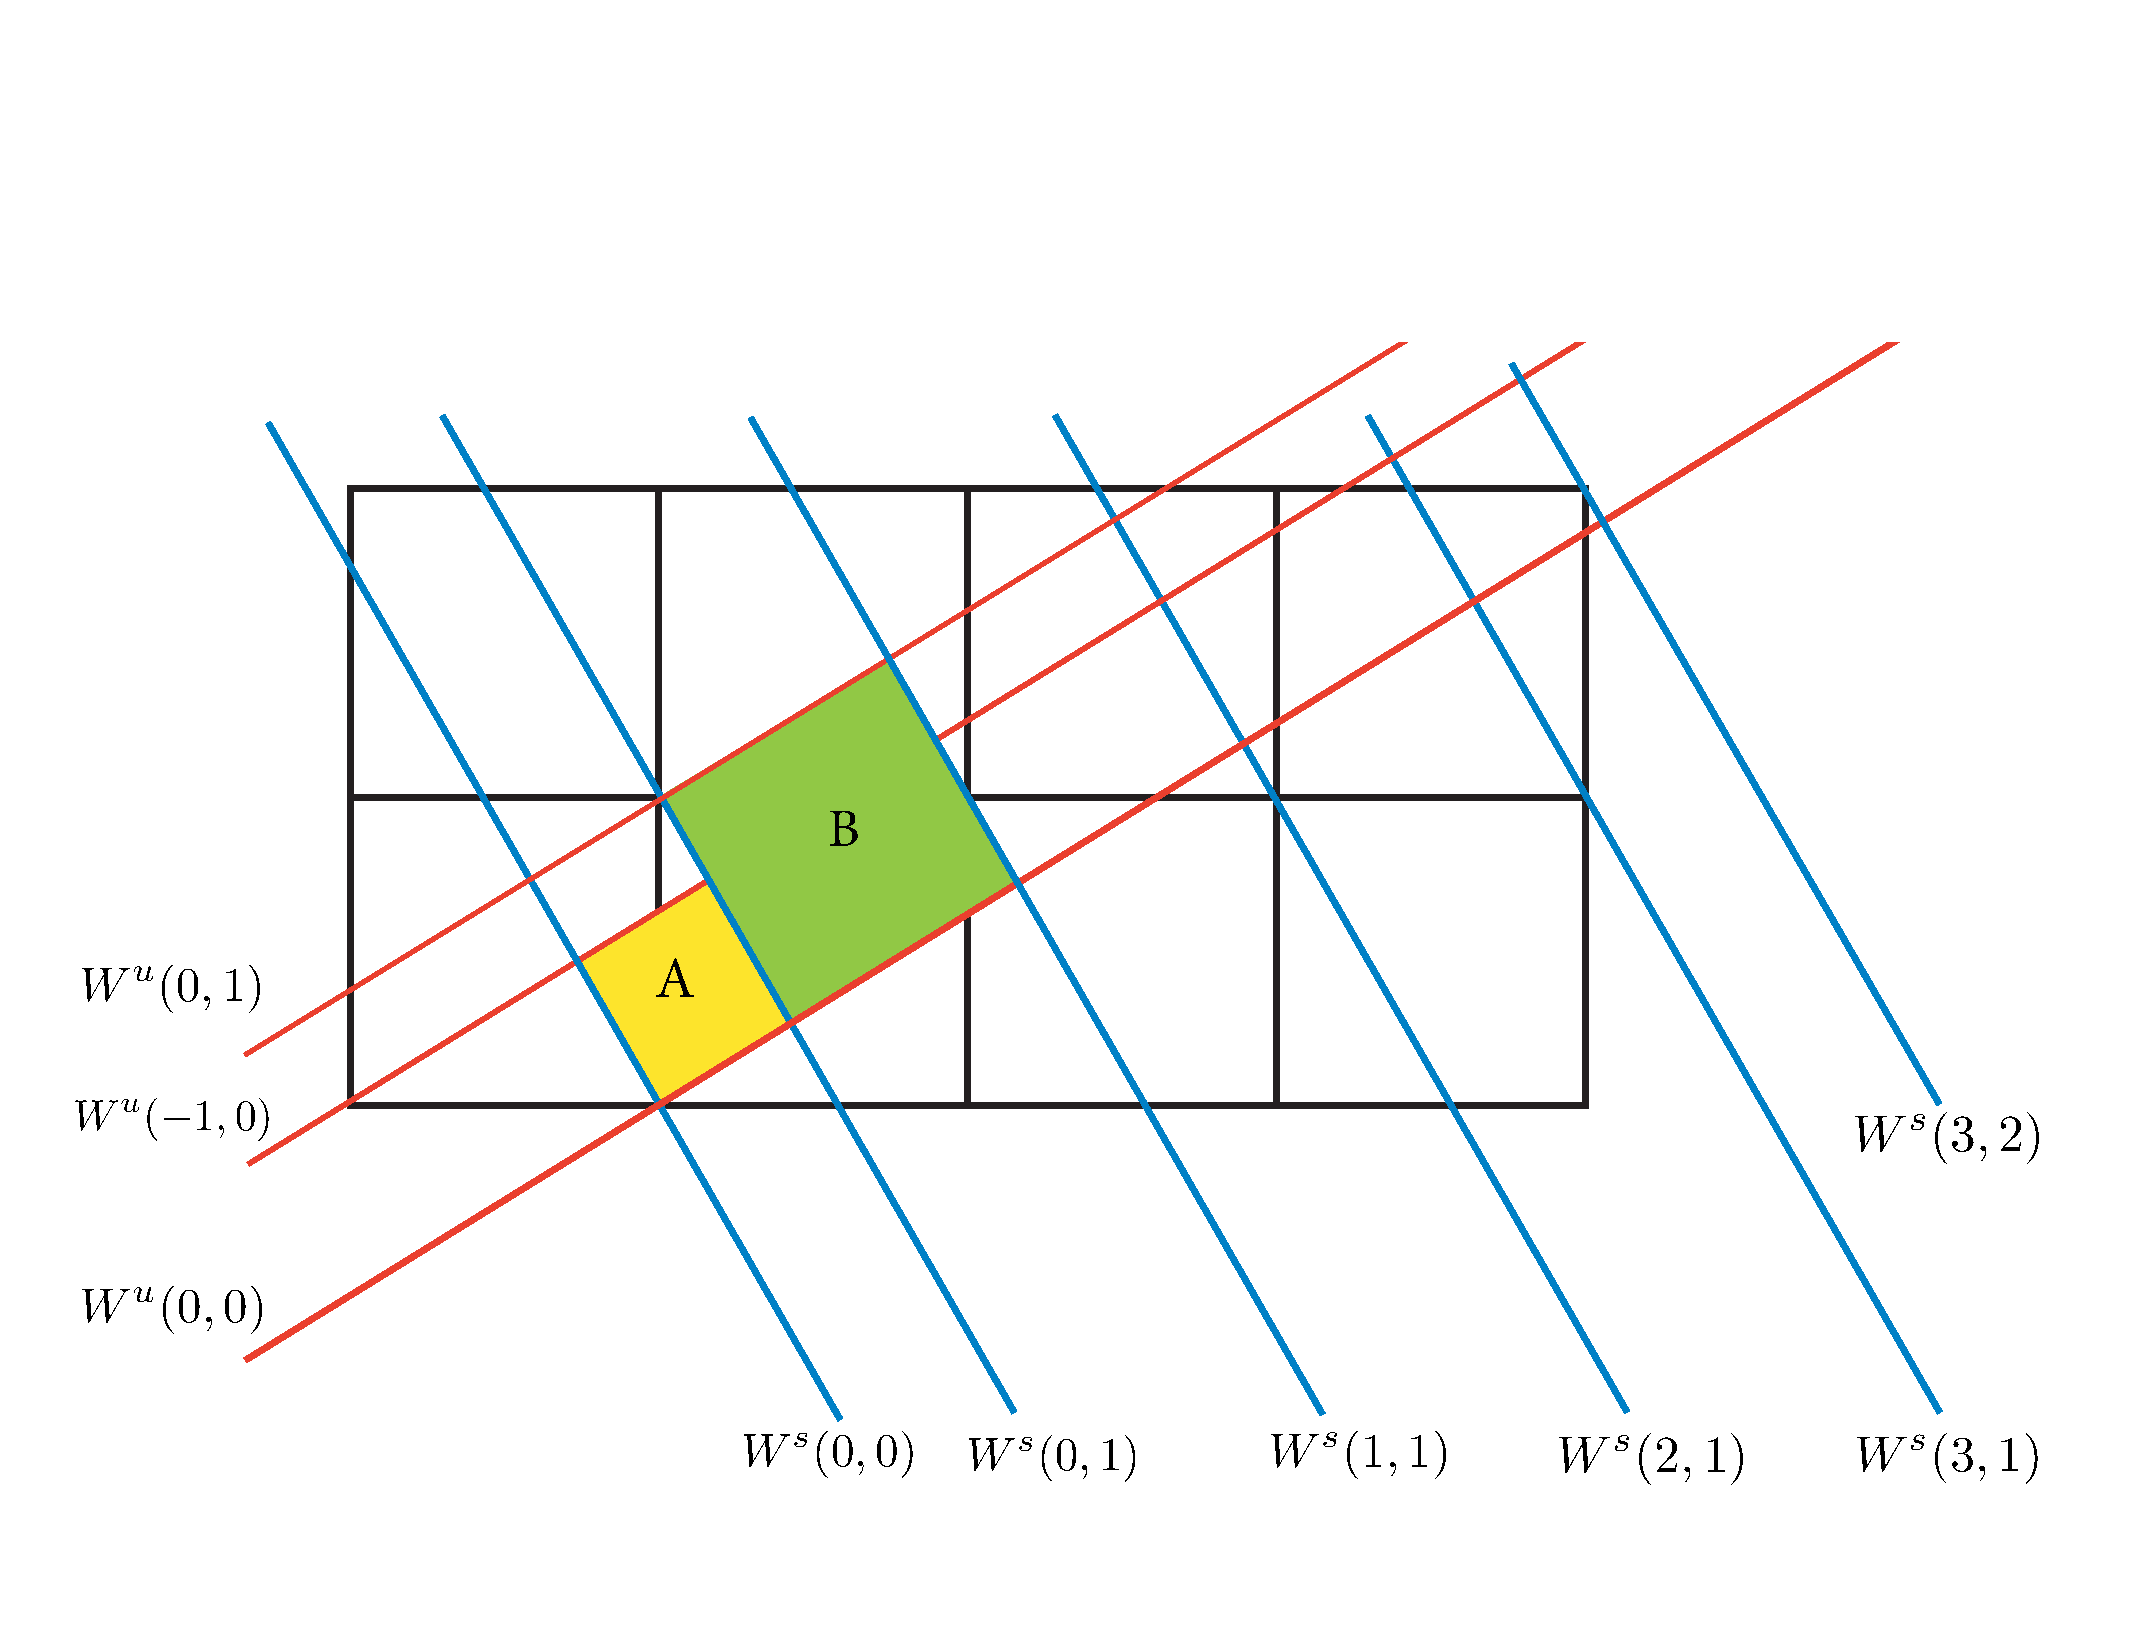
\includegraphics[width=0.74\textwidth]{Lect13p8}
\\
(b) 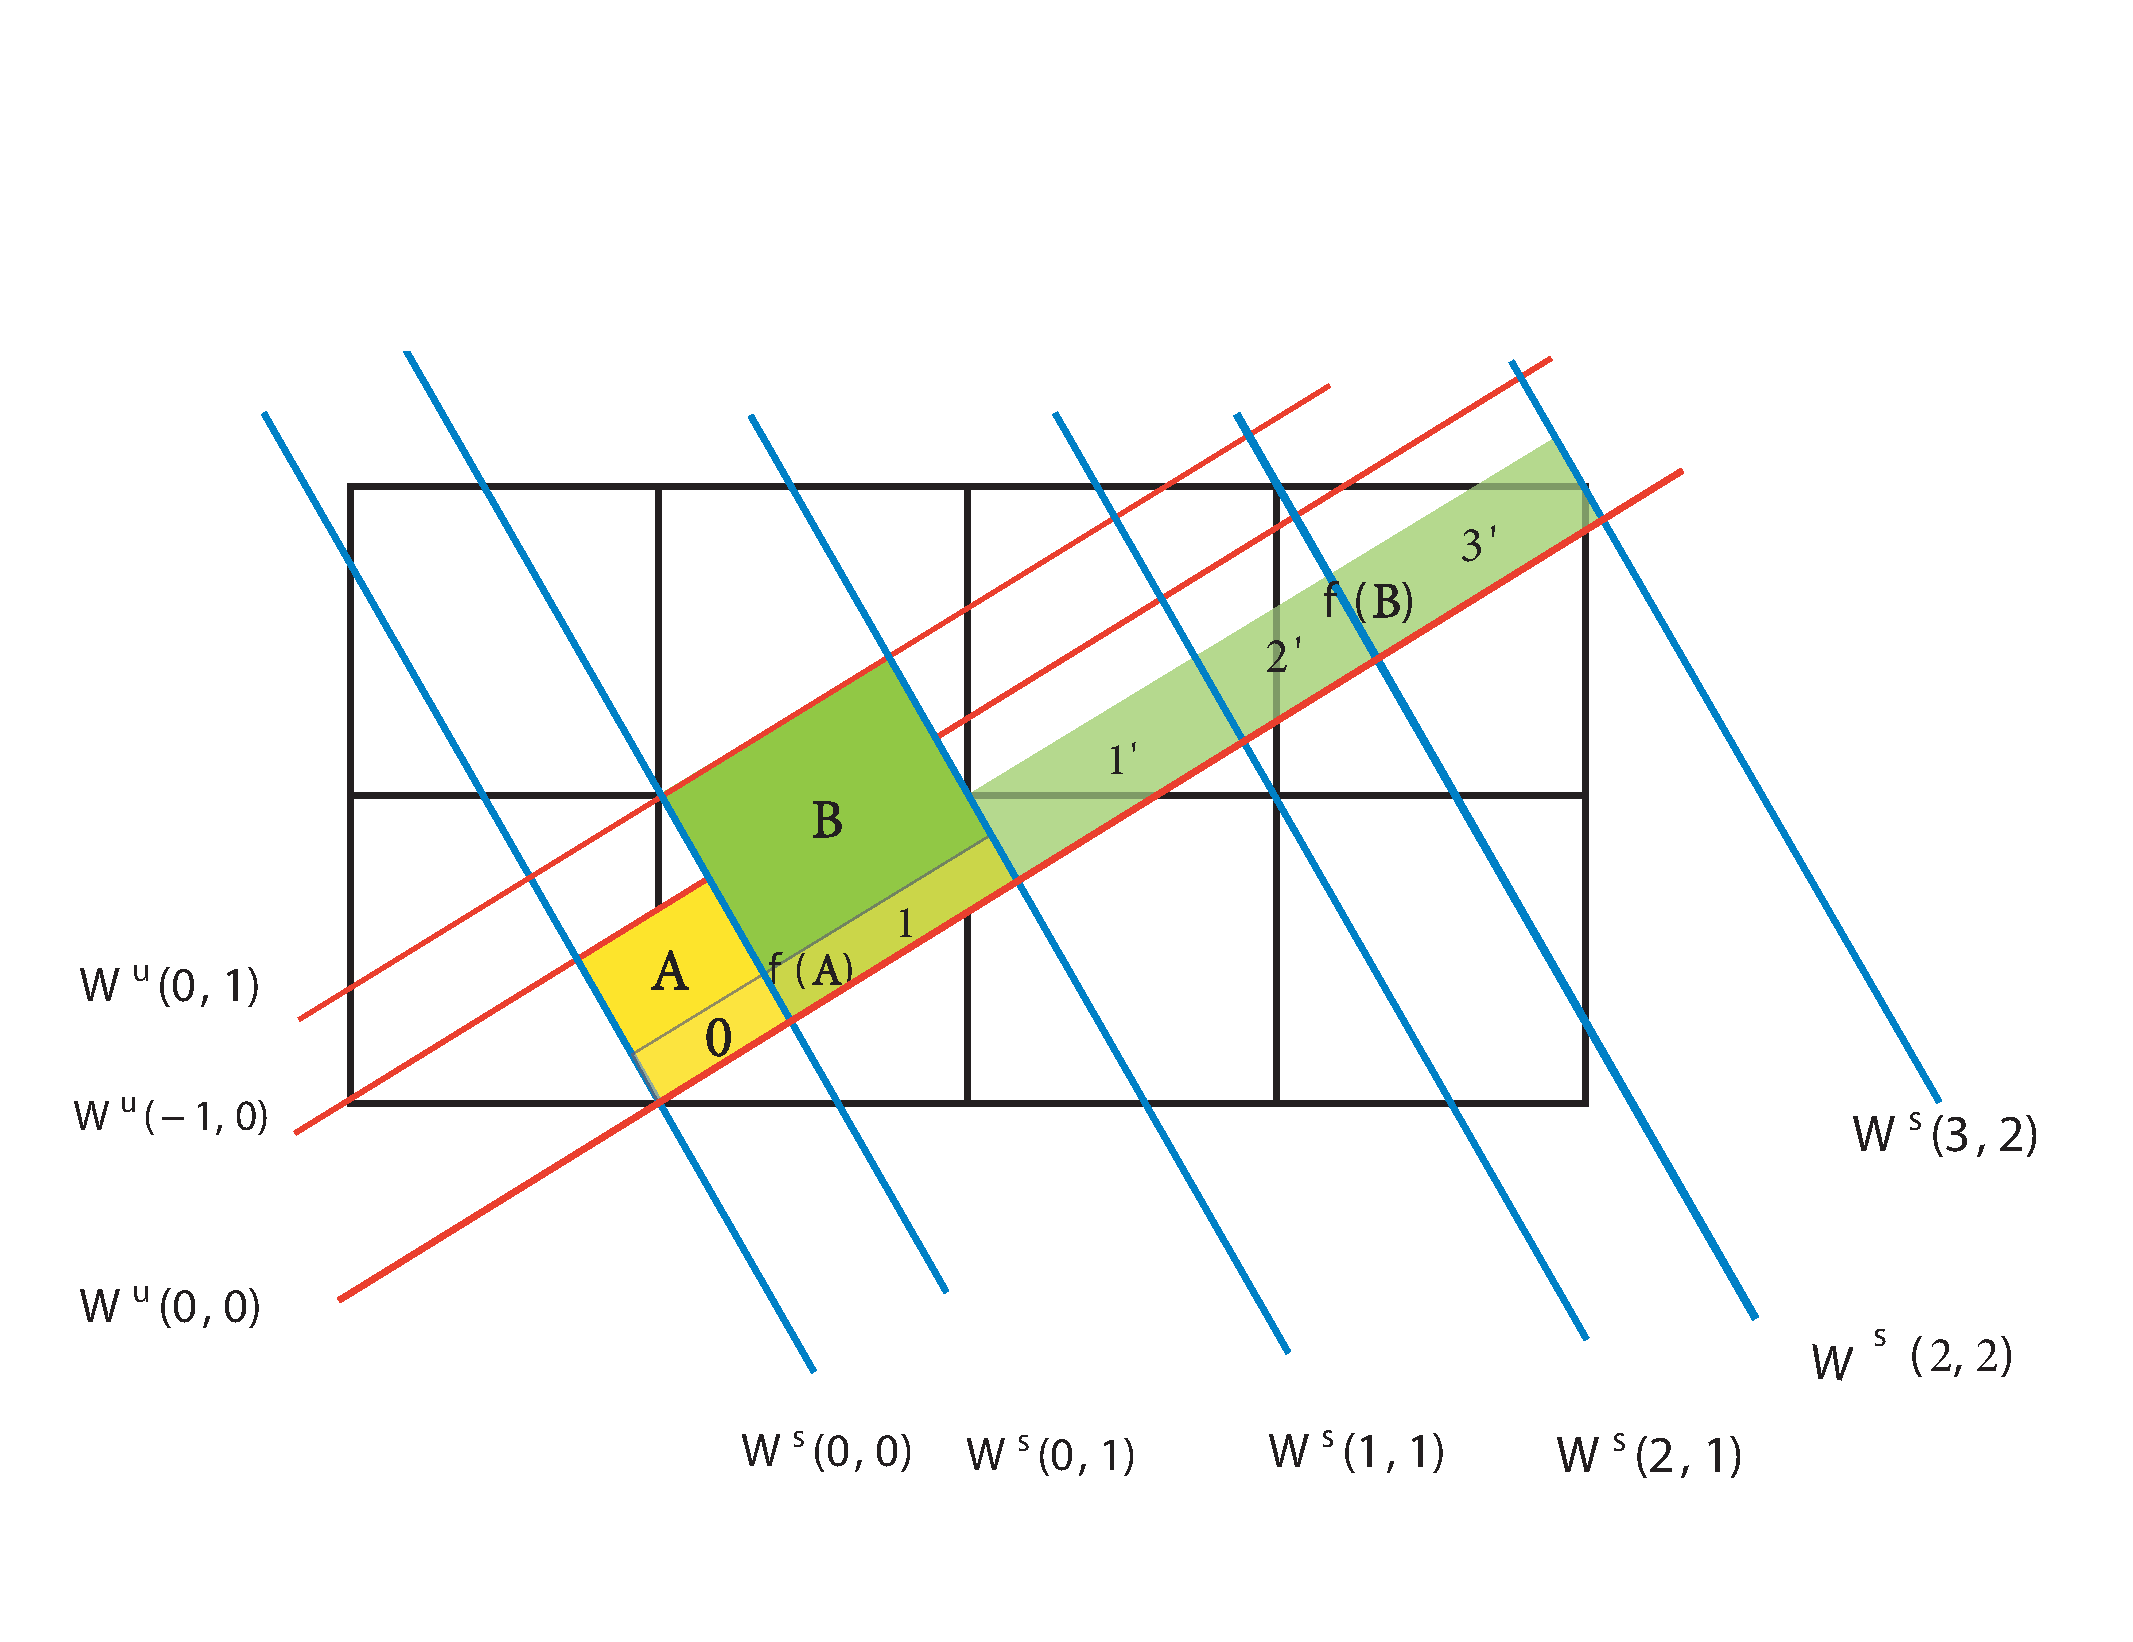
\includegraphics[width=0.74\textwidth]{Lect13p11}
\\
(c)  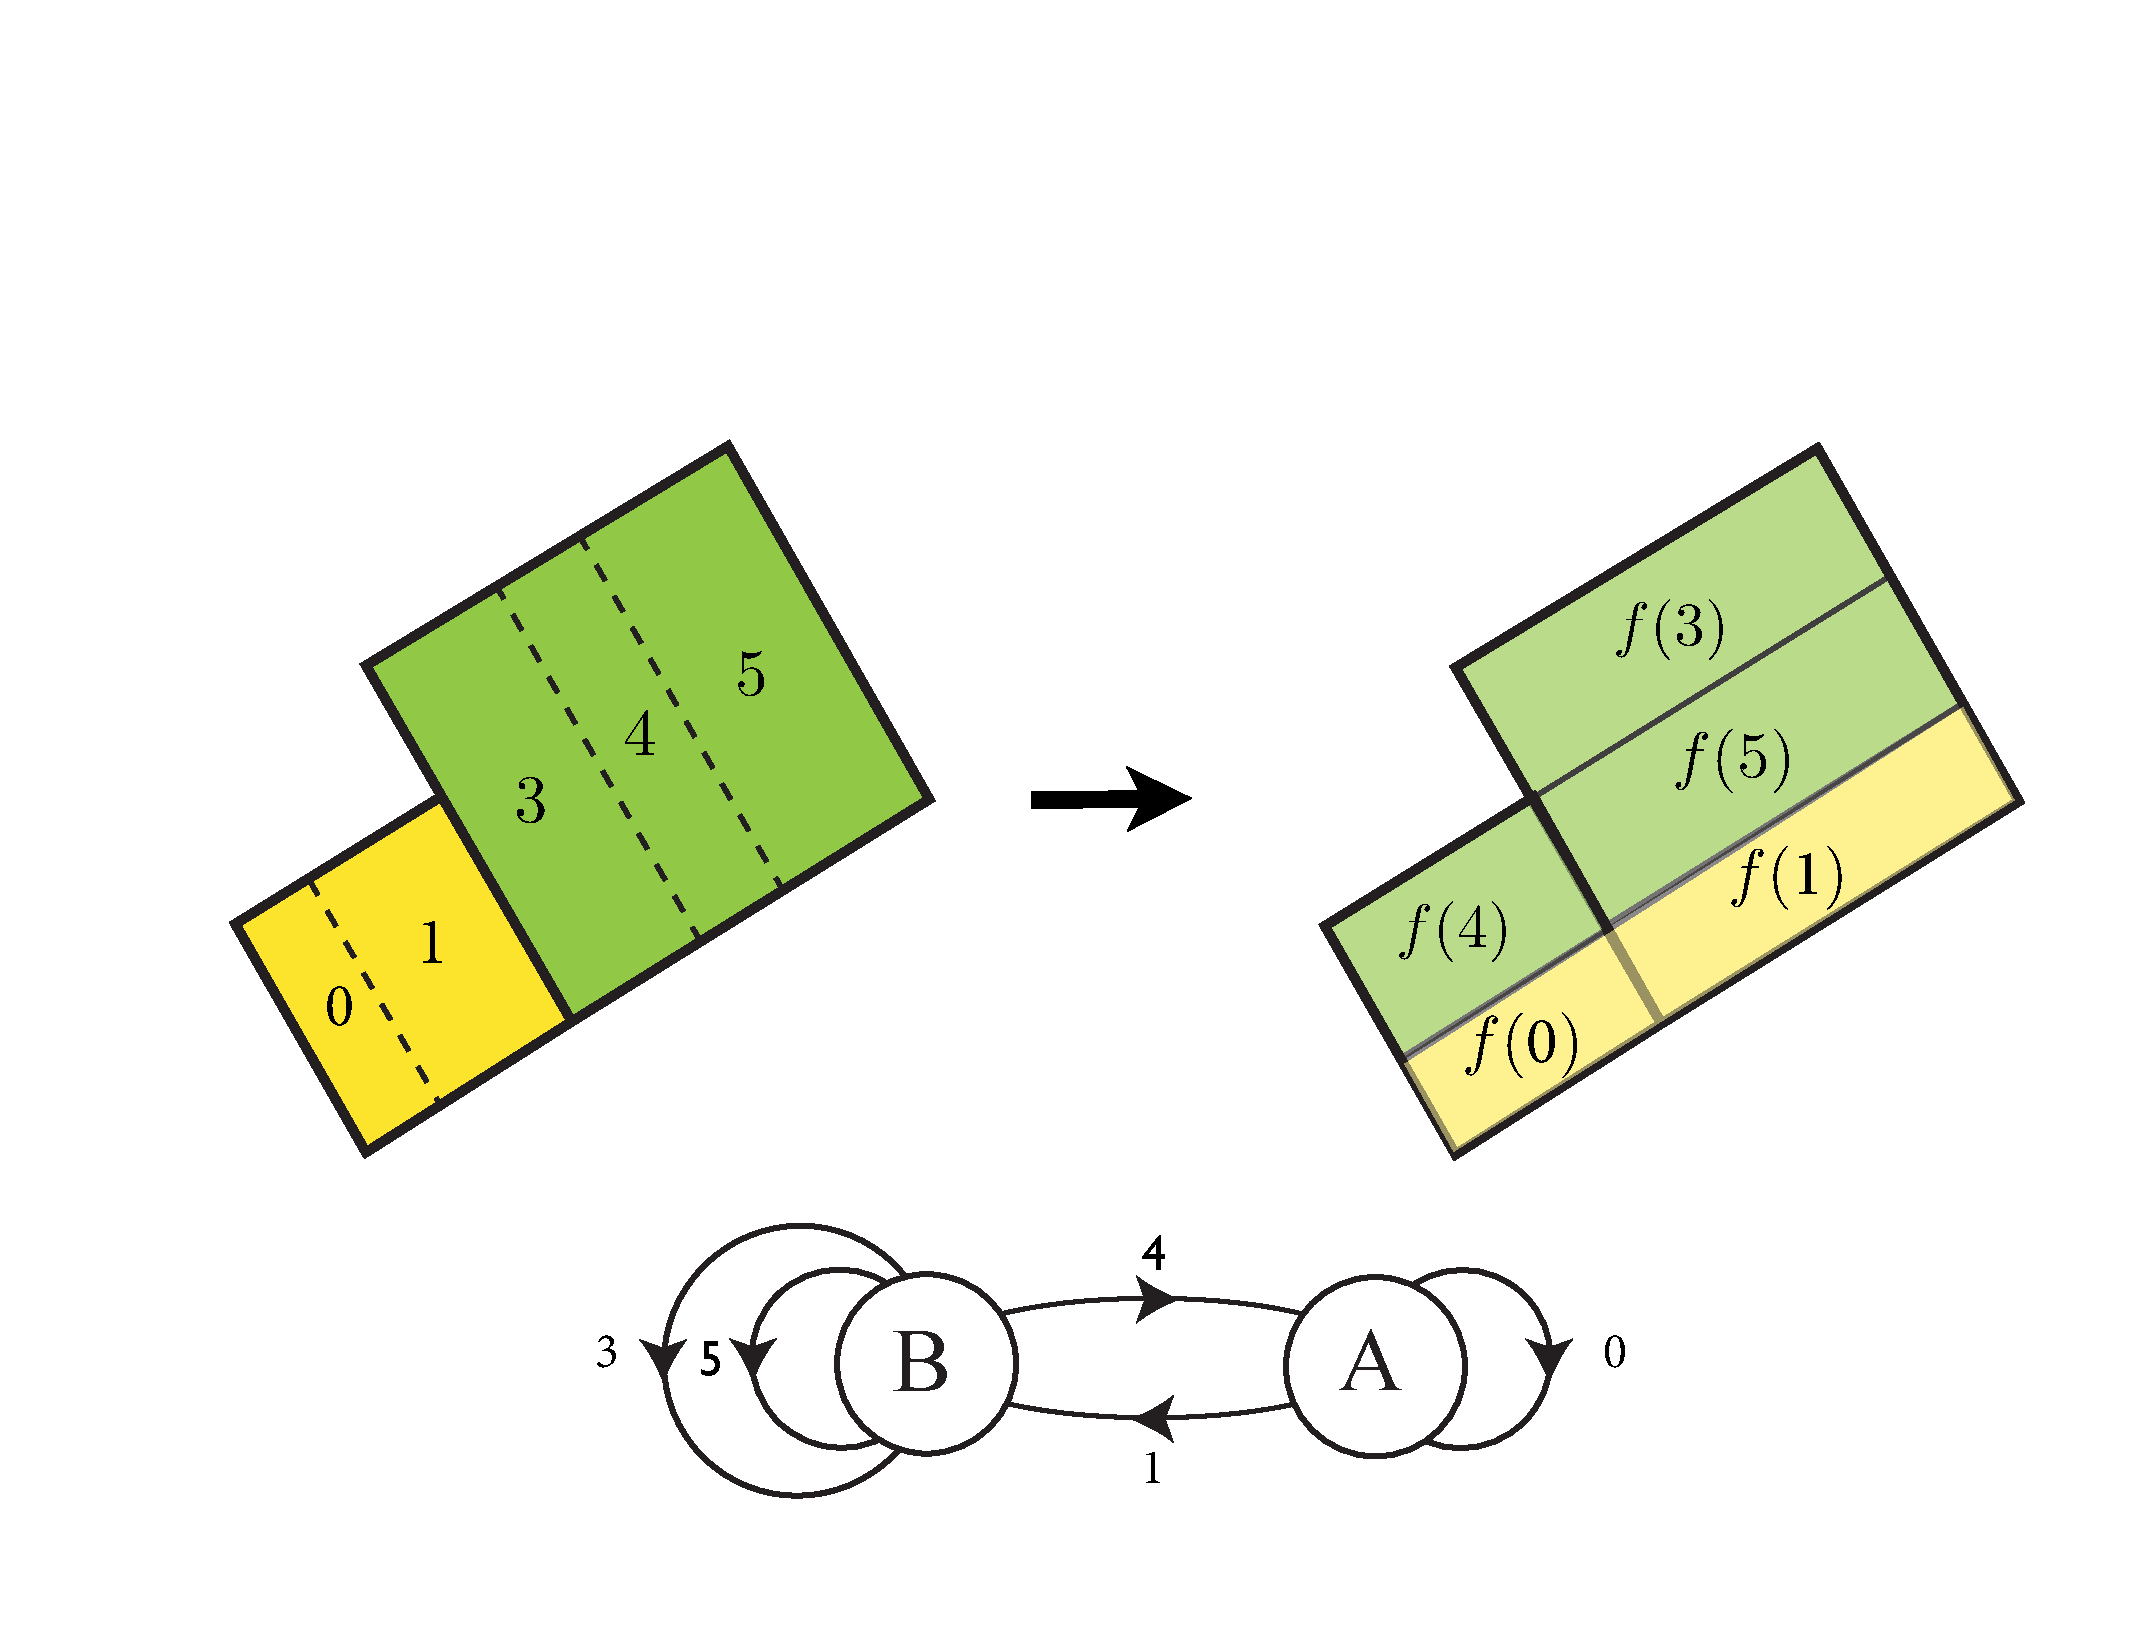
\includegraphics[width=0.5\textwidth]{Lect13p17}
  \caption{\label{fig:Lect13p8}
(a) Two-rectangles \AW\ generating partition for the canonical Arnol'd cat
map \refeq{ArnoldCat}, with borders given by stable-unstable manifolds of the
unfolded cat map lattice points near to the origin.
(b) The first iterate of the partition.
(c) The iterate pulled back into the generating partition,
and the corresponding 5-letter {\markGraph}. In (b) and (c)
I have not bothered to
relabel Crutchfield partition labels with our
shift code. This is a ``linear code,'' in the
sense that for each square on can count how many side-lengths are needed
to pull the overhanging part of $f(x)$ back into the two defining squares.
(Figure by Crutchfield\rf{Crutchfield18})
}
\end{figure}
%%%%%%%%%%%%%%%%%%%%%%%%%%%%%%%%%%%%%%%%%%%%%%%%%%%%%%%%%%%%%%


\refFig{fig:Lect13p8} for the canonical
Thom-Arnol'd cat map
                            \toRem{rem:catMapAbout}
\beq
A =
\MatrixII{2}{1}
         {1}{1}
\,.
% \qquad\det A= 1 \,,
\ee{ArnoldCat}

String people, \arXiv{1608.07845}, find the identity
\beq
\MatrixII{2}{1}
         {1}{1}
=
\MatrixII{1}{1}
         {0}{1}
\MatrixII{1}{0}
         {1}{1}
% = LR^{-1}
= L\transp{L}
%\,,
% \qquad\det A= 1 \,,
\ee{AxFlNi16(2.7)}
significant: ``The map corresponds to successive kicks, forwards and
backwards along the light cone [...]''

% 2018-02-10}{
As another example, with $s=4$,
Manning\rf{Manning02} discusses a Markov partition for the cat map
(also discussed by Anosov, Klimenko and Kolutsky\rf{AnKlKo08})
\beq
A =
\MatrixII{3}{1}
         {2}{1}
\,.
% \qquad\det A= 1 \,,
\ee{ArnoldCat2}

                                        \toCB
In order to count all admissible walks, one associates with the \markGraph\
such as the one in \reffig{fig:Lect13p8}\,(c) the {\em connectivity} matrix
\beq
C =
\MatrixII{1}{1}
         {1}{2}
\,,
\ee{connArnoldCat}
where $C_{ij}$ is the number of ways (number of links) of getting to $i$ from
$j$.



\section{\AW\ partition of the \PV\ cat map}
\label{sect:AdlWeiPV}

%\item[2016-05-29 PC]
%I have added this chapter with intention to include it as several examples
%in ChaosBook.org.

%%%%%%%%%%%%%%%%%%%%%%%%%%%%%%%%%%%%%%%%%%%%%%%%%%%%%%%%%%%%%%%%
  \begin{figure}
  \begin{center}  %%% 2016-12-25  see
                  %%% siminos/figsSrc/inkscape/CatMapStatesp.svg
  \setlength{\unitlength}{0.65\textwidth}
 %% \unitlength = units used in the Picture Environment
  \begin{picture}(1,0.81984366)%
    \put(0,0){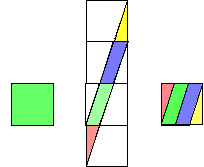
\includegraphics[width=\unitlength]{CatMapStatesp}}%
    \put(-0.025,0.15){\color[rgb]{0,0,0}\makebox(0,0)[lb]{\smash{$(0,0)$}}}%
    \put(0.26669086,0.17307744){\color[rgb]{0,0,0}\makebox(0,0)[lb]{\smash{B}}}%
    \put(0.26669086,0.41839762){\color[rgb]{0,0,0}\makebox(0,0)[lb]{\smash{C}}}%
    \put(0.02137069,0.41839762){\color[rgb]{0,0,0}\makebox(0,0)[lb]{\smash{D}}}%
    \put(0.38935094,0.00135332){\color[rgb]{0,0,0}\makebox(0,0)[lb]{\smash{B}}}%
    %\put(0.32,0.17){\color[rgb]{0,0,0}\makebox(0,0)[lb]{\smash{$(0,0)$}}}%
    \put(0.64284833,0.60647641){\color[rgb]{0,0,0}\makebox(0,0)[lb]{\smash{C}}}%
    \put(0.64284833,0.79455521){\color[rgb]{0,0,0}\makebox(0,0)[lb]{\smash{D}}}%
    %\put(0.79004043,0.42657495){\color[rgb]{0,0,0}\makebox(0,0)[lb]{\smash{A}}}%
    %\put(0.79004043,0.17307744){\color[rgb]{0,0,0}\makebox(0,0)[lb]{\smash{B}}}%
    %\put(0.96994189,0.17307744){\color[rgb]{0,0,0}\makebox(0,0)[lb]{\smash{C}}}%
    %\put(0.97811923,0.42657495){\color[rgb]{0,0,0}\makebox(0,0)[lb]{\smash{D}}}%
    \put(0.02,0.27){\color[rgb]{0,0,0}\rotatebox{90.0}{\makebox(0,0)[lb]{\smash{$\ssp_{0}$}}}}%
    \put(0.39,0.27){\color[rgb]{0,0,0}\rotatebox{90.0}{\makebox(0,0)[lb]{\smash{$\ssp_{1}$}}}}%
    \put(0.76,0.27){\color[rgb]{0,0,0}\rotatebox{90.0}{\makebox(0,0)[lb]{\smash{$\ssp_{1}$}}}}%
    \put(0.1469525,0.173){\color[rgb]{0,0,0}\makebox(0,0)[lb]{\smash{$\ssp_{-1}$}}}%
    \put(0.51493279,0.174){\color[rgb]{0,0,0}\makebox(0,0)[lb]{\smash{$\ssp_{0}$}}}%
    \put(0.86655824,0.175){\color[rgb]{0,0,0}\makebox(0,0)[lb]{\smash{$\ssp_{0}$}}}%
    \put(0.21762677,0.55482852){\color[rgb]{0,0,0}\rotatebox{43.35476392}{\makebox(0,0)[lb]{\smash{stretch}}}}%
    \put(0.74915379,0.61465381){\color[rgb]{0,0,0}\rotatebox{-46.94301089}{\makebox(0,0)[lb]{\smash{wrap}}}}%
  \end{picture}%
\end{center}
   \caption{ \label{fig:CatMapStatesp}
(Color online)
The $s=3$  \PV\ cat map matrix \refeq{PerViv:2confRepMat}
%\refeq{eq:StateSpCatMap} keeps the origin $(0,0)$ fixed, but otherwise
stretches the unit square
into a parallelogram. Translations by $\Ssym{0}$ from alphabet
$\A=\{-1,0,1,2\}=$
\{%
{\color{red}red},
{\color{green}green},
{\color{blue}blue},
{\color{yellow}yellow}%
\}
bring stray regions back onto the torus.
   }
 \end{figure}
%%%%%%%%%%%%%%%%%%%%%%%%%%%%%%%%%%%%%%%%%%%%%%%%%%%%%%%%%%%%%%%%

%    \PCpost{2016-12-26}{
As illustrated in \reffig{fig:CatMapStatesp}, the action of the
cat map in the \PV\rf{PerViv}  ``two-configuration
representation'' is given by the antisymmetric  area
preserving $[2\!\times\!2]$ matrix
\beq
{\bf A}
=\MatrixII{0}{1}
          {-1}{s}
\ee{PerViv:2confRepMat}
For the Arnol'd value $s=3$,
in one time step the map stretches the unit square into a parallelogram, and
than wraps it around the torus 3 times, as in \reffig{fig:CatMapStatesp}.
Visualise the phase space as a bagel, with $\ssp_0$ axis a circle on the
outside of the bagel. This circle is divided into three color segments, which
map onto each other as you got in the $\ssp_1$ axis direction.  Now apply the
inverse map - you get 3 strips intersecting the the above strips, for 9
rectangles in all: a full shift, \ie, a ternary Smale horseshoe. So on the
torus there are only 3 strips - there is no distinction between the two outer
letters $\Ae=\{-1,2\}=$
\{%
{\color{red}red},
{\color{yellow}yellow}%
\},
it is the same third strip. The division into 2 triangles is an artifact
of plotting the torus as a unit square. All
complicated pruning of (the current draft of) Gutkin \etal\rf{GHJSC16}
is a red herring, due to over-partitioning of the
torus with a 4-letter alphabet.

{\em This is stupid.}

How do \AW\ coordinates work out for the Arnol'd cat map in the \PV\
representation \refeq{PerViv:2confRepMat} used here?
First one needs to construct the eigen-coordinates.

%%%%%%%%%%%%%%%%%%%%%%%%%%%%%%%%%%%%%%%%%%%%%%%%%%%
\hfill         \fastTrackExam{exam:ProjOpCatMap}

For $s>2$ the stability multipliers
\(
(\ExpaEig^{+},\ExpaEig^{-})
\,=\,(\ExpaEig\,,\; \ExpaEig^{-1})
\)
are real,
\beq
\ExpaEig^{\pm}=\frac{1}{2}(s\pm \surd{D})
\,,\qquad
\ExpaEig=e^{\Lyap}
\,,
\ee{catEigs}
where
\bea
s&=&\ExpaEig+\ExpaEig^{-1}
  =  2\cosh(\Lyap)
    \,,\quad
    \continue
\surd{D}&=&\ExpaEig-\ExpaEig^{-1}
  =  2\sinh(\Lyap)
\label{catEigs1}
\eea
 discriminant $D=s^{2}-4$,
with a positive Lyapunov exponent $\Lyap >0$,
and the right, left eigen\-vectors:
\bea
\{ \jEigvec[+],\jEigvec[-] \} &=& \left\{
    \VectorII{\ExpaEig^{-1}}{1}
    \,,
     \VectorII{\ExpaEig}{1} \right\}
    \continue
\{ \jEigvecT[+],\jEigvecT[-] \} &=& \left\{
   [-\ExpaEig^{-1},1]
    \,,
    [\ExpaEig,-1] \right\}
\,,
\label{eigVecs}
\eea
(where the overall scale is arbitrary).
As the matrix is not symmetric, the
$\{\jEigvec[j]\}$ do not form an orthogonal basis.

What does this do to the partition of \reffig{fig:CatMapStatesp}? The origin
is still the fixed point. For a \statesp\ point in the new, dynamically
intrinsic right eigenvector \AW\ %\rf{AdWei70}
coordinate basis $x'$
\[
\left(\begin{array}{c}
 \ssp_{t-1}'  \\
 \ssp_{t}'
 \end{array} \right )
 =
\left(\begin{array}{c}
 -\ExpaEig\ssp_{t}+\ssp_{t-1}\\
 -\ExpaEig^{-1}\ssp_{t}+\ssp_{t-1}
 \end{array} \right )
\,.
\]
the abscissa ($\ssp_{t-1}$ direction) is not affected, but the ordinate
($\ssp_{t}$ direction) is flipped and stretched/shrunk by factor $-\ExpaEig$,
$-\ExpaEig^{-1}$ respectively,
\[
\left(\begin{array}{c}
 \ssp_{t}'  \\
 \ssp_{t+1}'
 \end{array} \right )
 =
 \MatrixII{\ExpaEig^{-1}}{0}
          {0}            {\ExpaEig}
\left(\begin{array}{c}
 \ssp_{t-1}'  \\
 \ssp_{t}'
 \end{array} \right )
 - \left(\begin{array}{c}
 0  \\
 \Ssym{t}
 \end{array} \right )
\,,
\]
preserving the vertical strip nature of the
partition of \reffig{fig:CatMapStatesp}. In the \AW\ right eigenbasis,
${\bf A}$ acts by stretching the $\jEigvec[+]$ direction by $\ExpaEig$, and
shrinking the $\jEigvec[-]$ direction by  $\ExpaEig^{-1}$, without any rotation
of either direction.

Thus the \AW\ coordinates preserve the convenient feature of the
\PV\ cat map, \reffig{fig:CatMapStatesp}: the torus `rewrapping'
translations remain all vertical, specified by a single integer.

The angles of stable / unstable manifolds are irrational respective to the
lattice, and they never hit another vertex (and so they do not close onto
themselves under quotienting of translations).

%%%%%%%%%%%%%%%%% by hand calculations :)
%   \surd{D} = sqrt(5)         = 2.23606797749
%   L1 = (3+sqrt(5))/2  = 2.61803398874
%   L2 = (3-sqrt(5))/2  = 0.38196601125
%   e11= (L2)/(\surd{D})       = 0.17082039325
%   e12= (1)/(\surd{D})        = 0.44721359550
%   e21= (L1)/(\surd{D})       = 1.17082039325
%   e22= (1)/(\surd{D})        = 0.44721359550
%
%   y = e12/e11         = 2.61803398874 x slope expanding
%   y = e21/e22         = 0.38196601125 x slope contracting
%
% contract: Plot[0.38196601125 x, {x, 0, 1}, {y, 0, 1}]
% expand:   Plot[2.61803398874 x, {x, 0, 1}, {y, 0, 1}] width 10.509
%
% horizontally along x:
%  (439.8005-343.6351)*0.381966+343.6351 = 380.367, got through x= 232.17
%  (-143.732+195.435)*0.381966 = 36.734, got through x= 175.7
% vertically along y:
%  (496.6877-400.3766)*2.6180+400.3766   = 652.519, got through x= 195.0420
%  (155.5237-103.7766)*2.6180+103.7766   = 239.25, got through x= 195.0420


%%%%%%%%%%%%%%%%%%%%%%%%%%%%%%%%%%%%%%%%%%%%%%%%%%%%%%%%%%%%%%%%%
%  \begin{figure}
%  \begin{center}  %%% 2016-12-25  see
%[to be drawn]
%\end{center}
%   \caption{ \label{fig:CatMapEigVecs}
%(Color online)
%Going from the Newtonian $s=3$  Arnol'd cat map to the right eigenvector
%\AW\ coordinate basis,
%with the expanding (purple) and contracting (beige) eigendirections indicated.
%Next: figure out the two rectangles which are the start of the \AW\
%construction. Or three rectangles - would be nice to have a partition something
%symmetric across the main diagonal, as the two eigendirections are symmetric
%under time reversal.
%   }
% \end{figure}
%%%%%%%%%%%%%%%%%%%%%%%%%%%%%%%%%%%%%%%%%%%%%%%%%%%%%%%%%%%%%%%%%

%%%%%%%%%%%%%%%%%%%%%%%%%%%%%%%%%%%%%%%%%%%%%%%%%%%%%%%%%%%%%
\begin{figure}
  \centering
(a)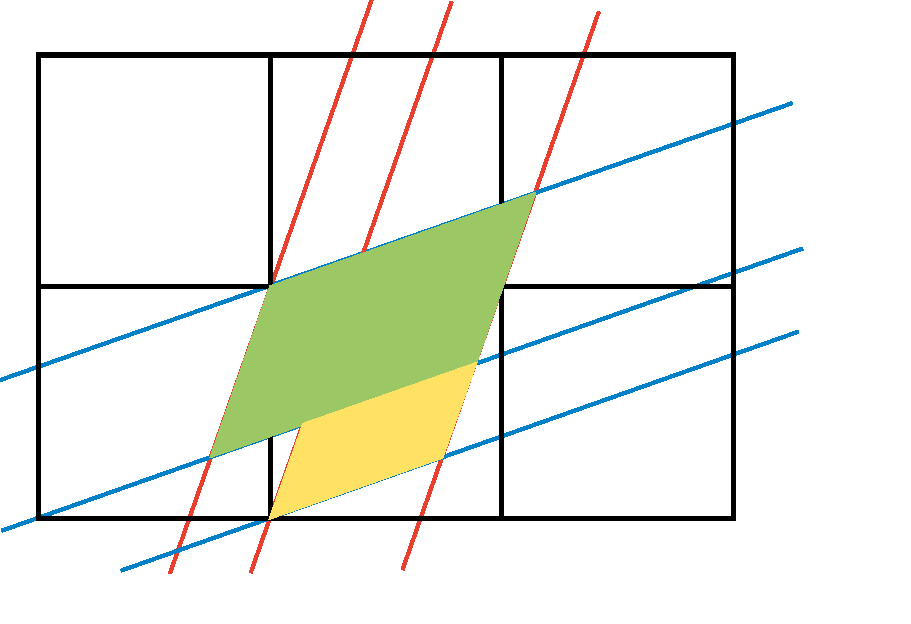
\includegraphics[width=0.40\textwidth]{PCLect13p8}
(b)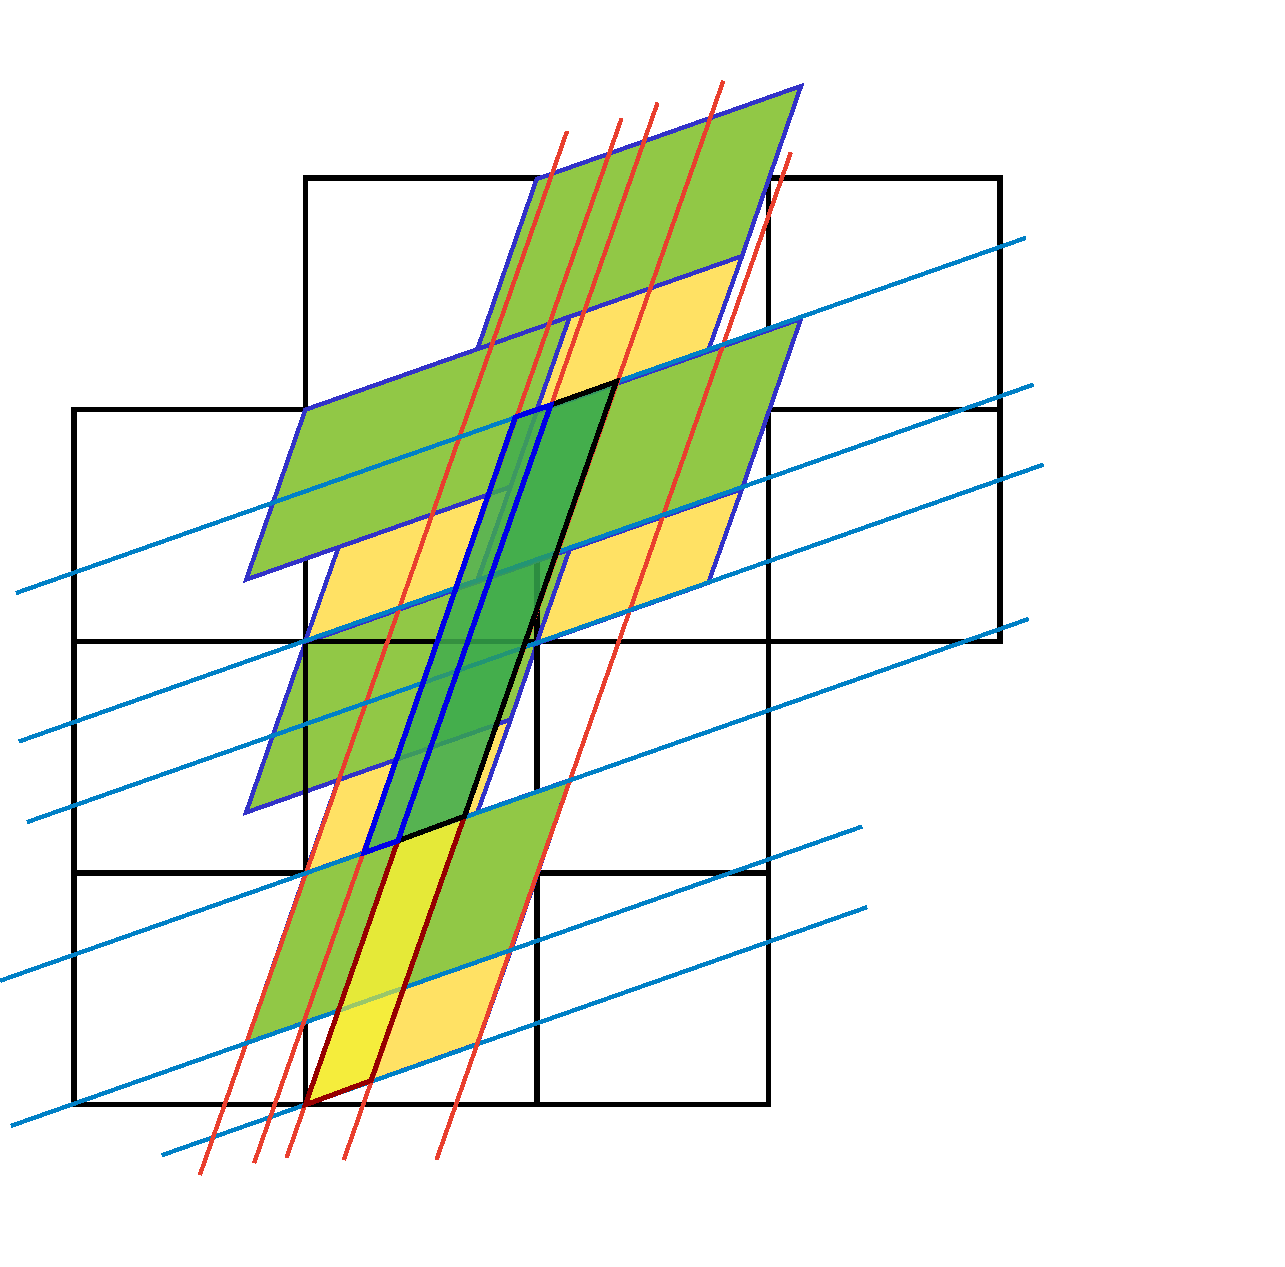
\includegraphics[width=0.50\textwidth]{PCLect13p14}
  \caption{\label{fig:PCLect13p8}
(a) An abandoned two-rectangle \AW\ generating
partition for the \PV\ cat map \refeq{PerViv:2confRepMat}, with
borders given by cat map stable-unstable manifolds.
(b) An abandoned attempt to identify the finite partition,
since superseded by the partition of \reffig{fig:PCLect13p16}\,(b)
and \reffig{fig:PVAdlerWeissB}.
}
\end{figure}
%%%%%%%%%%%%%%%%%%%%%%%%%%%%%%%%%%%%%%%%%%%%%%%%%%%%%%%%%%%%%%%

%%%%%%%%%%%%%%%%%%%%%%%%%%%%%%%%%%%%%%%%%%%%%%%%%%%%%%%%%%%%%
\begin{figure}
  \centering
(a)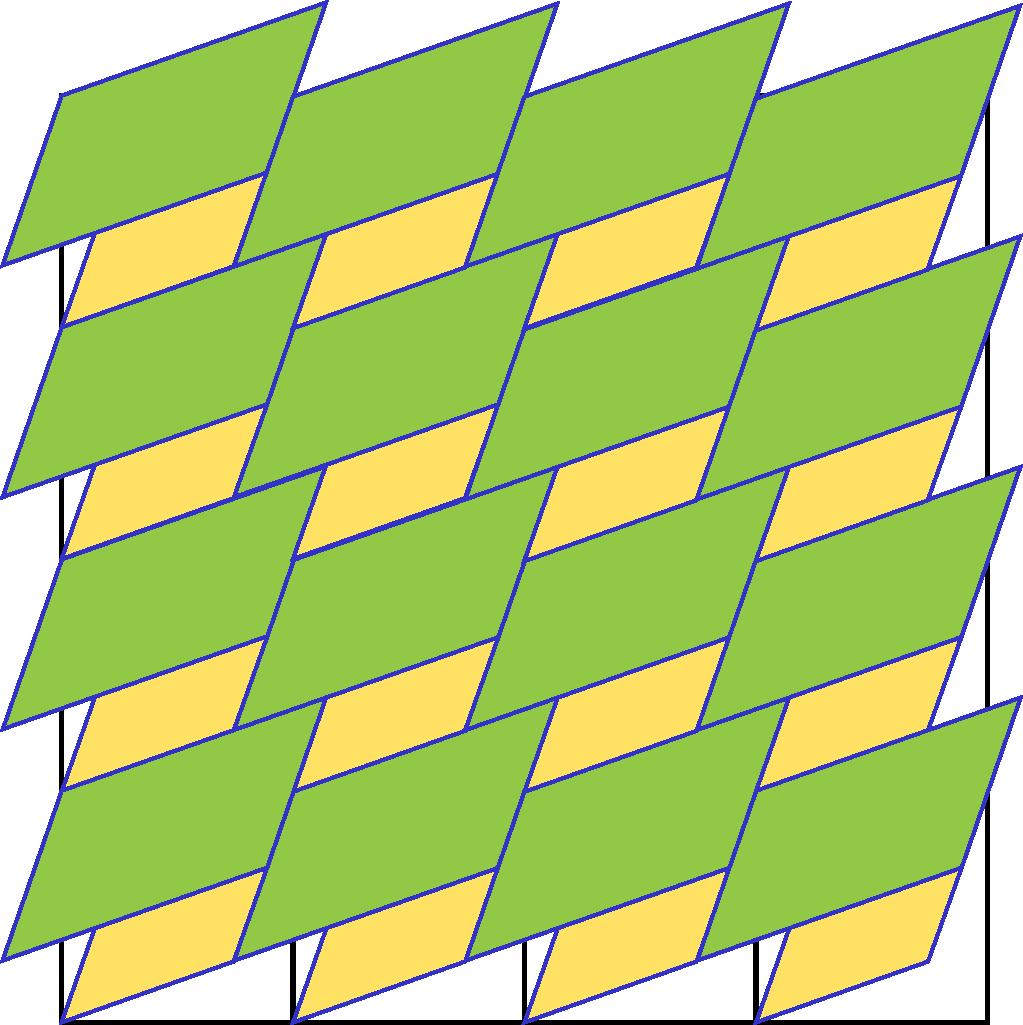
\includegraphics[width=0.45\textwidth]{PCLect13p12}
(b)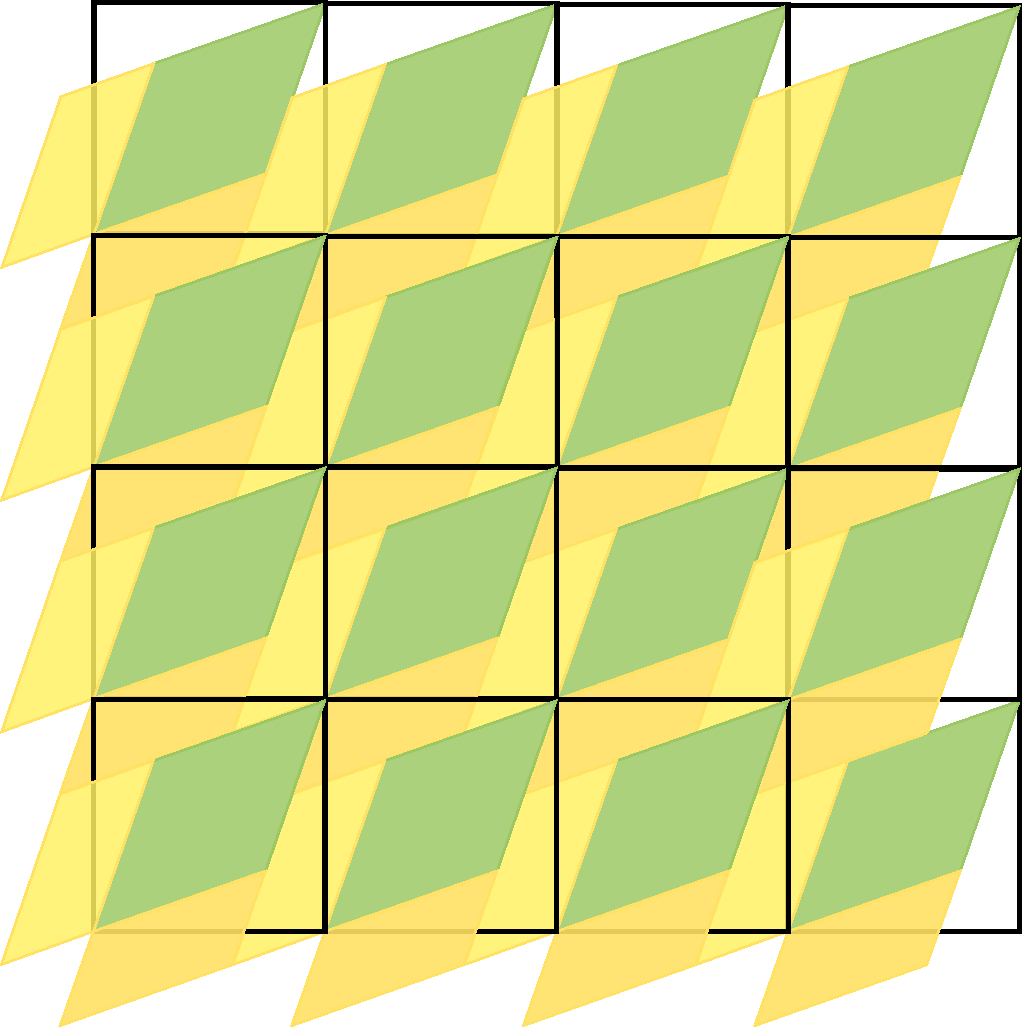
\includegraphics[width=0.45\textwidth]{PCLect13p13}
  \caption{\label{fig:PCLect13p12}
(a) [Abandoned] Tiling of the square lattice by the two-rectangle \AW\
generating partition of \reffig{fig:PCLect13p8}\,(a) for the \PV\
cat map \refeq{PerViv:2confRepMat}.
(b) Tiling of the square lattice by the three-rectangle, time reversal
symmetric generating partition. Note that we have used the continuous
translation invariance to center the large tile $A$ within the
unit square (continued in \reffig{fig:PCLect13p9}\,(a)).
}
\end{figure}
%%%%%%%%%%%%%%%%%%%%%%%%%%%%%%%%%%%%%%%%%%%%%%%%%%%%%%%%%%%%%%%

Note that from \reffig{fig:PCLect13p12}\,(a) to
\reffig{fig:PCLect13p12}\,(b) we have used the continuous translation
invariance to center the large tile $A$ within the unit square. That
makes the time reversal invariance more explicit.
It might not be obvious that the two parallelograms of
\reffig{fig:PCLect13p8}\,(a) tile the square lattice, but they do, as
illustrated in \reffig{fig:PCLect13p12}\,(a).
                                            \toRem{rem:PythagorTiling}
Such tilings are known as `Pythagorean'.

Given the stable/unstable eigenvectors, the
natural eigen-coordinates are given. I had first constructed a
2-rectangle generating partition for the \PV\rf{PerViv}
two-configuration representation \refeq{PerViv:2confRepMat} - it is a squashed
and rotated version of \reffig{fig:Lect13p8}\,(a)
drawn in \reffig{fig:PCLect13p8}\,(a). The point is, after a
linear change of coordinates one has finite grammar \AW\ symbolic
dynamics, and the symbolic dynamics is a linear code in sense of Boris,
but this time with all admissible sequences generated as walks on
a \markGraph\ isomorphic to the one in \reffig{fig:Lect13p8}\,(c).

I actually like better the three-rectangle, time reversal symmetric
generating partition of \reffig{fig:PCLect13p9} and \reffig{fig:PCLect13p16}.

%%%%%%%%%%%%%%%%%%%%%%%%%%%%%%%%%%%%%%%%%%%%%%%%%%%%%%%%%%%%%
\begin{figure}
  \centering
(a)~~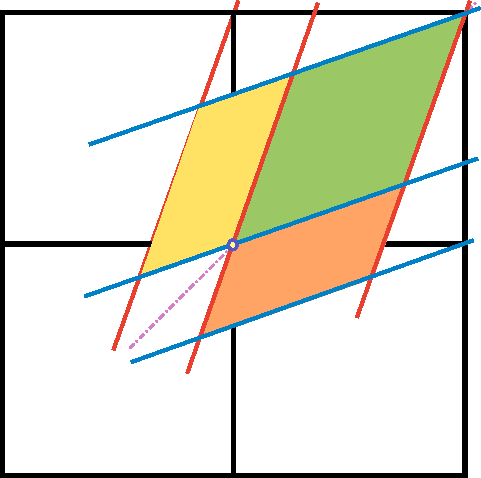
\includegraphics[width=0.37\textwidth]{PCLect13p9}
(b)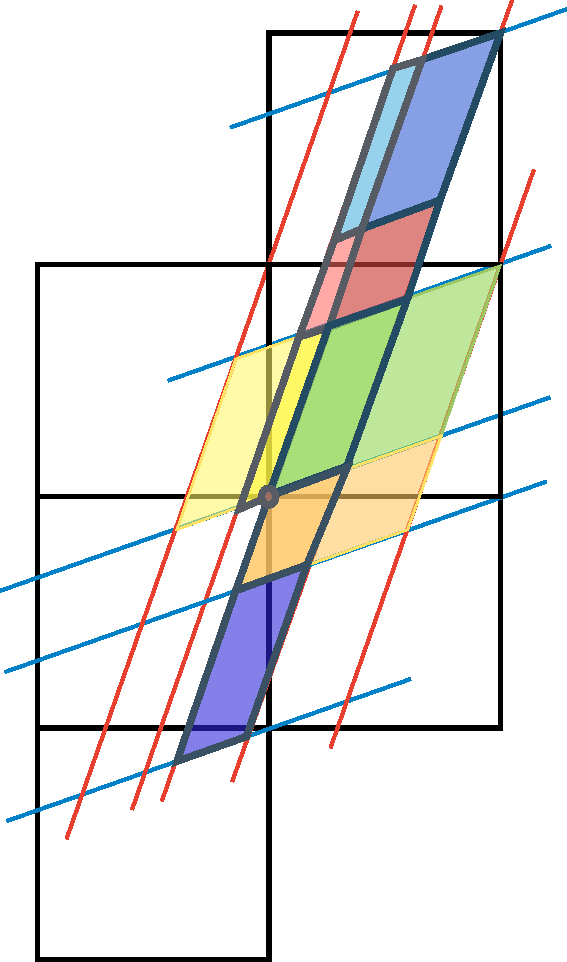
\includegraphics[width=0.41\textwidth]{PCLect13p15}
  \caption{\label{fig:PCLect13p9}
(a) The three-rectangle, time reversal symmetric generating partition
for the \PV\ cat map \refeq{PerViv:2confRepMat}, with borders given by cat
map stable-unstable manifolds.
(b) The three-rectangle mapped one step forward in time.
}
\end{figure}
%%%%%%%%%%%%%%%%%%%%%%%%%%%%%%%%%%%%%%%%%%%%%%%%%%%%%%%%%%%%%%%

%%%%%%%%%%%%%%%%%%%%%%%%%%%%%%%%%%%%%%%%%%%%%%%%%%%%%%%%%%%%%
\begin{figure}
  \centering
(a)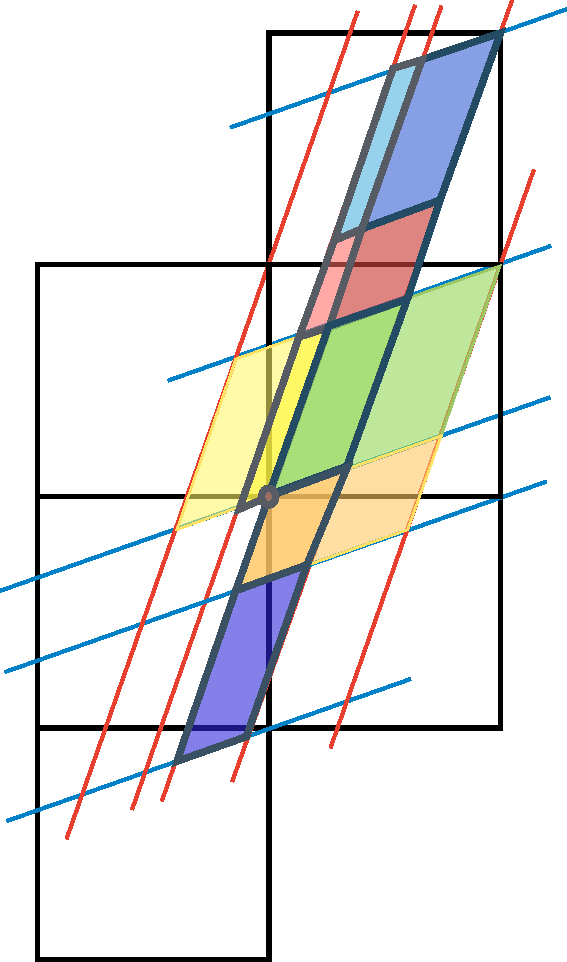
\includegraphics[width=0.30\textwidth]{PCLect13p15}
(b)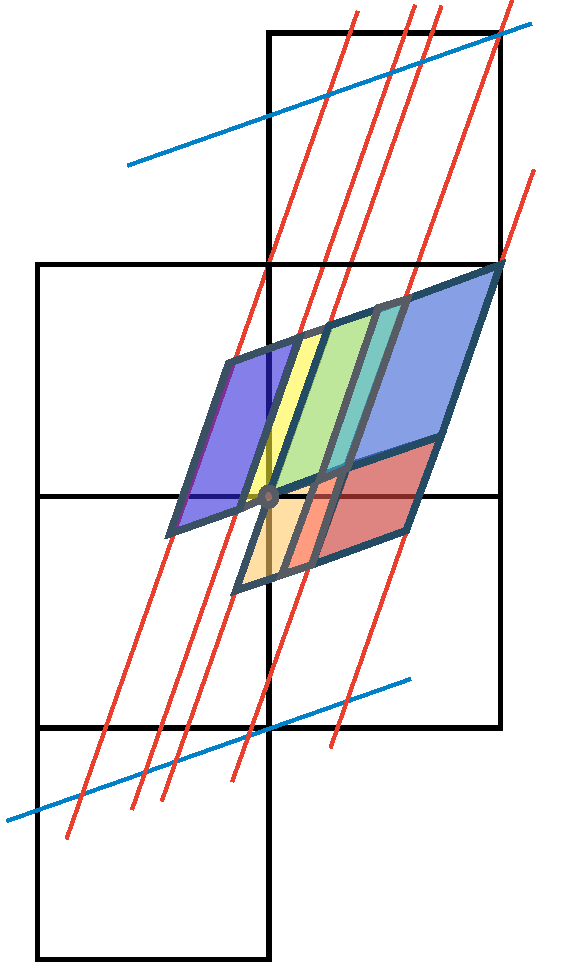
\includegraphics[width=0.30\textwidth]{PCLect13p16}
  \caption{\label{fig:PCLect13p16}
(a) The three-rectangle mapped one step forward in time.
(b) The three-rectangle wrapped back onto the torus, along the unstable
direction, yields 8-letter alphabet generating partition, with three-nodes
\markGraph.
One could have kept the two-rectangle \AW\ generating partition of
\reffig{fig:PCLect13p8}\,(a), in which case the alphabet is the standard 5
letters.
}
\end{figure}
%%%%%%%%%%%%%%%%%%%%%%%%%%%%%%%%%%%%%%%%%%%%%%%%%%%%%%%%%%%%%%%

%%%%%%%%%%%%%%%%%%%%%%%%%%%%%%%%%%%%%%%%%%%%%%%%%%%%%%%%%%%%%
\begin{figure}
  \centering
(a)~~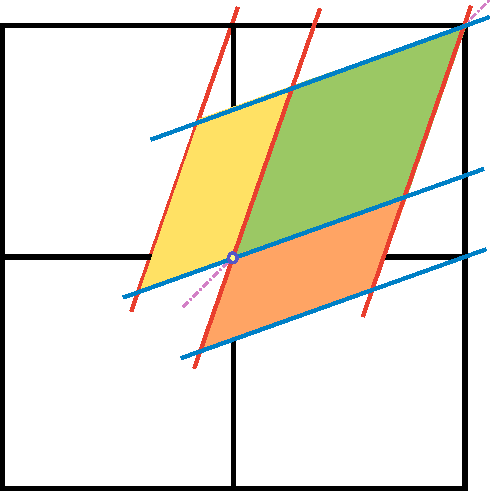
\includegraphics[width=0.37\textwidth]{PCLect13p9b}
(b)~~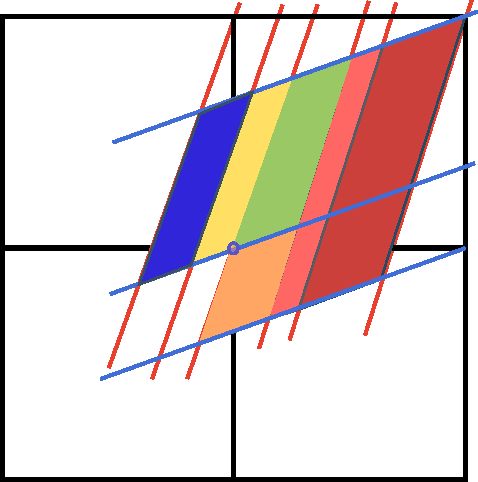
\includegraphics[width=0.37\textwidth]{PCLect13p16a}
  \caption{\label{fig:PPCLect13p16a}
\refFig{fig:PCLect13p16} continued.
(a) The three-rectangle, time reversal symmetric generating partition for
the \PV\ cat map \refeq{PerViv:2confRepMat}, with borders given
by cat map stable-unstable manifolds.
(b) The three-rectangle subpartition, one step forward in time. $A$ into three
strips, $B$ into three strips, $B'$ into two strips, for a total of 8
forward links in the graph
 \PCedit{continue with a sensible coloring of these regions)}.
Label the graph links by
translations that bring these pieces back into the unit square.
Under time reversal, interchange $B$ and $B'$, get the same partition going
backwards in time. Then make it Lagrangian, meaning the combined graph should
have undirected links (?).
}
\end{figure}
%%%%%%%%%%%%%%%%%%%%%%%%%%%%%%%%%%%%%%%%%%%%%%%%%%%%%%%%%%%%%%%


%%%%%%%%%%%%%%%%%%%%%%%%%%%%%%%%%%%%%%%%%%%%%%%%%%%%%%%%%%%%%
\begin{figure}
  \centering
(a)~~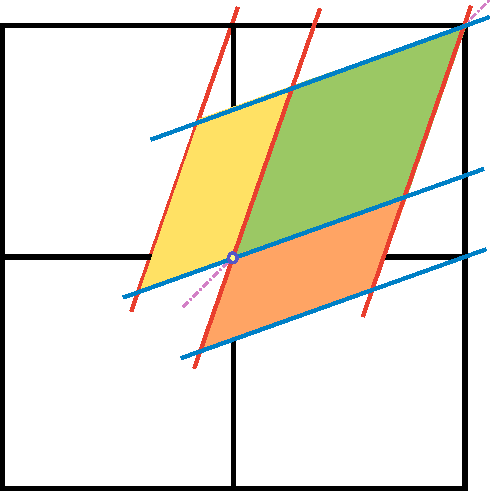
\includegraphics[width=0.37\textwidth]{PCLect13p9b}
(b)~~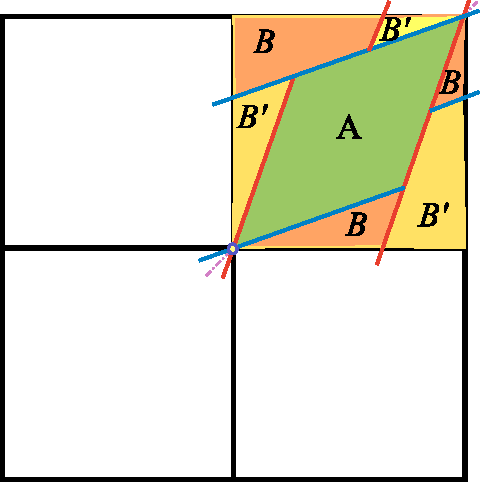
\includegraphics[width=0.37\textwidth]{PCLect13p9c}
  \caption{\label{fig:PCLect13p9b}
(a) The three-rectangle, time reversal symmetric generating partition for
the \PV\ cat map \refeq{PerViv:2confRepMat}, with borders given
by cat map stable-unstable manifolds.
(b) The three-rectangle partition of the unit square (torus laid out).
In this partition $A$ already lies entirely within the unit square,
while
$B$ and
$B'$ are wrapped around the torus, and only seem to consist of three pieces
each,
an artifact of the wrapping. The unit square borders have no physical meaning.
}
\end{figure}
%%%%%%%%%%%%%%%%%%%%%%%%%%%%%%%%%%%%%%%%%%%%%%%%%%%%%%%%%%%%%%%

Thus we have constructed \PV\ cat map coordinate transformation
from the square to the intrinsic \AW\ eigencoordinate basis. This is a
LINEAR transformation. As this has been falling on deaf ears for last few years,
let me say it again:

\bigskip\bigskip

This is a {\Huge LINEAR code},

\bigskip\bigskip

\noindent
as is every code in
Chaos\-Book, as illustrated by the examples of \refsect{exam:tentMapSymbDyn} that
I worked out for feline pleasure some years back. Got that?

As \AW\ partition is generating, there is noting for Dirichlet boundary
conditions Green's functions to accomplish - all admissible symbol {\brick s} are
known. The problem is now \emph{trivial}, in the Soviet sense (\ie, after a few years of
work, I understand it).

\bigskip

What is wrong with the argument so far? I used Newtonian, evolution-in-time
thinking to generate the $d=1$ partition. That will not work in higher
dimensions, so the above argument has to be recast in the Lagrangian form.

\bigskip

%Next: show that for $s=3$ the linear code in the new basis labels a
Be my guest - I'm going to bed:)

\bigskip

A few side, symmetry related remarks: we \emph{must} quotient translation
symmetries, do calculations in the elementary cell or, better still, the
fundamental domain.

\newpage
% siminos/kittens/catHamilton.tex                   pdflatex CL18
% $Author: predrag $ $Date: 2020-12-19 00:52:16 -0500 (Sat, 19 Dec 2020) $

\section{\AW\ partition of the cat map \statesp}
\label{s:catMapHam}

    \PC{2020-12-17}{
Remove from here, relink, once incorporated in ChaosBook.
    }
As explained in the companion paper\rf{GHJSC16},
the deep problem with the \PV\ code prescription is that it does not
yield a generating partition; the borders (\ie, $\ssp_0$, $\ssp_1$ axes)
of their unit-square partition
$(\ssp_{\zeit-1},\ssp_{\zeit})\in(0,1]\times(0,1]$
do not map onto themselves, resulting in the infinity of, to us unknown,
grammar rules for {\inadmissible} symbol sequences.

This problem was resolved in 1967 by Adler and
Weiss\rf{AdWei67,ArnAve,AdWei70} who utilized the stable/\-unstable
manifolds of the fixed point at the origin to cover a unit area torus by
a two-rectangles generating partition; for the \PV\ cat map
\refeq{eq:StateSpCatMap}, such partition\rf{DasBuch} is drawn in
 reffig{fig:PVAdlerWeiss}. Following Bowen\rf{Bowen70}, one refers to
such parallelograms as `rectangles'; for details
see Devaney\rf{deva87}, Robinson\rf{Robinson12}, or
ChaosBook\rf{DasBuch}. Siemaszko and Wojtkowski\rf{SieWoj11} refer to
such partitions as the `Berg partitions', and Creagh\rf{Creagh94} studies
their generalization to weakly nonlinear mappings.

While Percival and Vivaldi were well aware of \AW\ partitions, they felt
that their ``coding is less efficient in requiring more symbols, but it
has the advantage of linearity.'' Our construction demonstrates that one
can have both:  an \AW\ generating cat map partition, and a linear code.
The only difference from the \PV\ formulation\rf{PerViv} is that one
trades the single unit-square cover of the torus of
\refeq{eq:StateSpCatMap} for the dynamically intrinsic, two-rectangles
cover, but the effect is magic - now every
infinite walk on the {\markGraph}
corresponds to a unique {\admissible} orbit $\{\ssp_{\zeit}\}$, and the
{\markGraph} generates all {\admissible} itineraries $\{\Ssym{\zeit}\}$.

To summarize:
an explicit \AW\ generating partition completely solves the Hamiltonian cat map
problem, in the sense that it generates all {\admissible} orbits.
Rational and irrational initial states generate periodic and ergodic
orbits, respectively\rf{PerViv87b,Keating91}, with every \statesp\ orbit
uniquely labeled by an {\admissible} bi-infinite itinerary of symbols
from alphabet \A.

    \PC{2020-02-08}{
Note:
$N_2=\Det\jMorb=({s}-2)({s}+2)$,
$N_3 %   = {s}^3-3{s}-2
    = ({s}-2)({s}+1)^2$,
$N_4 = ({s}-2)({s}+1)\,{s}^2$,
$N_5 = ({s}-2)(s^2+ s-1 )^2$.
I think the factorization is true for all $\cl{}$, as the $s=2$ Laplacian
has a zero mode (constant $\ssp_i$, I think).

an sequence of non-negative integers counting the orbits of
a map; the sequence of periodic points for that map.
    }

This derivation was based on the \AW\ generating partition, a clever
explicit visualization of the cat map dynamics, whose generalization to
several coupled maps (let alone spatially infinite coupled cat
maps lattice) is far from obvious: one would have to construct covers of
high-dimensional {\fundPip}s by sets of sub-volumes.
However, as Keating\rf{Keating91} explains, no such explicit generating
partition is needed to count cat map \po s.

    % PC: restore here, once GHJSC16 finalized              2018-02-11
    % \subsection{\AW\ partition}
    % \label{sect:catAdlerWeiss}
    % \input{../kittens/catAdlerWeiss}
%\input{../kittens/pos}

\subsection{Adler / Adler98}
\label{sect:Adler98}

Predrag 2017-10-02 excerpts from or notes on\\
Adler\rf{Adler98} {\em Symbolic dynamics and {Markov} partitions},
 \CBlibrary{Adler98}
an excellent overview of symbolic dynamics techniques.
 \beq
 {A} =\left(\begin{array}{cc}
 a & b \\
 c & d
  \end{array} \right)
\,,
\ee{Adler98:CatMap}
where $a,b,c,d$ and
$\det A=1$.
The row vectors
\beq
\{ \jEigvecT[+],\jEigvecT[-] \} = \left\{
   [c,\ExpaEig-a]
    \,,
    [c,\ExpaEig^{-1}-a] \right\}
%\,,
\ee{Adler98:leftEigVecs}
                                                    \toCB
are the left expanding / contracting eigen\-vectors. The matrix
\refeq{Adler98:CatMap} is
in general not
symmetric, so $\{\jEigvecT[j]\}$ do not form an orthogonal basis.
For matrix \refeq{PerViv:2confRepMat} the left eigenvectors are
\beq
\{ \jEigvecT[+],\jEigvecT[-] \} = \left\{
   [-1,\ExpaEig]
    \,,
    [-1,\ExpaEig^{-1}] \right\}
\,,
\ee{PerViv:leftEigVecs}
in agreement with \refeq{eigVecs}. I prefer the right eigenvectors basis
$\{\jEigvec[j]\}$, as it lies in the first quadrant.


\subsection{Percival and Vivaldi / PerViv}
\label{sect:PerViv}

Predrag 2016-05-29 excerpts from or notes on\\
Percival and Vivaldi\rf{PerViv} {\em A linear
    code for the sawtooth and cat maps} \CBlibrary{PerViv}

``Completely chaotic systems are comparatively well understood, but they
have been neglected as a starting point for the study of systems with
divided phase space. It is the purpose of this and related papers to
remedy this.''

                                                                    \toCB
``When one starts with an integrable system, and perturbs it to introduce
some chaos, new orbits and new classes of orbits keep on appearing by
bifurcation processes, and they are very difficult to follow or to
classify. It is better to start with a purely chaotic system and then
reduce the chaos by \emph{removing} orbits.''
    \PC{2016-05-29}{totally agree - they say it well}

``In this paper we present the symbolic dynamics of the sawtooth maps,
and in the companion paper\rf{PerViv87b} {\em Arithmetical properties of
strongly chaotic motions} the number theory for the \po s of
the automorphisms of the torus, including the cat maps.''

``we start with the simplest systems that show the phenomena of
interest-area preserving maps. The sawtooth maps are piecewise linear
systems. They depend on a parameter K and for positive K they are
completely chaotic. For positive \emph{integer} K they are automorphisms
of the torus, of which the simplest is the Arnol'd-Sinai cat map, with K
= 1. We shall refer to all such toral automorphisms, with positive
integer K, as cat maps. They are Anosov systems, continuous on the torus.
On the other hand, when K is not an integer, the sawtooth map is
discontinuous.''

``Most of this paper is concerned with a `linear code' for the symbolic
dynamics of the sawtooth maps, including the cat maps. This code is
chosen for its convenience in practice, and differs from the usual codes
for the Arnol'd-Sinai cat.''

``In section 3 a practical problem of stabilisation is considered, that
provides a concrete model for the sawtooth and cat maps, and a natural
introduction to the linear codes. An explicit linear transformation from
the itinerary to the orbit is given.''


    \PC{2016-06-02}{verbatim from Keating\rf{Keating91a}}
Every Anosov diffeomorphism of the torus is topologically conjugate to a
hyperbolic automorphism. These are represented by [$2\!\times\!2$] matrices with
integer entries (for continuity), unit determinant (for area
preservation) and real eigenvalues (for hyperbolicity), and are known as
cat maps.

In order to describe certain collective properties of cat map orbits
Hannay and Berry\rf{HanBer80} introduced a function  closely related to
the least common multiple of their periods.



\subsection{Isola / Isola90}
\label{sect:Isola90}

Predrag 2016-06-02 excerpts from or notes on\\
S. Isola\rf{Isola90}
{\em {$\zeta$}-functions and distribution of \po s of toral automorphisms}

\PCedit{ % 2016-06-02
Bellissard's friend Isola gives counting formulas of the usual type -
could easily be turned into examples/exercises for Chaos\-Book. But I am
looking for symbolic dynamics - not even mentioned here.
        }

We consider canonical automorphisms of the torus $T^2$, i.e. maps of the form
\[
T(x, y) = (ax + by, cx + dy)\quad \mod 1
\,,
\]
which are implemented by the group of [2x2] matrices with integer entries,
determinant 1, and eigenvalues \refeq{PerViv3.7}.

To study the properties of this dense set of unstable \po s,
observe that the \po s of T consist precisely of those points
having rational coordinates $(p_l/q_l, p_1/q_2)$.
If $p_1$, $q_1$ are coprime and $g$ is the least common multiple of $q_1$
and $q_z$, then the square lattice of size $l/g$ is invariant under $T$.

In this direction, Percival and Vivaldi\rf{PerViv,PerViv87b,BirViv} have
constructed a nice translation of the dynamical problem into the language
of modular arithmetic, allowing a profound understanding of the structure
of {\po s}.
Here, however, we follow another approach where a general expression for
the N's is derived through a simple iterative scheme.
Consider the numbers
\beq
u_n = \frac{\Lambda^n - \Lambda^{-n}}{\surd{D}}
 \,.
\ee{Isola90-4}
The first two terms of the series are $u_0 = 0$, $u_1 = 1$ and each term after
is given by
\beq
u_n = s u_{n-1} -u_{n-2}
 \,.
\ee{Isola90-5}

[stuff to work out:
Isola has nice figures that illustrate the partitions of the 2-torus]

For the number of periodic points he finds, for any integer $s>2$
\beq
N_n = \Lambda^n + \Lambda^{-n} -2
 \,,
\ee{Isola90-11}
in agreement with the numerics of \refref{OzoHan84}.
Walters\rf{Walt82} defines the topological entropy as
\beq
h = \lim_{n \rightarrow \infty} \frac{1}{n}{\ln N_n}
 \,,
% ChaosBook \label{h-top}
\ee{Isola90-12}
This yields $h = \log \Lambda$, \ie, the Sinai theorem for the entropy of an
automorphism\rf{ArnAve,sinai76}.

The {\tzeta} for cat-map class of models is
\beq
\zetatop(z)  = \frac{(1 - \Lambda z) (1 - \Lambda^{-1} z)}
                  {(1 - z)^2}
           =  \frac{1 - s z + z^2}
                  {(1 - z)^2}
 \,.
\ee{Isola90-13b}
The denominator $(1 - z)^2$ takes care of the over-counting of the fixed point
at the origin due to the 2-periodicity on the torus.
\PC{2016-06-02}{
I wonder whether the fact that this is quadratic in $z$ has something to do
with the time-reversibility, and the unsigned graph's Ihara zeta functions,
see \refsect{sect:Ihara} and \refeq{AABHM99-56e}.
        }

He also gives the number of {\orbit}s of period $n$,
which is as usual given in terms of the Moebius function $\mu(m)$,
\beq
P_n = \frac{1}{n} \sum_{m|n}\mu(m) N_{n/m}
\,.
\ee{Isola90-16}



\subsection{Creagh / Creagh94}
\label{sect:Creagh94}

Predrag 2016-06-02 excerpts from or notes on\\
Creagh\rf{Creagh94}, {\em Quantum zeta function for perturbed cat maps}
\CBlibrary{Creagh94}, who says: ``
The behavior of semiclassical approximations to the spectra of perturbed
quantum cat maps is examined as the perturbation parameter brings the
corresponding classical system into the nonhyperbolic regime. The
approximations are initially accurate but large errors are found to
appear in the traces and in the coefficients of the characteristic
polynomial after nonhyperbolic structures appear. Nevertheless, the
eigenvalues obtained from them remain accurate up to large perturbations.
''

Thom-Arnol'd cat map
\beq
A = \left (
\begin{array}{cc}
1 & 1 \\
1 & 2 \\
\end{array}
\right )
\,,\qquad
\det A= 1
\,.
\ee{Creagh94-1}
This system can be written as:
\beq
\left (
\begin{array}{c}
q_{t+1} \\
p_{t+1} \\
\end{array}
\right ) = A \left (
\begin{array}{c}
q_t \\
p_t \\
\end{array}
\right ) \mod\: 1
\ee{Creagh94-11}

It is possible to construct a symbolic coding
with finite grammar, as described in Devaney\rf{deva87}.
Robinson\rf{Robinson12} goes through the construction clearly, step by step.
The coding is constructed for an antisymplectic
map whose double iteration is \refeq{Creagh94-11} - orbits of the cat
map are then coded by sequences whose length is even. A
brief summary of the construction follows (see Devaney\rf{deva87} for
figures and details). The stable and unstable manifolds coming
from the fixed point at $(q,p) = (0,0)$ are used to divide
the phase space into 3 rectangles $R_1$, $R_2$ and $R_3$. Under iteration
of the antisymplectic map, $R_1$ is mapped into $R_2 \cup R_3$, $R_2$
into $R_1 \cup R_3$ and $R_3$ is mapped completely into $R_2$. Therefore
orbits of the antisymplectic map are coded by sequences
of 3 symbols (1,2,3), where 1 must be followed by 2 or 3, 2
is followed by 1 or 3, and 3 must be followed by 2. The full
cat map is coded by even sequences of symbols following
the same grammar. We can alternatively code orbits of the
full map with 5 symbols denoting the admissible pairs of the
symbols above: $(a,b,c,d,e) = (12,13,21,23,32)$.


The integers that must be subtracted from the phase
space coordinates following application of the linear map in
\refeq{Creagh94-11} in order to take the point back into the unit torus are
fixed for each pair of symbols.
The equation
defining a \po\ can be written out as an
explicit affine equation and solved for each itinerary.
In this way a complete list of primitive {\po s} is obtained for the unperturbed map.


\subsection{Keating / Keating91}
\label{sect:Keating91}

Keating\rf{Keating91}
{\em The cat maps: quantum mechanics and classical motion}.

the action of map on the vector $( p, q)$ can be described as  the
motion  in  the  phase  space  specified  by  the
Hamiltonian\rf{Keating91}
\beq
H(p , q) = ( k^2 -4 )^{-1/2}\sinh^{-1} [( k^2 -4 )^{-1/2}/2 ][ m_{12} p^2 -
m_{21} q^2 + ( m_{11} - m_{22} ) pq]
\,.
\ee{BarShc06Ham}
Here, $( p, q)$ are taken modulo 1 at each observation (the integer part
is ignored), and observations occur at integer points of time.

The paper has a nice discussion of (possible discrete symmetries of
cat maps.

Keating and F. Mezzadri\rf{KeaMez00} {\em Pseudo-symmetries of {Anosov}
maps and spectral statistics}.
    \PC{2016-08-29}{not useful for the deterministic case}

Earlier work:
Rykken\rf{Rykken98} constructed new types of Markov partitions.
Snavely\rf{Snavely91} studied the connectivity matrices of Markov partitions
for hyperbolic automorphisms of $T^2$. He found that for Berg partitions the
connectivity matrices are conjugated to the dynamics. He also found a way to
list all such matrices and hence to classify the shapes of Berg partitions. He
relied on the result of Adler\rf{Adler98} that such partitions are indeed
present for any toral automorphism.
Manning\rf{Manning02} gave a powerful generalization of this to $T^n$.

                                                    \toCB
Anosov, Klimenko and Kolutsky\rf{AnKlKo08} give an introduction to Anosov
diffeomorphisms, ways to represent their chaotic properties and some historical
remarks on this subject:
`` As far as we know, the first example of such kind was
pointed out by J.~Hadamard about 1900. A couple of decades earlier H. Poincar\'e
discovered the ``homoclinic points'' which now serve as
the main ``source'' of ``chaoticity''; however, Poincar\'e himself spoke only
that the ``phase portrait'' (\ie, the qualitative picture of trajectories'
behaviour in the phase space) near such points is extremely complicated.
A couple of decades after Hadamard, E.~Borel encountered a much simpler
example of the ``chaoticity'' where it is easy to
understand the ``moving strings'' of this phenomenon. We shall begin with
a description of his example. About 100 years later it remains the simplest
manifestation of the fact that a dynamical system (which, by definition, is
deterministic) can somehow resemble a stochastic process.''


%%%%%%%%%%%%%%%%%%%%%%%%%%%%%%%%%%%%%%%%%%%%%%%%%%%%%%%%%%%%%%%
%\section{Green's  function for 1\dmn\ lattice}
%\label{sect:Green1d}
% siminos/spatiotemp/chapter/Green1d.tex
% $Author: predrag $ $Date: 2021-08-10 11:56:19 -0400 (Tue, 10 Aug 2021) $

%\section{Green's functions for  $\integers^1$ and $\integers^2$ lattices}
%\label{sect:Green}
\section{Green's  function for 1\dmn\ lattice}
\label{sect:Green1d}
% derived from siminos/cats/Green.tex                2017-09-06

\renewcommand{\Ssym}[1]{{\ensuremath{m_{#1}}}}    % Boris
% \renewcommand{\Ssym}[1]{{\ensuremath{s_{#1}}}}  % ChaosBook

Cat map is a second order difference equation
\beq
\ssp_{t+1}  -  s \, \ssp_{t} + \ssp_{t-1}
    =
-\Ssym{t}
\,,
\ee{eq:CatMapNewton5}
with the unique integer ``winding number'' $\Ssym{t}$  at every time step $t$
ensuring that $\ssp_{t+1}$ lands in the unit interval.
This is a 1\dmn\ discrete {\sPe} of form
\beq
 \D \ssp = \Ssym
\,,
\ee{eq:CatMapStep}
where $\ssp_t$ are {\lattstate}s, and $\Ssym{t}$ are the `sources'. Since
$\D_{tt'}$
% $(\D_\ell)_{tt'}$
is of a tridiagonal form,  its inverse, or its Green's
discrete matrix $\gd$ on infinite lattice satisfies
\beq
 (\D \gd)_{t0}= \delta_{t0}\,, \qquad t\in \integers
\ee{1DGreenFunInf}
with a point source at $t=0$.
By time-translation invariance $\gd_{tt'}=\gd_{t-t',0}$, and by time-reversal
invariance $\gd_{t',t}=\gd_{t,t'}$.
In this simple, tridiagonal case, $\gd$ can be evaluated
explicitely\rf{varcyc,PerViv},
\beq
\gd_{tt'}= \frac{1}{\ExpaEig^{|t'-t|}}\,\frac{1}{\ExpaEig-\ExpaEig^{-1}}
\,,
\ee{GreenFun00a}
where, in the hyperbolic $s>2$ case, the cat map ``stretching'' parameter
$s$ is related to the 1-time step cat map eigenvalues
$\{\ExpaEig,\ExpaEig^{-1}\}$ by
\beq
s
  = \ExpaEig+\ExpaEig^{-1}
  = e^\Lyap+e^{-\Lyap}
  = 2\cosh\Lyap
\,,\quad \Lyap>0
\,.
\ee{catMapEig}
While the ``Laplacian'' matrix $\D$ is sparse, it is non-local (\ie, not
diagonal), and its inverse is the full matrix $\gd$, whose key feature,
however, is the prefactor $\ExpaEig^{-|t'-t|}$ which says that the magnitude of
the matrix elements falls off exponentially with their distance from the
diagonal. For this it is crucial that the $\D$ eigenvalues \refeq{catMapEig}
are hyperbolic. In the elliptic, $-2<s<2$ case, the sinh's and cosh's are
replaced by sines and cosines,
\(
  s= 2\cos\theta= \exp(i\theta)+\exp(-i\theta)
\)\,,
and there is no such decay of the off-diagonal matrix elements.

For a finite-time lattice with $\cl{}$ sites
we can represent $\D$ by a symmetric tridiagonal
$[\cl{}\!\times\!\cl{}]$ Toeplitz  matrix.
The matrix
\beq
\D_\cl{}= \left(\begin{array}{ccccccc}
 s&-1 & 0 & 0 &\dots &0&0 \\
-1 &  s&-1 & 0 &\dots &0&0 \\
0 &-1 &  s&-1 &\dots &0 & 0 \\
\vdots & \vdots &\vdots & \vdots & \ddots &\vdots &\vdots\\
0 & 0 & \dots &\dots &\dots  & s&-1 \\
0 & 0 & \dots &  \dots &\dots&-1 &  s
        \end{array} \right )
%\,.
\ee{3diagToeplitz}
satisfies \emph{Dirchlet boundary conditions}, in the sense that the first and
the last site do not have a left (right) neighbor to couple to. We distinguish
it from the circulant matrix \refeq{3diagCirculant} by emphasising that
\(
(\D_\cl{})_{0,\cl{}-1}=(\D_\cl{})_{\cl{}-1,0}=0
\,.
\)
As the time-translation invariance is lost, the matrix elements of its inverse,
the Green's $[\cl{}\!\times\!\cl{}]$ matrix $\gd_{tt'}$,
with a delta-function source term and the Dirichlet boundary
conditions
\bea
 (\D \gd)_{tt'}&=&\delta_{tt'}\, \qquad t,t'\in 0,1,2,\cdots,\cl{}-1
                                            \label{1DGreenFun0}\\
  0&=&\gd_{-1,t'}\,=\,\gd_{t,-1}\,=\,\gd_{\cl{} t'}\,=\,\gd_{t \cl{}}
%\,.
\nnu   %\ee{1DGreenFunDirichlet}
\eea
depend on the point source location $t$, and no formula for its matrix elements
as simple as \refeq{GreenFun00a} is to be expected.
In general, a finite matrix inverse is of the form
\[
\D^{-1} = \frac{1}{\det \D} \transp{(\mbox{cofactor matrix of }\D)}
\,.
\]
While the cofactor matrix might be complicated, the key here is, as in formula
\refeq{GreenFun00a}, that the prefactor $1/\det \D$ falls off exponentially, and
for Toeplitz matrices can be computed recursively.

Associated with this simple tridiagonal matrix are the Chebyshev polynomials
of the first and the second kind
\[
  T_{\cl{}}(s/2) = \cosh(\cl{}\Lyap)
\,,\qquad
  U_{\cl{}}(s/2) = {\sinh(\cl{}+1)\Lyap}\,/\,{\sinh(\cl{}\Lyap)}
\,,
\]
generated by a three-term recursion relation (second-order difference
equation\rf{Elaydi05}).

The identity % from https://en.wikipedia.org/wiki/Chebyshev_polynomials
\beq
2\,T_{\cl{}}(s/2) % = 2\,T_{\cl{}}\left(\frac{\Lambda+\Lambda^{-1}}{2}\right)
            = \Lambda^{\cl{}}+\Lambda^{-\cl{}}
%\,.
\ee{ChebSecKindLamda}
follows from $s=\Lambda+\Lambda^{-1}$, see \refeq{catEigs}.

The inverse of the Dirichlet boundary conditions matrix $\D_\cl{}$
\refeq{3diagToeplitz} can be determined explicitly, in a number of different
ways\rf{Streater79, Smith85, HuCon96, Simons97}. Here we find it convenient to
write the inverse of $\D_\cl{}$ in the Chebyshev polynomial
form\rf{YamAbd97}. The determinant of $\D_\cl{}$, \ie, the Jacobian of the
linear transformation \refeq{eq:CatMapStep} is well known\rf{GraRyz}
\beq
  \det \D_{\cl{}}  % = %(-1)^\cl{}
                 % \frac{\sinh(\cl{}+1)\Lyap}{\sinh\Lyap}
                = U_{\cl{}}(s/2)
\,,
\ee{3diagToeplitzDet}
%(where $U_{\cl{}}(x)$ is the Chebyshev polynomial of the second kind),
and the matrix elements of the Green's function in the Chebyshev polynomial
form\rf{HuCon96,YamAbd97} are explicitly
\beq
 \gd_{ij}= \frac{1}{\det \D_{\cl{}}}\,\times
          \left\{
            \begin{array}{ll}
        U_{i-1}(s/2)\,U_{\cl{}-j}(s/2) \qquad &\mbox{for } i\leq j\\[1ex]
        U_{j-1}(s/2)\,U_{\cl{}-i}(s/2) \qquad &\mbox{for } i> j .
        \end{array}
           \right.
 \,.
\ee{BG1dGreen}
$\det \D_{\cl{}}$ is also known as the determinant of the {\em Dirichlet kernel}
(see \HREF{https://en.wikipedia.org/wiki/Dirichlet_kernel} {wiki})
\beq
D_{\cl{}}(x)=\sum_{k=-{\cl{}}}^{\cl{}}
e^{ikx}=1+2\sum_{k=1}^n\cos(kx)=\frac{\sin\left(\left({\cl{}} +1/2\right) x \right)}{\sin(x/2)}
\,.
\ee{DirichletKer}


It follows from the recurrence relation
$\ssp_{i+1}=s\ssp_{i}-\ssp_{i-1}\,,\,\mod~1$, that $U_{n}(s/2)$
Chebyshev polynomials have the generating function
\bea
\sum_{{n}=0}^\infty U_{n}(s/2) z^{n} & = & \frac{1}{1 - s z + z^2}
    \continue
& = & 1 + s z + (s^2 - 1) z^2 + (s^3 - 2s) z^3 + \cdots
\,,
\label{2ndChebGenF}
\eea
with $U_{n}(s/2) \approx s^n \approx \ExpaEig^n$, and for a hyperbolic system
the off-diagonal matrix elements $\gd_{tt'}$ are again falling off
exponentially with their separation $|t'-t|$, as in \refeq{GreenFun00a}, but
this time only in an approximate sense.

    \PC{2017-09-20}{
Probably should do circulants first, then the complicated Dirichlet case next,
in the spirit of starting out with the infinite lattice case
\refeq{GreenFun00a}.
    }
Alternatively, for finite time $\cl{}$ we can represent $\D$ by a symmetric
tridiagonal $[\cl{}\!\times\!\cl{}]$ circulant matrix with
\emph{periodic boundary conditions}
\beq
\D_\cl{}= \left(\begin{array}{ccccccc}
 s&-1 & 0 & 0 &\dots &0&-1 \\
-1 &  s&-1 & 0 &\dots &0&0 \\
0 &-1 &  s&-1 &\dots &0 & 0 \\
\vdots & \vdots &\vdots & \vdots & \ddots &\vdots &\vdots\\
0 & 0 & \dots &\dots &\dots  & s&-1 \\
-1 & 0 & \dots &  \dots &\dots&-1 &  s
        \end{array} \right )
\,.
\ee{3diagCirculant}
In the periodic boundary conditions case the determinant (in contrast to the
Dirichlet case \refeq{3diagToeplitzDet}) is obtained by Fourier-transform
diagonalization
\bea
\det \D_n
 = \prod_{j=0}^{n-1}
             \left[s - 2 \cos\left(\frac{2 \pi j}{\cl{}}\right)\right]
 = 2\,T_{\cl{}}(s/2) -2
\,,
\label{3diagCircDet}
\eea
see \refeq{ChebSecKindLamda}.
    \HL{2018-12-01}{
    I still have to derive and recheck this formula!
    }


Now the discrete
matrix Green's function $\gd_{tt'}$ satisfies periodic boundary conditions
\bea
 (\D \gd)_{t1}&=&\delta_{t1}, \qquad\qquad\qquad t = 1,2,\cdots,\cl{}
                                            \label{1DGreenCirc}\\
 \gd_{\cl{}+1, t'}&=&\gd_{1t'}
\,,\qquad
 \gd_{t,\cl{}+1}\,=\,\gd_{t1}
\,.
\nnu   %\ee{1DGreenFunDirichlet}
\eea
Note that the Green's matrix is strictly negative for both the periodic and
Dirichlet boundary conditions.


%%%%%%%%%%%%%%%%%%%%%%%%%%%%
\bigskip %\bigskip\bigskip

\paragraph{Left over from Boris version:}
Consider the single cat map equation %\refeq{eq:CatMapNewton5}
with a delta-function
source term
\begin{equation}
 (-\Box+ {\mu}^2) \gd_{t}=\delta_{t,0}, \qquad t\in \integers^1
\,.
\label{GreenFun0a}
\end{equation}

An alternative  way to evaluate   $\gd_{i,j}$   is to use  Green's
function $g$ and take antiperiodic sum (similar method can be used for
periodic and Neumann  boundary conditions)
\beq
   \gd_{i,j}=\sum_{n=-\infty}^{\infty}
               \gd_{i,j+2 n(\cl{}+1)}- \gd_{i,-j+2 n(\cl{}+1)}
\,.
\ee{GreenFun0b}
This approach has an advantage of being extendable  to the $\integers^2$
case. After substituting $g$ and taking the sum one obtains
\refeq{BG1dGreen}.

See also \refsect{sect:ChebyshevSer}~{\em Chebyshev series}.

\renewcommand{\Ssym}[1]{{\ensuremath{m_{#1}}}}    % Boris
% \renewcommand{\Ssym}[1]{{\ensuremath{s_{#1}}}}  % ChaosBook

\section{Green's blog}
\label{sect:blog1dGreen}

\begin{description}
    \PCpost{2017-08-24,2017-09-09}{
This to all curious cats, but mostly likely only Boris might care: OK
now I see why Chebyshevs...

Chebyshev expansions are used here because of the recurrence relations that
they satisfy.

                                                           \toCB
A \emph{Toeplitz matrix}, $T$, is a matrix that is constant along each
diagonal, \ie, $T_{jk} = t_{j-k}$.
A \emph{Hankel matrix}, $H$, is a matrix that is constant along each
anti-diagonal, i.e., $H_{jk} = h_{j+k}$.
There is also  the \emph{Laurent matrix} or \emph{doubly infinite Toeplitz
matrix}.


R. M. Gray (2009) % Gray09
\HREF{http://ee.stanford.edu/~gray/toeplitz.html}
{Toeplitz and Circulant Matrices: A Review}
focuses on bounds of sums of eigenvalues - I see nothing here that is of
immediate use to us, with maybe the exception of the discussion of the
diagonalization of circulant matrices (discrete Fourier series).

                                                            \toCB
A look at a {Toeplitz} matrix evokes time evolution of a periodic orbit
symbolic \brick: it looks like successive time shifts stacked upon each
other, every entry is doubly periodic on a torus of size
$[\cl{p}\times\cl{p}]$. Does that have to do something with Chebyshev
polynomials (rather than with the usual discrete Fourier series)? One
uses Chebyshev polynomials of the first, second, third, and fourth kind,
denoted by $T_{\cl{}}, U_{\cl{}}, V_{\cl{}}, W_{\cl{}}$,
if, as an example, one looks at a  pentadiagonal symmetric Toeplitz matrix,
a generalization of the 3rd order spatial derivative.

Circulant matrices are discussed in Aitken\refref{Aitken39} (1939).

Maybe some of the literature cited here illuminates this:
    }

    \PCpost{2017-09-09}{
The eigenvalues and eigenvectors for the finite symmetric tridiagonal
Toeplitz matrix might have been obtained by Streater\rf{Streater79} {\em
A bound for the difference {Laplacian}}, but I do not see where in the
article they are. They seem to also be given in Smith\rf{Smith85} {\em
{Numerical Solution of Partial Differential Equations: Finite Difference
Methods}}.


Hu and {O'Connell}\rf{HuCon96}
{\em Analytical inversion of symmetric tridiagonal matrices}
``
present an analytical formula for the inversion of symmetrical tridiagonal
matrices. As an example, the formula is used to derive an exact analytical
solution for the one-dimensional discrete {\sPe} (DPE) with
Dirichlet boundary conditions.
''
The $\cl{}$ eigenvalues and orthonormal $\cl{}$\dmn\ eigenvectors of  $\D$
are
    \PC{2017-09-09}{recheck!}
\bea
\gamma_k &=& s + 2\cosh\frac{k\pi}{\cl{}+1}
    \,,\qquad k=1,2,\cdots,\cl{}
            \continue
e^{(k)}_n &=& \sqrt{\frac{2}{\cl{}+1}}
     \sinh\frac{kn\pi}{\cl{}+1}
%    \,.
\label{3diagToepEigs}
\eea
(see, for example, \refrefs{HuCon96,YamAbd97}).
This is a typical inverse propagator, see ChaosBook\rf{CBappendDiff}
\beq
(\varphi_k^{\dagger} \cdot \Laplacian  \cdot \varphi_{k'})
 =
 \left(- {2}\cos\left({2\pi \over N}k\right) + 2  \right)
         \delta_{kk'}
\label{Lat-LapCos}
\eeq
The inverse (the Green's function) $\gd\D=1$ is\rf{HuCon96}
    \PC{2017-09-09}{
    It is shown in \refref{YamAbd97} that is the same as the formula
    \refeq{BG1dGreen} Boris uses (without a source citation).
    }
\beq
\gd_{jk} % (T^{-1})_{jk}
=   \frac{
\cosh(\cl{}+1-|k-j|)\Lyap\,-\,\cosh(\cl{}+1-j-k)\Lyap
     }{
2\sinh\Lyap\,\sinh(\cl{}+1)\Lyap
     }
\ee{HuCon96(10)}
The above paper is applied to physical problems in
Hu and {O'Connell}\rf{HuCon94} {\em Exact solution for the charge soliton in
a one-dimensional array of small tunnel junctions},
and in
Hu and {O'Connell}\rf{HuCon95} {\em Exact solution of the electrostatic
problem for a single electron multijunction trap}. The
\HREF{https://doi.org/10.1103/PhysRevLett.76.4097} {erratum} is of no
importance for us, unless the - sign errors affect us.

A cute fact is that they also state the solution for $s=2$,
which, unlike \refeq{HuCon96(10)} has no exponentials - it's a power law.

%    \PCpost{2017-09-09}{
Eigenvalues, eigenvectors and inverse for $[\cl{}\!\times\!\cl{}]$ matrix $\D$
\refeq{3diagToeplitz}, $-2<s<2$,
\bea
\Lyap_k &=& -s + 2\cos\frac{k\pi}{\cl{}+1}
        \continue
e_k &=& \sqrt{\frac{2}{\cl{}+1}}\left(
     \sin\frac{k\pi}{\cl{}+1},\sin\frac{2k\pi}{\cl{}+1},\cdots,\sin\frac{\cl{} k\pi}{\cl{}+1}
                \right)
        \continue
(\D^{-1})_{k\cl{}} &=& \frac{2}{\cl{}+1} \sum_{m=1}^{\cl{}}
     \frac{
\sin\frac{km\pi}{\cl{}+1}\sin\frac{\cl{} m\pi}{\cl{}+1}
     }{
-s + 2\cos\frac{k\pi}{\cl{}+1}
     }
\label{HuCon95Helmh}
\eea
are computed in
Meyer\rf{Meyer00} {\em Matrix Analysis and Applied Linear Algebra}.

Yamani and Abdelmonem\rf{YamAbd97}
{\em The analytic inversion of any finite symmetric tridiagonal matrix}
rederive Hu and {O'Connell}\rf{HuCon96}, using the theory of orthogonal
polynomials in order to write down explicit expressions for the polynomials
of the first and second kind associated with a given infinite symmetric
tridagonal matrix H.

The matrix representation of many physical operators are tridiagonal, and
some computational methods, are based on creating a basis that renders a
given system Hamiltonian operator tridiagonal.  The advantage lies in the
connections between tridiagonal matrices and the orthogonal polynomials,
continued fractions, and the quadrature approximation which can be used to
invert the tridiagonal matrix by finding the matrix representation of the
Green's functions.

The Green's function $G(z)$ associated with the matrix $H$ is
defined by the relation
\beq
(H-zI)G=I
\,.
\ee{YamAbd97inv}
It is more convenient to calculate the inverse of the matrix $(H-zI)$ instead
of the inverse of the matrix $H$.
Note that in this formulation $G$ is the \emph{resolvent} of $H$.

Simons\rf{Simons97}
{\em Analytical inversion of a particular type of banded matrix}
rederives Hu and {O'Connell}\rf{HuCon96} by a ``a simpler and
more direct approach''.
The structure of \refeq{YamAbd97inv} is that of a homogeneous
difference equation with constant coefficients and therefore one looks
for a solution of the form
\beq
  G_{pq} = A_q e^{p\Lyap}+A_q e^{-p\Lyap}
\,,
\ee{YamAbd97fundSol}
with appropriate boundary conditions. This leads to
the Hu and {O'Connell} formulas for the inverses of $G$.

\HREF{https://math.stackexchange.com/questions/179893/how-to-invert-a-very-regular-banded-toeplitz-matrix}
{How to invert} a very regular banded Toeplitz matrix.

Yueh\rf{Yueh06} {\em Explicit inverses of several tridiagonal matrices} has a
bunch of fun tri-diagonal Toeplitz matrix inverses, full of integers - of no
interest to us.

Dow\rf{Dow03}
{\em Explicit inverses of {Toeplitz} and associated matrices}: ``
We discuss Toeplitz and associated matrices which have simple explicit
expressions for their inverses. We first review existing results and
generalize these where possible, including matrices with hyperbolic and
trigonometric elements. In Section 4 we invert a tridiagonal Toeplitz matrix
with modified corner elements. A bunch of fun tri-diagonal Toeplitz matrix
inverses, full of integers - of no interest to us.

Noschese,  Pasquini  and Reichel\rf{NoPaRe13}
{\em Tridiagonal {Toeplitz matrices}: properties and novel applications}
use the eigenvalues and eigenvectors of tridiagonal Toeplitz matrices to
investigate the sensitivity of the spectrum. Of no interest to us.

Berlin and Kac\rf{bk}
{\em The spherical model of a ferromagnet}
  use bloc-circulant matrices; see also

Davis\rf{PJD} {\em Circulant Matrices}

    }

    \PCpost{2017-09-09}{
Gover\rf{Gover94} {\em The Eigenproblem of a Tridiagonal 2-Toeplitz Matrix}
seems less useful:
``
The characteristic polynomial of a tridiagonal 2-Toeplitz matrix is shown to
be closely connected to polynomials which satisfy the three point Chebyshev
recurrence relationship. This is an extension of the well-known result for a
tridiagonal Toeplitz matrix. When the order of the matrix is odd, the
eigenvalues are found explicitly in terms of the Chebyshev zeros. The
eigenvectors are found in terms of the polynomials satisfying the three point
recurrence relationship.
''

Gover\rf{Gover94} motivates his paper by reviewing a tridiagonal 1-Toeplitz,
or Toeplitz matrix, referring to the original literature. Consider a
tridiagonal $[\ell\!\times\!\ell]$ Toeplitz  matrix with Dirchlet boundary
conditions \refeq{3diagToeplitz}, with eigenvalues \refeq{3diagToepEigs}.

K{\"u}bra Duru and Bozkurt\rf{KubBoz16}
{\em Integer powers of certain complex pentadiagonal 2-{Toeplitz} matrices}

Elouafi\rf{Elouafi14} {\em On a relationship between {Chebyshev} polynomials
and {Toeplitz} determinants}:
``Explicit formulas are given for the determinants of a band symmetric
Toeplitz matrix $T_{\cl{}}$ with bandwidth $2r+1$. The formulas involve $r\times r$
determinants whose entries are the values of Chebyshev polynomials on the
zeros of a certain $r$th degree q which is independent of {\cl{}}.''
    }

    \PCpost{2017-09-09}{
\HREF{http://page.math.tu-berlin.de/~felsner/Paper/lattice-paths.pdf}
{Felsner and Heldt} {\em Lattice paths} seem to be all on graphs - I see
no 2\dmn\ lattice here.

\HREF{http://epubs.siam.org/doi/pdf/10.1137/15M1008221}
{\em
Spectral asymptotics} {\em in one-dimensional periodic
lattices with geometric interaction}
    }

\end{description}

 \renewcommand{\Ssym}[1]{{\ensuremath{m_{#1}}}}    % Boris
% \renewcommand{\Ssym}[1]{{\ensuremath{s_{#1}}}}  % ChaosBook

\section{Chebyshev series}
\label{sect:ChebyshevSer}

%  2020-06-03 seminar below
\begin{bartlett}{
Chebyshev series are Fourier (cosine) series in disguise.
        }
\bauthor{
Jason Mireles-James
    }
\end{bartlett}

The canonical reference is
Boyd\rf{boyd01} {\em Chebyshev and Fourier Spectral Methods}
\CBlibrary{boyd01}. Perhaps check also:

\HREF{http://keaton-burns.com/docs/chebyshev_essay.pdf}{Keaton J. Burns}
{\em Chebyshev Spectral Methods with applications to Astrophysical Fluid Dynamics}.

Philippe Grandclement\rf{Grandc06} {\em Introduction to spectral methods}
\arXiv{gr-qc/0609020}.
%DOI \HREF{https://dx.doi.org/10.1051/eas:2006112} {10.1051/eas:2006112}

\subsection{Spectral methods}
\label{sect:SpectrMeth}
                                                            \toCB
The basic idea of all numerical techniques is to approximate any function
$u(x)$ by polynomials, $\hat{u} = \sum_{n=0}^N \hat{u}_n p_n(x)$ where the
$p_n(x)$ are polynomial {\em trial functions}. Depending on the choice of
trial functions, one has various classes of numerical techniques. For
example, the {\em finite difference} schemes are obtained by choosing
local polynomials of low degree. In \emph{spectral methods} the $p_n(x)$
are global polynomials, typically Legendre or Chebyshev. Spectral methods
can reach very good accuracy with only moderate computational resources;
for ${{\mathcal C}^\infty}$ functions, the error decays exponentially, as
one increases the degree of the approximation.

A function $u$ can be described either by its value $u(x_i)$ at each
collocation point $x_i$ or by the coefficients $\tilde{u}_i$ of the  {\em
interpolant} of $u$
\beq
[I_N u](x) = \sum_{n=0}^N \tilde{u}_n p_n(x).
\ee{Grandc(6)} %{interpol}
The computation of $\tilde{u}$ only requires evaluation of $u$ at the $N+1$
collocation points. The interpolant of $u$ is the spectral approximate of
$u$ in terms of polynomials of degree $N$ that coincide with $u$ at each
collocation point:
\[
[I_nu](x_i) = u(x_i) \quad \forall i\leq N.
\]

If the values at collocation points are known one is working in the {\em
configuration space}, and in the {\em coefficient space} if $u$ is given
in terms of its coefficients.

Depending on the operation one has to perform, one choice of space is
usually more suited than the other. The derivative of $u$ can be
evaluated in the coefficient space by approximating
$u'$ by the derivative of the interpolant,
\[
u'(x) \approx [I_N u]'(x) = \sum_{n=0}^N \tilde{u}_n p_n'(x)
\,.
\]
This requires only the knowledge of the coefficients of
$u$ and the derivatives of the basis polynomials. This approximate derivative
is not the interpolant of $u'$, as the polynomials that represent
$(I_Nu)'$ do not coincide with $u'$ at the collocation points.

\subsection{Discretizing with Chebyshev polynomials}
\label{sect:ChebyshevPoly}

To use Chebyshev series as a basis, one shifts the problem to functions
defined over $x\in[-1,1]$, and expands them in {Chebyshev polynomial of the
first kind} $T_k(x)$
\beq
\field(x) = \field_0 + 2 \sum_{n=1}^\infty \field_n T_n(x)
\,,
\ee{Lessard20a:1}
where $T_k(z)$ are
defined by 3-term recurrence \refeq{Rangarajan17:TkRecurr}.

Expanded as Chebyshev series, the product of functions
\[
a(x) = a_0 + 2 \sum_{n=1}^\infty a_n T_n(x)
\,,\qquad
b(x) = b_0 + 2 \sum_{n=1}^\infty b_n T_n(x)
\,,
\]
satisfies the Fourier-like convolution formula
    \PC{2020-06-07}{
I think of Fourier convolution formula as a statement of
the translation invariance condition on matrices, not sure how to think
about this.
    }
\[
(a\cdot b)(x) =(a*b)_o + 2 \sum_{n=1}^\infty(a*b)_n T_n(x)
\]
where
\[
(a*b)_n = \sum_{k_1+k_2= n}
          a_{|k_1|}b_{|k_2|}
\,,\qquad k_1,k_2\in\integers
\]

Chebyshev polynomials are an analogue of the Fourier expansion for non
periodic functions on an interval and, as the Chebyshev polynomials of
the first kind\rf{boyd01} satisfy
\beq
T_{\cl{}}(\cos(x))=\cos(\cl{}x)
\,,
\ee{ChebTkDefined}
they are Fourier series in disguise.
Mapping \refeq{ChebTkDefined} geometric interpretation: the $n$th
Chebyshev polynomial is the projection onto a plane of the function
$y =\cos(\cl{}x)$ drawn on a cylinder.


For $x=0$, $T_n(1) = 1\,.$
For
$x=2\pi k/\cl{}$, $k=0,1,...,\cl{}-1$, $\cos(2\pi k/\cl{})$ is the $k$th
root of equation
\[
T_n(x)-1=0
\,.
\]
This equation can be written as a product over the eigenvalues
% \refeq{appe:tempCatFT}
\beq
T_{\cl{}}(x)-1 =
2^{\cl{}-1} \prod_{k=0}^{\cl{}-1} \left[x - \cos({2\pi k}/{\cl{}})\right]
\,.
\ee{CL18:factorChebPoly}
Here the coefficient $2^{\cl{}-1}$ comes from matching the coefficient
of $x^\cl{}$ term in the definition of $T_{\cl{}}(x)=\cdots+2^{\cl{}-1} x^\cl{}$.
For $x={s}/2$, this is the \jacobianOrb\ determinant formula
%\refeq{POsChebyshev}
\beq
N_\cl{}
 = \prod_{k=0}^{\cl{}-1} \left[ {s} - 2\cos\left({2 \pi k}/{\cl{}}\right)\right]
 = 2 T_{\cl{}} \left({s}/{2}\right) - 2
\,.
\ee{CL18:detTemCatCheb}

Three different types of partial differential equation
solvers\rf{Grandc06} are  the {\em Tau-method}, the {\em collocation
method} and the {\em Galerkin method}.

The basic idea of the Galerkin method is to expand the solution as a
linear combinations of polynomials -the {\em Galerkin basis}- that fulfill
the boundary conditions.

The Chebyshev polynomials $T_n$ are an orthogonal set on $[-1,1]$ for the measure
$w = \frac{1}{\sqrt{1-x^2}}$,
\beq
\int_{-1}^1 \frac{T_n T_m}{\sqrt{1-x^2}} {\rm d}x
   = \frac{\pi}{2}(1+\delta_{0n}) \delta_{mn}
   \,.
\ee{Grandc(14)}

\bigskip

\begin{description}
\item[2020-06-03 Jason Mireles-James]
\HREF{https://primetime.bluejeans.com/a2m/events/playback/2d867419-fd23-4893-9236-39b84991bddd}
{talk},
{\em Parameterization of unstable manifolds for delay differential equations}:
Delay differential equations (DDEs) are important in physical
applications where there is a time lag in communication between
subsystems. They provide natural examples of infinite
dimensional dynamical systems.  He discusses Chebyshev spectral numerical
methods for computing invariant manifolds for DDEs.

\item[2020-06-03 Jean-Phillipe Lessard]
\HREF{https://researchseminars.org/talk/CAPA_UU_SEMINAR/2/}
{talk},
{\em Rigorous integration of infinite
dimensional dynamical systems via Chebyshev series}: In this talk we
introduce recent general methods to rigorously compute solutions of
infinite dimensional Cauchy problems. The idea is to expand the solutions
in time using Chebyshev series and use the contraction mapping theorem to
construct a neighbourhood about an approximate solution which contains
the exact solution of the Cauchy problem. We apply the methods to some
semi-linear parabolic partial differential equations (PDEs) and delay
differential equations (DDEs).

For my screen grabs from the 2 talks,
\CBlibrary{Lessard20a}.

\item[2020-06-03 Predrag] We (John Gibson \HREF{http://channelflow.org}
{channelflow.org}, \etc) use Chebyshev in the
wall-normal directions in Navier-Stokes channel flow high-accuracy
integrators, as the Laplacian is a banded matrix in the Chebyshev basis.
But I do not like them, as they put all wiggles close to the walls, and
lots of interesting turbulence is going on in the middle of the channel,
around the middle of the $[-1,1]$ interval.

Dear Abby, am I just being prejudiced for no good reason?

\end{description}


%%%%%%%%%%%%%%%%%%%%%%%%%%%%%%%%%%%%%%%%%%%%%%%%%%%%%%%%%%%%%%%
%\section{Bernoulli map, beta transformation}
%\label{sect:Bernoulli}
% siminos/spatiotemp/chapter/Bernoulli.tex
% $Author: predrag $ $Date: 2021-12-20 23:24:25 -0500 (Mon, 20 Dec 2021) $

% called by siminos/spatiotemp/blogCats.tex
\section{Bernoulli map, beta transformation}
\label{sect:Bernoulli}

%\exercise{$\beta$ map}{
%Use single slope map to show how hard life is.
%\PC{find references - Flato?}
%\label{e_beta}
%}

\begin{description}

\item[2021-01-04 Predrag] discussed here:

\toChaosBook{exmple.14.5}{example~{14.5}}
{\em Bernoulli shift map state space partition}

\toChaosBook{equation.27.4.23}
{example~{27.3}} {\em Lyapunov exponents for 1-dimensional maps.}

The (unnumbered) equation, the end of \toChaosBook{section.28.6}
{section~{28.5}} {\em Analyticity of spectral determinants.}

\toChaosBook{exmple.28.5}
{example~{28.2}} {\em Bernoulli shift eigenfunctions.}

\toChaosBook{Item.451}
{exercise~{28.5}} {\em Bernoulli shift on $L$ spaces.}

\toChaosBook{exmple.29.1}
{example~{29.1}} {\em Return times for the Bernoulli map.}

\toChaosBook{section.N.3}
{appendix~{28.5}} {\em Pruned Bernoulli shift.}

See
\refrem{rem:Bernoulli}~{\em Bernoulli map.}
\refrem{rem-GroRue}~{\em Bernoulli shift.}

See discussion around \refeq{1stepDiffEq}.

See \refeq{genFuncts:noPerPtsBm}.

\HREF{https://en.wikipedia.org/wiki/Dyadic_transformation}
{wiki: Dyadic transformation}
also known as the dyadic map, bit shift map,
2x mod 1 map, Bernoulli map, doubling map, sawtooth map.



    \PCpost{2020-01-27}{Dropped:
Much of ergodic theory can be illustrated by a Bernoulli
map\rf{Driebe99,BoyGor97}. One can explicitly construct a \FPoper, and
compute its eigenvalues and its eigenvectors; construct the {\dzeta}, and
count {\lattstate}s and {\orbit}s\rf{ChaosBook}.

 (for  $\shift$ written out as a matrix, see
\refeq{appe:Bern_cyc})
    }


\item[2019-07-30 Predrag]
Since all coefficients in \refeq{OneCat} are integers, the {\lattstate}s
$\ssp_\zeit$  are always rational. This allows for their exact evaluation
by integer arithmetic.

\item[2019-12-18 Predrag] (dropped from \texttt{CL18.tex})\\
Restrict the
admissible field values $\ssp_{t}$ at time-lattice site $t$ to the
symmetric unit interval $\ssp\in[-1/2,1/2)$, with ??-letter alphabet
\beq
\A=\{\underline{4},\underline{3},\underline{2},\underline{1},
     0,1,2,3,4\}
\,.
\ee{SawtoothFace6alph}

It maps the unit
interval onto itself, with fixed points $\ssp_0=0$, $\ssp_1=1$.

reduction
$\hflow{}{\ssp_{\zeit}}\mapsto\flow{}{\ssp_{\zeit}}$

Recall how the subpartitions of \reffig{fig:BernPart} were used to
obtain the total number of periodic points \refeq{noPerPtsBm}, as every
subpartition contained one and only one periodic point.

%
%%%%%%%%%%%%%%%%%%%%%%%%%%%%%%%%%%%%%%%%%%%%%%%%%%%%%%%%%%%%%%%%%%
%\FIG{
\begin{figure}
  \centering
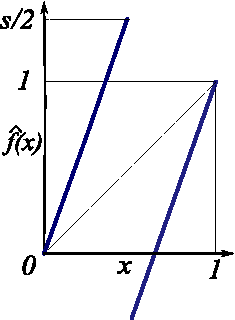
\includegraphics[width=0.30\textwidth]{fig_d_1CL18}
  \caption{\label{fig-d-1f}
$\hflow{}{\ssp}$, the full space sawtooth map \refeq{KD-mapCL18}, ${s} >
2$.
            }
\end{figure}
%%%%%%%%%%%%%%%%%%%%%%%%%%%%%%%%%%%%%%%%%%%%%%%%%%%%%%%%%%%%%%%%%%
%
The closely related {\em sawtooth map}, sketched in \reffig{fig-d-1f},
with `stretching' parameter $s>2$,
\index{sawtooth map}
\beq
\hx_{\zeit+1}
    \,=\, \hflow{}{\hx_{\zeit}}
    \,=\,\left\{
\begin{array}{ll}
{s} \hx_{\zeit}\,,          & \hx_{\zeit} \in [0,{1/2}) \\
{s} \hx_{\zeit} +1 - {s}\,, & \hx_{\zeit} \in ({1/2},1]
\end{array}
\right.
%\,,\qquad {s} \in \{2,3,4, \cdots\}
%\,,
\label{KD-mapCL18}
\eeq

 Since the relation between $\Ssym{\zeit}$ symbol
sequences and $\ssp_{\zeit}$ states is linear, it is straightforward  to
go back and forth between a {\lattstate} and its symbolic
representation.

%%%%%%%%%%%%%%%%%%%%%%%%%%%%%%%%%%%%%%%%%%%%%%%%%%%%%%%%%%%%%
\begin{figure}
  \centering
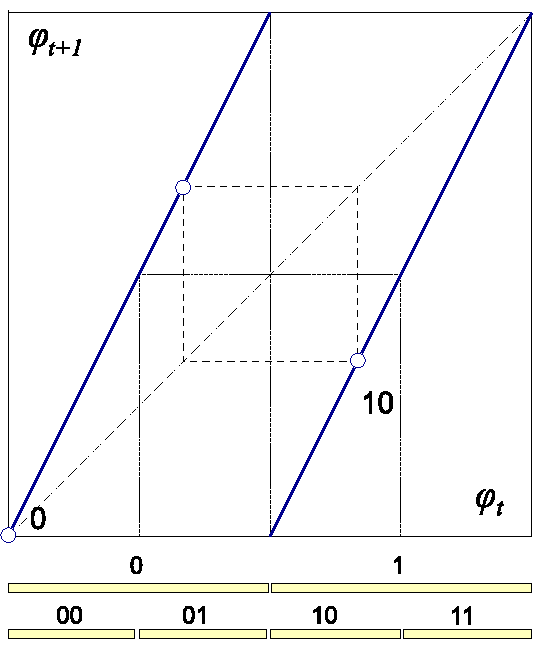
\includegraphics[width=0.35\textwidth]{BernPartKitten}
  \caption{\label{fig:BernPart}
The Bernoulli map \refeq{KD-mapCL18} for ${s}=2$, %{BerShift},
together with the
$\cycle{0}$ fixed point, and the \cycle{01} 2-cycle. Preimages
of the critical point $\ssp_c=1/2$ partition the unit interval into
$\{\pS_0,\pS_1\}$, $\{\pS_{00},\pS_{01},\pS_{10},\pS_{11}\}$, $\dots$,
subintervals.
As the map is a
circle map, $\ssp_{5}=1=0=\ssp_{0} \quad(\mbox{mod}\;1)$.
          }
\end{figure}
%%%%%%%%%%%%%%%%%%%%%%%%%%%%%%%%%%%%%%%%%%%%%%%%%%%%%%%%%%%%%%

The $n$th
preimages $b^{-(n-1)}(\ssp)$ of the critical point $\ssp_c=1/2$
partition the \statesp\ into $2^n$ subintervals, each labeled
by the first $n$ binary digits of points $\ssp=.\Ssym{1}
\Ssym{2} \Ssym{3} \ldots $ within the subinterval:
\reffig{fig:BernPart} illustrates such 4-intervals \statesp\
partition $\{\pS_{00},\pS_{01},\pS_{11},\pS_{10}\}$  for
$\cl{}=2$.

known as the {\em doubling} map if ${s}=2$,
    \index{doubling map}\index{circle map}
\beq
\ssp_{\zeit+1} = 2 \ssp_{\zeit} \;\; (\mbox{mod}\;1)
%    \,,\qquad \qquad \ssp_{\zeit}\in [0,1)
\,,
\ee{DoublingMap}
and {\em ${s}$-tupling} map, \reffig{fig-d-1}\,(b), for
integer stretching parameter ${s}\geq3$,

The relation is linear, and a given \brick\ $\Mm$, or `code' in terms of
alphabet  \refeq{base-sAlph}, corresponds to a unique temporal {\lattstate} $\Xx$ given by the lattice Green's function
\beq
\Xx
= \gd\,\Mm
\,,\qquad
\gd = - \frac{\shift}{\shift - s\,\id}
\,,
\ee{appe:tempBernGreen}
provided we specify the boundary conditions ({\bcs}) for the {\shiftOp}
$\shift$.

The power of the linear encoding of the {temporal
Bernoulli} condition \refeq{1stepDiffEq} is that the
\emph{integer}-valued symbols $\Ssym{\zeit}$ from the finite alphabet
\refeq{base-sAlph} encode the \emph{real-valued} lattice site states
$\ssp_{\zeit}$.

For the  %\rf{GroFuj,art91},
piecewise linear map of \reffig{fig:BernPart}
we can evaluate the \dzeta\ in closed form.
Each branch has the same value of the
slope, and the map can be parameterized
by the single parameter ${s}$.
The larger ${s}$ is, the stronger is the stretching action of the map.

The power of the code % $\{\Ssym{\zeit}\}$
\beq
\transp{\Mm} % = \{\ssp_j\}
             = (\Ssym{\zeit},\Ssym{{\zeit+1}},\cdots,\Ssym{{\zeit+k}})
\ee{linCode}
for the {\templatt} \refeq{OneCat} is that one can use \emph{integers}
$\Ssym{\zeit}$ to encode the \emph{real-valued} {\lattstate}s $\ssp_{\zeit}$.

,
\beq
(\partial - (s-1)\,\shift^{-1})\,\Xx = -\Mm
\,.
\ee{app:1stepVecEq}

For
the $s=3$ cat map example at hand, they are
\beq
\{M_j\} = (M_1,M_2,M_3,M_4,M_5,\cdots)
=(1,2,5,10,24,\cdots)
\,,
\ee{noPrimeCycs=3}

Visualizing the volume relation \refeq{eq:fundFact} for a general \cl{}\dmn\
{\fundPip} is not easy, but

As the {temporal Bernoulli} \refeq{tempBern} is linear, eigenmodes of
$\jMorb$, shifted by $\Mm$ as in \refeq{tempBern} for each distinct
{\lattstate}, are also {\lattstate}s of {temporal Bernoulli}.


    \HLpost{2020-01-17}{
The determinant of this $\jMorb$ from \refeq{tempBern} is negative so
we cannot use the determinant trace formula directly. A correct way is:
first rewrite the $\jMorb$ as in \refeq{appe:tempBernGreen}
\[
\jMorb = \id-{s}{\shift}^{-1}
       = - \frac{s}{\shift} \left(\id-\frac{\shift}{s}\right)
\, .
\]
Note that $\det(\shift)=(-1)^{\cl{}-1}$. The determinant of $\jMorb$ is:
\[
\det \jMorb = \det(\frac{\shift}{s}-\id) s^{\cl{}}(-1)^{\cl{}-1}
   = - s^{\cl{}} \det(\id-\frac{\shift}{s}) \, .
\]
Then use the determinant-trace formula:
\[
\ln\det(\id-\frac{\shift}{s}) = \tr\ln({\id- {\shift}/{s}})
  =
-\sum_{k=1}^\infty\frac{1}{k}\frac{\tr(\shift^k)}{s^k}
\, ,
\]
and use
$\tr \shift^k= \cl{}\delta_{k,\cl{}r}$ if $k$ is a multiple of $\cl{}$,
0 otherwise
(follows from $\shift^\cl{}=\id$),
\[
\ln\det(\id-\frac{\shift}{s}) = -\sum_{r=1}^\infty\frac{1}{r}\frac{1}{s^{\cl{}r}}
=
\ln(1-s^{-\cl{}})
\, ,
\]
and the determinant of $\jMorb$ is:
\[
\det \jMorb = - s^{\cl{}} \det(\id-\frac{\shift}{s}) = 1 - s^{\cl{}}
\, ,
\]
which is negative. So for the {temporal Bernoulli} the count is:
\[
N_\cl{} = |\det \jMorb| = s^{\cl{}} - 1
\, ,
\]
in agreement with the time-evolution count \refeq{noPerPtsBm}.
}

\item[2020-01-25 Predrag:] {\bf A Bernoulli map example}.
%%%%%%%%%%%%%%%%%%%%%%%%%%%%%%%%%%%%%%%%%%%%%%%%%%%%%%%%%%%%%%%%%%%%%%%
% BernCyc2Jacob.svg
% derived from CatMapStatesp.svg
\begin{figure}
  \centering
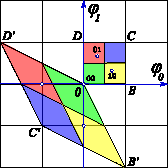
\includegraphics[width=0.45\textwidth]{BernCyc2Jacob}
  \caption{\label{fig:BernCyc2Jacob}
(2020-02-14 Predrag: his is ``wrong'', now superseded with the updated
figure in \refref{CL18}; 2020-09-11 the whole example seems misplaced
here, moce it to wherever it belongs)
The base-2 Bernoulli map \refeq{circ-m=2} period-2 periodic points
$\Xx_p=(\field_0,\field_1)$ are $\cycle{0}=(0,0)$, $\cycle{1}=(1,1)$ fixed
point repeats, and the 2-cycle $\Xx_{01}=({1}/{3},{2}/{3})$,
see \reffig{fig:BernPart}.
They all lie within the unit square $[0BCD]$, one within each
$\pS_{\Ssym{0}\Ssym{1}}$ subregion, and are mapped by the
$[2\!\times\!2]$ {\jacobianOrb} $\jMorb$
% \refeq{jacobianOrb}
into the parallelogram $[0B'C'D']$, whose area is 4 times the unit area.
The images of periodic points $\Xx_p$ land on the integer lattice, and
are sent back into the origin by integer translations $\Mm_p$, in order
to satisfy the fixed point condition
%\refeq{tempBernFix},
$\jMorb\Xx_p+\Mm_p=0$.
          }
\end{figure}
%%%%%%%%%%%%%%%%%%%%%%%%%%%%%%%%%%%%%%%%%%%%%%%%%%%%%%%%%%%%%%
%
The action of {\jacobianOrb}
$\jMorb$ for the period-2 periodic points of the base-2 Bernoulli map,
\reffig{fig:BernPart},
which partitions the unit interval into ${2}$ subintervals
$\{\pS_\Ssym{}\}$, is
\beq
\field_{\zeit+1}
= {2} \field_{\zeit} - \Ssym{\zeit+1}
\,,\qquad  \field_{\zeit}\in\pS_{\Ssym{\zeit}}
\,,
\ee{circ-m=2}
where $\Ssym{\zeit}$ takes values in the ${2}$-letter alphabet
\beq
\Ssym{} \in \A=\{0,1\}
\,.
\ee{base-sAlph=2}

should suffice to convey the idea. In this
case, the $[2\!\times\!2]$ {\jacobianOrb}, the unit
square basis vectors, and their images are
\bea
\jMorb &=&
 \left(\begin{array}{cc}
  1 & -2 \\
 -2 &  1
 \end{array} \right)
;\quad
\Xx_B =
 \left(\begin{array}{c}
 1  \\
 0
 \end{array} \right)
\,,\quad
\Xx_D =
 \left(\begin{array}{c}
 0  \\
 1
 \end{array} \right)
\continue
\Xx_{B'}  &=& \jMorb\,\Xx_B =
 \left(\begin{array}{c}
  1  \\
 -2
 \end{array} \right)
\,,\quad
\Xx_{D'} =
 \left(\begin{array}{c}
-2  \\
 1
 \end{array} \right)
\,,
\eea
with the resulting fundamental parallelogram of area 4
shown in \reffig{fig:BernCyc2Jacob}.
The volume of the fundamental parallelogram lattice $\lattice$ \refeq{lattVol} is
\beq
\Det(\lattice) = \Det(\Xx_{B'}|\Xx_{D'})= \Det(\jMorb)\,\Det(\Xx_{B}|\Xx_{D}) = - 3
\,,
\ee{bernVol}
where in this case the unit cell matrix $(\Xx_{B}|\Xx_{D})=\unit$.


The $[3\!\times\!3]$ {\jacobianOrb} and the unit
cube basis vectors are
\bea
- \jMorb &=&
 \left(\begin{array}{ccc}
  -1  & 0 & 2 \\
  2 &  -1 & 0\\
  0 & 2 & -1
 \end{array} \right)
\,,\quad
\left(\Xx_B|\Xx_C|\Xx_D\right) =
 \left(\begin{array}{ccc}
 1 & 0 & 0\\
 0 & 1 & 0\\
 0 & 0 & 1
 \end{array} \right)
\,.
\nnu
\eea
Clearly $\Det(-\jMorb)= {s}^3-1$, and so on, reproducing the periodic
states count for Bernoulli. No point of looking at $\Det(-\jMorb)$, as
that changes sign at every order - always evaluate $|\Det(\jMorb)|$.

%%%%%%%%%%%%%%%%%%%%%%%%%%%%%%%%%%%%%%%%%%%%%%%%%%%%%%%%%%%%%%%%%%%%%%%
% BernCyc2Jacob.svg
% derived from CatMapStatesp.svg
\begin{figure}
  \centering
{(a)}
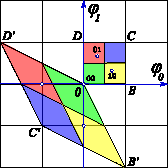
\includegraphics[width=0.35\textwidth]{BernCyc2Jacob}
~~~
{(b)} %$\!\!\!\!$
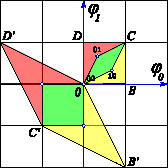
\includegraphics[width=0.35\textwidth]{BernCyc2JacobUnit}
  \caption{\label{fig:BernCyc2JacobOld}
[OLD VERSION] The Bernoulli map \refeq{BerShift} period-2 {\lattstate}s
$\Xx_\Mm=(\ssp_0,\ssp_1)$ are the $\cycle{0}=(0,0)$ fixed
point, and the 2-cycle $\Xx_{01}=({1}/{3},{2}/{3})$, see
\reffig{fig:BernPart}. They all lie within the unit square $[0BCD]$,
one within each $\pS_{\Ssym{0}\Ssym{1}}$ subregion, and are mapped by the
$[2\!\times\!2]$ {\jacobianOrb} $\jMorb$ \refeq{bernFundPar} into the
{\fundPip} $[0B'C'D']$. The images
of periodic points $\Xx_\Mm$ land on the integer lattice, and are sent back
into the origin by integer translations $\Mm$, in order to satisfy the
fixed point condition refeq\{tempFixPoint\}, $\jMorb\Xx_\Mm+\Mm=0$.
\refFig{fig:BernPart} suggests subdividing the {\fundPip}
into (a) 4 areas, but they are not unit areas. The theory of integer lattices
dictates instead (b) covering the {\fundPip} by 3 unit area
rectangles, with
all vertices on the integer lattice.
          }
\end{figure}
%%%%%%%%%%%%%%%%%%%%%%%%%%%%%%%%%%%%%%%%%%%%%%%%%%%%%%%%%%%%%%
%

\PCpost{2020-02-16}{
Dropped from CL18\rf{CL18}:\\
The temporal Bernoulli lattice Green's function %\refeq{appe:tempBernGreen}
in the matrix form
\beq
\gd
=  \left(\begin{array}{ccccccc}
0&\ExpaEig^{-1}&\ExpaEig^{-2}&\ExpaEig^{-3}&\ExpaEig^{-4}&\ExpaEig^{-5}&\cdots\cr
0&  0          & \ExpaEig^{-1}&\ExpaEig^{-2}&\ExpaEig^{-3}&\ExpaEig^{-4}&\cdots\cr
0&  0          &   0          &\ExpaEig^{-1}&\ExpaEig^{-2}&\ExpaEig^{-3}&\cdots\cr
0&  0          &   0          &     0       & \ddots      &  \cr
0&  0          &   0          &     0       & 0           & \ExpaEig^{-1}&\cdots\cr
0&  0          &   0          &     0       & 0           & 0            &\ddots\cr
\vdots&\vdots  &   \vdots     &     \vdots  & \vdots      & \vdots        &\ddots
          \end{array} \right)
\,,
\ee{BernGreenMatrix}
for an infinite temporal Bernoulli
lattice $\zeit\in\integers$, where $\ExpaEig={s}$ is the 1-time step stability
multiplier for the Bernoulli system.
}

\item[2020-02-18 Predrag] Clipped here from
\emph{Ising.tex}, might be relevant to generalizing
Bernoulli to 2\dmn\ lattice, as a warm-up to \catlatt\ zeta functions:

Roettger\rf{Roettger05},
{\em Periodic points classify a family of Markov shifts}, writes:

Ledrappier introduced the following type of space of doubly indexed
sequences over a finite abelian group G,
\[
X_G=\{(x_{s,t}) \in G^{\integers^2} | x_{s,t+1}=x_{s,t}+x_{s+1,t}
\quad \mbox{for all }s,t\in \integers\}.
\]
The group $\integers^2$ acts naturally on the space $X_G$ via left and
upward shifts.

\item[2020-02-19 Predrag]
Suarez\rf{Suarez89}
{\em Difference equations and a principle of double induction},
\CBlibrary{Suarez89}
studies this as a ``partial difference equations,'' that is, difference
equations in two or more variables. He refers to many books on the
subject. His example is a first order hyperbolic equation, with initial
conditions on space and time axes, which describes some thermal
properties,
\[
f(r, m) =f(r, m-1) +f(r-1, m).
%\label{Suarez89(9)}
\]
The goal is to calculate, step by step, all the values of the temperature
T(m,n), starting with the initial and boundary conditions. But then I do
not get the rest of the papers. Perhaps best not to use much time on
`\spt' Bernoulli.

    \item[2020-03-28 Predrag]
The Bernoulli % equation \refeq{circ-m}
first-order difference equation
\beq
\field_{\zeit} - {s}\field_{\zeit-1} = - \Ssym{\zeit}
\,,\qquad  \field_{\zeit} \in [0,1)
\,,
\ee{diffEqs:1stepDiffEq}
{characteristic equation} (for \Ssym{\zeit}=0)
\beq
\ExpaEig -s= 0
\,,
\ee{diffEqs:tempBern}
has one characteristic root
\(
\{s\}
\,.
\)

Comparing with \refeq{genFuncts:noPerPtsBms} we see that we need to solve
a first-order inhomogeneous difference equation with a constant forcing
term $(s-1)$.

Weijie Chen does this pedagogically in his 2011 lecture notes
\CBlibrary{Chen11}, sect.~{\em 1.2.1 One Example}, where he
considers
\beq
\field_{\zeit} - {s}\field_{\zeit-1} = {M}
\,,
\ee{Chen11:1stepDiffEq}
and finds the particular solution by taking
$\field_{p,n} = \field_{p}$ for all $n$,
\[
  \field_{p}-s\,\field_{p}={M}
  \quad \to \quad
  \field_{p} = -{M}/(s-1)
\,.
\]
Hence the solution is
\beq
\field_{n} = \field_{c,n} + \field_{p,n}
= c\,s^{n} - \frac{{M}}{s-1}
\,,
\ee{Chen11:1stepDiffSolu}
with $c$ determined by the initial value
\(
\field_{0}= c\,{s}^{0} - {{M}}/(s-1)
\,.
\)
Bernoulli starts with $\field_{0}=0$, and according to
\refeq{genFuncts:noPerPtsBms}, $M=(s-1)$, so $c=1$.

Weijie Chen also works out the particular solution when $s=1$.
                                    \toCB
He also remarks that in econometrics the {\shiftOp} $\shift$ is called
the \emph{lag operator}.

%\item[2020-03-28 Predrag]
Weijie Chen solves the \templatt\ pedagogically in his lecture notes
\CBlibrary{Chen11}, sect.~{\em 2 Second-Order Difference Equation}.

Questions
\begin{itemize}
  \item
Why is it OK to take site-independent particular solution?
  \item
${{M}}/(s-1)$ looks awkward, can one reformulate? so instead of $M$, have
${{M}}/(s-1)\to1$
  \item
I am guessing that $M=(s-1)$ in \refeq{Chen11:1stepDiffEq}
something like the total number of `letters' I can add to
the count $N_n$ at time $n$. Something like that.
  \item
Similarly for $M=2{\mu}^2$ forcing term in \templatt\ second-order
difference equation \refeq{genFuncts:CatRec-s}.
  \item
This is still just a verification of my guess recurrence
\refeq{genFuncts:noPerPtsBms}.
Make this argument into a derivation.
\end{itemize}

    \PCpost{2020-02-23}{
Just curious - what does the Bernoulli {\fundPip} defined by the columns
of $[3\!\times\!3]$ {\jacobianOrb}
\beq
\jMorb =
\left(
\begin{array}{ccc}
  1 & -2 &  0 \\
  0 &  1 & -2 \\
  -2&  0 &  1
\end{array}
\right)
\,,
\qquad
N_3 = |\Det \jMorb|
    = 2^3-1
\,,
\label{bernFundPar3}
\eeq
look like in a 3\dmn\ rendition? Hopefully it is not symmetric, like
\reffig{fig:catCycJacob}\,(b).
    }

\item[2020-03-01 Predrag]
Wilf\rf{Wilf94} {\em Generatingfunctionology} starts out in his sect.
1.1~{\em An easy 2-term recurrence}, with our Bernoulli periodic points
count \refeq{genFuncts:noPerPtsBm} and
\refeq{genFuncts:1stepDiffEq} as a trivial example of a two-term
recurrence (first-order difference equation).

\item[2020-12-21 Predrag]
{\bf Counting {temporal Bernoulli} {\lattstate}s}
%\label{s:bernCount}
removed from CL18.tex $\to$ Bernoulli.tex, replaced by  refsect{s:Hill1stOrd}
\bigskip

To evaluate the {\HillDet} \refeq{eq:fundFact}, observe that
from \refeq{tempBern} it follows that
\[
\Det(-\jMorb)=\Det({s}/\shift)\,\Det(\id- {\shift}/{s})
\,,
\]
where $|\Det({s}/\shift)|=s^n$. Expand $\ln\Det(\id- {\shift}/{s}) =
\Tr\ln(\id- {\shift}/{s})$ as a series in $1/s$,
\beq
\Tr\ln\left(\id- \frac{\shift}{s}\right)
  =
-\sum_{k=1}^\infty\frac{1}{k}\frac{\Tr(\shift^k)}{s^k}
\,.
\ee{LnDet=TrLn}
It follows from $\shift^\cl{}=\id$ that
$\Tr \shift^k= \cl{}\delta_{k,r\cl{}}$ is non-vanishing
if $k$ is a multiple of $\cl{}$,
0 otherwise:
\[
\ln\Det(\id- {\shift}/{s})
  =
-\sum_{r=1}^\infty\frac{1}{r}\frac{1}{{s}^{\cl{}r}}
  =
\ln(1-{s}^{-\cl{}})
\,.
\]

\item[2020-12-09 Predrag]
{\bf Temporal Bernoulli}
% \label{appe:1D1dLatt}
% was file siminos/kittens/appeBernoulli.tex      pdflatex CL18
%\renewcommand{\statesp}{state space}
%\renewcommand{\Statesp}{State space}
%\renewcommand{\stateDsp}{state-space}
%\renewcommand{\StateDsp}{State-space}
\index{cyclic!permutation matrix}

After $\cl{}$ shifts, the {\lattstate} \Xx\ returns to the initial
state, $\shift^\cl{}=\id$. This relation leads to the explicit expression for
the orbit {\jacobianM} \refeq{appe:tempBernGreen},
\beq
\gd
    =  \frac{\shift}{s\,\id-\shift}
    = \frac{1}{\id-\frac{\shift}{s}}\,\frac{\shift}{s}
    = \sum_{k=1}^\infty \frac{\shift^k}{s^k}
%    =  \sum_{m=0}^\infty \frac{1}{s^{\cl{}m}}
%      \sum_{k=1}^\cl{} \frac{\shift^k}{s^k}
    =  \frac{s^\cl{}}{s^\cl{} - 1}
      \sum_{k=1}^\cl{} \frac{\shift^k}{s^k}
\,.
\ee{appe:BernGreenFct}
From \refeq{appe:tempBernGreen} it then follows that the last field in
$\Xx$ is the field at lattice site $\cl{}$
\beq
\ssp_{\cl{}}
=  \frac{s^\cl{}}{s^\cl{} - 1}
          .\Ssym{1}\Ssym{2}\Ssym{3}\cdots\Ssym{\cl{}}
=  \frac{1}{s - 1}\,%\sum_{k=1}^\cl{} \Ssym{k} 2^{\cl{}-k}
    \frac{s^{\cl{}-1}\Ssym{1}+\cdots+s\,\Ssym{\cl{}-1}+\Ssym{\cl{}}}
         {s^{\cl{}-1}+\cdots+s+1}
\,,
\label{appe:Bern_cyc}
\eeq
and the rest are obtained by cyclic permutations of $\Mm$.

% from ChaosBook \Chapter{appendKnead}
% \section{Pruned Bernoulli shift} \label{sect:PrunBernoulli}
For example, for ${s}=2$, the lattice fields are (they are always rational-valued),
\bea
\ssp_{\Ssym{1}\Ssym{2}\cdots \Ssym{n}}
&=&  \sum_{k=1}^\cl{} \frac{\Ssym{k}}{2^k} \sum_{m=0}^\infty \frac{1}{2^{\cl{}m}}
        = \frac{2^\cl{}}{2^\cl{} - 1} .\Ssym{1}\Ssym{2}\cdots \Ssym{\cl{}}
\continue
&=& \frac{1}{2^\cl{} - 1}\,\sum_{k=1}^\cl{} \Ssym{k} 2^{\cl{}-k}
\,,
\label{Bern_cyc1}
\eea
where $p=\overline{\Ssym{1}\Ssym{2}\cdots \Ssym{\cl{}}}$ is an {\orbit} of period
\cl{}, with stability multiplier $\ExpaEig_p=2^\cl{}$.

For a Bernoulli map,
the rational $\ssp_{0}$ are either periodic or land eventually on a \po\
(the base-${s}$ version of the familiar fact that the decimal expansion
of a rational number is eventually periodic), while the orbit of a normal
irrational $\ssp_{0}$ is ergodic.

    \item[2020-12-09, 2020-12-11 Predrag]
Quotienting the temporal Bernoulli system
\beq
\ssp_{\zeit} - {s}\ssp_{\zeit-1} = - \Ssym{\zeit}
\,,\qquad  \ssp_{\zeit} \in [0,1)
\,,
\ee{1stepDiffEqBlog}
by its \emph{dynamical} $\Dn{1}=\{e,\Refl\}$
symmetry
\beq
\Refl \ssp_\zeit = 1-\ssp_\zeit
    \,,\quad
\Refl \Ssym{\zeit} = (s-1)-\Ssym{\zeit}
    \,,\qquad
\mbox{ for all } \zeit\in\integers
\,,
\ee{BernDynD1}
where $\Ssym{\zeit}$ takes values in the ${s}$-letter alphabet
\beq
\Ssym{} \in \A=\{0,1,2,\cdots,s-1\}
\,.
\ee{base-sAlphBlog}
Define the fundamental domain to be ${\sspRed}_\zeit\in[0,1/2]$.
We construct the
Bernoulli fundamental domain lattice system, with `1/2' unit hypercube
$\hat{\Xx}\in[0,1/2]^\cl{}$, as in
\toChaosBook{exmple.11.3}
{{\em Group \Dn{1} and reduction to the fundamental domain}},
see \reffig{fig:fig_d_2half}\,(b),
and the fundamental domain symbolic dynamics $\hat{\A}$.
The temporal lattice Bernoulli condition \refeq{1stepDiffEqBlog} is now
two conditions  (Bernoulli)/$\Dn{1}$.
They are different for ${s}$ even or odd:
\bea
{\sspRed}_{\zeit+1} - {s} {\sspRed}_{\zeit} &=&
            - \Ssym{\zeit+1}
\,,\qquad  {\sspRed}_{\zeit}\in\pS_{\Ssym{\zeit}}
\,,\quad {s} \mbox{ even}
    \continue
{\sspRed}_{\zeit+1} + {s}{\sspRed}_{\zeit} &=&
       1 + \Ssym{\zeit+1}
\,,\qquad  {\sspRed}_{\zeit}\in\pS_{\Refl\Ssym{\zeit}}
    \label{circ/D1}\\
% \hat{\Ssym{}} \in
\hat{\A}~~~~ &=& \{\{\Ssym{}\},\{\Refl\Ssym{}\}\}
\,,\;\; \{\Ssym{}\} = \{0,1,2,\cdots,{s}/2\}
\,,
\nnu
\eea

\bea
{\sspRed}_{\zeit+1} - {s} {\sspRed}_{\zeit} &=&
\,,\;\;    {s} \mbox{ odd}
\label{base-sRed}\\
%\hat{\Ssym{}} \in
\hat{\A} &=&
\{\{\Ssym{}\},({s}-1)/2,\{\Refl\Ssym{}\}\}
\,,\;\;     \Ssym{}\in \{0,1,2,\cdots,(s-3)/2\}
\,.
\nnu
\eea
As an example, case
${s}=6$,
$\Ssym{\zeit}\in\{0,1,2\}$
is worked out in \reffig{fig:fig_d_2half}\,(c).
(Plot also the fundamental domain map for odd values of ${s}$.)
%
%%%%%%%%%%%%%%%%%%%%%%%%%%%%%%%%%%%%%%%%%%%%%%%%%%%%%%%%%%%%%
\begin{figure}
  \centering
{(a)}
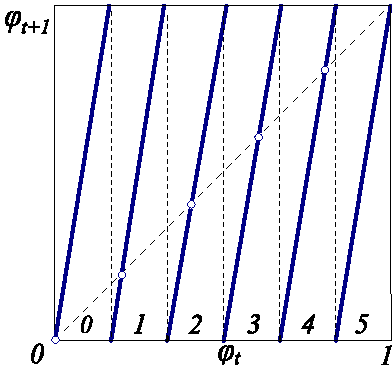
\includegraphics[width=0.40\textwidth]{fig_d_2kitten}
~~~
{(b)}$\!\!\!\!$
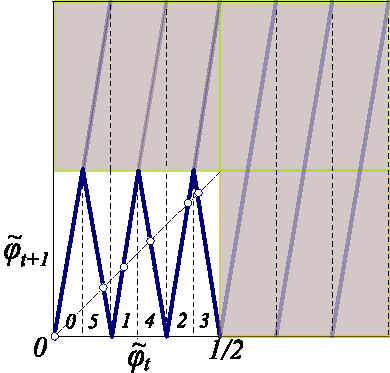
\includegraphics[width=0.40\textwidth]{fig_d_2half}
\\ %~~~
{(c)}$\!\!\!\!$
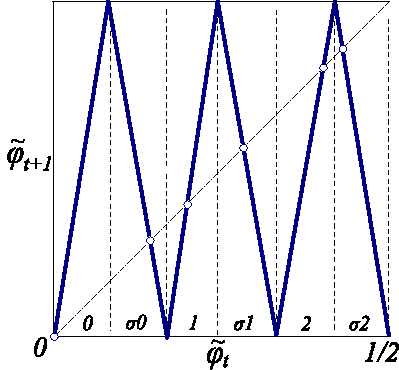
\includegraphics[width=0.40\textwidth]{fig_d_2fund}

  \caption{\label{fig:fig_d_2half}
(a)
The Bernoulli map $f$ with the  stretching parameter ${s}=6$
partitions the unit interval into $6$ subintervals $\{\pS_{\Ssym{}}\}$,
labeled by the ${6}$-letter alphabet \refeq{base-sAlphBlog}. As the map is a
circle map, $\ssp_{5}=1=0=\ssp_{0} \quad(\mbox{mod}\;1)$.
(b)
The Bernoulli map is quotiented by the
\emph{dynamical} $\Group=\Dn{1}=\{e,\Refl\}$
symmetry to
(c)
the fundamental domain ${\sspRed}_\zeit\in[0,1/2]$ map
$\hat{f}=f/\Group$ partitions the half interval into the three $1/12$
subintervals $\{\pS_{0},\pS_{1},\pS_{2}\}$, and their reflections, the
three $3$ subintervals $\{\pS_{\Refl0},\pS_{\Refl1},\pS_{\Refl2}\}$,
labeled by a ${6}$-letter reduced system's alphabet. Reduced space
fixed points $\{\cycle{\Refl_0},\cycle{\Refl_1},\cycle{\Refl_2}\}$
correspond to self-dual 2-cycles
$\{\cycle{05},\cycle{14},\cycle{23}\}$
in the full space. Fixed point $\cycle{0}$ is in the border,
and thus over-counted;
$\cycle{1}$ corresponds to $\{\cycle{1},\cycle{4}\}$, and
$\cycle{2}$ corresponds to $\{\cycle{2},\cycle{3}\}$.
          }
\end{figure}
%%%%%%%%%%%%%%%%%%%%%%%%%%%%%%%%%%%%%%%%%%%%%%%%%%%%%%%%%%%%%%
%

In the matrix form \refeq{1stepDiffEqBlog}, the {\jacobianOrb}
\beq
\jMorb\,\Xx = - \Mm
\,,\qquad
\jMorb = \unit-{s}{\shift}^{-1}
% former \ee{tempBernFix}
\,,
\ee{HLtempBern}
is independent of $\Mm$. Not so for the symmetry reduced  {\jacobianOrb}
${\MvarRed}_{\hat{\Mm}}$ in \refeq{circ/D1}: it depends on
$\hat{\Mm}$, as its diagonal takes values $\pm{s}$. We need to prove
that the \HillDet\ $\Det{\MvarRed}$ does not.

I had not noticed before that this parametrization converts
Bernoulli into tent map, with full \statesp\ 2-cycles turned
into negative slope fixed points.

By the
inclusion-exclusion principle \refeq{KlaRot97(2.1)}
\beq
N_\cl{}=
  \hat{N}_\cl{}+\Refl\hat{N}_\cl{}-\hat{N}_\cl{}\cap(\Refl\hat{N}_\cl{})
      =
  2\hat{N}_\cl{}-\hat{N}_\cl{}\cap(\Refl\hat{N}_\cl{})
\,.
\ee{Bern:inclExcl}
Let's call the number of points in the shared boundary $I$.
% Looks like we have to distinguish odd and even $\cl{}$.
The $\ssp=0$ is in $I$
for any $\cl{}$, if I am allowed to identify $\ssp=1\to0$,
and that is the only point in the boundary.
Presumably this leads to the denominator $(1-z)$ in
\refeq{appe:BernZeta}. I guess that the symmetric irrep of
$\Dn{1}=\{e,\Refl\}$ leads to $N_{+}=s^\cl{}$ and the numerator
$(1-{s}z)$, while the antisymmetric irrep leads to $N_{-}=0$, and a
trivial factor 1 contribution to the numerator \refeq{appe:BernZeta}.
\bea
\zetatop(z)
 &=&
\frac{1 -  {s}z}{1 - z}
\,.
\label{appe:BernZeta}
\eea

\tempLatt\ should be more interesting. Also any nonlinear $s$-branch map
`Bernoulli-like' lattice with a \emph{dynamical} $\Dn{1}$ symmetry; then
the weights $t_p$ do not necessarily cancel for the antisymmetric irrep.

\item[2018-12-27 Linas Vepstas]
{\em On the Beta Transformation} \arXiv{1812.10593}:
The beta transformation is the iterated map \refeq{betaTransf}. The
$\beta=2$ is known as the Bernoulli map, and is exactly solvable. The Bernoulli
map provides a model for pure, unrestrained chaotic (ergodic) behavior:
it is the full invariant shift on the Cantor space. The beta
transformation defines a subshift: iterated on the unit interval, it
singles out a subspace of the Cantor space, in such a way that it is
invariant under the action of the left-shift operator. That is, lopping
off one bit at a time gives back the same subspace. The beta transform
seems to capture something basic about the multiplication of two real
numbers: $\beta$ and $x$. It offers a window into understanding the nature of
multiplication. Iterating on multiplication, one would get
exponentiation; although the mod 1 of the beta transform contorts this in
interesting ways. The work presented here is a research diary: a pastiche
of observations and some shallow insights.
 The eigenvalues of the
transfer operator seem to lie on a circle of radius $1/\beta$ in the complex
plane. Given that the transfer operator is purely real, the appearance of
such a quasi-unitary spectrum seems surprising. The spectrum appears to
be the limit of a dense set of quasi-cyclotomic polynomials, the positive
real roots of which include the Golden and silver ratios, the Pisot
numbers, the n-bonnaci (tribonacci, tetranacci, etc.) numbers.

Beta transformation
\beq
T_{\beta }(x)=\beta x\;{\mod {1}}
\,,\qquad 1<\beta\leq2
\ee{betaTransf}
was introduced by Alfr{\'e}d R{\'e}nyi\rf{Renyi57} in 1957, and an invariant measure for
it was given by Alexander Gelfond in 1959 and independently by Bill
Parry\rf{Parry60} in 1960.

\HREF{https://arxiv.org/pdf/1812.10593.pdf\#subsection.1.9}
{Beta transformation literature review and references}.

\HREF{https://mathoverflow.net/questions/265916/concise-introduction-to-beta-transformations}
{{\em A concise intro to beta-transformations?}} has references.

% A. O. Gel’fand, “A common property of number systems”,
%           Izv Akad Nauk SSSR Ser Mat, 23, 1959, pp. 809–814.

% P. Gaspard, "r-adic one-dimensional maps and the Euler summation
%           formula", Journal of Physics A, 25 (letter) L483-L485 (1992).


\item[2020-09-08 Predrag]
\HREF{https://sites.google.com/site/homepagebingli}{Bing Li}
{\em Some fractal problems in beta-expansions}
\HREF{https://www.irif.fr/~numeration/OWNS}{(video)}
\HREF{https://www.irif.fr/~numeration/uploads/Main/li_20200908.pdf}{(slides)}

For greedy beta-expansions, we study some fractal sets of real numbers
whose orbits under beta-transformation share some common properties. For
example, the partial sum of the greedy beta-expansion converges with the
same order, the orbit is not dense, the orbit is always far from that of
another point etc. The usual tool is to approximate the
beta-transformation dynamical system by Markov subsystems. We also
discuss the similar problems for intermediate beta-expansions.

\item[2021-01-05 Predrag]
Hofbauer and Keller\rf{HofKel84} {\em Zeta-functions and
transfer-operators for piecewise linear transformations} (1984) has no
Bernoulli zeta. Not useful to us at this time.

\item[2021-01-05 Predrag]
Takahashi\rf{Takahashi81} {\em Fredholm determinant of unimodal linear
maps} has lots of detail and examples. I might have missed something, but
Bernoulli zeta is not there, or anything we care about.

\item[2021-01-04 Predrag]
Flatto, Lagarias and Poonen\rf{FlLaPo94}
{\em The zeta function of the beta transformation} (1994)

which should have the $\beta=2$ Bernoulli zeta function
as the trivial case.

\item[2021-01-05 Han] Notes from Flatto, Lagarias and Poonen\rf{FlLaPo94} paper:

$\beta$-transformation map is:
\[
f_\beta(x) = \beta x \;\; (\mbox{mod}\;1) \, ,
\]
where $\beta>1$, $x \in [0,1]$. The symbolic dynamics of $f_\beta$ is based on the fact that the graph of
$f_\beta$ consists of $\lfloor \beta \rfloor + 1$ monotone pieces which they call laps, which are
assigned by the symbols $0, 1, \dots, \lfloor \beta \rfloor$. When $\beta \in \mathbb{Z}^+$,
the piece $\lfloor \beta \rfloor$ consists of a single point, and the symbol $\lfloor \beta \rfloor$
only appears in the itinerary of 1. To each $x \in [1,0]$ its itinerary is $I_\beta(x)=A_0A_1A_2\dots$,
where the symbol
\[
A_n := A_n(x) = \lfloor \beta f_\beta^n(x) \rfloor \, .
\]
In particular the itinerary of 1, $I_\beta(1)=A^*_0A^*_1A^*_2\dots$ encodes complete information about
the behavior of $f_\beta$.

They introduced a power series with integer coefficients:
\[
\phi_\beta(z) = A_0^* z + A_1^* z^2 + A_2^* z^3+ \dots = \sum_{n=0}^{\infty} A_n^* z^{n+1} \, .
\]
This function is related to the iterates of 1 by:
\[
\phi_\beta(z) = 1 + (\beta z - 1)\left(
\sum_{n=0}^\infty f_\beta^n(1)z^n
\right)
\, .
\]
Then the zeta function is:
\[
\zeta_\beta(z) = \frac{1}{1-\phi_\beta(z)} \, ,
\]
if $\beta$ is not a simple $\beta$-number, and
\[
\zeta_\beta(z) = \frac{1-z^N}{1-\phi_\beta(z)} \, ,
\]
if $\beta$ is a simple $\beta$-number, and $N$ is minimal with $f_\beta^N(1)=0$.
Simple $\beta$-numbers are the $\beta$-numbers such that for some $n$, $f_\beta^n(1)=0$.
This formula gives the correct topological zeta function of temporal Bernoulli.

Associated with the $\beta$-transformation is the set $X_\beta$ of all $I_\beta(x)$ for $0 \leq x <1$.
The $\beta$-shift $S_\beta$ is a symbolic dynamical system obtained as the smallest closed (two-sided)
subshift of $\{1,2,\dots \lfloor \beta \rfloor\}^{\mathbb{Z}}$ generated by all finite substrings of $X_\beta$.
For simple $\beta$-numbers $S_\beta$ is a subshift of finite type.

There is a zeta function associated to the $\beta$-shift $S_\beta$, which is studied by
Takahashi\rf{Takahashi83}, who showed that
\[
\hat{\zeta}_\beta(z) = \frac{1}{1-\phi_\beta(z)} \, .
\]
This formula is closely related to $\zeta_\beta(z)$ but differs from it for simple $\beta$-numbers,
in which case the closure operation defining $S_\beta$ adds some extra periodic points.

\item[2021-01-11 Predrag] Seth Lloyd \etal. %\rf{LDGKLMTP20}
{\em Quantum algorithm for nonlinear differential equations}
\arXiv{2011.06571}:

[1] showed how to map the problem of solving a general linear differential
equation to that of matrix inversion, which can then be performed using
the quantum linear systems algorithm [12-13].   Consider a linear differential
equation of the form,
$$ {dx\over dt} + A x = b(t), \eqno(6)$$
where as above $x,b \in {\cal C}^d$ and $A$ is a $[d\times d]$ matrix.

                                                            \toCB
Discretize the equation in time at intervals $\Delta t$, and take $k$ to
be the index for the discretized time, so that $x_k$ and $b_k$ are
the values of $x$ and $b$ at time label $k$.

We wish to integrate equation
(6) numerically starting from the initial state $x_0 \equiv b_0$.   We obtain
a series of equations of the form:
$$
 x_0 = b_0 \quad
x_1 = x_0 - \Delta t A x_0 + \Delta t b_1 \quad
\ldots \quad
x_{k+1} = x_k - \Delta t A x_k + \Delta t  b_k \quad
\ldots
\eqno(7)$$
Here, we have used the Euler forward method for numerical integration, but it
is straightforward to implement implicit methods such as
Euler backward, Crank-Nicholson, Runge-Kutta, etc.~[3].
Written in matrix form, these equations become
$$-\left(\begin{array}{cccccc}
- I & 0 & 0 & \ldots & 0 & 0 \cr
I-\Delta t A & - I & 0 & \ldots & 0 & 0 \cr
0 & I-\Delta t A& -I &  \ldots & 0 & 0\cr
&&\ldots &&&\cr
0& 0 & 0 & \ldots & - I & 0\cr
0& 0 & 0 & \ldots & I - \Delta t A & - I\cr
          \end{array} \right)
\left(\begin{array}{c}
x_0 \cr x_1 \cr x_2 \cr \ldots \cr x_{T-1} \cr x_{T}
          \end{array} \right)
=
\left(\begin{array}{c}
b_0 \cr \Delta t b_1 \cr \Delta t b_2 \cr \ldots \cr \Delta t
b_{T-1} \cr \Delta t b_{T}
          \end{array} \right)
%\eqno(8)
\,,
$$







\end{description}

%%%%%%%%%%%%%%%%%%%%%%%%%%%%%%%%%%%%%%%%%%%%%%%%%%%%%%%%%%%%%%%%%%%%%%%%%%%%%
\Remarks
%%%%%%%%%%%%%%%%%%%%%%%%%%%%%%%%%%%%%%%%%%%%%%%%
% PC 2021-01-04 eventually merge into
% \Chapter{appendStatM}{22jun2016}{Statistical mechanics applications}
\remark{Bernoulli map.}{\label{rem:Bernoulli}
The Bernoulli shift map \refeq{BerShift} and the doubling map
\refeq{DoublingMap} are also known as the dyadic transformation, dyadic
map, bit shift map, angle doubling map or sawtooth map \refeq{KD-map}.
There are many fine books that discuss it in depth, for example Driebe\rf{Driebe99}.
See also \refrem{rem-GroRue}.
\index{Bernoulli!shift}\index{shift!Bernoulli}
\index{doubling map}\index{circle map}
\index{dyadic transformation}\index{dyadic map}
\index{bit shift map}\index{angle doubling map}
\index{sawtooth map}
    } %end \remark{rem:Bernoulli}
%%%%%%%%%%%%%%%%%%%%%%%%%%%%%%%%%%%%%%%%%%%%%%%%

%%%%%%%%%%%%%%%%%%%%%%%%%%%%%%%%%%%%%%%%%%%%%%%%
% PC 2021-01-04 eventually merge into
% \Chapter{converg}{9nov2008}{Why does it work?}
\remark{Bernoulli shift.}{ \label{rem-GroRue}
For a more in-depth discussion, consult chapter~3 of \refref{Driebe99}.
The extension of Fredholm theory to the case of Bernoulli shift on
$\complex^{k+\alpha}$ (in which the \FPoper\ is {\em not} compact  --
technically it is only {\em quasi-compact}. That is, the essential
spectral radius is strictly smaller than the spectral radius) has been
given by Ruelle\rf{Ruelle90}: a concise and readable statement of the
results is contained in \refref{Baladi95}. We see from \refeq{mixing-BS}
that for the Bernoulli shift the exponential decay rate of correlations
coincides with the Lyapunov exponent: while such an identity holds for a
number of systems, it is by no means a general result, and there exist
explicit counterexamples.
See also \refrem{rem:Bernoulli}.
\index{Bernoulli!shift}\index{shift!Bernoulli}
} %end \remark{Bernoulli shift on $C^{k+\alpha}$}{
%%%%%%%%%%%%%%%%%%%%%%%%%%%%%%%%%%%%%%%%%%%%%%%%

\RemarksEnd

%%%%%%%%%%%%%%%%%%%%%%%%%%%%%%%%%%%%%%%%%%%%%%%%%%%%%%%%%%%%%
\fastTrackExam{exam:BernShad}     % \toExam
%%%%%%%%%%%%%%%%%%%%%%%%%%%%%%%%%%%%%%%%%%%%%%%%%%%%%%%%%%%%%


%%%%%%%%%%%%%%%%%%%%%%%%%%%%%%%%%%%%%%%%%%%%%%%%%%%%%%%%%%%%%%%
%\section{Any piecewise linear map has ``linear code''}
%\label{exam:tentMapSymbDyn}
% siminos/spatiotemp/chapter/tentMapCode.tex
% $Author: predrag $ $Date: 2020-05-07 17:34:06 -0400 (Thu, 07 May 2020) $


%%% input by % siminos/spatiotemp/chapter/catMap.tex %%%%%
\section{Any piecewise linear map has ``linear code''}
\label{exam:tentMapSymbDyn}

                                                            \toCB
For reasons unbeknownst to me, it is below the dignity of any cat to work out
any problem in Chaos\-Book, or in the online course, no matter how often I
point out that it is easier to understand what we do for cat maps if you
first work it out for 1\dmn\ maps.

So I have to do these exercises myself - I'm forced to it, so Li Han can be
motivated to re-derive his polynomials (as described in Bird and
Vivaldi\rf{BirViv}, see my notes of {\bf 2016-05-21, -12-12} below), rather
than to fit them to Mathematica grammar rule counts for integer $s$.

Basically, I am baffled by why should ``linear code'' be such a big deal that
it has to go into the title of our paper\rf{GHJSC16}. {\em Every} example of
symbolic dynamics worked out in Chaos\-Book is a ``linear code.'' The strategy
is always the same - find a topological conjugacy from your map to a
piecewise linear map, and then use the fact that any piecewise linear map has
``linear code.'' The pruning theory is always the same - kneading orbit
separates {\admissible} from the {\inadmissible}, also in the infinite 1\dmn\
discrete lattice case worked out in the {\em Diffusion} chapter in the
Chaos\-Book, and the appendix (\refchap{c-appendStatM} reproduced here) that no
one wants to read either.

A tent map is a 1\dmn\ example (a simpler one would be Bernoulli, and its
sawtooth generalizations). The 2\dmn\ examples are the Belykh map,
\refexam{exam:BelykhLCod}, and the Lozi map, \refexam{exam:LoziLCod}. Belykh map
is of particular interest to us, as it is in form very close to the cat
map. Both maps have the pruning front conjecture is proven for them, for
a some sets of parameters.

%%%%%%%%%%%%%%%%%%%%%%%%%%%%%%%%%%%%%%%%%%%%%%%%%%%%%%%
\hfill    \fastTrackExam{exam:TentLCod}
          \fastTrackExam{exam:TentCycl}

\hfill    \fastTrackExam{exam:BelykhLCod}
          \fastTrackExam{exam:LoziLCod}


\section{Cat map blog}
\label{sect:CatMapBlog}

\begin{description}

    \PCpost{2016-05-18}{                                        \toCB
I start with our 2011 \emph{Notes for cat map}\\
(former \emph{appendStatMnotes.doc} in \emph{dasbuch/book/notes}),\\
to be eventually merged with \emph{chapter/appendStatM.tex}.
    }

\item[2011-05-14 Jean-Luc Thiffeault]
I figured
out that the grouping of \po s is crucial, and moreover that there is
something delicate with the fixed point of the cat map, which lies on the
boundary of Markov boxes.

\item[2011-05-14 Predrag]
For Anosov (linear Anosov?) - Arnol'd cat map - it should work like ton of
rocks, but you have to note that because of the periodicity there is one
fixed point, not two. If you screw up an early term in the series, then
it converges very slowly. I think the Stephen Creagh\rf{Creagh94} tested
it on weakly nonlinearly perturbed cat map (weakly, so golden-mean
grammar is working) and it converged super-exponentially (you know the
grammar, flow has bounded hyperbolicity, so weight-truncated cycle
expansions are not needed - they perform less well).

\item[2011-05-14 Jean-Luc Thiffeault]
I know how to do it with the Markov partition now, and it works much better.
Keep in mind this is a warmup problem: what I really have in mind (with
my collaborator Erwan Lanneau\rf{LanThi11}) is to compute {\po s} for
Teichmuller flow, where the {\po s} themselves are actually now
pseudo-Anosovs!

\item[2011-05-16 Hans-Henrik Rugh]
% Hans-Henrik.Rugh@math.u-cergy.fr
The situation as I recall it is roughly as follows:

When you construct the symbolic dynamics you may start by picking one
\po, typically the fixed point  $p=f(p)$  (but the following
depends on the choice).  You then cut the torus into pieces following
$s/u$-manifolds until you get a small collection of $N$ rectangles.
\[
R_1,\cdots,R_N
\]
Associated to this collection you have a transition matrix (for SINGLE
rectangles).  Now, you also need to construct a transition matrix for
PAIRS of rectangles, e.g.  $(R_1,R_2)  \to  (R_2,R_1)$ and then TRIPLES of
rectangles ... $(R_1,R_2,R_3) \to (R_2,R_1,R_3)$, etc....
These k'th - order transitions comes from the fact that there is a fixed
point/periodic cycle on the boundary of the Markov partition elements.

You get determinants   $d_k(z)$ for each of these k'th–order transition matrices.
 NB :
$(R_1,R_2) \to (R_2,R_1)$  is a \po\ of prime length 2 even if
it represents a fixed point of f. I think (but is not sure?) that the
weights in the determinant are calculated in the same way...

The final determinant is
\(
d(z)=d_1(z)d_3(z)... / (d_2(z) d_4(z)...)
\)
if I am not mistaken. This is related to the so-called Manning trick\rf{manning} for
counting real orbits related to
\[
\det (1 - s) = 1 - \tr s + \tr s \wedge s
- \cdots
\]
where $s$ is a permutation.
What is not obvious is that $d(z)$  is entire, but it is!

%\item[2011-05-18 Hans-Henrik Rugh]
It's a kind of model problem anyway. In more realistic systems I suppose
that one may run into the problem of having several orbits on boundaries.

One of the tricky points is to see how such an orbit in the `higher'
order zeta-functions/Fredholm-det.

As mentioned in e.g. $d_1(z)$ a 'physical' fixed point may appear
zero times, or twice, or,...? In $d_2(z)$ a fixed point may actually appear
as a period two orbit, so should be treated as such when looking for
cancelling terms.

Great, if you have managed to make it work in practice.
I don't think that one can call it a standard trick but one may perhaps
get it implicitly from the paper of Ruelle\rf{Ruelle90}. But it is
difficult to digest and even more difficult to convert into computable
formulae.

    \PCpost{2018-02-10}{
Manning\rf{manning} writes: ``
According to Bowen\rf{Bowen70}, a Markov partition is a finite cover of \statesp\
by closed subsets called \emph{rectangles}. The rectangles are pairwise disjoint
except possibly for the intersection of their boundaries.
[...]
At the boundaries of the rectangles, that is where they intersect,
several periodic points individual rectangles may be mapped to the same periodic
point in the full \statesp.
''

``
Counting the periodic points involves also certain auxiliary subshifts of finite
type to remedy overcounting of points in the boundaries of the rectangles.
''
    }

\item[2011-05-18 Jean-Luc Thiffeault] emailed to Predrag
pdf file {\em Notes on \po\ expansions for Teichm\"uller flow}
(saved as \emph{POexp.pdf} in \emph{dasbuch/book/notes/}).
which maybe figures out cat map symbolic dynamics. He writes:

``
Updated notes: on page 4-5 I used the Markov boxes to compute the PO
expansion.  I used a trick to deal with the orbit on the boundary:
include several copies of the orbit, but divide by the correct factor.
It makes the series very nicely convergent.  I don't know if this is a
standard trick but it seems to work well.
''

    \PCpost{2011-05-17}{
It is standard, it is in ChaosBook.org Chapter {\em Counting}, Sect {\em
Counting cycles}. I introduced it in Roberto Artuso, Erik Aurell and
Predrag Cvitanovi\'c\rf{AACII}, {\em Recycling of strange sets: II.
applications}, see eq.~(4) and Fig.~6, but Manning\rf{manning} did it it
in 1971 (if that's what he did), and Ruelle\rf{Ruelle90} at the same
time, according to Hans Henrik.
Chaos\-Book says: ``Smale\rf{smale_61} conjectured rationality of the zeta
functions for Axiom A diffeomorphisms, later proved by
Guckenheimer\rf{Guckenh77} and Manning\rf{manning}," and Chaos\-Book cannot
be wrong.

The rule of thumb is that all credit should go to old white male
mathematicians whose names one knows how to spell.

The argument is something like this: the correct object, the Fredholm
determinant, can be written as ratios of products of skew products (AKA
determinants of different dimensions), each one being the not correct
object, but historically the first thing written down (dynamical or
Ruelle zeta function).

The ones on partition boundaries (what I currently call `ridges') are of
lower dimensions, either downstairs or upstairs in these rations. They
account for overcounting of the boundary fixed and periodic points.

Chaos\-Book does something of that when explaining the relation between
Fredholm determinants and dynamical zeta functions, but is so far silent
on explicit examples of the Manning multiples. That is why I would really
like us to write up the cat map symbolic dynamics simply and elegantly.
Jean-Luc is not the only person who has gotten lost here, anybody
mathematician who thinks that Arnol'd is the simplest exercise to try
sinks precisely at this spot (physicists train on unimodal maps and the
3-disk system, remaining blissfully ignorant of the Manning multiples)

Hans Henrik might have more elegant way of saying this. Vivianne still more elegant.
    }

    \PCpost{2012-03-01}{
I've been dreaming about this forever, see for example my post
of {\bf [2012-03-01]}, \texttt{pipes} repository,
{\em A letter to our experimental friends}:

``
For large aspect systems I imagine we fit local \template s whose 2\dmn\
or 3\dmn\ volume is concentrated on a region big enough to capture
interaction of close-by structures, but small enough not to track weakly
interacting ones.

In other words, cover 3\dmn\ volume with a finite-size \template\ that
tracks a neighborhood for a finite time. It's OK to make it spatially
periodic, as long as distance is measured in finite size spatiotemporal
windows. That is what we already do when we use unstable \po s - we use
 temporally-infinite periodic solution (that cannot be seen in
experiment) to identify a finite-time neighboring segment of a chaotic
trajectory.

It has not been tried, so I might be wrong (again).
''
    }

    \PCpost{2016-05-04}{
I am not suggesting that we should study this, but it's something to
maybe keep in mind:
Slipantschuk, Bandtlow and Just\rf{SlBaJu16}, {\em Complete spectral data for
analytic {Anosov} maps of the torus}, construct a family of analytic
hyperbolic diffeomorphisms of the torus (of which Arnol'd cat map is a special
case) for which the spectral properties of the associated transfer operator
acting on a suitable Hilbert space can be computed explicitly. They introduce
an example of an analytic hyperbolic diffeomorphism on the complex unit
torus, of which the cat map is a special, linear case. the real
representation of the map, Eq.~(2) is area-preserving and thus provides an
example of a chaotic Hamiltonian system. Unlike  the  situation  for
one-dimensional  non-invertible  maps, here  is  no distinction  between
{\FPoper}s  and  Koopman  operators  as   diffeomorphism is
area-preserving.


Note that the eigenvalues of the evolution (transfer) operators come in
doublets or quadruplets, presumably because of the discrete symmetries of the
unit square.

Just looking at their Figs.~1 is inspirational.

The cat map can always be written as a composition of area preserving
orientation reversing linear automorphisms.
They define a two-parameter area-preserving family, Eq.~(85), and show that
measures for such maps, where the determinant of the Jacobian varies, may have
fractal properties, see Fig.~2.
    }

\item[2016-05-16 PC]
Weirdly, Wolfram's Weisstein\rf{WolframArnCatMap} is wrong: what he calls
\HREF{http://mathworld.wolfram.com/LyapunovCharacteristicExponent.html}
{``Lyapunov characteristic exponents''} for Arnol'd cat map are
certainly not ``exponents'' but multipliers. Maybe you guys could alert
him, ask him to fix it.

The eigenvectors are correct. They are the same for all periodic points and thus
parallel: cat map is uniformly hyperbolic (the same stability exponents for all
orbits), a nice example of the Anosov Axim A system, with the stable and
unstable manifolds transverse everywhere, at the same intersection angle.

\item[2016-05-16 PC]
The boyscout version of Chaos\-Book
Appendix~N \emph{Statistical mechanics applications},
Artuso's
Sect.~N.1 \emph{Diffusion in sawtooth and cat maps}
sure merits a read. The pruning rules are given there.
Exercise {e-Per-P-Cats} gives the exact number of $T$--periodic
points of the cat map.

    \PCpost{2016-05-17}{
I have added for the time being \refchap{c-appendStatM} {\em Statistical
mechanics applications} from Chaos\-Book to this blog.
%Sorry about
%\begin{quote}
%... $\{4\}$ Rana's blog$\}\{23\}\{$chapter.$4\}$
%\end{quote}
%error. I'm too lazy to fix it - just press return.
Note that there are yet
more references to read in the Commentary to the
\refchap{c-appendStatM}.
    }

    \PCpost{2016-05-21}{
I had included Percival and Vivaldi\rf{PerViv,PerViv87b,BirViv} among the
papers to read (search for {\bf 2016-05-16 PC}; see
\refrem{rem:AnosovMaps}). Percival and Vivaldi\rf{PerViv87b} {\em
Arithmetical properties of strongly chaotic motions} is about cat maps.
Chaos\-Book material included in \refsect{s-toral-aut} might be based on
that, but I do not remember now, I had last worked on that section in
1996 :)

Maybe working out \refexer{e-Rec-rels} to \refexer{e-Per-P-Cats} is the
fastest way to make sure one understands this symbolic
dynamics...
    }

    \LHpost{2016-05-17}{
Uploaded to \texttt{siminos/mathematica} two Mathematica notebooks. {\em
CatMap - single cat map symbolic dynamics and statistics} counts the
single cat map symbols and determines their statistics. It is interactive
and one can modify the parameters and play with it. {\em CatMap - single
cat map {\po s} and \tzeta s} verifies the number of
{\po s} and the \tzeta s for a single cat map.
    }

    \PCpost{2016-05-21}{
Adrien and Rana wondered why are \refeq{ASCatMap} and \refeq{ASCatMap2}
the same equation. Have a look at the two forms of the
\HREF{http://www.streamsound.dk/book1/chaos/chaos.html\#85/z} {H\'enon
equation} in the Chaos\-Book Example 3.6. Or see \refeq{PerViv2.2a} (eq.~(2.2)
in Percival and Vivaldi\rf{PerViv}). Does that help in understanding the
relation? Once you do, write it up in your reports.
    }

    \PCpost{2016-06-01}{
As no one has written anything down, I am not sure what happened in the
rest of the WebEx session, but my impression is that perhaps we
should step a step back back and first work through some
more introductory material for cat-map dynamics to start making sense.
Do not be discouraged - it is all very different in flavor from what
one learns in most traditional physics courses (though once you learn
the stuff, deep connections to statistical mechanics emerge).
My recommendation is that Rana and Adrien work through
\HREF{http://chaosbook.org/course1/Course2w9.html} {week 9},
\HREF{http://chaosbook.org/course1/Course2w10.html} {week 10},
and at least parts of
\HREF{http://chaosbook.org/course1/Course2w12.html} {week 12}
(skip Chap.~23. Cycle expansions).

Could one of you focus on understanding the cat-map `the linear code'
part of Percival and Vivaldi\rf{PerViv} - perhaps just complete
\refsect{sect:PerViv} started by me.

The other one could describe the `standard' generating partition code
allegedly given in Arnol'd and Avez\rf{ArnAve} and in most of the
references in \refrem{rem:AnosovMaps}, so we all understand what Boris
means when he says that code is not good for a study of spatiotemporal
chaos.
     }

\LHpost{2016-07-01}{:

code:    \emph{mathematica/Catmap - single cat map symbol diagram and symbol frequencies.nb}

Single cat map symbol diagram and symbol frequencies. Analytical results
of 2-symbol frequencies, up to a gap of 5. Great thanks to the new
geometry package in Mathematica 10.
    }

\LHpost{2016-07-06}{:

code:    \emph{mathematica/Catmap - single cat map symbol diagram and symbol frequencies v2.nb}
\\
Modified the form of matrix $A$ so that area calculation is easier;
\\
Added
sections for 3-7 symbol frequencies (joint probability).

Total pruning rules for consecutive n symbols of single Arnol'd cat map,
$s=\tr[A]=3$, see \reftab{tab:LHarnoldPruned}. Compare with Rana's
\reftab{RJpruning}: the number of {\inadmissible} sequences that she found
for $\cl{a}=7$ differs.

It would take ~12 core*hours to run all (up to 6 symbols: ~1 core*hour)
    }
\RJpost{2016-07-10}{
I agree with Li Han \reftab{tab:LHarnoldPruned} on the numbers of pruned {\brick s}.
}

\LHpost{2016-07-20}{:

code:    \emph{mathematica/Catmap - single cat map symbol diagram and symbol frequencies v3.nb}

Total pruning rules for consecutive n symbols of single Arnol'd cat map,
$s=\tr[A]=3$ up to length 12, see \reftab{tab:LHarnoldPruned}. Compare with Rana's
\reftab{RJpruning}: the number of {\inadmissible} sequences that she found
for $\cl{a}=7$ differs.

For $s=3$ up to ...:\\
length 7: $\approx 1$ Core*hour\\
length 10: $\approx 3$ Core*days\\
length 12: $\approx 15 -- 20$ Core*days\\
    }

\PCpost{2016-08-01}{:
According to \reftab{tab:LHarnoldPruned}, there is a single new pruning rule
for each prime-number period. Li Han lists it as 2, but
by the reflection symmetry there is only one. One should really
quotient the symmetry, and it is not just by removing overall factor 2 in the table:
there are pruning {\brick s} that map into each other by the reflection
symmetry, and there are pruning {\brick s} that are self-dual under reflection,
giving one pruning rule rather than two in the not-desymmetrized listing
of this table.
\begin{itemize}
  \item Is this surmise something proved by Dyson\rf{DysFal92}? Or does
  Behrends\rf{Behrends98,BehFie98} explain it?
  \item Does this new rule have a simple geometric interpretation, in terms
  of the inequalities? What is the code of the pruned {\brick}?
\end{itemize}
None of
\\\\
0, 2, 22, 132, 684, 3164, 13894, 58912, 244678, 1002558, 4073528, 16460290
\\
= 2\,(1, 11, 66, 342, 1582, 6947, 29456, 122339, 501279, 2036764, 8230145)
\\\\
0, 2, 8, 2, 30, 2, 70, 16, 198, 2, 528, 2, $\cdots$
\\
= 2\,(1, 4, 1, 15, 1, 35, 8, 99, 1, 264, 1, $\cdots$)
\\\\
sequences is in the \HREF{https://oeis.org/} {On-Line Encyclopedia} of
Integer Sequences, which is bad news. It means that not only this is a
number-theoretic problem that has to do with prime factorization (bad
news) but in addition it is not one of the standard number-theoretic
problems. Means this is an undoable problem, unlikely to have any simple
explanation. Do not waste any more time on it.
    }

\LHpost{2018-07-26}{ \emph{lhan629@gmail.com}

Added to the repo my notes \HREF{../han/catMapItiners.pdf}
{han/catMapItiners.pdf} on the cat map symbolic sequence, mostly about
the empirical (polynomial) fit of the total and new pruning rules
$\tilde{N}_{n}$, table~II, which displays the ``anomalous" behavior with
periodicity of 6, i.e. at
\[
n = 2+6m =  2,8,14,20,\cdots \qquad m=0,1,2,3,\cdots
\,.
\]
At even lengths $n = 2\ell$ there are always 2 new pruning rules
\\
$\{-1,0,0,··· ,0,-1\}$ and (reflection symmetry related sequence)
\\
$\{s - 1,s - 2,s - 2,··· ,s - 2,s - 1\}$.
\\
At $n = 2$ the anomalous new pruning rules are vanishing.

Still a mystery: why anomalies at 2, 8, 14, ...? and
what will be further occurrences? Explicit formula?

Learning some new math theory in progress, mirror symmetry (here of
elliptic curve?), topological recursion from random matrix theory, which
might give clue to these numbers.
}


\PCpost{2018-07-29}{
My interpretation of \reftab{tab:LHarnoldPruned} is that the ``anomalous"
behavior happens when $n-1$ is prime, is now confirmed by
$n-1=3,5,7,11,\cdots$ Li Han's \emph{catMapItiners.pdf} table~II, also for
$n-1=13,17,19$. Perhaps even higher, as the table is cut off at the right
edge. I do not see what Li Han's $n = 2+6m$ anomalies are...
}

\PCpost{2016-08-15}{:
I need this stupid
Arnol'd cat map in \wwwcb{}, because an example of a tractable Hamiltonian
system is useful, and because so many people refer to it.

I say ``stupid'' because it is very seductive (as much of number theory is),
and totally useless as physics. The moment one goes away from the piece-wise
linear (and integer!) cat map to any physical nonlinear flow, all this symbol
counting falls apart, and one needs cycle expansions (\wwwcb{/course1}, the
2nd course) to describe the physics. I had
\HREF{http://chaosbook.org/~predrag/papers/preprints.html\#CMrenorm} {wasted
too much time} on number theory in my life to be ever dragged into that
again. You have to be very smart, as sooner or later you discover you are
assuming the Riemann Hypothesis holds true :)
    }

\PCpost{2016-10-15}{
Boris is thinking about temporal and spatial correlations
in \catlatt s. Here is some literature on the topic, just for
cat maps:

Brini \etal\rf{BSTV97}
{\em Decay of correlations for the automorphism of the torus {$T^2$}}

Garc{\'\i}a-Mata and Saraceno\rf{GarSar04}
{\em Spectral properties and classical decays in quantum open systems}
(who study the  Arnol'd cat  map with a small sinusoidal perturbation
write that
Blank, Keller and Liverani\rf{BKL02} and Nonnenmacher\rf{Nonnen03} provide a
rigorous theoretical underpinning to their calculations for quantum and
classical maps on the torus.

Blank, Keller and Liverani\rf{BKL02} {\em Ruelle-Perron-Frobenius spectrum
for Anosov maps}
extend a number of results from one-dimensional dynamics based on spectral
properties of the Ruelle–Perron–Frobenius transfer operator to Anosov
diffeomorphisms on compact manifolds.

Nonnenmacher\rf{Nonnen03} studies classical and quantum maps on the torus
phase space, in the presence of noise. We focus on the spectral properties of
the noisy evolution operator, and prove that for any amount of noise, the
quantum spectrum converges to the classical one in the semiclassical limit.
    }

    \PCpost{2016-11-11}{
For fun and games with the cat map, check out Hunt, and B. D.
Todd\rf{HunTod03,Todd05} {\em On the {Arnol'd} cat map and periodic boundary
conditions for planar elongational flow}
        }


\item[2016-08-11 Predrag]
Read Gozzi\rf{Gozzi94}
{\em Counting periodic trajectories via topological classical mechanics}
\CBlibrary{Gozzi94}: ``
We prove that the number of periodic trajectories of arbitrary period T
on the flow tangent to periodic trajectories in phase space of the same
period T, is equal to the Euler number of the undelying phase-space. This
result holds for systems with compact phase-space and isolated periodic
orbits.
''

Giulietti, Liverani and Pollicott\rf{GiLiPo13}
{\em Anosov flows and dynamical zeta functions}
\CBlibrary{GiLiPo13}: ``
We study the Ruelle and Selberg zeta functions for an Anosov flow on a
compact smooth manifold. We prove several results, the most remarkable
being (a) for $C^\infty$ flows the zeta function is meromorphic on the
entire complex plane; (b) for contact flows satisfying a bunching
condition, the zeta function has a pole at the topological entropy and is
analytic in a strip to its left; (c) under the same hypotheses as in (b)
we obtain sharp results on the number of periodic orbits.
''
A good paper, deserving a deeper study.

A discussion of determinants of graphs -
says that Levins\rf{PuLev86} illuminated a connection between
the characteristic polynomial and the feedback loops of a sparse matrix:
 D. Cates Wylie\rf{Wylie07}
        {\em Linked by loops: Network structure and switch integration
                in complex dynamical systems},
        \arXiv{0704.3640} (2007).

 Wylie\rf{Wylie07}: for the stability of control systems \refref{Sontag98}
 \CBlibrary{Sontag98}.



    \PCpost{2016-12-12}{ Percival and Vivaldi\rf{PerViv} write:
``The linear code described here may be considered as a development of the
code used by Bullett\rf{Bullett86} for the piecewise linear tent map.''
But Bullett mentions no tent map, I see nothing there... :)
His piecewise linear standard map is the simplest possible area preserving
piecewise linear twist homeomorphism of zero flux.

Beardon, Bullett and Rippon\rf{BeBuRi95}
{\em Periodic orbits of difference equations} might be of interest
(but I have not found it online).
    }

\begin{table}
\begin{tabular}{r|r|r|l|}
  % after \\: \hline or \cline{col1-col2} \cline{col3-col4} ...
  $n$ & $N_n$ & $\tilde{N}_{n-1}$ \\
  \hline
  2 & 2 & 0 \\
  3 & 22 & 2 \\
  4 & 132 & 8 = $2 \cdot 2 \cdot 2$\\
  5 & 684 & 2 \\
  6 & 3164 & 30 = $2 \cdot 3 \cdot 5$\\
  7 & 13894 & 2 \\
  8 & 58912 & 70  = $2 \cdot 5 \cdot 7$\\
  9 & 244678 & 16  = $2 \cdot 2 \cdot 2 \cdot 2$\\
  10 & 1002558 & 198 = $2 \cdot 3 \cdot 3 \cdot 11$ \\
  11 & 4073528 & 2 \\
  12 & 16460290 & 528 = $2 \cdot 2 \cdot 2 \cdot 2 \cdot 3 \cdot 11$\\
  13 & ?? & 2 \\
  14 & ?? & 1326 \\
  15 & ?? & 124 \\
  16 & ?? & 3410 \\
  17 & ?? & 2 \\
  18 & ?? & 9264 \\
  19 & ?? & 2 \\
\end{tabular}
\caption{\label{tab:LHarnoldPruned}
$N_n$ is the total number of pruned {\brick s} of length  $n=\cl{a}$ for the
$s=3$ Arnol'd cat map. $\tilde{N}_n$ is the number of \emph{new} pruned
{\brick s} of length  $\cl{a}$, with all length  $\cl{a}$ {\brick s} that contain
shorter pruned {\brick s} already eliminated. Note that (empirically) there is
a single new pruning rule for each prime-number period (it is listed as 2
rules, but by the reflection symmetry there is only one). $n=14$ to
$n=19$ added 2018-07-28.
}
\end{table}

    \PCpost{2016-12-12}{
Pondering Li Han's undisputable polynomial fits in $s$ to the (new) pruned
{\brick s} $\tilde{N}_n$. Li Han now has a set of polynomials that counts the
number of pruning rules $\tilde{N}_n(s)$ for small finite $n$, but any $s$.
(\reftab{tab:LHarnoldPruned} lists them only for $s=3$, but Li Han has new
tables, not included in the blog as yet).

What's so unique about primes? I think that if cycle period $n-1=p$ is a
prime, there is always one ``most monotone $(p+1)$-cycle'' such that cycle
points order themselves monotonically along the spatial coordinate $q$,
\[
q_{1/(p+1)} < q_{2/(p+1)} < \cdots  < q_{p/(p+1)}
\,,
\]
and one would have to show that this forces $1 < q_{p/(p+1)}$, so that one
$(p+1)$-cycle is pruned, but all the rest are somehow protected and fall
within the unit interval. Keating\rf{Keating91a} is all about {\orbit}s,
so maybe this is explained there - of if not there, maybe in
\PV\rf{PerViv87b}? Percival and Vivaldi\rf{PerViv} and Boris' Green's
functions are polynomial functions of $s$, so maybe the answer is there
already.

What about non-prime periods $n=p_1 p_2 \cdots p_m$? Perhaps on has to
replace the cat map $f$ by the commuting set of maps $f_{p_\ell} =
f^{p_\ell}$, one for each prime, and argue about pruning rules for
$f^n=f_{p_1}\circ f_{p_2}\circ\cdots\circ f_{p_m}$. Will be messy.
But while cat map $f$ is linear in $s$, $f_{p}$ are polynomial in $s$,
and that might lead to Li Han's polynomials for $\tilde{N}_{n}(s)$.
    }

    \PCpost{2016-05-21, -12-12}{
I had included Bird and Vivaldi\rf{BirViv}
{\em Periodic orbits of the sawtooth maps} among the
papers to read, but the paper remained woefully unread. Now Li Han
has no choice but to read it :)

They assert that for the Arnol'd cat map there are 11\,440\,548 orbits of
period 20.

                                                                \toCB
Percival and Vivaldi\rf{PerViv} refer to the discrete Laplacian as the
``central difference operator.''

The special case $s = 2$ corresponds to an unperturbed twist map, for which
orbits represent uniform motions of a free rotor.

The one-parameter $s$ family of sawtooth maps (of the 2-torus), within which
reside infinitely many Anosov diffeomorphisms. Sawtooth maps are piecewise
linear, and for this reason we are able to construct the parameter dependence
of the sawtooth orbits explicitly in terms of rational functions with integer
coefficients.

(i) for integral $s$ the sawtooth map reduces to a toral automorphism, and
the structure of {\po s} of such maps is known\rf{PerViv87b}. They
are found to coincide with points having rational coordinates, and can be
dealt with using arithmetical techniques,  one can locate and
count all {\po s}.

(ii) if an orbit is known for one value of $s$, it can be computed for any
other value.

We represent orbits as doubly infinite sequences of integers (words), where
the integers are drawn from a finite set (alphabet). An orbit is written in
terms of the configuration coordinate $\ssp_t$ alone and is denoted by  $(\ssp_t)$.
The word we denote by $(\Ssym{t})$. For $s > 2$ the code is an isomorphism.
For a given $s$, the possible values of the $\Ssym{t}$ are bounded in magnitude by
\(
|\Ssym{t}| \leq Int (1 + s/2)
\,. %(2.4)
\)
The itinerary of a given orbit is independent of the parameter.
The orbit is recovered by Green's function \refeq{GreenFun00a}:
\beq
q_{t} =  \frac{1}{{\surd{D}}}  % 2018-02-15 Predrag error? PV notation: {\surd{D}}
\sum_{s \in \naturals} \frac{1}{\ExpaEig^{|t-s|}}\,b_{s} \quad,
\label{BirVivx=b}
\eeq
The leading eigenvalue of the cat map {\jacobianM} $M$ is
given by \refeq{catEigs}.
% $\ExpaEig= (s+\surd{D})/2$, where $D={s^2 -4}$.
For an $n$-cycle $\ssp_{t}$ are rational functions of $\ExpaEig$, given by
the quotient of two reflexive polynomials
(for example, $P_t(\ExpaEig)= \ExpaEig^n P_t(1/\ExpaEig)$),
\bea
\ssp_{t} &=&  \ExpaEig \,{P_t(\ExpaEig)}/{Q(\ExpaEig)}
        \continue
P_t(\ExpaEig) &=&  \sum_{\tau=1}^{n-1}
                   \ExpaEig^{n-\tau}(\ExpaEig\,\Ssym{t+\tau-1} + \Ssym{t-\tau})
        \continue
Q(\ExpaEig) &=&  (\ExpaEig^2 - 1)\,(\ExpaEig^n - 1)
\label{BirViv(3.5)}
\eea
Bird and Vivaldi\rf{BirViv} then discuss pruning, give formulas for the
numbers of {\orbit}s for integer $s$, \etc. Most likely Li Han's
polynomials are implicit in these formulas.

    }

    \PCpost{2016-12-15}{ to Roberto,
{\bf Going catty}:
What is the main question? \textbf{My Question of the Day} is:

In Chaos\-Book Diffusion chapter we show that whenever the critical point of
the 1D sawtooth map (the rightmost highest point) is pre-periodic, we have
finite grammar and an analytic cycle expansion formula (essentially the
\tzeta, with the uniform expansion rate stuck into $z^n$)
for the diffusion constant.

As far as I can tell, both you and Boris ignore the issues of the grammar,
get some long-time limit estimate of the diffusion constant.

Usually in 2D there is a fractal set of critical points (AKA pruning front) -
we had worked it out for the Lozi map and the {\HenonMap}. If the strange set
is a strange repeller, there we have infinitely many examples of finite
grammars. But it never happens for non-repelling sets, like the cat map for
integer trace $s$. There there is a new (only one!) pruning rule for each
prime period set of cycles (ie, are we on the way to prove Riemann
conjecture?) and a messy set of rules for non-prime periods (which can be
described by a polynomial in $s$.

\noindent
\textbf{The Question}:
      Is the cat map pruning front a fractal set? Is there a systematic set
      of formulas for the diffusion constant, one for each set of grammar
      rules? Is this implicit in papers of Vivaldi and/or Keating?

I'm a attaching the list of \reftab{tab:LHarnoldPruned}, generated by Li Han.
He (and not only he) operates on a different astral plane, so getting him to
commit his results to our blog or draft of the paper is harder than pulling
teeth . He has the grammar rules count to length 17 and the polynomials in
$s$, but that I have only seen on his laptop screen.

PS - I am throwing in for a good measure a tent map,
\refsect{exam:tentMapSymbDyn}, to illustrate what these polynomials in the
stretching rate ($s$ for cat, $\Lambda$ for tent) are.

Now, what was YOUR main question that is still blowing in the wind?
    }

\item[2016-12-12 Roberto Artuso]
The main question, as I thought of it in my work of many years
ago\rf{ArtStr97} (see ChaosBook.org Appendix {\em Statistical mechanics
applications}, included in this blog as \refchap{c-appendStatM}), was to
understand the behavior of $D$ as $K \to 0$, since it seems to get an extra
factor $D\sim K^{2.5}$, while $D\sim K^2$ is the usual quasilinear result.
The \PV\ linear code seemed to me appealing since it selects
allowed itineraries within a sort of rhombus in many dimensions, and the
symbols are directly linked to transport, while usual Markov partitions for
integer $K$ are not. My thought was that non-integer $K$ behavior could be
linked to the number of lattice points within the ``rhombus", and that the
$K$ correction (as well as oscillations with respect to quasilinear
estimate), could be related to estimates of errors in volumes \emph{vs.}
number of lattice points (something like
Dyson-Bleher\rf{BleDys94,BleDys94a,BleDys94b,Bleher99} work for ellipses).


\PCpost{2017-09-29}{
Vaienti\rf{Vaienti92}
{\em Ergodic properties of the discontinuous sawtooth map}
might be worthy of a read.
    }


\PCpost{2017-09-27}{
Vallejos and Saraceno\rf{ValSar99}
{\em The construction of a quantum {Markov} partition} (1999),
present in Figure~6 the 5-rectangles Markov partition of the Arnol'd cat map of
\AW\rf{AdWei70} {\em Similarity of automorphisms of the
torus}. Work it out for our $A'$.

The three regions partition of the cat map is explained at length in
\HREF{https://math.berkeley.edu/~peyam/Shifts.pdf}
{Tabrizian}'s notes.

\HREF{http://people.cas.uab.edu/~mosya/papers/hbook.pdf}
{Chernov} (see his Fig.~1) writes:
``If the matrix $A'$ is not symmetric, the stable and unstable lines for on the
torus may not be orthogonal. Then, the atoms of Markov partitions are,
geometrically, parallelograms rather than rectangles. In early works on Markov
partitions\rf{Sinai68}, the term `parallelogram' was used instead of `rectangle'.

Check also
\HREF{http://ipht.cea.fr/Pisp/stephane.nonnenmacher/notesSD-en.pdf}
{Nonnenmacher} notes,
and the Sect.~5 of
\HREF{https://core.ac.uk/download/pdf/36728011.pdf}
{Huntsman}'s paper.

From
\HREF{https://math.stackexchange.com/questions/1198896/how-can-we-construct-markov-partitions-for-smale-horseshoe-and-solenoid}
{math stockexchange}:
A reference would be the Handbook of dynamical systems by Hasselblatt and
Katok\rf{HasKat02}, Volume 1, starting on page 324. The cat map example is on
pages 327-328. Another good source is the original paper by \AW\rf{AdWei67}
from 1967 and R. Bowen's paper on Axiom A from 1970. Constructing Markov
partitions for higher dimensional tori is much more complicated, as the
borders of their atoms are fractal and not differentiable, hence the nice
rectangles only happen to exist in 2 dimensions.

The two and $M$ regions partition of the cat map are drawn in
\HREF{http://www.math.tamu.edu/~yvorobet/MATH614-2016A/Lect2-05web.pdf}
{Vorobets}' lecture.

Here is a beautifully laid out
\HREF{https://www.math.cornell.edu/~web6170/homeworks/05.html}
{problem set}.

For a cat map, the SRB measure is just the Lebesgue measure,
which also serves as a probability measure.

\HREF{http://www.mat.univie.ac.at/~bruin/ET2.pdf} {Bruin}, in his {Sect.~12}
discussion of {\em Toral automorphisms}, asserts that Arnol'd didn't seem to
like cats.
So, never ever forget to blame the
\HREF{https://www.alleycat.org/our-work/cats-and-wildlife/}
{cat}. Whatever you do, the cat will be
\HREF{https://www.jasondavies.com/catmap/}
{back}.
    }

    \PCpost{2018-02-11}{
Ignore the following cryptic remark about symbolic dynamics intrinsic to being
in the stable / unstable manifolds coordinates:\\
The symbolic dynamics is 2\dmn: a partition can be
$\{\mbox{left,right}\}=\{L,R\}$ with respect to the unstable eigendirection
through the origin, and $\{\mbox{up,down}\}=\{U,D\}$ with respect to the stable
eigendirection, so partitions are labeled by pairs of symbols (the canonical
Arn 3-letter alphabet) \[ \{h_j,v_j\} \in \{RU,LU,RD\} \,, \] with $\{LD\}$
forbidden.
    }

    \PCpost{2012-01-15}{
Read J{\'{e}}z{\'{e}}quel\rf{Jezequel21} {\em Global trace formula for
ultra-differentiable {Anosov} flows}:
``[...]
we prove that a trace formula that holds for Anosov
flows in a certain class of regularity. The main ingredient of the proof is the
construction of a family of anisotropic Hilbert spaces of generalized
distributions on which the generator of the flow has discrete spectrum.
    }

%\PCpost{2018-02-11}{
%I had left it as an exercise to any and every cat who wished to be a coauthor
%of the forthcoming paper\rf{GHJSC16} to construct the \markGraph\ for the
%generating partition of \reffig{fig:PCLect13p16}\,(b), and show that its
%{\tzeta} is indeed the one given by Isola\rf{Isola90} (here equation
%\refeq{Isola90-13b} in \refsect{sect:Isola90}; there is a chapter on {\tzeta s}
%in Chaos\-Book). But not one putative author responded by a single word, so I
%had to do the whole thing - here \refsect{sect:catAdlerWeiss}.~{\AW\
%partition}.
%
%Look ma - no pruning!
%        }

\end{description}

    \Remarks

\remark{Phase space.}{
The cylinder phase is $[-1/2,1/2) \times
\reals$: the map is originally defined  definition in $[-1/2,1/2)^2$,
and is generalized over the cylinder by symmetry requirements.
    \PC{2016-08-03}{missing eq.~refeq{tra-sym} reference.}
}
%%%%%%%%%%%%%%%%%%%%%%%%%%%%%%%%%%%%%%%%%%%%%%%%%%%%%%%%%%%%%%%

%%%%%%%%%%%%%%%%%%%%%%%%%%%%%%%%%%%%%%%%%%%%%%%%
\remark{Pythagorean tiling}{\label{rem:PythagorTiling}
or \emph{two squares tessellation} is a tiling of a
Euclidean plane by squares of two different sizes, in which each square touches
four squares of the other size on its four sides
(see \HREF{https://en.wikipedia.org/wiki/Pythagorean_tiling}
{wikipedia.org/wiki/Pythagorean\_tiling}).
This tiling has four-way rotational symmetry around each of its squares. When
the ratio of the side lengths of the two squares is an irrational number such
as the golden ratio, its cross-sections form aperiodic sequences with a
Fibonacci-type recursive structure.
It has a cyclic set of symmetries around the corresponding points, giving it
\textbf{p4} symmetry: square lattice, point group $C_4$, two rotation centres
of order four (90${}^0$), and one rotation centre of order two (180${}^0$). It has no
reflections or glide reflections.
It is a chiral pattern, meaning that it is impossible
to superpose it on top of its mirror image using only translations and
rotations;
a Pythagorean tiling is not symmetric under mirror reflections.
Although a Pythagorean tiling is itself periodic (it has a square lattice of
translational symmetries) its cross sections can be used to generate
one-dimensional aperiodic sequences.
    \index{Pythagorean tiling}
} %end \remark{Pythagorean tiling}{rem:PythagorTiling}
%%%%%%%%%%%%%%%%%%%%%%%%%%%%%%%%%%%%%%%%%%%%%%%%

%%%%%%%%%%%%%%%%%%%%%%%%%%%%%%%%%%%%%%%%%%%%%%%%
\remark{Symmetries of the \topp.}{\label{rem:symmLines}
For a discussion of symmetry lines
\PublicPrivate{
      }{ % switch \PublicPrivate{
of \refexam{exam:StandMapSymmLin}
      }% end \PublicPrivate
see \refrefs{gree79,Mira87,RSW90,ShenKad82,GrMaViFe81}. It is an open
question (see \refrem{r:symmOther}) as to how time reversal symmetry can
be exploited for reduction of cycle expansions of \refchap{c-recycle}.
For example, the fundamental domain symbolic dynamics for reflection
symmetric systems is discussed in some detail in \refsect{exam:Symm1d},
% {s-C-2-fact},
but how does one recode from time-reversal symmetric symbol sequences to
desymmetrized 1/2 {\statesp} symbols?
%\PublicPrivate{
%      }{ % switch \PublicPrivate{
In discussion of \refexam{exam:RevHenonMap}, we have followed
\refrefs{SteDuMei99,SteDuMei04,Gomez02}.
    \PC{2021-04-03}{Improve references; eventually return to ChaosBook \emph{cycles.tex}.}
%      }% end \PublicPrivate
} %end \remark{Symmetries of the \topp.}{
%%%%%%%%%%%%%%%%%%%%%%%%%%%%%%%%%%%%%%%%%%%%%%%%


%%%%%%%%%%%%%%%%%%%%%%%%%%%%%%%%%%%%%%%%%%%%%%%%
\remark{XXX.}{\label{rem:catMapXXX}

} %end \remark{XXX.}{rem:catMapXXX}
%%%%%%%%%%%%%%%%%%%%%%%%%%%%%%%%%%%%%%%%%%%%%%%%

    \RemarksEnd

%%%%%%%%%%%%%%%%%%%%%%%%%%%%%%%%%%%%%%%%%%%%%%%%
\printbibliography[heading=subbibintoc,title={References}]

\newpage
  % siminos/spatiotemp/Examples/examBernShad.tex
% $Author: predrag $ $Date: 2021-08-25 18:06:06 -0400 (Wed, 25 Aug 2021) $

%%%%%%%%%%%%%%%%%%%%%%%%%%%%%%%%%%%%%%%%%%%%%%%%%%%%%%%
\example{Temporal Bernoulli shadowing.}{\label{exam:BernShad}
% Was \section{s:bernShadow} in CL18 Bernoulli.tex

As the {temporal Bernoulli} condition \refeq{tempBern} is a linear
relation, a given \brick\ $\Mm$, or `code' in terms of alphabet
\refeq{base-sAlph}, corresponds to a unique temporal {\lattstate} $\Xx$
given by the temporal lattice Green's function
\beq
\Xx_\Mm
= \gd\,\Mm
\,,\qquad
\gd = \frac{\shift/{s}}{\id- {\shift}/{s}}
\,.
\ee{examTempBernGreen}
For an infinite lattice $\zeit\in\integers$, this Green's function can be
expanded as a series in $\ExpaEig^{-k}$,
\beq
\gd
    = \frac{\,{\shift}/{\ExpaEig}}{\id-{\shift/}{\ExpaEig}}
    = \sum_{k=1}^\infty \frac{\shift^k}{\ExpaEig^{k}}
\,,
\ee{BernGreenF}
where $\ExpaEig={s}$ is the 1-time step stability multiplier for the
Bernoulli system. From \refeq{examTempBernGreen} it follows that
the influence of a source $\Ssym{\zeit'}$ back in the
past, at site $\zeit'$, falls off exponentially with the temporal lattice
distance $\zeit-\zeit'$,
\beq
  \ssp_{\zeit}=\sum_{\zeit'=-\infty}^{\zeit-1} g_{\zeit\zeit'} \Ssym{\zeit'}
\,, \quad
g_{\zeit\zeit'}
   =
   \frac{1}{\ExpaEig^{\zeit-\zeit'}}
\,,\quad \zeit>\zeit'\,,\quad  0\mbox{ otherwise}
\,.
\ee{BernGreenSites}
That means that an ergodic {\lattstate} segment of length \cl{}\ (or a
periodic {{\lattstate}} of a longer period) is shadowed by the periodic
{{\lattstate}} \refeq{pathBern} with the same \cl{}-sites {symbol
\brick} $\Mm$,
    \PC{2020-02-16}{
Do I need to derive this?
    }
\beq
\ssp_{\zeit}
=  \frac{1}{1-1/\ExpaEig^{\cl{}}}
\left(\frac{\Ssym{1}}{\ExpaEig}+\frac{\Ssym{2}}{\ExpaEig^{2}}
      +\cdots
      +\frac{\Ssym{\cl{}-1}}{\ExpaEig^{\cl{}-1}}+\frac{\Ssym{\cl{}}}{\ExpaEig^{\cl{}}}
\right)
,
\label{Bern_cyc}
\eeq
with exponentially
decreasing shadowing error of order $O(1/\ExpaEig^{\cl{}+1})$. The error
is controlled by the \refeq{detDet} prefactor
\(
1/|\Det\jMorb| = 1/|\det(\id - \jMat_\Mm)|\,,
\)
with the determinant arising from inverting the {\jacobianOrb}
$\jMorb$ to obtain the Green's function \refeq{tempBern}.

This error estimate is deeper than what it might seem at the first
glance. In fluid dynamics, pattern recognition, neuroscience and other
high or $\infty$-dimensional settings distances between `close solutions'
(let's say pixel images of two faces in a face recognition code) are
almost always measured using some arbitrary yardstick, let's say a
Euclidean $L_2$ norm,
even though the state space that has no Euclidean symmetry.
Not so in the \po\ theory: here $1/|\Det\jMorb|$ is the \emph{intrinsic,
coordinatization and norm independent} measure of the distance between
similar \spt\ states.
        \jumpBack{exam:BernShad}
    } %end {exam:BernShad}
%%%%%%%%%%%%%%%%%%%%%%%%%%%%%%%%%%%%%%%%%%%%%%%%%%%%%%%%%%%%%%

  % siminos/spatiotemp/chapter/examCatMap.tex called by catMap.tex
% $Author: predrag $ $Date: 2021-12-24 01:25:20 -0500 (Fri, 24 Dec 2021) $

% Predrag                                               23jan2018

\section{Examples}
\label{exam:catMap}

%%%%%%%%%%%%%%%%%%%%%%%%%%%%%%%%%%%%%%%%%%%%%%%%%%%%%%%%%%%%%%%%%%
\example{Projection operator decomposition of the cat map:}{
            \label{exam:ProjOpCatMap}
\index{projection operator}
Let's illustrate how the decomposition works for the \PV\rf{PerViv}
``two-configuration representation'' of the Arnol'd cat map by the
$[2\!\times\!2]$ matrix
\beq
{\bf A}
=\MatrixII{0}{1}
          {-1}{s}
\,.
\ee{examPVmap}
To interpret $\Ssym{n}$'s, consider the action of
the  % Newtonian cat
this map \refeq{OneCat} on a 2\dmn\ \statesp\ point
$(\ssp_{n-1},\ssp_{n})$,
\beq
 \left(\begin{array}{c}
 \ssp_{n}  \\
 \ssp_{n+1}
 \end{array} \right )=
 {\bf A} \left(\begin{array}{c}
 \ssp_{n-1}  \\
 \ssp_{n}
 \end{array} \right ) %\mbox{ mod } 1
 - \left(\begin{array}{c}
 0  \\
 \Ssym{n}
 \end{array} \right )
 \,.
\ee{eq:StateSpCatMap}
%Every point $(\ssp_{0},\ssp_{1})$  in the 2\dmn\ \statesp\ $\pS$ (drawn
%here as a unit square) defines a unique orbit.
In Percival and Vivaldi\rf{PerViv} this representation of cat map is
referred to as ``the two-configuration representation''.
As illustrated in
\reffig{fig:CatMapStatesp}, in one time step the area preserving
map $A'$ stretches the unit square into a parallelogram, and a
point $(\ssp_{0},\ssp_{1})$ within the initial unit square
in general lands outside it, in another unit square $\Ssym{n}$
steps away. As they shepherd such stray points back into the unit
torus, the integers $\Ssym{n}$ can be interpreted as ``winding
numbers''\rf{Keating91}, or ``stabilising impulses''\rf{PerViv}.
The $\Ssym{n}$ translations reshuffle the \statesp, thus partitioning it into
$|\A|$ regions $\pS_\Ssym{}$, $\Ssym{}\in\A$.

Associated with each root $\ExpaEig^{i}$
in \refeq{exam:catEigs} is the {\em projection operator}
%\refeq{2dEigVec}
% ${\PP}_i$,
\( %beq
{\PP}^{i} = \prod ({\bf A}-\ExpaEig^{j} \matId)
                 /(\ExpaEig^{i} -\ExpaEig^{j})
\, ,
\) %ee{ProjOp2d:3.42}
$j\not= i$,
\index{orthogonality relation}
\index{completeness relation}
\bea
\PP^{+} &=& \frac{1}{\surd{D}} ({\bf A} - \ExpaEig^{-1}\matId)
\,=\,\frac{1}{\surd{D}}\MatrixII{-\ExpaEig^{-1}}{1}
                         {-1}{\ExpaEig}
\label{ProjOp2d:8.2} \\
\PP^{-} &=& - \frac{1}{\surd{D}}({\bf A} -\ExpaEig\,\matId)
\,=\, \frac{1}{\surd{D}}\MatrixII{\ExpaEig}{-1}
                           {1}{-\ExpaEig^{-1}}
\,.
\label{ProjOp2d:8.3}
\eea
Matrices ${\PP}^{\pm}$ are orthonormal
%\( %beq
%{\PP}_i {\PP}_j = \delta_{ij} {\PP}_j \ , % \quad (\hbox{no sum on} \ j) \, ,
%\) %ee{ProjOp2d:3.44}
and complete.
%\( %beq
%\sum %_{i=1}^{r}
%     {\PP}_i = \matId \, .
%\) %ProjOp2d:3.45}
The dimension of the $i$th subspace is given by
\( %beq
d_i = \tr {\PP}_i \,;
\) %ee{ProjOp2d:3.46}
in case at hand both subspaces are 1-dimensional.
%
From the characteristic equation %\refeq{ProjOp2d:3.41}
% and the form of the projection operator \refeq{ProjOp2d:3.42}
it follows that ${\PP}^{\pm}$ satisfy the eigenvalue equation
\( %beq
{\bf A} \, {\PP}^{\pm} = \ExpaEig^{\pm} {\PP}^{\pm}
\,, %\qquad (\hbox{no sum on} \ i) \, .
\) %ee{ProjOp2d:3.47}
with every column a right
eigen\-vector, and every row a left eigen\-vector. Picking --for example-- the
first row/column we get the right and the left eigen\-vectors:
\bea
\{ \jEigvec[+],\jEigvec[-] \} &=& \left\{
    \frac{1}{\surd{D}}\VectorII{-\ExpaEig^{-1}}{-1}
    \,,
     \frac{1}{\surd{D}}\VectorII{\ExpaEig}{1} \right\}
    \continue
\{ \jEigvecT[+],\jEigvecT[-] \} &=& \left\{
   \frac{1}{\surd{D}}[-\ExpaEig^{-1},1]
    \,,
    \frac{1}{\surd{D}}[\ExpaEig,-1] \right\}
\,,
\label{PerViv:eigVecs}
\eea                                                    \toCB
with overall scale arbitrary.
    \PC{2017-10-02}{
    compare with \refeq{Adler98:leftEigVecs}
    }
The matrix is not symmetric, so
$\{\jEigvec[j]\}$ do not form an orthogonal basis. The left-right
eigen\-vector dot products $\jEigvecT[j]\,\cdot\,\jEigvec[k]$, however,
are orthogonal,
\[
  \jEigvecT[i] \cdot \jEigvec[j] = c_j\,\delta_{ij}
\,.
\]
What does this do to the partition \reffig{fig:CatMapStatesp}?
The origin is still the fixed point. A \statesp\ point in the new, dynamically
intrinsic right eigenvector \AW\rf{AdWei70} coordinate basis is
\[
\left(\begin{array}{c}
 \ssp_{n-1}  \\
 \ssp_{n}
 \end{array} \right )
 = (\PP^{+}+\PP^{-})
\left(\begin{array}{c}
 \ssp_{n-1}  \\
 \ssp_{n}
 \end{array} \right )
\]
\[
=
\frac{1}{\surd{D}}\MatrixII{-\ExpaEig^{-1}}{1}
                         {-1}{\ExpaEig}
\left(\begin{array}{c}
 \ssp_{n-1}  \\
 \ssp_{n}
 \end{array} \right )
+
\frac{1}{\surd{D}}\MatrixII{\ExpaEig}{-1}
                           {1}{-\ExpaEig^{-1}}
\left(\begin{array}{c}
 \ssp_{n-1}  \\
 \ssp_{n}
 \end{array} \right )
\]
\[
= \frac{1}{\surd{D}}
\left(\begin{array}{c}
 \ssp_{n}-\ExpaEig^{-1}\ssp_{n-1}  \\
 \ExpaEig\ssp_{n}-\ssp_{n-1}
 \end{array} \right )
+
\frac{1}{\surd{D}}
\left(\begin{array}{c}
 -\ssp_{n}+\ExpaEig\ssp_{n-1}  \\
 -\ExpaEig^{-1}\ssp_{n}+\ssp_{n-1}
 \end{array} \right )
\]
\[
  =
-(\ExpaEig\ssp_{n}-\ssp_{n-1})\frac{1}{\surd{D}}\VectorII{-\ExpaEig^{-1}}{-1}
+
(-\ExpaEig^{-1}\ssp_{n}+\ssp_{n-1})\frac{1}{\surd{D}}\VectorII{\ExpaEig}{1}
\]
\[
=(-\ExpaEig\ssp_{n}+\ssp_{n-1})\,\PP^{+}
+ (-\ExpaEig^{-1}\ssp_{n}+\ssp_{n-1})\,\PP^{-}
\,.
\]
The abscissa ($\ssp_{n-1}$ direction) is not affected, but the ordinate
($\ssp_{n}$ direction) is flipped and stretched/shrunk by factor $-\ExpaEig$,
$-\ExpaEig^{-1}$ respectively, preserving the vertical strip nature of the
partition \reffig{fig:CatMapStatesp}. In the \AW\ right eigenbasis,
${\bf A}$ acts by stretching the $\jEigvec[+]$ direction by $\ExpaEig$, and
shrinking the $\jEigvec[-]$ direction by  $\ExpaEig^{-1}$, without any rotation
of either direction.

%(Continued in \refexam{exmp:invman??}.)
    } %end \example{Projection operator decomposition in 2\dmn\
%%%%%%%%%%%%%%%%%%%%%%%%%%%%%%%%%%%%%%%%%%%%%%%%%%%%%%%%%%%%%%

%%%%%%%%%%%%%%%%%%%%%%%%%%%%%%%%%%%%%%%%%%%%%%%%%%%%%%%%%%%%%%%%%%%%%
\example{A linear cat map code.}{\label{exam:catLinSymDyn}
% from siminos/cats/catMap.tex called by GHJSC16
Eqs.~(\ref{exmPerViv2.1b},\ref{exmPerViv2.1a}) are the discrete-time Hamilton's
equations, which induce temporal evolution on the 2-torus
$(\ssp_{n},p_{n})$ {\em phase space}. For the problem at hand, it pays to
go from the Hamiltonian $(\ssp_{n},p_{n})$ phase space formulation to the
Newtonian (or Lagrangian) $(\ssp_{n-1},\ssp_{n})$ {\em state space}
formulation\rf{PerViv}, with $p_n$ replaced by
\(
p_n = (\ssp_{n} - \ssp_{n-1})/\Delta t \,.
\)
Eq.~(\ref{exmPerViv2.1a}) then takes the 3-term recurrence form (the discrete
time Laplacian $\Box$ formula for the second order time derivative
${d^2}/{dt^2}$, with the time step set to $\Delta t=1$),
\beq
\Box \, \ssp_n \equiv \ssp_{n+1} - 2\ssp_{n} + \ssp_{n-1} = P(\ssp_{n})  \qquad  \mod 1
\,,
\ee{PerViv2.2e}
\ie, Newton's Second Law: ``acceleration equals force.''
For a cat map, with force $P(x)$ linear in the displacement $x$, the
Newton's equation of motion \refeq{PerViv2.2e} takes form
\beq
(\Box  +2 - s)\,\ssp_{n} =-\Ssym{n}
%    \,,  \qquad
% \Box\,\ssp_{n}:= \ssp_{n-1}-2\ssp_{n} +\ssp_{n+1}
\,,
\ee{OneCat}
with $\mod 1$ enforced by $\Ssym{n}$'s, integers from  the alphabet
\beq
\A=\{\underline{1},0,\dots s\!-\!1\}
\,,
\ee{catAlphabet1}
necessary  to keep $\ssp_{n}$ for all times $t$ within the unit interval
$[0,1)$. The genesis of this alphabet is illustrated by
\reffig{fig:CatMapStatesp}.
We have introduced here the  symbol   $ \underline{|m_n|} $  to denote $m_n$
with the negative sign, \ie, `$\underline{1}$' stands for symbol `$-1$'.

%       \jumpBack{exam:catLinSymDyn}
    } % end \example{Linear code.}{exam:catLinSymDyn}
%%%%%%%%%%%%%%%%%%%%%%%%%%%%%%%%%%%%%%%%%%%%%%%%%%%%%%%%%%%%%%%%%%%%%

%%%%%%%%%%%%%%%%%%%%%%%%%%%%%%%%%%%%%%%%%%%%%%%%%%%%%%%%%%%%%%%%%
%  PC {2018-02-11}
\example{\FPoper\ for the Arnol'd cat map.}{\label{exam:FP_eigs_CatMap}
For a piecewise linear maps acting on a finite generating partition
the \FPoper\ takes the finite, transfer matrix form (see \refref{CBmeasure}).
\beq
{\bf L}_{ij}\,=\,\frac{|{\pS}_{i} \cap
f^{-1}({\pS}_{j})|}{|{\pS}_{i}|} \,, \quad \msr' = \msr {\bf L}
\ee{overl-int} % PC kept ChaosBook label here

The two rectangles and five sub-rectangle areas $|\pS_{j}|$
are given by inspection of \reffig{fig:PVAdlerWeissS}\,(a):
    \PC{2018-02-16}{to Han: PLEASE RECHECK}
\bea
|\pS_{A}| &=&  % {(\ExpaEig-1)}/{D} =
                 \ExpaEig/(\ExpaEig+1)              \,,\quad
|\pS_{B}|  =   % {(\ExpaEig-2)}/{D}  =
              1/(\ExpaEig+1)\,,\quad
    \continue
|\pS_{1}| &=&  {|\pS_{A}|}/{\ExpaEig}        \,,\qquad
|\pS_{2}|  =   {(\ExpaEig-1)}{|\pS_{B}|}/{\ExpaEig}  \,,\quad
|\pS_{3}|  =   {|\pS_{A}|}/{\ExpaEig}  \,,
    \continue
|\pS_{4}| &=&  {|\pS_{B}|}/{\ExpaEig}        \,,\qquad
|\pS_{5}|  =   {(\ExpaEig-2)}{|\pS_{A}|}/{\ExpaEig}
\,,
\label{CatMapAreas}
\eea
where $\ExpaEig$ and $D$ are given in \refeq{exam:catEigs}, and we are
considering the $s=3$ Arnol'd cat map case (the generalization to $s>3$.
is immediate) The areas are symplectic invariants, and thus the same in
any choice of cat-map coordinates.
    % \(
    % |\pS_{A}|+|\pS_{B}|=1  \,,\\
    % |\pS_{A{}^0\!A}| = |\pS_{A{}^1\!A}|
    %                  = |\pS_{A}|/\ExpaEig \,,\\
    % |\pS_{B{}^0\!B}| = |\pS_{B}|/\ExpaEig \,,\\
    % |\pS_{A{}^{\underline{1}}\!B}| =
    % |\pS_{B{}^1\!A}| = |\pS_{B}|(1-1/\ExpaEig) \,,\\
    % |\pS_{A{}^{\underline{1}}\!B}| = |\pS_{A}| - |\pS_{A{}^0\!A}| - |\pS_{A{}^1\!A}|
    %                                =(1-2/\ExpaEig)|\pS_{A}| \,,\\
    % |\pS_{A{}^{\underline{1}}\!B}| = |\pS_{B}| - |\pS_{B{}^0\!B}|
    %                                =(1-1/\ExpaEig)|\pS_{B}| \,,\\
    % \Rightarrow
    % |\pS_{B}|=\frac{\ExpaEig-2}{\ExpaEig-1}|\pS_{A}|
    %          % = (1- \frac{1}{\ExpaEig-1})|\pS_{A}|
    % \Rightarrow
    % (1+ \frac{\ExpaEig-2}{\ExpaEig-1})|\pS_{A}| = 1 \\
    % \Rightarrow\quad \hskip 5ex |\pS_{A}| = \frac{\ExpaEig-1}{2\ExpaEig-3} \,,\;\;
    % |\pS_{B}| = -\frac{\ExpaEig-2}{2\ExpaEig-3} \,.\\
    % \)
As in the Chaos\-Book example
{\em exam:FP\_eigs\_Ulam} (currently 19.1),  %%% FIX!
the \AW\ partitioned \PV\ cat map is an expanding
piecewise-linear map, so we can construct the associated transfer matrix %\FPoper\
explicitly,
by weighing the links of {\markGraph} \reffig{fig:PVAdlerWeissS}\,(a) by the
ratios of out-, in-\-rectangle areas $T_{kj}=
|\pS_{\Ssym{k}}|/|\pS_{\Ssym{j}}|$:
        \index{Perron-Frobenius!matrix}\index{Markov!matrix}
        \index{probability!matrix}\index{stochastic!matrix}
    \PC{2018-02-11}{the matrix is NOT CORRECT yet, FIX!}
\beq
\left[
\begin{array}{c}
 \phi_1' \\ \phi_2' \\ \phi_3' \\ \phi_4' \\ \phi_5' \\
\end{array}
\right]
=
{\bf T}\phi=
\frac{1}{\ExpaEig}
\left[
\begin{array}{ccccc}
 {1} & {\ExpaEig-2}{} & {1} & 0            &  0             \\
 0   & 0              & 0   & {\ExpaEig-1} &  1 \\
 {1} & {\ExpaEig-2}{} & {1} & 0            &  0             \\
 0   & 0              & 0   & {1} & {\ExpaEig-1}{}  \\
{1}  &{\ExpaEig-1}{} &\frac{\ExpaEig-2}{\ExpaEig-1} & {0} &  0 \\
\end{array}
\right]
\left[\begin{array}{c}
 \phi_1 \\ \phi_2 \\ \phi_3 \\ \phi_4 \\ \phi_5 \\
\end{array}\right]
\ee{catMapPFmat}
The probability for starting in initial
state $j$ is conserved,
\(
\sum_{{k}}L_{{k}{j}}=1
\,,
\)
as it should be.
Such non-negative matrix whose columns conserve
probability  is called {\em Markov}, {\em
probability} or {\em stochastic} matrix.
Thanks to the same expansion everywhere, and a finite \markGraph, the
Fredholm determinant is the characteristic polynomial of the transfer
matrix (currently Chaos\-Book Eq.~(18.13)) defined by the \markGraph\ of
\reffig{fig:Lect13p8}\,(c), expanded in non-intersecting loops
\(
t_A = T_{A{}^0\!A},
t_A' = T_{A{}^1\!A},
t_B = T_{B{}^0\!B},
t_{AB} = T_{A{}^{\underline{1}}\!B} T_{B{}^{1}\!A}
\,:
\)
\beq
\det (1-z{\bf T})
     =  1-z(t_A+t_A'+t_{B}) - z^2 t_{AB} + z^2 (t_A+t_A')t_{B}
     =  1-3\frac{z}{\ExpaEig} - (\ExpaEig -3)\frac{z^2}{\ExpaEig}
\,,
\label{CattyZeta}
\eeq
\beq
\det (1-z{\bf T})
     =  1-3\frac{z}{\ExpaEig} - (\ExpaEig -3)\frac{z^2}{\ExpaEig}
\,,
\label{CattyZeta1}
\eeq
in agreement with \refeq{CatMapDetTransMat}.
This counts the fixed point at the origin thrice (it lives
in the invariant subspace spanned by stable and unstable manifolds, the
border) so that has to be divided out.

Due to probability (unit area) conservation, ${\bf T}$ has a unit eigenvalue
$z=1=e^{\eigenvL_0}$,
with constant density eigen\-vector $\msr_0 =\msr_1$.


In the orbit-counting case one retrieves Isola's {$\zeta$}-function\rf{Isola90}
\refeq{Isola90-13}.

This simple explicit matrix representation of the  {\FPoper} is
a consequence of the piecewise linearity of the time-forward map,
and the restriction of the densities
$\msr$ to the space of  piecewise constant functions.
%~~(continued in \refexam{exam:Trans-matrices})
%                                           \jumpBack{exam:FP_eigs_Ulam}
} %end \example{Eigenvalues of the skew {\fullTent} \FPoper.}{
%%%%%%%%%%%%%%%%%%%%%%%%%%%%%%%%%%%%%%%%%%%%%%%%%%%%%%%%%%%%%%%%%


%%%%%%%%%%%%%%%%%%%%%%%%%%%%%%%%%%%%%%%%%%%%%%%%%%%%%%%%%%%%%%%%%%%%%
\example{Counting \templatt\ {\lattstate}s.}{\label{exam:tempCatCount}
% from \subsection{Counting \templatt\ {\lattstate}s (experimental)}
%      \label{s:tempCatCountTEMP}
% 2020-06-10 Predrag

The \templatt\ equation \refeq{catMapNewt} is
a linear {$2$nd-order inhomogeneous difference} equation
($3$-term recurrence relation) with constant coefficients
%\beq
%\ssp_{\zeit+1}  -  s \, \ssp_{\zeit} + \ssp_{\zeit-1}
%    =
%-\Ssym{\zeit}
%%\,.
%\ee{eq:CatMapNewton2}
that can be solved by standard methods\rf{Elaydi05} that
parallel the theory of linear differential equations.
    \PC{2020-06-10}{
    Comparing with \refeq{genFuncts:CatRec-s} we see that we need to
    solve a second-order inhomogeneous difference equation with a
    constant forcing term $2\,(s-2)$.
    }
Inserting a solution of form $\ssp_{\zeit}=\ExpaEig^\zeit$ into the
associated (\Ssym{\zeit}=0) homogenous {$2$nd-order difference equation}
\beq
\ssp_{\zeit+1} - {s}\,\ssp_{\zeit} + \ssp_{\zeit-1}= 0
\ee{diffEqs:CatCharEq}
yields the {characteristic equation}
\beq
\ExpaEig^{2} - {s}\ExpaEig + 1 = 0
\,,
\ee{diffEqs:StabMtlpr}
which, for $|s|>2$, has two real roots
% stability multipliers
$\{\ExpaEig\,,\;\ExpaEig^{-1}\}$,
\beq
\ExpaEig
=\frac{1}{2}(s+\sqrt{(s-2)(s+2)})
\,,
\ee{PCStabMtlpr}
and the so-called \emph{complementary} solution of form
\beq
\ssp_{c,\zeit}  = a_1\ExpaEig^\zeit+a_{-1}\ExpaEig^{-\zeit}
\,.
\label{PC(2.3.4)}
\eeq
% where constants $a_i$ can be determined by specifying
% $\{\ssp_{0},\ssp_{1}\}$.

A difference of any pair of solutions to the \templatt\
inhomogenous equation \refeq{catMapNewt}
%\beq
%\ssp_{\zeit+1} - {s}\,\ssp_{\zeit} + \ssp_{\zeit-1}= -\Ssym{\zeit}
%%\,,
%\ee{PC(2.4.4)}
is a solution of the homogenous difference equation
\refeq{diffEqs:CatCharEq}, so the general solution is a sum of the
{complementary} solution \refeq{PC(2.3.4)} and a \emph{particular}
solution $\ssp_{p}$,
\beq
\ssp_{\zeit} = \ssp_{c,\zeit} + \ssp_{p,\zeit}
\,.
\ee{PC(2.4.3)}
Eq.~\refeq{diffEqs:CatCharEq} is time-reversal invariant,
$\ssp_{\zeit} = \ssp_{-\zeit}$, so $a_1=a_{-1}=a$.
To determine the particular solution, assume that both the source
 $\Ssym{\zeit}=\Ssym{}$
and $\ssp_{p,\zeit}=\ssp_{p}$
 in \refeq{catMapNewt} are site-independent,
\beq
\ssp_{p}  -  s \,\ssp_{p} + \ssp_{p}
    = -\Ssym{}
\,,
\ee{eq:CatMapNewton5}
so
\(
%  2\,\ssp_{p}-s\,\ssp_{p}={M}
%  \quad \to \quad
  \ssp_{p} = \Ssym{}/(s-2)
\,.
\)
Hence the solution is
\beq
\ssp_{\zeit} = \ssp_{c,\zeit} + \ssp_{p,\zeit}
= a\left(\ExpaEig^{\zeit} + \ExpaEig^{-\zeit}\right) + {\Ssym{}}/(s-2)
\,,
\ee{Chen11:1stepDiffSolu}
with $a_i$ determined by fields at two lattice sites,
\[
\ssp_{0}= 2a + {\Ssym{}}/(s-2)
\,,\quad
\ssp_{1}= a\left(\ExpaEig + \ExpaEig^{-1}\right) + {\Ssym{}}/(s-2)
\,,\quad
\,.
\]
\tempLatt\ starts with $N_{0}=0$, and according to \refeq{catFundPar1},
$N_{1}=s-2$, so $a=1$, $\Ssym{}=-2(s-2)$, and the number
of temporal {\lattstate}s of period $\cl{}$ is
\beq
N_{\cl{}} =
    \ExpaEig^{\cl{}} + \ExpaEig^{-\cl{}} - 2
\,.
\ee{PC:1stepDiffSolu}
%       \jumpBack{exam:XXX}
    } % end \exampleXXX.}{exam:XXX}
%%%%%%%%%%%%%%%%%%%%%%%%%%%%%%%%%%%%%%%%%%%%%%%%%%%%%%%%%%%%%%%%%%%%%

  % siminos/spatiotemp/Examples/examCatShad.tex
% $Author: predrag $ $Date: 2021-08-25 18:06:06 -0400 (Wed, 25 Aug 2021) $

%%%%%%%%%%%%%%%%%%%%%%%%%%%%%%%%%%%%%%%%%%%%%%%%%%%%%%%
\example{\tempLatt\ shadowing.}{\label{exam:CatShad}
% was \section{s:tempCatShadow} in CL18 cat.tex

As the
relation between the symbol {\brick}s $\Mm$  and the corresponding
{\lattstate}s $\Xx_\Mm$ is linear, for $\Mm$ an {\admissible} symbol
\brick, the corresponding {\lattstate} $\Xx_\Mm$ is given by
the Green's function
\beq
\Xx_\Mm
= \gd\,\Mm
\,,\qquad
\gd = \frac{1}{-\shift + s\id - \shift^{-1}}
\,,
\ee{tempCatGreen}
as in the Bernoulli case \refeq{tempBernGreen}.

As in \refsect{s:bernShadow}, the Green's function \refeq{tempCatGreen}
decays exponentially  with the distance from the origin, a fact that is
essential in establishing the `shadowing' between {\lattstate}s sharing
a common sub-\brick\ \Mm. For an infinite temporal lattice
$\zeit\in\integers$, the lattice field at site $\zeit$ is determined by
the sources $\Ssym{\zeit'}$ at all sites ${\zeit'}$, by the  Green's function
$g_{\zeit\zeit'}$ for one\dmn\ discretized heat
equation\rf{PerViv,varcyc},
\beq
  \ssp_{\zeit}=\sum_{\zeit'=-\infty}^\infty g_{\zeit\zeit'} \Ssym{\zeit'}
\,, \qquad
%  g_{\zeit\zeit'} =
%       \left(\frac{1}{-\Box -2 +s}\right)_{\zeit\zeit'}
g_{\zeit\zeit'}=\frac{1}{\ExpaEig-\ExpaEig^{-1}}\,
                \frac{1}{\ExpaEig^{|\zeit-\zeit'|}}
% \,,\qquad
% s=\ExpaEig+\ExpaEig^{-1}
\,,
\ee{1dLatGreenFct}  %{Coord}
with $\ExpaEig$ is the expanding stability
multiplier defined in \refeq{StabMtlpr}.

Suppose there is a non-vanishing point source $\Ssym{0}\neq0$ only at the
present, $\zeit'=0$ temporal lattice site. Its contribution to
$\ssp_{\zeit}$ $\sim \ExpaEig^{-|\zeit|}$ decays exponentially  with the
distance from the origin. More generally, as in the Bernoulli case
\refeq{Bern_cyc}, if two {\lattstate}s $\Xx$, $\Xx'$ share a common
sub-\brick\ \Mm\ of length \cl{}, they shadow each other with accuracy of
order of $O(1/\ExpaEig^{\cl{}})$.
        \jumpBack{exam:CatShad}
    } %end {exam:CatShad}
%%%%%%%%%%%%%%%%%%%%%%%%%%%%%%%%%%%%%%%%%%%%%%%%%%%%%%%%%%%%%%

  % examDet.tex called by {det}{9mar2015}{Spectral determinants}
% $Author: predrag $ $Date: 2021-08-10 11:56:19 -0400 (Tue, 10 Aug 2021) $

% Predrag if edited, return to ChaosBook    2018-12-13
% Predrag  added Examples                    9mar2015
% Raenell                                   19Apr2005


%\section{Examples}
%\label{exam:det}

%%%%%%%%%%%%%%%%%%%%%%%%%%%%%%%%%%%%%%%%%%%%%%%%%%%%%%%%%%%%%%%%%
\example{Two-\dofs\ Hamiltonian flows:}{\label{exam:2DHamiltFlow}
    \PC{2018-12-13}{if edited, return to ChaosBook}
For a 2-{\dofs} Hamiltonian flow the energy conservation eliminates one
phase-space variable, and restriction to a \PoincSec\ eliminates the
marginal longitudinal eigenvalue $\ExpaEig=1$, so a periodic orbit of
2-{\dofs} hyperbolic Hamiltonian flow (or of a 1-{\dof} hyperbolic
Hamiltonian map) has one expanding transverse eigenvalue $\ExpaEig$,
$|\ExpaEig|>1$, and one contracting transverse eigenvalue $1/\ExpaEig$.
The weight in \refeq{prod-Lamb} is expanded as follows:
\beq
{1 \over \oneMinJ{r} }
 =  {1 \over |\ExpaEig|^r (1-1/\ExpaEig_p^{r})^2 }
 =   {1 \over |\ExpaEig|^r} \sum_{k=0}^\infty {k+1 \over \ExpaEig_p^{kr}}
\,\, .
\ee{Jac-exp}
The \Fd\ exponent can be resummed,
\[
   - \sum_{r=1}^\infty \frac{1}{r}
    {       e^{(\beta \Obser_p-\eigenvL \period{p}) r}
         \over \oneMinJ{r} }
 =  %\sum_p
     \sum_{k=0}^\infty (k+1)
         \log \left( 1 -  { e^{\beta \Obser_p -\eigenvL \period{p} } %z^{\cl{p}}
                \over
                           |\ExpaEig_p| \ExpaEig_p^{k} } \right)
\,\, ,
%\label{expa}
\]
and the \Fd\ for a  2-dimen\-si\-on\-al hyperbolic Hamiltonian flow rewritten
as an infinite product over {\orbit}s
% Selberg-type product %\rf{pexp}
\index{Hamiltonian!flow!spectral determinant}
\index{Hamiltonian!map!spectral determinant}
\index{spectral!determinant!$2$\DOF\ hyperbolic Hamiltonian flow}
\index{spectral!determinant!$1$\DOF\ hyperbolic Hamiltonian map}
\beq
\det(\eigenvL - \Aop) =  \prod_p  \prod_{k=0}^\infty
                        \left( 1 -   t_p /\ExpaEig_p^k \right)^{k+1}
% \, , \quad\quad
% t_p =  z^{\cl{p}}  e^{\beta \Obser_p-\eigenvL \period{p}} / |\ExpaEig_p|
% t_p = {e^{-\eigenvL \period{p}} g_p \over |\ExpaEig_p| } z^{\cl{p}}
\,\,.
\label{2d-Fred} %cl_weig1}
\eeq
    \PC{2015-03-09}{state here also the $d$-dimensional result ala Gaspard}
                                            \exerbox{e_2-d_prod}
                                            \jumpBack{exam:2DHamiltFlow}
    } %end \example{Two-degree of freedom Hamiltonian flows:}{
%%%%%%%%%%%%%%%%%%%%%%%%%%%%%%%%%%%%%%%%%%%%%%%%%%%%%%%%%%%%%%%%%

%%%%%%%%%%%%%%%%%%%%%%%%%%%%%%%%%%%%%%%%%%%%%%%%%%%%%%%%%%%%%%%%%
\example{\Dzeta\ in terms of determinants,  $2$\dmn\ Hamiltonian maps:}{
                    \label{exam:Dzeta2dHamMaps}
    \PC{2018-12-13}{if edited, return to ChaosBook}
    For 2-dimen\-si\-on\-al Hamiltonian flows the above identity yields
\PC{2015-03-09}{define $\det(1-z\Lop_{(2)})$}
\[
{1\over |\ExpaEig|} =
{1 \over {|\ExpaEig|(1-1/\ExpaEig)^2}}(1 - 2/\ExpaEig+1/\ExpaEig^2)
\,,
\]
so
\beq
1/\zeta = {\det(1-z\Lop) \, \det(1-z\Lop_{(2)}) \over \det(1-z\Lop_{(1)})^2 }
\,.
\ee{Hami-rat}
\PC{2015-03-09}{compare with $1/\zeta= {F^2 \over F_{1} F_{-1} }$
    of the preceeding section}
This establishes that for nice $2$\dmn\ hyperbolic flows the
\dzeta\ is meromorphic.
\PC{2015-03-09}{write out Ruelle's alternating product for any dimensions}
\index{hyperbolic!systems}
\index{dynamical system!hyperbolic}
                                            \jumpBack{exam:Dzeta2dHamMaps}
    } %end \example{\Dzeta\ $2$\dmn\ Hamiltonian maps:}{
%%%%%%%%%%%%%%%%%%%%%%%%%%%%%%%%%%%%%%%%%%%%%%%%%%%%%%%%%%%%%%%%%

%%%%%%%%%%%%%%%%%%%%%%%%%%%%%%%%%%%%%%%%%%%%%%%%%%%%%%%%%%%%%%%%%
\example{\Dzeta s for $2$\dmn\ Hamiltonian flows:}{ \label{exam:DzetaHam}
    \PC{2018-12-13}{if edited, return to ChaosBook}
The relation \refeq{Hami-rat} is not particularly useful for our purposes.
Instead we insert the identity
\[
1= {1 \over {(1-1/\ExpaEig)^2}}
   -{2\over \ExpaEig} {1 \over {(1-1/\ExpaEig)^2}}
   + {1 \over {\ExpaEig^2}} {1 \over {(1-1/\ExpaEig)^2}}
\]
\PC{2015-03-09}{seems the same as \refeq{Hami-rat}?}
into the exponential representation \refeq{dynzeta} of $1/\zeta_k$,
and obtain
\PC{2015-03-09}{recheck, looks wrong}
\beq
1/\zeta_k = {   { \det(1-z\Lop_{(k)}) \det(1-z\Lop_{(k+2)}) }
        \over
        \det(1-z\Lop_{(k+1)})^2
        }
% 1/\zeta_k = { {F_k F_{k+2}} \over {F_{k+1}^2}}
\,\, .
\ee{doub_pole}
Even though we have no guarantee that $\det(1-z\Lop_{(k)})$ are entire, we
do know
      \PublicPrivate{
      }{% switch \PublicPrivate{
(by arguments explained in sect.~?!)
\PC{2015-03-09}{find the sect. referred to}
      }% end \PublicPrivate{
that the
upper bound on the leading zeros of $\det(1-z\Lop_{(k+1)})$ lies strictly
below the leading zeros of $\det(1-z\Lop_{(k)})$, and therefore we expect
that for 2-dimensional Hamiltonian flows the
\dzeta\  $1/\zeta_k$ generically has a {\em double} leading pole
coinciding with the leading zero of the $\det(1-z\Lop_{(k+1)})$
\Fd.  This might fail if the poles and leading eigenvalues come in
wrong order, but we have not encountered such situations in our numerical
investigations.
This result can also be stated as follows: the theorem establishes that
the \Fd\  \refeq{2d-Fred}
is entire, and also implies that the
poles in $1/\zeta_k$ must have the right multiplicities to cancel in the
$ \det(1-z\Lop) = \prod 1/\zeta_k^{k+1}$ product.
                                            \jumpBack{exam:DzetaHam}
    }   %end \example{\Dzeta s for $2$\dmn\ Hamiltonian flows}{
%%%%%%%%%%%%%%%%%%%%%%%%%%%%%%%%%%%%%%%%%%%%%%%%%%%%%%%%%%%%%%%%%

  % siminos/spatiotemp/chapter/examSawtoothLin.tex
% $Author: predrag $ $Date: 2019-12-18 14:16:20 -0500 (Wed, 18 Dec 2019) $


%%% input by % siminos/spatiotemp/chapter/catMap.tex %%%%%
%\section{Any piecewise linear map has ``linear code''}
%\label{exam:tentMapSymbDyn}

%%%%%%%%%%%%%%%%%%%%%%%%%%%%%%%%%%%%%%%%%%%%%%%%%%%%%%%%%%%%%%%%%%
%\FIG{
\begin{figure}
  \centering
{(a)}
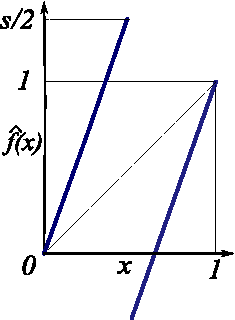
\includegraphics[width=0.36\textwidth]{fig_d_1CL18}
~~~
{(b)}
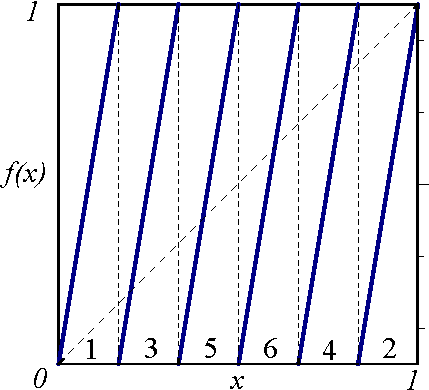
\includegraphics[width=0.32\textwidth]{fig_d_2}
  \caption{\label{fig-d-1}
(a) $\hflow{}{\hx}$, the full space sawtooth map \refeq{KD-map}, $\ExpaEig >
2$.
(b) $\flow{}{x}$, the sawtooth map restricted to the unit circle
\refeq{circ-m}, $\ExpaEig=6$.
            }
\end{figure}
%%%%%%%%%%%%%%%%%%%%%%%%%%%%%%%%%%%%%%%%%%%%%%%%%%%%%%%%%%%%%%%%%%
%
%%%%%%%%%%%%%%%%%%%%%%%%%%%%%%%%%%%%%%%%%%%%%%%%%%%%%%%
\example{Linear code for a piecewise linear map.}{\label{exam:SawtoothLin}
the piecewise linear map of \reffig{fig-d-1}
        \jumpBack{exam:SawtoothLin}
    } % end \example{exam:SawtoothLin}
%%%%%%%%%%%%%%%%%%%%%%%%%%%%%%%%%%%%%%%%%%%%%%%%%%%%%%%

  % siminos/spatiotemp/chapter/examTentLCod.tex
% $Author: predrag $ $Date: 2018-05-04 12:19:38 -0400 (Fri, 04 May 2018) $
% called by siminos/spatiotemp/chapter/tentMapCode.tex
%\section{Any piecewise linear map has ``linear code''}
%\label{exam:tentMapSymbDyn}

%%%%%%%%%%%%%%%%%%%%%%%%%%%%%%%%%%%%%%%%%%%%%%%%%%%%%%%
\example{Tent map linear code.}{\label{exam:TentLCod}
The simplest example of a piece-wise linear unimodal map with a binary (in
general, pruned) symbolic dynamics is the {\em tent map,}
%\reffig{f-log-repeller}\,(a),
\beq
\flow{}{x} =  \left\{ \begin{array}{ll}
f_0(x) = \ExpaEig x       & \mbox{ if } x  < 1/2 \\
f_1(x) =  \ExpaEig (1-x)  & \mbox{ if } x  > 1/2
         \end{array}\right.
\,,
\ee{anyTentSplit}
with $1<\ExpaEig<\infty$ and $x\in\pS=[0,1]$. (Everything would go through for
a skew tent map with $\ExpaEig_0\neq-\ExpaEig_1$, but there is no need here
for that complication.)
For this family of unimodal maps the coarse (covering) partition of the unit
interval $\pS=\pS_0\cap{C}\cap\pS_1$ is given by intervals $\pS_0=[0,1/2)$,
 $\pS_1=(1/2,1]$, and the critical point $C=1/2$.
Let's rewrite this as a linear first-order difference equation, in the manner
of cat lovers enamoured of matters feline:
\beq
\frac{1}{\ExpaEig}  \, x_{t+1}  +(2\Ssym{t}-1)x_{t} = \Ssym{t}
\,,\qquad
\left\{ \begin{array}{ll}
\Ssym{t}=0 & \mbox{ if }  x_{t}  < 1/2 \\
\Ssym{t}=1 & \mbox{ if }  x_{t}  > 1/2
         \end{array}\right.
\,.
\ee{TentLinCode}
That every such code is a `linear code' is best understood by
computing a periodic orbit for a specified itinerary.

The fixed point condition $\flow{n}{x}=x$ for $n$-cycle
\cycle{\Ssym{1}\Ssym{2}\Ssym{3}\cdots \Ssym{n-1}\Ssym{n}}
is a linear relation between the finite alphabet $\Ssym{t}\in\{0,1\}$ code, and
the $x_{t}\in\reals$ orbit
\beq
  \Delta(\Ssym{})q(\Ssym{}) = m(\Ssym{})
\ee{tentMapDiffEq}
with orbit-dependent inverse propagator $\Delta(\Ssym{})= $
\[
{\small
\left(\begin{array}{cccccc}
      {2\Ssym{n}-1}     & 0     &     0  & \dots  & 0 & \ExpaEig^{-1}\\
      \ExpaEig^{-1}     & {2\Ssym{n-1}-1} &     0     &\dots  &  0 & 0\\
       0 & \ExpaEig^{-1} &    {2\Ssym{n-2}-1} &\dots  &  0 & 0\\
      \vdots&\vdots &   \vdots & \ddots &\vdots  &\vdots \\
       0 &  0 &    0  & \dots  & {2\Ssym{2}-1}& 0\\
      0     &  0 &    0  & \dots  &\ExpaEig^{-1}  & {2\Ssym{1}-1}\\
     \end{array} \right)
\,,
} % end \small
\]
\[
q(\Ssym{})= \left(\begin{array}{c}
      x_{{n}}\\
      x_{{n-1}}\\
      x_{{n-2}}\\
      \vdots\\
      x_{{2}}\\
      x_{{1}}\\
     \end{array} \right)
\,,\qquad
m(\Ssym{})= \left(\begin{array}{c}
      {\Ssym{n}}\\
      {\Ssym{n-1}}\\
      {\Ssym{n-2}}\\
      \vdots\\
      {\Ssym{2}}\\
      {\Ssym{1}}\\
     \end{array} \right)
\,,
\]
and $m(\Ssym{})$ is needed to fold the stretched orbit back into the unit
interval.
While the off-diagonal ``1''s do generate cyclic shifts, the diagonal $\pm
\ExpaEig$ terms are not shift invariant, so I do not believe this can be
diagonalized by a discrete Fourier transform. I had worked it out for
$\ExpaEig=2$ in Chaos\-Book, but not sure if there are elegant tricks for
arbitrary $\ExpaEig\neq2$. For an orbit
\beq
  q(\Ssym{}) = \Delta(\Ssym{})^{-1}m(\Ssym{})
\ee{tentMapOrbit}
to be admissible, no point should be to the right of
the kneading value $x_\kappa = f(C)$. It follows from
the kneading theory for unimodal maps (dike map with slope
$\ExpaEig=2$ being the canonical example) that if a \po \ exists for
a given $\ExpaEig$, it exists for all larger $\ExpaEig$,
and that all orbits exist for $\ExpaEig \geq 2$.

In other words, $\ExpaEig$ is the ``stretching parameter'' for this
problem, and the rational polynomial expressions in $\ExpaEig$
for $x_{t}$ correspond to Li Han's polynomials for cat maps.
        \jumpBack{exam:TentLCod}
    } %end \example{Tent map linear code.}{exam:TentLCod}
%%%%%%%%%%%%%%%%%%%%%%%%%%%%%%%%%%%%%%%%%%%%%%%%%%%%%%%%%%%%%%

%%%%%%%%%%%%%%%%%%%%%%%%%%%%%%%%%%%%%%%%%%%%%%%%%%%%%%%%%%%%%%
\example{Periodic points of a tent map.}{\label{exam:TentCycl}

\paragraph{Exercise}
Check \refeq{tentMapOrbit} for fixed point(s).


\paragraph{Exercise}
Check \refeq{tentMapOrbit} for the 2-cycle \cycle{01}.
\[
\Delta(\Ssym{})=
\left(\begin{array}{cc}
      -\ExpaEig& 1\\
      1     & \ExpaEig
     \end{array} \right)
\,,\qquad
m(\Ssym{})= \ExpaEig \left(\begin{array}{c}
      0\\
      1
     \end{array} \right)
\,.
\]
\[
\Delta^{-1} =
\frac{1}{\ExpaEig^2+1}
\left(\begin{array}{cc}
      -\ExpaEig& 1\\
      1     & \ExpaEig
     \end{array} \right)
\,,\qquad
  \det\Delta(\Ssym{})= -(\ExpaEig^2+1)
\]
\[
\left(\begin{array}{c}
      x_{01}\\
      x_{10}
     \end{array} \right)
=
\frac{\ExpaEig}{\ExpaEig^2+1}
\left(\begin{array}{cc}
      -\ExpaEig& 1\\
      1     & \ExpaEig
     \end{array} \right)
\,\left(\begin{array}{c}
      0\\
      1
     \end{array} \right)
=
\frac{\ExpaEig}{\ExpaEig^2+1}
\,\left(\begin{array}{c}
      1\\
      \ExpaEig
     \end{array} \right)
\,.
\]
For the Ulam tent map this
yields the correct periodic points
\(
\{x_{01},x_{10}\}
=\{2/5,4/5\}
\,.
\)
In the $\ExpaEig\to1$ limit, this 2-cycle collapses into the
critical point $C=1/2$.


\paragraph{Exercise}
Check \refeq{tentMapOrbit} for the two 3-cycles.
For the Ulam tent map case, the periodic points are
\bea
\{\gamma_{001},\gamma_{010},\gamma_{100}\}
&=& \{2/9,4/9,8/9\}
\continue
\{\gamma_{011},\gamma_{110},\gamma_{101}\}
&=& \{2/7,4/7,6/7\}
\,.
\nnu
\eea


\paragraph{Exercise}
Check \refeq{tentMapOrbit} for $\ExpaEig =$ golden mean. The $\cycle{001} \to
\cycle{0C1}$ as $\ExpaEig \to $ golden mean from above. Do you get all
admissible cycles? That is worked out in Chaos\-Book, but not in this
formulation.

\paragraph{Exercise}
Is there a systematic solution to \refeq{tentMapOrbit} for arbitrary
$n$-cycle? The $\ExpaEig=2$ case has the elegant solution described in
Chaos\-Book; whatever polynomials you find, they should agree with that
particular factorization. In other words, think of the sums
\refeq{tentEvenCyclePts} and \refeq{tentOddCyclePts} as the expansion of a
real number in terms of the digits $w_t$ in the nonintegral base $\ExpaEig$.
As the symbolic dynamics of a cycle is independent of  $\ExpaEig$, the Ulam
tent map calculation, in the familiar base 2 clinches the arbitrary tent map
case.

\bigskip

    {\color{red}
    The rest of the section might even be right - has to factorize in
    agreement with my Ulam tent map computations. Please fix at your leisure,
    if I am wrong.
    }

\bigskip

If the repeating string                                         \toCB
$\Ssym{1}\Ssym{2}\ldots \Ssym{n}$ contains an even number of
`1's, the repating string of well ordered symbols $w_1w_2\ldots
w_{n}$ is of the same length. The cycle-point $x$ is a geometrical sum which we
can rewrite as the odd-denominator fraction
\bea
   x(\cycle{\Ssym{1}\Ssym{2}\ldots \Ssym{n}})
   &=& \sum_{t=1}^{n} \frac{w_t}{\ExpaEig^{t}}
      +  \frac{1}{\ExpaEig^{-n}} \sum_{t=1}^{n} \frac{w_t}{\ExpaEig^{t}}
      + \cdots
   \continue
   &=& \frac{1}{\ExpaEig^{n}-1}
        \sum_{t=1}^{n} {w_t}{\ExpaEig^{n-t}}
\label{tentEvenCyclePts}
\eea
If the repeating string
$\Ssym{1}\Ssym{2}\ldots \Ssym{n}$ contains an odd number of
`1's, the string of well ordered symbols $w_1w_2\ldots
w_{2n}$ has to be of the double length before it repeats
itself. The cycle-point $x$ is a geometrical sum which we
can rewrite as the odd-denominator fraction
\bea
   x(\cycle{\Ssym{1}\Ssym{2}\ldots \Ssym{n}})
   &=& \sum_{t=1}^{2n} \frac{w_t}{\ExpaEig^{t}}
      +  \frac{1}{\ExpaEig^{-2n}} \sum_{t=1}^{2n} \frac{w_t}{\ExpaEig^{t}}
      + \cdots
   \continue
   &=& \frac{1}{(\ExpaEig^{n}-1)(\ExpaEig^{n}+1)}
        \sum_{t=1}^{2n}{w_t}{\ExpaEig^{2n-t}}
\label{tentOddCyclePts}
\eea
        \jumpBack{exam:TentCycl}
    } %end \example{Tent map linear code.}{exam:TentCycl}
%%%%%%%%%%%%%%%%%%%%%%%%%%%%%%%%%%%%%%%%%%%%%%%%%%%%%%%%%%%%%%

  % siminos/spatiotemp/chapter/examBelykhLCod.tex
% $Author: predrag $ $Date: 2021-12-24 01:25:20 -0500 (Fri, 24 Dec 2021) $

% siminos/spatiotemp/chapter/examTentLCod.tex
% $Author: predrag $ $Date: 2021-12-24 01:25:20 -0500 (Fri, 24 Dec 2021) $
% called by siminos/spatiotemp/chapter/tentMapCode.tex
%\section{Any piecewise linear map has ``linear code''}
%\label{exam:tentMapSymbDyn}

%%%%%%%%%%%%%%%%%%%%%%%%%%%%%%%%%%%%%%%%%%%%%%%%%%%%%%%
\example{Belykh map linear code.}{\label{exam:BelykhLCod}
Li and Xie\rf{LiXie16}
{\em Symbolic dynamics of {Belykh}-type maps}:
``
The symbolic dynamics of a Belykh-type map (a two-dimensional
discontinuous piecewise linear map) is investigated. The pruning front
conjecture (the admissibility condition for symbol sequences)  is proved
under a hyperbolicity condition. Using this result, a symbolic dynamics
model of the map is constructed according to its pruning front and
primary pruned region.
''

The Belykh map is a piecewise linear map given by
\[  \left( \begin{array}{c}
        x_{n+1} \\
        y_{n+1} \\
        \end{array}\right)
        = \left(\begin{array}{c}
                    \sign{n} -a x_n + b y_n     \\
                    x_n                         \\
                \end{array} \right)
        =  \left( \begin{array}{c}
            \sign{n} \\
            0        \\
        \end{array}\right)
        +
\left(\begin{array}{cc}
            -a  & b      \\
             1  & 0      \\
                \end{array} \right)
\left( \begin{array}{c}
        x_{n} \\
        y_{n} \\
        \end{array}\right)
\,.\]
where
\[
\sign{n} = \left\{\begin{array}{rcc}
                                1 & \mbox { if } &  x_n \geq 0\\
                                -1 & \mbox { if } &  x_n < 0\\
                                                \end{array} \right.
\,.
\]
The two branches of the map are
\[
f_{\pm} = \left\{\begin{array}{l}
                                \pm 1 -a x + b y\\
                                 x \\
                                                \end{array} \right.
\,.\]
In the 3-term recurrence formulation (the linear code), the map is
an asymmetric tridiagonal Toeplitz matrix
\[
 x_{n+1} +a x_n - b x_{n-1} = \sign{n}
 \,,
\]
or
\beq
\Box x_n +(2+a) x_n - (1+b) x_{n-1} = \sign{n}
 \,.
\ee{s:BelykhMapDiff}
For $b=-1$ (the Hamiltonian, time-reversible case) this is almost the cat
map, with $a=-s$, except that the single sawtooth discontinuity is across
$x=0$, there is no $\mod\ 1$ condition.

Li and Xie consider the
\(
a,\, b\, > 0
\)
case. The strange attractor (for example, for $a = 1.5$ and $b = 0.3$)
looks like a fractal set of parallel lines.
They define the pruning front, the primary pruned region, plot them in
the symbol plane, and prove the pruning front conjecture  for this map.
In the symbol plane there is a symmetry under rotation by $\pi$, but they
do not seem to exploit that.

They call the past and the future itineraries of the tail and the head,
and start the head with $s_0$.

T{\'{e}}l\rf{Tel83} {\em Fractal dimension of the strange attractor in a
piecewise linear two-dim\-en\-si\-on\-al map} computes the box-counting dimension
of this map (which he does not call Belykh map).
    } % end \example{Belykh map linear code.}{{exam:BelykhLCod}

  % siminos/spatiotemp/chapter/examLoziLCod.tex
% $Author: predrag $ $Date: 2021-12-24 01:25:20 -0500 (Fri, 24 Dec 2021) $


%%% input by % siminos/spatiotemp/chapter/catMap.tex %%%%%
%\section{Any piecewise linear map has ``linear code''}
%\label{exam:tentMapSymbDyn}

%%%%%%%%%%%%%%%%%%%%%%%%%%%%%%%%%%%%%%%%%%%%%%%%%%%%%%%
\example{Lozi map linear code.}{\label{exam:LoziLCod}
The Lozi map
\[
    x_{n+1}=1- \sign{n} ax_{n} +bx_{n-1} \, .
\]
written as a 3-term recurrence relation
\beq
    x_{n+1}-2x_{n}+x_{n-1}+(2+\sign{n} a)x_{n} -(b+1)x_{n-1}=1
\, .
\ee{Lozi2-step}
That has the same nonlinear term $\sign{n} x_{n}$ as \refeq{TentLinCode},
so maybe we can figure out the pruning front as well, in this
formulation.
        \jumpBack{exam:LoziLCod}
    } % end \example{Lozi map linear code.}{exam:TentCycl}
%%%%%%%%%%%%%%%%%%%%%%%%%%%%%%%%%%%%%%%%%%%%%%%%%%%%%%%

%\newpage
  \Problems{exerCatMap}{7mar2018}
% siminos/spatiotemp/Problems/exerCatMap.tex called by catMap.tex
% $Author: predrag $ $Date: 2021-06-12 01:01:43 -0400 (Sat, 12 Jun 2021) $

% Predrag                                               23jan2018

%%%%%%%%%%%%%%%%%%%%%%%%%%%%%%%%%%%%%%%%%%%%%%%%%%%%%%%%%%%%%%%%%%%
\exercise{Cat map Green's function, infinite lattice.}{\label{exer:catMapGreenInf}

(a) Show that the eigenvalues of the cat map $M$ are
given by
\beq
\ExpaEig^{\pm}=\frac{1}{2}(s\pm \surd{D})
\,,\qquad
\ExpaEig=e^{\Lyap}
\,,
\ee{catEigsEx}
where $\ExpaEig\equiv\ExpaEig^+$, $s=\ExpaEig+\ExpaEig^{-1}$,
$\surd{D}=\ExpaEig-\ExpaEig^{-1}$, and the discriminant is $D={s^{2}-4}$.

(b) Verify by substitution that the Green's function is given by
\beq
\gd_{nn'}= \frac{1}{{\surd{D}}}\,\frac{1}{\ExpaEig^{|n'-n|}}
\,.
\ee{GreenFun00b}

(c) Show that the orbit is then recovered by
\beq
\ssp_{n} =  \frac{1}{{\surd{D}}}
\sum_{n' \in \integers} \ExpaEig^{- |n-n'|} \Ssym{n'}
\,.
\label{BirVivx=s}
\eeq
    } % end \exercise{exer:catMapGreenInf}
%%%%%%%%%%%%%%%%%%%%%%%%%%%%%%%%%%%%%%%%%%%%%%%%%%%%%%%%%%%%%%%%%%%%%%%%

%%%%%%%%%%%%%%%%%%%%%%%%%%%%%%%%%%%%%%%%%%%%%%%%%%%%%%%%%%%%%%%%%%%
\exercise{Cat map Green's function for a \po.}{\label{exer:catMapGreenPBC}
Show that the Green's function for a \po\ of period $\cl{p}$ is
obtained by summing \refeq{GreenFun00b} over period \cl{p}:
\beq
g^p_{nn'}=\sum_{j=-\infty}^{\infty}{g}_{n-n',j\cl{p}}
  =\frac{1}{{\surd{D}}}\,\frac{\ExpaEig^{-|n-n'|}+\ExpaEig^{-\cl{p}+|n-n'|}}
        {1-\ExpaEig^{-\cl{p}}}
\,.
\ee{GreenFun2}
Verify this formula by explicit matrix inversion for a few periodic points
of cycles $p$ of
periods $\cl{p}=1,2,3,4,\cdots$.
    } % end \exercise{exer:catMapGreenPBC}
%%%%%%%%%%%%%%%%%%%%%%%%%%%%%%%%%%%%%%%%%%%%%%%%%%%%%%%%%%%%%%%%%%%%%%%%

%%%%%%%%%%%%%%%%%%%%%%%%%%%%%%%%%%%%%%%%%%%%%%%%%%%%%%%%%%%%%%%%%%%
\exercise{$d=2$ cat map guess Green's function, infinite lattice.}{\label{exer:catMapGreend=2wrong}
% Predrag 2018-03-11 wrong guess, debunked by Han
Show by substitution that a $d=2$ ``Green's function'' guess given by
\beq
\gd_{z z'}= \PCedit{\frac{1}{2}}\frac{1}
            {{\surd{D}}}\,\frac{1}{\ExpaEig^{|\ell'-\ell|+|t'-t|}}
\,,
\ee{GreenFund=2wrong}
(and similarly, in arbitrary dimension $d>1$) \emph{does not} satisfy the
Green's function conditions
\beq
(\D \gd)_{zz'}=\delta_{zz'}=\delta_{ll'}\delta_{tt'}
\,,
\ee{HLGreenFund=2C}
Here the eigenvalues of the cat map $M$ are
\beq
\ExpaEig^{\pm}=\frac{1}{2}(s/2 \pm \surd{D})
\,,\qquad
\ExpaEig=e^{\Lyap}
\,,
\ee{catEigsEx2D}
where $\ExpaEig\equiv\ExpaEig^+$, $s/2=\ExpaEig+\ExpaEig^{-1}$,
$\surd{D}=\ExpaEig-\ExpaEig^{-1}$, and the discriminant is $D={(s/2)^{2}-4}$.

Hint: the check works just like for \refexer{exer:catMapGreenInf}.
    } % end \exercise{exer:catMapGreend=2wrong}
%%%%%%%%%%%%%%%%%%%%%%%%%%%%%%%%%%%%%%%%%%%%%%%%%%%%%%%%%%%%%%%%%%%%%%%%

%%%%%%%%%%%%%%%%%%%%%%%%%%%%%%%%%%%%%%%%%%%%%%%%%%%%%%%%%%%%%%%%%%%
\exercise{\Po s of Arnol'd cat map.}{\label{exer:AKScatMapPOs}
% moved to here from {blogAKS}{2016-06-09}
\begin{enumerate}
  \item %[[X]]
Describe precisely how you actually pick ``random $q_1$ and $q_2$''
  \item %[[X]]
Explain what happens if $q_1$ and $q_2$ are rational
  \item %[[X]]
Can you get a \po\ if $q_1$ and $q_2$ are irrational?
  \item %[[X]]
What do you mean by period $0$?
  \item %[[X]]
Does the Arnol'd cat map have \po s of any period?
  \item %[[X]]
Derive analytically that $m_j \in \{-1, 0,  1,2\}$ (you can continue the
exposition that I started in \refsect{sect:PerViv}, if that helps). Does you
result agree with Percival and Vivaldi\rf{PerViv}?
\end{enumerate}
%                                       \PCpost{2016-06-02}{:
}
%%%%%%%%%%%%%%%%%%%%%%%%%%%%%%%%%%%%%%%%%%%%%%%%%%%%%%%%%%%%%%%%%%%%

%%%%%%%%%%%%%%%%%%%%%%%%%%%%%%%%%%%%%%%%%%%%%%%%%%%%%%%%%%%%%%%%%%%
\exercise{The second iterate generating partition.}{\label{exer:n=2GenPart}
%    \PCpost{2019-08-10}{
\refFig{fig:PVAdlerWeissS} is very helpful in giving us a visual
understanding of what a Hamiltonian cat map does, and how the generating
partition comes about. Draw the corresponding \AW\ generating partition
for $s=3$, the second, $n=2$ iterate, to verify that the $n=1$ determines
a generating partition for all subsequent times.
    } % end \exercise{exer:n=2GenPart}
%%%%%%%%%%%%%%%%%%%%%%%%%%%%%%%%%%%%%%%%%%%%%%%%%%%%%%%%%%%%%%%%%%%%%%%%

%%%%%%%%%%%%%%%%%%%%%%%%%%%%%%%%%%%%%%%%%%%%%%%%%%%%%%%%%%%%%%%%%%%
%\exercise{XXX.}{\label{exer:XXX}
%XXX
%    } % end \exercise{exer:XXX}
%%%%%%%%%%%%%%%%%%%%%%%%%%%%%%%%%%%%%%%%%%%%%%%%%%%%%%%%%%%%%%%%%%%%%%%%

%%%%%%%%%%%%%%%%%%%%%%%%%%%%%%%%%%%%%%%%%%%%%%%%%%%%%%%%%%%%%%%%%%%
%\exercise{XXX.}{\label{exer:XXX}
%XXX
%    } % end \exercise{exer:XXX}
%%%%%%%%%%%%%%%%%%%%%%%%%%%%%%%%%%%%%%%%%%%%%%%%%%%%%%%%%%%%%%%%%%%%%%%%

    \ProblemsEnd

  \Solution{catMap}{soluCatMap}{23jan2018}{Cat map}
% siminos/spatiotemp/Solutions/soluCatMap.tex called by catMap.tex
% $Author: predrag $ $Date: 2021-08-10 11:56:19 -0400 (Tue, 10 Aug 2021) $

% Predrag                                               23jan2018

%%%%%%%%%%%%%%%%%%%%%%%%%%%%%%%%%%%%%%%%%%%%%%%%%%%%%%%%%%%%%%%%%%%
\solution{exer:catMapGreenInf}{Cat map Green's function, infinite lattice.}{

(a) It's just the roots of a quadratic equation, with
\(
s=\ExpaEig+\ExpaEig^{-1}
\,,
\)
and \(
\surd{D}=\ExpaEig-\ExpaEig^{-1}
\,.
\)


(b) The Green's function \refeq{GreenFun00b}
\beq
\gd_{tt'}=  \frac{1}{{\surd{D}}}\,\frac{1}{\ExpaEig^{|t'-t|}}
\ee{GreenFun00d}
for the discrete damped Poison
equation \refeq{eq:CatMapStep} was first computed explicitly by Percival and
Vivaldi\rf{PerViv}, using the methods introduced in Mestel and
Percival\rf{varcyc}. It should satisfy
\beq
(\D \gd)_{ij} = \sum_{k} \D_{ik} \gd_{kj} =\delta_{ij}
\,.
\ee{HLGFuncInf1}
Since we are considering infinite $1D$ lattice, we do not need to
specify the boundary conditions. $\D$ is a Toeplitz matrix
\beq
\D_{ik}=s \delta_{ik} - \delta_{i-1,k} - \delta_{i+1,k}
\ee{HLGFuncInf2}
Substituting \refeq{HLGFuncInf2} into \refeq{HLGFuncInf1}
\beq
\sum_{k} \D_{ik} \gd_{kj} = s \gd_{ij} -\gd_{i-1,j}-\gd_{i+1,j} =\delta_{ij}
\,,
\ee{HLGFuncInf3}
and substituting \refeq{GreenFun00b}
\beq
\gd_{ij}= \frac{1}{\surd{D}}\,
          \frac{1}{\ExpaEig^{|j-i|}}
=  \left\{ \begin{array}{ll}
\frac{1}{\surd{D}}\,\frac{1}{\ExpaEig^{i-j}}  & \mbox{ if } j < i  \\
\frac{1}{\surd{D}} & \mbox{ if } j = i  \\
\frac{1}{\surd{D}}\,\frac{1}{\ExpaEig^{j-i}}  & \mbox{ if } j > i
         \end{array}\right.
\,.
\ee{GreenFun00c}
into \refeq{HLGFuncInf3},
one verifies that \refeq{GreenFun00b} is indeed the Green's function
for the infinite lattice. By translational invariance, for $i=j$ consider
\beq
s \gd_{00} -\gd_{-1,0}-\gd_{10}
  = \frac{1}{\surd{D}}\,\left(
  {s} - \frac{2}{\ExpaEig}
     \right)
  = \frac{1}{\surd{D}}\,\left(\ExpaEig-\frac{1}{\ExpaEig}\right)
  = 1
\,.
\label{HLGFuncInf5}
\eeq
For $i>j$ consider
\beq
s \gd_{10} -\gd_{00}-\gd_{20}
  = \frac{1}{\surd{D}}\,\left(
  \frac{s}{\ExpaEig}
  - 1
  - \frac{1}{\ExpaEig^{2}}
     \right)
  = \frac{1}{\surd{D}}\,\frac{1}{\ExpaEig}
      \,\left( s - \ExpaEig-\frac{1}{\ExpaEig}\right)
  = 0
\,.
\label{HLGFuncInf4}
\eeq

(c) The orbit is recovered by:
\beq
\ssp_n=\sum_{n' \in \integers} \gd_{nn'} \Ssym{n'}
= \frac{1}{{\surd{D}}} \sum_{n' \in \integers} \ExpaEig^{- |n-n'|} \Ssym{n'}
\,.
\ee{HLGFuncInf6}
\hfill (Han Liang) %{2018-03-08}{
    } % end \solution{exer:catMapGreenInf}
%%%%%%%%%%%%%%%%%%%%%%%%%%%%%%%%%%%%%%%%%%%%%%%%%%%%%%%%%%%%%%%%%%%%%%%%

%%%%%%%%%%%%%%%%%%%%%%%%%%%%%%%%%%%%%%%%%%%%%%%%%%%%%%%%%%%%%%%%%%%
\solution{exer:catMapGreenPBC}{Cat map Green's function for a \po.}{
%    \PC{2017-08-28} {
%``Average coordinate'' depends on b.c.'s. Average coordinate
%\refeq{catMapAverCoord} is computed for
%the the very unphysical Dirichlet boundary condition $\ssp_z=0$ for $z\in \R$
%which breaks translation invariance.
%If one takes the much gentler, translationally invariant doubly periodic b.c.,
%the ``average coordinate'' $\bar{x}_z$ is the \twot\ periodic point, a
%more natural choice.
%    }
Express the periodic orbit Green's function in terms of the infinite
lattice by using a periodic source $\Ssym{n'}=\Ssym{n'}+\cl{p}$,
\bea
\sum_{n'=-\infty}^{\infty}\gd_{nn'}\Ssym{n'}
 &=& \sum_{r=-\infty}^{\infty} \sum_{n'=r\cl{p}}^{r\cl{p}+\cl{p}-1}\gd_{nn'}\,\Ssym{n'}
= \sum_{r=-\infty}^{\infty} \sum_{n'=0}^{\cl{p}-1}\gd_{n,n'+r\cl{p}}\,\Ssym{n'+r\cl{p}}
\continue
 &=& \sum_{r=-\infty}^{\infty} \sum_{n'=0}^{\cl{p}-1}\gd_{n-n',r\cl{p}}\,\Ssym{n'}
\label{HLGFuncPO1}
\eea
Comparing with the expression for the Green's function of a periodic orbit:
\beq
\sum_{n'=0}^{\cl{p}-1}\gd_{nn'}^\cl{p} \Ssym{n'}
\label{HLGFuncPO2}
\eeq
we see that
\beq
\gd_{nn'}^\cl{p}=\sum_{r=-\infty}^{\infty} \gd_{n-n',r\cl{p}}
\ee{HLGFuncPO3}
Substituting \refeq{GreenFun00b} into \refeq{HLGFuncPO3} we have:
%\beq
%	\gd_{n,n'}^P
%	&=& \frac{1}{\surd{D}}\sum_{r=-\infty}^{\infty} \frac{1}{\ExpaEig^{|n-n'-rP|}}
%\ee{HLGFuncPO4}
% HL could not print this. PC should have used \bea ... \label{HLGFuncPO4}\eea
\bea
   \gd_{nn'}^\cl{p}
   &=& \frac{1}{\surd{D}}\sum_{r=-\infty}^{\infty} \frac{1}{\ExpaEig^{|n-n'-r\cl{p}|}}
   \continue
   &=& \frac{1}{\surd{D}} \left( \frac{1}{\ExpaEig^{|n-n'|}}
   +\sum_{r=1}^{\infty} \frac{1}{\ExpaEig^{r\cl{p}-(n-n')}}
   + \sum_{r=-1}^{-\infty} \frac{1}{\ExpaEig^{(n-n')-r\cl{p}}}
   \right)
   \continue
   &=& \frac{1}{\surd{D}} \left(  \frac{1}{\ExpaEig^{|n-n'|}}
   +\frac{1}{\ExpaEig^{-|n-n'|}}\frac{1}{\ExpaEig^\cl{p}-1}
   +\frac{1}{\ExpaEig^{|n-n'|}}\frac{1}{\ExpaEig^\cl{p}-1}
   \right)
   \continue
   &=& \frac{1}{\surd{D}}\,
       \frac{1}{1-\ExpaEig^{-\cl{p}}}
       (\ExpaEig^{-|n-n'|} + \ExpaEig^{-\cl{p}+|n-n'|})
   \label{HLGFuncPO4}
\eea
This verifies \refeq{GreenFun2}.

Bird and Vivaldi\rf{BirViv} show that for an $n$-cycle $\ssp_{n'}$ are
rational functions of $\ExpaEig$, given by the quotient of two reflexive
polynomials
(for example, $P_t(\ExpaEig)= \ExpaEig^n P_t(1/\ExpaEig)$),
\bea
\ssp_{t} &=&  \ExpaEig \,{P_t(\ExpaEig)}/{Q(\ExpaEig)}
        \continue
P_t(\ExpaEig) &=&  \sum_{\tau=1}^{n-1}
                   \ExpaEig^{n-\tau}(\ExpaEig\,\Ssym{t+\tau-1} + \Ssym{t-\tau})
        \continue
Q(\ExpaEig) &=&  (\ExpaEig^2 - 1)\,(\ExpaEig^n - 1)
\label{BirViv(3.5)a}
\eea
Bird and Vivaldi\rf{BirViv} then discuss pruning, give formulas for the
numbers of {\orbit}s for integer $s$, \etc.

\hfill (Han Liang) %{2018-03-08}
    } % end \solution{exer:catMapGreenPBC}
%%%%%%%%%%%%%%%%%%%%%%%%%%%%%%%%%%%%%%%%%%%%%%%%%%%%%%%%%%%%%%%%%%%%%%%%

%%%%%%%%%%%%%%%%%%%%%%%%%%%%%%%%%%%%%%%%%%%%%%%%%%%%%%%%%%%%%%%%%%%
\solution{exer:catMapGreend=2wrong}{$d=2$ cat map guess Green's function, infinite lattice.}{
% \HLpost{2018-03-12}{ The Green's function \refeq{GreenFund=2wrong} is not correct.
The Green's function $\gd$ for the Toeplitz matrix (tensor) in 2 dimensions
\bea
\D_{lt,l't'} &=& \left[-\Box + 2\left({s}/{2} - 2\right)\right]_{lt,l't'}
\continue
&=& \left(\frac{s}{2}\delta_{ll'}-\delta_{l-1,l'}-\delta_{l+1,l'}\right)\delta_{tt'}
\ceq
   +\delta_{ll'}\left(\frac{s}{2}\,\delta_{tt'}-\delta_{t-1,t'}-\delta_{t+1,t'}\right)
\,.
\label{HLGreenFund=2B}
\eea
should satisfy \refeq{HLGreenFund=2C},
or, substituting \refeq{HLGreenFund=2B} into \refeq{HLGreenFund=2C},
\bea
\PCedit{2\,}
\delta_{ll'}\delta_{tt'}
   &=& \frac{s}{2}\gd_{ll',tt'}-\gd_{l-1,l',tt'}-\gd_{l+1,l',tt'}
\ceq
     + \frac{s}{2}\gd_{ll',tt'}-\gd_{ll',t-1,t'}-\gd_{ll',t+1,t'}
\,.
\label{HLGreenFund=2D}
\eea
Let's check this.
By translational invariance, need to look only at different values of
$l-l'$ and $t-t'=0$. For $l=l'$ and $t=t'$ it suffices that we consider
the $l=l'=t=t'=0$ case. Using \refeq{catEigsEx2D} we have
\bea
&&\frac{s}{2} \gd_{00,00} -\gd_{-1,0,00}-\gd_{10,00}
\ceq
+ \frac{s}{2} \gd_{00,00} -\gd_{00,-1,0}-\gd_{00,10}
\ceq
  = \frac{2}{\surd{D}}\,\left(
    \frac{s}{2} - \frac{2}{\ExpaEig}
     \right)
  = \frac{2}{\surd{D}}\,\left(\ExpaEig-\frac{1}{\ExpaEig}\right)
  = 2
\,,
\label{HLGFuncInf5a}
\eea
verifies \refeq{HLGreenFund=2B}.

For $l>l'$ and $t=t'$ it suffices
to consider $l=1,l'=0$, $t=t'=0$  case.
\bea
&&\frac{s}{2} \gd_{10,00} -\gd_{00,00}-\gd_{20,00}
    \ceq
 + \frac{s}{2} \gd_{10,00} -\gd_{10,-1,0}-\gd_{10,10}
\ceq
  = \frac{1}{2\surd{D}}\,\left(
  \frac{s/2}{\ExpaEig}
  - 1
  - \frac{1}{\ExpaEig^{2}}
     \right)
  + \frac{1}{2\surd{D}}\,\left(
  \frac{s/2}{\ExpaEig}
   - \frac{2}{\ExpaEig^{2}}
     \right)
\ceq
  = \frac{1}{2\ExpaEig\surd{D}}\,\left(
        \frac{s}{2} - \frac{2}{\ExpaEig^{}}
     \right)
  = \frac{1}{2\ExpaEig\surd{D}}
      \,\left(\ExpaEig-\frac{1}{\ExpaEig}\right)
  = \frac{1}{2\ExpaEig}
\,.
\label{HLGFuncInf4b}
\eea
%\PCedit{2017-03-15 Han is right,
So, the guess \refeq{GreenFund=2wrong} already does not work.

Substitute \refeq{GreenFund=2wrong} into \refeq{HLGreenFund=2D} we get:
\bea
\sum_{z''}\D_{zz''}\gd_{z''z'}
=  \left\{ \begin{array}{ll}
\frac{1}{\surd{D}}\,\frac{1}{\ExpaEig^{|\ell'-\ell|+|t'-t|}} (s-2\ExpaEig-2\ExpaEig^{-1})
           & \mbox{ if } l\neq l'\,and\,t\neq t'   \\
\frac{1}{\surd{D}} (s-4\ExpaEig^{-1})
           & \mbox{ if } l=l'\, and\, t=t'
         \end{array}\right.
\,.
\label{HLGreenFund=2E}
\eea

To satisfy \refeq{HLGreenFund=2C}, $s$, $\surd{D}$ and $\ExpaEig$ must satisfy:
\bea
\left\{ \begin{array}{ll}
s=2\ExpaEig+2\ExpaEig^{-1} \\
\surd{D} = 2\ExpaEig-2\ExpaEig^{-1}
         \end{array}\right.
\,.
\label{HLGreenFund=2F}
\eea
So we will have:
\bea
\left\{ \begin{array}{ll}
\ExpaEig = \frac{1}{4}(s+\sqrt{s^2-16})\\
\ExpaEig^{-1} = \frac{1}{4}(s-\sqrt{s^2-16})
         \end{array}\right.
\,.
\label{HLGreenFund=2G}
\eea
Now the problem is, if $l \neq l'$ but $t = t'$, \refeq{HLGreenFund=2E} become:
\beq
\sum_{z''}\D_{zz''}\gd_{z''z'}
  = \frac{1}{\surd{D}}\,\frac{1}{\ExpaEig^{|\ell'-\ell|+|t'-t|}} (s-\ExpaEig-3\ExpaEig^{-1})
\ee{HLGreenFund=2H}
and this is not satisfied by \refeq{HLGreenFund=2G}. So
\refeq{GreenFund=2wrong} does not work for the 2-dimensional case. I
haven't figured out the correct Green's function for the 2 dimensions.

\hfill (Han Liang) %{2018-03-12}
    } % end \solution{exer:catMapGreend=2wrong}
%%%%%%%%%%%%%%%%%%%%%%%%%%%%%%%%%%%%%%%%%%%%%%%%%%%%%%%%%%%%%%%%%%%%%%%%

%%%%%%%%%%%%%%%%%%%%%%%%%%%%%%%%%%%%%%%%%%%%%%%%%%%%%%%%%%%%%%%%%%%
\solution{exer:catMapGreend=2wrong}{$d=2$ cat map guess Green's function, infinite lattice.}{
%\HLpost{2018-03-15}{
The guess Green's function \refeq{GreenFund=2wrong} doesn't work.
For $l=2$, $l'=0$ and $t=t'=0$, the correct form of \refeq{HLGFuncInf4b} is:
\bea
&&\frac{s}{2} \gd_{10,00} -\gd_{00,00}-\gd_{20,00}
\ceq
+ \frac{s}{2} \gd_{10,00} -\gd_{10,10}-\gd_{10,-10}
\\
  &=& \frac{1}{2\surd{D}}\,\left(
  \frac{s}{2\ExpaEig}
  - 1
  - \frac{1}{\ExpaEig^{2}}
     \right)+
     \frac{1}{2\surd{D}}\,\left(
  \frac{s}{2\ExpaEig}
  - \frac{1}{\ExpaEig^{2}}
  - \frac{1}{\ExpaEig^{2}}
     \right)
   \\
  &=& \frac{1}{2\surd{D}}\,\frac{1}{\ExpaEig}
      \,\left( \frac{s}{2} - \ExpaEig-\frac{1}{\ExpaEig}\right)
      +\frac{1}{2\surd{D}}\,\frac{1}{\ExpaEig}\,\left(
  \frac{s}{2}
  - \frac{1}{\ExpaEig}
  - \frac{1}{\ExpaEig}
     \right)\\
  &=& 0 + \frac{1}{2\ExpaEig}
\,.
\label{HLGFuncInf4I}
\eea
%\PCedit{2017-03-15
As in \refeq{HLGFuncInf4b}, this does not work .

\hfill (Han Liang) %{2018-03-12}
    } % end \solution{exer:catMapGreend=2wrong}
%%%%%%%%%%%%%%%%%%%%%%%%%%%%%%%%%%%%%%%%%%%%%%%%%%%%%%%%%%%%%%%%%%%%%%%%


%%%%%%%%%%%%%%%%%%%%%%%%%%%%%%%%%%%%%%%%%%%%%%%%%%%%%%%%%%%%%%%%%%%
\solution{exer:AKScatMapPOs}{\Po s of Arnol'd cat map.}{
No solution available.
} % end \solution{e-trajectNotIntersect}
%%%%%%%%%%%%%%%%%%%%%%%%%%%%%%%%%%%%%%%%%%%%%%%%%%%%%%%%%%%%%%%%%%%

%%%%%%%%%%%%%%%%%%%%%%%%%%%%%%%%%%%%%%%%%%%%%%%%%%%%%%%%%%%%%%%%%%%
\solution{exer:n=2GenPart}{The second iterate generating partition.}{
%	\HLpost{2019-08-10}{
\refFig{fig:PVAdlerWeiss2Steps} is the generating partition with $s=3$
evolved after 2 steps. In the Markov diagram
\reffig{fig:PVAdlerWeiss2Steps}\,(d) there are 7 self cycles, two of which
are the over-counted fixed points at the origin. So there are actually 5
periodic points with period 2, including 1 fixed point and 2 length-2
{\orbit}s, as given by \refeq{noPrimeCycs=3}.

%%%%%%%%%%%%%%%%%%%%%%%%%%%%%%%%%%%%%%%%%%%%%%%%%%%%%%%%%%%%
	\begin{figure}\begin{center}
            \begin{minipage}[c]{0.36\textwidth}\begin{center}
\includegraphics[width=1.0\textwidth]{PVAdlerWeissB-c}\\(a) %{PVAdlerWeiss2Steps-a}\\(a)
\\
\includegraphics[width=1.0\textwidth]{PVAdlerWeiss2Steps-c}\\(c)
            \end{center}\end{minipage}
            \begin{minipage}[c]{0.3\textwidth}\begin{center}
\includegraphics[width=1.0\textwidth]{PVAdlerWeiss2Steps-b}\\(b)
            \end{center}\end{minipage}
            ~~~
            \begin{minipage}[c]{0.25\textwidth}\begin{center}
\includegraphics[width=1.0\textwidth]{PVAWMarkov2Steps}\\(d)
            \end{center}\end{minipage}
\end{center}
  \caption{\label{fig:PVAdlerWeiss2Steps}
(a)
An \AW\ one step forward in time partition of the unit torus for the
$s=3$ \PV\ cat map \reffig{fig:PVAdlerWeissB}\,(c).
(b)
Mapped two steps forward in time, the rectangles are stretched along the
unstable direction and shrunk along the stable direction. Sub-rectangles
$\pS_j$ that have to be translated back into the partition are indicated by
color and labeled by their lattice translation
$\Ssym{j}$.
(c)
The sub-rectangles $\pS_j$ translated back into the unit square yield a
two steps forward in time
generating partition (a subpartition of rectangles in (a)), with
(d)
the finite grammar given by the {\markGraph} for this partition. The nodes
refer to the rectangles $A$ and $B$, and the 13 links correspond to the 13
sub-rectangles induced by two step forward-in-time dynamics.
}
\end{figure}
%%%%%%%%%%%%%%%%%%%%%%%%%%%%%%%%%%%%%%%%%%%%%%%%%%%%%%%%%%%%

%%%%%%%%%%%%%%%%%%%%%%%%%%%%%%%%%%%%%%%%%%%%%%%%%%%%%%%%%%%%%
\begin{figure}
  \centering
\includegraphics[width=0.40\textwidth]{PVAdlerWeiss2Steps-d}
  \caption{\label{fig:PVAdlerWeiss2StepsD}
This figure is used to track where each sub-rectangles in
\reffig{fig:PVAdlerWeiss2Steps} goes. Note that two step forward-in-time
requires both vertical and horizontal shifts, unlike the one step
forward-in-time \PV\ cat map \refeq{eq:StateSpCatMap}.
}
\end{figure}
%%%%%%%%%%%%%%%%%%%%%%%%%%%%%%%%%%%%%%%%%%%%%%%%%%%%%%%%%%%%%%%

\refFig{fig:PVAdlerWeiss2Steps} is a very nice illustration
of a generating partition subrectangles being further subdivided.
} % end \solution{exer:n=2GenPart}
%%%%%%%%%%%%%%%%%%%%%%%%%%%%%%%%%%%%%%%%%%%%%%%%%%%%%%%%%%%%%%%%%%%



\ChapterEnd % formatted for ChaosBook.org
      % for ChaosBook
\ifsvnmulti
 \svnkwsave{$RepoFile: lyapunov/Henon.tex $}
 \svnidlong {$HeadURL: svn://zero.physics.gatech.edu/siminos/lyapunov/Henon.tex $}
 {$LastChangedDate: 2017-01-18 23:47:27 -0500 (Wed, 18 Jan 2017) $}
 {$LastChangedRevision: 5504 $} {$LastChangedBy: predrag $}
 \svnid{$Id: Henon.tex 5504 2017-01-19 04:47:27Z predrag $}
\fi

\chapter{H\'enon  attractor}
\label{c-Henon}

This chapter of the blog deals specifically with the
H\'enon attractor nonhyperbolicities.

%%-----   Qualitative dynamics, for cylists
\section{ChaosBook chapter: Stretch, fold, prune}
\label{c-smale}



\noindent
This section on the loan from ChaosBook.org,
dasbuch/book/chapter/smale.tex, to be edited here and eventually
returned. I have to write up pruning fronts anyway, if we can do it by
talking to each other it will be much more fun...

\Remarks

\remark{Pruning fronts / partition lines.}{\label{s_Henon_pruning}
                                                            \toCB
    \index{Henon@H\'enon map!pruning front}
% Predrag 2011-10-08: incorporated Dullin \etal\rf{HamSteDuMei04} remarks
A dynamical system is said to be \emph{hyperbolic} if its \statesp\ has
no homoclinic tangencies, \ie, the stable and unstable manifolds are
everywhere transversal to each other. The kneading theory\rf{MilThu88}
solves the problem of fully specifying the symbolic dynamics for
non-hyperbolic multimodal maps on a unit interval. The H\'enon mapping is
the springboard for generalization of the 1-\dmn\ theory to
higher-dimensional, nonhyperbolic systems.
        \PC{some useful bibTeX items can be found here:
    thesis.library.caltech.edu/2253/1/haha.bib,
    www.nahee.com/spanky/pub/fractals/docs/fractal.bib}

A \statesp\ partition that is too coarse assigns the same itinerary to
distinct dynamical trajectories. To avoid that, one works with partitions
finer than can be realized by the particular dynamical system. The
dynamics in the refined partition assigns a unique infinite itinerary $
\biinf{\Ssym{-2}\Ssym{-1}\Ssym{0}}{\Ssym{1}\Ssym{2} \Ssym{3}}$ to each
distinct orbit, but there might exist full shift symbol sequences
    \ifdasbuch
\refeq{FullSh}
    \else
    \fi
which are not realized as orbits; such sequences are called {\em
\inadmissible}. In \refref{AACI} the process of ferreting out the
{\em \inadmissible} sequences has given name {\em pruning}, descriptive of
pruning of branches corresponding to forbidden sequences for symbolic
dynamics, organized hierarchically into a tree structure\ifdasbuch,
as explained in \refchap{c-Markov}\else.
    \fi
\index{inadmissible symbol sequence}\index{symbol!sequence!inadmissible}
\index{pruning!symbolic dynamics}\index{symbolic dynamics!pruned}
    \PC{use this: `Pruning was introduced by Cvitanovi\'c to describe the
    topological dynamics of the H\'enon and Lozi families as partially
    formed horseshoes'}

In 1985 Grassberger and Kantz\rf{GK85} formulated the `partition conjecture'
    \ifdasbuch
    \PublicPrivate{}{
of \refsect{s-prunfront}
        }% end \PublicPrivate
    \else
    \fi
to describe the grammar of admissible binary itineraries for the H\'enon
map. Independently and concurrently, the equivalent concept of a `pruning
front' in the symbol plane and the `pruning-front conjecture' on its
monotonicity was formulated by Cvitanovi\'c \etal\rf{pre88top} in spring
1985. The idea behind these approaches is that the stable / unstable
manifolds foliation locks admissible itineraries in a rigid cage, and
that is suffices to specify the orbits of `primary' folds of the unstable
manifold in order to fully specify the symbolic dynamics of H\'enon and
Lozi type maps. For the logistic map admissible sequences are specified
by the itinerary of the critical point orbit, and the H\'enon map the are
determined by partitioning the symbol plane using the stable and unstable
foliation and their `primary homoclinic tangencies'.

The pruning front theory was applied by K.T.~Hansen to a number of
dynamical systems\rf{Hansen92b,Hansen92-1,Hansen92-2}. The `multimodal
map approximation' is described in the K.T.~Hansen thesis\rf{hansen}.
Hansen's Ph.D. thesis\rf{hansen} remains the most accessible exposition
of the pruning theory and its applications for a physicist. Symbol
sequences defined this way can morph into other sequences under
continuous changes of parameters\rf{hansen92}, and primary folds may
exhibit discontinuities\rf{GiPo92}.
    \PC{drop this: `This method
        has been applied to the cubic H\'enon map\rf{Fang94}?'}
Detailed studies of pruning fronts are carried out in
\refrefs{AlIsPo91,GiPo92,grass89}; \refref{AGIP90} is the most detailed
study carried out so far the H\'enon attractor, and Weibert
\etal\rf{WeiMaWu02} for a billiard.
    \PC{Is  \refref{AGIP90} the right one? Or should it be???}
The rigorous theory of pruning fronts has been developed by Y.
Ishii\rf{Ish97,Ishii97a} for the Lozi map, and A. de~Carvalho and
T.~Hall\rf{Carvalho99,CaHa01a,CaHa02} in a general and deep setting,
where it turns out be related to {Thurston}'s classification of surface
homeomorphisms\rf{CaHa01a}.

Several other methods have also been deployed to obtain H\'enon symbolic
dynamics. Hansen and Cvitanovi\'c\rf{hansen1d} approximate the
two-dimensional map by nested one-dimensional unimodal maps, but
the orbit code can change if it crosses the critical point of one of the
approximating maps. Biham and Wenzel\rf{afind} defined the codes as the
signature of a fictitious time descent gradient method for finding
periodic orbits\ifdasbuch
(see \refchap{c-relax})
    \else
    \fi,
and Sterling and Meiss\rf{StMeiss98} have shown that the method works
sufficiently close to an anti-integrable limit. Unfortunately, it does
not always converge to fixed points, and sometimes gives two codes for
the same orbit\rf{grass89}.

Beyond the orbit pruning and its infinity of \admissible\ unstable
orbits, an attractor of H\'enon type may also own an infinity of
attractive orbits coexisting with the strange
attractor\rf{nhouse74,nhouse79}. We offer heuristic arguments  and
numerical evidence that the coexistence of attractive orbits does not
destroy the strange attractor/repeller, which is also in this case
described by the 2\dmn\ danish pastry plot.

Pruning front technique have also been applied to the area-preserving
standard map by Dullin \etal(where is rf{HamSteDuMei04}?), among others. For large
$k$ parameter values where elliptic islands are small, Christiansen and
Politi\rf{chr95gen} have shown that a primary set of homoclinic
tangencies can be identified by their proximity to the dominant fold
lines in the map. Most impressively, the gaps between these points can be
connected with the reversibility symmetry lines to form a partition
line\rf{ChPo97} that partitions the elliptic islands\rf{ChPo96,ChPo97} as
well.
    \PC{refine references, emphasize Carvalho Nonlinearity review}
    \PC{
    Benedicks and Carleson\rf{BC89} have proven that
    in the vicinity of $(a,b)=(2,0)$ strange attractors exist for a
    Lebesgue measure in the parameter space.~PC: {recheck the phrasing!}
       }
    \PC{replace {CGP} $to$ pre88top,
    hansen\_thesis $\to$ hansen,
    Biham89 $\to$ afind,
    GKM $\to$ grass89,
     in all refs*tex}
} % end \remark{Pruning fronts.}{


\RemarksEnd

\begin{description}

\item[2010-10-07 Predrag]
                                                            \toCB
Mention anti-integrability and cite Aubry and Abramovici\rf{AuAb90}
and perhaps other Aubry papers\rf{AuDae83} when
discussing the chaotic trajectories in the standard map.

\item[2011-07-19 CS]
About Example 12.3 H\'enon repeller complete horseshoe:
First, in figure 12.4, why after one step's evolution, point B occupies
point D's original spot and also point C and point D are in the stable
manifold? I do not think this is just a coincidence but still haven't
figure out the reason.

\item[2011-07-22 CS] I read the Smale Horseshoe part in Kai's thesis. Now
I understand why the binary sequence has to be assigned this way. Only in
this way can the symbol represent the actual map. It's hard to describe
it but this picture found from wiki helped me a lot.

%%%%%%%%%%%%%%%%%%%%%%%%%%%%%%%%%%%%%%%%%%%%%%%%%%%%%%%%%%%%%%%%%%
\SFIG{SmaleHorseshoe} %{HMV}
{}{
This is a Smale horseshoe that I snitched from an unnamed wiki
without attribution. Cute, no?
    }{Fig:SmaleHorseshoe}
%%%%%%%%%%%%%%%%%%%%%%%%%%%%%%%%%%%%%%%%%%%%%%%%%%%%%%%%%%%%%%%%%

In Kai's thesis, he mentioned ``since the horseshoe is a diffeomorphism
we need to know both the future and the past.'' With the help of this
picture I kind of understand this.

Also I found something interesting that animates the procedure of H\'enon
map horseshoe:
\HREF{http://www.ibiblio.org/e-notes/Chaos/henon.htm}
{www.ibiblio.org/e-notes/Chaos/henon.htm}

\item[2011-07-23 PC]                                        \inCB
I had noticed Demidov's website before - you are right, these simulations
are very instructive, I have now added a remark about them to ChaosBook.
He uses a different definition for parameters $a$ and $b$ from H\'enon,
but unfortunately uses the same letters. His definition is natural if one
is interested in Julia sets, but unfortunately not the one H\'enon used,
and I always try to follow the foundational papers, rather than confusing
everybody with sly parameter redefinitions.


\item[2011-07-20 PC]                                        \toCB
Concerning the H\'enon attractor \underline{not} being symmetric across
the diagonal in general: check my
\HREF{http://chaosbook.org/version13/Maribor11.shtml}{Maribor lectures}.
In \HREF{http://chaosbook.org/overheads/dimension/dimension.pdf}{piece
\#5}: ``Dynamics in infinitely many dimensions'' slide 10 shows the
stable / unstable manifolds for the canonical H\'enon attractor - clearly
very asymmetric.

%%%%%%%%%%%%%%%%%%%%%%%%%%%%%%%%%%%%%%%%%%%%%%%%%%%%%%%%%%%%%%%%%%
\SFIG{Demidov_a-6_b-1}
{}{
PC: The Smale backward-forward horseshoe generated by the
Demidov\rf{DemChaos} java applets for the H\'enon parameter values
$(a,b) = (6,-1)$.
    }{Fig:Demidov}
%%%%%%%%%%%%%%%%%%%%%%%%%%%%%%%%%%%%%%%%%%%%%%%%%%%%%%%%%%%%%%%%%

\item[2011-07-24 PC]                                        \toCB
H\'enon's parametrization\rf{henon}:
\index{Henon@H\'enon map}
\index{map!H\'enon}
\bea
    x_{n+1}&=&1-ax^2_n+b y_n
        \continue
    y_{n+1}&=& x_n
\,.
\label{eq2.1a}
\eea
Demidov's parametrization\rf{DemChaos} of the H\'enon map is:
\bea
    x_{n+1}' &=& a'+ {x'}{}^2_n + b' y_n'
        \continue
    y_{n+1}' &=& x_n'
\,.
\label{DemidHen}
\eea
Dividing through by $a'$ we get
\(
\frac{x_{n+1}'}{a'} = 1 + a'\left(\frac{x_n'}{a'}\right)^2 + b'\frac{y_n'}{a'}
\,,
\)
so the two parametrizations are related by:
    \CS{my guess was
\[ %beq
x={x'}/{a'}
\,,\qquad
a=-{1}/{a'}
\,,\qquad b= {b'}/{a'}
\] %ee{DemidHenChao}
    }
\beq
x={x'}/{a'}
\,,\quad
y={y'}/{a'}
\,;\qquad
a=-{a'}
\,,\quad b= {b'}
\,.
\ee{DemidHenPar}
You need the transformation between two definitions, if you are
going to use Demidov's simulations to test your ideas, and it helps greatly
if the transformation formula is the correct one. If
I am right, if you chose
\(
a'=-6
\,,\quad
b'= -1
\)
Demidov's java applets reproduce the figures in ChaosBook?

\item[2012-07-23 PC]                                        \toCB
Refer to Mitchell\rf{Mitchell12}
{\em Partitioning two-dimensional mixed phase spaces}.

\item[2012-07-24 PC]                                        \toCB
Read Emilia Petrisor {\em Twist number and order properties of periodic orbits}
\arXiv{1105.4404}.

\item[2013-02-22 PC]                                        \toCB
J. Starrett and C. Nicholas\rf{StaNich12},
``A suspension of the {H\'enon} map by periodic orbits,''
does not cite our {H\'enon} articles. They have a list of
periodic points for \po s up to $\cl{}=7$. Crosscheck them.

\item[2013-06-19 PC]                                        \toCB
Check Mendoza\rf{Mendoza13} {\em Proof of the {Pruning Front Conjecture}
             for certain {H\'enon} parameters} for an up-to-date
status of the {Pruning Front Conjecture}.
He also cites Davis \etal\rf{DaMacKaSa1991}




\end{description}



\section{H\'enon blog}

\begin{description}

\item[2010-02-26 Predrag]
%
%%%%%%%%%%%%%%%%%%%%%%%%%%%%%%%%%%%%%%%%%%%%%%%%%%
\begin{figure}
\begin{center}
\includegraphics[width=0.85\textwidth]{gin99angle}
\end{center}
\caption{
(a) Probability distribution of the angle between stable and
unstable manifold for the H\'enon map $x_{n+1} = 1 -1.4\,
x_n^2 + 0.3 x_{n-1}$, and the Lozi map $x_{n+1} = 1
-1.4\,|x_n| + 0.3 x_{n-1}$ (black line, rescaled by a factor
10). (b) Ignore this frame.
}
\label{fig:gin99angle} %{Hyp}
\end{figure}
%%%%%%%%%%%%%%%%%%%%%%%%%%%%%%%%%%%%%%%%%%%%%%%%%%
%

A dynamical system is said to be \emph{hyperbolic} if its
\statesp\ has no homoclinic tangencies, \ie, the stable and
unstable manifolds are everywhere transversal to each other.
Since {\cLvs} correspond to the local
expanding/contracting directions, one can compute their
relative transversality and quantify the degree of hyperbolicity.
The knowledge of the {\cLvs} allows testing hyperbolicity by
determining the angle between each pair $(j,k)$ of expanding
($j$) and contracting ($k$) directions
\[
\phi_n^{j,k} = \cos^{-1}(|{\bf v}_n^{(j)} \cdot{\bf v}_n^k|) \in [0,\pi/2]
\,.
\]
As a test, Ginelli \etal\rf{ginelli-2007-99} compute the
probability distribution $P(\phi)$ of $\phi_n^{1,2}$ for the
H\'enon and Lozi two-dimensional maps. Arbitrarily small
angles are found for the H\'enon map, while the distribution
is bounded away from zero in the Lozi map \reffig{fig:gin99angle},
consistent with the Lozi map being hyperbolic\rf{CoLe84}.

\item[2011-02-26 Predrag]
{\em Covariant Lyapunov vectors for rigid disk systems}
by Hadrien Bosetti, Harald A. Posch\rf{BoPo10}. They say:

``We study the Lyapunov instability of a two-dimensional hard disk system
in a rectangular box with periodic boundary conditions. The system is
large enough to allow the formation of Lyapunov modes parallel to the $x$
axis of the box. The Oseledec splitting into covariant subspaces of the
tangent space is considered by computing the full set of covariant
perturbation vectors co-moving with the flow in tangent-space. These
vectors are shown to be transversal, but generally not orthogonal to each
other. Only the angle between {\cLvs} associated with immediate
adjacent Lyapunov exponents in the Lyapunov spectrum may become small,
but the probability of this angle to vanish approaches zero. The stable
and unstable manifolds are transverse to each other and the system is
hyperbolic.''

%
%%%%%%%%%%%%%%%%%%%%%%%%%%%%%%%%%%%%%%%%%%%%%%%%%%
\SFIG{BoPo10-Fig1small} {}{
The H\'enon attractor (black line) and a finite-length approximation of
its stable manifold (dotted line) are shown. The red vectors are the
{\cLvs} at the phase point 0 as explained in the main text. The
blue vectors are Gram-Schmidt vectors.
}{BoPo10-Fig1}
%%%%%%%%%%%%%%%%%%%%%%%%%%%%%%%%%%%%%%%%%%%%%%%%%%
%
I particularly like their H\'enon attractor illustration,
\reffig{BoPo10-Fig1}. [Might use their BoPo10-Fig1.eps in ChaosBook.org;
if so, ask for permission.]

\item[2011-07-08 Predrag]
Hiroki Takahasi, Miki U. Kobayashi, Kazuyuki Aihara,
\emph{How horseshoes are destroyed and what comes afterwards}:

``
We investigate the dynamics of strongly dissipative H\'enon maps at the
first bifurcation parameter at which the uniform hyperbolicity is
destroyed by the formation of tangencies inside the limit set. In a
parameter interval of transition from horseshoes to chaotic attractors,
we prove that the relative frequency of chaotic transient tends to one as
the Jacobian tends to zero. We also present numerical results which
support the conjecture of Lai Y-C, Grebogi C, Yorke J.A., Kan I (1993
Nonlinearity 6 779-797) on the frequency of non-hyperbolic chaotic
transient.
''

\item[2011-07-08 Predrag]
A mathematical paper, perhaps not directly relevant to the Lyapunov
project.
Hiroki Takahasi,
\emph{Prevalent dynamics at the first bifurcation of the H\'enon map},
\arXiv{1011.4200}:

``
We study the dynamics of strongly dissipative H\'enon maps, around the
first bifurcation parameter a* at which the uniform hyperbolicity is
destroyed by the formation of tangencies inside the limit set. We prove
that a* is a full Lebesgue density point of the set of parameters for
which Lebesgue almost every initial point diverges to infinity under
positive iteration. A key ingredient is that a* corresponds to
``non-recurrence of every critical point,'' reminiscent of Misiurewicz
parameters in one-dimensional dynamics. Adapting on the one hand
Benedicks-Carleson's parameter exclusion argument, we construct a set
of ``good parameters'' having a* as a full density point. Adapting
Benedicks-Viana's volume control argument on the other, we analyze
Lebesgue typical dynamics corresponding to these good parameters.
''

\item[2011-06-30 Predrag] \arXiv{1106.4929},
\emph{Simulating rare events in dynamical processes},
by Cristian Giardina, Jorge Kurchan, Vivien Lecomte,
and Julien Tailleur\rf{GiKuLeTa11}. They say:

``
Untypical, rare trajectories of dynamical systems are important: they are
often the paths for chemical reactions, the haven of (relative) stability
of planetary systems, the rogue waves that are detected in oil platforms,
the structures that are responsible for intermittency in a turbulent
liquid, the active regions that allow a supercooled liquid to flow...
Simulating them in an efficient, accelerated way, is in fact quite
simple.
''

This method is of interest to us because I suspect that the
`nonhyperbolicities' that Ginelli\etal\rf{YaTaGiChRa08} find are
localized to a few tangencies in the \statesp. They do not see this,
because they just compute without looking at the attractor, but for
example I expect this will be very clear if one takes a look at the
H\'enon attractor. The flat distribution in stable/unstable angles arise
presumably {\em only} from close passage to the 13-cycle nearly tangent
periodic point discussed in Artuso and Aurell and
Cvitanovi{\'{c}}\rf{AACII} and in ChaosBook version 13 (see exercise
17.1. ``How unstable is the H\'enon attractor?''; sect. 29.1 ``Fictitious
time relaxation''; Table 29.1).

\item[2011-08-25 Hugues]
Kazz and I have decided to try a number of things, including looking at
H\'enon and the famous period-13 orbit. We will first calculate the CLV
along the orbit, to see how "non-hyperbolic" it is, and then extract from
the chaotic trajectory near-tangencies, and compare their location to the
period-13 orbit. {\bf 2011-10-02 Predrag} This discussion is continued on
\refpage{fig:HenonNonHypPoints}.

\item[2011-06-30 Predrag 2 Kazz]
I suspect that the  non-hyperbolicities that
Ginelli\etal\rf{YaTaGiChRa08} find are localized to a few tangencies in
the \statesp. They do not see this, because they just compute without
looking at the attractor, but for example I expect this will be very
clear if one takes a look at the H\'enon attractor. The flat distribution
in stable/unstable angles arise presumably {\em only} from close passage
to the 13-cycle nearly tangent periodic point discussed in Artuso and
Aurell and Cvitanovi{\'{c}}\rf{AACII} and in ChaosBook version 13 (see
exercise 17.1. ``How unstable is the H\'enon attractor?''; sect. 29.1
``Fictitious time relaxation''; Table 29.1).

Kazz, can you color code the small angles while running your code on the
H\'enon attractor? Maybe the 13-cycle will just jump out...

\item[2011-10-02 Kazz]
Here is the first data on the H\'enon map.
\refFig{fig:HenonNonHypPoints}\,(a) shows the angle between the two
Floquet eigenvectors (computed as CLVs) of three \po s, one is hyperbolic
and the others are (almost) non-hyperbolic. Specifically, the former is
the third $\cl{}=10$ orbit $p_{10c} = \cycle{0011111101}$, and the latter
the two $\cl{}=13$ orbits $p_{13a} = \cycle{1110011101000}$ and $p_{13b}
= \cycle{1110011101001}$ in Table 29.1 in
\HREF{http://chaosbook.org/version13/paper.shtml\#relax}{Chaosbook.org},
p.~564, here reproduced as \reftab{t-biham2}. For notation, see
\refappe{s-SymbDynDefs}.

The angle is shown as a function of time over one period. As you
see, while the angle for the hyperbolic orbit is at least 0.4 (i.e.,
indeed hyperbolic), the angle for the $p_{13a}$, $p_{13b}$ orbits reaches 0.04
at $t=11$ (indeed almost non-hyperbolic).

% PC 2011-10-02: generated by Kazz
\begin{figure}
 (a)~\includegraphics[width=0.45\textwidth]{fig1-hyperbolicity}
 (b)~\includegraphics[width=0.45\textwidth]{fig2-nonhyp_points}
\caption{
(a)
(b)
[Kazz 2011-10-02].
}
\label{fig:HenonNonHypPoints}
\end{figure}

Here I use improved initial conditions for the \po s and the results did
not change.

\refFig{fig:HenonNonHypPoints}\,(b) shows, on the top of the H\'enon attractor,
all the points of the above three \po s (filled symbols, not the same ones
as \reffig{fig:HenonNonHypPoints}\,(a)) as well as the 50 most non-hyperbolic
points along a chaotic trajectory of length $10^6$ (plus symbols; most
non-hyperbolic means smallest angle here). We see that some of these
non-hyperbolic points are found very close to the non-hyperbolic \po s
(see inside the light blue rectangles), while none of the non-hyperbolic
points are close to the hyperbolic \po. However, we see that many
non-hyperbolic points are actually far enough from the two non-hyperbolic
\po s, suggesting that there are other non-hyperbolic \po s in this system.

\item[2011-10-03 Predrag] I do not remember other cycles being as
non-hyperbolic as these 13-cycles, but I should have a database of
thousands (?) of  H\'enon cycles somewhere, if you want to have a look...

\item[2011-10-06 Predrag]
Have a look at {\bf 2011-07-01 Predrag} post on Greene and Kim\rf{GreeKim87}
in \refchap{s:LyapunovVec}.

\begin{figure}
(a)
\includegraphics[width=0.45\textwidth]{fig3-angle}{}
(b)
\includegraphics[width=0.45\textwidth]{henon_su_angle}{}
\caption{
(a)
The relation between the non-hyperbolicity of the chaotic trajectory and
\po s. The color code indicates the angle between the stable and unstable
manifolds, and the symbols are the positions of \po s (black circles =
$p_{13a}$, non-hyperbolic; red squares = $p_{13b}$, non-hyperbolic; green
diamonds = $p_{10c}$, hyperbolic). It shows that the degree of the
non-hyperbolicity is a smooth function along the attractor, and around
the most non-hyperbolic point of  $p_{13a}$, $p_{13b}$ (near (0.8,0)) the
chaotic trajectory is also non-hyperbolic. The figure also shows that
there are other non-hyperbolic \po s that are not found, because there
are blue regions close to none of the cycle points of $p_{13a}$,
$p_{13b}$ \po s. (click
\HREF{https://www.sugarsync.com/pf/D6368502_0823551_99453}{here} for the
humongous original.)
(b)
Homoclinic tangencies are places where the angle changes from $0$ to
$\pi$.
    }
\label{fig3-angle}
\end{figure}


% PC 2011-10-06: generated by Kazz
\begin{figure}
\includegraphics[width=0.95\textwidth]{fig4-VectorSimilarity}
\caption{
The similarity between the first (second) Lyapunov vectors of the
chaotic trajectory and an \po\ ($p_{13a}$ or $p_{10c}$). Specifically, the color
code indicates the absolute value of the dot product of the two vectors
to compare. Here, I choose one point of the \po s (most non-hyperbolic
point for $p_{13a}$ and most hyperbolic point for $p_{10c}$; shown by filled
symbols) and compare a \po\ vector of that point with the vector of the
chaotic trajectory at all the points along the trajectory. You see that
the two vectors are quite similar if the chaotic trajectory is close to
the reference point (filled symbol), regardless of the index and the
hyperbolicity of the \po s.
(click \HREF{https://www.sugarsync.com/pf/D6368502_0823551_99467}{here} for
the humongous original)
}
\label{fig4-VectorSimilarity}
\end{figure}


\item[2011-10-06 Kazz]
New, improved \reffig{fig3-angle}\,(a) and \reffig{fig4-VectorSimilarity}.

\item[2011-10-06 Hugues]
It seems pretty clear to me that there exists (infinitely) many "almost
non-hyperbolic" \po s and all the more so than they have longer periods
(remember the plots "minimum angle vs period" of Kobayashi and Saiki).
But, now, how to find them? Would starting points given by points at
which the CLVs of the chaotic trajectory are almost tangent be useful?

\item[2011-10-06 Kazz]
There should be many \po s flowing like the chaotic trajectory. They
therefore have long periods and are non-hyperbolic (almost, always). But,
in my view, it would be interesting to decompose properties of the
chaotic trajectory into those of only a few number of \po s, whose period
is rather short and thus each of which covers only a local region of the
attractor. For the H\'enon map, we are still lacking such a minimal \po,
which accounts for the remaining non-hyperbolic points of the chaotic
trajectory.

\item[2011-10-06 Predrag]
Wow! This comment makes no sense, but it does smack of the famous
Japanese Heresy that Evangelos can explain. There is NO such thing -
instead of this there is perfectly well developed theory that says how
you use \po s and how many do you need to capture the hyperbolic parts of
the {\nws}. It's as elegant and systematic as Stat Mech and Quantum Field
Theory. Read \HREF{http://chaosbook.org/}{The Book}. But who reads books
nowadays? BTW, there is no need to attach prefix U to \po s; there are a
few or no stable orbits in chaotic dynamics, and exponentially many
unstable ones, it's some dumb Soviet style abbreviation that must have
come from Maryland or somewhere.

\item[2011-10-06 Predrag]
Yes, we used to call forward images of the primary H\'enon tangencies
`turnbacks' and such. My theory of
\HREF{http://www.cns.gatech.edu/~predrag/papers/preprints.html\#GeomChaos}{pruning
fronts} says that you only have to identify non-hyperbolicities on the
pruning front, the rest are just forward/backward images of it, and I
like to do it best by sequences of periodic orbits. Grassberger likes to
do it it by stable/unstable manifolds, but I hope that by now you agree
with me that the cycles are the way to go. The brilliant thing about the
pruning front is that you search for non-hyperbolicities systematically,
on a (fractal) line, rather than in the whole plane. This way you
systematically obtain the grammar of admissible itineraries for the
H\'enon-type maps. There are infinitely many nearly non-hyperbolic
cycles, but in practice at most one pair for each time step in the
period. The moment you find \emph{one} cycle that is stable, you have
proven that the H\'enon attractor is not a strange attractor, but rather
a strange repeller: there is roughly 50-50 chance that it is strange /
not strange for \emph{the} H\'enon parameter values. The moment
Grassberger heard my seminar he was able to compute all cycles up to
length 32 or so. Procaccia misunderstood what it was about and just
published it\rf{pre88top}, using partially my notes and adding 1/2
Procaccian gibberish to it, so that pretty much killed the joy of writing
it up for me, it has never been written up well. An attempt is in
\HREF{http://chaosbook.org/paper.shtml\#smale}{ChaosBook.org} chapter
{\em Stretch, fold, prune}.

\item[2011-10-07 Ruslan] Maybe this is not very relevant to your
discussion, but the angle between stable and unstable manifolds in 2-D
maps varies between $0$ and $\pi$.  The pictures should look something
like \reffig{fig3-angle}\,(b).

Anyway, some time ago I have been looking at H\'enon and Ikeda
maps trying to identify 'primary' tangencies, but couldn't do it
for the latter based on the manifolds (a la Grassberger). Predrag,
are you saying that non-hyperbolicities on the pruning front
uniquely define primary tangencies?  If yes, then I better go read
this chapter...

\item[2011-10-06 Hugues]
About the apparent smoothness of the angle between stable and unstable
manifolds: can't this information already be seen using (finite-length)
approximations of the stable manifold, as in Posch et al, Fig~3.4 of the
Blog? It seems to me that one can infer from such data how the angle
varies all along the attractor (following a sheet) and in particular one
should be able to locate the main (near-)tangencies with good accuracy.

\item[2011-10-07 Ruslan] In fact, a good approximation to the angle can
be found not just on the attractor, but extended across the whole plane
by looking at the most contracting directions of the Jacobian matrix of
the iterated forward and inverse maps.  This was done by Jaeger and Kantz
algorithm\rf{jaeger_kantz}, see \reffig{fig:henon_su_angle_plane}.

\begin{figure}
\includegraphics[width=0.95\textwidth]{henon_su_angle_plane}
\caption{
A finite time, color coded approximation to the most contracting
direction of the Jacobian matrix, iterated forward and inverse
maps, here seven iterates each way.
}
\label{fig:henon_su_angle_plane}
\end{figure}

\begin{figure}
(a)\includegraphics[width=0.47\textwidth]{fig1-AGIP90}
(b)\includegraphics[width=0.47\textwidth]{fig2-AGIP90}
\caption{
(a)
The binary partition of the H\'enon attractor. The circles represent
altogether 500 primary homoclinic tangencies. The entire H\'enon
attractor is shown in the inset.
(b)
The symbol $(\tau,\delta)$ plane of the H\'enon map for $(a, b) = (1.4,
0.3)$. The pruning front is drawn as a full line. The broken line
represents the rectangle cut out by the tangency point '$A$' in (a).
(From \refref{AGIP90})
}
\label{fig1-2-AGIP90}
\end{figure}

\item[2011-10-08 Predrag 2 Ruslan] Thanks for arising from the dead, with
beautiful artwork, as always. Maybe I can keep you focused this time, as
it does deal with the sins of your youth. It has been Maryland religion
not to cite my work, which is bit inconsiderate, considering that their
zillion \po\ (or ``UPO'') papers started the moment Grebogi returned from
a conference in Israel in 1985? 1987? where he heard me explain how the
pruning front and zeta functions work in terms of \po s. On the other
hand, I just assumed (probably correctly - I know it first hand from
collaborating with Ott) that they did not understand it. Grassberger and
Kantz\rf{GK85}, however is a key contribution, and Peter understood
what it was about the moment I explained why I use Manhattan map of the
H\'enon, rather than its $(\ssp_n,\ssp_{n+1})$ embedding. Grassberger's
construction is equivalent to my theory of the H\'enon map symbolic
dynamics, the difference being only the long term goal of where are you
going with this thing. They visualize the `partition line' in
$(\ssp_n,\ssp_{n+1})$ coordinates, \reffig{fig1-2-AGIP90}\,(a), as they
think about the problem like you do, in terms of homoclinic tangencies,
\reffig{fig:henon_su_angle_plane}.

Click
\HREF{http://chaosbook.org/library/AGIP90.pdf}{here} for \refref{AGIP90}.
Some nice figures, very well written, worth a look.
They write: ``
Our final conclusion is that both the Grassberger and Kantz\rf{GK85}
generating partition, and the Cvitanovi\'c \etal\rf{pre88top} pruning
front have passed extremely precise numerical tests. Also the ideas put
forward in \refref{DAlesPol90} were verified substantially. The most
precise understanding of the topological dynamics was not through
\po s, but by directly studying the homoclinic tangency points
defining the pruning front. Once this is understood, the transition to a
description in terms of \po s is possible and interesting.''

\item[2011-10-09 Predrag]
I want to take the construction to arbitrarily high dimension, where
there is no way to plot \reffig{fig:henon_su_angle_plane}, or the
homoclinic tangencies, and therefore I pin down the non-hyperbolicities
(primary folds of the attractor) by bracketing them between pairs of \po
s whose symbolic dynamics we understand better and better the longer our
cycles are (and variational methods enable us to compute cycles of
arbitrary length: 1\,000, 10\,000, whatever we need, as long as it is
only one cycle of fixed itinerary rather than all $2^{10\,000}/10\,000$
prime cycles. The beauty of the partition line is that you immediately
grasp that there are \emph{very few} non-hyperbolic \po s - a small
fractal dimension (the dimension of the attractor in the stable manifold
direction) more than just one pair per each cycle length. The beauty of
the pruning front, \reffig{fig1-2-AGIP90}\,(b), is that it predicts the
symbolic sequence for the next pair of cycle points on each fold, so you
can go far. While the partition line would require figuring out the
embedding of \KS\ 10-20\dmn\ stable / unstable physical manifolds in
1\,000\dmn\ \statesp, the pruning front is constructed by computing
systematically sequences of \po s.

Our first triumph was killing\rf{DR_prl} what until then was one of the
few physical potentials believed to be fully ergodic, the $x^{2}y^{2}$
potential: the elliptic island's area is -let's say- $\approx 10^{-13}$, so you
would never find it by starting random trajectories, you can only do it
by  resolving systematically the pruning front. It has not been seriously
attempted for the H\'enon attractor - that is a big gamble, as unless you
find a stable cycle you have not disproved ergodicity, and it is a
50-50\%\ crap shoot whether it is ergodic or not for precise
parameters values H\'enon used. However, Lan\rf{lanCvit07} was able to find a
very long attractive (but looking chaotic) cycle in \KS\ by a very crude
version of such search, which also would be unthinkable if you were
scanning the \statesp\ (the orbit is at least 60 times longer than the
shortest cycle, and its immediate basin of attraction is very small).

\item[2011-10-06 Kazz]
Given that the CLVs are local linear approximations for the unstable and
stable manifolds and assuming that these manifolds do not depend on the
position on the chaotic attractor, this should provide the same
information as the angle between the CLVs. Then I think it's easier to
compute the CLV angle directly.

\item[2011-10-06 Predrag]
Bit more subtle than that - turnbacks on long cycles are very sharp and
very small, so things that look smooth are not smooth; they are dense,
and everyplace on the strange attractor. Turnbacks are visible as
singularities in natural measure (that's always a signature of
non-hyperbolicity, see Figure~16.6 in
\HREF{http://chaosbook.org/paper.shtml\#measure}{ChaosBook.org} chapter
{\em Transporting densities}. The good news is the pruning front theory:
you need to only identify (near-)tangencies on the smooth primary folds,
all the sick stuff then comes for free, by iterating the cycles that
bracket the tangency.

\item[2011-10-06 Kazz]
I have no experience of finding \po s, but I'm sure starting from
non-hyperbolic points is useful. The most primitive way for discrete-time
systems like H\'enon would be simply trying the Newton method for
arbitrarily chosen periods. If it converges to a point near-by, we get
it!

\item[2011-10-06 Predrag]
It's a solved problem - you read chapter
\HREF{http://chaosbook.org/paper.shtml\#cycles}{Fixed points, and how to
get them} first, implement it to get short cycles (or ask Evangelos to
hand you the code), and then you read chapter
\HREF{http://chaosbook.org/paper.shtml\#relax}{Relaxation for cyclists}
to learn how to find ALL cycles up to a given topological length, (or ask
Lan to hand you the code). Hyperbolic cycles are easy - the pain are the
non-hyperbolic ones, that's explained in chapter
\HREF{http://chaosbook.org/paper.shtml\#inter}{Intermittency}, but I do
not think this is useful to us at this point.

\item[2011-10-06 Kazz]
by the way I noticed that the definition of the H\'enon map in ChaosBook
\bea
    x_{n+1}&=&1-ax^2_n+b y_n
        \continue
    y_{n+1}&=& x_n
\label{eq2.1c}
\eea
is different from the ``standard'' one
\bea
    x_{n+1}&=&a - x_n^2 + b y_n
        \continue
    y_{n+1}&=& x_n
\label{eq2.1b}
\eea
but the used parameter values are the same ($a=1.4$, $b=0.3$). I didn't
realize it when I made my code and used ChaosBook's definition. I'd like
to know if you really used the former definition to obtain \po s, for
example, and if the nature of chaos does not change for both definitions.

This is why the shape and the position of the attractor is different
(compare the coordinates of the attractor in my figure and that of
Posch).

\item[2011-10-06 Predrag]
The standard definition is surely H\'enon\rf{henon} own \refeq{eq2.1a}.
Some people chose to rewrite it as \refeq{eq2.1b}, as that is closer to
Fateau' quadratic polynomial, but there is no persuasive reason to mess
with H\'enon's definition, and I find it disrespectful. I even had a bad
experience with that kind of nonsense myself. Some mathematicians
experienced discomfort when period doubling universality was discovered.
When they finally worked it out, did exaaactly what Feigenbaum and I did
to solve the equation and the light went on, convergence of our Newton
iteration became a ``theorem'', they permuted several Greek letters and
signs on my period-doubling universal equation, and since then they
attach names of random mathematicians to it. Not nice.

\item[2011-07-24 Predrag]
                                    \toCB
You might find Demidov's website\rf{DemChaos} helpful, his simulations
are instructive. He uses a different definition for parameters $a$ and
$b$ from H\'enon, but unfortunately uses the same letters. Now, that's in
a really bad taste. His definition is natural if one is interested in
Julia sets, but unfortunately is not the one H\'enon used, and I always
try to follow the foundational papers, rather than confusing everybody
with unnecessary parameter redefinitions. Demidov\rf{DemChaos}
non-H\'enon  parametrization is
\bea
    x_{n+1}' &=& a'+ {x'}{}^2_n + b' y_n'
        \continue
    y_{n+1}' &=& x_n'
\,.
\label{DemidHen1}
\eea
(Note yet another screwy sign difference from the H\'enon convention)
Dividing through by $a'$ we get
\(
\frac{x_{n+1}'}{a'} = 1 + a'\left(\frac{x_n'}{a'}\right)^2 + b'\frac{y_n'}{a'}
\,,
\)
so the two parametrizations are related by:
\beq
x={x'}/{a'}
\,,\quad
y={y'}/{a'}
\,;\qquad
a=-{a'}
\,,\quad b= {b'}
\,.
\ee{DemidHenPar1}
After a while the light goes on, and you realize that H\'enon was
thinking: in his convention unit square remains unit square, with $a$
telling you how stretched the horseshoe is, and $b$ how compressed it is.
In some other random convention the frame of the map scales with $a$,
which is stupid. Please do me a favor, and do it as in ChaosBook. I've
worked on H\'enon-type maps for years, and there is no reason not to use
the consistent, established notation.

%%%%%%%%%%%%%%%%%%%%%%%%%%%%%%%%%%%%%%%%%%%%%%%%%%%%%%%%%%%%%%%%%%
\SFIG{Demidov_a-6_b-1}
{}{
PC: The Smale backward-forward horseshoe generated by the
Demidov\rf{DemChaos} java applets for the H\'enon parameter values
$(a,b) = (6,-1)$.
    }{Fig:Demidov1}
%%%%%%%%%%%%%%%%%%%%%%%%%%%%%%%%%%%%%%%%%%%%%%%%%%%%%%%%%%%%%%%%%

  	
\item[2011-10-07 Predrag] Scary - just checked recent H\'enon literature.
There is a flood - I would have to read
\refrefs{DeNi79,Guck79,IshSa98,Qin03,HaShu04b,HaShu04a,Asami06,
ArMi06,Arai07a,Arai07b,BaCseGaHa08,WilZgl09,Mummert08,Xu10,Yildiz11}
to catch up. Where is the time for that? All I was looking for was
Franceschini and Russo\rf{FrRu81}, in case Kazz wants to compute
the stable and unstable manifolds of the {H\'enon} mapping, as in
\reffig{BoPo10-Fig1}.


\item[2011-10-06 Predrag]
%I can see where this is heading - it will be the same as the CNS kitchen,
%grad students and me. I break down first, and then I do their dishes,
%because I cannot stand the mess. The rational thing for us would be to
%behave like this is 2011, and we just have a brief EVO meeting every few
%days, instead of me transcribing your emails. This second I have 6419
%emails I'm supposed to deal with (90\% of emails I deal with immediately;
%these are emails that require 10 mmin or more of work). As this project
%is dear to me, I'm cleaning up after you, but you are not using me in a
%good way - you could get more mileage out of my experience than typing.
%
I never had a touch typing course, but I had some theoretical physics
courses.

\item[2011-10-08 Predrag 2 Kazz] Please read my exchanges with Ruslan on
\refpage{fig:henon_su_angle_plane}, and then the general wisdom on
H\'enon symbolic dynamics, start of this chapter. Do not forget to
turn off the computer.


\end{description}

% siminos/reversal/LC21.tex      pdflatex LC21; bibtex LC21
% $Author: predrag $ $Date: 2021-12-24 01:25:20 -0500 (Fri, 24 Dec 2021) $

% Title:    "A chaotic lattice field theory in one dimension"
% Authors:  Han Liang and Predrag Cvitanovi{\'c}
% web, BibTex name:      LC21.pdf  \cite{LC21}

%%%%%%%%%%%%%%%%%%%%%%%%%%%%%%%%%%%%%%%%%%%%%%%%%%%%%%%%%%%%%%%%%%%%%%%
             \newif\ifboyscout\boyscouttrue          %% comments     %%
             \newif\ifsubmission\submissionfalse     %% internal     %%
             \newif\ifblog\blogfalse %% section shared with blogCats %%
%%%%% Toggle between draft and public versions:  %%%%%%%%%%%%%%%%%%%%%%
% \boyscoutfalse                         % public, hyperlinked       %%
% \boyscoutfalse\submissiontrue          % for J Phys A              %%
%%%%%%%%%%%%%%%%%%%%%%%%%%%%%%%%%%%%%%%%%%%%%%%%%%%%%%%%%%%%%%%%%%%%%%%

% arXiv-v1/ commit                                      2019-11-0?
% jphysa-v1/ submission #??????                         2019-1?-0?

% Predrag   LC21 version 2.0            2021-12-15
% Predrag   LC21 version 1.1            2021-08-12
% title was      {Time reversal for discrete time dynamical systems}
% Predrag   LC21 version 0.1            2021-05-15
%           started with CL18 kittens/*.tex
% Predrag   CL18 version 1.0            2020-09-19
% Predrag   CL18 version 0.1            2019-08-15
% Predrag   GHJSC16 draft               2017-09-26

\documentclass[12pt]{iopart}
% loads AMS amsgen, amsfonts, amsbsy, amssymb:
\usepackage{iopams} % to load AMS extension fonts msam and msbm
                     % the blackboard bold alphabet, extra maths symbols
                     % and extra definitions for bold Greek letters.
                     % do not use amsmath.sty

\pdfminorversion=4  % the very start the TeX file, so PDF or bitmap figures
                    % are PDF version 1.4 or lower


\usepackage[pdftex]{graphicx}
\graphicspath{{../figs/}{../Fig/}}  %% directories with graphics files
% for submission, copy figures into /jphysa-v1/ rename them, then
% comment out the \graphicspath{

\ifsubmission
\else % prepare hyperlinked
    \usepackage{color} % dvips allows for colors
    \usepackage[colorlinks]{hyperref} %% hyperlinks
\fi

%\hypersetup{
%   pdfauthor=Space is the Place Collective,
%   pdfkeywords=spatiotemporal,
%   pdftitle=herding cats
%            }

    \ifsubmission\else
% siminos/inputs/biblatex.tex
% $Author: predrag $ $Date: 2018-03-26 13:14:38 -0400 (Mon, 26 Mar 2018) $

  % % GitHub cvitanov/reducesymm/inputs/biblatex.tex

% Predrag 2015-11-27 activates hyperlinks for journals and URL's

%%%%%%%%%%%%%%%%%%%%%% need elsewhere in the master file %%%%%%%%%%%%%%%%%%%%%%%%%%
   %%%%%%%%%%%%%%%%%%%%%% in the header:
% \usepackage[pdftex,colorlinks]{hyperref}
% % siminos/inputs/biblatex.tex
% $Author: predrag $ $Date: 2018-02-24 19:23:48 -0500 (Sat, 24 Feb 2018) $

  % % GitHub cvitanov/reducesymm/inputs/biblatex.tex

% Predrag 2015-11-27 activates hyperlinks for journals and URL's

%%%%%%%%%%%%%%%%%%%%%% need elsewhere in the master file %%%%%%%%%%%%%%%%%%%%%%%%%%
   %%%%%%%%%%%%%%%%%%%%%% in the header:
% \usepackage[pdftex,colorlinks]{hyperref}
% \input{../inputs/biblatex}
% \addbibresource{../bibtex/xxx1.bib}
% \addbibresource{../bibtex/xxx2.bib}
% comment out \usepackage[...]{natbib}
   %%%%%%%%%%%%%%%%%%%%%% in the body, presumably at the very end:
% replace
%   \addcontentsline{toc}{chapter}{References}
%   \bibliographystyle{../inputs/adkPCphysrev} % (or whichever .bst style)
%   \bibliography{../bibtex/siminos}
% by
% \printbibliography[heading=bibintoc,title={References}] %, type=online]  % if not using default "Bibliography"
%%%%%%%%%%%%%%%%%%%%%%%%%%%%%%%%%%%%%%%%%%%%%%%%%%%%%%%%%%%%%

%%%%%%%%%%%%%%%%%%  BIBLATEX MACROS %%%%%%%%%%%%%%%%%%%%%%%%%%%%%%%%
    % AIP, APS style source: https://github.com/josephwright/biblatex-phys
\usepackage[
    backend=bibtex,
    sorting=nyt,
    style=numeric, %alphabetic, % %style=authoryear,
    natbib=true,
    style=phys, % aps
    biblabel= brackets, % superscript, %
    articletitle=true,  % false, % aps
    chaptertitle=true,  % aip;  % false, % aps
    pageranges = true , % aip: the full range
             % = false, % aps: only the first page being printed
    sortlocale=en_US,
    firstinits=true,
    url=false, %true,  %
    doi=false, %true,
    eprint=false
            ]{biblatex}
%\AtEveryBibitem{\clearfield{issn}} \AtEveryCitekey{\clearfield{issn}}
%\ExecuteBibliographyOptions{doi=false}
%\newbibmacro{string+doi}[1]{%
%  \iffieldundef{doi}{#1}{\href{https://doi.org/\thefield{doi}}{#1}}}
%\DeclareFieldFormat{title}{\usebibmacro{string+doi}{\mkbibemph{#1}}}
%\DeclareFieldFormat[article]{title}{\usebibmacro{string+doi}{\mkbibquote{#1}}}

    % http://tex.stackexchange.com/questions/133373/biblatex-adding-url-to-techreport-title-doesnt-work/133374#133374
\DeclareFieldFormat
  [article,
   inbook,
   incollection,
   inproceedings,
   patent,
   thesis, % also phdthesis
   unpublished,
   report, % also techreport
   misc,
  ]{title}{\href{\thefield{url}}{#1}}

\newbibmacro{string+doiurlisbn}[1]{%
  \iffieldundef{doi}{%
    \iffieldundef{url}{%
      \iffieldundef{isbn}{%
        \iffieldundef{issn}{%
          #1%
        }{%
          \href{http://books.google.com/books?vid=ISSN\thefield{issn}}{#1}%
        }%
      }{%
        \href{http://books.google.com/books?vid=ISBN\thefield{isbn}}{#1}%
      }%
    }{%
      \href{\thefield{url}}{#1}%
    }%
  }{%
    \href{https://doi.org/\thefield{doi}}{#1}%
  }%
}

\DeclareFieldFormat{title}{\usebibmacro{string+doiurlisbn}{\mkbibemph{#1}}}
\DeclareFieldFormat[article,incollection]{title}%
    {\usebibmacro{string+doiurlisbn}{\mkbibquote{#1}}}

% \DeclareFieldFormat[norm]{chapter}{Chapter #1} % did nothing????

%%%%%%%%%%%%%%%%%%  BIBLATEX END %%%%%%%%%%%%%%%%%%%%%%%%%%%%%%%%

% \addbibresource{../bibtex/xxx1.bib}
% \addbibresource{../bibtex/xxx2.bib}
% comment out \usepackage[...]{natbib}
   %%%%%%%%%%%%%%%%%%%%%% in the body, presumably at the very end:
% replace 
%   \addcontentsline{toc}{chapter}{References}
%   \bibliographystyle{../inputs/adkPCphysrev} % (or whichever .bst style) 
%   \bibliography{../bibtex/siminos}
% by
% \printbibliography[heading=bibintoc,title={References}] %, type=online]  % if not using default "Bibliography"
%%%%%%%%%%%%%%%%%%%%%%%%%%%%%%%%%%%%%%%%%%%%%%%%%%%%%%%%%%%%%

%%%%%%%%%%%%%%%%%%  BIBLATEX MACROS %%%%%%%%%%%%%%%%%%%%%%%%%%%%%%%%
    % AIP, APS style source: https://github.com/josephwright/biblatex-phys
\usepackage[
    backend=bibtex,
    sorting=nyt,
    style=numeric, %alphabetic, % %style=authoryear,
    natbib=true,
    style=phys, % aps
    biblabel= brackets, % superscript, %
    articletitle=true,  % false, % aps
    chaptertitle=true,  % aip;  % false, % aps
    pageranges = true , % aip: the full range
             % = false, % aps: only the first page being printed
    sortlocale=en_US,
    firstinits=true,
    url=false, %true,  %
    doi=false, %true,
    eprint=false
            ]{biblatex}
%\AtEveryBibitem{\clearfield{issn}} \AtEveryCitekey{\clearfield{issn}}
%\ExecuteBibliographyOptions{doi=false}
%\newbibmacro{string+doi}[1]{%
%  \iffieldundef{doi}{#1}{\href{http://dx.doi.org/\thefield{doi}}{#1}}}
%\DeclareFieldFormat{title}{\usebibmacro{string+doi}{\mkbibemph{#1}}}
%\DeclareFieldFormat[article]{title}{\usebibmacro{string+doi}{\mkbibquote{#1}}}

    % http://tex.stackexchange.com/questions/133373/biblatex-adding-url-to-techreport-title-doesnt-work/133374#133374
\DeclareFieldFormat
  [article,
   inbook,
   incollection,
   inproceedings,
   patent,
   thesis, % also phdthesis
   unpublished,
   report, % also techreport
   misc,
  ]{title}{\href{\thefield{url}}{#1}}

\newbibmacro{string+doiurlisbn}[1]{%
  \iffieldundef{doi}{%
    \iffieldundef{url}{%
      \iffieldundef{isbn}{%
        \iffieldundef{issn}{%
          #1%
        }{%
          \href{http://books.google.com/books?vid=ISSN\thefield{issn}}{#1}%
        }%
      }{%
        \href{http://books.google.com/books?vid=ISBN\thefield{isbn}}{#1}%
      }%
    }{%
      \href{\thefield{url}}{#1}%
    }%
  }{%
    \href{http://dx.doi.org/\thefield{doi}}{#1}%
  }%
}

\DeclareFieldFormat{title}{\usebibmacro{string+doiurlisbn}{\mkbibemph{#1}}}
\DeclareFieldFormat[article,incollection]{title}%
    {\usebibmacro{string+doiurlisbn}{\mkbibquote{#1}}}

% \DeclareFieldFormat[norm]{chapter}{Chapter #1} % did nothing????

%%%%%%%%%%%%%%%%%%  BIBLATEX END %%%%%%%%%%%%%%%%%%%%%%%%%%%%%%%%    % this makes references hyperlinked
\addbibresource{../bibtex/siminos.bib}
    \fi
% siminos/reversal/defsReversal.tex
% $Author: predrag $ $Date: 2021-12-12 22:57:47 -0500 (Sun, 12 Dec 2021) $

% started with % siminos/kittens/defsKittens.tex

%%%%%%%%%%%%%% CL18 specific %%%%%%%%%%%%%%%%%%%%%%%%%%%%
\newcommand{\fundPip}{fundamental parallelepiped}
\newcommand{\FundPip}{Fundamental parallelepiped}

\newcommand{\SLn}[2]{\ensuremath{\textrm{SL}_{#1}(#2)}}
\newcommand{\class}[1]{\ensuremath{{\cal C}_{#1}}}
\newcommand{\PP}{P}    % projection operator,          Predrag  2019-10-16
\newcommand{\lattice}{\ensuremath{\mathcal{L}}}
    % PC 2021-08-05: from https://tex.stackexchange.com/questions/86569/creating-uniformly-sized-boxes-around-text
\newcommand{\sitebox}[1]{%
        {% open a group for a local setting
   \setlength{\fboxsep}{-2\fboxrule}% the rule will be inside the box boundary
   \fbox{\hspace{1.2pt}\strut$#1$\hspace{1.2pt}}% print the box, with some padding at the left and right
        }% close the group
                        } %%%%%%%%%%%%%%%%%%%%%%%%%%%%%


%%%%%% Referencing equations etc, Nonlinearity style only %%%%%%%
\newcommand{\conf}{\ensuremath{x}} %Configuration space coordinate
\newcommand{\Fu}{\tilde{u}}
\newcommand{\twot}{periodic orbit} %Predrag experiment 2020-03-18
\newcommand{\twots}{periodic orbits}
\newcommand{\twoT}{Periodic orbit}
\newcommand{\twoTs}{Periodic orbits}
%\newcommand{\twot}{invariant 2-torus}
%\newcommand{\twots}{invariant 2-tori}
%\newcommand{\twoT}{Invariant 2-torus}
%\newcommand{\twoTs}{Invariant 2-tori}
\newcommand{\dtor}{invariant $d$-torus} % Predrag, to distinguish from a PO
\newcommand{\dtors}{invariant $d$-tori}
\newcommand{\dTor}{Invariant $d$-torus}
\newcommand{\dTors}{Invariant $d$-tori}
\newcommand{\lattstate}{lattice state}
\newcommand{\Lattstate}{Lattice state}
\newcommand{\orbit}{orbit} % Predrag 2021-08-10: retired ChaosBook {prime cycle}
\newcommand{\Orbit}{Orbit}
\newcommand{\templatt}{temporal cat}     % Predrag, experimental
\newcommand{\tempLatt}{Temporal cat}     % Predrag, experimental
\newcommand{\spt}{spatiotemporal}
\newcommand{\Spt}{Spatiotemporal}
\newcommand{\catlatt}{spatiotemporal cat}     % Predrag, experimental
\newcommand{\catLatt}{Spatiotemporal cat}     % Predrag, experimental
\newcommand{\Henon}{H\'enon}
\newcommand{\HenonMap}{H\'enon map}
\newcommand{\henlatt}{temporal H{\'e}non}     % Predrag, experimental
\newcommand{\Henlatt}{Temporal H{\'e}non}     % Predrag, experimental
\newcommand{\henSTlatt}{{\spt} H{\'e}non}     % Predrag, experimental
\newcommand{\HenSTlatt}{{\Spt} H{\'e}non}     % Predrag, experimental
\newcommand{\bcs}{bc's}
\newcommand{\PV}{Percival-Vivaldi}
\newcommand{\AW}{Adler-Weiss}
\newcommand{\GO}{Gutkin-Osipov}
\newcommand{\sPe}{screened Poisson equation}
\newcommand{\SPe}{Screened Poisson equation}
% \newcommand{\zetatop}{\ensuremath{1/\zeta_{\mbox{\footnotesize top}} }}
\newcommand{\zetatop}{\ensuremath{1/\zeta_{\mbox{\footnotesize AM}} }}
                                                    % now Artin-Mazur
\newcommand{\msr}{\ensuremath{\rho}}                % measure
%\newcommand{\Msr}{{f(}}                 % Boris frequency AKA measure
\newcommand{\Msr}{{\mu}}                % Predrag, experimental: measure
\newcommand{\dMsr}{{d\mu}}              % measure infinitesimal
\newcommand{\SRB}{{\rho_0}}             % natural measure
\newcommand{\coord}{q}        % configuration space q coordinate, dual to p
\newcommand{\jMps}{\ensuremath{J}}   % jacobian matrix, phase space/state space
% \newcommand{\jMps}{\ensuremath{{\bf J}}}  % bold fundamental matrix phase space
\newcommand{\monodromy}{\ensuremath{M}}   % monodromy matrix, full Poincare cut
\newcommand{\jMorb}{{\ensuremath{\mathcal{\jMps}}}}
\newcommand{\jMat}{\mathbb{\jMps}}

%\newcommand{\ssp}{\ensuremath{x}}               % state space point
\newcommand{\ssp}{\ensuremath{\phi}}             % kittens lattice site field
\newcommand{\cssp}{\ensuremath{\tilde{\phi}}}    % Complex state space point
\newcommand{\source}{{J}}
\newcommand{\sourceFT}{{\tilde{J}}}
\newcommand{\derSource}{\frac{d~}{d\source}}
\newcommand{\derSourceFT}{\frac{d~}{d\sourceFT}}


%%%%%% Boris definitions
\newcommand{\Mm}{\ensuremath{\mathsf{M}}}
%\newcommand{\Xx}{\ensuremath{\mathsf{X}}}      % Boris
\newcommand{\Xx}{\ensuremath{\mathsf{\Phi}}}      % kittens lattice field
\newcommand{\xx}{\ensuremath{\mathsf{\boldsymbol{\phi}}}} %{\bphi}}}      % kittens lattice field
\newcommand{\Aa}{\ensuremath{\bar{\A}}}
\newcommand{\A}{\ensuremath{\mathcal{A}}}       % alphabet
\newcommand{\Ai}{\ensuremath{\mathcal{A}_0}}    % alphabet interior (was inner)
\newcommand{\Ae}{\ensuremath{\mathcal{A}_1}}    % alphabet exterior (was outer)
\newcommand{\B}{\mathcal{B}}
\newcommand{\D}{\mathcal{D}}
\newcommand{\R}{\ensuremath{\mathcal{R}}}
\newcommand{\Pol}{\mathcal{P}}                  % Boris
\newcommand{\gd}{\mathsf{g}}
% Dirichlet Green's function
\newcommand{\gp}{\mathsf{g}^0}
% Periodic Green's function
%\newcommand{\m}{\ensuremath{\mathsf{m}}}     % Boris
\newcommand{\m}{\ensuremath{m}}     % Predrag experimental 2016-11-08
%\newcommand{\q}{\ensuremath{\mathsf{m}}}     % Boris
\newcommand{\q}{\ensuremath{q}}     % Predrag experimental 2016-11-08
\newcommand{\reals}{\mathbb{R}}
\newcommand{\naturals}{\mathbb{N}}
\newcommand{\integers}{\ensuremath{\mathbb{Z}}}
\newcommand{\Zz}{\ensuremath{\mathbb{Z}^2}}
%\newcommand{\Det}{\mbox{\rm Det}\,}
%\newcommand{\ZNT}{\mathbb{Z}^2_{\mbox{\scriptscriptstyle{NT}}}}
\newcommand{\ZLT}{\mathbb{Z}^2_{\scriptscriptstyle\mathrm{LT}}}
\newcommand{\MmR}{\Mm_\R}
\newcommand{\length}{\mathcal{D}}
\newcommand{\deltaX}{\ensuremath{{\delta x}}}       %trajectory displacement
%! Undefined control sequence.
%   \example
\newcommand{\pde}{\partial}
\newcommand{\vel}{\ensuremath{v}}   % state space velocity
\newcommand{\Idg}{\ensuremath{\mathbf{1}}}
\newcommand{\Cn}[1]{\ensuremath{\textrm{C}_{#1}}}
\newcommand{\jacobianOrb}{orbit Jacobian matrix}
\newcommand{\JacobianOrb}{Orbit Jacobian matrix}
\newcommand{\jacobianOrbs}{orbit Jacobian matrices}
\newcommand{\JacobianOrbs}{Orbit Jacobian matrices}
\newcommand{\HillDet}{Hill determinant}
\newcommand{\ecs}{exact coherent structure}
\newcommand{\Ecs}{Exact coherent structure}
%%%%%%%%%%%%%%%%%%%%%%%%%%%%%%%%%%%%%%%%%%%%%%%%%%%%%%%%%%%%%%%%%

\newcommand{\NBBpost}[2]{\item[#1 Burak] {#2}}
\newcommand{\PCpost}[2]{\item[#1 Predrag] {#2}}
\newcommand{\BGpost}[2]{\item[#1 Boris] {#2}}
\newcommand{\AKSpost}[2]{\item[#1 Adrien] {#2}}
\newcommand{\RJpost}[2]{\item[#1 Rana] {#2}}
\newcommand{\LHpost}[2]{\item[#1 Li Han] {#2}}
\newcommand{\MNGpost}[2]{\item[#1 Matt] {#2}}
\newcommand{\XDpost}[2]{\item[#1 Xiong] {#2}}
\newcommand{\HLpost}[2]{\item[#1 Han] {#2}}

\ifboyscout %%%%%%%% DISPLAY COMMENTS IN THE TEXT %%%%%%%%%%%%%%%%%%%%
            %%%%%%%% turn on labeling of equations on margins %%%%%%%%
    % also search the text for lines starting with %%  to
    % locate various internal comments, recent edits etc.
    \typeout{============ COMMENTED =====}
  \newcommand{\PublicPrivate}[2]
    {\marginpar{\color{blue}$\Downarrow$\footnotesize PRIVATE}%
    {\color{blue}#2}%
    \marginpar{\color{blue}$\Uparrow$\footnotesize PRIVATE}}
  \newcommand{\PC}[2]% {$\footnotemark\footnotetext{Predrag #1: #2}$}
                     {\begin{quote}\PCedit{[#1 Predrag] \small #2}\end{quote}}
  \newcommand{\PCedit}[1]{{\color{magenta}#1}}
  \newcommand{\HL}[2]%{$\footnotemark\footnotetext{Han: #1}$}
                     {\begin{quote}\HLedit{[#1 Han] \small #2}\end{quote}}
  \newcommand{\HLedit}[1]{{\color{blue}#1}}
  \newcommand{\BG}[2]% {$\footnotemark\footnotetext{Boris #1: #2}$}
                     {\begin{quote}\BGedit{[#1 Boris] \small #2}\end{quote}}
  \newcommand{\BGedit}[1]{{\color{red}#1}}
  \newcommand{\AKS}[2]{$\footnotemark\footnotetext{Adrien #1: #2}$}
  \newcommand{\AKSedit}[1]{{\color{green}#1}}
  \newcommand{\RJ}[2]%{$\footnotemark\footnotetext{Rana #1: #2}$}
                     {\begin{quote}\RJedit{[#1 Rana] \small #2}\end{quote}}
  \newcommand{\RJedit}[1]{{\color{green}#1}}
  \newcommand{\MNG}[2]{$\footnotemark\footnotetext{Matt #1: #2}$}
  \newcommand{\MNGedit}[1]{{\color{red}#1}}
  \newcommand{\LH}[2]%{$\footnotemark\footnotetext{Rana #1: #2}$}
                     {\begin{quote}\LHedit{[#1 Li] \small #2}\end{quote}}
  \newcommand{\LHedit}[1]{{\color{green}#1}}
  \newcommand{\Private}[1]{{\color{blue}#1}}
  \newcommand{\toCB}{\marginpar{\footnotesize 2CB}}  % to compare with ChaosBook
  \newcommand{\inCB}{\marginpar{\footnotesize now in CB}} % entered in ChaosBook
  \newcommand{\CBlibrary}[1]
             {\href{http://ChaosBook.org/library/#1.pdf} { (click here)}}
\else % drop comments
      % do not turn on labeling of equations on margins
  \typeout{============ UNCOMMENTED =====}
  \newcommand{\PublicPrivate}[2]{#1}
  \newcommand{\PC}[2]{}{}
  \newcommand{\PCedit}[1]{#1}
  \newcommand{\HL}[2]{}
  \newcommand{\HLedit}[1]{#1}
  \newcommand{\BG}[2]{}{}
  \newcommand{\BGedit}[1]{#1}
  \newcommand{\AKS}[2]{}{}
  \newcommand{\AKSedit}[1]{#1}
  \newcommand{\RJ}[2]{}{}
  \newcommand{\RJedit}[1]{#1}
  \newcommand{\LH}[2]{}{}
  \newcommand{\LHedit}[1]{#1}
  \newcommand{\Private}[1]{}
  \newcommand{\toCB}{}
  \newcommand{\inCB}{}
  \newcommand{\CBlibrary}[1]{}
\fi  %%%%%%%%%%%% END OF ON/OFF COMMENTS SWITCH %%%%%%%%%%%%%%%%%%%%

% online PDF \toChaosBook{}{} section pointer       % Predrag 2019-12-07
%                        %#1 = PDF file section, #2 = section title
\newcommand{\toChaosBook}[2]
{\HREF{http://ChaosBook.org/chapters/ChaosBook.pdf\##1}{ChaosBook\, #2}}

%%%%%%%%%%%%%%%%%%%%%%% set up submission, hyperlinked %%%%%%%%%%%
\ifsubmission % keep homepage flexible:
    \newcommand{\wwwcb}[1]{{\tt ChaosBook.org#1}}
    \newcommand{\weblink}[1]{{\tt #1}}
    \newcommand{\HREF}[2]{{#2}}
    \newcommand{\arXiv}[1]{ {\tt arXiv:#1}}
\else  %% hyperlinked pdf
    \newcommand{\wwwcb}[1]{
                  {\tt \href{http://ChaosBook.org#1}
              {ChaosBook.org#1}}}
    \newcommand{\weblink}[1]{{\tt \href{http://#1}{#1}}}
    \newcommand{\HREF}[2]{{\href{#1}{#2}}}
    \newcommand{\arXiv}[1]{
              {\tt \href{http://arXiv.org/abs/#1}{arXiv:#1}}}
\fi

%%%%%%%%%%%%%%%%%%%%%% QUOTATIONS %%%%%%%%%%%%%%%%%%%%%%%%%%%%%%%%%%%%%%
%
%  the learned/witty quotes at the chapter and section headings
%
\newsavebox{\bartName}
\newcommand{\bauthor}[1]{\sbox{\bartName}{\parbox{\textwidth}{\vspace*{0.8ex}
       %\hspace*{\fill}
       \hspace{2em}---\small\noindent #1}}}
\newenvironment{bartlett}{\hfill\begin{minipage}[t]{0.65\textwidth}\small}%
{\hspace*{\fill}\nolinebreak[1]\usebox{\bartName}\vspace*{1ex}\end{minipage}}
%

%%%%%%%%%%%%%%% EQUATIONS %%%%%%%%%%%%%%%%%%%%%%%%%%%%%%%
\newcommand{\beq}{\begin{equation}}
\newcommand{\continue}{\nonumber \\ }
\newcommand{\nnu}{\nonumber}
\newcommand{\eeq}{\end{equation}}
\newcommand{\ee}[1] {\label{#1} \end{equation}}
\newcommand{\bea}{\begin{eqnarray}}
\newcommand{\ceq}{\nonumber \\ & & }
\newcommand{\eea}{\end{eqnarray}}
\newcommand{\barr}{\begin{array}}
\newcommand{\earr}{\end{array}}

%%%%%%%%%%%%%%% REFERENCING EQUATIONS ETC, Nonlinearity style only %%%%%%%
\newcommand{\rf}     [1] {~\cite{#1}}
\newcommand{\refref} [1] {\cite{#1}}
\newcommand{\refRef} [1] {\cite{#1}}
\newcommand{\refrefs}[1] {\cite{#1}}
\newcommand{\refRefs}[1] {\cite{#1}}
\newcommand{\refeq}  [1] {(\ref{#1})}
            % in amstex, \eqref is predefined and better than \refeq
\newcommand{\refeqs} [2]{(\ref{#1}--\ref{#2})}
\newcommand{\reffig} [1] {figure~\ref{#1}}
\newcommand{\reffigs} [2] {figures~\ref{#1} and~\ref{#2}}
\newcommand{\refFig} [1] {Figure~\ref{#1}}
\newcommand{\refFigs} [2] {Figures~\ref{#1} and~\ref{#2}}
\newcommand{\reftab} [1] {table~\ref{#1}}
\newcommand{\refTab} [1] {Table~\ref{#1}}
\newcommand{\reftabs}[2] {tables~\ref{#1} and~\ref{#2}}
\newcommand{\refsect}[1] {section~\ref{#1}}
\newcommand{\refsects}[2] {sections~\ref{#1} and \ref{#2}}
\newcommand{\refSect}[1] {Section~\ref{#1}}
\newcommand{\refSects}[2] {Sections~\ref{#1} and \ref{#2}}
\newcommand{\refsecttosect}[2] {Sections~\ref{#1} to~\ref{#2}}
\newcommand{\refSecttosect}[2] {Sections~\ref{#1} to~\ref{#2}}
\newcommand{\refappe}[1] {\ref{#1}} % Nonlinearity only
\newcommand{\refAppe}[1] {\ref{#1}} % Nonlinearity only
\newcommand{\refpage}[1] {page~\pageref{#1}}
\newcommand{\refExam}[1] {Example~\ref{#1}}

%%%%%%%%%% periods: %%%%%%%%%%%%%%%%%%%%%%%%%%%%
\newcommand{\period}[1]{{\ensuremath{T_{#1}}}}         %continuous cycle period
\newcommand{\cl}[1]{{\ensuremath{n_{#1}}}}   % discrete length of a cycle, Predrag
%\newcommand{\cl}[1]{|#1|}  % the length of a periodic orbit, Ronnie
\newcommand{\speriod}[1]{{\ensuremath{L_{#1}}}}  %spatial period
\newcommand{\tilt}[1]{{\ensuremath{S_{#1}}}}  %relative shift
\newcommand{\LTS}[3]{{\ensuremath{[\speriod{#1}\!\times\!\period{#2}]_\tilt{#3}}}}
\newcommand{\BravCell}[3]{{\ensuremath{[#1\!\times\!#2]_{#3}}}}

%%%%%%%%%%%%%%% ChaosBook Abbreviations %%%%%%%%%%%%%%%%%%%%%%%%

\newcommand{\statesp}{state space}
\newcommand{\Statesp}{State space}
\newcommand{\stateDsp}{state-space}
\newcommand{\StateDsp}{State-space}
%%%%%% BORIS convention start %%%%%%%%%%%%%%%%%%%%%
%\renewcommand{\statesp}{phase space}
%\renewcommand{\Statesp}{Phase space}
%\renewcommand{\stateDsp}{phase-space}
%\renewcommand{\StateDsp}{Phase-space}
%%%%%% BORIS convention end   %%%%%%%%%%%%%%%
\newcommand{\fixedpnt}{fixed point}
\newcommand{\Fixedpnt}{fixed point}
\newcommand{\jacobian}{Jacobian}        % determinant
% \newcommand{\jacobianM}{fundamental matrix} % no known standard name?
% \newcommand{\jacobianMs}{fundamental matrices}  %
% \newcommand{\JacobianM}{Fundamental matrix} %
% \newcommand{\JacobianMs}{Fundamental matrices}  %
\newcommand{\jacobianM}{Jacobian matrix}  % back to Predrag's name 20oct2009
\newcommand{\jacobianMs}{Jacobian matrices}   % matrices
\newcommand{\JacobianM}{Jacobian matrix} %
\newcommand{\JacobianMs}{Jacobian matrices}  %
\newcommand{\FloquetM}{Floquet matrix} % specialized to periodic orb
\newcommand{\FloquetMs}{Floquet matrices}  %
% \newcommand{\stabmat}{matrix of variations}   % Arnold, says Vattay
\newcommand{\stabmat}{stability matrix}     % stability matrix, velocity gradients
\newcommand{\Stabmat}{Stability matrix}     % Stability matrix
\newcommand{\stabmats}{stability matrices}
\newcommand{\monodromyM}{monodromy matrix} % monodromy matrix, Poincare cut
\newcommand{\MonodromyM}{Monodromy matrix} % monodromy matrix, Poincare cut
\newcommand{\FPoper}{Perron-Frobenius oper\-ator} % Pesin's ordering
\newcommand{\FP}{Perron-Frobenius}
\newcommand{\dzeta}{dyn\-am\-ic\-al zeta func\-tion}
\newcommand{\Dzeta}{Dyn\-am\-ic\-al zeta func\-tion}
\newcommand{\tzeta}{top\-o\-lo\-gi\-cal zeta func\-tion}
\newcommand{\Tzeta}{Top\-o\-lo\-gi\-cal zeta func\-tion}
%\newcommand{\tzeta}{Artin-Mazur zeta func\-tion} %alternative to topological
\newcommand{\Gt}{Gutz\-willer trace formula}
\newcommand{\Fd}{spec\-tral det\-er\-min\-ant}
%\newcommand{\fd}{spec\-tral det\-er\-min\-ant} %in many articles
\newcommand{\FD}{Spec\-tral det\-er\-min\-ant}
\newcommand{\cycForm}{cycle averaging formula}
\newcommand{\CycForm}{Cycle averaging formula}
\newcommand{\pdes}{partial differential equations}
\newcommand{\Pdes}{Partial differential equations}
\newcommand{\dof}{dof}         % Hamiltonian deegree of freedom
% \newcommand{\dof}{deegree of freedom}
\newcommand{\nws}{non--wandering set}
\newcommand{\NWS}{\ensuremath{\Omega}}     % symbol for the non--wandering set
\newcommand{\MarkGraph}{Transition graph} % following Yorke
\newcommand{\markGraph}{transition graph} % following Yorke
% \newcommand{\MarkGraph}{Markov graph}
\newcommand{\admissible}{admissible}
\newcommand{\Admissible}{Admissible}
\newcommand{\inadmissible}{inadmissible}
% \newcommand{\obser}{\ensuremath{a}} % CBook: an observable from statespace to R^n
\newcommand{\obser}{\ensuremath{A}} % Boris: an observable from phase space to R^n

\newcommand\map{f}                  % other people like \phi's etc
\newcommand\flow[2]{{f^{#1}(#2)}}
\newcommand\hflow[2]{{\hat{f}^{#1}(#2)}}
\newcommand\hx{\hat \ssp}
\newcommand{\ExpaEig}{\ensuremath{\Lambda}}
\newcommand{\Lyap}{\ensuremath{\lambda}}            %Lyapunov exponent
\newcommand{\jEigvec}[1][]{\ensuremath{{\bf e}^{(#1)}}} % right jacobiam eigenvector
\newcommand{\oneMinJ}[1]
           {\left|\det\!\left(\matId-\monodromy_p^{#1}\right)\right|}
\newcommand{\Lop}{\ensuremath{\mathcal{L}}}       % evolution operator
\newcommand{\Det}{\mbox{\rm Det}\,}
\newcommand{\mod}{\mbox{\rm mod}\,}
\newcommand\xInit{{\ssp_0}}        %initial x
\newcommand{\cycle}[1]{{\ensuremath{\overline{#1}}}}
\newcommand{\block}[1]{\ensuremath{#1}} % PC 07sep2008: conflict with beamer
\newcommand{\brick}{block}
\newcommand{\Brick}{Block}
\newcommand{\prune}[1]{\ensuremath{\_{#1}\_}}        % fits into math env.
\newcommand{\biinf}[2]{\ensuremath{\cdots#1.#2\cdots}}
\newcommand{\rctngl}[2]{\ensuremath{[#1.#2]}}
\newcommand{\Spast}{\ensuremath{S^\textrm{-}}}       % past itenerary
\newcommand{\Sfuture}{\ensuremath{S^\textrm{\scriptsize +}}} % future itenerary
\newcommand{\Sbiinf}{\ensuremath{S}}             % biinf. itenerary
\newcommand{\Ssym}[1]{{\ensuremath{m_{#1}}}}    % Boris
% \newcommand{\Ssym}[1]{{\ensuremath{s_{#1}}}}  % ChaosBook
\newcommand{\AdmItnr}{\Sigma}      % set of admissible itineraries
% \newcommand{\action}{W}                 % PC 07jan2018
  \newcommand{\action}{S}               % Boris
%\newcommand{\genF}{F}                  % Li and Tomsovic generating function
%\newcommand{\genF}{F}                  % Li and Tomsovic generating function
\newcommand{\genF}{L}                   % McKay generating function
\newcommand{\hopMat}{\mathbf{\sigma}} % Dec 2012 experimental
\newcommand{\hop}{\sigma} % Dec 2012 experimental
\newcommand{\shiftOp}{shift operator}  % was \stepOp
\newcommand{\ShiftOp}{Shift operator}
\newcommand{\Laplacian}{\square}

%%%%%%%%%%%%%%% relative periodic orbits: %%%%%%%%%%%%%%%%%%%%%%%%%%%%
\newcommand{\po}{periodic orbit}
\newcommand{\Po}{Periodic orbit}
\newcommand{\rpo}{rela\-ti\-ve periodic orbit}
\newcommand{\Rpo}{Rela\-ti\-ve periodic orbit}
\newcommand{\ppo}{pre-periodic orbit}
\newcommand{\Ppo}{Pre-periodic orbit}
\newcommand{\eqv}{equi\-lib\-rium}
\newcommand{\Eqv}{Equi\-lib\-rium}
\newcommand{\eqva}{equi\-lib\-ria}
\newcommand{\Eqva}{Equi\-lib\-ria}
\newcommand{\reqv}{rela\-ti\-ve equi\-lib\-rium}
%   \newcommand{\reqv}{travelling wave}
\newcommand{\Reqv}{Rela\-ti\-ve equi\-lib\-rium}
%   \newcommand{\Reqv}{travelling wave}
\newcommand{\reqva}{rela\-ti\-ve equi\-lib\-ria}
\newcommand{\Reqva}{Rela\-ti\-ve equi\-lib\-ria}
\newcommand{\equilibrium}{equi\-lib\-rium}
\newcommand{\equilibria}{equi\-lib\-ria}
\newcommand{\Equilibria}{Equi\-lib\-ria}
% \newcommand{\equilibrium}{steady state}
% \newcommand{\equilibria}{steady states}
% \newcommand{\Equilibria}{Steady states}

\newcommand{\sym}{{s}}
\newcommand{\nsym}{{n_s}}
\newcommand{\asym}{{a}}
\newcommand{\nasym}{{n_a}}
\newcommand{\symf}{{\tilde s}}
\newcommand{\nsymf}{n_{\tilde s}}

%%%%%%%%%%%%%%% SECTIONS, SLICES %%%%%%%%%%%%%%%%%%%%%%%%%%%%%%%%%

\newcommand{\expct}    [1]{\langle {#1} \rangle}
\newcommand{\spaceAver}[1]{\langle {#1} \rangle}
%\newcommand{\expct}    [1]{\left\langle {#1} \right\rangle}
%\newcommand{\spaceAver}[1]{\left\langle {#1} \right\rangle}
\newcommand{\timeAver} [1]{\overline{#1}}
\newcommand{\norm}[1]{\left\Arrowvert \, #1 \, \right\Arrowvert}
\newcommand{\pS}{\ensuremath{\mathcal{M}}}          % symbol for state space
\newcommand{\Poincare}{Poincar\'e }
\newcommand{\PoincSec}{Poincar\'e section}
\newcommand{\PoincMap}{return map} %\Poincare\ return map
% \newcommand{\equivariantsp}{equivariant {\statesp}} % full state space
% \newcommand{\Equivariantsp}{Equivariant {\statesp}}
% \newcommand{\reducedsp}{orbit space}
% \newcommand{\Reducedsp}{Orbit space}
\newcommand{\reducedsp}{reduced state space}
\newcommand{\Reducedsp}{Reduced state space}
\newcommand{\fixedsp}{fixed-point subspace}
\newcommand{\Fixedsp}{Fixed-point subspace}
\newcommand{\mslices}{method of slices}
\newcommand{\Mslices}{Method of slices}
\newcommand{\mframes}{method of moving frames}
\newcommand{\Mframes}{Method of moving frames}
\newcommand{\templates}{templates} % {slice-fixing point} % {reference state}
\newcommand{\movframe}{moving frame}
\newcommand{\movFrame}{Moving frame}
\newcommand{\comovframe}{comoving frame}
\newcommand{\comovFrame}{Comoving frame}
\newcommand{\mconn}{method of \comovframe s}
\newcommand{\Mconn}{Method of \comovframe s}
\newcommand{\fFslice}{first Fourier mode slice}
\newcommand{\FFslice}{First Fourier mode slice}
\newcommand{\poincBord}{section border}
\newcommand{\PoincBord}{Section border}
% \newcommand{\poincBord}{\PoincSec\ border}
% \newcommand{\PoincBord}{\PoincSec\ border}
% \newcommand{\poincBord}{border of transversality}
\newcommand{\template}{template} % {slice-fixing point} % {reference state}
\newcommand{\pSRed}{\ensuremath{\hat\mathcal{M}}} % reduced state space Jan 2012
%\newcommand{\pSRed}{\ensuremath{\bar\mathcal{M}}} % reduced state space
\newcommand{\sspRed}{\ensuremath{\hat{\ssp}}}    % reduced state space point Jan 2012
% \newcommand{\sspRed}{\ensuremath{y}}    % reduced state space point, experiment
% \newcommand{\sspRed}{\ensuremath{\bar{x}}}    % reduced state space point
\newcommand{\csspRed}{\ensuremath{\hat{u}}}      % Symmetry reduced complex state space point
\newcommand{\velRed}{\ensuremath{\hat{\vel}}}    % ES reduced state space velocity Jan 2012
% \newcommand{\velRed}{\ensuremath{\bar{v}}}    % PC reduced state space velocity
% \newcommand{\velRed}{\ensuremath{u}}    % ES reduced state space velocity
\newcommand{\MvarRed}{\ensuremath{\hat{\Mvar}}}  %Reduced stability matrix
\newcommand{\velRel}{\ensuremath{c}}    % relative state or phase velocity
\newcommand{\phaseVel}{phase velocity}      % pipe slicing
\newcommand{\phaseVels}{phase velocities}   % pipe slicing
\newcommand{\PhaseVel}{Phase velocity}      % pipe slicing
\newcommand{\PhaseVels}{Phase velocities}   % pipe slicing

\newcommand{\slicep}{{\ensuremath{\sspRed'}}}   % slice-fixing point Jan 2012
% \newcommand{\slicep}{{\ensuremath{y'}}}   % slice-fixing point, experimental
% \newcommand{\slicep}{\ensuremath{\ssp'}}   % slice-fixing point
%\newcommand{\sliceTan}[1]{\ensuremath{t_{#1}(y')}}    % tangent at slice-fixing, experimental
\newcommand{\sliceTan}[1]{\ensuremath{t'_{#1}}}    % group orbit tangent at slice-fixing
\newcommand{\groupTan}{\ensuremath{t}}    % group orbit tangent

\newcommand{\zeit}{\ensuremath{t}}  %time variable Ashley
\newcommand{\sspSing}{\ensuremath{\ssp^\ast}} 	% inflection point
\newcommand{\sspRSing}{\ensuremath{\sspRed^\ast}} 	% inflection point, reduced space

\newcommand{\braket}[2]
		   {\langle{#1}\vphantom{#2}|\vphantom{#1}{#2}\rangle}
\newcommand{\bra}[1]{\langle{#1}\vphantom{ }|}
\newcommand{\ket}[1]{|\vphantom{}{#1}\rangle}
\newcommand{\dual}[1]{{#1}^\dag}
\newcommand{\transp}[1]{{#1}{}^\top}

%%%%%%%%%%%%%%% Group theory %%%%%%%%%%%%%%%%%%%%%%
%\newcommand{\Group}{\ensuremath{\Gamma}}    % Siminos Lie group
\newcommand{\Group}{\ensuremath{G}}         % Predrag Lie or discrete group
\newcommand{\LieEl}{\ensuremath{g}}  % Predrag group element
%\newcommand{\Lg}{\mathfrak{a}}             % Siminos Lie algebra generator
\newcommand{\Lg}{\ensuremath{\mathbf{T}}}   % Predrag Lie algebra generator
\newcommand{\gSpace}{\ensuremath{{\bf \phi}}}   % MA group rotation parameters
% \newcommand{\gSpace}{\ensuremath{{\bf \theta}}}   % PC group rotation parameters
\newcommand {\id}{{\ \hbox{{\rm 1}\kern-.62em\hbox{\rm 1}}}} % Roberto
\newcommand{\matId}{\ensuremath{{\bf 1}}}       % matrix identity
\newcommand{\unit}{{\bf 1}}                     %% in lattFT.tex %%
                                                %experiment with {\bf 1\!\!\!1}


%%%%%%%% Siminos macros %%%%%%%%%%%%%%%%%%%%%%%%%%%%%%
\newcommand{\Rls}[1]{\ensuremath{\mathbb{R}^{#1}}}
\newcommand{\ii}{\ensuremath{\mathrm{i}}} % sqrt{-1}
\newcommand{\Un}[1]{\ensuremath{\textrm{U}(#1)}}         % in DasBuch
\newcommand{\SUn}[1]{\ensuremath{\textrm{SU}(#1)}}         % in DasBuch
\newcommand{\On}[1]{\ensuremath{\textrm{O}(#1)}}
\newcommand{\SOn}[1]{\ensuremath{\textrm{SO}(#1)}}         % in DasBuch
\newcommand{\Spn}[1]{\ensuremath{\textrm{Sp}(#1)}}         % in DasBuch
\newcommand{\Dn}[1]{\ensuremath{\textrm{D}_{#1}}}              % in DasBuch
\newcommand{\Refl}{\ensuremath{\sigma}}            % in DasBuch
\newcommand{\stab}[1]{\ensuremath{G_{#1}}}
\newcommand{\shift}{\ensuremath{r}}
\newcommand{\Fix}[1]{\ensuremath{\mathrm{Fix}\left(#1\right)}}

%%%%%%%%%%%%%% ks.tex specific %%%%%%%%%%%%%%%%%%%%%%%%%%%%
\newcommand{\KS}{Ku\-ra\-mo\-to-Siva\-shin\-sky}
\newcommand{\KSe}{Ku\-ra\-mo\-to-Siva\-shin\-sky equation}
\newcommand{\NS}{Navier-Stokes}
\newcommand{\NSe}{Navier-Stokes equation}
\newcommand{\pCf}{plane Couette flow}
\newcommand{\PCf}{Plane Couette flow}
\newcommand{\dmn}{-dimensional}  %  experimental 220ct2009
%\newcommand{\dmn}{\ensuremath{d}}  %  n-dimensional
%\newcommand{\dmn}{\ensuremath{\!-\!d}}  %  n-dimensional
\newcommand{\expctE}{\ensuremath{E}}    % E space averaged
\newcommand{\tildeL}{\ensuremath{\tilde{L}}}
\newcommand{\EQV}[1]{\ensuremath{EQ_{#1}}} %experimental
% \newcommand{\EQV}[1]{\ensuremath{q_{#1}}} %ChaosBook
% \newcommand{\EQV}[1]{\ensuremath{E_{#1}}} %Ruslan
% E_0: u = 0 - trivial equilibrium
% E_1,E_2,E_3, for 1,2,3-wave equilibria
\newcommand{\REQV}[2]{\ensuremath{TW_{#1#2}}} % #1 is + or -
% TW_1^{+,-} for 1-wave traveling waves (positive and negative velocity).
\newcommand{\PO}[1]{\ensuremath{PO_{#1}}}
% PO_{period to 2-4 significant digits} - periodic orbits
\newcommand{\RPO}[1]{\ensuremath{\overline{rpo}_{#1}}} % Xiang experimental
%\newcommand{\RPO}[1]{\ensuremath{RPO_{#1}}}
% RPO_{period to 2-4 significant digits} - relative PO.  We use ^{+,-}
% to distinguish between members of a reflection-symmetric pair.
% \newcommand{\PPO}[1]{\ensuremath{PPO_{#1}}}
\newcommand{\PPO}[1]{\ensuremath{\overline{ppo}_{#1}}} % Xiang experimental
% Gibson likes:
\newcommand{\tEQ}{\ensuremath{{EQ}}}

%%%%%%%%%%%%%%  Abbreviations %%%%%%%%%%%%%%%%%%%%%%%%%%%%%%%%%%%%%%%%
%%% APS (American Physiology Society, it seems) style:
%%%     Latin or foreign words or phrases should be roman, not italic.
%%%     Insert a `hard' space after full points
%%%                                         that do not end sentences.

\newcommand{\etc}{{etc.}}       % APS
%\newcommand{\etal}{{\em et al.}}    % etal in italics, APS too
\newcommand{\ie}{{i.e.}}        % APS
\newcommand{\cf}{{\em cf.\ }}     % APS
\newcommand{\eg}{{e.g.\ }}        % APS, OUP, hard space '\eg\ NextWord'
% \newcommand{\etc}{{\em etc.}}     % etcetera in italics
% \newcommand{\ie}{{that is}}       % use Latin or English?  Decide later.
% \newcommand{\cf}{{cf.}}
% \newcommand{\eg}{{\it e.g.,\ }}   % Wirzba 2sep2001


%%%%%%%%%%%% REMOVE THIS EVENTUALLY %%%%%%%%%%%
%
      %% all article-specific edits: \renewcommand, etc


\begin{document}

\title[chaotic lattice field theory]
      {A chaotic lattice field theory in one dimension}
    % If title too long, [...] is a running head at the top of each page
    % experimental titles
% \title[Time reversal]
%     {Time reversal for lattice field theories}
%     {Time reversal for discrete time dynamical systems}

    \author{
H Liang
         and
P Cvitanovi{\'c}
    }\address{
            % Center for Nonlinear Science,
            School of Physics,
            Georgia Institute of Technology,
            Atlanta, GA 30332-0430, USA
    } \ead{predrag.cvitanovic@physics.gatech.edu}
    \vspace{10pt}
    \begin{indented}
    \item[]
    \ifboyscout\today\else
    {\color{red}
DRAFT ver. 1.3, November 6, 2021
% August 22, 2021
% July 21, 2021
% December 18, 2020
    }
    \fi
    \end{indented}

    \begin{abstract}
%%%%%%%%%%%%%%%%%%%%%%%%%%%%%%%%%%%%%%%%%%%%%%%%%%%%%%%%%%%%%%%%%%%%%%%%%%
% Predrag 2021-08-12 started with CL18 kittens/*.tex
% siminos/reversal/abstract.tex      pdflatex LC21; bibtex LC21
% temporary: siminos/chapter/LC21abstract.tex  pdflatex blogCats; biber blogCats
% $Author: predrag $ $Date: 2021-12-24 01:25:20 -0500 (Fri, 24 Dec 2021) $

% Predrag   LC21 version 2.0            2021-12-15
% Predrag   LC21 version 1.1            2021-08-12
% Predrag   CL18 version 1.0            2020-09-19
% Predrag   CL18 version 0.1            2019-08-15
% Predrag   GHJSC16 draft               2017-09-26

We use lattice-discretized
scalar field theories, in particular \catlatt, \Henon\
{$\phi^3$} and {$\phi^4$} theories
to explain how to reformulate dynamics of {\spt}ly `chaotic' or
`turbulent' PDEs in

Motivated by a Gutzwiller's ideas of periodic orbits of
deterministic dynamics serving as WKB
`skeleton' for chaotic quantum mechanics, in this paper we
focus on deterministic chaotic field theory.

We abandon initial state evolution, local in time, and seek instead to
determine global solutions compatible with system's defining equations.

In the field-theoretical formulation, there is no evolution in time, and
there is no `Lyapunov horizon'; every contributing {\em \lattstate} is a
robust global solution of a \spt\ fixed point condition.

The reformulation aligns `chaos theory' with the standard solid state,
field theory and statistical mechanics partition functions, related to
the well-known for\-ward-in-time Gutzwiller trace formulas by Hill's
formulas.

In \spt, crystallographer formulation, time-periodic orbits of
dynamical systems theory are replaced by periodic $d$\dmn\ {Bravais cell}
tilings ($d$-tori) of spacetime. In contrast to conventional
solid state calculations, due to hyperbolic shadowing of large
cells by smaller ones, the predictions of the theory are dominated by
the smallest Bravais cells.


The form of the partition function of a
given field theory is determined by the group of its \spt\ symmetries, \ie,
by the space group of its lattice discretization,  and its reciprocal
lattice.

In particular, from a \spt\ field theory perspective, `time'-reversal is
a purely crystallographic notion, a reflection point group, leading to a
perhaps unfamiliar symmetry quotienting of time-reversible theories.

The theory is compactly summarized by its {\tzeta}
that counts Bravais lattices.

On the level of counting lattice-states, their {\tzeta}s are purely
group-theoretic Lind zeta functions.

% % siminos/spatiotemp/chapter/abstract.tex
% $Author: predrag $ $Date: 2020-11-21 17:09:41 -0500 (Sat, 21 Nov 2020) $

% called by
%           siminos/spatiotemp/chapter/spatiotemp.tex
%           siminos/tiles/GuBuCv17.tex

Motivated by space-time translational invariance
`spatiotemporally chaotic' or `turbulent' flows are recast
as a $D+1$ dimensional \spt\ theory which treats space and time equally.
In this formulation time evolution is replaced by
a repertoire of spatiotemporal patterns taking the form of $D+1$ invariant tori.
Infinite space-time is then explained by the shadowing of these tori.
This is formalized by the development of a $D+1$ dimensional symbolic dynamics whose
alphabet is comprised of space-time tori of minimal size.
Enumerating these \spt\ building blocks enables
the construction of all admissible \spt\ patterns.
These ideas are investigated in the context of
the \KSe\ using new open source \spt\ computational codes.
These codes offer easy access to new \spt\ techniques,
persistent homology, convolutional neural networks and more.
\bigskip

\noindent
{\bf
Spatiotemporal tiling of the Kuramoto-Sivashinsky system
\\
Abstract Nov 19, 2020}

Using (1) spacetime translational invariance, and (2) exponentially
unstable dynamics, `spatiotemporally chaotic' or `turbulent' flows are
reformulated as a (D+1)-dimensional spatiotemporal theory which treats
space and time on equal footing. In this theory there is no evolution in
time: time evolution is replaced by the enumeration of the repertoire of
the spatiotemporal solutions (translationally invariant (D+1)-dimensional
invariant tori, or `periodic orbits') of system's equations, very much as
the statistical mechanics' weighted partition function of Ising model is
constructed as a sum formed by enumerating all its lattice states.

Our hypothesis is that the entirety of the spacetime solutions can be
constructed by gluing together tiles from a finite collection of
`fundamental tiles' that shadow larger solutions.  We demonstrate that
(1) these fundamental tiles can be extracted from generic,  large
spacetime domain solutions, and (2) that they in turn can be used as the
`building blocks' of turbulence.  Left for the future work is (3) our
conjecture that these results should enable us to construct a
(D+1)-dimensional symbolic dynamics with an alphabet (whose `letters' are
these fundamental tiles) enables one to systematically enumerate and
label all `turbulent' solutions.

These ideas are investigated in the context of the 1+1 dimensional
space-time of the Kuramoto-Sivashinsky equation in one spatial dimension,
using my open source Python package `OrbitHunter'.
 eventually, return to here
    \end{abstract}

\pacs{02.20.-a, 05.45.-a, 05.45.Jn, 47.27.ed
% 02.20.-a  Group theory, mathematics
% 05.45.-a 	Nonlinear dynamics and chaos
% 05.45.Jn 	High-dimensional chaos
% 47.27.ed 	Dynamical systems approaches (turbulent flows)
      }

% Uncomment for keywords
%\vspace{2pc}
%\noindent{\it Keywords}: XXXXXX, YYYYYYYY, ZZZZZZZZZ

\submitto{\jpa} % J. Phys. A: Math. Theor.
    \ifsubmission
\maketitle % Uncomment if a separate title page is required
    \fi

%%%%%% BORIS convention %%%%%%%%%%%%%%%%%%%%%
%\renewcommand{\statesp}{phase space}
%\renewcommand{\Statesp}{Phase space}
%\renewcommand{\stateDsp}{phase-space}
%\renewcommand{\StateDsp}{Phase-space}
%\renewcommand{\Ssym}[1]{{\ensuremath{m_{#1}}}}

%%%%%%%%%%%%%%%%%%%%%%%%%%%%%%%%%%%%%%%%%%%%%%%%%%%%%%%%%%%%%%%%%%%%%%%%%%
% siminos/reversal/LC21intro.tex      pdflatex LC21; bibtex LC21
% temporary: siminos/chapter/LC21intro.tex  pdflatex blogCats; biber blogCats
% $Author: predrag $ $Date: 2021-12-24 01:25:20 -0500 (Fri, 24 Dec 2021) $

\begin{quote}
     Dedicated to Fritz Haake 1941--2019\rf{GGSZ21}
\end{quote}



The year was 1988.
Roberto Artuso, Erik Aurell and P.C. had just worked out the cycle
expansions formulation of the deterministic and semiclassical chaotic
systems\rf{AACI,AACII}, and a Niels Bohr Institute ``Quantum Chaos
Symposium'' was organized to introduce the new-fangled theory to
unbelievers (for a history, see \toChaosBook{section.A.4} {Append.~A.4
{\em Periodic orbit theory}}).
In the first row of the famed auditorium, where long ago Niels Bohr and
his colleagues used to nod off, sat a man with an impressive butterfly
and a big smile. At the end of our presentation, Fritz --for that was
Fritz Haake-- stood up and exclaimed

\begin{quote}
     % Nordita Quantum Chaos Symposium, 25 Nov 1988
     ``Amazing! I did not understand a single word!''
\end{quote}

And indeed, there is a problem of understanding what is `chaos' as
encountered in different disciplines, so we start this offering to Fritz
Haake's memory by {`a fair coin toss'} theory of chaos,
\refsect{s:coinToss}, as was presented in the 1988 symposium, but in a
modern, field theorist's vision. In those days `chaos' was a phenomenon
exhibited by low-dimensional systems. In this and companion papers%
\rf{CL18,CL18,GuBuCv17} we explain how to think of `chaotic' or
`turbulent' $\infty$\dmn\ deterministic field theories. Deterministic
chaotic field theory is of interest on its merits, as a method of
describing turbulence in strongly nonlinear deterministic field theories,
such as \NS\ or \KS\rf{GudorfThesis,GuBuCv17}, or as a Gutzwiller WKB
`skeleton' for a chaotic quantum field theory\rf{gutbook,CFTsketch}
or a stochastic field theory%
\rf{noisy_Fred,conjug_Fred,diag_Fred,LipCvi08,CviLip12}.
The lattice reformulation aligns `chaos' with standard solid state, field
theory and statistical mechanics, but the claims are radical: we've been
doing `turbulence' all wrong.
In ``explaining'' chaos we talk the talk as though we have never moved
beyond Newton; here is an initial state of a system, at an instant in
time, and here are the differential equations that evolve it forward in
time. But when we -all of us- walk the walk, we do something altogether
different (see the references preceding eq.~\refeq{LC21nXdCycle}), much
closer to the 20th century spacetime physics.
Our papers realign the theory to what we
actually {\em do} when solving `chaos equations', using not much more
than linear algebra.
In the field-theoretical formulation, there is no evolution in time, and
there is no `Lyapunov horizon'; every contributing {\em \lattstate} is a
robust global solution of a \spt\ fixed point condition, there is no
dynamicist's exponential blowup of initial state perturbations.

To a field theorist, the fundamental object is \emph{global}, the
partition function sum over probabilities of all possible spacetime field
configurations.
To a dynamicist, the fundamental notion is \emph{local}, an ordinary or
partial differential time-evolution equation. From the field-theoretic
perspective, the spacetime formulation is fundamental, elegant and
computationally powerful, while moving in step-lock with time is only one
of the methods, a `transfer matrix' method for construction of the
partition sum, at times awkward and computationally unstable.

We start our introduction to chaotic field theory (\refsect{s:LC21FT}) by
rewriting the two most elementary examples of deterministic chaos,
the for\-ward-in-time first order difference equation for the Bernoulli
map (\refsect{s:coinToss}), and
the for\-ward-in-time second order difference equation for a 1\dmn\
lattice of coupled rotors (\refsect{s:kickRot}) as, respectively,
the `{temporal Bernoulli}' two-term discrete lattice recurrence relation,
% (\refsect{s:1D1dLatt}),
and
the `\templatt'  three-term discrete lattice recurrence relation.
% (\refsect{s:catLagrange}).
We then apply the approach to the simplest
nonlinear field theories, the 1\dmn\ discretized
scalar {$\phi^3$} and {$\phi^4$} theories
(\refsects{s:henlatt}{s:phi4latt}).

Their spacetime generalization, the simplest of all chaotic field theories,
is the `\catlatt'\rf{GutOsi15,GHJSC16,CL18}, a discretization of the
Klein-Gordon equation, a deterministic scalar field theory on a $d$\dmn\
hyper-cubic lattice, with an unstable ``anti-harmonic" rotor $\ssp_{z}$
at each lattice site $z$, a rotor that gives, rather than pushes back,
coupled to its nearest neighbors.
In contrast to its elliptic sister, the Helmholtz equation and its
oscillatory solutions, {\catlatt}'s {\lattstate}s are hyperbolic and
`turbulent', just as in contrast to oscillations of a harmonic
oscillator, Bernoulli coin flips are unstable and chaotic.

The key to constructing partition sums for deterministic field theories
(\refsect{s:LC21FT}) are {\HillDet}s, determinants of  the
`{\jacobianOrbs}' (\refsect{s:JacobianOrb}) that describe the global stability of the
linearized deterministic equations.
How is this global, high-dimensional orbit stability related
to the stability of the conventional low-dimensional, forward-in-time evolution?
The two notions of stability are related by Hill's
formulas (\refsect{s:LC21Hill}), relations that rely on higher-order
derivative equations being rewritten as sets of first order ODEs,
relations equally applicable to the mechanical, energy conserving
systems, as to the viscous, dissipative systems.

The lattice discretization of the theory enables us to apply the
solid state computational methods, such as the reciprocal lattice and
space group crystallography, to what are conventionally dynamical
system problems (\refsect{sect:LC21recip1d}). In order to explain the
key ideas,
we focus in this paper on 1\dmn\ field theories, postponing the
2\dmn\ Bravais lattices' subtleties to the sequel\rf{CL18}.
In \refsect{s:latt1d} we show that the partition function of a
given field theory is determined by the group of its symmetries, \ie,
by the space group of its lattice discretization,
and its reciprocal lattice.
On the level of counting {\lattstate}s, their {\tzeta}s are purely
group-theoretic Lind zeta functions, see \refsect{sect:LC21Lind1d}.
As long as the symmetry is only the time translation, we recover the
conventional \po\ theory\rf{ChaosBook}
(\refsect{sect:ArtinMazur}).
However, from a \spt\ field theory perspective, `time'-reversal is a
purely crystallographic notion, leading to --to us very surprising--
dihedral space group Kim-Lee-Park\rf{KiLePa03} zeta function
for the  `time-reversible' theories
(\refsect{sect:KiLePa}).

Our results are summarized and open problems discussed in the
\refsect{s:summary}.

    \ifboyscout\clearpage\fi
% siminos/reversal/LC21FT.tex      pdflatex LC21; bibtex LC21
% temporary: siminos/chapter/LC21FT.tex  pdflatex blogCats; biber blogCats
% $Author: predrag $ $Date: 2021-12-24 01:25:20 -0500 (Fri, 24 Dec 2021) $

\section{Deterministic lattice field theory}
\label{s:LC21FT}
%\label{sect:lattDisc}

\renewcommand{\Ssym}[1]{{\ensuremath{m_{#1}}}}
\renewcommand{\source}{\Mm}

%%%%%%%%%%%%%%%%%%%%%%%%%%%%%%%%%%%%%%%%%%%%%%%%%%%%%
% PC 2021-09-26: always harmonize with 1dLatStatC_5_1.svg
\begin{figure}
  \centering
%{(a)}
\includegraphics[width=0.50\textwidth]{LC21FieldConfig}
  \caption{\label{LC21FieldConfig}
(Color online)~~~
Discretization of a 1\dmn\ field theory.
Horizontal: $\zeit$ coordinate, with lattice sites marked by dots and
labelled by $\zeit\in\integers$.
(a)
A periodic field $\ssp(\zeit)$, plotted as a function of continuous
coordinate $\zeit$.
(b)
A corresponding discretized period-$5$ {\lattstate}
$\Xx=\cycle{\ssp_0 \ssp_1 \ssp_2 \ssp_3 \ssp_4}$,
with discretized field $\ssp_\zeit$ plotted as a bar
centred at lattice site $\zeit$.
In what follows we use `lattice units' \(a=1\).
          }
\end{figure}
%%%%%%%%%%%%%%%%%%%%%%%%%%%%%%%%%%%%%%%%%%%%%%%%%%%%%

A scalar field $\ssp(x)$ over $d$ Euclidean coordinates can be
discretized by
replacing the continuous space by a $d$\dmn\ hypercubic {integer lattice}
$\lattice$, with lattice spacing $a$, and
evaluating the {field} only on the
lattice points\rf{MonMun94,MunWal00}
\beq
\ssp_z
=
\ssp(x)
    \,,\qquad \qquad x = az= \mbox{lattice point}
    \,,\quad z \in \integers^d
\,,
\ee{LattField}
see \reffig{LC21FieldConfig}.
A given {\em field configuration} (here in one {\spt} dimension)
\beq
\Xx =
\cdots {\ssp}_{-3} {\ssp}_{-2}\,{\ssp}_{-1}\,
       {\ssp}_0\,
      {\ssp}_{1} {\ssp}_{2} {\ssp}_{3} {\ssp}_{4}  \cdots
\,,
\ee{stateSp}
taking any value in system's $\infty$\dmn\ \emph{\statesp}
$\ssp_{z}\in\reals$, occurs with probability
\beq
p(\Xx)\,=\, \frac{1}{Z}\,\e^{-\action[\Xx]}
\,,\qquad Z=Z[0]
\,.
\label{ProbConf}
\eeq
Here $Z$ is a normalization factor, given by the \emph{partition
function}, the integral over probabilities of all
configurations,
\beq
Z[\source]	% = e^{W[\source]}
    \,=\, \int d\Xx\,e^{-\action[\Xx] + \Xx \cdot \source}
    \,,\qquad
d\Xx = \prod_{z}^{\lattice} d\ssp_z
\,,
\ee{partFunct}
where $\source=\{\Ssym{z}\}$ is an external `source' that one can vary
at will, site-by-site, and $\action[\Xx]$ is the action that defines the
theory. %\rf{FieldThe}
The dimension of the partition function integral is the number of lattice
sites $N_\lattice$.
%, \ie, the lattice volume.   % =\Det\lattice$.

Motivated by WKB `semi-classical' or saddle-point
approximations\rf{gutbook} to the partition function \refeq{partFunct},
in this paper we describe their deterministic underpinning, the corresponding
\emph{deterministic} field theory, with partition function built from
solutions to the variational saddle-point condition
\beq
F[\Xx_c]_z =
\action[\Xx_c]_z - \Ssym{z} =0
\,,\qquad
\action[\Xx]_z=\frac{\delta{\action[\Xx]}}{\delta\ssp_z~}
\,,
\ee{LC21eqMotion}
with a global deterministic solution $\Xx_c$ satisfying this local extremal
condition on every lattice site.
In order to distinguish a \emph{solution} to the Euler–Lagrange equations
\refeq{LC21eqMotion} from an {arbitrary} \emph{field configuration}
\refeq{stateSp}, we refer to the solutions as
\emph{{\lattstate}s}, each a set of lattice site field values
\beq
\Xx_c = \{\ssp_z\}
\,,
\label{1dLattStat}
\eeq
that satisfies the local {condition} \refeq{LC21eqMotion} globally,
over all lattice sites.
For a finite lattice segment $\Xx$, one needs to specify the boundary
conditions ({\bcs}).
%  for the Green's function \refeq{tempCatGreen}.
The companion article \refref{GHJSC16} tackles the Dirichlet {\bcs}, a
difficult, time-translation symmetry breaking, and from the \po\ theory
perspective, a wholly unnecessary, self-inflicted pain. All that one
needs to solve the {\templatt} are the $\cl{}$-periodic,
time-translation enforced {\bcs} that we shall use here.
    \PC{2020-02-08}{
Complain about that stupidity clearly both in the intro and in conclusions.
    }
An example is the 1 {\spt} dimension \brick\ of fields of period
$\cl{}=5$ sketched in \reffig{LC21FieldConfig}\,(b),
\beq
\Xx_c = \cycle{\ssp_0 \ssp_1 \ssp_2 \ssp_3 \cdots \ssp_{\cl{}-1}}
\,,
\ee{1dLattStatC_n}
with its infinite repetition --for a sketch, see
\reffig{fig:1dLatStatC_5}\,(1)-- denoted by an overbar.
The first field value $\ssp_0$ in the \brick\ is evaluated on the lattice site 0,
the second $\ssp_1$ on the lattice site 1,
the $(\cl{}+1)$th $\ssp_{\cl{}}=\ssp_0$ on the lattice site $\cl{}$,
with $k$th lattice site field value $\ssp_{k}=\ssp_{\ell}$,
where $\ell=k$~(mod $\cl{}$).

What we call here a chaotic `field' at a discretized spacetime lattice
site $z$, a solid state physicist would call the state of a `particle' at
crystal site $z$, coupled to its nearest neighbors. A solid state
physicist endeavours to understand $N$-particle chaotic systems in
many-body or `large $N$' settings, where in practice any $N$ larger than 2
is `large'. Chaotic field theory is {\em ab initio} formulated for infinite
time and infinite space lattice, but its periodic theory description is
-thanks to hyperbolicity-- computationally powerful already for $N=2, 3,
\cdots$, where $N$ is the number of sites in Bravais cells that tile the
spacetime.

Each {\lattstate} is a distinct deterministic solution $\Xx_c$ to the
discretized Euler–Lagrange equations \refeq{LC21eqMotion}, so its
probability is a $N_\lattice$\dmn\ Dirac delta function
(that's what we mean by the system being \emph{deterministic})
\beq
p_c(\Xx)\,=\, \frac{1}{Z}\,\delta(F[\Xx_c-\Xx])
\,.
\label{DiracDeltaExp}
\eeq

% To comfort sceptics, we verify
In \refsect{s:LC21notHill} we  verify that this
definition agrees with the customary for\-ward-in-time \FP\ probability
evolution\rf{CBmeasure} (see \toChaosBook{section.19.2}{sect.~19.2}). The
new, field-theoretical formulation is vastly preferable to the
for\-ward-in-time formulation when it comes to higher \spt\
dimensions\rf{CL18}.

As is case for a WKB approximation\rf{gutbook}, the {deterministic} field
theory partition sum has support only on lattice field values that are
solutions to the variational saddle-point condition \refeq{LC21eqMotion},
and the partition function \refeq{ProbConf} is now a sum over
configuration \statesp\ \refeq{stateSp} \emph{points},
\bea
Z_c[\source] &=& \sum_c e^{N_\lattice W_c[\source]}
            \continue
e^{N_\lattice W_c[\source]}
    &=& \int_{\pS_c} d\Xx\,\delta(F[\Xx])
    \,=\, \frac{1}{\left|\Det\jMorb_c\right|}
\,,
\label{ClassPartitF}
\eea
where $\pS_c$ is a small neighborhood of  $\Xx_c$, and we refer to
the $[N_c\!\times\!N_c]$ matrix of second derivatives
\beq
(\jMorb_c)_{z'z} = \frac{\delta F[\Xx_c]_{z'}}{\delta \ssp_{z}}
             = \action[\Xx_c]_{z'z}
\ee{jacobianOrb}
as the \emph{\jacobianOrb}.

In what follows, we shall almost exclusively deal only with deterministic field
theory and omit the subscript `$c$' in $\Xx_c$ througout.

\subsection{Lattice Laplacian}
\label{s:LC21lattLap}


Let's have a look at the lattice free field theory action
\beq
\action_0[\Xx]=
          \frac{1}{2}\transp{\Xx}\left(-\Box + {\mu}^2\mathsf{1} \right)\Xx
\,,
\ee{LC21freeAction}
where the `discrete Laplace operator', `central difference operator', or
the `graph Laplacian'%
\rf{PerViv,Pollicott01,Cimasoni12,MraRin12,GodRoy13,Pozrikidis14}
\beq
\Box\,\ssp_z =
    % \frac{1}{2d}
    \sum_{||z'-z||=1} \!\! (\ssp_{z'} - \ssp_z)
 \quad \mbox{for all} \ z,z' \in \lattice % \integers^d
% \,,\quad ||i||:=\sum_{k=1}^{d}|i_k|
% \,,
\ee{LC21:Lap}
is the average of the lattice field variation $\ssp_{z'}-\ssp_z$
over the sites nearest to the site $z$.
For example, for a hypercubic lattice in one and two dimensions this
discretized Laplacian is given by
\bea
\Box\,\ssp_\zeit &=& \ssp_{\zeit+1} - 2\,\ssp_{\zeit} + \ssp_{\zeit-1}
    \label{LC21LaplTime}\\
\Box\,\ssp_{j\zeit}
     &=&
\ssp_{j,\zeit+1} + \ssp_{j+1,\zeit} - 4\,\ssp_{j\zeit}
                 + \ssp_{j,\zeit-1} + \ssp_{j-1, \zeit}
\,.
\label{LC21LaplSpaceTime}
\eea

For action \refeq{LC21freeAction} this is the discretized
{\sPe}\rf{FetWal03}, also known as the {Yukawa} or Klein–Gordon
equation, where  ${\mu}^2>0$ is the Klein–\-Gordon mass-squared.

\subsection{1\dmn\ lattice field theories}
\label{s:LC21FT1d}

Discrete time evolution is frequently recast into a 1\dmn\ temporal
lattice field theory form, essentially by anyone who rewrites a
dynamical systems discrete time evolution problem as a $k$-point recurrence,
for example in
\refrefs{FeHa82,noisy_Fred,conjug_Fred,diag_Fred}.
As already in one \spt\ dimension there is much to be learned about the
role symmetries play in solving lattice field theories, that is what we
will focus on in this paper (time-reversal
\refsects{s:latt1d}{sect:LC21Lind1d}), with the $2$\dmn\ \spt\ field
theories discussed in the sequel\rf{CL18}.

We shall consider scalar field theories of polynomial type, with a local
potential%
\rf{FriMil89,DulMei00,LiMal04,AnBoBa17,AnBoBa18,Anastassiou21}
\beq
V(\ssp_\zeit,\Ssym{\zeit}) =  \frac{g}{k}\ssp_{\zeit}^k
                            - \ssp_{\zeit}^2 -\Ssym{\zeit}\,\ssp_\zeit
\ee{polynPotent}
added to the Laplacian in \refeq{LC21freeAction} on each lattice
site $\zeit$. The discrete Euler–Lagrange equations \refeq{LC21eqMotion}
now take form of 3-term recurrence, second-order difference equations
\bea
- \ssp_{\zeit+1} + V'(\ssp_\zeit,\Ssym{\zeit}) - \ssp_{\zeit-1}
    &=&
0  % was \Ssym{\zeit}
\,.  %\qquad  \ssp_{\zeit} \in [0,1)
\label{LC21:1dTempFT}% \refeq{LC21:1dTempFT}
\eea

We start with the first order difference equation that we call
`{temporal Bernoulli}' (\refsect{s:coinToss}),
\bea
- \ssp_{\zeit+1} + {s}\,\ssp_{\zeit}
    \qquad\quad\;
    &=&
\Ssym{\zeit}
%\,,\qquad  \ssp_{\zeit} \in [0,1)\,,
\label{LC21:1dBernLatt}    % labelled {1stepDiffEq} elsewhere
\eea
in order to motivate the second-order difference
Euler–Lagrange equations \refeq{LC21:1dTempFT}
that we call, in the cases considered here,
the `{\templatt}' (\refsect{s:kickRot}),
`{\henlatt}' (\refsect{s:henlatt}), and
`temporal {$\phi^4$} theory'  (\refsect{s:phi4latt}), respectively:
\bea
- \ssp_{\zeit+1}  +  \,{s}\,\ssp_{\zeit} - \ssp_{\zeit-1}
    &=&
\Ssym{\zeit}
%\,,\qquad  \ssp_{\zeit} \in [0,1)
\label{LC21:1dTemplatt}\\
- \ssp_{\zeit+1} + {a}\,\ssp_{\zeit}^2 - \ssp_{\zeit-1}
    &=&
\Ssym{\zeit}
%\,,\qquad  \Ssym{\zeit}=2
\label{LC21:1dHenlatt}\\
- \ssp_{\zeit+1} + {g}\,\ssp_{\zeit}^3 - \ssp_{\zeit-1}
    &=&
\Ssym{\zeit}
%\,.
\label{LC21:1dPhi4}
\eea
Qualifier `temporal' is used here to emphasize that we view 1\dmn\
examples as special cases of `\spt' field theories; much of our
methodology for $d$\dmn\ deterministic field theories can be profitably
explained by working out $1$\dmn\ field theories.
Lurking here is the totality of the map-iteration dynamical systems
theory, but the reader will find it more profitable, and less confusing,
to think of these simply as lattice problems, and forget that the index
$\zeit$ often stands for `time'.

So, what is a `chaotic', or `turbulent' field theory?
As we shall see, all of the above, as well as their
higher\dmn\ \spt\ siblings are `chaotic' for sufficiently strong `stretching
parameters' or `coupling constants'  ${s}$, ${a}$ or ${g}$.
Our goal here is to make this `{\spt} chaos' tangible and precise, by
acquainting the reader what we believe are
some of the simplest, most elegant examples chaotic field theories.

    \ifboyscout\clearpage\fi
% siminos/reversal/Bernoulli.tex      pdflatex LC21; bibtex LC21
% temporary: siminos/spatiotemp/chapter/LC21Bernoulli.tex
% $Author: predrag $ $Date: 2021-12-24 01:25:20 -0500 (Fri, 24 Dec 2021) $

\section{A fair coin toss}
\label{s:coinToss}
\renewcommand{\ssp}{\ensuremath{x}}               % state space point

The very simplest example of a deterministic law of evolution that gives
rise to `chaos' is the {\em Bernoulli} map, \reffig{fig:BernPart}\,(a),
which models a
\HREF{https://www.random.org/coins/?num=2&cur=40-antique.aurelian} {coin
toss}. Starting with a random initial state, the map generates,
deterministically,  a sequence of tails and heads with the 50-50\%
probability.

We introduce the model in its conventional, time-evolution dynamical
formulation, than reformulate it as a lattice field theory, solved by
enumeration of all admissible \emph{{\lattstate}s}, field configurations that
satisfy a  global fixed point condition, and use this simple setting to
motivate
(1) the \emph{fundamental fact}: for a given lattice period, the {\em
\HillDet} of stabilities of global solutions counts their number
(\refsect{sect:fundFact}), and
(2) the {\tzeta} counts their translational symmetry group orbits
(\refsect{s:zeta1D}).

\subsection{Bernoulli map} %Doubling map}
\label{s:Bernoulli}
%ChaosBook return to
% \example{Bernoulli shift map \statesp\ partition.}{ \label{exam:BernMap}

%\renewcommand{\statesp}{state space}
%\renewcommand{\Statesp}{State space}
%\renewcommand{\stateDsp}{state-space}
%\renewcommand{\StateDsp}{State-space}

%
%%%%%%%%%%%%%%%%%%%%%%%%%%%%%%%%%%%%%%%%%%%%%%%%%%%%%%%%%%%%%
\begin{figure}
  \centering
{(a)}
\includegraphics[width=0.35\textwidth]{BernPartCL18}
~~~
{(b)}$\!\!\!\!$
\includegraphics[width=0.40\textwidth]{fig_d_2CL18}

  \caption{\label{fig:BernPart}
(Color online)~~~
(a)
The `coin toss' map \refeq{BerShift}, together with the
$\cycle{0}$ fixed point, and the \cycle{01} 2-cycle. Preimages
of the critical point $\ssp_c=1/2$ partition the unit interval into
$\{\pS_0,\pS_1\}$, $\{\pS_{00},\pS_{01},\pS_{10},\pS_{11}\}$, $\dots$,
subintervals.
(b)
The base-${s}$ Bernoulli map, here with the `dice throw' stretching parameter ${s}=6$,
partitions the unit interval into $6$ subintervals $\{\pS_{\Ssym{}}\}$,
labeled by the ${6}$-letter alphabet \refeq{base-sAlph}. As the map is a
circle map, $\ssp_{5}=1=0=\ssp_{0} \quad(\mbox{mod}\;1)$.
          }
\end{figure}
%%%%%%%%%%%%%%%%%%%%%%%%%%%%%%%%%%%%%%%%%%%%%%%%%%%%%%%%%%%%%%
%

The base-2 {\em Bernoulli} shift map,
\index{Bernoulli!shift}
\index{shift!Bernoulli}
\beq
\ssp_{\zeit+1} =
% \flow{}{\ssp_{\zeit}} =
\left\{ \begin{array}{ll}
        f_0(\ssp_{\zeit}) =  2 \ssp_{\zeit} \,, \quad
                                    & \ssp_{\zeit} \in \pS_0=[0,1/2) \\
        f_1(\ssp_{\zeit}) =  2 \ssp_{\zeit} \;\; (\mbox{mod}\;1)\,, \quad
                                    & \ssp_{\zeit} \in \pS_1 =[1/2,1)
         \end{array}\right.
\,,
\ee{BerShift}
is shown in \reffig{fig:BernPart}\,(a).
If the linear part of such map has an integer-valued slope,
or `stretching' parameter $s\geq2$,
\beq
\ssp_{\zeit+1} \,=\, {s} \ssp_{\zeit}
\ee{BerStretch}
that maps state $\ssp_{\zeit}$ into a state in the `extended \statesp',
outside the unit interval,
the $(\mbox{mod}\;1)$ operation results in the base-${s}$ Bernoulli
circle map,
\renewcommand{\ssp}{\ensuremath{\phi}}             % lattice site field
\beq
\ssp_{\zeit+1}
% = \flow{}{\ssp_{\zeit}}
= {s} \ssp_{\zeit}
\;\; (\mbox{mod}\;1)
%    \,,\qquad \qquad \ssp_{\zeit}\in [0,1)
\,,
\ee{n-tuplingMap}
sketched as a \HREF{https://www.random.org/dice/}{dice throw} in
\reffig{fig:BernPart}\,(b).
The $(\mbox{mod}\;1)$ operation subtracts
$\Ssym{\zeit}=\left\lfloor{s}\ssp_{\zeit}\right\rfloor$, the integer part of ${s}
\ssp_{\zeit}$, or the circle map \emph{winding number}, to keep
$\ssp_{\zeit+1}$ in the unit interval $[0,1)$, and partitions the unit
interval into ${s}$ subintervals $\{\pS_\Ssym{}\}$,
\beq
\ssp_{\zeit+1}
% = \flow{}{\ssp_{\zeit}}
% = \hflow{}{\ssp_{\zeit}} - \Ssym{\zeit+1}
= {s} \ssp_{\zeit} - \Ssym{\zeit}
\,,\qquad  \ssp_{\zeit}\in\pS_{\Ssym{\zeit}}
\,,
\ee{circ-m}
where $\Ssym{\zeit}$ takes values in the ${s}$-letter alphabet
\beq
\Ssym{} \in \A=\{0,1,2,\cdots,s-1\}
\,.
\ee{base-sAlph}

The Bernoulli map is a highly instructive example of a
hyperbolic dynamical system. Its symbolic dynamics is simple:
the base-${s}$ expansion of the initial point $\ssp_0$ is also its
temporal itinerary, with symbols from alphabet \refeq{base-sAlph}
indicating that at time $\zeit$ the orbit visits the subinterval
$\pS_{\Ssym{\zeit}}$. The map is a `shift':
a multiplication by ${s}$ acts on the base-${s}$
representation of $\ssp_{0}=.\Ssym{1}\Ssym{2}\Ssym{3}\cdots $ (for
example, binary, if ${s}=2$) by shifting its digits,
\bea
\ssp_{1}
    &=& \map(\ssp_{0})
    =.\Ssym{2}\Ssym{3}\cdots
%\continue
%\ssp_{\Ssym{2}\Ssym{3}\cdots}
%    &=& \shift{}\,\ssp_{\Ssym{1}\Ssym{2}\Ssym{3}\cdots}
\,.
\label{shiftBern}
\eea

Periodic points can be counted by observing that the preimages of
critical points $\{\ssp_{c1},\ssp_{c2},\cdots\ssp_{c,s-1}\}$ =
$\{{1}/s,{2}/s,\cdots,(s-1)/s\}$ partition the unit interval into
$\{\pS_0,\pS_1,\cdots,\pS_{s-1}\}$, $\{\pS_{\Ssym{1}\Ssym{2}}\}$, $\dots$,
$s^\cl{}$ subintervals, each containing {\em one}  unstable
period-$\cl{}$ periodic point
$\ssp_{\Ssym{1}\Ssym{2}\cdots\Ssym{\cl{}}}$, with stability multiplier
${s}^\cl{}$, see \reffig{fig:BernPart}. The Bernoulli map is a
full shift, in the sense that every itinerary is \admissible, with one
exception: on the circle, the rightmost fixed point is the same as the
fixed point at the origin, $\ssp_{s-1}=\ssp_{0}\quad(\mbox{mod}\;1)$,
so these fixed points are identified and counted as one, see
\reffig{fig:BernPart}. The total number of periodic points of period
$\cl{}$ is thus
\beq
N_{\cl{}} = s^{\cl{}} - 1
\,.
\ee{noPerPtsBm}


\subsection{Temporal Bernoulli}
\label{s:1D1dLatt}

To motivate our formulation of a \spt\ chaotic field theory to be
developed below, we now recast the local initial value, time-evolution
Bernoulli map problem as a \emph{temporal lattice} fixed point condition,
the problem of enumerating and determining all global solutions.

`Temporal' here refers to the lattice site field  $\ssp_\zeit$ and the
source (winding number) $\Ssym{\zeit}$ taking their values on the lattice
sites of a 1\dmn\ \emph{temporal} integer lattice $\zeit\in\integers$.
Over a finite lattice segment, these can be written compactly  as a
\emph{{\lattstate}} and the corresponding \emph{symbol \brick}
\beq
\transp{\Xx} % = \{\ssp_j\}
             = (\ssp_{\zeit+1},\cdots,\ssp_{\zeit+\cl{}})
\,,\quad
\transp{\Mm} % = \{\Ssym{j}\}
             = (\Ssym{{\zeit+1}},\cdots,\Ssym{{\zeit+\cl{}}})
\,,
\ee{pathBern}
where $\transp{(\cdots)}$ denotes a transpose.
The Bernoulli equation \refeq{circ-m}, rewritten as a first-order
difference equation
% \refeq{LC21:1dBernLatt}
\beq
-\ssp_{\zeit+1} + {s}\ssp_{\zeit} = \Ssym{\zeit}
\,,\qquad  \ssp_{\zeit} \in [0,1)
\,,
\ee{1stepDiffEq}  % called {...1dBernLatt} elsewhere
takes the matrix form
\beq
\jMorb\,\Xx =  \Mm
\,,\qquad
\jMorb =  - {\shift} + {s}\id
% former \ee{tempBernFix}
\,,
\ee{tempBern}
where the $[\cl{}\!\times\!\cl{}]$ matrix
\beq
\shift_{jk}=\delta_{j+1,k}
\,,\qquad
\shift
=  \left(\begin{array}{ccccc}
             0    &  1    &        &   &  \cr
                  &  0    &   1    &   &  \cr
                  &       &        & \ddots &  \cr
                  &       &        & 0 & 1 \cr
             1    &       &        &   & 0
          \end{array} \right)
\,,
\ee{hopMatrix}
implements the shift operation \refeq{shiftBern}, a cyclic permutation
that translates forward-in-time {\lattstate} $\Xx$ by one site,
$\transp{(\shift \Xx)}=(\ssp_2,\ssp_3,\cdots,\ssp_\cl{},\ssp_1)$. The
time evolution law \refeq{circ-m} must be of the same form for all times,
so the {\shiftOp} $\shift$ has to be time-translation invariant, with
$\shift_{\cl{}+1,\cl{}}=\shift_{1\cl{}}=1$ matrix element enforcing the
periodicity. After $\cl{}$ shifts, a {\lattstate} returns to the initial
state,
\beq
\shift^\cl{}=\id
\,.
\ee{shift2n}

As the {temporal Bernoulli} condition \refeq{tempBern} is a linear
relation, a given \brick\ $\Mm$, or `code' in terms of alphabet
\refeq{base-sAlph}, corresponds to a unique temporal {\lattstate} $\Xx$.
That is why Percival and Vivaldi\rf{PerViv} refer to such symbol \brick\
$\Mm$ as a {\em linear code}.

\subsection{Bernoulli as a continuous time dynamical system}
\label{s:bernODE}

The discrete time derivative of a lattice configuration \Xx\ evaluated at the
lattice site \zeit\ is given by the {difference operator}\rf{Elaydi05}
    \index{lattice!derivative}\index{derivative, lattice}
    \index{lattice!derivative, forward}\index{difference operator}
\beq
\dot{\Xx}_\zeit =
\left[\frac{\partial\Xx}{\partial\zeit}\right]_\zeit
        =
    \frac{\ssp_{\zeit+1} - \ssp_{\zeit}}{\Delta\zeit}
\,.
\ee{lattTimeDer}
The {temporal Bernoulli} condition \refeq{tempBern} %{1stepDiffEq}
can be thus viewed as a time-discretized, first-order ODE dynamical
system
\beq
   \dot{\Xx} \,=\, \vel(\Xx) \,,
\ee{1stepVecEq}
where the `velocity' vector field $\vel$ is given by
\[
\vel(\Xx) \,=\,
   % \vel(\Xx;\Mm) \,=\,
(s-1)\,\Xx-\Mm
\,,
\]
with the time increment set to $\Delta\zeit=1$, and perturbations that
grow (or decay) with rate $({s}-1)$. By inspection of
\reffig{fig:BernPart}\,(a), it is clear that for \emph{shrinking},
${s}<1$  parameter values the orbit is stable forward-in-time, with a
single linear branch, 1-letter alphabet $\A=\{0\}$, and the only
{\lattstate}s being the single fixed point  $\ssp_0=0$, and its repeats
$\Xx=(0,0,\cdots,0)$. However, for \emph{stretching},  ${s}>1$  parameter
values, the Bernoulli system (more generally, R{\'e}nyi's beta
transformations\rf{Renyi57}) that we study here, every {\lattstate}
$\Xx_\Mm$ is unstable, and there is a {\lattstate} for each admissible
symbol \brick\ \Mm.
    %
    \PC{2021-08-23} {
    Should we include ``Quotienting the temporal Bernoulli system''
    \refeq{1stepDiffEqBlog}?
    }


\bigskip

\noindent\textbf{A fair coin toss, summarized.}
We refer to the \emph{global} temporal lattice condition \refeq{tempBern}
as the `\emph{temporal} Bernoulli', in order to distinguish it from the
one-time step Bernoulli evolution \emph{map} \refeq{n-tuplingMap}, in
preparation for the study of \emph{\spt} systems to be undertaken in
\refref{CL18}. In the lattice formulation, a \emph{global} {temporal
{\lattstate}} $\Xx_\Mm$ is determined by the requirement that the
\emph{local} temporal lattice condition \refeq{1stepDiffEq} is satisfied
at every lattice site. In \spt\ formulation there is no need for
forward-in-time, close recurrence searches for the returning periodic
points. Instead, one determines each global {temporal {\lattstate}}
$\Xx_\Mm$ at one go, by solving the fixed point condition
\refeq{tempFixPoint}, and one determines the total number of
{\lattstate}s by computing the {\HillDet} \refeq{detBern0} of the
\emph{\jacobianOrb}. The most importantly for what follows, the \spt\
field theory of \refref{CL18}, this calculation requires no recourse to any
\emph{explicit coordinatization and partitioning of system's state
space}, and \emph{no explicit symbolic dynamics}.
    \PC{2020-12-17}{
Link to the ChaosBook. Maybe refer to \AW.
    }

%%%%%%%%%%%%%%%%%%%%%%%%%%%%%%%%%%%%%%%%%%%%%%%%%%%%%%%%%%%%%%%%%%%%%%%
%\renewcommand{\statesp}{phase space}
%\renewcommand{\Statesp}{Phase space}
%\renewcommand{\stateDsp}{phase-space}
%\renewcommand{\StateDsp}{Phase-space}

% siminos/reversal/cat.tex      pdflatex LC21; bibtex LC21
% temporary: siminos/spatiotemp/chapter/LC21cat.tex
% $Author: predrag $ $Date: 2021-12-24 01:25:20 -0500 (Fri, 24 Dec 2021) $

\section{A kicked rotor}
\label{s:kickRot}

Temporal Bernoulli is the simplest example of a chaotic lattice field
theory. Our next task is to formulate a deterministic {\spt}ly chaotic
field theory, Hamiltonian and energy conserving, because (a) that is
physics, and (b) one cannot do quantum theory without it. We need a
system as simple as the Bernoulli map, but mechanical. So, we move on
from running in circles, to a mechanical rotor to kick.

The 1-degree of freedom maps that describe kicked rotors
subject to discrete time sequences of angle-dependent force pulses
$P(\coord_{\zeit})$, $\zeit\in\integers$,
\bea
\coord_{\zeit+1} &=& \coord_{\zeit} + p_{\zeit+1} \qquad  (\mbox{mod}\;1),
    \label{LC21PerViv2.1b}\\
p_{\zeit+1}       &=& p_{\zeit} + P(\coord_{\zeit})
\,,
    \label{LC21PerViv2.1a}
\eea
with $2\pi \coord$ the  angle of the rotor, $p$ the momentum conjugate to
the angular coordinate $\coord$, and the angular pulse
$P(\coord_{\zeit})=P(\coord_{\zeit+1})=-V'(\coord_{\zeit})$ lattice
periodic with period $1$, play a key role in the theory of deterministic
and quantum chaos in  atomic physics, from the Taylor, Chirikov and
Greene  standard map\rf{Lichtenberg92,Chirikov79}, to the cat maps that
we turn to now. The equations are of the Hamiltonian form:
eq.~\refeq{LC21PerViv2.1b} is $\dot{\coord}=p/m$ in terms of discrete
time derivative \refeq{lattTimeDer}, \ie, the configuration trajectory
starting at $\coord_{\zeit}$ reaches
$\coord_{\zeit+1}=\coord_{\zeit}+p_{\zeit+1}\Delta{\zeit}/m$ in one time
step $\Delta{\zeit}$. Eq.~\refeq{LC21PerViv2.1a} is the time-discretized
$\dot{p}=-\partial V(\coord)/\partial \coord$: at each kick the angular
momentum $p_{\zeit}$ is accelerated to $p_{\zeit+1}$ by the force pulse
$P(\coord_{\zeit})\Delta{\zeit}$, with the time step and the rotor mass
set to $\Delta{\zeit}=1$,  $m=1$.

%\section{Life of a single Hamiltonian cat}
\subsection{Cat map}
%    \fi
\label{s:catPV}

The simplest kicked rotor is subject to force pulses
$P(\coord)={\mu}^2\coord$ proportional to the angular displacement
$\coord$: in that case, the map
(\ref{LC21PerViv2.1b},\ref{LC21PerViv2.1a}) is of form
%    \PC{2021-12-26}{I see \refeq{HLHamiltonsEquations} here:)}
 \beq
 \left(\begin{array}{c}
 \coord_{\zeit+1}  \\
   p_{\zeit+1}
  \end{array} \right )=
  \jMat \left(\begin{array}{c}
 \coord_{\zeit}  \\
   p_{\zeit}
  \end{array} \right )\quad (\mbox{mod}\;1)
    \,,  \qquad
 {\jMat} =\left(\begin{array}{cc}
 {\mu}^2+1 & 1 \\
  {\mu}^2 & 1
  \end{array} \right)
\,.
\ee{catMap}
The $(\mbox{mod}\;1)$ makes the map a
discontinuous `sawtooth,' unless ${\mu}^2$ is a positive integer.
The map is then a Continuous Automorphism of the Torus
known as the Thom-Anosov-Arnol'd-Sinai
{\em `cat map'}\rf{ArnAve,deva87,StOtWt06}, extensively studied as the
simplest example of a chaotic Hamiltonian system.

The determinant of the one-time-step Jacobian is
$\det \jMat=1$, \ie, the mapping is area-preserving.
Let ${s}=\tr{\jMat}={\mu}^2+2$ be the trace of the Jacobian.
For $|s|>2$ the $\jMat$ {characteristic equation}
\beq
\ExpaEig^{2} - {s}\ExpaEig + 1 = 0
\,,
\ee{LC21:StabMtlpr}
has real roots
$(\ExpaEig\,,\;\ExpaEig^{-1})$  and a positive Lyapunov exponent
$\Lyap >0$,
\beq
\ExpaEig=e^{\Lyap} = \frac{1}{2}(s+\sqrt{(s-2)(s+2)})
\,,\qquad
{s}=\tr{\jMat}=\ExpaEig+\ExpaEig^{-1}
\,.
\ee{StabMtlpr}
The eigenvalues are functions of the stretching parameter $s$, and
for $|s| > 2$ the cat map \refeq{catMap} is a fully chaotic
Hamiltonian dynamical system.

\subsection{\tempLatt}
\label{s:catLagrange}
    % earlier names:
    % \section{Life of a single Lagrangian cat}
    % \section{Cat map in Lagrangian formulation}
\renewcommand{\period}[1]{{\ensuremath{n_{#1}}}}
    % discrete length of a cycle, Predrag

In order to motivate our formulation of higher-dimensional \spt\ chaotic
field theories, to be developed in \refref{CL18}, we now recast the
\emph{local} initial value, Hamiltonian time-evolution  as a
\emph{global} solution to the Euler–Lagrange equations.

The 2-component field at the
temporal lattice site \zeit,
\(
\ssp_{\zeit} =(\coord_{\zeit},p_{\zeit}) \in  (0,1]\times(0,1]
\)
is kicked rotor's the angular position and momentum.
Hamilton's equations (\ref{LC21PerViv2.1b},\ref{LC21PerViv2.1a}) induce
for\-ward-in-time evolution on a 2-torus  $(\coord_{\zeit},p_\zeit)$ {\em
phase space}.
Eliminating the momentum by Hamilton's discrete time velocity
eq.~\refeq{LC21PerViv2.1b},
\beq
(\coord_\zeit,p_\zeit) =
\left(
    \coord_{\zeit},\frac{\coord_{\zeit} - \coord_{\zeit-1}}{\Delta\zeit}
\right)
%\,,\qquad \Delta\zeit= 1
\,,
\ee{Ham2Lagr}
setting the time step to $\Delta\zeit=1$, and forgetting for a moment
the $(\mbox{mod}\;1)$ condition, the
for\-ward-in-time Hamilton's first order difference equations are brought
to the second order difference, 3-term recurrence Euler–Lagrange equations
for scalar field $\ssp_{\zeit}=q_\zeit$,
\beq
\ssp_{\zeit+1} - 2\,\ssp_{\zeit} + \ssp_{\zeit-1} = P(\ssp_{\zeit})
\,.
\ee{cattyMappo}
But that is Newton's Second Law: ``acceleration equals
force,'' so Percival and Vivaldi\rf{PerViv} refer to this formulation as
`Newtonian'. Here we follow Allroth\rf{Allroth83}, Mackay, Meiss,
Percival, Kook \& Dullin\rf{MacMei83,meiss92,MKMP84,DulMei98,kooknewt},
and Li and Tomsovic\rf{LiTom17b} in referring  to it as `Lagrangian'.

For the cat map \refeq{catMap}, the Lagrangian passage
\refeq{Ham2Lagr} to the  scalar field  $\ssp_{\zeit}$ leads to the \PV\
`two-configuration representation'\rf{PerViv}
\beq
 \left(\begin{array}{c}
 \ssp_{\zeit}  \\
 \ssp_{\zeit+1}
 \end{array} \right )=
 \jMat_{PV} \left(\begin{array}{c}
 \ssp_{\zeit-1}  \\
 \ssp_{\zeit}
 \end{array} \right ) %\mbox{ mod } 1
 - \left(\begin{array}{c}
 0  \\
 \Ssym{\zeit}
 \end{array} \right )
 \,,  \qquad
 {\jMat_{PV}} =\left(\begin{array}{cc}
 0 & 1 \\
 -1 & s
 \end{array} \right ),
%\,.
\ee{LC21PerViv}
with matrix $\jMat_{PV}$ acting on the 2\dmn\ space of successive
configuration points $\transp{(\ssp_{\zeit-1},\ssp_{\zeit})}$. As was
case for the Bernoulli map \refeq{1stepDiffEq}, the cat map
$(\mbox{mod}\;1)$ condition \refeq{catMap} is enforced by integers
$\Ssym{\zeit}\in  \A$, where for a given integer stretching parameter $s$
the alphabet \A\ ranges over $|\A|={s}\!+\!1$ possible values for
$\Ssym{\zeit}$,
\beq
\A=\{\underline{1},0,\dots s\!-\!1\}
\,,
\ee{catAlphabet}
necessary  to keep $\ssp_{\zeit}$ for all times $t$ within the unit
interval $[0,1)$. (We find it convenient to have symbol
$\underline{\Ssym{}}{}_{\zeit}$ denote $\Ssym{\zeit}$ with the negative
sign, \ie, `$\underline{1}$' stands for symbol `$-1$'.)


Written out as a second-order difference equation, the \PV\ map
\refeq{LC21PerViv} takes a particularly elegant form, that we shall
refer to as the {\em \templatt} \refeq{LC21:1dTemplatt},
\beq
-\ssp_{\zeit+1}  +  s \, \ssp_{\zeit} - \ssp_{\zeit-1}
    =
\Ssym{\zeit}
\,,
\ee{catMapNewt}
or,
in terms of a {{\lattstate}} $\Xx$, the corresponding {symbol \brick}
$\Mm$ \refeq{pathBern}, and the $[\cl{}\!\times\!\cl{}]$ {\shiftOp}
$\shift$ \refeq{hopMatrix},
\beq
(-\shift + s\id - \shift^{-1})\,\Xx =  \Mm
\,,
\ee{catTempLatt}
very much like the {temporal Bernoulli} condition \refeq{tempBern}, and
the winding numbers (sources) $\Mm$ taking their values on the lattice
sites of a 1\dmn\ \emph{temporal} lattice $\zeit\in\integers$.
%    \PC{2021-10-13}{Dropped:
%Nonlinearity of the \catlatt\ arises from restricting the admissible
%values of fields $\ssp_z$ to the unit interval.
%    }

As was the case for {temporal Bernoulli} \refeq{tempBern}, the condition
\refeq{LC21PerViv} is a linear relation: a given `code'
$\{\Ssym{\zeit}\}$ in terms of alphabet \refeq{catAlphabet} corresponds
to a unique temporal sequence $\{\ssp_\zeit\}$. That is why Percival and
Vivaldi\rf{PerViv} refer to such symbol \brick\ $\Mm$ as a {\em linear
code}. As for the Bernoulli system, $\Ssym{\zeit}$ can also be
interpreted as `winding numbers'\rf{Keating91}, or, as they shepherd
stray points back into the unit torus, as `stabilising
impulses'\rf{PerViv}. Here we use the field-theoretical parlance,
and refer to them  as `sources'.

The lattice formulation \refeq{catMapNewt} lends itself immediately to
$d$\dmn\ generalizations. An example is the Gutkin and
Osipov\rf{GutOsi15} \catlatt\ in  $d=2$ dimensions\rf{CL18}, an Arnold
cat map-inspired Euclidean scalar field theory  of form
\refeq{LC21freeAction} for which the Euler–\-Lagrange equation
\refeq{LC21eqMotion} is a 5-term recurrence relation
\beq
      -\ssp_{j,\zeit+1} - \ssp_{j,\zeit-1}
+ 2{s}\,\ssp_{j\zeit}
     - \ssp_{j+1,\zeit} - \ssp_{j-1, \zeit}
     =  \Ssym{j\zeit}
\,,
\ee{CatMap2d}
where we refer to parameter ${s}$, related to the Klein-Gordon mass in
\refeq{LC21freeAction} by ${\mu}^2=d({s}-2)$, as the `stretching
parameter'.


\subsection{\tempLatt\ as a continuous time dynamical system}
\label{s:tempCatODE}

Recall that the Bernoulli first-order difference equation could be viewed as
a time-discretization of the first-order linear ODE \refeq{1stepVecEq}. The
second-order difference equation \refeq{catMapNewt} can be interpreted as the
second order discrete time derivative ${d^2}/{dt^2}$, or the temporal
lattice Laplacian \refeq{LC21LaplTime},
\beq
\Box\,\ssp_\zeit \equiv
\ssp_{\zeit+1} - 2\ssp_{\zeit} + \ssp_{\zeit-1}
= (s-2)\ssp_{\zeit} -\Ssym{\zeit}
\,,
\ee{LC21PerViv2.2}
 with the time step set to $\Delta\zeit=1$.
In other words, if we include the cat map forcing pulse
\refeq{LC21PerViv2.1a}
\(
P(\ssp_\zeit)= - V'(\ssp_\zeit) = - (s-2)\,\ssp + \Ssym{\zeit}
\)
into the definition of
the on-site potential \refeq{LC21:1dTempFT},
\beq
V(\Xx,\Mm) = \sum_{\zeit\in\lattice}\left(
\frac{1}{2}\mu^2\ssp_\zeit^2 -\Ssym{\zeit}\,\ssp_\zeit\right)
\,,
\ee{templattV}
the force
is linear in the angular displacement $\ssp$, so
the \templatt\ Euler-Lagrange equation takes form (see free action
\refeq{LC21freeAction})
\beq
(-\Box + {\mu}^2\id)\,\Xx = \Mm
%\,,  \qquad
%{\mu}^2={s}-2
% \Box\,\ssp_{\zeit}:= \ssp_{\zeit-1}-2\ssp_{\zeit} +\ssp_{\zeit+1}
\,,
\ee{OneCat}
where the Klein-Gordon mass ${\mu}$ is related to the cat-map
stretching parameter ${s}$ by ${\mu}^2={s}-2$.

For small stretching parameter values, $s<2$, this discretized
Euler–\-Lagrange equation \refeq{LC21eqMotion} describes a set of coupled
penduli, with oscillatory solutions, known as the discrete Helmholtz
equation in applied math\rf{DiHaHu01,Lick89,FetWal03}, as  the
tight-binding model, the Harper's or Azbel-Hofstadter model in solid
state physics\rf{Peierls33,MiDuWh92,Cserti00,Economou06,CsSzDa11},  and
the critical almost Mathieu operator in mathematical physics\rf{Simon82},
with quadratic action \refeq{LC21freeAction} written as Hamiltonian
\[ %beq
H=\sum_\ell\ket{\ell}\epsilon_0\bra{\ell}
  + \sum_{\ell m}\ket{\ell}V_{\ell m}\bra{m}
\,,\quad
   V_{\ell m} = \left\{
     \begin{array}{ll}
         V & \mbox{if\ } \ell,m \mbox{ nearest neighbors}\\
         0 & \mbox{otherwise}
     \end{array}
             \right.
\] %ee{Economou06(5.7)}
with the stretching factor ${s}=-\epsilon_0/V$ in
\refeq{LC21PerViv2.2}.
%{OneCat}.

Here we study the strong stretching, $s>2$ case, known as the discrete
\sPe\rf{Dorr70,GoVanLo96,HuCon96,HuRyCo98,FetWal03,Pozrikidis14},
whose solutions are hyperbolic. We refer to the
Euler–\-Lagrange equation
\refeq{OneCat} as the `{\em \templatt}', both to distinguish it from
the for\-ward-in-time Hamiltonian cat \emph{map} \refeq{catMap}, and in the
anticipation of the \emph{\catlatt} to be discussed in the sequel
\refref{CL18}. {\catLatt} differs from all of the above models because the
field $\ssp_\zeit$ compactification to unit circle makes it a
strongly nonlinear deterministic field theory, with nontrivial symbolic
dynamics.

\bigskip

\noindent\textbf{\tempLatt, summarized.}
In the \spt\ formulation a \emph{global} {temporal {\lattstate}}
\beq
\transp{\Xx} % = \{\ssp_j\}
             = (\ssp_\zeit,\ssp_{\zeit+1},\cdots,\ssp_{\zeit+k})
\ee{path}
is not determined by a for\-ward-in-time `cat map' evolution
\refeq{catMap}, but rather by the fixed point condition
\refeq{LC21eqMotion}
% tempCatFixPoint}
that the \emph{local}, 3-term discrete temporal lattice Euler–Lagrange
equations \refeq{catMapNewt} are satisfied at every lattice point. This
temporal 1\dmn\ lattice reformulation is the bridge that takes us from
the single cat map \refeq{catMap} to the higher-\dmn\ coupled
``multi-cat'' \spt\ lattices\refrefs{GutOsi15,GHJSC16,CL18}.

And, did you know that the cute Arnold cat is but the % very fundamental
{\sPe} in disguise? And that the lattice form \refeq{catMapNewt}
of the theory is so much more elegant than the
cat-map form \refeq{catMap}?
A cat is Hooke's wild, `anti-harmonic' sister.
For $s<2$ Hooke rules: restoring oscillations around the sleepy resting
state.
For $s>2$ cats rule: exponential runaway, wrapped globally around a
\statesp\ torus. {Cat} is to {chaos} what {harmonic oscillator} is to
{order}. There is no more fundamental example of chaos in mechanics.


\renewcommand{\period}[1]{{\ensuremath{T_{#1}}}}         %continuous cycle period

% siminos/reversal/LC21nonlinFT.tex      pdflatex LC21; bibtex LC21
% temporary: siminos/spatiotemp/chapter/LC21nonlinFT.tex
% $Author: predrag $ $Date: 2021-12-24 01:25:20 -0500 (Fri, 24 Dec 2021) $

% was \section{Nonlinear lattice field theories}
%\label{s:nonlinFT}

\section{A $\ssp^3$ field theory}
% was {{\Henlatt}}
\label{s:henlatt}

The `mod~1' in the definition of the `linear' kicked rotor, the cat map
\refeq{catMap}, makes cat map a highly nonlinear, discontinuous map. In
contrast, field theory action $\action[\Xx]$ is typically polynomial and
smooth. The simplest such nonlinear action turns out to correspond to the
paradigmatic dynamicist's model of a 2\dmn\ nonlinear dynamical system,
the {\HenonMap}\rf{henon}
\bea
    x_{\zeit+1} &=& 1-a\,x_{\zeit}^2 + b\,y_{\zeit}
        \continue
    y_{\zeit+1} &=& x_{\zeit}
\,.
\label{LC21eq2.1}
\eea
For the contraction parameter value $b=-1$ this is a Hamiltonian map.

The \emph{temporal evolution} \jacobianM\ for the $n$th iterate of the
Hamiltonian {\HenonMap} is the product of consecutive  one time-step
\jacobianMs
\beq
\jMps^\cl{}(x_0,y_0) =
\prod_{m=\cl{}-1}^{0}
            \left(\begin{array}{cc}
                -2a\,x_m & -1 \\
                         1 & 0
            \end{array}\right)
\,,\qquad x_m = \map^{m}_1 (x_0,y_0)
\,,
\ee{Henlatt-e_her}
where the successive 1-time step \jacobianMs\ are multiplied in the order
they are applied, as
$\jMps^\cl{}(x_0)=\jMps(x_{\cl{}-1})\cdots\jMps(x_0)$. So, once we have a
{\HenonMap} {\po}, we also have its Floquet
(monodromy) matrix. When $\jMps^\cl{}$ is
hyperbolic, only the expanding
eigen\-value $\ExpaEig_1=1/\ExpaEig_2$ needs to be determined, as the
determinant of the {\Henon} 1-time step \jacobianM\ is unity,
\beq
\det\jMps = \ExpaEig_1 \ExpaEig_2 = 1
\,.
\ee{LC21:HenDet}
The map is Hamiltonian in the sense that it preserves areas in the
$[x,y]$ plane.


The {\HenonMap} is the simplest map that captures chaos that arises from
the smooth stretch \& fold dynamics of nonlinear {\PoincMap}s of flows
such as R\"ossler\rf{ross}.
Written as a  2nd-order inhomogeneous difference equation\rf{DulMei00},
\refeq{LC21eq2.1} takes the
{\em \henlatt} 3-term recurrence form, explicitly time-translation
and time-reversal invariant Euler–Lagrange equation
% \refeq{LC21:1dHenlatt}:
\beq
-\ssp_{\zeit+1} + {a}\,\ssp_{\zeit}^2 - \ssp_{\zeit-1} = 1
\,.
\ee{LC21:2-step}
Just as the kicked rotor (\ref{LC21PerViv2.1b},\ref{LC21PerViv2.1a}), the map can
be interpreted as a kicked driven anaharmonic oscillator\rf{Heagy92},
with the nonlinear, cubic Biham-Wenzel\rf{afind} lattice site potential
\refeq{polynPotent}
\beq
V(\ssp_\zeit,\Ssym{\zeit}) =  \frac{a}{3}\ssp_{\zeit}^3
                            - \ssp_{\zeit}^2 -\Ssym{\zeit}\,\ssp_\zeit
    \,,\qquad
        \Ssym{\zeit} = -1
\,,
\ee{LC21BWcubic}
giving rise to kicking pulse \refeq{LC21PerViv2.1a}, so we
refer to this field theory as $\ssp^3$ theory.

Thus the lattice site field values of this $\phi^3$ theory are in
one-to-one correspondence to the unimodal \HenonMap\
Smale horseshoe repeller, cleanly split into the `left', positive stretching and
`right', negative stretching lattice site field values.
Devaney, Nitecki, Sterling and Meiss\rf{Devaney79,StMeiss98,SteDuMei99}
have shown that the Hamiltonian {\HenonMap} has a complete Smale
horseshoe for sufficiently large `stretching parameter' values
\beq
      a > 5.699310786700\cdots
\;.
\ee{LC21:SterlHen}
In numerical\rf{ChaosBook} and analytic\rf{EndGal06} calculations we fix
(arbitrarily) the stretching parameter value to $a=6$, in order to
guarantee that all $2^\cl{}$ periodic points  $\ssp=\flow{\cl{}}{\ssp}$
of the {\HenonMap} \refeq{LC21eq2.1} exist, see \reftab{tab:LC21HamHenon}.
The symbolic dynamics is as simple as the temporal Bernoulli, in contrast to the
\templatt\ which has nontrivial pruning, see \reftab{tab:catMapN_n-s=3}.


\section{A {$\phi^4$} field theory}
\label{s:phi4latt}

If a potential that is bounded from below is needed to make sense of the
probabilistic interpretation of the configuration weight
\refeq{ProbConf}, or a symmetry forbids the odd-power potentials such as
\refeq{LC21BWcubic}, one starts instead with a quartic potential
\refeq{polynPotent}
\beq
V(\ssp_\zeit,\Ssym{\zeit}) =  \frac{g}{4}\ssp_{\zeit}^4
                            - \ssp_{\zeit}^2 -\Ssym{\zeit}\,\ssp_\zeit
\,,
\ee{LC21phi4pot}
leading to an example of the `{$\phi^4$} lattice field theory'.
\refeq{LC21:1dPhi4},
\bea
- \ssp_{\zeit+1} + {g}\,\ssp_{\zeit}^3 - \ssp_{\zeit-1}
    &=&
\Ssym{\zeit}
\,.
\label{LC21:1dPhi4a}
\eea
Topology of the \statesp\ of $\phi^4$ theory is
very much like
what we had learned for the unimodal \HenonMap\ $\phi^3$ theory,
except that the repeller set is now bimodal. As long as coupling $g$
is sufficiently large, the repeller is a full 3-letter shift.
Indeed, while Smale's first horseshoe\rf{smale}, his fig.~1, was unimodal, he
also sketched the $\phi^4$ bimodal repeller, his fig.~5.

As $\phi^4$ example adds little to understanding
over what is learned from \henlatt, we will not discus is further in this
paper.


\section{Computing {\lattstate}s for nonlinear theories}
\label{s:nonlinLattStates}

Unlike the {temporal Bernoulli} \refeq{LC21:1dBernLatt} and the
{\templatt} \refeq{LC21:1dTemplatt}, for which the {\lattstate} fixed
point condition \refeq{LC21eqMotion}
% {tempCatFixPoint}
is linear and easily solved, for
nonlinear lattice field theories the {\lattstate}s are roots of
polynomials of arbitrarily high order. While Gallas and collaborators%
\rf{EndGal01,EndGal02,EG05,EG05a,EndGal06,Gallas18,Gallas20,Gallas20a}
have developed a powerful theory that yields {\HenonMap} {\po}s in
analytic form, it would be unrealistic to demand such explicit solutions for
general field theories on multi-dimensional lattices. We take a
pragmatic, numerical route, and search for the fixed-point solutions
\refeq{LC21eqMotion}
starting with the deviation of an approximate trajectory from the 3-term
recurrence \refeq{LC21:1dTempFT}, given by the lattice deviation vector
\beq
v_{\zeit} = -\ssp_{\zeit+1} + V'(\ssp_{\zeit},\Ssym{\zeit}) - \ssp_{\zeit-1}
\,,
\ee{LC21BWdeviate}
and minimizing this error term by any convenient variational or
optimization method, perhaps in conjunction with a high-dimensional
variant of the Newton method\rf{CvitLanCrete02,lanVar1}.

\subsection{Remarks}

Equilibria or steady solutions of
the $d$-dimensional Frenkel-Kontorova Hamiltonian lattice differential
equation\rf{AuAb90,MraRin12}
\beq
\frac{d^2 \ssp_i}{dt^2} + V'[\ssp_i] - \Box\,\ssp_i
    = 0 \ \mbox{for all} \ i\in\mathbb{Z}^d.
\ee{LC21FKHam}
are examples of what we here call `nonlinear field theories'.
The model describes the motion of particles under the
competing influence of an onsite periodic potential field and nearest
neighbor attraction.

    \PC{2021-06-04}{
S. Aubry\rf{aub95ant}
{\em Anti-integrability in dynamical and variational problems}

The \eqva\ and \reqva\ of Frenkel-Kontorova models\rf{AuAb90,MraRin12}, widely studied in
literature, might be closely related to \henlatt\ and $\phi^4$ lattices.



D. G. Sterling\rf{SterlingThesis99}
much (undeservedly)
un-cited \HREF{https://www.proquest.com/docview/304508605} {PhD thesis},
Univ. of Colorado,
{\em Anti-Integrable Continuation and the Destruction of Chaos} has much
to teach us. He studies \emph{coupled {\HenonMap} lattices} in both
Hamiltonian and Lagrangian formulations; his definition seems pretty much
consistent with our \refeq{SVWhenSTlatt}, though he has a coupling
parameter $c$ used to make spatial couplings weak. The
``anti-integrable'' refers to our choice $a\geq6$, I believe - parameter
regimes in which all of the horseshoe orbits exists.

``Specifying the anti-integrable state for an orbit of a coupled map
lattice requires a multidimensional symbolic object which we call a
symbol tensor.''

His Figures 6.7, 6.18 are reminiscent of my pruning front.

Sterling and Meiss\rf{StMeiss98}
{\em Computing periodic orbits using the anti-integrable limit}

    } % end     \PC{2021-06-04}


% \PC{2020-05-31} {
Politi and Torcini\rf{PolTor92} note that
a problem in reconstructing the statistical properties of an
{\spt\ H{\'e}non} attractor
is ensuring that all \twots\  used are embedded into the inertial manifold.
For instance, in the single H{\'e}non map, one
of the two fixed points is isolated and it does not belong to the strange
attractor.

We resolve this problem by construction, all our solutions belong to the
non-wondering set.
%   }

%\section{PolTor92 Periodic orbits in coupled {H{\'e}non} maps}
%\label{sect:PolTor92}
%\item[2020-05-31 Predrag]
Politi and Torcini\rf{PolTor92} {\em Periodic
orbits in coupled {H{\'e}non} maps: {Lyapunov} and multifractal analysis}

They study \emph{\spt\ \Henon}, a (1+1)-spacetime lattice of
\Henon\ maps orbits which are periodic both in space and time.

Their numerical method is an extension of Biham and Wenzel\rf{afind} for
the single \Henon\ map, with symbols $\Ssym{n\zeit}$ in $\A=\{0,1\}$. Any
fixed point in fictitious time corresponds to a spatio-temporal cycle
$\BravCell{\speriod{}}{\period{}}{\tilt{}}$.


We are lucky that strong coupling, strong local stretching field theories
deterministic solutions live on horseshoes. That keeps safely away from the
regions of intermediate stretches, where dragons live.

\subsection{Papers to refer to?}

Sim{\'o}\rf{Simo79} {\em On the {H{\'e}non-Pomeau} attractor}
is a very fine early paper. Cite it in \Henon\ remark.

Miguel, Sim{\'{o}} and Vieir\rf{MiSiVi13} {\em From the {H{\'{e}}non}
conservative map to the {Chirikov} standard map for large parameter
values} \CBlibrary{MiSiVi13}:

Endler and Gallas\rf{EG05}.
method resembles the methods
earlier employed for quadratic polynomials (and their Julia sets) by
Brown\rf{Brown81}
and Stephenson\rf{Stephen1992A}.

Brown gives cycles up to length 6 for the logistic map,
employing symmetric functions of periodic points.

Hitzl and Zele\rf{HitZe85}
study the of the {\HenonMap} for cycle lengths  up to period  6.

    \ifboyscout\clearpage\fi
% siminos/reversal/recip1d.tex      pdflatex LC21; bibtex LC21
% temporary:  siminos/spatiotemp/chapter/LC21recip1d.tex
% $Author: hanliang $ $Date: 2021-12-24 16:09:56 -0500 (Fri, 24 Dec 2021) $

% Predrag 2021-08-08: shared with siminos/reversal/LC21.tex

\section{Reciprocal lattice}
\label{sect:LC21recip1d} % started with {sect:RhombCornerFT}

ChaosBook conventions:
\renewcommand{\cssp}{\ensuremath{\tilde{\phi}}}                % Complex state space point

$\omega = e^{2i\pi/\cl{}}$

$\cssp_k=x_k+i\,y_k = |\cssp_k| e^{i\theta_k}$

$q_k=2\pi{k}/\cl{}$,

$\cl{}$ is the Bravais cell period

\bigskip

Think of a solution of a discrete time dynamical system (iterations of a map) as a
1\dmn\ temporal {\lattstate} with the field on each site labeled by integer
time.
Were the lattice $d$\dmn, defined by Bravais cell vectors $\{\mathbf{a}\}$, a
crystallographer would immediately move to the \emph{reciprocal}
lattice,
\( %beq
\tilde{\lattice}_{\mathbf{b}} = \{k \mathbf{b}\,|\, k \in \mathbb{Z}\}
\,,
\) %ee{LC21:Rcpr1dLatt}
whith the {reciprocal}
lattice basis vectors $\{\mathbf{b}\}$ satisfing
\( %beq
\mathbf{b} \cdot \mathbf{a} = 2 \pi
\,.
\) %ee{LC21:Rcpr1dVect}
On the {reciprocal} lattice translations are
quotiented out, and calculations are restricted to a finite
{Brilluoin zone} (this is the {`Bloch theorem'} of
solid state physics). Here we work on a 1\dmn\ lattice with unit
lattice spacing 1, so the reciprocal lattice spacing is $2\pi/1=2\pi$, with
the (first) Brillouin zone from $k=-\pi$ to $k=\pi$.

A period-$\cl{}$ {\lattstate} lives on a discrete 1-torus (a ring or
necklace) of period-$\cl{}$, and if its law is time-invariant, its orbit, the set of
{\lattstate}s related to it by cyclic translations, are
physically equivalent. The symmetry is the cyclic group
\Cn{n}, and one only needs to count and distinguish \Cn{n} \emph{{\orbit}s},
compute only one {\lattstate} per each orbit.
The smart way to do this is by going to the irreducible representations
of \Cn{n} by the discrete Fourier transform.

In the $\cl{}$\dmn\ permutation representation,
the elements of the \Cn{n} are generated by
the $[\cl{}\!\times\!\cl{}]$ shift matrix
$\shift$ \refeq{hopMatrix} which
 translates for\-ward-in-time the {\lattstate} \refeq{1dLattStatC_n} by one site,
$\transp{(\shift \Xx)}=(\ssp_1,\ssp_1,\cdots,\ssp_{\cl{}-1},\ssp_0)$.
After $\cl{}$ shifts, the {\lattstate} returns to the initial
state, yielding the characteristic equation for the matrix $\shift$
\beq
\shift^\cl{}-\id=0
\,,
\ee{shift2n}
whose eigenvalues are $\cl{}$th roots of unity, and the $\cl{}$ complex
eigenvectors are also built from roots of unity
\bea
\{\lambda_k\} &=& \{1, \omega, \omega^2,\cdots, \omega^{\cl{}-1}\}
                \,,\quad
                  \omega=\e^{2\pi\mathrm{i}/\cl{}}
                \continue
\tilde{e}_k   &=&
    \frac{1}{\sqrt{\cl{}}}
    (1, \omega^k, \omega^{2k}, \ldots, \omega^{k(\cl{}-1)})
    \,,\qquad k=0, 1,\ldots, \cl{}-1
\,.
\label{FourierModes}
\eea
In the $\{\tilde{e}_k\}$ discrete Fourier basis,
the shift matrix is diagonal, $\shift_{jk}=\omega^k\,\delta_{jk}$,
and
an $\cl{}$\dmn\  $\cl{}$
{\lattstate} vector $\Xx$ is mapped onto a $\cl{}$\dmn\ {reciprocal}
lattice complex vector
\beq
(\cssp_{0},\cssp_{1},\cssp_{2},\dots,\cssp_{\cl{}-1})
=
(\cssp_{0},|\cssp_1|e^{i\theta_1},|\cssp_2|e^{i\theta_2},
     \dots,|\cssp_{\cl{}-1}|e^{i\theta_{\cl{}-1}})
\,.
\eeq
The dynamics is breathtakingly simple on the reciprocal lattice.
Spatial period-$\cl{}$
Bravais cell maps onto a regular $\cl{}$-gon in the reciprocal lattice.
repeats of shorter {\lattstate}s sit on the boundaries of the fundamental domain.
Lattice shift $\shift_j$ maps out the $\Group$-orbit by running on
circles, and orbits visit the $1/2\cl{}$ wedge only once, so the points
in the fundamental domain represent an orbit each.


with all reciprocal
lattice Brillioun zone solutions {\orbit}s in an $1/n$ sliver of a
$\cl{}$-gon.
If $\cl{}$ is prime, this is irreducible; if it is a multiple of a
prime, one should remove those solutions, as they have already been
accounted for.


The symmetry is
\Cn{n}, and one needs to distinguish \Cn{n} orbits
(''{prime cycle}s'' in ChaosBook; one per each orbit).
The right way to do this is by going to
\Cn{n} irreps, ie, by the discrete Fourier transform, with all reciprocal
lattice Brillioun zone solutions {\orbit}s in an $1/n$ sliver of a
$\cl{}$-gon. If $\cl{}$ is prime, this is irreducible; if it is a multiple of a
prime, one should remove those solutions, as they have already been
accounted for.

\bigskip

No self-respecting crystallographer would be drawing longer and longer
Bravais {\lattstate}s \refeq{reflSymOdd}-\refeq{reflSymEvens1} - they
eventually run off the sheet of paper, no matter how wide.
A professional crystallographer plots all {\lattstate}s snugly together
in the first Brillouin zone, where the translational orbit of a
{\lattstate} is -literally- a circle, symmetric  {\lattstate}s sit on
boundaries of point group's fundamental domain, and everything is
maximally diagonalized in term's of space group \Group\ irreps.

Consider
\[
\rho_{\vec{G}}(\vec{x})= e^{i\vec{G}\cdot\vec{r}(\vec{x})}
\,,
\]
where $\vec{G}$ is a reciprocal lattice vector. By definition,
$\vec{G}\cdot\vec{a}$ is an integer multiple of $2\pi$, $\rho_{\vec{G}}=1$ for
lattice vectors.
For any other state, reciprocal {\lattstate} is given by
\[
e^{i\vec{G}\cdot\vec{u}(\vec{x})} \neq 1
\,.
\]

When a
cube is a building block that tiles a $3D$ cubic lattice, it is referred
to as the `elementary' or `Wigner-Seitz' cell, and its Fourier transform
is called `the first Brillouin zone' in `the reciprocal space'.



%\item[2018-04-18 Predrag]
the time-reversal pairs
to be the complex-conjugate pairs in Fourier space, as \Cn{\infty} shift
moves them in opposite directions.

The eigenvectors of the translation operator which satisfy the
periodicity of the Bravais lattice % \refeq{2DBravLatt}
are plane waves of form:
\beq
f_\mathbf{k}(\mathbf{z}) = e^{i \mathbf{k} \cdot \mathbf{z}}
  \,, \quad
\mathbf{k} \in \overline{\lattice}
\,,
\ee{LC21:Rcpr1dEgnVect}
where the wave vector $\mathbf{k}$ is on the reciprocal lattice
$\overline{\lattice}$.

 A general plane wave does not
satisfy the periodicity, unless
\beq
e^{i {k} \cdot {R}} = 1
\, .
\ee{LC21:PrdicPlaneWave}
Since ${R}$ is a vector from the Bravais lattice $\lattice$, the wave
vector $\mathbf{k}$ must lie in the reciprocal lattice of $\lattice$:
\beq
\mathbf{k} \in \lattice^*
\,,\quad
\lattice^* =
\left\{ m \mathbf{b}\,|\,m \in \mathbb{Z}\right\} \, ,
\ee{LC21:RcprocalLattice}
where the primitive reciprocal lattice vectors $\mathbf{b}$ satisfies:
 \beq
\mathbf{b} \cdot \mathbf{a} = 2 \pi
\, .
\ee{LC21:RcprocalLattBasis}


% \item[2020-01-23 Predrag]
Barvinok \arXiv{/math/0504444}:
\\
Let $V$ be a $d$-dimensional real vector space with the scalar product
$\langle \cdot, \cdot \rangle$
and the corresponding Euclidean norm $\| \cdot\|$. Let $\lattice \subset V$ be a lattice
and let  $\lattice^{\ast} \subset V$ be the {\it dual} or the {\it reciprocal} lattice
\[
\lattice^{\ast}=\Bigl\{x \in V: \quad \langle x, y \rangle \in {\Bbb Z}
\quad
\mbox{ for all } \quad y \in \lattice \Bigr\}
\,.
\]

\subsection{Reciprocal {\lattstate}}

An infinite {\lattstate} is periodic if the state is invariant under the action of a translation group.
A translation group can be described by a Bravais lattice, the vector in
which determines the direction and distance of the translation. When the dynamical system
has time translation symmetry, the defining equation of the system is invariant under translations.
So it is natural to use the eigenvectors of the translation operator to study the {\lattstate}s of the
system.

The eigenvectors of translation operators are plane waves defined on the lattice. But to study
the {\lattstate}s, we need to require that the plane wave also satisfies the periodic
condition. Generally, a $d$\dmn\ Bravais lattice can be described by:
\bea
{\lattice} = \left\{\sum_{i=1}^d n_i \mathbf{b}_i | n_i \in \mathbb{Z}\right\}
\,,
\eea
where $\mathbf{b}_i$ is the $i$th primitive vector of the Bravais lattice.
And a plane wave on the $d$\dmn\ lattice is:
\bea
f_\mathbf{k}(\mathbf{z}) = e^{i \mathbf{k} \cdot \mathbf{z}}
\, ,
\eea
where $\mathbf{z}$ is the position of a lattice site, and $\mathbf{k}$ is the wave vector.
The periodicity given by the Bravais lattice $\lattice$ requires that:
\bea
f_\mathbf{k}(\mathbf{z}+\mathbf{R})
=f_\mathbf{k}(\mathbf{z})\,,
\quad
\mathbf{R} \in \lattice \,.
\eea
This condition can only be satisfied if the wave vector $\mathbf{k}$ exists on the
reciprocal lattice of the lattice $\lattice$:
\bea
\overline{\lattice} = \left\{ \sum_{j=i}^d n_i \mathbf{b}_i | n_i \in \mathbb{Z}\right\}
\,,
\eea
the basis vectors of which satisfy:
\bea
\mathbf{b}_i \cdot \mathbf{a}_j = 2 \pi \delta_{ij} \,.
\eea
Using these eigenvectors we can transform {\lattstate}s into reciprocal {\lattstate}s
by discrete Fourier transform.
Any {\lattstate} with the periodicity given by the Bravais lattice
$\lattice$ can be spanned by the plane waves with wave vectors in the
reciprocal lattice $\overline{\lattice}$. And since a {\lattstate} only has
values on lattice sites, we only need a finite number of plane waves to
span the {\lattstate}.
%For each {\lattstate} with periodicity given by a Bravais lattice,
%there exists a reciprocal {\lattstate}.


\subsection{Irreducible representations of the symmetry group}

\subsubsection{Cyclic groups}
\label{sect:LC21irrepsCn}

When we write period-$\cl{}$ {\lattstate}s as $\cl{}$\dmn\ vectors, and write the
shift operator $\shift$ as a $[\cl{} \times \cl{}]$ matrix \refeq{hopMatrix} which applies
cyclic permutation to the
{\lattstate}, the matrix representation of shift operators forms a permutation representation
of the cyclic translation group $\Cn{n}$. This permutation representation is a reducible
representation, i.e., it can be block diagonalized by a similarity transformation. Each block
on the diagonal is an irreducible representation (irrep).

The abelian group $\Cn{\cl{}}$ only has 1\dmn\ irreps. The permutation
representation of $\Cn{\cl{}}$ can be diagonalized by discrete Fourier transform. After the
transform the representation of the shift operator becomes,
\bea
\shift^{m}=
\left(
\begin{array}{ccccc}
1 \\
& \omega^m \\
& & \omega^{2m} \\
& & & \ddots \\
& & & & \omega^{(\cl{}-1)m}
\end{array}
\right) \,,
\quad
\omega=\e^{2\pi\mathrm{i}/\cl{}}
\,,
\eea
with {\lattstate}s projected onto 1\dmn\ subspaces
in which action of the shift operators is given by corresponding irrep.
As we transform the permutation representation of the shift operator into the block
diagonal form,
the {\lattstate}s
$(\ssp_{0},\ssp_{1},\ssp_{2},\dots,\ssp_{\cl{}-1})$
are spanned by the  Fourier modes basis,
with components
$(\cssp_{0},\cssp_{1},\cssp_{2},\dots,\cssp_{\cl{}-1})$.
When the shift operator acts on the {\lattstate}: $\Xx \to \shift \Xx$, the irreducible
representations act on the components in the corresponding subspace:
$\cssp_{k} \to \omega^k \cssp_{k}$.

As a concrete example, consider the temporal Bernoulli period-3 Bravais
lattice. It's a linear problem and all {\lattstate}s are easily computed
by hand. There is always the fixed point {\lattstate} $(0,0,0)$, and
for the stretching parameter value $s=2$, there are 6 {\lattstate}s
organized into 2 period-3 orbits, which we mark by a single {\lattstate}
per orbit, for example
$(\frac{1}{7},\frac{2}{7},\frac{4}{7})$
and
$(\frac{3}{7},\frac{6}{7},\frac{5}{7})$.
The remaining {\lattstate}s are their cyclic
permutations.

Discrete Fourier transform, \reffig{fig:HLBernoulliC3}, maps
these 7 {\lattstate}s into 7 reciprocal {\lattstate}s.
        \PC{2021-09-02} {
Why do you mark 1/8 in
\reffigs{fig:HLBernoulliC3}{fig:HLBernoulliC3InvariantOrbits}, when the
units are 1/7's? I see. You have $1/\sqrt{3}$ and $\pi$'s floating
around, unless you redefine units...
    }
The $k=1$ and $k=3-1$ wave-numbers reciprocal {\lattstate}s are complex
conjugates of each other because the {\lattstate}s are real.

Consider next the action of the shift operator $\shift$ on the reciprocal
{\lattstate}s.
In the $k=0$ subspace, the eigenvalue of any shift is 1, so the $k=0$
component of any reciprocal {\lattstate} is invariant under the shift.
In the $k=1$ and $k=2$ subspaces, the shift $\shift$ acts by complex
phase rotations $\exp(2 \pi \mathrm{i}/3)$ and $\exp(4 \pi
\mathrm{i}/3)$, with the two subspaces rotating counter clockwise and
clockwise by $2\pi/3$ in the complex plane: reciprocal {\lattstate}s that
belong to the same orbit lie on a circle in the complex plane, related by
complex rotations.
\refFig{fig:HLBernoulliC3InvariantOrbits} illustrates this; the two
orbits, built from reciprocal {\lattstate}s that are related by shifts,
are connected by blue lines.


%%%%%%%%%%%%%%%%%%%%%%%%%%%%%%%%%%%%%%%%%%%%%%%%%%%
\begin{figure}
  \centering
\includegraphics[width=\textwidth]{HLBernoulliC3}
  \caption{\label{fig:HLBernoulliC3}
Period-3 {\lattstate}s of the {temporal Bernoulli} with $s=2$, plotted in the $\Cn{3}$
permutation irreps subspaces.
}
\end{figure}
%%%%%%%%%%%%%%%%%%%%%%%%%%%%%%%%%%%%%%%%%%%%%%%%%%%

%%%%%%%%%%%%%%%%%%%%%%%%%%%%%%%%%%%%%%%%%%%%%%%%%%%%%%%%%%%%%
\begin{figure}\begin{center}
            \begin{minipage}[c]{0.45\textwidth}\begin{center}
\includegraphics[width=1.0\textwidth]{HLBernoulliC3Orbits}\\
            \end{center}\end{minipage}
\end{center}
  \caption{\label{fig:HLBernoulliC3InvariantOrbits}
Period-3 {\lattstate}s of the {temporal Bernoulli} with $s=2$ in the subspace of
$k=1$ irrep.
{\Lattstate}s that are related by cyclic permutations are connected by blue lines.
The two triangles are 2 \Cn{3} orbits. The state in
the center is the fixed point.
}
\end{figure}
%%%%%%%%%%%%%%%%%%%%%%%%%%%%%%%%%%%%%%%%%%%%%%%%%%%%%%%%%%%%%%%

\subsubsection{Dihedral group}
\label{sect:LC21irrepsDn}

In the $\cl{}$\dmn\ space of the period-$\cl{}$ {\lattstate}s, the permutation representation
of the Dihedral group \Dn{\cl{}} can be generated by the shift operator matrix representation
\refeq{hopMatrix} and the reflection operator matrix representation:
\bea
\Refl=
\left(
\begin{array}{ccccc}
 1 &&&&0\\
  &  &  & 0 & 1 \\
  &  & \reflectbox{$\ddots$} & 1 &  \\
  & 0 & \reflectbox{$\ddots$} &  &  \\
  0& 1 &  &  &  \\
\end{array}
\right) \,.
\eea

The Dihedral group $\Dn{\cl{}}$ has: 2 1\dmn\ irreps and $[(\cl{}-1)/2]$
2\dmn\ irreps if $\cl{}$ is odd,
or 4 1\dmn\ irreps and $(\cl{}/2-1)$ 2\dmn\ irreps if $\cl{}$ is even.
If $\cl{}$ is odd, the permutation representation can be block diagonalized into irreps:
$A_0 \oplus E_1 \oplus \dots \oplus E_{(\cl{}-1)/2}$.
If $\cl{}$ is even, the permutation representation can be block diagonalized into irreps:
$A_0 \oplus B_1 \oplus E_1 \oplus \dots \oplus E_{\cl{}/2-1}$.

%%%%%%%%%%%%%%%%%%%%%%%%%%%%%%%%%%%%%%%%%%%%%%%%%%%
\begin{figure}
  \centering
\includegraphics[width=0.8\textwidth]{HLCatmapD3}
  \caption{\label{fig:HLCatmapD3}
Period-3 {\lattstate}s of the $s=3$ \templatt, plotted in the $\Dn{3}$
permutation irreps subspaces $A_0+E$. In contrast with the
\Cn{\cl{}} complex irreps (see the \Cn{3} example
\reffig{fig:HLBernoulliC3}), the 2\dmn\ irrep $E\in\reals^2$ is real.
}
\end{figure}
%%%%%%%%%%%%%%%%%%%%%%%%%%%%%%%%%%%%%%%%%%%%%%%%%%%

%%%%%%%%%%%%%%%%%%%%%%%%%%%%%%%%%%%%%%%%%%%%%%%%%%%%%%%%%%%%%
\begin{figure}\begin{center}
            \begin{minipage}[c]{0.45\textwidth}\begin{center}
\includegraphics[width=1.0\textwidth]{HLCatmapD3Orbits}\\(a)
            \end{center}\end{minipage}
            \begin{minipage}[c]{0.45\textwidth}\begin{center}
\includegraphics[width=1.0\textwidth]{HLCatmapD3InvariantStates}\\(b)
            \end{center}\end{minipage}
\end{center}
  \caption{\label{fig:HLCatmapD3InvariantOrbits}
Period-3 {\lattstate}s of the {\tempLatt} with $s=3$ in the subspace of
$E_1$ irrep.
(a):
{\Lattstate}s that are related by cyclic permutations are connected by blue lines.
The two big triangles are a single \Dn{3} 6-{\lattstate}s orbit, what for
\Cn{3} is a pair of 3-{\lattstate}s orbits without time reversal symmetry.
The remaining three smaller triangles are 3 time-reversal symmetric orbits;
the pair in the middle is presumably related by the
 $\Dn{1}: S\ssp_i = 1-\ssp_i$ invariance specific to
the \templatt, a symmetry not yet taken into account. The state in
the center is the fixed point.
(b):
Red dashed lines are the reflection axes of the $\Dn{3}$ group. There are 4 states
on each reflection axis.}
\end{figure}
%%%%%%%%%%%%%%%%%%%%%%%%%%%%%%%%%%%%%%%%%%%%%%%%%%%%%%%%%%%%%%%

When we use the similarity transformation to diagonalize the permutation representation,
the {\lattstate}s are transformed into the subspaces of the irreps.
The example of period-3 {\lattstate}s of \templatt\ with $s=3$ is shown in
\reffigs{fig:HLCatmapD3}{fig:HLCatmapD3InvariantOrbits}. The permutation
representation is block diagonalized by basis vectors: $e_0=1/\sqrt{3}(1,1,1)$,
$e_1=\sqrt{2/3}(\cos(2\pi/3),\cos(4\pi/3),1)$ and $e_2=\sqrt{2/3}(\sin(2\pi/3),\sin(4\pi/3),0)$.
The basis vector $e_0$ spans the subspace of the 1\dmn\ irrep $A_0$.
Basis vectors $e_1$ and $e_2$ span the subspace of the 2\dmn\ irrep $E$.

Period-3 {\lattstate}s of cat map with $s=3$ are mapped into the subspace
of the irreps $A_0$ and $E$ in \reffig{fig:HLCatmapD3}.
The irrep $A_0$ is the symmetric 1\dmn\ irrep, so in the subspace of $A_0$ the components
of {\lattstate}s are invariant under the action of the $\Dn{3}$ group.
In the 2\dmn\ subspace of the irrep $E$, the shift operator $\shift$ rotates the
{\lattstate}s clockwise by $2\pi/3$, while the reflection operator $\Refl$ reflects the {\lattstate}s
over the axis passing through the origin and pointing toward $(\cos(2\pi/3),\sin(2\pi/3))$.
In \reffig{fig:HLCatmapD3InvariantOrbits}
{\lattstate}s that are related by shifts are connected by blue lines.
The red dashed lines are reflection axis of the reflection operators.
The 2 big triangles in \reffig{fig:HLCatmapD3InvariantOrbits} (a) are lattice states
that belong to 2 orbits which are related by time reflection. The rest 3 triangles
are lattice states from 3 orbits which are invariant under time reflection.

\subsection{Fundamental domain} % of the {\lattstate}}

Given the space of the field configuration and the symmetry group acting on it,
we can find a fundamental domain such that each orbit in this space
visits the fundamental domain only once.
Each {\lattstate} in the fundamental domain is a representative {\lattstate} of an
orbit.
    \PC{2021-10-12}{
    Please read our draft\rf{LC21}, and either follow
    our definition \refeq{1dLattStat} of {\em {\lattstate}},
    or replace it with some other definition.
    }

One method to find the fundamental domain is based on the decomposition
of the space into the subspaces of the irreps of the symmetry group.
A natural way to choose the fundamental domain is to divide in the
subspace of an irrep, where the irrep divides the subspace into the number
of copies that is equal to the order of the symmetry group.

For example, in the space of the field configuration with \Cn{\cl{}} symmetry, the $k=1$ subspace
spanned by the eigenstate $\tilde{e}_1$, defined in \refeq{FourierModes}, can be divided
into $\cl{}$ copies. One can choose the region in the complex plane of $k=1$ subspace
with argument $0\leq\arg(\cssp_{1})<2\pi/\cl{}$ to be the fundamental domain.
Each orbit can visit the fundamental domain only once. As shown in \reffig{fig:HLBernoulliC3InvariantOrbits},
there are 3 points in this region, which are representative {\lattstate}s of two different
period-3 orbits and the fixed point $0$.

If the space of the field configuration has \Dn{\cl{}} symmetry,
the subspace of the 2\dmn\ irrep $E_1$ can be divided
into $2\cl{}$ copies by the irrep. One can choose the fundamental domain to be the region
with polar angle between 0 and $\pi/\cl{}$, assuming that the horizontal axis is one of the
reflection axis of the irrep $E_1$. Each orbit only appears once in the fundamental domain,
as shown in \reffig{fig:HLCatmapD3InvariantOrbits}. Note that the two orbits related by
the time reflection are considered one orbit of the dihedral group.

What happens when {\lattstate}s appear on the boundary of the fundamental domain?
There are two possible situations. The first situation is that the {\lattstate} belongs to an
orbit with multiplicity less than the order of the symmetry group. For example,
in \reffig{fig:HLCatmapD3InvariantOrbits}, there are 3 points in the fundamental domain
with polar angle equal to 0 or $\pi/3$. These 3 points are representative {\lattstate}s of orbits
with time reflection symmetry. The multiplicities of these orbits are 3 instead of 6.

The second situation is that the multiplicity of
the orbit of the {\lattstate} is equal to the order of the symmetry group
but the component in the subspace is 0. For example,
\[
\Xx = \frac{1}{104} (17, 51, 49, 43, 25, 75)
\]
is a period-6 {\lattstate} of the temporal Bernoulli
\refeq{LC21:1dBernLatt} with $s=3$. Using the discrete Fourier transform
this {\lattstate} becomes:
\[
\cssp =
\left(\frac{5}{2 \sqrt{6}},0,\frac{-5-3 i \sqrt{3}}{13
   \sqrt{6}},-\frac{\sqrt{3}}{4\sqrt{2}},\frac{-5+3 i \sqrt{3}}{13 \sqrt{6}},0\right) \,.
\]
This is a period-6 {\lattstate}. It belongs to an orbit that
contains 6 different {\lattstate}s. The $k=1$ component of this lattice
state is 0, which is on the boundary of the fundamental domain. To put this kind of
{\lattstate}s into the fundamental domain one needs to divide other subspaces.
For this lattice state the $k=2$ and $k=3$ components are not 0. The irreps divide
the $k=2$ subspace into 3 copies and the $k=3$ subspace into 2 copies. One way to
choose the fundamental domain in these subspaces is: the argument of the component
in the $k=1$ subspace is $0\leq\arg(\cssp_{1})<\pi/3$; if the $k=1$ component
is 0, the arguments of the components
in the $k=2$ and $k=3$ subspaces are $0\leq\arg(\cssp_{2})<2\pi/3{}$ and
$0\leq\arg(\cssp_{3})<\pi$. Each orbit is guaranteed to visit this fundamental
domain exactly once.

\bigskip
------------------------------------

If, in addition, the law is time-reversal (or time-inversion) invariant,
the symmetry includes time-reflection, ie, it is dihedral group \Dn{n}
with 2$\cl{}$ elements, so the reciprocal lattice should be a half of the
above 1/$\cl{}$ sliver of a $\cl{}$-gon, and irreps are now either 1 or 2
dimensional. Even $\cl{}$ is different from odd $\cl{}$, and solutions either appear
in pairs, or are self dual under reflection in 3 different ways.

Due to the time
reversal, all $k={2\pi}/{5}$ irrep states are the same as the
$k={4\pi}/{5}$ irrep states.

    \ifboyscout\clearpage\fi
\input{../spatiotemp/chapter/LC21JacobianOrb}
    \ifboyscout\clearpage\fi
% siminos/reversal/Hill.tex      pdflatex LC21; bibtex LC21
% temporary: siminos/spatiotemp/chapter/LC21Hill.tex
% $Author: predrag $ $Date: 2021-12-24 01:25:20 -0500 (Fri, 24 Dec 2021) $

%\renewcommand{\Ssym}[1]{{\ensuremath{m_{#1}}}}
\renewcommand{\statesp}{state space}
\renewcommand{\Statesp}{State space}
\renewcommand{\stateDsp}{state-space}
\renewcommand{\StateDsp}{State-space}

\section{% Hill's formula:
         Stability of an orbit vs. its time-evolution stability}
\label{s:LC21Hill}
% PC started with: siminos/kittens/Hill.tex  2021-08-19

In 1878-1886 a study of stability of the planar motion of the moon around
the earth led  Hill to the \emph{Hill's formula}\rf{Hill86}
\beq
\left|\Det\jMorb_c \right|= \left|\det (\id - \jMat_c)\right|
%\,.
\ee{detDet}
which relates the characteristic polynomial of the for\-ward-in-time
evolution {\po} Floquet stability matrix (monodromy matrix) $\jMat_p$ to the
determinant of the global {\jacobianOrb} $\jMorb_p$ (in Lagrangian settings,
the Hessian, the second variation of the action functional).
The discrete-time Lagrangian systems' Hill's formula
% \refeq{MacMei83(17)}
that we use here was derived by Mackay and Meiss\rf{MacMei83} in 1983.

Hill was lucky: he computed $\Det\jMorb_c$ in a $3\times 3$ Fourier modes
matrix approximation, which turned out to be quite a good approximation.
But this is a remarkable formula, especially in the limit of
$\cl{}\to\infty$ infinitesimal time steps, that relates a
field-theoretic, $\infty$\dmn\ \emph{functional} {\HillDet}
$\Det\jMorb_c$ to a determinant of the finite, $[d\times{d}]$ matrix
$\jMat_c$, and it took \Poincare\rf{Poinc1886} to prove that Hill's
Fourier modes calculation is correct in the continuum limit.

the {\jacobianOrb}  and the temporal evolution
\refeq{PV2config} stability ${{\hat{\mathbf{\jMat}}_{p}}}$ are related by
the remarkable (discrete time) Hill's formula\rf{MacMei83,BolTre10}
which expresses the  {\HillDet} of the arbitrarily large \jacobianOrb\
$\jMorb$  in terms of a determinant of a small
[$2\speriod{}\!\times\!2\speriod{}$] time-evolution \jacobianM\
$\hat{\mathbf{\jMat}}_p$.


While first discovered in a Lagrangian setting, Hill's formulas are much
more general, with the Lagrangian formalism of
\refrefs{MacMei83,TreZub09,BolTre10,kooknewt} --just a special case-- only
getting in way of understanding them.
As the formula is fundamental to the formulation
of the \spt\ chaotic field theory, we shall
rederive it here in several ways, relying on nothing more than elementary
linear algebra, in order to emphasize that formula applies to dissipative dynamical
systems as well, from the Bernoulli map to \NS\ and
\KS\rf{GudorfThesis,GuBuCv17}.


\bigskip

Assume that a \po\ $\ssp(\period{p}+\zeit)=\ssp(\zeit)$ of a continuous
time flow
\(
\dot{\ssp}=\vel(\ssp)
\)
is known `numerically exactly', that is to say, to arbitrary (but not
infinite) precision. One way to present the solution is to give a single
point $\ssp(0)$ in the orbit, and let the reader reconstruct the orbit
$p$ by integrating forward in time,
$\ssp(\zeit)=\hat{\map}^\zeit(\ssp(0))$, $\zeit\in[0,\period{p}]$.

However, for a linearly unstable \po\ a single point does not suffice to
present the orbit, because there is always a finite `Lyapunov time'
$\zeit_{Lyap}$  beyond which $\hat{\map}^\zeit(\ssp(0))$ has lost all memory of
the \po\ $p$. This problem is particularly severe in searches for {`\ecs
s'} embedded in turbulence, where even the shortest period solutions have
to be computed to the (for everyday fluid dynamics excessive) machine
precision\rf{GHCW07,channelflow,openpipeflow} in order to complete the
first return to the initial state.

Instead of relaying on for\-ward-in-time numerical integration,
\emph{global methods} for finding periodic orbits\rf{ChoGuck99} view them
as equations for the vector fields $\dot{\ssp}$ on spaces of closed
curves. In numerical implementations one discretizes the \po\  $p$ into
sufficiently many short
segments\rf{auto,GM00aut,ChoGuck99,DingCvit14,DCTSCD14}, and lists a
point for each segment
\beq
p=(\ssp_1,\ssp_2,\cdots,\ssp_\cl{p})
\,.
\ee{nXdCycle}
For a $k$\dmn\ discrete time map $\hat{\map}$ obtained by cutting the flow by a
set of {\PoincSec s}, with the \po\ $p$ of discrete period $\cl{p}$,
every segment can be reconstructed by a short time integration, and
satisfies
\beq
\ssp_{k+1}=\hat{\map}(\ssp_k)
\,,
\ee{CyclePntErr}
to high accuracy, as for sufficiently short times the exponential
instabilities are numerically controllable.


\bigskip

The temporal Bernoulli {\jacobianOrb} %\refeq{1stepVecEq},
$\jMorb=\partial/\partial\zeit-(s-1)\,\shift^{-1}$ is a differential
operator whose determinant one usually computes by a Fourier transform
diagonalization (see \refsect{sect:LC21recip1d}). The Fourier discretization
approach goes all the way back to Hill's 1886 paper\rf{Hill86};


\bigskip

In preparing this summary we have found expositions of Lagrangian
dynamics for discrete time systems by MacKay, Meiss and
Percival\rf{MKMP84,meiss92}, and Li and Tomsovic\rf{LiTom17b} particulary
helpful.

This formula was derived by Mackay and Meiss\rf{MacMei83} and
Allroth\rf{Allroth83} (Allroth eq.~(12)). It applies to general
``one-degree-of-freedom'' systems, \ie, 1D lattices with only the nearest
neighbor interactions. For a finite set of neighbors, \ie, higher\dmn\
discrete-time systems, Allroth\rf{Allroth83} has some partial results in the
context of Frenkel-Kontorova models.

{\HillDet}\rf{MacMei83,BolTre10,Verdiere07};
discrete Hill's formula and the Hill discriminant, Toda lattice\rf{Toda89}.

Toda\rf{Toda89} % {\em Theory of Nonlinear Lattices},
Chapt.~4.{\em Periodic Systems}

Toda studies the classical mechanics of one-dimensional
lattices (chains) of particles with nearest neighbor interaction; they
are discrete and infinite in space, continuous in time.

The {\em inverse scattering method} for an infinite lattice makes use of
the discrete Schrodinger equation. For periodic systems this gives a
discrete Hill's equation, and in place of the scattering data, it is
convenient to use the spectrum of the discrete Hill's equation.
 Thus the initial value problem reduces to the inverse problem
(Jacobi's inverse problem), or inverse spectral theory.

Toda discrete Hill's equation is continuous in time, so presumably the most
of the work is for stationary states.

He works with a 3-term recurrence (4.1.3a), and defines a 2-configuration
monodromy matrix (4.1.11).

For special values of A, the solution of (4.1.4) can be periodic, but
more generally it is relative periodic (4.1.16), or the Bloch function
(it's existence given by the Floquet theorem).
His \jacobianOrb\ (4.1.28) has variable diagonal and off
diagonal elements, corresponding to nontrivial nonlinear solutions for
$d=1$ lattice.

Historically,  in \po\ theory
calculations one always computes $\jMat_\Mm$. However, as we shall show
here, and in more generality in \refsect{s:Hill}, it is the {\HillDet}
$\Det\jMorb$ that is the computationally robust quantity that one should
evaluate.

\begin{quote}
A succinct  explanation of the Hill's formula:\\
If you evaluate stability of the 3-term recurrence \refeq{JiKoKr20(2)} on
a periodic lattice you get the {\jacobianOrb} $\jMorb$;
if you evaluate it by multiplying the `two-configuration representation'
matrix $\jMps$, you get the `time evolution' side of the Hill's formula.
\end{quote}


% PC 2021-10-23
%     moved from siminos/spatiotemp/chapter/LC21Bernoulli.tex
\subsection{{\HillDet} for a $d$-component lattice field}
\label{s:LC21notHill}   % was {exam:Hill1stOrd}
% maybe call this {Hill's formula for a general first-order system}
% siminos/spatiotemp/Examples/examHill1stOrd.tex

The {\jacobianOrb} $\jMorb_{\zeit\zeit'}$ \refeq{jacobianOrb} is a
high-\dmn\ linear stability matrix for the extremum condition
$F[\Xx_c]=0$, evaluated on the {\lattstate} $\Xx_c$. How is the stability
so computed related to the conventional dynamical systems'
for\-ward-in-time stability? To motivate the answer in its generality,
consider a temporal lattice with a set of $d$ fields
$\ssp_{\zeit}=\{\ssp_{\zeit,1},\ssp_{\zeit,2},\dots,\ssp_{\zeit,d}\}$ on
each lattice site $\zeit$, and time evolution given by a $d$\dmn\ map
$\ssp_{\zeit+1}=\hat{\map}(\ssp_{\zeit})$.
A period-$\cl{}$ {\lattstate} \refeq{pathBern} thus
satisfies site-by-site the first-order difference equation
\beq
\ssp_{\zeit} - \hat{\map}(\ssp_{\zeit-1}) = 0
    \,,\qquad
\zeit=1,2,\cdots,\cl{}
\,.
\ee{1stepNonlimTemp}
A small deviation $\Delta\Xx$ from $\Xx_p$ then satisfies the linearized condition
\beq
\Delta\ssp_{\zeit} - \shift^{-1}\jMat_{\zeit}\,\Delta\ssp_{\zeit} = 0
\,,\qquad
(\jMat_{\zeit})_{ij}
=
        %\left.
        \frac{\partial \flow{}{\ssp_\zeit}_i }
             {\partial \ssp_j                }
        %\right|_{\ssp_{j}=\ssp_{\zeit,j}}
\,,
\ee{d-1stepJac2}
where $\jMat_{\zeit}$ is the 1-time step $[d\!\times\!{d}]$
\jacobianM, evaluated on lattice site $\zeit$.

It suffices to work out a temporal period $\cl{}=3$ example to understand
the calculation for any period. In terms of the $[3d\!\times\!3d]$
generalized \refeq{hopMatrix} block shift matrix $\shift$, the \jacobianOrb\
\refeq{jacobianOrb} has block matrix form
\beq
\jMorb_p \,=\,
\id-\shift^{-1}\jMat
\,,\quad
\shift =
\left[
\begin{array}{ccc}
0     & \id_d& 0   \\
0     & 0     & \id_d\\
\id_d& 0     & 0
\end{array}
\right]
\,,\quad
\jMat =
\left[
\begin{array}{ccc}
\jMat_1 & 0 & 0 \\
0 & \jMat_2 & 0  \\
0 & 0 & \jMat_3
\end{array}
\right]
\,,
\ee{3shift}
where $\id  $ is the $d$\dmn\ identity matrix.
Next, consider
\beq
\shift^{-1}\jMat =
\left[
\begin{array}{ccc}
0       & 0       & \jMat_3   \\
\jMat_1 & 0       & 0  \\
0       & \jMat_2 & 0
\end{array}
\right]
,\;\;
(\shift^{-1}\jMat)^2 \,=\,
\left[
\begin{array}{ccc}
0 & \jMat_3\jMat_2 & 0 \\
0 & 0 & \jMat_1\jMat_3  \\
\jMat_2\jMat_1 & 0 & 0
\end{array}
\right]
\,,
\ee{stabShift}
and note that the $\cl{}=3$ repeat of $\shift^{-1}\jMat$ is block-diagonal
\bea
(\shift^{-1}\jMat)^3  =
\left[
\begin{array}{ccc}
\jMat_3\jMat_2\jMat_1 & 0 & 0 \\
0 & \jMat_1\jMat_3\jMat_2 & 0  \\
0 & 0 & \jMat_2\jMat_1\jMat_3
\end{array}
\right]
\,,
\label{stabCube}
\eea
with $[d\!\times\!{d}]$ blocks cyclic permutations of each other.f
In general, % as $\shift^\cl{}=\id$,
the trace of the
$[\cl{}d\!\times\!\cl{}d]$ matrix for a period $\cl{}$ {\lattstate}
\[
\Tr(\shift^{-1}\jMat)^k=\delta_{k,r\cl{}}\,\cl{}\,\tr\jMat_p^r
\,,\quad
\jMat_p = \jMat_\cl{}\jMat_{\cl{}-1}\cdots\jMat_2\jMat_1
\]
is non-vanishing only if $k$ is a multiple of $\cl{}$, where $\jMat_p$ is the
for\-ward-in-time $[d\!\times\!{d}]$ Floquet matrix of the \po\ $p$.

Now we can evaluate the {\HillDet}
$\Det\jMorb_p$ by expanding
\bea
\ln\Det\jMorb_p &=&
\Tr\ln(\id-{\shift}^{-1}\jMat)
                \,=\,
-\sum_{k=1}^\infty\frac{1}{k}\,\Tr({\shift}^{-1}\jMat)^k
    \continue
                 &=&
-\tr\sum_{r=1}^\infty\frac{1}{r} \jMat_p^{r}
  =
\ln\det(\id_d-\jMat_p)
\,.
\label{LnDet=TrLn2}
\eea
The {\jacobianOrb} $\jMorb_p$ evaluated on a {\lattstate} $\Xx_p$
satisfying the temporal lattice first-order difference equation
\refeq{1stepNonlimTemp}, and the dynamical, for\-ward-in-time \jacobianM\
$\jMat_p$ are thus related by \emph{Hill's formula}
\beq
\Det\jMorb_p = \det(\id  -\jMat_p)
\,,
\ee{detDet}
which relates the global orbit stability to the Floquet, for\-ward-in-time
evolution stability.

As far as the time-evolution stability is concerned, the
$|\Det\jMorb_\Mm|=|\det (\id-\jMat_\Mm)|$ formula \refeq{detDet} is
correct for all first-order difference equations (systems whose evolution
laws are first order in time), for any $[d\times{d}]$ one-time-step
{\jacobianM}. For the Bernoulli system that is a $[1\!\times\!1]$ matrix
$\jMat=s$, with the periodic points count \refeq{detBern2} trivially
verified.

The temporal {Bernoulli} \refeq{tempBern} is a particularly simple, linear  example.
The site field $\ssp_\zeit$ is a scalar,
the 1-time step $[1\!\times\!1]$ time-evolution \jacobianM\
\refeq{d-1stepJac2} at every lattice point $\zeit$ is simply
$\jMat_{\zeit}={s}$,
and
the {\jacobianOrb}
\refeq{tempBern} is the same for all {\lattstate}s of period $\cl{}$,
so
\beq
\mbox{temporal {Bernoulli}: }\quad
N_\cl{} = |\Det\jMorb| = {s}^{\cl{}} - 1
\,,
\ee{LC21detBern}
in agreement with the time-evolution count \refeq{noPerPtsBm}; all
itineraries are allowed, except that the periodicity of
$\shift^\cl{}=\id$ accounts for $\cycle{0}$ and
$\cycle{s\!-\!1}$ fixed points (see \reffig{fig:BernPart}) being a
single periodic point.



\subsection{{\HillDet} of a for\-ward-in-time map}
\label{s:LC21forwardHill}

For a $d$\dmn\ deterministic map $\ssp_{\zeit+1} = \hat{\map}(\ssp_{\zeit})$, the
{\FPoper}
\beq
     \Lop\,\msr(\ssp_{\zeit+1})
= \int_\pS\!\! d\ssp_{\zeit}\,
           \delta(\ssp_{\zeit+1} - \hat{\map}(\ssp_{\zeit}))\,
           \msr(\ssp_{\zeit})
%\,,
\ee{PerronFrobenius}
maps a density distribution $\msr(\ssp_{\zeit})$ for\-ward-in-time.
Its kernel, a $d$\dmn\ Dirac delta function
\bea
\Lop(\ssp_{\zeit+1},\ssp_{\zeit})
    = \delta(\ssp_{\zeit+1} - \hat{\map}(\ssp_{\zeit}))
\,,
\eea
applied repeatedly satisfies the group property
\beq
\Lop^2(\ssp_{\zeit+2},\ssp_{\zeit})
    = \int_\pS\!\! d\ssp_{\zeit+1}\,
            \Lop(\ssp_{\zeit+2},\ssp_{\zeit+1})\,
            \Lop(\ssp_{\zeit+1},\ssp_{\zeit})
    = \delta(\ssp_{\zeit+2}-\flow{2}{\ssp_{\zeit}})
\,.
\ee{FPsemiGroup}
The time-evolution periodic orbit theory\rf{ChaosBook} relates the
long time chaotic averages to the traces of the {\FPoper}
\beq
\tr\Lop^\cl{}
     = \int_\pS\!\!d\ssp\,\Lop^\cl{}(\ssp,\ssp)
     = \int_\pS\!\!d\ssp_{c}\,\delta(\ssp_{c} - \flow{\cl{}}{\ssp_c})
\eeq
and its weighted, evolution operator generalizations, with support on all
periodic points / {\lattstate}s   $\ssp_{c}=\flow{\cl{}}{\ssp_c}$ of
period $cl{}$.

To evaluate the trace of the $\cl{}$th iterate of the {\FPoper},
one can either use the kernel of the operator
$\Lop^\cl{}(\ssp_{\cl{}},\ssp_0) = \delta(\ssp_{\cl{}} - \flow{\cl{}}{\ssp_0})$,
\bea
\tr \Lop^\cl{} &=&  \int_\pS\!\!d\ssp_0 \, \delta(\ssp_{0}-\flow{\cl{}}{\ssp_0})
\,,
\eea
or, using the group property \refeq{FPsemiGroup} to insert integrations
over intermediate lattice sites, the product of one-time-step operators $\Lop$:
\bea
\tr \Lop^\cl{} &=&
\int  d\Xx \prod_{\zeit=0}^{\cl{}-1} \delta(\ssp_{\zeit+1}-\hat{\map}(\ssp_{\zeit})) \,,
\continue
\ssp_{\cl{}} &=& \ssp_0 \,, \quad d\Xx
              = \prod_{\zeit=0}^{\cl{}-1} d \ssp_{\zeit}
\,.
\label{PerronFrobeniusTrace}
\eea
The field $\ssp_{\zeit}$ on every lattice site $\zeit$ is a $d$\dmn\
vector, so a period-\cl{} {\lattstate} \Xx\ is a $\cl{}d$\dmn\ vector,
with the Dirac function also $\cl{}d$\dmn. In matrix notation this trace
takes a compact form:
\bea
\tr \Lop^\cl{} = \int d\Xx\,\delta(\shift \Xx - \hat{\map}(\Xx)) \,,
\eea
where $\Xx$ and $\hat{\map}(\Xx)$ are $\cl{}d$\dmn\ column vectors with
$(id+j)$th components $(\ssp_{\zeit})_j$ and
$[\hat{\map}(\ssp_{\zeit})]_j$, where $0 \leq i < \cl{}-1$, $0 \leq j < d-1$,
and $\shift$ is the cyclic $[\cl{}d\!\times\!\cl{}d]$ {\shiftOp}
(compare with \refeq{hopMatrix}):
\beq
\shift
=  \left(\begin{array}{ccccc}
             0    &  \id      &        &   &  \cr
                  &  0    &   \id      &   &  \cr
                  &       &        & \ddots &  \cr
                  &       &        & 0 & \id   \cr
             \id      &       &        &   & 0
          \end{array} \right)
\,,
\eeq
where $\id  $ is the $d$\dmn\ identity matrix.
Note that the vector
in the $\cl{}d$\dmn\ Dirac delta function is the defining equation
\refeq{LC21eqMotion} of the system:
\[
F[\Xx] = \shift \Xx - \hat{\map}(\Xx) \,.
\]

\refeq{LC21eqMotion}
with a global deterministic solution $\Xx_c$ satisfying this local extremal
condition on every lattice site.


Restricting the integration to an infinitesimal neighborhood
$\pS_p$ around a periodic point $\ssp_p$, the contribution from this periodic point is:
\bea
\tr\left.\Lop^\cl{}\right|_p =
       \int_{\pS_p} \!\!d\ssp_0\,\delta(\ssp_{0}-\flow{\cl{}}{\ssp_0})
       =\frac{1}{\left|\det(\id - \jMat_p)\right|} \,,
\label{ForwardInTimeTr}
\eea
where $\jMat_p$ is the $[d\!\times\!d]$ for\-ward-in-time Floquet matrix of
the periodic orbit \refeq{d-1stepJac2} started from the periodic point
$\ssp_p$ with period $\cl{}$. Compute the trace using the integral on
$\cl{}$ points:
\bea
\tr_p \Lop^\cl{} &=&
\int_{\pS_p}\!\!d\Xx\,\prod_{i=0}^{\cl{}-1}
            \delta(\ssp_{\zeit+1}-\hat{\map}(\ssp_{\zeit}))
                  = \int_{\pS_{p}}\!\!\!d\Xx\,\delta(F[\Xx])
\continue
&=& \frac{1}{\left|\Det\jMorb_p\right|}
\,,
\label{GlobalTr}
\eea
where
\bea
\jMorb_p = \frac{\partial F[\Xx]}{\partial \Xx}
\eea
is the $[\cl{}d\!\times\!\cl{}d]$ {\jacobianOrb} of the period-$\cl{}$
{\lattstate} started with $\ssp_p$.
$\pS_{p}$ is a region in the $\cl{}d$\dmn\ \statesp\ of $\Xx$ whose first
$d$ components are the infinitesimal neighborhood around $\ssp_p$.
Comparing the trace \refeq{ForwardInTimeTr} and \refeq{GlobalTr}, we have
proved the Hill's formula \refeq{detDet}.

\subsection{{\HillDet} for a 2nd order difference equation}
\label{s:LC21Hill2step}

An $n$-step recurrence relation is the discrete-time analogue of an $n$th
order differential equation. In formulating dynamical systems problems,
one almost always replaces higher order derivatives (Euler-Lagrange
equations) by sets of fields satisfying first order equations (Hamilton's
equations), and the same is true for discrete time systems. For example,
the Hamiltonian \templatt\ and \HenonMap\ are usually formulated as
time-evolution over a 2\dmn\ phase space \refeq{catMap} and
\refeq{LC21eq2.1}, rather than the 3-term recurrence configuration space
conditions \refeq{catMapNewt} and \refeq{LC21:2-step}.

A $k$th order differential equation can be discretized as a $k$th order
difference equation. Just as a scalar field satisfying a $k$th order
differential equation can be replaced by a set of $k$ fields, each
satisfying a first order equation, a $k$th order difference equation for
a scalar field can be replaced by a $k$\dmn\ vector field, satisfying $k$
$1$st order difference equations.

One can compute the orbit stability of a scalar field {\lattstate} of
such system using the for\-ward-in-time Hill's formula for the $k$\dmn\
vector field representation of dynamics, and the corresponding the
determinant of the $[k\cl{} \times k\cl{}]$ {\jacobianOrb}
\refeq{GlobalTr}. However, with the recurrence relation, the
{\jacobianOrb} has a simpler form.

Consider a map with a 3-term recurrence relation, $\ssp_{\zeit+1} = \map(\ssp_{\zeit-1}, \ssp_{\zeit})$,
where $\ssp_{\zeit-1}$, $\ssp_{\zeit}$ and $\ssp_{\zeit+1}$ are scalars.
This map can be replaced by a pair of 1st order difference equations
$(\ssp_{\zeit}, \ssp_{\zeit+1}) = \hat{f}(\ssp_{\zeit-1}, \ssp_{\zeit}) = (\ssp_{\zeit}, \map(\ssp_{\zeit-1},\ssp_{\zeit}))$.
The trace of the $\cl{}$th iterate of the {\FPoper} can be
evaluated using the Dirac delta kernel of the operator $\Lop^\cl{}$, or the
product of $\Lop$ and the recurrence relation:
\bea
\tr \Lop^\cl{} &=&  \int d \ssp_0 d \ssp_1 \delta((\ssp_{0},\ssp_1) -
\hat{f}^\cl{}(\ssp_0,\ssp_1))
\continue
               &=&
\int [d \Xx] \prod_{i=0}^{\cl{}-1} \delta(\ssp_{\zeit+1}-\map(\ssp_{\zeit-1},\ssp_{\zeit})) \,,
\continue
\ssp_{\cl{}} &=& \ssp_0 \,, \quad
\ssp_{-1} = \ssp_{\cl{}-1} \,, \quad
[d \Xx] = \prod_{i=0}^{\cl{}-1} d \ssp_{\zeit} \,.
\eea
Using the matrix notation, the trace computed by
the integral on $\cl{}$ points along a discrete periodic orbit is:
\bea
\tr \Lop^\cl{} = \int [d \Xx] \delta(\shift \Xx - \map(\shift^{-1} \Xx, \Xx)) \,,
\eea
where $\Xx$ and $\map(\shift^{-1} \Xx, \Xx)$ are $\cl{}$\dmn\ column vectors with $i$th components
$\ssp_{\zeit}$ and $\map((\shift^{-1}\Xx)_i,\Xx_i)$, and $\shift$ is the cyclic $[\cl{}\!\times\! \cl{}]$
{\shiftOp} \refeq{hopMatrix}. The vector in the Dirac delta function is the defining equation of
the system:
\bea
F[\Xx] = \shift \Xx - \map(\shift^{-1} \Xx, \Xx) \,.
\eea
Restricting the integration to an infinitesimal neighborhood
$\pS_p$ around a periodic point $(\ssp_{p,0},\ssp_{p,1})$ with period $\cl{}$,
the contribution from this periodic point is:
\bea
\tr_p \Lop^\cl{} = \int_{\pS_p} d \ssp_0 d \ssp_1 \delta((\ssp_{0},\ssp_1) -
\hat{f}^\cl{}(\ssp_0,\ssp_1))
=\frac{1}{\left|\det(\id - \jMat_p)\right|} \,,
\label{ForwardInTimeTrRecurrence}
\eea
where
\bea
\jMat_p = \frac{\partial \hat{f}^{\cl{}}(\ssp_{p,0},\ssp_{p,1})}{\partial (\ssp_{p,0},\ssp_{p,1})}
\eea
is the $[2\!\times\!2]$ for\-ward-in-time Floquet matrix of the periodic orbit
started from the periodic point
$(\ssp_{p,0},\ssp_{p,1})$ with period $\cl{}$. Compute the trace using the
integral on $\cl{}$ points:
\bea
\tr_p \Lop^\cl{} &=&
\int_{\pS_{\Xx_p}} [d \Xx] \delta(\shift \Xx - \map(\shift^{-1} \Xx, \Xx))
                  = \int_{\pS_{\Xx_p}} [d \Xx] \delta(F[\Xx])
\continue
                 &=& \frac{1}{\left|\Det\jMorb_p\right|}
\,,
\label{GlobalTrRecurrence}
\eea
where
\bea
\jMorb_p = \frac{\partial F[\Xx_p]}{\partial \Xx_p}
\eea
is the $[\cl{}\!\times\!\cl{}]$
{\jacobianOrb} of the period-$\cl{}$ {\lattstate} started with $(\ssp_{p,0},\ssp_{p,1})$.
$\pS_{\Xx_p}$ is a region in the $\cl{}$\dmn\ space of $\Xx$ whose first 2
components are the infinitesimal neighborhood around $(\ssp_{p,0},\ssp_{p,1})$.
Compare the trace \refeq{ForwardInTimeTrRecurrence} and
\refeq{GlobalTrRecurrence}, we have proved the Hill's formula \refeq{detDet}.

\HL{2021-12-16}{The rest of this section is from the old version.
        }

Our task is to compute the {\HillDet} $|\det \jMorb|$. We first show how
to do that directly, by computing the volume of the {\fundPip}.

\subsection{{\HillDet}: fundamental parallelepiped evaluation}
\label{s:LC21fundFacteval}
% 2020-02-16 Predrag computed  using siminos/mathematica/Tensors.nb
As a concrete example
consider the Bravais lattice % \refeq{1DBravLatt}
with basis
vector

\subsection{{\HillDet}: time-evolution evaluation}
\label{s:LC21HillHam}

However, in classical and statistical mechanics, one often computes the
{\HillDet} using a  Hamiltonian, or `transfer matrix' formulation.

Define
\[  %\beq
\hat{\xx}_\zeit
=
\left[\begin{array}{l}
 {\ssp}_{\zeit-1}\\
 {\ssp}_\zeit
 \end{array}\right]
,\quad
\hat{\mathsf{\Ssym{}}}_\zeit
=
    \left[\begin{array}{l}
    {0}\\
 {\Ssym{}}_{\zeit}
 \end{array}\right]
\,,
\] %\ee{PV2catlattJ1}
where the hat $\hat{~}$~ indicates a $2$\dmn\
`two-configuration'\rf{PerViv} lattice site $\zeit$ state.

The $1$\dmn\ field theory 3-term recurrence \refeq{LC21:1dTempFT} written
in the \PV\rf{PerViv} `two-configuration representation'
\refeq{LC21PerViv}.


$\mathbf{\jMorb}_1$ is the spatial
$[\speriod{}\!\times\!\speriod{}]$ {\jacobianOrb} of
$d=1$ \templatt\ form \refeq{tempCatFix},


This proves that $\det\hat{\mathbf{\jMorb}}$ of the
`Hamiltonian' or `two-configuration'
$[2\speriod{}\cl{}\times2\speriod{}\cl{}]$ `phase space'
\jacobianOrb\ $\hat{\mathbf{\jMorb}}$ defined by \refeq{eq:orbitJPVJxS}
equals the `Lagrangian' {\HillDet} of the
$[\speriod{}\cl{}\times\speriod{}\cl{}]$ \jacobianOrb\
$\mathbf{\jMorb}$.


\subsection{{\HillDet}: Reciprocal lattice evaluation}

$\omega = e^{2i\pi/\cl{}}$

$\cssp_k=x_k+i\,y_k = |\cssp_k| e^{i\theta_k}$

$q_k=2\pi{k}/\cl{}$,

$\cl{}$ is the Bravais cell period

\bigskip

The temporal Bernoulli {\jacobianOrb} %\refeq{1stepVecEq},
$\jMorb=\partial/\partial\zeit-(s-1)\,\shift^{-1}$ is a differential
operator whose determinant one usually computes by a Fourier transform
diagonalization (see \refsect{sect:LC21recip1d}). The Fourier discretization
approach goes all the way back to Hill's 1886 paper\rf{Hill86}.

The first advantage of using the reciprocal lattice is that it provides a
way to compute the {\HillDet}.
If the \jacobianOrb\ \refeq{jacobianOrb} commutes with the translation
operator, the plane waves are eigenvectors of the \jacobianOrb. Using
these eigenvectors one can find the eigenvalues and the determinant of
the \jacobianOrb. In the $\cl{}$\dmn\ space of {\lattstate}s with
period-$\cl{}$, the one-lattice spacing translation operator is a shift
matrix \refeq{hopMatrix},
%\bea
%\shift
%=  \left(\begin{array}{ccccc}
%             0    &  1    &        &   &  \cr
%                  &  0    &   1    &   &  \cr
%                  &       &        & \ddots &  \cr
%                  &       &        & 0 & 1 \cr
%             1    &       &        &   & 0
%          \end{array} \right)
%\,,
%\eea
whose eigenvectors are plane waves $\tilde{e}_k$:
\bea
\shift\,\tilde{e}_k = \omega^{k} \tilde{e}_k \, .
\eea
For example, the eigenvalues of the {temporal Bernoulli}
{\jacobianOrb} \refeq{tempBern} are
% $(\id-{s}\,\shift^{-1})$ is given by:
% \jMorb =
\bea
({s}\id - {\shift})\,\tilde{e}_k
= ({s} - \omega^{k})\,\tilde{e}_k
\,,
\eea
and the {\HillDet} is simply a polynomial whose roots are the \cl{}th
roots of unity,
\bea
\Det({s}\id - {\shift})
=
\prod_{k=0}^{\cl{}-1} ({s} - \omega^{k})
=
s^{\cl{}} - 1
\,.
\eea
see \refeq{shift2n}.
The eigenvalues of the \templatt\
{\jacobianOrb} \refeq{tempCatFix} are:
\bea
(-\shift+{s}\,\id-\shift^{-1})\,\tilde{e}_k
=
({s} - 2\cos(2\pi k/\cl{}))\,\tilde{e}_k \, ,
\eea
and the {\HillDet} is:
\bea
\mbox{\templatt: }\quad
\Det(-\shift+{s}\,\id-\shift^{-1})
    &=&
\prod_{k=0}^{\cl{}-1} ({s} - 2\cos(2\pi k/\cl{}))
    \continue
    &=&
2 T_{\cl{}} \left({s}/{2}\right) - 2 \, ,
\eea
where $T_{\cl{}}$ is the Chebyshev polynomial of the first
kind.

%%%%%%%%%%%%%%%%%%%%%%%%%%%%%%%%%%%%%%%%%%%%%%%
\begin{figure}\begin{center}
            \begin{minipage}[c]{0.3\textwidth}\begin{center}
\includegraphics[width=1.0\textwidth]{HLTemplattBand}\\(a)
            \end{center}\end{minipage}
            \begin{minipage}[c]{0.3\textwidth}\begin{center}
\includegraphics[width=1.0\textwidth]{HLTemplattBand3cycle}\\(b)
            \end{center}\end{minipage}
            \begin{minipage}[c]{0.3\textwidth}\begin{center}
\includegraphics[width=1.0\textwidth]{HLTemplattBand4cycle}\\(c)
            \end{center}\end{minipage}
\end{center}
  \caption{\label{fig:LC21emplattBand}
(a) The eigenvalue $E_k$ of the \jacobianOrb\ on the infinite lattice as a function of the wave
vector $k$ in the first Brillouin zone. The \jacobianOrb\ has the reflection symmetry so the
eigenvalue is also invariant under the reflection $k\to -k$.
(b) For period 3 lattice states, the wave vectors of the eigenstates exist on the reciprocal lattice
spanned by $2\pi/3$. These lattice sites are labeled by the red dashed lines. There are only
3 period 3 eigenstates, with eigenvalues $-1-s$, $2-s$ and $-1-s$.
(c) For period 4 lattice states, the wave vectors of the eigenstates exist on the reciprocal lattice
spanned by $\pi/2$. These lattice sites are labeled by the red dashed lines. There are only
4 period 4 eigenstates, with eigenvalues $-s$, $2-s$, $-s$ and $-2-s$.
$k=\pi$ and $k=-\pi$ are different by a reciprocal lattice translation, so they are a same
wave vector and should be only counted once.
          }
\end{figure}
%%%%%%%%%%%%%%%%%%%%%%%%%%%%%%%%%%%%%%%%%%%%%%%

Explain \reffig{fig:LC21emplattBand}.

        \PC{2021-09-02} {
I think I prefer some version of the identity \refeq{TableOfISP13952},
\refeq{HillDetOrbJ},
no mention of Chebyshev polynomials. Not important, will revisit later.
    }


\subsection{Remarks}
\label{s:LC21HillForm}

Two remarks.
First, the reformulation of the \catlatt\ 3-term recurrence
% \refeq{CatMap2dHill}
as the `two-configuration' map \refeq{PV2config} is
a passage from the Lagrangian to the Hamiltonian formulation, also known
as `transfer matrix' formulation of lattice field
theories\rf{MonMun94,MunWal00} and Ising
models\rf{Onsager44,Kastening02}. We chose to prove it here using only
elementary linear algebra, not only because the Lagrangian
formalism\rf{BolTre10} is not needed for the problem at hand, but because
it actually obscures the generality of Hill's formula, which works
equally well for dissipative systems (see Bernoulli Hill's formula
\refeq{LC21PerViv}), systems with no Lagrangian formulation.
% use

Second,
for Hamiltonian evolution \refeq{catMap}, the $[2\!\times\!2]$
\jacobianM\ $\jMat^\cl{}$ (the monodromy matrix of a \po) describes
the growth of an initial state perturbation in $\cl{}$ steps. For the
corresponding Lagrangian system with action $\action$,
% (see \refsect{s:catLagrForm}),
the first variation of
the action $\delta\action=0$ yields the \templatt\ condition
\refeq{catTempLatt}, while the second variation, the
$[\cl{}\!\times\!\cl{}]$ {\jacobianOrb} \refeq{tempCatFix},
describes the stability of the \emph{entire} given \po. In this,
classical mechanics context, Bolotin and Treschev\rf{BolTre10} refer to
$\jMorb$ as the `Hessian operator', but, as it is clear from our
Bernoulli discussion of \refsect{s:JacobianOrb}, and applications to \KS\
and Navier-Stokes systems\rf{GuBuCv17}, this notion of global stability
of orbits is general, and applies to all dynamical systems, not only the
Hamiltonian ones.

    \ifboyscout\clearpage\fi
% siminos/reversal/latt1d.tex      pdflatex LC21; bibtex LC21
% temporary:  siminos/spatiotemp/chapter/LC21latt1d.tex
% $Author: predrag $ $Date: 2021-12-24 01:25:20 -0500 (Fri, 24 Dec 2021) $

% Predrag 2021-08-08: shared with siminos/reversal/LC21.tex

%%%%%%%%%%%%%%%%%%%%%%%%%%%%%%%%%%%%%%%%%%%%%%%%%%%%%%%%%%%%%%%
\section{Translations and reflections} %{Dihedral group}
\label{s:latt1d}
                                         \toCB

Though this exposition is nominally about `evolution in time', `time' is
such a loaded notion, a straightjacket hard to escape, that it is best to
forget about `time' for time being, and think instead like a
crystallographer, about lattices and the space groups that describe their
symmetries.

Of necessity, there many group-theoretic notions a crystallographer must
juggle (see \toChaosBook{section.11.2}{sect.~11.2}), but only a few key
things to understand.
For a 1\dmn\ lattice, there are only two kinds of qualitatively different
symmetry transformations,
\begin{itemize}
  \item[(i)]
translations \refeq{C_infty}
and
  \item[(ii)]
reflections \refeq{shiftRefl}, which reverse the direction of translation.
  \item[(iii)]
There are two kinds of reflections \refeq{DinftyClassRefl},
across a lattice site,
and
across a mid-point between lattice sites, \reffig{fig:HL1dLattRefl}.
  \item[(iv)]
While the lattice \lattice\ and its space group $\Group$ are both
infinite, \emph{orbits} of {\lattstate}s are finite and described
by finite cyclic and dihedral groups, \reffig{fig:1dLatStatC_5}.
  \item[(v)]
A {\lattstate} has one of the 4 possible symmetries,
\reffig{fig:symmLattStates}. They are the building blocks of zeta
functions of \refsect{sect:LC21Lind1d}.

\end{itemize}
Should the reader find symmetries of infinite lattices too obstruse:
to understand all that one needs to know about translations  and
reflections, it suffices to understand the symmetries of a
triangle and a square, \reffig{fig:D3D4}.

Our exposition owes much to MacKay\rf{Bmack93} 1982 PhD thesis' chapter on
reversible maps, and Endler and Gallas Hamiltonian
\HenonMap\ orbit polynomials\rf{EG05,EG05a,EndGal06}


%%%%%%%%%%%%%%%%%%%%%%%%%%%%%%%%%%%%%%%%%%%%%%%%%%%%%%%%%%%%%%%%%%%%%%%%%%
\subsection{Symmetries of 1\dmn\ lattices, sublattices}
\label{s:1dLatt}

A space group $\Group$ is the set of all translations and rotations that
puts a crystallographic structure \lattice\ in coincidence with itself.
To make the exposition as simple as possible, here we focus on 1\dmn\
crystals, with sites labeled by integer lattice $ \lattice=\integers$.
Their space groups crystallographers\rf{Dresselhaus07} call \emph{line
groups}.
%
There are only two \HREF{https://en.wikipedia.org/wiki/Line_group}
{1\dmn\ space groups}  $\Group$: $p1$, or the \emph{infinite cyclic
group}  \Cn{\infty} of all lattice translations,
and
$p1m$, the \emph{infinite dihedral group} $\Dn{\infty}$  of all
translations and reflections\rf{KiLePa03},
\beq
  \Dn{\infty} = \{
\cdots, \shift_{-2},\Refl_{-2}, \shift_{-1},\Refl_{-1},
        1,\Refl,
        \shift_{1},\Refl_{1}, \shift_{2},\Refl_{2}, \cdots
             \}
\,.
\ee{LC21D_infty}
A half of the elements are translations (`shifts'; for finite period
lattices, `rotations').
$\shift_{0}=1$ denotes the identity,
and
the
$\shift_{1}=\shift$, $\shift_{2}=\shift^2$, $\cdots$,
$\shift_{k}=\shift^k$, $\cdots$,
denote translations by $1,2,\cdots,k,\cdots$ lattice points. They form
the \emph{infinite cyclic group}
\beq
\Cn{\infty}
    =       \{
\cdots, \shift_{-2}, \shift_{-1},
        1,
        \shift_{1}, \shift_{2}, \shift_{3}, \cdots
             \}
\,,
\label{C_infty}
\eeq
a subgroup of $\Dn{\infty}$,
in crystallography called the translation group.

The other half of elements are reflections $\Refl_{k}^2=1$
(`inversions', `time reversals', `flips'), defined by first translating
by $k$ steps, and then reflecting, resulting in a `translate-reflect'
operation
\beq
\Refl_{k}=\Refl\shift_k
\,.
\ee{Refl_k}

The defining property of translate \& reflect groups
(`dihedral' groups, `flip systems'\rf{KiLePa03}) is that
any reflection reverses the direction of the translation
\beq
\Refl_{k}\shift = \shift^{-1}\Refl_{k}
\,.
\ee{shiftRefl}
%
The group multiplication (or `Cayley') table for successive group actions
$\LieEl_i\LieEl_j$ follows:
\beq
\begin{tabular}{c|cc}
%\Dn{\infty} &\shift_j        &\Refl_j\\\hline
            &$\shift_j$        &$\Refl_j$\\\hline
$\shift_i$  &$\shift_{i+j}$     &$\Refl_{j-i}$\\
$\Refl_i$   &$\Refl_{i+j}$     &$\shift_{j-i}$
\end{tabular}
\,.
\ee{eq:DinftyMultTab}
Multiplication either adds up translations,
or shifts and then reverses their direction.
The order in which the elements $\LieEl_i\LieEl_j$ act is right to left,
\ie, a group element acts on the expression to its right.

A crystallographer organizes the \emph{subgroups} of a space group
$\Group$ by means of \emph{Bravais lattices} $\lattice_\mathbf{a}$,
sublattices of the lattice $\integers$, each defined here by a 1\dmn\
\emph{Bravais cell} of \emph{period} \cl{}, given by a lattice vector
$\mathbf{a}$ of integer length \cl{},
\beq
\lattice_\mathbf{a} = \{j \mathbf{a} \,|\, j \in \integers\}
\,,
\ee{1DBravLatt}
with the lattice generated by the infinite translation group of all
discrete translations replaced by
\[
  \shift_{j}\to\shift_{j\mathbf{a}}
\]
multiples of $\mathbf{a}$, resulting in
\beq
H_{\mathbf{a}} = \{ \cdots, \shift_{-2 \mathbf{a}}, \shift_{-\mathbf{a}},
1, \shift_{\mathbf{a}}, \shift_{2 \mathbf{a}}, \cdots\}
\,,
\ee{H(n)subgroup}
infinite translation subgroup of the infinite translation group
$\Cn{\infty}$. You can visualize a {\lattstate} invariant under subgroup
$H_{\mathbf{a}}$ as a tiling of the lattice $\integers$ by a generic
{\lattstate} over tile of length \cl{}.
% , \reffig{fig:1dLatStatC_5}\,(1).

%The infinite translation group $H_{\mathbf{a}}$ is a  subgroup of
%$\Cn{\infty}$, itself a subgroup
%% $\Cn{\infty}\subset\Dn{\infty}$
%of the system symmetry $\Group=\Dn{\infty}$.
Another family of subgroups of
$\Dn{\infty}$ is obtained
by substituting elements of $\Dn{\infty}$ \refeq{LC21D_infty} by
\[
  \shift_{j}\to\shift_{j\mathbf{a}}
\,,\qquad
    \Refl\to \Refl_{k}
  \quad
     0\leq{k}<\cl{}
\,,
\]
resulting in $\cl{}$ infinite dihedral subgroups
\beq
H_{\mathbf{a},k} = \{
\cdots, \shift_{-2 \mathbf{a}}, \Refl_{k}\shift_{-2 \mathbf{a}},
        \shift_{-\mathbf{a}}, \Refl_{k}\shift_{-\mathbf{a}},
        1,                    \Refl_{k},
        \shift_{\mathbf{a}},  \Refl_{k}\shift_{\mathbf{a}},
        \shift_{2\mathbf{a}},\Refl_{k}\shift_{2\mathbf{a}}, \cdots
             \}
\,,
\ee{H(n,k)subgroup}
each given by a {Bravais cell} of period \cl{}, with reflection
across a symmetry point shifted $k$ half-steps, see
\refeq{1dLattRefl1}.


%%%%%%%%%%%%%%%%%%%%%%%%%%%%%%%%%%%%%%%%%%%%%%%%%%%%%%%%%%%%%%%%%%%%%%%%%%
\subsection{Classes}
\label{s:1dLattClass}

    \begin{quote}
Definition:
{\em A class is the set of elements left
invariant by conjugation with all elements $\LieEl$ of the group \Group,
where an element $b$ is \emph{conjugate} to element $a$ {if}

}
\beq
b = \LieEl\,a\,\LieEl^{-1}
\,.
\ee{conjugate}
    \end{quote}



By \refeq{shiftRefl}, a conjugation by any reflection reverses the
direction of translation
\beq
   \Refl_i\shift_j\Refl_{-i} =  \shift_{-j}
\,,
\ee{DinftyInversion}
so every translation pairs up with the equal counter-translation to form
\bea
\mbox{identity class }
    &&\qquad
\{1\}
    \,,\quad\qquad\;
j=0
    \label{DinftyClassId}\\
\mbox{translation classes }
    &&\qquad
\{\shift_j,\shift_{-j}\}
    \,,\quad
j=1,2,3,\cdots
\,.
\label{DinftyClassShift}
\eea
The $\shift_{0}=1$ commutes with all group elements, and is thus always a
class by itself.

From the multiplication table \refeq{eq:DinftyMultTab} it
follows that a conjugate of a reflection
\beq
\shift_i\,\Refl_j\shift_i^{-1}      % = \Refl_{i+j}\shift_{-i}
= \Refl_{j-2i}
\,, \quad
\Refl_i\Refl_{j}\Refl_i^{-1}  % = \shift_{i-j}\Refl_i
= \Refl_{2i-j}
\,.
\ee{D_nConj}
is a reflection related to it by a ${2i}$ translation.
Hence the even subscript reflections belong to one class, and the odd
subscript reflections to the other:
\bea
\mbox{even}
    &&\quad
\{\Refl_{2m}\}
\,,\qquad
m\in\integers
    \continue
\mbox{odd}
    &&\quad
\{\Refl_{2m+1}\}
\,.
\label{DinftyClassRefl}
\eea
By \refeq{D_nConj} $r H_{\cl{},k} r^{-1} = H_{\cl{},k-2}$, so for odd
\cl{}, there are $\cl{}$ Bravais sublattices in the class, and
for even \cl{}, $H_{\cl{},k}$ separate into 2 classes
\refeq{DinftyClassRefl},
\bea
\mbox{even}
    &&\quad
\{H_{2m,2j}\}
\,,\qquad
0\leq j<\cl{}/2
    \continue
\mbox{odd}
    &&\quad
\{H_{2m,2j+1}\}
\,,
\label{H(n,k)class}
\eea
each containing  $m$ Bravais sublattices.

%%%%%%%%%%%%%%%%%%%%%%%%%%%%%%%%%%%%%%%%%%%%%%%%%%%%%%%%%%%%%%%%%%%%%%%%%%
\subsection{Reflections}
\label{s:1dLattRefl}

What's the difference between an `odd' and an `even' reflection?
Every {element} in a class is equivalent to
any other of its {element}s.
% , up to a symmetry-group coordinate frame transformation.
So, to understand what everybody in a given class does, it suffices to
work out what a single representative does:
it suffices to analyse the $H_{\cl{},0}$ and $H_{\cl{},1}$
to account for all $H_{\cl{},k}$.

So far,
we have only discussed the abstract structure of the space group
$\Dn{\infty}$  and its subgroups. But the difference between an `odd' and
an `even' is easiest to grasp by working out the action of $\Refl_k$ on a
{\lattstate}.

%%%%%%%%%%%%%%%%%%%%%%%%%%%%%%%%%%%%%%%%%%%%%%%%%%%%%%%%%%%%%%%%%%
\begin{figure} \begin{center}
  \begin{minipage}[b]{0.40\textwidth}\begin{center}
\includegraphics[width=\textwidth]{HL1dLattRefl0}
  \\ (even)
  \end{center}\end{minipage}
\qquad
  \begin{minipage}[b]{0.40\textwidth}\begin{center}
\includegraphics[width=\textwidth]{HL1dLattRefl1}
  \\ (odd)
  \end{center} \end{minipage}
  \end{center}
  \caption{\label{fig:HL1dLattRefl}
(Color online)~~~
There are two classes %\refeq{DinftyClassRefl}
of {\lattstate} reflections,
even \refeq{1dLattRefl0} and odd \refeq{1dLattRefl1}.
% :
% even, across a lattice site, and odd, across the mid-point between
% a pair of adjacent lattice sites.
    (Even)
reflection $\Refl$ exchanges (blue
$\ssp_j$) $\leftrightarrow$  (red $\ssp_{-j}$) %, $j>0$,
while leaving the yellow
field $\sitebox{\ssp_0}$ at lattice site ${0}$ fixed.
    (Odd)
reflection $\Refl_1=\Refl\shift$ swaps the
`blues' and the `reds' by a lattice
translation $\Xx\to\shift\Xx$, followed by a reflection $\Refl$. The
result is a reflection across the midpoint of the [01] interval,  marked
`|'.
See \reffig{LC21FieldConfig}\,(b) for the notation.
% Horizontal: lattice sites $j\in\integers$. Vertical: lattice site
% fields $\ssp_j$, labeled by their values before the reflection.
}
\end{figure}
%%%%%%%%%%%%%%%%%%%%%%%%%%%%%%%%%%%%%%%%%%%%%%%%%%%%%%%%%%%%%%%


\paragraph{Even class.}
Take $\Refl=\Refl_0$ as a representative of all even reflections
$\Refl_{2m}$,  and act on a {\lattstate} \refeq{1dLattStat}:
\bea
\Xx &=&
\cdots {\ssp}_{-3} {\ssp}_{-2}\,{\ssp}_{-1}\,
       {\ssp}_0\,
      {\ssp}_{1} {\ssp}_{2} {\ssp}_{3} {\ssp}_{4}  \cdots
\continue
\Refl\Xx &=&
\cdots  {\ssp}_{5} {\ssp}_{4} {\ssp}_{3} {\ssp}_{2} {\ssp}_{1}
       \sitebox{{\ssp}_0}\,
      {\ssp}_{-1} {\ssp}_{-2} {\ssp}_{-3}  \cdots
\,,
\label{1dLattRefl0}
\eea
with
\(
\sitebox{{\ssp}_0}
\)
indicating that the field at the lattice site $0$ is
unchanged by the reflection, see \reffig{fig:HL1dLattRefl}\,(even).

\paragraph{Odd class.}
 Take $\Refl_1$ as a representative of all odd reflections
$\Refl_{2m+1}$.
The result is:
\bea
\Xx &=& ~~~~\,
\cdots {\ssp}_{-3} {\ssp}_{-2} {\ssp}_{-1}
       \,{\underline {\ssp}}{}_0\,\,
      {\ssp}_{1} {\ssp}_{2} {\ssp}_{3} {\ssp}_{4}  \cdots
\continue
\shift\Xx &=& ~\,
\cdots {\ssp}_{-3} {\ssp}_{-2} {\ssp}_{-1}
       {\ssp}_0\,{\underline {\ssp}}{}_{1}\,\,
       {\ssp}_{2} {\ssp}_{3} {\ssp}_{4}  {\ssp}_{5} \cdots
\continue
\Refl_1\Xx =
\Refl\shift\Xx &=& ~~~~
\cdots  {\ssp}_{6} {\ssp}_{5} {\ssp}_{4} {\ssp}_{3} {\ssp}_{2} \,
      {\underline {\ssp}}{}_{1} | \, {\ssp}_0
      {\ssp}_{-1} {\ssp}_{-2} {\ssp}_{-3} \cdots
\,,
\label{1dLattRefl1}
\eea
where ${\underline {\ssp}}{}_{j}$ indicates the field value at the
lattice site $0$, and
\(
|
\)
indicates a reflection across midpoint
between lattice sites $0$ and $1$, see \reffig{fig:HL1dLattRefl}\,(odd).

More generally, one can say that the index $k$ in the
`translate-reflection' \refeq{Refl_k} operation
\(\Refl_{k} =\Refl\shift_k\)
advances the reflection point by $k/2$ steps, and then reflects
across it.
    \PC{2021-08-17} {
    Before publication, fine tune \reffig{fig:HL1dLattRefl}
    using LaTex, as in  \reffig{fig:1dLattRefl}.
    }

If you do not find the two kinds of reflections intuitive, the
distinction becomes crystal clear once you have a look at the
smallest Bravais lattices,
lattices of periods 3 and 4, \reffig{fig:D3D4}.

%%%%%%%%%%%%%%%%%%%%%%%%%%%%%%%%%%%%%%%%%%%%%%%%%%%%%%%%%%%%%%%%%%%%%%%%%%
\subsection{Symmetries of a system and of its solutions}
\label{s:1dSubLattSymms}

What's the deal about classes?
A `class' is a refinement of our intuitive
notion that ``rotations are rotations, and translations are
translations.''
Translated into a more familiar language,
conjugation \refeq{conjugate} is central
to all of physics: a `law' $f(\Xx)$ is invariant if it
retains its form in all symmetry related coordinate frames,
\beq
f(\Xx)  =  \LieEl^{-1} f(\LieEl\,\Xx)
\,,
\label{dscr:L-inv}
\eeq
where $\LieEl$ is a representation  of group
element $\LieEl\in \Group$.
If this holds, we say that $\Group$ is the \emph{symmetry} of the system.

For example, the `temporal Bernoulli' defining equation
\refeq{1stepDiffEq}  retains its form under conjugation by any
$\Cn{\infty}$  translation \refeq{C_infty},
\beq
\shift_i({s}\ssp_{\zeit} - \ssp_{\zeit+1})\shift_i^{-1}
= ({s}\ssp_{\zeit+i} - \ssp_{\zeit+i+1})\shift_i^{-1}
= {s}\ssp_{\zeit} - \ssp_{\zeit+1}
\,,
\ee{invBern}
while the Euler–Lagrange second-order difference equations
\refeq{LC21:1dTempFT}, `{\templatt}', `{\henlatt}', and `temporal
{$\phi^4$} theory' defining equations \refeq{LC21:1dTemplatt},
\refeq{LC21:1dHenlatt} and \refeq{LC21:1dPhi4} retain their form also
under any  $\Dn{\infty}$ reflection,
    \PC{2021-08-22} {
    This is not quite right, one does not `conjugate' a vector $\ssp_j$.
    Not sure how to elegantly deal with $\ssp_{-\zeit}^k$ term. Could
    have defined actions, but that does not work for the Bernoulli
    \refeq{invBern}.
    }
\beq
\Refl_i(
  -\ssp_{\zeit+1} + \,{g}\,V'(\ssp_{\zeit})-\ssp_{\zeit-1}
         )\Refl_i^{-1}
= -\ssp_{-\zeit+1} + \,{g}\,V'(\ssp_{-\zeit}) -\ssp_{-\zeit-1}
\,.
\ee{invPhi4}


%%%%%%%%%%%%%%%%%%%%%%%%%%%%%%%%%%%%%%%%%%%%%%%%%%%%%
\begin{figure} \begin{center}
  \begin{minipage}[b]{0.33\textwidth}\begin{center}
{(1)}~\includegraphics[width=\textwidth]{1dLatStatC_5_0}
\\
{($\shift_1$)}~\includegraphics[width=\textwidth]{1dLatStatC_5_1}
\\
{($\shift_2$)}~\includegraphics[width=\textwidth]{1dLatStatC_5_2}
\\
{($\shift_3$)}~\includegraphics[width=\textwidth]{1dLatStatC_5_3}
\\
{($\shift_4$)}~\includegraphics[width=\textwidth]{1dLatStatC_5_4}
  \end{center}\end{minipage}
\qquad\quad
  \begin{minipage}[b]{0.33\textwidth}\begin{center}
{($\Refl$)}~\includegraphics[width=\textwidth]{1dLatStatC_5_s0}
\\
{($\Refl_1$)}~\includegraphics[width=\textwidth]{1dLatStatC_5_s1}
\\
{($\Refl_2$)}~\includegraphics[width=\textwidth]{1dLatStatC_5_s2}
\\
{($\Refl_3$)}~\includegraphics[width=\textwidth]{1dLatStatC_5_s3}
\\
{($\Refl_4$)}~\includegraphics[width=\textwidth]{1dLatStatC_5_s4}

  \end{center} \end{minipage}
  \end{center}
  \caption{\label{fig:1dLatStatC_5}
(Color online)~~~
%Horizontal circles: \lattice\ lattice sites labelled by $\zeit\in\integers$.
%Vertical: the value of field $\ssp_\zeit$, plotted as a bar centred at
%lattice site $\zeit$.
(1)
A Bravais cell $\mathbf{a}$ with asymmetric
{\lattstate}
% \refeq{1dLattStatC_n}
\(\Xx=\cycle{\ssp_0 \ssp_1 \ssp_2 \ssp_3 \ssp_4}\),
no reflection symmetry, outlined in bold, invariant under the
translation subgroup $H_{5}$.
Its \Cn{\infty} orbit are the $\cl{}=5$ distinct {\lattstate}s (1) to
($\shift_4$), obtained by all of the $\Cn{5}$ translations.
Its \Dn{\infty}-orbit are $2\cl{}=10$ distinct {\lattstate}s,
5 translations (1) to ($\shift_4$)
and
5 translate-reflections ($\Refl$) to ($\Refl_4$), obtained by
all of the $\Dn{5}$ actions.
See \reffig{LC21FieldConfig}\,(b) for the notation.
Continued in \reffig{fig:symmLattStates}.
          }
\end{figure}
%%%%%%%%%%%%%%%%%%%%%%%%%%%%%%%%%%%%%%%%%%%%%%%%%%%%%

Given that $\Group$ is the {symmetry} of the system does not mean that
$\Group$ is also the symmetry of its solutions, or what we here call {\em
\lattstate}s.
They can satisfy
all of system's symmetries, a subgroup of them, or have no symmetry at
all.
For example, a generic {\lattstate} \refeq{1dLattStat} sketched in
\reffig{fig:HL1dLattRefl} has no symmetry beyond the identity, so its
symmetry group is the trivial subgroup $\{e\}$; any translation
$\shift_j$ or reflection $\Refl_k$ maps it into a different, distinct
{\lattstate}, as shown in \reffig{fig:1dLatStatC_5}.
At the other extreme, the constant {\lattstate}
$\ssp_j=\ssp$ is invariant under any translation or reflections - its
symmetry group is the full \Group, the symmetry of the system. In
between, there are {\lattstate}s whose symmetry is any subgroup of
$\Group$.

%%%%%%%%%%%%%%%%%%%%%%%%%%%%%%%%%%%%%%%%%%%%%%%%%%%%%%%%
\subsection{What are `{\lattstate}s'? Orbits?}
\label{s:LattStates}

Remember, for evolution-in-time, every period-\cl{}\ periodic point is a
fixed point of the \cl{}th iterate of the 1 time-step map. In the lattice
formulation, the totality of finite-period {\lattstate}s is the \emph{set
of fixed points} of all  $H_{\mathbf{a}}$ and  $H_{\mathbf{a},k}$
subgroups of $\Dn{\infty}$.

You can visualize a {\lattstate} invariant under (`fixed by') subgroup
$H_{\mathbf{a},k}$ as a tiling of the lattice $\integers$ by a
{\lattstate} tile of length \cl{}, symmetric under reflection $\Refl_k$,
see \reffig{fig:symmLattStates}\,(b-c).

    \begin{quote}
Definition: {\em
{\em Orbit} or \emph{$\Group$-orbit} of a {\lattstate} $\Xx$ is the
set of all {\lattstate}s
\beq
    \pS_\Xx = \{\LieEl\,\Xx \mid \LieEl \in {\Group}\}
\ee{GroupOrbDisc}
into which $\Xx$ is mapped under the action of group $\Group$.
We label the orbit $\pS_\Xx$ by any {\lattstate} $\Xx$ belonging to
it.
            }
    \end{quote}
As an example, the $\Dn{\infty}$ orbit of the period-5 {\lattstate}
% \refeq{1dLattStatC_n}
% \(\cycle{\ssp_0 \ssp_1 \ssp_2 \ssp_3 \ssp_4}\)
is shown in \reffig{fig:1dLatStatC_5}.
    \PC{2021-09-05} {
    This "maximal subgroup" does not seem to me to be defined here.
    Clean up!
    }
    \begin{quote}
Definition: Symmetry of a solution.
{\em
We shall refer to the maximal subgroup $\Group_\Xx \subseteq  \Group$ of
actions on {\lattstate}s within the orbit $\pS_\Xx$, which leave
the orbit invariant, as the \emph{symmetry}
$\Group_\Xx$ of the orbit $\pS_\Xx$,
\beq
\Group_\Xx =
   \{ \LieEl \in \Group_\Xx \mid \LieEl \Xx \in \pS_\Xx
   %,\,    \LieEl \ssp \neq \ssp  \mbox{ for } \LieEl \neq e
   \}
\,.
\ee{LC21:stabilSet}
}
    \end{quote}
An orbit $\pS_\Xx$ is $\Group_\Xx$-{\em symmetric}
({\em symmetric}, {\em set-wise symmetric}, {\em self-dual})
if the action of elements of $\Group_\Xx$ on
the set of {\lattstate}s $\pS_\Xx$ reproduces the orbit.
%
% \item[2021-07-28 Predrag]
% Rather than Lind's nebulous `index'\rf{Lind96}, for $|\Group/{H}|$ in
% \refeq{Ryu17eq:1.3}
    \begin{quote}
Definition: Multiplicity
{\em
of orbit $\pS_\Xx$ is given by
}
\beq
m_\Xx=|\Group|/|\Group_{\Xx}|
\,.
\ee{GroupOrbMult}
    \end{quote}
(See \toChaosBook{section*.166} {p.~166}.)



\bigskip

And now, a pleasant surprise, obvious upon an inspection of
\reffigs{fig:1dLatStatC_5}{fig:symmLattStates}: what happens
in the Bravais cell, stays in the Bravais cell.
Even though
the lattices \lattice, $\lattice_{\mathbf{a}}$ are infinite,
and their symmetries
$\Dn{\infty}$, $H_{\mathbf{a}}$, $H_{\mathbf{a},k}$ are
\emph{infinite} groups, the Bravais {\lattstate}s'
\emph{orbits} are \emph{finite}, described by the finite group
permutations of the infinite lattice curled up into a Bravais cell periodic
$\cl{}$-site ring.


%\subsection{Finite groups}
%\label{s:1dmnFntPer}


%%%%%%%%%%%%%%%%%%%%%%%%%%%%%%%%%%%%%%%%%%%%%%%%%%%%%%%%%%%%%%%%%%
% PC 2021-08-05:  from ChaosBook book/figs/D3.tex, D3.tex
\begin{figure} \begin{center}
  \begin{minipage}[b]{0.32\textwidth}\begin{center}
  \setlength{\unitlength}{1.00\textwidth}
  \begin{picture}(1,1.12469246)%
    \setlength\tabcolsep{0pt}%
    \put(0,0){\includegraphics[width=\unitlength,page=1]{D3}}%
    \put(0.23496893,0.6474626){\color[rgb]{0.1372549,0.12156863,0.1254902}\makebox(0,0)[lt]{\smash{$\shift$}}}%
    \put(0,0){\includegraphics[width=\unitlength,page=2]{D3}}%
    \put(0.34167143,0.39068967){\color[rgb]{0.1372549,0.12156863,0.1254902}\makebox(0,0)[lt]{\smash{$\shift_2$}}}%
    \put(0.05464421,0.6373038){\color[rgb]{0.1372549,0.12156863,0.1254902}\makebox(0,0)[lt]{\smash{$\Refl$}}}%
    \put(0.67969793,0.84532127){\color[rgb]{0.1372549,0.12156863,0.1254902}\makebox(0,0)[lt]{\smash{$\Refl_1$}}}%
    \put(0.44996833,0.19132446){\color[rgb]{0.1372549,0.12156863,0.1254902}\makebox(0,0)[lt]{\smash{$\Refl_2$}}}%
    \put(0,0){\includegraphics[width=\unitlength,page=3]{D3}}%
    \put(0.6357866,0.31003627){\color[rgb]{0,0,0}\makebox(0,0)[lt]{\smash{$\pSRed$}}}%
    \put(0.81616715,0.52920775){\color[rgb]{1,1,1}\makebox(0,0)[lt]{\smash{{\Large 0}}}}%
    \put(0.12429459,0.92867118){\color[rgb]{1,1,1}\makebox(0,0)[lt]{\smash{{\Large 1}}}}%
    \put(0.12402384,0.13559257){\color[rgb]{1,1,1}\makebox(0,0)[lt]{\smash{{\Large 2}}}}%
    \put(0,0){\includegraphics[width=\unitlength,page=4]{D3}}%
  \end{picture} \\ $(o)$
  \end{center}\end{minipage}
\qquad
  \begin{minipage}[b]{0.39\textwidth}\begin{center}
  \setlength{\unitlength}{1.00\textwidth}
  \begin{picture}(1,0.94270725)%
    \setlength\tabcolsep{0pt}%
    \put(0,0){\includegraphics[width=\unitlength,page=1]{D4}}%
    \put(0.11589164,0.70318699){\color[rgb]{1,1,1}\makebox(0,0)[lt]{\smash{{\Large 2}}}}%
    \put(0.11465857,0.11853823){\color[rgb]{1,1,1}\makebox(0,0)[lt]{\smash{{\Large 3
    }}}}%
    \put(0,0){\includegraphics[width=\unitlength,page=2]{D4}}%
    \put(0.69662672,0.11848457){\color[rgb]{1,1,1}\makebox(0,0)[lt]{\smash{{\Large 0}}}}%
    \put(0.69785979,0.70163221){\color[rgb]{1,1,1}\makebox(0,0)[lt]{\smash{{\Large 1}}}}%
    \put(0.48887673,0.58974203){\color[rgb]{0.1372549,0.12156863,0.1254902}\makebox(0,0)[lt]{\smash{$\shift_1$}}}%
    \put(0,0){\includegraphics[width=\unitlength,page=3]{D4}}%
    \put(0.24073374,0.49925981){\color[rgb]{0.1372549,0.12156863,0.1254902}\makebox(0,0)[lt]{\smash{$\shift_2$}}}%
    \put(0.33991763,0.28480816){\color[rgb]{0.1372549,0.12156863,0.1254902}\makebox(0,0)[lt]{\smash{$\shift_3$}}}%
    \put(0.95378545,0.34914366){\color[rgb]{0.1372549,0.12156863,0.1254902}\makebox(0,0)[lt]{\smash{$\Refl_1$}}}%
    \put(0.87112523,0.73973783){\color[rgb]{0.1372549,0.12156863,0.1254902}\makebox(0,0)[lt]{\smash{$\Refl_2$}}}%
    \put(0.50562029,0.87631462){\color[rgb]{0.1372549,0.12156863,0.1254902}\makebox(0,0)[lt]{\smash{$\Refl_3$}}}%
    \put(0.11826698,0.87765494){\color[rgb]{0.1372549,0.12156863,0.1254902}\makebox(0,0)[lt]{\smash{$\Refl$}}}%
    \put(0,0){\includegraphics[width=\unitlength,page=4]{D4}}%
  \end{picture}  \\ $(e)$
  \end{center} \end{minipage}
  \end{center}
  \caption{\label{fig:D3D4}
% Dihedral group \Dn{3}: \Dn{4}:
Translational and rotational symmetries of
    $(o)$
an equilateral triangle,  $\cl{}=3$ lattice sites;
    $(e)$
a square,                  $\cl{}=4$ lattice sites.
The $\cl{}$ rotations $\shift_j$ and the $\cl{}$ translate-reflect
$\Refl_k$ (elements of dihedral group \Dn{\cl{}} \refeq{DnElements},
even reflection axes dashed, odd reflections full line)
overly an $\cl{}$-sided regular polygon onto itself. They
also tile it with  the $2\cl{}$ copies $\pSRed_\ell$ of the fundamental
domain, indicated by the shaded wedge.
}
\end{figure}
%%%%%%%%%%%%%%%%%%%%%%%%%%%%%%%%%%%%%%%%%%%%%%%%%%%%%%%%%%%%%%%

Indeed, to grasp everything one needs to know about translations
$\shift_j$ (for regular polygons, `rotations'),
and
reflections $\Refl_k$,
it suffices to understand the symmetries of
an equilateral triangle (dihedral group \Dn{3})
and
a square (dihedral group \Dn{4}), depicted in \reffig{fig:D3D4}.
It is clear by inspection that an $\cl{}$-sided regular polygon has
$\cl{}$-fold translational symmetry and $\cl{}$ reflection symmetry axes.
The group of such symmetries is the finite dihedral group
\beq
\Dn{\cl{}} = \{1,\Refl,\shift,\Refl_{1},\shift_{2},\Refl_{2},\
           \cdots,
           \shift_{\cl{}-1},\Refl_{\cl{}-1}\}
%\,,
\ee{DnElements}
of order $2\cl{}$.
A half of its elements are the $\cl{}$ cyclic group \Cn{n} translations
$\shift_{j}$.
% 2\pi/n,2\cdot2\pi/n,\cdots$,
The other half are the $\cl{}$ reflections $\Refl_k$, one for the
reflection across each symmetry axis.
The group multiplication table is the same as the $\Dn{\infty}$
\refeq{eq:DinftyMultTab}, but with all subscripts mod $\cl{}$.
%
As in \refeq{DinftyInversion},
conjugation by any reflection reverses the direction of translation
\beq
   \Refl_i\shift_j\Refl_{-i} =  \shift_{\cl{}-j}
\,,\qquad 0<j<\cl{}
\,,
\ee{D_nInversion}now mod $\cl{}$,
so every translation pairs up with the equal counter-translation to form
a 2-element class \refeq{DinftyClassShift}. %$\{\shift_j,\shift_{\cl{}-j}\}$.

The distinction between the classes of even and odd reflections
\refeq{DinftyClassRefl} is visually self-evident by inspection of
\reffig{fig:D3D4}:
the symmetry axes either connect opposite lattice sites, or bisect the
edges, or both, if $\cl{}$ is odd (a triangle, for example).
One can say that the index $k$ in the
`translate-reflection' \refeq{Refl_k} operation
\(
\Refl_{k} %=\Refl\shift_k\,.
\) advances the reflection point by $k$ 1/2 steps, and then reflects
across it.

For a polygon with an \emph{odd} number of
lattice sites (a triangle, for example), we see by contemplating the
triangle of \reffig{fig:D3D4},  as well as by taking  mod $\cl{}$ of the
conjugation relation \refeq{D_nConj}, that
% for  $\cl{}$ odd, the
all reflections are in the same conjugacy class $\{\Refl_{j}\}$:
 there is no splitting into odd and even cases, in
contrast to the infinite lattice case \refeq{DinftyClassRefl}.

For a polygon with an \emph{even} number of lattice sites (a square, for
example), one must distinguish
the `long' axes that connect lattice sites (we label them by even numbers
$0,2,\cdots$)
from
the `short' symmetry axes that bisect opposite edges (labelled by odd
numbers $1,3,\cdots$).
%
The corresponding reflections belong to
different \Dn{\cl{}} (subclasses of
\refeq{DinftyClassRefl}),
\bea
\mbox{even reflections}
    &&\quad
\{\Refl,\Refl_{2},\Refl_{4},\cdots,\Refl_{\cl{}/2}\}
    \continue
\mbox{odd reflections}
    &&\quad
\{\Refl_{1},\Refl_{3},\cdots,\Refl_{\cl{}/2+1}\}
\,.
\label{DnClassRefl}
\eea

%%%%%%%%%%%%%%%%%%%%%%%%%%%%%%%%%%%%%%%%%%%%%%%%%%%%%%%%
\subsection{Symmetries of {\lattstate}s}
\label{s:LattStateSyms}


%%%%%%%%%%%%%%%%%%%%%%%%%%%%%%%%%%%%%%%%%%%%%%%%%%%%%
\begin{figure}
  \centering
{$(a)$}
\includegraphics[width=0.40\textwidth]{HL1dLatticeStateBar1}\quad
{$(o)$}
\includegraphics[width=0.40\textwidth]{HL1dLatticeStateBar2}
\\ %~~~
{$(ee)$}
\includegraphics[width=0.40\textwidth]{HL1dLatticeStateBar4}\quad
{$(eo)$}
\includegraphics[width=0.40\textwidth]{HL1dLatticeStateBar3}

  \caption{\label{fig:symmLattStates}
(Color online)~~~
A Bravais {\lattstate} \Xx\ has one of the
4 possible symmetries, illustrated by:
$(a)$ {\em No reflection symmetry:}
    an $H_{5}$ invariant period-5 {\lattstate} \refeq{reflSymNo}. For its
    \Group-orbit, see \reffig{fig:1dLatStatC_5}.
$(o)$ {\em Odd period, reflection-symmetric:}
    an $H_{9,8}$ invariant period-9 {\lattstate} \refeq{reflSymOdd},
    %PC 2021-08-21 checked
    reflection symmetric over the lattice sites interval [8-9]  midpoint
    and over the lattice site~4.
$(ee)$ {\em Even period, even reflection-symmetric:}
    an $H_{10,0}$  invariant period-10 {\lattstate} \refeq{reflSymEvens0},
    reflection symmetric over lattice sites 0 and 5.
$(eo)$ {\em Even period, odd reflection-symmetric:}
    an $H_{10,9}$  invariant period-10 {\lattstate} \refeq{reflSymEvens1},
    reflection symmetric over the [4-5] and [9-10] interval midpoints.
Horizontal: lattice sites labelled by $\zeit\in\integers$.
Vertical: value of field $\ssp_\zeit$, plotted as a bar centred at
lattice site $\zeit$.
Even reflection axes dashed, odd reflections full line.
          }
\end{figure}
%%%%%%%%%%%%%%%%%%%%%%%%%%%%%%%%%%%%%%%%%%%%%%%%%%%%%

A Bravais {\lattstate} \Xx\ has one of the
four symmetries:

\bea
    && \mbox{ asymmetric, no reflection symmetry }
    \continue
(a) \quad &&
\cycle{\ssp_0 \ssp_1 \ssp_2 \ssp_3 \cdots \ssp_{\cl{}-1}}
\label{reflSymNo} \\ % the same as {1dLattStatC_n}
    &&
\mbox{ multiplicity } m_\Xx=2\cl{}
    \nnu %\,,
\eea
{\lattstate} invariant under the translation group
$H_{\cl{}}$.
Its \Group-orbit, generated by all actions of \Dn{\infty},
results  in  $2\cl{}$ distinct,  \Dn{\cl{}} related {\lattstate}s.
This is illustrated by the $H_{5}$-invariant {\lattstate} \Xx\ of
\reffig{fig:1dLatStatC_5}. %{fig:symmLattStates}\,$(a)$.
Its \Dn{5} orbit are $2\cl{}=10$ {\lattstate}s, 5  translations
and 5 translate-reflections.
    \PC{2021-08-20} {
    Merge \reffig{fig:symmLattStates}\,$(a)$ with
    \emph{1dLatStatC\_5\_0x3.svg}.
    }

Next, the reflection-symmetric {\lattstate}s.
As illustrated in \reffigs{fig:HL1dLattRefl}{fig:D3D4},
there are two classes \refeq{DinftyClassRefl} of {\lattstate} reflections:
even, across a lattice site, and
odd, across the mid-point between a pair of adjacent lattice sites.
However, as is evident by inspection of \reffig{fig:D3D4}, curling up the
lattice {\lattice} into a Bravais cell periodic $\cl{}$-site ring
implies that an axis cuts the ring twice, and
constrains the possible reflection points to three configurations:

\bea
    && \mbox{ odd period } \cl{}=2m+1
    \continue
(o) \quad &&
\cycle{\sitebox{\ssp_0} \ssp_1 \ssp_2 \cdots \ssp_{m}|\ssp_{m}\cdots \ssp_2 \ssp_1}
\label{reflSymOdd} \\
    &&
\mbox{ multiplicity } m_\Xx=\cl{}
    \nnu %\,,
\eea
{\lattstate} invariant under the dihedral group $H_{\cl{},k}$,
illustrated by the $H_{9,8}$ invariant {\lattstate} \Xx\
of \reffig{fig:symmLattStates}\,$(o)$.
% as well as by the triangle of \reffig{fig:D3D4}\,(1)).
\bea
    && \mbox{ even period } \cl{}=2m+2\,, \mbox{ even reflection } k
    \continue
(ee) \quad &&
\cycle{\sitebox{\ssp_0} \ssp_1 \ssp_2 \cdots \ssp_{m}
        \sitebox{\ssp_{m+1}} \ssp_{m} \cdots \ssp_2 \ssp_1}
\label{reflSymEvens0} \\
    &&
\mbox{ multiplicity } m_\Xx=\cl{}/2
    \nnu %\,,
\eea
{\lattstate} invariant under the dihedral group $H_{\cl{},k}$,
$k$ even,
illustrated by the $H_{10,0}$ invariant {\lattstate} \Xx\
of \reffig{fig:symmLattStates}\,$(ee)$.
\bea
    && \mbox{ even period } \cl{}=2m\,, \mbox{ odd reflection } k
    \continue
(eo) \quad &&
\cycle{\ssp_1 \ssp_2 \ssp_3 \cdots \ssp_{m}| \ssp_{m}\cdots \ssp_2 \ssp_1|}
\label{reflSymEvens1} \\
    &&
\mbox{ multiplicity } m_\Xx=\cl{}/2
    \nnu %\,,
\eea
{\lattstate} invariant under the dihedral group $H_{\cl{},k}$,
$k$ odd,
illustrated by the $H_{10,9}$ invariant {\lattstate} \Xx\
of \reffig{fig:symmLattStates}\,$(eo)$.

For long periods $\cl{}$, almost all orbits are of no-symmetry type
\refeq{reflSymNo}.
So why do we care about the symmetric orbits so much? The reason is that
the \po\ expansions are dominated by the short orbits, and many, if not
the most of those are reflection-symmetric.

The {\lattstate} {symmetry} $\Group_\Xx$ \refeq{LC21:stabilSet} of the
above $(o)$--$(eo)$ reflection-symmetric {\lattstate}s \Xx\ is the reflection
group $\Dn{1}=\{1,\Refl_k\}$, but we will spare the reader the
group-theorist's cosets and group quotients. For us, this symmetry means
two things:
\begin{itemize}
  \item[(1)]
The \Dn{\infty} orbits of reflection-symmetric {\lattstate}s contain only
translations, as any reflection amounts to a cyclic group
\Cn{\cl{}} translation.
(Try reflecting a  {\lattstate} in \reffig{fig:symmLattStates}\,(b-d)
over any lattice site or mid-interval.)
  \item[(2)]
The prime {\lattstate} is a `half' of the Bravais cell,
give or take some boundary sites, the length ${m}$ orbit,
\beq
\tilde{\Xx}      = \ssp_1 \ssp_2 \ssp_3 \cdots \ssp_{m}
\,.
\ee{primeLattStat}


\end{itemize}
Reflection breaks the translational invariance, and how one reconstructs
the period-$\cl{}$ orbit from this length-$m$ \brick\ is a bit tricky. To
develop intuition about that, it is helpful to have a look at
explicit matrix
representations of $\Dn{\cl{}}$ operations.

%%%%%%%%%%%%%%%%%%%%%%%%%%%%%%%%%%%%%%%%%%%%%%%%%%%%%%%%%%%%%%%%%%%%%%%%%%
\subsection{Permutation representation}
\label{sect:permReps}

A {\lattstate} {\Xx} over a Bravais cell $\mathbf{a}$ can be assembled
into an $\cl{}$\dmn\ vector whose components are lattice site fields
\beq
\transp{\Xx} = (\ssp_0,\ssp_1,\ssp_2,\ssp_3,\cdots,\ssp_{\cl{}-1})
\,,
\ee{1dLattStatVec}
with the first field in such vector placed at the lattice site 0, the
second at the lattice site 1, and so on. Matrices that reshuffle the
components of such vectors form the {\em permutation representation} of a
finite group \Group, which gives us a different and helpful
perspective on the three kinds of symmetric solutions of the preceding
section.

The permutation representation of 1-step lattice translation $\shift$
acts on a Bravais {\lattstate} by the off-diagonal
$[\cl{}\!\times\!\cl{}]$ matrix \refeq{hopMatrix}. This is a cyclic
\Cn{\cl{}} permutation that translates the {\lattstate} $\Xx$
"for\-ward-in-time" by one site,
\[
\transp{(\shift\Xx)}=(\ssp_1,\ssp_2,\cdots,\ssp_{\cl{}-1},\ssp_0)
\,.
\]
A permutation representation of a \Dn{\cl{}} translate-reflect operation
is essentially an anti-diagonal matrix that reverses the order of site
fields, up to a cyclic permutation
\[
\transp{(\Refl_k\Xx)}=(\ssp_{\cl{}-1},\cdots,\ssp_2,\ssp_1,\ssp_0)
\,.
\]
Symmetries of triangles and squares, \reffig{fig:D3D4}, help us make this
precise.

%     \item[2021-03-09 Han]
\emph{Odd period}:
In odd dimensions, the $\cl{}$ translate-reflect matrices of \Dn{\cl{}} are
related by translations \refeq{D_nConj}.
For example, for a period-3 {\lattstate}
without symmetry
\(
\transp{\Xx} = (\ssp_0,\ssp_1,\ssp_2)
\,,
\)
they are
\[
\Refl=
\left(
\begin{array}{ccc}
 1 & 0 & 0 \\
 0 & 0 & 1 \\
 0 & 1 & 0
\end{array}
\right)
    \,,\quad
{\Refl_1}=
\left(
\begin{array}{ccc}
 0 & 1 & 0 \\
 1 & 0 & 0 \\
 0 & 0 & 1
\end{array}
\right)
    \,,\quad
\Refl_2=
\left(
\begin{array}{ccc}
 0 & 0 & 1 \\
 0 & 1 & 0 \\
 1 & 0 & 0
\end{array}
\right)
\,.
\]
In agreement with \refeq{reflSymOdd}, \reffig{fig:D3D4}\,$(o)$ and
\reffig{fig:symmLattStates}\,$(o)$, reflections keep one lattice site fixed
(for each permutation matrix $\Refl_k$ there is only one `1' on the
diagonal), swap the rest.

Next consider a period-5 reflection symmetric {\lattstate}s tiles the infinite lattice
\lattice\ with a reflection-fixed $\sitebox{\ssp_0}$, and a length-2
{\brick} $(\ssp_1,\ssp_2)$,
\beq
\Xx =
\cdots \ssp_2 \ssp_1 \sitebox{\ssp_0} \ssp_1 \ssp_2 |
      \ssp_2 \ssp_1 \sitebox{\ssp_0} \ssp_1 \ssp_2 |\cdots
\,.
\ee{symmCycD5}
\Dn{5} permutation representation of reflections of a pentagon, illustrates that
fixpoints {\Xx} of $\Refl_{k}$ are cyclicly related:
\bea
\Refl\Xx &=&
\left(
\begin{array}{ccccc}
 1 & 0 & 0 & 0 & 0 \\
 0 & 0 & 0 & 0 & 1 \\
 0 & 0 & 0 & 1 & 0 \\
 0 & 0 & 1 & 0 & 0 \\
 0 & 1 & 0 & 0 & 0
\end{array}
\right)
\left(\begin{array}{c}
 \sitebox{\ssp_0}\cr
 \ssp_1\cr
 \ssp_2\cr
 \ssp_2\cr
 \ssp_1\cr
\end{array}\right)
=
\left(\begin{array}{c}
 \sitebox{\ssp_0}\cr
 \ssp_1\cr
 \ssp_2\cr
 \ssp_2\cr
 \ssp_1\cr
\end{array}\right)
        \continue
\Refl_{4}(\shift_{-2}\Xx )
     &=&
\left(
\begin{array}{ccccc}
 0 & 0 & 0 & 0 & 1 \\
 0 & 0 & 0 & 1 & 0 \\
 0 & 0 & 1 & 0 & 0 \\
 0 & 1 & 0 & 0 & 0\\
 1 & 0 & 0 & 0 & 0
\end{array}
\right)
\left(\begin{array}{c}
 \ssp_2\cr
 \ssp_1\cr
 \sitebox{\ssp_0}\cr
 \ssp_1\cr
 \ssp_2\cr
\end{array}\right)
=
\left(\begin{array}{c}
 \ssp_2\cr
 \ssp_1\cr
 \sitebox{\ssp_0}\cr
 \ssp_1\cr
 \ssp_2\cr
\end{array}\right)
\,.
\label{symmCycD5Refl}
\eea

The symmetry conditions are the Bravais lattice site 5-periodicity
mod 5, and the even reflection across
$\sitebox{\ssp_0}$:
\beq
\ssp_{i} = \ssp_{i+5}
    \,, \quad
\ssp_{-i} = \ssp_{i}
\,.
\ee{symmCycD5bcs}
A {\lattstate} satisfies
the defining equation \refeq{LC21:1dTempFT} %{catMapNewt}
\beq
- \ssp_{\zeit-1}  +  V'(\ssp_{\zeit}) - \ssp_{\zeit+1}
    =
\Ssym{\zeit}
\,,
\ee{LC21:1dTempFTa} %{catMapHL}
on the period-5 Bravais cell,
\bea
    V'(\ssp_{0}) - 2 \ssp_1 &=& m_0 \continue
-\ssp_0 +V'(\ssp_{1}) -\ssp_2 &=& m_1 \continue
-\ssp_1 +V'(\ssp_{2}) -\ssp_2 &=& m_2 \continue
-\ssp_1 +V'(\ssp_{2}) -\ssp_2 &=& m_2 \continue
-\ssp_0 +V'(\ssp_{1}) -\ssp_2 &=& m_1
\label{symmCycD5eqs5} % from {HLsymmCycD5eqs}
\eea
where we have used \refeq{symmCycD5bcs}.
The result is a symmetry reduced {\jacobianOrb}, with
rows modified by the \bcs,
\bea
    V'(\ssp_{0}) - 2 \ssp_1 &=& m_0 \continue
-\ssp_0 +V'(\ssp_{1}) -\ssp_2 &=& m_1 \continue
-\ssp_1 +V'(\ssp_{2}) -\ssp_2 &=& m_2
\label{symmCycD5eqs} % from {HLsymmCycD5eqs}
\eea
with a 3\dmn\ {\jacobianOrb} \refeq{jMorb1dFT}
\bea
\jMorb_+ &=&
\left(\begin{array}{ccc}
{s}_0 & -2 & 0 \\
 -1 & {s}_1 & -1 \\
 0 & -1 & {s}_2-1
\end{array}\right)
\,,
\label{OrbJacobianD5} % from {HLOrbJacobianD5}
\eea
At this point we have to abandon the detailed discussion of the four
kinds of symmetry reduced {\jacobianOrbs}: the message is that for any
reflection-symmetric Bravais cell the cyclic translational symmetry is
broken, and one has to impose the correct $\sitebox{\ssp_0}$ and odd $|$
reflection \bcs\ to define the {\jacobianOrb} for the \emph{prime} orbit.

%%%%%%%%%%%%%%%%%%%%%%%%%%%%%%%%%%%%%%%%%%%%%%%%%%%%%%%%%%%%%%%%%%%%%%%%%%
\subsection{Reciprocal lattice}
\label{sect:DnReciprLatt}


%%%%%%%%%%%%%%%%%%%%%%%%%%%%%%%%%%%%%%%%%%%%%%%%%%%
\begin{figure}
  \centering
              \begin{minipage}[c]{0.4\textwidth}\begin{center}
\includegraphics[width=1.0\textwidth]{HLCatmapD3a}\\(a)
            \end{center}\end{minipage}
            \begin{minipage}[c]{0.4\textwidth}\begin{center}
\includegraphics[width=1.0\textwidth]{HLCatmapD3b}\\(b)
            \end{center}\end{minipage}
  \caption{\label{fig:HLCatmapD3}
Period-3 {\lattstate}s of the $s=3$ \templatt, plotted in the $\Dn{3}$
permutation irreps subspaces $A_0+E$. In contrast with the
\Cn{\cl{}} complex irreps (see the \Cn{3} example
\reffig{fig:BernC3}), the 2\dmn\ irrep $E\in\reals^2$ is real.
In the subspace of the $E$ irrep,
{\lattstate}s that are related by cyclic permutations are connected by blue lines.
The 2 big triangles are a single \Dn{3} 6-{\lattstate}s orbit, what for
\Cn{3} is a pair of 3-{\lattstate}s orbits without time reversal symmetry.
The remaining 3 smaller triangles are 3 time-reversal symmetric orbits;
the pair in the middle is related by the field symmetry
 $\Dn{1}: S\ssp_i = 1-\ssp_i$ specific to
the \templatt, a symmetry not quotiented in this paper. The state in
the center is the fixed point.
Red dashed lines are the reflection axes of the $\Dn{3}$ group.
Note that there are 4 states
on each reflection axis.
}
\end{figure}
%%%%%%%%%%%%%%%%%%%%%%%%%%%%%%%%%%%%%%%%%%%%%%%%%%%

When we use the similarity transformation to diagonalize the permutation
representation, the {\lattstate}s are transformed into the subspaces of
the irreps. The example of period-3 {\lattstate}s of \templatt\ with
$s=3$ is shown in \reffig{fig:HLCatmapD3}. The permutation representation
is block diagonalized by basis vectors: $e_0=1/\sqrt{3}(1,1,1)$,
$e_1=\sqrt{2/3}(\cos(2\pi/3),\cos(4\pi/3),1)$ and
$e_2=\sqrt{2/3}(\sin(2\pi/3),\sin(4\pi/3),0)$. The basis vector $e_0$
spans the subspace of the 1\dmn\ irrep $A_0$. Basis vectors $e_1$ and
$e_2$ span the subspace of the 2\dmn\ irrep $E$.

Period-3 {\lattstate}s of cat map with $s=3$ are mapped into the subspace
of the irreps $A_0$ and $E$ in \reffig{fig:HLCatmapD3}.
The irrep $A_0$ is the symmetric 1\dmn\ irrep, so in the subspace of $A_0$ the components
of {\lattstate}s are invariant under the action of the $\Dn{3}$ group.
In the 2\dmn\ subspace of the irrep $E$, the shift operator $\shift$ rotates the
{\lattstate}s clockwise by $2\pi/3$, while the reflection operator $\Refl$ reflects the {\lattstate}s
over the axis passing through the origin and pointing toward $(\cos(2\pi/3),\sin(2\pi/3))$.
In \reffig{fig:HLCatmapD3}
{\lattstate}s that are related by shifts are connected by blue lines.
The red dashed lines are reflection axis of the reflection operators.
The 2 big triangles in \reffig{fig:HLCatmapD3} subspace of $E$ are lattice states
that belong to 2 orbits which are related by time reflection. The remaining 3 triangles
are lattice states from 3 orbits which are invariant under time reflection.

If the space of the field configuration has \Dn{\cl{}} symmetry,
the subspace of the 2\dmn\ irrep $E_1$ can be divided
into $2\cl{}$ copies by the irrep. One can choose the fundamental domain to be the region
with polar angle between 0 and $\pi/\cl{}$, assuming that the horizontal axis is one of the
reflection axis of the irrep $E_1$. Each orbit only appears once in the fundamental domain,
as shown in \reffig{fig:HLCatmapD3}. Note that the two orbits related by
the time reflection are considered one orbit of the dihedral group.

If, in addition, the law is time-reversal (or time-inversion) invariant,
the symmetry includes time-reflection, ie, it is dihedral group \Dn{n}
with 2$\cl{}$ elements, so the reciprocal lattice should be a half of the
above 1/$\cl{}$ sliver of a $\cl{}$-gon, and irreps are now either 1 or 2
dimensional. Even $\cl{}$ is different from odd $\cl{}$, and solutions either appear
in pairs, or are self dual under reflection in 3 different ways.

Due to the time
reversal, all $k={2\pi}/{5}$ irrep states are the same as the
$k={4\pi}/{5}$ irrep states.


\subsubsection{Fundamental domain}
What happens when {\lattstate}s appear on the boundary of the fundamental domain?
There are two possible situations. The first situation is that the {\lattstate} belongs to an
orbit with multiplicity less than the order of the symmetry group. For example,
in \reffig{fig:HLCatmapD3} subspace of $E$, there are 3 points in the fundamental domain
with polar angle equal to 0 or $\pi/3$. These 3 points are representative {\lattstate}s of orbits
with time reflection symmetry. The multiplicities of these orbits are 3 instead of 6.

The second situation is that the multiplicity of
the orbit of the {\lattstate} is equal to the order of the symmetry group
but the component in the subspace is 0. For example,
\[
\Xx = \frac{1}{104} (17, 51, 49, 43, 25, 75)
\]
is a period-6 {\lattstate} of the temporal Bernoulli
\refeq{LC21:1dBernLatt} with $s=3$. Using the discrete Fourier transform
this {\lattstate} becomes:
\[
\cssp =
\left(\frac{5}{2 \sqrt{6}},0,\frac{-5-3 i \sqrt{3}}{13
   \sqrt{6}},-\frac{\sqrt{3}}{4\sqrt{2}},\frac{-5+3 i \sqrt{3}}{13 \sqrt{6}},0\right) \,.
\]
This is a period-6 {\lattstate}. It belongs to an orbit that
contains 6 different {\lattstate}s. The $k=1$ component of this lattice
state is 0, which is on the boundary of the fundamental domain. To put this kind of
{\lattstate}s into the fundamental domain one needs to divide other subspaces.
For this lattice state the $k=2$ and $k=3$ components are not 0. The irreps divide
the $k=2$ subspace into 3 copies and the $k=3$ subspace into 2 copies. One way to
choose the fundamental domain in these subspaces is: the argument of the component
in the $k=1$ subspace is $0\leq\arg(\cssp_{1})<\pi/3$; if the $k=1$ component
is 0, the arguments of the components
in the $k=2$ and $k=3$ subspaces are $0\leq\arg(\cssp_{2})<2\pi/3{}$ and
$0\leq\arg(\cssp_{3})<\pi$. Each orbit is guaranteed to visit this fundamental
domain exactly once.

    \ifboyscout\clearpage\fi
% siminos/reversal/zeta1d.tex      pdflatex LC21; bibtex LC21
% temporary: siminos/spatiotemp/chapter/LC21zeta1d.tex
% $Author: predrag $ $Date: 2021-12-24 01:25:20 -0500 (Fri, 24 Dec 2021) $

\section{\Po\ theory}
\label{s:zeta1D}

% clipped from Sterling\rf{SterlingThesis99}
Recurrent phenomena, the
simplest of which is periodic motion, are particularly interesting and
practical objects of study. Scientists have long been captivated by the
near periodic motions of the planets. Among them, \Poincare\ was the first
to truly recognize the importance of periodic solutions in understanding
more complex dynamical behavior.

The problem of counting periodic orbits and how they partition
the \statesp\ partitions is among the
first problems that one needs to address%
\rf{ArtMaz65,ChAnPi85,brucks,Lutzky88,Lutzky93,BLMS91,XH94,
CheLou97,BriPer05,CBcount}.
For
the quadratic map it was addressed in 1950's by
\HREF{https://en.wikipedia.org/wiki/Pekka_Myrberg} {Myrberg}, in perhaps
the first application of computers to
dynamics\rf{Myrberg58a,Myrberg58b,Myrberg59,Myrberg62,Myrberg63}.

The problem of counting orbits for the
{\HenonMap} was also addressed very early, in a pioneering work by
Sim{\'o}\rf{Simo79} using an approach centered in the strange attractor
creation/destruction.

MacKay\rf{Bmack93} 1982 PhD thesis, published as
{\em Renormalisation in Area-preserving Maps} has a chapter on
reversible maps. Do cite in our paper(s).
MacKay had these numbers already
listed in Table 1.2.3.5.1 of his 1982 PhD thesis\rf{Bmack93}.

This is the `\po\ theory'. And if you don't know,
\HREF{https://www.youtube.com/watch?v=_JZom_gVfuw} {now you know}.

%%%%%%%%%%%%%%%%%%%%%%%%%%%%%%%%%%%%%%%%%%%%%%%%%%%%
\begin{table}
\begin{tabular}{c|rrrrr|rrrrr|rrrrr}
$\cl{}$ &  1 &  2 &  3 &  4 &  5 &
       6 &  7 &  8 &  9 & 10 &
      11 \\%& 12 & 13 & 14 & 15 \\
\hline
$N_\cl{}$ &  2 &  4 &  8 & 16 &  32 &
       64 &  128 &  256 & 512 & 1024 &
      . % \\%& 12 & 13 & 14 & 15 \\
             \rule[-1ex]{0ex}{3.5ex} \\
$M_\cl{}$ &   2 &   1 &   2 &  3 &  6 &
         9 & 18 &  30 & 56  & 99 &
       186 &  %% &     &     &
\end{tabular}
\bigskip
\caption{\label{tab:LC21HamHenon}
{\Lattstate}s and %{prime}
orbit counts for the ${a}=6$ {\HenonMap}.
}
\end{table}
%%%%%%%%%%%%%%%%%%%%%%%%%%%%%%%%%%%%%%%%%%%%%%%%%%%%
%

\subsection{\Po\ theory}
\label{s:PoThe}

How come that a `$\Det$' in \refeq{detBern0} counts {\lattstate}s?

For a general, nonlinear fixed point condition $F[\Xx]=0$, expansion
\refeq{LnDet=TrLn2} in terms of traces is a cycle
expansion\rf{inv,AACI,ChaosBook}, with support on \emph{periodic orbits}.
Ozorio de Almeida and Hannay\rf{OzoHan84} were the first to relate the
number of periodic points to a \JacobianM\ generated volume; in 1984 they
used such relation as an illustration of their `principle of uniformity':
``periodic points of an ergodic system, counted with their natural
weighting, are uniformly dense in phase space.'' In \po\
theory\rf{inv,CBgetused} this principle is stated as a
\HREF{http://chaosbook.org/chapters/ChaosBook.pdf\#section.27.4} {flow
conservation} sum rule, where the sum is over all {\lattstate}s $\Mm$ of
period $\cl{}$,
\beq
\sum_{|\Mm|=\cl{}}
    \frac{1}{|\det (\id - \jMat_\Mm)|}
    \;= 1
\,,
\label{H-OdeA_mapsOrb}
\eeq
or, by Hill's formula \refeq{detDet},
\beq
\sum_{|\Mm|=\cl{}}
%\sum_{\ssp_i{\in\mbox{\footnotesize Fix}\map^{\cl{}}}}
    \frac{1}{|\Det\jMorb_\Mm|}
    \;=1
\,.
\label{Det(jMorb)eights}
\eeq
For the Bernoulli system the `natural weighting' takes a particularly
simple form, as the {\HillDet} of the {\jacobianOrb} is the same for all
periodic points of period $\cl{}$, $\Det\jMorb_\Mm=\Det\jMorb$, whose
number is thus given by \refeq{detBern0}.
For example, the sum over the $\cl{}=2$ {\lattstate}s is,
\beq
      \frac{1}{|\Det{\color{green}\jMorb_{00}}|}
   +    \frac{1}{|\Det{\color{red}\jMorb_{01}}|}
   + \frac{1}{|\Det{\color{yellow}\jMorb_{10}}|}
    =1
\,,
\ee{H-OdeA_mapsOrb2}
see \reffig{fig:BernCyc2Jacob}\,(b).
Furthermore, for any piece-wise
linear system all curvature corrections\rf{CBcount} for orbits of
periods $k>\cl{}$ vanish, leading to explicit {\lattstate}-counting
formulas of kind reported in this paper.

In the case of temporal Bernoulli or \templatt, the hyperbolicity is the same
everywhere and does not depend on a particular solution $\Xx_p$, counting
\po s is all that is needed to solve a cat-map dynamical system
completely; once \po s are counted, all {\cycForm s}\rf{CBtrace} follow.

A zeta function relates the totality of admissible states to the orbits
generated by all symmetries of a given theory.

\subsection{\Tzeta}
\label{s:bernZeta}
% moved here from siminos/reversal/Bernoulli.tex 2021-12-20

Now that we have the numbers of {\lattstate}s $N_{\cl{}}$ for any
period $\cl{}$, we can combine them all into a single generating function by
substituting $N_{\cl{}}$ into the {\em topological} or {\em Artin-Mazur}
zeta func\-tion\rf{ArtMaz65,CBcount},
\index{topological!zeta function}
\index{zeta function!topological}
\index{Artin-Mazur zeta function}
\index{zeta function!Artin-Mazur}
    \PC{2020-02-16}{
Do I need to derive this, rather than refer to ChaosBook?
    }
\beq
\zetatop(z) =
     \exp\left(-\sum_{\cl{}=1}^\infty
\frac{z^\cl{}}{\cl{}} N_\cl{}
         \right)
\,,
\ee{topoZeta}
which, when expanded as a Taylor series in $z$, is built from
\emph{primitive} (or \emph{prime}), \ie, non-repeating {\lattstate}s\rf{inv}. Conversely, given the \tzeta, the number of periodic
points of period $\cl{}$ is given by the logarithmic derivative of the
{\tzeta} (see
\HREF{http://chaosbook.org/chapters/ChaosBook.pdf\#section.18.7}
{ChaosBook}\rf{CBcount})
\bea
\sum_{\cl{}=1}N_\cl{} z^\cl{}
    &=& - \,\frac{1}{\zetatop}\,z\frac {d}{dz} (\zetatop)
\,.
\label{zetatop-N}
\eea

For a Bernoulli system \refeq{detBern2},
\bea
\zetatop(z)
 &=&  \exp \left(-\sum_{\cl{}=1}^\infty
\frac{z^\cl{}}{\cl{}} ({s}^\cl{} - 1)
         \right)
\,=\,
\exp \left[\ln(1 -  {s}z) - \ln(1 - z) \right]
\continue
 &=&
\frac{1 -  {s}z}{1 - z}
\,.
\label{BernZeta}
\eea
The numerator $(1 - {s}z)$ says that a Bernoulli system is a full
shift\rf{CBcount}: there are $s$ fundamental {\lattstate}s, in this case
fixed points $\{\ssp_0,\ssp_1,\cdots,\ssp_{s-1}\}$, and every other
{\lattstate} is built from their concatenations and repeats. The
denominator $(1 - z)$ compensates for the single overcounted {\lattstate}, the fixed point $\ssp_{{s}-1}=\ssp_{0}$ $(\mbox{mod}\;1)$ of
\reffig{fig:BernPart} and its repeats.

For non-integer values of the stretching factor ${s}=\beta$, the map
\refeq{n-tuplingMap} is called the `$\beta$-transformation'. For its
{\tzeta} see \refref{FlLaPo94}.

\subsection{Counting {temporal Bernoulli} prime \po s}
\label{s:bernPrime}

Substituting the Bernoulli map \tzeta\ \refeq{BernZeta}
into \refeq{zetatop-N}
we obtain
% ------------------- siminos/mathematica/ ----------
% CatMaptopZeta.nb                                    2020-01-18
% Bernoulli map periodic points counting for CL18.tex
\bea
\sum_{n=1}N_n z^n
    &=&
 z+3 z^2+7 z^3+15 z^4+31 z^5+63 z^6+127 z^7
    \ceq
+255 z^8+511 z^9+ 1023z^{10} +2047 z^{11}
\cdots
\,,
\label{bernN_n-s=2}
\eea
in agreement with the {\lattstate}s count \refeq{detBern2}.
The number of \emph{prime} cycles of period $\cl{}$ is given recursively by
subtracting repeats of shorter prime cycles\rf{CBcount},
\beq
M_n\,=\,\frac{1}{n}\left( N_n - \sum _{d|n}^{d<n}\,d M_d \right)
\,,
\ee{primeCount}
where $d$'s are all divisors of $n$, hence
% ------------------- siminos/mathematica/ ----------
% CatMaptopZeta.nb                                    2020-01-18
% Bernoulli map periodic points counting for CL18.tex
\bea
\sum_{n=1}M_n z^n
    &=&
 z+  z^2+2 z^3+3 z^4+6 z^5+9 z^6+18 z^7
    \ceq
+30 z^8+56 z^9+99 z^{10} +186 z^{11}
\cdots
\,,
\label{bernM_n-s=2}
\eea
in agreement with the usual numbers of binary symbolic dynamics prime
cycles\rf{CBcount}.

%%%%%%%%%%%%%%%%%%%%%%%%%%%%%%%%%%%%%%%%%%%%%%%%
\subsection{\Tzeta}
\label{s:tempCatZeta}

Substituting the numbers of {\lattstate}s $N_{\cl{}}$
\refeq{1stepDiffSolu} into the {\em {\tzeta}} \refeq{topoZeta},
Isola\rf{Isola90} obtains
\index{topological!zeta function}
\index{zeta function!topological}
\index{Artin-Mazur zeta function}
\index{zeta function!Artin-Mazur}
\bea
\zetatop(z)
 &=& \exp \left(-\sum_{\cl{}=1}^\infty
\frac{z^\cl{}}{\cl{}} N_\cl{}
         \right)
 =  \exp \left(-\sum_{\cl{}=1}^\infty
\frac{z^\cl{}}{\cl{}} (\ExpaEig^\cl{} + \ExpaEig^{-\cl{}} - 2)
         \right)
\continue
 &=&
\exp \left[\ln(1 - z \ExpaEig) + \ln(1 - z \ExpaEig^{-1}) - 2 \ln(1 - z) \right]
\continue
 &=&
\frac{(1 - z \ExpaEig)(1 - z \ExpaEig^{-1})}{(1 - z)^2}
 =
\frac{1 - s z + z^2}
     {(1 - z)^2}
\,.
\label{Isola90-13}
\eea
\Tzeta s count {\em prime
orbits}, \ie, time invariant \emph{sets} of equivalent {\lattstate}s
related by translations (cyclic permutations), and other
symmetries\rf{CBcount}.

Conversely, given the \tzeta, the generating function for the number of
temporal {\lattstate}s of period $\cl{}$ is given by the logarithmic
derivative of the {\tzeta} \refeq{zetatop-N},
\bea
\sum_{{n}=0}^\infty N_{n} z^{n}
    & = & \frac{2-{s}z}{1 - s z + z^2}-\frac{2}{1 - z}
    \continue
& = & (s-2)\left[z + ({s}+2) z^2 + ({s}+1)^2 z^3 \right.
    \ceq
      \left.\qquad\quad
      +\,({s}+2)\,{s}^2 z^4 + (s^2+ s-1)^2 z^5  +  \cdots\right]
\,,
\label{1stChebGenF}
\eea
which is indeed the generating function for $T_{\cl{}}(s/2)$, the
\emph{Chebyshev polynomial of the first kind} \refeq{POsChebyshev}.

Why Chebyshev? Essentially because $T_k(x)$ are also
defined by a 3-term recurrence:
\bea
T_0(x) &=& 1\,,\quad
T_1(x)=x
    \continue
T_k(x)  &=&  2x T_{k-1}(x) - T_{k-2}(x)
\quad \mbox{for } k \geq 2
\,,
\label{Rangarajan17:TkRecurr}
\eea


The
numbers of {periodic points} and \emph{prime} cycles $M_n$ (given by
\refeq{primeCount}) are tabulated in \reftab{tab:catMapN_n-s=3}.

%%%%%%%%%%%%%%%%%%%%%%%%%%%%%%%%%%%%%%%%%%%%%%%%%%%%
\begin{table}
\begin{tabular}{c|rrrrr|rrrrr|rrrrr}
$n$ &  1 &  2 &  3 &  4 &  5 &
       6 &  7 &  8 &  9 & 10 &
      11 \\%& 12 & 13 & 14 & 15 \\
\hline
$N_n$ &   1 &   5 &  16 &  45 &  121 &
        320 & 841 & 2205 &5776 &15125&
       39601& %   &      &     & 1364
             \rule[-1ex]{0ex}{3.5ex} \\
$M_n$ &   1 &   2 &   5 &  10 &   24 &
         50 & 120 & 270 & 640 & 1500 &
       3600 &  %% &     &     &
\end{tabular}
\bigskip
\caption{\label{tab:catMapN_n-s=3}
Lattice states and {prime} orbit counts for the ${s}=3$ cat map
(Bird and Vivaldi\rf{BirViv}).
        }
\end{table}
%%%%%%%%%%%%%%%%%%%%%%%%%%%%%%%%%%%%%%%%%%%%%%%%%%%%

    \ifboyscout\clearpage\fi
% siminos/reversal/Lind1d.tex      pdflatex LC21; bibtex LC21
% temporary:  siminos/spatiotemp/chapter/LC21Lind1d.tex
% $Author: predrag $ $Date: 2021-12-20 23:24:25 -0500 (Mon, 20 Dec 2021) $

% Predrag 2021-08-08: shared with siminos/reversal/LC21.tex

%%%%%%%%%%%%%%%%%%%%%%%%%%%%%%%%%%%%%%%%%%%%%%%%%%%%%%%%%%%%%%%%%%%%%%%%%%
\section{Topological $\Dn{\infty}$-zeta function}
\label{sect:LC21Lind1d}    % derived from blogCats.tex {sect:dihedralZeta}

We use the temporal 1D lattice for
systems with time-reversal symmetry to explain how such zeta functions
are constructed.

A {\tzeta} is the generating function of all distinct orbits \refeq{GroupOrbDisc}
for a given system.

We shall refer to $\Group$-orbit \refeq{GroupOrbDisc} counting generating
function for a symmetry group $\Group$ as the topological $\Group$-zeta
function, or the Lind zeta function\rf{Lind96}. The classic example is
\refeq{topoZeta}, the {\em Artin-Mazur} zeta
func\-tion\rf{ArtMaz65,CBcount} for the \emph{infinite cyclic group}
\Cn{\infty} of all integer time translations. Here we focus on the
\emph{infinite dihedral group} topological $\Dn{\infty}$-zeta function
(Kim-Lee-Park\rf{KiLePa03} flip-zeta function).

The \emph{infinite dihedral group} $\Dn{\infty}$ \refeq{D_infty}




the {\em trace formula for maps}:
\index{trace!formula!maps}
%  This formula yields the spectrum of $\Lop$ as
% the poles of $\tr z\Lop /( 1 - z\Lop)$.
% The relation
\PC{} {box this relation}
\index{generating!function}
\beq
%\sum_{\alpha=0}^\infty {z e^{\eigenvL_\alpha} \over 1 - z e^{\eigenvL_\alpha} }
%   =
    \sum_p \cl{p} \sum_{r=1}^\infty
    \frac{ z^{\cl{p} r}} %\, e^{r \beta \Obser_p}
    {\oneMinJ{r}}
\,.
\ee{tr-L-s}

the trace formula \refeq{tr-L-s} can be recovered
from the \Fd\ by taking a derivative
\beq
    %\tr {z\Lop \over 1- z\Lop} =
    -z \frac{d~}{dz}
          \ln \det(1 - z\Lop)
    \,.
\ee{der-det-map}




For every integer temporal period
$\cl{}$, we first determine $N_\cl{}$, the number of all periodic
\emph{{\lattstate}} ${\Xx}_{\Mm}$ solutions on a tile of length
$\cl{}$.


Due to
the time invariance of the defining equations, there are $\cl{p}$
physically equivalent copies of a given solution in the orbit of
every $\Xx_p$. So all we really have to do is to enumerate $M_\cl{}$
{\em orbits} of the time-invariance equivalent \po\ solutions,
whose generating function is the {\tzeta}.

That {\HillDet} factors as
\(
\Det\jMorb  = \Det\jMorb_{-}\,\Det\jMorb_{+}
\)
for all symmetric states must propagate into the factorization of the
{\dzeta}, mirroring the Kim \etal\rf{KiLePa03} topological (counting)
Lind eta function \refeq{Ryu17eq:2.1}.

multiplicity $m_\Xx$ of orbit $\pS_\Xx$ \refeq{GroupOrbMult}

\bigskip\bigskip


Let $\Group$ be a group, $\pS$ a set and $\map: \Group \times \pS \to \pS$
a $\Group$-action on $\pS$.
The Lind zeta function\rf{Lind96}
 is defined by
\beq
\zeta_{Lind}(t) =
\exp \left( \sum_{H} \;
            \frac{N_{H}}{|\Group/{H}|}t^{|\Group/H|}
      \right)
\,,
\ee{LC21Ryu17eq:1.3}
where the sum is over all finite-index subgroups $H$ of $\Group$,
such that $|G/H| < \infty$, and $N_{H}$ is defined by
(see \refeq{LC21Ryu17eq:3.0A}):
\beq
N_{H} = |\{\ssp \in \pS : \mbox{ all } h \in H \quad \map(h,\ssp) = \ssp\}|.
\ee{LC21Ryu17eq:1.3A}

A flip system $(\pS, \map, \Refl)$ is a dynamical system, where $\pS$ is a topological
space and $\map: \pS \to \pS$ is a homeomorphism.
$\Refl: \pS \to \pS$ is flip for $(\pS, \map)$
that satisfy:
\beq
\Refl\circ\map\circ\Refl = \map^{-1}
\quad \mbox{and} \quad
\Refl^2 = {\bf 1}
\,.
\ee{LC21KiLePa03Flip}
Kim \etal\rf{KiLePa03} showed that the zeta function $\zeta_{\Refl}$ of a
flip system $(\pS, \map, \Refl)$ can be defined as
a Lind zeta function $\zeta_{Lind}$ of the
$\Dn{\infty}$-action $\map: \Dn{\infty} \times \pS \to \pS$ that is
given by:
\beq
\map(r, x) = \map(x)
\quad \mbox{and} \quad
\map(\Refl, x) = \Refl(x)
\,.
\ee{LC21KiLePa03eq:1.5}

Every finite index subgroup of the {infinite dihedral group} $\Dn{\infty}$
is either
\beq
H_{\cl{}} = \langle \shift^\cl{} \rangle
    \qquad \mbox{or} \qquad
H_{\cl{},k} = \langle \shift^\cl{}, \shift^k \Refl \rangle \, ,
\ee{LC21KiLePa03H(i,j)}
with indices
\beq
|\Dn{\infty}/H_{\cl{}}| =  2|\cl{}|
    \qquad \mbox{or} \qquad
|\Dn{\infty}/H_{\cl{},k}| = |\cl{}|
\,.
\ee{LC21KiLePa03Index}

If $\cl{}$ is a positive integer and $k$ is an integer, then $N_{\cl{},k}$
will denote the number of points in $\pS$ fixed by $\map^\cl{}$ and
$\map^k\circ\Refl$:
\beq
N_{\cl{},k} = |\{\ssp \in \pS :
            \map^\cl{} (\ssp) = \map^k\circ\Refl(\ssp) = \ssp\}|
\,.
\ee{LC21Ryu17eq:3.0A}
They obtain
    \PC{2021-07-04, 2021-08-25}{our notation, replaced subscript
                    ${}_{\map,\Refl}$ by noting.} %superscript ${}^{\Refl}$.}
\beq
%\zeta_{\map,\Refl}(t) =
\zeta_{\Refl}(t) =
\exp \Big(\sum_{\cl{}=1}^{\infty} \, \frac{N_{\cl{}}}{2\cl{}}t^{2\cl{}}
          +\sum_{\cl{}=1}^{\infty} \, \sum_{k=0}^{\cl{}-1}\,
                     \frac{N_{\cl{},k}}{\cl{}}t^{\cl{}} \Big)
\,.
\ee{LC21Ryu17eq:3.0B}
The first sum factors as an {Artin-Mazur} zeta func\-tion
\refeq{ArtMaz5}:  % was {Ryu17eq:2.1A}
\beq
\exp \left(\sum_{\cl{}=1}^\infty
\frac{t^{2\cl{}}}{2\cl{}} N_\cl{}
         \right)
= \sqrt{\zeta_{top}(t^2)}
\ee{LC21Ryu17eq:2.1B}
The class count \refeq{H(n,k)class}, \refeq{DnClassRefl} tells us that
\beq
N_{\cl{},k} =
    \begin{cases}
\, N_{\cl{}, 0} \qquad \mbox{ if } \cl{} \mbox{ is odd}, \\
\, N_{\cl{}, 0} \qquad \mbox{ if } \cl{} \mbox{ and } k \mbox{ are even}, \\
\, N_{\cl{}, 1} \qquad \mbox{ if } \cl{} \mbox{ is even and } k \mbox{ is odd}
\,.
    \end{cases}
\ee{LC21Ryu17eq:3.0D}
Hence
\beq
\sum_{k=0}^{\cl{}-1} \, \frac{N_{\cl{},k}}{\cl{}}
=   \begin{cases}
\, N_{\cl{},0} \qquad \qquad \qquad \qquad
                            \mbox{if } \cl{} \mbox{ is odd}
\,,\\ \\ \,
\displaystyle{\frac{N_{\cl{},0}+N_{\cl{},1}}{2} \qquad
                            \mbox{if } \cl{} \mbox{ is even}\,.}
    \end{cases}
\ee{LC21Ryu17eq:3.0E}
so the Lind zeta function of the flip triple system $(\pS,\map,\Refl)$ is
\beq
\zeta_{\Refl}(t) = \sqrt{\zeta_{top}(t^2)} \; e^{h(t)},
\ee{LC21Ryu17eq:2.1}
where $\zeta_{top}$ is the
Artin-Mazur zeta function {ArtMaz5},  % was {Ryu17eq:2.1A}%{Isola90-13c},
and the counts of symmetric orbits
\beq
h(t) = \sum_{m=1}^{\infty} \left\{
       N_{2m-1, 0}\,t^{2m-1}
       + \left(N_{2m,0}+N_{2m,1}\right)\,\frac{ t^{2m}}{2}
                               \right\}
\,.
\ee{LC21Ryu17eq:2.11}

The $\exp(h(t))$ in \refeq{LC21Ryu17eq:2.1} can be factored into terms that
presumably correspond --in the particular, \Henon\ case-- to the
$D_\cl{}N_\cl{}$ factors in \refeq{EGfactorS}, but this is now totally
general, in the spirit of \reftab{tab:Bmack93Fixed}, for
any time-reversal discrete time dynamical system. Should be generalizable
also to systems with continuous time.

The zeta function $\zeta_{\Refl}$ can be written as a product over
{\orbit}s. Let $O_1$ be the collection of finite orbits with time
reversal (flip) symmetry, and $O_2$ be the collection of the pairs of
orbits without time reversal symmetry, each an orbit and the flipped
orbit. A finite \orbit\ $p$ is a periodic points set
\[
p = \{\ssp, \map(\ssp), \dots, \map^{\cl{p}-1}(\ssp)\}
\]
if $p \in O_1$, and
\[
p = \{\ssp, \map(\ssp), \dots, \map^{k-1}(\ssp)\} \cup
\{\Refl(\ssp), \map\circ\Refl(\ssp), \dots, \map^{k-1}\circ\Refl(\ssp)\}
\]
if $p \in O_2$, where $k=\cl{p}/2$.

If $p \in O_1$,
\beq
\zeta_{p}(t) =
\sqrt{\frac{1}{1-t^{2\cl{p}}}}\exp\left(\frac{t^{\cl{p}}}{1-t^{\cl{p}}}\right)
\,,
\ee{LC21KiLePa03ZetaO1}
and if $p \in O_2$,
\beq
\zeta_{p}(t) =
\frac{1}{1-t^{\cl{p}}}
\,.
\ee{LC21KiLePa03ZetaO2}
The product form of the zeta function is:
\beq
1/\zeta_{\Refl}(t) =
\sqrt{\prod_{p_1\in {O_1}}(1-t^{2\cl{p_1}})}
      \;\exp\left(-\frac{t^{\cl{p_1}}}{1-t^{\cl{p_1}}}\right)
\prod_{p_2\in O_2} (1-t^{\cl{p_2}})
\,.
\ee{LC21KiLePa03ZetaProd}

\newpage % REMOVE
%%%%%%%%%%%%%%%%%%%%%%%%%%%%%%%%%%%%%%%%%%%%%%%%%%%%%%
\subsection{Counting \templatt\ {\lattstate}s}
\label{sect:LC21catCounts}    % derived from blogCats.tex {sect:PeriodicPsCount}

\refeq{AABHM99-46b}, \refeq{catlattMass} introduce ${\mu}$.
See also \refeq{3diagCircEigs}, \refeq{3diagCircEigs1},
\refeq{HL:detTemCatCheb}, \refeq{GraRyz1.395.2}, \refeq{HLhalfHalf},


For $s>2$ the stability multipliers
\(
(\ExpaEig^{+},\ExpaEig^{-})
\,=\,(\ExpaEig\,,\; \ExpaEig^{-1})
\)
are real,
\beq
\ExpaEig^{\pm}=\frac{1}{2}(s\pm \surd{D})
\,,\qquad
\ExpaEig=e^{\Lyap}
\,,
\ee{LC21catEigs}
where
\bea
s&=&\ExpaEig+\ExpaEig^{-1}
  =  2\cosh(\Lyap)
    \continue
s-2 &=&{\mu}^2
    \continue
\surd{D}&=&\ExpaEig-\ExpaEig^{-1}
  =  2\sinh(\Lyap)
    \continue
\mbox{discriminant }
{D}  &=& {s}^{2}-4
      =  {\mu}^2({\mu}^2+4)
\label{LC21catEigs1}
\eea

The sine, sinh, cos, cosh are related by the identities
\refeq{GraRyzSect1.30sin} and \refeq{GraRyzSect1.30cos}.
%    \item[2021-03-10 Predrag]
For \Dn{\cl{}} irreps, I think we should use the \refeq{tildejMorbDisg} form
of eigenvalues, and Klein-Gordon mass $\mu$
\bea
\lambda_m &=& {\mu}^2+ 4 \sin^2\left(\alpha_m/2\right)
\continue
   &=& \left({\mu} - i\,2\sin\left(\frac{\alpha_m}{2}\right)\right)
   \,  \left({\mu} + i\,2\sin\left(\frac{\alpha_m}{2}\right)\right)
\continue
%\,,\quad
\alpha_m &=& 2\pi{m}/{\cl{}}
\,,
\label{LC21tildejMorbDisg1}
\eea
rather than \refeq{HLEigenvalueD62} and stretching $s$, which is
appropriate to \Cn{\cl{}} irreps. Identities like \refeq{IvIzHu02:GraRyz},
\refeq{IvIzHu02:HL},
\refeq{Zab00} and {Gradshteyn and Ryzhik}\rf{GraRyz} Eq.~1.317.1
\CBlibrary{GraRyz}
\beq
2\sin^2\left(\theta/2\right)= 1-\cos\left(\theta\right)
\ee{LC21GraRyz1.317.1}
are also suggestive in this context.

%    \item[2021-08-26 Han]
How to count the number of {\lattstate}s for \templatt?

\emph{No symmetry} {\lattstate}s \HillDet:
\[
N_\cl{} = \prod_{j=0}^{\cl{}-1} \left( s - 2\cos\frac{2\pi j}{\cl{}}\right)
\,.
\]
The products of eigenvalues for the $\Cn{\cl{}}$ discrete Fourier
case follows from \refeq{TableOfISP13952-2}:
\beq
\prod_{j=0}^{\cl{}-1} \left( s - 2\cos\frac{2\pi j}{\cl{}}\right)
= (\ExpaEig^{\cl{}/2}-\ExpaEig^{-\cl{}/2})^2
\,,
\ee{eigsProduct}
It's a square, because of the  $\Dn{\cl{}}$ symmetry.
Consider even, odd casses, use $\cos0=1$, $\cos\pi=-1$,
$\cos(-\theta)=\cos\theta$. The product over non-trivial eigenvalues is:
\bea
\cl{}=2m
     &&
M_{\cl{},0} =
 \prod_{j=1}^{m-1}\left({s}-2\cos\frac{\pi{j}}{m}\right)
      =  \frac{|\ExpaEig^{\cl{}/2}-\ExpaEig^{-\cl{}/2}|}
              {{\mu}\sqrt{{\mu}^2+4}}
\,,
\label{LC21:eigsProdEven}
\eea

\bea
\cl{}= 2m-1
     &&
M_{\cl{},1} =
 \prod_{j=1}^{m-1}\left({s}-2\cos\frac{2j\pi}{2m-1}\right)
     = \frac{|\ExpaEig^{\cl{}/2}-\ExpaEig^{-\cl{}/2}|}
              {{\mu}}
\,,
\label{LC21:eigsProdOdd}
\eea

Next, look at the \emph{symmetric} {\lattstate}s {\HillDet}s:

For odd $\cl{}=2m-1$,
\bea
N_{\cl{},1} = \prod_{j=0}^{m-1} \left(s-2\cos\frac{2\pi j}{\cl{}}\right)
={\mu}M_{\cl{},1}
\,.
\eea
For $\cl{}=2m$,
\bea
N_{\cl{},1} &=& \prod_{j=0}^{m-1} \left(s-2\cos\frac{2\pi j}{\cl{}}\right)
            \continue
N_{\cl{},0} &=& % \prod_{j=0}^{m} \left(s-2\cos\frac{2\pi j}{\cl{}}\right) =
                (s+2)\,N_{\cl{},1}
\,,
\eea
and
\bea
\frac{1}{2}\left(N_{\cl{},0}+
N_{\cl{},1} \right)
= \frac{\mu^2+5}{2}\prod_{j=0}^{m-1} \left(s-2\cos\frac{2\pi j}{\cl{}}\right)
= \frac{\mu^2+5}{2\mu}
\sqrt{\frac{\left(\ExpaEig^{\cl{}} + \ExpaEig^{-\cl{}} - 2\right)}
           {\mu^2+4}}
\,.
\eea
The number of lattice states can be written as polynomials:
For $\cl{}=2m-1$:
\bea
N_{\cl{},0} &=&
\mu\left(\ExpaEig^{\cl{}/2}-\ExpaEig^{-\cl{}/2}\right)
\continue
&=&
\mu^2\ExpaEig^{-1/2}\left(\ExpaEig^{m}-\ExpaEig^{-m+1}\right)
\,.
\eea
For $\cl{}=2m$:
\bea
\frac{1}{2}\left(N_{\cl{},0}+
N_{\cl{},1} \right)&=&
\frac{s+3}{2(\ExpaEig-\ExpaEig^{-1})}
\left(\ExpaEig^{\cl{}/2}-\ExpaEig^{-\cl{}/2}\right)
\continue
&=&
\frac{{\mu}^2+5}{2{\mu}\sqrt{{\mu}^2+4}}
\left|\ExpaEig^{m}-\ExpaEig^{-m}\right|
\,.
\eea
Now we can compute the $h(t)$ from \refeq{LC21Ryu17eq:2.11}
\bea
h(t) &=& \sum_{m=1}^{\infty} \left[
       N_{2m-1, 0}\,t^{2m-1}
       + \left(N_{2m,0}+N_{2m,1}\right)\,\frac{ t^{2m}}{2}
                               \right]
\continue
&=&
\mu\frac{\ExpaEig^{1/2} t}{1-\ExpaEig t^2}
-\mu\frac{\ExpaEig^{-1/2}t}{1-\ExpaEig^{-1}t^2}
\continue
&&+
\frac{\mu^2+5}{2(\ExpaEig-\ExpaEig^{-1})}\frac{\ExpaEig t^2}{1- \ExpaEig t^2}
-\frac{\mu^2+5}{2(\ExpaEig-\ExpaEig^{-1})}\frac{\ExpaEig^{-1} t^2}{1- \ExpaEig^{-1} t^2}
\,.
\eea
Using \refeq{LC21Ryu17eq:2.1} we have the "flip" part of the zeta function. Testing
this zeta function using \refeq{HLFlipGeneratingFunction}, we have:
\bea
- t \frac{\partial}{\partial t}(\ln e^{-h(t)}) &=&
t + 6 t^2 + 12 t^3 + 36 t^4 + 55 t^5 +144 t^6
\continue
&&+ 203 t^7 + 504 t^8 + 684 t^9
+1650 t^{10} + \dots
\,,
\eea
which is in agreement with \refeq{HLFlipGeneratingFunction}
and \reftab{tab:Bmack93Fixed}.

%%%%%%%%%%%%%%%%%%%%%%%%%%%%%%%%%%%%%%%%%%%%%%%%%%%%%%
\subsection{Counting {\lattstate}s}
\label{sect:LC21poCounts}    % derived from blogCats.tex {sect:PeriodicPsCount}


Given the {\tzeta} \refeq{LC21Ryu17eq:3.0B} we can count the
number of lattice states from the generating function:
    \PC{2021-08-25}{
    We have the counts of the Bravais lattice states $N_\cl{}$,
    $N_{\cl{},k}$ already, from \refeq{LC21Ryu17eq:3.0D}, so why don't we
    reverse the logic, start here, and get the zeta function
    \refeq{LC21Ryu17eq:2.1} by integration? Mention that this is an
    example of Lind zeta function\rf{Lind96} \refeq{LC21Ryu17eq:1.3}
    without ever writing it down, so we do not have to explain it? It's a
    side issue for us, really.
    }
\beq
\frac{-t\frac{d}{dt}(1/\zeta_{\Refl}(t))}{1/\zeta_{\Refl}(t)}
= \sum_{\cl{}=1}^\infty N_\cl{}t^{2\cl{}}
+ \sum_{\cl{}=1}^\infty\sum_{k=0}^{\cl{}-1}N_{\cl{},k}t^{\cl{}}
= \sum_{m=1}^\infty a_m t^m \, ,
\ee{LC21zetatopGenerating}
where the coefficients are:
% https://tex.stackexchange.com/questions/401201/difference-between-align-and-alignedt
\beq
a_m =
\left\{
\begin{array}{ll}
\sum_{k=0}^{m-1} N_{m,k}^{\Refl}
= m N_{m,0}^{\Refl}
\,,\quad & \mbox{$m$ is odd}
 \, ,\\
N_{m/2} + \sum_{k=0}^{m-1} N_{m,k}^{\Refl}
= N_{m/2} + \frac{m}{2} \left(N_{m,0}^{\Refl} + N_{m,1}^{\Refl}\right)
\,,\quad & \mbox{$m$ is even}
\,.
 \end{array}\right.
\ee{LC21zetatopCoefficients}
Using the product formula of {\tzeta} \refeq{LC21KiLePa03ZetaProd} and
the numbers of orbits with length up to 5 from the \reftab{tab:Bmack93Fixed},
we can write the {\tzeta}:
\bea
1/\zeta_{\Refl}(t) &=&
\sqrt{1-t^2} \exp\left(-\frac{t}{1-t}\right) (1-t^4) \exp\left(-\frac{2t^2}{1-t^2}\right)
\left(\sqrt{1-t^6}\right)^3 \continue
&& \exp\left(-\frac{3t^3}{1-t^3}\right)(1-t^6)(1-t^8)^3
\exp\left(-\frac{6t^4}{1-t^4}\right) \continue
&& (1-t^8)^2(1-t^{10})^5\exp\left(-\frac{10t^5}{1-t^5}\right)
(1-t^{10})^6 \dots \, .
\eea
The generating function is:
\bea
\frac{-t\frac{d}{dt}(1/\zeta_{\Refl})}{1/\zeta_{\Refl}}
=
t + 7t^2 + 12t^3 + 41t^4 + 55t^5 + \dots \, ,
\eea
which is in agreement with \refeq{LC21zetatopCoefficients}, where the $N_\cl{}$ and $N_{\cl{}}^{\Refl}$
are the $C_\cl{}$ and $SF_\cl{}$ in the \reftab{tab:Bmack93Fixed}.

We are not able to retrieve the numbers of fixed points by their symmetry groups using this {\tzeta} \refeq{LC21Ryu17eq:3.0B}, unless we rewrite the {\tzeta} with two variables:
\beq
\zeta_{\Refl}(t,u) =
\exp \Big(\sum_{\cl{}=1}^{\infty} \, \frac{N_{\cl{}}}{2\cl{}}t^{2\cl{}}
          +\sum_{\cl{}=1}^{\infty} \, \sum_{k=0}^{\cl{}-1}\,
                     \frac{N_{\cl{},k}}{\cl{}}u^{\cl{}} \Big)
\,.
\ee{LC21FlipZetaTU}
Using this {\tzeta} $\zeta_{\Refl}(t,u)$ we can write two generating functions:
\beq
\frac{-t\frac{\partial}{\partial t}(1/\zeta_{\Refl}(t,u))}{1/\zeta_{\Refl}(t,u)}
= \sum_{\cl{}=1}^\infty N_\cl{}t^{2\cl{}}
\, ,
\ee{LC21zetatopGeneratingT}
and
\beq
\frac{-u\frac{\partial}{\partial u}(1/\zeta_{\Refl}(t,u))}{1/\zeta_{\Refl}(t,u)}
= \sum_{\cl{}=1}^\infty\sum_{k=0}^{\cl{}-1}N_{\cl{},k}u^{\cl{}}
\, .
\ee{LC21zetatopGeneratingU}
Using the product formula of this {\tzeta} and the numbers of orbits with length
up to 5 from the \reftab{tab:Bmack93Fixed}, the {\tzeta} is:
\bea
1/\zeta_{\Refl}(t,u) &=&
\sqrt{1-t^2} \exp\left(-\frac{u}{1-u}\right) (1-t^4) \exp\left(-\frac{2u^2}{1-u^2}\right)
\left(\sqrt{1-t^6}\right)^3 \continue
&& \exp\left(-\frac{3u^3}{1-u^3}\right)(1-t^6)(1-t^8)^3
\exp\left(-\frac{6u^4}{1-u^4}\right) \continue
&& (1-t^8)^2(1-t^{10})^5\exp\left(-\frac{10u^5}{1-u^5}\right)
(1-t^{10})^6 \dots \, .
\eea
And the generating function from this {\tzeta} is:
\bea
\frac{-u\frac{\partial}{\partial u}(1/\zeta_{\Refl}(t,u))}{1/\zeta_{\Refl}(t,u)}
=
u + 6u^2 + 12u^3 + 36u^4 + 55u^5 + \dots \, ,
\label{HLFlipGeneratingFunction}
\eea
which is in agreement with \refeq{LC21zetatopGeneratingU}, where the $N_{\cl{}}^{\Refl}$ is the $SF_{\cl{}}$
in the \reftab{tab:Bmack93Fixed}.

    \ifboyscout\clearpage\fi
% siminos/reversal/summary.tex      pdflatex LC21; bibtex LC21
% temporary: siminos/spatiotemp/chapter/LC21summary.tex
% $Author: predrag $ $Date: 2021-12-24 01:25:20 -0500 (Fri, 24 Dec 2021) $

% was siminos/kittens/summary.tex  CL18

\section{Summary}
\label{s:summary}


%%%%%%%%%%%%%%%%%%%%%%%%%%%%%%%%%%%%%%%%%%%%%%%%%%%%%%%%%%%%%%%%%%%%%%%%
%   \PC{2016-11-10}{
How to think about matters {\spt}?
%%%% clip from siminos/cats/GHJSC16.tex 2020-11-18
While dynamics of a turbulent system might appear so
complex to defy any precise description,
the laws of motion drive a spatially extended system (clouds, say) through a
repertoire of unstable patterns, each defined over a finite  {\spt}
region\rf{GuBuCv17,GudorfThesis}.
The local dynamics, observed through such
finite spatiotemporal windows, can be thought of as a visitation
sequence of a finite repertoire of finite patterns.
To make
predictions about such system,  one needs to know how often a given
pattern  occurs, and that is a purview of \po\ theory\rf{focusPOT}.

However, the initial rapid progress in description of turbulence in terms
of such `{\ecs}s'\rf{KawKida01,GHCW07} has slowed down to a crawl due
to our inability to extend the theory and the computations to
spatially large or infinite computational domains\rf{WFSBC15}.

But in dynamics, we have no fear of the infinite extent in time. That is \po\
theory's\rf{DasBuch} raison d'\^{e}tre; the dynamics itself describes the
infinite time strange sets by a hierarchical succession of \po s, of longer
and longer, but always finite periods (with no artificial external
periodicity imposed along the time axis). And, since 1996 we know how to deal
with both spatially and temporally infinite regions by tiling them with
finite {\spt}ly periodic tiles\rf{Christiansen97,GHCW07}. More
precisely: a time periodic orbit is computed in a finite time, with period
\period{}, but its repeats ``tile'' the time axis for all times. Similarly, a
{\spt}ly periodic ``tile'' or ``\twot'' is computed on a finite
spatial region $L$, for a finite period \period{}, but its repeats in both
time and space directions tile the infinite spacetime.

Taken together, these open a path to determining exact solutions on
\emph{spatially infinite} regions.
This is important, as many turbulent flows of physical interest come equipped
with $D$ continuous spatial symmetries. For example, in a pipe flow at
transitional Reynolds number, the azimuthal and radial directions (measured
in viscosity length units) are compact, while the pipe length is infinite.
If the theory is recast as a $d$\dmn\ space-time theory,
\(d= D +1\,,\)
{\spt}ly translational invariant recurrent solutions are \dtors\
(and \emph{not} the $1$\dmn\ \po s of the traditional periodic orbit theory),
and the symbolic dynamics is likewise $d$\dmn\ (rather than what is
today taken for given, a single 1\dmn\ temporal string of symbols).

This changes everything. Instead of studying time evolution of a chaotic
system, one now studies the repertoire of {\spt} patterns allowed by
a given PDE, or, in the discretized spacetime, partial difference equations.
To put it more provocatively: junk your old equations and look for guidance
in clouds' repeating patterns.
There is no more \emph{time} in this vision of nonlinear \emph{dynamics}!
Instead, there is the space of all {\spt} patterns, and the
likelihood that a given finite {\spt}ly pattern can appear, like the
mischievous grin of Cheshire cat, anywhere in the turbulent evolution of a flow.
A bold vision, but how does it work?
\\

and thus a $d$\dmn\ {\spt} pattern is
mapped one-to-one onto a $d$\dmn\ discrete {\lattstate}, symbolic
dynamics labelled configuration - a configuration very much like that of an
Ising model of statistical mechanics.
%   } %end censored \PC{2016-11-10 Curb you enthusiasm}
%%%%%%%%%%%%%%%%%%%%%%%%%%%%%%%%%%%%%%%%%%%%%%%%%%%%%%%%%%%%%%%%%%%%%%%%

In this paper we have analyzed

in particular, a \spt\ lattice formulation of time
reversal.



corresponding dynamical zeta functions
should be sums over $d$\dmn\ Bravais cells, rather than $1$\dmn\ time-\po s.


While the setting is classical,
such deterministic field-theory advances offer new semi-classical
approaches to quantum field theory and many-body problems.
 %% siminos/spatiotemp/chapter/summary.tex
% $Author: predrag $ $Date: 2019-10-24 23:59:13 -0400 (Thu, 24 Oct 2019) $

%\section{Summary}
%\label{sect:summary}
% Predrag copied from siminos/rpo_ks/current/summary.tex    2019-05-15

\refRef{SCD07} studied the \KS\ flow as a staging ground for
testing dynamical systems approaches to
moderate Reynolds number turbulence in full-fledged
({\em not} a few-modes model),
infinite-dimensional \statesp\ PDE settings\rf{Holmes96},
and present a detailed geometrical portrait of dynamics in the
{\KS} \statesp\ for the $L=22$ system size, the smallest
system size for which this system empirically exhibits
`sustained turbulence.'

Compared to the earlier work
\rf{Christiansen97,LanThesis,lanCvit07,lop05rel},
the main advances here are the new insights in
the role that continuous symmetries,
discrete symmetries,
low-dimensional unstable manifolds of \eqva,
and the connections between \eqva\ play in organizing the flow.
The key new feature of the translationally invariant KS
on a periodic domain
are the attendant continuous families of
\reqva\ (traveling waves) and \rpo s.
We have now understood the preponderance of solutions of
relative type, and lost fear of them:
a large number of unstable \rpo s and \po s has been determined
here numerically.

Visualization of infinite-dimensional
\statesp\ flows, especially in presence of continuous symmetries,
is not straightforward.
\refRef{SCD07} offered two low-dimensional visualizations of such
flows: (1) projections onto 2- or 3-dimensional,
PDE representation independent
dynamically invariant frames, and
(2) projections onto
the physical, symmetry invariant but time-dependent
energy transfer rates.

\Rpo s require a reformulation of the periodic orbit
theory\rf{Cvi07}, as well as a rethinking of the dynamical
systems approaches to constructing symbolic dynamics,
outstanding problems that we hope to address in near future%
\rf{SCD09b,SiminosThesis}.
What we have learned from the $L=22$ system  is that many of
these \rpo s appear organized by the unstable manifold of
$\EQV{2}$, closely following the homoclinic loop formed
between $\EQV{2}$ and $\Shift_{1/4}\EQV{2}$.

In the spirit of the parallel studies of boundary shear flows\rf{HaKiWa95},
the {\KS} $L=22$ system size was chosen as the smallest
system size for which KS empirically exhibits
`sustained turbulence.'
This is convenient both for
the analysis of the \statesp\ geometry, and for the numerical reasons,
 but the price is high - much of the
observed dynamics is specific to this unphysical, externally
imposed periodicity. What needs to be
understood is the nature of \eqv\ and \rpo\ solutions in the
$L \to \infty$ limit, and the structure of the $L = \infty$ periodic orbit
theory.

In summary, {\KS} (and \pCf, see \refref{GHCW07})  \eqva, \reqva, \po s and
\rpo s embody Hopf's vision\rf{hopf48}: together they form the
 repertoire of recurrent spatio-temporal
patterns explored by turbulent dynamics.

%%%%%%%%%%%%%%%%%%%%%%%%%%%%%%%%%%%%%%%%%%%%%%%%%%%%%%%%%%%%%%%%%%%%%%%%%%

\ack
Work of P.~C. and H.~L. was in part supported by the family of late G. Robinson,
Jr..
No actual cats, graduate or undergraduate %, have shown interest in, or
were harmed during this research. This paper sets up the necessary
underpinnings for the quantum field theory of \catlatt, the details of
which we leave to our % always trustworthy
friends Jon Keating and Marcos Saraceno.

%%%%%%%%%%%%%%%%%%%%%%%%%%%%%%%%%%%%%%%%%%%%%%%%%%%%%%%%%%%%%%%%%%%%%%%%%%

%    \ifboyscout
%%    \clearpage
%\bigskip\noindent
%    {\scriptsize
%To obtain a simple heading of `Appendix' use the code
%\verb"\section*{Appendix}". If it contains numbered equations, figures or
%tables the command \verb"\setcounter{section}{1}" must follow it.
%    }
%    \fi %end of the internal draft switch

%\appendix
%   \ifboyscout\clearpage\fi
%\input{appeLiangstein}

    \ifsubmission
\section*{References}
    % from ctan.org/tex-archive/biblio/bibtex/contrib/iopart-num/ :
\bibliographystyle{iopart-num}       % APS-like style for physics
\bibliography{../bibtex/siminos}
    \else
\printbibliography[
heading=bibintoc,
title={References}
				  ] %, type=online]  % if not using default "Bibliography"
    \fi

%%%%%%%%%% Submission: cut here  %%%%%%%%%%%%%%%%%%%%%%%%%%%

    \ifboyscout
%    \clearpage
%\input{censored}
%    \PCedit{ %2019-05-27
%\section{Hill's formula}
%\label{c-Hill}  % temporary, while being edited in spatiotemp/
%% siminos/spatiotemp/chapter/action.tex
% $Author: predrag $ $Date: 2021-12-24 01:25:20 -0500 (Fri, 24 Dec 2021) $

% \ifblog  Predrag 2021-06-12 gave up on this,
%          do not remember who calls it other than blogCats.tex
    \chapter{Hill's formula}
    \label{c-Hill}  % temporary, while being edited in spatiotemp/
%\renewcommand{\cl}[1]{{\ensuremath{n_{#1}}}}   % discrete length of a cycle, Predrag
\renewcommand{\shift}{\ensuremath{\ell}}

\section{An overview over ``Hill's formulas''}
\label{sect:Hill}
%\renewcommand{\cl}[1]{{\ensuremath{|#1|}}}  % the length of a periodic orbit, Ronnie
\renewcommand{\shift}{\ensuremath{d}}

\begin{quote}
A succinct  explanation of the Hill's formula:\\
If you evaluate stability of the 3-term recurrence \refeq{JiKoKr20(2)} on
a periodic lattice you get the {\jacobianOrb} $\jMorb$;
if you evaluate it by multiplying the `two-configuration representation'
matrix $\jMps$, you get the `time evolution' side of the Hill's formula.
\end{quote}

We should emphasize that, while discovered first in Lagrangian setting,
Hill's formulas are much more general, they
apply also to dissipative dynamical systems as well, see

CL18 \HREF{http://chaosbook.org/~predrag/papers/CL18.pdf\#subsection.1.5}
{sect.~1.5} {\em  Stability of an orbit vs.  its time-evolution stability}

CL18 \HREF{http://chaosbook.org/~predrag/papers/CL18.pdf\#appendix.C}
{appendix~C} {\em Spatiotemporal stability}


\refsect{LiTom17b:GenFctn} {\em Generating functions; action}
%\else  Predrag 2021-06-12 gave up on this,
%          do not remember who calls it other than blogCats.tex
%\subsection{Generating functions; action}
%\fi


\refsect{sect:HillLagr} {\em Hill's formula, Lagrangian setting}


\refsect{sect:catlattHill} {\em \catLatt\ Hill's formula}


\refsect{sect:catlattHillrel} {\em Hill's formula for \rpo s}


\refsect{sect:templattHillHan} {\em Han's \templatt\ Hill's formula}


\refsect{sect:catlattHillHan} {\em Han's  \catlatt\ Hill's formula}


\refsect{sect:catlattHillRelativeHan} {\em Han's relative-periodic Hill's formula}


\refsect{sect:HenonHillHan} {\em Han's  \HenonMap\ Hill's formula}











\section{Generating functions; action}
%\else  Predrag 2021-06-12 gave up on this,
%          do not remember who calls it other than blogCats.tex
%\subsection{Generating functions; action}
%\fi
\label{LiTom17b:GenFctn}

    \PC{2016-11-11, 2018-09-26}{
What follows is (initially)
copied from Li and Tomsovic\rf{LiTom17b}, \emph{Exact relations between
homoclinic and \po\ actions in chaotic systems} arXiv source
file, then merged with the MacKay-Meiss-Percival action
principle \refrefs{MKMP84,meiss92}.
    }
For discrete-time one-degree-of-freedom Lagrangian systems satisfying a
periodicity condition (\ie, cat map):
\beq
\genF(\coord+1, \coord'+1)=\genF(\coord, \coord')+C
\,,
\ee{MacMei83-2}
one can consider relative periodic paths (or pre-periodic paths, also called
periodic paths of type $(\shift,\cl{})$ by Mackay and Meiss\rf{MacMei83}), with
    \PC{2018-09-29} {presumably they are \rpo s, or pre-\po s, with a rational
    winding number $p/\coord$.}
\beq
\coord_{i+\cl{}}=\coord_{i}+\shift
\,.
\ee{MacMei83-3}
Every $\coord_{i}$ returns to its value after time period $\cl{}$, but shifted by
$\shift$.
Orbits satisfying \refeq{MacMei83-3} are given by stationary points of the action
\beq
\action = \sum_{i=0}^{q-1} \genF(\coord_i, \coord_{i+1})
\ee{MacMei83-4}
in the space of periodic paths of type $(\shift,\cl{})$.
For periodic paths, it suffices to consider one period, because an orbit is periodic if
and only if it is a stationary point of the action of one period in the space
of periodic paths.

If the constant $C$ (the
\HREF{https://floerhomology.wordpress.com/2015/09/14/mean-action-and-the-calabi-invariant/}
{Calabi invariant}\rf{Calabi70}) in the periodicity condition
\refeq{MacMei83-2} is zero, and the Lagrangian satisfies a convexity
condition
\beq
\genF_{12}(\coord, \coord') < 0
\,,
\ee{MacMei83-5}
where subscript $k$ refers to the derivative with respect to the $k$th
argument, then the action of periodic paths of type  $(\shift,\cl{})$ is bounded below,
so there is a minimising path. Since its action is stationary, it gives a \po\
of type  $(\shift,\cl{})$.

    \PC{2018-01-21}{Is this true?
To go from the Hamiltonian $(\ssp_{\zeit},p_{\zeit})$ phase space formulation to the
Newtonian (or Lagrangian) $(\ssp_{\zeit-1},\ssp_{\zeit})$ {\em state space}
formulation, replace $p_\zeit$  by
\(
p_\zeit = (\ssp_{\zeit} - \ssp_{\zeit-1})/\Delta\zeit \,,
\)
where $\Delta\zeit =1$.
    }
    %
For {\orbit} ${p}$  of period $\cl{p}$, the {action} of the \orbit\ is:
\beq
\label{eq:DefGenFprimePOs}
\action_{p}  \equiv \sum_{n=0}^{\cl{p}-1}\genF(\coord_{n},\coord_{n+1})\ .
\eeq
$\action_{p}$ is the generating function that maps a point along the orbit for one
(prime) period.  For the case of a fixed point $p$ of period $\cl{p}=1$,
the action is
\beq\label{eq:Definition generating function fixed points}
\action_{p}  = \genF(\coord_p,\coord_p)
\,,
\eeq
where the generating function $\genF(\coord_p,\coord_p)$ maps $\ssp_p$ into itself in one
iteration.

\section{Homoclinic and \po\ actions in chaotic systems}

    \PC{2018-09-29}{
What follows is copied from Li and Tomsovic\rf{LiTom17b}.
    }
For an aperiodic orbit $\lbrace\ssp_0\rbrace$ going through the point $\ssp_0$,
the action, evaluated as the sum over an infinity of successive mappings,
\begin{equation}
\label{eq:full orbit action in general}
\action_{\lbrace \ssp_0 \rbrace}
\equiv \lim_{N \to \infty}
\sum_{n=-N}^{N-1} \genF(\coord_{n},\coord_{n+1})
=\lim_{N \to \infty} \action_{-N,N}
\,,
\end{equation}
is not necessarily convergent. However, the MacKay-Meiss-Percival action
principle\rf{MKMP84,meiss92} can be applied to obtain well defined
action differences between pairs of orbits.  For example,
the {\em relative} {\em action}
$\Delta \action_{\lbrace h_0 \rbrace  \lbrace x \rbrace}$ between a fixed point $\ssp_p$
and its homoclinic orbit $\lbrace h_{0} \rbrace$, where $h_{\pm
\infty}\to \ssp_p$:
\begin{eqnarray}
\label{eq:relative action homoclinic}
\Delta \action_{\lbrace h_0 \rbrace  \lbrace \ssp_p \rbrace}
 &\equiv & \lim_{N \to \infty} \sum_{i=-N}^{N-1}\left[\genF(h_i,h_{i+1})-\genF(\ssp_p,\ssp_p)\right]
\nonumber \\
&=& \int\limits_{U[\ssp_p,h_{0}]}p\mathrm{d}\coord+\int\limits_{S[h_{0},\ssp_p]}p\mathrm{d}\coord
= \oint_{US[\ssp_p,h_{0}]} p\mathrm{d}\coord \nonumber \\
&=& {\cal A}^\circ_{US[\ssp_p,h_{0}]}
\end{eqnarray}
where $U[\ssp_p,h_{0}]$ is the segment of the unstable manifold from $\ssp_p$ to
$h_{0}$, and $S[h_{0},\ssp_p]$ the segment of the stable manifold from $h_0$
to $\ssp_p$.  The $\circ$ superscript on the last line indicates that the area
is interior to a path that forms a closed loop, and the subscript
indicates the path: $US[\ssp_p,h_{0}]=U[\ssp_p,h_{0}]+S[h_{0},\ssp_p]$.  The
clockwise enclosure of an area is positive, counterclockwise negative.
$\Delta \action_{\lbrace h_0 \rbrace \lbrace \ssp_p \rbrace} $ gives the
action difference between the homoclinic orbit segment $[
h_{-N},\cdots,h_{N} ]$ and the length-$(2N+1)$ fixed point orbit segment
$[ \ssp_p, \cdots, \ssp_p ]$ in the limit $N \to \infty$. In later sections, upon
specifying the symbolic code of the homoclinic orbit $\lbrace h_0 \rbrace
\Rightarrow \overline{0} \gamma \overline{0}$, we also denote $\Delta
\action_{\lbrace h_0 \rbrace  \lbrace \ssp_p \rbrace}$ alternatively as
\begin{equation}\label{eq:relative action homoclinic symbolic notation}
\Delta \action_{\lbrace h_0 \rbrace  \lbrace \ssp_p \rbrace}
= \Delta \action_{\overline{0} \gamma \overline{0},  \overline{0}}
\end{equation}
by replacing the orbits in the subscript with their symbolic codes.

%%%%%%%%%%%%%%%%%%%%%%%%%%%%%%%%%%%%%%%%%%%%%%%%%%%%%%%%%%%%%%%%%%%%%
\begin{figure}
   \includegraphics[width=0.5\textwidth]{LiTom17bHorseshoe2}
\caption{\label{fig:Horseshoe2}
A sketch of a partial homoclinic tangle
which forms a complete horseshoe structure. The unstable (stable)
manifold of $x$ is the solid (dashed) curve. There are two primary
homoclinic orbits $\lbrace h_0\rbrace$ and $\lbrace g_0\rbrace$.
$\cal{R}$ is the closed region bounded by loop
$\mathcal{L}_{USUS[x,g_{-1},h_0,g_0]}$.
~(From \refref{LiTom17b})
        }
\end{figure}
%%%%%%%%%%%%%%%%%%%%%%%%%%%%%%%%%%%%%%%%%%%%%%%%%%%%%%%%%%%%%%%%%%%%%

Likewise, a second important case is for the relative action between a
pair of homoclinic orbits $\lbrace h^{\prime}_0\rbrace \Rightarrow
\overline{0} \gamma^{\prime} \overline{0} $ and $\lbrace h_0\rbrace
\Rightarrow \overline{0} \gamma \overline{0}$, which results in
\begin{eqnarray}
\label{eq:homoclinic action difference}
\Delta \action_{{\lbrace h^{\prime}_0\rbrace}{\lbrace h_0\rbrace}} &\equiv & \lim_{N \to \infty} \sum_{i=-N}^{N-1}\left[ \genF(h^{\prime}_{i},h^{\prime}_{i+1}) - \genF(h_{i},h_{i+1})\right] \nonumber \\
& = & \lim_{N \to \infty} \left[ \genF(h^{\prime}_{-N},h^{\prime}_{N}) - \genF(h_{-N},h_{N}) \right] \nonumber \\
& = & \int\limits_{U[h_{0},h^\prime_{0}]}p\mathrm{d}\coord+\int\limits_{S[h^\prime_{0},h_{0}]}p\mathrm{d}\coord =  {\cal A}^\circ_{US[h_0,h^\prime_{0}]} \nonumber \\
& = & \Delta \action_{ \overline{0} \gamma^{\prime} \overline{0},  \overline{0} \gamma \overline{0} }
\end{eqnarray}
where $U[h_{0},h^\prime_{0}]$ is the segment of the unstable manifold
from $h_{0}$ to $h^\prime_{0}$, and $S[h^\prime_{0},h_{0}]$ the segment
of the stable manifold from $h^\prime_{0}$ to $h_{0}$.  Due to the fact
that the endpoints approach $\ssp_p$ forward and backward in time, one can
also write
\begin{eqnarray}
\label{eq:homoclinic action difference2}
\Delta \action_{{\lbrace h^{\prime}_0\rbrace}{\lbrace h_0\rbrace}}
& = & \lim_{N \to \infty}
\left[ \genF(h^{\prime}_{-(N+n)},h^{\prime}_{N+m}) - \genF(h_{-N},h_{N})
      \right] \nonumber \\
& & - (n+m) {\cal F}_0
\,.
\end{eqnarray}

%%%%%%%%%%%%%%%%%%%%%%%%%%%%%%%%%%%%%%%%%%%%%%%%
    \ifblog
\newpage
% siminos/kittens/Hill.tex      pdflatex CL18
% $Author: predrag $ $Date: 2020-12-23 14:59:59 -0500 (Wed, 23 Dec 2020) $

\section{{\HillDet}:
            stability of an orbit vs. its time-evolution stability}
\label{s:Hill}

The $d=2$ lattice \catlatt\ equations can be recast in a matrix form, by
rewriting the defining equations in terms of \emph{block
matrices}\rf{Dorr70,BuGoNi70,ChenM87,HuRyCo98}, constructed by the
\HREF{https://en.wikipedia.org/wiki/Kronecker_product} {Kronecker
product} $\mathbf{A}\otimes\mathbf{B}$, an operation
(introduced by Zehfuss in 1858) that replaces the $a_{ij}$
element of an [$n\times{n}$] matrix $\mathbf{A}$ by [$m\times{m}$]
matrix block $a_{ij}\mathbf{B}$, resulting in an [$mn\times mn$] block
matrix\rf{ArWeHa13,wikiKronProd}
\beq
\mathbf{A}\otimes\mathbf{B} =
\left[\begin{array}{ccc} %\begin{bmatrix}
  a_{11} \mathbf{B} & \cdots & a_{1n}\mathbf{B} \\
             \vdots & \ddots &           \vdots \\
  a_{n1} \mathbf{B} & \cdots & a_{nn} \mathbf{B}
\end{array}\right] %\end{bmatrix}
\,.
\ee{KronProd}
Consider $\mathbf{A}$, $\mathbf{A'}$ square matrices of size
[$n\times{n}$], and $\mathbf{B}$, $\mathbf{B'}$ square matrices of size
[$m\times{m}$].
The matrix product of two block matrices is a block
matrix\rf{ArWeHa13,wikiBlockMat},
\beq
(\mathbf{A}\otimes\mathbf{B})\,(\mathbf{A'}\otimes\mathbf{B'})
%= (\mathbf{A}\mathbf{A'})\otimes(\mathbf{B}\mathbf{D})
%  {\displaystyle (\mathbf {A} \otimes \mathbf {B} )(\mathbf {C} \otimes \mathbf {D} )
  =(\mathbf{AA'})\otimes (\mathbf{BB'})
  \,.
\ee{mixedProd}
The trace and the determinant of a block matrix are given by
\bea
\tr(\mathbf {A} \otimes \mathbf {B})
    &=& \tr\mathbf{A}\,\tr\mathbf{B}
    \continue
\det\left(\mathbf{A} \otimes \mathbf{B}\right)
    &=& \det\left(\mathbf{A}^{m}\right) \det\left(\mathbf{B}^{n}\right)
\,.
\label{wikiKron2}
\eea
The two [$mn\times mn$] block matrices $\mathbf{A}\otimes\mathbf{B}$ and
$\mathbf{B}\otimes\mathbf{A}$ are equivalent by a similarity
transformation
\beq
\mathbf {B} \otimes \mathbf {A}
=\transp{\mathbf {P}} \,(\mathbf {A} \otimes \mathbf {B} )\,\mathbf {P}
\,,
\ee{wikiKron3}
where $\mathbf{P}$ is permutation matrix. As $\det{\mathbf{P}}=1$,
the block matrix determinant
$\det\left(\mathbf{A}\otimes\mathbf{B}\right)
=
\det\left(\mathbf{B}\otimes\mathbf{A}\right)$
is independent of the order in which blocks are constructed.

Consider a rectangular $d=2$ lattice
$\BravCell{\speriod{}}{\period{}}{0}$ Bravais cell. The \jacobianOrb\
\refeq{catLatt} written as a
$[\speriod{}\period{}\times\speriod{}\period{}]$ Kronecker product block
matrix is
\beq
\jMorb
=
\id_{1} \otimes \left(\hopMat_{2}+\hopMat_{2}^{-1}\right)
-
2 {s}\,\id_1\otimes\id_{2}
+
\left(\hopMat_{1}+\hopMat_{1}^{-1}\right) \otimes \id_{2}
\,,
\ee{catalattLxT}
where the \refeq{KronProd} matrix $\mathbf{A}$ and identity
$\id_1$ matrix are `spatial' [$\speriod{}\!\times\!\speriod{}$]
matrices, with blocks $\mathbf{B}$ and identity $\id_2$ `temporal'
[$\period{}\!\times\!\period{}$] matrix blocks. Indices `1', `2'
referring to `spatial', `temporal' lattice directions, respectively.

Our task is to compute the {\HillDet} $|\det \jMorb|$. We first show how
to do that directly, by computing the volume of the {\fundPip}.

\subsection{{\HillDet}: fundamental parallelepiped evaluation}
\label{s:catLattRel3x2}
% 2020-02-16 Predrag computed  using siminos/mathematica/Tensors.nb
As a concrete example
consider the Bravais lattice \refeq{2DBravaisLattice} with basis
vectors $\mathbf{a}_1=(3,0)$ and $\mathbf{a}_2=(0,2)$. A \twot\ over this
Bravais cell has 6 field values, one for each lattice site $z=(n,\zeit)$
on a $\BravCell{3}{2}{0}$ rectangle:
\[
 \left[\begin{array}{ccc}
 \ssp_{01} & \ssp_{11} & \ssp_{21} \\
 \ssp_{00} & \ssp_{10} & \ssp_{20}
 \end{array}\right]
\,.
\]
Stack up the columns of this lattice state and the corresponding sources
into 6\dmn\ vectors,
\beq
\Xx_{\BravCell{3}{2}{0}} =
\left(\begin{array}{c}
 \ssp_{01} \\
 \ssp_{00} \\
  \hline
 \ssp_{11} \\
 \ssp_{10} \\
  \hline
 \ssp_{21} \\
 \ssp_{20} \\
      \end{array}\right)
\,,\qquad
\Mm_{\BravCell{3}{2}{0}} =
\left(\begin{array}{c}
 \Ssym{01} \\
 \Ssym{00} \\
  \hline
 \Ssym{11} \\
 \Ssym{10} \\
  \hline
 \Ssym{21} \\
 \Ssym{20} \\
        \end{array}\right)
\,.
\ee{3times2blockVect}
The corresponding {\jacobianOrb} \refeq{catlattFix}
%\([\BravCell{3}{2}{}\times \BravCell{3}{2}{}]\)
%4-index matrix $\jMorb_{zz'}$.
is the  block-matrix
\refeq{catalattLxT},
a block circulant matrix
with circulant blocks\rf{ChenM87},
\beq
\jMorb_{\BravCell{3}{2}{0}} =
\left(
\begin{array}{cc|cc|cc}
 -2 s & 2 & 1 & 0 & 1 & 0  \\
 2 & -2 s & 0 & 1 & 0 & 1  \\
  \hline
 1 & 0 & -2 s & 2 & 1 & 0  \\
 0 & 1 & 2 & -2 s & 0 & 1  \\
  \hline
 1 & 0 & 1 & 0 & -2 s & 2  \\
 0 & 1 & 0 & 1 & 2 & -2 s
\end{array}
\right)
\,.
\ee{3times2blockMat}
of $[\speriod{}\!\times\!\speriod{}]$ block form, $\speriod{}=3$,
with $[\period{}\!\times\!\period{}]$ blocks, $\period{}=2$.

The {\fundPip} generated by the action of {\jacobianOrb}
$\jMorb_{\BravCell{3}{2}{0}}$ is spanned by $\speriod{}\period{}=6$ basis
vectors, the columns \refeq{lattJac} of the {\jacobianOrb}
\refeq{3times2blockMat}:
\beq
\jMorb_{\BravCell{3}{2}{0}} =
\left(
\begin{array}{c|c|c|c|c|c}
 -2 s & 2 & 1 & 0 & 1 & 0  \\
 2 & -2 s & 0 & 1 & 0 & 1  \\
 1 & 0 & -2 s & 2 & 1 & 0  \\
 0 & 1 & 2 & -2 s & 0 & 1  \\
 1 & 0 & 1 & 0 & -2 s & 2  \\
 0 & 1 & 0 & 1 & 2 & -2 s
\end{array}
\right)
\,.
\ee{3times2basisVecs}
The `fundamental fact' \refeq{detBern0} now yields the {\HillDet}
as the number of
doubly-periodic lattice states,
\beq
N_{\BravCell{3}{2}{0}} = |\Det\jMorb_{\BravCell{3}{2}{0}}|
                   = 4({s}-2)s(2{s}-1)^2 (2{s}+3)^2
\,.
\ee{N3times2}

\subsection{{\HillDet}: time-evolution evaluation}
\label{s:HillHam}

In practice, one often
computes the {\HillDet} using a  Hamiltonian, or `transfer matrix'
formulation. An example is the \templatt\ 3-term recurrence
\refeq{catMapNewt},
\bea
\ssp_{\zeit}
&=& ~~\ssp_{\zeit}
    \continue
\ssp_{\zeit+1}
&=&  - \ssp_{\zeit-1} +{s} \, \ssp_{\zeit} - \Ssym{\zeit}
\,,
\nnu
\eea
in the \PV\rf{PerViv} `two-configuration' cat map
representation \refeq{eq:StateSpCatMap}
\beq
 \hat{\xx}_{\zeit+1} =
      {\hat{\mathbf{\jMat}}_1}\,\hat{\xx}_\zeit - \hat{\mathsf{\Ssym{}}}_\zeit
\,,
\ee{PV2config}
with the one-time step temporal evolution
[$2\!\times\!2$] {\jacobian} matrix
${\hat{\mathbf{\jMat}}_1}$ generating a time orbit by acting on the
2\dmn\ `phase space' of states on successive lattice sites
\beq
 {\hat{\mathbf{\jMat}}_1}
=
 \left[\begin{array}{cc}
 0 & 1 \\
 -1 & s
 \end{array} \right]
\,,\qquad
\hat{\xx}_\zeit
=
\left[\begin{array}{c}
 \ssp_{\zeit-1}\\
 \ssp_{\zeit}
\end{array}\right]
\,,\qquad
\hat{\mathsf{\Ssym{}}}_\zeit
=
\left[\begin{array}{c}
 0           \\
 \Ssym{\zeit}
\end{array}\right]
\,,
\ee{PV2configJ}
Similarly, for the $d=2$ \catlatt\ lattice at hand, one can
recast the 5-term recurrence \refeq{CatMap2d}
\bea
\ssp_{n\zeit}
&=& ~~\ssp_{n\zeit}
%(- \ssp_{n+1,\zeit-1} + 2{s} \, \ssp_{n,\zeit-1} - \ssp_{n-1,\zeit-1})
%- \Ssym{n,\zeit-1}
%- \ssp_{n,\zeit-2}
    \continue
\ssp_{n,\zeit+1}
&=&  - \ssp_{n,\zeit-1}
 +(- \ssp_{n-1,\zeit} + 2{s} \, \ssp_{n\zeit} - \ssp_{n+1,\zeit})
- \Ssym{n\zeit}
%\,,
\label{CatMap2dHill}
\eea
in the `two-configuration' matrix form \refeq{PV2config} by picking the
vertical direction (indexed `2') as the `time', with temporal 1-time step {\jacobian}
[$2\speriod{}\!\times\!2\speriod{}$] block matrix
% ${\hat{\mathbf{\jMat}}_1}$
\beq
{\hat{\mathbf{\jMat}}_1}  =
 \left[\begin{array}{c|c}
{\bf 0} & \id_1\\ \hline
-\id_1 & {-\mathbf{\jMorb}_1}
 \end{array} \right]
\,,
\ee{PV2catlattJ}
(known as a transfer matrix in statistical
mechanics\rf{Onsager44,MonMun94}) generating a `time' orbit by acting on a
$2\speriod{}$\dmn\ `phase space'  lattice strip
$\hat{\xx}_\zeit$ along the `spatial' direction  (indexed `1'),
\[  %\beq
\hat{\xx}_\zeit
=
\left[\begin{array}{c}
 {\xx}_{\zeit-1}\\ \hline
 {\xx}_\zeit
 \end{array}\right]
,\quad
\hat{\mathsf{\Ssym{}}}_\zeit
=
    \left[\begin{array}{c}
    \mathbf{0}\\ \hline
 \mathsf{\Ssym{}}_{\zeit}
 \end{array}\right]
,\qquad
\xx_\zeit
=
\left[\begin{array}{c}
 \ssp_{1\zeit}\\   \vdots\\ \ssp_{\speriod{}\zeit}
 \end{array}\right]
,\quad
\mathsf{\Ssym{}}_\zeit
=
    \left[\begin{array}{c}
 \Ssym{1\zeit}\\ \vdots\\ \Ssym{\speriod{}\zeit}
 \end{array}\right]
,
\] %\ee{PV2catlattJ1}
where the hat $\hat{~}$~ indicates a $2\speriod{}$\dmn\
`two-configuration' state, and $\mathbf{\jMorb}_1$ is the spatial
$[\speriod{}\!\times\!\speriod{}]$ {\jacobianOrb} of
$d=1$ \templatt\ form \refeq{tempCatFix},
\beq
\mathbf{\jMorb}_1
        =
\hopMat_{1}^{-1} - 2s \id_1 + \hopMat_{1}
\label{Hessian_Hill}
\eeq
The `two-configuration' coupled cat maps system \refeq{PV2config} is a
generalization of the Bernoulli map time evolution formulation
\refeq{tempBern} to a high-dimensional spatially-coupled lattice. Just as
in the {temporal Bernoulli} condition \refeq{tempFixPoint}, the first
order in time difference equation \refeq{PV2config} can be viewed as a
lattice state fixed point condition \refeq{tempFixPoint}, a zero of the
function
\( %beq
F[\hat{\Xx}] = \hat{\mathbf{\jMorb}}\hat{\Xx}+\hat{\Mm} = 0
\,,
\) %\ee{tempPV2Point}
with the entire periodic \emph{lattice state} $\hat{\Xx}_{\Mm}$ treated as a
single fixed \emph{point} in the
$2\speriod{}\period{}$\dmn\ \statesp\ unit hyper-cube, and the
$[2\speriod{}\period{}\times2\speriod{}\period{}]$  block matrix \jacobianOrb\
given either by
\beq
\hat{\mathbf{\jMorb}} =
    \hat{\id} - {\hat{\mathbf{\jMat}}_1}\otimes\hopMat_2^{-1}
\,,
\ee{tempPV2conf12}
or by
\beq
\hat{\mathbf{\jMorb}}' =
    \hat{\id} -\hopMat_2^{-1} \otimes {\hat{\mathbf{\jMat}}_1}
\,.
\ee{tempPV2conf21}
Here the unity $\hat{\id}=\hat{\id}_1\otimes\id_{2}$ is a
[$2\speriod{}\period{}\!\times\!2\speriod{}\period{}$] block matrix, and
the time-evolution \jacobianM\ ${\hat{\mathbf{\jMat}}_1}$
\refeq{PV2catlattJ} is a [$2\speriod{}\!\times\!2\speriod{}$] matrix.

The order in which the block matrix blocks are composed does not matter,
yielding the same the {\HillDet} $\det\hat{\mathbf{\jMorb}} =
\det\hat{\mathbf{\jMorb}}'$ by \refeq{wikiKron3}.
However, written out explicitly, the two \jacobianOrbs\
\refeq{eq:orbitJPVJxS} and \refeq{eq:orbitJPVtempJ} are of a very
different form.

For example, for the $\BravCell{\speriod{}}{\period{}}{0}$  rectangular
Bravais cell, the \catlatt\ \jacobianOrb\ \refeq{tempPV2conf12} involves the
[$\period{}\!\times\!\period{}$] time {\shiftOp} block matrix $\hopMat_2$
\refeq{hopMatrix} with the one-time-step [$2\speriod{}\!\times\!2\speriod{}$]
time-evolution \jacobianM\ ${\hat{\mathbf{\jMat}}_1}$ \refeq{PV2catlattJ}
\bea
\hat{\mathbf{\jMorb}}
    &=&
\left[\begin{array}{c|c}
 \id_{1}\otimes\id_{2}   & -\id_1\otimes\hopMat_2^{-1}             \\ \hline
 \id_1\otimes\hopMat_2^{-1}& \id_{1}\otimes\id_{2} +\mathbf{\jMorb}_1\otimes\hopMat_2^{-1}
\end{array}\right]
\,,
\label{eq:orbitJPVJxS}
\eea
and for \catlatt\ \refeq{CatMap2dHill} this is a time-periodic
[$\period{}\times\period{}$]  {\shiftOp} block matrix $\hopMat_2$
\refeq{hopMatrix}, each block now a space-periodic
[$2\speriod{}\!\times\!2\speriod{}$] matrix ${\hat{\mathbf{\jMat}}_1}$
\refeq{PV2catlattJ}.

If a block matrix is composed of four blocks,
\HREF{https://en.wikipedia.org/wiki/Block_matrix\#Block_matrix_inversion}
{its determinant} can be evaluated using Schur's 1917
formula\rf{Schur1917,wikiBlockMat}
%From \refeq{det2x2blockMat*** we have
\beq
\det\left[\begin{array}{c|c}
\mathbf{A} & \mathbf{B} \\ \hline
\mathbf{C} & \mathbf{D}
\end{array}\right]
=
\det(\mathbf{A})\,\det(\mathbf{D}-\mathbf{C}\mathbf{A}^{-1}\mathbf{B})
\,.
\ee{det2x2blockMat}
so, noting \refeq{mixedProd}, \refeq{catalattLxT} and
\refeq{Hessian_Hill}, we find that
\bea
\det\hat{\mathbf{\jMorb}}
    &=&
\det\left[\begin{array}{c|c}
 \id_{1}\otimes\id_{2}   & -\id_1\otimes\hopMat_2^{-1}             \\ \hline
 \id_1\otimes\hopMat_2^{-1}& \id_{1}\otimes\id_{2} +\mathbf{\jMorb}_1\otimes\hopMat_2^{-1}
\end{array}\right]
     \continue
     &=&
% \det(\id_1)\,
\det\left[
       \id_{1}\otimes\id_{2} + \mathbf{\jMorb}_1\otimes\hopMat_2^{-1}
     + (\id_1\otimes\hopMat_2^{-1})(\id_{1}\otimes\id_{2})(\id_1\otimes\hopMat_2^{-1})
    \right]
     \continue
     &=&
\det\left[
       \id_{1}\otimes\id_{2} + \mathbf{\jMorb}_1\otimes\hopMat_2^{-1}
     +  \id_1\otimes\hopMat_2^{-2}
    \right]
     \continue
     &=&
\det(\id_1\otimes\hopMat_2^{-1})\,
\det\left[
       \id_1\otimes\hopMat_2^{-1}
        +(\hopMat_{1}^{-1} - 2s \id_1 + \hopMat_{1})\otimes\id_2
     +  \id_1\otimes\hopMat_2
    \right]
     \continue
     &=&
\det \jMorb
\,,
\label{det2x2blockMat2LH}
\eea
where we have used
$\det\id_{1}=\det\id_{2}=\det\hopMat_{1}=\det\hopMat_{2}=1$.

This proves that $\det\hat{\mathbf{\jMorb}}$ of the
`Hamiltonian' or `two-configuration'
$[2\speriod{}\period{}\times2\speriod{}\period{}]$ `phase space'
\jacobianOrb\ $\hat{\mathbf{\jMorb}}$ defined by \refeq{eq:orbitJPVJxS}
equals the `Lagrangian' {\HillDet} of the
$[\speriod{}\period{}\times\speriod{}\period{}]$ \jacobianOrb\
$\mathbf{\jMorb}$.

\subsection{Hill's formula}
\label{s:HillForm}

Consider next \refeq{tempPV2conf21}, the equivalent way of forming of the
block matrix for the $\BravCell{\speriod{}}{\period{}}{0}$  rectangular
Bravais cell, with temporal period taken for definitiveness
$\period{}=4$. The \catlatt\ \jacobianOrb\ \refeq{tempPV2conf21} is now
constructed as the [$4\times4$] time {\shiftOp} block matrix $\hopMat_2$
\refeq{hopMatrix}, with the one-time-step
[$2\speriod{}\!\times\!2\speriod{}$] time-evolution \jacobianM\
${\hat{\mathbf{\jMat}}_1}$ \refeq{PV2catlattJ} and unit matrix
$\hat{\id}_1$ as blocks
\beq
\hat{\mathbf{\jMorb}}'
 =
\id_2\otimes\hat{\id}_{1} -\hopMat_2^{-1} \otimes {\hat{\mathbf{\jMat}}_1}
 =
\left[\begin{array}{c|c|c|c}
 \hat{\id}_1    &  {\bf 0}   & {\bf 0}    &-{\hat{\mathbf{\jMat}}_1} \\ \hline
-{\hat{\mathbf{\jMat}}_1} &  \hat{\id}_1   & {\bf 0}    & {\bf 0}    \\ \hline
 {\bf 0}    &-{\hat{\mathbf{\jMat}}_1} & \hat{\id}_1    & {\bf 0}    \\ \hline
 {\bf 0}    &  {\bf 0}   &-{\hat{\mathbf{\jMat}}_1} & \hat{\id}_1
\end{array}\right]
\,.
\label{eq:orbitJPVtempJ}
\eeq
The {\HillDet} $\det\hat{\mathbf{\jMorb}}'$ evaluation follows
essentially the same path as the Bernoulli {\HillDet} evaluation of
\refsect{s:bernCount}, generalized to block matrices. From the
block-matrix multiplication rule \refeq{mixedProd} and the determinant
rule \refeq{wikiKron2} it follows that
\beq
(\hopMat_2^{-1}\otimes{\hat{\mathbf{\jMat}}_1})
(\hopMat_2^{-1}\otimes{\hat{\mathbf{\jMat}}_1})
=
\hopMat_2^{-2}\otimes{\hat{\mathbf{\jMat}}_1}^2
\,,\quad\mbox{ so }
(\hopMat_2^{-1} \otimes {\hat{\mathbf{\jMat}}_1})^k =
\hopMat_2^{-k} \otimes {\hat{\mathbf{\jMat}}_1}^k
\,,
\ee{shiftPower}
and
\beq
\det(\hopMat_2^{-1}\otimes{{\hat{\mathbf{\jMat}}_1}})
=
(\det\hopMat_2)^{-\speriod{}}
(\det{\hat{\mathbf{\jMat}}_1})^\period{}
=
\det\hat{\mathbf{\jMat}}_p
\,,\qquad
\hat{\mathbf{\jMat}}_p = {\hat{\mathbf{\jMat}}_1}^\period{}
\,,
\ee{detShiftxJ}
where $\hat{\mathbf{\jMat}}_p$ is the {\jacobianM} of a
temporal periodic orbit $p$.
Expand
\(
 \ln\det\hat{\mathbf{\jMorb}}'
   =
 \tr\ln\hat{\mathbf{\jMorb}}'
\)
as a series using \refeq{wikiKron2} and \refeq{shiftPower},
\beq
\tr\ln\hat{\mathbf{\jMorb}}' =
\tr\ln(\id-\hopMat_2^{-1} \otimes {{\hat{\mathbf{\jMat}}_1}})
  =
-\sum_{k=1}^\infty\frac{1}{k}{\tr(\hopMat_2^{-k})}\,\tr{{\hat{\mathbf{\jMat}}_1}}^{k}
\,,
\ee{LnDet=TrLn_Hill}
and use
$\tr \hopMat_2^k=\period{}$
if $k$ is a multiple of $\period{}$,
0 otherwise
(follows from $\hopMat_2^\period{}=\id$):
\[
\ln\det(\id-\hopMat_2^{-1} \otimes {{\hat{\mathbf{\jMat}}_1}})
  =
-\sum_{r=1}^\infty\frac{1}{r}\tr\hat{\mathbf{\jMat}}_p^{r}
  =
\ln\det(\hat{\id}_{1}-\hat{\mathbf{\jMat}}_p)
\,.
\]
So for the {\catlatt} the {\jacobianOrb}  and the temporal evolution
\refeq{PV2config} stability ${{\hat{\mathbf{\jMat}}_{p}}}$ are related by
the remarkable (discrete time) Hill's formula\rf{MacMei83,BolTre10}
\beq
|\det\jMorb|
  =
|\det(\hat{\id}_{1}-\hat{\mathbf{\jMat}}_p)|
\,.
\ee{HillDet}
which expresses the  {\HillDet} of the arbitrarily large \jacobianOrb\
$\jMorb$  in terms of a determinant of a small
[$2\speriod{}\!\times\!2\speriod{}$] time-evolution \jacobianM\
$\hat{\mathbf{\jMat}}_p$.


\bigskip

Two remarks.
First, the reformulation of the \catlatt\ 5-term recurrence
\refeq{CatMap2dHill} as the `two-configuration' form \refeq{PV2config} is
a passage from the Lagrangian to the Hamiltonian formulation, also known
as `transfer matrix' formulation of lattice field
theories\rf{MonMun94,MunWal00} and Ising
models\rf{Onsager44,Kastening02}. We chose to prove it here using only
elementary linear algebra, not only because the Lagrangian
formalism\rf{BolTre10} is not needed for the problem at hand, but because
it actually obscures the generality of Hill's formula, which works
equally well for dissipative systems (see Bernoulli Hill's formula
\refeq{noPerPts}), systems with no Lagrangian formulation.

Second,
for Hamiltonian evolution \refeq{catMap}, the $[2\!\times\!2]$
\jacobianM\ $\jMat^\period{}$ (the monodromy matrix of a \po) describes
the growth of an initial state perturbation in $\period{}$ steps. For the
corresponding Lagrangian system with action $\action$,
% (see \refsect{s:catLagrForm}),
the first variation of
the action $\delta\action=0$ yields the \templatt\ condition
\refeq{catTempLatt}, while the second variation, the
$[\period{}\!\times\!\period{}]$ {\jacobianOrb} \refeq{tempCatFix},
describes the stability of the \emph{entire} given \po. In this,
classical mechanics context, Bolotin and Treschev\rf{BolTre10} refer to
$\jMorb$ as the `Hessian operator', but, as it is clear from our
Bernoulli discussion of \refsect{s:JacobianOrb}, and applications to \KS\
and Navier-Stokes systems\rf{GuBuCv17}, this notion of global stability
of orbits is general, and applies to all dynamical systems, not only the
Hamiltonian ones.

Accordingly, by the discrete time Hill's formula \refeq{HillDet}, just as
for the Bernoulli example \refeq{detDet} these two expressions are
equivalent,
\beq
|\Det\jMorb_\Mm| = |\det(\id-\jMat_\Mm)|
\,.
\ee{detDetCat}
As the cat map hyperbolicity is the same everywhere and
does not depend on a particular solution $\Xx_p$, counting \po s is all
that is needed to solve a cat-map dynamical system completely; once \po s
are counted, all {\cycForm s}\rf{CBtrace} follow.


\printbibliography[heading=subbibintoc,title={References}]

\ChapterEnd
    \fi

%% siminos/spatiotemp/chapter/Hill.tex
% $Author: predrag $ $Date: 2021-12-08 23:33:01 -0500 (Wed, 08 Dec 2021) $

%\chapter{Hill's formula} %called by blogCats.tex and CL18.tex
%\label{c-Hill}  % temporary, while being edited in spatiotemp/

%\Chapter{Hill}{28jan2018}{Hill's formula}   % formatted for ChaosBook.org
%\label{c-Hill}
%\listofsections{0}

\section{Hill's formula, Lagrangian setting}
\label{sect:HillLagr}

    \PC{2016-11-11, 2018-09-26}{
The current draft of this section starts out with
excerpts from
Mackay and Meiss\rf{MacMei83}
{\em Linear stability of periodic orbits in {Lagrangian} systems},
 and
Bolotin and Treschev\rf{BolTre10} {\em Hill's formula}.
    }
%
There can be more than one minimising path. In particular,
translating one minimising path by an integer in time or space or both gives
another. This implies existence of saddle points of the action in between the
minima, with one downward direction [1-3]. They are called minimax points, and
give rise to minimax \po s of type $(\shift,\cl{})$. The statement of the existence of
at least two \po s of each type  $(\shift,\cl{})$ is known as the Poincar\'e-Birkhoff
theorem.

As a corollary, Mackay and Meiss\rf{MacMei83} rederive the old result
that when the convexity condition is satisfied, the multipliers of a
minimising orbit are a reciprocal pair of positive reals, and those of a
minimax orbit are either a complex conjugate pair on the unit circle, or
a reciprocal pair of negative reals. The result for minimising orbits was
shown by \Poincare\rf{Poinc1886} for two-degree-of-freedom
continuous-time systems, and Birkhoff [1] discusses the minimax case.

The linear stability of a \po\ is determined by its multipliers, the eigenvalues
of the derivative of the return map round the orbit. While the first variation of
the action is by definition zero for an orbit, the multipliers of a \po\ can be
related to the second variations of the action in the space of periodic paths.
This has been shown in various cases. Hill\rf{Hill86} and \Poincare\rf{Poinc1886}
derived a formula for the multipliers in the case of one-degree-of-freedom
systems of the form kinetic minus potential\rf{Hill86}, using a Fourier
representation for periodic paths. In his study of \po s of the three-body
problem, Hill obtained a formula connecting the characteristic polynomial of the
monodromy matrix of a \po\ with the infinite determinant of the Hessian of the
action functional. Mackay and Meiss\rf{MacMei83} derived a formula
\refeq{MacMei83(17)} for the multipliers of a \po\ for general discrete-time
one-degree-of-freedom systems. Bolotin and Treschev\rf{BolTre10} give two
multidimensional generalizations of Hill's formula: for discrete Lagrangian
systems (symplectic twist maps) and for continuous Lagrangian systems, and
discuss implications of symmetries and reversibility. Bountis and
Helleman\rf{Bount81} and Greene\rf{gree79} treated the case of discrete-time
one-degree-of-freedom systems with
\beq
\genF_{12}(\coord,\coord') = -1
\,.
\ee{MacMei83(6)}
Schmidt\rf{Schmidt84} determined $n$-tupling bifurcations by the criterion
that the matrix of second variations of the action
with respect to periodic paths of $n$ times the period
have a zero eigenvalue.


Mackay and Meiss\rf{MacMei83} relate the multipliers of a periodic orbit to the second variations of
the action about the orbit, and compute the {\HillDet} of the matrix
of second variations of the action in the space of periodic
paths of period $\period{}$.

Stationarity \refeq{MKMP84(3.7)} of the action for an orbit of a
discrete-time one-degree-of-freedom system implies that
\beq
\genF_2(\coord_{i-1},\coord_{i}) + \genF_1(\coord_i,\coord_{i+1}) = 0
\,.
\ee{MacMei83(7)}
Thus the tangent orbits $\delta \ssp_i$ satisfy [...]. The multipliers
\ExpaEig\ of a \po\ of period $q$ are
defined by existence of a tangent orbit satisfying [...] residue of a \po\
one can easily solve for multipliers. [... losing steam]


Mackay and Meiss\rf{MacMei83} formulas for the multipliers of minimising and
minimax orbits follow. Under the convexity condition
\refeq{MacMei83-5}, the denominator is positive. At a minimum of action
(whether local or global):
\beq
D(1) \leq 0
\,,
\ee{MacMei83-18}
so the multipliers are real and positive. At a minimax with one downward
direction:
\beq
D(1) \geq 0
\,,
\ee{MacMei83-19}
so the multipliers are on the unit circle or the negative real axis.

Residue\rf{gree79} $R$ of a \po\ $p$ of period \cl{p}
\beq
4R = \det(\matId-\jMps_p)
   = \tr(\matId-\jMps_p)
   = 2-\ExpaEig_p-1/\ExpaEig_p
\ee{MacMei83(16)}
is related to the {\HillDet} $D(\ExpaEig)$ by
what the discrete Hill's formula\rf{BolTre10}:
    \PC{2018-09-30}{See Bolotin and Treschev\rf{BolTre10} eqs.~(2.8) and (2.13)}
\beq
\det (\matId-\jMps_p) = -D(1)\left(\prod_{i=0}^{\cl{p}-1}(-\genF_{12}[i,i+1])\right)^{-1}
\,.
\ee{MacMei83(17)}
This formula was derived by Mackay and Meiss\rf{MacMei83} and
Allroth\rf{Allroth83} (Allroth eq.~(12)). It applies to general
``one-degree-of-freedom'' systems, \ie, 1D lattices with only the nearest
neighbor interactions. For a finite set of neighbors, \ie, higher\dmn\
discrete-time systems, Allroth\rf{Allroth83} has some partial results in the
context of Frenkel-Kontorova models.

$D(1)$ is the {\HillDet} of the matrix of second variations of
the action in the space of periodic paths of period q. So we have related the
multipliers of a \po\ to the second variations of the action about
the orbit.

\newpage %TEMP
\renewcommand\speriod[1]{{\ensuremath{L_{#1}}}}  %continuous spatial period
\renewcommand\period[1]{{\ensuremath{T_{#1}}}}  %continuous time period
%
\section{\catLatt\ Hill's formula}
\label{sect:catlattHill}

\begin{description}
  \item[2020-07-23 Predrag]
I have everything in place for deriving \catlatt\ (and \templatt as a special
case) Hill's formula from the elementary Kronecker product
\refeq{KroneckerProd} block matrix rules
    \begin{enumerate}
      \item multiplication \refeq{mixedProd} leads to
            shift \refeq{shiftPower} accruing correctly.
      \item {\HillDet} \refeq{wikiKron2}, \refeq{detShiftxJ};
            yields correct ln det = tr ln reduction to periodic $J_p$
      \item $\mathbf{A}\otimes\mathbf{B}$ being similar to
            $\mathbf{B}\otimes\mathbf{A}$ by \refeq{wikiKron3} explains why
            [$2\speriod{}\!\times\!2\speriod{}$] phase space is
            equivalent to the [$\speriod{}\!\times\!\speriod{}$] orbit
            stability.
    \end{enumerate}
  \item[2020-07-23 Predrag]
Next: streamline, move to CL18.tex
  \item[2020-07-27 Predrag]
Essential parts copied to CL18.tex, \emph{siminos/kittens/Hill.tex}
\end{description}

\bigskip\bigskip

The $d=2$ lattice \catlatt\ equations can be recast in a
matrix form, by rewriting the defining equations as block
matrices\rf{Dorr70,ChenM87,HuRyCo98}, constructed by the
\HREF{https://en.wikipedia.org/wiki/Kronecker_product} {Kronecker
product} $\mathbf{A}\otimes\mathbf{B}$,%
    \PC{2020-08-01}{The Zehfuss product (1858), really. The {\HillDet} is
    from 1886, though it does not look recognizably anything like out the
    {\HillDet}s... These things are
    \HREF{https://www.cs.cornell.edu/cv/ResearchPDF/KPHist.pdf}
    {everywhere!}
    }
an operation that replaces
elements of the [$n\times{n}$] matrix $\mathbf{A}$ by [$m\times{m}$]
matrix `blocks' $\mathbf{B}$, resulting in an [$mn\times mn$] block
matrix\rf{ArWeHa13,wikiKronProd}
\beq
\mathbf{A}\otimes\mathbf{B} =
\left[\begin{array}{ccc} %\begin{bmatrix}
  a_{11} \mathbf{B} & \cdots & a_{1n}\mathbf{B} \\
             \vdots & \ddots &           \vdots \\
  a_{n1} \mathbf{B} & \cdots & a_{nn} \mathbf{B}
\end{array}\right] %\end{bmatrix}
\,.
\ee{KroneckerProd}
Consider $\mathbf{A}$, $\mathbf{C}$ square matrices of size
[$n\times{n}$], and $\mathbf{B}$, $\mathbf{D}$ square matrices of size
[$m\times{m}$].
The matrix product of two block matrices is a block
matrix\rf{ArWeHa13,wikiBlockMat},
\beq
(\mathbf{A}\otimes\mathbf{B})\,(\mathbf{C}\otimes\mathbf{D})
%= (\mathbf{A}\mathbf{C})\otimes(\mathbf{B}\mathbf{D})
%  {\displaystyle (\mathbf {A} \otimes \mathbf {B} )(\mathbf {C} \otimes \mathbf {D} )
  =(\mathbf{AC})\otimes (\mathbf{BD})
  \,.
\ee{mixedProd}
The trace and the determinant of a block matrix are given by
\bea
\tr(\mathbf {A} \otimes \mathbf {B})
    &=& \tr\mathbf{A}\,\tr\mathbf{B}
    \continue
\det\left(\mathbf{A} \otimes \mathbf{B}\right)
    &=& \det\left(\mathbf{A}^{m}\right) \det\left(\mathbf{B}^{n}\right)
\,.
\label{wikiKron2}
\eea
The two [$mn\times mn$] block matrices $\mathbf{A}\otimes\mathbf{B}$ and
$\mathbf{B}\otimes\mathbf{A}$ are equivalent by a similarity
transformation
\beq
\mathbf {B} \otimes \mathbf {A}
=\transp{\mathbf {P}} \,(\mathbf {A} \otimes \mathbf {B} )\,\mathbf {P}
\,,
\ee{wikiKron3}
where $\mathbf{P}$ is permutation matrix. As $\det{\mathbf{P}}=1$,
the block matrix determinant
$\det\left(\mathbf{A}\otimes\mathbf{B}\right)
=
\det\left(\mathbf{B}\otimes\mathbf{A}\right)$
is independent of the order in which blocks are constructed.

Now, apply this formalism to a $\BravCell{\speriod{}}{\period{}}{0}$ rectangular Bravais
cell. In the Kronecker product block matrix notation
\refeq{KroneckerProd}, the \jacobianOrb\ refeq\{eq:BxAtempJ\} can be
written as a $[\speriod{}\period{}\times\speriod{}\period{}]$ block
matrix
\beq
\jMorb
=
\unit_{1} \otimes \left(\shift_{2}+\shift_{2}^{-1}\right)
-
2 {s}\,\unit_1\otimes\unit_{2}
+
\left(\shift_{1}+\shift_{1}^{-1}\right) \otimes \unit_{2}
\,,
\ee{catalattLxT}
where the \refeq{KroneckerProd} matrix $\mathbf{A}$ and identity
$\unit_1$ matrix are `spatial' [$\speriod{}\!\times\!\speriod{}$]
matrices, with blocks $\mathbf{B}$ and identity $\unit_2$ `temporal'
[$\period{}\!\times\!\period{}$] matrices, with indices `1', `2'
referring to `spatial', `temporal' lattice directions, respectively.

Our goal is to compute the {\HillDet} $|\det \jMorb|$. As we have
shown in the example refsect\{s:catLattRel3x2\},  % a CL18.tex section
this is best done directly, by computing the volume of the {\fundPip}.
    \PC{2020-07-27}{
Insert refsect\{s:catLattRel3x2\} example here?
    }

However, in classical and statistical mechanics, one often computes the
{\HillDet} using a  Hamiltonian, or `transfer matrix' formulation.
An example is the \templatt\ 3-term recurrence
\refeq{genFuncts:CatMapNewt} % in the blog
%\refeq{eq:CatMapNewt} % in CL18.tex
in the \PV\rf{PerViv} `two-configuration' cat map representation
\refeq{eq:StateSpCatMap}
%     \PC{2020-07-15}{in CL18 remove \refeq{eq:StateSpCatMap_Hill}}
\beq
 \hat{\mathbf{\ssp}}_{\zeit+1} =
      {\hat{\mathbf{\jMps}}_1}\,\hat{\mathbf{\ssp}}_\zeit - \hat{\mathsf{\Ssym{}}}_\zeit
\,,
\ee{PV2config}
with the one-time step temporal evolution [$2\!\times\!2$] {\jacobian}
matrix ${\hat{\mathbf{\jMps}}_1}$ generating a time orbit by acting on the
2\dmn\ `phase space' of successive configuration points
\beq
 {\hat{\mathbf{\jMps}}_1}
=
 \left[\begin{array}{cc}
 0 & 1 \\
 -1 & s
 \end{array} \right]
\,,\qquad
\hat{\mathbf{\ssp}}_\zeit
=
\left(
\begin{array}{c}
 \ssp_{\zeit-1}\\
 \ssp_{\zeit}
 \end{array}
 \right)
\,,\qquad
\hat{\mathsf{\Ssym{}}}_\zeit
=
    \left(
\begin{array}{c}
 0           \\
 \Ssym{\zeit}
 \end{array}
    \right)
\,,
\ee{PV2configJ}
Similarly, for the $d=2$ \catlatt\ lattice at hand, one can
recast the 5-term recurrence (XX) %\refeq{CatMap2d}
(compare with the \refeq{FGHLW74:charFunct1d})
\bea
\ssp_{n\zeit}
&=& ~~\ssp_{n\zeit}
%(- \ssp_{n+1,\zeit-1} + 2{s} \, \ssp_{n,\zeit-1} - \ssp_{n-1,\zeit-1})
%- \Ssym{n,\zeit-1}
%- \ssp_{n,\zeit-2}
    \continue
\ssp_{n,\zeit+1}
&=&  - \ssp_{n,\zeit-1}
 +(- \ssp_{n-1,\zeit} + 2{s} \, \ssp_{n\zeit} - \ssp_{n+1,\zeit})
- \Ssym{n\zeit}
%\,,
\label{CatMap2dHill}
\eea
in the `two-configuration' matrix form \refeq{PV2config} by picking the
vertical direction (indexed `2') as the `time', with temporal 1-time step {\jacobian}
[$2\speriod{}\!\times\!2\speriod{}$] block matrix
% ${\hat{\mathbf{\jMps}}_1}$
\beq
{\hat{\mathbf{\jMps}}_1}  =
 \left[\begin{array}{c|c}
{\bf 0} & \unit_1\\ \hline
-\unit_1 & {-\mathbf{\jMorb}_1}
 \end{array} \right]
\,,
\ee{PV2catlattJ}
(known as a transfer matrix in statistical
mechanics\rf{Onsager44,MonMun94}) generating a time orbit by acting on a
$2\speriod{}$\dmn\ `phase space'  lattice strip
$\hat{\mathbf{\ssp}}_\zeit$ along the `spatial' direction  (indexed `1'),
\beq
\hat{\mathbf{\ssp}}_\zeit
=
\left[\begin{array}{c}
 {\mathbf{\ssp}}_{\zeit-1}\\ \hline
 {\mathbf{\ssp}}_\zeit
 \end{array}\right]
,\quad
\hat{\mathsf{\Ssym{}}}_\zeit
=
    \left[\begin{array}{c}
    \mathbf{0}\\ \hline
 \mathbf{\Ssym{}}_{1\zeit}
 \end{array}\right]
,\qquad
\mathbf{\ssp}_\zeit
=
\left[\begin{array}{c}
 \ssp_{1\zeit}\\   \vdots\\ \ssp_{\speriod{}\zeit}
 \end{array}\right]
,\quad
\mathsf{\Ssym{}}_\zeit
=
    \left[\begin{array}{c}
 \Ssym{1\zeit}\\ \vdots\\ \Ssym{\speriod{}\zeit}
 \end{array}\right]
,
\ee{PV2catlattJ1}
where the hat $\hat{~}$~ indicates a $2\speriod{}$\dmn\
`two-configuration' state, and $\mathbf{\jMorb}_1$ is the spatial
$[\speriod{}\!\times\!\speriod{}]$ {\jacobianOrb} of  form (XX),
\beq
\mathbf{\jMorb}_1
        =
\shift_{1}^{-1} - 2s \unit_1 + \shift_{1}
\label{Hessian_Hill}
\eeq
The `two-configuration' coupled cat maps system \refeq{PV2config} is a
generalization of the Bernoulli map time evolution formulation (XX) to a
higher-dimensional spatially-coupled lattice.
Just as in the {temporal Bernoulli} condition refeq \{tempFixPoint\}, the
first order in time difference equation \refeq{PV2config} can be viewed
as a {\lattstate} fixed point condition refeq\{tempFixPoint\}, a
zeros of the function
\( %beq
F[\hat{\Xx}] = \hat{\mathbf{\jMorb}}\hat{\Xx}+\hat{\Mm} = 0
\,,
\) %\ee{tempPV2Point}
with the entire periodic \emph{{\lattstate}} $\hat{\Xx}_{\Mm}$ treated as a
single fixed \emph{point} in the
$2\speriod{}\period{}$\dmn\ unit hyper-cube, and the
$[2\speriod{}\period{}\times2\speriod{}\period{}]$  block matrix \jacobianOrb\
given either by
\beq
\hat{\mathbf{\jMorb}} =
    \hat{\unit} - {\hat{\mathbf{\jMps}}_1}\otimes\shift_2^{-1}
\,,
\ee{tempPV2conf12}
or by
\beq
\hat{\mathbf{\jMorb}}' =
    \hat{\unit} -\shift_2^{-1} \otimes {\hat{\mathbf{\jMps}}_1}
\,.
\ee{tempPV2conf21}
Here the unity $\hat{\unit}=\hat{\unit}_1\otimes\unit_{2}$ is a
[$2\speriod{}\period{}\!\times\!2\speriod{}\period{}$] block matrix, and
the time-evolution \jacobianM\ ${\hat{\mathbf{\jMps}}_1}$
\refeq{PV2catlattJ} is a [$2\speriod{}\!\times\!2\speriod{}$] matrix.

The order in which the block matrix blocks are composed does not matter,
yielding the same the {\HillDet} $\det\hat{\mathbf{\jMorb}} =
\det\hat{\mathbf{\jMorb}}'$ by \refeq{wikiKron3}.
However, written out explicitly, the two \jacobianOrbs\
\refeq{eq:orbitJPVJxS} and \refeq{eq:orbitJPVtempJ} are of a very
different form.

For example, for the $\BravCell{\speriod{}}{\period{}}{0}$  rectangular
Bravais cell, the \catlatt\ \jacobianOrb\ (XX) involves the
[$\period{}\!\times\!\period{}$] time {\shiftOp} block matrix $\shift_2$
(XX) with the one-time-step [$2\speriod{}\!\times\!2\speriod{}$]
time-evolution \jacobianM\ ${\hat{\mathbf{\jMps}}_1}$ \refeq{PV2catlattJ}
\bea
\hat{\mathbf{\jMorb}}
    &=&
\left[\begin{array}{c|c}
 \unit_{1}\otimes\unit_{2}   & -\unit_1\otimes\shift_2^{-1}             \\ \hline
 \unit_1\otimes\shift_2^{-1}& \unit_{1}\otimes\unit_{2} +\mathbf{\jMorb}_1\otimes\shift_2^{-1}
\end{array}\right]
\,,
\label{eq:orbitJPVJxS}
\eea
and for \catlatt\ \refeq{CatMap2dHill} this is a time-periodic
[$\period{}\times\period{}$]  {\shiftOp} block matrix $\shift_2$ (XX),
each block now a space-periodic [$2\speriod{}\!\times\!2\speriod{}$] matrix
${\hat{\mathbf{\jMps}}_1}$ \refeq{PV2catlattJ}.

If a block matrix is composed of four blocks,
\HREF{https://en.wikipedia.org/wiki/Block_matrix\#Block_matrix_inversion}
{its determinant} can be factorized by Schur's (1917)
formula\rf{Schur1917,wikiBlockMat}
    \index{Schur!formula}
% \refeq{det2x2blockMat***
\beq
\det\left[\begin{array}{c|c}
\mathbf{A} & \mathbf{B} \\ \hline
\mathbf{C} & \mathbf{D}
\end{array}\right]
=
\det(\mathbf{A})\,\det(\mathbf{D}-\mathbf{C}\mathbf{A}^{-1}\mathbf{B})
\,.
\ee{det2x2blockMat}
so, noting \refeq{mixedProd}, \refeq{catalattLxT} and
\refeq{Hessian_Hill}, we find that the
$[2\speriod{}\period{}\times2\speriod{}\period{}]$ `phase space'
$\det\hat{\mathbf{\jMorb}}$ defined by \refeq{eq:orbitJPVJxS} is actually
the desired {\HillDet} of
$[\speriod{}\period{}\times\speriod{}\period{}]$ \jacobianOrb\
$\mathbf{\jMorb}$,
\bea
\det\hat{\mathbf{\jMorb}}
    &=&
\det\left[\begin{array}{c|c}
 \unit_{1}\otimes\unit_{2}   & -\unit_1\otimes\shift_2^{-1}             \\ \hline
 \unit_1\otimes\shift_2^{-1}& \unit_{1}\otimes\unit_{2} +\mathbf{\jMorb}_1\otimes\shift_2^{-1}
\end{array}\right]
     \continue
     &=&
% \det(\unit_1)\,
\det\left[
       \unit_{1}\otimes\unit_{2} + \mathbf{\jMorb}_1\otimes\shift_2^{-1}
     + (\unit_1\otimes\shift_2^{-1})(\unit_{1}\otimes\unit_{2})(\unit_1\otimes\shift_2^{-1})
    \right]
     \continue
     &=&
\det\left[
       \unit_{1}\otimes\unit_{2} + \mathbf{\jMorb}_1\otimes\shift_2^{-1}
     +  \unit_1\otimes\shift_2^{-2}
    \right]
     \continue
     &=&
\det(\shift_2^{-1})\,
\det\left[
       \unit_1\otimes\shift_2^{-1}
        +(\shift_{1}^{-1} - 2s \unit_1 + \shift_{1})\otimes\unit_2
     +  \unit_1\otimes\shift_2
    \right]
     \continue
     &=&
\det \jMorb
\,,
\label{det2x2blockMat2LH}
\eea
where we have used
$\det\unit_{1}=\det\unit_{2}=\det\shift_{1}=\det\shift_{2}=1$.

Consider next \refeq{tempPV2conf21}, the equivalent way of forming of the
block matrix for the $\BravCell{\speriod{}}{\period{}}{0}$  rectangular
Bravais cell, with temporal period taken for definitiveness $\period{}=4$.
The \catlatt\ \jacobianOrb\ \refeq{tempPV2conf21} is now constructed as
the [$4\times4$] time {\shiftOp} block matrix $\shift_2$ (XX), with the
one-time-step [$2\speriod{}\!\times\!2\speriod{}$] time-evolution
\jacobianM\ ${\hat{\mathbf{\jMps}}_1}$ \refeq{PV2catlattJ} and unit
matrix $\hat{\unit}_1$ as blocks
\beq
\hat{\mathbf{\jMorb}}'
 =
\unit_2\otimes\hat{\unit}_{1} -\shift_2^{-1} \otimes {\hat{\mathbf{\jMps}}_1}
 =
\left[\begin{array}{c|c|c|c}
 \hat{\unit}_1    &  {\bf 0}   & {\bf 0}    &-{\hat{\mathbf{\jMps}}_1} \\ \hline
-{\hat{\mathbf{\jMps}}_1} &  \hat{\unit}_1   & {\bf 0}    & {\bf 0}    \\ \hline
 {\bf 0}    &-{\hat{\mathbf{\jMps}}_1} & \hat{\unit}_1    & {\bf 0}    \\ \hline
 {\bf 0}    &  {\bf 0}   &-{\hat{\mathbf{\jMps}}_1} & \hat{\unit}_1
\end{array}\right]
\,.
\label{eq:orbitJPVtempJ}
\eeq
To evaluate the {\HillDet} $\det\hat{\mathbf{\jMorb}}'$, note that from
the block-matrix multiplication rule \refeq{mixedProd} and the determinant rule \refeq{wikiKron2}
it follows that
\beq
(\shift_2^{-1}\otimes{\hat{\mathbf{\jMps}}_1})
(\shift_2^{-1}\otimes{\hat{\mathbf{\jMps}}_1})
=
\shift_2^{-2}\otimes{\hat{\mathbf{\jMps}}_1}^2
\,,\quad
(\shift_2^{-1} \otimes {\hat{\mathbf{\jMps}}_1})^k =
\shift_2^{-k} \otimes {\hat{\mathbf{\jMps}}_1}^k
\,,
\ee{shiftPower}
and
\beq
\det(\shift_2^{-1}\otimes{{\hat{\mathbf{\jMps}}_1}})
=
(\det\shift_2)^{-\speriod{}}
(\det{\hat{\mathbf{\jMps}}_1})^\period{}
=
\det\hat{\mathbf{\jMps}}_p
\,,\qquad
\hat{\mathbf{\jMps}}_p = {\hat{\mathbf{\jMps}}_1}^\period{}
\,,
\ee{detShiftxJ}
where $\hat{\mathbf{\jMps}}_p$ is the {\jacobianM} of a
temporal periodic orbit $p$.
Expand
\(
 \ln\det\hat{\mathbf{\jMorb}}'
   =
 \tr\ln\hat{\mathbf{\jMorb}}'
\)
as a series using \refeq{wikiKron2} and \refeq{shiftPower},
\beq
\tr\ln\hat{\mathbf{\jMorb}}' =
\tr\ln(\unit-\shift_2^{-1} \otimes {{\hat{\mathbf{\jMps}}_1}})
  =
-\sum_{k=1}^\infty\frac{1}{k}{\tr(\shift_2^{-k})}\,\tr{{\hat{\mathbf{\jMps}}_1}}^{k}
\,,
\ee{LnDet=TrLn_Hill}
and use
$\Tr \shift_2^k=\period{}$
if $k$ is a multiple of $\period{}$,
0 otherwise
(follows from $\shift_2^\period{}=\unit$):
\[
\ln\det(\unit-\shift_2^{-1} \otimes {{\hat{\mathbf{\jMps}}_1}})
  =
-\sum_{r=1}^\infty\frac{1}{r}\tr\hat{\mathbf{\jMps}}_p^{r}
  =
\ln\det(\hat{\unit}_{1}-\hat{\mathbf{\jMps}}_p)
\,.
\]
So for the {\catlatt} the {\jacobianOrb}  and the temporal evolution
\refeq{PV2config} stability ${{\hat{\mathbf{\jMps}}_{p}}}$ are related by
the remarkable Hill's formula
\beq
|\det\jMorb|
  =
|\det(\hat{\unit}_{1}-\hat{\mathbf{\jMps}}_p)|
\,.
\ee{detBern2n}
which expresses the  {\HillDet} of the arbitrarily large \jacobianOrb\
$\hat{\mathbf{\jMorb}}'$  in terms of a determinant of a small
[$2\speriod{}\!\times\!2\speriod{}$] time-evolution \jacobianM\
${\hat{\mathbf{\jMps}}_1}$.

{\bf Remark}                                \toCB
From \refeq{det2x2blockMat1} we have
\beq
\det {\hat{\mathbf{\jMps}}_1} =
\det
 \left[\begin{array}{cc}
{\bf 0} & \unit_1\\
-\unit_1 & {-\mathbf{\jMorb}_1 }
\end{array}
\right]
=
\det(\mathbf{\jMorb}_1)\,\det(\mathbf{\jMorb}_1^{-1}) = 1
\,,
\ee{det2x2blockMat3}
so ${\hat{\mathbf{\jMps}}_1}$ is a canonical, or phase-space volume preserving
transformation, as one expects of Hamiltonian systems.


{\bf Remark}
The reformulation of the \catlatt\ 5-term recurrence \refeq{CatMap2dHill}
as the `two-configuration' form \refeq{PV2config} is really just the
usual passage from Lagrangian to the Hamiltonian formulation, but we
chose to short-circuit it, as all that heavy general formalism is not
needed for the problem at hand.
    \PC{2020-07-15}{
Perhaps refer to \toChaosBook{section.8.1} {8.1 Hamiltonian flows}.
Mention transfer matrix formulation of lattice field theories?
    }

{\bf Remark}
I am not a big fan of the Kronecker product \refeq{KroneckerProd} as it
treats the time and the space differently. Nicer notion would be a tensor
product that treats all directions in $d$\dmn\ on equal, symmetric
footing. Perhaps the `outer product' does that (see the
\HREF{https://en.wikipedia.org/wiki/Outer_product} {wiki})  explains the
outer product of tensors, and its relation to the  Kronecker product.
Arfken, Weber \& Harris\rf{ArWeHa13}
{\em Mathematical Methods for Physicists: A Comprehensive Guide}
 \CBlibrary{ArWeHa13} call it
the \emph{direct tensor} or \emph{Kronecker} product, see
\HREF{http://chaosbook.org/library/ArWeHa13chap2.pdf\#section*.29}
{AWH eq.~(2.55)}.
    \index{Kronecker!product}\index{direct tensor!product}

Perhaps Steeb and Hardy\rf{SteHar11} {\em Matrix Calculus, Kronecker
Product and Tensor Product} (I have not downloaded the book) deals with
that. Not sure if that is different from
Steeb and Hardy\rf{SteHar11a} {\em Matrix Calculus and Kronecker Product
- A Practical Approach to Linear and Multilinear Algebra}.

Kowalski and Steeb\rf{KowSte91}
{\em Nonlinear Dynamical Systems and Carleman Linearization}
\CBlibrary{KowSte91} already
goes beyond the other Kronecker product references I had looked at,
as it emphasizes commutators of Kronecker products.

Horn and Johnson\rf{HoJo90} {\em Matrix Analysis} \CBlibrary{HoJo90}
promises to do Kronecker product in the companion volume Horn and
Johnson{HoJo94} {\em Topics in Matrix Analysis} that I have not looked
yet.

Schur's (1917) formula \refeq{det2x2blockMat} is derived in exercise~A.12
of Stone and Goldbart{StGo09} {\em Mathematics for Physics}
\CBlibrary{StGoAppA}.

\section{Hill's formula for \rpo s}
\label{sect:catlattHillrel}

As a first try, let's reverse-engineer relative periodicity for the more
familiar `two-configuration' \catlatt\ \refeq{PV2config}. The stability
matrix of a temporally {\po}
\beq
 \delta\hat{\mathbf{\ssp}}_{\period{}} =
      {\hat{\mathbf{\jMps}}_1^\period{}}\,\delta\hat{\mathbf{\ssp}}_0
\,,
\ee{PV2configPO}
corresponds {\spt}ly to a $\BravCell{\speriod{}}{\period{}}{0}$
rectangular Bravais cell, while the stability matrix of a {\rpo} includes
the relative shift \tilt{},
\beq
 \delta\hat{\mathbf{\ssp}}_{\period{}} = \shift_{1}^\tilt{}
      {\hat{\mathbf{\jMps}}_1^\period{}}\,\delta\hat{\mathbf{\ssp}}_0
\,,
\ee{PV2configRPO}
and corresponds {\spt}ly to a
$\BravCell{\speriod{}}{\period{}}{\tilt{}}$ parallelepipedal Bravais
cell, which can be convert into a rectangular cell by going into a
co-moving frame, with the temporal 1-time step {\jacobian}
[$2\speriod{}\!\times\!2\speriod{}$] block matrix \refeq{PV2catlattJ}
replaced by
\beq
\tilde{\mathbf{\jMps}}_1
  \Rightarrow
      \shift_{1}^{\tilt{}/\period{}}
      \hat{\mathbf{\jMps}}_1
  =
 \left[\begin{array}{c|c}
{\bf 0} & \shift_{1}^{\tilt{}/\period{}}\\ \hline
-\shift_{1}^{\tilt{}/\period{}} &
     {-\shift_{1}^{\tilt{}/\period{}}\mathbf{\jMorb}_1}
 \end{array} \right]
\,,
\ee{PV2catlattJrpo}
and
\(
\hat{\mathbf{\jMorb}}'_{\BravCell{\speriod{}}{\period{}}{\tilt{}}}
\)
is of the rectangular cell form, with replacement
$\hat{\mathbf{\jMps}}_1\to\tilde{\mathbf{\jMps}}_1$ in
\refeq{eq:orbitJPVtempJ}. In evaluating the corresponding determinants we
can use \refeq{detShiftxJ},
\beq
\det(\shift_2^{-1}\otimes{{\tilde{\mathbf{\jMps}}_1}})
=
(\det\shift_2)^{-\speriod{}}
(\det{\tilde{\mathbf{\jMps}}_1})^\period{}
=
\det\tilde{\mathbf{\jMps}}_p
\,,\qquad
\tilde{\mathbf{\jMps}}_p =
      \shift_{1}^{\tilt{}}
      \hat{\mathbf{\jMps}}_1^\period{}
\,,
\ee{detShiftxJrpo}
where $\tilde{\mathbf{\jMps}}_p$ is the {\jacobianM} of the temporal
prime \rpo\ $p$.

Now we can reverse-engineer relative periodicity for the $d=2$ lattice.
We have just worked out $\hat{\mathbf{\jMorb}}'$ defined by
\refeq{tempPV2conf21}.
Consider next $\hat{\mathbf{\jMorb}}$ \refeq{tempPV2conf12},
with `time' and `space' blocked in the other order,
defined by \refeq{tempPV2conf12}, \refeq{eq:orbitJPVJxS} and
\refeq{PV2catlattJrpo},
\bea
\hat{\mathbf{\jMorb}}
    &=&
\left[\begin{array}{c|c}
 \unit_{1}\otimes\unit_{2}   & -\shift_{1}^{\tilt{}/\period{}}\otimes\shift_2^{-1}             \\ \hline
 \shift_{1}^{\tilt{}/\period{}}\otimes\shift_2^{-1} &
      \unit_{1}\otimes\unit_{2} +\mathbf{\jMorb}_1\shift_{1}^{\tilt{}/\period{}}\otimes\shift_2^{-1}
\end{array}\right]
\,,
\label{eq:orbitJPVJxSrpo}
\eea
We next evaluate
the
$[2\speriod{}\period{}\times2\speriod{}\period{}]$ `phase space'
$\det\hat{\mathbf{\jMorb}}$ defined by \refeq{eq:orbitJPVJxS},
and show again that it equals
the {\HillDet} of
$[\speriod{}\period{}\times\speriod{}\period{}]$ \jacobianOrb\
$\mathbf{\jMorb}$,
\bea
\det\hat{\mathbf{\jMorb}}
     &=&
\det\left[
       \unit_{1}\otimes\unit_{2}
     + \mathbf{\jMorb}_1\shift_{1}^{\tilt{}/\period{}}\otimes\shift_2^{-1}
     +  \shift_{1}^{2\tilt{}/\period{}}\otimes\shift_2^{-2}
    \right]
     \continue
     &=&
\det\left[
       \shift_{1}^{\tilt{}/\period{}}\otimes\shift_2^{-1}
        +(\shift_{1}^{-1} - 2s \unit_1 + \shift_{1})\otimes\unit_2
     +  \shift_{1}^{-\tilt{}/\period{}}\otimes\shift_2
    \right]
     \continue
     &=&
\det \jMorb
\,,
\label{det2x2blockMat2rpo}
\eea
The \jacobianOrb\ \refeq{catalattLxT} for a tilted Bravais domain
(\rpo) is thus a
$[\speriod{}\period{}\times\speriod{}\period{}]$ block matrix
\beq
\jMorb_{\BravCell{\speriod{}}{\period{}}{\tilt{}}}
=
\left(\shift_{1}^{\tilt{}/\period{}}\otimes\shift_2^{-1}
      +\shift_{1}^{-\tilt{}/\period{}}\otimes\shift_2\right)
-
2 {s}\,\unit_1\otimes\unit_{2}
+
\left(\shift_{1}+\shift_{1}^{-1}\right) \otimes \unit_{2}
\,.
\ee{catalattLxTrop}
All the relative periodicity is in the
$\shift_{1}^{-\tilt{}/\period{}}\otimes\shift_2$. This space-time
asymmetry is a consequence of choosing the Hermite normal form
\refeq{Holmin12-Hermite} to define the Bravais cell, so we are not home
yet - even though we are computing the representation-independent
determinants, we do not have an invariant statement of cell's `tilt'.

What do I mean? An example of an invariant condition is the statement that
a prime lattice $\lattice_p$ tiles the given lattice $\lattice$ only if
the area spanned by the two `tilted' basis vectors
\beq
\mathbf{a}_2\times\mathbf{a}^p_{2}=\tilt{}\period{p}-\period{}\tilt{p}
\ee{primeTiling}
is a multiple of the prime tile
area $\speriod{p}\period{p}$.




\bigskip\bigskip
{\bf Remark}
Perhaps we can use Floquet theory analogue of a comoving frame
\refeq{PV2catlattJrpo} to put the generally time-varying
$(\hat{\mathbf{\jMps}}_{1})_{\zeit}$ into an average, constant per time
step form $\tilde{\mathbf{\jMps}}_1$, in order to use the block-matrix
formalism.


\section{Han's \templatt\ Hill's formula}
\label{sect:templattHillHan}

The \jacobianOrb\ of the $\period{}=4$ \templatt\ has form:
\[
\jMorb
=
\left(
\begin{array}{cccc}
 -s & 1 & 0 & 1 \\
 1 & -s & 1 & 0 \\
 0 & 1 & -s & 1 \\
 1 & 0 & 1 & -s \\
\end{array}
\right)
\,.
\]

For example, the $\period{}=4$  the \jacobianOrb\ expressed in the terms
of the one-step [$2\times2$] temporal \jacobianM\
\refeq{PV2config} is:
\bea
{\hat{\mathbf{\jMps}}_1}=\unit- \shift^{-1} \otimes \jMps
    \label{eq:orbitJPVtempJHL}\\ %\continue
    &=&
%{\hat{\mathbf{\jMps}}_1}=\unit- \shift^{-1} \otimes \jMps =
\left(
\begin{array}{cc|cc|cc|cc}
 1 & 0 & 0 & 0 & 0 & 0 & 0 & -1 \\
 0 & 1 & 0 & 0 & 0 & 0 & 1 & -s \\ \hline
 0 & -1 & 1 & 0 & 0 & 0 & 0 & 0 \\
 1 & -s & 0 & 1 & 0 & 0 & 0 & 0 \\ \hline
 0 & 0 & 0 & -1 & 1 & 0 & 0 & 0 \\
 0 & 0 & 1 & -s & 0 & 1 & 0 & 0 \\ \hline
 0 & 0 & 0 & 0 & 0 & -1 & 1 & 0 \\
 0 & 0 & 0 & 0 & 1 & -s & 0 & 1 \\
\end{array}
\right)
\,.
\nnu
\eea

\[
\det \left( \unit- \shift^{-1} \otimes \jMps \right)
=
\det \left( \unit-\jMps \otimes \shift^{-1} \right)
=
\det \left[\left( \unit-\jMps \otimes \shift^{-1} \right) \left( \unit_{[2\times 2]} \otimes \shift \right)\right]
\, ,
\]
where:
\[
\unit-\jMps \otimes \shift^{-1}
=
\left(
\begin{array}{cccc|cccc}
 1 & 0 & 0 & 0 & 0 & 0 & 0 & -1 \\
 0 & 1 & 0 & 0 & -1 & 0 & 0 & 0 \\
 0 & 0 & 1 & 0 & 0 & -1 & 0 & 0 \\
 0 & 0 & 0 & 1 & 0 & 0 & -1 & 0 \\ \hline
 0 & 0 & 0 & 1 & 1 & 0 & 0 & -s \\
 1 & 0 & 0 & 0 & -s & 1 & 0 & 0 \\
 0 & 1 & 0 & 0 & 0 & -s & 1 & 0 \\
 0 & 0 & 1 & 0 & 0 & 0 & -s & 1 \\
\end{array}
\right)
\, ,
\]
and
\[
\left( \unit-\jMps \otimes \shift^{-1} \right) \left( \unit_{[2\times 2]} \otimes \shift \right)
=
\left(
\begin{array}{cccc|cccc}
 0 & 1 & 0 & 0 & -1 & 0 & 0 & 0 \\
 0 & 0 & 1 & 0 & 0 & -1 & 0 & 0 \\
 0 & 0 & 0 & 1 & 0 & 0 & -1 & 0 \\
 1 & 0 & 0 & 0 & 0 & 0 & 0 & -1 \\ \hline
 1 & 0 & 0 & 0 & -s & 1 & 0 & 0 \\
 0 & 1 & 0 & 0 & 0 & -s & 1 & 0 \\
 0 & 0 & 1 & 0 & 0 & 0 & -s & 1 \\
 0 & 0 & 0 & 1 & 1 & 0 & 0 & -s \\
\end{array}
\right)
\,.
\]
A block matrix is a matrix defined by smaller matrices, called blocks.
The determinant of a block matrix is\rf{wikiBlockMat}
(see \HREF{https://en.wikipedia.org/wiki/Block_matrix\#Block_matrix_inversion}
{wiki}):
\beq
\det
\left(
\begin{array}{cc}
A & B \\
C & D \\
\end{array}
\right)
=
\det(A)\,\det(D-CA^{-1}B)
\,.
\ee{det2x2blockMat4}
or
\beq
\det
\left(
\begin{array}{cc}
A & B \\
C & D \\
\end{array}
\right)
=
\det(D)\,\det(A-BD^{-1}C)
\,.
\ee{det2x2blockMat4LH}

\section{Han's  \catlatt\ Hill's formula}
\label{sect:catlattHillHan}

Consider a $\BravCell{\speriod{}}{\period{}}{0}$ rectangular Bravais
cell. In the Kronecker product block matrix notation
\refeq{KroneckerProd}, the \jacobianOrb\  refeq\{eq:BxAtempJ\} is the
$[\speriod{}\period{}\times\speriod{}\period{}]$ block matrix
\refeq{catalattLxT}:
\[
\jMorb
=
\unit_{1} \otimes \left(\shift_{2}+\shift_{2}^{-1}\right)
-
2 s \unit%_{[\speriod{}\period{}\times\speriod{}\period{}]}
+
\left(\shift_{1}+\shift_{1}^{-1}\right) \otimes \unit_{2}
\,.
\]
The temporal {\jacobian} matrix $\mathbf{\jMps}$ is:
\[
\mathbf{\jMps} =
 \left(
 \begin{array}{cc}
{\bf 0}_{1} & \unit_{1}\\
-\unit_{1} & {-\hat{\mathbf{\jMorb}}_{1}}
 \end{array}
 \right) \, ,
\]
where $\hat{\mathbf{\jMorb}}_{1}$ is a $[\speriod{}\times\speriod{}]$ matrix
\refeq{Hessian_Hill}:
\[
\hat{\mathbf{\jMorb}}_{1}
=
\shift^{-1}_{1} - 2s \unit_{1} + \shift_{1}
\,.
\]
There is another $[2\speriod{}\period{}\times2\speriod{}\period{}]$
\jacobianOrb:
\[
\jMorb'
=
\unit%_{[2\speriod{}\period{}\times2\speriod{}\period{}]}
- \shift^{-1}_{2} \otimes \mathbf{\jMorb}_1
\,.
\]
Here we will show that:
\[
\det \jMorb = \det \jMorb'
\,.
\]
\bea
\det \jMorb'
&=&
\det \left(
\unit%_{[2\speriod{}\period{}\times2\speriod{}\period{}]}
- \shift^{-1}_{2} \otimes \mathbf{\jMorb}_1
\right)
=
\det \left(
\unit%_{[2\speriod{}\period{}\times2\speriod{}\period{}]}
- \mathbf{\jMorb}_1
\otimes \shift^{-1}_{2}
\right) \continue
&=&
\det \left[
\left(
\unit%_{[2\speriod{}\times2\speriod{}]}
\otimes
\shift_{2}
\right)
\left(
\unit%_{[2\speriod{}\period{}\times2\speriod{}\period{}]}
- \mathbf{\jMorb}_1
\otimes \shift^{-1}_{2}
\right)
\right] \continue
&=&
\det \left(
\unit%_{[2\speriod{}\times2\speriod{}]}
\otimes
\shift_{2}
-
\mathbf{\jMorb}_1
\otimes \unit_{2}
\right) \continue
&=&
\det \Big\{
 \left(
 \begin{array}{cc}
\unit_{1}\otimes\shift_{2}
&
0\\
0
&
\unit_{1}\otimes\shift_{2}
 \end{array}
 \right)
 -
  \left(
 \begin{array}{cc}
0
&
\unit_{1}\otimes\unit_{2}
\\
-\unit_{1}\otimes\unit_{2}
&
-\hat{\mathbf{\jMorb}}_{1}
\otimes
\unit_{2}
 \end{array}
 \right)
\Big\}
\continue
&=&
\det
  \left(
 \begin{array}{cc}
\unit_{1}\otimes\shift_{2}
&
-\unit_{1}\otimes\unit_{2}
\\
\unit_{1}\otimes\unit_{2}
&
\unit_{1}\otimes\shift_{2}
+\hat{\mathbf{\jMorb}}_{1}\otimes\unit_{2}
 \end{array}
 \right)
\continue
&=&
\det \left(
\unit_{1}\otimes\shift_{2}
+\hat{\mathbf{\jMorb}}_{1}\otimes\unit_{2}
+\unit_{1}\otimes\shift^{-1}_{2} \right)
\continue
&=&
\det \jMorb
\, .
\eea

\subsection{Han's relative-periodic Hill's formula}
\label{sect:catlattHillRelativeHan}

Consider a `tilted' or `relative periodic'
$\BravCell{\speriod{}}{\period{}}{S}$ Bravais cell for which we have
after one time period:
\[
\hat{\mathbf{\jMps}}_p \hat{\mathbf{u}}_\zeit
= \hat{\mathbf{u}}_{\zeit+\period{}}
=
%\left[\begin{array}{c|c}
%\shift_1^{S} & 0 \\ \hline
%0 & \shift_1^{S}
%\end{array}\right]
% \hat{\mathbf{u}}_\zeit
% =
\mathbf{\LieEl}_\tilt{}^{-1} \hat{\mathbf{u}}_\zeit
 \,,
\]
so
\[
    \left(
\hat{\unit}_{1} - \mathbf{\LieEl}_\tilt{}\hat{\mathbf{\jMps}}_p
    \right)\hat{\mathbf{u}}_\zeit = 0
\,.
\]


First we will show that:
\bea
\det \hat{\mathbf{\jMorb}}' = \det \left(\hat{\unit}_{1}
   - \mathbf{\LieEl}_\tilt{} \hat{\mathbf{\jMps}}_p \right) \, ,
\label{RelativeHill}
\eea
where
\beq
\mathbf{\LieEl}_\tilt{} =
\left[\begin{array}{c|c}
\shift_1^{S} & 0 \\ \hline
0 & \shift_1^{S}
\end{array}\right]
\,,
\ee{tiltHL}
The right hand side of \refeq{RelativeHill} is different from
\refeq{detBern2n}, because ...

Note that $\mathbf{\LieEl}_\tilt{}$ and $\hat{\mathbf{\jMps}}_1$ commute.
Let $u_{n\zeit}$ be a variation on the field $\ssp_{n\zeit}$.
\[
\hat{\mathbf{u}}_\zeit
=
\left[\begin{array}{c}
 {\mathbf{u}}_{\zeit-1}\\ \hline
 {\mathbf{u}}_\zeit
 \end{array}\right]
 ,\qquad
\mathbf{u}_\zeit
=
\left[\begin{array}{c}
 u_{1\zeit}\\   \vdots\\ u_{\speriod{}\zeit}
 \end{array}\right] \,.
\]
Now we need to know the form of $\hat{\mathbf{\jMorb}}'$ in \refeq{RelativeHill}. Let:
\[
\hat{\mathbf{u}} =
\left[\begin{array}{c}
 \hat{\mathbf{u}}_{1} \\ \hline
 \hat{\mathbf{u}}_{2}\\ \hline
 \vdots \\ \hline
 \hat{\mathbf{u}}_{\period{}-1} \\ \hline
 \hat{\mathbf{u}}_{\period{}}
 \end{array}\right] \, .
\]
Then
\[
\hat{\mathbf{\jMorb}}' =
\left[\begin{array}{cccc}
 \hat{\unit}_1    &   &     &-{\hat{\mathbf{\jMps}}_1} \mathbf{\LieEl}_\tilt{} \\
-{\hat{\mathbf{\jMps}}_1} &  \hat{\unit}_1   & &  \\
     &  & \ddots    &     \\
     &  &-{\hat{\mathbf{\jMps}}_1} & \hat{\unit}_1
\end{array}\right] \, ,
\]
where $\mathbf{\LieEl}_\tilt{}$ is the `tilt' \refeq{tiltHL}, and
$\hat{\mathbf{\jMorb}}' \hat{\mathbf{u}} = 0$ for a periodic perturbation
field. In an analogy with the usual construction of Floquet matrices, let
$\mathbf{\LieEl}^{1/\period{}}_\tilt{}$ be a $\period{}$'th root of the total
relative shift $\mathbf{\LieEl}_\tilt{}$.
Change the field to a co-moving frame
$\hat{\mathbf{u}}_\zeit \to \hat{\mathbf{w}}_\zeit$,
where
\(
\hat{\mathbf{u}}_\zeit
=\mathbf{\LieEl}^{-\zeit/\period{}}_\tilt{}\hat{\mathbf{w}}_\zeit
\,.
\)
Now $\hat{\mathbf{\jMorb}}'$ is replaced by
$\hat{\mathbf{\jMorb}}_{\tilt{}}'$:
\[
\hat{\mathbf{\jMorb}}_{\tilt{}}' =
\hat{\unit}-\shift_2^{-1} \otimes
       \left(
\hat{\mathbf{\jMps}}_1\mathbf{\LieEl}^{1/\period{}}_\tilt{}
       \right)
\,.
\]
Then we have $\hat{\mathbf{\jMorb}}_{\tilt{}}' \hat{\mathbf{w}} = 0$
when $\hat{\mathbf{\jMorb}}' \hat{\mathbf{u}} = 0$. Using the method from
\refeq{LnDet=TrLn_Hill},
\[
\det \hat{\mathbf{\jMorb}}_{\tilt{}}'
= \det \left[ \hat{\unit}_{1} -
            \left(
\hat{\mathbf{\jMps}}_1\mathbf{\LieEl}^{1/\period{}}_\tilt{}
            \right)^{\period{}}
        \right]
=  \det \left( \hat{\unit}_{1} - {\hat{\mathbf{\jMps}}_1}^{\period{}} \mathbf{\LieEl}_\tilt{} \right)
=  \det \left( \hat{\unit}_{1} - \mathbf{\LieEl}_\tilt{} {\hat{\mathbf{\jMps}}_1}^{\period{}} \right)
\, .
\]

When we change to the co-moving frame $\hat{\mathbf{u}}_\zeit \to \hat{\mathbf{w}}_\zeit$, all of the operators are changed by a similarity transformation:
\[
\hat{\mathbf{\jMorb}}_{\tilt{}}' =
\hat{\mathbf{P}} \hat{\mathbf{\jMorb}}' \hat{\mathbf{P}}^{-1} \, ,
\]
where
\[
\hat{\mathbf{P}} = \text{diag} \left(
\mathbf{\LieEl}^{1/\period{}}_\tilt{},
\mathbf{\LieEl}^{2/\period{}}_\tilt{},
\dots,
\mathbf{\LieEl}^{(\period{}-1)/\period{}}_\tilt{},
\mathbf{\LieEl}_\tilt{}
\right)
\]
is a $[2\speriod{}\period{}\times2\speriod{}\period{}]$ block diagonal matrix. In the co-moving frame, we have
\(
\hat{\mathbf{w}}_\zeit
= \mathbf{\LieEl}^{\zeit/\period{}}_\tilt{} \hat{\mathbf{u}}_\zeit
\)
,
\(
\hat{\mathbf{w}}
= \hat{\mathbf{P}} \hat{\mathbf{u}}
\)
and
\(
{\mathbf{w}}
={\mathbf{P}} {\mathbf{u}}
\)
,
where
\[
{\mathbf{u}} =
\left[\begin{array}{c}
{\mathbf{u}}_{1} \\ \hline
{\mathbf{u}}_{2}\\ \hline
 \vdots \\ \hline
{\mathbf{u}}_{\period{}-1} \\ \hline
{\mathbf{u}}_{\period{}}
 \end{array}\right]
 \, ,
\]
and
\[
{\mathbf{P}} = \text{diag} \left(
\shift_1^{S/\period{}},
\shift_1^{2S/\period{}},
\dots,
\shift_1^{(\period{}-1)S/\period{}},
\shift_1^{S}
\right)
\, .
\]
Now we can prove that \refeq{catalattLxTrop} is the \jacobianOrb\ for the tilted Bravais domain in the co-moving frame. The \jacobianOrb\ for the tilted Bravais domain in the original frame is:
\[
\jMorb_{\BravCell{\speriod{}}{\period{}}{\tilt{}}}=
\left(
\begin{array}{ccccc}
 \mathbf{\jMorb}_{1} & \unit_{1} &  &  & \shift_1^{S} \\
 \unit_{1} & \mathbf{\jMorb}_{1} & \unit_{1} &  &  \\
  & \ddots & \ddots & \ddots &  \\
  &  & \unit_{1} & \mathbf{\jMorb}_{1} & \unit_{1} \\
 \shift_1^{-S} &  &  & \unit_{1} & \mathbf{\jMorb}_{1} \\
\end{array}
\right) \, ,
\]
which can also be written as:
\[
\jMorb_{\BravCell{\speriod{}}{\period{}}{\tilt{}}}=
2 {s}\,\unit_2\otimes\unit_{1}
+
\unit_{2} \otimes \left(\shift_{1}+\shift_{1}^{-1}\right)
+
\mathbf{B} \, ,
\]
where
\[
\mathbf{B}=
\left(
\begin{array}{ccccc}
 0 & \unit_{1} &  &  & \shift_1^{S} \\
 \unit_{1} & 0 & \unit_{1} &  &  \\
  & \ddots & \ddots & \ddots &  \\
  &  & \unit_{1} & 0 & \unit_{1} \\
 \shift_1^{-S} &  &  & \unit_{1} & 0 \\
\end{array}
\right)
\]
and the rest of $\jMorb_{\BravCell{\speriod{}}{\period{}}{\tilt{}}}$ is the diagonal part. The diagonal part commutes with ${\mathbf{P}}$ since $\mathbf{\jMorb}_{1}$ and $\shift_1^{-S/\period{}}$ commute. So the diagonal part is unchanged after the similarity transformation. The block matrix $\mathbf{B}$ becomes:
\[
{\mathbf{P}} \mathbf{B} {\mathbf{P}}^{-1}
=
\left(
\begin{array}{ccccc}
 0 & \shift_1^{-S/\period{}} &  &  & \shift_1^{S/\period{}} \\
 \shift_1^{S/\period{}} & 0 & \shift_1^{-S/\period{}} &  &  \\
  & \ddots & \ddots & \ddots &  \\
  &  & \shift_1^{S/\period{}} & 0 & \shift_1^{-S/\period{}} \\
 \shift_1^{-S/\period{}} &  &  & \shift_1^{S/\period{}} & 0 \\
\end{array}
\right)
=
\shift_2 \otimes \shift_1^{-S/\period{}} + \shift_2^{-1} \otimes \shift_1^{S/\period{}} \, .
\]
So the \jacobianOrb\ in the co-moving frame is:
\[
{\mathbf{P}} \jMorb_{\BravCell{\speriod{}}{\period{}}{\tilt{}}} {\mathbf{P}}^{-1}
=
\shift_2 \otimes \shift_1^{-S/\period{}} + \shift_2^{-1} \otimes \shift_1^{S/\period{}}
+
\unit_{2} \otimes \left(\shift_{1}+\shift_{1}^{-1}\right)
+
2 {s}\,\unit_2\otimes\unit_{1}
\, .
\]

\section{Han's  \HenonMap\ Hill's formula}
\label{sect:HenonHillHan}

The temporal evolution \jacobianM\ of the \HenonMap\ \refeq{Henlatt-eq2.1.0} is:
\[
\jMps(\field_n) = \frac{\partial (\field_n, \field_{n+1})}{\partial (\field_{n-1}, \field_{n})}
=
\left[
\begin{array}{cc}
 0 & 1 \\
 -1 & -2 a \field_n \\
\end{array}
\right]
\,.
\]
For the periodic orbit $\Xx_p$ with period $n$, we have two \jacobianOrbs:
The $[n \times n]$ \jacobianOrb\ from the 3-term recurrence relation
\refeq{Henlatt-2-step},
\[
\jMorb_p =
\left[
\begin{array}{ccccccc}
2\,\field_0 & 1 & 0 & 0 & \dots & 0 & 1\\
1 & 2\,\field_1 & 1 & 0 & \dots & 0 & 0\\
0 & 1 & 2\,\field_2 & 1 & \dots & 0 & 0\\
\vdots & \vdots & \vdots & \vdots & \ddots & \vdots & \vdots\\
0 & 0 & \dots & \dots & \dots & 2\,\field_{\cl{}-2} & 1\\
1 & 0 & \dots & \dots & \dots & 1 & 2\,\field_{\cl{}-1}
\end{array}
\right]
\,,
\]
and the $[2n \times 2n]$ \jacobianOrb\ from the
first-order difference equation,
\[
\hat{\jMorb}_p =
\left[
\begin{array}{ccccc}
 {\unit} &  &  &  & -\jMps(\field_0) \\
 -\jMps(\field_1) & {\unit} &  &  &  \\
  & \ddots & \ddots &  &  \\
  &  & -\jMps(\field_{n-2}) & {\unit} &  \\
  &  &  & -\jMps(\field_{n-1}) & {\unit} \\
\end{array}
\right] \, ,
\]
where $\unit$ is the $[2\times 2]$ identity matrix.

To show
\[
\left|\Det\jMorb_p\right| = \left|\Det \hat{\jMorb}_p \right| \, ,
\]
we need to use the $[2n \times 2n]$ permutation matrix $P$ to change the form
of $\hat{\jMorb}_p$. The matrix elements of
$P$ is the Kronecker (circular) delta function:
\bea
P_{kj} = \delta_{2k-2+\lceil k/n \rceil, j}
= \frac{1}{2n} \sum_{l=0}^{2n-1} e^{i\frac{2\pi}{2n}(2k-2+\lceil k/n \rceil-j)l} \, ,
\label{HLHillDetPermutation}
\eea
where the $\lceil x \rceil$ is the ceiling function.
Using the permutation matrix $P$, the \jacobianOrb\ $\hat{\jMorb}_p$ can be transformed
into a block matrix:
\[
P \hat{\jMorb}_p P^\top =
\left[
\begin{array}{ccccc|ccccc}
 1 & 0 & \cdots & 0 & 0 & 0 & 0 & \cdots & 0 & -1 \\
 0 & 1 & \cdots & 0 & 0 & -1 & 0 & \cdots & 0 & 0 \\
 \vdots & \vdots & \ddots & \vdots & \vdots & \vdots & \ddots & \ddots & \vdots & \vdots \\
 0 & 0 & \cdots & 1 & 0 & 0 & \cdots & -1 & 0 & 0 \\
 0 & 0 & \cdots & 0 & 1 & 0 & \cdots & 0 & -1 & 0 \\ \hline
 0 & 0 & \cdots & 0 & 1 & 1 & 0 & \cdots & 0 & 2 a \field_0 \\
 1 & 0 & \cdots & 0 & 0 & 2 a \field_1 & 1 & \cdots & 0 & 0 \\
 \vdots & \ddots & \ddots & \vdots & \vdots & \vdots & \ddots & \ddots & \vdots & \vdots \\
 0 & \cdots & 1 & 0 & 0 & 0 & \cdots & 2 a \field_{n-2} & 1 & 0 \\
 0 & \cdots & 0 & 1 & 0 & 0 & \cdots & 0 & 2 a \field_{n-1} & 1 \\
\end{array}
\right] \, .
\]
Then use \refeq{det2x2blockMat} we have $\left|\Det\jMorb_p\right| = \left|\Det\hat{\jMorb}_p\right|$.

Now we will evaluate the {\HillDet} $\left|\det(\hat{\jMorb}_p)\right|$ and prove the Hill's
formula:
\[
\left|\det(\hat{\jMorb}_p)\right|
=
\left|\det(\unit-\jMps_p)\right| \, ,
\]
Where $\jMps_p = \jMps(\field_{n-1})\jMps(\field_{n-2})\dots\jMps(\field_{1})\jMps(\field_{0})$.

Write the \jacobianOrb\ $\hat{\jMorb}_p$ as:
\[
\hat{\jMorb}_p = \hat{\unit} - \tilde{\jMorb}_p \, ,
\]
where $\hat{\unit}$ is the $[2n \times 2n]$ identity matrix and $\tilde{\jMorb}_p$ is a block matrix:
\[
\tilde{\jMorb}_p=
\left[
\begin{array}{ccccc}
 0 &  &  &  & \jMps(\field_0) \\
 \jMps(\field_1) & 0 &  &  &  \\
  & \ddots & \ddots &  &  \\
  &  & \jMps(\field_{n-2}) & 0 &  \\
  &  &  & \jMps(\field_{n-1}) & 0 \\
\end{array}
\right] \, .
\]
Expand $\ln \det \hat{\jMorb}_p = \tr \ln \hat{\jMorb}_p$ as a series:
\[
\tr \ln \hat{\jMorb}_p = \tr \ln \left( \hat{\unit} - \tilde{\jMorb}_p \right)
=
- \sum_{k=1}^{\infty} \frac{1}{k} \tr \tilde{\jMorb}_p^k \, .
\]
Note that $\tr \tilde{\jMorb}_p^k$ is non-zero only when $k$ is a multiple of $n$, and
\[
\tilde{\jMorb}_p^n=
\left[
\begin{array}{ccccc}
 \jMps(\field_0)\jMps(\field_{n-1})\dots\jMps(\field_1) &  &  &  &  \\
  &  \jMps(\field_1)\dots\jMps(\field_2) &  &  &  \\
  &  & \ddots &  &  \\
  &  &  & \jMps(\field_{n-2})\dots\jMps(\field_{n-1}) &  \\
  &  &  &  &  \jMps(\field_{n-1})\dots\jMps(\field_0) \\
\end{array}
\right] \, ,
\]
is a block diagonal matrix, with the $j$th block on the diagonal:
\[
\left[
\begin{array}{cc}
 (\tilde{\jMorb}_p^n)_{2j-1,2j-1} & (\tilde{\jMorb}_p^n)_{2j-1,2j} \\
 (\tilde{\jMorb}_p^n)_{2j,2j-1} & (\tilde{\jMorb}_p^n)_{2j,2j} \\
\end{array}
\right]
=
 \jMps(\field_{j-1})\jMps(\field_{j-2})\dots
 \jMps(\field_{1})\jMps(\field_{0})\jMps(\field_{n-1})
 \jMps(\field_{n-2})\dots
 \jMps(\field_{j+1})\jMps(\field_j)
 \, .
\]
So we have:
\[
\ln \det \hat{\jMorb}_p = - \sum_{k=1}^{\infty} \frac{1}{k} \tr \tilde{\jMorb}_p^k
= - \sum_{r=1}^{\infty} \frac{1}{r} \tr \jMps_p^r
= \tr \ln \left(\unit - \jMps_p \right)
= \ln \det \left(\unit - \jMps_p \right) \, .
\]
And we have proved the Hill's formula:
\[
\left|\det(\hat{\jMorb}_p)\right|
=
\left|\det(\unit-\jMps_p)\right| \,.
\]



%\renewcommand\speriod[1]{{\ensuremath{\ell_{#1}}}}  %continuous spatial period
%\renewcommand\period[1]{{\ensuremath{\ell_{#1}}}}  %continuous time period
%%%%%%%%%%%%%%%%%%%%%%%%%%%%%%%%%%%%%%%%%%%%%%%%%%%%%%%%%%%%%%%%%%%%%%%%%%
    \ifblog
\toSect{sect:HillBlog}
    \fi
 % eventually move to here
%    } %end \PCedit{

    \clearpage
    % siminos/spatiotemp/chapter/lattLit.tex      pdflatex CL18, blogCats
% $Author: predrag $ $Date: 2021-02-06 16:53:16 -0500 (Sat, 06 Feb 2021) $

\section{Integer lattices literature}
\label{appe:lattLit}

There are many reasons why one needs to compute an ``{\jacobianOrb}''
{\HillDet} $|\Det\jMorb|$, in fields ranging from number theory to
engineering, and many methods to accomplish that:

discretizations of Helmholtz\rf{DiHaHu01,Lick89,FetWal03}
and screened Poisson or Klein–Gordon or Yukawa%
\rf{Dorr70,GoVanLo96,HuCon96,HuRyCo98}
 equations

Green's functions on integer lattices%
\rf{Glaser70,BuGoNi70,Wood71,KMIHA71,KatIna71,KaInAb71,Morita71,
    MorHor71,Horiguchi71,Fiedler73,HorMor75,
    AndMor85,varcyc,PerViv,ChenM87,ChuYau00,dlLlave00,
    Martin06,Asad07,BhaOst10,SteGok19}

linearized {Hartree-Fock} equation on finite lattices\rf{KhoKho17}

random walks, resistor networks, electrical circuits%
\rf{Kirchhoff1847,Venezian94,Hughes95,AtkSte99,Cserti00,DoySne00,Wu04,
    Grimmett09,Guttmann10,BlaVol11,CsSzDa11,Sunada13,Pozrikidis14,
    NOSSS15,AlGlJi15,LIBBBMKT18}

Gaussian model%
\rf{Kadanoff00,Fradkin13,Shankar17,Marino17}
% see {sect:GaussianModel}
% Kadanoff sect.~{\em 3.4 Lattice Green Function}.
% Fradkin p.~336: the quantum partition function of the dimer model which
% is given by the classical partition function of a discrete Gaussian model
% in three Euclidean dimensions on a cubic lattice. See also p.~332, 345
% and 354.
% Shankar defines the Gaussian model in Eqs.~(13.2), (6.219).
% Marino see  5.2 Gaussian Functional Integrals

tight-binding Hamiltonians\rf{Economou06,Cserti00,CsSzDa11}

discrete Schr{\"o}dinger equation\rf{Peierls33},
Harper or Hofstadter model\rf{Harper55,Hofstadter76}
or almost Mathieu operator\rf{Simon82}

quasilattices\rf{BoySte16,Flicker18}

circulant tensor systems%
\rf{BuGoNi70,ChenM87,Rezghi11,XiJiWe16,QiChCh18,MicStu20}

Ising model\rf{Kaufman49,HurGre60,McCWu73,OKKH99,%
    IvIzHu02,WuHu02,LHCLL06,IzmHu07,%
    Izmailian12,Lyberg13,PoIzKe17,Baxter16,Hucht17,HobHuc18,HobHuc20},

Ising model transfer matrices\rf{Onsager44,WuHu02}

lattice field theory%
\rf{MonMun94,MunWal00,Smit02,Rothe05,Jansen07,Wiese09,Sommer15,Meyer15}

modular transformations\rf{Cardy86,ZiLoKl99}

lattice string theory\rf{GilTho77,PapTho13}

{\spt} stability in coupled map lattices\rf{AGGN91,GadAmr93,ZGBG94}

Van Vleck determinant, Laplace operator spectrum,
semiclassical Gaussian path integrals%
\rf{VanVleck28,Verdiere07,LevSmi77,LevSmi77a}%
% {Colin de Verdi{\`{e}}re}
% Levit and Smilansky compute
% Gaussian path integral with a Laplacian kernel;  propagator

Jacobi operator

time reversal

{\HillDet}\rf{MacMei83,BolTre10,Verdiere07};
discrete Hill's formula and the Hill discriminant, Toda lattice\rf{Toda89}
% Toda {\em Theory of Nonlinear Lattices}

Lindstedt-\Poincare\ technique\rf{DV02,DV03,DV04}

heat kernel\rf{PerViv,varcyc,JorLan01,Elaydi05,KarNeu06,ChJoKa10,Yamasaki17,Dubout19}

chronotopic models\rf{PoToLe98}

lattice points enumeration\rf{Barvinok02,DeLHTY04,BecRob07,Barvinok08}

cryptography\rf{MicG0l02}

{primitive} parallelogram\rf{Nielsen1920,BBPT75,BaHePl97,Wigman05}

difference equations\rf{FGHLW74,Suarez89,DaElLi00}

Bernoulli map\rf{HofKel84,BoyGor97,Driebe99},
beta transformation\rf{Renyi57,Parry60,FlLaPo94}

digital signal processing\rf{DudMer84,Lim90,Woods12}

generating functions, Z-transforms\rf{Wilf94,Elaydi05}

integer-point transform\rf{BecRob07}

graph Laplacians\rf{LindMar95,Pollicott01,Cimasoni12,GodRoy13}

graph zeta functions%
\rf{Ihara66,BowLan70,Serre80,Hashimoto89,Bass92,
    StaTer96,KotSun00,ClMoSh01,ClMoSh02,
    Pollicott01,Sato05,Horton07,GuIsLa09,TarPer09,Terras10,RAEWH10,BHJ12,
    Clair14,LePoSc14,ZhXiHe15,Deitmar15,AGHN18,Dubout19}

zeta functions for multi-dimensional shifts%
\rf{Lind96,LinSch02,BHLL13,Miles15}

zeta functions on discrete tori\rf{ChJoKa10,ChJoKa14,Yamasaki17}

    % siminos/spatiotemp/chapter/LC21blog.tex
% $Author: predrag $ $Date: 2021-12-24 01:25:20 -0500 (Fri, 24 Dec 2021) $

\section{Kittens' LC21blog}
\label{s:CL18blog}

Internal discussions of \refref{LC21} edits:
Move good text not used in \refref{LC21} to this file, for possible
reuse later.

\bigskip

Tentative title:    ``Is there anything cats cannot do?"

\begin{description}

\item[2016-11-18 Predrag]
A theory of turbulence that has done away with \emph{dynamics}?
We rest our case.

As a gentle introduction
for a reader too busy\rf{focusPOT} to study the book\rf{ChaosBook},
we
disguise a brief course on chaos theory as something everyone
understands, a Bernoulli coin toss, \refsect{s:coinToss}.

one determines the total number of
{\lattstate}s by computing the {\HillDet} \refeq{detBern0} of the
\emph{\jacobianOrb}

The observation that a Bernoulli system can be viewed as a discretization
of a first-order in time ODE, eq.~\refeq{1stepVecEq}, with solutions
whose temporal global linear stability is described by the {\jacobianOrb}
$\jMorb_{\zeit\zeit'}=\delta{F[\Xx]}_{\zeit}/\delta\ssp_{\zeit'}$, has
profound implications for dissipative \spt\ systems such as Navier-Stokes
and Kuramoto-Sivashinsky\rf{GuBuCv17}.

As we shall here have to traverse territory unfamiliar to many, we
follow Mephistopheles pedagogical dictum ``You have to say it three
times"\rf{GoetheIstuZim1806}, and sing our song thrice.

The deep insight here is that the two formulations of mechanics, the
for\-ward-in-time Hamiltonian evolution, and the global, Lagrangian,
{\templatt} formulation are related by the {\em Hill's formula}.

The deep insight
here is the realization that the {\em\HillDet}, \ie, the volume of the
{\em\jacobianOrb} (\reffig{fig:BernCyc2Jacob} and \ref{fig:catCycJacob})
partitions system's \statesp.

Next, we address two questions:
(i) how is the high-dimensional orbit \jacobianOrb\ $\jMorb$ related
to the temporal [$d\!\times\!d$] \jacobianM\ $\jMat$?
(\refsect{s:LC21Hill}),
and
(ii) how does one evaluate the orbit \jacobianM\ $\jMorb$?
(\refsects{sect:LC21recip1d}{sect:LC21recip1d}).

The theory is compactly summarized by its {\tzeta} \refeq{Isola90-13}
that counts Bravais lattices.

Still, when we think of a temporal lattice as `time': no dynamicist does
that. Embarrassing.

The dynamics is breathtakingly simple on the reciprocal lattice.
Spatial period-$\cl{}$
Bravais cell maps onto a regular $\cl{}$-gon in the reciprocal lattice. Time reversal fixes
the symmetric solutions to sit on the symmetry
axes, the boundaries of the fundamental domain.
Lattice shift $\shift_j$ maps out the $\Group$-orbit by running on
circles, and orbits visit the $1/2\cl{}$ wedge only once, so the points
in the fundamental domain represent an orbit each.

with all reciprocal
lattice Brillioun zone solutions {\orbit}s in an $1/n$ sliver of a
$\cl{}$-gon.

No self-respecting crystallographer would be drawing longer and longer
Bravais {\lattstate}s \refeq{reflSymOdd}-\refeq{reflSymEvens1} - they
eventually run off the sheet of paper, no matter how wide.
A professional crystallographer plots all {\lattstate}s snugly together
in the first Brillouin zone, where the translational orbit of a
{\lattstate} is -literally- a circle, symmetric  {\lattstate}s sit on
boundaries of point group's fundamental domain, and everything is
maximally diagonalized in term's of space group \Group\ irreps.

Consider
\[
\rho_{\vec{G}}(\vec{x})= e^{i\vec{G}\cdot\vec{r}(\vec{x})}
\,,
\]
where $\vec{G}$ is a reciprocal lattice vector. By definition,
$\vec{G}\cdot\vec{a}$ is an integer multiple of $2\pi$, $\rho_{\vec{G}}=1$ for
lattice vectors.
For any other state, reciprocal {\lattstate} is given by
\[
e^{i\vec{G}\cdot\vec{u}(\vec{x})} \neq 1
\,.
\]

When a
cube is a building block that tiles a $3D$ cubic lattice, it is referred
to as the `elementary' or `Wigner-Seitz' cell, and its Fourier transform
is called `the first Brillouin zone' in `the reciprocal space'.



%\item[2018-04-18 Predrag]
the time-reversal pairs
to be the complex-conjugate pairs in Fourier space, as \Cn{\infty} shift
moves them in opposite directions.

The eigenvectors of the translation operator which satisfy the
periodicity of the Bravais lattice % \refeq{2DBravLatt}
are plane waves of form:
\beq
f_\mathbf{k}(\mathbf{z}) = e^{i \mathbf{k} \cdot \mathbf{z}}
  \,, \quad
\mathbf{k} \in \overline{\lattice}
\,,
\ee{LC21:Rcpr1dEgnVect}
where the wave vector $\mathbf{k}$ is on the reciprocal lattice
$\overline{\lattice}$.

 A general plane wave does not
satisfy the periodicity, unless
\beq
e^{i {k} \cdot {R}} = 1
\, .
\ee{LC21:PrdicPlaneWave}
Since ${R}$ is a vector from the Bravais lattice $\lattice$, the wave
vector $\mathbf{k}$ must lie in the reciprocal lattice of $\lattice$:
\beq
\mathbf{k} \in \lattice^*
\,,\quad
\lattice^* =
\left\{ m \mathbf{b}\,|\,m \in \mathbb{Z}\right\} \, ,
\ee{LC21:RcprocalLattice}
where the primitive reciprocal lattice vectors $\mathbf{b}$ satisfies:
 \beq
\mathbf{b} \cdot \mathbf{a} = 2 \pi
\, .
\ee{LC21:RcprocalLattBasis}


% \item[2020-01-23 Predrag]
Barvinok \arXiv{/math/0504444}:
\\
Let $V$ be a $d$-dimensional real vector space with the scalar product
$\langle \cdot, \cdot \rangle$
and the corresponding Euclidean norm $\| \cdot\|$. Let $\lattice \subset V$ be a lattice
and let  $\lattice^{\ast} \subset V$ be the {\it dual} or the {\it reciprocal} lattice
\[
\lattice^{\ast}=\Bigl\{x \in V: \quad \langle x, y \rangle \in {\Bbb Z}
\quad
\mbox{ for all } \quad y \in \lattice \Bigr\}
\,.
\]

\item[2021-08-10 Han]
% \subsection
{\bf Reciprocal {\lattstate}}

An infinite {\lattstate} is periodic if the state is invariant under the action of a translation group.
A translation group can be described by a Bravais lattice, the vector in
which determines the direction and distance of the translation. When the dynamical system
has time translation symmetry, the defining equation of the system is invariant under translations.
So it is natural to use the eigenvectors of the translation operator to study the {\lattstate}s of the
system.

The eigenvectors of translation operators are plane waves defined on the lattice. But to study
the {\lattstate}s, we need to require that the plane wave also satisfies the periodic
condition. Generally, a $d$\dmn\ Bravais lattice can be described by:
\bea
{\lattice} = \left\{\sum_{i=1}^d n_i \mathbf{b}_i | n_i \in \mathbb{Z}\right\}
\,,
\eea
where $\mathbf{b}_i$ is the $i$th primitive vector of the Bravais lattice.
And a plane wave on the $d$\dmn\ lattice is:
\bea
f_\mathbf{k}(\mathbf{z}) = e^{i \mathbf{k} \cdot \mathbf{z}}
\, ,
\eea
where $\mathbf{z}$ is the position of a lattice site, and $\mathbf{k}$ is the wave vector.
The periodicity given by the Bravais lattice $\lattice$ requires that:
\bea
f_\mathbf{k}(\mathbf{z}+\mathbf{R})
=f_\mathbf{k}(\mathbf{z})\,,
\quad
\mathbf{R} \in \lattice \,.
\eea
This condition can only be satisfied if the wave vector $\mathbf{k}$ exists on the
reciprocal lattice of the lattice $\lattice$:
\bea
\overline{\lattice} = \left\{ \sum_{j=i}^d n_i \mathbf{b}_i | n_i \in \mathbb{Z}\right\}
\,,
\eea
the basis vectors of which satisfy:
\bea
\mathbf{b}_i \cdot \mathbf{a}_j = 2 \pi \delta_{ij} \,.
\eea
Using these eigenvectors we can transform {\lattstate}s into reciprocal {\lattstate}s
by discrete Fourier transform.
Any {\lattstate} with the periodicity given by the Bravais lattice
$\lattice$ can be spanned by the plane waves with wave vectors in the
reciprocal lattice $\overline{\lattice}$. And since a {\lattstate} only has
values on lattice sites, we only need a finite number of plane waves to
span the {\lattstate}.
%For each {\lattstate} with periodicity given by a Bravais lattice,
%there exists a reciprocal {\lattstate}.

When we write period-$\cl{}$ {\lattstate}s as $\cl{}$\dmn\ vectors, and write the
shift operator $\shift$ as a $[\cl{} \times \cl{}]$ matrix \refeq{hopMatrix} which applies
cyclic permutation to the
{\lattstate}, the matrix representation of shift operators forms a permutation representation
of the cyclic translation group $\Cn{n}$. This permutation representation is a reducible
representation, i.e., it can be block diagonalized by a similarity transformation. Each block
on the diagonal is an irreducible representation (irrep).

The abelian group $\Cn{\cl{}}$ only has 1\dmn\ irreps. The permutation
representation of $\Cn{\cl{}}$ can be diagonalized by discrete Fourier transform. After the
transform the representation of the shift operator becomes,
\bea
\shift^{m}=
\left(
\begin{array}{ccccc}
1 \\
& \omega^m \\
& & \omega^{2m} \\
& & & \ddots \\
& & & & \omega^{(\cl{}-1)m}
\end{array}
\right) \,,
\quad
\omega=\e^{2\pi\mathrm{i}/\cl{}}
\,,
\eea
with {\lattstate}s projected onto 1\dmn\ subspaces
in which action of the shift operators is given by corresponding irrep.
As we transform the permutation representation of the shift operator into the block
diagonal form,
the {\lattstate}s
$(\ssp_{0},\ssp_{1},\ssp_{2},\dots,\ssp_{\cl{}-1})$
are spanned by the  Fourier modes basis,
with components
$(\cssp_{0},\cssp_{1},\cssp_{2},\dots,\cssp_{\cl{}-1})$.
When the shift operator acts on the {\lattstate}: $\Xx \to \shift \Xx$, the irreducible
representations act on the components in the corresponding subspace:
$\cssp_{k} \to \omega^k \cssp_{k}$.

%\subsubsection
{\bf Dihedral group}
%\label{sect:LC21irrepsDn}

In the $\cl{}$\dmn\ space of the period-$\cl{}$ {\lattstate}s, the permutation representation
of the Dihedral group \Dn{\cl{}} can be generated by the shift operator matrix representation
\refeq{hopMatrix} and the reflection operator matrix representation:
\bea
\Refl=
\left(
\begin{array}{ccccc}
 1 &&&&0\\
  &  &  & 0 & 1 \\
  &  & \reflectbox{$\ddots$} & 1 &  \\
  & 0 & \reflectbox{$\ddots$} &  &  \\
  0& 1 &  &  &  \\
\end{array}
\right) \,.
\eea

The Dihedral group $\Dn{\cl{}}$ has: 2 1\dmn\ irreps and $[(\cl{}-1)/2]$
2\dmn\ irreps if $\cl{}$ is odd,
or 4 1\dmn\ irreps and $(\cl{}/2-1)$ 2\dmn\ irreps if $\cl{}$ is even.
If $\cl{}$ is odd, the permutation representation can be block diagonalized into irreps:
$A_0 \oplus E_1 \oplus \dots \oplus E_{(\cl{}-1)/2}$.
If $\cl{}$ is even, the permutation representation can be block diagonalized into irreps:
$A_0 \oplus B_1 \oplus E_1 \oplus \dots \oplus E_{\cl{}/2-1}$.

        \PCpost{2021-09-02} {
Why do you mark 1/8 in
\reffigs{fig:BernC3}{fig:HLBernoulliC3InvariantOrbits}, when the
units are 1/7's? I see. You have $1/\sqrt{3}$ and $\pi$'s floating
around, unless you redefine units...
    }


\PCpost{2021-07-07}{
Experimenting with \refeq{Ryu17eq:1.3C} by:\\
%
%Kim \etal\rf{KiLePa03} prove that every finite index subgroup of
%the {infinite dihedral group} $\Dn{\infty}$
%\refeq{D_infty}
%\[
%\langle r, \Refl \mid \Refl r \Refl=r^{-1} \,,\; \Refl^2=1\rangle
%\]
%is
a flip across the $k$th axis, $k=0, 1, 2, \cdots, \cl{}-1$,
\bea
\mbox{dihedral } \Dn{\cl{}}:\quad
H_{\cl{},k}  &=&
\langle \shift, \Refl_k=\shift^k \Refl \mid \Refl_k \shift \Refl_k=\shift^{-1}
    \,,\;
           \shift^\cl{}=\Refl_k^2=1 \rangle
%            \continue
%            &&
%\cl{}=1, 2, 3, \cdots
\,,
\label{Ryu17eq:1.3C}
\eea
that Han had replaced with \refeq{KiLePa03H}
and $\cl{}$ with $|\cl{}|$ in \refeq{KiLePa03Index}.

%with index
%\beq
%|\Dn{\infty}/\Cn{\cl{}}| =  2\cl{}
%    \qquad \text{or} \qquad
%|\Dn{\infty}/\Dn{\cl{}}| = \cl{}
%\,.
%\ee{Ryu17eq:3.0}
}

\PCpost{2021-07-07}{
A presentation of the \emph{infinite dihedral group}\rf{KiLePa03} is
\beq
\Dn{\infty} = \left\langle {\shift_i,\Refl_j} \mid
      \shift_i\Refl_j= \Refl_j\shift_{-i};\;
      \Refl_j^2 = 1;\; i,j\in\integers
              \right\rangle
\,.
\ee{presntD_infty}
}

\item[2021-08-10 Predrag]
dropped:

Applying the projection operator
\(
\PP_{{0}-} = \frac{1}{2} (\unit-\Refl_{0})/2
\)
we obtain
a {\lattstate}
\beq
\cdots
\underline{{y}_{4}}\,\underline{{y}_{3}}\,\underline{{y}_{2}}\,\underline{{y}_{1}}\,
 \sitebox{0}
      {y}_{1} {y}_{2} {y}_{3} {y}_{4}  \cdots
\,,
\ee{latticeInf0-}
antisymmetric under reflection, where the
field
\(
\sitebox{0} =(\ssp_0-\ssp_0)/2 =0
\)
at the reflection lattice site $0$ vanishes by antisymmetry, while the rest,
\(
{y}_{j} =(\ssp_{j}-\ssp_{-j})/2
\,,
\)
are pairwise antisymmetric under the reflection $\Refl$. The underline
indicates the negative of, \ie, $\underline{{y}_{j}}=-{y}_{j}$.

Applying the antisymmetric projection operator
\(
\PP_{{1}-} = \frac{1}{2} (\unit-\Refl\shift)/2
\)
we obtain a {\lattstate}
\beq
\cdots
\underline{{y}_{4}}\,\underline{{y}_{3}}\,\underline{{y}_{2}}\,\underline{{y}_{1}}\,
        |
      {y}_{1} {y}_{2} {y}_{3} {y}_{4}  \cdots
\,,
\ee{latticeInf1-}
antisymmetric under reflection, where
\(
{y}_{j} =(\ssp_{j}-\ssp_{1-j})/2
\,,
\)
are pairwise antisymmetric under the reflection $\Refl_{1}$.

    \PCpost{2021-08-21}{
The old definition of Bernoulli $\Ssym{\zeit}$ in \refeq{LC21:1dPhi4}
conflicted with the definition \refeq{circ-m}. I changed \refeq{circ-m}
to current form.
    }

    \PCpost{2021-10-29}{Dropped:
Cat maps are beloved by ergodicists and statistical mechanicians because,
even though the field $(\coord_{\zeit},p_{\zeit})$ is 2\dmn, for integer
values of the stretching parameter $s$, a cat map has a finite alphabet
linear code, just like the Bernoulli map, and its
unit torus can be tiled by two rectangles,
    \PC{2020-12-17}{
Link to the ChaosBook.
    }
in analogy with the forward-in-time Bernoulli map subinterval
partitioning of \reffig{fig:BernPart}. From this it follows that all
admissible symbol {\brick}s can be generated as shifts of finite
type, and all periodic points determined and counted.

As all that is well known, and a side issue for this paper, we relegate
the details of the Hamiltonian cat map dynamics and \po\ counting to
??.
    \PC{2020-12-17}{
Link to the ChaosBook.
    }
Here we focus on reformulating the cat dynamics as
a temporal lattice (or discrete Lagrangian) problem, as we have done for
the Bernoulli system in \refsect{s:1D1dLatt}.
    }

    \PCpost{2021-10-12}{
    Please read our draft\rf{LC21}, and either follow
    our definition \refeq{1dLattStat} of {\em {\lattstate}},
    or replace it with some other definition.
    }

    \PCpost{2021-10-29}{Dropped:
The Lagrangian formulation requires only temporal {\lattstate}s
and their actions, replacing the phase space `cat map' \refeq{catMap}
by a `{\templatt}' lattice \refeq{OneCat}. The {\templatt} has no
generating partition analogue of the \AW\ partition for a Hamiltonian cat
map (see
    \PC{2020-12-17}{
Link to the ChaosBook.
    }
).
As we have shown here, no funky Hamiltonian \statesp\ partitioning magic
(such as
    \PC{2020-12-17}{
Link to the ChaosBook.
    }
) is needed to count the
{\lattstate}s of a \templatt. Not only are no such partitions needed to
solve the system, but the Lagrangian,
    }

    \PCpost{2021-08-12}{
    Sidney will chuckle at this comment:
    The usual $a\ssp_{\zeit}^2$ form \refeq{Hen-1dLattA} might be
    preferable, as the `$a$' is a stretching parameter, just like in
    \refeq{LC21:1dTemplatt}. See \refsect{sect:HamHenonMap}~{{\Henlatt}}.
%    The same for $\phi^4$ coupling constant in \refeq{LC21:1dPhi4}.
    }

    \PCpost{2021-08-17} {See \refeq{PCreflSymOdd}.
We also MUST explain the relation to literature, as in the post including
\refeq{PC:Ryu17eq:2.11}.
    }

    \PCpost{2020-12-17}{
Link to the ChaosBook? or drop?\\
In \refsect{s:catPV} we review the traditional cat map in its Hamiltonian
formulation.
(but relegate to the explicit \AW\ generating partition of the cat map
\statesp).

We evaluate and cross-check  {\HillDet}s by two methods, either the
`fundamental fact' evaluation, or by the
discrete Fourier transform diagonalization, \refsect{sect:LC21recip1d}.
    }

    \PCpost{2021-10-13}{
Is there a - sign specific to Sidney's definition of the
\Henon\ {\jacobianOrb}
Han and Predrag have to redefine both
\templatt\ and \henlatt\ {\jacobianOrb} throughout, so we do not pick up an
extraneous `-' sign for odd period {\lattstate}s.
%
See also \refeq{Pozrikidis14(1.1.3)}, and Pozrikidis\rf{Pozrikidis14}
\CBlibrary{Pozrikidis14} eq.~(1.8.2). The main thing is to have a Laplacian
with positive eigenvalues, right? Maybe not, the main thing is to
have hyperbolic eigenvalues for $s>2$. Rethink.
determinants in \po\ formulas.

%       Predrag                          3 feb 2005
$Z[\source]$ notation extracted from \emph{lattFTnotat.tex},
called \emph{by lattFT.tex}.
% \Chapter{lattFT}{3feb2005}{Lattice field theory}

, in field theorist's parlance, $\Ssym{z}$ are `sources', and

The {\jacobianOrb} $\jMorb[\Xx]$ is best understood by starting with the
period-$\cl{}$ Bravais cell stability.

As in \refsect{sect:fundFact}, the {\fundPip} given the stretching of the
\cl{}\dmn\ \statesp\ unit hyper-cube $\Xx\in[0,1)^\cl{}$ by the
{\jacobianOrb} counts {\lattstate}s, with the {\admissible} {\lattstate}s
of period $\period{}$ constrained to field values within
$0\leq\ssp_\zeit<1$. The {\fundPip} contains images of all {\lattstate}s
$\Xx_\Mm$, which are then translated by integer winding numbers $\Mm$
into the origin, in order to satisfy the fixed point condition
\refeq{tempFixPoint}.

    }

    \PCpost{2021-10-21}{
Han, RECHECK all $\Ssym{\zeit}$, as well as formulas starting with
\refeq{1stepNonlimTemp}!!! Bernoulli $\Ssym{\zeit}$ in
\refeq{LC21:1dPhi4} conflicted with the old definition \refeq{circ-m}, so
I changed \refeq{circ-m}.

When the force is proportional to displacement, that is, when Hooke's law
is obeyed, the spring is said to be linear, the potential is quadratic.

A matrix $\jMat$ with no eigenvalue on the unit circle is called
hyperbolic.

Ignoring (mod~1) for a moment, we can use
\refeq{LC21PerViv2.1b} to eliminate
$p_{\zeit}$ from \refeq{LC21PerViv2.1a}
and rewrite the kicked rotor equation as the

For the problem at
hand, it pays to go from the Hamiltonian (configuration, momentum) phase
space formulation to the discrete Lagrangian
$(\ssp_{\zeit-1},\ssp_{\zeit})$ formulation.

\emph{temporal lattice} condition

`Temporal' again refers to the discretized time 1$d$ lattice

In atomic physics applications, the values of the angle $\coord$
differing by integers are identified, but the momentum $p$ is unbounded.
In dynamical systems theory one compactifies the momentum as well, by
adding $(\mbox{mod}\;1)$ to \refeq{LC21PerViv2.1a}, as for the Bernoulli map
\refeq{n-tuplingMap}. This reduces the phase space to a square
$[0,1)\times [0,1)$ of unit area, with the opposite edges identified,
\ie, 2-torus.

Thom-Anosov diffeomorphism

Cat maps with the same $s$ are equivalent
up to a similarity transformation, so it suffices to work out a single
convenient realization, as we shall do here for the
\PV\rf{PerViv} `two-configuration representation'
\refeq{LC21PerViv}.

    }

    \PCpost{2021-11-29} {
    Might need to introduce the inverse temperature $\beta = 1/T$ and the
    free energy $F$, as in \refeq{NKHM15ZJ}, multiplied by `volume' $N$
    the number of lattice sites;
\[
  Z[\source]	= e^{W[\source]}
  \,,\qquad
  W[\source] = \beta N F[\Xx]
\]
    So, $W[\source]$ is not the `free energy'.

Hill's formula here is the discrete Hill's formula\rf{MacMei83,BolTre10}
\refeq{MacMei83(17)}.

The temporal Bernoulli {\jacobianOrb} %\refeq{1stepVecEq},
$\jMorb=\partial/\partial\zeit-(s-1)\,\shift^{-1}$ is a differential
operator whose determinant one usually computes by a Fourier transform
diagonalization (see \refsect{sect:LC21recip1d}). The Fourier discretization
approach goes all the way back to Hill's 1886 paper\rf{Hill86};
    }

\PCpost{2021-11-29} {
                    {\color{red}
!!!WARNING!!!
Following Han \refeq{HLcorrectOrbJac}, we are changing the sign of the
action $\action[\Xx]$ and the {\jacobianOrb}, as in \refeq{LC21:1dTempFT},
THROUGHOUT! (Totally Predrag's fault).
This makes \catlatt\ and {$\phi^4$} theory action strictly positive
for
${s}>2$, as
needed for the probability interpretation \refeq{ProbConf}.
                    }
Han, Sidney and Predrag have to redefine
\templatt, \catlatt\ and \henlatt\ {\jacobianOrbs} throughout, to avoid the
extraneous `-' sign for odd period {\lattstate}s.
%
See also \refeq{Pozrikidis14(1.1.3)}, and Pozrikidis\rf{Pozrikidis14}
\CBlibrary{Pozrikidis14} eq.~(1.8.2).
    }

\PCpost{2016-11-08} {
Say: THE BIG DEAL is

for $d$\dmn\ field theory, symbolic dynamics is not one temporal sequence
with a huge alphabet, but $d$\dmn\ {\spt} tiling by a finite alphabet
   }

\PCpost{2021-12-27} {removed:\\
%\subsection
{\bf {\HillDet}: time-evolution evaluation}
%not used: \label{s:LC21HillHam}

However, in classical and statistical mechanics, one often computes the
{\HillDet} using a  Hamiltonian, or `transfer matrix' formulation.

Define
\[  %\beq
\hat{\xx}_\zeit
=
\left[\begin{array}{l}
 {\ssp}_{\zeit-1}\\
 {\ssp}_\zeit
 \end{array}\right]
,\quad
\hat{\mathsf{\Ssym{}}}_\zeit
=
    \left[\begin{array}{l}
    {0}\\
 {\Ssym{}}_{\zeit}
 \end{array}\right]
\,,
\] %\ee{PV2catlattJ1}
where the hat $\hat{~}$~ indicates a $2$\dmn\
`two-configuration'\rf{PerViv} lattice site $\zeit$ state.

The $1$\dmn\ field theory 3-term recurrence \refeq{LC21:1dTempFT} written
in the \PV\rf{PerViv} `two-configuration representation'
\refeq{LC21PerViv}.


$\mathbf{\jMorb}_1$ is the spatial
$[\speriod{}\!\times\!\speriod{}]$ {\jacobianOrb} of
$d=1$ \templatt\ form \refeq{tempCatFix},


This proves that $\det\hat{\mathbf{\jMorb}}$ of the
`Hamiltonian' or `two-configuration'
$[2\speriod{}\cl{}\times2\speriod{}\cl{}]$ `phase space'
\jacobianOrb\ $\hat{\mathbf{\jMorb}}$ defined by \refeq{eq:orbitJPVJxS}
equals the `Lagrangian' {\HillDet} of the
$[\speriod{}\cl{}\times\speriod{}\cl{}]$ \jacobianOrb\
$\mathbf{\jMorb}$.

While the setting is classical,
such deterministic field-theory advances offer new semi-classical
approaches to quantum field theory and many-body problems.

    }

    \HLpost {2021-12-26} {
I think \refeqs{LC21PerViv2.1b}{LC21PerViv2.1a} should be written as:
\bea
\coord_{\zeit+1} &=& \coord_{\zeit} + p_{\zeit+1} \qquad  (\mbox{mod}\;1), \\
p_{\zeit+1} &=& p_{\zeit} + P(\coord_{\zeit}) \,.
\eea
Otherwise the angle of the rotor $\coord$ is not constrained to $[0,1)$.
\\Predrag: you are right, corrected.
}

\bigskip\bigskip
\item[2021-12-29 Predrag]

The \statesp\ \pS\ of a $\Dn{\infty}$ invariant dynamical is union of
4 subspaces of {\lattstate}s 4 distinct symmetries
(see \reffig{fig:symmLattStates})
\beq
\pS = \pS_{a} \cup \pS_{o} \cup \pS_{ee} \cup \pS_{ee}
\,,
\ee{pSunion}
where

\noindent
$\qquad \Xx\in\pS_{a}\quad\;$
    {\em no reflection symmetry} \refeq{reflSymNo},
                                 see \reffig{fig:1dLatStatC_5}
\\ \qquad\qquad\qquad
orbit $p=\{\Xx, \shift\Xx, \cdots, \shift_{\cl{}-1}\Xx,
       \Refl\Xx, \Refl_1\Xx, \cdots, \Refl_{\cl{}-1}\Xx\}$

\noindent
$\qquad \Xx\in\pS_{o}\quad\;$
    {\em odd period, reflection-symmetric:} \refeq{reflSymOdd}
                                            see \reffig{fig:symmLattStates}
\\ \qquad\qquad\qquad
orbit $p=\{\Xx, \shift\Xx, \cdots, \shift_{\cl{}-1}\Xx\}$

\noindent
$\qquad \Xx\in\pS_{ee}\quad$
    {\em even period, even reflection-symmetric:} \refeq{reflSymEvens0}
\\

\noindent
$\qquad \Xx\in\pS_{eo}\quad$
    {\em even period, odd reflection-symmetric:} \refeq{reflSymEvens1}.

Let $\pS_{a}$ be the set of pairs of asymmetric orbits
 \refeq{reflSymNo}, each element of
the set a forward-in-time orbit and the time-reversed orbit.
If prime cycle $p \in \pS_{a}$ exists, it and each of its repeats counts
as 1:
\beq
1/\zeta_{p}(t) =
\exp \Big(-\sum_{r=1}^{\infty} \, \frac{1}{2\cl{p}r}t^{2\cl{p}r}\Big)
    =
\sqrt{1-t^{2\cl{p}}}
\,.
\ee{zeta_p(a)}

prime {\lattstate} $p \in \pS_{o}$ exists,
{\lattstate} invariant under the dihedral group $H_{\cl{},k}$, $\cl{p}$
values of $k$
\beq
1/\zeta_{p}(t) =
\exp \Big(-\sum_{r=1}^{\infty} \,
                     \frac{1}{r}t^{\cl{p}r}
      \Big) =
\exp \Big(-\sum_{r=1}^{\infty} \,
                     \frac{t^{\cl{p}}}{1-t^{\cl{p}}}
      \Big)
\,.
\ee{zeta_p(o)}

prime cycle $p \in \pS_{ee}$ exists
\beq
1/\zeta_{p}(t) =
\exp \Big(-\sum_{m=1}^{\infty} \left\{
       N_{2m-1, 0}\,t^{2m-1}
       + \left(N_{2m,0}+N_{2m,1}\right)\,\frac{ t^{2m}}{2}
                               \right\}\Big)
\,.
\ee{zeta_p(ee)}


Let $\pS_{s}$ be the collection of finite orbits with time
reversal (flip) symmetry, and $\pS_{a}$ be the collection of the pairs of
orbits without time reversal symmetry, each an orbit and the flipped
orbit. A finite \orbit\ $p$ is a periodic points set
\[
p = \{\ssp, \map(\ssp), \dots, \map^{\cl{p}-1}(\ssp)\}
\]
if $p \in \pS_{s}$, and
\[
p = \{\ssp, \map(\ssp), \dots, \map^{k-1}(\ssp)\} \cup
\{\Refl(\ssp), \map\circ\Refl(\ssp), \dots, \map^{k-1}\circ\Refl(\ssp)\}
\]
if $p \in \pS_{a}$, where $k=\cl{p}/2$.

If $p \in \pS_{s}$,
\beq
\zeta_{p}(t) =
\sqrt{\frac{1}{1-t^{2\cl{p}}}}\exp\left(\frac{t^{\cl{p}}}{1-t^{\cl{p}}}\right)
\,,
\ee{ZetaO1}

The product form of the zeta function is:
\beq
1/\zeta_{\mbox{\footnotesize KLP}}(t) =
\prod_{p_1\in {O_1}}\sqrt{1-t^{2\cl{p_1}}}
      \;\exp\left(-\frac{t^{\cl{p_1}}}{1-t^{\cl{p_1}}}\right)
\prod_{p_2\in \pS_{a}} (1-t^{\cl{p_2}})
\,.
\ee{ZetaProd}
========================================================================


\bigskip\bigskip
========================================================================
%    \item[2021-08-26 Han]
How to count the number of {\lattstate}s for \templatt?

\emph{No symmetry} {\lattstate}s \HillDet:
\[
N_\cl{} = \prod_{j=0}^{\cl{}-1} \left( s - 2\cos\frac{2\pi j}{\cl{}}\right)
\,.
\]
The products of eigenvalues for the $\Cn{\cl{}}$ discrete Fourier
case follows from \refeq{TableOfISP13952-2}:
\beq
\prod_{j=0}^{\cl{}-1} \left( s - 2\cos\frac{2\pi j}{\cl{}}\right)
= (\ExpaEig^{\cl{}/2}-\ExpaEig^{-\cl{}/2})^2
\,,
\ee{eigsProduct}
It's a square, because of the  $\Dn{\cl{}}$ symmetry.
Consider even, odd casses, use $\cos0=1$, $\cos\pi=-1$,
$\cos(-\theta)=\cos\theta$. The product over non-trivial eigenvalues is:
\bea
\cl{}=2m
     &&
M_{\cl{},0} =
 \prod_{j=1}^{m-1}\left({s}-2\cos\frac{\pi{j}}{m}\right)
      =  \frac{|\ExpaEig^{\cl{}/2}-\ExpaEig^{-\cl{}/2}|}
              {{\mu}\sqrt{{\mu}^2+4}}
\,,
\label{LC21:eigsProdEven}
\eea

\bea
\cl{}= 2m-1
     &&
M_{\cl{},1} =
 \prod_{j=1}^{m-1}\left({s}-2\cos\frac{2j\pi}{2m-1}\right)
     = \frac{|\ExpaEig^{\cl{}/2}-\ExpaEig^{-\cl{}/2}|}
              {{\mu}}
\,,
\label{LC21:eigsProdOdd}
\eea

Next, look at the \emph{symmetric} {\lattstate}s {\HillDet}s:

For odd $\cl{}=2m-1$,
\bea
N_{\cl{},1} = \prod_{j=0}^{m-1} \left(s-2\cos\frac{2\pi j}{\cl{}}\right)
={\mu}M_{\cl{},1}
\,.
\eea
For $\cl{}=2m$,
\bea
N_{\cl{},1} &=& \prod_{j=0}^{m-1} \left(s-2\cos\frac{2\pi j}{\cl{}}\right)
            \continue
N_{\cl{},0} &=& % \prod_{j=0}^{m} \left(s-2\cos\frac{2\pi j}{\cl{}}\right) =
                (s+2)\,N_{\cl{},1}
\,,
\eea
and
\bea
\frac{1}{2}\left(N_{\cl{},0}+
N_{\cl{},1} \right)
= \frac{\mu^2+5}{2}\prod_{j=0}^{m-1} \left(s-2\cos\frac{2\pi j}{\cl{}}\right)
= \frac{\mu^2+5}{2\mu}
\sqrt{\frac{\left(\ExpaEig^{\cl{}} + \ExpaEig^{-\cl{}} - 2\right)}
           {\mu^2+4}}
\,.
\eea
The number of {\lattstate}s can be written as polynomials:
For $\cl{}=2m-1$:
\bea
N_{\cl{},0} &=&
\mu\left(\ExpaEig^{\cl{}/2}-\ExpaEig^{-\cl{}/2}\right)
\continue
&=&
\mu^2\ExpaEig^{-1/2}\left(\ExpaEig^{m}-\ExpaEig^{-m+1}\right)
\,.
\eea
For $\cl{}=2m$:
\bea
\frac{1}{2}\left(N_{\cl{},0}+
N_{\cl{},1} \right)&=&
\frac{s+3}{2(\ExpaEig-\ExpaEig^{-1})}
\left(\ExpaEig^{\cl{}/2}-\ExpaEig^{-\cl{}/2}\right)
\continue
&=&
\frac{{\mu}^2+5}{2{\mu}\sqrt{{\mu}^2+4}}
\left|\ExpaEig^{m}-\ExpaEig^{-m}\right|
\,.
\eea
Now we can compute the $h(t)$ from \refeq{KLPzetaExp}
\bea
h(t) &=& \sum_{m=1}^{\infty} \left[
       N_{2m-1, 0}\,t^{2m-1}
       + \left(N_{2m,0}+N_{2m,1}\right)\,\frac{ t^{2m}}{2}
                               \right]
\continue
&=&
\mu\frac{\ExpaEig^{1/2} t}{1-\ExpaEig t^2}
-\mu\frac{\ExpaEig^{-1/2}t}{1-\ExpaEig^{-1}t^2}
\continue
&&+
\frac{\mu^2+5}{2(\ExpaEig-\ExpaEig^{-1})}\frac{\ExpaEig t^2}{1- \ExpaEig t^2}
-\frac{\mu^2+5}{2(\ExpaEig-\ExpaEig^{-1})}\frac{\ExpaEig^{-1} t^2}{1- \ExpaEig^{-1} t^2}
\,.
\eea
Using \refeq{KLPzetaFact} we have the symmetric {\lattstate}s
part of the Kim-Lee-Park zeta function. Expanding
this zeta function using \refeq{HLFlipGeneratingFunction}, we have:
\bea
- t \frac{\partial}{\partial t}(\ln e^{-h(t)}) &=&
t + 6 t^2 + 12 t^3 + 36 t^4 + 55 t^5 +144 t^6
\continue
&&+ 203 t^7 + 504 t^8 + 684 t^9
+1650 t^{10} + \dots
\,,
\eea
which is in agreement with \refeq{HLFlipGeneratingFunction}
and \reftab{tab:Bmack93Fixed}.

%%%%%%%%%%%%%%%%%%%%%%%%%%%%%%%%%%%%%%%%%%%%%%%%%%%%%%
\subsection{Counting {\lattstate}s}
\label{sect:LC21poCounts}    % derived from blogCats.tex {sect:PeriodicPsCount}


Given the {\tzeta} \refeq{KLPzeta} we can count the
number of {\lattstate}s from the generating function:
    \PC{2021-08-25}{
    We have the counts of the Bravais {\lattstate}s $N_\cl{}$,
    $N_{\cl{},k}$ already, from \refeq{N_nkCount}, so why don't we
    reverse the logic, start here, and get the zeta function
    \refeq{KLPzetaFact} by integration? Mention that this is an
    example of Lind zeta function\rf{Lind96} \refeq{LindZeta}
    without ever writing it down, so we do not have to explain it? It's a
    side issue for us, really.
    }
\beq
\frac{-t\frac{d}{dt}(1/\zeta_{\Refl}(t))}{1/\zeta_{\Refl}(t)}
= \sum_{\cl{}=1}^\infty N_\cl{}t^{2\cl{}}
+ \sum_{\cl{}=1}^\infty\sum_{k=0}^{\cl{}-1}N_{\cl{},k}t^{\cl{}}
= \sum_{m=1}^\infty a_m t^m \, ,
\ee{LC21zetatopGenerating}
where the coefficients are:
% https://tex.stackexchange.com/questions/401201/difference-between-align-and-alignedt
\beq
a_m =
\left\{
\begin{array}{ll}
\sum_{k=0}^{m-1} N_{m,k}^{\Refl}
= m N_{m,0}^{\Refl}
\,,\quad & \mbox{$m$ is odd}
 \, ,\\
N_{m/2} + \sum_{k=0}^{m-1} N_{m,k}^{\Refl}
= N_{m/2} + \frac{m}{2} \left(N_{m,0}^{\Refl} + N_{m,1}^{\Refl}\right)
\,,\quad & \mbox{$m$ is even}
\,.
 \end{array}\right.
\ee{LC21zetatopCoefficients}
Using the product formula of {\tzeta} \refeq{ZetaProd} and
the numbers of orbits with length up to 5 from the \reftab{tab:Bmack93Fixed},
we can write the {\tzeta}:
\bea
1/\zeta_{\Refl}(t) &=&
\sqrt{1-t^2} \exp\left(-\frac{t}{1-t}\right) (1-t^4) \exp\left(-\frac{2t^2}{1-t^2}\right)
\left(\sqrt{1-t^6}\right)^3 \continue
&& \exp\left(-\frac{3t^3}{1-t^3}\right)(1-t^6)(1-t^8)^3
\exp\left(-\frac{6t^4}{1-t^4}\right) \continue
&& (1-t^8)^2(1-t^{10})^5\exp\left(-\frac{10t^5}{1-t^5}\right)
(1-t^{10})^6 \dots \, .
\eea
The generating function is:
\bea
\frac{-t\frac{d}{dt}(1/\zeta_{\Refl})}{1/\zeta_{\Refl}}
=
t + 7t^2 + 12t^3 + 41t^4 + 55t^5 + \dots \, ,
\eea
which is in agreement with \refeq{LC21zetatopCoefficients}, where the $N_\cl{}$ and $N_{\cl{}}^{\Refl}$
are the $C_\cl{}$ and $SF_\cl{}$ in the \reftab{tab:Bmack93Fixed}.

We are not able to retrieve the numbers of fixed points by their symmetry groups using this {\tzeta} \refeq{KLPzeta}, unless we rewrite the {\tzeta} with two variables:
\beq
\zeta_{\Refl}(t,u) =
\exp \Big(\sum_{\cl{}=1}^{\infty} \, \frac{N_{\cl{}}}{2\cl{}}t^{2\cl{}}
          +\sum_{\cl{}=1}^{\infty} \, \sum_{k=0}^{\cl{}-1}\,
                     \frac{N_{\cl{},k}}{\cl{}}u^{\cl{}} \Big)
\,.
\ee{LC21FlipZetaTU}
Using this {\tzeta} $\zeta_{\Refl}(t,u)$ we can write two generating functions:
\beq
\frac{-t\frac{\partial}{\partial t}(1/\zeta_{\Refl}(t,u))}{1/\zeta_{\Refl}(t,u)}
= \sum_{\cl{}=1}^\infty N_\cl{}t^{2\cl{}}
\, ,
\ee{LC21zetatopGeneratingT}
and
\beq
\frac{-u\frac{\partial}{\partial u}(1/\zeta_{\Refl}(t,u))}{1/\zeta_{\Refl}(t,u)}
= \sum_{\cl{}=1}^\infty\sum_{k=0}^{\cl{}-1}N_{\cl{},k}u^{\cl{}}
\, .
\ee{LC21zetatopGeneratingU}
Using the product formula of this {\tzeta} and the numbers of orbits with length
up to 5 from the \reftab{tab:Bmack93Fixed}, the Kim-Lee-Park zeta function is:
\bea
1/\zeta_{\Refl}(t,u) &=&
\sqrt{1-t^2} \exp\left(-\frac{u}{1-u}\right) (1-t^4) \exp\left(-\frac{2u^2}{1-u^2}\right)
\left(\sqrt{1-t^6}\right)^3 \continue
&& \exp\left(-\frac{3u^3}{1-u^3}\right)(1-t^6)(1-t^8)^3
\exp\left(-\frac{6u^4}{1-u^4}\right) \continue
&& (1-t^8)^2(1-t^{10})^5\exp\left(-\frac{10u^5}{1-u^5}\right)
(1-t^{10})^6 \dots \, .
\eea
And the generating function from this {\tzeta} is:
\bea
\frac{-u\frac{\partial}{\partial u}(1/\zeta_{\Refl}(t,u))}{1/\zeta_{\Refl}(t,u)}
=
u + 6u^2 + 12u^3 + 36u^4 + 55u^5 + \dots \, ,
\label{HLFlipGeneratingFunction}
\eea
which is in agreement with \refeq{LC21zetatopGeneratingU}, where the $N_{\cl{}}^{\Refl}$ is the $SF_{\cl{}}$
in the \reftab{tab:Bmack93Fixed}.

    \PCpost{2021-12-10} {
Form $(V'(\ssp_{\zeit})-\Ssym{\zeit})$ looks like the most convenient
definition of the ``$\Ssym{}$-centered" subregion $\pS_\Ssym{}$ potential,
applicable to both linear and nonlinear field theories?
    }

    \PCpost{2021-08-23} {
We have omitted ``Quotienting the temporal Bernoulli system''
    \refeq{1stepDiffEqBlog} from this paper.
    }

    \PCpost {2021-12-10} {
\beq
-\Box\,x_{\zeit}+a\,x_{\zeit}^2 - 2\,x_{\zeit} - \Ssym{\zeit} \,=\, 0
\,.
\ee{HenonLap2}

\beq
V(\Xx,\Mm) = \sum_{\zeit\in\lattice}\left(
\frac{g}{k}\ssp_{\zeit}^k - \ssp_{\zeit}^2 -\Ssym{\zeit}\,\ssp_\zeit\right)
    \,,\qquad
        \Ssym{\zeit} = -1
\,.
\ee{LC21BWcubic1}
Works also for \templatt:
\beq
V(\Xx,\Mm) = \sum_{\zeit\in\lattice}\left(
\frac{s}{2}\ssp_{\zeit}^2 - \ssp_{\zeit}^2 -\Ssym{\zeit}\,\ssp_\zeit\right)
 = \sum_{\zeit\in\lattice}\left(
\frac{s-2}{2}\ssp_{\zeit}^2 -\Ssym{\zeit}\,\ssp_\zeit\right)\,,
\ee{LC21BWcubic1}
    }






\end{description}


%%%%%%%%%%%%%%%%%%%%%%%%%%%%%%%%%%%%%%%%%%%%%%%%%%%%%%%%%%%%%%%%%%%%%%%%
\bigskip\bigskip

\noindent
Note to Predrag - send this paper to
Vladimir Rosenhaus  <vladr@kitp.ucsb.edu>,
Xiangyu Cao <xiangyu.cao08@gmail.com>,
George Savvidy, ``Demokritos'', Athens,
and
David Berenstein <dberens@physics.ucsb.edu>

    \fi %end of the internal draft switch

\end{document}
   % PC 2021-08-11: remove once LC21.tex is finalized
% siminos/spatiotemp/chapter/groups.tex
% $Author: predrag $ $Date: 2021-12-24 01:25:20 -0500 (Fri, 24 Dec 2021) $

\renewcommand{\Refl}{\ensuremath{{s}}} % Dihedral wiki convention
\renewcommand{\shift}{\ensuremath{r}}
\renewcommand{\ssp}{\ensuremath{\phi}}             % lattice site field
\renewcommand{\Xx}{\ensuremath{\mathsf{\Phi}}}      % kittens lattice field
\renewcommand{\Ssym}[1]{{\ensuremath{m_{#1}}}}    % Boris

%%%%%%%%%%%%%%%%%%%%%%%%%%%%%%%%%%%%%%%%%%%%%%%%%%%%%%%%%%%%%
% PREDRAG FIND: on Rosedale HP-Z1, forgot to commit 2021-07-12 or earlier
% ../spatiotemp/Examples/multTabD3.tex

\chapter{Group theory}
\label{chap:groups}

%\item[2021-04-17 Predrag to Tony Kennedy] <Tony.Kennedy@ed.ac.uk>
                                                                \toCB
We used to be stuck on reflection-symmetry reduction needed to factorize the
zeta functions. But no more - see
\refsect{sect:dihedralZeta}~{\em A Lind zeta function for flip systems}.


classical field theory on $d$\dmn\ lattice
\beq
 (\Box -\mu^2)\,\Xx + F[\Xx] =  -\Mm
 \,,
\ee{LC21:dDimFT}

\bigskip

Definitions:

\noindent
The matrix \emph{symmetry group} \Group\ of a matrix $M$:
\beq
{\cal S}(M) =   \{
             \LieEl\in\Group \mid \LieEl M \LieEl^{-1}=M
                \}
\,.
\ee{symmOfM}
The \emph{reversing} matrix symmetry group $R$ of a matrix $M$:
\beq
{\cal R}(M) =  \{
             s\in R \mid s M s^{-1}=M^{-1}
               \}
\,.
\ee{revSymmOfM}
A matrix $M$ is \emph{reversible} if
it is conjugate to its inverse within matrix group $R$.

Park\rf{Park88} refers to \refeq{shiftRefl} as `skew-commuting':\\
``The `covering space' has two actions, $\map$ and $\Refl$, where $\map$ is
a $\integers$-action, $\Refl$ is a map of order two, and $\Refl$ and T
skew-commute; that is, $\Refl\map\Refl = \map^{-l}$.''

Let $(\pS,\map)$ be an invertible dynamical system. A homeomorphism
$\Refl:\pS \rightarrow \pS$ is a \textit{flip} if
\beq
\Refl\circ\map\circ\Refl = \map^{-1}
\,,\qquad
\Refl^2=1
\,.
\ee{Ryu17eq:1.1}
The triple $(\pS,\map,\Refl)$ is called a \textit{flip system}\rf{KiLePa03}.

For a shift space a flip is a non-abelian group action, see \refeq{D_infty}.
A flip system $(\pS,\map,\Refl)$ is \textit{shift-flip system of finite type}
if $(\pS,\map)$ is a shift of finite type.


Notation follows \HREF{http://en.wikipedia.org/wiki/Dihedral_group}
    {Dihedral group}
and
\HREF{https://en.wikipedia.org/wiki/Regular_polygon\#Symmetry}
{Regular polygons}  wikis.

$T$ is a normal subgroup of \Group.

For space groups, the cosets by translation subgroup $T$ (the set
all translations) form the \emph{factor} (also known as \emph{quotient})
group $\Group/T$, isomorphic to the point group $g$.
The normal subgroup of a line group  $\Group$ is its translational subgroup $T$,
with its factor group $\Group/T$ isomorphic to the \emph{isogonal point group $P$}
of discrete symmetries of its 1\dmn\ unit cell $x\in[0,1)$.


\beq
\shift_i\,\shift_j = \shift_{i+j}, \quad \shift_i\,\Refl_j
= \Refl_{i+j}, \quad \Refl_i\,\shift_j
= \Refl_{i-j}, \quad \Refl_i\,\Refl_j = \shift_{i-j}
\,,
\ee{D_nComp}
As the order in which a translation and a reflection are applied is not
commutative, dihedral groups are nonabelian.


    \PC{2021-07-17}{
    Fig. 2.1 in
    \HREF{https://www.springer.com/cda/content/document/cda_downloaddocument/9783642111716-c1.pdf?SGWID=0-0-45-919546-p173950755}
    {Damnjanovi\'c and Milo\v{s}evi\'c} is cute:)
    So is
    \HREF{https://upload.wikimedia.org/wikipedia/commons/9/96/Dihedral8.png}
    {this illustration} of the group elements {\Dn{8}}.
    }


%\PC{2021-07-17}{
    To omit from the paper:\\
    As any two flips result in a rotation,
    alternative presentation for
    \Dn{\cl{}}, $\cl{}$ even, is generated by a horizontal (short axis) reflection,
    and a diagonal  (long axis)  reflection, rather than the usual $(r,\Refl)$ set.
    (I have not checked this for the odd $\cl{}$.)

 an even index $2k$
reflection $\Refl_{2k}$ reflects the lattice across the  $k$th lattice
site, while an odd index reflection $\Refl_{2k+1}$ reflects the
lattice across the midpoint between sites  $k$ and $k+$.



    \begin{quote}
Definition:  {\em {\em Coset}.
Let $H = \{e, b_2, b_3, b_4, \cdots\} \subseteq \Group$
be a subgroup of $\Group$.
The set of $h$ elements
$ \{ c,  c b_2,  c b_3, c b_{4}, \cdots\}$,
$ c \in \Group$ but not in $H$, is called left \emph{coset} $c H$. For a
given subgroup $H$ the group elements are partitioned into $H$ and $m-1$
cosets, where $m= |\Group|/|H|$.
}
    \end{quote}

There are a $2\cl{}$ left cosets of subgroup $H(\cl{})$ in $\Dn{\infty}$
\refeq{H(n)cosets}, with the quotient group $\Dn{\infty}/H(\cl{})$
isomorphic to the dihedral group $\Dn{\cl{}}$.

There are $\cl{}$ infinite dihedral $H(\cl{},k)$ subgroups  of
$\Dn{\infty}$, with $\cl{}$ left cosets  \refeq{H(n,k)cosets}
and the quotient group $\Dn{\infty}/H(\cl{},k)$
isomorphic to the cyclic group $\Cn{\cl{}}$.

A typical turbulent trajectory of
fluid flow has no symmetry beyond the identity, so its
symmetry group is the trivial subgroup $\{e\}$.

In summary:
You can visualize an {\lattstate}s invariant under a translation subgroup
$H(\mathbf{a})$, \reffig{fig:symmLattStates}\,(a), as a tiling of the
lattice $\integers$ by a {\lattstate} tiles with a fish painted on it,
swimming upstream, and no reflection symmetry.

Note that as $H(10,9)$ and $H(10,0)$ are not conjugate subgroups,
there is no translation or reflection that maps {\lattstate} of the first type
into {\lattstate} of the second.

An {\orbit} is by construction a {\em symmetry invariant} notion: as
the set of all {\lattstate}s that can be reached $\Xx$ by symmetries,
it is an invariant set, as any group action merely permutes it.
The full \statesp\ $\pS$ is a union of such orbits.

If $\Group$ is a symmetry, intrinsic properties of
an {\orbit} $p$ (period, Floquet multipliers) evaluated
anywhere along its $\Group$-orbit are the same.

A symmetry thus reduces the number of inequivalent {\lattstate}s $\pS_p$. So
we also need to describe the symmetry of a \emph{solution}, as opposed to
%\refeq{dscr:L-inv},
the symmetry of the \emph{system}.
%We start by
%defining the notions of \emph{\reducedsp}, of \emph{isotropy} of a
%{\statesp} point, and of the \emph{symmetry of an orbit}.

A generic orbit might be ergodic, unstable
and essentially uncontrollable. The ChaosBook strategy is
to populate the \statesp\ by a hierarchy of orbits which are
\emph{compact invariant sets} (\eqva, \po s, invariant tori, $\dots$),
each computable in a finite time.
They are  to
a generic orbit what fractions are to
normal numbers on the unit interval.

While for the infinite lattice case there are no `long axes', `short
axes', an even index $2k$ reflection $\Refl_{2k}$ still reflects the
lattice across the  $k$th lattice site (a `vertex' of a triangle or a
square in the finite example), while an odd index $2k-1$ reflection
$\Refl_{2k-1}$ reflects the lattice across the midpoint between sites  $k-1$
and $k$ (an `edge' of a square in the finite example).
\HL{2021-08-13}{This is correct only when we define that $\Refl$ is
the reflection across the $0$th lattice site.}

%    \PC{2021-08-22} {
Not sure we need this, so I dropped it for now: ``
For odd $\cl{}$, there are $(\cl{}-1)/2$ such classes.
For even $\cl{}$, there are $(\cl{}-2)/2$ such pairs, with the rotation
by half a circle a class  $\{\shift_{\cl{}/2}\}$ by itself. ''
%   }

    Dihedral groups are \emph{ambivalent }groups -- every element is
conjugate to its inverse. Thus, all the irreducible representations of a
dihedral group over the complex numbers can be realized over the real
numbers. Etc.
%    }


As \Dn{n} elements are combinations of one-step translations and reflections,
its group presentation is
\beq
  \Dn{n} = \left\langle {\shift, \Refl} \mid \shift^n = \Refl^2 = 1 ,
                        \shift\Refl= \Refl \shift^{n-1}
            \right\rangle
\,.
\ee{D_nPrsntation}
A presentation of the \emph{infinite dihedral group}\rf{KiLePa03} is
\beq
\Dn{\infty} = \left\langle {\shift, \Refl} \mid
            \Refl \shift\Refl= \shift^{-1}, \Refl^2 = 1
              \right\rangle
\,.
\ee{D_infty}


\Dn{1}, \Dn{2},
\Dn{3}, \Dn{4}, ...

Examples are the \Dn{3} Cayley \reftab{tab:D3multTab}
and the \Dn{6} Cayley \reftab{tab:D6multTab}.

So far, ChaosBook works out zeta function factorizations for \Dn{1}
(\refexam{exam:Symm1d}),    % was (\refsect{s-C-2-fact}),
\Dn{2} (known as
\HREF{https://groupprops.subwiki.org/wiki/Klein_four-group}{Klein
four-group}),
\Dn{3} (symmetric group $S_3$), and \Dn{4}.
% but somehow I get confused by all the invariant subspaces of solutions
% for \Dn{n}.

\medskip


%%%%%%%%%%%%%%%%%%%%%%%%%%%%%%%%%%%%%%%%%%%%%%%%%%%%%%%%%%%%%
% \example{\Cn{\infty} group.}
\fastTrackExam{exam:examCinfty}     % \toExam
%%%%%%%%%%%%%%%%%%%%%%%%%%%%%%%%%%%%%%%%%%%%%%%%%%%%%%%%%%%%%
%
%%%%%%%%%%%%%%%%%%%%%%%%%%%%%%%%%%%%%%%%%%%%%%%%%%%%%%%%%%%%%
% \example{\Dn{\infty} group multiplication table.}
\fastTrackExam{exam:DinftyMultTab}     % \toExam
%%%%%%%%%%%%%%%%%%%%%%%%%%%%%%%%%%%%%%%%%%%%%%%%%%%%%%%%%%%%%
%
%%%%%%%%%%%%%%%%%%%%%%%%%%%%%%%%%%%%%%%%%%%%%%%%%%%%%%%%%%%%%
% \example{\Dn{\infty} group multiplication table.}
\fastTrackExam{exam:DinftyCosets}     % \toExam
%%%%%%%%%%%%%%%%%%%%%%%%%%%%%%%%%%%%%%%%%%%%%%%%%%%%%%%%%%%%%



%%%%%%%%%%%%%%%%%%%%%%%%%%%%%%%%%%%%%%%%%%%%%%%%%%%%%%%%%%%%%%%
\section{Temporal lattice systems}
\label{sect:temp}

\subsection{Temporal Bernoulli system}
\label{LC21:Bernoulli}

To motivate our formulation of a \spt\ chaotic field theory to be
developed in the sequel\rf{CL18}, we recast the local initial value, time-evolution
Bernoulli map problem as a \emph{temporal lattice} fixed point condition,
the problem of enumerating and determining all global solutions.

`Temporal' here refers to the state (field) $\ssp_\zeit$, and the winding
number (source) $\Ssym{\zeit}$ taking their values on the lattice sites
of a 1\dmn\ \emph{temporal} integer lattice $\zeit\in\integers$. Over a
finite lattice segment, these can be written compactly  as a
\emph{\lattstate} and the corresponding \emph{symbol \brick}
\beq
\transp{\Xx} % = \{\ssp_j\}
             = (\ssp_{\zeit+1},\cdots,\ssp_{\zeit+\cl{}})
\,,\quad
\transp{\Mm} % = \{\Ssym{j}\}
             = (\Ssym{{\zeit+1}},\cdots,\Ssym{{\zeit+\cl{}}})
\,,
\ee{LC21:pathBern}
where $\transp{(\cdots)}$ denotes a transpose.
The Bernoulli equation,
% \refeq{LC21:circ-m},
rewritten as a first-order
difference equation
\beq
\ssp_{\zeit} - {s}\ssp_{\zeit-1} = - \Ssym{\zeit}
\,,\qquad  \ssp_{\zeit} \in [0,1)
\,,
\ee{LC21:1stepDiffEq}
takes the matrix form
\beq
\jMorb\,\Xx = - \Mm
\,,\qquad
\jMorb = \id-{s}{\shift}^{-1}
% former \ee{tempBernFix}
\,,
\ee{LC21:tempBern}
where the $[\cl{}\!\times\!\cl{}]$ matrix
\beq
\shift_{jk}=\delta_{j+1,k}
\,,\qquad
\shift
=  \left(\begin{array}{ccccc}
             0    &  1    &        &   &  \cr
                  &  0    &   1    &   &  \cr
                  &       &        & \ddots &  \cr
                  &       &        & 0 & 1 \cr
             1    &       &        &   & 0
          \end{array} \right)
\,,
\ee{LC21:hopMatrix}
implements the shift operation,
%\refeq{LC21:shiftBern},
a cyclic permutation
that translates forward in time the {\lattstate} $\Xx$ by one site,
$\transp{(\shift \Xx)}=(\ssp_2,\ssp_3,\cdots,\ssp_\cl{},\ssp_1)$. The
time evolution law
% \refeq{LC21:circ-m}
must be of the same form for all times,
so the {\shiftOp} $\shift$ has to be time-translation invariant, with
$\shift_{\cl{}+1,\cl{}}=\shift_{1\cl{}}=1$ matrix element enforcing the
periodicity. After $\cl{}$ shifts, a {\lattstate} returns to the initial
state,
\beq
\shift^\cl{}=\id
\,.
\ee{LC21:shift2n}

\subsection{\tempLatt}
\label{LC21:catLagrange}

Written out as a second-order difference equation, the \PV\ map
% \refeq{LC21:StateSpCatMap}
takes a particularly elegant, {\em \templatt}
form
\beq
\ssp_{\zeit+1}  -  s \, \ssp_{\zeit} + \ssp_{\zeit-1}
    =
-\Ssym{\zeit}
\,,
\ee{LC21:catMapNewt}
or,
in terms of a {{\lattstate}} $\Xx$, the corresponding {symbol \brick}
$\Mm$ \refeq{LC21:pathBern}, and the $[\cl{}\!\times\!\cl{}]$ {\shiftOp}
$\shift$ \refeq{LC21:hopMatrix},
\beq
(\shift - s\id + \shift^{-1})\,\Xx = -\Mm
\,,
\ee{LC21:catTempLatt}
very much like the {temporal Bernoulli} condition \refeq{LC21:tempBern}.
`Temporal' again refers to the global {\lattstate} (field) $\Xx$, and
the winding numbers (sources) $\Mm$ taking their values on the lattice
sites of a 1\dmn\ \emph{temporal} lattice $\zeit\in\integers$.

where
the $[\cl{}\!\times\!\cl{}]$ {\jacobianOrb} $\jMorb$ is now given by
\beq
\jMorb = \shift - s\id + \shift^{-1}
% \,.
\ee{LC21:tempCatFix}
a tri-diagonal Toeplitz matrix (constant along each diagonal,
$\jMorb_{k\ell} = j_{k-\ell}$) of circulant form,
\beq
\jMorb %  = \shift - s\id + \shift^{-1}
  =
\left(\begin{array}{ccccccc}
 -{s}& 1 & \cdot & \cdot &\dots & \cdot & 1 \\
 1 &  -{s}& 1 & \cdot &\dots & \cdot & \cdot \\
 \cdot & 1 &  -{s}& 1 &\dots & \cdot & \cdot \\
\vdots & \vdots &\vdots & \vdots & \ddots &\vdots &\vdots\\
 \cdot & \cdot & \dots &\dots &\dots  & -{s}& 1 \\
 1 & \cdot & \dots &  \dots &\dots& 1 &  -{s}
        \end{array} \right)
\,.
\ee{LC21:Hessian}


%%%%%%%%%%%%%%%%%%%%%%%%%%%%%%%%%%%%%%%%%%%%%%%%%%%%%%%%
\subsection{{\Lattstate}s}
\label{s:lattState}

A {\lattstate} $\Xx$ is \emph{periodic} if it satisfies
\beq
\Xx({x} + {R}) = \Xx({x})
\ee{1DprimePO}
for any discrete translation
\(
{R} =n\mathbf{a}
\in \lattice
\,,
\)
where $n$ is any integer, and $\mathbf{a}$ is the integer lattice vector
that defines the \emph{Bravais cell} (or, the Bravais sublattice of
$\integers$).

The basic `atom' of a reflection-symmetric period $\cl{}$ {\lattstate} is
a `half' of it, the length ${m}$ orbit, and its reflection
\beq
\tilde{\Xx}      = \ssp_1 \ssp_2 \ssp_3 \cdots \ssp_{m}
\,,\qquad
\Refl\tilde{\Xx} = \ssp_{m} \cdots \ssp_3 \ssp_2 \ssp_1
\,,
\ee{gr:primeLattStat}
in terms of which a Bravais {\lattstate} \Xx\ has one of the
four symmetries:
\bea
(1) &&
{\tilde{\Xx}}
        \qquad\qquad\qquad  m=\cl{}
\label{reflSymNo(1)}\\
(2) &&
{\sitebox{\ssp_0} \tilde{\Xx} | \Refl\tilde{\Xx}}
        \qquad\quad\,       m=(\cl{}-1)/2\,,\quad n \mbox{ odd}
\label{reflSymOdd(2)}\\
(3) &&
{\sitebox{\ssp_0} \tilde{\Xx}
        \sitebox{\ssp_{m+1}} \Refl\tilde{\Xx}}
        \;\;\,              m=(\cl{}-2)/2\,,\quad n \mbox{ even}
\label{reflSymEvens0(3)}\\
(4) &&
{\tilde{\Xx} | \Refl\tilde{\Xx} |}
        \qquad\qquad        m=\cl{}/2\,,\quad n \mbox{ even}
\label{reflSymEvens1(4)}
\eea


While the defining equation for \templatt\ or \henlatt\ is {equivariant} under the integer
lattice \emph{space group} $p1m$ symmetry operations, the individual
{\lattstate}s either have no symmetry at all (they are, after all,
`turbulent'), or are invariant under subgroups of space group $p1m$.

In addition, the \templatt\ (but not the \henlatt) has a \emph{dynamical
symmetry} under the inversion $S$ through the center of the
\(0\leq\ssp_j<1\) unit interval,
\beq
\bar{\ssp}_j = S\ssp_j = 1-\ssp_j
\,,\quad \mbox{ for all } j\in \lattice
\,.
\ee{catFieldInv}
 Indeed,
if ${\Xx}_{\Mm}=\{\ssp_{\zeit}\}$ is a {\lattstate}, its conjugation
symmetry partner ${\bar{\Xx}}=\{1-\ssp_{\zeit}\}$ is also a {\lattstate}. So, every {\lattstate} either belongs to a conjugate pair
$\{{\Xx},\bar{\Xx}\}$, or is self-dual under conjugation.

The \templatt\
happens to involve two quite distinct lattices:
\begin{itemize}
  \item[(i)]
In the latticization of a continuous time, one replaces a
time-dependent field $\ssp(\zeit)$ at time
$\zeit\in\reals^d$ by a discrete set of
its values $\ssp_\zeit=\ssp(\zeit\Delta{T})$  on lattice sites,
where the subscript $\zeit\in\integers$ is a discrete
time \emph{coordinate}.
  \item[(ii)]
A peculiarity of the \templatt\ is that the \emph{field} $\ssp_{\zeit}$
is confined to the unit interval $[0,1)$, imparting a
$\integers$ lattice structure onto
the calculationally intermediate {\fundPip} $\jMorb$ basis vectors.
\end{itemize}

%%%%%%%%%%%%%%%%%%%%%%%%%%%%%%%%%%%%%%%%%%%%%%%%%%%%%%%%
\subsection{Reflection-symmetric {\lattstate}s}
\label{s:ReflLattState}

\begin{description}
    \PCpost{2021-08-14}{\PCedit{
Almost everything in this section is misguided or wrong.
Delete eventually...
                }}
\end{description}

%
Consider a {\lattstate}
\beq
\cdots \ssp_{-3} \ssp_{-2} \ssp_{-1} \ssp_{0}
      \ssp_{1} \ssp_{2} \ssp_{3} \ssp_{4}  \cdots
\ee{latticeInf}
over an infinite 1\dmn\ integer lattice $\integers$.
Assume for the moment that the system is linear so a sum of {\lattstate}s is
also a {\lattstate}.

If the {\lattstate} is antisymmetric under an even reflection, the
antisymmetric subspace is 2\dmn. The {\lattstate} tiles the infinite
lattice as:
\beq
\cycle{\sitebox{0}\,\ssp_1 \ssp_2 \,  \sitebox{0}
\,\underline{\ssp_2}\,\underline{\ssp_1} }
\,,
\ee{antisymmD6s0}

Go to any lattice site $k$, reflect the {\lattstate} and average the two,
using the translate-reflect operator
    \PC{2021-10-08}{
Was 'shift-reflect', but Burak says in fluid dynamics translation is one
direction, but `reflect' is in a transverse direction; changed to avoid
confusion.
    }
\beq
\PP_{{k}}
           = \frac{1}{2} (\unit+\Refl_{k})
           \,.
\ee{reflProj-k}
The result is a {\lattstate} reflection-symmetric across lattice site
$k$. From \refeq{D_nConj} it follows that for  odd $k$, all $\PP_{{k}}$
 operators are in the same conjugacy class as $\PP_{1}$, and
for even $k$, all $\PP_{{k}}$ are in the same conjugacy class as
$\PP_{0}$. It suffices to do the computation only once for each class.

\(
\PP_\pm=(1\pm\Refl)/2
\)

\bea
\PP_+ &=& \frac{1}{2}
\left(
\begin{array}{ccccc}
 2 & 0 & 0 & 0 & 0 \\
 0 & 1 & 0 & 0 & 1 \\
 0 & 0 & 1 & 1 & 0 \\
 0 & 0 & 1 & 1 & 0 \\
 0 & 1 & 0 & 0 & 1
\end{array}
\right)
\,,\qquad\qquad \Tr \PP_+ =3
\label{symmCycD5Proj+}
\eea
with two orthogonal nul eigenvectors\\
$e_4=2^{-1/2}(0,0,1,-1,0)$,
$e_5=2^{-1/2}(0,1,0,0,-1)$,\\
suggesting an orthogonal basis\\
$e_1=(1,0,0,0,0)$,
$e_2=2^{-1/2}(0,0,1,1,0)$
$e_3=2^{-1/2}(0,1,0,0,1)$

Stack them up into a diagonalization matrix
\bea
V &=&
\left(
\begin{array}{ccccc}
 1 & 0 & 0 & 0 & 0 \\
 0 & 0 & 1 & 0 & 1 \\
 0 & 1 & 0 & 1 & 0 \\
 0 & 1 & 0 &-1 & 0 \\
 0 & 0 & 1 & 0 &-1
\end{array}
\right)
\,,\quad
V^{-1} = \frac{1}{2}
\left(
\begin{array}{ccccc}
 2 & 0 & 0 & 0 & 0 \\
 0 & 0 & 1 & 1 & 0 \\
 0 & 1 & 0 & 0 & 1 \\
 0 & 0 & 1 &-1 & 0 \\
 0 & 1 & 0 & 0 &-1
\end{array}
\right)
\,.
\label{symmCycD5diagR}
\eea
(I gave up on this - too manual)

\bea
\PP_- &=& \frac{1}{2}
\left(
\begin{array}{ccccc}
 0 & 0 & 0 & 0 & 0 \\
 0 & 1 & 0 & 0 &-1 \\
 0 & 0 & 1 &-1 & 0 \\
 0 & 0 &-1 & 1 & 0 \\
 0 &-1 & 0 & 0 & 1
\end{array}
\right)
\,,\qquad \Tr \PP_- =2
\,.
\label{symmCycD5Proj-}
\eea

The determinant of a $[3\times3]$ matrix can be written as the
antisymmetrized trace of the matrix\rf{PCgr}:
\bea
\Det M &=& \Tr_3 AM
=\frac{1}{3}\sum_{k=1}^3(-1)^{k-1}(\Tr_{3-k}AM)\Tr M^k
    \continue
       &=&
\frac{1}{3}\left(
  (\Tr_{2}AM)\Tr M
- (\Tr M)\Tr M^2
+ \Tr M^3
\right)
    \continue
 \Tr_{2}AM &=& \frac{1}{2}\left((\Tr M)^2 - \Tr M^2\right)
\,,
\label{LC21PCgr6.41}
\eea
where $A$ is the antisymmetrization projection operator,
and $3$ is the dimension of the matrix $M$.
Evaluating this seems a bit not smart...



Apply the \refeq{reflProj-k} operator
\(
\PP_{{0}} = (\unit+\Refl)/2
\)
to {\lattstate} \refeq{latticeInf}. We obtain
a {\lattstate}
\beq
\cdots \tilde{\ssp}_{4} \tilde{\ssp}_{3} \tilde{\ssp}_{2} \tilde{\ssp}_{1}
       \sitebox{{\ssp}_0}
      \tilde{\ssp}_{1} \tilde{\ssp}_{2} \tilde{\ssp}_{3} \tilde{\ssp}_{4}  \cdots
\,,
\ee{latticeInf0}
symmetric under reflection,
where
\(
\tilde{\ssp}_{j} =(\ssp_{-j}+\ssp_{j})/2
\,,
\)
are pairwise symmetric under the reflection $\Refl$, with
\(
\sitebox{\tilde{\ssp}_0} =(\ssp_0+\ssp_0)/2
\)
indicating that the field at the lattice site $0$ is
unchanged by reflection.


Next apply the projection operator
\(
\PP_{{1}} = (\unit+\Refl\shift)/2
\)
from \refeq{reflProj-k}
to a {\lattstate} \refeq{latticeInf}. We obtain
a {\lattstate}
\beq
\cdots \tilde{\ssp}_{4} \tilde{\ssp}_{3} \tilde{\ssp}_{2} \tilde{\ssp}_{1} |
      \tilde{\ssp}_{1} \tilde{\ssp}_{2} \tilde{\ssp}_{3} \tilde{\ssp}_{4}  \cdots
\,,
\ee{latticeInf1}
where
\(
|
\)
indicates that the state is symmetric under reflection across midpoint
between lattice sites $0$ and $1$, and the successive lattice pair
averages
\(
\tilde{\ssp}_{j} =(\ssp_{j}+\ssp_{1-j})/2
\,,\;
j=1,2,3,\cdots\,,
\)
are pairwise symmetric under the reflection $\Refl_{1}$.

In summary, as reflection operators $\Refl_{0}=\Refl$ and
$\Refl_{1}=\Refl\shift$ belong to the two dihedral group $\Dn{\infty}$
classes, all other {\lattstate}s symmetric with respect to
reflection $\Refl_{k}$, for any  integer $k$, are conjugate to the above
two types of symmetric {\lattstate}s.

The {\jacobianOrb} \refeq{jMorb1dFT}, 3 symmetry cases:


\emph{Odd period} Bravais cell \refeq{reflSymOdd},
is $[(m+1)\times(m+1)]$\dmn\
(compare with \refeq{HLreflectionSymOdd}):
        \PC{2021-09-01} {
The bottom, odd, looks like Neumann boundary condition, see
Pozrikidis\rf{Pozrikidis14} \CBlibrary{Pozrikidis14} eq.~(1.5.4).
The top, time-direction symmetry breaking b.c. I do not recognize.
    }
\beq
\jMorb[\Xx] =
\left(\begin{array}{cccccccc}
%\begin{pmatrix}
{s}_{0} & {\color{red}-2} & 0 & 0 & \cdots & 0 & 0 & {\color{red}0} \\
-1 & {s}_{1} & -1 & 0 & \cdots & 0 & 0 & 0 \\
0 & -1 & {s}_{2} & -1 & \cdots & 0 & 0 & 0 \\
\vdots & \vdots & \vdots & \vdots & \ddots & \vdots & \vdots & \vdots \\
0 & 0 & 0 & 0 & \cdots & -1 & {s}_{m-1} & -1 \\
{\color{red}0} & 0 & 0 & 0 & \cdots & 0 & -1 & {s}_{m} {\color{red}-1}
%\end{pmatrix}
          \end{array} \right)
\,.
\ee{jMorb1dFTodd}

\emph{Even period} $\cl{}=2m+2$, \emph{even reflection} $k$ \refeq{reflSymEvens0}
(compare with \refeq{HLreflectionSymSecondKind}):
\beq
\jMorb[\Xx] =
\left(\begin{array}{cccccccc}
%\begin{pmatrix}
{s}_{0} & {\color{red}-2} & 0 & 0 & \cdots & 0 & 0 & {\color{red}0} \\
-1 & {s}_{1} & -1 & 0 & \cdots & 0 & 0 & 0 \\
0 & -1 & {s}_{2} & -1 & \cdots & 0 & 0 & 0 \\
\vdots & \vdots & \vdots & \vdots & \ddots & \vdots & \vdots & \vdots \\
0 & 0 & 0 & 0 & \cdots & -1 & {s}_{m} & -1 \\
{\color{red}0} & 0 & 0 & 0 & \cdots & 0 &  {\color{red}-2} & {s}_{m+1}
%\end{pmatrix}
          \end{array} \right)
\,.
\ee{jMorb1dFTEvens0}

\emph{Even period} $\cl{}=2m$, \emph{odd reflection}  $k$ \refeq{reflSymEvens1}
(compare with \refeq{HLreflectionSymFirstKind}):
\beq
\jMorb[\Xx] =
\left(\begin{array}{ccccccc}
%\begin{pmatrix}
 {s}_{1} {\color{red}-1}& -1 & 0 & \cdots & 0 & 0 & {\color{red}0} \\
 -1 & {s}_{2} & -1 & \cdots & 0 & 0 & 0 \\
 \vdots & \vdots & \vdots & \ddots & \vdots & \vdots & \vdots \\
 0 & 0 & 0 & \cdots & -1 & {s}_{m-1} & -1 \\
{\color{red}0} & 0 & 0 & \cdots & 0 & -1 & {s}_{m} {\color{red}-1}
%\end{pmatrix}
          \end{array} \right)
\,.
\ee{jMorb1dFTEvens1}


\bigskip\bigskip

 {\jacobianOrb} $\jMorb$ evaluated on the {\lattstate}
 commutes with $\Refl$,
\beq
\jMorb\Refl%  = \shift - s\id + \shift^{-1}
  =
\left(\begin{array}{ccccc}
 {s}_0& -1 & 0 & 0 & -1 \\
 -1 &  {s}_1& -1 & 0 &0\\
 0 & -1 &  {s}_2& -1 &0 \\
 0 & 0 & -1 & {s}_2& -1 \\
 -1 & 0 & 0 & -1 &  {s}_1
\end{array} \right)
\left(
\begin{array}{ccccc}
 1 & 0 & 0 & 0 & 0 \\
 0 & 0 & 0 & 0 & 1 \\
 0 & 0 & 0 & 1 & 0 \\
 0 & 0 & 1 & 0 & 0 \\
 0 & 1 & 0 & 0 & 0
\end{array}
\right)
=\Refl \jMorb
\,.
\ee{LC21Hessian}


\bigskip\bigskip

\emph{Even period} examples:
For even dimensions, there are two classes of reflections,
the even ones, \reffig{fig:symmLattStates}\,$(ee)$, that leave two `yellow'
site fields fixed, swap the rest,
and
the odd ones, \reffig{fig:symmLattStates}\,$(eo)$, that swap the
`reds' and `blues'.
This is illustrated by the \Dn{4} permutation representation of the  even
$\Refl$, odd $\Refl_{3}$ reflection symmetries of a square,
\reffig{fig:D3D4}\,$(e)$:
\beq
\Refl =
\left(
\begin{array}{cccc}
 1 & 0 & 0 & 0 \\
 0 & 0 & 0 & 1 \\
 0 & 0 & 1 & 0 \\
 0 & 1 & 0 & 0
\end{array}
\right)
    \,,\quad
\Refl_{3} =
\left(
\begin{array}{cccc}
 0 & 0 & 0 & 1 \\
 0 & 0 & 1 & 0 \\
 0 & 1 & 0 & 0 \\
 1 & 0 & 0 & 0
\end{array}
\right)
\,.
\ee{D4Refl03}
The even reflection keeps two site fields fixed,
\[
\transp{(\Refl\Xx)}=(\sitebox{\ssp_{0}},\ssp_3,\sitebox{\ssp_2},\ssp_1)
\,,
\]
in agreement with \refeq{reflSymEvens0}.
while
 the odd reflection reverses the order of site fields
\[
\transp{(\Refl_{3}\Xx)}=(\ssp_{3},\ssp_2|\ssp_1,\ssp_0)
\,,
\]
in agreement with \refeq{reflSymEvens1},


\bigskip\bigskip\bigskip

\refeq{HLsymmCycD8s1}
is invariant under the 1/2 lattice spacing reflection:
\bea
\Refl=
\left(
\begin{array}{ccccccccc}
 0 & 0 & 0 & 0 & 0 & 0 & 0 & 1 \\
 0 & 0 & 0 & 0 & 0 & 0 & 1 & 0 \\
 0 & 0 & 0 & 0 & 0 & 1 & 0 & 0 \\
 0 & 0 & 0 & 0 & 1 & 0 & 0 & 0 \\
 0 & 0 & 0 & 1 & 0 & 0 & 0 & 0 \\
 0 & 0 & 1 & 0 & 0 & 0 & 0 & 0 \\
 0 & 1 & 0 & 0 & 0 & 0 & 0 & 0 \\
 1 & 0 & 0 & 0 & 0 & 0 & 0 & 0 \\
\end{array}
\right)
\,.
\eea

\refeq{HLsymmCycD8s0}
the corresponding
reflection operator leaves sites 1 and 4 invariant:
\bea
\Refl_1=
\left(
\begin{array}{ccccccccc}
 1 & 0 & 0 & 0 & 0 & 0 & 0 & 0 \\
 0 & 0 & 0 & 0 & 0 & 0 & 0 & 1 \\
 0 & 0 & 0 & 0 & 0 & 0 & 1 & 0 \\
 0 & 0 & 0 & 0 & 0 & 1 & 0 & 0 \\
 0 & 0 & 0 & 0 & 1 & 0 & 0 & 0 \\
 0 & 0 & 0 & 1 & 0 & 0 & 0 & 0 \\
 0 & 0 & 1 & 0 & 0 & 0 & 0 & 0 \\
 0 & 1 & 0 & 0 & 0 & 0 & 0 & 0 \\
\end{array}
\right)
\,.
%\label{HL-ReflD9-1}
\eea


Combination $\shift+\shift^{-1}$
%in \refeq{SVWorbitJac}
commutes with $\Refl_k$,
and $\Refl_k$ conjugacy reverses ${\mathbb{S}}$
\bea
\Refl_k\jMorb\Refl_k &=&-\shift+\Refl_k{\mathbb{S}}\,\Refl_k-\shift^{-1}
    \continue
            &=&
\left(\begin{array}{ccccccc} %\begin{bmatrix}
{s}_{n-1} & -1 & 0 & 0 & \dots & 0 & -1\\
-1 & {s}_{n-2} & -1 & 0 & \dots & 0 & 0\\
0 & -1 & {s}_2 & -1 & \dots & 0 & 0\\
\vdots & \vdots & \vdots & \vdots & \ddots & \vdots & \vdots\\
0 & 0 & \dots & \dots & \dots & {s}_{2} & -1\\
-1 & 0 & \dots & \dots & \dots & -1 & {s}_{1}
\end{array}\right) %\end{bmatrix}
%\label{LC21:reverOrbitJac}
\eea
where ${\mathbb{S}}$ is a diagonal matrix with the lattice site $k$ `stretching'
factor ${s}_k$ in the $k$th row/column.

If a period-9 orbit is invariant under the reflection operator (see
\refeq{HL-ReflD9-1})
\bea
\Refl=
\left(
\begin{array}{ccccccccc}
 0 & 0 & 0 & 0 & 0 & 0 & 0 & 0 & 1 \\
 0 & 0 & 0 & 0 & 0 & 0 & 0 & 1 & 0 \\
 0 & 0 & 0 & 0 & 0 & 0 & 1 & 0 & 0 \\
 0 & 0 & 0 & 0 & 0 & 1 & 0 & 0 & 0 \\
 0 & 0 & 0 & 0 & 1 & 0 & 0 & 0 & 0 \\
 0 & 0 & 0 & 1 & 0 & 0 & 0 & 0 & 0 \\
 0 & 0 & 1 & 0 & 0 & 0 & 0 & 0 & 0 \\
 0 & 1 & 0 & 0 & 0 & 0 & 0 & 0 & 0 \\
 1 & 0 & 0 & 0 & 0 & 0 & 0 & 0 & 0 \\
\end{array}
\right)
\,.
%\label{ReflD9-0}
\eea

If a period-8 orbit is of form (see \refeq{reflSymEvens0}) %{HLsymmCycD8s0})
\beq
\cycle{\sitebox{\ssp_0} \ssp_1 \ssp_2 \ssp_3 \sitebox{\ssp_4} \ssp_3 \ssp_2 \ssp_1}
\,,
\eeq %\ee{symmCycD8s0}
the corresponding
reflection operator leaves sites 0 and 4 invariant  (see \refeq{HL-ReflD9-1}):
\bea
\Refl=
\left(
\begin{array}{ccccccccc}
 1 & 0 & 0 & 0 & 0 & 0 & 0 & 0 \\
 0 & 0 & 0 & 0 & 0 & 0 & 0 & 1 \\
 0 & 0 & 0 & 0 & 0 & 0 & 1 & 0 \\
 0 & 0 & 0 & 0 & 0 & 1 & 0 & 0 \\
 0 & 0 & 0 & 0 & 1 & 0 & 0 & 0 \\
 0 & 0 & 0 & 1 & 0 & 0 & 0 & 0 \\
 0 & 0 & 1 & 0 & 0 & 0 & 0 & 0 \\
 0 & 1 & 0 & 0 & 0 & 0 & 0 & 0 \\
\end{array}
\right)
\,.
%\label{ReflD9-1}
\eea


\begin{description}

    \PCpost {2021-08-23}{
    I still worry about the antisymmetric states \refeq{HLantisymmD6s1},
    \refeq{HLantisymmD6s0}; here \refeq{antisymmD6s1} and
    \refeq{antisymmD6s1} look wrong as they force
    the fixed lattice site fields to be zero. Cannot be true for
    nonlinear field theories, such as \henlatt.
     Presumably, individual symmetric
    {\lattstate}s are either symmetric or antisymmetric under the swap,
    not just the reflection-reduced {\jacobianOrb} $\jMorb$. I wish
    someone would actually show me how this works for individual
    \templatt\ or \henlatt\ {\lattstate}s? I'll plod on...
    }

\item[2021-08-28 Predrag]
For example, if the period of the {\lattstate}s is 6, we have two kinds
of reflections. If the {\lattstate} is antisymmetric under an odd
reflection, the antisymmetric subspace is 3\dmn,
and the Bravais {\lattstate} tiles \lattice\ as:
\beq
\cycle{\ssp_1 \ssp_2 \ssp_3 |
\underline{\ssp_3}\,\underline{\ssp_2}\,\underline{\ssp_1} |}
\,,
\ee{antisymmD6s1}
where the underline is a shorthand for
\(
\underline{\ssp_j}= - \ssp_j
\,.
\)

    \item[2021-08-29 Predrag]
A period-5 reflection \emph{antisymmetric {\lattstate}} tiles the infinite
lattice as:
\beq
\cdots
\underline{\ssp_2}\,\underline{\ssp_1}
    \,\sitebox{\ssp_0}\,
\ssp_1 \ssp_2
    \,|\,
\underline{\ssp_2}\,\underline{\ssp_1}
    \,\sitebox{\ssp_0}\,
\ssp_1 \ssp_2
    \,|\,
\cdots
\,,
\ee{PCantisymmD5}
The thing to get used to is that a reflection of the Bravais cell
leads to
\[
  \Refl\,\cycle{\sitebox{\ssp_0}\,
\ssp_1 \ssp_2
    \,|\,
\underline{\ssp_2}\,\underline{\ssp_1}}
   =
\cycle{\sitebox{\ssp_0}\,
\underline{\ssp_1}\,\underline{\ssp_2}
    \,|\,
\ssp_2 \ssp_1  }
\,,
\]
which is not a translation; length-2
{\brick} $(\ssp_1,\ssp_2)$ lattice fields have changed signs.
I assume that is OK because the overall number of `-'s does not change.
\[
\begin{aligned}
-{s}_0\ssp_0  = -m_0 \\
\ssp_0 -{s}_2\ssp_1 +\ssp_2 = -m_1 \\
\ssp_1 -({s}_3+1) \ssp_2 = -m_2
\end{aligned}
\,.
\]
Note, this differs from \refeq{HLantisymmD6s0}, where
it is assumed that the antisymmetry forces $\ssp_0=0$ (which
is indeed the case for a multiplicative symmetrization operator
with eigenvalue -1, but we are not doing that here, I think).

{\jacobianOrb}
\bea
\jMorb_- &=&
\left(\begin{array}{ccc}
-{s}_0 & 0 & 0 \\
 1 &-{s}_1 & 1 \\
 0 & 1 &-{s}_2-1
\end{array}\right)
\mbox{ or }
\left(\begin{array}{cc}
-{s}_1 & 1 \\
  1 &-{s}_2-1
\end{array}\right)
    \continue
\Det\jMorb_-  &=&
-{s}_0({s}_1{s}_2+{s}_2-1)
\label{PCantisymmOrbJacD5}
\eea
where the $[2\times2]$ matrix comes from assuming that separately fixed.

As \templatt\ fields are always presented mod 1, there the asymmetric
states do not look asymmetric. That would be much easier to see in plots
of {\henlatt}  {\lattstate}s of \reftab{tab:HenCycD5} and
\reffig{fig:EG05aCyc5}.

For ${s}_j=3$ the determinant of this \jacobianOrb\ is 3*11 or 11. Are
there 11 antisymmetric {\lattstate}s, \ie, the corresponding 2
antisymmetric  5-orbits? I assume $\ssp_j=0$ fixed point counts as
`antisymmetric'. Seems to agree with \reftab{tab:Bmack93Fixed}.

Starting with the {\brick} $(\ssp_2,\ssp_1)$, followed by
$\sitebox{\ssp_0}$ presumably results in a time-reversed {\jacobianOrb}
$\Refl\jMorb\Refl$.
From this construction it is not clear how to connect this
to the 5\dmn\ Bravais cell; so, see also \refeq{symmCycD5Refl}, and the
continuation in \refeq{HLreflectionSymOdd}.




\end{description}

\newpage %TEMP
%%%%%%%%%%%%%%%%%%%%%%%%%%%%%%%%%%%%%%%%%%%%%%%%%%%%%%%%%%%%%%%%%%
% {\tempLatt\ reversibility factorization}
% \label{sect:reversal}
% siminos/spatiotemp/chapter/reversal.tex
% $Author: predrag $ $Date: 2021-09-15 01:14:55 -0400 (Wed, 15 Sep 2021) $

\section{Time reversal symmetry reduction}
\label{sect:reversal}
\renewcommand{\ssp}{\ensuremath{\phi}}             % lattice site field
\renewcommand{\Ssym}[1]{{\ensuremath{m_{#1}}}}    % Boris
\renewcommand{\Xx}{\ensuremath{\mathsf{\Phi}}}      % kittens lattice field


\subsection{Laplacians (and time reversal?)}
\label{sect:LapReversal}

                                                    \toCB
%   \item[2020-10-31 Predrag]

The symmetric (self-adjoint) Laplacian
$\Box = - \transp{\partial}\partial$
suggests that time-reversal desymmetrized dynamics is given by a first
order derivative \(
\partial = \shift  - \unit
\)
(also known as the integer lattice forward difference operator, see \refeq{forwDer},
\refeq{Elaydi05(2.1.1)}).
The symmetric (self-adjoint) combination
$\Box = - \transp{\partial}\partial$ % = \partial^2$
is the Laplacian
\index{lattice!Laplacian}\index{Laplacian!lattice}
\bea
\jMorb &=&  \Box - {\mu}^2\unit
       \,=\, -
  \left(\shift^{-1}  - \unit \right)
  \left(\shift       - \unit \right)
   - {\mu}^2\unit
\,,
\label{LatLap}
\eea
where
\beq
{\mu }= \sqrt{s-2}
\,.
\ee{templattMass}
is the
Yukawa mass parameter \refeq{catlattMass} in $d=1$ dimension.

For purposes of the time-reversal desymmetrization its is
more convenient to work with the centered,
reflection antisymmetric difference operators \refeq{Box(2.1.1)},
\bea
\tilde{\partial} &=&
\tilde{\shift}-\tilde{\shift}^{-1}
\,,\qquad
\tilde{\shift}=\shift^{1/2}
    \continue
 &=& - \transp{\tilde{\partial}}
\,,
\label{centeredDiffOper}
\eea
constructed by interpolating 1/2-unit spacing lattice $\tilde{\lattice}$
points between the integer lattice \lattice\ points, with the derivatives
written as
\bea
\left(\shift-\unit\right)
 &=&
\tilde{\shift}\tilde{\partial}
     % \left(\tilde{\shift}-\tilde{\shift}^{-1}\right)
    \continue
\left(\shift^{-1}-\unit\right)\left(\shift-\unit\right)
 &=&
    - \tilde{\partial}^2
  = \Box
    %\left(\tilde{\shift}-\tilde{\shift}^{-1}\right)^2
 \label{Lat-LapSqrt}\\
\jMorb  &=& \Box - \mu^2\unit
         = \transp{\tilde{\jMorb}}\tilde{\jMorb}
%\left(
%\tilde{\partial} + \mu\unit  %\left(\tilde{\shift}-\tilde{\shift}^{-1}\right)
%\right)
%\left(
%\tilde{\partial} - \mu\unit  %\left(\tilde{\shift}-\tilde{\shift}^{-1}\right)
%\right)
    \continue
\tilde{\jMorb}
     &=& \tilde{\partial} - {\mu}\unit
    \,=\,
    \tilde{\shift} - \mu\unit -\tilde{\shift}^{-1}
    \continue
\transp{\tilde{\jMorb}}
     &=& \tilde{\partial} + {\mu}\unit
    \,=\,
    \tilde{\shift} + \mu\unit -\tilde{\shift}^{-1}
\nnu
\eea
Written out in the matrix form, the
$\jMorb=\transp{\tilde{\jMorb}}\tilde{\jMorb}$ factorization
can be checked by matrix multiplication
    \PC{2021-09-14}{
    Checked that factorization \refeq{tildejMorb}, metal temporal lattice
    condition \refeq{GoldenCatRec} works also for the orbit $\Xx$
    dependent case \refeq{jMorb1dFT}.
    }
\bea
\jMorb[\Xx]
  &=&
\left(
\begin{array}{ccccccc}
-{s}_{0}& 0 & {1} & 0 & \dots & {1} & 0 \\
 0 &-{s}_{1}& 0 & {1} & \dots & 0 & {1} \\
 {1} & 0 &-{s}_{2}& 0 & \dots & 0 & 0 \\
 \vdots & \vdots & \vdots & \ddots & \vdots & \vdots & \vdots \\
 0 & 0 & \dots & 0 &-{s}_{\cl{}-3}& 0 & {1} \\
 {1} & 0 & \dots & {1} & 0 &-{s}_{\cl{}-2}& 0 \\
 0 & {1} & \dots & 0 & {1} & 0 &-{s}_{\cl{}-1}\\
\end{array}
\right)
    \continue
\tilde{\jMorb}
  &=&
\left(\begin{array}{ccccccc}
-\mu_{0} &{-1}  & 0 & 0 &\dots &0& 1\\
 1   &-\mu_{1} &{-1}& 0 &\dots &0&0 \\
 0 &  1 &-\mu_{2} &{-1}&\dots &0 & 0 \\
\vdots & \vdots &\vdots & \vdots & \ddots &\vdots &\vdots\\
 0 & 0 & \dots &\dots &\dots  &-\mu_{\cl{}-2}&{-1}\\
{-1}& 0 & \dots &  \dots &\dots& 1 &-\mu_{\cl{}-1}
        \end{array} \right)
\,,
\label{tildejMorb}  % copy of PC(1.2.11)}
\eea
where
$\mu_{\zeit}^2={s}_{\zeit}-2$ is the lattice site "Klein-Gordon mass",
"stretching factor", respectively,
and
$\jMorb, \transp{\tilde{\jMorb}}, \tilde{\jMorb}$ act on the 1/2-unit
spacing lattice $\tilde{\lattice}$, \ie,  remember
    \PCedit{
(perhaps reintroduce $\Delta\zeit$ lattice spacing explicitly?)
    }
that $\tilde{\shift}=\shift^{1/2}$ in \refeq{Lat-LapSqrt} is the shift
operator on the 1/2 lattice spacing. So two applications of 1/2 lattice
shift operator give you one full lattice spacing.

%    \item[2020-02-06 Predrag]
Written out as a second-order difference equation, the metal map
takes a temporal lattice form
\beq
\tilde{\ssp}_{\zeit+1}  -  \mu{_\zeit}\tilde{\ssp}_{\zeit} - \tilde{\ssp}_{\zeit-1}
    =
-\tilde{\Ssym{\zeit}}
\,,
\ee{GoldenCatRec}
or,
in terms of a {{\lattstate}} $\Xx$, the corresponding {symbol \brick}'
$\Mm$, and the $[\cl{}\!\times\!\cl{}]$ {\shiftOp}
$\shift$, % \refeq{hopMatrix},
\beq
(\tilde{\shift} - \mu[\Xx]\id - \tilde{\shift}^{-1})\,\tilde{\Xx} = -\tilde{\Mm}
\,,
\ee{catTempLatt}
where $\mu[\Xx]\id$ stands for site-dependent diagonal Klein-Gordon mass matrix.

$\tilde{\jMorb}$ discrete
Fourier diagonalization
\bea
\lambda_m &=& {\mu}^2+2-2\cos\alpha_m = {\mu}^2+ 4 \sin^2\left(\alpha_m/2\right)
\continue
   &=& \left({\mu} - i\,2\sin\left(\frac{\alpha_m}{2}\right)\right)
   \,  \left({\mu} + i\,2\sin\left(\frac{\alpha_m}{2}\right)\right)
\continue
   &=& \left({\mu} + \e^{i\alpha_m/2}-\e^{-i\alpha_m/2}\right)
   \,  \left({\mu} + \e^{i\alpha_m/2}-\e^{-i\alpha_m/2}\right)^*
\continue
&&\qquad\mbox{where }\quad \alpha_m \,=\, 2\pi{m}/{n}
\label{tildejMorbDisg} % copied from Pozrikidis14(1.2.7a)}
\eea
\ie, the
$\sin^2\left(\alpha_m/2\right)$ version of the eigenvalues
is there for a reason, a consequence of the time-reversal symmetry,
with $\tilde{\jMorb}$ eigenvalues being
\[
-2i\sin\left(\alpha_m/2\right)= \e^{i\alpha_m/2}-\e^{-i\alpha_m/2}
\,.
\]
Phase is $\alpha_m/2$ because the fundamental domain is
1/2 of the full line.
The square root is natural because the Yukawa mass ${\mu}^2=d(s-2)$
parameter \refeq{catlattMass}.

Discrete Fourier diagonalization
\(
\jMorb=\jMorb_{-}\jMorb_{+}
\,,
\)
 turns $\tilde{\shift}$ into its
eigenvalues $\exp(i\alpha_k/2)$, and the \templatt\ {\HillDet}
\refeq{HL:detTemCatCheb} factorizes as
\bea
\Det\jMorb  &=& \Det\jMorb_{-}\,\Det\jMorb_{+}
    \continue
\Det \jMorb_{+}
 &=& {\mu}\prod_{k=1}^{\period{}-1}
         ({\mu}+2 i \sin(\alpha_k/2))
    \,,\qquad
 \alpha_k =2 \pi{k}/\period{}
    \continue
\Det \jMorb_{-}
 &=& {\mu}\prod_{k=1}^{\period{}-1}
         ({\mu}-2 i \sin(\alpha_k/2))
\,.
\label{PC:detTemFact}
\eea

By derivation \PCedit{(do it!)} analogous to the Isola's
cat map  ${\zeta}(Z)$ \refeq{Isola90-13b},
the topological zeta function for metal cat maps is
\beq
\frac{1}{\tilde{\zeta}(t)}
%           = \frac{(1 - \Lambda t) (1 - \Lambda^{-1} t)}
%                 {(1 - t)^2}
           =  \frac{1 - \mu t - t^2}
                  {(1 - t)^2}
 \,,
\ee{metalZeta}
where $z=t^2$,
in agreement with \refeq{AABHM99-46a} for $\mu=1$.
See also \refeq{Wilf94:FibRecGF}.

%What is this square root of $z$? This is expected, see
%\toChaosBook{section.25.5}
%{sect.~25.5} {\em $\Zn{2} = \Dn{1}$ factorization}:
%[...]
%if a cycle
%${p}$ is invariant under the symmetry subgroup ${\cal H}_{{p}} \subseteq G$ of
%order $h_{{p}}$, its weight can be written as a repetition of a fundamental
%domain cycle
%\beq
%t_{{p}} =  t_{\hat{p}}^{ h_{{p}} }
%\label{t-power}
%\eeq
%computed on the irreducible segment that corresponds to a
%fundamental domain cycle. [...] In the $\Dn{1}$ case, $t_{{p}}$
%is a {\orbit}, or
%a double repeat of a {\orbit}, $t_{{p}} =  t_{\hat{p}}^2$,
%hence the square root.

%    \item[2021-02-12 Han]
Denote the $[\tilde{n}\times\tilde{n}]$ {\jacobianOrb}
$\tilde{\jMorb}(\mu)$ of the 1/2 time-step lattice $\tilde{\lattice}$ as
$\tilde{\jMorb}_{\tilde{n}}$, where $\tilde{n}$ is the period of the
{\lattstate}  $\tilde{\Xx}$ on the half interval lattice
$\tilde{\lattice}$.
Denote the {\jacobianOrb} ${\jMorb({s})}$ of the \templatt\ lattice
${\lattice}$  as ${\jMorb}_n$, where $n$ is the period of the {\lattstate} $\Xx$ on the integer lattice ${\lattice}$. For odd, respectively
even periods, the determinants of $\tilde{\jMorb}$ and ${\jMorb}$ are
related as:
\bea
\det(\transp{\tilde{\jMorb}}_{2m+1}\tilde{\jMorb}_{2m+1})
&=& \det({\jMorb}_{2m+1})
    \continue
\det(\transp{\tilde{\jMorb}}_{2n}\tilde{\jMorb}_{2n})
&=& \det({\jMorb}_{n})^2 \,,
\label{tildejMorbRelation}
\eea
hence
    \PC{2021-02-13}{
    Have not checked whether absolute values $|\cdots|$ are needed for
    the even case.
    }
\bea
{N}(s)_{\cl{}} &=& \det{\jMorb}_{n}
    =
(\det\tilde{\jMorb}_{n})^2 = \tilde{N}(\mu)_{\cl{}}^2
    \,,\quad
n \mbox{ odd}
    \continue
{N}(s)_{\cl{}} &=& |\det{\jMorb}_{n}|
    =
|\det\tilde{\jMorb}_{2n}| =  \tilde{N}(\mu)_{2\cl{}}
    \,,\quad
n \mbox{ even}
\,.
\label{tildejMorbRel}
\eea
For odd $n$, see
\refeq{catFundPar3} and compare odd entries in \reftab{tab:catMapN_n-s=3}
and \reftab{BaRoWe08fib-tab}.

For even $n$, compare the
$n$ entries in \reftab{tab:catMapN_n-s=3}
with the $\tilde{n}=2n$ entries in \reftab{BaRoWe08fib-tab}.

%%%%%%%%%%%%%%%%%%%%%%%%%%%%%%%%%%%%%%%%%%%%%%%%%%%%
\begin{table}
\begin{tabular}{c|rrrrr|rrrrr|rrrrr}
$\cl{}$ &  1 &  2 &  3 &  4 &  5 &
       6 &  7 &  8 &  9 & 10 &
      11 \\%& 12 & 13 & 14 & 15 \\
\hline
$N_\cl{}$ &   1 &   5 &  16 &  45 &  121 &
        320 & 841 & 2205 &5776 &15125&
       39601& %   &      &     & 1364
             \rule[-1ex]{0ex}{3.5ex} \\
$M_\cl{}$ &   1 &   2 &   5 &  10 &   24 &
         50 & 120 & 270 & 640 & 1500 &
       3600 &  %% &     &     &
\end{tabular}
\bigskip
\caption{\label{tab:catMapN_n-s=3}
{\Lattstate}s and %{prime}
orbit counts for the ${s}=3$ cat map.
Compare with the golden (Fibonacci\rf{BaNeRo13}) cat map
\reftab{BaRoWe08fib-tab} and \refeq{zetasqrt-N}.
}
\end{table}
%%%%%%%%%%%%%%%%%%%%%%%%%%%%%%%%%%%%%%%%%%%%%%%%%%%%
%

%%%%%%%%%%%%%%%%%%%%%%%%%%%%%%%%%%%%%%%%%%%%%%%%%%%%
\begin{table}
\begin{tabular}{c|rrrrr|rrrrr|rrrrr}
$\cl{}$ &  1 &  2 &  3 &  4 &  5 &
       6 &  7 &  8 &  9 & 10 &
      11 & 12 & 13 & 14 & 15 \\
\hline
$\tilde{N}_\cl{}$ &   1 &   1 &   4 &   5 &   11 &
         16 &  29 &  45 &  76 &  121 &
        199 & 320 & 521 & 841 & 1364\rule[-1ex]{0ex}{3.5ex} \\
$\tilde{M}_\cl{}$ &   1 &   0 &   1 &   1 &    2 &
          2 &   4 &   5 &   8 &   11 &
         18 &  25 &  40 &  58 &   90
\end{tabular}
\bigskip
\caption{\label{BaRoWe08fib-tab}
    Temporal {\lattstate}s and {\orbit} counts for the
    $\mu=1$  golden cat map.
    See \refeq{zetasqrt-N} and the counting of walks on
    the ``half time-step'' Markov graph \reffig{fig:HLHalfStepMarkov}.
    }
\end{table}
%%%%%%%%%%%%%%%%%%%%%%%%%%%%%%%%%%%%%%%%%%%%%%%%%%%%


$\hat{\jMorb}=\transp{\tilde{\jMorb}}\tilde{\jMorb}$ is the {\jacobianOrb}
of the \templatt\ on the half interval lattice $\tilde{\lattice}$
(denoted $\jMorb$ in \refeq{tildejMorb}).
$\hat{\jMorb}_{2n}=\transp{\tilde{\jMorb}}_{2n}\tilde{\jMorb}_{2n}$
is the {\jacobianOrb} of the \templatt\ on the half lattice with period $2n$,
which is period $n$ in the unit lattice. But $\hat{\jMorb}_{2n}$
is different from ${\jMorb}_{n}$, the {\jacobianOrb} of the \templatt\ on the unit lattice,
because it has more lattice sites. Note that:
\[
\hat{\jMorb}_{2n} = {\jMorb}_{n} \otimes \unit_{[2 \times 2]} \, .
\]
Using the second identity in \refeq{wikiKron2} we can get the second relation in
\refeq{tildejMorbRelation}.

$\hat{\jMorb}_{2n+1}=\transp{\tilde{\jMorb}}_{2n+1}\tilde{\jMorb}_{2n+1}$ is the
{\jacobianOrb} of the \templatt\ on the half lattice with period $2n+1$,
which has period $n+1/2$ on the unit lattice. $\hat{\jMorb}_{2n+1}$ is same as the
${\jMorb}_{2n+1}$ after a permutation, which leads to the first relation in
\refeq{tildejMorbRelation}.

%    \item[2016-11-16 Predrag]
The ``functional equation''\rf{AnBoMa99} % of Angl{\`e}s d'Auriac \etal
\beq
\zeta(z)=\zeta(1/z)
\ee{templattZetaFctEq} % copied from {AnBoMa99-3.22a}
is for us the obvious statement of time-reversal invariance.
Note also under the time reversal $t\to1/t$
\beq
\frac{1}{\tilde{\zeta}(1/t)}  = -\,\frac{1}{\tilde{\zeta}(-t)}
\,.
\ee{timeRevZeta}    % copy of{timeRevPC}


\subsection{Time reversal blog}
\label{sect:reverseBlog}

\begin{description}

%%%%%%%%%%%%%%%%%%%%%%%%%%%%%%%%%%%%%%%%%%%%%%%%%%%%%%%%%%%%
% figs from y-lan/ks/figs/              2004-11-01
\begin{figure}% [tbp] %[h]
    \centering
\includegraphics[width=0.74\textwidth]{antmp1}
\\
\hspace{0.10\textwidth}
(a)
\\
\includegraphics[width=0.44\textwidth]{ant5mmp}
\includegraphics[width=0.44\textwidth]{ant5mmpf}
\\
\hspace{0.10\textwidth}(b)\hspace{0.44\textwidth}(c)
\caption[]{
The \PoincMap\ on the \PoincSec\ $\mathcal{P}_C$ of the
unstable manifold of \eqv\ $C$, antisymmetric subspace of \KS, the
intrinsic coordinate:
(a) There are 11 monotone segments, requiring an 11-letter alphabet.
However, in the (\KS)/{\Dn{1}}-spatial reflection symmetry reduced
\statesp,
(b)
the \PoincMap\ simplifies to an antisymmetric return map,
which becomes
(c)
a 3-letter bimodal return map in the fundamental domain, with the
symbolic dynamics given by three symbols $\{0\,,1\,,2\}$.
It's a \textbf{wild} $\sqrt{\mbox{time}}$ simplification of the dynamics!
enabling us to populate the neighboring strange attractor with
many periodic orbits.
(Taken from fig.~8\,(e) of Lan and Cvitanovi\'c\rf{lanCvit07}).
      }
\label{f:antmn1}
\end{figure}
%%%%%%%%%%%%%%%%%%%%%%%%%%%%%%%%%%%%%%%%%%%%%%%%%%%%%%%%%%%%

    \item[2007-11-20 Keating,  Marklof and Williams]
% doi:10.1088/1367-2630/10/8/083023
The cat map $A$ acting on $(q_\zeit,p_\zeit)$  must be symplectic, and
time-reversal symmetric,
\beq
T A T=A^{-1}
\ee{KeMaWi07(8)}
where $T$ is the time-reversal operator
\beq
T=
\MatrixII{1}{0}
         {0}{-1}
\ee{KeMaWi07(9)}
An example is
% http://shiftleft.com/mirrors/www.hpl.hp.com/techreports/98/HPL-BRIMS-98-07.pdf
% T.O.deCarvalho*,J.P.Keatingi-,J.M.Robbinst
\beq
A=
\MatrixII{2}{1}
         {3}{2}
\ee{CaKero98(9)}
The \PV\ 2-configuration map \refeq{PerViv:2confRepMat}
acts on a 2\dmn\ \statesp\ point $(\ssp_{n-1},\ssp_{n})$,
so time reversal permutes the two entries,
\beq
A=
\MatrixII{0}{1}
         {-1}{s}
\,,\qquad
T=
\MatrixII{0}{1}
         {1}{0}
\,.
\ee{PerViv:2confRepMat1}
Not sure what $T$ is for cat map of form \refeq{eq:CatMapIntr}.


    \item[2004-11-01 Predrag and Lan]
We implemented the ``half-step'' \reffig{fig:HLHalfStepMarkov} reduction
for the \KS\ spatial reflection symmetry in
\HREF{http://chaosbook.org/~predrag/papers/preprints.html\#ks} {\em
Unstable recurrent patterns in Kuramoto-Sivashinsky
dynamics}\rf{lanCvit07}, see \reffig{f:antmn1}.
It happens in sect.~B {\em Curvilinear coordinates, center repeller} of
the paper, and the result is the 3-letter bimodal return map of
\reffig{f:antmn1}\,(c). Without quotienting the $\Dn{1}$ symmetry, the
return map would have up to 11 letters, and be an unmaneagable holly mess.

    \PCpost{2018-04-12}{
For our many (failed) attempts to find an \AW\ forward and
backward in time symmetric partition, see \refsect{sect:timeRev} {\em
Time reversal}.
    }

    \PCpost{2018-04-12}{
\HREF{http://birdtracks.eu/courses/PHYS-7143-19/notes.pdf\#subsection.8.2.3}
{Birdtracks.eu Sect.~8.2.3} {\em  Time reversal symmetry} might be
relevant to \catlatt: when the Hamiltonian is invariant under time
reversal, the symmetry group is enlarged.
    }

    \item[2016-11-16 Predrag]
Maillard group,
Angl{\`e}s d'Auriac, Boukraa and Maillard\rf{AnBoMa99}
{\em Functional relations in lattice statistical mechanics, enumerative
combinatorics, and discrete dynamical systems}
state the ``functional equation''
\beq
\zeta(z)=\zeta(1/z)
\ee{AnBoMa99-3.22a}
which for us is the obvious statement of time-reversal invariance.

    \item[2016-11-16 Predrag]
Note also \refeq{timeRevZeta} under the presumed time reversal $t\to1/t$
%\beq
%\frac{1}{\tilde{\zeta}(1/t)}
%    = -\frac{1}{\tilde{\zeta}(-t)}
%\,.
%\ee{timeRevPC}
This all has to do with time reversibility - we should exploit time and space
reversal symmetries in this way, and - who knows - understand Ihara zeta
functions better.
% It also reminds me of the discrete symmetry factorizations
% of zeta's in ChaosBook.org.

%    \item[2021-01-30 ERROR]
%    Given `square-root' zeta function \refeq{AABHM99-46}
%\beq
%\frac{1}{\tilde{\zeta}(t)}
%    =  \frac{1 - t - t^2}
%            {(1 - t)^2}
%\,,
%\ee{AABHM99-46a}
%$N_n$, the number of \emph{{\lattstate}s} of period $n$ is given by the
%logarithmic derivative of the `square-root' zeta function
%\refeq{zetatop-N},
%\bea
%\sum_{n=1}N_n t^n
%    &=& - \,\frac{1}{\tilde{\zeta}} t \frac{d}{dt} \frac{1}{\tilde{\zeta}}
%\continue
%    &=& -t +  t^2 +2\,t^3 +5\,t^4 +9\,t^5 +16\,t^6 +27\,t^7
%    \ceq
%    +45\,t^8 +74\,t^9 +121\,t^{10} +1971\,t^{11}
%    + \dots
%\,.
%\label{zetasqrt-N}
%\eea


    \item[2020-12-24 Predrag]
Note that in the discussion of time-reversal invariant recurrence
relations \refeq{FGHLW74:charFunct1d} (see \refeq{3diagToeplitz}, \etc)
the characteristic equation factors as $a(\ssp)=\ell(\ssp)\,\ell(l/\ssp)$
where the factors $\ell(\ssp)$ and $\ell(l/\ssp)$ of $a(\ssp)$ are known
as the \emph{Hurwitz factors}.

    \item[2020-01-10 Predrag]
The ``square root'' $C$ \refeq{AABHM99-44} might be related to resistor
networks's Laplace-like operator factorization $L = R\transp{R}$, see
\refeq{Pozrikidis14(1.1.6)}, with no transpose needed in this
example, as $C$ is
symmetric.

%A wild
%$\jMorb=\transp{\tilde{\jMorb}}\tilde{\jMorb}$
%factorization guess, \PCedit{clearly wrong} (works only
%for $s=2$):
%\beq
%\jMorb
%  =
%\left(\begin{array}{ccccccc}
%  {s}&{-1}& 0 & 0 &\dots &0&{-1}\\
%{-1}&   {s}&{-1}& 0 &\dots &0&0 \\
%0 &{-1}&   {s}&{-1}&\dots &0 & 0 \\
%\vdots & \vdots &\vdots & \vdots & \ddots &\vdots &\vdots\\
%0 & 0 & \dots &\dots &\dots  &  {s}&{-1}\\
%{-1}& 0 & \dots &  \dots &\dots&{-1}&   {s}
%        \end{array} \right)
%\,.
%\ee{Pozrikidis14(1.2.10)}
%
%\beq
%\tilde{\jMorb}
%  =
%\left(\begin{array}{ccccccc}
% {1}&{-1}& 0 & 0 &\dots &0& 0\\
% 0 &  {1}&{-1}& 0 &\dots &0&0 \\
% 0 &  0 &  {1}&{-1}&\dots &0 & 0 \\
%\vdots & \vdots &\vdots & \vdots & \ddots &\vdots &\vdots\\
% 0 & 0 & \dots &\dots &\dots  & {1}&{-1}\\
%{-1}& 0 & \dots &  \dots &\dots& 0 &  {1}
%        \end{array} \right)
%\,.
%\ee{Pozrikidis14(1.2.11)}
%
%\beq
%\transp{\tilde{\jMorb}}
%  =
%\left(\begin{array}{ccccccc}
% {1}& 0 & 0 & 0 &\dots &0&{-1}\\
%{-1}&  {1}& 0 & 0 &\dots &0&0 \\
%0 &{-1}&  {1}& 0 &\dots &0 & 0 \\
%\vdots & \vdots &\vdots & \vdots & \ddots &\vdots &\vdots\\
%0 & 0 & \dots &\dots &\dots  & {1}& 0 \\
%0 & 0 & \dots &  \dots &\dots&{-1}&  {1}
%        \end{array} \right)
%\,.
%\ee{Pozrikidis14(1.2.12)}

    \item[2020-02-06 Predrag]
$\jMorb=\transp{\tilde{\jMorb}}\tilde{\jMorb}$ factorization\rf{Pozrikidis14},
% (the $s=3$ or $\mu=1$ guess \refeq{Pozrikidis14(1.2.10)},
% \refeq{Pozrikidis14(1.2.11)} \PCedit{now corrected})
as in
\refeq{sqrtOrbJac}:
\beq
\tilde{\jMorb}
  =
\left(\begin{array}{ccccccc}
 \mu &{-1}  & 0 & 0 &\dots &0& 1\\
 1   &  \mu &{-1}& 0 &\dots &0&0 \\
 0 &  1 &  \mu &{-1}&\dots &0 & 0 \\
\vdots & \vdots &\vdots & \vdots & \ddots &\vdots &\vdots\\
 0 & 0 & \dots &\dots &\dots  & \mu&{-1}\\
{-1}& 0 & \dots &  \dots &\dots& 1 &  \mu
        \end{array} \right)
\,.
\ee{PC(1.2.11)}

\beq
\transp{\tilde{\jMorb}}
  =
\left(\begin{array}{ccccccc}
 \mu& 1 & 0 & 0 &\dots &0&{-1}\\
{-1}&  \mu& 1 & 0 &\dots &0&0 \\
0 &{-1}&  \mu& 1 &\dots &0 & 0 \\
\vdots & \vdots &\vdots & \vdots & \ddots &\vdots &\vdots\\
0 & 0 & \dots &\dots &\dots  & \mu& 1 \\
1 & 0 & \dots &  \dots &\dots&{-1}&  \mu
        \end{array} \right)
\,.
\ee{PC(1.2.12)}
Note that Pozrikidis\rf{Pozrikidis14} $L = R\transp{R}$ factorization
\refeq{Pozrikidis14(1.1.6)} the factors $R$ are bi-diagonal, as in the
forward difference operator \refeq{LatLap}. He does not seem to introduce
1/2 lattice spacing central difference operator \refeq{centeredDiffOper},
and considers only the Helmholtz equation $\mu=0$ case, not our
tri-diagonal map. I do not see our symmetry reduction there...

$\jMorb$ is time reversal \refeq{timeRefl1} invariant (self-adjoint;
Hermitian), $R\jMorb\transp{R}=\jMorb$, but
$\transp{\tilde{\jMorb}}=\tilde{R}\tilde{\jMorb}\transp{\tilde{R}}$ is time reversed, as
a first order derivative should.

%    \item[2020-01-10 Predrag]
%The correct form of $\tilde{\jMorb}$ should agree with the Toeplitz / discrete
%Fourier diagonalization
%\bea
%\lambda_m &=& {\mu}^2+2-2\cos\alpha_m = {\mu}^2+ 4 \sin^2\left(\alpha_m/2\right)
%\continue
%   &=& \left({\mu} - i\,2\sin\left(\frac{\alpha_m}{2}\right)\right)
%   \,  \left({\mu} + i\,2\sin\left(\frac{\alpha_m}{2}\right)\right)
%\continue
%%\,,\quad
%\alpha_m &=& 2\pi{m}/{n}
%\label{Pozrikidis14(1.2.7a)}
%\eea
%\ie, the
%$\sin^2\left(\alpha_m/2\right)$ version of the eigenvalues
%is there for a reason, a consequence of the time-reversal symmetry,
%with $\tilde{\jMorb}$ eigenvalues being
%\[
%-2i\sin\left(\alpha_m/2\right)= \e^{i\alpha_m/2}-\e^{-i\alpha_m/2}
%\,.
%\]
%Phase is $\alpha_m/2$ because the fundamental domain is
%1/2 of the full line.
%The square root is natural because the Yukawa mass ${\mu}^2=d(s-2)$
%parameter \refeq{catlattMass}.

    \item[2020-09-30 Predrag]
Note that in \refeq{AABHM99-46} Maillard \etal\rf{AnBoMa99} quotient the
time reversal (reflection) symmetry for ${s}=3$ \templatt.

The reflection-symmetric operator
\beq
T_{ij} = \sum^d_{\mu=1}
	 [ (\shift^\mu)_{ij} + (\shift^\mu)_{ji}]
	\,,
% \qquad h_\mu = (h,h, \cdots,h)
\label{(5.3)}
\eeq
generates all steps of length 1.
The symmetric (self-adjoint) combination
$\Laplacian = - \transp{\partial}\partial = \partial^2$
 (note this notation for $\Box$)
\index{lattice!Laplacian}\index{Laplacian!lattice}
%(compare with \refeq{(5.3)})
\bea
\Laplacian - {\mu}^2\unit
%\shift^{-1}\partial^2
    &=& - \sum_{\mu=1}^d
\left\{
  \left(\shift^{-1}_\mu  - \unit \right)
  \left(\shift_\mu       - \unit \right)
  + {\mu}^2\unit
\right\}
\continue
\,=\,\jMorb &=&
    \sum_{\mu=1}^d
 \left(\shift^{-1}_\mu + \shift_\mu - {s}\,\unit\right)
\continue
    &=& \left({{T}} -ds \unit\right)
\label{Lat-Lap}
\eea
relates the walker $T$ to the {lattice Laplacian}
and the {\jacobianOrb} $\jMorb$.

    \item[2020-10-31 Predrag]
Han, what does {Gradshteyn and Ryzhik}\rf{GraRyz} have to say about
formulas \refeq{PC:detTemFact}? Sine is a cosine rotated by $\pi/2$.

Still have to factorize the zeta function, as in
\refeq{AABHM99-46}. Clearly
$\det \jMorb_{+}(\mu)=(-1)^\period{}\det \jMorb_{-}(-\mu)$, so,
up to a complex phase, $\det \jMorb_{+}$ is a square root of $\jMorb$.
Not sure anything is attained by computing one rather than the other...


A guess for factorization in
$d$ dimensions (still wrong) is something like
\bea
\Laplacian - d(s-2)\unit
%\shift^{-1}\partial^2
    &=& - \sum_{\mu=1}^d
\left\{
  \left(\shift^{-1}_\mu  - \unit \right)
  \left(\shift_\mu       - \unit \right)
  + (s-2)\unit
\right\}
\continue
    &=& - \sum_{\mu=1}^d
\left\{
-i\left(\shift^{-1}_\mu  - \unit \right)
  + \sqrt{s-2}\,\unit
\right\}
\ceq
\left\{
i\left(\shift_\mu  - \unit \right)
  + \sqrt{s-2}\,\unit
\right\}
\label{Lat-LapGuess}
\eea

    \item[2020-09-30 Predrag]
{\textcolor{red}{Failed attempt, can safely ignore.}}
In $d=1$ \templatt\ case
the time reflection operator $R$, $R^2=\unit$, is
\beq
 {R}  %  = \shift - s\unit + \shift^{-1}
  =
\left(\begin{array}{ccccccc}
 0 & 0 & 0 & 0 &\dots &0& 1 \\
 0 & 0 & 0 & 0 &\dots &1& 0 \\
 0 & 0 & 0 &\dots &1  &0& 0 \\
\vdots & \vdots &\vdots & \vdots & \ddots &\vdots &\vdots\\
 0 & 1 & \dots &\dots &\dots  &0& 0 \\
 1 & 0 & \dots &  \dots &\dots&0& 0
        \end{array} \right)
\,.
\ee{timeRefl1}
with projection operators (for $\cl{}=3$)
\beq
{\PP}_{A_1} = \frac{1}{2}
 \left(\begin{array}{ccc}
 1 & 0 & 1 \\
 0 & 2 & 0 \\
 1 & 0 & 1
  \end{array} \right)
\,,\qquad
{\PP}_{A_2} = \frac{1}{2}
 \left(\begin{array}{ccc}
 1 & 0 &-1 \\
 0 & 0 & 0 \\
-1 & 0 & 1
  \end{array} \right)
\ee{timeP-Aj3}
\beq
{d}_{A_1} = \Tr{\PP}_{A_1} = 2
\,,\qquad
{d}_{A_2} = \Tr{\PP}_{A_2} = 1
\ee{timeP-dim3}
For any $\cl{}$
\beq
{d}_{A_1} = \Tr{\PP}_{A_1} = \frac{1}{2}(\Tr\unit+\Tr R)
          = \frac{1}{2}(\cl{}+1)
\,,\qquad
{d}_{A_2} %= \Tr{\PP}_{A_2}
           = \frac{1}{2}(\cl{}-1)
\ee{timeP-dim-n}
This can only work for $\cl{}$ odd. For even ones there must be another irrep?
\beq
\jMorb_{A_1} = \frac{1}{2}
 \left(\begin{array}{ccc}
 1-{s} & 2     & 1-{s} \\
 2     & -2{s} & 2     \\
 1-{s} & 2     &  1-{s}
  \end{array} \right)
\,,\qquad
\jMorb_{A_2} = \frac{1}{2}
 \left(\begin{array}{ccc}
-1-{s}  & 0 &  1+{s} \\
      0 & 0 &  0 \\
 1+{s}  & 0 & -1-{s}
  \end{array} \right)
\ee{timeOrbJ3}

\beq
\jMorb_{A_1} = \unit +
 \left(\begin{array}{ccc}
 -\frac{1+{s}}{2} & 1 & \frac{1-{s}}{2} \\
 1     & -(1+{s}) & 1     \\
 \frac{1-{s}}{2} & 1     &  -\frac{1+{s}}{2}
  \end{array} \right)
\ee{timeOrbJ3a}

We know that for $[3\!\times\!3]$
{\jacobianOrb}
\bea
\jMorb &=&
\left(
\begin{array}{ccc}
-{s}&  1 &  1 \\
  1 &-{s}&  1 \\
  1 &  1 &-{s}
\end{array}
\right)
    \continue
N_3  &=& |\Det \jMorb|
%   = {s}^3-3{s}-2
    = ({s}-2)({s}+1)^2
    = \left[\mu(\mu^2+3)\right]^2
\,,
\label{catFundPar3}
\eea
but clearly
\beq
\Det\jMorb_{A_1} = 0
\,,\qquad
\Det\jMorb_{A_2} = \frac{1}{4}
 \left(0(1+{s})^2-0(1+{s})^2\right)= {0}
 \,.
\ee{timeDetOrbJ3}
As det of sum is not sum of det's, $\jMorb_{A_1}$, $\jMorb_{A_2}$ are not
fundamental parallelepipeds, and have no geometrical meaning, both have
vanishing determinants. Actually, $\jMorb_{A_1}$ should be invariant
under time reversal, so what did I screw up?
{\textcolor{red}{Failed attempt, done.}}

    \item[2021-03-22 Predrag]
Grava \etal\rf{GKMM21} eq.~\refeq{GKMM21:eq:even_hamiltonian} suggests
what went wrong with the above failed $\Dn{1}$ factorization attempt: we
should have started from the Hamiltonian formulation, decompose the
one-time step temporal evolution [$2\!\times\!2$] {\jacobian} matrix
${\hat{\mathbf{\jMps}}_1}$ that generates a time orbit by acting on the
2\dmn\ `phase space' of successive temporal lattice points
\refeq{PV2configJ} with time reversal ${\bf T}$
\refeq{PerViv:2confRepMat1} decomposing the 2nd order \PV\ time-evolution
equation into two 1st order invariant subspace evolution equations:
\beq
{\bf T}
=\MatrixII{0}{1}
          {1}{0}
\,,\qquad
{\bf \PP}^{+} = \frac{1}{2}
 \MatrixII{1}{1}
          {1}{1}
\,,\;
{\bf \PP}^{-} = \frac{1}{2}
 \MatrixII{1}{-1}
          {-1}{1}
\,.
\ee{PC:HamReversal}
so
\beq
 {\hat{\mathbf{\jMps}}_1}
=
 \left[\begin{array}{cc}
 0 & 1 \\
 -1 & s
 \end{array} \right]
\,;\qquad
 {\hat{\mathbf{\jMps}}_1^{+}}
= \frac{1}{2}
 \left[\begin{array}{cc}
 1   & 1 \\
 s-1 & s-1
 \end{array} \right]
\,,\;
 {\hat{\mathbf{\jMps}}_1^{-}}
= \frac{1}{2}
 \left[\begin{array}{cc}
 -1   & 1 \\
-s-1 & s+1
 \end{array} \right]
\,.
\ee{PC:HamReversal1}
Next: verify the Hill's formula, \refsect{exam:Hill2ndOrd}, and/or
sect.~5. {\em {\HillDet}: stability of an orbit vs. its
time-evolution stability} of {\em siminos/kittens/CL18.tex} for
period-\cl{}\ {\lattstate}s;
\beq
\Det\jMorb_{\pm}
=
\det\left[\unit-({\hat{\mathbf{\jMps}}_1^{\pm}})^\cl{}\right]
\,.
\ee{Hill-Z2factorized}

This establishes, following Fej{\'e}r\rf{Fejer16,RieSzo55} (1916) Fej\'er
and Riesz lemma \refsect{Lemma:FejerRiesz}, -doubting Thomases
non\-with\-standing- that the time reversal invariance leads to
factorization of zeta functions for -hopefully- any temporal lattice
systems with time-inversion $\zeit \to -\zeit$ invariance.

As far as I can tell, we are the first to make this claim for
time evolution, not for spatially discrete or $N$-body systems.

Sidney and Han, please go to \refsect{sect:pw2021-03-22}~{\em Pow wow
2021-03-22} and do the homework. Call me any time for any clarifications
you need. As always, everything prof says might be wrong, so remain
vigilant. And stay safe.

    \item[2021-03-22 Predrag]
    {\textcolor{red}{The above might be a failed attempt again...}}, as
\PV\ form is not right: $[{\bf T},{\mathbf{\jMps}}_1]\neq0$:
\beq
{\bf T}
=\MatrixII{0}{1}
          {1}{0}
\,,\qquad
{\bf \PP}^{+} = \frac{1}{2}
 \MatrixII{1}{1}
          {1}{1}
\,,\;
{\bf \PP}^{-} = \frac{1}{2}
 \MatrixII{1}{-1}
          {-1}{1}
\,.
\ee{PC:HamReversalPV}
so
\beq
 {\hat{\mathbf{\jMps}}_1}
=
 \left[\begin{array}{cc}
 0 & 1 \\
 -1 & s
 \end{array} \right]
\,;\qquad
 {\hat{\mathbf{\jMps}}_1^{+}}
= \frac{1}{2}
 \left[\begin{array}{cc}
 1   & 1 \\
 s-1 & s-1
 \end{array} \right]
\,,\;
 {\hat{\mathbf{\jMps}}_1^{-}}
= \frac{1}{2}
 \left[\begin{array}{cc}
 -1   & 1 \\
-s-1 & s+1
 \end{array} \right]
\,.
\ee{PC:HamReversal1PV}


    \item[2020-11-18 Predrag]
Factorization \refeq{AxFlNi16(2.7)}
\beq
A=
\MatrixII{2}{1}
         {1}{1}
=
\MatrixII{1}{1}
         {0}{1}
\MatrixII{1}{0}
         {1}{1}
% = LR^{-1}
= L\transp{L}
%\,,
% \qquad\det A= 1 \,,
\ee{AxFlNi16(2.7)PC}
leads to
\beq
\det(1-t\transp{L})\,\det(1+tL)
    =  {\det(1-zA)}
\ee{AABHM99-56ePC}
which also verifies \refeq{AABHM99-46}. Both \refeq{prArnoldCat},
\refeq{AxFlNi16(2.7)} are symmetric under transposition. What about the
asymmetric \PV\ \refeq{PerViv:2confRepMat}? The similarity transformation
\refeq{HLsimilarityC} that maps \refeq{ArnoldCat} into
\refeq{PerViv:2confRepMat},
\beq
{\bf A}
=\MatrixII{2}{1}
          {1}{1}
\,,\qquad
{\bf B}
=\MatrixII{0}{1}
          {-1}{3}
\,,
\ee{HLsimilarityB1}
is
\beq
{\bf B} = {\bf S}^{-1}{\bf A}{\bf S}
\,,
\ee{HLsimilarityC1}
where
\[
{\bf S} = {\bf S}^{-1}
        =\MatrixII{-1}{2}
				   {0}{1}
\,.
\]
See also discussion around \refeq{AABHM99-44HL} and \refeq{sim2PV}.

    \item[2021-02-10 Predrag] I looked cursorily at it
and did not spot anything, but it is of possible interest:

Terry Loring and Fredy Vides
% https://dx.doi.org/10.1063/5.0023028
{\em Computing Floquet Hamiltonians with Symmetries}
\arXiv{2007.06112}

    \item[2021-04-10 Predrag]
For specializing  \refexam{exam:StandMapSymmLin}~{\em Symmetry lines of the standard map}
to cat map, see \refexam{exam:CatMapSymmLin}~{\em Symmetry lines of the cat map}.

    \item[2021-04-10 Predrag]
For a scholarly discussion of many facets of ``time-reversal'', see the
essay \HREF{http://philsci-archive.pitt.edu/15033/}
{{\em Time Reversal}} by Bryan W. Roberts (2019).

    \item[2021-04-14 Predrag to Stephen]
In spirit of our `square root' philosophy,
\HREF{https://writings.stephenwolfram.com/2021/04/the-wolfram-physics-project-a-one-year-update/}
{Wolfram Physics Project} writes:
 \begin{quote}
Another promising possibility relates to the distinction between fermions
and bosons. We’re not sure yet, but it seems as if Fermi–Dirac statistics
may be associated with multiway graphs where we see only non-merging
branches, while Bose–Einstein statistics may be associated with ones
where we see all branches merging. Spinors may then turn out to be as
straightforward as being associated with directed rather than undirected
spatial hypergraphs.
 \end{quote}
The problem is that I cannot find a technical paper on that,
if it exists. I do not find any hint of this in his
Wolfram\rf{Wolfram20}
{\em A Project to Find the Fundamental Theory of Physics}.

That jives with our spatiotemporal cat work. There the graph is just a
d-dimensional undirected hypercubic lattice,  but reflection symmetry
reduces the graph to a pair of directed graphs, much like reducing the
Klein-Gordon Laplacian to two Dirac operators.

    \item[2021-04-15 Stephen]
There's nothing yet on our home pages.

Very interesting!   Now I just went searching in your material ... and
couldn't find this either.  Can you point me to this?

I'm wondering if it's at all related to the (disappointingly vague)
\HREF{https://www.wolframscience.com/nks/notes-9-16--discrete-quantum-mechanics/}
{notes-9-16--discrete-quantum-mechanics}.
({\bf 2021-04-16 Predrag}: Read this, do not see any connection to our work.)

I saw various Klein-Gordan-like equations in your works ... but nothing
Dirac like (did I miss it?)

The d-dimensional hypercubic lattice obviously has certain discrete
symmetry.  Does the ``square root lattice'' have some other identifiable,
and perhaps spinorial, symmetry?

By the way ... if you're up for it sometime, I'd love to try to talk
through the
geodesic-balls-in-hypergraphs-have-limiting-symmetries-that-are-Lie-groups
story.  Your hypercubic lattice is too ``special'' ... but imagine a random
d-dimensional lattice (for integer d).  Then presumably the invariances
of the geodesic ball limit to \SOn{d}.  But what happens with one-way vs
two-way connections?  How does it affect representations?  What about
fractional d?  Etc. etc.    I have a suspicion that with your help this
might be able to be cracked...


    \item[2021-04-17 Predrag to Tony Kennedy] <Tony.Kennedy@ed.ac.uk>

You might be The Man for the job:

We are stuck on reflection-symmetry reduction needed to factorize the
zeta functions. Here is a simple way to explain what the problem is:

Think of a discrete time dynamical system (iterations of a map) as a
1-dimensional lattice with the field on each site labeled by integer
time. An period-$\cl{}$ {\lattstate} lives on a discrete 1-torus (a ring or
necklace) of period $n$, and if the law is time-independent, sets of
solutions are invariant under cyclic perturbations. The symmetry is
\Cn{n}, and one needs to distinguish \Cn{n} orbits
(''{prime cycle}s'' in ChaosBook; one per each orbit).
The right way to do this is by going to
\Cn{n} irreps, ie, by the discrete Fourier transform, with all reciprocal
lattice Brillioun zone solutions {\orbit}s in an $1/n$ sliver of a
$n$-gon. If $n$ is prime, this is irreducible; if it is a multiple of a
prime, one should remove those solutions, as they have already been
accounted for.

If, in addition, the law is time-reversal (or time-inversion) invariant,
the symmetry includes time-reflection, ie, it is dihedral group \Dn{n}
with 2$n$ elements, so the reciprocal lattice should be a half of the
above 1/$n$ sliver of a $n$-gon, and irreps are now either 1 or 2
dimensional. Even $n$ is different from odd $n$, and solutions either appear
in pairs, or are self dual under reflection in 3 different ways.

ChaosBook works out zeta function factorizations for \Dn{1},
\Dn{2}
(known as \HREF{https://groupprops.subwiki.org/wiki/Klein_four-group}{Klein four-group}),
\Dn{3} (symmetric group $S_3$), and \Dn{4}, but somehow I get confused by all the
invariant subspaces of solutions for \Dn{n},  so we are stuck... Not to
mention counting orbits for a Bravais lattices (doubly periodic {\lattstate}s) for \catlatt. There we do not know how to write down the zeta
function, let alone factorize it into irreps of the discrete symmetry
group of a given Bravais lattice.

For more detail, see
\refsect{s:latt1d} {\em Dihedral groups}.

    \item[2021-05-04 Predrag]
Can one write the {\jacobianOrb} of a repeat of a $p$-cycle as
a product of $p$-cycle {\jacobianOrbs}?\\
({\bf 2021-06-14 Predrag}
{\color{green}This is now accomplished} by the block matrix
formulation \refeq{JacOrbitRepeated}.)
\bea
\jMorb_p^{(2)}\jMorb_p^{(1)}
 &=&
\begin{bmatrix}
1 & 0 & 0 & 0 & 0 & 0\\
0 & 1 & 0 & 0 & 0 & 0\\
0 & 0 & 1 & 0 & 0 & 0\\
0 & 0 & 0 & \field_0 & 1        & 1 \\
0 & 0 & 0 & 1        & \field_1 & 1\\
0 & 0 & 0 & 1        & 1        & \field_2
\end{bmatrix}
\begin{bmatrix}
\field_0 & 1 & 1 & 0 & 0 & 0\\
1 & \field_1 & 1 & 0 & 0 & 0\\
1 & 1 & \field_2 & 0 & 0 & 0\\
0 & 0 & 0        & 1 & 0 & 0\\
0 & 0 & 0        & 0 & 1 & 0\\
0 & 0 & 0        & 0 & 0 & 1\\
\end{bmatrix}
    \continue
 &\neq&
\begin{bmatrix}
\field_0 & 1 & 0 & 0 & 0 & 1\\
1 & \field_1 & 1 & 0 & 0 & 0\\
0 & 1 & \field_2 & 1 & 0 & 0\\
0 & 0 & 1 & \field_0 & 1        & 0 \\
0 & 0 & 0 & 1        & \field_1 & 1\\
1 & 0 & 0 & 0        & 1        & \field_2
\end{bmatrix}
\,,
\label{notRepeatOrbitJac}
\eea
Another try:
\bea
\jMorb_p^{(2)}\jMorb_p^{(1)}
 &=&
\begin{bmatrix}
1 & 0 & 0 & 0        & 0        & 1\\
0 & 1 & 0 & 0        & 0        & 0\\
0 & 0 & 1 & 1        & 0        & 0\\
0 & 0 & 1 & \field_0 & 1        & 0 \\
0 & 0 & 0 & 1        & \field_1 & 1\\
1 & 0 & 0 & 0        & 1        & \field_2
\end{bmatrix}
\begin{bmatrix}
\field_0 & 1        & 0        & 0 & 0 & 1\\
1        & \field_1 & 1        & 0 & 0 & 0\\
0        & 1        & \field_2 & 1 & 0 & 0\\
0        & 0        & 1        & 1 & 0 & 0\\
0        & 0        & 0        & 0 & 1 & 0\\
1        & 0        & 0        & 0 & 0 & 1\\
\end{bmatrix}
    \continue
 &\neq&
\begin{bmatrix}
\field_0+1 & 1 & 0 & 0 & 0 & 2\\
1 & \field_1 & 1 & 0 & 0 & 0\\
0 & 1 & \field_2+1 & 2 & 0 & 0\\
0 & 0 & 1 & \field_0+1 & 1        & 0 \\
0 & 0 & 0 & 1        & \field_1 & 1\\
\field_0+\field_2 & 0 & 0 & 0        & 1        & \field_2+1
\end{bmatrix}
\,,
\label{notRepeatOrbitJac1}
\eea
(partly wrong, but does not matter), so
{\jacobianOrbs} do not multiply.

But they do not add up, either, cannot reconcile the small block periodic
\bcs\ with the repeated block \bcs. Defeated again.


\end{description}



\subsection{Poles of dynamical zeta functions}
\begin{description}
    \item[1993-03-11 Predrag]
A clip from (boyscouts only)
ChaosBook Chapter~{\em Quantum pinball},
% based on Predrag        25feb2002 Phys Rev Lett with Eckhardt
% {\em Resonances of a chaotic scatterer}, \texttt{eck\_letter1.tex}.
taken from Predrag's \texttt{c.tex}\rf{CERRS},
Casati and Shilnikov\rf{GiBo}.

    \item[2020-11-07 Predrag] In 1993 I have not thought of
\refeq{CERRS(1.87a)} as clue to time-reversal factorization, but
the Hamiltonian weight, one per each degree of freedom,
\beq
\det ({\bf 1}-{\bf J}_p)
  = (1-\Lambda_p)(1-1/\Lambda_p)
  = - \Lambda_p +2 -1/\Lambda_p
\ee{CERRS(1.87aa)}
sure looks suggestive, in the spirit of
\refeq{HLmatrix}. It leads to factorization
\refeq{qP:doub_pole},
\beq
1/\zeta_j = \frac{F_j}{F_{j+1}}\,\frac{F_{j+2}}{F_{j+1}}
\,\, ,
\label{qP:doub_polePC}
\eeq
compare with \refeq{AABHM99-46}.



\end{description}

For a Hamiltonian two degree of freedom system, ${\bf J}_p$ is a
[$2\times2$] matrix with
unit determinant. If the cycle is unstable, the eigenvalues
$\Lambda_p$ and $1/\Lambda_p$ are real, and we
denote the expanding eigenvalue by $\Lambda_p$.
The denominator can then be expanded in a
geometric series
\beq
    1/ |\det ({\bf J}_p-{\bf 1})| = |\Lambda_p|^{-1} (1-1/\Lambda_p)^{-2} =
     |\Lambda_p|^{-1} \sum_{j=0}^\infty (j+1) \Lambda_p^{-j} \, .
\ee{CERRS(1.87a)}
Performing the $r$ summation and interchanging
sums and logarithms one ends up with
%% \beq
$     \Omega(s) = {\partial \over \partial s} \ln F(s) $,
%% \eeq
where $F(s)$ is the {\em classical Fredholm determinant }
\beq
     F(s) = \prod_{p} \prod_{j=0}^\infty
     \left( {1- |\Lambda_p|^{-1} \Lambda_p^{-j}  e^{s T_p}} \right)^{j+1}
      \, .
\label{F_class}
\eeq
As $\Omega(s)$ is a logarithmic derivative, its poles are
given by the zeros and poles of $F(s)$.
Denoting the classical weight of the cycle $p$ by
\beq
        t_p = z^{n_p} e^{s T_p}/ {|\Lambda_p|}
\label{t_p_class}
\eeq
and defining {\em dynamical zeta functions}~\cite{ruelle}
\beq
1/\zeta_j
         = \exp\left( - \sum_p \sum_{r=1}^\infty \frac{1}{r}
                      ({t_p / {\Lambda_p^j}})^r \right)
         =  \prod_p  \left( 1 -{ t_p / {\Lambda_p^j}}  \right)
\,\, ,
\label{zeta_j}
\eeq
the Fredholm determinant (\ref{F_class})
can be written as an infinite product over $1/\zeta_j$:
\beq
     F(s) =
        \prod_p\prod_{j=0}^{\infty} (1-t_p/\Lambda_p^{j})^{j+1}
        =\prod_{j=0}^{\infty} 1/\zeta_j^{j+1}
\,\, .
        % \prod_{j=0}^\infty 1/\zeta_j^{j+1} \, .
\label{fredholm}
\eeq
We have introduced a bookkeeping variable $z$
raised to the power of the topological length (number of disk
collisions in a cycle) in order to be able to systematically
expand the infinite products in terms of increasing
topological cycle length.


The double pole is not as surprising
as it might seem at the first glance; indeed,
the theorem that establishes that
the classical Fredholm determinant (\ref{fredholm})
is entire implies that the
poles in $1/\zeta_j$ must have right multiplicities in order
that they be cancelled in the $ F = \prod 1/\zeta_j$ product. %~\cite{CR92}.
More explicitly, $1/\zeta_j$ can be expressed in terms of
weighted Fredholm determinants
\beq
F_j =
    \exp\left( - \sum_p \sum_{r=1}^\infty \frac{1}{r}
                 { {({t_p / {\ExpaEig_p^j}})^r}
                  \over
                   {(1-1/\ExpaEig^r_p)^2}
                 }
        \right)
\label{F_j}
\eeq
by inserting the identity
\beq
1= {1 \over {(1-1/\ExpaEig)^2}}
   -{2\over \ExpaEig} {1 \over {(1-1/\ExpaEig)^2}}
   + {1 \over {\ExpaEig^2}} {1 \over {(1-1/\ExpaEig)^2}}
\ee{qP:Lapl}
into the exponential representation (\ref{zeta_j})
of $1/\zeta_j$.
This yields
\beq
1/\zeta_j = { {F_j F_{j+2}} \over {F_{j+1}^2}}
\,\, ,
\label{qP:doub_pole}
\eeq
and we conclude that for 2-dimensional Hamiltonian flows the
dynamical zeta function $1/\zeta_j$ has a {\em double} leading pole
coinciding with the leading zero of the $F_{j+1}$
Fredholm determinant.



\renewcommand{\ssp}{x}
\renewcommand{\Ssym}[1]{{\ensuremath{s_{#1}}}}    % Boris
\renewcommand{\Xx}{\ensuremath{\mathsf{X}}}      % Boris

\newpage %TEMP
% siminos/spatiotemp/chapter/reversLit.tex
% $Author: predrag $ $Date: 2021-12-22 18:29:33 -0500 (Wed, 22 Dec 2021) $

\section{Time reversal literature}
\label{sect:reverLit}
\renewcommand{\ssp}{\ensuremath{\phi}}             % lattice site field
\renewcommand{\Ssym}[1]{{\ensuremath{m_{#1}}}}    % Boris
\renewcommand{\Xx}{\ensuremath{\mathsf{\Phi}}}      % kittens lattice field

%\newpage
\subsection{Grava \etal\ 2021 paper {GKMM21}}
\label{sect:GKMM21}
% [2021-03-20 Predrag]
Notes on
Grava, Kriecherbauer,  Mazzuca and McLaughlin\rf{GKMM21}
{\em Correlation functions for a chain of short range oscillators},
\arXiv{2010.09612}:
\bigskip

[C]onsider a system of $N=2M+1$ particles interacting with a short range
harmonic potential with 	 Hamiltonian of the form
	\begin{equation}
	\label{GKMM21:H0}
H=\sum_{j=0}^{N-1}\frac{p_j^2}{2}+\sum_{s=1}^m\frac{\kappa_s}{2}\sum_{j=0}^{N-1}(q_j-q_{j+s})^2\,,
\end{equation}
and
Hamiltonian density
\[
e_j=\frac{p_j^2}{2}+\frac{1}{2} \Big(\sum_{s=1}^m \tau_s (q_{j+s}-q_j)
\Big)^2
\,,
\]
local in the variables $({\bf{p}},{\bf{q}})$ for fixed $m$.  If we let
$N\to\infty$, the quantity $e_j$ involves a finite number of physical
variables  $({\bf{p}},{\bf{q}})$.
We always take periodic boundary conditions,
the indices $j$ are taken from $\integers / N\integers$ and therefore
\[
q_{N+j}=q_j,\quad p_{N+j}=p_j
\]
holds for all $j$.

The relative shift \tilt{}  boundary condition $q_{N+1}=q_1+\tilt{}$ can
be also be considered  (see e.g.~\refref{Spohn14}). The periodic boundary
condition is recovered by  change  of coordinates $q_j\to
q_j-\frac{\tilt{}}{N}(j-1)$.

The coefficients $\tau_s$ are the entries of the circulant localized
square root $T$ of the matrix  $A$ by which we mean a solution of the
equation \refeq{GKMM21:eq:T0} of the form \refeq{GKMM21:form:T}.

The  Hamiltonian \refeq{GKMM21:H0} can be rewritten in the form
			\begin{equation}
	\label{GKMM21:eq:A}
	H({\bf{p}},{\bf{q}}) := \frac{1}{2} \langle{\bf{p}}, {\bf{p}}\rangle +\frac{1}{2}\langle {\bf{q}},A {\bf{q}}\rangle,
	\end{equation}
	where ${\bf{p}}=(p_0,\dots,p_{N-1}) $, ${\bf{q}}=(q_0,\dots,q_{N-1}),$  $\langle\,.,\,.\rangle$ denotes the standard scalar product in $\R^N$ and
	where $A\in\mbox{Mat}(N,\R)$ is a positive semidefinite  symmetric   circulant matrix generated by the vector  ${\bf{a}}=(a_0,\dots,a_{N-1})$ namely $A_{kj}=a_{(j-k)\mbox{\tiny {mod $N$}}}$ or
	\begin{equation}
	\label{GKMM21:A}
			A = {\begin{bmatrix}
				a_{0}&  a_{1}&\dots & a_{N-2}& a_{N-1}
				\\
				a_{N-1}& a_{0}& a_{1}&& a_{N-2}
				\\
				\vdots & a_{N-1}& a_{0}&\ddots &\vdots
				\\
				a_{2}&&\ddots &\ddots & a_{1}
				\\
				a_{1}& a_{2}&\dots & a_{N-1}& a_{0}
				\\
				\end{bmatrix}}\, ,
		\end{equation}
The harmonic oscillator with  only  nearest neighbour interactions  is recovered by choosing
\[
a_0=2\kappa_1,\quad a_1=a_{N-1}=-\kappa_1,
\]
and the remaining coefficients  are set to zero.

The equations of motion  for the Hamiltonian $H$  take the form
\beq
\dfrac{d^2}{dt^2}q_j=\sum_{s=1}^m \kappa_s (q_{j+s}-2q_j+q_{j-s}),\quad j\in\integers / N\integers.
\ee{GKMM21:Lagr}
{
The integration is obtained  by studying the dynamics in Fourier space.
%  (see e.g. \cite{Lukkarinen}).
[...]
Following the standard procedure in the case of
nearest neighbour interactions we replace the vector of position ${\bf{q}}$ by
a new variable ${\bf{r}}$ so that the Hamiltonian takes the form
 \[
H=\frac{1}{2}\langle {\bf{p}},{\bf{p}}\rangle+\frac{1}{2}\langle{\bf{r}},{\bf{r}}\rangle.
\]
Such a change of variables may be achieved by any linear transformation
\begin{equation}
\label{GKMM21:r}
{\bf{r}}=T{\bf{q}},
\end{equation}
with an $N\times N$ matrix $T$ that satisfies
\begin{equation}
	\label{GKMM21:eq:T0}
		A = T^\intercal T,
	\end{equation}
where $ T^\intercal$ denotes the transpose of $T$.

In the case of nearest neighbour interactions one may choose
\[
r_j = \sqrt{\kappa_1} (q_{j+1}-q_j)
\]
corresponding to a circulant matrix $T$
generated by the vector
\[
\boldsymbol{\tau}=\sqrt{\kappa_1}(-1,1,0,\dots,0)
\,.
\]
We show that short range interactions given by matrices $A$ of the
form~\refeq{GKMM21:A} also admit such a {\em localized square root}. More
precisely, there exists a circulant $N\times N$ matrix $T$ of the form
\beq\label{GKMM21:form:T}
			T ={\begin{bmatrix}
				\tau_0&  \tau_{1}&\dots&  \tau_{m}&0 &\dots&0	\\			
				0& \tau_{0}& \tau_{1}&\dots&\tau_m&0&				\\
				&\ddots & \ddots& \ddots &\ddots &&\\
%				&&&&&&&&&\\
%	&&&&&&&&&\\
%	&&&&&&&&&\\
%	&&&&&&&&&\\
%	&&&&&&&&&\\
                                 \tau_m&0&\ddots & \ddots& \ddots &\ddots &\\
                                 				&\ddots & \ddots& \ddots &\ddots & \ddots&\ddots\\
				\tau_2&\dots&\tau_m&0&\dots&\tau_0&\tau_1\\
				\tau_1&\tau_2&\dots&\tau_m &0&0&\tau_{0}
				\\
				\end{bmatrix}}
\,.
\eeq
that satisfies \refeq{GKMM21:eq:T0}. The crucial point here is that $T$ is not the standard (symmetric) square root of the positive semidefinite matrix $A$ but a localized version generated by some vector $\boldsymbol{\tau}$
with zero entries everywhere, except possibly in the first $m+1$ components.
[...]
Note that $\boldsymbol{1}=(1,\ldots, 1)^\intercal$ satisfies $T \boldsymbol{1}=0$ since $\langle \boldsymbol{1}, A\boldsymbol{1}\rangle =0$. This implies
$$\sum_{s=0}^m\tau_s=0\,, \quad
r_j= \sum_{s=1}^{m} \tau_s (q_{j+s}-q_j)\,  \quad \text{and} \quad \sum_{j=0}^{N-1}r_j= (1,\ldots, 1) T {\bf{q}} = 0.$$
The local energy $e_j$ takes the form
\[
e_j=\dfrac{1}{2}p_j^2+\dfrac{1}{2}r_j^2\,.
\]
Due to the spatial translation invariance of the Hamiltonian
\[
H({\bf{p}},{\bf{q}}) = H({\bf{p}},{\bf{q}}+\lambda \boldsymbol{1})
\,,
\] $\lambda \in \R$,
that corresponds to the conservation of total momentum, we reduce the
Hamiltonian system by one degree of freedom, with the reduced phase space
		\begin{equation}
	\label{GKMM21:eq:phase_space}
	{\mathcal M}
:=
\left\{({\bf{p}},{\bf{q}})\in \R^{N}\times \R^{N}
\, : \, \sum_{k=0}^{N-1} p_k =0\, ;\, \sum_{k=0}^{N-1} q_k = 0 \right\}
\,.
	\end{equation}

[...]
the dispersion relation  $|\omega(k)|$  for the harmonic oscillator with
short range interaction in the limit $N\to\infty$ obtaining
\beq
	\label{GKMM21:dispersion0}
	f(k)=|\omega(k)|
=\sqrt{2\sum_{\ell=1}^m\kappa_\ell\left(1-\cos(2\pi k\ell)\right)}
\,,
\eeq
[...]
we show that the evolution equations for the generalized position,
momentum can be written in the form of  conservation laws which have a
potential function.
 For the case of the harmonic oscillator with nearest neighbour interaction, we show that this function is  a Gaussian random variable
and determine the leading order behaviour of its variance as $t\to\infty$.

[...] some notation.   First of all,  a matrix $A$ of the form
\refeq{GKMM21:A} with ${\bf{a}}\in\R^N$ is called a circulant matrix generated by the vector ${\bf{a}}$.
	\paragraph{$m$-physical vector and half-$m$-physical vector}
	\label{GKMM21:def:ph}
			Fix $m \in {\mathbb N}$.
			For any odd $ N > 2m$, a   vector $\tilde{\bx}\in \R^{N}$  is said to be  {\em $m$-physical} generated by $\bx=(x_0,x_1,\dots, x_m)\in \R^{m +1}$ if $x_0=-2\sum_{s=1}^mx_s$ and 				
			\begin{align}
            \label{GKMM21:HalfVector}
				\tilde{x}_0 = & x_0 \, ,\\
				\tilde{x}_1= &\tilde{x}_{N-1} = x_1<0 ,\;\;\tilde{x}_m= \tilde{x}_{N-m} = x_m<0,\\
			\tilde{x}_k= &\tilde{x}_{N-k} = x_k \leq 0, \mbox{ for  $1< k <  m$},\\
			 \tilde{x}_{k} =& 0, \mbox{  otherwise,}
						\end{align}
	while the  vector  $\tilde{\bx}\in \R^{N}$  is called  {\em half-$m$-physical} generated by ${\bf{y}}\in  \R^{m +1}$ if  $y_0=-\sum_{s=1}^my_s$  and	\begin{align*}
		\tilde{x}_k=  & y_k,  \mbox{ for  $0 \leq k \leq m$   } \\
		\tilde{x}_k=&0,  \mbox{ for  $m< k \leq N-1$.   }
		\end{align*}
Following  the proof of a lemma by Fej\'er and Riesz, one can show that a
circulant symmetric matrix $A$ of the form \refeq{GKMM21:eq:A}  generated
by  a $m$-physical vector ${\bf{a}}$ always has a circulant localized
square root
%{\em Golub - Toepliz} \cite{Golubov}, the next proposition shows that
% a circulant symmetric matrix $A$ of the form \refeq{GKMM21:eq:A}  generated by
% a $m$-\th{physical} vector ${\bf{a}}$ always has a circulant localized square root
$T$  that is generated by a half-$m$ physical vector ${\boldsymbol{\tau}}$.

\paragraph{Fej\'er and Riesz~\cite[pg.~117 f]{RieSzo55} lemma}
\label{Lemma:FejerRiesz}
asserts that every positive
trigonometric polynomial can be represented by the square of the absolute
value of another trigonometric polynomial whose coefficients are, in
general, complex.
\bigskip

Fix $m \in {\mathbb N}$. Let the circulant matrix $A$ be generated by an
$m$-physical vector ${\bf{a}}$, then there exist a circulant matrix $T$
generated by an half-$m$-physical vector ${\boldsymbol{\tau}}$ such that:
	\begin{equation}
	\label{GKMM21:eq:T}
		A = T^\intercal T\,.
	\end{equation}
Moreover, we can choose ${\boldsymbol{\tau}}$ such that $\sum_{s=1}^m s
\tau_s > 0$. Then one has $\sum_{s=1}^m s
\tau_s=\sqrt{\sum_{s=1}^ms^2\kappa_s}$.

For  example,  if  we consider $m=1$, and $a_0=2\kappa_1$ and
$a_1=a_{N-1}=-\kappa_1$.  The matrix $T$ is generated by the vector
${\boldsymbol{\tau}}=(\tau_0,\tau_1)$ with $\tau_0=-\sqrt{\kappa_1}$ and
$\tau_1= \sqrt{\kappa_1}$.
When $m=2$ and  $a_0=2\kappa_1+2\kappa_2$,  $a_1=a_{N-1}=-\kappa_1$,  $a_2=a_{N-2}=-\kappa_2$. The matrix $T$ is generated by the vector ${\boldsymbol{\tau}}=(\tau_0,\tau_1,\tau_2)$
with
\begin{align*}
&\tau_0=- \frac{\sqrt{\kappa_1}}{2}-\frac{1}{2}\sqrt{\kappa_1+4\kappa_2}, \;\;\tau_1=\sqrt{\kappa_1},\\
&\tau_2=-\frac{\sqrt{\kappa_1}}{2}+\frac{1}{2}\sqrt{\kappa_1+4\kappa_2},\end{align*}
so that the quantities $r_j$ are defined as
\[
r_j=\tau_1(q_{j+1}-q_j)+\tau_2 (q_{j+2}-q_j)\,,\quad j\in\integers / N\integers \,.
\]
[...]
The Hamiltonian $H({\bf{p}},{\bf{q}})$	represents clearly an integrable system  that can be integrated passing through Fourier transform.
Let ${\mathcal F}$ be the discrete Fourier transform with entries  ${\mathcal F}_{j,k}:=
\frac{1}{\sqrt{N}} e^{- 2\im \pi j k/N}$ with $j,k=0,\dots, N-1$. It is immediate to verify that
	\begin{equation}
	\label{GKMM21:DHT_prop}
	{\mathcal F}^{-1} = \bar{{\mathcal F}} \qquad {\mathcal F}^\intercal = {\mathcal F}.
	\end{equation}
	Thanks to the above  properties,  the transformation defined by
	\begin{equation}
	\label{GKMM21:eq:F_variables}
	(\hat{\bf{p}}, \hat{\bf{q}}) = (\bar{\mathcal F} p, {\mathcal F} q)
	\end{equation}
	is canonical.  Furthermore
$\bar{\hat{\bf{p}}}_j = \hat{\bf{p}}_{N-j}$  and $\bar{\hat{\bf{q}}}_j = \hat{\bf{q}}_{N-j}$,
for $j=1,\dots,N-1$, while  $\hat{\bf{p}}_0$ and  $\hat{\bf{q}}_0$ are real variables.
The matrices  $T$ and $A$ are  circulant matrices and so they are reduced to diagonal form by
${\mathcal F}$:
\[
{\mathcal F} A {\mathcal F}^{-1}
= {\mathcal F} T^\intercal T{\mathcal F}^{-1}
=\overline{({\mathcal F} T{\mathcal F}^{-1})}^\intercal ({\mathcal F} T{\mathcal F}^{-1})
\;.
\]
Let  $\omega_j$ denote the eigenvalues of the matrix $T$ ordered so that
${\mathcal F} T{\mathcal F}^{-1}=$ diag$(\omega_j)$. Then  $|\omega_j|^2$
are the (non negative) eigenvalues of the matrix $A$ and
\begin{equation}
\label{GKMM21:omega}
|\omega_j|^2=\sqrt{N}( \overline{ {\mathcal F}} \tilde{{\bf{a}}})_j,\quad \omega_j=\sqrt{N}( \overline{{\mathcal F}}\tilde{ \boldsymbol{\tau}})_j, \quad j=0,\dots, N-1,
\end{equation}
%\todo{T. We need to say that $\omega_0=0$}
where  $\tilde{{\bf{a}}}$ is  the $m$-physical vector generated by
${\bf{a}}$ and  $ \tilde{\boldsymbol{\tau}}$ is the half $m$-physical
vector generated by $ \boldsymbol{\tau}$.
% according to Definition~\ref{def:ph}.
It follows that
  \begin{equation}
  \label{GKMM21:sym_omega}
\omega_0=0,\quad   \omega_j=\overline{\omega}_{N-j}\,,\quad j=1,\dots,N-1,
  \end{equation}
  which implies $|\omega_{j}|^2=|\omega_{N-j}|^2$, $j=1,\dots,N-1$.

\subsubsection{Circulant hierarchy of integrals}
	In this section we construct a complete set of conserved quantities that have local densities.
	 The harmonic oscillator with short range interaction is clearly an integrable system. A  set of integrals of motion is given
	  by the harmonic oscillators in each of  the  Fourier variables:
$\hat{H}_j=\frac{1}{2}\left( |\hat{\bf{p}}_j| ^2 + |\omega_j|^2 |\hat{\bf{q}}_j|^2  \right)$,
$j=0,\dots \frac{N-1}{2}$.
However, when written in the physical variables ${\bf{p}}$ and $ {\bf{q}}$,  the quantities
$$\hat{H}_j=
 \frac{1}{2}\sum_{k,l=0}^{N-1} {\mathcal F}_{j,k} \overline{{\mathcal F}_{j,l} }( p_k  p_l+|\omega_j|^2 q_k q_l)$$  depend on all components of the physical variables.
We now construct integrals of motion each having a density that involves only a limited number of components of the physical variables and this number only depends on the range~$m$ of interaction.

	For this purpose we denote by $\{\be_k\}_{k=0}^{N-1}$  the canonical  basis in $\R^N$.
	\paragraph{Local conserved quantities}
		\label{GKMM21:thm:first}
		Let us consider the Hamiltonian 		
		\begin{equation}
		\label{GKMM21:eq:general_sys}
			H({\bf{p}},{\bf{q}}) = \frac{1}{2} {\bf{p}}^\intercal {\bf{p}} + \frac{1}{2}{\bf{q}}^\intercal A {\bf{q}}\,,
		\end{equation}
		with the symmetric circulant matrix $A$ as in \refeq{GKMM21:eq:A}, \refeq{GKMM21:A}.
	 Define the matrices $\{G_k\}_{k=1}^{M}$ to be the symmetric circulant matrix generated by  the vector  $\frac{1}{2}(\be_k + \be_{N - k})$
	  and $\{S_k\}_{k=1}^{M}$ to be the  antisymmetric  circulant matrix generated by the vector $\frac{1}{2}(\be_k - \be_{N - k})$.
	  Then  the family of Hamiltonians defined as
			\begin{align}
			\label{GKMM21:eq:even_hamiltonian}
			H_k({\bf{p}},{\bf{q}}) =& \frac{1}{2} {\bf{p}}^\intercal G_k {\bf{p}} + \frac{1}{2}{\bf{q}}^\intercal T^\intercal G_kT {\bf{q}}=\frac{1}{2}\sum_{j=0}^{N-1}[p_jp_{j+k}+r_jr_{j+k}]\, ,\\
			\label{GKMM21:eq:odd_hamiltonian}
			H_{k+ \frac{N-1}{2}}({\bf{p}},{\bf{q}}) =&  {\bf{p}}^\intercal T^\intercal S_k T {\bf{q}} =\frac{1}{2}\sum_{j=0}^{N-1}\left[\left(\sum_{\ell=0}^m\tau_\ell p_{j+\ell}\right)(r_{j+k}-r_{j-k})\right]\,,\, \quad k=1,\dots,\frac{N-1}{2}
			\end{align}
together with $H_0:=H$ forms a complete family $(H_j)_{0\leq j \leq N-1}$
of integrals of motion that, moreover, is in involution.
				% 	 the set  $$\fH = \{H\} \, \bigcup_{k=1}^{N}\left(\{H^{G_k}\} \, \bigcup\, \{H^{S_k}\} \right)$$ is a complete set of integral of motion for $H$. We will call it {\em circulant hierarchy}.
[...]
Now we introduce the local densities corresponding to the just defined integrals of motion
\beq
\label{GKMM21:symAntisym}
e_j^{(k)}=
\begin{cases}
& \frac{1}{2}\left(p_jp_{j+k} +  r_jr_{j+k}\right)
\, , \mbox{for $k=1, \dots,\frac{N-1}{2}$} \\
&\left(\sum_{l=0}^m \tau_l p_{j+l}\right) \left(r_{j+k} - r_{j-k}\right)
,\;\; \mbox{for $k=\frac{N+1}{2}, \dots,N$}
\,.	
\end{cases}
\eeq	
[...]

\subsubsection{Nonlinear regime}\label{GKMM21:sect3.2}
In this section we consider a nonlinear perturbation of the harmonic
oscillators with short range interactions of the form

\begin{equation}
\label{GKMM21:HN}
H({\bf{p}},{\bf{q}})=
\sum_{j=0}^{N-1}\frac{p_j^2}{2}+\sum_{s=1}^m\kappa_s\left(\frac{1}{2}\sum_{j=0}^{N-1}(q_j-q_{j+s})^2
+ \frac{\chi}{3}\sum_{j=0}^{N-1}(q_j-q_{j+s})^3 + \frac{\gamma }{4}\sum_{j=0}^{N-1}(q_j-q_{j+s})^4\right)
\,.
 \end{equation}

We consider examples
%~\ref{example1} and Example~\ref{example2}
with different strengths of nonlinearity  namely
\[
\mbox{  $m=2, \, \kappa_1 = 1,$   $\kappa_2 = \frac{1}{4}$,}\;\;
\begin{cases}
	&\mbox{$\chi=0.01$ and $\gamma=0.001$}\\
	&\mbox{$\chi=0.1$ and $\gamma=0.01$ }
\end{cases}
\]
\[
\mbox{  $m=3, \, \kappa_1 = 1,$
$\kappa_2 = \frac{1}{8}$, $\kappa_2 = \frac{7}{72}$, }\;\;
\begin{cases}
	&\mbox{$\chi=0.01$ and $\gamma=0.001$}\\
	&\mbox{$\chi=0.1$ and $\gamma=0.01$ }
\end{cases}\, .
\]


\subsection{Baake \etal\ 2008 paper {BaRoWe08}}
\label{sect:BaRoWe08}

\begin{description}

 \item[2017-09-27, 2021-02-03 Predrag] reading
 Baake, Roberts andWeiss\rf{BaRoWe08}
{\em Periodic orbits of linear endomorphisms on the 2-torus and its lattices}
\arXiv{0808.3489}.
 \item[2021-02-03 Predrag] Summary
 \begin{enumerate}
   \item
The main result is the third matrix invariant: the `gmc' that fixes the
conjugacy class of a given lattice in an invariant way, unlike the
Hermite normal form \refeq{Holmin12-Hermite} that breaks the `\spt'
symmetry; mention and cite in CL18\rf{CL18}, even if we do not use it.
   \item
They do counting for the golden (Fibonacci\rf{BaNeRo13}) cat map \refeq{goldenCat}, see
\reftab{BaRoWe08fib-tab} and \refeq{zetasqrt-N}, as the simplest example;
we do not need to cite their counting in CL18\rf{CL18}, cite  1997
\refsect{sect:BaHePl97}~{\em Baake,
Hermisson and Pleasants}\rf{BaHePl97} instead. (I'm somewhat sure that
name `golden cat'
is not already in 1967 Smale\rf{smale}, or 1995 Katok and
Hasselblatt\rf{Katok95}. Perhaps better to call it ``Fibonacci''\rf{BaNeRo13}?)
    There is no mention that this is a time-reversal reduction of
    the $s=3$ cat map in  Baake \etal\rf{BaRoWe08}. Perhaps
    Katok and Hasselblatt\rf{Katok95} mention that?
   \item
They do not mention any time-reversal symmetry reduction connection to the
{\lattstate}s and %{prime}
orbit counts for the ${s}=3$ cat map
\reftab{tab:catMapN_n-s=3}; do not cite them for that.
 \end{enumerate}

\end{description}

% Moved to here from  \emph{catMap.tex}, might be relevant to 2\dmn\
% lattices orbit counting, but then went back.

Their focus on the relation between global and local aspects and between the
dynamical zeta function on the torus and its analogue on finite lattices. The
situation on the lattices, up to local conjugacy, is completely determined by
the determinant, the trace and a third invariant of the matrix defining the toral
endomorphism.

\PCedit{In introduction they refer to much literature on cat maps on
lattices, and I've not read much of it.}


[...] the                                                     \toCB
system $(\varOmega,T)$ is called \emph{chaotic} when the {\po}s of $T$ are dense in $\varOmega$ and when also a dense orbit
exists, see Banks \etal\rf{BBCDS92}
\textit{On Devaney's definition of chaos} for details.
Knowledge of the {\po}s can be used to detect characteristic properties of $T$. For
example, if $T'$ represents another continuous mapping of $\varOmega$,
then a necessary condition for $T$ and $T'$ to be topologically
conjugate is that they share the same number of periodic points of
each period.

[...] endomorphisms of the $2$-torus, represented by the action (mod $1$)
of an integer matrix $M\in{Mat} (2,\integers)$ on $\mathbb{T}^2 \simeq \RR^2/\integers^2$. A
well-studied subclass consists of the toral automorphisms, represented by
elements of the group $GL (2,\integers)$, being the subgroup of matrices with
determinant $\pm 1$ within the ring ${Mat} (2,\integers)$. Particularly
important are the hyperbolic ones (meaning that no eigenvalue is on the
unit circle), which are often called \emph{cat maps}.  Since these are
expansive, all periodic point counts are finite.  Hyperbolic toral
automorphisms are also topologically mixing and intrinsically ergodic,
see \refrefs{Katok95,Walt82}. By the Bowen-Sinai theorem, this has the
consequence that the integral of a continuous function over $\mathbb{T}^2$
equals its average value over the points fixed by $M^m$ in the limit as
$m \rightarrow \infty$.

The topological entropy of a hyperbolic toral automorphism $M\in GL
(2,\integers)$ is given by $\log\,\lvert \lambda_{\mathrm{max}}\rvert$,
where $\lambda_{\mathrm{max}}$ is the eigenvalue of $M$ with modulus
$>1$.  This is also the metric (or Kolmogorov-Sinai) entropy of $M$,
and completely determines the dynamics up to metric isomorphism,
compare \refref{AdWei67}.  This does not imply topological conjugacy though,
and one important difference emerges from the {\po}s, which
live on a set of measure $0$. Indeed, on $\mathbb{T}^2$, it is well-known
that the {\po}s of hyperbolic linear endomorphisms lie on the
invariant lattices given by the sets of rational points with a given
denominator $n$, also known as $n$-division points.  One of our main themes in
this paper is the interplay between the {\po} statistics on a
certain lattice (which we call \emph{local statistics}) versus
{\po} statistics on the union of all lattices (which we call
\emph{global statistics}). What determines when two cat maps have the
same global statistics? What determines when two cat maps have the
same local statistics on a certain lattice or on all lattices?

The time of recurrence of a hyperbolic $M \in GL (2,\integers)$ on
the toral rational lattice with denominator $n$ is denoted by ${per}{\hspace{0.5pt}}
(M,n)$, where this is the least common multiple of the periods present
on the $n$-division points.

[...] for symmetries or (time)
reversing symmetries of a cat map, these being automorphisms of the
torus that commute with the cat map, respectively conjugate it into
its inverse.

[...] there has been quite some
interest in dealing with this challenge of so-called pseudo-symmetries
of quantum maps that are not quantisations of symmetries of the cat
map on the torus, but instead are manifestations of local symmetries
of the cat map restricted to some lattice\rf{KeaMez00,KurRud00}. % \cite{KM,KR,DW}.

Conjugacy of $GL (2,\integers)$
matrices is another topic that has arisen in a broad variety of
contexts and has been considered by many
% \cite{T,Rade,ATW}
%   \rf{T} O.~Taussky,
%\textit{Introduction into connections between algebraic number
%theory and integral matrices}, appendix to:\
%H.\ Cohn, \textit{A Classcial Invitation to Algebraic Numbers
%and Class Fields}, Springer, New York (1978), pp.~305--321.
%    \rf{Rade} H.~Rademacher,
%\textit{Zur Theorie der Dedekindschen Summen},
%Math.\ Z.\  \textbf{63} (1956) 445--463;
%see also \texttt{MR$\,$0079615} by H.\thinspace D.\
%Kloosterman for a short summary.
%    \rf{ATW} R.~Adler, C.~Tresser and P.\thinspace A.~ Worfolk,
%\textit{Topological conjugacy of linear endomorphisms of the $2$-torus},
%Trans.\ AMS \textbf{349} (1997) 1633--1652.
Conjugacy is determined by a triple of
invariants, namely the determinant, the trace and one other invariant
which can be related to ideal classes, representation by binary
quadratic forms or topological properties. % \cite{ATW}.
Conjugacy in
$GL (2,\integers)$ can also be completely decided by using the amalgamated
free product structure of ${PGL} (2,\integers)$, which attaches a finite
sequence of integers to each element which corresponds to its normal
form as a word in the generators of the amalgamated free product\rf{BaaRob97}.

There are various ways
of deciding $GL(2,\integers)$-conjugacy, amounting to exploiting a third
and final conjugacy invariant.

{\bf Result of this paper:}
The \emph{matrix gcd} is a key
quantity. It is preserved by $GL (2,\integers)$ conjugacy, so it provides a
quick tool to see that two $GL (2,\integers)$ matrices with different
matrix gcd are not conjugate on the torus.  If two
integer matrices share the same determinant, trace and matrix gcd they
are linearly conjugate on all rational lattices of the torus. As an
illustration of this result, consider
cat maps and time-reversal symmetry. The fact that any $M \in {SL}
(2,\integers)$ shares determinant, trace and matrix gcd with $M^{-1}$ means
that the two matrices are conjugate on \emph{all} rational lattices,
though not necessarily by matrices that derive from one and the same
matrix on the torus.

Consider a compact space $\varOmega$ and some (continuous) mapping $T$
of $\varOmega$ into itself. Let ${Fix}_m (T) := \{ x\in X \mid T^m x =
x\}$ be the set of fixed points of $T^m$.  Of particular interest are
the \emph{fixed point counts}, defined as
\begin{equation} \label{def-a}
     a_m \, := \, {card{\hspace{0.5pt}}} \{x\in \varOmega \mid T^m x=x\}
     \, = \,  {card{\hspace{0.5pt}}} ({Fix}_m (T)){\hspace{0.5pt}}
\,.
\end{equation}
The quantity $a_m$ has the disadvantage that one keeps recounting the
contributions $a^{}_{\ell}$ for all $\ell | m$. Clearly, the fixed
points of \emph{genuine} order $m$ permit a partition into disjoint
cycles, each of length $m$. If $c_m$ is the number of such cycles, one
thus has the relation
\begin{equation} \label{a-from-c}
   a_m \, = \, \sum_{d{\hspace{0.5pt}} | m} d\, c_d {\hspace{0.5pt}} .
\end{equation}
An application of a standard inclusion-exclusion argument, here
by means of the M\"obius inversion formula from elementary
number theory, results in the converse identity,
\begin{equation} \label{c-from-a}
    c_m \, = \, \frac{1}{m} \sum_{d{\hspace{0.5pt}} |  m}
   \mu \big( \tfrac{m}{d}\big) {\hspace{0.5pt}}  a_d{\hspace{0.5pt}} ,
\end{equation}
where $\mu(k)$ is the M\"obius function.
% compare \cite{Hasse,PW} and references therein for details.
%    \rf{Hasse} H.~Hasse,
%\textit{Number Theory}, Springer, Berlin (1980).
%    \rf{PW} Y.~Puri and T.~Ward,
%\textit{Arithmetic and growth of periodic orbits},
%J.\ Integer Sequences  \textbf{4} (2001) 01.2.1

[...] a toral endomorphism $M\in {Mat}(2,\integers)$ is
\emph{hyperbolic} if it has no eigenvalue on the unit circle
$\mathbb{S}^1$. The standard $2$-torus is $\mathbb{T}^2 \simeq \RR^2/
\integers^2$, where $\integers^2$ is the square lattice in the plane. It is a
compact Abelian group, which can be written as $\mathbb{T}^2 := [0,1)^2$,
with addition defined mod $1$.

[...] the abbreviation $\integers_n = \integers/n\integers$ for the
finite integer ring mod $n$, and $\integers_n^{\times}=\{1\le k\le n \mid
gcd (k,n) = 1\}$ for its unit group.

\PCedit{Some `obvious' number theory defines gcd, but I have not put in
the effort needed to understand it.}

For counting orbits, this
might be useful:

Let $M\in\mbox{Mat}(2,\complex)$ be a non-singular matrix, with $D:=\det(M)\neq
0$ and $T:=\tr(M)$. Define a two-sided sequence of (possibly
complex) numbers $p_m$ by the initial conditions $p^{}_{-1} = -1/D$
and $p^{}_{0}=0$ together with the recursion
\begin{equation} \label{recursion}
  \begin{split}
     p_{m+1} & \,  = \, T p_{m} - D p_{m-1} ,
      \quad \text{for $m\ge 0$,}   \\
     p_{m-1} & \,  = \, \frac{1}{D} (T p_{m} - p_{m+1}) ,
      \quad \text{for $m\le -1$.}
  \end{split}
\end{equation}
This way, as $D\neq 0$, $p_m$ is uniquely defined for all $m\in\integers$.
Note that the sequence $(p_m)_{m\in\integers}$ depends only on the
determinant and the trace of $M$. When $M\in\mbox{Mat}(2,\integers)$, one has
$p_m\in\rationals$, and $p_m\in\integers$ for $m\ge 0$. When $M\in\mbox{GL}(2,\integers)$, all
$p_m$ are integers.

Note an interesting property, which follows from a
straight-forward induction argument (in two directions):

%\begin{fact} %\label{quadratic-relation}
  The two-sided sequence of rational numbers defined
  by the recursion $\refeq{recursion}$ satisfies the
  relation
\beq
p_{m}^{2} - p_{m+1}^{} p_{m-1}^{} = D^{m-1}_{}
\,,
\ee{BaRoWe08(8a)}
  for all $m\in\integers$.  %\qed
%\end{fact}

To deal with combinatorial quantities such as the fixed point counts
$a_m$, it is advantageous to employ generating functions.
Here, the concept of a
\emph{dynamical zeta function} is usually most
appropriate.  Consequently, given a matrix $M\in{Mat} (2,\integers)$, we set
\begin{equation} \label{define-zeta}
   \zeta^{}_{M} (t) \, := \; \exp\Bigl( \sum_{m = 1}^{\infty}
        \frac{a_m}{m}\, t^m \Bigr),
\end{equation}
where, from now on, $a_m := {card{\hspace{0.5pt}}} \{ x\in{Fix}_m (M)\mid x \text{ is
isolated} \}$ is the number of \emph{isolated} fixed points of $M^m$.

The ordinary power series generating function for the counts $a_m$ can
be calculated from $\zeta^{}_{M} (t)$ as $\sum_{m\ge 1} a_m{\hspace{0.5pt}} t^m =
t{\hspace{0.5pt}}\frac{\dd}{\dd t} \log \big(\zeta^{}_{M} (t)\big)$. The
significance of the formulation used in Eq.~\refeq{define-zeta}
follows from the fact that it has a unique Euler product decomposition
as
\begin{equation} \label{euler1}
   \frac{1}{\zeta^{}_{M} (t)} \;\, = \!
   \prod_{\text{cycles } \mathcal{C}}
   \big( 1- t^{\lvert \mathcal{C}\rvert}\big) \; = \,
   \prod_{m\ge 1}\, \big(1-t^m \big)^{c_m},
\end{equation}
where $\lvert \mathcal{C}\rvert$ stands for the length of the cycle
$\mathcal{C}$ and $c_m$ is now the number of \emph{isolated} cycles
of $M$ on $\mathbb{T}^2$ of length $m$, as determined from Formula
\refeq{c-from-a}. Consequently, the role of cycles in dynamics is
similar to that of primes in elementary number theory.

The dynamical zeta function, a special case of which was
also given in \refref{EspIso95}.

% \begin{prop} \label{zeta1}
   Let\/ $M\in GL (2,\integers)$ be hyperbolic, and define\/
   $\sigma=sgn \bigl(\tr (M)\bigr)$. Then,
   with the coefficients\/ $a_m = {card{\hspace{0.5pt}}} \{ x\in\mathbb{T}^2\mid M^m x=x
   \mbox{ \rm (mod $1$)}\}$, the dynamical zeta function\/
   \refeq{define-zeta} of\/  $M$ on\/ $\mathbb{T}^2$ is given by
\[
    \zeta^{}_{M} (t)  \, = \,
    \frac{(1-\sigma t) (1-\sigma t{\hspace{0.5pt}} \det(M))}
    {\det (\unit-\sigma t M )}  \, = \,
    \frac{(1-\sigma{\hspace{0.5pt}} t) (1-\sigma \det(M)\, t)}
    {1-\lvert\tr (M)\rvert\, t+\det(M)\, t^2} {\hspace{0.5pt}} .
\]
   In particular, $\zeta^{}_{M} (t)$ is a rational
   function, with numerator and denominator in\/ $\integers[t]$. The
   denominator is a quadratic polynomial that is irreducible over
   $\integers$.  Its zero $t_{\rm min}$ closest to $0$ gives the radius of
   convergence of $\zeta^{}_{M} (t)$, as a power series around\/ $0$,
   via $r_{\rm c} = \lvert t_{\rm  min} \rvert$.

If $M$ is hyperbolic, the general formula for the $a_m$
\[
    a_m \, = \, \sigma^m \bigl( \tr (M^m)
    - (1 + \det(M)^m )\bigr)
\]
can be derived
by observing that the two eigenvalues of $A$ can be written as $\lambda$
and $\det(A)/\lambda$. For the detailed argument, one may assume
$\lvert\lambda\rvert>1$ and check the different cases. Note that a
hyperbolic toral automorphism is never of trace $0$.

The formula for the zeta function now follows from \refeq{define-zeta}
by inserting the expression for $a_m$.
% and using the relation \refeq{zeta-ruelle} together with the power series
% identity \refeq{log-series}.
The statement on the nature of the rational
function is then clear. With $M\in GL (2,\integers)$, the denominator only
factorises for $\tr (M)=0$, $\det(M)=-1$ or for $\tr (M)=\pm 2$,
$\det(M)=1$, both cases being impossible for hyperbolic matrices.


Two hyperbolic
$GL (2,\integers)$-matrices with the same trace and determinant
possess the same dynamical zeta function, hence the same fixed point
counts. The converse is slightly more subtle.

\emph{3.3. Generating functions on lattices}:
\PCedit{I tried reading this before, I tried on 2017-09-27 again, and on
2021-02-03 again, and I still do not get it.}

Consider a $2\!\times\! 2$-matrix
\begin{equation} \label{two-matrices}
  M \, = \, \begin{pmatrix} a & b \\ c & d \\
    \end{pmatrix}
\end{equation}
   If $M\in{Mat} (2,\integers)$, the quantity
\[
   mgcd (M) \, := \, gcd (b,c,d-a) {\hspace{0.5pt}} ,
\]
is called the \emph{matrix gcd} of $M$, or $mgcd$ for
short.  Here, we take the gcd to be a non-negative
integer, and set $mgcd(M)=0$ when $b=c=d-a=0$.
The last convention matches that of the ordinary gcd,
and is compatible with modular arithmetic.

For $M\in{Mat} (2,\integers)$, the following statements are equivalent:
\begin{itemize}
\item[{\rm (a)}] The matrix gcd satisfies $mgcd(M)=0$.
\item[{\rm (b)}] $M=k\unit$ for some $k\in\integers$.
\item[{\rm (c)}] The minimal polynomial of $M$ is of degree $1$.
\end{itemize}
Consequently, whenever $mgcd(M)=r\in\NN$, $M$ cannot be a multiple
of the identity, and its characteristic and minimal polynomials
coincide.

Most significantly, the matrix gcd satisfies the following invariance
property:

% \begin{lemma} \label{mat-gcd}
    If $M,M^{{\hspace{0.5pt}}\prime}\in{Mat} (2,\integers)$ are two integer matrices that
    are conjugate via a $GL (2,\integers)$-matrix, one has
    $mgcd (M^{{\hspace{0.5pt}}\prime}) = mgcd (M)$. In particular, the matrix gcd
    %of Definition~$\ref{def:mgcd}$
    is constant on the conjugacy classes
    of\/ $GL (2,\integers)$.

consider the integer matrices
\begin{equation} \label{mat-defs}
    M \, = \, \begin{pmatrix} a & b \\ c & d \end{pmatrix}
    \quad \text{and} \quad
    C \, = \, \begin{pmatrix} 0 & -D \\ 1 & T \end{pmatrix}
\end{equation}
with $D=\det (M)$ and $T=\tr (M)$. Here, $C$ is the standard
companion matrix for the characteristic polynomial
\begin{equation} \label{charpoly}
      x^2 - T{\hspace{0.5pt}} x + D
\end{equation}
of the matrix $M$.
[...]

\begin{description}

 \item[2017-09-27, 2021-02-03 Predrag] read superficially
Llibre and Neum{\"a}rker\rf{LliNeu15}
{\em Period sets of linear toral endomorphisms on{$T^2$}};
did not understand much.

\end{description}


\subsection{Baake \etal\ 1997 paper {BaHePl97}}
\label{sect:BaHePl97}

In 1997 Baake, Hermisson and Pleasants\rf{BaHePl97}
{\em The torus parametrization of quasiperiodic {LI}-classes}
\CBlibrary{BaHePl97}
refer to time-reversal as \emph{`inversion' symmetry}, and discuss
the golden (Fibonacci\rf{BaNeRo13}) cat map.
Before giving up on them, do have a look at their eq.~(18) zeta function
and Table~2. {\em Inflation orbit counts for 1D cut-and-project patterns
with inflation}, compare with \reftab{BaRoWe08fib-tab}; compare their
Table 4. with \reftab{tab:catMapN_n-s=3}.
Their eq.~(18) zeta function is not our Kim \etal\rf{KiLePa03}
\refeq{Ryu17eq:2.1}.
%
                                    \PCedit{Do cite in CL18\rf{CL18}!}

\paragraph{Sect.~2.3 {\em Symmetry}}
The only kind of point symmetry possible for 1D chains is mirror
symmetry, which we shall usually refer to as \emph{inversion symmetry} in
order to have the same terminology for all dimensions (`inversion'
meaning the isometry $x \to -x$). Inversion symmetric chains correspond
to points $\bf{t}$ on the torus with $\bf{t} = -\bf{t}$, i.e. $2\bf{t} =
0$. There are four such points
\beq
(0,0)\,\; (\frac{1}{2},0)\,\;  (0,\frac{1}{2})\,\;  (\frac{1}{2},\frac{1}{2})\,\;
\,,
\ee{BaHePl97(1)}
that form the discrete subgroup of ‘two-division points’ of $T^2$,
isomorphic to $\Cn{2}\times\Cn{2}$.

They count many inversion-symmetric patterns in various dimensions, but
I do not think any of that applies to \templatt\ or \catlatt.

\subsection{Baake 2018 paper {Baake18}}
\label{sect:Baake18}

Read this:\\
Michael Baake\rf{Baake18}
{\em A brief guide to reversing and extended symmetries of dynamical systems}
\arXiv{1803.06263}.


\subsection{Lamb and Roberts 1998 paper {lamb98}}
\label{sect:lamb98}

Lamb and Roberts\rf{lamb98}
{\em Time reversal symmetry in dynamical systems: {A} survey}
(1998)
is a very extensive compendium of references on reversibility.
Even though they touch upon discrete lattice settings
(the Frenkel-Kontorova
model\rf{AuAb90}) I see no place a reference to group-theoretic description of
$\Dn{\infty}$ lattices that we undertake in LC21\rf{LC21}.


Example 3.4.                          \toSect{sect:FrenkelKontorova}
Symmetric difference equations of the form
\beq
\ssp_{n+l} - f(\ssp_n) + \ssp_{n-1} = 0
\ee{lamb98(3.15)}
the Frenkel-Kontorova
model which is equivalent to the area-preserving
Chirikov-Taylor standard mapping.

Remarkably, \refeq{lamb98(3.15)} is not only reversible, but
the associate `time' mapping is also
area-preserving. Many area-preserving (symplectic)
mappings studied in the literature are reversible
(e.g. the well-studied area-preserving \HenonMap,
cf. Roberts and Quispel\rf{RobQui92} (1992) and references
therein).

    {\bf 2021-03-25 Predrag}{
See \refexam{exam:RevHenonMap}; shouldn't ``time-reversal operator'' just
reverse momentum/velocity \refeq{KeMaWi07(9)}? The definitive review of
the nomenclature is Roberts and Quispel\rf{RobQui92} {\em Chaos and
time-reversal symmetry. {Order} and chaos in reversible dynamical
systems}.
    }

It turns out that symmetry naturally arises in the
study of return maps of flows of time-periodic vector
fields with mixed space-time symmetries. In a natural
way these space-time symmetries form a group
under composition.

4.1. Symmetric periodic orbits

a result on periodic
orbits is by far the most well known and used result
in reversible dynamical systems. In 1915, Birkhoff
[Birkhoff, 1915] described the use of reversibility
to find periodic orbits of the restricted three-body
problem. In 1958 DeVogelaere\rf{DeVogelaere58}
described the method again, but now as a tool for
searching for symmetric periodic orbits of reversible
systems (by computer).

Definition 4.1 (Symmetric orbits). An orbit
of a dynamical system is $\Refl$-symmetric
or symmetric with respect to $\Refl$ when the orbit
is setwise invariant under $\Refl$.

Theorem 4.2 (Symmetric orbits for maps)
is the same as LC21\rf{LC21} classification of 3 kinds of symmetric orbits
(Predrag believes).

Theorem 4.1 or 4.2 is used in almost every paper discussing
reversible dynamical systems. In particular,
these theorems imply efficient techniques for tracking
down $\Refl$-symmetric periodic orbits, as it justifies
searching for them in only a subset of the full phase
space.

A well-known property of linear reversible systems
is that their eigenvalue structure is similar to that of
Hamiltonian systems.

Theorem 4.4 (Eigenvalues of linear reversible
systems)...


\subsection{Calogero 2007 paper {BrCaDr07}}
\label{sect:BrCaDr07}

Bruschi, Calogero and Droghei\rf{BrCaDr07} {\em Tridiagonal matrices,
orthogonal polynomials and {Diophantine} relations: {I}}.

If the equations of motion and the solution of their initial-value
problems involve only algebraic operations: finding the zeros of
explicitly known polynomials of degree $N$, finding the eigenvectors and
eigenvalues of explicitly known $N{\times}N$ matrices, the dynamical
system is called \emph{solvable}.

It is well known that the eigenvalues of tridiagonal matrices can be
identified with the zeros of polynomials satisfying three-term recursion
relations and being therefore members of an orthogonal set.
They consider the class of monic polynomials $p_{n}(s)$, of degree n in
the variable ${s}$, defined by the three-term recursion relation
\beq
p_{n+1}(s) - ({s}+a_n)p_{n}(s) - b_{n}p_{n-1}(s)=0
\,,
\ee{BrCaDr07(1a)}
They associate a tridiagonal $[\cl{}\!\times\!\cl{}]$ matrix $M$
with it,
related to $p_{n}(s)$ via the ``well-known'' formula
\beq
p_{n}(s) = \det(s-M)
\,.
\ee{BrCaDr07(2)}
The $n$ zeros
of the polynomial $p_{n}(s)$ coincide with the $n$
eigenvalues of the tridiagonal matrix $M$.


\HREF{https://en.wikipedia.org/wiki/Favard\%27s_theorem}
{Favard's theorem}:
a sequence of polynomials satisfying a suitable 3-term recurrence
relation of the form
\(p(s)_{n+1}=(s-c_n)p(s)_n-d_{n}p(s)_{n-1}\)
for some numbers $c_{n}$ and $d_{n}$,
then the polynomials $p(s)_{n}$ form a sequence of orthogonal polynomials.
    \PCedit{
    We are interested in this, because we would like to
    understand \HillDet s polynomials factorization, such as in \refeq{1stChebGenF}.
    }

See also
\HREF{https://en.wikipedia.org/wiki/Jacobi_operator} {Jacobi operator}.
The self-adjoint {\em Jacobi operators} act on the Hilbert space of square
summable sequences over the $\ell^2(\mathbb{N})$:
\[
Jf_0 = a_0 f_1 + b_0 f_0, \quad Jf_n
     =  a_n f_{n+1} + b_n f_n + a_{n-1} f_{n-1}, \quad n>0
\,,
\]
where the coefficients are assumed to satisfy
\[
a_n >0, \quad b_n \in \reals
\,.
\]
The solution $p_n(s)$ of the recurrence relation
\[
J\, p_n(s) = {s}\, p_n(s), \qquad p_0(s)=1 \text{ and } p_{-1} (s)=0
\,,
\]
is a polynomial of degree $n$ and these polynomials are orthonormal.
Here $J$ can be interpreted as a lattice right-shift operator, \ie, for
a temporal lattice this is related to the evolution in time.
This recurrence relation can also be written as
\beq
a_{n+1}p_{n+1}(s) - ({s}-b_n)p_n(s) + a_{n}p_{n-1}(s)=0
\,,
\ee{JacOperCount}
    \PCedit{
   (Compare with \refeq{genFuncts:CatRec-s}.)
    }

or (if one replaces ${s}\to\mu^2$)
\[
(-J\,+\,\mu^2)p_n(\mu^2) = 0
\,,
\]
reminiscent of the Klein–Gordon equation \refeq{KleinGtInd}.
The operator will be bounded if and only if the coefficients are bounded.
The case $a(n)=1$ is known as the discrete one-dimensional Schr\"odinger operator.
It also arises in:
\begin{itemize}
  \item
The Lax pair of the Toda lattice (see {\bf 2020-08-02 Predrag} Toda post)
  \item
The three-term recurrence relationship of orthogonal polynomials.
  \item
Algorithms devised to calculate Gaussian quadrature
rules, derived from systems of orthogonal polynomials.
\end{itemize}

%\newpage
\subsection{Variational method, Dong 2020 paper {DoLiLi20}}
\label{sect:DoLiLi20}

Some of the text that follows is copy \& paste from Dong, Liu and
Li\rf{DoLiLi20} {\em Unstable periodic orbits analysis in the generalized
{Lorenz}-type system} {2020). That is probably copy \& paste from
earlier Dong papers, have not checked that.

Their description of our variational
method\rf{CvitLanCrete02,lanVar1} looks better than our own, or the
ChaosBook text (which is not in the public edition yet).

                                                    \toCB
[...] a local, time-dependent scaling factor is used to adjust the period
\beq
\lambda \left({s}_{n}\right)\equiv {\Delta}{t}_{n}/{\Delta}{s}_{n}
\,,
\ee{LDJL21(8)}
where
${\Delta}{s}_n = {s}_{n+1} - {s}_n, n = 1, ..., N - 1$,
${\Delta}{s}_{N}=2{\pi}-\left({s}_{N}-{s}_{1}\right)$
 and
 ${\Delta}{t}_{n}$
follows the same pattern. The scaling factor guarantees the loop
increment
${\Delta}{s}_{n}$ is proportional to its counterpart
$\Delta t_n + \delta t_n$
on the {\po} when the loop approaches the cycle, with
$\delta t_n \to 0$ as $L \to p$.

The {\jacobianM}
\(
\boldsymbol{J}\left(x,t\right)=\mathrm{d}x\left(t\right)/\mathrm{d}x\left(0\right)
\)
is obtained by integrating
\beq
\frac{\mathrm{d}\boldsymbol{J}}{\mathrm{d}t}=\boldsymbol{A}\boldsymbol{J}, {\boldsymbol{A}}_{ij}=\frac{\partial {\boldsymbol{v}}_{i}}{\partial {\boldsymbol{x}}_{j}}, \quad \mathrm{w}\mathrm{i}\mathrm{t}\mathrm{h}\quad \boldsymbol{J}\left(x, 0\right)=1
\,.
\ee{LDJL21(9)}
[Predrag is getting tired of copying LaTeX from
Dong, Liu and Li\rf{DoLiLi20}. Whoever continues this,
remember to turn on \emph{MathJax}, upper right corner of paper's homepage.]

The variational evolution equation containing the crux of the method of
finding {\po}s
\beq
\frac{{\partial }^{2}\tilde{\boldsymbol{x}}}{\partial s\partial \tau }-\lambda \boldsymbol{A}\frac{\partial \tilde{\boldsymbol{x}}}{\partial \tau }-\boldsymbol{v}\frac{\partial \lambda }{\partial \tau }=\lambda \boldsymbol{v}-\tilde{\boldsymbol{v}}
\,.
\ee{LDJL21(13)}
Rewriting as
\beq
\frac{\partial \tilde{\boldsymbol{v}}}{\partial \tau }-\lambda \frac{\partial \boldsymbol{v}}{\partial \tau }=-\left(\tilde{\boldsymbol{v}}-\lambda \boldsymbol{v}\right)
\,,
\ee{LDJL21(14)}
yields
\beq
\left(\tilde{\boldsymbol{v}}-\lambda \boldsymbol{v}\right)={\mathit{\text{e}}}^{-\tau }\left(\tilde{\boldsymbol{v}}-\lambda \boldsymbol{v}\right){\vert }_{\tau =0}
\,,
\,,
\ee{LDJL21(15)}
a minimizing cost function:
\beq
{F}^{2}\left[\tilde{x}\right]=\frac{1}{2{\pi}}\underset{L\left(\tau \right)}{\oint } \mathrm{d}\tilde{x}{\left[\tilde{v}\left(\tilde{x}\right)-\lambda v\left(\tilde{x}\right)\right]}^{2}
\,.
\ee{LDJL21(16)}
As the loop descends toward a \po, the cost function
decreases monotonically the differences between
$\tilde{v}\left(\tilde{x}\right)$ and ${v}\left(\tilde{x}\right)$,
converging in the $\tau\to\infty$ limit to the \po. On the \po, by
\refeq{LDJL21(8)},
\(
\lambda \left(s,\infty \right)=\left(\mathrm{d}t/\mathrm{d}s\right)\left(\tilde{\boldsymbol{x}}\left(s,\infty \right)\right)
\),
and the
period is given by
\beq
{T}_{\mathit{\text{P}}}={\int }_{0}^{2\pi }\lambda \left(\tilde{x}\left(s,\infty \right)\right)\mathrm{d}s
\,.
\ee{LDJL21(17)}

%\beq
%\,.
%\ee{LDJL21(XX)}

The finite difference scheme is employed in a discretization of a loop
\beq
\tilde{\boldsymbol{v}}_{n}
    \equiv
{\left.\frac{\partial \tilde{\boldsymbol{x}}}{\partial s}\right\vert }_{\tilde{x}=\tilde{x}\left({s}_{n}\right)}
    \approx
{\left(\hat{\boldsymbol{D}}\tilde{\boldsymbol{x}}\right)}_{n}
\ee{LDJL21(18)}
and the five-point approximation is adopted
\beq
\hat{\boldsymbol{D}}=\frac{1}{12h}\left(\begin{array}{lccccccccccc}\hfill 0\hfill & \hfill 8\hfill & \hfill -1\hfill & \hfill \hfill & \hfill \hfill & \hfill \hfill & \hfill \hfill & \hfill \hfill & \hfill \hfill & \hfill 1\hfill & \hfill -8\hfill \\ \hfill -8\hfill & \hfill 0\hfill & \hfill 8\hfill & \hfill -1\hfill & \hfill \hfill & \hfill \hfill & \hfill \hfill & \hfill \hfill & \hfill \hfill & \hfill \hfill & \hfill 1\hfill \\ \hfill 1\hfill & \hfill -8\hfill & \hfill 0\hfill & \hfill 8\hfill & \hfill -1\hfill & \hfill \hfill & \hfill \hfill & \hfill \hfill & \hfill \hfill & \hfill \hfill & \hfill \hfill \\ \hfill \hfill & \hfill \hfill & \hfill \hfill & \hfill \hfill & \hfill \hfill & \hfill \cdot \cdot \cdot \hfill & \hfill \hfill & \hfill \hfill & \hfill \hfill & \hfill \hfill \\ \hfill \hfill & \hfill \hfill & \hfill \hfill & \hfill \hfill & \hfill \hfill & \hfill \hfill & \hfill 1\hfill & \hfill -8\hfill & \hfill 0\hfill & \hfill 8\hfill & \hfill -1\hfill \\ \hfill -1\hfill & \hfill \hfill & \hfill \hfill & \hfill \hfill & \hfill \hfill & \hfill \hfill & \hfill \hfill & \hfill 1\hfill & \hfill -8\hfill & \hfill 0\hfill & \hfill 8\hfill \\ \hfill 8\hfill & \hfill -1\hfill & \hfill \hfill & \hfill \hfill & \hfill \hfill & \hfill \hfill & \hfill \hfill & \hfill \hfill & \hfill 1\hfill & \hfill -8\hfill & \hfill 0\hfill \end{array}\right),
\ee{LDJL21(19)}
where $h = 2\pi/N$, and each entry represents a $[d\times{d}]$ matrix in
\refeq{LDJL21(19)}, $8 \to 8\,\unit$, etc; the blanks in the matrix
represent zeros. The two $[2d\times{2d}]$ matrices, found in the upper
right-corner and the lower-left corner of \refeq{LDJL21(19)},
respectively, can be written as
\[
{\boldsymbol{M}}_{1}
    =
\left(\begin{matrix}\hfill \unit\hfill & \hfill -8\,\unit\hfill \\ \hfill 0\hfill & \hfill \unit\hfill \end{matrix}\right)
    \,, \quad
{\boldsymbol{M}}_{2}
    =
\left(\begin{matrix}\hfill -\,\unit\hfill & \hfill 0\hfill \\ \hfill 8\,\unit\hfill & \hfill -\,\unit\hfill \end{matrix}\right),
\]
and are related to the periodic boundary conditions.

After discretization, \refeq{LDJL21(13)} can be written as
\beq
      \left(\begin{matrix}\hfill \hat{\boldsymbol{A}}\hfill
                        & \hfill -\hat{\boldsymbol{v}}\hfill
                        \\ \hfill \hat{\boldsymbol{a}}\hfill
                        & \hfill 0\hfill \end{matrix}\right)
      \left(\begin{matrix}\hfill {\delta}\tilde{\boldsymbol{x}}\hfill
                        \\ \hfill {\delta}\lambda \hfill \end{matrix}\right)
   ={\delta}\tau
      \left(\begin{matrix}\hfill \lambda \hat{\boldsymbol{v}}-\hat{\tilde{\boldsymbol{v}}}\hfill
                         \\ \text{0}\hfill \end{matrix}\right)
\,,
\ee{LDJL21(20)}
where
\(
\boldsymbol{\hat{A}}
 =\hat{\boldsymbol{D}}-\lambda\,\mathrm{diag}
    \left[{A}_{1}, {A}_{2},\cdots,{A}_{N}\right]
\)
and
\(
{A}_{n}=\boldsymbol{A}\left(\tilde{x}\left({s}_{n}\right)\right)
\)
is defined in \refeq{LDJL21(9)}.
\[
\hat{\boldsymbol{v}}={\left({v}_{1},{v}_{2}, \cdots , {v}_{N}\right)}^{\mathrm{T}}\quad \mathrm{w}\mathrm{i}\mathrm{t}\mathrm{h}\quad {\boldsymbol{v}}_{\mathrm{n}}=\boldsymbol{v}\left(\tilde{x}\left({s}_{n}\right)\right)
\,,
\]
are the two column vectors that we match everywhere during the
evolution of the loop.
$\hat{\boldsymbol{a}}$ is an $Nd$\dmn\ row vector that restricts
the coordinate variations. The deformation of the loop coordinates
${\delta}\tilde{\boldsymbol{x}}$
and period
${\delta}\lambda$ can be calculated by inverting the
$[(Nd+1)\times(Nd+1)]$
matrix on the left-hand side of \refeq{LDJL21(20)}.

We use the
banded lower-upper (LU) decomposition scheme. Due
to the structure of the matrix in \refeq{LDJL21(20)}, the
Woodbury formula is adopted on the cyclic and boundary terms in the
calculations\rf{Press86}, thus enabling an efficient search for
{\po}s.

The variational approach is a good choice to search cycles in a
low-dimensional dissipative system. This method is not only suitable for
the determination of {\po}s but also for the homoclinic and
heteroclinic orbits\rf{DoLa14a}. In the previous work, the {\po}s in various chaotic systems were calculated efficiently using the
variational method\rf{Dong18a,Dong18b,DoLa14}, which illustrates the
practicability of this method in the GLTS.

The variational method can also be used to analyze bifurcation phenomena.
When the parameters of a dynamical system change continuously, we can
observe the conditions under which the {\po} is created or
disappears through deformations of the {\po}.




%\beq
%\,.
%\ee{LDJL21(XX)}

%\beq
%\,.
%\ee{LDJL21(XX)}

%\beq
%\,.
%\ee{LDJL21(XX)}



\subsection{Dong 2021 paper {LDJL21}}
\label{sect:LDJL21}

Liu, Dong, Jie, and Li\rf{LDJL21}
{\em Topological classification of periodic orbits in the generalized Lorenz-type system with diverse
symbolic dynamics} (2021) \CBlibrary{LDJL21}.

I like their explanation of the variational method for finding
{\po}s, and their use of it to study bifurcations by homotopy
evolution, which I believe to be authors' original contribution to the
subject.

I wish they would consider quotienting symmetries of a given dynamical
system prior to their symbolic dynamics analysis. For the 3-disk system
quotienting the \Dn{3} symmetry vastly improves the convergence of cycle
expansions, see \toChaosBook{table.caption.412} {Table 23.2}, with
symmetry reduction illustrated by \toChaosBook{figure.caption.175}
{Figure 11.1}, and explained at length in ChaosBook, also for the Lorenz
flow, see \toChaosBook{exmple.14.4}{Example 14.4}, and the text leading
up to it.

Reduction of the Lorenz  \Dn{1} symmetry might not seem like much, but
even that is pretty impressive - the period of a prime or pre-{\po} is $|\Group|/|\Group_p|$-th root of the full state space orbit
period, and that leads to a significant simplification of the given
problem. For example, in \refref{lanCvit07},
\HREF{http://chaosbook.org/~predrag/papers/ks.pdf\#f8e} {Figure 8 (e)}
that led to the 3-letter, bi-modal return map instead of a numerically
unmanageable 9-letter return map in the symmetry-unreduced, original
state space.

In authors' example, symmetry reduction would reduce their Table 1 cycles
0,1; 001, 011; 0001,0111 etc to a single cycle, and 01 to repeat 1-cycle,
0011 to a repeat of a prime 2-cycle, and in general of 1/2 period. Table
2 is another illustration, with 2,3; barred 2,3 to a single letter, 23 a
repeat of 1-cycle, ..., etc, and the co-existing attractors of Figure 9
reduced to a single attractor. Would be nice to visualize self-linking in
the symmetry-reduced state space.

How the reduced symbolic dynamics is related to unreduced one (the kind
used by the  authors) is explained in ref. [34]
       \toChaosBook{section.25.5} {Sect. 25.5 \Dn{1} factorization}.

\newpage
\subsection{Letter from Ping Ao}
\label{sect:Pin Ao21}
\begin{quote}
2020-12-16
from
\HREF{https://scholar.google.com/citations?user=JQyz-BoAAAAJ&hl=en}
{Ping Ao}, aoping@sjtu.edu.cn
\\
\emph{Distinguished Professor Shanghai Center for Quantitative
Life Sciences and Physics Department  Shanghai University; and  Shanghai
Center for Systems Biomedicine  Shanghai Jiao Tong University Shanghai,
China}
\end{quote}

Dear Prof. Predrag Cvitanovi\,c,
Many thanks for your inspiring pandeminar on "Spatiotemporal Cat: A
Chaotic Field Theory". It is very interesting to use "chaotic attractors"
as building blocks for field theories. Here I have one remark and one
question which may be of an interest to you.

In dynamical systems it is known that there are three generic classes of systems:
 fixed points or linear; limit cycles; chaotic attractors.
The last two must be nonlinear, as well explained during your talk.
For dissipative dynamical systems we have explicitly constructions for all three:

\begin{enumerate}
  \item \emph{Structure of stochastic dynamics near fixed points},
   C Kwon, P Ao, DJ Thouless. PNAS 102 (2005) 13029
\HREF{https://www.pnas.org/content/pnas/102/37/13029.full.pdf}
{(click here)}

  \item \emph{Limit cycle and conserved dynamics},
   XM Zhu, L Yin, P Ao. Intl J Modern Physics B20 (2006) 817
\HREF{https://www.worldscientific.com/doi/abs/10.1142/S0217979206033607}
{(click here)}

  \item
\emph{Exploring a noisy van der Pol type oscillator with a stochastic approach},
   Yuan, R.-S.; Wang, X.-A.; Ma, Y.-A.; Yuan, B. \& Ao, P. . Phys Rev E87
   (2013) 062109
\HREF{https://journals.aps.org/pre/abstract/10.1103/PhysRevE.87.062109}
{(click here)}

\item \emph{Potential function in a continuous dissipative chaotic system:
{Decomposition} scheme and role of strange attractor},
   Yian Ma, Qijun Tan, Ruoshi Yuan, Bo Yuan and Ping Ao. Intl J Bifur Chaos 24 (2014) 1450015
\HREF{https://www.worldscientific.com/doi/abs/10.1142/S0218127414500151}
{(click here)}

\item A summary of our method is here:
 \emph{SDE decomposition and {A}-type stochastic interpretation in
 nonequilibrium processes},
  Ruoshi Yuan, Ying Tang, Ping Ao %YuTaAo17
Frontiers of Physics 12 (2017) 120201
% DOI 10.1007/s11467-017-0718-2
\HREF{https://academic.hep.com.cn/fop/CN/10.1007/s11467-017-0718-2\#1}
{(click here)}
\end{enumerate}

To my knowledge, we were the first group to explicitly construct the
"Hamiltonian" for limit cycles and chaotic attractors, thought not
possible before our work. I would be happy to be updated on this, due to
our limited knowledge.

My remark is that, our explicit construction for chaotic attractors
revealed a hidden structure which may be useful for your construction,
too.

My question is, is there a field theory constructed upon limit cycles?

Will be happy to receive your feedback.










\renewcommand{\ssp}{x}
\renewcommand{\Ssym}[1]{{\ensuremath{s_{#1}}}}    % Boris
\renewcommand{\Xx}{\ensuremath{\mathsf{X}}}      % Boris

%\label{sect:reversal}
\newpage %TEMP


%%%%%%%%%%%%%%%%%%%%%%%%%%%%%%%%%%%%%%%%%%%%%%%%%%%%%%%%%%%%%%%%%%%%%%%%%%
\section{A Lind zeta function for flip systems}
\label{sect:dihedralZeta}

Let $\Group$ be a group, $\pS$ a set and $\map: \Group \times \pS \to \pS$
a $\Group$-action on $\pS$.
The Lind zeta function\rf{Lind96} is defined by
\beq
\zeta_{Lind}(t) =
\exp \left( \sum_{H} \;
            \frac{N_{H}}{|\Group/{H}|}t^{|\Group/H|}
      \right)
\,,
\ee{Ryu17eq:1.3}
where the sum is over all finite-index subgroups $H$ of $\Group$,
such that $|G/H| < \infty$, and $N_{H}$ is defined by
(see \refeq{Ryu17eq:3.0A}):
\beq
N_{H} = |\{\ssp \in \pS : \mbox{ all } h \in H \quad \map(h,\ssp) = \ssp\}|.
\ee{Ryu17eq:1.3A}

%%%%%%%%%%%%%%%%%%%%%%%%%%%%%%%%%%%%%%%%%%%%%%%%%%%%%%%%%%%%%
\fastTrackExam{exam:ArtMaz}     % \toExam
%%%%%%%%%%%%%%%%%%%%%%%%%%%%%%%%%%%%%%%%%%%%%%%%%%%%%%%%%%%%%

A flip system $(\pS, \map, \Refl)$ is a dynamical system, where $\pS$ is a topological
space and $\map: \pS \to \pS$ is a homeomorphism.
$\Refl: \pS \to \pS$ is flip for $(\pS, \map)$
that satisfy:
\beq
\Refl\circ\map\circ\Refl = \map^{-1}
\quad \text{and} \quad
\Refl^2 = {\bf 1}
\,.
\ee{KiLePa03Flip}
Kim \etal\rf{KiLePa03} showed that the zeta function $\zeta_{\Refl}$ of a
flip system $(\pS, \map, \Refl)$ can be defined as
a Lind zeta function $\zeta_{Lind}$ of the
$\Dn{\infty}$-action $\map: \Dn{\infty} \times \pS \to \pS$ that is
given by:
\beq
\map(r, x) = \map(x)
\quad \text{and} \quad
\map(\Refl, x) = \Refl(x)
\,.
\ee{KiLePa03eq:1.5}

Every finite index subgroup of the {infinite dihedral group} $\Dn{\infty}$
is either
\beq
H(\cl{}) = \langle \shift^\cl{} \rangle
    \qquad \text{or} \qquad
H(\cl{},k) = \langle \shift^\cl{}, \shift^k \Refl \rangle \, ,
\ee{KiLePa03H(i,j)}
with indices
\beq
|\Dn{\infty}/H(\cl{})| =  2|\cl{}|
    \qquad \text{or} \qquad
|\Dn{\infty}/H(\cl{},k)| = |\cl{}|
\,.
\ee{KiLePa03Index}
\HL{2021-07-16}{
The infinite dihedral group \Dn{\infty} is the point group of a 1\dmn\
Bravais lattice.\\
The subgroup $H(n)$ is a translation group of a sublattice of the 1\dmn\
Bravais lattice.\\
The subgroup $H(n,k)$ is the symmetry group of a 1\dmn\ lattice with a
picture in the unit cell that is invariant under $\Refl_k=\Refl r^k$.\\
}

If $\cl{}$ is a positive integer and $k$ is an integer, then $N^{\Refl}_{\cl{},k}$
will denote the number of points in $\pS$ fixed by $\map^\cl{}$ and
$\map^k\circ\Refl$:
    \PC{2021-07-04, 2021-08-25}{our notation, replaced subscript
                    ${}_{\map,\Refl}$ by noting.} %superscript ${}^{\Refl}$.}
\beq
N^{\Refl}_{\cl{},k} = |\{\ssp \in \pS :
            \map^\cl{} (\ssp) = \map^k\circ\Refl(\ssp) = \ssp\}|
\,.
\ee{Ryu17eq:3.0A}
They obtain
    \PC{2021-07-04}{my own notation, replaced subscript
                    ${}_{\map,\Refl}$ by superscript ${}^{\Refl}$.}
\beq
%\zeta_{\map,\Refl}(t) =
\zeta_{\Refl}(t) =
\exp \Big(\sum_{\cl{}=1}^{\infty} \, \frac{N_{\cl{}}}{2\cl{}}t^{2\cl{}}
          +\sum_{\cl{}=1}^{\infty} \, \sum_{k=0}^{\cl{}-1}\,
                     \frac{N^{\Refl}_{\cl{},k}}{\cl{}}t^{\cl{}} \Big)
\,.
\ee{Ryu17eq:3.0B}
The first sum factors as an {Artin-Mazur} zeta func\-tion
\refeq{ArtMaz5}:  % was {Ryu17eq:2.1A}
\beq
\exp \left(\sum_{\cl{}=1}^\infty
\frac{t^{2\cl{}}}{2\cl{}} N_\cl{}
         \right)
= \sqrt{\zeta_{top}(t^2)}
\ee{Ryu17eq:2.1B}
The definition of a flip \refeq{Ryu17eq:3.0A} tells us that
\beq
N^{\Refl}_{\cl{},k} = N^{\Refl}_{\cl{},k+\cl{}} = N^{\Refl}_{\cl{},k+2}
\ee{Ryu17eq:3.0C}
and this implies
\beq
N^{\Refl}_{\cl{},k} =
    \begin{cases}
\, N^{\Refl}_{\cl{}, 0} \qquad \text{ if } \cl{} \text{ is odd}, \\
\, N^{\Refl}_{\cl{}, 0} \qquad \text{ if } \cl{} \text{ and } k \text{ are even}, \\
\, N^{\Refl}_{\cl{}, 1} \qquad \text{ if } \cl{} \text{ is even and } k \text{ is odd}
\,.
    \end{cases}
\ee{Ryu17eq:3.0D}
Hence
\HL{2021-07-07}{
To understand $N_{\cl{},k} = N_{\cl{},k+2}$:
Note that $r H_{\cl{},k} r^{-1} = H_{\cl{},k+2}$. Let $x$
be a periodic point that is fixed by group $H_{\cl{},k}$:
\[
h \cdot x = x, \, \forall h \in H_{\cl{},k} \, .
\]
For simplicity here I denote $\map(h,x)$ as $h \cdot x$.
There is a periodic point $r \cdot x$ that is
fixed by group $H_{\cl{},k+2} = \shift H_{\cl{},k} \shift^{-1}$:
\[
\shift h\shift^{-1} \, \shift \cdot x = \shift h \cdot x = \shift \cdot x , \, \forall h \in H_{\cl{},k} \, .
\]
So the numbers of periodic points fixed by group $H_{\cl{},k}$
and $H_{\cl{},k+2}$ are equal.
}
\beq
\sum_{k=0}^{\cl{}-1} \, \frac{N^{\Refl}_{\cl{},k}}{\cl{}}
=   \begin{cases}
\, N^{\Refl}_{\cl{},0} \qquad \qquad \qquad \qquad
                            \text{if } \cl{} \text{ is odd}
\,,\\ \\ \,
\displaystyle{\frac{N^{\Refl}_{\cl{},0}+N^{\Refl}_{\cl{},1}}{2} \qquad
                            \text{if } \cl{} \text{ is even}\,.}
    \end{cases}
\ee{Ryu17eq:3.0E}
so the Lind zeta function of the flip triple system $(\pS,\map,\Refl)$ is
\beq
\zeta_{\Refl}(t) = \sqrt{\zeta_{top}(t^2)} \; e^{h(t)},
\ee{Ryu17eq:2.1}
where $\zeta_{top}$ is the
Artin-Mazur zeta function \refeq{ArtMaz5},  % was {Ryu17eq:2.1A} %{Isola90-13c},
and the counts of symmetric orbits
\beq
h(t) = \sum_{m=1}^{\infty} \left\{
       N^{\Refl}_{2m-1, 0}\,t^{2m-1}
       + \left(N^{\Refl}_{2m,0}+N^{\Refl}_{2m,1}\right)\,\frac{ t^{2m}}{2}
                               \right\}
\,.
\ee{Ryu17eq:2.11}
they call the ``generating function.''

The $\exp(h(t))$ in \refeq{Ryu17eq:2.1} can be factored into terms that
presumably correspond --in the particular, \Henon\ case-- to the
$D_\cl{}N_\cl{}$ factors in \refeq{EGfactorS}, but this is now totally
general, in the spirit of \reftab{tab:Bmack93Fixed}, for
any time-reversal discrete time dynamical system. Should be generalizable
also to systems with continuous time.

The zeta function $\zeta_{\Refl}$ can be written as a product over
{\orbit}s. Let $O_1$ be the collection of finite orbits with time
reversal (flip) symmetry, and $O_2$ be the collection of the pairs of
orbits without time reversal symmetry, each an orbit and the flipped
orbit. A finite \orbit\ $p$ is a periodic points set
\[
p = \{\ssp, \map(\ssp), \dots, \map^{\cl{p}-1}(\ssp)\}
\]
if $p \in O_1$, and
\[
p = \{\ssp, \map(\ssp), \dots, \map^{k-1}(\ssp)\} \cup
\{\Refl(\ssp), \map\circ\Refl(\ssp), \dots, \map^{k-1}\circ\Refl(\ssp)\}
\]
if $p \in O_2$, where $k=\cl{p}/2$.

If $p \in O_1$,
\beq
\zeta_{p}(t) =
\sqrt{\frac{1}{1-t^{2\cl{p}}}}\exp\left(\frac{t^{\cl{p}}}{1-t^{\cl{p}}}\right)
\,,
\ee{KiLePa03ZetaO1}
and if $p \in O_2$,
\beq
\zeta_{p}(t) =
\frac{1}{1-t^{\cl{p}}}
\,.
\ee{KiLePa03ZetaO2}
The product form of the zeta function is:
\beq
1/\zeta_{\Refl}(t) =
\sqrt{\prod_{p_1\in {O_1}}(1-t^{2\cl{p_1}})}
      \;\exp\left(-\frac{t^{\cl{p_1}}}{1-t^{\cl{p_1}}}\right)
\prod_{p_2\in O_2} (1-t^{\cl{p_2}})
\,.
\ee{KiLePa03ZetaProd}

%%%%%%%%%%%%%%%%%%%%%%%%%%%%%%%%%%%%%%%%%%%%%%%%%%%%%%
\subsection{Counting {\lattstate}s}
\label{sect:PeriodicPsCount}

Given the topological zeta function \refeq{Ryu17eq:3.0B} we can count the
number of fixed points from the generating function:
\beq
\frac{-t\frac{d}{dt}(1/\zeta_{\Refl}(t))}{1/\zeta_{\Refl}(t)}
= \sum_{\cl{}=1}^\infty N_\cl{}t^{2\cl{}}
+ \sum_{\cl{}=1}^\infty\sum_{k=0}^{\cl{}-1}N^{\Refl}_{\cl{},k}t^{\cl{}}
= \sum_{m=1}^\infty a_m t^m \, ,
\ee{zetatopGenerating}
where the coefficients are:
\beq
a_m =
\left\{
\begin{aligned}
&\sum_{k=0}^{m-1} N_{m,k}^{\Refl}
= m N_{m,0}^{\Refl}
\, ,
\quad & \text{$m$ is odd}
 \, ,\\
&N_{m/2} + \sum_{k=0}^{m-1} N_{m,k}^{\Refl}
= N_{m/2} + \frac{m}{2} \left(N_{m,0}^{\Refl} + N_{m,1}^{\Refl}\right)
\, ,
\quad & \text{$m$ is even}
  \, .
 \end{aligned}\right.
\ee{zetatopCoefficients}
Using the product formula of topological zeta function \refeq{KiLePa03ZetaProd} and
the numbers of orbits with length up to 5 from the \reftab{tab:Bmack93Fixed},
we can write the topological zeta function:
\bea
1/\zeta_{\Refl}(t) &=&
\sqrt{1-t^2} \exp\left(-\frac{t}{1-t}\right) (1-t^4) \exp\left(-\frac{2t^2}{1-t^2}\right)
\left(\sqrt{1-t^6}\right)^3 \continue
&& \exp\left(-\frac{3t^3}{1-t^3}\right)(1-t^6)(1-t^8)^3
\exp\left(-\frac{6t^4}{1-t^4}\right) \continue
&& (1-t^8)^2(1-t^{10})^5\exp\left(-\frac{10t^5}{1-t^5}\right)
(1-t^{10})^6 \dots \, .
\eea
The generating function is:
\bea
\frac{-t\frac{d}{dt}(1/\zeta_{\Refl})}{1/\zeta_{\Refl}}
=
t + 7t^2 + 12t^3 + 41t^4 + 55t^5 + \dots \, ,
\eea
which is in agreement with \refeq{zetatopCoefficients}, where the $N_\cl{}$ and $N_{\cl{}}^{\Refl}$
are the $C_\cl{}$ and $SF_\cl{}$ in the \reftab{tab:Bmack93Fixed}.

We are not able to retrieve the numbers of fixed points by their symmetry groups using this topological
zeta function \refeq{Ryu17eq:3.0B}, unless we rewrite the topological zeta function with two variables:
\beq
\zeta_{\Refl}(t,u) =
\exp \Big(\sum_{\cl{}=1}^{\infty} \, \frac{N_{\cl{}}}{2\cl{}}t^{2\cl{}}
          +\sum_{\cl{}=1}^{\infty} \, \sum_{k=0}^{\cl{}-1}\,
                     \frac{N^{\Refl}_{\cl{},k}}{\cl{}}u^{\cl{}} \Big)
\,.
\ee{FlipZetaTU}
Using this topological zeta function $\zeta_{\Refl}(t,u)$ we can write two generating functions:
\beq
\frac{-t\frac{\partial}{\partial t}(1/\zeta_{\Refl}(t,u))}{1/\zeta_{\Refl}(t,u)}
= \sum_{\cl{}=1}^\infty N_\cl{}t^{2\cl{}}
\, ,
\ee{zetatopGeneratingT}
and
\beq
\frac{-u\frac{\partial}{\partial u}(1/\zeta_{\Refl}(t,u))}{1/\zeta_{\Refl}(t,u)}
= \sum_{\cl{}=1}^\infty\sum_{k=0}^{\cl{}-1}N^{\Refl}_{\cl{},k}u^{\cl{}}
\, .
\ee{zetatopGeneratingU}
Using the product formula of this topological zeta function and the numbers of orbits with length
up to 5 from the \reftab{tab:Bmack93Fixed}, the topological zeta function is:
\bea
1/\zeta_{\Refl}(t,u) &=&
\sqrt{1-t^2} \exp\left(-\frac{u}{1-u}\right) (1-t^4) \exp\left(-\frac{2u^2}{1-u^2}\right)
\left(\sqrt{1-t^6}\right)^3 \continue
&& \exp\left(-\frac{3u^3}{1-u^3}\right)(1-t^6)(1-t^8)^3
\exp\left(-\frac{6u^4}{1-u^4}\right) \continue
&& (1-t^8)^2(1-t^{10})^5\exp\left(-\frac{10u^5}{1-u^5}\right)
(1-t^{10})^6 \dots \, .
\eea
And the generating function from this topological zeta function is:
\bea
\frac{-u\frac{\partial}{\partial u}(1/\zeta_{\Refl}(t,u))}{1/\zeta_{\Refl}(t,u)}
=
u + 6u^2 + 12u^3 + 36u^4 + 55u^5 + \dots \, ,
\eea
which is in agreement with \refeq{zetatopGeneratingU}, where the $N_{\cl{}}^{\Refl}$ is the $SF_{\cl{}}$
in the \reftab{tab:Bmack93Fixed}.

%%%%%%%%%%%%%%%%%%%%%%%%%%%%%%%%%%%%%%%%%%%%%%%%%%%%%%%%%%%%%%%%%%%%%%%%%%
\section{Permutation representations}
\label{sect:dihedralMatReps}

Burnside's {\em Table of marks}, whose rows are the orbit types, and the
columns are the subgroups seems related to ChaosBook determinant
factorizations.

\HREF{https://en.wikipedia.org/wiki/Burnside_ring\#Marks}{Marks wiki}:
Much as character theory simplifies working with group representations,
`marks' simplify working with  permutation representations and the Burnside ring
(for the \Dn{3} example, see \refeq{HL-D3BurnsideRing}).

See also
\HREF{https://ncatlab.org/nlab/show/table+of+marks} {ncatlab {\em Table of marks}}.
Possibly \HREF{https://doi.org/10.1007/978-3-662-11167-3}
{DOI} contains the tables we might want to use.

\HREF{https://www.gap-system.org}{GAP} is an amazing system for computational discrete algebra.
In particular, it computes
\HREF{https://www.gap-system.org/Manuals/doc/ref/chap70.html}
     {{\em tables of marks}}.

\HREF{https://en.wikipedia.org/wiki/Burnside_ring\#Permutation_representations}
{Permutation representations wiki}:

Associated to a {\lattstate} \Xx\ is a vector space with the \Xx\ lattice sites
as the basis.  An action of a finite group \Group\ on \Xx\ induces a linear
action on this vector space, called a \emph{permutation representation}.

$H\subseteq\Group$ is a subgroup of \Group.

The table of marks of the group  \Group\ is computed from the \emph{lattice
of subgroups} of \Group.

The \emph{mark} of $H$ on $\Xx$ is the number of elements of $\Xx$ that are
fixed by every element of $H$:
$m_\Xx(H) = \left|\Xx^H\right|$,
where
\[\Xx^H = \{ x\in \Xx \mid h\cdot x = x, \forall h\in H\}
\,.
\]
If $H$ and $K$ are conjugate subgroups, then $m_\Xx(H) = m_\Xx(K)$ for any
finite $\Group$-set $\Xx$; indeed, if $K = gHg^{-1}$ then $\Xx^K = g\Xx^H$.

Let $\Group_1=\id$,
$\Group_2,\cdots,$
$\Group_N = \Group$
be representatives of the $N$ conjugacy classes of subgroups of \Group,
ordered in such a way that whenever $\Group_i$ is conjugate to a subgroup of
$\Group_j$, then $i\leq{j}$.  Now define the $[N\times{N}]$ table (square
matrix) whose ($i,j$)th entry is $m(\Group_i,\Group_j)$. This matrix is
lower triangular, and the elements on the diagonal are non-zero so it is
invertible.

The table of marks (Burnside matrix) entries are the number of elements in
the orbit $\Group/K$ fixed by the subgroup $H$.

The first column is the degree of the representation.
The bottom row is 1's because $\Group/\Group$ is a single point.
The diagonal terms are (CONTINUE) %m(H, H) = | NG(H)/H |.

\Dn{3} table of marks is given in \reftab{tab:D3marks}, and \Dn{6} table of
marks in \reftab{tab:D6marks}. Corresponding sets of {\lattstate}s are given
by {Burnside rings} \refeq{HL-D3BurnsideRing} and  \refeq{HL-D6BurnsideRing}

\paragraph{Theorem (Burnside 1897):}
If $\Xx$ is a $G$-set, and $u_i= m_\Xx(\Group_i)$ its row vector of marks,
then $\Xx$ decomposes as a disjoint union of $a_i$ copies of the
orbit of type $\Group_i$, where the vector $a$ satisfies \refeq{BurnsideTheorem}
\beq
{\bf a} M  =  {\bf u}
\,,
\ee{BurnsideTheo}
and $M$ is the matrix of the table of marks.

\bigskip
\begin{description}

\item[2021-06-27 Predrag]
Study \refexam{exam:D3permRep}
discussion of the \Dn{3} symmetry: compact and elegant.

\item[2021-06-21 Predrag]
Montaldi discussion of
\HREF{https://www.maths.manchester.ac.uk/~jm/wiki/Representations/S3} {\Dn{3}}
is instructive.

In agreement with our results, his \Dn{3} {\em permutation representation}
is
\beq
\Dn{3}:\quad A_0+E
\,,
\ee{D3permRep}
see for example \reffig{fig:HLCatmapD3InvariantOrbits}.

His ``orientation permutation'' representation on the set of 3 edges of the
triangle, is $A_1+E$. I do not think we use that representation.

%%%%%%%%%%%%%%%%%%%%%%%%%%%%%%%%%%%%%%%%%%%%%%%%%%%%%%%%%%%%%%%%%%%%%%
% Predrag                                                   2021-06-14
\begin{table}
\caption{
\Dn{3} table of marks,
from
\HREF{https://www.maths.manchester.ac.uk/~jm/wiki/Representations/S3}
{Montaldi}.
For \Dn{6} see \reftab{tab:D6marks}.
%\HREF{https://www.gap-system.org/Manuals/doc/ref/chap70.html\#X7AADB47B8079C99E}
%{GAP sect. 70.12-2 Table of marks dihedral}.
    }
\begin{center}
\begin{tabular}{c|c c c c|}
\Dn{3}       &\id&\Dn{2}&\Cn{3}&\Dn{3}\\\hline
\Dn{3}/\id   &6  &      &      &      \\
\Dn{3}/\Dn{2}&3  &1     &      &      \\
\Dn{3}/\Cn{3}&2  &0     &2     &      \\
\Dn{3}/\Dn{3}&1  &1     &1     &1     \\\hline
\end{tabular}
\end{center}
  \label{tab:D3marks}
\end{table}
%%%%%%%%%%%%%%%%%%%%%%%%%%%%%%%%%%%%%%%%%%%%%%%%%%%%%%%%%%%%%%%%%%%%%%


Montaldi  {\em Product structure in Burnside Ring} seems to be a variant of
the class operators multiplication tables.

\item[2021-06-21 Predrag]
\HREF{https://personalpages.manchester.ac.uk/staff/j.montaldi/} {James Montaldi}
has a cute overview of the \Dn{2} to \Dn{6} irreps. Our fields $\field_\zeit$
are defined on \cl{} lattice sites, not on links

\HREF{https://www.maths.manchester.ac.uk/~jm/wiki/Representations/Dihedral}
{{\em Dihedral irrep}}:

%%%%%%%%%%%%%%%%%%%%%%%%%%%%%%%%%%%%%%%%%%%%%%%%%%%%%%%%%%%%%%%%%%%%%%
\begin{table}
\Dn{3} {permutation representation} on the
\begin{itemize}
  \item
3 vertices of an equilateral triangle is $A_0+E$
\end{itemize}

\Dn{4} permutation representation on the
\begin{itemize}
  \item
4 vertices of the square is $A_0+B_1+E$
  \item
{\small not used:
4 edges of the square is $A_0+B_2+E$
  \item
not used: 2 diagonals of the square is $A_0+A_1$
}
\end{itemize}

\Dn{5} permutation representation on the
\begin{itemize}
  \item
5 vertices of the pentagon is $A_0+E_1+E_2$
\end{itemize}

\Dn{6} permutation representation on the
\begin{itemize}
  \item
6 vertices of the hexagon is $A_0+ B_1+ E_1+ E_2$
  \item
not used: 3 diagonals joining opposite vertices of the hexagon is $A_0+E_2$
\end{itemize}
  \caption{
\Dn{\cl{}} {permutation representation} irreps
(from \HREF{https://personalpages.manchester.ac.uk/staff/j.montaldi/}
{J. Montaldi}).
            }
\label{tab:DnPermutReps}
\end{table}
%%%%%%%%%%%%%%%%%%%%%%%%%%%%%%%%%%%%%%%%%%%%%%%%%%%%%%%%%%%%%%%%%%%%%%

\item[2021-06-21 Predrag]
Character tables in physics and chemistry use the {\em Mulliken symbols} as
the representations names, such as $A_1$ or $T_{2g}$. Montaldi adheres to
that notation, except that he denotes the trivial representation by $A_0$
rather than $A_1$.

Montaldi \HREF{http://eprints.maths.manchester.ac.uk/1829/1/circulant.pdf} {{\em
Notes on circulant matrices}} (2012) are very pedagogical. He discusses (as
we do, calling this the permutation rep) the representation theory of
the cyclic group (or dihedral group in the symmetric case) acting on
$\reals^\cl{}$.

For each $\ell =1,...,[(\cl{}-1)/2]$ let
$A_{\ell}$ be the irreducible 1\dmn\ real representation of \Dn{\cl{}}: let
the rotation $r$ act by rotation through $2\pi\ell/\cl{}$ and let $s$ act by
a reflection (this is independent of the choice of reflection as any two
reflections are conjugate, and the resulting irreps equivalent).

Here $[q]$ denotes the greatest integer less than or equal to $q$.

$A_{0}$ is the trivial rep and if $\cl{}$ is even, $A_\cl{}/2$ is the 1\dmn\
rep where $r$ and $s$ act by multiplication by -1. These irreducible
representations are also irreps for the cyclic group \Cn{\cl{}} (ignoring
$s$).
The real 1\dmn\ reps $E_r$ are irreducible but not absolutely irreducible,
and their complexification splits as a sum of two 1-d reps.

\paragraph{Proposition 1}
The above (permutation)  representation decomposes as a sum of irreps:
\beq
A_0 \oplus A_1 \cdots \oplus A_{\cl{}/2}
\ee{Montaldi12(4a)}
This is called the \emph{isotypic decomposition} of $\reals^\cl{}$ for this
action (or representation).

The eigenvectors of M are the same for any circulant matrix  M.
Define the vectors $u^{(\ell)},v^{(\ell)} \in \reals^\cl{}$, with components
\beq
u^{(\ell)}_j=\cos(2{\pi}j\ell/\cl{})
    \,,\qquad
v^{(\ell)}_j=\sin(2{\pi}j\ell/\cl{})
\,.
\ee{Montaldi12(1a)}
Note that
$u^{(\cl{}-\ell)} = u^{(\ell)}$ and
$v^{(\cl{}-\ell)} =-v^{(\ell)}$.
In particular, $v^{(0)}=0$ and if $\cl{}$ is even then $v^{(\cl{}/2)}=0$.
There is therefore a total of $\cl{}$  linearly independent vectors
\beq
u^{(\ell)}\;\;(\ell=0,...,\left[\frac{\cl{}}{2}\right])
\mbox{ and }
v^{(\ell)}\;\;(\ell=1,...,\left[\frac{\cl{}-1}{2}\right])
\,.
\ee{Montaldi12(1b)}
They form a basis for $\reals^\cl{}$
(there is more complex components detail in Montaldi notes).

In particular,
$u^{(0)}= \transp{(1,1\cdots,1)}$ and
$u^{(n/2)}=\transp{(1,-1,1...,-1)}$
(the latter if $\cl{}$ is even) are real eigenvectors.

\paragraph{Proposition 2}
The component $A_{\ell}$ is spanned by the vectors $u_{\ell},v_{\ell}$.

\paragraph{Proposition 3}
A matrix M is circulant iff it commutes with the action of \Cn{\cl{}}, and it
is symmetric and circulant iff it commutes with \Dn{\cl{}}.
$\lambda_0$ and (if $\cl{}$ is even) $\lambda_{\cl{}/2}$ are simple, while
the other $\lambda_{\ell}$ are double eigenvalues.

\item[2021-06-27 Predrag]
The \emph{markaracter table} of a finite group was introduced by Shinsaku Fujita.
% Dominantrepresentationandmarkaractertableforagroupofniteorder,
%                    Theor.Chim.Acta,91(1995),291−314.
% G.JamesandM.Liebeck,RepresentationsandCharactersofGroups,
%                   CambridgeUniversityPress,NewYork,2001.
% K.LuxandH.Pahlings,RepresentationsofGroups:AComputationalApproach,
%                   CambridgeUniversityPress,Cambridge,2010.
% G.Pfeier,ThesubgroupsofM24,orhowtocomputethetableofmarksofanitegroup,
%                   Exp.Math.6(1997),no.3,247−270.
% Götz Pfeiffer, How to Compute the Table of Marks of a Finite Group,
%      Experiment. Math. 6 (1997),247–270 (doi:10.1080/10586458.1997.10504613

\item[2021-07-04 Predrag]
For a bit of history, see J. E. Humphreys review of
\HREF{https://www.ams.org/journals/bull/2000-37-03/S0273-0979-00-00867-3/S0273-0979-00-00867-3.pdf}
{Pioneers of representation theory}.

\item[2021-07-07 Predrag]

Dirac characters (Harter's central operators, see
\HREF{http://www.uark.edu/ua/modphys/markup/PSDS_UnitsForceDL.php?fname=PSDS_Ch.3_(4.22.10).pdf}
{Harter's Sect.}~{\em 3.2 First stage of non-Abelian symmetry analysis})
were introduced by Dirac\rf{Dirac30} in {\em The Principles of Quantum Mechanics}
(1930) \CBlibrary{Dirac30}:
``[...] what is called in group theory a character of the group of
permutations.''

Corson\rf{Corson48} {\em Note on the {Dirac} character operators}
(1948) writes:

\begin{quote}
[...] the evaluation of Dirac and similar character operators is all that is
required for the solution of the standard molecular problems in the spirit of
Dirac's original program which avoids appeal to formal group theory.
\end{quote}

Dirac characters \refeq{DasguptaLct15b} use  not only  the  abstract  group  information,  but  also
account for the symmetry information contained in the basis  set  used. The
diagonalization  of  Dirac  characters has three main advantages:
\begin{enumerate}
  \item
It can be realized by means of a quite simple and
 general algorithm.
  \item
The projective irreps obtained are just  the ones that  are
 needed  to  reduce  the  starting  basis set into irreducible sets.
  \item
No tabulated  quantities  are  required  to  construct the projective irreps.
\end{enumerate}

The  scheme  is  completely  general,  in  the  sense that  it  applies  to
all  space  groups.



Cini and Stefanucci\rf{CinSte01} {\em Antiferromagnetism of the
two-dimensional {Hubbard} model at half-filling: {The} analytic ground state
for weak coupling}, \arXiv{cond-mat/0009058}, uses Dirac characters to
diagonalize a square integer $[N\times{N}]$ lattice with \Dn{4} symmetry.
Might help us with the \templatt\ desymetrization.

Cini\rf{Cini07} {\em Topics and Methods in Condensed Matter Theory} (2007)
\CBlibrary{Cini07}

Jacobs\rf{Jacobs05} {\em Group Theory with Applications in Chemical Physics},
\CBlibrary{Jacobs05}
(2005)

El-Batanouny and Wooten\rf{ElBWoo08}
{\em Symmetry and Condensed Matter Physics: A Computational Approach} (2008)
\CBlibrary{ElBWoo08}. In sect.~4.3 they describe the Burnside's method.
They give an example of Mathematica code that constructs
the character table.
If needed, on might use Dixon's method, which is more clever for
numerical computations.

Big Chemical Encyclopedia,
\HREF{https://chempedia.info/info/dirac_character/} {Dirac character}

The \HREF{https://www.afrl.hpc.mil/software/info/crystal/crystal14.pdf}
{\em CRYSTAL}  package  performs ab  initio calculations  of  the  ground
state  energy,  energy gradient, electronic wave function and properties of
periodic systems. Uses Dirac characters.

\item[2021-07-08 Predrag]
Ananda Dasgupta had 1.68K followers on YouTube, now he has one more.

\videoLink{YouTube.com/%
watch?v=yVPMZj_A0i0&list=PLt51M5kYhGYIrZcKnKz7m6OhG_amFkzXp&index=22}
playlist for his {\em Symmetries in Physics}  course:

\videoLink{YouTube.com/embed/%
yVPMZj_A0i0?t=2328} {\em Lecture 15}
%%%%%%%%%%%%%%%%%%%%%%%%%%%%%%%%%%%%%%%%%%%%%%%%%%%%%%%%%%%%%
% FIND: on Rosedale HP-Z1, forgot to commit 2021-07-12 or earlier
% ../spatiotemp/Examples/multTabD3.tex
 \toExam{exam:multTabD3}
%%%%%%%%%%%%%%%%%%%%%%%%%%%%%%%%%%%%%%%%%%%%%%%%%%%%%%%%%%%%%
(start at about 35 min into the lecture) has a nice discussion of Dirac
characters, their relation to characters, and motivates the algorithmic
Burnside's method for computing characters via class multiplication tables
$(H_i)_{jk}$.

\videoLink{YouTube.com/watch?v=%
vnFM8NCWgE0&list=PLt51M5kYhGYIrZcKnKz7m6OhG_amFkzXp&index=24}
{\em PH4213 Discussion Class 8}
applies Burnside's method to \Dn{4}.

Less interesting, but anyway, you might learn something:

\videoLink{YouTube.com/watch?v=%
m31ZkXLS4HA&list=PLt51M5kYhGYIrZcKnKz7m6OhG_amFkzXp&index=25}
{\em PH4213 Discussion Class 9}
gets projection operators out of characters.

\videoLink{YouTube.com/watch?v=%
9sBPQ3A-5u8&list=PLt51M5kYhGYIrZcKnKz7m6OhG_amFkzXp&index=26} {\em Lecture 16}
Projection operators, the Wigner-Eckart theorem.

\end{description}

\noindent
A discussion from the Group Theory course:\\
\HREF{http://birdtracks.eu/course3/notes.pdf\#section.2.10}
{Sect.~2.10 {\em What are cosets good for?}}

\begin{description}

  \item[\student]  asks:
    {What are cosets good for?}{
Apologies for glossing over their meaning in the lecture. I try to
minimize group-theory jargon, but cosets cannot be ignored.

Dresselhaus \etal\rf{Dresselhaus07} \CBlibrary{Dresselhaus07}
Chapter~1 {\em Basic Mathematical Background: Introduction}
needs them to show that the dimension
of a subgroup is a divisor of the dimension of the group.
For example, \Cn{3} of dimension 3 is a subgroup
of \Dn{3} of dimension 6.

In
\toChaosBook{chapter.10}{\em Chapter 10. Flips, slides and turns}
cosets are absolutely essential.
The significance of the coset is that if a {\lattstate} has a symmetry, then
the elements in a coset act on the {\lattstate} the same way, and generate
all equivalent copies of this {\lattstate}.
Example~10.7. {\em Subgroups, cosets of \Dn{3}}
should help you understand that.
    }

  \item[\student] % 2017-08-31 Michael Meehan] <xmeehan@gatech.edu>,
% (832) 335-5227,
writes:
When talking about the cosets of a subgroup we demonstrated multiplication
between cosets with a specific example, but this wasn't leading to something
along the lines of that the set of all left cosets of a subgroup (or the set
of all the right cosets of a subgroup) form a group, correct? It didn't
appear so in the example since the ``unit''
\(
\{E,A\}
\)
we looked appears to only have the
properties of an identity with multiplication from one direction (the
direction depending on if it is the set of left cosets or the set of right
cosets). In the context of the lecture I think this point was related to
Lagrange's theorem (although we didn't call it that) and I vaguely remember
cosets being used in the proof of Lagrange's theorem but I wasn't connecting
it today. Are we going to cover that in a future lecture?

  \item[Predrag] %  2019-01-15
You are right - Lagrange's theorem (see the
\HREF{https://en.wikipedia.org/wiki/Lagrange\%27s_theorem_(group_theory)}
{wiki}) simply says the order of a subgroup has to be a divisor of the order
of the group. We used cosets to partition elements of $G$ to prove that. But
what we really need cosets for is to define (see Dresselhaus
\etal\rf{Dresselhaus07} Sect.~1.7) {\em Factor Groups} whose elements are
cosets of a self-conjugate subgroup
\CBlibrary{Dresselhaus07}. I will
not cover that in a subsequent lecture, so please read up on it yourself.

  \item[\student] % 2017-08-31 Michael Meehan
You talked about the period of an element $X$, and said that that \emph{period}
is the \emph{set}
\beq
\{E,X, \cdots, X^{n-1}\}
\,,
\ee{Xorbit}
where $n$ is the \emph{order} of the element $X$. I had thought that set was the
subgroup generated by the element $X$ and that the period of the element $X$
was a synonym for the order of the element $X$? Is that incorrect?

  \item[Predrag] %  2019-01-15
                                         \toCB
To keep things as simple as possible, in Thursday's lecture I followed
Sect.~1.3 {\em Basic Definitions} of Dresselhaus \etal\
textbook\rf{Dresselhaus07}, to the letter.
In Def.~3 the \emph{order} of an element $X$ is the smallest $n$
such that $X^n=E$, and they call the set \refeq{Xorbit} the \emph{period} of
$X$. I do not like that usage (and do not remember seeing it anywhere else).
As you would do, in ChaosBook.org
Chap.~\HREF{http://chaosbook.org/paper.shtml\#finiteGr} {\emph{Flips, slides
and turns}} I also define the smallest $n$ to be the \emph{period} of $X$ and
refer to the set \refeq{Xorbit} as the \emph{orbit} generated by $X$. When we
get to compact continuous groups, the orbit will be a (great) circle
generated by a given Lie algebra element, and look more like what we usually
think of as an orbit.

I am not using my own \wwwcb{} here, not to confuse things further by
discussing both time evolution and its discrete symmetries. Here we focus on
the discrete group only (typically spatial reflections and finite angle
rotations).

        \item[$\circ$]
\refSect{sect:RhombCornerFT}~{\em Reduction to the reciprocal lattice}

        \item[$\circ$]
See \refeq{DudMer84(2.106)} for
Dudgeon and Mersereau\rf{DudMer84} explaining clearly how to get the
``quotient'' $Q$ when ``dividing'' by $P$. $|\det\Lambda|/|\det Q| =
|\det P|$ is then the number of cosets.

        \itemBook
Canals and Schober\rf{CanSch12}
{\em Introduction to group theory}. It is very concise and precise,
a bastard child of Bourbaki and Hamermesh\rf{hamer}. Space groups show up
only once, on p.~24: ``By working with the cosets we have effectively
factored out the translational part of the problem.''

\end{description}

\section{Reduction to the reciprocal lattice}
\label{sect:RhombCornerFT}

\noindent
My {\em Phys 7143 zipped! World Wide Quest to Tame Group Theory} course notes
\HREF{http://birdtracks.eu/courses/PHYS-7143-19/notes.pdf} {are here}.

\HREF{http://birdtracks.eu/courses/PHYS-7143-19/notes.pdf\#subsection.8.2.2}
{/birdtracks.eu Sect.~8.2.2},
% {\em One-dimensional line groups},
here copied as \refsect{sect:lineGrp}~{\em One-dimensional line groups}
% from PHYS-7143-21/notes/weeks/week8.tex           2021-07-11
.

Gutkin
\HREF{http://birdtracks.eu/courses/PHYS-7143-17/groups.pdf} {lecture
notes} Lecture~7 {\em Applications III. Energy Band Structure}, Sects.~{\em
1. Lattice symmetries} and {\em 2. Band structure}. Also good reads:
Dresselhaus \etal\rf{Dresselhaus07}
\HREF{http://chaosbook.org/library/Dresselhaus07.pdf}{(click here)}
chapter~{\em 9. Space Groups in Real Space}, and
Cornwell\rf{Cornwell97} %{\em Group Theory in Physics: An Introduction}
\HREF{http://chaosbook.org/library/Cornwell97chap7.pdf}{(click here)}
chapter~{\em 7. Crystallographic Space Groups}.
Walt De~Heer learned this stuff from Herzberg\rf{Herzberg50} {\em Molecular
Spectra and Molecular Structure}. Condensed matter people like
Kittel\rf{Kittel96} {\em Introduction to Solid State Physics}, but I am
not a fan, because simple group theoretical facts are there presented as
solid state  phenomena.
%    \PCpost{2017-11-30}{
Quinn and Yi\rf{QuiYi09}
{\em Solid State Physics: Principles and Modern Applications}
introduction to space groups looks compact and sensible.

\HREF{http://mourigal.gatech.edu/} {Martin Mourigal} found
the Presqu'{\^{i}}le Giens, May 2009 {\em Contribution of Symmetries in Condensed Matter}
Summer School very useful.
% https://www.epj-conferences.org/index.php?option=com_toc&url=/articles/epjconf/abs/2012/04/contents/contents.html
Villain\rf{Villain12}
{\em Symmetry and group theory throughout physics} gives a readable overview.
The overheads are
\HREF{https://www.ill.eu/press-and-news/past-events/2009/ecole-theorie-des-groupes/transparents-cours-td-tp}
{here}, many of them are of potential interest. Mourigal recommends

\noindent
Ballou\rf{Ballou12} {\em An introduction to the linear representations of
finite groups} appears rather formal (and very erudite).
\\
Grenier, B. and Ballou\rf{GreBal12}
{\em Crystallography: {Symmetry} groups and group representations}.
\\
Schober\rf{Schober12} {\em Symmetry characterization of electrons and lattice
excitations} gives an eminently readable discussion of space groups.
\\
Rodr{\'i}guez-Carvajal and Bour{\'e}e\rf{RodBou12}
{\em Symmetry and magnetic structures}
\\
Schweizer\rf{Schweizer12}
{\em Conjugation and co-representation analysis of magnetic structures}
deals with black, white and gray groups that Martin tries not to deal with,
so all Mourigal groups are gray.

If you are curious about graphene, work out Gutkin
\HREF{http://birdtracks.eu/courses/PHYS-7143-17/groups.pdf} {lecture
notes} Lecture~7 {\em Applications III. Energy Band Structure}, Sect.~7.3
{\em Band structure of graphene}.
Villain discusses graphene in the Appendix A of {\em Symmetry and group theory}

\bigskip

The symmetry is
\Cn{n}, and one needs to distinguish \Cn{n} orbits
(''{prime cycle}s'' in ChaosBook; one per each orbit).
The right way to do this is by going to
\Cn{n} irreps, ie, by the discrete Fourier transform, with all reciprocal
lattice Brillioun zone solutions {\orbit}s in an $1/n$ sliver of a
$n$-gon. If $n$ is prime, this is irreducible; if it is a multiple of a
prime, one should remove those solutions, as they have already been
accounted for.

The translation group $T$, the set of translations $\vec{t}$ that put the
crystallographic structure in coincidence with itself, constitutes the
\emph{lattice}. $T$ is a normal subgroup of \Group. It defines the
\emph{Bravais lattice}. In 1 dimension translations are of the form
\[
\vec{t} = \vec{t}_{\vec{n}} = n  \vec{a}
\,,\qquad
n\in \integers
\,.
\]
The basis vector $\vec{a}$ spans the \emph{unit cell}.
\index{unit cell}
The lattice unit cell is always a \emph{generating region} (a tile that tiles
the entire space), but the smallest generating region --\emph{the fundamental
domain}-- may be smaller than the lattice unit. At each lattice point the
identical group of ``atoms'' constitutes the \emph{motif}.
A \emph{primitive cell} is a minimal region repeated by lattice translations.
The lattice and the motif completely characterize the crystal.

The cosets by translation subgroup $T$ (the set all translations) form the
\emph{factor} (AKA \emph{quotient}) group $\Group/T$, isomorphic to the point
group $g$ (rotations).
All irreducible representations of a space group \Group\ can be constructed
from irreducible representations of $g$ and $T$.
This step, however, is tricky, as, due to the non-commutativity of
translations and rotations, the quotient group $\Group/T$ is not a normal
subgroup of the space group $\Group$.

The quantum-mechanical calculations are executed by approximating the
infinite crystal by a periodic one, and going go to the \emph{reciprocal}
space  by deploying $\Cn{N}$ discrete Fourier transform. This implements the
$G/T$ quotienting by translations and reduces the calculation to a finite
\emph{Brilluoin zone}. That is the content of the \emph{`Bloch theorem'} of
solid state physics. Further work is then required to reduce the
calculations to the point group irreps.

One would think that the one-dimensional \emph{line groups}, which describe
systems exhibiting translational periodicity along a line, such as carbon
nanotubes, would be simpler still. But even they are not trivial -- there are
13 of them.

The normal subgroup of a line group  $L$ is its translational subgroup $T$,
with its factor group $L/T$ isomorphic to the \emph{isogonal point group $P$}
of discrete symmetries of its 1\dmn\ unit cell $x\in(-a/2,a/2]$. In the
reciprocal lattice $k$ takes on the values in the first Brillouin zone
interval $(-\pi/a,\pi/a]$.
In {\em Irreducible representations of the symmetry groups of polymer
molecules. {I}}, Bo{\v{z}}ovi{\'c}, Vuji{\v{c}}i{\'c} and Herbut\rf{BoVuHe78}
construct all the reps of the line groups whose isogonal point groups are
$C_n , C_{nv}, C_{nh}, S_{2n}$, and $D_n$.
For some of these line groups the irreps are obtained as products of the reps
of the translational subgroup and the irreps of the isogonal point group.

According to W. De~Heer, the Mintmire, Dunlap and White\rf{MiDuWh92} paper {\em
Are Fullerene tubules metallic?} which took care of chiral rotations for
nanotubes by a tight-binding calculation, played a key role in physicists'
understanding of line groups.

Consequences of time-reversal symmetry on line groups are discussed by
Bo{\v{z}}ovi{\'c}\rf{Bozovic81};
In the case when the Hamiltonian is invariant under time
reversal\rf{Herring37}, the symmetry group is enlarged: $L+\theta L$. It is
interesting to learn if the degeneracy of the levels is doubled or not.

Johnston\rf{Johnston60} {\em Group theory in solid state physics} is
one of the many reviews that
%The
%calculus of the irreducible matrix representations of finite groups is
%developed ab initio , including the theory of characters and projection
%operators. The structure of the general crystal space group  is
%developed of the symmetry group of a many-electron system with spin-orbit
%coupling, using the Dirac formalism.
discusses Wigner's time-reversal theorems for a many-electron system,
including the character tests for time-reversal degeneracy, the double space
groups, and the time-reversal theorems (first discussed by
Herring\rf{Herring37} in {\em Effect of time-reversal symmetry on energy
bands of crystals}).

Consider
\[
\rho_{\vec{G}}(\vec{x})= e^{i\vec{G}\cdot\vec{r}(\vec{x})}
\,,
\]
where $\vec{G}$ is a reciprocal lattice vector. By definition,
$\vec{G}\cdot\vec{a}$ is an integer multiple of $2\pi$, $\rho_{\vec{G}}=1$ for
lattice vectors.
For any other state, reciprocal {\lattstate} is given by
\[
e^{i\vec{G}\cdot\vec{u}(\vec{x})} \neq 1
\,.
\]

When a
cube is a building block that tiles a $3D$ cubic lattice, it is referred
to as the `elementary' or `Wigner-Seitz' cell, and its Fourier transform
is called `the first Brillouin zone' in `the reciprocal space'.

\begin{description}

\item[2018-03-18 Predrag]
Check
\refsect{sect:RhombCenterFT}~{\em Reduction to the reciprocal lattice}
for possibly useful material.

\item[2018-05-22 Han]
For the Fourier transform of all the admissible period-5 see
\reffig{fig:HLFourierOf5CycBrillouin}. For a 1-dimensional lattice with
lattice spacing 1, the reciprocal lattice has spacing $2\pi/1=2\pi$, with
the (first) Brillouin zone from $k=-\pi$ to $k=\pi$. Due to the time
reversal, all $k={2\pi}/{5}$ irrep states are the same as the
$k={4\pi}/{5}$ irrep states.

\item[2018-04-18 Predrag]
I would
expect the time-reversal pairs
to be the complex-conjugate pairs in Fourier space, as \Cn{4} shift
moves them in opposite directions.

\item[2020-01-10 Predrag]
A very pedagogical, down to earth textbook:
Pozrikidis\rf{Pozrikidis14}
{\em An introduction to grids, graphs, and networks},
\CBlibrary{Pozrikidis14}.

He discusses Sect~2.6.1 {\em Bravais Lattices}, the reciprocal lattice,
the discrete Brillouin zone or Wigner-Seitz cell.



\item[2020-01-23 Predrag]
Barvinok \arXiv{/math/0504444}:
\\
Let $V$ be a $d$-dimensional real vector space with the scalar product
$\langle \cdot, \cdot \rangle$
and the corresponding Euclidean norm $\| \cdot\|$. Let $\lattice \subset V$ be a lattice
and let  $\lattice^{\ast} \subset V$ be the {\it dual} or the {\it reciprocal} lattice
$$\lattice^{\ast}=\Bigl\{x \in V: \quad \langle x, y \rangle \in {\Bbb Z} \quad
\text{for all} \quad y \in \lattice \Bigr\}.$$

For $\tau >0$, we introduce the {\it theta function}
\bea
\theta_{\lattice} (x, \tau)
&=&\tau^{d/2} \sum_{m \in \lattice} \exp\left\{ - \pi \tau \|x -m \|^2\right\}
\continue
&&(\det \lattice)^{-1} \sum_{l \in \lattice^{\ast}}
\exp\left\{ - \pi \| l \|^2/\tau + 2\pi i \langle l, x \rangle\right\}
\,,
\eea
{where} $\quad x \in V$.
The last equality is the reciprocity relation for theta series
(essentially, the Poisson summation formula).
% see, for example, Section 69 of \cite{Be61}.

\item[2021-02-27 Sidney]
\refFig{SVWHamHenFourier1} shows all
Hamiltonian \Henon\ \refeq{e_ar_pres}, $a=6$ {\lattstate}s of period
$\cl{}=6$, in the $\Cn{6}$
reciprocal lattice.

Compare with Han's \reffig{fig:HLCatMapLength6C6Fund}.






\end{description}



%%%%%%%%%%%%%%%%%%%%%%%%%%%%%%%%%%%%%%%%%%%%%%%%%%%%%%%%%%%%%%%%%%%%%%%%%%
\section{Dynamical symmetry factorization}
\label{sect:DynSymmFact}

Here we shall distinguish ``geometrical symmetry"
(invariance of a shape of an object under coordinate translations, reflections,
and rotations.


Physical Symmetry {\em vs.}  Symmetry

% https://www.physicsforums.com/threads/what-is-the-difference-between-dynamical-symmetry-and-geometrical-symmetry.235083/
A dynamical symmetry is often a {\em hidden} symmetry. The classic
example would be the Hydrogen atom. Naively, we would only expect an
SO(3) symmetry associated with rotational symmetry. This would be the
geometrical symmetry, which leads to the conserved angular momentum
vector. In fact, the full symmetry of the system is SO(4); this is
exhibited by there being another conserved vector, the Laplace-Runge-Lenz
(LRL) vector. Since the LRL vector is peculiar to the particular
potential of the hydrogen atom and does not emerge as the result of some
general geometrical feature shared by a whole class of systems (like
rotational symmetry), it is referred to as a \emph{dynamical symmetry}.

Noether?

the symmetry of a particular figure or lattice
in a two- or three-dimensional Euclidean space is defined by a subgroup of
the group of all translations, rotations, reflections and inversions — the
subgroup that converts the object into itself.

Associated with each geometric
object is the set of symmetry operations that leave invariant the relation
between the object and a coordinate system.
These conceptions of symmetry and operations of symmetry have their
basis in Euclidean geometry.

Symmetry in physics means invariance under any
kind of transformation, for example arbitrary coordinate transformations.

The invariance group of an equation is an intrinsic property of the equation.

To avoid this problem, we will henceforth use the words intrinsic symmetry
and intrinsic symmetry groups when speaking of invariance properties of
equations and functions. If functions or equations are left invariant by the
operations of a group of transformations, the group will be said to be an
intrinsic symmetry group of the functions or equations.

The hyperspherical symmetry of Kepler Hamiltonians is a truly dynamical
symmetry — a symmetry present when there is motion. It is a symmetry
that exists only when motion is allowed.

The phrase hidden symmetry is
sometimes used to signify the presence of dynamical symmetry greater than
ordinary geometrical symmetry.

Note; we do not know yet how this section relates to
\refsect{sect:LapReversal}~{\em Laplacians and (time) reversal}.


\subsection{Dynamical symmetry blog}
\label{sect:DynSymmBlog}

\begin{description}


    \item[2016-11-16 Predrag]
Note that\rf{AnKlKo08} the canonical
Thom-Arnol'd cat map \refeq{ArnoldCat} can be written as
\beq
\MatrixII{2}{1}
         {1}{1}
=
\MatrixII{1}{1}
         {1}{0}^2
\,,
% \qquad\det A= 1 \,,
\ee{prArnoldCat}
so each of equivalence classes with respect to centralizer is split into
two equivalence classes with respect to the group $\{\pm A^n\mid n\in\integers\}$.
(See also \refeq{AABHM99-56e}.)

Jaidee, Moss and Ward\rf{JaMoWa19}
{\em Time-changes preserving zeta functions} say that
\beq
N_n
=
\tr
\MatrixII{1}{1}
         {1}{0}^n
\,,
% \qquad\det A= 1 \,,
\ee{JaMoWa19(1)}
is a `golden mean' system, and $N_n$ is the $n$th Lucas number
\(
(1, 3, 4, 7, 11,\cdots),
\)
with zeta function
\beq
\frac{1}{\tilde{\zeta}(t)}
    =  {1 - t - t^2}
\,,
\ee{JaMoWa19(1)a}
(compare with \refeq{AABHM99-46a}).

    \item[2016-11-16 Predrag]
Maillard group,
Angl{\`e}s d'Auriac, Boukraa and Maillard\rf{AnBoMa99}
{\em Functional relations in lattice statistical mechanics, enumerative
combinatorics, and discrete dynamical systems}
note that (see \refeq{prArnoldCat}, \refeq{AxFlNi16(2.7)})
\beq
 {A} =\left(\begin{array}{cc}
 2 & 1 \\
 1 & 1
  \end{array} \right)
 =\left(\begin{array}{cc}
 1 & 1 \\
 1 & 0
  \end{array} \right)^2
 = C^2
 \,.
\ee{AABHM99-44}
Anosov, Klimenko and Kolutsky\rf{AnKlKo08} say: ``so each of equivalence
classes with respect to centralizer is split into two equivalence classes
with respect to the group $\{\pm A^n\mid n\in\integers\}$.''
(whatever that means)


Factorization
\beq
\det(1-tC)\,\det(1+tC)
    =  {\det(1-zC^2)}
\ee{AABHM99-56e}
leads then to
\refeq{AABHM99-46}
(see \refeq{Isola90-13b},
\refeq{Isola90-13c},
\refeq{Ising:Isola90-13}; here corrected by Han \refeq{AABHM99-46})

    \item[2020-09-30 Predrag]
(I have no generalization guess of \refeq{AABHM99-56e} yet.)
%\beq
% {C} =\left(\begin{array}{cc}
% ?? & ?? \\
% ?? & ??
%  \end{array} \right)
% \,.
%\ee{AABHM99-44a}
%Factorization
%\beq
%\det(1-tC)\,\det(1+tC)
%    =  {\det(1-zC^2)}
%\ee{AABHM99-56e1}

The Yukawa massive field mass parameter is related to the \catlatt\
stretching parameter ${s}$ by \refeq{catlattMass}
\beq
{\mu}^2=d(s-2)
\,.
\ee{groups:catlattMass}


Observe that
\bea
\left(1-\frac{t^2}{{\mu}^2}\right)^2-t^2
&=&  1 - {s}z + z^2
\,,\qquad  t^2 =  {\mu}^2\,z
\continue
    &=&
\left(1 - t - \frac{t^2}{{\mu}^2}\right)
\left(1 + t - \frac{t^2}{{\mu}^2}\right)
\continue
\left({\mu}^2 -t^2\right)^2-{\mu}^4 t^2
&=& {\mu}^4(1 - {s}z + z^2)
\continue
    &=&
\left({\mu}^2(1-t) -  t^2\right)
\left({\mu}^2(1+t) -  t^2\right)
\continue
\frac{\left({\mu}^2 -t^2\right)^2}
     {{\mu}^4}
&=& (1 - z)^2
\,,
\label{PCfactor1}
\eea
so Predrag gets (see \refeq{AABHM99-46}) %; the denominators there seem wrong)
time-reflection factorized
${1}/{\tilde{\zeta}(t)}$.
\bea
\frac{1}{\zeta(z)}
    &=&   \frac{1 - {s} z + z^2}
                  {(1 - z)^2}
     =    \frac{1}{\zeta_{A_1}(t)}\,\frac{1}{\zeta_{A_1}(-t)}
\continue
\frac{1}{\zeta_{A_1}(t)}
    &=&  \frac{{\mu}^2(1-t)  -  t^2}
                  {{\mu}^2 - t^2}
\,=\, 1- \frac{{\mu}^2 t}{{\mu}^2 - t^2}
 \,.
\label{AABHM99-46b}
\eea
The antisymmetric $A_2$
subspace \dzeta\ $\zeta_{A_2}$
differs from $\zeta_{A_1}$ only by a minus sign for
cycles with an odd number of $0$'s, see \refeq{zetaA2}.

This is presumably the same as metal cat map zeta \refeq{metalZeta}
except here I chose to count the symmetry-reduced cycles by the $t =
\sqrt{{\mu}^2\,z}$ expansion.

I suspect that the factorization \refeq{Cserti00(39)} is another example
of such factorization, but for a cubic lattice.

	\item[2020-10-31 Predrag]
Note that time-reversal factorization of zeta functions naturally leads
to formulas in terms of the mass
\(
{\mu}= \sqrt{s-2}
\,,
\)
see \refeq{tildejMorbDisg} and \refeq{Lat-LapGuess}.

    \item[2020-11-06 Han]
\[
\frac{1}{\zeta(z)} = \frac{\det(1-zA)}{\det(1-zB)} \, , \quad
B=
\left(\begin{array}{cc}
 1 & 0 \\
 0 & 1
  \end{array} \right)
  \,.
\]
Using the factorization:
\[
\det(1-tB)\,\det(1+tB)
    =  {\det(1-zB)}
\]
we have \refeq{AABHM99-46}.

    \item[2020-12-09, 2020-12-11 Predrag]
Reread the ``quotienting the temporal Bernoulli system''
\refeq{1stepDiffEqBlog} by its \emph{dynamical} $\Dn{1}=\{e,\Refl\}$
symmetry \refeq{BernDynD1}; \reffig{fig:fig_d_2half}.

    \item[2020-12-29 Predrag]
\tempLatt\ \emph{dynamical} $\Dn{1}=\{e,\Refl\}$
symmetry is \refeq{CatDynD1}
\beq
\Refl \ssp_\zeit = 1-\ssp_\zeit
    \,,\quad
\Refl \Ssym{\zeit} = \mu^2-\Ssym{\zeit}
    \,,\qquad
\mbox{ for all } \zeit\in\integers
\,,
\ee{groups:CatDynD1}
where $\Ssym{\zeit}$ takes values in the ${s}$-letter alphabet
\refeq{1dCatAlphs}.

    \item[2021-01-13 Han]
The factorization of \refeq{AABHM99-46} can be interpreted as the product
of the \tzeta\ of a half time step cat map, see
\refeq{HLCatMapRationalZeta} and what follows.

 \item[2017-09-27, 2021-02-03 Predrag] reading
 Baake, Roberts andWeiss\rf{BaRoWe08}
{\em Periodic orbits of linear endomorphisms on the 2-torus and its lattices}
\arXiv{0808.3489}, see \refsect{sect:BaRoWe08}:

    \PCedit{
They discuss zeta functions of toral automorphisms,
see their \emph{Table 1.} Fixed point and orbit counts for the golden cat map.
\emph{Example 2} is amusing:
    }

The best known hyperbolic toral automorphism is
the `classic' or golden (Fibonacci\rf{BaNeRo13}) cat map (see also \refeq{Wilf94:FibRecGF})
\beq
   M \, = \, \begin{pmatrix} 0 & 1 \\ 1 & 1 \end{pmatrix}.
\ee{goldenCat}
It has $\det (M)=-1$ and is thus orientation reversing (sometimes, as in
\refref{Katok95}, its square is used instead).
% From Proposition~\ref{zeta1} or from \cite{BHP},
One obtains
\[
   \zeta^{}_{M} (t)  \, = \, \frac{1-t^2}{1-t-t^2}
   \, = \prod_{m\ge 1} \big(1-t^m\big)^{-c_m}
\]
with $a_m = f_{m+1} + f_{m-1} - \big( 1 + (-1)^m\big)$ and $c_m$
according to Eq.~\refeq{c-from-a}, see also entries \texttt{A${\hspace{0.5pt}}$001350}
and \texttt{A${\hspace{0.5pt}}$060280}. % of \cite{online}.
Here, $f_m$ are the Fibonacci
numbers, defined by the recursion $f_{m+1} = f_m + f_{m-1}$, for $m\ge
0$, together with the initial condition $f_0=0$ and $f_{-1}=1$. The
first few terms of the counts are given in \reftab{BaRoWe08fib-tab}.
Note that $\zeta^{}_{M} (t) = 1 + \sum_{m=0}^{\infty} f_m {\hspace{0.5pt}}
t^m$, and one has $M^m = f_m\, M + f_{m-1}\, \unit$, the latter being valid
for all $m\in\integers$.


   \item[2021-02-12 Han]
By derivation \PCedit{(do it!)} analogous to the Isola's
cat map  ${\zeta}(Z)$ \refeq{Isola90-13b},
the topological zeta function for metal cat maps is
\refeq{metalZeta}
where $z=t^2$,
in agreement with \refeq{AABHM99-46a} for $\mu=1$.
See also \refeq{Wilf94:FibRecGF}.

   \item[2021-02-12 Predrag]
What is this square root of $z$? This is expected, see
\toChaosBook{section.25.5}
{sect.~25.5} {\em $\Zn{2} = \Dn{1}$ factorization}:
[...]
if a cycle
${p}$ is invariant under the symmetry subgroup ${\cal H}_{{p}} \subseteq G$ of
order $h_{{p}}$, its weight can be written as a repetition of a fundamental
domain cycle
\beq
t_{{p}} =  t_{\hat{p}}^{ h_{{p}} }
\label{t-power}
\eeq
computed on the irreducible segment that corresponds to a
fundamental domain cycle. [...] In the $\Dn{1}$ case, $t_{{p}}$
is a {\orbit}, or
a double repeat of a {\orbit}, $t_{{p}} =  t_{\hat{p}}^2$,
hence the square root.

%    \item[2021-02-02 Han \& Predrag]
For the $\mu=1$ golden (Fibonacci\rf{BaNeRo13}) cat zeta function
\refeq{HLHalfCatMapRationalZeta} or \refeq{AABHM99-46} or\rf{JaMoWa19}
\refeq{JaMoWa19(1)a}:
\beq
\frac{1}{\tilde{\zeta}(t)}
    =  \frac{1 - t - t^2}
            {(1 - t)^2}
\,,
\ee{AABHM99-46a}
$\tilde{N}_n$, the number of \emph{{\lattstate}s} of period $n$ is given by the
logarithmic derivative of the golden cat zeta function
\refeq{zetatop-N},
% Predrag 2021-01-30 run CatMaptopZeta.nb
\bea
\sum_{n=1} \tilde{N}_n t^n
    &=& - \,{\tilde{\zeta}} t \frac{d}{dt} \frac{1}{\tilde{\zeta}}
\continue
    &=& t +  t^2 +4\,t^3 +5\,t^4 +11\,t^5 +16\,t^6 +29\,t^7
    \ceq
    +45\,t^8 +76\,t^9 +121\,t^{10} +199\,t^{11}
    + \dots
\,.
\label{zetasqrt-N}
\eea
So this is the golden (Fibonacci\rf{BaNeRo13}) cat map count, \reftab{BaRoWe08fib-tab}
of Baake \etal\rf{BaRoWe08}
{\em Periodic orbits of linear endomorphisms on the 2-torus and its lattices}.
It is also the number of walks on Han's reduced Markov diagram,
\reffig{fig:HLHalfStepMarkov}.

%%%%%%%%%%%%%%%%%%%%%%%%%%%%%%%%%%%%%%%%%%%%%%%%%%%%%%%%%%%%%%%
\begin{figure}\begin{center}
            \begin{minipage}[c]{0.3\textwidth}\begin{center}
\includegraphics[width=0.80\textwidth]{HLCatMarkovDiagramA}\\(a)
            \end{center}\end{minipage}
            \begin{minipage}[c]{0.25\textwidth}\begin{center}
\includegraphics[width=0.80\textwidth]{HLCatMarkovDiagramB}\\(b)
            \end{center}\end{minipage}
            \begin{minipage}[c]{0.2\textwidth}\begin{center}
\includegraphics[width=0.80\textwidth]{HLHalfStepCatMarkovDiagramA}\\(c)
            \end{center}\end{minipage}
            ~~~
            \begin{minipage}[c]{0.15\textwidth}\begin{center}
\includegraphics[width=0.80\textwidth]{HLHalfStepCatMarkovDiagramB}\\(d)
            \end{center}\end{minipage}
\end{center}
  \caption{\label{fig:HLHalfStepMarkov}
(a), (b), (c) and (d) are the Markov diagrams corresponding to the transition
matrices $A$, $B$, $A'$ and $B'$. We can get (a) and (b)
by mapping (c) and (d) two time steps forward. $1/\zeta(z)$ is the \tzeta\ of
the Markov diagram (a) with periodic orbits in (b) eliminated.
$1/\tilde{\zeta}(t)$ is the \tzeta\ of
the Markov diagram (c) with periodic orbits in (d) eliminated.
}
\end{figure}
%%%%%%%%%%%%%%%%%%%%%%%%%%%%%%%%%%%%%%%%%%%%%%%%%%%%%%%%%%%%%%%


\beq
\frac{1}{\zeta(z)}
    = \frac{1}{\tilde{\zeta}(t)\tilde{\zeta}(-t)}
    =  \frac{1 - t - t^2}
                  {(1 - t)^2}
        \cdot
        \frac{1 + t - t^2}
                  {(1 + t)^2}
    =  \frac{1 - 3 z + z^2}
                  {(1 - z)^2}
\,,
\ee{AABHM99-46}
where $z=t^2$.

   \item[2021-04-03 Predrag]
The {\henlatt}
\refeq{EG05:ar_pres} is a 3-term recurrence relation of form \refeq{Henlatt-2-step}
\beq
\field_{i+1} +\field_{i}^2 +\field_{i-1}=a  \, ,
\quad i=1,...,n_p
\,.
\label{groups:Henlatt-2-step}
\eeq

\end{description}


%%%%%%%%%%%%%%%%%%%%%%%%%%%%%%%%%%%%%%%%%%%%%%%%%%%%%%%%%%%%%%%%%%%%%%%%%%
\section{Symmetry factorization blog}
\label{sect:symmFactBlog}

\hfill   {\color{red} For the latest entry, go to the bottom of this section}

\bigskip


\begin{description}

    \PCpost{2018-09-02}{
Miles\rf{Miles15}
{\em A dynamical zeta function for group actions},
\\
\arXiv{1506.08555}: ``
introduces and investigates the basic features of a dynamical zeta
function for group actions, motivated by the classical dynamical zeta
function of a single transformation. A product formula for the dynamical
zeta function is established that highlights a crucial link between this
function and the zeta function of the acting group.

The zeta function of a dynamical system is a fundamental invariant that
has warranted considerable attention since the definitive work of Artin
and Mazur\rf{ArtMaz65}. Ruelle\rf{Ruelle02} provides an introduction to
various guises of this function, and Sharp\rf{Sharp04}
(seems to be lacking from
\HREF{https://warwick.ac.uk/fac/sci/maths/people/staff/richard_sharp/p2/}
{here}) provides a
comprehensive survey by  in the context of periodic orbits of hyperbolic
flows.
''

``
The relevance of the dynamical zeta function in questions of orbit growth
is also considered.
''
    }

\item[2020-09-24, 2020-12-16 Predrag to Robert S. MacKay]
(see discussion around \refeq{CatMap2dRSM})
My thoughts in that directions (that is in my \templatt\ talk,
and in this blog, see
\refeq{FGHLW74:charFunct1d},
\refeq{AABHM99-56a},
\refeq{AABHM99-56d},
\refeq{PCcatLattZeta1})
are that for the 1\dmn\ {\templatt}\rf{GHJSC16,CL18}
\beq
       \ssp_{n,\zeit+1} + \ssp_{n,\zeit-1}
- 2\Refl \, \ssp_{\zeit}
     + \ssp_{n+1,\zeit} + \ssp_{n-1, \zeit}
     = -\Ssym{\zeit}
\,,\qquad \Ssym{\zeit}\in\A
\,,
\ee{CatMap2dGroups}
with alphabet
\beq
 \A  =
 \{-{3},-{2},-{1},
   0,\cdots,
   {\mu}^2+1,{\mu}^2+2,{\mu}^2+3\}
\,,
\ee{catLatt2dGroups}
and the Yukawa mass squared of the scalar field $\ssp$
\beq
   {\mu}^2 = 2(\Refl-2)
\,.
\ee{catlattMassGroups}
The $\zeta$ function has to satisfy all {\spt} symmetries of the square
lattice
\beq
%C_{4v} =
\Dn{4} = \{
1, \shift, \shift^2, \shift^3,
\Refl, \Refl_{1},
\Refl_{2},\Refl_{3},
%E, C_{4z}^+, C_{4z}^-, C_{2z}
%\sigma_{y}, \sigma_{x},
%\sigma_{a},\sigma_{b},
\}
\,.
\ee{eq:D4}
See \toChaosBook{section.Y.1} {sect.~A25.1}.

In the international crystallographic notation, this square lattice space
point group is referred to as $p4mm$\rf{Dresselhaus07}.

\item[2019-01-28 Predrag]                                   \toCB
Useful wikis:

\HREF{http://mathworld.wolfram.com/DihedralGroupD4.html}
    {Dihedral group \Dn{4}}

Wolfram Demonstrations:\\
\HREF{https://demonstrations.wolfram.com/DihedralGroupNOfOrder2n/}
{Dihedral Group n of Order 2n}
\\
\HREF{https://demonstrations.wolfram.com/%
CosineAndSineIdentitiesWithDihedralTransformations/}
{Cosine and Sine Identities with Dihedral Transformations}

\HREF{https://en.wikipedia.org/wiki/Examples_of_groups\#The_symmetry_group_of_a_square:_dihedral_group_of_order_8}
{The symmetry group of a square}:
% within\HREF{http://en.wikipedia.org/wiki/Examples_of_groups}{Examples of groups}
I find their ``different Cayley graph'' interesting:
here \Dn{4} is generated by a horizontal (short axis) reflection,
and a diagonal  (long axis)  reflection, rather than the usual $(r,s)$ set.

\HREF{https://groupprops.subwiki.org/wiki/Linear_representation_theory_of_dihedral_groups}
{Linear representation theory of dihedral groups} summarizes everything worth knowing:


\item[2021-01-08 Predrag] taken from
\toChaosBook{rmark.11.2} {remark~11.2}:
{\em Examples of systems with discrete symmetries.}

$\Dn{2}=\Cn{2v} = V_4 =\Ztwo\times \Ztwo$ symmetry
in the stadium billiard\rf{robb}.
Cvitanovi{\'c}, Davidchack  and Siminos\rf{SCD07}
\HREF{http://chaosbook.org/~predrag/papers/SCD07.pdf\#equation.2.13}{eq.~(2.13)}

See \toChaosBook{section.Y.2} {sect.~A25.2}.

$\Dn{4}=\Cn{4v}$ symmetry: in quartic oscillators\rf{EckHoPo89,MaWaRe89},
in the pure $x^2 y^2$ potential\rf{MaSaTAS81,CaPe84} and
in hydrogen in a magnetic field\rf{EckWi90}.

$\Dn{n}$ symmetry: see
\HREF{http://chaosbook.org/projects/dingThesis.pdf\#exmple.2.9}
{Ding thesis example~2.9.}\\
Pdflatex \emph{siminos/lyapunov/blog.tex}, read sect.~7.11.2
\emph{Factorization of $\Cn{n}$ and $\Dn{n}$}.

\item[2020-12-20 Predrag]
This square lattice symmetry group is the space group $p4mm$, with point
group $\Dn{4}$ \refeq{eq:D4}, so all calculations should be
carried out on the reciprocal lattice, with a 1/8th of a square Brilluion
zone, \reffig{fig:SquareBrillouin}.

%%%%%%%%%%%%%%%%%%%%%%%%%%%%%%%%%%%%%%%%%%%%%%%%%%%%%%%%%%%%
\begin{figure}
  \centering
\includegraphics[width=0.38\textwidth]{SquareBrillouin}
  \caption{
The shaded (or yellow) area indicates a \emph{fundamental domain}, \ie, the
smallest part of the pattern whose repeats tile the entire plane.
For the most symmetric 2D square lattice, with point group $p4mm$, the
{fundamental domain} is indicated by the shaded triangle $\Gamma\Lambda
RSX\Delta\Gamma$ which constitutes 1/8 of the Brillouin zone, and contains
the basic wave vectors and the high symmetry points
(Fig.~10.2 of Dresselhaus \etal\rf{Dresselhaus07}).
  }\label{fig:SquareBrillouin}
\end{figure}
%%%%%%%%%%%%%%%%%%%%%%%%%%%%%%%%%%%%%%%%%%%%%%%%%%%%%%%%%%%%%%

Furthermore, one should quotient the \templatt\ \refeq{CatMap2dRSM} by its
$\Dn{1}=\{e,\sigma\}$ \emph{dynamical} symmetry
\beq
\sigma \ssp_\zeit = 1-\ssp_\zeit
    \,,\quad
\sigma \Ssym{\zeit} = {\mu}^2-\Ssym{\zeit}
    \,,\qquad
\mbox{ for all } \zeit\in\integers
\,,
\ee{dynD_1}
where $\Ssym{\zeit}$ takes values in the $\Refl$-letter alphabet
\refeq{catLatt2dRSM}.
Define the fundamental domain to be ${\sspRed}_\zeit\in[0,1/2]$.
We construct the
{\templatt} fundamental domain lattice system, with `1/2' unit hypercube
$\hat{\Xx}\in[0,1/2]^\cl{}$, as in
\toChaosBook{exmple.11.3}
{{\em Group \Dn{1} and reduction to the fundamental domain}},
see \reffig{fig:fig_d_2half}\,(b),
and the fundamental domain symbolic dynamics $\hat{\A}$.
That leads to
\toChaosBook{chapter.25}{chapter 25} \emph{Discrete symmetry
factorization} of zeta functions.

\item[2021-06-08 Predrag]

    \begin{description}
        \item[\HREF{https://web.microsoftstream.com/video/
40585b97-f2cd-4855-a0dc-4d006a919e1d}
        {\raisebox{-0.4ex}{\includegraphics[width=11pt]{MSteams}}}] {\em
Lecture 7} (Unedited as of 2021-06-18)
        \item[$\circ$]
We work out the symmetry reduction and a breaking of the \Dn{3} symmetry in the
$[3\times3]$ permutation matrices representation
    \end{description}

\item[2021-06-20 Predrag]
I'll have to rerecord the above video from scratch, \refexam{exam:D3permRep}
discussion of the \Dn{3} symmetry is much more compact and elegant.

\item[2021-06-20 Predrag]
This analysis of \Dn{\cl{}} irreps does not apply to symmetric orbits. For
that on has to look at the subgroup structure of dihedral groups, see
\HREF{https://groupprops.subwiki.org/wiki/Subgroup_structure_of_dihedral_groups}
{groupprops wiki}, the subgroup called there $\langle x \rangle$. Han's
discussion of \refeq{HLreflect6}, \refeq{HLreflect6other} and
\refeq{orbJprimeRptHL} counts the broken rotational invariance solutions.

\item[2021-06-21 Predrag]
\HREF{http://www.math.umn.edu/~garrett/} {Paul Garrett} (2014) course notes
\HREF{http://www-users.math.umn.edu/~garrett/m/repns/notes_2014-15/02_dihedral.pdf}
{{\em Harmonic analysis of dihedral group}}
contain a nice discussion of use of discrete Fourier basis for representation
of fields (\ie, scalar functions) on \Dn{\cl{}} lattices.
His \HREF{http://www-users.math.umn.edu/~garrett/m/repns/}
{{\em Representation theory}} course contains many interesting nuggets.

\item[2018-07-04 Predrag] %date ??
Siemaszko and Wojtkowski\rf{SieWoj11} {\em Counting {Berg} partitions} describe
symmetries of \AW\ partitions. They are present for reversible toral
automorphisms.

\item[2021-07-04 Predrag]
The full symmetry group of a toral automorphism was studied by
Baake and Roberts\rf{BaaRob97}.

\item[2021-07-04 Predrag]
The \emph{infinite dihedral group} $\Dn{\infty}$ \refeq{D_infty} was
introduced by Kim, Lee and Park\rf{KiLePa03} {\em A zeta function for flip
systems} (2003).

Kim, Lee and Park\rf{KiLePa03} give the explicit formula \refeq{Ryu17eq:2.1}
for the Lind zeta function\rf{Lind96} $\zeta_{\Refl}$ (search for ``Lind96''
to find more about it) of a flip system $(\pS,\map,\Refl)$
\refeq{Ryu17eq:1.1}.

[...]
investigate dynamical systems with flip maps \refeq{Ryu17eq:1.1}, regarded as
infinite dihedral group actions. We introduce a zeta function for flip
systems, and find its basic properties including a product formula. When the
underlying \Cn{n}-action is conjugate to a topological Markov shift, the flip
system is represented by a pair of matrices, and its zeta function is
expressed explicitly in terms of the representation matrices.

[...]
Any topological Markov shift whose transition matrix is symmetric has a
natural flip.

[...]
establish a zeta function for flip systems which is a conjugacy invariant,
and give a finite description of the function when the underlying
$\integers$-action is conjugate to a topological Markov shift.

\item[2021-07-04 Predrag]
The much desired -see \refeq{EGfactorSincExcl}- square root and
dependence on $t^2$ finally makes an
appearance in the Lind zeta function \refeq{Ryu17eq:2.1}!

\item[2021-07-04 Predrag]
S. Ryu {\em The Lind Zeta functions of reversal systems of finite order}
\arXiv{1712.03519} (2017) deals with a more general case of reversing operators,
but the LaTeX file was useful for clip \& paste.

If $(\pS,\map)$ is a shift of finite type, then there exists a square matrix
$A$ with non-negative integer entries such that the number of fixed points
$N_\cl{}$ can be expressed in terms of matrices\rf{LindMar95}
\begin{equation}\label{Ryu17eq:2.2}
N_\cl{} = \tr A^\cl{} \qquad (m = 1, 2, \cdots)
\end{equation}
Similarly, when $(\pS,\map,\Refl)$ is a shift-flip system of finite type, the
number of fixed points $N^{\Refl}_\cl{}$ can be expressed in terms of
matrices\rf{KiLePa03}. %, {KR}.

They write:
``
Since there is a dynamical system (X, T) which is not conjugate to its
time reversal $(X, T^{-1})$, not every dynamical system has a flip. See
p.~104 of Boyle, Marcus and Trow\rf{BoMaTr987}.
\\
\textbf{Note}: Predrag does not understand that page. Worse still,
Predrag does not understand any page in the entire monograph :(

In Park\rf{Park88} it is shown that if the underlying $\integers$-actions
are Kolmogorov and isomorphic, there are examples of non-isomorphic
\Dn{\infty}-actions.
''

\item[2021-08-11 Predrag]
Park\rf{Park88} {\em On ergodic foliations} (1988).

The `covering space' has two actions, $\map$ and $\Refl$, where $\map$ is
a $\integers$-action, $\Refl$ is a map of order two, and $\Refl$ and T
skew-commute; that is, $\Refl\map\Refl = \map^{-l}$.
\\
\textbf{Note}: Predrag does not understand this paper, not at all.

\item[2021-07-04 Predrag]
Still to read:

Boyle, Marcus and Trow\rf{BoMaTr987}
{\em Resolving maps and the dimension group for shifts of finite type}
(1987).

Nordin and Noorani\rf{NorNoo21}
{\em Counting finite orbits for the flip systems of shifts of finite type}
(2021).

Yumiko Hironaka
{\em Zeta functions of finite groups by enumerating subgroups},
\arXiv{1410.4326} (2014) is potentially interesting: Hironaka forms zeta
function like Riemann, rather than  Artin-Mazur.

Richard Miles
{\em Orbit growth for algebraic flip systems}
\HREF{https://doi.org/10.1017/etds.2014.38} {DOI} (2014)

Sieye Ryu
\HREF{https://hdl.handle.net/10371/121280} {PhD thesis}
{{\em The Lind Zeta Function and Williams' Decomposition Theorem for Sofic
Shift-Reversal Systems of Finite Order}}
 (2014)

Golubitsky and Stewart\rf{golubitsky2002sp}
{{\em The Symmetry Perspective}},
chapters {\em Time Periodicity and Spatio-Temporal Symmetry}
and
{\em Periodic Solutions of Symmetric Hamiltonian Systems}
(2002)

\end{description}


%%%%%%%%%%%%%%%%%%%%%%%%%%%%%%%%%%%%%%%%%%%%%%%%%%%%%%%%%%%%%
\fastTrackExam{exam:Symm1d}     % \toExam
%%%%%%%%%%%%%%%%%%%%%%%%%%%%%%%%%%%%%%%%%%%%%%%%%%%%%%%%%%%%%
%
%%%%%%%%%%%%%%%%%%%%%%%%%%%%%%%%%%%%%%%%%%%%%%%%%%%%%%%%%%%%%
\fastTrackExam{exam:Fact1d}     % \toExam
%%%%%%%%%%%%%%%%%%%%%%%%%%%%%%%%%%%%%%%%%%%%%%%%%%%%%%%%%%%%%

%%%%%%%%%%%%%%%%%%%%%%%%%%%%%%%%%%%%%%%%%%%%%%%%%%%%%%%%%%%%%
% \example{\Dn{3} multiplication tables and the permutation rep.}
\fastTrackExam{exam:D3permRep}     % \toExam
%%%%%%%%%%%%%%%%%%%%%%%%%%%%%%%%%%%%%%%%%%%%%%%%%%%%%%%%%%%%%
%
%%%%%%%%%%%%%%%%%%%%%%%%%%%%%%%%%%%%%%%%%%%%%%%%%%%%%%%%%%%%%
% \example{\Dn{6} multiplication tables.}
\fastTrackExam{exam:D6mult}     % \toExam
%%%%%%%%%%%%%%%%%%%%%%%%%%%%%%%%%%%%%%%%%%%%%%%%%%%%%%%%%%%%%
%
%%%%%%%%%%%%%%%%%%%%%%%%%%%%%%%%%%%%%%%%%%%%%%%%%%%%%%%%%%%%%
% \example{\Dn{6} permutation rep.}
\fastTrackExam{exam:D6permRep}     % \toExam
%%%%%%%%%%%%%%%%%%%%%%%%%%%%%%%%%%%%%%%%%%%%%%%%%%%%%%%%%%%%%

\newpage
% siminos/spatiotemp/chapter/symGroupXD.tex
% $Author: predrag $ $Date: 2021-08-03 16:02:22 -0400 (Tue, 03 Aug 2021) $

\section{Group theory and symmetries: a review}
\label{sect:group}

    \PC{2021-06-19}{
    A copy of the 2017-03-09 section from Xiong Ding's thesis\\
    siminos/xiong/thesis/chapters/symGroup.tex.
    }
    \PC{2021-06-19}{
    Update/replace the ChaosBook version, as now
    $\Zn{2}\to\Dn{1}, \Zn{3}\to\Cn{3}$.
    }
In quantum mechanics, whenever a system exhibits some symmetry, the
corresponding symmetry group commutes with the Hamiltonian of this
system, namely, $[U(\LieEl), H] = U(\LieEl)H - HU(\LieEl) = 0$. Here
$U(\LieEl)$ denotes the operation corresponding to symmetry $g$ whose
meaning will be explained soon. The set of eigenstates with degeneracy
$\ell$, $\{\phi_1, \phi_2, \cdots, \phi_\ell\}$, corresponding to the same
system energy $H\psi_i = E_n\psi_i$, is invariant under the symmetry
since $U(\LieEl)\psi_i$ are also eigenvectors for the same energy.
This information helps us understand the spectrum of a Hamiltonian and
the quantum mechanical selection rules. We now apply the same idea to
the classical {\evOper} $\Lop^t(\ssp_e, \ssp_s)$
for a system $\flow{t}{\ssp}$ equivariant under a discrete symmetry group
$\Group=\{e, \LieEl_2, \LieEl_3,\cdots, \LieEl_{|\Group|}\}$ of order
$|\Group|$:
\begin{equation}
  \label{eq:equiva}
  \flow{t}{{D}(\LieEl)}\ssp)={D}(\LieEl)\,\flow{t}{\ssp} \quad \text{for}
  \quad \forall
  \LieEl\in\Group
  \,.
\end{equation}
We start with a review of some basic facts of
the group representation theory. Some examples of good references
on this topic are \refref{Hamermesh62, Tinkham}.

Suppose group $\Group$ acts on a linear space $V$ and function
$\rho(\ssp)$ is defined on this space $\ssp\in V$. Each element
$\LieEl\in\Group$ will transform point $\ssp$ to ${D}(\LieEl)\ssp$. At
the same time, $\rho(\ssp)$ is transformed to $\rho'(\ssp)$. The value
$\rho(\ssp)$ is unchanged after state point $\ssp$ is transformed to
${D}(\LieEl)\ssp$, so $\rho'({D}(\LieEl)\ssp) = \rho(\ssp)$. Denote
$U(\LieEl)\rho(\ssp)=\rho'(\ssp)$, so we have
\begin{equation}
  \label{eq:ogfx}
  U(\LieEl)\rho(\ssp) = \rho({D}(\LieEl)^{-1}\ssp)
  \,.
\end{equation}
This is how functions are transformed by group operations. Note, $D(\LieEl)$
is the representation of $G$ in the form of space transformation matrices.
The
operator $U(\LieEl)$, which acts on the function space, is not the same as
group operation ${D}(\LieEl)$, so \refeq{eq:ogfx} does not mean that
$\rho(\ssp)$ is invariant under $\Group$. \refExam{exam:C3matrRep} gives
the space transformation matrices of $\Cn{3}$.

%%%%%%%%%%%%%%%%%%%%%%%%%%%%%%%%%%%%%%%%%%%%%%%%%%%%%%%%%%%%%
% \example{A matrix representation of cyclic group $\Cn{3}$.}
\fastTrackExam{exam:C3matrRep}     % \toExam
%%%%%%%%%%%%%%%%%%%%%%%%%%%%%%%%%%%%%%%%%%%%%%%%%%%%%%%%%%%%%

\subsection{Regular representation}
An operator $U(\LieEl)$ which acts on an infinite\dmn\ function space
is too abstract to analyze.
We would like to represent it in a more familiar way.
Suppose there is a function $\rho(\ssp)$ with symmetry $\Group$ defined in full
\statesp\ $\pS$, then full \statesp\ can be decomposed as a union
of $|\Group|$ tiles each of which is obtained by transforming the fundamental
domain,
\begin{equation}
  \label{eq:domain}
  \pS =  \bigcup_{g\in \Group}g\pSRed
  \,,
\end{equation}
where $\pSRed$ is the chosen fundamental domain.
So $\rho(\ssp)$ takes $|G|$ different forms by \refeq{eq:ogfx} in each sub-domain
in \refeq{eq:domain}. Now, we obtained a natural choice of a set of bases in this
function space called the \emph{regular basis},
\beq
\label{eq:RegBasis}
\{ \rho_1^{reg}(\sspRed), \rho_2^{reg}(\sspRed), %\rho_3^{reg}(\sspRed),
\cdots, \rho_{|\Group|}^{reg}(\sspRed)\}
=
\{
\rho(\sspRed), \rho(\LieEl_2\sspRed), % \rho(\LieEl_3\sspRed),
\cdots, \rho(\LieEl_{|\Group|}\sspRed) \}
\,.
\eeq
Here, for notation simplicity we use
$\rho(\LieEl_i\sspRed)$ to represent $\rho(D(\LieEl_i\sspRed))$ without
ambiguity.
These bases are
constructed by applying $U(\LieEl^{-1})$ to $\rho(\sspRed)$ for each
$\LieEl\in\Group$, with $\sspRed$ a point in the fundamental domain.
The [$|G|\!\times\!|G|$] matrix representation of the
action of $U(\LieEl)$ in basis \refeq{eq:RegBasis} is called the \emph{(left)
regular representation} $D^{reg}(\LieEl)$. Relation \refeq{eq:ogfx} says that
$D^{reg}(\LieEl)$ is a permutation matrix, so each row or column has only one nonzero
element.

We have a simple trick to obtain the regular representation quickly.
Suppose the element at the $i$th row and
the $j$th column of $D^{reg}(\LieEl)$
is $1$. It means
$\rho(\LieEl_i\sspRed) = U(\LieEl) \rho(\LieEl_j\sspRed)$, which
is $g_i=\LieEl^{-1}g_j \implies g^{-1} = g_i g_j^{-1}$. Namely,
\beq
D^{reg}(\LieEl)_{ij} = \delta_{\LieEl^{-1},\, g_i g_j^{-1}}
\,.
\ee{eq:RegRep}
So if we arrange the
columns of the multiplication table by the inverse of the group elements,
then setting positions with $\LieEl^{-1}$ to 1 defines the regular
representation $D^{reg}(\LieEl)$. Note, the above relation can
be further simplified to $g = g_jg_i^{-1}$, but it exchanges the rows and
columns of the multiplication table, so $g = g_jg_i^{-1}$
should not be used to get $D^{reg}(\LieEl)$.
On the other hand, it is easy to see
that the regular representation of group element $e$ is always the identity matrix.

%%%%%%%%%%%%%%%%%%%%%%%%%%%%%%%%%%%%%%%%%%%%%%%%%%%%%%%%%%%%%%%%%%%%%%
% \example{The regular representation of cyclic group $\Cn{3}$.}
\fastTrackExam{exam:C3regularRep}     % \toExam
%%%%%%%%%%%%%%%%%%%%%%%%%%%%%%%%%%%%%%%%%%%%%%%%%%%%%%%%%%%%%

\subsection{Irreducible representations}

$U(\LieEl)$ is a linear operator under the regular basis.
Any linearly independent combination of the regular bases can be used as
new basis, and then the representation of $U(\LieEl)$ changes respectively.
So we ask a question: can we find a new set of bases
\begin{equation}
  \rho^{irr}_i=\sum_j S_{ij}\rho^{reg}_j
  \label{eq:trans}
\end{equation}
such that the new representation $D^{irr}(\LieEl) = SD^{reg}(\LieEl)S^{-1}$ is block-diagonal
for any $\LieEl\in\Group$ ?
\begin{equation}
  D^{irr}(\LieEl) =
  \begin{bmatrix}
    D^{(1)}(\LieEl) & & \\
    & D^{(2)}(\LieEl) & \\
    & & \ddots \\
  \end{bmatrix}
  = \bigoplus_{\mu=1}^\shift d_\mu D^{(\mu)}(\LieEl)
  \,.
  \label{eq:irre}
\end{equation}
In such a block-diagonal representation, the
subspace corresponding to each diagonal block is invariant under $\Group$
and the action of $U(\LieEl)$ can be analyzed subspace by subspace.
It can be easily checked that for each $\mu$, $D^{(\mu)}(\LieEl)$ for all
$\LieEl\in\Group$ form another representation (\emph{irreducible
  representation}, or \emph{irrep}) of group $\Group$.
Here, $r$ denotes the total number of
irreps of $\Group$. The same irrep may show up more than once in the decomposition
\refeq{eq:irre}, so the coefficient $d_{\mu}$ denotes the number of its
copies.  Moreover, it is proved\rf{Hamermesh62} that $d_{\mu}$ is also equal to the dimension
of $D^{(\mu)}(\LieEl)$ in \refeq{eq:irre}.
Therefore, we have a relation
\[
  \sum_{\mu=1}^r d_\mu^2 = |G|
  \,.
\]

%%%%%%%%%%%%%%%%%%%%%%%%%%%%%%%%%%%%%%%%%%%%%%%%%%%%%%%%%%%%%%%%%%%%%%
% \example{Irreps of cyclic group $\Cn{3}$.}
\fastTrackExam{exam:C3irReps}     % \toExam
%%%%%%%%%%%%%%%%%%%%%%%%%%%%%%%%%%%%%%%%%%%%%%%%%%%%%%%%%%%%%

\paragraph{Character tables.}
Finding a transformation $S$ which simultaneously block-diagonalizes the
regular representation of each group element sounds difficult.
However, suppose it can be achieved and we obtain a set of irreps $D^{(\mu)}(\LieEl)$,
then according to Schur's lemmas\rf{Hamermesh62}, $D^{(\mu)}(\LieEl)$ must satisfy a set of
orthogonality relations:
\begin{equation}
  \label{eq:ortho}
  \frac{d_\mu}{|G|} \sum_g D_{il}^{(\mu)}(\LieEl) D_{mj}^{(\nu)}(g^{-1}) = \delta_{\mu \nu}
  \delta_{ij} \delta_{lm}
  \,.
\end{equation}
Denote the trace of irrep $D^{(\mu)}$ as $\chi^{(\mu)}$, which is referred to as
the \emph{character} of $D^{(\mu)}$. Properties of irreps can be derived from
\refeq{eq:ortho}, and we list them as follows:
\begin{enumerate}
\item The number of irreps is the same as the number of
  classes.
\item Dimensions of irreps satisfy
  $\sum_{\mu=1}^\shift d^2_\mu = |G| $
\item Orthonormal relation I :
  $\sum_{i=1}^\shift |K_i| \chi_i^{(\mu)} \chi_i^{(\nu)*} = |G|\delta_{\mu \nu} $. \\
  Here, the summation goes through all classes of this group, and $|K_i|$ is
  the number of elements in class $i$. This weight comes from the fact that
  elements in the same class have the same character. Symbol $*$ means
  the complex conjugate.
\item Orthonormal relation II :
  $\sum_{\mu=1}^\shift \chi_i^{(\mu)} \chi_j^{(\mu)*} = \frac{|G|}{|K_i|}\delta_{ij} $. \\
\end{enumerate}
The characters for all classes and irreps of a finite group are
conventionally arranged into a \emph{character table}, a square matrix
whose rows represent different
classes and columns represent different irreps.
Rules 1 and 2 help determine the number of irreps and
their dimensions. As the matrix representation of class $\{e\}$ is always the
identity matrix, the first row is always the dimension of the
corresponding representation. All entries of the first column are always 1,
because the symmetric irrep is always one\dmn. To compute the
remaining entries, we should use properties 3, 4 and the class multiplication
tables.   Spectroscopists conventions use labels $A$ and $B$ for
symmetric, respectively antisymmetric nondegenerate irreps, and
$E$, $T$, $G$, $H$ for doubly, triply, quadruply, quintuply degenerate irreps.

%%%%%%%%%%%%%%%%%%%%%%%%%%%%%%%%%%%%%%%%%%%%%%%%%%%%%%%%%%%%%%%%%%%%%%
% \example{Character table of $\Dn{3}$.}
\fastTrackExam{exam:D3charTab}     % \toExam
%%%%%%%%%%%%%%%%%%%%%%%%%%%%%%%%%%%%%%%%%%%%%%%%%%%%%%%%%%%%%

\subsection{Projection operator}
We have listed the properties of irreps and the
techniques of constructing a character table, but we still do not know how to
construct the similarity transformation $S$ which takes a regular representation into a
block-diagonal form. Think of it in another way,
each irrep is associated with an invariant subspace, so by
projecting an arbitrary function $\rho(\ssp)$ into its invariant subspaces, we
find the transformation \refeq{eq:trans}.
One of these invariant subspaces is $\sum_g \rho(g\sspRed)$, which is the basis of
the one\dmn\ symmetric irrep $A$. For $\Cn{3}$, it is \refeq{eq:c3f1}.
But how to get the others? We resort to the projection operator:
\begin{equation}
  \label{eq:projecIrre}
  P^{(\mu)}_{i} = \frac{d_\mu}{|G|}\sum_g \left(D^{(\mu)}_{ii} (\LieEl)\right)^* U(g)
  \,.
\end{equation}
It projects an arbitrary function into the $i$th basis of irrep
$D^{(\mu)}$ provided the diagonal elements of this representation
$D^{(\mu)}_{ii}$ are known. $ P^{(\mu)}_{i} \rho(\ssp) = \rho^{(\mu)}_i$.
Here, symbol $*$ means the complex conjugate. For unitary groups
$\left(D^{(\mu)}_{ii} (\LieEl)\right)^* = D^{(\mu)}_{ii} (\LieEl^{-1})$.
Summing $i$ in \refeq{eq:projecIrre} gives
\begin{equation}
  \label{eq:projectSum}
  P^{(\mu)} = \frac{d_\mu}{|G|}\sum_g \left(\chi^{(\mu)}(\LieEl)\right)^*U(g)
  \,.
\end{equation}
This is also a projection operator which projects an arbitrary function onto
the sum of the bases of irrep $D^{(\mu)}$.

Note, for one\dmn\ representations, \refeq{eq:projectSum}
is equivalent to \refeq{eq:projecIrre}. The projection operator is
known after we obtain
the character table, since the character of an one\dmn\ matrix is the matrix itself.
However, for two\dmn\ or higher\dmn\ representations, we need to know the
diagonal elements $D^{(\mu)}_{ii}$ in order to get the basis of invariant subspaces. That is to say,
\refeq{eq:projecIrre} should be used instead of \refeq{eq:projectSum} in this case.
\refExam{exam:D3irrepBases} illustrates this point. The two one\dmn\ irreps are obtained
by \refeq{eq:projectSum}, but the other four two\dmn\ irreps are obtained by
\refeq{eq:projecIrre}.

%%%%%%%%%%%%%%%%%%%%%%%%%%%%%%%%%%%%%%%%%%%%%%%%%%%%%%%%%%%%%%%%%%%%%%
% \example{Bases for irreps of $\Dn{3}$.}{
\fastTrackExam{exam:D3irrepBases}     % \toExam
%%%%%%%%%%%%%%%%%%%%%%%%%%%%%%%%%%%%%%%%%%%%%%%%%%%%%%%%%%%%%

The $\Cn{3}$ and $\Dn{3}$ examples used in this section can be
generalized to any $\Cn{n}$ and $\Dn{n}$. For references,
\refExam{exam:CnChars}, \refexam{exam:DnOddChars} and
\refexam{exam:DnEvenChars} give the character tables of $\Cn{n}$ and
$\Dn{n}$.

%%%%%%%%%%%%%%%%%%%%%%%%%%%%%%%%%%%%%%%%%%%%%%%%%%%%%%%%%%%%%%%%%%%%%%
% \example{Character table of cyclic group \Cn{n}.}
\fastTrackExam{exam:CnChars}     % \toExam
%%%%%%%%%%%%%%%%%%%%%%%%%%%%%%%%%%%%%%%%%%%%%%%%%%%%%%%%%%%%%
%
%%%%%%%%%%%%%%%%%%%%%%%%%%%%%%%%%%%%%%%%%%%%%%%%%%%%%%%%%%%%%%%%%%%%%%
% \example{Character table of dihedral group $\Dn{n}$, $n$ odd.}
\fastTrackExam{exam:DnOddChars}     % \toExam
%%%%%%%%%%%%%%%%%%%%%%%%%%%%%%%%%%%%%%%%%%%%%%%%%%%%%%%%%%%%%
%
%%%%%%%%%%%%%%%%%%%%%%%%%%%%%%%%%%%%%%%%%%%%%%%%%%%%%%%%%%%%%
% \example{Character table of dihedral group $\Dn{n}$, $n$ even.}
\fastTrackExam{exam:DnEvenChars}     % \toExam
%%%%%%%%%%%%%%%%%%%%%%%%%%%%%%%%%%%%%%%%%%%%%%%%%%%%%%%%%%%%%


%%%%%%%%%%%%%%%%%%%%%%%%%%%%%%%%%%%%%%%%%%%%%%%%%%%%%%%%%%%%%%%%%%%%%%%%%%%%%
\Remarks

%%%%%%%%%%%%%%%%%%%%%%%%%%%%%%%%%%%%%%%%%%%%%%%%
\remark{Time reversal.}{\label{rem:timeRev}
\index{lattice!time reversal}\index{time reversal!lattice}
% 2021-01-27 Predrag
Some background on $\Dn{\infty}$ symmetry of the \templatt\ and
{$\phi^4$} 1$d$ lattice field theory, \refsect{s:latt1d} {\em
Translations and reflections}. Time-reversed {\lattstate}s (if not
self-dual under reflection) are counted as pairs, see for example
\toChaosBook{figure.caption.192} {fig. 11.6},
\toChaosBook{exmple.11.11} {example~11.11},
\toChaosBook{exmple.15.6}{Example 15.6} {\em \Cn{2} recoded},
\toChaosBook{figure.caption.308} {fig.~15.15},
\toChaosBook{table.caption.362}{table~18.1}
{\em The 4-disk {\orbit}s up to period 8},
\toChaosBook{table.caption.556}{table~34.1},
the time-reversal discussion in
\toChaosBook{subsection.42.2.3} {section~42.2.3},
and
\toChaosBook{figure.caption.608} {fig.~42.5}.

This is a many-years outstanding frustration, see
\toChaosBook{rmark.16.3} {Remark 16.3} {\em Symmetries of the symbol square}
and
\toChaosBook{rmark.25.2} {Remark 25.2} {\em Other symmetries}.

The zeta functions are still to be factorized in the $z\to{t^2}$ sense,
perhaps as in \refeq{AABHM99-46a}. Then the corresponding ChaosBook
chapters have to be rewritten.
} %end %\remark{rem:timeRev}
%%%%%%%%%%%%%%%%%%%%%%%%%%%%%%%%%%%%%%%%%%%%%%%%
\RemarksEnd
%%%%%%%%%%%%%%%%%%%%%%%%%%%%%%%%%%%%%%%%%%%%%%%%%%%%%%%%%%%%%%%%%%%%%%%%%%%%%

\section{Examples}
\label{exam:groups}

%%%%%%%%%%%%%%%%%%%%%%%%%%%%%%%%%%%%%%%%%%%%%%%%%%%%%%%%%%%%%
% examFiniteGr.tex called by \Chapter{finiteGr}{}{Flips, slides and turns}
% REMEMBER to RETURN to ChaosBook
%% Finite groups.
%%  \input{../spatiotemp/Examples/dscrfiniteG}
%% Discrete groups of order 2 on \Rls{3}.  % RETURN to ChaosBook
    % siminos/spatiotemp/Examples/exam3dFlowsDscr.tex
% $Author: predrag $ $Date: 2021-07-24 23:53:43 -0400 (Sat, 24 Jul 2021) $

%%%%%%%%%%%%%%%%%%%%%%%%%%%%%%%%%%%%%%%%%%%%%%%%%%%%%%%%%%%%%%%%%%
\example{Discrete groups of order 2 on \Rls{3}.}{\label{exam:3dFlowsDscr}
% in examFiniteGr.tex, called by \Chapter{finiteGr}{}{Flips, slides and turns}
%                                       \toCB
Three types of discrete group of order 2 can arise by
linear action on our 3\dmn\ Euclidean space \Rls{3}:            \toCB
    % finiteGr3D-D1symms.camproj    recorded 2015-01-29
    % edited DeJuan                          2015-02-24
    % Title: 3D symmetries of order 2
\toVideo{youtube.com/embed/pbBF7EK8X9I} % uploaded 2015-02-24
    %
\bea
\mbox{reflections:  } \Refl (x,y,z) &=& (x,y,-z)
    \continue
\mbox{rotations:      } \shift(x,y,z) &=& (-x,-y,z)
    \label{3dOrder2symm}\\
\mbox{inversions:    } P (x,y,z) &=& {(-x,-y,-z)}
    \nnu
\,.
\eea
\Refl\ is a {\em reflection} (or an inversion) through  the
$[x,y]$ plane.
 $\shift$ is $[x,y]$-plane, constant $z$
{\em rotation} by $\pi$ about the $z$-axis
(or an inversion thorough the $z$-axis).
$P=\shift\Refl$ is an {\em inversion} (or parity operation)
through the point $(0,0,0)$.
Singly, each operation generates a group of order 2:
$ \Dn{1} = \{e , \Refl \}$,
$ \Cn{2}  = \{e,\shift\}$,
and
$\Dn{1} = \{e , P \}$.
Together, they form the dihedral group
$ \Dn{2} = \{e , \Refl, \shift, \Refl\shift\}$
of order 4.
\index{reflection}\index{inversion}
~(continued in \refexam{exam:3dCoordDscr})
                                        \jumpBack{exam:3dFlowsDscr}
        } %end \example{Discrete groups of order 2 on \Rls{3}
%%%%%%%%%%%%%%%%%%%%%%%%%%%%%%%%%%%%%%%%%%%%%%%%%%%%%%%%%%%%%%%%%%

%% Discrete operations on \Rls{3}.  % RETURN to ChaosBook
    % siminos/spatiotemp/Examples/exam3dCoordDscr.tex
% $Author: predrag $ $Date: 2021-07-23 16:24:01 -0400 (Fri, 23 Jul 2021) $

%%%%%%%%%%%%%%%%%%%%%%%%%%%%%%%%%%%%%%%%%%%%%%%%%%%%%%%%%%%%%%%%%%
\example{Discrete operations on \Rls{3}.}{\label{exam:3dCoordDscr}
% in examFiniteGr.tex, called by \Chapter{finiteGr}{}{Flips, slides and turns}
(Continued from \refexam{exam:3dFlowsDscr}.)          \toCB
The matrix representation of reflections, rotations
and inversions defined by \refeq{3dOrder2symm} is
 \beq
 \matrep{\Refl} =   \left(\barr{ccc}
    1  &  0 & ~0  \\
    0  &  1 & ~0 \\
    0  &  0 & -1
    \earr\right)
     ,\quad
 \matrep{\shift} =   \left(\barr{ccc}
    -1  &  ~0 & 0  \\
    ~0  &  -1 & 0 \\
    ~0  &  ~0 & 1
    \earr\right)
     ,\quad
 \matrep{P} =   \left(\barr{ccc}
    -1  &  ~0 & ~0  \\
    ~0  &  -1 & ~0 \\
    ~0  &  ~0 & -1
    \earr\right)
\,,
 \label{3dCoordDiscr}
 \eeq
with $\det{\matrep{\shift}} = 1$,
$\det{\matrep{\Refl}} = \det{\matrep{P}} = -1$; that is why we
refer to $\shift$ as a rotation, and $\Refl$, $P$ as inversions. As
$\LieEl^2 = e$ in all three cases, these are groups of order 2.
~~(continued in \refexam{exam:3dinvDscr})
                                        \jumpBack{exam:3dCoordDscr}
        } %end \example{Discrete operations on \Rls{3}.
%%%%%%%%%%%%%%%%%%%%%%%%%%%%%%%%%%%%%%%%%%%%%%%%%%%%%%%%%%%%%%%%%%

%% Equivariance of the Lorenz flow.  % RETURN to ChaosBook
    % siminos/spatiotemp/Examples/exam3dinvDscr.tex
% $Author: predrag $ $Date: 2021-07-23 16:24:01 -0400 (Fri, 23 Jul 2021) $

%%%%%%%%%%%%%%%%%%%%%%%%%%%%%%%%%%%%%%%%%%%%%%%%%%%%%%%%%%%%%%%%%%%%%%%
\example{Equivariance of the Lorenz flow.}{\label{exam:3dinvDscr}
\index{Lorenz flow!symmetry}
(Continued from \refexam{exam:3dCoordDscr})~~
The velocity field in Lorenz equations  \refeq{Lorenz}
                                                \exerbox{exer:LorenzEqui}
\beq
    \left[
        \begin{array}{c}
\dot{x} \\ \dot{y} \\ \dot{z}
    \end{array}
    \right]
    =
    \left[
        \begin{array}{c}
\sigma (y-x) \\
\rho x - y -xz \\
xy -bz
    \end{array}
    \right]
\ee{finiteGr:Lorenz}
is equivariant under the action of cyclic group % \Ztwo
$\Cn{2} = \{e,\shift{}\}$ acting on \Rls{3}\ by a $\pi$ rotation about the $z$
axis,
\beq
    \shift{}(x,y,z) = (-x,-y,z)\,.
\ee{LorEquiv}
~~(continued in \refexam{exam:LorenzD1})
                                        \jumpBack{exam:3dinvDscr}
        } %end \example{Equivariance of the Lorenz flow
%%%%%%%%%%%%%%%%%%%%%%%%%%%%%%%%%%%%%%%%%%%%%%%%%%%%%%%%%%%%%%%%%%

%% Equivariance of the Lorenz flow.  % RETURN to ChaosBook
    % siminos/spatiotemp/Examples/examLorenzD1.tex
% $Author: predrag $ $Date: 2021-07-25 19:52:46 -0400 (Sun, 25 Jul 2021) $

%%%%%%%%%%%%%%%%%%%%%%%%%%%%%%%%%%%%%%%%%%%%%%%%%%%%%%%%%%%%%%%%%%%%%%%%%%
\example{Desymmetrization of Lorenz flow.}{ \label{exam:LorenzD1}
% from % examDiscrete.tex called by \Chapter{discrete}{}{World in a mirror}
% RETURN!
% Predrag                           04apr2008
% Predrag                           19jan2008
% moved to here from halcrow/blog/TEX/lorenz.tex
\index{Lorenz flow}                                 \toCB
%\PC{2017-07-24}{ChaosBook: start the discrete.tex example here, link to the intro example in
%    the flow.tex chapter}
(Continuation of \refexam{exam:3dinvDscr})~~
Lorenz equation \refeq{finiteGr:Lorenz} is equivariant under \refeq{LorEquiv}, the
action of order-2 group $\Cn{2} = \{e,\shift\}$, where $\shift$ is
$[x,y]$-plane, half-cycle rotation by $\pi$ about the $z$-axis:
\beq
(x,y,z) \to \shift(x,y,z) = (-x,-y,z) \,.
\ee{LorenzR}
$\shift^2=1$ condition decomposes the \statesp\ into two linearly
irreducible subspaces $\pS = \pS^+ \oplus \pS^-$, the $z$-axis $\pS^+$
and the $[x,y]$ plane $\pS^-$, with projection operators onto the two
subspaces given by
      \PublicPrivate{
      }{% switch \PublicPrivate{
(see \refsect{appeStabEigs})
      } % end \PublicPrivate{
 \beq
 \PP^+ = \frac{1}{2}(1 + \shift)
 =   \left(\barr{ccc}
    0  &  0 & 0  \\
    0  &  0 & 0 \\
    0  &  0 & 1
    \earr\right)
     ,\quad
 \PP^- = \frac{1}{2}(1 - \shift)
  =   \left(\barr{ccc}
    1  &  0 & 0  \\
    0  &  1 & 0 \\
    0  &  0 & 0
    \earr\right)
\,.
 \label{projOp:sig}
 \eeq
As the flow is $\Cn{2}$-invariant, so is its linearization $\dot{\ssp} =
\Mvar \ssp$. Evaluated at $\EQV{0}$, $\Mvar$ commutes with  $\shift$,
and, as we have already seen in  \refexam{exam:LorenzStab}, the $\EQV{0}$
{\stabmat} decomposes into $[x,y]$ and $z$ blocks.
    \PC{20171-07-24}{create example in \refsect{s:StabRpo} from the last sentence}

The 1\dmn\ $\pS^+$ subspace is the fixed-point subspace, with the
$z$-axis \emph{point-wise invariant} under the group action
\beq
\pS^+ = \Fix{\Cn{2}} =
   \{ \ssp \in \pS \mid \LieEl  \, \ssp = \ssp \mbox{ for } g \in \{e,\shift\} \}
%\,.
\ee{dscr:LorFPsubsp}
(here $\ssp = (x,y,z)$ is a 3\dmn\ vector, not the coordinate $x$). A
\Cn{2}-fixed point $\ssp(\zeit)$ in $\Fix{\Cn{2}}$ moves with time, but
according to \refeq{flowInv} remains within $\ssp(\zeit) \in \Fix{\Cn{2}}$ for
all times; the  subspace $\pS^+ = \Fix{\Cn{2}}$ is {\em flow invariant}.
In case at hand this jargon is a bit of an overkill: clearly for
$(x,y,z)=(0,0,z)$ the full \statesp\ Lorenz equation \refeq{finiteGr:Lorenz} is
reduced to the exponential contraction to the $\EQV{0}$ \eqv,
\PC{2017-07-24}{pointer to turbulence chapter here}
\beq
\dot{z} = -b \, z
\,.
\ee{LorenzZaxis}
% which is the reason why you never see this decomposition discussed
% in literature. Even though
However, for higher-dim\-ens\-ion\-al flows the flow-invariant subspaces
can be high-dim\-ens\-ion\-al, with interesting dynamics of their own.
Even in this simple case this subspace plays an important role as a
topological obstruction: the orbits can neither enter it nor exit it, so
the number of windings of a trajectory around it provides a natural,
topological symbolic dynamics.

The $\pS^-$ subspace is, however, {\em not} flow-invariant, as the nonlinear
terms $\dot{z}=xy - bz$ in the Lorenz equation \refeq{finiteGr:Lorenz}
send all initial conditions within
$\pS^-=(x(0),y(0),0)$ into the full, $z(\zeit) \neq 0$ \statesp\  $\pS/\pS^+$.
~~(continued in \refexam{exam:LorenzPolarRep})
                                        \jumpBack{exam:LorenzD1}

\hfill   (E. Siminos and J. Halcrow)
    } %end {exam:LorenzD1}
%%%%%%%%%%%%%%%%%%%%%%%%%%%%%%%%%%%%%%%%%%%%%%%%%%%%%%%%%%%%%%%%%%%%%%%%%%

%% Discrete symmetries of the \pCf.  % RETURN to ChaosBook
    % siminos/spatiotemp/Examples/pCfSymmDiscr.tex
% $Author: predrag $ $Date: 2021-07-23 16:24:01 -0400 (Fri, 23 Jul 2021) $

%%%%%%%%%%%%%%%%%%%%%%%%%%%%%%%%%%%%%%%%%%%%%%%%%%%%%%%%%%%%%%%%%%
\example{Discrete symmetries of the \pCf.} {\label{exam:pCfSymmDiscr}
% in examFiniteGr.tex, called by \Chapter{finiteGr}{}{Flips, slides and turns}
     \index{plane Couette flow!symmetries}                     \toCB
The \pCf\ is a fluid flow bounded by two countermoving planes, in a cell
periodic in streamwise and spanwise directions. The Navier-Stokes
equations for the \pCf\  have two discrete symmetries: reflection through
the (streamwise , wall-normal) plane, and rotation by $\pi$ in the
(streamwise , wall-normal) plane. That is why the system has \eqv\ and \po\
solutions, as well as \reqv\ and \rpo\ solutions discussed in
\refchap{c-continuous}). They belong to discrete symmetry subspaces.
~(continued in \refexam{exam:PpCfSymm})
                \jumpBack{exam:pCfSymmDiscr}
        } %end \example{exam:pCfSymmDiscr}
%%%%%%%%%%%%%%%%%%%%%%%%%%%%%%%%%%%%%%%%%%%%%%%%%%%%%%%%%%%%%%%%%%

%% A reflection symmetric $1d$ map.  % RETURN to ChaosBook
    % siminos/spatiotemp/Examples/examReflectA.tex
% $Author: predrag $ $Date: 2021-08-10 11:56:19 -0400 (Tue, 10 Aug 2021) $

\renewcommand{\Refl}{\ensuremath{{\sigma}}} % conflict with ``symmetric''

%%%%%%%%%%%%%%%%%%%%%%%%%%%%%%%%%%%%%%%%%%%%%%%%%%%%%%%%%%%%%%%%%%
\example{A reflection--symmetric  $1d$ map.}{
\label{exam:ReflectA} %was {dscr:ReflectA}
% in examFiniteGr.tex, called by \Chapter{finiteGr}{}{Flips, slides and turns}
        \index{sawtooth map}\index{map!sawtooth}             \toCB
Consider a 1\dmn\ bimodal `sawtooth' map $\map$ shown in
\reffig{dscr:f_1d_symm_A}.
\beq
\ssp_{\zeit+1} =
% \flow{}{\ssp_{\zeit}} =
\left\{ \begin{array}{ll}
        f_L(\ssp_{\zeit}) =  \ExpaEig(\ssp_{\zeit}+1)-1  \,, \quad
                                    & \ssp_{\zeit} \in \pS_0=[-1,-\ell/2) \\
        f_C(\ssp_{\zeit}) =  \ExpaEig_C \ssp_{\zeit} \,, \quad
                                    & \ssp_{\zeit} \in \pS_0=[-\ell/2,\ell/2] \\
        f_R(\ssp_{\zeit}) =  \ExpaEig(\ssp_{\zeit}-1)+1 \,, \quad
                                    & \ssp_{\zeit} \in \pS_1 =(\ell/2,1]
        \,,
         \end{array}\right.
\ee{symmBimod}
with $\ell=2/|\ExpaEig_C|$, and $2/|\ExpaEig|+1/|\ExpaEig_C|=1$. The map is piecewise-linear on the \statesp\
$\pS = [-1,1]$, a compact 1-dim\-ens\-ion\-al line interval, split into
three regions $\pS = \pS_L \cup \pS_C \cup \pS_R$.
% (the labels stand for $L$(eft), $C$(enter), and $R$(ight)).
    %
%%%%%%%%%%%%%%%%%%%%%%%%%%%%%%%%%%%%%%%%%%%%%%%%%%%%%%%%%%%%%%%
%\SFIG{bimodTraj}{}{
\FIG{
(a)~\includegraphics[width=0.35\textwidth]{bimodTraj-a}
(b)~\includegraphics[width=0.35\textwidth]{bimodTraj-b}
}{}{
The bimodal Ulam sawtooth map with the $\Dn{1}$ symmetry $f(-\ssp)=-f(\ssp)$.
If the trajectory (a)
$\ssp_0 \to \ssp_1 \to \ssp_2 \to \cdots$ is a solution,
so is its reflection (b)
$\Refl\ssp_0 \to \Refl\ssp_1 \to \Refl\ssp_2 \to \cdots$.
~~(work through \refexam{exam:ReflectA};
continued in \reffig{dscr:f_1d_symm_a}).
}{dscr:f_1d_symm_A}
%%%%%%%%%%%%%%%%%%%%%%%%%%%%%%%%%%%%%%%%%%%%%%%%%%%%%%%%%%%%%%%
    %
    % finiteGrD1.mp4             length  13:11
    % Title:  Example: a 1-dimensional system with a symmetry
    % [2015-01-28 Predrag} clipped
    % re-recording and replacement for discrete1D1.mp4
    % 4:29 write "false claim - this is not a fixed point!"
\toVideo{youtube.com/embed/sI39jMdjxVM} % uploaded 2015-01-04
    %
The map is reflection-symmetric, $\map(-\ssp) = - \map(\ssp)$.

Denote the reflection operation by $\Refl\ssp = - \ssp$.
The 2-element
group $\Group=\{e,\Refl\}$ goes by many names, such as $Z_2$ or $\Cn{2}$.
Here we shall refer to it as $\Dn{1}$, dihedral group generated by a single
reflection. The $\Group$-equivariance of the map implies that if
$\{\ssp_n\}$ is a trajectory, than also $\{\Refl\ssp_n\}$ is a
symmetry-equivalent trajectory because
$
\Refl\ssp_{n+1} = \Refl f(\ssp_n) = f(\Refl \ssp_n)
\,.
$

In the temporal lattice formulation, there is a triplet of fields
\(
\field_\zeit=(\field^{L}_{\zeit},\field^{C}_{\zeit},\field^{R}_{\zeit})
\)
at each lattice site $\zeit$.
Just like the temporal Bernoulli \refeq{diffEqs:1stepDiffEq},
temporal {\lattstate}s satisfy a linear first-order difference equation
\beq
\field_{\zeit} - \map\circ\field_{\zeit-1} = 0
\,,
\ee{sawtooth:1stepDiffEq}
but now for a triplet of fields satisfying the local condition
\refeq{symmBimod} at each lattice site. As the local slope can be either
$\ExpaEig$ or $\ExpaEig_C$, the $[3\cl{}\!\times\!3\cl{}]$ {\jacobianOrb}
$\jMorb$ takes a block-diagonal form, and depends on the symbol \brick\
of a particular {\lattstate}.
\bigskip

{\color{red}Challenge}: write down the \HillDet\ for a given symbol \brick,
not only using Hill's formula, but also directly, without time evolution.

~~(continued in \refexam{exam:Reflecti})
    \PC{2021-06-12}
       {write up exercise {exer:ReflectA}: write down the formula for
        the map of \reffig{dscr:f_1d_symm_A}, verify its $\Dn{1}$-equivariance.}
                                        \jumpBack{exam:ReflectA}
} %end \example{A reflection symmetric $1d$ map:
%%%%%%%%%%%%%%%%%%%%%%%%%%%%%%%%%%%%%%%%%%%%%%%%%%%%%%%%%%%%%%%%%%

\renewcommand{\Refl}{\ensuremath{{s}}} % Dihedral wiki convention

%% A reflection symmetric $1d$ map.  % RETURN to ChaosBook
    % siminos/spatiotemp/Examples/examReflecti.tex
% $Author: predrag $ $Date: 2021-08-02 20:53:14 -0400 (Mon, 02 Aug 2021) $

\renewcommand{\Refl}{\ensuremath{{\sigma}}} % conflict with ``symmetric''

%%%%%%%%%%%%%%%%%%%%%%%%%%%%%%%%%%%%%%%%%%%%%%%%%%%%%%%%%%%%%%%%%%
\BFIG{1.0}{bimodSaw}{}{
The $\Dn{1}$-equivariant bimodal sawtooth map of
\reffig{dscr:f_1d_symm_A} has three types of
\po s:
(a) $\Dn{1}$-fixed fixed point \cycle{C},
asymmetric fixed points pair $\{\cycle{L},\cycle{R}\}$.
(b) $\Dn{1}$-symmetric ({setwise} invariant) 2-cycle \cycle{LR},
composed of the relative cycle segment from $L$ to $R$
and its repeat from $R$ to $L$.
(c) Asymmetric 2-cycles pair $\{\cycle{LC},\cycle{CR}\}$.
~~(study \refexam{exam:Reflecti};
   continued in \reffig{dscr:f_1d_symm_b})
\authorYL{}
}{dscr:f_1d_symm_a}
%%%%%%%%%%%%%%%%%%%%%%%%%%%%%%%%%%%%%%%%%%%%%%%%%%%%%%%%%%%%%%%

%%%%%%%%%%%%%%%%%%%%%%%%%%%%%%%%%%%%%%%%%%%%%%%%%%%%%%%%%%%%%%%%%%%%%%%
\example{$\Dn{1}$-asymmetric cycles.}{ \label{exam:Reflecti} % was dscr:Reflecti
% in examDiscrete.tex, called by \Chapter{discrete}{}{World in a mirror}
% was titled "Group $\Dn{1}$ - a reflection symmetric $1d$ map"
        \index{sawtooth map}\index{map!sawtooth}             \toCB
(Continued from \refexam{exam:ReflectA})~~
	% discreteD1.mp4
	% Title:     Handwritten: a 1-dimensional fundamental domain
	% "It does not say anyplace in the Bible that if equations of motion
	% have a symmetry, solutions should have it too."
	\PC{2019-02-18}{REPLACE discreteD1.mp4, eventually.}
\toVideo{youtube.com/embed/Le5LvdDWSFQ} % uploaded 2015-01-04
    %
The $\Dn{1}$-equivariance of a map, $\Dn{1}=\{e,\Refl\}$, implies that,
in particular, if
a finite set of states ${\pS}_p=\{\ssp_n\}$ constitutes a \po\ $p$, so
does its reflection ${\pS}_{\Refl{p}}=\{\Refl\ssp_n\}$, with the same
period and the same stability properties.

Label the three regions $\pS=\{\pS_L,\pS_C,\pS_R\}$ of the bimodal
`sawtooth' map of \reffig{dscr:f_1d_symm_a}, with a 3-letter alphabet
$L$(eft), $C$(enter), and $R$(ight). This symbolic dynamics is complete
ternary dynamics, with any sequence of letters $\alphabet=\{L,C,R\}$
corresponding to an \admissible\ trajectory (`complete' means no
additional grammar rules required, see \refexam{exam:compBinSymbDyn}
below).

If $\asym$  is an \emph{asymmetric} cycle $\tilde{\pS}_\asym$, $\Refl$
maps it into the reflected cycle $\Refl\tilde{\pS}_\asym$, with no points
in common, $\tilde{\pS}_\asym\cap\Refl\tilde{\pS}_\asym=\emptyset$.
Examples are the fixed points pair $\{\cycle{L},\cycle{R}\}$ and the
2-cycles pair $\{\cycle{LC},\cycle{CR}\}$ in
\reffig{dscr:f_1d_symm_a}\,(c).
                                        \jumpBack{exam:Reflecti}
        } % end \example{exam:Reflecti}
%%%%%%%%%%%%%%%%%%%%%%%%%%%%%%%%%%%%%%%%%%%%%%%%%%%%%%%%%%%%%%%%%%%%%%%

%%%%%%%%%%%%%%%%%%%%%%%%%%%%%%%%%%%%%%%%%%%%%%%%%%%%%%%%%%%%%%%%%%%%%%%
\example{$\Dn{1}$-symmetric cycles.}{ \label{exam:ReflectiSS} % was dscr:ReflectiSS
% in examDiscrete.tex, called by \Chapter{discrete}{}{World in a mirror}
        \index{sawtooth map}\index{map!sawtooth}             \toCB
(Continued from \refexam{exam:Reflecti})~~
For $\Dn{1}$  the period of a {set-wise} symmetric cycle is even ($\nsym
= 2 \nsymf$), and the mirror image of the $\ssp_\sym$ periodic point is
reached by traversing the \rpo\ segment $\symf$  of length $\nsymf$,
$\flow{\nsymf}{\ssp_\sym} = \Refl \ssp_\sym $, see
\reffig{dscr:f_1d_symm_a}\,(b).
                                        \jumpBack{exam:ReflectiSS}
        } % end \example{Reflection symmetric 1-d maps}{exam:ReflectiSS
%%%%%%%%%%%%%%%%%%%%%%%%%%%%%%%%%%%%%%%%%%%%%%%%%%%%%%%%%%%%%%%%%%%%%%%

%%%%%%%%%%%%%%%%%%%%%%%%%%%%%%%%%%%%%%%%%%%%%%%%%%%%%%%%%%%%%%%%%%%%%%%
\example{$\Dn{1}$-invariant cycles.}{ \label{exam:ReflectiPS} % was dscr:ReflectiPS
% in examDiscrete.tex, called by \Chapter{discrete}{}{World in a mirror}
        \index{sawtooth map}\index{map!sawtooth}             \toCB

\Fix{\Group}, the set of points invariant under group action of $\Dn{1}$,
$\tilde{\pS} \cap \Refl \tilde{\pS}$, is just this fixed point $\ssp=0$,
the reflection symmetry point.

In the example at hand there is only one \Group-invariant (point-wise
invariant) orbit, the fixed point \cycle{C} at the origin, see
\reffig{dscr:f_1d_symm_a}\,(a). As reflection symmetry is the only
discrete symmetry that a map of the interval can have, this example
completes the group-theoretic analysis of 1\dmn\ maps. We shall continue
analysis of this system in \refexam{dscr:C2FundDom}, and work out the
symbolic dynamics of such reflection symmetric systems in
\refexam{exam:Symm1d}).    % was (\refsect{s-C-2-fact})
                                        \jumpBack{exam:ReflectiPS}
        } % end \example{Reflection symmetric 1-d maps}{exam:ReflectiPS
%%%%%%%%%%%%%%%%%%%%%%%%%%%%%%%%%%%%%%%%%%%%%%%%%%%%%%%%%%%%%%%%%%%%%%%

%%%%%%%%%%%%%%%%%%%%%%%%%%%%%%%%%%%%%%%%%%%%%%%%%%%%%%%%%%%%%%%%%%
\FIG{
\includegraphics[width=0.95\textwidth]{bimodFund}
}{}{
The bimodal Ulam sawtooth map of \reffig{dscr:f_1d_symm_a}
with the $\Dn{1}$ symmetry $f(-\ssp)=-f(\ssp)$,
restricted to the fundamental domain.
$f(\ssp)$ is indicated by the thin line, and
fundamental domain map ${\tilde\map}({\tilde \ssp})$ by the
thick line.
(a) Boundary fixed point \cycle{C} is the fixed point \cycle{0}.
The asymmetric fixed point pair \{\cycle{L},\cycle{R}\}
is reduced to the fixed point \cycle{2},
and the full \statesp\ symmetric 2-cycle
\cycle{LR} is reduced to the fixed point \cycle{1}.
(b) The asymmetric 2-cycle pair
\{\cycle{LC},\cycle{CR}\} is reduced to 2-cycle \cycle{01}.
(c) All fundamental domain fixed points and 2-cycles.
~~(work through \refexam{dscr:C2FundDom} )
% continued in #\reffig{??}).
\authorYL{}
}{dscr:f_1d_symm_b}
%%%%%%%%%%%%%%%%%%%%%%%%%%%%%%%%%%%%%%%%%%%%%%%%%%%%%%%%%%%%%%%

%%%%%%%%%%%%%%%%%%%%%%%%%%%%%%%%%%%%%%%%%%%%%%%%%%%%%%%%%%%%%%%%%%%%%%%
\example{$\Dn{1}$ reduction to the fundamental domain.}
{ \label{dscr:C2FundDom}
% in examDiscrete.tex, called by \Chapter{discrete}{}{World in a mirror}
        \index{sawtooth map}\index{map!sawtooth}             \toCB
Consider again
the reflection-symmetric bimodal Ulam sawtooth map $f(-\ssp)=-f(\ssp)$
of \refexam{exam:Reflecti}, with symmetry group $\Dn{1}=\{{ e},\Refl\}$.
The {\statesp} $\pS = [-1,1]$
can be tiled by half-line $\tilde{\pS}=[0,1]$, and
${ \Refl}\tilde{\pS}=[-1,0]$, its image under
a reflection across $\ssp=0$ point.
The dynamics can then be restricted to the
{\em fundamental domain} $\tilde{\ssp}_k \in \tilde{\pS}=[0,1]$;
every time a trajectory leaves this interval, it is
mapped back using $\Refl$.

In \reffig{dscr:f_1d_symm_b}
% the bimodal Ulam sawtooth map
% $f(\ssp)$ is indicated by the thin line.
the fundamental
domain map ${\tilde\map}({\tilde \ssp})$
% , indicated by the thick line, %in \reffig{dscr:f_1d_symm_b},
is obtained by reflecting $\ssp < 0$ segments
of the global map $f(\ssp)$ %, \reffig{dscr:f_1d_symm_a}\,(a),
into the upper right quadrant.
${\tilde\map}$ is also bimodal and piecewise-linear,
with $\tilde{\pS} = [0,1]$ split into three regions
$\tilde{\pS} = \{\tilde{\pS}_0,\tilde{\pS}_1,\tilde{\pS}_2\}$
which we label with a 3-letter alphabet
$\tilde{\alphabet} = \{0,1,2\}$.
The symbolic dynamics is
again complete ternary dynamics, with any sequence of
letters $\{0,1,2\}$ \admissible.

However, the interpretation of the `desymmetrized'
dynamics is quite different - the multiplicity of
every \po\ is now 1, and {relative periodic segments}
of the full \statesp\ dynamics
are all \po s in the fundamental domain.
Consider \reffig{dscr:f_1d_symm_b}:

In (a)
the boundary fixed point \cycle{C} is also the fixed point \cycle{0}.
%
The asymmetric fixed point pair \{\cycle{L},\cycle{R}\}
is reduced to the fixed point \cycle{2},
and the full \statesp\ symmetric 2-cycle
\cycle{LR} is reduced to the fixed point \cycle{1}.
(b) The asymmetric 2-cycle pair
\{\cycle{LC},\cycle{CR}\} is reduced to the 2-cycle \cycle{01}.
Finally, the symmetric 4-cycle
\cycle{LCRC} is reduced to the 2-cycle \cycle{02}.
This completes the conversion from the full \statesp\ for all
fundamental domain fixed points and 2-cycles,
frame~(c).
	\PC{2019-02-18}{draw this cycle both in the full and in the
            fundamental domain.
		\\
	    in \reffig{dscr:f_1d_symm_b}\,(a) double label,
		with \cycle{0}, \cycle{1} and \cycle{2}.}
                                        \jumpBack{dscr:C2FundDom}
    } %end \example{Group $\Dn{1}$ - fundamental domain}
%%%%%%%%%%%%%%%%%%%%%%%%%%%%%%%%%%%%%%%%%%%%%%%%%%%%%%%%%%%%%%%%%%%%%%%

\renewcommand{\Refl}{\ensuremath{{s}}} % Dihedral wiki convention

%% \Dn{1}-reduced symbolic dynamics: % RETURN to ChaosBook
    % siminos/spatiotemp/Examples/examSymm1d.tex
% $Author: predrag $ $Date: 2021-08-25 23:18:52 -0400 (Wed, 25 Aug 2021) $

\renewcommand{\Refl}{\ensuremath{{\sigma}}} % conflict with ``symmetric''

%%%%%%%%%%%%%%%%%%%%%%%%%%%%%%%%%%%%%%%%%%%%%%%%%%%%%%%%%%%%%%%
\FIG{
\includegraphics[width=0.35\textwidth]{BernBent}
}{}{
The $\Dn{1}$-equivariant `bent Bernoulli' map has two types of
\po s:
(a)
asymmetric pairs, such as the fixed points pair $\{\cycle{L},\cycle{R}\}$.
(b) $\Dn{1}$-symmetric ({setwise} invariant) \po s, such as the 2-cycle \cycle{LR},
composed of the relative cycle segment from $L$ to $R$
and its repeat from $R$ to $L$.
~~(study \refexam{exam:Symm1d};
   continued in \reffig{Symm1d:BernBentFund})
}{Symm1d:BernBent}
%%%%%%%%%%%%%%%%%%%%%%%%%%%%%%%%%%%%%%%%%%%%%%%%%%%%%%%%%%%%%%%

%%%%%%%%%%%%%%%%%%%%%%%%%%%%%%%%%%%%%%%%%%%%%%%%%%%%%%%%%%%%%%%%%%
\FIG{
\includegraphics[width=0.80\textwidth]{BernBentFund}
}{}{
The `bent Bernoulli' map of \reffig{Symm1d:BernBent}
with the $\Dn{1}$ symmetry $f(-\field)=-f(\field)$, restricted to the
fundamental domain. $f(\field)$ is indicated by a blue line, and
fundamental domain map ${\tilde\map}({\tilde \field})$ by the purple line.
The asymmetric fixed point pair \{\cycle{L},\cycle{R}\} is reduced to the
fixed point \cycle{0}, and the full \statesp\ symmetric 2-cycle
\cycle{LR} is reduced to the fixed point \cycle{1}.
~~(work through \refexam{exam:Symm1d})
% continued in #\reffig{??}).
}{Symm1d:BernBentFund}
%%%%%%%%%%%%%%%%%%%%%%%%%%%%%%%%%%%%%%%%%%%%%%%%%%%%%%%%%%%%%%%

%%%%%%%%%%%%%%%%%%%%%%%%%%%%%%%%%%%%%%%%%%%%%%%%%%%%%%%%%%%%%%%
% from \2020-12-18 Chapter{smale}{16jan2014}{Stretch, fold, prune}
%Table 4
\begin{table}
\caption[]{\small Correspondence between the $\Dn{1}$ symmetry
reduced cycles $\tilde{p}$ and the full \statesp\
periodic orbits ${p}$, together with their
multiplicities $m_p$. Also listed are the two shortest cycles
(length 6) related by time reversal, but distinct under $\Dn{1}$.
}
{\small
\begin{tabular}{lll}
%\hline
$\tilde{p}$ & ${p}$  & $m_p$ \\
\hline
 0  & $R$ & 2 \\
 1 & $LR$ & 1 \\ %\hline
 01 & $LLRR$   & 1 \\ %\hline
 011 & $LLR$  & 2 \\
 001 & $LLLRRR$ & 1 \\
%\hline
 0111 & $LRLLRLRR$  & 1 \\
 0001 & $LRRR$ & 2 \\
 0011 & $LLLLRRRR$ & 1 \\
%\hline
 01111 & $LRLRL$ & 2 \\
 00111 & $LRLLLRLRRR$  & $1$ \\
 11010 & $LRRLLRLLRR$ & $1$ \\
 00011 & $LRLLLRLRRR$   &    $1$ \\
 10100 & $LLRRR$   &    $2$ \\
 00001 & $LLLLLRRRRR$ & $1$ \\
%\hline
 110100 & $LRRLLLRLLRRR$ & $1$ \\
 110010 & $LRRRLLRLLLRR$ & $1$ %\\
%\hline
\end{tabular}
} %end \small
\label{dscr:t-symm-4}
\end{table}
%%%%%%%%%%%%%%%%%%%%%%%%%%%%%%%%%%%%%%%%%%%%%%%%%%%%%%%%%%%%%%%

%%%%%%%%%%%%%%%%%%%%%%%%%%%%%%%%%%%%%%%%%%%%%%%%%%%%%%%%%%%%%%%%%%%%%%%
\example{\Dn{1}-reduced binary symbolic dynamics.}{  \label{exam:Symm1d}
% was \section{$\Zn{2} = \Dn{1}$ factorization}
% was \label{s-C-2-fact} in ChaosBook - REPLACE!
% was section siminos/spatiotemp/chapter/symm1d.tex
% Predrag                               20sep2017
% extracted from symm.tex {Discrete symmetry factorization}
% Predrag                                7apr2015
\index{dihedral group!\Dn{1}}
\index{group!\Dn{1}}                                    \toCB

    \PC{2017-09-20}{
Extracted this %\refsect{s-C-2-fact}
from ChaosBook \texttt{symm.tex} {\em Discrete symmetry factorization},
\toChaosBook{section.25.5}
{sect.~25.5} {\em $\Zn{2} = \Dn{1}$ factorization}
(version of 2015-04-07).
    }
%    \PC{2021-08-01}{
% Drew a bent Bernoulli map; like Bernoulli, but the two branches are curved}
%
Consider a nonlinear, $\Dn{1}$-symmetric `bent Bernoulli' map  of
\reffig{Symm1d:BernBent}; like the bimodal map \reffig{dscr:f_1d_symm_a},
but with the middle interval squeezed to a point, so the symbolic
dynamics is simpler, complete binary with  a 2-letter alphabet $L$(eft),
$R$(ight).

In \reffig{Symm1d:BernBentFund} the fundamental domain map
${\tilde\map}({\tilde\field})$ is obtained by reflecting $\field < 0$
segments of the global map $f(\field)$ into the upper right quadrant.
${\tilde\map}$ also has two branches, with $\tilde{\pS} = [0,1]$ split
into two regions $\tilde{\pS} = \{\tilde{\pS}_0,\tilde{\pS}_1\}$ which we
label with a 2-letter alphabet $\tilde{\alphabet} = \{0,1\}$. While the
full \statesp\ map has two monotone branches with positive slopes, the
symmetry reduced map is a unimodal map, with negative slope branch
$\tilde\map_1$.

The negative slope branch is the consequence of relative periodicity: the
mirror image of the $\ssp_\sym$ periodic point is reached by traversing
the \rpo\ segment $\symf$  of length $\nsymf$, $\flow{\nsymf}{\ssp_\sym}
= \Refl \ssp_\sym $, see the $LR$ 2-cycle in \reffig{Symm1d:BernBent}, so
the \rpo\ temporal {\JacobianM} carries a minus sign.

We could have illustrated this with the Bernoulli piecewise linear map,
\reffig{fig:BernPart}, whose symmetry-reduced map is the Ulam tent map,
but there the \Dn{1} symmetry is so obvious that it is hidden in the
plain sight.
       \PC{2021-08-03}{
Make up the Bernoulli \Dn{1}-symmetry example, setting up
\refexam{exam:BernD1zeta}, will need it for \textbf{LC21}.
        }

The symbolic dynamics is again complete binary dynamics, with any
sequence of letters $\{0,1\}$ \admissible.
Assume that all \po s are strictly unstable, $|\ExpaEig_p>0|$,  so that
each orbit or orbit is uniquely labeled by an infinite string
$\{\Ssym{i}\}$, $\Ssym{i}\in\{R,L\}$, and that the dynamics is invariant
under the $ R \leftrightarrow L $ interchange, \ie, it is $\Dn{1}$
symmetric. The \po s separate into the symmetric orbits
\(
\sym\in\{RL, RRLL, RRRLLL, RLLRLRRL, \cdots\}
\,,
\)
with multiplicity $m_\sym=1$, and the asymmetric orbit pairs
\(
\asym\in\{R, L, RRL, LLR, \cdots\}
\,,
\)
with multiplicity $m_\asym=2$. For example, as there is no
distinction between % the ``up" and the ``down" spins, or
the ``left" or the ``right" branch of the map, the weights
$t_R=t_L$,  $t_{RRL}=t_{RLL}$, are equal, and so on.
\exerbox{e_Lor_Ising}

The symmetry reduced labeling $\symf_i \in \{0,1\}$ is related to the full
\statesp\ labels $\Ssym{i} \in \{L,R\}$ % L(eft), R(ight) % was Ising spin
by
\bea
\mbox{If} \quad \Ssym{i} & = & \Ssym{i-1} \quad \mbox{then} \quad \symf_i=0
     \continue
\mbox{If} \quad \Ssym{i} & \neq & \Ssym{i-1} \quad \mbox{then} \quad \symf_i=1
\eea
For example, both $\cycle{L}=\cdots{LLLL}\cdots$ and
$\cycle{R}=\cdots{RRRR}\cdots$ map into $\cdots{000}\cdots=\cycle{0}$,
$\cycle{LR}=\cdots{LRLR}\cdots$ maps into $\cdots{111}\cdots=\cycle{1}$,
$\cycle{LRRL}=\cdots{LLRRLLRR}\cdots$
maps into $\cdots{0101}\cdots = \cycle{01}$, and so forth.
A list of such reductions is given in  \reftab{dscr:t-symm-4}.
   \PC{2021-08-02}{
    please recheck \reftab{dscr:t-symm-4}: I have interchanged `0' and
    `1' compared to ChaosBook, might have introduced errors.}
%
~~(continued in \refexam{exam:Fact1d},
   illustrated by the Bernoulli \refexam{exam:BernD1zeta})
\index{Ising model}
                                        \jumpBack{exam:Symm1d}
    } %end \example{exam:Symm1d}
%%%%%%%%%%%%%%%%%%%%%%%%%%%%%%%%%%%%%%%%%%%%%%%%%%%%%%%%%%%%%%%%%%%%%%%

\renewcommand{\Refl}{\ensuremath{{s}}} % Dihedral wiki convention



%%%%%%%%%%%%%%%%%%%%%%%%%%%%%%%%%%%%%%%%%%%%%%%%%%%%%%%%%%%%%%%%%%%%%%
%% 2021-07-23 from Xiong's siminos/xiong/thesis/chapters/symGroup.tex
%% XXX.
    % siminos/spatiotemp/Examples/examC3matrRep.tex
% $Author: predrag $ $Date: 2021-07-24 23:53:43 -0400 (Sat, 24 Jul 2021) $

%%%%%%%%%%%%%%%%%%%%%%%%%%%%%%%%%%%%%%%%%%%%%%%%%%%%%%%%%%%%%%%%%%%%%%
\example{A matrix representation of cyclic group $\Cn{3}$.}{
  \label{exam:C3matrRep}                                    \toCB
%% 2021-07-23 from Xiong's siminos/xiong/thesis/chapters/symGroup.tex
  A 3\dmn\ matrix representation of the 3-element cyclic group
  $\Cn{3}=\{e,\shift,\shift^2\}$ is given by the three rotations by
  $2\pi/3$ around the $z$-axis in a 3\dmn\ \statesp,
  \bea
  {D}(e) &=&
  \begin{bmatrix}
    1 & & \\
    & 1 & \\
    & & 1
  \end{bmatrix}
  \,,\quad
  {D}(\shift) =
  \begin{bmatrix}
    \cos\frac{2\pi}{3}  & -\sin\frac{2\pi}{3} & \\
    \sin\frac{2\pi}{3}  & ~\cos\frac{2\pi}{3}  & \\
    & & 1
  \end{bmatrix}
  \,,
  \continue
  {D}(\shift^2) &=&
  \begin{bmatrix}
    \cos\frac{4\pi}{3}  & -\sin\frac{4\pi}{3}  & \\
    \sin\frac{4\pi}{3}  & ~\cos\frac{4\pi}{3}  & \\
    & & 1
  \end{bmatrix}
  \,.
  \nnu
  \eea
  %\index{matrix rep!cyclic group}
  ~~(continued in \refexam{exam:C3regularRep})
                                        \jumpBack{exam:C3matrRep}
\authorXD{}
} % end {exam:C3matrRep}
%%%%%%%%%%%%%%%%%%%%%%%%%%%%%%%%%%%%%%%%%%%%%%%%%%%%%%%%%%%%%%%%%%%%%%

%% XXX.
    % siminos/spatiotemp/Examples/examC3regularRep.tex
% $Author: predrag $ $Date: 2021-07-28 17:52:52 -0400 (Wed, 28 Jul 2021) $

%%%%%%%%%%%%%%%%%%%%%%%%%%%%%%%%%%%%%%%%%%%%%%%%%%%%%%%%%%%%%%%%%%%%%%%
\begin{table}[h]
  \caption[ The multiplication tables of the $\Dn{1}$ and $\Cn{3}$]{
    The multiplication tables of the
    dihedral group $\Dn{1}$, and
    cyclic group $\Cn{3}$.
  }
  \label{tab:C3MultTab}
  \begin{center}
    \centering
    \begin{tabular}{c | c c}
      $\Dn{1}$         & $e$        & $\Refl$  \\ \hline
      $e$              & $e$        & $\Refl$   \\
      $\Refl$ & $\Refl$  & $e$         \\
    \end{tabular}
    \qquad\qquad
    \begin{tabular}{c | c c c}
      $\Cn{3}$         & $e$        & $\shift^{-1}$ & $\shift^{-2}$ \\ \hline
      $e$              & $e$        & $\shift^2$ & $\shift$  \\
      $\shift$ & $\shift$  & $e$       & $\shift^2$   \\
      $\shift^2$ & $\shift^2$  & $\shift$ & $e$
    \end{tabular}
  \end{center}
\end{table}
%%%%%%%%%%%%%%%%%%%%%%%%%%%%%%%%%%%%%%%%%%%%%%%%%%%%%%%%%%%%%%%%%%%%%%%

%%%%%%%%%%%%%%%%%%%%%%%%%%%%%%%%%%%%%%%%%%%%%%%%%%%%%%%%%%%%%%%%%%%%%%
\example{The regular representation of cyclic group $\Cn{3}$.}{
%% 2021-07-23 from Xiong's siminos/xiong/thesis/chapters/symGroup.tex
  \label{exam:C3regularRep}                                    \toCB
  \index{regular rep!cyclic group}
 (continued from \refexam{exam:C3matrRep})~~
  Take an arbitrary function $\rho(\ssp)$ over the \statesp\ $\ssp \in \pS$, and
  define a fundamental domain $\pSRed$ as a 1/3 wedge, with axis $z$ as its
  (symmetry invariant) edge. The \statesp\ is tiled with three copies of the wedge,
  \[
    \pS =  \pSRed_1\cup\pSRed_2\cup\pSRed_3
    =  \pSRed\cup \shift\pSRed\cup \shift^2\pSRed
    \,.
  \]
  Function $\rho(\ssp)$ can be written as the 3\dmn\ vector of functions
  over the fundamental domain $\sspRed \in \pSRed$,
  \beq
  (\rho_1^{reg}(\sspRed),\rho_2^{reg}(\sspRed),\rho_3^{reg}(\sspRed))
  = (\rho(\sspRed),\rho(\shift\sspRed),\rho(\shift^2\sspRed))
  \,.
  \ee{eq:C3RegRep}
  The multiplication table of $\Cn{3}$ is given in \reftab{tab:C3MultTab}.
  By \refeq{eq:RegRep}, the regular representation matrices
  $D^{reg}(\LieEl)$ have `1' at the location of $\LieEl^{-1}$ in the
  multiplication table, `0' elsewhere. The actions of the operator
  $U(\LieEl)$ are now represented by permutations matrices (blank entries
  are zeros):
  \beq
  D^{reg}(e) = %&=&
  \begin{bmatrix}
    1 & & \\
    & 1 & \\
    & & 1 \\
  \end{bmatrix} \,,  \quad
  % \continue
  D^{reg}(\shift) = %&=&
  \begin{bmatrix}
    ~ & 1 & ~\\
    ~ & ~ & 1\\
    1 & ~ & ~ \\
  \end{bmatrix}\,,  \quad
  D^{reg}(\shift^2) =
  \begin{bmatrix}
    ~ & ~ & 1\\
    1 & ~ & ~\\
    ~ & 1 & ~ \\
  \end{bmatrix}
  \,.
  \label{eq:C3reg}
  \eeq
                                        \jumpBack{exam:C3regularRep}
\authorXD{}
} %end \example{exam:C3regularRep}
%%%%%%%%%%%%%%%%%%%%%%%%%%%%%%%%%%%%%%%%%%%%%%%%%%%%%%%%%%%%%%%%%%%%%%

%% XXX.
    % siminos/spatiotemp/Examples/examC3irReps.tex
% $Author: predrag $ $Date: 2021-07-28 17:52:52 -0400 (Wed, 28 Jul 2021) $

%%%%%%%%%%%%%%%%%%%%%%%%%%%%%%%%%%%%%%%%%%%%%%%%%%%%%%%%%%%%%%%%%%%%%%
\example{Irreps of cyclic group $\Cn{3}$.}{
  \label{exam:C3irReps}                                     \toCB
%% 2021-07-23 from Xiong's siminos/xiong/thesis/chapters/symGroup.tex
  (continued from \refexam{exam:C3regularRep})~~
  For $\Dn{1}$, whose multiplication table is in \reftab{tab:C3MultTab}, we can form
  the symmetric base $\rho(\sspRed) + \rho(\Refl\sspRed)$
  and the antisymmetric base $\rho(\sspRed) - \rho(\Refl\sspRed)$. You can verify
  that in this new basis, $\Dn{1}$ is block-diagonalized.
  We would like to generalize this symmetric-antisymmetric
  decomposition to the order 3 group $\Cn{3}$. Symmetrization
  can be carried out on any number of functions, but there is no obvious
  anti-symmetrization. We draw instead inspiration from the Fourier
  transformation for a finite periodic lattice, and construct from the
  regular basis \refeq{eq:C3RegRep} a new set of bases
  \bea
  \rho^{irr}_0(\sspRed) &=& \frac{1}{3}\left[
    \rho(\sspRed) ~+~ \rho(\shift \sspRed) ~+~ \rho(\shift^2 \sspRed)
  \right]
  \label{eq:c3f1}\\
  \rho_1^{irr}(\sspRed) &=& \frac{1}{3}\left[
    \rho(\sspRed) + \omega\,\rho(\shift \sspRed) + \omega^2 \rho(\shift^2 \sspRed)
  \right]
  \label{eq:c3f2}\\
  \rho_2^{irr}(\sspRed) &=& \frac{1}{3}\left[
    \rho(\sspRed) + \omega^2 \rho(\shift \sspRed) + \omega\,\rho(\shift^2 \sspRed)
  \right]
  \label{eq:c3f2}
  \,.
  \eea
  Here $\omega = e^{2i\pi/3}$.
  The representation of group $\Cn{3}$ in this new basis is block-diagonal
  by inspection:
  \begin{equation}
    D^{irr}(e) =
    \begin{bmatrix}
      1 & & \\
      & 1 & \\
      & & 1 \\
    \end{bmatrix} \,,\quad
    D^{irr}(\shift) =
    \begin{bmatrix}
      1 & 0 & 0\\
      0 & \omega & 0\\
      0 & 0 & \omega^2 \\
    \end{bmatrix}  \,,\quad
    D^{irr}(\shift^2) =
    \begin{bmatrix}
      1 & 0 & 0\\
      0 & \omega^2 & 0\\
      0 & 0 & \omega \\
    \end{bmatrix}
    \,.
    \label{eq:c3irr}
  \end{equation}
  So $\Cn{3}$ has three 1\dmn\ irreps. Generalization to any
  $\Cn{n}$ is immediate: this is just a finite lattice, discrete Fourier transform.
                                        \jumpBack{exam:C3irReps}
\authorXD{}
}% end \example{examC3irReps}
%%%%%%%%%%%%%%%%%%%%%%%%%%%%%%%%%%%%%%%%%%%%%%%%%%%%%%%%%%%%%%%%%%%%%%

%% \Cn{\infty} group.
    % siminos/spatiotemp/Examples/examCinfty.tex
% $Author: predrag $ $Date: 2021-08-16 00:27:24 -0400 (Mon, 16 Aug 2021) $

%%%%%%%%%%%%%%%%%%%%%%%%%%%%%%%%%%%%%%%%%%%%%%%%%%%%%%%%%%%%%
\example{\Cn{\infty} group.}{ \label{exam:examCinfty}
                                      \toCB
Consider the integer lattice $\integers$. The \emph{infinite cyclic
group} $\Cn{\infty}$ is generated by  $\shift$, the right shift by one
lattice spacing
%(note - no inverse $r^{-1}$, so not really a group)
\beq
\Cn{\infty} = \left\langle \shift \mid
            \shift^\ell, \ell\in\integers
              \right\rangle
\,.
\ee{Cinfty}
Every finite index subgroup of the {infinite cyclic group} $\Cn{\infty}$
is also {cyclic}, isomorphic to $\Cn{\cl{}}$
\beq
H(\cl{}) = \langle  \shift^\cl{} \rangle \, ,
\ee{ArtMaz1}
with index
\beq
|\Cn{\infty}/H(\cl{})| =  |\cl{}|
\,.
\ee{ArtMaz3}


The \emph{infinite cyclic group} elements
are all shifts
\bea
\Cn{\infty}
  &=&
              \left\langle
      \shift_j
              \mid
      \shift_j= \shift^{j};\;
      j\in\integers
              \right\rangle
  \continue
  &=&
            \{
\cdots, \shift_{-2}, \shift_{-1},
        1,
        \shift_{1}, \shift_{2}, \shift_{3}, \cdots
             \}
\,,
\label{examC_infty}
\eea
where $\shift_{j}=\shift^j$ denotes translation by $j$ lattice sites.
$\shift_{0}=1$ denotes the identity.
Cyclic group multiplication adds translations.
                                      \jumpBack{exam:examCinfty}
    } %end \example{examCinfty}
%%%%%%%%%%%%%%%%%%%%%%%%%%%%%%%%%%%%%%%%%%%%%%%%%%%%%%%%%%%%%%%%%

%% Marching forward in time: Artin-Mazur zeta function.
    % siminos/spatiotemp/Examples/examArtMaz.tex
% $Author: predrag $ $Date: 2021-08-17 22:42:20 -0400 (Tue, 17 Aug 2021) $

%%%%%%%%%%%%%%%%%%%%%%%%%%%%%%%%%%%%%%%%%%%%%%%%%%%%%%%%%%%%%
\example{Marching forward in time: Artin-Mazur zeta func\-tion.}{ \label{exam:ArtMaz}
Consider the integer lattice $\integers$, invariant under infinite cyclic
group shifts by one or integer number of lattice spacings (see
\refexam{exam:examCinfty}):
\beq
\Cn{\infty} = \left\langle \shift \mid
            \shift^\ell, \ell\in\integers
              \right\rangle
\,.
\ee{Cinfty}
Every period~$\cl{}$ sublattice is $\cl{}$-steps {infinite cyclic group},
\beq
H(\cl{}) = \langle  \shift^\cl{} \rangle \, ,
\ee{ArtMaz1}
with the quotient $\Cn{\infty}/H(\cl{})$ isomorphic to $\Cn{\cl{}}$,
with multiplicity
\beq
|\Cn{\infty}/H(\cl{})| =  |\cl{}|
\,.
\ee{ArtMaz3}

Let $N_{\cl{}}$
denote the number of points in $\pS$ fixed by $\map^\cl{}$:
\beq
N_{\cl{}} = |\{\ssp \in \pS :
            \map^\cl{} (\ssp) = \ssp\}|
\,.
\ee{ArtMaz4}
The corresponding Lind zeta function \refeq{Ryu17eq:1.3} is known as the {\em
Artin-Mazur} zeta func\-tion\rf{ArtMaz65,CBcount}
\beq
\zetatop(t)
 = \exp \left(-\sum_{\cl{}=1}^\infty
\frac{t^\cl{}}{\cl{}} N_\cl{}
         \right)
\ee{ArtMaz5}  % was {Ryu17eq:2.1A}
                                        \jumpBack{exam:ArtMaz}
    } % end \example{exam:ArtMaz}
%%%%%%%%%%%%%%%%%%%%%%%%%%%%%%%%%%%%%%%%%%%%%%%%%%%%%%%%%%%%%

%% \Dn{\infty} group multiplication table.
    % siminos/spatiotemp/Examples/examDinftyMultTab.tex
% $Author: predrag $ $Date: 2021-10-13 18:02:53 -0400 (Wed, 13 Oct 2021) $

%%%%%%%%%%%%%%%%%%%%%%%%%%%%%%%%%%%%%%%%%%%%%%%%%%%%%%%%%%%%%%%%%%
\begin{table}
\caption{
\Cn{\infty} cyclic group multiplication adds up translations.
\Dn{\infty} dihedral group multiplication
adds up translations, or translates and then
reverses their direction.
    }
\begin{center}
\begin{tabular}{c|c|}
\Cn{\infty} &$\shift_j$    \\\hline
$\shift_i$  &$\shift_{i+j}$\\\hline
\end{tabular}
    \qquad\qquad
\begin{tabular}{c|cc|}
\Dn{\infty} &$\shift_j$        &$\Refl_j$\\\hline
$\shift_i$  &$\shift_{i+j}$     &$\Refl_{j-i}$\\
$\Refl_i$   &$\Refl_{i+j}$     &$\shift_{j-i}$\\\hline
\end{tabular}
\end{center}
  \label{tab:DinftyMultTab}
\end{table}
%%%%%%%%%%%%%%%%%%%%%%%%%%%%%%%%%%%%%%%%%%%%%%%%%%%%%%%%%%%%%%%%%%

%%%%%%%%%%%%%%%%%%%%%%%%%%%%%%%%%%%%%%%%%%%%%%%%%%%%%%%%%%%%%
\example{\Dn{\infty} group multiplication table.}{ \label{exam:DinftyMultTab}
                                      \toCB
The \emph{infinite dihedral group}\rf{KiLePa03} elements
are all shifts and translate-reflections
\bea
\Dn{\infty}
  &=&
              \left\langle
      \shift_i,\Refl_j
              \mid
      \shift_i\Refl_j= \Refl_j\shift_{-i};\;
      \Refl_j^2 = 1;\; i,j\in\integers
              \right\rangle
  \continue
  &=&
            \{
\cdots, \shift_{-2},\Refl_{-2}, \shift_{-1},\Refl_{-1},
        1,\Refl,
        \shift_{1},\Refl_{1}, \shift_{2},\Refl_{2}, \cdots
             \}
\,.
\label{examD_infty}
\eea
where $\shift_{j}=\shift^j$ denotes translation by $j$ lattice sites, and
$\Refl_{j}=\Refl\shift^j$ denotes reflection across the $j$th lattice
site. $\shift_{0}=1$ denotes the identity, and by definition
$\Refl_{0}=\Refl$. Dihedral group multiplication
\reftab{tab:DinftyMultTab} adds up translations, or translates and then
reverses their direction.
                                      \jumpBack{exam:DinftyMultTab}
    } %end \example{Symmetry groups  in physics:}{ \label{exmp:multTabD3}
%%%%%%%%%%%%%%%%%%%%%%%%%%%%%%%%%%%%%%%%%%%%%%%%%%%%%%%%%%%%%%%%%

%% \\Dn{\infty} subgroups and cosets.
    % siminos/spatiotemp/Examples/examDinftyCosets.tex
% $Author: predrag $ $Date: 2021-08-10 11:56:19 -0400 (Tue, 10 Aug 2021) $

%%%%%%%%%%%%%%%%%%%%%%%%%%%%%%%%%%%%%%%%%%%%%%%%%%%%%%%%%%%%%
\example{\Dn{\infty} subgroups and cosets.}{ \label{exam:DinftyCosets}
                                       \toCB
%\item[2021-07-23 Han]
%The structure of the quotient groups $\Dn{\infty}/H(\cl{})$ and
%$\Dn{\infty}/H(\cl{},k)$:
%
$H(\cl{})$, any $\cl{}$, is a translation subgroup of
$\Dn{\infty}$ (a 1\dmn\ {Bravais sublattice} \lattice\
\refeq{1DBravaisLattice},
with a {basis} vector $\mathbf{a}$ that defines
the {Bravais cell} of length \cl{}) with group elements
$\langle\shift^n\rangle>$, or, more explicitely:
\beq
H(\cl{}) = \{ \cdots, \shift_{-2 \cl{}}, \shift_{-\cl{}},
1, \shift_{\cl{}}, \shift_{2 \cl{}}, \cdots\} \, .
\ee{H(n)subgroup}
There are a $2\cl{}$ left cosets of subgroup $H(\cl{})$ in $\Dn{\infty}$:
\bea
H(\cl{}) &=& \{ \cdots, \shift_{-2 \cl{}}, \shift_{-\cl{}},
1, \shift_{\cl{}}, \shift_{2 \cl{}}, \cdots\}
    \label{H(n)cosets}\\
\Refl H(\cl{}) &=& \{ \cdots, \Refl_{-2 \cl{}}, \Refl_{-\cl{}},
\Refl, \Refl_{\cl{}}, \Refl_{2 \cl{}}, \cdots\} \continue
\shift H(\cl{}) &=& \{ \cdots, \shift_{-2 \cl{} + 1}, \shift_{-\cl{} + 1},
\shift, \shift_{\cl{}+1}, \shift_{2 \cl{}+1}, \cdots\} \continue
\Refl_{1} H(\cl{}) &=& \{ \cdots, \Refl_{-2 \cl{} + 1}, \Refl_{-\cl{} + 1},
\Refl_{1}, \Refl_{\cl{}+1}, \Refl_{2 \cl{}+1}, \cdots\} \continue
&\vdots& \continue
\shift_{\cl{}-1} H(\cl{}) &=& \{ \cdots, \shift_{-\cl{}-1}, \shift_{-1},
\shift_{\cl{}-1}, \shift_{2\cl{}-1}, \shift_{3\cl{}-1}, \cdots\} \continue
\Refl_{\cl{}-1} H(\cl{}) &=& \{ \cdots, \Refl_{-\cl{}-1}, \Refl_{-1},
\Refl_{\cl{}-1}, \Refl_{2\cl{}-1}, \Refl_{3\cl{}-1}, \cdots\}
\,. \nnu
\eea
Using elements
\(
\{1,\Refl, \shift, \Refl_{1}, \cdots, \shift_{\cl{}-1}, \Refl_{\cl{}-1}\}
\)
as representatives of these cosets we
see that the quotient group $\Dn{\infty}/H(\cl{})$ is isomorphic to the
dihedral group $\Dn{\cl{}}$.

There are $\cl{}$ infinite dihedral $H(\cl{},k)$ subgroups  of
$\Dn{\infty}$, for any $\cl{}$, $0\leq{k}<\cl{}$
({Bravais cell} of length \cl{}, with reflection point shifted $k$ steps):
\[
H(\cl{},k) = \{
\cdots, \shift_{-2 \cl{}}, \Refl_{-2\cl{}+k}, \shift_{-\cl{}},
\Refl_{-\cl{}+k}, 1,
\Refl_{k}, \shift_{\cl{}}, \Refl_{\cl{}+k}, \shift_{2 \cl{}},
\Refl_{2\cl{}+k}, \cdots
             \}
\,.
\]

The left cosets of the subgroup $H(\cl{},k)$ in $\Dn{\infty}$ are:
    \PC{2021-07-24}{
Explain that $\Refl_{j} H(\cl{},k)$ is a rearrangement.
    }
\bea
H(\cl{},k) &=& \{ \cdots, \shift_{-2 \cl{}}, \Refl_{-2\cl{}+k}, \shift_{-\cl{}},
\Refl_{-\cl{}+k}, 1, \continue
&& \Refl_{k}, \shift_{\cl{}}, \Refl_{\cl{}+k}, \shift_{2 \cl{}},
\Refl_{2\cl{}+k}, \cdots\}
    \label{H(n,k)cosets}\\
\shift H(\cl{},k) &=& \{ \cdots, \shift_{-2 \cl{}+1}, \Refl_{-2\cl{}+k+1},
\shift_{-\cl{}+1},
\Refl_{-\cl{}+k+1}, \shift \continue
&& \Refl_{k+1}, \shift_{\cl{}+1}, \Refl_{\cl{}+k+1}, \shift_{2 \cl{}+1},
\Refl_{2\cl{}+k+1}, \cdots\} \continue
&\vdots& \continue
\shift_{\cl{}-1} H(\cl{},k) &=& \{ \cdots, \shift_{-\cl{}-1},
\Refl_{-\cl{}+k-1}, \shift_{-1},
\Refl_{k-1}, \shift_{\cl{}-1}, \continue
&& \Refl_{\cl{}+k-1}, \shift_{2\cl{}-1}, \Refl_{2\cl{}+k-1}, \shift_{3\cl{}-1},
\Refl_{3\cl{}+k-1}, \cdots\}
\,.
\nnu
\eea
Using $\{1$, $\shift, \cdots, \shift_{\cl{}-1}\}$ as representatives of
these cosets we see that the quotient group $\Dn{\infty}/H(\cl{},k)$ is
isomorphic to the cyclic group $\Cn{\cl{}}$.

%\item[2021-07-27 Han]
To show that $H(\cl{},k)$ is not a normal subgroup: using \refeq{D_nConj} we have:
$\shift_i\,\Refl_k\shift_i^{-1} = \Refl_{k-2i}$. For $i \neq \cl{}$, generally
$\Refl_{k-2i} = \shift_{2i}\Refl_{k}$ is not an element of $H(\cl{},k)$.

%\item[2021-07-27 Han]
Let $\phi(\cl{})$ be a {\lattstate} that is invariant under the action
of subgroup $H(\cl{})$:
\bea
H(\cl{}) \phi(\cl{}) = \phi(\cl{}) \, ,
\eea
and $\phi(\cl{},k)$ be a {\lattstate} that is invariant under the action
of subgroup $H(\cl{},k)$:
\bea
H(\cl{},k) \phi(\cl{},k) = \phi(\cl{},k) \, .
\eea
Since $H(\cl{})$ is a normal subgroup of $\Dn{\infty}$, we have:
\bea
H(\cl{}) g \phi(\cl{})
&=& g H(\cl{}) g^{-1} g \phi(\cl{}) \continue
&=& g H(\cl{}) \phi(\cl{}) \continue
&=& g \phi(\cl{}) \, ,
\quad g \in \Dn{\infty} \, .
\eea
So $g \phi(\cl{})$ with $g \in \Dn{\infty}$ is also a {\lattstate} that
is invariant under $H(\cl{})$. For the {\lattstate} $\phi(\cl{},k)$ we
have:
\bea
g H(\cl{},k) g^{-1} g \phi(\cl{},k)
&=& g H(\cl{},k) \phi(\cl{},k) \continue
&=& g \phi(\cl{},k) \, ,
\quad g \in \Dn{\infty} \, .
\eea
Since $H(\cl{},k)$ is not a normal subgroup, $g H(\cl{},k) g^{-1}$ is a
conjugate subgroup of
$H(\cl{},k)$. So $g \phi(\cl{},k)$ with $g \in \Dn{\infty}$ is not
invariant under $H(\cl{},k)$, but invariant under a conjugate subgroup of
$H(\cl{},k)$.




                                      \jumpBack{exam:DinftyCosets}
\authorHL{2021-07-28}
    } %end \example{Symmetry groups  in physics:}{ \label{exmp:DinftyCosets}
%%%%%%%%%%%%%%%%%%%%%%%%%%%%%%%%%%%%%%%%%%%%%%%%%%%%%%%%%%%%%%%%%


%%%%%%%%%%%%%%%%%%%%%%%%%%%%%%%%%%%%%%%%%%%%%%%%%%%%%%%%%%%%%
\begin{table}
\caption[]{
\Dn{3} group and class operator multiplication tables. % =$\Cnv{3}$.
    }
{\small
\begin{center}
\begin{tabular}{c||c|cc|ccc|}
\Dn{3}&$1$&$r$&$\shift_{2}$&$\Refl_1$&$\Refl_2$&$\Refl_3$\\\hline\hline
$1$   &$1$&$r$&$\shift_{2}$&$\Refl_1$&$\Refl_2$&$\Refl_3$\\ \hline
$r$   &$r$&$\shift_{2}$&$1$&$\Refl_3$&$\Refl_1$&$\Refl_2$\\
$\shift_{2}$ &$\shift_{2}$&$1$&$r$&$\Refl_2$&$\Refl_3$&$\Refl_1$\\ \hline
$\Refl_1$&$\Refl_1$&$\Refl_2$&$\Refl_3$&$1$&$r$&$\shift_{2}$\\
$\Refl_2$&$\Refl_2$&$\Refl_3$&$\Refl_1$&$\shift_{2}$&$1$&$r$\\
$\Refl_3$&$\Refl_3$&$\Refl_1$&$\Refl_2$&$r$&$\shift_{2}$&$1$\\ \hline
\end{tabular}
\qquad
\begin{tabular}{c|ccc|}
\Dn{3}   &\class{1}&\class{2}           &\class{3}\\\hline
\class{1}&\class{1}&\class{2}           &\class{3}\\
\class{2}&\class{2}&2\class{1}+\class{2}&2\class{3}\\
\class{3}&\class{3}&2\class{3}          &3\class{1}+3\class{2}\\\hline
\end{tabular}
\end{center}
        }  %end of \small
  \label{t-multTabD3class}
\end{table}
%%%%%%%%%%%%%%%%%%%%%%%%%%%%%%%%%%%%%%%%%%%%%%%%%%%%%%%%%%%%%

%
%%%%%%%%%%%%%%%%%%%%%%%%%%%%%%%%%%%%%%%%%%%%%%%%%%%%%%%%%%%%%%%%%%%%%%
% \example{The regular representation of dihedral group $\Dn{3}$.}
\fastTrackExam{exam:D3regularRep}     % \toExam
%%%%%%%%%%%%%%%%%%%%%%%%%%%%%%%%%%%%%%%%%%%%%%%%%%%%%%%%%%%%%

%% XXX.
    % siminos/spatiotemp/Examples/examD3regularRep.tex
% $Author: predrag $ $Date: 2021-07-24 23:53:43 -0400 (Sat, 24 Jul 2021) $

%%%%%%%%%%%%%%%%%%%%%%%%%%%%%%%%%%%%%%%%%%%%%%%%%%%%%%%%%%%%%%%%%%%%%%
\example{The regular representation of dihedral group $\Dn{3}$.}{
  \label{exam:D3regularRep}                                    \toCB
%% 2021-07-23 from Xiong's siminos/xiong/thesis/chapters/symGroup.tex

  $\Dn{3} = \{ e, \shift, \shift_2, \Refl, \Refl_1, \Refl_2\}$
  represents the symmetries of a triangle with equal sides.
  $\shift$ and  $\shift_2$ are rotations by $2\pi/3$ and $4\pi/3$ respectively.
  $\Refl, \Refl_1$ and $\Refl_2$ are the 3 reflections.
  The regular basis in this case are
  \[
    \left(\rho(\sspRed),\,\rho(\Refl\sspRed) ,\, \rho(\Refl_1\sspRed) ,\,
      \rho(\Refl_2\sspRed) ,\, \rho(\shift\sspRed) ,\, \rho(\shift_2\sspRed)\right)
    \,.
  \]
  It helps us obtain the multiplication table quickly by the following relations
  \begin{equation}
    \label{eq:C3relations}
    \Refl_2 = \Refl_{1}\shift \,,\quad
    \Refl_1 = \shift_2\Refl\,,\quad
    \shift\Refl = \Refl\shift_2 \,,\quad
    \shift_2\Refl = \Refl\shift
    \,.
  \end{equation}
  The multiplication table of
  $\Dn{3}$ % = \{ e, \shift, \shift_2, \Refl, \Refl_1, \Refl_2\}$
  is given in \reftab{tab:D3MultTab}.
  %
%%%%%%%%%%%%%%%%%%%%%%%%%%%%%%%%%%%%%%%%%%%%%%%%%%%%%%%%%%%%%%%%%%%%%%%
\begin{table}[h]
  \caption[The multiplication table of  $\Dn{3}$]{
    The multiplication table of  $\Dn{3}$, the group of symmetries of an equilateral
    triangle.
  }
  \label{tab:D3MultTab}
  \begin{center}
    \centering
    \begin{tabular}{c | c c c c c c}
      $\Dn{3}$ & $e$ & $\Refl$ & $\Refl_{-1}$ & $\Refl_{-2}$
      & $\shift_{-1}$ & $\shift_{-2}$ \\ \hline
      $e$ & $e$ & $\Refl$ & $\Refl_1$ & $\Refl_2$  & $\shift_2$ & $\shift$\\
      $\Refl$ & $\Refl$ & $e$ & $\shift$ & $\shift_2$  & $\Refl_2$ & $\Refl_1$\\
      $\Refl_1$ & $\Refl_1$ & $\shift_2$ & $e$ & $\shift$  & $\Refl$ & $\Refl_2$\\
      $\Refl_2$ & $\Refl_2$ & $\shift$ & $\shift_2$ & $e$  & $\Refl_1$ & $\Refl$\\
      $\shift$ & $\shift$ & $\Refl_2$ & $\Refl$ & $\Refl_1$ & $e$ & $\shift_2$   \\
      $\shift_2$ & $\shift_2$ & $\Refl_1$ & $\Refl_2$ & $\Refl$ & $\shift$ & $e$
    \end{tabular}
  \end{center}
\end{table}
%%%%%%%%%%%%%%%%%%%%%%%%%%%%%%%%%%%%%%%%%%%%%%%%%%%%%%%%%%%%%%%%%%%%%%%
  %
  By \refeq{eq:RegRep}, the 6 regular representation matrices
  $D^{reg}(\LieEl)$ have `1' at the location of $\LieEl^{-1}$
  in the multiplication table, `0' elsewhere.
  For example, the regular representation of the action of
  operators $U(\Refl_1)$ and
  $U(\shift_2)$ are, respectively:
  \[
    D^{reg}(\Refl_1) =
    \begin{bmatrix}
      0 & 0 & 1 & 0 & 0 & 0 \\
      0 & 0 & 0 & 0 & 0 & 1 \\
      1 & 0 & 0 & 0 & 0 & 0 \\
      0 & 0 & 0 & 0 & 1 & 0 \\
      0 & 0 & 0 & 1 & 0 & 0 \\
      0 & 1 & 0 & 0 & 0 & 0
    \end{bmatrix}
    \,,\quad
    D^{reg}(\shift) =
    \begin{bmatrix}
      0 & 0 & 0 & 0 & 1 & 0 \\
      0 & 0 & 0 & 1 & 0 & 0 \\
      0 & 1 & 0 & 0 & 0 & 0 \\
      0 & 0 & 1 & 0 & 0 & 0 \\
      0 & 0 & 0 & 0 & 0 & 1 \\
      1 & 0 & 0 & 0 & 0 & 0
    \end{bmatrix}
    \,.
  \]
                                        \jumpBack{exam:D3regularRep}
\authorXD{}
} %end \example{The regular representation of dihedral group $\Dn{3}$.}{
%%%%%%%%%%%%%%%%%%%%%%%%%%%%%%%%%%%%%%%%%%%%%%%%%%%%%%%%%%%%%%%%%%%%%%%%


%% XXX.
    % siminos/spatiotemp/Examples/examD3charTab.tex
% $Author: predrag $ $Date: 2021-07-24 23:53:43 -0400 (Sat, 24 Jul 2021) $

%%%%%%%%%%%%%%%%%%%%%%%%%%%%%%%%%%%%%%%%%%%%%%%%%%%%%%%%%%%%%%%%%%%%%%
\begin{table}[h]
  \caption[Character tables of $\Dn{1}$, $\Cn{3}$ and $\Dn{3}$]{
    Character tables of $\Dn{1}$, $\Cn{3}$ and $\Dn{3}$.
    The classes
    $\{\Refl_{12},\Refl_{13},\Refl_{14}\}$, $\{ \shift, \shift^2 \}$
    are denoted $3\Refl$, $2C$, respectively.
  }
  \label{tab:D3charac}
  \centering
  \begin{tabular}{c|ccc}
    $\Dn{1}$ & $A$ & $B$ \\
    \hline
    $e$  & 1 & 1  \\
    $\Refl$ & 1 & -1
  \end{tabular}
  \qquad
  \begin{tabular}{c|ccc}
    $\Cn{3}$ & $A$ & \multicolumn{2}{c}{$E$}  \\
    \hline
    $e$ & 1 & 1  & 1 \\
    $\shift$ & 1 & $\omega$ & $\omega^2$ \\
    $\shift^2$ & 1 & $\omega^2$  & $\omega$
  \end{tabular}
  \qquad
  \begin{tabular}{c|ccc}
    $\Dn{3}$ & $A$ & $B$ & $E$ \\
    \hline
    $e$ & 1 & 1  & 2 \\
    $3\Refl$ & 1 & -1 & 0 \\
    $2C$   & 1 & 1  & -1
  \end{tabular}
\end{table}
%%%%%%%%%%%%%%%%%%%%%%%%%%%%%%%%%%%%%%%%%%%%%%%%%%%%%%%%%%%%%%%%%%%%%%

%%%%%%%%%%%%%%%%%%%%%%%%%%%%%%%%%%%%%%%%%%%%%%%%%%%%%%%%%%%%%%%%%%%%%%
\example{Character table of $\Dn{3}$.}{\label{exam:D3charTab}         \toCB
%% 2021-07-23 from Xiong's siminos/xiong/thesis/chapters/symGroup.tex
  (continued from \refexam{exam:D3regularRep??})~~
  Let us construct \reftab{tab:D3charac}.
  one\dmn\ representations are denoted by $A$ and $B$, depending on
  whether the basis function is symmetric or antisymmetric with respect to
  transpositions $\Refl_{ij}$. $E$ denotes the two\dmn\ representation.
  As
  $\Dn{3}$ has 3 classes, the dimension sum rule $d_1^2+d_2^2+d_3^2 = 6$
  has only one solution $d_1=d_2=1$, $d_3=2$. Hence there are two one\dmn\
  irreps and one two\dmn\ irrep. The first row is $1,1,2$, and the first
  column is $1,1,1$ corresponding to the one\dmn\ symmetric representation. We take
  two approaches to figure out the remaining 4 entries. First, since $B$
  is an antisymmetric one\dmn\ representation, so the characters should be $\pm 1$.
  We anticipate $\chi^{B}(\Refl) = -1$ and can quickly figure out the
  remaining 3 positions. Then we check that the obtained table satisfies the
  orthonormal relations. Second, denote $\chi^{B}(\Refl)=x$ and
  $\chi^E(\Refl)=y$, then from the orthonormal relation of the second
  column with the first column and itself, we obtain $1+x+2y=0$ and
  $1+x^2+y^2=6/3$. Then we get two sets of solutions, one of which is
  incompatible with other orthonormal relations, so we are left with
  $x=-1$, $y=0$.
  Similarly, we can get the other two characters.
                                        \jumpBack{exam:D3charTab}
\authorXD{}
} %end \example{exam:D3charTab}
%%%%%%%%%%%%%%%%%%%%%%%%%%%%%%%%%%%%%%%%%%%%%%%%%%%%%%%%%%%%%%%%%%%%%%

%% XXX.
    % siminos/spatiotemp/Examples/examD3irrepBases.tex
% $Author: predrag $ $Date: 2021-07-25 19:52:46 -0400 (Sun, 25 Jul 2021) $

%%%%%%%%%%%%%%%%%%%%%%%%%%%%%%%%%%%%%%%%%%%%%%%%%%%%%%%%%%%%%%%%%%%%%%
\example{Bases for irreps of $\Dn{3}$.}{
  \label{exam:D3irrepBases}                                       \toCB
%% 2021-07-23 from Xiong's siminos/xiong/thesis/chapters/symGroup.tex
  (continued from \refexam{exam:D3regularRep??})~~
  We use projection operator \refeq{eq:projectSum} to obtain a
  basis of irreps of $\Dn{3}$.
  From \reftab{tab:D3charac}, we have
  \begin{align}
    P^{A}\rho(\sspRed)
    & = \frac{1}{6}
      \left[
      \rho(\sspRed) + \rho(\Refl\sspRed) + \rho(\Refl_{2}\sspRed)
      + \rho(\Refl_{1}\sspRed) + \rho(\shift \sspRed) + \rho(\shift^2 \sspRed)
      \right] \\
    P^{B}\rho(\sspRed)
    & = \frac{1}{6}
      \left[
      \rho(\sspRed) - \rho(\Refl\sspRed) - \rho(\Refl_{2}\sspRed)
      - \rho(\Refl_{1}\sspRed) + \rho(\shift \sspRed) + \rho(\shift^2 \sspRed)
      \right]
      \,.
  \end{align}
  For projection into irrep E, we need to figure out the explicit
  matrix representation first. Obviously, the following 2 by 2 matrices are E irreps.
  \begin{equation}
    D^E(e) =
    \begin{bmatrix}
      1 & 0\\
      0 & 1 \\
    \end{bmatrix} \,,\quad
    D^E(\shift) =
    \begin{bmatrix}
      \omega & 0 \\
      0 & \omega^2 \\
    \end{bmatrix}  \,,\quad
    D^E(\shift^2) =
    \begin{bmatrix}
      \omega^2 & 0 \\
      0 & \omega \\
    \end{bmatrix}  \,
    \label{eq:c3E_1}
  \end{equation}
  \begin{equation}
    D^E(\Refl) =
    \begin{bmatrix}
      0 & 1 \\
      1 & 0\\
    \end{bmatrix} \,,\quad
    D^E(\Refl_{2}) =
    \begin{bmatrix}
      0 & \omega^2 \\
      \omega & 0 \\
    \end{bmatrix}  \,,\quad
    D^E(\Refl_{1}) =
    \begin{bmatrix}
      0 & \omega  \\
      \omega^2 & 0 \\
    \end{bmatrix}  \,.
    \label{eq:c3E_2}
  \end{equation}
  So apply projection operator \refeq{eq:projecIrre} on $\rho(\sspRed)$ and
  $\rho(\Refl\sspRed)$, we get
  \begin{align}
    P^E_1\rho(\sspRed)
    & = \frac{1}{6}
      \left[
      \rho(\sspRed) + \omega \rho(\shift \sspRed) + \omega^2 \rho(\shift^2 \sspRed)
      \right] \\
    P^E_2\rho(\sspRed)
    & = \frac{1}{6}
      \left[
      \rho(\sspRed) + \omega^2 \rho(\shift \sspRed) + \omega \rho(\shift^2 \sspRed)
      \right]  \\
    P^E_1\rho(\Refl\sspRed)
    & = \frac{1}{6}
      \left[
      \rho(\Refl\sspRed) + \omega \rho(\Refl_{1} \sspRed) + \omega^2 \rho(\Refl_{2} \sspRed)
      \right] \\
    P^E_2\rho(\Refl\sspRed)
    & = \frac{1}{6}
      \left[
      \rho(\Refl\sspRed) + \omega^2 \rho(\Refl_{1} \sspRed) + \omega \rho(\Refl_{2} \sspRed)
      \,.
      \right]
  \end{align}
  The above derivation has used formulas \refeq{eq:C3relations}.
  In the invariant basis
  \[
    \left\{
      P^A\rho(\sspRed), P^B\rho(\sspRed), P^E_1\rho(\sspRed), P^E_2\rho(\Refl\sspRed),
      P^E_1\rho(\Refl\sspRed),  P^E_2\rho(\sspRed)
    \right\}
    \,,
  \]
  we have
  \[
    D^{irr}(\Refl_{2}) =
    \begin{bmatrix}
      1 & 0 & 0 & 0 & 0 & 0 \\
      0 & -1 & 0 & 0 & 0 & 0 \\
      0 & 0 & 0 & \omega^2 & 0 & 0 \\
      0 & 0 & \omega & 0 & 0 & 0 \\
      0 & 0 & 0 & 0 & 0 & \omega^2 \\
      0 & 0 & 0 & 0 & \omega & 0 \\
    \end{bmatrix}
    \quad
    D^{irr}(\shift) =
    \begin{bmatrix}
      1 & 0 & 0 & 0 & 0 & 0 \\
      0 & 1 & 0 & 0 & 0 & 0 \\
      0 & 0 & \omega & 0 & 0 & 0 \\
      0 & 0 & 0 & \omega^2 & 0 & 0 \\
      0 & 0 & 0 & 0 & \omega & 0 \\
      0 & 0 & 0 & 0 & 0 & \omega^2 \\
    \end{bmatrix}
    \,.
  \]
                                        \jumpBack{exam:D3irrepBases}
\authorXD{}
} % \example{Basis for irreps of $\Dn{3}$.}{\label{exam:D3irrepBases}
%%%%%%%%%%%%%%%%%%%%%%%%%%%%%%%%%%%%%%%%%%%%%%%%%%%%%%%%%%%%%%%%%%%%%%

%% The group multiplication table for \Dn{3}.  % RETURN to ChaosBook
    % siminos/spatiotemp/Examples/examMultTabD3.tex
% $Author: predrag $ $Date: 2021-07-24 23:53:43 -0400 (Sat, 24 Jul 2021) $

%%%%%%%%%%%%%%%%%%%%%%%%%%%%%%%%%%%%%%%%%%%%%%%%%%%%%%%%%%%%%
\example{The class multiplication table for \Dn{3}.}{ \label{exam:multTabD3}
% in examFiniteGr.tex, called by \Chapter{finiteGr}{}{Flips, slides and turns}
% FIND: on Rosedale HP-Z1, forgot to commit 2021-07-12 or earlier
% =\Cnv{3}
                                      \toCB
%%%%%%%%%%%%%%%%%%%%%%%%%%%%%%%%%%%%%%%%%%%%%%%%%%%%%%%%%%%%%%%%%%%%%%
% PHYS-7143-21/notes/weeks/week4.tex                        2021-06-08
\begin{table}
\caption[]{
\Dn{3} group and class operator multiplication tables. % =$\Cnv{3}$.
    }
\begin{center}
\begin{tabular}{c||c|cc|ccc|}
\Dn{3}&$1$&$\shift$&$\shift_2$&$\Refl$&$\Refl_1$&$\Refl_2$\\\hline\hline
$1$&$1$&$\shift$&$\shift_2$&$\Refl$&$\Refl_1$&$\Refl_2$\\ \hline
$\shift$&$\shift$&$\shift_2$&$1$&$\Refl_2$&$\Refl$&$\Refl_1$\\
$\shift_2$&$\shift_2$&$1$&$\shift$&$\Refl_1$&$\Refl_2$&$\Refl$\\ \hline
$\Refl$&$\Refl$&$\Refl_1$&$\Refl_2$&$1$&$\shift$&$\shift_2$\\
$\Refl_1$&$\Refl_1$&$\Refl_2$&$\Refl$&$\shift_2$&$1$&$\shift$\\
$\Refl_2$&$\Refl_2$&$\Refl$&$\Refl_1$&$\shift$&$\shift_2$&$1$\\ \hline
\end{tabular}
\qquad
\begin{tabular}{c|ccc|}
\Dn{3}      &\id        &${\cal R}$         &${\cal S}$\\\hline
\id         &\id        &${\cal R}$         &${\cal S}$\\
${\cal R}$  &${\cal R}  $&$2\id+{\cal R}$   &$2\,{\cal S}$\\
${\cal S}$  &${\cal S}  $&$2\,{\cal S}$     &$3(\id+{\cal R})$\\\hline
\end{tabular}
\end{center}
  \label{tab:D3multTab}
\end{table}
%%%%%%%%%%%%%%%%%%%%%%%%%%%%%%%%%%%%%%%%%%%%%%%%%%%%%%%%%%%%%%%%%%%%%%

See \reftab{tab:D3multTab}.
%                                       \jumpBack{exam:multTabD3}
    } %end \example{Symmetry groups  in physics:}{ \label{exmp:multTabD3}
%%%%%%%%%%%%%%%%%%%%%%%%%%%%%%%%%%%%%%%%%%%%%%%%%%%%%%%%%%%%%%%%%

%% Subgroups, cosets of \Dn{3}.  % RETURN to ChaosBook
    % siminos/spatiotemp/Examples/examC3cosets.tex
% $Author: predrag $ $Date: 2021-08-30 01:52:26 -0400 (Mon, 30 Aug 2021) $

%%%%%%%%%%%%%%%%%%%%%%%%%%%%%%%%%%%%%%%%%%%%%%%%%%%
\begin{figure}
  \centering
  \begin{minipage}[b]{0.98\textwidth}
(a)~\includegraphics[width=0.25\textwidth]{3diskSymm-0}%
~~(b)~\includegraphics[width=0.25\textwidth]{3diskSymm-01}%
~~(c)~\includegraphics[width=0.25\textwidth]{3diskSymm-00111}
\vskip 2ex %\\
(d)~~\includegraphics[width=0.25\textwidth]{3diskFundD}
  \end{minipage}
  \caption{\label{fig:3diskSymm}
% Following overhead on ChaosBook.org/overheads:
% \\
The 3-disk pinball {\orbit}s:
(a)
\cycle{12}, \cycle{13}, \cycle{23}, \cycle{123};
the clockwise \cycle{132} not drawn.
(b)
{\Orbit} \cycle{1232}; the symmetry related
\cycle{1213} and \cycle{1323} not drawn.
(c)
{\Orbit} \cycle{12323}; {\orbit}s \cycle{12123}, \cycle{12132}, \cycle{12313},
\cycle{13131} and \cycle{13232} not drawn.
(d) The fundamental domain, \ie, the light-shaded 1/6th wedge in
(a), consisting of a section of a disk, two segments of
symmetry axes acting as straight mirror walls, and the escape
gap to the left. The above 14 full-space {\orbit}s restricted to
the fundamental domain and recoded in binary reduce to the two
fixed points \cycle{0}, \cycle{1}, period-2 {\orbit} \cycle{10}, and
period-5 {\orbit} \cycle{00111} (not drawn).
% Radius~:~center separation ratio a:R~=~1:2.5.
}
\end{figure}
%%%%%%%%%%%%%%%%%%%%%%%%%%%%%%%%%%%%%%%%%%%%%%%%%%%

%%%%%%%%%%%%%%%%%%%%%%%%%%%%%%%%%%%%%%%%%%%%%%%%%%%%%%%%%%%%%%%%%%
\example{Subgroups, cosets of \Dn{3}.}{ \label{exam:C3cosets}
% examFiniteGr.tex called by \Chapter{finiteGr}{}{Flips, slides and turns}
\index{three-disk@3-disk!symmetry}\index{symmetry!3-disk}          \toCB
~~~(Continued from \refexam{exam:C3vInv})\\
The 3-disks symmetry group, the \Dn{3} dihedral group \refeq{groupD3}
has six subgroups
\beq
\{e\},\quad
\{e, \Refl\},\;
\{e, \Refl_{1}\},\;
\{e, \Refl_{2}\},\quad
\{e, \shift, \shift_2\},\quad
\Dn{3}
\,.
\ee{D3subgr}
The left cosets of subgroup $\Dn{1} = \{e, \Refl\}$ are
$\{\shift,\Refl_{1}\}$,
$\{\shift_2,\Refl_{2}\}$.
The coset of subgroup $\Cn{3} = \{e, \shift, \shift_2\}$ is
$\{\Refl,\Refl_{1},\Refl_{2}\}$. The significance of the
coset is that if a solution has a symmetry $H$, for example the symmetry
of a 3-cycle $\overline{123}$ is $\Cn{3}$, then all elements in a coset
act on it the same way, for example
$\{\Refl,\Refl_{1},\Refl_{2}\} \overline{123} = \overline{132}$.

The nontrivial subgroups of $\Dn{3}$ are $\Dn{1} = \{ e, \sigma \}$, consisting
of the identity and any one of the reflections, of order 2, and $\Cn{3} =
\{ e, \shift, \shift_2 \}$, of order $3$, so possible cycle
multiplicities are $|\Group|/|\Group_{p}| = 1$, $2$, $3$ or $6$. Only the
fixed point at the origin has full symmetry $\stab{p}=\Group$. Such
\eqva\ exist for smooth potentials, but not for the 3-disk billiard.
Examples of other multiplicities are given in \reffig{fig:3diskSymm} and
\reffig{dscr:fg3-exam}.
~~(continued in \refexam{exam:3diskClass})
                                        \jumpBack{exam:C3cosets}
    } %end \example{$D_3$ invariance - 3-disk game of pinball
%%%%%%%%%%%%%%%%%%%%%%%%%%%%%%%%%%%%%%%%%%%%%%%%%%%%%%%%%%%%%%%%%%

%% Classes of $\Dn{3}$.  % RETURN to ChaosBook
    % siminos/spatiotemp/Examples/exam3diskClass.tex
% $Author: predrag $ $Date: 2021-07-23 16:24:01 -0400 (Fri, 23 Jul 2021) $

%%%%%%%%%%%%%%%%%%%%%%%%%%%%%%%%%%%%%%%%%%%%%%%%%%%%%%%%%%%%%%%%%%
\example{Classes of $\Dn{3}$.}{ \label{exam:3diskClass}
% examFiniteGr.tex called by \Chapter{finiteGr}{}{Flips, slides and turns}
\index{three-disk@3-disk!symmetry}                            \toCB
\index{symmetry!3-disk}
(Continued from \refexam{exam:C3cosets})\\
The three classes of the 3-disk symmetry group
$\Dn{3} =\{ e, \shift, \shift_2,\Refl,\Refl_{1},\Refl_{2}\}$,
are the identity, any one of the reflections, and the two rotations,
 \beq
 \{ e \}\,,\quad
    \left\{\barr{c}
   \Refl     \\
   \Refl_{1} \\
   \Refl_{2}
    \earr\right\}
     \,,\quad
   \left\{\barr{c}
    \shift   \\
    \shift_2
    \earr\right\}
\,.
 \label{3diskClasses}
 \eeq
In other words, the group actions either flip or rotate.
~~(continued in \refexam{exam:C-3v-symm})
                                        \jumpBack{exam:3diskClass}
    } %end \example{3diskClass}
%%%%%%%%%%%%%%%%%%%%%%%%%%%%%%%%%%%%%%%%%%%%%%%%%%%%%%%%%%%%%%%%%%

%% Cyclic groups.   % RETURN to ChaosBook
    % siminos/spatiotemp/Examples/examCn.tex
% $Author: predrag $ $Date: 2021-07-23 16:15:21 -0400 (Fri, 23 Jul 2021) $

%%%%%%%%%%%%%%%%%%%%%%%%%%%%%%%%%%%%%%%%%%%%%%%%%%%%%%%%%%%%%%%%%%%%%%%
\example{Cyclic groups.}{  \label{exam:Cn}
% examFiniteGr.tex called by \Chapter{finiteGr}{}{Flips, slides and turns}
% started as M Field  Example 1.2.9., replaces \label{MField1-2-9}
\index{cyclic!group}                                               \toCB
\index{group!cyclic}
 The cyclic group
% Field calls it $Z_n$
$\Cn{n} \subset \SOn{2}$ (sometimes called \Zn{n}) of order $n$ is generated by one element
a shift \shift, the $1/n$ circle rotation by $2\pi/n$.
                                        \jumpBack{exam:Cn}
    } %end \example{}{  \label{exam:Cn}
%%%%%%%%%%%%%%%%%%%%%%%%%%%%%%%%%%%%%%%%%%%%%%%%%%%%%%%%%%%%%%%%%%%%%%%

%% XXX.
    % siminos/spatiotemp/Examples/examCnChars.tex
% $Author: predrag $ $Date: 2021-07-24 23:53:43 -0400 (Sat, 24 Jul 2021) $

%%%%%%%%%%%%%%%%%%%%%%%%%%%%%%%%%%%%%%%%%%%%%%%%%%%%%%%%%%%%%%%%%%%%%%
\example{Character table of cyclic group \Cn{n}.}{\label{exam:CnChars}
%% 2021-07-23 from Xiong's siminos/xiong/thesis/chapters/symGroup.tex
                                                                     \toCB
  The symmetry under a discrete rotation by angle $2\pi/n$ gives birth to a
  cyclic group $\Cn{n}=\{e,\shift,\shift^2,\cdots,\shift^{n-1}\}$.
  Since $\Cn{n}$ is Abelian, each element forms a separate class, and thus
  $\Cn{n}$ has $n$ one\dmn\ irreducible representations. The
  characters multiply as group elements:
  \(\chi_\alpha (\shift^i)\chi_\alpha
  (\shift^j)=\chi_{\alpha} (\shift^{i+j})
  \, \mod n
  \,.
  \)
  Therefore, we get \reftab{tab:CnChars}.
                                        \jumpBack{exam:CnChars}
\authorXD{}
}% end \example{exam:DnChars}
%%%%%%%%%%%%%%%%%%%%%%%%%%%%%%%%%%%%%%%%%%%%%%%%%%%%%%%%%%%%%%%%%%%%%%

%% Dihedral groups.  % RETURN to ChaosBook
    % siminos/spatiotemp/Examples/examDn.tex
% $Author: predrag $ $Date: 2021-07-23 16:15:21 -0400 (Fri, 23 Jul 2021) $

%%%%%%%%%%%%%%%%%%%%%%%%%%%%%%%%%%%%%%%%%%%%%%%%%%%%%%%%%%%%%%%%%%%%%%%
\example{Dihedral groups.}{  \label{exam:Dn}
% examFiniteGr.tex called by \Chapter{finiteGr}{}{Flips, slides and turns}
% started as M Field  Example 1.2.9., replaces \label{MField1-2-9}
\index{dihedral group}
\index{group!dihedral}                                    \toCB
The dihedral group
$\Dn{n} \subset \On{2}$, $n =1,2,3,\cdots$
(sometimes called \Cnv{n}),
can be generated by two elements one at least of which must
orientation reversing.
For example, take $\Refl$ corresponding to reflection across the
$x$-axis. $\Refl^2 = e$; such operation is called an
{\em involution}.
\index{involution}
$\shift{}$ to rotation through $2\pi/n$,
then $\Dn{n} = \langle \Refl,\shift \rangle$, and the defining relations are
$\Refl^2 = \shift^{n} = e$, $(\shift\Refl )^2 = e $.
                                        \jumpBack{exam:Dn}
    } %end \example{}{  \label{Dn}
%%%%%%%%%%%%%%%%%%%%%%%%%%%%%%%%%%%%%%%%%%%%%%%%%%%%%%%%%%%%%%%%%%%%%%%

%% \Dn{4} reflection symmetric, antisymmetric subspaces.
    % siminos/spatiotemp/Examples/examReflect4.tex
% $Author: predrag $ $Date: 2021-08-10 11:56:19 -0400 (Tue, 10 Aug 2021) $

%%%%%%%%%%%%%%%%%%%%%%%%%%%%%%%%%%%%%%%%%%%%%%%%%%%%%%%%%%%%%%%%%%
\example{\Dn{4} reflection symmetric, antisymmetric
         permutation representation subspaces.}
{ \label{exam:Reflect4}
The characteristic equation $\Refl^2=1$,
with eigenvalues $\{+1,-1\}$ , enables us to start the symmetry
reduction of the $\cl{}$\dmn\ permutation representation of $\Dn{\cl{}}$
by splitting it into the reflection symmetric or antisymmetric subspaces
by means of projection operators.

When the period  $\cl{}$ of the {\lattstate}s is even, there are two
classes of reflections.
For example, when the period of the {\lattstate}s is 4, reflection
operators $\Refl$ and $\Refl_1=\Refl\shift$ (see \refexam{exam:DinftyMultTab})
belong to distinct dihedral group
$\Dn{4}$ classes:
\beq
\Refl=
\left[
\begin{array}{cccc}
 0 & 0 & 0 & 1 \\
 0 & 0 & 1 & 0 \\
 0 & 1 & 0 & 0 \\
 1 & 0 & 0 & 0 \\
\end{array}
\right]
\,,\quad
\Refl_1=
\left[
\begin{array}{cccc}
 0 & 0 & 1 & 0 \\
 0 & 1 & 0 & 0 \\
 1 & 0 & 0 & 0 \\
 0 & 0 & 0 & 1\\
\end{array}
\right] \, ,
\ee{PCreflect4}
where $\shift$ is the shift matrix.
Either one splits the
$\cl{}$\dmn\ permutation representation of $\Dn{\cl{}}$
into the reflection symmetric and antisymmetric subspaces.
For $\Refl$ the two  projection operators are
\bea
\PP_{0+} &=& \frac{\Refl - (-1) \unit}{1-(-1)} =
\frac{1}{2}
\left[
\begin{array}{cccc}
 1 & 0 & 0 & 1 \\
 0 & 1 & 1 & 0 \\
 0 & 1 & 1 & 0 \\
 1 & 0 & 0 & 1
\end{array}
\right]
                   \continue
\PP_{0-} &=& \frac{~\Refl - \unit}{-1-1} =
\frac{1}{2}
\left[
\begin{array}{cccc}
 1 & 0 & 0 & -1 \\
 0 & 1 & -1 & 0 \\
 0 & -1 & 1 & 0 \\
 -1 & 0 & 0 & 1 \\
\end{array}
\right]
\,,
\label{Reflect4Refl}
\eea
and
for $\Refl_1$ they are
\bea
\PP_{1+} &=& \frac{\unit-(-1)\Refl_1}{1+1} =
\frac{1}{2}
\left[
\begin{array}{cccc}
 1 & 0 & 1 & 0 \\
 0 & 2 & 0 & 1 \\
 1 & 0 & 1 & 0 \\
 0 & 0 & 0 & 2 \\
\end{array}
\right]
                   \continue
\PP_{1-} &=& \frac{\unit+(-1)\Refl_1}{1+1} =
\frac{1}{2}
\left[
\begin{array}{cccc}
 1 & 0 &-1 & 0 \\
 0 & 0 & 0 & 0 \\
-1 & 0 & 1 & 0 \\
 0 & 0 & 0 & 0 \\
\end{array}
\right]
\,.
\label{Reflect4reflShift}
\eea
Either splits the $\cl{}$\dmn\ permutation representation, but in a
different way. The dimensions $d_\alpha=\Tr\PP_\alpha$ of the pairs of
subspaces are
$d_{\Refl+}=2$,
$d_{\Refl-}=2$,
and
$d_{\Refl_1+}=3$,
$d_{\Refl_1-}=1$.
They are reducible further by each other, and
by the translation operator characteristic equation $\shift^4=1$.
Of course, there is no reason to single out reflection operators $\Refl$
and $\Refl_1$. For a systematic, all commuting operator approach, see
\refexam{exam:D6mult} for the Burnside, class operator full reduction.
                                        \jumpBack{exam:Reflect4}
} % end {exam:Reflect4}
%%%%%%%%%%%%%%%%%%%%%%%%%%%%%%%%%%%%%%%%%%%%%%%%%%%%%%%%%%%%%%%%%%

%% \Dn{6} reflection symmetric, antisymmetric subspaces.
    % siminos/spatiotemp/Examples/examReflect6.tex
% $Author: predrag $ $Date: 2021-08-10 11:56:19 -0400 (Tue, 10 Aug 2021) $

%%%%%%%%%%%%%%%%%%%%%%%%%%%%%%%%%%%%%%%%%%%%%%%%%%%%%%%%%%%%%%%%%%
\example{\Dn{6} reflection symmetric, antisymmetric
         permutation representation subspaces.}
{ \label{exam:Reflect6}
%  from 2021-05-11 Han, siminos/spatiotemp/chapter/blogHL.tex
The characteristic equation $\Refl^2=1$,
with eigenvalues $\{+1,-1\}$ , enables us to start the symmetry
reduction of the $\cl{}$\dmn\ permutation representation of $\Dn{\cl{}}$
by splitting it into the reflection symmetric or antisymmetric subspaces
by means of projection operators.

When the period  $\cl{}$ of the {\lattstate}s is even, there are two
classes of reflections.
For example, when the period of the {\lattstate}s is 6, reflection
operators $\Refl$ and $\shift\Refl$ belong to distinct dihedral group
$\Dn{6}$ classes:
\beq
\Refl=
\left[
\begin{array}{cccccc}
 0 & 0 & 0 & 0 & 0 & 1 \\
 0 & 0 & 0 & 0 & 1 & 0 \\
 0 & 0 & 0 & 1 & 0 & 0 \\
 0 & 0 & 1 & 0 & 0 & 0 \\
 0 & 1 & 0 & 0 & 0 & 0 \\
 1 & 0 & 0 & 0 & 0 & 0 \\
\end{array}
\right] \, ,
\ee{HLreflect6}
and
    \PC{2021-07-25}{
I would prefer $\Refl_1=\Refl\shift$, to be consistent with the wiki
convention of \refexam{exam:DinftyMultTab}.
    }
\beq
\shift\Refl=
\left[
\begin{array}{cccccc}
 1 & 0 & 0 & 0 & 0 & 0 \\
 0 & 0 & 0 & 0 & 0 & 1 \\
 0 & 0 & 0 & 0 & 1 & 0 \\
 0 & 0 & 0 & 1 & 0 & 0 \\
 0 & 0 & 1 & 0 & 0 & 0 \\
 0 & 1 & 0 & 0 & 0 & 0 \\
\end{array}
\right] \, ,
\ee{HLreflect6other}
where $\shift$ is the shift matrix.
Either one splits the
$\cl{}$\dmn\ permutation representation of $\Dn{\cl{}}$
into the reflection symmetric and antisymmetric subspaces.
For $\Refl$ the two  projection operators are
\bea
\PP_{0+} &=& \frac{\Refl - (-1) \unit}{1-(-1)} =
\frac{1}{2}
\left[
\begin{array}{cccccc}
 1 & 0 & 0 & 0 & 0 & 1 \\
 0 & 1 & 0 & 0 & 1 & 0 \\
 0 & 0 & 1 & 1 & 0 & 0 \\
 0 & 0 & 1 & 1 & 0 & 0 \\
 0 & 1 & 0 & 0 & 1 & 0 \\
 1 & 0 & 0 & 0 & 0 & 1 \\
\end{array}
\right]
                   \continue
\PP_{1-} &=& \frac{\shift \Refl - \unit}{-1-1} =
\frac{1}{2}
\left[
\begin{array}{cccccc}
 0 & 0 & 0 & 0 & 0 & 0 \\
 0 & 1 & 0 & 0 & 0 & -1 \\
 0 & 0 & 1 & 0 & -1 & 0 \\
 0 & 0 & 0 & 0 & 0 & 0 \\
 0 & 0 & -1 & 0 & 1 & 0 \\
 0 & -1 & 0 & 0 & 0 & 1 \\
\end{array}
\right]
\,,
\label{Reflect6Refl}
\eea
and
for $\shift\Refl$ they are
\bea
\PP_{0-} &=& \frac{~\Refl - \unit}{-1-1} =
\frac{1}{2}
\left[
\begin{array}{cccccc}
 1 & 0 & 0 & 0 & 0 & -1 \\
 0 & 1 & 0 & 0 & -1 & 0 \\
 0 & 0 & 1 & -1 & 0 & 0 \\
 0 & 0 & -1 & 1 & 0 & 0 \\
 0 & -1 & 0 & 0 & 1 & 0 \\
 -1 & 0 & 0 & 0 & 0 & 1 \\
\end{array}
\right]
                   \continue
\PP_{1+} &=& \frac{\shift \Refl - (-1) \unit}{1-(-1)} =
\frac{1}{2}
\left[
\begin{array}{cccccc}
 2 & 0 & 0 & 0 & 0 & 0 \\
 0 & 1 & 0 & 0 & 0 & 1 \\
 0 & 0 & 1 & 0 & 1 & 0 \\
 0 & 0 & 0 & 2 & 0 & 0 \\
 0 & 0 & 1 & 0 & 1 & 0 \\
 0 & 1 & 0 & 0 & 0 & 1 \\
\end{array}
\right]
\,.
\label{Reflect6shiftRefl}
\eea
Either splits the $\cl{}$\dmn\ permutation representation, but in a
different way. The dimensions $d_\alpha=\Tr\PP_\alpha$ of the pairs of
subspaces are
$d_{0+}=3$,
$d_{0-}=3$,
and
$d_{1+}=4$,
$d_{1-}=2$.
They are reducible further by each other, and
by the translation operator characteristic equation $\shift^6=1$.
Of course, there is no reason to single out reflection operators $\Refl$
and $\shift\Refl$. For a systematic, all commuting operator approach, see
\refexam{exam:D6mult} for the Burnside, class operator full reduction.
                                        \jumpBack{exam:Reflect6}
\authorHL{2021-05-11}
} % end {exam:Reflect6}
%%%%%%%%%%%%%%%%%%%%%%%%%%%%%%%%%%%%%%%%%%%%%%%%%%%%%%%%%%%%%%%%%%

%% XXX.
    % siminos/spatiotemp/Examples/examD3permRep.tex
% $Author: predrag $ $Date: 2021-08-10 11:56:19 -0400 (Tue, 10 Aug 2021) $

%%%%%%%%%%%%%%%%%%%%%%%%%%%%%%%%%%%%%%%%%%%%%%%%%%%%%%%%%%%%%%%%%%%%%
\example{\Dn{3} multiplication tables and the permutation rep.}{
\label{exam:D3permRep}
For period-3 {\lattstate}s, the
class operators are the identity $\id$ and
\beq
{\cal R}=
\left[
\begin{array}{ccc}
 0 & 1 & 1 \\
 1 & 0 & 1 \\
 1 & 1 & 0
\end{array}
\right] \,,\quad
{\cal S}=
\left[
\begin{array}{ccc}
 1 & 1 & 1 \\
 1 & 1 & 1 \\
 1 & 1 & 1
\end{array}
\right] = \id+{\cal R}
\,,
\ee{D3RS}
so either ${\cal R}$ or ${\cal S}$ can be eliminated from the class
multiplication \reftab{tab:D3multTab}. In the spirit of the presentation of a
dihedral group in terms of two flips, let's eliminate ${\cal R}={\cal S}-\id$:
\beq
\begin{tabular}{c|cc|}
\Dn{3}      &\id        &${\cal S}$\\\hline
\id         &\id        &${\cal S}$\\
${\cal S}$  &${\cal S}$ &$3\,{\cal S}$\\\hline
\end{tabular}
\ee{tab:D3multClasPerm}
From this \Dn{3} class operator multiplication table follows the
Hamilton-Cayley equation
for its 3\dmn\
permutation rep, with two eigenvalues,
\beq
{\cal S}({\cal S} - 3\id) = 0
\,,
\label{D3Ham-CayPerm}
\eeq
with projection operators
\beq
\begin{tabular}{l|rl|r}
$\lambda$&               & projection op.        &$d$ \\\hline
3        &$\PP_{3} =$    &${\cal S}/3$           &1 \\
0        &$\PP_{0} =$    &$(3\id - {\cal S})/3$  &2 \\\hline
\end{tabular}
\ee{tab:Ham-CayD3proj}
Note that the zero-eigenvalue $\PP_{0}$ is the Laplacian operator.

Take {\jacobianOrb} of form common to both the \templatt\
\refeq{jMorbInfin} and the \henlatt\ \refeq{Henlatt-orbitJac}, and
use the spectral resolution $\id=\PP_{0}+\PP_{3}$:
\beq
d=3 \qquad\qquad
\jMorb=
\left[
\begin{array}{ccc}
-\jMorb_{00} & 1           & 1 \\
          1  &-\jMorb_{11} & 1 \\
          1  & 1           & -\jMorb_{22}
\end{array}
\right] = \PP_{0} - (\jMorb-\id)
\,,
\ee{D3orbJac}

Study also
\HREF{https://en.wikipedia.org/wiki/Permutation_representation\#Character_of_the_permutation_representation}
{wiki: {\em Character of the permutation representation}}.

Dixon, J. D. and Mortimer, {\em Permutation Groups}, Springer
%ISBN 9781461207313.

        \jumpBack{exam:D3permRep}
    } % end {exam:D3permRep}
%%%%%%%%%%%%%%%%%%%%%%%%%%%%%%%%%%%%%%%%%%%%%%%%%%%%%%%%%%%%%%%%%%%%%

%% XXX.
    % siminos/spatiotemp/Examples/examD6mult.tex
% $Author: predrag $ $Date: 2021-08-25 23:18:52 -0400 (Wed, 25 Aug 2021) $

%%%%%%%%%%%%%%%%%%%%%%%%%%%%%%%%%%%%%%%%%%%%%%%%%%%%%%%%%%%%%%%%%%%%%%
% Predrag                                                   2021-06-14
\begin{table}
\caption[]{
The \Dn{6} Cayley  table (group multiplication \refeq{eq:DinftyMultTab}
table), and the class operator multiplication table.
The class operator multiplication table is symmetric under transposition,
so it suffices to fill up the upper half-triangular region. The 6 classes
correspond to 4 1\dmn\ irreps, and the 2 1\dmn\ irreps.
    }
\begin{center}
\begin{tabular}{c||c|c|cc|cc|ccc|ccc|}
\Dn{6}&$1  $ &$r^3$ &$r  $ &$r^5$ &$r^2$ &$r^4$ &$s  $ &$s_2$ &$s_4$ &$s_1$ &$s_3$ &$s_5$\\\hline\hline
$1  $ &$1  $ &$r^3$ &$r  $ &$r^5$ &$r^2$ &$r^4$ &$s  $ &$s_2$ &$s_4$ &$s_1$ &$s_3$ &$s_5$\\ \hline
$r^3$ &$r^3$ &$1  $ &$r^4$ &$r^2$ &$r^5$ &$r  $ &$s_3$ &$s_5$ &$s_1$ &$s  $ &$s_1$ &$s_2$\\ \hline
$r  $ &$r  $ &$r^4$ &$r^2$ &$1  $ &$r^3$ &$r^5$ &$s_1$ &$s_3$ &$s_5$ &$s_2$ &$s_4$ &$s  $\\
$r^5$ &$r^5$ &$r^2$ &$1  $ &$r^4$ &$r  $ &$r^3$ &$s_5$ &$s_1$ &$s_3$ &$s  $ &$s_2$ &$s_4$\\ \hline
$r^2$ &$r^2$ &$r^5$ &$r^3$ &$r  $ &$r^4$ &$1  $ &$s_2$ &$s_4$ &$s  $ &$s_3$ &$s_5$ & $s_1$\\
$r^4$ &$r^4$ &$r  $ &$r^5$ &$r^3$ &$1  $ &$r^2$ &$s_4$ &$s  $ &$s_2$ &$s_5$ &$s_1$ &$s_3$\\ \hline
$s  $ &$s  $ &$s_3$ &$s_1$ &$s_5$ &$s_2$ &$s_4$ &$1  $ &$r^4$ &$r^2$ &$r^5$ &$r^3$ &$r $\\
$s_2$ &$s_2$ &$s_5$ &$s_3$ &$s_1$ &$s_4$ &$s  $ &$r^2$ &$1  $ &$r^4$ &$r  $ &$r^5$ &$r^3$\\
$s_4$ &$s_4$ &$s_2$ &$s_5$ &$s_3$ &$s  $ &$s_2$ &$r^4$ &$r^2$ &$1  $ &$r^3$ &$r  $ &$r^5$\\ \hline
$s_1$ &$s_1$ &$s_4$ &$s_2$ &$s  $ &$s_3$ &$s_5$ &$r  $ &$r^5$ &$r^3$ &$1  $ &$r^4$ &$r^2$\\
$s_3$ &$s_3$ &$s  $ &$s_4$ &$s_2$ &$s_5$ &$s_1$ &$r^3$ &$r  $ &$r^5$ &$r^2$ &$1  $ &$r^4$\\
$s_5$ &$s_5$ &$s_3$ &$s  $ &$s_4$ &$s_1$ &$s_3$ &$r^5$ &$r^3$ &$r  $ &$r^4$ &$r^2$ &$1  $\\
\hline%$[2ex]
\end{tabular}
\bigskip

\begin{tabular}{c|c c c c c c|}
\Dn{6}&\id&\ensuremath{{\cal R}_{3}}&\ensuremath{{\cal R}_{1}}&\ensuremath{{\cal R}_{2}}&\ensuremath{{\cal S}_{0}}&\ensuremath{{\cal S}_{1}}\\\hline
\id   &\id      &\ensuremath{{\cal R}_{3}}  &\ensuremath{{\cal R}_{1}}&\ensuremath{{\cal R}_{2}}      &\ensuremath{{\cal S}_{0}}&\ensuremath{{\cal S}_{1}}\\
\ensuremath{{\cal R}_{3}}&.&\id&\ensuremath{{\cal R}_{2}}  &\ensuremath{{\cal R}_{1}}&\ensuremath{{\cal S}_{1}}&\ensuremath{{\cal S}_{0}}\\
\ensuremath{{\cal R}_{1}}&.&.&2\id+\ensuremath{{\cal R}_{2}} &2\ensuremath{{\cal R}_{3}}+\ensuremath{{\cal R}_{1}} &2\ensuremath{{\cal S}_{1}}&2\ensuremath{{\cal S}_{0}}\\
\ensuremath{{\cal R}_{2}}&.&.&.&2\id+\ensuremath{{\cal R}_{2}} &2\ensuremath{{\cal S}_{0}}&2\ensuremath{{\cal S}_{1}}\\
\ensuremath{{\cal S}_{0}}&.&.&.&.&3(\id+\ensuremath{{\cal R}_{2}})&3(\ensuremath{{\cal R}_{3}}+\ensuremath{{\cal R}_{1}})\\
\ensuremath{{\cal S}_{1}}&.&.&.&.&.&3(\id+\ensuremath{{\cal R}_{2}})\\\hline
\end{tabular}
\end{center}
  \label{tab:D6multTab}
\end{table}
%%%%%%%%%%%%%%%%%%%%%%%%%%%%%%%%%%%%%%%%%%%%%%%%%%%%%%%%%%%%%%%%%%%%%%

%%%%%%%%%%%%%%%%%%%%%%%%%%%%%%%%%%%%%%%%%%%%%%%%%%%%%%%%%%%%%%%%%%%%%
\example{\Dn{6} multiplication tables.}{\label{exam:D6mult}
From the \Dn{6} class operator multiplication table follow the
Hamilton-Cayley equations (for any matrix representation; in our application
\refeq{PCreflect} that is the 6\dmn\ matrix
representation of permutations), with 16 eigenvalues as listed,
    \PC{2021-06-16}{${\cal R}_{2}$ is a guess, I have not derived it.}
\bea
({\cal R}_{3} - \id)({\cal R}_{3} + \id) &=& 0
    \continue
({\cal R}_{1} - \id)({\cal R}_{1} + \id)
({\cal R}_{1} - 2\id)({\cal R}_{1} + 2\id) &=& 0
    \continue
({\cal R}_{2} - \id)({\cal R}_{2} + \id)
({\cal R}_{2} - 2\id)({\cal R}_{2} + 2\id) &=& 0
    \continue
{\cal S}_{0}
({\cal S}_{0} - 3\id)({\cal S}_{0} + 3\id) &=& 0
    \continue
{\cal S}_{1}
({\cal S}_{1} - 3\id)({\cal S}_{1} + 3\id) &=& 0
\,,
\label{Ham-CayD6}
\eea
so there is lots of redundancy - there are only 6 irreps.
\bea
{\cal R}_{3}:\; \lambda=1 &\rightarrow& \qquad
\PP_{1} = (\id+{\cal R}_{3})/2
     \continue
{\cal R}_{3}:\; \lambda=-1 &\rightarrow& \qquad
\PP_{-1} = (\id-{\cal R}_{3})/2
     \continue
{\cal S}_{0}:\; \lambda=0 &\rightarrow& \qquad
\PP_{0,0}
%    = ({\cal S}_{0} - 3\id)({\cal S}_{0} + 3\id)/9
%    = (9\id -{\cal S}_{0}^2)/9
    =  (2\id - {\cal R}_{2})/3
    \continue
{\cal S}_{0}:\; \lambda=3 &\rightarrow& \qquad
\PP_{0,3}
    %= {\cal S}_{0}({\cal S}_{0} + 3\id)/3\cdot6
    = (\id+{\cal R}_{2}+{\cal S}_{0})/6
     \continue
{\cal S}_{0}:\; \lambda=-3 &\rightarrow& \qquad
\PP_{0,-3}
%    = {\cal S}_{0}({\cal S}_{0} - 3\id)/3\cdot6
    = (\id+{\cal R}_{2} - {\cal S}_{0})/6
     \continue
{\cal S}_{1}:\; \lambda=0 &\rightarrow& \qquad
\PP_{1,0}
%    = ({\cal S}_{0} - 3\id)({\cal S}_{0} + 3\id)/9
%   = (9\id -{\cal S}_{1}^2)/9
%   =  (2\id - {\cal R}_{2})/3
    = \PP_{0:\;0}
     \continue
{\cal S}_{1}:\; \lambda=3 &\rightarrow& \qquad
\PP_{1,3}
%    = {\cal S}_{0}({\cal S}_{0} - 3\id)/3\cdot6
    = (\id+{\cal R}_{2} + {\cal S}_{1})/6
   \continue
{\cal S}_{1}:\; \lambda=-3 &\rightarrow& \qquad
\PP_{1,-3}
    = (\id+\ensuremath{{\cal R}_{2}} - {\cal S}_{1})/3
\,.
\label{Ham-CayD6S0S1PP}
\eea
Split $\PP_{0,-3}$ using $\PP_{1}$:
\bea
\PP_{1}\PP_{0,-3}
%    &=& (\id+{\cal R}_{3})(\id+{\cal R}_{2} - {\cal S}_{0})/2.6
%     \continue
    &=& (\id+{\cal R}_{3}+{\cal R}_{1}+{\cal R}_{2} - {\cal S}_{0} - {\cal S}_{1})/12
\,.
\label{Ham-CayD6PPpm1}
\eea


${\cal S}_{j}$ equations are the same form as for $\Dn{3}$ 1\dmn\ irrep, so
the number of such equations presumably equals the number of 1\dmn\ irrep,
and the same for ${\cal R}_{j}$, $j\neq n/2$ equations.

${\cal S}_{j}$ equations presumably contain symmetric/antisymmetric 
solutions, in the spirit of \refeq{HLreflect6} and \refeq{HLreflect6other}.

For even dimensions
${\cal R}_{n/2}$ presumably leads to 4 1\dmn\ irreps, of which I assume the
two antisymmetric ones do not contribute to the$n$\dmn\ matrix representation
of permutations, while all 1\dmn\ irrep do.

That is probably easier to count using the character formulas.

       \jumpBack{exam:D6mult}
    } % end {exam:exam:D6mult}
%%%%%%%%%%%%%%%%%%%%%%%%%%%%%%%%%%%%%%%%%%%%%%%%%%%%%%%%%%%%%%%%%%%%%

%% XXX.
    % siminos/spatiotemp/Examples/examD6permRep.tex
% $Author: predrag $ $Date: 2021-08-10 11:56:19 -0400 (Tue, 10 Aug 2021) $

%%%%%%%%%%%%%%%%%%%%%%%%%%%%%%%%%%%%%%%%%%%%%%%%%%%%%%%%%%%%%%%%%%%%%
\example{\Dn{6} permutation rep.}{\label{exam:D6permRep}
For period-6 {\lattstate}s, the
class operators are the identity, and:
\beq
{\cal R}_{3}=
\left[
\begin{array}{cccccc}
 0 & 0 & 0 & 1 & 0 & 0 \\
 0 & 0 & 0 & 0 & 1 & 0 \\
 0 & 0 & 0 & 0 & 0 & 1 \\
 1 & 0 & 0 & 0 & 0 & 0 \\
 0 & 1 & 0 & 0 & 0 & 0 \\
 0 & 0 & 1 & 0 & 0 & 0 \\
\end{array}
\right] \,,\quad
\ee{D6R3}

\beq
{\cal R}_{1}=
\left[
\begin{array}{ccc|ccc}
 0 & 1 & 0 & 0 & 0 & 1 \\
 1 & 0 & 1 & 0 & 0 & 0 \\
 0 & 1 & 0 & 1 & 0 & 0 \\\hline
 0 & 0 & 1 & 0 & 1 & 0 \\
 0 & 0 & 0 & 1 & 0 & 1 \\
 1 & 0 & 0 & 0 & 1 & 0 \\
\end{array}
\right] \,,\quad
{\cal R}_{2}=
\left[
\begin{array}{ccc|ccc}
 0 & 0 & 1 & 0 & 1 & 0 \\
 0 & 0 & 0 & 1 & 0 & 1 \\
 1 & 0 & 0 & 0 & 1 & 0 \\\hline
 0 & 1 & 0 & 0 & 0 & 1 \\
 1 & 0 & 1 & 0 & 0 & 0 \\
 0 & 1 & 0 & 1 & 0 & 0
\end{array}
\right] \,.
\ee{D6R1R2}

\beq
{\cal S}_{0}=
\left[
\begin{array}{ccc|ccc}
 0 & 1 & 0 & 1 & 0 & 1 \\
 1 & 0 & 1 & 0 & 1 & 0 \\
 0 & 1 & 0 & 1 & 0 & 1 \\\hline
 1 & 0 & 1 & 0 & 1 & 0 \\
 0 & 1 & 0 & 1 & 0 & 1 \\
 1 & 0 & 1 & 0 & 1 & 0 \\
\end{array}
\right]
\,,\quad
{\cal S}_{1}=
\left[
\begin{array}{ccc|ccc}
 1 & 0 & 1 & 0 & 1 & 0 \\
 0 & 1 & 0 & 1 & 0 & 1 \\
 1 & 0 & 1 & 0 & 1 & 0 \\\hline
 0 & 1 & 0 & 1 & 0 & 1 \\
 1 & 0 & 1 & 0 & 1 & 0 \\
 0 & 1 & 0 & 1 & 0 & 1
\end{array}
\right] \,.
\ee{PCreflect6}
The reflection operators eigenvalues are $+1$ and $-1$,
corresponding to the reflection symmetric and antisymmetric subspaces.

To compute the dimensions of irreps obtained from
\refeq{Ham-CayD6}, we need the characters of the permutation representation
class operators:
\beq
\tr{\id}=6\,,\;
\tr{{\cal R}_{3}}=0\,,\;
\tr{{\cal R}_{1}}=0\,,\;
\tr{{\cal R}_{2}}=0\,,\;
\tr{{\cal S}_{0}}=0\,,\;
\tr{{\cal S}_{1}}=6
\,.
\ee{D6clasOpsTr}
(Predrag: I do not see why ${\cal S}_{1}$ is special...)
In particular, we have a vanishing dimension
$\lambda=-3$ representation, so
\bea
{\cal S}_{1}, \lambda=-3 &\rightarrow& \qquad
\PP_{1,-3}
    = (\id+\ensuremath{{\cal R}_{2}} - {\cal S}_{1})/2
    = 0
\,,
\label{Ham-CayD6zero}
\eea
Taking trace of \refeq{Ham-CayD6PPpm1} we find that also $\PP_{1}\PP_{0,-3}$
is 0\dmn, so, 6\dmn\ permutation representation is not faithful, and the
classes are not independent (you can check this by inspecting eqs.
\refeq{PCreflect6} to \refeq{D6R1R2}):
\bea
{\cal S}_{0} &=& {\cal R}_{3} + {\cal R}_{1}
    \continue
{\cal S}_{1} &=& \id + {\cal R}_{2}
\,,
\label{D6PermClassOps}
\eea
so forget the last two equations in \refeq{Ham-CayD6} for the $\cl{}$\dmn\
permutation representations of \Dn{\cl{}}. I think it is clear from
\refeq{Ham-CayD6PPpm1} that this means no
antisymmetric 1\dmn\ reps.

Lecturing about the "projector analysis" of \Dn{3} I was such a fool - I
forgot to follow \wwwgt{}, which explains very clearly that whenever there is
a matrix equation =0, that means a relationship between matrices, they are
not independent.

Now one can eliminate ${\cal S}_{j}$ from projection operators \refeq{Ham-CayD6S0S1PP}:
\bea
{\cal S}_{0}:\; \lambda=3 &\rightarrow& \qquad
\PP_{0,3}
    %= {\cal S}_{0}({\cal S}_{0} + 3\id)/3\cdot6
    = (\id+{\cal R}_{3}+{\cal R}_{1} + {\cal R}_{2})/6
    \continue{\cal S}_{1}:\; \lambda=3 &\rightarrow& \qquad
\PP_{1,3}
%    = {\cal S}_{0}({\cal S}_{0} - 3\id)/3\cdot6
    = (\id+{\cal R}_{2})/3
\,,
\label{am-CayD6S0S1PP1}
\eea
To summarize - this is rather inelegant, but the main result is that the flip
classes ${\cal S}_{0},{\cal S}_{1},{\cal S}_{2},\cdots$ do not contribute to
the reduction of the permutation representation; is can be done purely in
terms of the rotation classes
${\cal R}_{1},{\cal R}_{3},{\cal R}_{3},\cdots$. This strikes me as a big
deal, as this is isomorphic - I believe - to the cyclic group \Cn{\cl{}/2}
(for the even period $\cl{}$). I tentative submit \reftab{tab:D6multTabperm}
being sufficient to construct all irreducible projection operators. Of
course, \Cn{6} is the only normal subgroup of \Dn{6}, but we do not use that
- we use only 4 classes rather than the 6 of \Cn{6}. Looks pretty illegal:)

Can you check that you get 2 symmetric
1\dmn\ irreps, and the two 1\dmn\ ones?
        \jumpBack{exam:D6permRep}
} % end \example{exam:D6permRep}
%%%%%%%%%%%%%%%%%%%%%%%%%%%%%%%%%%%%%%%%%%%%%%%%%%%%%%%%%%%%%%%%%%%%%


%%%%%%%%%%%%%%%%%%%%%%%%%%%%%%%%%%%%%%%%%%%%%%%%%%%%%%%%%%%%%%%%%%%%%%
% Predrag                                                   2021-06-14
\begin{table}
\caption[]{
A tentative \Dn{6} class operator multiplication table restricted to the
permutations matrix representation, with flip classes eliminated using
\refeq{D6PermClassOps}.
    }
\begin{center}
\begin{tabular}{c|c c c c|}
\Dn{6}&\id&\ensuremath{{\cal R}_{3}}&\ensuremath{{\cal R}_{1}}&\ensuremath{{\cal R}_{2}}\\\hline
\id   &\id      &\ensuremath{{\cal R}_{3}}  &\ensuremath{{\cal R}_{1}}&\ensuremath{{\cal R}_{2}}\\
\ensuremath{{\cal R}_{3}}&.&\id&\ensuremath{{\cal R}_{2}}  &\ensuremath{{\cal R}_{1}}\\
\ensuremath{{\cal R}_{1}}&.&.&2\id+\ensuremath{{\cal R}_{2}} &2\ensuremath{{\cal R}_{3}}+\ensuremath{{\cal R}_{1}}\\
\ensuremath{{\cal R}_{2}}&.&.&.&2\id+\ensuremath{{\cal R}_{2}}\\\hline
\end{tabular}
\end{center}
  \label{tab:D6multTabperm}
\end{table}
%%%%%%%%%%%%%%%%%%%%%%%%%%%%%%%%%%%%%%%%%%%%%%%%%%%%%%%%%%%%%%%%%%%%%%

%% XXX.
    % siminos/spatiotemp/Examples/examDnOddChars.tex
% $Author: predrag $ $Date: 2021-07-25 19:52:46 -0400 (Sun, 25 Jul 2021) $

%%%%%%%%%%%%%%%%%%%%%%%%%%%%%%%%%%%%%%%%%%%%%%%%%%%%%%%%%%%%%%%%%%%%%%
\begin{table}[h]
  \caption[Character table of cyclic group \Cn{n}]{
    Character table of cyclic group \Cn{n}. Here $k,j=1,2,\cdots,n-1$.
  }
  \label{tab:CnChars}
  \begin{center}
    \begin{tabular}{c|cr}
      $\Cn{n}$       & $A$& $\Gamma_{j}$ \\
      \hline
      $  e  $        &   1  &   1  \\
      $\shift^{k} $     &   1  &   $\exp(\frac{i2\pi kj}{n})$   \\
    \end{tabular}
  \end{center}
\end{table}
%%%%%%%%%%%%%%%%%%%%%%%%%%%%%%%%%%%%%%%%%%%%%%%%%%%%%%%%%%%%%%%%%%%%%%%

%%%%%%%%%%%%%%%%%%%%%%%%%%%%%%%%%%%%%%%%%%%%%%%%%%%%%%%%%%%%%%%%%%%%%%
\example{Character table of dihedral group $\Dn{n}$, $n$ odd.}{ %$=C_{nv}$}{
  \label{exam:DnOddChars}                                           \toCB
%% 2021-07-23 from Xiong's siminos/xiong/thesis/chapters/symGroup.tex
  The  \Dn{n} group
  \[
    \Dn{n}=\{e,\shift,\shift^2,\cdots,\shift^{n-1},\Refl,\shift\Refl,\cdots,
    \shift^{n-1}\Refl\}
  \]
  has
  $n$ rotation elements and $n$ reflections.
  Group elements satisfies $\shift^i\cdot \shift^j\Refl=\shift^j\Refl\cdot \shift^{n-i}$,
  so $\shift^i$ and $\shift^{n-i}$ form a class. Also,
  $\shift^{n-i}\cdot \shift^{2i+j}\Refl=\shift^j\Refl\cdot \shift^{n-i}$ implies that
  $\shift^j\Refl$ and $\shift^{2i+j}\Refl$ are in the same class. Therefore,
  there are only three different types of classes:
  $\{e\}$, $\{\shift^k,\shift^{n-k}\}$ and
  $\{\Refl,\shift\Refl,\cdots, \shift^{n-1}\Refl\}$. The total number of
  classes is $(n+3)/2$. In this case, there are 2 one\dmn\
  irreducible representations (symmetric $A_1$ and antisymmetric $A_2$ )
  and $(n-1)/2$ two\dmn\ irreducible representations. In the $j$th
  two\dmn\ irreducible representation, class $\{e\}$ has form
  $\bigl(\begin{smallmatrix}
    1&0\\ 0&1
  \end{smallmatrix} \bigr)$,
  class $\{\shift^k,\shift^{n-k}\}$ has form
  $\bigl(\begin{smallmatrix}
    \exp(\frac{i2\pi kj}{n}) &0 \\ 0& \exp(-\frac{i2\pi kj}{n})
  \end{smallmatrix} \bigr)$,
  and class $\{\Refl,\shift\Refl,\cdots, \shift^{n-1}\Refl\}$ has form
  $\bigl(\begin{smallmatrix}
    0&1\\ 1&0
  \end{smallmatrix} \bigr)$.
  We get \reftab{tab:DnOdd}.
                                        \jumpBack{exam:DnOddChars}
\authorXD{}
}% end \example{exam:DnOddChars}
%%%%%%%%%%%%%%%%%%%%%%%%%%%%%%%%%%%%%%%%%%%%%%%%%%%%%%%%%%%%%%%%%%%%%%

%% XXX.
    % siminos/spatiotemp/Examples/examDnEvenChars.tex
% $Author: predrag $ $Date: 2021-10-13 18:02:53 -0400 (Wed, 13 Oct 2021) $

%%%%%%%%%%%%%%%%%%%%%%%%%%%%%%%%%%%%%%%%%%%%%%%%%%%%%%%%%%%%%%%%%%%%%%
\begin{table}[h]
  \caption[Character table of dihedral group $\Dn{n}$, $n$ odd.]{
    Character table of dihedral group $\Dn{n}$, $n$ odd.
  }
  \label{tab:DnOdd}
  \begin{center}
    \begin{tabular}{c|ccc}
      $\Dn{n}$ ($n$ odd)  & $A_1$& $A_2$& $E_{j}$ \\
      \hline
      $  e  $        &   1  &   1  &  2 \\
      $\shift^k,\shift^{n-k} $ &   1  &   1  &  $2\cos(\frac{2\pi kj}{n})$ \\
      $\Refl,\Refl \shift^1,\cdots,\Refl \shift^{n-1}$  &   1  &   -1  &  0  \\
    \end{tabular}
  \end{center}
\end{table}
%%%%%%%%%%%%%%%%%%%%%%%%%%%%%%%%%%%%%%%%%%%%%%%%%%%%%%%%%%%%%%%%%%%%%%%

%%%%%%%%%%%%%%%%%%%%%%%%%%%%%%%%%%%%%%%%%%%%%%%%%%%%%%%%%%%%%%%%%%%%%%
\example{Character table of dihedral group $\Dn{n}$, $n$ even.}{
  \label{exam:DnEvenChars}                                     \toCB
%% 2021-07-23 from Xiong's siminos/xiong/thesis/chapters/symGroup.tex
  In this case, there are $(n+6)/2$ classes:
  $\{e\}$,
  $\{\shift_{n/2}\}$,
  $\{\shift_{k},\shift_{n-k}\}$,
  $\{\Refl,\Refl\shift_{2},\cdots,\Refl\shift_{n-2}\}$ and
  $\{\Refl\shift_{1},\Refl\shift_{3},\cdots,\Refl\shift_{n-1}\}$.
  There are four different one\dmn\ irreducible representations,
  whose characters are $\pm 1$ under reflection $\Refl$ and translate-reflect
  operation $\Refl\shift_{1}$. We get \reftab{tab:DnEven}.
                                        \jumpBack{exam:DnEvenChars}
\authorXD{}
}% end \example{exam:DnEvenChars}
%%%%%%%%%%%%%%%%%%%%%%%%%%%%%%%%%%%%%%%%%%%%%%%%%%%%%%%%%%%%%%%%%%%%%%

%%%%%%%%%%%%%%%%%%%%%%%%%%%%%%%%%%%%%%%%%%%%%%%%%%%%%%%%%%%%%%%%%%%%%%
\begin{table}[h]
  \caption{
    Character table of dihedral group $\Dn{n}$, $n$ even.
    Here $k,j=1,2,\cdots,n-1$.
  }
  \label{tab:DnEven}
  \begin{center}
    \begin{tabular}{c|ccccc}
      $\Dn{n}$ ($n$ even)  & $A_1$& $A_2$& $B_1$& $B_2$& $E_j$ \\
      \hline
      $  e  $        &   1  &   1  &  1   &  1   &  2  \\
      $\shift_{1/2}$
                           &   1  &   1  &  $(-1)^{n/2}$   & $(-1)^{n/2}$  & $2(-1)^{j}$ \\
      $\shift_{k},\shift_{n-k}$ ($k$ odd)
                           &   1  &   1  & -1   & -1
                                                       & $2\cos(\frac{2\pi kj}{n})$  \\
      $\shift_{k},\shift_{n-k}$ ($k$ even)
                           &   1  &   1  & 1   & 1
                                                       &  $2\cos(\frac{2\pi kj}{n})$  \\
      $\Refl,\Refl\shift_{2},\cdots,\Refl\shift_{n-2}$
                           &   1  &  -1  &  1   & -1   &  0  \\
      $\Refl\shift_{1},\Refl\shift_{3},\cdots,\Refl\shift_{n-1}$
                           &   1  &  -1  &  -1   & 1   &  0  \\
    \end{tabular}
  \end{center}
\end{table}
%%%%%%%%%%%%%%%%%%%%%%%%%%%%%%%%%%%%%%%%%%%%%%%%%%%%%%%%%%%%%%%%%%%%%%%

%% XXX.
%    \input{../spatiotemp/Examples/examXXX}

%% former \section{$\Zn{2} = \Dn{1}$ factorization}   \label{s-C-2-fact}
    % siminos/spatiotemp/Examples/examFact1d.tex
% $Author: predrag $ $Date: 2021-08-25 23:18:52 -0400 (Wed, 25 Aug 2021) $

%%%%%%%%%%%%%%%%%%%%%%%%%%%%%%%%%%%%%%%%%%%%%%%%%%%%%%%%%%%%%%%%%%%%%%%
\example{\Dn{1} factorization.}{  \label{exam:Fact1d}
% cut out of % siminos/spatiotemp/Examples/examSymm1d.tex
% was \section{$\Zn{2} = \Dn{1}$ factorization}
% was \label{s-C-2-fact} in ChaosBook - REPLACE!
% was section siminos/spatiotemp/chapter/symm1d.tex
(Continued from \refexam{exam:Symm1d})~~

Depending on the maximal symmetry group ${\cal H}_p$ that
leaves an orbit $p$ invariant (see
        \PublicPrivate{
        }{
 refsects {degene} {Dynami} as well as
        }
\refexam{exam:Reflecti}),
the contributions to the full \statesp\ \dzeta\  factor as
\bea
                     &  & ~~~~A_1~~~~~~A_2
                \continue
{\cal H}_{{p}} = \{e\}: \quad
( 1 - t_{\hat p} )^2 &  = & (1 - t_{\hat p})(1 - t_{\hat p})
                \continue
{\cal H}_{{p}} = \{e,\Refl\}: \quad
( 1 - t^2_{\hat p} ) & = & (1 - t_{\hat p}) (1 + t_{\hat p})
\,\, ,
\label{symm-isin}
\eea
For example:
\bea
                     &  & ~~~~A_1~~~~~~~~~~A_2
                \continue
{\cal H}_{{RRL}} = \{e\}: \quad
( 1 - t_{RRL} )^2 &  = & (1 - t_{001})(1 - t_{001})
                \continue
{\cal H}_{{RL}} = \{e,\Refl\}: \quad
( 1 - t_{RL} )~~ & = & ~(1 - t_{0})~~(1 + t_{0})
    \,, \quad
\mbox{ where } t_{RL}=t_{0}^2
\,.
\nonumber
\eea

The $A_1$ subspace \dzeta\ has
the same form as the full \statesp\ \pS\ binary expansion
refeq {curvbin}:
\index{cycle!fundamental}
\index{curvature!correction}
\bea
1/\zeta_{A_1} &= &  1 - t_0 - t_1
 - (t_{01} - t_1 t_0)
 - (t_{001}- t_0t_{10})
 - (t_{011}-  t_1t_{10})
               \ceq
 - (t_{0001} - t_{0}t_{001})
 - (t_{0111} - t_{1}t_{011})
               \ceq
 - (t_{0011}  -  t_{001}t_{1} - t_{0}t_{011} + t_{0}t_{01}t_{1}) -
\cdots
\,.
\label{Fact1d:curvbin}
\eea
The form is the same, however, the weights $t_{\tilde{p}}$ are different -
a symmetric orbit weight is a square root of the corresponding full
\statesp\ orbit weight. The asymmetric orbits retain the same weight,
but contribute only once.

The antisymmetric $A_2$
subspace \dzeta\ $\zeta_{A_2}$
differs from $\zeta_{A_1}$ by a minus sign for
cycles with an odd number of $0$'s:
\bea
1/\zeta_{A_2} & = & (1+t_{0})(1-t_{1})(1+t_{10})(1-t_{100})(1+t_{101})
            (1+t_{1000}) \ceq
            (1-t_{1001})(1+t_{1011})
            (1-t_{10000})(1+t_{10001}) \ceq (1+t_{10010})
            (1-t_{10011})(1-t_{10101})(1+t_{10111})
            \dots \continue
 &= &  1 + t_0 - t_1 + (t_{10} - t_1 t_0)
 - (t_{100}- t_{10} t_0)
 + (t_{101}- t_{10} t_1) \ceq
 - (t_{1001}  - t_1 t_{001} - t_{101} t_0 + t_{10}t_0 t_1) - \dots
\dots
\label{zetaA2}
\eea
Note that the group theory factors do not destroy the
curvature corrections (the cycles and pseudo cycles are
still arranged into shadowing combinations).

If the system under consideration has a boundary orbit
({\em cf.}  refsect {bound-o}) with
group-theoretic factor $h_p=(e+\sigma)/2$,
the boundary orbit does not contribute to the antisymmetric
subspace
\bea
& & \quad A_1 \quad \quad A_2   \nonumber\\
\mbox{boundary:} \quad (1-t_{p}) & = &
(1-t_{\hat{p}})(1-0 t_{\hat{p}})
\eea
This is the $1/\zeta$ part of the boundary orbit factorization
discussed in  \refexam{exam:Reflecti}, where the
factorization of the corresponding {\Fd s} for
the 1\dmn\ reflection symmetric maps is worked out in detail.
                                        \jumpBack{exam:Fact1d}
    } %end \example{exam:Fact1d}
%%%%%%%%%%%%%%%%%%%%%%%%%%%%%%%%%%%%%%%%%%%%%%%%%%%%%%%%%%%%%%%%%%%%%%%

%% \Dn{1}-symmetry factorization of the temporal Bernoulli zeta function
    % siminos/spatiotemp/Examples/examBernD1zeta.tex
% $Author: predrag $ $Date: 2021-08-22 23:33:53 -0400 (Sun, 22 Aug 2021) $

%%%%%%%%%%%%%%%%%%%%%%%%%%%%%%%%%%%%%%%%%%%%%%%%%%%%%%%%%%%%%%%%%%%%%
\example{\Dn{1}-symmetry factorization of the temporal Bernoulli
         zeta function.}{\label{exam:BernD1zeta}
       \PC{2021-08-03}{
Making up the Bernoulli \Dn{1}-symmetry example, will need it for \textbf{LC21}.
        }
For the particularly simple, linear {Bernoulli} case at hand,
the field $\ssp_\zeit$ is a scalar,
the 1-time step $[1\!\times\!1]$ time-evolution \jacobianM\
\refeq{d-1stepJac2} at every lattice point $\zeit$ is simply
$\jMat_{\zeit}={s}$,
and
the {\jacobianOrb}
\refeq{tempBern} is the same for all, in general
distinct {\lattstate}s of period $\cl{}$,
so
\beq
N_\cl{} = |\Det\jMorb| = {s}^{\cl{}} - 1
\,;
\ee{detBern2}
% in agreement with the time-evolution count \refeq{noPerPtsBm};
all
itineraries are allowed, except that the periodicity of
$\shift^\cl{}=\id$ accounts for $\cycle{0}$ and
$\cycle{s\!-\!1}$ fixed points (see \reffig{fig:BernPart}) being a
single periodic point.

For a Bernoulli system \refeq{detBern2},
\bea
\zetatop(z)
 &=&  \exp \left(-\sum_{\cl{}=1}^\infty
\frac{z^\cl{}}{\cl{}} ({s}^\cl{} - 1)
         \right)
\,=\,
\exp \left[\ln(1 -  {s}z) - \ln(1 - z) \right]
\continue
 &=&
\frac{1 -  {s}z}{1 - z}
\,.
\label{BernZeta}
\eea
The numerator $(1 - {s}z)$ says that a Bernoulli system is a full
shift\rf{CBcount}: there are $s$ fundamental {\lattstate}s, in this case
fixed points $\{\ssp_0,\ssp_1,\cdots,\ssp_{s-1}\}$, and every other
{\lattstate} is built from their concatenations and repeats. The
denominator $(1 - z)$ compensates for the single overcounted {\lattstate}, the fixed point $\ssp_{{s}-1}=\ssp_{0}$ $(\mbox{mod}\;1)$ of
\reffig{fig:BernPart} and its repeats.

The dynamical $\Dn{1}$-symmetry factorized zeta function,
analogous to \refeq{AABHM99-46},
follows from \refeq{symm-isin}:
\bea
\frac{1}{\zeta(z)}
    &=&     \frac{1}{\zeta_{A_1}(t)}\,\frac{1}{\zeta_{A_1}(-t)}
    \,,\qquad
    z=t^2\,,\; {s} = \mu^2
\continue
\frac{1}{\zeta_{A_1}(t)}
    &=&  \frac{1-{\mu}t}{1 - t}
 \,.
\label{BernZetaFact}
\eea
The antisymmetric $A_2$ subspace \dzeta\ $\zeta_{A_2}$ differs from
$\zeta_{A_1}$ only by a minus sign for cycles with an odd number of
$1$'s, see \refeq{zetaA2}. At the level of the linear Bernoulli map, this
seems a triviality, but for a nonlinear \refexam{exam:Symm1d}, it
is not; all cycles are computed numerically in the
$\Dn{1}$-symmetry-reduced fundamental domain \reffig{Symm1d:BernBentFund}.

      \jumpBack{exam:BernD1zeta}
   } % end {exam:BernD1zeta}
%%%%%%%%%%%%%%%%%%%%%%%%%%%%%%%%%%%%%%%%%%%%%%%%%%%%%%%%%%%%%%%%%%%%%




%%%%%%%%%%% REMOVE THIS %%%%%%%%%%%%%%%%%%%%%%%%%%%%%%%%%%%%%%%%%%%
% PHYS-7143-21/notes/weeks/week4.tex                        2021-06-08
%\begin{table}
%The \Dn{3} Cayley  table, and
%the class operator multiplication table.
%  \label{tab:D3multTab}
%\end{table}
%%%%%%%%%%%%%%%%%%%%%%%%%%%%%%%%%%%%%%%%%%%%%%%%%%%%%%%%%%%%%%%%%%%%%%

%%%%%%%%%%%%%%%%%%%%%%%%%%%%%%%%%%%%%%%%%%%%%%%%%%%%%%%%%%%%%%%%%%%%%
\example{XXX.}{\label{exam:XXX}
% from XXX
%       \jumpBack{exam:XXX}
    } % end {exam:XXX}
%%%%%%%%%%%%%%%%%%%%%%%%%%%%%%%%%%%%%%%%%%%%%%%%%%%%%%%%%%%%%%%%%%%%%

% siminos/spatiotemp/chapter/symFactorXD.tex
% $Author: predrag $ $Date: 2021-07-24 23:53:43 -0400 (Sat, 24 Jul 2021) $

% Xiong 2017-03-08 omitted from the thesis

\section{Discrete factorization of the dynamical zeta function}
\label{sect:fact}

    \PC{2021-06-19}{
    A copy of the 2017-03-09  Xiong Ding's section, not
    included in his thesis\\
    siminos/xiong/thesis/chapters/symFactor.tex.
    }
When a dynamical system has a discrete symmetry, the cycle averaging
formula
% \refeq{eq:sd} and \refeq{eq:zeta}
can be simplified substantially,
and the expansion needs
much fewer orbits to achieve the desired accuracy.
In this section, we discuss how the \dzeta\ can be factorized by a
product of contributions from each irreps of this discrete symmetry.

\subsection{Factorization of $\Cn{3}$ and $\Dn{3}$}

\begin{figure}[h]
  \centering
  \includegraphics[width=0.9\textwidth]{C3orbits}
  \caption[Orbits in a system with $\Cn{3}$ symmetry.]{
    The two different kinds of \po s in a system with
    $\Cn{3}$ symmetry.
    The green region is the chosen fundamental domain.
    The red cycles are \po s.
  }
  \label{fig:C3orbits}
\end{figure}

$\Cn{3}$ has two subgroups $\{e\}$ and $\{e, \shift, \shift_2\}$, so there
are two types of \po s as shown in \reffig{fig:C3orbits}. A type-(a)
orbit has symmetry $\{e\}$, \ie, no symmetry, and it has two replicas by
rotation $\shift$  and $\shift_2$ respectively, which are not shown in
this figure. So the contribution from
a type-(a) orbit to the \dzeta\
% \refeq{eq:zeta}
is $(1-t_p)^3$.
The cubic order refers to the a fact that there are three sibling orbits together.
Also, since the entire orbit is in the fundamental domain, we have
\[
  1/\zeta_a = (1 - t_{\hat{p}})^3
  \,.
\]
The hat on $p$ means that $t_{\hat{p}}$ is evaluated only on the part of the orbit that
is in the fundamental domain.
A type-(b) orbit is invariant under $e$, $\shift$ and $\shift_2$.
This orbit has no siblings and only one third
of this orbit is in the fundamental domain. The other two thirds are replicas
by rotation $\shift$  and $\shift_2$ of the part in the fundamental domain. So, its
contribution to \dzeta\ is
\[
  1/\zeta_b = 1 - t_p = 1 - t_{\hat{p}}^3
  \,.
\]
Here, relation $t_p= t_{\hat{p}}^3$ is easily obtained by its definition in
\refeq{eq:zeta}.
On the other hand, by \refexam{exam:C3regularRep},
we know that the regular representations of $e$,
$\shift$, and $\shift_2$ are respectively
\[
  D^{reg}(e) = %&=&
  \begin{bmatrix}
    1 & & \\
    & 1 & \\
    & & 1 \\
  \end{bmatrix} \,,  \quad
  % \continue
  D^{reg}(\shift) = %&=&
  \begin{bmatrix}
    ~ & 1 & ~\\
    ~ & ~ & 1\\
    1 & ~ & ~ \\
  \end{bmatrix}\,,  \quad
  D^{reg}(\shift_2) =
  \begin{bmatrix}
    ~ & ~ & 1\\
    1 & ~ & ~\\
    ~ & 1 & ~ \\
  \end{bmatrix}
  \,.
\]
You can easily verify that
\[
 (1 - t_{\hat{p}})^3 = \det(1 - D^{reg}(e)t_{\hat{p}}) \,, \quad
 1 - t_{\hat{p}}^3 = \det(1 - D^{reg}(\shift)t_{\hat{p}}) =
 \det(1 - D^{reg}(\shift_2)t_{\hat{p}})\,.
\]
Therefore, you see that the contribution from \po s to the
\dzeta\ in a system with $\Cn{3}$
symmetry are related to the regular representation of $\Cn{3}$.

\begin{figure}[h]
  \centering
  \includegraphics[width=0.9\textwidth]{D3orbits}
  \caption[Orbits in a system with $\Dn{3}$ symmetry.]{
    The four different kinds of \po s in a system with
    $\Dn{3}$ symmetry.
    The green region is the chosen fundamental domain.
    The red cycles are \po s.
  }
  \label{fig:D3orbits}
\end{figure}

Let us check out another example - a system with $\Dn{3}$ symmetry.
$\Dn{3}$ has four different kinds of subgroups $\{e\}$, $\{e, \Refl\}$,
$\{e, \shift, \shift_2\}$, and $\Dn{3}$ itself. Here $\Refl$ can be
any one of $\Refl_{12}$, $\Refl_{23}$ or $\Refl_{31}$. Accordingly,
there are four types of \po s as shown in \reffig{fig:D3orbits}.
The fundamental domain is one sixth of the full \statesp.
Similar to the analysis of the two orbits in the $\Cn{3}$ case, we have
\[
  1/\zeta_a = (1 - t_{\hat{p}})^6
  \,,\quad
  1/\zeta_b = (1 - t_{\hat{p}}^2)^3
  \,,\quad
  1/\zeta_c = (1 - t_{\hat{p}}^3)^2
  \,,\quad
  1/\zeta_d = 1 - t_{\hat{p}}^6
  \,.
\]
\refExam{exam:D3regularRep??} gives the regular representation of $\Dn{3}$.
You can also verify that
\begin{align*}
   & (1 - t_{\hat{p}})^6 = \det(1 - D^{reg}(e)t_{\hat{p}}) \,, \quad
     (1 - t_{\hat{p}}^2)^3 = \det(1 - D^{reg}(\Refl)t_{\hat{p}}) \\
   & (1 - t_{\hat{p}}^3)^2 = \det(1 - D^{reg}(\shift)t_{\hat{p}})\,,\quad
     1 - t_{\hat{p}}^6 = ?
     \,.
\end{align*}
I leave a question mark above since no analogous expression exists for it.
We will come back to it after proving
the identity \refeq{eq:symfac}.

We can generalize the above observation for a system invariant under
a general discrete group
$\Group=\{e, \LieEl_2, \LieEl_3,\cdots, \LieEl_{|\Group|}\}$.
Let $h$ be an element of $\Group$
with order (period) $m$, \ie, $m$ is the smallest positive integer such
that $h^m = e$. Then we have
\begin{equation}
  \label{eq:symfac}
  (1 - t^m)^{\frac{|G|}{m}} = \det(1 - D^{reg}(h)t)
  \,.
\end{equation}
The proof starts from the matrix identity $\ln\det = \tr\ln$, by which we have
\[
  \ln \det(1 - D^{reg}(h)t) = \tr \ln (1 - D^{reg}(h)t)
  = -\sum_{k=1}^\infty \frac{\tr D^{reg}(h^k)t^k}{k}
  \,.
\]
The last identity above comes from the Taylor expansion
$\ln(1-x) = -\sum_{k=1}^\infty \frac{x^k}{k}$.
As we know, the regular representation of
a group element has nonzero trace if and only if this group element is
$e$. So we have,
\[
  \ln \det(1 - D^{reg}(h)t) =  -\sum_{k=1}^\infty \frac{|G|t^{mk}}{mk}
  =  -\frac{|G|}{m}\sum_{k=1}^\infty \frac{t^{mk}}{k}
  = \frac{|G|}{m} \ln (1 - t^m)
  \,.
\]
Therefore, we obtain \refeq{eq:symfac}. This is why we have the observation
in the $\Cn{3}$ and $\Dn{3}$ example. However, for the type-(d) orbit in
\reffig{fig:D3orbits}, the symmetry group of this orbit is
$\{e, \Refl_{12}, \Refl_{32}, \Refl_{13}, \shift, \shift_2\}$. The order of
$\Refl$ is 2 while the order of $\shift$ is 3. The least common multiple is
6. Therefore, the contribution to the \dzeta\ is $(1-t_{\hat{p}}^6)^{1}$ and it
cannot be written as form $\det(1 - D^{reg}(h)t_{\hat{p}})$ with some $h\in G$.

Actually, we can write
\[
  1-t_{\hat{p}}^6 = \det(1 - D^{reg}(\shift)t_{\hat{p}}^2) \,,\quad
  \text{or} \quad
  1-t_{\hat{p}}^6 = \det(1 - D^{reg}(\Refl)t_{\hat{p}}^3)
\]
With $D^{reg}(\shift)$ the $[3\times 3]$ representation of $\shift$ in group $\Cn{3}$
and $ D^{reg}(\Refl)$ the $[2\times 2]$ representation of $\Refl$ in
reflection group $\{e, \Refl\}$. Anyway, for the type-(d) orbit we
have no choice but to give up the regular representation of $\Dn{3}$.

\subsection{Factorization of $C_n$ and $D_n$}

for a discrete symmetry group
$G=\{{ e},{ g}_2,\ldots,{ g}_{|G|}\}$. The orthogonality and completeness
of projection operator
can be easily verified by the orthogonality relation among characters of
irreducible representation. Define $ \cal L_\alpha=P_\alpha \cal L$, then
the trace of {\evOper} $\cal L$ can be decomposed into a sum of
$ \sum_\alpha \tr {\cal L}_\alpha$ because of the completeness of projection
operators.
\Xiong{2014-05-03}{Here the decomposition of trace just relies on the
  completeness of projection operators, we haven't used the commuting
  relation between {\evOper} and group transform. Am I right?}
So we only need to investigate the projected trace formula:
\begin{align*}
  \tr {\cal L}_\alpha & = \frac{d_\alpha}{|G|}\sum_{h \LieEl\in\Group} \chi_\alpha (h)
                        {\bf h}^{-1} \int_\pS dx \, {\cal L} ( x,x) \\
                      & =\frac{d_\alpha}{|G|}\sum_{h \LieEl\in\Group} \chi_\alpha (h) {\bf h}^{-1}
                        \sum_{a \LieEl\in\Group}\int_{\tilde{\pS}} d(a\tilde{x}) \,{\cal L} (a\tilde{x},a\tilde{x})
  \\
                      & =\frac{d_\alpha}{|G|}\sum_{h \LieEl\in\Group} \chi_\alpha (h) {\bf h}^{-1}\,\cdot
                        |G|\int_{\tilde{\pS}} d(\tilde{x}) \,{\cal L} (\tilde{x},\tilde{x}) \\
                      & = d_\alpha \sum_{h \LieEl\in\Group} \chi_\alpha (h) \int_{\tilde{\pS}} d\tilde{x} \,
                        {\cal L} ({\bf h}^{-1} \tilde{x},\tilde{x})
\end{align*}
In the above derivation, we have used the invariance of {\evOper}
under group transform. For a \po\ in the fundamental domain
$\tilde{p}$, we follow the standard argument in Chaosbook and get
\[
  \int_{\tilde{\pS}} d\tilde{x} \, {\cal L} ({\bf h}^{-1} \tilde{x},\tilde{x}) =
  \cl{\tilde{p}} \sum_{r=1}^\infty
    \frac{ e^{r \beta \cdot \Obser_{\tilde{p}}}}
         {|\det \left( {\bf 1}- {\tilde\monodromy}_{\tilde{p}}^r \right)|}
    \delta_{n,\cl{\tilde{p}} r}\delta_{h,h_{\tilde{p}}^r}
  \,;
\]
so, the {\Fd} is
\bea
F(z) &=& \prod_\alpha F_\alpha (z)^{d_\alpha}
\continue   %\,\, , \quad \quad
F_\alpha (z) &=&
{\rm exp}  \left( - {
    \sum_{\tilde{p}} \sum_{r=1}^\infty \frac{1}{r}
    \frac{\chi_\alpha (h_{\tilde{p}}^r)  z^{\cl{\tilde{p}} r}
          e^{r \beta \cdot \Obser_{\tilde{p}}}}
         {|\det \left( {\bf 1}- {\tilde\monodromy}_{\tilde{p}}^r \right)|}
  } \right)
\,\,  ,
\eea
which is discrete factorization for maps. The same method can be applied to
flows with discrete symmetry:
\[
  F_\alpha (z) =
  {\rm exp}  \left( - {
      \sum_{\tilde{p}} \sum_{r=1}^\infty \frac{1}{r}
      \frac{\chi_\alpha (h_{\tilde{p}}^r) e^{r (\beta \cdot \Obser_{\tilde{p}}-sT_{\tilde{p}})}
      }{| \det \left( {\bf 1}- {\tilde\monodromy}_{\tilde{p}}^r \right) | }
    } \right)
\]

Making an approximation
$| \det \left( {\bf 1}- {\tilde\monodromy}_{\tilde{p}}^r \right) | \approx
|\Lambda_{\tilde{p}}|$ where $\Lambda_{\tilde{p}}$ is the product of all
expanding multipliers, we get the factorized zeta function:
\begin{equation}
  F_\alpha (z) =
  {\rm exp}  \left( -
    \sum_{\tilde{p}} \sum_{r=1}^\infty \frac{1}{r}
    \chi_\alpha (h_{\tilde{p}}^r) t_{\tilde{p}}^r \right)
  \label{eq:redzeta}
\end{equation}

Formula \eqref{eq:redzeta} is the ultimate goal of Discrete Factorization,
which basically tells us that,
equipped with character table of the group in question, we can write down
all the factorized zeta function for all classes of this group. On the
other hand, in order to verify our result,
let's calculate the zeta
function in the full \statesp.
\begin{align*}
  F(z) &= \prod_\alpha F_\alpha (z)^{d_\alpha} \\
       &= {\rm exp}  \left( -
         \sum_{\tilde{p}} \sum_{r=1}^\infty \frac{1}{r}\sum_{\alpha}
         \left(d_{\alpha}\chi_\alpha (h_{\tilde{p}}^r)\right) t_{\tilde{p}}^r \right) \\
       &= {\rm exp}  \left( -
         \sum_{\tilde{p}} \sum_{r=1}^\infty \frac{1}{r}
         |G|\delta_{h_{\tilde{p}}^r}  t_{\tilde{p}}^r \right) \\
       &= {\rm exp}  \left( -
         \sum_{\tilde{p}} \sum_{k=1}^\infty \frac{|G|}{mk}
         t_{\tilde{p}}^{mk} \right)
         \,,
\end{align*}
that is
\begin{equation}
  \label{eq:fullzeta}
  F(z)= \left(1-t_{\tilde{p}}^{\frac{|G|}{m}}\right)^{m} \,,
\end{equation}
where $m$ is the smallest positive number such that $h_{\tilde{p}}^{m}=e$, namely
the multiplicity of the \po\ in the full \statesp.
Formula \eqref{eq:fullzeta} is just the left side of
\beq
(1-t_{\tilde{p}}^{h_p})^{g/h_p}
=\det \left(1- D(h_{\tilde p}) t_{\tilde p} \right)
=
\prod_{\alpha} \det(1-D_{\alpha}(h_{\tilde{p}}) t_{\tilde{p}} )^{d_\alpha}
\eeq
in Chaosbook and actually formula \eqref{eq:redzeta} is the right side of
it. For completeness, I derive their equivalence here. By the
definition of character and representation of a group,
$\chi_\alpha (h_{\tilde{p}}^r)= \tr D_{\alpha}(h_{\tilde{p}}^r)
=\tr (D_{\alpha}(h_{\tilde{p}}))^r$ where $D$ is the regular representation
of this group, so \eqref{eq:redzeta} can be rewritten as follows,
\begin{align*}
  F_\alpha (z) & =
                 {\rm exp}  \left( -
                 \tr \sum_{\tilde{p}} \sum_{r=1}^\infty \frac{1}{r}
                 (D_{\alpha}(h_{\tilde{p}}))^r t_{\tilde{p}}^r \right) \\
               & ={\rm exp}  \left(
                 \tr \sum_{\tilde{p}} \ln (1-D_{\alpha}(h_{\tilde{p}}))
                 \right) \\
               & = \prod_{\tilde{p}} \det(1-D_{\alpha}(h_{\tilde{p}}))
\end{align*}
Here, we have used relation $\tr \ln= \ln \det$. All calculation of
factorized zeta function in Chaosbook is conducted by
$\det(1-D_{\alpha}(h_{\tilde{p}}))$, but I are apt to use \eqref{eq:redzeta}
because it doesn't contain information about any specific representation.
\Xiong{2014-05-05}{I am not sure whether I understand it correctly here.}
All the following examples are analyzed by \eqref{eq:redzeta}.

\paragraph{$C_{n}$} case

When $h_{\tilde p}=e$,
\[
  F_{A}=F_{\Gamma_j}={\rm exp} (-\sum_{r=1}^\infty \frac{1}{r}t_{\tilde{p}}^r )
  =1-t_{\tilde p}
  \,,
\]
Where we only investigate the contribution from one specific periodic
orbit and ignore the summation $ \sum_{\tilde{p}}$.

When $h_{\tilde p}=C_n^k$, Similarly,
\[
  F_{A}=1-t_{\tilde p}
\]
\[
  F_{\Gamma_j}={\rm exp} (-\sum_{r=1}^\infty \frac{1}{r}e^{\frac{i2\pi kjr}{n}}
  t_{\tilde{p}}^r )
  =1-e^{\frac{i2\pi kj}{n}} t_{\tilde p}
  \,,
\]
In sum,
\vskip 12pt
\begin{tabular}{rlccc}

  $h_{\tilde p}$ &  & &  $A$  &  $\Gamma_{j}$ \\
  $e$:
                 & $(1-t_{\tilde p} )^n$  &=&$(1-t_{\tilde p})$ & $(1-t_{\tilde p})$  \\
  $C_n^{k}$:
                 & $(1-t_{\tilde p}^m )^{\frac{n}{n}}$ &=&  $(1-t_{\tilde p})$ & $(1-\exp(\frac{i2\pi kj}{n})t_{\tilde p})$ \\
\end{tabular}
\vskip 12pt
\noindent


\paragraph{$D_{n}$ ($n$ odd)} case:
When $h_{\tilde p}=e$,
\[
  F_{A_1}=F_{A_2}={\rm exp} (-\sum_{r=1}^\infty \frac{1}{r}t_{\tilde{p}}^r )
  =1-t_{\tilde p}
\]
\[
  F_{E_j}={\rm exp} (-\sum_{r=1}^\infty \frac{2}{r}t_{\tilde{p}}^r )
  =(1-t_{\tilde p})^2
\]
When $h_{\tilde p}=C_n^k$, the same goes for $A_1$ and $A_2$:
$F_{A_1}=F_{A_2}=1-t_{\tilde p}$, but for $E_j$, it requires a little
special treatment.
\begin{align*}
  F_{E_j}= & {\rm exp} (-\sum_{r=1}^\infty \frac{1}{r}2\cos\frac{2\pi kjr}{n}
             t_{\tilde{p}}^r ) \\
  = & {\rm exp} \left(-\sum_{r=1}^\infty \frac{1}{r}(\exp(\frac{i2\pi
      kjr}{n})+\exp(-\frac{i2\pi kjr}{n}))t_{\tilde{p}}^r \right) \\
  = & \left(1-\exp(\frac{i2\pi kj}{n})t_{\tilde p} \right)
      \left(1-\exp(-\frac{i2\pi kj}{n})t_{\tilde p} \right) \\
  = & 1-2\cos\frac{2\pi kj}{n}t_{\tilde p}+t_{\tilde p}^2
\end{align*}
When $h_{\tilde p}\in \{\Refl,\Refl_{1},\cdots,\Refl_{n-1}\}$,
$h_{\tilde p}^2=e$.
\begin{align*}
  F_{A_1}= &1-t_{\tilde p} \\
  F_{A_2}= &{\rm exp} (-\sum_{r=even}^\infty \frac{1}{r}t_{\tilde{p}}^r
             +\sum_{r=odd}^\infty \frac{1}{r}t_{\tilde{p}}^r )
             =(1+t_{\tilde p}) \\
  F_{E_j}= &{\rm exp} (-\sum_{r=even}^\infty \frac{1}{r}2t_{\tilde{p}}^r)
             =(1-t_{\tilde p}^2)
\end{align*}

In sum,

\vskip 12pt
\begin{tabular}{rlcccc}

  $h_{\tilde p}$ &  & &  $A_1$  &  $A_2$  &  $E_j$  \\
  $e$:
                 & $(1-t_{\tilde p} )^{2n}$  &=&$(1-t_{\tilde p})$ & $(1-t_{\tilde p})$ &
                                                                                          $ (1-t_{\tilde p})^4 $ \\
  $C_n^k,C_n^{n-k} $:
                 & $(1-t_{\tilde p}^m )^{\frac{2n}{m}}$ &=&  $(1-t_{\tilde p})$ & $(1-t_{\tilde p})$ &
                                                                                                       $ (1-2\cos(\frac{2\pi kj}{n})t_{\tilde p}+t^{2}_{\tilde p})^2 $ \\
  $\Refl,\Refl_{1},\cdots,\Refl_{n-1}$:
                 & $(1-t_{\tilde p}^2 )^{n}$ &=&  $(1-t_{\tilde p})$ &                      $(1+t_{\tilde p})$ &$ (1-t_{\tilde p}^2)^2 $ \\
\end{tabular}
\vskip 12pt
\noindent


\paragraph{$\Dn{n}$ ($n$ even)} case:
% When $h_{\tilde p}=e$, we have $F_{A_1}= %F_{A_2}=F_{B_1}=F_{B_2}=1-t_{\tilde p}$
% and $F_{E_j}=(1-t_{\tilde p})^2$
%
% When $h_{\tilde p}=C_2$, similarly, $F_{A_1}= F_{A_2}=1-t_{\tilde p}$,
% $F_{B_1}=F_{B_2}=1-(-1)^{n/2}t_{\tilde p}$ and
% $F_{E_j}=(1-(-1)^jt_{\tilde p})^2$.

Similar calculation gives us the following
factorized zeta function table.

\vskip 12pt
\begin{center}
  \begin{tabular}{b{1cm}lcccccl}

    $h_{\tilde p}$ &  & &  $A_1$  &  $A_2$  &  $B_1$  &  $B_2$  &  $E_{j}$  \\
    $e$:
                   & $(1-t_{\tilde p} )^{2n}$  &=&$(1-t_{\tilde p})$ & $(1-t_{\tilde p})$ &
                                                                                            $(1-t_{\tilde p})$ &$(1-t_{\tilde p})$&$ (1-t_{\tilde
                                                                                                                                    p})^4 $ \\
    $\shift_{n/2}$:
                   & $(1-t_{\tilde p}^2 )^n$ &=&  $(1-t_{\tilde p})$ & $(1-t_{\tilde p})$ &
                                                                                            $(1-(-1)^{\frac{n}{2}}t_{\tilde p})$ &$(1-(-1)^{\frac{n}{2}}t_{\tilde p})$ &
                                                                                                                                                                         $(1-(-1)^jt_{\tilde p})^4 $ \\
    $\shift_{k}$ (odd):
                   & $(1-t_{\tilde p}^m )^{\frac{2n}{m}}$ &=&  $(1-t_{\tilde p})$ & $(1-t_{\tilde p})$ &
                                                                                                         $(1+t_{\tilde p})$ &$(1+t_{\tilde p})$ &
                                                                                                                                                  $ (1-2\cos(\frac{2\pi kj}{n})t_{\tilde p}+t^{2}_{\tilde p})^2 $ \\
    $\shift_{k}$ (even):
                   & $(1-t_{\tilde p}^m )^{\frac{2n}{m}}$ &=&  $(1-t_{\tilde p})$ & $(1-t_{\tilde p})$ &
                                                                                                         $(1-t_{\tilde p})$ &$(1-t_{\tilde p})$ &
                                                                                                                                                  $ (1-2\cos(\frac{2\pi kj}{n})t_{\tilde p}+t^{2}_{\tilde p})^2 $ \\
    $\Refl$:
                   & $(1-t_{\tilde p}^2 )^n$&=& $(1-t_{\tilde p})$ & $(1+t_{\tilde p})$ &
                                                                                          $(1-t_{\tilde p})$ &$(1+t_{\tilde p})$& $ (1-t_{\tilde p}^2)^2 $ \\
    $\shift\Refl$:
                   & $(1-t_{\tilde p}^2 )^n$&=& $(1-t_{\tilde p})$ & $(1+t_{\tilde p})$ &
                                                                                          $(1+t_{\tilde p})$ &$(1-t_{\tilde p})$& $ (1-t_{\tilde p}^2)^2 $ \\
  \end{tabular}
\end{center}
\vskip 12pt
\noindent

When it comes to continuous symmetry, projection operator is
\beq
{P}_\eigenvG
= d_\eigenvG \int_{G} dg\,
\, \chi_\eigenvG(g^{-1})  O_g
\,.
\eeq
The corresponding trace formula in the irreducible subspace is
\beq
\sum_{\beta=0}^\infty
    \frac{1}{\eigenvL -\eigenvL_{\eigenvG,\beta} }
=
d_\eigenvG \sum_p
\period{p}
\sum_{r=1}^\infty
\chi_\eigenvG( g_p^r)
\frac{e^{r (\beta \Obser_p -\eigenvL\period{p})}}
     {{\left|\det\!\left(\matId-
        \tilde{\monodromy}_{\eigenvG,p}^r\right)\right|}}
\,.
\eeq
Therefore the \Fd\ is factorized as

\bea
\det(\eigenvL - \Aop) &=& \prod_\alpha F_\alpha (z)^{d_\alpha}
\continue   %\,\, , \quad \quad
F_\alpha (z) &=&
{\rm exp}  \left(
    - {
    \sum_{\tilde{p}} \sum_{r=1}^\infty \frac{1}{r}
    \frac{\chi_\alpha (g_{\tilde{p}}^r)  z^{\cl{\tilde{p}} r}
      e^{r \beta \cdot \Obser_{\tilde{p}}}
      % {\phi_p^r}
      } {| \det \left( {\bf 1}- {\tilde\monodromy}_{\tilde{p}}^r \right) | }
       } \right)
\,\,
\eea
It differs from the discrete case on that now the group operator
$g_{\tilde{p}}$ is continuous and the factorization may have infinite terms.

\paragraph{Used formulas} Here I list several formulas used in the
above post.

\begin{equation}
  \frac{1}{2\pi}\sum_{n=-\infty}^{\infty}e^{inx} = \delta(x)
\end{equation}
This identity comes from one definition of delta function
$\delta(x)=\lim_{N\to \infty}
\frac{1}{2\pi}\frac{\sin(N+1/2)x}{\sin(\frac{1}{2}x)}$ and simple
calculation gives
$\sum_{n=-N}^{N}e^{inx}=\frac{\sin(N+1/2)x}{\sin(\frac{1}{2}x)}$.

\begin{equation}
  \sum_{R}\chi_\alpha(R) \chi_\beta(SR^{-1})=\frac{|G|}{d_\alpha}\,
  \delta _{\alpha,\beta} \chi_\alpha(S)
\end{equation}
This is the orthogonality between characters of irreducible
representations. If we set $S=e$, then it reduces to
$\sum_{R}\chi_\alpha(R) \chi_\beta(R^{-1})=|G|\delta _{\alpha,\beta}$.
The orthogonality of projection operators can be checked:
\begin{align*}
  P_\alpha P_\beta = & \frac{d_\alpha}{|G|}\, \frac{d_\beta}{|G|}
                       \sum_{h,s\LieEl\in\Group} \chi_\alpha (h) \chi_\alpha (s) {\bf h}^{-1} {\bf s}^{-1} \\
  = & \frac{d_\alpha}{|G|}\, \frac{d_\beta}{|G|} \sum_{s\LieEl\in\Group}
      \frac{|G|}{d_\alpha}\,\delta _{\alpha,\beta} \chi_\alpha(sh)(\bf{sh})^{-1} \\
  = &\delta _{\alpha,\beta} \frac{d_\alpha}{|G|}\,\sum_{s\LieEl\in\Group}
      \chi_\alpha(s){\bf s}^{-1} \\
  = & \delta _{\alpha,\beta}\, P_\alpha
\end{align*}

The last formula is
\begin{equation}
  \sum_\alpha d_\alpha \chi_\alpha (R) = |G|\, \delta_{e,R}
  \label{eq:groupcomplete}
\end{equation}
which comes from orthogonality relation above. For regular representation,
the trace of $R$ in terms of irreducible representations is
$\chi (R)=\sum_\alpha a_\alpha \chi_\alpha (R)$, so the summation of all group
elements gives
\[
  \sum_{R}\chi (R)\chi_\alpha (R^{-1})=\sum_\alpha a_\alpha \sum_{R}
  \chi_\alpha (R) \chi_\alpha (R^{-1}) =|G|\, a_\alpha
\]
On the other hand, $\chi (R)=|G|\, \delta_{e,R}$ for regular representation,
then the left side of the above expression is just $|G|\,\chi_\alpha (e)$,
so $a_\alpha =\chi_\alpha (e) =d_\alpha $ the dimension of $\alpha_{th}$
irreducible representation. In this way, we obtain \refeq{eq:groupcomplete}.
Now the completeness of projection operator can be checked:
\[
  \sum_\alpha P_\alpha = \sum_\alpha \frac{d_\alpha}{|G|} \sum_{h\LieEl\in\Group}
  \chi_\alpha (h)  {\bf h}^{-1}
  =\frac{1}{|G|} \sum_{h\LieEl\in\Group} \left(\sum_\alpha d_\alpha \chi_\alpha (h)
  \right){\bf h}^{-1}
  =e
\]



\renewcommand{\Refl}{\ensuremath{\sigma}}             % in DasBuch
\renewcommand{\shift}{\ensuremath{d}}                 % in DasBuch
\renewcommand{\ssp}{x}
\renewcommand{\Xx}{\ensuremath{\mathsf{X}}}      % Boris
\renewcommand{\Ssym}[1]{{\ensuremath{s_{#1}}}}  % ChaosBook

%%%%%%%%%%%%%%%%%%%%%%%%%%%%%%%%%%%%%%%%%%%%%%%%
\printbibliography[heading=subbibintoc,title={References}]

% siminos/spatiotemp/chapter/catMapLatt.tex
% $Author: predrag $ $Date: 2021-12-08 00:39:15 -0500 (Wed, 08 Dec 2021) $

% called by siminos/spatiotemp/blogCats.tex

\Chapter{catMapLatt}{5jan2021}{{\catLatt}}
% \label{c-catMapLatt}  % formatted for ChaosBook.org
\renewcommand{\ssp}{x}

\begin{description}
\item[2016-09-09 Predrag]
I have added this chapter with intention to include it as several examples
in ChaosBook.org.

\item[2020-12-16 Predrag] The abstract of my online
Mathematical Physics Webinar,
Rutgers University - the most attended of the series :)

        \item[\videoLink{YouTube.com/embed/%
9r7wJroEVSA}]  {\em % uploaded              2020-09-22
Spatiotemporal cat - a chaotic field theory
         }
(55 min seminar)

     When I refer to a physical phenomenon -such as motions of a Navier-Stokes fluid- as `chaotic', or `turbulent', I am often told: We understand `chaos' for a system such as Lorenz attractor, but what is a `chaotic' field, a field with infinitely many degrees of freedom?

     The goal of the seminar is to answer this question pedagogically, as a sequence of pencil and paper calculations. First I will explain what is 'deterministic chaos' by walking you through its simplest example, the coin toss or Bernoulli map, but reformulated as problem of enumerating admissible global solutions on an integer-time lattice. Then I will do the same with the 'kicked rotor', the simplest mechanical system that is chaotic. Finally, I will take an infinity of `rotors' coupled together on a spatial lattice to explain what `chaos' or `turbulence' looks like in the spacetime.

      What emerges is a spacetime which is very much like a big spring mattress that obeys the familiar harmonic oscillator field theory equations, the discrete Helmholtz equation (or the tight-binding model), but instead of being `springy', this metamaterial is a dicretization of the Euclidean Klein-Gordon equation, with an unstable rotor at every lattice site, that gives, rather than pushes back, a theory formulated in terms of Hill determinants and zeta functions. We call this mother of all chaotic field theories the `spatiotemporal cat'.

      This is the simplest example of reformulating a space and time translationally invariant, exponentially unstable `turbulent' field theory as a (D+1)-dimensional spatiotemporal system which treats space and time on equal footing. Here there is no `evolution in time': there is only the enumeration of the repertoire of admissible tilings of spacetime by invariant (D+1)-dimensional tori, or `periodic orbits', very much as the partition function of the Ising model is a weighted sum formed by enumerating its lattice states. But that is a story for another seminar.
\\

 And if you don't know,
\HREF{https://www.youtube.com/watch?v=_JZom_gVfuw} {now you know}


\end{description}

%%%%%%%%%%%%%%%%%%%%%%%%%%%%%%%%%%%%%%%%%%%%%%%%
% siminos/spatiotemp/chapter/CML.tex
% $Author: predrag $ $Date: 2021-12-08 16:28:14 -0500 (Wed, 08 Dec 2021) $

% called by siminos/spatiotemp/chapter/catMapLatt.tex

\section{Coupled map lattices}
\label{s:CML}

Diffusive coupled map lattices (CML) were introduced by
Kaneko\rf{Kaneko83,Kaneko84}:
\beq
x_{n, t+1}=g(x_{n,t}) + \frac{\epsilon}{2}
            [
            g(x_{n-1,t}) - 2g(x_{n,t}) + g(x_{n+1,t})
            ]
          = (1+\epsilon\,\Box) g(x_{n,t})
\ee{KanekoCML}
where the individual site dynamical system $g(x)$ is a 1D map such as the
logistic map.


In the discretization of a spacetime field $q(x,t)$ on lattice points
$(x_n,t_j)$, the field is replaced by its lattice point value
$q_{n,j}= q(x_n,t_j)$. For a Hamiltonian set of fields we also have
$p_{n,j}= p(x_n,t_j)$.
In the {\catlatt}, a cat map at each  periodic lattice site
is coupled diffusively to its nearest neighbors:
\bea
q_{n, j+1}&=&p_{n,j}+(s-3)q_{n,j} - (q_{n+1,j} - 2q_{n,j} + q_{n-1,j}) - {m}^q_{n,j+1}
\continue
p_{n,j+1}&=&p_{n,j} + (s-4) q_{n,j} - (q_{n+1,j} - 2q_{n,j} + q_{n-1,j}) - {m}^p_{n,j+1}
\label{HamEqs}
\eea
The spatiotemporal symbols follow from the Newtonian equations
in $d$ spatiotemporal dimensions
\bea
&& (q_{n,j+1} -2 q_{nj} + q_{n,j-1})
         + (q_{n+1,j}  -2 q_{nj} + q_{n-1, j}) -  (s-4) q_{nj}
= m_{nj}
        \continue
&& \left(-\Box + {\mu}^2\mathsf{1} \right)\, \mathsf{q}
= -\mathsf{m}
\,.
\label{catLattPC}
\eea
The $\Box + 2d\mathsf{1}$ part is the standard statistical mechanics
diffusive inverse propagator that counts paths on a $d$\dmn\
lattice\rf{DasBuch},
${\mu}^2=d(s-2)$  is the Yukawa mass parameter \refeq{catlattMass},
and $-s\mathsf{1}$ is the on-site cat map dynamics, described by the
stretching parameter ${s}$.
For $d=1$ lattice, $s=3$ is the usual Arnol'd cat map.

\bigskip\bigskip

\begin{description}

\PCpost{2018-12-15}{
Frahm and Shepelyansky\rf{FraShe18} {\em Small world of {Ulam} networks for
chaotic {Hamiltonian} dynamics}, and the related
\HREF{https://scholar.google.com/citations?user=n_XVZ1EAAAAJ&hl=en&oi=sra}
{Shepelyansky} work is of potential interest.

``Ulam method'' replaces discrete dynamics by an Ulam approximate\rf{FraShe10} of
the {\FPoper} (UPFO). The Ulam method produces directed
``Ulam networks'' with weighted probability transitions between nodes
corresponding to phase-space cells.
From a physical point of view the finite cell
size of UPFO corresponds to the introduction of a finite noise with amplitude
given by a discretization cell size. Ulam networks have small-world properties,
meaning that almost any two nodes are indirectly connected by a small number of
links.

They show that the Ulam method applied to symplectic maps generates Ulam networks
which belong to the class of small-world networks. They analyze the small-world
examples of the Chirikov standard map and the Arnold cat map, showing that the
number of degrees of separation grows logarithmically with the network size for
the regime of strong chaos, due to the instability of chaotic dynamics. The
presence of stability islands leads to an algebraic growth with the network size.

The usual case of the cat map corresponds to $L=1$. The map on a torus of longer
integer size $L>1$ generates a diffusive dynamics\rf{ErmShe12}. For $L\gg1$ the
diffusive process for the probability density is described by the Fokker-Planck
equation.

The time scales related with the degrees of separation and the relaxation times
of the {\FPoper} have different behaviors.
The largest relaxation times remain size independent in the case of a diffusive
process, like for the Arnold cat map on a long torus.

In the Appendix they show that the exact linear form of the cat map allows for
very efficient and direct \emph{ exact Ulam network} network size $10^8$
computation of the transition probabilities needed for the UPFO. Shepelyansky
tends to omit boring formulas, so I see no stability multipliers which are so
important in our computations.

In UPFO discretizations of the standard map they use the Arnoldi method. The main
idea of the Arnoldi method is to construct a subspace of ``modest'', but not too
small, dimension (the Arnoldi-dimension) generated by the vectors that span a
Krylov space); the Arnoldi method in \refref{FraShe10} is quite interesting.

The construction of the Ulam networks is (verbally?) described in
\refref{FraShe10}, but I have not understood it. As graphs are directed (?),
there is probably no Laplacian. There might be a related undirected network
model, with a graph Laplacian \refeq{gaphLapl}. In that case a Lagrangian
formulation (in terms of graph Laplacians) might be a more powerful formulation
than their Hamiltonian one. ``Arrow of time'' is perhaps encoded by the
orientations of the links in a directed complex network.
    }

\PCpost{2018-12-15}{                                            \toCB
Ermann and Shepelyansky\rf{ErmShe12}
{\em The {Arnold} cat map, the {Ulam} method and time reversal}
show that the ``Ulam method'' coarse-graining leads to irreversibility.
    }

\item[2020-02-19 Predrag]
In
Berenstein and Garc{\'i}a-Garc{\'i}a15\rf{BerGar15}
{\em A universal quantum constraints on the butterfly effect},
\arXiv{1510.08870},
cat maps were generalized to products of such vector spaces that can be
put on a lattice, with a variables at each site and variables at
different sites commuting with each other, for nearest neighbors on a
lattice in any dimension. As they write, ``This generates a system with
nearest neighbor hopping and local scrambling.'' They write down a
periodic (circulant) banded matrix, so the  eigenvalues have a band
structure similar to a periodic potential with nearest neighbor hopping.
The evolve forward in time, \ie, their is a quantized Hamiltonian
formulation.

Berenstein\rf{Berenstein18}
{\em A toy model for time evolving QFT on a lattice with controllable chaos},
\arXiv{1803.02396} from UC Santa Barbara.
is perhaps a precursor to Gutkin and our \catlatt.

He discusses two points of view on how the Lyapunov exponents appear in
real time correlation functions in quantum field theory and will them
compute them in the case of the cat map dynamics. The Kubo's formula
point if view is in semiclassical physics, and the second point of view
is statistical. They both amount to different ways of making a quantity
with an indefinite sign positive.

He considers 1\dmn\ spatial lattice, and caries out computations on a
spatial lattice with only two sites. He composes a local cat map at each
site with a nearest neighbor entangler and after the system is
constructed one iterates the automorphism. The system will also be
determined by a $[2m\times 2m]$ matrix. Each $[2\times 2]$ block on the
diagonal represents $(P_i;Q_i)$. The local cat map acts on each of these
as a $[2\times 2]$ matrix, and the nearest neighbor entangler is a matrix
that, at least for a lattice on a line, is near the diagonal giving rise
to a banded matrix. The eigenvalues of this bigger matrix are the
Lyapunov exponent of the system.

Iterating over a general M produces a cat map dynamics on the Q, and the
`inverse' cat dynamics on the P. The dynamics on P is actually built from
the inverse transpose, but that has the same eigenvalues as the inverse
of M.

As noted in \refref{BerGar15}, models with nearest neighbor properties
also mimic the Lieb-Robinson bound [18] for propagation of information
and thus can in principle serve as toy models for relativistic field
theories (they have the equivalent of a speed of light).

He sets up a one dimensional spatial lattice, with nearest neighbor
entanglers whose dynamics can be encoded by an 'Dirichlet' upper
triangular matrix, his eq.~(64) and sketch (65), with eigenvalues 1, and
thus not chaotic. However, with periodic \bcs\ it is chaotic. The paper
here falls short of Gutkin and Osipov\rf{GutOsi15}.

Berenstein and Teixeira\rf{Berenstein18} {\em Maximally entangling states
and dynamics in one dimensional nearest neighbor {Floquet} systems},
\arXiv{1901.02944},
describe conditions for generating entanglement between two regions at
the optimal rate in a class of one-dimensional quantum circuits with
Floquet dynamics. I do not get it, but it does cite Prosen\rf{BeKoPr19-1}
see {\bf 2019-11-18 Boris} below.

I do not think we need to cite him, but should send him links to our
papers: \href{https://www.physics.ucsb.edu/people/david-berenstein}
{David Berenstein}

\item[2020-05-31 Predrag]
Houlrik\rf{Houlrik92} {\em Periodic orbits in a two-variable coupled map}
computes \po s in $1+1$ spacetime CML for a linear map composed of two
coupled Chat{\'e}-Manneville maps\rf{CM87tran} [tent map + linear
branch] (see \refeq{KanekoCML})
\beq
x_{n, t+1}=f(x_{n,t}) + \frac{\epsilon}{2}
            [
            f(x_{n-1,t}) - 2f(x_{n,t}) + f(x_{n+1,t})
            ]
%          = (1+\epsilon\,\Box) f(x_{n,t})
\ee{Houlrik92(1)}
what we call the $\BravCell{2}{\cl{}}{0}$ family \po s,
using symbolic dynamics \brick s $\Mm$ defined as the direct product of
the single‐map symbols $\A=\{0,1,2\}$. He credits Bunimovich and
Sinai\rf{BunSin88} with introducing the ($D$+1)\dmn\ spatiotemporal
symbolic dynamics.

The $[2\!\times\!2]$ matrix
\beq
A =
 \left(\begin{array}{cc}
  1-\epsilon & \epsilon \\
  \epsilon   & 1-\epsilon
 \end{array} \right)
  = (1-\epsilon)\unit + \epsilon({\shift}+{\shift}^{-1})
\ee{Houlrik92(3)}
and sources
\beq
B(\Mm) = \sum_{\cl{}-1}^{k=0}
J(\Ssym{\cl{}-1})\cdots J(\Ssym{k+1}) A {\bf{b}}
\ee{Houlrik92(10)}

He finds the $\BravCell{2}{\cl{}}{0}$ \po s by solving
\beq
(1-J(\Mm))\,\Xx=B(\Mm)
\ee{Houlrik92(9)}
The fixed
point condition \refeq{Houlrik92(9)} has a \po\ solution
\beq
\Xx=\frac{1}{1-J(\Mm)}\,B(\Mm)
\ee{Houlrik92(12)}
for each admissible brick \Mm, where this needs still to be rewritten in
the $\cl{}$-dimensional temporal {\lattstate} formulation, hence the
partial products of $[2\times2]$ stability matrices in
\refeq{Houlrik92(10)}. The admissible {\lattstate}s and the
pruning criterion are easily visualized in the
$(\field_{1,0},\field_{2,0})$ plane.

\item[2020-06-01 Predrag]
Gade and Amritkar\rf{GadAmr93}
{\em Spatially periodic orbits in coupled-map lattices}
(a preliminary version of a part of this work was published as
Amritkar, Gade, Gangal and Nandkumaran\rf{AGGN91}
{\em Stability of periodic orbits of coupled-map lattices}):

They take CMLs with \po s over $\BravCell{\speriod{}}{\period{}}{0}$ and
study the stability of their \po\ `replicas'
$\BravCell{k\speriod{}}{\period{}}{0}$ obtained by repeating
$\BravCell{\speriod{}}{\period{}}{0}$ $k$ times in the spatial direction,
and show that {\jacobianOrb} eigenvalues of the replica follow from the
small \po. Not obvious, as the replica \po\ has more directions to be
stable/unstable in. The trick is observing that the replica
{\jacobianOrb} is a block circulant with circulant blocks.

% 2020-06-01 Predrag
Cite Gade and Amritkar\rf{GadAmr93} as an early investigation of a
lattice {\jacobianOrb}. They did not know about `Hill's formula.

% was \section{{\catLatt}  blog} \label{sect:couplCatBlog}
\item[2016-01-12, 2016-08-04 PC] Literature
related to Gutkin and Osipov\rf{GutOsi15}
{\em Classical foundations of many-particle quantum chaos}:

The  existence of 2D symbolic dynamics was demonstrated in
\refref{PetCorBol07}, for a particular model of coupled lattice map.

``In general, calculating periodic orbits of a  non-integrable  system  is
a  non-trivial  task.   To  this  end  a  number  of  methods have  been
developed,'' and then,  for some reason, they refer to \refref{baranger88}.

Pethel \etal\rf{PetCorBol06} {\em Symbolic dynamics of coupled map lattices}

Pethel \etal\rf{PetCorBol07}
{\em Deconstructing {\spt} chaos using local symbolic dynamics}

Amig{\'o}, Zambrano and Sanju{\'a}n\rf{AmZaSa10}
{\em Permutation complexity of {\spt} dynamics}
study diffusive logistic coupled map lattices
(CML) \refeq{KanekoCML}.
Sun \etal\rf{SunKanZha11} {\em A method of recovering the initial vectors
of globally coupled map lattices based on symbolic dynamics} study
CMLs with logistic, Bernoulli, and tent chaotic maps. They  cite
\refRefs{PetCorBol06,PetCorBol07}.
Gundlach and  Rand\rf{GunRan93I} study coupled circle maps (the results of
subsequent papers in this series are claimed to be wrong, see
Jiang\rf{Jiang95}), which is too mathematical for me to understand. Sad.

Just\rf{Just01} {\em Equilibrium phase transitions in coupled map
lattices: {A} pedestrian approach}.
A class of piecewise linear coupled map lattices with simple symbolic
dynamics is constructed. It can be solved analytically in terms of the
statistical mechanics of spin lattices. The corresponding Hamiltonian is
written down explicitly in terms of the parameters of the map. The method
works only for map lattices with repelling invariant sets.

Just\rf{Just05}
{\em On symbolic dynamics of space-time chaotic models}

Sakaguchi\rf{saka90br} {\em Breakdown of the phase dynamics}
was the first to study a coupled Bernoulli maps lattice (in $D=2$).

Kawasaki and Sasa\rf{KaSa05} {\em Statistics of unstable periodic orbits
of a chaotic dynamical system with a large number of degrees of freedom},
study a coupled Bernoulli maps lattice (in spatial $D=1$); Bernoulli
forward in time, but tanh-coupled to the nearest spatial neighbors, so
that the natural invariant measure for spin configurations coincides with
the canonical distribution for an Ising spin Hamiltonian. The most
significant feature of the Bernoulli CML is that it respects a detailed
balance and the resulting  measure coincides with the canonical
distribution of the 1D Ising model. There  is  a  one-to-one
correspondence  between symbol sequences and \po s,
as proven by
Yutaka Ishii, % https://doi.org/10.1088/0305-4470/39/45/012
{\em Note on a paper by Kawasaki and Sasa on Bernoulli coupled map lattices}.
Then they commit the Japanese heresy: ``In summary, we have demonstrated
that the macroscopic properties of the Bernoulli CML can be calculated
with high accuracy using only one \po\ sampled from the special \po\
ensemble.''

Takeuchi and Sano\rf{TaSa07} {\em Role of unstable periodic orbits in
phase transitions of coupled map lattices} also study the spatially
periodic Bernoulli CML (in spatial $D=1$).


\bigskip

Atay, Jalan and Jost\rf{AtJaJo10} study coupled map networks with
multiple time delays; of no current interest for us.

\bigskip

Chen, Chen, and Yuan\rf{ChChYu14} {\em Topological horseshoes in
travelling waves of discretized nonlinear wave equations} is a
mathematical paper. They concentrate on describing \reqva\ of a
discretized version of a PDE that has \KS, KdV and Burgers as special
cases. They define discretized derivatives up to the 5th, if we ever need
them.
                                            \toCB
                They write
``
Applying the concept of anti-integrable limit to coupled map lattices
originated from space-time discretized nonlinear wave equations, we show
that there exist topological horseshoes in the phase space formed by the
initial states of travelling wave solutions. In particular, the coupled
map lattices display {\spt} chaos on the horseshoes.
''

Afraimovich and Pesin\rf{AfrPes90} {\em Hyperbolicity of
infinite-dimensional drift systems} study the discrete versions of the
complex  Ginzburg-Landau equation
\beq
u_{n, t+1}=u_{n,t}
            + \tau(u_{n,t},\sigma)
            + \gamma(u_{n,t}-u_{n,t-1})
            + \frac{\epsilon}{2}[u_{n-1,t} - 2u_{n,t} + u_{n+1,t}]
\,,
\ee{AfrPes90GinLan}
where $\tau(u_{n,t},\sigma)$ is local time dynamics, $\gamma$ is a
parameter of ``connection'', a memory of the previous step, so this has a
time evolution component that could be written as a time Laplacian, with
remainder presumably playing role of a friction. Not sure why this would
be a good idea, as Ginzburg-Landau is the first order in time. Literature
worries about the stability of of the space-homogeneous state in chains
of maps. They consider a special `drift' type of perturbation, at which
point they lost me.


\bigskip

Elder \etal\rf{ElXiDeMa95}
{\em Spatiotemporal chaos in the damped {Kuramoto-Sivashinsky} equation}: ``
A discretized version of the damped Kuramoto-Sivashinsky (DKS) equation
is constructed to provide a simple computational model of {\spt}
chaos in one dimension. The discrete map is used to study the transition
from periodic solutions to disordered solutions (i.e., {\spt}
chaos). The numerical evidence indicates a jump discontinuity at this
transition.
''


\end{description}

% siminos/spatiotemp/chapter/Green2d.tex
% $Author: predrag $ $Date: 2021-08-10 11:56:19 -0400 (Tue, 10 Aug 2021) $

\renewcommand\speriod[1]{{\ensuremath{\ell_{#1}}}}  %continuous spatial period
\renewcommand\period[1]{{\ensuremath{\ell_{#1}}}}  %continuous time period

\section{Helmoltz type equations}
\label{sect:Helmoltz}

The inhomogeneous \emph{Helmoltz equation} is an elliptical equation of form
\beq
   (\Box+k^2)\,\field(x)= -4\pi\rho(x)\,,\qquad x\in \reals^d
\,,
\label{CatMapContinuesPC}
\eeq
where the field $\field(x)$ is a $C^2$ function of coordinates, and
$\rho(x)$ is a density function with compact support.
Its Green's function satisfies
\begin{equation}
 (\Box+k^2)\,g(x,x')=\delta(x-x')
\,.
\label{GreenFunContinuesPC}
\end{equation}
% cribbed from https://webhome.phy.duke.edu/~rgb/Class/phy319/phy319/node74.html
For example, in $d=3$ dimensions the stationary wave, the outgoing wave and the
incoming wave Green's functions are:
\bea
g_0({x},x') &=& -\frac{\cos(k\vert x- x'\vert)}{4\pi\vert{x}- x'\vert}
\continue
g_+({x},x') &=& -\frac{\e^{ik\vert{x}- x'\vert}}{4\pi\vert{x}- x'\vert}
\continue
g_-({x},x') &=& -\frac{\e^{-ik\vert{x}- x'\vert}}{4\pi\vert{x}- x'\vert}
\,.
\label{GreenFunContinuesPC1}
\eea
Furthermore, to these any solution to the homogeneous Helmholtz equation
\[
(\Box+k^2)\,f_0({x},x') = 0
\]%{GreenFunContinuesPC2}
can be added.
On infinite space, the solution of \refeq{CatMapContinuesPC} is of the form
\beq
\field(x) = \field_0(x) - \int_V \!d^dx'\,{\rho}(x')\,g(x,x')
\,,
\ee{GreenFunContinuesPC3}
where $(\Box+k^2)\,\field_0(x)=0$.

\subsection{Poisson and Laplace's equations}
\label{sect:PoissLap}

The \emph{Poisson equation} is the $k \to 0$ limit of the Helmholtz equation;
\beq
   \Box\,\field(x)= -4\pi\rho(x)\,,\qquad x\in \reals^d
\,,
\ee{PoissonEq}
with Green's function
\beq
g({x},x') = -\frac{1}{4\pi\vert{x}- x'\vert}
\,.
\ee{PoissonGreenFunc}
For $\rho=0$, the equation is known as \emph{Laplace's equation}.

\subsection{\SPe}
\label{sect:SPe}

For
the ${\mu}^2=-k^2>0$ (imaginary $k$), the equation
\beq
   (-\Box + {\mu}^2)\,\field(x)= 4\pi\rho(x)\,,\qquad x\in \reals^d
\,,
\label{sPe}
\eeq
is known as  the {\em
{\sPe}}\rf{FetWal03}, Klein–Gordon or \emph{Yukawa equation}.

The name arises from its applications to electric field screening in
plasmas. In chemistry the equation governs steady-state diffusion in
presence of the solute $\rho(x)$ piped in or
generated by a chemical reaction, or of heat diffusion in presence of
heat sources.

The solutions of the {\sPe} \refeq{sPe} are of the same form as for the
Helmholtz equation, but with the oscillatory $\sin,\cos$, and $\exp(i
\cdots)$ solutions replaced by the hyperbolic $\sinh,\cosh$, and
$\exp(-\cdots)$.

The outgoing Green's
function \refeq{GreenFunContinuesPC1} is here known as the \emph{Yukawa
potential},  the static, spherically symmetric solution
\beq
g({x},x') = -\frac{\e^{-{\mu}\vert{x}- x'\vert}}{4\pi\vert{x}- x'\vert}
\,.
\label{GreenFunYukawa}
\eeq
 to the Klein–Gordon equation.
% https://en.wikipedia.org/wiki/Yukawa_potential
The Fourier transform relates the Yukawa potential to the
massive scalar particle
propagator, \ie, Green's function of the static Klein–Gordon equation
\refeq{KleinGnat},
\[
V(\mathbf{r})
=\frac{-g^2}{(2\pi)^3} \int \e^{i\mathbf{k \cdot r}}
\frac {4\pi}{k^2+{\mu}^2} \;\operatorname{d}^3\!k
\,.
\]
In $d=2$ this integral can be explicitly evaluated as a
Bessel function,
    \PC{2020-10-31} {Recheck the $2\pi$ factors}
% https://en.wikipedia.org/wiki/Screened_Poisson_equation
\beq
g(\mathbf{r},0)
= \frac{1}{2\pi} \; \int_{0}^{+\infty} \mathrm{d}k_r \;
   \frac{k_r \, J_0(k_r r)}{k_r^2 + {\mu}^2} = \frac{1}{2\pi} K_0(r{\mu}).
\eeq


\subsection{Klein–Gordon equation}
\label{sect:KleinGord}

\HREF{https://en.wikipedia.org/wiki/Klein-Gordon_equation}
{wiki says}:
The Klein–Gordon equation for a scalar particle of mass ${m}$
and complex-valued function $\psi(t,\mathbf{x})$
of the time variable $t$ and space variables $\mathbf{x}$,
\beq
\frac{1}{c^2} \frac{\partial^2}{\partial t^2}\psi - \nabla^2 \psi
  + \frac{m^2 c^2}{\hbar^2} \psi = 0
\,,
\ee{KleinGeq}
is derived by requiring that its plane-wave solutions
\beq
\psi = \e^{-i\omega t + i \mathbf{k}\cdot\mathbf{x}} = \e^{i k_\mu x^\mu}
\ee{KleinGpWave}
obey the energy–momentum relation of special relativity,
\beq
-p_\mu p^\mu = E^2 - \mathbf{p}^2
   = \omega^2 - \mathbf{k}^2 = -k_\mu k^\mu = {\mu}^2
\,,
\ee{KleinGenMom}
with $(-, +, +, +)$ metric. It is written compactly in {\em natural
units},
\beq
(\Box + \mu^2) \psi = 0
\,,
\ee{KleinGeqAbrv}
where $\mu=mc/\hbar$, and
\beq
\Box = -\partial_\nu\partial^\nu
   = \frac{1}{c^2} \frac{\partial^2}{\partial t^2} - \nabla^2
\ee{KleinGdAlem}
is the {\em d'Alembert operator},
while the scalar operator
% The Laplacian operator $\nabla^2$ is often written as $\Delta$.
\beq
\Delta=\nabla^2 =  \frac{\partial^2~}{\partial x^2}
          + \frac{\partial^2~}{\partial y^2}
          + \frac{\partial^2~}{\partial y^2}
\,,
\ee{GraRyzSect10.31}
is called the \emph{Laplacian} or the \emph{Laplace operator}.

Writing the equation as
\beq
-\partial_t^2 \psi + \nabla^2 \psi = {\mu}^2 \psi
\,,
\ee{KleinGnat}
we note that for the time-independent solutions, the Klein–Gordon equation
becomes the homogeneous {\em\sPe}
\beq
\left(\nabla^2 - {\mu}^2\right) \psi(\mathbf{r}) = 0
\,.
\ee{KleinGtInd}

\subsection{\catLatt\ equation}
\label{sect:catLatt}

The Yukawa massive field mass parameter is related to the \catlatt\
stretching parameter ${s}$ by % as in \refeq{catlattMass}
\beq
{\mu}^2=d(s-2)
\,.
\ee{catlattMass}
The $d$\dmn, purely hyperbolic ${\mu}^2>0$
{\catlatt} % \refeq{catLattPC}
\beq % PC rescaled {s} 2020-09-20
 (-\Box + {\mu}^2\unit)_{zz'} \field_{z'} = - \m_z
    \,, \qquad
  \field_{z} \in  \mathbb{T}^{1}
    \,, \quad
  m_{z} \in \A^{1}
    \,, \quad
  z\in \integers^{d}
\,,
\ee{GreenLinearConnPC}
that we study is a discretization of the inhomogeneous {\em\sPe}
\refeq{KleinGtInd}, while the discretization of the Helmholtz equation
corresponds to $s<2$.

We denote the differential operator by the d'Alembert $\Box$ rather than
the {Laplacian} $\Delta$ \refeq{GraRyzSect10.31} to emphasize that we are
studying the \spt\ \catlatt\ rather than the temporally static solutions
\refeq{KleinGtInd}.


%%%%%%%%%%%%%%%%%%%%%%%%%%%%%%%%%%%%%%%%%%%%%%%%%%%%%%%%%%%%%%%%%%%
\subsection{Helmholtz blog}
\label{sect:HelmBlog}

\HREF{https://en.wikipedia.org/wiki/Screened_Poisson_equation} {wiki}:
In the inhomogeneous case, the only difference between the inhomogeneous
{\sPe} and the inhomogeneous Helmholtz equation is the the sign of the
${\mu}^2$ parameter.

\begin{description}
	\item[2020-10-31 Predrag]
In sect.~1.30 \emph{Introduction}, {Gradshteyn and Ryzhik} write:

The trigonometric and hyperbolic sines are related by the identities
\beq
\sinh x = \frac{1}{i}\sin(ix)
\,,\qquad
\sin x = \frac{1}{i}\sinh(ix)
\,.
\ee{GraRyzSect1.30sin}
The trigonometric and hyperbolic cosines are related by the identities
\beq
\cosh x = \cos(ix)
\,,\qquad
\cos x = \cosh(ix)
\,.
\ee{GraRyzSect1.30cos}
Because of this duality, every relation involving trigonometric functions
has its formal counterpart involving the corresponding hyperbolic
functions, and vice versa. In many cases, both pairs of
relationships are meaningful.

In sect.~6.94 \emph{Relationships between eigenfunctions of the Helmholtz
equation in different coordinate systems} they
define the scalar Helmholtz equation
as
\beq
(\nabla^2+k^2)\Psi=0
\,,
\ee{GraRyzSect6.94a}
with a 3\dmn\ Laplacian
\refeq{GraRyzSect10.31}, and a
Cartesian particular solution of form
\beq
\Psi_{k_x k_y k_z}(x,y,z)\propto \e^{i(k_x x+k_y y+k_z z)}
\mbox{ with }
k^2 = k_x^2+k_y^2+k_z^2
\,.
\ee{GraRyzSect6.94b}

	\item[2017-09-09 Predrag]
Hu and {O'Connell}\rf{HuCon96} also state the discretized version of the
solution \refeq{PoissonGreenFunc} for $s=2$, which, unlike
\refeq{HuCon96(10)} has no exponentials - it's a power law.

I find
\HREF{http://www.damtp.cam.ac.uk/user/reh10/lectures/nst-mmii-chapter2.pdf}
{Robert E. Hunt notes} quite good, both for the continuum case, and for
solving the lattice discretization.

	\item[2020-10-31 Predrag]
In publications, it would be nice if we could refer to Gradshteyn and
Ryzhik\rf{GraRyz} whenever we mention continuum limits of our discretized
equations. It's the best known, classical reference.

Unfortunately, Gradshteyn and Ryzhik\rf{GraRyz} do not define the Laplace
equation and (damped?)
 {\sPe}, see
\HREF{https://en.wikipedia.org/wiki/Screened_Poisson_equation} {wiki}.
For that, we should combine our definitions
\refeq{GreenFunContinuesPC},
\refeq{Katsura1},
\refeq{Pozrikidis14(1.1.1)},
\refeq{Pozrikidis14(1.1.11)},
see also
{\bf 2017-09-09  Predrag},
{\bf 2020-01-13 Predrag},
and
discretizations of Helmholtz\rf{DiHaHu01,Lick89}
and screened Poisson%
\rf{Dorr70,BuGoNi70,GoVanLo96,HuCon96,HuRyCo98}
(also known as Klein–Gordon or Yukawa) equations.

	\item[2020-10-31 Predrag]
Relation to field theory is discussed in
\refsect{sect:lattDisc}~{\em Lattice discretization of a field theory}.

    \item[2018-09-26 Predrag]
The Lagrangian formulation \refeq{catLattPC} suggests that the action
(integral over the Lagrangian density, one-step generating function
\refeq{MKMP84(3.2)}) is given by
\beq
Z[\Mm] = \e^{W[\Mm]} = \int[d\Xx]\, \e^{S[\Xx]+\Xx\cdot\Mm}
    \,,
\ee{LagrDenPC}
\beq
W[\Mm]= \Gamma[\Xx]+\Xx\cdot\Mm
\,.
\ee{GibbsPC}
with ``source'' symbol \brick\ $\Mm$, free action
\beq
S[\Xx]=
- \frac{1}{2}\transp{\Xx}\left(-\Box + {\mu}^2\mathsf{1} \right)\Xx
\,,
\ee{LagrCurrPC}
and the Yukawa mass parameter ${\mu}^2=d(s-2)$ related to the \catlatt\
stretching parameter ${s}$ by \refeq{catlattMass}.

Were \Xx\ not confined to a unit hypercube,
the Gaussian integral for quadratic action
\beq
S[\Xx]=
-\frac{1}{2}\transp{\Xx}\left(-\Box + {\mu}^2\mathsf{1}\right)\Xx
\ee{ActionPC}
could be integrated out in the usual way,
\beq
Z[\Mm] = |\det(-\Box + {\mu}^2\mathsf{1})|^{-1/2}
\e^{\frac{1}{2}\transp{\Mm}(-\Box + {\mu}^2\mathsf{1})^{-1}\Mm}
    \,,
\ee{PartFreePC}
leading to
determinants and traces
\beq
W[0] = \ln Z[0] =-\frac{1}{2} \ln \det(-\Box + {\mu}^2\mathsf{1})
 =-\frac{1}{2} \tr \ln (-\Box + {\mu}^2\mathsf{1})
    \,.
\ee{W0PC}

    \item[2020-09-24 Predrag]
% Perhaps boyscout excerpt from ChaosBook.org \emph{det.tex}
% is suggestive:
The trace formula %\refeq{tr-L-cont}
is logarithmic derivative of the determinant,
% \PC{Fried relates the zeros to correlation spectrum}
\beq
    \tr \frac{1}{-\Box +{\mu}^2} =  \frac{d~}{d{\mu}^2}
          \ln \det(-\Box +{\mu}^2)
    \,.
\ee{der-det}
To recover $  \det(-\Box +{\mu}^2) $ integrate both sides
with respect to ${\mu}^2$,
\[
\int_{{\mu}_0^2}^{{\mu}^2}\!\!\!\!d{u} \;
    \tr \frac{1}{-\Box + {u}} =
    \ln \frac{\det(-\Box +{\mu}^2)}{\det(-\Box +{\mu}_0^2)}
\,,
\]
and exponentiate.
In this form, the determinant is regularized, as the divergent,
large wave-numbers $k$
contribution cancels out
\bea
    \frac{\det(-\Box +{\mu}^2)}{\det(-\Box +{\mu}_0^2)}
    &=&
\exp\left(
    \int_{{{\mu}_0^2}}^{{\mu}^2} \!\!\!\!d{u} \,\tr\frac{1}{-\Box + {u}}
    \right)
    \continue
    &=&
\exp\left(
    \int_{0}^\infty\!\!dt
    \int_{{\mu}_0^2}^{{\mu}^2}\!\!\!\!d{u}\,\tr \e^{-t(-\Box +{u})}
    \right)
    \continue
    &=&
\exp\left( -
    \int_{0}^\infty \! dt \frac{1}{t} \,
    \tr \!\left( \e^{-t(-\Box +{\mu}^2)} - \e^{-t(-\Box +{\mu}_0^2)}
        \right)
    \right)
\,.
\nnu
\eea
This appears to be the natural form of topological zeta functions, see
\refeq{AABHM99-56d}, with the Laplacian value ${\mu}_0=0$.


(Another variant, following worldline formalism:)
The free scalar propagator for the Euclidean
Klein-Gordon equation\rf{Schubert12,AhBaSc16} is
\beq
\gd_{z z'}=\left(\frac{1}{-\Box +\mu^2}\right)_{z z'}
\,.
\ee{Schubert12(1.1)}
% where $\Box$ is the $d$\dmn\ Laplacian.
Exponentiate the
denominator following Schwinger,
\beq
\gd_{z z'}=\int_0^\infty\!\!dt\,
           {e}^{-{\mu}^2 t}\left(\e^{-t(-\Box)}\right)_{z z'}
\,,
\ee{Schubert12(1.4)}
Replace the operator in the exponent by a path integral, \ie,
the sum over random walks
(see \HREF{http://chaosbook.org/FieldTheory/QMlectures/lectQM.pdf\#section.1.1}
{Wanderings of a drunken snail})
\beq
\gd_{z z'}=\int_0^\infty\!\!dt\,\e^{-{\mu}^2t}
\int_{x(0)=x'}^{x(t)=x}\!\!\!\!\mathcal{D}x(\tau)\,
    \e^{-\int_0^t\!\!d\tau \frac{1}{4}\dot{x}^2}
\,,
\ee{Schubert12(1.7)}
where $\tau$ is a proper-time parameter (the fifth parameter\rf{Fock37}), and
the dot denotes a derivative with respect to the proper time. This is the
\emph{worldline path integral} representation of the relativistic propagator
of a scalar particle in Euclidean space-time. In the vacuum (no background
field), it is easily evaluated by standard methods and leads to the usual
space and momentum space free propagators,
    \PC{2017-06-17}{
Here a study of Sect.~6. {\em Worldline formalism} of Gelis and
Tanji\rf{GelTan16} might be helpful - it reexpresses the integral as an
average over Wilson loops.
    }
\beq
\int_{x(0)=x'}^{x(t)=x}\!\!\!\!\mathcal{D}x(\tau)\,
    \e^{-\int_0^t\!\!d\tau \frac{1}{4}\dot{x}^2}
        =
\frac{1}{(4\pi t)^{d/2}}
\,,
\ee{GelTan16(186)}
should be one derivation of \refeq{GreenFunYukawa}.






\end{description}
%%%%%%%%%%%%%%%%%%%%%%%%%%%%%%%%%%%%%%%%%%%%%%%%%%%%%%%%%%%%%%%%%%%
\bigskip\bigskip

Let $g(x,x')$, with $x,x' \in \R$ be the corresponding
Green's function  on  a  bounded, simply connected domain $\R\subset
\reals^d$,
satisfying some boundary condition  (e.g., periodic, Dirichlet or Neumann) at
$\partial \R$.
The Green's function identity allows us to connect the values of  $\ssp_{z}$
inside of $\R$ with the ones attained at the boundary (\BGedit{an arbitrary
Soviet citation}):
\begin{eqnarray}
 x(z) &=& \int_{\R} g(z,z')\m(z') dz'\nonumber \\
 &-& \int_{\partial \R} \nabla_n\,g(z,z'')x(z'')\,d z''
  +  \int_{\partial \R} \nabla_n\,x(z'') g(z,z'')\,d z''
\,.
 \label{GreensTheor}
\end{eqnarray}

The Neumann boundary condition can be imposed by extending the original field
symmetrically  across  its  sides,  so  that  the  extended field,  which  is
four  times  bigger,  is symmetric  and  periodic.


At the risk of sounding repetitive: it's crazy to formulate this problem in
terms of the symmetry-breaking domains with Dirichlet boundary conditions, when
all that is needed are the trivial periodic solutions on 2\dmn\ tori. To
appreciate how difficult the Dirichlet problem is, you can at your leisure
study the paper {\em On the solution of the {Helmholtz} equation on regions
with corners} by Soviet mathematicians Serkh and Rokhlin\rf{SerRok16} (one of
them a Member of The National Academy of Sciences of The USA), who solve
several boundary value problems for the Helmholtz equation on polygonal
domains. In terms of the boundary integral equations of potential theory, the
solutions are representable by series of appropriately chosen Bessel functions.
Making the space discrete does not make these calculations any easier.

\section{Green's  function for 2\dmn\ square lattice}
\label{sect:Green2D}
% was siminos/cats/Green.tex                        2017-09-06
%\renewcommand{\Ssym}[1]{{\ensuremath{m_{#1}}}} % Boris
% \newcommand{\Ssym}[1]{{\ensuremath{s_{#1}}}}  % ChaosBook

Copied to here from \emph{siminos/cats/GHJSC16.tex}    \hfill 2019-10-31

\bigskip

The free Green's function
$\gd(z,z')\equiv \gd(z-z',0)\equiv \gd_{z z'}$
solves  the equation
\begin{equation}
 (-\Box+ {\mu}^2)\gd_{z z'}=\delta_{zz'}
\,,\qquad
  z=(n,t) \in \integers^2
\,.
\label{GreenFun000}
\end{equation}
The solution is given by the double integral\rf{Martin06}
\beq
 \gd_{z0}=\frac{1}{\pi^2}\int_{0}^{\pi}\int_{0}^{\pi}\frac{\cos(nx)\cos(ty)}{s-2\cos x -2\cos y } dx dy
 \,,
\ee{GreenFun1}
an expression which can, in turn, be recast into single integral form,
\bea
 \gd_{z0} &=& \frac{1}{2\pi^3}\int_{-\infty}^{+\infty}d\eta\int_{0}^{\pi}\int_{0}^{\pi}\frac{\cos(nx)\cos(ty)}{(s/2-2\cos x -i\eta)(s/2 -2\cos y+i\eta) } dx dy
    \continue
    &=&
 \frac{1}{2\pi}\int_{-\infty}^{+\infty}d\eta\,
 \frac{\mathcal{L}(\eta)^{-n}\mathcal{L}^*(\eta)^{-t}}{|\mathcal{L}(\eta)-\mathcal{L}(\eta)^{-1}|^2 }
\,,
\label{GreenFun5}
\eea
where
\beq
\mathcal{L}(\eta)+\mathcal{L}(\eta)^{-1}= s/2+i\eta, \qquad  | \mathcal{L}(\eta)|>1
\,. \ee{Lfunc}

The above equation can be thought as the integral over a product of two
$\integers^1$ functions:
\beq
 \gd_{z0} =
 \frac{1}{2\pi}\int_{-\infty}^{+\infty}d\eta\,\gd_{n 0} (s/2+i\eta) \gd_{t 0} (s/2-i\eta)
\,.
\ee{GreenFun3}
An alternative representation is given by modified Bessel
functions $I_n(x)$ of the first kind\rf{Martin06}:
\beq
\gd_{z0} =\int_{0}^{+\infty}d\eta\,\e^{-s\eta} I_n(\eta) I_t (\eta)
\,,
\ee{GreenFun4}
which demonstrates that $ \gd_{z z'}$ is
positive for all $z=(n,t)$.
The representation (\ref{GreenFun4})
enables explicit evaluation of the $n=t$ diagonal elements
in terms of a Legendre function, % of the second kind,
\[
 \gd_{z0}=\frac{1}{2\pi i}Q_{n-1/2}(s^2/8-1 ),\qquad  s^2/8-1 >1, \quad z=(n,n)
 \,.
\]

\paragraph{Dirichlet boundary conditions.}
Consider next the Green's function $\gd_{zz'}$
% %\equiv\gd (z,z')% $z=(n,t) \in \integers^2$,  $z'=(n',t') \in \integers^2$
which  satisfies
\refeq{GreenFun000} within the rectangular domain
\(
\R=\{ (n,t) \in
\integers^2 |1 \leq n\leq \ell_1 , 1 \leq t\leq \ell_2    \}
\)
and vanishes at its boundary $\partial \R$, %, see \reffig{fig:block2x2}(a).
By applying the same method as in the case of 1\dmn\ lattices we  get
\begin{eqnarray*}
\gd_{zz'}
&=&\sum_{j_1,j_2=-\infty}^{+\infty}\!\!
\gd_{n-n'+2j_1(\ell_1+1), t-t'+2j_2(\ell_2+1)} +
\gd_{n+n'+2j_1(\ell_1+1),t+t'+2j_2(\ell_2+1)}\\
& &\qquad -\gd_{n-n'+2j_1(\ell_1+1), t+t'+2j_2(\ell_2+1)}
  -\gd_{n+n'+2j_1(\ell_1+1),t-t'+2j_2(\ell_2+1)}
\,,
\end{eqnarray*}
where $\gd_{zz'}$ is the free Green's function \refeq{GreenFun1}.
Substituting  \refeq{GreenFun3} yields
the \spt\ Green's function as a convolution of the two 1\dmn\
Green's functions \refeq{BGtempCatGF}
\begin{equation}
 \gd_{z z'}  =\frac{1}{2\pi}\int_{-\infty}^{+\infty}d\eta\,
              \gd_{nn'}(s/2+i\eta)  \gd_{tt'}(s/2-i\eta)
\,.
\label{DirGreenFun1}
\end{equation}

    \BG{2017-07-18, 2019-10-31}{
TO NEVER BE CONTINUED
    }

\section{Toeplitz tensors}
\label{sect:Green2d}

In refsect~{s-lattProp} we worked out the propagator in the
only in $d=1$ configuration space, and stated the result for $d>1$
after the Fourier transform diagonalization. What are the generalizations of
Toeplitz matrices to  $d>1$? They are called {\em Toeplitz tensors}.

\begin{description}

    \PCpost{2018-02-24}{
This one I think is not relevant to us:
Lim\rf{Lim05}
{\em Singular values and eigenvalues of tensors: {A} variational approach} - ``
A theory of eigenvalues, eigenvectors, singular values, and singular
vectors for tensors based on a constrained variational approach much like the
Rayleigh quotient for symmetric matrix eigenvalues. An illustration:
a multilinear generalization of the Perron-Frobenius theorem.
''
    }

    \PCpost{2018-02-24}{
Khoromskaia and Khoromskij\rf{KhoKho17}
{\em Block circulant and {Toeplitz} structures in the linearized {Hartree-Fock}
equation on finite lattices: {Tensor} approach} seems quite relevant to our project
- they work out the  $D=3$ lattice case: ``
grid-based tensor approach to solution of the elliptic eigenvalue problem for
the 3D lattice-structured systems. We consider the linearized Hartree-Fock
equation over a spatial $L_1\times L_2\times L_3$ lattice for both periodic and
non-periodic case.
In the periodic case the low-rank tensor structure in the diagonal blocks of
the Fock matrix in the Fourier space reduces the conventional 3D FFT to the
product of 1D FFTs.
''


Xie, Jin and Wei\rf{XiJiWe16}
{\em A fast algorithm for solving circulant tensor systems}: ``
Circulant tensors is a generalization of the circulant matrix. We define the
generalized circulant tensors which can be diagonalized by a Fourier matrix,
and solve the circulant tensor system by a fast FFT algorithm.
''

Cui \etal\rf{CuChLiNg15}
{\em An eigenvalue problem for even order tensors with its applications}: ``
Using the matrix unfolding of even order tensors, we can establish the
relationship between a tensor eigenvalue problem and a multilevel matrix
eigenvalue problem. We show that higher order singular values are the square
root of the eigenvalues of the product of the tensor and its conjugate
transpose, as in the matrix case. Also we study an eigenvalue problem for
Toeplitz/circulant tensors, and give the lower and upper bounds of eigenvalues
of Toeplitz tensors.
''

Rezghi and Eld{\'{e}}n\rf{Rezghi11}
{\em Diagonalization of tensors with circulant structure}: ``
A tensor of arbitrary order, which is circulant with respect to two
modes, can be diagonalized in those modes by discrete Fourier transforms. This
property can be used in the efficient solution of linear systems involving
contractive products of tensors with circulant structure. Tensors with
circulant structure occur in models with periodic boundary
conditions.
''


    }

    \PCpost{2018-02-24}{
In 2007 the N-way Toolbox, Tensor Toolbox, and Multilinear Engine were
software packages for working with tensors.

block-Toeplitz matrix

A tensor can be regarded as a multidimensional array of data.
The order of a tensor is the number of dimensions.
The dimensions of a tensor also are known as \emph{ways} or \emph{modes}.

Multilevel matrices arise in multidimensional applications.


    }


\end{description}


\section{Green's blog}
\label{sect:blog2dGreen}

\begin{description}
    \PCpost{2016-07-13}{
Cat map Green's functions are standard 'lattice propagators' for
discrete lattices, obtained by discrete Fourier transform diagonalization
of discrete Laplacian. Working through Chaos\-Book sections {\em D.3
Lattice derivatives} to {\em D.5.2 Lattice Laplacian diagonalized} might
help you understand this material.

Note: All eq. numbers refer to svn ver.~5020 of \HREF{160521Gutkin.pdf}
{160521Gutkin.pdf} and ChaosBook.org
\HREF{http://chaosbook.org/pdf.shtml} {ver.~15.7}. You can also use
\HREF{http://chaosbook.org/pdf.shtml}
{current ver.}, but the chapter numbering is different.
    }

    \PCpost{2017-02-17}{
For diffusion, a linear (symmetric,  Vivaldi) code is needed.

For {\catlatt}
\begin{enumerate}
  \item
linear code seems needed. Have not proven that.
  \item
its partition volumes have no relation to 2-tori weights
  \item
linear code pruning rules undercount 2-tori pruning rules
  \item
2-tori are intrinsic to the flow, there might exist Markov partitions
\\{\bf Boris 2017-02-17}
Markov partitions for {\catlatt}s exist, but their complexity grows
exponentially with number of cats.
\\{\bf Predrag 2017-03-04}
That is what you keep saying, but if you mean {\em finite} Markov partitions
for {\em the} {\catlatt}, even on a finite spatially periodic domain, I have
never seen it. It would require high-dimensional unstable/stable manifolds of
the fixed point at the origin to map onto each other, in order to get a
generating partition consisting of a finite number of volumes. Pretty
amazing.
\end{enumerate}
    }

\PCpost{2017-08-25} {
I have not understood this before, but the
$\R = [2\!\times\!1]$ {\brick}
\[
\Mm=\left[\begin{array}{c}
\Ssym{11} \Ssym{21}
\end{array}\right]
\]
is not just a 1D {\templatt} - the Dirichlet boundary conditions make
this nasty as well,
\[
\Mm\cup\partial\R=\left[\begin{array}{c}
\ssp_{12} \ssp_{22}   \\
\ssp_{01}\Ssym{11} \Ssym{21}\ssp_{31} \\
\ssp_{10} \ssp_{20}   \\
\end{array}\right]
\,.
\]
    }

\PCpost{2017-08-25} {
$\partial\R=\{\ssp_{1}, \ssp_{2},  \cdots \ssp_{8}\}$ is not consistent with
our notation: they live on sites, and should be labelled by index pairs
$\partial\R=\{\ssp_{z}\}$, in $\R = [2\!\times\!1]$ example as
$\partial\R=\{\ssp_{01}, \ssp_{02}, \ssp_{13},\cdots, \ssp_{10}\}$. That is
consistent with the cat map, where the corresponding {\brick} + boundary
points is correctly labelled as $\ssp_{0}\Ssym{1} \Ssym{2}\ssp_{3}$. The
crazy thing is that even with the correct notation, there is no rhyme nor
reason in the above 8 inequalities.
{\scriptsize
\begin{eqnarray*}
 0 \leq  (\ssp_{01} +\ssp_{10}-\Ssym{12})(s^2-2)+(\ssp_{13}+\ssp_{02}+\ssp_{31}+\ssp_{20}-\Ssym{22}-\Ssym{11})s +(\ssp_{23}+\ssp_{32}-\Ssym{21})2\leq\nu_s\nonumber\\
 0 \leq (\ssp_{02} +\ssp_{13}-\Ssym{22})(s^2-2)+(\ssp_{01}+\ssp_{10}+\ssp_{23}+\ssp_{32}-\Ssym{12}-\Ssym{21})s +(\ssp_{20}+\ssp_{31} -\Ssym{11} )2\leq\nu_s\nonumber\\
 0\leq   (\ssp_{20} +\ssp_{31}- \Ssym{11})(s^2-2)+(\ssp_{01}+\ssp_{10}+\ssp_{23}+\ssp_{32} -\Ssym{12}-\Ssym{21})s  +(\ssp_{02}+\ssp_{13}-\Ssym{22})2\leq\nu_s\nonumber\\
 0\leq (\ssp_{23} +\ssp_{32} -\Ssym{21})(s^2-2)+(\ssp_{13}+\ssp_{02}+\ssp_{31}+\ssp_{20} - \Ssym{22}-\Ssym{11} )s+(\ssp_{01}+\ssp_{10} -\Ssym{12})2\leq\nu_s
\end{eqnarray*}
}
    }

\BGpost{2017-08-30}
{In principle you are right, but keeping 2 indices would only make things
look terribly  ``heavy`` (without a good justification, as anyway ''there
is no rhyme nor reason``). The single index notation for the boundary
points seems to me the least evil. {\bf 2017-09-09 Predrag} not
convinced, but this is really a minor point. We follow Boris'
convention.}

    \PCpost{2017-09-09}{
Dorr\rf{Dorr70}
{\em The direct solution of the discrete {Poisson} equation on a rectangle}

Hu, Ryu and {O'Connell}\rf{HuRyCo98} {\em Analytical solution of the
generalized discrete {Poisson} equation} ``
present an analytical solution to the generalized discrete Poisson
equation (DPE), a matrix equation which has a tridiagonal matrix with fringes
having an arbitrary value for the diagonal elements.''


Many  physical  problems  require  the  numerical  solution  of  the  Poisson
equation  on  a rectangle.  In general, one uses the finite-difference
method\rf{Dorr70}, where the rectangle is  replaced  by  an $N \times k$
grid,  and  the  Poisson  equation  is  solved  in  the  finite-difference
representation.  In this way, the problem is reduced to the discrete Poisson
equation (DPE) on  an $[N\!\times\!k]$ grid,  a  matrix  equation
\(
\D \ssp = \Ssym{}
\)
having  a
tridiagonal  matrix $[k\!\times\!k]$ with  fringes, of form
\beq
\D= \left(\begin{array}{ccccccc}
M & 1 & 0 & 0 &\dots &0&0 \\
1 & M & 1 & 0 &\dots &0&0 \\
0 & 1 & M & 1  &\dots &0 & 0 \\
\vdots & \vdots &\vdots & \vdots & \ddots &\vdots &\vdots\\
0 & 0 & \dots &\dots &\dots &M & 1 \\
0 & 0 & \dots &  \dots &\dots &1 & M
        \end{array} \right )
\,,
\ee{3diagDPE}
where $M$ is a $[N\!\times\!N]$ symmetric tridiagonal matrix
\refeq{3diagToeplitz}, with constant $-s$ along the diagonal, and the
$[N\!\times\!N]$ identity matrix 1 as the off-diagonal elements.
Thus, the matrix
$\D$ consists of $[k\!\times\!k]$ submatrices of $[N\!\times\!N]$ elements.
An important special case is $s=4$, which is the matrix form for the Poisson
equation on a rectangle arising from the difference method.

They invert $\D$ in three steps:
\begin{enumerate}
  \item
By applying the results of \refref{HuCon96}, invert $\D$  into $\D^{-1}$.
This generalizes \refeq{HuCon96(10)} to a (sub)matrix formula, with $\gd_{jk}$
replaced by submatrix $\Theta_{jk}$, where $\Theta$ is an $[N\!\times\!N]$ matrix
defined by
\[
  -2\cosh\Theta = M
\]
  \item
The eigenvalues and eigenfunctions for the submatrices of the block
matrix  $\gd=\D^{-1}$ are given by \refeq{3diagToepEigs}.
  \item
Evaluate analytically each of the individual elements in the inverted matrix
$\D^{-1}$ by the Schur decomposition scheme\rf{GoVanLo96}.
\end{enumerate}
I find the procedure inelegant and cumbersome, as the two dimensions are
treated in different ways. The result is, however, a bit more symmetric
(but not written fully symmetric), written in terms of coefficients such as:
\[
  \alpha_{lm}(n)= \sqrt{\frac{2}{N+1}}
     \sinh\frac{ln\pi}{N+1}\sinh\frac{mn\pi}{N+1}
\,.
\]
In contrast, Boris formulation \refeq{GreenFun1} is symmetric.

My intuition is explained in refsect~{s-lattProp} - the $d$ translations
commute, so should compute eigenvalues for each direction
separately. Works out for periodic boundary conditions.

As a wild guess, in $d$\dmn\ the Jacobian \refeq{3diagToeplitzDet} for Dirchlet b.c.
would generalize to the product of $d$ Jacobians, one for each direction
\beq
  \det(\D_{\ell_1\times\ell_2\times\cdots\ell_d})  % = %(-1)^\ell
                 % \frac{\sinh(\ell+1){m}}{\sinh{m}}
                = U_{\ell_1}(s/2)U_{\ell_2}(s/2)\cdots U_{\ell_d}(s/2)
\,.
\ee{dDimToeplitzDet}
For example,
\beq
  \det(\D_{1\!\times\!1})
                = U_{1}(s/2)U_{1}(s/2) = s^2
\,,
\ee{Detblock1x1}
and
\beq
  \det(\D_{2\!\times\!2})
                = U_{2}(s/2)U_{2}(s/2) = (s^2 - 1)^2
\,.
\ee{Detblock2x2}
This naive guess is almost certainly wrong...

How does one get cosh's and sinh's in the circulant matrix case?
    }


    \PCpost{2017-09-09}{
\phantomsection\label{2017-09-09post}
A few more links to digest:

\HREF{https://math.stackexchange.com/questions/1829043/eigenvalues-of-periodic-lattice-laplacian}
{\em Eigenvalues of periodic lattice Laplacian?}
uses the Kronecker product, and Harshaw gives sensible, symmetric
eigenvalues for a doubly-periodic torus, something like
\beq
\lambda^{[\speriod{1}\times\period{2}]}_{jk}
  = - {\mu}^2 - 2\cos\frac{j\pi}{\speriod{1}} - 2\cos\frac{k\pi}{\period{2}}
\,,
\ee{Harshaw16a}
where,
\(
\,,\quad
  0\leq j\leq\speriod{1}-1\,,\;
  0\leq k\leq\period{2}-2\,,
\) and $d=2$. Their problem is the usual diffusive Laplacian on a
square lattice, has no $s$ term, so this is still only a guess.

Andreas Wipf\rf{Wipf13}
{\em Statistical Approach to Quantum Field Theory: An Introduction}
\CBlibrary{Wipf13}.

\arXiv{math/0010135} {\em Integrable Lattices: Random Matrices and Random Permutations}

\arXiv{1702.00339} {\em Block circulant and Toeplitz structures in the linearized
Hartree-Fock equation on finite lattices:  tensor approach}

    }

    \PCpost{2017-09-08}{
Giles and Thorn\rf{GilTho77}
{\em Lattice approach to string theory}.
The Giles-Thorn (GT) discretization of the worldsheet
begins with a representation of the free closed or open
string propagator as a lightcone worldsheet path integral
defined on a lattice.

The sequel
Papathanasiou and Thorn\rf{PapTho13}
{\em Worldsheet propagator on the lightcone worldsheet lattice}
give  in Appendix~B 2D lattice Neumann open string, Dirichlet open string, and
closed string propagators.

{\em Discrete {Green's} functions}
are explained, for example, by Chung and Yau\rf{ChuYau00} who give
explicitly, in their Theorem~6, a 2\dmn\ lattice Green's function for a
rectangular
% $\R^{[\ell_1\times\ell_2]}$ region
$R^{[\ell_1\times\ell_2]}$. I do not understand the paper - in any case,
I see no determinants in it. This paper is cited over 100 times, maybe
there is a better answer in that list.

%\bibitem{DysonOscillators}
%	F.~J. Dyson.
%	\newblock The dynamics of a disordered linear chain.
%	\newblock {\em Physical Review}, 92(6):1331--1338, 1953.
    }

    \PCpost{2017-09-11}{
Bhat and Osting\rf{BhaOst10} {\em Diffraction on the two-dimensional square
lattice} write: The lattice Green's function is quite well
known\rf{KatIna71,Economou06}.

Katsura\rf{KMIHA71}
{\em Lattice {Green's} function. {Introduction}}:
The Helmholtz equation for the wavefunction $\psi(r)$ in the continuous space
is given by
\beq
\left(
\frac{1}{2}\Delta+E
\right)\psi = 0
\ee{Katsura1}
The Green's function $g(E,r)$ is the solution of
\beq
\left(
\frac{1}{2}\Delta+E
\right)g = \delta(r)
\ee{Katsura2}
The real part of the square lattice Green's function \refeq{GreenFun1} is odd
or even function of $s$, and the imaginary part is even or odd function of
$s$, if the sum of $n$ and $t$ is even or odd, respectively.

Morita and Horiguchi\rf{MorHor71} {\em Calculation of the lattice {Green's}
function for the bcc, fcc, and rectangular lattices}:
see the appendix {\em The lattice {Green's} functions for the rectangular
lattice} (includes the square lattice as a special case). They integrate
\refeq{GreenFun1} and express it as the complete elliptic integral of the
first kind \refeq{Cserti00(38)}.

Katsura, Inawashiro and Abe\rf{KaInAb71} {\em Lattice {Green's} function for
the simple cubic lattice in terms of a {Mellin-Barnes} type integral}

Horiguchi\rf{Horiguchi71}
{\em Lattice {Green's} function for the simple cubic lattice} - GaTech
does not have  online access to it.

Horiguchi and Morita\rf{HorMor75}
{\em Note on the lattice {Green's} function for the simple cubic lattice}: ``
A simple recurrence relation connecting the lattice Green's function at (l,m
n) and the first derivatives of the lattice Green's function at
$(l\pm1,m,n)$, is presented for the simple cubic lattice. By making use of
that recurrence relation, the lattice Green's functions at (2,0,0) and
(3,0,0) are obtained in closed forms, which contain a sum of products of the
complete elliptic integrals of the first and the second kind,
see \refeq{Cserti00(38)}.
''

Asad\rf{Asad07} {\em Differential equation approach for one- and
two-dimensional lattice {Green's} function} seems a continuation of
\refref{HorMor75}: ``
A first-order differential equation of Green's function, at the origin G(0),
for the one-dimensional lattice is derived by simple recurrence relation.
Green's function at site (m) is then calculated in terms of G(0). A simple
recurrence relation connecting the lattice Green's function at the site (m,n)
and the first derivative of the lattice Green's function at the site
$(m\pm1,n)$ is presented for the two-dimensional lattice, a differential
equation of second order in G(0, 0) is obtained. By making use of the latter
recurrence relation, lattice Green's function at an arbitrary site is
obtained in closed form.
''
    }

    \BGpost{2017-09-11}{
Some caution on Green's functions: In 1D everything is explicit and simple.
The real problem is $2D$. For the paper we need two facts --  positivity of
its elements, and exponential decay (both for Dirichlet boundary conditions).
I was unable to extract them from the literature (which is bizarre), but
checked numerically. Proofs are  still lacking, but should be within reach.
    }

    \PCpost{2017-09-20}{
Continued feline misery. From the periodic orbit theory point of view, it is
insane to work with finite lattice {\brick}s with Dirichlet boundary conditions.
The theory demands periodic boundary conditions. They preserve translational
invariance which makes Green's matrices trivially diagonizable by discrete
Fourier transforms. Now that Boris is such a mensch that he can do it, I am
writing up a pedagogical Dirichlet/periodic b.c.'s Green's matrices appendix
to \refref{GHJSC16} (or per chance even a section of the paper proper, as
this is no afterthought - this is the central point of the paper), an
appendix whose ultimate goal is to show that the matrix elements are decaying
exponentially as
\beq
\D_{zz'} \approx \e^{-\lambda  |z-z'|^d}
\,,
\ee{expDecayCatLatt}
\ie, in our humble $d=2$ example as $\exp(-\lambda |z-z'|^2)$. If the
coauthors were to understand or (gasp!) contribute to the write up, we would
be in cat heaven.

So far, still writing up the $d=1$ {\templatt} example of
\refsect{sect:Green1d}, but the determinant of the Helmholtz operator for any
finite $d=2$ rectangular lattice region of \refsect{sect:Green2d} should play
out the same way.

To Matt and Andy:
This goes lock, stock and barrel into the continuum field
theories, such as Kuramoto-Sivashinsky, with the Euclidian metric
in \refeq{expDecayCatLatt} replaced by the (still to be thought through)
correct Kuramoto-Sivashinsky spacetime metric.
    }

    \PCpost{2017-10-18}{
Glaser\rf{Glaser70} {\em Numerical solution of waveguide scattering problems
by finite-difference {Green's} functions} computes a 2\dmn\ Green's function
with boundary conditions on arbitrary shape approximated by a discrete boundary:
``A finite-difference Green's function method for solving time-harmonic wave
guide scattering problems involving metallic obstacles of finite size is
applied to the two-dimensional problem of a TE10 mode impinging on
cylindrical metallic posts of arbitrary shape in a rectangular waveguide.''
}

    \PCpost{2017-10-19}{
de la Llave\rf{dlLlave00} {\em Variational methods for quasiperiodic solutions
of partial differential equations}
has a pedagogical  discussion of the discrete lattices gradient flows.
    }

\item[2017-09-11 Predrag]
Katsura and Inawashiro\rf{KatIna71} {\em Lattice {Green's} functions for
the rectangular and the square lattices at arbitrary points}. They start
with product of two Bessel functions \refeq{GreenFun4}, then go
hypergeometric, or $K(u)$ complete elliptic. In the appendix they study
lattice Green's function of the linear lattice (\ie, $d=1$ lattice), and
relate it to Chebyshev $T_m(u)$ and in turn to the hypergeometric ${}_2
F{}_1$.

\item[2019-11-04 Predrag]
Doyle and Snell\rf{DoySne00} \arXiv{math/0001057} present the connection
between random walks and electric networks.


\item[2020-05-09 Predrag]
Sunada\rf{Sunada13} {\em Topological Crystallography}
\CBlibrary{Sunada13} Chap.~9 is all about random walks on lattices.

\item[2020-05-10 Predrag]
                                                        \toCB
Some general graph-theory definitions, from different sources,
will eventually be all in ChaosBook \emph{appendMarkov.tex} :

% Chinta, Jorgenson and Karlsson\rf{ChJoKa14}
Many follow the definitions in
Serre\rf{Serre80} and Stark and Terras\rf{StaTer96}.

Let $G=(V,E)$ be a connected {\it non-directed} graph, with $V$ the set
of $|V|$ vertices or nodes (assume that there are no 1-degree vertices),
$E$ the set of $|E|$ unoriented edges (possibly multiple edges and
1-loops) labeled $e_{1}, \cdots, e_{|E|}$.

The \emph{adjacency  matrix} for an undirected graph  with $n$ nodes is
an $[n\!\times\!n]$ matrix \refeq{adj_matTerras} with (i,j)-th  entry
specifying  the number  of  non-directed  edges from  node i to j with
i-th  diagonal entry  being  twice  the  number  of self-adjoining  loops
on i-th node.

A graph is \emph{finite} if it has a finite number of and  edges. It is
\emph{connected} if every  node  can  be  reached by  traversing a path.

A \emph{rooted graph} is a pair $(G, v)$ , where $G$ is a graph and
$v\in V$ is a vertex of $G$, called the root.

A graph is \emph{simple} if it has no  loops, \ie,  no  edges  of the
form  $(u,u)$ $u\in V$ and  there  is  at most  a  single  edge between
any two vertices.

A graph is \emph{bi-partite} if its vertices can be partitioned into two
disjoint sets U and W such that no vertex in U is adjacent to any other
vertex in U and likewise for W; the graph has edges only between ``U''
and ``W'' vertices.

In order to define a closed path in a non-directed graph orient the
edges in an arbitrary but fixed way.
Oriented edge $e=(u,v)\in E(G)$ joins two vertices, the origin
$u=o(e)$
to the tip $v=t(e)$.

The vertices $o(e)$ and $t(e)$ are the \emph{extremities} of the edge
$E$. Two vertices are \emph{adjacent} if they are extremities of an edge.

The \emph{degree} of a vertex $v$ is
$\mbox{deg} v = \mbox{Card} \{e \in E_v : o(e) = v\}$.
A graph is $d$-regular if each vertex has degree $d$.

The in-degree (respectively out-degree) of any vertex of a directed graph is
the number of in-coming (respectively out-going) edges.
For a \emph{directed regular} graph all vertices have equal in-degrees
and out-degrees.

A  graph is \emph{vertex transitive} if there is a group of automorphisms
which is transitive on the vertices. Such a graph is \emph{regular}.

In the
physics literature regular trees are called Bethe lattices.

Denote by $\e^{-1}=(v,u)$ the inverse of $e=(u,v)$,
with the origin $v$ and the tip $u$.

Let $G'$ be the graph with $2|E|$ oriented
edges built from such oriented graph $G$ by adding
the opposing oriented edges $e_{|E|+1}=(e_{1})^{-1}$,
...,$e_{2 |E|}=(e_{|E|})^{-1}$.

If $e_{i}$ belongs to an oriented loop,
$e_{i+|E|}=(e_{i})^{-1}$ belongs to oriented loop going
through the same pair of vertices.

A path $P=(e_1,\cdots,e_n)$ has a backtracking if $e_{i+1}^{-1}=e_i$.
The path has a \emph{tail} if $e_0 = e_{n-1}^{-1}$.

The \emph{inverse cycle} of a cycle $C=(e_1,\cdots,e_n)$ is the cycle
$C^{-1}=(e_n^{-1},\cdots,e_1^{-1})$.

The cycle $C$ is called reduced if \(C^2\) has no backtrack, and prime if
it can not be expressed as \(C=D^f\) for any cycle D and \(f\ge 2\).

A cycle $C$ is prime if it is not a repeat of a strictly smaller cycle.

Cycles $C_1=(e_1,\cdots,e_n)$ and $C_2=(f_1,\cdots,f_n)$ are called
\emph{equivalent} if there exists k such that $f_j=e_j+k$ for all j.
Let $[C]$ be the equivalence class which contains a cycle $C$.

For a cycle $C$, the equivalence class $[C]$  is the set of cyclic
permutations of $C$ , \ie, cycles are equivalent up to choice of the
initial/terminal vertex.

A `prime cycle' (`\orbit') is non-backtracking, tailless and not a $r$-multiple cycle.

A geodesic in a graph is a path without back-tracking, consistent with
Riemannian geometry where a geodesic is a path which is  locally distance
minimizing. A closed geodesic is a closed path without back-tracking or
tails.


A \emph{tree} is a connected nonempty graph without geodesic loops.

In Riemannian geometry geodesics are locally distance minimizing paths
and the difference between a \emph{geodesic loop} and a \emph{closed
geodesic} is that the latter is required to be differentiable also at the
starting/ending point.

A path is closed if $e_0=e_n$. A geodesic is a path without backtracking.
A geodesic loop (or circuit in Serre's terminology) is a closed path that
is a geodesic. A closed geodesic is a closed path with no tail and
without backtracking.

The path of length zero counts as a closed geodesic and, therefore, is a
geodesic loop. Additionally, every closed path with one edge counts as a
closed geodesic. Any length two geodesic loop is also a closed geodesic,
but the closed path $e\,e^{-1}$ is neither.

A \emph{prime} geodesic is an equivalence class of closed geodesics $[C]$
(where the equivalence class is forgetting the starting point) which is
primitive in the sense that it is not a power of another closed geodesic.
The latter means by definition that there is no closed geodesic d and
integer $n > 1$ such that $[C] = \left[d^n\right]$, which says in words
that c is not just a geodesic that traverses another one n number of
times.

In graph theory the names for ``closed geodesics'' or ``geodesic loops'',
range from circuits, loops etc, to closed paths without backtracking and
no tails.

In terms of a graph $G = (V,E)$, a random walk is a stochastic process
associated with a positive-valued function $p$ on $E$ satisfying
\[
\sum_{e\in E_v}
p(e) = 1
\,.
\]
$p(e)$ is the transition probability that a random walker
at $o(e)$ moves to $t(e)$ along the edge $e$.
The transition operator $P : C(V) \to C(V)$,
$C(V)$ the space of functions on $V$, is defined by
\[
Pf(x) = \sum_{e\in E_v} p(e) f(t(e))
\,.
\]
The n-step transition probability $p(n,x,y)$ is the probability that
after the $n$-steps a random walker at the initial site $x$ is found at
$y$,
\[
\left(P^n\right)f(x) = \sum_{y\in V} p(n,x,y) f(y)
\,.
\]
The \emph{simple random walk} on $G=(V,E)$  is the walk such that the
probabilities moving along out-going edges from a vertex are the same,
with the transition probability $p(e)=1/\mbox{deg}\,o(e)$.

The operator $P-I$ is the discrete Laplacian associated
with the weight functions $m_V(v) = \mbox{deg}\,v$, $m_E=1$,
\beq
\left((P^n-I)f\right)(v) = \frac{1}{\mbox{deg}\,v}\sum_{e\in E_v}
        \left[f(t(e))-f(o(e))\right]
\,.
\ee{graphLapl}
$P_v-I$ is the discrete analogue of the \emph{twisted
Laplacian}\rf{Sunada89}
\PC{2020-05-05}{Looked at Sunada\rf{Sunada89}, but still not sure what is
                a `twisted' Laplacian.}
\PC{2020-05-13}{Why ${1}/{\mbox{deg}\,v}$ in \refeq{graphLapl}?}

Let $\Lambda$ be a Bravais lattice. Then $P$ is $\Lambda$-equivariant,
and is related to the transition operator $P_0$ associated with the
simple random walk on over a finite graph $G_0=(V_0,E_0)$ as
\[
P( f \circ \omega) = \left(P_0( f )\right) \circ \omega
\,,
\]
where $f$ is an arbitrary function on $V_0$, and
$\omega : G \to G_0$ is the covering map.

\item[2020-05-11 Predrag]
Bharatram Rangarajan
{\em A combinatorial proof of Bass's determinant formula for the zeta
function of regular graphs}, \arXiv{1706.00851}:

For an integer $d \geq 2$, let $G=(V,E)$ be a finite $d$-regular undirected graph with adjacency matrix $A$. A \emph{walk} on the graph $G$ is a sequence $v_0v_1\dots v_{k}$ where $v_0,v_1,\dots,v_k$ are (not necessarily distinct) vertices in $V$, and for every $0 \leq i \leq k-1$, $(v_i,v_{i+1}) \in E$. The vertex $v_0$ is referred to as the \emph{root} (or origin) of the above walk, $v_k$ is the terminus of the walk, and the walk is said to have length $k$.\\
It is often useful to equivalently define a walk as a sequence of directed or oriented edges. Associate each edge $e=(v,w) \in E$ with two directed edges (or rays) denoted
$$\vec{e}=(v \to w)$$
$$\vec{e}^{-1} = (w \to v)$$
Note that the origin $org(\vec{e})$ is the vertex $v$ and its terminus $ter(\vec{e})$ is the vertex $w$. Similarly, the origin $org(\vec{e}^{-1})$ is the vertex $w$ and its terminus $ter(\vec{e})$ is the vertex $v$. Let $\vec{E}$ denote the set of $m=nd$ directed edges of $G$. So a walk of length $k$ can equivalently be described as a sequence $\vec{e}_1\vec{e}_2\dots\vec{e}_k$ of $k$ (not necessarily distinct) oriented edges in $\vec{E}$ such that for every $1 \leq i \leq k-1$,
$$ter(\vec{e}_i) = org(\vec{e}_{i+1})$$
This is a walk that starts at $org(\vec{e}_1)$ and ends at $ter(\vec{e}_k)$.\\
It is easy to show that for any $k \in \integers$, the number of walks of length $k$ between vertices $u,v \in V$ is exactly $(A^k)_{u,v}$. In particular, the total number of rooted cycles of length $k$ in $G$ is exactly
$$\Tr(A^k)$$


A \emph{non-backtracking walk} of length $k$ from $v_0 \in V$ to $v_k \in
V$ is a walk $v_0v_1\dots v_k$ such that for every $1 \leq i \leq k-1$,
$$v_{i-1} \neq v_{i+1}$$
Equivalently, a non-backtracking walk of length $k$ from $v \in V$ to $w
\in V$ is a walk $\vec{e}_1\vec{e}_2\dots\vec{e}_k$ such that
$org(\vec{e}_1)=v$, $ter(\vec{e}_k)=w$ and for every $1 \leq i \leq k-1$,
$$\vec{e}_{k+1} \neq \vec{e}^{-1}_{k}$$
Non-backtracking random walks on graphs have been studied in the context
of mixing time [cite {alon}], cut-offs [cite {peres}], and exhibit more
useful statistical properties than ordinary random walks. In
[cite {peres}], the authors obtain further interesting results on the
eigendecomposition of the Hashimoto matrix $H$.

A rooted, non-backtracking cycle of length $k$ with root $v$ is a
non-backtracking walk $v,v_1,v_2,\dots,v_{k-1},v$ with the additional
boundary constraint that
$$v_1 \neq v_{k-1}$$

Let $\mathcal{C}$ denote the set of all rooted, non-backtracking, closed walks in $G$, and for $C \in \mathcal{C}$, let $|C|$ denote the length of the walk $C$. There are two elementary constructions we can carry out to generate more elements of $\mathcal{C}$ from a given cycle $C$:
\begin{itemize}
\item \emph{Powering}: Given a rooted, non-backtracking closed walk $C \in \mathcal{C}$ of length $k$ of the form
$$C=\vec{e}_1\vec{e}_2\dots\vec{e}_k$$
then for $m \geq 1$ define a power
$$C^m = \underbrace{\vec{e}_1\dots\vec{e}_k \vec{e}_1\dots\vec{e}_k \dots \vec{e}_1\dots\vec{e}_k}_{\text{m times}}$$
which is a concatenation of the string of edges corresponding to the walk $C$ with itself $m$ times. Note that $C^m$ is also a rooted, non-backtracking closed walk in $G$ of length $mk$. Essentially, $C^m$ represents the walk obtained by repeating or winding the walk $C$ $m$ times. Also note that $C$ and $C^m$ are both rooted at the same vertex.
\item \emph{Cycle class}: Given a rooted, non-backtracking closed walk $C \in \mathcal{C}$ of length $k$ of the form
$$C=\vec{e}_1\vec{e}_2\dots\vec{e}_k$$
we can form another walk
$$C^{(2)}=\vec{e}_2 \vec{e}_3 \dots \vec{e}_k \vec{e}_1$$
which is also a rooted, non-backtracking closed walk in $G$ of length $k$, but now rooted at the origin of the directed edge $\vec{e}_2$ (or the terminus of $\vec{e}_1$). More generally, for $1 \leq j \leq k$, define
$$C^{(j)} = \vec{e}_j \vec{e}_{j+1} \dots \vec{e}_k \vec{e}_1 \vec{e}_2 \dots \vec{e}_{j-1}$$
which is a cyclic permutation of the walk $C$ obtained by choosing a different root. So given a walk $C \in \mathcal{C}$ of length $k$, we get $k-1$ additional walks in $\mathcal{C}$ of length $k$ for free this way. In fact, this defines an equivalence class $\sim$ on $\mathcal{C}$, and the set
$$[C]=\{C^{(1)},C^{(2)},\dots,C^{(k)} \}$$
is called the equivalence class of $C$. An element $[C] \in \mathcal{C}/\sim$ represents a non-backtracking closed walk modulo a choice of root.
\end{itemize}


\item[2019-10-31 Predrag] Guttmann\rf{Guttmann10}
{\em Lattice {Green's} functions in all dimensions} starts the way I
understand, with random walks on lattices
(\HREF{http://chaosbook.org/FieldTheory/QMlectures/lectQM.pdf\#section.1.1}
{Wanderings of a drunken snail}), apparently discussed eruditely by
Hughes\rf{Hughes95} and also used in the calculation of the effective
resistance of resistor networks\rf{Cserti00}, but then quickly leads to
an amazing range of deep mathematics which we can safely ignore (though
not some of the references).

``
for a translationally invariant walk on a $d$\dmn\ periodic
Bravais lattice, a natural question to ask is the probability that a
walker starting at the origin of a lattice will be at position $z$ after
n steps. The probability-generating function is known as the lattice
Green's function
\(
\gd_{z,0}
\,.
\)
[...] the \emph{structure function} of the lattice and is given by the
discrete Fourier transform of the individual step probabilities. For
example, for the $d$\dmn\ hypercubic lattice, the structure function is
\[
\lambda(k) =
\frac{1}{d}
(\cos k_1 + \cos k_2 + \cdots + \cos k_d )
\,.
\]
Harshaw \refeq{Harshaw16a} seem to be in the same spirit.

[...] The probability of returning to the origin is
\[
1-1/\gd_{0,0}
\,.
\]
Since $\gd_{0,0}$ diverges for two-dimensional lattices, the probability
of returning to the origin by a random walker in two dimensions is
certain.
[...]
For the infinite square lattice, the result is remarkably simple:
\[
\gd_{z,0}(u) = \frac{2}{\pi}K(u)
\]
where $K(u)$ is the complete elliptic integral of the first kind
\refeq{Cserti00(38)},
with hypergeometric representation
\[
  K(u) = \frac{\pi}{2}\,{}_2 F{}_1\left(\frac{1}{2},\frac{1}{2};1;u\right)
\]
For the square lattice, we can also use the equivalent structure function
\[
\lambda(k) =
\cos k_1 \, \cos k_2
\,,
\]
demonstrating that structure functions for a given lattice are not unique.
[...]
In $d=3$ the result for the simple cubic case is a saga in itself.
[...]
''

\item[2020-02-09 Predrag]
Chen\rf{ChenM87} {\em On the solution of circulant linear systems}:
In the case where multidimensional problems are concerned, the matrices
of coefficients of the resulting linear systems are block circulant
matrices. After some transformations and permutations we are led to a
block diagonal matrix with circulant blocks on the diagonal. This reduces
the problem to the solution of n circulant linear systems, which may be
performed in parallel. An important example is the finite difference
approximate solution of elliptic equations over a rectangle with periodic
boundary conditions\rf{BuGoNi70,Wood71}.

Sect.~4:
A block matrix is a matrix defined by smaller matrices, called blocks.
A block matrix $M$, where each of the blocks $M_i$  it self an
circulant, is called block circulant with circulant blocks.
He first extracts eigenvalues of circulant blocks, then inserts them into the
large matrix.

It is well known\rf{BuGoNi70} that the approximation of Poisson's
equation on a rectangle subject to periodic boundary conditions in both
directions by the standard five-term difference scheme on a uniform mesh
results in the block circulant linear system.

He also solves biharmonic (Laplacian squared) equation with
the standard 13-term difference approximation.

\item[2020-02-16 Predrag] An example computed for\\
\emph{CL18.tex}, using
\emph{siminos/mathematica/Tensors.nb}
\renewcommand\speriod[1]{{\ensuremath{L_{#1}}}}  %continuous spatial period
\renewcommand\period[1]{{\ensuremath{T_{#1}}}}  %continuous time period


Block circulant with circulant blocks\rf{BuGoNi70,ChenM87}
$\jMorb_{[4\!\times\!2]}=$
\beq
%\jMorb_{[4\!\times\!2]} =
\left(
\begin{array}{cccc}
 \left(
\begin{array}{cc}
 -2 s & 2 \\
 2 & -2 s \\
\end{array}
\right) & \left(
\begin{array}{cc}
 1 & 0 \\
 0 & 1 \\
\end{array}
\right) & \left(
\begin{array}{cc}
 0 & 0 \\
 0 & 0 \\
\end{array}
\right) & \left(
\begin{array}{cc}
 1 & 0 \\
 0 & 1 \\
\end{array}
\right) \\
 \left(
\begin{array}{cc}
 1 & 0 \\
 0 & 1 \\
\end{array}
\right) & \left(
\begin{array}{cc}
 -2 s & 2 \\
 2 & -2 s \\
\end{array}
\right) & \left(
\begin{array}{cc}
 1 & 0 \\
 0 & 1 \\
\end{array}
\right) & \left(
\begin{array}{cc}
 0 & 0 \\
 0 & 0 \\
\end{array}
\right) \\
 \left(
\begin{array}{cc}
 0 & 0 \\
 0 & 0 \\
\end{array}
\right) & \left(
\begin{array}{cc}
 1 & 0 \\
 0 & 1 \\
\end{array}
\right) & \left(
\begin{array}{cc}
 -2 s & 2 \\
 2 & -2 s \\
\end{array}
\right) & \left(
\begin{array}{cc}
 1 & 0 \\
 0 & 1 \\
\end{array}
\right) \\
 \left(
\begin{array}{cc}
 1 & 0 \\
 0 & 1 \\
\end{array}
\right) & \left(
\begin{array}{cc}
 0 & 0 \\
 0 & 0 \\
\end{array}
\right) & \left(
\begin{array}{cc}
 1 & 0 \\
 0 & 1 \\
\end{array}
\right) & \left(
\begin{array}{cc}
 -2 s & 2 \\
 2 & -2 s \\
\end{array}
\right) \\
\end{array}
\right)
\ee{4times2blockMat1}
is of $[\speriod{}\!\times\!\speriod{}]$ block form, $\speriod{}=4$,
with $[\period{}\!\times\!\period{}]$ blocks, $\period{}=2$.
\renewcommand\speriod[1]{{\ensuremath{\ell_{#1}}}}  %continuous spatial period
\renewcommand\period[1]{{\ensuremath{\ell_{#1}}}}  %continuous time period

\end{description}


\newpage %TEMP
% siminos/spatiotemp/chapter/Lagrangian.tex
% $Author: predrag $ $Date: 2021-12-14 23:26:05 -0500 (Tue, 14 Dec 2021) $

\section{Generating functions; \templatt}
\label{s:GenFctn}
% PC 2019-09-05 moved from siminos/kittens/Lagrangian.tex to here
% \PC{2019-08-03} draft 1.1
% \HL{2019-07-30} draft 1.0

                                                      \toCB
Lagrangian systems are conservative dynamical systems which have a
variational formulation.
To understand
the relation between the discrete time Hamiltonian and Lagrangian
formulations, one needs to understand the discrete mapping generating
function, such as \refeq{GutOsi15-3.1:model}.
        %
        \PC{2019-08-05}{
In preparing this summary we have found expositions of Lagrangian
dynamics for discrete time systems by MacKay, Meiss and
Percival\rf{MKMP84,meiss92}, and Li and Tomsovic\rf{LiTom17b} particulary
helpful.
    }
% Percival and Vivaldi state the Lagrangian variational
% principle in
% Sect.~6. {\em Codes, variational principle and the static model}:

%\PCedit{2019-07-30 TEMPORARY:
Consider a cat map\rf{ArnAve} of form % \refeq{eq:HamEqMot}.
 \beq
 \left(\begin{array}{c}
   \coord_{\zeit+1}  \\
   p_{\zeit+1}
  \end{array} \right )=
  A \left(\begin{array}{c}
   \coord_{\zeit}  \\
   p_\zeit
  \end{array} \right )\quad \mod 1
\,,\qquad
A = \left (
\begin{array}{cc}
s-1 & 1 \\
s-2 & 1 \\
\end{array}
    \right )
\,,
\ee{eq:CatMapIntr}
with both $\coord_{\zeit}$ and $p_\zeit$ in the unit interval,
$A$ a linear, \statesp\ (area) preserving map of a 2-torus onto itself,
and
$s=\tr{A} > 2$ an integer.
%Rewrite  back to \refeq{eq:CatMapIntr}'s form,
Implement explicitly, as in \refeq{eq:StateSpCatMap}, the $\mod 1$
operation by introducing $m^\coord$ and $m^p$ winding numbers,
 \beq
 \left(\begin{array}{c}
   \coord_{\zeit+1}  \\
   p_{\zeit+1}
  \end{array} \right )=
A
   \left(\begin{array}{c}
   \coord_\zeit  \\
   p_\zeit
  \end{array} \right )
  -
   \left(\begin{array}{c}
   m^\coord_{\zeit+1}  \\
   m^p_{\zeit+1}
  \end{array} \right )
\,.
\ee{eq:HamEqMot}

This is a non-autonomous, time-forced Hamiltonian equation of
motion of form
(\ref{PerViv2.1b},\ref{PerViv2.1a}):
\bea
\coord_{\zeit+1}
  &=& \coord_{\zeit} + p_{\zeit+1} + (\Ssym{\zeit+1}^p - \Ssym{\zeit+1}^\coord)
\label{HL1dCatMap2a}\\
p_{\zeit+1}
  &=&  p_\zeit + {\mu}^2 \coord_\zeit - \Ssym{\zeit+1}^p \,,
\label{HL1dCatMap2b}
\eea
with the force and the corresponding potential energy given by
\bea
P(\coord_{\zeit}) = -\frac{dV(\coord_{\zeit})}{d\coord_{\zeit}} = {\mu}^2 \coord_\zeit - \Ssym{\zeit+1}^p \, ,
\label{HL1dCatMapForce}
\\
V(\coord_{\zeit})
=  - \frac{1}{2}{\mu}^2\,\coord_\zeit^2 + \Ssym{\zeit+1}^p \coord_\zeit
\,.
\label{HL1dCatMapPotential}
\eea
As always, the  Lagrangian, or, in the parlance of discrete
time dynamics, the \emph{generating function}
$\genF(\coord_{i},\coord_{i+1})$,
is given by the difference of the kinetic and potential energies,
where in the literature\rf{MacMei83,MKMP84,meiss92,BolTre10}
 there are different choices of the instant in
time at which $V(\coord)$ is be evaluated. We define the generating function as
\[
\genF(\coord_{\zeit},\coord_{\zeit+1})
= \frac{1}{2} p_{\zeit+1}^2 - V(\coord_{\zeit})
\,.
\]
Next one eliminates momenta in favor of velocities, using \refeq{HL1dCatMap2a}
\bea
\genF(\coord_{\zeit},\coord_{\zeit+1})
&=& \frac{1}{2} (\coord_{\zeit+1} - \coord_{\zeit} - \Ssym{\zeit+1}^p
   + \Ssym{\zeit+1}^\coord)^2 + \frac{1}{2}{\mu}^2 \coord_\zeit^2 - \Ssym{\zeit+1}^p \coord_\zeit
\continue
&=& \frac{1}{2}\coord_{\zeit+1}^2 + \frac{s-1}{2} \coord_{\zeit}^2 - \coord_{\zeit}\coord_{\zeit+1}
\continue
&& - \coord_{\zeit+1} \Ssym{\zeit+1}^p + \coord_{\zeit+1} \Ssym{\zeit+1}^\coord - \coord_{\zeit} \Ssym{\zeit+1}^\coord + \mathrm{constant}
\,.
\label{HLOneStepAction}
\eea
And this generating function satisfies \refeq{MKMP843.2}.

\bigskip

Consider a symplectic (``area preserving'') map acting on phase space
\[
\ssp_{\zeit+1}= M(\ssp_\zeit)\,,\qquad \ssp_\zeit=(\coord_\zeit,p_\zeit)
\]
that maps $\ssp_\zeit$ to $\ssp_{\zeit+1}$ while preserving the symplectic area.

A {\em path} is any set of successive  \emph{configuration space} points
\beq
\{\coord_i\} = \{\coord_\zeit,\coord_{\zeit+1},\cdots,\coord_{\zeit+k}\}
\,.
\ee{pathPC}
In a Lagrangian system each path of finite
length in the configuration space is assigned an
 \emph{action}.
    \PC{2019-08-04}{
repeat of text in catLagrang.tex; 2020-07-04 no recollection of where that is?
        }

To get the action of an orbit from time $\zeit_0$ to $\zeit_n$, we only
need to sum \refeq{HLOneStepAction} over intermediate time steps:
\bea
\action(\coord_{\zeit_0}, \coord_{\zeit_0+1}, \dots, \coord_{\zeit_n-1}, \coord_{\zeit_n}) =
\sum_{\zeit = \zeit_0}^{\zeit_n-1} \genF(\coord_{\zeit},\coord_{\zeit+1})
\,.
\label{1DCatAction}
\eea

 For example, in a
discrete-time one-degree-of-freedom Lagrangian system with the configuration
coordinate $\coord_i$ at the discrete time $i$, and \emph{generating function}
(``Lagrangian density'') $\genF(\coord_{i},\coord_{i+1})$, the action of path
$\{\coord_i\}$ is
\beq
\action_{\zeit,\zeit+k} \equiv \sum_{i=\zeit}^{\zeit+k-1}\genF(\coord_{i},\coord_{i+1})
\,,
\ee{MKMP84(3.5)}

For 1-dof systems,
the geometrical interpretation of the action
$\action_{\zeit,\zeit+k}$ is that $\genF(\coord_{\zeit},\coord_{\zeit+1})$ is, up to an overall
constant, the phase-space area below the $p_\zeit$ to $p_{\zeit+k}$
graph for the $(\coord_\zeit,\coord_{\coord+k})$ path in the
$(\coord,p)$ phase plane.
%                                \toExam{exam:MKMP84(3.4)}

%\hfill    \fastTrackExam{exam:MKMP84(3.4)}


    \PC{2016-11-11, 2018-09-26}{
What follows is (initially)
copied from Li and Tomsovic\rf{LiTom17b}, \emph{Exact relations between
homoclinic and \po\ actions in chaotic systems} arXiv source
file, then merged with the MacKay-Meiss-Percival action
principle \refrefs{MKMP84,meiss92}.
    }

Denoting the derivatives of the generating function $\genF(\coord,\coord')$ as
\bea
\genF_{1}(\coord,\coord') &=& \frac{\partial~}{\partial \coord} \genF(\coord,\coord')
\,,\quad
\genF_{2}(\coord,\coord')= \frac{\partial~}{\partial \coord'} \genF(\coord,\coord')
    \continue
\genF_{12}(\coord,\coord') &=& \genF_{21}(\coord,\coord')
               =\frac{\partial^2}{\partial \coord\partial \coord'} \genF(\coord,\coord')
\,,
\label{MKMP84(3.1a)}
\eea
the \emph{momenta} are given by\rf{MKMP84,meiss92}
\beq
p_{n}=-\genF_{1}(\coord_{n},\coord_{n+1})
\,,\quad
p_{n+1}=\genF_{2}(\coord_{n},\coord_{n+1})
\,.
\label{MKMP84(3.2)}
\eeq
%\begin{equation}\label{eq:Definition generating function}
%\begin{split}
%&p_{n}=-\partial \genF/\partial \coord_{n}\\
%&p_{n+1}=\partial \genF/\partial \coord_{n+1}.
%\end{split}
%\end{equation}
The twist condition
\beq
\partial p_{n+1}/\partial \coord_n \neq 0 \mbox{  for all } p_{n+1}, \coord_n
\,,
\ee{MKMP84(3.1)}
ensures that
\beq
\genF_{12}(\coord_{n},\coord_{n+1}) \neq 0
    \,.
\ee{MKMP84(3.3)}
We distinguish a {\em path} \refeq{pathPC}, which is any set of
successive points $\{\coord_n\}$ in the configuration space, from the
{\em orbit segment} $M^{k}(\ssp_n)$ from $\ssp_n$ to $\ssp_{n+k}$, a set
of successive  \emph{phase space} points
\beq
\{\ssp_i\} = \{\ssp_n,\ssp_{n+1},\cdots,\ssp_{n+k}\}
\,.
\ee{trajectoryPC}
that extremizes the {\em action} \refeq{MKMP84(3.5)},
with momenta given by \refeq{MKMP84(3.2)}. In other words, not only
$\coord_n$, but also $p_n$ have to align from phase space point to phase
space point\rf{PerViv},
\beq
\frac{\partial}{\partial \coord_{n}}
    \left( \genF(\coord_{n-1},\coord_{n}) + \genF(\coord_{n},\coord_{n+1}) \right)=0
    \,.
\ee{MKMP84(3.7)}
Any finite path for which the action is stationary with respect to variations
of the segment keeping the endpoints fixed, is called an orbit segment or
\emph{trajectory}\rf{DasBuch}.
%The orbit segment is a path that satisfies a variational principle, \ie, the
%stationarity of the action \refeq{MKMP84(3.5)} at each orbit point $\coord_{i}$
%between the end points $\coord_{n}$ and $\coord_{n+k}$.
Infinite paths for which each finite segment is an orbit segment are called
\emph{orbits}.


Given by Keating\rf{Keating91}, for the 1\dmn\ cat map
\refeq{eq:StateSpCatMap}, the action of a one-step orbit (which is the
generating function) from $(\ssp_\zeit, p_\zeit)$ to $(\ssp_{\zeit+1},
p_{\zeit+1})$ can be written as \refeq{eq:OneStepAction}. And the map
\refeq{eq:HamEqMot} can be generated using\rf{MKMP84,meiss92}:
\beq
p_\zeit = - \partial \genF(\ssp_{\zeit},\ssp_{\zeit-1}) / \partial \ssp_\zeit \, , \quad p_{\zeit+1} = \partial \genF(\ssp_{\zeit},\ssp_{\zeit-1}) / \partial \ssp_{\zeit+1}
\label{MKMP843.2}
\eeq
\HL{2019-08-01}
{\refeq{eq:OneStepAction} is given by Keating\rf{Keating91} but I cannot
find the derivation of this generating function in that paper and the
papers referred \rf{PerViv87b,Keating91a}. The following derivation of
generating function is from our blog.
}


Setting the first variation of the action $\delta \action$ to 0 we get:
\bea
\frac{\partial \action}{\partial \ssp_\zeit} =
\frac{\partial \genF(\ssp_{\zeit},\ssp_{\zeit+1})}{\partial \ssp_\zeit} + \frac{\partial \genF(\ssp_{\zeit-1},\ssp_{\zeit})}{\partial \ssp_\zeit} &=& 0 \\
\Rightarrow  - \ssp_{\zeit-1} + s \ssp_\zeit - \ssp_{\zeit+1}
&=& \Ssym{\zeit+1}^x - \Ssym{\zeit}^x + \Ssym{\zeit}^p
\,.
\label{ActVariantion}
\eea
This is the \PV\ second-order difference equation of the cat map with
$\Ssym{\zeit} = \Ssym{\zeit+1}^x - \Ssym{\zeit}^x + \Ssym{\zeit}^p$.

Using \refeqs{HLOneStepAction}{1DCatAction} we can compute the action of
any finite trajectory. For a trajectory $\dots \ssp_{\zeit-1}
\ssp_{\zeit} \ssp_{\zeit+1} \ssp_{\zeit+2} \dots$, the action can be
written as:
\beq
\action(\bi{x}) = -\frac{1}{2} \transp{\bi{\ssp}}\jMorb\bi{\ssp} - \transp{\bi{\Ssym{}}} \bi{\ssp}
\,,
\ee{1DCatOrbitAction}
where $\bi{\ssp}$ and $\bi{\Ssym{}}$ are column vectors,
\bea
\bi{\ssp}
=
\left[
\begin{array}{c}
\vdots \\ \ssp_{\zeit-1} \\ \ssp_{\zeit} \\ \ssp_{\zeit+1} \\ \ssp_{\zeit+2} \\ \vdots
\end{array}
\right]
\,,
\quad
\bi{\Ssym{}}
=
\left[
\begin{array}{c}
\vdots \\ \Ssym{\zeit-1} \\ \Ssym{\zeit} \\ \Ssym{\zeit+1} \\ \Ssym{\zeit+2} \\ \vdots
\end{array}
\right]
\,,
\label{eq:VectorFieldSourceNonPeriodic}
\eea
and the {\jacobianOrb} $\jMorb$ is a Toeplitz matrix
\bea
-\jMorb
=
\left[\begin{array}{ccccccccc}
\ddots & \ddots & \ddots & \ddots & \ddots & \ddots & \ddots & \ddots & \ddots \\
\ddots &  s & -1 & 0 & 0 &\dots & 0 & 0 & \ddots \\
\ddots & -1 &  s & -1 & 0 &\dots &0&0 & \ddots\\
\ddots & 0 & -1 &  s & -1 &\dots &0 & 0 & \ddots\\
\ddots & \vdots & \vdots &\ddots & \ddots & \ddots &\vdots &\vdots & \ddots\\
\ddots & 0 & 0 & \dots &\dots &\dots  & s & -1 & \ddots \\
\ddots & 0 & 0 & \dots &  \dots &\dots&-1 &  s & \ddots \\
\ddots & \ddots & \ddots & \ddots &  \ddots &\ddots & \ddots &  \ddots & \ddots
        \end{array} \right]
 \, .
\label{jMorbInfin}
\eea
For an orbit with finite length, we need to know the {\bcs}
to find the action at boundaries. Note that the action computed in this
way will not have the constant terms in \refeq{HLOneStepAction}. The
matrix $\jMorb$ has same effect as $(s-\Box -2)$ where the $\Box$ is the
discrete one\dmn\ Laplacian defined in \refeq{PerViv2.2}.


\subsection{Lagrangian formulation}
\label{s:catLagrForm}

\PC{2020-07-24} {
    This is a former subsection {\em Lagrangian formulation}
        % \subsection{Lagrangian formulation}
        % \label{s:catLagrForm}
    of  {\em cat.tex}, called by {\em CL18.tex}.
    }
%
%
While introduction of `temporal Bernoulli' % in \refsect{s:1D1dLatt}
might
have seem unmotivated (as we had already shown,
% in the proceeding \refsect{s:Bernoulli},
there are many way to skin a cat), in mechanics
the `temporal' formulation is as old as the modern mechanics itself, and
known as the Lagrangian, or variational formulation, the additional twist
being phase space volume conservation. In the simplest, 1-degree of
freedom kicked rotor example, that means area preservation.

An area-preserving map (\ref{PerViv2.1b},\ref{PerViv2.1a}) that describes
a kicked rotor subject to a discrete time sequence of angle-dependent
impulses $P(\ssp_{\zeit})$ has a Lagrangian (\emph{generating
function}) for a  particle moving in potential $V(\ssp)$
at the \emph{lattice site} (time instant) $\zeit$,
    \index{generating function}
\beq
L(\ssp_{\zeit},\ssp_{\zeit+1}) =
\frac{1}{2}  (\ssp_{\zeit} - \ssp_{\zeit+1})^2 - V(\ssp_{\zeit})
    \,,\qquad
P(\ssp) = - \frac{dV(\ssp)}{d\ssp}
\,.
\ee{MKMP84(3.6)}
In the Lagrangian formulation a global {{\lattstate}} $\Xx$ is assigned
an \emph{action} functional
\(
\action[\Xx] = \sum_\zeit L(\ssp_{\zeit},\ssp_{\zeit+1})
                    +\transp{\Xx}\Mm
\)
,
for a prescribed symbol \brick\ \Mm\ of sources $\Ssym{\zeit}$. The
action can be written down by inspection,
\beq
\action[\Xx]
= \frac{1}{2} \transp{\Xx}\jMorb\,\Xx
+\transp{\Xx}\Mm
= \frac{1}{2} \sum_{\zeit,\zeit'=1}^{\period{}}
          \ssp_{\zeit'} \jMorb_{\zeit'\zeit} \ssp_{\zeit}
  + \sum_{\zeit=1}^{\period{}}\Ssym{\zeit}\ssp_\zeit
\,,
\ee{pAction}
as its first variation $\delta\action/\delta\transp{\Xx}=0$ has to yield
$\jMorb\Xx_\Mm+\Mm=0$,
the {\templatt} fixed point condition \refeq{OneCat}.
%\PC{2019-06-26}{ % Mramor and Rink\rf{MraRin12}: ``
The solutions $\Xx_\Mm$  of the variational condition of
$\delta\action/\delta\transp{\Xx}=0$ are stationary points of the action,
so they are sometimes called {\em stationary} configurations; here we
refer to them as `{\lattstate}s'.
The form is the same as the Bernoulli fixed point condition
 refeq\{tempFixPoint\}, but with the {\templatt} {\jacobianOrb} \jMorb\
given by the symmetric $[\cl{}\!\times\!\cl{}]$ matrix of second
variations  refeq\{Hessian\}
\(
\jMorb_{\zeit\zeit'} =
  {\partial^2 \action}/
  {\partial \ssp_\zeit \partial \ssp_{\zeit'}}
\,,
\)
in mechanics often referred to as the \emph{Hessian} matrix. Here,
due to the fact that the temporal stability multipliers  refeq\{StabMtlpr\}
are the same for all temporal {\lattstate}s of the same period
$\period{}$, this {\jacobianOrb} depends only on the period of the
{\lattstate}. That does not hold for general nonlinear cat
maps\rf{Creagh94}, where each periodic temporal {\lattstate} $\Xx_\Mm$
has its own stability.

\begin{description}
\HLpost{2020-01-17}{
In my previous computation, the {\jacobianOrb} is $\jMorb = - \shift + s\unit - \shift^{-1}$. And I think my $\jMorb$ is correct. One way to show this is:
\(
\action[\Xx] = \sum_\zeit L(\ssp_{\zeit},\ssp_{\zeit+1})
                    +\transp{\Xx}\Mm
\)
, and in the Lagrangian \refeq{MKMP84(3.6)} if you expand the first term there will be a $- \ssp_{\zeit} \ssp_{\zeit+1}$ term. So the subdiagonal elements of $\jMorb$ should be $-1$.

And $\Box=\transp{\partial}\partial=\transp{\shift}\shift-2\unit$ is
not right. In the first chapter of your Quantum Field Theory notes,
section of Lattice Laplacian, you have $\Box=-\transp{\partial}\partial$.

$\transp{\partial}\partial=2\unit-\transp{\shift}-\shift$. So
using my {\jacobianOrb} $\jMorb = - \shift + s\unit - \shift^{-1}$ the action
has form:
\beq
\action[\Xx]
= \sum_{\zeit=1}^{\cl{}}
    \left\{
          \frac{1}{2} (\partial \ssp_\zeit)^2
        - \frac{1}{2} {\mu}^2\,\ssp_\zeit^2
    \right\}
        + \sum_{\zeit=1}^{\cl{}} \Ssym{\zeit}\ssp_\zeit
\,.
\ee{HLcorrectOrbJac}
}

\PCpost{2020-01-31}{
I would love to have your convention $\jMorb ``='' - \shift + s\unit -
\shift^{-1}$. But there is no avoiding the pesky overall ``-'' sign; it
arises from $\Ssym{\zeit+1}=\left\lfloor{s}\ssp_{\zeit}\right\rfloor$,
being the integer part of ${s} \ssp_{\zeit}$. This leads to
\refeq{circ-m}, and there is no logically clean rational for changing the
sign of $\Ssym{\zeit}$. But I do have to ponder again the meaning of
$\transp{\partial}\partial=2\unit-\transp{\shift}-\shift$ for the
Lagrangian formulation
}

\PCpost{2021-12-14}{
I now avoid the pesky overall ``-'' sign; it
arises from $\Ssym{\zeit+1}=\left\lfloor{s}\ssp_{\zeit}\right\rfloor$,
being the integer part of ${s} \ssp_{\zeit}$ by having redefined the
temporal Bernoulli. Han's \refeq{HLcorrectOrbJac} is the way to go.
}
\end{description}

By noting that the temporal lattice Laplacian can be written as
$\Box=\transp{\partial}\partial=\transp{\shift}\shift-2\unit$, where
the $[\cl{}\!\times\!\cl{}]$ matrix $\partial=
(\unit-\shift)/\Delta\zeit$ is the discrete time derivative
refeq\{1stepVecEq\}, the {\templatt} Lagrangian density
\refeq{MKMP84(3.6)} and the action \refeq{pAction} can be written in the
more familiar, field-theoretic form
\beq
\action[\Xx]
= \sum_{\zeit=1}^{\cl{}}
    \left\{
          \frac{1}{2} (\partial \ssp_\zeit)^2
        + \frac{1}{2} {\mu}^2\,\ssp_\zeit^2
    \right\}
        + \sum_{\zeit=1}^{\cl{}} \Ssym{\zeit}\ssp_\zeit
\,.
\ee{action}
For $0\leq{s}<2$ this is the action for a 1\dmn\ chain of
nearest-neighbor coupled harmonic oscillators. Here we are, however,
interested in the everywhere hyperbolic, unstable, anti-harmonic or
inverted parabolic potential, ${s}\geq2$ case.

\bigskip\bigskip

% \renewcommand{\period}[1]{{\ensuremath{T_{#1}}}}         %continuous cycle period


\subsection{Temporary: Cat map in the Lagrangian formulation}
% Predrag 2019-07-30
% a block of text extracted from siminos/spatiotemp/chapter/Hill.tex
% remove \HLpost{2018-09-26}{ ... }  from there when done here
\bigskip

============ the rest: TEMPORARY TEXT ===========

Rewrite \refeq{eq:StateSpCatMap} back to \refeq{eq:CatMapIntr}'s form,
and let $m^\coord$ and $m^p$ be the winding numbers, we can get
\refeq{eq:HamEqMot}.

    \PC{2019-08-04}{
\PV\rf{PerViv} (3.1) uses only $m^p$, no need for this confusing
additional $m^\coord$, for their
Hamiltonian (2.1), with no specialization to the \PV\ cat map.
                    }
% \beq
% \left(\begin{array}{c}
%   \coord_{\zeit+1}  \\
%   p_{\zeit+1}
%  \end{array} \right )=
%   \left (
%\begin{array}{cc}
%s-1 & 1 \\
%s-2 & 1 \\
%\end{array}
%    \right )
%   \left(\begin{array}{c}
%   \coord_\zeit  \\
%   p_\zeit
%  \end{array} \right )
%  -
%   \left(\begin{array}{c}
%   m^\coord_{\zeit+1}  \\
%   m^p_{\zeit+1}
%  \end{array} \right )
%\,.
%\ee{eq:HamEqMotion}
The action of the system in this one-step motion is\rf{Keating91}
%(see \refappe{s:GenFctn})
    \PC{2019-08-04}{
By MacKay, Meiss and Percival\rf{MKMP84,meiss92} convention (3.2),
and Li and Tomsovic\rf{LiTom17b} convention (9) we
should always have $\genF(\coord_{\zeit},\coord_{\zeit+1})$  .
Unfortunately Keating\rf{Keating91} definition (3) corresponds to
$\genF(\coord_{\zeit},\coord_{\zeit-1})$, but we do not take that one.
                    }
\beq
\genF(\coord_{\zeit},\coord_{\zeit-1})
= \frac{1}{2}[ (s-1) \coord_{\zeit-1}^2
               - 2 \coord_{\zeit-1} (\coord_{\zeit} + m_{\zeit}^\coord)
         + (\coord_{\zeit} + m_{\zeit}^\coord)^2 - 2 m_{\zeit}^p \coord_{\zeit}]
\,.
\ee{eq:OneStepAction}
The action of a longer orbit is the sum of the one-step actions at each
time step. The Lagrangian equations of motion are obtained by
demanding that the first variation of the action
vanishes:
\bea
\frac{\partial \genF(\coord_{\zeit+1},\coord_\zeit)}{\partial \coord_\zeit} + \frac{\partial \genF(\coord_{\zeit},\coord_{\zeit-1})}{\partial \coord_\zeit} &=& 0 \\
 - \coord_{\zeit-1} + s \coord_\zeit - \coord_{\zeit+1}
&=& m_{\zeit+1}^\coord - m_{\zeit}^\coord + m_{\zeit}^p
= m_t
\,,
\label{eq:ActVar}
\eea
which gives us the {\sPe} \refeq{eq:CatMapNewton5} with
$m_t=m_{\zeit+1}^\coord - m_{\zeit}^\coord + m_{\zeit}^p$.
If the orbit has periodic {\bcs} with period $\cl{}$,
$\coord_{\zeit} = \coord_{\zeit+n}$, the action of the periodic orbit can be
written as \refeq{pAction},
% \beq
%\action(\bi{x}) = \frac{1}{2} \bi{x}^T H_n \bi{x} - \bi{m}^T \bi{x}
%\,,
%\ee{eq:PeriodicOrbitAction}
where the $n\!\times\!n$ matrix $\jMorb$ is given by
refeq\{Hessian\},
and
\bea
\bi{x}
=
\left[
\begin{array}{c}
\ssp_1 \\ \ssp_2 \\ \ssp_3 \\ \vdots \\ \ssp_\cl{}
\end{array}
\right]
\, ,
\quad
\bi{m}
=
\left[
\begin{array}{c}
m_1 \\ m_2 \\ m_3 \\ \vdots \\ m_\cl{}
\end{array}
\right]
\, .
\label{eq:VectorFieldSource}
\eea
$\jMorb_{\cl{}}$ is called the {\jacobianOrb} (or the Hessian matrix) of period $\cl{}$.
The element of matrix $-\jMorb_{\cl{}}$ is
$-(\jMorb_{\cl{}})_{ij} = \partial^2 \genF(\bi{x}) / \partial \ssp_i \partial \ssp_j$.
Letting the first derivative of action \refeq{pAction} be 0,
we can see that a periodic point of cat map with period $\cl{}$ satisfies:
\bea
\left[\begin{array}{cccccc}
s & -1 & 0 & \dots & -1\\
-1 & s & -1 & \dots & 0 \\
0 & -1 & s & \dots & 0 \\
\vdots & \vdots & \vdots & \ddots & \vdots \\
-1 & 0 & 0 & \dots & s
        \end{array} \right]
\left[
\begin{array}{c}
\ssp_1 \\ \ssp_2 \\ \ssp_3 \\ \vdots \\ \ssp_\cl{}
\end{array}
\right]
=
\left[
\begin{array}{c}
m_1 \\ m_2 \\ m_3 \\ \vdots \\ m_\cl{}
\end{array}
\right] \, ,
\left[
\begin{array}{c}
m_1 \\ m_2 \\ m_3 \\ \vdots \\ m_\cl{}
\end{array}
\right]
 \in \integers^\cl{} \, ,
\label{eq:LargrangianPerOrbits}
\eea

    \PC{2019-05-27}{For a more detailed discussion, see for example
    \refeq{HL1dCatMap3} in {\em spatiotemp/chapter/Hill.tex};
    {\em spatiotemp/chapter/examCatMap.tex} text:
    \emph{generating function} \refeq{MKMP84(3.6)HL1}
    \index{generating function}
    This generating function is the discrete time Lagrangian for a  particle moving
    in potential $V(x)$.
    }
\beq
\genF(\ssp_{\zeit+1},\ssp_\zeit)
= \frac{1}{2}[ (s-1) \ssp_\zeit^2 - 2 \ssp_\zeit (\ssp_{\zeit+1} + m_{\zeit+1}^x)
         + (\ssp_{\zeit+1} + m_{\zeit+1}^x)^2 - 2 m_{\zeit+1}^p \ssp_{\zeit+1}]
\,.
\ee{eq:LagrangianOneStepAction1}
	\HL{2019-06-10}{
	\refeq{eq:OneStepAction} is already given by Keating
\rf{Keating91}. Do we want to add our procedure here? I got the
Lagrangian \refeq{HL1dCatMap4} which is different from
\refeq{eq:LagrangianOneStepAction1} only by a constant.
	}
	\HL{2019-06-12}{
	The generating function of a 2\dmn\ \catlatt\
    \refeq{GutOsi15-3.1:model} in given by Gutkin and Osipov\rf{GutOsi15}.
	}

% \HLpost{2018-09-26}{
Consider cat map of form \refeq{eq:CatMapIntr}.
\beq
L(q_{\zeit},q_{\zeit+1}) =
\frac{1}{2}(q_{\zeit+1} - q_{\zeit})^2 - V(q_{\zeit})
    \,,\qquad
P(q) = - \frac{dV(q)}{dq}
\,,
\ee{MKMP84(3.6)HL1}

The problem with formulation \refeq{HL1dCatMapPotential} is that
the potential energy contribution is
defined asymmetrically in \refeq{MKMP84(3.6)HL1}.
We should really follow Bolotin and Treschev\rf{BolTre10} eq.~(2.5),
and define a symmetric generating function
\beq
L(q_{\zeit},q_{\zeit+1}) =
\frac{1}{2}  (q_{\zeit+1} - q_{\zeit})^2
    - \frac{1}{2} [V(q_{\zeit}) +V(q_{\zeit+1})]
\,,
\ee{MKMP84(3.6)b}
The first
variation \refeq{MacMei83(7)} of the action vanishes,
\bea
0 &=& L_2(q_{\zeit+1}, q_\zeit) + L_1(q_{\zeit}, q_{\zeit-1})
                            \label{1dCatMap5}\\
&=& q_\zeit -q_{\zeit+1} + {\mu}^2 q_\zeit - \Ssym{\zeit+1}^p + q_\zeit - q_{\zeit-1} \continue
&=& - q_{\zeit+1} + s q_\zeit -q_{\zeit-1} - \Ssym{\zeit+1}^p
\,,
\nnu
\eea
hence
\beq
q_{\zeit+1} - s q_\zeit + q_{\zeit-1} = - \Ssym{\zeit+1}^p
\,.
\label{1dCatMap5a}
\eeq
Defining $\Ssym{\zeit} = - \Ssym{\zeit+1}^p$,
we recover the {\sPe} \refeq{eq:CatMapNewton5}.

Alternatively,
Han's generating function (1-step Lagrangian density) is:
\bea
L(q_{n+1}, q_n)
&=& \frac{1}{2} \left[ p_{n+1}(q_{n+1}, q_n) \right]^2 - V(q_n)
\label{HL1dCatMap4a}\\
&=& \frac{1}{2} (q_{n+1} - q_n +m_{n+1}^q - m_{n+1}^p)^2
    + \frac{1}{2}{\mu}^2 q_n^2 -m^p_{n+1} q_n \, . \continue
\nnu
\eea
The action is the sum over the Lagrangian density over the orbit. The first
variation \refeq{MacMei83(7)} of the action vanishes,
\bea
0 &=& L_2(q_{n+1}, q_n) + L_1(q_{n}, q_{n-1})
    \continue
&=& q_n -q_{n+1} + m_{n+1}^p - m_{n+1}^q
\label{1dCatMap5b}\\
&& + {\mu}^2 q_n -m^p_{n+1} + q_n - q_{n-1} + m_n^q - m_n^p \continue
&=& - q_{n+1} + s q_n -q_{n-1} - (m_{n+1}^q - m_n^q + m_n^p)
\,,
\nnu
\eea
hence
\beq
- q_{n+1} + s q_n -q_{n-1} = m_{n+1}^q - m_n^q + m_n^p
\,.
\label{1dCatMap5c}
\eeq
Letting $m_n = m_{n+1}^q - m_n^q + m_n^p$, we recover the Lagrangian
formulation \\ refeq\{eq:CatMapNewt\},
    \PCedit{
except for the wrong sign for $m_n$.
    }
Now we see why $m_n$'s are called `sources'.
 %PC 2019-09-05: removed from CL18 article

\newpage %TEMP
% siminos/spatiotemp/chapter/QFTlatt.tex
% $Author: predrag $ $Date: 2021-12-24 01:25:20 -0500 (Fri, 24 Dec 2021) $

% input by catMapLatt.tex

% \renewcommand{\ssp}{\ensuremath{\phi}}             % lattice site field
\renewcommand{\shift}{\ensuremath{r}}
\renewcommand{\Xx}{\ensuremath{\mathsf{\Phi}}}      % kittens lattice field
\renewcommand{\Laplacian}{\square}
\renewcommand\speriod[1]{{\ensuremath{L_{#1}}}}  %continuous spatial period
\renewcommand\period[1]{{\ensuremath{T_{#1}}}}  %continuous time period
\renewcommand{\Tr}{\mbox{\rm Tr}\,}

\section{Lattice discretization of a field theory}
\label{sect:lattDisc}

% \newcommand{\field}{{\phi}}     % used in lattFT.tex

%%%%%%%%%%%%%%%%%%%%%%%%%%%%%%%%%%%%%%%%%%%%%%%%%%%%%%%%%%%%%%%%%%%%%%%%
% https://arxiv.org/abs/hep-lat/0012005
% Lattice Gauge Theory - A Short Primer
% G.~M\"unster and M.~Walzl\rf{MunWal00}
%%%%%%%%%%%%%%%%%%%%%%%%%%%%%%%%%%%%%%%%%%%%%%%%%%%%%%%%%%%%%%%%%%%%%%%%
    \PC{2020-03-15}{
Some of the formulas initially extracted from  G.~M\"unster and M.~Walzl\rf{MunWal00}
\emph{Lattice Gauge Theory - A Short Primer},
\arXiv{hep-lat/0012005}, to use in CL18\rf{CL18}

Maybe already used:
\bigskip

for CL18\rf{CL18}:

$\ssp_\ell = \ssp(a\ell)$, where
$\ssp(a\ell)$ is defined by the value of the continuum
field $ \ssp(\ssp)$ at the lattice point $\ssp_\ell=a\ell$

(Here we work in Euclidean space.)
    }

%%%%%%%%%%%%%%%%%%%%%%%%%%%%%%%%%%%%%%%%%%%%%%%%%
\begin{figure}
  \centering
  \includegraphics[width=0.5\textwidth]{MunWal00lattice}
  \caption{
3\dmn\ lattice. From \refref{MunWal00}.
  }\label{fig:MunWal00lattice}
\end{figure}
%%%%%%%%%%%%%%%%%%%%%%%%%%%%%%%%%%%%%%%%%%%%%%%%%

In Euclidean field theory the fields $\field(x)$ depend on the $d$ Euclidean
coordinates, so introduce a discretized spacetime in form of a
$d$-periodic hypercubic \emph{integer lattice} $\integers^d/\speriod{}^d$
(see \reffig{fig:MunWal00lattice}), with lattice spacing $a_{i}=\Delta
x_{i}$ and lattice period $\speriod{i}=1/\Delta x_{i}$ along the unit
vector
\[
\hat{n}_{i}
    \in
\left\{\hat{n}_1, \hat{n}_2, \cdots , \hat{n}_d\right\}
\]
pointing in the $i$th positive direction. The (scalar) \emph{field}
$\field(x)$ is evaluated only on the lattice points
\beq
\field_z
=
\field(x)
    \,,\qquad \qquad x = az= \mbox{lattice point}
    \,,\quad z \in \integers^d/\speriod{}^d
\,.
\ee{LattField}
It is periodic
\[
\field_z = \field_{z+\speriod{i}\hat{n}_{i}}.
\]
in all directions.
We refer to the set of values of $\Xx=\{\field_z\}$ as a {\em {\lattstate}}.
    \index{lattice!state}\index{lattice!configuration}

In order to discretize field-theoretic partial differential equations, we
need to {lattice derivatives}.
The  {\em forward partial lattice derivative}
    \index{lattice!derivative}\index{derivative, lattice}
    \index{lattice!derivative, forward}
\beq
(\partial_{i} \field)_z
        =
    \frac{\field(x+\Delta x_{i}{\hat{n}_{i}}) - \field(x)}{\Delta x_{i}}
        =
    \frac{\field_{z+{\hat{n}_{i}}} - \field_z}{\Delta x_{i}}
%\,.
\ee{latticePartDer}
depends explicitly on the lattice spacing. For our purposes it is
convenient to reformulate the problem as a discretization on
an integer lattice.
This is attained by converting all continuum partial \emph{derivatives}
into discrete partial \emph{differences} by
\(
\partial_{i} \to \speriod{i}\partial_{i}
\)
rescaling of the partial derivatives. After this rescaling $\partial_{i}$
is an integer lattice forward partial {\em difference operator}
\beq
\partial_{i} = \shift_{i}  - \unit
\,.
\ee{forwDer}
Higher lattice partial difference operators can be defined as\rf{Elaydi05}
\beq
\pde_{i}^k = \sum_{j=0}^k(-1)^j\,\combinatorial{k}{j}\,\shift_{i}^{k-j}
\,,
\label{Elaydi05(2.1.1)}
\eeq
with support on $k+1$ forward points. For example
\bea
\partial_{i}^2 &=& \shift_{i}^2  - 2\shift_{i} + \unit
            \continue
\partial_{i}^3 &=& \shift_{i}^3  - 3\shift_{i}^2  + 3\shift_{i} - \unit
\,.
\label{Elaydi05(2.1.1a)}
\eea
The even ones can be centered to be
reflection symmetric (symmetric under transposition) by translation by
$k$ sites,
\bea
\Laplacian_{i} &=&  - \transp{\partial}_{i}\partial_{i}
        \,=\, \shift_{i}  - 2\unit + \shift_{i}^{-1}
            \continue
\Laplacian_{i}^2 &=& \shift_{i}^2 - 4\shift_{i} + 6\unit  - 4\shift_{i}^{-1} + 6\shift_{i}^{-2}
\,,
\label{Box(2.1.1)}
\eea
where $\Laplacian=\sum\Laplacian_{i}$ stands for the lattice Laplacian
(or d'Alambertian).

Spacetime integrals are now replaced by sums,
\[
\int\!d^dx \quad \longrightarrow  \sum_x a^d
\,,
\]
    \PC{2020-03-15}{
\[
\partial_{\mu}\ssp(x) =
\frac{1}{a} (\ssp(x+a{\hat{\mu}})-\ssp(x)),
\]
and spacetime integrals by sums:
\[
\int\!d^4x \quad \longrightarrow  \sum_x a^4 \ .
\]
    }
and the lattice free field action is
\bea
S &=&
\sum_x a^d \left\{ \frac{1}{2} \sum_{i =1}^d
(\partial_{\mu}\field(x))^2 + \frac{m^2}{2}\field(x)^2
% + \frac{g_0}{4!}\field(x)^4
\right\}
\continue
 &=&
\sum_z a^d \left\{\frac{1}{2}\sum_{i =1}^d
\field_z\left(-\Laplacian_{i} + m^2\right)_{zz'}\field_{z'}
\right\}
\,.
\label{MunWal00freeAct}
\eea
In the functional integrals the measure
\[
{\cal D}\field  =  \prod_x d\field(x)
\]
involves the lattice points $x$ only, so for a finite lattice this is a
finite dimensional integral.

involves the lattice points $x$ only, so we have a discrete set
of variables to integrate. If the lattice is taken to be finite, we just
have finite dimensional integrals.

    \PC{2020-03-15}{
Let us assume a hypercubic lattice with length $L_1=L_2=L_3=L$ in
every spatial direction and length $L_4=T$ in Euclidean time,
\[
x_{\mu} = an_{\mu},\qquad n_{\mu} = 0,1,2,\dots,L_{\mu}-1,
\]
with finite volume $V = L^3T$, and periodic boundary conditions
\[
\ssp(x) = \ssp(x+aL_{\mu}\,\hat{\mu}),
\]
where $\hat{\mu}$ is the unit vector in the $\mu$-direction.
    }

The momenta are also discretized,
\[
p_{\mu} = \frac{2\pi}{a}\,\frac{l_{\mu}}{\speriod{\mu}}\qquad \mbox{with}\
l_{\mu} = 0,1,2,\dots,\speriod{\mu}-1,
\]
and the momentum-space integration is replaced by finite sums
\[
\int\!\frac{d^4p}{(2\pi)^4}\ \longrightarrow \
\frac{1}{a^4 \speriod{}^3 T}\sum_{l_{\mu}}
\,.
\]
All ``functional integrals'' are now regularized, finite
expressions.

To recover physics in a continuous and infinite spacetime, one needs to
take the infinite volume limit,
\[
\speriod{},T \longrightarrow \infty
\,,
\]
and the continuum limit,
\[
a \longrightarrow  0.
\]
We shall not discuss the continuum limit of a lattice field theory here.

\subsection{Transfer matrix}
\label{sect:transfMat}

Picking out a `time direction' and evolving in time slices (what we call
Hamiltonian formulation) is here called `transfer matrix', presumably in
reference to the similar formulation for the Ising model.

Split the 4D hypecubic lattice $z=(z_1,z_2,z_3,z_4)$ into 3\dmn\
`spatial' directions $\textbf{z}=(z_1,z_2,z_3)$ and the `temporal'
direction $z_4=\zeit$.
Let
\beq
\Xx_\zeit = \{\field_z | z_4=\zeit\}
\ee{MonMun94:(1.184)}
be a  field configuration on a Euclidean time slice $z_4=\zeit$.
Decompose the lattice action as
\beq
S[\field] = \sum_\zeit L[\Xx_{\zeit+1},\Xx_\zeit]
\ee{MonMun94:(1.185)}
This sum looks like the usual 1D temporal lattice action \refeq{MacMei83-4}.
Here
\beq
L[\Xx_{\zeit+1},\Xx_\zeit]=
          \sum_{\textbf{z}}\frac{1}{2}(  \field_{\textbf{z},\zeit+1}
                                        -\field_{\textbf{z}\zeit}   )^2
        + \frac{1}{2}(L_1[\Xx_\zeit] + L_1[\Xx_{\zeit+1}])
\ee{MonMun94:(1.186)}
with (here I drop a non-harmonic potential terms)
\beq
L_1[\Xx_\zeit]=
          \sum_{\textbf{z}}\frac{1}{2}
           \left\{\sum_{k=1}^3(\field_{\textbf{z}+\hat{k},\zeit}
                               -\field_{\textbf{z}\zeit})^2
                                + \frac{m^2}{2}\field_{\textbf{z}\zeit}^2
           \right\}
\ee{MonMun94:(1.187)}
Eq.~\refeq{MonMun94:(1.186)} looks like a sensible generalization of the
temporal lattice generating function \refeq{MKMP84(3.6)}.

The transfer matrix is defined as
\beq
T[\Xx_{\zeit+1},\Xx_\zeit]=
        e^{-L[\Xx_{\zeit+1},\Xx_\zeit]}
\ee{MonMun94:(1.188)}
As the matrices are presumably not commuting,
it is not obvious to me that repeated application of the
transfer operator adds up to the lattice action $S[\field]$
\refeq{MonMun94:(1.185)} in the exponent.
Take a field $\Psi_\zeit$ defined on $\zeit$ time-slice. Then the
transfer operator evolves the initial time-slice by matrix multiplication,
\beq
T^\cl{}\Psi_\zeit=\Psi_{\zeit+\cl{}}
\ee{MonMun94:(1.189)}
As it stands, it is not obvious how this is supposed to work, but Montvay
and M{\"u}nster\rf{MonMun94} do give the standard differential
formulation, explain correlations, \etc, so it's probably OK. For a
time-periodic lattice of time period $\period{}$ they say that
\beq
Z= \Tr T^\cl{}
\ee{MonMun94:(1.196)}
is the \emph{partition function}.

\begin{description}
  \item[2020-07-04 Predrag]
Would be happier if \refeq{MonMun94:(1.196)} were a $\Det$,
\ie, if there were a
\(
T=1-zJ
\)
kind of expression. But ...
I do not see a quick way from here to the Hill's formula, so I abandon
this path for now.
\end{description}

\subsection{Classical {$\phi^3$} lattice field theory}
\label{sect:phi3latt}

\begin{description}
  \item[2021-12-23 Predrag]
All {$\phi^k$} lattice field theories fit under the ``generalized
\HenonMap'' umbrella, so {$\phi^3$}, {$\phi^k, k>4$} are covered in
\refsect{sect:HamHenonMap}~{\em {\Henlatt}; anti-integrable limit}

\end{description}

\subsection{Classical {$\phi^4$} lattice field theory}
\label{sect:phi4latt}

Field theorists do not like odd potentials, such as the {\henlatt}
\refeq{henlattBWcubic}, as they are not bounded from below.

We should be able to write \refeq{phi4actionSch} action
$S[\Xx]$ such that the derivative of the quartic term yields classical
{$\phi^4$} theory \refeq{KarZar12(69)} on $d$\dmn\ lattice
\beq
-\ssp_{\zeit+1} + \frac{g}{3!}\ssp_{\zeit}^3 - \ssp_{\zeit-1} = \Ssym{\zeit}
\,.
\label{phi4-1dLatt}
\eeq
To get some intuition, find the 3 steady states $\ssp_{\zeit}=\ssp$
by plotting
\beq
V'[\ssp] = 2\ssp  - \frac{g}{3!}\ssp^3 = 2\,\ssp(1 - \frac{g}{12}\ssp^2)
%\,,
\ee{phi4pot-1dLatt}
as a function of (sufficiently strong) stretching $g$, and then picking a
sensible constant source $\Ssym{\zeit}=\Ssym{}$ value
(or 3 values $\Ssym{\zeit}\in\{L,C,R\}$, see \refexam{exam:ReflectA}~{\em
A reflection--symmetric  $1d$ map.})
for which not only the 3 fixed points  are real, but all $3^\cl{}$
3-symbol bimodal map itineraries are realized.

Continued around \refeq{phi4antiInteg}.

\bigskip

The \HillDet\ $\|\jMorb[\Xx]\|$ is again of the same form
\refeq{jMorb1dField}, with the stretching factor at site $\zeit$
depending on the coupling constant ${g}$, the lattice site field for the
given \lattstate.

For example, the {\HillDet} of the $[4\times4]$ \jacobianOrb\ $\jMorb$ is
({\color{red}correct this!}):
\bea
\Det(\jMorb)
&=&
\left\|
\begin{array}{cccc}
 {s}_1 &-1 & 0 &-1  \\
-1 & {s}_2 &-1 & 0 \\
 0 &-1 & {s}_3 &-1 \\
-1 & 0 &-1 & {s}_4
\end{array}
\right\|
     \label{HillDet4x4}\\   % was {LC21:HLdetCycD8s1}
&=&
  {s}_1 {s}_2 {s}_3 {s}_4 +{s}_1 {s}_2 {s}_3
+ {s}_2 {s}_3 {s}_4
\ceq
 +{s}_1 {s}_2
 +{s}_2 {s}_3
 +{s}_1 {s}_4
 +{s}_3 {s}_4 +{s}_1 +{s}_2 +{s}_3 +{s}_4
   \,.
\nnu
\eea

\begin{description}


\PCpost{2016-08-20}{
Might be worth a look - several papers on coupled map lattices, see
also \refref{HooAok16} on order and chaos in a continuous time,
1\dmn\ latticel $\phi^4$
model - if you read that literature, please share what you have learned
by writing it up there.
    }

\item[2021-08-11 Predrag]

Karimipour and Zarei\rf{KarZar12}
{\em Completeness of classical {$\phi^4$} theory on two-dimensional lattices}
\arXiv{1201.4558}:

The 2\dmn\ $\phi^4$ Hamiltonian for all discrete scalar field theories on
a two dimensional square lattice with periodic boundary conditions
\beq
  H_c=
  \sum_{\langle r,s\rangle}K_{r,s}(\phi_r-\phi_s)^2
  +\sum_{r}h_r \phi_r +m_r \phi_r^2+ q_r \phi_r^4,
\ee{KarZar12(69)}
where $K_{r,s}\in \{i,-i\}, \ i=\sqrt{-1}$ and the real
parameters $h_r$, $m_r$ and $q_r$ denote respectively the
inhomogeneous external field, the quadratic (mass term) and
quartic coupling strengths. The linear terms $\{h_r\}$ are also
necessary for completeness.

From
\HREF{http://www.scholarpedia.org/article/Triviality_of_four_dimensional_phi\%5E4_theory_on_the_lattice}
{Scholarpedia}:
action
\beq
S = \sum_z \left[ \varphi_z^2 + \lambda \left( \varphi_z^2 - 1 \right)^2 \right]
    - 2 \kappa \sum_{\langle z z' \rangle} \varphi_z \varphi_{z'}
\,.
\ee{phi4actionSch}


\item[2021-12-05 Predrag]
$\phi^4$ theory also shows up in Br{\'e}zin \& Zinn-Justin
(see \refsect{sect:MFT-Ising}) {\em Mean field theory for the Ising model}.
Their formulation suggests that the partition function \refeq{partFunct} should be
written as \refeq{NKHM15cw} where $f[\Xx]$ is free energy (the
large-deviation potential)
\beq
Z[\source]	= e^{-{N_\lattice} f[\source]}
\,.
\ee{NKHM15ZJ}
and $N_\lattice$ is the number of lattice sites.

\item[2021-12-07 Predrag]

Vierhaus's masters thesis\rf{Vierhaus10} {\em Simulation of {$\phi^4$}
theory in the strong coupling expansion beyond the {Ising} Limit}
has a clear discussion of the
\HREF{https://edoc.hu-berlin.de/bitstream/handle/18452/14790/vierhaus.pdf?sequence=1&isAllowed=y\#section.2.3}
{Ising limit of {$\phi^4$}}.
Note the reformulation \refeq{phi4actionSch} of the action, his eq.~(2.15).

\item[2021-12-21 Predrag]
Hagiwara and Shudo\rf{HaShu04a}
{\em An algorithm to prune the area-preserving {H{\'e}non} map}
(2004)
describes Sterlings anti-integrable method.

Starting with the \henlatt\ second-order difference equation
\refeq{Hen-1dLattA}, changing
variables to $z = \epsilon x$, $\epsilon = a^{-1/2}$ gives
\beq
-\epsilon(z_{\zeit-1}+z_{\zeit+1}) + z_\zeit^2 - 1 = 0
\,.
\ee{HaShu04a(2)}
At the anti-integrable limit $\epsilon\to0$, the map
reduces to $z_\zeit^2 = 1$,
with every orbit an arbitrary sequence of $\pm1$.

\item[2021-12-22 Predrag] An unchecked reverse engineering guess:
Starting with the second-order difference equation for
$\phi^4$ theory:
\beq
-\epsilon(z_{\zeit-1}+z_{\zeit+1}) + z_\zeit(z_\zeit-1)(z_\zeit+1) = 0
\,.
\ee{phi4antiInteg}
At the anti-integrable limit $\epsilon\to0$, the map
reduces to $z_\zeit(z_\zeit-1)(z_\zeit+1)= 0$,
with every orbit an arbitrary sequence of $\{-1,0,1\}$.
Then go back to \refeq{phi4-1dLatt}, using
$\ssp= z/\epsilon$, $\epsilon = g^{-1/3}$.
\beq
- \ssp_{j-1} + g\,\ssp^3_j - \ssp_{j+1} =  g^{2/3}\ssp_j
\,.
\ee{PCphi4}
Probably not the right thing; note that
\refeq{Anastassiou21(6)} scales the linear term differently,
 by $\epsilon$.

\item[2021-12-22 Predrag]
Anastassiou, Bountis and B{\"a}cker\rf{AnBoBa17} {\em Homoclinic points of
{2D} and {4D} maps via the parametrization method} (2017):

the dynamics of discrete breather solutions on
1--dimensional
lattices (or chains) of nonlinearly interacting particles

The discrete nonlinear Klein-Gordon
system of ordinary differential equations
\beq
\ddot u_n=-V^\prime\left(u_n\right)+\alpha\left(u_{n+1}-2u_n+u_{n-1}\right)
\,, \quad
V(x)=\frac{1}{2}Kx^2+\frac{1}{4}x^4
\,,
\ee{AnBoBa17eq4}
where $u_n$ for $-\infty<n<\infty$ is the amplitude of the $n$-th
particle, $\alpha>0$ is a parameter indicating the strength of coupling
between nearest neighbors, and $V(x)$ is the on-site potential with
primes denoting differentiation with respect to the argument of $V(x)$.

Discrete nonlinear Schr{\"o}dinger equation is similar.


\item[2021-12-22 Predrag]
Must study Anastassiou\rf{Anastassiou21}
{\em Complicated behavior in cubic {H{\'{e}}non} maps},
(2021).
He defines the generalized \HenonMap\ of the plane onto itself as
\beq
H\colon \mathbb{R} ^2\to \mathbb{R} ^2,\qquad H(x,y)=(y, b\,x+p(y)),
\ee{Anastassiou21(3)}
The determinant of the Jacobian matrix connected to the dissipation of
the system is equal to $-b$. If the polynomial p(y) is odd, then the
map $H(x,y)$ is symmetric under the transformation
\beq
\sigma(x,y)=(-x,-y)
\,.
\ee{Anastassiou21(3a)}
For $-b=1$, the map is a symplectomorphism (or symplectic map)
because it preserves the natural symplectic form of the plane,
$dx\wedge{dy}$.

The dynamics of $H(x,y)$, where p(y) is a third-degree polynomial, was
studied in \refref{DulMei00}, sufficient conditions for hyperbolicity in
generalized {\HenonMap}s for arbitrary polynomials p(y) were given in
\refref{Zhang10}. Anastassiou studies cubic polynomial $p(y)$
{\HenonMap}s,
\beq
H\colon \mathbb{R} ^2\to \mathbb{R} ^2,\qquad H(x,y)
=\bigl(y,-b\,x+ g(y^3-y)\bigr),
\ee{Anastassiou21(4)}
studied from a different perspective in his earlier
articles\rf{AnBoBa17,AnBoBa18}. He locates the region of the \statesp\
\beq
\mathcal{A} =
\biggl\{(x,y)\in \mathbb{R} ^2\colon\,
 |x|,|y|\le \sqrt{1+\frac{2}{g}}\,\biggr\}
\,,
\ee{Anastassiou21(4a)}
where the bounded  nonwandering invariant set exists, and finds parameter
values \(g>4\) for which this nonwandering set is hyperbolic. Read his
proof - it is instructive.
% For this, he uses a classical result of Afraimovich et al.[13].
Remember that these are just very crude bounds - the stable/unstable
manifolds will give tight bounds.
He shows that his map is conjugate to the Bernoulli three-shift, using
the anti-integrability technique\rf{aub95ant,Chen04,BolMac97,BaChMa13}.
\[
-\ssp_{n+1} + g\,\ssp_{n}^3  -g\,\ssp_{n} - \ssp_{n-1}=0
\,,
\]
Define $\epsilon =1/g$
\beq
- \epsilon(\ssp_{n+2} + \ssp_{n+1}) + \ssp_{n+1}^3=\epsilon \,\ssp_n
\,,
\ee{Anastassiou21(6)}

It is customary to say that such a complex behavior is `chaotic' because
of Devaney's definition\rf{BBCDS92}.

\item[2021-06-04 Predrag]
Friedland and Milnor\rf{FriMil89}
{\em Dynamical properties of plane polynomial automorphisms} (1989)
introduced the generalized \HenonMap. Their theorem 2.6 on the normal
form of such maps is nice. In their fig.~2 they do the 0th order version
of the plot I hope Harrison and Ibrahim will plot: the three-fold
horseshoe associated with a real cubic polynomial.
Dullin and Meiss\rf{DulMei00} do that, their fig.~13\,(right).

\item[2021-06-04 Predrag]
See also Anastassiou, Bountis and B{\"a}cker\rf{AnBoBa18} (2018)
{\em {Recent results on the dynamics of higher-dimensional {H{\'{e}}non} maps}},
their fig.~1. They take
\beq
p(y) = cy + 3y^3
\ee{AnBoBa17}
They chose $c=-\frac{5}{2}$ throughout their publication (we should too,
to compare results).
``This choice is pictorially convenient, since $c$ values in that range
produce large scale manifolds that are clearly visible in the figures.''

The cubic mapping possesses three fixed points: saddle point at the
origin, for all parameter values, a symmetric pair at
\[
\left(\pm\sqrt{(2-c)/3},\pm\sqrt{(2-c)/3}\right)
\,.
\]
The $(0,0)$ fixed point Floquet multipliers are
\begin{equation}
   \frac{1}{2}\left(c-\sqrt{c^2-4}\right),
   \frac{1}{2}\left(c+\sqrt{c^2-4}\right)
   \,.
\end{equation}
Since $c=-5/2$ and $\delta=1$, the Floquet multipliers of the origin are
$\ExpaEig_u = -2$ and $\ExpaEig_s = -1/2$
with normalized eigenvectors
$(-1/\sqrt{5}, 2/\sqrt{5})$ and $(-2/\sqrt{5}, 1/\sqrt{5})$.
The origin is thus a saddle, with a 1--dimensional stable and a 1--dimensional
unstable manifold, whose parametric computation they explain.

\item[2021-06-04 Predrag]
Dullin and Meiss\rf{DulMei00}
{\em Generalized {H{\'{e}}non} maps: the cubic diffeomorphisms of the plane}
(2000):

 The Euler–Lagrange equation associated with this action is
\beq
 m(\ssp_{\zeit-1}+ \ssp_{\zeit+1}) =U'(\ssp_{\zeit})
\ee{DulMei00(20)}
which is the Lagrangian form of the \HenonMap.
They concentrate on the area-preserving cubic maps. [...]
These are reversible and have an additional symmetry on a codimension-one
line in parameter space (Predrag currently calls that `dynamical symmetry').

\item[2021-06-04 Predrag]
The Arneodo–Coullet–Tresser maps (referred to in \rf{LiMal04}) are
5-term recurrence equations with $\ssp_\zeit^k$ nonlinear term, ignore for now.

Li and Malkin\rf{LiMal04}
   {\em Bounded nonwandering sets for polynomial mappings} (2004)


\end{description}


%\newpage
\section{Normalizing flows}
\label{sect:discFTblog}

\textbf{Predrag}: What is here called

   `normalizing flow' \(f: \mathcal{X} \rightarrow \mathcal{X}\),
  invertible and differentiable

  Jacobian factor \(J(z) = |\det \partial f_i(z) / \partial z_j|\)

\noindent
is the main
idea of our \refrefs{conjug_Fred,CFTsketch}); what they call their
`latent' space probability distribution being set to Gaussian is what we
call `free field theory'. One pays a determinant of the Jacobian matrix
of that field transformation, the same as for us. But Miranda Cheng says
that this determinant ``can be easily computed/approximated" which is
news to me.

\begin{description}


\item[2021-11-01 Predrag]
 Miranda Cheng \\
\videoLink{YouTube.com/embed/%
Ff_jllXzMfk}
{\em Machine learning and theoretical physics: some applications}.

Lattice field theory is the main tool for doing nonpertubative
calculations in field theory.
The idea of ML techniques, such as Normalizing Flows, is that if we can
learn an invertible map that trivializes an interacting model to a free
theory, we can easily sample the latter and push back the samples through
the inverse map to obtain (proposed) samples from the original
non-trivial distribution.

\textbf{Predrag}: this is the main idea of our \refref{conjug_Fred,CFTsketch});
what they call their `latent' space probability distribution being set to
Gaussian is what we call `free field theory'. One pays a determinant of the
Jacobian matrix of that field transformation, the same as for us. But she says
that this determinant ``can be easily computed/approximated" which is news to me.

In the talk she defines the ``observable'' the way we would; I have not
seen the definition yet in their papers.

The first part is based on

Pim de Haan, Corrado Rainone, Miranda Cheng and  Roberto Bondesan%\rf{dRCB21}
{\em Scaling Up Machine Learning For Quantum Field Theory with
Equivariant Continuous Flows}, \arXiv{2110.02673}.
Cheng has typos in her presentation (probability density
$"+"\Det|J|$ rather than $\times$).

the contributions of their paper:
\vspace{-7pt}
\begin{itemize}
    \item They extend %\cite{pmlr-v119-kohler20a}
    and develop continuous normalizing flows for lattice field theories
    that are fully equivariant under lattice symmetries as well as the
    internal $\phi \mapsto -\phi$ symmetry of the $\phi^4$ model.
    \item They train our model for the $\phi^4$ theory and and for the
    $32\times 32$ lattice we improve the effective sample size from 1\%
    to 66\% w.r.t.~a real NVP baseline of similar size.
    % 5(Fig.~\ref{fig:results}).
    \item They study equivariance violations of real NVP models and
    contrast it with the exact equivariance of our flows.
\end{itemize}


If the vector field $g$ is equivariant, the resulting distribution on
$\phi$ is invariant. They show how to construct a $g$ equivariant to the
square lattice symmetries.

\paragraph{The $\phi^4$ theory}
possesses non-trivial symmetry properties and a phase
transition. In the case of $\phi^4$ theory in two dimensions, the {\em
field configuration} is a real function on

the vertex set $V_L$ of the square lattice

with periodic boundaries and size $L\times L$: $\phi: V_L \to
{\mathbb R}$.
The $\phi^4$ theory is described by a probability density
\beq
p(\phi) = \exp(-S(\phi))/Z
\,,
\ee{dRCB21probField}
with action
\beq
S(\phi) = \sum_{x,y\in V_L}\phi(x) \Delta_{x,y} \phi(y) + \sum_{x\in V_L}m^2\phi(x)^2 + \mathit{\lambda}\phi(x)^4
\label{dRCB21eq:S}
\eeq
Here $\Delta$ is Laplacian matrix of the square lattice $({\mathbb
Z}/L{\mathbb Z})^{\times 2}$, $m$ and $\lambda$ are numerical parameters.
In the case of this and other non-trivial field theoretical densities,
%direct sampling is impossible due to the statistical correlation between
%degrees of freedom spatially separated up to the \emph{correlation
%length} of the theory, a fundamental quantity denoted as $\xi$;
$Z$ is the normalisation factor that is not known analytically for $\lambda\neq 0$.

  Probability densities over those \statesp\ manifolds:

  \begin{itemize}
  \item
    Prior density \(r(z)\)
  \item
    Model density \(q(x)\)
  \item
    Target density \(p(x)\)
  \end{itemize}




Note that, besides the space-time symmetries of the periodic lattice,
the theory possesses a

discrete global symmetry $\phi \mapsto -\phi$.

We
shall choose the couplings in such a way that only one minimum of the
action, invariant under this symmetry, exists. See
[??] %\cite{hackett2021flowbased}
for relevant work in the case of a symmetry-broken case.

(Was commented out:)
We will work in the ``unbroken" phase with $m^2>0$,
%\MC{actually, $m^2$ is negative as we report in the table},
where the minimum of the action is
invariant under the global symmetry.
See \arXiv{2107.00734} for relevant work in the broken phase.

The periodic lattice $V_L$ has spatial symmetry group $G=C_L^2 \rtimes
D_4$, the semi-direct product of two cyclic groups $C_L$ of translations
and dihedral group $D_4$ of right angle rotations and mirrors.
To ensure spatial equivariance of the vector field model, we should have
that

$\forall g \in G, x,y,a, f, W_{g(x)g(y)af}=W_{xyaf}$.

Using the translation subgroup, we can map any point $x$ to a fixed point
$x_0$. This allows us to write $W_{xyaf}=W_{x_0t_x(y)af}$, $t_x(y) = y -
x + x_0$.

(Predrag - they seem to be defining the point group here:)\\
Then let $H\simeq D_4$ be the subgroup of $G$ such that $g(x_0)=x_0$ for
all $g\in G$, and denote the orbit of $y$ under $H$ by $[y]=\{y' \mid
\exists g \in H, g(y)=y'\}$.

For each such orbit $[y]$ and dimension $a$
and $f$, a free parameter $W_{[y]af}$ exists, so that the other
parameters are generated by $W_{xyaf}=W_{[t_x(y)]af}$.


(Was commented out; Predrag - they ignore symmetric lattice states here:)\\
As most orbits are of size 8, the number of free parameters per $a$ and
$f$ is approximately $L^2/8$.

The orbits of $D_4$, leaving point $(0, 0)$ invariant, for $L=16$ are
shown in Fig.~4. %\ref{fig:orbits} in the Appendix
For each color in that figure, for each
dimensions $a$ and $f$, we have a free parameter.\\
(Predrag - that figure says the 1/8th fundamental domain tiles
the square lattice, and ignores the symmetry boundaries. The ``free parameter''
is just the values of the field in the fundamental domain.)


\item[2021-12-05 Predrag]
These papers seem to be more informative:

Rezende and Mohamed  (2015) ``normalizing flows''
\arXiv{1505.05770}
\\
cites   Jordan,  Ghahramani,  Jaakkola  and Saul\rf{JGJS99}
{\em An introduction to variational methods for graphical models} (1999)

Del Debbio, Rossney and Wilson {\em Efficient Modelling of Trivializing
Maps for Lattice $\phi^4$ Theory Using Normalizing Flows: A First Look at
Scalability} \arXiv{2105.12481}

\item[2021-12-05 Predrag]
%@misc{albergo2021introduction,
Albergo, Boyda, Hackett, Kanwar, Cranmer, Racanière,
Jimenez Rezende and Shanahan, %\rf{ABHKCRJS21}
{\em Introduction to Normalizing Flows for Lattice Field Theory}
(2021),
\arXiv{2101.08176}:

      This notebook tutorial demonstrates a method for sampling Boltzmann
      distributions of lattice field theories using a class of machine
      learning models known as normalizing flows. The ideas and
      approaches proposed in

\arXiv{1904.12072}

\arXiv{2002.02428}

\arXiv{2003.06413}

      are reviewed and a concrete implementation of the
      framework is presented. We apply this framework to a lattice scalar
      field theory and to U(1) gauge theory, explicitly encoding gauge
      symmetries in the flow-based approach to the latter.

%@article{PhysRevLett.125.121601,
%  title = {Equivariant Flow-Based Sampling for Lattice Gauge Theory},
%  author = {Kanwar, Gurtej and Albergo, Michael S. and Boyda, Denis and Cranmer, Kyle and Hackett, Daniel C. and Racani\`ere, S\'ebastien and Rezende, Danilo Jimenez and Shanahan, Phiala E.},
%  journal = {Phys. Rev. Lett.},
%  volume = {125},
%  pages = {121601},
%  year = {2020},
%  doi = {10.1103/PhysRevLett.125.121601},
%}

The Box-Muller transform is an example of a `normalizing' transformation:
to produce Gaussian random variables, draw two variables \(U_1\) and
\(U_2\) from \(\text{unif}(0,1)\), then change variables to
\beq
    (Z_1,Z_2) = (r\,\cos(2\pi U_2),\,r\,\sin(2\pi U_2))
\,,\qquad r= \sqrt{-2 \ln{U_1}}
\,.
\ee{ABHKCRJS21(1)}
The resulting variables \(Z_1, Z_2\) are then distributed according to
an uncorrelated, unit-variance Gaussian distribution; $U_1$ controls the
radius, and $U_2$ the angle of a $2d$ Gaussian.
\\
{\bf Predrag}: {\color{red}
This might relate Bernoulli and \templatt\ to Gaussian field theories
(see \refsect{sect:GaussianModel}), \ie, this maps fields in $[0,1)$
to fields in $\reals$.
                }

The density associated with output samples is computed
by the \emph{change-of-variables formula} relating the \emph{prior
density} \(\rho(U_1, U_2) = 1\) to the \emph{output density}
% \(q(Z_1, Z_2)\):
\beq
\begin{split}
    q(Z_1, Z_2) &= \rho(U_1, U_2) \left|
    \det\frac{\partial Z_k(U_1, U_2)}{\partial U_l} \right|^{-1} \\
    &= 1 \times \left| \det \left( \begin{matrix}
        \frac{-1}{U_1 r} \cos(2\pi U_2) &
        - 2\pi r \sin(2\pi U_2) \\
        \frac{-1}{U_1 r} \sin(2\pi U_2) &
        2\pi r \cos(2\pi U_2)
        \end{matrix} \right) \right|^{-1} \\
    &= \left| \frac{2 \pi}{U_1} \right|^{-1}.
\end{split}
\ee{ABHKCRJS21(2)}
\(J(U_1,U_2)\equiv\det({\partial Z}/{\partial U})\)
is the determinant of the Jacobian
of the coordinates transformation \((U_1,U_2)\to(Z_1,Z_2)\). The Jacobian
factor is a change in volume element, therefore the change-of-variables
formula must contain the inverse of this factor (spreading out volume
decreases density). As
\[U_1 = \exp(-(Z_1^2 + Z_2^2) / 2)\] and the initial density $\rho(U_1,U_2)$
over the unit square was uniform, the transformed density is
\beq
    q(Z_1, Z_2) = \frac{1}{2\pi} e^{-(Z_1^2 + Z_2^2)/2}
\,.
\ee{ABHKCRJS21(3)}
This example has no free parameters because no extra parameters were needed
to create a transform that exactly reproduced the desired target
distribution, independent, unit-variance Gaussian. In general, we may not
know a normalizing flow that exactly produces our desired distribution,
and so instead construct parametrized models that we can variationally
optimize to \emph{approximate} that target distribution, and because we
can compute the density these can be corrected to nevertheless guarantee
exactness.

In some cases, it is easy to compute the Jacobian factor even when the
whole Jacobian matrix is intractable; for example, only the diagonal
elements are needed if the Jacobian matrix is known to be triangular.

The hypercubic lattice discretization of the derivatives of the continuum
Euclidean action gives rise to a lattice Euclidean action,
\beq
\begin{split}
S^E_{\text{cont}}[\phi] &=
\int d^2\vec{x} ~ (\partial_\mu \phi(\vec{x}))^2 + m^2 \phi(\vec{x})^2
                  + \lambda \phi(\vec{x})^4
\\
\rightarrow
S(\phi) &= \sum_{\vec{n}} \phi(\vec{n})
    \left[ \sum_{\mu \in \{1,2\}}
      - \phi(\vec{n}+\hat{\mu}) + 2\phi(\vec{n})  - \phi(\vec{n}-\hat{\mu})
    \right]
    + m^2 \phi(\vec{n})^2 + \lambda \phi(\vec{n})^4
\end{split}
\ee{ABHKCRJS21(11)}
where now \(\phi(\vec{n})\) is only defined on the sites
of the \(L_x \times L_y\) lattice, \(\vec{n} = (n_x, n_y)\), with
integer \(n_x, n_y\).
% We have implicitly moved to ``lattice units'' where \(a=1\) such that
% \(L_x, L_y, V\) are integers and all quantities are unitless.
The discretized field \(\phi\) can be thought of
as an \((L_x \times L_y)\)-dimensional vector. We use periodic boundary
conditions in all directions, i.e.~\(\phi(L_x, y) \equiv \phi(0, y)\),
etc.

More details on \(\phi^4\) lattice scalar field theory can be found in
%\cite{vierhaus2010simulation}.
%
% 2010-07-27 Diplomarbeit
Vierhaus's masters thesis\rf{Vierhaus10} {\em Simulation of {$\phi^4$}
theory in the strong coupling expansion beyond the {Ising} Limit}.
%\HREF{https://doi.org/10.18452/14138} {DOI: 10.18452/14138}.

  The lattice action then defines a probability distribution over
configurations \(\phi\), \begin{equation}
p(\phi) = \frac{1}{Z} e^{-S(\phi)}, \quad
Z \equiv \int \prod_{\vec{n}} d\phi(\vec{n}) ~ e^{-S(\phi)},
\end{equation} where \(\prod_{\vec{n}}\) runs over all lattice sites
\(\vec{n}\). This is the distribution we are training the normalizing
flows to reproduce. While \(Z\) is difficult to calculate, in practice
we only need \(p(\phi)\) up to a constant. The action can be efficiently
calculated on arbitrary configurations using Pytorch. Note that while
the theory describes 2D spacetime, the dimensionality of distribution
\(p(\phi)\) is the number of lattice sites, scaling with the volume of
the lattice.

  The theory has a symmetric phase and a broken symmetry phase,
corresponding respectively to nearly one mode of the distribution or two
widely separated modes (with intermediate configurations suppressed
exponentially in volume). The broken symmetry phase can be accessed for
\(m^2 < 0\) and \(\lambda\) less than a critical \(\lambda_c\). For
simplicity, we restrict focus to the \textbf{symmetric phase}, but
remain close to this phase transition such that the system has a
non-trivial correlation length.

A selection of references to related works (find the links in
\arXiv{2101.08176}):
\begin{itemize}
\item
  \textbf{Normalizing flows:}
  Agnelli \etal~(2010); %\cite{Agnelli2010ClusteringAC};
  Tabak and Vanden-Eijnden (2010); %\cite{tabak2010};
  Dinh \etal~(2014); %\cite{Dinh:2014};
  Dinh \etal~(2016); %\cite{dinh2016density};
  Papamakarios \etal\
    {\em Normalizing flows for probabilistic modeling and inference} (2019),
    \arXiv{1912.02762};
  % Papamakarios \etal~(2019)\cite{papamakarios2019normalizing}
\item
  \textbf{Symmetries and equivariance:}
  Cohen and Welling (2016); %\cite{cohen2016group};
  Cohen \etal~(2019); %\cite{cohen2019gauge};
  Rezende \etal~(2019); %\cite{rezende2019equivariant};
  K{\"o}hler \etal~(2020); %\cite{kohler2020equivariant};
  Luo \etal~(2020); %\cite{luo2020gauge};
  Favoni \etal~(2020); %\cite{favoni2020lattice}
\item
  \textbf{Flows on manifolds:}
  Gemici \etal~(2016); %\cite{gemici2016normalizing};
  Falorsi \etal~(2019); %\cite{falorsi19lie};
  Finzi \etal~(2020); %\cite{Finzi:2020};
  Mathieu and Nickel (2020); %\cite{mathieu2020riemannian};
  Falorsi and Forr{\'e} (2020); %\cite{falorsi2020neural}
\item
  \textbf{Applications of flows:} M{\"u}ller \etal~(2018)
; %\cite{mller2018neural};
  No{\'e} \etal~(2019); %\cite{noe2019boltzmann};
  Wu \etal~(2020); %\cite{wu2020stochastic};
  Dibak \etal~(2020); %\cite{dibak2020temperaturesteerable};
  Nicoli \etal~(2021) \HREF{https://doi.org/10.1103/PhysRevLett.126.032001} {DOI}
\end{itemize}

\item[2021-12-13 Predrag]
Sara liked very much this morning’s talk by
\HREF{https://staff.fnwi.uva.nl/m.welling/} {Max Welling} on ML for PDEs
– the way he controls the PDE grid, incorporates symmetries into the NN
part of the algorithm.

Garcia Satorras, Victor and Hoogeboom, Emiel and Fuchs, Fabian and
Posner, Ingmar and Welling, Max
\HREF{https://proceedings.neurips.cc/paper/2021/hash/21b5680d80f75a616096f2e791affac6-Abstract.html}
{{\em E(n) Equivariant Normalizing Flows}}
Advances in Neural Information Processing Systems 34 (2021):

This paper introduces a generative model equivariant to Euclidean
symmetries: E(n) Equivariant Normalizing Flows (E-NFs). To construct
E-NFs, we take the discriminative E (n) graph neural networks and
integrate them as a differential equation to obtain an invertible
equivariant function: a continuous-time normalizing flow. We demonstrate
that E-NFs considerably outperform baselines and existing methods from
the literature on particle systems such as DW4 and LJ13, and on molecules
from QM9 in terms of log-likelihood. To the best of our knowledge, this
is the first flow that jointly generates molecule features and positions
in 3D.





\end{description}




\newpage
\section{Noise is your friend}
\label{sect:noise}

\begin{description}
  \item[2021-11-27 Predrag]
Excerpts (mashed together in random order) from
Cvitanovi{\'c}, Dettmann, Mainieri and Vattay
  {\em Trace formulae for stochastic evolution operators}:
\\
{\em {Weak} noise perturbation theory}\rf{noisy_Fred} (1998),
\arXiv{chao-dyn/9807034},
and
\\
{\em {Smooth} conjugation method}\rf{conjug_Fred} (1998)
\arXiv{chao-dyn/9811003}.

These are the first two papers to treat time evolution
as a 1\dmn\ temporal lattice field theory.
They start out by
expressing the weak noise expansions in terms of Dirac $\delta$ and its
derivatives. In what is excerpted here we omit all correction terms, as we
are interested only into the leading behavior.
\end{description}

% predrag/articles/noise/noise.tex
%                   JStatPhys.tex is the submission version
% predrag/articles/noise/conjug/conjug.tex

The central object in the theory, the trace of the evolution operator,
is a discrete path integral, similar to those found in field theory
and statistical mechanics.

The theory is cast in the standard field
theoretic formalism, and weak noise perturbation theory written in terms of
Feynman diagrams.

The noise
tends to regularize the theory, replacing the deterministic delta function
evolution operators by smooth distributions.
While in this paper we are interested in effects of weak but
{\em finite} noise,
the $\sigma \to 0$ limit is also important as a tool for identifying
the natural measure\rf{sinai,bowen,ruelle} for deterministic flows.

We have cast the theory in the standard field theoretic
language\rf{FieldThe}, in the spirit of approaches such as the
Martin-Siggia-Rose\rf{MaSiRo73} formalism, the Parisi-Wu\rf{ParWu81}
stochastic quantization, and the
Feigenbaum and  Hasslacher\rf{FeHa82} study of noise renormalization
in period doubling.

The form of the perturbative expansions  % of \refsect{s:WeakNsPertExp}
is reminiscent of perturbative calculations
of field thery, but in some aspects the
calculations undertaken here are relatively more difficult.
The main difference is that there is
no translational invariance along the chain, so unlike the case of
usual field theory,
the propagator is not diagonalized by a Fourier transform. We
do our computations in configuration coordinates.
Unlike the most field-theoretic literature,
we are neither ``quantizing'' around a trivial vacuum,
nor a countable infinity of stable soliton saddles, but around an
infinity of nontrivial unstable hyperbolic saddles.

[...] our results are {\em a priori} far from obvious:
[...]
a more subtle and surprising result,
repeats of prime cycles can be resummed and theory reduced to the
\dzeta s and {spec\-tral det\-er\-min\-ant}s of the same form as the for the deterministic
systems.

[...] a discrete time 1-dimensional
discrete Langevin equation\rf{vKampen92,LM94},
\begin{equation}
x_{n+1}=f(x_n)+\sigma\xi_n
\,,\label{Langevin}
\end{equation}
with $\xi_n$ independent normalized
%Gaussian
random variables,
suffices to reveal the structure of the perturbative corrections.

We shall treat a chaotic system with such Gaussian weak external noise by
replacing the the deterministic evolution $\delta$-function kernel
by $\Lnoise{}$,  the Fokker-Planck
kernel corresponding to (\ref{Langevin}),
a sharply peaked noise distribution function
\beq
\Lnoise{} =\delta_\sigma(y-f(x))
\,,
\ee{Lnoise}
where  $\delta_\sigma$ is the Gaussian kernel
\beq
\delta_\sigma(z)=\frac{1}{\sqrt{2\pi\sigma^2}} e^{-z^2/2\sigma^2}
\,.
\ee{GaussKrnl}

In the weak noise limit the kernel is sharply peaked, so it
makes sense to expand it
in terms of the Dirac delta function and
its derivatives:
\beq
	\delta_\sigma(y)
	=
	\sum_{m=0}^{\infty} {a_m \sigma^m \over m!} \, \delta^{(m)}(y)
	=
	\delta(y) +
	a_2 {\sigma^2 \over 2} \delta^{(2)}(y) +
	% a_3 {\sigma^3 \over 6} \delta^{(3)}(y) +
    \dots
	\,.
\label{delSigExp}
\eeq
where
\[
	\delta^{(k)}(y) = {\pde^k \over \pde y^k} \delta(y)
	\,,
\]
and the coefficients $a_m$ depend on the choice of the kernel.
We have omitted the $\delta^{(1)}(y)$ term in the above because
in our applications we shall impose
the saddle-point condition, that is,
we shift $f$ by a constant to ensure that the noise peak corresponds
to $y=0$, so $\delta_\sigma^{'}(0)=0$.
For example, if $\delta_\sigma(y)$ is a Gaussian kernel,
it can be expanded as
\bea
	\delta_\sigma(y)
	&=&
	{1 \over \sqrt{2 \pi \sigma^2}} e^{-{y^2/2\sigma^2} }
%	=
%	\sum_{n=0}^{\infty}
%	\frac{\sigma^{2n}}{n!2^n} \delta^{(2n)}(y)
%	\continue	&=&
    =
	\delta(y) + {\sigma^2 \over 2} \delta^{(2)}(y)
	 % + {\sigma^4 \over 8} \delta^{(4)}(y)
     + \cdots
	\,.
\label{delGaussExp}
\eea

We start our computation of the weak noise corrections to the
spectrum of $\Lnoise{}$ by calculating the trace of the $n$th iterate of
the stochastic evolution operator $\Lnoise{}$
for a one-dimensional analytic
map $f(x)$ with additive noise $\sigma$.
This trace is an $n$-dimensional
integral on $n$ points along a discrete periodic chain,
so $x$ becomes an $n$-vector $x_a$ with indices $a,b,\ldots$
ranging from $0$ to $n$$-$$1$
in a cyclic fashion
\bea
\tr{\Lnoise{n}} &=& \int %dx_1 dx_2 ... dx_n \,
	\prod_{a=0}^{n-1} dx_a \, \delta_\sigma(y_a)
	\continue
y_a(x) &=& f(x_{a})  - x_{a+1}\,,\qquad x_n  =  x_0
\,.
\label{FatIntDef}
\eea

If the map is smooth, the periodic points of given finite
period $n$ are isolated and the noise broadening $\sigma$
sufficiently small so that they remain separated, the dominant
contributions come from neighborhoods of periodic points;
% \PC{state the crossover criterion}
in the
{\em saddlepoint approximation} the trace \refeq{FatIntDef} is given by
\beq
\tr{\Lnoise{n}} \longrightarrow \sum_{x_c\inFix{n}} e^{W_c}
\,,
\ee{SptSum}
As traces are cyclic,
$e^{W_c}$ is the same
for all periodic points in a given cycle, independent of the choice
of the starting point $x_c$.
Hence it is customary to rewrite this sum in terms of
prime cycles and their repeats,
\beq
\left. \tr{\Lnoise{n}} \right|_{\mbox{\footnotesize saddles}}
  = \sum_p \cl{p} \sum_{r=1}^\infty  e^{W_{p^r}}
\,,
\ee{SptSum1}
where $p^r$ labels the $r$th repeat of prime cycle $p$.

A fixed point and its repeats are of particular interest having the same
interaction at every site, as does the usual field theory. What we do
here is to formulate [...] the field theory on finite periodic
1-dimensional discrete chains.

Defining
$
y = f(x) -x
\,,
$
we can write the fixed point trace as
\beq
	\tr{\Lnoise{}}
	=
	\int dx\, \delta_\sigma(f(x)-x)
	= \int dy \, {1\over \left|y'(x)\right|}  \delta_\sigma(y)
	\,.
\label{(10)}
\eeq

We start by calculating the trace of the $n$th iterate of
the stochastic evolution operator $\Lnoise{}$
for a one-dimensional analytic
map $f(x)$ with additive Gaussian noise $\sigma$.
This trace is an $n$-dimensional
integral on $n$ points along a discrete periodic chain,
so $x$ becomes an $n$-vector $x_a$ with indices $a,b,\ldots$
ranging from $0$ to $n$$-$$1$
in a cyclic fashion
\bea
\tr{\Lnoise{n}} &=& \int[dx]\, \exp\left\{-\frac{1}{2\sigma^2}
\sum_{a}\left[x_{a+1}-f(x_a)\right]^2\right\}
	\continue
x_n  &=&  x_0 \,,\qquad [dx]=\prod_{a=0}^{n-1}{dx_a \over \sqrt{2\pi\sigma^2}}
\,.
\label{IntDef}
\eea
As we are dealing with a path integral on a finite discrete chain,
we find it convenient to rewrite the exponent in matrix notation
\beq
\tr{\Lnoise{n}} =\int[dx]\,
     e^{-\left[{\shift}^{-1}x -  f(x) \right]^2/2\sigma^2}
\,,\qquad
\shift_{ab}=\delta_{a,b+1}
\,,
\ee{eLnoisMtrx}
where $x$ and $f(x)$ are column vectors with components $x_a$ and $f(x_a)$
respectively,
and $\shift$ is the left cyclic shift or hopping matrix satisfying
$\shift^n=1$, ${\shift}^{-1}=\shift^{T}$.
Unless stated otherwise, we shall assume the repeated
index summation convention throughout, and that the
Kronecker $\delta$ function is the periodic one, defined by
\beq
\delta_{ab} = {1 \over n} \sum_{k=0}^{n-1} e^{i2\pi (a-b)k/n}
\,.
\ee{CycKronck}

[...]
if the noise is weak, the path integral \refeq{IntDef}
is dominated by periodic deterministic
trajectories.
Assuming that the periodic points of given finite period
$n$ are isolated and the trajectory broadening
$\sigma$
sufficiently small so that they remain clearly separated, the dominant
contributions come from neighborhoods of periodic points;
in the
{\em saddlepoint approximation} the trace \refeq{IntDef} is given by
\beq
\tr{\Lnoise{n}} \longrightarrow \sum_{x_c\inFix{n}} e^{W_c}
\,,
\ee{SdlptSum}
where the sum goes over all periodic points $x_c = x_{c+n}$ of period $n$,
$f^n(x_c)=x_c$. The contribution of the
$x_c$ neighborhood is obtained by
shifting the origin of integration to
\[
x_a \to x_a + \field_a
\,,
\]
where from now on $x_a$ refers to the position of the $a$-th periodic
point,
and expanding $f$ in Taylor series around each of the periodic points
in the orbit of $x_c$.

The contribution of the neighborhood
of the periodic point $x_c$ is given by
\bea
e^{W_c} &=& \int[d\field]\,
     e^{-\left(\InvPrpgtr{}\field_{} - V'(\field) \right)^2/2\sigma^2}
	\continue
%	 &=&  \int[d\varphi][d\overline{\psi}][d\psi]
%     e^{-\overline{\psi}\left(\InvPrpgtr{} -  V''(\field) \right)\psi
%		  -\varphi^2/2\sigma^2}
%		\continue
	&=& |\det \Prpgtr{}| \int[d\varphi]\,
     e^{\sum{1\over k} \tr\left(\Prpgtr{}V''(\field) \right)^k}
     e^{-\varphi^2/2\sigma^2}
\label{eWcMtrx}
\eea
where the propagator and interaction terms are collected in
\beq
\InvPrpgtr{}_{ab}\field_{b} = -\Df{}(x_{a})\field_{a}+\field_{a+1}
\,,\qquad
V(\field)= \sum_a \sum_{m=2}^{\infty}f^{(m)}(x_{a})
\frac{\field_{a}^{m+1}}{(m+1)!}
\,.
\ee{DefPrpg}
We find it convenient to also introduce a bidirectional propagator
$C=\Prpgtr{}\Prpgtr{}^T$ for reasons that will become apparent below.
In the second line of (\ref{eWcMtrx}) we have changed coordinates,
\beq
\varphi = \InvPrpgtr{}\field_{} - V'(\field)
\,,
\ee{eChaCoor}
and used the matrix identity $\ln\det M = \tr\ln M$ on the Jacobian
\beq
{1 \over \det \left(\InvPrpgtr{} - V''\right)}
 = {\det \Prpgtr{} \over
                    \det \left(1 - \Prpgtr{} V''\right)}
 = \det \Prpgtr{} \,
    e^{ -\tr \ln \left(1 - \Prpgtr{} V''\right) }
\,.
\ee{e:DetIdent}
The functional dependence
of $\field=\field(\varphi)$ is recovered by iterating (\ref{eChaCoor})
\beq
\field_a = \Prpgtr{}_{ab}\varphi_b + \Prpgtr{}_{ab}V_b'(\field)
\,.
\ee{eIterField}

The above manipulations are standard\rf{MaSiRo73} and often
used in the stochastic quantization literature\rf{ParWu81,DaHuRo90}.

As the sum is cyclic,
$e^{W_c}$ is the same
for all periodic points in a given cycle, independent of the choice
of the starting point $x_c$.
%
In the saddlepoint approximation we assume that the map is analytic
and the extrema $f^n$ are isolated.

From the second path integral representation in \refeq{eWcMtrx} it follows
that $\Prpgtr{}$ can be interpreted as the ``free'' propagator.
As $\Prpgtr{}$ will play a central role in what follows, we
write its inverse in its full [$n$$\times$$n$] matrix form:
\beq
\InvPrpgtr{}
	= {\shift}^{-1} - {\bf f'}
=%\pmatrix
\left(\begin{array}{ccccc}
  -\Df{0}         &  1    &        &        &      \cr
                  &-\Df{1}&  1     &        &      \cr
                  &       & -\Df{2}&  1     &      \cr
                  &       &        & \ddots &      \cr
             1    &       &        &        & -\Df{n-1}
\end{array}\right)
\ee{DeltaInv}
where ${\bf f'}$ is a diagonal matrix with elements
$ \Df{a}= \Df{}(x_a)$ a shorthand notation
for stability of the map at the periodic point $x_a$.
The determinant of $\Prpgtr{}$ is
\beq
\det\,\Prpgtr{}={(-1)^n \over \ExpaEig_c-1}
\,, \qquad
\ExpaEig_c = \prod_{a=0}^{n-1}\Df{}(x_a)
\,,
\ee{detDel}
with $\ExpaEig_c$ the {\em stability} of the $n$ cycle going through
the periodic point $x_c$. We shall assume that we are dealing with
a chaotic dynamical system, and that all cycles are unstable,
$|\ExpaEig_c|>1$.

The formula for propagator itself is obtained by inverting \refeq{DeltaInv}
and using relation $(\shift{\bf f'})^n = \ExpaEig_c$,
(due to the periodicity of the chain):
\begin{eqnarray}
\Prpgtr{}&=& -\frac{1}{1-{\bf f'}^{-1}{\shift}^{-1}}{\bf f'}^{-1}
= -\sum_{k=0}^\infty ({\bf f'}^{-1}{\shift}^{-1})^k {\bf f'}^{-1}\nonumber\\
% &=&- {1 \over 1-\ExpaEig_c^{-1}} \sum_{k=0}^{n-1}
&=&- {1 \over \ExpaEig_c -1} \sum_{k=0}^{n-1} \shift({\bf f'}\shift)^k
\label{InvDel}
\end{eqnarray}
In the full matrix form, the propagator is given by
\beq
\Prpgtr{} = {-1 \over \ExpaEig_c-1}
%\pmatrix
\left(\begin{array}{cccccc}
\Df{1}...\Df{n-1}&\Df{2}...\Df{n-1} &\Df{3}...\Df{n-1}&& \ldots&  1  \cr
   1  & \Df{2}...\Df{0}& \Df{3}\Df{4}...\Df{0} &&\ldots& \Df{0} \cr
\Df{1}&      1             & \Df{3}...\Df{0}\Df{1}&&\ldots& \Df{0}\Df{1} \cr
\Df{1}\Df{2}&\Df{2}        &     1 &\ddots&    & \Df{0}\Df{1}\Df{2} \cr
\Df{1}\Df{2}\Df{3}&\Df{2}\Df{3} & \Df{3}    &  &\ddots  &    \vdots  \cr
    \vdots       & \vdots       & \vdots&\vdots&        &    \vdots  \cr
\Df{1}...\Df{n-2}&\Df{2}...\Df{n-2} &\ldots&\ldots &1& \Df{0}...\Df{n-2}
\end{array}\right)
\label{DelMatr}
\eeq
or, more compactly,
\beq
\Prpgtr{}_{ab} = {-1 \over \ExpaEig_c-1} \prod_{d=b+1}^{a-1}\Df{}(x_d)
\,,\qquad \Prpgtr{}_{a,a-1}=\frac{-1}{\ExpaEig_c-1}
\,,
\label{e:Prpgtr}
\eeq
where $d$ increases cyclically through the range $b+1$ to $a-1$;
for example, if $a=0$, $a-1=n-1$.
We note that $\Prpgtr{}$ is invertible only for cycles which are
not marginal, $|\ExpaEig_c| \neq 1$.

The saddlepoint approximation \refeq{eWcMtrx} is a discrete path integral
on periodic chain of $n$ points which we shall evaluate by standard
field-theoretic methods.
Separating the quadratic terms we obtain
\beq
e^{W_c}
	 = {1 \over |\ExpaEig_c-1|}
 	  \int[d\varphi]\,  e^{- S_0(\varphi) - S_I(\varphi)}
\,,
\ee{PropIntr1}
where
\beq
S_0(\varphi)  =  {\varphi^2}/{2\sigma^2}
	\,, \qquad
S_I(\varphi)  = -
     \sum_{k=1}^\infty {1\over k}
\tr\left[\Prpgtr{}V''(\field(\varphi)) \right]^k
\label{PropIntrct}
\eeq
The terms collected
in $S_I(\varphi)$, linear or higher in $\varphi$, are the interaction
vertices.

Next introduce a source term $J_a$ and define a partition function
\bea
e^{W_c(J)} &=& {1 \over |\ExpaEig_c-1|}
         \int [d\varphi]  e^{-S_0(\varphi)-S_I(\varphi) + J_a\varphi_a}
                        \continue
	   &=&
            {1 \over |\ExpaEig_c-1|} e^{-S_I(\frac{d~}{dJ})}\int [d\varphi]  e^{-S_0(\varphi) + J_a\varphi_a}
                        \continue
	   &=&
        {1 \over |\ExpaEig_c-1|} e^{-S_I(\frac{d~}{dJ})}  \,
           e^{ {\sigma^2 \over 2} J^2}
\,.
\label{ePartFct}
\eea
Here we have used standard formulas for Gaussian integrals
together with the normalization \refeq{IntDef}.

[...]
yields the perturbation expansion
\beq
W_c = - \ln|\ExpaEig_c-1| + \sum_{k=1}^\infty W_{c,2k}\sigma^{2k}
\,.
\ee{e:PertExpW}
In field-theoretic calculations the $ W_{c,0}$ term
is usually an overall volume term that drops out in the expectation
value computations. In contrast, here the
$ W_{c,0} = - \ln|\ExpaEig_c-1|$ term
is  the classical weight
of the cycle which plays the key role both in the classical and
stochastic trace formulas.

If efficient methods are found for
computing numerical periodic solutions of spatially extended systems,
the method might apply to the field theory as well.

\subsection{Noisy G\'abor}
\label{sect:noisyGabor}
% not in SVN : predrag/articles/noise/noisyGabor
% From vattay@sph.elte.hu Mar  4 1998
% "Notes for the noisy from G\'abor"
\begin{description}
\item[1998-03-04 G\'abor Vattay] The initial version.

\item[2021-12-08 Predrag]
Tweaked G\'abor's note a bit. The approach is safe for multimodal maps,
and it should work for finite-grammar Smale horseshoe repellers (Smale's
original horseshoe\rf{smale}, his fig.~1 was unimodal, but he also
explicitly gives our $\phi^4$ bimodal map, his fig.~5.

For generic, no finite grammar case, who knows... Will be messier,
pruning front style. Perhaps.
\end{description}

Suppose we have a `bimodal' system with three distinct, monotone segments
such as \refeq{symmBimod}, with map $f_i(\ssp_{\zeit})$ for $i$th
segment. Associate with each monotone segment one of three {\FPoper}s
\refeq{HL:FPoper},
% $\Lop_0$, $\Lop_1$ and $\Lop_3$,
\beq
\Lop_i(x,y) = \delta(x-f_i(y))
\,,\qquad i=\{0,1,2\}
\,.
\ee{PC:FPoper}
To compute the spectral determinant
\beq
F(z)=\det(1-z(\Lop_0+\Lop_1+\Lop_2))
\,,
\ee{noisyG1}
write
\beq
F(z)=\exp(\tr \log(1-z(\Lop_0+\Lop_1+\Lop_2)))
  =\exp(-\sum_n\frac{z^n}{n}\tr (\Lop_0+\Lop_1+\Lop_2)^n)
\,,
\ee{noisyG2}
expand the $n$th power,
\beq
\tr (\Lop_0+\Lop_1+\Lop_2)^n=
   \sum_{p}\sum_{r|n=n_p\cdot r} \cl{p} \tr\Lop_p^r,
\ee{noisyG3}
where $p$ denotes a period $\cl{p}$ prime symbol sequence composed of
${0,1,2}$, and $r$ is its repetition number. Say $p=011$, then
$\Lop_{011}=\Lop_0\Lop_1\Lop_1=\Lop_0\Lop_1^2$, up to a cyclic
permutation. For a given $\cl{}$ we get contributions only from primitive
orbits for which $\cl{n}=r\,\cl{p}$. Then, as usual one can write
\beq
F(z)=\exp(-\sum_{p,r}\frac{z^{n_pr}}{r}\tr \Lop_p^r),
\ee{noisyG4}
and after $r$ summation we get
\beq
F(z)=\prod_p\det(1-z^{n_p}\Lop_p)
\,.
\ee{noisyG5}

In case of the noisy maps we can
introduce -let's say- the three branches of the map $f_i(x)$ corresponding
to the symbols $f(x)=f_i(x)$ if $x$ is in the
\statesp\ region $\pS_i$,
and define operators
\beq
\Lop_i(x',x) =
    \frac{1}{\sqrt{2\pi}\sigma}e^{-\frac{1}{2\sigma^2}(x'-f_i(x))^2}
\,.
\ee{noisyG7}
Map $f_i$ acts only on the \statesp\ region $\pS_i$, but it maps to all
regions $\pS_j$ allowed by system's {\markGraph}. If you visualize this
operator as a matrix, $\Lop$ is an $[n\times n]$ matrix, while $\Lop_i$
is -say- $[n\times n/3]$ matrix, the matrix elements where the initial
$x$ is in the \statesp\ region $\pS_j\neq\pS_i$ are all zero. For these
operators we can apply \refeq{noisyG5} and get the spectral determinant
as a product of spectral determinants of primitive orbits. The operators
are defined on piecewise monotonic maps, so there is only one periodic
point on each.

So, this way can get rid of repeats in an early stage, and concentrate
only on computing prime orbits.
Tomorrow (March  4, 1998 - tomorrow never came) on the train I will try to
give the matrix representation elements\rf{noisy_Fred} of $L_p$ in the
unperturbed basis (eg. on $x^k$) and hope to end up with simpler
formulas.

\section{\KSe}
\label{sect:KSe}

Assume a 2\dmn\  square lattice with period $\speriod{}$ in the
spatial direction and period $\period{}$ in the temporal direction,
finite volume $\speriod{}\period{}$, and periodic boundary conditions.
We use
$\speriod{}=1/\Delta x$, $\period{}=1/\Delta\zeit$ discretization.

Given the \KSe\ of form
\beq
u_t+u\,u_x+u_{xx}+ u_{xxxx} =0
\,,\qquad
    x \in  [0,L)
    %  = [0,2\pi\tildeL)
\,.
\ee{ks-Ldiscr}
the corresponding discretized \KSe\ is
\beq
\period{}\pde_\zeit \mathsf{U}
  + \frac{\speriod{}}{2}\pde_x\mathsf{U}^2
  + \speriod{}^2\,\Laplacian_x \mathsf{U}
  + \speriod{}^4\,\Laplacian_x^2 \mathsf{U}
= 0
\,.
\ee{KSdiscr5}

In continuum the  \KSe\ is Galilean
invariant: if $u(x,t)$ is a solution, then $v+u(x-vt,t)$, with $v$ an
arbitrary constant velocity, is also a solution. On a spacetime torus,
the velocity have to be `quantized', satisfy something like
\(
n\Delta x- v \zeit\Delta \zeit
 = \frac{n}{\speriod{}}- v \frac{\zeit}{\period{}}
\in \integers
\,,
\)
\ie, if you have  \rpo\ \LTS{}{}{}, allowed velocities are
\[
  v = k \frac{n}{\zeit}\frac{\period{}}{\speriod{}}
\,,\qquad k \in \integers
\,.
\]
FIX $\tilt{}$ dependence in THIS! But would like to check that one gets a
sensible \spt\ {\jacobianOrb} \jMorb\ and $\Det\jMorb$, at least for the
$\mathsf{U}=0$ fixed point...

\section{Field theory blog}
\label{sect:discFTblog}

\begin{description}

\item[2021-07-20 Chris Crowley]
I am looking for a good citation to use that suggests that periodic orbit
theory like thinking could be useful for quantum field theories. I have a
few references at the very end of a paper, see
%
%\begin{quote}
%``Beyond fluid turbulence, a similar framework should be useful for
%describing complex dynamics in other high-dimensional systems where
%strong nonlinearities appear, such as''
%
%plasmas: Fredriksen, Riccardi, Cartegni and Pe{\'c}seli\rf{FRCP03}, {\em
%Coherent structures, transport and intermittency in a magnetized plasma}
%(2003).
%
%cardiac arrhythmias: Marcotte and Grigoriev\rf{MarGri15} {\em Unstable
%spiral waves and local {Euclidean} symmetry in a model of cardiac tissue}
%(2015).
%
%neural networks: Amari\rf{Amari77} {\em Dynamics of pattern formation in
%lateral-inhibition type neural fields} (1977). Amari abstract clearly
%states that traveling waves are present.
%
%active matter Sambelashvili,  Lau, and Cai\rf{SaLaCa07} {\em Dynamics of bacterial
%flow: {Emergence} of spatiotemporal coherent structures} (2007).
%\end{quote}
%
that try to establish that
this framework could extend to other systems and want to add quantum
field theory to the list because it sounds sexy in the current zeitgeist.

\item[2021-08-04 Predrag]
For the Quantum Field Theory I think I am still the main proponent, I
tend to cite\rf{CFTsketch}

\begin{verbatim}
@Article{CFTsketch,
  author  = {P. Cvitanovi{\'c}},
  journal = {Physica A},
  title   = {Chaotic field theory: {A} sketch},
  year    = {2000},
  pages   = {61},
  volume  = {288},
  doi     = {10.1016/s0378-4371(00)00415-5},
}
\end{verbatim}

    \PCpost{2020-05-15}{.

{Kadanoff}\rf{Kadanoff00} \CBlibrary{Kadanoff00}
\HREF{https://www.worldscientific.com/doi/suppl/10.1142/4016/suppl_file/4016_chap03.pdf}
{3.4 Lattice Green Function} discussion of the ``Gaussian model''
coefficient matrix of his (3.12)
\begin{equation}\label{Kadanoff00(3.12)}
-\frac{1}{K} C_{nm} = \left\{
\begin{split}
   {K}^{-1} \quad & \mbox{   if } x_n = x_m \\
   1~~ \quad\quad & \mbox{   if nearest neighbors}
\end{split}
    \right.
%\,.
\end{equation}
is the same as our {\jMorb} with $d\,{s}=1/K$.

He writes
``As we shall see this simple and exactly solvable problem is in fact
closely related to several different situations involving phase
transitions. The Gaussian problem itself undergoes a kind of phase
transition at a point at which one of the eigenvalues of C approaches
zero. When that happens, the correlation matrix G goes to infinity, and
very large correlations tend to develop in the system. Some thermodynamic
derivatives for the system become very large, and the system shows every
sign of doing something interesting. We shall explore this interesting
behavior in considerable detail below.''

He looks at the Fourier transformed {\jMorb} and observes 0-Fourier mode is
of form
\beq
C(0) = 1 - 2dK = 1-2/s
\,,
\ee{Kadanoff00(3.21)}
so there is a phase transition as $K$ approaches $1/(2d)$ from below, or
${s}$ approaches $-2$ from above. He writes ``We shall investigate this
point in considerable detail in several of the chapters below.''

He returns to it in his eq.~(4.38), where he notes (for 1\dmn\ chain)
that $-1/2<K<1/2$, \ie, $|{s}|>2$, so the Gaussian field theory operates
in the same regime as the \catlatt. But I have not found a discussion in
higher dimensions, or rather, while the Gaussian model is used throughout
the book as the `opposite of'' the Ising model, I do not see what to make
out of it from our perspective...

His lecture
\HREF{https://jfi.uchicago.edu/~leop/Physics\%20352/PSI\%20course\%20lectures/PSI\%20lectures\%20/}
{is nice}.
        }

\PCpost{2018-10-09}{
I have been trying to write up a standard Euclidean lattice field theory
formulation of generating functions $Z[J]$ and $W[J]$, mostly following
Montvay and M{\"u}nster\rf{MonMun94} {\em Quantum Fields on a Lattice},
though there are many references, and some others might be smarter.

What I have done so far is in section {\em Lattice action} of the course
\HREF{http://chaosbook.org/FieldTheory/QMlectures/lectQM.pdf} {QFT notes}.

Like Han, they single out one ``time'' direction, and reformulate
the theory as a ``transfer matrix'' calculation, which is essentially
the Hamiltonian formulation, I believe. I have not written that part up yet.
    }

  \item[2020-06-11 Nathan Seiberg]
Institute for Advanced Study talk:
{\em Continuum Quantum Field Theories for Fractons}:
``
Starting with a lattice system at short distances, its long-distance
behavior is captured by a continuum Quantum Field Theory (QFT). This
description is universal, i.e. it is independent of most of the details
of the microscopic system. Surprisingly, certain recently discovered
lattice systems, and in particular models of fractons, seem to violate
this general dogma. We present exotic continuum QFTs that describe these
systems.
''

I had a brief scan through\\
{\em Exotic Symmetries, Duality, and Fractons in 2+1-Dimensional
Quantum Field Theory} \arXiv{2003.10466};\\
{\em Exotic \Un{1} Symmetries, Duality, and Fractons in 3+1-Dimensional
Quantum Field Theory} \arXiv{2004.00015};\\
{\em Exotic \Zn{N} Symmetries, Duality, and Fractons in 3+1-Dimensional
Quantum Field Theory} \arXiv{2004.06115},\\
but I do not get them. Ignore for now.

    \item[2021-02-04 Predrag]

van der Kamp\rf{vanderKamp09}
{\em Initial value problems for lattice equations}              \toCB
studies periodic solutions of
\emph{partial difference equations} (P$\Delta$Es):

consider $(s_1, s_2)$ relative periodic initial value problem.
[...]
In the Cauchy directions, assuming the equation to be multi-linear, the
periodic solution can be obtained uniquely by iteration of a
simple mapping, whose dimension is a piecewise linear function of $(s_1,
s_2)$.

van der Kamp\rf{vanderKamp09} paper offers geometric understanding, and
shows how to pose initial value problems for general lattice equations.
He provides explicit reductions of an integrable 5-point equation.

If well-posed, the periodic solutions are uniquely determined by
iteration of single-valued mappings. Here, s-periodicity on the band of
initial values implies s periodicity of the solution on
$\integers\times\integers$.

His mappings can be obtained by
using the equation only $r = gcd(s_1, s_2)$ times.

He performs different reductions for the integrable 5-point equation of
Bruschi, Calogero and Droghei\rf{BrCaDr07} {\em Tridiagonal matrices,
orthogonal polynomials and {Diophantine} relations: {I}}. Also,
read \refsect{sect:BrCaDr07}, add your notes to the subsection there.


\PCedit{Do have a look at}:

Papageorgiou, Nijhoff and Capel\rf{PaNiCa90}
{\em Integrable mappings and nonlinear integrable lattice equations}:
Periodic reductions for lattice equations defined on a square.

Quispel, Capel, Papageorgiouand Nijhoff\rf{QCPN91} {\em Integrable
mappings derived from soliton equations}: They realized that such
reductions provide traveling wave solutions.

A general description of s-reduction, with
$s\in\integers\times\integers$, is given in
Rojas, van der Kamp and Quispel\rf{RoKaQu07}
{\em Lax representations for integrable maps {O$\Delta$Es}}.

Adler and Veselov\rf{AdlVes04}
{\em Cauchy problem for integrable discrete equations on quad-graphs}
give a criterion for the well-posedness of Cauchy problems for integrable
equations defined on the square, on a so-called quad-graph (a planar
graph with quadrilateral faces).

\end{description}

%%%%%%%%%%%%%%%%%%%%%%%%%%%%%%%%%%%%%%%%%%%%%%%%%%%%%%%%%%%%%%%%%%%%%%%%%%%%%
\Remarks

%%%%%%%%%%%%%%%%%%%%%%%%%%%%%%%%%%%%%%%%%%%%%%%%
% copied from dasbuch/QMlectures/lectQM.tex 2018-10-23
% \Chapter{lattFT}{ 9oct2019}{Lattice field theory}
\remark{Lattice field theory.}{
\index{lattice!field theory}
In his 1983
    {\em
Six Lectures on
\HREF{https://open.library.ubc.ca/cIRcle/collections/triumfcanadasnationallaboratoryf/51833/items/1.0107843}
{Lattice Field Theory}
    }
Michael Stone explains that the free, non-interacting partition function
\refeq{lattPartFct} is the sum over all loop (returning walks), \ie,
related to the trace of the propagator \refeq{(5.1)}.
        \PC{2018-10-07}{
Incorporate Stone explanation, with hops
weighted by fugacity $h=\exp(-\mu)$.
    }
This goes back to Symanzik, and is probably explained at length in
Federico Camia {\em Brownian Loops and Conformal Fields},
\arXiv{1501.04861}.

Check
Rosenfelder {\em Path Integrals in Quantum Physics},
\arXiv{1209.1315}.

Meyer\rf{Meyer15} {\em Lattice {QCD}: {A} brief introduction}.

Check out also online
\HREF{https://www.tcm.phy.cam.ac.uk/~bds10} {Simons},
Lecture I:
Simons courses
\HREF{https://www.tcm.phy.cam.ac.uk/~bds10/tp3/lectures.pdf}
{\em Collective Excitations:  From Particles to Fields
Free Scalar Field Theory:  Phonons};
and
\HREF{http://www.tcm.phy.cam.ac.uk/~bds10/tp3.html}
{\em Quantum Condensed Matter Field Theory};
as well as
\HREF{http://www.physics.rutgers.edu/~coleman/}
{Piers Coleman}\rf{Coleman15} {\em Introduction to Many-Body Physics}
\CBlibrary{Coleman15a} + \CBlibrary{Coleman15b}.

Further reading on lattice field theories:
    Sommer\rf{Sommer15}
{\em Introduction to Lattice Gauge Theories};
    Wiese\rf{Wiese09}
{\em An Introduction to Lattice Field Theory};
    Rothe\rf{Rothe05}
{\em Lattice Gauge Theories};
    Jansen\rf{Jansen07}
{\em Lattice field theory} focuses on the lattice QCD;
    Smit\rf{Smit02}
{\em Introduction to Quantum Fields on a Lattice};
    M{\"u}nster and M. Walzl\rf{MunWal00}
{\em Lattice gauge theory - {A} short primer},
\arXiv{hep-lat/0012005};
    Montvay and G. M{\"u}nster\rf{MonMun94}
{\em Quantum Fields on a Lattice}.


} %end %\remark{Lattice Field Theory}
%%%%%%%%%%%%%%%%%%%%%%%%%%%%%%%%%%%%%%%%%%%%%%%%
\RemarksEnd
%%%%%%%%%%%%%%%%%%%%%%%%%%%%%%%%%%%%%%%%%%%%%%%%%%%%%%%%%%%%%%%%%%%%%%%%%%%%%




\renewcommand{\Xx}{\ensuremath{\mathsf{X}}}      % Boris
\renewcommand{\Laplacian}{\Delta}
\renewcommand\speriod[1]{{\ensuremath{\ell_{#1}}}}  %continuous spatial period
\renewcommand\period[1]{{\ensuremath{\ell_{#1}}}}  %continuous time period
\renewcommand{\Tr}{\mbox{\rm tr}\,}


\newpage %TEMP
% siminos/spatiotemp/chapter/integLatt.tex
% $Author: predrag $ $Date: 2021-08-22 23:33:53 -0400 (Sun, 22 Aug 2021) $

\section{Lattice points enumeration}
\label{sect:integLatt}

\renewcommand\speriod[1]{{\ensuremath{L_{#1}}}}  %continuous spatial period
\renewcommand\period[1]{{\ensuremath{T_{#1}}}}  %continuous time period

% https://en.wikipedia.org/wiki/Leopold_Kronecker
\begin{bartlett}{
%Die ganzen Zahlen hat der liebe Gott gemacht, alles andere ist Menschenwerk"
God made the integers, all else is the work of man.
       }
\bauthor{
Leopold Kronecker}
\end{bartlett}


\subsection{Complex plane}

\HREF{https://en.wikipedia.org/wiki/Gaussian_integer} {wiki}:
{\em Gaussian integers} have many nice properties (factorization, primes, etc)
but I do not feel the complex plane relevant to our problem; for us
it is only the $d=2$ case of general lattice point counting of the next section..

\begin{description}

\item[2020-01-23 Predrag].

\HREF{https://en.wikipedia.org/wiki/Fundamental_pair_of_periods} {wiki}:
A {\em fundamental pair of periods} is a pair of complex numbers
\(\omega_1,\omega_2 \in \complex\) such that, considered as vectors in
\(\reals^2\), the two are not collinear. The lattice generated by
$\omega_1$ and $\omega_2$ is
\[
\lattice=\{m\omega_1+n\omega_2 \,\,|\,\, m,n\in\mathbb{Z} \}
\]
The two generators $\omega_1$ and $\omega_2$ are called the \emph{lattice
basis}. The parallelogram defined by the vertices 0, \(\omega_1\) and
\(\omega_2\) is called the \emph{fundamental parallelogram}, see
\reffig{fig:FundParall}.
The fundamental parallelogram contains no further lattice points in its
interior or boundary. Conversely, any pair of lattice points with this
property constitute a fundamental pair, and furthermore, they generate
the same lattice.

%By Alvaro Lozano Robledo - http://planetmath.org/?op=getobj&from=objects&id=4613, CC BY-SA 3.0,
%   https://commons.wikimedia.org/w/index.php?curid=5585978
\begin{figure}
  \centering
  \includegraphics[width=0.40\textwidth]{Fundamental_parallelogram}
  \caption{\label{fig:FundParall}
A fundamental parallelogram spanned by (4,1) and (1,2) contains
${\Det \lattice = 7}$
points. Note that the far vertices (4,1), (1,2)  and (5,3) are not
counted, as they belong to other tiles.}
\end{figure}

A fundamental parallelogram spanned by (4,1) and (1,2) contains
\[
\Det\begin{pmatrix}
             4 & 1 \\
             1 & 2
      \end{pmatrix} = 7
\]
points, see \reffig{fig:FundParall}.

There is no unique fundamental pair; an infinite number of fundamental
pairs correspond to the same lattice. Any pair of fundamental
parallelograms is related by a modular group matrix
\(\in{SL}n{2}{\integers}\).  This equivalence of lattices underlies
many of the properties of elliptic functions (especially the Weierstrass
elliptic function - I think not relevant to us) and modular forms.

The abelian group \(\mathbb{Z}^2\) maps the complex plane
into the fundamental parallelogram. That is, every point \(z \in
\complex\) can be written as \(z=p+m\omega_1+n\omega_2\)
for integers $m$, $n$, with  a point $p$ in the fundamental
parallelogram.

If one identifies opposite sides of the parallelogram as
being the same, the fundamental parallelogram has the topology of a
torus; the quotient manifold
\(\complex/\lattice\) is a torus.
We are
possibly interested in functions on $\complex/$(lattice), functions on
$\complex$ with a certain periodicity condition. These doubly periodic,
meromorphic functions are called \emph{elliptic}.

\end{description}

\subsection{Integer lattice in $d$ dimensions}

Since we are interested in combinatorial rather than metric properties,
it suffices to consider the case of the standard integer lattice
$\integers^d\subset\reals^d$. The case of a general lattice \lattice\ in
$\reals^d$ reduces to that of $\integers^d$ by a change of the
coordinates.

\begin{description}

\item[2020-01-23 Predrag].

\HREF{https://en.wikipedia.org/wiki/Lattice_(group)} {wiki}:
{\em Lattice (group)}:
A lattice \lattice\ in \(\reals^d\)
has the form
\[
\lattice = \left\{\left. \sum_{i=1}^d a_i v_i \; \right\vert \; a_i \in\mathbb{Z} \right\}
\]
where
\beq
\{v_1,v_2,\cdots,v_d\}
\ee{integBas}
is a basis (or `integral basis') that defines the Bravais cell.
One convention is that an integral basis is ordered according to the
length of its elements; i.e. $|v_1|\leq|v_2|\leq\cdots\leq|v_d|$.

\HREF{https://en.wikipedia.org/wiki/Lattice_graph} {wiki}:
{\em A lattice graph},
mesh graph, or grid graph, is a graph whose drawing, embedded in
 $\reals^d$, forms a regular tiling.
In $d=2$ a lattice graph (or a square grid graph)
is the graph whose vertices correspond to the points in the plane with
integer coordinates.

The determinant (`discriminant' or `volume') of lattice $\lattice$ is
\beq
d(\lattice) = |\det(v_1|v_2|\cdots|v_d)|
\,.
\ee{lattVol}
The determinant is the reciprocal of the average density of points in the
lattice.
Different bases can generate the same lattice,
but the absolute value of the determinant
is uniquely determined by $\lattice$.
If one thinks of a lattice as dividing the whole of
\(\reals^d\) into equal polyhedra (copies of
an $d$-dimensional parallelepiped, the 'fundamental
region' of the lattice), then d($\lattice$) is equal to the $d$-dimensional
volume of this polyhedron.  This is why d($\lattice$) is sometimes called the
\emph{covolume} of the lattice.  If it equals 1, the lattice is called
unimodular.

The master of counting integer lattice points in various domains (and all
dimensions) is Alexander \HREF{http://www.math.lsa.umich.edu/~barvinok/}
{Barvinok}.
Barvinok \HREF{http://www.math.lsa.umich.edu/~barvinok/lectures.pdf}
{lectures} are very clear and simple. On p.~20 he defines the fundamental
parallelepiped, and then shows that

\textbf{Theorem 2}. The number of integer points in the fundamental
parallelepiped is equal to the volume of the parallelepiped.

Note that the fundamental parallelepiped is half-open, as indicated by
dashed lines in \reffig{Barvinok02fig81} so that the its translates form
a partition of the whole space.

Barvinok\rf{Barvinok02}
{\em A Course in Convexity}, \CBlibrary{Barvinok0}

Barvinok\rf{Barvinok08}
{\em Integer Points in Polyhedra}, \CBlibrary{Barvinok08} seems to
be a harder read, and not helpful for our integer lattice points counting.

1831 pages \HREF{http://www.csun.edu/~ctoth/Handbook/HDCG3.html}
{Handbook of Discrete and Computational Geometry} might be of some use.

\begin{figure}
  \centering
  \includegraphics[width=0.35\textwidth]{Barvinok02fig81}
  \caption[]{\label{Barvinok02fig81}
A parallelepiped spanned by (3,1) and (2,3) contains
$\Det\begin{pmatrix}
             3 & 2 \\
             1 & 3
      \end{pmatrix} = 7$
points. Note that (3,1), (2,3) and the far vertex (5,4) are not counted.
Barvinok\rf{Barvinok02}~ Fig.~81.
  }
\end{figure}


Hademard's inequality.
Let $v_1,v_2,\cdots,v_d$ be any basis for $\lattice$. Then
\beq
d(\lattice)\leq |v_1| |v_2|\cdots|v_d|
\,,
\ee{reducedBas}
as the volume of a parallelepiped is
never greater than the product of the lengths of its sides. Hadamard's
inequality is an equality if and only if the basis vectors are orthogonal.
A theorem of Hermite says that every lattice has a basis that is
reasonably orthogonal (see \refeq{Holmin12-Hermite}), where the amount of
nonorthogonality is bounded solely in terms of the dimension. A
\emph{reduced basis} is an integral basis that minimizes the product of
lengths \refeq{reducedBas} over all bases of the lattice. Lattice
$\lattice$ is \emph{bounded} by T, if it has a reduced basis consisting of
vectors of length at most T.

\HREF{https://www.math.ucdavis.edu/~latte/software/packages/latte_current/manual_v1.7.2.pdf}
{LattE} is an ``Lattice point Enumeration'' program that  count  lattice
points  contained  in convex polyhedra defined by linear equations and
inequalities with integer coefficients\rf{DeLHTY04}. In 1994
Barvinok\rf{Barvinok94} gave an algorithm that counts lattice points in
convex rational polyhedra in polynomial time when the dimension of the
polytope is fixed. LattE counts the lattice points using multivariate
generating functions $P(a)$, $z^a=z^{a_1}z^{a_2}\cdots{z^{a_d}}$,
implementing Barvinok algorithm. At the end, $f(P)$ is written as a sum
of ``short'' rational functions.

Latte \HREF{https://www.math.ucdavis.edu/~latte/} {home page}.

\HREF{https://www.math.ucdavis.edu/~totalresidue/} {Maple} code.

Simplicial cone: Let \refeq{integBas} be a set of $k$ linearly
independent integral vectors in $\reals^d$, where $k\leq{d}$. Consider
simplicial cone $K$ and parallelepiped $S$ generated by \refeq{integBas},
\beq
K=\{\lambda_1 v_1+\lambda_2 v_2+\cdots+\lambda_k v_k\}
\,,\qquad 0\leq\lambda_i
\ee{coneK}
\beq
S=\{\lambda_1 v_1+\lambda_2 v_2+\cdots+\lambda_k v_k\}
\,,\qquad 0\leq\lambda_i<1
\ee{coneK1}
The generating function for the lattice points in $K$
equals\rf{Stanley09I}
    \PC{2020-01-25} {
I cannot find this formula in Stanley \rf{Stanley09I}, \CBlibrary{Stanley09I}.
    }
\beq
\sum_{\beta\in{K}\cap\integers^d}z^\beta=
\left(\sum_{\tau\in{S}\cap\integers^d}z^\tau\right)\prod_{i=1}^k \frac{1}{1-z^{v_i}}
\ee{coneKgenF}
A unimodular cone is a simplicial cone with all $\lambda=1$ which forms
an integral basis for the lattice
$\reals\{v_1,v_2,\cdots,v_k\}\cap\integers^d$. In this case the numerator
of the formula has a single monomial; in other words, the parallelepiped
has only one lattice point. The number of points in the parallelepiped
is obtained by
setting $z_i=1$ in the generating function
\beq
f(S;z)= \left(\sum_{\tau\in{S}\cap\integers^d}z^\tau\right)
\ee{noPinS}
However, the generating function is not constructed by enumerating all
the integer points in $S$, but rather as a signed sum of rational
functions that can be derived from the description of $S$. They all count
points in a general polyhedron; counting them in a parallelepiped should
be a simple special case, but I have not seen that discussed separately.

Note that this count does not identify opposing sides of the
parallelepiped.

If we need to enumerate periodic points one-by-one, John Voight
\HREF{https://mathoverflow.net/questions/57773/listing-lattice-points-in-a-simplex}
{mathoverflow} question might be a start.

\HREF{http://www.stumblingrobot.com/2015/07/15/prove-a-formula-for-the-area-of-a-polygon-whose-vertices-are-lattice-points/}
{Stumbling Robot} derives the area of a polygon whose vertices are
lattice points.

The study of integer points in convex polyhedra is motivated by questions
such as "how many nonnegative integer-valued solutions does a system of
linear equations with nonnegative coefficients have" or "how many
solutions does an integer linear program have".

\HREF{https://en.wikipedia.org/wiki/Minkowski\%27s_theorem} {wiki}:
{\em Minkowski's theorem} relates the number $d(\lattice)$ and the volume of
a symmetric convex set $S$ to the number of lattice points
contained in $S$. The number of lattice points contained in a
polytope all of whose vertices are elements of the lattice is
described by the polytope's Ehrhart polynomial. Formulas for some of
the coefficients of this polynomial involve $d(\lattice)$ as well.

\HREF{https://en.wikipedia.org/wiki/Ehrhart_polynomial} {wiki}:
An integral polytope has an associated {\em Ehrhart polynomial} that
encodes the relationship between the volume of a polytope and the number
of integer points the polytope contains. A generating function for the
Ehrhart polynomials, or the Ehrhart series is a rational function - this
suggest that we should able to convert this series into a zeta function.
This wiki has some intriguing explicit examples.

\item[2020-09-18 Predrag]
Subramaniam and Balani have an
\HREF{http://home.iitk.ac.in/~anandh/E-book/} {E-book}
with a cute chapter on
\HREF{http://home.iitk.ac.in/~anandh/E-book/lattice.ppt} {lattices},
but it standard Bravais lattice crystallography, of no use to us. Ignore

\item[2020-07-31 Predrag]
The \catlatt\ \jacobianOrb\ \refeq{catalattLxT}
in the {\HillDet} $\det{\jMorb}$ computation for a
$\BravCell{\speriod{}}{\period{}}{0}$ rectangular Bravais cell is
expressed naturally and spacetime symmetrically in terms of `horizontal',
`vertical' translation generators $\shift_{1}$, $\shift_{2}$.

I expect that for an arbitrary Bravais cell, such as
\reffig{Barvinok02fig81}, the corresponding translation generators should
act along the `integral basis' vectors \refeq{integBas} that define the
Bravais cell $\lattice$, \ie, the \catlatt\ {\HillDet} should be given by
\beq
\det{\mathbf{\jMorb}}=\det({\mathbf{\jMorb}\lattice)}/\det{\lattice}
\,,
\ee{HillDetAnyCell}
where \catlatt\ \jacobianOrb\ ${\mathbf{\jMorb}}$ should be expressed in
terms of translations along the Bravais cell basis vectors, and the
{\HillDet} should be expressed terms of invariant quantities that can be
constructed from them. The simplest is the volume \refeq{lattVol}, the
others are presumably related to traces $\tr\lattice^k$ and the
corresponding subvolumes. Not sure what they are, but someone has surely
thought about that. My understanding is summarized in
\HREF{http://birdtracks.eu/version9.0/GroupTheory.pdf\#section.6.4}
{birdtracks.eu}.

Han and I have an answer of asymmetric form for the \jacobianOrb\
\refeq{catalattLxT} for a tilted Bravais domain (\rpo)
\refeq{catalattLxTrop}, with the relative periodicity all in the
`comoving frame' translation generator
$\shift_{1}^{-\tilt{}/\period{}}\otimes\shift_2$.

This space-time asymmetry is a consequence of choosing the Hermite normal
form \refeq{Holmin12-Hermite} to define the Bravais cell. So - even
though we are computing the representation-independent determinants, we
do not have an invariant statement of cell's `tilt'. There must be a more
elegant answer to this.
Some of this discussion is in the {\bf 2020-07-11 Predrag} post,
around eq.~\refeq{DudMer84(2.106)}.

But that might lead us too deep into the role that prime numbers play in
characterizing equivalent Bravais cells $\lattice$ and their volumes.
Whenever you result depends on factorization in primes, it is time to
sound a potentially deep number theory {\color{red}red alert :)}

\item[2020-01-23 Predrag]
\HREF{https://cims.nyu.edu/~regev/} {Oded Regev} is good on this - will
post more links. He uses
Micciancio and Goldwasser\rf{MicG0l02}
{\em Complexity of Lattice Problems - A Cryptographic Perspective}
\CBlibrary{MicG0l02} as
his course textbook.

\HREF{https://cims.nyu.edu/~regev/teaching/lattices_fall_2004/ln/introduction.pdf}
{Oded Regev}: Definition~5 defines $d(\lattice)$, the determinant of a
lattice in terms of the Bravais basis that might be useful to us.

\HREF{https://cs.nyu.edu/courses/spring13/CSCI-GA.3033-013/}
{Lattices, Convexity and Algorithms} lecture notes from
\HREF{https://cs.nyu.edu/courses/spring13/CSCI-GA.3033-013/lectures/lecture-1.pdf}
{2013} might be better. Check out
``Gram Schmidt Orthogonalization,'' which I think is his construction
of the Hermite normal basis, and
``Equivalence of Lattice Definitions.''
Also check out his {\em Fundamental Parallelepiped and the Determinant}
\HREF{https://cs.nyu.edu/courses/spring13/CSCI-GA.3033-013/lectures/lecture-3.pdf}
{lecture}.

\item[2020-12-12 Predrag]                                          \toCB
Haviv and Regev \arXiv{1311.0366} address the Lattice Isomorphism
Problem (LIP). I like their definitions.

Two lattices $\lattice_1$ and $\lattice_2$ are
isomorphic if there exists an orthogonal linear transformation
mapping $\lattice_1$ to $\lattice_2$.

An {\em orthogonal} linear transformation (or {\em isometry}) $O : V_1
\rightarrow V_2$ is a linear transformation that preserves inner
products, that is, $\langle x, y\rangle = \langle O(x), O(y)\rangle$ for
every $x,y \in V_1$. For a set $A \subseteq V_1$ we use the notation
$O(A) = \{ O(x) \mid x \in A\}$.

For a matrix $B$ we denote its $i$th column by $b_i$, and $O(B)$ stands
for the matrix whose $i$th column is $O(b_i)$.
${\mathop{\mathrm{span}}}(B)$ stands for the subspace spanned
by the columns of $B$.

%\label{fact:Gram}
Let $B$ and $D$ be two matrices satisfying $B^T \cdot B = D^T \cdot D$.
Then there exists an orthogonal linear transformation
$O:{\mathop{\mathrm{span}}}(B) \rightarrow {\mathop{\mathrm{span}}}(D)$
for which $D = O(B)$.

An $m$-dimensional {\em lattice} $\lattice \subseteq \R^m$ is the set of
all integer combinations of a set of linearly independent vectors
$\{b_1,\ldots,b_n\} \subseteq \R^m $, i.e.,
$\lattice=\{\sum_{i=1}^{n}{a_i b_i}~|~\forall i.~a_i \in \integers\}$. The set
$\{b_1,\ldots,b_n\}$ is called a {\em basis} of $\lattice$ and $n$, the
number of vectors in it, is the {\em rank} of $\lattice$. Let $B$ be the
$m$ by $n$ matrix whose $i$th column is $b_i$. We identify the matrix and
the basis that it represents and denote by $\lattice(B)$ the lattice that
$B$ generates.
% The norm of a basis $B$ is defined by $\|B\| = \max_{i}{\|b_i\|}$.



A basis of a lattice is not unique: two bases $B_1$
and $B_2$ generate the same lattice of rank $n$ if and only if $B_1 = B_2
\cdot U$ for a {\em unimodular} matrix $U \in \integers^{n \times n}$,
i.e., an integer matrix satisfying $|\det(U)|=1$.

The determinant of a lattice $\lattice$ is defined by
\beq
\det(\lattice)=\sqrt{\det(B^T B)}
\,,
\ee{detLat}
where $B$ is a basis that generates $\lattice$.
$\det(\lattice)$ is independent of the choice of the basis. A
set of (not necessarily linearly independent) vectors that generate a
lattice is called a {\em generating set} of the lattice.

A lattice ${\cal M}$ is a {\em sublattice} of a lattice $\lattice$ if
${\cal M} \subseteq \lattice$, and it is a {\em strict sublattice} if
${\cal M} \subsetneq \lattice$. If a lattice $\lattice$ and its
sublattice ${\cal M}$ span the same subspace, then the {\em index} of
${\cal M}$ in $\lattice$ is defined by $|\lattice : {\cal M}| =
\det({\cal M})/\det(\lattice)$. If ${\cal M}$ is a sublattice of
$\lattice$ such that $|\lattice : {\cal M}|=1$ then ${\cal M}=\lattice$.

They define lattices by their \emph{Gram matrices}.
The {\em Gram matrix} of a matrix $B$ is defined to be the matrix
\beq
G = B^T \cdot B
\,,
\ee{Gram1}
or equivalently,
\beq
G_{ij} = \langle b_i , b_j \rangle
\,,\qquad \mbox{for every } i \mbox{ and } j
\,.
\ee{Gram2}
A Gram matrix specifies a basis only up to rotation.
\index{Gram matrix}

In the Lattice Isomorphism Problem the input consists of two Gram
matrices $G_1$ and $G_2$, and the goal is to decide if there exists a
unimodular matrix $U$ for which $G_1 = U^T \cdot G_2 \cdot U$.

The {\em dual lattice} of a lattice $\lattice$, denoted by $\lattice^*$,
is defined as the set of all vectors in
${\mathop{\mathrm{span}}}(\lattice)$ that have integer inner product with
all the lattice vectors of $\lattice$, that is,
\[
\lattice^* = \{u \in
{\mathop{\mathrm{span}}}(\lattice)~|~\forall v \in \lattice.~\langle u,v
\rangle \in \integers \}
\,.
\]
The {\em dual basis} of a lattice basis $B$ is
denoted by $B^*$ and is defined as the one which satisfies $B^T \cdot B^*
= I$ and ${\mathop{\mathrm{span}}}(B)={\mathop{\mathrm{span}}}(B^*)$,
that is, $B^* = B(B^T B)^{-1}$. It is well known that the dual basis
generates the dual lattice, i.e., $\lattice(B)^* = \lattice(B^*)$.

The relations between parameters of lattices and parameters of their dual
are known as {\em transference theorems}.

\item[2020-02-14 Predrag]
Given a nondegenerate lattice $\lattice$, we can construct an invariant by
choosing a basis, and taking the determinant of the matrix whose (i,j)
entry is the inner product of the i-th basis vector with the j-th basis
vector. The matrix is called the Gram matrix of the basis, and the
determinant is a rough measure of how loosely packed the lattice vectors
are in $\lattice\otimes\mathbb{R}$.

\item[2020-02-14 Predrag]
I have run (once) into `fundamental parallelepiped' being called
`fundamental parallelotope'.

\item[2020-12-12 Predrag]
For our choice of Hermite normal form \refeq{Holmin12-Hermite2d},
\refeq{HermiteBasis}, the {Gram matrix} \refeq{Gram1} is
\beq
G =
\left[\begin{array}{cc}
\speriod{}^2      & \speriod{}\tilt{} \\
\speriod{}\tilt{} & \speriod{}^2  + \period{}^2
\end{array}\right]
\,.
\ee{Gramin2d}

\item[2020-09-08 Predrag]
%\HREF{https://cseweb.ucsd.edu/classes/wi12/cse206A-a/lec1.pdf} 2012 course
\HREF{http://cseweb.ucsd.edu/classes/sp14/cse206A-a/lec1.pdf} % 2014 course
{Daniele Micciancio} is very economical. I propose we follow his exposition, and
use Micciancio and Goldwasser\rf{MicG0l02} {\em Complexity of Lattice
Problems - A Cryptographic Perspective} \CBlibrary{MicG0l02}. They
say (I have not looked at any of these, so they might be even better
than Micciancio and Goldwasser, for our purposes):

``Classical references about lattices are Cassels\rf{Cassels59} (or 1971)
\CBlibrary{Cassels59} and Gruber and Lekerkerker\rf{GruLek87}
\HREF{http://ChaosBook.org/library/GruLek871.djv} {(click here)}. Another
very good reference is Siegel\rf{Siegel89} \CBlibrary{Siegel89}. For a
brief introduction to the applications of lattices in various areas of
mathematics and science the reader is referred to (Lagarias 1995) and
(Gritzmann and Wills 1993), which also touch some complexity and
algorithmic issues. A very good survey of algorithmic application of
lattices is (Kannan 1987a).''

Lattices are regular arrangements of points in Euclidean space.  The
simplest example of lattice inn-dimensional space is $\integers^d$, the
set of all $d$\dmn\ vectors with integer entries. More generally, a
lattice is the result of applying a nonsingular linear transformation
$B\in{\reals^{m\times{d}}}$ to the integer lattice $\integers^d$, to
obtain the set
\(
B(\integers^m) =\{Bx:x\in \integers^d\}
\,.
\)
etc. - you fill it in.

To Han: can you replace our `Bravais' by Micciancio and
Goldwasser\rf{MicG0l02} lattice definitions?

Is the `Hermite
normal form'the same as the `Gram-Schmidt orthogonalization method'?

\item[2020-09-11 Han]
See \refsect{s:BravaisLatt}.
Gram Schmidt Orthogonalization constructs orthogonal with
basis vectors whose tips are not on $\integers^d$ lattice; not Hermite
normal form, forget it.


    	\HLpost{2018-01-31}{
The similarity transformation ${\bf S}$ that maps \refeq{ArnoldCat}
into \refeq{PerViv:2confRepMat},
\beq
{\bf A}
=\MatrixII{2}{1}
          {1}{1}
\,,\qquad
{\bf B}
=\MatrixII{0}{1}
          {-1}{3}
\,,
\ee{HLsimilarityB}
is
\beq
{\bf B} = {\bf S}^{-1}{\bf A}{\bf S}
\,,
\ee{HLsimilarityC}
where
\[
{\bf S} = {\bf S}^{-1}
        =\MatrixII{-1}{2}
				   {0}{1}
\,.
\]
}

\PCpost{2018-04-27}{
    % mathematica Matrix[{-1,2},{0,1}] Matrix[{1,1},{1,0}] Matrix[{-1,2},{0,1}]
Note that $\det {\bf S} = -1$. Why? That can be fixed by multiplying it
by $\ii$, but why? It is also not unique, one could,  for example, use
\[
{\bf S'} = {\bf S'}{}^{-1}
        =
\MatrixII{0}{-1}
		  {1}{0}
\MatrixII{-1}{2}
		  {0}{1}
\MatrixII{0}{1}
		{-1}{0}
        =
\MatrixII{1}{ 0}
		{-2}{-1}
\,.
\]
For a systematic discussion, see sect.~4. {\em Global versus local conjugacy
and orbit statistics} of Baake \etal\rf{BaRoWe08}, and sect.~2.5.  {\em
Results for d = 2} of Baake \etal\rf{BaNeRo13} {\em Orbit structure and
(reversing) symmetries of toral endomorphisms on rational lattices}. The main
point (for us) is that maps that are in the same conjugacy class need to have
3 invariants in common; the trace, the determinant, and the mgcd (the matrix
greatest common denominator). For the Thom-Arnol'd cat map \refeq{ArnoldCat},
$mgcd(A) = 1$

Baake \etal\rf{BaNeRo13} discus ``pretails''
to \po s at length.
}

\PCpost{2018-04-27}{
Next, one can transform Arnold cat map ``square root'' ${\bf C}$ (or,
according to Baake \etal\rf{BaRoWe08}, the `classic'' or golden orientation
reversing cat map, or the Fibonacci cat map\rf{BaNeRo13}, with $\det(\bf
C)=-1$)
\beq
{\bf A}={\bf C}^2\,,\qquad
{\bf C} = \MatrixII
 {1} {1}
 {1} {0}
\ee{AABHM99-44HL}
to the \PV\ version
\beq
{\bf B} = {\bf \tilde{C}}^2
\,,\quad
{\bf \tilde{C}} = {\bf S}^{-1}{\bf C}{\bf S}
 = \MatrixII
 {-2} {1}
 {-1} {1}
\,.
\ee{HLsimilarityS}
As noted in \refeq{AABHM99-46}, taking this ``square root'' expresses the
zeta function as a product of a time-reversal pair of zeta's. ${\bf B}$ and
${\bf\tilde{C}}$ have the same eigenvectors, but as $\det {\bf\tilde{C}}=-1$,
one of the stability multipliers is a negative square root of the ${\bf B}$
multipliers \refeq{catEigs},
\beq
\tilde{\ExpaEig} = \tilde{\ExpaEig}_1 = \frac{1 + \sqrt{5}}{2} % = 2.6180
\,,\qquad
\tilde{\ExpaEig}_2 = \frac{1 - \sqrt{5}}{2} % = 2.6180
\,.
\ee{goldenMltpl}
The issue of reversibility seems complicated\rf{BaNeRo13}.
When $M\in\mbox{SL}(2,\integers)$, also its inverse is in
$M^{-1}\in\mbox{SL}(2,\integers)$, and $M$ and $M^{-1}$ share the same determinant,
trace and mgcd:
\[
{\bf M} = \MatrixII
 {a} {b}
 {c} {d}
\,,\qquad
{\bf M}^{-1} = \MatrixII
 {~d} {-b}
 {-c} {~a}
\,.
\]
The the golden (Fibonacci\rf{BaNeRo13}) cat map \refeq{AABHM99-44HL} is not
reversible in $\mbox{GL}(2,\integers)$ (while its square $A$
is\rf{BaNeRo13}).
}



\PCpost{2020-02-19}{
\emph{Linear recurrences with constant coefficients: the multivariate case}
by
Mireille Bousquet-M{\'e}lou1a and Marko Petkov{\v{s}}ek,
\HREF{https://doi.org/10.1016/S0012-365X(00)00147-3} {(DOI)}
has the right feel and a few 2\dmn\ integer lattice recurrences and
the corresponding functional equations,
but I do not see how to apply it to the 2\dmn\ \catlatt.
    }

\item[2020-07-11 Predrag]
Woods\rf{Woods12} (2012) \CBlibrary{Woods12} is very clear, what follows
is excerpted from it. As Woods says, his starting chapters are taken
from Lim\rf{Lim90} {\em Two-dimensional Signal and Image Processing}
\CBlibrary{Lim90} \CBlibrary{BecRob07}, who copies from Dudgeon and
Mersereau\rf{DudMer84} (1984) {\em Multidimensional Digital Signal
Processing} \CBlibrary{DudMer84} which cover the same ground.
\\

A 2{\dmn} field $\field_{n \zeit}$ is periodic with period
$\BravCell{\speriod{}}{\period{}}{0}$, if the
following equalities hold for all integers $n$, $\zeit$:
\beq
\field_{n\zeit} = \field_{n + \speriod{}, \zeit}
                 = \field_{n, \zeit+ \period{}}
\,,
\ee{Woods12p6}
where \speriod{} and \period{} are positive integers.
This type of periodicity occurs often for 2{\dmn} signals and is referred to
as \emph{rectangular periodicity}. We call the resulting period the
\emph{rectangular period}.

Given a periodic function, the period effectively defines a basic cell in
the plane, which can be repeated to form the function over all integers
$n$, $\zeit$. As such, we often want the minimum size unit cell for
efficiency of both specification and storage. In the case of the
rectangular period, we seek the smallest nonzero integers that will
suffice for $\BravCell{\speriod{}}{\period{}}{0}$ to form this basic
cell.

\textbf{Horizontal Wave.}
Consider the sine wave
\(
\field_{n\zeit}  = \sin(2\pi n/4)
\,.
\)
The horizontal period is $\speriod{}=4$. In the vertical direction, the
signal is constant, so we can use any positive integer $\period{}$.
The smallest such value is $\period{}=1$. Thus the rectangular period is
$\BravCell{\speriod{}}{\period{}}{0}=\BravCell{4}{1}{0}$,
and the basic cell consists of the set of points
\(
\{({n\zeit}) = [(0,0),(1,0),(2,0),(3,0)]\}
\)
 or any translate of this set.

In general,  `periodicity' refers to a repetition of blocks, not
necessarily rectangular blocks or blocks occurring on a rectangular
repeat grid, with the periodicity represented with two integer vectors,
\[
v_1=\begin{pmatrix}
  \speriod{}\\
  c_{21}{}
  \end{pmatrix}
  \,,\qquad
v_2=\begin{pmatrix}
  \tilt{}\\
  \period{}
  \end{pmatrix}
  \,.
\]
While they note the nonuniqueness of Bravais cells with respect to
unimodular transformations, image processing textbooks seem not to use
the Hermite normal form \refeq{Holmin12-Hermite} to eliminate $c_{21}$.

The 2{\dmn} field $\field_{n \zeit}$ is periodic with period
\(
(v_1,v_2) = \Lambda
\)
if the following hold for all integers  $n$, $\zeit$:
\beq
\field_{n\zeit} = \field_{n + \speriod{}, \zeit+c_{21}}
                 = \field_{n + \tilt{}, \zeit+ \period{}}
\,,
\ee{Woods12p8}
To avoid degenerate cases, restrict the integers in $v_j$ with the
condition
\[
\det(v_1,v_2)\neq0
\,.
\]
``We leave it to the reader to show that'' the number of samples in this
region is $\det\Lambda$, \ie, the absolute value of the determinant of
the periodicity matrix gives the number of samples of $\field_{{\bf n}}$
contained in one period.

The matrix $\Lambda$ is called the \emph{periodicity matrix}. In matrix
notation, the periodic field satisfies
\[
\field_{{\bf n}} = \field_{{\bf n}+\Lambda{\bf r}}
\,,\qquad {\bf r}= \begin{pmatrix} r_{1}\\r_{2}\end{pmatrix}
\,.
\]
Two integer vectors ${\bf m}$ and ${\bf n}$ are \emph{congruent} with
respect to the matrix modulus $\Lambda$ if
\(
{\bf m}= {\bf n} + \Lambda{\bf r}
\)
for some integer vector ${\bf r}$.

In the case that $\Lambda$ is a diagonal
matrix, $\field_{{\bf n}}$ is \emph{rectangularly periodic}.

If $P$ is any integer matrix, then $P\Lambda$ is also be a periodicity
matrix for $\field_{{\bf n}}$. Thus the periodicity matrix is not unique
for any periodic sequence.

A matrix $E$ for which $\det E = 1$ is called a \emph{unimodular matrix}.
$E^{-1}$ is then also a unimodular matrix. Unimodular matrices are the
only integer matrices whose inverses are also integer matrices. If
$\det\Lambda$ is a prime number, we will say that $\Lambda$ is a
\emph{prime matrix}. If $\Lambda$ is neither prime nor unimodular, we say
that it is \emph{composite}, and can be decomposed, nonuniquely - up to
a unimodular transformation - into a
product of two non-unimodular matrices
    \index{unimodular matrix}
\beq
\Lambda=PQ
\,.
\ee{DudMer84(2.106)}
If either $P$ or $Q$ is composite, one continues the process, until
$\det\Lambda$ is the product of its prime factors.

Dudgeon and Mersereau\rf{DudMer84} then explain clearly how to get the
``quotient'' $Q$ when ``dividing'' by $P$. $|\det\Lambda|/|\det Q| =
|\det P|$ is then the number of cosets. In the image-processing, Fourier
transforms trade this non-prime factorization is known as
``decimation-in-time Cooley-Tukey FFT algorithm,'' ``twiddle factors,''
and ``butterflies.''
     \PC{2020-07-15} {
     Use this to define prime factorization in \refref{CL18}?
     }

{\bf Example} \Reqv\ field
\(
\sin [2\pi (n/8+\zeit/16)]
\)
is constant along the line
\(
2n+\zeit=16
\,.
\)
The basis vectors are
\[
v_1=\begin{pmatrix}
  4\\8
    \end{pmatrix}
  \,,\qquad
v_2=\begin{pmatrix}
  ~1\\-2
     \end{pmatrix}
  \,,\qquad
\mbox{with } \det\Lambda=16
  \,.
\]

\textbf{Definition 1.1-1: Linear System} $[\cdots]$ \\

\textbf{Definition 1.1-2: Shift Invariance} $[\cdots]$

``Linear shift-invariant discrete systems are generally implemented using
difference equations. Although multidimensional difference equations
represent a generalization of 1\dmn\ difference equations, they are
considerably more complex and are, in fact, quite different. A number of
important issues associated with multidimensional difference equations,
such as the direction of recursion and the ordering relation, are really
not issues in the 1\dmn\ case.

$[\cdots]$ they define multidimensional recursive systems and consider
the issues associated with multidimensional difference equations;
$[\cdots]$  define the multidimensional Z-transform.
''
\\

\textbf{2{\dmn} Convolution}
If a system is \emph{linear shift-invariant} (LSI), then  $[\cdots]$
%
the field $h$ is called the LSI system's \emph{impulse response}.
 $[\cdots]$
He defines the 2{\dmn} convolution operator  $[\cdots]$

\textbf{Properties of 2{\dmn} Convolution or Convolution Algebra}  $[\cdots]$
All 5 properties of convolution hold for any 2{\dmn} fields $x, y$, and $z$,
for which convolution is defined (i.e., for which the infinite sums
exist). His Figure 1.1-9 illustrates a convolution.
\\

\textbf{Stability in 2{\dmn} Systems}
    \PC{2020-07-11}{I do not understand BIBO, but maybe we should?}
Stable systems are those for which a small change in the input gives a
small change in the output. We define bounded-input bounded-output (BIBO)
stability for 2{\dmn} systems analogously to that in 1{\dmn} system
theory. A spatial or 2{\dmn} system will be stable if the response to
every uniformly bounded input is itself uniformly bounded. For an LSI
system the condition is equivalent to the impulse response being
absolutely summable,
\beq
\sum_{k1,k2} |h_{k1,k2}| <\infty
\,.
\ee{Woods12(1.1-3)}

Sect.~1.2 \textbf{2{\dmn} discrete-space Fourier transform} The Fourier
transform is important in 1{\dmn} signal processing because it
effectively explains the operation of linear time-invariant (LTI) systems
via the concept of frequency response, \ie, the Fourier transform of the
system impulse response. While convolution provides a complicated
description of the LTI system operation, with the input at all locations
$n$ affects the output at all locations, the frequency response provides
a simple interpretation as a scalar weighting in the Fourier domain,
where the output at each frequency $\omega$ depends only on the input at
that same frequency. A similar result holds for 2{\dmn} systems that are
LSI.

{\bf 2020-07-15 Predrag} Note that the discrete Fourier transform of a
Bravais lattice always carries the prefactor $1/\det\Lambda$. Going back
involves a volume $(2\pi)^d$.

\textbf{Definition 1.2-1: 2{\dmn} Fourier Transform} $[\cdots]$
In the 2{\dmn} Fourier transform the frequency variable $\omega_1$ is
called \emph{horizontal frequency}, and the variable $\omega_2$ is called
\emph{vertical frequency}.
 $[\cdots]$
As $n$, $\zeit$ are integers, the 2{\dmn} Fourier transform is periodic
with rectangular period $2\pi\times2\pi$, and only needs be calculated
for one period, usually taken to be $[-\pi,\pi]\times[-\pi,\pi]$.

$[\cdots]$
the 2{\dmn} Fourier transform is a \emph{separable operator}, because it
can be performed as the concatenation of 1{\dmn} operations on the rows
followed by 2{\dmn} operations on the columns.

\textbf{Inverse 2{\dmn} Fourier Transform} $[\cdots]$ \\

\textbf{Fourier Transform of 2{\dmn} or Spatial Convolution}\\
\textbf{Theorem 1.211: Fourier Convolution Theorem} $[\cdots]$ \\

$[\cdots]$
As a 2{\dmn} or spatial LSI system is characterized by its impulse
response $h_{n,\zeit}$, its frequency response $H_{\omega_1,\omega_2}$ suffices to
characterize such a system. And the Fourier transform Y of the output equals the product
of the frequency response H and the Fourier transform X of the input. When the
frequency response H takes on only values 1 and 0, the system is an \emph{ideal filter},
filtering out some frequencies and passing others unmodified.
More generally, the term filter include all such LSI systems, and
has been extended to shift-variant and even nonlinear systems through the concept of
the Voltera series of operators.
    \PC{2020-07-11}{
`Voltera series of operators'? Defined in
S. Thurnhofer and S. K. Mitra, {\em A General Framework for Quadratic
Volterra Filters for Edge Enhancement}, IEEE Trans. Image Process., vol.
5, June, pp. 950-963, 1996.
    }

\textbf{Some Important Properties of the FT Operator} $[\cdots]$ \\

\textbf{Some Useful Fourier Transform Pairs} $[\cdots]$ \\

\textbf{Example 1.2-4: Fourier Transform of Separable Signal} $[\cdots]$ \\

\textbf{Symmetry Properties of the Fourier Transform} $[\cdots]$ \\

Generally, we think of the Fourier transform as the evaluation of the
Z-transform on the unit polycircle $\{|z_1| = |z_2| = 1\}$; however, this
assumes the polycircle is in the region of convergence of $X(z_1,z_2)$,
which is not always true.

  $[\cdots]$
linear shift-invariant systems with sinusoidal excitations are naturally
described by the Fourier transform. The Z-transform is a generalization
of the Fourier transform which allows us to treat exponential inputs.

  $[\cdots]$
Exponentials of the form $\ssp_{n_1 n_2} = z^{n_1}z^{n_2}$ are
eigenfuctions of 2\dmn\ linear shift invariant systems.

 The 2\dmn\ Z-transform of a discrete field \Xx\ is defined as
\beq
\Xx_{z_1z_2}^Z =
\sum_{n_1=-\infty}^{\infty}\sum_{n_2=-\infty}^{\infty}
 \ssp_{n_1 n_2} z_1^{-n_1}z_2^{-n_2}
%    \continue
%    \ceq
\,.
\label{DudMer84(4.18)}
\eeq

\textbf{Example 3.4-5: Comparison of Fourier Transform and Z-Transform}
$[\cdots]$ \\

The Fourier transform is not strictly a subset of the Z-transform,
because it can use impulses and other singularity functions, which are
not permitted to Z-transforms.

  $[\cdots]$
The Fourier transform is used primarily to describe signals and to
describe the actions that systems will have on them. The Z-transform is
used to describe systems and to provide an additional tool for
manipulating difference equations. While the 2\dmn\ Z-transform is related
to its l\dmn\ counterpart, the two transforms are actually quite
different.

For $z_1 = e^{i\omega_1}$, $z_2 = e^{i\omega_2}$ the Z-transform reduces
to the Fourier transform. The corresponding surface in the Z-domain is
the called 2\dmn\ unit \emph{bicircle}. 2\dmn\ Z-transform
converges on the \emph{Reinhardt domain}, the 2\dmn\  analog of the annulus
for 1\dmn\ case.
\\



\renewcommand\speriod[1]{{\ensuremath{\ell_{#1}}}}  %continuous spatial period
\renewcommand\period[1]{{\ensuremath{\ell_{#1}}}}  %continuous time period

\item[2020-02-23 Predrag]
Continuing on the multivariate generating functions,
the {\em integer-point transform} introduced in this
 textbook in integer lattices counting:
Beck and Robins\rf{BecRob07}
{\em Computing the Continuous Discretely},
\CBlibrary{BecRob07}, might be helpful:

% clip & paste from \arxiv{1509.03121}
Let ${\bf a} =(a_1,\dots ,a_d)$ $\in\integers^d$ be an integer point. The
Laurent monomial ${\bf z}^{\bf a}$  is defined as
\beq
{\bf z}^{\bf a}
:=z_1^{a_1}z_2^{a_2}\cdots z_d^{a_d}, \quad {\bf z}^{\bf{0}}:=1
\ee{BecRob07:LaurMon}
 where
${\bf{0}}:=(0,0,\dots ,0)$. For a given rational cone or rational
polytope $S\subset \reals^d$,
\beq
\sigma_S({\bf z})
    =\sigma_S(z_1,z_2,\dots ,z_d)
   :=\sum_{{\bf a}\in S\cap \integers^d}{\bf z}^{\bf a}
\ee{BecRob07:IntPoTrnsf}
is called the {\em integer-point transform} of $S$.
The function $\sigma_S$ lists all integer points in $S$ not as a
list of vectors, but as a sum of monomials. This
$\sigma_S$ also goes by the name \emph{moment generating function} or
simply \emph{generating function} of $S$.
    \index{integer-point transform}
    \index{moment generating function}\index{generating function}

%%%%%%%%%%%%%%%%%%%%%%%%%%%%%%%%%%%
\begin{figure}
  \centering
  \includegraphics[width=0.40\textwidth]{BecRob07fig3-3}
  \caption{\label{BecRob07:fig3-3}
The cone ${\cal K}$ and its fundamental parallelogram,
fig~3.3 from \refref{BecRob07}.
    }
\end{figure}
%%%%%%%%%%%%%%%%%%%%%%%%%%%%%%%%%%%%

They start with the usual trivial example of a geometric series in
Example 3.3, and work out a 2\dmn\ $\{(1, 1),(-2, 3)\}$ Bravais lattice
in example Example 3.4, see \reffig{BecRob07:fig3-3}. They call the
$\reals^2$ interior of the half-open Bravais cell `fundamental
parallelogram $\Pi$', and tile the two-dimensional cone ${\cal K}$ with
its non-negative translations. That results in the rational polynomial
formula for the integer-point transform of the cone ${\cal K}$
\beq
\sigma_{\cal K}({\bf z}) =
\frac{1 + z_2 + z_2^2 + z_1^{-1}z_2^2 + z_1^{-1} z_2^3}
     {(1 - z_1z_2)(1 - z_1^{-2} z_2^3)}
\ee{BecRob07:examp3-4}
of the form that I had suggested to Han for
the \catlatt.
\medskip

Check also:
\begin{itemize}
  \item
{\bf 2020-03-02 Predrag} notes below, on Wilf\rf{Wilf94}
sect.~1.5 {\em Two independent variables}.
  \item
\emph{Characteristic function} or ``five-point stencil''
\refeq{FGHLW74:charFunct2d}
\end{itemize}


\item[2020-03-03 Predrag]
OK,
the {\fundPip} determinant \refeq{lattVol} counts integer points
\beq
N_\cl{} = |\Det\jMorb| = |\Det(v_1|v_2|\cdots|v_\cl{})|
\,.
\ee{lattVol1}
What does
\(
\Tr\jMorb
\)
do? That is also an invariant under $SLG(\cl{})$ lattice transformations.


\end{description}


\subsection{Primitive parallelogram}

\begin{description}

\item[2020-01-25 Predrag]

A lattice vector is called \emph{primitive},  if there is no other
lattice points on the segment between  0  and the tip.

or:

% from Holmin  	10.1007/s00605-013-0518-x,  	\arXiv{1211.2716}
An integer vector $v\in\integers^d$ is {\em primitive}
if it cannot be written as an integer multiple $m\neq 1$ of some other
integer vector $w\in\integers^d$.
\index{primitive vector}

or:

A lattice point is a primitive lattice point if it is not a multiple of any
other lattice point, that is, the greatest common divisor of its
coordinates is one.

or:

A primitive lattice point is a
lattice point visible from the origin.

Let $A$ be an integer $[d\times d]$-matrix with
nonzero determinant $k$ and primitive row vectors.
The common divisors of the entries of each row
of $A$ are preserved under multiplication on
the right by any matrix $X\in{SL}n{d}{\integers}$.

A lower triangular integer matrix
\beq
  C\defeq \begin{pmatrix}
  c_{11}&0&\cdots&0\\
  c_{21}&c_{22}&\ddots&0 \\
  \vdots&&\ddots&0\\
  c_{d1}&\cdots&c_{d(d-1)}&c_{dd}
  \end{pmatrix}
\ee{Holmin12-Hermite}
is said to be in (lower) {\em Hermite normal form} if $0<c_{11}$ and
$0\leq c_{ij}<c_{ii}$ for all $j<i$.

 I would prefer the vectors to
be column vectors, as in Lind \refeq{HLreciprocal7}.
In particular, in the case of 2\dmn\ square lattice,
\renewcommand\speriod[1]{{\ensuremath{L_{#1}}}}  %continuous spatial period
\renewcommand\period[1]{{\ensuremath{T_{#1}}}}  %continuous time period
\beq
  C\defeq \begin{pmatrix}
  \speriod{}&\tilt{}\\
  0&\period{}
  \end{pmatrix}
\ee{Holmin12-Hermite2d}
The Bravais cell basis column vectors are
\[
v_1=\begin{pmatrix}
  \speriod{}\\
  0{}
  \end{pmatrix}
  \,,\qquad
v_2=\begin{pmatrix}
  \tilt{}\\
  \period{}
  \end{pmatrix}
  \,,
\]
where $0\leq S<\speriod{}$ is the relative-periodic `shift,' or `screw'
for a screw-boundary condition, and our convention is $\speriod{}\geq\period{}$,
the rest obtained by discrete symmetries.

\renewcommand\speriod[1]{{\ensuremath{\ell_{#1}}}}  %continuous spatial period
\renewcommand\period[1]{{\ensuremath{\ell_{#1}}}}  %continuous time period

Orbit of $\Lambda$, a matrix in
Hermite normal form with primitive row vectors,
is denoted $\{A\Lambda|A\in{SL}n{2}{\integers}\}$.

\noindent{\bf Lemma}[Cohen\rf{Cohen93}, Theorem 2.4.3]
%\label{lemma_hnf}
Assume $k>0$. Given an arbitrary matrix $A\in M_{n,k}$, the orbit
$A{SL}n{d}{\integers}$ contains a unique matrix  $\Lambda$ in Hermite normal form.


\HREF{https://www.diva-portal.org/smash/get/diva2:874875/FULLTEXT01.pdf}
{Samuel Holmin} PhD thesis\rf{Holmin15} is a user-friendly overview of
his papers, such as {\em Counting nonsingular matrices with primitive row
vectors}\rf{Holmin13} \arXiv{1211.2716}.
Holmin defines a \emph{primitive} parallelogram: ``Consider a
parallelogram with integer coordinates which cannot be decom\-posed into
smaller parallelograms with integer coordinates. We will call such an
object a primitive parallelogram; see \reffig{Holmin15-Fig1} for an
illustration. How many primitive parallelograms are there with an area of
10? There are infinitely many such primitive parallelograms: in fact,
starting with a single primitive parallelogram, we can produce another
one with the same area by for example shifting it an integer distance up
or to the right, or by shearing it, % (see Figure 1.2),
and by repeating
either of these operations we can produce arbitrarily many different
parallelograms, all of which are primitive and have the same area.''

Curiously, even though in his 2nd papers he mentions that different
Bravais cells correspond to the same {\em lattice}, his
claim of \reffig{Holmin15-Fig1} is wrong.

%Figure 1.1 -
\begin{figure}
  \centering
  \includegraphics[width=0.60\textwidth]{Holmin15-Fig1}
  \caption{
Four Bravais cells of area 10, a figure from Holmin's PhD thesis\rf{Holmin15}.
The two blue Bravais cells are not
`primitive' (\ie, prime), as they are clearly
tiled by smaller prime Bravais cells.
Homlin claims that the two blue Bravais cells are
primitive, but that is wrong, see \refeq{Holmin15-Fig1HL}.
          }\label{Holmin15-Fig1}
\end{figure}

Wigman\rf{Wigman05}
{\em Counting singular matrices with primitive row vectors}: ``
Let us consider the set of singular $[n\times{n}]$ matrices with integer
entries. We are interested in the question how many among these matrices
have primitive row vectors, that is each row is not a nontrivial multiple
of an integer vector. We count the matrices according to the maximal
allowed Euclidean length of  the  rows.  Without  the  constraint  of
primitivity  the  problem  of  counting  such matrices  was  solved  by
Katznelson~[??].''

Wigman\rf{Wigman05} and Katznelson focus on asymptotic counting, which
we probably do not need.

\item[2020-02-19 Predrag]
Alexander Gorodnik
\HREF{https://www.math.uzh.ch/gorodnik/ds17/DynSysErgThPartI_17-18.pdf}
{lecture notes} discuss cat map $(A^n-\unit)$ and says
``The number of such solutions is exactly the area $\det(A^n-\unit)$ of
{\fundPip} in virtue of the

\textbf{Pick's theorem} (Gorodnik's Theorem 1.5.3, and A.4.1).
Let $i$ be the number of points with integer coordinates in the interior
of parallelogram $P$ and $b$ be the number of points with integer
coordinates on the perimeter of $P$. Then, Area$(P) =i+(b/2)+1$, with
points on the edges are counted as half and all vertices count as a
single point.

He proves the theorem. As usual, Pick's theorem is for $\reals^2$, not
general enough for us.

\item[2020-02-19 Predrag]
Baake, Hermisson and Pleasants\rf{BaHePl97}
{\em The torus parametrization of quasiperiodic {LI}-classes}
call this theorem a ``Fundamental  fact'' (their eq.~(10)), and
prove it, in Appendix for $d$\dmn\ tori maps, \ie,
in the case that we need. They use it to count all manner of tilings.
What they emphasize, and what we might have to
pay attention to, is the structure of the symmetry solutions on
$\mathbb{T}^d$.

\item[2020-02-21 Predrag]
Jezierski and Marzantowicz\rf{JezMar06}
\CBlibrary{JezMar06} write:

let $f:X \to X$ be a self-map of a set X.\\
(1.0.4) Definition. If $x \in X$ is a periodic point of f then any $m \in
N$ such that fm(x) = x is called a period of x. The smallest period of x
is called the minimal period of x with respect to f. The set of all
minimal periods of $x \in X$ is called the set of minimal periods of f
and denoted by Per(f).

We will define the fundamental algebraic invariants of a map f which
allow us to study the following notions:

\begin{itemize}
  \item Lefschetz number L(f) (cf. (2.3.12)), correspondingly Lefschetz numbers
{L(fm)} of all iterations and their algebraic combinations, informing about
the existence of fixed, respectively periodic points.
  \item Nielsen number N(f) (cf. (4.1.2)), correspondingly Nielsen periodic numbers
NFm(f) (cf. (5.1.16)), NPm(f) (cf. (5.1.14)) estimating from below
the number of fixed, respectively points of period m and m-periodic points.
\end{itemize}

[...]
This theory was initiated by Jakob Nielsen\rf{Nielsen1920} in 1920
% https://link.springer.com/content/pdf/10.1007/BF01457977.pdf
by the
observation that every self-map of the two-dimensional torus
$f:\mathbb{T}^2\to \mathbb{T}^2$  has at least |det(I-A)| fixed points
(here $I, A\in  M_{2{\times}2}(\integers)$ are respectively the identity
matrix and the matrix representing the induced homotopy homomorphism
$f_\#$ of $\pi_1(\mathbb{T}^2) = \integers^2$).

In 1975 R. Brooks, B. Brown J. Pak, and D. Taylor\rf{BBPT75}
derived a
nice formula for the Nielsen number $N(f)$ for the torus map: the Nielsen
number equals the absolute value of the Lefschetz number.
[...] The following theorem has been proved in \refref{BBPT75}.

(4.3.14) Theorem. For every self-map of the torus $f: \mathbb{T}^d \to
\mathbb{T}^d$, L(f) = det(I-A) and N(f) = |L(f)|.

Proof. Since the Lefschetz and Nielsen numbers are homotopy invariants we
may assume that $f = f_A$, i.e. f is induced by the linear map A.

\begin{enumerate}
  \item $f_A$ has exactly |det(I-A)| fixed points,
  \item no two fixed points of $f_A$ are Nielsen related,
  \item the index of each fixed point equals sgn(det(I-A)).
\end{enumerate}


[...] the fundamental theorem which allows us to extend the Nielsen fixed
point theory from tori into nilmanifolds. This theorem was proved
simultaneously by Anosov [An], and also Fadell and Husseini [FaHu2].

(6.3.13) Theorem. Let $f:X \to X$ be a self-map of a compact nilmanifold.
Then N(f) = |L(f)| and L(f) = det(I-A), where A denotes the
linearization matrix of f (cf. Definition (6.3.4), Proposition (6.3.6)).

\item[2020-02-22 Predrag]
Brooks \etal\rf{BBPT75}
{\em Nielsen numbers of maps of tori}:

If  $f:  X  \to X$  is  any  map on a $k$\dmn\ torus  X,  then the
Nielsen number and Lefschetz number of $f$  are  related by  the  formula
$N(f)=|L(f)|$.   Thus, on  the torus, the  Lefschetz number gives
information, not  just on  the existence of fixed points, but  on  the
number of  fixed points as  well. No  other compact Lie group has this
property.

\item[1995-09-08, 2020-12-08 Predrag]
Fel{'s}htyn and Hill\rf{FelHil95} {\em Trace formulae, {Zeta} functions,
congruences and {Reidemeister} torsion in {Nielsen} theory}
\arXiv{chao-dyn/9509009} paper is rich in examples of trace formulas and
zeta functions, but it's probably safe to ignore all this...

``
The Artin-Mazur zeta function and its modification count periodic points
of a map geometrically, the Lefschetz's type zeta functions do this
algebraically (with weight given by index theory). Another way to count the
periodic points is given by Nielsen theory.

The Lefschetz zeta function is always rational function of $z$ and is given by
a determinant formula. Manning\rf{manning} proved the rationality of the
Artin-Mazur zeta function for diffeomorphisms of a compact smooth manifold
satisfying Smale's Axiom A.

In Nielsen theory the `fixed point class' is determined by the `lifting
class'. A fixed point class is called \emph{essential} if its index is
nonzero. The number of lifting classes (and hence the number of fixed
point classes, empty or not) is called the \emph{Reidemeister Number}.
Generating functions for these numbers are called the Reidemeister zeta
and Nielsen zeta functions. They are homotopy invariants.
''

\end{description}


\subsection{Tensor eigenvalues}

In principle Han has solved the periodic states counting problem for
$d$\dmn\ hypercubic lattices by the discrete Fourier transform
diagonalization formula \refeq{HLreciprocal20}. A conceptual problem is
that the answer is stated in terms of $\cos$'s of rational angles, and it
is not obvious how those combine to yield an integer as the final result,
the number of periodic states.

For that reason it might be nice to perform the inverse Fourier transform
to the configuration space, to see what the basis vectors and the
fundamental parallelogram of the 2\dmn\ integer lattice look like, and
unify the treatment of the 1\dmn\ and higher\dmn\ lattice points
counting. We have looked at the relationship between the {\lattstate}s
and their Fourier representation in \refeq{FourierSpacePoints},
\reffig{fig:HLmtildeAndxtildeOf124Cycles},
\refeq{FourierCycPermT=4}, \etc.

Also we have some suggestive lattice solutions, such as
\refeq{HL2DimensionOrbit2}, \reffig{fig:HLAllPointsOf2By2Blocks}
(unit cube have been preferable - this is in the cube center coordiantes).

There is much literature on eigenvectors of tensors - probably we can
figure it out on our own, but I'm recording possible references just for
record here:

\begin{description}
\PCpost{2018-02-06}{
A job candidate Glen Evenbly talked about ``Tensor Networks'', (also
known as ``birdtracks'', but getting a citation out of computer nerds who
do it is harder than pulling teeth - at best I can pass under ``Penrose
diagrams''). If you want to see a lot of non-birdtracky pictures,
Rom{\'a}n Or{\'u}s \HREF{http://www.romanorus.com/DPGTutorial2014.pdf}
{has them}. Basically, if you are solving a 1D lattice problem, the
transfer operator is a matrix. However, if you are acting on a 2{\dmn} or
higher lattice, the transfer operator has pairs of more indices replacing
each index ow the 1D matrix, hence ``tensor.'' We need to understand that
as we go from cat map Toeplitz matrices to their $d$\dmn\
generalizations.
    }


\item[2020-02-14 Predrag]
Mateusz Micha{\l}ek and Bernd Sturmfels\rf{MicStu20}
{\em Invitation to Nonlinear Algebra},  \CBlibrary{MicStu20}
discuss symmetric $[n\!\times\!n]$ matrices tensor eigenvectors in Sect.~9.1.

The main monograph in this subject is
Qi, Chen and Chen\rf{QiChCh18}
{\em Tensor Eigenvalues and Their Applications},  \CBlibrary{QiChCh18}.

They find convenient to replace the n\dmn\ affine space  with the
(n-1)\dmn\ projective space, where two nonzero vectors are identified if
they are parallel.

Papers not looked at yet:

{\em All Real Eigenvalues of Symmetric Tensors}
\HREF{https://doi.org/10.1137/140962292} {DOI}:

{\em Generalized Tensor Eigenvalue Problems}
\HREF{https://doi.org/10.1137/140975656} {DOI}:

 {\em On determinants and eigenvalue theory of tensors}
\HREF{https://doi.org/10.1016/j.jsc.2012.10.001} {DOI}:

%{\em ##}
%\HREF{##} {DOI}:

%{\em ##}
%\HREF{##} {DOI}:

%\HREF{} {wiki}:

%\HREF{} {wiki}:


\end{description}


\section{Difference equations}
\label{sect:diffEqs}

\subsubsection*{sect.~2.3
                Linear homogenous equations with constant coefficients,
                Elaydi\rf{Elaydi05}}
% 2020-03-28 Predrag

Consider \emph{$k$th-order difference equation}
\beq
\field_{n+k} + p_1\,\field_{n+k-1} + p_2\,\field_{n+k-2}
             + \cdots + p_k\,\field_{n} = 0
\,,
\ee{Elaydi05(2.3.1)}
where $p_i$ are constants and $p_k\neq0$.
A $k$th-order difference equation with constant coefficients is often
referred to as $(k+1)$-term recurrence relation, see
\refsect{sect:genFuncts}.
Assuming a solution of form
$\field_{n}=\ExpaEig^n$ leads to the \emph{characteristic equation}
(see also `characteristic function' \refeq{FGHLW74:charFunct1d})
\beq
\ExpaEig^{k} + p_1\ExpaEig^{k-1} + p_2\ExpaEig^{k-2}
             + \cdots + p_k = 0
\,,
\ee{Elaydi05(2.3.2)}
with characteristic roots
\(
\{\ExpaEig_{1},\ExpaEig_{2},\cdots,\ExpaEig_{k}\}
\,.
\)
If the roots are distinct,
\[
\{\ExpaEig_{1}^\cl{},\ExpaEig_{2}^\cl{},\cdots,\ExpaEig_{k}^\cl{}\}
\]
is a set of fundamental solutions, and the general solution is of form
\beq
\field_{\cl{}}  = \sum_{i=1}^{k} a_i\ExpaEig_{i}^\cl{}
\,,
\label{Elaydi05(2.3.4)}
\eeq
where constants $a_i$ are determined by the initial conditions
$\{\field_{0},\field_{1},\cdots,\field_{k-1}\}$.


If the roots are not distinct, one also has fundamental solutions
of form $\cl{}^m\ExpaEig_{i}^\cl{}$.

\subsubsection*{sect.~2.4
                Linear inhomogenous equations,
                Elaydi\rf{Elaydi05}}
% 2020-03-28 Predrag

\beq
\field_{n+k} + p_1\,\field_{n+k-1} + p_2\,\field_{n+k-2}
             + \cdots + p_k\,\field_{n} = g_{n}
%\,,
\ee{Elaydi05(2.4.4)}
represents a physical system in which the \emph{forcing term}
(or \emph{external force}, or \emph{control}, or \emph{input}) $g_{n}$
is the input, and $\field_{n}$ the output,
\[
g_{n} \to \mbox{ system } \to \field_{n}
\,.
\]
The solutions of \refeq{Elaydi05(2.4.4)} do not form a vector space, \ie,
their linear combinations are not also solutions. However, a difference
of any pair of solutions is a solution of the homogenous difference
equation \refeq{Elaydi05(2.3.1)}, and a general solution of the linear
inhomogenous system \refeq{Elaydi05(2.4.4)} is a sum of the
\emph{complementary} solution (a homogenous solution $\field_{c}$ of
\refeq{Elaydi05(2.3.1)}, and a \emph{particular} solution $\field_{p}$
\beq
\field_{n} = \field_{c,n} + \field_{p,n}
%\,,
\ee{Elaydi05(2.4.3)}
A simple example of a particular solution: if $g_{n}=a^n$, then
$\field_{p,n}=c_1a^n$.

\bigskip

\begin{description}
\item[2020-03-28 Predrag]
There are many books on difference equations. \\
I like
Elaydi\rf{Elaydi05} \CBlibrary{Elaydi05}, but I have also downloaded\\
% Woods\rf{Woods12}
% {\em Multidimensional signal, image, and video processing and coding}
% \HREF{http://ChaosBook.org/library/Woods12} { (click here)}\\
Kelley and Peterson\rf{KelPet01} \CBlibrary{KelPet01}\\
Agarwal\rf{Agarwal00} \CBlibrary{Agarwal00}\\
Agarwal\rf{Agarwal06} \CBlibrary{Agarwal06}\\
Allen, Aulbach, Elaydi and Sacker\rf{AAES05} \CBlibrary{AAES05}\\
Galor\rf{Galor07} \CBlibrary{Galor07}\\
Ozisik, Orlande, Colaco and Cotta\rf{OOCC17} \CBlibrary{OOCC17}\\
Micciancio and Goldwasser\rf{MicG0l02}\\
% {\em Complexity of Lattice Problems - A Cryptographic Perspective}

\item[2020-04-13 Predrag]
Dannan, Elaydi and Liu\rf{DaElLi00}
{\em Periodic solutions of difference equations}
is a treasure trove of results on periodic solutions of difference equations:
marginal eigenvalues, Floquet exponents and multipliers,
Fredholm alternative.

    \item[2020-08-10 Predrag]
Lick\rf{Lick89} {\em Difference Equations from Differential Equations}
\CBlibrary{Lick89} we probably do not need.

The most general, quasi-linear, second-order PDE in two independent
variables is his eq.~(2.0.2). Depending on coefficients, the equation can
be \emph{hyperbolic}, such as the $d=2$ spacetime wave equation (2.0.3).
He focuses on \emph{parabolic} (${s}=2$ for us), such as the time
dependent diffusion equation given by (2.0.4).

Elliptic equations usually describe the steady-state limit of problems
where the time-dependent problem is described by parabolic or hyperbolic
partial differential equations. The most common elliptic equation is
$d=2$ space`time' symmetric Laplace's equation (2.0.5).

He defines Helmholtz equation (4.0.5),
 Laplace's equation (4.0.6), and Poisson's equation (4.0.7).
 His emphasis is on the discretized Helmholtz equation (4.1.3).

Sect.~2.4 {\em Algorithms for Two-Dimensional Problems}
has the 5-term recurrence, his eq.~(2.4.3) and (4.1.3).

Difference equations arising from elliptic equations generally
necessitate the solution of a large set of linear algebraic equations.
The matrix corresponding to this set of equations is generally sparse and
good solution methods take advantage of this fact.
[...]
the direct solution of these difference equations is quite time
consuming. When the number of equations is large, iterative methods of
solution are usually more efficient.

(4.2.8) defines \emph{Jacobi iteration}, a method of improving initial
guess solution.
(4.2.9) method is known as Gauss-Seidel iteration or the method of
successive relaxation.



\item[2016-07-11 Predrag]
%\subsection{Martin / Martin06}\label{sect:Martin06}
Boris cites P. A. Martin\rf{Martin06} {\em Discrete scattering theory: {Green}'s
function for a square lattice}

The \emph{lattice Green's function} is the main subject of the paper.

We consider the simplest problem, with a two-dimensional, square lattice.
Each lattice point can move out of the plane of the lattice, and that each
point is connected to its neighbours by springs; only nearest-neighbour
interactions are included. This leads to a system of partial difference
equations. The same equations are obtained if the two-dimensional Helmholtz
equation is discretized using the central-difference approximation (lattice
d'Alembert operator) for the Laplacian.

\item[2017-09-11 Predrag]
Morita\rf{Morita71} {\em Useful procedure for computing the lattice
{Green's} function - square, tetragonal, and bcc lattices}: `` A
recurrence relation, which gives the values of the lattice Green's
function along the diagonal direction from a couple of the elliptic
integrals of the first \refeq{Cserti00(38)} and second kind, is derived
for the square lattice by an elementary partial integration. The values
of the square lattice Green's function at an arbitrary site are then
calculated in a successive way with the aid of the difference equation
defining the function.
''
The method yields a recursion formula for a peculiar lattice Green's function
on a 2d lattice, but not the LGF itself.


\item[2017-09-09 Predrag]
Simons\rf{Simons97}
uses \refeq{Elaydi05(2.3.4)} in his \refeq{YamAbd97fundSol} to
invert a particular banded matrix.

See also \refexam{exam:TentLCod}~{\em Tent map linear code.}

Compare {characteristic equation} \refeq{Elaydi05(2.3.2)} to the
characteristic function $a(z)$ \refeq{FGHLW74:charFunct1d}.

\end{description}

\subsection{Time quasilattices}
\label{sect:timeQuasiLatt}

{\bf 2018-10-10, 2020-03-12 Predrag} Felix Flicker writes:
``My student Leon Zaporski and I have been investigating the
topological entropy of substitution sequences in the symbolic dynamics of
periodic orbits in discrete-time dynamical systems. We were hoping you
might be willing to take a look at our draft,
Zaporski and Flicker\rf{ZapFli19} {\em Superconvergence of topological
entropy in the symbolic dynamics of substitution sequences},
\arXiv{1811.00331},
and to send any
thoughts you might have, both in terms of whether you think the results
would be of interest to the community, and if there is a journal you
might recommend for us to submit to.''
\begin{quote}
                                        \toCB
I failed to read it. But it needs to be included in ChaosBook, as well
as many of the references.
\end{quote}
Their Fig.~1 is the topological entropy as a function of a control
parameter of the logistic map\rf{PeCaCe94}.
[...]
In the cases that accumulation points correspond to generalised time
quasilattices, the Boyle-Steinhardt class\rf{BoySte16} is indicated above
the curve.
\begin{quote}
Predrag:
I made several attempts to get some kind
of renormalization theory for the Sharkovsky sequence, with no
interesting results to report. Dahlquist wrote up his attempt
\toChaosBook{section.R.1} {(click here)}.
\end{quote}
[...]
Period doubling continues to be of importance to cutting edge research:
recent experiments established the existence of (discrete) time crystals,
which spontaneously break the symmetry of a periodic driving by returning
a robust period-doubled response, made rigid to perturbations and finite
temperature by the local interactions of many degrees of freedom.
[...]
periodically-driven nonlinear systems can feature not just period-doubled
responses, but robust responses with the symmetries of one-dimensional
(generalised) \emph{time quasilattices}\rf{Flicker18}.
[...]
Quasilattice substitution rules fall within the set we consider, and, by
considering a simple generalisation of the basic quasilattice concept, we
find that we are able to identify aperiodic orbits corresponding to all
physically relevant quasilattices, extending previous results identifying
two cases. Generalizing further we consider a set of substitutions
additionally covering, for example, the period-doubling cascade.
[...]
Whereas the topological entropy is zero for all sequences in the
period-doubling cascade, for other substitution sequences it increases
monotonically.
[...]
We find that the topological entropy of the wide class of substitution
sequences we consider converges as a double exponential onto its
accumulation point.
[...]
We demonstrate that all one-dimensional quasilattices can appear as
stable orbits in nonlinear dynamical systems.

Here is something we might find useful for \catlatt:

[...]
we focus on the \emph{generalised composition rules}, which systematically
generate admissible words by a substitution process\rf{Bruijn81}.

[...]
The universal order of periodic windows coincides with the
\emph{parity-lexicographic order} of words, defined through the relation
`$\prec$' in the following way:
\[
L \prec C \prec R
\]
and for two admissible words they state it in a way that is perhaps
superior to                                         \toCB
\toChaosBook{section.14.5}{ChaosBook}. Cite it there.
\medskip

[...]
{\bf Word operations}
\begin{itemize}
\item $\bar{\mathbf{A}} \bar{\mathbf{B}}$ indicates the concatenation of words $\bar{\mathbf{A}}$ and $\bar{\mathbf{B}}$
\item $\lvert\bar{\mathbf{A}}\rvert$ returns the number of letters in $\bar{\mathbf{A}}$
\item $\lvert\bar{\mathbf{A}}\rvert_{R,L}$ returns the number of letters $R,L$ in $\bar{\mathbf{A}}$
\item $\bar{\mathbf{A}}\rvert_C$ substitutes the final letter of $\bar{\mathbf{A}}$ with the letter $C$.
\end{itemize}
%
Inverse words are defined as follows (Predrag - I do not understand this):
%
\begin{align}
\bar{\mathbf{A}}^{-1}\left(\bar{\mathbf{A}}\bar{\mathbf{B}}\right)=\bar{\mathbf{B}}\nonumber\\
\left(\bar{\mathbf{A}}\bar{\mathbf{B}}\right)\bar{\mathbf{B}}^{-1}=\bar{\mathbf{A}}.
\end{align}

\begin{theorem}\label{secorder} %
Substitution rules generating a cascade
with initial word $\bar{\mathbf{W}}_{1}=R$ and
$\bar{\mathbf{W}}_{2}=\bar{\mathbf{R}}$ can be restated as a second order
linear recursive relation
$\bar{\mathbf{W}}_{n+2}=g(\bar{\mathbf{W}}_{n},\bar{\mathbf{W}}_{n+1})$
under concatenation if
$\bar{\mathbf{W}}_{3}=g(\bar{\mathbf{W}}_{1},\bar{\mathbf{W}}_{2})$. %
\end{theorem}
[...]
Consider a $[2\times2]$ \emph{growth matrix}
\begin{align}
A=\left(\begin{array}{cc}
a & b\\
c & d
\end{array}\right)
\end{align}
which quantifies the growth in the numbers of each letter type:
\begin{align}
\left(\begin{array}{c}
\left|\bar{\mathbf{W}}_{n}\right|_R\\
\left|\bar{\mathbf{W}}_{n}\right|_L
\end{array}\right)\rightarrow\left(\begin{array}{cc}
a & b\\
c & d
\end{array}\right)\left(\begin{array}{c}
\left|\bar{\mathbf{W}}_n\right|_R\\
\left|\bar{\mathbf{W}}_n\right|_L
\end{array}\right)=\left(\begin{array}{c}
\left|\bar{\mathbf{W}}_{n+1}\right|_R\\
\left|\bar{\mathbf{W}}_{n+1}\right|_L
\end{array}\right)
\end{align}
The class of substitutions we consider
can then be written as
%
\begin{align}
\bar{\mathbf{W}}_{n}&=\bar{\mathbf{W}}_{n-1}\mathcal{P}\left(\bar{\mathbf{W}}_{n-1}^{\text{tr}\left(A\right)-1}\bar{\mathbf{W}}_{n-2}^{-\det\left(A\right)}\right)
\end{align}
%
for $n>2$, with $\bar{\mathbf{W}}_{1}=R$, and $\bar{\mathbf{W}}_{2}$
a specified word. The symbol $\mathcal{P}$ indicates an unspecified
permutation. The characteristic equation of the growth matrix $A$ is
%
\begin{align}
\lambda^{2}-\text{tr}\left(A\right)\lambda+\det\left(A\right)&=0
\,.
\label{eq:W_characteristic}
\end{align}
%
The eigenvalues of $A$  must be real, either integer or quadratic irrational
(when we consider quasilattices).
The ratio of the components of the eigenvector associated to the largest
eigenvalue gives the relative frequencies of the two cell
types\rf{BoySte16}.
Eq.~\eqref{eq:W_characteristic} can be seen as the $n\rightarrow\infty$
limit of the defining equation of some integer sequence $W_n$ given by
%
\begin{align}
W_{n}&=\text{tr}\left(A\right)W_{n-1}-\det\left(A\right)W_{n-2}
\end{align}
for $n>2$, $W_1=\left|\bar{\mathbf{W}}_1\right|=1$, and
$W_2=\left|\bar{\mathbf{W}}_2\right|$. The ratio $W_n/W_{n-1}$ gives the
best possible rational approximation, for denominators not larger than
$W_{n-1}$, to the largest eigenvalue of the growth matrix, \emph{i.e.}
the larger of the solutions to Eq.~\eqref{eq:W_characteristic}.

[...]
As an example, the period-doubling substitutions lead to
the integer sequence
%
\begin{align}
W_n=W_{n-1}+2W_{n-2}
\end{align}
%
for $n>2$, with $W_1=\left|\bar{\mathbf{W}}_1\right|=\left|R\right|=1$ and $W_2=\left|\bar{\mathbf{W}}_2\right|=\left|RL\right|=2$. Explicitly, the first few terms are
%
\begin{align}
1,\,2,\,4,\,8,\,16,\,32,\,64,\ldots
\end{align}
%
\emph{i.e.} $W_n=2^{n-1}$.
\begin{quote}
Predrag: This is perhaps related to $s=2$ version of
\refeq{Chen11:1stepDiffSolu}.
\end{quote}
Then they do Fibonacci.
[...]
The eigenvalues of a $[2\times2]$ growth matrix $A$ are real and given by
%
\begin{align}
\lambda_\pm=
\frac{1}{2}\left({s}\pm\sqrt{{s}^2-4\det{A}}\right)
\,,\quad
{s}=\tr{A}
\,.
\label{eq:characteristic}
\end{align}
%
If ${s}^2=4\det{A}$ they are integers. Otherwise,
the larger eigenvalue is a quadratic irrational `Pisot-Vijayaraghavan'
(PV) number: the largest root of an irreducible monic polynomial, all of
whose Galois conjugates have modulus strictly less than
one.
[...]
The three conditions are necessary and sufficient for the
substitutions to correspond to quasilattice inflation
rules\rf{BoySte16}:
\begin{enumerate}
\item the growth matrix must be unimodular, $\left|\det{A}\right|=1$
\item there must be two spacings between each symbol
\item the largest eigenvalue of the growth matrix must be a PV number.
\end{enumerate}
The condition $\left|\det{A}\right|=1$, implies the inverse of the growth
matrix is also an integer matrix. The
inflation (substitution) of any quasilattice sequence can therefore be
undone with a well-defined deflation. This endows quasilattices with a
discrete scale invariance\rf{BoDiFl20}.
The third, PV numbers condition is necessary for the
interpretation of the quasilattice sequence in terms of a cut through a
higher-dimensional regular lattice.

The concept of quasilattices
relating to higher-dimensional lattices is discussed at length in
\refrefs{BoySte16,Flicker18}. % ,FlickervanWezel15}.

\begin{quote}
Predrag: So our ${s}=3$ \templatt\ $\lambda^{2}-3\lambda+1=0$ eigenvalue
$\frac{3+\sqrt{5}}{2}$ turns out to be a PV number. So is
${s}=4$ \templatt\ $\lambda^{2}-4\lambda+1=0$ eigenvalue
$2+\sqrt{3}$.
Both are the Boyle-Steinhardt\rf{BoySte16} quasilattices, of class 1,
respectively 3.
\end{quote}
[...]
Starting from an orbit described by the word $R$, repeated application of
the inflation rules will lead to a cascade of stable periodic orbits of
increasing length. After an infinite number of substitutions, \emph{i.e.}
at the accumulation point of the sequence, lies a stable orbit described
by an aperiodic word: a \emph{time quasilattice}.
[...]
Characteristic equation
%
\begin{align}
\lambda^2=4\lambda-1.
\end{align}
leads to the (modulus of the)
Clapeyron numbers $C_n$ ($A125905$ in the
\HREF{https://oeis.org/} {On-Line Encyclopedia} of
Integer Sequences)
\begin{align}
C_n=4C_{n-1}-C_{n-2}
\end{align}
for $n>2$ with $C_1=1$, $C_2=4$.
\begin{quote}
Predrag: In conclusion, \templatt\ is related to counting
of quasilattice words. Not sure it is of any use to us.
\end{quote}


\begin{description}

\item[2020-04-12 Predrag] Have a look at
Flicker, Simon and Parameswaran\rf{FlSiPa20}
{\em Classical dimers on {Penrose} tilings}.
[...]
[...]
[...]
[...]
[...]
[...]
[...]
[...]
[...]

\end{description}



\section{Generating functions}
\label{sect:genFuncts}

(Note, there is also a totally unrelated Lagrangian `generating function',
\refsect{sect:GenFuncLit}, nothing to do with this section of the blog.)
\bigskip

{\bf Definition}\rf{BecRob07}.
Let $f(x)$ be a series in powers of $x$. Then by the
symbol $[x^n]f(x)$ we will mean the coefficient of $x^n$ in the series
$f(x)$.



\begin{description}

\item[2020-03-20 Predrag]                               \toCB
The theory generating function (AKA Z-transforms) is pedagogically
explained by Elaydi\rf{Elaydi05}, including a table of common
Z-transform pairs, in analogy with the familiar Laplace transform tables.

\item[2020-09-30 Predrag]                               \toCB
Online
\HREF{http://pilot.cnxproject.org/content/collection/col10064/latest/}
{Signals and Systems} has pedagogical chapters on Z-transforms.

\item[2020-07-11 Predrag]
Woods\rf{Woods12}
{\em Multidimensional signal, image, and video processing and coding},
Chap.~3 {\em Two-Dimensional Systems and Z-Transforms}
 (2012) \CBlibrary{Woods12}.

\item[2020-01-23 Predrag]
For multivariate
generating functions
\beq
N(z)\,,\qquad
z^n=z^{n_1}z^{n_2}\cdots{z^{n_d}}
\,,
\ee{genFuncts:multiVar}
see
\refeq{coneKgenF},
\refeq{BecRob07:LaurMon},
\refeq{BecRob07:IntPoTrnsf},
\refeq{BecRob07:examp3-4}
.

Other examples of generating functions:
\refeq{2ndChebGenF},
\refeq{Wu04:gen},
\refeq{eq:DetPfaffianRel}
.

\item[2020-04-07 Han]
\renewcommand\speriod[1]{{\ensuremath{L_{#1}}}}  %continuous spatial period
\renewcommand\period[1]{{\ensuremath{T_{#1}}}}  %continuous time period
Perhaps we need three generating function variables
\bea
N(z_1,z_2,z_3)
    & = &
\sum_{\speriod{}=1} N_{\BravCell{\speriod{}}{\period{}}{\tilt{}}}
   z_1^{\speriod{}}z_2^{\period{}} z_3^{\tilt{}}
%    \continue
%    \ceq
\,.,
\label{3varPerOrCount}
\eea
Here $z_3^{\tilt{}}$ sum is finite, $-\speriod{}<{\tilt{}}<\speriod{}$,
and that feels not sufficiently invariant, as it depends on Hermite normal form
convention. Need something invariant...
\renewcommand\speriod[1]{{\ensuremath{\ell_{#1}}}}  %continuous spatial period
\renewcommand\period[1]{{\ensuremath{\ell_{#1}}}}  %continuous time period

\item[2020-03-01 Predrag]
Cute but true; Wilf\rf{Wilf94} {\em Generatingfunctionology} defines
the periodic points counting generating function as
\beq
N(z) = \sum_{\cl{}\geq0} N_n z^n
\,,
\ee{Wilf94:genFunct}
and starts out in his sect. 1.1~{\em An easy 2-term recurrence}, with
our Bernoulli periodic points count (for the ${s}=2$ case only)
\beq
N_{\cl{}} = s^{\cl{}} - 1
\,,
\ee{genFuncts:noPerPtsBm}
as a trivial example of a two-term recurrence (first-order difference
equation\rf{Elaydi05})
\beq
N_{\cl{}+1} = 2\,N_{\cl{}} + 1 \,,\qquad (s=2;\cl{}\geq0, N_0=0)
\,,
\ee{Wilf94:noPerPtsBm}
and (Predrag's insert) for  ${s}\neq2$,
\beq
N_{\cl{}+1} - s\,N_{\cl{}} = (s-1) \,,\qquad (\cl{}\geq0, N_0=0)
\,,
\ee{genFuncts:noPerPtsBms}
and its conversion to the periodic points count generating function
\refeq{Wilf94:genFunct}.
For \refeq{Wilf94:noPerPtsBm} he derives and expands in partial fractions
\beq
N(z;2) = \frac{z}{(1-z)(1-2z)} =  \frac{2z}{1-2z} -  \frac{z}{1-z}
\,,
\ee{Wilf94:noPerPtsGF}
and (Predrag's addition) for ${s}\neq1$,
\beq
N(z;s) = ({s}-1)z + ({s}-1)({s}+1)z^2 + ({s}-1)({s}^2+{s}+1)z^3 + \cdots
\,,
\ee{Wilf94:noPerPtsGFs}
verifying the Bernoulli periodic points count
\refeq{genFuncts:noPerPtsBm}.
Take
\(
N_{\cl{}} = ({s}-1)\hat{N}_{\cl{}}
\,,
\)
then \refeq{genFuncts:noPerPtsBms} leads to
\beq
\hat{N}_{\cl{}+1}  -{s}\,\hat{N}_{\cl{}} = 1
 \,,\qquad
(\cl{}\geq0, \hat{N}_0=0, \hat{N}_1 = 1)
\,.
\ee{genFuncts:BernRec-s1}
\beq
\hat{N}(z;s) = z + ({s}+1)z^2 + ({s}^2+{s}+1)z^3 + \cdots
\,,
\ee{Wilf94:noPerPtsGFs1}
For $s=1$ this is a complicated way to generate integers.


Then he does, as an example of a 3-term recurrence
(second-order difference equation\rf{Elaydi05}),
the Fibonacci recurrence
\beq
F_{n+1} = F_{n}+F_{n-1}:  \,,\qquad (\cl{}\geq1, F_0=0, F_1 = 1)
\,,
\ee{Wilf94:FibRec}
and derives
\beq
N(z) = \frac{z}{1-z-z^2}
     =
\frac{1}{z^{-1}-1-z}
\,.
\ee{Wilf94:FibRecGF}
Here the expansion in partial fractions is
in terms of roots of the (`golden mean') polynomial
\(
1-z-z^2
\)
.

He notes that the Stirling numbers of the first kind satisfy a 3-term
recurrence relation.


\item[2020-06-20 Predrag]
Oscar Levin %\rf{Levin19}
{\em Discrete Mathematics: An Open Introduction}
\HREF{http://discrete.openmathbooks.org/dmoi3/sec_addtops-genfun.html}
{Sect.~5.1 Generating Functions} works out a 3-term recurrence
$a_n = 3a_{n-1} - 2a_{n-2}$, with $a_0=1,a_1=3$ in
Example 5.1.6.  Surprisingly, one gets again (!)
\[
a_n = 2^{n+1} - 1
\,.
\]

\item[2020-06-20 Predrag]
Check out also Al Doerr and Ken Levasseur
\HREF{http://faculty.uml.edu/klevasseur/ads/index-ads.html}
{{\em Applied Discrete Structures}}:

\HREF{http://faculty.uml.edu/klevasseur/ads/s-recurrence-relations.html}
{{\em Sect.~8.3 Recurrence relations}}.

\HREF{http://faculty.uml.edu/klevasseur/ads/s-generating-functions.html}
{{\em Sect.~8.5.2 Solution of a Recurrence Relation Using Generating Functions}}.

\item[2020-03-04 Predrag]
\HREF{http://www.maths.surrey.ac.uk/hosted-sites/R.Knott/Fibonacci/LRGF.html\#section2.1}
{Ron Knott} writes:

The series of natural numbers
$1, 2, 3, 4, \cdots$
has the generating function
\beq
\frac{1}{(1-z)^2}=\frac{1}{1-2z+z^2}
\ee{genFuncts:n}
and the 3-term  recurrence (second-order difference equation\rf{Elaydi05})
%\[
%\field_{n}=2\field_{n-1}-\field_{n-2}
%\]
%We can see the relationship more clearly if we rewrite the recurrence in this form:
\[
\field_{n}-2\field_{n-1}+\field_{n-2}=0
\]
and compare that with the denominator of the generating function, namely:
\[
1-2z+z^2
\]
which might be a way to understand why $s=2$ is special.

A variant of Fibonnaci:
0,1,3,8,21,...is generated by
\[
\frac{z}{z^2-3z+1}
=
\frac{1}{z-3+z^{-1}}
\]
which looks \templatt-like.

\item[2020-03-02 Predrag]
In sect.~1.4 {\em A three term boundary value problem} Wilf\rf{Wilf94}
considers a 3-term recurrence with Dirichlet \bcs
\beq
au_{n+1} + bu_{n} + cu_{n-1} = d_{n} \,,\qquad
(n = 1,2,...,N-1;u_0 = u_N = 0)
\ee{Wilf94(1.4.1)}
where the positive integer N, the constants a, b, c and the sequence
$\{d_n\}^{N-1}_{n=1}$ are given in advance. The eqs \refeq{Wilf94(1.4.1)}
determine the sequence $\{u_i\}^N_0$ uniquely. Such boundary value
problems arise in applications such as the interpolation by spline
functions.

\bigskip

\item[2020-03-01 Predrag]
Compare \refeq{genFuncts:noPerPtsBms} to our\rf{CL18} Bernoulli 1-step difference
condition
\beq
\field_{\zeit} - {s}\field_{\zeit-1} = - \Ssym{\zeit}
\,,\qquad  \field_{\zeit} \in [0,1)
\,.
\ee{genFuncts:1stepDiffEq}
This suggests that the periodic points count is obtained by
\beq
\field_{\zeit} \to N_\cl{}\,,  \Ssym{\zeit} \to 1-{s}
\,.
\ee{genFuncts:interp}

The \templatt\ second-order difference equation is
\beq
\field_{\zeit+1}  -  s \, \field_{\zeit} + \field_{\zeit-1}
    =
-\Ssym{\zeit}
\,,
\ee{genFuncts:CatMapNewt}
Mimicking \refeq{genFuncts:interp}, my guess for the recurrence for
periodic points count is
\beq
N_{\cl{}+1}  -{s}\,N_{\cl{}} +N_{\cl{}-1}   = 2(s-2)
 \,,\qquad
(\cl{}\geq1, N_0=0, N_1 = s-2)
\,.
\ee{genFuncts:CatRec-s}
\beq
N_{\cl{}+1}  -({\mu}^2+2)\,N_{\cl{}} +N_{\cl{}-1}   = 2{\mu}^2
 \,,\qquad
(\cl{}\geq1, N_0=0, N_1 = {\mu}^2)
\,.
\ee{genFuncts:CatRec-mu}
Indeed, this generates the correct series for arbitrary $s$
(compare with \refeq{PC:1stepDiffSolu},
\refeq{JacOperCount}.)
\bea
N(z;s) &=& ({s}-2)z + (s-2)({s}+2)z^2 + ({s}-2)({s}+1)^2z^3
    \ceq
 + ({s}-2)({s}+2)\,{s}^2 z^4
 +
\label{genFuncts:CatMapN-s}
\eea
\bea
N(z:{\mu}^2) &=& {\mu}^2z + {\mu}^2({\mu}^2+4)z^2 + {\mu}^2({\mu}^2+3)^2z^3
    \ceq
 + {\mu}^2({\mu}^2+4)\,({\mu}^2+2)^2 z^4
 +
\label{genFuncts:CatMapN-mu}
\eea
Take
\(
N_{\cl{}} = {\mu}^2\hat{N}_{\cl{}}
\,,
\)
then \refeq{genFuncts:CatRec-s} leads to
\beq
\hat{N}_{\cl{}+1}  -{s}\,\hat{N}_{\cl{}} +\hat{N}_{\cl{}-1}   = 2
 \,,\qquad
(\cl{}\geq1, \hat{N}_0=0, \hat{N}_1 = 1)
\,.
\ee{genFuncts:CatRec-s1}
\bea
\hat{N}(z;s) &=& z + ({s}+2)z^2 + ({s}+1)^2 z^3 + ({s}+2)\,{s}^2 z^4
    \ceq
 + (s^2+ s-1)^2z^5
 + (s^2-1)^2(s+2) z^6
 +
\label{genFuncts:CatMapN-s1}
\eea
\bea
\hat{N}(z;s) &=& z + ({\mu}^2+4)z^2 + ({\mu}^2+3)^2z^3 + ({\mu}^2+4)\,({\mu}^2+2)^2 z^4
    \ceq
 + ({\mu}^4+3\,{\mu}^2+5)^2 z^5
 + ({\mu}^2+1)^2({\mu}^2+3)^2({\mu}^2+4)z^6
 +
\label{genF:CatMapN-mu}
\eea
For ${\mu}=0$ this is a complicated way to generate integers squared
(see also \refeq{genFuncts:n})
\bea
\hat{N}(z;2) &=& z + 4z^2 + 9z^3 + 16 z^4 + 25 z^5 + 36 z^6 +
\label{genFuncts:CatMapN-s2}
\eea
Recurrence \refeq{genFuncts:CatMapN-s} appears correct for the $s=3$
count (have not rechecked)
\bea
N(z;3)
    &=&
 z+5 z^2+16 z^3+45 z^4+121 z^5+320 z^6+841 z^7
    \ceq
+2205 z^8+5776 z^9+15125 z^{10}
+39601 z^{11}
+\cdots
\,.
\label{genFuncts:catMapN_n-s=3}
\eea

\item[2020-03-02 Predrag]
In sect.~1.5 {\em Two independent variables} and
1.6~{\em Another 2-variable case} Wilf\rf{Wilf94}
considers problems that involve functions of two discrete variables.
His example is combinatorial, probably not what we need.

A generating function with the $1/n!$'s thrown into the coefficients, is
called an \emph{exponential generating function}. After his eq.~(1.6.12),
he explains the
\[
   x(d/dx)\log
\]
operation. He works it out for the ``Bell numbers', and derives that
the Bell numbers satisfy the recurrence depending on all previous Bell
numbers, much like the ChaosBook formulas for cumulants.

He says, comfortingly: ``[...]  there's no need for the guilt, because
the various manipulations can be carried out in the ring of formal power
series, where questions of convergence are nonexistent.''

\item[2012-06-19 Predrag]
In \toChaosBook{section.18.8} {example} 18.12 (edition 16.4.5), I show
that for alphabet
\(
    \A=\{a,cb^k; \,\, \overline{b}\}
\)
, the cycle counting {$\zeta$}-function is
\[
\zetatop = 1-3z+z^2
\,,
\]
\ie, the Isola\rf{Isola90} {$\zeta$}-function
\refeq{Isola90-13b}
for
$s=3$, without the $(1 - z)^2$ factor
(see \refeq{Isola90-13},
\refeq{Isola90-13c},
\refeq{AABHM99-46},
\refeq{Ising:Isola90-13}). That might be a simple
statement of the cat map symbolic dynamics.


\item[2020-02-09 Predrag]
Fischer, Golub, Hald, Leiva and Widlund\rf{FGHLW74}
{\em On {Fourier-Toeplitz} methods for separable elliptic problems}
solve linear equations, where $M$ arises from a finite difference
approximation to an elliptic partial differential equation.

Such a situation arises for those problems that can be handled by the
classical separation-of-variables technique. Their methods
are a computer implementation of the
separation of variables carried out on a discretized model of the
elliptic differential equation.

In one\dmn\ lattice, the \emph{characteristic function} $a(\ssp)$ of a symmetric
2$k$-banded Toeplitz matrix $A$ is defined as
\beq
a(\ssp) = a_k\ssp^k +\cdots+ a_0 +\cdots+ a_k\ssp^{-k}
%\,.
\ee{FGHLW74:charFunct1d}
(see \refeq{3diagToeplitz}, for example).
Such matrices occur in
fourth, or higher, order accurate finite difference approximation to second order
elliptic problems, when solving the bi-harmonic problem by a Fourier method, in
higher order spline interpolation, etc.

For a 1\dmn\ lattice one assumes that the characteristic function
$a(\ssp)$ has no roots on the unit circle. Then they factor
$a(\ssp)=\ell(\ssp)\,\ell(l/\ssp)$, where $l(\ssp)=b_0+\cdots+b_k\ssp^k$,
$b_0 > 0$, is a real polynomial with no roots inside the unit circle,
their Lemma 1. The factors $\ell(\ssp)$ and $\ell(l/\ssp)$ of $a(\ssp)$
are known as the \emph{Hurwitz factors}. Predrag has not found any useful
literature on these.

Their algorithm applied to the \templatt\ tri-diagonal case
\refeq{3diagCirculant} with $a_1=-1$ and $a_0 > 2$, has
linear convergence; see obscure references
\\
{[3]} F. L. Bauer, "Ein direktes Iterationsverfahren zur
Hurwitz-Zerlegung eines Polynoms," Arch. Elec. Ubertr., v. 9, 1955, pp.
285-290.\\
{[4]} F. L Bauer, "Beitr{\"a}ge zur Entwicklung numerischer Verfahren
f{\"u}r programmgesteuerte Rechenanlagen. II. Direkte Faktorisierung
eines Polynoms," Bayer. Akad. Wiss. Math.-Nat. Kl. S.-B., v. 1956, pp.
163-203.\\
{[18]} M. Malcolm \& J. Palmer, A Fast Method for Solving a Class of
Tri-Diagonal Linear Systems, Computer Science Report 323, Stanford
University, 1972,\\
{[24]} V. Thom{\'e}e, "Elliptic difference operators and Dirichlet's
problem," Contributions to Differential Equations, v. 3, 1964, pp.
301-324. \\
{[25]} O. B. Widlund, "On the use of fast methods for separable finite
difference equations for the solution of general elliptic problems,"
Sparse Matrices and Their Applications, edited by D. J. Rose and R. A.
Willoughby, Plenum Press, New York, 1972.\\
which we hopefully can ignore.

In the \emph{semidefinite} case, $a_0=2$, one still has convergence, but the
error decreases only as $l/n$.

2\dmn\ lattice:
When the characteristic function depends on several variables, a
factorization like the one of their Lemma 1 is possible only in
exceptional cases. They seek an appropriate factorization of the
\emph{characteristic function} for 2\dmn\ lattice Laplacian
\beq
a(\ssp_1, \ssp_2) = - \ssp_1 - \ssp_2 +4 - \ssp_1^{-1} - \ssp_2^{-1}
\ee{FGHLW74:charFunct2d}
which cannot be factored in a useful way. They turn to the separation of
variables technique.

``Characteristic function''  \refeq{FGHLW74:charFunct1d}
does not seem to be a commonly used name;
compare with \refeq{FGHLW74:charFunct1d}.

our preference is to call this \emph{characteristic equation},
as in \refeq{Elaydi05(2.3.2)}.

\HREF{https://doi.org/10.1007/BF01409785} {Lothar Reichel} refers to
\refeq{FGHLW74:charFunct2d} as the standard ``five-point stencil'' for
discretization of the Poisson equation on a rectangle by finite
differences.

\item[2020-06-15 Predrag]
Insert into \refeq{FGHLW74:charFunct2d}
\(
\ssp_i^{n_i} \to \ExpaEig_i^{n_i}
\)
to get {characteristic equation} for
the 2\dmn\ homogenous linear $2$nd-order difference equation
\[
\frac{1}{\ssp_1}(\ssp_1^2 - {s}\ssp_1 + 1)
   + c \frac{1}{\ssp_2}(\ssp_2^2 - {s}\ssp_2 + 1) =0
\,,
\]
where $[c]=[\speriod{1}]/[\period{2}]$ is dimensionally the `velocity'
parameter.

We can write
\[
{\ssp_2}(\ExpaEig-\ssp_1)(\ExpaEig^{-1}-\ssp_1)
   + c\,{\ssp_1}(\ExpaEig-\ssp_2)(\ExpaEig^{-1}-\ssp_2) =0
\,,
\]
with each term separately zero
for $\ssp_1=\ssp_2=0$ and 4 combinations \(\ssp_i\in\{\ExpaEig,1/\ExpaEig\}\).
Though there there is no reason to set terms separately to zero, so
there are 1\dmn\ families of roots,
\bea
{\ssp_2}(\ExpaEig-\ssp_1)(\ExpaEig^{-1}-\ssp_1) &=& b
\continue
   c\,{\ssp_1}(\ExpaEig-\ssp_2)(\ExpaEig^{-1}-\ssp_2) &=& -b
\,,
\eea
parametrized by $b$.
 So I too am lost as to how to use
characteristic equations in higher dimensions...



%\bigskip
%
%\beq
%\ExpaEig_1 + \ExpaEig_2 - 2{s} + \ExpaEig_1^{-1} + \ExpaEig_2^{-1} =0
%\,,
%\ee{FGHLW74:charFunct2d1} %{diffEqs:StabMtlpr}
%\[
%(\ExpaEig_1 - {s} + \ExpaEig_1^{-1})
%   + (\ExpaEig_2 - {s} + \ExpaEig_2^{-1}) =0
%\,,
%\]
%\[
%\ExpaEig_1^2\ExpaEig_2 + \ExpaEig_1\ExpaEig_2^2
%   - 2{s}\ExpaEig_1\ExpaEig_2 + \ExpaEig_1 + \ExpaEig_2 =0
%\,,
%\]



\end{description}


\newpage %TEMP
% siminos/spatiotemp/chapter/resistors.tex
% $Author: predrag $ $Date: 2021-12-24 01:25:20 -0500 (Fri, 24 Dec 2021) $

\section{Resistor networks}
\label{sect:resistors}

\begin{description}

\item[2017-09-11 Predrag]
A textbook:
Blanchard and Volchenkov\rf{BlaVol11}
{\em Random Walks and Diffusions on Graphs and Databases},
\CBlibrary{BlaVol11}; Chapter~6 {\em Random walks and electric resistance
networks}. They cite Doyle and Snell 1984; Tetali 1991; Chandra et al.
1996; Bollobas 1998 (have not looked at any of these).

They define the discrete representation of the Laplace
operator on a lattice in their eq.~(4.22). The matrix (4.38) corresponds
to the normalized Laplace operator.

``
It was established in Tetali (1991) and Chandra et al. (1996) that the
effective resistance might be interpreted as the expected number
of times a random walker visits all nodes of the network in a random
round trip from i to j and back.
''

\item[2020-01-10 Predrag]
A textbook:
A very pedagogical, down to earth textbook:
Pozrikidis\rf{Pozrikidis14}
{\em An introduction to grids, graphs, and networks},
\CBlibrary{Pozrikidis14} discusses this in
Chap.~6 {\em Network performance}. In part based on
Wu\rf{Wu04}, cited below. My notes are bellow, search for
{\bf 2020-01-10 Predrag}.

\item[2020-01-13 Predrag]
A textbook:
Grimmett\rf{Grimmett09} {\em Probability on Graphs: Random Processes on
Graphs and Lattices}, \CBlibrary{Grimmett09}.
Not sure we need this now, but it is a modern stat mech book on
percolation, Schramm–L\"owner evolution, Gibbs states and Markov fields,
the Ising and Potts models.

Chapter 1 is devoted to the relationship between random walks (on graphs)
and electrical networks. This leads to the Thomson and Rayleigh
principles, and thence to a proof of P\'olya's theorem.

\bigskip
Early papers are

Venezian\rf{Venezian94}
{\em On the resistance between two points on a grid}

 Atkinson and van Steenwijk\rf{AtkSte99}
{\em Infinite resistive lattices}

leading to much cited:

Cserti\rf{Cserti00} {\em Application of the lattice {Green's} function for
calculating the resistance of an infinite network of resistors}:

In the network of resistors it is assumed here that the resistances
of all the edges of the hypercube are the same, say
$R$. The goal is to find the resistance
between the origin and a given lattice point of the infinite
hypercube. Ohm's and Kirchhoff's laws for potential at a lattice site
are expressed in terms of the lattice Laplacian.
To find the resistance one solves a
Poisson-type equation by using the lattice
Green's function.

The 1\dmn\ case, his eq.~(23) is very simple.

The energy-dependent lattice Green's function of the tight-binding
Hamiltonian for a square lattice, his eq.~(30), has energy $E$ playing
the role of our stretching parameter $s$.

He does the actual derivations on finite $d$-tori, but only as a step
preliminary to taking the infinite-lattice limit; no actual calculations
for finite $d$-tori.

[...] The value of G(0,0,0) was evaluated for the first time by
Watson~[21] and subsequently by Joyce~[22] in a closed form in terms of
the complete elliptic integral of the first kind
% [3] P. G. Doyle and J. L. Snell, Random Walks and Electric Networks,
%       The Carus Mathematical Monograph, Series 22
%       The Mathematical Association of America, USA, 1984, pp. 83–149.
% [21] G. N. Watson, ``Three triple integrals,''
%       Q. J. Math. 10, 266–276 ~1939
%[22] G. S. Joyce, ``Lattice Green function for the simple cubic lattice,''
%       J. Phys. A 5, L65–L68 ~1972!.
%[23] M. L. Glasser and I. J. Zucker,
%       ``Extended Watson Integrals for Cubic Lattices,''
%       Proc. Natl. Acad. Sci. USA 74, 1800–1801 ~1977!.
\beq
K(k) = \int_0^{\pi/2} d\theta \frac{1}{\sqrt{1-k^2\sin^2\theta}}
\ee{Cserti00(38)}
It is worth
mentioning that a simpler result was obtained by Glasser and
Zucker~[23] (see also Doyle and Snell's book\rf{DoySne00}),
\arXiv{math/0001057}, who calculated
the integrals in terms of gamma functions:
\beq
2\,G(0,0,0) = \frac{\sqrt{3}-1}{96\pi^3}\Gamma^2(1/24)\Gamma^2(11/24)
\,.
\ee{Cserti00(39)}
Predrag finds this form intriguing, as he expects symmetry factorizations
in the spirit of \refeq{AABHM99-46a}.

Glasser and Montaldi~[27] gave other useful integral representations
of the lattice Green's function for the hypercubic lattice
for arbitrary dimension $d$.
% [27] M. L. Glasser and E. Montaldi,
%        ``Staircase polygons and recurrent lattice walks,''
%        Phys. Rev. E 48, R2339–R2342 ~1993!.
It was shown by Joyce~[22] that the function G(E;0,0,0) can
be expressed in the form of a product of two complete elliptic
integrals of the first kind. (Predrag: presumably a symmetry factorization.)



This work is continued in \refref{CsSzDa11}:

\item[2019-11-04 Predrag]
Cserti, Sz{\'{e}}chenyi and D{\'{a}}vid\rf{CsSzDa11}
{\em Uniform tiling with electrical resistors}:
``
The resistance between two arbitrary nodes of a network of resistors is
studied when the network is perturbed by connecting an extra resistor
between two arbitrary nodes in the perfect lattice. The lattice Green's
function and the resistance of the perturbed network are expressed in
terms of those of the perfect lattice by solving Dyson's equation. A
comparison is carried out between numerical and experimental results for
a square lattice.
''

The electric resistance between two arbitrary nodes on any infinite
lattice structure of resistors that is a periodic tiling of space is
obtained, using the lattice Green's function
of the Laplacian matrix associated with the network.
The method can be extended to the random walk problem or to
electron dynamics in solid state physics.
The results may be used to calculate the wavefunctions at the lattice
points for complicated lattice structures.

I do not think we need this paper at the present stage - understanding
`undecorated' square lattice is all we need...

%\item[2019-11-04 Predrag]
%Giaro [5] calculated the resistance between two arbitrary points in the
%infinite square lattice networks that utilizes the basic properties of
%Fourier series.



\item[2019-11-01 Predrag]
Introduction of Owaidat, Asad and Tan\rf{OwAsTa19} {\em Resistance
computation of generalized decorated square and simple cubic network
lattices} has a very exhaustive lattice Green functions literature
discussion, starting with

Kirchhoff\rf{Kirchhoff1847} {\em {\"U}eber die Aufl{\"o}sung der
Gleichungen, auf welche man bei der Untersuchung der linearen Vertheilung
galvanischer Str{\"o}me gef{\"u}hrt wird}, which, weirdly enough, reminds
me that I've computed for my PhD\rf{CviKin74a} the determinants for QED
that we here seek to compute for a much simpler lattice problem.

Their work follows the Green's function theory presented by
Cserti\rf{Cserti00}. They say that the lattice Green functions are
usually evaluated as the elliptic integrals \refeq{Cserti00(38)} or by
recurrence relations methods.

They do display a determinant of a Laplacian, eq.~(B.11) in their Appendix
B.~{\em The matrix elements of the Green's function for the generalized
decorated simple cubic lattice}, but it is a determinant of a
single Fourier mode (in each of the three directions of a cubic lattice). Han
has the analogue for the square lattice - what we do not have is the
product formula, in which all eigenvalues (cosines, etc) average out, and
all that is left is a polynomial in $s$

\item[2019-11-04 Predrag]
Jafarizadeh, Sufiani and Jafarizadeh\rf{JaSuJa07} {\em Calculating
two-point resistances in distance-regular resistor networks}
provide an algorithm for the calculation of the resistance between two
arbitrary nodes in an arbitrary distance-regular resistor network.

Past efforts have been focused mainly on infinite lattices, with little
attention paid to finite networks. They present a general formulation for
computing two-point resistances in finite networks.

Their starting point is the Laplacian matrix associated with a network.
The Laplacian is a matrix whose off-diagonal entries are the conductances
connecting pairs of nodes. Just as in graph theory where everything about
a graph is described by its adjacency matrix (whose element is 1 if two
vertices are connected and 0 otherwise), everything about an electric
network is described by its Laplacian.

The two-point resistances on a network depend only on the Stieltjes
function $G_\mu(x)$ corresponding to the network. The Stieltjes function
corresponding to an infinite network possesses a unique representation as
an infinite continued fraction. In the cases for which the parameters
iterate themselves after some finite steps, one can find a closed form
for the infinite continued fraction. This situation takes place, for
instance, in the infinite line network. But in most cases, this situation
dose not occur and one cannot obtain a closed form for the Stieltjes
function of the network.

\item[2019-11-04 Predrag]
Wu\rf{Wu04} {\em Theory of resistor networks: the two-point resistance}
is a foundational paper, where a theory to calculate the
resistance between arbitrary nodes for a finite lattice of resistors is
given in terms of the eigenvalues and eigenvectors of the graph Laplacian
matrix.

Wu gives a closed-form expression,  his eq.~(43), for the resistance
$R^{[L\!\times\!T]}_{z_1 z_2}$ of a finite square lattice between
nodes $z_1=(x_1,y_1)$ and $z_2=(x_2,y_2)$ for free, periodic and
cylindrical boundary conditions.

%%%%%%%%%%%%%%%%%%%%%%%%%%%%%%%%%%%%%%%%%%%%
\begin{figure}
  \centering
  \includegraphics[width=0.60\textwidth]{Wu04fig4}
  \caption{\label{Wu04fig4}
A $[5\!\times\!4]$ rectangular resistor network:
resistors with resistances $r$ and $s$ on edges of the network in,
respectively, horizontal and vertical directions.
  }
\end{figure}
%%%%%%%%%%%%%%%%%%%%%%%%%%%%%%%%%%%%%%%%%%%%

The paper is very clear and explicit, with many examples, including the
1\dmn\ periodic chain (sect.~{\em 3.2. Periodic boundary conditions}) and
the doubly periodic $[L\!\times\!T]$ square lattice, his sect.~{\em 5.
Two-dimensional network} and \reffig{Wu04fig4}. His eq.~(43) gives the
resistance between  nodes $z_1=(x_1, y_1)$
and  $z_2=(x_2, y_2)$
 \bea
R^{[L\!\times\!T]}_{z_1 z_2}
%R_{\{M\times N\}}^{\rm per} ({\bf r}_1,{\bf r}_2)
&=&  {\sum_{m=0}^{M-1}\sum_{n=0}^{N-1}} _{(m,n) \not= (0,0)}
\frac{\Big|\psi_{(m,n);(x_1,y_1)} - \psi_{(m,n);(x_2, y_2)}\Big|^2 }{\lambda_{(m,n)}} \nonumber \\
%&=& \frac{1}{N} R_{\{M\times 1\}}^{\rm per}(x_1,x_2)
%+  \frac{1}{M} R^{\rm per}_{\{N\times 1\}}(y_1,y_2)\nonumber \\
&=& \frac{r}{N} \Bigg[\,\Big| x_1 -x_2 \Big| -\frac{(x_1-x_2)^2}{M}
\Bigg] + \frac{s}{M}\Bigg[\,\Big| y_1 -y_2 \Big| -\frac{(y_1-y_2)^2}{N}
\Bigg] \nonumber \\
&+& \frac{1}{MN} \sum_{m=1}^M \sum_{n=1}^N
\frac{1- \cos \Big[2(x_1-x_2)\theta_m+2(y_1-y_2)\phi_n \Big]}
 {r^{-1}\big(1-\cos 2\theta_m \big)+s^{-1}\big(1-\cos 2\phi_n \big)} ,\nonumber \\
&& \hskip 2cm
\label{Wu04:RR}
\eea
% where  the two terms in the second line are given by (\ref{R1Dper}).
The result depends only on the differences
$\big|x_1-x_2\big|$ and $\big|y_1-y_2\big|$, as it should
by translational invariance.
This is a double sum over Fourier modes, and I see no determinant
calculation where these are summed over and what remains is some sensible
polynomial.

However, his sect.~{\em 10.
Summation and product identities} might be just what we need:

He shows that
\bea
 F_N(\ell) &=& \frac{1}{N} \sum_{n=1}^{N-1} \frac{1-\cos (\ell \phi_n)}{1-\cos \phi_n}
\continue
            &=& |\ell| - \frac{1}{N} \Bigg(\frac{\ell^2 +|\ell|}{2}
                       - \Bigg[\frac{|\ell|}{2}\Bigg] \Bigg)
\label{Wu04:F1}
\eea
where $[x]$ denotes the integral part of $x$.
Similarly
\[
G_N(\ell)=
 \frac{1}{N} \sum_{n=1}^{N-1} \frac{1-\cos (2\ell \phi_n)}{1-\cos 2\phi_n}
\,.
\]
\medskip
is evaluated as a special case of the identity
(\ref{Wu04:I2}), using
the recursion relation
\[
G_N(\ell)-G_N(\ell-1) = 1- \frac{1}{N} \big({2\ell -1}\big) \nonumber
\]
which yields
\beq
G_N(\ell) = \big|\ell\big| - \ell^2/N
\,.
\ee{Wu04:GN}




\medskip
\noindent
{\it Proposition: Define
\[
I_\alpha (\ell) =  \frac{1}{N} \sum_{n=0}^{N-1} \frac{\cos\big(\alpha\,\ell\, \frac{n\pi}{N} \big)}
  {\cosh \lambda -\cos \big(\alpha \,\frac{n\pi}{N} \big)}, \hskip1cm \alpha=1,2
\,.
\]
Then the following identities hold for $\lambda \geq 0$, $N=1,2,\cdots,$ }
 \bea
 I_1(\ell)  &=&\frac{\cosh(N-\ell)\lambda}{(\sinh \lambda) \sinh (N\lambda)}  + \frac{1}{N} \Bigg[ \frac{1}{\sinh^2\lambda}
  + \frac{1-(-1)^\ell}{4\cosh^2(\lambda/2)}\Bigg],\ 0 \leq \ell< 2N,\nonumber \\
  \label{Wu04:I1} \\
 I_2(\ell) &=&\frac{\cosh \big(\frac{N}{2} - \ell\big) \lambda}{(\sinh \lambda) \sinh (N\lambda/2)}\, ,
          \hskip 3.2cm 0 \leq \ell< N
\,.
 \label{Wu04:I2}
 \eea
\noindent
Remarks:

\medskip
3. In the  $N\to\infty$ limit both  (\ref{Wu04:I1}) and  (\ref{Wu04:I2}) become the  integral
\[
\frac{1}{\pi} \int_0^\pi \frac{\cos (\ell \theta)}{\cosh \lambda - \cos \theta}  d\,\theta
= \frac{e^{-\ell \lambda}}{\sinh \lambda}  \quad \quad \ell \geq 0 .
\]

\medskip
4.  Set $\ell = 0$ in (\ref{Wu04:I1}), multiply by $\sinh \lambda$ and integrate over $\lambda$, we obtain the product
identity
\beq
\prod_{n=0}^{N-1} \bigg( \cosh \lambda -\cos \frac{n\pi}{N}\bigg)
= (\sinh N \lambda) \tanh ( {\lambda}/ 2).
\ee{Wu04:prod}

\medskip
5. Set $\ell = 0$ in (\ref{Wu04:I2}), multiply by $\sinh \lambda$ and integrate over $\lambda$.  We obtain the product
identity
\beq
\prod_{n=0}^{N-1} \bigg( \cosh \lambda -\cos \frac{2n\pi}{N}\bigg) = \sinh^2 ( {N\lambda}/ 2).
\ee{Wu04:prod1}


\medskip
\noindent
 Proof:

\medskip
Introduce
\bea
S_\alpha(\ell) =
\frac{1}{N} \sum_{n=0}^{N-1} \frac{\cos(\ell\, \theta_n)}
  {1+a^2 -2a\cos \theta_n}, \hskip 1cm a<1 , \quad \alpha=1,2 \label{Wu04:SL}
\eea
so that
\beq
I_\alpha(\ell) = 2\, a\, S_\alpha(\ell), \hskip1cm  a=e^{-\lambda}.
\eeq
 It is readily seen that we have the identity
\beq
S_\alpha(1) = \frac{1}{2a} \Big[ (1+a^2) S_\alpha (0)-1\Big]. \label{Wu04:S10}
\eeq

\medskip
\noindent
1. Proof  of (\ref{Wu04:I1}):

\medskip
First we evaluate $S_1(0)$ by carrying
 out the following summation, where ${\cal R}$e denotes the real part,
in two different ways.  First we have
\bea
{\cal {R}}e\,
\frac{1}{N} \sum_{n=0}^{N-1}
  \frac{1}{ 1- a\, e^{i\theta_n}}
 &=& {\cal {R}}e\, \frac{1}{N} \sum_{n=0}^{N-1}
  \frac{1-a \, e^{-i\theta_n}}{\Big| 1- a\, e^{i\theta_n}\Big|^2} \nonumber \\
&=& \frac{1}{N} \sum_{n=0}^{N-1} \frac{1-a \cos \theta_n}{1+a^2-2a\cos \theta_n} \nonumber \\
&=& S_1(0) -a S_1(1) \nonumber \\
&=& \frac{1}{2} \Big[1+ (1-a^2)  S_1(0)\Big].  \label{Wu04:I11}
\eea
Secondly by expanding the summand we have
\bea
{\cal {R}}e\,\frac{1}{N} \sum_{n=0}^{N-1}
  \frac{1}{ 1- a\, e^{i\theta_n}}
={\cal {R}}e\,\frac{1}{N} \sum_{n=0}^{N-1} \sum_{\ell=0}^\infty a^\ell e^{i\ell n\pi/N}
 \nonumber
\eea
and carry out the summation over $n$
for fixed $\ell$.
  It is clear that all $\ell=$ even terms vanish except those with $\ell = 2 m N, m=0,1,2,...$
which yield $\sum_{m=0}^\infty a^{2mN} =1/(1-a^{2N})$.
For $\ell = $ odd $=2m+1,$ $m=0,1,2,...$ we have
\bea
{\cal {R}}e\, \sum_{n=0}^{N-1} e^{i(2m+1) n\pi/N}
   = {\cal {R}}e\,\frac{1-(-1)^{2m+1}}{1-e^{i(2m+1)\pi/N}} = 1 \nonumber
\eea
after making use of % (\ref{Wu04:12}),
\beq
{\cal R}e\,\Bigg( \frac{1}{1-e^{i\theta}} \Bigg)= \frac{1}{2}, \hskip1cm
 0<\theta <2\pi
 \,.
\ee{Wu04:12}
So the summation over $\ell=$ odd terms  yields
$N^{-1}\sum_{m=0}^\infty a^{2m+1} =a/N(1-a^{2})$, and  we have
\beq
{\cal {R}}e\, \sum_{n=0}^{N-1}\frac{1}{ 1- a\, e^{i\theta_n}}
   =  \frac{1}{1-a^{2N}} +\frac{a}{N(1-a^2)} \label{Wu04:I12}
\eeq
Equating (\ref{Wu04:I11}) with  (\ref{Wu04:I12})  we obtain
\beq
S_1(0) = \frac{1}{1-a^2} \Bigg[ \Bigg(\frac{1+a^{2N}}{1-a^{2N}}\Bigg)
  + \frac{2a}{N(1-a^2)} \Bigg]
  \,.
\label{Wu04:SN1}
\eeq

\medskip
To evaluate $S_1(\ell)$ for general $\ell$,  we
consider the summation
 \bea
{\cal {R}}e\,
\frac{1}{N}\sum_{n=0}^{N-1}
  \frac{1-\big(a\, e^{i \theta_n}\big)^\ell} { 1- a\, e^{i \theta_n}}
 &=& {\cal {R}}e\,
\frac{1}{N}\sum_{n=0}^{N-1}
  \frac{(1-a^\ell\, e^{i \ell \theta_n})(1-a\, e^{-i\theta_n})}
       {\big|1- a\, e^{i \theta_n}\big|^2}
\label{Wu04:I41}\\
&=&  S_1(0) - a S_1(1) - a^\ell S_1(\ell) +a^{\ell+1} S_1(\ell-1)
\,,
\nonumber
\eea
where the second line is obtained by writing out  the real part of the summand as in (\ref{Wu04:I11}).
 On the other hand, by expanding the summand we have
\bea
{\cal {R}}e\,
\frac{1}{N} \sum_{n=0}^{N-1}
  \frac{1-\big(a\, e^{i \theta_n}\big)^\ell} { 1- a\, e^{i \theta_n}} &=&
{\cal {R}}e\,
\frac{1}{N} \sum_{n=0}^{N-1} \sum_{m=0}^{\ell -1} a^m e^{i\pi m  n/N} \nonumber \\
&=& 1+{\cal {R}}e\,
\frac{1}{N} \sum_{m=1}^{\ell-1} a^m \Bigg(\frac{1-(-1)^m}{1-e^{i\pi m/N}} \Bigg) \nonumber \\
&=& 1+\frac{a(1-a^\ell)} {N(1-a^2)}, \quad \ell = {\rm even}< 2N \nonumber \\
&=& 1+\frac{a(1-a^{\ell-1})} {N(1-a^2)}, \quad \ell = {\rm odd} <2N
\,,
\label{Wu04:I42}
\eea
where again we have used (\ref{Wu04:12}).

\medskip
 Equating (\ref{Wu04:I42}) with (\ref{Wu04:I41}) and using
(\ref{Wu04:S10})   and (\ref{Wu04:SN1}),
 we obtain the recursion relation
\beq
S_N(\ell)-a\,S_N(\ell-1)=A\,a^{-\ell} +B_\ell
\ee{Wu04:Q}
 where
\bea
A =\frac{a^{2N}}{1- {a^{2N}} }, \hskip 1cm B_\ell = \frac{a^{(1+(-1)^\ell)/2} }{ N(1-a^2)} .
\eea

The recursion relation (\ref{Wu04:Q}) can be solved by standard means.  Define
 the generating function
\beq
G_\alpha(t) =\sum_{\ell =0}^\infty S_\alpha(\ell)\, t^\ell, \hskip1cm \alpha=1,2
\,.
\ee{Wu04:gen}
Multiply (\ref{Wu04:Q}) by $t^\ell$ and sum over $\ell$.  We obtain
\bea
(1-at)G_1(t) -S_1(0) = \frac{A\,a^{-1}t}{1-a^{-1}t} + \frac{t+at^2} {N(1-a^2)(1-t^2)}.
\eea
This leads to
\bea
G_1(t) &=& \frac{1}{1-at} \Bigg[ S_1(0) +\frac{A\,a^{-1}t}{1-a^{-1}t} +
\frac{t+at^2} {N(1-a^2)(1-t^2)} \Bigg] \nonumber \\
 &=&\frac{1}{(1-a^2)(1-a^{2N})} \Bigg[\frac{1}{1-at}
  +\frac{a^{2N} }{1-a^{-1}t} \Bigg] \nonumber \\
&&+\, \frac{1}{2N(1-a)^2(1-t)} -\frac{1}{2N(1+a)^2(1+t)},\nonumber
\eea
from which one obtains
\bea
S_1(\ell) &=& \frac{a^\ell +a^{2N-\ell}} {(1-a^2)(1-a^{2N})}
+ \frac{1}{2N(1-a)^2} - \frac{(-1)^\ell}{2N(1+a)^2} \nonumber \\
&=& \frac{a^\ell +a^{2N-\ell}} {(1-a^2)(1-a^{2N})}
+\frac{1}{2N} \Bigg[\frac{4a} {(1-a^2)^2} +\frac{1-(-1)^\ell}{(1+a^2)^2}\Bigg].
\eea
It follows that using
 $I_1(\ell) = 2\,a\, S_1(\ell)$
we obtain (\ref{Wu04:I1}) after setting $a=e^{-\lambda}$.

\medskip
\noindent
2. Proof of (\ref{Wu04:I2}):

\medskip
Again, we first evaluate $S_2(0)$ by carrying out the summation
\[
{\cal {R}}e\,
\frac{1}{N} \sum_{n=0}^{N-1}
  \frac{1}{ 1- a\, e^{i2\theta_n}}, \hskip1cm a<1
\]
in two different ways.  First as in
(\ref{Wu04:I11}) we have
\bea
{\cal {R}}e\,
\frac{1}{N} \sum_{n=0}^{N-1}
  \frac{1}{ 1- a\, e^{i2\theta_n}}
  = \frac{1}{2} \Big[1+ (1-a^2)  S_2(0)\Big], \label{Wu04:I21}
\eea
where $S_2(\ell)$ is defined in (\ref{Wu04:SL}).
 Secondly by expanding the summand we have
\beq
\frac{1}{N} \sum_{n=0}^{N-1}
  \frac{1}{ 1- a\, e^{i2\theta_n}}
=\frac{1}{N} \sum_{n=0}^{N-1} \sum_{\ell=0}^\infty a^\ell e^{i2\ell n\pi/N}
=\frac{1}{1-a^N}
\ee{Wu04:I22}
where by carrying out the summation over $n$
for fixed $\ell$ all terms in (\ref{Wu04:I12})
vanish except those with $\ell = m N, m=0,1,2,...$
 Equating
(\ref{Wu04:I22}) with (\ref{Wu04:I21})  we obtain
\bea
  S_2(0)= \frac{1}{1-a^2} \Bigg(\frac{1+a^N}{1-a^N} \Bigg) \label{Wu04:SN2}
\eea
and from (\ref{Wu04:S10})
\bea
S_2(1) = \frac{1}{1-a^N}. \nonumber
\eea
We consider next the summation
\beq
 {\cal {R}}e\,
\frac{1}{N} \sum_{n=0}^{N-1}
  \frac{1-\big(a\, e^{i2 \theta_n}\big)^\ell}{ 1- a\, e^{i2 \theta_n}} \hskip1cm a<1
  \,.
\ee{Wu04:I20}
Evaluating the real part of the summand directly as in (\ref{Wu04:I41}), we obtain
\bea
{\cal {R}}e\,
\frac{1}{N} \sum_{n=0}^{N-1}
  \frac{1-\big(a\, e^{i2 \theta_n}\big)^\ell}{1- a\, e^{i2 \theta_n}} =
  S_2(0) - a S_2(1) - a^\ell S_2(\ell) +a^{\ell+1} S_2(\ell-1).\label{Wu04:I23}
 \eea
   Secondly, expanding the summand in (\ref{Wu04:I20}) we obtain
\bea
\frac{1}{N} \sum_{n=0}^{N-1}
  \frac{1-\big(a\, e^{i2 \theta_n}\big)^\ell} { 1- a\, e^{i2 \theta_n}}
 &=& \frac{1}{N} \sum_{n=0}^{N-1}
  \sum_{m=0}^{\ell-1} a^m e^{i2\pi mn/N} \nonumber \\
&=& \frac{1}{N} \Bigg[ N + \sum_{m=1}^{\ell-1} \frac{1-e^{i2m\pi}}{1-e^{i2m\pi/N}}\Bigg] \nonumber \\
&=& 1 \hskip 2cm m<\ell \leq N . \label{Wu04:I24}
\eea
 Equating (\ref{Wu04:I24}) and (\ref{Wu04:I23}) and making use of (\ref{Wu04:SN2})
for $S_2(0)$, we obtain
\bea
S_2(\ell) -a S_2(\ell-1) = \frac{a^{N-\ell}}{1-a^N}  \label{Wu04:rec1}
\eea

The recursion relation (\ref{Wu04:rec1}) can be solved as in the above.
Define the generating function $G_2(t)$ by (\ref{Wu04:gen}).
 We find
\bea
G_2(t) &=&
\frac{1}{1-at}\Bigg[S_2(0) + \frac{a^{N-1}t}{(1-a^N) (1-a^{-1}t)} \Bigg] \nonumber \\
 &=& \frac{1}{(1-a^2)(1-a^{2N})} \Bigg[\frac{1}{ 1-at} + \frac{a^N}{ 1-a^{-1}t}\Bigg],
\eea
from which one reads off
\[
S_2(\ell) = \frac{a^\ell +a^{N-\ell}} {(1-a^2)(1-a^{2N})}.
\]
Using the relation $I_2(\ell) = 2\, a\, S_2(\ell)$ with $ a=e^{-\lambda}$, we obtain (\ref{Wu04:I2}).


\item[2019-11-04 Predrag]
Tzeng and Wu have extended this impedance networks, where the
Laplacian matrix has complex matrix elements; I think we do not care
about this at this time.


\item[2019-11-04 Predrag]
The corner-to-corner resistance and its asymptotic expansion for various
boundary conditions were calculated by Izmailian and Huang\rf{IzmHua10}
{\em Asymptotic expansion for the resistance between two maximally
separated nodes on an {$M$} by {$N$} resistor network}:
``
The computation of the asymptotic expansion of the corner to-corner
resistance, in other word the resistance between two maximally separated
nodes of a rectangular resistor network is of interest as its value
provides a lower bound to the resistance of compact percolation clusters
in the Domany-Kinzel model of a directed percolation [15]. ''

They take a $[\speriod{}\times\period{}]$ array, use a ton of funky
identities, and manage to reduce Wu's double sum \refeq{Wu04:RR} to a
single, highly non-obvious sum, their eq.~(33).
Then there are Kronecker's double series
expressed in terms of the complete elliptic integrals $K(s)$ and $E(s)$.

\item[2020-01-11 Predrag] Dienstfrey, Hang and Huang\rf{DiHaHu01} {\em
Lattice sums and the two-dimensional, periodic {Green's} function for the
{Helmholtz} equation}.
They compute the Green's function for the Helmholtz equation in two
dimensions with doubly periodic boundary conditions, on a fundamental
cell $[-1/2,12)^2$. I believe this is not relevant to us, it solves a
continuous problem over the unit cell, rather than a problem on discrete
lattice.

Due to the translation invariance, the Green's function has a convolution
structure,
\(
G(x,x_0)= G(y)
\,,\quad y=x-x_0
\in[-1,1)^2
\,.
\)
A periodic Helmholtz equation can be computed via the method of images
over the zeroth-order Hankel function of the first-kind. The sums can
also be evaluated by recognizing an identity between the so-called
`spectral' and `spatial' representations of $G$. For a square array,
there are symmetries which allow for further simplification.

\item[2020-01-10 Predrag]
Stewart and G{\"o}kaydin\rf{SteGok19}
{\em Symmetries of quotient networks for doubly periodic patterns on the
square lattice}, \CBlibrary{SteGok19}. Read for
\refsect{sect:fundDomHL}~{\em Reduction to the fundamental domain} that has still
to be completed.

\item[2020-01-10 Predrag]
A very pedagogical, down to earth textbook:
Pozrikidis\rf{Pozrikidis14}
{\em An introduction to grids, graphs, and networks},
\CBlibrary{Pozrikidis14}:

\emph{Graphs} are finite or infinite sets of vertices connected by edges in
structured or unstructured configurations.

Infinite \emph{lattices} and tiled surfaces are described by highly ordered graphs
parametrized by an appropriate number of indices.

\emph{Networks} consist of nodes connected by physical or abstract links
with an assigned conductance in spontaneous or engineered configurations.
In physical and engineering applications, networks are venues for
conducting or convecting a transported entity, such as heat, mass, or
digitized information according to a prevailing transport law.

\emph{Finite difference} and finite element \emph{grids} can be regarded
as networks whose link conductance is determined by the differential
equation, as well as by the chosen finite difference or finite element
approximation.

A finite difference grid for solving ordinary or partial differential
equations consists of rectilinear grid lines that can be regarded as conveying
links intersecting at nodes.

Topics:
The node adjacency, Laplacian, and Kirchhoff matrices;
The computation of the regular and generalized lattice Green's function
describing the response to a nodal source;
The pairwise resistance of any two nodes.

Consider the Poisson equation in one dimension for an unknown function of one
variable, $f(x)$,
\beq
\frac{d^2 f}{dx^2} + g(x) = 0
\,,
\ee{Pozrikidis14(1.1.1)}
to be solved in a finite domain, [a, b], where $g(x)$ is a given source
function. When $g(x) = 0$, the Poisson equation reduces to Laplace's
equation. When $g(x) = {\alpha}f(x)$, the Poisson equation reduces to
the Helmholtz's equation,
\beq
\left(\frac{d^2 ~}{dx^2} + {\alpha}\right)f(x) = 0
\,,
\ee{Pozrikidis14(1.1.11)}
where $\alpha$ is a real or complex constant.
(See also \refsect{sect:Helmoltz}~{\em Helmoltz and screened Poisson
equations}.)



Applying the Poisson equation at the $i$th node, approximating the second
derivative with a central difference
\beq
f_{i+1} - 2f_{i} + f_{i-1} = - g_{i}
\ee{Pozrikidis14(1.1.3)}
where $f_{i} = f (x_{i})$, $g_{i} = g(x_{i})$.
He says: ``The signs on the left- and right-hand sides of
\refeq{Pozrikidis14(1.1.3)} were chosen intentionally to conform with
standard notation in graph theory regarding the Laplacian, as discussed
in Section 1.7.''

The discretized Helmholtz's equation:
\beq
f_{i+1} - 2f_{i} + f_{i-1} + {\alpha}f_{i} = 0
\,,
\ee{Pozrikidis14(1.1.11H)}
so for us ${\alpha}=2-s$.

For any boundary conditions -Neumann, Dirichlet, or
periodic- the coefficient matrix of the linear system admits the factorization
\beq
L = R\transp{R}
\ee{Pozrikidis14(1.1.6)}
where $R$ is a square or rectangular matrix.
This factorization is the discrete counterpart of the second
derivative constructed as the sequential application of the first derivative.
Note that the commutative property $R\transp{R}=\transp{R}R$ is not always
satisfied.

When the Dirichlet boundary condition is specified at both ends of the
solution domain, the first and last values, $f_{1}$ and $f_{n+1}$, are
known. Collecting the difference equations \refeq{Pozrikidis14(1.1.3)}
for the interior nodes, $i = 2,. . . , n$, we obtain a system of linear
equations where $L$ is $(n-1)\times(n-1)$ symmetric tridiagonal Toeplitz
matrix, a matrix with constant diagonal lines. The $m=1,2,\cdots,n-1$
eigenvalues of $L$ are
\beq
\lambda_m = 2-2\cos\alpha_m = 4 \sin^2\left(\half\alpha_m\right)
\,,\quad
\alpha_m=\pi\frac{m}{n}
\ee{Pozrikidis14(1.2.7)}
% (Predrag: for some reason, in our papers we never state the
% $\sin^2\left(\half\alpha_m\right)$ version of the eigenvalues.)

He also lists eigenvectors and factorizes as in
\refeq{Pozrikidis14(1.1.6)}, and discusses the Neumann boundary condition,
in which case $L$ is a ``nearly Toeplitz matrix.''
as well. In factorization \refeq{Pozrikidis14(1.1.6)}, $R$ is now a rectangular matrix.

For periodic boundary conditions, $L$ is a ``nearly tridiagonal matrix.''
Because of the zero eigenvalue of the Laplacian, $\lambda_0= 0$,
corresponding to a constant eigenvector, the matrix $L$ is singular. The
rest of the eigenvectors are pure harmonic waves. The identity
\beq
\transp{f}\cdot{L}\cdot{f} = \sum_{i=1}^n (f_{i+1} - f_{i})^2 \geq 0
\ee{Pozrikidis14(1.6.11)}
for arbitrary periodic field $f$ demonstrates that the matrix $L$ is
positive semidefinite.

The periodic Laplacian is a circulant matrix.

He defines the graph Laplacian.

The adjacency matrix $A$, defined as $A_{ij}=1$ if nodes $i$ and $j$ are
connected by a grid line or link, 0 otherwise, with the convention that
$A_{ii}=0$. Thus, by convention, the diagonal line of the adjacency
matrix is zero. .

The number of paths that return to an arbitrary node after $s$ steps have
been made, summed over all starting nodes, is
\beq
n_s = \sum_{j=1}^n \mu^2_j
\ee{Pozrikidis14(1.7.7)}
where $\mu_j$ are eigenvalues of $A$.

The degree of the $i$th node, denoted by $d_i$, is defined as the number
of links attached to the node, which is equal to the sum of the elements
in the corresponding row or column of the adjacency matrix. The Laplacian
equals $L=D-A$, where $D$ is a diagonal matrix whose $i$th diagonal
element is equal to the corresponding node degree $d_i$.

He introduces the oriented incidence matrix $R$, by labeling nodes and
links sequentially, and shows it leads to the  factorization
\refeq{Pozrikidis14(1.1.6)}. All of these notions generalize to graphs.

A uniform two-dimensional Cartesian (square) lattice.

An Archimedean lattice consists of an infinite doubly periodic array
regular polygons. In particular, each node is surrounded by the same
sequence of polygons. There are 11 Archimedean lattices.

The Archimedean $4^4$ lattice, also known as the square lattice, is a
Bravais lattice consisting of a doubly periodic array of empty squares.

Laves lattices are the duals of the Archimedean lattices. A Laves lattice
arises by introducing vertices in the middle of the tiles (faces) of an
Archimedean lattice and then connecting the vertices to cross the edges
of the Archimedean lattice. The dual of the square lattice is the same
square lattice.

The nodes of a two- or three-dimensional regular lattice, regarded as a
structured network, can be identified by two or three indices assigned to
the individual lattice directions. The  spectra of lattice networks
Laplacians are used in computing of lattice Green's functions.

His \reffig{fig:Pozrikidis14_2-2-1} is interesting: I think it is a plot of
the lowest eigenstates (``spectral partitioning'') of a $[17\times17]$
square lattice (``Cartesian network'') consisting of a complete set
of horizontal and vertical links.
As an example, the spectral partitioning of a square network is shown in
Figure 2.2.1.
%%%%%%%%%%%%%%%%%%%%%%%%%%%%%%%%%%%%%%%%%%%%
\begin{figure}
  \centering
  \includegraphics[width=0.70\textwidth]{Pozrikidis14_2-2-1}
  \caption{\label{fig:Pozrikidis14_2-2-1}
A $[17\times17]$ rectangular Helmholtz \refeq{Pozrikidis14(1.1.11H)}
network. Positive components of an eigenvector are marked as filled
circles, negative components are marked as dots, and zero components are
unmarked. The network shown consists of $N=17^2=289$ nodes connected by
$L=544$ links. The degree of the 4 corner nodes is 2, the 60 edge nodes
is 3, and 225 interior nodes is 4. Exact expressions for the eigenvalues
and eigenvectors of the Laplacian of the square network are discussed in
Pozrikidis Chapter 3. The first nine eigenvalues corresponding to the
eigenvectors shown here are $\lambda_i=0$, 0.0341 (double), 0.0681,
0.1351 (double), 0.1691 (double), and 0.2701.
Pozrikidis\rf{Pozrikidis14} Fig~2.2.1.
  }
\end{figure}
%%%%%%%%%%%%%%%%%%%%%%%%%%%%%%%%%%%%%%%%%%%%

In
spectral partitioning (a weighed
sum of eigenvectors of the Laplacian matrix)
%relies on the zero-mean property expressed by ,
roughly an equal number of eigenvector components with positive
and negative sign appear.
Eigenvector corresponding to the zero eigenvalue of the Laplacian matrix
is uniform over the nodes of a network; the eigenvector corresponding to
the zero eigenvalue is filled with ones. Orthogonality of the set of
eigenvectors requires that all other eigenvectors have mean zero, his
Eq.~(2.2.8). Higher eigenvectors partition the network into two or a
higher number of pieces (spectral partitioning). To partition a network,
we may group together nodes whose eigenvector components corresponding to
a specified eigenvalue have the same sign. The eigenvalue with the second
smallest magnitude, is chosen for division into two fragments, while
higher eigenvalues are chosen for division into a higher number of
fragments.

A network whose structure is isomorphic to that of a square lattice
consists of two intersecting one-dimensional arrays of links. A theorem
due to Fiedler\rf{Fiedler73,AndMor85} states that the eigenvectors of the
Laplacian matrix for certain types of boundary conditions are tensor
products of those of the constituent one-dimensional graphs, and the
eigenvalues are the sums of the eigenvalues of the Laplacian of the
constituent one-dimensional graphs. This property reflects the
separability of the discrete Laplace operator in Cartesian coordinates.

We need to understand \catlatt\ eigenmodes. If $s<2$ lattice is a spring
mattress, with spring constant $2-s$, what are the normal modes of the
$s>2$ \catlatt?
In the above he discusses the Helmholtz, $s=2$ Laplacian eigenmodes
case \refeq{Pozrikidis14(1.1.11H)}.

\item[2020-01-21 Predrag]
Fruchart, Zhou and Vitelli\rf{FrZhVi20}
{\em Dualities and non-{Abelian} mechanics} seems interesting.
The abstract:
``
Dualities are mathematical mappings that reveal links between apparently
unrelated systems in virtually every branch of physics.
Systems mapped onto themselves by a duality transformation are called
self-dual and exhibit remarkable properties, as exemplified by the scale
invariance of an Ising magnet at the critical point. Here we show how
dualities can enhance the symmetries of a dynamical matrix (or
Hamiltonian), enabling the design of metamaterials with emergent
properties that escape a standard group theory analysis. As an
illustration, we consider twisted kagome lattices,
reconfigurable mechanical structures that change shape by means of a
collapse mechanism. We observe that pairs of distinct configurations
along the mechanism exhibit the same vibrational spectrum and related
elastic moduli. We show that these puzzling properties arise from a
duality between pairs of configurations on either side of a mechanical
critical point. The critical point corresponds to a self-dual structure
with isotropic elasticity even in the absence of spatial symmetries and a
twofold-degenerate spectrum over the entire Brillouin zone. The spectral
degeneracy originates from a version of Kramers' theorem in which
fermionic time-reversal invariance is replaced by a hidden symmetry
emerging at the self-dual point. The normal modes of the self-dual
systems exhibit non-Abelian geometric phases that affect the
semiclassical propagation of wavepackets, leading to non-commuting
mechanical responses.
''

Mechanical structures are described at the linear level by normal modes
of vibration and their oscillation frequencies. Both are determined by
the dynamical matrix $\hat{D}$, which summarizes the Newton equations of motion
in the harmonic approximation [...] our analysis also applies
when $\hat{D}$ is replaced by other linear operators, such as the Maxwell
operator of a photonic crystal[ref28], the mean-field Hamiltonian of a quantum
system (in which case the eigenvalues are energies) or the dynamical
matrix of an electrical circuit\rf{NOSSS15,AlGlJi15,LIBBBMKT18}.

A \emph{symmetry} is a transformation that maps a system onto itself.
A \emph{duality} relates distinct models or structures.
In self-dual systems, the distinction between dualities and symmetries is
blurred: additional symmetries can emerge at a self-dual point even if
the spatial symmetries are unchanged.
Such dualities can be harnessed to engineer material properties from wave
propagation to static responses that are not predicted by a standard
symmetry analysis based on space groups.
    \index{symmetry}\index{duality}



This one as well:
Souslov and Vitelli\rf{SouVit19} {\em Geometry for mechanics}:
``
The mechanics of many materials can be modelled by a network of balls
connected by springs. A bottom-up approach based on differential geometry
now captures changes in mechanics upon network growth or merger, going
beyond the linear deformation regime.
''

\item[2021-01-09 Predrag]
Fruchart, Zhou and Vitelli\rf{FrZhVi20} cite

Ningyuan \etal\rf{NOSSS15}
{\em Time- and site-resolved dynamics in a topological circuit}:
I think we can ignore this paper. Though supplemental material explains:
(1) The Harper-Hofstadter model, and its extension to spinful systems.
(2) Photonic lattices, in both massive and massless limits.
(3) Adding topology to photonic lattice models.
(4) Mathematical tools for the calculation of band-structure,
corresponding band Chern numbers, and two-point response of photonic
lattice models.
(5) Mathematical tools for calculating band- and edge- structure of
finite strips.

Albert, Glazman and Jiang\rf{AlGlJi15}
{\em Topological properties of linear circuit lattices}
have a 3-site lattice example, where the Lagrangian contribution of the
link between neighboring sites is built from
a (kinetic) capacitive part with what we call {\jacobianOrb} \jMorb,
and a (potential)
inductive part with what we call shift matrix $\shift$.

\item[2021-01-09 Predrag]
Fruchart, Zhou and Vitelli\rf{FrZhVi20} cite
Lee \etal\rf{LIBBBMKT18} {\em Topolectrical circuits}.
The normal mode frequency matrix of our circuit is unitarily equivalent
to the hopping matrix of a quantum spin Hall insulator.

Circuits consisting of resistor, inductor and capacitor (RLC) components
are governed by its circuit Laplacian, which is analogous to the
Hamiltonian describing the energetics of a physical system. Here we show
that topological insulating and semimetallic states can be realized in a
periodic RLC circuit.

Any electrical circuit network can be represented by a graph whose nodes
and edges correspond to the circuit junctions and connecting
wires/elements. The circuit behavior is fundamentally described by
Kirchhoff's law. As an initial step towards identifying circuits with
tight-binding lattice models, they rewrite Kirchhoff's law in a matrix
form, and consider circuits made up of periodic sublattices, with
periodic boundary conditions (i.e. without grounded terminations).

What we call {\jacobianOrb} \jMorb\ they call `the grounded Laplacian'
$\jMorb$.

The regularized inverse of $\jMorb$ known as the circuit Green's function
(regularization in this context means that 0 modes are omitted).
The Laplacian is defined in terms of the conductances by $L=D-C$,
where $C$ is the (adjacency) matrix of conductances and
$D$ lists the total conductances out of each node.
They call the set of eigenvalues the bandstructure of the circuit, and
also refer to the nodes as sites.

RLC circuits obey a linear 2nd order ordinary differential equation
(ODE), just like a mechanical system with springs, dampers and masses.






\end{description}

\renewcommand\speriod[1]{{\ensuremath{L_{#1}}}}  %continuous spatial period
\renewcommand\period[1]{{\ensuremath{T_{#1}}}}  %continuous time period


\newpage %TEMP
% siminos/spatiotemp/catMapLatt.tex
% $Author: predrag $ $Date: 2020-12-14 00:22:48 -0500 (Mon, 14 Dec 2020) $

\section{Counting {\twots}}
\label{s:2DcatCounting}
% until 2019-08-13 was siminos/kittens/twots2D.tex      pdflatex CL18

%%%%%%%%%%%%%%%%%%%%%%%%%%%%%%%%%%%%%%%%%%%%%%%%%%%%%%%%%%%%%%%%%%%%%%%%
	\HL{2019-06-25}{
    This section is a version of kittens refsect~{s:dDcatMap}
    that starts from 2D cat map
    without giving the formula of general $d$\dmn\ \catlatt. I feel
    this is less clear than start with the $d$\dmn\ \catlatt, but
    it directly follows the section of {\spt} cat map.
    Eventually this text was not used not used in kittens\rf{CL18}.
    }
An {\twot} on a 2\dmn\ {\spt}ly infinite $\integers^2$ lattice has
more complicated pattern than a cat map \po. An
{\twot} can tile the infinitely large 2\dmn\ space not only by
repeating in the time or space direction, but also by moving in both of
the {\spt} directions. The repeating pattern can generally be described
by a Bravais lattice:
\beq
\lattice = \{n_1 {\bf a}_1 + n_2 {\bf a}_2 | n_i \in \mathbb{Z}\}.
\ee{2DBravLatt}
And the {\twots} tile the infinitely large 2\dmn\ space by:
\beq
\ssp_{{\bf z}} = \ssp_{{\bf z}+{\bf R}} \, , \quad {\bf R} \in \lattice \, .
\ee{2DPeriodicField}
The ${\bf z}$ here is a two\dmn\ vector which labels the position and time of the field.
The {\sPe} \refeq{2dCoupledCats} can be written as:
\beq
(-2s + \sigma_1 + \transp{\sigma}_{1} + \sigma_2 + \transp{\sigma}_{2}) \ssp_{\bf z} = -m_{\bf z} \, ,
\ee{2DCat}
where the $\sigma_i$ is a translation operator which can translate the
field in the positive $i$th direction by length one and
$\transp{\sigma}_{i}$ is the inverse of the operator $\sigma_i$ which
translates the field in the negative $i$th direction. Here we can assume
that $\sigma_1$ is a translation in the time and $\sigma_2$ is a
translation in space. But since the system is invariant under the
exchange of space and time, we don't need to distinguish these two
directions.

Note that in \refeq{2DCat} the operators, field and source are defined on
infinitely large 2\dmn\ space (lattice). For an {\twot}, which is
a periodic tile, the {\sPe} \refeq{2DCat} is also satisfied
on this finite tile. But in this case, the translation operators need to
satisfy the periodic {\bcs} specified by this {\twot}. And
the
$-2s +\sigma_1 +\transp{\sigma}_{1} +\sigma_2 +\transp{\sigma}_{2}$
on the finite region is the {\jacobianOrb} matrix of this specific periodic
pattern.

Following the same procedure as counting the periodic points of a cat
map, we know that the number of periodic points is given by the
determinant of the {\jacobianOrb}. To find the determinant and the
inverse of the {\jacobianOrb}, we need to first find the eigenvectors
and eigenvalues.

The eigenvectors here are fields defined in this finite tile. The
elements of these eigenvectors are generally complex numbers. If we tile
the whole 2\dmn\ space with one of these finite fields using the periodic
condition, we will get an eigenvector of the operator in \refeq{2DCat}
defined in the infinite 2\dmn\ space. And the eigenvalue remains
unchanged. So we can find the eigenvectors and eigenvalues in the
infinite 2\dmn\ space then reduce the field into the finite tiles.

	\HL{2019-06-17}{
	I will need to rewrite this paragraph to make it clearer.
	}

For a 2\dmn\ {\spt} cat map, we want to find eigenvectors with
periodicity given by the Bravais lattice \refeq{2DBravLatt}, where ${\bf
a}_1$ and ${\bf a}_2$ are two 2\dmn\ basis vectors. The general form of
these basis vectors are ${\bf a}_1 = \{l_1, l_2\}$ and ${\bf a}_2 =
\{l_3, l_4\}$. For a given Bravais lattice, the choice of basis vectors
is not unique. It is shown by Lind\rf{Lind96}, \CBlibrary{Lind96} that we can choose basis
vectors with form ${\bf a}_1 = \{l_1, 0\}$ and ${\bf a}_2 = \{l_3, l_4\}$
without loss of generality.
    \PC{2020-02-15}{
    This is called `Hermite normal form', see
    \refeq{Holmin12-Hermite}.
    }
Then the reciprocal lattice is:
\beq
\overline{\lattice} = \{n_1 {\bf b}_1 + n_2 {\bf b}_2 | n_i \in \mathbb{Z}\}
\,,
\ee{2DReciprLatt}
where the vectors ${\bf b}_1$ and ${\bf b}_2$ satisfy:
\beq
{\bf b}_i \cdot {\bf a}_j = 2 \pi \delta_{ij}
\,.
\ee{2DReciprocalVectors}
The eigenvectors of the translation operator which satisfy the
periodicity of the Bravais lattice \refeq{2DBravLatt} are
plane waves of form:
\beq
f_{\bf k}({\bf z}) = e^{i {\bf k} \cdot {\bf z}}
  \,, \quad
{\bf k} \in \overline{\lattice}
\,,
\ee{2DEigenvect}
where the wave vector ${\bf k}$ is on the reciprocal lattice
$\overline{\lattice}$. For the basis vectors ${\bf a}_1 = \{l_1, 0\}$
and ${\bf a}_2 = \{l_3, l_4\}$, the basis vectors of the corresponding
reciprocal lattice are ${\bf b}_1 = 2 \pi / l_1 l_4 \, \{l_4, -l_3\}$ and
${\bf b}_2 = 2 \pi / l_1 l_4 \, \{0, l_1\}$. The expression of
eigenvector with wave vector ${\bf k} = n_1 {\bf b}_1 + n_2 {\bf b}_2$
is:
\beq
f_{\bf k}({\bf z}) = e^{i {\bf k} \cdot {\bf z}} = \exp[i\frac{2 \pi}{l_1 l_4}(n_1 l_4 z_1 - n_1 l_3 z_2 + n_2 l_1 z_2)] \, ,
\ee{2DEigenvect1}
where the ${\bf z}=(z_1,z_2)$. The eigenvalue of the operator $s -
\sigma_1 - \transp{\sigma}_{1} - \sigma_2 - \transp{\sigma}_{2}$
corresponding to this eigenvector is:
\beq
\lambda_{\bf k} = s - 2 \cos(\frac{2 \pi n_1}{l_1}) - 2 \cos(-\frac{2 \pi n_1 l_3}{l_1 l_4} + \frac{2 \pi n_2}{l_4})
\, .
\ee{2DEigenval}
It is sufficient to use the wave vectors ${\bf k}$ with $n_1$ from 0 to
$l_1-1$ and $n_2$ from 0 to $l_4-1$ to get all of the eigenvectors. Any
wave vector on the reciprocal lattice outside of this range will give an
eigenvector which is equivalent to an eigenvector with the wave vector in
the range. So the number of eigenmodes we can get is $l_1 l_4$, which is
the number of lattice sites in a smallest repeating tile.

Using the counting formula \refeq{perOrbits:Fourier}, we can find the
number of the periodic points by computing the determinant of the
{\jacobianOrb}, which is the operator $-2s +\sigma_1 +\transp{\sigma}_{1}
+\sigma_2+\transp{\sigma}_{2}$ defined on the finite tile with periodic
{\bcs}:
\beq
N
= \prod_{\bf k} \lambda_{\bf k}
= \prod_{n_1=0}^{l_1-1} \prod_{n_2=0}^{l_4-1}
\left[
2s - 2 \cos(\frac{2 \pi n_1}{l_1}) - 2 \cos(-\frac{2 \pi n_1 l_3}{l_1 l_4} + \frac{2 \pi n_2}{l_4})
\right]
 \,.
\ee{2DCount}
This is the number of periodic points with the periodicity given by
Bravais lattice \refeq{2DBravLatt} with the basis vectors ${\bf a}_1 =
\{l_1, 0\}$ and ${\bf a}_2 = \{l_3, l_4\}$.

Using the eigenvectors we can do a Fourier transform to the
{\jacobianOrb} and get the inverse which is the Green's function.
%But first we need to set the range of the repeating tile. We know that given a Bravais lattice the choice of the lattice cell is not unique. The area of the lattice cell is given by the wedge product of the two basis vectors.

%%%%%%%%%%%%%%%%%%%%%%%%%%%%%%%%%%%%%%%%%%%%%%%%

\section{Elastodynamic equilibria of 2D solids}
\label{sect:2Dsolids}
% Predrag
% extracted to here from siminos/spatiotemp/catMapLatt.tex

{\bf Predrag 2018-08-23} this section is now in {\em book/chapters/mattress.tex},
 removed from here.

%%%%%%%%%%%%%%%%%%%%%%%%%%%%%%%%%%%%%%%%%%%%%%%%
\newpage %TEMP
% siminos/spatiotemp/chapter/lattLit.tex      pdflatex CL18, blogCats
% $Author: predrag $ $Date: 2021-02-06 16:53:16 -0500 (Sat, 06 Feb 2021) $

\section{Integer lattices literature}
\label{appe:lattLit}

There are many reasons why one needs to compute an ``{\jacobianOrb}''
{\HillDet} $|\Det\jMorb|$, in fields ranging from number theory to
engineering, and many methods to accomplish that:

discretizations of Helmholtz\rf{DiHaHu01,Lick89,FetWal03}
and screened Poisson or Klein–Gordon or Yukawa%
\rf{Dorr70,GoVanLo96,HuCon96,HuRyCo98}
 equations

Green's functions on integer lattices%
\rf{Glaser70,BuGoNi70,Wood71,KMIHA71,KatIna71,KaInAb71,Morita71,
    MorHor71,Horiguchi71,Fiedler73,HorMor75,
    AndMor85,varcyc,PerViv,ChenM87,ChuYau00,dlLlave00,
    Martin06,Asad07,BhaOst10,SteGok19}

linearized {Hartree-Fock} equation on finite lattices\rf{KhoKho17}

random walks, resistor networks, electrical circuits%
\rf{Kirchhoff1847,Venezian94,Hughes95,AtkSte99,Cserti00,DoySne00,Wu04,
    Grimmett09,Guttmann10,BlaVol11,CsSzDa11,Sunada13,Pozrikidis14,
    NOSSS15,AlGlJi15,LIBBBMKT18}

Gaussian model%
\rf{Kadanoff00,Fradkin13,Shankar17,Marino17}
% see {sect:GaussianModel}
% Kadanoff sect.~{\em 3.4 Lattice Green Function}.
% Fradkin p.~336: the quantum partition function of the dimer model which
% is given by the classical partition function of a discrete Gaussian model
% in three Euclidean dimensions on a cubic lattice. See also p.~332, 345
% and 354.
% Shankar defines the Gaussian model in Eqs.~(13.2), (6.219).
% Marino see  5.2 Gaussian Functional Integrals

tight-binding Hamiltonians\rf{Economou06,Cserti00,CsSzDa11}

discrete Schr{\"o}dinger equation\rf{Peierls33},
Harper or Hofstadter model\rf{Harper55,Hofstadter76}
or almost Mathieu operator\rf{Simon82}

quasilattices\rf{BoySte16,Flicker18}

circulant tensor systems%
\rf{BuGoNi70,ChenM87,Rezghi11,XiJiWe16,QiChCh18,MicStu20}

Ising model\rf{Kaufman49,HurGre60,McCWu73,OKKH99,%
    IvIzHu02,WuHu02,LHCLL06,IzmHu07,%
    Izmailian12,Lyberg13,PoIzKe17,Baxter16,Hucht17,HobHuc18,HobHuc20},

Ising model transfer matrices\rf{Onsager44,WuHu02}

lattice field theory%
\rf{MonMun94,MunWal00,Smit02,Rothe05,Jansen07,Wiese09,Sommer15,Meyer15}

modular transformations\rf{Cardy86,ZiLoKl99}

lattice string theory\rf{GilTho77,PapTho13}

{\spt} stability in coupled map lattices\rf{AGGN91,GadAmr93,ZGBG94}

Van Vleck determinant, Laplace operator spectrum,
semiclassical Gaussian path integrals%
\rf{VanVleck28,Verdiere07,LevSmi77,LevSmi77a}%
% {Colin de Verdi{\`{e}}re}
% Levit and Smilansky compute
% Gaussian path integral with a Laplacian kernel;  propagator

Jacobi operator

time reversal

{\HillDet}\rf{MacMei83,BolTre10,Verdiere07};
discrete Hill's formula and the Hill discriminant, Toda lattice\rf{Toda89}
% Toda {\em Theory of Nonlinear Lattices}

Lindstedt-\Poincare\ technique\rf{DV02,DV03,DV04}

heat kernel\rf{PerViv,varcyc,JorLan01,Elaydi05,KarNeu06,ChJoKa10,Yamasaki17,Dubout19}

chronotopic models\rf{PoToLe98}

lattice points enumeration\rf{Barvinok02,DeLHTY04,BecRob07,Barvinok08}

cryptography\rf{MicG0l02}

{primitive} parallelogram\rf{Nielsen1920,BBPT75,BaHePl97,Wigman05}

difference equations\rf{FGHLW74,Suarez89,DaElLi00}

Bernoulli map\rf{HofKel84,BoyGor97,Driebe99},
beta transformation\rf{Renyi57,Parry60,FlLaPo94}

digital signal processing\rf{DudMer84,Lim90,Woods12}

generating functions, Z-transforms\rf{Wilf94,Elaydi05}

integer-point transform\rf{BecRob07}

graph Laplacians\rf{LindMar95,Pollicott01,Cimasoni12,GodRoy13}

graph zeta functions%
\rf{Ihara66,BowLan70,Serre80,Hashimoto89,Bass92,
    StaTer96,KotSun00,ClMoSh01,ClMoSh02,
    Pollicott01,Sato05,Horton07,GuIsLa09,TarPer09,Terras10,RAEWH10,BHJ12,
    Clair14,LePoSc14,ZhXiHe15,Deitmar15,AGHN18,Dubout19}

zeta functions for multi-dimensional shifts%
\rf{Lind96,LinSch02,BHLL13,Miles15}

zeta functions on discrete tori\rf{ChJoKa10,ChJoKa14,Yamasaki17}



%%%%%%%%%%%%%%%%%%%%%%%%%%%%%%%%%%%%%%%%%%%%%%%%%%%%%%%%%%%%%%%%%%%%%%%%%%%%%
\printbibliography[heading=subbibintoc,title={References}]

\ChapterEnd % formatted for ChaosBook.org

% siminos/spatiotemp/chapter/zeta2D.tex
% $Author: predrag $ $Date: 2021-12-24 01:25:20 -0500 (Fri, 24 Dec 2021) $

\chapter{Zeta functions in 2D}
\label{chap:zeta2D}
% extracted from Ising.tex  2020-12-20

\renewcommand{\ssp}{\ensuremath{\phi}}             % lattice site field
\renewcommand{\Ssym}[1]{{\ensuremath{m_{#1}}}}    % Boris

``symbols'' are sometimes called ``colors''.             \toCB

    \PC{2016-10-11}{From {Ban} \etal\rf{BHLL11}, on two-dimensional
    $\mathbb{Z}^{2}$-shifts of finite type}
Let $\mathbb{Z}^{2}$ be a two-dimensional planar lattice. For any $m,n\geq 1$ and
$(i,j)\in\mathbb{Z}^{2}$, the $m\times n$ rectangular lattice with the
left-bottom vertex $(i,j)$ is denoted by
\[
\mathbb{Z}_{m\times n}((i,j))
=\left\{(i+m',j+n')\mid 0\leq m'\leq m-1,0\leq n'\leq n-1 \right\}
\,.
\]
and
\(
\mathbb{Z}_{m\times n}=\mathbb{Z}_{m\times n}((0,0)).
\)
Let $\mathcal{S}_{p}$ be an alphabet of $p$ ($\geq 2$) symbols. For $m,n\geq 1$,
$\Sigma_{m\times n}(p)=\mathcal{S}_{p}^{\mathbb{Z}_{m\times n}}$ is the set
of all $m\times n$ local patterns or rectangular blocks, and
$\Sigma_{m\times n}(\mathcal{B})$ is the set of admissible  $m\times n$  patterns.
$\Sigma(\mathcal{B})$ is the set of all admissible patterns in
$\mathcal{B}$.


\begin{description}
    \PCpost{2016-11-07} {
There is much literature on multi\dmn\
shifts\rf{Ward94,ChoMal95a,ChoMal95b,ChMaVanV96,ChMaSh98,
Friedland97,QuaTro00,BanLin05,BanLinLin07,BoyPavSch10,HocMey10,BHLL11,HuLin11,
BHLL13,HuLin16}.
It does not seem to directly relevant to the 2\dmn\
{\spt} symbolic dynamics studied by us.
    }


    \PCpost{2016-05-04}{
There is much literature on multi-dimensional shifts
that we have to understand (or at least understand whether it is relevant to
our 2\dmn\ symbolic dynamics):

Ward\rf{Ward93} {\em An algebraic obstruction to isomorphism of {Markov}
shifts with group alphabets} introduced $Z^2$-subshift, or
the space of doubly indexed sequences over a finite abelian compact group G.

Ward\rf{Ward94}
 {\em Automorphisms of {$\integers^d$}-subshifts of finite type}

Ward and Miles\rf{WarMil11}
{\em A directional uniformity of periodic point distribution and mixing}: ``
For mixing actions generated by commuting automorphisms of a compact
abelian group, we investigate the directional uniformity of the rate of
periodic point distribution and mixing. When each of these automorphisms
has finite entropy, it is shown that directional mixing and directional
convergence of the uniform measure supported on periodic points to Haar
measure occurs at a uniform rate independent of the direction.
''

Miles and Ward\rf{MilWar16} {\em The dynamical zeta function for
commuting automorphisms of zero-dimensional groups}: ``
For a $\integers^d$-action $\alpha$ by commuting homeomorphisms of a
compact metric space, Lind\rf{Lind96}, \CBlibrary{Lind96} introduced a
dynamical zeta function that generalizes the dynamical zeta function of a
single transformation. We investigate this function when $\alpha$ is
generated by continuous automorphisms of a compact abelian
zero-dimensional group. We address Lind's conjecture concerning the
existence of a natural boundary for the zeta function and prove this for
two significant classes of actions, including both zero entropy and
positive entropy examples. The finer structure of the periodic point
counting function is also examined and, in the zero entropy case, we show
how this may be severely restricted for subgroups of prime index in
$\integers^d$.
''

Ward and Miles\rf{WarMil15}
{\em Directional uniformities, periodic points, and entropy}: ``
For dynamical systems generated by $d\geq2$ commuting homeomorphisms,
dynamical invariants like entropy and periodic point data, become more
complex and permit multiple definitions. A powerful theory of directional
entropy and periodic points can be built. An underlying theme is
uniformity in dynamical invariants as the direction changes, and the
connection between this theory and problems in number theory; we explore
this for several invariants and highlight Fried's notion of average
entropy and its connection to uniformities in growth properties.
''




Al Refaei 2011
%http://dx.doi.org/1O.3923/ajms.2011 (?)
``The group $Z^2$ acts natural on the space ?? via left and upward shifts"
is gibberish, ignore it.

Roettger\rf{Roettger05},
{\em Periodic points classify a family of Markov shifts}, writes:

Ledrappier introduced the following type of space of doubly indexed
sequences over a finite abelian group G,
\[
X_G=\{(x_{s,t}) \in G^{\integers^2} | x_{s,t+1}=x_{s,t}+x_{s+1,t}
\quad \mbox{for all }s,t\in \integers\}.
\]
The group $\integers^2$ acts naturally on the space $X_G$ via left and upward shifts.

Chow, Mallet-Paret and Van Vleck\rf{ChoMal95a,ChoMal95b,ChMaVanV96,ChMaSh98}
{\em Pattern formation and spatial chaos in spatially discrete evolution equations}

(Actually, Bunimovich might have worked on this)

Friedland\rf{Friedland97}
{\em On the entropy of {$\integers^d$} subshifts of finite type}

Quas and Trow\rf{QuaTro00}
{\em Subshifts of multi-dimensional shifts of finite type}

Desai\rf{Desai06}
{\em Subsystem entropy for $\integers^d$ sofic shifts}

{Ban} and {Lin}\rf{BanLin05,BanLinLin07} {\em Patterns generation and transition
matrices in multi-dimensional lattice models}

Boyle, Pavlov and Schraudner\rf{BoyPavSch10}
{\em Multidimensional sofic shifts without separation and their factors}

Hochman and Meyerovitch\rf{HocMey10}
{\em A characterization of the entropies of multidimensional shifts of finite type}

{Ban}, {Hu}, {Lin}, and {Lin}\rf{BHLL11}, {\em Verification of mixing
properties in two-dimensional shifts of finite type}

Hu and Lin\rf{HuLin11}
   {\em Nonemptiness problems of plane square tiling with two colors}

Hu and Lin\rf{HuLin16},
 {\em On spatial entropy of multi-dimensional symbolic dynamical systems},
discuss multi-dimensional shift space for a rectangular spatial entropy
which is the limit of growth rate of admissible local patterns on finite
rectangular sublattices.
    }

    \PCpost{2016-05-04}{
{Ban}, {Hu}, {Lin}, and {Lin}\rf{BHLL13},
{\em Zeta functions for two-dimensional shifts of finite type}
seems to be a \HREF{http://bookstore.ams.org/memo-221-1037} {must read},
with exhaustive references. The zeta functions of two-dimensional shifts
of finite type which generalizes the Artin-Mazur\rf{ArtMaz65} zeta
function was given by Lind\rf{Lind96}, \CBlibrary{Lind96} for
$\integers^2$-action. The rotationally symmetric trace operator is the
transition matrix for x-periodic patterns with period $n$ and height 2.
The rotational symmetry induces the reduced trace operator, and the zeta
function in the $x$-direction is now a reciprocal of an infinite product
of polynomials. The zeta function can be presented in the $y$-direction
and in the coordinates of any unimodular transformation in
$GL_2(\integers)$. Therefore, there exists a family of zeta functions
that are meromorphic extensions of the same analytic function. The Taylor
series for these zeta functions at the origin are equal with integer
coefficients, yielding a family of identities, which are of interest in
number theory.

Their \textbf{Example 7.2}\\
Let $F_2 = \{0, 1\}$ and
\[
\mathbb{Z} =
\left\{
\ssp_{n\zeit}
    =
       \ssp_{n,\zeit+1} + \ssp_{n,\zeit-1}
     + \ssp_{n+1,\zeit} + \ssp_{n-1, \zeit}
\mbox{ for all } n\zeit\in\integers^2
\right\}
\] % \ee{CL18:CatLattT=1}
is about the harmonic patterns on square-cross lattice
$\lattice$ studied by\\
F. Ledrappier, \emph{Un champ markovien peut {\^{e}}tre d'entropie nulle et
m{\'e}langeant}, C. R. Acad. Sc. Paris Ser. A 287 (1978), 561-562.
For us, this is a bit strange - our `harmonic' value would be $4\ssp_{n\zeit}$,
not $\ssp_{n\zeit}$.
    }


%%%%%%%%%%%%%%%%%%%%%%%%%%%%%%%%%%%%%%%%%%%%%%%%%%%%%%
\begin{figure}[h]
    \begin{center}
\begin{minipage}[height=.20\textheight]{.18\textwidth}
\centering
\includegraphics[width=.75\textwidth]{cylinderTime1}
    \vfill
\small{\texttt{(a)}}
\end{minipage}
~~~~
\begin{minipage}[height=.20\textheight]{.75\textwidth}
\centering
\includegraphics[width=.80\textwidth]{cylinderSpace1}
\\
\small{\texttt{(b)}}
\\
\includegraphics[width=.50\textwidth]{spaceTime1}
\\
\small{\texttt{(c)}}
\end{minipage}
    \end{center}
\caption{\label{fig:spaceTime1}
(a) A fixed $\speriod{}$ periodic spatial domain, all $\zeit$.
(b) A fixed $\period{}$ periodic temporal domain, all $\conf$.
(c) A fixed $\speriod{}\period{}$, doubly periodic spatiotemporally \twot.
}
\end{figure}
%%%%%%%%%%%%%%%%%%%%%%%%%%%%%%%%%%%%%%%%%%%%%%%%%%%%%%

    \PCpost{ 2016-10-11}{
{\bf Boris}
 has explained the strategy of {Ban} \etal\rf{BHLL13}, approach that he
himself has used: one constructs $\zeta$ functions for finite periodic domain
in one direction,
\ie, infinite strip $\mathbb{Z}_{\infty\times\speriod{}}$ or
$\mathbb{Z}_{\period{}\times\infty}$.
with a transfer operator generating the other, infinite
direction, as in \reffig{fig:spaceTime1}\,(b).
Those zeta functions are multiplied.
The infinite products, a different formula for each direction, describe the
same set of admissible patterns, resulting in some unexpected identities.

I find this very unnatural - intelligent zeta should account for all
commuting directions democratically.
    }

    \PCpost{2020-03-05}{
Douglas Lind's \HREF{http://faculty.washington.edu/lind/} {website}.

Lind\rf{Lind96}: Let $\map:X\to{X}$ be a homeomorphism of a compact space
and $N_n(\map)$ denote the number of points in $X$ fixed by $\map$. We
assume that $N_n(\map)$ is finite for all $n\geq1$.
$[\cdots]$
The zeta function has the product formula
\beq
\zetatop(z)=\prod_p\left(1-z^\cl{p}\right)
\ee{Lind96(1.2)}
where the product is over all finite orbits $p$ of $\map$ and $\cl{p}$
denotes the number of points in $p$.

To
compute $e_d(n)$ we use the Hermite normal form of an integer matrix
(see \refref{MacDuffee33}, Thm. 22.l).·

[10] Mac Duffee\rf{MacDuffee33} \emph{The Theory of Matrices}, (Chelsea, New York, 1956)
\CBlibrary{\rf{MacDuffee33}};
Y. Katznelson, Ergodic automorphisms of $T^n$ are Bernoulli, Israel J. Math. 10 (1971),
186-195.

The following question was suggested to us by David Ruelle:\\
\textbf{Problem 7.5}. Compute explicitly the thermodynamic zeta function
for the 2-dimensional Ising model, where $\alpha$ is the $\integers^2$
shift action on the space of configurations.
    }

    \PCpost{2021-07-28}{
Here is a cute ``interesting zeta function'' over $\integers$ with the
product formula, apparently known to Gauss:
\beq
\prod_n\frac{1}{1-z^n}=\sum_\ell p_\ell z^\ell
\ee{Lind96(1.3a)}
where  $p_\ell$ of is the number of partitions of   $\ell$.
    }

    \PCpost{2018-10-09}{
Lind and Schmidt\rf{LinSch02}
{\em Symbolic and algebraic dynamical systems},
\CBlibrary{LinSch02}
studies zeta functions for $\integers^d$ actions.
}

    \PCpost{2018-09-02, 2018-10-09}{
Einsiedler, Lindenstrauss, Michel and Ven\-ka\-tesh\rf{ELMV11} {\em Distribution
of periodic torus orbits and {Duke's} theorem for cubic fields}: ``
We study periodic torus orbits on spaces of lattices.  Using the action
of the group of adelic points of the underlying tori, we define a natural
equivalence relation on these orbits, and show that the equivalence
classes become uniformly distributed.  This is a cubic analogue of Duke's
theorem about the distribution of closed geodesics on the modular
surface:  suitably interpreted, the ideal classes of a cubic totally real
field are equidistributed {[...]}
''

{\em Homogeneous toral sets} do not seem to be defined. They generalize
the groupings of compact orbits (I believe these compact orbits are what
we call -at this moment- prime tori).

They define two invariants for homogeneous toral sets, {\em volume}
(defined in their eq.~(13), measuring how ``large" it is) and {\em
discriminant} (measuring its arithmetic complexity). I have no intuition
about what this discriminant is in our applications.

The periodic orbits are grouped into equivalence classes, equivalent
orbits having the same volume and discriminant.
An equivalence class of compact orbits is a \emph{packet}. Compact orbits
in the same packet have the same stabilizer and the same discriminant.
}

\item[2020-12-18 Predrag]
Esposti and Isola\rf{EspIso95} {\em Distribution of closed orbits for
linear automorphisms of tori} (1995) develop zeta functions for $d$\dmn\
tori; then they specialized to $D$ dof symplectic matrices acting on
$2D$\dmn\ tori, of which Isola's $d=2$ is a special case. But I'm
confused. I do not think that has to do with lattice zeta functions we
seek...

\item[2020-11-22 RSM]
The November 20, 2020 Matthew Gudorf {\em Spatiotemporal tiling of the
Kuramoto-Sivashinsky system} thesis dissertation defense interests me.
At the conceptual level it was already in
Pesin \& Sinai\rf{PesSin88} 1988 {\em Space-time chaos in the system of
weakly interacting hyperbolic systems},
for CML, and in my
MacKay\rf{MacKay12} {\em Space-time phases} 2012 lecture notes,
but claiming it applies to \KS\ is
bold. I suppose it does not fit perfectly, but interesting if it fits
approximately.

Is there a paper I can read?

\item[2020-11-22 Predrag] to Han: please read
MacKay\rf{MacKay12} {\em Space-time phases: {S}tatistical properties of
dynamics on large networks}
\HREF{https://thalis.math.upatras.gr/~phdsch11/wp-content/uploads/2011/05/MacKay-Lectures-STPhases.pdf}
{(click here)},
Sect.~2.2 {\em Statistical Phases for Uniformly Hyperbolic Attractors of
Finite-Dimensional Deterministic Dynamical Systems}
and related, and please take notes here on anything
that is related to our project.


\item[2020-12-16 RSM]
Cf. section~7.2.3 {\em Uniformly hyperbolic dynamics on networks}
in our {2013 LMS lecture notes}\rf{MacKay12} ``Masters of Complexity
Science'' \CBlibrary{MacKay12}.

\item[2020-12-16 Predrag]
Han Liang and I have been studying your {\em Space-time phases:
{S}tatistical properties of dynamics on large networks}\rf{MacKay12}, and
I was supposed to report back to you.
I like the proof of hyperbolicity for the {\spt} CML. Other than
\refsect{sect:chronotopic}~{\em Chronotopic literature}, this is the closest
to our {\spt} work.

\item[2020-12-16 RSM]
Perhaps the analogue of the MM formula that is relevant is the formula on
line 4 of p. 436, of which I am proud but it was also found by Bricmont
and Kupiainen, and they published before I did.

\item[2020-12-23 Predrag]
Bricmont and Kupiainen, \emph{High temperature expansions and dynamical
systems} \arXiv{chao-dyn/9504015}: `` We develop a resummed
high-temperature expansion for lattice spin systems with long range
interactions, in models where the free energy is not, in general,
analytic. We establish uniqueness of the Gibbs state and exponential
decay of the correlation functions. Then, we apply this expansion to the
{\FPoper} of weakly coupled map lattices.''

They credit
D. L. Volevich, \emph{Kinetics of coupled map lattices},
Nonlinearity 4, 37-45 (1991);
\emph{The Sinai -Bowen-Ruelle measure for a multidimensional lattice of
interacting hyperbolic mappings},
Russ. Acad. Dokl. Math.47, 117-121 (1993);
 and
\emph{Construction of an analogue of Bowen-Ruelle-Sinai measure for a
multidimensional lattice of interacting hyperbolic mappings},
Russ. Acad. Math. Sbornik 79, 347-363 (1994).

\item[2020-12-16 Predrag]
Spatially homogenous lattice models also invariant under discrete
\emph{space translations} were studied by Bunimovich and
Sinai\rf{BunSin88} in the case when  $g(\ssp_{n\zeit})$  is a one\dmn\
expanding map.

Regarding you ``symbol tables'' (what we call symbol {\brick}s): the
previous examples of ($D$+1)\dmn\ {\spt} symbolic dynamics: Pesin and
Sinai\rf{PesSin88}, Bunimovich and Sinai\rf{BunSin88}, Pethel, Corron and
Bollt\rf{PetCorBol06,PetCorBol07}. In other literature, I noticed that
Houlrik\rf{Houlrik92} gives Bunimovich and Sinai\rf{BunSin88} the credit.

The key insight\rf{BunSin88,GutOsi15} --an insight that applies to
coupled-map lattices\rf{PolTor92b,PetCorBol06,PetCorBol07}, and field
theories modeled by them, not only the system considered here-- is that a
field
\(
\Xx=\{\ssp_{z}\} % = \{\ssp_{z},  z\in \integers^{d}  \}
\)
over a $d$\dmn\ spacetime lattice $z\in \integers^{d}$ has to be
described by a corresponding symbol {\brick}
\(
\Mm=\{\m_{z}\} % = \{\m_{z}, z\in \integers^{d}\}
\,,
\)
over the same $d$\dmn\ spacetime  lattice $z\in \integers^{d}$, rather
than a 1\dmn\ temporal symbol sequence \refeq{linCode}, as one does when
describing a finite coupled ``$N$-particle'' system in the Hamiltonian
formalism.


Other than the ``symbol tables'', Bunimovich and Sinai\rf{BunSin88}
(1988) and Pesin and Sinai\rf{PesSin88} are profoundly different, nothing
to do with the {\spt} cat. Bunimovich has heard me talk about it, Sinai
not.

As \catlatt\ equations are symmetric under interchange of the `space' and
the `time' directions, their temporal and spatial dynamics are strongly
coupled, corresponding to $\epsilon \approx O(1)$ in \refeq{KanekoCML},
in contrast to the traditional spatially weakly coupled CML\rf{BunSin88}.

The conventional CML models start out with chaotic on-site dynamics
weakly coupled to neighboring sites, with strong spacetime asymmetry. In
order to establish the desired statistical properties of CML, such as the
continuity of their {SRB} measures, \refrefs{BunSin88,PesSin88} and most
of the subsequent mathematical literature rely on the structural
stability of Anosov automorphisms under small perturbations.
Contrast this with the non-perturbative $2$\dmn\ \GO\rf{GutOsi15}
{\em \catlatt} \refeq{LinearConn}.

Unlike the systems studied in \refref{BunSin88}, \catlatt\ cannot be
conjugated to a product of non-interacting  cat maps; a way to see that
is to compare the numbers of \twots\ in the two cases -- they differ.

In all other coupled maps literature I am aware of, the starting point is
time evolution of a non-interacting particle at each site, with its
1\dmn\ temporal symbolic dynamics, with spatial coupling to $D$ spatial
neighbors subsequently tacked on. While the spacetime \emph{coordinate}
of site is ($D$+1)\dmn, its symbolic dynamics is 1\dmn.

Your paper I found most eye-opening was the Hill's formula of\rf{MacMei83}
{\em Linear stability of periodic orbits in {Lagrangian} systems}.

We do not derive the formula the way you did it (ours also works for
dissipative systems), but the paper made the light bulb turn on...

Is there something else?

The thing we've been struggling with the most, that has kept the paper from a
publication is unimodular invariance of the defining cell (Bravais cell)
of a lattice (tiling of spacetime) so I have not been able to write down
a rational {\spt} topological zeta function in terms of prime
(non-repeating) 2-tori ({\spt} periodic orbits). Should be doable (the
Green's function is elliptic K function), but I just do not get it:)

\item[2020-12-16 RSM]
Yes, neat to consider cat map as a second order recurrence on one
variable rather than a first order one on two variables (I hadn't
appreciated the advantage when Vivaldi was talking about it way back
then) and then it indeed looks like a discrete field theory and extends
naturally to space-time and you can code all solutions by lattices of
integers, one for each point in space-time.

In the general ``uniformly hyperbolic'' situation (in quotes because it
is the way to connect with dyn sys, but the point is to escape from
time-evolution view, as you do, and consider solutions as being zeroes of
some function from states on {\spt} lattice to the {\spt} lattice and
then u hyp just means the derivative of the function has bounded
inverse), expect to be able to code all solutions by some set of allowed
symbol tables, via {\spt} shadowing (which is just shadowing in the more
general context, again having nothing to do with time-evolution).  Not
sure to what extent I mentioned this in my lecture notes, but perhaps it
appears in the article I wrote for Chazottes \& Fernandez earlier.  I have
certainly waved {\spt} shadowing around as providing an answer, but never
really done it for any particular system.  Will think about it.

Will also think about your question of zeta fn for the Gutkin-Osipov CML.
It will be a straightforward answer once we have thought of it, but a
question of keeping everything straight in one's mind.  I'm not clear
where your obstacle is.  We can count all {\spt} periodic solutions and
so make a zeta fn; you want to reduce it to an expression in terms of
prime ones? or to one in terms of collections of disjoint elementary
cycles? (I put elementary in there because graph theorists use closed
walk for what you might call a cycle and cycle for what I'm calling an
elementary one)  ``Just'' need to work out the {\spt} analogue.  Maybe I
need to wake up fresh tomorrow morning to do it.  Or have a whisky now to
do it (except I don't have any in the house right now!).

\item[2020-12-17 RSM]
I found the \PV\rf{PerViv} paper (having first found their other
one\rf{PerViv87b} from 1987 on the periodic orbits).
As I remembered, they do not appear to derive finite-type conditions on
their coding.  I suspect it is not of finite type.  Thus I'd say it is
pretty useless, compared to the \AW\ partition.

I wasn't convinced by  \PV\rf{PerViv} as it is not obvious (to me) what
are the constraints on the sequence of integers $m_t$.  Do you know?  Say
we take
\(
   \phi_{t+1}-3\phi_t+\phi_{t-1}=0\;\mod 1,\; \phi \in [-1/2,1/2)
\)
then we can get $\{-2,-1,0,1,2\}$, but not all sequences of such integers
are possible because that would give entropy log 5 whereas it is supposed
to be $\log(3+\sqrt{5})/2$, or
$\log(s+\sqrt{(s-2)(s+2)})/2$ in general.
There should be a simple finite-type condition. Do you know it?

\item[2020-12-18 Predrag]
I agree. It's ridiculous, arbitrary frame on the unit torus, contra
natura, ignoring stable/unstable manifolds, painful to implement –
Dirichlet conditions destroy the time-translational invariance of the
lattice. That is why I included
\HREF{http://chaosbook.org/overheads/spatiotemporal/GHJSC16.pdf\#figure.2}
{figure 2} and
\HREF{http://chaosbook.org/overheads/spatiotemporal/GHJSC16.pdf\#table.2}
{table 2} – an impossible
number-theoretic problem created by ignoring the well-known generating
partition construction. There Vivaldi and Percival got it wrong.

Aside: Nobody listens to me, and in particular Russians, so I had to
watch and assist Gutkin and 3 grad students push this pointless torture
of a paper. The problem is that quantum chaos crowd profoundly lacks
understanding of periodic orbit theory – I wrote a whole book to explain
that periodic orbit calculations are general nonlinear coordinate
transformation invariant, that one does not need nowhere differentiable
probability measures, to no avail. Russians make it worse by idolizing
Sinai and believing that one has to construct explicit,
coordinate-dependent generating partitions – that never works except in 3
or so examples which are the only ones they are always taught.

\item[2020-12-17 RSM]
Do you have a way around it?

\item[2020-12-18 Predrag]
Yes, we construct the \AW\ generating partition for \PV\ 2-configuration
map in ChaosBook.org (not polished yet, but for you I've promoted it from
internal to publicly readable text):
\toChaosBook{exmple.14.12}{Example 14.12} {\em Adler-Weiss partition of
the cat map state space.} Our construction is sufficiently clever that my
very smart collaborator Gutkin still does not get it:)

While Percival and Vivaldi were well aware of \AW\ partitions, they felt
that their ``coding is less efficient in requiring more symbols, but it
has the advantage of linearity.'' Our construction demonstrates that one
can have both:  an \AW\ generating cat map partition, and a linear code.
The only difference from the \PV\ formulation\rf{PerViv} is that one
trades the single unit-square cover of the torus of
\refeq{eq:StateSpCatMap} for the dynamically intrinsic, two-rectangles
cover, but the effect is magic - now every
infinite walk on the {\markGraph}
corresponds to a unique {\admissible} orbit $\{\ssp_{\zeit}\}$, and the
{\markGraph} generates all {\admissible} itineraries $\{\Ssym{\zeit}\}$.

But the Hamiltonian formulation is stupid. The great advantage of the
Lagrangian, temporal lattice formulation is that the fundamental fact
yields the number of periodic solutions and the zeta function without any
explicit time-evolution generating partition. I believe that explicit
time-evolution generating partitions are impossible to generalize to
spatial lattices evolving in time.

\item[2020-12-17 RSM]
You cited Isola\rf{Isola90} for the {$\zeta$}-function  for the cat map
but I thought people like Manning had calculated it earlier.  I looked up
his 1971 paper on rationality of zeta for Axiom A and see he cites
Smale's 1967 review for toral automorphisms.

\item[2020-12-18 Predrag]
I doubt it. In his 1971
{\em {Axiom A} diffeomorphisms have rational zeta function}\rf{manning}
he explains rationality of topological (orbit counting)
of Smale's school zeta functions in terms of `Manning multiples',
what I understand as
inclusion-exclusion principle (when sets share boundaries, boundary has
to be –recursively- subtracted not to be overcounted).

It is easy enough
to construct, but I have not seen cat map zeta function earlier than the
one written down by Isola. Will change the citation if we find an earlier
one.

\item[2020-12-18 RSM]
OK, you map the \AW\ partition into $(x,x')$ coordinates and then reduce by
translation into that fundamental domain instead of the standard one.
Got it.  I thought you had some magic for the standard fundamental
domain.
I agree the tedious thing about counting periodic orbits of toral
automorphisms is the ambiguity of coding for orbits on the partition
boundaries.  A cute thing is that if you consider the map on a sphere
(with 4 conical points) induced by quotienting by reflection through 0,0
then you get exactly $\tr A^n$ fixed points of $A^n$, see
Llibre and MacKay\rf{LliMac92} {\em {Pseudo-Anosov} homeomorphisms on a
sphere with four punctures have all periods} (1992).

\item[2020-12-18 Predrag]
A very cute paper, but it will not help me here, will it?

\item[2020-12-18 RSM]
OK, I might look up Pollicott on zeta fns for toral autos because I think
he has some lecture notes in which he gives history.

On your big question, can I phrase it as how many orbits under
$\SLn{2}{\integers}$ are there for its action on integer parallelograms of
given area (based at 0)?  Equivalently, how many sublattices of given
area are there in $\integers^2$?

\item[2020-12-18 Predrag]
It's the first step, a warm-up exercise - we all can do it.
But then you have to count the number of \twots\ that live on each
parallelogram. The paper explains that we know how to do it,
but if we had the zeta functions, it would generate all these numbers.

It could be that the sensible zeta function is
a double series in $(z_1^\speriod{},z_2^\period{})$, in which case we
want to count integer parallelograms of periods
$(\speriod{},\period{})$, not lump them into areas
$A=\speriod{}\period{}$, and have a zeta function which is a series in
single $z^A$.

\item[2020-12-18 RSM]
It is the sort of thing Marklof probably knows.  But we can think about
it too.  For area 1 I get 1 because I can map any unit parallelogram to
the unit square by the inverse of the matrix representing its sides,
which is in \SLn{2}{\integers}.  For area 2, I think I get two, by
observing that to have area 2, the matrix has one row or column divisible
by 2 and then dividing that out and using its inverse to map to one of
the two standard rectangles.  For area 3 I didn't get an answer yet.  But
I wonder if it is something trivial like the area.  This would fit with
your fundamental fact.

\item[2020-12-18 RSM]
I see I was wrong in getting only two orbits of parallelograms for area
2.  There's also the diamond.  I must have missed something with the rows
and columns calculation (which admittedly I did while in bed)!  Ah yes, I
remember I did see one more solution and then forgot it by the time I go
up. {Here it is done properly}:

\begin{quote}
\HREF{https://math.stackexchange.com/questions/2368026/number-of-sublattices-of-bbb-z2}
{Number of sublattices of $\integers^2$}. ``I would like to count the
number of sublattices $\lattice$  of $\integers^2$ of index
$n=|\det\lattice|$.''
\end{quote}

\item[2020-12-19 Predrag] This example lists $\det\lattice=2$ parallelograms
as (columns
are their basis vectors)
\beq
\left[
\begin{array}{cc}
 2 & 0 \\
 0 & 1 \\
\end{array}
\right]
,\,
\left[
\begin{array}{cc}
 0 & 1 \\
 2 & 0 \\
\end{array}
\right]
,\,
\left[
\begin{array}{cc}
 1 & -1 \\
 1 &  1 \\
\end{array}
\right]
\,.
\ee{RSM-1}
The third one is not in the Hermite normal form, but presumably a unimodular
transformation (have not checked it) brings it to the upper diagonal
form $\BravCell{2}{1}{1}$ \twot\ that we use.

This example counts
parallelograms under distinct translations (must make sure that each unimodular
orbit is counted only once).
Guido, Isola and Lapidus\rf{GuIsLa08} (or
\toChaosBook{chapter.25}{chapter 25} \emph{Discrete symmetry
factorization}) count parallelograms distinct under reflections.

I think counting $\det\lattice=A$ parallelograms is easy.
What we need is a generating function that counts numbers of \twots, and
the related zeta that counts the numbers of \emph{prime} \twots.

\item[2020-12-18 Predrag]
If it is any help, for small areas answers are listed in
\HREF{http://chaosbook.org/overheads/spatiotemporal/CL18.pdf\#table.2}
{table 2}.

\item[2020-12-18 RSM]
The question is how to make a zeta fn from these counts.  Take simplest
case of Bernoulli on ${s}$ symbols.  For each area n, we have $T_n = \sum d$
over divisors of n, sublattices.  Each can be populated by ${s}^n$ patterms
(not worrying about patterns with a smaller lattice), so there are ${s}^n
T_n$ patterns with an area n.  I suppose it is natural to divide by $n$
because we could move the origin to any of the n points.  So propose
\(
\zeta(z)=\exp \sum_n {s}^n z^n T_n/n
\)
for this example.  Need to look up some
number theory to simplify this but I think it is some standard formula.

\item[2020-12-18 RSM]
Ah, I see from (86) of your draft paper that I have made a mistake.  Yes,
have identified my error now. Here is
\HREF{https://math.stackexchange.com/questions/273275/generating-function-for-the-divisor-function}
{a useful page}.
So, OK, number of Bravais lattices has zeta fn (with respect to area) =
$\prod_L (1-z^L)$.  But you already knew this.  Your question at the bottom
of p. 21 is to count prime lattices or perhaps the more subtle one of
counting prime periodic patterns taking the finite-type conditions of
{\spt} cat into account.

\item[2020-12-19 RSM]
% Not sure if it is what you want but
If define $\zeta(z)=\exp \sum_n z^n/n N_n$ where $N_n$ is the number of
{\lattstate}s that have a period parallelogram of area n, and we let
prime patterns be ones that are not repetitions of ones with a smaller
area, and regarded as equivalent if differ by a translation, then I get
\(
\zeta(z) = \prod_\gamma F(z^{|\gamma|})
\)
over {\orbit}s $\gamma$, where $F(x) = \prod_m (1-x^m)^{-1/m}$. Not
sure if F can be simplified.

\item[2020-12-16 Predrag]
We have not been able to make that one work. Square lattice is separable,
so one hopes for something like that. The problem is that in the addition
to double periodicity, there is a third integer – parallelogram come with
different tilts (screw bc's). Some details are towards the end of the
current draft\rf{CL18},
	Predrag Cvitanovi\'c and Han Liang \emph{Spatiotemporal cat: A
chaotic field theory} rough draft, (November 2020) on
\HREF{http://ChaosBook.org/overheads/spatiotemporal/index.html}
{\spt\ homemade}.

\item[2020-12-20 RSM]
I have some thoughts about the 2D $\zeta$ function, in particular the
question of how to generalise $\det (I-zW)$ from finite type conditions
(or more generally weights $W$) for nearest nbr chains to finite type
conditions (or more generally weights from cliques) for 2D lattices.  I
think it proceeds in same way as I did for Gibbs measures for CML.

\item[2020-09-24, 2020-12-16 Predrag]
My thoughts in that directions (that is in my \catlatt\ talk,
and in this blog, see
\refeq{FGHLW74:charFunct1d},
\refeq{AABHM99-56a},
\refeq{AABHM99-56d},
\refeq{PCcatLattZeta1})
are that for the 2\dmn\ {\catlatt}\rf{GHJSC16,CL18}
\beq
       \ssp_{n,\zeit+1} + \ssp_{n,\zeit-1}
- 2{s} \, \ssp_{n\zeit}
     + \ssp_{n+1,\zeit} + \ssp_{n-1, \zeit}
     = -\Ssym{n\zeit}
\,,\qquad \Ssym{n\zeit}\in\A
\,,
\ee{CatMap2dRSM}
with alphabet
\beq
 \A  =
 \{-{3},-{2},-{1},
   0,\cdots,
   {\mu}^2+1,{\mu}^2+2,{\mu}^2+3\}
\,,
\ee{catLatt2dRSM}
and the Yukawa mass squared of the scalar field $\ssp$
\beq
   {\mu}^2 = 2({s}-2)
\,.
\ee{catlattMassRSM}
The $\zeta$ function has to satisfy all {\spt} symmetries of the square
lattice \refeq{eq:D4}
\beq
C_{4v} = \Dn{4} = \{
E, C_{4z}^+, C_{4z}^-, C_{2z},
\sigma_{y}, \sigma_{x},
\sigma_{a},\sigma_{b}
\}
\,.
\ee{eq:C4v}
See \toChaosBook{section.Y.1} {sect.~A25.1}.

In the international crystallographic notation, this square lattice space
point group is referred to as $p4mm$\rf{Dresselhaus07}.

\item[2020-12-16 Predrag]
The simplest rational $\zeta$ function that satisfies these symmetries is
of form
\beq
  \zetatop(z_1,z_2)
=
  {d({s})}/{d(2)}
=
  1 - {{\mu}^2}/{d(2)}
\,,
\ee{zetaCatLattRSM}
where
\beq
   d({s}) = {z_1 + z_2 - 2{s} + z_1^{-1} + z_2^{-1}}
\ee{LaplCatLatt}
$d({s})$ is the Z-transform (discrete Laplace transform) of
\refeq{CatMap2dRSM}. Fischer \etal\rf{FGHLW74} call this the
\emph{characteristic function}, a somewhat over-abused nothing-saying
appellation.

Anything more complicated would be a disappointment :)

\item[2020-12-20 Predrag]
Its massless ${\mu}^2=0$, Poisson equation value $d(2)$  is the
Z-transform of the $d=2$ lattice Laplacian. $d({s})$ can be written in a
\Dn{4}-symmetric form
\bea
   d({s}) &=& { (1 - \ExpaEig z_1)(1/z_1 - 1/\ExpaEig)
               +(1 - \ExpaEig z_2)(1/z_2 - 1/\ExpaEig)}
\continue
   d(2) &=& {(1 - z_1)(1/z_1 - 1)+(1 - z_2)(1/z_2 - 1)}
\,.
\label{LaplPoiss}
\eea
Here $(\ExpaEig,1/\ExpaEig)$ are the roots of
the $d=1$ {characteristic equation}
\beq
\ExpaEig^{2} - {s}\ExpaEig + 1 = 0
\,,
\ee{diffEqs:StabMtlprRSM}
which, for $|s|>2$, has two real roots
% stability multipliers
$\{\ExpaEig\,,\;\ExpaEig^{-1}\}$,
\beq
\ExpaEig
=\frac{1}{2}(s+\sqrt{(s-2)(s+2)})
\,,
\ee{PCStabMtlprRSM}
\beq
\ExpaEig
=\frac{1}{2}(\mu^2+2+\mu^2\sqrt{1+\left(\frac{2}{\mu}\right)^2})
\,,
\ee{PCStabMtMu}
\beq
s
  = \ExpaEig+\ExpaEig^{-1}
  = e^\Lyap+e^{-\Lyap}
  = 2\cosh\Lyap
\,,\quad \Lyap>0
\,.
\ee{catMapEig1}


Derivatives, integrations with respect to the parameter $(z_1,z_2)$,
should relate this to the numbers of {\lattstate}s generating
function, but Han, my graduate student, tells me that does not work.
Perhaps, in the spirit of Schwinger and Feynman `tricks'
derivatives, integrations with respect to the stretching parameter ${s}$
or squared mass $\mu^2$ do the job.

Decomposition \refeq{LaplPoiss} is dodgy - in higher dimesnions there
are other eigenvalues than \refeq{PCStabMtlprRSM}.

\item[2020-12-17 RSM]
I found [...] \PV\rf{PerViv} [... see above ...]
There should be a simple finite-type condition. Do you know it?

\item[2020-12-20 Predrag]                               \toCB
As for the {cat map}, we split the ${\mu}^2+7$ letter alphabet $\A=\Ai\cup\Ae$
into the interior \Ai\ and exterior \Ae\ alphabets\rf{GHJSC16}
\beq
  \Ai=\{0,\dots,{\mu}^2\},   \quad
  \Ae=
\{-{3},-{2},-{1}\}\cup
\{{\mu}^2+1,{\mu}^2+2,{\mu}^2+3\}
\,.
\ee{2dCatLattAlphRSM}
For example, for ${\mu}^2=1$ (ie, $s=\edit{5/2}$) the interior,
respectively exterior alphabets are
\beq
  \Ai=\{0,1\},   \quad
  \Ae=\{-{3},-{2},-{1}\}\cup \{2,3,4\}
\,.
\ee{2dCatLattAlph5RSM}
If all $\Ssym{z}\in \Mm$ belong to \Ai, $\Mm$ is
{\admissible}, i.e., $\Ai^{\integers^2}$ is a full shift\rf{GHJSC16}.
    \PCedit{
All grammar rules involve exterior alphabet \Ae. I do not know whether
there is a finite grammar, or the grammar is the infinite one investigated
by Gutkin \etal\rf{GHJSC16}. My claim is that it does not matter, as
we know how to count all $\LTS{}{}{}$, and for each we can read off
all admissible {\Mm} by listing all integer points within the $\jMorb_\Mm$
{\fundPip}.
    }

Curiously, even the Poisson ${\mu}=0$  case looks chaotic, numerically
(though how would our graduate students notice logarithmic corrections
due to the 0-mode?), see
\HREF{http://chaosbook.org/overheads/spatiotemporal/GHJSC16.pdf\#figure.5}
{figure 5\,(c)} of Gutkin \etal\rf{GHJSC16}.
That presumably arises from the intersection set (the boundary)
of the \refeq{dynD_1} fundamental domain and its reflection.








\end{description}

\renewcommand{\ssp}{x}
\renewcommand{\Ssym}[1]{{\ensuremath{s_{#1}}}}    % Boris
%%%%%%%%%%%%%%%%%%%%%%%%%%%%%%%%%%%%%%%%%%%%%%%%
\printbibliography[heading=subbibintoc,title={References}]

% siminos/spatiotemp/chapter/stability.tex  % called by blogCats.tex and CL18.tex
% $Author: predrag $ $Date: 2021-08-22 23:33:53 -0400 (Sun, 22 Aug 2021) $

\ifblog
\chapter{\Spt\ stability}
\label{chap:stability}
\else % called by kittens/CL18.tex
\section{\Spt\ stability}
\label{s:stability}
\fi

\renewcommand{\deltaX}{\ensuremath{{\Delta \ssp}}}       %trajectory displacement

\section{Temporal lattice}
\label{s:TempLatt}
% excerpted from \Chapter{cycles}{28sep2019}{Fixed points, and how to get them}
%
Assume that a \po\ $\ssp(\period{p}+\zeit)=\ssp(\zeit)$ of a continuous
time flow
\(
\dot{\ssp}=\vel(\ssp)
\)
is known `numerically exactly', that is to say, to arbitrary (but not
infinite) precision. One way to present the solution is to give a single
point $\ssp(0)$ in the orbit, and let the reader reconstruct the orbit
$p$ by integrating forward in time,
$\ssp(\zeit)=\map^\zeit(\ssp(0))$, $\zeit\in[0,\period{p}]$.

However, for a linearly unstable \po\ a single point does not suffice to
present the orbit, because there is always a finite `Lyapunov time'
$\zeit_{Lyap}$  beyond which $\map^\zeit(\ssp(0))$ has lost all memory of
the \po\ $p$. This problem is particularly severe in searches for {`\ecs
s'} embedded in turbulence, where even the shortest period solutions have
to be computed to the (for everyday fluid dynamics excessive) machine
precision\rf{GHCW07,channelflow,openpipeflow} in order to complete the
first return to the initial state.

Instead of relaying on forward-in-time numerical integration,
\emph{global methods} for finding periodic orbits\rf{ChoGuck99} view them
as equations for the vector fields $\dot{\ssp}$ on spaces of closed
curves. In numerical implementations one discretizes the \po\  $p$ into
sufficiently many short
segments\rf{auto,GM00aut,ChoGuck99,DingCvit14,DCTSCD14}, and lists a
point for each segment
\beq
p=(\ssp_1,\ssp_2,\cdots,\ssp_\cl{p})
\,.
\ee{nXdCycle}
For a $d$\dmn\ discrete time map $\map$ obtained by cutting the flow by a
set of {\PoincSec s}, with the \po\ $p$ of discrete period $\cl{p}$,
every segment can be reconstructed by a short time integration, and
satisfies
\beq
\ssp_{k+1}=\map(\ssp_k)
\,,
\ee{CyclePntErr}
to high accuracy, as for sufficiently short times the exponential
instabilities are numerically controllable.

So, how accurate is such an orbit, \ie, how fast do errors grow for such
globally specified orbit?
In numerical work we know the cycle points only to a finite precision
\beq
\hat{p}=(\hat{\ssp}_1,\hat{\ssp}_2,\cdots,\hat{\ssp}_\cl{p})
\,,\quad
\hat{\ssp}_k = \ssp_k+\deltaX_k
\,,
\ee{nXdCycleErr}
where $\ssp_k$ are the exact \po\ points.
Define the error field by $F(\hat{p})=\map(\hat{p})-\sigma\hat{p}$, an
operator which compares the forward map of every point in $\hat{p}$ with
the next point $\sigma\hat{p}$, a $(\cl{p}\!\times\!d)$\dmn\ vector field
obtained by stacking $\cl{p}$ \statesp\ points $\hat{\ssp}_k$
\beq
 F(\hat{\ssp}) \, = \, F
\left (
\begin{array}{l}
 \hat{\ssp}_1 \\ \hat{\ssp}_2 \\ \cdots \\ \hat{\ssp}_\cl{p}
\end{array}
\right )
=
\left (
\begin{array}{l}
  \hat{\ssp}_1 - \hat{\map}_\cl{p} \\ \hat{\ssp}_2 - \hat{\map}_1 \\
  ~~~\cdots \\ \hat{\ssp}_\cl{p} - \hat{\map}_{\cl{p}-1}
\end{array}
\right )
\,,\qquad \hat{\map}_k = \map(\hat{\ssp}_k)
\,,
\ee{errorVecs1D}
which measures the misalignment of every finite forward-in-time segment
$\map(\hat{\ssp})_k$ with the next listed point $\hat{\ssp}_{k+1}$ on the
\po.

By \refeq{CyclePntErr}, the exact discretized cycle \refeq{nXdCycle} is a
zero of this vector field, $F(\ssp)=0$.
Assuming that the $d$\dmn\ vectors $\deltaX_k$ are small in magnitude, and
Taylor expanding the {one discrete time-step} map $\map$ to linear order
around the exact solution,
\[
\map(\ssp_\zeit + \deltaX_\zeit)
   = \ssp_{\zeit+1} + \jMat_\zeit \deltaX
    + (\cdots)
%\,,\qquad \map_\zeit = \map(\ssp_\zeit) = \ssp_{\zeit+1}
\,,
\]
where
\beq
[\jMat_\zeit]_{ij} = \frac{\pde \map_i(\ssp_\zeit)}{\pde \ssp_j}
    \,,\quad
\zeit
    = (1,2,\cdots,\cl{p})
    \,,\quad
i,j
    \,=\, (1,2,\cdots,d)
\label{Hill:FntTimeJac}
\eeq
one finds that the neigh\-bor\-hood of entire cycle $p$ is
linearly deformed by the $[\cl{p}d\times\cl{p}d]$ orbit \jacobianM\
\beq
    \deltaX' = \jMorb(\ssp) \, \deltaX
    \,, \qquad
\jMorb_{ij}(\ssp)
  =  \frac{\pde F(\ssp)_i}{\pde \ssp_j}
\,,
\ee{stab:hOdes}
with
\[
\jMorb \,=\,
1 - \sigma \jMat
\,,
\]
the one discrete time-step temporal [$d\!\times\!d$] diagonal \jacobianM\
$\jMat$ evaluated on the entire cycle $p$, and $\sigma$ the shift matrix
\beq
\sigma
= \left(
\begin{array}{cccccc}
%=\begin{bmatrix}
             0    &       &        &        &   &  \id\cr
           \id  &  0    &        &        &   &  \cr
                  & \id &   0    &        &   &  \cr
                  &       & \id  &        &  &  \cr
                  &       &        &   \ddots & 0 &  \cr
                  &       &        &        & \id & 0
%        \end{bmatrix}
\end{array}
\right)
,\quad
\jMat
= \left(
\begin{array}{cccccc}
%=\begin{bmatrix}
          \jMat_1 &      &        &        &   &  \cr
                  & \jMat_2 &    &        &   &  \cr
                  &       &\jMat_3 &      &   &  \cr
                  &       &        & \ddots & &  \cr
                  &       &        & & \jMat_{\cl{p}-1} &  \cr
                  &       &        &      &   & \jMat_{\cl{p}}
%         \end{bmatrix}
\end{array}
\right)
\,,
\ee{shiftMatrix}
with $\id$ in the upper right corner assuring periodicity,
$\sigma^\cl{p}=\id$.
    \PC{2019-10-10}{
this is $\sigma^{-1}$ {\shiftOp} as defined in ChaosBook.
    }



Next, we address two questions:
(i) how is the high-dimensional orbit \jacobianM\ $\jMorb$ related
to the temporal [$d\!\times\!d$] \jacobianM\ $\jMat$?
and
(ii) how does one evaluate the orbit \jacobianM\ $\jMorb$?

  % siminos/spatiotemp/Examples/diffEq4term.tex
% $Author: predrag $ $Date: 2021-12-21 09:12:40 -0500 (Tue, 21 Dec 2021) $
% Predrag 2020-12-14 called by siminos/spatiotemp/stability.tex

%%%%%%%%%%%%%%%%%%%%%%%%%%%%%%%%%%%%%%%%%%%%%%%%%%%%%%%%%%%%%
    \ifblog
\subsection{Second-order difference equation}
    \else % called by kittens/CL18.tex
\subsubsection{Second-order difference equation.}
    \fi
\label{exam:diffEq3term}
\PC{2020-12-15}{
Transfer to ChaosBook.org. Once incorporated, remove from here)
    }                                   \toCB

A second-order difference equation with constant coefficients has the form
\beq
\ssp_{\zeit+2} + p_1\ssp_{\zeit+2} + p_2\ssp_{\zeit} = 0
%\,.
\ee{Elaydi99(4.21)}
Let $\ssp_{0,\zeit}=\ssp_{\zeit}$, $\ssp_{1,\zeit}=\ssp_{\zeit+1}$,
and rewrite this as a pair of coupled first-order difference equations
\bea
\Xx_{\zeit+1} &=& A\,\Xx_{\zeit}
    \,,\qquad
\Xx_{\zeit} = \transp{(\ssp_{0,\zeit}, \ssp_{1,\zeit})}
    \continue
A &=&  \left(
\begin{array}{cc}
0    & 1 \cr
-p_2 & -p_1
\end{array}
\right)
\,.
\label{Elaydi99(4.22)}
\eea
The characteristic equation
\beq
\lambda^{2} + p_1\lambda + p_2 = 0
%\,.
\ee{Elaydi99(4.23)}
can be obtained by substitution $\ssp_{\zeit}=\lambda^{n}$ into the
two-term recursion \refeq{Elaydi99(4.21)}.

If $\lambda_1\neq\lambda_2$, $\lambda_j$ real, then the solution of
\refeq{Elaydi99(4.21)} is
\beq
\ssp_{\zeit} = c_1\lambda_1^\zeit + c_2\lambda_2^\zeit
\,.
\ee{Elaydi99(4.24)}
If $\lambda_1=\lambda_2=\lambda$, then the  solution is
\beq
\ssp_{\zeit} = c_1\lambda^\zeit + c_2\zeit\lambda^\zeit
\,.
\ee{Elaydi99(4.25)}
If $\lambda_1=\alpha +i\beta$, $\lambda_2=\alpha -i\beta$, then the solution
is
\beq
\ssp_{\zeit} = |\lambda|^\zeit(c_1\cos\zeit\omega + c_2\sin\zeit\omega)
\,,
\ee{Elaydi99(4.26)}
where $\omega= \arctan(\beta/\alpha)$.
To solve such second-order difference equation, one has to specify
initial conditions, for example
\(
\ssp_{0}=1, \ssp_{1}=0
\,.
\)

\hfill (Based on Elaydi\rf{Elaydi99})
%%%%%%%%%%%%%% end {exam:diffEq3term}%%%%%%%%%%%%%%%%%%%%%%%%%%%%


%%%%%%%%%%%%%%%%%%%%%%%%%%%%%%%%%%%%%%%%%%%%%%%%%%%%%%%%%%%%%
    \ifblog
\subsection{Third-order difference equation}
    \else % called by kittens/CL18.tex
\subsubsection{Third-order difference equation.}
    \fi
\label{exam:diffEq4term}

One can always reformulate an $k$-term recursion relation
\refeq{Elaydi05(2.3.1)} as a set of
$k$ coupled first-order difference equations (delay equations).
For example, one can rewrite the three-term recursion relation (third-order
difference equation)
\beq
\ssp_{\zeit+3} + p_1\ssp_{\zeit+2} + p_2\ssp_{\zeit+1} + p_3\ssp_{\zeit} = 0
%\,.
\ee{Elaydi05(5.2.4)}
as three coupled first-order difference
equations
\bea
\ssp_{0,\zeit+1} &=& \ssp_{1,\zeit},
    \continue
\ssp_{1,\zeit+1} &=& \ssp_{2,\zeit},
    \continue
\ssp_{2,\zeit+1} &=& -p_3\ssp_{0,\zeit} -p_2\ssp_{1,\zeit}- p_1\ssp_{2,\zeit}
\,.
\label{Elaydi05(5.2.4a)}
\eea
where $\ssp_{0,\zeit}=\ssp_{\zeit}$, $\ssp_{1,\zeit}=\ssp_{\zeit+1}$,
$\ssp_{2,\zeit}=\ssp_{\zeit+2}$. Compactly
\bea
\Xx_{\zeit+1} &=& A\,\Xx_{\zeit}
    \,,\qquad
\Xx_{\zeit} = \transp{(\ssp_{0,\zeit}, \ssp_{1,\zeit}, \ssp_{2,\zeit})}
    \continue
A &=&  \left(
\begin{array}{ccc}
0 & 1 & 0 \cr
0 & 0 & 1 \cr
-p_3 & -p_2 & -p_1
\end{array}
\right)
\,.
\label{Elaydi05(5.2.4b)}
\eea
The eigenvalues of $A$ are the characteristic roots of
\refeq{Elaydi05(5.2.4)}, see  \refeq{Elaydi05(2.3.2)} and
\refeq{FGHLW74:charFunct1d}.

The discrete time derivative of a {\lattstate} \Xx\ evaluated at the
lattice site \zeit\ is given by the \emph{difference operator}
    \index{lattice!derivative}\index{derivative, lattice}
    \index{lattice!derivative, forward}\index{difference operator}
\beq
\dot{\Xx}_\zeit =
\left[\frac{\partial\Xx}{\partial\zeit}\right]_\zeit
        =
    \frac{\ssp_{\zeit} - \ssp_{\zeit-1}}{\Delta\zeit}
\ee{lattTimeDer1}
Eq. \refeq{Elaydi05(5.2.4b)} can be viewed
as a time-discretized, first-order ODE dynamical system
\beq
   \dot{\Xx} \,=\, \vel(\Xx)
\,,
\ee{exam:1stepVecEq}
with the time increment set to $\Delta\zeit=1$

\hfill (Based on Elaydi\rf{Elaydi05})
%%%%%%%%%%%%%% end {exam:diffEq4term}%%%%%%%%%%%%%%%%%%%%%%%%%%%%

\newpage % REMOVE
  % siminos/spatiotemp/Examples/examHill1stOrd.tex
% $Author: predrag $ $Date: 2021-12-24 01:25:20 -0500 (Fri, 24 Dec 2021) $
% Predrag 2020-12-14 called by siminos/spatiotemp/stability.tex

%%%%%%%%%%%%%%%%%%%%%%%%%%%%%%%%%%%%%%%%%%%%%%%%%%%%%%%%%%%%%
    \ifblog
\subsection{Hill's formula for a first-order system}
\label{exam:Hill1stOrd}
    \else % called by kittens/CL18.tex
\subsubsection{Hill's formula for a first-order system.}
\label{exam:Hill1stOrd}
    \fi
% based on siminos/spatiotemp/Examples/examStab3cyc.tex 2020-12-14
\PC{2020-12-15}{
Transfer to CL18.tex. Once incorporated, remove from here
- too much duplication, as is;)
    }



Consider an period-$\cl{}$ {\lattstate} $\Xx_p$, with $d$ fields
$\{\ssp_{\zeit,1},\ssp_{\zeit,2},\dots,\ssp_{\zeit,d}\}$ on each temporal
lattice site $\zeit$ satisfying the condition
\beq
\ssp_{\zeit} - \flow{}{\ssp_{\zeit-1}} = 0
    \,,\quad
\zeit=1,2,\cdots,\cl{}
\,,
\ee{1stepNonlimTmp}
where $\flow{}{\ssp}$ is a $d$\dmn\ function.
A deviation $\Delta\Xx$ from $\Xx_p$ then satisfies the linearized condition
\beq
\Delta\ssp_{\zeit} - \jMat_{\zeit-1}\,\Delta\ssp_{\zeit-1} = 0
\,,\qquad
(\jMat_{\zeit})_{ij}
=
\left.\frac{\partial \flow{}{\ssp}_i}
           {\partial \ssp_{j}}\right|_{\ssp_{j}=\ssp_{\zeit,j}}
\,,
\ee{d-1stepJac2}
where $\jMat_{\zeit}$ is the 1-time step $[d\!\times\!{d}]$
\jacobianM.

It suffices to work out a temporal period $\cl{}=3$ example to
understand the calculation for any period.
In terms of the $[3d\!\times\!3d]$ matrix shift matrix $\shift$,
the \jacobianOrb\ % \refeq{fcnewt}
can be written as
\beq
\jMorb_p \,=\,
\id - \shift^{-1} \jMat
\,,\quad
\shift^{-1} =
\left[
\begin{array}{ccc}
0     & 0     & \id_d  \\
\id_d & 0     & 0  \\
0     & \id_d & 0
\end{array}
\right]
\,,\quad
\jMat =
\left[
\begin{array}{ccc}
\jMat_1 & 0 & 0 \\
0 & \jMat_2 & 0  \\
0 & 0 & \jMat_3
\end{array}
\right]
\,,
\ee{3shift}
where $\id_d$ is the $d$\dmn\ identity matrix.
Next, note that
\bea
(\shift^{-1}\jMat)^2 &=&
\shift^{-2}
\left[
\begin{array}{ccc}
\jMat_2\jMat_1 & 0 & 0 \\
0 & \jMat_3 \jMat_2 & 0  \\
0 & 0 & \jMat_1\jMat_3
\end{array}
\right]
,\;\;
(\shift^{-1}\jMat)^3  =
\left[
\begin{array}{ccc}
\jMat_2\jMat_1\jMat_3 & 0 & 0 \\
0 & \jMat_3\jMat_2\jMat_1 & 0  \\
0 & 0 & \jMat_1\jMat_3\jMat_2
\end{array}
\right],
\nnu %\label{stabSquare}
\eea
as $\shift^{-3}=\id$.
Likewise, as $\shift^\cl{}=\id$ for any period $\cl{}$, the trace of
$[\cl{}d\!\times\!\cl{}d]$ matrix
\[
\Tr(\shift^{-1}\jMat)^k=\delta_{k,r\cl{}}\,\cl{}\,\tr\jMat_p^r
\,,\quad
\jMat_p = \jMat_\cl{}\jMat_{\cl{}-1}\cdots\jMat_2\jMat_1
\]
is non-vanishing only if $k$ is a multiple of $\cl{}$, with $\jMat_p$ the
forward-in-time $[d\!\times\!{d}]$ \jacobianM\ of the \po\ $p$.

Now we can evaluate the {\HillDet} \refeq{eq:fundFact}
by expanding
\bea
\ln\Det(\jMorb_p) &=&
\Tr\ln(\id-{\shift}^{-1}\jMat)
                \,=\,
-\sum_{k=1}^\infty\frac{1}{k}\,\Tr({\shift}^{-1}\jMat)^k
    \continue
                 &=&
-\tr\sum_{r=1}^\infty\frac{1}{r} \jMat_p^{r}
  =
\ln\det(\id_d-\jMat_p)
\,.
\label{LnDet=TrLn2}
\eea
The \HillDet\ for a 2-term difference equation \refeq{1stepNonlimTemp} on a
temporal lattice
\[
\Det(\jMorb_p) = \det(\id_d-\jMat_p)
\] %merge with CL18 equation
thus relates the global orbit stability to the Floquet, temporal
evolution stability.
In the {temporal Bernoulli} case, the field $\ssp_\zeit$ is a scalar, and
the 1-time step $[1\!\times\!1]$ time-evolution \jacobianM\
\refeq{d-1stepJac2} at every lattice point $\zeit$ is simply
$\jMat_{\zeit}={s}$, so
\beq
N_\cl{} = |\Det\jMorb| = {s}^{\cl{}} - 1
\,,
\ee{detBern2n2}
in agreement with the time-evolution count. % \refeq{noPerPtsBm}.
%%%%%%%%%%%%%%%%%%%%%%%%%%%%%%%%%%%%%%%%%%%%%%%%%%%%%%%%%%%%%

\newpage % REMOVE
  % siminos/spatiotemp/Examples/examHill2ndOrd.tex
% $Author: predrag $ $Date: 2021-12-24 01:25:20 -0500 (Fri, 24 Dec 2021) $
% Predrag 2020-12-14 called by siminos/spatiotemp/stability.tex

%%%%%%%%%%%%%%%%%%%%%%%%%%%%%%%%%%%%%%%%%%%%%%%%%%%%%%%%%%%%%
    \ifblog
\subsection{Hill's formula for a second-order system}
    \else % called by kittens/CL18.tex
\subsubsection{Hill's formula for a second-order system.}
    \fi
\label{exam:Hill2ndOrd}
% based on siminos/spatiotemp/Examples/examStab3cyc.tex 2020-12-14

\PC{2020-12-15}{
Merge \refsect{sect:catlattHill}~{\em \catLatt\ Hill's formula}
into his, to transfer to CL18.tex. Once incorporated, remove from here
(too much duplication, as is)
    }

Consider an period-$\cl{}$ {\lattstate} $\Xx_p$, with $d$ fields
$\{\ssp_{\zeit,1},\ssp_{\zeit,2},\dots,\ssp_{\zeit,d}\}$ on each temporal
lattice site $\zeit$ satisfying the condition
\beq
\ssp_{\zeit+1} - \flow{}{\ssp_{\zeit-1}} + \ssp_{\zeit-1} = 0
    \,,\quad
\zeit=1,2,\cdots,\cl{}
\,,
\ee{2stepNonlimTemp}
where $\flow{}{\ssp}$ is a $d$\dmn\ function.

Consider one-dimensional Schrödinger
equation\rf{Peierls33,Harper55,Hofstadter76,Simon82},
$H = -d^2/dx^2 + V(x)$ with $V(x)$
almost periodic and the discrete (= tight binding) analog, i.e., the
doubly infinite Jacobi matrix
\beq
h_{ij} = \delta_{i,j+1}  + V_i\delta_{i,j} + \delta_{i,j-1}
\ee{Simon82a}
with $V_n$ almost periodic on the integers.

A deviation $\Delta\Xx$ from $\Xx_p$ then satisfies the linearized condition
\beq
\Delta\ssp_{\zeit} - \jMat_{\zeit-1}\,\Delta\ssp_{\zeit-1} = 0
\,,\qquad
(\jMat_{\zeit})_{ij}
=
\left.\frac{\partial \flow{}{\ssp}_i}
           {\partial \ssp_{j}}\right|_{\ssp_{j}=\ssp_{\zeit,j}}
\,,
\ee{d-1stepJac3}
where $\jMat_{\zeit}$ is the two-configuration $[d\!\times\!{d}]$
\jacobianM.

in our notation
\refeq{JiKoKr20(2)} is written as
\refeq{eq:CatMapNewton5}
\beq
\ssp_{\ell+1}  -  {s}_\ell\, \ssp_{\ell} + \ssp_{\ell-1}
    =
-\Ssym{\ell}
\,,
\ee{Harper1}

He, as everybody else, sooner or later, rewrites \refeq{Harper} in
the ``\PV\'' `two-configuration representation'\rf{Hofstadter76,PerViv}
matrix $\jMps$
%=\MatrixII{0}{1}
%          {-1}{s}
\refeq{PerViv:2confRepMat},
\beq
 \left[\begin{array}{c}
 \Delta\field_{\zeit}  \\
 \Delta\field_{\zeit+1}
 \end{array} \right]=
 \left[\begin{array}{cc}
  0     & \id_d       \\
 -\id_d & \jMat_{\zeit}
 \end{array} \right]
 \left[\begin{array}{c}
 \Delta\field_{\zeit-1}  \\
 \Delta\field_{\zeit}
 \end{array} \right] %\mbox{ mod } 1
\,.
\ee{Hill:StateSpCatMap}
(note `upside-down' 2D vector), and concerns himself with
the rational,
energy $\tr \jMps^m<2$, oscillatory case.

Note, it's only about the order of recurrence, nobody says the systems
should be Hamiltonian / Lagrangian, works for dissipative systems as
well.





A deviation $\Delta\Xx$ from $\Xx_p$ then satisfies the linearized condition
\beq
\Delta\ssp_{\zeit} - \jMat_{\zeit-1}\,\Delta\ssp_{\zeit-1} = 0
\,,\qquad
(\jMat_{\zeit})_{ij}
=
\left.\frac{\partial \flow{}{\ssp}_i}
           {\partial \ssp_{j}}\right|_{\ssp_{j}=\ssp_{\zeit,j}}
\,,
\ee{d-1stepJac4}
where $\jMat_{\zeit}$ is the two-configuration $[d\!\times\!{d}]$
\jacobianM.

It suffices to work out a temporal period $\cl{}=3$ example to
understand the calculation for any period.
In terms of the $[3d\!\times\!3d]$ matrix shift matrix $\shift$,
the \jacobianOrb\ % \refeq{fcnewt}
can be written as
\beq
\jMorb_p \,=\,
\id - \shift^{-1} \jMat
\,,\quad
\shift^{-1} =
\left[
\begin{array}{ccc}
0     & 0     & \id_d  \\
\id_d & 0     & 0  \\
0     & \id_d & 0
\end{array}
\right]
\,,\quad
\jMat =
\left[
\begin{array}{ccc}
\jMat_1 & 0 & 0 \\
0 & \jMat_2 & 0  \\
0 & 0 & \jMat_3
\end{array}
\right]
\,,
\ee{3shift2}
where $\id_d$ is the $d$\dmn\ identity matrix.
Next, note that
\bea
(\shift^{-1}\jMat)^2 &=&
\shift^{-2}
\left[
\begin{array}{ccc}
\jMat_2\jMat_1 & 0 & 0 \\
0 & \jMat_3 \jMat_2 & 0  \\
0 & 0 & \jMat_1\jMat_3
\end{array}
\right]
,\;\;
(\shift^{-1}\jMat)^3  =
\left[
\begin{array}{ccc}
\jMat_2\jMat_1\jMat_3 & 0 & 0 \\
0 & \jMat_3\jMat_2\jMat_1 & 0  \\
0 & 0 & \jMat_1\jMat_3\jMat_2
\end{array}
\right],
\nnu %\label{stabSquare}
\eea
as $\shift^{-3}=\id$.
Likewise, as $\shift^\cl{}=\id$ for any period $\cl{}$, the trace of
$[\cl{}d\!\times\!\cl{}d]$ matrix
\[
\Tr(\shift^{-1}\jMat)^k=\delta_{k,r\cl{}}\,\cl{}\,\tr\jMat_p^r
\,,\quad
\jMat_p = \jMat_\cl{}\jMat_{\cl{}-1}\cdots\jMat_2\jMat_1
\]
is non-vanishing only if $k$ is a multiple of $\cl{}$, with $\jMat_p$ the
forward-in-time $[d\!\times\!{d}]$ \jacobianM\ of the \po\ $p$.

Now we can evaluate the {\HillDet} % \refeq{detBern0}
by expanding
\bea
\ln\Det(\jMorb_p) &=&
\Tr\ln(\id-{\shift}^{-1}\jMat)
                \,=\,
-\sum_{k=1}^\infty\frac{1}{k}\,\Tr({\shift}^{-1}\jMat)^k
    \continue
                 &=&
-\tr\sum_{r=1}^\infty\frac{1}{r} \jMat_p^{r}
  =
\ln\det(\id_d-\jMat_p)
\,.
\label{LnDet=TrLn3}
\eea
The \HillDet\ for a 2-term difference equation \refeq{1stepNonlimTemp} on a
temporal lattice
\[
\Det(\jMorb_p) = \det(\id_d-\jMat_p)
\] %merge with CL18 equation
thus relates the global orbit stability to the Floquet, temporal
evolution stability.
In the {temporal Bernoulli} case, the field $\ssp_\zeit$ is a scalar, and
the 1-time step $[1\!\times\!1]$ time-evolution \jacobianM\
\refeq{d-1stepJac2} at every lattice point $\zeit$ is simply
$\jMat_{\zeit}={s}$, so
\beq
N_\cl{} = |\Det\jMorb| = {s}^{\cl{}} - 1
\,,
\ee{detBern2n3}
in agreement with the time-evolution count. % \refeq{noPerPtsBm}.
%%%%%%%%%%%%%%%%%%%%%%%%%%%%%%%%%%%%%%%%%%%%%%%%%%%%%%%%%%%%%


%%%%%%%%%%%%%%%%%%%%%%%%%%%%%%%%%%%%%%%%%%%%%%%%%%%%%%%%%%%%%
\newpage % REMOVE
  % siminos/spatiotemp/Examples/tempStab3cyc.tex
% $Author: predrag $ $Date: 2020-01-05 01:25:08 -0500 (Sun, 05 Jan 2020) $

% Predrag 2019-10-10 called by siminos/spatiotemp/stability.tex

%%%%%%%%%%%%%%%%%%%%%%%%%%%%%%%%%%%%%%%%%%%%%%%%%%%%%%%%%%%%%
    \ifblog
\example{Temporal lattice stability of a 3-cycle.}{ \label{exam:tempStab3cyc}
    \else % called by kittens/CL18.tex
\subsubsection{Temporal lattice stability of a 3-cycle.}
\label{exam:tempStab3cyc}
    \fi
% based on examCycles.tex, but now much better       ver. of 2019-10-10
For for a 1\dmn\ map $\map$, orbit \jacobianM\ is an [$\cl{p} \times
\cl{p}$] matrix:
\beq
\begin{array}{cc}
 \\ \\ \jMorb(\ssp) & = \\ \\
\end{array}
\left(
\begin{array}{ccccc}
1 & & & & -f'_\cl{p} \\
-f'_1 & 1 & \\
& ~~\cdots~~ & 1 \\
 & & ~~\cdots~~ & 1 \\
 & & &-f'_{\cl{p}-1} & 1
\end{array}
\right)
\,.
\ee{fcnewt}

Let us invert a 3-cycle orbit \jacobianM\  ${\cal J}(\ssp)$ for such
1\dmn\ map by hand, step by step. According to \refeq{stab:hOdes}, the
initial small $\deltaX$ deviations from the \po\ \refeq{nXdCycleErr} are
mapped into deviations $\deltaX'$ a time step later by
\[
\left(
\begin{array}{c}
\deltaX_1' \\
\deltaX_2' \\
\deltaX_3'
\end{array}
\right)
\,=\,
\left(
\begin{array}{ccc}
1 & 0 & -f'_3 \\
-f'_1  & 1 & 0 \\
0 & -f'_2  & 1
\end{array}
\right)
\left(
\begin{array}{c}
\deltaX_1 \\
\deltaX_2 \\
\deltaX_3
\end{array}
\right)
\,,
\]
where the $d$\dmn\ vectyor $\Delta\ssp_i=\hat{\ssp}_i-\ssp_i$ is the
error at $i$th periodic point.
In terms of the shift matrix $\sigma$,
the one-time step cycle \jacobianM\  \refeq{fcnewt} can be written as
\beq
{\cal J} \,=\,
\unit
- \sigma f'
\,,\quad
\sigma =
\left(
\begin{array}{ccc}
0 & 0 & 1  \\
1 & 0 & 0  \\
0 & 1 & 0
\end{array}
\right)
\,,\quad
f' =
\left(
\begin{array}{ccc}
f'_1 & 0 & 0 \\
0 & f'_2 & 0  \\
0 & 0 & f'_3
\end{array}
\right)
\,.
\ee{tempStab3cyc:shift}
Suppose all $|f'_k|>1$, so forward in time the errors are growing. We can
make errors contract by going backwards in time, \ie, evaluating the
inverse matrix ${\cal J}$, and noting that every 3rd power $(\sigma
f')^3=\jMps_p\unit$ is diagonal,
\bea
\frac{1}{\unit-\sigma f'}
  &=& \sum_{j=0}^\infty (\sigma f')^j
   =  \sum_{k=0}^\infty \jMps_p^k \;\sum_{\ell=0}^2(\sigma f')^\ell
   =  \frac{1}{1-\jMps_p}\left[\unit+\sigma f'+(\sigma f')^2\right]
\label{tempStab3cyc:inv}\\
  &=& \frac{1}{1-\jMps}\,
    \left[
\unit
+ \sigma
\left(
\begin{array}{ccc}
f'_1 & 0 & 0 \\
0 & f'_2 & 0  \\
0 & 0 & f'_3
\end{array}
\right)
+ \sigma^2
\left(
\begin{array}{ccc}
f'_2f'_1 & 0 & 0 \\
0 & f'_3 f'_2 & 0  \\
0 & 0 & f'_1f'_3
\end{array}
\right)
\right]
\,,
\nnu
\eea
where $\jMps_p=f'_3 f'_2 f'_1$ is the forward-in-time stability of the
cycle $p$,
so
\[
\left(
\begin{array}{c}
\Delta\ssp_1 \\
\Delta\ssp_2 \\
\Delta\ssp_3
\end{array}
\right)
\,=\,
\frac{1}{1-\jMps_p}\,
\left(
\begin{array}{c}
\deltaX_1'+f'_3 \deltaX_3'+f'_3 f'_2 \deltaX_2'\\
\deltaX_2'+f'_1 \deltaX_1'+f'_1 f'_3 \deltaX_3'\\
\deltaX_3'+f'_2 \deltaX_2'+f'_2 f'_1 \deltaX_1'
\end{array}
\right)
\,.
\]
For an unstable
cycle, the error gets contracted by overall factor $1/(1-\jMps)$, with the
earlier errors amplified by the orbit instability; for example,
$\Delta\ssp_3$ receives a contribution from two time steps in the past
of form $f'_2 f'_1 \deltaX_1'$.


By explicit
evaluation, for 1\dmn\ maps
    \PC{2019-10-10}{
Still have to derive this formula, probably by $\ln \det = \tr \ln$ relation
    }
\(
{\cal J}(x)^3 = (1-\jMps_p) \Idg + (...)
\) and
\beq
\Det {\cal J}_p = \det(1-\jMps_p)
\ee{3-cycleHcube}
for the $d$\dmn\ case. ${\cal J}(x)$ is a cycle rotation by one time step; for a
3-cycle we are back, times a constant, uniform factor multiplying
all errors by the rotation invariant scalar quantity $\det(1-\jMps_p)$,
whose inverse happens to be the cycle-expansions' size of the neighborhood
of cycle $p$.

% I rest my case.

    \PC{2019-09-28}{
I have inverted this Newton Jacobian matrix often, see for example
eq.~(16) and onward in Cvitanovi{\'c}, Dettmann, Mainieri and
Vattay\rf{noisy_Fred},
\HREF{http://chaosbook.org/~predrag/papers/noise.pdf} {click here}. I
have also introduced the notation for finite-time (shorter than the
period) Jacobian matrices, see for example eq.~(69) in Cvitanovi{\'c} and
Lippolis\rf{CviLip12},
\HREF{http://chaosbook.org/~predrag/papers/CviLip12.pdf} {click here}.
But I have never done it the way I should have, by a discrete Fourier
transform, into sum of irreps of \Cn{n} (AKA Fourier modes) and
using characters for discrete Fourier transforms.
     }

    \ifblog
% restore \jumpBack{exam:tempStab3cyc}
    } % end \example{Temporal lattice stability of a 3-cycle.}{
    \fi
%%%%%%%%%%%%%%%%%%%%%%%%%%%%%%%%%%%%%%%%%%%%%%%%%%%%%%%%%%%%%

\newpage % REMOVE
  % siminos/spatiotemp/Examples/examStab3cyc.tex
% $Author: predrag $ $Date: 2021-12-24 01:25:20 -0500 (Fri, 24 Dec 2021) $
% Predrag 2020-12-14 called by siminos/spatiotemp/stability.tex

%%%%%%%%%%%%%%%%%%%%%%%%%%%%%%%%%%%%%%%%%%%%%%%%%%%%%%%%%%%%%
    \ifblog
\example{Temporal lattice stability of a 3-cycle.}{ \label{exam:Stab3cyc}
    \else % called by kittens/CL18.tex
\subsubsection{Temporal lattice stability of a 3-cycle.}
\label{exam:Stab3cyc}
    \fi
% based on siminos/spatiotemp/Examples/tempStab3cyc.tex 2020-12-14

Consider an period-$\cl{}$ {\lattstate} $\Xx_p$, with $d$ fields
$\{\ssp_{\zeit,1},\ssp_{\zeit,2},\dots,\ssp_{\zeit,d}\}$ on each lattice
site $\zeit$ satisfying the condition
\beq
\ssp_{\zeit} - \flow{}{\ssp_{\zeit-1}} = 0
    \,,\quad
\zeit=1,2,\cdots,\cl{}
\,,
\ee{exam:1stepDiffEq1}
where  $d$\dmn\ time evolution function.
A deviation $\Delta\Xx$ from $\Xx_p$ must satisfy the linearized condition
\beq
\Delta\ssp_{\zeit} - \jMat_{\zeit-1}\,\Delta\ssp_{\zeit-1} = 0
\,,\qquad
(\jMat_{\zeit})_{ij}
=
\left.\frac{\partial \map(\ssp)_i}
           {\partial \ssp_{j}}\right|_{\ssp_{i}=\ssp_{\zeit,i}}
\,,
\ee{d-1stepJac5}
where $\jMat_{\zeit}$ the 1-time step $[d\!\times\!{d}]$ time-evolution
\jacobianM. Let $\id_d$ be a $d$\dmn\ identity matrix.
For
an period-$\cl{}$ {\lattstate} $\Xx_p$, the \jacobianOrb\
\(\jMorb_p\,\Delta\Xx = 0\) %\refeq{jacobianOrb}
is an $[\cl{}d\!\times\!\cl{}d]$ matrix
\bea
\jMorb_p &=& \id-{\shift}^{-1}\jMat
        =
\left(
\begin{array}{ccccc}
\id_d &        & & & -\jMat_\cl{} \\
-\jMat_1  & \id_d & \\
       & -\jMat_2 &  \ddots  \\
       &        &   & \id_d \\
       &        &   &-\jMat_{\cl{}-1} & \id_d
\end{array}
\right)
\,,
\label{tempBern1} % former {dDmnForwardJacobian1}
\eea
where the $[\cl{}d\!\times\!\cl{}d]$ matrix
\beq
{\shift}
=  \left(\begin{array}{ccccc}
             0    &  \id_d&        &        &  \cr
                  &  0    &   \id_d&        &  \cr
                  &       &        & \ddots &  \cr
                  &       &        & 0      & \id_d \cr
             \id_d&       &        &        & 0
          \end{array} \right)
\,,
\ee{hopMatrix1}
implements the shift operation, % \refeq{shiftBern},
a cyclic permutation
that translates forward in time the {\lattstate} $\Xx_p$ by one site,
$\transp{(\shift \Xx)}=(\ssp_2,\ssp_3,\cdots,\ssp_\cl{},\ssp_1)$.

To evaluate the {\HillDet}  \refeq{fundFact},
note that $\shift^\cl{}=\id$, that
$\Tr(\shift^{-1}\jMat)^k= \cl{}\delta_{k,r\cl{}}\tr\jMat_p^r$ is non-vanishing
only if $k$ is a multiple of $\cl{}$,
and expand
\bea
\ln\Det(\jMorb_p) &=&
\Tr\ln(\id-{\shift}^{-1}\jMat)
                \,=\,
-\sum_{k=1}^\infty\frac{1}{k}\,\Tr(({\shift}^{-1}\jMat)^k)
    \continue
                 &=&
-\tr\sum_{r=1}^\infty\frac{1}{r} \jMat_p^{r}
  =
\ln\det(\id_d-\jMat_p)
\,.
\label{LnDet=TrLn1}
\eea
So, the \HillDet\ for any hyperbolic 2-term difference equation on a
temporal lattice is
\[
\Det(\jMorb_p) = \det(\id_d-\jMat_p)
\,.
\]
In the {temporal Bernoulli} case, the field $\ssp_\zeit$ is a scalar, and
the 1-time step $[d\!\times\!{d}]$ time-evolution \jacobianM\
\refeq{d-1stepJac5} at any time is simply $\jMat_{\zeit}={s}$, so
\beq
N_\cl{} = |\Det\jMorb| = {s}^{\cl{}} - 1
\,,
\ee{detBern2n1}
in agreement with the time-evolution count. % \refeq{noPerPtsBm}..





In terms of the shift matrix $\shift$,
the one-time step cycle \jacobianM\  \refeq{fcnewt} can be written as
\beq
\jMorb_p \,=\,
\id - \shift^{-1} \jMat
\,,\quad
\shift =
\left(
\begin{array}{ccc}
0     & 0     & \id_d  \\
\id_d & 0     & 0  \\
0     & \id_d & 0
\end{array}
\right)
\,,\quad
\jMat =
\left(
\begin{array}{ccc}
\jMat_1 & 0 & 0 \\
0 & \jMat_2 & 0  \\
0 & 0 & \jMat_3
\end{array}
\right)
\,.
\ee{tempStab3cyc}
Suppose all $\jMat_p$ $\neq1$.
Note that every \cl{}th power $(\shift
\jMat)^3=\jMat_p\jMat$ is diagonal,
\bea
\frac{1}{\id-\shift \jMat}
  &=& \sum_{j=0}^\infty (\shift \jMat)^j
   =  \sum_{k=0}^\infty \jMat_p^k \;\sum_{\ell=0}^2(\shift \jMat)^\ell
   =  \frac{1}{1-\jMat_p}\left[\jMat+\shift \jMat+(\shift \jMat)^2\right]
\label{3stab}\\
  &=& \frac{\id}{\id-\jMat}\,
    \left[
\jMat
+ \shift
\left(
\begin{array}{ccc}
\jMat_1 & 0 & 0 \\
0 & \jMat_2 & 0  \\
0 & 0 & \jMat_3
\end{array}
\right)
+ \shift^2
\left(
\begin{array}{ccc}
\jMat_2\jMat_1 & 0 & 0 \\
0 & \jMat_3 \jMat_2 & 0  \\
0 & 0 & \jMat_1\jMat_3
\end{array}
\right)
\right]
\,,
\nnu
\eea
where $\jMat_p=\jMat_3 \jMat_2 \jMat_1$ is the forward-in-time stability of the
cycle $p$.




    \ifblog
% restore \jumpBack{exam:Stab3cyc}
    } % end \example{Temporal lattice stability of a 3-cycle.}{
    \fi
%%%%%%%%%%%%%%%%%%%%%%%%%%%%%%%%%%%%%%%%%%%%%%%%%%%%%%%%%%%%%

\newpage % REMOVE
%%%%%%%%%%%%%%%%%%%%%%%%%%%%%%%%%%%%%%%%%%%%%%%%%%%%%%%%%%%%%

\bigskip

% ``Hill's formula''
To summarize, a discretized, temporal lattice \po\ linear stability can
be computed in two ways - either by computing the
$[\cl{p}d\times\cl{p}d]$ \jacobianM\ $\jMorb(x)$, or by computing $\jMat_p$
\beq
|\Det \jMorb_p| = |\det (1-\jMat_p)|
\,,
\ee{dissipHill}
where $\jMat_p$ is the $\cl{p}$ time-steps $[d\!\times\!d]$ forward-time
\jacobianM. In the limit of discretization $\cl{p}\to\infty$ the left
hand side is a {\em functional} determinant of an $\infty$\dmn\ {\em
operator}. Nevertheless, thanks to the discrete Fourier diagonalization
of $\jMorb(x)$, \refappe{appe:Fourier}, the determinant $\Det \jMorb_p$ is easier to compute
than the ill-posed $\jMat_p$.
    \PC{2019-10-10}{
$\jMorb(x)$ is block-diagonalized by the discrete Fourier transform on a
periodic lattice of three sites.
Write up next the discrete Fourier evaluation of $\Det \jMorb_p$.
    }
    \PC{2019-10-10}{
Rewrite the derivation of the Hill-\Poincare-Van Vleck stability matrix
\refeq{HL2DJacobianUpperTriangular} for symplectic / Lagrangian Hessians
({\jacobianOrb})
using the shift matrix \refeq{tempStab3cyc:shift}.
    }

The projection operator on the $k$th Fourier mode is
\beq
P_k = \prod_{j\not= k}^{} \frac{\shift-\omega_j \id }
                           {\omega_k - \omega_j}
\,.
\ee{hToN-ProjOp}
The set of the projection operators is complete,
\beq
\sum_k P_k = \id
\,,
\label{compl-ProjOp}
\eeq
 and orthonormal
\beq
P_k P_j = \delta_{kj} P_k
 \qquad (\hbox{no sum on} \ k)
\label{orthon-ProjOp}
\,.
\eeq
[TO BE CONTINUED]


\section{\Spt\ lattice}
\label{s:SptLatt}

In \spt\ settings, $\jMat_p$ can be defined only for finite numbers of
spatial sites, and it gets funkier and funkier as the spatial direction
increases (that is why we are able to work only with very small spatial
domain \KS\ discretizations). But, as shown for the \catlatt\ in
\refref{CL18}, $\Det \jMorb_p$ works just fine on any
\spt\ torus. In particular, for any \twot\ \KS\ discretization.


\section{Noether's theorem}
\label{sect:NoetherThe}

\begin{description}
    \PCpost{2018-05-04}{
Moved this section to \texttt{spatiotemp/blog.tex}
            }

\end{description}

\renewcommand{\deltaX}{\ensuremath{{\delta \ssp}}}       %trajectory displacement

    \ifblog
%\toSect{sect:stabBlog}
\newpage
% siminos/spatiotemp/chapter/stabBlog.tex
% $Author: predrag $ $Date: 2021-08-10 11:56:19 -0400 (Tue, 10 Aug 2021) $

% chapter/stability.tex called by blogCats.tex
% not included in CL18.tex

\section{Stability blog}
\label{sect:stabBlog}

\begin{description}
    \PCpost{2016-09-28}{                                        %\toCB
Amritkar \etal\rf{AGGN91,GadAmr93} have investigated the stability of
{\spt}ly {\po}s in one- and two-dimensional coupled map lattices, \ie,
$1+1$ and $1+2$ \spt\ dimensions. The stability matrices for such {\lattstate}s are block circulant and hence can be brought onto a block diagonal
form through a unitary transformation. They derive conditions for the
stability of periodic solutions in terms of the criteria for smaller
orbits.

Zhilin\etal\rf{ZGBG94}
{\em Spatiotemporally periodic patterns in symmetrically coupled map lattices}
write: ``
The stability of the deduced orbits is investigated and we can reduce the
problem to analyze much smaller matrices corresponding to the building block
of their spatial periodicity or to the building block of the spatial
periodicity of the original orbits from which we construct the new orbits. In
the two-dimensional case the problem is considerably simplified.
''
    }

    \PCpost{2019-10-10}{
Reread Lindstedt-\Poincare\rf{DV02} Fourier method papers by
Viswanath\rf{DV03,DV04}; his most accurate resolution of fractal
structure of the Lorenz attractor. It is a very thin fractal, stable
manifold thickness is of the order $10^{-4}$. He has computed all 111011
periodic orbits corresponding to symbol sequences of length 20 or less,
all with 14 digits accuracy.
    }

    \PCpost{2019-10-13}{
Viswanath\rf{DV02} writes: ``
The Lindstedt-\Poincare\ technique uses a nearby periodic orbit of the
unperturbed differential equation as the first approximation to a
perturbed differential equation.
One of the examples presents what is possibly the most accurate
computation of Hill's orbit of lunation since its justly celebrated
discovery in 1878.

The eigenvalues excluding 1 are called characteristic multipliers.

AUTO\rf{auto,Doedel97} collocation method, Guckenheimer and
Meloon\rf{GM00aut}, Choe and Guckenheimer\rf{ChoGuck99} all set up their
\po s as in \refeq{errorVecs1D}. Since the linear systems that they form
are sparse, the cost of solution is only linear in the number of mesh
points.

There are other variants of this forward multiple shooting algorithm: one
is a symmetric multiple shooting algorithm and another is based on
Hermite interpolation.

He dismisses harmonic balance methods for computing periodic orbits (Lau,
Cheung and Wu [?15], and Ling and Wu [?16]) as being too expensive, of
order $O(n^3)$, where the Fourier series are of width $n$, whereas his
method is of order $O(n\ln{n})$ .

Wisvanath algorithm for computing periodic orbits is a ``polyphony of
three themes:'' the Lindstedt-\Poincare\ technique from perturbation
theory, Newton's method for solving nonlinear systems, and Fourier
interpolation.

To compute $n$ Fourier coefficients of $\ssp(\zeit)$, the fast Fourier
transform (FFT) is applied to the function evaluated at $n$ equispaced
points in $[0,2\pi)$. The width $n$ of the Fourier series must be
sufficiently large to pick up all the coefficients above a desired
accuracy threshold.

If $(\ssp_1,\ssp_2,\cdots,\ssp_m)$ are $2\pi$ periodic, so is
$\map(\ssp_1,\ssp_2,\cdots,\ssp_m)$. To obtain its Fourier series from
those of the $\ssp_i$, interpolate $\ssp_i$ at equispaced points,
evaluate $\map$ at those points, and apply the FFT. The inverse FFT can be
used to interpolate a Fourier series at equispaced points\rf{trefethenSpectral}.
In $d$ \statesp\ dimensions, one needs
$d$ Fourier series, one for each coordinate in $\reals^d$.

His 4 coupled Josephson junctions (10\dmn \statesp) uses 64 Fourier modes.

''

The implementation of the algorithm must pay attention to the possibility of
aliasing.
    }

    \PCpost{2019-10-13}{
Viswanath\rf{DV03} writes: ``
The representation of periodic orbits by Fourier series is both accurate
and efficient because, when a periodic orbit is analytic, the Fourier
coefficients decrease exponentially fast, making its Fourier
representation compact.

''
    }

    \PCpost{2019-10-13}{
Guckenheimer and
Meloon\rf{GM00aut} set up their
\po s as in \refeq{errorVecs1D}, and have the same $d$\dmn\ orbit  \jacobianM\
variant of
\refeq{fcnewt}, but with extra, time-direction fixing diagonals, as they are
looking at continuous time flows. Instead of the cyclic group, they use
LU factorization. They get $1-\jMps_p$ matrix.
    }

    \PCpost{2019-10-14}{
Notes on Choe and Guckenheimer\rf{ChoGuck99}, a clear and enjoyable read:

Instead of relaying on forward-in-time numerical integration,
\emph{global methods} for finding periodic orbits view the vector field
as an equation on a function space of closed curves. Here $\map$ is a
Lipschitz continuous vector field on a smooth manifold \pS, and $p :
S^1\to\pS$ is a $C^1$ closed curve in \pS.

Computer implementation of global methods for computing periodic orbits
requires discretization of closed curves and approximation of the
periodic orbit equations. One defines finite-dimensional
submanifolds  of the space  of closed curves and approximates the
periodic orbit equations as a map defined on this space.

They keep the number of discretization points fixed and increase the
accuracy by \emph{automatic differentiation}, constructing the Taylor
series of trajectories at discretization points. They also compute
\stabmat\ derivatives of the Taylor series coefficients with respect to
the \statesp\ variables for use in the Newton iteration. As the degree of
the computed Taylor series increases, their curves converge since the
trajectories are analytic.

The Taylor series is obtained by repeated differentiation of the
differential equation
\(
\dot{\ssp}=\vel(\ssp)
\)
and recursive substitution of
the values of derivatives $\ssp^{(k)}(\zeit)$ of increasing degree. To
make the approximate curve smooth and continuous, they use a somewhat
funky interpolation function they call $\beta(\zeit)$.

[Predrag's aside: hopefully our strategy of using Fourier transforms has
much faster convergence than Taylor series. Even if one wants
polynomials, I suspect Chebyshev or Hermite or some other orthogonal sets
would be better.]

Indeed, the Hermite splines, interpolating functions that arc polynomials
of degree $2d+1$, gave the best results in their computations.

They eliminate the time translation marginal eigenvalue by using sets of
\PoincSec\ hyperplanes transverse to the vector field, and solving for
points that lie on the intersection of \PoincSec\ with the periodic
orbit.
They use the orthogonal complements to the vector field $\vel(\ssp_i)$ at
the mesh points $\ssp_i$. The normal subspace to the vector field at
$\ssp_i$, is determined by computing the QR factorization of the
$[d\!\times\!(d+1)]$ matrix. There is a whole PhD thesis worth of detail here.

The structure of the \jacobianMs\ that are used in the root finding has a
simple sparsity pattern that can be exploited in its inversion. Explicit
inversion of this block matrix in terms of the inverses of the individual
blocks yields a relationship between the regularity of the root finding
problem and the hyperbolicity of the periodic orbit.
They relate the regularity of orbit \jacobianM\ ${\cal J}$ to the
\po's \monodromyM, their sect.~3.~{\em Analysis},
using LU factorization. They show that ${\cal J}$ is invertible
(needed for Newton schemes) if and only if the \monodromyM\ \monodromy of the
\PoincSec\ does not have 1 as an eigenvalue.

Since their methods produce smooth approximations to periodic orbits,
they can evaluate the distance between the tangent vectors to a computed
curve and the vector field along that curve. These error estimates enable
them to develop strategies for mesh refinement that balance the error in
different mesh intervals. Since the approximating solution in a mesh
interval is determined entirely by its endpoints, mesh refinement is a
simple process and does not change the structure of the discretized
periodic orbit equations.

They define the error field \refeq{errorVecs1D} as operator
$F(p)=\map(p)-\sigma p$, with \po s solutions satisfying $F=0$. $p$ are
analytic curves, but Choe-Guckenheimer approximations are not analytic.

The starting data is an $N$-point \emph{discrete closed curve}
\refeq{nXdCycleErr}, a cyclically ordered collection of $N$ points. Given
a map $S$, on seeks seek systems of $(\cl{p}\!\times\!d)$\dmn\ vector
field equations $F_S=0$ whose solutions yield good approximations to
periodic orbits of \map.
The convergence is takes place on a fixed mesh, but with increasing
degree $d$ of map $S_d$. They compute the orbit \jacobianM\ ${\cal J}$
and invert it to use in the Newton routine,
but do not mention or discus computing $\det\cal J$.

They test their algorithm with the Hodgkin-Huxley equations, a moderately
stiff 4\dmn\ vector field with strongly stable directions. They do not
boast, but their residual errors are of order $10^{-11}$.
    }







\end{description}





%%%%%%%%%%%%%%%%%%%%%%%%%%%%%%%%%%%%%%%%%%%%%%%%%%%%%%%%%%%%%%%%%%%%%%%%%%
\section{Hill's formula blog}
\label{sect:HillBlog}

\hfill   {\color{red} For the latest entry, go to the bottom of this section}

\bigskip

\begin{description}

    \PCpost{2019-10-13}{
Viswanath\rf{DV02} describes, and numerically solves Hill's problem: ``
In 1878, Hill\rf{Hill86} derived the equations that describe
the planar motion of the moon around the earth:
\bea
  \ddot{x}-2\dot{y} &=& \frac{\pde\Omega}{\pde x}
\continue
  \ddot{y}+2\dot{x} &=& \frac{\pde\Omega}{\pde y}
\,,\quad
  \Omega = \frac{3}{2}x^2+(x^2+y^2)^{-1/2}
\,.
\label{DV02:HillEq}
\eea
The Jacobi integral $2\Omega-\dot{x}^2-\dot{y}^2$ is constant along
the solutions of Hill's equation, so each orbit is characterized by
a ``Jacobi constant.''
The orbits Viswanath (and Hill) computes are symmetric with
respect to both the $x$ and the $y$ axes - $\Cn{2}\times\Cn{2}$-symmetric,
so it suffices to compute them to quarter-period $\period{}/4$.
He uses a Fourier series of width 64 and filters out
20\% of the frequencies at the high end after each iteration.

I do not see Hill's formula in this paper.
    ''
    }

\PCpost{2018-10-27}{
Petrisor\rf{Petrisor13}
{\em Twist number and order properties of periodic orbits}
works mostly with the standard-like maps, but we might find her article
useful both as a review of the standard
literature, as well as an aid in understanding the $\jMorb$ of the cat map,
and perhaps the twisted {\bcs} (relative) \twots\ of \catlatt\ as well.

Petrisor\rf{Petrisor14} {\em Monotone gradient dynamics and the location of
stationary $(p,q)$-configurations} might also be of interest.

A standard-like map is a twist map $F_\epsilon$, defined by a Lagrangian
generating function of the form
\[
h(x,x') = \frac{1}{2} (x - x')^2 - \epsilon V(x)
\,,
\]
where $V$ is a fixed 1-periodic even function.
Classical standard map corresponds to the potential
\(
V(x) = - \frac{1}{(2\pi)^2}\cos(2\pi x)
\,.
\)
The twist map $F_\epsilon$ is reversible, i.e. it factorizes as $F_\epsilon = I
\circ R$, where R and I are the involutions. [...] The R-invariant orbits are
called symmetric orbits.

A numerical
characteristic associated with a periodic orbit is the rotation number, which
measures the average rotation of the orbit around the annulus.
Mather\rf{Mather84} defined also the amount of rotation, which is called twist
number or torsion number.
[...]
Angenent\rf{angen88} proved that in the space of $(p,q)$-sequences a critical
point of the $W_{pq}$ action [...]  is connected by the negative gradient flow of
the action.
    \index{twist number}\index{torsion number}

The 1-cone function is defined on the phase space of a twist map and takes
negative values within the region where the map exhibits strong folding property.
We prove that the restriction of this function to a periodic orbit gives
information on the eigenvalues of the {\jacobianOrb} $\jMorb_q$ associated with that
orbit.

[...]
we revisit the definition and properties of the twist number of a periodic orbit
based on the structure of the universal covering group of the group
$\SLn{2}{\reals}$. The twist number is defined as the translation number of a circle
map induced by the monodromy matrix associated with the periodic orbit.
[...]
we give the relationship between the twist number value of a
$(p,q)$-periodic orbit, and the position of the real number 0 with
respect to the sequence of interlaced eigenvalues of the {\jacobianOrb}
$\jMorb_q$, associated with the corresponding $(p,q)$-sequence, and of a
symmetric matrix derived from $H_q$.

Petrisor eq.~(11) expresses the Hessian in terms of the 1-step forward
{\jacobianM}, and gives references to the related literature. In
particular, the discrete Hill's formula, the characteristic polynomial of
a periodic Jacobi matrix, and the Hill discriminant are presented in
Toda\rf{Toda89}.

The {\jacobianOrb} $\jMorb_q$ of the$W_{pq}$ action associated with a
$(p,q)$-periodic orbit, $q \leq 3$, is a Jacobi periodic matrix (i.e. a
symmetric tridiagonal matrix with non-null entries in the upper right,
and left lower corners, and the next-to-diagonal entries have the same
sign), see Petrisor eq.~(19). For q = 2, $H_q$ is simply a symmetric
matrix.

Let $\jMorb_q$ be the {\jacobianOrb} of the action $W_{pq}$ at a critical
point $\ssp = (\ssp_n)$. The signature (the number of negative and
positive eigenvalues) of the Hessian $\jMorb_q$, at a non-degenerate
minimizing sequence is (0, q), while at the corresponding mini-maximizing
sequence it is (1, q-1). The number of negative eigenvalues is called the
Morse index of the critical sequence.
    }

    \PCpost{2020-08-02}{
Toda\rf{Toda89} {\em Theory of Nonlinear Lattices} \CBlibrary{Toda89},
Chapt.~4.{\em Periodic Systems} has way more wisdom than what I am
capable of learning this Sunday.

Toda studies the classical mechanics of one-dimensional
lattices (chains) of particles with nearest neighbor interaction; they
are discrete and infinite in space, continuous in time.

When the force is proportional to displacement, that is, when Hooke's law
is obeyed, the spring is said to be linear, the potential is quadratic.
While for us that leads to site stretching rate ${s}$, for Toda it leads to the
Laplacian (${s}=2$), not sure why..

The {\em inverse scattering method} for an infinite lattice makes use of
the discrete Schrodinger equation. For periodic systems this gives a
discrete Hill's equation, and in place of the scattering data, it is
convenient to use the spectrum of the discrete Hill's equation and the
auxiliary spectrum for fixed boundary conditions of the same equation. In
this case the fundamental solutions and the discriminant of the discrete
Hill's equation play important roles. The discriminant is a polynomial of
the spectrum, and the integral of motion is given in terms of elliptic
integrals. Thus the initial value problem reduces to the inverse problem
(Jacobi's inverse problem), or inverse spectral theory.

His discrete Hill's equation is continuous in time, so presumably most
work is for stationary states; I have probably misunderstood the
formulation...

He works with a 3-term recurrence (4.1.3a), and defines a 2-configuration
monodromy matrix (4.1.11).

For special values of A, the solution of (4.1.4) can be periodic, but
more generally it is relative periodic (4.1.16), or the Bloch function
(it's existence given by the Floquet theorem) which he relates to the
trace of the monodromy matrix (4.1.19). The simplest example is his
(4.1.23). His \jacobianOrb\ (4.1.28) has variable diagonal and off
diagonal elements, corresponding to nontrivial nonlinear solutions for
$d=1$ lattice.

He says that the $\speriod{}=3$ three-particle system [4.8] is important
because, though the simplest, it shows nearly all the characteristic
features which $\speriod{}$-particle systems exhibit.
    }

    \PCpost{2020-07-24}{
Bolotin and Treschev\rf{BolTre10} {\em Hill's formula}:
give two multidimensional generalizations of Hill's formula:
\begin{enumerate}
  \item to discrete Lagrangian systems (symplectic twist maps)
  \item to continuous Lagrangian systems
\end{enumerate}
They discuss additional aspects which appear in the presence
of symmetries or reversibility.
\begin{enumerate}
  \item study the change of the Morse index of a periodic trajectory
        after the reduction of order in a system with symmetries
  \item applications to stability of periodic orbits
\end{enumerate}


``In his study of periodic orbits of the 3 body problem, Hill obtained
a formula relating the characteristic polynomial of the monodromy
matrix of a periodic orbit and an infinite determinant of the
Hessian of the action functional. A mathematically correct
definition of the {\HillDet} and a proof of Hill's formula were
obtained later by Poincar\'e.''

Hill computed $\det H$ approximately  replacing $H$ by a $3\times 3$
matrix, which gave  quite a good approximation.
Hill did not prove convergence for the infinite determinant  $\det H$.
Poincar\'e\rf{poincare}
({\rm Vol.~I:} Solutions p\'eriodiques. Non-existence des int\'egrales
uniformes. Solutions asymptotiques)
explained the meaning of the {\HillDet} and presented a rigorous
proof of Hill's formula. The equation
appeared in 1983 for discrete Lagrangian systems in \refref{MacMei83} and
independently in ref\{4\}. Here $H$ is the finite Hessian
matrix associated with the action functional at the critical point
generated by the periodic solution. In ref\{5\} (see also ref\{6\}) a
general form of Hill's formula was obtained for a periodic solution
of an arbitrary Lagrangian system on a manifold. In this case $H$  is a
properly regularized Hessian operator of the action functional at the
critical point determined by a periodic solution.

Hill's relates $P$, the monodromy matrix of the periodic trajectory, to
the second variation of the action functional at the periodic trajectory,
with $H$ the corresponding  Hessian operator.

                                \toCB
The first dynamical application of Hill's formula is the well known
statement that the Poincar\'e degeneracy of a periodic trajectory (that
is, the condition that 1 is an eigenvalue of $P$) is equivalent to the
variational degeneracy (the condition $\det H=0$).


%\Bibitem{2}
%\Hrefs{http://www.zentralblatt-math.org/zmath/search/?an=JFM 24.1130.01}
%\by A.~Poincar\'e
%\book Les m\'ethodes nouvelles de la m\'ecanique c\'eleste.
%{\rm Vol.~I:} Solutions p\'eriodiques. Non-existence des int\'egrales uniformes.
%Solutions asymptotiques
%\publ Gau\-thier-Villars
%\publaddr Paris
%\yr 1892
%\totalpages 385
%\zmath{http://www.zentralblatt-math.org/zmath/search/?an=JFM 24.1130.01}
%\moreref
%\Hrefs{http://www.zentralblatt-math.org/zmath/search/?an=JFM 25.1847.03}
%\book {\rm Vol.~II:} M\'ethodes de MM.~Newcomb, Gyld\'en, Lindstedt et Bohlin
%\totalpages viii+479
%\yr 1893
%\zmath{http://www.zentralblatt-math.org/zmath/search/?an=JFM 25.1847.03}
%\moreref
%\Hrefs{http://www.zentralblatt-math.org/zmath/search/?an=JFM 30.0834.08}
%\book
%{\rm Vol.~III:}
%Invariants int\'egraux. Solutions p\'eriodiques du deuxi\`eme genre.
%Solutions doublement asymptotiques
%\totalpages iv+414
%\yr 1899
%\zmath{http://www.zentralblatt-math.org/zmath/search/?an=JFM 30.0834.08}
%\moreref
%\Hrefs{http://www.zentralblatt-math.org/zmath/search/?an=Zbl 0651.70002}
%\yr 1987, Vol.~I
%\serial  Les Grands Classiques Gauthier-Villars
%\publaddr Paris
%\publ Librairie Scientifique et Technique Albert Blanchard
%\totalpages xii+387
%\isbn 2-85367-093-7
%\bookinfo Reprint
%\mathscinet{http://www.ams.org/mathscinet-getitem?mr=0926906}
%\zmath{http://www.zentralblatt-math.org/zmath/search/?an=Zbl 0651.70002}
%% New methods of celestial mechanics. Vol. I. Periodic solutions.
%% Nonexistence of uniform integrals.  Asymptotic solutions
%\moreref
%\Hrefs{http://www.zentralblatt-math.org/zmath/search/?an=Zbl 0651.70002}
%\totalpages viii+487
%\bookinfo Vol.~II
%\isbn 2-85367-093-7
%\mathscinet{http://www.ams.org/mathscinet-getitem?mr=0926907}
%\zmath{}
%% The methods of Newcomb, Gylden, Lindstedt and Bohlin
%\moreref
%\Hrefs{http://www.zentralblatt-math.org/zmath/search/?an=Zbl 0651.70002}
%\bookinfo Vol.~III
%\totalpages vi+416
%\isbn 2-85367-093-7
%\mathscinet{http://www.ams.org/mathscinet-getitem?mr=0926908}
%\zmath{}
%% Integral invariants. Periodic solutions of the second kind. Doubly asymptotic solutions

%\bibitem{4} Treschev D.V., On the question of stability of periodic trajectories of the Birkhoff billiard,
%    {\it Vestnik Moskov. Univ. Ser I Mat-Mekh,} (1988) no 2, 44--50.
%\RBibitem{4}
%\zmath{http://www.zentralblatt-math.org/zmath/search/?an=Zbl 0667.58033}
%\yr 1988
%\issue 2
%\pages 44--50
%\mathscinet{http://www.ams.org/mathscinet-getitem?mr=0938065}
%\zmath{http://www.zentralblatt-math.org/zmath/search/?an=Zbl 0667.58033}
%\transl
%English transl.
%\Hrefs{http://www.zentralblatt-math.org/zmath/search/?an=Zbl 0667.58033}
%\by D.\,V.~Treshchev  (Treschev)
%\paper On the problem of the stability of the periodic trajectories of a Birkhoff billiard
%\jour Mosc. Univ. Mech. Bull.
%\vol 43
%\issue 2
%\pages 28--36
%\yr 1988

%\bibitem{5}  Bolotin S.V.,
%    On the Hill determinant of a periodic orbit.
%    {\it Vestnik Moskov. Univ. Ser I Mat-Mekh,} 1988, no.~3, 30--34.
%\RBibitem{5}
%\Hrefs{http://www.zentralblatt-math.org/zmath/search/?an=Zbl 0712.70023}
%\by ‘.\,‚.~®«®â¨­
%\paper Ž¡ ®¯à¥¤¥«¨â¥«¥ •¨««  ¯¥à¨®¤¨ç¥áª®© ®à¡¨âë
%\jour ‚¥áâ­. Œ®áª. ã­-â . ‘¥à.~1. Œ â¥¬., ¬¥å.
%\yr 1988
%\issue 3
%\pages 30--34
%\mathscinet{http://www.ams.org/mathscinet-getitem?mr=966862}
%\zmath{http://www.zentralblatt-math.org/zmath/search/?an=Zbl 0712.70023}
%\adsnasa{http://adsabs.harvard.edu/cgi-bin/bib_query?1988MVSMM.......30B}
%\transl
%English transl.
%\Hrefs{http://www.zentralblatt-math.org/zmath/search/?an=Zbl 0712.70023}
%\by S.\,V.~Bolotin
%\paper The Hill determinant of a periodic orbit
%\jour Mosc. Univ. Mech. Bull.
%\yr 1988
%\vol 43
%\issue 3
%\pages 7--11

%\bibitem{6}  Kozlov V.V. and Treschev D.V., {Billiards: a genetic introduction to the dynamics of systems with impacts.}
%    Translations of Mathematical Monographs, vol. 89, AMS, 1991.
%\RBibitem{6}
%\Hrefs{http://www.zentralblatt-math.org/zmath/search/?an=Zbl 0729.34027}
%\by ‚.\,‚.~Š®§«®¢, „.\,‚.~’à¥éñ¢
%\book ¨««¨ à¤ë. ƒ¥­¥â¨ç¥áª®¥ ¢¢¥¤¥­¨¥ ¢ ¤¨­ ¬¨ªã á¨á⥬ á 㤠ࠬ¨
%\publ ˆ§¤-¢® Œƒ“
%\publaddr Œ.
%\yr 1991
%\totalpages 168
%\isbn 5-211-01566-5
%\mathscinet{http://www.ams.org/mathscinet-getitem?mr=1157370}
%\zmath{http://www.zentralblatt-math.org/zmath/search/?an=Zbl 0729.34027}
%\transl
%English transl.
%\Hrefs{http://www.zentralblatt-math.org/zmath/search/?an=Zbl 0729.34027}
%\by V.\,V.~Kozlov and  D.\,V.~Treschev
%\book Billiards. A~genetic introduction to the dynamics of systems with impacts
%\serial Transl. Math. Monogr.
%\publ Amer. Math. Soc.
%\publaddr Providence, RI
%\totalpages viii+171
%\isbn 0-8218-4550-0
%\vol 89
%\yr 1991
%\mathscinet{http://www.ams.org/mathscinet-getitem?mr=1118378}
%\zmath{http://www.zentralblatt-math.org/zmath/search/?an=Zbl 0729.34027}

%\bibitem{7}  Liu C. and  Long Y., Iterated index formula for closed geodesics with applications, Science in China, 45(1)(2002) 9--28.
%\Bibitem{7}
%\Hrefs{http://www.zentralblatt-math.org/zmath/search/?an=Zbl 1054.53063}
%\by Ch.~Liu and Y.~Long
%\paper Iterated index formulae for closed geodesics with applications
%\jour Sci. China Ser.~A
%\vol 45
%\issue 1
%\yr 2002
%\pages 9--28
%\mathscinet{http://www.ams.org/mathscinet-getitem?mr=1894955}
%\zmath{http://www.zentralblatt-math.org/zmath/search/?an=Zbl 1054.53063}

%\Bibitem{8}
%\Hrefs{http://www.zentralblatt-math.org/zmath/search/?an=Zbl 1012.37012}
%\by Y.~Long
%\paper Index theory for symplectic paths with applications
%\serial Progr. Math.
%\vol 207
%\publ Birkh\"auser
%\publaddr Basel
%\yr 2002
%\totalpages xxiv+380
%\isbn 3-7643-6647-8
%\mathscinet{http://www.ams.org/mathscinet-getitem?mr=1898560}
%\zmath{http://www.zentralblatt-math.org/zmath/search/?an=Zbl 1012.37012}


    }

    \PCpost{2019-01-30}{
Downloaded the monograph by
Treschev and Zubelevich\rf{TreZub09}
{\em Introduction to the Perturbation Theory of Hamiltonian Systems}
\CBlibrary{TreZub09}
which contains a chapter {\em Hill's formula}. Here are some clippings:

``In 1886, in his study of stability of the lunar orbit, Hill\rf{Hill86} published
a formula which expresses the characteristic polynomial of the monodromy matrix
for a second order time periodic equation in terms of the determinant of a
certain infinite matrix.''

    }

    \PCpost{2018-09-29}{
Some papers that follow up on Bolotin and Treschev\rf{BolTre10}:

Xu and Weng\rf{XuWen08} {\em The calculation for characteristic
multiplier of {Hill's} equation in case with positive mean}

Hu and Wang\rf{HuWan11}
{\em Conditional {Fredholm} determinant for the {S}-periodic orbits in {Hamiltonian} systems}

Hu and Wang\rf{HuWan13}
{\em Conditional {Fredholm} determinant and trace formula for {Hamiltonian} systems: a survey}

Hu, Ou and Wang\rf{HuOuWa14} {\em Trace formula for linear {Hamiltonian} systems
with its applications to elliptic {Lagrangian} solutions}. Their eq.~(1.17)
Krein formula for eigenvalues of a linear Hamiltonian systems with $D$ \dof s
is intriguing.

Krein\rf{Krein83}
{\em The basic propositions of the theory of  {$\lambda$}-zones of stability of
a canonical system of linear differential equations with periodic coefficients}
(have not found a free version on line)

Davletshin\rf{Davletshin14}
{\em Hill's formula for {$g$}-periodic trajectories of {Lagrangian} systems}

Hu and Wang\rf{HuWan15}
{\em Eigenvalue problem of {Sturm-Liouville} systems with separated {\bcs}}

Hu and Wang\rf{HuWan16} {\em Hill-type formula and {Krein}-type trace
formula for {$S$}-periodic solutions in {ODEs}},
\arXiv{1504.01815}

Hu, Ou and Wang\rf{HuOuWa17}
{\em Hill-type formula for {Hamiltonian} system with {Lagrangian} {\bcs}},
\arXiv{1711.09182}: ``
The Hill-type formula connects the infinite determinant of the Hessian of the
action functional with the determinant of matrices which depend on the
monodromy matrix and {\bcs}. Consequently, we derive the
Krein-type trace formula and give nontrivial estimation for the eigenvalue
problem.
''

Hu, Wu and Yang\rf{HuWuYa18}
{\em Morse index theorem of {Lagrangian systems} and stability of brake orbit}

Sunada\rf{Sunada80}
{\em Trace formula for {Hill's} operators}

Carlson\rf{Carlson00} {\em Eigenvalue estimates and trace formulas for
the matrix {Hill's} equation}
    }

    \PCpost{2019-01-28}{
Downloaded monographs (have not started studying them as yet):

Maybe \HREF{https://www.encyclopediaofmath.org/index.php/Hill_equation}
{encyclopediaofmath.org} \emph{Hill equation} is a starting point for
this literature.

A whole book on the subject that we might have to have a look at:
Magnus and Winkler\rf{MagWin66} {\em Hill's Equation}
\CBlibrary{MagWin66}

Added a Bolotin conference abstract
\CBlibrary{Bolotin09}
and a Hu conference abstract
\CBlibrary{Hu13}.
    }

    \PCpost{2019-04-21}{
Kozlov\rf{Kozlov11} {\em Problem of stability of two-link trajectories in a
multidimensional {Birkhoff} billiard} has a simple derivation of Hill's formula
for billiards, where the Hessian is the second derivative of the length function.
    }

    \PCpost{2018-09-29}{
Agrachev\rf{Agrachev18} {\em Spectrum of the second variation},
\arXiv{1807.10527} writes:
Second variation of a smooth optimal control problem at a regular extremal is a
symmetric Fredholm operator. We study the spectrum of this
operator and give an explicit expression for its determinant in terms of
solutions of the Jacobi equation.

We study the spectrum of the second variation $D_u^2\varphi$ that is a
symmetric Fredholm operator of the form $I+K$, where $K$ is a compact
Hilbert--Schmidt operator. $K$ is NOT a trace class operator so that the trace
of $K$ and the determinant of $I+K$ are not well-defined in the standard sense.

[...] A simple example: for the 1\dmn\ linear control system
$\dot x=ax+u$ with the quadratic cost
$\varphi(u)=\int_0^1u^2(t)-(a^2+b^2)x^2(t)\,dt$
our determinantal
identity reads:
\beq
\prod\limits_{n=1}^\infty\left(1-\frac{a^2+b^2}{a^2+(\pi n)^2}\right)=
\frac{a\sin b}{b\,\mathrm{sh}\,a}
\,;
\ee{Agrachev18(1-1a)}
the case $a=0$ corresponds to the famous Euler identity
\beq
\prod\limits_{n=1}^\infty\left(1-\frac{b^2}{(\pi n)^2}\right)=\frac{\sin b}{b}
\,.
\ee{Agrachev18(1-1b)}
The example is simple, but, unfortunately, the paper itself is a hell to read...

    }


    \PCpost{2018-12-07}{
Reread Kook and Meiss\rf{kooknewt}
{\em Application of {Newton}'s method to {Lagrangian} mappings}.
They describe an Newton's method algorithm for finding periodic orbits
of {Lagrangian} mappings. The method is based on block-diagonalization
of the {\jacobianOrb} of the action function.
The explicit form of the Hessian displayed by Kook and Meiss reminds me of
Bolotin discrete Hill's formula (\refsect{LiTom17b:GenFctn}, Predrag post {\bf
2018-09-29} above, eq.~\refeq{MKMP84(3.6)PC}), maybe that's the way to derive it.
        }

\HLpost{2018-09-26}{
I worked through the \refexam{exam:MKMP84(3.4)} cat map example. The equation of motion is:
\bea
\left[\begin{array}{c} q_{n+1} \\ p_{n+1} \end{array}\right]
 = \left[\begin{array}{cc} s-1 & 1 \\ s-2 & 1 \end{array}\right]
   \left[\begin{array}{cc} q_n \\ p_n \end{array}\right] \quad \mod 1
\,.
\label{HL1dCatMap1}
\eea
    \PCedit{
Rewrite this equation as:
\bea
q_{n+1} &=&  q_n  + p_n + (s-2) q_n - \Ssym{n+1}^q
    \continue
p_{n+1} &=&  p_n  + (s-2) q_n  - \Ssym{n+1}^q - (\Ssym{n+1}^p - \Ssym{n+1}^q)
\,.
\label{HL1dCatMap2}
\eea
and compare with \refeq{exmPerViv2.1a},
\bea
q_{n+1} &=& q_{n}+p_{n+1} \qquad  \mod 1, \label{exmPerViv2.1b}
    \\
p_{n+1} &=& p_{n} + P(q_{n})             \label{exmPerViv2.1a}
\,,
\eea
so
\bea
q_{n+1} &=& q_{n} + p_{n+1}
    \continue
p_{n+1} &=&  p_n + (s-2) q_n - \Ssym{n+1}^p \, .
\label{PC1dCatMap2}
\eea
where the $\Ssym{n+1}^q$ seems happily absorbed into $p_{n+1}$.
The generating function (1-step Lagrangian density) is
\beq
L(q_{n},q_{n+1}) =
\frac{1}{2}(q_{n+1} - q_{n})^2 - V(q_{n})
    \,,\qquad
P(q) = - \frac{dV(q)}{dq}
\,,
\ee{MKMP84(3.6)HL}
and the potential energy is:
\bea
V(q_n) = - \frac{s-2}{2} q_n^2 + \Ssym{n+1}^p q_n \, .
\label{HL1dCatMap3}
\eea
The problem with this formulation is that
the potential energy contribution is
defined asymmetrically in \refeq{MKMP84(3.6)HL1}.
We should really follow Bolotin and Treschev\rf{BolTre10} eq.~(2.5),
and define a symmetric generating function
\beq
L(q_{n},q_{n+1}) =
\frac{1}{2}  (q_{n+1} - q_{n})^2
    - \frac{1}{2} [V(q_{n}) +V(q_{n+1})]
\,,
\ee{MKMP84(3.6)PC}
The first
variation \refeq{MacMei83(7)} of the action vanishes,
\bea
0 &=& L_2(q_{n+1}, q_n) + L_1(q_{n}, q_{n-1})
                            \label{HL1dCatMap5PC}\\
&=& q_n -q_{n+1} + (s-2)q_n - \Ssym{n+1}^p + q_n - q_{n-1} \continue
&=& - q_{n+1} + s q_n -q_{n-1} - \Ssym{n+1}^p
\,,
\nnu
\eea
hence
\beq
q_{n+1} - s q_n + q_{n-1} = - \Ssym{n+1}^p
\,.
\label{HL1dCatMap5aPC}
\eeq
Letting $\Ssym{n} = - \Ssym{n+1}^p$, we recover the Lagrangian
formulation \refeq{eq:CatMapNewton5}.
    } % end \PCedit

Alternatively,
Han's generating function (1-step Lagrangian density) is:
\bea
L(q_{n+1}, q_n)
&=& \frac{1}{2} \left[ p_{n+1}(q_{n+1}, q_n) \right]^2 - V(q_n)
\label{HL1dCatMap4}\\
&=& \frac{1}{2} (q_{n+1} - q_n +m_{n+1}^q - m_{n+1}^p)^2 + \frac{s-2}{2} q_n^2 -m^p_{n+1} q_n \, . \continue
\nnu
\eea
The action is the sum over the Lagrangian density over the orbit. The first
variation \refeq{MacMei83(7)} of the action vanishes,
\bea
0 &=& L_2(q_{n+1}, q_n) + L_1(q_{n}, q_{n-1})
    \continue
&=& q_n -q_{n+1} + m_{n+1}^p - m_{n+1}^q
\label{HL1dCatMap5}\\
&& + (s-2)q_n -m^p_{n+1} + q_n - q_{n-1} + m_n^q - m_n^p \continue
&=& - q_{n+1} + s q_n -q_{n-1} - (m_{n+1}^q - m_n^q + m_n^p)
\,,
\nnu
\eea
hence
\beq
- q_{n+1} + s q_n -q_{n-1} = m_{n+1}^q - m_n^q + m_n^p
\,.
\label{HL1dCatMap5a}
\eeq
Letting $m_n = m_{n+1}^q - m_n^q + m_n^p$, we recover the Lagrangian
formulation \refeq{eq:CatMapNewton5},
    \PCedit{
except for the wrong sign for $m_n$.
    }
Now I see why $m_n$'s are called `sources'.

But I think I missed something. I believe \refeq{ActionPC} is correct.
Because $\Box - {\mu}^2\mathsf{1}$ has negative determinant, so we can do
the Gaussian integral. But it seems like the action $S[X]$ is the
negative of the sum of Lagrangian along the orbit? Because if we sum
\refeq{HL1dCatMap4} along the orbit, the sign before $s$ should be
positive but in \refeq{ActionPC} it is negative...
}

  \item[2019-09-25 PC]
Levit and Smilansky\rf{LevSmi77} {\em A theorem on infinite products of
eigenvalues of {Sturm-Liouville} type operators} computes a
Gaussian path integral with a Laplacian kernel. Looks simple, but
I do not understand it.

Levit and Smilansky\rf{LevSmi77a} {\em A new approach to {Gaussian} path
integrals and the evaluation of the semiclassical propagator}.

  \item[2019-09-25 PC]
Han, can you clean up the rest, make it \refeq{Verdiere07:Sect11.5a}
and beyond into a derivation of the Hill's
formula for our paper - what follows is just a sketch in (close to) our
notations:

\HREF{http://www-fourier.ujf-grenoble.fr/~ycolver/}
{Colin de Verdi{\`{e}}re}\rf{Verdiere07} {\em Spectrum of the {Laplace}
operator and periodic geodesics: thirty years after} discusses the
mathematical history of ``Semi-classical trace formula,'' a formula
expressing the smoothed density of states of the Laplace operator on a
compact Riemannian manifold in terms of the periodic geodesics.
This seems to be an elaboration oof
\HREF{https://www-fourier.ujf-grenoble.fr/~ycolver/ihp05.pdf}
{these lectures} from which one can clip \& paste.

{Colin de Verdi{\`{e}}re}\rf{Verdiere07} and Levit and
Smilansky\rf{LevSmi77a} are deriving ``semiclassical'' or ``Gaussian path
integral'' evolution trace formulas, which lead to $\oneMinJ{}^{\half}$
rather than the classical $\oneMinJ{}$. That does not matter for our
purposes, which is the derivation of the Hill's formula, sketched in
\refeq{Verdiere07:Sect11.5a}, and on.

What we call \po's {\monodromyM} $\monodromy$ he seems to call (linear)
\Poincare\ map $\Pi$ a closed orbit computed on a hypersurface transverse
to the orbit, an ``inversible (symplectic) endomorphism of the tangent
space''. The \po\ weight $\oneMinJ{}$ shows up in his eq.~(5.5).

In his Theorem~11, Sect.~11, Colin de Verdi{\`{e}}re evaluates the
integral over $\exp(iS(x)/\hbar)$ in the stationary phase approximation,
with $S(W)$ having support on a critical manifold $W$ has a measure
$d\mu_W$ given by the quotient of the measure $|dx|$ by the ``Riemannian
measure'' on the normal bundle to $W$ associated to the Hessian of $S$
\beq
d\mu_W = \frac{|dx|}{|\det(\partial^2_{\alpha\beta}S)|^\half|dz|}
\,,
\ee{Verdiere07:The11}
where $z=(z_\alpha)$ are the coordinates on the normal bundle.

The Hessian is associated to a periodic Sturm-Liouville operator for
which many regularizations have  been proposed.

Elsewhere\rf{VanVleck28,LevSmi77a} $\det(\partial^2_{\alpha\beta}S)$ is
known as the Van Vleck determinant. Irrelevant to the problem at hand,
but a fun history read
\HREF{https://www.reed.edu/physics/faculty/wheeler/documents/}
{Nicholas Wheeler} is
\HREF{https://www.reed.edu/physics/faculty/wheeler/documents/Quantum\%20Mechanics/Class\%20Notes/Chapter\%203.pdf}
{here}.
In Sect.~11.6 {\em Regularized Determinants of continuous Sturm-Liouville
operators} he discretizes the $\cl{}$-cycle Hessian just as we do (except
he allows $s$ to vary along the path), with Dirichlet, or periodic
boundary conditions,
\bea
\mathcal{H}_\cl{} &=& \left (
		\begin{array}{cccccc}
		A & B & 0 & \dots & 0 & \transp{B} \\
		\transp{B} & A & B & \dots & 0 & 0 \\
		0 & \transp{B} & A  & \dots & 0 & 0 \\
		\vdots  & \vdots & \vdots & \ddots & \vdots & \vdots \\
		0 & 0 & 0 & \dots & A & B \\
		B & 0 & 0 & \dots & \transp{B} & A \\
		\end{array}
		\right )
\label{Verdiere07:Sect11.5a}
\eea
In general the [2$\times$2] matrices
\bea
A &=&  \frac{1}{*} \left (
		\begin{array}{cc}
		a_{11}&a_{12}\\
		a_{21}&a_{22}\\
		\end{array}
		\right )
\,,\qquad
B = -\,\frac{1}{*}  \left (
\begin{array}{cc}
* & * \\
* & * \\
\end{array}
\right )
\label{Verdiere07:Sect11.5b}
\eea
are time dependent,
$(A_\zeit,B_\zeit)$, but for our simple \templatt\ they are
constant, $(A_\zeit,B_\zeit)=(A,B)$.
    \ifblog
For some choices, see \refsect{sect:catMapAKS}~{\em Adrien's blog}.
    \fi
Denote $b=-\det B$, and by
\bea
 \left (
		\begin{array}{c}
		x_1\\
		x_2-x_1\\
		\end{array}
		\right )
&=& \jMps
 \left (
		\begin{array}{c}
		x_0\\
		x_1-x_0\\
		\end{array}
		\right )
\label{Verdiere07:Sect11.5c}
\eea
the 1-time step symplectic (canonical) transformation
\beq
\jMps = \left (
		\begin{array}{cc}
		\alpha&\beta\\
		\gamma&\delta\\
		\end{array}
		\right )
\,.
\ee{Verdiere07:Sect11.5d}
From his theorem 13 he gets Hill's formula
$\det H = \det(1-\jMps_p)$ for the periodic case.

\item[2019-09-28 PC]
It is clearer and clearer that the smart way of doing the
multishooting Newton and various related ``noisy'' dynamics problems is
by discrete Fourier (\Cn{n} cyclic group) irreps diagonalization.
So I might have to rework several earlier papers:

I had inverted Newton Jacobian matrix often, see for example
eq.~(16) and onward in Cvitanovi{\'c}, Dettmann, Mainieri and
Vattay\rf{noisy_Fred},
\HREF{http://chaosbook.org/~predrag/papers/noise.pdf} {click here}. I
have also introduced the notation for finite-time (shorter than the
period) Jacobian matrices, see for example eq.~(69) in Cvitanovi{\'c} and
Lippolis\rf{CviLip12},
\HREF{http://chaosbook.org/~predrag/papers/CviLip12.pdf} {click here}.
But I have never done it the way I should have, by a discrete Fourier
transform, into sum of irreps of \Cn{n} (AKA Fourier modes). Probably best
to use characters?

\item[2019-09-28 PC]
I think I have finally committed the long awaited conceptual
breakthrough. To remind everyone - one unsolved problem in Matt and my
work\rf{GuBuCv17} is ``Hill's formula'' for the first-order time
derivative dissipative dynamics, which relates linear stability of a
\spt\ pattern to $(1-\jMps)$ temporal evolution stability.

I'm writing this up in \refchap{chap:stability}~{\em \Spt\ stability}.

\item[2019-10-01 PC]
Cao and Voth\rf{CaoVot96} {\em Semiclassical approximations to quantum
dynamical time correlationfunctions}
\HREF{http://web.mit.edu/jianshucaogroup/pdfdir/JCP104-0273-1996-2.pdf}
{(click here)}: ``
find an alternative to evaluate the Jacobi matrices and have thereby found
it necessary to derive the initial-value expression from a new
perspective. Straight-forward and self-contained, this derivation leads
to a discretized expression for the Jacobi matrices and a simple
interpretation of the Maslov-like index.
''

They derive the Jacobi equations from a dicretization, their Appendix B.
These equations evolve sublocks of the Jacobian that maintain the
symplectic invariance.

Langouche, Roekaerts and Tirapegui\rf{LaRoTi81}
{\em {WKB} Expansion for arbitrary {Hamiltonians}} might be of interest,
but I have not studied it.

    \PCpost{2019-10-13}{
Guckenheimer and Meloon\rf{GM00aut} define a ``symmetric multiple
shooting algorithm'' as is a small modification of the forward multiple
shooting method that makes the method time reversible. Let
\(
p=(\ssp_1,\ssp_2,\cdots,\ssp_\cl{p})
\,,
\)
as in \refeq{nXdCycle}. They evaluate some ``Taylor polynomials'' at
time-interval midpoints, I admit not to see how their formulas are
time reversible. I believe they replace \refeq{errorVecs1D}
by segments that traverse a time interval in both direction
\beq
 F_{GM}(\hat{\ssp}) \, = \,
\left (
\begin{array}{l}
  \hat{\map}_\cl{p} - \hat{\map}^{-1}_1 \\
  \hat{\map}_1 - \hat{\map}^{-1}_2\\
  ~~~\cdots \\
  \hat{\map}_{\cl{p}-1} - \hat{\map}^{-1}_\cl{p}
\end{array}
\right )
\,,\qquad \hat{\map}_k = \map(\hat{\ssp}_k)
\,,
\ee{errorVecsTrevers}
Now the orbit \jacobianM\ \refeq{fcnewt} picks up the derivatives of
inverse map along the diagonal (instead of the identity matrices). They
manipulate it and show it is the same Jacobian as the forward shooting
one.

For my taste having a diagonal and sub-diagonal is not time-symmetric
enough. Inspired by the formula for the discrete Laplacian
\refeq{PerViv2.2}, % PC 2019-10-13: find a better equation number
I suggest trying the tri-diagonal vector field
\beq
 H(\hat{\ssp}) \, = \,
\left (
\begin{array}{l}
  \hat{\map}^{-1}_2 - 2 \hat{\ssp}_1 + \hat{\map}_\cl{p}\\
  \hat{\map}^{-1}_3 - 2 \hat{\ssp}_2 + \hat{\map}_1\\
  ~~~\cdots \\
  \hat{\map}^{-1}_{\cl{p}-1} - 2 \hat{\ssp}_\cl{p} + \hat{\map}_{\cl{p}-1}\\
\end{array}
\right )
\,,\qquad \hat{\map}_k = \map(\hat{\ssp}_k)
\,,
\ee{errorVecsTrv}
that reverses its direction under time reversal.
The orbit  \jacobianM\
\beq
{\cal H} \,=\,
 (\sigma \jMps)^{-1} -2\jMps +\sigma \jMps
\,,
\ee{PCselfAdjMatr}
is of self-adjoint form. We have to show that its determinant is
the Hill's formula.

Is it what we need for the Hessian / Lagrangian case? I suspect
that the \templatt\ case - uniform stretching, is easily brought
to the \templatt\ orbit stability form, by rescaling \refeq{PCselfAdjMatr}
so that off-diagonal $J's$ are absorbed into the diagonal ${\mu}^2$ factors.

Read Doedel \etal\rf{doedel_computation_2003} \CBlibrary{DPKDGV03}. They
show how two-point boundary value problem continuation software like AUTO
[Doedel et al., 1997; Doedel et al., 2000] can be used to compute
families of periodic solutions of conservative systems, \ie\ systems
having a first integral. Seems the same as chaos book as far as adding
and additional constraint is concerned. See no word ``determinant''
anywhere...
    }


    \PCpost{2020-08-01} {
I guess I should have looked more closely. The original the {\HillDet}
(see \HREF{https://mathworld.wolfram.com/HillDeterminant.html}
{mathworld.wolfram}) is, with various terms absorbed into our
stretching parameter ${s}$, a 3-term recurrence which is \emph{exactly} our
$d=1$ \templatt, with our {\HillDet}, except Hill did it for the
oscillatory parameter value ${\mu}^2<0$.

Check Morse, P. M. and Feshbach, H.
\emph{Methods of Theoretical Physics}, Part I.
New York: McGraw-Hill, pp. 555-562, (1953).

Magnus and Winkler\rf{MagWin66} {\em Hill's Equation}
\HREF{http://ChaosBook.org/library/MagWin66djvu} {(click here)}.

Dan Rothman told me to look at J. J. Stoker (but it is not in {\em
Differential geometry}), so it's in the wave mechanics book...
Have not found it yet.
    }

\end{description}


\newpage
\section{Generating function literature}
\label{sect:GenFuncLit}


   % *********************************************************************
\hfill   {\color{red} For the latest entry, go to the bottom of this section}

\bigskip


\begin{description}

    \PCpost{2016-11-11}{
I still cannot get over how elegant the {\GO}\rf{GutOsi15}
{\catlatt} is. It is \emph{linear}! ($\mod 1$, that is - the map
is continuous for integer $s$). A 1\dmn\ cat map has a Hamiltonian
\refeq{BarShc06Ham}, and they have written down the 2\dmn\ Lagrangian,
their Eq.~(3.1) (or the ``generating function'', as this is a mapping).
Their {\catlatt} generating function is defined on a {\spt}
cylinder, infinite in time direction,
\bea
\action(\coord_t,\coord_{\zeit+1})
    &=&
- \sum_{n=1}^N \coord_{nt} \coord_{1+n,t}
- \sum_{n=1}^N \coord_{nt} (\coord_{n,t+1}+m^\coord_{n,t+1})
+\frac{a}{2}\sum_{n=1}^N \coord^2_{nt}
    \ceq
+\frac{b}{2}\sum_{n=1}^N (\coord_{n,t+1}+m^\coord_{n,t+1})^2-m^p_{n,t+1}\coord_{n,t+1}
\,,
\label{GutOsi15-3.1:model}
\eea
where $\coord_t=\{\coord_{nt}\}^N_{n=1}$ is a spatially periodic state
at time $t$, with  $\coord_{nt}$ being  the coordinate of
$n$th ``particle'' $n=1\dots N$ at the moment of time $t\in\mathbb{Z}$, and
$m^q_{n,t+1}, m^p_{n,t+1}$ are integer numbers which stand for  winding
numbers along the $q$ and $p$ directions of the 2N-torus.
Note that
\(
\ssp_{1+n,t} = \ssp_{1+(n\!\!\!\!\!\mod{N}),t}
\,.
\)
The coefficients $a,b$, $s=a+b$ are integers which they specify.
Gutkin and Osipov refer to the map generated by the action
(\ref{GutOsi15-3.1:model}) as non-perturbed \textit{coupled cat map}, and to an
\twot\ $p$ as a ``many-particle periodic orbit'' (MPO) if $q_{nt}$ is
doubly-periodic, or ``closed,'' \ie,
\[
q_{nt} = q_{n+L,t+T}
    \,,\quad
n = 1,2,\cdots, L
    \,,\quad
t = 1,2,\cdots, T
    \,.
\]

{\bf 2D symbolic representation}
Encode  each \twot\ (many-particle periodic orbit)  $p$ by a
two dimensional (periodic) lattice of symbols $a_{nt}$,
$(nt)\in\mathbb{Z}^2$, where symbols  $a_{nt}$ belong to some alphabet $\A$
of a small size. Each \twot\ $p$ is represented  by
$L\times T$ toroidal  array of symbols:
\[
\Aa_{p}=\{a_{nt}| \, (nt)\in \integers^2_{LT} \}
\,.
\]
The Hamiltonian equations of motion can be generated using \refeq{MKMP84(3.2)}
but who needs them? Remember, a field theorist would formulate a spacetime
symmetric field theory in a Lagrangian way, with the invariant action.
    }

\PCpost{2016-11-11}{
Percival and Vivaldi\rf{PerViv} state the Lagrangian variational
principle in
Sect.~6. {\em Codes, variational principle and the static model}:
    \PC{2016-11-12}{eventually move to \refrem{rem:AnosovMaps}}

The Lagrangian variational principle for the sawtooth map on the real
line states that the action sum
\refeq{MKMP84(3.6)HL1}
is stationary with respect to variations of any finite set of
configurations $\ssp_{\zeit}$. Their discussion of how ``elasticity''
works against the ``potential'' is worth reading. For large values of
stretching parameter $s$, the potential wins out, and the state
$\ssp_{\zeit}$ falls into the $m_t$th well:
``the code may be considered as a labelling of the local minima of the
Lagrangian variational principle.''

Dullin and Meiss\rf{DulMei98} {\em Stability of minimal periodic orbits}
does the calculations in great detail.
    }

\PCpost{2016-11-11}{
``mean action'' =  the action divided by the period
    }

    \PCpost{2018-12-07}{
as shown in (copied here from ChaosBook)
\refexam{exam:2DHamiltFlow},
\refexam{exam:Dzeta2dHamMaps}, and
\refexam{exam:DzetaHam}
Hamiltonian \Fd\ and \dzeta\ have a special form. Recheck
against our cat map \zetatop.
    }

    \PCpost{2019-10-14}{
The Jacobi operator acts on a discrete periodic lattice as
\[
L\,u(t)=a(t+1)u(t+1)+b(t)u(t)+a(t-1)u(t-1)\,,
\]
where a(t) and b(t) are real valued for each $t\in\integers$,
and M-periodic in t.
Jacobi operators are the discrete analogue of Sturm–Liouville operators, with
many similarities to Sturm–Liouville theory.
    }





\end{description}


%%%%%%%%%%%%%%%%%%%%%%%%%%%%%%%%%%%%%%%%%%%%%%%%
\printbibliography[heading=subbibintoc,title={References}]
\ChapterEnd % formatted for ChaosBook.org
    \fi

% siminos/spatiotemp/chapter/action.tex
% $Author: predrag $ $Date: 2021-12-24 01:25:20 -0500 (Fri, 24 Dec 2021) $

% \ifblog  Predrag 2021-06-12 gave up on this,
%          do not remember who calls it other than blogCats.tex
    \chapter{Hill's formula}
    \label{c-Hill}  % temporary, while being edited in spatiotemp/
%\renewcommand{\cl}[1]{{\ensuremath{n_{#1}}}}   % discrete length of a cycle, Predrag
\renewcommand{\shift}{\ensuremath{\ell}}

\section{An overview over ``Hill's formulas''}
\label{sect:Hill}
%\renewcommand{\cl}[1]{{\ensuremath{|#1|}}}  % the length of a periodic orbit, Ronnie
\renewcommand{\shift}{\ensuremath{d}}

\begin{quote}
A succinct  explanation of the Hill's formula:\\
If you evaluate stability of the 3-term recurrence \refeq{JiKoKr20(2)} on
a periodic lattice you get the {\jacobianOrb} $\jMorb$;
if you evaluate it by multiplying the `two-configuration representation'
matrix $\jMps$, you get the `time evolution' side of the Hill's formula.
\end{quote}

We should emphasize that, while discovered first in Lagrangian setting,
Hill's formulas are much more general, they
apply also to dissipative dynamical systems as well, see

CL18 \HREF{http://chaosbook.org/~predrag/papers/CL18.pdf\#subsection.1.5}
{sect.~1.5} {\em  Stability of an orbit vs.  its time-evolution stability}

CL18 \HREF{http://chaosbook.org/~predrag/papers/CL18.pdf\#appendix.C}
{appendix~C} {\em Spatiotemporal stability}


\refsect{LiTom17b:GenFctn} {\em Generating functions; action}
%\else  Predrag 2021-06-12 gave up on this,
%          do not remember who calls it other than blogCats.tex
%\subsection{Generating functions; action}
%\fi


\refsect{sect:HillLagr} {\em Hill's formula, Lagrangian setting}


\refsect{sect:catlattHill} {\em \catLatt\ Hill's formula}


\refsect{sect:catlattHillrel} {\em Hill's formula for \rpo s}


\refsect{sect:templattHillHan} {\em Han's \templatt\ Hill's formula}


\refsect{sect:catlattHillHan} {\em Han's  \catlatt\ Hill's formula}


\refsect{sect:catlattHillRelativeHan} {\em Han's relative-periodic Hill's formula}


\refsect{sect:HenonHillHan} {\em Han's  \HenonMap\ Hill's formula}











\section{Generating functions; action}
%\else  Predrag 2021-06-12 gave up on this,
%          do not remember who calls it other than blogCats.tex
%\subsection{Generating functions; action}
%\fi
\label{LiTom17b:GenFctn}

    \PC{2016-11-11, 2018-09-26}{
What follows is (initially)
copied from Li and Tomsovic\rf{LiTom17b}, \emph{Exact relations between
homoclinic and \po\ actions in chaotic systems} arXiv source
file, then merged with the MacKay-Meiss-Percival action
principle \refrefs{MKMP84,meiss92}.
    }
For discrete-time one-degree-of-freedom Lagrangian systems satisfying a
periodicity condition (\ie, cat map):
\beq
\genF(\coord+1, \coord'+1)=\genF(\coord, \coord')+C
\,,
\ee{MacMei83-2}
one can consider relative periodic paths (or pre-periodic paths, also called
periodic paths of type $(\shift,\cl{})$ by Mackay and Meiss\rf{MacMei83}), with
    \PC{2018-09-29} {presumably they are \rpo s, or pre-\po s, with a rational
    winding number $p/\coord$.}
\beq
\coord_{i+\cl{}}=\coord_{i}+\shift
\,.
\ee{MacMei83-3}
Every $\coord_{i}$ returns to its value after time period $\cl{}$, but shifted by
$\shift$.
Orbits satisfying \refeq{MacMei83-3} are given by stationary points of the action
\beq
\action = \sum_{i=0}^{q-1} \genF(\coord_i, \coord_{i+1})
\ee{MacMei83-4}
in the space of periodic paths of type $(\shift,\cl{})$.
For periodic paths, it suffices to consider one period, because an orbit is periodic if
and only if it is a stationary point of the action of one period in the space
of periodic paths.

If the constant $C$ (the
\HREF{https://floerhomology.wordpress.com/2015/09/14/mean-action-and-the-calabi-invariant/}
{Calabi invariant}\rf{Calabi70}) in the periodicity condition
\refeq{MacMei83-2} is zero, and the Lagrangian satisfies a convexity
condition
\beq
\genF_{12}(\coord, \coord') < 0
\,,
\ee{MacMei83-5}
where subscript $k$ refers to the derivative with respect to the $k$th
argument, then the action of periodic paths of type  $(\shift,\cl{})$ is bounded below,
so there is a minimising path. Since its action is stationary, it gives a \po\
of type  $(\shift,\cl{})$.

    \PC{2018-01-21}{Is this true?
To go from the Hamiltonian $(\ssp_{\zeit},p_{\zeit})$ phase space formulation to the
Newtonian (or Lagrangian) $(\ssp_{\zeit-1},\ssp_{\zeit})$ {\em state space}
formulation, replace $p_\zeit$  by
\(
p_\zeit = (\ssp_{\zeit} - \ssp_{\zeit-1})/\Delta\zeit \,,
\)
where $\Delta\zeit =1$.
    }
    %
For {\orbit} ${p}$  of period $\cl{p}$, the {action} of the \orbit\ is:
\beq
\label{eq:DefGenFprimePOs}
\action_{p}  \equiv \sum_{n=0}^{\cl{p}-1}\genF(\coord_{n},\coord_{n+1})\ .
\eeq
$\action_{p}$ is the generating function that maps a point along the orbit for one
(prime) period.  For the case of a fixed point $p$ of period $\cl{p}=1$,
the action is
\beq\label{eq:Definition generating function fixed points}
\action_{p}  = \genF(\coord_p,\coord_p)
\,,
\eeq
where the generating function $\genF(\coord_p,\coord_p)$ maps $\ssp_p$ into itself in one
iteration.

\section{Homoclinic and \po\ actions in chaotic systems}

    \PC{2018-09-29}{
What follows is copied from Li and Tomsovic\rf{LiTom17b}.
    }
For an aperiodic orbit $\lbrace\ssp_0\rbrace$ going through the point $\ssp_0$,
the action, evaluated as the sum over an infinity of successive mappings,
\begin{equation}
\label{eq:full orbit action in general}
\action_{\lbrace \ssp_0 \rbrace}
\equiv \lim_{N \to \infty}
\sum_{n=-N}^{N-1} \genF(\coord_{n},\coord_{n+1})
=\lim_{N \to \infty} \action_{-N,N}
\,,
\end{equation}
is not necessarily convergent. However, the MacKay-Meiss-Percival action
principle\rf{MKMP84,meiss92} can be applied to obtain well defined
action differences between pairs of orbits.  For example,
the {\em relative} {\em action}
$\Delta \action_{\lbrace h_0 \rbrace  \lbrace x \rbrace}$ between a fixed point $\ssp_p$
and its homoclinic orbit $\lbrace h_{0} \rbrace$, where $h_{\pm
\infty}\to \ssp_p$:
\begin{eqnarray}
\label{eq:relative action homoclinic}
\Delta \action_{\lbrace h_0 \rbrace  \lbrace \ssp_p \rbrace}
 &\equiv & \lim_{N \to \infty} \sum_{i=-N}^{N-1}\left[\genF(h_i,h_{i+1})-\genF(\ssp_p,\ssp_p)\right]
\nonumber \\
&=& \int\limits_{U[\ssp_p,h_{0}]}p\mathrm{d}\coord+\int\limits_{S[h_{0},\ssp_p]}p\mathrm{d}\coord
= \oint_{US[\ssp_p,h_{0}]} p\mathrm{d}\coord \nonumber \\
&=& {\cal A}^\circ_{US[\ssp_p,h_{0}]}
\end{eqnarray}
where $U[\ssp_p,h_{0}]$ is the segment of the unstable manifold from $\ssp_p$ to
$h_{0}$, and $S[h_{0},\ssp_p]$ the segment of the stable manifold from $h_0$
to $\ssp_p$.  The $\circ$ superscript on the last line indicates that the area
is interior to a path that forms a closed loop, and the subscript
indicates the path: $US[\ssp_p,h_{0}]=U[\ssp_p,h_{0}]+S[h_{0},\ssp_p]$.  The
clockwise enclosure of an area is positive, counterclockwise negative.
$\Delta \action_{\lbrace h_0 \rbrace \lbrace \ssp_p \rbrace} $ gives the
action difference between the homoclinic orbit segment $[
h_{-N},\cdots,h_{N} ]$ and the length-$(2N+1)$ fixed point orbit segment
$[ \ssp_p, \cdots, \ssp_p ]$ in the limit $N \to \infty$. In later sections, upon
specifying the symbolic code of the homoclinic orbit $\lbrace h_0 \rbrace
\Rightarrow \overline{0} \gamma \overline{0}$, we also denote $\Delta
\action_{\lbrace h_0 \rbrace  \lbrace \ssp_p \rbrace}$ alternatively as
\begin{equation}\label{eq:relative action homoclinic symbolic notation}
\Delta \action_{\lbrace h_0 \rbrace  \lbrace \ssp_p \rbrace}
= \Delta \action_{\overline{0} \gamma \overline{0},  \overline{0}}
\end{equation}
by replacing the orbits in the subscript with their symbolic codes.

%%%%%%%%%%%%%%%%%%%%%%%%%%%%%%%%%%%%%%%%%%%%%%%%%%%%%%%%%%%%%%%%%%%%%
\begin{figure}
   \includegraphics[width=0.5\textwidth]{LiTom17bHorseshoe2}
\caption{\label{fig:Horseshoe2}
A sketch of a partial homoclinic tangle
which forms a complete horseshoe structure. The unstable (stable)
manifold of $x$ is the solid (dashed) curve. There are two primary
homoclinic orbits $\lbrace h_0\rbrace$ and $\lbrace g_0\rbrace$.
$\cal{R}$ is the closed region bounded by loop
$\mathcal{L}_{USUS[x,g_{-1},h_0,g_0]}$.
~(From \refref{LiTom17b})
        }
\end{figure}
%%%%%%%%%%%%%%%%%%%%%%%%%%%%%%%%%%%%%%%%%%%%%%%%%%%%%%%%%%%%%%%%%%%%%

Likewise, a second important case is for the relative action between a
pair of homoclinic orbits $\lbrace h^{\prime}_0\rbrace \Rightarrow
\overline{0} \gamma^{\prime} \overline{0} $ and $\lbrace h_0\rbrace
\Rightarrow \overline{0} \gamma \overline{0}$, which results in
\begin{eqnarray}
\label{eq:homoclinic action difference}
\Delta \action_{{\lbrace h^{\prime}_0\rbrace}{\lbrace h_0\rbrace}} &\equiv & \lim_{N \to \infty} \sum_{i=-N}^{N-1}\left[ \genF(h^{\prime}_{i},h^{\prime}_{i+1}) - \genF(h_{i},h_{i+1})\right] \nonumber \\
& = & \lim_{N \to \infty} \left[ \genF(h^{\prime}_{-N},h^{\prime}_{N}) - \genF(h_{-N},h_{N}) \right] \nonumber \\
& = & \int\limits_{U[h_{0},h^\prime_{0}]}p\mathrm{d}\coord+\int\limits_{S[h^\prime_{0},h_{0}]}p\mathrm{d}\coord =  {\cal A}^\circ_{US[h_0,h^\prime_{0}]} \nonumber \\
& = & \Delta \action_{ \overline{0} \gamma^{\prime} \overline{0},  \overline{0} \gamma \overline{0} }
\end{eqnarray}
where $U[h_{0},h^\prime_{0}]$ is the segment of the unstable manifold
from $h_{0}$ to $h^\prime_{0}$, and $S[h^\prime_{0},h_{0}]$ the segment
of the stable manifold from $h^\prime_{0}$ to $h_{0}$.  Due to the fact
that the endpoints approach $\ssp_p$ forward and backward in time, one can
also write
\begin{eqnarray}
\label{eq:homoclinic action difference2}
\Delta \action_{{\lbrace h^{\prime}_0\rbrace}{\lbrace h_0\rbrace}}
& = & \lim_{N \to \infty}
\left[ \genF(h^{\prime}_{-(N+n)},h^{\prime}_{N+m}) - \genF(h_{-N},h_{N})
      \right] \nonumber \\
& & - (n+m) {\cal F}_0
\,.
\end{eqnarray}

%%%%%%%%%%%%%%%%%%%%%%%%%%%%%%%%%%%%%%%%%%%%%%%%
    \ifblog
\newpage
% siminos/kittens/Hill.tex      pdflatex CL18
% $Author: predrag $ $Date: 2020-12-23 14:59:59 -0500 (Wed, 23 Dec 2020) $

\section{{\HillDet}:
            stability of an orbit vs. its time-evolution stability}
\label{s:Hill}

The $d=2$ lattice \catlatt\ equations can be recast in a matrix form, by
rewriting the defining equations in terms of \emph{block
matrices}\rf{Dorr70,BuGoNi70,ChenM87,HuRyCo98}, constructed by the
\HREF{https://en.wikipedia.org/wiki/Kronecker_product} {Kronecker
product} $\mathbf{A}\otimes\mathbf{B}$, an operation
(introduced by Zehfuss in 1858) that replaces the $a_{ij}$
element of an [$n\times{n}$] matrix $\mathbf{A}$ by [$m\times{m}$]
matrix block $a_{ij}\mathbf{B}$, resulting in an [$mn\times mn$] block
matrix\rf{ArWeHa13,wikiKronProd}
\beq
\mathbf{A}\otimes\mathbf{B} =
\left[\begin{array}{ccc} %\begin{bmatrix}
  a_{11} \mathbf{B} & \cdots & a_{1n}\mathbf{B} \\
             \vdots & \ddots &           \vdots \\
  a_{n1} \mathbf{B} & \cdots & a_{nn} \mathbf{B}
\end{array}\right] %\end{bmatrix}
\,.
\ee{KronProd}
Consider $\mathbf{A}$, $\mathbf{A'}$ square matrices of size
[$n\times{n}$], and $\mathbf{B}$, $\mathbf{B'}$ square matrices of size
[$m\times{m}$].
The matrix product of two block matrices is a block
matrix\rf{ArWeHa13,wikiBlockMat},
\beq
(\mathbf{A}\otimes\mathbf{B})\,(\mathbf{A'}\otimes\mathbf{B'})
%= (\mathbf{A}\mathbf{A'})\otimes(\mathbf{B}\mathbf{D})
%  {\displaystyle (\mathbf {A} \otimes \mathbf {B} )(\mathbf {C} \otimes \mathbf {D} )
  =(\mathbf{AA'})\otimes (\mathbf{BB'})
  \,.
\ee{mixedProd}
The trace and the determinant of a block matrix are given by
\bea
\tr(\mathbf {A} \otimes \mathbf {B})
    &=& \tr\mathbf{A}\,\tr\mathbf{B}
    \continue
\det\left(\mathbf{A} \otimes \mathbf{B}\right)
    &=& \det\left(\mathbf{A}^{m}\right) \det\left(\mathbf{B}^{n}\right)
\,.
\label{wikiKron2}
\eea
The two [$mn\times mn$] block matrices $\mathbf{A}\otimes\mathbf{B}$ and
$\mathbf{B}\otimes\mathbf{A}$ are equivalent by a similarity
transformation
\beq
\mathbf {B} \otimes \mathbf {A}
=\transp{\mathbf {P}} \,(\mathbf {A} \otimes \mathbf {B} )\,\mathbf {P}
\,,
\ee{wikiKron3}
where $\mathbf{P}$ is permutation matrix. As $\det{\mathbf{P}}=1$,
the block matrix determinant
$\det\left(\mathbf{A}\otimes\mathbf{B}\right)
=
\det\left(\mathbf{B}\otimes\mathbf{A}\right)$
is independent of the order in which blocks are constructed.

Consider a rectangular $d=2$ lattice
$\BravCell{\speriod{}}{\period{}}{0}$ Bravais cell. The \jacobianOrb\
\refeq{catLatt} written as a
$[\speriod{}\period{}\times\speriod{}\period{}]$ Kronecker product block
matrix is
\beq
\jMorb
=
\id_{1} \otimes \left(\hopMat_{2}+\hopMat_{2}^{-1}\right)
-
2 {s}\,\id_1\otimes\id_{2}
+
\left(\hopMat_{1}+\hopMat_{1}^{-1}\right) \otimes \id_{2}
\,,
\ee{catalattLxT}
where the \refeq{KronProd} matrix $\mathbf{A}$ and identity
$\id_1$ matrix are `spatial' [$\speriod{}\!\times\!\speriod{}$]
matrices, with blocks $\mathbf{B}$ and identity $\id_2$ `temporal'
[$\period{}\!\times\!\period{}$] matrix blocks. Indices `1', `2'
referring to `spatial', `temporal' lattice directions, respectively.

Our task is to compute the {\HillDet} $|\det \jMorb|$. We first show how
to do that directly, by computing the volume of the {\fundPip}.

\subsection{{\HillDet}: fundamental parallelepiped evaluation}
\label{s:catLattRel3x2}
% 2020-02-16 Predrag computed  using siminos/mathematica/Tensors.nb
As a concrete example
consider the Bravais lattice \refeq{2DBravaisLattice} with basis
vectors $\mathbf{a}_1=(3,0)$ and $\mathbf{a}_2=(0,2)$. A \twot\ over this
Bravais cell has 6 field values, one for each lattice site $z=(n,\zeit)$
on a $\BravCell{3}{2}{0}$ rectangle:
\[
 \left[\begin{array}{ccc}
 \ssp_{01} & \ssp_{11} & \ssp_{21} \\
 \ssp_{00} & \ssp_{10} & \ssp_{20}
 \end{array}\right]
\,.
\]
Stack up the columns of this lattice state and the corresponding sources
into 6\dmn\ vectors,
\beq
\Xx_{\BravCell{3}{2}{0}} =
\left(\begin{array}{c}
 \ssp_{01} \\
 \ssp_{00} \\
  \hline
 \ssp_{11} \\
 \ssp_{10} \\
  \hline
 \ssp_{21} \\
 \ssp_{20} \\
      \end{array}\right)
\,,\qquad
\Mm_{\BravCell{3}{2}{0}} =
\left(\begin{array}{c}
 \Ssym{01} \\
 \Ssym{00} \\
  \hline
 \Ssym{11} \\
 \Ssym{10} \\
  \hline
 \Ssym{21} \\
 \Ssym{20} \\
        \end{array}\right)
\,.
\ee{3times2blockVect}
The corresponding {\jacobianOrb} \refeq{catlattFix}
%\([\BravCell{3}{2}{}\times \BravCell{3}{2}{}]\)
%4-index matrix $\jMorb_{zz'}$.
is the  block-matrix
\refeq{catalattLxT},
a block circulant matrix
with circulant blocks\rf{ChenM87},
\beq
\jMorb_{\BravCell{3}{2}{0}} =
\left(
\begin{array}{cc|cc|cc}
 -2 s & 2 & 1 & 0 & 1 & 0  \\
 2 & -2 s & 0 & 1 & 0 & 1  \\
  \hline
 1 & 0 & -2 s & 2 & 1 & 0  \\
 0 & 1 & 2 & -2 s & 0 & 1  \\
  \hline
 1 & 0 & 1 & 0 & -2 s & 2  \\
 0 & 1 & 0 & 1 & 2 & -2 s
\end{array}
\right)
\,.
\ee{3times2blockMat}
of $[\speriod{}\!\times\!\speriod{}]$ block form, $\speriod{}=3$,
with $[\period{}\!\times\!\period{}]$ blocks, $\period{}=2$.

The {\fundPip} generated by the action of {\jacobianOrb}
$\jMorb_{\BravCell{3}{2}{0}}$ is spanned by $\speriod{}\period{}=6$ basis
vectors, the columns \refeq{lattJac} of the {\jacobianOrb}
\refeq{3times2blockMat}:
\beq
\jMorb_{\BravCell{3}{2}{0}} =
\left(
\begin{array}{c|c|c|c|c|c}
 -2 s & 2 & 1 & 0 & 1 & 0  \\
 2 & -2 s & 0 & 1 & 0 & 1  \\
 1 & 0 & -2 s & 2 & 1 & 0  \\
 0 & 1 & 2 & -2 s & 0 & 1  \\
 1 & 0 & 1 & 0 & -2 s & 2  \\
 0 & 1 & 0 & 1 & 2 & -2 s
\end{array}
\right)
\,.
\ee{3times2basisVecs}
The `fundamental fact' \refeq{detBern0} now yields the {\HillDet}
as the number of
doubly-periodic lattice states,
\beq
N_{\BravCell{3}{2}{0}} = |\Det\jMorb_{\BravCell{3}{2}{0}}|
                   = 4({s}-2)s(2{s}-1)^2 (2{s}+3)^2
\,.
\ee{N3times2}

\subsection{{\HillDet}: time-evolution evaluation}
\label{s:HillHam}

In practice, one often
computes the {\HillDet} using a  Hamiltonian, or `transfer matrix'
formulation. An example is the \templatt\ 3-term recurrence
\refeq{catMapNewt},
\bea
\ssp_{\zeit}
&=& ~~\ssp_{\zeit}
    \continue
\ssp_{\zeit+1}
&=&  - \ssp_{\zeit-1} +{s} \, \ssp_{\zeit} - \Ssym{\zeit}
\,,
\nnu
\eea
in the \PV\rf{PerViv} `two-configuration' cat map
representation \refeq{eq:StateSpCatMap}
\beq
 \hat{\xx}_{\zeit+1} =
      {\hat{\mathbf{\jMat}}_1}\,\hat{\xx}_\zeit - \hat{\mathsf{\Ssym{}}}_\zeit
\,,
\ee{PV2config}
with the one-time step temporal evolution
[$2\!\times\!2$] {\jacobian} matrix
${\hat{\mathbf{\jMat}}_1}$ generating a time orbit by acting on the
2\dmn\ `phase space' of states on successive lattice sites
\beq
 {\hat{\mathbf{\jMat}}_1}
=
 \left[\begin{array}{cc}
 0 & 1 \\
 -1 & s
 \end{array} \right]
\,,\qquad
\hat{\xx}_\zeit
=
\left[\begin{array}{c}
 \ssp_{\zeit-1}\\
 \ssp_{\zeit}
\end{array}\right]
\,,\qquad
\hat{\mathsf{\Ssym{}}}_\zeit
=
\left[\begin{array}{c}
 0           \\
 \Ssym{\zeit}
\end{array}\right]
\,,
\ee{PV2configJ}
Similarly, for the $d=2$ \catlatt\ lattice at hand, one can
recast the 5-term recurrence \refeq{CatMap2d}
\bea
\ssp_{n\zeit}
&=& ~~\ssp_{n\zeit}
%(- \ssp_{n+1,\zeit-1} + 2{s} \, \ssp_{n,\zeit-1} - \ssp_{n-1,\zeit-1})
%- \Ssym{n,\zeit-1}
%- \ssp_{n,\zeit-2}
    \continue
\ssp_{n,\zeit+1}
&=&  - \ssp_{n,\zeit-1}
 +(- \ssp_{n-1,\zeit} + 2{s} \, \ssp_{n\zeit} - \ssp_{n+1,\zeit})
- \Ssym{n\zeit}
%\,,
\label{CatMap2dHill}
\eea
in the `two-configuration' matrix form \refeq{PV2config} by picking the
vertical direction (indexed `2') as the `time', with temporal 1-time step {\jacobian}
[$2\speriod{}\!\times\!2\speriod{}$] block matrix
% ${\hat{\mathbf{\jMat}}_1}$
\beq
{\hat{\mathbf{\jMat}}_1}  =
 \left[\begin{array}{c|c}
{\bf 0} & \id_1\\ \hline
-\id_1 & {-\mathbf{\jMorb}_1}
 \end{array} \right]
\,,
\ee{PV2catlattJ}
(known as a transfer matrix in statistical
mechanics\rf{Onsager44,MonMun94}) generating a `time' orbit by acting on a
$2\speriod{}$\dmn\ `phase space'  lattice strip
$\hat{\xx}_\zeit$ along the `spatial' direction  (indexed `1'),
\[  %\beq
\hat{\xx}_\zeit
=
\left[\begin{array}{c}
 {\xx}_{\zeit-1}\\ \hline
 {\xx}_\zeit
 \end{array}\right]
,\quad
\hat{\mathsf{\Ssym{}}}_\zeit
=
    \left[\begin{array}{c}
    \mathbf{0}\\ \hline
 \mathsf{\Ssym{}}_{\zeit}
 \end{array}\right]
,\qquad
\xx_\zeit
=
\left[\begin{array}{c}
 \ssp_{1\zeit}\\   \vdots\\ \ssp_{\speriod{}\zeit}
 \end{array}\right]
,\quad
\mathsf{\Ssym{}}_\zeit
=
    \left[\begin{array}{c}
 \Ssym{1\zeit}\\ \vdots\\ \Ssym{\speriod{}\zeit}
 \end{array}\right]
,
\] %\ee{PV2catlattJ1}
where the hat $\hat{~}$~ indicates a $2\speriod{}$\dmn\
`two-configuration' state, and $\mathbf{\jMorb}_1$ is the spatial
$[\speriod{}\!\times\!\speriod{}]$ {\jacobianOrb} of
$d=1$ \templatt\ form \refeq{tempCatFix},
\beq
\mathbf{\jMorb}_1
        =
\hopMat_{1}^{-1} - 2s \id_1 + \hopMat_{1}
\label{Hessian_Hill}
\eeq
The `two-configuration' coupled cat maps system \refeq{PV2config} is a
generalization of the Bernoulli map time evolution formulation
\refeq{tempBern} to a high-dimensional spatially-coupled lattice. Just as
in the {temporal Bernoulli} condition \refeq{tempFixPoint}, the first
order in time difference equation \refeq{PV2config} can be viewed as a
lattice state fixed point condition \refeq{tempFixPoint}, a zero of the
function
\( %beq
F[\hat{\Xx}] = \hat{\mathbf{\jMorb}}\hat{\Xx}+\hat{\Mm} = 0
\,,
\) %\ee{tempPV2Point}
with the entire periodic \emph{lattice state} $\hat{\Xx}_{\Mm}$ treated as a
single fixed \emph{point} in the
$2\speriod{}\period{}$\dmn\ \statesp\ unit hyper-cube, and the
$[2\speriod{}\period{}\times2\speriod{}\period{}]$  block matrix \jacobianOrb\
given either by
\beq
\hat{\mathbf{\jMorb}} =
    \hat{\id} - {\hat{\mathbf{\jMat}}_1}\otimes\hopMat_2^{-1}
\,,
\ee{tempPV2conf12}
or by
\beq
\hat{\mathbf{\jMorb}}' =
    \hat{\id} -\hopMat_2^{-1} \otimes {\hat{\mathbf{\jMat}}_1}
\,.
\ee{tempPV2conf21}
Here the unity $\hat{\id}=\hat{\id}_1\otimes\id_{2}$ is a
[$2\speriod{}\period{}\!\times\!2\speriod{}\period{}$] block matrix, and
the time-evolution \jacobianM\ ${\hat{\mathbf{\jMat}}_1}$
\refeq{PV2catlattJ} is a [$2\speriod{}\!\times\!2\speriod{}$] matrix.

The order in which the block matrix blocks are composed does not matter,
yielding the same the {\HillDet} $\det\hat{\mathbf{\jMorb}} =
\det\hat{\mathbf{\jMorb}}'$ by \refeq{wikiKron3}.
However, written out explicitly, the two \jacobianOrbs\
\refeq{eq:orbitJPVJxS} and \refeq{eq:orbitJPVtempJ} are of a very
different form.

For example, for the $\BravCell{\speriod{}}{\period{}}{0}$  rectangular
Bravais cell, the \catlatt\ \jacobianOrb\ \refeq{tempPV2conf12} involves the
[$\period{}\!\times\!\period{}$] time {\shiftOp} block matrix $\hopMat_2$
\refeq{hopMatrix} with the one-time-step [$2\speriod{}\!\times\!2\speriod{}$]
time-evolution \jacobianM\ ${\hat{\mathbf{\jMat}}_1}$ \refeq{PV2catlattJ}
\bea
\hat{\mathbf{\jMorb}}
    &=&
\left[\begin{array}{c|c}
 \id_{1}\otimes\id_{2}   & -\id_1\otimes\hopMat_2^{-1}             \\ \hline
 \id_1\otimes\hopMat_2^{-1}& \id_{1}\otimes\id_{2} +\mathbf{\jMorb}_1\otimes\hopMat_2^{-1}
\end{array}\right]
\,,
\label{eq:orbitJPVJxS}
\eea
and for \catlatt\ \refeq{CatMap2dHill} this is a time-periodic
[$\period{}\times\period{}$]  {\shiftOp} block matrix $\hopMat_2$
\refeq{hopMatrix}, each block now a space-periodic
[$2\speriod{}\!\times\!2\speriod{}$] matrix ${\hat{\mathbf{\jMat}}_1}$
\refeq{PV2catlattJ}.

If a block matrix is composed of four blocks,
\HREF{https://en.wikipedia.org/wiki/Block_matrix\#Block_matrix_inversion}
{its determinant} can be evaluated using Schur's 1917
formula\rf{Schur1917,wikiBlockMat}
%From \refeq{det2x2blockMat*** we have
\beq
\det\left[\begin{array}{c|c}
\mathbf{A} & \mathbf{B} \\ \hline
\mathbf{C} & \mathbf{D}
\end{array}\right]
=
\det(\mathbf{A})\,\det(\mathbf{D}-\mathbf{C}\mathbf{A}^{-1}\mathbf{B})
\,.
\ee{det2x2blockMat}
so, noting \refeq{mixedProd}, \refeq{catalattLxT} and
\refeq{Hessian_Hill}, we find that
\bea
\det\hat{\mathbf{\jMorb}}
    &=&
\det\left[\begin{array}{c|c}
 \id_{1}\otimes\id_{2}   & -\id_1\otimes\hopMat_2^{-1}             \\ \hline
 \id_1\otimes\hopMat_2^{-1}& \id_{1}\otimes\id_{2} +\mathbf{\jMorb}_1\otimes\hopMat_2^{-1}
\end{array}\right]
     \continue
     &=&
% \det(\id_1)\,
\det\left[
       \id_{1}\otimes\id_{2} + \mathbf{\jMorb}_1\otimes\hopMat_2^{-1}
     + (\id_1\otimes\hopMat_2^{-1})(\id_{1}\otimes\id_{2})(\id_1\otimes\hopMat_2^{-1})
    \right]
     \continue
     &=&
\det\left[
       \id_{1}\otimes\id_{2} + \mathbf{\jMorb}_1\otimes\hopMat_2^{-1}
     +  \id_1\otimes\hopMat_2^{-2}
    \right]
     \continue
     &=&
\det(\id_1\otimes\hopMat_2^{-1})\,
\det\left[
       \id_1\otimes\hopMat_2^{-1}
        +(\hopMat_{1}^{-1} - 2s \id_1 + \hopMat_{1})\otimes\id_2
     +  \id_1\otimes\hopMat_2
    \right]
     \continue
     &=&
\det \jMorb
\,,
\label{det2x2blockMat2LH}
\eea
where we have used
$\det\id_{1}=\det\id_{2}=\det\hopMat_{1}=\det\hopMat_{2}=1$.

This proves that $\det\hat{\mathbf{\jMorb}}$ of the
`Hamiltonian' or `two-configuration'
$[2\speriod{}\period{}\times2\speriod{}\period{}]$ `phase space'
\jacobianOrb\ $\hat{\mathbf{\jMorb}}$ defined by \refeq{eq:orbitJPVJxS}
equals the `Lagrangian' {\HillDet} of the
$[\speriod{}\period{}\times\speriod{}\period{}]$ \jacobianOrb\
$\mathbf{\jMorb}$.

\subsection{Hill's formula}
\label{s:HillForm}

Consider next \refeq{tempPV2conf21}, the equivalent way of forming of the
block matrix for the $\BravCell{\speriod{}}{\period{}}{0}$  rectangular
Bravais cell, with temporal period taken for definitiveness
$\period{}=4$. The \catlatt\ \jacobianOrb\ \refeq{tempPV2conf21} is now
constructed as the [$4\times4$] time {\shiftOp} block matrix $\hopMat_2$
\refeq{hopMatrix}, with the one-time-step
[$2\speriod{}\!\times\!2\speriod{}$] time-evolution \jacobianM\
${\hat{\mathbf{\jMat}}_1}$ \refeq{PV2catlattJ} and unit matrix
$\hat{\id}_1$ as blocks
\beq
\hat{\mathbf{\jMorb}}'
 =
\id_2\otimes\hat{\id}_{1} -\hopMat_2^{-1} \otimes {\hat{\mathbf{\jMat}}_1}
 =
\left[\begin{array}{c|c|c|c}
 \hat{\id}_1    &  {\bf 0}   & {\bf 0}    &-{\hat{\mathbf{\jMat}}_1} \\ \hline
-{\hat{\mathbf{\jMat}}_1} &  \hat{\id}_1   & {\bf 0}    & {\bf 0}    \\ \hline
 {\bf 0}    &-{\hat{\mathbf{\jMat}}_1} & \hat{\id}_1    & {\bf 0}    \\ \hline
 {\bf 0}    &  {\bf 0}   &-{\hat{\mathbf{\jMat}}_1} & \hat{\id}_1
\end{array}\right]
\,.
\label{eq:orbitJPVtempJ}
\eeq
The {\HillDet} $\det\hat{\mathbf{\jMorb}}'$ evaluation follows
essentially the same path as the Bernoulli {\HillDet} evaluation of
\refsect{s:bernCount}, generalized to block matrices. From the
block-matrix multiplication rule \refeq{mixedProd} and the determinant
rule \refeq{wikiKron2} it follows that
\beq
(\hopMat_2^{-1}\otimes{\hat{\mathbf{\jMat}}_1})
(\hopMat_2^{-1}\otimes{\hat{\mathbf{\jMat}}_1})
=
\hopMat_2^{-2}\otimes{\hat{\mathbf{\jMat}}_1}^2
\,,\quad\mbox{ so }
(\hopMat_2^{-1} \otimes {\hat{\mathbf{\jMat}}_1})^k =
\hopMat_2^{-k} \otimes {\hat{\mathbf{\jMat}}_1}^k
\,,
\ee{shiftPower}
and
\beq
\det(\hopMat_2^{-1}\otimes{{\hat{\mathbf{\jMat}}_1}})
=
(\det\hopMat_2)^{-\speriod{}}
(\det{\hat{\mathbf{\jMat}}_1})^\period{}
=
\det\hat{\mathbf{\jMat}}_p
\,,\qquad
\hat{\mathbf{\jMat}}_p = {\hat{\mathbf{\jMat}}_1}^\period{}
\,,
\ee{detShiftxJ}
where $\hat{\mathbf{\jMat}}_p$ is the {\jacobianM} of a
temporal periodic orbit $p$.
Expand
\(
 \ln\det\hat{\mathbf{\jMorb}}'
   =
 \tr\ln\hat{\mathbf{\jMorb}}'
\)
as a series using \refeq{wikiKron2} and \refeq{shiftPower},
\beq
\tr\ln\hat{\mathbf{\jMorb}}' =
\tr\ln(\id-\hopMat_2^{-1} \otimes {{\hat{\mathbf{\jMat}}_1}})
  =
-\sum_{k=1}^\infty\frac{1}{k}{\tr(\hopMat_2^{-k})}\,\tr{{\hat{\mathbf{\jMat}}_1}}^{k}
\,,
\ee{LnDet=TrLn_Hill}
and use
$\tr \hopMat_2^k=\period{}$
if $k$ is a multiple of $\period{}$,
0 otherwise
(follows from $\hopMat_2^\period{}=\id$):
\[
\ln\det(\id-\hopMat_2^{-1} \otimes {{\hat{\mathbf{\jMat}}_1}})
  =
-\sum_{r=1}^\infty\frac{1}{r}\tr\hat{\mathbf{\jMat}}_p^{r}
  =
\ln\det(\hat{\id}_{1}-\hat{\mathbf{\jMat}}_p)
\,.
\]
So for the {\catlatt} the {\jacobianOrb}  and the temporal evolution
\refeq{PV2config} stability ${{\hat{\mathbf{\jMat}}_{p}}}$ are related by
the remarkable (discrete time) Hill's formula\rf{MacMei83,BolTre10}
\beq
|\det\jMorb|
  =
|\det(\hat{\id}_{1}-\hat{\mathbf{\jMat}}_p)|
\,.
\ee{HillDet}
which expresses the  {\HillDet} of the arbitrarily large \jacobianOrb\
$\jMorb$  in terms of a determinant of a small
[$2\speriod{}\!\times\!2\speriod{}$] time-evolution \jacobianM\
$\hat{\mathbf{\jMat}}_p$.


\bigskip

Two remarks.
First, the reformulation of the \catlatt\ 5-term recurrence
\refeq{CatMap2dHill} as the `two-configuration' form \refeq{PV2config} is
a passage from the Lagrangian to the Hamiltonian formulation, also known
as `transfer matrix' formulation of lattice field
theories\rf{MonMun94,MunWal00} and Ising
models\rf{Onsager44,Kastening02}. We chose to prove it here using only
elementary linear algebra, not only because the Lagrangian
formalism\rf{BolTre10} is not needed for the problem at hand, but because
it actually obscures the generality of Hill's formula, which works
equally well for dissipative systems (see Bernoulli Hill's formula
\refeq{noPerPts}), systems with no Lagrangian formulation.

Second,
for Hamiltonian evolution \refeq{catMap}, the $[2\!\times\!2]$
\jacobianM\ $\jMat^\period{}$ (the monodromy matrix of a \po) describes
the growth of an initial state perturbation in $\period{}$ steps. For the
corresponding Lagrangian system with action $\action$,
% (see \refsect{s:catLagrForm}),
the first variation of
the action $\delta\action=0$ yields the \templatt\ condition
\refeq{catTempLatt}, while the second variation, the
$[\period{}\!\times\!\period{}]$ {\jacobianOrb} \refeq{tempCatFix},
describes the stability of the \emph{entire} given \po. In this,
classical mechanics context, Bolotin and Treschev\rf{BolTre10} refer to
$\jMorb$ as the `Hessian operator', but, as it is clear from our
Bernoulli discussion of \refsect{s:JacobianOrb}, and applications to \KS\
and Navier-Stokes systems\rf{GuBuCv17}, this notion of global stability
of orbits is general, and applies to all dynamical systems, not only the
Hamiltonian ones.

Accordingly, by the discrete time Hill's formula \refeq{HillDet}, just as
for the Bernoulli example \refeq{detDet} these two expressions are
equivalent,
\beq
|\Det\jMorb_\Mm| = |\det(\id-\jMat_\Mm)|
\,.
\ee{detDetCat}
As the cat map hyperbolicity is the same everywhere and
does not depend on a particular solution $\Xx_p$, counting \po s is all
that is needed to solve a cat-map dynamical system completely; once \po s
are counted, all {\cycForm s}\rf{CBtrace} follow.


\printbibliography[heading=subbibintoc,title={References}]

\ChapterEnd
    \fi
 % PC 2019-09-26 this calls % siminos/kittens/Hill.tex      pdflatex CL18
% $Author: predrag $ $Date: 2020-12-23 14:59:59 -0500 (Wed, 23 Dec 2020) $

\section{{\HillDet}:
            stability of an orbit vs. its time-evolution stability}
\label{s:Hill}

The $d=2$ lattice \catlatt\ equations can be recast in a matrix form, by
rewriting the defining equations in terms of \emph{block
matrices}\rf{Dorr70,BuGoNi70,ChenM87,HuRyCo98}, constructed by the
\HREF{https://en.wikipedia.org/wiki/Kronecker_product} {Kronecker
product} $\mathbf{A}\otimes\mathbf{B}$, an operation
(introduced by Zehfuss in 1858) that replaces the $a_{ij}$
element of an [$n\times{n}$] matrix $\mathbf{A}$ by [$m\times{m}$]
matrix block $a_{ij}\mathbf{B}$, resulting in an [$mn\times mn$] block
matrix\rf{ArWeHa13,wikiKronProd}
\beq
\mathbf{A}\otimes\mathbf{B} =
\left[\begin{array}{ccc} %\begin{bmatrix}
  a_{11} \mathbf{B} & \cdots & a_{1n}\mathbf{B} \\
             \vdots & \ddots &           \vdots \\
  a_{n1} \mathbf{B} & \cdots & a_{nn} \mathbf{B}
\end{array}\right] %\end{bmatrix}
\,.
\ee{KronProd}
Consider $\mathbf{A}$, $\mathbf{A'}$ square matrices of size
[$n\times{n}$], and $\mathbf{B}$, $\mathbf{B'}$ square matrices of size
[$m\times{m}$].
The matrix product of two block matrices is a block
matrix\rf{ArWeHa13,wikiBlockMat},
\beq
(\mathbf{A}\otimes\mathbf{B})\,(\mathbf{A'}\otimes\mathbf{B'})
%= (\mathbf{A}\mathbf{A'})\otimes(\mathbf{B}\mathbf{D})
%  {\displaystyle (\mathbf {A} \otimes \mathbf {B} )(\mathbf {C} \otimes \mathbf {D} )
  =(\mathbf{AA'})\otimes (\mathbf{BB'})
  \,.
\ee{mixedProd}
The trace and the determinant of a block matrix are given by
\bea
\tr(\mathbf {A} \otimes \mathbf {B})
    &=& \tr\mathbf{A}\,\tr\mathbf{B}
    \continue
\det\left(\mathbf{A} \otimes \mathbf{B}\right)
    &=& \det\left(\mathbf{A}^{m}\right) \det\left(\mathbf{B}^{n}\right)
\,.
\label{wikiKron2}
\eea
The two [$mn\times mn$] block matrices $\mathbf{A}\otimes\mathbf{B}$ and
$\mathbf{B}\otimes\mathbf{A}$ are equivalent by a similarity
transformation
\beq
\mathbf {B} \otimes \mathbf {A}
=\transp{\mathbf {P}} \,(\mathbf {A} \otimes \mathbf {B} )\,\mathbf {P}
\,,
\ee{wikiKron3}
where $\mathbf{P}$ is permutation matrix. As $\det{\mathbf{P}}=1$,
the block matrix determinant
$\det\left(\mathbf{A}\otimes\mathbf{B}\right)
=
\det\left(\mathbf{B}\otimes\mathbf{A}\right)$
is independent of the order in which blocks are constructed.

Consider a rectangular $d=2$ lattice
$\BravCell{\speriod{}}{\period{}}{0}$ Bravais cell. The \jacobianOrb\
\refeq{catLatt} written as a
$[\speriod{}\period{}\times\speriod{}\period{}]$ Kronecker product block
matrix is
\beq
\jMorb
=
\id_{1} \otimes \left(\hopMat_{2}+\hopMat_{2}^{-1}\right)
-
2 {s}\,\id_1\otimes\id_{2}
+
\left(\hopMat_{1}+\hopMat_{1}^{-1}\right) \otimes \id_{2}
\,,
\ee{catalattLxT}
where the \refeq{KronProd} matrix $\mathbf{A}$ and identity
$\id_1$ matrix are `spatial' [$\speriod{}\!\times\!\speriod{}$]
matrices, with blocks $\mathbf{B}$ and identity $\id_2$ `temporal'
[$\period{}\!\times\!\period{}$] matrix blocks. Indices `1', `2'
referring to `spatial', `temporal' lattice directions, respectively.

Our task is to compute the {\HillDet} $|\det \jMorb|$. We first show how
to do that directly, by computing the volume of the {\fundPip}.

\subsection{{\HillDet}: fundamental parallelepiped evaluation}
\label{s:catLattRel3x2}
% 2020-02-16 Predrag computed  using siminos/mathematica/Tensors.nb
As a concrete example
consider the Bravais lattice \refeq{2DBravaisLattice} with basis
vectors $\mathbf{a}_1=(3,0)$ and $\mathbf{a}_2=(0,2)$. A \twot\ over this
Bravais cell has 6 field values, one for each lattice site $z=(n,\zeit)$
on a $\BravCell{3}{2}{0}$ rectangle:
\[
 \left[\begin{array}{ccc}
 \ssp_{01} & \ssp_{11} & \ssp_{21} \\
 \ssp_{00} & \ssp_{10} & \ssp_{20}
 \end{array}\right]
\,.
\]
Stack up the columns of this lattice state and the corresponding sources
into 6\dmn\ vectors,
\beq
\Xx_{\BravCell{3}{2}{0}} =
\left(\begin{array}{c}
 \ssp_{01} \\
 \ssp_{00} \\
  \hline
 \ssp_{11} \\
 \ssp_{10} \\
  \hline
 \ssp_{21} \\
 \ssp_{20} \\
      \end{array}\right)
\,,\qquad
\Mm_{\BravCell{3}{2}{0}} =
\left(\begin{array}{c}
 \Ssym{01} \\
 \Ssym{00} \\
  \hline
 \Ssym{11} \\
 \Ssym{10} \\
  \hline
 \Ssym{21} \\
 \Ssym{20} \\
        \end{array}\right)
\,.
\ee{3times2blockVect}
The corresponding {\jacobianOrb} \refeq{catlattFix}
%\([\BravCell{3}{2}{}\times \BravCell{3}{2}{}]\)
%4-index matrix $\jMorb_{zz'}$.
is the  block-matrix
\refeq{catalattLxT},
a block circulant matrix
with circulant blocks\rf{ChenM87},
\beq
\jMorb_{\BravCell{3}{2}{0}} =
\left(
\begin{array}{cc|cc|cc}
 -2 s & 2 & 1 & 0 & 1 & 0  \\
 2 & -2 s & 0 & 1 & 0 & 1  \\
  \hline
 1 & 0 & -2 s & 2 & 1 & 0  \\
 0 & 1 & 2 & -2 s & 0 & 1  \\
  \hline
 1 & 0 & 1 & 0 & -2 s & 2  \\
 0 & 1 & 0 & 1 & 2 & -2 s
\end{array}
\right)
\,.
\ee{3times2blockMat}
of $[\speriod{}\!\times\!\speriod{}]$ block form, $\speriod{}=3$,
with $[\period{}\!\times\!\period{}]$ blocks, $\period{}=2$.

The {\fundPip} generated by the action of {\jacobianOrb}
$\jMorb_{\BravCell{3}{2}{0}}$ is spanned by $\speriod{}\period{}=6$ basis
vectors, the columns \refeq{lattJac} of the {\jacobianOrb}
\refeq{3times2blockMat}:
\beq
\jMorb_{\BravCell{3}{2}{0}} =
\left(
\begin{array}{c|c|c|c|c|c}
 -2 s & 2 & 1 & 0 & 1 & 0  \\
 2 & -2 s & 0 & 1 & 0 & 1  \\
 1 & 0 & -2 s & 2 & 1 & 0  \\
 0 & 1 & 2 & -2 s & 0 & 1  \\
 1 & 0 & 1 & 0 & -2 s & 2  \\
 0 & 1 & 0 & 1 & 2 & -2 s
\end{array}
\right)
\,.
\ee{3times2basisVecs}
The `fundamental fact' \refeq{detBern0} now yields the {\HillDet}
as the number of
doubly-periodic lattice states,
\beq
N_{\BravCell{3}{2}{0}} = |\Det\jMorb_{\BravCell{3}{2}{0}}|
                   = 4({s}-2)s(2{s}-1)^2 (2{s}+3)^2
\,.
\ee{N3times2}

\subsection{{\HillDet}: time-evolution evaluation}
\label{s:HillHam}

In practice, one often
computes the {\HillDet} using a  Hamiltonian, or `transfer matrix'
formulation. An example is the \templatt\ 3-term recurrence
\refeq{catMapNewt},
\bea
\ssp_{\zeit}
&=& ~~\ssp_{\zeit}
    \continue
\ssp_{\zeit+1}
&=&  - \ssp_{\zeit-1} +{s} \, \ssp_{\zeit} - \Ssym{\zeit}
\,,
\nnu
\eea
in the \PV\rf{PerViv} `two-configuration' cat map
representation \refeq{eq:StateSpCatMap}
\beq
 \hat{\xx}_{\zeit+1} =
      {\hat{\mathbf{\jMat}}_1}\,\hat{\xx}_\zeit - \hat{\mathsf{\Ssym{}}}_\zeit
\,,
\ee{PV2config}
with the one-time step temporal evolution
[$2\!\times\!2$] {\jacobian} matrix
${\hat{\mathbf{\jMat}}_1}$ generating a time orbit by acting on the
2\dmn\ `phase space' of states on successive lattice sites
\beq
 {\hat{\mathbf{\jMat}}_1}
=
 \left[\begin{array}{cc}
 0 & 1 \\
 -1 & s
 \end{array} \right]
\,,\qquad
\hat{\xx}_\zeit
=
\left[\begin{array}{c}
 \ssp_{\zeit-1}\\
 \ssp_{\zeit}
\end{array}\right]
\,,\qquad
\hat{\mathsf{\Ssym{}}}_\zeit
=
\left[\begin{array}{c}
 0           \\
 \Ssym{\zeit}
\end{array}\right]
\,,
\ee{PV2configJ}
Similarly, for the $d=2$ \catlatt\ lattice at hand, one can
recast the 5-term recurrence \refeq{CatMap2d}
\bea
\ssp_{n\zeit}
&=& ~~\ssp_{n\zeit}
%(- \ssp_{n+1,\zeit-1} + 2{s} \, \ssp_{n,\zeit-1} - \ssp_{n-1,\zeit-1})
%- \Ssym{n,\zeit-1}
%- \ssp_{n,\zeit-2}
    \continue
\ssp_{n,\zeit+1}
&=&  - \ssp_{n,\zeit-1}
 +(- \ssp_{n-1,\zeit} + 2{s} \, \ssp_{n\zeit} - \ssp_{n+1,\zeit})
- \Ssym{n\zeit}
%\,,
\label{CatMap2dHill}
\eea
in the `two-configuration' matrix form \refeq{PV2config} by picking the
vertical direction (indexed `2') as the `time', with temporal 1-time step {\jacobian}
[$2\speriod{}\!\times\!2\speriod{}$] block matrix
% ${\hat{\mathbf{\jMat}}_1}$
\beq
{\hat{\mathbf{\jMat}}_1}  =
 \left[\begin{array}{c|c}
{\bf 0} & \id_1\\ \hline
-\id_1 & {-\mathbf{\jMorb}_1}
 \end{array} \right]
\,,
\ee{PV2catlattJ}
(known as a transfer matrix in statistical
mechanics\rf{Onsager44,MonMun94}) generating a `time' orbit by acting on a
$2\speriod{}$\dmn\ `phase space'  lattice strip
$\hat{\xx}_\zeit$ along the `spatial' direction  (indexed `1'),
\[  %\beq
\hat{\xx}_\zeit
=
\left[\begin{array}{c}
 {\xx}_{\zeit-1}\\ \hline
 {\xx}_\zeit
 \end{array}\right]
,\quad
\hat{\mathsf{\Ssym{}}}_\zeit
=
    \left[\begin{array}{c}
    \mathbf{0}\\ \hline
 \mathsf{\Ssym{}}_{\zeit}
 \end{array}\right]
,\qquad
\xx_\zeit
=
\left[\begin{array}{c}
 \ssp_{1\zeit}\\   \vdots\\ \ssp_{\speriod{}\zeit}
 \end{array}\right]
,\quad
\mathsf{\Ssym{}}_\zeit
=
    \left[\begin{array}{c}
 \Ssym{1\zeit}\\ \vdots\\ \Ssym{\speriod{}\zeit}
 \end{array}\right]
,
\] %\ee{PV2catlattJ1}
where the hat $\hat{~}$~ indicates a $2\speriod{}$\dmn\
`two-configuration' state, and $\mathbf{\jMorb}_1$ is the spatial
$[\speriod{}\!\times\!\speriod{}]$ {\jacobianOrb} of
$d=1$ \templatt\ form \refeq{tempCatFix},
\beq
\mathbf{\jMorb}_1
        =
\hopMat_{1}^{-1} - 2s \id_1 + \hopMat_{1}
\label{Hessian_Hill}
\eeq
The `two-configuration' coupled cat maps system \refeq{PV2config} is a
generalization of the Bernoulli map time evolution formulation
\refeq{tempBern} to a high-dimensional spatially-coupled lattice. Just as
in the {temporal Bernoulli} condition \refeq{tempFixPoint}, the first
order in time difference equation \refeq{PV2config} can be viewed as a
lattice state fixed point condition \refeq{tempFixPoint}, a zero of the
function
\( %beq
F[\hat{\Xx}] = \hat{\mathbf{\jMorb}}\hat{\Xx}+\hat{\Mm} = 0
\,,
\) %\ee{tempPV2Point}
with the entire periodic \emph{lattice state} $\hat{\Xx}_{\Mm}$ treated as a
single fixed \emph{point} in the
$2\speriod{}\period{}$\dmn\ \statesp\ unit hyper-cube, and the
$[2\speriod{}\period{}\times2\speriod{}\period{}]$  block matrix \jacobianOrb\
given either by
\beq
\hat{\mathbf{\jMorb}} =
    \hat{\id} - {\hat{\mathbf{\jMat}}_1}\otimes\hopMat_2^{-1}
\,,
\ee{tempPV2conf12}
or by
\beq
\hat{\mathbf{\jMorb}}' =
    \hat{\id} -\hopMat_2^{-1} \otimes {\hat{\mathbf{\jMat}}_1}
\,.
\ee{tempPV2conf21}
Here the unity $\hat{\id}=\hat{\id}_1\otimes\id_{2}$ is a
[$2\speriod{}\period{}\!\times\!2\speriod{}\period{}$] block matrix, and
the time-evolution \jacobianM\ ${\hat{\mathbf{\jMat}}_1}$
\refeq{PV2catlattJ} is a [$2\speriod{}\!\times\!2\speriod{}$] matrix.

The order in which the block matrix blocks are composed does not matter,
yielding the same the {\HillDet} $\det\hat{\mathbf{\jMorb}} =
\det\hat{\mathbf{\jMorb}}'$ by \refeq{wikiKron3}.
However, written out explicitly, the two \jacobianOrbs\
\refeq{eq:orbitJPVJxS} and \refeq{eq:orbitJPVtempJ} are of a very
different form.

For example, for the $\BravCell{\speriod{}}{\period{}}{0}$  rectangular
Bravais cell, the \catlatt\ \jacobianOrb\ \refeq{tempPV2conf12} involves the
[$\period{}\!\times\!\period{}$] time {\shiftOp} block matrix $\hopMat_2$
\refeq{hopMatrix} with the one-time-step [$2\speriod{}\!\times\!2\speriod{}$]
time-evolution \jacobianM\ ${\hat{\mathbf{\jMat}}_1}$ \refeq{PV2catlattJ}
\bea
\hat{\mathbf{\jMorb}}
    &=&
\left[\begin{array}{c|c}
 \id_{1}\otimes\id_{2}   & -\id_1\otimes\hopMat_2^{-1}             \\ \hline
 \id_1\otimes\hopMat_2^{-1}& \id_{1}\otimes\id_{2} +\mathbf{\jMorb}_1\otimes\hopMat_2^{-1}
\end{array}\right]
\,,
\label{eq:orbitJPVJxS}
\eea
and for \catlatt\ \refeq{CatMap2dHill} this is a time-periodic
[$\period{}\times\period{}$]  {\shiftOp} block matrix $\hopMat_2$
\refeq{hopMatrix}, each block now a space-periodic
[$2\speriod{}\!\times\!2\speriod{}$] matrix ${\hat{\mathbf{\jMat}}_1}$
\refeq{PV2catlattJ}.

If a block matrix is composed of four blocks,
\HREF{https://en.wikipedia.org/wiki/Block_matrix\#Block_matrix_inversion}
{its determinant} can be evaluated using Schur's 1917
formula\rf{Schur1917,wikiBlockMat}
%From \refeq{det2x2blockMat*** we have
\beq
\det\left[\begin{array}{c|c}
\mathbf{A} & \mathbf{B} \\ \hline
\mathbf{C} & \mathbf{D}
\end{array}\right]
=
\det(\mathbf{A})\,\det(\mathbf{D}-\mathbf{C}\mathbf{A}^{-1}\mathbf{B})
\,.
\ee{det2x2blockMat}
so, noting \refeq{mixedProd}, \refeq{catalattLxT} and
\refeq{Hessian_Hill}, we find that
\bea
\det\hat{\mathbf{\jMorb}}
    &=&
\det\left[\begin{array}{c|c}
 \id_{1}\otimes\id_{2}   & -\id_1\otimes\hopMat_2^{-1}             \\ \hline
 \id_1\otimes\hopMat_2^{-1}& \id_{1}\otimes\id_{2} +\mathbf{\jMorb}_1\otimes\hopMat_2^{-1}
\end{array}\right]
     \continue
     &=&
% \det(\id_1)\,
\det\left[
       \id_{1}\otimes\id_{2} + \mathbf{\jMorb}_1\otimes\hopMat_2^{-1}
     + (\id_1\otimes\hopMat_2^{-1})(\id_{1}\otimes\id_{2})(\id_1\otimes\hopMat_2^{-1})
    \right]
     \continue
     &=&
\det\left[
       \id_{1}\otimes\id_{2} + \mathbf{\jMorb}_1\otimes\hopMat_2^{-1}
     +  \id_1\otimes\hopMat_2^{-2}
    \right]
     \continue
     &=&
\det(\id_1\otimes\hopMat_2^{-1})\,
\det\left[
       \id_1\otimes\hopMat_2^{-1}
        +(\hopMat_{1}^{-1} - 2s \id_1 + \hopMat_{1})\otimes\id_2
     +  \id_1\otimes\hopMat_2
    \right]
     \continue
     &=&
\det \jMorb
\,,
\label{det2x2blockMat2LH}
\eea
where we have used
$\det\id_{1}=\det\id_{2}=\det\hopMat_{1}=\det\hopMat_{2}=1$.

This proves that $\det\hat{\mathbf{\jMorb}}$ of the
`Hamiltonian' or `two-configuration'
$[2\speriod{}\period{}\times2\speriod{}\period{}]$ `phase space'
\jacobianOrb\ $\hat{\mathbf{\jMorb}}$ defined by \refeq{eq:orbitJPVJxS}
equals the `Lagrangian' {\HillDet} of the
$[\speriod{}\period{}\times\speriod{}\period{}]$ \jacobianOrb\
$\mathbf{\jMorb}$.

\subsection{Hill's formula}
\label{s:HillForm}

Consider next \refeq{tempPV2conf21}, the equivalent way of forming of the
block matrix for the $\BravCell{\speriod{}}{\period{}}{0}$  rectangular
Bravais cell, with temporal period taken for definitiveness
$\period{}=4$. The \catlatt\ \jacobianOrb\ \refeq{tempPV2conf21} is now
constructed as the [$4\times4$] time {\shiftOp} block matrix $\hopMat_2$
\refeq{hopMatrix}, with the one-time-step
[$2\speriod{}\!\times\!2\speriod{}$] time-evolution \jacobianM\
${\hat{\mathbf{\jMat}}_1}$ \refeq{PV2catlattJ} and unit matrix
$\hat{\id}_1$ as blocks
\beq
\hat{\mathbf{\jMorb}}'
 =
\id_2\otimes\hat{\id}_{1} -\hopMat_2^{-1} \otimes {\hat{\mathbf{\jMat}}_1}
 =
\left[\begin{array}{c|c|c|c}
 \hat{\id}_1    &  {\bf 0}   & {\bf 0}    &-{\hat{\mathbf{\jMat}}_1} \\ \hline
-{\hat{\mathbf{\jMat}}_1} &  \hat{\id}_1   & {\bf 0}    & {\bf 0}    \\ \hline
 {\bf 0}    &-{\hat{\mathbf{\jMat}}_1} & \hat{\id}_1    & {\bf 0}    \\ \hline
 {\bf 0}    &  {\bf 0}   &-{\hat{\mathbf{\jMat}}_1} & \hat{\id}_1
\end{array}\right]
\,.
\label{eq:orbitJPVtempJ}
\eeq
The {\HillDet} $\det\hat{\mathbf{\jMorb}}'$ evaluation follows
essentially the same path as the Bernoulli {\HillDet} evaluation of
\refsect{s:bernCount}, generalized to block matrices. From the
block-matrix multiplication rule \refeq{mixedProd} and the determinant
rule \refeq{wikiKron2} it follows that
\beq
(\hopMat_2^{-1}\otimes{\hat{\mathbf{\jMat}}_1})
(\hopMat_2^{-1}\otimes{\hat{\mathbf{\jMat}}_1})
=
\hopMat_2^{-2}\otimes{\hat{\mathbf{\jMat}}_1}^2
\,,\quad\mbox{ so }
(\hopMat_2^{-1} \otimes {\hat{\mathbf{\jMat}}_1})^k =
\hopMat_2^{-k} \otimes {\hat{\mathbf{\jMat}}_1}^k
\,,
\ee{shiftPower}
and
\beq
\det(\hopMat_2^{-1}\otimes{{\hat{\mathbf{\jMat}}_1}})
=
(\det\hopMat_2)^{-\speriod{}}
(\det{\hat{\mathbf{\jMat}}_1})^\period{}
=
\det\hat{\mathbf{\jMat}}_p
\,,\qquad
\hat{\mathbf{\jMat}}_p = {\hat{\mathbf{\jMat}}_1}^\period{}
\,,
\ee{detShiftxJ}
where $\hat{\mathbf{\jMat}}_p$ is the {\jacobianM} of a
temporal periodic orbit $p$.
Expand
\(
 \ln\det\hat{\mathbf{\jMorb}}'
   =
 \tr\ln\hat{\mathbf{\jMorb}}'
\)
as a series using \refeq{wikiKron2} and \refeq{shiftPower},
\beq
\tr\ln\hat{\mathbf{\jMorb}}' =
\tr\ln(\id-\hopMat_2^{-1} \otimes {{\hat{\mathbf{\jMat}}_1}})
  =
-\sum_{k=1}^\infty\frac{1}{k}{\tr(\hopMat_2^{-k})}\,\tr{{\hat{\mathbf{\jMat}}_1}}^{k}
\,,
\ee{LnDet=TrLn_Hill}
and use
$\tr \hopMat_2^k=\period{}$
if $k$ is a multiple of $\period{}$,
0 otherwise
(follows from $\hopMat_2^\period{}=\id$):
\[
\ln\det(\id-\hopMat_2^{-1} \otimes {{\hat{\mathbf{\jMat}}_1}})
  =
-\sum_{r=1}^\infty\frac{1}{r}\tr\hat{\mathbf{\jMat}}_p^{r}
  =
\ln\det(\hat{\id}_{1}-\hat{\mathbf{\jMat}}_p)
\,.
\]
So for the {\catlatt} the {\jacobianOrb}  and the temporal evolution
\refeq{PV2config} stability ${{\hat{\mathbf{\jMat}}_{p}}}$ are related by
the remarkable (discrete time) Hill's formula\rf{MacMei83,BolTre10}
\beq
|\det\jMorb|
  =
|\det(\hat{\id}_{1}-\hat{\mathbf{\jMat}}_p)|
\,.
\ee{HillDet}
which expresses the  {\HillDet} of the arbitrarily large \jacobianOrb\
$\jMorb$  in terms of a determinant of a small
[$2\speriod{}\!\times\!2\speriod{}$] time-evolution \jacobianM\
$\hat{\mathbf{\jMat}}_p$.


\bigskip

Two remarks.
First, the reformulation of the \catlatt\ 5-term recurrence
\refeq{CatMap2dHill} as the `two-configuration' form \refeq{PV2config} is
a passage from the Lagrangian to the Hamiltonian formulation, also known
as `transfer matrix' formulation of lattice field
theories\rf{MonMun94,MunWal00} and Ising
models\rf{Onsager44,Kastening02}. We chose to prove it here using only
elementary linear algebra, not only because the Lagrangian
formalism\rf{BolTre10} is not needed for the problem at hand, but because
it actually obscures the generality of Hill's formula, which works
equally well for dissipative systems (see Bernoulli Hill's formula
\refeq{noPerPts}), systems with no Lagrangian formulation.

Second,
for Hamiltonian evolution \refeq{catMap}, the $[2\!\times\!2]$
\jacobianM\ $\jMat^\period{}$ (the monodromy matrix of a \po) describes
the growth of an initial state perturbation in $\period{}$ steps. For the
corresponding Lagrangian system with action $\action$,
% (see \refsect{s:catLagrForm}),
the first variation of
the action $\delta\action=0$ yields the \templatt\ condition
\refeq{catTempLatt}, while the second variation, the
$[\period{}\!\times\!\period{}]$ {\jacobianOrb} \refeq{tempCatFix},
describes the stability of the \emph{entire} given \po. In this,
classical mechanics context, Bolotin and Treschev\rf{BolTre10} refer to
$\jMorb$ as the `Hessian operator', but, as it is clear from our
Bernoulli discussion of \refsect{s:JacobianOrb}, and applications to \KS\
and Navier-Stokes systems\rf{GuBuCv17}, this notion of global stability
of orbits is general, and applies to all dynamical systems, not only the
Hamiltonian ones.

Accordingly, by the discrete time Hill's formula \refeq{HillDet}, just as
for the Bernoulli example \refeq{detDet} these two expressions are
equivalent,
\beq
|\Det\jMorb_\Mm| = |\det(\id-\jMat_\Mm)|
\,.
\ee{detDetCat}
As the cat map hyperbolicity is the same everywhere and
does not depend on a particular solution $\Xx_p$, counting \po s is all
that is needed to solve a cat-map dynamical system completely; once \po s
are counted, all {\cycForm s}\rf{CBtrace} follow.

\svnkwsave{$RepoFile: siminos/spatiotemp/chapter/chronotope.tex $}
\svnidlong {$HeadURL: svn://zero.physics.gatech.edu/siminos/spatiotemp/chapter/chronotope.tex $}
{$LastChangedDate: 2021-12-08 12:21:27 -0500 (Wed, 08 Dec 2021) $}
{$LastChangedRevision: 7383 $} {$LastChangedBy: predrag $}
\svnid{$Id: chronotope.tex 7383 2020-04-19 05:28:36Z predrag $}

\chapter{Chronotopic musings}
\label{chap:chronotope}
% Predrag                                           18 April 2020
% called by siminos/spatiotemp/blog.tex

\renewcommand{\ssp}{\ensuremath{\phi}}             % lattice site field
\renewcommand{\Xx}{\ensuremath{\mathsf{\Phi}}}      % kittens lattice field
\renewcommand{\Laplacian}{\square}
\renewcommand\speriod[1]{{\ensuremath{L_{#1}}}}  %continuous spatial period
\renewcommand\period[1]{{\ensuremath{T_{#1}}}}  %continuous time period

\begin{description}
    \PCpost{2020-10-25}{
ChaosBook.org
\HREF{http://ChaosBook.org/overheads/spatiotemporal/index.html}
{spatiotemporal homepage}
    }

    \PCpost{2020-10-25}{
2021 APS March Meeting (held virtually) March 15 - 19\\
Abstracts deadline has been extended to
 Friday, \textbf{November 6} at 5:00 p.m. ET.

\HREF{https://march.aps.org/abstracts/} {Sorting Categories}\\
03.0 Statistical and Nonlinear Physics (GSNP)\\
03.07.00 Pattern Formation and Spatio-temporal Chaos\\
03.08.00 Chaos and Nonlinear Dynamics
    }

    \PCpost{2020-10-25}{
SIAM  DS21 May 23 - 27, 2021\\
Minisymposium Proposal
\HREF{https://www.siam.org/conferences/cm/submissions-and-deadlines/ds21-submissions-deadlines}
{Submission Deadline}:
\textbf{November 23, 2020}, 11:59 p.m. ET
    }

    \PCpost{2020-10-25}{
2021 Dynamics Days DD21-Europe\\
August 24-28, 2020, Nice, France\\
Minisymposium Proposal
\HREF{https://dynamicsdays2020.univ-cotedazur.fr/}
{Submission Deadline}:
not announced yet.
    }
\end{description}


\section{Chronotopic literature}
\label{sect:chronotopic}
\bigskip

   % *********************************************************************
\hfill   {\color{red} The latest entry at the bottom for this blog}

\bigskip

\begin{description}

    \BGpost{2016-03-02}{
Just stumbled upon Lepri, Politi and Torcini\rf{LePoTo96}
{\em Chronotopic {Lyapunov} analysis.
{I. A} detailed characterization of {1D} systems}.

Are you familiar with this? Somewhere in the direction I thought about.
    }

    \PCpost{2016-03-02, 2016-09-03}{
Politi and collaborators work is very close to our way of spatiotemporal
thinking. See
\refsect{sect:GiLePo95},
\refsect{sect:LePoTo96},
\refsect{sect:LePoTo97} and
\refsect{sect:PoToLe98}.
If you read that literature, please share what you have learned
by writing it up there.
    }

    \PCpost{2016-03-02}{
Also Paz\'o \etal\rf{PaSzLoRo09} {\em Structure of characteristic
{Lyapunov} vectors in spatiotemporal chaos}. Actually (I hesitated to
bring it up) this line of inquiry goes smoothly into Xiong Ding's
inertial manifold dimension project.

Not sure Li \etal\rf{LXSH08} {\em Lyapunov spectra of coupled chaotic
maps} is of any interest, but we'll know only if we read it.

    }

\MNGpost{2016-09-06}{ {\bf Chronotopic Approach}
I've been reading \refrefs{LePoTo96, LePoTo97, PoToLe98,GiLePo95}
on chronotopic approach to spatiotemporal chaos.
    }

\MNGpost{2016-09-06}{
Branching out to get a better grasp of what's out there, I read
Pikovsky and Politi\rf{PikPol98}
{\em Dynamic localization of {Lyapunov} vectors in spacetime chaos},
It discusses the complex Ginzburg-Landau, two types of coupled maps, as
well as \KSe, so I thought it might be useful somehow.
}

\PCpost{2016-09-06}{
   Pikovsky and Politi\rf{PikPol98} is a stat mech paper about using KPZ
   equations in pattern formation, do not waste time on it right now.
    }

\item[Rafael 2016-09-29]
I spent a lot of time in the coupled cat maps, but in the regime of small
coupling. One thing I did explore numerically is when the conjugacy given
by the structural stability breaks down as one turns up the coupling.

\item[Rafael 2016-10-10]
The main paper about the coupled maps is the paper with Miaohua Jiang. We
show that the local chains of Anosov remain Anosov under local couplings.
The partitions remain the same if you make changes of coordinates that
are essentially local.

Of course, the fact that there is a regime of large perturbations in
which this does not happen begs the question of studying the transition.
Some of this has been studied also by Bastien Fernandez\rf{Fernandez14}.

I have done some preliminary numerics (too crude to show). One
possibility is that some of the Lyapunov exponents go to zero. Another is
that the Lyapunov exponents remain away from zero but that the angle
between the splittings goes to zero. There are heuristic arguments that
the second possibility should occur. (Almost a proof when there is a
system small coupling to another more massive one).

There were other points of the discussion. The space dynamics for PDE's.
This contains references to older papers notably Kirchgassner and Mielke
as well as applications to some papers.

I think Weinstein\rf{Weinstein85} is related.

\item[2011-02-17 PC]
\emph{A large-deviation approach to space-time chaos}
% used to say ``A statistical-mechanics approach to space-time chaos"
by  Pavel V. Kuptsov and Antonio Politi\rf{KupPol11},
\arXiv{1102.3141}. They say:

``
We show that the analysis of Lyapunov-exponents fluctuations
contributes to deepen our understanding of high-dimensional chaos. This is
achieved by introducing a Gaussian approximation for the entropy function that
quantifies the fluctuation probability. More precisely, a diffusion matrix $D$ (a
dynamical invariant itself) is measured and analyzed in terms of its principal
components. The application of this method to four (conservative, as well as
dissipative) models, allows: (i) quantifying the strength of the effective
interactions among the different degrees of freedom; (ii) unveiling microscopic
constraints such as those associated to a symplectic structure; (iii) checking
the hyperbolicity of the dynamics.
''

    \PCpost{2016-09-28}{                                        %\toCB
Isola, Politi, Ruffo and Torcini\rf{IPRT90}
{\em Lyapunov spectra of coupled map lattices}.

Fontich, de la Llave and Martín\rf{FoLlMa11}
{\em Dynamical systems on lattices with decaying interaction
{I: A} functional analysis framework}.
[...] consider weakly coupled map lattices with a decaying interaction.
[...] applications of the framework are the study of the structural
stability of maps with decay close to uncoupled possessing hyperbolic
sets and the decay properties of the invariant manifolds of their
hyperbolic sets, in the companion paper by Fontich et al. (2011).
    }

\MNGpost{2016-11-18}{:
There is a storm in the distance however, as this general procedure is
ruined for the spatial problem.  According to the chronotopic
literature\rf{LePoTo96,LePoTo97,PoToLe98,GiLePo95},
iteration in space typically does not converge to the same attractor as
iteration in time, and generally corresponds to a strange repeller.
Therefore I cannot hope to form an initial guess loop from using a
Poincar\'e section in the spatial direction, as typically all of my
Fourier coefficients go off to infinity before a recurrence is found.
    }

\PCpost{2017-03-02}{
I asked GaTech library to order
Pikovsky and Politi\rf{PikPol16}
{\em Lyapunov Exponents: A Tool to Explore Complex Dynamics}.
    }

\MNGpost{2017-11-07}{
My \emph{spatiotemp/blog} comments of
{\bf 2017-11-02} % on page~\pageref{2017-11-02MNG}
were mainly predicated by the fact that once we find these roots, I don't think
we can apply the same type of reasoning as Politi and Torcini\rf{PolTor92b} as
they aren't truly fixed points of a fictitious dynamical system, like so,
$F(\akj, T, L) = {\akj, T, L}$. But rather, like I have already
described, they are the roots of a system of nonlinear algebraic equations,
$F(\akj, T, L) = 0$.
    }

    \PCpost{2019-05-11}{
My extensive notes on extensivity in
Carlu, Ginelli, Lucarini and Politi\rf{CGLP19} {\em Lyapunov analysis of
multiscale dynamics: the slow bundle of the two-scale {Lorenz} 96 model}
are in \texttt{lyapunov/dailyBlog.tex}.
    }

\item[2020-12-16  Alessandro Torcini] alessandro.torcini@u-cergy.fr \\
to Domenico:

si avevo visto l'annuncio della tesi di Gudorf ma alla fine non avevo
partecipato, se ho capito bene lui e' riuscito  a fare nello spazio-tempo
continuo una cosa che io e Politi avevamo tentato nel 1990 in tempo
discreto e spazio discreto (mappe accoppiate), cioè'  riscrivere come un
modello Markoviano la evoluzione spazio-temporale di un sistema con caos
spazio temporale in termini di unità spazio temporali, tipo i mattoncini
del Tetris.

(I had seen the announcement of the thesis of Gudorf but in the end I had
not participated, if I understood well he was able to do in continuous
space-time something that Politi and I had tried in 1990 in discrete time
and discrete space (coupled maps), that is to rewrite as a Markovian
model the spatio-temporal evolution space-time evolution of a system with
space-time chaos in terms of space-time units time-space units, like
Tetris bricks.)

Io ci ho speso 6 mesi sopra e credo di avere ancora quaderni su quaderni,
ma alla fine non pubblicammo mai nulla con Politi. A parte un PRL del 1992
molto poco citato ed un Chaos.

(I spent 6 months on it and I think I still have notebooks upon notebooks,
but in the end we never published anything with Politi. Except for a 1992 PRL
very little cited and a Chaos.)

Poi scrivemmo 3 lavori con Lepri su chronotopic approach al caos spazio
temporale, questa roba e' finita in 2 o 3 libri, ma di fatto la linea di
ricerca e' stata molto poco seguita , infine nel 2013 siamo riusciti a
calcolare tutto lo spettro dei i comoving Lyapunov exponents (lavoro
ignoto ai piu),

(Then we wrote 3 papers with Lepri on chronotopic approach to space-time
chaos. time chaos, this stuff ended up in 2 or 3 books, but in fact the
research line of research was very little followed, finally in 2013 we
managed to calculate the whole spectrum of the the whole spectrum of
comoving Lyapunov exponents, work unknown to most,)

A. K. Jiotsa, A. Politi, and A. Torcini, {\em Convective Lyapunov Spectra}
J. Phys. A 46 (2013) 254013.


potete trovare tutto nella mia web page e scaricare tutto

(you can find everything in my web page and download everything)

\HREF{https://perso.u-cergy.fr/~atorcini/prepri.html}
{perso.u-cergy.fr/~atorcini/prepri.html}

Per la review  a SIAM grazie va bene, per i fondi sino al 31 marzo non ho
problemi, dopo si, spero di poter pagare prima .... la FEE.

(For the review in SIAM thank you is fine, for the funds until March 31 I
don't have any problem, after that I hope to be able to pay before ....
the FEE)

Spero di riuscire a studiare la tesi di Gudorf prima o poi.

(I hope to be able to study Gudorf's thesis sooner or later.)

A presto


\end{description}


\section{PolTor92b Towards a statistical mechanics of spatiotemporal chaos}
\label{sect:PolTor92b}

\begin{description}

\NBBpost{2017-10-31}{I looked everywhere but could not find
Politi and Torcini\rf{PolTor92b}
{\em Towards a statistical mechanics of spatiotemporal chaos} (1992)
in this blog. The abstract:

\begin{quotation}
Coupled H{\'e}non maps are introduced to model in a more
appropriate way chaos in extended systems. An effective technique allows
the extraction of spatiotemporal periodic orbits, which are then used to
approximate the invariant measure. A further implementation of the
$\zeta$-function formalism reveals the extensive character of entropies and
dimensions, and allows the computation of the associated multifractal
spectra. Finally, the analysis of short chains indicates the existence of
distinct phases in the invariant measure, characterized by a different
number of positive Lyapunov exponents.
\end{quotation}

We should all read it very
carefully. They use Biham-Wenzel\rf{afind} to infer spatiotemporal periodic orbits
and their symbolic dynamics by introducing a continuous
fictitious time.
%The method probably works only for maps but nevertheless
%seems quite interesting.

I'm not sure if they are using periodic orbits of different chain spatial
period $\speriod{}$ in order to estimate the statistics of the system at
thermodynamic limit $\speriod{}\rightarrow \infty$. If that's the case
and the dynamical $\zeta$ function is designed for this purpose, then
this paper is very similar to what we have in mind.
}

%{\bf Predrag 2018-01-20} moved all Politi and Torcini\rf{PolTor92b} blogposts
%to \texttt{blogCats}, dailyCats.tex.
% Predrag 18 April 2020 returned to siminos/spatiotemp/blog.tex

\MNGpost{2017-10-31}{
% Reading Politi and Torcini\rf{PolTor92b}
% {\em Towards a statistical mechanics of spatiotemporal chaos}
I find it interesting that they use a continuous fictitious
Biham-Wenzel\rf{afind} dynamics for a spatiotemporal system
of mappings, while I have a discrete fictitious time (in the form of my
spatiotemporal mapping) introduced for continuous (albeit discretized)
spatiotemporal equations.

If a paper is worth something, other people cite it. Currently it has
\HREF{https://journals.aps.org/prl/cited-by/10.1103/PhysRevLett.69.3421}
{\bf 13} APS and
\HREF{https://scholar.google.com/scholar?cites=17889061931444888709&as_sdt=80005&sciodt=0,11&hl=en}
{\bf 22} Google Scholar citations.
%\rf{PolTor92b}
    }
\end{description}

%\MNGpost{2017-11-08}{
To motivate the Politi and Torcini\rf{PolTor92b} coupled H\'enon map
lattice, we start by a review a single H\'enon map, written using
the conventions of \wwwcb{}.

\MNGedit{Note: Politi and Torcini say that in the case of $\epsilon = 0$ that
the original H\'enon map is retrieved, but if you actually do this then indices
don't match the original equation.}
\bea
\label{e-singleHenon}
x_{n+1} &=& 1 - a y_{n+1}^2 + b x_{n-1}
       \continue
y_{n+1} &=& x_{n}
\,,
\eea
or, as a 3-term recurrence
\beq \nonumber
\ssp_{n+1} + a \ssp_n^2 - b\,\ssp_{n-1} = 1
\,.
\eeq
The parameter $a$ quantifies the ``stretching'' and
$b$ quantifies the ``contraction''.

The single H\'enon map is nice because the system is not linear, but has binary dynamics.

The deviation of an approximate trajectory from the 3-term recurrence is
\beq \nonumber
v_n = \ssp_{n+1} - (1 - a \ssp_n^2 + b\,\ssp_{n-1})
\eeq
In classical mechanics force is the gradient of potential, which
Biham-Wenzel\rf{afind} construct as a cubic potential
\beq \nonumber
V_n = \ssp_n(\ssp_{n+1} - b\,\ssp_{n-1} - 1) + a \ssp_n^3
\ee{BWpotential}
With the cubic potential of a single H\'enon map we can start to look for
orbits with initial conditions of two points (two point recurrence
relation requires this) and make the guess as we iterate in time. A
particular guess is to choose a sequence of maxima/minima of the
potential.

In order to accurately enumerate the orbit with symbolic dynamics, in
order to choose which way you "roll" the potential needs to be modified
by $\pm 1$, as when viewed from the perspective of the cubic potential,
trajectories roll downhill, so in order to flip the direction one must
apply a flip. The symbolic dynamics is therefore binary and determined by
these flips. One can just list the binary sequences and see if the orbit
is realized by the system. \HREF{Chaosbook.org}{Chaosbook} does this up
to sequences of length $13$, while it has been done by Grassberger, Kantz
and Moenig\rf{grass89} to symbol length $32$. This means that
there could be as many as ${2^{32}}/{32}$ distinct \po s.

%Making x a complex number you can find non-physical solutions; what we're
%really doing is finding roots of polynomials. For a cycle of length N,
%the degree of the polynomial is $e^{2N}$? Finding the real roots of
%these equations is one way of finding these solutions, but this
%fictitious time is really just a way of finding these solutions.

In the Politi-Torcini\rf{PolTor92b} coupled H\'enon map equations $\zeit$
is the index associated to time, while $n$ is the index associated with
space:
    \MNG{2017-11-08}{
Politi-Torcini \Henon\ map form  differs from the ChaosBook convention
\refeq{e-singleHenon}. If we take their claim that in the $\epsilon = 0$
case we should retrieve the classical H\'enon equations very strictly,
this is how they should appear I believe. The difference lies in the time
index $\zeit+1$ versus $\zeit$ of the $y$ terms.
\bea
\ssp_{n,\zeit+1} &=& 1 - a(y_{n,\zeit+1})^2 + b\,\ssp_{n,\zeit-1}
         \continue
y_{n,\zeit+1} &=&
(1+\epsilon)\ssp_{n\zeit} + \frac{\epsilon}{2}(\ssp_{n+1,\zeit} + \ssp_{n-1,\zeit})
\,.
\label{e-coupledHenon}
\eea
        }
\bea
&& \ssp_{n,\zeit+1} + y_{n\zeit}^2 - b\,\ssp_{n,\zeit-1} = a
         \continue
&& y_{n\zeit} = \ssp_{n\zeit}
   + \frac{\epsilon}{2}(\ssp_{n+1,\zeit} -2\ssp_{n\zeit}+ \ssp_{n-1,\zeit})
\label{PolTor92(2.1)}
\eea

In the Hamiltonian $b = -1$ case the only parameter is the stretching
$a$; when it is small some orbits become stable, not everyone is
unstable. If there's not strong stretching then there is a mixture as the
hyperbolicity isn't dominating. All of these coupled maps, say something
wild happens at each site (alternating between 1 and -1 is far in this
case), and THEN you couple it weakly to its neighbors.
%Two adjoining
%shapes are not coupled at all due to the fact that its so hyperbolic.
% Usually in chaotic dynamics there is stretching, but due to folding in
% this case a binary sumbolic dynamics is created.

But when the coupling with neighbors is very strong, its a very different
phenomena. The cats have written a Helmholtz in space and time where the
Laplacian is weighted by $+1$ as opposed to $1, -1$ in the Minkowski
case.
Second order operator that has different weights (as determined by some metric)
its called the Beltrami operator.
Predrag also thinks the sign is different.
This is 1992 though, and there's not much there because its Phys. Rev.
Lett. so there must be real work somewhere.

They cite the fact that most people don't use it for invertible dynamics.
Then they say the spatially and temporally periodic orbits are extracted
using the Newton method. What they actually do, they take $\speriod{} =
1,2,3,4$ only. They don't elucidate on interesting tricks, like how to
use the method for coupled maps. The density of periodic orbits in the
invariant measure is stated, but this is only really known for single
maps, Predrag doubts this.

Politi and Torcini\rf{PolTor92b} is one of the first papers that uses
spatiotemporal symbolic dynamics, as seen by Predrag in the literature.
Symbol of a torus is really just a lattice label. Politi and Torcini use
doubly periodic boundary conditions, with canonical values from H\'enon
for the parameters.

When you write the equations in diagonal,
form you'll likely take a square root of it. Then, they say some orbits are pruned,
some exist only with uncoupled case. That helps them because if you can prove you only
lose orbits and never gain orbits you can see if certain orbits are realized or not.

It is important to realize that not all \twots\ belong to the
inertial manifold. There are isolated orbits, corresponding to fixed points.

% Do not allow invariant subspaces? maybe. Depends on how unstable the
% invariant subspace is because sometimes you can be glued to it.
The orbits are found with Newton method.

They discarded all of the cycles that had a sequence, specifically
$\bar{000}$ in symbolic dynamics, is not allowed. The application of the
zeta function, "they don't know what they are doing, so ignore it".

Their intuition is that the inertial manifold is extensive: if you double the spatial
length, you should double the number of physical Lyapunov exponents as you go
in time. They compute some Jacobian, they are just the normal Jacobians
in time. Using these they compute $2J \times 2J$ sized matrices for the spatiotemporal
domain, (thinks Bloch theorem doesn't apply, maybe).
% Maybe this Bloch theorem would be worthwhile in understanding.
They also say to take the logarithm and divide it
by the size of the domain. Their entropy is a sum of temporal Lyapunov exponents
divided by
$\speriod{}$. They have an intuition but its hard to check because of the small $\speriod{}$. One possible
solution is to use the fixed point, as its a representative of the stretching rate
in the neighborhood. "Let's just say the typical stretching rate is roughly the same no
matter the domain size." I.e. they assume its a frozen state so it doesn't matter how
big the domain gets. Grand canonical formalism for the Zeta function, but it can
be "safely ignored". Multifractal stuff seems useless, look at this $h$, instead
of plotting everything from infinity to infinity, but can subtract something and
it works out and they get a plot. But there seems to be an envelope which
may be connected to the quantity they try to claim, maybe.

Different phases, but they notice that different periodic orbits have different number
of positive Lyapunov exponents. They interpret periodic orbits with the same number belong
to the same 'phase'.

The problem only uses Biham in time; Not clear why they did it because they say its
invertible, which makes sense because Hamiltonian.
% This is different from Cat map
% because the symmetry imposed makes it same in space and time.

%All symbolic dynamics in the cat map paper, the way the equations work,
%the 'Laplace' equation (symmetric in space and time) has a stretching
%rate that depends \MNGedit{on the number of neighbors)}? (I had this
%written but I thought it only depended on $s$).

%The source terms on the RHS, make sure that its modulo two pi. They act
%like symbolic dynamics, and PC has showed that all of these types of maps
%have to be put back into the torus (unit square in cat map case).
%Optimistic because it will be a general equation.

For a particular solution, the potential is just a set of numbers, even though it
depends on $x$. It will have to be evaluated at the linearization of the nonlinear
equations and evaluated along the orbit. e.g. stablity of orbits do not look like
constant anything. PC Thinks the Jacobian will work out somehow.

\begin{description}
\MNGpost{2017-10-31}{
{\bf Part Two: Discussions from the Invariant Solns Meeting}

Ignore the last third of the paper. The one thing PC doesn't understand,
is that they are studying coupled {\HenonMap}s because they're invertible,
but he doesn't understand why they care.

They uses the standard parameter values of H\'enon.

Fictitious time isn't important, the method is the method of Biham where
they derive a cubic potential such that its derivative is the H\'enon map.

%The people who used coupled map lattices before Gutkin and Osipov,
%you always assumed weakly coupled with nearest neighbors, such
%that the coupling takes the form of the Laplacian.
%
%Gutkin and Osipov, PC, impose a symmetry such that the coupling
%in time is the same as the coupling in space such that there
%is something like Helmholtz equation in space-time.

The coupling is what determines the type of behavior here,
in the weak coupling limit, everything looks unstable on
its own, but when the coupling is strong
The model is then determined to be an ergodic model, because
it is fully developed due to the length scale imposed but
no laminar patches (No point where there are
a different number of unstable directions).

If we write it carefully, take a Hamiltonian map,
rewrite in terms of Beltrami operator (Laplacian with
metric). Looking at this operator, its bilinear in
derivative, but the derivatives have different weights
and can have opposite signs.

Elliptic structure in PC's case, but thinks the H\'enon
there should be a negative sign.

If you have a spatially periodic chain, (they still
think of a chain in space evolved in time, but they
change this in the future). They say if you have periodic
lattice, you should use Bloch theorem, which is what
is done in condensed matter. They write the Bloch
theorem, but we don't know why. PC believes it may
be because the coupling is weak, so deformations are
long wavelength deformations.

Explicitly the stretching parameter, changed from small
to large, the problem becomes hyperbolic and sines and
cosines change to hyperbolic sines and cosines.

In order to rewrite the equations in one variable that has a spatiotemporal
Beltrami operator, we need to modify \refeq{e-coupledHenon}. First
we write the set of equations as two step recurrence in one variable,
\beq
\ssp_{n+1}^j + b \ssp_{n-1}^j= 1 - a((1+\epsilon)\ssp_{n}^j + \frac{\epsilon}{2}(\ssp_n^{j+1} + \ssp_n^{j-1}))^2 \, ,
\eeq
Then we can add and subtract $2 \ssp_n^j$ to the LHS of the equation,
\beq
(\Box_t - 2)\ssp_n^j =
1 - a((1+\epsilon)\ssp_{n}^j + \frac{\epsilon}{2}(\ssp_n^{j+1} + \ssp_n^{j-1}))^2 \, ,
\eeq
Because the quadratic nonlinearity is where the spatial part of the
Beltrami or Laplacian is, I don't know how to get around this and combine
space and time currently. I recall Predrag mentioning something about a
square root but it doesn't seem very well motivated because the spatial
coupling is completely separated from time coupling unless I'm missing
some type of approximation.
    }

\item[2020-06-25 Predrag]
Perhaps the easiest thing would be to replace the \Henon\ in
\refeq{PolTor92(2.1)} by the Lozi map?
\end{description}


\section{PolTor92 Periodic orbits in coupled {H{\'e}non} maps}
\label{sect:PolTor92}

\begin{description}

\item[2020-05-31 Predrag] Politi and Torcini\rf{PolTor92} {\em Periodic
orbits in coupled {H{\'e}non} maps: {Lyapunov} and multifractal analysis}
is quite close to our \catlatt. The problem is harder,
as the {H{\'e}non} map is nonlinear; MUST CITE in \refref{CL18}.

They study \emph{\spt\ \Henon}, a (1+1)-spacetime lattice of
\Henon\ maps orbits which are periodic both in space and time, and note
that the dependence of the lattice field at time $\field_{t + 1}$ on the
two previous time steps prevents an interpretation of dynamics as
the composition of a local chaotic evolution with a diffusion process,
and that the $|b|=1$ case(s) could be important as examples of Hamiltonian
lattice field theories. (\textbf{Predrag}: they do not comment on
the role of the spacetime asymmetry of \spt\ \Henon.)

Their numerical method is an extension of Biham and Wenzel\rf{afind} for
the single \Henon\ map, with symbols $\Ssym{n\zeit}$ in $\A=\{0,1\}$. Any
fixed point in fictitious time corresponds to a spatio-temporal cycle
$\BravCell{\speriod{}}{\period{}}{\tilt{}}$.

The search of periodic orbits is further simplified by the fact that a
small coupling prunes some of cycles which are present for $\epsilon=O$.
Therefore, the knowledge of the topological structure of the single
\Henon\ map yields a symbolic encoding of the dynamics and allows for
restricting the set of candidate admissible symbol {\brick}s to be
investigated. For $a=1.4$, $b=0.3$ this works well for $\epsilon=0.1$.

They comment on existence both time-\eqva\ $\BravCell{\speriod{}}{1}{0}$
and time-\reqva\ $\BravCell{\speriod{}}{1}{\tilt{}}$,  $\tilt{}\neq0$
(seen as stationary patterns in a reference frame moving with a constant
velocity).

A problem in reconstructing the statistical properties of an attractor
from periodic orbits is ensuring that all orbits used belong to the
natural invariant measure. For instance, in the single \Henon\ map, one
of the two fixed points is isolated and it does not belong to the strange
attractor. Something similar should occur in the CML.

A family of specific Lyapunov exponents is defined, which estimate the
 growth rate of spatially inhomogeneous perturbations,
related to the comoving Lyapunov exponents.

The \emph{$\zeta$‐function formalism} is used to analyze the scaling
structure of the invariant measure both in space and time.
\\
(\textbf{Predrag}: here things fall apart. They do numerics for various
small fixed $\speriod{}$ or $\period{}$, but have no path to constructing
a spacetime $\zeta$‐function.)

In the case of a CML, the \po\ weights depend exponentially both on space
and time variables, $t_j=r_j^{\speriod{}\period{}}$. This suggests that
the $\zeta$‐function formalism could be effectively extended, by
performing an additional sum over all spatial periods. Unfortunately, a
straight implementation of this scheme is not so effective as in the
low-dimensional case. Therefore, we limit ourselves to apply the standard
formalism, checking afterwards the dependence on the length chain
$\speriod{}$.


\end{description}

\section{PoToLe98 {Lyapunov} exponents from node-counting}
\label{sect:PoToLe98}

\begin{description}

\item
Politi, Torcini and Lepri\rf{PoToLe98}
{\em {Lyapunov} exponents from node-counting arguments}
is a promising start, but there does not seem to have been any followup
since 1998...

\end{description}

The \emph{chronotopic approach} aims to extending the concept of Lyapunov
spectrum to spatially inhomogeneous perturbations.

The main result of the chronotopic approach is the existence of a
dynamical invariant, the entropy potential, the knowledge of which allows
to determine all properties of the evolution of localized as well as
extended perturbations.

One can describe the spatial structure of a generic Lyapunov vector with
a single complex number \(\tilde{\mu}= \mu+ik\), the real part of which
is the exponential growth rate, while the imaginary part is the
wavenumber. The frequency $\omega$ can be read as the imaginary part of
the complex number \(\tilde{\lambda}= \lambda+i\omega\), where $\lambda$
is the temporal growth rate (i.e. the Lyapunov exponent) of the given
perturbation. The analyticity properties of the ``dispersion relation"
connecting $\tilde{\mu}$ with $\tilde{\lambda}$ furnish the last
ingredient to ``prove" the existence of an entropy potential\rf{LePoTo97}.

This paper introduces a wavenumber by define ``rotation numbers" as the
imaginary counterpart of the Lyapunov exponents. They compute the
Lyapunov spectrum by using the transfer matrix approach. The approach is
limited to a class of coupled map lattices (CMLs) with everywhere
expanding multipliers.

(First) they assume a time-stationary \spt\ solution and
compute the 1 spatial dimension {\jacobianOrb}. That resembles the
tight-binding approximation of the lD Schr\"odinger equation (with
imaginary time) in the presence of a random potential, \ie., the Anderson
model. They note the close analogy with the computation of the
vibrational spectrum of a chain with random masses.
The spectrum of the Schr\"odinger problem can be determined without
diagonalizing the operator (which is the sum of the discretized spatial
Laplacian and a diagonal operator). Its symmetry ensures the
applicability of the node theorem which states that the eigenfunctions
are ordered according to the number of their zeros\rf{PasFig92}.

For a time-stationary \spt\ solution, one can always redefine site fields
$\field_{n\zeit}$ to make them all a constant field $\field_{oo}$. Then
the spatial structure of the corresponding Lyapunov vector counts the
nodes. Furthermore, all eigenvalues are real, \ie, no rotations in
tangent space.

(Second), they consider orbits of temporal period $\period{}>2$. The
operator is a banded matrix (of width $2\period{} + 1$) so that we are
dealing with a sort of Schrodinger problem with long-range hopping. The
fundamental difference is that no similarity transformation can turn the
operator into a symmetric matrix, hence generic existence of complex
eigenvalues. That's a problem for them, as the node theorem is proved
only for operators with a strictly real and positive spectrum. They waffle.

Still, they do a numerical calculation for \LTS{11}{7}{0} and
\LTS{7}{5}{0} Bravais cells and get the correct counting, their figs.~2
and 3. They finish with

``More important, in our opinion, is the question whether the same
approach can be extended to continuous-time and -space systems. We
believe that instead of checking numerically whether this is true or not,
it is more important to look for the possibly deep reasons that lie
behind the apparent validity of the conjectures presented in this
paper.''

\begin{description}

\PCpost{2020-04-18}{
A long shot, but maybe
Pastur and Figotin\rf{PasFig92}
{\em Spectra of Random and Almost-Periodic Operators} Chap.~III
offers some estimate of the \KS\ spectra, and provides mean node-count for
\KS?
}

\end{description}

\section{PolPuc92 Invariant measure in coupled maps}
\label{sect:PolPuc92}

\begin{description}

    \PCpost{2016-11-06}{
Politi and Puccioni\rf{PolPuc92} {\em Invariant measure in coupled maps}
write: ``
The state of affairs is much less clear when we pass from closed chains (as
above) to sub-chains of an-in principle-infinite lattice. This corresponds to
the canonical-ensemble picture of statistical mechanics: the system of
interest (sub-chain of length E) is coupled with a thermal bath given by the
rest of the chain. From the previous considerations, the attractor
corresponding to an isolated system would fill, for E sufficiently large, a
$\rho E$\dmn\ manifold. The main effect of the coupling with the heat bath is
to add a sort of ``external noise'' dressing the manifold along all
directions, and thus making the resulting invariant measure to become
$E$\dmn.
''

This paper is lots of hand-waving, so I gave up on reading it.
    }
\end{description}

\section{PolTor09 Stable chaos}
\label{sect:PolTor09}

\begin{description}
\item
Politi and Torcini\rf{PolTor09} {\em Stable chaos} (2009),
\arXiv{0902.2545}
\end{description}

Chaos is associated with an exponential sensitivity to tiny perturbations
in the initial conditions, so that the presence of at least one positive
Lyapunov exponent is considered as a necessary and sufficient condition
for the occurrence of irregular dynamics in deterministic dynamical
systems. In fact, the first observation in coupled-map models of
stochastic-like behaviour accompanied by a negative maximum Lyapunov
exponent came as a big surprise. % [2,3].
The unexpected coexistence of local stability and chaotic behaviour, due
to the phenomenon was called stable chaos (SC). The irregular behaviour
is a transient phenomenon that is restricted to finite-time scales.

We might want to study the `chronotopic approach' of eqs.~(10) to (17).

\renewcommand{\ssp}{x}
\renewcommand{\Xx}{\ensuremath{\mathsf{X}}}      % Boris
\renewcommand{\Laplacian}{\Delta}
\renewcommand\speriod[1]{{\ensuremath{\ell_{#1}}}}  %continuous spatial period
\renewcommand\period[1]{{\ensuremath{\ell_{#1}}}}  %continuous time period
\renewcommand{\Ssym}[1]{{\ensuremath{m_{#1}}}}    % Boris
% \newcommand{\Ssym}[1]{{\ensuremath{s_{#1}}}}  % ChaosBook

%%%%%%%%%%%%%%%%%%%%%%%%%%%%%%%%%%%%%%%%%%%%%%%%%%%%%%%%%%%%%%%%%%%%%%%
\printbibliography[heading=subbibintoc,title={References}]

% siminos/spatiotemp/editing.tex
% $Author: predrag $ $Date: 2021-07-21 12:59:43 -0400 (Wed, 21 Jul 2021) $

\chapter{Article edits}
\label{chap:editing}

% siminos/spatiotemp/chapter/GHJSC16blog.tex
% $Author: predrag $ $Date: 2021-12-24 01:25:20 -0500 (Fri, 24 Dec 2021) $

\section{Cats' GHJSC16blog}
\label{sect:GHJSC16blog}

Internal discussions of \refref{GHJSC16} edits:
Move good text not used in \refref{GHJSC16} to this file, for possible
reuse later.

%%%%%%%%%%%%%%%%%%%%%%%%%%%%%%%%%%%%%%%%%%%%%%%%%%%%%%%%%%%%%%%%%%%%%%%
\begin{description}

\item[2016-12-06 Boris] I prefer a precise title.  E.g. :
\\ {\em Linear encoding of cat map lattices}

Some earlier titles:
\\ {\em Linear encoding of the \catlatt} %PC 2016-11-27
\\ {\em A \catlatt\ encoded} %PC 2016-11-27
\\ {\em A spatiotemporal code for a coupled maps lattice} %PC 2016-11-27
\\ {\em A spatiotemporal symbolic dynamics for a coupled maps lattice} %PC 2016-11-27
\\ {\em A spatiotemporal symbolic dynamics for a coupled cat maps lattice} %PC 2016-11-14
\\ {\em A linear symbolic dynamics for coupled cat maps lattices}
\\ {\em A  spatiotemporal herding of coupled lattice cats}
\\ {\em Herding five cats}           % PC internal

\item[2016-11-18 Predrag]
A theory of turbulence that has done away with \emph{dynamics}?
We rest our case.

\item[2016-10-05 Predrag]
My approach is that this is written for field theorists, fluid dynamicists
etc., who do not see any reason to look at cat maps, so I am trying to be
pedagogical, motivate it as that chaotic counterpart of the harmonic
oscillator, something that field theorists fell comfortable with (they should
not, but they do).

\item[2016-11-13 Predrag]
The next thing to rethink: Green's functions for periodic lattices are in
ChaosBook sections D.3 Lattice derivatives and on, for the Hermitian
Laplacian and $s=2$. For real $s>2$ cat map, the potential is inverted
harmonic oscillator, the frequency is imaginary (Schr\"odinger in
imaginary time), eigenvectors real - should
be a straightforward generalization. Have done this already while studying
Ornstein-Uhlenbeck with Lippolis and Henninger - the eigenfunctions are
Hermite polynomials times Gaussians.


\item[2016-11-13 Predrag]
The claim
``the cat map
\(
{A} =\left(\begin{array}{cc}
 a & c \\
 d & b
  \end{array} \right )
\)
is assumed to be time-reversal invariant, i.e. $c = d$.''
seems to be in conflict with Boris choice
\(
A = \left (
\begin{array}{cc}
s-1 & 1 \\
s-2 & 1 \\
\end{array}
    \right )
\)


We write \refeq{OneCat} as
\begin{equation}
(\Box +2 - s)x_{t} =\Ssym{t}
%    \,,  \qquad
% \Box\,x_{t}:= x_{t-1}-2x_{t} +x_{t+1}
\,,
\label{OneCatBl}
\end{equation}
Percival and Vivaldi\rf{PerViv} write their Eq.~(3.6)
\beq
(\Box +2 - s) x_{t} = -b_t
\ee{PerViv3.6Bl}
so their ``stabilising impulses'' $b_t$ (defined on interval
$x\in[-1/2,1/2)$) have the opposite sign to our ``winding numbers'' $\Ssym{t}$
(defined on $\ssp\in[0,1)$).

Did not replace Arnol'd
by PerViv choice.
\beq
A = \left (
\begin{array}{cc}
0 & 1 \\
-1 & s \\
\end{array}
\right )
\,,
% \qquad\det A= 1 \,,
\ee{PerViv2.10b}

\bea
 x_{t+1} &=&  p_t            \quad \mod 1
    \continue
 p_{t+1} &=& -x_t +  s\,p_t               \quad \mod 1
\label{eq:CatMapPspace1}
\eea

Predrag's formula, removed by Boris 2017-01-15:
\bea
\begin{array}{ccl}
  x_{t+1} &=& (s-1)\,x_t + p_t     \\
  p_{t+1} &=& (s-2)\,x_t + p_t
\end{array}
            \quad \mod 1
\,,
\label{eq:CatMapPspace}
\eea

Predrag's formula, removed by Boris 2017-01-15:
\\
 As the 3-point
discretization of the second time derivative ${d^2}/{dt^2}$
(central difference operator) is
\(
\Box\, \ssp_t \equiv \ssp_{t+1} - 2\ssp_{t} + \ssp_{t-1}
\)
(with the time step set to $\Delta t= 1$), the {\em temporal} cat map
\refeq{eq:CatMapIntr} can be rewritten as the discrete time Newton equation
for inverted harmonic potential,
\beq
(\Box +2 - s)\, \ssp_{t} = \Ssym{t}
\,.
\ee{eq:CatMapNewton}

Predrag's formula, replaced by a more abstract form by Boris 2017-01-15:
\\
a $d$\dmn\ {\spt} pattern
\(
\{\ssp_{z}\} = \{\ssp_{n_1 n_2 \cdots n_d}\}
\)
requires {\em $d$\dmn} {\spt} {\brick}
\(
\{\m_{z}\} = \{\m_{n_1 n_2 \cdots n_d}\}
\,,
\)

for
definiteness written as
\beq
A = \left (
\begin{array}{cc}
2 & 1 \\
1 & 1 \\
\end{array}
\right )
\,,
% \qquad\det A= 1 \,,
\ee{ArnoldCat1}

\item[2016-08-20 Predrag]
``
The fact that even Dyson\rf{DysFal92} counts cat map periods should give
us pause - clearly, some nontrivial number theory is afoot.
''

Not sure whether this is related to cat map symbolic dynamics that we use,
    dropped for now: ``
Problems with the discretization of Arnol'd cat map were pointed out in
\refrefs{Blank97,BlaKel98}. \refRef{BlaKel98} discusses two partitions of
the cat map unit square.
    ''

``
and resist the
siren song of the Hecke operators\rf{KurRud00,Mezzadri02}
''
\bigskip


While stability multipliers depend only on the trace $s$, the \statesp\
eigenvectors depend on the explicit matrix $A$, and so do ``winding numbers''
$\Ssym{t}$ (which also depend on the defining interval $x\in[-1/2,1/2)$, Percival
and Predrag choice, or Boris choice $x\in[0,1)$.
Time-reversed has different eigenvectors (orthogonal to the forward-time
ones), so I am not even sure how time reversed $\Ssym{t}$ look.

\item[2016-05-21 Predrag]
Behrends\rf{Behrends98,BehFie98} {\em The ghosts of the cat} is fun - he
uncovers various regular patterns in the iterates of the cat map.

\item[2016-09-27 Boris]
{\bf Cat maps and \catlatt s}

In the {\catlatt}, ``particles'' (\ie, a cat map at each  periodic lattice
site) are coupled by the next-neighbor coupling rules:
\[
q_{n, t+1}=p_{nt}+(s-1)q_{nt} - q_{n+1,t} - q_{n-1,t} - {m}^q_{n,t+1}
\]
\[
p_{n,t+1}= p_{nt} + (s-2) q_{nt} - q_{n+1,t} - q_{n-1,t} - {m}^p_{n,t+1}
\]
The symbols of interest can be found by:
\[
\Ssym{nt} = q_{n,t+1} + q_{n,t-1} + q_{n+1,t} + q_{n-1, t} -  s \, q_{nt}
\,.
\]

\item[2016-10-27 Boris]
Gutkin and Osipov\rf{GutOsi15} write:
``In general, calculating periodic orbits of a  non-integrable  system  is a
non-trivial  task.   To  this  end  a  number  of  methods have  been
developed,'' and then,  for a mysterious reasons, they refer to
\refref{baranger88}.

%\item[2016-10-27 Boris]
%Added to \refsect{sect:twots} the following  references:
%M. Sieber and K. Richter\rf{SieRic01},
%S. M\"uller, S. Heusler, P. Braun, F. Haake and A. Altland\rf{MuHeBrHaAl04},
%B. Gutkin, V.Al. Osipov\rf{GutOsi13a},
%B.~Gutkin, V.Al.~Osipov\rf{GutOsi13} (Predrag added \refref{GutOsi15} as well).

%%%%%%%%%%%%%%%%%%%%%%%%%%%%%%%%%%%%%%%%%%%%%%%%%%%%%%%%%%%%%%%%%%%%%%%%
\item[2016-11-07 Predrag]

The dynamical systems literature tends to focus on \emph{local} problems:
bifurcations of a single time-invariant solution (\eqv, \reqv, \po\ or
\rpo) in low\dmn\ settings (3-5 coupled ODEs, 1\dmn\\ PDE).
The problem that we face is \emph{global}: organizing and relating
\emph{simultaneously} infinities of unstable \rpo s in
$\infty$\dmn\ state spaces, orbits that are presumed to form the
skeleton of turbulence (see \refref{GibsonMovies} for a gentle
introduction) and are typically not solutions that possess the symmetries
of the problem. In this quest we found the standard equivariant
bifurcation theory literature not very helpful, as its general focus is
on bifurcations of solutions, which admit all or some of the symmetries
of the problem at hand.
%%%%%%%%%%%%%%%%%%%%%%%%%%%%%%%%%%%%%%%%%%%%%%%%%%%%%%%%%%%%%%%%%%%%%%%%

%%%%%%%%%%%%%%%%%%%%%%%%%%%%%%%%%%%%%%%%%%%%%%%%%%%%%%%%%%%%%%%%%%%%%%%%
\item[2016-11-17 Predrag]
Adler and Weiss\rf{AdWei67} discovered that certain  mappings  from  the
torus  to  itself,  called hyperbolic  toral  automorphisms have  Markov
partitions,  and  in  fact  these  partitions  are  parallelograms. One
famous example is the Arnol'd Cat Map

(Axiom A; Anosov)

are a family of analytic hyperbolic
automorphisms of the  2\dmn\  torus which

The ``linear code'' was introduced and worked out in detail in
influential papers of Percival and Vivaldi\rf{PerViv,BirViv,PerViv87b}.

For $d=1$ lattice, $s=5$ the spatial period 1 fixed point is
equivalent to the usual $s=3$ Arnol'd cat map.

The cat map partitions the \statesp\ into $|\A|$ regions, with borders defined
by the condition that the two adjacent labels $k,k+1$ simultaneously satisfy
\refeq{OneCat},
\beq
\ssp_{1} -s\ssp_{0} + \ssp_{-1} - \epsilon =k
\,,
\ee{OneCat1}
\beq
\ssp_{1} -s\ssp_{0} + \ssp_{-1} + \epsilon =k+1
\,,
\ee{OneCat2}
\beq
\ssp_{2} -s\ssp_{1} + \ssp_{0}=\Ssym{1}
\,,
\ee{OneCat3}
\beq
\ssp_{1} -s\ssp_{0} + \ssp_{-1} =\Ssym{0}
\,,
\ee{OneCat4}

\[
  (\ssp_{0},\ssp_{1}) = (0,0) \to (0,0)
  \,,\quad
  (1,0) \to (0,-1)
  \,,\quad
  (0,1) \to (1,s)
  \,,\quad
  (1,1) \to (1,s-1)
\]


%%%%%%%%%%%%%%%%%%%%%%%%%%%%%%%%%%%%%%%%%%%%%%%%%%%%%%%%%%%%%%%%%%%%%%%%

\item[2016-11-05 Predrag] Dropped this:
\\
Note the two  symmetries of the dynamics\rf{Keating91a}:
%
%\subsection{Cat maps and their symmetries}
%\label{sect:catMsymms}
%
The calculations generalize directly to any cat map invariant
under time reversal\rf{KeaMez00}.

\item[2016-11-11 Boris]
{\bf ``Deeper insight'' into $d=2$ symbolic dynamics}
Information comes locally (both in space and time). Allows to understand
correlations between {\twots}. Connection with field theories.

%\BG{2016-10-21}{
To Predrag: we have  similar results on $2\times 1$ \brick s, but I think
$1\times 1$,  $2\times 2$ is enough. Agree?\\
{\bf 2016-12-08 Predrag}: I agree
%                }

\item[2016-12-06 Boris] Confused about Predrag's claim that
\refrefs{Christiansen97,GHCW07} tile `` spatially and temporally infinite
domains''(?) In both papers the spatial extension of the system  is finite,
and the attractors have relatively small dimensions.
\\
{\bf 2016-12-08 Predrag}: I rewrote that now, is it clearer?

\item[2016-12-06 Boris] Is this claim true:
``Temporally chaotic systems are exponentially unstable with time: double the
time, and roughly twice as many \po s are required to describe it to the same
accuracy.  For large spatial extents, the complexity of
the spatial shapes also needs to be taken into account. A {\spt}ly
chaotic system is \emph{extensive} in the sense that ...''
Double the time and the number of \po s is  squared?
\\
{\bf 2016-12-08 Predrag}: It is true only for discrete time, complete binary
dynamics, but any other statement brings in more confusing words. I do not
want to say ``entropy'' here. I rewrote
it now.

\item[2016-12-06 Boris] Predrag's statement
``Essentially, as the stretching is uniform, distinct admissible symbol
patterns count all patterns of a given size, and that can be accomplished by
construction the appropriate finite size transition matrices\rf{CBcount}.''
is true only for symbolic dynamics based on Markov partitions. Wrong e.g.,
for linear coding.
\\
{\bf 2016-12-08 Predrag}: I rewrote that now, is it correct?

\item[2016-12-12 Predrag] My claim (in a conversation with Boris) that
\catlatt\ symbolic dynamics is ``$d$\dmn'' was nonsensical. I have now removed
this from the draft: ``
The key
innovation of \refref{GutOsi15} is the realization (an insight that applies
to all coupled-map lattices, and all PDEs modeled by them, not only the
system considered here) that $d$\dmn\ {\spt} orbit $\{x_{z}\}$
requires {\em $d$\dmn} symbolic dynamics code
\(
\{\m_{z}\} = \{(\m_{1},\m_{2},\cdots,\m_{d})\}
\,,
\)
rather than a \emph{single} temporal symbol sequence (as one is tempted to do
when describing a finite coupled $N^{d-1}$-``particle'' system).''

%%%%%%%%%%%%%%%%%%%%%%%%%%%%%%%%%%%%%%%%%%%%%%%%%%%%%%%%%%%%%%%%%%
\begin{figure}
	\centering
[the same plot as \reffig{fig:SingleCatPartit}]
	\caption{\label{fig:SingleCat1color}
(Color online)
Newtonian Arnol'd cat map $(\ssp_{0},\ssp_{1})$  \statesp\ partition into
(a) 4 regions labeled by $\Ssym{0}.$ , obtained from
$(\ssp_{-1},\ssp_{0})$ \statesp\ by one iteration (the same as
\reffig{fig:CatMapStatesp}).
(b) 14 regions labeled by past {\brick} $\Ssym{-1}\Ssym{0}.$ , obtained from
$(\ssp_{-2},\ssp_{-1})$ \statesp\ by two iterations.
(c) 44 regions, past {\brick} $\Ssym{-2}\Ssym{-1}\Ssym{0}.$
(d) 4 regions labeled by $.\Ssym{1}$ , obtained from
$(\ssp_{2},\ssp_{1})$ \statesp\ by one backward iteration.
(e) 14 regions labeled by future {\brick} $.\Ssym{1}\Ssym{2}$ , obtained from
$(\ssp_{3},\ssp_{2})$ \statesp\ by two backward iterations.
(f) 44 regions, future {\brick} $\Ssym{3}\Ssym{2}\Ssym{1}.$
Each color has the same total area ($1/6$ for $\Ssym{t} = \underline{1},
2$, and $1/3$ for $\Ssym{t} = 0, 1$). All boundaries are straight
lines with rational slopes.
% while the slopes tend to irrational values set by
% stable/unstable directions of the cat map exponentially fast in the limit $t
% \rightarrow \pm\infty$.
	}
\end{figure}
%%%%%%%%%%%%%%%%%%%%%%%%%%%%%%%%%%%%%%%%%%%%%%%%%%%%%%%%%%%%%%%%%%

%%%%%%%%%%%%%%%%%%%%%%%%%%%%%%%%%%%%%%%%%%%%%%%%%%%%%%%%%%%%%%%%%%
\begin{figure}
	\centering
[the same plot as \reffig{fig:SingleCatPartit}]
	\caption{\label{fig:SingleCatBW}
Newtonian Arnol'd cat map $(\ssp_{0},\ssp_{1})$  \statesp\ partition into
(a) 14 regions labeled by {\brick} $b = \Ssym{0}.\Ssym{1}$, the
intersection of one past (\reffig{fig:SingleCat1color}\,(a)) and
one future iteration (\reffig{fig:SingleCat1color}\,(d)).
(b) {\brick} $b = \Ssym{-1}\Ssym{0}.\Ssym{1}$, the
intersection of two past (\reffig{fig:SingleCat1color}\,(b)) and
one future iteration (\reffig{fig:SingleCat1color}\,(d)).
(c) {\brick} $b = \Ssym{-1}\Ssym{0}.\Ssym{1}\Ssym{2}$, the
intersection of two past (\reffig{fig:SingleCat1color}\,(b)) and
two future iterations (\reffig{fig:SingleCat1color}\,(e)).
Note that while some regions involving external alphabet (such as
\prune{22} in (a)) are pruned, the interior alphabet labels a horseshoe,
indicated by the shaded regions.
Their total area is (a) $4 \times
1/8$, (b) $8 \times 1/21$, and (c) $16 \times 1/55$.
	}
\end{figure}
%%%%%%%%%%%%%%%%%%%%%%%%%%%%%%%%%%%%%%%%%%%%%%%%%%%%%%%%%%%%%%%%%%

%%%%%%%%%%%%%%%%%%%%%%%%%%%%%%%%%%%%%%%%%%%%%%%%%%%%%%%%%%%%%%%%%%
\begin{figure}
	\centering
[the same plot as \reffig{fig:SingleCatPartit}]
	%\includegraphics[width=0.95\textwidth]{SingleCat1Symbol}
	\caption{\label{fig:SingleCat1Symbol}
(Color online) $\ell = 1$ {\statesp s} on $(\ssp_{0},\ssp_{1})$  \statesp\ with respect
to symbols $\Ssym{t}$, $t = 0, -1, -2, 1, 2, 3$ for $s=3$. In each {\brick} values
of $\Ssym{t} = -1, 0, 1, 2$ are shaded with light red, green, blue, and yellow,
respectively, and each color has the same total area ($1/6$ for $\Ssym{t} = -1,
2$, $1/3$ for $\Ssym{t} = 0, 1$) in all {\brick s}. All boundary lines are straight
lines with rational slopes, while the slopes tend to irrational values set by
stable/unstable directions of the cat map exponentially fast in the limit $t
\rightarrow \pm\infty$.
	}
\end{figure}
%%%%%%%%%%%%%%%%%%%%%%%%%%%%%%%%%%%%%%%%%%%%%%%%%%%%%%%%%%%%%%%%%%

%%%%%%%%%%%%%%%%%%%%%%%%%%%%%%%%%%%%%%%%%%%%%%%%%%%%%%%%%%%%%%%%%%
\begin{figure}
	\centering
[the same plot as \reffig{fig:SingleCatPartit}]
	%\includegraphics[width=0.95\textwidth]{SingleCatMultiSymbol}
	\caption{\label{fig:SingleCatMultiSymbol}
$\ell = 2, 3, 4$ {\statesp s} on $(\ssp_{0},\ssp_{1})$  \statesp\ for $s=3$, using {\brick s}
$\Ssym{0} \Ssym{1}$, $\Ssym{-1} \Ssym{0} \Ssym{1}$, and $\Ssym{-1} \Ssym{0} \Ssym{1} \Ssym{2}$ from the $\ell = 1$
diagrams. Shaded diamonds or rectangles correspond to sequences of all
interior symbols $(0, 1)^{\otimes \ell}$, having a total area of $4 \times
1/8$, $8 \times 1/21$, $16 \times 1/55$ respectively from left to right.
	}
\end{figure}
%%%%%%%%%%%%%%%%%%%%%%%%%%%%%%%%%%%%%%%%%%%%%%%%%%%%%%%%%%%%%%%%%%

Li Han text: ``
To generate such {\statesp} partitions, we start with length $\ell=1$. Consider
first the symbol $\Ssym{0} = s \ssp_0 - (\ssp_1 + \ssp_{-1}) =
\left\lfloor s \ssp_0 - \ssp_1 \right\rfloor$, where $\left\lfloor \cdots
\right\rfloor$ is the floor function. $\Ssym{0}$ has symbol boundaries
which are equally spaced parallel lines of slope $s$ and passing through
$(\ssp_0, \ssp_1) = (0, 0), (1, 1)$. We then look at the time-evolved
images of these symbol regions under forward map \refeq{eq:StateSpCatMap}.
The transformed region therefore means that at coordinate $(\ssp_{t+1},F
\ssp_{t+2})$ the point has symbol $\Ssym{t}$, which in turn implies that
when interpreted back to $(\ssp_{0},\ssp_{1})$  \statesp, a point is
associated with symbol $\Ssym{-1}$. As a result, we can generate all
length-1 {\statesp s} corresponding to symbols $\Ssym{t}$, $t = 0, \pm1,
\pm2, \cdots$ on the $(\ssp_{0},\ssp_{1})$  \statesp\ simply by applying
the forward map \refeq{eq:StateSpCatMap} or its inverse. We plot such
length-1 diagrams in \reffig{fig:SingleCatPartit} for symbols $\Ssym{0},
\Ssym{-1}, \Ssym{-2}$ (top), and $\Ssym{1}, \Ssym{2}, \Ssym{3}$ (bottom),
and call them different {\brick s}. Note that any of the {\brick s} can be used
to recover the 1-symbol measure $f_1(m)$ by calculating the total of
respective region areas, while with {\brick s} $\Ssym{0} = \left\lfloor s
\ssp_0 - \ssp_1 \right\rfloor$ and $\Ssym{1} = \left\lfloor s \ssp_1 -
\ssp_0 \right\rfloor$ the computations are the easiest, which have symbol
boundaries of slopes $s$ and $1/s$ respectively.

The fact that $\Msr(m
\in \Ai)$ are all equal and twice of $\Msr(m \in \Ae)$ is also obvious
from the $\Ssym{0}, \Ssym{1}$ {\brick s} of length-1 {\statesp s}.

A length-$\ell$ {\statesp} is then the superposition of any $\ell$
consecutive {\brick s} of length-1 diagrams, while a choice that is
symmetric about {\brick} $\Ssym{0}$ or $\Ssym{0}$ and $\Ssym{1}$ will
make the amount of calculations minimal. We have evaluated $\Msr(\m)$ up
to $\ell = 12$ from both \refeq{FreqDecomp} and symbolic diagrams for
$s=3$, $4$, $5$, and they are consistent. In \reffig{fig:SingleCatPartit}
we plot the symbolic diagrams for 2, 3, and 4 consecutive symbols using
{\brick s} $\Ssym{0,1}$, $\Ssym{-1,0,1}$, and $\Ssym{-1,0,1,2}$ of
\reffig{fig:SingleCatPartit}. Sequences of all interior symbols
correspond to congruent parallelogram regions whose opposite sides are
exactly parallel, and for even $\ell$ the regions are diamonds whose
sides are of equal length. Sequences of symbols from both \Ai\ and \Ae\
are not all admissible, which is the topic of next section. Here we note
that the corresponding regions of such sequences have general polygon
shapes and are not parallelograms, no matter which consecutive set of
{\brick s} we use.

%%%%%%%%%%%%%%%%%%%%%%%%%%%%%%%%%%%%%%%%%%%%%%%%%%%%%%%%%%%%%%%%%%%%%%%%
%    \PC{2016-12-27} {reuse this text from \reffig{fig:SingleCatPartit}? ``
All boundary lines are straight
lines with rational slopes, while the slopes tend to irrational values set by
stable/unstable directions of the cat map exponentially fast in the limit $t
\rightarrow \pm\infty$.
%    }
%%%%%%%%%%%%%%%%%%%%%%%%%%%%%%%%%%%%%%%%%%%%%%%%%%%%%%%%%%%%%%%%%%%%%%%%

From \refeq{FreqDecomp} the measure $\Msr(b)$ for a {\brick} $b =
\Ssym{1} \Ssym{2} \cdots \Ssym{\ell}$ is proportional to the area
of the polygon defined by inequalities (\ref{SquareCut1}).

The full list of measures $\Msr(\Ssym{1} \Ssym{2} \cdots \Ssym{\ell})$
has a tensor structure of tensor rank $\ell$ with each index running over
$\A$ and can be interpreted as a joint probability function.
''

Boris results.tex text: ``
whose lower left corner is the $(n,t)$ lattice site
\[
 \R_{nt} =\{(n+i, t+j) | i= 0, \dots, \ell_1-1, j= 0,\dots, \ell_2-2 \}
\,,
\]

It is straightforward to see that when \Mm\ is such that all symbols $\Ssym{z}$
belong to $\Ai=\{0,\dots,s-4\}$ then    \Mm\ is always admissible. By
positivity of  Green's function (see \refappe{sect:Green}) it follows
immediately that  $0 <\ssp_{z}$  while the condition
$\sum_{z'\in\integers}\gd_{zz'}=s-2$ implies that $\ssp_z\leq 1$.

''

Predrag text, recycle: ``
Here the piecewise linearity of the {\catlatt} enables us to go far analytically.
Essentially, as the cat map stretching is uniform, distinct admissible symbol
\brick s count all \brick s of a given shape (they all have the same
stability, and thus the same dynamical weight), and that can be accomplished
by linear, Green's function methods.
''

Predrag removed Boris poetry:
``
The  alphabet  separation into interior and external parts  nicely
illustrates  the  transition of the model from the correlated regime   to the
uncorrelated  Bernoulli process as parameter  $s$ in \refeq{LinearConn} tends
to $\infty$. Indeed, the number of external symbols in \Ae\ is fixed within a
given differential operator $\Box$  structure, while  the number of interior
symbols in \Ai\  grows linearly with the parameter $s$ controlling the
strength of chaos in a single map.   For {cat map} this transition can
be achieved by merely increasing the time step of time evolution. Increasing
the time step from $1$ to $2$ leaves the form of equation \refeq{OneCat}
intact, but renormalizes the  constant  $s\to s^2-1$.  This reflects the fact
that $\phi^2$  is more ``chaotic'' than  $\phi$. With an increase of  $k$
the map $\phi^k$ resembles more and more uncorrelated   Bernoulli process.
Similar transition can be observed  in the coupled  $\integers$ map lattices,
with a caveat that switch   from $\Phi$ to  $\Phi^k$ renormalizes  not only
the constant $s$, but   $\Box$  itself. The resulting equation of motion will
contain an  elliptic operator $\Box^{(k)}$ of higher order. Still,  it is
straightforward  to see that   the number of external symbols  is controlled
by  the order of the  operator $\Box^{(k)}$ which  grows linearly with $k$.
On the other hand, the number of interior symbols grows in the same way as
the constant  $s$ \ie, exponentially.
''

%%%%%%%%%%%%%%%%%%%%%%%%%%%%%%%%%%%%%%%%%%%%%%%%%%%%%%%%%%%%%%%%%%%%%%%%
%   \PC{2017-02-16} {
Replaced $N$ (for $N$ ``particles'') by $L$ (for spatial
extent) throughout
%    }
%%%%%%%%%%%%%%%%%%%%%%%%%%%%%%%%%%%%%%%%%%%%%%%%%%%%%%%%%%%%%%%%%%%%%%%%

\BGpost{2019-09-10}{
Old version, now replaced in results.tex by a more compact paragraph:

\medskip

To be specific, let \R\  be a   rectangular $[\ell_1\!\times\!\ell_2]$ region,
and let
\(
\Mm_{\R} % =\{\Ssym{z}\in \Mm | z\in \R \}
\)
be the  $[\ell_1\!\times\!\ell_2]$
\brick\ of \Mm\ symbols from
the alphabet $\A$.
Let
\(
\mathcal{N}(\Mm_{\R}|\Mm_{[L\!\times\!T]})
\)
be the number of times a given symbol {\brick} $\Mm_{\R}$ appears anywhere within
a much larger admissible symbol {\brick} $\Mm_{[L\!\times\!T]}$
cut out from a {\spt}ly infinite generic solution \Mm\ of the
\catlatt\ \refeq{LinearConn}.
The $d=1$ cat map is known to be fully hyperbolic and ergodic for $s>2$, with a
unique invariant natural measure $\Msr$  in the \statesp\
\refeq{eq:CatMapIntr} of the system.
The $d=2$  \catlatt\  is fully hyperbolic and ergodic for
$s>4$, see \refeq{qudreq}. In the language of spatially extended systems, we
assume that a steady state {\spt}ly chaotic solution is on average
{\spt}ly invariant, so the number of times a \emph{given} admissible
\brick\ $\Mm_{\R}$ shows up over a region $[L\!\times\!T]$ is expected to grow
linearly with the area $LT$. Hence a \emph{relative} frequency of the
occurrence of  the {\brick} $\Mm_{\R}$ can be defined as
\beq
f(\Mm_{\R}|\Mm_{[L\!\times\!T]})
    =
\frac{1}{LT}
\mathcal{N}(\Mm_{\R}|\Mm_{[L\!\times\!T]})
\,.
\ee{relFreqR}
With $L$ and $T$ increasing at comparable rates (for example,
take a square $[L\!\times\!T]$, with $L=T$), the ergodic measure of finding the
{\brick} $\Mm_{\R}$ across the infinite {\spt} domain is given by
\beq
\Msr(\Mm_{\R}) =
\lim_{L,T \to\infty}
f(\Mm_{\R}|\Mm_{[L\!\times\!T]})
\,,\qquad
\sum_{{\Mm_{\R}}} \Msr({\Mm_{\R}}) =1
\,.
\ee{relFreq}

\bigskip

For an ergodic system with a  unique invariant natural measure $\Msr$, the
limiting frequencies  $f(\Mm_{\R})$ are equal to the measures $\Msr( \pS_{\R})$
of the cylinder sets $ \pS_{\R}$, defined as sets of \statesp\ points $\Xx_{\R}$
having $\Mm_{\R}$ symbolic representation over the region \R. For this reason, we
sometimes refer, with a slight abuse of notation, to the frequencies
$f(\Mm_{\R})$ defined by \refeq{relFreqR} as measures of $\Mm_{\R}$ in the limit
$L,T \to\infty$, and denote them by $\Msr(\Mm_{\R})$ in what follows.
    }

\item[2016-11-20 Boris]
The {\spt} symbols follow from the Newtonian equations
in $d$ {\spt} dimensions
\bea
\Ssym{n,j} &=& (q_{n,j+1} -2 q_{n,j} + q_{n,j-1})
         + (q_{n+1,j}  -2 q_{n,j} + q_{n-1, j}) -  (s-4) q_{n,j}
        \continue
{\m} &=& [\Box + 2d\mathsf{1} -s\mathsf{1}]\, {\q}
\,.
\label{PC}
\eea

%As our ultimate goal is semiclassical quantization of a quantum many-particle
%system (or a quantum field theory),

%\PCpost{2017-01-03} {
%I changed the sign of $\Ssym{nt}$ in \refeq{CoupledCats},
%as in \refeq{LinearConn}, do all cats approve?
%    }
%\BGpost{2017-07-31}
%{Changed it back. Our present convention is the opposite one!}

    \PCpost{2017-02-16} {
To me, the Green's functions look strictly positive. Must harmonize
definitions \refeq{GreenFun0}, \refeq{GreenFun00}, \refeq{GreenFun000},
\refeq{LinearConn} and
\refeq{OneCat}, originating in Boris' flip-flop $\Ssym{t}\to-\Ssym{t}$

Is there a reference to Green's functions in terms of Chebyshevs?
    }
\BGpost{2017-08-02} {Yes,  and  it is OK with our present convention  -
Green's functions must be positive.}
    \BGpost{2017-08-02}{
%    I have checked the consistency of the symbol definitions ($m\to -m$
%    issue). Double check  might be needed in captions, but otherwise OK.
    Rule-of-thumb - internal symbols are non-negative, Green's functions
    are positive.}

\BGpost{2017-07-31}{
``As every Anosov automorphism is topologically conjugate to a linear cat
map ...'' Is it really true ?
}

    \PCpost{2017-08-11} {
That's what I read in some of the articles cited. But no need to say it
here, so now this is removed from our article.
    }

    \PCpost{2016-11-13}{ to all cats -
where we write \refeq{OneCat},
Percival and Vivaldi\rf{PerViv} write their Eq.~(3.6)
\(
(\Box +2 - s) \ssp_{t} = -b_t
\) %ee{PerViv3.6Bl}
so their ``stabilising impulses'' $b_t$  have the opposite sign to our
``winding numbers'' $\Ssym{t}$ (defined on $\ssp\in[0,1)$).\\
To all cats: keep checking that  after your flip of signs of $\Ssym{t}$'s
Eqs.~\refeq{LinearConn}, \refeq{OneCat}, \refeq{Coord} and \refeq{PC} are
consistent.
    }
\BGpost{2017-07-31}
{ Changed time ago. They should have the same sign as Percival and
Vivaldi i.e., our  $m$ are positive!}

%    \PCpost{2017-08-05}{dropped this: ``
%We illustrate this by first reviewing the $d=1$ case
%(introduced in \refref{PerViv}), but the focus of the paper is the $d=2$
%case (introduced in \refref{GutOsi15}).
%    ''}

%%%%%%%%%%%%%%%%%%%%%%%%%%%%%%%%%%%%%%%%%%%%%%%%%%%%%%%%%%%%%%%%%%%%%%%%%
%    \PCpost{2016-12-15} {
%%Definition \refeq{relFreq} is not normalized correctly.
%I worry a
%bit as whether it makes sense. It works for a single letter, $\R =
%[1\times 1]$. Have to argue that for larger \brick s
%\(
%   \mathcal{N}(\Mm_{\R}|\Mm_{[L\!\times\!T]})
%\)
%does not grow exponentially or
%as a power of $LT$? Perhaps obvious...
%    }
%    \BGpost{2017-07-29}{
%Looks like a misunderstanding here. I have tried to make the text more
%clear. We should distinguish between  frequencies in \refeq{LinearConn}
%and measures $\Msr(\Mm_{\R})$, at least on the level of definitions. They
%coincide for systems with unique ergodic measure.
%%and it is our assumption through the whole paper that this is the
%%case.(But we lack a mathematical prove of this. )
%For me  the normalization looks
%correct. Note that  $LT$ is  just the  total number of patterns within
%$\Mm_{[L\!\times\!T]}$ (minus boundary ``effects``).
%    }
%%%%%%%%%%%%%%%%%%%%%%%%%%%%%%%%%%%%%%%%%%%%%%%%%%%%%%%%%%%%%%%%%%%%%%%
   \PCpost{2017-08-11} {
I now get it. $LT$ is the area of \R. The  total number of \brick s
grows exponentially with the size of $\R$ and
is bounded from above by $(LT)^{|\A|}$.
You are saying that the number of
times a \emph{single} admissible \brick\ $\Mm_{\R}$ shows up over a region
$[L\!\times\!T]$ grows linearly with the area $LT$, and so does the
sum over frequencies of all distinct admissible \brick s ${\Mm_{\R}^{'}}$?
These ``frequencies'' are \emph{relative}, in the sense that correct
normalization is not \refeq{relFreq}, but
\beq
\Msr(\Mm_{\R}) = \frac{f(\Mm_{\R})}{
\sum_{{\Mm_{\R}^{'}}} f(\Mm_{\R}^{'})
            }
\,.
\ee{freqNormalized1}
    }
%%%%%%%%%%%%%%%%%%%%%%%%%%%%%%%%%%%%%%%%%%%%%%%%%%%%%%%%%%%%%%%%%%%%%%


    \PCpost{2017-08-05 }
    {Cylinder sets are subtle: if we were counting only {\em admissible}
$\Xx$, the cylinder set would be much smaller. But we almost never know
all inadmissible states.
\index{block!finite sequence}
\index{cylinder!set}
    }

 \BGpost{2017-07-31}
 {Li subsection {\em {\Brick s} of length $\ell$,}
% \label{sect:catGenerL}
 was siminos/cats/catGenerL.tex 2017-02-17, mostly
 contained repetitions of the previous stuff. Did not think we needed it. Few
 usable things  could be brought to other places. Agree?}
 \PCpost{2017-08-23}{Done.}

 \PCpost{2017-08-26}{Removed: ``
                                                \toCB
The term $\Box + 2 d\,\mathsf{1}$ is the standard statistical mechanics
diffusive inverse propagator that counts paths on a $d$\dmn\
lattice\rf{CBook:appendSymm}, and $-s\mathsf{1}$ is the on-site cat map
dynamics
(for the Hamiltonian formulation, see \refappe{sect:HamiltonCatLatt}).
        }

\BGpost{2017-08-05} {
Something unclear here (at least for me). ``The iteration of a map
$g(\ssp_{t})$ generates a group of  \emph{time translations}''.  Why
translations?   $g$ is a (time) map  acting  on all sites of lattice
independently (no interaction). Note: I think the models in \rf{PesSin88} and
\rf{BunSin88} are of the  same type. Both  can be thought of as products of
two maps: `` Interactions'' $\cdot$ ``Single particle propagations'' (i.e.,
product of $g$'s)
\\
{\bf 2017-09-04 Predrag}: You are right, I have rewritten that text now.
  }

    \PCpost{2017-08-28} {
For the Dirichlet (as opposed to periodic) boundary condition, which breaks
the translational symmetry, we take the very unphysical b.c. $\ssp_z=0$ for
$z\in\R$. Finite windows into turbulence that we describe by our symbol
\brick s never have such edges. Methinks...
    }
%%%%%%%%%%%%%%%%%%%%%%%%%%%%%%%%%%%%%%%%%%%%%%%%%%%%%%%%%%%%%%%%%%%%%%%%

\BGpost{2017-09-12}{
This equation
\bea
\ssp_{n, t+1}&=&p_{nt}+(s-3)\ssp_{nt} - (\ssp_{n+1,t} - 2\ssp_{nt} + \ssp_{n-1,t}) - {m}^\ssp_{n,t+1}
\continue
p_{n,t+1}&=&p_{nt} + (s-4) \ssp_{nt} - (\ssp_{n+1,t} - 2\ssp_{nt} + \ssp_{n-1,t}) - {m}^p_{n,t+1}
\,.
\label{eqmotion0}
\eea
seems wrong. We use \refeq{eqmotion}.
    }

    \BGpost{2017-09-14} {
Recall that (the Dirichlet) $\gd_{zz''}$ is a function of both $z$ and $z''$
and not just of the  distance between them $|z-z''|$.
    }

    \PCpost{2017-09-04}{
``integer $s>4$'' is not the correct condition, for $d=2$ $s=4$ is presumably
already hyperbolic. To add to the confusion, in his report Adrien computes
for $s=3$, the case with no interior alphabet symbols. So $s>2$ is the
correct hyperbolicity condition for all $d$?
Give the correct condition on $s$, explain it.
    }

\BGpost{2017-09-12}{
Here are the  answers to  this and co. questions over the paper.
\begin{enumerate}
  \item
The system is uniformly (fully) hyperbolic for  $s>2d$. This means all
eigenvalues of linearized map  (see  \refeq{qudreq}  for $d=2$) are  either
$|\ExpaEig|<1$  (stable subspaces)  or $|\ExpaEig|>1$ (unstable subspaces).
  \item
For $s=2d$ the system is partially hyperbolic. This means everything as above
except two  Lyapunovs for  which   $\ExpaEig=1$ (neutral subspaces).
  \item
For $|s|<2d$  system is non-hyperbolic. Apparently for everything in this
paper 1 $\&$ 2 is OK. But
  \item
drastically changes everything (suspect  a phase transition in physics jargon
i.e., non-unique SRB measure). So whatever we consider  in the paper should
be for $s\geq 2d$.
\end{enumerate}
    }

 \BGpost{2017-09-14} {
A comment on $s=2d$ case (do not know how much of it we need for the paper).
Our results in this paper require in principle  $s>2d$ (all Lyapunovs are
positive). However certain things still work (by whatever reason)  for $s=2d$
as two figs in \refsect{sect:catLattEntropy} show. In this case the total
momentum $\sum_{n=1}^L p_{nt}$ is preserved. This can be seen from the
invariance of \refeq{LinearConn} under   translation  $x_{nt}\to
x_{nt}+\alpha$. So the system is not ergodic  and linear encoding is not one
to one (different trajectories might have the same symbolic representation).
However, it is (probably)  ergodic on the shell   $\sum_{n=1}^L p_{nt}=const.$
This is probably the reason why  our formulas for frequencies of  $\Mm_{\R}$
still work.
 }

\BGpost{2017-09-26}{Dropped this:
``
with the corresponding probability of occurrence of a fixed symbol
{\brick} $\Mm_{\R}$ given by
\[
\Msr(\Mm_{\R}|\Mm_{[L\!\times\!T]}) =
\frac{f(\Mm_{\R}|\Mm_{[L\!\times\!T]})}
     {
\sum_{{\Mm_{\R}^{'}}} f(\Mm_{\R}^{'}|\Mm_{[L\!\times\!T]})
     }
\,,\qquad
\sum_{{\Mm_{\R}}} \Msr({\Mm_{\R}}|\Mm_{[L\!\times\!T]}) =1
\,,
\]  %\ee{freq2measure}
where the sum goes over all distinct admissible {\brick s}
${\Mm_{\R}^{'}}$.''

The point is that
\[
\sum_{{\Mm_{\R}}}\mathcal{N}(\Mm_{\R}|\Mm_{[L\!\times\!T]})= LT - \mbox{
``Terms linear in L and T''}.
\]
So no need in an artificial normalization -
normalization in  \refeq{relFreq} would follow anyhow.
}

 \BGpost{2017-09-14} {Replaced this eq.
\beq
\Mm\cup\partial\R
    =
\left[\begin{array}{c}
\ssp_{12}   \\
\ssp_{01}~\Ssym{11}~\ssp_{21} \\
\ssp_{10}   \\
\end{array}\right]
    =
\left[\begin{array}{c}
\ssp_{2}   \\
\ssp_{1}~\Ssym{11}~\ssp_{3} \\
\ssp_{4}   \\
\end{array}\right]
\ee{block1x1border}
by the first plot in \reffig{fig:block2x2}.
 }

    \PCpost{2016-11-15, 2017-08-28} {
Note: When I look
at the intersection of the diagonal with the partition strips in by
inspecting \reffig{fig:SingleCatPartit}, I find that the Fibonacci
numbers 1,2,3,5, ... give the numbers of periodic points, in agreement with
the \AW\ Markov partition. So the linear
code is not a generating partition, but \po s do the right thing anyway.
    }

\PCpost{2018-04-05 to Adrien from}{
I think \reffig{fig:AKScloseActSp} is really hard to explain to a reader;
why these axes, how did all points get mapped into the same unit square,
why there are huge empty swaths - all stuff that distracts from the
main point which is that $x_z$'s within the center of the shared symbol \brick\
are exponentially close.
    }

\PCpost{2018-04-05}{
I think we can simplify this greatly, using the fact that the (damped)
{\sPe} \refeq{LinearCatLatt} is linear, so one can subtract
patterns in order to visualize their distance.

In order to have a 2\dmn\ visualization for each \brick,
color the symbol $\Mm_j$ $[\speriod{1}\!\times\!\speriod{2}]$ \brick\ with discrete
color alphabet \Ai, as in \reffig{fig:AKScloseActSymb},
and the corresponding state $\Xx_j$ $[\speriod{1}\!\times\!\speriod{2}]$ \brick\
with colors chosen from a continuum color strip.

As this is a linear problem, you can also represent closeness of two
$[\speriod{1}\!\times\!\speriod{2}]$ \brick s by using this coloring scheme for
$\Mm_2-\Mm_1$ and $\Xx_2-\Xx_1$.
%To find the closest ``distance'' between
%2-tori, you will have to go through all cyclic permutations of the second one
%to align it optimally
%(or, if you understand ChaosBook course, you'll have to `slice').

For pairs of distinct 2-tori which share the same region of $\Ssym{z}$'s, or a
single 2-torus in which the same region of $\Ssym{z}$'s appears twice, the
states $\ssp_z$ in the center of the region should be exponentially close,
in order to demonstrate that they shadow each other.

So, replace \reffig{fig:AKScloseActSp} by
(a) $\Mm_2-\Mm_1$ from \reffig{fig:AKScloseActSymb} (it will be all the same
    color in the shared region), and
(b) plot $\Xx_2-\Xx_1$. Mark the lattice point $z$ with the minimal value of
    $|x^{(2)}_z-x^{(1)}_z|$ on this graph, and in the text state the minimal value of
    $|x^{(2)}_z-x^{(1)}_z|$.
    You can also state the mean Euclidean (or L2) distance between the
    two \twots:
\beq
d_{\Xx_2-\Xx_1} =
         \left(\frac{1}{LT} \sum_z (x^{(2)}_z-x^{(1)}_z)^2\right)^{1/2}
\,,
\ee{twotsDist}
or distance averaged over the lattice points restricted a region \R.
\\ \textcolor{blue}{(taken care of by AKS)}
    }

\AKSpost{2018-04-13}{
After reconstructing the orbits separately, I plotted the distance
between the positions in $(q,p)$ space for each lattice site $z$, see
the new \reffig{fig:AKSs7dist}, meant to replace the current
\reffig{fig:AKScloseActSp}.
\color{red}{Still have to use sensible color ranges,
and compute} \reffig{fig:AKSs7dist}\,(b).
%%%%%%%%%%%%%%%%%%%%%%%%%%%%%%%%%%%%%%%%%%%%%%%%%%%%%%%%%%%%%%%%%%%%%%%
\begin{figure}
\begin{center}
(a) \includegraphics[width=0.45\textwidth]
{AKSs7distM1M2} %\hspace{0.7cm}
(b) \includegraphics[width=0.37\textwidth]
{AKSs7distM1M2log}
\end{center}
\caption[]{
(Color online)
    (a)
\(\Xx_{2,z}-\Xx_{1,z}\,,\)
the site-wise distance between the \twots\ fields corresponding to the
two $[18 \times 18]$ \brick s
$\Mm_{1}$, $\Mm_{2}$ (colored tiles) of
\reffig{fig:AKScloseActSymb}\,(a,b).
    (b)
The plot of the site-wise symbol difference
\(
|\Mm_{2,z}-\Mm_{1,z}|
\)
 of  \reffig{fig:AKScloseActSymb}\,(b) and (b)
(for a better visualization, see \reffig{fig:AKSs7distupdated}).
}
\label{fig:AKSs7dist}
\end{figure}
%%%%%%%%%%%%%%%%%%%%%%%%%%%%%%%%%%%%%%%%%%%%%%%%%%%%%%%%%%%%%%%%%%%%%%%
\\ \textcolor{blue}{(taken care of by AKS)}
}

\PCpost{2018-04-13 to Adrien from}{
Also of interest might be the color-coded plot of value of $x_{q,p}$ for at
least one of them. Would be nice to check -at least once- whether there is
any relation to the corresponding  $m_{q,p}$ (probably there is no relation).

We'll have to rethink coloring (should be the same as  $m_{q,p}$, more or less).

As the distance decreases exponentially towards the center, you probably want
a color plot of
    $\ln |\ssp_{q,p}^{(2)} - \ssp_{q,p}^{(1)}|$
to resolve the small distances towards the center of the square.
\\ \textcolor{blue}{(taken care of by AKS)}
    }

%%%%%%%%%%%%%%%%%%%%%%%%%%%%%%%%%%%%%%%%%%%%%%%%%%%%%%%%%%%%%%%%%%%%%%%
\begin{figure}
\begin{center}
(a) \includegraphics[width=0.45\textwidth]
{AKSs7colrBorderM1} %{AKSs7BlockBorderM1} %\hspace{0.7cm}
(b) \includegraphics[width=0.45\textwidth]
{AKSs7colrBorderM2} %{AKSs7BlockBorderM2}
\end{center}
\caption[]{\label{fig:AKScloseActSymb}
\PCedit{Figure nixed by Boris 2019-08-21, replaced by digits
\reffig{fig:BGcloseActSymb}.}
%(Color online)
Symbolic representation (colored tiles) of two
$[L\!\times\!T] = [18 \times 18]$
{\twot} solutions of
\refeq{CoupledCats},
$s=7$,
that shadow each other within the shared
\brick\ $\Mm_{\R}=\Mm_{\R_{0}} \cup \Mm_{\R_{1}}$ (blue).
The symbols within \R, drawn randomly from the interior alphabet \Ai, are
the same for both solutions;
the symbols outside \R, also drawn randomly from \Ai, differ.
The shared \brick\ $\R=\R_{0} \cup \R_{1}$ is split into the interior region
$\R_{0}$ (bold blue) and the border strip $\R_{1}$ (blue).
%  AKS 2019-09-10
% (a) and(b) are in fact the color code \brick s a smaller size system than
% the one we use now in the main TEXT.
    }
\end{figure}
%%%%%%%%%%%%%%%%%%%%%%%%%%%%%%%%%%%%%%%%%%%%%%%%%%%%%%%%%%%%%%%%%%%%%%%

% \BGpost{2019-08-21} { % 2019-08-26 PC
%I prefer digits \reffig{fig:BGcloseActSymb}  rather than color
%\reffig{fig:AKScloseActSymb} for two reasons. Minor issue - colors are
%visible only online, slightly  more serious issue - colors will require a
%color map (to connect them with the code) = additional intermediate
%level. It also makes things more homogeneous = helps to understand
%\reffig{fig:AKSs13TwoBlock1} etc.
%\\ {\bf  implemented PC}
%\\ \textcolor{blue}{(taken care of by AKS)}
%    }

\BGpost{2017-08-02}
    {The representation \reffig{fig:BGcloseActSymb} has changed from
    digits to colors \reffig{fig:AKScloseActSymb}
    ({\bf PC} 2019-08-26 reverted this figure to digits).
    \\
    Was it try and see, or is it going to stay? In my
    opinion it is more colorful, but less informative. The reason is a)
    digits are directly $m_{nt}$ - no need to translate colors into
    numbers + make sense without  colors (on line). b) the encounters
    (regions with the same coding)   can be visualized   by coloring.}
    \PC{2017-08-11}
    {Well, that's a bit subjective - it is unintelligible to a human eye
    either way. I would keep this one figure as an illustration that
    color coding is an alternative to number coding.
    \\ \textcolor{blue}{(taken care of by AKS)}
}


 \BGpost{2019-08-21} { % 2019-08-26 PC
Now that we got rid of the color \reffig{fig:AKScloseActSp}, there's no
point in having two different colors in \reffig{fig:BGcloseActSymb} for
the overlapping regions of symbols, light blue for the outer region
called $\R_{1}$  in the paper, dark blue for the inner one called
$\R_{0}$.
\\ {\bf toDo}
\\ \textcolor{blue}{(taken care of by AKS)}
    }

 \BGpost{2019-08-21} {	
I like including the differences plot \reffig{fig:AKSs7dist}
or \reffig{fig:AKSLPS12}
(we have something similar in Our Paper\rf{GutOsi15} with Vladimir
Osipov)
{\bf (implemented PC 2019-08-27)}.\\
It should be included as addition to \reffig{fig:BGcloseActSymb}, and not
as substitution to it (it substitutes \reffig{fig:AKScloseActSp}, now
removed from the paper). Without \reffig{fig:BGcloseActSymb} it would be
difficult to digest and explain its content.}

\AKSpost{2019-10-30}{
I think by now we agreed we would keep the digits figure only. The
figures of symbolic difference (\reffig{fig:AKSs7dist}) and of symbolic
coloring (\reffig{fig:AKScloseActSymb}) are either outdated or ugly. We
can toss them out of the blog. \reffig{fig:AKSsymbol} and
\reffig{fig:AKScloseActSp} could be moved to another appendix. We could
also move \reffig{fig:AKSs7distupdated} to another appendix, as it is the
most recent ``difference of symbols" figure.\\
\textcolor{blue}{(taken care of by AKS)}
    }

 \PCpost{2019-08-27} {
If you mean ``metric distances'' of \GO\ figures A3 and C2, that is quite
different than our log(distance) plots. Problem is that \GO\ measure
Eucliden distance between symplectic phase-space points, not a meaningful
distance. Would have to subtract actions, but this is not a thing for
this paper...
    }

\AKSpost{2019-08-21} {
You mean \reffig{fig:AKSs7dist} here in \texttt{GHJSC16blog.tex}, \ie,
\reffig{fig:AKSLPS12}\,(a) which is the log of the norm of the
difference of the two trajectories in \statesp? I agree that if
anything, \reffig{fig:AKSLPS12}\,(a) should substitute
\reffig{fig:AKScloseActSp} and not \reffig{fig:BGcloseActSymb}.
What do you think on the updated color pattern,
\reffig{fig:AKSLPS12}\,(b)?
\\ \textcolor{blue}{(taken care of by AKS)}
    }

%\PCpost{2019-08-21} {
%Moved \reffig{fig:AKScloseActSp} from the  paper to here, replaced
%it by \reffig{fig:AKSLPS12}.
%                    }

 \BGpost{2019-08-26} {
Still not good enough. The coloring is too jumpy.   It should range from
white or light blue to dark blue. For a  more reasonable coloring  of
this type see figure~14 from Our Paper\rf{GutOsi15} \arXiv{1503.02676}.
Maybe also the periods of tori L, T  should be larger to make things
smoother.
%\\ {\bf toDo}
\\ \textcolor{blue}{(taken care of by AKS)}
        }

 \AKSpost{2019-08-21} {
 We still need the two symbolic representation figures in
\reffig{fig:BGcloseActSymb}.
In \reffig{fig:AKSsymbol} I have regenerated those symbolic
representation as numbers instead of colors, as an alternative to
\reffig{fig:BGcloseActSymb}. Which one do you prefer?
%\\ {\bf toDo}
\\ \textcolor{blue}{(taken care of by AKS)}
        }

 \BGpost{2019-08-21} {	
For \reffig{fig:RJsymbol} - a different coloring pattern is indeed needed
+ the size of the figures (a), (b) should be the same.
\\
{\bf AKS}
I agree. Except for the size, which should be the same as the current
\reffig{fig:BGcloseActSymb}\,(a).
\\ {\bf toDo}
\\ \textcolor{blue}{(taken care of by AKS)}
    }

%%%%%%%%%%%%%%%%%%%%%%%%%%%%%%%%%%%%%%%%%%%%%%%%%%%%%%%%%%%%%%%%%%%%%%%
\begin{figure}
\begin{center}
(a) \includegraphics[width=0.45\textwidth]{AKSsymbol1}
%{AKSs7BlockBorderM1} %\hspace{0.7cm} %color: {AKSs7colrBorderM1}
(b) \includegraphics[width=0.45\textwidth]{AKSsymbol2}
%{AKSs7BlockBorderM2}                 %color: {AKSs7colrBorderM2}
\end{center}
\caption[]{
(Color online)
Symbolic representation (numbered tiles) of two
$[L\!\times\!T] = [18 \times 18]$
{\twot} solutions of
\refeq{CoupledCats},
$s=7$,
that shadow each other within the shared
\brick\ $\Mm_{\R}=\Mm_{\R_{0}} \cup \Mm_{\R_{1}}$ (blue).
The symbols within \R, drawn randomly from the interior alphabet \Ai, are
the same for both solutions;
the symbols outside \R, also drawn randomly from \Ai, differ.
The shared \brick\ $\R=\R_{0} \cup \R_{1}$ is split into the interior region
$\R_{0}$ (bold blue) and the border strip $\R_{1}$ (blue).
}
% in GHJSC16.tex: {fig:BGcloseActSymb}  %in blog, color: {fig:AKScloseActSymb}
\label{fig:AKSsymbol}  %in blog, color: {fig:AKScloseActSymb}
\end{figure}
%%%%%%%%%%%%%%%%%%%%%%%%%%%%%%%%%%%%%%%%%%%%%%%%%%%%%%%%%%%%%%%%%%%%%%%

%%%%%%%%%%%%%%%%%%%%%%%%%%%%%%%%%%%%%%%%%%%%%%%%%%%%%%%%%%%%%%%%%%%%%%%
\begin{figure} % PC 2019-08-27 replaced by \reffig{fig:AKSLPS12}
\begin{center}
(a) \includegraphics[width=0.42\textwidth]
{AKSs7BlockBorderG1}
\hspace{1ex}
(b) \includegraphics[width=0.43\textwidth]
{AKSs7BlockBorderG2}
\end{center}
\caption[]{
(Color online) (a) Phase space representation $(q^{(i)}_z,
p^{(i)}_z)$, where $i=1,2$  refers to the two \twots\ of
\reffig{fig:AKSsymbol}. (b) A zoom   into small rectangular area shown
on the left. The \statesp\ is covered only partially, as symbols in {\brick
s} $\Mm$ are restricted exclusively to the interior alphabet.
Only data for  $z=(n,t)\in \R$
are shown in the figure. The centers of red (small) circles  and green
(large) circles  are  the points $(q^{(i)}_z, p^{(i)}_z)$  of the first
($i=1$) and the  second ($i=2$) \twot\ for  $z$'s from the interior
$\R_{0}$. The centers of  violet (large)  and magenta (small) squares show
the respective points from   the border $\R_{1}$, see
\reffig{fig:AKSsymbol}. All
$(q^{(1)}_z, p^{(1)}_z)$ and $(q^{(2)}_z, p^{(2)}_z)$ in the interior
are well paired, while the separations are larger for $z$'s in the border region
$\R_{1}$.
This illustrates shadowing being exponentially stronger the closer the point is
to the center of \R, see \refeq{BGapprox}.
}
\label{fig:AKScloseActSp}
\end{figure}



% Did some re-label of some figures
\AKSpost{2019-08-28} {
I am re-generating both figures of \reffig{fig:BGcloseActSymb} with larger
periods in time and space ($L = 28$ and $T = 27$) so that they appear
more smoothly. I've also expanded the shadowing region so we could
observe an even larger exponential decay. Finally, I chose a coloring
pattern similar to that of Boris's paper\rf{GutOsi15}
\arXiv{1503.02676}. What do you guys think?\\ Here (on the blog/comments)
I am attaching the difference of symbols (check figure
\reffig{fig:AKSs7distupdated}).\\ For all the new figures I added, I've
labeled them identically to their previous version and re-labeled the old
ones "nameindex" so that they're stored in THE CLOUD.\\ Also I think it's
not needed to break down the region $\R$ into $\R_1, \R_2$ as we're no
longer distinguishing between outer and inner regions of shared symbols
(on figure 6,7  for example).
\\ \textcolor{blue}{(taken care of by AKS)}
}

\PCpost{2019-09-09} {
The point-wise \brick\ difference of \reffig{fig:AKSs7distupdated}
contains mo information - it's obvious from \reffig{fig:AKSLPS12} that
\(\Mm_{2,z}-\Mm_{1,z}\) is zero over \R.
}

\begin{figure}
\begin{center}
\includegraphics[width=0.45\textwidth]
{AKSs7distM1M2updated}
\end{center}
\caption[]{\label{fig:AKSs7distupdated}
%  AKS 2019-09-10 (Color online)
The site-wise distance \(\Mm_{2,z}-\Mm_{1,z}\) between the $[28 \times
27]$ symbol \brick s $\Mm_{1}$, $\Mm_{2}$ of \reffig{fig:BGcloseActSymb}.
(For a worse visualization, see \reffig{fig:AKSs7dist}.)
}
\end{figure}
%%%%%%%%%%%%%%%%%%%%%%%%%%%%%%%%%%%%%%%%%%%%%%%%%%%%%%%%%%%%%%%%%%%%%%%

\BGpost{2019-08-28} {:
\begin{enumerate}
        \item
\refsect{sect:intro}~{\em Introduction}: there were wide cuts in
comparison to the previous version. This was probably justified, but in
my opinion it is overdone by  now. It is difficult to understand what is
a general motivation for our paper. It looks very technical, dry and
restricted to concrete model.  A bit more poetry on (linear) coding,
e.g.,  why it is useful for description of dynamical systems might
improve things.
        \item
\refsect{sect:overview}~{\em Model and overview of the main results}: I
propose mother figures out how to use LaTex in order how to implement
several of my desired changes in today's so deftly emailed
\texttt{GHJSC16\_notes.pdf} (in yellow).

\end{enumerate}
    }


\PCpost{2019-08-29} {:
\begin{enumerate}
        \item
\refsect{sect:intro}~{\em Introduction}: I would like Boris to write the
general motivation in his own voice, as that is a voice that quantum
chaos community will resonate with. Predrag's pitch in the parallel
\refRef{CL18} universe is to the turbulence community, I think having the
two introductions, sung in different keys, will serve us better.
        \item
Text about not knowing the \PV\ cat map grammar rules is now
moved to just before
\refsect{sect:catLinGreen}~{\em From itineraries to orbits and back}.
\\
\refsect{sect:overview}~{\em Model and overview of the main results}
(Boris yellow markings) is reshuffled, hopefully as was his desire to
have had it reshuffled.
\end{enumerate}
    }


\BGpost{2019-09-07}{redundant, removed:
\\
\textbf{Answer to Q1.}
\textit{
The \catlatt\ admits a natural 2\dmn\  linear symbolic  code with a
finite alphabet. In principle, we can compute analytically the measure of
a given finite {\spt} symbol \brick\ ${\Mm_\R}$ over a region $\R$.
 }
 }

    \PCpost{2019-09-09} {
Files \emph{AKSLPS12\_2.pdf}, \emph{AKSLPS12\_3.pdf} are not referred to
anywhere. If needed, I think they corresponds to log difference of the
two small \twots\ of \reffig{fig:AKScloseActSymb}.
    }

%    \AKSpost{2019-09-10} {
%I have the two {\brick s} $\Mm'_1$, $\Mm'_2$ used to compute
%\reffig{fig:AKSLPS12}\,(b) stored on my laptop and if needed, I can add
%them to the blog.
%\\ \textcolor{blue}{\underline{AKS: taken care of, not needed.}}
%    }

    \PCpost{2017-09-04}{
Border notation in \refeq{inverseq} conflicts with
\refeq{DirichletGreenEquation}. Shouldn't it be
    \(
+\gd_{t,0}\ssp_0+\gd_{t,\ell+1}\ssp_{\ell+1}
    \)
    ?
    }
    \BGpost{2019-09-12}{
No way :)  I checked,  \refeq{inverseq} is correct.
    }
%\BGpost{2019-09-12}{Cannot swallow this:
%   \ie, it connects the partition boundary
%   at time 0 to the partition boundary at time $\ell+1$. }

 \PCpost{2017-09-25}{
Eq.~\refeq{catMapAverCoord} would be ``average coordinate'' for the
periodic boundary conditions, \ie, the periodic point (with repeats of
the defining \brick\ correctly summed. Here $\bar{x}_i({b})$ is at the
lower edge (lower corner?) of the admissible polytope.
    }
%\BG{2019-09-12}{You are right. Changed it to ``approximate coordinate''}


    \BGpost{2019-09-12 }{
I found the calculation following originally upon
\refeq{SingleCatJacobian} redundant, so I removed it to here. Hope you
understand everything without it.

The $\pS_b$ are partitions of the $(\ssp_{0},\ssp_{1})$ \statesp, in
contrast to the polygons $\Pol_{b}$, plotted in the Lagrangian
coordinates $(\ssp_0, \ssp_{\ell+1})$, see \reffig{fig:PairSymbol}. Hence
the interior alphabet measures $\Msr(b)$, $\Ssym{i}\in\Ai$, are given by
the Jacobian \refeq{SingleCatJacobian} of coordinate transformation from
the Lagrangian coordinates $(\ssp_0, \ssp_{\ell+1})$ to the \statesp\
$(\ssp_0,\ssp_1)$,
\(
\Msr(b) = {U_{|b|}({s}/{2})}^{-1}
\,.
\)
The value of $U_{|b|}({s}/{2})$ is always an integer greater than 1,
and thus the $(\ssp_{0},\ssp_{1})$  \statesp\ is ``magnified" and wrapped
around the $(\ssp_0, \ssp_{\ell+1})$ \statesp\ $U_{|b|}({s}/{2})$
times through $\ell$ iterations of the cat map.
Lagrangian coordinates $(\ssp_0,\ssp_{\ell+1})$  are related to \statesp\
coordinates $(\ssp_k, p_{k})$,
\(
p_t = (\ssp_{t} - \ssp_{t-1})/\Delta t \,,
\)
at time $t \in (0, \ell+1)$ by
\begin{eqnarray}
 & x_t &=  \bar{x}_t({b}) +
          \frac{U_{\ell-t}(\frac{s}{2})}{U_{\ell}(\frac{s}{2})}\,\ssp_0
                +
          \frac{U_{t-1}(\frac{s}{2})}{U_{\ell}(\frac{s}{2})}\,\ssp_{\ell+1}
\continue
 & p_\RJedit{{t+1}} &= \bar{x}_{t+1}({b}) -\bar{x}_t({b}) +
          \frac{U_{\ell-t-1}(\frac{s}{2})
               - U_{\ell-t}(\frac{s}{2})}{U_{\ell}(\frac{s}{2})}\,\ssp_0
          +\frac{U_{t}(\frac{s}{2})-U_{t-1}(\frac{s}{2})}{U_{\ell}(\frac{s}{2})}\ \ssp_{\ell+1}
\,.
\nonumber %\label{SquareCut3}
\end{eqnarray}
This is a linear map, so its Jacobian
\(
d_\ell =
   {|\partial (\ssp_0, \ssp_1)}/{\partial (\ssp_0, \ssp_{\ell+1})|}
\)
is simply
\RJedit{
\bea
  d_\ell
%  &=& \frac{\partial (\ssp_0, \ssp_1)}{\partial (\ssp_0, \ssp_{\ell+1})}
  &=& \frac{1}{U_{\ell}(\frac{s}{2})^2}
  \det
   \left(\begin{array}{cc}
  U_{\ell}(\frac{s}{2})  & U_{-1}(\frac{s}{2}) \\
   U_{\ell-1}(\frac{s}{2})  & U_{0}(\frac{s}{2})
  \end{array} \right )
= %\continue &=&
  \frac{1}{U_{\ell}(\frac{s}{2})}
\,.
%\label{SingleCatJacobian}
\eea
}
        }


    \PCpost{2019-09-12 }{Droped this: ``
Unlike the systems studied in \refref{BunSin88}, \catlatt\ cannot be
conjugated to a product of non-interacting  cat maps. A way to see that is, for an example, to
compare the numbers of \po s in the two cases -- they differ.''
    }

            \BGpost{2017-09-14}{
    More  straightforward argument is that $\mathcal{B}_{\scriptscriptstyle L}$ (see
    \refeq{LperHamiltonian} in \refappe{sect:HamiltonCatLatt})  is not
    conjugated to any feline  with  $B=0$).
%    I would not even bring symbolic dynamics issue at
%    this point because symbolic dynamics is a matter of choice. Even if the
%    two maps  are conjugated you can always introduce different/unrelated
%    symbolic dynamics by using whatever partitions.
    }

    \BGpost{2019-09-27}{
Checked \refeq{DirichletGreenEquation}. It is OK. The only question is
whether the notation is sufficiently explained? (I plan to improve a bit
\reffig{fig:block2x2}.)
    }

    \PCpost{2019-09-28} {
% \PC{2019-09-28} rechecked all the blocks
Has anybody checked that the \brick\ of example following
\refeq{2dCatLattAlph7} is admissible?
    }
    \BGpost{2019-09-30} {
Most probably not. On the other hand it is not terribly important. At the
worst case they are all zeroes :)
    }
    \PCpost{2019-10-08} {
Cannot beat the post-Soviet perfectionism :)
    }

        \BGpost{2019-09-30} {
We need Hamiltonian formulation for two reasons. First, our measure
$dp\,dq$ comes from there. Second,  for all   numerics we actually use
initial data problem i.e., Hamiltonian formulation. We need
\refappe{sect:HamiltonCatLatt}, but should keep it compact.
        }

        \BGpost{2019-10-03} {
A risky statement below. Did anybody checked this?
``As $\Xx_{z}$ take rational values for any finite $[L\!\times\!T]$ \twots,
for sites sufficiently close to the center of \R\ the
cancelation $x_{2,z}-x'_{z}$ can be exact.''
{\bf Predrag}: dropped it.
        }

%%%%%%%%%%%%%%%%%%%%%%%%%%%%%%%%%%%%%%%%%%%%%%%%%%%%%%%%%%%%%%%%%%%%%%%%
    \PCpost{2017-01-25} {
Gutkin and Osipov
refer to the map generated by the action \refeq{GutOsi15_3.1:action} as
non-perturbed \textit{coupled cat map},
and to an \twot\ $p$ as a ``many-particle periodic orbit'' (MPO) if
$\ssp_{nt}$ is doubly-periodic, or ``closed,'' \ie,
\beq
\ssp_{nt} = \ssp_{n+L,t+T}
    \,,\quad
n = 0,1,2,\cdots, L-1
    \,,\;\;
t = 0,1,2,\cdots, T-1
    \,.
\ee{GutOsi15po2D}
Action of an \twot\ $p$ is
\beq
S_{p}=-\frac{1}{2}\sum_{t=1}^T\sum_{n=1}^L \Ssym{nt}\ssp_{nt}
\,.
\ee{GutOsi15_3.1:action}
    }
    \BGpost{2019-10-08} {
Do you want  formula for action in the paper?}
    \PCpost{2017-01-25} {
Not unless it is necessary to discuss it anywhere in the paper...
Besides, to me \refeq{GutOsi15_3.1:action} seems almost
surely wrong.}
%%%%%%%%%%%%%%%%%%%%%%%%%%%%%%%%%%%%%%%%%%%%%%%%%%%%%%%%%%%%%%%%%%%%%%%

    \PCpost{2019-01-24}{
    Some of this \twot\ stuff presumably goes to the kittens paper\rf{CL18};
    this paper does only the Dirichlet b.c..
        }
    \BGpost{2019-10-08}{
Do you mean $\gp_{zz'}$? Should we refer here to \rf{CL18} instead of
\refappe{sect:Green}?
    }

        \LHpost{2017-09-05}{
I'm looking at numerical data. The number of total {\admissible} rules of
{cat map} takes an exponential law: $\sim 2.63^n$ for s=3, $\sim 3.74^n$
for s=4 for example. i.e., effectively 2.63/3.74 symbols are needed for
s=3/s=4. They agree with that from the topological entropy and Lyapunov
exponent, which are $(3+\sqrt{5})/2, 2+\sqrt{3}$, respectively.
Intuitively this should hold (that $\log[$~number of {\admissible}
rules]/n = topological entropy), but is it well-known/justified in
symbolic dynamics?
        }
    \BGpost{2019-10-10}{
Now dealt with, in \refsect{sect:catEntropy}. Added concrete numbers to
the picture caption.
    }

%%%%%%%%%%%%%%%%%%%%%%%%%%%%%%%%%%%%%%%%%%%%%%%%%%%%%%%%%%%%%%%%%%%%%%%%
    \BGpost{2017-07-31}
{Should we change layout of \reftab{tab:RJpruning} to the horizontal one? }
    \PCpost{2017-08-11}
{Not sure - easier to see the exponential growth in this format.}
    \LHpost{2017-09-01}{
How about including list of new pruning rules for small lengths as an Appendix?
        }
    \BGpost{2019-09-14}{Would be fine if you can do this.}
%%%%%%%%%%%%%%%%%%%%%%%%%%%%%%%%%%%%%%%%%%%%%%%%%%%%%%%%%%%%%%%%%%%%%%%%

%%%%%%%%%%%%%%%%%%%%%%%%%%%%%%%%%%%%%%%%%%%%%%%%%%%%%%%%%%%%%%%%%%%%%%%%
    \BGpost{2017-08-02} {
\reffig{fig:AKSs13TwoBlock1}
``Any
$4\times 4$ {\brick} of symbols appears one and the same number of times
in both representations.''

means the following: If we scroll/peep  through the
(upper)  torus symbolic representation  with $4\times 4$ window, there
are exactly $NT$ different  $4\times 4$ \brick s of symbols.  Each of
them appears the same number of times, as well,  in the symbolic
representation of the bottom  tori (but for  possibly  different window
positions).
     }
%%%%%%%%%%%%%%%%%%%%%%%%%%%%%%%%%%%%%%%%%%%%%%%%%%%%%%%%%%%%%%%%%%%%%%%%

    \PCpost{2019-10-19}{to Boris and Han:
I have not checked it, but \refeq{SpatiotemporalEntropy} is very pretty,
kind of formula on gets from discrete-Fourier digitalization of Green's
functions. You seem to be saying the $\det$ of the 2-torus Jacobian
matrix counts the numbers of \twots, and are computing $\ln\det$ to get a
rate per area $|\R|$. Could some Chebyshev polynomials lurk  here, and an
analytic answer?
    }

    \PCpost{2017-09-14}{
\catLatt\ metric entropy \refeq{AsymJacobian} is presumably exact for
\catlatt\ as long as \period{} and \speriod{} are going large at
comparable rates. For systems without the space-time symmetry
$t\leftrightarrow{x}$, $h_k$ should be different along the time and
the space directions, so I do not think we can define one spacetime entropy?
Enlightenment on this point would be very welcome.
    }

    \AKSpost{2019-10-20}{to Predrag and Boris:
I can see why we would want to plot the logarithm of the site-wise
distance \(\ln|x_{z}-x'_{z}|\) between the states $\Xx$, $\Xx'$. The idea
would be to remain in the Lagrangian picture. To be clear, right now:
\begin{itemize}
\item
\reffig{fig:BGcloseActSymb} is actually plotting \(\ln \left( \sqrt{(q_z
- q'_z)^2 + (p_z - p'_z)^2} \right) \) which is the site-wise distance in
the Hamiltonian picture ($q = x$ and $p$ is momentum). I already have
generated the figure that corresponds to the Lagrangian site-wise
distance, which is simply  \(\ln|x_{z}-x'_{z}|\). We want that one,
correct?
\item
for \reffig{fig:AKSs13TwoBlock} and \reffig{fig:AKSs13TwoBlock1}, I can
also generate the same 'Lagrangian' distance. For the 3 diamond
blocks, we would have to generate two site-wise distance, let's say
between $(\Xx_1, \Xx_2)$ and $(\Xx_1, \Xx_3)$. Would that work? It would
look something like what's on figure G11 of this blog.
\end{itemize}
\textcolor{blue}{(taken care of by AKS)}
    }

    \PCpost{2019-10-20}{to Boris -
I admit to not understanding to what the title of
\refsect{sect:fullShade}~{\em Full shadowing} refers to. $\Xx_i-\Xx_j$
shadow each other with the doughnuts, as they should, all distances
elsewhere are of O(1). What's {\em Full shadowing} about that?
    }

    \PCpost{2019-10-20}{
I would like to give shelter to \reffig{fig:AKSs13TwoBlock} and
\reffig{fig:AKSs13TwoBlocks1} here in Bloglandia - they would require too
much explanation - and replace them by the likes of
\reffig{fig:AKSdslp12}. We could replace both by a single figure, the
left frame giving \(\ln|x_{z}-x'_{z}|\) for \reffig{fig:AKSs13TwoBlock},
and using \reffig{fig:AKSdslp12} as the right frame, no need to exhibit
the two other pairwise distances, as they should all look very much the
same.

We let Boris decide.
\\ \textcolor{blue}{(taken care of by AKS)}
    }

    \PCpost{2019-10-19} {
Green's function notation is $\gd_{t}$ is not helpful - it's a matrix, so
easier to use $\gd_{tt'}$ throughout.
Green's function notation is $\gd_{nt}$ is not helpful, and here even
misleading - it's a tensorial matrix, so less confusing to use $\gd_{zz'}$
notation throughout.
    }
\BGpost{2019-10-21}
{ Semi-agree :). It is a matter of perception - after all ``Green's
function`` is also (or rather first of all) a function (of $z,z'$).   I
have changed the notation. Looks more clumsy, but might be a less evil.
}

    \PCpost{2016-11-08} {
Say: THE BIG DEAL is

for $d$\dmn\ field theory, symbolic dynamics is not one temporal sequence
with a huge alphabet, but $d$\dmn\ {\spt} tiling by a finite alphabet

``Classical foundations of many-particle
quantum chaos'' I believe could become a game-changer.
Corresponding dynamical zeta functions should be sums over {\twots} (as
is done in the kittens paper\rf{CL18}), rather than $1$\dmn\ \po s.
    }
    \BGpost{2016-11-20} {
All papers that I know were dances around question of uniqueness SRB measure.
Either show that measure is unique or opposite way around (phase
transitions). We know from the start that system is in the high temperature
regime, so the measure is unique.
    }


\BGpost{2019-09-12}{Two remarks
\begin{enumerate}
  \item
In several  cases you call $\Ai$ as a ``full shift''.
This looks wrong. As far as I understand
(see \HREF{http://www.scholarpedia.org/article/Symbolic\_dynamics}
{Scholarpedia}),
one can call $\Ai^\integers$  (together with the shift map $\Tshift$)  as
a ``full shift'', but not $\Ai$. ``Full shift'' is
a dynamical system = state space ($\Ai^\integers$) + map (shift) not just
alphabet.
  \item
Regarding notion of generating partition.
``A partition Q is called a generator or generating partition if
 $\Msr$-almost every point x has a unique symbolic name''.
 So the partitions which we consider here are generating.
 I think what you mean by ``generating''  are  rather called
 ``Markov partitions''.
\end{enumerate}
{\bf Predrag 2019-09-17} Thanks, for me these are very important remarks,
to be fixed also in ChaosBook. Will chew on them... Until then,
keep this remark here, as a reminder.
       }

    \PCpost{2019-10-19} {
I would like to use only one Green's function notation, \ie, $\gp_{zz'}$,
and not $\gd (z,z')$.
    }
    \BGpost{2019-10-19} {
Do you mean $\gd_{zz'}$ ($\gp_{zz'}$ is reserved for periodic boundary
conditions)? I have changed $\gd (z,z')$ to $\gd_{zz'}$, everywhere
except section A3. Seems to me - putting there everything downstairs
would make things  more  uglier.
    }


   \BGpost{2019-09-30}{
To be on the safe side it would be nice to check if everything above is
compatible with numerics on \reffig{fig:RJsymbol}. Is there a hero who
can do this?
    }

     \PCpost{2019-10-20}{
to Boris: A typical reader (if there will be any:)) of this opus magnum
will not be encumbered by precisely your flavor of your quantum chaos
baggage. To motivate this funky section full of peculiar doughnuts and
their permuted holes, you need to explain why action differences (are the
defined anywhere?) need to be small for close \po\ encounters in the
quantum work that connects \po s and quantum chaos spectral
distributions.
    }

\BGpost{2019-10-26}{
It was done already in our paper with Vladimir. No need to repeat.
Motivation here is somewhat different - By using internal symbols you can
easily  manufacture \twots\ with whatever   properties you wish/need (like
in baker's map).
    }

    \BGpost{2019-10-26}{

1) Brought 2 unnamed figures back from the exile  (at least they are correct).

2) Removed some confusion over domains -- $\ZLT$ and $\R$ are 2 different
domains. $\R$ is sub domain of $\ZLT$. Removed some unnecessary/confusing
indexes

3) If you start to change notation (I prefer not to do this  at this
stage) - be careful there is high probability you will need to do it all
over the paper  = lot of work.

4)
Did  not like `doughnut'  slang - everything is pretty flat here (You can
sell some topological stuff  but only after very long and unnecessary :)
discussion = you would need first to make a smooth picture out of this
i.e., discuss smooth field theories. Some attempts in this direction are
in our paper with Vladimir.)   `doughnut hole' is completely misleading.
So for  the lack of anything better I return back to 'annular-like
domain'  = seems to me much less evil.
\\ \textcolor{blue}{(taken care of by AKS)}
    }

    \PCpost{2017-09-06} {to Boris:
Do you have some analytically small number, like $\Msr(\MmR)= 1/8!s(s^2-1)$
for any of the measures in \refsect{sect:2Dnumerics}?
    }
    \BGpost{2019-09-30}
{To Predrag: for this particular $\Mm$  would be a lot of work to get it.}


    \BGpost{2019-10-28}{
Returned \reffig{fig:AKSdslp12} back to Blogosiberia
%%%%%%%%%%%%%%%%%%%%%%%%%%%%%%%%%%%%%%%%%%%%%%
\begin{figure}
\begin{center}
(a) \includegraphics[width=0.45\textwidth]{AKSdslp12}
(b) % \includegraphics[width=0.45\textwidth]{AKS???}
\end{center}
\caption{\label{fig:AKSdslp12}
(Color online) The plots of the logarithm of the site-wise distance \(\ln|x_{z}-x'_{z}|\)
(a) of the states $\Xx_1$, $\Xx_2$ of \reffig{fig:AKSs13TwoBlock}
illustrate the exponential fall-off of the site-wise distances within
the shared doughnut \brick s $\Mm_{\R_1}$, $\Mm_{\R_2}$;
(b) of one of the three pairs of states $\Xx_i$, $\Xx_j$ of
\reffig{fig:AKSs13TwoBlock2}; the other combinations have similar
site-wise distance plots. Outside of the shared domains the distances
are of the order $1$.
    \AKSedit{2019-10-30 Boris: ``completely wrong!''}
    }
\end{figure}
%%%%%%%%%%%%%%%%%%%%%%%%%%%%%%%%%%%%%%%%%%%%%
        }

%    \AKSpost{2019-10-28}{
%Some of the figure referencing has been compromised:
%\begin{itemize}
%\item
%Right now, \reffig{fig:AKSs13TwoBlocks} and \reffig{fig:AKSs13TwoBlocks1}
%refer to appendix figures but should be figures 9 and 11 of the main.
%\item
%The sentence starting with "In figures ... and ... we illustrate these
%parings.." should be figures 9 and 11 of the main and not
%\reffig{fig:AKSs13TwoBlocks} \reffig{fig:AKSs13TwoBlocks1}.
%\item
%The figure mentioned in the caption of figure 11 of the main should be
%\reffig{fig:AKSs13TwoBlock2}. I actually fixed that one. Please approve
%these changes.
%\end{itemize}
%{\bf 2019-10-29 Predrag} Boris seems to have fixed all of these suggestions
%already?
%\\ \textcolor{blue}{(taken care of by AKS)}
%    }

     \PCpost{2017-08-06} {
I have crosschecked \refeq{exactBlock1x1} with
\emph{siminos/spatiotemp/reportRJ.tex}
    }

    \PCpost{2017-09-06} {to Rana - explaining \reffig{fig:RJsymbol} you write:
``relative frequency equal to 0.995755'': how many digits do we trust? we
should state only the significant digits.

 When you replot, and replot you must, make both plots in
\reffig{fig:RJsymbol} square, with both axes going from 0 to 1.
    }

    \PCpost{2016-11-07}{
% Explain in the caption of \reffig{fig:PairSymbol}:
\reffig{fig:SingleCatPartit}:
Note 5th bullet on \refpage{sect:NonlinTips} and \refappe{figinc}.
\\
Refer here (within this comment) to the source code (in the repository) that
generates these figures.
\\
{\bf 2019-10-29 Predrag} giving up waiting on the response.
    }
    \PCpost{2017-09-04}{
to Li Han or Adrien or Rana:
Please reformat the LaTeX layout of \reffig{fig:SingleCatPartit} (not the
plots themselves! and without decreasing the sizes of individual plots)
so each plot has in the lower left corner a label (a), (b), ..., (h), (i)
\\
{\bf 2019-10-29 Predrag} giving up waiting on the response.
        }

    \PCpost{2019-09-30}{
In \reffig{fig:AKSs13TwoBlock} Boris writes ``the two \twots\ $\Xx_1$ and
$\Xx_2$ shadow each other at every point.'' I do not know what ``every
point'' he has in mind, but I agree that $\Mm_1$ and $\Mm_2$ are
identical everywhere except for the $A_1$, $A_2$ permutation, so if I
stand on my head, I can see it being right in some inexplicable sense.

Happy is the referee who grasps \reffig{fig:AKSs13TwoBlocks} without any
reference to any explanatory text.
    }
    \AKSpost{2019-10-28}{
I don't know to what extent do Predrag wanted to explain or define
the use of momentum coordinates in \reffig{fig:AKSs13TwoBlocks} and
\reffig{fig:AKSs13TwoBlocks1}. I
am satisfied with its current state, but could see that we add the
definition for the coordinates $(q^{(i)}_z, p^{(i)}_z)$.
\AKS{2019-10-30}{Those are defined in \refappe{sect:HamiltonCatLatt}}
    }
    \PCpost{2019-10-29}{
Explanation would be nice... When I write in \reffig{fig:AKSs13TwoBlocks}
caption that ``This Hamiltonian representation is explained in
\refappe{sect:HamiltonCatLatt}'' I am lying, no?
\AKS{2019-10-30}{Not sure about that...}
    }

    \AKSpost{2019-10-30}{
Added a \textcolor{blue}{(taken care of by AKS)} note to each completed
blog post which concerned \refsect{sect:twots}.
% I am pretty sure you can remove
% \reffig{fig:AKSdslp12} since Boris said it was completely wrong.
    }

   \RJpost{2019-09-30}{dropped this: ``
If only a column or row of
symbols belongs to the interior alphabet,
the  value of
relative frequency $|\Pol_{\MmR}|$ is typically either  close to $1$ or  $0$.
For example, for
$s=7$
the \brick\
\[
        \left[\begin{array}{cc}
        5 & {3} \\
        \underline{1} & 0
              \end{array}\right]
\,,
\]
with the $[3,0]^T$ column in the interior alphabet,
has a relative frequency $\approx 1-0.005$. % was 0.995755.
''
    }

\PCpost{2016-10-10}{RECHECK! Do they still use pacs?}

     \BGpost{2017-08-31} {
 On my current level of resolution (5 in the morning)
%everything is
%perfect except labels  at x-axis of \reffig{fig:RJsymbol}\,(c) and (d).
%Probably  should be $\gamma -3$ (without 1) under condition you move
%point in \refeq{block2x2bases=3} one step right.
%%Also word ``decimal" should be erased from the earth (or at least from
%%the caption and near \refeq{block2x2bases=3}.
%% On p. 6 (down) probably ``requires AN extensive use  of ..."
%Otherwise
the paper is completely ready for submission  at any journal of this
galaxy.
    }
\end{description}

\subsection{Cats/nonlin-v2/  GHJSC16 revisions}
\label{sect:GHJSC16blogV2}
\begin{description}

     \BGpost{2020-10-16} {dropped formulas\\
The remarkable feature of the {\catlatt}  is that its every solution
\(
\{\ssp_{z},  z\in \integers^{d}  \}
\)
is uniquely encoded by a linear transformation to the corresponding finite
alphabet $d$\dmn\ symbol lattice
\(
\{\m_{z}, z\in \integers^{d}\}
\)
    }

     \BGpost{2020-10-16} {dropped formulas\\
dropped:\\
This paper builds explicit 2\dmn\ {\catlatt} \statesp\ partitions using
winding numbers  \(\m_{z}\). An alternative, generating \AW\ partition
for the cat map, and a \po\ theory for \catlatt\ in higher dimensions are
formulated in the parallel paper\rf{CL18}.

inserted instead later:\\
\edit{
This paper builds explicit 2\dmn\ {\catlatt}   symbolic dynamics  using
winding numbers  \(\m_{z}\). (An alternative construction, based on
generating \AW\ partition for the cat map, and a \po\ theory for
\catlatt\ in higher dimensions are formulated in the parallel
paper\rf{CL18}.)
    } %end \edit
        }

     \PCpost{2020-10-17} {
Removed:\\ ``(An alternative construction, based on  generating \AW\ partition
for the cat map, and a \po\ theory for \catlatt\ in higher dimensions are
formulated in the parallel paper\rf{CL18}.)''

The case $s<-\edit{2}$ can be treated analogously.
        }

     \BGpost{2020-10-16} {added:\\
\edit{
The following theorem allows  for evaluation of symbol blocks measures.
\begin{theorem}
Let $b$ be a finite sequence of symbols.  The corresponding  measure  is
given by the product
\beq
 \Msr({b}) =d_\ell |\Pol_{b}|,  \qquad  d_\ell =
  {1}/{U_{\ell}({s}/{2})},
\ee{FreqDecompBlog}
where
 $|\Pol_{b}|$ is  the area of the polygon $\Pol_{b}$
defined  by the inequalities
\begin{eqnarray}
 & 0&\leq \bar{x}_i({b})
     +\frac{U_{\ell-i}(s/2)}{U_{\ell}(s/2)}\ssp_0
     +\frac{U_{i-1}(s/2)}{U_{\ell}(s/2)} \ssp_{\ell+1}<1
     \,,\qquad i=1,\dots ,\ell,
\label{SquareCut1blog} \\
 & 0&\leq \ssp_0 <1, \qquad  0\leq \ssp_{\ell+1} <1
 \,
\label{SquareCut2blog}
\end{eqnarray}
in the plane $(\ssp_0,\ssp_{\ell+1})$.
\end{theorem}
    }
} %end \edit

     \PCpost{2020-10-16} {
Boris has now renamed  refeq~{FreqDecomp} to \refeq{FreqDecomp1}. While
Boris-introduced \refeq{FreqDecomp} is cited many times, \refeq{FreqDecomp1}
is never cited.

Too many `In general,'s

mark as EDITED:\\
Since all coefficients in  (\ref{SquareCut1})  are given by rational numbers,
the polygon areas $|\Pol_{{b}}|$ are rational too. The same holds for the
$d_\ell$ factor. As a result,   measures  $\Msr({{b}})$ are always rational
(see, for example, \reftab{tab:RJ2letFreq}). This allows for their exact
evaluation by integer arithmetic.  As the factor $d_\ell$ in \refeq{FreqDecomp} is known explicitly, the
    }

     \BGpost{2020-10-16} {rewrote:
\paragraph{Interior symbols.}
For \brick s composed of interior symbols only, the inequalities
(\ref{SquareCut1})  are always satisfied, and  $\Pol_{{b}}$ are unit
squares of area $1$. The corresponding measure
\[
\Msr({b})
= {1}/{U_{|{b}|}({s}/{2})}, \qquad  \Ssym{i}\in \Ai
\,, \quad  i=1,\dots |{b}|
\]
depends  only  on the length of the \brick\ ${b}$.

\paragraph{Rationality.}
Since all coefficients in  (\ref{SquareCut1})  are given by rational numbers,
the polygon areas $|\Pol_{{b}}|$ are rational too. The same holds for the
$d_\ell$ factor. As a result,   measures  $\Msr({{b}})$ are always rational
(see, for example, \reftab{tab:RJ2letFreq}). This allows for their exact
evaluation by integer arithmetic.
    }

     \PCpost{2020-10-31} {
Dropped: `` The always trustworthy but so un-cited Soviet scientists
(1781–1840) teach us that...'
    }

     \PCpost{2020-10-17} {
Edited everything down to $d=2$ dimensions. Was:\\
The \templatt\ map \refeq{eq:CatMapNewton1}, and the \catlatt\
\refeq{eq:CatMapNewton2} can be brought into uniform notation  and
generalized  to $d$ dimensions by converting the {\spt} differences to
discrete derivatives. This yields the discrete screened Poisson
equation\rf{Dorr70,HuCon96} for the $d$\dmn\ {\em \catlatt}.

The key insight  is that  {\em $d$\dmn} {\spt}
 lattice of integers
\(
\{\m_{z}\} = \{\m_{z}, z\in \integers^{d}\}
\)
is the natural encoding of a $d$\dmn\ {\spt} state.

Eq.~\refeq{LinearConn} was
\bea
 (-\Box +\edit{2(s-2)})\,\ssp_{z} &=& \Ssym{z}
\,,\qquad
  \Ssym{z} \in \A
\,,
\continue
 && \A = \{-2d+1, -2d+2,\cdots,s-2,s-1\}
\,,
\label{LinearConnBlog}
\eea
            }

    \BGpost{2020-11-12}{
With the redefined stretching parameter ${s}$ alphabet runs up to $2{s}-1$.
${s}$ can attain half-integer values.
    }
    \PCpost{2020-11-15}{
Thanks for noticing that $\A = \{-3, -2,\cdots,s-2,s-1\}$ in
\refeq{LinearConn} was not updated to \refeq{CoupledCats}. Fixed now.
Yes, ${s}>2$ can attain half-integer values, the lowest one is ${s}=5/2$.
    }

    \PCpost{2020-11-15}{
I do not remember the unnumbered equation after \refeq{msrMmR} any
longer. Do I know this identity? Does it follow from Green's function
being the inverse of the linear operator in \refeq{CoupledCats}? From
\refappe{sect:Green2Dident}~{\em Lattice Green's identity}? I changed it
to $2(s-2)$ rather than the old convention $(s-4)$.
    }

    \BGpost{2020-11-12}{
Text below \refeq{relFreqNew} -
``from which the above `generic' state X is assumed to be drawn.''\\
This part is very unclear. To obtain a generic solution X you need to
draw  generic (with respect to mu) initial conditions and then apply the
map which is defined  in the appendix. This how we check our results
numerically.
    }
    \PCpost{2020-11-15}{
Ok. Go ahead with the rewrite.
    }

    \BGpost{2020-11-12}{
Have we defined \R\ before the end of ``Answer to Q1"?
    }
    \PCpost{2020-11-15}{
Yes, see 4 lines above \textbf{Q1.}.
    }

    \BGpost{2020-11-12}{
$\edit{s=2}$ is the marginal case, with one zero Lyapunov exponent.
Apparently  the results are applicable  to this case as well, as numerics
shows.
    }
     \PCpost{2020-10-17} {
In \reffig{fig:RJsymbol} we are simulating the marginal, $\edit{s=2}$
(Laplace operator) case. I do not trust student's simulations here -it's
so easy to miss power laws- but it's too late to do anything about that.
We will pass it over in silence, unhappily.

{\color{red}{\qquad To
Boris: This Dirichlet bc is lots of pain for a no gain. Again I do not
know what even $\R=[1\time1]$ means. Or Figure 4.~(a) A $[5\times3]$
domain \R\ I would like to think of as a $[4\times2]$ domain, centered on
$(\ell_j+1)/2$. Will rethink this tomorrow. For now, Good night.
}}
    }


\end{description}
        % for GHJSC16 article
    \newpage
% siminos/spatiotemp/chapter/CL18blog.tex
% $Author: predrag $ $Date: 2021-12-24 01:25:20 -0500 (Fri, 24 Dec 2021) $

\section{Kittens' CL18blog}
\label{s:CL18blog}

Internal discussions of \refref{CL18} edits:
Move good text not used in \refref{CL18} to this file, for possible
reuse later.

\bigskip

Tentative title:    ``Is there anything cats cannot do?"

\begin{description}

\item[2016-11-18 Predrag]
A theory of turbulence that has done away with \emph{dynamics}?
We rest our case.

\item[2016-10-05 Predrag]
My approach is that this is written for field theorists, fluid dynamicists
etc., who do not see any reason to look at cat maps, so I am trying to be
pedagogical, motivate it as that chaotic counterpart of the harmonic
oscillator, something that field theorists fell comfortable with (they should
not, but they do).

\item[2016-11-13 Predrag]
The next thing to rethink: Green's functions for periodic lattices are in
ChaosBook sections D.3 Lattice derivatives and on, for the Hermitian
Laplacian and $s=2$. For real $s>2$ cat map, the potential is inverted
harmonic oscillator, the frequency is imaginary (Schr\"odinger in
imaginary time), eigenvectors real - should
be a straightforward generalization. Have done this already while studying
Ornstein-Uhlenbeck with Lippolis and Henninger - the eigenfunctions are
Hermite polynomials times Gaussians.

\item[2016-11-13 Predrag]
{\bf Potential inserts, varied temptations}

B. Fernandez and P. Guiraud\rf{FerGui04}
\\
B. Fernandez and M. Jiang\rf{FerJia04}
\\
W. Just\rf{Just98,Just01}

\bigskip

the cat map is linear and the trivial trajectory located at the origin can be
regarded as distinguished

\item[2016-11-13 Predrag]
We write \refeq{OneCat} {\sPe} as
\begin{equation}
(\Box +2 - s)\ssp_{t} =\Ssym{t}
%    \,,  \qquad
% \Box\,\ssp_{t}:= \ssp_{t-1}-2\ssp_{t} +\ssp_{t+1}
\,,
\label{OneCatB2}
\end{equation}
Percival and Vivaldi\rf{PerViv} write their Eq.~(3.6)
\beq
(\Box +2 - s) \ssp_{t} = -b_t
\ee{PerViv3.6B2}
so their ``stabilising impulses'' $b_t$ (defined on interval
$x\in[-1/2,1/2)$) have the opposite sign to our ``winding numbers'' $\Ssym{t}$
(defined on $\ssp\in[0,1)$).

Did not replace Arnol'd
by PerViv choice.
\beq
A = \left (
\begin{array}{cc}
0 & 1 \\
-1 & s \\
\end{array}
\right )
\,,
% \qquad\det A= 1 \,,
\ee{PerViv2.10c}

\bea
 \coord_{t+1} &=&  p_t            \quad (\mbox{mod}\;1)
    \continue
 p_{t+1} &=& -x_t +  s\,p_t               \quad (\mbox{mod}\;1)
\label{eq:CatMapPspace2}
\eea

Predrag's formula, removed by Boris 2017-01-15:
\bea
\begin{array}{ccl}
  x_{t+1} &=& (s-1)\,x_t + p_t     \\
  p_{t+1} &=& (s-2)\,x_t + p_t
\end{array}
            \quad (\mbox{mod}\;1)
\,,
\label{eq:CatMapPspace3}
\eea

Predrag's formula, removed by Boris 2017-01-15:
\\
 As the 3-term
discretization of the second time derivative ${d^2}/{dt^2}$
(central difference operator) is
\(
\Box\, \ssp_t \equiv \ssp_{t+1} - 2\ssp_{t} + \ssp_{t-1}
\)
(with the time step set to $\Delta\zeit= 1$), the {\em temporal} cat map
\refeq{eq:CatMapInt1} can be rewritten as the discrete time Newton equation
for inverted harmonic potential,
\beq
(\Box +2 - s)\, \ssp_{t} = \Ssym{t}
\,.
\ee{eq:CatMapNewton4}

%Predrag's formula, replaced by a more abstract form by Boris 2017-01-15:
%\\
a $d$\dmn\ {\spt} pattern
\(
\{\ssp_{z}\} = \{\ssp_{n_1 n_2 \cdots n_d}\}
\)
requires {\em $d$\dmn} {\spt} {\brick}
\(
\{\m_{z}\} = \{\m_{n_1 n_2 \cdots n_d}\}
\,,
\)

%for
%definiteness written as
%\beq
%A = \left (
%\begin{array}{cc}
%2 & 1 \\
%1 & 1 \\
%\end{array}
%\right )
%\,,
%% \qquad\det A= 1 \,,
%\ee{ArnoldCat1}

\item[2016-08-20 Predrag]
``
The fact that even Dyson\rf{DysFal92} counts cat map periods should give
us pause - clearly, some nontrivial number theory is afoot.
''

Not sure whether this is related to cat map symbolic dynamics that we use,
    dropped for now: ``
Problems with the discretization of Arnol'd cat map were pointed out in
\refrefs{Blank97,BlaKel98}. \refRef{BlaKel98} discusses two partitions of
the cat map unit square.
    ''

``
and resist the
siren song of the Hecke operators\rf{KurRud00,Mezzadri02}
''
%\bigskip
%While stability multipliers depend only on the trace $s$, the \statesp\
%eigenvectors depend on the explicit matrix $A$, and so do ``winding numbers''
%$\Ssym{t}$ (which also depend on the defining interval $x\in[-1/2,1/2)$, Percival
%and Predrag choice, or Boris choice $x\in[0,1)$.
%Time-reversed has different eigenvectors (orthogonal to the forward-time
%ones), so I am not even sure how time reversed $\Ssym{t}$ look.

\item[2016-05-21 Predrag]
Behrends\rf{Behrends98,BehFie98} {\em The ghosts of the cat} is fun - he
uncovers various regular patterns in the iterates of the cat map.

\item[2016-09-27 Boris]
{\bf Cat maps and \catlatt s}

In the {\catlatt}, ``particles'' (\ie, a cat map at each  periodic lattice
site) are coupled by the next-neighbor coupling rules:
\[
q_{n, t+1}=p_{n\zeit}+(s-1)q_{n\zeit} - q_{n+1,t} - q_{n-1,t} - {m}^q_{n,t+1}
\]
\[
p_{n,t+1}= p_{n\zeit} + (s-2) q_{n\zeit} - q_{n+1,t} - q_{n-1,t} - {m}^p_{n,t+1}
\]
The symbols of interest can be found by:
\[
\Ssym{n\zeit} = q_{n,t+1} + q_{n,t-1} + q_{n+1,t} + q_{n-1, t} -  s \, q_{n\zeit}
\,.
\]

\item[2016-10-27 Boris]
Gutkin and Osipov\rf{GutOsi15} write:
``In general, calculating periodic orbits of a  non-integrable  system  is a
non-trivial  task.   To  this  end  a  number  of  methods have  been
developed,'' and then,  for a mysterious reasons, they refer to
\refref{baranger88}.

%%%%%%%%%%%%%%%%%%%%%%%%%%%%%%%%%%%%%%%%%%%%%%%%%%%%%%%%%%%%%%%%%%%%%%%%
\item[2016-11-07 Predrag]

The dynamical systems literature tends to focus on \emph{local} problems:
bifurcations of a single time-invariant solution (\eqv, \reqv, \po\ or
\rpo) in low\dmn\ settings (3-5 coupled ODEs, 1\dmn\ PDE).
The problem that we face is \emph{global}: organizing and relating
\emph{simultaneously} infinities of unstable \rpo s in
$\infty$\dmn\\ state spaces, orbits that are presumed to form the
skeleton of turbulence (see \refref{GibsonMovies} for a gentle
introduction) and are typically not solutions that possess the symmetries
of the problem. In this quest we found the standard equivariant
bifurcation theory literature not very helpful, as its general focus is
on bifurcations of solutions, which admit all or some of the symmetries
of the problem at hand.
%%%%%%%%%%%%%%%%%%%%%%%%%%%%%%%%%%%%%%%%%%%%%%%%%%%%%%%%%%%%%%%%%%%%%%%%

%%%%%%%%%%%%%%%%%%%%%%%%%%%%%%%%%%%%%%%%%%%%%%%%%%%%%%%%%%%%%%%%%%%%%%%%
    \PC{2016-11-15} {
{\bf Homework for all cats}:
Write the correct \refeq{cycleIgnorant} for an $n$-cycle. For inspiration:
check ChaosBook.org discussion of the kneading theory, where such formula is
written down for unimodal maps. Might require thinking.

Hint: the answer is in the paper:)
%(2) (bonus points, not need for this paper)
%Rewrite ChaosBook.org mapping from temporal sequences to spatial ordering as
%a \HREF{http://www.nature.com/nphys/journal/v2/n10/full/nphys411.html}
%{Green's function}. In the book I do it just by thinking, no explicit
%statement that the tent-map code is a linear code.
    }
%%%%%%%%%%%%%%%%%%%%%%%%%%%%%%%%%%%%%%%%%%%%%%%%%%%%%%%%%%%%%%%%%%%%%%%%

\item[2016-11-17 Boris]
Unlike the systems studied in \refref{BunSin88}, \catlatt\ cannot be
conjugated to a product of non-interacting  cat maps; a way to see that is to
compare the numbers of \po s in the two cases -- they differ.

%%%%%%%%%%%%%%%%%%%%%%%%%%%%%%%%%%%%%%%%%%%%%%%%%%%%%%%%%%%%%%%%%%%%%%%%
\item[2016-11-17 Predrag] The cat map partitions the \statesp\ into $|\A|$ regions, with borders defined
by the condition that the two adjacent labels $k,k+1$ simultaneously satisfy
\refeq{OneCat},
\beq
\ssp_{1} -s\ssp_{0} + \ssp_{-1} - \epsilon =k
\,,
\ee{OneCat1a}
\beq
\ssp_{1} -s\ssp_{0} + \ssp_{-1} + \epsilon =k+1
\,,
\ee{OneCat2a}
\beq
\ssp_{2} -s\ssp_{1} + \ssp_{0}=\Ssym{1}
\,,
\ee{OneCat3a}
\beq
\ssp_{1} -s\ssp_{0} + \ssp_{-1} =\Ssym{0}
\,,
\ee{OneCat4a}

\[
  (\ssp_{0},\ssp_{1}) = (0,0) \to (0,0)
  \,,\quad
  (1,0) \to (0,-1)
  \,,\quad
  (0,1) \to (1,s)
  \,,\quad
  (1,1) \to (1,s-1)
\]


%%%%%%%%%%%%%%%%%%%%%%%%%%%%%%%%%%%%%%%%%%%%%%%%%%%%%%%%%%%%%%%%%%%%%%%%

\item[2016-11-05 Predrag] Dropped this:
\\
Note the two  symmetries of the dynamics\rf{Keating91a}:
%
%\subsection{Cat maps and their symmetries}
%\label{s:catMsymms}
%
The calculations generalize directly to any cat map invariant
under time reversal\rf{KeaMez00}.

\item[2016-11-11 Boris]
{\bf ``Deeper insight'' into $d=2$ symbolic dynamics}
Information comes locally (both in space and time). Allows to understand
correlations between {\twots}. Connection with field theories.

\item[2016-12-12 Predrag]

Predrag text, recycle: ``
Here the piecewise linearity of the {\catlatt} enables us to go far analytically.
Essentially, as the cat map stretching is uniform, distinct {\admissible} symbol
\brick s count all \brick s of a given shape (they all have the same
stability, and thus the same dynamical weight), and that can be accomplished
by linear, Green's function methods.
''

%%%%%%%%%%%%%%%%%%%%%%%%%%%%%%%%%%%%%%%%%%%%%%%%%%%%%%%%%%%%%%%%%%%%%%%%
    \PCpost{2017-08-28} {
``Average state'' depends on {\bcs}. Average state
GHJSC16.tex eq.~{catMapAverCoord} is computed for
the very unphysical Dirichlet {\bcs} $\ssp_z=0$ for $z\in \R$
which breaks translation invariance.
If one takes the much gentler, translationally invariant doubly periodic b.c.,
the ``average state'' $\bar{x}_z$ is the \twot\ periodic point, a
more natural choice.
    }
%%%%%%%%%%%%%%%%%%%%%%%%%%%%%%%%%%%%%%%%%%%%%%%%%%%%%%%%%%%%%%%%%%%%%%%%

%%%%%%%%%%%%%%%%%%%%%%%%%%%%%%%%%%%%%%%%%%%%%%%%%%%%%%%%%%%%%%%%%%%%%%%%
\item[2017-08-28 Predrag]
% was in siminos/cats/censored.tex
Probably lots of repeats with existing text:

% was \subsection{\catLatt}
%     \label{sect:introCats}

Consider a linear, area preserving map of a 2-torus onto itself
    \PC{2019-10-31}{
compare with \refeq{catMap}
    }
\beq
 \left(\begin{array}{c}
   x_{t+1}  \\
   p_{t+1}
  \end{array} \right )=
  A \left(\begin{array}{c}
   x_t  \\
   p_t
  \end{array} \right )\quad (\mbox{mod}\;1)
\,,\qquad
A = \left (
\begin{array}{cc}
s-1 & 1 \\
s-2 & 1 \\
\end{array}
    \right )
\,,
\ee{eq:CatMapInt1}
where both $x_t$ and $p_t$ belong to the unit interval.  For integer
$s=\tr{A} > 2$ the map is referred to as a cat map\rf{ArnAve}. It is a
fully chaotic Hamiltonian dynamical system, which, rewritten as a
second-order difference equation in $(\ssp_{t},\ssp_{t-1})$ takes a
particularly simple form \refeq{eq:CatMapNewt} with a unique integer
``winding number'' $\Ssym{t}$  at every time step $t$ ensuring that
$\ssp_{t+1}$ lands in the unit interval\rf{PerViv}.  While the dynamics
is linear, the nonlinearity comes through the $(\mod 1)$ operation,
encoded in $\Ssym{t}\in  \A$, where  \A\ is finite alphabet of possible
values for $\Ssym{t}$.

A generalization to the {\em spatiotemporal} cat map is now immediate.
Consider a 1\dmn\ spatial lattice, with field $\ssp_{n,t}$  (the angle of
a kicked rotor ``particle'' at instant $t$)  at site $n$. If each site
couples only to its nearest neighbors $\ssp_{n\pm1,t}$, and if we require
(1) invariance under spatial translations, (2) invariance under spatial
reflections, and (3) invariance under the space-time exchange, we arrive
at the 2\dmn\ Euclidean cat map lattice  \refeq{CatMap2d}.
Note that both equations \refeq{eq:CatMapNewt},
\refeq{CatMap2d} can be brought into uniform notation  and
generalized  to $d$ dimensions by converting the spatialtemporal
differences to discrete derivatives. This yields the Newton (or Lagrange)
equation for the $d$\dmn\ {\em \catlatt} \refeq{dDCatsT}
where $\Box$ is the discrete $d$\dmn\ Euclidean space-time Laplacian,
given by $\Box\, \ssp_t \equiv \ssp_{t+1} - 2\ssp_{t} + \ssp_{t-1}$,
$\Box \ssp_{n,t+1}\equiv \ssp_{n,t+1} + \ssp_{n,t-1} - 4 \, \ssp_{n,t} +
\ssp_{n+1,t} + \ssp_{n-1, t}$  in $d=1$ and $d=2$ dimensions,
respectively.  The key insight (an insight that applies to all
coupled-map lattices, and all PDEs modeled by them, not only the system
considered here) is that a $d$\dmn\ spatiotemporal pattern
\(
\{\ssp_{z}\} = \{\ssp_{z},  z\in \integers^{d}  \}
\)
is described by the corresponding {\em $d$\dmn} spatiotemporal
symbols {\brick}
\(
\{\m_{z}\} = \{\m_{z}, z\in \integers^{d}\}
\,,
\)
rather than a \emph{single} temporal symbol sequence (as one is tempted
to do when describing a finite coupled $N^{d-1}$-``particle'' system).

the cat map
% \refeq{eq:CatMapNewton1}
in one dimension (temporal dynamics of a single
``particle'') and for the \catlatt\ \refeq{dDCatsT} in $d$~dimensions
(temporal dynamics of a ($d$-1)\dmn\ spatial lattice of $N^{d-1}$
interacting ``particles,'' $N\to\infty$).
Linearity of \refeq{dDCatsT} enables us to solve for $\{\ssp_{z}\}$ given
$\{\Ssym{z}\}$ by lattice Green's function methods. However, dependence
on the parameter $s$ introduces an infinite set of grammar rules for
{\admissible} itineraries $\{\Ssym{z}\}$.
In this paper we focus on the $d=1$ case (introduced in \refref{PerViv}), and
the $d=2$ case (introduced in \refref{GutOsi15}).
% end of 2017-08-28  %%%%%%%%%%%%%%%%%%%%%%%%%%%%%%%%%%%%%%%%%%%%


    \PCpost{2018-11-16} {
some potential verbiage for abstract, introduction:

% predrag/lectures/DD19/abstract.txt                2018-11-16
Recent advances in fluid dynamics reveal that the recurrent patterns
observed in turbulent flows result from close passes to unstable
invariant solutions of Navier-Stokes equations. While hundreds of such
solutions been computed, they are always confined to small computational
domains, while the flows of interest (pipe, channel, plane flows), are
flows on infinite spatial domains. To describe them, we recast the
Navier-Stokes equations as a spacetime theory, with all infinite
translational directions treated on equal footing.

We illustrate this by solving what is arguably the simplest classical
field theory, the discretized {\sPe}, or the
"{\spt} cat", and describe its repertoire of {\admissible}
{\spt} patterns. We encode these by {\spt} symbol
dynamics (rather than a single temporal string of symbols).

In the {\spt} formulation of turbulence there are no periodic
orbits, as there is no time evolution. Instead, the theory is formulated
in terms of unstable spacetime tori, which are minimal tilings of
spacetime. The measure concept here is akin to the statistical mechanics
understanding of the Ising model - what is the likelihood of occurrence
of a given spacetime configuration?

\bigskip

Herding cats

In the {\spt} formulation of turbulence the zeta functions
(Fredholm determinants) are presumably 2-d or (1+3)-d
Laplace/Fourier transforms of trace formulas, one dimension for
each continuous symmetry: one Laplace transform for time, and one
Fourier transform for each infinite spatial direction.

We have not written either the trace or the determinant formulas
yet. The \catlatt\ periodic points (invariant 2-tori)
counting suggests a way, so far unexplored.

We sketch how these are
to be encoded by {\spt} symbol dynamics, in terms of
minimal exact coherent structures. To determine these, radically
different kinds of codes will have to be written, with space and
time treated on equal footing.

\begin{itemize}
  \item review cat map in damped Poisson formulation
  \item explain solution for {\templatt}
  \item show few plots of 2D solutions
  \item future: computational literature that advocates for {\spt} computations
\end{itemize}
    }

    \PCpost{2018-02-16}{
We need a simple explanation for why the 2\dmn\ $1-A^n$ and the
linearization of the \po\ $2n$\dmn\ {\jacobianOrb} give the same
multipliers. (DONE since)
    }


    \HLpost{2019-05-20} {
My action of cat map is different from Keating's action \rf{Keating91} by
two constant terms, which do not affect the computation.
    }

    \HLpost{2019-05-23}{
I rewrote the section of {\FPoper}s and \po s theory of
cat maps and moved the original version here.
    }

    \PCpost{2018-02-16}{Dropped this:
``
, both for the cat map
\refeq{eq:CatMapNewt} in one dimension (temporal dynamics of a single
``particle'') and for the \catlatt\ \refeq{dDCatsT} in $d$~dimensions
(temporal dynamics of a ($d$-1)\dmn\ spatial lattice of $N^{d-1}$
interacting ``particles,'' $N\to\infty$).
Given a set of $\{\Ssym{z}\}$, the linearity of \refeq{dDCatsT}
enables us to find solution  for $\{\ssp_{\zeit}\}$ by lattice Green's
function methods.

However, for our purposes, \AW\ codes still have one fatal shortcoming,
and are therefore not used in this paper:
for $L$ coupled cat maps the size of the alphabet $|\A|$ (the number of
partitions of the \statesp, a $2L$\dmn\ unit hypercube) grows exponentially
with $L$.
    }

\PC{2018-04-05}{
In the ``Lagrangian'' coordinates $\{\ssp_{t-1},\, \ssp_{t+1}\}$ formulation
the 2-cycles are symmetric, as in \refeq{LaplacianSelfDual11-1-1}, and the
fixed point is very special, as it sits in the maximally invariant subspace.
   }

    \PCpost{2019-08-10}{.\\
\beq
N_{\cl{}}
= |\det({A}^\cl{} - {\bf I} )|
=  |\tr ({A}^\cl{})\ - \ 2\ |
 = | \ExpaEig^\cl{} + \ExpaEig^{-\cl{}} -\, 2\, |
 \,,
\ee{noPerPts1}
if , or
\beq
N_{\cl{}}
=  |\tr ({A}^\cl{})|
 = | \ExpaEig^\cl{} + \ExpaEig^{-\cl{}}|
 \,,
\ee{noPerPtsNegVol}
if $\det({A}^\cl{})=-1$. Here $\ExpaEig$ is the larger eigenvalue
\refeq{StabMtlpr} of ${A}$.
    }

    \PCpost{2018-12-01}{
    Give reference for \refeq{noPerPtsNegVol}. I see it nowhere in
    Isola\rf{Isola90} or Keating\rf{Keating91}.
    }
    \HLpost{2019-06-06}{
    I cannot find \refeq{noPerPtsNegVol} either, but it can be proved by
    explicitly computing the determinant.
    }

%    \HLpost{2019-05-23}{
%Removed the Green's function of periodic {\bcs} part because
%it is not used in the counting formula. And eventually we will use the
%Fourier transform to compute the Green's function of periodic {\bcs} instead of the method of finding the general Green's function
%then applying the periodic {\bcs}, which already failed in
%2\dmn\ \catlatt.
%    }

\end{description}


%\section{{\FPoper}s and \po s theory of cat maps}
%\label{s:perOrbits}

% \subsection{Cat map \tzeta}
%%%%% pased on \HLpost{2018-11-30}{ start
\renewcommand\period[1]{{\ensuremath{n_{#1}}}}
%    \HL{2018-12-03}{
%    Here we should use absolute value of the determinant. For
%    cat map this determinant will be negative.
%    }
%    \HL{2018-12-03}{
%I'm not sure what is the reference of the determinant of the {\jacobianOrb}. We
%get the determinant \refeq{perOrbits:??-2} by using Fourier transform to
%diagonalize the matrix. I haven't seen any article calculated the {\jacobianOrb}
%of the cat map before.
%                    }

The {\jacobianOrb} $\jMorb_\period{}$ is given by \refeq{Hessian}.

For our problem, $-\genF_{12}[i,i+1] = 1$.

\renewcommand\period[1]{{\ensuremath{T_{#1}}}}
%%%%% } %\HLpost{2018-11-30} end


\medskip

In practice one can supply only symbol sequences of finite length, in which
case the truncated \refeq{1dLatGreenFct} returns a finite trajectory $\ssp_{t}$, with a
finite accuracy. However, a periodic orbit $p$ of period $n$ (an $n$-cycle)
is infinite in duration, but specified by a finite {\admissible} {\brick}
     \(p=[\Ssym{1}\Ssym{2}\cdots \Ssym{n}]\). %\,,\;\Ssym{t}\in\A\).
To generate all {\admissible} $n$-cycles for a given $n$, list all {\orbit}
symbol sequences
      \([\Ssym{1}\Ssym{2},\cdots \Ssym{n}]\,,\) %\;\Ssym{t}\in\A\),
(one string per its $n$ cyclic permutations, not composed from
repeats of a shorter cycle),
apply \refeq{1dLatGreenFct} with cyclic $[n\!\times\!n]$ $g_{tt'}$, and then apply
modulus one to all points in the cycle,
\beq
  \ssp_{t}=\sum_{t'=t}^{n+t-1} g_{tt'} \Ssym{t'}
       \quad \mod \, 1
\,.
\ee{cyleIgnorant}
If the cycle is {\admissible}, $\mod \, 1$ does not affect it. If it is
{\inadmissible}, add the string to the list of pruned symbol strings.
One can even start with any random sequence
      \([\Ssym{1}\Ssym{2}\cdots \Ssym{n}]\),
have $\mod \, 1$ corral back the stray $\ssp_{t}$'s into the unit interval, and
in this way map any {\inadmissible} symbol sequence into an {\admissible}
trajectory of the same duration.
    \PC{2018-12-03}{
Mixing $\Ssym{t'}$ and $\mod \, 1$ strikes me as profoundly wrong.
    }
\begin{description}

%%%%%%%%%%%%%%%%%%%%%%%%%%%%%%%%%%%%%%%%%%%%%%%%%%%%%%%%%%%%%%%%%%%%%%%%
    \PCpost{2016-11-15} {
{\bf Homework for all cats}:
Write the correct \refeq{cyleIgnorant} for an $n$-cycle. For inspiration:
check ChaosBook.org discussion of the kneading theory, where such formula is
written down for unimodal maps. Might require thinking.

Hint: the answer is {\em this} paper :)
%(2) (bonus points, not need for this paper)
%Rewrite ChaosBook.org mapping from temporal sequences to spatial ordering as
%a \HREF{http://www.nature.com/nphys/journal/v2/n10/full/nphys411.html}
%{Green's function}. In the book I do it just by thinking, no explicit
%statement that the tent-map code is a linear code.
    }
%%%%%%%%%%%%%%%%%%%%%%%%%%%%%%%%%%%%%%%%%%%%%%%%%%%%%%%%%%%%%%%%%%%%%%%%

    \HLpost{2019-06-10}{
    Currently the argument of \refref{CL18} (this paper) is organized as:
\begin{enumerate}
  \item Hamiltonian cat map
  \item Periodic orbits theory of cat maps
  \item Lagrangian cat map
  \item {\Spt} cat (Predrag: I call it simply \catlatt, as it
       is not a ``map'')
\end{enumerate}
    In the section of Hamiltonian cat map we also introduced the
    {\AW} generating partition and used the Markov diagram of this
    partition to compute the \tzeta.

We need to introduce\templatt\ before the discussion of the
periodic orbit theory. Although we can also get the \templatt\
\refeq{eq:LargrangianPerOrbits} from the linear code
\refeq{OneCat}, we still need to write down the Lagrangian explicitly to
define the {\jacobianOrb},
$(\jMorb_{\cl{}})_{ij} = \partial^2\genF(\bi{x})/\partial x_i \partial x_j$.
Then we can use the Hill's formula to show
that the two counting methods are equivalent.
    }

    \HLpost{2019-06-25}{
I added %\refsect{s:dDcatMap}.
~{\em Invariant tori in $d$\dmn\ \catlatt}
that introduces the method of finding eigenmodes in
$d$\dmn\ \catlatt.

%\refSect{s:2DCounting}~{\em Counting {\twots}} gives the eigenmodes
%and counting formula of the 2\dmn\ \catlatt\ in detail as an
%example.

I also wrote \emph{catMapLatt.tex}, refsect~{s:2DcatCounting}~{\em
Counting {\twots}}, which is an alternative version that starts from 2D
cat map without giving the formula of general $d$\dmn\ \catlatt. I feel
this is less clear than starting with the $d$\dmn\ \catlatt, but it
follows directly from the section on \templatt.
    }

	\PCpost{2019-08-13}{
\emph{catMapLatt.tex} was an experimental,
alternative version that starts from $d=2$ cat
map without giving the formula of general $d$\dmn\ \catlatt. Now kept
only in blogCats.tex.
    }

%    \PCpost{2019-08-04}{
%The two-configuration representation \refeq{eq:StateSpCatMap}
%was introduced in \PV\rf{PerViv} (2.4).
%                    }

    \PCpost{2019-08-04}{
Note configuration part of the map \refeq{PerViv2.1b} differs from
\PV\rf{PerViv} (2.1). However, it agrees with MacKay, Meiss and
Percival\rf{MKMP84} definition (3.4), and  Meiss\rf{meiss92} (no
discussion of cat maps) definition of the standard map (1.36).
                    }

    \PCpost{2019-08-04}{
\PV\rf{PerViv} get \refeq{eq:CatMapNewt} immediately, their (2.2) for any force from their
Hamiltonian (2.1), rather than our Hamiltonian of form \refeq{PerViv2.1a}.
                    }

    \HLpost{2019-08-01}{
    I changed the letter of action \refeq{pAction} from $\genF$ to $W$,
    which is the same letter as in\rf{MKMP84,meiss92}. $\genF$ is the
    generating function, and $W$ is the sum of $\genF$.
    \\ {\bf PC 2019-8-03}
    Yes, but check defsKittens.tex.
    \action\ has been defined your way since 07jan2018.
                    }

    \PCpost{2019-08-05}{
Rewrite \refeq{eq:HamEqMot} as:
\bea
q_{\zeit+1} &=&  q_\zeit  + p_\zeit + (s-2) q_\zeit - \Ssym{\zeit+1}^q
    \continue
p_{\zeit+1} &=&  p_\zeit  + (s-2) q_\zeit  - \Ssym{\zeit+1}^q - (\Ssym{\zeit+1}^p - \Ssym{\zeit+1}^q)
\,.
\label{HL1dCatMap2a1}
\eea
Comparing this with the Hamiltonian mapping
(\ref{PerViv2.1b},\ref{PerViv2.1a})
we identify the impulse $F(\coord_{\zeit})$
\bea
q_{\zeit+1} &=& q_{\zeit} + p_{\zeit+1}
    \continue
p_{\zeit+1} &=&  p_\zeit + (s-2) q_\zeit - \Ssym{\zeit+1}^p \, .
\label{PC1dCatMap2a}
\eea
where the $\Ssym{\zeit+1}^q$ seems happily absorbed into $p_{\zeit+1}$.
The generating function (1-step Lagrangian density) is
    }

    \HLpost{2019-05-16}{
For the cat map, the problem of solving for a periodic string eventually
becomes solving the linear equation \refeq{eq:LargrangianPerOrbits}
for $x$'s. For any set of integers $\bi{m}$, there is a solution $\bi{x}$. But the
solution is {\admissible} only when each one of the field values in $\bi{x}$ is
larger or equal to 0 and smaller than 1.
}

    \HLpost{2019-05-16}{
Will need to change the range of $\ssp_z$ to $-1/2 \leq \ssp_z < 1/2$ if
we add the shadowing to this paper.
    }

    \PCpost{2019-08-06}{
We shall refer here to the least unstable of the cat maps
\refeq{catMap}, with $s=3$, as the `Arnol'd', or `Arnol'd-Sinai cat
map'\rf{ArnAve,deva87}.
    }

    \PCpost{2019-05-27}{
I see no \refeq{noPerPts} in Percival and Vivaldi\rf{PerViv,PerViv87b} or
Isola\rf{Isola90} - papers preceding Keating\rf{Keating91}, though it is
implicit in Isola\rf{Isola90} eq.~(11).
    }

    \HLpost{2019-06-06}{
The method of using the determinant $\det({A}^\cl{} - {\bf I})$ to count
periodic points is given by Keating\rf{Keating91} eq.(28) and the
following paragraph.
    }

    \PCpost{2019-06-26}{
    Currently the argument flow of \refref{CL18} (this paper) is:
\begin{enumerate}
  \item Bernoulli map
    \begin{enumerate}
    \item coin flip map
    \item {temporal Bernoulli}i orbits, linear code,
    discrete Fourier transform \refappe{appe:Fourier}
    \end{enumerate}
  \item Hamiltonian cat map
    \begin{enumerate}
    \item \PV\ map
    \item Appendix: \AW\ generating partition, transition graph
    \end{enumerate}
  \item \tempLatt\
    \begin{enumerate}
    \item Hamiltonian $\to$ Lagrangian
    \item {\sPe}
    \end{enumerate}
  \item Periodic orbits theory of cat maps
    \begin{enumerate}
    \item orbit counting
    \item \AW\ zeta function of transition graph
    \item Hamiltonian volume formula
    \item Lagrangian {\jacobianOrb}
    \item Hill's formula
    \end{enumerate}
  \item {\Spt} cat (Predrag: \catlatt, as it is not a ``map'')
    \begin{enumerate}
    \item time, space Laplacians $\to$ {\sPe}
    \item Lagrangian
    \item {\jacobianOrb}, reciprocal lattice, spectrum formula for volume
    \end{enumerate}
\end{enumerate}

In language of statistical mechanics and $q$ state clock models, in this
paper we focus on the description of the high-temperature  paramagnetic
(or disordered) phase.

Although we can also get the \templatt\
\refeq{eq:LargrangianPerOrbits} from the linear code
\refeq{OneCat}, we still need to write down the Lagrangian explicitly to
define the {\jacobianOrb},
$(\jMorb_{\cl{}})_{ij} = \delta^2\genF[\Xx]/\delta \ssp_i \delta \ssp_j$.
Then we can use the Hill's formula to show
that the two counting methods are equivalent.
    }

\PCpost{2019-06-26}{
which symbol \brick s are {\admissible}?

The  linearity of the {\catlatt} enables us to

standard crystallographic  methods\rf{Dresselhaus07} and
integer lattices counting\rf{Barvinok08} enable us to count {\spt}ly finite \brick s,
and give explicit formulas for the number of \dtor\ solutions
for \brick s of any size.

coupled map lattice models

the spacetime discretized

dynamics of small-scale spatial structures modeled by discrete time
maps

single cell dynamics  attached to lattice sites,

coupling to neighboring sites

the Gutkin and Osipov\rf{GutOsi15}
$d$\dmn\ coupled cat maps lattice
(``{\catlatt}'' for short, in what follows),
a {\spt} generalization of the Percival and Vivaldi\rf{PerViv} {linear
code} for temporal evolution of a single cat map



from the cat maps (modeling the
Hamiltonian dynamics of individual ``particles'') at sites of a
$(d\!-\!1)$\dmn\ spatial lattice, linearly coupled to their nearest
neighbors.


Before turning to the spatially infinite field theory in
\refsect{s:catlatt}, it is instructive to motivate our formulation of the
{\catlatt} by investigating the temporal lattice Bernoulli and cat
systems (\ie, `\spt\ lattices' with only one site in the spatial
direction).
    }

    \PCpost{2017-01-25} {
Do not remember where it came from, but it sure looks wrong:
Action of an \twot\ $p$ is
\beq
S_{p}=-\frac{1}{2}\sum_{\zeit=1}^T\sum_{n=1}^L \Ssym{nt}\ssp_{nt}
\ee{GutOsi15-3.1:actionaction1}
Still, why the `-' sign?
    }

%    \PCpost{2017-09-01} {Boris wrote ``$g$ is an element of dihedral group \Dn{4}''.
%Sure it is the order  eight \Dn{4}, and not the order four \Dn{2}?
%Write out the list of group elements \Dn{8} $= \{e, \cdots\}$.
%    }
   \BGpost{2017-09-15} {
The measures of the following {\brick}s are  equal by \Dn{4} symmetry,
see the example in \refref{GHJSC16}, following \refeq{2dCatLattAlph7}.
                 }

    \PCpost{2019-08-06}{
For a discrete % $d$\dmn\
Euclidean space-time the Laplacian is given by
\bea
\Box\,\ssp_\zeit &\equiv& \ssp_{\zeit+1} - 2\,\ssp_{\zeit} + \ssp_{\zeit-1}
    \label{LaplTime1}\\
\Box\,\ssp_{n\zeit}
     &\equiv&
\ssp_{n,\zeit+1} + \ssp_{n+1,\zeit} - 4\,\ssp_{n\zeit}
                 + \ssp_{n,\zeit-1} + \ssp_{n-1,\zeit}
    \label{LaplSpaceTime1}
\eea
in $d=1$ and $2$ dimensions, respectively.
                 }

    \PCpost{2018-02-09}{
If I understood his remark correctly, Howie Weiss suggested that we read
and cite Weiss-Bowen paper. But I cannot find such paper anywhere where?
    }

    \PCpost{2019-08-04}{
By MacKay, Meiss and Percival\rf{MKMP84,meiss92} convention (3.2),
and Li and Tomsovic\rf{LiTom17b} convention (9) we
should always have $\genF(\coord_{\zeit},\coord_{\zeit+1})$  .
Unfortunately Keating\rf{Keating91} definition (3) corresponds to
$\genF(\coord_{\zeit},\coord_{\zeit-1})$, but we do not take that one.
                    }

%    \PCpost{2019-08-05}{
%Not sure we need generating functions, etc. So confine
%\refeq{HLOneStepAction}-\refeq{ActVariantion} to their appendix, or ignore
%them in this paper altogether.
%    }

    \HLpost{2019-08-08}{
We derived generating function because the {\jacobianOrb} is defined by the
second order partial derivatives of the generating function, $-(\jMorb)_{ij} =
\partial^2\genF(\bi{x})/\partial x_i \partial x_j$. This concept is used
in the Hill's formula \refeq{BolTre10(2.2)}\rf{BolTre10}. I think it's
fine to keep that in the appendix.
    }

\HLpost{2019-08-08}{
In examples of \refsect{s:catLattRel3x2} and \refsect{s:catLattRel2x1} I
used the symmetric $\ssp\in[-1/2,1/2)$ field range of values. And the shadowing that we
did before is also in the symmetric domain. I can change them back to the
asymmetric $\ssp\in[0,1)$ domain if needed, since in \refsect{s:catlatt}
the alphabet \refeq{dDCatsT} is asymmetric.
}

%\HLpost{2018-08-08}{
%I have been trying to write the counting formula
%\refeq{2DCountingFormula} in a concise form since last year, but haven't
%reached any success... Not even with the simplest regular periodic
%condition ($l_3 = 0$ in \refeq{2DBravaisBasis}) (see our blog
%\refeqs{HLnumberOfPeriodicOrbits}{HLnumberOfPeriodicOrbits7}). A good
%thing about \refeq{2DCountingFormula} is that when the basis vectors have
%a symmetric form in \refeq{2DBravaisBasis}, for example, $l_3=0$, the
%counting formula becomes:
%\beq
%N
%= \prod_{n_1=0}^{l_1-1} \prod_{n_2=0}^{l_4-1} \left[
%2s - 2 \cos(\frac{2 \pi n_1}{l_1}) - 2 \cos(\frac{2 \pi n_2}{l_4})
%\right] \,.
%\ee{HLvolBravaisHess}
%The number of \twots\ is unchanged under the exchange of spatial length
%and temporal length of the \brick. Anyway, I'm still checking the
%references in Green2d.tex, trying to make this formula prettier.
%}


        \HLpost{2019-08-08}{
\twoTs\ \refeq{catLattRel2x1} written out:
\[
\Xx_{\underline{3}3} = \frac{1}{9}
 \left[
 \begin{array}{cc}
 -3 & 3
 \end{array}
 \right]
 \,,
\quad
\Xx_{\underline{2}2} = \frac{1}{9}
 \left[
 \begin{array}{cc}
 -2 & 2
 \end{array}
 \right]
 \,,
\quad
\Xx_{\underline{1}1} = \frac{1}{9}
 \left[
 \begin{array}{cc}
 -1 & 1
 \end{array}
 \right]
 \,,
\]
\[
\Xx_{00} = \frac{1}{9}
 \left[
 \begin{array}{cc}
 0 & 0
 \end{array}
 \right]
 \,,
\quad
\Xx_{1\underline{1}} = \frac{1}{9}
 \left[
 \begin{array}{cc}
 1 & -1
 \end{array}
 \right]
 \,,
\quad
\Xx_{2\underline{2}} = \frac{1}{9}
 \left[
 \begin{array}{cc}
 2 & -2
 \end{array}
 \right]
 \,,
\]
\beq
\Xx_{3\underline{3}} = \frac{1}{9}
 \left[
 \begin{array}{cc}
 3 & -3
 \end{array}
 \right]
 \,,
\quad
\Xx_{4\underline{4}} = \frac{1}{9}
 \left[
 \begin{array}{cc}
 4 & -4
 \end{array}
 \right]
 \,.
\ee{X_[4-4]}
    }

    \PCpost{2019-08-10}{
The example of \reffig{fig:2x1rpo} is a very important, great you are writing it
up. Our notational convention, in the spirit
of \refeq{4-cyclePPs}, \refeq{X_[4-4]}:
\beq
\Xx_{4\underline{4}}
= \frac{1}{9}
 \left[\begin{array}{cc}
 4 & -4
 \end{array}\right]
\,,
\ee{X_[4-4]short}
use \Mm\ array as a subscript of the periodic state \Xx,
(the label for {\orbit} $p$).
    }

	\HLpost{2019-08-12}{
I have figures in the blog tried to visualize the {\jacobianOrb}
\refeq{perOrbits:Fourier1}. The figures and the post are moved here. We
can only visualize this for $n \leq 3$. A longer period can only be shown
in higher dimensional space. The two figures in
\reffig{fig:HLCountingFigures} are made with asymmetric {\admissible} domain
$\ssp\in[0,1)$. If these two figures are helpful I can redo these using
the symmetric domain $\ssp\in[-1/2,1/2)$.
    }

    \PCpost{2019-08-08}{
For \refeq{Hessian}, refer to \refappe{appe:Fourier}, full of Toeplitz,
discrete Fourier, Chebyshev

Expand the determinant of $\jMorb_n$ by minors at the first row, use
$U_n(x)$ recurrence relations and a relation between $U_n(x)$'s and
$T_n(x)$'s to derive \refeq{POsChebyshev}.
    } %\HLpost{2020-01-28}{
	
	\HLpost{2019-01-08}{
I made \reffig{fig:HLCountingFigures} to show how the volume (area) of
the stretched torus counts the number of periodic points. Consider the
cat map with $s=3$. The periodic solutions satisfy:
\bea
\jMorb\,\Xx = -\Mm \, ,
\label{HLCountingFigure}
\eea
where $\jMorb_n$ is the {\jacobianOrb} of the periodic orbit with period $n$. If any
${\bf \ssp}$ on the torus satisfies \refeq{HLCountingFigure}, this ${\bf
\ssp}$ is a periodic solution. So we can count the periodic points using
$\jMorb_n$ to stretch the torus and counting the number of integer points
enclosed in the stretched region. I plotted the stretched region of
periodic solutions with $n=2$ and $n=3$. The {\jacobianOrb} for $n=2$ and $n=3$
are:
\bea
-\jMorb=
\left(
\begin{array}{cc}
 3 & -2 \\
 -2 & 3 \\
\end{array}
\right)
\label{HLCountingFigure2}
\eea

\bea
-\jMorb=
\left(
\begin{array}{ccc}
 3 & -1 & -1 \\
 -1 & 3 & -1 \\
 -1 & -1 & 3 \\
\end{array}
\right)
\label{HLCountingFigure3}
\eea
Let the range of the field value $\ssp$ be $0 \leq \ssp <1$.
\refFig{fig:HLCountingFigures}\,(a) shows the number of periodic points with
length 2. The unit square enclosed by black lines is the available region of
$(\ssp_n,\ssp_{n+1})$. The parallelogram with red borders are the region of the
unit square stretched by the {\jacobianOrb} $\jMorb$. There are 4 {\color{blue} blue} dots
which are the integer points in the {\fundPip}. Each one of these
{\color{blue} blue} dots corresponds to a periodic point. The 4 {\color{green}
green} dots are integer points on the vertices of the {\fundPip}. These 4
points contribute to 1 periodic point. So there are 5 periodic points with period
2, corresponding to 3 periodic solutions (1 fixed point and 2 2-cycles). The area
of this {\fundPip} is 5.

\refFig{fig:HLCountingFigures}\,(b) shows the periodic points with length 3. The
square cube with black border is the available region of torus $(\ssp_n,
\ssp_{n+1}, \ssp_{n+2})$. After stretched by {\jacobianOrb} $\jMorb$ it becomes the
{\fundPip} with red border. There are 6 {\color{blue} blue} dots which are
the integer points completely enclosed in the {\fundPip}. The 8
{\color{green} green} dots are integer points on the vertices of the
{\fundPip}, which contribute to 1 periodic points. There are 18 {
pink} points which are integer points on the surface of the {\fundPip}. These
18 points contribute to 9 periodic points. So the number of periodic points is 16
which is also the volume of the {\fundPip}








. I have a Mathematica notebook
with this 3d plot in {\color{red} siminos/figSrc/han/Mathematica}
{\color{red}/HLCountingFigures.nb} so you can rotate it.
}


	\PCpost{2019-08-13}{
I am starting to worry that you have not only forgotten point
groups \refeq{eq:D4} from our group theory course, but also the discrete
Fourier transforms?

How do you prove formulas such as \refeq{POsChebyshev}? Are
you sticking the formula into Mathematica? The product of
eigenvalues of $H$,
\bea
N_\cl{} = \det H
 = \prod_{j=0}^{\cl{}-1}
             \left[s - 2 \cos\left(\frac{2 \pi j}{\cl{}}\right)\right]
\,,
\label{perOrbits:Fourier1}
\eea
goes over all eigenfunctions $\exp 2\pi{j}/{\cl{}}$, so one presumably
uses the orthonormality of discrete Fourier eigenmodes in replacing
$\cos$'s by a polynomial in $s$.

Is that how you are trying to simplify \refeq{HLvolBravaisHess}?
    }

    \HLpost{2019-08-13}{
I get \refeq{POsChebyshev} by calculating the determinant of the
circulant {\jacobianOrb} directly (basically a recurrence relation). I
haven't figured out how to get the Chebyshev polynomial using the
orthonormality of discrete Fourier eigenmodes...
    }
	\PCpost{2020-01-11}{
Where is that derivation written down in this blog, or anywhere?
    }
	\PCpost{2019-08-13}{
I remember this funky argument from your blog (right?), was never a fan.
If you just copied that to here with on further edits, we can erase it again.

Try substituting \refeq{perOrbits:Fourier1} into \tzeta\
\refeq{Isola90-13}, see whether there are some doable sums over discrete
Fourier eigenvalues $\exp 2\pi{jk}/{\cl{}}$?
    }

	\HLpost{2019-08-21}{
I redid the shadowing plot in a larger $[18 \times 18]$ \brick\ with
$s=5$. The algorithm is same as before:

(1) Start with a random {\admissible} state $\Xx^{0}$ with $-1/2 \leq \ssp_z
< 1/2$. Calculate the corresponding symbol \brick\ $\Mm^{0}$. The
$\Ssym{z}$s in this symbol \brick\ are not integers. So we need to round
these $\Ssym{z}$s to the nearest integers and get symbol \brick\
$\Mm^{1}$

(2) Use the Green's function and the integer symbol \brick\ $\Mm^{1}$ to
calculate the state $\Xx^{1}$. If the maximum $\ssp_{max}$ is larger or
equal to 1/2, calculate the distance $\delta \ssp_{max} = \ssp_{max} -
1/2$. Round up $s \delta \ssp_{max}$ (and call it $\delta \Ssym{max}$).
Then change the corresponding symbol $\Ssym{max}$ to $\Ssym{max} - \delta
\Ssym{max}$. If the minimum $\ssp_{min}$ is smaller than 1/2, calculate
the distance $\delta \ssp_{min} = - \ssp_{min} - 1/2$. Round up $s \delta
\ssp_{min}$ (and call it $\delta \Ssym{min}$). Then change the
corresponding symbol $\Ssym{min}$ to $\Ssym{min} + \delta \Ssym{min}$.

(3) Now we get a new symbol \brick\ $\Mm^{2}$. Repeat step (2) until all
$\ssp_z$ in $\Xx$ are in the {\admissible} range.

Using this method we get two periodic \brick s of symbols shown in
\reffig{fig:HL18Shadowing12Source}. In these two \brick s of symbols the
$\Ssym{z}$ within the $[12\times12]$ square region with black borders are
the same. The periodic field generated by these two \brick s of symbol
are shown in \reffig{fig:HL18Shadowing12Field}.
\refFig{fig:HL18Shadowing12Distance} shows the pointwise distance and the
logarithm of the absolute value of the pointwise distance between the two
\twots\ in \reffig{fig:HL18Shadowing12Field}.
	}

%%%%%%%%%%%%%%%%%%%%%%%%%%%%%%%%%%%%%%%%%%%%%%%%%%%%%%%%%%%%%
\begin{figure}
  \centering
(a)\includegraphics[width=0.40\textwidth]{HL18Shadowing12SourceA}
(b)\includegraphics[width=0.40\textwidth]{HL18Shadowing12SourceB}
  \caption{\label{fig:HL18Shadowing12Source}
(a) and (b) are two {\admissible} [18$\times$18] \brick s corresponding to the two
distinct \twots\ of \reffig{fig:HL18Shadowing12Field}. They coincide within the shared
[12$\times$12] \brick\  $\Mm_\R$, region $\R$ indicated by the black border.
}
\end{figure}
%%%%%%%%%%%%%%%%%%%%%%%%%%%%%%%%%%%%%%%%%%%%%%%%%%%%%%%%%%%%%%%

%%%%%%%%%%%%%%%%%%%%%%%%%%%%%%%%%%%%%%%%%%%%%%%%%%%%%%%%%%%%%
\begin{figure}
  \centering
(a)\includegraphics[width=0.40\textwidth]{HL18Shadowing12FieldA}
(b)\includegraphics[width=0.40\textwidth]{HL18Shadowing12FieldB}
  \caption{\label{fig:HL18Shadowing12Field}
(a) and (b) are two \twots\ whose symbol arrays are given by the $[18\times18]$ \brick s of symbols of \reffig{fig:HL18Shadowing12Source}.
}
\end{figure}
%%%%%%%%%%%%%%%%%%%%%%%%%%%%%%%%%%%%%%%%%%%%%%%%%%%%%%%%%%%%%%%

%%%%%%%%%%%%%%%%%%%%%%%%%%%%%%%%%%%%%%%%%%%%%%%%%%%%%%%%%%%%%
\begin{figure}
  \centering
(a)\includegraphics[width=0.40\textwidth]{HL18Shadowing12FieldDistance}
(b)\includegraphics[width=0.40\textwidth]{HL18Shadowing12FieldDistanceLog}
  \caption{\label{fig:HL18Shadowing12Distance}
(a) The pointwise distance between the two \twots\ of \reffig{fig:HL18Shadowing12Field}.
(b) The logarithm of the absolute value of the distance between the two \twots\ indicate exponential shadowing close to the center of the shared $\Mm_\R$.
}
\end{figure}
%%%%%%%%%%%%%%%%%%%%%%%%%%%%%%%%%%%%%%%%%%%%%%%%%%%%%%%%%%%%%%%

	\HLpost{2019-08-21}{
I also did the shadowing plot of $[18\times18]$ \brick s with a smaller shared region of symbols. As shown in \reffigs{fig:HL18Shadowing8Source}{fig:HL18Shadowing8Field}, the shared region is a $[8\times8]$ \brick.

What I'm considering is: the symbols are on \twots,  so as we go further from the center of the shared region, we are getting closer to the shared region of the next tile. Using a smaller shared region we can probably reduce the effect of the next shared region. But compare \reffig{fig:HL18Shadowing12Distance} (b) and \reffig{fig:HL18Shadowing8Distance} (b), the logarithm of the distance is not too different. So I guess we don't need these figures with small shared region...

Also I think this exponential shadowing only exist in the region with shared symbols? In \reffig{fig:HL18Shadowing12Distance} (b) and \reffig{fig:HL18Shadowing8Distance} (b), the distance outside of the shared region looks random, while the distance within the shared region shrink exponentially as we go closer to the center.
	}
	
%%%%%%%%%%%%%%%%%%%%%%%%%%%%%%%%%%%%%%%%%%%%%%%%%%%%%%%%%%%%%
\begin{figure}
  \centering
(a)\includegraphics[width=0.40\textwidth]{HL18Shadowing8SourceA}
(b)\includegraphics[width=0.40\textwidth]{HL18Shadowing8SourceB}
  \caption{\label{fig:HL18Shadowing8Source}
(a) and (b) are two {\admissible} [18$\times$18] \brick s corresponding to the two
distinct \twots\ of \reffig{fig:HL18Shadowing8Field}. They coincide within the shared
[8$\times$8] \brick\  $\Mm_\R$, region $\R$ indicated by the black border.
}
\end{figure}
%%%%%%%%%%%%%%%%%%%%%%%%%%%%%%%%%%%%%%%%%%%%%%%%%%%%%%%%%%%%%%%

%%%%%%%%%%%%%%%%%%%%%%%%%%%%%%%%%%%%%%%%%%%%%%%%%%%%%%%%%%%%%
\begin{figure}
  \centering
(a)\includegraphics[width=0.40\textwidth]{HL18Shadowing8FieldA}
(b)\includegraphics[width=0.40\textwidth]{HL18Shadowing8FieldB}
  \caption{\label{fig:HL18Shadowing8Field}
(a) and (b) are two \twots\ whose symbol arrays are given by the $[18\times18]$ \brick s of symbols of \reffig{fig:HL18Shadowing8Source}.
}
\end{figure}
%%%%%%%%%%%%%%%%%%%%%%%%%%%%%%%%%%%%%%%%%%%%%%%%%%%%%%%%%%%%%%%

%%%%%%%%%%%%%%%%%%%%%%%%%%%%%%%%%%%%%%%%%%%%%%%%%%%%%%%%%%%%%
\begin{figure}
  \centering
(a)\includegraphics[width=0.40\textwidth]{HL18Shadowing8FieldDistance}
(b)\includegraphics[width=0.40\textwidth]{HL18Shadowing8FieldDistanceLog}
  \caption{\label{fig:HL18Shadowing8Distance}
(a) The pointwise distance between the two \twots\ of \reffig{fig:HL18Shadowing8Field}.
(b) The logarithm of the absolute value of the distance between the two \twots\ indicate exponential shadowing close to the center of the shared $\Mm_\R$.
}
\end{figure}
%%%%%%%%%%%%%%%%%%%%%%%%%%%%%%%%%%%%%%%%%%%%%%%%%%%%%%%%%%%%%%%

	\HLpost{2019-08-21}{
Another thing I tried is to generate 11 different $[18\times18]$ \twots\ shared a same $[12\times12]$ \brick\ of symbols. Take one of these \twots\ and compute the distance between this \twot\ and other 10 \twots, then compute the ensemble average. The result is shown in \reffig{fig:HL18Shadowing12DistanceAverage}, which looks very similar to \reffig{fig:HL18Shadowing12Distance}. Perhaps using a larger group of ensemble we can get a better result?
	}
	
%%%%%%%%%%%%%%%%%%%%%%%%%%%%%%%%%%%%%%%%%%%%%%%%%%%%%%%%%%%%%
\begin{figure}
  \centering
(a)\includegraphics[width=0.40\textwidth]{HL18ShadowingDistanceAverage}
(b)\includegraphics[width=0.40\textwidth]{HL18ShadowingDistanceAverageLog}
  \caption{\label{fig:HL18Shadowing12DistanceAverage}
(a) The average of the absolute value of the pointwise distance between the one \twot\ and other 10 different \twots\ with shared $[12\times12]$ \brick\ of symbols.
(b) The logarithm of the average of the absolute value of the distance between the \twots\ indicate exponential shadowing close to the center of the shared $\Mm_\R$.
}
\end{figure}
%%%%%%%%%%%%%%%%%%%%%%%%%%%%%%%%%%%%%%%%%%%%%%%%%%%%%%%%%%%%%%%

	\HLpost{2019-08-22}{
I generated 500 different \twots\ with a shared $[12\times12]$ \brick\ of symbols at the center, labeled as $\Xx_1, \Xx_2, \dots, \Xx_{500}$. Then I compute the distance between $\Xx_i$ and $\Xx_{i+250}$ where $i$ goes from 1 to 250, and get 250 distance field. \refFig{fig:HL18ShadowingDistanceAverage3D} is the log plot of the absolute value of the distance field. \refFig{fig:HL18ShadowingDistanceAverage3D} (a) is the logarithm of the distance between field $\Xx_1$ and $\Xx_{251}$, and (b) is the the logarithm of the average of the 250 distance field. By doing the average, the distance field becomes smooth. \refFig{fig:HL18ShadowingDistanceAverageCrossSection} is the cross section of \reffig{fig:HL18ShadowingDistanceAverage3D} through the center of the field. In \reffig{fig:HL18ShadowingDistanceAverageCrossSection} (b) the logarithm of the distance is straight line in the region with shared symbols, which shows that the distance shrink exponentially as getting closer to the center.

In \reffig{fig:HL18ShadowingDistanceAverageCrossSection} (b), the logarithm of the distance outside of the shared symbol \brick\ is approximately equal to $\ln(1/3) = -1.0986$, where $1/3$ is the average distance between two random numbers within the range $[-1/2, 1/2)$.

I still need to add axis labels to these figures... (It seems like Mathematica doesn't allow me to use LaTeX for writing the labels.)
	}

%%%%%%%%%%%%%%%%%%%%%%%%%%%%%%%%%%%%%%%%%%%%%%%%%%%%%%%%%%%%%
\begin{figure}
  \centering
(a)\includegraphics[width=0.40\textwidth]{HL18ShadowingDistanceLog3D}
(b)\includegraphics[width=0.40\textwidth]{HL18ShadowingDistanceAverageLog3D}
  \caption{\label{fig:HL18ShadowingDistanceAverage3D}
(a) The logarithm of the absolute value of the pointwise distance between the solutions $\Xx_1$ and $\Xx_{251}$ with shared $[12\times12]$ \brick\ of symbols at the center.
(b) The logarithm of the average of the absolute value of 250 different distance fields.
}
\end{figure}
%%%%%%%%%%%%%%%%%%%%%%%%%%%%%%%%%%%%%%%%%%%%%%%%%%%%%%%%%%%%%%%

%%%%%%%%%%%%%%%%%%%%%%%%%%%%%%%%%%%%%%%%%%%%%%%%%%%%%%%%%%%%%
\begin{figure}
  \centering
(a)\includegraphics[width=0.40\textwidth]{HL18ShadowingDistanceLogCrossSection}
(b)\includegraphics[width=0.40\textwidth]{HL18ShadowingDistanceAverageLogCrossSection}
  \caption{\label{fig:HL18ShadowingDistanceAverageCrossSection}
(a) The cross section through the center of the \reffig{fig:HL18ShadowingDistanceAverage3D} (a).
(b) The cross section through the center of the \reffig{fig:HL18ShadowingDistanceAverage3D} (b). The logarithm of the distance decreases linearly as the coordinate of the field approaches the center of the shared symbol \brick.
}
\end{figure}
%%%%%%%%%%%%%%%%%%%%%%%%%%%%%%%%%%%%%%%%%%%%%%%%%%%%%%%%%%%%%%%


	\PCpost{2019-09-05}{dropped this:\\
\( %\beq
(\ssp \mapsto A \ssp
    \,%\qquad
|\,
\ssp
    % = \left(\begin{array}{c} \coord\\p \end{array} \right )
  \in \mathbb{T}^2 =  \reals^2/\integers^2
    \,;\; %\qquad
A \in \SLn{2}{\integers}
)
\,,
\) %\ee{LinSympMap}

on no time-forward map,

\bigskip
In \refappe{s:GenFctn} we derive the Lagrangian formulation of cat maps.

Cat map is so simple that going from Hamiltonian to Lagrangian
formulation amounts to replacement \refeq{Ham2Lagr} of momentum
by velocity.
Still, for what follows, it might pay off to understand the general
theory of transformations from discrete Hamiltonians to discrete
Lagrangians; we review that in  refappe {s:GenFctn}.

The new results follow from our determination of \statesp\ generating partitions
generated by the iterations of the cat map, for different integer values
of the stretching parameter $s$.

, new kinds of
determinants, new relations between propagation of temporal vs. spatial
disturbances; some of these are derived in XXX eq.~{s:Green}.

the discrete
Euler–Lagrange equations \refeq{LC21eqMotion} take form of 3-term,
second-order difference equations
% \refeq{LC21:1dTempFT}
\[
- \ssp_{\zeit+1} + V'(\ssp_{\zeit}) - \ssp_{\zeit-1}
    =
\Ssym{\zeit}
\,.  %\qquad  \ssp_{\zeit} \in [0,1)
\]

Following eqs. {PerViv2.1a} and {PerViv2.1b}:
Here $2\pi \coord$ is the  angle of the rotor, $p$ is the
momentum conjugate to the angular coordinate $\coord$, the angular pulse
$P(\coord)=P(\coord+1)$ is periodic with period $1$, and the time step
has been set to $\Delta\zeit= 1$.
Eq.~\refeq{PerViv2.1b} says that in one time step $\Delta\zeit$ the
configuration trajectory starting at $\coord_{\zeit}$ reaches
$\coord_{\zeit+1} = \coord_{\zeit}+p_{\zeit+1}\Delta {\zeit}$,
and
\refeq{PerViv2.1a} says that at each kick the angular momentum
$p_{\zeit}$ is accelerated to $p_{\zeit+1}$ by the force
$P(\coord_{\zeit})\Delta\zeit$.
As the values of $\coord$ differing by integers are identified, and the
momentum $p$ is unbounded, the phase space is a cylinder. However, one
can analyze the dynamics just as well on the compactified phase space,
with the momentum wrapped around a circle, \ie, adding $\mod 1$ to
\refeq{PerViv2.1a}. Now the dynamics is a toral automorphism acting on a
$(0,1]\times(0,1]$ phase space square of unit area, with the opposite
edges identified.

We shall refer here to the least unstable of the cat maps
\refeq{catMap}, with $s=3$, as the `Arnol'd cat
map'\rf{ArnAve,deva87}, and to maps with integer $s\geq 3$ as `cat
maps'.

For {\catlatt} \refeq{CatMap2d} the field $\ssp_{n\zeit}$ takes values in
the $\speriod{}\period{}$\dmn\ unit hyper-cube
$\Xx\in[0,1)^{\speriod{}\period{}}$, where $\speriod{}$ is the `spatial',
and $\period{}$ the `temporal' lattice period.

    }

	\PCpost{2019-12-15}{move to GuBuCv17.tex:\\
Flows described by {\pdes} are in principle infinite dim\-ens\-ion\-al,
and, at first glance, turbulent dynamics that they exhibit might appear
hopelessly complex. However, what is actually observed in experiments and
simulations is that turbulence is dominated by repertoires of
identifiable recurrent vortices, rolls, streaks and the
like\rf{science04}. Dynamics on a low-dim\-ens\-ion\-al chaotic attractor
can be visualized as a succession of near visitations to exact unstable
periodic  solutions of the equations of motion, interspersed by transient
interludes\rf{DasBuch}. In the same spirit, the long-term turbulent
dynamics  of spatially   extended systems can  be thought of as a
sequence of visitations through the repertoire of {\admissible}  {\spt}
patterns, each framed by a finite {\spt}
window. The question we address here is: can states of a strongly
nonlinear field theory  be described by such repertoires of {\admissible}
patterns explored by turbulence?
And if yes, what is the likelihood to observe any such pattern?

Such  questions have been   studied  extensively for systems of  small
spatial extension, where the attractor dimension is relatively
small\rf{Christiansen97,SCD07,CviGib10,ACHKW11,KreEck12}.
However, going from  spatially small to spatially infinite systems
will require completely new tools.
For small systems the
long time dynamics can be thought of as motion of a point within an
inertial  manifold  of a moderate dimension.

    }



	\PCpost{2019-12-14}{restore this somewhere in cat map discussions:\\
The key property of hyperbolic flows is that nearby trajectories can
\emph{shadow} each other for finite times controlled by their stability
exponents. One common way to quantify `nearness' is to determine the
minimal Euclidean distance between pairs of trajectories. That kind of
distance is not invariant under symplectic transformations, and is thus
meaningless in the Hamiltonian phase space. Here the notion of action
comes to rescue:
\emph{the symplectic invariant distance between a pair of shadowing
orbits is given by the difference of their actions}\rf{LiTom17b}.
    }

    \PCpost{2019-12-20}{dropped\\
Incorporate \emph{spatiotemp/Examples/tempStab3cyc.tex},
eq.~{tempStab3cyc:inv}
    }

    \PCpost{2020-01-13}{Implemented now in the article:\\
I know LU is a method in textbooks, but in this example, cannot you use
the periodicity of $\shift$, as I do in \refsect{s:bernCount}~{\em
Counting Bernoulli \po s}, \refsect{exam:tempStab3cyc}~{\em Temporal
lattice stability of a 3-cycle}, but for $d$\dmn\ example done here?
\refeq{dDmnForwardJacobianB} is the same as \refeq{LnDet=TrLn}, but for a
$d$\dmn\ \jacobianM\ $\jMat$, rather than the $1$\dmn\ matrix ${s}$.
    }

    \PCpost{2019-08-04}{
to Han - Please make sure that all definitions and signs
agree with the discrete lattice sections of ChaosBook\rf{DasBuch}.
                    }

\HLpost{2020-01-28}{
To prove that the product of cosines gives Chebyshev polynomial, the
simplest way is to use the identity from Grashteyn and Ryzhik\rf{GraRyz}
{\em Table of Integrals, Summations and Products}
(Academic Press, New York, 1965) 1.395.2:
\beq
\cosh nx -\cos ny
  = 2^{n-1} \prod_{k=0}^{n-1} \big\{ \cosh x - \cos(y+\frac{2 k \pi}{n}) \big\}
\, .
\label{TableOfISP13952}
\eeq
Let $y=0$, $\cosh x = s/2$, and multiply both side by 2, \refeq{TableOfISP13952} becomes:
\beq
\prod_{k=0}^{n-1} \big\{ s - 2 \cos(\frac{2 k \pi}{n}) \big\}
=2 \{\cosh[n \, \mbox{arcosh}(s/2)] - 1\}
\, .
\label{TableOfISP13952-2}
\eeq
By the definition of the Chebyshev polynomials of the first kind:
\[
T_n(x) = \cosh(n \, \mbox{arcosh} \, x), \quad \mbox{if} \, x \geq 1 \, ,
\]
the right hand side of \refeq{TableOfISP13952-2} is $2\,T_{n}(s/2) -2$,
same as \refeq{POsChebyshev}.

%Using the standard theory of Toeplitz matrices (or the orthonormality of
%discrete Fourier eigenmodes, see \refappe{appe:Fourier}), one can write
%determinant \refeq{POsChebyshev} compactly as
%\beq
%N_\cl{} = \det \jMorb
% = 2\,T_{\cl{}}(s/2) -2
%% = \ExpaEig^{\cl{}} + \ExpaEig^{-\cl{}} - 2
%\,,
%\label{POsChebyshevFT}
%\eeq
%where $T_{\cl{}}(s/2)$ is the Chebyshev polynomial of the first kind.
%
%Or, without any explicit reference to Chebyshev polynomials, see
%\refeq{Isola90-13} below.
     } %\HLpost{2020-01-28}{

    \PCpost{2019-12-18}{
turn the final version into
\emph{spatiotemp/chapter/examSawtoothLin.tex} examples,
then move to ChaosBook.
    }


%    \PCpost{2019-12-24}{
%Thanks for catching my sign error.
%Is the derivation of \refeq{detBern2}
%OK now?
%    }

    \HLpost{2020-01-17}{
For
a {\lattstate} $\Xx_\Mm$ with period $\cl{}$, the \jacobianOrb\
\refeq{jacobianOrb} is a $[\cl{}d\times\cl{}d]$ block matrix
\beq
\begin{array}{cc}
 \\ \\ \jMorb & = \\ \\
\end{array}
\left(
\begin{array}{ccccc}
\id & & & & -\jMat \\
-\jMat & \id & \\
& ~~\cdots~~ & \id \\
 & & ~~\cdots~~ & \id \\
 & & &-\jMat & \id
\end{array}
\right)
= \id-\jMat \otimes \shift^{-1}
\,,
\ee{dDmnForwardJacobianB}
where $\id$ is a $d$\dmn\ identity matrix, $\jMat$ is the one time
step $[d\times d]$ \jacobianM\ \refeq{dDmn1stepJac1}, and $\shift$ is
the $[\cl{} \times \cl{}]$ {\shiftOp} matrix with period $\cl{}$.

To evaluate the determinant of the \jacobianOrb, expand $\ln \det \jMorb = \tr \ln \jMorb$:
\bea
\ln \det \jMorb
&=& \tr \ln (\id-\jMat \otimes \shift^{-1}) \continue
&=& - \sum_{k=1}^{\infty} \frac{1}{k}\tr (\jMat \otimes \shift^{-1})^k
\, .
\label{dDmnForwardJacobianLnDet}
\eea
Note that $(\jMat \otimes \shift^{-1})^k = \jMat^k \otimes \shift^{-k}$ and
$\tr (\jMat^k \otimes \shift^{-k})
= \tr (\jMat^{\cl{}r} \otimes \id_{[\cl{}\times\cl{}]}) \delta_{k,\cl{}r}
= \cl{} \tr (\jMat^{\cl{}r}) \delta_{k,\cl{}r}
$
 which is not 0 only when $k$ is a multiple of $\cl{}$.
\bea
\ln \det \jMorb
&=& - \sum_{r=1}^{\infty} \frac{\cl{} \tr (\jMat^{r\cl{}})}{r\cl{}}
 =  \tr [- \sum_{r=1}^{\infty} \frac{(\jMat^{\cl{}})^r}{r}] \continue
&=& \tr \ln (\id - \jMat^{\cl{}})
 =  \ln \det (\id - \jMat^{\cl{}})
\, .
\label{dDmnForwardJacobianLnDet2}
\eea
So the determinant of the \jacobianOrb\ is $\det \jMorb = \det (\id - \jMat^{\cl{}})$.


hence
\beq
\det \jMorb_\Mm
=
    \det(\jMat_\Mm-\id)
=
    \det(\jMat^\cl{} - \id)
\,.
\label{bernNotHill}
\eeq
}

\HLpost{2020-01-21}{
A possible problem is $\jMorb$ could be negative. And here we have the one time step
 \jacobianM\ instead of a scalar $s$ so I'm not sure if we can expand $\ln (\id-\jMat \otimes \shift^{-1})$
 as a series in $\jMat \otimes \shift^{-1}$...
}

\HLpost{2020-01-13}{
\refeq{NotHillDeterminant} is different from \refeq{bernNotHill}. I think
\refeq{NotHillDeterminant} is correct. Will check again.
}

    \PCpost{2020-01-13}{
You are right about the sign - I was hoping to avoid $N_\cl{} =
|\det \jMorb|$ in \refeq{detBern0}, but I cannot change the sign of the
matrix $\jMorb$ without making the fixed {point} condition
\refeq{tempBern} look awkward.
    }

    \PCpost{2020-01-24}{
I think (now commented out) \reffig{fig:FundPar}\,(b) was illegal - we
are not allowed to define a Bravais cell off the unit cell, on the 1/2
integer lattice. Removed, unless Han has a counterargument. It is kept
for the record in \emph{spatiotemp/chapter/catHamilton.tex}
    }

\HLpost{2020-01-21}{
A possible problem with \refeq{detDet} is that $\jMorb$ could be
negative. And here we have the one time step \jacobianM\ instead of a
scalar $s$ so I'm not sure if we can expand $\ln (\id-\jMat \otimes
\shift^{-1})$ as a series in $\jMat \otimes \shift^{-1}$...
}

    \PCpost{2020-01-27}{Dropped:
This overcounting happens if the initial unit square is on the integer
lattice. If initial states lie off the integer lattice, within the
symmetric unit square $(-1/2,1/2]\times(-1/2,1/2]$ (Wigner-Seitz cell?),
the fundamental parallelogram \reffig{fig:FundPar}\,(b) all 5 integer
points lie within the fundamental parallelogram, without any
over-counting. This is not the situation studied here, so we will not
pursue it further.

We are not aware of any useful visualizations of {\jacobianOrb}
{\fundPip} for $n > 3$ \templatt\ and 2- and $d$\dmn\
\catlatt\ of \refsect{s:catlatt}.

---------------------------------------------------------------
\[
(- \Box +s -4)_{0,0,i_2, j_2} = (\jMorb_{0,0})_{i_2, j_2} =
 \left[
 \begin{array}{ccc}
 -1 & -1 & 0 \\
 5 & -1 & -1
 \end{array}
 \right]_{i_2, j_2} \, ,
\]
\[
 (- \Box +s -4)_{0,1,i_2, j_2} = (\jMorb_{0,1})_{i_2, j_2} =
 \left[
 \begin{array}{ccc}
 5 & -1 & -1 \\
 -1 & 0 & -1
 \end{array}
 \right]_{i_2, j_2} \, ,
\]
\[
 (- \Box +s -4)_{1,0,i_2, j_2} = (\jMorb_{1,0})_{i_2, j_2} =
 \left[
 \begin{array}{ccc}
 0 & -1 & -1 \\
 -1 & 5 & -1
 \end{array}
 \right]_{i_2, j_2} \, ,
\]
\[
 (- \Box +s -4)_{1,1,i_2, j_2} = (\jMorb_{1,1})_{i_2, j_2} =
 \left[
 \begin{array}{ccc}
 -1 & 5 & -1 \\
 -1 & -1 & 0
 \end{array}
 \right]_{i_2, j_2} \, ,
\]
\[
 (- \Box +s -4)_{2,0,i_2, j_2} = (\jMorb_{2,0})_{i_2, j_2} =
 \left[
 \begin{array}{ccc}
 -1 & 0 & -1 \\
 -1 & -1 & 5
 \end{array}
 \right]_{i_2, j_2} \, ,
\]
\[
 (- \Box +s -4)_{2,1,i_2, j_2} = (\jMorb_{2,1})_{i_2, j_2} =
 \left[
 \begin{array}{ccc}
 -1 & -1 & 5 \\
 0 & -1 & -1
 \end{array}
 \right]_{i_2, j_2} \, .
\]
To diagonalize this rank-4 {\jacobianOrb} we need to use the the eigenvectors \refeq{2DEigenvector} to form a rank-4 tensor:
\[
U_{i_1,j_1,i_2,j_2}=
\exp\left(
      i\frac{2 \pi}{6}(2 i_2 i_1 - i_2 j_1 + 3 j_2 j_1)
        \right) \, .
\]
The inverse of this tensor is the conjugate transpose $U^\dagger$:
\[
(U^\dagger)_{i_1,j_1,i_2,j_2} = (U_{i_2,j_2,i_1,j_1})^* \, .
\]
The diagonalized {\jacobianOrb} is:
\[
(\jMorb_{\mathrm{diagonalized}})_{i_1,j_1,i_2,j_2}
= \sum_{i_3=0}^2 \sum_{j_3=0}^1 \sum_{i_4=0}^2 \sum_{j_4=0}^1 (U^\dagger)_{i_1,j_1,i_3,j_3} \jMorb_{i_3,j_3,i_4,j_4} U_{i_4,j_4,i_2,j_2} \, .
\]
The diagonalized {\jacobianOrb}'s element $(\jMorb_{\mathrm{diagonalized}})_{i_1,j_1,i_2,j_2}$ is not 0 only when $i_1 = i_2$ and $j_1 = j_2$. We can get the inverse of this diagonalized tensor, $\jMorb_{\mathrm{diagonalized}}^{-1}$, by changing the non-zero elements to their inverse. Then inverse of the {\jacobianOrb} is:
\[
(\jMorb^{-1})_{i_1,j_1,i_2,j_2} =
\sum_{i_3=0}^2 \sum_{j_3=0}^1 \sum_{i_4=0}^2 \sum_{j_4=0}^1 U_{i_1,j_1,i_3,j_3} (\jMorb_{\mathrm{diagonalized}}^{-1})_{i_3,j_3,i_4,j_4} (U^\dagger)_{i_4,j_4,i_2,j_2} \, .
\]
The elements of the inverse {\jacobianOrb} are:
\[
(\jMorb^{-1}_{0,0})_{i_2, j_2} = \frac{1}{35}
 \left[
 \begin{array}{ccc}
 5 & 5 & 4 \\
 11 & 5 & 5
 \end{array}
 \right]_{i_2, j_2} \, ,
\]
\[
(\jMorb^{-1}_{0,1})_{i_2, j_2} = \frac{1}{35}
 \left[
 \begin{array}{ccc}
 11 & 5 & 5 \\
 5 & 4 & 5
 \end{array}
 \right]_{i_2, j_2} \, ,
\]
\[
(\jMorb^{-1}_{1,0})_{i_2, j_2} = \frac{1}{35}
 \left[
 \begin{array}{ccc}
 4 & 5 & 5 \\
 5 & 11 & 5
 \end{array}
 \right]_{i_2, j_2} \, ,
\]
\[
(\jMorb^{-1}_{1,1})_{i_2, j_2} = \frac{1}{35}
 \left[
 \begin{array}{ccc}
 5 & 11 & 5 \\
 5 & 5 & 4
 \end{array}
 \right]_{i_2, j_2} \, ,
\]
\[
(\jMorb^{-1}_{2,0})_{i_2, j_2} = \frac{1}{35}
 \left[
 \begin{array}{ccc}
 5 & 4 & 5 \\
 5 & 5 & 11
 \end{array}
 \right]_{i_2, j_2} \, ,
\]
\[
(\jMorb^{-1}_{2,1})_{i_2, j_2} = \frac{1}{35}
 \left[
 \begin{array}{ccc}
 5 & 5 & 11 \\
 4 & 5 & 5
 \end{array}
 \right]_{i_2, j_2} \, .
\]
---------------------------------------------------------------

    }

    \PCpost{2020-01-30}{Dropped everything mentioning `Brillouin zones',
    for example   \reffig{fig:HLReciprocalLattice}\,(b);
they are OK for solid state physics, but our job is to count integer lattice
points, and Brillouin zones live off integer lattices.

Dropped: The periodicity of a periodic state  $\Xx({z})$ over a $d$\dmn\ lattice, with
the state described by repeats of a Bravais cell
spanned by basis vectors
\(({\bf a}_1,{\bf a}_2,\cdots,{\bf a}_d)\),
 \beq
\Lambda
= \left\{ \sum_{i=1}^d n_i {\bf a}_i\,\mid\,n_i \in \mathbb{Z}\right\}
\,.
\ee{dDBravaisLatt}

and combine them as columns of matrix
\beq
  \Lambda =
\left(\begin{array}{cc}
  \speriod{}&{S}\\
  0&\period{}
\end{array}\right)
\ee{Holmin12-Hermite2dOld}

\beq
\left[
\begin{array}{cc}
{\bf a}_1 & {\bf a}_2 \\
\end{array}
\right]
=
\left[
\begin{array}{cc}
 \speriod{} & {S} \\
 0 & \period{} \\
\end{array}
\right]
 \,.
\ee{2DBravaisBasis}

This is the simplest example
of a \catlatt\ tiling that is not just a 1\dmn\ {\templatt} \po\ solution
along one direction, repeated along the other.
    }


%%%%%%%%%%%%%%%%%%%%%%%%%%%%%%%%%%%%%%%%%%%%%%%%%%%%%%%%%%%%%
\begin{figure}
  \centering
% kept this(a)\includegraphics[width=0.40\textwidth]{HLBravaisLattice}
~~~
(b)\includegraphics[width=0.40\textwidth]{HLReciprocalLattice1}
  \caption{\label{fig:HLReciprocalLattice}
%  (Color online)
(b)
    The reciprocal lattice \refeq{ReciprLattBasis}. Each reciprocal
    lattice point is a wave vector of the eigenvector of the translation
    operator with periodicity given by the Bravais lattice. The green
    dashed square encloses the first Brillouin zone of the {\em square
    lattice} (not the Bravais lattice). The wave vectors in the
    first Brillouin zone give all eigenvectors of the translation
    operator. Any wave vector outside of the first Brillouin zone is
    equivalent to a wave vector within it.
}
\end{figure}
%%%%%%%%%%%%%%%%%%%%%%%%%%%%%%%%%%%%%%%%%%%%%%%%%%%%%%%%%%%%%%%

    \PCpost {2019-09-11}{
Perhaps - if that helps:
copy to here the nomenclature used in \emph{PHYS-7143-19 week8}.
    }

    \PCpost{2019-11-24}{
    Do you have a closed form formula for counting these?
    We will need to include it in the paper. My
    $[2\!\times\!2]$ count
\(36 =
9+8+7+\cdots+1
\)
    was wrong.}

    \PCpost{2018-12-01}{ % 2020-01-11}{
Keep it as elementary as possible. Look at the beginning of the
\HREF{https://en.wikipedia.org/wiki/Chebyshev_polynomials} {wiki} - you can
already see our zeta function there. We need none of these funky trigonometric functions,
we only need the recurrence relations - they either already in this wiki, or in blogCats.tex,
or referred to in blogCats.tex.
    }

%\HLpost{2018-12-06}{
%I have a different way to prove \refeq{TableOfISP13952-2}. By the definition of the Chebyshev polynomials of the first kind:
%$\cos(n \theta) = T_n(\cos \theta)$, we can see that:
%\[
%T_\period{}\left[\cos\left(\frac{2 \pi j}{\period{}}\right)\right] = \cos(2\pi j) = 1 \, .
%\]
%So $\cos(2 \pi j /\period{})$, $j=0,1,...,\period{}-1$ are the roots of equation:
%\[
%T_n(x)-1=0 \, .
%\]
%So we have the identity:
%\beq
%T_n(x)-1 = 2^{\period{}-1} \prod_{j=0}^{\period{}-1} \left[x - \cos\left(\frac{2 \pi j }{\period{}}\right) \right]
%\, .
%\label{ProductToChebyshev}
%\eeq
%There is a coefficient $2^{\period{}-1}$ because the leading term in $T_n(x)$ is $2^{\period{}-1} x^\period{}$. Let $x=s/2$, and multiply both sides by 2, \refeq{ProductToChebyshev} becomes:
%\beq
%2T_n(s/2) - 2 = \prod_{j=0}^{\period{}-1} \left[s - 2\cos\left(\frac{2 \pi j }{\period{}}\right) \right]
%\, .
%\label{ProductToChebyshev-2}
%\eeq
%}

%%%%%%%%%%%%%%%%%%%%%%%%%%%%%%%%%%%%%%%%%%%%%%%%%%%%%%%%%%%%%
\begin{figure}
  \centering
(a)\includegraphics[width=0.45\textwidth]{HLLength2Counting}
(b)\includegraphics[width=0.45\textwidth]{HLLength3Counting-7210}
  \caption{\label{fig:HLCountingFigures}
(a) A 2-dimensional torus (with black border) stretched by $\jMorb$.
    The {\color{blue} blue} dots are internal integer points in the
    {\fundPip} (with red border). The {\color{green} green}
    dots are on the vertices of the {\fundPip}.
(b) A 3-dimensional torus (with black border) stretched by $\jMorb$.
    The {\color{blue} blue} dots are internal integer points in the
    stretched {\fundPip} (with red border). The {\color{green} green}
    dots are on the vertices of the {\fundPip}. The {
    pink} dots are on the surface of the {\fundPip}.
}
\end{figure}
%%%%%%%%%%%%%%%%%%%%%%%%%%%%%%%%%%%%%%%%%%%%%%%%%%%%%%%%%%%%%%%

%%%%%%%%%%%%%%%%%%%%%%%%%%%%%%%%%%%%%%%%%%%%%%%%%%%%%%%%%%%%%
% Predrag 2020-02-08 replaced Han's uneditable
% {HLLength2Counting}.pdf by catCyc2Jacob.svg
\begin{figure}
  \centering
(a)~\includegraphics[width=0.35\textwidth]{catCyc2Jacob}
~~~
(b)~\includegraphics[width=0.40\textwidth]{HLLength3Counting}
  \caption{\label{fig:catCycJacobOld}
Was \reffig{fig:catCycJacob}, now superannuated:
(a)
    $[2\!\times\!2]$ {\jacobianOrb} $\jMorb$ \refeq{catFundPar2}
    had a wrong sign, meaningless partition into 9 rectangles.
(b) Han 2020-02-11: Intermediate attempt to draw \reffig{fig:catCycJacob}.
$[3\!\times\!3]$ {\jacobianOrb} $\jMorb$  had tons of irrelevant points plotted,
    is unintelligible.
}
\end{figure}
%%%%%%%%%%%%%%%%%%%%%%%%%%%%%%%%%%%%%%%%%%%%%%%%%%%%%%%%%%%%%%%

    \PCpost{2020-0131}{
Maybe if you plot only the points within (inside, and on the 3 faces
connected to the origin) the {\fundPip} of
\reffig{fig:catCycJacob}, no other integer points, it might be easier
to understand. Also, if you trace out the cubic lattice in light gray, it
will be clear the periodic points are on the integer lattice, in the
spirit of \reffig{fig:BernCyc2Jacob}\,(b).
    }

    \PCpost{2020-02-08}{
To Han: not writing up what you are working on in the blog is
self-defeating, as I cannot help you as long as I am not aware of you
doing anything. However, not saving figure-generating code in
\emph{siminos/mathematica} is also inefficient, as you are making me
regenerate all figures from scratch.
    }

    \PCpost{2018-06-21}{
Your difficulty is that you keep on thinking in Hamiltonian way, where
one steps in time, using the Hamilton's equations for $(q_t,p_t)$, where
we had replaced the momentum $p_t$ (at spatial position $\ell$) by
velocity $p_t=(\ssp_{\ell t}-\ssp_{\ell,t-1})/\Delta t$, and thus
initializing the Hamiltonian, a second-order difference equation for
\emph{evolution in time} by two horizontal rows $(\ssp_{\ell
t},\ssp_{\ell,t-1})\,,\;\ell\in\integers$ in the spacetime plane.

You have to think in the spacetime, Lagrangian way instead. On each
lattice site $z=(\ell,t)$ there is a scalar field $\ssp_{\ell t}$, not a
two-torus. The field $\ssp_{\ell,t-1}$ belongs to a neighboring site
$z=(\ell,t-1)$. The two fields do not form a dynamical system on a
two-torus, as the dynamics is also influenced by spatial neighbors
$\ssp_{\ell\pm1, t}$.
    }

\PCpost{2017-09-16}{
%%%%%%%%%%%%%%%%%%%%%%%%%%%%%%%%%%%%%%%%%%%%%%%%%%%%%%%%%%%%%%%%%%%%%%%%
Methods described above make it an easy task to obtain a
particular class of \twots\ for  the {\catlatt}.

\twoT's
coordinate representation $\Gamma=\{\ssp_z, z\in \ZLT\}$, is obtained by
taking inverse of \refeq{2dCoupledCats}:
  \begin{equation}
   \ssp_z=\sum_{z'\in \ZLT} \gp_{zz'} \Ssym{z'}, \qquad    \Ssym{z'}\in \Ai,
  \end{equation}
where $\gp_{zz'}$ is the corresponding Green's function with periodic
{\bcs}.
%%%%%%%%%%%%%%%%%%%%%%%%%%%%%%%%%%%%%%%%%%%%%%%%%%%%%%%%%%%%%%%%%%%%%%%%
    } %end \PCpost

    \PCpost{2018-12-01}{
Include here the song and dance from the remark.
    \\
    What Hill's formula? Is it
    \refeq{MacMei83(17)}? Not any longer sure that
     \rf{MacMei83} contains the Hill's formula...


discrete Hill's formula\rf{BolTre10}:
\beq
\det(\jMat_\Mm - \id) = \frac{(-1)^n \det \jMorb_\Mm}{\prod_{i=1}^n \det B_i}
\,,
\ee{BolTre10(2.8)a}
where for the one dimensional cat map the $B$ here is an $\BravCell{1}{1}{0}$ matrix:
\beq
B = - \frac{\delta^2 \genF[\ssp_{n+1},\ssp_{n}]}{\delta \ssp_{n+1} \delta \ssp_{n}} = 1
\,,
\ee{BolTre10(2.2)a}
    }


    \PCpost{2020-02-02}{
It is hard to find \refeq{LinearCatLatt} in {\GO}\rf{GutOsi15}. The paper
is mostly about the Hamiltonian formulation. Their (3.4) is the equation,
once on sets $c=d$ space-time isotropy, and drops their potential $V$.
Their perturbed equation (7.1) comes close to it. Their action (3.9) is a
bit mysterious as well.

Gutkin and Osipov\rf{GutOsi15}
refer to an \sPe\ \twot\ solution $p$ as a `many-particle periodic orbit', with
$\ssp_{n\zeit}$ `doubly-periodic', or `closed,'
\[
\ssp_{n\zeit} = \ssp_{n+\speriod{p},\zeit+\period{p}}
    \,,\quad
n = 0,1,2,\cdots, \speriod{p}-1
    \,;\quad
\zeit = 0,1,2,\cdots, \period{p}-1
    \,.
\]
    }

    \PCpost{2020-02-02}{
Note that in \refeq{catLatt} and throughout I have redefined the
stretching parameter ${s}$ to be stretching per dimension, \ie, ${s}$ in
\refeq{CatMap2d} is replaced by $d{s}$. This is consistent with
how one defines a diffusion constant on an isotropic $d$\dmn\ hypercubic
lattice.
    }

	\PCpost{2019-08-06}{% Is the lattice cell called the primitive cell?
    I do not think ``lattice cell'' is the standard terminology, and as
    you have chosen not to quotient the point group, what you have is not
    `primitive' - that would be 1/8th triangle that tiles the first
    Brillouin zone, I think. Please strictly follow the nomenclature of a
    single reference -presumably Dresselhaus \etal\rf{Dresselhaus07}, or
    Barvinok\rf{Barvinok08} or whatever  - and state so clearly in your
    text. Whenever you use a reference, ethics of the profession requires
    that you clearly cite it.
       }

    \HLpost{2020-02-20}{
\refFig{fig:HLfundPip2by1_1} is the \fundPip\ of a $[2\!\times\!1]_1$
\twot. The pattern of this periodic state is shown in \reffig{fig:2x1rpo}
(a). The \jacobianOrb\ of this \twot\ can be written as a
$[2\!\times\!2]$ matrix:
\[
    \jMorb
    =
     \left(\begin{array}{cc}
 -2s &  4 \\
  4 & -2s
 \end{array} \right) \, .
    \]
The shape of the \fundPip\ is very similar to \reffig{fig:catCycJacob} (a).
    }
%%%%%%%%%%%%%%%%%%%%%%%%%%%%%%%%%%%%%%%%%%%%%%%%%%%%%%%%%%%%%%%%%%
%\FIG{
\begin{figure}
  \centering
\includegraphics[width=0.40\textwidth]{HLfundPip2by1_1}
  \caption{\label{fig:HLfundPip2by1_1}
The \fundPip\ of a $[2\!\times\!1]_1$ \twot\ with $s=5/2$. Admissible field values lie within the unit square with blue boundaries. This unit square is stretched by the \jacobianOrb\ $\jMorb$ into the \fundPip\ with red boundaries. Integer points in the \fundPip\ are marked by the circles. There are 9 integer points in the \fundPip, in agreement with the counting formula.
            }
\end{figure}
%%%%%%%%%%%%%%%%%%%%%%%%%%%%%%%%%%%%%%%%%%%%%%%%%%%%%%%%%%%%%%%%%%

    \PCpost{2018-12-13}{
Must rethink the DIMENSION of $F[\Xx]$ and $\jMorb$. $F[\Xx]_i$
is a $\cl{}$\dmn\ vector function - is it dimensionally the same as
$\ssp_j$? Otherwise \jacobianOrb\ is not dimensionless, and cannot be
referred to as a `Jacobian'. Relation \refeq{detDet} only makes sense for
the dimensionless case. I think we are OK, but we have to be sure.
    }



    \PCpost{2019-08-11}{
to Han: this is wrong alphabet, for the
symmetric unit interval $\ssp\in[-1/2,1/2)$.
For all our examples we pick
the `least stretching' \catlatt\ with $s=5/2$,
with 9-letter alphabet
\beq
\A=\{\underline{4},\underline{3},\underline{2},\underline{1},
     0,1,2,3,4\}
\,.
\ee{catLattAlphabet}
    }

    \PCpost{2020-02-17}{
Now in \reftab{tab:LxTs}:
\bea
N_{\BravCell{1}{1}{0}}({s}) = 2({s}-2)
    \continue
N_{[2\!\times\!1]}({s}) = 4({s}-2)s
    \continue
N_{[2\!\times\!1]_1}({s}) = 4({s}-2)({s}+2)
    \continue
N_{[2\!\times\!2]}({s}) = 16({s}-2)s^2({s}+2)
    \continue
N_{\BravCell{3}{2}{0}}({s}) = 4({s}-2)s(2{s}-1)^2 (2{s}+3)^2
    \continue
N_{\BravCell{3}{2}{1}}({s}) = 64({s}-2){s}^3 ({s}+1)^2
    \continue
N_{\BravCell{3}{2}{2}}({s}) = 64({s}-2){s}^3 ({s}+1)^2
    \continue
N_{[3\!\times\!3]}({s}) = -32({s}-2)({s}+1)^4(2{s}-1)^4
\,.
\label{PC[LxT]volume}
\eea
    }

    \PCpost{2019-11-23}{Dropped:
For all our examples we pick
the `least stretching' hyperbolic \catlatt\ with $s=5$,
and restrict the
admissible field values $\ssp_{z}$ at lattice site $z=(n_1,n_2)$ to the
symmetric unit interval $\ssp\in[-1/2,1/2)$, with 9-letter alphabet
\refeq{catLattAlphabet}

the code depends on the choice of the unit interval:
the alphabet \A\ for $\ssp_{\zeit} \in [-1/2,1/2)$
differs from the alphabet for  $\ssp_{\zeit} \in [0,1)$.

Here $s=5/2$ and $\ssp_z\in[-1/2,1/2)$, so the
interior alphabet is one letter alphabet $\Ai=\{0\}$...

    }

%    \PCpost{2020-02-24}{
%Thanks for fixing \reftab{tab:LxTs=5/2} and \reftab{tab:LxTs}. Apparently
%I am not evaluating \emph{Tensors.nb} correctly - you'll show me how.
%    }


    \PCpost{2020-02-08}{
I think the $N_\cl{}=({s}-2)\cdots$ factorization is true for all $\cl{}$
in \refeq{1stChebGenF} and \reftab{tab:LxTs}. Do you understand it? Does
in the \templatt\ $s=2$ case, the Laplacian has a zero mode? A constant
$\ssp_i$ eigenvector? If so, why doesn't the \catlatt\ have
$N=({s}-2)^2\cdots$, one for each direction? Instead, one gets only a factor 2,
$N=2({s}-2)\cdots$.
    }

%    \PCpost{2020-02-24}{
%I had naively thought that $N_{\BravCell{\speriod{}}{1}{0}}$ families were
%the same as the 1\dmn\ \templatt\ \refeq{1stChebGenF}. Apparently not. Do
%you see something like a Chebyshev series here, or generating function
%similar to \refeq{Isola90-13}? If we cannot figure the bivariate zeta
%function, at least this family should work out?
%    }

    \PCpost{2020-02-24}{
Not urgent, but can you complete the primitive counts
$M_{[\speriod{}\!\times\!\period{}]_S}$ and decompositions of
$N_{[\speriod{}\!\times\!\period{}]_S}$ into primitive \twots\ in
\reftab{tab:LxTs=5/2} and perhaps also in \reftab{tab:LxTs}?
    }


    \PCpost{2020-03-05}{\tempLatt\ counting (all messed up,
    fix using \\ \emph{CatMaptopZeta.nb} output):
\bea
\sum_{{n}=0}^\infty N_{n} z^{n}
    & = & \frac{2-{s}z}{1 - s z + z^2}-\frac{2}{1 - z}
    \continue
\{N_{n}\} & = & s-2,s^2-4,
       s^3-3s-2,
        s^4-4s^2,
    \ceq
        2 \left(s^5-4 s^3+3 s\right)-s \left(s^4-3 s^2+1\right)-2,
    \ceq
        -2 \left(s^3-2s\right)-s\left(s^4-3 s^2+1\right)
    \ceq
-2 - s (-1 + 6 s^2 - 5 s^4 + s^6) + 2 (-4 s + 10 s^3 - 6 s^5 + s^7),
    \ceq
        -2s \left(s^5-4 s^3+3 s\right)-2 \left(s^4-3s^2+1\right)-2,
    \ceq
        -2 \left(s^5-4 s^3+3 s\right)
        +s \left(s^6-5 s^4+6s^2-1\right)-2,
        %s \left(s^7-6 s^5+10 s^3-4 s\right)-2 \left(s^6-5 s^4+6
%s^2-1\right)-2,-2 \left(s^7-6 s^5+10 s^3-4 s\right)+s \left(s^8-7 s^6+15
%s^4-10 s^2+1\right)-2,s \left(s^9-8 s^7+21 s^5-20 s^3+5 s\right)-2
%\left(s^8-7 s^6+15 s^4-10 s^2+1\right)-2,-2 \left(s^9-8 s^7+21 s^5-20
%s^3+5 s\right)+s \left(s^{10}-9 s^8+28 s^6-35 s^4+15 s^2-1\right)-2,s
%\left(s^{11}-10 s^9+36 s^7-56 s^5+35 s^3-6 s\right)-2 \left(s^{10}-9
%s^8+28 s^6-35 s^4+15 s^2-1\right)-2
\,,
\label{1stChebGenFdrop}
\eea
    }

     \PCpost{2020-03-23} {
Lot's of headless \KSe\ floundering in preparing \emph{BlogCats.tex}
\refsect{sect:KSe} saved below. Hopefully the resulting discretized \KSe\
\refeq{KSdiscr5} is correct...

\medskip

The discretized \KSe\ is of the form
\beq
\pde_\zeit \mathsf{U} + \frac{\alpha}{2}\pde_x\mathsf{U}^2
  - \beta\,\Laplacian_x \mathsf{U} + \gamma\,\Laplacian_x^2 \mathsf{U}
= 0
\,.
\ee{KSdiscr1}
Rescale $\mathsf{U}\to\mathsf{U}/\Delta\zeit$
%, divide by $\Delta x$:
\beq
\frac{\pde_\zeit}{\Delta\zeit}\mathsf{U}
+ \frac{(\Delta x)^2}{\Delta\zeit}\frac{\alpha}{2}\frac{\pde_x}{\Delta x}\mathsf{U}^2
  - \frac{(\Delta x)^2}{\Delta\zeit}\beta\,\frac{\Laplacian_x}{(\Delta x)^2} \mathsf{U}
  + \frac{(\Delta x)^4}{\Delta\zeit}\gamma\,\frac{\Laplacian_x^2}{(\Delta x)^4}\mathsf{U}
= 0
\,.
\ee{KSdiscr2}
Our canonical choice is setting these
\beq
\alpha=\frac{\Delta\zeit}{(\Delta x)^2}
    \,,\quad
\beta=-\frac{\Delta\zeit}{(\Delta x)^2}
    \,,\quad
\gamma=\frac{\Delta\zeit}{(\Delta x)^4}
\,,
\ee{KSscales}
equal to 1, parametrazing the problem with
$\speriod{}=1/\Delta x$, $\period{}=1/\Delta\zeit$,
\beq
\frac{1}{\period{}}\frac{\pde_\zeit}{\Delta\zeit} \mathsf{U}
  + \frac{1}{\speriod{}}\frac{\alpha}{2}\frac{\pde_x}{\Delta x}\mathsf{U}^2
  - \frac{1}{\speriod{}^2}\beta\,\frac{\Laplacian_x}{(\Delta x)^2} \mathsf{U}
  + \frac{1}{\speriod{}^4}\gamma\,\frac{\Laplacian_x^2}{(\Delta x)^4}\mathsf{U}
= 0
\,.
\ee{KSdiscr3}
Rescale $\mathsf{U}\to\mathsf{U}\,\period{}$
\beq
\frac{\pde_\zeit}{\Delta\zeit} \mathsf{U}
  + \frac{\period{}^2}{\speriod{}}\frac{\alpha}{2}\frac{\pde_x}{\Delta x}\mathsf{U}^2
  - \frac{\period{}}{\speriod{}^2}\beta\,\frac{\Laplacian_x}{(\Delta x)^2} \mathsf{U}
  + \frac{\period{}}{\speriod{}^4}\gamma\,\frac{\Laplacian_x^2}{(\Delta x)^4}\mathsf{U}
= 0
\,.
\ee{KSdiscr4}
Our canonical choice is setting these
\beq
\alpha=\speriod{}/\period{}^2
    \,,\quad
\beta=-\speriod{}^2/\period{}
    \,,\quad
\gamma=\speriod{}^4/\period{}
\,,
\ee{KSscales1}
equal to 1,
\beq
\frac{\pde_\zeit}{\Delta\zeit} \mathsf{U}
  + \frac{1}{2}\frac{\pde_x}{\Delta x}\mathsf{U}^2
  + \frac{\Laplacian_x}{(\Delta x)^2} \mathsf{U}
  + \left(\frac{\Laplacian_x}{(\Delta x)^2}\right)^2\mathsf{U}
= 0
\,,
\ee{KSdiscr6}
    }

%    \PCpost{2020-02-24}{
% Priority \# 1: {\em appeFourier.tex}.
%    }

    \PCpost{2019-12-28}{
My argument along the following lines was unnecessarily complicated:
%where we have used
\beq
%\sum_{k=0}^{\cl{}-1} \epsilon^{k} = 0 \,,\qquad
\epsilon^0\epsilon^1\epsilon^2\cdots\epsilon^{\cl{}\!-\!1}=1
\,.
\ee{circKron}
can be eliminated by going from products
to sums over cyclic eigenvalues. For example, if
a polynomial is of form
\(
G(x)/(x-\lambda_0)
\,,
\)
with the zeroth root
\(
(x-\epsilon^0)= (x-1)
\)
quotiented out from the characteristic polynomial, % \refeq{CNcharPoly},
\[
\frac{x^N-1}{x-1}
=
(x-\epsilon)(x-\epsilon^2)\cdots(x-\epsilon^{N-1})
\,.
\]
Consider a sum of the first $N$ terms of a geometric series,
multiplied by $(x-1)/(x-1)$:
\beq
1+x+\cdots + x^{N-1}
=
\sum_{m=0}^{N-1} x^m
=
\frac{1}{x-1} \sum_{m=0}^{N-1} (x-1)\,x^m
=
\frac{x^N-1}{x-1}
\,.
\ee{BG:PartSum}
So, the products can be written as sums
\beq
(x-\epsilon)(x-\epsilon^2)\cdots(x-\epsilon^{N-1})
=
1+x+\cdots + x^{N-1}
\,.
\ee{BG:PartSum1}
In \Cn{N} $P_n$ projection operators, the denominators are
evaluated by substituting $x\to1$ into \refeq{BG:PartSum1}; that adds up
to $N$.
The numerator is evaluated by substituting $x\to\epsilon^{-n} M$.
We obtain the projection operator as a discrete Fourier weighted sum
of matrices $M^m$,
\beq
P_n=\frac{1}{N}\sum_{m=0}^{N-1}e^{-i\,\frac{2\pi}{N}nm}\,M^m
\,,
\ee{examDisFourT}
instead of the usual product form.
    }

    \PCpost{2020-06-08}{dropped:
The periodicity of a {\lattstate}s is described by the $d$\dmn\ Bravais lattice:
\beq
\Lambda =
\left\{ \sum_{i=1}^d n_i \mathbf{a}_i\,|\,n_i \in \mathbb{Z}\right\} \, .
\ee{dDBravaisLattice}

The {\jacobianOrb} \refeq{catlattFix} is constructed from $d$ commuting
translation operators $\shift_{i}$ with $i=1, \dots, d$. The eigenvectors of these translation
operators are plane waves:
 \beq
f_{k}({z}) = e^{i {k} \cdot {z}}
\,,
\ee{PlaneWave}
where $\mathbf{k}$ is a $d$\dmn\ wave vector. A general plane wave does not
satisfy the periodicity \refeq{dDPeriodicCondition}, unless
\beq
e^{i {k} \cdot {R}} = 1
\, .
\ee{PeriodicPlaneWave}
Since ${R}$ is a vector from the Bravais lattice $\lattice$, the wave
vector $\mathbf{k}$ must lie in the reciprocal lattice of $\Lambda$:
\beq
\mathbf{k} \in \Lambda^*
\,,\quad
\Lambda^* =
\left\{ \sum_{i=1}^d m_i \mathbf{b}_i\,|\,m_i \in \mathbb{Z}\right\} \, ,
\ee{dDReciprocalLattice}
where the primitive reciprocal lattice vectors $\mathbf{b}_i$ satisfy:
 \beq
\mathbf{b}_i \cdot \mathbf{a}_j = 2 \pi \delta_{ij} \, .
\ee{ReciprLattBasis}
To get the eigenvectors and the corresponding eigenvalues
of the \jacobianOrb, note that
\beq
(\shift_j + \shift_{j}^{-1}) e^{i {k} \cdot {z}}
=
e^{i ({k} \cdot {z} - k_j)} + e^{i ({k} \cdot {z} + k_j)}
=
(2 \cos k_j) e^{i {k} \cdot {z}} \, ,
\ee{EigenvalueTranslation}
where the $\mathbf{k}=(k_1,k_2,\cdots,k_d)$. Hence the eigenvalue of the
{\jacobianOrb} \refeq{catlattFix} corresponding to the eigenvector with
the wave vector $\mathbf{k}$ \refeq{PlaneWave} is
\beq
\lambda_{k} = \sum_{j=1}^d \left( 2\cos k_j - s \right)
\,.
\ee{dDEigenvalue}
and compute
its inverse, the Green's function.
\bigskip

The generalization to $d$ \spt\ dimensions is immediate.
A periodic {{\lattstate}} ${\Xx}=\{\ssp_z\}$, $z\in\integers^d$ is
a {point} within the $(\ell_1\ell_2\cdots\ell_d)$\dmn\
unit hyper-cube $[0,1)^{\ell_1\ell_2\cdots\ell_d}$, where $\ell_j$
is the lattice period in direction $j$, and the
$(\ell_1\ell_2\cdots\ell_d)^2$\dmn\ {\jacobianOrb} $\jMorb_{zz'}$ is
given by
\beq
\jMorb = \sum_{j=1}^{d}\left(\shift_j-{s}\id+\shift_{j}^{-1}\right)
\,.
\ee{catlattFixover}
Here $\shift_i$ is a {\shiftOp}
\refeq{hopMatrix} which translates the field in the $i$th
direction by one lattice spacing. Its inverse $\shift_{i}^{-1}$
translates the field in the negative $i$th direction.


From now on we specialize to the 2\dmn, $z=(n,\zeit)\in\integers^2$
\spt\ lattice, and replace the $(\ell_1,\ell_2)$ notation for lattice
periods by $(\speriod{},\period{})$, where $\speriod{}$ is the `spatial',
and $\period{}$ the `temporal' lattice period. The field $\ssp_i$
takes values in the $\speriod{}\period{}$\dmn\ unit hyper-cube
$\Xx\in[0,1)^{\speriod{}\period{}}$.

Throw away all {\brick}s which are repeats of
shorter {\brick}s in the temporal direction. What
remains in $N_k$ prime periodic \brick s $p$ of the same size
$[\speriod{p}\times\period{p}]=[\speriod{k}\times\period{k}]$.

This is essential to all that follows, as the Lagrangian formulation will
apply to \catlatt\ in any number of spatial dimensions as well.

  }

\PCpost{2020-05-31} {
  {\em Periodic
orbits in coupled {H{\'e}non} maps: {Lyapunov} and multifractal analysis}
is quite close to our \catlatt. The problem is harder,
as the {H{\'e}non} map is nonlinear.
    }



    \PCpost{2020-05-28}{
    Track this down:
Vicky Weiskopf: ``It is better to uncover a little than cover a lot''
    }
\end{description}

\subsection{Hill's formula:
             stability of an orbit vs. its time-evolution stability}

{\bf 2020-07-14 Han}

To prove the Hill's formula \refeq{detDetCat} for the cat map, first note
that both the left hand side and right hand side are polynomials with the
same leading terms $s^\cl{}$. The left hand side is the determinant of
the tri-diagonal Toeplitz matrix \refeq{Hessian}.  From the
\refeq{StabMtlpr} and \refeq{noPerPts}, the right hand side can be
written in the form  %\label{Isola90-13}
\bea
|\det(\jMat^{\cl{}} - \id)|
          &=& \ExpaEig^{\cl{}} + \ExpaEig^{-\cl{}} - 2 \continue
          &=& 2 \cosh( \cl{} \Lyap) -2 \continue
          &=& 2 \cosh \left[ \cl{} \textrm{arc}\cosh\left(\frac{s}{2}\right)\right] -2
          \,,
\label{HillsForR}
\eea
where we used $s=2\cosh(\Lyap)$. As the Chebyshev polynomial of
the first kind can be written as $T_\cl{}(x) = \cosh [ \cl{}
\textrm{arc}\cosh(x)]$, the right hand side of \refeq{detDetCat} is
\[
|\det(\jMat^{\cl{}} - \id)|
=
2 T_\cl{}\left(\frac{s}{2}\right)-2 \, ,
\]
which has the leading term $s^\cl{}$.

Let $u = (u_j)_{j = 1, 2, \dots, \cl{}}$ be the variation to the periodic
orbit $\Xx$ with length $\cl{}$. $\jMorb u = 0$ only if $\jMat^\cl{} w =
w$ where $w=(u_1,u_2)$. Then $|\det(\jMat^{\cl{}} - \id)|=0$ is
equivalent to $|\Det\jMorb|=0$. Then the polynomials $|\Det\jMorb|$
and $|\det(\jMat^{\cl{}} - \id)|$ have the same roots and the same
leading terms so they are equal.

{\bf 2020-07-17 Han}

Let $s$ go to infinity. Then the stability multipliers becomes:
\bea
\lim_{s \to \infty} \ExpaEig = \lim_{s \to \infty} \frac{s+\sqrt{s^2-4}}{2} = s \, , \continue
\lim_{s \to \infty} \ExpaEig^{-1} = \lim_{s \to \infty} \frac{2}{s+\sqrt{s^2-4}} = \lim_{s \to \infty} \frac{1}{s} =0 \, .
\label{StabMtlprLimit}
\eea
Then in the limit:
\beq
\lim_{s \to \infty} |\det(\jMat^{\cl{}} - \id)|
          = \lim_{s \to \infty} \ExpaEig^{\cl{}} + \ExpaEig^{-\cl{}} - 2
          = s^\cl{}
          \,,
\ee{HillsForRightLimit}
So the leading term of the right hand side of \refeq{detDetCat} is $s^\cl{}$.

\bea
|\det(\jMat^{\cl{}} - \id)|
          &=& \ExpaEig^{\cl{}} + \ExpaEig^{-\cl{}} - 2 \continue
          &=& \left(\frac{s+\sqrt{s^2-4}}{2}\right)^\cl{} + \left(\frac{s-\sqrt{s^2-4}}{2}\right)^\cl{} -2 \continue
          &=& \frac{1}{2^\cl{}} \sum_{k=0}^{\frac{\cl{}}{2}} {2k \choose \cl{}} s^{\cl{}-2k}(s^2-4)^k - 2
          \,,
\label{HillsForRight}
\eea

{\bf 2020-07-21 Han}
The \jacobianOrb\ of the \templatt\ has form:
\[
\jMorb
=
\left(
\begin{array}{cccc}
 -s & 1 & 0 & 1 \\
 1 & -s & 1 & 0 \\
 0 & 1 & -s & 1 \\
 1 & 0 & 1 & -s \\
\end{array}
\right)
\, ,
\]
while the \jacobianOrb\ from \refeq{bernNotHill} is
\[
\jMorb'=\id- \shift^{-1} \otimes \jMat
=
\left(
\begin{array}{cc|cc|cc|cc}
 1 & 0 & 0 & 0 & 0 & 0 & 0 & -1 \\
 0 & 1 & 0 & 0 & 0 & 0 & 1 & -s \\ \hline
 0 & -1 & 1 & 0 & 0 & 0 & 0 & 0 \\
 1 & -s & 0 & 1 & 0 & 0 & 0 & 0 \\ \hline
 0 & 0 & 0 & -1 & 1 & 0 & 0 & 0 \\
 0 & 0 & 1 & -s & 0 & 1 & 0 & 0 \\ \hline
 0 & 0 & 0 & 0 & 0 & -1 & 1 & 0 \\
 0 & 0 & 0 & 0 & 1 & -s & 0 & 1 \\
\end{array}
\right)
\, .
\]
We know that
\[
\det \left( \id- \shift^{-1} \otimes \jMat \right)
=
\det \left( \id-\jMat \otimes \shift^{-1} \right)
=
\det \left[\left( \id-\jMat \otimes \shift^{-1} \right) \left( \id_{[2\times 2]} \otimes \shift \right)\right]
\, ,
\]
where
\[
\id-\jMat \otimes \shift^{-1}
=
\left(
\begin{array}{cccc|cccc}
 1 & 0 & 0 & 0 & 0 & 0 & 0 & -1 \\
 0 & 1 & 0 & 0 & -1 & 0 & 0 & 0 \\
 0 & 0 & 1 & 0 & 0 & -1 & 0 & 0 \\
 0 & 0 & 0 & 1 & 0 & 0 & -1 & 0 \\ \hline
 0 & 0 & 0 & 1 & 1 & 0 & 0 & -s \\
 1 & 0 & 0 & 0 & -s & 1 & 0 & 0 \\
 0 & 1 & 0 & 0 & 0 & -s & 1 & 0 \\
 0 & 0 & 1 & 0 & 0 & 0 & -s & 1 \\
\end{array}
\right)
\, ,
\]
and
\[
\left( \id-\jMat \otimes \shift^{-1} \right) \left( \id_{[2\times 2]} \otimes \shift \right)
=
\left(
\begin{array}{cccc|cccc}
 0 & 1 & 0 & 0 & -1 & 0 & 0 & 0 \\
 0 & 0 & 1 & 0 & 0 & -1 & 0 & 0 \\
 0 & 0 & 0 & 1 & 0 & 0 & -1 & 0 \\
 1 & 0 & 0 & 0 & 0 & 0 & 0 & -1 \\ \hline
 1 & 0 & 0 & 0 & -s & 1 & 0 & 0 \\
 0 & 1 & 0 & 0 & 0 & -s & 1 & 0 \\
 0 & 0 & 1 & 0 & 0 & 0 & -s & 1 \\
 0 & 0 & 0 & 1 & 1 & 0 & 0 & -s \\
\end{array}
\right)
\,.
\]
The determinant of a block matrix is
\[
\det
\left(
\begin{array}{cc}
A & B \\
C & D \\
\end{array}
\right)
=
\det(A)\det(D-CA^{-1}B)
\, .
\]
Then we have:
\[
\det \left[\left( \id-\jMat \otimes \shift^{-1} \right) \left( \id_{[2\times 2]} \otimes \shift \right)\right]
=
\det [-s \id + \shift - \id \shift^{-1} (-\id)]
=
\det \jMorb
\,.
\]


What happens if we change the order of how we block the matrix, and
consider ${\mathbf{\jMat}_1} \otimes \shift_2^{-1}$ instead of
$\shift_2^{-1}\otimes{\mathbf{\jMat}_1}$ in \refeq{eq:orbitJPVtempJ}?

In particular, by similarity relation \refeq{wikiKron3},
\refeq{eq:orbitJPVtempJ} is equivalent to ...

\begin{description}
    \PCpost{2020-07-25} {
%\subsection{\catLatt\ Hill's formula leftovers}
%\label{sect:catlattHillover}
%Not used in {\em CL18}:




\bigskip\bigskip



using
\beq
\det
\left(
\begin{array}{cc}
A & B \\
C & D \\
\end{array}
\right)
=
\det(D)\,\det(A-BD^{-1}C)
\,.
\ee{det2x2blockMat1}
so (not rechecked),
\bea
\det(1-\mathbf{\jMat} \otimes \shift^{-1})
    &=&
\det
 \left[\begin{array}{cc}
\id_1 & -\id_1\\
\id_1 & {\id_1+\mathbf{\jMorb}_1}
\end{array}
\right]
=
\det({2\id_1+\mathbf{\jMorb}_1})\,\det(\id_1)
%\det [- 2(s-1)\id + \shift - \id \shift^{-1} (-\id)] =
    \continue
    &=&
\det [\shift - 2(s-1)\id + \shift^{-1}]
    =
|\det \jMorb |
\,.
\label{det2x2blockMat2}
\eea

in time with a [$2\speriod{}\!\times\!2\speriod{}$] block matrix
$\hat{\mathbf{\jMat}}$,
    \PC{2020-07-15}{
    Rewriting here \refeq{HLpartition2d}, \refeq{HLpartition2d2} as
    \refeq{CatMap2dHill}; will use $\mathsf{U}$ for the variation of \Xx.
    }
\bea
\hat{\Xx}_{\zeit+1} &=&
  \hat{\mathbf{\jMat}} \hat{\Xx}_\zeit - \hat{\mathsf{\Ssym{}}}_\zeit
\,,\qquad %\continue
\hat{\mathbf{\jMat}}  =
 \left[\begin{array}{cc}
{\bf 0} & {\bf I}\\
{\bf -I} & {-{\bf \jMorb}_\zeit}
 \end{array} \right]
 \,.
\label{HLpartition2d_Hill}
\eea

The \HREF{https://en.wikipedia.org/wiki/Kronecker_product} {Kronecker
product} $\mathbf{A}\otimes\mathbf{B}$ is an operation by [$m\times n$]
matrix $\mathbf{A}$ on [$p\times q$] matrix $\mathbf{B}$, resulting in an
[$pm\times qn$] block matrix:
\beq
\mathbf{A}\otimes\mathbf{B} =
\left(\begin{array}{ccc} %\begin{bmatrix}
  a_{11} \mathbf{B} & \cdots & a_{1n}\mathbf{B} \\
             \vdots & \ddots &           \vdots \\
  a_{m1} \mathbf{B} & \cdots & a_{mn} \mathbf{B}
\end{array}\right) %\end{bmatrix}
\,,
\ee{KroneckerProdover}

\beq
\tr(\mathbf {A} \otimes \mathbf {B} )
=\tr\mathbf {A} \,\tr\mathbf {B} \quad\mbox{and}\quad \det(\mathbf {A} \otimes \mathbf {B} )=(\det \mathbf {A} )^{m}(\det \mathbf {B} )^{n}
\,.
\ee{wikiKron2over}

$\mathbf{\jMorb}_1$ is the spatial $[\speriod{}\!\times\!\speriod{}]$
{\jacobianOrb} of  form (XX),
\bea
\mathbf{\jMorb}_1
        &=&
\shift_{1}^{-1} - 2s \id_1 + \shift_{1}
        \continue
        &=&
\left(\begin{array}{cccccc}
 -{2s}& 1 & 0 & \dots   & 1 \\
 1 &  -{2s}& 1 & \dots  & 0 \\
\vdots & \vdots &\vdots &\ddots &\vdots\\
 1 & 0 & \dots & 1      & -{2s}
        \end{array} \right)
\,.
\label{Hessian_Hillover}
\eea

If $\mathbf{A}$, $\mathbf{B}$, $\mathbf{C}$ and $\mathbf{D}$ are matrices
of such size that one can form the matrix products $\mathbf{AC}$ and
$\mathbf{BD}$, then the product of two block matrices is
a block matrix:
\beq
(\mathbf{A}\otimes\mathbf{B})\,(\mathbf{C}\otimes\mathbf{D})
%= (\mathbf{A}\mathbf{C})\otimes(\mathbf{B}\mathbf{D})
%  {\displaystyle (\mathbf {A} \otimes \mathbf {B} )(\mathbf {C} \otimes \mathbf {D} )
  =(\mathbf{AC})\otimes (\mathbf{BD})
  \,.
\ee{mixedProdover}

If $\lambda _{1}, ..., \lambda _{n}$ are the eigenvalues of $\mathbf{A}$,
and $\mu_{1}, ..., \mu_{m}$ the eigenvalues of $\mathbf{B}$, then the
eigenvalues of $\mathbf{A}\otimes\mathbf{B}$ are
\beq
\lambda_{i}\mu_{j},\qquad i=1,\ldots ,n,\,j=1,\ldots ,m
\,,
\ee{wikiKron1}

temporal {\jacobian} matrix %$\mathbf{\jMat}$
\beq
 \mathbf{\jMat}
=
 \left(\begin{array}{cc}
 0 & 1 \\
 -1 & s
 \end{array} \right)
% +
% \left(\begin{array}{cc}
% 0 & 0 \\
% 0 & s
% \end{array} \right)
 =
 \omega
    \left(
 \id
 -
 \omega
 \left(\begin{array}{cc}
 0 & 0 \\
 0 & s
 \end{array} \right)
    \right)
\,.
\ee{eq:StateSpCatMap_Hillover}

\bea
\hat{\Xx}_{\zeit+1} &=&
  \jMat_{PV} \hat{\Xx}_\zeit - \hat{\mathsf{\Ssym{}}}_\zeit
    \continue
\jMat_{PV} &=&
 \left[\begin{array}{cc}
{\bf 0} & {\bf I}\\
{\bf -I} & {-{\bf \jMorb}_\zeit}
 \end{array} \right]
            =
{\omega} -
 \left[\begin{array}{cc}
{\bf 0} & {\bf 0}\\
{\bf 0} & {{\bf \jMorb}_\zeit}
 \end{array} \right]
\label{HLpartition2d_Hillover}
\eea
 as
a generalization of the $\speriod{}=1$ cat map \refeq{PV2config},
where
\beq
{\omega} =  \left[\begin{array}{cc}
{\bf 0} & {\bf I}\\
-{\bf I} & {~\bf 0}
 \end{array} \right]
	\,,
\ee{symplNormConvover}
is an antisymmetric  [$2\speriod{}\!\times\!2\speriod{}$] matrix,
$\omega^2=-\id$,
    }

    \PCpost{2019-11-23}{
For uses of the lexical ordering, ChaosBook table
\toChaosBook{section.18.2}
{18.1:} {\em {\Orbit}s for the binary symbolic dynamics up to length 9},
and appendix
\toChaosBook{section.R.2}
{A18.2} {\em Prime factorization for dynamical itineraries}
might be of interest.

In the paper, we will probably first review the \templatt\ counting,
something along the lines of the above tables.

suggestion of
constructing covering prime \brick s wildly overcounts the candidates for
\admissible\ prime \twots, so we should give up this avenue of
constructing them - no need to count any larger Bravais lattices.
    }

    \PCpost{2019-08-11}{to Han - we need something like \\
For the $s=5/2$ example at hand, \refeq{2DCountingFormula} yields the
numbers of relative prime \twots\ $\BravCell{\speriod{}}{1}{1}$
\beq
\{M_{\BravCell{\speriod{}}{1}{0}}\}
= (M_{\BravCell{1}{1}{0}},M_{2\!\times\!1},M_{3\!\times\!1},\cdots)
=(1,9,?,?,?,\cdots)
\,,
\ee{noTwotsnx1s=5}
to be contrasted with \templatt\ counting \refeq{noPrimeCycs=3},
this time for $s=3$,
\beq
\{M_{\speriod{}}\} = (M_1,M_2,M_3,M_4,M_5,\cdots)
=(1,?,?,?,?,\cdots)
\,.
\ee{noPrimeCycs=5}
    }

    \HLpost{2019-11-24}{
A brute way to determine the {\em \admissible} \brick s, is to compute $\Xx_p$ for each
prime \brick\ $\Mm_p$, and eliminate every $\Xx_p$ which contains a
lattice site or sites on which the value of the field violates the
admissibility condition $\ssp_z\in[0,1)^2$.

The interior alphabet depends on the value of $s$ and the \admissible\
range of $\ssp_z$.
For $s=5/2$, $\ssp_z\in[0,1)$, the interior alphabet is
$\Ai=\{0,1\}$ (see eq.~(38) in \refref{GHJSC16}).
For $s=7/2$, $\ssp_z\in[0,1)$, the interior alphabet is
$\Ai=\{0,1,2,3\}$ (eq.~(46) in \refref{GHJSC16}).
    }

    \PCpost{2020-09-06}{
Removed the Mathematica expansion of \refeq{1stChebGenF}
\bea
\sum_{{n}=0}^\infty N_{n} z^{n}
    & = & \frac{2-{s}z}{1 - s z + z^2}-\frac{2}{1 - z}
    \continue
& = & (s-2)\left[z + ({s}+2) z^2 + ({s}+1)^2 z^3 \right.
    \ceq
      \left.\qquad\quad
      +\,({s}+2)\,{s}^2 z^4 + (s^2+ s-1)^2 z^5  +  \cdots\right]
\,,
\label{blog1stChebGenF}
\eea

\(
s-2,s^2-4,
       s^3-3s-2,
        s^4-4s^2,
        -2 \left(s^3-2s\right)+s\left(s^4-3 s^2+1\right)-2,
\)

\(
        s \left(s^5-4 s^3+3 s\right)-2 \left(s^4-3s^2+1\right)-2,
        -2 \left(s^5-4 s^3+3 s\right)+s \left(s^6-5 s^4+6s^2-1\right)-2,
        %s \left(s^7-6 s^5+10 s^3-4 s\right)-2 \left(s^6-5 s^4+6
%s^2-1\right)-2,-2 \left(s^7-6 s^5+10 s^3-4 s\right)+s \left(s^8-7 s^6+15
%s^4-10 s^2+1\right)-2,s \left(s^9-8 s^7+21 s^5-20 s^3+5 s\right)-2
%\left(s^8-7 s^6+15 s^4-10 s^2+1\right)-2,-2 \left(s^9-8 s^7+21 s^5-20
%s^3+5 s\right)+s \left(s^{10}-9 s^8+28 s^6-35 s^4+15 s^2-1\right)-2,s
%\left(s^{11}-10 s^9+36 s^7-56 s^5+35 s^3-6 s\right)-2 \left(s^{10}-9
%s^8+28 s^6-35 s^4+15 s^2-1\right)-2
\)
    }

%%%%%%%%%%%%%%%%%%%%%%%%%%%%%%%%%%%%%%%%%%%%%%%%%%%%%%%%%%%%%%%%%%%%%%%%
    \BGpost{2016-11-01} {
{\bf ``Deeper insight'' into $d=2$ symbolic dynamics}:
Relevance to semiclassics.

``Classical foundations of many-particle
quantum chaos'' I believe could become a game-changer
    }
%%%%%%%%%%%%%%%%%%%%%%%%%%%%%%%%%%%%%%%%%%%%%%%%%%%%%%%%%%%%%%%%%%%%%%%%

    \PCpost{2016-12-24}{``
Alternatively, one can consider the dynamics on the
infinite line, and interpret $\Ssym{\zeit}$ as a jump to $\Ssym{\zeit}$th interval. This
leads to the phenomenon of ``deterministic diffusion''\rf{GroFuj82,ScFrKa82},
and its \po\ theory\rf{art91,CGS92}, with unit circle \po s in one-to-one
relation to the relative periodic (``running'') orbits on the line, and
symbolic dynamics given by $\Ssym{\zeit}$'s.

For single-parameter, 1\dmn\
sawtooth maps, it is possible to find infinitely many values of the parameter
such that the grammar is finite (a finite subshift), and the exact diffusion
constant is given by a finite-polynomial \tzeta\rf{CBdiffusion}. For cat maps, deterministic diffusion constants
are not known exactly\rf{ArtStr97}.
''  }

    \PCedit{2020-07-15}{
Perhaps refer to ChaosBook
\toChaosBook{section.8.1}
{8.1 Hamiltonian flows}, when discussing `two-configuration' form \refeq{PV2config}.
    }

    \PCpost{2020-09-19}{
dropped from the abstract: ``, with the {\lattstate} and its symbolic encoding related linearly.''
\bigskip

dropped: ``the problem of enumerating and determining all global
solutions stripped to its bare essentials.''

As a function of the strengths of cell-cell couplings, dynamics can exhibit rich
phase-transitions structure\rf{Kaneko84}. In this paper we chose couplings such
that the system is fully turbulent.

``For an explicit example, see \refsect{s:catLattRel3x2}.''

Hamiltonan, so symplectic or area preserving, but that is not essential.
Cite the Hamiltonian zeta function
from ChaosBook.

Implementing this program requires several tools not standard in
dynamicist's tool box: lattice Green's functions; lattice determinants.

Turbulence everywhere in space, with a range of length scales.

We start the paper with a reformulation of the 1 degree of freedom
Bernoulli map, because our goal, the \catlatt\ is nothing but its
generalization to a mechanical system in spacetimes of arbitrary
dimension, and thus arguably the simplest possible example of a `chaotic
field theory'.

, true at all times and at all spatial positions

A reader may skip \refsect{s:catPV} to \ref{s:tempCatCount} on the
first reading.

The reader who already knows everything can start
here.

solution $\Xx$ of a global fixed-point condition
$F[\Xx]=0$ is uniquely encoded by a finite alphabet $d$\dmn\ symbol
{\lattstate}  $\Mm$

Remarkably, as far as the linear symbolic dynamics  is  concerned, the
above results hold both for the single cat map and its coupled lattice
generalization.
In both cases the  proofs rely only upon ellipticity of the operator
$\Box$ and the linearity of the equations. It is very plausible  that the
same results hold for the lattices $\integers^d$  of an arbitrary
dimension $d$.

Furthermore, the restriction to the integer valued
matrices in the definitions of maps appears unnecessary. Cat map is a
smooth version of the sawtooth map, defined by the same equation
\refeq{OneCat}, but for a real (not necessarily integer) value of $s$.
The linear symbolic dynamics  for single saw map has been analyzed in
\rf{PerViv} and its extension  to a coupled $\integers^d$ model along the
lines of the present paper seems to be straightforward.

Also,  in the
current paper we sticked to  the Laplacian  form of $\Box$.   Again this
seems to be too restrictive and extension to other elliptic  operators of
higher order should be possible. Such operators are necessarily appear
within the models with higher range of interactions.

A physically necessary extension of  current setting would be addition of an
external periodic potential ${V}$ to \refeq{dDCatsT}, rendering this a
nonlinear problem,
 \begin{equation}
 (\Box - s+ 2d+ {V}'(\ssp_z)) \ssp_z = \Ssym{z}, \qquad z\in \integers^{d}
 \,. \label{LinearConnPerturbed}
\end{equation}
As long as the perturbation ${V}$ is sufficiently weak, this lattice map can
be conjugated to the linear {\catlatt}, with ${V}=0$.
This approach has been used in \refref{GutOsi15} to construct partner
{\twots} for perturbed cat map lattices.
On the other hand, for a sufficiently strong perturbation, such a conjugation
to linear system is no longer possible. Finally, let us note that the lattice
models like  \refeq{LinearConnPerturbed} can be seen  as discretized versions
of PDEs.
In this respect it would be of  interest  to study whether our results  can
be extended to the continuous, PDE setting.

In particular,  the following
questions  seem to be  of fundamental importance:

 \begin{itemize}
\item
 Can  an effective $d=2$ symbolic dynamics with finite alphabet  be
 constructed for an example of a PDE with {\spt} chaos, such
 that
 (a)  Connection between periodic field  solutions and their
 symbolic representation is unique;
 (b) The local  symbolic content would
 define  the values of the corresponding fields with the exponentially
 decreasing errors?
\end{itemize}

    }

    \PCpost{2020-01-26}{Dropped:
Insert the \refeq{LnDet=TrLn} step
\beq
\Tr\ln\left(\id- \frac{\shift}{\jMat}\right)
  =
-\sum_{k=1}^\infty\frac{1}{k}{\Tr(\shift^k)}{\tr(\jMat^{-k})}
\,,
\nnu\eeq %\ee{LnDetJ=TrLnJ}
    }

    \PCpost{2020-09-21}{
Following Mephistopheles pedagogical dictum ``You have to say it three
times"\rf{GoetheIstuZim1806}, I hereby exorcise Liang-Gudorf-Williams
heresy by singing my song thrice:\\
\refsect{s:bernIntLat}~{\em Coin is not the table off which it bounces}\\
\refsect{s:bernIntLat}~{\em Cat is not the floor on which it dances}\\
\refsect{s:catLatt}~{\em Cats are not the spacetime over which we herd them}
    }

    \PCpost{2020-12-14}{
So, every repeat $(\shift\jMat)^{-3r}$ has cyclic permutations of
$r$th power of
$\jMat_p=\jMat_3 \jMat_2 \jMat_1$, the forward-in-time stability of the
cycle $p$, along the diagonal.

The 1-time step $[d\times{d}]$
\jacobianM\ of this dynamical system is
\beq
\jMat(\ssp_{\zeit})_{ij}
=
\left.\frac{\partial \map(\ssp)_i}{\partial \ssp_{j}}\right|_{\ssp_{i}=\ssp_{\zeit,i}}
\,.
\ee{d-1stepJac}

Bernoulli systems stretch uniformly, so for the example at hand it
suffices to consider the case of a \jacobianM\ not depending on the field
value $\ssp_{\zeit}$ or time $\zeit$, $\jMat(\ssp_{\zeit}) = \jMat$. For
a period-$\cl{}$ {\lattstate} $\Xx_\Mm$, the \jacobianOrb\
\refeq{jacobianOrb} is now a $[\cl{}d\times\cl{}d]$ matrix function of the
$[d\!\times\!d]$ block matrix $\jMat$,
\beq
\begin{array}{cc}
 \\ \\ \jMorb(\jMat) & = \\ \\
\end{array}
\left(
\begin{array}{ccccc}
\id    &        & & & -\jMat \\
-\jMat & \id    & \\
       & -\jMat &  \ddots  \\
       &        &   & \id \\
       &        &   &-\jMat & \id
\end{array}
\right)
\,,
\ee{dDmnForwardJacobian}
where $\id$ is a $d$\dmn\ identity matrix.
    }

        \PCpost{2020-02-16}{
Recheck - is there something called `characteristic function' in
integer lattice and other lattice literature?
    }

\end{description}


%%%%%%%%%%%%%%%%%%%%%%%%%%%%%%%%%%%%%%%%%%%%%%%%%%%%%%%%%%%%%%%%%%%%%%%%



%    % siminos/spatiotemp/chapter/Green2d.tex
% $Author: predrag $ $Date: 2021-08-10 11:56:19 -0400 (Tue, 10 Aug 2021) $

\renewcommand\speriod[1]{{\ensuremath{\ell_{#1}}}}  %continuous spatial period
\renewcommand\period[1]{{\ensuremath{\ell_{#1}}}}  %continuous time period

\section{Helmoltz type equations}
\label{sect:Helmoltz}

The inhomogeneous \emph{Helmoltz equation} is an elliptical equation of form
\beq
   (\Box+k^2)\,\field(x)= -4\pi\rho(x)\,,\qquad x\in \reals^d
\,,
\label{CatMapContinuesPC}
\eeq
where the field $\field(x)$ is a $C^2$ function of coordinates, and
$\rho(x)$ is a density function with compact support.
Its Green's function satisfies
\begin{equation}
 (\Box+k^2)\,g(x,x')=\delta(x-x')
\,.
\label{GreenFunContinuesPC}
\end{equation}
% cribbed from https://webhome.phy.duke.edu/~rgb/Class/phy319/phy319/node74.html
For example, in $d=3$ dimensions the stationary wave, the outgoing wave and the
incoming wave Green's functions are:
\bea
g_0({x},x') &=& -\frac{\cos(k\vert x- x'\vert)}{4\pi\vert{x}- x'\vert}
\continue
g_+({x},x') &=& -\frac{\e^{ik\vert{x}- x'\vert}}{4\pi\vert{x}- x'\vert}
\continue
g_-({x},x') &=& -\frac{\e^{-ik\vert{x}- x'\vert}}{4\pi\vert{x}- x'\vert}
\,.
\label{GreenFunContinuesPC1}
\eea
Furthermore, to these any solution to the homogeneous Helmholtz equation
\[
(\Box+k^2)\,f_0({x},x') = 0
\]%{GreenFunContinuesPC2}
can be added.
On infinite space, the solution of \refeq{CatMapContinuesPC} is of the form
\beq
\field(x) = \field_0(x) - \int_V \!d^dx'\,{\rho}(x')\,g(x,x')
\,,
\ee{GreenFunContinuesPC3}
where $(\Box+k^2)\,\field_0(x)=0$.

\subsection{Poisson and Laplace's equations}
\label{sect:PoissLap}

The \emph{Poisson equation} is the $k \to 0$ limit of the Helmholtz equation;
\beq
   \Box\,\field(x)= -4\pi\rho(x)\,,\qquad x\in \reals^d
\,,
\ee{PoissonEq}
with Green's function
\beq
g({x},x') = -\frac{1}{4\pi\vert{x}- x'\vert}
\,.
\ee{PoissonGreenFunc}
For $\rho=0$, the equation is known as \emph{Laplace's equation}.

\subsection{\SPe}
\label{sect:SPe}

For
the ${\mu}^2=-k^2>0$ (imaginary $k$), the equation
\beq
   (-\Box + {\mu}^2)\,\field(x)= 4\pi\rho(x)\,,\qquad x\in \reals^d
\,,
\label{sPe}
\eeq
is known as  the {\em
{\sPe}}\rf{FetWal03}, Klein–Gordon or \emph{Yukawa equation}.

The name arises from its applications to electric field screening in
plasmas. In chemistry the equation governs steady-state diffusion in
presence of the solute $\rho(x)$ piped in or
generated by a chemical reaction, or of heat diffusion in presence of
heat sources.

The solutions of the {\sPe} \refeq{sPe} are of the same form as for the
Helmholtz equation, but with the oscillatory $\sin,\cos$, and $\exp(i
\cdots)$ solutions replaced by the hyperbolic $\sinh,\cosh$, and
$\exp(-\cdots)$.

The outgoing Green's
function \refeq{GreenFunContinuesPC1} is here known as the \emph{Yukawa
potential},  the static, spherically symmetric solution
\beq
g({x},x') = -\frac{\e^{-{\mu}\vert{x}- x'\vert}}{4\pi\vert{x}- x'\vert}
\,.
\label{GreenFunYukawa}
\eeq
 to the Klein–Gordon equation.
% https://en.wikipedia.org/wiki/Yukawa_potential
The Fourier transform relates the Yukawa potential to the
massive scalar particle
propagator, \ie, Green's function of the static Klein–Gordon equation
\refeq{KleinGnat},
\[
V(\mathbf{r})
=\frac{-g^2}{(2\pi)^3} \int \e^{i\mathbf{k \cdot r}}
\frac {4\pi}{k^2+{\mu}^2} \;\operatorname{d}^3\!k
\,.
\]
In $d=2$ this integral can be explicitly evaluated as a
Bessel function,
    \PC{2020-10-31} {Recheck the $2\pi$ factors}
% https://en.wikipedia.org/wiki/Screened_Poisson_equation
\beq
g(\mathbf{r},0)
= \frac{1}{2\pi} \; \int_{0}^{+\infty} \mathrm{d}k_r \;
   \frac{k_r \, J_0(k_r r)}{k_r^2 + {\mu}^2} = \frac{1}{2\pi} K_0(r{\mu}).
\eeq


\subsection{Klein–Gordon equation}
\label{sect:KleinGord}

\HREF{https://en.wikipedia.org/wiki/Klein-Gordon_equation}
{wiki says}:
The Klein–Gordon equation for a scalar particle of mass ${m}$
and complex-valued function $\psi(t,\mathbf{x})$
of the time variable $t$ and space variables $\mathbf{x}$,
\beq
\frac{1}{c^2} \frac{\partial^2}{\partial t^2}\psi - \nabla^2 \psi
  + \frac{m^2 c^2}{\hbar^2} \psi = 0
\,,
\ee{KleinGeq}
is derived by requiring that its plane-wave solutions
\beq
\psi = \e^{-i\omega t + i \mathbf{k}\cdot\mathbf{x}} = \e^{i k_\mu x^\mu}
\ee{KleinGpWave}
obey the energy–momentum relation of special relativity,
\beq
-p_\mu p^\mu = E^2 - \mathbf{p}^2
   = \omega^2 - \mathbf{k}^2 = -k_\mu k^\mu = {\mu}^2
\,,
\ee{KleinGenMom}
with $(-, +, +, +)$ metric. It is written compactly in {\em natural
units},
\beq
(\Box + \mu^2) \psi = 0
\,,
\ee{KleinGeqAbrv}
where $\mu=mc/\hbar$, and
\beq
\Box = -\partial_\nu\partial^\nu
   = \frac{1}{c^2} \frac{\partial^2}{\partial t^2} - \nabla^2
\ee{KleinGdAlem}
is the {\em d'Alembert operator},
while the scalar operator
% The Laplacian operator $\nabla^2$ is often written as $\Delta$.
\beq
\Delta=\nabla^2 =  \frac{\partial^2~}{\partial x^2}
          + \frac{\partial^2~}{\partial y^2}
          + \frac{\partial^2~}{\partial y^2}
\,,
\ee{GraRyzSect10.31}
is called the \emph{Laplacian} or the \emph{Laplace operator}.

Writing the equation as
\beq
-\partial_t^2 \psi + \nabla^2 \psi = {\mu}^2 \psi
\,,
\ee{KleinGnat}
we note that for the time-independent solutions, the Klein–Gordon equation
becomes the homogeneous {\em\sPe}
\beq
\left(\nabla^2 - {\mu}^2\right) \psi(\mathbf{r}) = 0
\,.
\ee{KleinGtInd}

\subsection{\catLatt\ equation}
\label{sect:catLatt}

The Yukawa massive field mass parameter is related to the \catlatt\
stretching parameter ${s}$ by % as in \refeq{catlattMass}
\beq
{\mu}^2=d(s-2)
\,.
\ee{catlattMass}
The $d$\dmn, purely hyperbolic ${\mu}^2>0$
{\catlatt} % \refeq{catLattPC}
\beq % PC rescaled {s} 2020-09-20
 (-\Box + {\mu}^2\unit)_{zz'} \field_{z'} = - \m_z
    \,, \qquad
  \field_{z} \in  \mathbb{T}^{1}
    \,, \quad
  m_{z} \in \A^{1}
    \,, \quad
  z\in \integers^{d}
\,,
\ee{GreenLinearConnPC}
that we study is a discretization of the inhomogeneous {\em\sPe}
\refeq{KleinGtInd}, while the discretization of the Helmholtz equation
corresponds to $s<2$.

We denote the differential operator by the d'Alembert $\Box$ rather than
the {Laplacian} $\Delta$ \refeq{GraRyzSect10.31} to emphasize that we are
studying the \spt\ \catlatt\ rather than the temporally static solutions
\refeq{KleinGtInd}.


%%%%%%%%%%%%%%%%%%%%%%%%%%%%%%%%%%%%%%%%%%%%%%%%%%%%%%%%%%%%%%%%%%%
\subsection{Helmholtz blog}
\label{sect:HelmBlog}

\HREF{https://en.wikipedia.org/wiki/Screened_Poisson_equation} {wiki}:
In the inhomogeneous case, the only difference between the inhomogeneous
{\sPe} and the inhomogeneous Helmholtz equation is the the sign of the
${\mu}^2$ parameter.

\begin{description}
	\item[2020-10-31 Predrag]
In sect.~1.30 \emph{Introduction}, {Gradshteyn and Ryzhik} write:

The trigonometric and hyperbolic sines are related by the identities
\beq
\sinh x = \frac{1}{i}\sin(ix)
\,,\qquad
\sin x = \frac{1}{i}\sinh(ix)
\,.
\ee{GraRyzSect1.30sin}
The trigonometric and hyperbolic cosines are related by the identities
\beq
\cosh x = \cos(ix)
\,,\qquad
\cos x = \cosh(ix)
\,.
\ee{GraRyzSect1.30cos}
Because of this duality, every relation involving trigonometric functions
has its formal counterpart involving the corresponding hyperbolic
functions, and vice versa. In many cases, both pairs of
relationships are meaningful.

In sect.~6.94 \emph{Relationships between eigenfunctions of the Helmholtz
equation in different coordinate systems} they
define the scalar Helmholtz equation
as
\beq
(\nabla^2+k^2)\Psi=0
\,,
\ee{GraRyzSect6.94a}
with a 3\dmn\ Laplacian
\refeq{GraRyzSect10.31}, and a
Cartesian particular solution of form
\beq
\Psi_{k_x k_y k_z}(x,y,z)\propto \e^{i(k_x x+k_y y+k_z z)}
\mbox{ with }
k^2 = k_x^2+k_y^2+k_z^2
\,.
\ee{GraRyzSect6.94b}

	\item[2017-09-09 Predrag]
Hu and {O'Connell}\rf{HuCon96} also state the discretized version of the
solution \refeq{PoissonGreenFunc} for $s=2$, which, unlike
\refeq{HuCon96(10)} has no exponentials - it's a power law.

I find
\HREF{http://www.damtp.cam.ac.uk/user/reh10/lectures/nst-mmii-chapter2.pdf}
{Robert E. Hunt notes} quite good, both for the continuum case, and for
solving the lattice discretization.

	\item[2020-10-31 Predrag]
In publications, it would be nice if we could refer to Gradshteyn and
Ryzhik\rf{GraRyz} whenever we mention continuum limits of our discretized
equations. It's the best known, classical reference.

Unfortunately, Gradshteyn and Ryzhik\rf{GraRyz} do not define the Laplace
equation and (damped?)
 {\sPe}, see
\HREF{https://en.wikipedia.org/wiki/Screened_Poisson_equation} {wiki}.
For that, we should combine our definitions
\refeq{GreenFunContinuesPC},
\refeq{Katsura1},
\refeq{Pozrikidis14(1.1.1)},
\refeq{Pozrikidis14(1.1.11)},
see also
{\bf 2017-09-09  Predrag},
{\bf 2020-01-13 Predrag},
and
discretizations of Helmholtz\rf{DiHaHu01,Lick89}
and screened Poisson%
\rf{Dorr70,BuGoNi70,GoVanLo96,HuCon96,HuRyCo98}
(also known as Klein–Gordon or Yukawa) equations.

	\item[2020-10-31 Predrag]
Relation to field theory is discussed in
\refsect{sect:lattDisc}~{\em Lattice discretization of a field theory}.

    \item[2018-09-26 Predrag]
The Lagrangian formulation \refeq{catLattPC} suggests that the action
(integral over the Lagrangian density, one-step generating function
\refeq{MKMP84(3.2)}) is given by
\beq
Z[\Mm] = \e^{W[\Mm]} = \int[d\Xx]\, \e^{S[\Xx]+\Xx\cdot\Mm}
    \,,
\ee{LagrDenPC}
\beq
W[\Mm]= \Gamma[\Xx]+\Xx\cdot\Mm
\,.
\ee{GibbsPC}
with ``source'' symbol \brick\ $\Mm$, free action
\beq
S[\Xx]=
- \frac{1}{2}\transp{\Xx}\left(-\Box + {\mu}^2\mathsf{1} \right)\Xx
\,,
\ee{LagrCurrPC}
and the Yukawa mass parameter ${\mu}^2=d(s-2)$ related to the \catlatt\
stretching parameter ${s}$ by \refeq{catlattMass}.

Were \Xx\ not confined to a unit hypercube,
the Gaussian integral for quadratic action
\beq
S[\Xx]=
-\frac{1}{2}\transp{\Xx}\left(-\Box + {\mu}^2\mathsf{1}\right)\Xx
\ee{ActionPC}
could be integrated out in the usual way,
\beq
Z[\Mm] = |\det(-\Box + {\mu}^2\mathsf{1})|^{-1/2}
\e^{\frac{1}{2}\transp{\Mm}(-\Box + {\mu}^2\mathsf{1})^{-1}\Mm}
    \,,
\ee{PartFreePC}
leading to
determinants and traces
\beq
W[0] = \ln Z[0] =-\frac{1}{2} \ln \det(-\Box + {\mu}^2\mathsf{1})
 =-\frac{1}{2} \tr \ln (-\Box + {\mu}^2\mathsf{1})
    \,.
\ee{W0PC}

    \item[2020-09-24 Predrag]
% Perhaps boyscout excerpt from ChaosBook.org \emph{det.tex}
% is suggestive:
The trace formula %\refeq{tr-L-cont}
is logarithmic derivative of the determinant,
% \PC{Fried relates the zeros to correlation spectrum}
\beq
    \tr \frac{1}{-\Box +{\mu}^2} =  \frac{d~}{d{\mu}^2}
          \ln \det(-\Box +{\mu}^2)
    \,.
\ee{der-det}
To recover $  \det(-\Box +{\mu}^2) $ integrate both sides
with respect to ${\mu}^2$,
\[
\int_{{\mu}_0^2}^{{\mu}^2}\!\!\!\!d{u} \;
    \tr \frac{1}{-\Box + {u}} =
    \ln \frac{\det(-\Box +{\mu}^2)}{\det(-\Box +{\mu}_0^2)}
\,,
\]
and exponentiate.
In this form, the determinant is regularized, as the divergent,
large wave-numbers $k$
contribution cancels out
\bea
    \frac{\det(-\Box +{\mu}^2)}{\det(-\Box +{\mu}_0^2)}
    &=&
\exp\left(
    \int_{{{\mu}_0^2}}^{{\mu}^2} \!\!\!\!d{u} \,\tr\frac{1}{-\Box + {u}}
    \right)
    \continue
    &=&
\exp\left(
    \int_{0}^\infty\!\!dt
    \int_{{\mu}_0^2}^{{\mu}^2}\!\!\!\!d{u}\,\tr \e^{-t(-\Box +{u})}
    \right)
    \continue
    &=&
\exp\left( -
    \int_{0}^\infty \! dt \frac{1}{t} \,
    \tr \!\left( \e^{-t(-\Box +{\mu}^2)} - \e^{-t(-\Box +{\mu}_0^2)}
        \right)
    \right)
\,.
\nnu
\eea
This appears to be the natural form of topological zeta functions, see
\refeq{AABHM99-56d}, with the Laplacian value ${\mu}_0=0$.


(Another variant, following worldline formalism:)
The free scalar propagator for the Euclidean
Klein-Gordon equation\rf{Schubert12,AhBaSc16} is
\beq
\gd_{z z'}=\left(\frac{1}{-\Box +\mu^2}\right)_{z z'}
\,.
\ee{Schubert12(1.1)}
% where $\Box$ is the $d$\dmn\ Laplacian.
Exponentiate the
denominator following Schwinger,
\beq
\gd_{z z'}=\int_0^\infty\!\!dt\,
           {e}^{-{\mu}^2 t}\left(\e^{-t(-\Box)}\right)_{z z'}
\,,
\ee{Schubert12(1.4)}
Replace the operator in the exponent by a path integral, \ie,
the sum over random walks
(see \HREF{http://chaosbook.org/FieldTheory/QMlectures/lectQM.pdf\#section.1.1}
{Wanderings of a drunken snail})
\beq
\gd_{z z'}=\int_0^\infty\!\!dt\,\e^{-{\mu}^2t}
\int_{x(0)=x'}^{x(t)=x}\!\!\!\!\mathcal{D}x(\tau)\,
    \e^{-\int_0^t\!\!d\tau \frac{1}{4}\dot{x}^2}
\,,
\ee{Schubert12(1.7)}
where $\tau$ is a proper-time parameter (the fifth parameter\rf{Fock37}), and
the dot denotes a derivative with respect to the proper time. This is the
\emph{worldline path integral} representation of the relativistic propagator
of a scalar particle in Euclidean space-time. In the vacuum (no background
field), it is easily evaluated by standard methods and leads to the usual
space and momentum space free propagators,
    \PC{2017-06-17}{
Here a study of Sect.~6. {\em Worldline formalism} of Gelis and
Tanji\rf{GelTan16} might be helpful - it reexpresses the integral as an
average over Wilson loops.
    }
\beq
\int_{x(0)=x'}^{x(t)=x}\!\!\!\!\mathcal{D}x(\tau)\,
    \e^{-\int_0^t\!\!d\tau \frac{1}{4}\dot{x}^2}
        =
\frac{1}{(4\pi t)^{d/2}}
\,,
\ee{GelTan16(186)}
should be one derivation of \refeq{GreenFunYukawa}.






\end{description}
%%%%%%%%%%%%%%%%%%%%%%%%%%%%%%%%%%%%%%%%%%%%%%%%%%%%%%%%%%%%%%%%%%%
\bigskip\bigskip

Let $g(x,x')$, with $x,x' \in \R$ be the corresponding
Green's function  on  a  bounded, simply connected domain $\R\subset
\reals^d$,
satisfying some boundary condition  (e.g., periodic, Dirichlet or Neumann) at
$\partial \R$.
The Green's function identity allows us to connect the values of  $\ssp_{z}$
inside of $\R$ with the ones attained at the boundary (\BGedit{an arbitrary
Soviet citation}):
\begin{eqnarray}
 x(z) &=& \int_{\R} g(z,z')\m(z') dz'\nonumber \\
 &-& \int_{\partial \R} \nabla_n\,g(z,z'')x(z'')\,d z''
  +  \int_{\partial \R} \nabla_n\,x(z'') g(z,z'')\,d z''
\,.
 \label{GreensTheor}
\end{eqnarray}

The Neumann boundary condition can be imposed by extending the original field
symmetrically  across  its  sides,  so  that  the  extended field,  which  is
four  times  bigger,  is symmetric  and  periodic.


At the risk of sounding repetitive: it's crazy to formulate this problem in
terms of the symmetry-breaking domains with Dirichlet boundary conditions, when
all that is needed are the trivial periodic solutions on 2\dmn\ tori. To
appreciate how difficult the Dirichlet problem is, you can at your leisure
study the paper {\em On the solution of the {Helmholtz} equation on regions
with corners} by Soviet mathematicians Serkh and Rokhlin\rf{SerRok16} (one of
them a Member of The National Academy of Sciences of The USA), who solve
several boundary value problems for the Helmholtz equation on polygonal
domains. In terms of the boundary integral equations of potential theory, the
solutions are representable by series of appropriately chosen Bessel functions.
Making the space discrete does not make these calculations any easier.

\section{Green's  function for 2\dmn\ square lattice}
\label{sect:Green2D}
% was siminos/cats/Green.tex                        2017-09-06
%\renewcommand{\Ssym}[1]{{\ensuremath{m_{#1}}}} % Boris
% \newcommand{\Ssym}[1]{{\ensuremath{s_{#1}}}}  % ChaosBook

Copied to here from \emph{siminos/cats/GHJSC16.tex}    \hfill 2019-10-31

\bigskip

The free Green's function
$\gd(z,z')\equiv \gd(z-z',0)\equiv \gd_{z z'}$
solves  the equation
\begin{equation}
 (-\Box+ {\mu}^2)\gd_{z z'}=\delta_{zz'}
\,,\qquad
  z=(n,t) \in \integers^2
\,.
\label{GreenFun000}
\end{equation}
The solution is given by the double integral\rf{Martin06}
\beq
 \gd_{z0}=\frac{1}{\pi^2}\int_{0}^{\pi}\int_{0}^{\pi}\frac{\cos(nx)\cos(ty)}{s-2\cos x -2\cos y } dx dy
 \,,
\ee{GreenFun1}
an expression which can, in turn, be recast into single integral form,
\bea
 \gd_{z0} &=& \frac{1}{2\pi^3}\int_{-\infty}^{+\infty}d\eta\int_{0}^{\pi}\int_{0}^{\pi}\frac{\cos(nx)\cos(ty)}{(s/2-2\cos x -i\eta)(s/2 -2\cos y+i\eta) } dx dy
    \continue
    &=&
 \frac{1}{2\pi}\int_{-\infty}^{+\infty}d\eta\,
 \frac{\mathcal{L}(\eta)^{-n}\mathcal{L}^*(\eta)^{-t}}{|\mathcal{L}(\eta)-\mathcal{L}(\eta)^{-1}|^2 }
\,,
\label{GreenFun5}
\eea
where
\beq
\mathcal{L}(\eta)+\mathcal{L}(\eta)^{-1}= s/2+i\eta, \qquad  | \mathcal{L}(\eta)|>1
\,. \ee{Lfunc}

The above equation can be thought as the integral over a product of two
$\integers^1$ functions:
\beq
 \gd_{z0} =
 \frac{1}{2\pi}\int_{-\infty}^{+\infty}d\eta\,\gd_{n 0} (s/2+i\eta) \gd_{t 0} (s/2-i\eta)
\,.
\ee{GreenFun3}
An alternative representation is given by modified Bessel
functions $I_n(x)$ of the first kind\rf{Martin06}:
\beq
\gd_{z0} =\int_{0}^{+\infty}d\eta\,\e^{-s\eta} I_n(\eta) I_t (\eta)
\,,
\ee{GreenFun4}
which demonstrates that $ \gd_{z z'}$ is
positive for all $z=(n,t)$.
The representation (\ref{GreenFun4})
enables explicit evaluation of the $n=t$ diagonal elements
in terms of a Legendre function, % of the second kind,
\[
 \gd_{z0}=\frac{1}{2\pi i}Q_{n-1/2}(s^2/8-1 ),\qquad  s^2/8-1 >1, \quad z=(n,n)
 \,.
\]

\paragraph{Dirichlet boundary conditions.}
Consider next the Green's function $\gd_{zz'}$
% %\equiv\gd (z,z')% $z=(n,t) \in \integers^2$,  $z'=(n',t') \in \integers^2$
which  satisfies
\refeq{GreenFun000} within the rectangular domain
\(
\R=\{ (n,t) \in
\integers^2 |1 \leq n\leq \ell_1 , 1 \leq t\leq \ell_2    \}
\)
and vanishes at its boundary $\partial \R$, %, see \reffig{fig:block2x2}(a).
By applying the same method as in the case of 1\dmn\ lattices we  get
\begin{eqnarray*}
\gd_{zz'}
&=&\sum_{j_1,j_2=-\infty}^{+\infty}\!\!
\gd_{n-n'+2j_1(\ell_1+1), t-t'+2j_2(\ell_2+1)} +
\gd_{n+n'+2j_1(\ell_1+1),t+t'+2j_2(\ell_2+1)}\\
& &\qquad -\gd_{n-n'+2j_1(\ell_1+1), t+t'+2j_2(\ell_2+1)}
  -\gd_{n+n'+2j_1(\ell_1+1),t-t'+2j_2(\ell_2+1)}
\,,
\end{eqnarray*}
where $\gd_{zz'}$ is the free Green's function \refeq{GreenFun1}.
Substituting  \refeq{GreenFun3} yields
the \spt\ Green's function as a convolution of the two 1\dmn\
Green's functions \refeq{BGtempCatGF}
\begin{equation}
 \gd_{z z'}  =\frac{1}{2\pi}\int_{-\infty}^{+\infty}d\eta\,
              \gd_{nn'}(s/2+i\eta)  \gd_{tt'}(s/2-i\eta)
\,.
\label{DirGreenFun1}
\end{equation}

    \BG{2017-07-18, 2019-10-31}{
TO NEVER BE CONTINUED
    }

\section{Toeplitz tensors}
\label{sect:Green2d}

In refsect~{s-lattProp} we worked out the propagator in the
only in $d=1$ configuration space, and stated the result for $d>1$
after the Fourier transform diagonalization. What are the generalizations of
Toeplitz matrices to  $d>1$? They are called {\em Toeplitz tensors}.

\begin{description}

    \PCpost{2018-02-24}{
This one I think is not relevant to us:
Lim\rf{Lim05}
{\em Singular values and eigenvalues of tensors: {A} variational approach} - ``
A theory of eigenvalues, eigenvectors, singular values, and singular
vectors for tensors based on a constrained variational approach much like the
Rayleigh quotient for symmetric matrix eigenvalues. An illustration:
a multilinear generalization of the Perron-Frobenius theorem.
''
    }

    \PCpost{2018-02-24}{
Khoromskaia and Khoromskij\rf{KhoKho17}
{\em Block circulant and {Toeplitz} structures in the linearized {Hartree-Fock}
equation on finite lattices: {Tensor} approach} seems quite relevant to our project
- they work out the  $D=3$ lattice case: ``
grid-based tensor approach to solution of the elliptic eigenvalue problem for
the 3D lattice-structured systems. We consider the linearized Hartree-Fock
equation over a spatial $L_1\times L_2\times L_3$ lattice for both periodic and
non-periodic case.
In the periodic case the low-rank tensor structure in the diagonal blocks of
the Fock matrix in the Fourier space reduces the conventional 3D FFT to the
product of 1D FFTs.
''


Xie, Jin and Wei\rf{XiJiWe16}
{\em A fast algorithm for solving circulant tensor systems}: ``
Circulant tensors is a generalization of the circulant matrix. We define the
generalized circulant tensors which can be diagonalized by a Fourier matrix,
and solve the circulant tensor system by a fast FFT algorithm.
''

Cui \etal\rf{CuChLiNg15}
{\em An eigenvalue problem for even order tensors with its applications}: ``
Using the matrix unfolding of even order tensors, we can establish the
relationship between a tensor eigenvalue problem and a multilevel matrix
eigenvalue problem. We show that higher order singular values are the square
root of the eigenvalues of the product of the tensor and its conjugate
transpose, as in the matrix case. Also we study an eigenvalue problem for
Toeplitz/circulant tensors, and give the lower and upper bounds of eigenvalues
of Toeplitz tensors.
''

Rezghi and Eld{\'{e}}n\rf{Rezghi11}
{\em Diagonalization of tensors with circulant structure}: ``
A tensor of arbitrary order, which is circulant with respect to two
modes, can be diagonalized in those modes by discrete Fourier transforms. This
property can be used in the efficient solution of linear systems involving
contractive products of tensors with circulant structure. Tensors with
circulant structure occur in models with periodic boundary
conditions.
''


    }

    \PCpost{2018-02-24}{
In 2007 the N-way Toolbox, Tensor Toolbox, and Multilinear Engine were
software packages for working with tensors.

block-Toeplitz matrix

A tensor can be regarded as a multidimensional array of data.
The order of a tensor is the number of dimensions.
The dimensions of a tensor also are known as \emph{ways} or \emph{modes}.

Multilevel matrices arise in multidimensional applications.


    }


\end{description}


\section{Green's blog}
\label{sect:blog2dGreen}

\begin{description}
    \PCpost{2016-07-13}{
Cat map Green's functions are standard 'lattice propagators' for
discrete lattices, obtained by discrete Fourier transform diagonalization
of discrete Laplacian. Working through Chaos\-Book sections {\em D.3
Lattice derivatives} to {\em D.5.2 Lattice Laplacian diagonalized} might
help you understand this material.

Note: All eq. numbers refer to svn ver.~5020 of \HREF{160521Gutkin.pdf}
{160521Gutkin.pdf} and ChaosBook.org
\HREF{http://chaosbook.org/pdf.shtml} {ver.~15.7}. You can also use
\HREF{http://chaosbook.org/pdf.shtml}
{current ver.}, but the chapter numbering is different.
    }

    \PCpost{2017-02-17}{
For diffusion, a linear (symmetric,  Vivaldi) code is needed.

For {\catlatt}
\begin{enumerate}
  \item
linear code seems needed. Have not proven that.
  \item
its partition volumes have no relation to 2-tori weights
  \item
linear code pruning rules undercount 2-tori pruning rules
  \item
2-tori are intrinsic to the flow, there might exist Markov partitions
\\{\bf Boris 2017-02-17}
Markov partitions for {\catlatt}s exist, but their complexity grows
exponentially with number of cats.
\\{\bf Predrag 2017-03-04}
That is what you keep saying, but if you mean {\em finite} Markov partitions
for {\em the} {\catlatt}, even on a finite spatially periodic domain, I have
never seen it. It would require high-dimensional unstable/stable manifolds of
the fixed point at the origin to map onto each other, in order to get a
generating partition consisting of a finite number of volumes. Pretty
amazing.
\end{enumerate}
    }

\PCpost{2017-08-25} {
I have not understood this before, but the
$\R = [2\!\times\!1]$ {\brick}
\[
\Mm=\left[\begin{array}{c}
\Ssym{11} \Ssym{21}
\end{array}\right]
\]
is not just a 1D {\templatt} - the Dirichlet boundary conditions make
this nasty as well,
\[
\Mm\cup\partial\R=\left[\begin{array}{c}
\ssp_{12} \ssp_{22}   \\
\ssp_{01}\Ssym{11} \Ssym{21}\ssp_{31} \\
\ssp_{10} \ssp_{20}   \\
\end{array}\right]
\,.
\]
    }

\PCpost{2017-08-25} {
$\partial\R=\{\ssp_{1}, \ssp_{2},  \cdots \ssp_{8}\}$ is not consistent with
our notation: they live on sites, and should be labelled by index pairs
$\partial\R=\{\ssp_{z}\}$, in $\R = [2\!\times\!1]$ example as
$\partial\R=\{\ssp_{01}, \ssp_{02}, \ssp_{13},\cdots, \ssp_{10}\}$. That is
consistent with the cat map, where the corresponding {\brick} + boundary
points is correctly labelled as $\ssp_{0}\Ssym{1} \Ssym{2}\ssp_{3}$. The
crazy thing is that even with the correct notation, there is no rhyme nor
reason in the above 8 inequalities.
{\scriptsize
\begin{eqnarray*}
 0 \leq  (\ssp_{01} +\ssp_{10}-\Ssym{12})(s^2-2)+(\ssp_{13}+\ssp_{02}+\ssp_{31}+\ssp_{20}-\Ssym{22}-\Ssym{11})s +(\ssp_{23}+\ssp_{32}-\Ssym{21})2\leq\nu_s\nonumber\\
 0 \leq (\ssp_{02} +\ssp_{13}-\Ssym{22})(s^2-2)+(\ssp_{01}+\ssp_{10}+\ssp_{23}+\ssp_{32}-\Ssym{12}-\Ssym{21})s +(\ssp_{20}+\ssp_{31} -\Ssym{11} )2\leq\nu_s\nonumber\\
 0\leq   (\ssp_{20} +\ssp_{31}- \Ssym{11})(s^2-2)+(\ssp_{01}+\ssp_{10}+\ssp_{23}+\ssp_{32} -\Ssym{12}-\Ssym{21})s  +(\ssp_{02}+\ssp_{13}-\Ssym{22})2\leq\nu_s\nonumber\\
 0\leq (\ssp_{23} +\ssp_{32} -\Ssym{21})(s^2-2)+(\ssp_{13}+\ssp_{02}+\ssp_{31}+\ssp_{20} - \Ssym{22}-\Ssym{11} )s+(\ssp_{01}+\ssp_{10} -\Ssym{12})2\leq\nu_s
\end{eqnarray*}
}
    }

\BGpost{2017-08-30}
{In principle you are right, but keeping 2 indices would only make things
look terribly  ``heavy`` (without a good justification, as anyway ''there
is no rhyme nor reason``). The single index notation for the boundary
points seems to me the least evil. {\bf 2017-09-09 Predrag} not
convinced, but this is really a minor point. We follow Boris'
convention.}

    \PCpost{2017-09-09}{
Dorr\rf{Dorr70}
{\em The direct solution of the discrete {Poisson} equation on a rectangle}

Hu, Ryu and {O'Connell}\rf{HuRyCo98} {\em Analytical solution of the
generalized discrete {Poisson} equation} ``
present an analytical solution to the generalized discrete Poisson
equation (DPE), a matrix equation which has a tridiagonal matrix with fringes
having an arbitrary value for the diagonal elements.''


Many  physical  problems  require  the  numerical  solution  of  the  Poisson
equation  on  a rectangle.  In general, one uses the finite-difference
method\rf{Dorr70}, where the rectangle is  replaced  by  an $N \times k$
grid,  and  the  Poisson  equation  is  solved  in  the  finite-difference
representation.  In this way, the problem is reduced to the discrete Poisson
equation (DPE) on  an $[N\!\times\!k]$ grid,  a  matrix  equation
\(
\D \ssp = \Ssym{}
\)
having  a
tridiagonal  matrix $[k\!\times\!k]$ with  fringes, of form
\beq
\D= \left(\begin{array}{ccccccc}
M & 1 & 0 & 0 &\dots &0&0 \\
1 & M & 1 & 0 &\dots &0&0 \\
0 & 1 & M & 1  &\dots &0 & 0 \\
\vdots & \vdots &\vdots & \vdots & \ddots &\vdots &\vdots\\
0 & 0 & \dots &\dots &\dots &M & 1 \\
0 & 0 & \dots &  \dots &\dots &1 & M
        \end{array} \right )
\,,
\ee{3diagDPE}
where $M$ is a $[N\!\times\!N]$ symmetric tridiagonal matrix
\refeq{3diagToeplitz}, with constant $-s$ along the diagonal, and the
$[N\!\times\!N]$ identity matrix 1 as the off-diagonal elements.
Thus, the matrix
$\D$ consists of $[k\!\times\!k]$ submatrices of $[N\!\times\!N]$ elements.
An important special case is $s=4$, which is the matrix form for the Poisson
equation on a rectangle arising from the difference method.

They invert $\D$ in three steps:
\begin{enumerate}
  \item
By applying the results of \refref{HuCon96}, invert $\D$  into $\D^{-1}$.
This generalizes \refeq{HuCon96(10)} to a (sub)matrix formula, with $\gd_{jk}$
replaced by submatrix $\Theta_{jk}$, where $\Theta$ is an $[N\!\times\!N]$ matrix
defined by
\[
  -2\cosh\Theta = M
\]
  \item
The eigenvalues and eigenfunctions for the submatrices of the block
matrix  $\gd=\D^{-1}$ are given by \refeq{3diagToepEigs}.
  \item
Evaluate analytically each of the individual elements in the inverted matrix
$\D^{-1}$ by the Schur decomposition scheme\rf{GoVanLo96}.
\end{enumerate}
I find the procedure inelegant and cumbersome, as the two dimensions are
treated in different ways. The result is, however, a bit more symmetric
(but not written fully symmetric), written in terms of coefficients such as:
\[
  \alpha_{lm}(n)= \sqrt{\frac{2}{N+1}}
     \sinh\frac{ln\pi}{N+1}\sinh\frac{mn\pi}{N+1}
\,.
\]
In contrast, Boris formulation \refeq{GreenFun1} is symmetric.

My intuition is explained in refsect~{s-lattProp} - the $d$ translations
commute, so should compute eigenvalues for each direction
separately. Works out for periodic boundary conditions.

As a wild guess, in $d$\dmn\ the Jacobian \refeq{3diagToeplitzDet} for Dirchlet b.c.
would generalize to the product of $d$ Jacobians, one for each direction
\beq
  \det(\D_{\ell_1\times\ell_2\times\cdots\ell_d})  % = %(-1)^\ell
                 % \frac{\sinh(\ell+1){m}}{\sinh{m}}
                = U_{\ell_1}(s/2)U_{\ell_2}(s/2)\cdots U_{\ell_d}(s/2)
\,.
\ee{dDimToeplitzDet}
For example,
\beq
  \det(\D_{1\!\times\!1})
                = U_{1}(s/2)U_{1}(s/2) = s^2
\,,
\ee{Detblock1x1}
and
\beq
  \det(\D_{2\!\times\!2})
                = U_{2}(s/2)U_{2}(s/2) = (s^2 - 1)^2
\,.
\ee{Detblock2x2}
This naive guess is almost certainly wrong...

How does one get cosh's and sinh's in the circulant matrix case?
    }


    \PCpost{2017-09-09}{
\phantomsection\label{2017-09-09post}
A few more links to digest:

\HREF{https://math.stackexchange.com/questions/1829043/eigenvalues-of-periodic-lattice-laplacian}
{\em Eigenvalues of periodic lattice Laplacian?}
uses the Kronecker product, and Harshaw gives sensible, symmetric
eigenvalues for a doubly-periodic torus, something like
\beq
\lambda^{[\speriod{1}\times\period{2}]}_{jk}
  = - {\mu}^2 - 2\cos\frac{j\pi}{\speriod{1}} - 2\cos\frac{k\pi}{\period{2}}
\,,
\ee{Harshaw16a}
where,
\(
\,,\quad
  0\leq j\leq\speriod{1}-1\,,\;
  0\leq k\leq\period{2}-2\,,
\) and $d=2$. Their problem is the usual diffusive Laplacian on a
square lattice, has no $s$ term, so this is still only a guess.

Andreas Wipf\rf{Wipf13}
{\em Statistical Approach to Quantum Field Theory: An Introduction}
\CBlibrary{Wipf13}.

\arXiv{math/0010135} {\em Integrable Lattices: Random Matrices and Random Permutations}

\arXiv{1702.00339} {\em Block circulant and Toeplitz structures in the linearized
Hartree-Fock equation on finite lattices:  tensor approach}

    }

    \PCpost{2017-09-08}{
Giles and Thorn\rf{GilTho77}
{\em Lattice approach to string theory}.
The Giles-Thorn (GT) discretization of the worldsheet
begins with a representation of the free closed or open
string propagator as a lightcone worldsheet path integral
defined on a lattice.

The sequel
Papathanasiou and Thorn\rf{PapTho13}
{\em Worldsheet propagator on the lightcone worldsheet lattice}
give  in Appendix~B 2D lattice Neumann open string, Dirichlet open string, and
closed string propagators.

{\em Discrete {Green's} functions}
are explained, for example, by Chung and Yau\rf{ChuYau00} who give
explicitly, in their Theorem~6, a 2\dmn\ lattice Green's function for a
rectangular
% $\R^{[\ell_1\times\ell_2]}$ region
$R^{[\ell_1\times\ell_2]}$. I do not understand the paper - in any case,
I see no determinants in it. This paper is cited over 100 times, maybe
there is a better answer in that list.

%\bibitem{DysonOscillators}
%	F.~J. Dyson.
%	\newblock The dynamics of a disordered linear chain.
%	\newblock {\em Physical Review}, 92(6):1331--1338, 1953.
    }

    \PCpost{2017-09-11}{
Bhat and Osting\rf{BhaOst10} {\em Diffraction on the two-dimensional square
lattice} write: The lattice Green's function is quite well
known\rf{KatIna71,Economou06}.

Katsura\rf{KMIHA71}
{\em Lattice {Green's} function. {Introduction}}:
The Helmholtz equation for the wavefunction $\psi(r)$ in the continuous space
is given by
\beq
\left(
\frac{1}{2}\Delta+E
\right)\psi = 0
\ee{Katsura1}
The Green's function $g(E,r)$ is the solution of
\beq
\left(
\frac{1}{2}\Delta+E
\right)g = \delta(r)
\ee{Katsura2}
The real part of the square lattice Green's function \refeq{GreenFun1} is odd
or even function of $s$, and the imaginary part is even or odd function of
$s$, if the sum of $n$ and $t$ is even or odd, respectively.

Morita and Horiguchi\rf{MorHor71} {\em Calculation of the lattice {Green's}
function for the bcc, fcc, and rectangular lattices}:
see the appendix {\em The lattice {Green's} functions for the rectangular
lattice} (includes the square lattice as a special case). They integrate
\refeq{GreenFun1} and express it as the complete elliptic integral of the
first kind \refeq{Cserti00(38)}.

Katsura, Inawashiro and Abe\rf{KaInAb71} {\em Lattice {Green's} function for
the simple cubic lattice in terms of a {Mellin-Barnes} type integral}

Horiguchi\rf{Horiguchi71}
{\em Lattice {Green's} function for the simple cubic lattice} - GaTech
does not have  online access to it.

Horiguchi and Morita\rf{HorMor75}
{\em Note on the lattice {Green's} function for the simple cubic lattice}: ``
A simple recurrence relation connecting the lattice Green's function at (l,m
n) and the first derivatives of the lattice Green's function at
$(l\pm1,m,n)$, is presented for the simple cubic lattice. By making use of
that recurrence relation, the lattice Green's functions at (2,0,0) and
(3,0,0) are obtained in closed forms, which contain a sum of products of the
complete elliptic integrals of the first and the second kind,
see \refeq{Cserti00(38)}.
''

Asad\rf{Asad07} {\em Differential equation approach for one- and
two-dimensional lattice {Green's} function} seems a continuation of
\refref{HorMor75}: ``
A first-order differential equation of Green's function, at the origin G(0),
for the one-dimensional lattice is derived by simple recurrence relation.
Green's function at site (m) is then calculated in terms of G(0). A simple
recurrence relation connecting the lattice Green's function at the site (m,n)
and the first derivative of the lattice Green's function at the site
$(m\pm1,n)$ is presented for the two-dimensional lattice, a differential
equation of second order in G(0, 0) is obtained. By making use of the latter
recurrence relation, lattice Green's function at an arbitrary site is
obtained in closed form.
''
    }

    \BGpost{2017-09-11}{
Some caution on Green's functions: In 1D everything is explicit and simple.
The real problem is $2D$. For the paper we need two facts --  positivity of
its elements, and exponential decay (both for Dirichlet boundary conditions).
I was unable to extract them from the literature (which is bizarre), but
checked numerically. Proofs are  still lacking, but should be within reach.
    }

    \PCpost{2017-09-20}{
Continued feline misery. From the periodic orbit theory point of view, it is
insane to work with finite lattice {\brick}s with Dirichlet boundary conditions.
The theory demands periodic boundary conditions. They preserve translational
invariance which makes Green's matrices trivially diagonizable by discrete
Fourier transforms. Now that Boris is such a mensch that he can do it, I am
writing up a pedagogical Dirichlet/periodic b.c.'s Green's matrices appendix
to \refref{GHJSC16} (or per chance even a section of the paper proper, as
this is no afterthought - this is the central point of the paper), an
appendix whose ultimate goal is to show that the matrix elements are decaying
exponentially as
\beq
\D_{zz'} \approx \e^{-\lambda  |z-z'|^d}
\,,
\ee{expDecayCatLatt}
\ie, in our humble $d=2$ example as $\exp(-\lambda |z-z'|^2)$. If the
coauthors were to understand or (gasp!) contribute to the write up, we would
be in cat heaven.

So far, still writing up the $d=1$ {\templatt} example of
\refsect{sect:Green1d}, but the determinant of the Helmholtz operator for any
finite $d=2$ rectangular lattice region of \refsect{sect:Green2d} should play
out the same way.

To Matt and Andy:
This goes lock, stock and barrel into the continuum field
theories, such as Kuramoto-Sivashinsky, with the Euclidian metric
in \refeq{expDecayCatLatt} replaced by the (still to be thought through)
correct Kuramoto-Sivashinsky spacetime metric.
    }

    \PCpost{2017-10-18}{
Glaser\rf{Glaser70} {\em Numerical solution of waveguide scattering problems
by finite-difference {Green's} functions} computes a 2\dmn\ Green's function
with boundary conditions on arbitrary shape approximated by a discrete boundary:
``A finite-difference Green's function method for solving time-harmonic wave
guide scattering problems involving metallic obstacles of finite size is
applied to the two-dimensional problem of a TE10 mode impinging on
cylindrical metallic posts of arbitrary shape in a rectangular waveguide.''
}

    \PCpost{2017-10-19}{
de la Llave\rf{dlLlave00} {\em Variational methods for quasiperiodic solutions
of partial differential equations}
has a pedagogical  discussion of the discrete lattices gradient flows.
    }

\item[2017-09-11 Predrag]
Katsura and Inawashiro\rf{KatIna71} {\em Lattice {Green's} functions for
the rectangular and the square lattices at arbitrary points}. They start
with product of two Bessel functions \refeq{GreenFun4}, then go
hypergeometric, or $K(u)$ complete elliptic. In the appendix they study
lattice Green's function of the linear lattice (\ie, $d=1$ lattice), and
relate it to Chebyshev $T_m(u)$ and in turn to the hypergeometric ${}_2
F{}_1$.

\item[2019-11-04 Predrag]
Doyle and Snell\rf{DoySne00} \arXiv{math/0001057} present the connection
between random walks and electric networks.


\item[2020-05-09 Predrag]
Sunada\rf{Sunada13} {\em Topological Crystallography}
\CBlibrary{Sunada13} Chap.~9 is all about random walks on lattices.

\item[2020-05-10 Predrag]
                                                        \toCB
Some general graph-theory definitions, from different sources,
will eventually be all in ChaosBook \emph{appendMarkov.tex} :

% Chinta, Jorgenson and Karlsson\rf{ChJoKa14}
Many follow the definitions in
Serre\rf{Serre80} and Stark and Terras\rf{StaTer96}.

Let $G=(V,E)$ be a connected {\it non-directed} graph, with $V$ the set
of $|V|$ vertices or nodes (assume that there are no 1-degree vertices),
$E$ the set of $|E|$ unoriented edges (possibly multiple edges and
1-loops) labeled $e_{1}, \cdots, e_{|E|}$.

The \emph{adjacency  matrix} for an undirected graph  with $n$ nodes is
an $[n\!\times\!n]$ matrix \refeq{adj_matTerras} with (i,j)-th  entry
specifying  the number  of  non-directed  edges from  node i to j with
i-th  diagonal entry  being  twice  the  number  of self-adjoining  loops
on i-th node.

A graph is \emph{finite} if it has a finite number of and  edges. It is
\emph{connected} if every  node  can  be  reached by  traversing a path.

A \emph{rooted graph} is a pair $(G, v)$ , where $G$ is a graph and
$v\in V$ is a vertex of $G$, called the root.

A graph is \emph{simple} if it has no  loops, \ie,  no  edges  of the
form  $(u,u)$ $u\in V$ and  there  is  at most  a  single  edge between
any two vertices.

A graph is \emph{bi-partite} if its vertices can be partitioned into two
disjoint sets U and W such that no vertex in U is adjacent to any other
vertex in U and likewise for W; the graph has edges only between ``U''
and ``W'' vertices.

In order to define a closed path in a non-directed graph orient the
edges in an arbitrary but fixed way.
Oriented edge $e=(u,v)\in E(G)$ joins two vertices, the origin
$u=o(e)$
to the tip $v=t(e)$.

The vertices $o(e)$ and $t(e)$ are the \emph{extremities} of the edge
$E$. Two vertices are \emph{adjacent} if they are extremities of an edge.

The \emph{degree} of a vertex $v$ is
$\mbox{deg} v = \mbox{Card} \{e \in E_v : o(e) = v\}$.
A graph is $d$-regular if each vertex has degree $d$.

The in-degree (respectively out-degree) of any vertex of a directed graph is
the number of in-coming (respectively out-going) edges.
For a \emph{directed regular} graph all vertices have equal in-degrees
and out-degrees.

A  graph is \emph{vertex transitive} if there is a group of automorphisms
which is transitive on the vertices. Such a graph is \emph{regular}.

In the
physics literature regular trees are called Bethe lattices.

Denote by $\e^{-1}=(v,u)$ the inverse of $e=(u,v)$,
with the origin $v$ and the tip $u$.

Let $G'$ be the graph with $2|E|$ oriented
edges built from such oriented graph $G$ by adding
the opposing oriented edges $e_{|E|+1}=(e_{1})^{-1}$,
...,$e_{2 |E|}=(e_{|E|})^{-1}$.

If $e_{i}$ belongs to an oriented loop,
$e_{i+|E|}=(e_{i})^{-1}$ belongs to oriented loop going
through the same pair of vertices.

A path $P=(e_1,\cdots,e_n)$ has a backtracking if $e_{i+1}^{-1}=e_i$.
The path has a \emph{tail} if $e_0 = e_{n-1}^{-1}$.

The \emph{inverse cycle} of a cycle $C=(e_1,\cdots,e_n)$ is the cycle
$C^{-1}=(e_n^{-1},\cdots,e_1^{-1})$.

The cycle $C$ is called reduced if \(C^2\) has no backtrack, and prime if
it can not be expressed as \(C=D^f\) for any cycle D and \(f\ge 2\).

A cycle $C$ is prime if it is not a repeat of a strictly smaller cycle.

Cycles $C_1=(e_1,\cdots,e_n)$ and $C_2=(f_1,\cdots,f_n)$ are called
\emph{equivalent} if there exists k such that $f_j=e_j+k$ for all j.
Let $[C]$ be the equivalence class which contains a cycle $C$.

For a cycle $C$, the equivalence class $[C]$  is the set of cyclic
permutations of $C$ , \ie, cycles are equivalent up to choice of the
initial/terminal vertex.

A `prime cycle' (`\orbit') is non-backtracking, tailless and not a $r$-multiple cycle.

A geodesic in a graph is a path without back-tracking, consistent with
Riemannian geometry where a geodesic is a path which is  locally distance
minimizing. A closed geodesic is a closed path without back-tracking or
tails.


A \emph{tree} is a connected nonempty graph without geodesic loops.

In Riemannian geometry geodesics are locally distance minimizing paths
and the difference between a \emph{geodesic loop} and a \emph{closed
geodesic} is that the latter is required to be differentiable also at the
starting/ending point.

A path is closed if $e_0=e_n$. A geodesic is a path without backtracking.
A geodesic loop (or circuit in Serre's terminology) is a closed path that
is a geodesic. A closed geodesic is a closed path with no tail and
without backtracking.

The path of length zero counts as a closed geodesic and, therefore, is a
geodesic loop. Additionally, every closed path with one edge counts as a
closed geodesic. Any length two geodesic loop is also a closed geodesic,
but the closed path $e\,e^{-1}$ is neither.

A \emph{prime} geodesic is an equivalence class of closed geodesics $[C]$
(where the equivalence class is forgetting the starting point) which is
primitive in the sense that it is not a power of another closed geodesic.
The latter means by definition that there is no closed geodesic d and
integer $n > 1$ such that $[C] = \left[d^n\right]$, which says in words
that c is not just a geodesic that traverses another one n number of
times.

In graph theory the names for ``closed geodesics'' or ``geodesic loops'',
range from circuits, loops etc, to closed paths without backtracking and
no tails.

In terms of a graph $G = (V,E)$, a random walk is a stochastic process
associated with a positive-valued function $p$ on $E$ satisfying
\[
\sum_{e\in E_v}
p(e) = 1
\,.
\]
$p(e)$ is the transition probability that a random walker
at $o(e)$ moves to $t(e)$ along the edge $e$.
The transition operator $P : C(V) \to C(V)$,
$C(V)$ the space of functions on $V$, is defined by
\[
Pf(x) = \sum_{e\in E_v} p(e) f(t(e))
\,.
\]
The n-step transition probability $p(n,x,y)$ is the probability that
after the $n$-steps a random walker at the initial site $x$ is found at
$y$,
\[
\left(P^n\right)f(x) = \sum_{y\in V} p(n,x,y) f(y)
\,.
\]
The \emph{simple random walk} on $G=(V,E)$  is the walk such that the
probabilities moving along out-going edges from a vertex are the same,
with the transition probability $p(e)=1/\mbox{deg}\,o(e)$.

The operator $P-I$ is the discrete Laplacian associated
with the weight functions $m_V(v) = \mbox{deg}\,v$, $m_E=1$,
\beq
\left((P^n-I)f\right)(v) = \frac{1}{\mbox{deg}\,v}\sum_{e\in E_v}
        \left[f(t(e))-f(o(e))\right]
\,.
\ee{graphLapl}
$P_v-I$ is the discrete analogue of the \emph{twisted
Laplacian}\rf{Sunada89}
\PC{2020-05-05}{Looked at Sunada\rf{Sunada89}, but still not sure what is
                a `twisted' Laplacian.}
\PC{2020-05-13}{Why ${1}/{\mbox{deg}\,v}$ in \refeq{graphLapl}?}

Let $\Lambda$ be a Bravais lattice. Then $P$ is $\Lambda$-equivariant,
and is related to the transition operator $P_0$ associated with the
simple random walk on over a finite graph $G_0=(V_0,E_0)$ as
\[
P( f \circ \omega) = \left(P_0( f )\right) \circ \omega
\,,
\]
where $f$ is an arbitrary function on $V_0$, and
$\omega : G \to G_0$ is the covering map.

\item[2020-05-11 Predrag]
Bharatram Rangarajan
{\em A combinatorial proof of Bass's determinant formula for the zeta
function of regular graphs}, \arXiv{1706.00851}:

For an integer $d \geq 2$, let $G=(V,E)$ be a finite $d$-regular undirected graph with adjacency matrix $A$. A \emph{walk} on the graph $G$ is a sequence $v_0v_1\dots v_{k}$ where $v_0,v_1,\dots,v_k$ are (not necessarily distinct) vertices in $V$, and for every $0 \leq i \leq k-1$, $(v_i,v_{i+1}) \in E$. The vertex $v_0$ is referred to as the \emph{root} (or origin) of the above walk, $v_k$ is the terminus of the walk, and the walk is said to have length $k$.\\
It is often useful to equivalently define a walk as a sequence of directed or oriented edges. Associate each edge $e=(v,w) \in E$ with two directed edges (or rays) denoted
$$\vec{e}=(v \to w)$$
$$\vec{e}^{-1} = (w \to v)$$
Note that the origin $org(\vec{e})$ is the vertex $v$ and its terminus $ter(\vec{e})$ is the vertex $w$. Similarly, the origin $org(\vec{e}^{-1})$ is the vertex $w$ and its terminus $ter(\vec{e})$ is the vertex $v$. Let $\vec{E}$ denote the set of $m=nd$ directed edges of $G$. So a walk of length $k$ can equivalently be described as a sequence $\vec{e}_1\vec{e}_2\dots\vec{e}_k$ of $k$ (not necessarily distinct) oriented edges in $\vec{E}$ such that for every $1 \leq i \leq k-1$,
$$ter(\vec{e}_i) = org(\vec{e}_{i+1})$$
This is a walk that starts at $org(\vec{e}_1)$ and ends at $ter(\vec{e}_k)$.\\
It is easy to show that for any $k \in \integers$, the number of walks of length $k$ between vertices $u,v \in V$ is exactly $(A^k)_{u,v}$. In particular, the total number of rooted cycles of length $k$ in $G$ is exactly
$$\Tr(A^k)$$


A \emph{non-backtracking walk} of length $k$ from $v_0 \in V$ to $v_k \in
V$ is a walk $v_0v_1\dots v_k$ such that for every $1 \leq i \leq k-1$,
$$v_{i-1} \neq v_{i+1}$$
Equivalently, a non-backtracking walk of length $k$ from $v \in V$ to $w
\in V$ is a walk $\vec{e}_1\vec{e}_2\dots\vec{e}_k$ such that
$org(\vec{e}_1)=v$, $ter(\vec{e}_k)=w$ and for every $1 \leq i \leq k-1$,
$$\vec{e}_{k+1} \neq \vec{e}^{-1}_{k}$$
Non-backtracking random walks on graphs have been studied in the context
of mixing time [cite {alon}], cut-offs [cite {peres}], and exhibit more
useful statistical properties than ordinary random walks. In
[cite {peres}], the authors obtain further interesting results on the
eigendecomposition of the Hashimoto matrix $H$.

A rooted, non-backtracking cycle of length $k$ with root $v$ is a
non-backtracking walk $v,v_1,v_2,\dots,v_{k-1},v$ with the additional
boundary constraint that
$$v_1 \neq v_{k-1}$$

Let $\mathcal{C}$ denote the set of all rooted, non-backtracking, closed walks in $G$, and for $C \in \mathcal{C}$, let $|C|$ denote the length of the walk $C$. There are two elementary constructions we can carry out to generate more elements of $\mathcal{C}$ from a given cycle $C$:
\begin{itemize}
\item \emph{Powering}: Given a rooted, non-backtracking closed walk $C \in \mathcal{C}$ of length $k$ of the form
$$C=\vec{e}_1\vec{e}_2\dots\vec{e}_k$$
then for $m \geq 1$ define a power
$$C^m = \underbrace{\vec{e}_1\dots\vec{e}_k \vec{e}_1\dots\vec{e}_k \dots \vec{e}_1\dots\vec{e}_k}_{\text{m times}}$$
which is a concatenation of the string of edges corresponding to the walk $C$ with itself $m$ times. Note that $C^m$ is also a rooted, non-backtracking closed walk in $G$ of length $mk$. Essentially, $C^m$ represents the walk obtained by repeating or winding the walk $C$ $m$ times. Also note that $C$ and $C^m$ are both rooted at the same vertex.
\item \emph{Cycle class}: Given a rooted, non-backtracking closed walk $C \in \mathcal{C}$ of length $k$ of the form
$$C=\vec{e}_1\vec{e}_2\dots\vec{e}_k$$
we can form another walk
$$C^{(2)}=\vec{e}_2 \vec{e}_3 \dots \vec{e}_k \vec{e}_1$$
which is also a rooted, non-backtracking closed walk in $G$ of length $k$, but now rooted at the origin of the directed edge $\vec{e}_2$ (or the terminus of $\vec{e}_1$). More generally, for $1 \leq j \leq k$, define
$$C^{(j)} = \vec{e}_j \vec{e}_{j+1} \dots \vec{e}_k \vec{e}_1 \vec{e}_2 \dots \vec{e}_{j-1}$$
which is a cyclic permutation of the walk $C$ obtained by choosing a different root. So given a walk $C \in \mathcal{C}$ of length $k$, we get $k-1$ additional walks in $\mathcal{C}$ of length $k$ for free this way. In fact, this defines an equivalence class $\sim$ on $\mathcal{C}$, and the set
$$[C]=\{C^{(1)},C^{(2)},\dots,C^{(k)} \}$$
is called the equivalence class of $C$. An element $[C] \in \mathcal{C}/\sim$ represents a non-backtracking closed walk modulo a choice of root.
\end{itemize}


\item[2019-10-31 Predrag] Guttmann\rf{Guttmann10}
{\em Lattice {Green's} functions in all dimensions} starts the way I
understand, with random walks on lattices
(\HREF{http://chaosbook.org/FieldTheory/QMlectures/lectQM.pdf\#section.1.1}
{Wanderings of a drunken snail}), apparently discussed eruditely by
Hughes\rf{Hughes95} and also used in the calculation of the effective
resistance of resistor networks\rf{Cserti00}, but then quickly leads to
an amazing range of deep mathematics which we can safely ignore (though
not some of the references).

``
for a translationally invariant walk on a $d$\dmn\ periodic
Bravais lattice, a natural question to ask is the probability that a
walker starting at the origin of a lattice will be at position $z$ after
n steps. The probability-generating function is known as the lattice
Green's function
\(
\gd_{z,0}
\,.
\)
[...] the \emph{structure function} of the lattice and is given by the
discrete Fourier transform of the individual step probabilities. For
example, for the $d$\dmn\ hypercubic lattice, the structure function is
\[
\lambda(k) =
\frac{1}{d}
(\cos k_1 + \cos k_2 + \cdots + \cos k_d )
\,.
\]
Harshaw \refeq{Harshaw16a} seem to be in the same spirit.

[...] The probability of returning to the origin is
\[
1-1/\gd_{0,0}
\,.
\]
Since $\gd_{0,0}$ diverges for two-dimensional lattices, the probability
of returning to the origin by a random walker in two dimensions is
certain.
[...]
For the infinite square lattice, the result is remarkably simple:
\[
\gd_{z,0}(u) = \frac{2}{\pi}K(u)
\]
where $K(u)$ is the complete elliptic integral of the first kind
\refeq{Cserti00(38)},
with hypergeometric representation
\[
  K(u) = \frac{\pi}{2}\,{}_2 F{}_1\left(\frac{1}{2},\frac{1}{2};1;u\right)
\]
For the square lattice, we can also use the equivalent structure function
\[
\lambda(k) =
\cos k_1 \, \cos k_2
\,,
\]
demonstrating that structure functions for a given lattice are not unique.
[...]
In $d=3$ the result for the simple cubic case is a saga in itself.
[...]
''

\item[2020-02-09 Predrag]
Chen\rf{ChenM87} {\em On the solution of circulant linear systems}:
In the case where multidimensional problems are concerned, the matrices
of coefficients of the resulting linear systems are block circulant
matrices. After some transformations and permutations we are led to a
block diagonal matrix with circulant blocks on the diagonal. This reduces
the problem to the solution of n circulant linear systems, which may be
performed in parallel. An important example is the finite difference
approximate solution of elliptic equations over a rectangle with periodic
boundary conditions\rf{BuGoNi70,Wood71}.

Sect.~4:
A block matrix is a matrix defined by smaller matrices, called blocks.
A block matrix $M$, where each of the blocks $M_i$  it self an
circulant, is called block circulant with circulant blocks.
He first extracts eigenvalues of circulant blocks, then inserts them into the
large matrix.

It is well known\rf{BuGoNi70} that the approximation of Poisson's
equation on a rectangle subject to periodic boundary conditions in both
directions by the standard five-term difference scheme on a uniform mesh
results in the block circulant linear system.

He also solves biharmonic (Laplacian squared) equation with
the standard 13-term difference approximation.

\item[2020-02-16 Predrag] An example computed for\\
\emph{CL18.tex}, using
\emph{siminos/mathematica/Tensors.nb}
\renewcommand\speriod[1]{{\ensuremath{L_{#1}}}}  %continuous spatial period
\renewcommand\period[1]{{\ensuremath{T_{#1}}}}  %continuous time period


Block circulant with circulant blocks\rf{BuGoNi70,ChenM87}
$\jMorb_{[4\!\times\!2]}=$
\beq
%\jMorb_{[4\!\times\!2]} =
\left(
\begin{array}{cccc}
 \left(
\begin{array}{cc}
 -2 s & 2 \\
 2 & -2 s \\
\end{array}
\right) & \left(
\begin{array}{cc}
 1 & 0 \\
 0 & 1 \\
\end{array}
\right) & \left(
\begin{array}{cc}
 0 & 0 \\
 0 & 0 \\
\end{array}
\right) & \left(
\begin{array}{cc}
 1 & 0 \\
 0 & 1 \\
\end{array}
\right) \\
 \left(
\begin{array}{cc}
 1 & 0 \\
 0 & 1 \\
\end{array}
\right) & \left(
\begin{array}{cc}
 -2 s & 2 \\
 2 & -2 s \\
\end{array}
\right) & \left(
\begin{array}{cc}
 1 & 0 \\
 0 & 1 \\
\end{array}
\right) & \left(
\begin{array}{cc}
 0 & 0 \\
 0 & 0 \\
\end{array}
\right) \\
 \left(
\begin{array}{cc}
 0 & 0 \\
 0 & 0 \\
\end{array}
\right) & \left(
\begin{array}{cc}
 1 & 0 \\
 0 & 1 \\
\end{array}
\right) & \left(
\begin{array}{cc}
 -2 s & 2 \\
 2 & -2 s \\
\end{array}
\right) & \left(
\begin{array}{cc}
 1 & 0 \\
 0 & 1 \\
\end{array}
\right) \\
 \left(
\begin{array}{cc}
 1 & 0 \\
 0 & 1 \\
\end{array}
\right) & \left(
\begin{array}{cc}
 0 & 0 \\
 0 & 0 \\
\end{array}
\right) & \left(
\begin{array}{cc}
 1 & 0 \\
 0 & 1 \\
\end{array}
\right) & \left(
\begin{array}{cc}
 -2 s & 2 \\
 2 & -2 s \\
\end{array}
\right) \\
\end{array}
\right)
\ee{4times2blockMat1}
is of $[\speriod{}\!\times\!\speriod{}]$ block form, $\speriod{}=4$,
with $[\period{}\!\times\!\period{}]$ blocks, $\period{}=2$.
\renewcommand\speriod[1]{{\ensuremath{\ell_{#1}}}}  %continuous spatial period
\renewcommand\period[1]{{\ensuremath{\ell_{#1}}}}  %continuous time period

\end{description}

\bigskip\bigskip

\noindent
Note to Predrag - send this paper to
Vladimir Rosenhaus  <vladr@kitp.ucsb.edu>,
Xiangyu Cao <xiangyu.cao08@gmail.com>,
George Savvidy, ``Demokritos'', Athens,
and
David Berenstein <dberens@physics.ucsb.edu>
           % for CL18 article
    \newpage
% siminos/spatiotemp/chapter/LC21blog.tex
% $Author: predrag $ $Date: 2021-12-24 01:25:20 -0500 (Fri, 24 Dec 2021) $

\section{Kittens' LC21blog}
\label{s:CL18blog}

Internal discussions of \refref{LC21} edits:
Move good text not used in \refref{LC21} to this file, for possible
reuse later.

\bigskip

Tentative title:    ``Is there anything cats cannot do?"

\begin{description}

\item[2016-11-18 Predrag]
A theory of turbulence that has done away with \emph{dynamics}?
We rest our case.

As a gentle introduction
for a reader too busy\rf{focusPOT} to study the book\rf{ChaosBook},
we
disguise a brief course on chaos theory as something everyone
understands, a Bernoulli coin toss, \refsect{s:coinToss}.

one determines the total number of
{\lattstate}s by computing the {\HillDet} \refeq{detBern0} of the
\emph{\jacobianOrb}

The observation that a Bernoulli system can be viewed as a discretization
of a first-order in time ODE, eq.~\refeq{1stepVecEq}, with solutions
whose temporal global linear stability is described by the {\jacobianOrb}
$\jMorb_{\zeit\zeit'}=\delta{F[\Xx]}_{\zeit}/\delta\ssp_{\zeit'}$, has
profound implications for dissipative \spt\ systems such as Navier-Stokes
and Kuramoto-Sivashinsky\rf{GuBuCv17}.

As we shall here have to traverse territory unfamiliar to many, we
follow Mephistopheles pedagogical dictum ``You have to say it three
times"\rf{GoetheIstuZim1806}, and sing our song thrice.

The deep insight here is that the two formulations of mechanics, the
for\-ward-in-time Hamiltonian evolution, and the global, Lagrangian,
{\templatt} formulation are related by the {\em Hill's formula}.

The deep insight
here is the realization that the {\em\HillDet}, \ie, the volume of the
{\em\jacobianOrb} (\reffig{fig:BernCyc2Jacob} and \ref{fig:catCycJacob})
partitions system's \statesp.

Next, we address two questions:
(i) how is the high-dimensional orbit \jacobianOrb\ $\jMorb$ related
to the temporal [$d\!\times\!d$] \jacobianM\ $\jMat$?
(\refsect{s:LC21Hill}),
and
(ii) how does one evaluate the orbit \jacobianM\ $\jMorb$?
(\refsects{sect:LC21recip1d}{sect:LC21recip1d}).

The theory is compactly summarized by its {\tzeta} \refeq{Isola90-13}
that counts Bravais lattices.

Still, when we think of a temporal lattice as `time': no dynamicist does
that. Embarrassing.

The dynamics is breathtakingly simple on the reciprocal lattice.
Spatial period-$\cl{}$
Bravais cell maps onto a regular $\cl{}$-gon in the reciprocal lattice. Time reversal fixes
the symmetric solutions to sit on the symmetry
axes, the boundaries of the fundamental domain.
Lattice shift $\shift_j$ maps out the $\Group$-orbit by running on
circles, and orbits visit the $1/2\cl{}$ wedge only once, so the points
in the fundamental domain represent an orbit each.

with all reciprocal
lattice Brillioun zone solutions {\orbit}s in an $1/n$ sliver of a
$\cl{}$-gon.

No self-respecting crystallographer would be drawing longer and longer
Bravais {\lattstate}s \refeq{reflSymOdd}-\refeq{reflSymEvens1} - they
eventually run off the sheet of paper, no matter how wide.
A professional crystallographer plots all {\lattstate}s snugly together
in the first Brillouin zone, where the translational orbit of a
{\lattstate} is -literally- a circle, symmetric  {\lattstate}s sit on
boundaries of point group's fundamental domain, and everything is
maximally diagonalized in term's of space group \Group\ irreps.

Consider
\[
\rho_{\vec{G}}(\vec{x})= e^{i\vec{G}\cdot\vec{r}(\vec{x})}
\,,
\]
where $\vec{G}$ is a reciprocal lattice vector. By definition,
$\vec{G}\cdot\vec{a}$ is an integer multiple of $2\pi$, $\rho_{\vec{G}}=1$ for
lattice vectors.
For any other state, reciprocal {\lattstate} is given by
\[
e^{i\vec{G}\cdot\vec{u}(\vec{x})} \neq 1
\,.
\]

When a
cube is a building block that tiles a $3D$ cubic lattice, it is referred
to as the `elementary' or `Wigner-Seitz' cell, and its Fourier transform
is called `the first Brillouin zone' in `the reciprocal space'.



%\item[2018-04-18 Predrag]
the time-reversal pairs
to be the complex-conjugate pairs in Fourier space, as \Cn{\infty} shift
moves them in opposite directions.

The eigenvectors of the translation operator which satisfy the
periodicity of the Bravais lattice % \refeq{2DBravLatt}
are plane waves of form:
\beq
f_\mathbf{k}(\mathbf{z}) = e^{i \mathbf{k} \cdot \mathbf{z}}
  \,, \quad
\mathbf{k} \in \overline{\lattice}
\,,
\ee{LC21:Rcpr1dEgnVect}
where the wave vector $\mathbf{k}$ is on the reciprocal lattice
$\overline{\lattice}$.

 A general plane wave does not
satisfy the periodicity, unless
\beq
e^{i {k} \cdot {R}} = 1
\, .
\ee{LC21:PrdicPlaneWave}
Since ${R}$ is a vector from the Bravais lattice $\lattice$, the wave
vector $\mathbf{k}$ must lie in the reciprocal lattice of $\lattice$:
\beq
\mathbf{k} \in \lattice^*
\,,\quad
\lattice^* =
\left\{ m \mathbf{b}\,|\,m \in \mathbb{Z}\right\} \, ,
\ee{LC21:RcprocalLattice}
where the primitive reciprocal lattice vectors $\mathbf{b}$ satisfies:
 \beq
\mathbf{b} \cdot \mathbf{a} = 2 \pi
\, .
\ee{LC21:RcprocalLattBasis}


% \item[2020-01-23 Predrag]
Barvinok \arXiv{/math/0504444}:
\\
Let $V$ be a $d$-dimensional real vector space with the scalar product
$\langle \cdot, \cdot \rangle$
and the corresponding Euclidean norm $\| \cdot\|$. Let $\lattice \subset V$ be a lattice
and let  $\lattice^{\ast} \subset V$ be the {\it dual} or the {\it reciprocal} lattice
\[
\lattice^{\ast}=\Bigl\{x \in V: \quad \langle x, y \rangle \in {\Bbb Z}
\quad
\mbox{ for all } \quad y \in \lattice \Bigr\}
\,.
\]

\item[2021-08-10 Han]
% \subsection
{\bf Reciprocal {\lattstate}}

An infinite {\lattstate} is periodic if the state is invariant under the action of a translation group.
A translation group can be described by a Bravais lattice, the vector in
which determines the direction and distance of the translation. When the dynamical system
has time translation symmetry, the defining equation of the system is invariant under translations.
So it is natural to use the eigenvectors of the translation operator to study the {\lattstate}s of the
system.

The eigenvectors of translation operators are plane waves defined on the lattice. But to study
the {\lattstate}s, we need to require that the plane wave also satisfies the periodic
condition. Generally, a $d$\dmn\ Bravais lattice can be described by:
\bea
{\lattice} = \left\{\sum_{i=1}^d n_i \mathbf{b}_i | n_i \in \mathbb{Z}\right\}
\,,
\eea
where $\mathbf{b}_i$ is the $i$th primitive vector of the Bravais lattice.
And a plane wave on the $d$\dmn\ lattice is:
\bea
f_\mathbf{k}(\mathbf{z}) = e^{i \mathbf{k} \cdot \mathbf{z}}
\, ,
\eea
where $\mathbf{z}$ is the position of a lattice site, and $\mathbf{k}$ is the wave vector.
The periodicity given by the Bravais lattice $\lattice$ requires that:
\bea
f_\mathbf{k}(\mathbf{z}+\mathbf{R})
=f_\mathbf{k}(\mathbf{z})\,,
\quad
\mathbf{R} \in \lattice \,.
\eea
This condition can only be satisfied if the wave vector $\mathbf{k}$ exists on the
reciprocal lattice of the lattice $\lattice$:
\bea
\overline{\lattice} = \left\{ \sum_{j=i}^d n_i \mathbf{b}_i | n_i \in \mathbb{Z}\right\}
\,,
\eea
the basis vectors of which satisfy:
\bea
\mathbf{b}_i \cdot \mathbf{a}_j = 2 \pi \delta_{ij} \,.
\eea
Using these eigenvectors we can transform {\lattstate}s into reciprocal {\lattstate}s
by discrete Fourier transform.
Any {\lattstate} with the periodicity given by the Bravais lattice
$\lattice$ can be spanned by the plane waves with wave vectors in the
reciprocal lattice $\overline{\lattice}$. And since a {\lattstate} only has
values on lattice sites, we only need a finite number of plane waves to
span the {\lattstate}.
%For each {\lattstate} with periodicity given by a Bravais lattice,
%there exists a reciprocal {\lattstate}.

When we write period-$\cl{}$ {\lattstate}s as $\cl{}$\dmn\ vectors, and write the
shift operator $\shift$ as a $[\cl{} \times \cl{}]$ matrix \refeq{hopMatrix} which applies
cyclic permutation to the
{\lattstate}, the matrix representation of shift operators forms a permutation representation
of the cyclic translation group $\Cn{n}$. This permutation representation is a reducible
representation, i.e., it can be block diagonalized by a similarity transformation. Each block
on the diagonal is an irreducible representation (irrep).

The abelian group $\Cn{\cl{}}$ only has 1\dmn\ irreps. The permutation
representation of $\Cn{\cl{}}$ can be diagonalized by discrete Fourier transform. After the
transform the representation of the shift operator becomes,
\bea
\shift^{m}=
\left(
\begin{array}{ccccc}
1 \\
& \omega^m \\
& & \omega^{2m} \\
& & & \ddots \\
& & & & \omega^{(\cl{}-1)m}
\end{array}
\right) \,,
\quad
\omega=\e^{2\pi\mathrm{i}/\cl{}}
\,,
\eea
with {\lattstate}s projected onto 1\dmn\ subspaces
in which action of the shift operators is given by corresponding irrep.
As we transform the permutation representation of the shift operator into the block
diagonal form,
the {\lattstate}s
$(\ssp_{0},\ssp_{1},\ssp_{2},\dots,\ssp_{\cl{}-1})$
are spanned by the  Fourier modes basis,
with components
$(\cssp_{0},\cssp_{1},\cssp_{2},\dots,\cssp_{\cl{}-1})$.
When the shift operator acts on the {\lattstate}: $\Xx \to \shift \Xx$, the irreducible
representations act on the components in the corresponding subspace:
$\cssp_{k} \to \omega^k \cssp_{k}$.

%\subsubsection
{\bf Dihedral group}
%\label{sect:LC21irrepsDn}

In the $\cl{}$\dmn\ space of the period-$\cl{}$ {\lattstate}s, the permutation representation
of the Dihedral group \Dn{\cl{}} can be generated by the shift operator matrix representation
\refeq{hopMatrix} and the reflection operator matrix representation:
\bea
\Refl=
\left(
\begin{array}{ccccc}
 1 &&&&0\\
  &  &  & 0 & 1 \\
  &  & \reflectbox{$\ddots$} & 1 &  \\
  & 0 & \reflectbox{$\ddots$} &  &  \\
  0& 1 &  &  &  \\
\end{array}
\right) \,.
\eea

The Dihedral group $\Dn{\cl{}}$ has: 2 1\dmn\ irreps and $[(\cl{}-1)/2]$
2\dmn\ irreps if $\cl{}$ is odd,
or 4 1\dmn\ irreps and $(\cl{}/2-1)$ 2\dmn\ irreps if $\cl{}$ is even.
If $\cl{}$ is odd, the permutation representation can be block diagonalized into irreps:
$A_0 \oplus E_1 \oplus \dots \oplus E_{(\cl{}-1)/2}$.
If $\cl{}$ is even, the permutation representation can be block diagonalized into irreps:
$A_0 \oplus B_1 \oplus E_1 \oplus \dots \oplus E_{\cl{}/2-1}$.

        \PCpost{2021-09-02} {
Why do you mark 1/8 in
\reffigs{fig:BernC3}{fig:HLBernoulliC3InvariantOrbits}, when the
units are 1/7's? I see. You have $1/\sqrt{3}$ and $\pi$'s floating
around, unless you redefine units...
    }


\PCpost{2021-07-07}{
Experimenting with \refeq{Ryu17eq:1.3C} by:\\
%
%Kim \etal\rf{KiLePa03} prove that every finite index subgroup of
%the {infinite dihedral group} $\Dn{\infty}$
%\refeq{D_infty}
%\[
%\langle r, \Refl \mid \Refl r \Refl=r^{-1} \,,\; \Refl^2=1\rangle
%\]
%is
a flip across the $k$th axis, $k=0, 1, 2, \cdots, \cl{}-1$,
\bea
\mbox{dihedral } \Dn{\cl{}}:\quad
H_{\cl{},k}  &=&
\langle \shift, \Refl_k=\shift^k \Refl \mid \Refl_k \shift \Refl_k=\shift^{-1}
    \,,\;
           \shift^\cl{}=\Refl_k^2=1 \rangle
%            \continue
%            &&
%\cl{}=1, 2, 3, \cdots
\,,
\label{Ryu17eq:1.3C}
\eea
that Han had replaced with \refeq{KiLePa03H}
and $\cl{}$ with $|\cl{}|$ in \refeq{KiLePa03Index}.

%with index
%\beq
%|\Dn{\infty}/\Cn{\cl{}}| =  2\cl{}
%    \qquad \text{or} \qquad
%|\Dn{\infty}/\Dn{\cl{}}| = \cl{}
%\,.
%\ee{Ryu17eq:3.0}
}

\PCpost{2021-07-07}{
A presentation of the \emph{infinite dihedral group}\rf{KiLePa03} is
\beq
\Dn{\infty} = \left\langle {\shift_i,\Refl_j} \mid
      \shift_i\Refl_j= \Refl_j\shift_{-i};\;
      \Refl_j^2 = 1;\; i,j\in\integers
              \right\rangle
\,.
\ee{presntD_infty}
}

\item[2021-08-10 Predrag]
dropped:

Applying the projection operator
\(
\PP_{{0}-} = \frac{1}{2} (\unit-\Refl_{0})/2
\)
we obtain
a {\lattstate}
\beq
\cdots
\underline{{y}_{4}}\,\underline{{y}_{3}}\,\underline{{y}_{2}}\,\underline{{y}_{1}}\,
 \sitebox{0}
      {y}_{1} {y}_{2} {y}_{3} {y}_{4}  \cdots
\,,
\ee{latticeInf0-}
antisymmetric under reflection, where the
field
\(
\sitebox{0} =(\ssp_0-\ssp_0)/2 =0
\)
at the reflection lattice site $0$ vanishes by antisymmetry, while the rest,
\(
{y}_{j} =(\ssp_{j}-\ssp_{-j})/2
\,,
\)
are pairwise antisymmetric under the reflection $\Refl$. The underline
indicates the negative of, \ie, $\underline{{y}_{j}}=-{y}_{j}$.

Applying the antisymmetric projection operator
\(
\PP_{{1}-} = \frac{1}{2} (\unit-\Refl\shift)/2
\)
we obtain a {\lattstate}
\beq
\cdots
\underline{{y}_{4}}\,\underline{{y}_{3}}\,\underline{{y}_{2}}\,\underline{{y}_{1}}\,
        |
      {y}_{1} {y}_{2} {y}_{3} {y}_{4}  \cdots
\,,
\ee{latticeInf1-}
antisymmetric under reflection, where
\(
{y}_{j} =(\ssp_{j}-\ssp_{1-j})/2
\,,
\)
are pairwise antisymmetric under the reflection $\Refl_{1}$.

    \PCpost{2021-08-21}{
The old definition of Bernoulli $\Ssym{\zeit}$ in \refeq{LC21:1dPhi4}
conflicted with the definition \refeq{circ-m}. I changed \refeq{circ-m}
to current form.
    }

    \PCpost{2021-10-29}{Dropped:
Cat maps are beloved by ergodicists and statistical mechanicians because,
even though the field $(\coord_{\zeit},p_{\zeit})$ is 2\dmn, for integer
values of the stretching parameter $s$, a cat map has a finite alphabet
linear code, just like the Bernoulli map, and its
unit torus can be tiled by two rectangles,
    \PC{2020-12-17}{
Link to the ChaosBook.
    }
in analogy with the forward-in-time Bernoulli map subinterval
partitioning of \reffig{fig:BernPart}. From this it follows that all
admissible symbol {\brick}s can be generated as shifts of finite
type, and all periodic points determined and counted.

As all that is well known, and a side issue for this paper, we relegate
the details of the Hamiltonian cat map dynamics and \po\ counting to
??.
    \PC{2020-12-17}{
Link to the ChaosBook.
    }
Here we focus on reformulating the cat dynamics as
a temporal lattice (or discrete Lagrangian) problem, as we have done for
the Bernoulli system in \refsect{s:1D1dLatt}.
    }

    \PCpost{2021-10-12}{
    Please read our draft\rf{LC21}, and either follow
    our definition \refeq{1dLattStat} of {\em {\lattstate}},
    or replace it with some other definition.
    }

    \PCpost{2021-10-29}{Dropped:
The Lagrangian formulation requires only temporal {\lattstate}s
and their actions, replacing the phase space `cat map' \refeq{catMap}
by a `{\templatt}' lattice \refeq{OneCat}. The {\templatt} has no
generating partition analogue of the \AW\ partition for a Hamiltonian cat
map (see
    \PC{2020-12-17}{
Link to the ChaosBook.
    }
).
As we have shown here, no funky Hamiltonian \statesp\ partitioning magic
(such as
    \PC{2020-12-17}{
Link to the ChaosBook.
    }
) is needed to count the
{\lattstate}s of a \templatt. Not only are no such partitions needed to
solve the system, but the Lagrangian,
    }

    \PCpost{2021-08-12}{
    Sidney will chuckle at this comment:
    The usual $a\ssp_{\zeit}^2$ form \refeq{Hen-1dLattA} might be
    preferable, as the `$a$' is a stretching parameter, just like in
    \refeq{LC21:1dTemplatt}. See \refsect{sect:HamHenonMap}~{{\Henlatt}}.
%    The same for $\phi^4$ coupling constant in \refeq{LC21:1dPhi4}.
    }

    \PCpost{2021-08-17} {See \refeq{PCreflSymOdd}.
We also MUST explain the relation to literature, as in the post including
\refeq{PC:Ryu17eq:2.11}.
    }

    \PCpost{2020-12-17}{
Link to the ChaosBook? or drop?\\
In \refsect{s:catPV} we review the traditional cat map in its Hamiltonian
formulation.
(but relegate to the explicit \AW\ generating partition of the cat map
\statesp).

We evaluate and cross-check  {\HillDet}s by two methods, either the
`fundamental fact' evaluation, or by the
discrete Fourier transform diagonalization, \refsect{sect:LC21recip1d}.
    }

    \PCpost{2021-10-13}{
Is there a - sign specific to Sidney's definition of the
\Henon\ {\jacobianOrb}
Han and Predrag have to redefine both
\templatt\ and \henlatt\ {\jacobianOrb} throughout, so we do not pick up an
extraneous `-' sign for odd period {\lattstate}s.
%
See also \refeq{Pozrikidis14(1.1.3)}, and Pozrikidis\rf{Pozrikidis14}
\CBlibrary{Pozrikidis14} eq.~(1.8.2). The main thing is to have a Laplacian
with positive eigenvalues, right? Maybe not, the main thing is to
have hyperbolic eigenvalues for $s>2$. Rethink.
determinants in \po\ formulas.

%       Predrag                          3 feb 2005
$Z[\source]$ notation extracted from \emph{lattFTnotat.tex},
called \emph{by lattFT.tex}.
% \Chapter{lattFT}{3feb2005}{Lattice field theory}

, in field theorist's parlance, $\Ssym{z}$ are `sources', and

The {\jacobianOrb} $\jMorb[\Xx]$ is best understood by starting with the
period-$\cl{}$ Bravais cell stability.

As in \refsect{sect:fundFact}, the {\fundPip} given the stretching of the
\cl{}\dmn\ \statesp\ unit hyper-cube $\Xx\in[0,1)^\cl{}$ by the
{\jacobianOrb} counts {\lattstate}s, with the {\admissible} {\lattstate}s
of period $\period{}$ constrained to field values within
$0\leq\ssp_\zeit<1$. The {\fundPip} contains images of all {\lattstate}s
$\Xx_\Mm$, which are then translated by integer winding numbers $\Mm$
into the origin, in order to satisfy the fixed point condition
\refeq{tempFixPoint}.

    }

    \PCpost{2021-10-21}{
Han, RECHECK all $\Ssym{\zeit}$, as well as formulas starting with
\refeq{1stepNonlimTemp}!!! Bernoulli $\Ssym{\zeit}$ in
\refeq{LC21:1dPhi4} conflicted with the old definition \refeq{circ-m}, so
I changed \refeq{circ-m}.

When the force is proportional to displacement, that is, when Hooke's law
is obeyed, the spring is said to be linear, the potential is quadratic.

A matrix $\jMat$ with no eigenvalue on the unit circle is called
hyperbolic.

Ignoring (mod~1) for a moment, we can use
\refeq{LC21PerViv2.1b} to eliminate
$p_{\zeit}$ from \refeq{LC21PerViv2.1a}
and rewrite the kicked rotor equation as the

For the problem at
hand, it pays to go from the Hamiltonian (configuration, momentum) phase
space formulation to the discrete Lagrangian
$(\ssp_{\zeit-1},\ssp_{\zeit})$ formulation.

\emph{temporal lattice} condition

`Temporal' again refers to the discretized time 1$d$ lattice

In atomic physics applications, the values of the angle $\coord$
differing by integers are identified, but the momentum $p$ is unbounded.
In dynamical systems theory one compactifies the momentum as well, by
adding $(\mbox{mod}\;1)$ to \refeq{LC21PerViv2.1a}, as for the Bernoulli map
\refeq{n-tuplingMap}. This reduces the phase space to a square
$[0,1)\times [0,1)$ of unit area, with the opposite edges identified,
\ie, 2-torus.

Thom-Anosov diffeomorphism

Cat maps with the same $s$ are equivalent
up to a similarity transformation, so it suffices to work out a single
convenient realization, as we shall do here for the
\PV\rf{PerViv} `two-configuration representation'
\refeq{LC21PerViv}.

    }

    \PCpost{2021-11-29} {
    Might need to introduce the inverse temperature $\beta = 1/T$ and the
    free energy $F$, as in \refeq{NKHM15ZJ}, multiplied by `volume' $N$
    the number of lattice sites;
\[
  Z[\source]	= e^{W[\source]}
  \,,\qquad
  W[\source] = \beta N F[\Xx]
\]
    So, $W[\source]$ is not the `free energy'.

Hill's formula here is the discrete Hill's formula\rf{MacMei83,BolTre10}
\refeq{MacMei83(17)}.

The temporal Bernoulli {\jacobianOrb} %\refeq{1stepVecEq},
$\jMorb=\partial/\partial\zeit-(s-1)\,\shift^{-1}$ is a differential
operator whose determinant one usually computes by a Fourier transform
diagonalization (see \refsect{sect:LC21recip1d}). The Fourier discretization
approach goes all the way back to Hill's 1886 paper\rf{Hill86};
    }

\PCpost{2021-11-29} {
                    {\color{red}
!!!WARNING!!!
Following Han \refeq{HLcorrectOrbJac}, we are changing the sign of the
action $\action[\Xx]$ and the {\jacobianOrb}, as in \refeq{LC21:1dTempFT},
THROUGHOUT! (Totally Predrag's fault).
This makes \catlatt\ and {$\phi^4$} theory action strictly positive
for
${s}>2$, as
needed for the probability interpretation \refeq{ProbConf}.
                    }
Han, Sidney and Predrag have to redefine
\templatt, \catlatt\ and \henlatt\ {\jacobianOrbs} throughout, to avoid the
extraneous `-' sign for odd period {\lattstate}s.
%
See also \refeq{Pozrikidis14(1.1.3)}, and Pozrikidis\rf{Pozrikidis14}
\CBlibrary{Pozrikidis14} eq.~(1.8.2).
    }

\PCpost{2016-11-08} {
Say: THE BIG DEAL is

for $d$\dmn\ field theory, symbolic dynamics is not one temporal sequence
with a huge alphabet, but $d$\dmn\ {\spt} tiling by a finite alphabet
   }

\PCpost{2021-12-27} {removed:\\
%\subsection
{\bf {\HillDet}: time-evolution evaluation}
%not used: \label{s:LC21HillHam}

However, in classical and statistical mechanics, one often computes the
{\HillDet} using a  Hamiltonian, or `transfer matrix' formulation.

Define
\[  %\beq
\hat{\xx}_\zeit
=
\left[\begin{array}{l}
 {\ssp}_{\zeit-1}\\
 {\ssp}_\zeit
 \end{array}\right]
,\quad
\hat{\mathsf{\Ssym{}}}_\zeit
=
    \left[\begin{array}{l}
    {0}\\
 {\Ssym{}}_{\zeit}
 \end{array}\right]
\,,
\] %\ee{PV2catlattJ1}
where the hat $\hat{~}$~ indicates a $2$\dmn\
`two-configuration'\rf{PerViv} lattice site $\zeit$ state.

The $1$\dmn\ field theory 3-term recurrence \refeq{LC21:1dTempFT} written
in the \PV\rf{PerViv} `two-configuration representation'
\refeq{LC21PerViv}.


$\mathbf{\jMorb}_1$ is the spatial
$[\speriod{}\!\times\!\speriod{}]$ {\jacobianOrb} of
$d=1$ \templatt\ form \refeq{tempCatFix},


This proves that $\det\hat{\mathbf{\jMorb}}$ of the
`Hamiltonian' or `two-configuration'
$[2\speriod{}\cl{}\times2\speriod{}\cl{}]$ `phase space'
\jacobianOrb\ $\hat{\mathbf{\jMorb}}$ defined by \refeq{eq:orbitJPVJxS}
equals the `Lagrangian' {\HillDet} of the
$[\speriod{}\cl{}\times\speriod{}\cl{}]$ \jacobianOrb\
$\mathbf{\jMorb}$.

While the setting is classical,
such deterministic field-theory advances offer new semi-classical
approaches to quantum field theory and many-body problems.

    }

    \HLpost {2021-12-26} {
I think \refeqs{LC21PerViv2.1b}{LC21PerViv2.1a} should be written as:
\bea
\coord_{\zeit+1} &=& \coord_{\zeit} + p_{\zeit+1} \qquad  (\mbox{mod}\;1), \\
p_{\zeit+1} &=& p_{\zeit} + P(\coord_{\zeit}) \,.
\eea
Otherwise the angle of the rotor $\coord$ is not constrained to $[0,1)$.
\\Predrag: you are right, corrected.
}

\bigskip\bigskip
\item[2021-12-29 Predrag]

The \statesp\ \pS\ of a $\Dn{\infty}$ invariant dynamical is union of
4 subspaces of {\lattstate}s 4 distinct symmetries
(see \reffig{fig:symmLattStates})
\beq
\pS = \pS_{a} \cup \pS_{o} \cup \pS_{ee} \cup \pS_{ee}
\,,
\ee{pSunion}
where

\noindent
$\qquad \Xx\in\pS_{a}\quad\;$
    {\em no reflection symmetry} \refeq{reflSymNo},
                                 see \reffig{fig:1dLatStatC_5}
\\ \qquad\qquad\qquad
orbit $p=\{\Xx, \shift\Xx, \cdots, \shift_{\cl{}-1}\Xx,
       \Refl\Xx, \Refl_1\Xx, \cdots, \Refl_{\cl{}-1}\Xx\}$

\noindent
$\qquad \Xx\in\pS_{o}\quad\;$
    {\em odd period, reflection-symmetric:} \refeq{reflSymOdd}
                                            see \reffig{fig:symmLattStates}
\\ \qquad\qquad\qquad
orbit $p=\{\Xx, \shift\Xx, \cdots, \shift_{\cl{}-1}\Xx\}$

\noindent
$\qquad \Xx\in\pS_{ee}\quad$
    {\em even period, even reflection-symmetric:} \refeq{reflSymEvens0}
\\

\noindent
$\qquad \Xx\in\pS_{eo}\quad$
    {\em even period, odd reflection-symmetric:} \refeq{reflSymEvens1}.

Let $\pS_{a}$ be the set of pairs of asymmetric orbits
 \refeq{reflSymNo}, each element of
the set a forward-in-time orbit and the time-reversed orbit.
If prime cycle $p \in \pS_{a}$ exists, it and each of its repeats counts
as 1:
\beq
1/\zeta_{p}(t) =
\exp \Big(-\sum_{r=1}^{\infty} \, \frac{1}{2\cl{p}r}t^{2\cl{p}r}\Big)
    =
\sqrt{1-t^{2\cl{p}}}
\,.
\ee{zeta_p(a)}

prime {\lattstate} $p \in \pS_{o}$ exists,
{\lattstate} invariant under the dihedral group $H_{\cl{},k}$, $\cl{p}$
values of $k$
\beq
1/\zeta_{p}(t) =
\exp \Big(-\sum_{r=1}^{\infty} \,
                     \frac{1}{r}t^{\cl{p}r}
      \Big) =
\exp \Big(-\sum_{r=1}^{\infty} \,
                     \frac{t^{\cl{p}}}{1-t^{\cl{p}}}
      \Big)
\,.
\ee{zeta_p(o)}

prime cycle $p \in \pS_{ee}$ exists
\beq
1/\zeta_{p}(t) =
\exp \Big(-\sum_{m=1}^{\infty} \left\{
       N_{2m-1, 0}\,t^{2m-1}
       + \left(N_{2m,0}+N_{2m,1}\right)\,\frac{ t^{2m}}{2}
                               \right\}\Big)
\,.
\ee{zeta_p(ee)}


Let $\pS_{s}$ be the collection of finite orbits with time
reversal (flip) symmetry, and $\pS_{a}$ be the collection of the pairs of
orbits without time reversal symmetry, each an orbit and the flipped
orbit. A finite \orbit\ $p$ is a periodic points set
\[
p = \{\ssp, \map(\ssp), \dots, \map^{\cl{p}-1}(\ssp)\}
\]
if $p \in \pS_{s}$, and
\[
p = \{\ssp, \map(\ssp), \dots, \map^{k-1}(\ssp)\} \cup
\{\Refl(\ssp), \map\circ\Refl(\ssp), \dots, \map^{k-1}\circ\Refl(\ssp)\}
\]
if $p \in \pS_{a}$, where $k=\cl{p}/2$.

If $p \in \pS_{s}$,
\beq
\zeta_{p}(t) =
\sqrt{\frac{1}{1-t^{2\cl{p}}}}\exp\left(\frac{t^{\cl{p}}}{1-t^{\cl{p}}}\right)
\,,
\ee{ZetaO1}

The product form of the zeta function is:
\beq
1/\zeta_{\mbox{\footnotesize KLP}}(t) =
\prod_{p_1\in {O_1}}\sqrt{1-t^{2\cl{p_1}}}
      \;\exp\left(-\frac{t^{\cl{p_1}}}{1-t^{\cl{p_1}}}\right)
\prod_{p_2\in \pS_{a}} (1-t^{\cl{p_2}})
\,.
\ee{ZetaProd}
========================================================================


\bigskip\bigskip
========================================================================
%    \item[2021-08-26 Han]
How to count the number of {\lattstate}s for \templatt?

\emph{No symmetry} {\lattstate}s \HillDet:
\[
N_\cl{} = \prod_{j=0}^{\cl{}-1} \left( s - 2\cos\frac{2\pi j}{\cl{}}\right)
\,.
\]
The products of eigenvalues for the $\Cn{\cl{}}$ discrete Fourier
case follows from \refeq{TableOfISP13952-2}:
\beq
\prod_{j=0}^{\cl{}-1} \left( s - 2\cos\frac{2\pi j}{\cl{}}\right)
= (\ExpaEig^{\cl{}/2}-\ExpaEig^{-\cl{}/2})^2
\,,
\ee{eigsProduct}
It's a square, because of the  $\Dn{\cl{}}$ symmetry.
Consider even, odd casses, use $\cos0=1$, $\cos\pi=-1$,
$\cos(-\theta)=\cos\theta$. The product over non-trivial eigenvalues is:
\bea
\cl{}=2m
     &&
M_{\cl{},0} =
 \prod_{j=1}^{m-1}\left({s}-2\cos\frac{\pi{j}}{m}\right)
      =  \frac{|\ExpaEig^{\cl{}/2}-\ExpaEig^{-\cl{}/2}|}
              {{\mu}\sqrt{{\mu}^2+4}}
\,,
\label{LC21:eigsProdEven}
\eea

\bea
\cl{}= 2m-1
     &&
M_{\cl{},1} =
 \prod_{j=1}^{m-1}\left({s}-2\cos\frac{2j\pi}{2m-1}\right)
     = \frac{|\ExpaEig^{\cl{}/2}-\ExpaEig^{-\cl{}/2}|}
              {{\mu}}
\,,
\label{LC21:eigsProdOdd}
\eea

Next, look at the \emph{symmetric} {\lattstate}s {\HillDet}s:

For odd $\cl{}=2m-1$,
\bea
N_{\cl{},1} = \prod_{j=0}^{m-1} \left(s-2\cos\frac{2\pi j}{\cl{}}\right)
={\mu}M_{\cl{},1}
\,.
\eea
For $\cl{}=2m$,
\bea
N_{\cl{},1} &=& \prod_{j=0}^{m-1} \left(s-2\cos\frac{2\pi j}{\cl{}}\right)
            \continue
N_{\cl{},0} &=& % \prod_{j=0}^{m} \left(s-2\cos\frac{2\pi j}{\cl{}}\right) =
                (s+2)\,N_{\cl{},1}
\,,
\eea
and
\bea
\frac{1}{2}\left(N_{\cl{},0}+
N_{\cl{},1} \right)
= \frac{\mu^2+5}{2}\prod_{j=0}^{m-1} \left(s-2\cos\frac{2\pi j}{\cl{}}\right)
= \frac{\mu^2+5}{2\mu}
\sqrt{\frac{\left(\ExpaEig^{\cl{}} + \ExpaEig^{-\cl{}} - 2\right)}
           {\mu^2+4}}
\,.
\eea
The number of {\lattstate}s can be written as polynomials:
For $\cl{}=2m-1$:
\bea
N_{\cl{},0} &=&
\mu\left(\ExpaEig^{\cl{}/2}-\ExpaEig^{-\cl{}/2}\right)
\continue
&=&
\mu^2\ExpaEig^{-1/2}\left(\ExpaEig^{m}-\ExpaEig^{-m+1}\right)
\,.
\eea
For $\cl{}=2m$:
\bea
\frac{1}{2}\left(N_{\cl{},0}+
N_{\cl{},1} \right)&=&
\frac{s+3}{2(\ExpaEig-\ExpaEig^{-1})}
\left(\ExpaEig^{\cl{}/2}-\ExpaEig^{-\cl{}/2}\right)
\continue
&=&
\frac{{\mu}^2+5}{2{\mu}\sqrt{{\mu}^2+4}}
\left|\ExpaEig^{m}-\ExpaEig^{-m}\right|
\,.
\eea
Now we can compute the $h(t)$ from \refeq{KLPzetaExp}
\bea
h(t) &=& \sum_{m=1}^{\infty} \left[
       N_{2m-1, 0}\,t^{2m-1}
       + \left(N_{2m,0}+N_{2m,1}\right)\,\frac{ t^{2m}}{2}
                               \right]
\continue
&=&
\mu\frac{\ExpaEig^{1/2} t}{1-\ExpaEig t^2}
-\mu\frac{\ExpaEig^{-1/2}t}{1-\ExpaEig^{-1}t^2}
\continue
&&+
\frac{\mu^2+5}{2(\ExpaEig-\ExpaEig^{-1})}\frac{\ExpaEig t^2}{1- \ExpaEig t^2}
-\frac{\mu^2+5}{2(\ExpaEig-\ExpaEig^{-1})}\frac{\ExpaEig^{-1} t^2}{1- \ExpaEig^{-1} t^2}
\,.
\eea
Using \refeq{KLPzetaFact} we have the symmetric {\lattstate}s
part of the Kim-Lee-Park zeta function. Expanding
this zeta function using \refeq{HLFlipGeneratingFunction}, we have:
\bea
- t \frac{\partial}{\partial t}(\ln e^{-h(t)}) &=&
t + 6 t^2 + 12 t^3 + 36 t^4 + 55 t^5 +144 t^6
\continue
&&+ 203 t^7 + 504 t^8 + 684 t^9
+1650 t^{10} + \dots
\,,
\eea
which is in agreement with \refeq{HLFlipGeneratingFunction}
and \reftab{tab:Bmack93Fixed}.

%%%%%%%%%%%%%%%%%%%%%%%%%%%%%%%%%%%%%%%%%%%%%%%%%%%%%%
\subsection{Counting {\lattstate}s}
\label{sect:LC21poCounts}    % derived from blogCats.tex {sect:PeriodicPsCount}


Given the {\tzeta} \refeq{KLPzeta} we can count the
number of {\lattstate}s from the generating function:
    \PC{2021-08-25}{
    We have the counts of the Bravais {\lattstate}s $N_\cl{}$,
    $N_{\cl{},k}$ already, from \refeq{N_nkCount}, so why don't we
    reverse the logic, start here, and get the zeta function
    \refeq{KLPzetaFact} by integration? Mention that this is an
    example of Lind zeta function\rf{Lind96} \refeq{LindZeta}
    without ever writing it down, so we do not have to explain it? It's a
    side issue for us, really.
    }
\beq
\frac{-t\frac{d}{dt}(1/\zeta_{\Refl}(t))}{1/\zeta_{\Refl}(t)}
= \sum_{\cl{}=1}^\infty N_\cl{}t^{2\cl{}}
+ \sum_{\cl{}=1}^\infty\sum_{k=0}^{\cl{}-1}N_{\cl{},k}t^{\cl{}}
= \sum_{m=1}^\infty a_m t^m \, ,
\ee{LC21zetatopGenerating}
where the coefficients are:
% https://tex.stackexchange.com/questions/401201/difference-between-align-and-alignedt
\beq
a_m =
\left\{
\begin{array}{ll}
\sum_{k=0}^{m-1} N_{m,k}^{\Refl}
= m N_{m,0}^{\Refl}
\,,\quad & \mbox{$m$ is odd}
 \, ,\\
N_{m/2} + \sum_{k=0}^{m-1} N_{m,k}^{\Refl}
= N_{m/2} + \frac{m}{2} \left(N_{m,0}^{\Refl} + N_{m,1}^{\Refl}\right)
\,,\quad & \mbox{$m$ is even}
\,.
 \end{array}\right.
\ee{LC21zetatopCoefficients}
Using the product formula of {\tzeta} \refeq{ZetaProd} and
the numbers of orbits with length up to 5 from the \reftab{tab:Bmack93Fixed},
we can write the {\tzeta}:
\bea
1/\zeta_{\Refl}(t) &=&
\sqrt{1-t^2} \exp\left(-\frac{t}{1-t}\right) (1-t^4) \exp\left(-\frac{2t^2}{1-t^2}\right)
\left(\sqrt{1-t^6}\right)^3 \continue
&& \exp\left(-\frac{3t^3}{1-t^3}\right)(1-t^6)(1-t^8)^3
\exp\left(-\frac{6t^4}{1-t^4}\right) \continue
&& (1-t^8)^2(1-t^{10})^5\exp\left(-\frac{10t^5}{1-t^5}\right)
(1-t^{10})^6 \dots \, .
\eea
The generating function is:
\bea
\frac{-t\frac{d}{dt}(1/\zeta_{\Refl})}{1/\zeta_{\Refl}}
=
t + 7t^2 + 12t^3 + 41t^4 + 55t^5 + \dots \, ,
\eea
which is in agreement with \refeq{LC21zetatopCoefficients}, where the $N_\cl{}$ and $N_{\cl{}}^{\Refl}$
are the $C_\cl{}$ and $SF_\cl{}$ in the \reftab{tab:Bmack93Fixed}.

We are not able to retrieve the numbers of fixed points by their symmetry groups using this {\tzeta} \refeq{KLPzeta}, unless we rewrite the {\tzeta} with two variables:
\beq
\zeta_{\Refl}(t,u) =
\exp \Big(\sum_{\cl{}=1}^{\infty} \, \frac{N_{\cl{}}}{2\cl{}}t^{2\cl{}}
          +\sum_{\cl{}=1}^{\infty} \, \sum_{k=0}^{\cl{}-1}\,
                     \frac{N_{\cl{},k}}{\cl{}}u^{\cl{}} \Big)
\,.
\ee{LC21FlipZetaTU}
Using this {\tzeta} $\zeta_{\Refl}(t,u)$ we can write two generating functions:
\beq
\frac{-t\frac{\partial}{\partial t}(1/\zeta_{\Refl}(t,u))}{1/\zeta_{\Refl}(t,u)}
= \sum_{\cl{}=1}^\infty N_\cl{}t^{2\cl{}}
\, ,
\ee{LC21zetatopGeneratingT}
and
\beq
\frac{-u\frac{\partial}{\partial u}(1/\zeta_{\Refl}(t,u))}{1/\zeta_{\Refl}(t,u)}
= \sum_{\cl{}=1}^\infty\sum_{k=0}^{\cl{}-1}N_{\cl{},k}u^{\cl{}}
\, .
\ee{LC21zetatopGeneratingU}
Using the product formula of this {\tzeta} and the numbers of orbits with length
up to 5 from the \reftab{tab:Bmack93Fixed}, the Kim-Lee-Park zeta function is:
\bea
1/\zeta_{\Refl}(t,u) &=&
\sqrt{1-t^2} \exp\left(-\frac{u}{1-u}\right) (1-t^4) \exp\left(-\frac{2u^2}{1-u^2}\right)
\left(\sqrt{1-t^6}\right)^3 \continue
&& \exp\left(-\frac{3u^3}{1-u^3}\right)(1-t^6)(1-t^8)^3
\exp\left(-\frac{6u^4}{1-u^4}\right) \continue
&& (1-t^8)^2(1-t^{10})^5\exp\left(-\frac{10u^5}{1-u^5}\right)
(1-t^{10})^6 \dots \, .
\eea
And the generating function from this {\tzeta} is:
\bea
\frac{-u\frac{\partial}{\partial u}(1/\zeta_{\Refl}(t,u))}{1/\zeta_{\Refl}(t,u)}
=
u + 6u^2 + 12u^3 + 36u^4 + 55u^5 + \dots \, ,
\label{HLFlipGeneratingFunction}
\eea
which is in agreement with \refeq{LC21zetatopGeneratingU}, where the $N_{\cl{}}^{\Refl}$ is the $SF_{\cl{}}$
in the \reftab{tab:Bmack93Fixed}.

    \PCpost{2021-12-10} {
Form $(V'(\ssp_{\zeit})-\Ssym{\zeit})$ looks like the most convenient
definition of the ``$\Ssym{}$-centered" subregion $\pS_\Ssym{}$ potential,
applicable to both linear and nonlinear field theories?
    }

    \PCpost{2021-08-23} {
We have omitted ``Quotienting the temporal Bernoulli system''
    \refeq{1stepDiffEqBlog} from this paper.
    }

    \PCpost {2021-12-10} {
\beq
-\Box\,x_{\zeit}+a\,x_{\zeit}^2 - 2\,x_{\zeit} - \Ssym{\zeit} \,=\, 0
\,.
\ee{HenonLap2}

\beq
V(\Xx,\Mm) = \sum_{\zeit\in\lattice}\left(
\frac{g}{k}\ssp_{\zeit}^k - \ssp_{\zeit}^2 -\Ssym{\zeit}\,\ssp_\zeit\right)
    \,,\qquad
        \Ssym{\zeit} = -1
\,.
\ee{LC21BWcubic1}
Works also for \templatt:
\beq
V(\Xx,\Mm) = \sum_{\zeit\in\lattice}\left(
\frac{s}{2}\ssp_{\zeit}^2 - \ssp_{\zeit}^2 -\Ssym{\zeit}\,\ssp_\zeit\right)
 = \sum_{\zeit\in\lattice}\left(
\frac{s-2}{2}\ssp_{\zeit}^2 -\Ssym{\zeit}\,\ssp_\zeit\right)\,,
\ee{LC21BWcubic1}
    }






\end{description}


%%%%%%%%%%%%%%%%%%%%%%%%%%%%%%%%%%%%%%%%%%%%%%%%%%%%%%%%%%%%%%%%%%%%%%%%
\bigskip\bigskip

\noindent
Note to Predrag - send this paper to
Vladimir Rosenhaus  <vladr@kitp.ucsb.edu>,
Xiangyu Cao <xiangyu.cao08@gmail.com>,
George Savvidy, ``Demokritos'', Athens,
and
David Berenstein <dberens@physics.ucsb.edu>
           % for LC21 article

%%%%%%%%%%%%%%%%%%%%%%%%%%%%%%%%%%%%%%%%%%%%%%%%
\printbibliography[heading=subbibintoc,title={References}]
\ChapterEnd % formatted for ChaosBook.org

% siminos/gudorf/thesis/chapter/symbolic.tex
% $Author: predrag $ $Date: 2020-10-24 01:45:26 -0400 (Sat, 24 Oct 2020) $

\section{Symbolic dynamics: a glossary}
\label{s-SymbDynGloss}

%%%%%% ChaosBook convention start %%%%%%%%%%%%%%%%%%%%%
\renewcommand{\statesp}{state space}
\renewcommand{\Statesp}{State space}
\renewcommand{\stateDsp}{state-space}
\renewcommand{\StateDsp}{State-space}

Analysis of a low\dmn\ chaotic dynamical system typically
starts\rf{DasBuch} with establishing that a flow is locally stretching, globally
folding. The flow is then reduced to a discrete time return map by appropriate
Poincar\'e sections. Its state space is partitioned, the partitions labeled by an
alphabet, and the qualitatively distinct solutions classified by their temporal
symbol sequences. Thus our analysis of the cat map and the {\catlatt} requires
recalling and generalising a few standard symbolic dynamics notions.

%\noindent
{\bf Partitions, alphabets.}
A division of {\statesp} $\pS$ into a disjoint union of distinct regions
$\pS_A,\pS_B,\ldots,\pS_Z$ constitutes a {\em
partition}. Label each region by a symbol $\Ssym{}$ from an
$N$-letter  {\em alphabet}
$\A=\{A,B,C,\cdots,Z\}$, where $N=\cl{\A}$ is
the number of such regions. Alternatively, one can distinguish different
regions by coloring them, with colors serving as the ``letters'' of the
alphabet.
% missing in kittens:  , as in \reffigs{fig:SingleCatPartit}{fig:AKScloseActSp}.
For notational convenience, in alphabets we sometimes denote negative integer
$\Ssym{}$ by underlining it, as in
\(
\A = \{ -{2}, -{1}, 0, 1\}
   = \{ \underline{2}, \underline{1}, 0, 1\}
\,.
\)


%\noindent
{\bf Itineraries.}
For a dynamical system evolving in time,
every {\statesp} point $\xInit \in \pS$ has the {\em future itinerary},
an infinite sequence of symbols
$\Sfuture(\xInit)=\Ssym{1}\Ssym{2}\Ssym{3}\cdots$ which indicates the
temporal order in which the regions shall be visited. Given a trajectory
$\ssp_1,\ssp_2,\ssp_3,\cdots$ of the initial point $\xInit$ generated
by a time-evolution law
\( %beq
   \ssp_{n+1}=f(\ssp_n)
    % \,, \quad \ssp_0=\xInit
\,,
\) %ee{CMx-iterated}
the itinerary is given by the symbol sequence
\beq
   \Ssym{n} = \Ssym{} \qquad \mbox{if\ } \qquad  \ssp_n \in \pS_{\Ssym{}}
 \,.
\ee{CMsymbol-def}
The {\em past itinerary} $\Spast(\xInit)=\cdots\Ssym{-2}
\Ssym{-1}\Ssym{0} $ describes the order in which the regions were visited
up to arriving to the point $\xInit$. Each point $\xInit$ thus has
associated with it the bi-infinite itinerary
\beq
\Sbiinf(\xInit) % = (\Ssym{k})_{k\in \integers}
        = \Spast.\Sfuture  =
 \biinf{\Ssym{-2}\Ssym{-1}\Ssym{0}}{\Ssym{1}\Ssym{2} \Ssym{3}}
\,,
\ee{CMbiifs}
or simply `itinerary', if we chose not to use the decimal point
to indicate the present,
\beq
   \{\Ssym{\zeit}\} = \cdots\Ssym{-2}\Ssym{-1}\Ssym{0}\Ssym{1}\Ssym{2} \Ssym{3}\cdots
\ee{Itinerary}


%\noindent
{\bf Shifts.}
A forward iteration of temporal dynamics $x\rightarrow x' = f(x)$ shifts
the entire itinerary to the left through the `decimal point'. This
operation, denoted by the shift operator \shift{},
\beq
   \shift{}(\biinf{\Ssym{-2}\Ssym{-1}\Ssym{0}}{\Ssym{1}\Ssym{2} \Ssym{3}})
     =  \biinf{ \Ssym{-2}\Ssym{-1}\Ssym{0}\Ssym{1}}{ \Ssym{2} \Ssym{3}}
\,,
\ee{CMshift-s}
demotes the current partition label $\Ssym{1}$ from the future $\Sfuture$
to the past $\Spast$.
The inverse shift $\shift{}^{-1}$ shifts the entire itinerary one step
to the right.

The set of all itineraries that can be formed from the letters of the
alphabet $\A$ is called the {\em full shift}
\beq
% \A^\integers 2017-08-05 Predrag dropped this notation
\hat{\AdmItnr} = \{ (\Ssym{k})
              : \Ssym{k} \in \A \quad \mbox{for all} \quad k \in  \integers \}
\,.
\ee{CMFullSh}

The itinerary is infinite for any trapped (non-escaping or \nws\ orbit) orbit
(such as an orbit that stays on a chaotic
repeller), and infinitely repeating for a periodic orbit $p$ of period \cl{p}.
A map $f$ is said to be a \emph{horseshoe} if its restriction to the \nws\ is
hyperbolic and topologically conjugate to the full $\A$-shift.

%\noindent
{\bf Lattices.}
Consider a $d$\dmn\ hypercubic lattice infinite in extent, with each site
labeled by $d$ integers $z\in \integers^{d}$. Assign to each site $z$ a
letter \Ssym{z}\ from a finite alphabet $\A$. A particular fixed set
of letters  \Ssym{z}\ corresponds to a particular lattice state
\(
\Mm= \{\Ssym{z}\} % \in \A \,,\; z\in \integers^d \}
\,.
\)
%infinite in extent along all directions.
In other words, a $d$\dmn\ lattice requires a {$d$\dmn\ code}
\(
% \{\m_{z}\}
\Mm = \{\m_{n_1 n_2 \cdots n_d}\}
%\,,
\)
for a complete specification of the corresponding state $\Xx$.
In the lattice case, the {\em full shift} is the set of all $d$\dmn\
symbol \brick s that can be formed from the letters of the alphabet $\A$
\beq
% \A^{\integers^d}   2017-08-05 Predrag dropped this notation
\hat{\AdmItnr} = \{ \{\Ssym{z}\} % (\Ssym{z}) %_{z\in\integers^d}
              : \Ssym{z} \in \A \quad \mbox{for all} \quad z \in  \integers^d\}
\,.
\ee{LatticeFullSh}

%\noindent
{\bf Commuting discrete translations.}
%{\bf .}
%%%%%%%%%%%%%%%%%%%%%%%%%%%%%%%%%%%%%%%%%%%%%%%%%%%%%%%%%%%%%%%%%%%%%%%%
%    \PC{2016-01-12} {
% in the spirit of \refRefs{PetCorBol07}:
For an autonomous dynamical system, the evolution law $f$ is of the same form for
all times. If $f$ is also of the same form at every lattice site, the group of
lattice translations (sometimes called multidimensional shifts), acting along
$j$th lattice direction by shift $\shift{j}$, is a spatial symmetry that commutes
with the temporal evolution. A temporal mapping $f$ that satisfies
$f\circ\shift{j}=\shift{j}\circ{f}$ along the $d\!-\!1$ spatial lattice directions
is said to be {\em shift invariant}, with the associated symmetry of dynamics
given by the $d$\dmn\ group of discrete {\spt} translations.

\bigskip

Assign to each site $z$ a
letter \Ssym{z}\ from the alphabet $\A$. A particular fixed set
of letters  \Ssym{z}\ corresponds to a particular lattice symbol array
\(
\Mm= \{\Ssym{z}\} % \in \A \,,\; z\in \integers^d \}
 = \{\Ssym{n_1 n_2 \cdots n_d}\}
\,,
\)
which yields a complete specification of the corresponding state $\Xx$.
In the lattice case, the {\em full shift} is the set of all $d$\dmn\
symbol arrays that can be formed from the letters of the alphabet $\A$

as in \refeq{LatticeFullSh}

A $d$\dmn\ {\spt} field
\(
\Xx=\{\ssp_{z}\}
\)
is determined by the corresponding {\em $d$\dmn} {\spt}
symbol array
\(
\Mm=\{\Ssym{z}\}
\,.
\)
Consider next a finite \brick\ of symbols $\Mm_{\R}\subset\Mm$,
over a finite rectangular $[\speriod{1}\!\times\!\speriod{2}\!\times\cdots\times\!\speriod{d}]$
lattice region $\R\subset \integers^d$.
In particular, let $\Mm_{p}$ over a finite rectangular
$[\speriod{1}\!\times\!\speriod{2}\!\times\cdots\times\!\speriod{d}]$ lattice region be the
$[\speriod{1}\!\times\!\speriod{2}\!\times\cdots\times\!\speriod{d}]$ $d$-periodic \brick\ of
\Mm\ whose repeats tile $\integers^d$.

%\noindent
{\bf {\Brick s}.} In the case of temporal dynamics, a finite itinerary
\\
$\Mm_{\R}={\Ssym{k+1}\Ssym{k+2}\cdots\Ssym{k+\speriod{}}}$ of symbols from
$\A$ is called a {\em \brick} of length $\speriod{}=\cl{\R}$. More generally, let
$\R\subset\integers^d$  be a
$[\speriod{1}\!\times\!\speriod{2}\!\times\!\cdots\speriod{d}]$ rectangular lattice region,
$\speriod{k}\geq1$,
whose lower left corner is the $n=(n_{1}n_{2}\cdots{n_{d}})$ lattice site
\beq
  \R = \R_{n}^{[\speriod{1}\!\times\!\speriod{2}\!\times\!\cdots\speriod{d}]}
  =\{(n_1+j_1,\cdots n_d+j_d) \mid 0\leq j_k\leq \speriod{k}-1\}
\,.
\ee{dDimRect}
The associated finite {\brick} of symbols $\Ssym{z}\in\A$ restricted to  \R,
\(
\Mm_{\R}=\{\Ssym{z}| z\in \R \} \subset \Mm
\)
is called the \brick\ $\Mm_{\R}$ of volume
$\cl{\R} = \speriod{1}\speriod{2}\cdots\speriod{d}$. For example, for a 2\dmn\ lattice
a
$\R = [3\!\times\!2]$ \brick\ is of form
\beq
\Mm_{\R}=\left[\begin{array}{c}
\Ssym{12}\ \Ssym{22}\ \Ssym{32}\\
\Ssym{11}\ \Ssym{21}\ \Ssym{31}
\end{array}\right]
\ee{3times2brick}
and volume (in this case, an area) equals $3\times 2 = 6$.
In our convention, the first index is `space', increasing from left to right,
and the second index is `time', increasing from bottom up.

%\noindent
{\bf Cylinder sets.}
While a particular {\admissible} infinite symbol array
\(
\Mm= \{\Ssym{z}\} % \in \A \,,\; z\in \integers^d \}
\)
defines a point $\Xx$ (a unique lattice state) in the \statesp,
the \emph{cylinder set}
$\pS_{\Mm_{\R}}$,
% $ \pS_{\R}$,
corresponds to the totality  of
\statesp\ points $\Xx$ that share the same given finite {\brick} $\Mm_{\R}$
symbolic representation over the region \R. For example, in $d=1$ case
\beq
\pS_{\Mm_{\R}} =
    \{\cdots a_{-2} a_{-1}\,.\,
   \Ssym{1}\Ssym{2}\cdots \Ssym{\speriod{}}
   a_{\speriod{}+1}a_{\speriod{}+2}\cdots\}
\,,
\ee{finiteBlock}
with the symbols  $a_{j}$ outside of the {\brick}
$\Mm_{\R}=[\Ssym{1}\Ssym{2}\cdots \Ssym{\speriod{}}]$
unspecified.
\index{block!finite sequence}
\index{cylinder!set}

%\noindent
{\bf \Po s, \dtors.}
A {\statesp} point $\ssp_z\in\Xx$ is {\spt}ly
{\em periodic}, $\ssp_z=\ssp_{z+\speriod{}}$, if its spacetime orbit returns to it
after a finite lattice shift
\(
\speriod{}= (\speriod{1},\speriod{2},\cdots,\speriod{d})
\)
over region $\R$ defined in \refeq{dDimRect}.
The infinity of repeats of the corresponding {\brick} $\Mm_{\R}$ then tiles the lattice.
For a {\spt}ly {periodic} state $\Xx$, a {\em prime} {\brick}
$\Mm_{p}$ (or $p$) is a smallest such \brick\
\(
\speriod{p}= (\speriod{1},\speriod{2},\cdots,\speriod{d})
\)
that cannot itself be tiled by repeats of a shorter {\brick}.

The periodic tiling of the lattice by the infinitely many repeats of a prime
{\brick} is denoted by a bar: $\cycle{\Mm}_{p}$. We shall omit the bar whenever
it is clear from the context that the state is periodic.
    \PC{2019-01-19}{eliminate \prune{ \Ssym{-m+1}\cdots \Ssym{0}} and
    \rctngl{ \Ssym{-m+1}\cdots \Ssym{0}},
    notation in favor a single convention}
    \PC{2018-11-07}{
    Generalize to \dtors.
    }


In $d=1$ dimensions, prime {\brick} is called a {\em prime} cycle $p$, or a
single traversal of the orbit; its label is a {\brick} of $\cl{p}$ symbols that
cannot be written as a repeat of a shorter {\brick}.
Each {\em periodic point}
\(
      \ssp_{ \Ssym{1} \Ssym{2} \cdots \Ssym{\cl{p}}}
\)
is then labeled by the starting symbol $\Ssym{1}$, followed by
the next $(\cl{p}-1)$ steps of its future itinerary.
The set of periodic points $\pS_p$ that belong to a given periodic orbit
form a {\em cycle}
\beq
p =  \cycle{ \Ssym{1} \Ssym{2} \cdots \Ssym{\cl{p}}}
  = \{
      \ssp_{ \Ssym{1} \Ssym{2}\cdots \Ssym{\cl{p}}},
      \ssp_{ \Ssym{2} \cdots \Ssym{\cl{p}} \Ssym{1}},
    \cdots,
      \ssp_{ \Ssym{\cl{p}} \Ssym{1}\cdots \Ssym{\cl{p}-1}}
     \}
\,.
\ee{PeriodCyc}

More generally, a {\statesp} point is {\em {\spt}ly periodic} if
it belongs to an \dtor, \ie, its symbolic representation is a \brick\
over region $\R$ defined by \refeq{dDimRect},
\beq
  \Mm_{p} = \Mm_{\R}
  \,,\qquad
  \R = \R_{0}^{[\speriod{1}\!\times\!\speriod{2}\!\times\cdots\times\!\speriod{d}]}
\,,
\ee{dTorus}
that
tiles the lattice state  $\Mm$ periodically, with period $\speriod{j}$ in the
$j$th lattice direction.


%\noindent
{\bf Generating partitions.}
A temporal partition is called {\em generating} if every bi-infinite itinerary
corresponds to a distinct point in {\statesp}.
In practice almost any
generating partition of interest is infinite.
Even when the dynamics assigns a unique infinite itinerary
$\biinf{\Ssym{-2}\Ssym{-1}\Ssym{0}}{\Ssym{1}\Ssym{2} \Ssym{3}}$ to each
distinct orbit, there generically exist full shift itineraries
\refeq{CMFullSh} which are not realized as orbits; such sequences are
called {\em \inadmissible}, and we say that the symbolic dynamics is {\em
pruned}.

%\noindent
{\bf Dynamical partitions.}
If the symbols outside of given temporal {\brick} $b$ remain unspecified, the
set of all {\admissible} {\brick s} of length $\cl{b}$ yield a dynamically
generated partition of the \statesp, $\pS = \cup_b \pS_b$.

%\noindent
{\bf Subshifts.}
A dynamical system $(\pS,f)$ given by a mapping $f : \pS \to \pS$
together with a {partition} $\A$ induces {\em topological dynamics}
$(\AdmItnr,\shift{})$, where the {\em subshift}
\beq
\AdmItnr = \{  (\Ssym{k})_{k\in \integers} \}
\,,
\ee{subshift}
is the set of all {\em \admissible} itineraries, and
$ \shift{} \,:\, \AdmItnr \to \AdmItnr $ is the shift
operator \refeq{CMshift-s}.
The designation `subshift' comes from the fact that
$\AdmItnr$  % \subset \hat{\AdmItnr}$
% \A^\integers 2017-08-05 Predrag dropped this notation
 is the subset of the full shift.

%%%%%%%%%%%%%%%%%%%%%%%%%%%%%%%%%%%%%%%%%%%%%%%%%%%%%%%%%%%%%%%%%%%%%%%%
%    \PC{2016-10-11} { inspired by {Ban} \etal\rf{BHLL11}
Let $\hat{\AdmItnr}$ be the full lattice shift  \refeq{CMFullSh}, \ie,
the set of all possible lattice state $\Mm$ labelings by the alphabet
$\A$, and $\hat{\AdmItnr}(\Mm_{\R})$ is
the set of such {\brick s} over a region {\R}. The principal task
in developing the symbolic dynamics of a dynamical system is to determine
$\AdmItnr$, the set of all \emph{{\admissible}} itineraries/lattice states,
\ie, all states that can be realized by the given system.

%\noindent
{\bf Pruning, grammars, recoding.}
If certain states are {\inadmissible}, the alphabet must be supplemented by a
{\em grammar},
a set of pruning rules.
Suppose that
the grammar can be stated as a finite number of pruning rules, each
forbidding a {\brick} of finite size,
\beq
 {\cal G} = \left\{
        b_1, b_2, \cdots b_k
        \right\}
\,,
\ee{grammar}
where a {\em pruned {\brick}} $b$ is an array of symbols defined over a
finite $\R$ lattice region of size
$[\speriod{1}\!\times\!\speriod{2}\!\times\cdots\times\speriod{d}]$. In
this case we can construct a finite Markov partition by replacing finite
size \brick s of the original partition by letters of a new alphabet. In
the case of a 1\dmn, the temporal lattice, if the longest forbidden {\brick}
is of length $L+1$, we say that the symbolic dynamics is Markov, a shift
of finite type with {$L$-step memory}.

%\noindent
{\bf Subshifts of finite type.}
A {topological dynamical system} $(\AdmItnr,\shift{})$ for which all
{\admissible} states $\Mm$ are generated by recursive application
of the finite set of pruning rules \refeq{grammar}
%of the  finite transition matrix
%\beq
%\AdmItnr = \left\{ (\Ssym{k})_{k\in \integers}
%           \,:\,
%                 T_{\Ssym{k} \Ssym{k+1}} = 1
%        \quad \mbox{for all $k$} \right\}
%\ee{AdmItnr}
is called a subshift of {\em finite type}.

                                            \toCB % to kneading.tex
If a map can be topologically conjugated to a linear map, the symbolic
dynamics of the linear map offers a dramatically simplified description
of all {\admissible} solutions of the original flow, with the temporal
symbolic dynamics and the state space dynamics related by linear recoding
formulas. For example, if a map of an interval, such as a parabola, can
be conjugated to a piecewise linear map, the kneading theory\rf{MilThu88}
classifies \emph{all} of its {\admissible} orbits.

%%%%%% ChaosBook convention,  BORIS conventions start %%%%%%%%%%%%%%%%%%%%%
\renewcommand{\statesp}{phase space}
\renewcommand{\Statesp}{Phase space}
\renewcommand{\stateDsp}{phase-space}
\renewcommand{\StateDsp}{Phase-space}
%%%%%% BORIS convention end   %%%%%%%%%%%%%%%

% siminos/gudorf/thesis/chapter/SpatTempSymbDyn.tex
% $Author: predrag $ $Date: 2020-10-24 01:45:26 -0400 (Sat, 24 Oct 2020) $

% called by
%           siminos/spatiotemp/chapter/spatiotemp.tex
%           siminos/tiles/GuBuCv17.tex

%\section{Spatiotemporal symbolic dynamics}
%\label{sect:SpatTempSymbDyn}

\renewcommand{\shift}{\ensuremath{\sigma}}
\renewcommand{\Xx}{\ensuremath{\mathsf{U}}}

%\PCpost{2018-07-27, 2018-08-08}{ {\bf spacetime indices convention}
The square lattice discretization $u_z$ of a spacetime field $u(\ssp,\tau)$ is
obtained by
specifying its values $u_{mn}= u(\ssp_m, \zeit_n)$ on lattice points $z=(m,n)
\in \integers^2$. Examples are diffusive coupled map
lattices\rf{Kaneko83,Kaneko84} and Gutkin \etal\ \catlatt\rf{GutOsi15,GHJSC16,CL18}.
In this paper the first index will refer to configuration space, and the second to time.
In the Fourier representation $\Fu_{kj}$, the first index will refer to the spatial
Fourier mode, and the second to the frequency.

There are two lattices at play here: (i) the spacetime discretization
\refeq{spattempFT}, and (ii) the symbolic dynamics discretization. What follows refers
to as yet unattained latter.

{\bf Lattices.}
Consider a $2$\dmn\ square lattice infinite in extent, with each site
labeled by $2$ integers $z=(m,n)\in \integers^{2}$. Assign to each site $z$ a
letter \Ssym{z}\ from a finite alphabet $\A$. A particular fixed set
of letters  \Ssym{z}\ corresponds to a particular lattice state
\(
\Mm= \{\Ssym{z}\} % \in \A \,,\; z\in \integers^d \}
\,.
\)
%infinite in extent along all directions.
In other words, a $2$\dmn\ lattice requires a {$d$\dmn\ code}
\(
% \{\m_{z}\}
\Mm = \{\m_{n_1 n_2}\}
%\,,
\)
for a complete specification of the corresponding state $\Xx$.
The {\em full shift} is the set of all $2$\dmn\
symbol \brick s that can be formed from the letters of the alphabet $\A$
\beq
% \A^{\integers^d}   2017-08-05 Predrag dropped this notation
\hat{\AdmItnr} = \{ \{\Ssym{z}\} % (\Ssym{z}) %_{z\in\integers^d}
              : \Ssym{z} \in \A \quad \mbox{for all} \quad z \in  \integers^2\}
\,.
\ee{LatticeFullSh}

%\noindent
{\bf Multidimensional shifts.}
%%%%%%%%%%%%%%%%%%%%%%%%%%%%%%%%%%%%%%%%%%%%%%%%%%%%%%%%%%%%%%%%%%%%%%%%
%    \PC{2016-01-12} {
% in the spirit of \refRefs{PetCorBol07}:
For an autonomous dynamical system, the evolution law $f$ is of the same form for all times.
If $f$ is also of the same form at every lattice site, the
group of lattice translations, acting along the spatial lattice direction by
shift \shift{}, is a spatial symmetry that commutes with the temporal
evolution. A temporal mapping $f$ that satisfies
$f\circ\shift{j}=\shift{}\circ{f}$ along the spatial lattice
direction is said to be {\em shift invariant}, with the associated
symmetry of dynamics given by the $d$\dmn\ group of discrete
{\spt} translations.

%\noindent
{\bf {\Brick s}.} Let
$\R_{z}\subset\integers^2$  be a finite
$[\ell_1\!\times\!\ell_2]$ rectangular lattice region,
$\ell_k\geq1$,
whose lower left corner is the $z=(n_{1}n_{2})$ lattice site
\beq
  \R = \R_{n}^{[\ell_1\!\times\!\ell_2]}
  =\{(n_1+j_1,\cdots n_2+j_2) \mid 0\leq j_k\leq \ell_k-1\}
\,.
\ee{dDimRect}
The associated finite {\brick} of symbols $\Ssym{z}\in\A$ restricted to  \R,
\(
\Mm_{\R}=\{\Ssym{z}| z\in \R \} \subset \Mm
\)
is called the \brick\ $\Mm_{\R}$ of area
$\cl{\R} = \ell_1 \ell_2$. For example,
a
$\R = [3\times 2]$ \brick\ is of form
\beq
\Mm=\left[\begin{array}{c}
\Ssym{12} \Ssym{22} \Ssym{32}\\
\Ssym{11} \Ssym{21} \Ssym{31}
\end{array}\right]
\ee{3times2brick}
and volume (in this case, an area) equals $3\times 2 = 6$.
In our convention, the first index is `space', increasing from left to right,
and the second index is `time', increasing from bottom up.

%\noindent
{\bf Cylinder sets.}
While a particular admissible infinite symbol array
\(
\Mm= \{\Ssym{z}\} % \in \A \,,\; z\in \integers^d \}
\)
defines a point $\Xx$ (a unique lattice state) in the \statesp,
the \emph{cylinder set}
$\pS_{\R}$,
corresponding to the totality  of
\statesp\ points $\Xx$ that share the same given finite {\brick} $\Mm_{\R}$
symbolic representation over the region \R. For example, in $d=1$ case
\beq
\pS_{\R} =
    \{\cdots a_{-2} a_{-1}\,.\,
   \Ssym{1}\Ssym{2}\cdots \Ssym{\ell}
   a_{\ell+1}a_{\ell+2}\cdots\}
\,,
\ee{finiteBlock}
with the symbols outside of the block unspecified.

%\noindent
{\bf \twoTs.}
A {\statesp} point is {\em {\spt}ly periodic} if
it belongs to a \twot, \ie, its symbolic representation is a \brick\
over region $\R$ defined by \refeq{dDimRect},
\beq
  \Mm_{p} = \Mm_{\R}
  \,,\qquad
  \R = \R_{0}^{[\speriod{}\!\times\!\period{}]}
\,,
\ee{dTorus}
that
tiles the lattice state  $\Mm$ periodically, with period $\speriod{}$ in the
spatial lattice direction, and period $\period{}$ in the
time lattice direction.


%\noindent
{\bf Subshifts.}
%%%%%%%%%%%%%%%%%%%%%%%%%%%%%%%%%%%%%%%%%%%%%%%%%%%%%%%%%%%%%%%%%%%%%%%%
%    \PC{2016-10-11} { inspired by {Ban} \etal\rf{BHLL11}
Let $\hat{\AdmItnr}$ be the full lattice shift
\refeq{LatticeFullSh}, \ie, %{CMFullSh}
the set of all possible lattice state $\Mm$ labelings by the alphabet
$\A$, and $\hat{\AdmItnr}(\Mm_{\R})$ is
the set of such {\brick s} over a region {\R}. The principal task
in developing the symbolic dynamics of a dynamical system is to determine
$\AdmItnr$, the set of all \emph{admissible} itineraries/lattice states,
\ie, all states that can be realized by the given system.

%\noindent
{\bf Pruning, grammars, recoding.}
If certain states are inadmissible, the alphabet must be supplemented by a
{\em grammar},
a set of pruning rules.
Suppose that
the grammar can be stated as a finite number of pruning rules, each
forbidding a {\brick} of finite size,
\beq
 {\cal G} = \left\{
        b_1, b_2, \cdots b_k
        \right\}
\,,
\ee{grammar}
where a {\em pruned {\brick}} $b$ is an array of symbols defined over a
finite $\R$ lattice region of size $[ \speriod{1}\!\times\!\speriod{2}]$. In
this case we can construct a finite Markov partition by replacing finite
size \brick s of the original partition by letters of a new alphabet. In
the case of a 1\dmn, the temporal lattice, if the longest forbidden {\brick}
is of length $\speriod{}+1$, we say that the symbolic dynamics is Markov, a shift
of finite type with {$\speriod{}$-step memory}.

Let
\(
\Xx=\{u_{z} \in  \mathbb{T}^{1},\, z\in \integers^2\}
\)
be a {\spt}ly infinite  solution of \KSe\ \refeq{spattempFT},
and let
\(
\Mm= \{\Ssym{z} \in \A \,,\; z\in \integers^2 \}
\)
be its symbolic representation. By the presumed connection between \Xx\ and
\Mm, the corresponding symbolic dynamics {\brick} \Mm\ is unique and
admissible, \ie, \Mm\ defines the unique {\spt} state \Xx\ and
vice-versa.

Assume now that only partial information is available, and we know
only a finite \brick\ of symbols $\Mm_{\R}\subset\Mm$,
over a finite lattice region $\R\subset \integers^2$. What information
about the local {\spt} pattern
%$\ssp_{z},z\in\R$
\(
\Xx_{\R}=\{\ssp_{z} \in  \mathbb{T}^{1},\, z\in\R\}
\)
does this give us?
To be specific, let \R\  be a   rectangular $[\ell_1\!\times\!\ell_2]$
region (see \refeq{dDimRect} for the definition),
and let
\(
\Mm_{\R} % =\{\Ssym{z}\in \Mm | z\in \R \}
\)
be the  $[\ell_1\!\times\!\ell_2]$
\brick\ of \Mm\ symbols.

%%%%%%%%%%%%%%%%%%%%%%%%%%%%%%%%%%%%%%%%%%%%%%%%%%%%%%%%%%
%This next part assumes that the concepts of symbolic dynamics
%have been adequately explained

This formalism is necessary for us to interpret results but
it cannot inform us of the grammar (rules which dictate admissible combinations)
of the symbolic dynamics. To uncover the grammar of the
symbolic dynamics we can combine tile solutions numerically
and find which combinations are inadmissible. The manner
with which we combine such tiles is described in \refsect{sect:tiles}.
This can proceed in an automated manner, taking all possible
\spt\ combinations of tiles. This portion has not been
completed just yet and there are some key details
that must be worked out before we can proceed.
The main problem is in regards to false negatives. Because
the gluing procedure of \refsect{sect:glue} is a numerical
effort, utmost care must be taken in combining solutions.
If the tiles are not combined properly, the combination
of tiles may be falsely deemed an inadmissible combination
which would give us the incorrect grammar or set
of pruning rules. We will provide a number
of examples of what can go wrong but the list
is far from exhaustive. The first example of how a false negative may
occur is that if the wrong members of the continuous families
are combined then the combination may not converge even
though the corresponding symbolic block is admissible.
Another example is that when the tiles are being combined
there must be some numerical procedure for how to smooth
discontinuities where the boundaries of the tiles are conjoined.
This typically isn't a huge issue but it definitely has a larger effect
on smaller combinations. One must also take into consideration
the initial conditions for the extent of the \spt\ domain $[T\!\times\!L]$.
For this we approximate the \spt\ domain as simply being the
arithmetic average of the dimensions but this may be too crude
as it does not take into account how the coupling between tiles
affects the domain size. Our last example
is a debate between whether to
glue progressively larger symbolic blocks together (\ie, the ``tiles''
are replaced by larger and larger numerically converged \twots\ ).
Alternatively, we can start each attempt by gluing the
indivisible elements, the tiles. These two methods both
take combinations of numerically converged \twots. The
difference lies in the size of the continuous families of solutions.
Anecdotal evidence seems to suggest that
the tiles exist on a smaller interval of spatial
domain sizes $L \pm \epsilon$ when compared to
larger \twots.

The goal of the previous discussion is to enumerate
and describe the ``best'' method to produce the grammar
of the \spt\ symbolic dynamics. Once the details are
in place, the combinations would be tested in an automated
fashion which would hopefully produce a consistent
set of pruning rules which could be used to define
the inadmissible symbolic blocks of the \spt\
symbolic dynamics.

\renewcommand{\shift}{\ensuremath{d}}
\renewcommand{\Xx}{\ensuremath{\mathsf{X}}}


% siminos/gudorf/thesis/chapter/symbolic.tex
% $Author: predrag $ $Date: 2020-10-24 01:45:26 -0400 (Sat, 24 Oct 2020) $

\section{Symbolic dynamics: a glossary}
\label{s-SymbDynGloss}

%%%%%% ChaosBook convention start %%%%%%%%%%%%%%%%%%%%%
\renewcommand{\statesp}{state space}
\renewcommand{\Statesp}{State space}
\renewcommand{\stateDsp}{state-space}
\renewcommand{\StateDsp}{State-space}

Analysis of a low\dmn\ chaotic dynamical system typically
starts\rf{DasBuch} with establishing that a flow is locally stretching, globally
folding. The flow is then reduced to a discrete time return map by appropriate
Poincar\'e sections. Its state space is partitioned, the partitions labeled by an
alphabet, and the qualitatively distinct solutions classified by their temporal
symbol sequences. Thus our analysis of the cat map and the {\catlatt} requires
recalling and generalising a few standard symbolic dynamics notions.

%\noindent
{\bf Partitions, alphabets.}
A division of {\statesp} $\pS$ into a disjoint union of distinct regions
$\pS_A,\pS_B,\ldots,\pS_Z$ constitutes a {\em
partition}. Label each region by a symbol $\Ssym{}$ from an
$N$-letter  {\em alphabet}
$\A=\{A,B,C,\cdots,Z\}$, where $N=\cl{\A}$ is
the number of such regions. Alternatively, one can distinguish different
regions by coloring them, with colors serving as the ``letters'' of the
alphabet.
% missing in kittens:  , as in \reffigs{fig:SingleCatPartit}{fig:AKScloseActSp}.
For notational convenience, in alphabets we sometimes denote negative integer
$\Ssym{}$ by underlining it, as in
\(
\A = \{ -{2}, -{1}, 0, 1\}
   = \{ \underline{2}, \underline{1}, 0, 1\}
\,.
\)


%\noindent
{\bf Itineraries.}
For a dynamical system evolving in time,
every {\statesp} point $\xInit \in \pS$ has the {\em future itinerary},
an infinite sequence of symbols
$\Sfuture(\xInit)=\Ssym{1}\Ssym{2}\Ssym{3}\cdots$ which indicates the
temporal order in which the regions shall be visited. Given a trajectory
$\ssp_1,\ssp_2,\ssp_3,\cdots$ of the initial point $\xInit$ generated
by a time-evolution law
\( %beq
   \ssp_{n+1}=f(\ssp_n)
    % \,, \quad \ssp_0=\xInit
\,,
\) %ee{CMx-iterated}
the itinerary is given by the symbol sequence
\beq
   \Ssym{n} = \Ssym{} \qquad \mbox{if\ } \qquad  \ssp_n \in \pS_{\Ssym{}}
 \,.
\ee{CMsymbol-def}
The {\em past itinerary} $\Spast(\xInit)=\cdots\Ssym{-2}
\Ssym{-1}\Ssym{0} $ describes the order in which the regions were visited
up to arriving to the point $\xInit$. Each point $\xInit$ thus has
associated with it the bi-infinite itinerary
\beq
\Sbiinf(\xInit) % = (\Ssym{k})_{k\in \integers}
        = \Spast.\Sfuture  =
 \biinf{\Ssym{-2}\Ssym{-1}\Ssym{0}}{\Ssym{1}\Ssym{2} \Ssym{3}}
\,,
\ee{CMbiifs}
or simply `itinerary', if we chose not to use the decimal point
to indicate the present,
\beq
   \{\Ssym{\zeit}\} = \cdots\Ssym{-2}\Ssym{-1}\Ssym{0}\Ssym{1}\Ssym{2} \Ssym{3}\cdots
\ee{Itinerary}


%\noindent
{\bf Shifts.}
A forward iteration of temporal dynamics $x\rightarrow x' = f(x)$ shifts
the entire itinerary to the left through the `decimal point'. This
operation, denoted by the shift operator \shift{},
\beq
   \shift{}(\biinf{\Ssym{-2}\Ssym{-1}\Ssym{0}}{\Ssym{1}\Ssym{2} \Ssym{3}})
     =  \biinf{ \Ssym{-2}\Ssym{-1}\Ssym{0}\Ssym{1}}{ \Ssym{2} \Ssym{3}}
\,,
\ee{CMshift-s}
demotes the current partition label $\Ssym{1}$ from the future $\Sfuture$
to the past $\Spast$.
The inverse shift $\shift{}^{-1}$ shifts the entire itinerary one step
to the right.

The set of all itineraries that can be formed from the letters of the
alphabet $\A$ is called the {\em full shift}
\beq
% \A^\integers 2017-08-05 Predrag dropped this notation
\hat{\AdmItnr} = \{ (\Ssym{k})
              : \Ssym{k} \in \A \quad \mbox{for all} \quad k \in  \integers \}
\,.
\ee{CMFullSh}

The itinerary is infinite for any trapped (non-escaping or \nws\ orbit) orbit
(such as an orbit that stays on a chaotic
repeller), and infinitely repeating for a periodic orbit $p$ of period \cl{p}.
A map $f$ is said to be a \emph{horseshoe} if its restriction to the \nws\ is
hyperbolic and topologically conjugate to the full $\A$-shift.

%\noindent
{\bf Lattices.}
Consider a $d$\dmn\ hypercubic lattice infinite in extent, with each site
labeled by $d$ integers $z\in \integers^{d}$. Assign to each site $z$ a
letter \Ssym{z}\ from a finite alphabet $\A$. A particular fixed set
of letters  \Ssym{z}\ corresponds to a particular lattice state
\(
\Mm= \{\Ssym{z}\} % \in \A \,,\; z\in \integers^d \}
\,.
\)
%infinite in extent along all directions.
In other words, a $d$\dmn\ lattice requires a {$d$\dmn\ code}
\(
% \{\m_{z}\}
\Mm = \{\m_{n_1 n_2 \cdots n_d}\}
%\,,
\)
for a complete specification of the corresponding state $\Xx$.
In the lattice case, the {\em full shift} is the set of all $d$\dmn\
symbol \brick s that can be formed from the letters of the alphabet $\A$
\beq
% \A^{\integers^d}   2017-08-05 Predrag dropped this notation
\hat{\AdmItnr} = \{ \{\Ssym{z}\} % (\Ssym{z}) %_{z\in\integers^d}
              : \Ssym{z} \in \A \quad \mbox{for all} \quad z \in  \integers^d\}
\,.
\ee{LatticeFullSh}

%\noindent
{\bf Commuting discrete translations.}
%{\bf .}
%%%%%%%%%%%%%%%%%%%%%%%%%%%%%%%%%%%%%%%%%%%%%%%%%%%%%%%%%%%%%%%%%%%%%%%%
%    \PC{2016-01-12} {
% in the spirit of \refRefs{PetCorBol07}:
For an autonomous dynamical system, the evolution law $f$ is of the same form for
all times. If $f$ is also of the same form at every lattice site, the group of
lattice translations (sometimes called multidimensional shifts), acting along
$j$th lattice direction by shift $\shift{j}$, is a spatial symmetry that commutes
with the temporal evolution. A temporal mapping $f$ that satisfies
$f\circ\shift{j}=\shift{j}\circ{f}$ along the $d\!-\!1$ spatial lattice directions
is said to be {\em shift invariant}, with the associated symmetry of dynamics
given by the $d$\dmn\ group of discrete {\spt} translations.

\bigskip

Assign to each site $z$ a
letter \Ssym{z}\ from the alphabet $\A$. A particular fixed set
of letters  \Ssym{z}\ corresponds to a particular lattice symbol array
\(
\Mm= \{\Ssym{z}\} % \in \A \,,\; z\in \integers^d \}
 = \{\Ssym{n_1 n_2 \cdots n_d}\}
\,,
\)
which yields a complete specification of the corresponding state $\Xx$.
In the lattice case, the {\em full shift} is the set of all $d$\dmn\
symbol arrays that can be formed from the letters of the alphabet $\A$

as in \refeq{LatticeFullSh}

A $d$\dmn\ {\spt} field
\(
\Xx=\{\ssp_{z}\}
\)
is determined by the corresponding {\em $d$\dmn} {\spt}
symbol array
\(
\Mm=\{\Ssym{z}\}
\,.
\)
Consider next a finite \brick\ of symbols $\Mm_{\R}\subset\Mm$,
over a finite rectangular $[\speriod{1}\!\times\!\speriod{2}\!\times\cdots\times\!\speriod{d}]$
lattice region $\R\subset \integers^d$.
In particular, let $\Mm_{p}$ over a finite rectangular
$[\speriod{1}\!\times\!\speriod{2}\!\times\cdots\times\!\speriod{d}]$ lattice region be the
$[\speriod{1}\!\times\!\speriod{2}\!\times\cdots\times\!\speriod{d}]$ $d$-periodic \brick\ of
\Mm\ whose repeats tile $\integers^d$.

%\noindent
{\bf {\Brick s}.} In the case of temporal dynamics, a finite itinerary
\\
$\Mm_{\R}={\Ssym{k+1}\Ssym{k+2}\cdots\Ssym{k+\speriod{}}}$ of symbols from
$\A$ is called a {\em \brick} of length $\speriod{}=\cl{\R}$. More generally, let
$\R\subset\integers^d$  be a
$[\speriod{1}\!\times\!\speriod{2}\!\times\!\cdots\speriod{d}]$ rectangular lattice region,
$\speriod{k}\geq1$,
whose lower left corner is the $n=(n_{1}n_{2}\cdots{n_{d}})$ lattice site
\beq
  \R = \R_{n}^{[\speriod{1}\!\times\!\speriod{2}\!\times\!\cdots\speriod{d}]}
  =\{(n_1+j_1,\cdots n_d+j_d) \mid 0\leq j_k\leq \speriod{k}-1\}
\,.
\ee{dDimRect}
The associated finite {\brick} of symbols $\Ssym{z}\in\A$ restricted to  \R,
\(
\Mm_{\R}=\{\Ssym{z}| z\in \R \} \subset \Mm
\)
is called the \brick\ $\Mm_{\R}$ of volume
$\cl{\R} = \speriod{1}\speriod{2}\cdots\speriod{d}$. For example, for a 2\dmn\ lattice
a
$\R = [3\!\times\!2]$ \brick\ is of form
\beq
\Mm_{\R}=\left[\begin{array}{c}
\Ssym{12}\ \Ssym{22}\ \Ssym{32}\\
\Ssym{11}\ \Ssym{21}\ \Ssym{31}
\end{array}\right]
\ee{3times2brick}
and volume (in this case, an area) equals $3\times 2 = 6$.
In our convention, the first index is `space', increasing from left to right,
and the second index is `time', increasing from bottom up.

%\noindent
{\bf Cylinder sets.}
While a particular {\admissible} infinite symbol array
\(
\Mm= \{\Ssym{z}\} % \in \A \,,\; z\in \integers^d \}
\)
defines a point $\Xx$ (a unique lattice state) in the \statesp,
the \emph{cylinder set}
$\pS_{\Mm_{\R}}$,
% $ \pS_{\R}$,
corresponds to the totality  of
\statesp\ points $\Xx$ that share the same given finite {\brick} $\Mm_{\R}$
symbolic representation over the region \R. For example, in $d=1$ case
\beq
\pS_{\Mm_{\R}} =
    \{\cdots a_{-2} a_{-1}\,.\,
   \Ssym{1}\Ssym{2}\cdots \Ssym{\speriod{}}
   a_{\speriod{}+1}a_{\speriod{}+2}\cdots\}
\,,
\ee{finiteBlock}
with the symbols  $a_{j}$ outside of the {\brick}
$\Mm_{\R}=[\Ssym{1}\Ssym{2}\cdots \Ssym{\speriod{}}]$
unspecified.
\index{block!finite sequence}
\index{cylinder!set}

%\noindent
{\bf \Po s, \dtors.}
A {\statesp} point $\ssp_z\in\Xx$ is {\spt}ly
{\em periodic}, $\ssp_z=\ssp_{z+\speriod{}}$, if its spacetime orbit returns to it
after a finite lattice shift
\(
\speriod{}= (\speriod{1},\speriod{2},\cdots,\speriod{d})
\)
over region $\R$ defined in \refeq{dDimRect}.
The infinity of repeats of the corresponding {\brick} $\Mm_{\R}$ then tiles the lattice.
For a {\spt}ly {periodic} state $\Xx$, a {\em prime} {\brick}
$\Mm_{p}$ (or $p$) is a smallest such \brick\
\(
\speriod{p}= (\speriod{1},\speriod{2},\cdots,\speriod{d})
\)
that cannot itself be tiled by repeats of a shorter {\brick}.

The periodic tiling of the lattice by the infinitely many repeats of a prime
{\brick} is denoted by a bar: $\cycle{\Mm}_{p}$. We shall omit the bar whenever
it is clear from the context that the state is periodic.
    \PC{2019-01-19}{eliminate \prune{ \Ssym{-m+1}\cdots \Ssym{0}} and
    \rctngl{ \Ssym{-m+1}\cdots \Ssym{0}},
    notation in favor a single convention}
    \PC{2018-11-07}{
    Generalize to \dtors.
    }


In $d=1$ dimensions, prime {\brick} is called a {\em prime} cycle $p$, or a
single traversal of the orbit; its label is a {\brick} of $\cl{p}$ symbols that
cannot be written as a repeat of a shorter {\brick}.
Each {\em periodic point}
\(
      \ssp_{ \Ssym{1} \Ssym{2} \cdots \Ssym{\cl{p}}}
\)
is then labeled by the starting symbol $\Ssym{1}$, followed by
the next $(\cl{p}-1)$ steps of its future itinerary.
The set of periodic points $\pS_p$ that belong to a given periodic orbit
form a {\em cycle}
\beq
p =  \cycle{ \Ssym{1} \Ssym{2} \cdots \Ssym{\cl{p}}}
  = \{
      \ssp_{ \Ssym{1} \Ssym{2}\cdots \Ssym{\cl{p}}},
      \ssp_{ \Ssym{2} \cdots \Ssym{\cl{p}} \Ssym{1}},
    \cdots,
      \ssp_{ \Ssym{\cl{p}} \Ssym{1}\cdots \Ssym{\cl{p}-1}}
     \}
\,.
\ee{PeriodCyc}

More generally, a {\statesp} point is {\em {\spt}ly periodic} if
it belongs to an \dtor, \ie, its symbolic representation is a \brick\
over region $\R$ defined by \refeq{dDimRect},
\beq
  \Mm_{p} = \Mm_{\R}
  \,,\qquad
  \R = \R_{0}^{[\speriod{1}\!\times\!\speriod{2}\!\times\cdots\times\!\speriod{d}]}
\,,
\ee{dTorus}
that
tiles the lattice state  $\Mm$ periodically, with period $\speriod{j}$ in the
$j$th lattice direction.


%\noindent
{\bf Generating partitions.}
A temporal partition is called {\em generating} if every bi-infinite itinerary
corresponds to a distinct point in {\statesp}.
In practice almost any
generating partition of interest is infinite.
Even when the dynamics assigns a unique infinite itinerary
$\biinf{\Ssym{-2}\Ssym{-1}\Ssym{0}}{\Ssym{1}\Ssym{2} \Ssym{3}}$ to each
distinct orbit, there generically exist full shift itineraries
\refeq{CMFullSh} which are not realized as orbits; such sequences are
called {\em \inadmissible}, and we say that the symbolic dynamics is {\em
pruned}.

%\noindent
{\bf Dynamical partitions.}
If the symbols outside of given temporal {\brick} $b$ remain unspecified, the
set of all {\admissible} {\brick s} of length $\cl{b}$ yield a dynamically
generated partition of the \statesp, $\pS = \cup_b \pS_b$.

%\noindent
{\bf Subshifts.}
A dynamical system $(\pS,f)$ given by a mapping $f : \pS \to \pS$
together with a {partition} $\A$ induces {\em topological dynamics}
$(\AdmItnr,\shift{})$, where the {\em subshift}
\beq
\AdmItnr = \{  (\Ssym{k})_{k\in \integers} \}
\,,
\ee{subshift}
is the set of all {\em \admissible} itineraries, and
$ \shift{} \,:\, \AdmItnr \to \AdmItnr $ is the shift
operator \refeq{CMshift-s}.
The designation `subshift' comes from the fact that
$\AdmItnr$  % \subset \hat{\AdmItnr}$
% \A^\integers 2017-08-05 Predrag dropped this notation
 is the subset of the full shift.

%%%%%%%%%%%%%%%%%%%%%%%%%%%%%%%%%%%%%%%%%%%%%%%%%%%%%%%%%%%%%%%%%%%%%%%%
%    \PC{2016-10-11} { inspired by {Ban} \etal\rf{BHLL11}
Let $\hat{\AdmItnr}$ be the full lattice shift  \refeq{CMFullSh}, \ie,
the set of all possible lattice state $\Mm$ labelings by the alphabet
$\A$, and $\hat{\AdmItnr}(\Mm_{\R})$ is
the set of such {\brick s} over a region {\R}. The principal task
in developing the symbolic dynamics of a dynamical system is to determine
$\AdmItnr$, the set of all \emph{{\admissible}} itineraries/lattice states,
\ie, all states that can be realized by the given system.

%\noindent
{\bf Pruning, grammars, recoding.}
If certain states are {\inadmissible}, the alphabet must be supplemented by a
{\em grammar},
a set of pruning rules.
Suppose that
the grammar can be stated as a finite number of pruning rules, each
forbidding a {\brick} of finite size,
\beq
 {\cal G} = \left\{
        b_1, b_2, \cdots b_k
        \right\}
\,,
\ee{grammar}
where a {\em pruned {\brick}} $b$ is an array of symbols defined over a
finite $\R$ lattice region of size
$[\speriod{1}\!\times\!\speriod{2}\!\times\cdots\times\speriod{d}]$. In
this case we can construct a finite Markov partition by replacing finite
size \brick s of the original partition by letters of a new alphabet. In
the case of a 1\dmn, the temporal lattice, if the longest forbidden {\brick}
is of length $L+1$, we say that the symbolic dynamics is Markov, a shift
of finite type with {$L$-step memory}.

%\noindent
{\bf Subshifts of finite type.}
A {topological dynamical system} $(\AdmItnr,\shift{})$ for which all
{\admissible} states $\Mm$ are generated by recursive application
of the finite set of pruning rules \refeq{grammar}
%of the  finite transition matrix
%\beq
%\AdmItnr = \left\{ (\Ssym{k})_{k\in \integers}
%           \,:\,
%                 T_{\Ssym{k} \Ssym{k+1}} = 1
%        \quad \mbox{for all $k$} \right\}
%\ee{AdmItnr}
is called a subshift of {\em finite type}.

                                            \toCB % to kneading.tex
If a map can be topologically conjugated to a linear map, the symbolic
dynamics of the linear map offers a dramatically simplified description
of all {\admissible} solutions of the original flow, with the temporal
symbolic dynamics and the state space dynamics related by linear recoding
formulas. For example, if a map of an interval, such as a parabola, can
be conjugated to a piecewise linear map, the kneading theory\rf{MilThu88}
classifies \emph{all} of its {\admissible} orbits.

%%%%%% ChaosBook convention,  BORIS conventions start %%%%%%%%%%%%%%%%%%%%%
\renewcommand{\statesp}{phase space}
\renewcommand{\Statesp}{Phase space}
\renewcommand{\stateDsp}{phase-space}
\renewcommand{\StateDsp}{Phase-space}
%%%%%% BORIS convention end   %%%%%%%%%%%%%%%


 % to be moved back to kittens/CL18.tex
                     %symbolicInc PC 2019-05-27:            FIX THIS!
% siminos/spatiotemp/chapter/prime.tex  % called by blogCats.tex and CL18.tex
% $Author: predrag $ $Date: 2021-08-10 11:56:19 -0400 (Tue, 10 Aug 2021) $

\section{Enumeration of prime \twots}
\label{sect:Count2dprimePO}

\begin{description}

    \PCpost{2020-08-10}{
Copied to  \emph{siminos/kittens/prime.tex}, in  \emph{CL18.tex}
The two versions are from now on edited separately
	}

\end{description}


\subsection{Covering alphabet}
\label{sect:prime2tCover}

Our algorithm for generating all prime $\LTS{}{}{}$ Bravais
lattices consists in picking the lexically lowest \brick\
for every set of \brick s related by spatial and temporal translations:
\begin{enumerate}
  \item
Fill the first row
\(
\left[\Ssym{11}\;\Ssym{21}\cdots\Ssym{\speriod{}1}\right]
\)
by lexically ordered symbols,
\(
\Ssym{j1}\leq\Ssym{j+1,1}\,,
\)
keep one \brick\ for each set of spatially cyclically related
permutations.
  \item
Picking the lexically ordered first row representatives uses up the
cyclic invariance under spatial translations, so for the second
\(
\left[\Ssym{12}\;\Ssym{22}\cdots\Ssym{\speriod{}2}\right]
\)
and higher rows fill in all $|\A|^\period{}$ combinations of  symbols.
  \item
The count is the same for all $\LTS{}{}{}$
relative-periodic {\brick}s.
  \item
Group \brick s into sets related by cyclic permutations in the time
direction. For each such set, pick a representative that has lexically
lowest first row, throw away the rest.
  \item
Throw away all {\brick}s which are repeats of
shorter {\brick}s in the spatial direction.
  \item
Throw away all {\brick}s which are repeats of
shorter {\brick}s in the temporal direction. What
remains in $N_k$ prime periodic \brick s $p$ of the same size
$[\speriod{p}\times\period{p}]=[\speriod{k}\times\period{k}]$.
  \item
The total number
of (doubly) periodic
\brick s is the sum of all cyclic permutations of prime \brick s,
\[
|\A|^{\speriod{}\period{}}
=
\sum_p N_{p}\,\LTS{p}{p}{p}
\]
where the sum goes over prime tilings of the $\LTS{}{}{}$
\brick.
\end{enumerate}
This completes the list of prime \twots, with the alphabet $\A$ taken
as a {\em covering} alphabet, \ie, we have generated all possible prime
\brick s, under assumption of no grammar rules.

\PCedit{
The number of prime \twots\ is given recursively by
(see \refeq{primeCount}),
\beq
M_{p}\,=\,\frac{1}{\speriod{}\period{}}
  \left( N_{p}
          - \sum _{p'}
            \speriod{p'}\period{p'}
                                          \, M_{p'}
  \right)
\,,
\ee{primeCount2D}
where the sum is over $p'$, the prime `divisors' of $p$
that satisfy tiling conditions \refeq{primeTiling}.
    }

\bigskip

\noindent{\em Example: $\BravCell{2}{2}{0}$ Bravais
                lattices prime {\brick}s.}
%\label{sect:prime2tori2x2}

%    \HLpost{2019-11-22}{
Consider $\BravCell{2}{2}{0}$ Bravais
lattices prime {\brick}
\beq
\Mm_p=
        \left[\begin{array}{cc}
\Ssym{01} & \Ssym{11}   \\
\Ssym{00} & \Ssym{10}
              \end{array}\right]
\,,
\ee{eq:block2x2}
and the relative-periodic $\BravCell{2}{1}{1}$ {\brick} with $1$ site-shift
periodic boundary, which is periodic after the second repeat in the time
direction,
\beq
\Mm_p=
        \left[\begin{array}{ccc}
           &  \left[\Ssym{00}\right.&\left.\Ssym{10}\right] \\
\left[\Ssym{00}\right.&\left.\Ssym{10}\right] &
         \end{array}\right]
\,.
\ee{eq:block2x1rp}
According to \refeq{primeCount2D}, the number of prime % primitive
$\BravCell{2}{2}{0}$ {\lattstate}s is
\bea
M_{\BravCell{2}{2}{0}}&=&\frac{1}{2\cdot2}
  \left( N_{\BravCell{2}{2}{0}}
            - 2M_{\BravCell{2}{1}{0}}
%    \right.\ceq\left.\qquad\qquad
            - 2M_{\BravCell{1}{2}{0}}
            - 2M_{\BravCell{2}{1}{1}}
            - M_{\BravCell{1}{1}{0}}
  \right)
\,,
\label{catlattM2x2}
\eea
We can work this out explicitly as follows:\\
(1)
Fill the first row
\(
\left[\Ssym{11}\;\Ssym{21}\right]
\)
by lexically ordered symbols, one for each set of spatially cyclically related
permutations. For the alphabet \refeq{catLatt2d} there
are 36
such length 2 strings.

(2) As we have already `used up' the cyclic invariance under spatial
translations by picking the lexically ordered first row representatives,
for the second
\(
\left[\Ssym{12}\;\Ssym{22}\right]
\)
and higher rows all 81 combinations of 9 symbols are allowed.
We now have $36\times81 =2916$ {\brick}s in all.

(3) The $\BravCell{2}{1}{1}$ relative-periodic {\brick} \refeq{eq:block2x1rp} is
counted as the $\BravCell{2}{2}{0}$ \twot; as in (1), after spatial cyclic
rotations, there are 36 such prime {\brick}s.

(4) Group \brick s into sets related by cyclic permutations in the time
direction. For each such set, pick a representative that is lexically
lowest in the first row, throw away the rest.

(5) Throw away all {\brick}s which are repeats of
shorter {\brick}s. There are three kinds of repeating small {\brick}s:
\[
\BravCell{2}{1}{0}=\left[\begin{array}{cc}
a & b \\
a & b \\
              \end{array}\right]
\, , \quad
\BravCell{1}{2}{0}=\left[\begin{array}{cc}
b & b \\
a & a \\
              \end{array}\right]
\, , \quad
\BravCell{2}{1}{1}=\left[\begin{array}{ccc}
  & a & b \\
a & b &   \\
              \end{array}\right]
\,.
\]
(6)
The result is 1584 $\BravCell{2}{2}{0}$ prime {\brick}s.

There are also 36 prime $\BravCell{2}{1}{0}$ {\brick}s repeating in time, 36
prime $\BravCell{1}{2}{0}$ {\brick}s repeating in space, 36 prime $\BravCell{2}{1}{1}$
{\brick}s repeating in time with $1/2$-shift periodic boundary, and 9
{\brick}s which are repeats of one-symbol prime $\BravCell{1}{1}{0}$ {\brick}.
The total number
of \PCedit{$\BravCell{2}{2}{0}$} % 2019-11-22 Han's was $[4\times4]$
\brick s is recovered by all cyclic permutations of prime \brick s \refeq{catlattM2x2}:
\bea
N_{\BravCell{2}{2}{0}} &=& 9^{2\times2} = 6561
    \label{catlattN2x2}\\
    &=&        {1584}\,\BravCell{2}{2}{0}
             + {36}\,\BravCell{2}{1}{0}
             + {36}\,\BravCell{1}{2}{0}
             + {36}\,\BravCell{2}{1}{1}
             + {9}\,\BravCell{1}{1}{0}
\,,
\nnu
\eea
where $\cycle{\cdots}$ stands for the number of prime {\brick}s
of a given shape.
This completes the count with the alphabet
\refeq{catLatt2d} taken as a {\em covering} alphabet, \ie, we
have generated all possible prime \brick s, were there no further grammar
rules.

\bigskip

\noindent{\em Example: $\BravCell{3}{2}{0}$  Bravais
                lattices prime {\brick}s.}
%\label{sect:prime2tori3x2}

Consider the Bravais lattice
\beq
\Mm=
        \left[\begin{array}{ccc}
\Ssym{12} & \Ssym{22} & \Ssym{32}   \\
\Ssym{11} & \Ssym{21} & \Ssym{31}
              \end{array}\right]
\,.
\ee{eq:block3x2}
According to \refeq{primeCount2D}, the number of prime %primitive
$\BravCell{3}{2}{0}$ {\lattstate}s is
\bea
M_{\BravCell{3}{2}{0}}&=&\frac{1}{3\cdot2}
  \left( N_{\BravCell{3}{2}{0}}
            - 3M_{\BravCell{3}{1}{0}}
%    \right.\ceq\left.\qquad\qquad
            - 2M_{\BravCell{1}{2}{0}}
            - M_{\BravCell{1}{1}{0}}
  \right)
\,,
\label{catlattM3x2}
\eea
Unlike the $\BravCell{2}{2}{0}$ case \refeq{eq:block2x1rp}, there no sub-\brick s
with relative-periodic boundary contributing to the $\BravCell{3}{2}{0}$ \brick s
count, since $\BravCell{3}{1}{0}$ and $\BravCell{1}{2}{0}$ sub-\brick s cannot fit into
the $\BravCell{3}{2}{0}$ doubly-periodic Bravais lattice without a shift.

Following the same algorithm as for $\BravCell{2}{2}{0}$ \brick s, we get 88440
$\BravCell{3}{2}{0}$ prime \brick s, 240 prime $\BravCell{3}{1}{0}$ \brick
s repeating in time, 36 prime $\BravCell{1}{2}{0}$ \brick s repeating in space,
and 9 \brick s which are repeats of one symbol prime $\BravCell{1}{1}{0}$ \brick.
The total number of $\BravCell{3}{2}{0}$ \brick s is recovered by all cyclic
permutations of prime \brick s:
\bea
N_{\BravCell{3}{2}{0}} &=& 9^{3\times2} = 531441
    \continue
 &=& 88440\,\BravCell{3}{2}{0}+240\,\BravCell{3}{1}{0}
       +36\,\BravCell{1}{2}{0}+9\,\BravCell{1}{1}{0}
\,.
\label{catlattN3x2}
\eea



\subsection{Admissible prime \twots}
\label{sect:prime2tAdmiss}

To determine the {\em \admissible} \brick s, compute $\Xx_p$ for each
prime \brick\ $\Mm_p$, and eliminate every $\Xx_p$ which contains a
lattice site or sites on which the value of the field violates the
admissibility condition $\ssp_z\in[0,1)^2$.

%%%%%%%%%%%%%%%%%%%%%%%%%%%%%%%%%%%%%%%%%%%%%%%%%%%%%%
\ifblog
% siminos/spatiotemp/tables/LxTs5o2.tex
% $Author: predrag $ $Date: 2021-08-10 11:56:19 -0400 (Tue, 10 Aug 2021) $

%%%%%%%%%%%%%%%%%%%%%%%%%%%%%%%%%%%%%%%%%%%%%%%%%%%%%%
% called by blogCats.tex and CL18.tex
% 2020-06-09 HL siminos/mathematica/PrimeSolutions.nb
%            Edited the tables of numbers of prime solutions
% Predrag 2019-11-23 started with ChaosBook \reftab{tab:primeTwots}
\begin{table}
\caption[]{\label{tab:LxTs=5/2}    \small
The numbers of the ${s}=5/2$ \catlatt\
$\LTS{}{}{}$ \twots: $M_{\LTS{}{}{}}$ is the
number of prime \twots, $N_{\LTS{}{}{}}$ is the
number of doubly periodic {\lattstate}s,
and $R_{\LTS{}{}{}}$ is the number of prime \twots\ in the
$\Dn{4}$ symmetries orbit.
}
\begin{center}
%\renewcommand{\arraystretch}{0.8}
{\small
\begin{tabular}{lrlr}
\\[-16pt]
$\LTS{}{}{}$
                  & $M$ %_{[\speriod{}\!\times\!\period{}]}$
                         & $N$ %_{[\speriod{}\!\times\!\period{}]}$
                                                 &$R$\\
\hline
$\BravCell{1}{1}{0}$  &   1  &   1                   & 1 \\
$\BravCell{2}{1}{0}$  &   2  &
  $5~=\;\;\,2\,\BravCell{2}{1}{0}+1\,\BravCell{1}{1}{0}$
                                                 & 2 \\
$\BravCell{2}{1}{1}$&   4  & 9~\;=\;\;\,$
                           {4}\,\BravCell{2}{1}{1}
                         + {1}\,\BravCell{1}{1}{0}$
                                                 &   \\
$\BravCell{3}{1}{0}$  &   5  & 16 =~ ${5}\,\BravCell{3}{1}{0}
                         + {1}\,\BravCell{1}{1}{0}$
                                                 &   \\
$\BravCell{3}{1}{1}$&   16 & $49 =16\,\BravCell{3}{1}{1}
                         + {1}\,\BravCell{1}{1}{0}$
                                                 &   \\
%$\BravCell{3}{1}{2}$&   16 & $49 =16\,\BravCell{3}{1}{2}  % (49-1)/3
%                         + {1}\,\BravCell{1}{1}{0}$
%                                                 &   \\
$\BravCell{4}{1}{0}$  &  10 & $45 =10\,\BravCell{4}{1}{0} % (45-2*2-1)/4
                         + {2}\,\BravCell{2}{1}{0}
                         + {1}\,\BravCell{1}{1}{0}$
                                                 &   \\
$\BravCell{4}{1}{1}$&   54 & $225 =54\,\BravCell{4}{1}{1} % (225-4*2-1)/4
			+{4}\,\BravCell{2}{1}{1}
                         + {1}\,\BravCell{1}{1}{0}$
                                                 &   \\
$\BravCell{4}{1}{2}$&   60 & $245 =59\,\BravCell{4}{1}{2} % (245-2*2-1)/4
                         + {2}\,\BravCell{2}{1}{0}
                         + {1}\,\BravCell{1}{1}{0}$
                                                 &   \\
%$\BravCell{4}{1}{3}$&   56 & $225 =56\,\BravCell{4}{1}{2}
%                         + {1}\,\BravCell{1}{1}{0}$
%                                                 &   \\
$\BravCell{2}{2}{0}$  &   52  & $225 =
               {52}\,\BravCell{2}{2}{0}
             + {2}\,\BravCell{2}{1}{0}
             + {2}\,\BravCell{1}{2}{0}$
                                                 &   \\
                      &       & $\quad\quad\;\;
             + {4}\,\BravCell{2}{1}{1}
             + {1}\,\BravCell{1}{1}{0}$
                                                 & 1 \\
$\BravCell{2}{2}{1}$&  60 & $245 = 60\,\BravCell{2}{2}{1}  % (245-2*2-1)/4
			+ {2}\,\BravCell{1}{2}{0}
                         + {1}\,\BravCell{1}{1}{0}$
                                                 &   \\
$\BravCell{3}{2}{0}$  & 850  &
                          $ 5\,120 =850\,\BravCell{3}{2}{0}
                          +5\,\BravCell{3}{1}{0}$
                                                 &   \\
                      &       & $\qquad\quad\;\,
                          +2\,\BravCell{1}{2}{0}
                          +1\,\BravCell{1}{1}{0}$
                                                 &   \\
$\BravCell{3}{2}{1}$& 1\,012 &
                           $ 6\,125 =1\,012\,\BravCell{3}{2}{1} %(6125 - 16*3-2*2 -1)/6
                           +16\,\BravCell{3}{1}{2}$
                                                 &   \\
                      &       & $\qquad\quad~~
                           +2\,\BravCell{1}{2}{0}
                           +~\,1\,\BravCell{1}{1}{0}$
                                                 &   \\
%$\BravCell{3}{2}{2}$&      & 6125 =?$\BravCell{3}{2}{2}
%                         + {1}\,\BravCell{1}{1}{0}$
%                                                 &   \\
$\BravCell{3}{3}{0}$  & 68\,281 &

                         $ 614\,656 = 68\,281\,\BravCell{3}{3}{0}
                         +  5\,\BravCell{3}{1}{0}$  %(614656 -2*16*3 - 5*3 - 5*3 -1)/9$
                                                 &   \\
                      &       & $\,
                         + 16\,\BravCell{3}{1}{1} +16 \,\BravCell{3}{1}{2}
                         +  5\,\BravCell{1}{3}{0}
                         + {1}\,\BravCell{1}{1}{0}$
                                                 & 1  \\
$\BravCell{3}{3}{1}$& 70\,400  &
                         $ 633\,616 =70\,400\,\BravCell{3}{3}{1}
                         + {5}\,\BravCell{1}{3}{0} %(633616 - 5*3 -1)/9
                         + {1}\,\BravCell{1}{1}{0}$
                                                 &   \\
%$\BravCell{3}{3}{2}$&      & 633616 =?$\BravCell{3}{3}{2}
%                         + {1}\,\BravCell{1}{1}{0}$
%                                                 &   \\
\end{tabular}
} %end \small
\end{center}
\end{table}
%%%%%%%%%%%%%%%%%%%%%%%%%%%%%%%%%%%%%%%%%%%%%%%%%%%%%%%%%%%%%%%%%%%%%%

\fi
%%%%%%%%%%%%%%%%%%%%%%%%%%%%%%%%%%%%%%%%%%%%%%%%%%%%%%


\begin{description}

    \HLpost{2019-11-22}{
For $s=5/2$ \catlatt\ the pruning is very severe. Of {1584}
covering alphabet prime {\brick}s in \refeq{catlattN2x2}, only 52 prime
\PCedit{$\BravCell{2}{2}{0}$} % 2019-11-22 Han's was $[4\times4]$
{\brick}s are {\admissible}. As for the repeats of smaller {\brick}s,
there are 2 {\admissible} $\BravCell{1}{2}{0}$ {\brick}s repeating in time and 2
$\BravCell{2}{1}{0}$ {\brick}s repeating in space. There are 4 {\admissible}
$1/2$-shift periodic boundary $\BravCell{1}{2}{0}$ {\brick}s. And there is 1
admissible {\brick} $\BravCell{1}{1}{0}$ which is a repeat of letter 0.
The total number of $\BravCell{2}{2}{0}$ of \twots\ is obtained by all cyclic
permutations of \admissible\ prime \brick s (a significant pruning,
compared to the full shift count \refeq{catlattN2x2}),
\bea
N_{\BravCell{2}{2}{0}} &=& 225
 \label{HL[2x2]count}\\
    &=&       {52}\,\BravCell{2}{2}{0}
             + {2}\,\BravCell{2}{1}{0}
             + {2}\,\BravCell{1}{2}{0}
             + {4}\,\BravCell{2}{1}{1}
             + {1}\,\BravCell{1}{1}{0}
\,.
\nnu
\eea
    }

    \HLpost{2019-11-23}{
For $s=5/2$ \catlatt\
only 850 prime $\BravCell{3}{2}{0}$ \brick s are \admissible. There are 5
\admissible\ repeating prime $\BravCell{3}{1}{0}$ \brick s, 2 \admissible\
repeating prime $\BravCell{1}{2}{0}$ \brick s, and 1 \admissible\ \brick\ which
is a repeat of 0. The total number of \admissible\ solutions obtained by
all cyclic permutations of \admissible\ prime \brick s is:
     \beq
N_{\BravCell{3}{2}{0}} = 5120
=850\,\BravCell{3}{2}{0}+5\,\BravCell{3}{1}{0}+2\,\BravCell{1}{2}{0}+1\,\BravCell{1}{1}{0}
\,,
     \ee{HL[3x2]count}
in agreement with the counting formula \refeq{2DCountingFormula}
for the $\BravCell{3}{2}{0}$ \twots.
    }

%%%%%%%%%%%%%%%%%%%%%%%%%%%%%%%%%%%%%%%%%%%%%%%%%%%%%%
\ifblog
% siminos/spatiotemp/tables/LxTs.tex
% $Author: predrag $ $Date: 2021-08-10 11:56:19 -0400 (Tue, 10 Aug 2021) $

%%%%%%%%%%%%%%%%%%%%%%%%%%%%%%%%%%%%%%%%%%%%%%%%%%%%%%
% 2020-06-09 HL siminos/mathematica/PrimeSolutions.nb
%            Edited the tables of numbers of prime solutions
% Predrag 2020-02-23    called by blogCats.tex and CL18.tex
\begin{table}
\caption[]{\label{tab:LxTs}     \small
The numbers of \catlatt\ {\lattstate}s for Bravais lattices
$\Lambda=\LTS{}{}{}$ up to $\BravCell{3}{3}{2}$. Here
$N_\Lambda(s)$ is the number of doubly periodic
{\lattstate}s,
$M_\Lambda(s)$ is the number of prime \twots,
and $R_{\Lambda}$ is the number
of prime \twots\ in the $\Dn{4}$ symmetries orbit.
The stretching parameter ${s}$ can take half-integer or integer
values.
}
\begin{center}
%\renewcommand{\arraystretch}{0.8}
{\small
\begin{tabular}{lllr}
\\[-16pt]
$~~~\Lambda$
                         & ~~~$N_\Lambda(s)$ & $M_\Lambda(s)$
                                                 &$R$  \\
\hline
$\BravCell{1}{1}{0}$    &   $2({s}-2)$ & $2({s}-2)$ & 1 \\
$\BravCell{2}{1}{0}$    &   $2({s}-2)2s$ & $2({s}-2)\frac{1}{2}(2{s}-1)$   & 2 \\
$\BravCell{2}{1}{1}$  &   $2({s}-2)2({s}+2)$ & $2({s}-2)\frac{1}{2}(2{s}+3)$  & \\
$\BravCell{3}{1}{0}$    &   $2({s}-2)(2{s}-1)^2$ & $2({s}-2)\frac{4}{3}({s}-1){s}$ &  \\
$\BravCell{3}{1}{1}$  &   $2({s}-2)4({s}+1)^2$ & $2({s}-2)\frac{1}{3}(2{s}+1)(2{s}+3)$ & \\
%was $2({s}-2)(2{s}-1)^2$
%$\BravCell{3}{1}{2}$  &   $2({s}-2)4({s}+1)^2$ & $2({s}-2)\frac{1}{3}(2{s}+1)(2{s}+3)$ & \\
%was $2({s}-2)(2{s}-1)^2$
$\BravCell{4}{1}{0}$    &   $2({s}-2)8({s}-1)^2{s}$ & $2({s}-2)\frac{1}{2}(2{s}-3)(2{s}-1)s$ & \\
$\BravCell{4}{1}{1}$  &   $2({s}-2)8s^2({s}+2)$ & $2({s}-2)\frac{1}{2}({s}+2)(2{s}-1)(2{s}+1)$ & \\
%was $2({s}-2)8({s}-1)^2{s}$
$\BravCell{4}{1}{2}$  &   $2({s}-2)8({s}+1)^2{s}$ & $2({s}-2)\frac{1}{2}(2{s}+3)(2{s}+1)s$     & \\
%was $2({s}-2)8({s}-1)^2{s}$
$\BravCell{4}{1}{3}$  &   $2({s}-2)8s^2({s}+2)$ & $2({s}-2)\frac{1}{2}({s}+2)(2{s}-1)(2{s}+1)$ &  \\
%was $2({s}-2)8({s}-1)^2{s}$
$\BravCell{5}{1}{0}$    & $2({s}-2)\left(4{s}^2-6{s}+1\right)^2$ & $2({s}-2)\frac{4}{5}({s}-1)(2{s}-3)(2{s}-1)s$
                                  & \\
$\BravCell{5}{1}{1}$  & $2({s}-2)16\left({s}^2+{s}-1\right)^2$ & $2({s}-2)\frac{1}{5}(2{s}-1)(2{s}+3)(4{s}^2+4{s}-5)$
                                  & \\
%was $2({s}-2)\left(4{s}^2-6{s}+1\right)^2$
$\BravCell{2}{2}{0}$    & $2({s}-2)8s^2({s}+2)$ & $2({s}-2)\frac{1}{2}(2{s}-1)(2{s}^2+5{s}+1)$  & 1 \\
$\BravCell{2}{2}{1}$  & $2(s-2)8s (s+1)^2$ & $2({s}-2)\frac{1}{2}(2{s}+1)(2{s}+3)s$ &  \\
%was $2(s-2)8s^2 (s+2)$
$\BravCell{3}{2}{0}$    & $2({s}-2)2s(2{s}-1)^2 (2{s}+3)^2$
	& $2({s}-2)\frac{2}{3}(2{s}-1)(4{s}^3+10{s}^2+3{s}-5)s$
                                  &  \\
$\BravCell{3}{2}{1}$  & $2({s}-2)32{s}^3({s}+1)^2$
	& $2 ({s}-2) \frac{1}{6} (2 {s}-1) (2 {s}+1) (8 {s}^3+16 {s}^2+10 {s}+3)$
                                  &  \\
%$\BravCell{3}{2}{2}$  & $2({s}-2)32{s}^3 ({s}+1)^2$
%	& $2 ({s}-2) \frac{1}{6} (2 {s}-1) (2 {s}+1) (8 {s}^3+16 {s}^2+10 {s}+3)$
%                                  &  \\
$\BravCell{3}{3}{0}$    & $2({s}-2)16({s}+1)^4(2{s}-1)^4$
                                  &  \\
$\BravCell{3}{3}{1}$  & $2({s}-2)(2{s}-1)^2(8{s}^3+12{s}^2-1)^2$
	            &  \\
%$\BravCell{3}{3}{2}$  & $2({s}-2)(2{s}-1)^2(8{s}^3+12{s}^2-1)^2$
%                &
\end{tabular}
} %end \small
\end{center}
\end{table}
%%%%%%%%%%%%%%%%%%%%%%%%%%%%%%%%%%%%%%%%%%%%%%%%%%%%%%%%%%%%%%%%%%%%%%

\fi
%%%%%%%%%%%%%%%%%%%%%%%%%%%%%%%%%%%%%%%%%%%%%%%%%%%%%%%%%%%%%%%%%%%%%%

    \HLpost{2020-06-09}{
The \admissible\ prime \twots\ counts for any half-integer or integer
${s}$ are listed in \reftab{tab:LxTs}.
Note that $N_{\BravCell{3}{\period{}}{1}}({s})=N_{\BravCell{3}{\period{}}{2}}({s})$,
by reflection symmetry, as
$N_{\BravCell{3}{\period{}}{2}}({s})=N_{\BravCell{3}{\period{}}{-1}}({s})$.


These two expressions do not
fit into the table format:
\bea
M_{\BravCell{3}{3}{0}}
&=&
2({s}-2)\frac{1}{9}(256 {s}^8+512 {s}^7-128 {s}^6-640 {s}^5
\ceq
\qquad\quad +16 {s}^4+320 {s}^3-48 {s}^2-72 {s}+9)
\,.
\label{HL[3x3]0cnt}
\eea
The last, currently unreduced formula exemplifies what is nonintuitive
about the Fourier space results; it is not at all obvious that this
\bea
M_{\BravCell{3}{3}{1}}
&=&
M_{\BravCell{3}{3}{2}}
=
2 (s-2) \frac{1}{9} (1-2 s)^2 \times
\ceq
\left\{\left[2 s+1-2 \sin \left(\frac{\pi}{18}\right)\right]^2
\left[2 s+1+2 \cos \left(\frac{\pi}{9}\right)\right]^2
     \right.
\ceq
     \left.
~~\left[(2 s+1-2 \cos \left(\frac{2\pi}{9}\right)\right]^2-1
     \right\}
\label{HL[3x3]0count}
\eea
is an
integer for any half-integer or integer ${s}$.
{\bf Predrag} to Han: can you evaluate this using the fundamental fact
$N_\cl{} = |\Det\jMorb|$?
    }

    \HLpost{2020-06-09}{
The \admissible\ prime \twots\ counts are listed in
\reftab{tab:LxTs=5/2}. This list verifies the counting formula
\refeq{2DCountingFormula}.
    }

    \HLpost{2019-11-24}{
The interior alphabet depends on the value of $s$ and the \admissible\
range of $\ssp_z$.
For $s=5/2$, $\ssp_z\in[0,1)$, the interior alphabet is
$\Ai=\{0,1\}$ (see eq.~(38) in \refref{GHJSC16}).
For $s=7/2$, $\ssp_z\in[0,1)$, the interior alphabet is
$\Ai=\{0,1,2,3\}$ (eq.~(46) in \refref{GHJSC16}).
    }

	\HLpost{2020-06-09}{
\refFigs{fig:SpecialBravaisLatt}{fig:3x2rpo} are the plots of the
periodic \brick s by color. The three figures in
\reffig{fig:SpecialBravaisLatt} are the \brick s with periodicity
$\BravCell{1}{3}{0}$, $\BravCell{3}{1}{0}$ and $\BravCell{3}{1}{1}$,
which can show the periodicity of the space-\eqva, time-\eqva\ and
time-\reqva. \refFig{fig:3x2rpo} is the color coding of the periodic
blocks with periodicity $\BravCell{2}{1}{1}$, $\BravCell{3}{2}{1}$ and
$\BravCell{3}{2}{0}$.
	}

%%%%%%%%%%%%%%%%%%%%%%%%%%%%%%%%%%%%%%%%%%%%%%%%%%%%%%%%%%%%%
% HL 2020-06-09 siminos/figSrc/han/Mathematica/ColorBlock.nb
\begin{figure}\begin{center}
            \begin{minipage}[c]{0.25\textwidth}\begin{center}
\includegraphics[width=1.0\textwidth]{HL310Block}\\(a)
            \end{center}\end{minipage}
            \hskip 4ex
            \begin{minipage}[c]{0.25\textwidth}\begin{center}
\includegraphics[width=1.0\textwidth]{HL130Block}\\(b)
            \end{center}\end{minipage}
            \hskip 4ex
            \begin{minipage}[c]{0.25\textwidth}\begin{center}
\includegraphics[width=1.0\textwidth]{HL311Block}\\(c)
            \end{center}\end{minipage}
\end{center}
  \caption{\label{fig:SpecialBravaisLatt}
Examples of $\LTS{}{}{}$ periodic \brick s
together with their \spt\ Bravais lattice tilings \refeq{2DBravaisLattice}.
(a)
$\BravCell{3}{1}{0}$, basis vectors
$\mathbf{a}_1=\{3,0\}$ and $\mathbf{a}_2=\{0,1\}$;
(b)
$\BravCell{1}{3}{0}$, basis vectors
$\mathbf{a}_1=\{1,0\}$ and $\mathbf{a}_2=\{0,3\}$;
(c)
$\BravCell{3}{1}{1}$, basis vectors
$\mathbf{a}_1=\{3,0\}$ and $\mathbf{a}_2=\{1,1\}$;
}
\end{figure}
%%%%%%%%%%%%%%%%%%%%%%%%%%%%%%%%%%%%%%%%%%%%%%%%%%%%%%%%%%%%%%%

%%%%%%%%%%%%%%%%%%%%%%%%%%%%%%%%%%%%%%%%%%%%%%%%%%%%%%%%%%%%%
% HL 2020-06-09 siminos/figSrc/han/Mathematica/ColorBlock.nb
\begin{figure}\begin{center}
            \begin{minipage}[c]{0.25\textwidth}\begin{center}
\includegraphics[width=1.0\textwidth]{HL211Block}\\(a)
            \end{center}\end{minipage}
            \hskip 4ex
            \begin{minipage}[c]{0.25\textwidth}\begin{center}
\includegraphics[width=1.0\textwidth]{HL320Block}\\(b)
            \end{center}\end{minipage}
            \hskip 4ex
            \begin{minipage}[c]{0.25\textwidth}\begin{center}
\includegraphics[width=1.0\textwidth]{HL321Block}\\(c)
            \end{center}\end{minipage}
\end{center}
  \caption{\label{fig:3x2rpo}
Examples of $\LTS{}{}{}$ periodic \brick s
together with their \spt\ Bravais lattice tilings \refeq{2DBravaisLattice}.
(a)
$\BravCell{2}{1}{1}$, basis vectors
$\mathbf{a}_1=\{2,0\}$ and $\mathbf{a}_2=\{1,1\}$;
(b)
$\BravCell{3}{2}{0}$, basis vectors
$\mathbf{a}_1=\{3,0\}$ and $\mathbf{a}_2=\{0,2\}$;
(c)
$\BravCell{3}{2}{1}$, basis vectors
$\mathbf{a}_1=\{3,0\}$ and $\mathbf{a}_2=\{1,2\}$;
}
\end{figure}
%%%%%%%%%%%%%%%%%%%%%%%%%%%%%%%%%%%%%%%%%%%%%%%%%%%%%%%%%%%%%%%



    \PCpost{2019-11-23}{
We always reduce relative-shift symmetries, so I am not happy about the
$\BravCell{2}{1}{1}$ relative-periodic {\brick} \refeq{eq:block2x1rp} being
counted as the $\BravCell{2}{2}{0}$ \twot. We'll have to revisit symmetry
reduction...
    }

    \PCpost{2019-11-23}{
For uses of the lexical ordering, ChaosBook table
\toChaosBook{section.18.2}
{18.1:} {\em {\Orbit}s for the binary symbolic dynamics up to length 9},
and appendix
\toChaosBook{section.R.2}
{A18.2} {\em Prime factorization for dynamical itineraries}
might be of interest.

In the paper, we will probably first review the \templatt\ counting,
something along the lines of the above tables.

suggestion of
constructing covering prime \brick s wildly overcounts the candidates for
\admissible\ prime \twots, so we should give up this avenue of
constructing them - no need to count any larger Bravais lattices.
    }


	\HLpost{2020-03-17}{
\emph{PrimeTiles.nb} generates all prime tiles that can tile a
larger tile. It gives
some not obvious results. For example, let the large tile be
$\BravCell{3}{2}{1}$, and consider the full-shift 9-symbol
$\BravCell{3}{2}{1}$ \brick s. The number $\BravCell{3}{2}{0}$ \brick s is
given by \refeq{catlattN3x2}. The program shows that the
$\BravCell{3}{2}{0}$ tile can only be tiled by $\BravCell{1}{1}{0}$,
$\BravCell{1}{2}{0}$ and $\BravCell{3}{1}{0}$ tiles. So we get the result in
\refeq{catlattN3x2}:
\[
N_{\BravCell{3}{2}{0}} = 9^{3\times2} =
88440\,\BravCell{3}{2}{0}+240\,\BravCell{3}{1}{0}
  +36\,\BravCell{1}{2}{0}+9\,\BravCell{1}{1}{0}
\,.
\]
For the full-shift the number of periodic \brick s is given
by the area of the larger tile, and number of $\BravCell{3}{2}{\tilt{}}$ \brick
s is the same for all $S$. But now
$\BravCell{3}{1}{0}$ tile cannot tile the $\BravCell{3}{2}{1}$ tile.
Instead, the $\BravCell{3}{2}{1}$ can be tiled by
$\BravCell{1}{1}{0}$, $\BravCell{3}{1}{2}$  and $\BravCell{1}{2}{0}$ tiles,
 \[
N_{\BravCell{3}{2}{1}} = 9^{3\times2} =
88440\,\BravCell{3}{2}{1}+ 240\,\BravCell{3}{1}{2}+36\,\BravCell{1}{2}{0}
   +9\,\BravCell{1}{1}{0}
\,.
\]
\emph{A priori} is not obvious that $\BravCell{3}{1}{2}$ tile can tile a
$\BravCell{3}{2}{1}$ tile. But if you stack $\BravCell{3}{1}{2}$ tile in the
shifted temporal direction by 2 then the left edge of the tile is shifted
by 4 in the spatial direction. With the spatial period being 3, shifted
by 4 in the spatial direction is same as shifted by 1. So the \bcs\ of
$\BravCell{3}{2}{1}$ tile are satisfied by the $\BravCell{3}{1}{2}$ tiles.
    }


\end{description}


%%%%%%%%%%%%%%%%%%%%%%%%%%%%%%%%%%%%%%%%%%%%%%%%%%%%%%%%%%%%%%%%%%%%%%%
%\printbibliography[heading=subbibintoc,title={References}]


\chapter{Statistical mechanics applications}
\label{c-appendStatM}  % temporary, while being edited in spatiotemp/
%\Chapter{appendStatM}{22jun2016}{Statistical mechanics applications}
%\listofsections{0}
% $Author: predrag $ $Date: 2020-12-18 01:29:07 -0500 (Fri, 18 Dec 2020) $
% siminos/spatiotemp/chapter/appendStatM.tex
% Predrag 		22 jun 16
% Roberto 		 5 jul 00
% Predrag 		 8 feb 98
% catmap section from
% Roberto ~artuso/book/diff/diff.tex	11 oct 96
% Roberto                16 mar 95
% Roberto 13 feb 95 --->

\section{Cat map}
\label{sect:CatMap}

\noindent
\lettrine[lines=3,lraise=0.1,lhang=0.2]{H}{ere we will deal with}
%Here we will deal with
the prototype example of chaotic
Hamiltonian maps, \emph{hyperbolic toral automorphisms}, % \refref{ArnAve}.
(subspecies of which, known as the as the `Arnol'd cat
map', you have most likely already encountered), acting on a
cylinder or over $\reals ^2$. Their dynamics restricted to the
elementary cell involves maps on ${\mbox{\bf T}}^{2}$
(two--dimensional torus). On such torus an action of a matrix in
$SL_2(\naturals)$ with unit determinant and absolute value of the trace
bigger than $2$ is known as the Anosov map.
    \index{Anosov!map}\index{cat map}\index{Arnold!cat map}
    \index{hyperbolic!toral automorphisms}

\section{New example: Arnol'd cat map}
\label{sect:ArnCatMap}

\begin{bartlett}{
the Arnol'd-Sinai cat is a practical cat
                }\bauthor{
Ian Percival and Franco Vivaldi\rf{PerViv}
                }
\end{bartlett}

% PC 2016-06-01
The `standard' generating partition code of Arnol'd and Avez\rf{ArnAve}
is rather simple - it is described in Devaney\rf{deva87}.
    \PC{2016-08-03}{I do not have either monograph at hand, but
    Creagh\rf{Creagh94} summary in \refsect{sect:Creagh94} is pretty
    clear.}
It relies on a 3-rectangles complete partition of the torus. It is a
subshift of finite type - it is well suited to the generation and
counting of \po s on the torus, see Isola\rf{Isola90} rational
{\tzeta} in \refsect{sect:Isola90}.

However, the Arnol'd--Avez alphabet has no easy translation to the
integers shift on the unfolded torus (on the lattice, most of torus \po s
are \rpo s).
Furthermore, for $N$ coupled cat maps the number of such rectangles would
grow exponentially\rf{GutOsi15}.
    \PC{2016-08-03}{Have not checked that, or whether this is explained in
    \refref{GutOsi15}.}

There is a general consensus in the cat map community\rf{Keating91a} that
the `linear code' of Percival and Vivaldi\rf{PerViv}
(here \refsect{sect:PerViv})
is deeper and more powerful.
For deterministic diffusion developed in Chaos\-Book
(\refchap{c-appendStatM} here) that is the only choice, as one needs to
convert symbolic dynamics of an \rpo\ to the integer shift (translation)
on the lattice.
    \PC{2016-08-03}{I do not know why this symbolic dynamics is natural
    for extensions to $N$ nearest-neighbor coupled maps.}
The downside is that the Markov/generating partition is infinite,
meaning that for longer and longer orbits there are more and more new
pruning ({\inadmissible} blocks) rules, ad infinitum.

    \PC{2016-06-02}{verbatim from Percival and Vivaldi\rf{PerViv}}
Iterated area preserving maps of the form
\bea
p' &=& p + F(x)             \label{PerViv2.1a}
    \\
x' &=& x+p' \qquad  \mod 1, \label{PerViv2.1b}
\eea
where F(x) is periodic of period 1, are widely studied because of their
importance in dynamics. They include the standard map of Taylor, Chirikov
and Greene\rf{Lichtenberg92,Chirikov79}, and also the sawtooth and cat
maps that we describe here. Because values of x differing by integers are
identified, whereas the corresponding values of p are not, the phase
space for these equations is a cylinder.

These maps describe `kicked' rotors that are subject to a sequence of
angle-dependent impulses F(x), with $2\pi x$ as the configuration angle of
the rotor, and p as the momentum conjugate to the configuration
coordinate x.
    \PCedit{ % 2016-05-29
The time step has been set to $\Delta t= 1$. Eq.~\refeq{PerViv2.1a} says that
the momentum $p$ is accelerated to $p'$ by the force pulse $F(x)\Delta
t$, and eq.~\refeq{PerViv2.1b} says in that time the trajectory $x$ reaches
$x' = x+p'\Delta t$.
    }

The phase space of the rotor is a cylinder, but it is often convenient to
extend it to the plane or contract it to a torus. For the former case the
``$\mod 1$'' is removed from \refeq{PerViv2.1b} and for the latter it is
included in \refeq{PerViv2.1a}.

Eqs.~(\ref{PerViv2.1a},\ref{PerViv2.1b}) are a discrete time form of Hamilton's
equations. But for many purposes we are only interested in the values of
the configuration coordinate x, which satisfy the second-order difference equation
        \PCedit{ % 2016-05-29
(the discrete Laplacian in time)
        }
\beq
\delta^2 x_t \equiv x_{t+1} - 2x_{t} + x_{t-1} = F(x_{t})  \qquad  \mod 1
\ee{PerViv2.2}
where t is a discrete time variable that takes only integer values. This
equation may be considered as the Lagrangian or Newtonian equation
corresponding to the Hamiltonian form (2.1), with
\(
p_t = x_{t} + x_{t-1} \,.
\)

Rewrite \refeq{PerViv2.2} as
\beq
 x_{t+1} =  2x_{t} + F(x_{t}) - x_{t-1} \qquad  \mod 1
\ee{PerViv2.3}
Call the 1-step configuration point forward in \refeq{PerViv2.1b} $x_{t}=y$,
and the next configuration point $x_{t+1} = y'$.
This recasts the dynamical equation in the form of an area preserving map
in which only configurations at different times appear,
\bea
x' &=& y
    \continue
y' &=&  2y + F(y) - x  \qquad  \mod 1
\,.
\label{PerViv2.4}
\eea
    \PCedit{ % 2016-05-29
This they call the `two-configuration representation'.
    }

The sawtooth map represents a rotor subject to
an impulse F(x) that is linear in x, except for a
single discontinuity. The impulse is standardised
to have zero mean, the origin of x is chosen so that F(0)= 0, so
\beq
 F(x) = Kx \quad (-1/2 \leq x < 1/2)
\ee{PerViv2.5}
With these conventions Hamilton's equations
for the sawtooth are
\bea
x' &=& y        \qquad\qquad  \mod 1
    \continue
y' &=&  - x  +sy \quad  \mod 1
\label{PerViv2.4a}
\eea
in the two-configuration representation, where
\beq
 s = K+2
 \,.
\ee{PerViv2.5a}
For $s>2$ the map is unstable.
In the two-configuration representation, Hamilton's
equations can be written in matrix form as
\beq
\left (
\begin{array}{c}
x' \\
y' \\
\end{array}
\right ) = {M} \left (
\begin{array}{c}
x \\
y \\
\end{array}
\right ) \quad  \mod\: 1
\ee{PerViv2.9}
with
\beq {M}= \left (
		\begin{array}{cc}
		0&1\\
		-1&s\\
		\end{array} \right)
\,,
\ee{PerViv2.10}
characteristic polynomial
\beq
\ExpaEig^2 - s \ExpaEig + 1
 \,.
\ee{PerViv2.11}
and eigenvalues
\beq
\ExpaEig  = (s+\surd{D})/2
\,,\qquad
\ExpaEig' = (s-\surd{D})/2
 \,,
\ee{PerViv3.7}
where
\(
D = s^2-4
\,.
\)
When $s$ is an integer, then the map \refeq{PerViv2.9} is continuous on the
torus, because the discontinuity of the sawtooth is an integer absorbed
into the modulus. The map is then continuous; it is a toral automorphism,
of a class called \emph{cat maps}, of which the Arnol'd-Sinai cat
map\rf{ArnAve} with $s=3$ is a special case,
\beq {M}= \left (
		\begin{array}{cc}
		0 &1\\
		-1&3\\
		\end{array} \right)
\,.
\ee{PerViv2.10a}

    \PCedit{ % 2016-05-29
If instead of \refeq{PerViv2.3} dynamics on a torus, one considers motion on
a line (no $\mod 1$), one can land in any unit interval along the
$q$-axis. Let then $-b_t$ be the sequence of integer shifts that ensures
that for all $t$ the dynamics
            }
\beq
 x_{t+1} =  2x_{t} + F(x_{t}) - x_{t-1} -b_t
\ee{PerViv3.3}
    \PCedit{ % 2016-05-29
stays confined to the elementary cell $x_{t} \in [-1/2,1/2)$.
}
The Newton equation \refeq{PerViv2.2} then takes the form
\beq
(\delta^2  - K) x_{t} = -b_t
\ee{PerViv3.6}
The linear operator or infinite tridiagonal matrix
on the left of \refeq{PerViv3.6} has a Green's function or inverse
matrix given by the unique bounded solution $\gd_{ts}$
of the inhomogeneous equation
        \PC{2016-05-29}{
still have to check this calculation
    }
\beq
 \gd_{t+1,t'} -  s\,\gd_{tt'} + \gd_{t-1,t'} =\delta_{tt'}
 \,,
\ee{PerViv3.9a}
which is given by
\beq
 \gd_{tt'} = -\ExpaEig^{-|t-t'|}/\surd{D}
 \,.
\ee{PerViv3.9ab}
This solution is obtained by a method that is directly analogous to the
method used for second order linear differential
equations\rf{varcyc} \CBlibrary{varcyc}. The solution of \refeq{PerViv3.6} for
the orbit is therefore
    \PC{2018-03-11}{Mestel and Percival\rf{varcyc} is very systematic, with
    Wronskians, \etc, but I do not see this solution there.
    Percival and Vivaldi\rf{PerViv} state it, say it can be derived
    by the method of Mestel and Percival\rf{varcyc}, and say ``as may be
    verified by substitution.''}
\beq
 t_{t} = \sum_t' \gd_{tt'} (-b_t)
  = \frac{1}{\surd{D}} \sum_t' \ExpaEig^{-|t-t'|} b_{t'}
 =\delta_{tt'}
 \,,
\ee{PerViv3.10}
defining the orbit uniquely in terms of the symbol sequence. That is to
say that the code is complete. We shall refer to an integer code such as
$\{b_t\}$ for a linear system as a \emph{linear code}: the orbit and the
code are related to one another by a linear transformation. Clearly, a
shift in the symbol sequence $\{b_t\}$ corresponds to an equivalent time
shift of the orbit.

The past and the future sums in \refeq{PerViv3.10} resembles the expression
for a real number in terms of the digits $b_t$, using a representation of the
reals in the nonintegral base $\ExpaEig$, in contrast with the past and
future coordinates for the baker's transformation, which have a similar form,
to base 2. The `present' symbol $b_0$ is incorporated with the past in our
convention.



%%%%%%%%%%%%%%%%%%%%%%%%%%%%%%%%%%%%%%%%%%%%%%%%%%%%%%%%%%%%%%%%%%%%%%%%%%%%%
\Remarks

%%%%%%%%%%%%%%%%%%%%%%%%%%%%%%%%%%%%%%%%%%%%%%%%
% PC 2018-02-11 merge into
% \Chapter{appendStatM}{22jun2016}{Statistical mechanics applications}
\remark{Deterministic diffusion in Hamiltonian maps.}{\label{rem:AnosovMaps}
~~(Continued from \refrem{rem:DetDiffHam})
The quasilinear estimate \refeq{qlD} was given in \refref{CarMei}
and evaluated in \refrefs{ArtStr97,Strepparava95}.
Circulant matrices are discussed in Aitken\refref{Aitken39} (1939).
The result \refeq{FinD} agrees with the saw-tooth result of
\refref{CarMei}; for the cat maps \refeq{FinD}
is the exact value of the diffusion coefficient.
This result was also obtained, by using periodic orbits, in
\refref{dana89}, where Gaussian nature of the diffusion
process is explicitly assumed.
Measure polytopes are discussed in \refref{Coxeter12}.
    } %end \remark{Anosov maps} %{Who's talked about it?}{
%%%%%%%%%%%%%%%%%%%%%%%%%%%%%%%%%%%%%%%%%%%%%%%%


\RemarksEnd
%%%%%%%%%%%%%%%%%%%%%%%%%%%%%%%%%%%%%%%%%%%%%%%%%%%%%%%%%%%%%%%%%%%%%%%%%%%%%

    \PC{2018-12-01}{
Had here Problems/exerAppStatM until 30dec2017, now only copy is the renamed
ChaosBook exerAppDiff.tex.\\
REMEMBER: move the cat map exercises to exerCatMap.tex
    }

\printbibliography[heading=subbibintoc,title={References}]

\ChapterEnd
 % from ChaosBook: cat map chapter
% siminos/spatiotemp/chapter/Ising.tex
% $Author: predrag $ $Date: 2021-12-08 00:39:15 -0500 (Wed, 08 Dec 2021) $

\chapter{Ising model in 2D}
\label{chap:Ising2D}

\begin{bartlett}{
\toChaosBook{Item.258}
{\bf Exercise 17.1 Time reversibility.}
%\tangent
Hamiltonian flows are time reversible. Does that mean that
their \markGraph s are symmetric in all node$~\to~$node links,
their transition matrices are adjacency matrices, symmetric and
diagonalizable, and that they have only real eigenvalues?
%\label{e-TimRevrs}

Solution 14.1, 2021-12-07 Read \refsect{s:latt1d} and on for a
group-theoretic solution.
                }\bauthor{
An open exercise from ChaosBook.org
                }
\end{bartlett}

\bigskip

\begin{description}

    \PCpost{2016-02-19}{                    \toCB
A wild idea, to keep in mind, if we get to the point where QFT is within
reach.
`Fundamental domain' appears in an interesting stat mech context in Wipf
\etal\rf{WKWTP06,WHKW07} {\em Generalized {Potts-models} and their
relevance for gauge theories}. They study the 3-state Potts model, a
natural extension of the Ising model with 3 vectors at each site, whose
global symmetries are point group \Cn{3}, and the 1d lattice of discrete
translations. The domain of the traced Polyakov loop variable (?) for
\SUn{3} is a triangle, with a  \Cn{3} fundamental domain. Then they
compute leading terms in the strong coupling limit using characters
$\chi_{pq}$ for the \SUn{3} representation $(p,q)$. These characters
transform under \Cn{3}, so they restrict calculations to the fundamental
domain inside the above triangle. Or perhaps \Dn{3}, could not tell in my
first, very superficial reading. These articles were immediately followed
up by a bunch of other articles - there are too many quantum field
theorists out there:)

In other words, Potts model could provide a bridge from Boris' cat maps to
QFT on lattices.

There is also a continuation with $G_2$ Yang-Mills by the same authors,
but that's for another, more ambitious time...
   }

    \PCpost{2016-10-03}{
Not quick or easy to explain, but I have a hunch that the spatiotemporal
zeta function should be something like the 2D Ising model zeta function
described by Aizenman \HREF{160913IsingZeta.pdf} {(click here)}. It
should assign a weight for every spatiotemporal domain, described by its
2D symbolic dynamics.
    }

    \PCpost{2016-10-08}{
qmath16 Aizenman talk notes (mostly gibberish - my fault):

It is known (?) that QM is emergent from the \emph{classical} stat mech
of Ising models. Key tools: Pfaffians. Random current representation of
Ising.

Groenevald-Boel-Kasteleyn'78: describe correlations in the planar Ising
model, by boundary segments, ordered cyclically. Pfaffian refers to
spin-spin correlations along the boundary. There is a parity sign that
makes it a non-interacting fermion model.

Aizenman et al. extend it to nonplanar modles, where planarity
\emph{emerges} at the critical point. ADTW'16 proof utilizes the
\emph{random current representation}. Starts with high temperature
expansion. Partition function is a sum over loops. In a correlation,
sources are connected pairwise by lines, ie, Gaussian limit. Above
critical dimension - four - the theory is free (sum of products over
pairs). In 2D, fermionic case, you get Pfaffian. Leads to the
integrability of the model. (Read Chelkak-Cimasoni-Kassel '15.)

``Almost planar"

Order-disorder variables.

Aizenman: Two implications of planarity

1) For any planar graph, and a symmetric edge function
\[
{\cal F}(\{K_\theta\}) = \det(1-K{\cal W})
\]
is the \emph{square of a multilinear function} of the parameters
\(
\{K_\theta\}_{\theta \in \epsilon_0}
\,.
\)
This is proven through a reduction to an antisymmetric matrix $A$, and
(Kasteleyn matrix '63):
\[
\det (A) = \mbox{Pf}[A]^2.
\]


For planar models, done by Kac-Ward. Works for any planar graph
(``amorphous graphs''), not only on a regular lattice.

2) For any planar loop of oriented non-backtracking edges
\(
\{e_1, e_2, \cdots\}
\)
\[
\prod_{j=1}^n {\cal W}_{e_{j+1},e_j} = (-1)^{w(\rho^*)}
             = (-1)^{n(\rho^*)}
             \,.
\]
with $w(\rho^*) =$ winding number, and $n(\rho^*) = \#$~of {self
crossings } [Whitney's Thm].

This is then combined with the \emph{Ihara relation}, for matrices indexed by
oriented edges:
\[
\det(1- KW)_{\epsilon_0\times\epsilon_0}
= \prod_{\ell}\left[
            1+(-1)^{n(\ell)} \chi_{-K}(\ell)
            \right]^2.
\]
the product being over unoriented loops on $\mathbb{G}$ (hence the power 2).
    }

\item[2020-09-30 Predrag].

\videoLink{YouTube.com/%
watch?v=A_Jhee-s8jk} {Michael Aizenman biographical sketch}

Aizenman Rutgers talk (unrecorded) was a modal of clear exposition.
It is an audience
friendly explanation of the background to, and advance for $d=4$
explained in Michael Aizenman and Hugo Duminil-Copin {\em Marginal
triviality of the scaling limits of critical 4D Ising and $\phi_4^4$
models}, \arXiv{1912.07973}. Duminil-Copin will give a tutorial on this
work on October 9-10, 2020, in
\HREF{http://sites.math.northwestern.edu/mwp/}
{42nd Midwest Probability Colloquium}.

I especially liked the `reminder' explaining how $\phi^4$ goes to Ising in
particular limit.

Related publications to check:

Michael Aizenman and Simone Warzel {\em Kac-Ward formula and its
extension to order-disorder correlators through a graph zeta function},
\arXiv{1709.06052}
% doi 10.1007/s10955-018-2184-9

Is the \emph{loop-soup expansion} related to my random walk
interpretation of the hypercubic {\jacobianOrb} traces and the
determinant? References might be in Michael Aizenman, Hugo Duminil-Copin
and Simone Warzel {\em Dimerization and N{\'e}el order in different
quantum spin chains through a shared loop representation},
\arXiv{2002.02543}.
% doi 10.1007/s00023-020-00924-2

    \PCpost{2016-10-05}{
Aizenman, La{\'{\i}}nz Valc{\'a}zar and Warzel\rf{AiLVWa16}
{\em Pfaffian correlation functions of planar dimer covers}
does not seem to be what we need (no word `zeta' in this paper). They
refer to 2016 preprint  of

M. Aizenman H. Duminil-Copin, V. Tassion, S. Warzel,
{\em Fermionic correlation functions and emergent planarity in 2D Ising models}.
(that paper does not seem to be available anywhere, as yet)

The structure of the solution of Kac and Ward has been explained  in
unpublished lectures by Feynman (Aizenman referred to Feynman's stat mech
book).

Sherman\rf{Sherman60} {\em Combinatorial aspects of the {Ising} model for
ferromagnetism. {I. A} conjecture of {Feynman} on paths and graphs}

Hurst and Green\rf{HurGre60}
{\em New solution of the {Ising} problem for a rectangular lattice}

Burgoyne\rf{Burgoyne63}
{\em Remarks on the combinatorial approach to the Ising problem}

Vdovichenko\rf{Vdov65}
{\em A calculation of the partition function for a plane dipole lattice}.
The steps: a) the sum over polygons is reduced to a sum over closed
loops without intersections; b) the sum over closed loops without
intersections is transformed into a sum over all loops; c) the sum over
all loops is reduced to a random-walk problem and is calculated easily.

Cimasoni\rf{Cimasoni10}
{\em A generalized  {Kac-Ward} formula}: ``
As a consequence of our second proof, we also obtain the following fact:
the Kac–Ward and the Fisher–Kasteleyn methods for solving the Ising model
are one and the same.
''

Cimasoni\rf{Cimasoni12}
{\em The critical {Ising} model via {Kac-Ward} matrices}:
The Kac-Ward formula\rf{KacWar52} allows to compute the Ising partition
function on any finite graph G from a determinant with quite remarkable
properties. First of all, they satisfy some generalized Kramers-Wannier
duality: there is an explicit equality relating the determinants
associated to a graph and to its dual graph. Also, they are proportional
to the determinants of the discrete critical Laplacians on the graph G.

Fisher\rf{Fisher66}
{\em On the dimer solution of planar Ising models}

Kasteleyn\rf{Kasteleyn61}
{\em The statistics of dimers on a lattice:
    {I. The} number of dimer arrangements on a quadratic lattice}

Kasteleyn\rf{Kasteleyn63}
{\em Dimer statistics and phase transitions}

H.  Au-Yang,  J.  H.  H.  Perk.  Ising  correlations  at  the  critical  temperature.
Physics Letters A 104, 131–134 (1984).

Kager, Lis and Meester\rf{KaLiMe13}
{\em The  signed  loop  approach  to  the  Ising  model:
Foundations and critical point}

Lis\rf{Lis15}
{\em A short proof of the {Kac-Ward} formula}:
\beq
\det(Id-\Lambda)=\integers^2
\ee{Kac-Ward}
The original proof of Kac and Ward\rf{KacWar52} famously contained an
error. We refer the reader to \refref{KaLiMe13} for a longer discussion
on the history of this theorem. The main improvement here, in comparison
with \refref{KaLiMe13},  is that there is no need for expanding the
generating functions into generating functions of collections of loops.
The combinatorial mechanism of the Kac-Ward formula is here as
transparent as the one of the loop-erased walks.

Chertkov, Chernyak and Teodorescu\rf{ChChTe08}
{\em Belief propagation and loop series on planar graphs},
write: ``
We discuss a generic model of Bayesian inference with binary variables
defined on edges of a planar graph. The Loop Calculus approach of
Chertkov and Chernyak\rf{CheChe06,CheChe06} is used to evaluate the
resulting series expansion for the partition function. We show that, for
planar graphs, truncating the series at single-connected loops reduces,
via a map reminiscent of the Fisher transformation\rf{Fisher61}, to
evaluating the partition function of the dimer-matching model on an
auxiliary planar graph. Thus, the truncated series can be easily
re-summed, using the Pfaffian formula of Kasteleyn\rf{Kasteleyn61}. This
allows us to identify a big class of computationally tractable planar
models reducible to a dimer model via the Belief Propagation (gauge)
transformation. The Pfaffian representation can also be extended to the
full Loop Series, in which case the expansion becomes a sum of Pfaffian
contributions, each associated with dimer matchings on an extension to a
subgraph of the original graph. Algorithmic consequences of the Pfaffian
representation, as well as relations to quantum and non-planar models,
are discussed.
''

``
As the seminal work of Onsager\rf{Onsager44} on the two-dimensional Ising
model and its combinatorial interpretation by Kac and Ward\rf{KacWar52}
have shown, the planarity constraint dramatically simplifies statistical
calculations.
''

Onsager\rf{Onsager44} computed the free energy, and Yang\rf{Yang52}
obtained a formula for the magnetization.  In particular, this formula
implies that the magnetization is zero at criticality. These results have
been reproved in a number of papers since then. See Werner\rf{Werner09}
for a recent proof.

Onsager's computation of the free energy is based on the study of the
eigenvalues of the so-called transfer matrices. The original strategy
used by Onsager is based on the fact that the transfer matrix is the
product of two matrices whose commutation relations generate a finite
dimensional Lie algebra. Later on, Kaufman\rf{Kaufman49} gave a simpler
solution using Clifford algebra and anti-commuting spinor (free-fermion)
operators.

The most famous expansions of the partition function are called the low
and high temperature expansions. An expansion in terms of subgraphs of
the original graph, called the random-cluster model, was found by Fortuin
and Kasteleyn\rf{ForKas72}. The strength of all these expansions is that
they work for all graphs. They do not lead to an explicit computation of
the partition function or the free energy, but they provide new insight
and often highlight specific properties of the model.
    }

\item[2019-11-04 Predrag]
Ivashkevich, Izmailian and Hu\rf{IvIzHu02} {\em Kronecker's double series
and exact asymptotic expansions for free models of statistical mechanics
on torus}:

Consider a
planar square lattice of size $M\times N$ with periodic boundary
conditions, i.e. torus. To each site $(m,n)$ of the torus a spin
variable is ascribed, $s_{mn}$, with two possible values: $+1$
or $-1$. Two nearest neighbor spins, say $s_{mn}$ and
$s_{m,n+1}$ contribute a term $-J\,s_{mn}\,s_{m,n+1}$ to the
Hamiltonian, where $J$ is some fixed energy. Therefore, the
Ising model
Hamiltonian is the sum of all such terms, one for each edge
of the lattice
\begin{equation}
H(s)=-J\sum_{n=0}^{N-1}\sum_{m=0}^{M-1}
\left(s_{mn}\,s_{m+1,n}+s_{mn}\,s_{m,n+1}\right)
\label{IsingHamiltonian}
\end{equation}
(Predrag:) Note that this can be written in terms of a shift matrices
$\sigma_j$ as
\[
H(s)= %s_{mn}\,s_{m+1\,n}+s_{mn}\,s_{m,n+1}
      -J\,\transp{s}\cdot(\sigma_1+\sigma_2)\cdot{s}
\,,
\]
which looks asymmetric - check whether this has a lattice
Laplacian formulation?

The partition function of the Ising model is given by the sum over
all spin configurations on the lattice
%\begin{equation}
$$ Z_{\rm Ising}(J)=\sum_{\{s\} }e^{-H(s)} $$
%\end{equation}
It is convenient to set up another parameterizations of the
interaction constant $J$ in terms of the mass variable
$\mu=\ln\sqrt{{\rm sh}\,2J}$. Critical point corresponds to the
massless case $\mu=0$.

An explicit expression for the partition function of the Ising model on
$M \times N$ torus, which was given originally by Kaufmann\rf{Kaufman49},
can be written as
%Onsager's explicit expression for the partition function of the
%Ising model can be written as \cite{Onsager}
\begin{equation}
Z_{\rm Ising}(\mu)=\frac{1}{2}\left(\sqrt{2}e^{\mu}\right)^{MN}
\left\{Z_{\frac{1}{2},\frac{1}{2}}(\mu)+
Z_{0,\frac{1}{2}}(\mu)+Z_{\frac{1}{2},0}(\mu)+Z_{0,0}(\mu)\right\}
\label{ZIsing}
\end{equation}
where we have introduced the partition function with twisted
boundary conditions
\begin{equation}
Z^2_{\alpha,\beta}(\mu)=
\prod_{n=0}^{N-1}\prod_{m=0}^{M-1}4\left[\textstyle{
\;\sin^2\left(\frac{\pi (n+\alpha)}{N}\right)+
\sin^2\left(\frac{\pi (m+\beta)}{M}\right)+2\,{\rm sh}^2\mu
\;}\right]
\label{Zab2}
\end{equation}
Here $\alpha=0$ corresponds to the periodic boundary conditions
for the underlying free fermion in the $N$-direction while
$\alpha=\frac{1}{2}$ stands for anti-periodic boundary conditions.
Similarly $\beta$ controls boundary conditions in $M$-direction.
With the help of the identity\rf{GraRyz}
\beq
 4\left|{\rm sh}\left(M\omega+i\pi\beta\right)\right|^2
=4\left[\,{\rm sh}^2 M\omega +
\sin^2\pi\beta\,\right]=\prod_{m=0}^{M-1}4\textstyle{
\left[{\rm sh}^2\omega + \sin^2\left(\frac{\pi(m+\beta)}{M}\right)
\right]}
\ee{IvIzHu02:GraRyz}
partition function
the partition function with twisted boundary conditions
$Z_{\alpha,\beta}$ can be transformed into simpler form
\begin{equation}
Z_{\alpha,\beta}(\mu)=\prod_{n=0}^{N-1} 2\left| \textstyle{~\!{\rm
sh}\left[M\omega_\mu\!\left(\frac{\pi(n+\alpha)}{N}\right)+i\pi\beta
\right] }\right| \label{Zab}
\end{equation}
where lattice dispersion relation has appeared
\begin{equation}
\omega_\mu(k)={\rm arcsinh}\sqrt{\sin^2 k+2\,{\rm sh}^2\mu}
\label{SpectralFunction}
\end{equation}
This is nothing but the functional relation between energy
$\omega_\mu$ and momentum $k$ of a free quasi-particle on the
planar square lattice.

\item[2019-11-04 Predrag]
Ivashkevich, Izmailian and Hu\rf{IvIzHu02}
\noindent{\bf Elliptic Theta Functions.}
%\label{ThetaFunctions} % Ivashkevich, Izmailian and Hu\rf{IvIzHu02}
We adopt the following definition of the elliptic
$\theta$-functions:
\begin{eqnarray}
\theta_{\alpha,\beta}(z,\tau)&=&\sum_{n\in Z} \exp\left\{ \pi
i\tau \left(n+\textstyle{\frac{1}{2}}-\alpha\right)^2+2\pi i
\left(n+\textstyle{\frac{1}{2}}-\alpha\right)\left(z+\textstyle{\frac{1}{2}}-\beta\right)
\right\}~~~~\nonumber\\ &=&\eta(\tau)\,\exp\left\{\textstyle{\pi
i\tau\big(\alpha^2-\alpha+\frac{1}{6}\big)+2\pi
i\big(\frac{1}{2}-\alpha\big)\big(z+\frac{1}{2}-\beta\big)}\right\}\nonumber\\
&\times&\prod_{n=0}^{\infty}\!\Big[\,1-e^{2\pi
i\tau\left(n+\alpha\right)-2\pi i\left(z-\beta\right)}\,\Big]
\Big[\,1-e^{2\pi i\tau\left(n+1-\alpha\right)+2\pi
i\left(z-\beta\right)}\,\Big]\nonumber
\end{eqnarray}
These should be compared with the notations of Mumford. %\cite{Mumford}.

The elliptic $\theta$-functions satisfies the heat equation
\begin{equation}
\frac{\partial}{\partial \tau}\theta_{\alpha,\beta}(z,\tau) =
\frac{1}{4\pi i}\frac{\partial^2}{\partial z^2}\theta_{\alpha,\beta}(z,\tau)
\label{heat}
\end{equation}

\item[2020-12-23 Predrag]
Kaufman\rf{Kaufman49} {\em Crystal statistics. {II}. {Partition} function
evaluated by spinor analysis} is an impressive paper, bug I hope we do
not need it.

\item[2020-06-16 Predrag]
Machide\rf{Machide08} {\em An elliptic analogue of generalized
{Dedekind-Rademacher} sums}: ``We mention a relation between the
generating function of Kronecker's double series\rf{IvIzHu02} and that of
the (Debye) elliptic polylogarithms studied by A. Levin.''

Machide\rf{Machide08a}
{\em Sums of products of {Kronecker}'s double series}

\item[2020-06-16 Predrag]
Shanker\rf{Shanker09}
{\em Exact solution of {Ising} model in 2d shortcut network}

Janke and Kenna\rf{JanKen02} {\em Finite-size scaling and corrections in
the {Ising} model with {Brascamp-Kunz} boundary conditions}

Izmailian, Oganesyan and Hu\rf{IzOgCh02} {\em Exact finite-size
corrections for the square-lattice {Ising} model with {Brascamp-Kunz}
boundary conditions}

Wu and Hu\rf{WuHu02} {\em Exact partition functions of the {Ising} model
on {M x N} planar lattices with periodic-aperiodic boundary conditions}

Kastening\rf{Kastening02} {\em Simplified transfer matrix approach in the
two-dimensional {Ising} model with various boundary conditions}

Izmailian\rf{Izmailian12} {\em Finite-size effects for anisotropic {2D
Ising} model with various boundary conditions},

Lyberg\rf{Lyberg13} {\em Free energy of the anisotropic {Ising} lattice
with {Brascamp-Kunz} boundary conditions}

Poghosyan, Izmailian and Kenna\rf{PoIzKe17} {\em Exact solution of the
critical {Ising} model with special toroidal boundary conditions}

%\item[2020-06-16 Predrag] {\bf Tilted \bcs}
%Literature uses\\
%\emph{`helical'}\rf{LHCLL06} vs. \emph{`toroidal'}\rf{IzOgCh02}
%\\
%\emph{`twisted'}\rf{LHCLL06}
%\\
%\emph{`twisting factor'}\rf{LHCLL06}
%\\
%\emph{`tilted'}\rf{OKKH99}

\item[2020-06-19 Predrag]
Okabe, Kaneda, Kikuchi and Hu\rf{OKKH99} {\em Universal finite-size
scaling functions for critical systems with tilted boundary conditions},
deal with the two-dimensional Ising model on $\speriod{} \times
\period{}$ square lattices with periodic boundary conditions in the
horizontal $\speriod{}$ direction and tilted boundary conditions in the
vertical $\period{}$ direction, such that the $i$-th site in the first
row is connected with the mod$(i + c \speriod{},\speriod{})$-th site in
the $\period{}$ row of the lattice, where $1 \le i \le \speriod{}$; see
\reffig{OKTKH00fig1}. They find that the finite-size scaling functions
are universal for fixed sets of aspect ratio $a=\speriod{}/\period{}$ and
tilt parameter $c=\tilt{}/\speriod{}$.

%%%%%%%%%%%%%%%%%%%%%%%%%%%%%%%%%%%%%%%%%%%%%%%%%%%%%%%%%%%%%
% FIG. 1 from Okabe \etal\ arXiv:cond-mat/0005167
\begin{figure}
  \centering
\includegraphics[width=0.55\textwidth]{OKTKH00fig1}
\caption{\label{OKTKH00fig1} %{tilt}
 $\speriod{} \times \period{}$ square lattice with tilt parameter $c$.
 Here, $\speriod{}=8$, $\period{}=4$ and $c=1/4$, so
 $\tilt{}=\speriod{}/4$. The $i$-th site of the first row is identical
 with the mod$(i + c \speriod{},\speriod{})$-th site in the last row. The
 left-most site and the right-most site on the same horizontal line are
 identical.
 }
\end{figure}
%%%%%%%%%%%%%%%%%%%%%%%%%%%%%%%%%%%%%%%%%%%%%%%%%%%%%%%%%%%%%

It is interesting to discuss this problem in terms of the
modular (conformal) transformation.  According to Cardy\rf{Cardy86},
the shape of the 2D lattice may be represented by the imaginary number
\beq
  z = 1/a + i \ c.
\ee{Cardy86-1}
Then, Cardy asserted that the partition function becomes invariant
under the transformations
\beq
  z \rightarrow z + i
\ee{Cardy86-2}
and
\beq
  z \rightarrow 1/z,
\ee{Cardy86-3}
in the limit that the system size becomes infinite.
The first translates, the 2nd inverts: these are easiest to understand in
the complex upper half-plane, see \reffig{ConradSL2Z}.

\item[2021-01-08 Predrag]
Lecian\rf{Lecian13} discusses this group in detail in\\
\arXiv{1303.6343}, see
`big billiard', `small billiard',
Sect.~III.A.  {\em The modular group},
Maass wavefunctions.

%%%%%%%%%%%%%%%%%%%%%%%%%%%%%%%%%%%%%%%%%%%%%%%%%%%%%
\begin{figure}
  \centering
  \includegraphics[width=0.74\textwidth]{ConradSL2Z}
  \caption{\label{ConradSL2Z}
Action of \SLn{2}{\integers} on the complex upper half-plane by linear
fractional transformations $T$ and $S$.
Taken from Keith Conrad.
  }
\end{figure}
%%%%%%%%%%%%%%%%%%%%%%%%%%%%%%%%%%%%%%%%%%%%%%%%%%%%%%

We have another invariant transformation
\beq
  z \rightarrow z^*,
\ee{Cardy86-4}
which corresponds to the fact that we can confine $c$ to the interval
of $0 \le c \le 1/2$.
Starting from the recurrence relation
\beq
  z_{n+1} = \frac{1}{z_n+i} + i,
\ee{Cardy86-5}
we can easily show that (recheck! $\period{}$, $\speriod{}$ rewrite wrong
as it stands)
\beq
A=a/(c^2 a^2+1)
 =\frac{\period{}}{\speriod{}}
  \frac{1}{
         \frac{\tilt{}^2}{\speriod{}^2}
         \frac{\period{}^2}{\speriod{}^2}+1
           }
\ee{Cardy86-6}
is an invariant, and can be regarded as the effective aspect ratio.

\item[2020-10-16 Predrag]
For me the problem is that
I do not see any of the above formulas in Cardy\rf{Cardy86},
except for \refeq{Cardy86-1} that might correspond to his
figure of a parallelepiped.
I understand nothing in the paper. He writes thoug
something intriguing:
``the symmetry of the parallelogram, which corresponds to the invariance
of $Z(\delta)$ under the modular group, has recently been exploited to
limit the possible gauge groups in heterotic string theories by
D. Gross, J. Harvey, E. Martinec and R. Rohm, Phys. Rev. Lett. 54 (1985) 502%
%[22]
.'' I would stay far away from such references.


\item[2020-06-19 Predrag]
%\bibitem{zlk99}
Ziff, Lorentz and Kleban\rf{ZiLoKl99}
{\em Shape-dependent universality in percolation},
\arXiv{cond-mat/9811122}.

The torus with a twist has various topological symmetries
that apply to any shape-dependent universal quantity $u(r,t)$.  We consider a rectangular boundary
with base 1 and height $r$, with a horizontal twist $t$ in the
periodic b.~c. \   (Note that having twists in two directions leads to a
non-uniform system, so we don't consider it.) \   $u(r,t)$ satisfies the obvious symmetries
of reflection
\begin{equation}
u(r,t) = u(r,-t)
\label{eq:reflection}
\end{equation}
and  periodicity in the $t$ direction
\begin{equation}
u(r,t) = u(r,1+t)
\label{eq:periodicity}
\end{equation}
Another symmetry follows from the
observation that the same rhombus can be made into a rectangle
in two different ways, leading to:
\begin{equation}
u(r,t) = u\left({r \over r^2 + t^2},{t \over r^2 + t^2}\right)
\label{eq:inverse}
\end{equation}
Another construction
shows that when  $t = 1/n$ where $n$ is an integer,
\begin{equation}
u\left(r,{1 \over n}\right) = u\left({1\over n^2 r},{1 \over n}\right)
\label{eq:integer}
\end{equation}
which also follows from Eqs.\ (\ref{eq:reflection}-\ref{eq:inverse}). On
the complex $\tau = t + ir$ plane, (\ref{eq:inverse}) corresponds to
$\tau \to 1/\tau$ while (\ref{eq:periodicity}) corresponds to $\tau \to
\tau + 1$.  These transformations generate the modular group, and
functions invariant under them are called modular.  Thus, $b(r,t)$ must
necessarily be a modular function.

Besides the excess number, another universal
 quantity on a torus is the cross-configuration probability
$\pi_+(r,t)$, which can be expressed in a quite compact form.
Things veer off to Dedekind eta function and such, and Predrag gives up.


%%%%%%%%%%%%%%%%%%%%%%%%%%%%%%%%%%%%%%%%%%%%%%%%%%%%%%%%%%%%%
% (a), (b) FIG. 1 from Liaw \etal\ \arXiv{cond-mat/0512262}
% (c)   is FIG. 2 from Liaw \etal\ \arXiv{cond-mat/0512262}
\begin{figure}
  \centering
\includegraphics[width=0.55\textwidth]{LHCLL06fig1}
~~~(c) \includegraphics[width=0.25\textwidth]{LHCLL06fig2}
  \caption{\label{LHCLL06fig1}
A helical tiling is formed by pairwise joining of the edges of the
rectangle spanned by an orthogonal set of basis vectors in the
$\integers^2$ lattice:
(a)
    the direction of the basis vectors coincides with the lattice
    orientations for the conventional toroidal \bcs, and
(b)
    a helical torus.
(c)
    Equivalence between the \bcs\ in helical and twisted schemes
    prescribed by $\{{\vec{a}}_{1},{\vec{a}}_{2}\}$ and
    $\{{\vec{a}}_{1}^{\prime},{\vec{a}}_{2}^{\prime }\}$ respectively, on
    a $[M\times N]$ square lattice. For the helical \bcs, the setting
    $Q_{1}/P_{1}=Q_{2}/P_{2}$ ensures that the two primitive vectors are
    orthogonal. On the other hand, twisting is generated by a $d$-unit
    traverse shift.
        }
\end{figure}
%%%%%%%%%%%%%%%%%%%%%%%%%%%%%%%%%%%%%%%%%%%%%%%%%%%%%%%%%%%%%%%

\item[2020-06-19 Predrag]
Liaw \etal\ {\em Exact treatment of Ising model on the helical tori},
\arXiv{cond-mat/0512262}, published as
%
Liaw \etal\rf{LHCLL06} {\em Partition functions and finite-size scalings
of {Ising} model on helical tori}:
The exact closed forms of the partition functions of a two-dimensional
Ising model on square lattices with twisted \bcs\ are given.

A helical
torus is related to the twisted boundary conditions tiling by an
$\SLn{2}{\integers}$ transformation. In $d=2$, the equivalence
transformations among the Bravais cell vector-pairs preserve
the area and are thus $\SLn{2}{\integers}$. This is the prototype of the
modular symmetry of the conformal field theory.%\cite{cardyz}.

In \reffig{LHCLL06fig1} they make a distinction between
the \emph{`helical'}, and the equivalent \emph{`twisted'} tiles.

Helical tori are tiled by pairwise joining the edges of the
rectangle spanned by any orthogonal set of vectors on the lattice plane.
This leads to distinct orientations of the underlying lattice, labelled
by the chirality~{[sahito]} as well as the chiral aspect ratio. The
conventional periodic $BC$ is referred as the helical Bravais cell with trivial
chirality, as depicted in \reffig{LHCLL06fig1}\,(a).

The twisted $BC$  Bravais cell is a modification to the
conventional Bravais cell by cutting the torus and then rejoining after twisting.
Twisted tori are what we call Hermite normal form Bravais cells.
There are two types of twisting: $Tw_{I}(M,N,d/M)$ Bravais cell specified by
 $\{\overrightarrow{a}_{1}=M{\hat{x}}+d{\hat{y}},%
\overrightarrow{a}_{2}=N{\hat{y}}\}$, and $Tw_{II}(M,N,d/N)$ Bravais cell
specified by $\{\overrightarrow{a}_{1}=M{\hat{x}},\overrightarrow{a}_{2}=d{%
\hat{x}}+N{\hat{y}}\}$ used in \refref{CL18}.

In CL18\rf{CL18} notation:
$Tw_{II}(\speriod{},\period{},\tilt{}/\period{})$ Bravais cell is
specified by\\
$\{\overrightarrow{a}_{1}=\speriod{}{\hat{x}},
   \overrightarrow{a}_{2}=\tilt{}{\hat{x}}+\period{}{\hat{y}}\}$.

It suffices to study the
unique correspondence of a helical torus to the one of the above twistings,
say $Tw_{I}$.

The helical tori Bravais cell is given by the orthogonal basis vector pair,
\begin{eqnarray}
{\overrightarrow{a}}_{1}^{\prime } &=&{\hat{x}}\ P_{1}+{\hat{y}}\ Q_{1},
\nonumber \\
{\overrightarrow{a}}_{2}^{\prime } &=&-{\hat{x}}\ Q_{2}+{\hat{y}}\ P_{2},
\label{eq17}
\end{eqnarray}%
where the two radii for the torus are given as
$L_{i}=\sqrt{P_{i}^{2}+Q_{i}^{2}}$ for $i=1,2$. They denoted the helical
system by $Hl(B,L_{1},\chi)$, where the chiral aspect ratio
$B=L_{2}/L_{1}$ and the chirality $\chi =Q_{1}/P_{1}\equiv{Q}_{2}/P_{2}$.
In order to furnish the equivalent structure
$Hl(B,L_{1},\chi)\cong{Tw}_{I}(A,M,\alpha )$,
$\mathcal{M}_{11}={P_{1}}/{M}$ and $\mathcal{M}_{21}=-{Q_{2}}/M$ implies
that
\begin{eqnarray}
\mathcal{M}_{21} &=&-B\chi \mathcal{M}_{11}  \label{eq17_1} \\
1 &=&\mathcal{M}_{11}\mathcal{M}_{22}\ -\ \mathcal{M}_{21}\mathcal{M}_{12}.
\label{eq18} \\
A &=&\frac{\left( \mathcal{M}_{21}\right) ^{2}}{B}+B\left( \mathcal{M}%
_{11}\right) ^{2},  \label{eq19} \\
\alpha &=&-\frac{\mathcal{M}_{21}\mathcal{M}_{22}}{B}-B\mathcal{M}_{11}%
\mathcal{M}_{12}.  \label{eq20}
\end{eqnarray}%

The helical Bravais cell is a subclass of twisted one
by an $\SLn{2}{\integers}$ equivalence relation, \reffig{LHCLL06fig1}\,(c)
and \refeq{eq:inverse}.

They refer to  $\alpha=d/M$  (our notation: $\alpha=\tilt{}/\period{}$)
as a ``twisting factor".

$Q_{M,N}^{\alpha}=Q_{M,N}^{-\alpha }$ as twisting either clockwise or
counterclockwise is not distinguished by the energy. Note that reversing
the sign of a twist factor $\alpha$ is not an $\SLn{2}{\integers}$ transformation.

The $[M\times N]$ square lattice with the helicity factor
$d=D/M$, the system has
periodic boundary conditions in the N direction and
helical (tilted) boundary conditions in the M direction such
that the i-site in the first column is connected with the
$\mod(i+D, M)$th site in the N column of the lattice.

%\bibitem{sahito}
R. Sahito, G. Dresselhaus and M. S. Dresselhaus, \emph{Physical
properties of Carbon Nanotubes}, (Imperial College Press, London, 1998).

%\bibitem{pl} Grassman integral, not relevant here
%V. N. Plechko: Theor. Math. Phys. \textbf{64}, 748 (1985);
%Physica, A \textbf{152}, 51 (1988); Phys. lett. A \textbf{157}, 335 (1991).


Alexi Morin-Duchesne, Paul A. Pearce and Jorgen Rasmussen
{\em Modular invariant partition function of critical dense polymers},
\arXiv{1303.4895}:
% 10.1016/j.nuclphysb.2013.05.016
{[...]} The torus is formed by gluing the top and bottom of the cylinder.
This gives rise to a variety of non-contractible loops winding around the
torus. [...] a parameter v that keeps track of the winding of defects on
the cylinder. [...] The modified trace is constructed as a linear
functional on planar connectivity diagrams in terms of matrix traces
$Tr_d$ (with a fixed number of defects d) and Chebyshev polynomials of
the first kind.

We assume helical boundary conditions in x-direction, i.e.,
\(
\field_{L_x+1,y}=\field_{1,y+1}
\,,
\)
and periodic boundaries in y-direction.

\item[2020-06-16 Predrag]
Izmailian and Hu\rf{IzmHu07}
{\em Finite-size effects for the {Ising} model on helical tori}:
``
We analyze the exact partition function of the Ising model on a square
lattice under helical boundary conditions obtained by Liaw
\etal\rf{LHCLL06}. We find that finite-size corrections for the free
energy, the internal energy, and the specific heat of the model in a
crucial way depend on the helicity factor of the lattice.
''


\item[2019-11-04 Predrag]
\newcommand{\Pf}{\mbox{\rm Pf}\,}
%    \DeclareMathOperator{\Tr}{tr}%
Hobrecht and Hucht\rf{HobHuc18}\\
{\em Anisotropic scaling of the two-dimensional {Ising} model {I:} the torus}:
They compute the partition function and the free energy of the finite
two-dimensional square lattice Ising model with periodic boundary
conditions.

The problem of finding the generating function of the closest-packed
dimer configurations on an arbitrary planar graph was solved by Kasteleyn
in terms of Pfaffians, as it gives the number of \textit{perfect
matchings} of a given directed planar graph with an even number of sites.
This is especially powerful because of the connection between the
Pfaffian and the determinant, namely
\begin{align}
\label{eq:DetPfaffianRel}
	\left(\Pf{\mathcal A}\right)^{2}=\det{\mathcal  A}.
\end{align}
[...]
The nearest-neighbour structure in a row and a column are both
represented by the $[n \times n]$ matrix
%
\begin{align}
	\setlength{\arraycolsep}{8pt}
	{\bf H}_{\mathsf{b},n} = \begin{pmatrix}
		0		& 1	& 0	& \cdots	& 0		\\
		0		& 0 	& 1	&		& 0		\\
		\vdots	&	&	& \ddots	& \vdots	\\
		0		& 0	& 0	&		& 1		\\
		-\mathsf{b}		& 0	& 0	& \cdots	& 0	
	\end{pmatrix},
\end{align}
%
with $\mathsf{b}\in\{+1,0,-1\}$ accounting for
$\mathsf{b}=0$ open, $\mathsf{b}=+1$  periodic, and
$\mathsf{b}=-1$ for anti-periodic boundary conditions.
%, concerning the necessity of transition cycles on the graph to be odd.
$\mathsf{b}=-1$ accounts for periodic boundaries on the
directed graph, i.\,e., in the dimer system, in the sense that all edges
are likewise aligned, while it accounts for antiperiodic BCs in the Ising
model.
However, the topology of the underlying directed graph is not
representative for the Ising model, which is emphasised by the fact that
the Ising partition function is a combination of four Pfaffians.

[...]
the characteristic polynomials are
%
\beq
	\mathcal{P}^{\pm}_{\mathsf{\beta}}(N;\varphi)
    =\prod_{m=0}^{N-1}\left(e^{\pm\ii\varphi}
                        - e^{\ii\varphi_{m}^{(\mathsf{\beta})}}\right)
    = e^{\pm\ii N \varphi} + \mathsf{\beta}
\ee{eq:CharacteristicPolynomialPM}
%
with
%
\begin{align}
	\varphi^{(\mathsf{\beta})}_{m}=\begin{cases}
   		2m\pi/N 		& \text{if } \mathsf{\beta} = -1 \\
   		(2m+1)\pi/N	& \text{if } \mathsf{\beta} = +1
  	\end{cases}
\end{align}
%
for $m\in\{0,1,2,\dots,N{-}1\}$, and thus we will call
$\mathsf{\beta}=-1$ \textit{even} and $\mathsf{\beta}=+1$ \textit{odd}.
Note that the eigenvalues lie equidistantly on the unit circle and thus
we have a free shifting parameter for the spectrum.
We have chosen it in such a way, that the eigenvalue $\varphi_0^{(-)}=0$
appears in the even spectrum; a shift by $-\pi$ on the other hand would
have given rise to a dependency on whether $N$ is even or odd.

Characteristic polynomials \refeq{eq:CharacteristicPolynomialPM} have a
simple scaling form as one only have to replace $\varphi=\Phi/N$ to
obtain
%
\begin{subequations}
\label{eq:CharacteristicPolynomials}
\begin{align}
	\mathcal{P}^{\pm}_{e}(\Phi)=e^{\pm\ii\Phi}-1,\\
	\mathcal{P}^{\pm}_{o}(\Phi)=e^{\pm\ii\Phi}+1
\,.
\end{align}
\end{subequations}
%
%where the $\pm$ accounts for the two possible choices of the eigenvalue
%$\ee^{\pm\ii\varphi^{(\cM)}_{m}}$ in \refeq{eq:HDiagonal}.

They compute variety of determinants. Particularly suggestive is the
product formula for translational invariance in both directions, their
eq.~(2.32), that looks like Han's determinant. This was previously
computed by McCoy \& Wu for the anisotropic torus\rf{McCWu73}.
There is an interesting matrix for the torus, their eq.~(4.3).
All in all, looks harder than what we need for the \catlatt.

\item[2019-11-04 Predrag]

Baxter\rf{Baxter16} {\em The bulk, surface and corner free energies of
the square lattice {Ising} model}

Hucht\rf{Hucht17} {\em The square lattice {Ising} model on the rectangle
{I}: finite systems}

Hobrecht and Hucht\rf{HobHuc20} {\em
Anisotropic scaling of the two-dimensional {Ising} model {II}: surfaces
and boundary fields}

\end{description}

    \newpage
%\section{{Ihara} zeta functions}
%\label{sect:Ihara}
% siminos/spatiotemp/chapter/Ihara.tex
% $Author: predrag $ $Date: 2021-08-10 11:56:19 -0400 (Tue, 10 Aug 2021) $

% called by Ising.tex
\section{{Ihara} zeta functions}
\label{sect:Ihara}

%\newcommand{\Tr}{\mbox{\rm tr}\,}
\renewcommand{\Tr}{\mbox{Tr}\,}

\begin{description}

    \PCpost{2020-05-12}{.
\begin{itemize}
  \item
I think it should be little work to verify for \templatt\ that the Boss
determinant \refeq{gridZeta}, \refeq{Rangarajan2}, \refeq{Rangarajan2a}
for the Ihara zeta function (that counts undirected loops) is the Isola's
Bowen-Ruelle zeta \refeq{Ising:Isola90-13}.
This counts walks of the cat map directed Markov graph.
  \item
Clair's square 2D lattice \refeq{IharaGrid} presumably counts
1D loops (returning walks) on a 2D lattice. So does
Kasteleyn\rf{Kasteleyn63} elliptic integral of the first kind
\refeq{IsingZeta} (see also \refeq{Cserti00(38)}).
  \item
For \catlatt\ we count 2D tori (Bravais lattices); expect a variable
$z_j$ for every translational symmetry direction, not a single $z$ as in
\refeq{IsingZeta}. In Ising models, one counts the 2D configurations - so
how come Ihara functions can do that? Or can they?
  \item
Explain the relation between a discrete torus and the Cayley graph.
For example, given $n\in\naturals^*$, let $G_n$ denote the Cayley graph
$\left({{\integers}/{n\integers},\left\lbrace{\pm1}\right\rbrace}\right)$.
\end{itemize}
    }

\end{description}


\subsection{Heat equation}
\label{sect:heatEq}
    \PC{2020-03-15}{
I like Elaydi\rf{Elaydi05}'s Sect.~3.5.5 {\em The heat equation}
    }
Let $T_{n\zeit}$ be temperature at spatial site $n$ at time $\zeit$. The
heat equation for temperature field $\mathsf{T}=\{T_{n\zeit}\}$ is
\beq
\pde_\zeit \mathsf{T} = D\,\Laplacian_x \mathsf{T}
\,,
\ee{Elaydi05(3.5.22)}
where $D$ is the diffusion constant. Convert this into an integer lattice
difference equation over a finite spacetime domain by the same rescaling
as for \refeq{forwDer}.
Then the heat difference equation for temperature field
$\mathsf{T}=\{T_{n\zeit}\}$ over a finite tile $\LTS{}{}{}$ is
\beq
\pde_\zeit \mathsf{T} = \beta\,\Laplacian_x \mathsf{T}
\,,
\ee{Elaydi05(3.5.22)a}
In the space and time continuum limits, $\beta$ is related to the
diffusion constant by
\[
  \beta = \frac{\Delta\zeit}{(\Delta x)^2}{\diffCon}
        = \frac{\speriod{}^2}{\period{}}{\diffCon}
  \,.
\]


\subsection{Heat kernel}
\label{sect:heatKernel}

\begin{description}

    \PCpost{2020-05-05}{
Jorgenson and Lang\rf{JorLan01} {\em The ubiquitous heat kernel}
    }

    \PCpost{2020-05-13}{
For general regular graphs with a transitive group action,
in particular the discrete tori,  a zeta function
has been defined in an impressive paper by
Chinta, Jorgenson and Karlsson\rf{ChJoKa14} {\em Heat kernels on regular
graphs and generalized {Ihara} zeta function formulas}:
Let q be a positive integer and $G$ be a (q + 1)-regular graph. There is
an associated heat kernel $K_G(t, x_0, x)$ corresponding to the Laplacian
formed by considering the adjacency matrix on $G$. The building blocks of
$K_G$ are I-Bessel functions, and the number
of geodesics from a fixed base point $x_0$ to $x$ of length $m$.

$N^0_m$ denotes the number of closed geodesics of length $m$ in $G$ with
base point $x_0$.

They give a clear introduction into heat kernels on graphs, the origin
of I-Bessel functions, and the relationto the number of paths.
They also deduce the classical Ihara determinantal formula.

There is a second expression for the heat kernel coming from spectral
considerations. Equating the two expressions for the heat kernel, as in
known approaches to the Poisson summation formula or the Selberg trace
formula, one obtains an identity which is a type of theta inversion
formula. To this identity they apply an integral transform,
a Laplace transform with a change of variables, and
obtain the logarithmic derivative of the Ihara zeta function.

For finite graphs, the classical Ihara zeta function is their Ihara zeta
function raised to the power equaling the number of vertices (by fixing
the base point $x_0$, they can work with infinite graphs). They give a
formula, their Theorem 1.3, for $1/zeta$ as an integral over the spectral
measure for the Laplacian.

They also count geodesics paths, not only closed geodesics paths. That
corresponds to computing the Hurwitz zeta function instead of the Riemann
zeta function, they say.

    }

    \PCpost{2020-05-13}{
Chinta, Jorgenson and Karlsson\rf{ChJoKa10}
{\em Zeta functions, heat kernels, and spectral asymptotics on
degenerating families of discrete tori}:

By a discrete torus we mean the Cayley graph associated to a finite
product of finite cycle groups with the generating set given by choosing
a generator for each cyclic factor.

We examine the
spectral theory of the combinatorial Laplacian for sequences of discrete
tori when the orders of the cyclic factors tend to infinity at comparable
rates. First, we show that the sequence of heat kernels corresponding to
the degenerating family converges, after rescaling, to the heat kernel on
an associated real torus.

We then establish an asymptotic expansion, in
the degeneration parameter, of the determinant of the combinatorial
Laplacian. The zeta-regularized determinant of the Laplacian of the
limiting real torus appears as the constant term in this expansion.

By a classical theorem by Kirchhoff, the determinant
of the combinatorial Laplacian of a finite graph divided by the number of
vertices equals the number of spanning trees, called the complexity, of
the graph. As a result, we establish a precise connection between the
complexity of the Cayley graphs of finite abelian groups and heights of
real tori.

It is also known that spectral determinants on discrete tori
can be expressed using trigonometric functions and that spectral
determinants on real tori can be expressed using modular forms on general
linear groups. Another interpretation of our analysis is thus to
establish a link between limiting values of certain products of
trigonometric functions and modular forms. The heat kernel analysis which
we employ uses I-Bessel functions. Our methods extend
to prove the asymptotic behavior of other spectral invariants through
degeneration, such as special values of spectral zeta functions and
Epstein-Hurwitz–type zeta functions.

 For any $d \geq 1$, let $N =
(n_{1}, \cdots, n_{d})$ denote a $d$-tuple of positive
integers, and consider the product
\begin{equation}\label{ddefinition}
D(N) = \prod\limits_{K \neq 0}\left(2d - 2\cos(2\pi k_{1}/n_{1}) -
\cdots - 2\cos(2\pi k_{d}/n_{d})\right);
\end{equation}
where the product is over all $d$-tuples $K = (k_{1}, \cdots,
k_{d})$ of non-negative integers with $k_{j} < n_{j}$, omitting
the zero vector in the product.

One can view $D(N)$ as a determinant of a naturally defined
matrix from graph theory. Quite generally, associated to any
finite graph, there is a discrete Laplacian which acts on the finite
dimensional space of complex valued functions whose domain of
definition is the space of vertices of the graph.
$D(N)$ is equal to the product of the non-zero eigenvalues of the
Laplacian associated to a graph which we call a discrete torus.

The
$d$-dimensional discrete torus is defined as the product space
$$
DT_{N} = \prod\limits_{j=1}^{d} \ell_{j}{\integers} \backslash
{\integers},
$$

See also

Yamasaki\rf{Yamasaki17} {\em An explicit prime geodesic theorem for
discrete tori and the hypergeometric functions}

Anders Karlsson {\em Spectral zeta functions}, \arXiv{1907.01832}
}

   \item[2020-06-04 Predrag]
Evgeny L. Korotyaev
and Jacob  Schach  M{\o}ller\rf{KorMol17},
korotyaev@gmail.com, jacob@math.au.dk,
\arXiv{1701.03605}:
{\em Weighted estimates for the Laplacian on the cubic lattice}:

The starting point for their analysis is a representation of the
summation kernel of the free resolvent (the propagator) in terms of a
product of Bessel functions.

The momentum representation of the discrete Laplacian: one may
diagonalize the discrete Laplacian, using the (unitary) Fourier transform
$\Phi\colon \ell^2({\mathbb Z}^d)\to L^2({\mathbb T}^d)$, where ${\mathbb T}=\R/(2\pi {\mathbb Z})$. It is
defined by
 \[
 (\Phi f)(k)=\widehat f(k)={1\/(2\pi)^{{d\/2}}}\sum_{n\in
 {\mathbb Z}^d} f_ne^{i n\cdot k},\quad \textup{where} \quad
 k=(k_j)_{j=1}^d\in {\mathbb T}^d.
 \]
Here $k\cdot n = \sum_{j=1}^d k_j n_j$ is the scalar product in $\R^d$.
In the resulting momentum representation of the discrete Laplacian
$\Delta$, we write $\widehat \Delta =\Phi \Delta \Phi^*$. The
Laplacian is transformed into a multiplication operator
\[
(\widehat \Delta \widehat f)(k)=\Bigl(\sum_{j=1}^d \cos k_j\Bigr) \widehat f. %=\sum_{j=1}^d
%\rt(-1+2\cos^2 {k_j\/2}\rt).
\]
The operator $e^{it \Delta}, t\in \R$ is unitary  on $L^2({\mathbb T}^d)$ and has  the
kernel $(e^{it \Delta})(n-n')$, where for $n\in{\mathbb Z}^d$:
\[
\begin{aligned}
\label{DiscAsBessel}
(e^{it \Delta})(n) & ={1\/(2\pi)^{d}}\int_{{\mathbb T}^d}
e^{-i n\cdot k+it \sum_{j=1}^d \cos(k_j)}dk\\
& = \prod_{j=1}^d \Bigl(\frac1{2\pi}\int_0^{2\pi}e^{-in_jk+it\cos(k)}dk\Bigr)
= i^{|n|} \prod_{j=1}^d J_{n_j}(t),
\end{aligned}
\]
where $|n| = n_1+\cdots + n_d$.
Here $J_n(z)$ denotes the Bessel function:
\[\label{BesselFunction}
J_n(t)={(-i)^n\/2\pi}\int_0^{2\pi} e^{in k-i t\cos(k)}dk \qquad \forall \
(n,z)\in {\mathbb Z} \times {\mathbb R}.
\]
The rest is all about bounds, we can safely ignore it.


   \item[2020-05-14 Predrag]
J{\'e}r{\'e}my Dubout Jeremy.Dubout@unige.ch
is a smart cookie. I'm very impressed by
Dubout\rf{Dubout19}
{\em Zeta functions of graphs, their symmetries and extended Catalan numbers},
 \arXiv{1909.01659}:

It is natural to form symmetric functions of the eigenvalues of
operators, in finite dimensions one has  the trace and determinant. In
infinite dimensions things become more complicated. For example, the
determinant of the Laplace operator on a  manifold cannot be directly
defined, but the following the heat kernel function can
\begin{align}
\label{Dubout19:1}
\zeta_M(s)=\sum_{n\in\mathbb{N}} \lambda_n^{-s}
  =\frac{1}{\Gamma(s)}\int_0^\infty \!\!\!
   \tr\left(e^{-t \Delta}\right) t^s \frac{dt}{t}
\,,
\end{align}
for $s$ in the half-plane $\left\{s|\Re(s)>0\right\}$.
Since graphs have a natural Laplacian $\Delta$, Dubout considers sums
over the eigenvalues as in \refeq{Dubout19:1}, and introduces the
\emph{spectral zeta function} of a graph $G$ as
$$
\zeta_G(s)=\int_{\sigma(\Delta)} x^{-s}\mu_\Delta^{\delta_v,\delta_v}(dx)
\,,
$$
where $\mu_\Delta^{\delta_v,\delta_v}(dx)$ is a spectral measure of the
Laplacian. $\zeta_G$ provides an analogue of the right hand side of
\refeq{Dubout19:1} for graphs. Dubout introduces a heat function~$H_t$
for infinite graphs\rf{FriKar17} as an analogue of the heat kernel for
manifolds:
$$
\zeta_G(s)=\frac{1}{\Gamma(s)}\int_0^\infty H^G_t t^s\frac{dt}{t}
\,.
$$
This spectral zeta function recovers both previous definitions for finite
graphs, the lattice  $\integers^d$ and the infinite $d$-regular tree.
Dubout extends the $\integers$ functional equation\rf{FriKar17} to
$\integers^2$. For more general $s$ an $d>2$ the existence of such
symmetries remains unknown. The formula acts can interpreted as a
symmetry for Catalan numbers. Dubout is able to describe $\zeta_G$
explicitly for $G=\integers^d$ as well as for products for integers
values.

Contrary to the compact manifold case, the heat kernel of an infinite
graph is not always a trace-class operator. Instead of taking its trace,
Dubout therefore evaluates it on the rooted graph, at some cost.

The resolvant
$$R(z,\Delta)=\frac{1}{z-\Delta}.$$

The heat kernel of $\integers$ is given by
$$
H_t^\integers =\int_0^4 \frac{e^{-tx}}{\pi\sqrt{x(4-x)}} dx=e^{-2t}I_0(2t)
\,,
$$
where $I_0$ a modified Bessel function of first kind, the same as
\refref{KarNeu06} (up to a factor~$2$, coming from their normalization of
the Laplacian). Dubout extends this result to $\integers^d$ with
$$
H_t^{\integers^d}=e^{-2dt}I_0(2t)^d
\,.
$$
The spectral zeta function of $\integers$ is given by
\bea
\zeta_{\integers}(s)
  &=& \int_{0}^{4} x^{-s}\frac{1}{ \pi\sqrt{x(4-x)}}dx
= \frac {1}{\pi}\int_0^1 4^{-s} x^{-s-\frac{1}{2}} (1-x)^{-\frac{1}{2}}dx
 \continue
 &=& \frac{4^{-s}}{\pi}\mathbf{B}\left({\frac{1}{2}-s,\frac{1}{2}}\right)
=\frac{4^{-s}}{\sqrt\pi}
 \frac{\Gamma\left({\frac{1}{2}-s}\right)}{\Gamma\left({1-s}\right)}
\,,
\eea
where $\mathbf{B},\Gamma$ are the beta and gamma functions.

The function $\zeta_\integers$ is meromorphic over
$\complex\setminus\left\lbrace{\frac{1}{2}, \frac{3}{2}, \dots}\right\rbrace$
and satisfies $$\displaystyle  \zeta_\integers(s)={-2s\choose -s}$$
for any $s$.

For a finite transitive graph $G$ with $n$ vertices, the spectral zeta
function $\zeta_G$ can be written in explicit form, similar to the one in
the first part of Equation \ref{Dubout19:1}, and analytically continued
over $\complex$ with the formula
\beq
\zeta_G(s)=\frac{1}{n}\sum_{\lambda\neq 0}\lambda^{-s}
\,,
\ee{Dubout19:211}
where the sum is over the non-zero eigenvalues of $\Delta_G$. The
Lebesgue's decomposition theorem allows us to split the spectral measure
into an absolutely continuous part, a singular continuous part and a pure
point part. The only issue with $\zeta_G$'s analyticity is the presence
of $0$ in the spectrum: A graph $G$ is finite if and only if $0$ belongs
to the pure point part. Dubout then does some serious analysis.

Dubout introduces a \emph{regularized} determinant. If $G$ is finite and
transitive, then
$\det^*(x+\Delta)=\det(x\unit+\Delta)^\frac{1}{|V_G|}.$
In the case of the regularized determinant for $\integers$, Dubout almost
gets the generating function of the Catalan numbers:
\beq
\det^*(x+\Delta_\integers)=\frac{x}{2}+1+\frac{1}{2}\sqrt{x(4+x)}
    =x+2+\sum_{n\geq 1}  C_n \frac{(-1)^n}{x^{n}}
    \,,
\ee{Dubout19:32}
where $C_n=\frac{1}{n+1}{2n \choose n}$ is the $n$-th Catalan number.
\\
{\bf Predrag}: Amusing, but I've also run into Catalan numbers while
counting rooted trees, back in 1976: Cvitanovi\'c\rf{PCar}
{\em Group theory for {Feynman} diagrams in non-{Abelian} gauge theories}

Dubout computes the standard  characteristic polynomial of the Laplacian
of a cyclic graph, by a new, completely analytical way of obtaining the
coefficients. Given $n\in\naturals^*$, let $G_n$ denote the Cayley graph
$\left({{\integers}/{n\integers},\left\lbrace{\pm1}\right\rbrace}\right)$.
Then
\beq
\det (x+\Delta_{G_n})=\sum_{l=0}^{n-1} {2n-l\choose l}\frac{2n}{2n-l}x^{n-l}
\,.
\ee{Dubout19:36}
The coefficients of $\det(x+\Delta_{G_n})$ can  be computed
numerically using the eigenvalues of $\Delta_{G_n}$. Dubout gets the
our usual discrete Fourier product formula
$$
\det(x+\Delta_{G_n}))=
\prod_{k=0}^{n-1} \left({x+4 \sin^2\left({\frac{k \pi}{n}}\right)}\right)
\,,
$$
but he did not find a way to expand this product into a polynomial with
integers coefficients.
\\
{\bf Predrag}: we should alert him to our integer-points counting formulas!

Dubout then relates the {Ihara zeta function $Z_G$}\rf{Terras10} of a
$d$-regular finite graph $G$
\beq
Z_G(u)=
\left({(1-u^2)^{\frac{(d-2)|V_G|}{2}}\det\left({1-(d-\Delta_G)u+(d-1)u^2}\right)}\right)^{-1}.
\ee{Dubout19:322}
to his spectral zeta function.
Given a $d$-regular finite graph $G$ with $n$ vertex, the Ihara zeta
function of $G$ can be computed as
\beq
Z_G(u)= \left({y_u\det^*\left({x_u+\Delta_G}\right)}\right)^{-n}
\,,
\ee{Dubout19:fe}
with
$y_u=u (1-u^2)^{\frac{d}{2}-1}$ and $x_u=(1-\frac{1}{u})(u(d-1)-1)$.

The  appearance of $|V_G|$  in \refeq{Dubout19:fe} as only an
exponent provides good motivation for defining a modified Ihara zeta
function that extends to infinite graphs:

The \textit{regularized Ihara zeta function} of a  (possibly infinite)
d-regular graph $G$ is defined as
\beq
Z^*_G(u)=
{u^{-1}(1-u^2)^{1-\frac{d}{2}}
 \det^*\left({\left(1-\frac{1}{u}\right)(u(d-1)-1)+\Delta_G}\right)}^{-1}
\,.
\ee{Dubout19:24343}
This coincides with the known one for the Cayley graph of a finitely
generated group.

It follows from \refeq{Dubout19:fe} that if $G$ is finite then
$Z^*_G(u)^{|V_G|}=Z_G(u).$ This allows us to extend the functional
equations  to infinite regular graphs.

The regularized determinant of $\integers$ was calculated in
\refeq{Dubout19:32}, and following \refeq{Dubout19:24343} he obtains
the regularized Ihara zeta function of $\integers$:
\beq
    Z_\integers^*(u) = \begin{cases}
              1 & \text{if } 0<|u| < 1,\\
              u^2 & \text{if } |u| > 1.
          \end{cases}
\ee{Dubout19:henduwqed}
Note the functional equation
$$
Z_\integers^*\left({\frac{1}{u}}\right)= \frac{1}{u^2}Z_\integers^*(u)
\,.
$$

That $Z_\integers^*(u)=1$ for $0<u<1$ is a natural result, as the original
definition of the Ihara zeta function is a generating function of
weighted loops, and $\integers$ does not have any, giving us only $1$ as
generating function. The same argument holds for any tree-like
graph.

   \item[2020-05-14 Predrag]
Lenz, Pogorzelski and Schmidt\rf{LePoSc14} {\em The {Ihara} zeta
function for infinite graphs}, \arXiv{1408.3522}, a very lengthy and
ambitious paper, apparently gives yet another definition of
an Ihara zeta function for infinite graphs.
Dubout was unable do
determine how it compares to his \refeq{Dubout19:322}.
I'm not frisky enough to read this paper, after having gone through
Dubout already today...

\end{description}




\subsection{Clair / Clair14}
\label{sect:Clair14}

For the two dimensional integer lattice a zeta function has been defined
and computed in
Clair\rf{Clair14}
{\em The {Ihara} zeta function of the infinite grid}

\HREF{http://math.slu.edu/~clair/}{Bryan Clair} is a great fan of
\HREF{http://math.slu.edu/~clair/preprints/2013-nov-ams-ucr.pdf}
{Ihara zeta functions}.

Shahriar Mokhtari-Sharghi\rf{ClMoSh01,ClMoSh02} have shown that Ihara's
construction can be extended to infinite graphs on which a discrete group
acts isomorphically and with finite quotient. Their works seems to deal with
trees, not lattices, though Clair\rf{Clair14} does discuss infinite square
lattice, see \refeq{ClairGrid}.

The Ihara zeta function may be considered as a modification of the Selberg
zeta function\rf{Bass92}, and was originally written in terms of the variable
$s$, where $z= q^{-s}$.
One of main properties of the Ihara zeta function is the \emph{determinant
formula}, \ie, that its inverse is the determinant of a matrix-valued
polynomial.
A consequence of the determinant formula is that the Ihara zeta function
meromorphically extends to the whole complex plane, and its completions
satisfy a functional equation.

The main formula in all these papers gives a connection between the zeta
function, originally defined as an infinite product, and the Laplacian of the
graph.

Pollicott\rf{Pollicott01} explains in {\em Dynamical zeta functions} Sect.~3.3
what the Laplacian for a undirected graph is, relates it to the adjacency matrix
in a somewhat obvious way, as we are used to on a lattice. He defines Ihara
for undirected graph
\begin{enumerate}
  \item
the graph G has valency $q + 1$ with $q \geq 2$ (i.e., every vertex has $q +
1$ edges attached)
  \item
there is at most one edge between any two vertices
  \item
there are no edges starting and finishing at the same vertex
\end{enumerate}
He outlines a  proof  of  the Bass determinant formula for
the Bowen-Lanford zeta function.

                                                \toCB
\begin{description}
  \item[Loop:] A closed path in $G$, up to cyclic equivalence, without
backtracking.
  \item[Prime:]
 A loop $p$ which is not a power (a repeat) of another loop.
  \item[Back-track:]
A path has a back-tracking if a subsequence of the form $\cdots,x , y , x ,
\cdots$ appears.
\end{description}

The Ihara zeta function of a finite graph $G$
\beq
\zeta(z) = \prod_p \frac{1}{1-z^\cl{p}}
\ee{ClairIhara}
It is instructive to have a look at the octahedral graph in Clair's talk
above. There is no self-crossing condition, so $\zeta(z)$ always has an
infinity of prime cycles, of arbitrary length (as does any {\tzeta}).

As a power series in $z$, the Ihara zeta has non-negative coefficients,
and thus a finite radius of convergence. However, the inverse of the
Ihara zeta is a polynomial.


Ihara considered the special case of regular graphs (those all of whose vertices have the same degree; i.e., the same number of oriented edges coming out of the vertex). A graph is $k$-regular if every vertex has degree $k$.

Terras\rf{Terras10} defines the  $m \times m$ {\em adjacency} matrix as,
\index{adjacency matrix}
\bea
A_{ij} &=& \left\{
             \begin{array}{ll}
 k & \mbox{if a transition $\pS_j$
       $\rightarrow$ $\pS_i$ is possible in $k$ ways} \\
 2\,\ell_j
   & \mbox{if } i=j \\
 0 & \mbox{otherwise}
    \,,
             \end{array}
               \right.
\label{adj_matTerras}
\eea
where $\ell_j$ is the number of loops at vertex $j$. She then assigns to
every of the $e$ unoriented edges a pair of oriented edges. Her graphs
are finite, connected and undirected, without ``backtracks" and ``tails".
It will usually be assumed that they contain no degree 1 vertices (called
``leaves" or ``hair" or ``danglers"). We will also usually assume the
graphs are not cycles or cycles with hair. A cycle graph is obtained by
arranging the vertices in a circle and connecting each vertex to the 2
vertices next to it on the circle. We will allow our graphs to have loops
and multiple edges. For any closed loop, the equivalence class is the set
of all its cyclic permutations. Two loops are equivalent if they differ
only by the starting vertex.

Terras:
We do not consider zeta functions of infinite graphs here. Nor do we
consider directed graphs. Zeta functions for such graphs are discussed,
for example, by Matthew Horton\rf{Horton07}.

There is no unique factorization into primes. The only nonprimes are
powers of primes. We distinguish prime $p$ from $p^{-1}$ which is the
loop traversed in the opposite direction. All graphs have infinity of
primes, with exception of the cycle graph that has only 2 primes
$p,p^{-1}$, traversing the vertices in the opposite directions.

\textbf{Theorem}\rf{Ihara66,Bass92}:
Consider  a finite connected graph $G$  (without degree 1 vertices) with
$m$ vertices, $e$ unoriented (or undirected) edges, $\mbox{deg }m_i$ the
number of (undirected) edges going into vertex $i$. Let $A$ be the
adjacency matrix, $Q$ be the $m \times m$ diagonal matrix with
$Q_{ii} = \mbox{deg }m_i - 1$,
and
$\Delta_z = I -zA + z^2Q$.
The (vertex) adjacency matrix A of $G$ is a $m \times m$ matrix whose i,j
entry is the number of directed edges from vertex i to vertex j. The
matrix $ Q$ is a diagonal matrix whose j-th diagonal entry is 1 less than
the degree of the j-th vertex. If there is a loop at a vertex, it
contributes 2 to the degree.
\beq
1/\zeta(z) = (1 -z^2)^{e-m} \det\Delta_z
\ee{IharaTheo}
(then comes Riemann Hypothesis for the spectrum of a regular graph $G$,
and Ramanujan graphs).

See {\bf 2020-05-11 Bharatram Rangarajan} \refeq{Rangarajan17:templattGenFct}
below for another derivation of the
same.
\\

Next, consider the `grid' zeta function for $G$
the infinite grid, \ie, a square 2D lattice. Let
$\pi = \integers \times \integers$ be a translation acting on $G$.
The zeta function is still
\beq
\zeta(z) = \prod_{[p]} \frac{1}{1-z^\cl{p}}
\ee{ClairGrid}
where $[p]$ is an equivalence class of loops
under translation by $\pi$:
\beq
1/\zeta(z) = (1 -z^4)^2 (1 -z^6)^4(1 -z^8)^{26}
             (1 -z^10)^{152} \cdots
\ee{IharaGrid}
(look at the 8-loops in Clair's talk - there seems to be an extra factor 2
in loop counting. I only see two 6-loops, not four).

On infinite graphs, the adjacency matrix becomes an
$\ell^2 (\integers \times \integers) \to \ell^2 (\integers \times \integers)$
adjacency operator.
For the infinite grid,
\beq
\Delta_z = I -zA + z^3
\ee{GridAdjec}
There is still a determinant formula for the zeta function:
\beq
1/\zeta_\pi(z) = (1 -z^2) \det_\pi\Delta_z
\,.
\ee{gridZeta}
With $\pi = \integers \times \integers$, $\det_\pi$ is an operator determinant:
\beq
\det_\pi\Delta_z = \exp \Tr_\pi \ln \Delta_z
\,,
\ee{gridZetaTr}
where $\Tr_\pi$ is the trace on the group von Neumann algebra ${\cal N}(\pi)$.

The adjacency operator on a square lattice is essentially the 2D Laplacian.
Clair throws in the 2D Ising, then Kasteleyn\rf{Kasteleyn63} and ends up with
\beq
1/\zeta_\pi(z) = (1 -z^2)  (1 +3z^2) \exp \mathbf{I}(k)
\,,
\ee{IsingZeta}
with a simple set of singularities, and $\mathbf{I}(k)$ is related to an
elliptic integral of the first kind \refeq{Cserti00(38)}, expressed in
terms of theta functions (whose squares are modular forms of weight 1).

\subsection{Ihara blog}
\label{sect:IharaBlog}

\begin{description}

    \PCpost{2016-10-03}{
For further discussion, see
\HREF{https://en.wikipedia.org/wiki/Ihara_zeta_function}{Wiki},
and the notes for equation \refeq{gaphLapl}.

Ihara zeta function for undirected graphs satisfies a functional
equation\rf{Terras10}. The formulation of the graph Riemann Hypothesis in
terms of Ihara zeta function is based on the fact that the adjacency
matrix of an undirected regular graph is symmetric. There is no analogue
of Riemann Hypothesis for directed graphs.

A zeta function of a regular graph G associated to a unitary
representation of the fundamental group of G was developed by
Sunada\rf{Sunada89}.
    }

    \PCpost{2016-10-03}{
I cannot, at the moment, tell the difference between
\HREF{https://en.wikipedia.org/wiki/Ihara_zeta_function} {Ihara} and what
I call the {\tzeta} in \HREF{http://chaosbook.org/}
{ChaosBook.org} (section 18.4; the chapter alone is
\HREF{http://chaosbook.org/chapters/count.pdf} {here}). I find Aizenman's
derivation of 2D Onsager solution beautiful - will have to chew on it.
    }

\PCpost{2018-03-22}{
Trying to incorporate dynamics into a generalized, time-reversal
invariant Laplacian by replacing a time forward cat map $A$ by something
like a time reversal invariant combination $A\transp{A}$:

\emph{Incidence matrix} $B$ entries are $b_{ij}=\pm 1$, depending on whether
$v_i$ is a \emph{target} or a \emph{source}.

For literature and further discussion, see
\refsect{sect:Ihara}~{\em {Ihara} zeta functions}.

For the finite \markGraph\ \reffig{fig:PVAdlerWeiss2HL}\,(d)
and \refeq{2rectTransfMatrEq} the incidence matrix is
   \PCedit{
   ({\bf 2018-05-02 Predrag} as they currently stand, the next two equation
   are wrong - they should be $[\ell\times\ell]$ matrices, not
   2\dmn\ ones. Also, the literature discusses only `simple' graphs, \ie,
   graphs without 1-loops)
           }
\beq
    \left[\begin{array}{c}
\phi'_A \\ \phi'_B
    \end{array}\right]
= B\phi= \left[
\begin{array}{cc}
 2  & 1 \\
 -1 & 1 \\
\end{array}
\right]
\left[\begin{array}{c} \phi_A \\ \phi_B \end{array}\right]
\ee{2rectIncidMatrEq}
and
\beq
B\transp{B}=
\left[
\begin{array}{cc}
 2  & 1 \\
 -1 & 1 \\
\end{array}
\right]
\left[
\begin{array}{cc}
 2  & -1 \\
 1 & 1 \\
\end{array}
\right]
=
\left[
\begin{array}{cc}
 5  & -1 \\
 -1 & 2 \\
\end{array}
\right]
\,.
\ee{2rectBtranspB}
Actually, we need something that acts on the whole chain, some
Toeplitz matrix like
\beq
B\transp{B}
``=''
% \frac{1}{a^2}
 -\,
 \begin{bmatrix}  -2    &  1    &        &     &        &    1 \cr
             1    & -2    &   1    &     &        &      \cr
                  &  1    &  -2    &  1  &        &      \cr
                  &       &   1    &     & \ddots &      \cr
                  &       &        &     &        &    1 \cr
             1    &       &        &     &    1   &   -2
         \end{bmatrix}
\,,
\ee{LattLap}
but with 2 fields $[\phi_{A,t},\phi_{B,t}\transp{]}$ at each site $t$.

{\bf Proposition 17.2.} [Godsil and Royle\rf{GodRoy13}]
Given any directed graph G if B is the incidence matrix of G, A is the
adjacency matrix of G, and D is the degree matrix such that
$D_{ii}=d(v_i)$, then
\beq
B\transp{B} = D - A
\,.
\ee{gaphLapl}
The matrix $L=D-A$ is called the (unnormalized) graph Laplacian of
the graph G.
$B\transp{B}$ is independent of the orientation of G and
D-A is symmetric, positive, semidefinite; that is, the eigenvalues of D.

Each row of L sums to zero (because $\transp{B}{\bf1}=0$). Consequently,
the vector $\bf1$ is in the nullspace of L.

The connection between the incidence matrix of a graph and its Laplacian
is the well-known equation $L=\partial \transp{\partial}$.
}

\PCpost{2021-04-14}{
Fan Chung\rf{Chung96}
\HREF{http://www.math.ucsd.edu/~fan/research/revised.html}
{{\em Spectral Graph Theory}} (revised and improved 2006)
 is the ``bible" of spectral graph theory.
Should read chapter {\em Eigenvalues and the Laplacian of a graph}.

See Gabriel Peyr{\'e}
\HREF{https://twitter.com/gabrielpeyre/status/1208265843945156608} {tweet}.

Daniel A. Spielman
\HREF{http://cs-www.cs.yale.edu/homes/spielman/sagt/}
{{\em Spectral and Algebraic Graph Theory}}
deals with the combinatorial, normalized and random walk version of the Laplacian.

What -I think- is important for us is that any graph Laplacian can be written as
\beq
\lattice= S \transp{S}
\,,
\ee{Ching(1.1)}
}
where $S$ is the matrix whose rows are indexed by the vertices and whose
columns are  indexed  by  the  edges.

Let $\unit$ denote the constant  function  which  assumes  the  value  1
on  each  vertex. This  is an eigenfunction of $\lattice$ with eigenvalue
0.

\PCpost{2018-04-05}{
There might be a related undirected network
model, with a graph Laplacian \refeq{gaphLapl}. In that case a Lagrangian
formulation (in terms of graph Laplacians) might be a more powerful formulation
than their Hamiltonian one. ``Arrow of time'' is perhaps encoded by the
orientations of the links in a directed complex network.
}

    \PCpost{2016-10-05}{
Zeta functions of infinite graphs are discussed, for example, by

Bryan Clair
and Shahriar Mokhtari-Sharghi\rf{ClMoSh01},

Rostislav Grigorchuk and
Andrzej Zuk~[?46] (that one is about Cayley trees).

Guido, Isola, and Lapidus\rf{GuIsLa08a}
{\em Ihara's zeta function for periodic graphs and its approximation in
the amenable case}.

Guido, Isola and Lapidus\rf{GuIsLa09}
{\em A trace on fractal graphs and the {Ihara} zeta function}
    }

\item[2020-12-18 Predrag]
Daniele Guido, Tommaso Isola, and Michel Lapidus\rf{GuIsLa08}
{\em Ihara zeta functions for periodic simple graphs}
\arXiv{math/0605753}:
\beq
  Z(G,u)=Z_G(u)=\prod_{[C]}\frac{1}{(1-u^{[C]})^{1/\Group_C}}
\,,
\ee{GuIsLa08Zeta}
The standard lattice graph $\lattice=\integers^{2}$ endowed with the action of the
group $\Group$ which is generated by the rotation by $\frac{\pi}{2}$
around the point $P$ and the translations by elements $(m,n)\in\integers^{2}$
acting as $(m,n)(v_{1},v_{2}):= (v_{1}+2m,v_{2}+2n)$, for
$v=(v_{1},v_{2})\in V\lattice=\integers^{2}$.
\\ \PCedit{Why face-centered point $P$? why $2m$?
In their example, the length $[C]$ in \refeq{GuIsLa08Zeta}
is the number of group elements that map $C$ into itself (the
`stabilizer'), see \reffig{fig:GuIsLa08cycle2}, not what we need.}

%%%%%%%%%%%%%%%%%%%%%%%%%%%%%%%%%%%%%%%%%%%%%%%
%     \begin{figure}
%	 \centering
%	 {GuIsLa08example2}
%	 \caption{A periodic graph $\lattice$ with its quotient $B=\lattice/\Group$}
%	 \label{fig:GuIsLa08example2}
%     \end{figure}
%     \begin{figure}
%	 \centering
%	 {GuIsLa08cycle1}
%	 \caption{A cycle with $|\Group_{C}|=4$}
%	 \label{fig:GuIsLa08cycle1}
%     \end{figure}
\begin{figure}
	 \centering
	 \includegraphics[width=0.5\textwidth]{GuIsLa08cycle2}
	 \caption{A cycle with $|\Group_{C}|=2$}
	 \label{fig:GuIsLa08cycle2}
\end{figure}
%%%%%%%%%%%%%%%%%%%%%%%%%%%%%%%%%%%%%%%%%%%%%%%

The main result in the theory of Ihara zeta functions \refeq{GuIsLa08Zeta}
says that $Z$ is the reciprocal of a holomorphic function, which, up to a
factor, is the determinant of a deformed Laplacian on the graph.


    \PCpost{2016-10-05}{
Unlike in dynamical systems, Ihara zeta functions are defined on
graphs with unoriented (or undirected) edges.

Hashimoto\rf{Hashimoto89}
{\em Zeta functions of finite graphs and representations of p-adic groups}
    }

    \PCpost{2020-05-13}{
Bass\rf{Bass92}
{\em The {Ihara-Selberg} zeta function of a tree lattice}.
It seems that Ihara zeta function walks carry signs - investigate.

He also introduces the \emph{edge zeta function}
to give a determinant form of Ihara zeta function for
undirected graph. This text is from Zhou, Xiao and He\rf{ZhXiHe15},
\arXiv{1502.05771}:

\begin{itemize}
	\item
The \textbf{edge matrix} $W$ of size $[2m \times 2m]$ for an undirected
graph with $m$ undirected edges has entries $w_{ij}$. The $(i,j)$-th
entry of $W$, $w_{ij}$, is a complex variable if the edge $e_i$ is
connected with edge $e_j$ with $e_j \neq e_i^{-1}$, and the entry is 0 if
otherwise.
	\item
For a closed path $C$ in an undirected graph $X$ written as a sequence of
edges $C = e_1e_2 \cdots e_s$, the \textbf{edge norm} of $C$ is
	\[N_E(C) = w_{12}w_{23} \cdots w_{s1}.\]
\end{itemize}
The edge zeta function is defined as follows
\[\zeta_E(W,X) = \prod_{[P] \in \rm{Prime \ Cycles}} (1-N_E(C))^{-1}. \]
It is clear from this definition that if $w_{ij}$ is set to $z \in
\mathbb{C}$, we recover the original Ihara zeta function such that
\[\zeta_G(z) = \zeta_E(W_1,G),\]
where $W_1$ is the edge matrix when all non-zero entries set to $z$.

Furthermore, we have the following formula (cf. Chapter 3 of
Terras\rf{Terras10})
\beq
\zeta_E(W,G) = {\rm Det}(I - W)^{-1}
\,.
\ee{ZhXiHe15:edge_zeta}
    }


    \PCpost{2016-10-05}{
In {\em A Window Into Zeta and Modular Physics}\rf{KirWil10} (that should
warm Li Han's heart) Audrey Terras discusses
\HREF{http://library.msri.org/books/Book57/files/30terras.pdf} {Ihara
zeta function}. She says: ``the Ruelle zeta function of a dynamical
system, will be shown to be a generalization of the Ihara zeta.'' Things
are looking deep. ``It  turns  out  (using  the Ihara  determinant
formula  again)  that  the  Riemann hypothesis means that the graph is
Ramanujan'', etc. She also discusses it in \refref{Terras10} {\em Zeta
Functions of Graphs: A Stroll through the Garden}.

To swoon over the multitude of zetas, read Bartholdi\rf{Bartholdi14} {\em
{Zeta} functions of graphs: a stroll through the garden, by {Audrey
Terras}\rf{Terras10}. Book review}.

Teimoori Faal and M. Loebl\rf{TeiLoe12}
{Bass' identity and a coin arrangements lemma}

Like my \tzeta s,
\HREF{http://kam.mff.cuni.cz/~loebl/clanky/corsica.pdf}{Loebl}'s
Ihara-Selberg function of $G$ is  the infinite product is over the set of
the prime reduced cycles of $G$.

Loebland and Somberg\rf{LoeSom15}
{\em Discrete {Dirac} operators, critical embeddings and {Ihara-Selberg} functions}

da Costa\rf{daCosta16}
{\em The {Feynman} identity for planar graphs}: ``
The Feynman identity (FI) of a planar graph relates the Euler polynomial
of the graph to an infinite product over the equivalence classes of
closed nonperiodic signed cycles in the graph. The main objectives of
this paper are to compute the number of equivalence classes of
nonperiodic cycles of given length and sign in a planar graph and to
interpret the data encoded by the FI in the context of free Lie
superalgebras. This solves in the case of planar graphs a problem first
raised by Sherman and sets the FI as the denominator identity of a free
Lie superalgebra generated from a graph. Other results are obtained
on the zeta functions of graphs.
''

da Costa
{\em Graphs and Generalized Witt identities}
\arXiv{1409.5767}
}

    \PCpost{2016-10-05}{
Sato\rf{Sato05}
{\em Bartholdi zeta functions of group coverings of digraphs}:

The (Ihara) zeta function of a graph G is defined\rf{Ihara66} to be a function of
with u sufficiently small, by
\beq
  Z(G,u)=Z_G(u)=\prod_{[C]}\frac{1}{1-u^{[C]}}
\,,
\ee{Sato05Zeta}
where $[C]$ runs over all equivalence classes
of prime, reduced cycles of G.

 Samuel Cooper and Stratos Prassidis (2010) {\em Zeta functions of infinite
 graph bundles}, % Linear and Multilinear Algebra, 58:2, 185-201,
\HREF{https://doi.org/10.1080/03081080801928084} {DOI} :\\
Originally, Ihara defined the zeta function on finite graphs imitating
the classical definition of the zeta function, where the product is over
all equivalence classes of primitive closed loops C, and $[C]$ denotes
the length of $C$.
    }

    \PCpost{2016-10-05}{
Horton\rf{Horton07}
{\em Ihara zeta functions of digraphs}
considers digraphs whose adjacency matrices are directed edge matrices.

Tarfulea and Perlis\rf{TarPer09}
{An {Ihara} formula for partially directed graphs}: ``
In 2001 Mizuno and Sato showed that the Ihara zeta function of a fully
directed graph has a similar expression, and in 2005, Sato\rf{Sato05} generalized
Ihara's formula to connected, simple, partially directed graphs. (Sato
proved his formula for the more-general two-variable Bartholdi zeta
function.) This paper provides a new proof of Ihara's formula for the
Ihara zeta function of any finite graph, not necessarily connected or
simple, no matter whether it is undirected, fully directed, or partially
directed.
''
    }

    \PCpost{2016-10-30}{
I worry a lot about what time-reversibility means - {\catlatt} is both
time and space reversible, and then there are Ihara zeta functions for
undirected graphs. So I find this interesting: Coppersmith, Kadanoff and
Zhang\rf{CopKadZha01} {\em Reversible {Boolean} networks {I:} distribution of
cycle lengths}. They write: ``
We [...] consider time-reversible dynamics of N Boolean variables models,
with the time evolution of each depending on K of the other variables, which
necessarily have the property that every possible point in the state space is
an element of one and only one cycle. The orbits can be classified by their
behavior under time reversal. The orbits that transform into themselves under
time reversal have properties quite different from those that do not; in
particular, a significant fraction of latter-type orbits have lengths
enormously longer than orbits that are time-reversal symmetric. For large K
and moderate N, the vast majority of points in the state space are on one of
the time-reversal singlet orbits. However, for any finite K, the random
hopping approximation fails qualitatively when N is large enough (N>22K).
When K is large, typical orbit lengths grow exponentially with N, whereas for
small enough K, typical orbit lengths grow much more slowly with N. The
numerical data are consistent with the existence of a phase transition at
which the average orbit length grows as a power of N at a value of K between
1.4 and 1.7. However, in the reversible models, the interplay between the
discrete symmetry and quenched randomness can lead to enormous fluctuations
of orbit lengths and other interesting features that are unique to the
reversible case.
''

Need to check also

Toffoli and Margolus\rf{TofMar90}
{\em Invertible cellular automata: {A} review}

D'Souza and Margolus\rf{SouMar99} {\em Thermodynamically
reversible generalization of diffusion limited aggregation}

}

\item[2020-05-11 Predrag]
Deitmar\rf{Deitmar15} {\em Ihara zeta functions of infinite weighted
graphs}: ``The theory of Ihara zeta functions is extended to infinite
graphs which are weighted and of finite total weight. In this case one
gets meromorphic instead of rational functions and the classical
determinant formulas of Bass and Ihara hold true with Fredholm
determinants.''

\HREF{https://scholar.google.com/citations?hl=en&user=P74k94cAAAAJ}
{Tempesta}\rf{Tempesta15}
{\em A theorem on the existence of trace-form generalized entropies}

Tempesta\rf{Tempesta16} {\em Beyond the {Shannon-Khinchin} formulation:
{The} composability axiom and the universal-group entropy}

\item[2020-05-11 Predrag]
Supriyo Dutta and Partha Guha
{\em Ihara Zeta Entropy},\\
\arXiv{1906.02514};
%Supriyo Dutta and Partha Guha
{\em A System of Billiard and Its Application to Information-Theoretic Entropy},
\arXiv{2004.03444}:
they define Ihara entropy,
an information-theoretic entropy based on the Ihara zeta function of
a graph. A dynamical system consists
of a billiard ball and a set of reflectors correspond to a combinatorial
graph.  The reflectors are represented by the vertices of the graph.
Movement of the billiard ball between two reflectors is represented by the
edges.  The prime cycles of this graph generate the bi-infinite
sequences of the corresponding symbolic dynamical system.  The number
of different prime cycles of a given length can be expressed in terms of
the adjacency matrix of the oriented line graph.  It also constructs the
formal power  series  expansion  of Ihara zeta function.  Therefore,  the
Ihara entropy has a deep connection with the dynamical system of
billiards.

\item[2017-03-08 Predrag]
Reading Band, Harrison and Joyner\rf{BHJ12}
{\em Finite pseudo orbit expansions for spectral quantities of quantum graphs}
one expects to run into another rediscovery of Ihara zeta functions, as the
links are not directed:

``
The \emph{quantum graphs} we consider are metric graphs equipped with a self-adjoint
differential operator $\mathcal{H}$, the Hamiltonian.
Here we are particularly interested in the negative Laplace operator,
\begin{equation}
\mathcal{H}\ :\ f(x)\mapsto-\frac{d^{2}f}{dx^{2}} \ , \label{E:lap_op}
\end{equation}
 or the more general Schr\"odinger operator,
\begin{equation}
\mathcal{H}\ :\ f(x)\mapsto-\frac{d^{2}f}{dx^{2}}+V(x)f(x) \ ,\label{E:schrod}
\end{equation}
 where $V(x)$ is a \emph{potential}, which we assume to be bounded
and piecewise continuous. Note that the value of a function or the
second derivative of a function at a point on the bond is well-defined,
thus it is not important which coordinate, $x_{b}$ or $x_{\hat{b}}$
is used. This is in contrast to the first derivative which changes
sign according to the direction of the chosen coordinate.
''

Indeed, they go through the usual steps of defining oriented graphs and then
putting pairs of oriented bonds on each link, etc. This is explored further
in

Ren, Aleksi{\'{c}}, Emms, Wilson and Hancock\rf{RAEWH10}
{\em Quantum walks, {Ihara} zeta functions and cospectrality in regular graphs}:
review the literature on the discrete-time quantum walks and the Ihara
zeta function.

Setyadi and Stor\rf{SetSto13}
 {\em Enumeration of graphs with the same {Ihara} zeta function}

Higuchi, Konno, Sato and Segawa\rf{HKSS14}
{\em A remark on zeta functions of finite graphs via quantum walks}

Saito\rf{Saito18} {\em A proof of {Terras}' conjecture on the radius of
convergence of the {Ihara} zeta function}
has a nice explicit matrix example, and eigenvalues computation.


    \PCpost{2020-05-05}{
Mizuno and Sato\rf{MizSat01} {\em Zeta functions of digraphs} define a
zeta function of a digraph and an L-function of a symmetric digraph. That
is the usual Bowen-Ruelle (in ChaosBook topological) zeta function.
Tarfulea and Perlis\rf{TarPer09} do note:
``The formula for the zeta function of a directed graph was proved in
1968, wearing a thin disguise, by Bowen and Lanford\rf{BowLan70}. The
elementary connection to directed graphs is made explicit in Th.6.4.6 of
Lind Marcus\rf{LindMar95}.''

Various authors, such as Zhou, Xiao and He\rf{ZhXiHe15} {\em Seiberg
duality, quiver gauge theories, and {Ihara}'s zeta function},
nevertheless refer to it as ``Ihara'', see their Table~2 {\em Ihara zeta
functions for various toric phases of del Pezzo and Hirzebruch quivers}.
Apparently, ``the toric phases are the most popular.''

``The coefficients of the inverse of Ihara zeta function are related to
simple cycles.  In gauge theories, this translates to generic
super-potentials that can be generated from certain quivers.''
This seems to be expansion of a topological zeta function in
terms of fundamental cycles.
    }

    \PCpost{2020-05-05}{
Davey, Hanany and Pasukonis\rf{DaHaPa10}
{\em On the classification of brane tilings}, \arXiv{0909.2868}.
(See also \arXiv{hep-th/0503149}) has an Appendix~A {\em Tiling catalog}.

A brane tiling (or dimer model) is a periodic bipartite graph on the
plane.  Alternatively, we may draw it on the surface of a 2-torus by
taking the smallest repeating structure(known as the fundamental domain)
and identifying opposite edges [1].  The bipartite na-ture of the graph
allows us to colour the nodes either white or black such that white nodes
only connect to black nodes and vice versa.
    }

    \PCpost{2020-05-05}{
Sunada\rf{Sunada13} {\em Topological Crystallography}.
Have the book \CBlibrary{Sunada13}, but do not know how to get useful
info for \catlatt\ out of it.

``the Ihara zeta function [is] a graph-theoretic analogue of class field
theory, discrete Laplacians, and harmonic maps.''

Again, ``Abel–Jacobi maps'' pop up, and again I have no idea what they
are.

    }

    \PCpost{2020-05-06}{
Ren, Wilson and Hancock\rf{ReWiHa11}
{\em Graph characterization via {Ihara} coefficients}:
For an unweighted graph, the Ihara zeta function is the reciprocal of a
quasi characteristic polynomial of the adjacency matrix of the associated
oriented line graph.

First, we demonstrate how to characterize unweighted graphs in a
per\,mut\,ation-invariant manner using the polynomial coefficients from the
Ihara zeta function, i.e., the Ihara coefficients.

Second, we generalize the definition of the Ihara coefficients to
edge-weighted graphs, using the reduced Bartholdi zeta function.

Experimental results reveal that the Ihara coefficients are more
effective than methods based on Laplacian spectra.

Bul{\`{o}}, Hancock, Aziz and Pelillo\rf{BHAP12} {\em Efficient
computation of {Ihara} coefficients using the {Bell} polynomial
recursion}:
They present a method for computing the Ihara coefficients in terms of
complete Bell polynomials and show how the Ihara coefficients can be
efficiently computed provided that the eigenvalues of the adjacency
matrix are known.
}

\item[2020-05-05 Predrag]
Arrigo,
\HREF{https://scholar.google.com/citations?hl=en&user=CKmGEiwAAAAJ}
{Grindrod},  Higham and Noferini\rf{AGHN18}
{\em On the exponential generating function for non-backtracking walks}
do not mention ``Ihara", but seem to derive it anyway from a 3-term recurrence
relation. They write:


We derive an explicit formula for the exponential generating function
associated with non-backtracking walks around both
undirected and directed graphs. Eliminating backtracking
walks in this context does not significantly increase the computational
expense. We show how the new measures may be interpreted in terms of
standard exponential centrality computation on a certain multilayer
network. Insights from this block matrix interpretation also allow us to
characterize centrality measures arising from general matrix functions.

\item[2020-05-11 Predrag]
Bharatram Rangarajan
{\em A combinatorial proof of Bass's determinant formula for the zeta
function of regular graphs}, \arXiv{1706.00851}:
The zeros and poles of the Selberg zeta
function appear in the Selberg trace formula, which relates the
distribution of primes with the spectrum of the Laplace-Beltrami operator
of the surface. The idea of considering closed geodesics as primes
inspired the work of Hashimoto\rf{Hashimoto89}, Bass\rf{Bass92}, Kotani
and Sunada\rf{KotSun00} to come up with an analogous notion in the
discrete setting.

Just like the Selberg zeta function is related to the spectrum of the
Laplace-Beltrami operator of the surface, it is natural to ask if its
discrete analogue, the Ihara zeta function of a graph, is related to the
spectrum of the Laplacian matrix (or the adjacency matrix) of the graph.
Bass\rf{Bass92} gives an expression for the Ihara zeta function of a
graph $G=(V,E)$ as
$$
\zeta_G(t) = \frac{1}{(1-t^2)^{|E|-|V|} \det(I-tA+(D-I)t^2)}
$$
where $A$ is the adjacency matrix of $G$ and $D$ is the diagonal matrix
of degrees of the vertices of $G$, or in other words, $D=diag(A\vec{1})$.
In particular, if $G$ is $d$-regular, then (see \refeq{GridAdjec},
derivation \refeq{Rangarajan2a})
\beq
\zeta_G(t) = \frac{1}{(1-t^2)^{|E|-|V|} \det(I-tA+(d-1)t^2I)}
\ee{Rangarajan2}
gives a way of obtaining the set of poles
of $\zeta_G(t)$.

For a general, partially directed graph see Sato\rf{Sato05} and
Tarfulea and R. Perlis\rf{TarPer09}.

Most proofs Bass's determinant formula start by expressing the zeta
function in terms of not the adjacency matrix $A$ of $G$, but the
adjacency matrix $H$ of the oriented line graph of $G$ (called the
Hashimoto edge-incidence matrix).

In this paper, we shall see a more elementary combinatorial proof of
Bass's determinant formula in the case when $G$ is regular.
The proof goes as
follows:
\begin{itemize}
\item
    The zeta function $\zeta_G({z})$ has an expansion of the form
$$
\zeta_G({z})= \exp\left( \sum \limits_{k=1}^{\infty} N_k \frac{{z}^k}{k} \right)
$$
where for $k \in \integers$, $N_k$ is the number of rooted,
\emph{non-backtracking} cycles in $G$ of length $k$.
\item
    An expression for $N_k$ is not immediate, the starting
    point is the study of non-backtracking walks on $G$. We can construct
    the family $\{A_k\}_{k \in \mathbb{Z}_{\small{\geq 0}}}$ of $n \times
    n$ matrices such that for every $k \in \mathbb{Z}_{\small{\geq0}}$
    and every $v,w \in V$, $(A_k)_{vw}$ is the number of
    non-backtracking walks on $G$ of length $k$ from $v$ to $w$.
\item
    $N_k$ is combinatorially computable from $\Tr(A_k)$.
\item
    $\Tr(A_k)$ is well-understood in terms of the eigenvalues of $A$ and
    a family of Chebyshev polynomials. These ingredients lead to a proof
    of Bass's determinant formula.
\end{itemize}


%\section{Non-backtracking walks and Chebyshev polynomials}
$(A^k)_{vw}$ counts the total number of walks (with backtrackings) on $G$
from $v$ to $w$ of length $k$. Let
$$A_0,A_1,A_2,A_3,\dots$$
be $[n \times n]$ matrices over $\complex$ such that the value $(A_k)_{vw}$
is the number of \emph{non-backtracking} walks on $G$ from $v$ to $w$ of length
$k$. This family $\{A_k\}_{k \in \integers}$ can be recursively defined
using powers of $A$ as follows:
\begin{itemize}
\item $A_0=I$
\item $A_1=A$
\item $A_2=A^2-dI$
\item For $k \geq 3$,
$$A_k=A\,A_{k-1}-(d-1)A_{k-2}$$
\end{itemize}
This recurrence relation shows that the
ordinary (matrix) generating function for the above sequence is
$$\sum \limits_{k=0}^{\infty} {z}^k A_k = (1- {z}^2)I.
  \left( I-{z}A + (d-1){z}^2 I \right)^{-1}$$
\ie, generating function
$$\frac{1-{z}^2}{1-A{z}+(d-1){z}^2}$$

Consider the
family of Chebyshev polynomials of the second kind
$$U_0(x), U_1(x), U_2(x), \dots $$
defined by the recurrence
$$U_0(x)=1$$
$$U_1(x) = 2x$$
and for $k \geq 2$,
$$U_k(x) = U_{k-1}(x)U_1(x) - U_{k-2}(x)$$
and with generating function
$$\sum \limits_{k=0}^{\infty} U_k(x){z}^k = \frac{1}{1-2x{z}+{z}^2}$$

It is easy to see that
$$\sum \limits_{0 \leq j \leq k/2} A_{k-2j} = (d-1)^{k/2} U_k \left( \frac{A}{2\sqrt{d-1}} \right)$$
implying that for $k \geq 2$,
$$A_k = (d-1)^{k/2} U_k \left( \frac{A}{2 \sqrt{d-1}} \right)
      - (d-1)^{k/2-1} U_{k-2} \left( \frac{A}{2 \sqrt{d-1}} \right)$$
This holds for $0 \leq k \leq 2$ as well, if
$$U_m(x) = 0$$
for every $m < 0$. This allows us to work with the above expression for
$A_k$ for \emph{all} non-negative integers $k$.

Taking trace on both
sides,
$$
\Tr(A_k) = (d-1)^{k/2} \sum \limits_{j=0}^{n-1}
             U_k \left( \frac{\mu_i}{2 \sqrt{d-1}} \right)
         -(d-1)^{k/2-1} \sum \limits_{i=0}^{n-1}
             U_{k-2} \left( \frac{\mu_i}{2 \sqrt{d-1}} \right) $$
where
$$d=\mu_0 \geq \mu_1 \geq \dots \geq \mu_{n-1} \geq d$$
are the $n$ eigenvalues of the adjacency matrix $A$. Thus we have an
expression for the trace of $A_k$ as a polynomial in the eigenvalues of
$A$.
% This approach is used in the seminal work of Lubotzky, Phillips and
% Sarnak in their construction of Ramanujan graphs. % \cite{lps},
For a detailed and elementary exposition of Chebyshev polynomials and
non-backtracking walks on regular graphs, the reader is referred to the
monograph by Davidoff, Sarnak and Valette\rf{DaSaVa03}.

While $(A_k)_{vw}$ counts the number of walks on $G$ from vertex $v$ to
vertex $w$ without backtracking, the diagonal element
$(A_k)_{vv}$ does \emph{not} count the number of non-backtracking cycles
of length $k$ rooted at $v$. This is because $(A_k)_{vv}$ also counts
walks of the form
$$e_1 e_2 \dots e_k$$
where $e_{i+1} \neq \overline{e_i}$ for any $1 \leq i \leq k-1$ but
$e_k = \overline{e_1}$. That is, $e_1 e_2 \dots e_k$ is non-backtracking
as a walk from $v$ to $v$, but when considered as a closed walk (or a
loop), the two end edges form a backtracking! Such an instance of a
backtracking that gets overlooked in $\Tr(A_k)$ shall be referred to as a
\emph{tail}.

So $\Tr(A_k)$ counts the number of closed, rooted walks
of length $k$ that could have at most $1$ tail, and hence does \emph{not}
count the  rooted, non-backtracking cycles of length $k$. It is
interesting to ask what the number of closed, rooted non-backtracking
walks of length $k$ is.

Relation between $M_k=\Tr(A_k)$ and $N_k$:
For every $k \geq 3$,
$$N_k = \begin{cases}
M_k - (d-2) (M_{k-2}+M_{k-4}+\dots+M_1) & \text{ odd   }k \\
M_k - (d-2) (M_{k-2}+M_{k-4}+\dots+M_2) & \text{ even }k
\end{cases}$$
By linearity of trace,
$$N_k=\begin{cases}
\Tr\left( A_k - (d-2)(A_{k-2}+A_{k-4}+\dots+A_1) \right) & \text{ if k is odd}\\
\Tr\left( A_k - (d-2)(A_{k-2}+A_{k-4}+\dots+A_2) \right) & \text{ if k is even}\\
\end{cases}$$
[... after a few steps ... this is related to]
$$U_k(x) - U_{k-2}(x) = 2 T_k(x)$$
where $T_k(x)$ is the \emph{Chebyshev polynomial of the first kind}
defined by
\bea
T_0(x) &=& 1\,,\quad
T_1(x)=x
    \continue
T_k(x)  &=&  2x T_{k-1}(x) - T_{k-2}(x)
\quad \mbox{for } k \geq 2
\,,
\label{Rangarajan17:TkRecurr}
\eea
with the generating function
\beq
\sum \limits_{k=0}^{\infty} T_k(x)z^k = \frac{1-xz}{1-2xz+z^2}
\ee{Rangarajan17:TkGenFunct}
[... after a few probably unnecessary steps, ... taking a derivative ...
this is related to]
\begin{align}
N_1{z} + & N_2 \frac{{z}^2}{2} + N_3 \frac{{z}^3}{3} + \dots \\
& = -\frac{n(d-2)}{2} \ln{(1-{z}^2)}
    - \sum \limits_{j=0}^{n-1} \ln{(1-\mu_j {z} + (d-1){z}^2)} \\
& = -\left( \frac{nd}{2} - n \right) \ln{(1-{z}^2)}
    - \ln{\left( \prod \limits_{j=0}^{n-1}1-\mu_j {z} + (d-1){z}^2 \right) }\\
& = -(|E|-|V|) \ln{(1-{z}^2)} - \ln{ \left(\det(I-A{z}+(d-1){z}^2) \right)}
\label{Rangarajan17:templattGenFct}
\end{align}
resulting in \refeq{IharaTheo}:
\\
%\begin{theorem}[Bass's determinant formula]
{\bf Bass's determinant formula}
Let $G=(V,E)$ be a $d$-regular graph with adjacency matrix $A$, and let
$N_k$ count the number of rooted, non-backtracking cycles of length $k$
in $G$. Then
\beq
\zeta_G({z}) = \frac{1}{(1-{z}^2)^{|E|-|V|} \det(I-{z}A+(d-1){z}^2I)}
\ee{Rangarajan2a}
%\end{theorem}









\end{description}

\subsection{Maillard}
\label{sect:Maillard}

Another scary line of literature. Connecting Baxter to dynamical zetas
functions. Maillardinians have a burst at the end of 20th century. Very easy
to collect the literature, as only they cite their own articles, and nobody
else cites them.

A cute cat map exercise - but I have to bike home, will continue
later...

\begin{description}

    \item[2016-11-16 Predrag]
Angl{\`e}s d'Auriac, Boukraa and Maillard\rf{AnBoMa99}
{\em Functional relations in lattice statistical mechanics, enumerative
combinatorics, and discrete dynamical systems} write `` ... non-linear
functional relations appearing in [...] lattice statistical mechanics [...]
We then consider discrete dynamical systems corresponding to birational
transformations. The rational expressions for dynamical zeta functions
obtained for a particular two-dimensional birational mapping, depending on
two parameters [...] compatible with a chaotic dynamical system.

They obsess about the Arnol'd complexity, which counts the number of
intersections between a fixed line  and its $n$th iterate. I do not see why
we should care.

I like Bedford and Diller\rf{BedDil05} {\em Real and complex dynamics of a
family of birational maps of the plane: {The} golden mean subshift} better,
so I follow their notation here. It's a rather impressive paper.

For reasons known to some people (symmetries of Baxter models?) they study a
birational transformation and its inverse,
\bea
\begin{array}{ccl}
 x_{n+1} &=& y_n\,\frac{x_n + a}{x_n - 1}         \\
 y_{n+1} &=& x_n + a - 1
\end{array}
    \qquad
\begin{array}{ccl}
 x_{n-1} &=& y_n + 1-a    \\
 y_{n-1} &=& x_n\,\frac{y_n - aa}{y_n + 1}
\end{array}
\,,\qquad a\in\reals
\,.
\label{eq:AABHM99-3}
\eea
The map is area-preserving in the sense that it preserves a meromorphic
2-form
\[
\frac{dx\wedge dy}{y-x+1}
\]
and is reversible, which means that the map is conjugate to its
inverse via involution $(x,y)\to(-y,-x)$.
The inverse transformation amounts to $y_n\leftrightarrow -z_n$, \ie, the
time reversal symmetry, and the $x-y=0$ line is the \emph{time-reversal
invariant line}.
The {\tzeta} for \refeq{eq:AABHM99-3} is
\beq
\zetatop(z) =  \frac{1 - z - z^2}
                    {1 - z^2}
 \,.
\ee{AABHM99-28}
It counts all \po s, real and complex.
Interestingly, this zeta satisfies an elegant functional relation
relating $\zeta(z)$ and $\zeta(1/z)$.

The zeta function for real roots is complicated and depends on the parameter
$a$.

                                        \toCB
Bedford and Diller\rf{BedDil05} construct a generating partition and the
Markov diagram (they call that Graph of Filtration), including the transient
nodes. The recurrent part of this graph is just the golden mean graph, with
11 repeats forbidden. They obsess much about their ``rectangles.'' Show that
all \po s are hyperbolic. Discuss pre-periodic orbits. Zeta functions are
never mentioned, though topological entropy is computed.

Abarenkova \etal\rf{AABHM99} {\em Rational dynamical zeta functions for
birational transformations} is not worth reading - the material is better
explained in their other papers.

If the dynamical zeta function can be interpreted as the ratio of two
characteristic polynomials of two linear operators  $A$ and $B$, namely
\beq
\frac{1}{\zeta(z)}=\frac{\det(1-zA)}{\det(1-zB)}
\,,
\ee{AABHM99-56a}
then the number of fixed points is given by
\beq
\Tr(A^n)-\Tr(B^n)
\,.
\ee{AABHM99-56b}
In this linear
operators framework, the rationality of the $\zeta$
function\rf{Guckenheimer70,manning}, and therefore the algebraicity of the
exponential of the topological entropy, amounts to having a finite dimensional
representation of the linear operators $A$ and $B$.

Their only explicit example of a rational zeta dynamical
function is the case of the Arnol'd cat map on torus
\(\mathbb{T}^2 =  \reals^2/\integers^2\,,\)
\beq
 {A} =\left(\begin{array}{cc}
 2 & 1 \\
 1 & 1
  \end{array} \right)
\,,\qquad
 {B} =\left(\begin{array}{cc}
 1 & 0 \\
 0 & 1
  \end{array} \right)
\ee{AABHM99-56c}
The {\tzeta}\rf{Isola90} for Arnol'd cat map is
\beq
\zetatop(z)
    = \frac{\det(1-zA)}{\det(1-zB)}
    =  \frac{1 - 3 z + z^2}
                  {(1 - z)^2}
 \,.
\ee{AABHM99-56d}

    \item[2016-06-02, 2020-09-24 Predrag]
From my notes on Isola\rf{Isola90}
{\em {$\zeta$}-functions and distribution of periodic orbits of toral automorphisms},
see \refsect{sect:Isola90}: [...]
The {\tzeta} for cat-map class of models is (see \refeq{AABHM99-46})
\beq
\zetatop(z) % = \frac{(1 - \Lambda z) (1 - \Lambda^{-1} z)}
            %        {(1 - z)^2}
           =  \frac{1 - s z + z^2}
                  {(1 - z)^2}
 \,.
\ee{Ising:Isola90-13}
Define
\beq
d(s)
= {z^{-1} - {s} + z}
\ee{detCat}
then (compare with \refeq{AABHM99-56a})
\beq
  \zetatop(z)
  = \frac{d(s)}{d(2)}
  = 1+\frac{d(s)-d(2)}{d(2)}
  = 1 - {\mu}^2\frac{1}{d(2)}
\ee{zetaCat}

I wonder whether the fact that this is quadratic in $z$ has something to do
with the time-reversibility, and the unsigned graph's Ihara zeta functions?

The ``characteristic function''  \refeq{FGHLW74:charFunct1d}
for the 3-point recurrence centered on the $s$ term, $1/z-s+z$ suggests
multiplying \refeq{Ising:Isola90-13} by $z^{-1}/z^{-1}$. That leads to
\beq
\zetatop(z) = 1 + \frac{{\mu}^2}
                  {(1 - z)(1 -1/z)}
           =  1 + \left(
                   \frac{z}{1 - z} + \frac{1/z}{1 - 1/z}
                  \right){\mu}^2
\,.
\ee{IIsola90-13d}
Interpretation: the \templatt\ zeta function denominator is
the Laplacian, and ${\mu}^2$ is measuring the deviation from the pure Laplacian
case (marginal, no solutions other than the $n=1$ (line of) fixed point(s).

Conversely, given the \tzeta, the generating
function for the number of temporal {\lattstate}s of period $\cl{}$ is
given by the logarithmic derivative of the {\tzeta} \refeq{zetatop-N},
\bea
\sum_{{n}=0}^\infty N_{n} z^{n}
    & = & \frac{2-{s}z}{1 - s z + z^2}-\frac{2}{1 - z}
      =   \frac{2/z-{s}}{1/z - s + z}-\frac{2}{1 - z}
    \continue
& = & \frac{(2/z-{s})(1 - z)-2(1/z - s + z)}{(1/z - s + z)(1 - z)}
    \continue
& = & {\mu}^2\frac{1+z}{(1/z - s + z)(1 - z)}
    \continue
& = & {\mu}^2\left[z + ({s}+2) z^2 + ({s}+1)^2 z^3 \right.
    \ceq
      \left.\qquad\quad
      +\,({s}+2)\,{s}^2 z^4 + (s^2+ s-1)^2 z^5  +  \cdots\right]
\,.
\label{1stChebGenF}
\eea
which is indeed the generating function for $T_{\period{}}(s/2)$, the
Chebyshev polynomial of the first kind.
% of \refeq{POsChebyshev}.

To me it looks like we should include (time reflection symmetry!) also
negative $n$ in the $z^n$ series (Laurent series?), with a negative sign,
so I get
\bea
\sum_{{n}=-\infty}^\infty N_{n} z^{n}
    & = & \frac{{\mu}^2}{z^{-1} - s + z}
    \left(\frac{1+z}{1 - z} {\color{red}-} \frac{1+z^{-1}}{1 - z^{-1}}\right)
    \continue
& = & \frac{{\mu}^2}{z^{-1} - s + z}
    \frac{(1+z)(1 - z^{-1}){\color{red}-}(1 - z)(1 + z^{-1})}{(1 - z)(1 - z^{-1})}
    \continue
& = & \frac{2{\mu}^2}{z^{-1} - {\mu}^2-2 + z}\,\frac{z-z^{-1}}{(1 - z)(1 - z^{-1})}
    \continue
& = & \frac{2{\mu}^2}{z^{-1} - {\mu}^2-2 + z}\,\frac{z^{-1}-z}{z^{-1} - 2 + z}
\,.
\label{1stChebGenFa}
\eea

    \item[2020-09-30 Predrag]
The Bernoulli equation rewritten as a first-order
difference equation:
\beq
\ssp_{\zeit} - {s}\ssp_{\zeit-1} = - \Ssym{\zeit}
\,,\qquad  \ssp_{\zeit} \in [0,1)
\,.
\ee{1stepDiffEq1}
For a Bernoulli system
\bea
\zetatop(z)
 &=&
\exp \left[\ln(1 -  {s}z) - \ln(1 - z) \right]
\continue
 &=&
\frac{1 -  {s}z}{1 - z}
\,.
\label{BernZeta}
\eea
Define
\beq
d(s)
= {z^{-1} - {s}}
\ee{detBernoulli}
then (compare with \refeq{AABHM99-56a})
\beq
  \zetatop(z) = \frac{d(s)}{d(2)}
  = 1+\frac{d(s)-d(2)}{d(2)}
  = 1+ (s-1)\frac{1}{d(2)}
\ee{zetaBernoulli}
The numerator $(1 - {s}z)$ says that a Bernoulli system is a full
shift\rf{CBcount}: there are $s$ fundamental {\lattstate}s and every
other {\lattstate} is built from their concatenations and repeats.

    \item[2020-09-24 Predrag]
For 2\dmn\ \catlatt\ the ``characteristic function''
\refeq{FGHLW74:charFunct1d} the above musings suggests a guess
\bea
\zetatop(z_1,z_2)
&=&
 \frac{z_1 + z_2 - 2{s} + z_1^{-1} + z_2^{-1}}
      {z_1 + z_2 -   4  + z_1^{-1} + z_2^{-1}}
\continue
&=&
1 -
 \frac{2{\mu}^2}
      {z_1 + z_2 -   4  + z_1^{-1} + z_2^{-1}}
\label{PCcatLattZeta1}\\
&=& 1 +
 \frac{2{\mu}^2}
      {(1 - z_1)(1 -1/z_1)+(1 - z_2)(1 -1/z_2)}
\nnu
\eea
If we define
\beq
d(s)
= {z_1 + z_2 - 2{s} + z_1^{-1} + z_2^{-1}}
\ee{detCatLatt}
then (compare with \refeq{AABHM99-56a})
\beq
  \zetatop(z_1,z_2) = \frac{d(s)}{d(2)}
\ee{zetaCatLatt}
suggest some derivatives, integrations with respect to the
parameter ${s}$, resulting in $\ln d(s) - \ln d(2)$ from the
ends of the integration domain.

See also \refeq{AABHM99-56d}.

    \PCpost{2020-05-05}{
Kotani and Sunada\rf{KotSun00} {\em Zeta functions of finite graphs}
seems cited a lot and perhaps belongs to \emph{ChaosBook.org}.
    }

    \PCpost{2020-05-05}{
Stark and Terras\rf{StaTer96}
{\em Zeta functions of finite graphs and coverings}
is cited a lot and perhaps belongs to \emph{ChaosBook.org}.

Stark and Terras\rf{StaTer00}
{\em Zeta functions of finite graphs and coverings, {Part II}}

    }



\end{description}

\renewcommand{\Tr}{\mbox{\rm Tr}\,}
%\newcommand{\Tr}{\mbox{Tr}\,}

%followed by
%\section{$X$-$Y$ model}
%\label{sect:XY}

    \newpage
% siminos/spatiotemp/chapter/models.tex
% $Author: predrag $ $Date: 2021-12-24 01:25:20 -0500 (Fri, 24 Dec 2021) $

\section{Gaussian model}
\label{sect:GaussianModel}
\renewcommand\speriod[1]{{\ensuremath{\ell_{#1}}}}  %continuous spatial period
\renewcommand\period[1]{{\ensuremath{\ell_{#1}}}}  %continuous time period
\renewcommand{\ssp}{\ensuremath{\phi}}             % lattice site field
\renewcommand{\Ssym}[1]{{\ensuremath{m_{#1}}}}    % Boris


\begin{description}
\item[2019-11-04 Predrag]
Ivashkevich, Izmailian and Hu\rf{IvIzHu02} {\em Kronecker's double series
and exact asymptotic expansions for free models of statistical mechanics
on torus}:

{\em Gaussian model} is a boson analog of Ising model. Consider square
lattice of size $N\times M$ wrapped on a torus. To each site
$(m,n)$ of the lattice we assign a continuous variable $\field_{mn}$.
The Hamiltonian of the model is
\begin{equation}
H(\field)=-J\sum_{n=0}^{N-1}\sum_{m=0}^{M-1}
\left(\field_{mn}\,\field_{m+1,n}
      -2\field^2_{mn}
      +\field_{mn}\,\field_{m,n+1}
\right)
\,,
\label{BosonHamiltonian}
\end{equation}
with the partition function
%
$$Z(J)=\int_{\reals^{MN}} e^{-H(\field)}~{\rm d}\sigma(\field)$$
%
If the measure ${\rm d}\sigma(\field)$ in the phase space ${\reals^{MN}}$ is
Gaussian
%
$$ {\rm d}\sigma_{\rm
Gauss}(\field)=\pi^{-MN/2}\prod_{n=0}^{N-1}\prod_{m=0}^{M-1}
e^{-\field^2_{mn}}~ {\rm d}\field_{mn} $$
%
the integration can be done explicitly and the partition function
of the free boson model can be written in terms of the partition
function with twisted boundary conditions % Eq.(\ref{Zab})
\begin{equation}
Z_{\alpha,\beta}(\mu)=\prod_{n=0}^{N-1} 2\left| \textstyle{~\!{\rm
sh}\left[M\omega_\mu\!\left(\frac{\pi(n+\alpha)}{N}\right)+i\pi\beta
\right] }\right| \label{Zab1}
\end{equation}
and
parameterization $J^{-1}=4\,{\rm ch}^2\,\mu$ as
\begin{equation}
Z_{\rm Gauss}(\mu)=\left(\sqrt{2}\;{\rm
ch}\,\mu\right)^{MN}~\Big[\;Z_{0,0}(\mu)\;\Big]^{-1}
\label{ZBoson}
\end{equation}
where
\beq
Z^2_{0,0}(\mu)=
\prod_{n=0}^{N-1}\prod_{m=0}^{M-1}4\left[\textstyle{
\;\sin^2\left(\frac{\pi n }{N}\right)+
\sin^2\left(\frac{\pi m}{M}\right)+2\,{\rm sh}^2\mu
\;}\right]
\,.
\ee{Zab00}
This model exhibit phase transition at the point $\mu_c=0$ where
the partition function is divergent. This is due to the presence
of so-called zero mode, i.e. due to the symmetry transformation
$\field_{mn}\to \field_{mn}+{\rm const}$, which leave the Hamiltonian
(\ref{BosonHamiltonian}) invariant. Correlation functions of
disorder operator in this model have been studied by Sato, Miwa
and Jimbo.
    % \cite{SatoMiwaJimbo}.
    % Sato,~M., Miwa,~T. and Jimbo,~M.: {\it Holonomic Quantum Fields V},
    % Publ. RIMS, Kyoto Univ. {\bf 16}, 531 (1980).

The reason why this model is often considered as boson analog of
the Ising model is that one can choose another measure in the
phase space, which makes this model equivalent to the Ising model
considered above
%\begin{equation}
$$ {\rm d}\sigma_{\rm
Ising}(\field)=2^{-MN}\prod_{n=0}^{N-1}\prod_{m=0}^{M-1}
\big[\,\delta(\field_{mn}-1)+\delta(\field_{mn}+1)\,\big]~ {\rm
d}\field_{mn} $$
%\end{equation}
where $\delta$'s are Dirac $\delta$-functions. With such a
definition the variables $\field_{mn}$ can actually take only two
values: $+1$ or $-1$, so that $\field^2_{mn}=1$. In this case
integration can be replaced by summation over discrete values of
$\field_{mn}=\pm 1$ and the Hamiltonian (\ref{BosonHamiltonian})
coincides with the Hamiltonian of the Ising model
(\ref{IsingHamiltonian}) up to a constant.

\item[2020-06-19 Predrag]

Connect to \refeq{ActionPC}?

Recheck {\bf [2019-09-25 PC]}
Levit and Smilansky?

\item[2020-06-19 Predrag]
P. A. P. Moran\rf{Moran73}
{\em A Gaussian Markovian Process on a Square Lattice}
%  DOI: 10.2307/3212495  https://www.jstor.org/stable/3212495
is a very good paper that does all the right stuff with the Gaussian
``model,'' and ends up with the complete elliptic integral of the first
kind \refeq{Cserti00(38)}.

\item[2020-06-19 Predrag]
% not relevant: https://doi.org/10.1103/PhysRevB.31.5954
% not relevant: http://www.icmp.lviv.ua/journal/zbirnyk.21/011/art11.pdf
% Tom Kennedy \HREF{https://www.math.arizona.edu/~tgk/541/chap4.pdf}
% {\em 4  Random walks}

Eduardo Fradkin\rf{Fradkin13} {\em Field Theories of Condensed Matter Physics},
discusses on p.~336
the quantum partition function of the dimer model which is given by the classical
partition function of a discrete Gaussian model in three Euclidean dimensions on
a cubic lattice. See also p.~332, 345 and 354. Not sure how to connect it to our work.

Shankar\rf{Shankar17} {\em Quantum Field Theory and Condensed Matter}
defines the Gaussian model in Eqs.~(13.2), (6.219);
sect~{\em 11.1 The renormalization group: first pass};

Marino\rf{Marino17} {\em Quantum Field Theory Approach to Condensed
Matter Physics}
(see {\em 5.2 Gaussian Functional Integrals}) does not seem to refer to
the Gaussian model.

Chaikin and Lubensky\rf{ChaLub95} {\em Principles of Condensed Matter Physics}
see {\em 5.3 Gaussian integrals},  {\em 5.8.3 Gaussian model}

\emph{Lattice 89: Proceedings of the 1989 Symposium on Lattice Field Theory}
edited by N. Cabbibo, E. Marinari, G. Parisi

\item[2020-09-06 Predrag]
Kadanoff\rf{Kadanoff00} on Gaussian model:  sect.~{\em 3.4 Lattice Green Function}
and many more.
The ``coefficients matrix'' $C$ in Kadanoff eq.~(3.9) is the inverse
of my `propagator' $\Delta$.

A lattice with one field $\ssp_n$ for each site, then we can define a
particularly simple and important problem by giving the coefficient
matrix
Kadanoff eq.~(3.12)
\beq
C   =
\left(\begin{array}{ccccccc}
 {1}& -{K}& 0 & 0 &\dots &0& -{K}\\
 -{K}&  {1}& -{K}& 0 &\dots &0&0 \\
0 & -{K}&  {1}& -{K}&\dots &0 & 0 \\
\vdots & \vdots &\vdots & \vdots & \ddots &\vdots &\vdots\\
0 & 0 & \dots &\dots &\dots  & {1}& -{K}\\
 -{K}& 0 & \dots &  \dots &\dots& -{K}&  {1}
        \end{array} \right)
\,.
\ee{Kadanoff(3.12)}
The on-site interaction normalizes the Gaussian variables, for $K=0$
one gets the usual multi\dmn\ Gaussian.
$-K$ is the nearest neighbor coupling strength,
related to our case be $-{s}\to1$, off-diagonal $1\to-K$, so
the conversion is $s=-1/K$ (I believe).

Fourier transform of the $d$\dmn\ Green's function Kadanoff eq.~(3.19)
\beq
G(q)   = \frac{1}
         {1 - 2K\sum_{j=1}^d \cos(2\pi k_j/\speriod{j})}
         \,,\qquad
         q_j=
\ee{Kadanoff(3.19)}

Compare with \refeq{Harshaw16a} and our Fourier-transformed field for
$k$th discrete $d$\dmn\ Fourier component on
$\speriod{1},\speriod{2},\cdots,\speriod{d}$ torus,
no tilt,
\beq
\hat{\ssp}_k
= \frac{1}{d{s} - 2\sum_{j=1}^d \cos(2\pi k_j/\speriod{j})}\,\hat{\Ssym{}}_k
\,,
\ee{FourieTrField1}
where
\(
k=(k_1,k_2,\cdots,k_d)\,,
\)
so
\beq
K  = \frac{1}
         {d{s}}
\,,
\ee{Kadanoff-us}

Kadanoff eq.~(4.38) shows that the $d$\dmn\ Gaussian model only makes
sense when $K$ is in the interval $[-1/2d,1/2d]$, \ie, if $|{s}|>2$. If
$|K|$ exceeds this limit (Kadanoff says ``dragons live here''), the
Gaussian integrals diverge at infinite q-values, and the whole problem
stops making sense. When there is any qualitative change in behavior of a
many particle system we say that it undergoes a phase transition. The
Gaussian model does so at the two points $K=\pm1/2d$.

I still have some (conceptual) sign problems, as Kadanoff shows that his
allowed values $K$ correspond to harmonic oscillator states. I would like
that to correspond to $|{s}|<2$. I also need to explain why \catlatt\ has
grammar, while Gaussian model has no restrictions... Still do not
understand why all our {\HillDet}s have an ${\mu}^2$ prefactor. Inconclusive.


\end{description}
\renewcommand\speriod[1]{{\ensuremath{L_{#1}}}}  %continuous spatial period
\renewcommand\period[1]{{\ensuremath{T_{#1}}}}  %continuous time period
\renewcommand{\ssp}{x}
\renewcommand{\Ssym}[1]{{\ensuremath{s_{#1}}}}  % ChaosBook


\section{Tight-binding Hamiltonians}
\label{sect:TightBind}
% moved from siminos/spatiotemp/chapter/QFTlatt.tex 2020-11-01

\begin{description}
  \item[2017-09-11 Predrag]
Economou\rf{Economou06} {\em {Green's Functions in Quantum Physics}}
\CBlibrary{Economou06}
contains a vast amount of useful information.
Lattice shows up in chap.~5 {\em Green's Functions
for tight-binding Hamiltonians}. Extracted text:
\end{description}

``[...] the Green's functions for the so-called tight-binding Hamiltonian
(TBH) are calculated. The TBH is of central importance for solid-state
physics because it is the simplest example of wave propagation in
periodic structures. It is also important for quantum physics in general
because it is rich in physical phenomena (e.g., negative effective mass,
creation of a bound state by a repulsive perturbation) and, at the same
time, simple in its mathematical treatment. Thus one can derive simple,
exact expressions for scattering cross sections and for bound and
resonance levels. The multiple scattering formalism is presented within
the framework of the TBH and applied to questions related to the behavior
of disordered systems (such as amorphous semiconductors).''

He studies the Green's functions associated with a class of periodic
Hamiltonians, i.e., Hamiltonians remaining invariant under a translation
by any vector on a regular $d$\dmn\ lattice.

He also considers the more general case where the lattice can be divided
into two interpenetrating sublattices such that each point of sublattice
1 is surrounded by points belonging to sublattice 2; the Hamiltonian
remains invariant under translation by vectors of sublattice 1 or
sublattice 2.

Periodic Hamiltonians are mathematically equivalent to a system of
coupled 1-d harmonic oscillators and, as a result, they describe (by
direct generalization to 3-d) the ionic motions in a crystalline solid.

In this approach one views the solids as being made up of atoms brought
together from an infinite relative distance. It is then natural (following the
usual practice for molecules) to try to express the unknown electronic wave
functions as linear combinations of atomic orbitals (LCAO).
The simplest version of this approach considers
only one atom per primitive crystal cell, only one atomic orbital per atom,
nearest-neighbor coupling only, and orthonormality of the atomic orbitals.
This oversimplified version of the LCAO is known as the tight-binding
model (TBM); the atomic orbital associated with the atom located at site $\ell$
is symbolized by
\beq
w(r-\ell) = \braket{{r}}{\ell}
\,.
\ee{Economou06(5.4)}
The matrix elements of the Hamiltonian within
this subspace are
\beq
H=\sum_\ell\ket{\ell}\epsilon_\ell\bra{\ell}
  + \sum_{\ell m}\ket{\ell}V_{\ell m}\bra{m}
\,.
\ee{Economou06(5.7)}
The diagonal matrix elements are denoted
by $\epsilon_\ell$ and the off-diagonal matrix elements by
$V_{\ell m}$ ($V_{\ell\ell} = 0$).
The periodicity of the Hamiltonian, i.e., its invariance under translations
by a lattice vector $\ell$, implies that
\beq
\epsilon_\ell=\epsilon_0
\ee{Economou06(5.6a)}
\beq
V_{\ell m}=V_{\ell-m}
\,.
\ee{Economou06(5.6b)}
For the sake of simplicity one assumes that
\beq
   V_{\ell m} = \left\{
     \begin{array}{ll}
         V & \mbox{if\ } \ell,m \mbox{ nearest neighbors}\\
         0 & \mbox{otherwise}
     \end{array}
             \right.
\,.
\ee{Economou06(5.9)}
There is only one quantity, $V$, which, following the usual practice in
the literature, can be taken as negative (for s-like orbitals $V$ is
indeed negative).
\beq
H
  =
\left(\begin{array}{ccccccc}
 \epsilon_0& V & 0 & 0 &\dots &0& V \\
 V &  \epsilon_0& V & 0 &\dots &0&0 \\
0 & V &  \epsilon_0& V &\dots &0 & 0 \\
\vdots & \vdots &\vdots & \vdots & \ddots &\vdots &\vdots\\
0 & 0 & \dots &\dots &\dots  & \epsilon_0& V \\
 V & 0 & \dots &  \dots &\dots& V &  \epsilon_0
        \end{array} \right)
\,.
\ee{Economou06(5.9a)}
A negative $V$, in contrast to a positive $V$,
preserves the well-known property that as the energy of real
eigenfunctions increases so does the number of their sign alternation.

The first term on the rhs of \refeq{Economou06(5.7)} describes a particle
that can be trapped around any particular lattice site $\ell$ with an
eigenenergy $\epsilon_\ell$. The second term allows the particle to hop
from site $\ell$ to site $m$ with a transfer matrix element
$V_{\ell{m}}$. The quantum motion associated with the Hamiltonian
\refeq{Economou06(5.7)} is equivalent to the wave motion of the coupled
pendula, see \reffig{Economou06fig5-1}.
%
\begin{figure}
  \centering
  \includegraphics[width=0.70\textwidth]{Economou06fig5-1}
  \caption{
One-dimensional coupled pendulum analog of the tight-binding Hamiltonian,
nearest-neighbor coupling (a). In the periodic case
all pendula and all nearest-neighbor couplings
are identical (b). The double spacing periodic case (c).
(From Economou\rf{Economou06})
  }
  \label{Economou06fig5-1}
\end{figure}
%
\beq
\left(m_i\omega_i^2+\sum_j \kappa_{ij}-m_i\omega^2\right)u_j
- \sum_j \kappa_{ij}u_j=0
\,.
\ee{Economou06(5.13)}
where $u_i$ is the 1-d displacement of the pendulum located at site $i$,
$\omega_i$ is its eigenfrequency in the absence of coupling, and
$\sum_j\kappa_{ij}(u_i-u_j)$ is the force exercised on the pendulum at
the $i$ site as a result of the couplings with all the other pendula;
$m_i$ is the mass at $i$.

If we generalize to 3-d displacements, the problem of coupled pendula is
reduced to that of the ionic (or atomic) motion in solids (by setting
$\omega_i = 0$) since each ion (or atom) is indeed performing small
oscillations around its equilibrium position with the restoring force
being equal to $-\sum_j\kappa_{ij}(u_i-u_j)$. This yields the electronic
eigenfunctions and eigenenergies of the TBM. The eigenmodes are
propagating waves such that the amplitude at each site is the same and
the phase changes in a regular way. For a 2-d square lattice
\beq
E({\bf k}) = \epsilon_0 + 2V[\cos(k_1a)+\cos(k_2a)]
\,,
\ee{Economou06(5.18)}
where $a$ is the lattice constant. In the 1$d$ case, the function
$E({\bf k})$ has an absolute maximum (which corresponds to the upper band
edge) for $k=\pi/a$ or $-\pi/a$ with a value $E_{max}=\epsilon_0+2|V|$;
it has an absolute minimum (which corresponds to a lower band edge) for
$k=0$ with a value $E_{min}=\epsilon_0-2|V|$. Thus the spectrum is a
continuum (a band) extending from $\epsilon_0-2|V|$ to $\epsilon_0+2|V|$.
The bandwidth is $4|V|$.







In his eq.~(5.38) the diagonal
matrix element of the square lattice Greens function is
given by the complete elliptic integral of the first kind\rf{Horiguchi72}
\refeq{Cserti00(38)}.

\bigskip \bigskip

\begin{description}
    \item[2020-10-04 Predrag]
The reason I went above into detail with TBM is (1) it is \catlatt\ for
$s<2$ and (2) has well known elliptic function solutions.
According to
\refeq{Economou06(5.9a)},
the precise formula relating $\epsilon_0$ and $V$ to \catlatt\
stretching factor $s$ is
\[
  s = - \epsilon_0/V
\,,\qquad
u_j \to u_j/\sqrt{-V}
\,.
\]
and the spectrum band extends from $\epsilon_0/|V|-2$ to
$\epsilon_0/|V|+2$, in other words, TBM assumes $|s|<2$.

I assume the band structure for $s<2$ has no counterpart in the hyperbolic,
$s<2$ case, but am not sure.

\PCpost{2018-03-18}{
to Han - can you have a look at the Group Theory course
\HREF{http://birdtracks.eu/courses/PHYS-7143-19/schedule.html\#week8}
{week~8} exercises,
\HREF{http://birdtracks.eu/courses/PHYS-7143-19/soluWeek8Francini.pdf}
{solution~8.3}? I should know this, but I do not, and you have thought
about it: is \catlatt\ in any illuminating sense related to a
tight-binding model? We are not doing QM, but if we formulate the problem
in the continuous space $x\in \reals^d$, rather than the integer lattice
$x\in \integers^d$,  our Hamiltonian is $\delta$ function on each site,
and its neighbors.

If there is a relation, we definitely have to explain that in our paper,
as many colleagues care about couple spin chains and lattices.
}

    \PCpost{2020-01-27}{{\bf to Han -}
For us there is no field $\Xx({z})$ defined over continuum space
$z\in\reals^d$, only $\ssp_z$. Our problems live on the integer lattices
$z\in\integers^d$. This might be called `tight-binding models'. Please
verify whether that's what `tight-binding models' are.
    }

\PCpost{2019-10-10}{Watanabe\rf{Watanabe19}
{\em A proof of the {Bloch} theorem for lattice models}:
``
The Bloch theorem states that the expectation value of the U(1) current
operator averaged over the entire space vanishes for large quantum
systems. The theorem applies as long as all terms in the Hamiltonian are
finite ranged. Finite systems are sensitive to the boundary conditions.
Under the periodic boundary condition, one can only prove that the
current expectation value is inversely proportional to the linear
dimension of the system, while the current expectation value completely
vanishes before taking the thermodynamic limit when the open boundary
condition is imposed. We also provide simple tight-binding models that
clarify the limitation of the theorem in dimensions higher than one.
''
}

    \item[2020-01-13 Predrag]
See also Cserti \etal\rf{Cserti00,CsSzDa11}, in
\refsect{sect:resistors}~{\em Resistor networks}:
The energy-dependent lattice Green's function of the tight-binding
Hamiltonian for a square lattice, his eq.~(30), has energy $E$ playing
the role of our stretching parameter $s$.

\PCpost{2019-07-13}{
Kohler and Cubitt\rf{KohCub19}
{\em Translationally invariant universal classical {Hamiltonians}}
give an explicit construction of a translationally invariant, 2D,
nearest-neighbour, universal classical Hamiltonian with a single free parameter,
drawing on techniques from theoretical computer science, in particular
complexity-theoretic results on tiling problems. Seems too sophisticated for us.
}

  \item[2020-04-19  Predrag]
See also \refchap{chap:chronotope}~{\em Chronotopic literature},
Politi, Torcini and Lepri\rf{PoToLe98}
{\em {Lyapunov} exponents from node-counting arguments}: ``
That resembles the
tight-binding approximation of the lD Schr\"odinger equation (with
imaginary time) in the presence of a random potential, \ie., the Anderson
model.''
\end{description}

\section{Discrete Schr{\"o}dinger equation}
\label{sect:Schrodinger}


\begin{description}
\item[2020-12-06 Predrag]
Marius Lemm, Arka Adhikari and Horng-Tzer Yau, %LeAdYa19
{\em Global eigenvalue distribution of matrices defined by the skew-shift}
\arXiv{1903.11514} study the following question:

\begin{quote}
\emph{Suppose the entries of the large Hermitian matrices $H_N$ are
generated by sampling along the orbits of an ergodic dynamical system. Do
their eigenvalues  still exhibit random matrix statistics, like the
Wigner semicircle law?}
\end{quote}

We will answer this question in the affirmative for the model of $H_N$
defined below, where the underlying dynamical system is generated from
the skew-shift dynamics:
$$
\binom{j}{2} \omega+jy+x \mod 1,
$$
Here $x,y\in \mathbb{T}$ (with $\mathbb{T}$ being the torus) are the
starting positions of the dynamical system and $\omega\in \mathbb{T}$ is
a (typically irrational) parameter called the frequency. The skew-shift
dynamics possesses only weak ergodicity properties, e.g., it is not even
weakly mixing. Nonetheless, it is believed to behave in a quasi-random
way (meaning like an i.i.d.\ sequence of random variables) in various
ways reviewed at the end of the introduction. Moreover, the quasi-random
behavior of the skew-shift should deviate from that of the more rigid
standard shift $j\omega+x\mod 1$ (the circle rotation by an irrational
angle $\omega$). The key difference between the skew-shift and circle
rotation is of course the appearance of a quadratic term $j^2\omega$ for the
skew-shift. This quadratic term has the effect of increasing the
oscillations and thus improving the decay of the exponential sums over
skew-shift orbits. This general fact is a central tenet of analytic
number theory {HL,Mont,W1,W2}, and of our analysis here as well.

{\bf The model.}
Let $\mathbb T$ be the one-dimensional torus, which we identify with
$[0,1]$ in the usual way. For the skew-shift, the role of the ``angle''
is played by the frequency $\omega \in[0,1]$. The skew-shift is then the
transformation
$$
\begin{aligned}
T:&\mathbb{T}^2\to\mathbb{T}^2\\
&(x,y)\mapsto (x+y,y+\omega).
\end{aligned}
$$
We write $T^j$ for the $j$-fold iteration of $T$ and $(T^j(x,y))_1$, for
the first component of the vector $T^j(x,y)\in\mathbb{T}^2$, i.e.,
\beq\label{LeAdYa19:Tjformula}
(T^j(x,y))_1=\binom{j}{2} \omega+jy+x.
\eeq

We consider $2N\times 2N$ Hermitian matrices of the form
$$
H=
\left(\begin{array}{cc} 0&X\\	X^*&0\end{array} \right)
$$
with $X$ an $[N\times N]$ matrix generated from the skew-shift via
\beq\label{LeAdYa19:Xdefn}
X_{i,j}=
\frac{1}{\sqrt{N}}
e\left[\left(\binom{j}{2} \omega_i+jy_i+x_i\right)\right]
\,,\qquad e[t]:=\exp(2\pi i t)
\eeq
Here the $\omega_1,\ldots,\omega_N$ are chosen deterministically (see the
examples below), the $y_1,\ldots,y_N$ in \refeq{LeAdYa19:Xdefn} are sampled
uniformly and independently from $[0,1]$, and the $x_1,\ldots,x_N$ are
arbitrary. (In particular, one can take $x_1=x_2=\ldots=x_N=0$.)

\PCedit{
Predrag: \refeq{LeAdYa19:Xdefn} is an $[N\times N]$ matrix full of
complex phases: it is unlike our 3-banded matrices, I think we can ignore
these papers.
}

Marius Lemm GaTech seminar 2020-04-09: ``
{\em Global eigenvalue distribution of matrices defined by the skew-shift}:
A central question in ergodic theory is whether sequences obtained by
sampling along the orbits of a given dynamical system behave similarly to
sequences of i.i.d. random variables. Here we consider this question from
a spectral-theoretic perspective. Specifically, we study large Hermitian
matrices whose entries are defined by evaluating the exponential function
along orbits of the skew-shift on the 2-torus with irrational frequency.
We prove that their global eigenvalue distribution converges to the
Wigner semicircle law, a hallmark of random matrix statistics, which
evidences the quasi-random nature of the skew-shift dynamics.
''

Kielstra and Lemm  %\rf{KieLem19}
{\em On the finite-size Lyapunov exponent for the Schroedinger operator
with skew-shift potential}
\arXiv{1904.08871}:

A one-dimensional quantum particle living on $\integers$ with energy
$E\in \reals$ is described by the discrete Schr{\"o}dinger equation
\beq\label{LeAdYa19:schr}
\psi_{n+1}+\lambda v_n\psi_n+\psi_{n-1}=E\psi_n,
\eeq
where $\psi=(\psi_n)_{n\in\integers}$ is a sequence in
$\ell^2(\integers;\complex)$. The real-valued potential sequence
$v=(v_n)_{n\in \integers}$ represents the environment that the particle
is subjected to. (The ``coupling constant'' $\lambda>0$ is factored out
for convenience.) Physically, one observes a sudden onset of insulating
behavior in the presence of a random environment (``Anderson
localization''). Mathematically, it is known that for arbitrarily small
$\lambda>0$, the one-dimensional Schr{\"o}dinger operator
\beq\label{LeAdYa19:Hdefn}
(H\psi)_n=\psi_{n+1}+\lambda v_n\psi_n+\psi_{n-1}
\,.
\eeq
has pure point spectrum with exponentially decaying
eigenfunctions\rf{CaKlMa87,KunSou80}.
%\cite{CKM,GMP,KS}.

A natural follow-up question is then: How random does the environment
have to localize the quantum particle? Alternative ``quasi-random''
environments are generated by sampling a nice function along the orbit of
an ergodic dynamical system. This question is interesting from a purely
mathematical ergodic theory perspective, but it also has practical
implications, since computer simulations are mostly based on appropriate
pseudo-random number sequences.

A standing conjecture in this direction concerns the case when the
potential is generated from the nonlinear skew-shift dynamics $T:\mathbb
T^2\to\mathbb T^2$, $T(x,y)=(x+y,y+\omega)$, namely it is of the form
\beq
\label{LeAdYa19:vndefn}
v_n=2\cos\left(\binom{n}{2}\omega +ny+x\right)
\eeq
with $\omega$ irrational (say Diophantine). The key difference between
\refeq{LeAdYa19:vndefn} compared to $v_n=2\cos(n\alpha+\theta)$ is the
appearance of the nonlinear quadratic term $n^2\omega$. The conjecture
states that the associated Schr{\"o}dinger operator $H$ defined by
\refeq{LeAdYa19:Hdefn} is Anderson localized for arbitrarily small
$\lambda>0$ everywhere in the spectrum. Partial results in this vein are
due to
Bourgain %\cite{B}
and
Bourgain-Goldstein-Schlag.  %\cite{BGS}
Note that the conjecture says in particular that the skew-shift dynamics
is appreciably more random-like than the circle rotation where
$v_n=2\cos(n\alpha+\theta)$. (Recall that the latter is only localized
for $\lambda>1$, for us  ${s}>2$.) The observation that the skew-shift is
more quasi-random than the shift has been made in another context by
Rudnick-Sarnak-Zaharescu {RSZ} and others {DR,MY,RS} (concerning the
spacing distribution) and also recently in {ALY} (concerning eigenvalues
of large Hermitian matrices).


\item[2020-12-06 Predrag]
Possibly also of interest:
Marius Lemm and David Sutter
{\em Quantitative lower bounds on the Lyapunov exponent from multivariate
matrix inequalities} \arXiv{2001.09115}:
The Lyapunov exponent characterizes the asymptotic behavior of long
matrix products. Recognizing scenarios where the Lyapunov exponent is
strictly positive is a fundamental challenge that is relevant in many
applications. In this work we establish a novel tool for this task by
deriving a quantitative lower bound on the Lyapunov exponent in terms of
a matrix sum which is efficiently computable in ergodic situations. Our
approach combines two deep results from matrix analysis --- the n-matrix
extension of the Golden-Thompson inequality and the Avalanche-Principle.
We apply these bounds to the Lyapunov exponents of Schrödinger cocycles
with certain ergodic potentials of polymer type and arbitrary correlation
structure. We also derive related quantitative stability results for the
Lyapunov exponent near aligned diagonal matrices and a bound for
almost-commuting matrices.

\item[2020-12-06 Predrag]
Carmona, Klein and Martinelli\rf{CaKlMa87} {\em Anderson localization for
Bernoulli and other singular potentials}:

Bernoulli potentials are potentials that take only two values
\[
\mu  = p\delta(v-a)+ (1-p)\delta(v-b)
\,,\qquad
0<p<1
\,.
\]

Kunz and Souillard\rf{KunSou80} {\em Sur le spectre des op{\'e}rateurs
aux diff{\'e}rences finies al{\'e}atoires} is presumably similar -
models for Anderson localization, we do not need them here.


\end{description}

\section{Harper's model}
\label{sect:Harper}

\begin{description}
\item[2020-12-06 Predrag]
Kielstra and Lemm  %\rf{KieLem19}
{\em On the finite-size Lyapunov exponent for the Schroedinger operator
with skew-shift potential}
\arXiv{1904.08871} write: ``
For example, one can consider
$v_n=2\cos(n\alpha+\theta)$ generated from sampling cosine along an
irrational circle rotation; this is the Harper\rf{Harper55}  or
almost-Mathieu\rf{Simon82} model. It turns out that these linear underlying
dynamics only produce localization for sufficiently strong potentials,
namely only for $\lambda>1$ (for us, ${s}>2$)\rf{Jitomirskaya99}. %{Jit}.
''

%{Jit}
Jitomirskaya\rf{Jitomirskaya99}
{\em Metal-insulator transition for the almost Mathieu operator}.

Svetlana Jitomirskaya, Lyuben Konstantinov and Igor Krasovsky
% \rf{JiKoKr20}
\\
{\em On the spectrum of critical almost Mathieu operators in the rational case}
\\
\arXiv{2007.01005}:

The Harper operator, a.k.a. the discrete magnetic Laplacian
%  name ``discrete magnetic Laplacian'' was first introduced by
%  M. Shubin in \cite{shu}.}, is
a tight-binding model of an electron confined to a 2D square lattice in a
uniform magnetic field orthogonal to the lattice plane and with flux
$2\pi\alpha$ through an elementary cell. It acts on
$\ell^2(\integers^2)$ and
is usually given in the Landau gauge representation
\begin{equation} \label{JiKoKr20(1)} %{alpha}
(H(\alpha)\psi)_{m,n}=\psi_{m,n-1}+\psi_{m,n+1}+e^{-i2\pi\alpha
  n}\psi_{m-1,n}+e^{i2\pi\alpha n}\psi_{m+1,n},
\end{equation}
first considered by Peierls\rf{Peierls33},
who noticed that it makes the
Hamiltonian separable and turns it into the direct integral in $\theta$
of operators on $\ell^2(\mathbb{Z})$ given by:
\begin{equation}
(H_{\alpha, \theta}\,\field)_n  =
   \field_{n-1} + 2\cos2\pi(\alpha n+\theta)\,\field_{n} + \field_{n+1}
\,, \qquad \alpha, \theta \in [0, 1).
\ee{JiKoKr20(2)}
In physics literature, it also appears under the names Harper's or  the
Azbel-Hofstadter model, with both names  used also for the discrete
magnetic Laplacian $H(\alpha)$.  In mathematics, it is universally called
the critical almost Mathieu operator\rf{Simon82}.
% This name was originally introduced by Barry Simon \cite{flu}.
In addition to importance in
physics, this model is of special interest, being at the boundary of two
reasonably well understood regimes: (almost) localization and (almost)
reducibility, and not being amenable to methods of either side.

%{shu}           M.A. Shubin. Discrete Magnetic Laplacian,
%  Commun. Math. Phys. {\bf 164}, 259–275 (1994)

Simon\rf{Simon82}
{\em Almost periodic Schr{\'o}dinger operators: {A review}}\\
{[...]} one-dimensional Schrödinger equation,
$H = -d^2/dx^2 + V(x)$ with $V(x)$
almost periodic and the discrete (= tight binding) analog, i.e., the
doubly infinite Jacobi matrix
\beq
h_{ij} = \delta_{i,j+1}  + V_i\delta_{i,j} + \delta_{i,j-1}
\ee{Simon82}
with $V_n$ almost periodic on the integers.

% {\bf Remark} {\it
% Equations \eqref{Chambersodd} and \eqref{Chamberseven} are variants of
% the well-known Chambers' relation for $H_{\frac{p_0}{q_0}, \theta}$
% \cite{Chambers65} (see \cite{BellissardSimon82} for a proof):

The \emph{Chambers' formula} presents the dependence of the
determinant of the almost Mathieu operator with $\alpha={p}/\cl{}$
restricted to the period $\cl{}$ with Floquet boundary conditions, on
the phase $\theta$ and quasimomentum $k$. In the critical case it is
given by
% (see, e.g., \cite{Last94})
\beq
\det(\jMorb_{\theta, k,\cl{}} - E) =
\Delta(E) -2 (-1)^{\cl{}}(\cos(2 \pi \cl{} \theta) + \cos(k \cl{})),
\ee{JiKoKr20(7)} %{ChambersFormula}
where $\ell \in \mathbb{Z}/\cl{}$, and in our notation
\refeq{JiKoKr20(2)} is written as
\refeq{eq:CatMapNewton5}
\beq
\ssp_{\ell+1}  -  {s}_\ell\, \ssp_{\ell} + \ssp_{\ell-1}
    =
-\Ssym{\ell}
\,,
\ee{Harper}
with site-dependent stretching ${s}_\ell$ (so not a Toeplitz matrix,
compare with \refeq{shiftMatrix}, \refeq{HLdDJacobian},
\refeq{errorVecsTrevers},\refeq{PV2configJ},\refeq{eq:orbitJPVtempJ},
\refeq{catalattLxTrop})
\beq
\jMorb_{\theta, k,\cl{}} :=
\begin{pmatrix}
-{s}_{0} & 1 & 0 & 0 & \cdots & 0 & 0 & e^{-i k \cl{}} \\
1 & -{s}_{1} & 1 & 0 & \cdots & 0 & 0 & 0 \\
0 & 1 & -{s}_{2} & 1 & \cdots & 0 & 0 & 0 \\
\vdots & \vdots & \vdots & \vdots & \ddots & \vdots & \vdots & \vdots \\
0 & 0 & 0 & 0 & \cdots & 1 & -{s}_{\cl{}-2} & 1 \\
e^{i k \cl{}} & 0 & 0 & 0 & \cdots & 0 & 1 & -{s}_{\cl{}-1}
\end{pmatrix}\,,
\ee{JiKoKr20(8)}
compare with the {\jacobianOrb} $\jMorb$ \refeq{jMorbInfin}.
For Harper model, stretching ${s}_\ell$ is given by
\beq
{s}_\ell(\theta) = -2 \cos(2\pi\frac{p}{\cl{}}\ell + \theta)
        \,,\qquad
{s}(x)           = x)
\,,
\ee{JiKoKr20(9)}
and the discriminant $\Delta$
% \footnote{In \cite{Last94}, the discriminant differs from $\Delta(E)$
% by the factor $(-1)^{q_0}$.},
is independent of $\theta$ and $k$.
They obtain a formula of this type for
$\det(B_{\theta, k,\ell} - E).$

\item[2020-12-06 Predrag]
For $\alpha\in\integers$ this is a Helmholtz problem with
stretching parameter ${s}=2\cos 2\pi(\theta)$.

For rational $\alpha$ has periodic ${s}$\rf{Hofstadter76},
as in \refeq{JiKoKr20(9)}.
Note the relative-periodic corner phases $e^{\pm i k q}$
in \refeq{JiKoKr20(8)}).

Hofstadter\rf{Hofstadter76}
{\em Energy levels and wave functions of {Bloch} electrons in rational
and irrational magnetic fields} writes about rational case: ``
Algebra reveals the fact that this condition on $\alpha$ is precisely
that of rationality: We now proceed, making full use of this somewhat
bizarre ansatz.
''

He, as everybody else, sooner or later, rewrites \refeq{Harper} in
the ``\PV\'' `two-configuration representation'\rf{PerViv}
matrix $\jMps$
%=\MatrixII{0}{1}
%          {-1}{s}
\refeq{PerViv:2confRepMat},
\beq
 \left(\begin{array}{c}
 \Delta\field_{\zeit}  \\
 \Delta\field_{\zeit+1}
 \end{array} \right )=
 \left(\begin{array}{cc}
  0 & 1       \\
 -1 & {s}_{\zeit}
 \end{array} \right )
 \left(\begin{array}{c}
 \Delta\field_{\zeit-1}  \\
 \Delta\field_{\zeit}
 \end{array} \right ) %\mbox{ mod } 1
\,.
\ee{CL18:StateSpCatMap}
(note `upside-down' 2D vector), and concerns himself with
the rational,
energy $\tr \jMps^m<2$, oscillatory case.

Note, it's only about the order of recurrence, nobody says the systems
should be Hamiltonian / Lagrangian, works for dissipative systems as
well.

The famed butterfly is a plot
of the eigenvalues for all rational phases $\alpha$.

\item[2020-12-06 Predrag]
        \PCedit{
I am looking at \refeq{JiKoKr20(2)} because this is a different way to
introduce a nonlinearity than the H\'enon CML \refeq{PolTor92(2.1)}
because for irrational $\alpha$
it has a quadratic dependence on the lattice site,
\[
2\cos(2\pi\alpha n) = 2- (2\pi\alpha n)^2 +\cdots
\,.
\]
        }
Nevertheless, this discrete Schr{\"o}dinger is very different from
\templatt, so one more Sunday has been wasted (?) on learning other stuff.

\item[2021-06-25 Indubala Satija]
{\em Geometry, Number Theory and the Butterfly Spectrum of Two-Dimensional
  Bloch Electrons}
\arXiv{2106.1387}:

We take a deeper dive into the geometry and the number theory that underlay
the butterfly graphs of the Harper and the generalized Harper models of Bloch
electrons in a magnetic field. Root of the number theoretical characteristics
of the fractal spectrum is traced to a close relationship between the Farey
tree -- the hierarchical tree that generates all rationals and the Wannier
diagram -- a graph that labels all the gaps of the butterfly graph. The
resulting Farey-Wannier hierarchical lattice of trapezoids provides
geometrical representation of the nested pattern of butterflies in the
butterfly graph. Some features of the energy spectrum such as absence of some
of the Wannier trajectories in the butterfly graph fall outside the number
theoretical framework, can be stated as a simple rule of "minimal violation
of mirror symmetry". In a generalized Harper model, Farey-Wannier
representation prevails as the lattice regroups to form some hexagonal unit
cells creating new {\it species} of butterflies.


\end{description}

\section{Frenkel-Kontorova model}
\label{sect:FrenkelKontorova}

\begin{description}

    \PCpost{2021-02-01}{
The \eqva\ and \reqva\ of Frenkel-Kontorova models\rf{AuAb90}, widely studied in
literature, might be closely related to \henlatt\ and $\phi^4$ lattices.

It is difficult stuff, safely ignored, for now:)

Note the text below
\refeq{MacMei83(17)}
and
\refeq{MraRin12:RR}.

Search for
\textbf{2019-12-12} \emph{Meisinger and Ogilvie} notes in this blog.
    }

\item[2021-02-01 Anna Vainchtein] (U. Pittsburgh)

\emph{Traveling waves in a driven Frenkel-Kontorova lattice}:
Variants of Frenkel-Kontorova model, originally proposed to describe
dislocations in crystal lattices, have been widely used to study a
variety of physical phenomena, including dynamics of twin boundaries and
domain walls, crystal growth, charge-density waves, Josephson junctions
and DNA denaturation. I discuss properties and stability of traveling
waves in chains of Frenkel-Kontorova type driven by a constant external
force. After reviewing some earlier studies for piecewise-smooth variants
of the model, where exact and semi-analytical solutions can be
constructed, I will describe numerical results for a fully nonlinear
damped driven chain from a recent work with J. Cuevas-Maraver (U. of
Sevilla), P.  Kevrekidis (U. of Mass.) and H. Xu (Huazhong U.). In this
setting, \PCedit{traveling wave solutions are computed as fixed points of
a nonlinear map}. [...] Exploring the spectral stability of the obtained
waveforms, we identify, at the level of numerical accuracy of our
computations, a precise criterion for instability of the traveling wave
solutions: monotonically decreasing portions of the kinetic curve always
bear an unstable eigendirection.

The recorded talk will be available
\HREF{https://sites.google.com/view/nwcswebinar/speakers} {here}.
It is a difficult subject, but our case - \eqva\ and \reqva\ is perhaps a
trivial case described in this literature.

\item[2019-06-26 Predrag]
Mramor and Rink\rf{MraRin12}
{\em Ghost circles in lattice {Aubry-Mather} theory}, \arXiv{1111.5963}:

``Monotone lattice recurrence relations such as the Frenkel-Kontorova
lattice, arise in Hamiltonian lattice mechanics as models for
ferromagnetism and as discretization of elliptic PDEs.
They are a multidimensional counterpart of monotone twist maps.''

The paper has an appendix of twist maps, refers to Mather and
Forni\rf{MatFor94} {\em Action minimizing orbits in {Hamiltomian}
systems}. Example of exact symplectic twist maps are the Chirikov
standard map and convex billiards. I think the focus in all this work is
on {\em integrable}, not chaotic:
``Under generic conditions, the Poincar\'e return map of a $2$ degree of
freedom Hamiltonian system near an elliptic equilibrium point is an exact
symplectic twist map. In this case, the corresponding twist map is close
to {\it integrable}, so that it allows for the application of various
kinds of perturbation theory\rf{MatFor94}.''
Lectures on {\em Equidistribution of periodic orbits: An overview of
classical VS quantum results} by Degli Esposti, Graffi, and Isola in {\em
Transition to Chaos in Classical and Quantum Mechanics}\rf{Graffi94} are
also of interest.

Twist maps often admit a variational structure, so that the solutions
$x:\integers^d\to \reals$ are the stationary points of a formal action
function $W(x)$. Given any rotation vector $\omega\in \reals^d$,
Aubry-Mather theory establishes the existence of a large collection of
solutions of $\nabla W(x)=0$ of rotation vector $\omega$. For irrational
$\omega$, this is the {\em Aubry-Mather set}. It consists of global
minimizers and it may have gaps.

The part relevant to our \catlatt\ is the idea of studying globally
stationary solutions by means of a formal gradient. We do not really know
how to find all \twots\ in 2 or more dimensions, even though we know how
to count them, right?
They study the parabolic gradient flow
$\frac{dx}{dt} = -\nabla W(x)$
and prove that every Aubry-Mather set can be
interpolated by a continuous gradient-flow invariant family, the
so-called `ghost circle'. The existence of these ghost circles is known
in dimension $d=1$, for rational rotation vectors and Morse action
functions.

\medskip
{\bf $d$-dimensional Frenkel-Kontorova lattice:}
Here, the goal is to find a
$d$-dimensional ``lattice configuration'' $x:\integers^d\to \reals$ that satisfies
\begin{align}\label{MraRin12:RR}
V'(x_i) - (\Delta x)_i = 0 \  \ \mbox{for all} \ i\in \mathbb{Z}^d
\,.
\end{align}
The smooth function $V: \mathbb{R} \to \mathbb{R}$
satisfies $V(\xi+1)=V(\xi)$ for all $\xi\in\reals$. It has the interpretation
of a periodic onsite potential.

I like their definition of the discrete Laplace operator
$\Delta:\mathbb{R}^{\mathbb{Z}^d}\to\mathbb{R}^{\mathbb{Z}^d}$, defined as
\begin{align}\label{Lap}
(\Delta x)_i := \frac{1}{2d} \sum_{||j-i||=1} \!\! (x_j - x_i)
\ \mbox{for all} \ i \in \integers^d
\,.
\end{align}
where $||i||:=\sum_{k=1}^{d}|i_k|$.
Thus, $(\Delta x)_i$ is the average of the quantity $x_j-x_i$ computed
over the lattice points that are nearest to that with index $i$, \ie, the
graph Laplacian\rf{Pollicott01,Cimasoni12} \refeq{gaphLapl} for the case
of hypercubic lattice, or the ``central difference operator''\rf{PerViv}.

One can think of (\ref{MraRin12:RR}) as a naive discretization of the
nonlinear elliptic partial differential equation $V'(u) - \Delta u=0$ for
a function $u: \mathbb{R}^d\to \mathbb{R}$ and $x_i = u(i)$.

Eq.~(\ref{MraRin12:RR}) is relevant for statistical mechanics, because it is
related to the Frenkel-Kontorova Hamiltonian lattice differential
equation
\begin{align} \label{FKHam}
\frac{d^2 x_i}{dt^2} + V'(x_i) - (\Delta x)_i = 0 \ \mbox{for all} \ i\in\mathbb{Z}^d.
\end{align}
This differential equation describes the motion of particles under the
competing influence of an onsite periodic potential field and nearest
neighbor attraction. Eq.~(\ref{MraRin12:RR}) describes its
stationary solutions.

In dimension $d=1$, the solutions of equation (\ref{MraRin12:RR})
correspond to orbits of the Chirikov standard map
$T_V:\mathbb{A}\to\mathbb{A}$ of the annulus.

The Frenkel-Kontorova problem (\ref{MraRin12:RR}) is an example from a quite
general class of lattice recurrence relations to which the results of
this paper apply. These are recurrence relations for which there exists,
for every $j\in \integers^d$, a real-valued ``local potential'' function
$S_j:\reals^{\integers^d}\to \reals$ so that the relation can be written in the form
\begin{align}\label{RRR1}
\sum_{j\in \integers^d} \partial_iS_j(x) = 0\ \mbox{for all} \ i\in \mathbb{Z}^d .
\end{align}
It turns out that for the Frenkel-Kontorova problem (\ref{MraRin12:RR}), such
local potentials exist and it is easy to check that they are given by
 \begin{align}\label{FKpotential}
 S_j(x):= V(x_j) + \frac{1}{8d} \sum_{||k-j||=1}(x_k-x_j)^2.
 \end{align}
For the general problem (\ref{RRR1}), the functions $S_j(x)$ will be
required to satisfy some rather restrictive hypotheses.
% that will be explained in detail in Section \ref{problemsetup}.
Physically, the most
important of these hypotheses is the {\it monotonicity} condition. It is
a discrete analogue of ellipticity for a PDE. Among the more technical
hypotheses is one that guarantees that the sums in expression
(\ref{RRR1}) are finite. For the purpose of this introduction, it
probably suffices to say that the potentials (\ref{FKpotential}) of
Frenkel-Kontorova are prototypical for the $S_j(x)$ that we have in mind.

\indent
It is important to observe that the solutions of (\ref{RRR1}) are
precisely the stationary points of the formal sum
\begin{align}\label{potentialW}
W(x):=\sum_{j\in\integers^d} S_j(x).
\end{align}
This follows because differentiation of (\ref{potentialW}) with respect
to $x_i$ produces exactly equation (\ref{RRR1}) and it explains why
solutions to (\ref{RRR1}) are sometimes called {\it stationary}
configurations.
%and for every finite subset $B\subset \integers^d$ the ``finite action function''
 %\begin{align}\label{finiteaction}
%W_B(x) := \sum_{j\in B} S_j(x) \ .
%\end{align}
%A short computation shows that when $i\in \mathring{B}:= \{i\in B\ | \ ||j-i||=1\Rightarrow  j\in B \}$, then $\frac{dW_B(x)}{dx_i}= V'(x_i) - (\Delta x)_i$. Thus, a solution $x:\integers^d\to\reals$ of (\ref{MraRin12:RR}) is characterized by the property that for every finite subset $B\subset \mathbb{Z}^d$ and every configuration $y$ with support in $\mathring{B}$, it holds that
%$$\left. \frac{d}{d\varepsilon} \right|_{\varepsilon = 0} W_B(x+\varepsilon y) = 0 \ . $$

\noindent
In the case that the periodic onsite potential $V(\xi)$ vanishes, the
Frenkel-Kontorova equation (\ref{MraRin12:RR}) reduces to the discrete Laplace
equation $\Delta x= 0$, for which it is easy to point out solutions. For
instance, when $\xi\in \mathbb{R}$ is an arbitrary number and $\omega \in
\mathbb{R}^d$ is an arbitrary vector, then the linear functions
$x^{\omega, \xi}: \mathbb{Z}^d\to\mathbb{R}$ defined by
$$x_i^{\omega, \xi} :=\xi + \langle \omega, i\rangle $$
%= \xi + \sum_{k=1}^d \omega_k \! \cdot \! i_k \ $$
obviously satisfy $\Delta x = 0$. It moreover turns out that the
$x^{\omega, \xi}$ are {\it action-minimizers}, in the sense that for
every finite subset $B\subset \integers^d$ and every $y:\integers^d\to \reals$ with support
in $B$, it holds that
\[
\sum_{j\in \integers^d} \left( S_j(x^{\omega,\xi}+ y)
                        - S_j(x^{\omega, \xi}) \right) \geq 0 \,.
\]
Note that this sum is actually finite and can be interpreted as
$W(x^{\omega, \xi}+y)-W(x^{\omega,\xi})$.
\begin{definition}
Let $x:\mathbb{Z}^d\to\mathbb{R}$ be a $d$-dimensional configuration.
We say that $\omega\in \mathbb{R}^d$ is the {\it rotation vector} of $x$
if for all $i\in \mathbb{Z}^d$, the limit
\[
\lim_{n\to \infty} \frac{x_{ni}}{n} \ \mbox{exists and is equal to} \ \langle \omega, i\rangle
\,.
\]
\end{definition}
\noindent
Clearly, the rotation vector of $x^{\omega, \xi}$ is equal to $\omega$.
On the other hand, in dimension $d\neq 1$, a solution to (\ref{MraRin12:RR}) does
not necessarily have a rotation vector. An example is the hyperbolic
configuration $x^h$ defined by $x^h_i=i_1 i_2\cdots i_{d-1} i_d$ which
solves $\Delta x =0$.
\end{description}

\section{Mean field theory for the Ising model}
\label{sect:MFT-Ising}
%NKHM15.tex
%arxiv.org/abs/1502.04074
%Eur. Phys. J. B (2017) 90: 7
%DOI: 	10.1140/epjb/e2016-70641-1

According to E. Br{\'e}zin and J. Zinn-Justin,
finite-size mean field theory for the Ising model
% Finite size effects in phase transitions
% https://doi.org/10.1016/0550-3213(85)90379-7
is described by the distribution
\beq
p_{\rm MFT}(m)\,\propto\,\exp\left(-Nf(m)\right),
\ee{NKHM15cw}
where $N$ is the number of spins and the free energy (the large-deviation
potential) at reduced temperature $\tilde{t}$ is
\beq
f(m)\,=\,\frac{1}{2} \tilde{t}\,m^2+\frac{1}{4!} m^4,
\ee{NKHM15fe}
to leading order in $N$.


\section{Clock model}
\label{sect:clock}

The \HREF{https://en.wikipedia.org/wiki/Potts_model\#Free_field_solution}
{free field solutions} of Potts models are most directly related to our
dynamical considerations. If all states are allowed the underlying set of
states is given by a full shift. If neighboring spins are only allowed in
certain specific configurations, then the state space is given by a
subshift of finite type. The partition function may then be written as a
trace of the adjacency matrix, specifying which neighboring spin values
are allowed.

The \HREF{https://en.wikipedia.org/wiki/Z_N_model} {wiki} says:
The \emph{$Z_N$ model}, a generalization of the Ising model, sometimes
known as the \emph{clock model} or the \emph{vector Potts model}, is
defined by assigning a spin value at each node $r$ on a graph, with the
spins taking values $S_r=\exp{\frac{2\pi i q}{N}}$, where $q\in
\{0,1,\ldots,N-1\}$. The spins therefore take values in the form of
complex roots of unity. The spin assigned to each node of the $Z_N$ model
is pointing in any one of $N$ directions. The Boltzmann weights for a
general edge $rr'$ are:
\[
w\left(r,r'\right)
=\sum_{k=0}^{N-1}x_{k}^{\left(rr'\right)}\left(S_{r}S_{r'}^*\right)^k
\]
where $*$ denotes complex conjugation and the $x_{k}^{\left(rr'\right)}$
are related to the interaction strength along the edge $rr'$. Note that
$x_{k}^{\left(rr'\right)}=x_{N-k}^{\left(rr'\right)}$ and $x_0$ is often
set to 1. The (real valued) Boltzmann weights are invariant under the
transformations $S_r \rightarrow \omega^k S_r$ and $S_r \rightarrow
S^{*}_{r}$, the universal rotation and the reflection respectively.

\begin{quote}
The $q$-state clock model discretizes the rotor angle $[0,2\pi]$, so that
is not what we need; \catlatt\ has discrete winding numbers. It is $X-Y$
model that has our $\Ssym{n}$ as vortex charges, and interactions between
$(\mbox{mod}\;1)$ angles, except those are no the nearest neighbor, but
logarithmic.
\end{quote}

The local magnetic moment or ``spin'', a 2D vector dimensionless vector
of magnitude one, $S_i=(\cos( 2\pi q k), \sin( 2\pi q k))$, where
$k=0,1,\cdots,q-1$, at site $i$ can point in any of the $q$ directions in
a given plane, with equal probability for all $q$ values. The isotropic
Hamiltonian for such a system can be written as:
\beq
H = - \frac{J}{2} \sum_{\left< ij \right>} S_i\cdot S_j
-B\cdot\sum_{i}S_i
\,,
\ee{NVPSV18eq:h}

In the \emph{$q$-state clock model}  on each lattice point there is a vector
spin pointing to $q$ different directions, which differ by the angle
$2\pi/q$.
% clipped from \arXiv{1307.5512}
The 2D $q$-state clock model is defined by the Hamiltonian
\beq
H = - J \sum_{\left< ij \right>} \cos(\theta_i - \theta_j)
-h\sum_{i}\cos {\theta}_{i}
\,,
\ee{BMMK13eq:h}
where $J$ is interaction strength, the summation is over the nearest
neighbors, $h$ is the applied weak magnetic field in units of $J/\mu$,
where $\mu$ is the magnetic moment of each spin usually set to 1, and
$\theta_i=2\pi{n_i}/q$ with $n_i=0,\ldots,q-1$.
Generalized Eq.~(\ref{BMMK13eq:h}) is of form
\[
H =  \sum_{\left< ij \right>} V(\theta_i - \theta_j)
   -h\sum _{i}\cos {\theta }_{i}
\,,
\]
where the spin-interaction potential $V$ has the $Z_q$ symmetry.
The Villain $q$-state clock model has
\[
V(\phi) = -\frac{J}{\beta} \ln \left\{ \sum_{n=-\infty}^{\infty}
\exp\left[ -\beta (\phi - 2\pi n)^2/2 \right] \right\}
\,,
\]
where  $\beta \equiv 1/(k_B T)$ with the Boltzmann constant $k_B$ and
temperature $T$. This potential has been introduced to separate the
vortex degrees of freedom from the spin-wave degrees of freedom as an
approximate version of the $XY$ model. %~\cite{savit}.
The Villain clock model on the square lattice possesses
self-duality. %~\cite{savit}.
%\bibitem [{\citenamefont {Savit}(1980)}]{savit}%
%  \BibitemOpen
%  \bibfield  {author} {\bibinfo {author} {\bibfnamefont {R.}~\bibnamefont
%  {Savit}},\ }\href@noop {} {\bibfield  {journal} {\bibinfo  {journal} {Rev.
%  Mod. Phys.}\ }\textbf {\bibinfo {volume} {52}},\ \bibinfo {pages} {453}
%  (\bibinfo {year} {1980})}\BibitemShut {NoStop}%

The case q=2 corresponds to the Ising model, the case q=3 is a special
case of the Potts model. Already for q=4 the phase diagram is more
complicated that for the Ising model: there are 3 phases, instead of 2.


Once the partition function is known, the thermodynamic observables, such
as internal energy U, specific heat C, and entropy S, can be calculated
by employing\rf{NVPSV18}:
\beq
U(T) = T^2 \frac{\partial~}{\partial T} \ln Z(T,B)
\,.
\ee{NVPSV18intEn}
\beq
C(T) =
\frac{\partial U}{\partial T}
\,,
\ee{NVPSV18specHeat}
\beq
S(T) = \frac{U}{T} + \ln Z(T, B)
\,.
\ee{NVPSV18entropy}
The lattice average of the spin configuration, equivalent to the
magnetization per site M, is given by
\beq
M =  \frac{1}{N}\sum_{j}S_j
\,.
\ee{NVPSV18magn}
They go on to compute the internal energy U and the specific heat C.

In all of the literature the focus is on  Berezinskii-Kosterlitz-Thouless
(BKT) transition,  between a topological  phase  and  the
high-temperature  paramagnetic (or disordered) phase, and phases possible
for $q>5$. If there is no continuous symmetry,  existence of standard
ferromagnetic order is allowed at low but finite temperature.

We are focused on the high-temperature  paramagnetic (or disordered)
phase.

\begin{description}
    \PCpost{2019-12-12} {                       \toSect{sect:FrenkelKontorova}
Meisinger and Ogilvie %\rf{MeiOgl13}
{\em The Sign Problem, PT Symmetry and Abelian Lattice Duality}
\arXiv{1306.1495}:
For Abelian models in the class of {lattice field theories with the
fundamental fields which are elements $z= \exp(i\theta)$ of Z(N) or U(1),
with complex actions}, lattice duality maps models with complex actions
into dual models with real actions.

Explicit duality relations are given for models for spin and gauge models
based on Z(N) and U(1) symmetry groups. The dual forms are
generalizations of the Z(N) chiral clock model and the lattice
Frenkel-Kontorova model, respectively.

We begin with duality for $d=2$ $Z(N)$ models with a chemical potential
% using the methods of \cite{Elitzur:1979uv}
for the Villain, or heat kernel, action. Defining the site-based spin
variables as $\exp\left(2\pi im(x)/N\right)$, with $m(x)$ an integer
between $0$ and $N$, the partition function is given by
\beq
Z[J,\mu\delta_{\nu,2}]
=\sum_{m}\sum_{n_{\nu}}\exp\left[-\frac{J}{2}\sum_{x,\nu}\left(\frac{2\pi}{N}\partial_{\nu}m\left(x\right)-i\mu\delta_{\nu2}-2\pi n_{\nu}\left(x\right)\right)^{2}\right]
\ee{MeiOgl13}
where $\partial_{\nu}m(x)\equiv m(x+\hat{\nu})-m(x)$ and the sum
over link variables $n_{\nu}(x)\in Z$ ensures periodicity. Using
the properties of the Villain action, we can write
\bea
Z[J,\mu\delta_{\nu,2}]
    &=&
\left(2\pi J\right)^{-dV/2}\sum_{m}\sum_{p_{\nu}}\exp\left[-\frac{1}{2J}\sum_{x,\nu}p_{\nu}^{2}\left(x\right)
    \right.
    \ceq
    \left.\quad\quad
+\,i\sum_{x,\nu}p_{\nu}\left(x\right)\left(\frac{2\pi}{N}\partial_{\nu}m\left(x\right)-i\mu\delta_{\nu2}\right)
  \right]
  \nnu
\eea
where $V$ is the number of sites on the lattice such that $dV$ is
the number of links. Summation over the $m\left(x\right)$'s give
a set of delta function constraints:
\[
Z[J,\mu\delta_{\nu,2}]
=\left(2\pi J\right)^{-dV/2}\sum_{p_{\nu}}\exp\left[-\frac{1}{2J}\sum_{x,\nu}p_{\nu}^{2}\left(x\right)+\sum_{x,\nu}p_{2}\left(x\right)\mu\right]\prod_{x}\delta_{\partial\cdot p,0\left(N\right)}
\]
where the notation in the Kronecker delta function indicates $\partial\cdot p=0$
modulo $N$. We introduce a dual bond variable $\tilde{p}_{\rho}\left(X\right)$
associated with the dual lattice via $p_{\nu}\left(x\right)=\epsilon_{\nu\rho}\tilde{p}_{\rho}\left(X\right)$
and note that the constraint on $p_{\nu}$ is solved by $\tilde{p}_{\rho}\left(X\right)=\partial_{\rho}\tilde{q}\left(X\right)+N\tilde{r}_{\nu}\left(X\right)$.
We have
\bea
Z[J,\mu\delta_{\nu,2}]
    &=&
\left(2\pi J\right)^{-dV/2}\sum_{\tilde{q}}\sum_{\tilde{r}_{\nu}}\exp\left[-\frac{1}{2J}\sum_{x,\nu}\left(\partial_{\rho}\tilde{q}\left(X\right)+N\tilde{r}_{\nu}\left(X\right)\right)^{2}
    \right.
    \ceq
    \left.\quad\quad
+\mu\sum_{x,\nu}\left(\partial_{1}\tilde{q}\left(X\right)+N\tilde{r}_{1}\left(X\right)\right)\right]
\nnu
\eea
which leads to
\[
Z[J,\mu\delta_{\nu,2}]=\left(2\pi J\right)^{-dV/2}\exp\left[+\frac{V}{2}J\mu^{2}\right]Z[\frac{N^{2}}{4\pi^{2}J},-i\frac{2\pi J\mu}{N}\delta_{\nu,1}]
\]
 The generalized duality here is
\begin{eqnarray}
J & \rightarrow & \tilde{J}=\frac{N^{2}}{4\pi^{2}J}\\
\mu\delta_{\nu,2} & \rightarrow & \tilde{\mu}\delta_{\nu,1}=-i\frac{2\pi J\mu}{N}\delta_{\nu,1}.
\end{eqnarray}
The dual of the original model, which has a complex action, is a chiral
$Z(N)$ model with a real action.
    }

    \PCpost{2019-12-12} {
Jing Chen, Hai-Jun Liao, Hai-Dong Xie, Xing-Jie Han, Rui-Zhen Huang, Song
Cheng, Zhong-Chao Wei, Zhi-Yuan Xie, and Tao Xiang,
{\em Phase transition of the q-state clock model: duality and tensor
renormalization}, \arXiv{1706.03455}.

Now, memorize the authors:)
    }

    \PCpost{2019-12-22} {

    }

    \PCpost{2019-12-22} {

    }

\end{description}

\section{$X$-$Y$ model}
\label{sect:XY}

\begin{description}

    \PCpost{2019-12-22} {
Peter N. Meisinger and Michael C. Ogilvie, %\rf{MeiOgl13}
{\em The Sign Problem, PT Symmetry and Abelian Lattice Duality},
\arXiv{1306.1495}\\
(see also Meisinger and Ogilvie {\em The sign problem and Abelian lattice
duality}, \arXiv{1311.5515}):
The partition function of the two-dimensional XY model with an imaginary
chemical potential term has the form
\[
Z[K,\mu\delta_{\nu,2}]=\int_{S^{1}}\left[d\theta\right]\sum_{n_{\nu}}\exp\left[-\frac{K}{2}\sum_{x,\nu}\left(\partial_{\nu}\theta\left(x\right)-i\mu\delta_{\nu2}-2\pi n_{\nu}\left(x\right)\right)^{2}\right].
\]
Using the properties of the Villain action, we have
\[
Z[K,\mu\delta_{\nu,2}]=\int_{S^{1}}\left[d\theta\right]\prod_{x,\nu}\sum_{p_{\nu}\left(x\right)\in Z}\frac{1}{\sqrt{2\pi K}}e^{-p_{\nu}^{2}\left(x\right)/2K}e^{ip_{\nu}\left(x\right)\left(\nabla_{\nu}\theta\left(x\right)-i\delta_{\nu2}\mu\right)}.
\]
[...]
The partition function is now
\[
Z=\sum_{\{m\left(X\right)\}\in Z}\frac{1}{\sqrt{2\pi K}}e^{-\sum_{X}\left[\sum_{\nu}\left(\nabla_{\nu}m\left(X\right)\right)^{2}/2K+\mu\nabla_{1}m\left(X\right)\right]}.
\]
The final step is to introduce a new field $\phi(x)\in R$ using a
periodic $\delta$-function, effectively performing a Poisson resummation:
\[
Z=\int_{R}\left[d\phi\left(X\right)\right]e^{-\sum_{X}\left[\sum_{\nu}\left(\nabla_{\nu}\phi\left(X\right)\right)^{2}/2K+\mu\nabla_{1}\phi\left(X\right)\right]}\sum_{\{m\left(X\right)\}\in Z}e^{2\pi im\left(X\right)\phi\left(X\right)}.
\]
If we keep only the $m=1$ contributions, we have a lattice sine-Gordon
model
\[
Z=\int_{R}\left[d\phi\left(X\right)\right]\exp\left[-\sum_{X,\mu}\frac{1}{2K}\left(\nabla_{\mu}\phi\left(X\right)\right)^{2}-\sum_{X}\mu\nabla_{1}\phi\left(X\right)+\sum_{X}2y\cos\left(2\pi\phi\left(X\right)\right)\right]
\]
with $y=1$. This will be recognized as a two-dimensional lattice
version of the Frenkel-Kontorova model, a sine-Gordon model with an
additional term proportional to $\mu$. For each fixed value of $X_{2}$,
the term $\sum_{X}\nabla_{1}\phi\left(X\right)$ counts the number
of kinks on that slice: The particles in the original representation
manifest as lattice kinks in the dual representation.

        } % end \PCpost{2019-12-22}

    \PCpost{2020-06-15} {
I do not even know what this is:
Mazel, Stuhl and Suhov,
{\em High-density hard-core model on $\integers^2$
and norm equations in ring $\integers [{\sqrt[6]{-1}}]$},\\
\arXiv{1909.11648}. They study the Gibbs statistics of high-density
hard-core configurations on a unit square lattice $\integers^2$, for a
general Euclidean exclusion distance $D$, with $D^2=a^2+b^2$,
$a,b\in\integers$. Pictorially, the problem is to study properties of
configurations formed by non-overlapping `hard spheres' of a given
diameter (or exclusion distance) $D$ with specified positions of the
centers.

They  say that a configuration $\phi$ is periodic if there exist two
linearly independent vectors $e_1$, $e_2$ such that $\phi (x)=\phi
(x+e_1)=\phi (x+e_2)$. If a periodic configuration $\phi$ contains the
origin, we say that $\phi$ is a {\it sub-lattice}. The parallelogram with
vertices $0$, $e_1$, $e_2$, $e_1+e_2$ is a {\it fundamental
parallelogram} (FP) for $\phi$. We always assume that $e_{1,2}$ are
chosen so that the shorter diagonal of the FP divides it into two
triangles with non-obtuse angles; one of these triangles, with a vertex
at the origin, is referred to as a {\it fundamental triangle} (FT). They
say that a sub-lattice is isosceles or non-isosceles if the FT is
isosceles or not.

The term $\integers^2$-triangle means a triangle with vertices in $\integers^2$.
Without loss of generality we will assume that one of the vertices is at
the origin $(0,0)$.

They say that a given value $D$ exhibits \ {\it sliding} \ if exist  two
or more M-triangles ${\tt T}^{(1)}$, ${\tt T}^{(2)}$, $\ldots$, with (i)
a common side called a {\it sliding base}, with two common vertices, and
(ii) distinct third vertices lying in the same half-plane relative to the
shared side.
Sliding leads to a multitude of periodic and non-periodic ground states
characterized by layered or staggered patterns. The point is that under
sliding there are countably many periodic and continuum of non-periodic
ground states.
    }
\end{description}


%%%%%%%%%%%%%%%%%%%%%%%%%%%%%%%%%%%%%%%%%%%%%%%%
\printbibliography[heading=subbibintoc,title={References}]

\chapter{Checkerboard}
\label{c-checkers}
%\Chapter{checkers}{28jan2018}{Checkerboard}
%\label{c-checkers}  % formatted for ChaosBook.org
%\listofsections{0}
% siminos/spatiotemp/chapter/checkers.tex
% $Author: predrag $ $Date: 2019-05-09 18:30:52 -0400 (Thu, 09 May 2019) $


\section{Checkerboard model}
\label{sect:checkers}

\begin{description}

    \item[2019-03-08 Zeb]
Rodrigues \etal\rf{RFSP17} looks very interesting.

I'm interested in whether the nonlinearities of these
flexible structures can lead to interesting chaotic behavior. The thing
foremost on my mind is the structure (not dynamics) of a 1D chain of
repeating mechanical elements. A rigid-body mechanism would lead to a
nonlinear transfer function between the configuration of one element and
its neighbors. That seems like it could lead to something like the
logistic equation, and perhaps different structures depending on the
shape of the unit cell and the ``initial" (\ie, boundary) conditions.

I couldn't get that to work out, but Michael, see
\reffig{fig:checkersChaos}\,(a), found something that suggests it could
work. Specifically, he found a structure that is repeated every three
unit cells.

Two-dimensional structures like the origami are also quite interesting,
of course, but the 1D chain seems easier to us as a starting point.

    \item[2019-03-08 Adrian]
James McInerney work is focused on origami.


%%%%%%%%%%%%%%%%%%%%%%%%%%%%%%%%%%%%%%%%%%%%%%%%%%%%%%
\begin{figure}[h]
    \begin{center}
%\begin{minipage}[height=.20\textheight]{.18\textwidth}
%\centering
%\includegraphics[width=.75\textwidth]{cylinderTime1}
%    \vfill
%\small{\texttt{(a)}}
%\end{minipage}
%~~~~
\begin{minipage}[height=.20\textheight]{.75\textwidth}
\centering
\includegraphics[width=.86\textwidth]{checkersChaosOrig}
\\
\small{\texttt{(a)}}
\\
\includegraphics[width=.80\textwidth]{checkersChaosDegen}
\\
\small{\texttt{(b)}}
\end{minipage}
    \end{center}
\caption{\label{fig:checkersChaos}
(a)
    The wheels on a steam engine, with the rod lengths varied around to
    produce a mismatch.
(b)
    Forward-iteration almost always has two solutions, as there are two
    points at which the two circles intersect.
}
\end{figure}
%%%%%%%%%%%%%%%%%%%%%%%%%%%%%%%%%%%%%%%%%%%%%%%%%%%%%%

    \item[2019-03-08 Michael D. Czajkowski]
<michael.czajkowski@physics.gatech.edu>\\
I have located a configuration of a chain of 1-d rotors which repeats in
three cycles, see \reffig{fig:checkersChaos}\,(a).

It is not unlike the wheels on a classical
steam engine, but with the rod lengths varied around to produce a
mismatch.  We are thinking, of course, of the sequence of rotors going
from left to right (or vice versa) as like time going forward in the
iterative cycles of the logistic map.
Despite the simplicity it seems promising in identifying a
deterministic geometric system, which will never repeat, by varying the
intrinsic parameters (like the rotor radius, connector length, etc).

There is one caveat to this, which is that we are thinking of the (for
instance) orientation of the leftmost rotor as the input which (together
with the intrinsic length of our blue rod, the radius of the orange
circles and the spacing between them) determines the next orientation of
the following rod to the right of it. However, this almost always has two
solutions, as there are two points at which the two circles intersect,
see \reffig{fig:checkersChaos}\,(b). So we are not entirely sure yet how
to think of determinism in this system. Perhaps that is a bad
thing, or perhaps it will be an interesting source of additional
richness.

There is a separate perspective on this same mechanical system where
there may be an analogue of chaos in a correspondence with topological
mechanical polarization, but this is less developed and I will wait to
share until I have gathered my thoughts a bit more.


\end{description}

\subsection{Checkerboard literature}
\label{sect:checkersLit}


\hfill   {\color{red} For the latest entry, go to the bottom of this section}

\bigskip


\begin{description}

    \item[2019-03-08 Predrag]
Rodrigues, Fonseca, Savi and Paiva\rf{RFSP17}
{\em Nonlinear dynamics of an adaptive origami-stent system}

\end{description}

%%%%%%%%%%%%%%%%%%%%%%%%%%%%%%%%%%%%%%%%%%%%%%%%
\printbibliography[heading=subbibintoc,title={References}]

\ChapterEnd % formatted for ChaosBook.org

% % siminos/blog/ChaosBook.tex
% $Author: predrag $ $Date: 2019-05-14 19:37:57 -0400 (Tue, 14 May 2019) $

\chapter{ChaosBook.org blog}
\label{chap:ChaosBook}

\renewcommand{\ssp}{x}

\begin{description}

\item[2011-10-24 PC]
I have added this chapter to collect our ChaosBook.org edits /
comments. If you svn co dasbuch, you have the dasbuch/book/chapter/*.tex
source code and can clip and paste formulas to here. I never refer to a
chapter by its current number, as chapter numbers change from edition to
edition - latter on (years hence) trying to figure out what ``Chapter
17'' is can be quite confusing. Internally, each chapter is kept track
off by its file name, for example, in this blog ``continuous'' refers to
\refchap{c-continuous} {\em Relativity for cyclists}.

\item[2011-12-08 PC] Of possible interest from
\HREF{http://chaos.aip.org/?track=CHAOSDEC11}{chaos.aip.org Dec. 11 2011}:

\HREF{http://www.mathjax.org/}{MathJax} is an open-source JavaScript
display engine that produces high-quality math in all modern browsers. In
addition to higher-quality, cross-platform, browser-agnostic equation
rendering, readers of AIP online journals can now copy equations from
journal articles and paste them directly into text editors like Word,
LaTeX, MathType, and research wikis, as well as into calculation software
like Maple, Mathematica, and others.

To see MathJax in action, visit
\HREF{http://chaos.aip.org/resource/1/chaoeh/v21/i4/p043126_s1}{your
favorite Chaos article} and select the Read Online option. Once in the
HTML view, go to the navigation bar and turn on MathJax. From there you
can copy and paste any equation into your favorite MathML-enabled editor.
\HREF{http://www.mathjax.org/demos/copy-and-paste/}{Watch the video}.

And here is a Springer search engine for LaTeX snippets:
\HREF{http://www.latexsearch.com/}{www.latexsearch.com}.


\item[2013-10-04 PC to Wet \&\ Wild]                      \toCB
I find the material in the linear stability \emph{chapters 4 and 5}
very important for anything we do in CNS research projects, and I
have rewritten these chapters radically several times, following
readers' suggestion - please be critical and suggest how to clarify /
reorganize the material.

\emph{Lyapunov exponents (Chapter 6)} are an abomination, but you should
know what they are and what they are not, as almost  all literature
uses them uncritically - Xiong Ding can explain the difference
between the ``Lyapunov (singular) vectors" and the ``covariant
(Lyapunov!? again)" vectors.

I myself find working through examples very helpful, and several of
the problems really help a lot the digestive process.

In CNS research only Jeffrey uses ``singular vectors" - they appear
naturally when one adds weak stochastic noise to deterministic flows
(Langevin dynamics). But before Jeffrey  can discuss Fokker-Planck
operators in the study group, you have to study \emph{Chapter 16
Transporting densities} and \emph{Chapter 17 Averaging}.

Unless there are Prof. Uzer's and/or Prof. Tan's students in the
group (anybody talks to Norman?), you can skip \emph{Chapter 7 Hamiltonian
dynamics} and \emph{Chapter 8 Billiards}, but I do not see anything else that
can be skipped before \emph{chapter 16}.

as always, it might be wise to ignore professorial opining, but that's my 5 cents.

BTW, ain't the eBook version deadly cute? We can add to it video simulations, dynamics gifs, audio, whatever it takes to make it a SOOC (small open online course)

\end{description}

\section{ChaosBook.org broken links}
\label{c-brokenLinks}

Predrag should fix these (mark when fixed):
\begin{itemize}
  \item[[~]] 2011-09-27
\HREF{http://www.cns.gatech.edu/~predrag/papers/preprints.html\#KS}
{Vachtang's term paper} link to
\\
www.cns.gatech.edu/$\sim$predrag/papers/vachtang.ps.gz
  \item[[~]] 2011-09-27
\HREF{http://www.cns.gatech.edu/~predrag/papers/preprints.html\#KS}
{Vachtang Putkaradze PhD thesis} link to
\\
www.nbi.dk/$\sim$putkarad
  \item[[~]] 2011-12-10
mark here when done with transferring things worth saving from
\texttt{siminos/chao/blog.tex}
  \item[[~]]
\end{itemize}


%%-------------------------------------------------------
%%-----   Overture
%\section{Chapter: Overture}
%\label{c-intro}\noindent dasbuch/book/chapter/intro.tex
%\begin{description}
%\end{description}

%%-----   Flows
%\section{Chapter: Go with the flow}
%\label{c-flows}\noindent dasbuch/book/chapter/flows.tex
%\begin{description}
%\end{description}

%%-----   Maps
%\section{Chapter: Discrete time dynamics}
%\label{c-maps}\noindent dasbuch/book/chapter/maps.tex
%\begin{description}
%
%\item[2012-01-02 CS to PC]
%
%\end{description}

%%-----   Stability
%\section{Chapter: Local stability}
%\label{c-stability}\noindent dasbuch/book/chapter/stability.tex
%\begin{description}
%
%\end{description}

%%-----   Cycle stability
%\section{Chapter: Cycle stability}
%\label{c-invariants}\noindent dasbuch/book/chapter/invariants.tex
%\begin{description}
%\end{description}

%%-----   Smooth conjugacies
%\section{Chapter: Go straight}
%\label{c-conjug}\noindent dasbuch/book/chapter/conjug.tex
%\begin{description}
%
%\end{description}

%%-----   Newton
%\section{Chapter: Hamiltonian dynamics}
%\label{c-newton}\noindent dasbuch/book/chapter/newton.tex
%\begin{description}
%
%\end{description}

%%-----   Billiards
%\section{Chapter: Billiards}
%\label{c-billiards}\noindent dasbuch/book/chapter/billiards.tex
%\begin{description}
%\end{description}

%%-----   Discrete symmetries
%\section{Chapter: World in a mirror}
%\label{c-discrete}\noindent dasbuch/book/chapter/discrete.tex
%\begin{description}
%\end{description}

% siminos/blog/LorenzD1.tex
% $Author: predrag $ $Date: 2016-04-27 17:14:34 -0400 (Wed, 27 Apr 2016) $


\section{Desymmetrization of Lorenz flow}
\label{sect:LorenzD1}
% Predrag 2016-04-11

                        \toCB

%%%%%%%%%%%%%%%%%%%%%%%%%%%%%%%%%%%%%%%%%%%%%%%%%%%%%%%%%%%%%%%%%%%%%%%
% extracted from ChaosBook
% \example{Equivariance of the Lorenz flow.}{\label{exam:3dinvDscr}
\index{Lorenz flow!symmetry}            \toCB
%(continued from \refexam{exam:3dCoordDscr})~~
The Lorenz equations\rf{lorenz}
\beq
    \left[
        \begin{array}{c}
\dot{x} \\ \dot{y} \\ \dot{z}
    \end{array}
    \right]
    =
    \left[
        \begin{array}{c}
\sigma (y-x) \\
\rho x - y -xz \\
xy -bz
    \end{array}
    \right]
    =
  \left(\barr{ccc}
    -\sigma  & \sigma &  0 \\
    \rho     &   -1   &  0 \\
       0     &    0   & -b
    \earr\right)
    \left[
        \begin{array}{c}
{x} \\ {y} \\ {z}
    \end{array}
    \right]
+
    \left[
        \begin{array}{c}
{0} \\ {-xz} \\ {xy}
    \end{array}
    \right]
\ee{LorenzA}
are equivariant under the action of the
order-2 group cyclic group $\Ztwo =
\{e,\Rot{1/2}\}$,
where $\Rot{1/2}$ is
$[x,y]$-plane, half-cycle rotation by $\pi$ about the $z$-axis,
%
%       } %end \example{Equivariance of the Lorenz flow
%%%%%%%%%%%%%%%%%%%%%%%%%%%%%%%%%%%%%%%%%%%%%%%%%%%%%%%%%%%%%%%%%%
% extracted from ChaosBook
% \example{Desymmetrization of Lorenz flow:}{ \label{exam:LorenzD1}
% Predrag                           04apr2008
% Predrag                           19jan2008
% moved to here from halcrow/blog/TEX/lorenz.tex
% \index{Lorenz flow}
%\PC{ChaosBook: start the discrete.tex example here, link to the intro example in
%    the flow.tex chapter}
%(continuation of  \refexam{exam:3dinvDscr})~~
%
\beq
(x,y,z) \to \Rot{1/2}(x,y,z) = (-x,-y,z) \,.
\ee{LorenzR}
$(\Rot{1/2})^2=1$ condition decomposes the \statesp\ into two linearly
irreducible subspaces $\pS = \pS^+ \oplus \pS^-$,
% the $z$-axis $\pS^+$ and the $[x,y]$ plane $\pS^-$,
with projection operators
\(
\PP^+ = \frac{1}{2}(1 + \Rot{1/2})\,,
\)
\(
 \PP^- = \frac{1}{2}(1 - \Rot{1/2})
 \,,
\)
onto the two subspaces given by
%(see \refsect{s:ProjOper})
 \beq
 \PP^+ % = \frac{1}{2}(1 + \Rot{1/2})
 =   \left(\barr{ccc}
    0  &  0 & 0  \\
    0  &  0 & 0 \\
    0  &  0 & 1
    \earr\right)
     ,\quad
 \PP^- % = \frac{1}{2}(1 - \Rot{1/2})
  =   \left(\barr{ccc}
    1  &  0 & 0  \\
    0  &  1 & 0 \\
    0  &  0 & 0
    \earr\right)
\,.
 \label{projOp:sig}
 \eeq
%
%\bea
%    \left(
%        \begin{array}{c}
%0 \\ 0 \\ \dot{z}
%    \end{array}
%    \right)
%&=&
%  \left(\barr{ccc}
%       0     &    0   &  0 \\
%       0     &    0   &  0 \\
%       0     &    0   & -b
%    \earr\right)
%    \left(
%        \begin{array}{c}
%{0} \\ {0} \\ {z}
%    \end{array}
%    \right)
%+
%    \left(
%        \begin{array}{c}
%{0} \\ {0} \\ \frac{1}{4}(x_+ + x_-)(y_+ + y_-)
%    \end{array}
%    \right)
%\continue
%    \left(
%        \begin{array}{c}
%\dot{x}_- \\ \dot{y}_- \\ 0
%    \end{array}
%    \right)
%&=&
%  \left(\barr{ccc}
%    -\sigma  & \sigma &  0 \\
%    \rho     &   -1   &  0 \\
%       0     &    0   &  0
%    \earr\right)
%    \left(
%        \begin{array}{c}
%{x_-} \\ {y_-} \\ 0
%    \end{array}
%    \right)
%+
%    \left(
%        \begin{array}{c}
%{0} \\ {-z\,x_- } \\ 0
%    \end{array}
%    \right)
%\label{Lorenz-+}
%\eea
%or
%
In the symmetry-reduced coordinates, the coupled ODEs \refeq{LorenzA}
decompose into a 2\dmn\ antisymmetric irrep and a 1\dmn\ symmetric
irrep.
\bea
    \left(
        \begin{array}{c}
\dot{x}_- \\ \dot{y}_-
    \end{array}
    \right)
&=&
  \left(\barr{cc}
    -\sigma  & \sigma \\
    \rho     &   -1
    \earr\right)
    \left(
        \begin{array}{c}
{x_-} \\ {y_-}
    \end{array}
    \right)
+
    \left(
        \begin{array}{c}
{0} \\ {-z\,x_- }
    \end{array}
    \right)
\continue
\dot{z}_+ \quad &=& -b\, {z}_+ + \frac{1}{4}x_-y_-
\,,
\label{LorenzDesym}
\eea
where $z_+ = z$ and $z_- = 0$.
As $(x,y)$ are odd under rotation by $\pi$, $({x}_+, {y}_+)=(0,0)$.
This example is too trivial to be instructive, all I have done is add
subscripts to the variables, but they are unchanged.
Oh, well.

We define the fundamental domain by the (arbitrary) condition $\hat{x}_-
\geq 0$, and whenever the trajectory $\ssp(\zeit)$ exits the domain, we
replace its functional dependence by the corresponding fundamental domain
coordinates,
\[(x_-, y_-) = \Rot{1/2}(\hat{x}_-, \hat{y}_-) = (-\hat{x}_-, -\hat{y}_-)
\quad \mbox{if} \quad {x_-}< 0
\,,
\]
and record that we have applied $\Rot{1/2}$ (that is the `reconstruction
equation' in the case of a discrete symmetry). When we integrate
\refeq{LorenzDesym}, the trajectory coordinates
$(\hat{x}_-(\zeit), \hat{y}_-(\zeit))$
are discontinuous whenever the trajectory crosses the fundamental domain
border. That, however, we do not care about - the only thing we need are
the \PoincSec\ points and the \Poincare\ return map in the fundamental
domain.


There are two kinds of compact (finite-time) orbits. \Po s
$\ssp(\period{p})=\ssp(0)$ are either self dual under rotation \Rot{1/2}
(a repeat of a \rpo), or appear in pairs related by \Rot{1/2}; in the
fundamental domain there is only one copy
$\sspRed(\period{p})=\sspRed(0)$. \Rpo s (or `\ppo s')
$\sspRed(\period{p})=\Rot{1/2}\sspRed(0)$ are \po s in the fundamental
domain.


\subsection{\PoincSec s}

\PoincSec\ hypersurface can be specified implicitly
by a single condition, through a function $\PoincC(\ssp)$ that is zero
whenever a point $\ssp$ is on the \PoincSec,
  \beq
\sspRed \in \PoincS \quad \mbox{iff}
\quad \PoincC(\sspRed) = 0 \,.
  \ee{PoincULor}
In order that there is only one copy of the section in the fundamental
domain, this condition has to be invariant,
$\PoincC(\LieEl\sspRed) = \PoincC(\sspRed)$
for $\LieEl \in \Group$, or, equivalently, the normal to it has to be
equivariant
\beq
\pde_j \PoincC( \LieEl \sspRed) =  \LieEl \pde_j \PoincC(\sspRed)
\quad \mbox{for} \quad \LieEl \in \Group
\,.
\ee{PoincSctEqvLor}

In case at hand, a choice of \PoincSec\  is rather easy.
By taking as a \PoincSec\ any  $\Rot{1/2}$-equivariant,
non-self-inter\-sect\-ing surface that contains the $z$ axis, the
\statesp\ is divided into a half-space fundamental domain
$\tilde{\pS}=\pS/\Ztwo$ and its $180^o$ rotation $\Rot{1/2}\tilde{\pS}$.
An example is afforded by the $\PoincS$ plane section of the Lorenz flow
given in ChaosBook.
% in \reffig{fig:LorenzSect}.
Take the  fundamental domain $\tilde{\pS}$ to
be the half-space between the viewer and $\PoincS$. Then the full Lorenz
flow is captured by re-injecting back into $\tilde{\pS}$ any trajectory
that exits it, by a rotation of $\pi$ around the $z$ axis.

As any such $\Rot{1/2}$-invariant section does the job, a choice of a
`fundamental domain' is here largely mater of taste. For purposes of
visualization it is convenient to make the double-cover nature of the
full \statesp\ by $\tilde{\pS}$ explicit, through any \statesp\
redefinition that maps a pair of points related by symmetry into a single
point.

\subsection{Invariant subspace}

As the flow is $\Ztwo$-invariant, so is its linearization $\dot{\ssp} =
\Mvar \ssp$. Evaluated at $\EQV{0}$, $\Mvar$ commutes with  $\Rot{1/2}$,
and
%, as we have already seen in  \refexam{exam:LorenzStab},
the $\EQV{0}$ {\stabmat} $\Mvar $ decomposes into $[x,y]$ and $z$ blocks.
    \PC{create ChaosBook example in  refsect{s:StabRpo} from the last
    sentence}

The 1\dmn\ $\pS^+$ subspace contains the fixed-point subspace, with the
$z$-axis points left \emph{point-wise invariant} under the group action
\beq
\Fix{\Ztwo} =
   \{ \ssp \in \pS \mid \LieEl  \, \ssp = \ssp \mbox{ for } g \in \{e,\Rot{1/2}\} \}
%\,.
\ee{dscr:LorFPsubsp}
(here $\ssp = (x,y,z)$ is a 3\dmn\ vector, not the coordinate $x$). A
\Ztwo-fixed point $\ssp(t)$ in $\Fix{\Ztwo}$ moves with time, but
% according to \refeq{flowInv}
remains within it, $\ssp(t) \in \Fix{\Ztwo}$, for
all times; the  subspace $\Fix{\Ztwo}$ is {\em flow invariant}.
In the case at hand, for $(x,y,z)=(0,0,z)$ the Lorenz equation
\refeq{LorenzDesym} is reduced to the exponential contraction to the
$\EQV{0}$ \eqv,
% \PC{pointer to turbulence chapter here}
\beq
\dot{z} = -b \, z
\,.
\ee{LorenzZaxis}
For higher-dim\-ens\-ion\-al flows the flow-invariant subspaces
can be high-dim\-ens\-ion\-al, with interesting dynamics of their own.
Even in this simple case this subspace plays an important role as a
topological obstruction: the orbits can neither enter it nor exit it, so
the number of windings of a trajectory around it provides a natural,
topological symbolic dynamics.

The $\pS^-/\EQV{0}$ subspace is, however, {\em not} flow-invariant, as the
nonlinear terms $\dot{z}=xy - bz$ in the Lorenz equation \refeq{LorenzA}
send all initial conditions within $\pS^-=(x_-(0),y_-(0),0)$ into the full
% , $z(t) \neq 0$
\statesp\  $\pS^+\cup\pS^-$.

\bigskip

The exercises that follow are about the basic
ideas of how one goes from finite groups to the continuous ones.
The main idea comes from discrete groups, the discrete Fourier transform
interpreted as the
{\em projection operators for cyclic group \Zn{N}}. The cyclic group
$C_N$ is generated by the powers of the rotation by $2\pi/N$, and in
general, in the $N\to\infty$ limit one only needs to understand the
algebra of $T_\ell$, generators of infinitesimal transformations,
$D(\theta) = 1+i \sum_\ell \theta_\ell T_\ell$. They turn out to be
derivatives.

The $N\to\infty$ limit of \Zn{N} gets you to the continuous Fourier
transform as a representation of $\Un{1}\simeq\SOn{2}$, but from then on
this way of thinking about continuous symmetries gets to be increasingly
awkward. So we need a fresh restart; that is afforded by matrix groups,
and in particular the unitary group $\Un{n}=\Un{1}\otimes\SUn{n}$, which
contains all other compact groups, finite or continuous, as subgroups.

    Reading: Chen, Ping and Wang\rf{ChPiWa89}
    {\em Group Representation Theory for Physicists},
    \HREF{http://chaosbook.org/library/Chen5-2.pdf}
    {Sect 5.2} {\em Definition of a Lie group, with examples}.

    Reading:
\HREF{http://ckw.phys.ncku.edu.tw/} {C. K. Wong} {\em Group Theory} notes,
\HREF{http://ckw.phys.ncku.edu.tw/public/pub/Notes/Mathematics/GroupTheory/Tung/Powerpoint/6._1DContinuousGroups.ppt}
{Chap 6 {\em 1D continuous groups}}, % (power point notes)
Sects. 6.1-6.3 {Irreps of $\SOn{2}$}. In particular, note that while
geometrically intuitive representation is the set of rotation $[2\!\times\!2]$
matrices, they split into pairs of 1\dmn\ irreps.
Also, not covered in the lectures, but worth a read: Sect. 6.6 completes
    discussion of Fourier analysis as continuum limit of cyclic groups
    $C_n$, compares $\SOn{2}$, % $\On{2}$,
    discrete translations group, and continuous translations group.


Going through these exercises might be helpful:

%%%%%%%%%%%%%%%%%%%%%%%%%%%%%%%%%%%%%%%%%%%%%%%%%%%%%%%%%%%%%%%%%
%\Problems{\On{2} reduction}{2016-04-12}
    \begin{exercises}
    \begin{enumerate}

\item

%%%%%%%%%%%%%%%%%%%%%%%%%%%%%%%%%%%%%%%%%%%%%%%%%%%%%%%%%%%%%%%%%
\exercise{Irreps of \SOn{2}.}{  \label{exer:SO2irrep}
Matrix
\beq
\Lg = \MatrixII{0}{-i}{i}{0}
\ee{SO2gen}
is the generator of rotations in a plane.
\begin{enumerate}
  \item Use the method of projection operators to show that for rotations
in the $k$th Fourier mode plane, the
irreducible $1D$ subspaces orthonormal basis vectors are
\[
\jEigvec[\pm k] = \frac{1}{\sqrt{2}}
            \left(\pm {\bf e}_1^{(k)} -i\,{\bf e}_2^{(k)}\right)
\,.
\]
How does $\Lg$ act on $\jEigvec[\pm k]$?
  \item
What is the action of the $[2\!\times\!2]$ rotation matrix
\[
 D^{(k)}(\theta)= \begin{pmatrix}
                \cos k\theta & -\sin k\theta\\
                \sin k\theta   & \cos k\theta
                  \end{pmatrix}
\,,\qquad k =1,2,\cdots
\]
on the $(\pm k)$th subspace \jEigvec[\pm k]?
  \item
What are the irreducible representations characters of \SOn{2}?
\end{enumerate}
} %end \label{exer:SO2irrep}
%%%%%%%%%%%%%%%%%%%%%%%%%%%%%%%%%%%%%%%%%%%%%%%%%%%%%%%%%%%%%%%%%

%%%%%%%%%%%%%%%%%%%%%%%%%%%%%%%%%%%%%%%%%%%%%%%%%%%%%%%%%%%%%%%%%
\exercise{Reduction of a product of two \SOn{2} irreps.}{ \label{exer:SO2Clebsch}
%    \item[Vvedensky exer. PS10.7]
%% http://www.cmth.ph.ic.ac.uk/people/d.vvedensky/groups/PS10.pdf
Determine the Clebsch-Gordan series for \SOn{2}. Hint: Abelian
group has 1\dmn\ characters. Or, you are just multiplying terms in
Fourier series.
      } %end \exercise{.}{ \label{exer:XXX}
%%%%%%%%%%%%%%%%%%%%%%%%%%%%%%%%%%%%%%%%%%%%%%%%%%%%%%%%%%%%%%%%%

%%%%%%%%%%%%%%%%%%%%%%%%%%%%%%%%%%%%%%%%%%%%%%%%%%%%%%%%%%%%%%%%%
\exercise{Irreps of \On{2}.}{  \label{exer:O2irrep}
\On{2} is a group, but not a Lie group, as in addition to continuous
transformations generated by \refeq{SO2gen} it has, as a group element, a
parity operation
\[
\sigma = \MatrixII{1}{0}{0}{-1}
\]
which cannot be reached by continuous transformations.
\begin{enumerate}
  \item Is this group Abelian, \ie, does  $\Lg$ commute with $R(k\theta)$?
Hint: evaluate first the
 $[\Lg,\sigma]$ commutator and/or show that
 \(
 \sigma D^{(k)}(\theta) \sigma^{-1} = D^{(k)}(-\theta) \,.
 \)
  \item
What are the equivalence classes of this group?
  \item
What are irreps of \On{2}? What are their dimensions?

Hint: \On{2} is the $n\to\infty$ limit of $D_n$, worked out in
\refexer{exer:irrepDn}
{\em Irreducible representations of dihedral group $\Dn{n}$}.
Parity $\sigma$ maps an \SOn{2} eigenvector into another eigenvector,
rendering eigenvalues of any $\On{2}$ commuting operator degenerate.
Or, if you really want to do it right, apply Schur's first lemma to
improper rotations
\[
 R^{'}(\theta)= \begin{pmatrix}
                \cos k\theta & -\sin k\theta\\
                \sin k\theta &  \cos k\theta
                  \end{pmatrix}
                \sigma
              = \begin{pmatrix}
                \cos k\theta &  \sin k\theta\\
                \sin k\theta & -\cos k\theta
                  \end{pmatrix}
\]
to prove irreducibility for $k\neq 0$.
  \item
What are irreducible characters of \On{2}?
  \item
Sketch a fundamental domain for \On{2}.
\end{enumerate}
} %end \label{exer:SO2irrep}
%%%%%%%%%%%%%%%%%%%%%%%%%%%%%%%%%%%%%%%%%%%%%%%%%%%%%%%%%%%%%%%%%

%%%%%%%%%%%%%%%%%%%%%%%%%%%%%%%%%%%%%%%%%%%%%%%%%%%%%%%%%%%%%%%%%
\exercise{Reduction of a product of two \On{2} irreps.}{ \label{exer:O2Clebsch}
%    \item[Vvedensky exer. PS10.7]
%% http://www.cmth.ph.ic.ac.uk/people/d.vvedensky/groups/PS10.pdf
Determine the Clebsch-Gordan series for \On{2}, \ie,
reduce the Kronecker product
\(
D^{(k)} \bigotimes D^{(\ell)}
\,.
\)
      } %end \exercise{.}{ \label{exer:XXX}
%%%%%%%%%%%%%%%%%%%%%%%%%%%%%%%%%%%%%%%%%%%%%%%%%%%%%%%%%%%%%%%%%

%%%%%%%%%%%%%%%%%%%%%%%%%%%%%%%%%%%%%%%%%%%%%%%%%%%%%%%%%%%%%%%%%
\exercise{A fluttering flame front.}{  \label{exer:O2KS}
\begin{enumerate}
  \item
Consider a linear partial differential equation for a real-valued field
$u=u(x,t)$ defined on a periodic domain $u(x,t) = u(x+L,t)$:
\beq
  u_t + u_{xx} + \nu u_{xxxx}=0
    \,,\qquad   x \in [0,L]
    \,.
\ee{ksLin}
In this equation $t \geq 0$ is the time and
$x$ is the spatial coordinate.
The subscripts $x$ and $t$ denote partial derivatives with respect to
$x$ and $t$:
$u_t = \partial u/d\partial $, $u_{xxxx}$ stands for the 4th spatial
derivative of
$u=u(x,t)$ at position $x$ and time $t$.
Consider the form of equations under coordinate shifts $x \to  x+\ell$
and reflection $x \to -x$. What is the symmetry group of \refeq{ksLin}?
  \item
Expand $u(x,t)$ in terms of its \SOn{2} irreducible components
(hint: Fourier expansion) and rewrite \refeq{ksLin} as
a set of linear ODEs for the expansion coefficients.
What are the eigenvalues of the time evolution operator? What is
their degeneracy?
  \item
Expand $u(x,t)$ in terms of its \On{2} irreducible components
(hint: Fourier expansion) and rewrite \refeq{ksLin} as
a set of linear ODEs.
What are the eigenvalues of the time evolution operator? What is
their degeneracy?
  \item
Interpret $u=u(x,t)$ as a `flame front velocity' and add a quadratic
nonlinearity to \refeq{ksLin},
\beq
  u_t + {\textstyle\frac{1}{2}}(u^2)_x + u_{xx} + \nu u_{xxxx}=0
    \,,\qquad   x \in [0,L]
    \,.
\ee{ks}
This nonlinear equation is known as the \KSe, a baby cousin of \NS.
What is the symmetry group of \refeq{ks}?
  \item
Expand $u(x,t)$ in terms of its \On{2} irreducible components
(see \refexer{exer:O2irrep}) and rewrite \refeq{ks} as
an infinite tower of coupled nonlinear ODEs.
  \item What are the degeneracies of the spectrum
of the eigenvalues of the time evolution operator?
\end{enumerate}

} %end {.}{  \label{exer:XXX}
%%%%%%%%%%%%%%%%%%%%%%%%%%%%%%%%%%%%%%%%%%%%%%%%%%%%%%%%%%%%%%%%%

%%%%%%%%%%%%%%%%%%%%%%%%%%%%%%%%%%%%%%%%%%%%%%%%%%%%%%%%%%%%%%%%%
\exercise{\On{2} fundamental domain.}{ \label{exer:O2fund}
You have $\mathrm{C}_{2}$ discrete symmetry generated by flip $\sigma$,
which tiles the space by two tiles.
\begin{itemize}
  \item Is there a subspace invariant under this $\mathrm{C}_{2}$? What
form does the tower of ODEs take in this subspace?
  \item How would you restrict the flow (the integration of the tower of
coupled ODEs) to a fundamental domain?
\end{itemize}
      } %end \exercise{.}{ \label{exer:XXX}
%%%%%%%%%%%%%%%%%%%%%%%%%%%%%%%%%%%%%%%%%%%%%%%%%%%%%%%%%%%%%%%%%

%\ProblemsEnd
\end{enumerate}
    \end{exercises}


%%-----   Continuous symmetries
%\section{Chapter: Relativity for cyclists}
%\label{c-continuous}
%\noindent dasbuch/book/chapter/continuous.tex
%\begin{description}
%\end{description}

%%-----   Qualitative dynamics, pedestrian
%\section{Chapter: Charting the state space}
%\label{c-knead}\noindent dasbuch/book/chapter/knead.tex
%\begin{description}\item[2012-01-?? PC]
%
%\end{description}

%%-----   Qualitative dynamics, for cylists
%\section{Chapter: Stretch, fold, prune}
%\label{c-smale}\noindent dasbuch/book/chapter/smale.tex
%\begin{description}
%
%\end{description}


%%-----   Finding fixed points
%\section{Chapter: Fixed points, and how to get them}
%\label{c-cycles}\noindent dasbuch/book/chapter/cycles.tex
%\begin{description}\item[2012-01-?? PC]
%
%\end{description}


%%-----   Walk about: Markov graphs
%\section{Chapter: Walkabout: Transition graphs}
%\label{c-Markov}\noindent dasbuch/book/chapter/Markov.tex
%\begin{description}
%\end{description}

%%%-----   Counting
%\section{Chapter: Counting}
%\label{c-count}\noindent dasbuch/book/chapter/count.tex
%\begin{description}\item[2012-01-?? PC]
%
%\end{description}

%%-----   Transporting densities
%\section{Chapter: Transporting densities}
%\label{c-measure}\noindent dasbuch/book/chapter/measure.tex
%\begin{description}
%\end{description}

%%-----   Averaging
%\section{Chapter: Averaging}
%\label{c-average}\noindent dasbuch/book/chapter/average.tex
%
%\begin{description}
%\item[2012-01-?? PC]
%
%\end{description}

%%%-----   Trace formulas
%\section{Chapter: Trace formulas}
%\label{c-trace}\noindent dasbuch/book/chapter/trace.tex
%\begin{description}
%\end{description}

%%-----   Spectral determinants
%\section{Chapter: Spectral determinants}
%\label{c-det}\noindent dasbuch/book/chapter/det.tex
%\begin{description}
%\end{description}

%%%-----   Cycle expansions
%\section{Chapter: Cycle expansions}
%\label{c-recycle}\noindent dasbuch/book/chapter/recycle.tex
%\begin{description}
%\end{description}

%%%-----   Discrete symmetries
%\section{Chapter: Discrete factorization}
%\label{c-symm}\noindent dasbuch/book/chapter/symm.tex
%\begin{description}\item[2012-01-?? PC]
%
%\end{description}

%%%-----   Why cycle?
%\section{Chapter: Why cycle}
%\label{c-getused}\noindent dasbuch/book/chapter/getused.tex
%\begin{description}
%\end{description}


%%%-----   Why does it work?
%\section{Chapter: }\label{c-converg}\noindent dasbuch/book/chapter/converg.tex
%
%
%%%-----   Intermittency
%\section{Chapter: }\label{c-inter}\noindent dasbuch/book/chapter/inter.tex
%
%
%%%-----   Relativity for cyclists
%\section{Chapter: Relativity for cyclists II}
%\label{c-rpo}\noindent dasbuch/book/chapter/rpo.tex
%\begin{description}
%\end{description}

%%%-----   Diffusion confusion
%\section{Chapter: Deterministic diffusion}
%\label{c-diffusion}\noindent dasbuch/book/chapter/diffusion.tex
%\begin{description}
%\end{description}

%%-----   PDEs
%\section{Chapter: Turbulence?}
%\label{c-PDEs}\noindent dasbuch/book/chapter/PDEs.tex 30aug2011
%\begin{description}
%\end{description}


%-----   Dimension of turbulence
%\section{Chapter: Dimension of turbulence}
%\label{c-dimension}\noindent dasbuch/book/chapter/dimension.tex
%\begin{description}
%\end{description}


%%-----   Feigenbaum for cyclists
%\section{Chapter: Universality in transitions to chaos}
%\label{c-UFO}\noindent dasbuch/book/chapter/UFO.tex

%%-----   Complex universality
%\section{Chapter: Complex universality}
%\label{c-complex}\noindent dasbuch/book/chapter/complex.tex
%\begin{description}\item[2012-01-?? PC]
%\end{description}

%%-----  "Semiclassics" for noise
%\section{Chapter: Noise}
%\label{c-noise}\noindent dasbuch/book/chapter/noise.tex
%\begin{description}
%\end{description}

%%-----   Finding cycles variationally
%\section{Chapter: Relaxation for cyclists}
%\label{c-relax}\noindent dasbuch/book/chapter/relax.tex
%\begin{description}\item[2012-01-?? PC]
%
%\end{description}

%%-----   Semiclassical quantization
\section{Chapter: Semiclassical quantization}
\label{c-traceSemicl}\noindent dasbuch/book/chapter/traceSemicl.tex

\begin{description}
\item[2012-07-22 PC]
Vergini\rf{Vergini12} writes in {\em Semiclassical approach to long time
propagation in quantum chaos: predicting scars}:

``
We present two powerful semiclassical formulas for quantum systems with
classically chaotic dynamics, one of them being the Fourier transform of
the other. The first formula evaluates the autocorrelation function of a
state constructed in the neighborhood of a short periodic orbit, where
the propagation for times greater than the Ehrenfest time is computed
through the contribution of homoclinic orbits. The second formula
evaluates the square of the overlap of the proposed state with the
eigenstates of the system, providing valuable information about the
scarring phenomenon.
''

\item[2013-04-04 PC] Rivas\rf{Rivas13}
{\em Semiclassical matrix elements for a chaotic propagator in
         the scar function basis} looks interesting.

\end{description}

%%%-----   Appendices
%%\appendix
%
%
%%%-----   A brief history of chaos
%\section{Appendix: }\label{c-appendHist}\noindent dasbuch/book/chapter/appendHist.tex
%
%
%%%-----   Maps and billiards
%\section{Appendix: }\label{c-appendB}\noindent dasbuch/book/chapter/appendB.tex
%
%
%%%-----   Linear algebra, Hamiltonian Jacobians
%\section{Appendix: }\label{c-appendStability}\noindent dasbuch/book/chapter/appendStability.tex
%
%
%%%-----   Cycles
%\section{Appendix: }\label{c-flows}\noindent dasbuch/book/chapter/appendCycle.tex
%
%%%-----   Symbolic dynamics techniques
%\section{Appendix: }\label{c-flows}\noindent dasbuch/book/chapter/appendSymb.tex
%
%
%%%-----   Counting
%\section{Appendix: }\label{c-flows}\noindent dasbuch/book/chapter/appendCount.tex
%
%
%%%-----

%\section{Appendix: Implementing evolution}
%\label{c-appendMeasure}\noindent dasbuch/book/chapter/appendMeasure.tex
%\begin{description}
%\end{description}

%%%-----   Applications
%\section{Appendix: }\label{c-flows}\noindent dasbuch/book/chapter/appendApplic.tex
%
%
%%%-----   Discrete symmetries
%\section{Appendix: }\label{c-flows}\noindent dasbuch/book/chapter/appendSymm.tex
%
%
%%%-----   Coveregence of spectral determinants
%\section{Appendix: }\label{c-flows}\noindent dasbuch/book/chapter/appendConverg.tex
%
%%%-----   Stat mech
%\section{Appendix: }\label{c-flows}\noindent dasbuch/book/chapter/appendStatM.tex
%
%
%%%-----   Infinite dimensional operators
%\section{Appendix: }\label{c-flows}\noindent dasbuch/book/chapter/appendWirzba.tex
%
%
%%%-----   Statistical Mechanics
%\section{Appendix: }\label{c-flows}\noindent dasbuch/book/chapter/statmech.tex
   % for ChaosBook
% siminos/spatiotemp/chapter/blogSVW.tex
% $Author: predrag $ $Date: 2021-12-24 01:25:20 -0500 (Fri, 24 Dec 2021) $

% called by siminos/spatiotemp/blogCats.tex


\chapter{Sidney's blog}
\label{chap:blogSVW}

% Predrag                                       2020-12-27
%  moved GitHub cvitanov/reducesymm/kittens/sidney.tex to here
% Predrag                                       2020-08-18

\renewcommand{\Ssym}[1]{{\ensuremath{m_{#1}}}}    % Boris
\renewcommand{\Refl}{\ensuremath{{\sigma}}} % Dihedral wiki convention
\renewcommand{\shift}{\ensuremath{r}}
\renewcommand{\ssp}{\ensuremath{\phi}}             % lattice site field

	
{\large Sidney V.  Williams work blog}\\
swilliams425@gatech.edu\\
sidneywilliams1231@gmail.com\\
subversion siminos : swilliams425 \\ %spatioTemp \\
cell 208 310 3866

   % *********************************************************************
\hfill   {\color{red} The latest entry at the bottom for this blog}
\bigskip


\section{2020 blog}
\label{sect:sidney2020}

\bigskip

\begin{description}

\item[2020-05-20 Predrag] to Sidney:

You can write up your narrative in this file.
Can clip \& paste anything from above sections you
want to discuss, that saves you LaTeXing time.

\item[2021-09-09 Predrag]
The 3rd line of  \emph{siminos/spatiotemp/blogCats.tex}
says
\begin{verbatim}
% siminos/spatiotemp/inclOnlyCats.tex
% $Author: predrag $ $Date: 2021-12-18 15:14:03 -0500 (Sat, 18 Dec 2021) $

%%%%%%% Recompiling a smaller chunk %%%%%%%%%%%%%%%%%%%%%%%%%%
%%
%% Instead of recompiling the whole blogCats every time,
%% uncomment to compile only a chapter, or a subset of chapters
%%     (only one \includeonly{chapter/...} is allowed at a time)

% \includeonly{chapter/catMap}
% \includeonly{chapter/Henon}
% \includeonly{chapter/LC21}
% \includeonly{chapter/groups}
% \includeonly{chapter/catMapLatt}
% \includeonly{chapter/zeta2D}
% \includeonly{chapter/stability}
% \includeonly{chapter/action}
% \includeonly{chapter/chronotope}
% \includeonly{chapter/editing} % for CL18, GHJSC16 article comments
% \includeonly{chapter/symbolic}
% \includeonly{chapter/prime}
% \includeonly{chapter/appendStatM} % from ChaosBook: cat map chapter
% \includeonly{chapter/Ising}
% \includeonly{chapter/checkers}
% \includeonly{chapter/blogSVW}
% \includeonly{chapter/blogIA}
% \includeonly{chapter/blogXW}
% \includeonly{chapter/blogHL}
% \includeonly{chapter/reportRJ}
% \includeonly{chapter/reportAKS}
% \includeonly{chapter/blogRJ}
% \includeonly{chapter/blogAKS}
% \includeonly{chapter/dailyCats}
% \includeonly{chapter/powwows}

% \includeonly{chapter/catMap,chapter/catMapLatt}
% \includeonly{chapter/catMap,chapter/catMapLatt,chapter/dailyCats}
% \includeonly{chapter/catMap,chapter/blogHL}
% \includeonly{chapter/catMap,chapter/Henon,chapter/blogSVW,chapter/blogHL,chapter/powwows}
% \includeonly{chapter/catMap,chapter/Henon,chapter/LC21,chapter/groups,%
%              chapter/action,chapter/blogSVW,chapter/blogHL}
% \includeonly{chapter/catMap,chapter/prime,chapter/blogHL}
% \includeonly{chapter/catMap,chapter/blogHL,chapter/dailyCats}
% \includeonly{chapter/catMap,chapter/catMapLatt,chapter/blogHL}
% \includeonly{chapter/catMap,chapter/blogHL,chapter/Ising}
% \includeonly{chapter/catMap,chapter/groups,chapter/editing,chapter/blogHL}
% \includeonly{chapter/catMap,chapter/Henon,chapter/groups}
% \includeonly{chapter/catMap,chapter/blogSVW,chapter/blogHL,chapter/powwows}
% \includeonly{chapter/catMap,chapter/catMapLatt,chapter/Henon,%
%               chapter/stability,chapter/action,chapter/blogSVW,%
%               chapter/blogHL,chapter/powwows}
% \includeonly{chapter/catMap,chapter/catMapLatt,chapter/stability,
%              chapter/chronotope,chapter/action,
%              chapter/prime,chapter/Ising,chapter/blogHL,chapter/dailyCats}
% \includeonly{chapter/catMapLatt,chapter/Ising,chapter/dailyCats}
% \includeonly{chapter/catMapLatt,chapter/groups,chapter/blogHL}
% \includeonly{chapter/catMapLatt,chapter/Ising}
% \includeonly{chapter/catMapLatt,chapter/chronotope,chapter/Ising}
% \includeonly{chapter/catMapLatt,chapter/blogHL}
% \includeonly{chapter/catMapLatt,chapter/stability}
% \includeonly{chapter/catMapLatt,chapter/stability,chapter/action,chapter/Ising,chapter/blogHL}
% \includeonly{chapter/LC21,chapter/groups}
% \includeonly{chapter/LC21,chapter/groups,chapter/blogHL}
% \includeonly{chapter/Henon,chapter/LC21,chapter/groups,chapter/blogSVW,chapter/blogHL}
% \includeonly{chapter/stability,chapter/action}
% \includeonly{chapter/chronotope,chapter/dailyCats}
% \includeonly{chapter/blogHL,chapter/dailyCats}
% \includeonly{chapter/blogHL,chapter/dailyCats,chapter/powwows}
% \includeonly{chapter/symbolic,chapter/blogHL}
% \includeonly{chapter/Henon,chapter/blogSVW}
% \includeonly{chapter/Henon,chapter/blogSVW,chapter/blogHL}
% \includeonly{chapter/Henon,chapter/LC21,chapter/groups,chapter/catMapLatt,chapter/blogSVW,chapter/blogHL} %,chapter/powwows}
  %process only the files you are editing
\end{verbatim}
you uncomment a single line in that file to "process  only the files you
are editing".
% Don't comment out files called further down by the
% masterfile \emph{blogCats.tex}, that can get confusing for other people.

\item[2021-07-04 Predrag to Sidney]
Pro tip: compile \emph{blogCats.tex} often, as you write, and fix errors as
you write. I had to go all they way back to May to find one of your
unbalanced ``$\{$'' and make the entire blog compile without errors...

\item[2020-08-22 Predrag]
First task:

Start reading kittens/CL18.tex\rf{CL18} sect.~%{s:Bernoulli}~
{\em Bernoulli map}.
Everything up to CL18 sect.~{s:1D1dLatt}
{\em Temporal Bernoulli}
you know from the ChaosBook course.

New stuff starts here. See how much you understand. Write your
study notes up here, ask questions - this is your personal blog.

You refer to an equation like this: CL18 eq.~{tempBern};

to figure like
this: CL18 figure~{fig:BernCyc2Jacob};

to table like this:
\reftab{tab:LxTs=5/2};

to a reference like this: Gutkin and Osipov\rf{GutOsi15} (\emph{GutOsi15}
refers to an article listed in \emph{../bibtex/siminos.bib}).

and to external link like this:
``For great wallpapers, see overheads in
\HREF{http://www-personal.umich.edu/~engelmm/lectures/ShortCourseSymmetry.html}
{Engel's} course\rf{Engel11}.''

\item[2020-08-22 Predrag] An example of referring to the main text:
Why do you write \emph{\jacobianOrb}
CL18 eq.~{jacobianOrb} as a partial derivative, when you already
know $\jMorb$, see CL18 eq.~{tempFixPoint}?

\item[2020-08-24 Sidney]~
Started reading from the beginning as that only adds an additional 4 pages, and it would be beneficial to review.

\vspace{3mm}

General Notes:
Showing what modern chaos calculations look like.
The \catlatt\ is the arbitrary dimension generalization of the 1-D Bernoulli map.

(mod 1) subtracts the integer part of $s\field_t$, this keeps $\field_{t+1}$
within the unit interval (group theoretic analogue?). Also partitions
the state-space into $s$ sub-intervals.

\item[2020-08-24 Predrag]
The group theory here compatifies translations on the (infinite) line
$\field\in(-\infty,\infty)$ to translations on the (compact) circle
$\field\in[0,2\pi)$.

\item[2020-08-24 Sidney]~
Reminder to self: review the symbolic dynamics, and binary operations from
chapter 14 of Chaosbook The unit interval is partitioned into $s^n$
subintervals, each with one unstable period-n point, except the rightmost
fixed point is the same as the fixed point at the origin. So there are
$s^n-1$ total period-n periodic points. $\shift$ in \refeq{tempBern} is a
cyclic permutation that translates forward in time the {\lattstate} by one
site. Inverse $\shift$ because the second term is always one step behind the
first term and an inverse $\shift$ moves the state back one.
\vspace{3mm}

Questions
1. I've pretty much never done modular arithmetic before, I understand CL18 eq.~{BerStretch} in the idea that the circle map wraps in on itself and contributes the value of its slope after one go around, but I am unsure on how to use the modular arithmetic to do that, should I look into that?

\item[2020-08-24 Predrag]
As I do not know what ``modular arithmetic'' is, don't worry about :)

\item[2020-08-25 Sidney]~
General Notes

CL18 eq.~{pathBern} appears to be a vector of a periodic (or relative
periodic orbit) through the Bernoulli map. Review Multishooting. Total
number of of periodic points of period n is $N_n=s^n-1$ but it also
equals the magnitude of the determinant of the {\jacobianOrb}.
(got to page 7)

\vspace{3mm}

\begin{itemize}
  \item[Q1]
Is CL18 eq.~{tempBernFix} the evolution function $f^t(y)$ that was
referenced throughout ChaosBook?
  \item[Q2]
What exactly is meant by a ``lattice"?
\end{itemize}

\item[2020-08-24 Predrag].

\begin{itemize}
  \item[A1]
The whole point of the paper us that ChaosBook is obsolete - in the new
formulation, there is no `time' evolution, no time trajectory $f^t(y)$,
there are only sets of fields the live on lattice points that satisfy
recurrence relations. CL18 eq.~{tempBernFix} is \emph{\jacobianOrb}, the
stability of a {\lattstate}, to be related to stability forward in time
in CL18 sect.~{s:Hill}. This is a revolution: there is no more time, there
is only spacetime.
  \item[A2]
Temporal lattice $\integers$ is defined in CL18 eq.~{pathBern}. Spacetime
integer lattice $\integers^2$, (or more generally $\integers^d$) in
CL18 eq.~{KanekoCML}, CL18 eq.~{CatMap2d}.
When you get to it, a 2\dmn\ \emph{Bravais lattice} $\Lambda$ is defined
in CL18 eq.~{2DBravaisLattice}.

If this is unclear, read up on integer lattices, give your own precise definition.
\end{itemize}

\item[2020-08-26 Sidney]~
Point Lattice (integer lattice is a special case of point
lattice) notes from
\HREF{https://mathworld.wolfram.com/PointLattice.html}{Wolfram}: "A point
lattice is a regularly spaced array of points." The integer lattice is
where all of these points are integers. I will look at the Barvinok
lecture tomorrow, I have to finish moving to a different house today.
(Stayed on page 7)

\begin{itemize}
	\item[Q3]
Please correct me if I am wrong, but a lattice seems to be a collection
of points where are all regularly spaced, so does "regularly" mean that
it is controlled by a deterministic law? If this is the case, the
$\ssp_n$ states in a periodic orbit can be grouped as a lattice and
ordered by location along the periodic orbit, then the associated
"winding" number $\Ssym{\zeit}$ can be grouped in its own lattice, which in this
case is an integer lattice. What is the "regular" spacing for the winding
numbers? Have missed the point?
\end{itemize}

\begin{itemize}
  \item[A3]
Wolfram is right. When you have a discrete time map, time takes integer
values $\zeit=\cdots,-1,0,1,2,\cdots$. That is called 1\dmn\ integer lattice
$\integers$. Once you are in $d=2$ or higher, the name makes sense, as
you can visualize $\integers^2$ as a `lattice'. It is regular, because all spacings
between neighboring points are 1. There is nothing `deterministic' about
this, it just says that time takes its values on integers, rather than on a continuum.

There is only one lattice, but on each lattice site there is a
real-valued field $\ssp_\zeit$ and the integer valued `source' \Ssym{\zeit}.
\end{itemize}

\item[2020-08-27 Sidney]~
Thank you for A1, that makes complete sense now. Calculated the {\jacobianOrb}
using equation CL18 eq.~{tempBernFix}, matched with the paper, yay.
{\JacobianOrb} maps the basis vectors of the unit hyper-cube into a
{\fundPip} basis vectors, each of which is given by a
column in the {\jacobianOrb}. $|\Det(s/\shift|=s^n$ because $\shift$ and
its inverse are both unitary matrices, and if you multiply every row of
an $[n\times{n}]$ matrix, the determinant is multiplied by the constant
raised to the power n. Periodicity $\shift^n=1$ accounts for
$\overline{0}$ and $\overline{s-1}$ fixed points being a single periodic
point. (got to page 9)

\begin{itemize}
	\item[Q4]
I was trying to calculate the {\jacobianOrb} using the $\shift$ matrix, but the delta function equation CL18 eq.~{hopMatrix} for $\shift$ doesn't seem to work for the Bernoulli map, I know that $\shift_{2,1}=1$ and $\shift_{1,2}=1$ which works with the delta function definition. However, $\shift_{2,1}=\delta_{3,1}$ from CL18 eq.~{hopMatrix}, which should equal zero. Other than just the idea of being cyclic, I don't know why it yields one instead of zero, what am I missing?
  \item[A4]
Work it out $\shift$ matrices for $n=1,2,3,\cdots$. It will start making sense.
	\item[Q5]
So, does ``{\lattstate}" mean the set of all points (field of all points?) which running through the Bernoulli map requires the specific winding number at that lattice site?
  \item[A5]
Interesting, grad students too seem to confuse coordinates (for example,
$(x,\zeit)=(3.74,-0.02)$ in continuum, $(n,\zeit)=(7,-6)$ on a discrtized space)
and the
fields $\ssp(n,\zeit)$. Physical ``state'' refers to value of field $\ssp$
over every $(n,\zeit)$ - is the grass high or low? rather than the coordinates
of spacetime.

How would you state this precisely if you were trying to explain this
paper to another student?
\end{itemize}

\item[2020-08-30 Sidney]~~
\begin{itemize}
  \item[A5.1]
Sidney: ``
$\Xx_\Mm$ is the set of all values the field $\ssp_z$ takes over
the set of coordinates $\Mm$.
% Please let me know if I have missed something here.
''
  \item[A5.2]
Predrag: Please reread 2nd paragraph of CL18 sect.~{s:1D1dLatt} and explain what
is wrong with your answer A5.1
\end{itemize}

\vspace{3mm}

Notes: For an period-$\cl{}$ {\lattstate} $\Xx_\Mm$ the Jacobian
matrix is now a function of a [d x d] matrix J, so the formula for the
number of periodic points of period n (number of {\lattstate}s of period
n) is now $|\det(1-J_M)|$ where $J_M=\prod^n_{t=1}J_t$ where $J_t$ is the
one-step Jacobian matrix which is assumed to vary in time.

\begin{itemize}
	\item[Note to self:]
look back over the topological zeta function, specifically try to
understand derivation of:
\[
\frac{1}{\zeta_{top}(z)}=\exp\left(-\sum^{\infty}_{n=1}\frac{z^n}{n}N_n\right)
\]
(got to CL18 page~{s:bernODE})
	\item[Predrag:]
\toChaosBook{section.18.4} {(click here)}
	\item[Q6]
Is ``there are ${s}$ fundamental {\lattstate}s, and every other {\lattstate}
is built from their concatenations and repeats"
is simply a restatement of the fact that the Bernoulli map is a full shift?
	\item[A6]
For Bernoulli, yes. But search for word `fundamental' in
\toChaosBook{chapter.18}
{{\em Counting}}. For example, `We refer to the set of all
non-self-intersecting loops $\{ t_{p_1}, t_{p_2}, \cdots t_{p_f} \}$ as
the {\em fundamental cycles}'. Write up here a more nuanced statement of
`fundamental' cycles might be (I do not have firm grip on this either...).
	\item[Q7]
Is CL18 eq.~{bernN\_n-s=2} a result of expanding in a Taylor the result
of the derivative (and product of $1/\zeta_{top}$ and $z$)? Because the
topological zeta function of the Bernoulli map is a closed form function,
not an infinite sum.
\end{itemize}

\item[2020-08-31 Sidney]~
Via a finite difference method, CL18 eq.~{1stepDiffEq} can be viewed as a
first order ODE dynamical system. Back-substituted with \refeq{tempBern}
to show that with $\Delta t=1$ the velocity field does satisfy the diffeq
\refeq{exam:1stepVecEq}.
The Bernoulli system can be recast into a discretized ODE whose global
linear stability is described by the {\jacobianOrb}.
(Stayed on CL18 page~{s:bernODE}))

\item[2020-09-01 Sidney]~
Started reading CL18 sect.~{s:kickRot}~{\em A kicked rotor}.

\refeq{PerViv2.1b}
and \refeq{PerViv2.1a} describe the motion of a rotor being subjected to
periodic momentum pulses. The mod is present for the q equation to make
sure that the angle varies from $0$ to $2\pi$. As in the Bernoulli map case,
here
mod is also added to the momentum equation to keep it bounded to a unit
square. Cat maps with the stretching parameter ${s}$ are the same up to a
similarity transformation. An automorphism is an isomorphism of a system
of objects onto itself. An isomorphism is a map that preserves sets and
relations among elements.

\begin{itemize}
	\item[Q8]
Do the kicked rotor equations with Hooke's law force, and bounded momentum (mod 1 added to CL18 eq.~{PerViv2.1a}) only take the form of CL18 eq.~{catMap} if K is an integer?
	\item[A8]
The text states: ``The
$(\mbox{mod}\;1)$ added to CL18 eq.~{PerViv2.1a} makes the map a
discontinuous `sawtooth,' unless $K$ is an integer.'' How would you make that clearer?
	\item[Q9]
How does CL18 eq.~{catMap} have a state space which is a 2-torus? I am having a hard time visualizing how this came about.
	\item[A9]
Do you understand how  $(\mbox{mod}\;1)$ operation turns unbounded stretch
CL18 eq.~{BerStretch} into a circle map CL18 eq.~{n-tuplingMap}? Circle map is
1-torus. If both
\(
(\coord_{\zeit},p_{\zeit}) \in  (0,1]\times(0,1]
\)
are wrapped into unit circles, the phase space $(\coord_{\zeit},p_{\zeit})$
is not an infinite 2\dmn\ plane, but a compact, doubly periodic unit square with
opposite edges glued together, \ie, 2-torus.
\end{itemize}

%	\item[2020-09-02 Predrag]
%Your every commit's description is ``Update sidney.tex'',
%while my commits describe the edits. ``Update sidney.tex'' is not
%informative, especially later, if you try to find a particular commit...

\item[2020-09-03 Sidney]~
I was typing my description into "summary" textbox above the commit to
master button. Obviously I was incorrect, I'll try to type in the
"description" for this commit.

\item[2020-09-02 Predrag]
``Tripping Through Fields'' showed up :)

\item[2020-09-03 Sidney]~~
\begin{itemize}
	\item[A5.3] Sidney:
I'm not actually quite sure what's wrong with my given definition. From
your answer A5 it seems that \Mm\ is a set of
coordinates (the location of the blade of grass) and $\Xx_\Mm$ is
the value at that coordinate (the height of the grass at that point).
Perhaps I forgot that these {\lattstate}s are for periodic orbits, so I
forgot the second coordinate (period of length n).
	\item[A5.4] Predrag: %2020-09-03
The textbook inhomogeneous \emph{Helmoltz equation} is an elliptical
equation of form
\beq
   (\Box+k^2)\,\ssp(z)= -\m(z)\,,\qquad z\in \reals^d
\,,
\label{CatMapContinuesPC}
\eeq
where the \emph{field} $\ssp(z)$ is a $C^2$ functions of
\emph{coordinates} $z$, and $\m(z)$ are \emph{sources}. For example,
charge density is a \emph{source} of electrostatic \emph{field}.

Suppose you are so poor, your computer lacks infinite memory, you only
have miserly only 10\,Tb, so you cannot store the infinitely many values
that \emph{coordinates} $z\in \reals^d$ take. So what do you do?

Perhaps a peak at ChaosBook
\toChaosBook{section.X.1} {~A24.1
Lattice derivatives} can serve as an inspiration. And once you have done
what a person must do, your Helmoltz equation (hopefully) has the form of
CL18 eq.~{OneCat}.
What is a \emph{field}, a \emph{source}, a \emph{coordinate} then?
\end{itemize}


\item[2020-09-03 Sidney]~~
\begin{itemize}
	\item[A8.1]
The sawtooth statement made sense, what made it unclear for me was the second sentence which started with "in this case" it was (again for me, I might not have been paying enough attention) ambiguous, I didn't know if it was talking about the integer case or the sawtooth case.  	
	\item[A8.2] Predrag: thanks, I rephrased that sentence.
	\item[A9.1]
I understand, your explanation makes sense, thank you :).
\end{itemize}

\vspace{3mm}

Notes: The discrete time Hamiltonian system induces forward in time evolution
on the 2-torus phase space. The {\jacobianOrb} can take many different forms
depending on the map. Despite this the {\HillDet} can still count the
number of {\lattstate}s.
(got to page CL18 page~{s:tempCatCountTEMP})

\item[2020-09-05 Sidney]~~
\begin{itemize}
	\item[A5.5]
If I was so unlucky to only have 10Tb of memory, I would take a finite
interval of points z that I was interested in, and discretize them
(evenly, or unevenly) and then evaluate the field (that was probably the
wrong wording) at a finite set of points, either of particular interest
within the interval, or closely spaced enough so that the values were
representative of the values the field took over a continuum. I think
that a coordinate is a point in state space specified by specific values
of state variables (position, time, momentum etc.). To try to answer
source, and field, I'll be thinking of an electric charge, a source is
what generates the medium by which other sources are effected, and the
field is the medium which acts upon other sources.

	\item[A5.6]
I did look at
\toChaosBook{section.X.1}
{A24.1 Lattice derivatives}, but it didn't seem to address quite the
fundamental confusion I seem to be facing. I'm relatively confident in my
coordinate definition, but not at all in my source, and field definition.
\end{itemize}

\item[2020-09-05 Predrag].
\begin{itemize}
	\item[A5.7]
Expression ` state space' $\pS$ refers to `states': cats, dancers,
\ie, `fields' \Xx\ and their
names \Mm. `Coordinates' refer to markings on the floor that they stand on.

Does reading CL18 sect.~{s:lattState}~{\em {\Lattstate}s} now helps in
distinguish a skater from the skating ring's ice? I rewrote it for your
pleasure :)
	\item[A5.7]
Re. the fundamental confusion of reading
\toChaosBook{section.X.1} {A24.1
Lattice derivatives}: If you mark every inch on the floor, this is
`discretization'. But the floor is still a floor, no?
\end{itemize}

%\item[2020-09-05 Predrag] It looks like you do not use `diff' to find out
%what has been edited. Also, GitHub Desktop shows the edited text by coloring
%it. I keep edition your text to help you learn the macros used in writing
%the article.
%
%\item[2020-09-05 Sidney]~
%I see why you do the editing, I'll try to incorporate the fancier
%\LaTeX{} footwork into my blog.

\item[2020-09-05 Sidney]~~
\begin{itemize}
	\item[A5.8]
I read the pink bits of CL18 sect.~{s:lattState}~{\em {\Lattstate}s} (as I
assume that was the parts that you rewrote specially). From it I (think)
I understand. We're looking at two coordinates for most of the Bernoulli
and cat map stuff: a spatial one, and a temporal one, the maps only
effect the temporal placement, but effect it differently depending on
where the point was in space when the map acted on it, because the field
takes a different value at every point in space (and time). So the
coordinates are the field point placement in time and space. The field is
the value that is assigned to every lattice point. \Mm\ keeps getting
referred to as an alphabet, so that makes me think that it is similar
(perhaps the multidimensional generalization) to the ``alphabet" which was
used to partition state space in the 1D maps of Chaosbook, such as 0 for
the left half of the interval and 1 for the right, and then further
partitioning the more the map is applied. Is that close at least?
\end{itemize}

\item[2020-09-05 Predrag].
\begin{itemize}
	\item[A5.9]
Getting hotter. Look at CL18 eq.~{circ-m} and CL18 eq.~{catMapNewt};
$\ssp_{\zeit}$ and $\Ssym{\zeit}$ are the same kind of a beast,
$\Ssym{\zeit}$ is just the integer part of the ``stretched'' field in
CL18 eq.~{BerStretch}. In this particular, linear map setting, this integer
does double duty, as a letter of an ``alphabet''. It cannot possibly be a
``coordinate'', it like saying that a dancer's head is ``floor.''
	\item[A5.10]
In temporal lattice formulation no ``map is applied.'' That is the
brilliance of the global \spt\ reformulation: there is no stepping
forward in time, so there is no map - the only thing that exists is the
global fixed point condition that has to be satisfied by field values
everywhere on the lattice, simultaneously.

Time is dead.
\end{itemize}

\item[2020-09-08 Sidney]~~
\begin{itemize}
	\item[Q11]
So the \templatt\ / \catlatt\ equations are moving around points in the lattice instead of
through time?
	\item[Q12]
Is something of the form of CL18 eq.~{tempFixPoint} an example
of the ``global fixed point condition"?
\end{itemize}

\item[2020-09-14 Predrag].
\begin{itemize}
	\item[A11]
An equation does not have to be ``moving around'' anything: think of a
quadratic equation $x^2+bx+c=0$. Does it ``move'' anything? No. It's a condition
that a single ``field'' $x$ has to satisfy, and the solution is a root of that
equation.
The \templatt\ / \catlatt\ equations are ``equations'' in the same sense,
[bunch of terms involving $\ssp_z$ ]=0.
	\item[A12]
Yes.
\end{itemize}

\item[2020-09-09 Sidney]~
Notes: Equations such as CL18 eq.~{catMapNewt} can be solved using similar methods to linear odes: guessing a solution of the form $\Lambda^t$ and finding the characteristic equation. Then assuming all terms are site independent because the difference of any two solutions of CL18 eq.~{catMapNewt} solve its homogeneous counterpart CL18 eq.~{diffEqs:CatCharEq}. Got to CL18 page~{s:tempCatZeta}.

Notes: Topological zeta functions count {\orbit}s, i.e. time invariant sets of equivalent {\lattstate}s related by cyclic permutations. The "search for zeros" CL18 eq.~{tempCatFixPoint} is the "fixed point condition." Which is a global statement which enforces CL18 eq.~{catMapNewt} at every point in the lattice. Got to CL18 page~{s:catlatt}

\item[2020-09-13 Sidney]~
The \templatt\ is a special case of the \catlatt, defined on a one\dmn\
lattice $\integers^1$. In this case the associated topological zeta
function is known in a closed, analytic form.

\emph{Coupled map lattices}: Starts with a review of finite difference
methods for PDEs. The d dimensions in the lattice are d-1 spatial lattice
points and 1 temporal one. The PDE is reduced to dynamics of a coupled
map lattice, with a set of continuous fields on each site.

\begin{itemize}
	\item[A5.11]
I have experience with finite difference methods for solving a
discretized form of a PDE, but I'm having a hard time visualizing the
idea of having a discrete coordinate system in d different directions,
but with a continuous field on each site. This  may be valuable as it is
a specific statement of where I'm getting stuck.
	\item[Q13]
My current understanding is
that at each point in the d-dimensional integer lattice ("point" as in a
lattice node with d specified coordinates), but at each point (site)
there is a continuous field. What is this field continuous over? It's at
one point in a discrete coordinate system. And why is there a continuum
at each point? And finally, I assume that these continuous fields are the
values of the function being solved for at that point, however, shouldn't
that just be a single value? Not a field? I'm sorry if this is a rather
silly question, but I'll keep thinking about it and I'll make a note if
my understanding (or lack thereof) changes.
	\item[A13]
Predrag: In CL18 \reffig{fig:BernPart} field $x_\zeit$ or $\ssp_\zeit$ and
$f(\ssp_\zeit)$  on the discrete site $\zeit$ run over continuous values.
For example, at temporal lattice site $\zeit=7$ the field value is
$\ssp_7=0.374569263952942\cdots$. OK now?
	\item[Q13.1]
Slight update, it seems that the field is the state of the system and at each discretized point there is a map acting on the state, although that conflicts with the notion that time is dead, so I'm probably still misunderstanding.
	\item[A13.1]
Predrag: Yes.
\end{itemize}
Thinking of this as a spring mattress. Often starts out with chaotic on-site dynamics weakly coupled to neighboring sites.
In this paper one sets the lattice spacing constant equal to one. Diffusive coupled map lattices introduced by Kaneko:
\[
\ssp_{n,t+1}=
g(\ssp_{n,t})+\epsilon\left[g(\ssp_{n-1,t})-2g(\ssp_{n,t})+g(\ssp_{n+1,t})\right]
\,,
\]
where each individual spatial site's dynamical system $g(x)$ is a 1D map, coupled to the nearest neighbors by the discretized second order \emph{spatial} derivative. The form of time-step map $g(\ssp_{n,t})$ is the same for all time i.e. invariant under the group of discrete time translations. Spatial stability analysis can be combined with temporal stability analysis, with orbit weights depending exponentially both on the space and the time variables: $t_p\propto e^{-L\period{}\lambda_p}$. $\shift_i$ translates the field by one lattice spacing in the $i^{th}$ direction.
\begin{itemize}
	\item[Q14]
What is a lattice period?
	\item[A14]
Predrag: Does the paragraph above CL18 eq.~{catlattFix} answer you question?
I would like to refer to the \emph{set} of numbers
$\{\ell_1,\ell_2,\cdots,\ell_d\}$ as the \emph{period} of lattice
$\Lambda$. Would that be confusing?
	\item[Q15]
Is $z$ in the definition of a {\lattstate} both a temporal and a spatial index? So equivalent to both n and t?
	\item[A15]
Predrag: after CL18 eq.~{CatMap2d} I write ``a 1\dmn\ spatial
lattice, with field $\ssp_{n\zeit}$ (the angle of a kicked rotor
\refeq{PerViv2.1b} at instant $\zeit$) at \spt\ site
$z=(n,\zeit)\in\integers^2$.'' Should this
``$z=(n,\zeit)\in\integers^2$'' be repeated elsewhere. If so, where?
	\item[Q16]
Often a member of the alphabet can be a negative number, which I assume
means that the state is taken out of unity in the negative direction.
	\item[A16]
Do you understand CL18 figure~{fig:BernCyc2Jacob} and CL18 figure~{fig:catCycJacob}?
\end{itemize}

The
\catlatt\ has the point-group symmetries of the square lattice.
A {\lattstate} is a set of all field values $\Xx=\{\ssp_z\}$ over the
d-dimensional lattice that satisfies the \catlatt\ equation,
with all field values constrained between zero and one. A {\lattstate}
$\Xx_{\Lambda}$ is a \emph{\twot} if it satisfies
$\Xx_{\Lambda}(z+R)=\Xx_{\Lambda}(z)$ for any
discrete translation $R=n_1\mathbf{a}_1+n_2\mathbf{a}_2 \in \Lambda$. Got
to CL18 page~{s:catLatt1x1}.

\item[2020-09-14 Sidney]~~
\begin{itemize}
	\item[A13.1]
I think I'm OK now. I think what I was trying to visualize was a stack of an infinite number of values at each lattice point, which was confusing, but this makes sense.
	\item[A14.1]
Unfortunately I don't think I quite understand. I understand the idea of the different directions, I understand treating
$\Xx_\Mm(\ssp_z)$ as a singular fixed point, but I do not understand $\ell_i$.
	\item[A15.1]
I think that I lost that definition of $\textit{z}$ around CL18 eq.~{dDCatsT}, but I think that may have been a factor of how long it takes me personally to digest this material.
	\item[A16.1]
After reading the descriptions and staring at it for awhile, I think that I do.
	\item[Q17]
I tried a couple days back (Thursday or Friday I think, they all blend together) to log in to your bluejeans office. But it must have been one of the times that it had logged you off due to inactivity. There was also another person their I didn't recognize, and I didn't want to step on their toes if they were waiting for you to get back, so I logged off. So, when in general would good times to try hopping into your office?
\end{itemize}

\item[2020-09-16 Sidney]~
A Bravais lattice can be denoted $\Lambda=\left[L\times\period{}\right]_S$ where $L$
is the spatial lattice period,  $\period{}$ is the temporal lattice period, $S$
imposes the tilt to the cell. Basis vectors for the Bravais cell can be
written as:
\[
\mathbf{a}_1=\left(\begin{array}{c}
  \speriod{}\\
  0{}
  \end{array}\right)
  \,,\qquad
\mathbf{a}_2=\left(\begin{array}{c}
  \tilt{}\\
  \period{}
  \end{array}\right)
  \,
\]

\begin{itemize}
	\item[Q18]
If something is written as $850[3\times2]_0$ what is the numerical value?
More importantly, how is it found? I know it has to do with the cyclic
permutations of the prime blocks, but I'm not sure how to get a numerical
value.
\end{itemize}
Got to page CL18 page~{s:catLattCount}

\item[2020-09-17 Sidney]~
For the Bernoulli map its stretching uniformity allows the use of
combinatorial methods for lattice points. For temporal (not spatiotemporal)
the number of {\lattstate}s is the same as the volume of the
{\fundPip}, so the magnitude of the determinant of the {\jacobianOrb}. The
block $\Mm$ can be used as a 2D symbolic representation of the lattice system
state. For a given admissible source block $\Mm$, the periodic field can be
computed by:
\[
\ssp_{i_1j_1}=\sum_{i_2=0}^2\sum_{j_2=0}^1\mathbf{g}_{i_1j_1,i_2j_2}\Mm_{i_2j_2}
\]


\item[2020-09-19 Predrag]
Sorry, I've been a bit overwhelmed with lecture preparations, so
I will not answer any of the questions quite yet. But I have rewritten the
abstract, and the introduction to the paper, up to
the start of CL18 sect.~{s:Bernoulli}~{\em Bernoulli map}.
Can you have a critical look at the new text, report here if
something does not make sense to you?

\item[2020-09-19 Sidney]~~
%Sure, I'll add to this blog post if anything throws me. Don't worry about being busy, I understand.
\begin{itemize}
	\item[Update]
I read through, and aside from some very minor grammar issues (forgetting
a ``have" after ``we")
% and forgetting a closed parentheses etc. PC fixed that one
it all makes sense.
\end{itemize}

\item[2020-09-20 Predrag].
\begin{itemize}
	\item[A15.2]
I now added the $z$ definition to CL18 eq.~{dDCatsT},
is that clearer?
\end{itemize}

\item[2020-09-20 Sidney]~~
\begin{itemize}
	\item[A15.3]
Yes, that makes it clearer.
\end{itemize}
$$-\sum^{\infty}_{r=1}\frac{1}{r}\tr\hat{\mathbf{J}}_p^r
=\tr\left(-\sum^{\infty}_{r=1}\frac{1}{r}\hat{\mathbf{J}}_p^r\right)
= \tr\hspace{2mm}\ln\left(\hat{1}_1-\hat{\mathbf{J}}_p^r\right)
= \ln\hspace{2mm}\det\left(\hat{1}_1-\hat{\mathbf{J}}_p^r\right)$$
I liked the text cut from the introduction on page 44, it made the idea of time's death more easily digestible. Finished main paper, will look at the appendices for math.

\item[2020-09-22 Sidney]~~
\begin{description}
\item[Math Review Part 1]
\item[Updated 9/29/20]
\item[Bravais Lattice]

From \HREF{https://en.wikipedia.org/wiki/Bravais_lattice}{Wikipedia}:
A Bravais lattice is an infinite array of discrete points generated by a
set of discrete translation operations described in two dimensional space
by:
$$\mathbf{R}=n_1\mathbf{a}_1+n_2\mathbf{a}_2$$
where $n_i$ is any integer and $\mathbf{a}_i$ is a primitive vector, each
$\mathbf{a}_i$ lie in different directions, but are not necessarily
mutually perpendicular, but they do span the lattice. A fundamental
aspect of a Bravais Lattice is that no matter the direction of the
primitive vectors, the lattice will look exactly the same from each of
the discrete lattice points when looking in that direction. A Lattice is
is a periodic array of points where each point is indistinguishable from
any other point and has identical surroundings. A unit cell expands the
idea of the infinite array of discrete points to include the space
inbetween the points, if we are looking at a physical system this
includes the atoms in this space. There are two main types of unit cells:
primitive unit cells and non-primitive unit cells. A unit cell is the
smallest group of atoms of a substance that has the overall symmetry of a
crystal of that substance, and from which the entire lattice can be built
up by the repetition in three dimensions. A primitive cell must contain
only one lattice point, generally, lattice points that are shared by $n$
cells are counted as $\frac{1}{n}$ of the lattice points contained in
each of those cells. So traditional primitive cells only contain points
at their corners. The most obvious way to form a primitive cell is to use
the basis vectors which the lattice is constructed from:
$$C(\mathbf{a}_1,\mathbf{a}_2)=\mathbf{r}=x_1\mathbf{a}_1+x_2\mathbf{a}_2$$
$$0\leq x_i\leq 1$$
The scaling factors are to ensure that lattice points are placed on the
corners of the cell. In the current paper the primitive unit cell of a
d-dimensional Bravais lattice tiles the spacetime.
$C(\mathbf{a}_1,\mathbf{a}_2)$ is the Bravais cell of a Bravais Lattice
spanned by basis vectors $(\mathbf{a}_1,\mathbf{a}_2)$. A given Bravais
Lattice $\Lambda$ can be defined by an infinity of Bravais cells. Hermite
normal form: the analogue of reduced echelon form for matrices over
$\integers^n$. Each family of Bravais cells contains a unique cell of the
Hermite normal form, this can be written in terms of L,T, and S, where L,
and T are respectively the spatial, and temporal lattice periods, S is
the "tilt" of the cell. Hence the lattice can be defined as $[L\times
T]_S$.

\item[Prime Bravais Lattices]

It may be possible to tile a given Bravais lattice $\Lambda$ by a finer
lattice $\Lambda_p$. A Bravais lattice is prime if there is no finer
Bravais cell, other than the unit volume $[1\times 1]_0$ that can tile
it. If $det \Lambda$ is a prime number, then $\Lambda$ is a
$\textit{prime matrix}$. If $\Lambda$ is neither prime nor unimodular (a
square integer matrix having determinant of $\pm 1$), it is composit can
can be decomposed into a product of two non-unimodular matrices
$\Lambda=PQ$. In order to determine all prime lattices $\Lambda_p$ that
tiles a given Bravais lattice $\Lambda$:
$$\mathbf{a}_1=k\mathbf{a}_1^p+l\mathbf{a}_2^p$$
$$\mathbf{a}_2=m\mathbf{a}_1^p+n\mathbf{a}_2^p$$
observe that a prime tile $(\mathbf{a}_1^p,\mathbf{a}_2^p)$ tiles the large tile only if the larger tile's width L is a multiple of $L_p$, and the height T is a multiple of $T_p$, and the two tile "tilts" satisfy:
$$\mathbf{a}_2=m\mathbf{a}_1^p+\frac{T}{T_p}\mathbf{a}_2^p \to S=mL_p+\frac{T}{T_p}S_p $$
A prime lattice only tiles the given lattice if the area spanned by the two tilted basis vectors:
$$\mathbf{a}_2\times \mathbf{a}_2^p=ST_p-TS_p$$
is a multiple of the prime tile area $L_p T_p$. A {\lattstate} is a set
of all field values $\Xx=\{\ssp_z\}$ over the d-dimensional lattice
$z\in\integers$ that satisfies the spatiotemporal cat equation.
{\Lattstate} $\Xx$ is a periodic orbit if $\Xx(z+R)=\Xx(z)$ for any discrete
translation $R=n_1\mathbf{a}_1+n_2\mathbf{a}_2$. If a given periodic
orbit over lattice $\Lambda$ is not periodic under translations
$R\in\Lambda_p$ for any sublattice $\Lambda_p$ (except for $\Lambda$
itself) we shall refer to it as an {\orbit}: a {\lattstate}
of smallest periodicity in all spacetime directions.

\item[Shift Operator]

Shift operator is a matrix: $\shift_{ij}=\delta_{i+1,j}$, this along with a periodic boundary condition assuming $[n\times n]$ matrix $\shift^n=I$ yields
$$\left( \begin{array}{cccc}
0&1&0&0\\
0&0&1&0\\
0&0&0&1\\
1&0&0&0\\
\end{array}\right)$$

A {\lattstate} is a vector with all the values that the field takes on at each point on the lattice. Shift operator is cyclic permutation of a {\lattstate}, changes only the coordinates of the {\lattstate}.
$$\shift\Xx=\left[ \begin{array}{c}
\ssp_1\\
\ssp_2\\
\vdots\\
\ssp_0\\
\end{array}
\right]$$

$\shift^T=\shift^{-1}$ cyclic permutation in the opposite direction, does not destroy anything, only changes the coordinates.

\item[Lattice Derivatives]

Hypercube in d-dimensions with unit sides. Each side is described by a unit vector in direction $\mu$ $\hat{n}_{\mu}\in\left\lbrace \hat{n}_1,\hat{n}_2,\hat{n}_3,\cdots,\hat{n}_d\right\rbrace$ unit lattice cell, points along $\mu$'th direction.

Forward Lattice Derivative (a is lattice spacing):
$$\left(\partial_{\mu}\ssp\right)_l=\frac{\ssp(x+a\hat{n}_{\mu})-\ssp(x)}{a}=\frac{\ssp_{l+\hat{n}_{\mu}}-\ssp_l}{a}$$

Backward Lattice Derivative (transpose of forward lattice derivative):
$$\left(\partial_{\mu}\ssp\right)^T=\frac{\ssp(x-a\hat{n}_{\mu})-\ssp(x)}{a}=\frac{\ssp_{l-\hat{n}_{\mu}}-\ssp_l}{a}$$

\item[Lattice Discretization, Lattice State]

Divide interval of separation $a$ creating a discrete coordinate system. At each point read off the value of the continuous counterpart. Field has a constant value over the interval. Lattice is a coordinate, set of points, the values of the field at each lattice point is a {\lattstate}.

field $\ssp=\ssp(x)\hspace{4mm}x=al\hspace{4mm}l\in\integers$

Lattice State $\ssp=\left\lbrace \ssp_0,\ssp_1,\ssp_2,\cdots,\ssp_{n-1}\right\rbrace$ "configuration".

\item[N-Site Periodic Lattice]

After N steps, back

$$\shift^N=I$$
eigenvalues=$\omega=e^{\frac{i2\pi}{N}}$
$$\shift^N-I=\prod_{k=0}^{N-1}(\shift-\omega^kI)$$
N distinct eigenvectors, N-dim space (N irrep)

N projection operators
$$P_k=\prod_{j=k}\frac{\shift-\omega^jI}{\omega^k-\omega^j}$$

\item[Discrete Fourier Transforms]

Have a {\lattstate} $\ssp=\left\lbrace \ssp_0,\ssp_1,\cdots,\ssp_{N-1} \right\rbrace$

Kth Fourier Coeff=projection of $\ssp$ onto eigen vector $\varphi$

$$\tilde{\ssp}_k=\varpi^{\dagger}_k\cdot\ssp=\frac{1}{\sqrt{N}}\sum^{N-1}_{l=0}e^{-\frac{i2\pi}{N}kl}\ssp_l$$

\item[Q19]
I think I may have gotten to the point where I can go beyond exclusively reading the paper, what should I do beyond? As well, what times would be good for me to drop in on your Bluejeans office during the week?

\item[Q20]
I believe I've asked this before, or a form of it, but it seems that the periodic boundary condition is in direct conflict with the definition of the shift operator. Am I missing something?
\end{description}

\item[2020-10-15 Sidney]~ A reread.

The Bernoulli shift map is a circle map due to the mod 1
operation for $[1/s,1)$ where s is the "stretching parameter" of the
general Bernoulli map: $\ssp_{t+1}=s\ssp_t \hspace{3mm} (\mod
\hspace{1mm}1)$. $(\mod 1)$ subtracts the integer part of $s\ssp_t$ yielding
the "winding number" $\Ssym{\zeit+1}$. This keeps $\ssp_{t+1}$ in the unit
interval, and divides this interval into s subintervals. The winding
number is also the alphabet of the system, denoting at time t, it visits
interval m. Brief note from Chaosbook: we can represent a state as a base
s decimal of the resulting visitation sequence: $\ssp_0=.m1m2m3\cdots$.
The Bernoulli map operates on a state by shifting this itinerary over by
one:$\ssp_0=.m_1m_2m_3\cdots\rightarrow\ssp_1=.m_2m_3\cdots$. The
preimages of critical points (the point which when input into the map
yield a maximum value on in the map) partition the map into $s^n$
subintervals, where $n$ is the orbit length. There is no pruning in the
Bernoulli map, as its critical points are all unity, however, as it is a
circle map the first and last fixed point (rightmost fixed point, and the
fixed point at the origin) are the same, so they are counted as one fixed
point, and thus the number of periodic orbits is $N_n=s^n-1$. There can
only be one periodic orbit per subinterval because each subinterval is
treated as a single point where a certain orbit is possible, thus, there
can only be one orbit. For the temporal Bernoulli, 'Temporal' here refers
to the state (field) $\ssp_t$ and the winding number $\Ssym{\zeit}$ (source)
taking their values on the lattice sites of a 1-dimensional temporal
lattice $\zeit\in\integers$. Over a finite lattice segment they can be
written as a state, and a symbol block. The Bernoulli equation can be
written as a first order difference equation $\ssp_t-s\ssp_{t-1}=-\Ssym{\zeit}$
where phi is contained within the unit interval. This is the condition
which each point on the lattice must fulfill. This can then be written in
terms of the {\jacobianOrb}, which is a sum of the identity
and cyclic permutation matrix which has the condition $\shift^{n}=I$.
This permutation permutates forward in time the {\lattstate} by one
site. The temporal Bernoulli condition can be viewed as a search for
zeros of the function involving the {\jacobianOrb} operating on the
{\lattstate} summed with the symbol block $\mathbf{M}$. This allows the
entire {\lattstate} which solves for zero $\Xx_M$ to be treated as a
single fixed point. The {\jacobianOrb} stretches the unit hyper cube such
that every periodic point is mapped onto an integer lattice $\integers^n$
site, which is then translated by the winding numbers into the origin to
satisfy the fixed point condition. Therefore $N_n$ the number of
solutions to the fixed point condition is the number of lattice sites
within the {\fundPip} (fp), which is equivalent to the
volume of the fp because each unit cell in the lattice only contains one
lattic4 e point. So $N_n$ is the magnitude of the determinant of the
{\jacobianOrb}, this is called Hill's Determinant, or the Fundamental
Fact. The {\jacobianOrb} maps the unit hyper cube into the basis vectors
of the {\fundPip} which are given by columns of the {\jacobianOrb}.


\item[2020-10-18 Sidney]~
My notes on Barvinok\rf{Barvinok04}
\HREF{http://www.math.lsa.umich.edu/~barvinok/lectures.pdf}
{{\em Lecture notes}}

The theory discussed in these lectures are inspired by a few series formulas, the first being:
$$\sum^n_{m=1}x^m=\frac{1-x^{n+1}}{1-x}$$
We take the interval \PCedit{$[0,n)$} and for every integer point
in the interval we write the monomial $x^m$ and then take the sum over
each integer point on the interval. It gives a polynomial with n+1 terms,
but can be written in the form given, later we will cover doing the same
over a 2D plane (evaluating at each integer point on the plane and
summing over every integer point $\mathbf{m}=(m_1,m_2)$ with bivariate
monomials $\mathbf{x}^\mathbf{m}=x^{m_1}x^{m_2}$. The second formula is the
infinite geometric series:
$$\sum^{\infty}_{m}x^m=\frac{1}{1-x}$$
This makes sense if $|x|<1$ similarly
$$\sum^0_{-\infty}x^m=\frac{1}{1-x^{-1}}=\frac{-x}{1-x}$$
This converges if $|x|>1$
$$\sum^{\infty}_{m=-\infty}x^m$$
This converges for no values, so we will say that it equals zero, this can be reasoned through as every positive integer added to every negative integer is zero, we then subtract zero, as it was double counted:
$$\sum^{\infty}_{m=-\infty}=\sum^{\infty}_{m=0}x^m+\sum^{0}_{m=-\infty}x^m-x^0=0$$
This sugestively agrees with
$$\frac{-x}{1-x}+\frac{1}{1-x}-1=0$$
Geometrically, the real line $\reals^1$ is divided into two unbounded rays intersecting in a point. For every region (the two rays, the line and the point), we construct a rational so that the sum of $x^m$ over the lattice points in the region converges to that rational function, if it converges at all.

\item[2020-10-19 Sidney]~~

\paragraph{Inclusion-exclusion principle}
\beq
|A\cup B|=|A|+|B|-|A\cap B|
\ee{Barvinok04inEx}
where $|A\cap B|$ is the number of elements
which are in both A and B. This avoids double counting.

If we think of a plane of points, we can draw lines which subdivide the
plane, each line makes the plane two half planes, and every two lines
form four angles, this forms several regions. Among these regions there
are regions {\R} where the sum:
$$\sum_{m\in {\R}\cap \integers^2}\mathbf{x}^\mathbf{m}$$
converges for some $\mathbf{x}$, and some regions where the sum will
never converge.

We shall show that it is possible to assign a
rational function to every region simultaneously so that each series
converges to the corresponding rational function, if it converges at all,
it will also satisfy the inclusion-exclusion principle.

\paragraph{Definition 1} The scalar product in $\reals^d$ is
$$\sum^d_{i=1}x_iy_i$$
for $x=(x_1,\cdots , x_d)$ and $y=(y_1,\cdots , y_d)$, and the same for
$\integers^d\subset\reals^d$.
\paragraph{Definition}
Polyhedron P is the set of solutions to finitely many linear
inequalities:
$$P=\left\lbrace
\ssp\in\reals^d:\hspace{3mm}\sum^d_{i=1}a_{ij}x_j\leq b_i \right\rbrace$$
If
all $a_{ij}$ and $b_j$ are integers the polyhedron is rational.

Barvinok notes
concern themselves with the set $P\cap\integers^d$ of integer points
in a rational polyhedron P. He introduces the algebra of polyhedra to
account for all relations among polyhedra.

\item[2020-11-29 Predrag]
We only need to understand parallelepipeds, not polyhedra in general.
Should be easier.

\item[2020-11-30 Sidney]

I understand your comments. Thank you, I am pretty sure that the general
polyhedra stuff can be put in terms of parallelpipeds, so at least it
wasn't wasted knowledge, but I'm glad that I don't need to know all of
it, it's on the edge of my proof abilities.

\item[2020-11-29 Predrag]~
\paragraph{Definition  2}
For a set ${\cal B}\in\reals^d$, the function
\index{indicator}
\beq
[{\cal B}](\ssp) =
\left\{ \begin{array}{ll}
        1  \quad     & \mbox{if }\ssp \in    {\cal B}\\
        0  \quad     & \mbox{otherwise }
         \end{array}\right.
%\,.
\ee{Indicator}
is called the \emph{indicator} of ${\cal B}$.

\item[2020-10-24 Sidney]~~

The intersection of finitely many (rational) polyhedra is a (rational)
polyhedron. The union doesn't have to be, but may be a polyhedron.

Union: The union of a collection of sets is the set of all elements in
the collection.

Intersection: $A\cap B$, is the intersection of two sets A and B,
\ie, the set
containing all elements of A that also belong to B.

The algebra of rational polyhedra is the vector space
${\Pol}\left(\mathbb{Q}^d\right)$ spanned by the indicators $[P]$ for all
rational polyhedra $P\subset \reals^d$

\item[2020-11-29 Predrag]
$\mathbb{Q}$ is the
\HREF{https://mathworld.wolfram.com/FieldofRationals.html}
{field of {\em rationals}}.

\item[2020-10-24 Sidney]~~

\textbf{Valuations}

Let V be a vector space. A linear transformation
${\Pol}\left(\mathbb{Q}^d\right)\rightarrow V$ is called a valuation. This
course is on the particular valuation
${\Pol}\left(\mathbb{Q}^d\right)\rightarrow \mathbb{C}(x_1,\cdots ,x_d)$, where
$\mathbb{C}(x_1,\cdots ,x_d)$ is the space of d-variate rational functions.

\textbf{Theorem 1}
There exists a unique valuation
$\chi:{\Pol}\left(\reals^d\right)\rightarrow\reals$ called the Euler
characteristic, such that $\chi([P])=1$ for any non-empty polyhedron
$P\subset\reals^d$

\item[2020-11-30 Predrag]
Klain and Rota\rf{KlaRot97}
{\em Introduction to Geometric Probability}:

A \emph{valuation} on a lattice L of sets is a function $\mu$ defined on L that
takes real values, and that satisfies the following conditions:
\beq
\mu(A \cup B) = \mu(A) + \mu(B) - \mu(A \cap B)
\,,
\ee{KlaRot97(2.1)}
\beq
\mu(\emptyset) = 0
\,,
\ee{KlaRot97(2.2)}
where $\emptyset$ is the empty set.
By iterating the identity \refeq{KlaRot97(2.1)} we obtain the
inclusion-exclusion principle for a valuation $\mu$ on a lattice L,
namely
\bea
\mu(A_1 \cup A_2 \cup ... \cup A_n) &=&
    \sum_i\mu(A_i) - \sum_{i<j}\mu(A_i \cap A_j)
    \ceq
  + \sum_{i<j<k}\mu(A_i \cap A_j \cap A_k) + \dots
\label{KlaRot97(2.3)}
\eea
for each positive integer $n$.

Barvinok\rf{Barvinok04} Lecture 1, Problem 1 statement of
\refeq{KlaRot97(2.3)} is less intelligible: Take sets $A_1, A_2,\cdots,
A_n\in\reals^d$. The inclusion-exclusion formula is
\beq
\cup A_i=\sum_I (-1)^{|I|-1}\left[\cap_{i\in I}A_i\right]
\,,
\ee{Barvinok04Lec1Prob1}
where the sum is taken over all non-empty subsets
$I\subset \{1,\dots, n\}$
and $|I|$ is the cardinality of $I$.



\item[2020-10-25 Sidney]~

$\textbf{Identities in the Algebra of Polyhedra}$

The image of a polyhedron under a linear transformation is a polyhedron.

\textbf{Theorem 1}
Let $P\subset\reals^d$ be a polyhedron and let
T:$\reals^d\rightarrow\reals^k$ be a linear transformation. Then
$T(P)\subset\reals^k$ is a polyhedron. Furthermore, if P is a rational
polyhedron and T is a rational linear transformation (that is, the matrix
of T is rational), then $T(P)$ is a rational polyhedron.

Linear transformations preserve linear relations among indicators of polyhedra.

\textbf{Theorem 2}
Let T:$\reals^d\rightarrow\reals^k$ be a linear transformation. Then
there exists a linear transformation
$\textit{T}:\textit{P}(\reals^d)\rightarrow\textit{P}(\reals^k)$ such
that $\textit{T}(P)=[T(P)]$ for every polyhedron $P\subset\reals^d$.

Most sensible polyhedra have vertices, but some don't.

\paragraph{Definition  1} Let $P\subset\reals^d$ be a polyhedron.
A point $v\in P$ is called a vertex of P if whenever $v=(x+y)/2$ for some
$x,y\in P$, we must have $x=y=v$.

If v is a point in P, we define the tangent cone of P at v as:
$$
co(P,v)=\left\lbrace x\in\reals^d:
   \hspace{3mm} \epsilon x+(1-\epsilon)v\in P \hspace{3mm}
   \mbox{ for all sufficiently small} \hspace{3mm}\epsilon>0\right\rbrace
$$

Not all polyhedra have vertices. In fact, a non-empty polyhedron has a
vertex if and only if it does not contain a line.

\paragraph{Definition  2}
We say that a polyhedron P contains a line if there are points x and y
such that $y\neq 0$ and $x+ty\in P$ for all $t\in\R$.
$\textit{P}_0(\reals^d)\subset\textit{P}(\reals^d)$ is the subspace
spanned by the indicators of rational polyhedra that contain lines.

$\textit{Theorem 3}$
Let $P\subset\reals^d$ be a polyhedron. Then there is a
$g\in\textit{P}_0(\reals^d)$ such that
$$
[P]=g+\sum_v[co(P,v)]
\,,
$$
where the sum is taken over all vertices v of P. If P is a rational
polytope then we can choose $g\in\textit{P}_0(\mathbb{Q}^d)$

\paragraph{Definition 3-0}
A polytope is a high dimensional generalization of a polyhedron.

\paragraph{Definition  3} Let $A\subset\reals^d$ be a non-empty set. the set
$$
A^o=\left\lbrace y\in\reals^d:<x,y>\leq 1
  \hspace{3mm}\mbox{ for all}\hspace{3mm}x\in A\right\rbrace
$$
is called the polar of A, where $<x,y>$ is the inner product.

\item[2020-10-27 Sidney]~

A set $S$ in a vector space over $\reals^d$ is convex, if the line segment
connecting any two points in $S$ lies entirely within $S$. If P is a
rational polyhedron then $P^o$ is also a rational polyhedron.

\textbf{Theorem 4}
There exists a linear transformation
$\textit{D}:\textit{P}(\mathbb{Q}^d)\rightarrow\textit{P}(\mathbb{Q}^d)$ such that
$\textit{D}[P]=[P^o]$ for every non-empty polyhedron P.

It follows from Theorem 4 that whenever we have a linear identity
$\sum^m_{i=1}\alpha_p[P_i]=0$ among the indicator functions of polyhedra,
we have the same identity $\sum^m_{i=1}\alpha_p[P_i^0]=0$ for the
indicator functions of their polars.
\\

Barvinok\rf{Barvinok04} Lecture 3.
\\
For an integer point $\mathbf{m}=(m_1,\cdots ,m_d)$ we introduce the monomial
$\mathbf{x}^\mathbf{m}=x_1^{m_1}\cdots x_d^{m_d}$. Given a set $S\subset
\reals^d$, we consider the sum
\beq
f(S,\mathbf{x})=\sum_{m\in S\cap\integers^d}\mathbf{x}^\mathbf{m}
\ee{Barvinok04c3-1}
Our goal is to find a reasonably short expression for this sum as a
rational function in $\mathbf{x}$.

\textbf{Example 1}
Let $\R_+^d$ be the non-negative orthant, that is the set of all points
with all coordinates non-negative. We have
$$
\sum_{m\in\reals^d_+\cap\integers^d}\mathbf{x}^\mathbf{m} =
   \left(\sum^{\infty}_{m_1=0}x_1^{m_1}\right)\cdots\left(\sum^{\infty}_{m_1=0}x_1^{m_1}\right)=
   \prod_{i=1}^d\frac{1}{1-x_i}
$$
provided that $|x_i|<1$

\paragraph{Definition } Let $u_1,\cdots ,u_d\in\integers^d$ be linearly independent integer vectors. The simple rational cone generated by $u_1,\cdots ,u_d$ is the set:
$$K=\left\lbrace\sum^d_{i=1}\alpha u_i:\hspace{6mm}\alpha_i\geq 0 \hspace{3mm}for\hspace{3mm}i=1,\cdots ,d\right\rbrace$$
The {\fundPip} of $u_1,\cdots ,u_d$ is the set
$$\Pi=\left\lbrace\sum^d_{i=1}\alpha u_i:\hspace{6mm}1>\alpha_i\geq 0 \hspace{3mm}for\hspace{3mm}i=1,\cdots ,d\right\rbrace$$

\textbf{Theorem}
For a simple rational cone $K=K(u_1,\cdots ,u_d)$ we have
$$f(K,\mathbf{x})=\left(\sum_{m\in\Pi\cap\integers^d}\mathbf{x}^\mathbf{m}\right)\prod_{i=1}^d\frac{1}{1-\mathbf{x}^{u_i}}$$

\textbf{Theorem}
The number of integer points in the {\fundPip} is equal to its volume.

\textbf{Sketch of Proof}
Let $\Lambda$ be the set of all integer combinations of $u_1,\cdots ,u_d$:
$$\Lambda=\left\lbrace\sum^d_{i=1}\alpha_i u_i:\hspace{6mm}\alpha_i\in\integers \hspace{3mm}for\hspace{3mm}i=1,\cdots ,d\right\rbrace$$
Let us consider all translates $\Pi+u$ with $u\in\Lambda$. We claim that
$\Pi+u$ can cover all $\reals^d$ without overlapping, this can be
extracted from the proof of theorem 1. Let us take a sufficiently large
region $X\subset\reals^d$ and let us count the number of integer point in
X, the set is roughly covered by $vol X/Vol\Pi$ translations of the
parallelepiped, and each translation carries the same number of points
hence we must have $|\Pi\cap\integers^d|=vol\Pi$.

% \item[2020-12-01 Predrag]~

\paragraph{Barvinok\rf{Barvinok04} Lect. 3, Definition 2.}
Let $u_1,\cdots,u_d\in\integers^d$ be linearly independent vectors and let
$K$ be the simple cone generated by $u_1,\cdots,u_d$. We say that $K$ is
\emph{unimodular} if the volume of the fundamental parallelepiped $\Pi$
is 1. Equivalently, $K$ is {unimodular} if the origin is the unique integer
point in $\Pi$. Equivalently, \refeq{Barvinok04c3-1} is of form
\beq
f(K,\mathbf{x})=\prod_{i=1}^d\frac{1}{1-x^{u_i}}
\,.
\ee{Barvinok04unimod}

\item[2021-01-01]
I have been looking at the flow conservation sum rule for the {\HenonMap},
as of today I had my suspicions confirmed that the {\HenonMap} is not flow
conserving so, the sum rule will not go to 1. However, I am still
investigating the relation between the {\jacobianOrb} (the Hill
matrix) and the local Jacobian $J_M$. To do this, I have been looking
over the proof that was done with the cat map to show that
$|\Det\jMorb|=|\det(I-J_M)|$. I am hoping that I can find something
similar to this identity for the {\HenonMap}. I have been looking at
section five of the cat paper to see if I can adapt anything.
I am also going to look at the relaxation method for
finding periodic orbits so I can start working within Orbithunter and
finding periodic orbits.
    \begin{itemize}
        \item[Q21]
Is XXX?
        \item[Q22]
What exactly is meant by XXX?
    \end{itemize}


\item[2021-01-02 Sidney]

Here are my notes from section 5:

Kronecker product $A\otimes B$ A is $[n\times{n}]$ and B is $[m\times{m}]$
$$A\otimes B=
\begin{pmatrix}
a_{11}B & \cdots & a_{1n}B\\
\vdots & \ddots & \vdots\\
a_{n1}B & \cdots & a_{nn}B
\end{pmatrix}
$$
for A, A' $[n\times{n}]$ matrices and B,B' $[m\times{m}]$
$$\left(A\otimes B\right)\left(A'\otimes B'\right)=AA'\otimes BB'$$
$$tr(A\otimes B)=tr(A)tr(B)$$
$$\det(A\otimes B)=\det(A^m)\det(B^n)$$
the two $[mn\times{m}n]$ block matrices $A\otimes B$ and $A\otimes B$ are
equivalent by a similarity transformation
$$B\otimes A=P^T(A\otimes B)P$$
where P is a permutation matrix, as $\det(P)=1$
$$\det(A\otimes B)=\det(B\otimes A)$$
Consider a rectangular d=2 lattice $[L\times{T}]_0$ Bravais cell, for this cell, the spatiotemporal {\jacobianOrb} is
$$\jMorb=\shift_1+\shift_2-2sI+\shift_2^{-1}+\shift_1^{-1}$$
The index 1 is the spacial direction, and the index 2 is the temporal
direction. The $[LT\times{L}T]$ {\jacobianOrb} can be rewritten using Kronecker
products:
$$\jMorb=I_1\otimes(\shift_2+\shift_2^{-1})-sI_1\otimes I_2+(\shift_1+\shift_1^{-1})\otimes I_2$$
$$I_1=[L\times{L}]\text{ Identity}$$
$$I_2=[T\times{T}]\text{ Identity}$$

{\HillDet}: fundamental parallelpiped example
Consider the Bravais lattice with basis vectors $\vec{a}_1=<3,0>$ and $\vec{a}_2=<0,2>$ a periodic orbit over this Bravais cell has 6 field values, one for each lattice site $z=(n,t)$ on a $[3x2]_0$ rectangle:
$$\begin{bmatrix}
\ssp_{01} & \ssp_{11} & \ssp_{21}\\
\ssp_{00} & \ssp_{10} & \ssp_{20}
\end{bmatrix}
$$
We can stack up the columns of this {\lattstate} and the corresponding sources into 6-dimensional vectors
$$
\left(\begin{array}{c}
\ssp_{01}\\
\ssp_{00}\\
\hline
\ssp_{11}\\
\ssp_{10}\\
\hline
\ssp_{21}\\
\ssp_{20}
\end{array}\right)
\,,\quad
\left(\begin{array}{c}
m_{01}\\
m_{00}\\
\hline
m_{11}\\
m_{10}\\
\hline
m_{21}\\
m_{20}
\end{array}
\right)
$$
The corresponding orbit Jacobian block-matrix:
$$
\jMorb_{[3x2]_0}=\left[\begin{array}{cc|cc|cc}
-2s & 2 & 1 & 0 & 1 & 0\\
2 & -2s & 0 & 1 & 0 & 1\\
\hline
1 & 0 & -2s & 2 & 1 & 0\\
0 & 1 & 2 & -2s & 0 & 1\\
\hline
1 & 0 & 1 & 0 & -2s & 2\\
0 & 1 & 0 & 1 & 2 & -2s\\
\end{array}
\right]
$$
The fundamental parallelpiped generated by the action of the
{\jacobianOrb} is spanned by $LT=6$ basis vectors: the columns of the
{\jacobianOrb}. The fundamental fact now yields the {\HillDet} as the number of {\lattstate}s
$$N_{[3x2]_0}=|\Det(\jMorb_{[3x2]_0})|=4(s-2)s(2s-1)^2(2s+3)^2$$
In practice, one often computes the {\HillDet} using a Hamiltonian
or "transfer matrix" formulation. An example is the \templatt\ 3-term
recurrence
$$\ssp_t=\ssp_t$$
$$\ssp_{t+1}=-\ssp_{t-1}+s\ssp_t-m_t$$
In the \PV\ ``two-configuration" cat map representation
$$\hat{\phi}_{t+1}=\hat{J}_1\hat{\phi}_t-\hat{m}_t$$
$$\hat{J}_1=\left[\begin{array}{cc}
0 & 1\\
-1 & s
\end{array}\right]
\,,\quad
\hat{\phi}_t=\left[\begin{array}{c}
\phi_{t-1}\\
\phi_t
\end{array}\right]
\,,\quad
m_t=\left[\begin{array}{c}
0\\
m_t
\end{array}\right]
$$
Similarly for the d=2 spatiotemporal cat lattice at hand, one can recast
into a 5-term recurrence relation:
$$\phi_{nt}=\phi_{nt}$$
$$\phi_{n,t+1}=\phi_{n,t-1}-\phi_{n-1,t}+2s\phi_{nt}-\phi_{n+1,t}-m_{nt}$$
$$\hat{J}_1=\left[\begin{array}{c|c}
0 & I_1\\
\hline
-I_1 & -\jMorb
\end{array}\right]
$$
This $[2L\times2L]$ block matrix generates a "time" orbit by acting on a
2L-dimensional "phase space" lattice strip $\hat{\phi}_t$ along the
"spatial" direction

\item[2021-01-04 Sidney]
I am going to take a break from the sum rule proof. However, I do know
that the {\HenonMap} is not a closed system so the sum rule does not
converge to 1. For this blog entry, I shall take notes on the relaxation
method for finding cycles, I will also try to write some code today, if I
do, I will post my initial python code here too.

\paragraph{Notes}
All methods for finding unstable cycles are based on the idea of
constructing a new dynamical system such that (i) the position of the
cycle is the same for the original system and the transformed on, and
(ii) the unstable cycle in the original system is a stable cycle of the
transformed system. For example, the Newton-Raphson method replaces
iteration of f(x) by iteration of the Newton-Raphson map:
$$x'_i=g_i(x)=x_i-\left(\frac{1}{M(x)-I}\right)_{ij}(f(x)-x)_j$$ A fixed
point $x_*$ for a map $f(x)$ is also a fixed point of g(x), indeed a
superstable fixed point since $\frac{\partial g_i(x_*)}{\partial x_j}=0$.
The relaxation methods start with a guess of not a few points along an
orbit, but a guess of the entire orbit. The relaxation algorithm for
finding cycles is based on the observation that a trajectory of a map
such as the {\HenonMap} (see the discussion leading up to
\refeq{e_ar_pres}):
$$x_{i+1}=1-ax_i^2+by_i$$
$$y_{i+1}=x_i$$
Is a stationary solution of the relaxation dynamics defined by the flow
$$\frac{dx_i}{d\tau}$$
for any vector field $v_i$ which vanishes on the trajectory. Here $\tau$
is a "fictitious time" variable, unrelated to the dynamical time (in this
example, the discrete time of map iteration). As the simplest example,
take $v_i$ to be the deviation of an approximate trajectory from the
exact 2-step recurrence form of the {\HenonMap}:
$$v_i=x_{i+1}-1+ax_i^2-bx_{i-1}$$
For fixed $x_{i-1}$ and $x_{i+1}$ there are two values of $x_i$
satisfying $v_i=0$. These solutions are the two extremal points of a
local "potential" function:
$$v_i=\frac{\partial}{\partial x_i}V_i(x)$$
$$V_i=x_i(x_{i+1}-bx_{i-1}-1)+\frac{a}{3}x_i^3$$
Assuming that the two extremal points are real, one is a local minimum of
$V_i(x)$ and the other is a local maximum. We can modify or vector field
differential equation with
$$\frac{dx_i}{d\tau}=\shift_iv_i$$
$$\shift_i=\pm 1$$
The modified flow will be in the direction of the extremal point given by
the local maximum of $V_i$ if $\shift_i=1$ is chosen, or in the direction
of the one corresponding to the local minimum if we take $\shift_i=-1$. I
think that this is because a negative slope seeks to minimize a a values,
whereas a positive slope seeks to maximize it, therefore, if we can
somehow keep the flow from going off into positive or negative infinity,
it will go to either a local maximum or local minimum. The goal of the
relaxation method is that instead of searching for an unstable periodic
orbit of a map, one searches for a stable attractor of a vector field.
More generally, consider a d-dimensional map $x'=f(x)$ with a hyperbolic
fixed point $x_*$. Any fixed point $x_*$ is by construction an
equilibrium point of the fictitious time flow
$$\frac{dx}{d\tau}=f(x)-x$$
If all eigenvalues of the Jacobian matrix $J(x_*)=Df(x_*)$ have real
parts smaller than unity, then $x_*$ is a stable equilibrium point of the
flow. If some of the eigenvalues have real parts larger than unity, then
one needs to modify the vector field so that the corresponding directions
of the flow are turned into stable directions in a neighborhood of the
fixed point. To do this, we can modify the flow by
$$
\frac{dx}{d\tau}=\textbf{C}(f(x)-x)
\,,
$$
where $\textbf{C}$ is a $[dxd]$ invertible matrix. The aim is to turn
$x_*$ into a stable equilibrium point of the flow by an appropriate
choice of $\textbf{C}$. It can be shown that a set of
permutation/reflection matrices with one and only one non-vanishing entry
$\pm 1$ per row or column (for d-dimensional systems, there are $d!2^d$
such matrices) suffices to stabilize any fixed point. In practice, one
chooses a particular matrix $\textbf{C}$, and the flow is integrated. For
each choice of $\textbf{C}$, one or more hyperbolic fixed points of the
map may turn into stable equilibria of the flow. We can change the
algorithm to a discrete method which solves the issue of lengthy
integrations of the fictitious time method. The idea is to construct a
very simple map $g$, a linear transformation of the original $f$, for
which the fixed point is stable. We take the Newton-Raphson map and
replace the Jacobian prefactor in it with a constant matrix prefactor:
$$
x'=g(x)=x+\Delta\tau\textbf{C}(f(x)-x)
\,,
$$
where $\Delta\tau$ is a positive real number, and $\textbf{C}$ is a
$[dxd]$ permutation and reflection matrix with one and only one
non-vanishing entry $\pm 1$ per row or column. A fixed point of $f$ is
also a fixed point of $g$. Since $\textbf{C}$ is invertible, the inverse
is also true. This construction is motivated by the observation that for
small $\Delta\tau\rightarrow d\tau$ the map is the Euler method for
integrating the modified flow with integration step $\Delta\tau$. The
argument why a suitable choice of matrix $\textbf{C}$ can lead to the
stabilization of an unstable periodic orbit is similar to the one used to
motivate the construction of the modified vector field. In fact, for very
small $\Delta\tau$ this construction just becomes the flow. For a given
fixed point of $f(x)$ we again chose a $\textbf{C}$ such that the flow in
the expanding directions of $M(x_*)$ is turned into a contracting flow.
The aim is to stabilize $x_*$ by a suitable choice of $\textbf{C}$. In
the case where the map has multiple fixed points, the set of fixed points
is obtained by changing the matrix $\textbf{C}$ (in general different for
each unstable fixed point) and varying initial conditions for the map g.
For example, for 2-dimensional dissipative maps it can be shown that the
3 matrices:
$$\left(\begin{array}{cc}
1 & 0\\
0 & 1
\end{array}\right)$$
$$\left(\begin{array}{cc}
-1 & 0\\
0 & 1
\end{array}\right)$$
$$\left(\begin{array}{cc}
1 & 0\\
0 & -1
\end{array}\right)$$
suffice to stabilize all kinds of possible hyperbolic fixed points. If
$\Delta\tau$ is chosen sufficiently small, the magnitude of the
eigenvalues of the fixed point $x_*$ in the transformed system are
smaller than one, one has a stable fixed point. However, $\Delta\tau$
should not be chosen too small: since the convergence is geometrical with
a ratio $1-\alpha\Delta\tau$ (where the value of the constant $\alpha$
depends on the stability of the fixed point in the original system),
small $\delta\tau$ can slow down the speed of convergence. The critical
value of $\Delta\tau$, which just suffices to make the fixed point stable
can be read off from the quadratic equations relating the stability
coefficients of the original system and those of the transformed system.
In practice, one can find the optimal $\Delta\tau$ by iterating the
dynamical system stabilized with a given $\textbf{C}$ and $\Delta\tau$.
In general, all starting points converge on the attractor provided
$\Delta\tau$ is small enough. If this is not the case, the trajectory
either diverges (if $\Delta\tau$ is far too large) or it oscillates in a
small section of the state space (if $\Delta\tau$ is close to its
stabilizing value). A fixed point can now be found by choosing a starting
point in the global neighborhood of the fixed point, and iterating the
map g which now converges to the fixed point due to its stability. The
basin of attraction is very large. The step size $|g(x)-x|$ decreases
exponentially when the trajectory approaches the fixed point. To get the
coordinates of the fixed points with a high precision, one therefore
needs a large number of iterations for the trajectory which is already in
the linear neighborhood of the fixed point. To speed up the convergence
of the final part of the approach to a fixed point, it is recommended to
do a combination of this approach and the Newton-Raphson method. The
fixed points of the nth iterate $f^n$ are periodic points of a cycle of
period $n$. If we consider the map
$$x'=g(x)=x+\Delta\tau\textbf{C}(f^n-x)$$
the iterates of $g$ converge to a fixed point provided that $\Delta\tau$
is sufficiently small and $\textbf{C}$ is a $[dxd]$ constant matrix
chosen such that it stabilizes the flow. As n grows, $\Delta\tau$ has to
be chosen smaller and smaller.

\item[2021-01-05 Sidney].
    \begin{itemize}
        \item[Q23]
How does one choose what $\shift$ or $\textbf{C}$ to use? I know that for
sigma, I chose 1 if I want to drive it to converge to a local maximum in
the potential, and -1 if I want a local minimum, but how do I know if the
fixed point I am dealing with is a maximum or minimum?
    \end{itemize}

\item[2021-01-05 Predrag].
    \begin{itemize}
        \item[A23]
    \end{itemize}

\item[2021-01-05 Sidney]
I have been hard at work trying to understand relaxation for cyclists.
And I have gotten somewhere, not to a solution just yet, but somewhere. I
decided that it would be best if I tried to understand the numerical
methods employed by OrbitHunter before I started using it, to this end, I
have constructed a crude python code that can find the fixed points of
the {\HenonMap}, and the two cycle. My next step is to make the two cycle
program more efficient and cleaner, and then to generalize it to n-length
orbits. After this has been done I can start work on the exercise that I
was set. The code is in

\texttt{siminos/williams/python/relax1.py}

\item[2021-01-14 Sidney]
% underscores in text mode need the escape '\' character before them, lest they be interpreted as math subscripts.
I have contacted Matt about OrbitHunter and he says that he's working on
fixing some things so it's easier for people that are not him to work
with. He recommended that I try to work on my own code, so I have been
doing that. I was able to get the Two\_Cycle working with the
modification that it can now determine the sigma itself, but the
four\_cycle code is still not working, I think I need to change the
differential equation solver to a Runge-Kutta algorithm instead of the
Euler one I've been using, I'll paste the code under here, please please
help if you can.

\item[2021-02-01 Predrag].
    \begin{itemize}
        \item[Do this]
Save and svn commit this code as \texttt{siminos/williams/python/XXX.py},
then remove the inset from here
    \end{itemize}

\begin{verbatim}
\#def four_cycle(guesstrajectory,dt):
\#  henon = Henon(1.4, 0.3)
\#  x0=guesstrajectory
\#  vi=np.zeros(4)
\#  vi[0]=x0[0]-henon.oneIter(np.roll(x0,2))
\#  vi[1]=x0[1]-henon.oneIter(np.roll(x0,1))
\#  vi[2]=x0[2]-henon.oneIter(np.roll(x0,0))
\#  vi[3]=x0[3]-henon.oneIter(np.roll(x0,-1))
\#  ep=10**(-7)
\#  x=np.zeros(4)
\#  sigma=np.zeros(4)
\#  sigma[:]=1
\#  iglob=0
\#  while np.all(abs(vi))>ep:
\#      iglob+=1
\#      for i in range(0,4):
\#          x[i]=x0[i]-dt*vi[i]
\#          vi[i]=x[i]-henon.oneIter(np.roll(x,(2-i)))
\#          x0[i]=x[i]
\#          print(x[i])
\#          #print(i)
\#          #time.sleep(1)
\#          if abs(x[i])>5 or iglob>100000:
\#              print(x)
\#              return "Diverged"
\#              sigma[i]=-1
\#              x=np.zeros(4)
\#              x0=np.zeros(4)
\#              vi[0]=x0[0]-henon.oneIter(np.roll(x0,2))
\#              vi[1]=x0[1]-henon.oneIter(np.roll(x0,3))
\#              vi[2]=x0[2]-henon.oneIter(np.roll(x0,4))
\#              vi[3]=x0[3]-henon.oneIter(np.roll(x0,5))
\#              iglob=0
\#  return x
\end{verbatim}
For the guess trajectory I put in "np.zeros(4)" and for dt I put in 0.1 to get: [ 1.11534978 -0.83649258  0.74365269 -0.33467244] close but no cigar. Also, this is not intended to be a "best practices" code, I shall work on that once I have made it work.

\item[2021-01-15] Matt to Sidney
{\color{red} Please comment your code so it is easier to read. Comments are lines which start with '\#'}
Pain is a part of the learning process for programming, at least in my experience. Especially for interpreted languages like Python;
compiled languages like C, C++, C\#, F\# etc. are must more explicit and "logical", at the expense of flexibility.
You'll be able to look back at old code and be able to write it
in a much clearer and nicer way in the future, that I can guarantee.

\textbf{For now, I'm going to refactor your code; I do not know if it will give the desired results, but hopefully it
will get you back on track}. You can use this refactored code or simply use it as a guide, but you have to understand
its incredibly hard to interpret someone else's code.

The way you have your cycle functions set up is not going to scale, as you'll have to write each
component and index separately. Imagine doing this for a thirty two cycle.

Here are some signs that you need to vectorize or refactor your code. I'll explain what this means in the code itself.
\begin{enumerate}
\item you start labeling your variables with indices (point1, point2, etc.)
\item You have multiple functions that could be converted into a single function + parameter (two cycle and four cycle can be combined into a "cycle" function)
\item You have functions which are special cases of other functions. A single iteration oneIter should be produced by multiIter plus parameter that says iteration = 1.
\end{enumerate}

One way of testing if you need a higher order integration scheme is to test large vs. small step sizes. I.e. the step size in Euler can control error, it simply requires
a much smaller step size to do so. Also, you might look towards implicit integration schemes which are always stable, for example, backwards Euler would be the simplest.

\item[2021-01-15] Sidney to Matt
Thank you very much for the help, I agree that pain seems to be a necessary ingredient in coding, and it is definitely extremely difficult to interpret another person's code. I can try to re-write my code to make it more readable, along with references of where I am getting this method if that would be helpful, I shall wait for your response on that as I do not want to take more of your time. Also, I should definitely change the cycle functions, thank you, I will update that in the next iterate of the code. I have made my code all comments (I started each line with \#).

\item[2021-01-15] Matt:

Sidney the refactored code is available on an old branch of orbithunter github: \\
\HREF{https://github.com/mgudorf/orbithunter/blob/henon/notebooks/sidney_refactoring.ipynb}
{github.com/mgudorf/orbithunter/blob/henon/notebooks/sidney\_refactoring.ipynb}

The issue was setting sigma to be a constant and not dependent on $i$. In other words,
to need a sigma for each dimension of the cycle.

\item[2021-01-15 Sidney]
I have been looking at the refactored code, and I see how it works, in fact, I understand it enough to work with it, and have generated a good number of {\orbit}s. Unfortunately, the generated periodic points are not the same as they are in \toChaosBook{table.caption.559} {Table~34.2} the last 1 to 2 digits are different. I am really unsure as to why this discrepancy exists. The values of the error function $v_i$ get to values below the cutoff of $10^{-7}$, and my original Two\_Cycle code gave me values equal to those of table 34.2, but with different values of sigma. I am tired, and I have a headache, so I will just take notes on the "Cartesian Product" that I had to use to construct a function to find all possible sigma matrices ($\textbf{C}$ in Chaosbook), and paste in my current working code (the modified one that I took from Matt). My goal over the next few days is to better understand the code, and figure out why there is that small difference between my calculated values and table 34.2.

\vspace{3mm}

The Cartesian Product of two sets $A$ and $B$, denoted by $A{\times}B$,
is the set of all ordered pairs $(a,b)$ where $a$ is an element of set
$A$ and $b$ is an element of set $B$ or:
$$A{\times}B=\left\lbrace(a,b)|\quad a\in A\quad and\quad b\in B\right\rbrace$$
For two sets the Cartesian Product can be computed by constructing a
table where one set is the row index and the other is the column index.
or $A{\times}B_{i,j}=(a_i,b_j)$, due to the tabular nature of this product the
number of ordered pairs is $L_AL_B$ where $L_A$ is the number of elements
in set $A$ and $L_B$ is the number of elements in set $B$ (from
\HREF{https://en.wikipedia.org/wiki/Cartesian_product}{Wikipedia}).

\item[2021-02-01 Predrag].
    \begin{itemize}
        \item[Do this]
Save and svn commit this code as \texttt{siminos/williams/python/XXX.py},
then remove the inset from here.
    \end{itemize}
Update 2021-05-17: I removed the code here, and put the actual python file in williams/relax

\item[1-17-2021 Sidney]
I was able to get the code to match the table in Chaosbook, I did this by changing the while loop condition to
\# np.any(abs(cycle.deviation())) > ep

Will discuss whether this is better or not at the next meeting

\item[1-28-2021 Sidney]
Lots of coding issues later I finally have a working algorithm for
calculating the periodic points and expanding eigenvalues for the
Hamiltonian {\HenonMap} ($b=-1,a=6$). It is messy, and I have not written
the loop to calculate, and then write to an external document all cycles
up to length n, but that should not be difficult, I also need to write
this loop for my (still working) non-Hamiltonian code. Matt has been
helping me clean up my code, I have been finding that my skills in matrix
manipulation within Python are sorely lacking, and I hope that I can fix
this. Once I have cleaned up the code,added the last few loops, and added
comments and other such things to make it more readable, I shall upload
it to the repository. After that point I hope to read at least some of
Han's blog and take notes on it so that I can better understand what the
rest of the group is doing.
\end{description}


\section{2021 blog}
\label{sect:sidney2021}

\begin{description}

    \PCpost{2021-02-01}{
to Sidney - sorry about the Frenkel-Kontorova interruption, not worth
your time right now, but Han and I might profit from
being the first to read it. We'll keep it here until then.
    }
\item[2021-02-07 Sidney]
No issues with the interruption. I have been working towards understanding the next step, which is applying a Fourier transform on my states (cycles) to get them into Fourier space. From Han and other resources (Strang Linear Algebra), I know that all I have to do is apply a discrete Fourier transform on the periodic cycle vector, so it boils down to matrix vector multiplication where the elements are $F_jk=w^{jk}$ where $w$ is a complex root of unity. I think I could easily code this myself, however, I feel like I could use a prebuilt package to go much faster, so I will use the numpy fft package, and from there figure out how to create plots like Han did. I will hopefully soon have a full functional nice code to put into the repository.

\item[Q24 Sidney]
I know that the Fourier modes make it a lot easier to see the symmetries, but is there a reason for that? Or is it just coincidence? Or, is it too far beyond my level of pure math to appreciate?

\item[2021-02-09 Sidney]
I have modified my code and made it so I can generate the symbol sequences for all {\orbit}s ($001101$ etc.) up to a certain length n and store them in a list. I can then take this list and find the actual points of the cycle using my inverse iteration code, but for some reason the code diverges if I put the symbol sequence in the "wrong" order. For example, it gets the correct points if I put in $10$ but not if I put in $01$ which is weird. I still need to fix it. I have also used the fast Fourier transform from numpy to get the cycles into Fourier space. Now all I need to do is figure out why the code doesn't like some orders, and then figure out how to plot the points in Fourier space.

\item[2021-02-24 Sidney]
I have officially completed my code, I will ask about how to upload my
data and images here, I will also work on cleaning my code up a bit, and
perhaps adding in the Fourier bit to the non-Hamiltonian \Henon\ map.
Until that point though, it has become extremely obvious that I need to
look at the theory about WHY I am doing Fourier transforms, so I am going
to turn \HREF{https://engellab.de/} {Michael Engel}'s
course\rf{Engel11}, based on Sands\rf{Sands69} {\em Introduction to
crystallography} (1969) \CBlibrary{Sands69}.
% linked to in {\bf [2020-08-22 Predrag]} post the
% beginning of this chapter of the blog.
My notes:
\begin{itemize}
\item[Point Symmetry]
\textbf{Definition 1}: An Euclidean move $\mathcal{T}=\lbrace A,b\rbrace$ is a linear transformation that leaves space invariant:
$$x\mapsto\mathcal{T}(x)=Ax+b$$
Here, $x$ is a vector, $A$ a $[3\times3]$ orthogonal matrix and $b$ a 3-vector.

\textbf{Definition 2}: The product of two transformations $\mathcal{T}_2=\lbrace A_1,b_1\rbrace$ and $\mathcal{T}_2=\lbrace A_2,b_2\rbrace$ is: $\mathcal{T}_2\circ\mathcal{T}_1=\lbrace A_2A_1,A_2b_1+b_2\rbrace$($\mathcal{T}_1$ is applied first)

\textbf{Definition 3}: The order of a transformation $\mathcal{T}$ is the smallest integer n such that $\mathcal{T}^n(x)=\mathcal{T}\circ\mathcal{T}\circ\mathcal{T}\circ\cdots\circ\mathcal{T}=x$ one can also say this transformation is n-fold.

\textbf{Observations}:
\item[1.] The inverse is: $\mathcal{T}^{-1}=\lbrace A^{-1},-A^{-1}b\rbrace$
\item[2.] Every transformation of finite order n (ie $\mathcal{T}^n=1$)leaves at least one point invariant.
\end{itemize}


\item[2021-02-27 Sidney] Notes from Engel's course\rf{Engel11}.

\vspace{3mm}

A group $G$, together with an operation, that combines any two elements $a$ and $b$ to form another element $a\cdot b$. To qualify as a group, the set and the operation must satisfy the group axioms:
\begin{itemize}
\item[Closure]
For all $a$ and $b$ in $G$, the result of the operation $a\cdot b$ is also in $G$

\item[Associativity]
For all $a$, $b$, and $c$ in $G$, $(a\cdot b)\cdot c=a\cdot (b\cdot c)$

\item[Identity Element]
There must exist an identity element in $G$

\item[Inverse Element]
For each $a$ in $G$ there must exist an inverse which yields the identity element when the group operation is applied between the two elements.
\end{itemize}

A symmetry of an object in space is an Euclidean move which leaves the object indistinguishable. The order of the group is equal to the number of elements in that group.

%\item[2021-02-27 Sidney]
%I have now added my figures to the repository, I shall have them show up
%in my blog in my next entry.
%

\item[2021-02-27 Sidney]
\refFig{SVWHamHenFourier1} shows all
Hamiltonian \Henon\ \refeq{e_ar_pres}, $a=6$ {\lattstate}s of period
$\cl{}=6$, in the $\Cn{6}$
reciprocal lattice.
%I have now learned how to actually add figures to the
%repository...embarrassing that it took me this long, but oh well. I will
%include them below, commented out so that they do not break the blog
%accidentally, if the formatting is correct, please uncomment:

\begin{figure}
  \centering
$k=0$
 \includegraphics[width=0.4\textwidth]{SVW_0th_mode_Hamiltonian_Henon}
$k=3$
\includegraphics[width=0.4\textwidth]{SVW_3rd_mode_Hamiltonian_Henon}
\\
$k=1$
\includegraphics[width=0.4\textwidth]{SVW_1st_mode_Hamiltonian_Henon}
$k=2$
\includegraphics[width=0.4\textwidth]{SVW_2nd_mode_Hamiltonian_Henon}
\\
$k=5$
\includegraphics[width=0.4\textwidth]{SVW_5th_mode_Hamiltonian_Henon}
$k=4$
\includegraphics[width=0.4\textwidth]{SVW_4th_mode_Hamiltonian_Henon}
  \caption{
Hamiltonian \Henon\ \refeq{e_ar_pres}, $a=6$ {\lattstate}s of period
$\cl{}=6$, in the $\Cn{6}$ reciprocal lattice, $k=0,1,2,3,4,5$.
$k=0,3$ are purely real.
$k=5,4$ are the same as $k=1,2$, respectively, up to time reversal.
Compare with Han's \reffig{fig:HLCatMapLength6C6Fund}, for example.
}
\label{SVWHamHenFourier1}
\end{figure}


\item[2021-02-27 Sidney] Notes from Engel's course\rf{Engel11}.

If $G$ is a group and $X$ is a set, then a left group action of $G$ on $X$ is a binary function:
$$GX\rightarrow X$$
denoted
$$(g,x)\mapsto g\cdot x$$
Which satisfies the following two axioms:

1.$(gh)x=g(hx)$

2.$ex=x$

The set $X$ is called a left G-set. The group $G$ is said to act on $X$ on the left. When a group $G$ acts on a set $X$ the orbit of a point $x$ in $X$ is the set of elements of $X$ to which $x$ can be moved by the elements of $G$. The orbit of $x$ is denoted as $Gx$:
$$Gx=\lbrace g\cdot x| g\in G\rbrace$$
The properties of a group guarantee that the set of orbits of $X$ under the action of $G$ form a partition of $X$. The associated equivalence relation is $x~y$ if and only if there exists a $g$ in $G$ with $gx=y$. The orbits are then the equivalence classes under this relation, two elements $x$ and $y$ are equivalent if and only if their orbits are the same ie $Gx=Gy$. For every $x$ in $X$, we define the stabilizer subgroup of $x$ (also called the isotropy group or little group) as the set of all elements in $G$ that fix $x$:
$$G_x=\lbrace g\in G | g\cdot x=x\rbrace$$
In short: the orbit consists of all points that are equivalent under symmetry. And the stabilizer consists of all symmetries that leave a point invariant.

$\textbf{Definition 6}$: A point symmetry is a symmetry which leaves a point $x_0$ invariant: $\mathcal{T}(x_0)=x_0$

So, we can see that translations cannot be point symmetries, symmetries with finite order are point symmetries, symmetries with infinite order cannot be point symmetries.

$\textbf{Definition 7}$: A point group is a group of point symmetries which leave a common point $x_0$ invariant.

So, we can see that a point group is a finite subgroup of $O(3)$, this space of three dimensional orthogonal matrices.
$$\text{Note:  }O(3)=\lbrace A\in\R^{3\times3}:A^TA=1\rbrace$$
$$SO(3)=\lbrace A\in\R^{3\times3}:A^TA=1, det(A)=1$$

$\textbf{Definition 8:}$ Two subgroups $H_1$ and $H_2$ of a group $G$ are conjugated if there exists a $g\in G$, such that:
$$H_2=g^{-1}H_1g$$

$\textbf{Example}$: $G=O(3)$. Two point groups are conjugated, if there is a change of basis that maps them into each other.

$\textbf{Cyclic groups}$: $\Cn{1},\Cn{2},\Cn{3},...$ where $\Cn{n}$ consists of all rotations about a fixed point by multiples of $360/n$

$\textbf{Dihedral groups}$: $\Dn{1},\Dn{2},\Dn{3},\Dn{4},...$ where $\Dn{n}$
(of order $2n$) consists of the rotations in $\Cn{n}$ together with
reflections in $n$ axes that pass through the fixed point.

\item[2021-03-07 Predrag]
For the current project, we need to understand
$\Dn{n}$ symmetry: see
\HREF{http://chaosbook.org/projects/dingThesis.pdf\#exmple.2.9}
{Ding thesis example~2.9.}\\
pdflatex \emph{siminos/lyapunov/blog.tex}, read sect.~7.11.2
\emph{Factorization of $\Cn{n}$ and $\Dn{n}$}.

See also \refsect{sect:pw20210108}~{\em Pow wow 2021-01-08}.



\item[2021-03-07 Sidney]
% Here is my attempt to site the lecture notes that I have been drawing
% from: \rf{Engel11} it is very likely that I missed some important
% citation information, if I have I am truly sorry.
I shall now attempt
some of the exercises in Engel's\rf{Engel11}
\HREF{http://www-personal.umich.edu/~engelmm/lectures/ShortCourseSymmetry1.pdf}
{Point Groups} lecture.

\begin{itemize}
\item[Exercise 1]  \exerbox{exer:Engel11PG1}
\item[Exercise 3]  \exerbox{exer:Engel11PG3}
\end{itemize}

Determination of the point group of an object in space

1. Object linear: $\Cn{\infty v}$ or $\Dn{\infty h}$

2. High symmetry, non-axial: $T$, $T_h$, $T_d$, $O$, $O_h$, $I$, $I_h$

3. No rotation axis: $\Cn{1}$, $\Cn{i}$, $\Cn{s}$.

Carolyn's packings of small spheres on a big sphere

The point groups are for the sphere on the left: $\Cn{2v}$ because it has
3 axes that it can rotate $180^{\deg}$ around, and for each one it can
then perform a flip and remain unchanged, I am unsure about the second
sphere.
\item[2021-03-07 Predrag]
For the current project, it will suffices to focus on 1\dmn\ and 2\dmn\
crystals (wallpaper groups). Engel is a chemist, so 3\dmn\ symmetries
are the most important thing, but we are good enough keeping to 2 dimensions.

\item[2021-03-13 Sidney]
Here are my notes on Xiong Ding's example 2.9 and 2.8 in his thesis which is referenced above.
\begin{itemize}
\item[Example 2.8] Character table of dihedral group $D_n=C_{nv}$ n odd
$$D_n=\lbrace e, C_n,C_n^2,\cdots,C_n^{n-1},\shift,C_n\shift,\cdots , C^{n-1}_n\shift\rbrace$$
$D_n$ has n rotation elements and n reflections. Group elements satisfy
$C^i_nC^j_n\shift=C_n^j\shift C^{n-i}_n$, so $C^i_n$ and $C^{n-i}_n$ form a class.
Also,
$C_n^{n-i}C_n^{2i+j}\shift=C_n^j\shift C_n^{n-i}$ implies that
$C^j_n\shift$ and $C^{2i+j}_n\shift$
are in the same class. Therefore, there are only three different types of
classes:
\\
$\lbrace e \rbrace ,\lbrace C_n^k,C_n^{n-k}\rbrace,\lbrace
\shift,C_n\shift,\cdots,C_n^{n-1}\shift\rbrace$. The total number of
classes is $(n+3)/2$. In this case, there are 2 one dimensional
irreducible representations (symmetric $A_1$ and antisymmetric $A_2$)
and $(n-1)/2$ two-dimensional irreducible representations. In the
$j^{th}$ two-dimensional irreducible representation, class $\lbrace
e\rbrace$ has form $\begin{pmatrix}
1 & 0\\
0 & 1
\end{pmatrix}$, class $\lbrace C^k_n, C_n^{n-k}\rbrace$ has form $\begin{pmatrix}
\exp(\frac{i2\pi ki}{n}) & 0\\
0 & \exp(-\frac{i2\pi ki}{n})
\end{pmatrix}$, and class $\lbrace \shift,C_n\shift,\cdots,C_n^{n-1}\shift\rbrace$ has form  $\begin{pmatrix}
0 & 1\\
1 & 0
\end{pmatrix}$

Definition of Irreducible Representation (and Representation): Will be using the Dresselhaus lecture notes from 2002 downloaded from the \HREF{http://chaosbook.org/course1/Course2w14.html}{Chaosbook website}:

Representation: A representation of an abstract group is a substitution group (matrix group with square matrices) such that the substitution group is homomorphic (or isomorphic) to the abstract group. We assign a matrix $D(A)$ to each element $A$ of the abstract group such that $D(AB)=D(A)D(B)$.

Homomorphic/Isomorphic: Two groups are isomorphic or homomorphic if there exists a correspondence between their elements such that each
$$A\rightarrow\hat{A}$$
$$B\rightarrow\hat{B}$$
$$AB\rightarrow\hat{AB}$$
If the two groups have the same order, then they are isomorphic.

Irreducible Representation: If by one and the same equivalence transformation, all the matrices in the representation of a group can be made to acquire the same block form, then the representation is said to be reducible, otherwise it is irreducible. Thus, an irreducible representation cannot be expressed in terms of representations of lower dimensionality.

Aside: how to find a character table of a group. See \HREF{https://www.youtube.com/watch?v=mRoAvOHcsmo&ab_channel=TMPChem}{here} for the source, symbol $A$ denotes symmetric with $C_n$ so yields a 1 in the character table for all C. The subscripts 1, and 2 are symmetric (1) and antisymmetric (-1) respectively with respect to flips $\shift$. I am unsure about how the $E_j$ column got its entries, it looks like it was a trace of the matrix representations, but I don't know the rule for that.

\item[Q Sidney]
Conventionally, the irreps are the rows, and the symmetry operations are the columns, why are they transposed here?

\item[2021-03-18 Sidney]
A review of the Group theory from Chaosbook, especially the irreps, and character tables. The goal of this is so that I can actually understand the character tables presented in the examples of Xiong Ding's thesis.

\item[Q2 Sidney]
I am a little unsure about the statement in example 2.8 of Ding's thesis "in the jth two-dimensional irreducible representation class $\lbrace \shift , \shift C_n,\cdots ,\shift C_n^{n-1}\rbrace$ has the form $\begin{pmatrix}
0 & 1\\
1 & 0
\end{pmatrix}$. Shouldn't there a contribution from the rotation group $C_n$? This looks just like the inversion (reflection?) group $\shift$.

From Dresselhaus again.

The Unitary of Representations: This theorem which shows that in most physical cases, the elements of a group can be represented by unitary matrices.

Theorem: Every representation with matrices having non-vanishing determinants can be brought into unitary form by an equivalence transformation. Skipping writing out the nitty gritty of the proof, we can first form a hermitian matrix using the representations of the group. We can than take advantage of the fact that any Hermitian matrix can be diagonalized by a suitable unitary transformation. We can construct this by doing a similarity transformation with some $U$ from there we can redefine $\hat{\hat{A}}_x=d^{-1/2}U^{-1}A_xUd^{1/2}$ where $d$ is the diagonal matrix. We can then show that $\hat{\hat{A}}_x$ is unitary by simple calculation, thus we have proved the theorem.

We can use this theorem to prove Schur's Lemma which is: A matrix which commutes with all matrices of an irreducible representation is a constant matrix (a constant times the unit matrix). Therefore, if a non-constant commuting matrix exits, the representation is reducible.

Proof: Let $M$ be a matrix which commutes with all matrices of the representation $A_1,A_2,\cdots ,A_h$:
$$MA_x=A_xM$$
Take the adjoint of both sides:
$$A_x^{\dagger}M^{\dagger}=M^{\dagger}A^{\dagger}_x$$
From the Unitary Representations theorem, with no loss of generality we can assume that $A_x$ is unitary, so we can multiply on the left and right to obtain:
$$M^{\dagger}A_x=A_xM^{\dagger}$$
So, if M commutes with $A_x$ then so does $M^{\dagger}$.

\item[2021-03-22 Sidney]
I read through the rest of the proof, and I will continue Dresselhaus notes later, but now, I will review some \HREF{http://chaosbook.org/course1/Course2w13.html}{Chaosbook} material. I also looked at the decomposition of the cat map done by Predrag,
but I do not understand it enough to see if it works with the {\HenonMap}, so I will discuss in tomorrow's meeting. Anyway, here are notes for Week 13.

\begin{itemize}
\item[Video 1: Hard Work Builds Character]
Elementary examples of discrete groups: the character table characterizes
the finite group.

2-element group: $\lbrace e,g\rbrace$ $g^2=e$. $S_2,D_1,C_2,...$ used to
tile our space. Imagine butterfly, symmetry axis across the middle. Can
separate the space into two spaces
$\tilde{\mathcal{M}}\in\lbrace\tilde{x}\rbrace$ and
$\tilde{\mathcal{M}}_2=\lbrace -\tilde{x}\rbrace$ (top view of butterfly
space). On the side, it is just a line, half of the line can be the
fundamental domain, everything else is a copy of the fundamental domain.
(Order of the group is the number of elements in it). Think of scalar
functions defined on this domain $\rho(x)$. Can divide it into two
functions $\rho_1(\tilde{x})$ (defined on fundamental domain) and
$\rho_2=\rho(-\tilde{x})$. Can decompose this function into a vector of
functions evaluated on the fundamental domain, the vector will have a
length equal to the order of the group. Can write the original function
on the fundamental domain as
$\rho(\tilde{x})=\frac{1}{2}(\rho(\tilde{x})+\rho(-\tilde{x}))+\frac{1}{2}(\rho(\tilde{x})-\rho(-\tilde{x}))$
(decompose into symmetric, and antisymmetric components).
$\rho(\tilde{x})=\rho_+(\tilde{x})+\rho_-(\tilde{x})$.
$\rho_{\alpha}=\frac{1}{|G|}\sum_g\chi_{\alpha}(g)\rho$. Where $\chi$ is
the characters from the character table.

\item[Video 2: The Symmetry Group of a Propeller]
3 elements. $G=\lbrace e,g_2,g_3\rbrace$ $g^3=e$, rotation by $2\pi/3$
$C_3$ cyclic group with three elements. Can look at this as an abstract
group (no physical, or geometrical realization): $g_2=\omega$
$g_3=\omega^3$ $\omega^3=e$. Can write a multiplication table from these
relationships with the inverses, there is the identity along the
diagonal. Matrix representation: in 2D plane the identity is just the
unit matrix, and the other elements are just the rotation matrices.
    \end{itemize}
I shall end my notes here for today (it is getting late).
\end{itemize}


\item[2021-04-19 Sidney]
I have been working through the chapter~10
\toChaosBook{chapter.10} {problems}
and I'm pretty
confident with all but problem 10.2, could I possibly have a hint on
where to start?

\item[2021-03-07 Predrag]
I put all solutions that I have
\HREF{http://chaosbook.org/~predrag/old/2Sidney.pdf} {here}.
They are pretty incomplete.
If you have solutions that I do not have, or better / comparable solutions to those that
I do have, let me know.

\item[2021-04-24 Sidney]
Here I will attempt to derive the {\jacobianOrb}, so that I can
later find the eigenvalues and eigenvectors. I will start with
analytically finding {\lattstate}s, and eigen-things. We will see how
well that goes. First, the {\henlatt} is $x_{n+1}+ax_n^2+x_{n-1}-1=0$
this was drawn from the beginning of \refchap{c-Henon}~{\em \Henlatt}.
Following the formalism of the CL18 paper, I can rewrite the map as
$\shift+2a{\mathbb{X}}+\shift^{-1}-I=0$ where the $2$ has come from the fact that
finding the {\jacobianOrb} is in effect taking a derivative, now the
{\jacobianOrb} is
\\~[{\bf 2021-05-01 Sidney}: \emph{this has wrong entries
on the diagonal, \refeq{SVWorbitJac}, \refeq{Henlatt-orbitJac} is the
correct formula.}]
$$\jMorb=\shift+2a{\mathbb{X}}+\shift^{-1}=\begin{bmatrix}
2ax_n & 1 & 0 & 0 & \dots & 0 & 1\\
1 & 2ax_n & 1 & 0 & \dots & 0 & 0\\
0 & 1 & 2ax_n & 1 & \dots & 0 & 0\\
\vdots & \vdots & \vdots & \vdots & \ddots & \vdots & \vdots\\
0 & 0 & \dots & \dots & \dots & 2ax_n & 1\\
1 & 0 & \dots & \dots & \dots & 1 & 2ax_n
\end{bmatrix}\,,$$
where the ones on the upper right and lower left corners, are a result of
the periodic boundary conditions. The goal is to adapt this so that we
can apply the time reversal boundary conditions, and thus construct
time-symmetric {\lattstate}s.

\item[2021-05-01 Sidney]
Here is the correct {\jacobianOrb} (in the above I made a mistake):
\bea
\jMorb &=&\Refl+2a{\mathbb{X}}+\Refl^{-1}
    \continue
            &=&
\begin{bmatrix}
2ax_0 & 1 & 0 & 0 & \dots & 0 & 1\\
1 & 2ax_1 & 1 & 0 & \dots & 0 & 0\\
0 & 1 & 2ax_2 & 1 & \dots & 0 & 0\\
\vdots & \vdots & \vdots & \vdots & \ddots & \vdots & \vdots\\
0 & 0 & \dots & \dots & \dots & 2ax_{n-2} & 1\\
1 & 0 & \dots & \dots & \dots & 1 & 2ax_{n-1}
\end{bmatrix}
\label{SVWorbitJac}
\eea
% This of course means that the calculations I did with the previous matrix
% are useless. I shall redo them, maybe code it this time. As well, tomorrow,
I'll look at (and try to understand) the proof of the Hill's
formula.

\item[2021-05-05 Predrag]
Please modify your code so you are computing the (rescaled) {\henlatt}
\refeq{Henlatt-2-step}, {\jacobianOrb} \refeq{Henlatt-orbitJac}.

\item[2021-05-05 Sidney]
I shall modify my code to do that, first, I will look at the rescaled
{\henlatt} \refeq{Henlatt-2-step}. Just for my own satisfaction, I shall
rederive \refeq{Henlatt-2-step} and \refeq{Henlatt-orbitJac}. The
Hamiltonian \HenonMap\ is given by
$$x_{n+1}=1-ax_n^2-x_{n-1}$$
We note that an n-step recurrence relation is the discrete analogue to an
order-n differential equation. We can now introduce the change of
variables $\phi_n\equiv ax_n$ this turns our map into:
$$\frac{1}{a}\phi_{n+1}=1-\frac{1}{a}\phi^2_n-\frac{1}{a}\phi_{n-1}$$
Rearranging, we get
\beq
a=\phi_{n+1}+\phi^2_n+\phi_{n-1}
\,.
\ee{SVWhenlatt-2-step}
The derivative of this map yields its {\jacobianOrb}:
$$\jMorb_p=\shift+2{\mathbb{X}}+\shift^{-1}$$
Thus, we have rederived \refeq{Henlatt-2-step} and
\refeq{Henlatt-orbitJac}. I can now put it into my code. I am currently
trying to understand the derivation of:
\[
\hat{\jMorb}_p =
\left[
\begin{array}{ccccc}
 {\unit} &  &  &  & -\jMps(\field_0) \\
 -\jMps(\field_1) & {\unit} &  &  &  \\
  & \ddots & \ddots &  &  \\
  &  & -\jMps(\field_{n-2}) & {\unit} &  \\
  &  &  & -\jMps(\field_{n-1}) & {\unit} \\
\end{array}
\right] \, ,
\]
Any hints would be much appreciated.

\item[2021-05-10 Predrag]
It's all in the blog,  and the \emph{siminos} repo. But why don't you go
back where you started, and reread CL18\rf{CL18}:

\HREF{http://chaosbook.org/~predrag/papers/CL18.pdf\#subsection.1.5}
{sect.~1.5} {\em  Stability of an orbit vs.  its time-evolution stability}

\HREF{http://chaosbook.org/~predrag/papers/CL18.pdf\#appendix.C}
{appendix~C} {\em Spatiotemporal stability}

\item[2021-05-10 Predrag]
One thing you can maybe help Han and me with; we find the block matrix
formulation of \refsect{sect:catlattHill}~{\em \catLatt\ Hill's formula}
quite reader-unfriendly. I like the latest version,
\refsect{sect:HenonHillHan}~{\em Han's  \HenonMap\ Hill's formula} better.
Any suggestions how to make this easier to read are welcome!

\item[2021-05-06 Matt to Sidney]

It's not clear to me what you need help with, but the origin of the
derivation of the aforementioned matrix is the Jacobian of a multipoint
shooting method
(see \toChaosBook{section.16.2} {sec.~16.2} {\em  Multipoint shooting method}
and
\toChaosBook{exmple.16.2} {example~16.2}%
)
vector $x_n - f(x_{n-1}),\quad n\in {0, ..., N}$ (indices
may be off depending on how matrix is ordered), which finds cycles of
length $n$ by solving a system of single steps.
If the vector equals 0 then this means that we have found a cycle/orbit as we have found a set of points which is closed under
evolution (we can take $N$ steps and return to our original position, starting from any of the $N$ points defining the cycle).
The actual matrix, as with all Jacobians, tells us how the tangent space evolves. In terms of the multipoint shooting,
this is the combination of $N$ single step Jacobians. If you are on the cycle (i.e. no deviations, or components in the tangent space)
which evolve other than the velocity, which is mapped into the velocity at the new point.
This is a quick and dirty explanation which is probably over simplifying, but
the near-tautological explanation is: if you're on the cycle, then you don't get pushed away from the cycle due to your deviation from the cycle.

\textbf{tl;dr} It's the Jacobian of the multipoint shooting equation $x_n - f^t(x_{n-1})$.

\item[2021-05-10 Predrag]
Talking about multishooting, the material around eq.~\refeq{errorVecsTrevers}
might be worth revisiting.

\item[2021-05-09 Sidney]
Thank you Matt, it makes sense now, given the definition of the single
step Jacobian it just sort of pops out. So, at this point I know how to
get both the traditional {\jacobianOrb} (which I am currently working on
coding in) and the {\jacobianOrb} in terms of the single step Jacobian
(which I also know how to derive).

\item[2021-05-09 Sidney]
At this point, I am trying to
understand the block matrix form that can be generated by applying a
permutation matrix defined by the circular Kronecker delta. What I do not
understand, is:

What is the difference between the circular Kronecker delta, and the regular one?

\item[2021-05-10 Predrag]
Regular one is defined on $\integers$ (no restrictions), the circular one
on \Cn{\cl{}} (periodic chain, so $\mod \cl{}$).
(Re)read \toChaosBook{section.X.3}
% equation.X.3.25}
{appendix~X.3} {\em Discrete Fourier transforms}.

\item[2021-05-09 Sidney]
And I am also having difficulty deriving the appropriate permutation
matrix. I want to try turning the two-cycle {\jacobianOrb} (in terms of
single-step Jacobians) into the block matrix form. The following is my
(incorrect) derivation of the 4x4 permutation matrix. I have assumed that
when the index for the circular Kronecker delta reads something like
$4,j$ it is equivalent to $0,j$, as that would be equivalent to going to
the end of the columns (index $j$) and then starting back at the
beginning. By doing this I get: P is a $[2n\times 2n]$ permutation
matrix. Defined through the circular Kronecker delta:
$P_{k,j}=\delta_{2k-1,j}$, for a periodic orbit of length $n=2$ P is
$$P=\left[\begin{matrix}
1 & 0 & 0 & 0\\
0 & 0 & 1 & 0\\
1 & 0 & 0 & 0\\
0 & 0 & 1 & 0
\end{matrix}\right]$$
(This is wrong)

What did I do wrong?

\item[2021-05-10 Predrag]
By `permutation matrix' you mean the one-step cyclic permutation
$\shift$, or the shift matrix \refeq{shiftMatrix}? The circular
Kronecker delta is just the $[\cl{}\times\cl{}]$  identity matrix. I
leave it to Han and you to figure out what went wrong :)

\item[2021-05-13 Han]
My Kronecker delta representation was wrong... \refeq{HLHillDetPermutation}
should be correct. I don't have a more compact way to write this permutation
matrix. The permutation matrix for $n=2$ is:
\[
\left[
\begin{array}{cccc}
 1 & 0 & 0 & 0 \\
 0 & 0 & 1 & 0 \\
 0 & 1 & 0 & 0 \\
 0 & 0 & 0 & 1 \\
\end{array}
\right]
\, .
\]

\item[2021-05-10 Predrag]
To everybody - always number sites of length-$\cl{}$ periodic chains
(necklaces) as
\[\{0,1,2,\cdots,\cl{}-1\}\,,\]
otherwise discrete Fourier transforms will go awkward on you.

\item[2021-05-10 Predrag]
Regarding \refsect{e:CenterOfMass} {\em ``Center of mass'' puzzle}:

Relevant Gallas papers are all in ChaosBook.org/library, for example
\CBlibrary{EG05}, with their names (always!) given by their BibTeX ID.

Predrag's unpublished 2004 drafts and calculations can be accessed by
clicking on the link given there:

\wwwcb{/projects/revHenon}

There is no need to  look at old drafts of papers, as the most of the
relevant stuff is already included in that section, but the link
includes some data files, orbit plots and programs that might be useful
to Sidney as crosschecks on his calculations.

\item[2021-05-12 Sidney]
Here are some notes from the last meeting: Any matrix can be written as a sum of projections into the different eigendirections. An anti-diagonal matrix, as well as the anti-diagonal matrix multiplied by sigma and its powers give the reflection matrix, and the reflection matrix across all axes.
\item[Q] What are these axes?
A reflection matrix has two eigenvalues $\pm 1$ (corresponding to either
the symmetric, or antisymmetric subspace), and a projection operator can
be constructed by subtracting out the opposite of the subspace you want
to project onto. This projection operator can be applied to the left of
the {\jacobianOrb} to project it onto either the symmetric, or
antisymmetric space. In this way, the {\jacobianOrb} can be written as
$\jMorb=\jMorb_-+\jMorb_+$, it is worth noting that
$\det(A+B)\neq \det(A)+\det(B)$. In the case of a linear map (where the
fundamental fact still applies) the determinant of $\jMorb_{\pm}$
counts the number of time symmetric/antisymmetric orbits. Note that we
need to apply the time symmetric boundary conditions in order to enforce
time symmetric orbits.
\item[Q2] Is this last statement correct?
I have now updated my code to work with the scaled {\HenonMap}. Actually, I just did the lazy thing of dividing all values in all orbits by $a$. I also added a function to generate the (scaled) {\jacobianOrb}, and I tried calculating its eigenvalues and vectors, it all seems to work, but I'm really not sure what I should be seeing for eigenvalues and vectors, I will paste my code below (I will past all of it, but it's mostly the same as before, just with a little added on the end):
There is probably some extra code in there that just isn't being used, but hey, it's a work in progress.
Update 2021-05-17: I have added this code to the williams/relax folder in the subversion, so I have now deleted the code here.

\item[2021-05-13 Sidney]
With Han's help I was able to see the permutation matrix, and I was able
to reproduce the Hill's formula "proof" for the specific case of n=2 (I
use quotation marks because I only proved it for one case, and not all
cases) I will probably keep thinking about how to generalize it, but I
now feel better about applying Hill's formula to my {\jacobianOrb}. I
have been trying to work through the algebra with the reflection, and the
corresponding projection matrices described in Han's most recent blog
post. I understand qualitatively what's happening, effectively the
projection operator is just the reflection operator with one of the
eigenspaces subtracted out, with an additional weight that forces the
identity $\mathbb{1}=\sum_iP_{A_i}$, this is a formula for a generic
matrix. I cannot find anywhere in lectures, or textbooks where this is
formalized, so I am not sure how the weights are constructed, but I'll
keep looking at it.

\item[2021-05-15 Matt]
I'll put a couple of responses here to hopefully help Sidney out.
Response to questions in 2021-05-12 Sidney.
It seems like the questions are with respect to the proceeding sentences but they are in different paragraphs so it is unclear to me if that is what you meant.

\textbf{Q What are these axes?} Is the question with respect to a specific system or just in general? If we're talking about reflection in $D$ dimensional euclidean space then we can reflect over any $D-1$ dimensional hyperplane, so I'm assuming it's talking about reflection where the eigenvectors are the normal vectors to these planes, so the hyperplane which is normal to each eigenvector can define a reflection so maybe this is what you're referring to?

\textbf{Q2 Is this last statement correct?} What is "the last statement"? The last statement before the question, the last statement of the previous paragraph...? Is it the following?
\begin{quote}
Note that we need to apply the time symmetric boundary condi-
tions in order to enforce time symmetric orbits
\end{quote}
To ensure that you get a time symmetric orbit then yes you have to impose boundary conditions which constrain you to that subspace. The unconstrained method (if variational in formulation) could possibly find these orbits, but there would be no guarantee.

Response to 2021-05-13 Sidney.
\begin{quote}
I understand qualitatively what’s happening, effectively the projection operator is just the reflection operator with one of
the eigenspaces subtracted out, with an additional weight that forces the
identity $\mathbb{I} = \sum_i P_{A_i}$, this is a formula for a generic matrix. I cannot find
anywhere in lectures, or textbooks where this is formalized, so I am not
sure how the weights are constructed, but I’ll keep looking at it.
\end{quote}
Where "this" is formalized: The "weights" are simply normalization coefficients. The sum of the projection operators equaling the identity essentially says that the "full" space can be decomposed into projection subspaces, each of which has its own projection operator. I.e.
each subspace is a component of the full space. Predrag formalizes
the projection operators \textit{a lot}; especially in his group theory stuff which this is directly related to.

For a reflection operator we can decompose
$$\sum P_{\pm} = \frac{1}{2}(\mathbb{I}\pm R) = 1/2 (\mathbb{I} + \mathbb{I} + R - R)
               = 1/2 (2\mathbb{I}) = \mathbb{I}\,.$$

For a symmetry subspace that can be broken into 4 subspaces, the normalization would be $1/4$, etc.

\item[2021-05-23 Sidney]
Thank you to Matt for the explanation, I also have now attended the group theory lecture on projection operators (I've actually been thinking about this a good bit, but taking the time to condense my thoughts onto my blog is not one of my strong suits). Anyway, the projection operator formalism for matrices can be derived from the Hamilton-Cayley theorem:
$$\prod_i\left(\mathbb{M}-\lambda_i\mathbb{I}\right)=0$$
In words, this is just the statement that a matrix satisfies its own characteristic equation. However, if we take one element out of the product, the RHS will no longer be zero:
$$\prod_{i\neq j}\left(M-\lambda_i\mathbb{I}\right)=\prod_{i\neq j}\left(\lambda_j-\lambda_i\right)\textbf{e}_i$$
We can rearrange to get:
$$\mathbb{P}_j=\prod_{i\neq j}\frac{\mathbb{M}-\lambda_i\mathbb{I}}{\lambda_j-\lambda_i}$$
Which is the definition of the projection operators that Han used, I was also
able to reproduce his results. I also found out an issue with my code for
finding time-reversal symmetric orbits. I was not taking into account
permutations, but that is an easy fix, that I hope to fix quickly.

When I have, I can create a bank of orbits appropriate to use with the
{\jacobianOrb} projected into the symmetric subspace using projection
operators, I know how to construct this both by hand, and by code, I just
need to implement it. I also need to go through chapter 15 in Chaosbook, as
it gives good visualization of what the Hamiltonian {\HenonMap} does. I will
add my notes here when I have a chance, hopefully tonight, or tomorrow. I
also think that I should explore the volume of the parallelpiped represented
by the \jacobianOrb. I could probably use a package for that, but what I'll
most likely do is just use the fact that the determinant of a matrix is just
the product of its eigenvalues:
$$\det{A}=\prod_i\lambda_i$$
Then take the absolute value. I can then check the volumes generated by
different orbits.

\item[2021-05-26 Sidney]
I reviewed the \catlatt\ derivation to see if I could extend the idea to the
{\HenonMap}, I think I have.

If we enforce the following restrictions, we can qualitatively derive the
spatiotemporal {\HenonMap}:
\begin{itemize}
\item Each site couples to its nearest neighbors
\item Spatial and temporal coupling is of the same strength
\item Invariant under spatial translations
\item Invariant under spatial reflections
\item Invariant under space time exchange
\end{itemize}
With these conditions our {\henlatt}
\refeq{Henlatt-2-step}, \refeq{SVWhenlatt-2-step}
$$a=\phi_{t+1}+\phi_t^2+\phi_t$$
generalizes to my proposal for the {\henSTlatt}
\beq
\phi_{n,t+1}+\phi_{n,t-1}+2\phi_{n,t}^2+\phi_{n+1,t}+\phi_{n-1,t} = a
\,.
\ee{SVWhenSTlatt}
The factor of two comes from adding together two \HenonMap s (one spatial and
one temporal), following the derivation of the \catlatt. I need to try to
read Gutkin and Osipov\rf{GutOsi15} \arXiv{1503.02676} to get a better
idea of the derivation.

\item[2021-05-28 Predrag] I doubt you will find it in Gutkin and
    Osipov\rf{GutOsi15} - if you do, cite their words in detail here. The
    above argument is mine, from Gutkin \etal\rf{GHJSC16} and CL18 (kittens/ folder
    in this repository).

\item[2021-05-28 Predrag]
Your {\henSTlatt} \refeq{SVWhenSTlatt} looks OK to me, except maybe adding the
maps for each direction of a $d$\dmn\ lattice results in $da$ on the RHS?
In the spirit of
\HREF{http://chaosbook.org/~predrag/papers/CL18.pdf\#equation.3.80}
{eq.~(80)} in \texttt{CL18.pdf}?

How does your {\henSTlatt} compare to Politi and Torcini\rf{PolTor92},
\refsect{sect:PolTor92}~{Periodic orbits in coupled {H{\'e}non} maps}?

\item[2021-05-27 Sidney]
Here is my attempt at looking at the eigenvalues, eigenvectors, and the
determinants of the {\jacobianOrb}. My {\jacobianOrb} constructor only
works with orbits of length 3 and above, this is because is row has three
values in it that permute, and I'm not sure how to scale it down, will
discuss this at the next meeting. I cannot tell anything about the eigen
stuff so far, it seems almost random, however, the determinant values are
each approaching an integer value, so maybe that is something.

Note: I removed the table here because it was wrong

I will hopefully rearrange some of these tables to group them by orbit in a
later post, but for now, here is the "raw" data, let me know if anything
appears.

\item[2021-05-31 Sidney]
I'm not sure why, but the large table with all of the eigenvalues does
not appear in the pdf version of the blog. I am not sure how to fix that,
if anyone could let me know, that would be great. I still need to put it
into a more readable format anyway. I also looked at
\HREF{http://chaosbook.org/~predrag/papers/CL18.pdf\#equation.3.80}
{eq.~(80)} in \texttt{CL18.pdf}, and it is the reason that I did not have
$d*a$ on the RHS, the form of the spatiotemporal cat
\HREF{http://chaosbook.org/~predrag/papers/CL18.pdf\#equation.3.79}
{eq.~(79)}, has only $\textbf{M}$ not $2\textbf{M}$, which it would have
if both sides were added (right?), I need to read up on the coupled maps,
that will be something I do next (along with the better tables).

%\item[2021-06-03 Sidney]
%I've removed the big table because it is hard to read, and because we are in
%particular really worried about the period-4 eigenvalues:
%\bea
%1000 && ~2.06999154, -1.93402429, ~0.13608276, ~0.00011550,
%\continue
%1110 && -2.07703728, ~1.94208935, -0.13608276, -0.00113482.
%\continue
%1100 && ~2.00921679, -2.00921678, ~0.00921679,  -0.00921678
%\label{OrbJac4eigvsWrong}
%\eea
%
%\item[2021-06-04 Predrag]
%    By signs, `1100' looks like a repeat of `10', but that is surely not
%    true. Have a look at \reffig{COMcycles}\,(b).
%`1110' looks like the negative of `1000' (I've presumably gotten zeros
%wrong in the smallest eigenvalue), which might be a good thing: maybe
%time inversion amounts to $0\leftrightarrow1$ and eigenvalue
%$\leftrightarrow$ -eigenvalue? I do not think that the eigenvalues
%calculation is inaccurate, as the branches of the unstable manifold are
%curved, the cycle stabilities are different.

    That would also say that `1100' is symmetric under time inversion.

\item[2021-06-03 Sidney]
% We are concerned that some of eigenvalues in \refeq{OrbJac4eigvsWrong} are so
% small.
I want to try to take advantage of Hill's formula:
\beq
\Det(\jMorb_p) = \det(\id-\jMat_p)
               = (1-\ExpaEig_p)\left(1-\frac{1}{\ExpaEig_p}\right)
               = 2-\ExpaEig_p-1/\ExpaEig_p
\,.
\ee{SVWhillFrml}
So, I need to calculate the eigenvalues for the scaled time-step
{\jacobianM}, but first I need to find the form of the scaled time-step
{\HenonMap} \refeq{eq2.1a}
\bea
    x_{n+1}&=&1-ax^2_n+b y_n
        \continue
    y_{n+1}&=& x_n
\label{eq2.1a}
\eea
We scale
$x\rightarrow\frac{1}{a}\field$, $y\rightarrow\frac{1}{a}\varphi$,
and the {\HenonMap} becomes:
\bea
    \field_{n+1}&=&a-\field_n^2+b \varphi_n
        \continue
    \varphi_{n+1}&=& \field_n
\label{Gallas:eq2.1a}
\eea
%$$\field_{n+1}=a-\field_n^2+\frac{b}{a}\varphi_n$$ PC 2021-06-04: wrong
%$$\varphi_{n+1}=\field_n$$
Temporal stability of the $n$th iterate of the Hamiltonian {\HenonMap} is
\index{Henon@H\'enon map!stability}
\PC{2021-06-04}{Was
$$\begin{bmatrix}
-2\field_n & \frac{b}{a}\\
1 & 0
\end{bmatrix}$$
The correct form is \refeq{COM:e_her}. Hence, with Sidney's ``scaled
Jacobian,'' the four cycle Floquet multiplies were all wrong.
}
\beq
\monodromy^n(\field_0) = \prod_{m=n}^{1}
          \MatrixII{-2 \field_m}{ -1 }
                   {1}  {0}
\,,\qquad \field_m = f^{m}_1 (\field_0,\varphi_0)
\,.
\ee{SVW:e_her}
It is very important to understand the Floquet multipliers are invariant under
all smooth coordinate changes, see
\toChaosBook{section.5.4}{sect.~5.4}, so they are not affected by this rescaling..
When we find the eigenvalues of this matrix
they give contracting and expanding, we are interested in the expanding
stability multiplier.
There are three period 4 {\orbit}s: 1110, 1100, 1000, they have the following
expanding Floquet multipliers:
% associated with the scaled time-step Jacobian:
%\begin{table}[ht]
%\caption{Eigenvalues for 4 Cycles} % title of Table
%\centering % used for centering table
%\begin{tabular}{c c c} % centered columns (4 columns)
%\hline\hline %inserts double horizontal lines
%Orbit : & 1110 & 1100 & 1000 \\ [0.5ex] % inserts table
%%heading
%\hline % inserts single horizontal line
%| & 0.99996854+0.00793269j & 0.98165216 & 0.99968853+0.02495685j\\ % inserting body of the table
%| & 0.99996854-0.00793269j & 1.01869078 & 0.99968853-0.02495685j\\[1ex] % [1ex] adds vertical space
%\hline %inserts single line
%\end{tabular}
%\label{table:eigen4} % is used to refer this table in the text
%\end{table}
%As can be seen, 1110 and 1000 do not have expanding eigenvalues, which kinda stops me in my tracks.

\item[2021-06-04 Predrag]
I do not seem to have handy list of the Hamiltonian $a=6$ {\HenonMap} Floquet
multipliers. Floquet exponents for many $a=1.4,b=0.3$ {\orbit}s are
listed in \toChaosBook{table.caption.560} {table 34.2}. I believe that
\refsect{sect:HenonHillHan}~{\em Han's  \HenonMap\ Hill's formula} also
applies to the dissipative case, might be worth by repeating the
derivation with $b\neq-1$, or at least checking it for a few short \po s.

\item[2021-06-11 Sidney]
I have read some of Wen's 2014 project \wwwcb{/projects/Wen14.pdf}, I
should take some notes and put them here.
%I am still baffled by my error, as has been explained in
%several emails, I put the incorrect "scaled Jacobian" here (in this blog)
%but the correct one in my code. Despite this, the eigenvalues still
%change when I change from regular to scaled coordinates (this shouldn't
%happen, as explained in \toChaosBook{section.5.4}{sect.~5.4}).
%Update: I am made a ridiculous mistake, I said in my code that
%$\phi=\frac{x}{a}$, even though the change of coordinates was
%$x=\frac{1}{a}\phi$, I corrected this, and now the eigenvalues are
%working out correctly, I shall now redo the above analysis for the four
%cycles that was incorrect before.

\item[2021-06-11 Sidney]
The {\HillDet} should equal $2-\ExpaEig_p-{1}/{\ExpaEig_p}$ by Hill's formula
\refeq{SVWhillFrml}, where $\ExpaEig_p$ is the expanding eigenvalue of the
time-step Jacobian for that orbit, see \reftab{tab:det4}.
%None of these match the values for the {\HillDet}, but as mentioned
%above, I was using the wrong definition of $\phi$ and that would
%obviously make the rest of the values wrong,
%I shall remove the above table of {\HillDet}s
%% {\jacobianOrb} determinants
%in the next blog update.

\item[2021-06-11, 2021-06-23 Sidney]
\refTab{tab:orbitdet} lists the {\HillDet}s
computed from the {\jacobianOrbs}.
%  using the correct scaled orbits:
Comparing with \reftab{tab:det4} period-4 {\HillDet}s, we see that the
Hill's formula \refeq{SVWhillFrml} is satisfied to high precision.
% I shall check more thoroughly later, and also recompute the period-4
% eigenvalues \refeq{OrbJac4eigvs}.

\item[2021-06-12 Predrag]
It looks like you now have the correct {\HillDet}s. Their numbers agree with
\toChaosBook{table.caption.358}{Table 18.1}; there are 6 period-5
orbits, and 9 period-6
orbits. The period-6 itineraries are not yet correctly assigned, fix that.
The ones with even \#'s of `1's are presumably the positive ones.

\item[2021-06-12 Sidney]
I shall fix the itineraries for 6 cycles, and I'll add the itineraries of
the other, shorter cycles later. Some were correct, and the negative
determinants were in fact the odd number of 1s.

\item[2021-06-13 Predrag]
Do include fixed points and the period 2 in \reftab{tab:orbitdet};
might be helpful for understanding magnitudes of longer period {\HillDet}s.

\item[2021-06-13 Predrag to Han and Sidney]
If you think of the \HenonMap\ as a fattened parabola, then 0 fixed point
has large positive slope (4 for the Ulam map), and 1 fixed point has
small negative slope (-2 for the Ulam map). This explains the magnitudes,
and should also determine the signs of {\HillDet}s in \reftab{tab:orbitdet}.

However, either there is a - sign specific to Sidney's definition of the
\Henon\ {\jacobianOrb}, or Han and Predrag have to redefine both
\templatt\ and \henlatt\ {\jacobianOrb}, so we do not pick up an
extraneous `-' sign for odd period {\lattstate}s.

See also \refeq{Pozrikidis14(1.1.3)}.

Fixing this is not essential, as we use only the absolute values of
determinants in \po\ formulas.

\item[2021-06-13 Sidney]
In the 2014 project paper by Haoran Wen, it is stated that for a range of a
and b, the \HenonMap\ is “structurally stable” and that means that the
transport properties of the system have a smooth dependence on the
parameters. And then it states that the lack of structural stability will
result in the creation and destruction of infinitely many periodic orbits for
any parameter change. Does that mean that a structurally stable system has
relatively few bifurcations?

\item[2021-06-13 Predrag]
It's a long story, starting with a wrong conjecture by Smale, but the answer
is NO bifurcations for open intervals of system parameter values. Tends to be
possible only for repellers, that is why you are working with \Henon\ $a>6$ which
has all possible binary symbolic dynamics cycles, and no bifurcations as you
increase the parameter a.

Cat map has a finite grammar (is a "generating partition") for precisely
s=\emph{integer} >2, but change s to an open interval of real values around
-let's say- s=3, and
infinity of cycle get created and destroyed for any finite change in s.

\item[2021-06-13 Sidney]
So, at a=6 we achieve all binary symbolic dynamics, and anything more than
that we still have all binary symbols? No creation or destruction? Is there a
proof for this in the blog or somewhere else easily linkable to, that
wouldn't take me days to digest?

\item[2021-06-13 Predrag]
No, not $a=6$ - that's just the closest integer value.
\toChaosBook{section.15.2}{sect.~15.2 {\em Horseshoes}} explains it,
and -for example- Endler and Gallas\rf{EG05} say ``This classification is
independent of the control parametera. Orbits   are   specially   interesting
for $a>5.69931\dots$, since beyond this value there is a complete Smale
horseshoe\rf{HamSteDuMei99} and all orbits are real.''


\item[2021-06-14 Sidney]
blogCats is being weird for me, it is only showing the most recently added
parts, plus the table of contents, so right now when I build it, it only
gives the dihedral groups chapter, even though all the include commands are
not commented out.

\item[2021-06-14 Predrag]
In \texttt{inclOnlyCats.tex} the uncommented line was
\begin{verbatim}
\includeonly{chapter/groups}
\end{verbatim}
so \texttt{blogCats.tex} was doing what it should.

\item[2021-06-14 Sidney to Predrag and Han]
I am having trouble defining the {\jacobianOrb}  for orbit length 1 and 2,
this is because my code is designed to have a minimum width of 3 for the
matrix, because there needs to be the terms for
$\phi_{n+1},\phi_{n-1},\phi_{n}$, and I am not sure how to do that for 1 and
2 orbit lengths, should I just have the orbit repeat?

\item[2021-06-14 Predrag]
The fixed points and period-2 lattices you can evaluate by hand, I believe.
CL18 \HREF{http://chaosbook.org/~predrag/papers/CL18.pdf\#subsection.1.4}
{sect.~1.4} {\em  Fundamental fact} and
\HREF{http://chaosbook.org/~predrag/papers/CL18.pdf\#subsection.2.4}
{sect.~2.4} {\em  Fundamental fact}
evaluate the period-2 lattice {\jacobianOrbs}. If you understand how
\refeq{HLHessianLenth1},
\refeq{HLHessianLenth2}, and
CL18 \HREF{http://chaosbook.org/~predrag/papers/CL18.pdf\#equation.3.103}
{(103)} were derived, you will understand all such special cases.

\item[2021-06-14 Sidney to Predrag and Han]
Is 6 digits of
accuracy good enough? Is there a different method I should use? I am using
the one from
\toChaosBook{chapter.7}
{chapter 7} {\em Fixed points}
(the link is right here, I'll use that style of referencing in the future).
%, my next
%mini project for this blog is to create an index for links so if I repeatedly
%reference something, I can just draw from that)

\item[2021-06-18 Sidney to Predrag and Han]
I am trying to reproduce the projection operator analysis for \Dn{6}
symmetric {\lattstate}s and I am not really sure how to do that, which of
Han's posts talks about the {\lattstate}s? As well, doesn't the projection
analysis apply for \Dn{\cl{}} in general, not just specific {\lattstate}s?

% \item[2021-06-18 Predrag]

\item[2021-06-19 Sidney to Predrag and Han]
I tried to read Endler and Gallas\rf{EG05a}
\HREF{http://www.inaesp.org/PublicJG/conjugacy_classes_PLA_356_1_2006.pdf}
{2006 paper}
(not the Endler and Gallas paper\rf{EG05} that Predrag mentioned)
because Predrag said that it explained two period 3, one period 4, and two
period 6 values in my \reftab{tab:orbitdet}, but I
am not quite sure how the authors are getting their P polynomials, or their S
polynomials, specifically, I am not sure where the a value comes in, because
when I just try to expand their eq.~(3) and regroup it into eq.~(6), I could
not, so I am very confused. What obvious thing am I missing?

\item[2021-06-19 Predrag]
To ``expand their eq.~(3) and regroup it into eq.~(6)'' you need to know
analytically all period-4 periodic points, do you know them? They claim that
``the solution of this problem is trivial because \refref{EndGal02} contains
the solution for arbitrary $a$ and $b$.''

However, I was referring to the Endler and Gallas\rf{EG05} Table 1.
%period-3 orbits involve $\sqrt{7}=2.645751311$
The invariant quantity that
they associate with a \po\ is the orbital sum \refeq{COMdef}, the sum over
the periodic points, while the {\HillDet} involves various sums over values
of fields raised to various powers.
You will immediately note that the cases that have integer orbit sums
correspond to your integer-valued {\HillDet}s.
They had no reason to think of
{\HillDet}s, so that would be a major reworking of their paper(s); I do not
think you want to do that.

\item[2021-06-20 Sidney to Predrag and Han]
Oops
\vspace{3mm}

I agree that a major reworking is probably not in the cards, I will go back
to trying to understand {\jacobianOrbs} for the fixed point, and period 2
orbits. Endler and Gallas\rf{EG05a,EndGal02} look
exceptionally cool, I'll give them a whirl.

\item[2021-06-23 Sidney]
I worked through both Endler and Gallas papers\rf{EG05a,EndGal02}, as much as I could.
Here is what I came up with: in \refref{EG05a} the two important equations are
$P_k(x)$ and $S_k(\sigma)$, where $S_k(\sigma)$ is found through manipulating
the (scaled) {\HenonMap} and $\sigma$ is the sum of all points in the cycle,
$P_k(x)$ is defined as
\[P_k=\prod_{\ell=1}^k(x-x_\ell)\,,\]
where $x_l$ is the $\ell$th orbit point. The algorithm is simple: construct
$P_k(x)$ by expanding the product and putting each coefficient in terms of
$\sigma$, then use $S_k(\sigma)=0$ to determine how many unique orbits of
length k and 2. what values $\sigma$ can take, then combine with $P_k(x)$ to
solve for each orbit point. I will work two examples, first an orbit of
length 1:
$$\sigma=x_1$$
$$P_1=x-\sigma$$
$$x_{t+1}=a-x_t^2-x_{t-1}=x_1=a-x_1^2-x_1$$
Or
$$2\sigma+\sigma^2-a=0=S_1(\sigma)$$
As this is a quadratic equation, we know that there are two different fixed
points, and we can solve for them directly via $S_1(\sigma)=0$, now for an
orbit of length 2:

It is useful to first state that $a=2x_2+x_1^2=2x_1+x_2^2$ by the
{\HenonMap}, and $\sigma=x_1+x_2$
$$P_2(x)=(x-x_1)(x-x_2)=x^2-\sigma x+x_1x_2
        =x^2-\sigma x+\frac{1}{2}a-\frac{1}{2}\sigma^2-\sigma$$
If we subtract the two $a$ equations we get
$$0=2x_2-2x_1+x_1^2-x_2^2=2(x_2-x_1)+(x_1+x_2)(x_1-x_2)$$
so
$$S_2(\sigma)=\sigma-2=0$$
From this we know that there is one 2 cycle and this can be solved by solving
for $\sigma$ and solving for the roots of $P_2(x)$. There's a lot of algebra
here, but I am sure there is some number theory trick that can be used that I
am unaware of. I am also a little confused by the factorization \refeq{EGfactorSincExcl}
\[
S_k(\sigma)=C_k^2(\sigma)D_k(\sigma)N_k(\sigma)
\,,
\]
I think that it is a
statement that the polynomial $S_k(\sigma)$ can be decomposed into
polynomials that each give roots for the Chiral, Diagonal, and Nondiagonal
orbits respectively. So it should be a way to count the number of each type
of orbit. However, I am not sure how to tell the difference between any of
them, I sort of understand that $C_k$ has to be squared, and that could
distinguish it, but I'm really not sure how to tell them apart.
\begin{itemize}
	\item[Q16.1] Any suggestions for this?
	\item[A16.1] {\bf Predrag 2021-07-04}
Work through papers, they are clear and pedagogical
\end{itemize}

I have also figured out how to get the determinants of period 1 and period 2
cycles, I updated \reftab{tab:orbitdet} to include them. You'll notice that
the determinant for $\overline{0}$ and $\overline{1}$ were negatives of each
other up to six decimal places, neat. $10$ was the integer $-12$ up to six
decimal places, again, neat.
\begin{itemize}
	\item[Q16.2] How do I calculate eigenvalues for periods 1 and 2?
	\item[A16.2] Here is how:
\end{itemize}
\paragraph{Period 1:} For the fixed points, I get
\beq
\field_{0,1} = -1\pm\sqrt{1+a} \to -1\pm\sqrt{7}
\ee{HenFixPoints}
$\jMorb_{0,1}$ are $[1\times1]$ matries
$$\field_{t+1}+\field_t^2+\field_{t-1}=a$$
$$F[\field]=2\field+\field^2-a=0
\,,$$
%$$\jMorb_{ij}=\frac{\delta F[\field]_i}{\delta \field_j}$$
Evaluating
the {\HillDet}s \refeq{stab:hOdes}
for both fixed points:
\beq
\jMorb_{0,1}=2(1+\field)
\,,\qquad
\Det\jMorb_{0,1}=\pm2\sqrt{1+a}\to\pm5.2915026
\,,
\ee{jMorbHenFix}
in agreement with the numerical estimates of
\reftab{tab:orbitdet}.
The {\HillDet}s of the two fixed points are negatives of each
other.

\paragraph{Period 2:}
The periodic points in the $10$ orbit are
(I did it on paper, do not want to reproduce it here):
\beq
\field_{1,2}=1\pm\sqrt{a-3}\to1\pm\sqrt{3}
\ee{Hen2cycle}
$\jMorb_{10}$ follows
$$F[\field]_1=2\field_2+\field_1^2-a=0$$
$$F[\field]_2=2\field_1+\field^2_2-a=0
\,,$$
\beq
\jMorb_{10}=\begin{bmatrix}
2\field_{01} & 2 \\
2 & 2\field_{10}
\end{bmatrix}
\,.
\ee{jMorbHen2cycle}
{\HillDet}s are \emph{symmetric polynomials} in lattice fields
$\{\field_1,\field_2,\cdots,\field_\cl{}\}$, which are, by construction,
all \emph{prime} cycle $p$ \emph{invariants}.
The {orbital sum} \refeq{COMdef} is one example.
Another one is \refeq{HillDetHen2cycle}.

In case at hand,
\beq
\Det\jMorb=4(\field_{01}\field_{10}-1) %= 4(4-a)-4
          =4(3-a)
          \to -12
\,.
\ee{HillDetHen2cycle}
The {\HillDet} is \emph{exactly} 12, up to the annoying overall sign that
\textcolor{red}{cries out} for a \emph{redefinition} of {\jacobianOrb}s.

\begin{table} %[ht]
\caption{ % Caption of Table
{\HillDet}s for the Hamiltonian $a=6$ {\HenonMap}, period-4 {\lattstate}s, computed from time-evolution side of the Hill's formula
\refeq{SVWhillFrml}. The pesky overall `sign' presumably means we have to
change the overall sign in the \textcolor{red}{definition of
{\jacobianOrb} $\jMorb$ everywhere}.
        }
\centering % used for centering table
\begin{tabular}{r | r} % centered columns (4 columns)
\hline\hline %inserts double horizontal lines
Orbit & {\HillDet} \\[0.5ex] % inserts table
%heading
\hline % inserts single horizontal line
1110 & 105.697960425014  \\
1100 & -576.000010077746\\
1000 & 1046.301985671792 \\
[1ex] % [1ex] adds vertical space
\hline %inserts single line
\end{tabular}
\label{tab:det4} % is used to refer this table in the text
\end{table}

\begin{table} %[ht]
\caption{ % title of Table
         {\HillDet}s for the Hamiltonian $a=6$ {\HenonMap},
         with correct symbolic dynamics.
         Indicated in \textcolor{red}{red} are values
         presumably explained by Endler and Gallas\rf{EG05}.
         }
\centering % used for centering table
\begin{tabular}{|r r|} % right alligned columns (2 columns)
%\hline\hline %inserts double horizontal lines
\hline
Period 1 & \\ [0.5ex]
0 &  \textcolor{red}{5.291502}844 \\
1 & -\textcolor{red}{5.291502}494 \\
[1ex]
\hline
Period 2 & \\ [0.5ex]
10 & -12.\textcolor{red}{000000}720 \\
[1ex]
\hline % inserts single horizontal line
Period 3 & \\ [0.5ex] % inserts table heading
110 & -53.\textcolor{red}{914854}639 \\ % inserting body of the table
100 & 133.\textcolor{red}{914853}323 \\
[1ex]
\hline
Period 4 & \\ [0.5ex]  % [1ex] adds vertical space
1110 & -105.697960425 \\
1100 & \textcolor{red}{576.0000}10077 \\
1000 & -1046.301985671 \\
[1ex]
\hline
Period 5 & \\ [0.5ex]
 $11110$ & -388.996791481 \\
 $11100$  & 591.500599893 \\
 $11010$ &  712.689732105 \\
 $00101$ & -768.203977660 \\
 $00011$ & -4443.524089969 \\
 $00001$  & 7608.534459743 \\
[1ex]
\hline
\end{tabular}
~~~~
\begin{tabular}{|r r|} % next table
\hline
Period 6 & \\ [0.5ex]
 $111110$ & -1045.3849327 \\
 $111100$ &  3899.9387739 \\
 $111010$ &  1092.9103354 \\
 $111000$ & -4786.6149478 \\
 $101000$ &  5135.6190985 \\
 $110100$ & -\textcolor{red}{6396.000067}0 \\
 $001011$ & -\textcolor{red}{6395.999967}3 \\
 $110000$ & 32220.0609406 \\
 $100000$ &-54576.5295457 \\[1ex]
\hline
\end{tabular}
\label{tab:orbitdet} % is used to refer this table in the text
\end{table}

\item[2021-06-25 Sidney]
With the above analytic
calculations, I feel very confident in stating that my code is accurate up to
6 decimal places.
\begin{itemize}
	\item[Q16.3]
Is there a way to rigorously prove that the code is accurate up to 6 decimal
places?
	\item[Q16.4] Is this worth doing if it exists?
	\item[A16.4] {\bf Predrag 2021-07-04} No.
	\item[Q16.5]
What do these values mean? An integer {\HillDet} should mean something right?
	\item[A16.4] {\bf Predrag 2021-07-04}
It is well explained in papers you have been reading. Integer {\HillDet}
is a historical accident, due to our (arbitrary) choice $a=6$. But it gave
Gallas and collaborators a clue that something is going on. As does
\refeq{OrbJac4eigvs}. Be Gallas.
\end{itemize}
And finally, I was thinking about the multidimensional {\HenonMap}. Since
this is not a physical problem, there is no "physical" definition about what
makes a map "{\HenonMap}" like, so it would be good to stick to the
mathematical requirement of the folding being linearly related to $b$, so I
was thinking that for the multidimensional map, the \Henon-ness could be
satisfied if the appropriate time Jacobian matrix determinant would be
$-b^d$, unfortunately, I don't know how to define the correct time Jacobian.

\item[2021-07-03 Sidney]
I have not had much time outside of my internship lately, so I haven't done
much. However, I did make an attempt at showing that the eigenvalues of the
{\jacobianOrb} are coordinate-choice independent. It did not go well. First, I must
remember that
\[
\jMorb_{ij}=\frac{\delta F[{\bf \field}]_i}{\delta \field_j}
\,,
\]
 evaluated at a {\lattstate} ${\bf \field}_M$
\[
F[{\bf \field}_M]=0
\,.
\]
This gives a problem when I try to repeat the proof done for time-step
Jacobians, because I get
\beq
\jMorb'({\bf \field}_M')_{ij}=\Gamma(0)_{ik}\jMorb_{kl}\Gamma^{-1}({\bf \field}_M)_{lj}
\,,
\ee{SVWorbJacInv}
which means that I cannot cancel the $\Gamma$s in the determinant. So, I have
failed to prove anything.

\item[2021-06-24 Predrag]
Wow, I did not expect
$\Det\jMorb_{0}=-\Det\jMorb_{1}$! But Sidney's \refeq{HenFixPoints} nails it.

\item[2021-06-13 Predrag]
Note the `\textcolor{red}{.91485}' decimal digits for period 3. Those are
presumably explained by Endler and Gallas\rf{EG05} analytic expressions, see
their Table 1. For us they mean that Sidney's code is accurate to ca. 6
significant digits.

The 1100 {\HillDet} is integer $576=(6\times4)(-6\times-4)$,
(see \refeq{OrbJac4eigvs}). Explain this factorization.

\refeq{jMorbHen2cycle}
explains 01 {\HillDet}=12, but do you have an argument that this
is the symmetry reduced {\HillDet}=$2\sqrt{3}$ squared?

Show that 001011 and 001101
{\HillDet}s are (integer)$^2$ (are they?).

This is also a helpful check on the
time-inversion factorization formulas Han and I are trying to establish.

\item[2021-07-06 Predrag]
Regarding Sidney's attempt \refeq{SVWorbJacInv} to prove that the eigenvalues
of the {\jacobianOrb} $\jMorb$ are coordinate-choice independent:

The time-evolution {\jacobianM} in general has a different left
$\Gamma(\field_{\zeit})_{ik}$ and right $\Gamma^{-1}(\field_0)_{lj}$
$[d\times{d}]$ matrices, they line up only for the period value
$\zeit=\cl{}$, so the periodic boundary condition will have to be a part of
your proof.

How the time-periodicity is built into {\jacobianOrbs} is explained by
\refeq{orbJprimeRptHL}. From that you can perhaps see how the periodicity is
imposed on the coordinate-change Jacobian $[\cl{}d\times{\cl{}d}]$ matrices
$\Gamma(\Xx)_{lj}$...

See whether you can prove it first for the {\HillDet} $\det{\jMorb}$?

To get it for individual eigenvalues, you'll have to write the eigenvalue,
eigenvector equation for the {\jacobianOrb} $\jMorb$, then apply coordinate
transformation $\Gamma(\Xx)_{lj}$.

\item[2021-07-06 Sidney]
% I fixed my conflict errors with the repository (thank god) and I can now
% look % at and update my blog. I have been pretty busy with the plasma
% internship, but I have been thinking of this problem.
I have considered showing that the {\HillDet} is coordinate invariant, but I
think that's just a matter of mentioning that {\jacobianM} has coordinate
invariant eigenvalues. I'll formalize that in a later post (most likely the
next one).

I have also
come up with a proof that the $\jMorb$ has the same set of eigenvalues
evaluated at every point in the orbit, I suspect that there is a proof for
the eigenvectors, but I don't know how to do it, again, will formalize on my
next post.

\item[2021-07-07 Predrag]
The {\jacobianOrb} $\jMorb$ is global, a property of the entire
{\lattstate}, so I do not understand ``$\jMorb$ has the same set of eigenvalues
evaluated at every point in the orbit.''

\item[2021-07-06 Sidney]
I am not sure what was meant by ``do you have an argument that this is the
symmetry reduced {\HillDet}=$2\sqrt{3}$ squared?". I assume this is something
either from the group theory course, or blog which I have not yet gone over,
but does this mean that I should look for some symmetry reduction of a matrix
whose {\HillDet} has the value $2\sqrt{3}$?

\item[2021-07-07 Predrag]
Basically, yes.
I'm referring to $C_\cl{}^2$ term in \refeq{EGfactorS},
$\sqrt{\zeta_{top}(t^2)}$ in \refeq{Ryu17eq:2.1}, etc., throughout the
time-reversal discussions in the blog.

Endler and Gallas\rf{EG05a} eq.~(9) and Table~1 has
\beq
D_{0011}=\sigma\,,\quad P_{0011}=(x^2-a)^2
\,,
\ee{EG05a(9)}
There are two period 6 diagonal orbits
\beq
\Dn{6}=\sigma^2 +4\sigma-4a \,,\quad \mbox{ orbits } {000111} \mbox{ and ??}
\,,
\ee{EG05a(13)}
but 000111 of \reffig{COMcycles}\,(c) belongs to $N_6$ messy polynomial eq.~(14).

My reasoning is that due to the $\{1,s\}$ time-reversal symmetry, any
$\zeit<0$ temporal lattice site can be mapped into $\zeit>0$ by time
reversal $s$, so the $\Dn{\infty}$ `configuration' fundamental domain is
the $\zeit\geq0$ temporal half-lattice. Full lattice periodic states
{\HillDet}s for orbits such as $01$, $0011$ in \reftab{tab:orbitdet} are
then (that's not quite right) squares (twice the \rpo\ period) of the
fundamental domain {\orbit} {\HillDet}s, as in
\refexam{exam:Symm1d}~{\em $\Dn{1}$ factorization}.

But there no reason why you should know that,
Han and I are still working it out, will have more concrete suggestions for
the \Henon\ case once we understand it better.

    \PCpost {2021-06-13}{
If you think of the \HenonMap\ as a fattened parabola, then 0 fixed point
has large positive slope (4 for the Ulam map), and 1 fixed point has
small negative slope (-2 for the Ulam map). This explains the magnitudes,
and should also determine the signs of {\HillDet}s in \reftab{tab:orbitdet}.
    }

\item[2021-07-07 Predrag]
Endler and Gallas\rf{EG05a} eq.~(13) presumably explains the
integer valued pair of period-6 orbits in \reftab{tab:orbitdet}:
\beq
C_6=\sigma-2 \,,\quad \mbox{ orbits } {110100}, {001011}
\,,
\ee{EG05a(13)}

\item[2021-06-25 Sidney]
My numerical values for period 4 eigenvalues:
\bea
1000 && ~6.77624515, -7.4374406, -4.23778399, \textcolor{red}{-\sigma},
\continue
1110 && -2.39080489, ~1.58070478, ~5.70907942, \textcolor{red}{~~~\sigma},
\continue
1100 && ~ 6, ~4, -6, -4
\label{OrbJac4eigvs}
\eea

\item[2021-07-04 Predrag to Sidney and Han]
What's up with two distinct orbits \cycle{1000} and \cycle{1110} in
\refeq{OrbJac4eigvs}, with different {\HillDet}s in
\reftab{tab:orbitdet}, sharing the eigenvalue
$\textcolor{red}{\sigma=2\sqrt{6}=4.89897947}$
(see \refeq{EndGal02(9)})? Well... when two numbers agree to 9
significant digits, it's usually a mere numerical coincidence. Happens
1/1\,000\,000\,000 of time :)

\item[2021-07-25 Predrag]
% Now that you are on the roll, can you also recompute \refeq{OrbJac4eigvsWrong}?
Endler and Gallas\rf{EndGal02} have all period-4 periodic points:
\beq
S_4(\sigma)=\sigma(\sigma^2-4a)
\ee{EndGal02(9)}
The the 2-points on diagonal \cycle{0011}
of \reffig{COMcycles}\,(b) has $\sigma=0$.
For $a=6$
the \cycle{1000} has $\sigma=-2\sqrt{6}=-4.898979485566356$
and \cycle{1110} has $\sigma=2\sqrt{6}$,
which happens to be their common eigenvalue in \refeq{OrbJac4eigvs}.
Endler and Gallas\rf{EG05a} also define
% possibly only in the draft Endler05
\bea
\alpha &=& \sqrt{6+2\sqrt{6}}=3.3013602478
       \continue
\beta  &=& \sqrt{6-2\sqrt{6}}=1.04929524655
        \,.
\label{EG05a(18)}
\eea
and the corresponding orbital equations
\bea
P_{1000}(x) &=& (x^2-\alpha^2)(x+\sqrt{6})^2
       \continue
P_{0111}(x) &=& (x^2-\beta^2)(x-\sqrt{6})^2
       \continue
P_{0011}(x) &=& (x^2-{6})^2
        \,.
\label{EG05a(19)}
\eea

\item[2021-07-25 Predrag]
For a 4-cycle $p$, the {\HillDet} of the {\jacobianOrb}
\refeq{Henlatt-orbitJac} %\refeq{SVWorbitJac}
is the polynomial
% 2021-07-2 PC used siminos\mathematica/HillDet.nb
\beq
\Det(\jMorb_p) =
2^2 \left[2^2{x_0}{x_1}{x_2}{x_3}
      -{x_0}{x_3}-{x_1}{x_2}-{x_2}{x_3}-{x_1}{x_0}\right]
\,,
\ee{HillDet4}
not involving the orbit sum $\sigma$, not in
the form currently written. Looks like one should rescale
$\ssp_i$ (again?).

The quadratic part is a sum of sequential pairs. There are two kinds of
ways in which it can be time-reversal invariant:
\begin{itemize}
  \item
2 on diagonal ${x_0}{x_2}$ fixed, ${x_1}=-{x_3}$
\bea
\Det(\jMorb_p) &=&
2^2 \left[-2^2{x_0}{x_1}^2{x_2}\right]
\,,
\label{HillDet4D}
\eea
  \item
none on diagonal,  ${x_0}=-{x_1}$,  ${x_2}=-{x_3}$
\bea
\Det(\jMorb_p) &=&
2^2 \left[2^2{x_0}^2{x_2}^2
      +2{x_0}{x_2}+{x_2}^2+{x_0}^2\right]
               \continue
               &=&
2^2 \left[(2{x_0}{x_2})^2
      +({x_0}+{x_2})^2\right]
\,,
\label{HillDet4N}
\eea
\end{itemize}
At the first glance, \HillDet s do not seem to factorize, but
the time reversal symmetry assumptions (and signs) have to be checked.


\item[2021-07-25 Predrag]
Some while-falling-asleep reflections on orbits \cycle{1000} and
\cycle{1110} in \refeq{OrbJac4eigvs}, sharing the eigenvalue
$\textcolor{red}{\sigma=2\sqrt{6}}$:

If an orbit has a symmetry $H$, all of its {\lattstate}s (periodic points)
presumably live in an invariant subspace $\pS_H$. An example
is \KS, where orbits that start in the antisymmetric subspace stay in
this lower dimensional subspace.

\refExam{exam:Symm1d} possibly explains this for binary symbolic dynamics
(note: there our `$0,1$' are denoted `$-,+$').
In  \reftab{dscr:t-symm-4}
\\
the pair $\{-+++,+---\}\to\mbox{ fundamental domain }\cycle{0011}$,
\\
\ie, we are back to our perennial problem of mistaking internal dynamical
symmetries for time reversal, not sure this symmetry reduction is the one
we need.

My hunch is that {\em all} short orbits live in invariant subspace(s),
with \cycle{110100} and \cycle{001011} being the first exceptions.

Orbit \cycle{1000}  is like \reffig{COMcycles}\,(c), placed in the upper
right corner, with no points on the diagonal. Orbit \cycle{1110} is
in the lower left, also symmetric across the diagonal.
Endler and Gallas\rf{EG05a}
plot them in their fig.~2. According to
\HREF{https://personalpages.manchester.ac.uk/staff/j.montaldi/}
{J. Montaldi} \reftab{tab:DnPermutReps}, the \Dn{4} {permutation
representation} irreps are is $A_0+B_1+E$.

In the 2\dmn\ invariant subspace $E$ (?) orbits \cycle{1000} and
\cycle{1110} are period-2 orbits (I'm guessing, have not checked) and their
eigenvalues might be related, like, for example, \cycle{0} and \cycle{1}
in \reftab{tab:det4}. Or there is shared eigenvalue in one of the
1\dmn\ subspaces. Remember the $z$-axis dynamics for the Lorenz flow?
Read \toChaosBook{exmple.11.8} {Desymmetrization of Lorenz flow}
(here \refexam{exam:LorenzD1})
to understand that not every linearly independent space is
invariant under time dynamics.

However, the {\jacobianOrb} $\jMorb$ is always a perturbation in the full
\pS, thus 3 other eigenvalues, all different. I would be happier if there
were only 2 distinct eigenvalues per each cycle, but you cannot have
everything. At least, not if you don't try.

%%%%%%%%%%%%%%%%%%%%%%%%%%%%%%%%%%%%%%%%%%%%%%%%%%%%%%%%%%%%%%%%%%%%%%
% \example{\Dn{4} reflection symmetric, antisymmetric subspaces.}
\fastTrackExam{exam:Reflect4}     % \toExam
%%%%%%%%%%%%%%%%%%%%%%%%%%%%%%%%%%%%%%%%%%%%%%%%%%%%%%%%%%%%%
%
%%%%%%%%%%%%%%%%%%%%%%%%%%%%%%%%%%%%%%%%%%%%%%%%%%%%%%%%%%%%%%%%%%%%%%
% \example{Desymmetrization of Lorenz flow.}
\fastTrackExam{exam:LorenzD1}     % \toExam
%%%%%%%%%%%%%%%%%%%%%%%%%%%%%%%%%%%%%%%%%%%%%%%%%%%%%%%%%%%%%

Basically, also for nonlinear systems {\jacobianOrb} is linear, so irreps
of the symmetry group do block-diagonalize it. A stronger claim; symmetry
can restrict entire orbits to flow-invariant subspaces of the \statesp\
\pS, even for nonlinear flows. Then some of the {\jacobianOrb}
eigenvectors point into that subspace.

\item[2021-07-25 Predrag]
Combination $\shift+\shift^{-1}$ in \refeq{SVWorbitJac} commutes with $\Refl$,
and $\Refl$ conjugacy reverses ${\mathbb{X}}$
\bea
\Refl\jMorb\Refl &=&\shift+2\Refl{\mathbb{X}}\Refl+\shift^{-1}
    \continue
            &=&
\begin{bmatrix}
2x_{n-1} & 1 & 0 & 0 & \dots & 0 & 1\\
1 & 2x_{n-2} & 1 & 0 & \dots & 0 & 0\\
0 & 1 & 2x_2 & 1 & \dots & 0 & 0\\
\vdots & \vdots & \vdots & \vdots & \ddots & \vdots & \vdots\\
0 & 0 & \dots & \dots & \dots & 2x_{1} & 1\\
1 & 0 & \dots & \dots & \dots & 1 & 2x_{0}
\end{bmatrix}
\label{reverOrbitJac}
\eea
Next, evaluate \HillDet\ with a projection operator inserted. Should factorize?
\bea
\Det\jMorb &=&\Det(\shift+2\Refl{\mathbb{X}}\Refl+\shift^{-1})
    \continue
            &=&
\Det(\shift+2{\mathbb{X}}+\shift^{-1})
          (\PP_+ + \PP_-)
    \continue
            &=&
\Det(\PP_+\jMorb)
\Det(\PP_-\jMorb)
\label{deReverOrbitJac}
\eea

\item[2021-08-04 Han] Yes!
Read the text starting about
\refeq{PCgr6.41} to see how that works.

\item[2021-08-08 Sidney]
I have been out of the loop for awhile, so what I'm going to try to do is read up on what I missed, and take notes on that, and write it up in my blog, and then continue on with the work here, hopefully that can all happen in a timely fashion.

\item[2021-08-20 Sidney]
I have been reading LC21 and other parts of Han's blog and taking notes as appropriate, as this already exists in this blog, I'll only talk about it when I can add something. Anyway, I've been thinking about the time reversal pairs in the {\henlatt}. In the case of $110100$ and $001011$, the determinants of the  {\jacobianOrbs} were equal and they are a time reversal pair. I think that maybe we can try to make a global statement about the relative weights of time reversal pairs. So, here is the first step in trying to see that.

First, I will remind everyone of the definition of the  {\jacobianOrb}:
$$\jMorb_{ij}=\frac{\partial F[\Xx]_i}{\partial \ssp_j}$$
This is defined for any {\lattstate}:
$\Xx=[\ssp_1,\ssp_2,\cdots ,\ssp_n]$, $i$ defines the lattice point which
is considered the "current" location, ie. for the {\henlatt}, $i=1$ says
that the first {\lattstate} is what we should use for $n^{th}$ in time,
instead of $n+1$ or $n-1$. $j$ defines the lattice point which the
defining equation will be differentiated with respect to. By definition,
any periodic orbit can be cyclically permuted and still be the same
periodic orbit. When this happens the indices in the {\lattstate} get
shifted, say $1\rightarrow 3$. In this case, the indices in the  {\jacobianOrb} must be redefined in accordance to the shift, if we want to know
how the "original" orbit and the "permuted" Jacobians relate. As both
indicies in the definitions of the  {\jacobianOrb} depend on the same
index definition for the {\lattstate}, when the {\lattstate} is permuted
by some number of steps $p$ the indices in the definition for  {\jacobianOrb} change as follows
\beq
i\rightarrow\alpha\equiv i+r
\,,\quad
j\rightarrow\gamma\equiv j+r
\,.
\ee{SVWorbJacPerm}
In fact, if we ignore the rules for
"sameness" of orbit and say that the order of the {\lattstate} can be
arranged arbitrarily, the indices in the  {\jacobianOrb} definition are
mapped as follows: $i\rightarrow\alpha\equiv f(i)$ and $j\rightarrow
\gamma\equiv f(j)$, where $f(x)$ is some one-to-one map appropriate for
the rearrangement applied to the {\lattstate}. If we define a "diagonal
entry" of the  {\jacobianOrb} as when the difference between the indices
is zero, we can construct two indicator functions:
$$\Delta_{ij}=i-j$$
$$\Delta'_{\alpha\gamma}=\alpha-\gamma=f(i)-f(j)$$
As can be seen, when $i=j$ both indicator functions are zero, indicating that a diagonal entry in one index space, is a diagonal entry in the other index space. In fact, as $f(x)$ is one-to-one by definition there are an equal number of diagonal entries in each index space. And finally, as the definitions of the  {\jacobianOrb} in either index space are isomorphic:
$$\frac{\partial F[\Xx]_i}{\partial \ssp_j}\simeq \frac{\partial F[\Xx]_{\alpha}}{\partial \ssp_{\gamma}}$$
and as the individual lattice values are unchanged by the rearranging, not only are there an equal number of diagonal entries in each index space, but the same values exist in each. Thus, the (unordered) set of diagonal  {\jacobianOrb} entries is invariant under one-to-one index mappings, ie. arbitrary rearrangements of {\lattstate} order.

This shows that under time reversal, the diagonal entries of an
{\jacobianOrb} are preserved, even if the orbit is not time reversal
symmetric. I may have made a mistake here, either in the math, or just
basic notation, please let me know!

\item[2021-08-23 Predrag]
I am not sure about this proof, discuss it with Matt and Han first.

Here how I think about (as always, I might be wrong):
The beauty of our \spt, global approach is that every {\lattstate} (ie,
{\em a} solution of the defining equations of a particular problem) is a
fixed point in its high-dimensional \statesp. So, if you can show that
the eigenvalues of a fixed point problem in 1, 2, 3, $\cdots$, 63\,873,
$\cdots$, dimensions do not change under a smooth nonlinear change of
fields, you have proven what we need to prove.

If you understand it 1 or 2 dimensions, you probably understand it any
number of dimensions.

Reflection symmetry (sometime known as time reversal) comes in
(see \toChaosBook{equation.8.3.19}{sect.~8.3})
 as an additional set of relations between the stability eigenvalues.

\item[2021-08-23 Sidney]
At this point, I have pretty much settled on wanting to work on the
mathematical physics end of plasma physics. Specifically with turbulence,
and nonlinear aspects of fusion and astrophysics. But I quite frequently
worry that I will miss out a great deal by not working with quantum,
especially path integrals and field theories. I know that you
transitioned from high energy to nonlinear dynamics and turbulence. How
did you find that? And how analogous is the math? I know that for awhile
there was quite a bit of overlap between turbulence and QFT methods, but
that seems to have fallen by the wayside.

\item[2021-08-23 Predrag]
Mhm. My impression is that
\HREF{https://www.google.com/search?q=chaos+in+quantum+field+theory&oq=chaos+in+quantum+field+theory}
{much is going on}, for example
\HREF{https://inspirehep.net/literature/1785808} {here}, and you just
happen to be on the most fearless and inventive team in the field.

Don't be
\HREF{http://www.scholarpedia.org/article/Field_theory_of_quantum_chaos}
{Fritz Haake} (who accepted the invitation on 30 May 2011).
He, who hesitates, is lost.

\item[2021-08-25 Predrag]
I keep saying that the proof of the invariance of {\jacobianOrb} $\jMorb$
eigenvalues for a nonlinear but nonsingular redefinition of fields
$\ssp_i$ is a variant of \toChaosBook{section.5.4} {sect.~5.4} {\em
Floquet multipliers are metric invariants}, but I'm not getting traction
on that from anyone.

In today's group meeting, I interpreted Sidney's proof of the invariance
of {\jacobianOrb} $\jMorb$ eigenvalues \refeq{SVWorbJacPerm} as a
permutation matrix on site labels, made a claim that any other
permutation than \Dn{\cl{}} cyclic ones or their reversals will change
the value of \henlatt\ \HillDet, and challenged Sidney to compute
\HillDet\ for other permutations, see that the resulting determinant is
different.

But for \henlatt\ I am probably wrong, as Endler and Gallas\rf{EG05a}
prove that all their polynomials depend only on the orbital sum
\refeq{COMdef}.

I believe that will not be true for the {$\phi^4$} theory
\refeq{LC21:1dPhi4} on $d$\dmn\ lattice \refeq{phi4-1dLatt}, with the
\HillDet\  of the same form \refeq{jMorb1dField}, see
\refsect{sect:phi4latt}~{\em Classical {$\phi^4$} lattice field theory},
because in that case bilinear terms in lattice fields arising from
\refeq{PCgr6.41} cannot be eliminated.

Sidney could easily write the program to find all of its $3^\cl{}$
{\lattstate}s for small $\cl{}$; it is mostly a replacement of the
quadratic function in his \henlatt\ Biham-Wentzel program by a cubic
one.

\item[2021-08-26 Sidney]
I mostly tried to write the proof to see if I could show that the
diagonal values were an invariant set for rearrangements of the orbits,
because if I could, I could say something about  the equal determinants
of the length 6 time reversal pairs I calculated for the {\henlatt}. I need to
look more at other cases.

As well, I tried again to look at varying the proof from
\toChaosBook{section.5.4} {sect.~5.4} {\em Floquet multipliers are metric
invariants}. But I run into the issue that the fixed point condition for
the map which is having its derivative taken for the  {\jacobianOrb}, is
different that the fixed point condition for the map having its
derivative taken for the time-step Jacobian. Namely, from CL18 eqn 13, it
is stated that $F[\Phi]=0$ is the fixed point condition, NOT
$F[\Phi]=\Phi$ which would be required for the proof from Chaosbook to be
carried out in the same way. I also tried to take Predrag's suggestion of
looking directly at permutation matrices, and then taking the determinant
to show that everything is invariant around an orbit. I tried
the shift, \ie, the permutation matrix \refeq{hopMatrix}
$$\shift^s_{ij}=\delta_{i,j+s}
\,,$$
shifting each entry
backwards by $s$ steps.
Shifting the $\cl{}$\dmn\ \emph{vector} $F[\Xx]$
$$f[\varphi]=F[\shift^{-s}\Xx]$$
a function of the $\cl{}$\dmn\  {\lattstate} vector $\Xx$, such that
the {\jacobianOrb}
\[
\jMorb=\frac{\partial f[\varphi]}{\partial \varphi}
=\frac{\partial \shift^{s}F[\shift^{-s}\Xx]}
      {\partial \shift^{-s}\Xx}
\,.
\]
And after this point I am stuck, mostly because I am not sure if this is
right, and it's weird dividing by a matrix, although, I probably need to
take the derivative of the change of coordinates that I defined.

\item[2021-08-26 Sidney]
For the one-dimensional case (eqn 5.15 in Chaosbook) the final conclusion relies on the fixed point condition being $f(x)=x$. However, $F[\Xx]$ is effectively defined as $f(x)-x$. This causes a problem whether we're looking at scalars or vectors.

I thought a little more about the permutation proof, $\shift^s$ is not position dependent, so there is no weird Jacobian shenanigans, using the chain rule we should just get
\[
\jMorb=\frac{\partial f[\varphi]}{\partial \varphi}
=\shift^s\frac{\partial F[\Xx]}
      {\partial \Xx}\shift^{-s}
\,.
\]
I think that this is right, then we can just move around the determinant by the permutation property. I should think more how to relate this to eigenvalues.

\item[2021-08-27 Sidney]
What is this ``square root'' thereof thou speaketh?


\item[2021-08-05, 2021-08-28 Predrag]
It's been fuzzy all along, but roughly speaking it is this:
Stability (at least, temporal evolution stability) is multiplicative
along an orbit, so if you go twice as many time steps (lattice sites in
our perspective), the stability gets squared.

Conversely, in going from period $\cl{}=2m$
 \refeq{HLsymmCycD8s1} \Dn{8} symmetric orbit\\
$\cycle{\ssp_1 \ssp_2 \ssp_3 \ssp_4|\ssp_4 \ssp_3 \ssp_2 \ssp_1|}$ to
the \jacobianOrbs\ evaluated on the $m$\dmn\
$\ssp_1 \ssp_2 \ssp_3 \cdots \ssp_m$
subspaces \refeq{HLantisymmCycD8s1}, the stability gets square-rooted.
There are many little things that I do not understand about how this works
in detail that you could easily work out
\begin{enumerate}
  \item
What type from the list \refeq{reflSymNo(1)}-\refeq{reflSymEvens1(4)} is
each of the short \henlatt\ orbits that you have? Han tells me my guesses
\refeq{PCsymmCyc1000} to \refeq{PCsymmCyc1100} are wrong.
  \item
What is its \HillDet? Which block of \jacobianOrbs\
\refeq{HLantisymmCycD8s1} goes with which orbit? What are its eigenvalues,
the symmetries of  eigenvectors?
  \item
What is the relation between our \refeq{reflSymNo(1)}-\refeq{reflSymEvens1(4)}
and Endler and Gallas\rf{EG05a} symmetry classifications?
\end{enumerate}

Inspecting Endler and Gallas\rf{EG05a} fig.~2:
the \Henon\ period-4 orbits, $\cl{}=2m$,
are of form
\beq
\cycle{1000}:
\quad
\cycle{\sitebox{\ssp_0}\,\underline{\ssp_1}\,\sitebox{\ssp_0} \ssp_1}
\,,
\ee{PCsymmCyc1000}
and
\beq
\cycle{1110}:
\quad
\cycle{\sitebox{\ssp_0}\,\underline{\ssp_1}\,\sitebox{\ssp_2} \ssp_1}
\,,
\ee{PCsymmCyc1110}
with symmetric-antisymmetric subspace dimensions
$d_+=3$, $d_-=1$, and
\beq
\cycle{1100}:
\quad
\cycle{\underline{\ssp_2}\,\,\underline{\ssp_1}\,| \ssp_1 \ssp_2|}
\,,
\ee{PCsymmCyc1100}
with symmetric-antisymmetric subspace dimensions
$d_+=2$, $d_-=2$.

I leave it to the gentlepersons of this blog to compute the $[1\times1]$
\HillDet s $\Det(\jMorb_-)$ for \cycle{1000} and
\cycle{1110} in \refeq{OrbJac4eigvs}, show their sole eigenvalue is
$\pm\textcolor{red}{\sigma=2\sqrt{6}}$.

\item[8/29/2021 Sidney]
I am very confused. First off, I found out that I don't know how to block-diagonalize matrices using symmetry operators, I tried to recreate the $CO_2$ example in the group theory notes, but to no avail. So I turned to trying to show \HillDet s $\Det(\jMorb_-)$ for \cycle{1000} and
\cycle{1110} in \refeq{OrbJac4eigvs} is, $\pm\textcolor{red}{\sigma=2\sqrt{6}}$. But I am missing a factor of two, and I don't know why. I did the following:

The symmetry is an "even" reflection as defined in \refeq{D4Refl03}, so
the symmetry matrix is
$$\Refl=\begin{bmatrix}
1 & 0 & 0 & 0\\
0 & 0 & 0 & 1\\
0 & 0 & 1 & 0\\
0 & 1 & 0 & 0
\end{bmatrix}$$
From here, I can construct projection operators for the symmetric and
anti-symmetric subspaces of this operator:
$$P_+=\frac{1}{2}(I-\Refl)\hspace{4mm}P_-=\frac{1}{2}(I-\Refl)$$
Taking the trace of each of these operators gives me the dimension of
each of these subspaces: $d_+=3$, $d_-=1$. Now, let's look at
\cycle{1000} $\ssp_0,\ssp_1,-\ssp_0,\ssp_1$. In this case the
(incorrect! - see \refeq{SVWhenD4right}) {\jacobianOrb} is
\beq
\jMorb=\begin{bmatrix}
\ssp_0 & 1 & 0 & 1\\
1 & \ssp_1 & 1 & 0\\
0 & 1 & -\ssp_0 & 1\\
1 & 0 & 1 & \ssp_1
\end{bmatrix}
\ee{SVWhenD4wrong}
$$\Refl\jMorb=\begin{bmatrix}
\ssp_0 & 1 & 0 & 1\\
1 & 0 & 1 & \ssp_1\\
0 & 1 & -\ssp_0 & 1\\
1 & \ssp_1 & 1 & 0
\end{bmatrix}$$
The trace of $P_-\jMorb=\frac{1}{2}(\jMorb-\Refl\jMorb)$ should give me
the eigenvalue for the asymmetric subspace, this gives $\ssp_1$ which
equals $\sqrt{6}$ from Endler and Gallas\rf{EG05a}, which is missing a
factor of -2, I have no idea what's wrong (since corrected
in\refeq{SVWhenD4right}).

\item[2021-08-29 Predrag]
Getting it up to factor of 2 is a triumph! The rest is work :)
Have you tried cross-checking formulas? One cannot trust anyone, one always
makes sure that the formulas are as you yourself have derived them.
I would not be surprised
if there should be $2\ssp_j$ along the diagonal...

In this context: \refeq{LC21:1dHenlatt} and the footnote next to it will
amuse you.

A small aside - when you refer to an equation, like \refeq{D4Refl03}, refer to
it, rather than having the reader try to figure out where it came from.
It's much faster for everyone if you just do it.

A much less important thing at this stage: The macros such as $\Refl$
[backslash Refl] are here for a reason - as the research progresses we
often find that a better notation exists in literature. That can be fixed
by editing a few characters in \emph{siminos/inputs/defsSpatiotemp.tex}.

\item[2021-08-29 Predrag to Sidney]
Here is a request that requires minimal work - you have it in your
 code or data sets: Plot the values of {\lattstate} fields for
the 6 {\lattstate}s of \reftab{tab:HenCycD5} and
\reffig{fig:EG05aCyc5} in the same format as
\reffig{fig:symmLattStates}\,(b).

Note - \henlatt\ fields can be positive or negative. I'm particularly
interested to see if any of your {\lattstate}s are antisymmetric under
reflection across $\ssp_0$.

\item[2021-09-01 Sidney]
In my last post I used the incorrect definition
\refeq{SVWhenD4wrong} of $\jMorb$, the correct definition is
\beq
\jMorb=\begin{bmatrix}
2\ssp_0 & 1 & 0 & 1\\
1 & 2\ssp_1 & 1 & 0\\
0 & 1 & -2\ssp_0 & 1\\
1 & 0 & 1 & 2\ssp_1
\end{bmatrix}
\ee{SVWhenD4right}
This, along with remembering that $\ssp_1$ is negative for the $1000$ orbit, fixes the factor of negative 2 I was missing. I have also figured out my block diagonalization issue from before. Now the question is, why would \cycle{1000} and \cycle{0111} have equal but opposite eigenvalues for the asymmetric subspace of the reflection operator (is this the correct vocab?). I also think I know what is wanted for the plots, I will do that.

Back to an earlier project: eigenvalues of $\jMorb$ in different coordinates. $\jMorb$ is not a derivative on space (like the one time step Jacobian is), it is instead a derivative on periodic lattice points (again, could be incorrect vocab, will work on this). So, maybe instead of using a regular coordinate transform, we should a transform specifically on the periodic orbit? Maybe that would help with the issue of the fixed point condition being $F[\Xx]=0$ instead of $F[\Xx]=\Xx$.

\item[2021-09-01 Sidney to Predrag]
What colors should I use for the bars when I do your plotting suggestion
for \henlatt, the colors mattered in the other bar graphs.

\item[2021-09-01 Predrag]
Quality of a plot does not matter much at the exploratory stage, I know
by plotting by hand the shapes of the 6 {\lattstate}s - they follow from
their symbolic dynamics. However, if you have accurate numbers for fields
and eigenvalues, you could discover the symmetries that I am missing in
hand-sketches. Or you can put intelligible data files in you computing folder
\emph{siminos/williams/ }and make Predrag do your work, as in
\refeq{OrbJac4eigvs} :)

Plot the values of {\lattstate} fields for the 6 {\lattstate}s of
\reftab{tab:HenCycD5} and \reffig{fig:EG05aCyc5} in the same format as
\reffig{fig:symmLattStates}\,(b), using the same color scheme. When I
plot them, I place the yellow bar at 0, then two red bars to the left and
two blue to the right. You can also superimpose symbol dynamics code upon
it - you will immediately understand `0's are negative and `1's are
positive.

\item[2021-09-03 Predrag]
To determine $\Cn{5}$ period-5 states of \reftab{tab:HenCycD5} you only
need to determine the  $\Dn{5}$ length-3 \brick\ {\lattstate} defined by
boundary conditions of \refeq{symmCycD5eqs} - you might want to check
whether the {\lattstate}s so obtained agree with the ones you already
have.

Their {\HillDet}s are the determinants of the 3\dmn\ {\jacobianOrb}
\refeq{OrbJacobianD5}.

To determine $\Cn{6}$ period-6 states of \reftab{tab:HenCycD5} you only
need to determine the corresponding $\Dn{6}$ length-4 or -3 \brick\
{\lattstate} defined by boundary conditions analogous to
\refeq{symmCycD5eqs}. Their {\HillDet}s are the determinants of 4- or
3-\dmn\ {\jacobianOrb} \refeq{jMorb1dFTEvens0} or
\refeq{jMorb1dFTEvens1}.


\item[2021-09-03 Predrag 2 Andrew]

afugett3 = fuggedaboutit

\item[2021-09-06 Sidney 2 Everyone]
Sorry for the long silence, just settling back into everything. I will be
working on the plots today, and will update as I go along, as well, I
will show Andrew how to get the repository on his laptop.

%%%%%%%%%%%%%%%%%%%%%%%%%%%%%%%%%%%%%%%%%%%%%%%%%%%%%%%
 Period $\cl{}=5$ {\lattstate}s of \reftab{tab:HenCycD5}
plotted as in
\reffig{fig:symmLattStates}. They are all reflection symmetric, with
fixed lattice field $\sitebox{\ssp_0}$ colored gold. Note that the
symbolic dynamics is given by the signs of lattice site fields.
 {\color{red} This plot is now superseded by \reffig{fig:PChenlatt5cyc}}.
(right)\begin{figure}
  \centering
\includegraphics[width=0.45\textwidth]{SVW5latt}
~~~~~~~~
\includegraphics[width=0.45\textwidth]{SVW5eigen}
  \caption{
\Henlatt\ \refeq{Henlatt-2-step}, $a=6$:
(left)
    {\color{red}
The associated {\jacobianOrb}
eigenvalues (?). Currently we have no interpretation. Should't
the corresponding eigenvectors be (anti)symmetric?
    }
}
\label{SVW5CycHamHen}
\end{figure}
%%%%%%%%%%%%%%%%%%%%%%%%%%%%%%%%%%%%%%%%%%%%%%%%%%%%%%%

\item[2021-09-06 Sidney]
I completed the plots for both lattice field values, and the associated
eigenvalues. The formatting is not finished yet, but I will change that
later. Currently, I have the lattice state that remains fixed colored
gold, and the ones that flip colored maroon.

\item[2021-09-07 Predrag].
\begin{enumerate}
  \item
\refFig{SVW5CycHamHen}\,(a) agrees with my own sketch, but only
examination of the actual $\ssp_j$ values can reveal further symmetries and
factorizations.
  \item
\refFig{SVW5CycHamHen}\,(b) currently does
not make much sense to me. 3 of the eigenvalues should belong to
the symmetric subspace \refeq{SVWD5oOrbJac}, \refeq{symmCycD5Proj+},
2 to the antisymmetric subspace  \refeq{symmCycD5Proj-}.
  \item
2021-09-27: \refFig{SVW5CycHamHen}\,(a) is now superseded by
\reffig{fig:PChenlatt5cyc}.
\end{enumerate}


\item[2021-09-06 Sidney]
For a $D_5$ lattice state, the following boundary conditions are respected:
$\ssp_i=\ssp_{i+5}$ and $\ssp_{-i}=\ssp_i$,
if we follow \refeq{symmCycD5eqs}, we find the \henlatt\ {\jacobianOrb} in
the symmetric subspace is
\beq
\jMorb_+=\begin{pmatrix}
2\ssp_0 & 2 & 0\\
1 & 2\ssp_1 & 1\\
0 & 1 & 2\ssp_2+1
\end{pmatrix}
\ee{SVWD5oOrbJac}
As well, from \refeq{symmCycD5eqs}, I can find the 3 equations that
define this sort of orbit for \henlatt
\begin{equation}
\begin{split}
\ssp_0^2+2\ssp_1=a\\
\ssp_0+\ssp_1^2+\ssp_2=a\\
\ssp_1+\ssp^2_2+\ssp_2=a
\end{split}
\end{equation}
Is there a good way of solving this system analytically? Otherwise,
should I just check it by numerically finding solutions?

\item[2021-09-07 Predrag]
No, for us getting into the Endler-Gallas annalytic solutions is getting
too deep into the weeds. Use the same Biham-Wentzel program you have
already written, with the boundary conditions added. The wonderful thing
is that you are looking for the roots of an order $2^3$ polynomial rather
than $2^5$.

To compute the \HillDet\ $\Det\jMorb_+$, Han would recommend doing the
discrete Fourier transform first.

\item[2021-09-07 Predrag]
Currently I prefer the \refeq{LC21:1dHenlatt} form of the \henlatt\ to
\refeq{Henlatt-2-step}, but that is not very important at this stage.

\item[2021-09-07 Sidney]
The full {\jacobianOrb} for the $D_5$ cycles of the \henlatt\ commutes
with reflection about the center lattice state
\refeq{symmCycD5Refl}. Therefore, we can block
diagonalize to find the {\jacobianOrbs} of the symmetric and
antisymmetric subspaces:
\beq
\jMorb_{D_5}=\begin{pmatrix}
2\phi_2-1 & 1 & 0 & 0 & 0\\
1 & 2\phi_1 & 0 & 0 & 0\\
0 & 0 & 2\phi_0 & 2 & 0\\
0 & 0 & 1 & 2\phi_1 & 1\\
0 & 0 & 0 & 1 & 2\phi_2+1\\
\end{pmatrix}
\ee{blockdiagHen5cyc}
Which gives the same matrix for the symmetric subspace as
\refeq{SVWD5oOrbJac}, therefore either boundary conditions or projection
operators are effective for these sort of calculations.

I took a look at my code, and it seems that I wrote it with no
ability to scale $a$, I will fix that, and add in the functionality of
using the traditional field theory formulation and the rescaled "Gallas"
notation that I have been using for awhile.

\item[2021-09-09 Predrag]
You sure about \refeq{blockdiagHen5cyc}? It might be correct, but
how did you derive it?

\item[2021-09-13 Sidney]
I am quite sure of \refeq{blockdiagHen5cyc}. I noticed that the
{\jacobianOrb} for a time reversal invariant orbit commutes with the
$[5\times5]$ reflection matrix
\beq
\Refl =\begin{pmatrix}
0 & 0 & 0 & 0 & 1\\
0 & 0 & 0 & 1 & 0\\
0 & 0 & 1 & 0 & 0\\
0 & 1 & 0 & 0 & 0\\
1 & 0 & 0 & 0 & 0\\
\end{pmatrix}
\ee{55reflect}

So, I found all the eigenvectors associated with \eqref{55reflect} by an
online calculator and and arranged them so that the ones associated with
$-1$ (antisymmetric) and $1$ (symmetric) were grouped together in a
matrix $S$, I then used an online calculator to perform
$$S^{-1}\jMorb S=\jMorb_{BD}$$
And after shuffling around the columns of $S$ (which is allowed for
diagonalization), I got \refeq{blockdiagHen5cyc}.

\item[2021-09-07 Sidney]
This brings me to what
Predrag has asked me to do:

\paragraph{Predrag check list}
\label{PredragChecklistSVW}
\begin{enumerate}
%  \item
%Plot lattice field values for $a>>1$, then try to look at a perturbation
%theory treatment of this.
  \item
I will need to reformulate everything back into the unscaled field values
so that $a$ multiplies the quadratic term.
%  \item
%I will also need to learn some math as I don't know much about the
%perturbative treatments of field theories.
  \item
Find eigenvalues of $D_5$ lattice states in the symmetric subspace to
explain \reffig{SVW5CycHamHen}\,(right).
  \item
Prove that the eigenvalues of the {\jacobianOrb} are metric invariants. I
am stuck here.
  \item
Implement Han's boundary conditions into my code so that I can directly
find orbits with specific symmetries.
\end{enumerate}

%\item[2021-09-09 Predrag]
%Throwing the baby known as \reffig{fig:EG05aCyc5} out with one's LaTeX
%labor learning pains water is not a solution - the baby is there for a reason
%and it is referred to 4 times in the text. I retyped the text by hand -
%does it work for you now?

\item[2021-09-12 Sidney]
%Thank you for fixing \ref{PredragChecklistSVW}, I spent an embarrassing
%amount of time trying to figure out how to both format it nicely, AND
%making is referencable. I think

I will start working on adding boundary
conditions to find different symmetries (a task I have added to the list)
after I clean up my code, and make it easy to switch between Gallas form,
and Field Theory form.

\item[2021-09-13 Sidney]
I have changed my code so that it can be easily switched between
the \Henon\rf{henon} \refeq{PCe_ar_pres}, and Endler and Gallas\rf{EG05}
rescaled \refeq{EG05:ar_pres}, I have added this updated code
\emph{Relaxation Method Henon with Orbit Jacobian.py} to
\emph{siminos/williams/python/relax}.

\item[2021-09-14 Predrag 2 Sidney]
Added \refexer{e-sqrtA}~{\em The matrix square root.}

\item[2021-09-14 Sidney 2 Predrag and Han]
I looked at \refexer{e-sqrtA}~{\em The matrix square root.} I feel
confident in being able to do that. However, I am not sure why I am
looking at the square root here. From what I gathered during today's
meeting, taking the square root of the time-step Jacobian at the boundary
point did not give equality to the hill determinant of the symmetry
reduced {\jacobianOrb}. My impression was that I would instead need to
look for a "square root" of the \henlatt\ is that incorrect?

\item[2021-09-17 Sidney 2 Anyone]
Just for clarification, I should be looking at \eqref{PCperiod7orbJac}
for time symmetric orbits of the \henlatt. I was thinking that since this
is an identity for the forward in time $2\times2$ Jacobian, for orbits
symmetric with respect to time reversal, I would look at the \HillDet\
$\Det \jMorb=\det(\unit-\jMps)$ and check to see that the equality
holds for when I take the half orbit of time-step $\jMps$, compare to the
symmetric part of \eqref{blockdiagHen5cyc}. Is that a good strategy?

\item[2021-09-17 Sidney]
I have completed \refexer{e-sqrtA}, the solution I got on pen
and paper matches the solution that Predrag provided. I will take Andrew
through it tomorrow.

\item[2021-09-17 Sidney]
With respect to adding boundary conditions to my code: I do not know how
to do it as I am not using the Biham-Wentzel method for the \henlatt,
instead (a detail nowhere described in the blog) I invert it  and feed
the code a symbol sequence, see Vattay's \toChaosBook{Item.91} {exercise
7.2}, copied to here as \refexer{exer:HamHenonCyc}.

\item[2021-09-17 Sidney]
I do not know how to
change the boundary conditions.

\item[2021-09-30 Sidney]
The above statement is still true, although, around studying for tests,
and other homework, I been working on testing the formula
\eqref{PCperiod7orbJac} numerically. I have also been review some of the
group theory lectures from over the summer. What I did, was say that the
"factored" time-step Jacobian for a time symmetric period-5 is
\beq
	\tilde{J}=J_2J_1\sqrt{J_0}
\ee{factored5cyc}
Where $\sqrt{J_0}$ can be calculated through the methods worked through in \refexer{e-sqrtA}. I then did the following calculation for every $\sqrt{J_0}$
\beq
	|\Det\jMorb_+|-|\det(I-\tilde{J})|(should)=0
\,,
\ee{reducedHillattempt1}
where $\jMorb_+$ is the $[3\times3]$ block in \eqref{blockdiagHen5cyc}.
This did not work. The closest I got to getting zero was 3.4, which isn't
even an integer. So, I turned to Mathematica, and found that
$\Det\jMorb_+$ has a fundamentally different form from $\det(I-\tilde{J})$
for the \henlatt\ with a time symmetric five cycle, so, I went back to the
drawing board. In the meeting at the beginning of the week, it was
mentioned that the time-step Jacobians had to satisfy the time symmetry
boundary conditions, and my thought was to try to force this by finding
the Jacobian for each equation along a time symmetric period-5 which, with
boundary conditions, yields a 3 equations:
\beq
	2\phi_1+\phi_0^2=a
\ee{symreduct5hen1}
\beq
	\phi_2+\phi_1^2+\phi_0=a
\ee{symreduct5hen2}
\beq
	\phi_2+\phi_2^2+\phi_1=a
\ee{symreduct5hen3}
The time step Jacobian from \eqref{symreduct5hen1} is $J_0=-\phi_0$, and
the time step Jacobian from \eqref{symreduct5hen2} is just the normal one
for the \henlatt. I am not sure how to get a Jacobian out of
\eqref{symreduct5hen3}, perhaps the quadratic equation? If anyone has
suggestions, that would be lovely.

\item[2021-10-05 Sidney]
In this blog entry I describe Vattay's method of determining the
periodic orbits of the Hamiltonian (phase space volume preserving)
\henlatt\ \refeq{pere}, \refexer{exer:HamHenonCyc}~{\em Inverse iteration
method for a {\Henon} repeller}, solution on \refpage{e:pere}.

First, I generate a list of all possible binary itineraries of a given
length. This is a coding exercise, so I will not discuss that here. To
determine the \po s, Vattay inverts the \henlatt\  \refeq{pere} as in
\refeq{GVinver}:
\beq
\ssp_{i}^{(m+1)}=\sign{i}
     \sqrt{\frac{1-\ssp_{i+1}^{(m)}-\ssp_{i-1}^{(m)}}{a}}
\,,
\ee{invertedhen}
where $S_i$ is a sign generated by the symbol sequence. I start the
iteration by setting the initial guess orbit to
$$\ssp_{i}^{(0)}= \sign{i}a^{-1/2}$$
(remember you $a\to\infty$ {\lattstate}s estimates?)
and then evaluating \eqref{invertedhen}.
I then subtract the RHS from the LHS of the
\henlatt\ for each point on the cycle and if it is smaller than a certain
predetermined tolerance, the loop terminates, and the cycle is found. The
meat of the method is contained in these two loops:
{\footnotesize
\begin{verbatim}
for i in range(0,len(symbols)):
	cycle[i]=signs[i]*np.sqrt(abs(1-np.roll(cycle,1)[i]-np.roll(cycle,-1)[i])/a)
for i in range(0,len(symbols)):
	deviation[i]=np.roll(cycle,-1)[i]-(1-a*(cycle[i])**2-np.roll(cycle,1)[i])
\end{verbatim}
}
I could probably set time symmetric boundary conditions in the second
loop, perhaps through an if statement.

I tried stating that \eqref{symreduct5hen3} could be written as
$\phi_{3}=a-\phi_2^2-\phi_1$, which would give just the normal \henlatt\
Jacobian, but it did not match with the determinant of  the $[3\times3]$
block in \eqref{blockdiagHen5cyc}. So my hunch was wrong. Not quite sure
where to go from here in that area.

\item[2021-10-12 Sidney]
I am currently trying to address "Find eigenvalues of $D_5$ lattice
states in the symmetric subspace to explain
\reffig{SVW5CycHamHen}\,(right)." from \ref{PredragChecklistSVW}. I found
a equation for the symmetric part of the {\jacobianOrb} $\jMorb_+$
\eqref{blockdiagHen5cyc}, it is of the form
$a\lambda^3+b\lambda^2+c\lambda+d$ where the coefficients are all
inelegant sums of the lattice field values of a given orbit, it is not
particularly helpful.

\item[2021-10-15 Predrag]
You have to check that the ``inelegant sums'' are invariant under
$\Dn{n}$ symmetries. Han knows and explains how to compute the
eigenvalues and eigenvectors (irreps of \Dn{n}) on the reciprocal
lattice.

I think you will eventually end up with evrything being expressible in
terms of traces of powers of $\Tr \jMorb_+^k$.

I am curious how many {\jacobianOrb} $\jMorb$ eigen-directions are
expanding, what do they look like, stuff like that.

\item[2021-10-12 Sidney]
I think that part of the confusion of the right
hand side of \reffig{SVW5CycHamHen} is that I tried to assign eigenvalues
to individual lattice sites, which is just incorrect, right?

\item[2021-10-15 Predrag]
Eigenvalues are properties of the whole matrix, not a single site.
Only if the matrix is diagonalized are they associates with eigenstates
(`lattice sites' of the reciprocal lattice).

\item[2021-10-12 Sidney]
I am going
to look at \refeq{EG05a(18)} again to see if I can see some pattern. But as
of right now, I think the main conclusion is that the eigenvalues do not
necessarily have the same symmetries as the orbit they belong to.

\item[2021-10-15 Predrag]
Eigen\emph{vectors} have symmetries, not the eigenvalues.

\item[2021-10-25 Sidney]
%After a long time of studying for tests and such (and doing
%troubleshooting)
I have generated some good data for
the eigenstuff, see \reffig{SVW5Cyc11011HamHen}.
%\begin{figure}
%  \centering
%\includegraphics[width=0.90\textwidth]{SVW5latteigvec11011}
%  \caption{
%\Henlatt\ \refeq{Henlatt-2-step}, $a=6$. The eigenvectors of the
%\jacobianOrb\ for the period-5 {\lattstate} $\overline{11011}$, the upper
%left is the cycle itself, and the are the eigenvectors labeled
%by their eigenvalues. The yellow/gold colored bar is the
%lattice site which the state is symmetric or antisymmetric about.
%}
%\label{SVW5Cyc11011HamHen}
%\end{figure}
I need to do further analysis to see which eigenstate(s) is most
important. As well, I think I have some insight into why
\eqref{PCperiod7orbJac} does not work.
The {\jacobianOrb} can be block diagonalized into symmetric and
antisymmetric blocks. As this is the case, Hill's formula can be written
as
$$\Det(\jMorb_-)\Det(\jMorb_+)=\det|I-J|$$
If we assume we can write $J$ as $(J')^2$ (which is what
\eqref{PCperiod7orbJac} assumed), we can then write Hill's formula as
$$\Det(\jMorb_-)\Det(\jMorb_+)=\det|I-J'|\det|I+J'|$$
Which does not imply that $\Det(\jMorb_+)=\det|I-J'|$ which I numerically
showed to be incorrect a few weeks ago. This does not necessarily help
find a correct factorization, but it at least shows us what is wrong.

\item[2021-11-11 Sidney]
I added the plots of the eigenstates for every 5-cycle, as well as the
decomposition for each period lattice state. Unfortunately, there seems to be
no correlation between the important eigenstates and the size of the
eigenvalues.
\item[2021-11-11 Predrag to Sidney].

The figures currently in \emph{siminos/williams/python/Figures/} are not
\emph{*.svg} vector graphics - they are bit images. To see them, download
\HREF{https://inkscape.org/release/all/windows/64-bit/exe/} {Inkscape} and
try to edit them.

\item[2021-11-11 Sidney]
I suppose that almost makes sense because treating the whole
cycle as a fixed point removes iteration from our calculations, perhaps they
will be useful for global stability analysis?
\item[2021-11-11 Predrag to Sidney]
I think so too. Note that as the {\jacobianOrb} is symmetric (at least for the full
Bravais cell - you have to show it also works for the symmetry-reduced case
and $b\neq-1$)
all multipliers $\ExpaEig_j$ are real. Their signs might mean something.


\item[2021-11-11 Predrag to Han].
\begin{enumerate}
  \item
Before Sidney automatizes looking at eigenvectors, what output format do you
prefer?
Sidney's narrow bars as field values, as in \reffig{SVW5CycHamHen},
or Han's fat bars, as in \reffig{fig:PChenlatt5cyc}?
  \item
The problem with \henlatt\ is that due to all period-5 {\lattstate}s being symmetric,
we are getting only 3\dmn\ examples. For \templatt\ you have asymmetric
period-5 {\lattstate}s, there is more information in them.
  \item
Can you take your beloved \templatt\ products of $
\left[s-2\cos\left(\frac{2\pi{j}}{n}\right)\right]$ and do the corresponding
eigenvector plots as
\\
\emph{siminos/williams/python/Figures/} for (some of)
illustrative \templatt\ period-5 {\lattstate}s? Any striking similarities?

\end{enumerate}

\item[2021-11-11 Predrag].

I find the eigenvectors currently in \emph{siminos/williams/python/Figures/}
utterly fascinating.

The $\cl{}$ multipliers $\ExpaEig_j$, $j=1,2,\cdots,\cl{}$ (ChaosBook
reserves the lower case $\lambda_j$ to exponents, but we might change that for
the \spt\ theory) seem all to be of the same
order of magnitude - that will be more apparent when we see their lists for
examples of {\lattstate}s of periods $\cl{}=6,7,8,\cdots$.


\item[2021-12-06 Sidney]
I am still a little unsure how to get the files saved as \emph{*.svg}
vector graphics, the line which saves the pictures is given by

plt.savefig(name+'.svg',dpi=300)

where name is defined earlier in the
code. I am not sure why that does not work. I am also quite close to
automating the cycle finding process with nice looking, and useful
figures, I will do that after finals.

I am still stuck on proving that the eigenvalues of the {\jacobianOrb} are invariant under nonlinear coordinate transforms, the fixed point condition under the field theory just does not seem to allow for it.

I now understand how Han was able to find $2cos(k)-s$ for the eigenvalues, but I am currently having a hard time generalizing that to \henlatt\ I will keep working.

Finally, I have found a (probably useless) tensorial formulation of our theory which allows for the analysis of multiple equation systems (think the Lorenz equations discretized, or \henlatt\ before being compressed into a single equation). It is as follows
\beq
G^{kl}\left[\Phi\right]=\Gamma^{kl}_{ij}\Phi^{ij}+M^{kl}=0^{kl}
\,,
\ee{Multiequationfixed}
Where the index $k$ is for the $k^{th}$ equation, and index $l$ is for the $l^{th}$ lattice point. The index $i$ ranges from 1 to n for a length $n$ orbit, it is the field value on the $l^{th}$ lattice point for the $j^{th}$ variable (think x and y for Henon).
\beq
\Gamma^{kl}_{ij}\equiv\frac{\delta G^{kl}\left[\Phi\right]}{\delta\Phi_{ij}}
\,,
\ee{MultiOrbitJaco}
Several caveats here, I am sure that I could condense this, perhaps combining the $i$ and $l$ index, I am also pretty sure that I messed up the Einstein notation with the co and contravariant indicies. And finally, this is likely completely useless as I am pretty sure that given a system of $k$ first order difference equations, it can be combined into a single higher order equation like what was done with \henlatt\

\item[2021-12-17 Sidney]
I have been trying to get an equation which shows the bounds of the
eigenvalues of the \henlatt\ but the method of just guessing
$e^{\omega^nz}$ doesn't work for the {\jacobianOrb} for \Henon\ because it
does not commute with the shift operator ($\delta_{j+1,k}$), so there is
probably some other $u(z)$ that I need to use, I am not sure though.

\item[2021-12-18 Sidney]
I am trying to establish bounds for the \henlatt. I can do
this numerically, with the minimum value being -0.607625218511 etc. and
the maximum still to be calculated with the code provided for
ChaosBook.org/course1
\HREF{https://phys7224.herokuapp.com/grader/homework7}
{homework 7}. % PHYS 7224.
The stable and unstable
manifolds trace out the region that is bounded ($\Omega$), and the
maxima and minima are determined by their intersections, and I know
that these manifolds can be calculated numerically through forward and
backward iteration, but I feel like I should be able to find these
intersections analytically.
% The best I could come up with, was saying
% that $x_{n+1}=x_{n-1}$ and $y_{n+1}=y_{n-1}$, this does not work, as it
% is simply the condition for length two orbits.
Is there something else
that I could do? Or do I have to resort to numerics?

\item[2021-12-20 Predrag]
I do not believe I have ever seen an analytic expression for a
non-trivial intersection of stable / unstable manifolds. The lower left
corner of \toChaosBook{figure.caption.292} {fig.~15.5} you know
analytically: it is the stability of fixed point \cycle{0}. The upper
right corner of the Smale horseshoe nonwandering set is the heteroclinic
point - lacking something more clever, one might approximate it by the
longest nearby \po, of form \cycle{100\cdots0}. You only need an lower
bound on the magnitude of the multiplier, it's OK to be crude about such
a bound.

An example of \cycle{100\cdots0} sequence of {\po}s is given in
Artuso, Aurell and Cvitanovi\'c
{\em Recycling of strange sets: {II. Applications}}, see their
\HREF{https://cns.gatech.edu/~predrag/papers/AAC-II.pdf} {fig.~2}.
That would correspond to the tangency stretching parameter $a$
value \refeq{LC21:SterlHen}; you are looking at a larger stretching
so there is no funny $\sqrt{\cdots}$ limit in your case, your limit is
cleanly hyperbolic, see \reffig{fig:PChenlatt5cyc}.

\item[2021-09-12 to 2021-09-14, 2021-12-22 Sidney, Predrag]
% It does work for me now, I'm very sorry about the baby...
% I'll be more careful in the future.
It looked like a wild goose chase, so not to distract Sidney further I had
moved the discussion of anti-integrable "perturbation theory" to
\refsect{sect:HamHenonMap}~{\em \Henlatt}.
But it remains of interest: many new references there in
\refsect{sect:HamHenonMap}~{\em {\Henlatt} in anti-integrable limit}.

I have added my guess \refeq{PCphi4} for the infinite coupling $g$
anti-integrable limit of $\phi^4$ theory. That gives a 3-letter
alphabet $\A=\{-1,0,1\}$. One can use it to find by
continuation any {\lattstate}, at $g$ as low as possible.
`Generalized {\HenonMap}s' AKA $\phi^4$ field theory posts are in
\refsect{sect:phi4latt}~{\em Classical {$\phi^4$} lattice field theory}.


\end{description}

\bigskip

\newpage %TEMP
%%%%%%%%%%%%%%%%%%%%%%%%%%%%%%%%%%%%%%%%%%%%%%%%%%%%%%%%%%%%%%%%%%%
% \section{Sidney exercises}
% \label{sect:sidneyExer}
  % $Author: predrag $ $Date: 2021-09-02 23:44:14 -0400 (Thu, 02 Sep 2021) $
% siminos/spatiotemp/Problems/exerHenlatt.tex called by blogSVW.tex

\section{Sidney exercises}
\begin{enumerate} %TEMPORARY
% \Problems{exerHenlatt}{30nov2020}

% Predrag                                               2020-12-27
%  moved GitHub/reducesymm/Problems/exerHenlatt.tex to here
% Predrag                                               2020-11-30

%%%%%%%%%%%%%%%%%%%%%%%%%%%%%%%%%%%%%%%%%%%%%%%%%%%%%%%%%%%%%%%%%%%
\exercise{{\Henon} temporal lattice.}{\label{exer:tempHen}

1\dmn\ temporal {\Henon} lattice (see \toChaosBook{section.3.4} {Example
3.5}) is given by a 3-term recurrence
\beq \nonumber
\ssp_{n+1} + a \ssp_n^2 - b\,\ssp_{n-1} = 1
\,.
\eeq
The parameter $a$ quantifies the ``stretching'' and $b$ quantifies the
``contraction''.

The single H\'enon map is nice because the system is a nonlinear
generalization of \templatt\ 3-term recurrence
CL18 eq.~{catMapNewt}, with no restriction to the unit hypercube XXX, but has
binary dynamics.

There is still a tri-diagonal {\jacobianOrb} $\jMorb$
CL18 eq.~{tempCatFixPoint}, but CL18 eq.~({Hessian}) is now {\lattstate}
dependent. Also, I beleive Han told me that
CL18 sect.~{s:Hill}~{\em {\HillDet}:
            stability of an orbit vs. its time-evolution stability}
block matrices derivation of Hill's formula does not work any more.
Neither does the `fundamental fact', as each {\lattstate}'s {\jacobianOrb}
is different, and presumably does not count periodic states, as there is
no integer lattice within the {\HillDet} volume.

Does the \toChaosBook{section.27.4} {flow conservation} sum rule
\toChaosBook{equation.27.4.15}{ed.~(27.15)}
(or CL18.tex eq.~{Det(jMorb)eights}) still work?

The assignment: Implement the variational searches for
periodic states in Matt's \HREF{https://github.com/farom57/Orbit-hunter}
{OrbitHunter}, find all {\lattstate}s up to $n=6$.

(a) $a=1.4\,\;b=0.3$, compare with
\toChaosBook{table.caption.559} {Table~34.2}.

(b) For $b=-1$ the system is time-reversible or `Hamiltonian',
see
\toChaosBook{exmple.8.5}{Example 8.5}.
For definitiveness, in numerical calculations in examples to follow we
fix (arbitrarily) the stretching parameter value to $a=6$, a value large
enough to guarantee that all roots of the periodic point condition
$0=f^n(x)-x$  are real.

Note also
\toChaosBook{section.J.3}
{sect~A10.3} {\em H\'enon map symmetries}
and
\toChaosBook{Item.91}
{Exer.~7.2} {\em Inverse iteration method}.

The deviation of an approximate trajectory from the 3-term recurrence is
\beq \nonumber
v_n = \ssp_{n+1} - (1 - a \ssp_n^2 + b\,\ssp_{n-1})
\eeq
In classical mechanics force is the gradient of a potential, which
Biham-Wenzel\rf{afind} construct as a cubic potential
\beq
V_n = \ssp_{n+1}\ssp_n - b\,\ssp_n\ssp_{n-1} + (a \ssp_n^3 - \ssp_n)
\,.
\ee{BWcubic}
With the cubic potential at lattice site $n$ we can start to look for
orbits variationally. Note that the potential is time-reversal invariant
for $b=1$.


Compare with XXX
    } % end \exercise{exer:catMapGreenInf}
%%%%%%%%%%%%%%%%%%%%%%%%%%%%%%%%%%%%%%%%%%%%%%%%%%%%%%%%%%%%%%%%%%%%%%%%

%%%%%%%%%%%%%%%%%%%%%%%%%%%%%%%%%%%%%%%%%%%%%%%%%%%%%%%%%%%%%%%%%%%
%\exercise{XXX.}{\label{exer:XXX}
%XXX
%    } % end \exercise{exer:XXX}
%%%%%%%%%%%%%%%%%%%%%%%%%%%%%%%%%%%%%%%%%%%%%%%%%%%%%%%%%%%%%%%%%%%%%%%%

%%%%%%%%%%%%%%%%%%%%%%%%%%%%%%%%%%%%%%%%%%%%%%%%%%%%%%%%%%%%%%%%%%%
%\exercise{XXX.}{\label{exer:XXX}
%XXX
%    } % end \exercise{exer:XXX}
%%%%%%%%%%%%%%%%%%%%%%%%%%%%%%%%%%%%%%%%%%%%%%%%%%%%%%%%%%%%%%%%%%%%%%%%

% \end{enumerate} %TEMPORARY, moved to exerGroupThe.tex
%    \ProblemsEnd

  % siminos/spatiotemp/Problems/exerGroupThe.tex called by blogSVW.tex
% $Author: predrag $ $Date: 2021-09-14 18:16:58 -0400 (Tue, 14 Sep 2021) $


% \Problems{exerGroupThe}{6mar2021}

%%%%%%%%%%%%%%%%%%%%%%%%%%%%%%%%%%%%%%%%%%%%%%%%%%%%%%%%%%%%%%%%%%%
% Sidney                        2021-03-07
\exercise{Engel Point Groups 1.}{\label{exer:Engel11PG1}
(Engel's\rf{Engel11}
\HREF{http://www-personal.umich.edu/~engelmm/lectures/ShortCourseSymmetry1.pdf}
{Point Groups} Exercise 1):
The molecule on the left has $C_{1s}$ which signifies
that it has reflection symmetry over one axis. The molecule on the right
has $C_3$ symmetry, signifying that it is symmetric by rotations of
$\frac{2\pi}{3}$ or one third of a full circle.

\hfill M.~Engel
    } % end \exercise{exer:Engel11PG1}
%%%%%%%%%%%%%%%%%%%%%%%%%%%%%%%%%%%%%%%%%%%%%%%%%%%%%%%%%%%%%%%%%%%

%%%%%%%%%%%%%%%%%%%%%%%%%%%%%%%%%%%%%%%%%%%%%%%%%%%%%%%%%%%%%%%%%%%
% Sidney                        2021-03-07
\exercise{Engel Point Groups 3.}{\label{exer:Engel11PG3}
(Engel's\rf{Engel11}
\HREF{http://www-personal.umich.edu/~engelmm/lectures/ShortCourseSymmetry1.pdf}
{Point Groups} Exercise 3):
Three point groups for $C_2H_6$: a. $C_{3v}$ because rotating it by 1/3
of a circle leaves it invariant, and one can cut the molecules into three
identical pieces. b. $C_s$ because the top and bottom have the same
orientation, it is like looking in a mirror, so can apply reflection
symmetry. c. Unsure, perhaps inversion symmetry $C_i$.

\hfill M.~Engel
    } % end \exercise{exer:Engel11PG3}
%%%%%%%%%%%%%%%%%%%%%%%%%%%%%%%%%%%%%%%%%%%%%%%%%%%%%%%%%%%%%%%%%%%

  % siminos/spatiotemp/Problems/exerSqrtA.tex called by blogSVW.tex
% $Author: predrag $ $Date: 2021-09-14 18:16:58 -0400 (Tue, 14 Sep 2021) $

%%%%%%%%%%%%%%%%%%%%%%%%%%%%%%%%%%%%%%%%%%%%%%%%%%%%%%%%%%%%%%%%%%%%%
\exercise{The matrix square root.}{  \label{e-sqrtA}
% copied from 2021-08-08 PHYS-7143-21/notes/problems/exerWeek1.tex
% From Golub and Van Loan\rf{GoVanLo96} sect 9.4.2
%                                            \inCB
Consider matrix
\[
A=
\MatrixII{4}{10}
         {0}{9}
\,.
\]
Generalize the square root function $f(x)=x^{1/2}$ to
a square root  $f(A)=A^{1/2}$ of a matrix $A$.
\\
a) Which one(s) of these is/are the square root of $A$
\[
\MatrixII{2}{2}
         {0}{3}
\;,
\MatrixII{-2}{10}
         {0}{3}
\;,
\MatrixII{-2}{-2}
         {0}{-3}
\;,
\MatrixII{2}{-10}
         {0}{-3}
\;\,?
\]
b) Assume that the eigenvalues of a [$d\times{d}$] matrix are all
   distinct. How many square root matrices does such matrix have?
   \\
c) Given a [2$\times$2] matrix $A$ with a distinct pair of eigenvalues
   $\{\lambda_1,\lambda_2\}$, write down a formula that generates
   all square root matrices $A^{1/2}$. Hint: one can do this
   using the 2 projection operators associated with the matrix $A$.
   \hfill 2 points
    } % end \exercise{The matrix square root.}{
%%%%%%%%%%%%%%%%%%%%%%%%%%%%%%%%%%%%%%%%%%%%%%%%%%%%%%%%%%%%%%%%%%%%%

\end{enumerate} %TEMPORARY,starts in exerHenlatt.tex
%    \ProblemsEnd

  % $Author: predrag $ $Date: 2021-12-20 09:38:42 -0500 (Mon, 20 Dec 2021) $
% siminos/spatiotemp/Solutions/soluHenlatt.tex called by blogSVW.tex

% \section{Sidney solutions}  % TEMPORARY
% \Solution{blogSVW}{soluHenlatt}{23jan2018}{Sidney's blog}

% Predrag                                               2020-12-27
%  moved GitHub/reducesymm/Solutions/soluHenlatt.tex to here
% Predrag                                               2020-11-30

%%%%%%%%%%%%%%%%%%%%%%%%%%%%%%%%%%%%%%%%%%%%%%%%%%%%%%%%%%%%%%%%%%%
\solution{exer:tempHen}{H\'enon temporal lattice.}{

(a) Here's my initial attempt, I'm trying to see if the flow conservation
law CL18 eq.~{Det(jMorb)eights} still works for the {\Henon} map:
$$\phi_{n+1}+a\phi^2_n-b\phi_{n-1}=1$$
The first step seems to be to construct the {\jacobianOrb} $\mathcal{J}$:
\begin{equation}\label{1}
F[\mathbf{\Phi}]=\mathcal{J}\mathbf{\Phi}-I
\end{equation}
Where $I$ is the identity matrix, and $F$ is the function where we want to find the zeros for (the orbits). We can rewrite this as:
\begin{equation}\label{2}
\left(\sigma+aI\mathbf{\Phi}-b\sigma^{-1}\right)\mathbf{\Phi}=I
\end{equation}
Therefore, $\mathcal{J}$ is
\begin{equation}\label{3}
\mathcal{J}=\sigma+aI\mathbf{\Phi}-b\sigma^{-1}=
  \left[ {\begin{array}{ccccc}
   a\phi_1 & 1 & 0 & \cdots & -b \\
   -b & a\phi_2 & 1 & \cdots & 0 \\
   0 & \ddots & \ddots & \ddots & \vdots \\
   \vdots & \cdots & -b & a\phi_{n-1} & 1 \\
   1 & 0 & \cdots & -b & a\phi_n\\
  \end{array} } \right]
\end{equation}

Before I take a crack at seeing if this flow conservation still holds, I do have some questions:
\begin{itemize}
\item[Q1 Sidney]
It appears that the derivation from chapter 23 (eqn 23.17, I don't know
how to cite that specifically) the denominator of the sum rule is a
product of the eigenvalues $\Lambda_{pi}$, which (if I remember
correctly) are just the eigenvalues of the {\jacobianOrb} of the flow or
map, which from basic linear algebra I know to be just the determinant of
the {\jacobianOrb}. It cannot be that straightforward, where is the flaw
in my logic?

\item[Q2 Sidney]
How do I go from the periodic orbit formulation of the sum rule from Ch 23 to the lattice formulation? My initial thought is that since {\lattstate}s are akin to a periodic orbit (right?) that the sum can just be immediately changed from a sum over all periodic orbits, to a sum over all {\lattstate}s. Is this reasoning correct?

\item[Comment Sidney]
I now realize that the flow sum rule involving the {\jacobianOrb} (NOT the Hill matrix) is a fundamental property that applies to all systems (at least all closed systems), what I now know is that I need to work out if I can convert between the determinant of the {\jacobianOrb} and the determinant of the Hill matrix.

\item[Plan Sidney]
I am going to try to see what I can do with the block matrix proof, and I will get back to everyone on Friday

\item[Update Sidney]
I tried working out the proof with the block matrices for just the
regular Bernoulli map, I understand everything except the sentence "For a
period-$\cl{}$ {\lattstate} $\mathbf{\Phi}_M$, the {\jacobianOrb}
(15) is now a $[ndXnd]$ matrix function of the $[dXd]$ block matrix J."
It sort of seemed like it was much like "poof! And then a miracle
happens!" I will keep exploring.

I shall now correct my mistake with the derivation of the {\jacobianOrb}/Hill matrix $\mathcal{J}$ I shall use the differential definition:
$$\mathcal{J}_{ij}=\frac{\delta F[\Phi]_j}{\delta\phi_i}$$
Which gives us that $\mathcal{J}=\sigma+2aI\Phi_n-b\sigma^{-1}$. Now I will use the differential definition of the local Jacobian, where f is a functions such that $f(\phi_n)=\phi_{n+1}$
$$J_{ij}=\frac{\partial f(\phi_n)_i}{\partial \phi_{nj}}$$
Which gives us that $J(\phi_n)=-2a\phi_n$. So we can rewrite $\mathcal{J}=\sigma-J(phi_n)I-b\sigma^{-1}$, with the understanding that J changes along the diagonal. I am not quite sure how to bring this to the sum rule, but I will soon (hopefully), how do I math things like $\phi\text{ and }\Phi$ bold?

\item[Update Sidney]
I need to do a proper mathematical look at the flow conservation, but the
H\'enon map is not flow conserving (some trajectories are inadmissible)
so the sum rule does not equal $1$, I will try later to look at what it
does equal analytically, but until then I will tackle the computation. I
have made great progress with that, with help from Matt I was able to
create a working code that gave me the correct {\orbit}s up to length
10 (I could not check past that). The code is in my blog. Once Matt has
completed the current round of OrbitHunter updates I shall try to use
that to reproduce my results.

\item[Solution Sidney]
(a) The flow conservation sum rule does not sum to $1$ so it does not
work as before, I still need to try to relate the global Hill matrix to
the local Jacobian matrix, I think I may be close to reworking the block
matrix proof. Anyway, here are the periodic points I found (please note
that the code cannot be used to find fixed points (n=1) so I just did it
analytically, I will try to add that to the code later):
$$n=1\quad -1.13135447$$
$$n=1\quad 0.63135447$$
$$n=2\quad [0.97580005, -0.47580005]$$
$$n=4\quad [1.12506994,-0.70676678,0.63819399,0.21776177]$$
$$n=6\quad [1.03805954, -0.41515894, 1.07011813, -0.72776163, 0.57954366, 0.31145232]$$
$$n=6\quad [1.1579582, -0.8042199, 0.44190995, 0.48533586, 0.80280173, 0.2433139]$$
When I tried to find $n=3$ and $n=5$ the code returned nothing, this
matches with what is tabulated in table 34.2. I will try using some of
the analytical pruning techniques to prove that $n=3$ and $n=5$ are not
allowed.

\end{itemize}
\hfill (Sidney Williams 2021-01-20)
    } % end \solution{exer:catMapGreenInf}
%%%%%%%%%%%%%%%%%%%%%%%%%%%%%%%%%%%%%%%%%%%%%%%%%%%%%%%%%%%%%%%%%%%%%%%%

  % siminos/spatiotemp/Solutions/soluGroupThe.tex called by blogSVW.tex
% $Author: predrag $ $Date: 2021-04-26 02:01:31 -0400 (Mon, 26 Apr 2021) $

% \section{Sidney solutions}  % TEMPORARY
% \Solution{blogSVW}{soluGroupThe}{23jan2018}{Sidney's blog}

% Sidney                        2021-03-07
%%%%%%%%%%%%%%%%%%%%%%%%%%%%%%%%%%%%%%%%%%%%%%%%%%%%%%%%%%%%%%%%%%%
\solution{exer:Engel11PG1}{Engel Point Groups 1.}{
The molecule on the left has $C_i$ symmetry which is inversion symmetry
NOT reflection symmetry because the top and bottom arrangements are not
like they would be if placed in front of a mirror. The molecule on the
right has $C_{3v}$ symmetry, which is pyramidal symmetry which
corresponds to the fact that one could take three slices of the molecule
and they would each be identical, not just the configuration would be
preserved by a rotation.

\hfill (Sidney Williams 2021-03-07)
    } % end \solution{exer:Engel11PG1}
%%%%%%%%%%%%%%%%%%%%%%%%%%%%%%%%%%%%%%%%%%%%%%%%%%%%%%%%%%%%%%%%%%%%%%%%

% Sidney                        2021-03-07
%%%%%%%%%%%%%%%%%%%%%%%%%%%%%%%%%%%%%%%%%%%%%%%%%%%%%%%%%%%%%%%%%%%
\solution{exer:Engel11PG3}{Engel Point Groups 3.}{
Apparently, it depends based on whether we are dealing with staggered
Ethane or not. If it is staggered, then it has inversion symmetry, if it
is not, it has reflection symmetry, it should have $C_{3}$ symmetry
instead of $C_{3v}$ which confuses me a great deal. If I remember
correctly it should correspond to a reflection vertical plane, which it
should have, so I do not understand. The third one is $C_2$ which I do
not understand how it is different from the inversion symmetry. Although,
looking at simulations from
\HREF{https://www.chemtube3d.com/sym-ethanestaggered/}{here}, it looks
like the $C_2$ group can be used to rotate about axes that are different
in orientation from just right through the middle.
\hfill (Sidney Williams) 2021-03-07
    } % end \solution{exer:Engel11PG3}
%%%%%%%%%%%%%%%%%%%%%%%%%%%%%%%%%%%%%%%%%%%%%%%%%%%%%%%%%%%%%%%%%%%%%%%%

  % siminos/spatiotemp/Solutions/soluSqrtA.tex  called by blogSVW.tex
% $Author: predrag $ $Date: 2021-09-14 18:16:58 -0400 (Tue, 14 Sep 2021) $

%%%%%%%%%%%%%%%%%%%%%%%%%%%%%%%%%%%%%%%%%%%%%%%%%%%%%%%%%%%%%%%%%
% From Golub and Van Loan\rf{GoVanLo96} sect 9.4.2
% copied from PHYS-7143-21/notes/solutions/soluWeek1.tex
% Predrag                                   2020-08-19
\solution{e-sqrtA}{The matrix square root.}{.
                                            \inCB

\noindent
a) It is easy to check that
\[
A = \left[\begin{array}{cc}
 4 & 10 \\
 0 & 9
\end{array}\right]
  = \left(A_{ij}^{1/2}\right)^2
\]
for the matrices
\bea
A^{1/2}_{++}&=&\left[\begin{array}{cc}
 2 & 2 \\
 0 & 3 \\
\end{array}\right]
    \,,\quad\quad\;\;
A^{1/2}_{+-}=\left[\begin{array}{cc}
 -2 & 10 \\
 0 & 3 \\
\end{array} \right]
\continue
A^{1/2}_{--}&=&\left[
\begin{array}{cc}
 -2 & -2 \\
 0 & -3 \\
\end{array}\right]
    \,,\quad
A^{1/2}_{-+}=\left[
\begin{array}{cc}
 2 & -10 \\
 0 & -3 \\
\end{array}\right]
\label{ProjOp2d-pm}
\eea
Being upper-triangular, the eigenvalues of the four matrices
can be read off their diagonals:
there are four square root $\pm$ eigenvalue combinations
$\{$3,2$\}$, $\{$-3,2$\}$, $\{$3,-2$\}$, and $\{$-3,-2$\}$.

Associated with each set $\lambda_i\in\{\lambda_1,\lambda_2\}$
is the {\em projection operator}
%\refeq{2dEigVec} %RESTORE
\bea
\PP^{(1)}_{ij} &=& \frac{1}{\lambda_1-\lambda_2} (A_{ij}^{1/2} - \lambda_2\matId)
\,=\, \MatrixII{0}{2}
               {0}{1}
\label{ProjOp2d(1)} \\
\PP^{(2)}_{ij} &=& \frac{1}{\lambda_2-\lambda_1}(A_{ij}^{1/2} -\lambda_1\matId)
\,=\, \MatrixII{1}{-2}
               {0}{ 0}
\,.
\label{ProjOp2d(2)}
\eea
Note that all {`}square root{'} matrices have the
same projection operators / eigenvectors as the matrix $A$ itself, so
one can drop the $ij$ subscripts on $\PP^{(1)},\PP^{(2)}$.

\noindent
b) If the eigenvalues of  a [$d\times{d}$] matrix are all distinct,
the matrix is diagonalizable, so
the number of square root $\pm$ combinations is $2^d$.
However, for general matrices things can get crazy - there can be
\HREF{https://en.wikipedia.org/wiki/Square_root_of_a_matrix}
{no, or some, or $\infty$} of `square root' matrices.

\noindent
c)  We
know $\{\lambda_1,\lambda_2\}$ and $\PP^{(\alpha)}$ for $A$, and the four
`square root' eigenvalues are clearly
$\{\pm\lambda_1^{1/2},\pm\lambda_2^{1/2}\}$. That suggest finding the
`square root' matrices \refeq{ProjOp2d-pm} by reverse-engineering
\refeq{ProjOp2d(1)}, \refeq{ProjOp2d(2)}:
\[
A_{ij}^{1/2} =(\lambda_1-\lambda_2)\PP^{(1)}  + \lambda_2\matId
\,,
\]
which is, of course, how the problem was cooked up.
For example,
\[
A_{+-}^{1/2}
 = (+3-(-2))\MatrixII{0}{2}
                     {0}{1}
  + (-2)\MatrixII{1}{0}
                 {0}{1}
\,.
\]
    } %end \solution{e-sqrtA}
%%%%%%%%%%%%%%%%%%%%%%%%%%%%%%%%%%%%%%%%%%%%%%%%%%%%%%%%%%%%%%%%%


\renewcommand{\ssp}{\ensuremath{x}}             % lattice site field
\renewcommand{\Ssym}[1]{{\ensuremath{s_{#1}}}}    % Boris
\renewcommand{\Refl}{\ensuremath{\sigma}}             % in DasBuch
\renewcommand{\shift}{\ensuremath{d}}                 % in DasBuch

%%%%%%%%%%%%%%%%%%%%%%%%%%%%%%%%%%%%%%%%%%%%%%%%
\printbibliography[heading=subbibintoc,title={References}]

\ChapterEnd % formatted for ChaosBook.org

% siminos/spatiotemp/chapter/blogIA.tex
% $Author: predrag $ $Date: 2021-12-22 18:29:33 -0500 (Wed, 22 Dec 2021) $

% called by siminos/spatiotemp/blogCats.tex


\chapter{Ibrahim's blog}
\label{chap:blogIA}
% Predrag                                       2021-12-07
\renewcommand{\Ssym}[1]{{\ensuremath{m_{#1}}}}    % Boris
\renewcommand{\Refl}{\ensuremath{{\sigma}}} % Dihedral wiki convention
\renewcommand{\shift}{\ensuremath{r}}
\renewcommand{\ssp}{\ensuremath{\phi}}             % lattice site field

	
{\large Ibrahim Abu-hijeh}\\
iabuhijleh3@gatech.edu\\
subversion siminos : iabuhijleh3 \\ % spatioTemp \\
cell +1 714 488 8926

   % *********************************************************************
\hfill   {\color{red} The latest entry at the bottom for this blog}
\bigskip

\bigskip

\begin{description}

\item[2021-12-07 Predrag] to Ibrahim:

As you go along, write up your narrative in this file, ask questions -
this is your personal blog, like an experimentalist's log - everything
that you learn and want to share goes in here.
Clip \& paste anything from other sections you
want to discuss, that saves you LaTeXing time.

\item[2021-12-07 Predrag]
The 3rd line of  \emph{siminos/spatiotemp/blogCats.tex}
says ``process only the files you are editing'',
\begin{verbatim}
% siminos/spatiotemp/inclOnlyCats.tex
% $Author: predrag $ $Date: 2021-12-18 15:14:03 -0500 (Sat, 18 Dec 2021) $

%%%%%%% Recompiling a smaller chunk %%%%%%%%%%%%%%%%%%%%%%%%%%
%%
%% Instead of recompiling the whole blogCats every time,
%% uncomment to compile only a chapter, or a subset of chapters
%%     (only one \includeonly{chapter/...} is allowed at a time)

% \includeonly{chapter/catMap}
% \includeonly{chapter/Henon}
% \includeonly{chapter/LC21}
% \includeonly{chapter/groups}
% \includeonly{chapter/catMapLatt}
% \includeonly{chapter/zeta2D}
% \includeonly{chapter/stability}
% \includeonly{chapter/action}
% \includeonly{chapter/chronotope}
% \includeonly{chapter/editing} % for CL18, GHJSC16 article comments
% \includeonly{chapter/symbolic}
% \includeonly{chapter/prime}
% \includeonly{chapter/appendStatM} % from ChaosBook: cat map chapter
% \includeonly{chapter/Ising}
% \includeonly{chapter/checkers}
% \includeonly{chapter/blogSVW}
% \includeonly{chapter/blogIA}
% \includeonly{chapter/blogXW}
% \includeonly{chapter/blogHL}
% \includeonly{chapter/reportRJ}
% \includeonly{chapter/reportAKS}
% \includeonly{chapter/blogRJ}
% \includeonly{chapter/blogAKS}
% \includeonly{chapter/dailyCats}
% \includeonly{chapter/powwows}

% \includeonly{chapter/catMap,chapter/catMapLatt}
% \includeonly{chapter/catMap,chapter/catMapLatt,chapter/dailyCats}
% \includeonly{chapter/catMap,chapter/blogHL}
% \includeonly{chapter/catMap,chapter/Henon,chapter/blogSVW,chapter/blogHL,chapter/powwows}
% \includeonly{chapter/catMap,chapter/Henon,chapter/LC21,chapter/groups,%
%              chapter/action,chapter/blogSVW,chapter/blogHL}
% \includeonly{chapter/catMap,chapter/prime,chapter/blogHL}
% \includeonly{chapter/catMap,chapter/blogHL,chapter/dailyCats}
% \includeonly{chapter/catMap,chapter/catMapLatt,chapter/blogHL}
% \includeonly{chapter/catMap,chapter/blogHL,chapter/Ising}
% \includeonly{chapter/catMap,chapter/groups,chapter/editing,chapter/blogHL}
% \includeonly{chapter/catMap,chapter/Henon,chapter/groups}
% \includeonly{chapter/catMap,chapter/blogSVW,chapter/blogHL,chapter/powwows}
% \includeonly{chapter/catMap,chapter/catMapLatt,chapter/Henon,%
%               chapter/stability,chapter/action,chapter/blogSVW,%
%               chapter/blogHL,chapter/powwows}
% \includeonly{chapter/catMap,chapter/catMapLatt,chapter/stability,
%              chapter/chronotope,chapter/action,
%              chapter/prime,chapter/Ising,chapter/blogHL,chapter/dailyCats}
% \includeonly{chapter/catMapLatt,chapter/Ising,chapter/dailyCats}
% \includeonly{chapter/catMapLatt,chapter/groups,chapter/blogHL}
% \includeonly{chapter/catMapLatt,chapter/Ising}
% \includeonly{chapter/catMapLatt,chapter/chronotope,chapter/Ising}
% \includeonly{chapter/catMapLatt,chapter/blogHL}
% \includeonly{chapter/catMapLatt,chapter/stability}
% \includeonly{chapter/catMapLatt,chapter/stability,chapter/action,chapter/Ising,chapter/blogHL}
% \includeonly{chapter/LC21,chapter/groups}
% \includeonly{chapter/LC21,chapter/groups,chapter/blogHL}
% \includeonly{chapter/Henon,chapter/LC21,chapter/groups,chapter/blogSVW,chapter/blogHL}
% \includeonly{chapter/stability,chapter/action}
% \includeonly{chapter/chronotope,chapter/dailyCats}
% \includeonly{chapter/blogHL,chapter/dailyCats}
% \includeonly{chapter/blogHL,chapter/dailyCats,chapter/powwows}
% \includeonly{chapter/symbolic,chapter/blogHL}
% \includeonly{chapter/Henon,chapter/blogSVW}
% \includeonly{chapter/Henon,chapter/blogSVW,chapter/blogHL}
% \includeonly{chapter/Henon,chapter/LC21,chapter/groups,chapter/catMapLatt,chapter/blogSVW,chapter/blogHL} %,chapter/powwows}

\end{verbatim}
you uncomment a single line in that file to "process  only the files you
are editing".
% Don't comment out files called further down by the
% masterfile \emph{blogCats.tex}, that can get confusing for other people.

\item[2021-12-07 Predrag to Ibrahim]:

%You refer to an equation like this: CL18 eq.~{tempBern};

%to figure like this: CL18 figure~{fig:BernCyc2Jacob};

%to table like this: \reftab{tab:LxTs=5/2};

You refer to a reference like this: Gutkin and Osipov\rf{GutOsi15}
(\emph{GutOsi15}
refers to an article listed in \emph{../bibtex/siminos.bib}).

and to external link like this:
``For great wallpapers, see overheads in
\HREF{http://www-personal.umich.edu/~engelmm/lectures/ShortCourseSymmetry.html}
{Engel's} course\rf{Engel11}.''

Pro tip: compile \emph{blogCats.tex} often, as you write, and fix errors as
you write. I had to go all they way back to May to find one of Sidney's
unbalanced ``$\{$'' and make the entire blog compile without errors...

\end{description}

\section{Spring 2021 blog}
\label{sect:ibrahim2021}

\begin{description}

\item[2021-12-07 Predrag]
My notes are in
\refsect{sect:phi4latt}~{\em Classical {$\phi^4$} lattice field theory}.
Harrison and you should form a study group to understand this -
it's absolutely essential.

%However, I am hoping he will focus on implementing variational methods
%for computing {\lattstate}s.

\item[2021-12-08 Predrag]
The \HenonMap/$\phi^3$ approaches should be safe for multimodal maps with
complete repelling sets, and it should work for finite-grammar Smale
horseshoe repellers.
Smale's original horseshoe\rf{smale}, his fig.~1 was unimodal, but he
also explicitly gives our $\phi^4$ bimodal repeller, his fig.~5.

    \PCpost{2021-01-27} {
For some background on $\Dn{\infty}$ symmetry of the \templatt\ and
{$\phi^4$} 1$d$ lattice field theory, \refsect{s:latt1d} {\em
Translations and reflections}, see \refrem{rem:timeRev}~{Time reversal};
not a priority as yet.
    }

\item[2021-12-07 Predrag]
The quick \& dirty calculation of short period {\lattstate}s is outlined
by Sidney in \refeq{invertedhen}, see Vattay's \toChaosBook{Item.91}
{exercise 7.2}, copied to here as \refexer{exer:HamHenonCyc}.
We need something like that for {$\phi^4$}.

The Biham-Wentzel method \refeq{LC21BWcubic} (search throught this blog)
might be better. We'll need better methods, but not yet.

\item[2021-12-07 Ibrahim]
I do not understand sources $\Ssym{\zeit}$ in \refeq{LC21:1dHenlatt} and
\refeq{LC21:1dPhi4}. In \templatt\ \refeq{LC21:1dTemplatt} they are a
finite integer-valued alphabet that translates the field to the right
fixed point, but for the nonlinear field theories they are simply a
constant? A constant that can be changed by shifting fields?

\item[2021-12-08, 2021-12-10 Predrag]
You are right - we should think of $\Ssym{\zeit}$ is a (possibly
noninteger) shift that centers the map on a given nonlinear segment. Read
\refsect{sect:noisyGabor} and footnote after \refeq{LC21BWdeviate}, see
whether you have a good formulation that cover all three cases.

\item[2021-12-07 Predrag]
First task:

Start reading
\refchap{chap:LC21}~{\em LC21: Time reversal for lattice field theories}.

Write your study notes up here. And now it's done.

\item[2021-09-12 to 2021-12-22 Predrag]
I have added my guess \refeq{PCphi4} for the infinite coupling $g$
anti-integrable limit of $\phi^4$ theory. That gives a 3-letter
alphabet $\A=\{-1,0,1\}$. One can use it to find by
continuation any {\lattstate}, at $g$ as low as possible.
`Generalized {\HenonMap}s' AKA $\phi^4$ field theory posts are in
\refsect{sect:phi4latt}~{\em Classical {$\phi^4$} lattice field theory}.







\end{description}

\bigskip

%%%%%%%%%%%%%%%%%%%%%%%%%%%%%%%%%%%%%%%%%%%%%%%%%%%%%%%%%%%%%%%%%%%
\renewcommand{\ssp}{\ensuremath{x}}             % lattice site field
\renewcommand{\Ssym}[1]{{\ensuremath{s_{#1}}}}    % Boris
\renewcommand{\Refl}{\ensuremath{\sigma}}             % in DasBuch
\renewcommand{\shift}{\ensuremath{d}}                 % in DasBuch

%%%%%%%%%%%%%%%%%%%%%%%%%%%%%%%%%%%%%%%%%%%%%%%%
\printbibliography[heading=subbibintoc,title={References}]

\ChapterEnd % formatted for ChaosBook.org

% siminos/spatiotemp/chapter/blogXW.tex
% $Author: predrag $ $Date: 2021-12-22 18:29:33 -0500 (Wed, 22 Dec 2021) $

% called by siminos/spatiotemp/blogCats.tex


\chapter{Xuanqi's blog}
\label{chap:blogXW}
% Predrag                                       2021-12-07
\renewcommand{\Ssym}[1]{{\ensuremath{m_{#1}}}}    % Boris
\renewcommand{\Refl}{\ensuremath{{\sigma}}} % Dihedral wiki convention
\renewcommand{\shift}{\ensuremath{r}}
\renewcommand{\ssp}{\ensuremath{\phi}}             % lattice site field

	
{\large Xuanqi Wang}\\
xwang3021@gatech.edu\\
subversion siminos : xwang3021 \\ % spatioTemp \\
cell +86 177-2115-8435 \\
\hfill   WeChat  y2528742620

   % *********************************************************************
\hfill   {\color{red} The latest entry at the bottom for this blog}
\bigskip

\bigskip

\begin{description}

\item[2021-12-07 Predrag] to Xuanqi:

As you go along, write up your narrative in this file, ask questions -
this is your personal blog, like an experimentalist's log - everything
that you learn and want to share goes in here.
Clip \& paste anything from other sections you
want to discuss, that saves you LaTeXing time.

\item[2021-09-09 Predrag]
The 3rd line of  \emph{siminos/spatiotemp/blogCats.tex}
says ``process only the files you are editing'',
\begin{verbatim}
% siminos/spatiotemp/inclOnlyCats.tex
% $Author: predrag $ $Date: 2021-12-18 15:14:03 -0500 (Sat, 18 Dec 2021) $

%%%%%%% Recompiling a smaller chunk %%%%%%%%%%%%%%%%%%%%%%%%%%
%%
%% Instead of recompiling the whole blogCats every time,
%% uncomment to compile only a chapter, or a subset of chapters
%%     (only one \includeonly{chapter/...} is allowed at a time)

% \includeonly{chapter/catMap}
% \includeonly{chapter/Henon}
% \includeonly{chapter/LC21}
% \includeonly{chapter/groups}
% \includeonly{chapter/catMapLatt}
% \includeonly{chapter/zeta2D}
% \includeonly{chapter/stability}
% \includeonly{chapter/action}
% \includeonly{chapter/chronotope}
% \includeonly{chapter/editing} % for CL18, GHJSC16 article comments
% \includeonly{chapter/symbolic}
% \includeonly{chapter/prime}
% \includeonly{chapter/appendStatM} % from ChaosBook: cat map chapter
% \includeonly{chapter/Ising}
% \includeonly{chapter/checkers}
% \includeonly{chapter/blogSVW}
% \includeonly{chapter/blogIA}
% \includeonly{chapter/blogXW}
% \includeonly{chapter/blogHL}
% \includeonly{chapter/reportRJ}
% \includeonly{chapter/reportAKS}
% \includeonly{chapter/blogRJ}
% \includeonly{chapter/blogAKS}
% \includeonly{chapter/dailyCats}
% \includeonly{chapter/powwows}

% \includeonly{chapter/catMap,chapter/catMapLatt}
% \includeonly{chapter/catMap,chapter/catMapLatt,chapter/dailyCats}
% \includeonly{chapter/catMap,chapter/blogHL}
% \includeonly{chapter/catMap,chapter/Henon,chapter/blogSVW,chapter/blogHL,chapter/powwows}
% \includeonly{chapter/catMap,chapter/Henon,chapter/LC21,chapter/groups,%
%              chapter/action,chapter/blogSVW,chapter/blogHL}
% \includeonly{chapter/catMap,chapter/prime,chapter/blogHL}
% \includeonly{chapter/catMap,chapter/blogHL,chapter/dailyCats}
% \includeonly{chapter/catMap,chapter/catMapLatt,chapter/blogHL}
% \includeonly{chapter/catMap,chapter/blogHL,chapter/Ising}
% \includeonly{chapter/catMap,chapter/groups,chapter/editing,chapter/blogHL}
% \includeonly{chapter/catMap,chapter/Henon,chapter/groups}
% \includeonly{chapter/catMap,chapter/blogSVW,chapter/blogHL,chapter/powwows}
% \includeonly{chapter/catMap,chapter/catMapLatt,chapter/Henon,%
%               chapter/stability,chapter/action,chapter/blogSVW,%
%               chapter/blogHL,chapter/powwows}
% \includeonly{chapter/catMap,chapter/catMapLatt,chapter/stability,
%              chapter/chronotope,chapter/action,
%              chapter/prime,chapter/Ising,chapter/blogHL,chapter/dailyCats}
% \includeonly{chapter/catMapLatt,chapter/Ising,chapter/dailyCats}
% \includeonly{chapter/catMapLatt,chapter/groups,chapter/blogHL}
% \includeonly{chapter/catMapLatt,chapter/Ising}
% \includeonly{chapter/catMapLatt,chapter/chronotope,chapter/Ising}
% \includeonly{chapter/catMapLatt,chapter/blogHL}
% \includeonly{chapter/catMapLatt,chapter/stability}
% \includeonly{chapter/catMapLatt,chapter/stability,chapter/action,chapter/Ising,chapter/blogHL}
% \includeonly{chapter/LC21,chapter/groups}
% \includeonly{chapter/LC21,chapter/groups,chapter/blogHL}
% \includeonly{chapter/Henon,chapter/LC21,chapter/groups,chapter/blogSVW,chapter/blogHL}
% \includeonly{chapter/stability,chapter/action}
% \includeonly{chapter/chronotope,chapter/dailyCats}
% \includeonly{chapter/blogHL,chapter/dailyCats}
% \includeonly{chapter/blogHL,chapter/dailyCats,chapter/powwows}
% \includeonly{chapter/symbolic,chapter/blogHL}
% \includeonly{chapter/Henon,chapter/blogSVW}
% \includeonly{chapter/Henon,chapter/blogSVW,chapter/blogHL}
% \includeonly{chapter/Henon,chapter/LC21,chapter/groups,chapter/catMapLatt,chapter/blogSVW,chapter/blogHL} %,chapter/powwows}

\end{verbatim}
you uncomment a single line in that file to "process  only the files you
are editing".
% Don't comment out files called further down by the
% masterfile \emph{blogCats.tex}, that can get confusing for other people.

\item[2021-12-07 Predrag to Xuanqi].

%You refer to an equation like this: CL18 eq.~{tempBern};

%to figure like this: CL18 figure~{fig:BernCyc2Jacob};

%to table like this: \reftab{tab:LxTs=5/2};

You refer to a reference like this: Gutkin and Osipov\rf{GutOsi15}
(\emph{GutOsi15}
refers to an article listed in \emph{../bibtex/siminos.bib}).

and to external link like this:
``For great wallpapers, see overheads in
\HREF{http://www-personal.umich.edu/~engelmm/lectures/ShortCourseSymmetry.html}
{Engel's} course\rf{Engel11}.''

Pro tip: compile \emph{blogCats.tex} often, as you write, and fix errors as
you write. I had to go all they way back to May to find one of Sidney's
unbalanced ``$\{$'' and make the entire blog compile without errors...

\end{description}

\section{Spring 2021 blog}
\label{sect:xuanqi2021}

\begin{description}

\item[2021-12-08 Predrag]
I believe that the $\phi^4$ is not very different from the $\phi^3$
theory for sufficiently strong stretching parameter. Here are proposed
exercises for you to develop intuition about that:
\begin{enumerate}
  \item
Plot the $3^\cl{}$ Smale horseshoe for $\phi^4$ 1-d forward-in time map,
in the $(\ssp_{\zeit},\ssp_{\zeit+1})$ plane, paralleling
\toChaosBook{figure.caption.292} {fig.~15.5} for $\phi^3$, \ie,
\HenonMap\ \refeq{LC21BWcubic}, \refeq{henlattBWcubic},
\refeq{BWpotential}.

The intuition is topological; 1-d parabola repeller (with parabola height
larger than 1) has the same kind of Cantor set as the complete Smale
horseshoe repeller for the {\HenonMap}. Similarly, I expect
\toChaosBook{figure.caption.191} {fig.~11.4}, here \refeq{symmBimod}, to
capture the topology of the $\phi^4$ repeller.

  \item
For the \HenonMap\ stretching parameter values $a$ larger than
\refeq{COM:SterlHen}, the `critical' value $a_h=5.69931\cdots$ guarantee
a complete horseshoe. What is (very roughly) a corresponding value for the
$\phi^4$ theory?
  \item (harder, not essential as yet)
Quotient the $\Dn{1}$ symmetry for $\phi^4$, as in
\toChaosBook{figure.caption.192} {fig.~11.5}.
\end{enumerate}
Ibrahim and you should form a study group tu understand this -
it's absolutely essential.

%However, I am hoping he will focus on implementing variational methods
%for computing {\lattstate}s.

\item[2021-12-08 Predrag]
The above approaches should be safe for multimodal maps with complete
repelling sets,
and it should work for finite-grammar Smale horseshoe repellers.
Smale's
original horseshoe\rf{smale}, his fig.~1 was unimodal, but he also
explicitly gives our $\phi^4$ bimodal repeller, his fig.~5.

\item[2021-12-07 Predrag]
Parallel reading, while you work on the above:
\refchap{chap:LC21}~{\em LC21: Time reversal for lattice field theories}.

Write your study notes up here.

\item[2021-09-12 to 2021-12-22 Predrag]
I have added my guess \refeq{PCphi4} for the infinite coupling $g$
anti-integrable limit of $\phi^4$ theory. That gives a 3-letter
alphabet $\A=\{-1,0,1\}$. One can use it to find by
continuation any {\lattstate}, at $g$ as low as possible.
`Generalized {\HenonMap}s' AKA $\phi^4$ field theory posts are in
\refsect{sect:phi4latt}~{\em Classical {$\phi^4$} lattice field theory}.

\item[2021-12-?? Xuanqi]











\end{description}

\bigskip

%%%%%%%%%%%%%%%%%%%%%%%%%%%%%%%%%%%%%%%%%%%%%%%%%%%%%%%%%%%%%%%%%%%
\renewcommand{\ssp}{\ensuremath{x}}             % lattice site field
\renewcommand{\Ssym}[1]{{\ensuremath{s_{#1}}}}    % Boris
\renewcommand{\Refl}{\ensuremath{\sigma}}             % in DasBuch
\renewcommand{\shift}{\ensuremath{d}}                 % in DasBuch

%%%%%%%%%%%%%%%%%%%%%%%%%%%%%%%%%%%%%%%%%%%%%%%%
\printbibliography[heading=subbibintoc,title={References}]

\ChapterEnd % formatted for ChaosBook.org

\svnkwsave{$RepoFile: siminos/spatiotemp/chapter/blogHL.tex $}
\svnidlong {$HeadURL: svn://zero.physics.gatech.edu/siminos/spatiotemp/chapter/blogHL.tex $}
{$LastChangedDate: 2021-12-24 01:25:20 -0500 (Fri, 24 Dec 2021) $}
{$LastChangedRevision: 7373 $} {$LastChangedBy: predrag $}
\svnid{$Id: blogHL.tex 7373 2021-11-27 04:46:22Z predrag $}
% !TEX root = ../blogCats.tex

\chapter{Han's blog}
\label{chap:blogHL}
\renewcommand{\Ssym}[1]{{\ensuremath{m_{#1}}}}    % Boris
\renewcommand{\Refl}{\ensuremath{{\sigma}}} % Dihedral wiki convention
\renewcommand{\shift}{\ensuremath{r}}
\renewcommand{\ssp}{\ensuremath{\phi}}             % lattice site field

Don't be
\HREF{http://www.scholarpedia.org/article/Field_theory_of_quantum_chaos}
{Fritz Haake}. He, who hesitates, is lost.

\bigskip

\hfill   {\large Han Liang <han\_liang@gatech.edu> work blog}\\
\hfill   WeChat  lhan118

   % *********************************************************************
\hfill   {\color{red} The latest entry at the bottom for this blog}

\bigskip

\begin{description}

\PCpost{2018-03-18}{
Our blog posts are divided into
\refsect{sect:RhombCorner}~{\em Rhomboid corner partition},
\refsect{sect:RhombCenter}~{\em Rhomboid center partition},
\refsect{sect:fundDomHL}~{\em Reduction to the fundamental domain},
and
\refsect{sect:catLattHL}~{\em \catLatt\ partition}
}

    \HLpost{2018-01-19}{
Here is an example of \HLedit{text edit by me},
and here one of a footnote by me\HL{2018-01-19}{Han test footnote}.
   }

    \HLpost{2018-01-19}{
(Discussion with Predrag, cat maps project Spring 2018:
\begin{itemize}
\item blog the project progress here
\item blog whatever I'm reading and learning about
    dynamical systems here
\end{itemize}
    }

	\PCpost{2018-06-05 to 06-11}{
Read chapter ?, part of ?, and ? of Chaosbook. Do homework of
online Course 1, Weeks ? and ?.
    }
	\HLpost{2018-01-19 to 02-11}{
Read Chapters ?, ?, part of ?, and ? of Chaosbook. Did homework of
Weeks ? and ?.
    }

%%%%%%%%%%%%%%%%%%%%%%%%%%%%%%%%%%%%%%%%%%%%%%%%%%%%%%%%%%%%
% source in siminos/figSrc/han/
\begin{figure}
  \centering
(a) \includegraphics[width=0.40\textwidth]{HLcatmapArnolda}
\hskip 1ex
(b) \includegraphics[width=0.40\textwidth]{HLcatmapArnoldb}
\\
(c)  \includegraphics[width=0.40\textwidth]{HLcatmapArnoldc}
\hskip 1ex
(b)  \includegraphics[width=0.40\textwidth]{HLcatmapArnoldd}
\\
(e)  \includegraphics[width=0.15\textwidth]{HLcatmapArnoldMark}
  \caption{\label{fig:HLcatmapArnold}
\refFig{fig:Lect13p8} recomputed with my python code.
(a) Two-squares \AW\ generating partition for the canonical Thom-Arnol'd cat
map \refeq{ArnoldCat}, with borders given by stable-unstable manifolds of the
unfolded cat map lattice points near to the origin.
(b) The first iterate of the partition.
(c) The first iterate of the partition intersections,
(d) The iterate pulled back into the generating partition,
and
(e) the corresponding 5-letter {\markGraph}. In (b) and (c)
we still have to
relabel Crutchfield's arbitrary partition labels with our
shift code. This is a ``linear code,'' in the
sense that for each square on can count how many side-lengths are needed
to pull the overhanging part of (c) back into the two defining squares.
}
\end{figure}
%%%%%%%%%%%%%%%%%%%%%%%%%%%%%%%%%%%%%%%%%%%%%%%%%%%%%%%%%%%%%%

\PCpost{2018-01-11}{to Han:
Caution - my posts can be erased your edits, if
you omit to \emph{svn up} before starting your
edit.

Regarding new figures: always save
\emph{HL*.png} (or \emph{HL*.pdf}) in
\emph{siminos/figs/}, then \emph{svn add HL*.png} (where * is a name of the figure.

Remember, always, before starting your work session with
\\
\emph{svn up} and colcluding it with
\\
\emph{svn ci-m"added entropy figures"}
you have to go to the root directory, \emph{cd [...]/siminos}. Otherwise
you are not refreshing all bibtex, figures and other files in the repository.
}


\PCpost{2018-01-12}{ to Han

On \emph{zero.physics.gatech.edu}, or
Matt's \emph{light.physics.gatech.edu}, or
\\
your and Andy's \emph{hard.physics.gatech.edu}, or
visitor office \emph{love.physics.gatech.edu}, or
any other CNS linux workstation your userid is

XXXX? (the same passwd as for svn - please change it once you log in)

Do not do calculations on the server \emph{zero.physics.gatech.edu}
- from any CNS machine

ssh \emph{XXXX?@hard.physics.gatech.edu}

save all data on the local hard disk \emph{/usr/local/home/han/}.
I should make a link in your CNS home directory:

\emph{cd homeHard}

Help for CNS system, and all our documentation is on
\\
\HREF{http://www.cns.gatech.edu/CNS-only/index.html}
{www.cns.gatech.edu/CNS-only} cnsuser cnsweb

but current crop of grad students, as a matter of
principle,  never look at any info, or add to these homepages.

Good luck - Matt knows \texttt{linux} best, also Simon Berman,
Xiong Ding  and
Burak Budanur (via Skype) know a lot.
        }

\end{description}

\section{Rhomboid corner partition}
\label{sect:RhombCorner}

{\bf Partitions, alphabets.}
A division of {\statesp} $\pS$ into a disjoint union of distinct regions
$\pS_A,\pS_B,\ldots,\pS_Z$ constitutes a {\em
partition}. Label each region by a symbol $\Ssym{}$ from an
$N$-letter  {\em alphabet}
$\A=\{A,B,C,\cdots,Z\}$, where $N=\cl{\A}$ is
the number of such regions. Alternatively, one can distinguish different
regions by coloring them, with colors serving as the ``letters'' of the
alphabet. %, as in \reffigs{fig:SingleCatPartit}{fig:AKScloseActSp}.
For notational convenience, in alphabets we sometimes denote negative integer
$\Ssym{}$ by underlining them, as in
\(
\A = \{ -{2}, -{1}, 0, 1,2\}
   = \{ \underline{2}, \underline{1}, 0, 1,2\}
\,.
\)

A generating partition must map borders onto borders under dynamics
(\AW).

\begin{description}

    \HLpost{2018-01-18}{
\texttt{figSrc/han/python/HLcatmapArnold.py}
    reproduces the standard Arnol'd map partition,
    \reffig{fig:HLcatmapArnold}. The plots are in
    \texttt{siminos/figs/}.

\texttt{figSrc/han/python/HLcatmapPV.py}
reproduces Predrag's hand-sketch of the \PV\rf{PerViv}
``two-configuration representation'' cat map partition,
    \reffig{fig:HLcatmapPV}.
    }

%%%%%%%%%%%%%%%%%%%%%%%%%%%%%%%%%%%%%%%%%%%%%%%%%%%%%%%%%%%%
% source in siminos/figSrc/han/
\begin{figure}
  \centering
\begin{minipage}[b]{0.22\textwidth}  \centering
    \includegraphics[width=1.00\textwidth]{HLcatmapPVa}\\(a)
\end{minipage}
\begin{minipage}[b]{0.22\textwidth}  \centering
    \includegraphics[width=1.00\textwidth]{HLcatmapPVb}\\(b)
\end{minipage}
\begin{minipage}[b]{0.22\textwidth}  \centering
    \includegraphics[width=1.00\textwidth]{HLcatmapPVc}\\(c)
\end{minipage}
\begin{minipage}[b]{0.22\textwidth}  \centering
    \includegraphics[width=1.00\textwidth]{HLcatmapPVd}\\ (d)
\end{minipage}
%(e)  \includegraphics[width=0.44\textwidth]{HLcatmapPVMark.pdf}
  \caption{\label{fig:HLcatmapPV}
\refFig{fig:PCLect13p16} recomputed with my python code.
(a) 3-rectangle, time-reversaal symmetric
\PV\ cat map \refeq{PerViv:2confRepMat} partition.
(b) The first forward iterate of the partition.
(c) The first forward iterate of the partition, with the stable manifold
intersections dividing it into 6 regions.
(d) The 6 rhomboids (5 when the two blue regions are treated as one)
are translated back into the generating partition, with
the subscript label indicating the square-lattice vertical translation group
elements:
$\{
T_{AA}=g^{A \to A}_{0},
T_{BB}=g^{B \to B}_{0},
T_{BA}=g^{A \to B}_{-1},
T_{AA}'=g^{A \to A}_{1},
T_{AB}=g^{B \to A}_{1}
\}\,.$
If the two blue regions are considered as a single partition, one obtains
the standard \AW\ 2-partition, with 5 distinct return maps one step
forward in time, and the corresponding 5-letter {\markGraph} of
\reffig{fig:HLcatmapArnold}\,(e).
Together, these transitions make up the \markGraph\
of \reffig{fig:Lect13p8}\,(c). The partition is generating,
in the sense that the walks on this \markGraph\ generate
all admissible sequences.
%In (b) and (c)
%we still have to
%relabel Predrag's color partition labels with our
%shift code. This is a ``linear code,'' in the
%sense that for each square on can count how many side-lengths are needed
%to pull the overhanging part of (c) back into the two defining squares.
}
\end{figure}
%%%%%%%%%%%%%%%%%%%%%%%%%%%%%%%%%%%%%%%%%%%%%%%%%%%%%%%%%%%%%%

%\PCpost{2018-01-19}{to Han:
%Regarding your current \reffig{fig:HLcatmapArnold} and
%\reffig{fig:HLcatmapPV} (as in the email to me), and all future
%partitions of a torus: please tell your
%python to always plot square as a square (the same width and height
%for the unit square).
%    }

	\PCpost{2018-01-19}{
In the \PV\ partition, \refeq{PerViv:2confRepMat} there is
only one partition, the $[ \ssp_{0},\ssp_{1}]$ unit square. In the
\AW\ partition of \reffig{fig:HLcatmapPV}\,(a) there are two
rhomboid partitions, each with its own coordinates, lets say the big
rhomboid
\(
[ \ssp_{0}^{A},\ssp_{1}^{A}]
\)
and the small rhomboid
\(
[ \ssp_{0}^{B},\ssp_{1}^{B}]
\)
(and perhaps also its time-reversal partner \(
[ \ssp_{0}^{B'},\ssp_{1}^{B'}]
\)
),
each bounded not by a unit square, but by the vectors $(S^A,U^A)$,
$(S^B,U^B)$ of the stable/unstable manifold segments that border the
rhomboids. As this is a symplectic mapping, the important property of
these rhomboids is their (oriented) area, for 1\DOF\ dof given by the
wedge or skew-symmetric product
\beq
A^\alpha =  U^\alpha \wedge S^\alpha
         =  U^\alpha_i \epsilon^{ij} S^\alpha_j
\,,\qquad
\alpha \in \{A,B\}
\,.
\ee{HLareas}
The \reffig{fig:HLcatmapArnold} and \reffig{fig:HLcatmapPV} partitions
are related by canonical (in 1\DOF\ dof area-preserving) transformations,
so for given stretching $s$, the small and the large rectangle/rhomboid
areas are the same in any partition. Likewise, topologically the dynamics
should be the same, \ie, have the same \markGraph\
\reffig{fig:Lect13p8}\,(c).

That should naturally follow from
the generator (Lagrangian) formulation \refsect{LiTom17b:GenFctn} in any
choice of symplectically-paired coordinates.

Having several coordinate systems, one for each partition,
is standard; a typical example are the
three \PoincSec s of
the 3-disk pinball, Fig.~ 15.15: {\em \PoincSec\ coordinates for
the 3-disk game of pinball}, Chaos\-Book chapter
 {\em Charting the state space}\rf{symb_dyn}.
    }

	\PCpost{2018-01-25}{
Figure out Toeplitz matrix for the simplest cycle(s) of period two (for
Toeplitz matrices, see the post of {\bf 2017-09-09} on
page~\pageref{2017-09-09post}, and the posts in \refsect{sect:blog1dGreen}).

Hopefully only a [2$\times$2] matrix.
Understand its stability multipliers, eigenvectors.
    }

    \HLpost{2018-01-19}{
 I've been working on reading the Chaos\-Book materials and doing the
 online Course 1.
    }

	\PCpost{2018-01-26}{to Han:
Can you compute analytically areas of partitions in
\reffig{fig:HLcatmapPV}, show that they are the same as those in
\reffig{fig:Lect13p8} and \reffig{fig:HLcatmapArnold}? I expect them to
be simple formulas in terms of stability multipliers \refeq{catEigs}.
    }

    \HLpost{2018-01-27}{
I have computed the area of the small partition $B$ in
\reffig{fig:HLcatmapPV} and \reffig{fig:HLcatmapArnold}. The areas of the
small partitions are the same, for $s=3$ they are
$A_B=\frac{1}{2}(1-\frac{1}{\sqrt{5}})$.
If the stability multipliers are $(\Lambda,1/\Lambda)$, where
$\Lambda>1$, as in \refeq{catEigs}, the area of the small partition $B$
in \reffig{fig:HLcatmapArnold} is given by
\beq
A_B=\frac{1-1/\Lambda}{\surd{D}}= \frac{1}{\Lambda+1}
\,.
\ee{HLareaB}
The area of
\reffig{fig:HLcatmapPV} is
$A_B=\frac{(\Lambda-1)/\Lambda}{\surd{D}}$, \ie, the same.
	}

\PCpost{2018-02-16}{
Is $|\pS_{B}|  =   {(\ExpaEig-2)}/{\surd{D}}$ in \refeq{CatMapAreas}, for $s=3$,
the same as
\(
|\pS_{B}| =\frac{1-1/\Lambda}{\surd{D}}= \frac{1}{\Lambda+1}
\) of
\refeq{HLareaB}? Indeed, that follows from \refeq{exam:catEigs} by inspection.
    }

	\PCpost{2018-01-27}{Thanks!
Did you use \refeq{HLareas} to compute them? I think we need that
formalism to harmonize the discussion with \refsect{LiTom17b:GenFctn}
generating functions.

Did you also check that the area of the big partition
is $A_A=(1+1/\Lambda)/\surd{D}$?
%
%We might want to state the similarity transformation that
%maps \refeq{ArnoldCat} into \refeq{PerViv:2confRepMat}, and also maps
%the associated eigenvectors. Also there should be a canonical (symplectic)
%transformation that does that - presumably in this simple 2\dmn\ case
%they are the same transformation, but I do not remember...
%In any case, matrices \refeq{eigVecs}, up to normalization, probably
%already do the job.
    }

	\PCpost{2018-01-27}{
Maybe you do not see what has happened in the blog - I always use
\texttt{svn diff} (it works nicely in the Windows GUI) to see what has
changed.

Anyway, I stared the explicit construction of the \FPoper\ in
\refexam{exam:FP_eigs_CatMap}, so we also need the sub-partitions areas
to check that.
    }

    	\HLpost{2018-01-31}{
I have checked the area of the big partition. Adding the areas of each
partition together we will get 1, so it should be correct. I didn't use
\refeq{HLareas} to compute the area. I found the coordinates of all the
vertices on the edges of the parallelograms and got the vectors that border the
partition then did the cross product (kind of tedious...). Using
\refeq{HLareas} to compute the areas should be very easy.
% I will get the sub-partition areas very soon.
\\ {\bf 2018-02-10 Predrag} computed them in \refeq{CatMapAreas}.
        }

	\PCpost{2018-01-19}{
Read chapter {\em Walkabout: {Transition} graphs}\rf{CBMarkov}.
Always try to work through examples. Eventually we want to try
to solve Exercise~17.1 {\em Time reversibility}. The solution might be
someplace here, in \refsect{sect:Ihara}~{\em {Ihara} zeta functions}.
    }

	\HLpost{2018-01-31}{
I have read chapter {\em Walkabout: {Transition} graphs}.
}

%%%%%%%%%%%%%%%%%%%%%%%%%%%%%%%%%%%%%%%%%%%%%%%%%%%%%%%%%%%%%
\begin{figure}
  \centering
(a)~~\includegraphics[width=0.37\textwidth]{PCLect13p9}
(b)~~\includegraphics[width=0.37\textwidth]{PCLect13p9a}
  \caption{\label{fig:PCLect13p9a}
Abandoned attempt:
(a) The three-rectangle, time reversal symmetric generating partition for
the \PV\ cat map \refeq{PerViv:2confRepMat}, with borders given
by cat map stable-unstable manifolds.
(b) The three-rectangle partition of the unit square.
In this partition $A$, $B_2$, $B'_2$ already lie within the unit square,
while
$B_1$ is shifted by $(-1,0)$,
$B_3$ is shifted by $(-1,-1)$,
and
$B'_1$ is shifted by $(0,-1)$,
$B'_3$ is shifted by $(-1,-1)$.
It is more partitions than going forward in time, but I hope it will be the
right thing for the Lagrangian formulation.
}
\end{figure}
%%%%%%%%%%%%%%%%%%%%%%%%%%%%%%%%%%%%%%%%%%%%%%%%%%%%%%%%%%%%%%%
	\PCpost{2018-02-01}{
I think a good partition is given in \reffig{fig:PCLect13p9a}.
The symbolic dynamics notation should probably be
a 7-letter alphabet, something like
\bea
A &\to& A_{(0,0)}
\,,\qquad
B_2  \to  B_{(0,0)}
\,,\qquad
B'_2  \to  B'_{(0,0)}
    \continue
B_1 &\to& B_{(-1,0)}
\,,\qquad\;\;
B'_1  \to  B_{(0,-1)}
    \continue
B_3 &\to& B_{(-1,-1)}
\,,\qquad
B'_3  \to  B'_{(-1,-1)}
\,.
\label{PCLect13p9part}
\eea
    }

\PCpost{2018-02-01}{
{\bf [2018-02-11} accomplished for the two-rectangle partition{\bf ]}\\
%Next we need to write down the {\markGraph} for admissible itineraries, and
%the circulant matrices (periodic boundary condition Green's functions) that
%convert any admissible itinerary into periodic orbit points $\{\ssp_n\}$.
%These should be rational numbers.

Han points out that the unit square borders, have no physical meaning,
and that the partition still has only three regions $A$, $B$, $B'$,
as in \reffig{fig:PCLect13p9b}. The time forward partition is given in
\reffig{fig:PPCLect13p16a}\,(b).
    }

%%%%%%%%%%%%%%%%%%%%%%%%%%%%%%%%%%%%%%%%%%%%%%%%%%%%%%%%%%%%%
% PC 2018-02-09 PVAdlerWeiss-a.svg started from PCLect13p9.svg
% PC 2018-02-09 PVAdlerWeiss-b.svg started from PCLect13p15.svg
% PC 2018-02-09 PVAdlerWeiss-c.svg started from PCLect13p16a.svg
% PC 2018-02-09 PVAWMarkov.svg B&W started from Lect13p17.pdf
% PC 2018-02-11 PVAWMarkovCol.svg  started from PVAWMarkov.svg
%               bit too big - redraw from scratch
\begin{figure}\begin{center}
            \begin{minipage}[c]{0.23\textwidth}\begin{center}
\includegraphics[width=1.0\textwidth]{PVAdlerWeiss-a}\\(a)
            \end{center}\end{minipage}
            \begin{minipage}[c]{0.23\textwidth}\begin{center}
\includegraphics[width=1.0\textwidth]{PVAdlerWeiss-b}\\(b)
            \end{center}\end{minipage}
            \begin{minipage}[c]{0.23\textwidth}\begin{center}
\includegraphics[width=1.0\textwidth]{PVAdlerWeiss-c}\\(c)
            \end{center}\end{minipage}
            ~~~
            \begin{minipage}[c]{0.12\textwidth}\begin{center}
\includegraphics[width=1.0\textwidth]{PVAWMarkovCol}\\(d)
            \end{center}\end{minipage}
\end{center}
  \caption{\label{fig:PVAdlerWeiss2HL}
(Color online)
(a)
An \AW\ generating partition of the unit torus into rectangles
$\pS_A$ (red) and $\pS_B$ (green) for the \PV\ cat map
\refeq{PerViv:2confRepMat}, with borders given by the cat map stable (blue) and
unstable (red) manifolds.
(b)
Mapped one step forward in time, the rectangles are stretched along the
unstable direction and shrunk along the stable direction. Sub-rectangles
$\pS_j$ that have to be translated back into the partition are indicated by
color and labeled by their lattice translation $\Ssym{j}\in\{\underline{1},0,1\}$.
(c)
The sub-rectangles $\pS_j$ translated back into the unit square yield a
generating partition labelled by the 5-letter alphabet \refeq{catAlphabetPVAW2HL},
with
(d)
the finite grammar given by the {\markGraph} for this partition. The nodes
refer to the rectangles $A$ and $B$, and the five links correspond to the five
sub-rectangles induced by one step forward-time dynamics.
(Compare with \reffig{fig:CatMapStatesp}. For details, see ChaosBook\rf{DasBuch}).
}
\end{figure}
%%%%%%%%%%%%%%%%%%%%%%%%%%%%%%%%%%%%%%%%%%%%%%%%%%%%%%%%%%%%%%%

	\item[2018-02-11 Han]{
I have verified some {\admissible} and {\inadmissible} orbits by the Green's
function. The \PV\ cat map matrix with $s=3$ is:
\beq
{\bf A}
=\MatrixII{0}{1}
          {-1}{3}
\ee{HLverifyGreensfunctionA}
For the period $\period{}=4$ we can represent the
{\jacobianOrb} $\jMorb$ %$\mathcal{D}$
with periodic boundary conditions by a $[4\times 4]$ circulant matrix
%        \PC{2018-02-11}{
%        Before your notation diverges from the one we use in papers - I think
%        you have an overall ``-'' sign compared to \refsect{sect:Green1d}~{\em
%        Green's  function for 1\dmn\ lattice}. Fix it now, so it does not plague
%        you later.
%        }
\beq
-\jMorb=
\left[
\begin{array}{cccc}
 3 & -1 & 0 & -1 \\
 -1 & 3 & -1 & 0 \\
 0 & -1 & 3 & -1 \\
 -1 & 0 & -1 & 3 \\
\end{array}
\right]
\ee{HLverifyGreensfunctionB}
The corresponding Green's function is the inverse of matrix of {\jacobianOrb} $-\jMorb$
\beq
{\bf g}=
\left[
\begin{array}{cccc}
 \frac{7}{15} & \frac{1}{5} & \frac{2}{15} & \frac{1}{5} \\
 \frac{1}{5} & \frac{7}{15} & \frac{1}{5} & \frac{2}{15} \\
 \frac{2}{15} & \frac{1}{5} & \frac{7}{15} & \frac{1}{5} \\
 \frac{1}{5} & \frac{2}{15} & \frac{1}{5} & \frac{7}{15} \\
\end{array}
\right]
\ee{HLverifyGreensfunctionC}
Then given symbol \brick\ $\Mm = \blok{\Ssym{0} \Ssym{1} \Ssym{2} \Ssym{3}}$,
we can calculate the corresponding orbit $\Xx_\Mm = (x_1,x_2,x_3,x_4)$.
For example, if
\beq
\Mm=
\left[
\begin{array}{c}
 0 \\
 2 \\
 2 \\
 0 \\
\end{array}
\right]
            \qquad\Rightarrow\qquad
\Xx =  \frac{1}{3}
\left[\begin{array}{c}
 {2} \\
 {4} \\
 {4} \\
 {2} \\
\end{array}\right]
\,.
\ee{HLverifyGreensfunctionD}
This orbit should be {\inadmissible} since it contains the pruned \brick\
\blok{22}, and indeed the corresponding periodic points fall outside the
unit interval,
\(
\{x_1,x_2\} > 1
\,.
\)
Examples of two admissible 4-cycles:
\[
\left[
\begin{array}{c}
 0 \\
 2 \\
 0 \\
 0 \\
\end{array}
\right]
            \Rightarrow\quad
\Xx = \frac{1}{15}
\left[
\begin{array}{c}
 {6} \\
 {14} \\
 {6} \\
 {4} \\
\end{array}
\right]
            \,;\qquad
\left[
\begin{array}{c}
 0 \\
 1 \\
 1 \\
 0 \\
\end{array}
\right]
            \Rightarrow\quad
\Xx= \frac{1}{3}
\left[
\begin{array}{c}
 {1} \\
 {2} \\
 {2} \\
 {1} \\
\end{array}
\right]
\] %ee{HLverifyGreensfunctionI}
We can verify that these are \po s by iterating
\beq
{\bf A}
\left[
\begin{array}{c}
 x_{t-1} \\
 x_{t} \\
\end{array}
\right]
=\left[
\begin{array}{c}
 x_{t} \\
 x_{t+1} \\
\end{array}
\right]+
\left[
\begin{array}{c}
 0 \\
 \Ssym{t} \\
\end{array}
\right]
\,.
\ee{HLverifyGreensfunctionJ}
}

\PCpost{2018-02-11}{
Very nice! Let's take
your Green's function \refeq{HLverifyGreensfunctionC} for 4-cycles
\beq
{\bf g}=
\frac{1}{15}
\left[
\begin{array}{cccc}
 {7} & {3} & {2} & {3} \\
 {3} & {7} & {3} & {2} \\
 {2} & {3} & {7} & {3} \\
 {3} & {2} & {3} & {7} \\
\end{array}
\right]
\ee{HLGreensfunc}
but now test whether all period 4 closed walks on the {\markGraph} of
\reffig{fig:PVAdlerWeissS2HL}\,(d) yield admissible 4-cycles.

The partition \reffig{fig:PVAdlerWeiss2HL}\,(c)  is labeled / colored by a
5-symbol alphabet \refeq{catAlphabetPVAW}:
\beq
\A=\{ {1}, {2}, {3}, {4}, {5}\}
  = \{A{}^0\!A, B{}^1\!A, A{}^1\!A, B{}^0\!B, A{}^{\underline{1}}\!B\}
\,,
\ee{catAlphabetPVAW2HL}
that labels the five sub-rectangles $\pS_{\Ssym{j}}$ of the cat map \statesp,
$\pS= \cup \pS_{\Ssym{j}}$, by the links of the {\markGraph}  of
\reffig{fig:PVAdlerWeissB}\,(d), with all admissible itineraries generated by
all walks on the {\markGraph}. Rational values correspond to \po s, with the
\statesp\ periodic points uniquely labeled by the admissible
itineraries of symbols from \A.

Bird and Vivaldi\rf{BirViv} tabulate the numbers of {\orbit}s (they call
that $N_\period{}(\lambda)$ in their Table~1, with $s=K=3$ and $4$),
\beq
\sum_{\period{}=1}^\infty z^\period{} N_\period{} = z+2\,z^2+5\,z^3+10\,z^4+24\,z^5\cdots
\ee{noPrimeCycs=3a}
They say that there are $N_4(\lambda)=10$ admissible
period 4 {\orbit}s. They can be read off as walks on
\reffig{fig:PVAdlerWeiss2HL}\,(d):
% Predrag 2018-02-19 replaced the
% old 6 \cycle{3125} \\  1 0 1 \underline{1} = 4 \cycle{1253}
% by new No. 6:
% 6 \cycle{1133} \\  0 0 1            1
\bea
&&
\begin{array}{c} \cycle{1113} \\  0 0 0            1 \end{array} \;
\begin{array}{c} \cycle{1125} \\  0 0 1 \underline{1}\end{array} \;
\begin{array}{c} \cycle{1245} \\  0 1 0 \underline{1}\end{array} \;
\begin{array}{c} \cycle{1253} \\  0 1 \underline{1}1 \end{array} \;
\begin{array}{c} \cycle{1325} \\  0 1 1 \underline{1}\end{array} \;
        \continue
&&
\begin{array}{c} \cycle{1133} \\  0 0 1            1 \end{array} \;
\begin{array}{c} \cycle{3325} \\  1 1 1 \underline{1}\end{array} \;
\begin{array}{c} \cycle{3331} \\  1 1 1            0 \end{array} \;
\begin{array}{c} \cycle{3245} \\  1 1 0 \underline{1}\end{array} \;
\begin{array}{c} \cycle{4452} \\  0 0 \underline{1}1 \end{array} \;
\label{prime4cycles}
\eea
with the corresponding translations read off the superscripts in
\refeq{catAlphabetPVAW2HL}. My sub-rectangles alphabet
\refeq{catAlphabetPVAW2HL} is superfluous; the translations
\beq
\Ssym{t}\in\{\underline{1},0,1\}
\ee{threeLett}
from \refeq{catAlphabetPVAW2HL} alone label uniquely the admissible orbits, as they
should, as the relation is linear. We have to figure out how to argue that
reading $\{\Ssym{t}\}$ off the graph alone suffices to label the orbit. Not obvious,
as links 0 and 1 occur twice. Green 0 has to be followed by \underline{1}, the
red 0 has to be followed by 3 or 2, so they are distinct.  The blue 1 must
eventually be followed by  \underline{1}, but how is that different from the
purple 1?

Some clever recoding idea is called for.

%To Han: please plot these cycles in the partition of
%\reffig{fig:PVAdlerWeiss2HL}\,(c), verify that each cycle point $\ssp_t$ lands
%into the correct $\pS_{\Ssym{t}}$.
    }

\HLpost{2018-02-11}{
I have computed all ten 4-cycles using Green's function
\refeq{HLGreensfunc} and
plotted all their periodic points in
\reffigs{fig:HLPeriodicOrbitsA}{fig:HLPeriodicOrbitsB}.
\[
\Mm=
\left[
\begin{array}{c}
 0 \\
 0 \\
 0 \\
 1 \\
\end{array}
\right]
            \Rightarrow\quad
\Xx_{0 0 0 1}= \frac{1}{15}
\left[
\begin{array}{c}
 {3} \\
 {2} \\
 {3} \\
 {7} \\
\end{array}
\right]
\,.
\]
Likewise,
\bea
\Xx_{0 0 1 \underline{1}} &=& \frac{1}{15}
\left[
\begin{array}{cccc}
 {-1} &
 {1} &
 {4} &
 {-4}
\end{array}
\right]
    \,,\qquad
\Xx_{0 1 0 \underline{1}}= \frac{1}{15}
\left[
\begin{array}{cccc}
 {0} &
 {5} &
 {0} &
 {-5}
\end{array}
\right]
    \continue
\Xx_{0 1 \underline{1}1} &=& \frac{1}{15}
\left[
\begin{array}{cccc}
 {4} &
 {6} &
 {-1} &
 {6}
\end{array}
\right]
    \,,\qquad
\Xx_{0 1 1 \underline{1}}= \frac{1}{15}
\left[
\begin{array}{cccc}
 {2} &
 {8} &
 {7} &
 {-2}
\end{array}
\right]
    \continue
% Predrag 2018-02-19 replaced the
% old 6 \cycle{3125} \\  1 0 1 \underline{1} = 4 \cycle{1253}
% by new No. 6:
% 6 \cycle{1133} \\  0 0 1            1
\Xx_{0 0 1 1} &=& \frac{1}{15}
\left[
\begin{array}{cccc}
 {5} &
 {5} &
 {10} &
 {10}
\end{array}
\right]
    \,,\qquad
\Xx_{1 1 1 \underline{1}}= \frac{1}{15}
\left[
\begin{array}{cccc}
 {9} &
 {11} &
 {9} &
 {1}
\end{array}
\right]
    \continue
\Xx_{1 1 1 0} &=& \frac{1}{15}
\left[
\begin{array}{cccc}
 {12} &
 {13} &
 {12} &
 {8}
\end{array}
\right]
    \,,\qquad
\Xx_{1 1 0 \underline{1}}= \frac{1}{15}
\left[
\begin{array}{cccc}
 {7} &
 {8} &
 {2} &
 {-2}
\end{array}
\right]
    \continue
\Xx_{0 0 \underline{1}1} &=& \frac{1}{15}
\left[
\begin{array}{cccc}
 {1} &
 {-1} &
 {-4} &
 {4}
\end{array}
\right]
\label{4cyclesPerPoints}
\eea
I verified these orbits by finding the position of each point
$(\ssp_t,\ssp_{t+1})$ on the partition $\pS_A$ or $\pS_B$. They are all
admissible. The count agrees with \reftab{tab:catMapN_n-s=3}.
}

\begin{figure}
  \centering
(a) \includegraphics[width=0.40\textwidth]{HLPeriodicOrbit1}
\hskip 1ex
(b) \includegraphics[width=0.40\textwidth]{HLPeriodicOrbit8} %was 3
\\
(c)  \includegraphics[width=0.40\textwidth]{HLPeriodicOrbit2}
\hskip 1ex
(d)  \includegraphics[width=0.40\textwidth]{HLPeriodicOrbit10}
\\
(e)  \includegraphics[width=0.40\textwidth]{HLPeriodicOrbit5}
\hskip 1ex
(f)  \includegraphics[width=0.40\textwidth]{HLPeriodicOrbit9} %was 6}
 	\caption{\label{fig:HLPeriodicOrbitsA}
Abandoned attempt:
% 1 \cycle{1113} \\  0 0 0            1
% 2 \cycle{1245} \\  0 1 0 \underline{1}
% 3 \cycle{1125} \\  0 0 1 \underline{1}
% 4 \cycle{1253} \\  0 1 \underline{1}1
% 5 \cycle{1325} \\  0 1 1 \underline{1}
% old 6 \cycle{3125} \\  1 0 1 \underline{1} = 4 \cycle{1253}
% 6 \cycle{1133} \\  0 0 1            1
% 7 \cycle{3325} \\  1 1 1 \underline{1}
% 8 \cycle{3331} \\  1 1 1            0
% 9 \cycle{3245} \\  1 1 0 \underline{1}
%10 \cycle{4452} \\  0 0 \underline{1}1
All 4-cycles from \refeq{4cyclesPerPoints}:
(a) $\Xx_{0 0 0 1}$= $\Xx_{1113}$, %\frac{1}{15}(3,2,3,7)$,
(b) $\Xx_{1 1 1            0}$, %\frac{1}{3}(0,1,0,-1)$,
(c) $\Xx_{0 0 1 \underline{1}}$, %\frac{1}{15}(-1,1,4,-4)$,
(d) $\Xx_{0 0 \underline{1}1}$, %\frac{1}{15}(1,-1,-4,4)$.
(e) $\Xx_{0 1 1 \underline{1}}$, %\frac{1}{15}(2,8,7,-2)$,
(f) $\Xx_{1 1 0 \underline{1}}$, %\frac{1}{15}(7,8,2,-2)$;
(g) to (j) continued in \reffig{fig:HLPeriodicOrbitsB}.
    }
\end{figure}

\begin{figure}
  \centering
(g) \includegraphics[width=0.40\textwidth]{HLPeriodicOrbit7}
\hskip 1ex
(h) \includegraphics[width=0.40\textwidth]{HLPeriodicOrbit3} % was 8
\\
(i)  \includegraphics[width=0.40\textwidth]{HLPeriodicOrbit6} % was 9}
\hskip 1ex
(j)  \includegraphics[width=0.40\textwidth]{HLPeriodicOrbit4}
 	\caption{\label{fig:HLPeriodicOrbitsB}
Continuation of \reffig{fig:HLPeriodicOrbitsA}:
(g) $\Xx_{1 1 1 \underline{1}}$, %\frac{1}{15}(9,11,9,1)$,
(h) $\Xx_{0 0 1 \underline{1}}$, %\frac{1}{3}(0,1,0,-1)$,
(i) $\Xx_{0 0 1 1}$,
and
(j) $\Xx_{0 1 \underline{1}1}$, %\frac{1}{15}(4,6,-1,6)$,
}
\end{figure}

\PCpost{2018-02-11}{
It feels like magic; we know that what the 2-rectangle partition
is, and we have derived the {\markGraph} of \reffig{fig:PVAdlerWeiss2HL}\,(d),
and that by similarity transformation this is the same for any $s=3$ cat map,
but it is still not obvious that the 3-letter alphabet \refeq{threeLett} does
the job. I assume you have not checked any of the original literature,
but I do not recall seeing such alphabet...
}

\PCpost{2018-02-11}{Next:
I have mostly solved and moved
\refexam{exam:FP_eigs_CatMap}~{\em \FPoper\ for the Arnol'd cat map}
to section \refsect{exam:catMap}~{\em Examples}.
It would be good if you worked through it and understood the transfer
matrix $L$ \refeq{catMapPFmat}, which I am reading off \reffig{fig:PVAdlerWeissS2HL},
in particular computed it eigenvalues (interpret the $\lambda=1$
eigenvalue) and eigenvectors (the leading one should be the natural measure).
Here
\[
s=3\,, \mbox{ so } \ExpaEig = \frac{3 + \sqrt{5}}{2} = 2.6180
, \mbox{ and } D={5}
\,.
\]
    }

%%%%%%%%%%%%%%%%%%%%%%%%%%%%%%%%%%%%%%%%%%%%%%%%%%%%%%%%%%%%%
\begin{figure}\begin{center}
            \begin{minipage}[c]{0.43\textwidth}\begin{center}
\includegraphics[width=1.0\textwidth]{PVAdlerWeissS-c}\\(c)
            \end{center}\end{minipage}
            \hskip 8ex
            \begin{minipage}[c]{0.15\textwidth}\begin{center}
\includegraphics[width=1.0\textwidth]{PVAWMarkovCol}\\(d)
            \end{center}\end{minipage}
            \hskip 4ex
            \begin{minipage}[c]{0.15\textwidth}\begin{center}
\includegraphics[width=1.0\textwidth]{PVAWMarkovSymb}\\(e)
            \end{center}\end{minipage}
\end{center}
  \caption{\label{fig:PVAdlerWeissS2HL}
(\refFig{fig:PVAdlerWeiss2HL} continued)
(c)
The sub-rectangles $\pS_j$, indicated by  the compact 5-letter alphabet
\refeq{catAlphabetPVAW2HL}.
(d)
Admissible orbits correspond to walks on the {\markGraph} for this partition.
The nodes refer to the rectangles $A$ and $B$, and the five colored links,
labeled by their lattice translation $\Ssym{j}\in\{\underline{1},0,1\}$, correspond
to the five sub-rectangles reached in one step forward-time dynamics.
(e) Compact labeling, see \refeq{catAlphabetPVAW2HL}.
}
\end{figure}
%%%%%%%%%%%%%%%%%%%%%%%%%%%%%%%%%%%%%%%%%%%%%%%%%%%%%%%%%%%%%%%


%%%%%%%%%%%%%%%%%%%%%%%%%%%%%%%%%%%%%%%%%%%%%%%%%%%%%%%%%%%%%
\begin{figure}\begin{center}
            \begin{minipage}[c]{0.30\textwidth}\begin{center}
\includegraphics[width=1.0\textwidth]{PVAdlerWeissS-c}\\(a)
            \end{center}\end{minipage}
            \hskip 2ex
            \begin{minipage}[c]{0.30\textwidth}\begin{center}
\includegraphics[width=1.0\textwidth]{PVAdlerWeissR-c}\\(b)
            \end{center}\end{minipage}
            \hskip 2ex
            \begin{minipage}[c]{0.30\textwidth}\begin{center}
\includegraphics[width=1.0\textwidth]{PVAdlerWeissC-c}\\(c)
            \end{center}\end{minipage}
\end{center}
  \caption{\label{fig:PVAdlerWeissC}
(From \reffig{fig:PVAdlerWeiss2HL})
(a)
The forward in time sub-rectangles $\pS_j$, indicated by color / 5-letter alphabet
\refeq{catAlphabetPVAW2HL}.
(b)
The corresponding partition defined for one step backward in time (not
the partition (a) iterated back).
(c) The overlap 2-step partition. Not sure this is right.
}
\end{figure}
%%%%%%%%%%%%%%%%%%%%%%%%%%%%%%%%%%%%%%%%%%%%%%%%%%%%%%%%%%%%%%%

%%%%%%%%%%%%%%%%%%%%%%%%%%%%%%%%%%%%%%%%%%%%%%%%%%%%%
\begin{figure}
  \centering
(a)\includegraphics[width=0.2\textwidth]{HLOneStepBackwardA}
(c)\includegraphics[width=0.2\textwidth]{HLOneStepBackwardC}
(b)\includegraphics[width=0.45\textwidth]{HLOneStepBackwardB}
  \caption{\label{fig:HLOneStepBackward}
(a)
The two rectangles partition of the \PV\ cat map.
(b)
Mapped one step backward in time.
(c)
The stretched partition has been translated back to the original shape.
}
\end{figure}
%%%%%%%%%%%%%%%%%%%%%%%%%%%%%%%%%%%%%%%%%%%%%%%%%%%%%%%

\PCpost{2018-02-12}{
Can you plot the stretched domains corresponding to
\reffig{fig:PVAdlerWeiss2HL}\,(b) for one step back in time (inverse map)?
Should look something like \reffig{fig:PVAdlerWeissC}.
    }

\HLpost{2018-03-01}{
I have calculated the stretched domains corresponding to
\reffig{fig:PVAdlerWeiss2HL}\,(b) for one step back in time. The result is in
\reffig{fig:HLOneStepBackward}\,(c) which is not same as
\reffig{fig:PVAdlerWeissC}\,(b). I guess this is because I start from partition
in \reffig{fig:HLOneStepBackward}\,(a). If I start from the partition flipped
from \reffig{fig:HLOneStepBackward}\,(a) across the $\ssp_1=\ssp_0$ I will get
\reffig{fig:PVAdlerWeissC}\,(b). The overlap 2 partition is also different from
\reffig{fig:PVAdlerWeissC}\,(c). I'm not sure...
}

\PCpost{2018-03-01}{
My \reffig{fig:PVAdlerWeissC} was just a quick sloppy sketch. I'm confident that
your \reffig{fig:HLOneStepBackward} is right.
}

\HLpost{2018-02-15}
      {
I have read the section \textit{Markov Partitions for Hyperbolic Toral
Automorphisms} of Robinson's book. I'm currently working on
\refexam{exam:FP_eigs_CatMap}. The \refeq{catMapPFmat} seems not correct. I'm
working on it.
        }

\PCpost{2018-02-16}{
I'm complicating this unnecessarily - it would be nice to get the correct
5-rectangles transfer matrix \refeq{catMapPFmat}, but it is unnecessary
for our purposes: the two-rectangle partition [2$\times$2] Markov
matrix, where one sums over all admissible transitions, should suffice
(for notation, see \refeq{catAlphabetPVAW2HL} and \refref{CBmeasure}):
\beq
\left[\begin{array}{c} \phi'_A \\ \phi'_B \end{array}\right]=
L\phi=
\left[
\begin{array}{cc}
 \speriod{A{}^0\!A}+\speriod{A{}^1\!A} & \speriod{A{}^{\underline{1}}\!B} \\
 \speriod{B{}^1\!A} & \speriod{B{}^0\!B} \\
\end{array}
\right]
\left[\begin{array}{c} \phi_A \\ \phi_B \end{array}\right]
\ee{2rectTransfMatrEq}
\bea
L &=&
\left[\begin{array}{cc}
 \speriod{A{}^0\!A}+\speriod{A{}^1\!A} & \speriod{A{}^{\underline{1}}\!B} \\
 \speriod{B{}^1\!A}              & \speriod{B{}^0\!B} \\
\end{array}\right]
=
\left[\begin{array}{cc}
 \frac{|\pS_{1}|+|\pS_{3}|}{|\pS_{A}|} & \frac{|\pS_{5}|}{|\pS_{A}|} \\
 \frac{|\pS_{2}|}{|\pS_{B}|}             & \frac{|\pS_{4}|}{|\pS_{B}|} \\
\end{array}\right]
    \continue
&=&
\frac{1}{\ExpaEig}
\left[\begin{array}{cc}
 2          & \ExpaEig-2 \\
 \ExpaEig-1 & 1          \\
\end{array}\right]
\,.
\label{2rectTransfMatrEq1}
\eea
in compact notation
\(
\{A{}^0\!A, B{}^1\!A, A{}^1\!A, B{}^0\!B, A{}^{\underline{1}}\!B\}
= \{ {1}, {2}, {3}, {4}, {5}\}
\,.
\)
Then
\bea
\Det(1-zL) &=&
% \frac{1}{\ExpaEig^2}
\left|\begin{array}{cc}
 1 -2z/\ExpaEig      & -z(\ExpaEig-2)/\ExpaEig \\
 -z(\ExpaEig-1)/\ExpaEig & 1-z/\ExpaEig       \\
\end{array}\right|
    \continue
&=& 1-3\frac{z}{\ExpaEig}
     +2\frac{z^2}{\ExpaEig^2}
     -\frac{z^2}{\ExpaEig^2}(\ExpaEig-1)(\ExpaEig-2)
    \continue
&=& 1-3\frac{z}{\ExpaEig}
     -\frac{z^2}{\ExpaEig}(\ExpaEig-3)
\,,
\label{2rectDetTransfMatr}
\eea
in agreement with the loop expansion \refeq{CattyZeta1}.
    }

\begin{figure}
  \centering
\begin{minipage}[b]{0.22\textwidth}  \centering
    \includegraphics[width=1.00\textwidth]{HLPartitionSEqualTo5A}\\(a)
\end{minipage}
\begin{minipage}[b]{0.22\textwidth}  \centering
    \includegraphics[width=1.00\textwidth]{HLPartitionSEqualTo5B}\\(b)
\end{minipage}
\begin{minipage}[b]{0.22\textwidth}  \centering
    \includegraphics[width=1.00\textwidth]{HLPartitionSEqualTo5C}\\(c)
\end{minipage}
 	\caption{\label{fig:HLPartitionSEqualTo5}
(a) The 3-rectangle partition for $s=5$.
(b) The first forward iterate of the partition.
(c) I put (a) and (b) together so it obvious that the alphabet is from $-1$ to $4$.
}
\end{figure}


\PCpost{2018-02-16}{
For $s\geq 3$, the 3-letter alphabet \refeq{catAlphabetPVAW} generalizes
to
\beq
\A=\{\underline{1},0,1,\cdots,s-2\}
\,.
\ee{catAlph-s-PVAW}
What keeps the forward iterates of the small rectangle in check is the
way this area shrinks with large $\ExpaEig$ in \refeq{CatMapAreas}.
}
%Han: This curly bracket is missed so I didn't see this post until today.
%     But I guess your last post shouldn't be inside the post before?
%  Predrag:
%  sorry, meant to type \PC{2018-01-16} but wrote \PCpost{2018-01-16} instead
\HLpost{2018-02-18}{
For $s\geq3$ the alphabet for the 2- (and 3-) rectangle partition is
\refeq{catAlph-s-PVAW}: see the 3-rectangle stable and unstable manifolds
borders partition for $s=5$ in \reffig{fig:HLPartitionSEqualTo5}.
}
\PCpost{2018-02-18}{
Great.
% the figure is perfect, agrees with my hand-drawn ones. Also,
It should led to more sensible labelling of
\reffig{fig:PVAdlerWeissS2HL}\,(e) {\markGraph}, for arbitrary $s$. You
can see that, much like in the \PV\
\reffig{fig:CatMapStatesp}, there is an \emph{interior}
$(s\!-\!1)$-letter  alphabet $\Ai$ which is a full shift ($(s\!-\!1)$
loops attached to node $A$), and some kind of 2-letter \emph{exterior}
alphabet $\Ae$ that has to do with node $B$.

A well-understood alphabet can help us with solving the 2\dmn\ {\catlatt}
- there the {interior} alphabet $\Ai$ is still a full shift, while the
{exterior} alphabet $\Ae$ is a bit bigger.
}
%\PCpost{2018-02-19}{
%\refFig{fig:HLPeriodicOrbitsA}\,(i) and (j) are currently the same orbit
%$\Xx_{1 0 1 \underline{1}}=\Xx_{0 1 \underline{1}1}$ plotted
%twice; we missed (i) $\Xx_{0 0 1 1}$, \PCedit{please compute it}.
%% PC wrong again: a fatter version (?) of \reffig{fig:HLPeriodicOrbitsA}\,(a)
%}
%\HLpost{2018-02-19}{
%I have updated the orbit for $\Xx_{0 0 1 1}$ and \reffig{fig:HLPeriodicOrbitsB} (i).}

\PCpost{2018-02-19}{
The alphabet \refeq{threeLett},
\(
\Ssym{t}\in\{\underline{1},0,1\} \,
\)
is not good, as it seems not to encode any of the symmetries of
orbits in \reffigs{fig:HLPeriodicOrbitsA}{fig:HLPeriodicOrbitsB}.
    }

%%%%%%%%%%%%%%%%%%%%%%%%%%%%%%%%%%%%%%%%%%%%%%%%%%%%%%%%%%%%%
\begin{figure}
  \centering
(a)~~\includegraphics[width=0.37\textwidth]{PCLect13p9}
(b)~~\includegraphics[width=0.37\textwidth]{PCLect13p9d}
  \caption{\label{fig:PCLect13p9d}
Abandoned attempt:
(a) The three-rectangle, time reversal symmetric generating partition for
the \PV\ cat map \refeq{PerViv:2confRepMat}, with borders given
by cat map stable-unstable manifolds.
(b)
The three-rectangle partition obtained by space reversal (reflection across the
anti-diagonal) is also a valid generating partition, but the distinct from (a).
Thus this partition does not exhibit in a simple way the space reflection
symmetry that is evident in \reffig{fig:CatMapStatesp}.
}
\end{figure}
%%%%%%%%%%%%%%%%%%%%%%%%%%%%%%%%%%%%%%%%%%%%%%%%%%%%%%%%%%%%%%%

%%%%%%%%%%%%%%%%%%%%%%%%%%%%%%%%%%%%%%%%%%%%%%%%%%%%%%%%%%%%%
\begin{figure}
  \centering
(a)~~\includegraphics[width=0.37\textwidth]{PCLect13p9}
(b)~~\includegraphics[width=0.37\textwidth]{PCLect13p9e}
  \caption{\label{fig:PCLect13p9e}
Abandoned attempt:
(a) The three-rectangle, time reversal symmetric generating partition for
the \PV\ cat map \refeq{PerViv:2confRepMat}, with borders given
by cat map stable-unstable manifolds. Large rectangle is self-dual under time
reversal (reflection across the diagonal), while the two small rectangles
are mapped into each other.
This implies that we should go to a fundamental domain (positive time only),
and recode the dynamics according to
\refexam{exam:Symm1d}~{\em $\Dn{1}$ factorization}:
% \refsect{s-C-2-fact}~{\em $\Zn{2} = \Dn{1}$ factorization}:
(b) The three-rectangle partition time reversal fundamental domain (the half of
the full partition, cut in two by the time reflection diagonal). Need to check
whether we can handle the reflection of \Ssym{n} as well.
}
\end{figure}
%%%%%%%%%%%%%%%%%%%%%%%%%%%%%%%%%%%%%%%%%%%%%%%%%%%%%%%%%%%%%%%

\PCpost{2018-02-19}{
I wonder why all cycles (except for a small kink in $\Xx_{0 1
\underline{1}1}$) turn clockwise? Reminds me of harmonic oscillator, that
also has a unique rotation direction - might be a consequence of
symplectic dynamics.
    }

\HLpost{2018-02-27}{
I have read the Chapter 15 \textit{Counting} of Chaosbook. It's not easy.
Finally have some general ideas about the \tzeta.
}

%\HLpost{2018-02-27}{
%I have tried to make the partition to be symmetric about both the
%$\ssp_1=\ssp_0$ and the $\ssp_1=-\ssp_0$, and find that it's impossible to make
%such a partition with the borders along the stable and unstable manifold.
%}


    	\HLpost{2018-01-31}{
Matrices \refeq{eigVecs} can diagonalize \refeq{PerViv:2confRepMat} (I may be wrong).
        }

\PCpost{2018-02-13}{
Your Green's function is symmetric. Diagonalize?
    }

\HLpost{2018-02-13}{
The eigenvalues of this Green's function are 1, 1/3, 1/3, 1/5. These are also
the diagonal elements of the diagonalized matrix.
    }

\PCpost{2018-02-13}{
Mhm - you sure? I was expecting $\sqrt{5}$'s. What about eigenvectors? Try
period-5. $5$ is a prime.
    }

\HLpost{2018-02-13}{
When the circulant matrix and the Green's function are [$5\!\times\!5$]
matrices, the eigenvalues of the Green's function are
\beq
1, (7+\sqrt{5})/2, (7+\sqrt{5})/2, (7-\sqrt{5})/2, (7-\sqrt{5})/2,
\ee{5cycleGreenEigs}
corresponding to eigenvectors:\\
\(
(1, 1, 1, 1, 1), \\
((-1 + \sqrt{5})/{2}, (1 - \sqrt{5})/{2}, -1, 0, 1), \\
(-1, (1 - \sqrt{5})/{2}, (-1 + \sqrt{5})/{2}, 1, 0), \\
((-1 - \sqrt{5})/{2}, (1 + \sqrt{5})/{2}, -1, 0, 1), \\
(-1, (1 + \sqrt{5})/{2}, (-1 - \sqrt{5})/{2},1, 0)
\,.
\)
    }

\PCpost{2018-02-13}{
Mhm - surprised again. I was motivated by \refeq{GreenFun00a} and
\refeq{BirVivx=b}, and expected you to (re)discover sort of a
\HREF{https://en.wikipedia.org/wiki/Circulant_matrix} {discrete Fourier
transform}, but with hyperbolic functions. Back to drawing board.
    }

\PCpost{2018-04-22}{
Fourier-transformed cycle points $\hat{\Mm}$ for the periodic points of
\reffig{fig:HLPeriodicOrbitsA}:
% PC 2018-04-22, computed with
% siminos/mathematica/DiscreteFourier.nb
%%%%%%%%%%%%%%%%%%%%%%%%%%%%%%%%%%%%%%%%%%%%%%%%%%%%%%%%%%%%
%Mma={0,0,0,1};
%Mmb={1,1,1,0};
%Mmc={0,0,1,-1};
%Mmd={0,0,-1,1};
%Mme={0,1,1,-1};
%Mmf={1,1,0,-1};
%Mmg={1,1,1,-1};
%Mmh={0,0,1,-1};
%Mmi={0,0,1,1};
%Mmj={0,1,-1,1};
\bea
\hat{\Mm}_{0 0 0 1} &=&
\frac{1}{2}
\left[1, -\ii, -1, \ii \right]
    \,\Rightarrow\quad
\hat{\ssp}=
\left[ {0}, { }, {0}, { }\right]
    \continue
\hat{\Mm}_{1 1 1            0} &=&
\frac{1}{2}
\left[3, \ii, 1, -\ii \right]
    \,\Rightarrow\quad
\hat{\ssp}=
\left[ {0}, { }, {0}, { } \right]
    \continue
\hat{\Mm}_{0 0 1 \underline{1}} &=&
\frac{1}{2}
\left[0, -1+\ii, 2, -1-\ii \right]
    \,\Rightarrow\quad
\hat{\ssp}=
\left[ {0}, { }, { }, { }\right]
    \continue
\hat{\Mm}_{0 0 \underline{1}1} &=&
\frac{1}{2}
\left[0, 1-\ii, -2, 1+\ii \right]
    \,\Rightarrow\quad
\hat{\ssp}=
\left[ {0}, { }, { }, { } \right]
    \continue
\hat{\Mm}_{0 1 1 \underline{1}} &=&
\frac{1}{2}
\left[1, -1+2 \ii, 1, -1-2\ii \right]
    \,\Rightarrow\quad
\hat{\ssp}=
\left[ {0}, { }, { }, { } \right]
    \continue
\hat{\Mm}_{1 1 0 \underline{1}} &=&
\frac{1}{2}
\left[1, 1+2 \ii, 1, 1-2\ii \right]
    \,\Rightarrow\quad
\hat{\ssp}=
\left[ {0}, { }, { }, { } \right]
    \continue
\hat{\Mm}_{1 1 1 \underline{1}} &=&
\frac{1}{2}
\left[2, 2\ii, 2, -2\ii \right]
    \,\Rightarrow\quad
\hat{\ssp}=
\left[ { }, { }, { }, { } \right]
    \continue
\hat{\Mm}_{0 0 1 \underline{1}} &=&
\frac{1}{2}
\left[0, -1+\ii, 2, -1-\ii \right]
    \,\Rightarrow\quad
\hat{\ssp}=
\left[ { }, { }, { }, { } \right]
    \continue
\hat{\Mm}_{0 0 1 1} &=&
\frac{1}{2}
\left[2, -1-\ii, 0, -1+\ii \right]
    \,\Rightarrow\quad
\hat{\ssp}=
\left[ {0}, { }, { }, { } \right]
    \continue
\hat{\Mm}_{0 1 \underline{1}1} &=&
\frac{1}{2}
\left[1,1,-3,1 \right]
    \,\Rightarrow\quad
\hat{\ssp}=
\left[ {0}, { }, { }, { } \right]
    \ceq
\label{FourierPointsCorner}
\eea
Each cycle has 3 further cycle points, not computed here (but that should be
plotted in the Brilliuon zone).
I did not compute $\hat{\ssp}_k$,
as that is a trivial multiplication by the diagonalized Green's function
\refeq{FourierSpacePoints2}.

Take home messages; writing Fourier transforms of periodic points
analytically is not useful. Only cycle-4 orbits are related to Gaussian
integers, for other orbits there will be no nice analytic formulas. And
already for 4-cycles, the phases are not rational fractions of $2\pi$.
For example for $1+2\ii$ the polar form phase in radians is $\arctan 2 =
1.10715$.
}

\PCpost{2018-02-21}{
The Green's function \refeq{HLGreensfunc} and eigenvalues and eigenvectors
\refeq{5cycleGreenEigs} all have Toeplitz matrix structure. In case like this,
when the problem has been around for centuries, reading literature is a great
time saver, especially if someone has already done the dive into literature for
you. You can understand your Mathematica results by the analytic solution for
any cycle lengts and any $s$, for example \refeq{3diagToepEigs} and
\refeq{HuCon95Helmh}. Here you learn, explicitly, that for $s>2$, the lattice
should not be expanded in Fourier modes, but in $\sinh$ and $\cosh$'s. There are
some other cute formulas in literatures, for example \refeq{BirVivx=b} and
\refeq{BirViv(3.5)}.
    }

\PCpost{2018-04-25}{
Reciprocal lattice is standard. I think you need to use stable / unstable
eigenvectors in configuration space, compute reciprocal lattice with respect
to them. Will continue writeup (unless you beat me to it:)
}

\PCpost{2018-04-25}{
Scratch stable / unstable
eigenvectors - there is no integer-multiple tiling along those directions (I guess
it is a antiperiodic tiling), the only configuration space vector is 1\dmn,
pointing for \PV\ cat map along the vertical direction.
}

\PCpost{2018-04-22}{
Trying to get some feeling for the Fourier space representation, by
computing the rhomboid corner partition 4-cycles
\refeq{FourierPointsCorner}, to see how they differ from the rhomboid
center partition 4-cycles \refeq{FourierSpacePoints}. The main take home
message; analytic form of these Fourier transforms does not seem helpful,
seems best to plot them numerically, in complex plane for the reciprocal
lattice / Brilluion zone (not attempted yet).
}

\HLpost{2018-04-25}{
I plotted all of the admissible 11-cycles of the rhomboid corner partition in
complex plane in \reffig{fig:HL11CyclRecipLatt}. It looks like if I plot
the figure with $k$ from -5 to 5 instead of from 0 to 10 (which is to move
the part with $k>5$ to the left side of the origin), this figure will be
symmetric about $k=0$ plane. I tried to make some changes to the figure but
the program keep getting frozen when I plot the figure. I will try again
later on a desktop.
}

%%%%%%%%%%%%%%%%%%%%%%%%%%%%%%%%%%%%%%%%%%%%%%%%%%%%%%%
\begin{figure}
  \centering
\includegraphics[width=0.6\textwidth]{HL11-cyclesReciprocalLattice}
  \caption{\label{fig:HL11CyclRecipLatt}
The Fourier transform of the 39601 period $\cl{}=11$ {\lattstate}s
(see \refeq{catMapN_n-s=3}) of the
rhomboid corner partition in the complex plane.
}
\end{figure}
%%%%%%%%%%%%%%%%%%%%%%%%%%%%%%%%%%%%%%%%%%%%%%%%%%%%%%%

\PCpost{2018-04-25}{
Fascinating. Is it possible to generate a version that is 3D live (can be rotated)?
Also, we need to plot these in the Brilliuon zone, not just raw Fourier...
}

\end{description}

\section{Rhomboid center partition}
\label{sect:RhombCenter}

A generating partition must map borders onto borders under dynamics
(\AW),
but a really nice partition should also embody all
symmetries of the dynamics; invariance under spatial reflections and the
time reversal.

For the \PV\ cat map the  dynamics commutes with the spatial
reflection $\Refl$ (across anti-diagonal), while time reversal will
require extra thinking.

For the \PV\ cat map the flip across the $\ssp_1=\ssp_0$
diagonal together with the reversal of the direction of evolution is the
\Dn{1} symmetry that corresponds to the invariance of cat map under time
reversal.


\begin{description}

\PCpost{2018-04-20}{{\color{red}
Currently \reffig{fig:HLStretchedPartition}\,(b) does not map a border
onto a border within region D of
\reffig{fig:HL7-rectanglePartition}\,(a); sadly, the partition studied in
this section is not generating.
                    }}

\PCpost{2018-02-18}{
\PV\ alphabet can be made symmetric under spatial reflection
by picking the origin in the middle of the unit interval, see
\refsect{sect:catAdlerWeiss}.
The tiling \reffig{fig:PCLect13p12}\,(b) and the partition
\reffig{fig:PCLect13p9a}\,(b) suggests that partition should
be centered differently to fully exploit the symmetries of the tiling -
perhaps with the fixed point in the center of the square, rather with the
fixed point in the corner.
}

\PCpost{2018-02-28}{
A proposal for a space and time symmetric partition in
\reffig{fig:PCLect13p13a}. Do you see how to fix it?
    }

%%%%%%%%%%%%%%%%%%%%%%%%%%%%%%%%%%%%%%%%%%%%%%%%%%%%%%%%%%%%%
\begin{figure}
  \centering
(a)\includegraphics[width=0.45\textwidth]{PCLect13p13a}
(b)\includegraphics[width=0.45\textwidth]{PCLect13p13b}
  \caption{\label{fig:PCLect13p13a}
Abandoned attempt:
(a)
Tiling of the square lattice by a five-rectangle, time reversal and space
reflection symmetric partition. Note that we have used the continuous
translation invariance to place the center of the large tile $A$ at the origin.
(b)
An almost a generating five-rectangle, time reversal and space reflection
symmetric partition, except that the yellow / orange rectangles appear twice,
so the area this covers exceeds the unit area.
}
\end{figure}
%%%%%%%%%%%%%%%%%%%%%%%%%%%%%%%%%%%%%%%%%%%%%%%%%%%%%%%%%%%%%%%

\HLpost{2018-02-28, 018-03-18}{
Yes! A space reflection symmetric partition in \reffig{fig:PCLect13p13a}
is obtained by cutting the yellow and orange rectangles into halves, as
shown in \reffig{fig:HLSymmetricPartition}. That is natural in the
centered unit square tiling of the plane, \ie, the grid going through
multiples of $(1/2,1/2)$.
\refFig{fig:HLSymmetricPartition}\,(c) shows that this partition
tiles the whole space.
The forward image of the partition of \reffig{fig:HLSymmetricPartition}\,(b)
\reffig{fig:HLStretchedPartition}. \refFig{fig:HLStretchedPartition} is the
labeled 7-rectangle partition, together with the \markGraph.
The alphabet is
\beq
\Ssym{t}\in\{\underline{2},\underline{1},0,1,2\}
\,.
\ee{fiveLett}
}



%%%%%%%%%%%%%%%%%%%%%%%%%%%%%%%%%%%%%%%%%%%%%%%%%%%%%%%
\begin{figure}
  \centering
(a)\includegraphics[width=0.35\textwidth]{HLSymmetricPartitionA}
(b)\includegraphics[width=0.35\textwidth]{HLSymmetricPartitionB}
(c)\includegraphics[width=0.5\textwidth]{HLSymmetricPartitionC}
  \caption{\label{fig:HLSymmetricPartition}
(a)
Start with the partition of \reffig{fig:PCLect13p13a}\,(b).
The dashed lines in the directions of stable and unstable manifolds cut
the yellow and orange rectangles into halves.
(b)
The symmetric partition obtained by removing halves of yellow and orange
rectangles has area $1$.
(c)
The partition tiles the square lattice.
}
\end{figure}
%%%%%%%%%%%%%%%%%%%%%%%%%%%%%%%%%%%%%%%%%%%%%%%%%%%%%%%

%\PCpost{2018-02-28}{
%\refFig{fig:HLSymmetricPartition} did not work for me. The area is now unit
%area, but the 1/2's you throw away are now holes in the tiling, I believe.
%}
%
%\HLpost{2018-03-01}{
%I believe there is no hole in the tiling when we throw away the 1/2's. I add
%\reffig{fig:HLSymmetricPartition}\,(c) so you can see the new partition can
%perfectly cover the whole area.
%}

%%%%%%%%%%%%%%%%%%%%%%%%%%%%%%%%%%%%%%%%%%%%%%%%%%
\begin{figure}
  \centering
\begin{minipage}[b]{0.22\textwidth}  \centering
    \includegraphics[width=1.00\textwidth]{HLStretchedPartition1}\\(a)
\end{minipage}
\begin{minipage}[b]{0.30\textwidth}  \centering
    \includegraphics[width=1.00\textwidth]{HLStretchedPartition2}\\(b)
\end{minipage}
\begin{minipage}[b]{0.40\textwidth}  \centering
    \includegraphics[width=1.00\textwidth]{HLStretchedPartition3}\\(c)
\end{minipage}
 	\caption{\label{fig:HLStretchedPartition}
(a) The forward image of the 7-rectangle partition
    \reffig{fig:HLSymmetricPartition}\,(b).
(b) The stretched partition overlaid over the original partition.
(c) The stretched partition overlaid over the tiled lattice.
The $x$ and $y$ axes are not plotted to the same scale.
}
\end{figure}
%%%%%%%%%%%%%%%%%%%%%%%%%%%%%%%%%%%%%%%%%%%%%%%%%

\PCpost{2018-03-18}{
Staring at the partition of \reffig{fig:HLStretchedPartition}: no wander
I failed to draw it by hand. In
\reffig{fig:HLStretchedPartition}\,(b) there are little holes next to $D$ and $G$
and the weird overlaps $\pS_D\cap f(\pS_E)$, $\pS_G\cap f(\pS_F)$,
it's a miracle that the partition works. You might want to check it for
longer period orbits in $\pS_D$.
}

%%%%%%%%%%%%%%%%%%%%%%%%%%%%%%%%%%%%%%%%%%%%%%%%%%%%%%%%%%%%%
\begin{figure}
  \centering
(a)\includegraphics[width=0.4\textwidth]{HL7-rectanglePartition}
(b)\includegraphics[width=0.5\textwidth]{HLTransitionGraph}
  \caption{\label{fig:HL7-rectanglePartition}
(a) The labeled 7-rectangle partition, and
(b) the corresponding 7-node {\markGraph}.
}
\end{figure}
%%%%%%%%%%%%%%%%%%%%%%%%%%%%%%%%%%%%%%%%%%%%%%%%%%%%%%%%%%%%%%%

%\PCpost{2018-03-01}{
%Wow! Persuasive. And pretty.
%I did not like cutting into 1/2's, because that seems unnatural to me
%from the dynamical point of view.
%I though we would have to overcount
%yellow / oranges, and then divide them out in zeta functions, like
%one does for the overcounted fixed point at the the green / blue / purple
%corner (is it still there?).
%}

\HLpost{2018-03-05}{
All period 4 {\orbit}s in the symmetric partition
\reffig{fig:HLSymmetricPartition}\,(b) are
\bea
\Xx_{1 1 \underline{1} \underline{1}} &=& \frac{1}{15}
\left[
\begin{array}{cccc}
 {5} &
 {5} &
 {-5} &
 {-5}
\end{array}
\right]
    \,,\qquad
\Xx_{0 \underline{2} 0 2}= \frac{1}{15}
\left[
\begin{array}{cccc}
 {0} &
 {-10} &
 {0} &
 {10}
\end{array}
\right]
    \continue
\Xx_{0 0 1 \underline{1}} &=& \frac{1}{15}
\left[
\begin{array}{cccc}
 {-1} &
 {1} &
 {4} &
 {-4}
\end{array}
\right]
    \,,\qquad
\Xx_{0 0 \underline{1} 1}= \frac{1}{15}
\left[
\begin{array}{cccc}
 {1} &
 {-1} &
 {-4} &
 {4}
\end{array}
\right]
    \continue
\Xx_{1 \underline{2} 2 \underline{1}} &=& \frac{1}{15}
\left[
\begin{array}{cccc}
 {2} &
 {-7} &
 {7} &
 {-2}
\end{array}
\right]
    \,,\qquad
\Xx_{2 \underline{2} 1 \underline{1}}= \frac{1}{15}
\left[
\begin{array}{cccc}
 {7} &
 {-7} &
 {2} &
 {-2}
\end{array}
\right]
    \continue
\Xx_{0 1 \underline{1} 1} &=& \frac{1}{15}
\left[
\begin{array}{cccc}
 {4} &
 {6} &
 {-1} &
 {6}
\end{array}
\right]
    \,,\qquad
\Xx_{\underline{1} 0 \underline{1} 1}= \frac{1}{15}
\left[
\begin{array}{cccc}
 {-6} &
 {-4} &
 {-6} &
 {1}
\end{array}
\right]
    \continue
\Xx_{1 0 1 \underline{2}} &=& \frac{1}{15}
\left[
\begin{array}{cccc}
 {3} &
 {2} &
 {3} &
 {-8}
\end{array}
\right]
\,,\qquad
\Xx_{\underline{1} 0 \underline{1} 2}= \frac{1}{15}
\left[
\begin{array}{cccc}
 {-3} &
 {-2} &
 {-3} &
 {8}
\end{array}
\right]
    \ceq
\label{4cyclesPoints}
\eea
The orbits are in
\reffigs{fig:HLSymmetric4CyclesA}{fig:HLSymmetric4CyclesB}. All
orbits are symmetric about both $\ssp_1=\ssp_0$ and $\ssp_1=-\ssp_0$,
either self-dual or come in pairs.
}

\PCpost{2018-03-05}{
Beautiful! We have the doubly symmetric partition nailed. I do not think
this is anywhere in the literature. Can you connect to symmetries to
cycle itineraries?
    }

\HLpost{2018-04-08}{
I have recomputed the 4-cycles of \refeq{4cyclesPoints} in the
face-centered \PV\ unit square non-partition.  That screws up
the above
$\Xx_{1 0 1 \underline{2}}$,
$\Xx_{0 \underline{2} 0 2}$,
and
$\Xx_{\underline{1} 0 \underline{1} 2}$:
\bea
\Xx_{\underline{1} \underline{1} 1 1} &=& \frac{1}{15}
\left[
\begin{array}{cccc}
 {-5} &
 {-5} &
 {5} &
 {5}
\end{array}
\right]
    \,,\qquad
\HLedit{
\Xx_{\underline{1} 0 1 0}
        } = \frac{1}{15}
\left[
\begin{array}{cccc}
 {-5} &
 {0} &
 {5} &
 {0}
\end{array}
\right]
    \continue
\Xx_{0 0 1 \underline{1}} &=& \frac{1}{15}
\left[
\begin{array}{cccc}
 {-1} &
 {1} &
 {4} &
 {-4}
\end{array}
\right]
    \,,\qquad
\Xx_{0 0 \underline{1} 1}= \frac{1}{15}
\left[
\begin{array}{cccc}
 {1} &
 {-1} &
 {-4} &
 {4}
\end{array}
\right]
    \continue
\Xx_{1 \underline{2} 2 \underline{1}} &=& \frac{1}{15}
\left[
\begin{array}{cccc}
 {2} &
 {-7} &
 {7} &
 {-2}
\end{array}
\right]
    \,,\qquad
\Xx_{2 \underline{2} 1 \underline{1}}= \frac{1}{15}
\left[
\begin{array}{cccc}
 {7} &
 {-7} &
 {2} &
 {-2}
\end{array}
\right]
    \continue
\Xx_{0 1 \underline{1} 1} &=& \frac{1}{15}
\left[
\begin{array}{cccc}
 {4} &
 {6} &
 {-1} &
 {6}
\end{array}
\right]
    \,,\qquad
\Xx_{\underline{1} 0 \underline{1} 1}= \frac{1}{15}
\left[
\begin{array}{cccc}
 {-6} &
 {-4} &
 {-6} &
 {1}
\end{array}
\right]
    \continue
\HLedit{
\Xx_{0 0 0 1}
        } &=& \frac{1}{15}
\left[
\begin{array}{cccc}
 {3} &
 {2} &
 {3} &
 {7}
\end{array}
\right]
\,,\qquad
\HLedit{
\Xx_{\underline{1} 0 0 0}
       } = \frac{1}{15}
\left[
\begin{array}{cccc}
 {-7} &
 {-3} &
 {-2} &
 {-3}
\end{array}
\right]
\nnu\\
\label{4cyclesPointsB}
\eea
    }

%\HLpost{2018-03-12}{
%Predrag's relabelling of \reffig{fig:HLSymmetric4CyclesA}\,(a) was wrong. The
%correct label is $\Xx_{1 1 \underline{1} \underline{1}}$ (as fixed in the
%figure).
%}

%%%%%%%%%%%%%%%%%%%%%%%%%%%%%%%%%%%%%%%%%%%%%%%
\begin{figure}
  \centering
(a) \includegraphics[width=0.40\textwidth]{HLSymmetric4Cycles1}
\hskip 1ex
(b) \includegraphics[width=0.40\textwidth]{HLSymmetric4Cycles2}
\\
(c)  \includegraphics[width=0.40\textwidth]{HLSymmetric4Cycles3}
\hskip 1ex
(d)  \includegraphics[width=0.40\textwidth]{HLSymmetric4Cycles4}
\\
(e) \includegraphics[width=0.40\textwidth]{HLSymmetric4Cycles7}
\hskip 1ex
(f) \includegraphics[width=0.40\textwidth]{HLSymmetric4Cycles8}
 	\caption{\label{fig:HLSymmetric4CyclesA}
All 4-cycles from \refeq{4cyclesPoints}:
(a)
% HL corrected 2017-03-12 $\Xx_{0 1 0 \underline{1}}$
% (presumably Predrag's relabelling is wrong, the correct one is
$\Xx_{1 1 \underline{1} \underline{1}}$
% the first one in \refeq{4cyclesPoints}),
(b) $\Xx_{0 \underline{2} 0 2}$,
(c) $\Xx_{0 0 1 \underline{1}}$,
(d) $\Xx_{0 0 \underline{1}1}$,
(e) $\Xx_{\underline{1} 1 \underline{2} 2}$,
(f) $\Xx_{2 \underline{2} 1 \underline{1}}$,
(g) to (j) continued in \reffig{fig:HLSymmetric4CyclesB}.
    }
\end{figure}

%%%%%%%%%%%%%%%%%%%%%%%%%%%%%%%%%%%%%%%%%%%%%%%
\begin{figure}
  \centering
(a) \includegraphics[width=0.40\textwidth]{HL4Cycle-1-111}
\hskip 1ex
(b) \includegraphics[width=0.40\textwidth]{HL4Cycle-1010}
\\
(c)  \includegraphics[width=0.40\textwidth]{HL4Cycle-1001}
\hskip 1ex
(d)  \includegraphics[width=0.40\textwidth]{HL4Cycle-1100}
\\
(e) \includegraphics[width=0.40\textwidth]{HL4Cycle-22-11}
\hskip 1ex
(f) \includegraphics[width=0.40\textwidth]{HL4Cycle-21-12}
 	\caption{\label{fig:HLsquareFaceCentered4CyclesA}
All 4-cycles from \refeq{4cyclesPoints} plotted in ``Lagrangian'' coordinates
$\{\ssp_{t-1},\, \ssp_{t+1}\}$, in the order of
\reffig{fig:HLSymmetric4CyclesA}. The 7-rectangle partition
\reffig{fig:HLSymmetricPartition}\,(b), appropriate to $\{\ssp_{t},\,
\ssp_{t+1}\}$ plots, is included only to guide the eye.
(a)
$\Xx_{\underline{1} \underline{1} 1 1}$ is
a ``Laplacian'' self-retracing 2-cycle \refeq{LaplacianSelfDual11-1-1}.
(b)
$\Xx_{0 \underline{2} 0 2}$
% $\Xx_{\underline{1} 0 1 0}$, once replotted as
is a ``Laplacian'' self-retracing 2-cycle \refeq{LaplacianSelfDual1-202}.
(c) $\Xx_{0 0 1 \underline{1}}$  and its time reversal
(d) $\Xx_{0 0 \underline{1}1}$   map into one cycle;
(e) $\Xx_{1 \underline{2} 2 \underline{1}}$
    and its time reversal
(f) $\Xx_{2 \underline{2} 1 \underline{1}}$ map into one cycle;
(g) to (j) continued in \reffig{fig:HLsquareFaceCentered4CyclesB}.
    }
\end{figure}
%%%%%%%%%%%%%%%%%%%%%%%%%%%%%%%%%%%%%%%%%%%%%%%

\begin{figure}
  \centering
(g)  \includegraphics[width=0.40\textwidth]{HLSymmetric4Cycles9}
\hskip 1ex
(h)  \includegraphics[width=0.40\textwidth]{HLSymmetric4Cycles10}
\\
(i)  \includegraphics[width=0.40\textwidth]{HLSymmetric4Cycles5}
\hskip 1ex
(j)  \includegraphics[width=0.40\textwidth]{HLSymmetric4Cycles6}
 	\caption{\label{fig:HLSymmetric4CyclesB}
Continuation of \reffig{fig:HLSymmetric4CyclesA}:
(g) $\Xx_{1 0 1 \underline{2}}$,
(h) $\Xx_{\underline{1} 0 \underline{1} 2}$
(i) $\Xx_{0 1 \underline{1} 1}$,
and
(j) $\Xx_{0 \underline{1} 1 \underline{1}}$,
}
\end{figure}
%%%%%%%%%%%%%%%%%%%%%%%%%%%%%%%%%%%%%%%%%%%%%%%

%%%%%%%%%%%%%%%%%%%%%%%%%%%%%%%%%%%%%%%%%%%%%%%
\begin{figure}
  \centering
(g)  \includegraphics[width=0.40\textwidth]{HL4Cycle-1101}
\hskip 1ex
(h)  \includegraphics[width=0.40\textwidth]{HL4Cycle-10-11}
\\
(i)  \includegraphics[width=0.40\textwidth]{HL4Cycle0001}
\hskip 1ex
(j)  \includegraphics[width=0.40\textwidth]{HL4Cycle-1000}
 	\caption{\label{fig:HLsquareFaceCentered4CyclesB}
Continuation of \reffig{fig:HLsquareFaceCentered4CyclesA} -
the space reflection dual pairs:
(g) $\Xx_{0 1 \underline{1} 1}$  and its time reversal
(h) $\Xx_{\underline{1} 0 \underline{1} 1}$  map into
space-reflection dual 4-cycles;
(i) $\Xx_{1 0 1 \underline{2}}$
and
(j) $\Xx_{\underline{1} 0 \underline{1} 2}$ map into
space-reflection dual 4-cycles.
}
\end{figure}
%%%%%%%%%%%%%%%%%%%%%%%%%%%%%%%%%%%%%%%%%%%%%%%

%\PCpost{2018-02-12}{
%I do think you want to plot all periodic points by small dots (with a
%different color for each cycle) in the partition of
%\reffig{fig:PVAdlerWeiss2HL}\,(c). You will like the result:)
%    }

\PCpost{2018-03-05}{
I still think that if one day you plot all cycle {\em points} (no lines
connecting them) on a single copy of the generating partition, you'll find the
resulting picture very cute:)

A hint from literature: Percival and Vivaldi\rf{PerViv} write:
``For the cat maps the periodic orbits lie on a rational lattice, so all surds
cancel, as shown in the companion paper\rf{PerViv87b} on the number theory of
the periodic orbits of the automorphisms of the torus.''

\refSect{sect:NoPOs}~{\em Numbers of periodic orbits} and
\refsect{sect:AKS1stApp}~{\em \Po s - first approach} might also help
with developing some intuition about \reffig{fig:HLAllCyclePoints}.
}

\PCpost{2018-03-07}{
The alphabet \refeq{fiveLett} seems to make sense.
Space reflection acts as
\beq
j \leftrightarrow \underline{j}
\,.
\ee{spaceReflSymb}
The total translation (the sum of symbols) is zero
(the orbit is periodic, standing) for all, except for
\reffig{fig:HLSymmetric4CyclesB}\,(i) and (j) which translate by $\pm 1$
(the orbit is relative periodic, running).
%and (a) $\Xx_{0 0 \underline{1} \underline{1}}$
%which looks wrong (I have now changed it to $\Xx_{0 \underline{1} 0 1}$,
%presumably my relabelling is wrong, the correct one is
%$\Xx_{1 1 \underline{1} \underline{1}}$,
%the first one in \refeq{4cyclesPoints})).

The time reversal should reverse the order of symbols, which it seems to
do, at least for \reffigs{fig:HLSymmetric4CyclesA}
{fig:HLSymmetric4CyclesB}:
\beq
(c,d)\; {0 0 1 \underline{1}}
    \leftrightarrow
        {0 0 \underline{1}1}
    \,,\quad
(e,f)\; {\underline{1} 1 \underline{2} 2}
    \leftrightarrow
   {2 \underline{2} 1 \underline{1}}
\,,
\ee{spaceReflSymb}
rest self-dual.
}

\HLpost{2018-03-15}{
In \reffig{fig:HLAllCyclePoints} I plotted all the cycle points on a single
copy of the partition for both partitions of
\reffigs{fig:PVAdlerWeiss2HL}{fig:HLSymmetricPartition}.
}

%%%%%%%%%%%%%%%%%%%%%%%%%%%%%%%%%%%%%%%%%%%%%%%%%%%%%%%%%%%%%
\begin{figure}
  \centering
(a)\includegraphics[width=0.40\textwidth]{HLAllCyclePointsB}
(b)\includegraphics[width=0.40\textwidth]{HLAllCyclePointsA}
  \caption{\label{fig:HLAllCyclePoints}
All period 4 {\orbit}s in the partition of
(a) \reffig{fig:PVAdlerWeiss2HL},
and
(b) \reffig{fig:HLSymmetricPartition}.
The holes correspond to missing cycle-1 and cycle-2 points.
        }
\end{figure}
%%%%%%%%%%%%%%%%%%%%%%%%%%%%%%%%%%%%%%%%%%%%%%%%%%%%%%%%%%%%%%%

%%%%%%%%%%%%%%%%%%%%%%%%%%%%%%%%%%%%%%%%%%%%%%%%%%%%%%%%%%%%%
\begin{figure}
  \centering
(a) \includegraphics[width=0.40\textwidth]{HLAllCyclePointsC}
(b) \includegraphics[width=0.40\textwidth]{HLAllCyclePointsD}
% former \label{fig:HLAllCyclePoints3}
  \caption{\label{fig:HLAllCyclePoints2}
(a) All periodic points that belong to the 1 ({\color{purple}purple}), 2
({\color{blue}blue}) and 4 ({\color{red}red}) {\orbit}s,
plotted in ``Hamiltonian'' coordinates
$\{\ssp_{t},\, \ssp_{t+1}\}$.
The period 1- and 2-{\orbit}s fill the holes between
period 4 {\orbit}s in the
\reffig{fig:HLAllCyclePoints}\,(b). The 3 ({\color{green}green})
{\orbit}s start a new grid, to be filled out by the period 6, 9, etc
{\orbit}s.
(b) All periodic points that belong to the period 4 {\orbit}s of
\reffig{fig:HLAllCyclePoints2} plotted in ``Lagrangian'' coordinates
$\{\ssp_{t-1},\, \ssp_{t+1}\}$. The 7-rectangle partition
\reffig{fig:HLSymmetricPartition}\,(b), appropriate to $\{\ssp_{t},\,
\ssp_{t+1}\}$ plots, is included only to guide the eye.
% but modulo face centered unit square,
% rather than the ``symmetric'' partition indicated in (a).
The numbers of {\orbit}s are listed in \refeq{noPrimeCycs=3a}.
        }
\end{figure}
%%%%%%%%%%%%%%%%%%%%%%%%%%%%%%%%%%%%%%%%%%%%%%%%%%%%%%%%%%%%%%%

\HLpost{2018-03-22}{
I have added the period 1, 2 and 3 {\orbit}s to
\reffig{fig:HLAllCyclePoints2}. The period 1 and 2 {\orbit}s fill the
holes of \reffig{fig:HLAllCyclePoints}\,(b). Each of the period 3
{\orbit}s has only one symmetry, and they have the other symmetry in
pairs.
}

\PCpost{2018-03-13}{
An aside, \PCedit{not even right, a failed attempt kept here only for the record}:
going from the partition of
\reffig{fig:PVAdlerWeiss2HL} to the partition of
\reffig{fig:HLSymmetricPartition} we have translated the origin to
$\hat{\ssp}_t= \ssp_t - 1/2$, so the map \refeq{PerViv:2confRepMat} is now
\beq
\left[\begin{array}{c}
 \hat{\ssp}_{t+1}'  \\
 \hat{\ssp}_{t}'
 \end{array} \right]
 =
{\bf A}
\left[\begin{array}{c}
 \hat{\ssp}_{t}  \\
 \hat{\ssp}_{t-1}
 \end{array} \right]
 -  \frac{1}{2}
 \left[\begin{array}{c}
 0  \\
 s-2
 \end{array} \right]
\,.
\ee{PVmapCentered}
I'm not sure why we would be allowed to drop such translational terms. A cute
fact is that Percival and Vivaldi\rf{PerViv} actually define the map
\refeq{PerViv:2confRepMat} on $\ssp_t \in [-1/2,1/2]$ interval, \ie, without
the translation term in \refeq{PVmapCentered}. Such translations should not
affect the map (it's the same automorphism of the torus, just in different
coordinates) but I do not have a clean argument that they do not matter.
    }

\HLpost{2018-03-15}{
We didn't change the origin when the partition changed from
\reffig{fig:PVAdlerWeiss2HL} to \reffig{fig:HLSymmetricPartition}. The
map is also not changed. What we did is changing the boundary of the
partition. So the map is still:
\beq
\left[\begin{array}{c}
\ssp_{t+1}  \\
\ssp_{t}
 \end{array} \right]
 =
{\bf A}
\left[\begin{array}{c}
\ssp_{t}  \\
\ssp_{t-1}
 \end{array} \right]
\,.
\ee{HLmapCentered}
}

\PCpost{2018-04-20}{{\color{red}
Currently \reffig{fig:HLStretchedPartition}\,(b) does not map a border
onto a border within region D of
\reffig{fig:HL7-rectanglePartition}\,(a); it looks as though D would have
to be cut horizontally into two halves, and even that does not complete
the task. So, sadly, the partition studied in this section is not
generating, and (for time being?) we have to give up on the whole section.
                    }}
\end{description}

\subsection{Reduction to the reciprocal lattice}
\label{sect:RhombCenterFT}
\begin{description}
\PCpost{2018-03-18}{
Check in $d=1$ whether \refeq{FourieTrField} together with the inverse
Fourier transform \refeq{inFouriTransf} recovers any of your \po s?

Does the circulant eigenvalue formula \refeq{circMatr} explain your
\refeq{5cycleGreenEigs}?
    }

\PCpost{2018-03-19}{
Does the inverse Fourier transform of the propagator in
\refeq{FourieTrField} reproduce the usual $d=1$ configuration
Green's function \refeq{GreenFun00b}?
}

\HLpost{2018-03-22}{
In $d = 1$, \refeq{FourieTrField} can recover the periodic orbits.
\refeq{FourieTrField} can be written as:
\beq
\hat{\textbf{\ssp}}
= \operatorname{diag}(\lambda)^{-1}\,\hat{\textbf{\Ssym{}}}
\,,
\ee{HLFourieTrField}
where $\lambda$ is the eigenvalue of the damped Poisson matrix
\refeq{LinearConnSum}. Then we have:
\beq
\textbf{\ssp}
= U^{\dagger}\operatorname{diag}(\lambda)^{-1}U\,\textbf{\Ssym{}}
\,,
\ee{HLFourieTrField1}
When $d=1$, $s=3$ and $n=4$ (4-cycles),
\beq
 \operatorname{diag}(\lambda)^{-1}=
 \left(
\begin{array}{cccc}
 1 & 0 & 0 & 0 \\
 0 & 3 & 0 & 0 \\
 0 & 0 & 5 & 0 \\
 0 & 0 & 0 & 3 \\
\end{array}
\right)
\ee{HLDiagonalMatrix}
Then the Green's function for 4-cycle is:
\beq
\gd = U^{\dagger}\operatorname{diag}(\lambda)^{-1}U=
\frac{1}{15}
\left(
\begin{array}{cccc}
 7 & 3 & 2 & 3 \\
 3 & 7 & 3 & 2 \\
 2 & 3 & 7 & 3 \\
 3 & 2 & 3 & 7 \\
\end{array}
\right)
\ee{HLGreensFunction1dn=4}
which is same as \refeq{HLGreensfunc}.

Using \refeq{circMatr} we can also get the result of \refeq{5cycleGreenEigs}.
% Also I think there is a typo in \refeq{3diagCircEigs}.
% PC, thanks - now fixed as you suggested.
}

\PCpost{2018-04-18}{
Can you plot the Fourier space \refeq{FourieTrField} points
$\hat{\ssp}_k,\,\hat{\Ssym{}}_k$ corresponding to
your \po s of \reffig{fig:HLAllCyclePoints2}\,(a)?
Interpret what you get?
    }

\HLpost{2018-04-18}{
$\hat{\ssp}_k,\,\hat{\Ssym{}}_k$ for the periodic points of
\reffig{fig:HLAllCyclePoints2}\,(a):
\bea
\hat{\Mm}_{1 1 \underline{1} \underline{1}} =
\left[
\begin{array}{cccc}
 {0} &
 {\sqrt{2}\,e^{\ii \pi/4}} &
 {0} &
 {\sqrt{2}\,e^{-\ii \pi/4}}
\end{array}
\right]
    \,&\Rightarrow&\quad
\hat{\Xx}=
\left[
\begin{array}{cccc}
 {0} &
 {\frac{\sqrt{2}\,e^{\ii \pi/4}}{3}} &
 {0} &
 {\frac{\sqrt{2}\,e^{-\ii \pi/4}}{3}}
\end{array}
\right]
    \continue
\hat{\Mm}_{0 \underline{2} 0 2} =
\left[
\begin{array}{cccc}
 {0} &
 {-2\,e^{\ii \pi/2}} &
 {0} &
 {-2\,e^{-\ii \pi/2}}
\end{array}
\right]
    \,&\Rightarrow&\quad
\hat{\Xx}=
\left[
\begin{array}{cccc}
 {0} &
 {-\frac{2}{3}\,e^{\ii \pi/2}} &
 {0} &
 {-\frac{2}{3}\,e^{-\ii \pi/2}}
\end{array}
\right]
    \continue
\hat{\Mm}_{0 0 1 \underline{1}} =
\left[
\begin{array}{cccc}
 {0} &
 {-\frac{e^{-\ii \pi/4}}{\sqrt{2}}} &
 {1} &
 {-\frac{e^{\ii \pi/4}}{\sqrt{2}}}
\end{array}
\right]
    \,&\Rightarrow&\quad
\hat{\Xx}=
\left[
\begin{array}{cccc}
 {0} &
 {-\frac{e^{-\ii \pi/4}}{3\sqrt{2}}} &
 {\frac{1}{5}} &
 {-\frac{e^{\ii \pi/4}}{3\sqrt{2}}}
\end{array}
\right]
    \continue
\hat{\Mm}_{0 0 \underline{1} 1} =
\left[
\begin{array}{cccc}
 {0} &
 {\frac{e^{-\ii \pi/4}}{\sqrt{2}}} &
 {-1} &
 {\frac{e^{\ii \pi/4}}{\sqrt{2}}}
\end{array}
\right]
    \,&\Rightarrow&\quad
\hat{\Xx}=
\left[
\begin{array}{cccc}
 {0} &
 {\frac{e^{-\ii \pi/4}}{3\sqrt{2}}} &
 {-\frac{1}{5}} &
 {\frac{e^{\ii \pi/4}}{3\sqrt{2}}}
\end{array}
\right]
    \continue
\hat{\Mm}_{1 \underline{2} 2 \underline{1}} =
\left[
\begin{array}{cccc}
 {0} &
 {-\frac{e^{\ii \pi/4}}{\sqrt{2}}} &
 {3} &
 {-\frac{e^{-\ii \pi/4}}{\sqrt{2}}}
\end{array}
\right]
    \,&\Rightarrow&\quad
\hat{\Xx}=
\left[
\begin{array}{cccc}
 {0} &
 {-\frac{e^{\ii \pi/4}}{3\sqrt{2}}} &
 {\frac{3}{5}} &
 {-\frac{e^{-\ii \pi/4}}{3\sqrt{2}}}
\end{array}
\right]
    \continue
\hat{\Mm}_{2 \underline{2} 1 \underline{1}} =
\left[
\begin{array}{cccc}
 {0} &
 {\frac{e^{-\ii \pi/4}}{\sqrt{2}}} &
 {3} &
 {\frac{e^{\ii \pi/4}}{\sqrt{2}}}
\end{array}
\right]
    \,&\Rightarrow&\quad
\hat{\Xx}=
\left[
\begin{array}{cccc}
 {0} &
 {\frac{e^{-\ii \pi/4}}{3\sqrt{2}}} &
 {\frac{3}{5}} &
 {\frac{e^{\ii \pi/4}}{3\sqrt{2}}}
\end{array}
\right]
    \continue
\hat{\Mm}_{0 1 \underline{1} 1} =
\left[
\begin{array}{cccc}
 {1/2} &
 {1/2} &
 {-3/2} &
 {1/2}
\end{array}
\right]
    \,&\Rightarrow&\quad
\hat{\Xx}=
\left[
\begin{array}{cccc}
 {1/2} &
 {1/6} &
 {-3/10} &
{1/6}
\end{array}
\right]
    \continue
\hat{\Mm}_{0 \underline{1} 1 \underline{1}} =
\left[
\begin{array}{cccc}
 {-1/2} &
 {-1/2} &
 {3/2} &
 {-1/2}
\end{array}
\right]
    \,&\Rightarrow&\quad
\hat{\Xx}=
\left[
\begin{array}{cccc}
 {-1/2} &
 {-1/6} &
 {3/10} &
{-1/6}
\end{array}
\right]
    \continue
\hat{\Mm}_{1 0 1 \underline{2}} =
\left[
\begin{array}{cccc}
 {0} &
{e^{\ii \pi/2}} &
 {2} &
 {-e^{\ii \pi/2}}
\end{array}
\right]
    \,&\Rightarrow&\quad
\hat{\Xx}=
\left[
\begin{array}{cccc}
 {0} &
 {\frac{e^{\ii \pi/2}}{3}} &
 {2/5} &
{\frac{-e^{\ii \pi/2}}{3}}
\end{array}
\right]
    \continue
\hat{\Mm}_{\underline{1} 0 \underline{1} 2} =
\left[
\begin{array}{cccc}
 {0} &
{-e^{\ii \pi/2}} &
 {-2} &
 {e^{\ii \pi/2}}
\end{array}
\right]
    \,&\Rightarrow&\quad
\hat{\Xx}=
\left[
\begin{array}{cccc}
 {0} &
 {-\frac{e^{\ii \pi/2}}{3}} &
 {-2/5} &
{\frac{e^{\ii \pi/2}}{3}}
\end{array}
\right]
    \ceq
\label{FourierSpacePoints}
\eea
}

\PCpost{2018-04-18}{
The 0th Fourier component of $\Mm = {0 1 \underline{1} 1}$
equals $\hat{\Ssym{}}_0= 1/2$, as it should.

I would
expect the time-reversal pairs
to be the complex-conjugate pairs in Fourier space, as \Cn{4} shift
moves them in opposite directions.
    }

\HLpost{2018-04-18}{
The Green's function \refeq{FourieTrField} that relates $\hat{\ssp}_k$ to
$\hat{\Ssym{}}_k$ is:
\beq
\hat{\ssp}=
\left(
\begin{array}{cccc}
 1 & 0 & 0 & 0 \\
 0 & \frac{1}{3} & 0 & 0 \\
 0 & 0 & \frac{1}{5} & 0 \\
 0 & 0 & 0 & \frac{1}{3} \\
\end{array}
\right) \hat{\Ssym{}}
\ee{FourierSpacePoints2}

If we shift the orbit to the left by one time step, each component of
the Fourier transform will be multiplied by the C$_4$ cyclic group phase
factor. For a 4-cycle the phase factors are
\beq
e^{-\ii 2\pi k/4}
    =(1,e^{-\ii \pi/2},-1,e^{-\ii 3\pi/2})
    =(1, \ii,-1, -\ii)
\,.
\ee{C4phases}
}

\HLpost{2018-04-18}{
The $\hat{\Ssym{}}$ in \refeq{FourierSpacePoints3} are transforming under
the  \Cn{4}  shift by phase factors \refeq{C4phases}. For example, the
${1\underline{2}2\underline{1}}$ and ${\underline{2}2\underline{1}1}$ which
correspond to successive periodic points in the same 4-cycle, have the correct
Fourier transforms,
\bea
\Ssym{}=
\left[
\begin{array}{cccc}
 {1} &
 {-2} &
 {2} &
 {-1}
\end{array}
\right]
	\,&\Rightarrow&
\hat{\Ssym{}}=
\left[
\begin{array}{cccc}
 {0} &
 {-\frac{e^{\ii \pi/4}}{\sqrt{2}}} &
 {3} &
 {-\frac{e^{-\ii \pi/4}}{\sqrt{2}}}
\end{array}
\right]
	\continue
\Ssym{}=
\left[
\begin{array}{cccc}
 {-2} &
 {2} &
 {-1}&
 {1}
\end{array}
\right]
	\,&\Rightarrow&
\hat{\Ssym{}}=
\left[
\begin{array}{cccc}
 {0} &
 {-\frac{e^{-\ii \pi/4}}{\sqrt{2}}} &
 {-3} &
 {-\frac{e^{\ii \pi/4}}{\sqrt{2}}}
\end{array}
\right]
\ceq
\label{FourierSpacePoints3}
\eea
}

\HLpost{2018-04-18}{
I plot the Fourier space points of all of the orbits of period 1, 2 and 4 in
\reffig{fig:HLmtildeAndxtildeOf124Cycles} using the absolute value of
$\hat{\ssp}_k$ and $\hat{\Ssym{}}_k$.
}

%%%%%%%%%%%%%%%%%%%%%%%%%%%%%%%%%%%%%%%%%%%%%%%%%%%%%%%%%%%%%
\begin{figure}
  \centering
(a) \includegraphics[width=0.45\textwidth]{HLmtildeOf124Cycles}
(b) \includegraphics[width=0.45\textwidth]{HLxtildeOf124Cycles}
  \caption{\label{fig:HLmtildeAndxtildeOf124Cycles}
(a)
    The Fourier space points $\hat{\Ssym{}}_{k}$ of all the periodic orbits
    with period 1, 2 and 4. The x-axis is $k$ and y-axis is the absolute value
    of $\hat{\Ssym{}}_{k}$.
(b) The Fourier space points $\hat{\ssp}_{k}$.
}
\end{figure}
%%%%%%%%%%%%%%%%%%%%%%%%%%%%%%%%%%%%%%%%%%%%%%%%%%%%%%%%%%%%%%%


\PCpost{2018-04-18}{
My hunch is that we do not want to plot the absolute values of
$\hat{\ssp}_k$. You might want to plot in the complex plane instead. We have
to review what Brilluoin zone means for 1D crystals. Mourigal, DeHeer and
Berger students presumably understand that...
}

\end{description}

\section{Time reversal}
\label{sect:timeRev}

For our main thrust on understanding both the forward and backward in
time, and the global \templatt\ time-reversal symmetry, see
\refsect{sect:reversal} {\em \tempLatt\ reversibility factorization}.

\begin{description}

\PCpost{2018-02-12}{
Can you plot the stretched domains  for one step back in time (inverse map)?
The intersections of the past and future might help you intuition, in the way
staring at the figure following \reffig{fig:CatMapStatesp} in Gutkin
\etal\rf{GHJSC16} reveals the Smale-horseshoe structure.

Remember, our goal is to reformulate the problem in a global, Lagrangian way
that is explicitly invariant under time reversal.
    }

\PCpost{2018-02-19}{
The flip across the $\ssp_1=\ssp_0$ diagonal together with the reversal of
the direction of evolution is the \Dn{1} symmetry
that corresponds to the invariance of cat map under time reversal.
There are at least two kinds of orbits:
\begin{enumerate}
  \item
self-dual, here
\reffig{fig:HLPeriodicOrbitsA}\,(a) and (b),
\reffig{fig:HLPeriodicOrbitsB}\,(g), (h), (i) and (j)
    \begin{itemize}
      \item even period cycles have $0, 2, 4,\cdots$ points on the
            diagonal
      \item odd period cycles have $1, 3, 5,\cdots$ points on the
            diagonal (need to plot odd period cycles to see that
            they always have at least one point on the diagonal)
    \end{itemize}
  \item
orbits that come in pairs, here
\reffig{fig:HLPeriodicOrbitsA}\,(c) $\leftrightarrow$ (d),
                                (e) $\leftrightarrow$ (f)
  \item
There is also invariance of the cat map dynamics \refeq{eq:CatMapNewton5}
spatial reflection flip across the $\ssp_1=-\ssp_0$ anti-diagonal, together
with $\Ssym{n} \to -\Ssym{n}$ so the full symmetry is in some sense
$\Dn{1}\times\Dn{1}$.
    \begin{itemize}
      \item
    1 copy, self-dual under both symmetries:
    \reffig{fig:HLPeriodicOrbitsB}\,(h)
      \item
    \refFig{fig:HLPeriodicOrbitsA}\,(a) $\leftrightarrow$ (b),
    self-dual under time reversal
      \item
    \refFig{fig:HLPeriodicOrbitsA}\,(c) $\leftrightarrow$ (d)
    is self-dual under the second reflection
      \item
    4 copies (need to get longer cycles to see examples)
    \end{itemize}
  \item
However, as \reffig{fig:PCLect13p9d} illustrates,
the partition is only in part invariant under the spatial reflection,
resulting in some cycles missing their spatial-reflection sisters:
    \begin{itemize}
      \item
\refFig{fig:HLPeriodicOrbitsA}\,(e) and (f)
      \item
\refFig{fig:HLPeriodicOrbitsB}\,(g) and (j)
    \end{itemize}
\end{enumerate}
}

\PCpost{2018-02-21}{
The time reversal symmetry fundamental domain is given in
\reffig{fig:PCLect13p9e}\,(b). One needs to describe the symmetry reduced
dynamics on the fundamental domain, as in ChaosBook.org \emph{Figure 11.7}:
``The bimodal Ulam sawtooth map restricted to the fundamental domain.''
    }

\HLpost{2018-04-08}{
I have plotted in
\reffigs{fig:HLsquareFaceCentered4CyclesA}{fig:HLsquareFaceCentered4CyclesB}.
all 4-cycles in `Lagrangian' coordinates $\{\ssp_{t-1},\, \ssp_{t+1}\}$, in the
unit-square face centered partition of \reffig{fig:HL7-rectanglePartition}.
The \po s in this partition are given by \refeq{4cyclesPointsB}
(which seems to be \refeq{4cyclesPoints} modulo some cyclic
permutations).
Note that sometimes different solutions appear to have the same orbit,
and that sometimes points belonging to different solutions appear in the
same position. The reason is that given the field values $\ssp_{t-1}$ and
$\ssp_{t+1}$ we cannot decide $\ssp_{t}$ without knowing the $\Ssym{t}$.
For example, the points $\{\ssp_1,\, \ssp_3\}$ for the first two
solutions $\Xx_{\underline{1} \underline{1} 1 1}$ and $\Xx_{\underline{1} 0 1 0}$ are the same.

I also plotted all of the solutions in \reffig{fig:HLAllCyclePoints2}\,(b).
There are fewer points than \reffig{fig:HLAllCyclePoints2}\,(a),
because some of the points coincide. The 2-cycle
and the fixed point solutions
\bea
\Xx_{\underline{1} 1} &=& \frac{1}{15}
\left[
\begin{array}{cccc}
 {-3} &
 {3}
\end{array}
\right]
    \,,\qquad
\Xx_{\underline{2} 2}= \frac{1}{15}
\left[
\begin{array}{cccc}
 {-6} &
 {6}
\end{array}
\right]
    \continue
\Xx_{0} &=&
\left[
\begin{array}{cccc}
 {0}
\end{array}
\right]
\label{2cyclesPointsAndFixedPoint}
\eea
also coincide with points of the 4-cycle solutions.
}

\PCpost{2018-04-05}{
In the ``Lagrangian'' coordinates $\{\ssp_{t-1},\, \ssp_{t+1}\}$ formulation
the 2-cycles are self-dual, as in \refeq{LaplacianSelfDual11-1-1}, and the
fixed point is very special, as it sits in the maximally invariant subspace.
    }

\PCpost{2018-04-05}{
Everything works like charm in the ``Lagrangian'' coordinates
$\{\ssp_{t-1},\, \ssp_{t+1}\}$ formulation, except that you should fix a
few cycles in \reffig{fig:HLAllCyclePoints2}\,(b),
\reffigs{fig:HLsquareFaceCentered4CyclesA}{fig:HLsquareFaceCentered4CyclesB}:
so far you are plotting periodic points in \PV\ face centered
unit square non-partition, rather than our 7-region partition. Please
replace all plots by plots with the 7-rectangle partition of
\reffig{fig:HLSymmetricPartition}\,(b)  indicated, as in
\reffig{fig:HLSymmetric4CyclesA}.

If
\[
\Xx_{1 1 \underline{1} \underline{1}}
= \frac{1}{15}
\left[
\begin{array}{cccc}
 {5} &
 {5} &
 {-5} &
 {-5}
\end{array}
\right]
\]
then points on the orbit are (ignoring the 1/15 factor)
a self-retracing 2-cycle
\beq
(\ssp_{t-1},\ssp_{t+1})
  = \{
(-5,5), (5,-5),(5,-5),(-5,5),
    \}
  = \Xx_{1 \underline{1}}+\transp{\Xx_{1 \underline{1}}}
\,.
\ee{LaplacianSelfDual11-1-1}
If
\[
\Xx_{0 \underline{2} 0 2}= \frac{1}{15}
\left[
\begin{array}{cccc}
 {0} &
 {-10} &
 {0} &
 {10}
\end{array}
\right]
\]
then points on the orbit are (ignoring the 1/15 factor)
a self-retracing 2-cycle
\beq
(\ssp_{t-1},\ssp_{t+1})
  = \{
(10,-10), (0,0),(-10,10),(0,0)
    \}
  = \Xx_{0 \underline{2}}+\transp{\Xx_{0 \underline{2}}}
\,,
\ee{LaplacianSelfDual1-202}
where `+' stands for string concatenation.
%\refFig{fig:HLSymmetric4CyclesA}\,(c) $\Xx_{0 0 1 \underline{1}}$, and
%(d) $\Xx_{0 0 \underline{1}1}$ time reversed pair maps into
%one 4-cycle.
%
%\refFig{fig:HLSymmetric4CyclesA}\,(e) $\Xx_{0 0 1 \underline{1}}$, and
%(f) $\Xx_{0 0 \underline{1}1}$ time reversed pair maps into
%one 4-cycle.
%
%\refFig{fig:HLSymmetric4CyclesB}\,(g) $\Xx_{1 0 1 \underline{2}}$, and
%(h) $\Xx_{\underline{1} 0 \underline{1} 2}$ time reversed pair maps into
%one 4-cycle.

All this is very instructive about how ``Laplacian'' graphs implement
time-reversal invariance. My hunch is that the correct formulation is a
``Laplacian'' representation such as \refeq{gaphLapl}.
Briefly, B is the (directed) incidence matrix of our directed graph G
\markGraph, giving us our 7-rectangles partition, and A is the
adjacency matrix of (undirected) G.

(Read also \refsect{sect:Clair14}.)

That gives us a reformulation of directed graphs as undirected graphs,
and maybe we will know how to do it directly, rather than via (to me
unappealing) Ihara zeta functions route.

We still have to take care of space-reversal invariance. I think we
need to go to the fundamental domain
\reffig{fig:HLFundamentalDomainA}\,(a).
}

\PCpost{2018-04-10}{ My hunch is that we need a simpler \markGraph\ than
\reffig{fig:HL7-rectanglePartition}\,(b), hopefully an undirected graph. Maybe
we do not need a \markGraph\ at all, or we need to formulate the graph is the
2-step ``Lagrangian'' coordinates $\{\ssp_{t-1},\, \ssp_{t+1}\}$.

Can you list the pruned (inadmissible, forbidden) strings in the alphabet
\refeq{fiveLett}? Presumably only {\brick s} of period-2 and 3 are needed, and they
are hopefully explicitly time-reversal invariant.
}

\HLpost{2018-04-12}{
I tried to get the pruned string from the transition graph
\reffig{fig:HL7-rectanglePartition}. The pruned strings for \brick s of period-2
are of two types:
\beq
12, 21,
\underline{1}\underline{2},
\underline{2}\underline{1},
22,
\underline{2}\underline{2}
\,,
\ee{centPartPruned2blocks}
but I'm not so sure...

Compare with \refeq{2cyclesPointsAndFixedPoint};
of the $5\times4-6=14$ remaining non-repeating admissible 2-\brick s,
the period-2 periodic points
\({\underline{1} 1},
   1 \underline{1},
   \underline{2} 2,
   2 \underline{2},
   \)
% and the repeat of the fixed point $0 0$
are realized,
but not the
$
1\underline{2},
\underline{2}1,
\underline{1}2,
2\underline{1},\;
$
$
01, 10,
0\underline{1},
\underline{1}0
$
and
$
02, 20,
0\underline{2},
\underline{2}0
$
2-cycles.
}

\HLpost{2018-04-18}{
The three types of \emph{new} period-3 pruned \brick s from transition graph
\reffig{fig:HL7-rectanglePartition} are:
\bea
&&
002,
200,
00\underline{2},
\underline{2}00,
    \ceq
102,
201,
\underline{1}0\underline{2},
\underline{2}0\underline{1},
    \ceq
202,
\underline{2}0\underline{2}
\,,
\label{centPartPruned3blocks}
\eea
\emph{new} in the sense that the remaining \brick s contain
\refeq{centPartPruned2blocks} \brick s of period-2, which
are pruned 2-\brick s:
\bea
&&
12\underline{2},
12\underline{1},
120,
121,
122,
112,
1\underline{1}\underline{2},
1\underline{2}\underline{1},
1\underline{2}\underline{2}
    \ceq
\underline{1}\underline{2}\underline{2},
\underline{1}\underline{2}\underline{1}, \underline{1}\underline{2}0,
\underline{1}\underline{2}1, \underline{1}\underline{2}2,
\underline{1}\underline{1}\underline{2},
\underline{1}12,
\underline{1}21,
\underline{1}22
    \ceq
2\underline{1}\underline{2}, 2\underline{2}\underline{1},
2\underline{2}\underline{2}, 21\underline{2}, 21\underline{1},
210, 211, 212, 22\underline{2}, 22\underline{1}, 220, 221, 222
    \ceq
\underline{2}12,\underline{2}21,\underline{2}22,\underline{2}\underline{2}\underline{2},
\underline{2}\underline{2}\underline{1},
\underline{2}\underline{2}0,\underline{2}\underline{2}1,\underline{2}\underline{2}2,
\underline{2}\underline{1}\underline{2},
\underline{2}\underline{1}\underline{1},
\underline{2}\underline{1}0,\underline{2}\underline{1}1,\underline{2}\underline{1}2
    \ceq
021,022,0\underline{2}\underline{1}, 0\underline{2}\underline{2},
012,
0\underline{1}\underline{2}
\,.
\label{centPartPruned2in3blocks}
\eea
Length-2 and -3  pruned \brick s form space-reflection and time-reversal
invariant sets.
We expect that each such sets gets replaced by one pruning {\brick} in
the fundamental domain of \reffig{fig:PCLect13p13c}\,(b).
}

\PCpost{2018-04-12}{
Lets hope that there are no \emph{new} period-4 pruned \brick's.
}

\PCpost{2018-04-11}{
Maybe in the ``Lagrangian'' coordinates $\{\ssp_{t-1},\,\ssp_{t+1}\}$ we need
to recode \refeq{4cyclesPoints} 4-cycles, so I tried summing the pairs of
successive shifts:
\bea
\Xx_{1 1 \underline{1} \underline{1}} &\Rightarrow&
    {2 0 \underline{2} 0}
    \,,\qquad
\Xx_{0 \underline{2} 0 2}\Rightarrow
    {\underline{2} \underline{2} 2 2}
    \continue
\Xx_{0 0 1 \underline{1}} &\Rightarrow&
    {0 1 0 \underline{1}}
    \;=\quad
\Xx_{0 0 \underline{1} 1}\Rightarrow
    {0 \underline{1} 0 1}
    \continue
\Xx_{1 \underline{2} 2 \underline{1}} &\Rightarrow&
    {\underline{1} 0 1 0}
    \;=\quad
\Xx_{2 \underline{2} 1 \underline{1}}\Rightarrow
    {0 \underline{1} 0 1}
    \continue
\Xx_{0 1 \underline{1} 1} &\Rightarrow&
    {1 0 0 1}
    \,,\qquad
\Xx_{\underline{1} 0 \underline{1} 1}\Rightarrow
    {\underline{1} \underline{1} 0  0}
    \continue
\Xx_{1 0 1 \underline{2}} &\Rightarrow&
    {1 1 \underline{1} \underline{1}}
\,,\qquad
\Xx_{\underline{1} 0 \underline{1} 2}\Rightarrow
    {\underline{1} \underline{1} 1 1}
\,.
\label{PC4cyclesPoints}
\eea
What that does is to replace the shifts coded by alphabet \refeq{fiveLett} by
averages (modulo factor 1/2) of pairs of successive shifts. Everybody is
self-dual under time, and the last two pairs are related by space reflections,
as it should be. However (c,d) should not be the same as (e,f), and (i,j) is
already self-dual under both reflections, so this is recorded here just as
\PCedit{another failed attempt} to understand undirected graphs.
}

\HLpost{2018-04-12}{
I have replaced the plots in \reffig{fig:HLAllCyclePoints2}\,(b),
\reffigs{fig:HLsquareFaceCentered4CyclesA}{fig:HLsquareFaceCentered4CyclesB}.
The solutions I used are in \refeq{4cyclesPoints}. Note that for this
partition, in order to decide whether a solution is admissible we only need to
check whether
$\{\ssp_{t-1},\ssp_t\}$ ({\bf not} the Lagrangian coordinates
$\{\ssp_{t-1},\ssp_{t+1}\}$) is in the partition. So we can see that some
of the points are out of the partition. Actually, since we don't check if
the Lagrangian coordinates are in the partition, I probably shouldn't put
the partition in the figure. If we want to let the Lagrangian
coordinates to be in the 7-region partition, we will be using another
partition in which the solutions are different from
\refeq{4cyclesPoints}.
}

\PCpost{2018-03-22}{
I think you have the spatial inversion fundamentally nailed.
What about the \markGraph?
}


\PCpost{2018-04-27}{
Continuing on the \refeq{2rectBtranspB} theme, we also transform the identity
\refeq{AxFlNi16(2.7)}, noted by string people, to \PV\ coordinates:
\bea
{\bf L'}
        &=&
\MatrixII{-1}{2}
		  {1}{0}
\MatrixII{ 1}{1}
		  {0}{1}
\MatrixII{-1}{2}
		  {1}{0}
        =
\MatrixII{1}{-1}
		 {0}{ 1}
\continue
\transp{\bf {L'}}
        &=&
\MatrixII{-1}{2}
		  {1}{0}
\MatrixII{ 1}{0}
		  {1}{1}
\MatrixII{-1}{2}
		  {1}{0}
        =
\MatrixII{-1}{4}
		 {-1}{3}
\,,
\label{sim2PV}
\eea
so
\[
{\bf L'}\transp{\bf {L'}}
= \MatrixII{1}{-1}
		   {0}{ 1}
\MatrixII{-1}{4}
		 {-1}{3}
=\MatrixII{0}{1}
          {-1}{3}
\,.
\]
Under the similarity transformation, the transpose (time reversal?) structure
of \refeq{AxFlNi16(2.7)} is lost, so this transpose structure
\refeq{gaphLapl} does not seem to play nice with symplectic transformations.
}

\PCpost{2018-02-11}{
In (the current draft of) Gutkin \etal\rf{GHJSC16} I wrote ``The  \AW\
Markov partition for the Arnol'd cat map\rf{AdWei67,ArnAve,AdWei70} utilizes
the stable / unstable manifold of the fixed point at the origin to partition
the torus into a 3-rectangles generating partition (see, for example,
Devaney\rf{deva87,Creagh94}). It is a subshift of finite type (3 symbols
alphabet \Aa, with a finite grammar), or a 5 symbols full shift.''

This is discussed in {\bf  2016-06-02} \refsect{sect:Creagh94} notes on
Creagh\rf{Creagh94}, {\em Quantum zeta function for perturbed cat maps}.
Creagh  explains both the 3-letter and the 5-letter
alphabet in \refref{Creagh94} Sect.~III. A. {\em The classical map}.
Robinson\rf{Robinson12} goes through the construction clearly, step by step.
The 3-rectangles generating partition is constructed for the antisymplectic
map ${\bf C}$ given in \refeq{AABHM99-44HL} and \refeq{prArnoldCat}, whose
double iteration is the Arnold cat map - orbits of the cat map are then coded
by sequences whose period is even. I do not see
%how to take a square root of \PV\ \refeq{HLverifyGreensfunctionA} (your
%similarity transformation \refeq{HLsimilarityC} should do the job), and
how this would result in our
pretty shifts 3-letter alphabet \refeq{threeLett}.
}

\PCpost{2018-03-26}{
I have a hunch that the partition can be related to the
Lagrangian (the generating function).

Area-preserving maps that describe kicked rotors subject to a discrete
time sequence of angle-dependent impulses $P(x_{n})$ of form
\refeq{exmPerViv2.1b}, \refeq{exmPerViv2.1a}
%\bea
%q_{n+1} &=& q_{n}+p_{n+1} \qquad  \mod 1, \label{MKMP84(3.4)b}
%    \\
%p_{n+1} &=& p_{n} + P(q_{n})             \label{MKMP84(3.4)a}
%\,,
%\eea
have a \emph{generating function} \refeq{MKMP84(3.6)}
    \index{generating function}
\beq
F(q_{n},q_{n+1}) =
\frac{1}{2}  (q_{n} - q_{n+1})^2 - V(q_{n})^2
    \,,\qquad
P(q) = - \frac{dV(q)}{dq}
\,.
\ee{MKMP84(3.6)a}
This generating function is the discrete time Lagrangian for a  particle moving
in potential $V(x)$.
Eq.~\refeq{exmPerViv2.1b} says that in one time step $\Delta t$ the configuration
trajectory starting at $\ssp_{n}$ reaches $\ssp_{n+1} = \ssp_{n}+p_{n+1}\Delta t$,
and
\refeq{exmPerViv2.1a} says that at each kick the angular momentum $p_{n}$ is
accelerated to $p_{n+1}$ by the force pulse $P(x_{n})\Delta t$.
    }

\PCpost{2018-04-12}{
My hunch is that to go from the time evolution (Hamiltonian), initial point
formulation to the Lagrangian, end points formulation, we will have to do it
not by groping blindly, but by the standard Hamiltonian $\to$ Lagrangian
transformation. The Legendre transforms between Hamiltonian and Lagrangian
generating functions of \refsect{LiTom17b:GenFctn} are of form (this formula
might be wrong in detail!)
\beq
H(q_k,p_{k})=p_{k}q_{k+1}-L(q_k,q_{k+1})
\,,
\ee{Lagr2Ham}
where $q_{k+1}$ is implicitly defined by
$p_{k}=\partial_{q_{k}}L(q_{k},q_{k+1})$.
}

\end{description}

\section{Reduction to the fundamental domain}
\label{sect:fundDomHL}
\begin{description}

\PCpost{2018-03-07}{
While the original cell has edges of length 1,
the quarter cells with edges of length 1/2 are already set up for
a reduction to 1/4 fundamental domain, whose sides are the diagonal
and the anti-diagonal. That might be the justification for halving the
side-strips as you have done: the cutting line goes through the length 1/2
lattice.
}

\PCpost{2018-03-11}{
\refFig{fig:PCLect13p13c}\,(b) is cute. To me it suggests a 3-node
$(A,B,C)$ \markGraph, with alphabet to be figured out.
\\
(a) $\cycle{1 1 \underline{1} \underline{1}}\to\cycle{A}$ ?
(on both space and time symmetry lines) and
\\
(b) $\cycle{0 \underline{2} 0 2}\to\cycle{C}$ (space, time flip symmetric)
are now fixed points.
\\
(c) $\cycle{0 0 1 \underline{1}}$
and (d) $\cycle{0 0 \underline{1}1}$ (2 points on space symmetry line)
are now one 2-cycle $\to\cycle{AB}$,
\\
(e) $\cycle{\underline{1} 1 \underline{2} 2}$ and
(f) $\cycle{2 \underline{2} 1 \underline{1}}$ (on space symmetry line)
are now one 2-cycle $\to\cycle{A?B?}$,
\\
(g) $\cycle{1 0 1 \underline{2}}$ and
(h) $\cycle{\underline{1} 0 \underline{1} 2}$ (time flip symmetric)
are now one 2-cycle $\to\cycle{A?B?}$,
\\
(i) $\cycle{0 1 \underline{1} 1}$,
and
(j) $\cycle{0 \underline{1} 1 \underline{1}}$ (time flip symmetric)
are now one 2-cycle $\to\cycle{AC}$.
This 3-partitions alphabet is not the right alphabet - still need to work out
the the corresponding 5-letter {\markGraph} links alphabet.
}

%%%%%%%%%%%%%%%%%%%%%%%%%%%%%%%%%%%%%%%%%%%%%%%%%%%%%%%%%%%%%
\begin{figure}
  \centering
(a)\includegraphics[width=0.45\textwidth]{PCLect13p13d}
(b)\includegraphics[width=0.45\textwidth]{PCLect13p13c}
  \caption{\label{fig:PCLect13p13c}
\refFig{fig:PCLect13p13a}\,(b) continued. (a)
Almost correct time reversal and space
reflection symmetric partition - the correct one is \reffig{fig:HLSymmetricPartition}\,(b).
(b)
Three triangles/rectangles fundamental domain partition. Could it be cuter?
}
\end{figure}
%%%%%%%%%%%%%%%%%%%%%%%%%%%%%%%%%%%%%%%%%%%%%%%%%%%%%%%%%%%%%%%

%%%%%%%%%%%%%%%%%%%%%%%%%%%%%%%%%%%%%%%%%%%%%%%%%%%%%%%%%%%%%
\begin{figure}
  \centering
(a) \includegraphics[width=0.4\textwidth]{HLFundamentalDomain}
(b) \includegraphics[width=0.40\textwidth]{HLTimeReversalSymmetry}
  \caption{\label{fig:HLFundamentalDomainA}
(a) The labeled space inversion fundamental domain partition.
(b) The 1-step orbit after \emph{time reversal}.
}
\end{figure}
%%%%%%%%%%%%%%%%%%%%%%%%%%%%%%%%%%%%%%%%%%%%%%%%%%%%%%%%%%%%%%%

\HLpost{2018-03-15}{ %Maybe I'm wrong.
The fundamental domain \reffig{fig:PCLect13p13c}\,(b)
symbolic dynamics\\
(a) $\cycle{1 1 \underline{1} \underline{1}}\to\cycle{AB}$ (on both space
    and time symmetry lines, see \reffig{fig:HLFundamentalDomainB}\,(a)) and
\\
(b) $\cycle{0 \underline{2} 0 2}\to\cycle{C}$ (space, time flip symmetric)
are now fixed points.
\\
(c) $\cycle{0 0 1 \underline{1}}$
and (d) $\cycle{0 0 \underline{1}1}$
$\to\cycle{AAAB}$,
\\
(e) $\cycle{\underline{1} 1 \underline{2} 2}$ and
(f) $\cycle{2 \underline{2} 1 \underline{1}}$
$\to\cycle{ABBB}$,
\\
(g) $\cycle{1 0 1 \underline{2}}$ and
(h) $\cycle{\underline{1} 0 \underline{1} 2}$ (time flip symmetric)
$\to\cycle{AABB}$,
\\
(i) $\cycle{0 1 \underline{1} 1}$,
and
(j) $\cycle{0 \underline{1} 1 \underline{1}}$ (time flip symmetric)
$\to\cycle{AACC}$.
}

%%%%%%%%%%%%%%%%%%%%%%%%%%%%%%%%%%%%%%%%%%%%%%%%%%%%%%%%%%%%%
\begin{figure}
  \centering
(a) \includegraphics[width=0.40\textwidth]{HLSpatialSymmetry}
(g) \includegraphics[width=0.40\textwidth]{HLFundamentalDomain5}
  \caption{\label{fig:HLSpatialSymmetry}
(a) The \emph{space inversion} operation. Point $(-8/15,3/15)$ happens
    to be a periodic point of period 4, cycle $\cycle{1 0 1
    \underline{2}}\to\cycle{CAAB}$, see
    \refeq{fig:HLSymmetric4CyclesA}\,(g,h). Actually, any fractional
    coordinate belongs to a \po. The orange line is here just to confuse
    you; under inversion $(3/15,-8/15)$ maps into $(-3/15,8/15)$ (not
    drawn).
(g) The two corresponding 4-cycles reduced to a single 4-cycle in
    the space inversion fundamental domain, $\cycle{1 0 1 \underline{2}}$
    and $\cycle{\underline{1} 0 \underline{1} 2}\to\cycle{CAAB}$.
        }
\end{figure}
%%%%%%%%%%%%%%%%%%%%%%%%%%%%%%%%%%%%%%%%%%%%%%%%%%%%%%%%%%%%%%%

\HLpost{2018-03-22}{
If we reduce the partition by the spatial inversion
% rotational
symmetry, the fundamental
domain is shown in \reffig{fig:HLFundamentalDomainA}\,(a). Note that
the boundary $\{0,0\}\to\{\infty,-\infty\}$ goes to
$\{0,0\}\to\{-\infty,\infty\}$ after inversion. %rotation.
So for the boundary I only
keep the points on $(\{0,0\},\{-\infty,\infty\})$ half-diagonal (the thick
black line in \reffig{fig:HLFundamentalDomainA}\,(a)). For example,
consider the orbit of $\cycle{1 1 \underline{1} \underline{1}}$. This
orbit is shown in \reffig{fig:HLFundamentalDomainB}\,(a).
The inversion %rotation
will move the point $\frac{1}{3}\{1,-1\}$ to $\frac{1}{3}\{-1,1\}$, so I
only keep the $\frac{1}{3}\{1,-1\}$ and discard $\frac{1}{3}\{-1,1\}$
which is on the dashed line. Then this orbit become a 2-cycle
$\cycle{AB}$.

From \reffig{fig:HLFundamentalDomainB} we can see that the
rest of the cycles in
\reffigs{fig:HLSymmetric4CyclesA}{fig:HLSymmetric4CyclesB} are:

\noindent
(a) $\cycle{1 1 \underline{1} \underline{1}}\to\cycle{AB}$\\
(b) $\cycle{0 \underline{2} 0 2}\to\cycle{DF}$,\\
(c) $\cycle{0 0 1 \underline{1}}$ and (d) $\cycle{0 0 \underline{1}1}$
    $\to\cycle{AAAB}$,\\
(e) $\cycle{\underline{1} 1 \underline{2} 2}$ and
(f) $\cycle{2 \underline{2} 1 \underline{1}}$
    $\to\cycle{BBCA}$, \\
(g) $\cycle{1 0 1 \underline{2}}$ and
(h) $\cycle{\underline{1} 0 \underline{1} 2}$
    $\to\cycle{CAAB}$, \\
(i) $\cycle{0 1 \underline{1} 1}$, and
(j) $\cycle{0 \underline{1} 1 \underline{1}}$
    $\to\cycle{AAFD}$.\\
Now we have two 2-cycles but the rest of the 4-cycles are still 4-cycles.
The two 2-cycles (blue points in \reffig{fig:HLAllCyclePoints2}) in the
full domain are now fixed points.
}

%%%%%%%%%%%%%%%%%%%%%%%%%%%%%%%%%%%%%%%%%%%%%%%%%%%%%%%%%%%%%
\begin{figure}
  \centering
(a)\includegraphics[width=0.28\textwidth]{HLFundamentalDomain1}
(b)\includegraphics[width=0.28\textwidth]{HLFundamentalDomain3}
(c)\includegraphics[width=0.28\textwidth]{HLFundamentalDomain2}\\
(e)\includegraphics[width=0.28\textwidth]{HLFundamentalDomain4}
(g)\includegraphics[width=0.28\textwidth]{HLFundamentalDomain5}
(i)\includegraphics[width=0.28\textwidth]{HLFundamentalDomain6}
  \caption{\label{fig:HLFundamentalDomainB}
The orbits in the fundamental domain of 4-cycles
(a) $\cycle{1 1 \underline{1} \underline{1}}\to\cycle{AB}$
    in the fundamental domain.
(b) $\cycle{0 \underline{2} 0 2}\to\cycle{DF}$,
(c) $\cycle{0 0 1 \underline{1}}$
and $\cycle{0 0 \underline{1}1}\to\cycle{AAAB}$,
(e) $\cycle{\underline{1} 1 \underline{2} 2}$
    and $\cycle{2 \underline{2} 1 \underline{1}}\to\cycle{BBCA}$,
(g) $\cycle{1 0 1 \underline{2}}$
    and $\cycle{\underline{1} 0 \underline{1} 2}\to\cycle{CAAB}$,
(i) $\cycle{0 1 \underline{1} 1}$,
    and $\cycle{0 \underline{1} 1 \underline{1}}\to\cycle{AAFD}$.
Compare with \reffigs{fig:HLSymmetric4CyclesA}{fig:HLSymmetric4CyclesB}.
}
\end{figure}
%%%%%%%%%%%%%%%%%%%%%%%%%%%%%%%%%%%%%%%%%%%%%%%%%%%%%%%%%%%%%%%


\HLpost{2018-03-22}{
If we have a orbit $\{\ssp_{n-1},\ssp_{n}\}\to\{\ssp_{n},\ssp_{n+1}\}$,
the time reversal will change this orbit to
$\{\ssp_{n+1},\ssp_{n}\}\to\{\ssp_{n},\ssp_{n-1}\}$. Do a flip across the
diagonal we will get the orbit after time reversal but the direction of
the orbit also changed, as shown in \reffig{fig:HLFundamentalDomainA}\,(b). I
guess this is why the time reversal is more tricky...
}

\item[2020-01-10 Predrag]
Stewart and G{\"o}kaydin\rf{SteGok19}
{\em Symmetries of quotient networks for doubly periodic patterns on the
square lattice}, \CBlibrary{SteGok19}.

\end{description}

\section{\catLatt\ partition}
\label{sect:catLattHL}

%{\bf Lattices.}
Consider a $d$\dmn\ hypercubic lattice, infinite in extent, with each site
labeled by $d$ integers $z\in \integers^{d}$.
The $d$\dmn\ {\em \catlatt} is defined by the discrete {\sPe}
\bea
 (-\Box +s-2d)\,\ssp_{z} &=& \Ssym{z}
\,,\qquad
  \Ssym{z} \in \A
\,,
\label{LinearConn}\\\
 && \A = \{-{(s+1)/2},\cdots,-{1},0,1,2,\cdots,(s+1)/2\}
\,,
\nnu
\eea
where $\ssp_z \in [-1/2,1/2)^2$  %$\ssp_{z} \in  \mathbb{T}^{1}$.
(compare with \refeq{HLalphabet}. It is a convention that we do not use,
as that is not defined on the integer lattice). The map is smooth and
fully hyperbolic for integer $s>2d$.

For a discrete $d$\dmn\ Euclidean spacetime the Laplacian is given by
\bea
\Box\,\ssp_n &\equiv& \ssp_{n+1} - 2\,\ssp_{n} + \ssp_{n-1}
    \label{LaplTime}\\
\Box\,\ssp_{n_1 n_2}
     &\equiv&
%\ssp_{n_1,n_2+1} + \ssp_{n_1+1,n_2} - 4\,\ssp_{n_1 n_2} + \ssp_{n_1,n_2-1} + \ssp_{n_1-1,n_2}
                             (\Box_1 + \Box_2)\,\,\ssp_{n_1 n_2}
    \label{LaplSpaceTime}\\
\Box_1 \,\ssp_{n_1 n_2} & = & \ssp_{n_1+1,n_2} - 2\,\ssp_{n_1 n_2} + \ssp_{n_1-1,n_2}
    \continue
\Box_2 \,\ssp_{n_1 n_2} & = & \ssp_{n_1,n_2+1} - 2\,\ssp_{n_1 n_2} + \ssp_{n_1,n_2-1}
\nnu
\eea
in $d=1,2, \cdots$ dimensions.

What role do the spatiotemporal neighbors play? The local strength of
``turbulence'' at each site is parameterized by the stretching parameter
$s$. The effect of neighbors is to ``calm down" the local turbulence by
distributing the stretching parameter $s-2$ along the $d$ directions in
\refeq{LinearConn}, effectively decreasing it as $s-2 \rightarrow s/d-2$,
%\beq
%s-2 = d(s/d-2)
%\,.
%\ee{sharedStretch}
\bea
 \sum_{j=1}^d (-\Box_j + s/d-2)\,\ssp_{z} &=& \Ssym{z}
\,.
\label{LinearConnSum}
\eea





% Predrag 2018-03-18 Cribbed from
% \HREF{https://en.wikipedia.org/wiki/Circulant_matrix}{wiki/Circulant\_matrix}:
An $[\speriod{}\!\times\!\speriod{}]$ circulant matrix
% is a Toeplitz matrix
% whose rows/columns are cyclic permutations of the first row/column, of form
\beq
C=
\begin{bmatrix}
c_0     & c_{\speriod{}-1} & \dots  & c_{2} & c_{1}  \\
c_{1} & c_0    & c_{\speriod{}-1} &         & c_{2}  \\
\vdots  & c_{1}& c_0    & \ddots  & \vdots   \\
c_{\speriod{}-2}  &        & \ddots & \ddots  & c_{\speriod{}-1}   \\
c_{\speriod{}-1}  & c_{\speriod{}-2} & \dots  & c_{1} & c_0 \\
\end{bmatrix}
\,,
\ee{circulantM}
has eigenvectors (discrete Fourier modes) and eigenvalues
\(
C v_k=\lambda_k v_k
\)
\bea
v_k &=& \frac{1}{\sqrt{\speriod{}}} (1, \epsilon^k, \epsilon^{2k}, \ldots, \epsilon^{k(\speriod{}-1)})^{\rm T}
    \,,\qquad k=0, 1,\ldots, \speriod{}-1
\continue
\lambda_k &=& c_0+c_{\speriod{}-1} \epsilon^k + c_{\speriod{}-2} \epsilon^{2k} + \ldots + c_{1} \epsilon^{k(\speriod{}-1)}
\,,
\label{circMatr}
\eea
where
\beq
\epsilon=\e^{2\pi\mathrm{i}/\speriod{}}
\ee{rootUnity}
is a root of unity.

For the determinant of a circulant matrix, see
\HREF{https://yutsumura.com/determinant-of-a-general-circulant-matrix/}
{here}. For the ``definitive book on circulants,'' see
\HREF{http://www.circulants.org/} {Alun Wyn-jones}. It is long -
I have not checked whether it is good.

The unitary matrix $U$ obtained by stacking eigenvectors \refeq{circMatr}
into a Vandermonde matrix is the discrete Fourier transform
    \index{Vandermonde matrix}
\beq
 U_{kj} = \frac{1}{\sqrt{\speriod{}}} \e^{2\pi\mathrm{i}kj/\speriod{}}
\,,
\ee{FourTransMatr}
which diagonalizes any circulant matrix $C$,
\[
 U^{\dagger} C U = \operatorname{diag}(\lambda)
\,.
\]

The eigenvalues of the $[\speriod{}\!\times\!\speriod{}]$ left-shift matrix
\beq
C=
\begin{bmatrix}
   0    & 1  &    0   &    0    &    0   \\
   0    & 0  &    1   &    0    &    0   \\
   0    & 0  &    0   & \ddots  &    0   \\
   0    & 0  &    0   &     0   &    1   \\
   1    & 0  &    0   &     0   &    0   \\
\end{bmatrix}
%\,,
\ee{CNshiftM}
that shifts the orbit of an $\speriod{}$-cycle to the left by one step and
generates the cyclic group \Cn{\speriod{}} are
\beq
(\lambda_k) = (e^{-\ii 2\pi k/\speriod{}})
    =(1,e^{-\ii 2\pi/\speriod{}},e^{-\ii 3\pi/2},\cdots,e^{-\ii 2\pi (\speriod{}-1)/\speriod{}})
\,.
\ee{CNphases}
Thus, if the orbit is shifted to the left by one step, each component of
its Fourier transform will be multiplied by the \Cn{\speriod{}} cyclic group phase
factor.
That implies that for any cyclic-permutation invariant set, such as \refeq{PeriodCyc},
the set of periodic points $\pS_p$ that belong to a given $p$-cycle,
one only needs to specify the magnitude of $k$th Fourier component,
the rest is generated by cyclic transformations
    \PC{2018-04-21}
    {Not true - need to specify the relative phases between successive
    Fourier components, unless we can prove that each cycles has
    unique set of Fourier component magnitudes.}

Take a cycle point \brick\
$\Mm={1\underline{2}2\underline{1}}$
and stack its cyclic permutations
(the successive periodic points in its 4-cycle)
$\Mm={\underline{2}2\underline{1}1}, \cdots $,
into the circulant matrix \refeq{circulantM},
\beq
[\Mm]_{1\underline{2}2\underline{1}}=
\begin{bmatrix}
 1  & -2 & 2  & -1 \\
 -2 &  2 & -1 &  1 \\
  2 & -1 &  1 & -2 \\
 -1 &  1 & -2 &  2 \\
\end{bmatrix}
\,.
\ee{FourierCycPermT=4}
Its discrete Fourier transform is given by circulant matrix
eigenvalues \refeq{circMatr}:
\[
\hat{\Mm}_{1\underline{2}2\underline{1}}=
\frac{1}{2}
\begin{bmatrix}
  1 -2           +2           -1 \\
  1 -2\epsilon   +2\epsilon^2 -1\epsilon^3 \\
  1 -2\epsilon^2 +2           -1\epsilon^2 \\
  1 -2\epsilon^3 +2\epsilon^2 -1\epsilon \\
\end{bmatrix}
=
\frac{1}{2}
\begin{bmatrix}
 0 \\
-(1 + \ii) \\
 6 \\
-(1 - \ii) \\
\end{bmatrix}
=
\begin{bmatrix}
 0 \\
-\frac{1}{\sqrt{2}}\epsilon^{1/2} \\
 3 \\
-\frac{1}{\sqrt{2}}\epsilon^{-1/2} \\
\end{bmatrix}
\,.
\]
It suffices to compute the Fourier transform of a single periodic point,
as the rest, obtained by the  \Cn{\speriod{}}  shifts,  is generated by
multiplicaton by phase factors \refeq{CNphases}.

For example, the Fourier transformed cycle points
$\hat{\Mm}_{1\underline{2}2\underline{1}}$ and
$\hat{\Mm}_{\underline{2}2\underline{1}1}$,
\[
\hat{\Mm}_{\underline{2}2\underline{1}1}=
\frac{1}{2}
\begin{bmatrix}
 -2 +2           -1           +1 \\
 -2 +2\epsilon   -1\epsilon^2 +1\epsilon^3 \\
 -2 +2\epsilon^2 -1           +1\epsilon^2 \\
 -2 +2\epsilon^3 -1\epsilon^2 +1\epsilon \\
\end{bmatrix}
=
\frac{1}{2}
\begin{bmatrix}
 0 \\
-(1 - \ii) \\
-6 \\
-(1 + \ii) \\
\end{bmatrix}
=
\begin{bmatrix}
 0 \\
-\frac{1}{\sqrt{2}}\epsilon^{-1/2} \\
-3 \\
-\frac{1}{\sqrt{2}}\epsilon^{1/2} \\
\end{bmatrix}
\,.
\]
which correspond to
successive periodic points in a 4-cycle,
have the correct Fourier
transforms,
%extracted from \HLpost{2018-04-18}{
\bea
{\Mm}_{1\underline{2}2\underline{1}}	\,\Rightarrow
\hat{\Mm}_{1\underline{2}2\underline{1}}
    &=&
\left[
\begin{array}{cccc}
 {0} &
 {-\frac{1}{\sqrt{2}}\epsilon^{1/2}} &
 {3} &
 {-\frac{1}{\sqrt{2}}\epsilon^{-1/2}}
\end{array}
\right]
	\continue
C{\Mm}_{1\underline{2}2\underline{1}}
= {\Mm}_{\underline{2}2\underline{1}1}
	\,\Rightarrow
e^{-\ii 2\pi k/4}\hat{\Mm}_{1\underline{2}2\underline{1},k}=
\hat{\Mm}_{\underline{2}2\underline{1}1}
    &=&
\left[
\begin{array}{cccc}
 {0} &
 {-\frac{1}{\sqrt{2}}\epsilon^{-1/2}} &
 {-3} &
 {-\frac{1}{\sqrt{2}}\epsilon^{1/2}}
\end{array}
\right]
\,.
\nnu %\ceq \label{HLFourierSpacePointsS3}
\eea


The eigenvalues of the damped Poisson matrix
\refeq{LinearConnSum} in $d=1$
%\refeq{OneCatPVAW}
%\refeq{3diagCirculant}
are
% \HLedit{I think the right hand side is $s-2\cos \left(2k\pi/n\right)$}
% PC yes, of course, thanks.
\beq
\lambda_k = s - \epsilon^k - \epsilon^{-k} = s - 2\cos \left(2\pi k/\speriod{}\right)
\,.
\ee{3diagCircEigs}

In $d$ dimensions the discrete Fourier transform is no longer a 2-index matrix,
but it acts tensorially,
\beq
 U_{kz}
    = U_{k_1 k_2 \cdots k_d ,n_d\cdots n_2 n_1}
    =
 \frac{1}{\sqrt{\speriod{1}\cdots\speriod{d}}} \e^{2\pi\mathrm{i}\sum_{j=1}^d k_j'n_j /\speriod{j}}
\,.
\ee{FourTransMatrDdim}
As the $d$ translations commute, $U$ diagonalizes
the $d$\dmn\ (damped) {\sPe} \refeq{LinearConnSum}
yielding the Fourier-transformed field for
each discrete $d$\dmn\ Fourier component
\beq
\hat{\ssp}_k
= \frac{1}{2d -s + 2\sum_{j=1}^d \cos(2\pi k_j/\speriod{j})}\,\hat{\Ssym{}}_k
\,,
\ee{FourieTrField}
where
\(
k=(k_1,k_2)\,,
\hat{\ssp} = U\ssp\,,
\hat{\Ssym{}} = U\Ssym{}\,,
\)
and $U$ is the discrete Fourier transformation \refeq{FourTransMatrDdim}.

\begin{description}


\PCpost{2018-03-05}{
Not sure you have ever worked through these formulas, so here
they are as \refexer{exer:catMapGreenInf} and  \refexer{exer:catMapGreenPBC}.
Can you go through them, and fix both the formulation of the problems, and
current sketches of the solutions?
}

\HLpost{2018-03-08}{
Wrote up \refsolu{exer:catMapGreenInf} and \refsolu{exer:catMapGreenPBC}.
I have compared \refeq{HLGFuncInf6} with the Green's function of 4-cycles
\refeq{HLGreensfunc} for $s=3$, but prefer to keep the actual calculations
secret. Trust me: each cycle point matches.

%\PCpost{2018-03-08}{
%Sorry, I'm really tired, so I have messed up your solutions - will
%have to be fixed again.
Disposed of Predrag's wild guess \refeq{GreenFund=2wrong} for the $d=2$
Green's function.
Wrote up \refsolu{exer:catMapGreend=2wrong}.
}

\PCpost{2018-03-11}{
In $d=2$ dimensions any solution \Xx\ %of \refeq{CoupledCats} can be
uniquely recovered from its symbolic representation \Mm,
\begin{equation}
  \ssp_{z}=\sum_{z'\in\integers^2}g_{z z'} \Ssym{z'}, \qquad  g_{z z' }
       =\left(\frac{1}{-\Box + s-4}\right)_{zz'}
       \,,
\label{GreenFuncLatt}
 \end{equation}
where  $g_{z z'}=g_{n t,n' t'}$,
$z=(n t),z'=(n' t')\in T^2_{[\speriod{1}\!\times\!\speriod{2}]}$,
is the  Green's function for the 2\dmn\  (damped) {\sPe}.
A {\lattstate} $\Mm$ %=\{\Ssym{z}|z\in\Zz\}$
is admissible if and only if all  $\ssp_{z}$ given by
\refeq{GreenFuncLatt} fall into the generating partition.

Take
\(
\R = \R^{[\speriod{1}\!\times\!\speriod{2}]}
\)
to be a  rectangular region.
% \refeq{Rectangular}.
Any $L\!\times\!T$ {\brick}
of interior symbols $\Mm= \{\Ssym{z}\in \Ai|z\in \ZLT \}$,
\[
\ZLT=\{z=(n,t)| n=1,\dots ,L, t=1,\dots T\}
\,,
\]
is admissible and generates a \twot\ solution.
% of \refeq{CoupledCats}.
Its
coordinate representation $\Gamma=\{\ssp_z, z\in \ZLT\}$, is obtained by
taking inverse of \refeq{LinearConn}:
  \begin{equation}
   \ssp_z=\sum_{z'\in \ZLT} \gp_{zz'} \Ssym{z'}, \qquad    \Ssym{z'}\in \Ai,
  \end{equation}
where $\gp_{zz'}$ is the corresponding Green's function with periodic
boundary conditions.
The {\brick}
\(
\Mm= \{\Ssym{nt} \in \A \,,\; (n,t)\in \integers^2 \}
\)
can be used as a 2\dmn\ symbolic representation of the lattice system
state.
    }

\HLpost{2018-03-15}{
I have found a solution of the Green's function in 2-dimensional lattice in
Morita\rf{Morita71} {\em Useful procedure for computing the lattice {Green's}
function - square, tetragonal, and bcc lattices}.
%\HREF{https://aip.scitation.org/doi/abs/10.1063/1.1665800}{paper}.
Our Green's function should be:
\beq
\gd_{l't',lt}
=  \frac{1}{\pi^2}\int_0^{\pi}dy\int_0^{\pi}dz
   \frac{\cos[(l-l')y]\cos[(t-t')z]}{s-\cos y-\cos z}
\,.
\ee{HLGFuncInf4J}
I threw this to Mathematica and it told me it's a hypergeometric function.
Maybe it can be written in a easier form... I'm still trying.
}

\PCpost{2018-03-15}{
I had read Morita\rf{Morita71}, and a number of similar papers, see
\refsect{sect:blog2dGreen}~{Green's blog}. We had used \refeq{HLGFuncInf4J} in
our paper\rf{GHJSC16}, see \refeq{GreenFun1}. I would be very impressed if
Mathematica fetched this bone you threw at it, and brought back anything
intelligent. When you read this literature, be alert for what boundary
conditions they use. We only need the periodic bc. Any other bc, such as
Dirichlet, breaks translation invariance, and makes evaluation of Green's
functions a very difficult problem.

I'm hoping we can simply verify a simple guess (the wrong guess
\refeq{GreenFund=2wrong} was not it), for any $d$, that would be so much
simpler to write up.
}

    \PCpost{2018-03-16}{
The bold and reckless proposal of {\bf 2018-03-05, 2018-03-11 Predrag}
continued: I believe we have the lattice Green's functions in $d$
dimensions nailed.

\begin{itemize}
  \item
consider a $d$\dmn\ discretized torus, with $(n_1,n_2,...,n_d)$ points
along each direction
  \item
for each lattice site $z$ pick admissible \brick\ $\{\Ssym{z}\}$ allowed
by our generating partition for given $s$
  \item
Do the $d$\dmn\ discrete Fourier transform of our (damped) {\sPe}. This
yields the Fourier-transformed field for each discrete $d$\dmn\ Fourier
component, where
\(
\hat{\ssp} = U\ssp\,,
\hat{\Ssym{}} = U\Ssym{}\,,
\)
and $U$ is the discrete Fourier transformation (a stack of Fourier eigenfunctions).
%as developed in \refsect{s-lattProp} (more correctly , in an appendix of
%ChaosBook.org).
  \item
Then get the field in the original configuration space by the inverse
Fourier transform (relax - it is just a matrix multiplication)
\beq
\ssp = U^{\dagger}\hat{\ssp}
\,.
\ee{inFouriTransf}
I've been always asking myself what would a Fourier transform of a \po\
orbit look like, and what it would mean. Well, now we can plot
$(\hat{\ssp}_k,\hat{\ssp}_{k+1})$ for each \po\ $p$, and ponder it.
\end{itemize}
\PCedit{(Han, continue at your leisure:)}
    }

\PCpost{2018-03-05}{
%For completeness, compute also 1, 2, and 3 cycles. That will fill holes in
%\reffig{fig:HLAllCyclePoints}.
With period-5 I expect that you will find
orbits that have only one or no symmetries.
}

\PCpost{2018-03-18}{
As illustrated in \reffig{fig:HLStretchedPartition}\,(a), dynamics commutes with
the spatial reflection $\Refl$ (across anti-diagonal), while
time reversal will require extra thinking. Why don't you first implement symmetry
reduction for the  spatial reflection $\Refl$, with the fundamental domain
the partition being half above the anti-diagonal in \reffig{fig:PCLect13p13c}\,(a),
and we postpone \reffig{fig:PCLect13p13c}\,(b) for later?
}

\PCpost{2018-03-05,2018-03-18}{
I have flashed out in the above the bold and reckless proposal for
symbolic dynamics in $d$ dimensions. We probably do not need
the $d=2$ Green's function in configurations space, as all \po s
can be computed directly in the momentum space, then Fourier transformed.
    }

\HLpost{2018-03-22}{
I think the operation corresponding to the spatial
reflection $\{\ssp_{n-1},\ssp_{n}\}\to\{-\ssp_{n-1},-\ssp_{n}\}$ is not
the reflection $\Refl$ across the anti-diagonal but the rotation of
$\pi$ about the origin as shown in \reffig{fig:HLSpatialSymmetry}\,(a). \\
}

\PCpost{2018-03-22}{
I might be wrong, but I would not go for a rotation interpretation - I
think it is identical to the parity operation in case at hand.
$\ssp_t\in{T^1}$ is the only \statesp\ coordinate at lattice site $t$.
Parity sends $\ssp_t \to -\ssp_t$, $\Ssym{t} \to -\Ssym{t}$. It is a
symmetry of the equations of motion, see \refeq{HLverifyGreensfunctionJ}
for the time-forward 2D version, or \refeq{LinearConn} for the $d=1$
lattice formulation. To be able to rotate, you need to think of
$\ssp_t\in(-\infty,\infty)$ as embedded in 2 or 3 dimensions. That
is motivated by our 2D plots, but not necessary.

I replaced ``rotation'' by ``inversion'' in your notes - if I am wrong,
we can easily revert the commented-out parts.
}

\PCpost{2018-03-05}{
In $d=2$ case compute the eigenvalues, eigenvectors for
$s=5$  and the {\markGraph} (I think you already have them). Then you can
test it by generating a bunch of admissible [2$\times$2] or [3$\times$2]
or [4$\times$2] \brick s. The number of distinct ones can be reduced by
reflection symmetries. It is not clear to me which ones are admissible,
as yet, so you can generate all, solve by inverting corresponding the
doubly-periodic 2-tori Toeplitz (tensor) matrix $\to$ Green's function
which gives you doubly-periodic {\lattstate}s. Then you can check which
ones are within your \AW\ partition.
}

\HLpost{2018-03-29}{
In $d=2$ dimensions the Green's function
$\gd_{z z'}=g_{\ell t,\ell' t'}$,
$z=(\ell t),z'=(\ell' t')\in T^2_{(n_1,n_2)}$
is a
$[3\times3]\times[3\times3]$ tensor. Using the tensor Fourier transform
\refeq{FourTransMatrDdim}, I calculated several periodic $[3\times3]$ \brick s,
with $z=(\ell t),z'=(\ell' t')\in T^2_{(3,3)}$.
For example, the symbol \brick s and the corresponding 9 field values of two
admissible 2-torus states are, in the notation of \refeq{dTorus},
\beq
\Mm_1=
\left(
\begin{array}{ccc}
 1 & 0 & 0 \\
 0 & 1 & 0 \\
 0 & 0 & 1 \\
\end{array}
\right)
            \Rightarrow\quad
\Xx_1=\frac{1}{14}
\left(
\begin{array}{ccc}
 6 & 4 & 4 \\
 4 & 6 & 4 \\
 4 & 4 & 6 \\
\end{array}
\right)
\ee{HL2DimensionOrbit1}
\beq
\Mm_2=
\left(
\begin{array}{ccc}
 1 & 0 & 0 \\
 0 & 1 & 2 \\
 0 & 0 & 1 \\
\end{array}
\right)
            \Rightarrow\quad
\Xx_2=\frac{1}{14}
\left(
\begin{array}{ccc}
 8 & 6 & 7 \\
 7 & 9 & 12 \\
 6 & 6 & 9 \\
\end{array}
\right)
\ee{HL2DimensionOrbit2}
In this
calculation I used the \PV\ partition of
\reffig{fig:CatMapStatesp}, with $0\leq x <1$, and $s=5$.

As the \brick s are doubly periodic, a single prime 2-torus $p$ represents all
vertical and horizontal cyclic permutations of the corresponding symbol \brick\
$\Mm_p$. Furthermore, by lattice symmetries, $\Mm_p$ related by reflection and
axes interchange symmetries are equivalent, (and -not sure of this- by the site
symmetries, also internally space and time reversed) states are equivalent.

In $d=1$ dimension, the \PV\ partition alphabet is
an $s=(s-2)+2$ letter alphabet \refeq{catAlph-s-PVAW}.
It has been shown in Gutkin \etal\rf{GHJSC16} that in $d=2$ dimensions the
\PV\ partition $s+3=(s-4)+7$ letter alphabet $\A=\Ai\cup\Ae$ can be split
into into the interior \Ai\ and exterior \Ae\ alphabets
\beq
  \Ai=\{0,\dots,s-4\},   \quad
  \Ae=\{\underline{3},\underline{2},\underline{1}\}\cup \{s\!-\!3,s\!-\!2,s\!-\!1\}
\,.
\ee{2dCatLattAlph}
For example, for $s=5$ the interior, respectively exterior alphabets are
\beq
  \Ai=\{0,1\},   \quad
  \Ae=\{\underline{3},\underline{2},\underline{1}\}\cup \{2,3,4\}
\,.
\ee{2dCatLattAlph5}
If all  $\Ssym{z}$  belong to \Ai\ then
\(
\Mm=\{\Ssym{z}|z\in\Zz\}
\)
is a
full shift \refeq{LatticeFullSh}. In particular, the above $\Mm_1$ is admissible,
while $\Mm_2$ could have been pruned (in this case the explicit calculation
shows it is admissible).
}

\PCpost{2018-03-29}{
Make sure you understand the alphabet \refeq{2dCatLattAlph5}.
My alphabet \refeq{LinearConn} might be wrong; for $s$ large the
number of letters does grow as $s$, but I do not quite see what
corresponds to the \Ae\ letters. It has something to do with
distributing $s$ between $d$ dimensions, as in \refeq{LinearConnSum}.
}

\PCpost{2018-03-29}{
We'll have to think of how to visualize the states \Xx, something
analogous to \reffig{fig:HLSymmetric4CyclesA}.
There is no preferred time evolution direction, so it does not make
sense to connect them by lines. But the states will align on lattices, as in
\reffig{fig:HLAllCyclePoints2}.
    }

\PCpost{2018-03-29}{
Keeping in mind where we want to go with this, might be better to use
spatially-symmetric, unit-square face centered partition \refeq{LinearConn},
rather than the unit-square corner (vertex?) partition of
\reffig{fig:CatMapStatesp}.
    }

\PCpost{2018-03-30}{
regarding your Tuesday, April 3 {\bf Diffusion confusion} presentation:
use it as a motivation for learning some theory applicable to your
\catlatt\ project. Do not do too much in the class, just work out a few things
in full detail (otherwise nobody learns anything).

\noindent
Read
\toChaosBook{chapter.24}{Chapter~24} {\em Deterministic diffusion}.
You also might find my online lectures,
\HREF{http://chaosbook.org/course1/Course2w13.html} {Week 13} helpful.
Maybe also have a glance at
\toChaosBook{appendix.X}{Appendix A24} {\em Deterministic diffusion}.
As Dan has already covered everything, you can pick and chose: maybe redo the
1\dmn\ example
sect.~24.2 {\em Diffusion induced by chains of 1-dimensional maps}
using the discrete Fourier that you are using for cat maps? Doing some
nontrivial partitions, as in figure~24.4 of example 24.4?

My Group Theory course
\HREF{http://birdtracks.eu/courses/PHYS-7143-17/}
{birdtracks.eu/courses/PHYS-7143-17} might be of interest.
Cyclic group $C_n$ shows up in
\HREF{http://birdtracks.eu/courses/PHYS-7143-17/week2.pdf} {week 2} Examples
2.3 and 2.4.

Because of the reflection symmetries,
the cat map and \catlatt\ symmetry is actually not $C_n$, but the dihedral
group $D_n$, whose irreducible representations are not the complex 1\dmn\
$\exp(2\pi\mathrm{i}kj/\ell)$,
but the real 2\dmn\ $(\cos(2\pi\mathrm{i}kj/\ell),\sin(2\pi\mathrm{i}kj/\ell)$,
see \HREF{http://birdtracks.eu/courses/PHYS-7143-17/week4.pdf} {week 4}
Exercises 4.3 and 4.4.

The most important for you is
\HREF{http://birdtracks.eu/courses/PHYS-7143-17/week8.pdf} {week 8} {\em Space groups}.
The symmetries of our \catlatt\ are summarized by figure~8.1 and in
the exercise~8.1. {\em Band structure of a square lattice}.
The elastic (not chaotic) cousin of \catlatt\ is described in
sect.~8.2 {\em Elastodynamic equilibria of 2D solids}.


The whole course is a subversion repository that I can give you access to,
if you want to reuse any of the LaTeX, or see the solution sets.
    }

\HLpost{2018-04-05}{
I have calculated all admissible [2$\times$2] periodic \brick s in the
unit-square face centered partition,
$-\frac{1}{2}\leq \ssp_{n_1 n_2} < \frac{1}{2}$,
for $s=5$. The alphabet is:
\beq
  \A=\{-4,-3,-2,-1,0,1,2,3,4\}
\ee{HL2dCatLattAlph}
Using the coordinates $\{\ssp_{l-1,t},\ssp_{l,t-1},\ssp_{l,t}\}$
to represent a point in the \brick, I plot all periodic points of the admissible
\brick s in a 3-dimensional unit cube, as shown in
\reffig{fig:HLAllPointsOf2By2Blocks}.
}

%%%%%%%%%%%%%%%%%%%%%%%%%%%%%%%%%%%%%%%%%%%%%%%%%%%%%%%%%%%%%
\begin{figure}
  \centering
(a) \includegraphics[width=0.45\textwidth]{HLAllPointsOf2By2Blocks}
(b) \includegraphics[width=0.45\textwidth]{HLFrontviewOfAllPointsOf2By2Blocks}
  \caption{\label{fig:HLAllPointsOf2By2Blocks}
(a)
All of the points in the periodic [2$\times$2] \brick s. The coordinates of each
points are $\ssp_{l-1,t}$, $\ssp_{l,t-1}$ and $\ssp_{lt}$.
(b) The front view of (a). Clearly these points are arranged in lines.}
\end{figure}
%%%%%%%%%%%%%%%%%%%%%%%%%%%%%%%%%%%%%%%%%%%%%%%%%%%%%%%%%%%%%%%

\PCpost{2018-04-05}{
Were there any {\inadmissible} \brick s in the
unit-square face centered partition? Or are you using the \markGraph\
for $s=5$ to generate only admissible \brick s?
}

\PCpost{2018-04-05}{
The visualization of \reffig{fig:HLAllPointsOf2By2Blocks} is quite interesting.
All periodic points $\ssp_{n_1 n_2}$ have the same denominator?
}

\PCpost{2018-04-05}{
If you want to have a 2\dmn\ visualisation for each \brick\ analogous to
\refeq{HL2DimensionOrbit1},
color the symbol $\Mm_j$ $[\speriod{1}\!\times\!\speriod{2}]$ \brick\ with 9 discrete
color alphabet \A\ from \refeq{HL2dCatLattAlph},
and the corresponding state $\Xx_j$ $[\speriod{1}\!\times\!\speriod{2}]$ \brick\
with colors chosen from a continuum color strip.
}

\PCpost{2018-04-05}{
As this is a linear problem, you can also represent closeness of two
$[\speriod{1}\!\times\!\speriod{2}]$ \brick s by using this coloring scheme for
$\Mm_2-\Mm_1$ and $\Xx_2-\Xx_1$. To find the closest ``distance'' between
2-tori, you will have to go through all cyclic permutations of the second one
to align it optimally
(or, if you understand ChaosBook course, you'll have to `slice').

For pairs of distinct 2-tori which share the same region of $\Ssym{z}$'s, or a
single 2-torus in which the same region of $\Ssym{z}$'s appears twice, the
states $\ssp_z$ in the center of the region should be exponentially close,
in order to argue that they shadow each other.

This is illustrated in \refref{GHJSC16}, but there we do not use the linearity
to actually subtract $\Xx_2-\Xx_1$.
    }

\PCpost{2018-04-05}{
Mark the lattice point $z$ with the minimal value of
    $|x^{(2)}_z-x^{(1)}_z|$ on above graphs, and in the text state the minimal value of
    $|x^{(2)}_z-x^{(1)}_z|$.

    You can also state the mean Euclidean (or L2) distance between the
    two \twots:
\beq
d_{\Xx_2-\Xx_1} = \left(\frac{1}{LT} \sum_z (x^{(2)}_z-x^{(1)}_z)^2\right)^{1/2}
\,,
\ee{HLtwotsDist}
or distance averaged over the lattice points restricted a region \R.

An aside: not sure that the Euclidean distance is the correct one. A better one
might be the overlap, with the Green's function sandwiched something like
\beq
\frac{\transp{\Xx_2} \gd \Xx_1}
     {\transp{\Xx_2} \Xx_1}
%     =??=
%\frac{\transp{\Xx_2} \Mm_1}
%     {\transp{\Xx_2} \Xx_1}
\ee{twotsOverlap}
correctly normalized (as it stands, it is dimensionally wrong - is this
``fidelity''?), and maximized by going through all cyclic permutations of
$\Xx_2$ (to align it optimally, or by `slicing').
The overlap is maximal for $\Xx_2=\Xx_1$, and falls off exponentially,
depending on how much of the two \twots\ differ.

The correct distance really should be the difference between two actions - that
is symplectically invariant.
    }

\HLpost{2018-04-05}{
This problem probably is not important. And I might be wrong. In the [2$\times$2]
\brick s if we use the unit-square corner partition, we have the symbol \brick\ and
the corresponding 4 field values:
\beq
\Mm=
\left(
\begin{array}{ccc}
 1 & 1 \\
 1 & 1 \\
\end{array}
\right)
            \Rightarrow\quad
\Xx=
\left(
\begin{array}{ccc}
 1 & 1 \\
 1 & 1 \\
\end{array}
\right)
\ee{HL2DimensionOrbit3}
which is not admissible, since for the unit-square corner partition the range
of the field values is $0 \leq \ssp_{lt} < 1$. But if all $\Ssym{z}$ belong to
$\Ai=\{0,1\}$ then $\Mm=\{\Ssym{z}|z\in\Zz\}$ should be a full shift (according
to \refeq{2dCatLattAlph5}).
}

\PCpost{2018-04-05}{
This, I think, is important (search for `Manning' in this blog), and we have to
understand it. I think you have to define {\em all} partition regions {\em
including} the borders, in this example as $0 \leq \ssp_{lt} \leq 1$, and then
take care of over-counting the border points, such as
\refeq{HL2DimensionOrbit3} by quotienting the zeta function as in
\refeq{Isola90-13}.
}
\end{description}

\section{Running blog}
\label{sect:runBlog}

This section contains recent entries, before they are moved to the
appropriate specific section above.

\bigskip

\begin{description}

\PCpost{2018-04-25}{
Moved all our time-reversal invariant formulation musings into
\refsect{sect:timeRev}~{\em Time reversal}.
}

\HLpost{2018-05-10}{
The {\PV} cat map and the corresponding "square root" matrix are:
\beq
{\bf B} = {\bf \tilde{C}}^2
= \MatrixII
 {0} {1}
 {-1} {3}
\,,\quad
{\bf \tilde{C}} = {\bf S}^{-1}{\bf C}{\bf S}
 = \MatrixII
 {-1} {1}
 {-1} {2}
\,.
\ee{HLHalfAStep1}
I plotted the 3-rectangle partition that mapped one step forward and one
step backward using the matrix ${\bf \tilde{C}}$ (which can be seen as
half a step forward and backward with {\PV} cat map).
\refFig{fig:HLHalfAStepForward} is the partition mapped half a step
forward in time. And \reffig{fig:HLHalfAStepBackward} is the partition
for half a step backward in time.
\refFig{fig:HLHalfAStepForwardAndBackward2} is the overlap of the two
partitions.
}

%%%%%%%%%%%%%%%%%%%%%%%%%%%%%%%%%%%%%%%%%%%%%%%%%%%%%%%%%%%%%
\begin{figure}
  \centering
(a) \includegraphics[width=0.45\textwidth]{HLHalfAStepForwardAndBackward}
(b) \includegraphics[width=0.45\textwidth]{HLOneStepForwardAndBackward}
  \caption{\label{fig:HLHalfAStepForwardAndBackward1}
(a)
The 3-rectangle rhomboid corner partition mapped half a step forward and
half a step backward in time.
(b)
The partition mapped one step forward and one step backward in time. The
black dashed lines are the 3-rectangle partition. The red lines are the
partition mapped half a step or one step forward in time. The blue lines
are the partition mapped half a step or one step backward in time.}
\end{figure}
%%%%%%%%%%%%%%%%%%%%%%%%%%%%%%%%%%%%%%%%%%%%%%%%%%%%%%%%%%%%%%%

%%%%%%%%%%%%%%%%%%%%%%%%%%%%%%%%%%%%%%%%%%%%%%%%%%%%%%%%%%%%%
\begin{figure}\begin{center}
            \begin{minipage}[c]{0.30\textwidth}\begin{center}
\includegraphics[width=1.0\textwidth]{HLHalfAStepForward1}\\(a)
            \end{center}\end{minipage}
            \hskip 2ex
            \begin{minipage}[c]{0.30\textwidth}\begin{center}
\includegraphics[width=1.0\textwidth]{HLHalfAStepForward2}\\(b)
            \end{center}\end{minipage}
            \hskip 2ex
            \begin{minipage}[c]{0.30\textwidth}\begin{center}
\includegraphics[width=1.0\textwidth]{HLHalfAStepForward3}\\(c)
            \end{center}\end{minipage}
\end{center}
  \caption{\label{fig:HLHalfAStepForward}
(a) and (b) are the partition that mapped half a step forward in time.
(c) The mapped partition translated back to the original unit area.
}
\end{figure}
%%%%%%%%%%%%%%%%%%%%%%%%%%%%%%%%%%%%%%%%%%%%%%%%%%%%%%%%%%%%%%%

    \PCpost{2018-05-10}{
Is it interesting to see the explicit form of the unimodular
transformation ${\bf S}$ in \refeq{HLHalfAStep1}?

\refFig{fig:HLHalfAStepForward}, \reffig{fig:HLHalfAStepBackward} and
\refFig{fig:HLHalfAStepForwardAndBackward2} are presumably partitioned
in too man subregions.
    }

%%%%%%%%%%%%%%%%%%%%%%%%%%%%%%%%%%%%%%%%%%%%%%%%%%%%%%%%%%%%%
\begin{figure}\begin{center}
            \begin{minipage}[c]{0.30\textwidth}\begin{center}
\includegraphics[width=1.0\textwidth]{HLHalfAStepBackward1}\\(a)
            \end{center}\end{minipage}
            \hskip 2ex
            \begin{minipage}[c]{0.30\textwidth}\begin{center}
\includegraphics[width=1.0\textwidth]{HLHalfAStepBackward2}\\(b)
            \end{center}\end{minipage}
            \hskip 2ex
            \begin{minipage}[c]{0.30\textwidth}\begin{center}
\includegraphics[width=1.0\textwidth]{HLHalfAStepBackward3}\\(c)
            \end{center}\end{minipage}
\end{center}
  \caption{\label{fig:HLHalfAStepBackward}
(a) and (b) are the partition that mapped half a step backward in time.
(c) The mapped partition translated back to the original unit area.
}
\end{figure}
%%%%%%%%%%%%%%%%%%%%%%%%%%%%%%%%%%%%%%%%%%%%%%%%%%%%%%%%%%%%%%%

%%%%%%%%%%%%%%%%%%%%%%%%%%%%%%%%%%%%%%%%%%%%%%%%%%%%%%%
\begin{figure}
  \centering
\includegraphics[width=0.5\textwidth]{HLHalfAStepForwardAndBackward2}
  \caption{\label{fig:HLHalfAStepForwardAndBackward2}
The overlap of \reffig{fig:HLHalfAStepForward}\,(c) and
\reffig{fig:HLHalfAStepBackward}\,(c).
}
\end{figure}
%%%%%%%%%%%%%%%%%%%%%%%%%%%%%%%%%%%%%%%%%%%%%%%%%%%%%%%

\HLpost{2018-05-10}{
From \reffig{fig:HLHalfAStepForwardAndBackward2} we can see that the overlap
of the figure that mapped half a step forward and backward is not symmetric
about the diagonal $x_1=x_0$. Actually in \reffig{fig:HLHalfAStepForwardAndBackward1}
we can see that the partition that mapped half a step forward and backward
are symmetric about the antidiagonal $x_1=-x_0$ while the partition that mapped one step
forward and backward in \reffig{fig:HLHalfAStepForwardAndBackward1}\,(b) are
symmetric about the diagonal $x_1=x_0$. The reason is that the map ${\bf \tilde{C}}$
has a negative eigenvalue that flips the partition in the direction of stable
manifold. If we use a partition that is symmetric about antidiagonal $x_1=-x_0$, perhaps
the overlap of the half a step forward and backward will be symmetric about
antidiagonal $x_1=-x_0$. But I'm not sure if this is what we want...
}

\PCpost{2018-05-10}{
You are starting from \reffig{fig:HLHalfAStepBackward}\,(a) dotted lines
partition (ie, \reffig{fig:PVAdlerWeissB}\,(a) that I had pulled out of a
hat). But the literature suggests that for the golden cat map
\refeq{AABHM99-44HL} \AW\ partition might look something like Exercise 8.4
and Fig.~37. {\em Partition from the ``behold'' proof of the Pythagorean
theorem}. That looks very space- and time-reflection symmetric, in contrast
to \reffig{fig:PCLect13p9b}\,(b). Does it become something interesting for
the \PV\ golden cat map?
}

\HLpost{2018-05-13}{
Flipping the partition along the stable direction doesn't work. As shown in \reffig{fig:HLFlippedPartitionTiling1}, the flipped partition cannot tile the square lattice.
}

%%%%%%%%%%%%%%%%%%%%%%%%%%%%%%%%%%%%%%%%%%%%%%%%%%%%%%%%%%%%%
\begin{figure}
  \centering
(a)\includegraphics[width=0.45\textwidth]{HLFlippedPartitionTiling2}
(b)\includegraphics[width=0.45\textwidth]{HLFlippedPartitionTiling1}
  \caption{\label{fig:HLFlippedPartitionTiling1}
(a) The generating partition tiling the square lattice.
(b) The flipped partition.
}
\end{figure}
%%%%%%%%%%%%%%%%%%%%%%%%%%%%%%%%%%%%%%%%%%%%%%%%%%%%%%%%%%%%%%%

\HLpost{2018-05-22}{
I plotted the Fourier transform of all the admissible period-5 of the rhomboid
corner partition in the Brillouin zone in
\reffig{fig:HLFourierOf5CycBrillouin}. For a 1-dimensional
lattice with lattice spacing 1, the reciprocal lattice has
spacing $2\pi/1=2\pi$, with the (first) Brillouin zone from $k=-\pi$ to $k=\pi$.
From \reffig{fig:HLFourierOf5CycBrillouin} we can see that the
Fourier transform in the Brillouin zone is symmetric about the $k=0$. And if we
rotate this figure, we can see that some points lie on a straight line.
\refFig{fig:HLFourierOf5CycBrillouin}\,(b) is all irreps overlaid.
Due to the time reversal, all $k={2\pi}/{5}$ irrep states are the same as the
$k={4\pi}/{5}$ irrep states.

I have put the Mathematica notebook in\\
{\em siminos/figSrc/han/Mathematica/HLFourierTranform5Cycles.nb}\\
so one can rotate the figure.
}

%%%%%%%%%%%%%%%%%%%%%%%%%%%%%%%%%%%%%%%%%%%%%%%%%%%%%%%%%%%%%
\begin{figure}
  \centering
  \centering
(a)\includegraphics[width=0.8\textwidth]
                   {HLFourier5CyclesBrillouinField}
\\
(b)\includegraphics[width=0.8\textwidth]
                   {HLFourier5CyclesBrillouinSource}
  \caption{\label{fig:HLFourierOf5CycBrillouin}
(a)
The 121 period $\cl{}=5$ reciprocal {\lattstate}s $\hat{\Xx}$
(see \reftab{tab:catMapN_n-s=3})  of the $s=3$ \templatt,
obtained by \Cn{5} discrete Fourier transform diagonalization,
plotted in the Brillouin zone for the rhomboid corner partition.
%(b) All irreps plotted together in the complex plane.
(b)
The 121 period $\cl{}=5$ reciprocal lattice
\admissible\ symbol {\brick}s $\hat{\Mm}$ of the $s=3$ \templatt,
obtained by \Cn{5} discrete Fourier transform diagonalization,
plotted in the Brillouin zone for the rhomboid corner partition.
%(d)  All irreps plotted together in the complex plane.
(Continued in \reffig{fig:HLFundFieldLength5}.)
}
\end{figure}
%%%%%%%%%%%%%%%%%%%%%%%%%%%%%%%%%%%%%%%%%%%%%%%%%%%%%%%%%%%%%%%

%    \item[2021-01-26 Predrag]
%It also bugs me that \reffig{fig:HLFourierOf5CycBrillouin} looks nothing like
%\reffig{fig:HLFundFieldLength5}; the old figure looks much simpler, with
%{\lattstate}s on straight lines. What's up with that?

    \item[2021-01-27 Han]
\refFig{fig:HLFourierOf5CycBrillouin}\,(c,d) is the \Cn{5} discrete
Fourier transform of symbol {\brick}s $\Mm$. Note that on the reciprocal
lattice symbol {\brick}s $\hat{\Mm}$ lie on the straight lines.

\HLpost{2018-06-11}{
I have finished reading that introduction to group theory. I knew some
basic concept of group theory before but never learned it systematically.
It is interesting.
}

\HLpost{2018-06-11}{
This is one possible way to get the generating partition for a 2-dimensional
lattice, but I'm not sure if this is useful.

I understand on each lattice site there is a two-torus. In our case the x and
y coordinates are $x_{\ell,t-1}$ and $x_{\ell,t}$ separately (Is this right?). But
I don't know how can we have the generating partition in this torus, since
the evolution of the field value is affected by the neighboring sites.
}
\PCpost{2018-06-21}{
Your difficulty is that you keep on thinking in Hamiltonian way, where
one steps in time, using the Hamilton's equations for $(q_t,p_t)$, where we had
replaced the momentum $p_t$ (at spatial position $\ell$) by velocity
$p_t=(x_{\ell t}-x_{\ell,t-1})/\Delta t$, and thus initializing the Hamiltonian,
a second-order difference
equation for \emph{evolution in time} by two horizontal rows
$(x_{\ell t},x_{\ell,t-1})\,,\;\ell\in\integers$ in the spacetime plane.

You have to think in the spacetime, Lagrangian way instead.
On each lattice site $z=(\ell,t)$ there is a scalar field $x_{\ell t}$,
not a two-torus. The field $x_{\ell,t-1}$ belongs to a neighboring site $z=(\ell,t-1)$.
The two fields do not form a dynamical system on a two-torus, as the dynamics is also
influenced by spatial neighbors $x_{\ell\pm1, t}$.
}

\HLpost{2018-06-11}{
In order to integrate a 2nd order differential equation with only one variable, we need
a 2-points initial condition. This the case in the time evolution
1-dimensional problem, where the equation \refeq{LaplTime} is a discrete
``differential equation" in one-dimension. When we solve a 2-dimensional
partial differential equation, we need the boundary condition. In the Dirichlet
case, these are the field values on the boundary of the two-dimensional
domain.

So if we use the
similar way as one-dimension to treat the two-dimensional problem, we
probably should start with not a single point, but the field values on all
lattice sites at a certain time. In other words, the partition is defined by
$x_{t-1}$ and $x_{t}$ in one-dimension, where in two-dimension it is defined
in a higher dimensional torus with coordinates $x_{\ell,t-1}$ and $x_{\ell,t}$, and
$\ell$ is an integer from $-\infty$ to $\infty$. When we have a periodic
boundary in $\ell$, the number of coordinates will be reduced.
}
\PCpost{2018-06-21}{
You keep on thinking in Hamiltonian way. ``The field values on all lattice
sites at a certain time'' is a horizontal line in the spacetime plane. Yes,
you need two successive lines to initiate Hamiltonian time evolution. Those
equations are ugly (see this blog, for example \refeq{HamEqs}, Gutkin and
Osipov\rf{GutOsi15}, and Gutkin \etal\rf{GHJSC16}) an we only know how to
solve them for small ``number of particles'' $L$, not for $\ell\in\integers$.
}

\PCpost{2018-06-21}{
The problem you are solving is a Helmholtz equation. You do not do that by
specifying initial conditions. With Dirichlet b.c.'s that is the equation for
a drum, with a specified boundary, a hard problem to solve in general.
However, with periodic b.c.'s, on a spatiotemporal 2-torus it is much easier,
as it is an algebraic equation for the spatiotemporal discrete Fourier
coefficients.
}


\PCpost{2018-06-21}{
Can we get ``the
generating partition'' which is a 4-torus? Not obvious...
}

\HLpost{2018-06-11}{
If the spatial period
is larger than 2, the dimension of the partition will be also larger.
}

\PCpost{2018-06-21}{
Can we get ``the
generating partition'' which is a $2L$-torus? Not obvious, and it probably
gets uglier and uglier...
}

\HLpost{2018-06-11}{
Using the method in Robinson's book, I think we will get the generating
partition from these eigenvectors. But these are at least in 4-dimensions. It
is not obvious what the partition looks like. And I think this is not
Lagrangian... More important thing is, if we decide the period in
space, can we still see the spatiotemporal symmetry?
}

\PCpost{2018-06-21}{
My experience from \KS\ is that every small spatial length torus (really a cylinder,
as the time is infinite) has its own grammar, and I expect the grammar for
the $t\in\integers$ be simpler than all these small spatial domains.
}


\PCpost{2018-06-27}{
Just that we are on the same page:
In $d$\dmn\ \statesp, a partition is a $d$\dmn\ volume, and its borders
are co-dimension 1, \ie, $(d-1)$\dmn. In case at hand, the partition
borders are 3\dmn\ hyper-planes, not 2\dmn\ planes. By
``the planes given by 3 of the eigenvectors'' you mean a
3\dmn\ hyper-plane, I assume.
}

\HLpost{2018-06-26}{
To find the planes given by 3 of the eigenvectors, we simply find the
normal vector that is perpendicular to the 3 eigenvectors. The 4 normal
vectors we have are:
\bea
L_{123}&=&(-\Lambda_3,-\Lambda_3,1,1)
\continue
L_{124}&=&(1,1,-\Lambda_3,-\Lambda_3)
\continue
L_{134}&=&(\Lambda_1,-\Lambda_1,-1,1)
\continue
L_{234}&=&(-1,1,\Lambda_1,-\Lambda_1)
\label{HLpartition2d5}
\eea
$L_{123}$ means this is the normal vector that is perpendicular to the
eigenvectors $e_1$, $e_2$ and $e_3$. Using these normal vectors we can
easily get the expression of the planes. The 4 planes passing through the
origin are:
\bea
-\Lambda_3 x - \Lambda_3 y + z + w &=& 0
\continue
x + y - \Lambda_3 z - \Lambda_3 w &=& 0
\continue
\Lambda_1 x -\Lambda_1 y - z + w &=& 0
\continue
-x + y + \Lambda_1 z - \Lambda_1 w &=& 0
\label{HLpartition2d6}
\eea
The first problem is: the last two planes in \refeq{HLpartition2d6} pass
through both the origin and the point $(1,1,1,1)$.
}

\PCpost{2018-06-27}{
After you take mod 1? Otherwise the hyperplanes are distinct, right?
}

\HLpost{2018-06-26}{
So if we follow the
same method we used in the one-dimensional case as I state above, the
partition won't exist... But I guess my method is not correct anyway. To
find the correct partition we will have to understand the structure of
these vectors in this 4-dimensional space. And as you as see from
\refeqs{HLpartition2d4}{HLpartition2d6}, there are many symmetries.
I expect the partition will still be very similar to the one-dimensional
case of \reffig{fig:PCLect13p9a}. I'm still working on this.
}

\HLpost{2018-06-28}{
The four hyperplanes in \refeq{HLpartition2d6} are distinct. The last two
hyperplanes pass through both the origin and the point (1,1,1,1).
}

\HLpost{2018-06-28}{
I just realize that using the hyperplane passing through the origin and
the point $(1,1,1,1)$, $(1,0,0,0)$, $(0,1,0,0)$, $(0,0,1,0)$ and
$(0,0,0,1)$ won't given us the correct partition.

Now I'm thinking given 3 distinct planes in 3-dimensions, how to
construct a region whose volume is 1 enclosed by planes that are parallel
to these 3 planes. And the origin and the point $(1,1,1)$ should be on
the borders. And this region should "tile" the 3-dimensional space.
Intuitively this region should be enclosed by the planes passing through
the points with integer coordinates (like $(1,1,0)$, $(1,0,0)$). I have
tried may ways to enclose the region but I can't get the correct volume.
The most straightforward way should be cutting a unit cube with one of
the planes and move the cut off part to the other end of the cube. But it
is still hard to imagine. Currently I think there may be more subregions
than just 1 large cube and 3 small cube.
}

\HLpost{2018-06-29}{
I have solved the 3-dimensional tiling problem. It's not too complicated.
The most important idea is: since the region will tile the whole
3-dimensional space, when we move the region along the direction of an
axis by 1 unit of length, the borders of the new region must touch the
borders of the old region. So if the planes passing through the origin
and point $(1,1,1)$ are the borders, the planes passing through the
points $(1,0,0)$, $(0,1,0)$, $(0,0,1)$, $(1,1,0)$, $(1,0,1)$, and
$(0,1,1)$ must also be the borders (because these planes can be moved
from the planes passing through the origin and $(1,1,1)$ by 1 unit
length).

Now I'm able to find the tiling region given 3 distinct planes and get
the correct result. Hopefully this will help me to get the correct
partition in 4-dimensions.
}

\HLpost{2018-07-09}{
I will start with the result: I already have the partition (which I think is
a generating partition) of the two-dimensional problem with spatial length of
two, and use this partition to calculate the solutions of all admissible
$2\times 2$ {\brick s}. From the solutions I find that the alphabet is reduced,
but not in a perfect way. The left site and right site have different
alphabet.

The partition is defined in a four-dimensional space
$\{x_{1,t-1},x_{2,t-1},x_{1,t},x_{2,t}\}$. It has the time reversal
symmetry, i.e., if you swap $x_{1,t-1},x_{2,t-1}$ with $x_{1,t},x_{2,t}$,
the partition is unchanged. Because of the periodic spatial boundary, it
should also have the space reflection symmetry (the partition should be
invariant when we swap $x_{1,t-1},x_{1,t}$ with $x_{2,t-1},x_{2,t}$). But
I can't find such a symmetric generating partition. So the result is if
we have a solution $\{x_{1,t-1},x_{2,t-1},x_{1,t},x_{2,t}\}$,
$\{x_{2,t-1},x_{1,t-1},x_{2,t},x_{1,t}\}$ is not necessarily an
admissible solution. Another result is the alphabet of the left site
(corresponding to $x_{1,t}$) has different alphabet from the right site
(corresponding to $x_{2,t}$).

Remember that when we use the ``square cube" partition for two\dmn\
problem, the letters of the alphabet are from -4 to 4 if the field values
are $-\frac{1}{2}\leq x \leq \frac{1}{2}$. And if the field values are
$0\leq x \leq 1$, the alphabet is from -3 to 4. Using my new partition to
calculate all admissible $2\times 2$ {\brick s}, the alphabet for the
left site is from -1 to 5, and the alphabet for the right site is from -4
to 1. There is only one solution with left site $m=-1$. So I think if we
use a longer {\brick}, the complete alphabet of the right site should be
from -5 to 1 (because they should have same number of letters). Anyway, I
think this shows that this new partition is very likely to be a
generating partition.
}

\PCpost{2018-07-13}{
That's scary: ``The left site and right site have different
alphabet.'' But already had the unwelcome asymmetry in the forward / backward in time
generating partition, that we could never resolve, so that might be a disease of
the concept of generating partitions.

Mention that $s=5$?
}

\HLpost{2018-07-09}{
The next part is the tedious detailed method that find the partition in
four-dimensions. In fact I should call it the method of finding the
tiling region in four-dimensions enclosed by boundaries with given
directions passing through the points with integer coordinates. Like I
said one week ago, the boundaries must consist of hyperplanes that
passing through all of the neighboring points, not just $(1,1,1,1)$,
$(1,0,0,0)$, $(0,1,0,0)$, $(0,0,1,0)$ and $(0,0,0,1)$, but also
$(0,1,1,1)$, $(1,0,1,1)$, $(1,1,0,1)$, $(1,1,1,0)$, $(1,1,0,0)$,
$(1,0,1,0)$, $(1,0,0,1)$, $(0,1,1,0)$, $(0,1,0,1)$ and $(0,0,1,1)$. So
the structure is actually very complex. I figured out a easy way to get
the correct partition.

We know that these points listed above are fixed points if included in
our partition. So we want some of these points to be on the boundary or
on the cross section of several different boundaries, but not necessarily
on the vertex of our partition. But to make the partition simpler and
similar to the \reffig{fig:HLcatmapPV}, I choose the point $(1,1,1,1)$ to
be a vertex of our partition, which is a cross point of four hyperplanes.
The expression of these four hyperplanes are:
\bea
-\Lambda_3 x - \Lambda_3 y + z + w &=& 2 - 2 \Lambda_3
\continue
x + y - \Lambda_3 z - \Lambda_3 w &=& 2 - 2 \Lambda_3
\continue
\Lambda_1 x -\Lambda_1 y - z + w &=& 0
\continue
-x + y + \Lambda_1 z - \Lambda_1 w &=& 0
\label{HLpartition2d7}
\eea
So these four hyperplanes will be the boundaries of our partition. The
next step is to write down all of the hyperplanes passing through all of
the neighboring points listed above. For each of these points, there will
be four hyperplanes that are similar to the
\refeqs{HLpartition2d6}{HLpartition2d7} but have different constants at
the right hand side. Then we find four hyperplanes that are parallel to
the four hyperplanes in \refeq{HLpartition2d7} respectively that we can
enclose the largest possible volume with these eight hyperplanes. For
example, if we look at all of the hyperplanes that are parallel to the
third hyperplane in \refeq{HLpartition2d7}, we find that the possible
constants on the right hand side are $\Lambda_1$, $-\Lambda_1$, $1$,
$-1$, $0$, $\Lambda_1-1$, $\Lambda_1+1$, $1-\Lambda_1$ and
$-1-\Lambda_1$. So to enclose the largest possible volume we will pick
the hyperplane with right hand side of $\Lambda_1+1$ or $-1-\Lambda_1$.
We have two options, and I think this is why the rules for the left site
and right site are different. I chose $\Lambda_1+1$ when I get the
partition. If I use $-1-\Lambda_1$ I think the rule of the left site and
the right site will be swapped.

Now we have a very large and simple region in four-dimensions. And we
know that the point $(1,1,1,1)$ will be on a vertex of our partition. And
the four hyperplanes passing through it will be the boundaries, but only
the parts that are close to the vertex is guaranteed. The next step is to
move this large region by one unit length along the coordinate axes. Our
original region has a vertex on $(1,1,1,1)$. And now we have 15 new
regions that have vertices on $(1,0,0,0)$, $(0,1,0,0)$, $(0,0,1,0)$,
$(0,0,0,1)$, $(0,1,1,1)$, $(1,0,1,1)$, $(1,1,0,1)$, $(1,1,1,0)$,
$(1,1,0,0)$, $(1,0,1,0)$, $(1,0,0,1)$, $(0,1,1,0)$, $(0,1,0,1)$,
$(0,0,1,1)$ and $(0,0,0,0)$. Our partition should be a region that has
one unit volume, and tiles the whole space. So if we move the partition
to these positions they should have no overlaps. But using this large
region we will have overlaps for sure. So we just need to find the
overlaps between these 15 new regions and our original region, and cut
off these overlapped region from the original region. Then what we get is
the correct partition. It has no overlap with the neighboring region, and
I have calculate that the volume of this partition is one.
}

\HLpost{2018-07-10}{
I have the hyperplanes passing through the origin and the point
$(1,1,1,1)$ in \refeqs{HLpartition2d6}{HLpartition2d7}. Other hyperplanes
are:

Hyperplanes passing through $(1,0,0,0)$:
\bea
-\Lambda_3 x - \Lambda_3 y + z + w &=& - \Lambda_3
\continue
x + y - \Lambda_3 z - \Lambda_3 w &=& 1
\continue
\Lambda_1 x -\Lambda_1 y - z + w &=& \Lambda_1
\continue
-x + y + \Lambda_1 z - \Lambda_1 w &=& -1
\label{HLpartition2d8}
\eea

Hyperplanes passing through $(0,1,0,0)$:
\bea
-\Lambda_3 x - \Lambda_3 y + z + w &=& - \Lambda_3
\continue
x + y - \Lambda_3 z - \Lambda_3 w &=& 1
\continue
\Lambda_1 x -\Lambda_1 y - z + w &=& - \Lambda_1
\continue
-x + y + \Lambda_1 z - \Lambda_1 w &=& 1
\label{HLpartition2d9}
\eea

Hyperplanes passing through $(0,0,1,0)$:
\bea
-\Lambda_3 x - \Lambda_3 y + z + w &=& 1
\continue
x + y - \Lambda_3 z - \Lambda_3 w &=& - \Lambda_3
\continue
\Lambda_1 x -\Lambda_1 y - z + w &=& -1
\continue
-x + y + \Lambda_1 z - \Lambda_1 w &=& \Lambda_1
\label{HLpartition2d10}
\eea

Hyperplanes passing through $(0,0,0,1)$:
\bea
-\Lambda_3 x - \Lambda_3 y + z + w &=& 1
\continue
x + y - \Lambda_3 z - \Lambda_3 w &=& - \Lambda_3
\continue
\Lambda_1 x -\Lambda_1 y - z + w &=& 1
\continue
-x + y + \Lambda_1 z - \Lambda_1 w &=& - \Lambda_1
\label{HLpartition2d11}
\eea

Hyperplanes passing through $(0,1,1,1)$:
\bea
-\Lambda_3 x - \Lambda_3 y + z + w &=& 2 - \Lambda_3
\continue
x + y - \Lambda_3 z - \Lambda_3 w &=& 1 - 2 \Lambda_3
\continue
\Lambda_1 x -\Lambda_1 y - z + w &=& - \Lambda_1
\continue
-x + y + \Lambda_1 z - \Lambda_1 w &=& 1
\label{HLpartition2d12}
\eea

Hyperplanes passing through $(1,0,1,1)$:
\bea
-\Lambda_3 x - \Lambda_3 y + z + w &=& 2 - \Lambda_3
\continue
x + y - \Lambda_3 z - \Lambda_3 w &=& 1 - 2 \Lambda_3
\continue
\Lambda_1 x -\Lambda_1 y - z + w &=& \Lambda_1
\continue
-x + y + \Lambda_1 z - \Lambda_1 w &=& - 1
\label{HLpartition2d13}
\eea

Hyperplanes passing through $(1,1,0,1)$:
\bea
-\Lambda_3 x - \Lambda_3 y + z + w &=& 1 - 2 \Lambda_3
\continue
x + y - \Lambda_3 z - \Lambda_3 w &=& 2 - \Lambda_3
\continue
\Lambda_1 x -\Lambda_1 y - z + w &=& 1
\continue
-x + y + \Lambda_1 z - \Lambda_1 w &=& - \Lambda_1
\label{HLpartition2d14}
\eea

Hyperplanes passing through $(1,1,1,0)$:
\bea
-\Lambda_3 x - \Lambda_3 y + z + w &=& 1 - 2 \Lambda_3
\continue
x + y - \Lambda_3 z - \Lambda_3 w &=& 2 - \Lambda_3
\continue
\Lambda_1 x -\Lambda_1 y - z + w &=& - 1
\continue
-x + y + \Lambda_1 z - \Lambda_1 w &=& \Lambda_1
\label{HLpartition2d15}
\eea

Hyperplanes passing through $(1,1,0,0)$:
\bea
-\Lambda_3 x - \Lambda_3 y + z + w &=& - 2 \Lambda_3
\continue
x + y - \Lambda_3 z - \Lambda_3 w &=& 2
\continue
\Lambda_1 x -\Lambda_1 y - z + w &=& 0
\continue
-x + y + \Lambda_1 z - \Lambda_1 w &=& 0
\label{HLpartition2d16}
\eea

Hyperplanes passing through $(1,0,1,0)$:
\bea
-\Lambda_3 x - \Lambda_3 y + z + w &=& 1 - \Lambda_3
\continue
x + y - \Lambda_3 z - \Lambda_3 w &=& 1 - \Lambda_3
\continue
\Lambda_1 x -\Lambda_1 y - z + w &=& \Lambda_1-1
\continue
-x + y + \Lambda_1 z - \Lambda_1 w &=& \Lambda_1-1
\label{HLpartition2d17}
\eea

Hyperplanes passing through $(1,0,0,1)$:
\bea
-\Lambda_3 x - \Lambda_3 y + z + w &=& 1 - \Lambda_3
\continue
x + y - \Lambda_3 z - \Lambda_3 w &=& 1 - \Lambda_3
\continue
\Lambda_1 x -\Lambda_1 y - z + w &=& \Lambda_1+1
\continue
-x + y + \Lambda_1 z - \Lambda_1 w &=& - \Lambda_1-1
\label{HLpartition2d18}
\eea

Hyperplanes passing through $(0,1,1,0)$:
\bea
-\Lambda_3 x - \Lambda_3 y + z + w &=& 1 - \Lambda_3
\continue
x + y - \Lambda_3 z - \Lambda_3 w &=& 1 - \Lambda_3
\continue
\Lambda_1 x -\Lambda_1 y - z + w &=& - \Lambda_1-1
\continue
-x + y + \Lambda_1 z - \Lambda_1 w &=& \Lambda_1+1
\label{HLpartition2d19}
\eea

Hyperplanes passing through $(0,1,0,1)$:
\bea
-\Lambda_3 x - \Lambda_3 y + z + w &=& 1 - \Lambda_3
\continue
x + y - \Lambda_3 z - \Lambda_3 w &=& 1 - \Lambda_3
\continue
\Lambda_1 x -\Lambda_1 y - z + w &=& 1 - \Lambda_1
\continue
-x + y + \Lambda_1 z - \Lambda_1 w &=& 1 - \Lambda_1
\label{HLpartition2d20}
\eea

Hyperplanes passing through $(0,0,1,1)$:
\bea
-\Lambda_3 x - \Lambda_3 y + z + w &=& 2
\continue
x + y - \Lambda_3 z - \Lambda_3 w &=& - 2 \Lambda_3
\continue
\Lambda_1 x -\Lambda_1 y - z + w &=& 0
\continue
-x + y + \Lambda_1 z - \Lambda_1 w &=& 0
\label{HLpartition2d21}
\eea

So all of these hyperplanes are perpendicular to one of the four vectors in \refeq{HLpartition2d5}. When I get the large original region, I use the boundaries:
\bea
\Lambda_1 x -\Lambda_1 y - z + w &=& 0
\continue
-x + y + \Lambda_1 z - \Lambda_1 w &=& 0
\continue
\Lambda_1 x -\Lambda_1 y - z + w &=& \Lambda_1 + 1
\continue
-x + y + \Lambda_1 z - \Lambda_1 w &=& \Lambda_1 + 1
\label{HLpartition2d22}
\eea
These are four of the eight boundaries that enclose the large region. These four hyperplanes are perpendicular to the last two vectors in \refeq{HLpartition2d5}. And you can see why we have different rules for the left site and right site. If I use :
\bea
\Lambda_1 x -\Lambda_1 y - z + w &=& \frac{\Lambda_1 + 1}{2}
\continue
-x + y + \Lambda_1 z - \Lambda_1 w &=& \frac{\Lambda_1 + 1}{2}
\continue
\Lambda_1 x -\Lambda_1 y - z + w &=& \frac{\Lambda_1 + 1}{2}
\continue
-x + y + \Lambda_1 z - \Lambda_1 w &=& \frac{\Lambda_1 + 1}{2}
\,,
\label{HLpartition2d23}
\eea
instead of \refeq{HLpartition2d22} I will have a partition that is
invariant under the swap of $x_{1,t-1},x_{1,t}$ and $x_{2,t-1},x_{2,t}$
(in the equation of the planes it is a swap of $x,z$ and $y,w$). Then we
will have the same rule for both the left site and right site. But
unfortunately these hyperplanes don't pass through the fixed points
(points with integer coordinates). From the experience of the
one-dimensional problem I don't think this will give us the generating
partition.
}

\HLpost{2018-07-10}{
This part is not important. The problem of finding a tiling region in
three-dimensions is very instructive when we find the generating
partition in four-dimensions. Assuming we are given 3 independent planes
in three-dimensions. We want to find a region that can be use to tile the
whole space by moving integer number of unit length along the coordinate
axes. This region has unit volume. And we want to use the planes passing
through the points with integer coordinates to enclose this region.
\refFig{fig:HL3dTiling} is the tiling region that I get. It's not unique.
From this figure you can imagine the structure of the four-dimensional
partition. I have a Mathematica notebook in  \\
{\color{red}siminos/figSrc/han/Mathematica/HL3-dimensional\_tiling.nb} so
you can rotate the figure.
}

%%%%%%%%%%%%%%%%%%%%%%%%%%%%%%%%%%%%%%%%%%%%%%%%%%%%%%%%%%%%%
\begin{figure}
  \centering
(a)\includegraphics[width=0.45\textwidth]{HL3dTiling1}
(b)\includegraphics[width=0.45\textwidth]{HL3dTiling2}
  \caption{\label{fig:HL3dTiling}
(a) A tiling region in three-dimensions.
(b) The tiling region and one nearest neighboring region. You can see the boundaries exactly matched.
}
\end{figure}
%%%%%%%%%%%%%%%%%%%%%%%%%%%%%%%%%%%%%%%%%%%%%%%%%%%%%%%%%%%%%%%

\PCpost{2018-07-13}{
If you are very lucky, 1-step in space direction might suffice to understand all
steps in space, just like for time evolution one step in time gave partition for
times.
However, you are not using the symplectic structure of the Hamiltonian
formulation you are exploring. The Hamiltonian phase space for this problem are
the four 4-vectors, something like
\[
(\vec{x}_{1,t},\vec{p}_{1,t},\vec{x}_{2,t},\vec{p}_{2,t})
\,,
\]
where the symplectic 2- and 4-volumes
\[
\transp{\vec{x}}_{1,t}\omega\vec{p}_{1,t},\,+\,
\transp{\vec{x}}_{2,t}\omega\vec{p}_{2,t}
\,,
\]
and $\det(\vec{x}_{1,t},\vec{p}_{1,t},\vec{x}_{2,t},\vec{p}_{2,t})=$ 4-volume.
where you can chose
$\transp{\vec{x}}_{1,t}\cdot\vec{x}_{2,t}=0$.
}

\HLpost{2018-08-02}{
I have been trying to get a general formula of the number of \po s. In fact given \refeqs{HLnumberOfPeriodicOrbits3}{HLnumberOfPeriodicOrbits5} we can write down the general formula explicitly:
\bea
N_{[\speriod{}\times\period{}]} &=& \prod_{i=1}^{L}
    \left[
\sum_{n=0}^{T/2} \sum_{m=0}^{n} \sum_{q=0}^{T-2m}
\binom{T}{2n}\binom{n}{m} \binom{T-2m}{q}
    \right.
\ceq
    \left.
(-1)^{m+q} 2^{-T+2m+q+1} s^{T-2m-q} \cos^q(\frac{2\pi i}{L}) - 2
    \right]
\label{HLnumberOfPeriodicOrbits6}
\eea
when $T$ is an even number (if $T$ is odd we only need to change the
$T/2$ to $(T+1)/2$). But I cannot find a easier form where $T$ and $L$
are interchangeable. I'm trying to simplify
\refeq{HLnumberOfPeriodicOrbits6} and thinking that using the
\HREF{http://mathworld.wolfram.com/Multiple-AngleFormulas.html}
{multiple-angle formulas}
and some identities of the combinations we can cancel the cosine terms.
Because generally they are irrational numbers but the results of
\refeq{HLnumberOfPeriodicOrbits6} are always integers.

I was hoping that each term of the product in
\refeq{HLnumberOfPeriodicOrbits6} is an integer but this is not true. One
example is when $L=5$ and $T=1$, one of the eigenvalues of the evolution
matrix is
$\Lambda(\speriod{})_1 = 1/2 (s-2\cos(2\pi/5)+\sqrt{(s-2\cos(2\pi/5))^2-4})$.
The corresponding term in the product is:
\bea
(\Lambda_1+\Lambda_1^{-1}-2)=s-2-2\cos(\frac{2\pi}{5})
=\frac{1}{2}(7-\sqrt{5})
\label{HLnumberOfPeriodicOrbits7}
\eea
which is not an integer. The term corresponding to the eigenvalue
containing $\cos(4\pi/5)$ is equal to $\frac{1}{2}(7+\sqrt{5})$.
Multiplying these two terms together gives us an integer. This means that
each term in the product is not necessarily an integer and I will need to
evaluate the product explicitly to cancel the trigonometric functions.

I also tried to evaluate \refeq{HLnumberOfPeriodicOrbits3} for several
different $L$ and $T$s, hoping to find the expression directly. But I
didn't find any valid expression. I guess the general formula cannot be
trivial. I observed something but they are not helpful... Rana already
stated this in her report, see \refeq{RJN1N2}. When the spatial length is 1,
the number of \po s can be expressed with Fibonacci numbers. And when
$L=2$ or $L=3$, we can also express the number of \po s by Fibonacci
numbers but in very different forms.
}

\HLpost{2018-08-03}{
I think I remember everything in the online meeting, but not necessarily
understand everything. Here is my best attempt at a summary:
\begin{itemize}
  \item[(1)]
Understand the eigenvalues of Toeplitz tensors. When we calculated the
Green's function of the 2\dmn\ \catlatt\ we used the tensor Fourier
transform \refeq{FourTransMatrDdim} to diagonalize the circulant tensor
\refeq{HLGreenFund=2B}. And the diagonal elements are the eigenvalues of
the circulant tensor?
  \item[(2)]
Go from the Hamiltonian formulation \refeq{HLpartition2d2}
to the Lagrangian formulation \refeq{catLattPC},
as in \refsect{LiTom17b:GenFctn}. Use symplectic
transformations.
  \item[(3)]
Use the symmetries of the system, see \refsect{exam:catMapSymm}.
We have time reversal symmetry and
space inversion symmetry, and more.
  \item[(4)]
By Noether's theorem, \refsect{sect:NoetherThe}, for each symmetry there
should exist a conserved quantity, such as energy, the discrete momentum,
discrete rotations; it's a research active subject, here is a recent
\HREF{https://philosophy.nd.edu/news/events/noether/} {conference}. For
field theory one expects infinitely many conserved quantities. Crazy
idea, but very satisfying if true: could the conserved quantities be the
numbers of \po s?
  \item[(5)]
I'm not sure about this last thing. By similarity transformation we can
interchange change the $\speriod{}$ and $\period{}$?
\end{itemize}
}

\HLpost{2018-08-03}{
I just realized that I can also use the ``determinant" of the circulant
tensor to get the number of the \po s directly... I believe you already
know this and this is why you told me to look at the Toeplitz tensors...
    \PC{2018-08-010}{
Is the ``determinant" of the circulant tensor defined anywhere in the
literature?
    }

For the $d=1$ case, the number of the \po s is the determinant of the
circulant matrix \refeq{HLGFuncInf2}. When the dimension is larger than
1, we have a circulant tensor instead of the circulant matrix. And the
determinant can be given by the product of all the eigenvalues. (I guess
I need to think more before we can call it determinant...) When we
calculate the Green's function, we use the tensorial Fourier transform to
diagonalize the tensor. For a tensor $\D_{lt,l't'}$ the diagonal elements
are $\D_{lt,lt}$. Then the determinant is given by:
\bea
\det(\D)=\prod_{t=1}^{\period{}}\prod_{l=1}^{\speriod{}}\D'_{lt,lt}
\label{HLnumberOfPeriodicOrbits8}
\eea
where the $\D'$ is the diagonalized $\D$. I have tried a few {\brick s}
and this gives me correct number of \po s. Everything is clear now. I
will get the general form as soon as possible.
}

\HLpost{2018-08-06}{
The number of periodic points of the discrete 2-torus is:
    \PC{2018-08-25}{
    My conceptual problem is totally elementary, and I probably have seen the
    answer and forgotten it: how does this product of various $\cos$'s yield
    integers? It has to, as we started with integers and than went through
    Fourier transforms to get this diagonalized formula. Wonder whether there
    is a more direct way of seeing it... Also, why is everything $\cos$'s,
    whereas we know that for sufficiently large $s$ everything is $\cosh$'s?
    For $d=1$ the eigenvalues, eigenvectors\rf{Meyer00} are $\cos$'s for
    $-2<s<2$, but $\cosh$'s for $s>2$, see \refeq{3diagToepEigs}.
    Note also that there is one trivial eigenvalue (rotational invariance?)
    and $\period{}-1$ non-trivial ones.
        }
\bea
N_{[\speriod{}\times\period{}]}
= \prod_{t=1}^{\period{}}\prod_{l=1}^\speriod{}
\left(
s-2\cos(\frac{2\pi l}{\speriod{}})-2\cos(\frac{2\pi t}{\period{}})
\right)
\label{HLnumberOfPeriodicOrbits9}
\eea
In all $d=2$ examples we take $s=5$.
    \PC{2018-08-25}{\PCedit{Notation $N_{[\speriod{}\times\period{}]}$ is
    experimental.}}
}

\HLpost{2018-08-06}{
I have calculated the topological entropy using
\refeq{HLnumberOfPeriodicOrbits3}. The topological entropy
of spatially periodic discrete domain of period \speriod{} is
\bea
h(\speriod{}) = \lim_{\period{}\to\infty} \frac{1}{\period{}} \ln N_{\speriod{}\period{}}
\label{HLnumberOfPeriodicOrbits10}
\eea
Using \refeq{HLnumberOfPeriodicOrbits3} we have:
\bea
h(\speriod{}) &=& \lim_{\period{}\to\infty} \frac{1}{\period{}} \ln \prod_{i=1}^{\speriod{}}(\Lambda_i^{\period{}}+\Lambda_i^{-\period{}}-2)
\continue
   &=& \sum_{i=1}^{\speriod{}} \ln \Lambda_i
    =  \sum_{i=1}^{\speriod{}} \ln \frac{\lambda_i + \sqrt{\lambda_i^2-4}}{2}
\label{HLnumberOfPeriodicOrbits11}
\eea
where $\lambda_i$ is given by \refeq{HLnumberOfPeriodicOrbits4}.

Using \refeq{HLnumberOfPeriodicOrbits9} we can get the same result.
Substituting \refeq{HLnumberOfPeriodicOrbits9} into
\refeq{HLnumberOfPeriodicOrbits10} we have:
\bea
h(\speriod{}) &=& \lim_{\period{}\to\infty} \frac{1}{\period{}} \ln \prod_{t=1}^{\period{}}\prod_{l=1}^{\speriod{}} [ 5-2\cos(\frac{2\pi l}{\speriod{}})-2\cos(\frac{2\pi t}{\period{}}) ]
\continue
   &=& \sum_{l=1}^\speriod{} \lim_{\period{}\to\infty} \frac{1}{\period{}} \sum_{t=1}^{\period{}} \ln [ 5-2\cos(\frac{2\pi l}{\speriod{}})-2\cos(\frac{2\pi t}{\period{}}) ]
\label{HLnumberOfPeriodicOrbits12}
\eea
When $\period{}$ goes to infinity, we can change the sum over $t$ to an
integral. Let $a_l=5-2\cos({2\pi l}/{\speriod{}})$. Then
\refeq{HLnumberOfPeriodicOrbits12} becomes:
\bea
h(\speriod{}) &=& \sum_{l=1}^{\speriod{}} \int_{0}^{1} \ln [ 5-2\cos(\frac{2\pi l}{\speriod{}})-2\cos(2\pi t) ] dt
\continue
&=& \sum_{l=1}^{\speriod{}} \int_{0}^{1} \ln [ a_l - 2\cos(2\pi t) ] dt
\continue
&=& \sum_{l=1}^{\speriod{}} \ln \frac{a_l+\sqrt{a_l^2-4}}{2}
\,,
\label{HLnumberOfPeriodicOrbits12}
\eea
which is same as \refeq{HLnumberOfPeriodicOrbits11}.
}

\HLpost{2018-08-06}{
The rate of growth of the number of \po s per
unit spatial length is $h(\speriod{})/\speriod{}$. As $\speriod{}$ goes to
infinity, we have
\bea
h &=&
\lim_{\speriod{}\to\infty} \frac{h(\speriod{})}{\speriod{}}
 = \lim_{\substack{\speriod{}\to\infty \\ \period{}\to\infty}}
 \frac{1}{\speriod{}} \frac{1}{\period{}} \ln N_{[\speriod{}\times\period{}]}
\continue
&=& \lim_{\speriod{}\to\infty}
\frac{1}{\speriod{}} \sum_{l=1}^{\speriod{}}
\lim_{\period{}\to\infty}
\frac{1}{\period{}}  \sum_{t=1}^{\period{}}
\ln\left(
5-2\cos(\frac{2\pi l}{\speriod{}})-2\cos(\frac{2\pi t}{\period{}})
    \right)
\continue
&=& \int_{0}^{1} \int_{0}^{1}
  \ln [ 5-2\cos(2\pi x)-2\cos(2\pi t) ] dt dx
\continue
&=& \int_{0}^{1} \ln \frac{[5-2\cos(2\pi x)]
                +\sqrt{[5-2\cos(2\pi x)]^2-4}}{2} dx
\label{HLnumberOfPeriodicOrbits13}
\eea
Evaluating this numerically we get that the topological entropy density
per unit length and unit time is $h\approx 1.508$.
}

\PCpost{2018-08-010}{
The number of \po s \refeq{HLnumberOfPeriodicOrbits9} seems to be the
product of Harshaw \refeq{Harshaw16a} eigenvalues for a doubly-periodic
torus, just have to get the $s$ dependence right.
        \PC{2018-12-01}{
        Do not remember where I got these Harshaw eigenvalues?
        }
The eigenvalues of the damped Poisson matrix
\refeq{LinearConnSum} in $d=1$
%\refeq{OneCatPVAW}
%\refeq{3diagCirculant}
are given by \refeq{3diagCircEigs} or \refeq{HLnumberOfPeriodicOrbits4}
% \HLedit{I think the right hand side is $s-2\cos \left(2k\pi/n\right)$}
% PC yes, of course, thanks.
\beq
\lambda(\speriod{})_k
= s - 2\cos \left(2\pi k/\speriod{}\right)
\,.
\ee{3diagCircEigs1}
}

\PCpost{2018-08-010}{
I'm optimistic about the drift of our argument. We are almost home.
We should be able
to relegate the Hamiltonian derivation to a tedious exercise in
ChaosBook.
Laplacian, or more
precisely, the
%\refsect{s-lattProp}~{\em
Green's function counts all paths.
The trace of Green's function (i) counts all periodic points
$N_{[\speriod{}\times\period{}]}$, and (ii) is given by the sum of
eigenvalues \refeq{HLnumberOfPeriodicOrbits9}. As explained in ChaosBook,
the trace is a derivative of the determinant (\tzeta),
and thus we should be able to write down the \catlatt\ \tzeta.

\emph{The classical trace formula and zeta function follow from the
Green's function evaluated on all doubly periodic \twots.}
}

\HLpost{2018-08-15}{
By Green's function I guess you don't mean the inverse of the matrix at
the left hand side of the (damped) {\sPe} \refeq{catLattPC} (We
used to call it Green's function)? Because the trace of this matrix
doesn't give us the number of the \po s.

The trace of the Green's function is:
 \beq
\Tr(\Delta) =
\sum_{\period{}=1}^\infty \sum_{\speriod{}=1}^\infty z^{L+T}
\prod_{t=1}^{\period{}}\prod_{l=1}^\speriod{}
\left(
s-2\cos(\frac{2\pi l}{\speriod{}})-2\cos(\frac{2\pi t}{\period{}})
\right)
\ee{HLtopologicalZetaFunction1}
I'm not sure about the $z^{L+T}$ (maybe it should be $z^{LT}$?). The
\tzeta\ can be gotten from:
 \beq
\Tr(\Delta) = -z\frac{d}{dz}\ln \frac{1}{\zeta(z)}
\ee{HLtopologicalZetaFunction2}
So now the problems are how to evaluate the sum of the number of \po s,
and what is the correct form of $z^{L+T}$.
}

\HLpost{2018-08-15}{
From the definition of the \tzeta:
\beq
\zetatop(z)=\exp(-\sum_{n=1}^\infty\frac{z^n}{n}N_n)
\ee{HLtopologicalZetaFunction3}
we can get the \tzeta\ by substituting the number of periodic points to
\refeq{HLtopologicalZetaFunction3}. But now we have number of points in the
doubly periodic \twots\ $N_{[\speriod{}\times\period{}]}$ instead of 1-dimensional
loops $N_n$. So I'm not sure what is the correct form of the \tzeta\ of our
problem.
}

\HLpost{2018-08-23}{
I haven't figured out how to evaluate the sum of the number of the periodic {\brick s}. Assume the \tzeta\ of the 2-torus is:
\beq
\zeta(z_1,z_2)=\exp\left(\sum_{T=1}^\infty\sum_{L=1}^\infty\frac{z_1^L z_2^T}{L T}N_{[\speriod{}\times\period{}]}\right)
\ee{HLtopologicalZetaFunction5}
We will need to evaluate the sum:
\beq
\sum_{T=1}^\infty\sum_{L=1}^\infty\frac{z_1^L z_2^T}{L T}N_{[\speriod{}\times\period{}]} =
\sum_{L=1}^\infty \frac{z_1^L}{L} \sum_{T=1}^\infty \frac{z_2^T}{T}N_{[\speriod{}\times\period{}]}
\ee{HLtopologicalZetaFunction6}
The second sum can be evaluated using \refeq{HLnumberOfPeriodicOrbits3}.
(we don't like this formula because this expression is not compact and
it's not symmetric about $L$ and $T$, but it has the time period $T$ in
the exponent which makes it easier to calculate the sum) Expanding
\refeq{HLnumberOfPeriodicOrbits3} each term is a constant times a
combination of eigenvalues to the power of $T$, and the sum over all time
period $T$ will give us a logarithm of a product of eigenvalues, similar
to \refeq{HLtopologicalZetaFunction4}. Then we evaluate the sum over $L$,
which is a sum of logarithms. I haven't figured out how to evaluate this.
}

\HLpost{2018-08-23}{
I spent some time trying to understand the meaning of this experimental \tzeta\
of 2-torus \refeq{HLtopologicalZetaFunction5}. If we write the local trace of a
periodic {\brick} as $t_p$, then we have:
\bea
z_1^L z_2^T N_{[\speriod{}\times\period{}]} & = & \sum_{\substack{\speriod{p} | L \\ \period{p} | T}} \speriod{p} \period{p} t_p^{(\frac{L}{\speriod{p}}\frac{T}{\period{p}})}
\continue
& = & \sum_p \speriod{p} \period{p} \sum_{r_1=1}^{\infty} \sum_{r_2=1}^{\infty} \delta_{L,\speriod{p} r_1}\delta_{T,\period{p} r_2} t_p^{r_1 r_2}
\label{HLtopologicalZetaFunction7}
\eea
Substitute \refeq{HLtopologicalZetaFunction7} into \refeq{HLtopologicalZetaFunction5}:
\bea
\zetatop(z_1,z_2)&=&\exp\left(- \sum_{T=1}^\infty\sum_{L=1}^\infty\frac{z_1^L z_2^T}{L T}N_{[\speriod{}\times\period{}]}\right)\continue
&=& \exp\left( - \sum_p \sum_{\substack{r_1 \\ r_2}} \frac{t_p^{r_1 r_2}}{r_1 r_2} \right)
\continue
&=& \exp\left(\sum_p \sum_{r_1} \frac{1}{r_1} \sum_{r_2} -\frac{1}{r_2}(t_p^{r_1})^{r_2} \right)
\continue
&=& \exp\left(\sum_p \sum_{r_1} \frac{1}{r_1} \ln (1-t_p^{r_1}) \right)
\label{HLtopologicalZetaFunction8}
\eea
This sum over $r_1$ is convergent for small $t_p$ but I can't get a simpler formula. Let:
\bea
f(t_p)=\exp\left(\sum_{r_1} \frac{1}{r_1} \ln (1-t_p^{r_1}) \right)
\label{HLtopologicalZetaFunction9}
\eea
Then the \tzeta\ becomes:
\bea
\zetatop(z_1,z_2) = \prod_p f(t_p)
\label{HLtopologicalZetaFunction10}
\eea
This is not a product of $(1-t_p)$ as I was hoping. But it is still a product of all the prime periodic {\brick s}.

I also found {Ban}, {Hu}, {Lin}, and {Lin}\rf{BHLL13},
{\em Zeta functions for two-dimensional shifts of finite type},
see post {\bf 2016-05-04 Predrag} above. I'm not sure if
that is applicable to our problem.
}

\HLpost{2018-08-23}{
Here I will explain why \refeq{HLnumberOfPeriodicOrbits9} gives us the number
of periodic \brick s.

Consider first a 1\dmn\ discrete time lattice of period $\period{}$. The
admissible \po s are the solutions of the (damped) {\sPe}
\beq
 \D \ssp = \Ssym{}
\,,
\label{HLnumberOfPeriodicOrbits14}
\eeq
where $\ssp$ is a vector in $\period{}$-dimensional space, and $\D$ is the circulant
matrix given by \refeq{3diagToeplitz}. If we set each element of $\ssp$ to be
larger or equal to 0 and smaller than 1 (the shape of the partition does not
affect the number of solutions), all admissible $\ssp$ are in a
$\period{}$-dimensional hypercube of unit volume. The \brick\ $\Ssym{}$ is also a
$\period{}$-dimensional vector but with integer coordinates. The matrix $\D$
acting on a unit hypercube stretches it into a hyper-parallelepiped in
$\period{}$-dimensional space. Within each unit volume of the stretched region
there is a unique point with integer coordinates, corresponding to one periodic
solution. Hence the volume of the stretched region, which is equal to the
absolute value of the determinant of the matrix $\D$, is the number of periodic
solutions of the given time period $\period{}$.

For 2 or more spacetime dimensions the (damped) {\sPe} is always of the
form \refeq{HLnumberOfPeriodicOrbits14}. As the rank of tensors $\ssp$ and
$\Ssym{}$ is $d$, one can always relabel the $d$ indices as one vector index.
For a 2\dmn\ lattice, $\ssp$ and $\Ssym{}$ are 2-index tensors which can be
relabelled as $\speriod{}\period{}$\dmn\ vectors, and $\D$ is a (tensor) matrix
with its two pairs of indices ranging over
$(\speriod{}\period{},\speriod{}\period{})$. The initial vector $x$ is in a
unit volume $\speriod{}\period{}$-dimensional hypercube, which is stretched by
the (tensor) matrix $\D$ into into a hyper-parallelepiped whose volume is given
by the determinant \refeq{HLnumberOfPeriodicOrbits8} of the (tensor) matrix
$\D$.

The $[\speriod{} \times \period{} \times \speriod{} \times \period{}]$
tensor $\D$ can be viewed as a $(\speriod{}\period{},\,\speriod{}\period{})$
matrix, with the same number of elements.
% This matrix will still have 5 bands
% of non-zero elements, the diagonal of $s$, and 4 bands of -1.
% \HLedit{This is wrong.}
This rank 4 tensor, written as matrix, is in general not a circulant
matrix. But the eigenvalues are same as the eigenvalues of the tensor; it
is a block matrix which has a similar pattern as a circulant matrix. The
determinant of this matrix is given by \refeq{HLnumberOfPeriodicOrbits8},
and it indeed gives us the volume of the stretched region, \ie, the
number of \twots.

The determinant of $\D$ \refeq{HLnumberOfPeriodicOrbits9} is the product
of all the eigenvalues calculated by the discrete Fourier transform
diagonalization of $\D$.
}

\HLpost{2018-08-30}{
The above attempt at a definition of the \tzeta\ of the two-torus
\refeq{HLtopologicalZetaFunction5} is wrong because I only count the
periodic {\brick s} that tile the space (and time) by moving in the direction
of space or time.
A more appropriate definition of the \tzeta\ of two-dimensional
torus is given in Lind\rf{Lind96} {\em A Zeta function for
$\integers^d$-actions} (Predrag found the paper
\HREF{https://sites.math.washington.edu/~lind/Papers/ZetaFunction.pdf}
{here}. If needed, his book\rf{LindMar95} is in the CNS library.).

Lind\rf{Lind96} defines the \tzeta\ as
    \HL{2018-08-31}{
    In Lind's article the subgroup of $\integers^d$ is written as $L$. To avoid
    confusion with our spatial length $L$, I change it to $J$ in this blog.
    }
\bea
\zeta_\alpha(s)
=
\exp \big( \sum_{J\in\mathcal{J}_d} \frac{p_J(\alpha)}{[J]} s^{[J]} \big)
\label{HLZetaFunction1}
\eea
where
$\alpha: X \to X$ is a $\integers^d$-action. $\mathcal{J}_d$ is the
collection of finite-index subgroups in $\integers^d$. For $J \in
\mathcal{J}_d$ put $[J]=|\integers^d/J|$, and
\bea
p_J(\alpha)
=
|\{x \in X : \alpha^{\bf n} x = x \text{ for all } {\bf n} \in J\}|
\,.
\label{HLZetaFunction2}
\eea
For 2\dmn\ lattice, a convenient general form of $\mathcal{J}_2$ is:
\bea
\mathcal{J}_2
=\bigg\{
        \begin{bmatrix} a & b \\ 0 & c \end{bmatrix}
        \in \integers^2 : a \geq 1, c \geq 1, 0 \leq b \leq a-1
\bigg\}
\label{HLZetaFunction3}
\eea
which gives us a complete collection of the tiling patterns, with each
pattern only listed once. Each $J$ is corresponding to one given tiling
pattern, and
\bea
\integers^2/J = \begin{bmatrix} a & b \\ 0 & c \end{bmatrix}
\,.
\label{HLZetaFunction4}
\eea
}

\PCpost{2018-10-09}{
Lind and Schmidt\rf{LinSch02}
{\em Symbolic and algebraic dynamical systems},
\CBlibrary{LinSch02}
studies zeta functions for $\integers^d$ actions.
}

\HLpost{2018-08-31}{
For each $J$, the corresponding periodic solutions satisfy:
\bea
x(\begin{bmatrix} l \\ t \end{bmatrix}) = x(\begin{bmatrix} l \\ t \end{bmatrix}
+\begin{bmatrix} a & b \\ 0 & c \end{bmatrix} \begin{bmatrix} i \\ j \end{bmatrix} )\,,
\begin{bmatrix} i \\ j \end{bmatrix} \in \integers^2
\label{HLZetaFunction5}
\eea
When $b=0$, we are tiling the area by moving the {\brick} (the smallest
repeating unit) along the time direction and along the space direction.
The number of points in these solutions is given by
\refeq{HLnumberOfPeriodicOrbits9}.

To find the solution satisfies the relation \refeq{HLZetaFunction5}, we
need to modify the boundary of the tensor \refeq{3diagToeplitz}. I
haven't figured out how to imagine the modified tensor. A easier way is
to expand the tensor into a $LT \times LT$ matrix then modify it. Using
the inverse of this matrix (the Green's function) we can solve for the
periodic {\brick} that satisfies \refeq{HLZetaFunction5}. And the
determinant of the modified matrix is the number of periodic points.

I already found the general formula counting the number of periodic
points, though I don't know why this works. Define:
\bea
B = \integers^2/J = \begin{bmatrix} a & b \\ 0 & c \end{bmatrix}
\label{HLZetaFunction6}
\eea
which is uniquely corresponding to a tiling pattern. Then the number of periodic points is:
\bea
N_{J}
= \prod_{t=1}^{\period{}}\prod_{l=1}^\speriod{}
\left(
s-2\cos(\frac{2\pi l'}{\det(B)})-2\cos(\frac{2\pi t'}{\det(B)})
\right)
\label{HLZetaFunction7}
\eea
where $l'$ and $t'$ are given by:
\bea
\begin{bmatrix} t' \\ l' \end{bmatrix} = B \begin{bmatrix} t \\ l \end{bmatrix}
= \begin{bmatrix} a & b \\ 0 & c \end{bmatrix} \begin{bmatrix} t \\ l \end{bmatrix}
\label{HLZetaFunction8}
\eea
The $\speriod{}$ and $\period{}$ in \refeq{HLZetaFunction7} are the spatial and the
time periods, and from \refeq{HLZetaFunction5} we know that $\speriod{}=a$ and
$\period{}=c$. $N_J$ is the determinant of the modified matrix, and each terms in
\refeq{HLZetaFunction7} is an eigenvalue of the modified matrix.

I haven't understood why \refeq{HLZetaFunction7} works. And I'm sure
\refeq{HLZetaFunction7} is not a good way to write the formula, because
in \refeq{HLZetaFunction5} $l$ is first component in the column vector
but in \refeq{HLZetaFunction7} it becomes the second component. We can't
generalize this formula to three-dimensions. Perhaps a better way is to
let:
\bea
\begin{bmatrix} l'' \\ t'' \end{bmatrix}
= C \begin{bmatrix} l \\ t \end{bmatrix}
= \frac{1}{ac}\begin{bmatrix} c & 0 \\ -b & a \end{bmatrix}
              \begin{bmatrix} l \\ t \end{bmatrix}
\,,
\label{HLZetaFunction9}
\eea
where $C$ is the cofactor matrix of $B$. The number of periodic points
is:
\bea
N_{J}
= \prod_{t=1}^{\period{}}\prod_{l=1}^\speriod{}
\left(
s-2\cos(2\pi l'')-2\cos(2\pi t'')
\right)
\label{HLZetaFunction10}
\eea
\refeq{HLZetaFunction7} and \refeq{HLZetaFunction10} give the same result.
The eigenvalues are also the same.

I don't understand these formulas. But good thing is these formulas are
modified from \refeq{HLnumberOfPeriodicOrbits9} using the matrix
$B=\integers^2/J$, so given a translation pattern we can count the number
of periodic points directly.
}

\PCpost{2018-02-16}{
We need a simple explanation for why the 2\dmn\ $A^n$ and the linearization of
the $2n$\dmn\ matrix give the same multipliers, so I am re-reading Mackay and
Meiss\rf{MacMei83}, {\em Linear stability of periodic orbits in {Lagrangian}
systems} and incrementally editing
the discussion of \refsect{sect:Hill}.
    }

\PCpost{2018-09-25}{
The 2018-09-27 math seminar by Igor Pak, UCLA,
might be related to our \twots\ counting:  ``
Given a convex polytope P, what is the number of integer points in P? This
problem is of great interest in combinatorics and discrete geometry, with
many important applications ranging from integer programming to statistics.
From computational point of view it is hopeless in any dimensions, as the
knapsack problem is a special case. Perhaps surprisingly, in bounded
dimension the problem becomes tractable. How far can one go? Can one count
points in projections of P, finite intersections of such projections, etc? We
will survey both classical and recent results on the problem, emphasizing
both algorithmic and complexity aspects. Some elegant hardness results will
make an appearance in dimension as small as three. If time permits, we will
discuss connections to Presburger Arithmetic and decidability problems for
irrational polyhedra. Joint work with Danny Nguyen.
''

We went, were dazzled and understood very little of it all.
}

\HLpost{2018-10-02}{
I tried to use \refeq{MKMP84(3.6)HL} as the Lagrangian. It will give a
result \refeq{HL1dCatMap5aPC} different from \refeq{HL1dCatMap5a}. But I
think this is not correct. The first reason is: using \refeq{HL1dCatMap2}
we can eliminate all of the $p$'s, and get an equation of $q_{n+1}$,
$q_n$, and $q_{n-1}$. The equation we get is \refeq{HL1dCatMap5a}.

The second reason is: we should be able to use the Lagrangian to get the
momentum by \refeq{MKMP84(3.2)}. But using Lagrangian
\refeq{MKMP84(3.6)HL} we can't get the correct momentum. Using
\refeq{HL1dCatMap4} we can get the correct momentum for both $p_{n+1}$
and $p_n$.

I haven't read through Percival and Vivaldi\rf{PerViv}. But in their
definition of Lagrangian they used $X_t$ instead of $x_t$. It seems like
this capital $X$ is not constrained by modulo 1? I might be wrong. I'm
still reading this article.
}

\HLpost{2018-10-19}{
    \PCedit{
    Note:  this entry is superseded by the derivation {\bf 2019-03-20 Han}
    below, starting with eq.~\refeq{HLreciprocal1}. }
    \\
I have found a way to prove that \refeq{HLZetaFunction10} gives the determinant
of the {\jacobianOrb} for the two-dimensional lattice, for both the periodic
boundary and relative periodic (twisted) boundary.

The {\jacobianOrb} can always be written as:
\beq
\jMorb = \sum_{j=1}^{d} \left(-s{\bf 1}+\shift_j+\transp{\shift}_j\right)
\,.
\label{HLRelativePeriodicSolution1}
\eeq
But for {\brick s} with different size or different boundary, the shift matrices
$\shift_j$ satisfy different conditions. For example, consider the periodic
{\brick s} satisfying \refeq{HLZetaFunction5}. The shift matrices satisfy:
\bea
\shift_l^a \shift_t^0 &=& {\bf 1}
\continue
\shift_l^b \shift_t^c &=& {\bf 1}
\,.
\label{HLRelativePeriodicSolution2}
\eea
If $b = 0$, this is a regular periodic {\brick}. From
\refeq{HLRelativePeriodicSolution2} we can see that:
\bea
\shift_l^a &=& {\bf 1}
\continue
\shift_l^{ab} \shift_t^{ac} = \shift_t^{ac} &=& {\bf 1}
\,.
\label{HLRelativePeriodicSolution3}
\eea
So the eigenvectors of $\shift_l$ and $\shift_t$ are also the eigenvectors of the
shift matrices in a $a \times ac$ regular periodic {\brick} (The size of the
eigenvector of the shift matrix with relative periodic (twisted) boundary is $a
\times c$, but we can repeat this eigenvector to fill a $a \times ac$ \brick). The
eigenvector of this large \brick\ can be written as:
\bea
{\bf e}_{lt} = e^{2 \pi i (\frac{ll'}{a} + \frac{tt'}{ac})}
\,,
\label{HLRelativePeriodicSolution4}
\eea
where $l' = 1, 2, ... , a$ and $t' = 1, 2, ... , ac$. Here the subscripts
$l$ and $t$ are the indices of the elements. For this large \brick, the
number of eigenvectors is $a \times ac$. But only $ac$ of these
eigenvectors satisfy \refeq{HLRelativePeriodicSolution2}:
\bea
\shift_l^b \shift_t^c {\bf e} &=& {\bf e} \continue
\implies e^{2 \pi i [\frac{(l+b)l'}{a} + \frac{(t+c)t'}{ac}]} &=&  e^{2 \pi i (\frac{ll'}{a} + \frac{tt'}{ac})}
\,.
\label{HLRelativePeriodicSolution5}
\eea
So to make the eigenvectors satisfy \refeq{HLRelativePeriodicSolution2}, we must have:
\bea
\frac{(l+b)l'}{a} + \frac{(t+c)t'}{ac} &=& \frac{ll'}{a} + \frac{tt'}{ac} + n \continue
t' &=& - bl' + na \,, \quad n \in \integers
\label{HLRelativePeriodicSolution6}
\eea
Let $l' = 1, 2, ... , a$, and let $n = 1, 2, ... , c$, we will get $ac$
sets of $l'$ and $t'$s. Write the elements of the eigenvectors as:
\bea
{\bf e}_{lt} &=& e^{2 \pi i [\frac{lcl'}{ac} + \frac{t(-bl' + na)}{ac}]} \continue
&=& e^{2 \pi i [l l^* + t t^*]}
\label{HLRelativePeriodicSolution7}
\eea
where:
\bea
\begin{bmatrix} l^* \\ t^* \end{bmatrix}
= \frac{1}{ac}\begin{bmatrix} c & 0 \\ -b & a \end{bmatrix}
              \begin{bmatrix} l' \\ n \end{bmatrix}
= C \begin{bmatrix} l' \\ n \end{bmatrix}
\,,
\label{HLRelativePeriodicSolution8}
\eea
The matrix $C$ is the cofactor matrix of the matrix in
\refeq{HLZetaFunction5} divided by the determinant of this matrix (which
is also the transpose of the inverse matrix). So for a given set of $l'$
and $n$, we have a specific eigenvector that has:
\bea
(\sigma_l + \transp{\shift}_l) {\bf e}_{l',n} &=& 2\cos(2 \pi l^*) {\bf e}_{l',n} \continue
(\shift_t + \transp{\shift}_t) {\bf e}_{l',n} &=& 2\cos(2 \pi t^*) {\bf e}_{l',n} \,.
\label{HLRelativePeriodicSolution9}
\eea
The subscripts $l'$ and $n$ mean that this is the eigenvector that given
by a certain set of $l'$ and $n$ (So ${\bf e}_{l',n}$ here is a vector,
not the $l'$th and $n$th component.). $l^*$ and $t^*$ are determined by
$l'$ and $n$ using \refeq{HLRelativePeriodicSolution8}.

So the eigenvalues of the {\jacobianOrb} are:
\beq
\sum_{j=1}^{2} \left(-s{\bf 1}+\shift_j+\transp{\shift}_j\right) {\bf e}_{l'n}
 = [-2s+2\cos(2 \pi t^*)+2\cos(2 \pi l^*)] {\bf e}_{l'n}
 \,,
\label{HLRelativePeriodicSolution10}
\eeq
and the determinant is the product of all eigenvalues is
\beq
\det \sum_{j=1}^{2} \left(-s{\bf 1}+\shift_j+\transp{\shift}_j\right)
= \prod_{l' = 1}^{a} \prod_{n = 1}^c [-2s+2\cos(2 \pi t^*)+2\cos(2 \pi l^*)]
\,,
\label{HLRelativePeriodicSolution11}
\eeq
the same as \refeq{HLZetaFunction10}.
    \PC{2019-07-11}{to Han - correct the notation  $l',n, t^*,l^*$}

Now a problem is: I don't know why in \refeq{HLRelativePeriodicSolution8}
the matrix is a transpose of the inverse of the matrix in
\refeq{HLZetaFunction5}. I just calculate the eigenvectors explicitly and
the result I get is a cofactor matrix. I don't know if this is correct
for higher dimensional lattice.

Another possible problem is: in \refeq{HLRelativePeriodicSolution6},
choose $l'$ from $1, 2, ..., a$ and $n$ from $1,2,...,c$ will give us a
set of eigenvectors. But are these eigenvectors always independent? If we
choose $l'$ and $n$ in this way, the $t'$ we get is not always in $1, 2,
..., ac$. But as long as the $t'$s we get can form different eigenvectors
we should be fine. I'm sure the eigenvectors are independent, but I'm
still thinking how to prove it.
}

\HLpost{2018-10-26}{
Using the reciprocal lattice
I found that using the transpose of inverse matrix as
\refeq{HLRelativePeriodicSolution8} is correct for three-dimensional
lattice. I tried to prove that this method is correct for any dimensions.

For $d$-dimensional lattice, the size and the way of tiling of a periodic
{\brick} can be given by:
\bea
x(\begin{bmatrix} l_1 \\ l_2 \\ \vdots \\ l_d \end{bmatrix}) =
x(\begin{bmatrix} l_1 \\ l_2 \\ \vdots \\ l_d \end{bmatrix}
+ {\bf A} \begin{bmatrix} j_1 \\ j_2 \\ \vdots \\j_d \end{bmatrix} )\,,
 \begin{bmatrix} j_1 \\ j_2 \\ \vdots \\j_d \end{bmatrix} \in \integers^d \,,
\label{HLndRelativePeriodic1}
\eea
where:
\bea
{\bf A} =
\begin{bmatrix}
a_{11} & a_{12} & a_{13} & \dots & a_{1d} \\
0 & a_{22} & a_{23} & \dots & a_{2d} \\
0 & 0 & a_{33} & \dots & a_{3d} \\
\vdots & \vdots & \vdots & \ddots & \vdots \\
0 & 0 & 0 & \dots & a_{dd}
\end{bmatrix} \,,
\label{HLndRelativePeriodic2}
\eea
where $a_{ii} \geq 1$ and for $j \neq i$, $0 \leq a_{ij} \leq a_{ii} -1$.
All elements are integers.

Follow the same procedure as above, we know that the eigenvectors of the
shift matrices with the periodic boundary conditions defined in
\refeq{HLndRelativePeriodic1} have the form:
\bea
\vec{e}_{\vec{l}} &=& e^{2 \pi i [l_1 l_1^* + l_2 l_2^* + \dots + l_d l_d^*]} \,.
\label{HLndRelativePeriodic3}
\eea
This is an element of the eigenvector for a given set of $\vec{l^*}$.

The shift matrices need to satisfy the relations:
\bea
\shift_{l_1}^{a_{11}} &=& {\bf 1} \continue
\shift_{l_1}^{a_{12}} \shift_{l_2}^{a_{22}} &=& {\bf 1} \continue
\shift_{l_1}^{a_{13}} \shift_{l_2}^{a_{23}} \shift_{l_3}^{a_{33}} &=& {\bf 1} \continue
&\vdots& \,.
\label{HLndRelativePeriodic4}
\eea
Using these operators acting on the eigenvectors
\refeq{HLndRelativePeriodic3}, we have:
\bea
\begin{bmatrix}
a_{11} & 0 & 0 & \dots & 0\\
a_{12} & a_{22} & 0 & \dots & 0 \\
a_{13} & a_{23} & a_{33} & \dots & 0 \\
\vdots & \vdots & \vdots & \ddots & \vdots \\
a_{1d} & a_{2d} & a_{3d} & \dots & a_{dd}
\end{bmatrix}
\begin{bmatrix}
l_1^* \\ l_2^* \\ l_3^* \\ \vdots \\l_d^*
\end{bmatrix}
=
\transp{{\bf A}}
\begin{bmatrix}
l_1^* \\ l_2^* \\ l_3^* \\ \vdots \\l_d^*
\end{bmatrix}
=
\begin{bmatrix}
q_1 \\ q_2 \\ q_3 \\ \vdots \\ q_d
\end{bmatrix} \,,
\begin{bmatrix}
q_1 \\ q_2 \\ q_3 \\ \vdots \\ q_d
\end{bmatrix} \in \integers^d \,. \continue
\label{HLndRelativePeriodic5}
\eea
So $\vec{l^*}$ satisfies:
\bea
\begin{bmatrix}
l_1^* \\ l_2^* \\ l_3^* \\ \vdots \\l_d^*
\end{bmatrix}
=
\transp{({\bf A}^{-1})}
\begin{bmatrix}
q_1 \\ q_2 \\ q_3 \\ \vdots \\ q_d
\end{bmatrix} \,,
\label{HLndRelativePeriodic6}
\eea
which is the general form of \refeq{HLRelativePeriodicSolution8}.

Given these eigenvectors, the determinant of the {\jacobianOrb} is:
\bea
\Det\!\left[
\sum_{j=1}^{d} (-s{\bf 1}+\shift_j+\shift_j^T)
    \right]
= \prod_{q_1 = 1}^{a_{11}} \prod_{q_2 = 1}^{a_{22}} \dots \prod_{q_d=1}^{a_{dd}}
    \left[-ds+\sum_{j=1}^d 2\cos(2 \pi l_{j}^*)
    \right]  \,, \continue
\label{HLndRelativePeriodic7}
\eea
where the $l_j^*$ is given by \refeq{HLndRelativePeriodic6}.
This is the general form of the determinant of the {\jacobianOrb}, for any given
dimensions, for both regular and relative periodic (twisted) boundary.

But there is one last thing that I haven't figure out... How do I know
the indexes of the product in \refeq{HLndRelativePeriodic7} is $q_d$ from
1 to $a_{dd}$? It's obvious in low dimensions. But I don't know how to
prove this in any dimensions. I'm still working on this.
}

\HLpost{2018-11-29}{
Here I will summarize how do we count the number of periodic solutions
and what do we still need to prove.

For a $d$-dimensional hypercubic lattice with each site labeled by $d$
integers $z \in \integers^{d}$, we already know that the field value on
each lattice site can be solved from:
\bea
 (-\Box +s-2d)\,\ssp_{z} = m_{z} \,,
\label{HLCountPeriodicBricks1}
\eea
where $m_{z}$ is a given integer. If we want to solve for the periodic solutions,
we will need to use the Laplacian $\Box$ with periodic boundaries.
Eq.~\refeq{HLCountPeriodicBricks1} holds for all kinds of periodic solutions. All
properties of the periodic \brick s are embedded in the Laplacian, including the
spatial length, time period and the way in which the \brick\ is twisted when it
tiles the space.

$\ssp_{z}$ is on a torus with length 1. The range of this torus can be simply as
from 0 to 1, or a very complicated form as what we do in \reffig{fig:HLcatmapPV}.
But the range and partition of the torus will not affect the number of periodic
solutions. The range of $m_{z}$ depends on the range of the torus.

So the counting problem becomes solving:
\bea
 (-\Box +s-2d)\,{\bf \ssp} = {\bf m} \,,
\label{HLCountPeriodicBricks2}
\eea
and count how many sets of integers ${\bf m}$ can be given to
\refeq{HLCountPeriodicBricks2} that have solutions $\Xx$ enclosed in the unit
volume torus. Here $\Xx$ and ${\bf m}$ have $d$ indices. The range of these
indices are from 1 to the length of the periodic \brick\ in the corresponding
directions. Equation \refeq{HLCountPeriodicBricks2} in a set of linear equations.
Even though $\Xx$ and ${\bf m}$ are rank $d$ tensors and $(-\Box +s-2d)$ is a
rank $2d$ tensor, they are calculated as vectors and matrix.

Since the range of the torus will not affect the number of solutions, here we
will choose the simplest torus: $0 \leq \ssp_{z} <1$. Then the admissible region
of the vector $\bf x$ is a high dimensional hypercube with all coordinates larger
or equal to 0 and smaller than 1. The dimension of vector $\Xx$ and ${\bf m}$
is $\prod_{i=1}^{d} \speriod{i}$, where $\speriod{i}$ is the length of periodic
\brick\ in the $i$th directions. To count the number of solutions, imagine the
admissible unit volume hypercube is mapped by matrix $(-\Box +s-2d)$ into a
larger region. And each integer point enclosed in this region is corresponding to
a periodic solution. (Unfinished)
}

\HLpost{2018-12-06}{
I checked that using the Chebyshev polynomial of the first kind we can calculate
determinant of the circulant matrix (the {\jacobianOrb}).

We already know that the determinant of the $[n \times n]$ Toeplitz matrix:
\beq
\D_n= \left(\begin{array}{ccccccc}
 s&-1 & 0 & 0 &\dots &0&0 \\
-1 &  s&-1 & 0 &\dots &0&0 \\
0 &-1 &  s&-1 &\dots &0 & 0 \\
\vdots & \vdots &\vdots & \vdots & \ddots &\vdots &\vdots\\
0 & 0 & \dots &\dots &\dots  & s&-1 \\
0 & 0 & \dots &  \dots &\dots&-1 &  s
        \end{array} \right )
\ee{HLToeplitz}
can be calculated using the Chebyshev polynomial of the second kind:
\beq
\det(\D_n) = U_n(s/2) \,.
\ee{HLToeplitzDet}
Now we want to calculate the determinant of the $n \times n$ circulant matrix:
\beq
-\jMorb=H_n= \left(\begin{array}{ccccccc}
 s&-1 & 0 & 0 &\dots &0&-1 \\
-1 &  s&-1 & 0 &\dots &0&0 \\
0 &-1 &  s&-1 &\dots &0 & 0 \\
\vdots & \vdots &\vdots & \vdots & \ddots &\vdots &\vdots\\
0 & 0 & \dots &\dots &\dots  & s&-1 \\
-1 & 0 & \dots &  \dots &\dots&-1 &  s
        \end{array} \right )
\,.
\ee{HLCirculant}
Expand the determinant of $H_n$ by minors at the first row:
\bea
\det(H_n) &=& \sum_{j=1}^{n} (-1)^{j+1} (H_n)_{1,j} M_{1j}(H_n)
\continue
&=& s \, M_{11}(H_n) + (-1) (-1) M_{12}(H_n) + (-1)^{n+1} (-1) M_{1n}(H_n) \,.
\continue
\label{HLCirculantDet}
\eea
The $M_{ij}(H_n)$ is a minor of matrix $H_n$, obtained by taking the
determinant of $H_n$ with row $i$ and column $j$ removed. The three
minors in \refeq{HLCirculantDet} are:
\bea
M_{11}(H_n) = \det(\D_{n-1}) \,,
\label{HLCirculantMinor1}
\eea

\bea
M_{12}(H_n) &=& \det
\left(\begin{array}{ccccccc}
-1 & -1 & 0 & 0 &\dots &0&0 \\
0 &  s&-1 & 0 &\dots &0&0 \\
0 &-1 &  s&-1 &\dots &0 & 0 \\
\vdots & \vdots &\vdots & \vdots & \ddots &\vdots &\vdots\\
0 & 0 & \dots &\dots &\dots  & s&-1 \\
-1 & 0 & \dots &  \dots &\dots&-1 &  s
        \end{array} \right )
\continue
&=& (-1) \det(\D_{n-2})
\continue
&& + (-1)^{n} (-1) \det
\left(\begin{array}{ccccccc}
-1 & 0 & 0 &\dots &0&0 \\
  s&-1 & 0 &\dots &0&0 \\
-1 &  s&-1 &\dots &0 & 0 \\
 \vdots &\vdots & \vdots & \ddots &\vdots &\vdots\\
 0 & \dots &\dots &\dots  & s&-1 \\
        \end{array} \right )
\continue
&& \quad \text{(expand by minor at the first column)}
\continue
&=& (-1) \det(\D_{n-2}) + (-1)^{n} (-1) (-1)^{n-2}
\continue
&& \quad \text{(the last matrix is a lower triangular matrix)}
\continue
&=& - \det(\D_{n-2}) - 1 \,,
\label{HLCirculantMinor2}
\eea

\bea
M_{1n}(H_n) &=& \det
\left(\begin{array}{ccccccc}
-1 &  s&-1 & 0 &\dots &0 \\
0 &-1 &  s&-1 &\dots &0  \\
\vdots & \vdots &\vdots & \vdots & \ddots &\vdots \\
0 & 0 & \dots &\dots &\dots  & s \\
-1 & 0 & \dots &  \dots &\dots&-1
        \end{array} \right )
\continue
&=& (-1) \det
\left(\begin{array}{ccccccc}
-1 &  s&-1 & 0 &\dots &0 \\
0 &-1 &  s&-1 &\dots &0  \\
\vdots & \vdots &\vdots & \vdots & \ddots &\vdots \\
0 & 0 & \dots &\dots &\dots  & s \\
0 & 0 & \dots &  \dots &\dots&-1
        \end{array} \right )
\continue
&& + (-1)^{n-2} (-1) \det
\left(\begin{array}{ccccccc}
 s&-1 & 0 & \dots &0&0 \\
-1 &  s&-1 & \dots &0&0 \\
\vdots & \vdots & \vdots & \ddots &\vdots &\vdots\\
0 & 0 & \dots  &\dots  & s&-1 \\
0 & 0 & \dots  &\dots&-1 &  s
        \end{array} \right )
\continue
&& \quad \text{(expand by minor at the first column)}
\continue
&=& (-1) (-1)^{n-2} + (-1)^{n-2} (-1) \det{\D_{n-2}} \,.
\label{HLCirculantMinor3}
\eea
So the determinant of the $n \times n$ circulant {\jacobianOrb} is:
\bea
\Det(-\jMorb) &=& \det(H_n)
\continue
&=& s \, M_{11}(H_n) + (-1) (-1) M_{12}(H_n) + (-1)^{n+1} (-1) M_{1n}(H_n)
\continue
&=& s \, \det(\D_{n-1}) + (-1) (-1) (- \det(\D_{n-2}) - 1)
\continue
&&+ (-1)^{n+1} (-1) [(-1) (-1)^{n-2} + (-1)^{n-2} (-1) \det{\D_{n-2}}]
\continue
&=& s \, U_{n-1}(s/2) - 2 U_{n-2}(s/2) - 2
\continue
&=& U_n(s/2) - U_{n-2}(s/2) - 2
\continue
&& \quad (\text{use recurrence relation} \quad U_{n+1}(x) = 2x U_n(x) - U_{n-1}(x))
\continue
&=& 2 T_n(s/2) - 2
\continue
&& \quad (\text{use relation} \quad T_n(x) = \frac{1}{2} (U_n(x) - U_{n-2}(x))) \,,
\label{HLCirculantDet2}
\eea
In agreement with \refeq{perOrbits:??-2}.

When the time period $n$ is 1 and 2, the {\jacobianOrb} will be special:
\bea
-\jMorb=
\left(
\begin{array}{c}
 s-2 \\
\end{array}
\right) \,,
\label{HLHessianLenth1}
\eea

\bea
-\jMorb=
\left(
\begin{array}{cc}
 s & -2 \\
 -2 & s \\
\end{array}
\right) \,.
\label{HLHessianLenth2}
\eea
These determinants still satisfy \refeq{perOrbits:??whatever-2}.
}

\PCpost{2018-12-06}{
Wow - very impressive!
I remember the proof of \refeq{HLToeplitzDet} being very quick, basically
a 3-term recurrence relation (second-order difference
equation\rf{Elaydi05}), in a reference cited someplace close to
\refeq{3diagToeplitzDet}. Maybe you can show it by induction, assuming
that if \refeq{perOrbits:??-2} is true for $n-1$, then it is true for
$n$. Then you start the recursion with \refeq{HLHessianLenth1} and
\refeq{HLHessianLenth2}.
}

\HLpost{2018-12-11}{
I have read Kook and Meiss\rf{kooknewt} {\em Application of Newton's
method to Lagrangian mappings}. The Newton's method here is a
computational algorithm.

In this article the {\jacobianOrb} is written as a block matrix and they invert
the {\jacobianOrb} via block-diagonalization.
A block matrix is a matrix defined by smaller matrices, called blocks.
I tried to write the {\jacobianOrb} of
2-dimensional cat map (a rank 4 tensor) explicitly as a matrix (write the
$L \times T \times L \times T$ tensor as a $LT \times LT$ matrix). The
matrix can be written as a block matrix. For example, the {\jacobianOrb} of a
$[3\times3]$ periodic \brick\ (not relative periodic) is:
\bea
-\jMorb_{[3 \times 3]_0}=
\left(
\begin{array}{ccc}
 {\bf S} & -{\bf I} & -{\bf I} \\
 -{\bf I} & {\bf S} & -{\bf I} \\
 -{\bf I} & -{\bf I} & {\bf S}
\end{array}
\right) \,,
\label{HLHessian3by3}
\eea
which is a circulant block matrix. The ${\bf S}$ and ${\bf I}$ are $3 \times 3$ matrices:
\bea
{\bf S} =
\left(
\begin{array}{ccc}
 s & -1 & -1 \\
 -1 & s & -1 \\
 -1 & -1 & s
\end{array}
\right) \,,
\quad
{\bf I} =
\left(
\begin{array}{ccc}
 1 & 0 & 0 \\
 0 & 1 & 0 \\
 0 & 0 & 1 \\
\end{array}
\right) \,.
\label{HLHessian3by3Block}
\eea
So perhaps using the Fourier transform to diagonalize the {\jacobianOrb} tensor
in each direction can be interpreted as doing the block-diagonalization
to the block matrix and diagonalizing the block.

But for \brick s with relative periodic (twisted) boundaries, the
{\jacobianOrb} will become more complicated...
}

\HLpost{2019-01-08}{
I made \reffig{fig:HLCountingFigures} to show how the volume (area) of
the stretched torus counts the number of periodic points. Consider the
cat map with $s=3$. The periodic solutions satisfy:
\bea
\jMorb\,\Xx = -\Mm
\,,
\label{HLCountingFigure}
\eea
where $\jMorb$ is the {\jacobianOrb} of the periodic orbit with period $n$. If any
${\bf \ssp}$ on the torus satisfies \refeq{HLCountingFigure}, this ${\bf
\ssp}$ is a periodic solution. So we can count the periodic points using
$H_n$ to stretch the torus and counting the number of integer points
enclosed in the stretched region. I plotted the stretched region of
periodic solutions with $n=2$ and $n=3$. The {\jacobianOrb} for $n=2$ and $n=3$
are:
\bea
-\jMorb=
\left(
\begin{array}{cc}
 3 & -2 \\
 -2 & 3 \\
\end{array}
\right)
\label{HLCountingFigure2}
\eea

\bea
-\jMorb=
\left(
\begin{array}{ccc}
 3 & -1 & -1 \\
 -1 & 3 & -1 \\
 -1 & -1 & 3 \\
\end{array}
\right)
\label{HLCountingFigure3}
\eea
Let the range of the field value $\ssp$ be $0 \leq \ssp <1$.
\refFig{fig:HLCountingFigures}\,(a) shows the number of periodic points
with length 2. The unit square enclosed by black lines is the available
region of $(\ssp_n,\ssp_{n+1})$. The parallelogram with red borders are
the region of the unit square stretched by the {\jacobianOrb} $\jMorb$.
There are 4 {\color{blue} blue} dots which are the integer points in the
parallelogram. Each one of these {\color{blue} blue} dots corresponds to
a periodic point. The 4 {\color{green} green} dots are integer points on
the vertices of the parallelogram. These 4 points contribute to 1
periodic point. So there are 5 periodic points with period 2,
corresponding to 3 periodic solutions (1 fixed point and 2 2-cycles). The
area of this parallelogram is 5.

\refFig{fig:HLCountingFigures}\,(b) shows the periodic points with length 3. The
square cube with black border is the available region of torus $(\ssp_n,
\ssp_{n+1}, \ssp_{n+2})$. After stretched by {\jacobianOrb} $\jMorb$ it becomes the
parallelepiped with red border. There are 6 {\color{blue} blue} dots which are
the integer points completely enclosed in the parallelepiped. The 8
{\color{green} green} dots are integer points on the vertices of the
parallelepiped, which contribute to 1 periodic points. There are 18 {\color{pink}
pink} points which are integer points on the surface of the parallelepiped. These
18 points contribute to 9 periodic points. So the number of periodic points is 16
which is also the volume of the parallelepiped. I have a Mathematica notebook
with this 3d plot in {\color{red} siminos/figSrc/han/Mathematica}
{\color{red}/HLCountingFigures.nb} so you can rotate it.
}

%%%%%%%%%%%%%%%%%%%%%%%%%%%%%%%%%%%%%%%%%%%%%%%%%%%%%%%%%%%%%
\begin{figure}
  \centering
(a)\includegraphics[width=0.45\textwidth]{HLLength2Counting}
(b)\includegraphics[width=0.45\textwidth]{HLLength3Counting-7210}
  \caption{\label{fig:HLCountingFigures}
(a) A 2-dimensional torus (with black border) stretched by $-\jMorb$.
    The {\color{blue} blue} dots are internal integer points in the
    stretched parallelogram (with red border). The {\color{green} green}
    dots are on the vertices of the parallelogram.
(b) A 3-dimensional torus (with black border) stretched by $-\jMorb$.
    The {\color{blue} blue} dots are internal integer points in the
    stretched parallelepiped (with red border). The {\color{green} green}
    dots are on the vertices of the parallelepiped. The {\color{pink}
    pink} dots are on the surface of the parallelepiped.
}
\end{figure}
%%%%%%%%%%%%%%%%%%%%%%%%%%%%%%%%%%%%%%%%%%%%%%%%%%%%%%%%%%%%%%%

\HLpost{2019-01-16}{
According to \refeq{LinearConn}, the covering alphabet for the $s=5$
\catlatt\ is
\[
\A = \{\underline{3},\underline{2},\underline{1},0,1,2,3\}
\,.
\]
I plotted two [12$\times$12] \brick s of $d=2$, $s=5$ {\catlatt}.
I choose the field to be in the range $\ssp_z \in [-1/2,1/2)$.
\refFig{fig:HL12by12Source} are \brick s corresponding to two admissible
\twots\ of \reffig{fig:HL12by12Field}.
The \Ssym{z} within the black borders are the same.
\refFig{fig:HL12by12LogDistance} shows the distance and the logarithm of
the absolute value of the distance between these two \twots.

The covering alphabet for this $\ssp_z \in [-1/2,1/2)$ \catlatt\ is
\beq
\Ssym{z} \in \{-4,-3,-2,-1,0,1,2,3,4\}
\,.
\ee{HLalphabet}
    \PC{2019-01-16}{Is \refeq{LinearConn} wrong?}
To
make it easier to find and admissible field here I only used
\(
\Ssym{z} \in \{-2,-1,0,1,2\}
\,.
\)
But using $\Ssym{z}$ in this range does not guarantee that corresponding
field is admissible. The starting random \brick\ of $\Ssym{z}$ usually
yields some $\ssp_z$ outside $[-1/2,1/2)$, so
we keep changing the corresponding $\Ssym{z}$ until we find
an admissible \brick. I can also redo this using \refeq{HLalphabet}.

The [12$\times$12] \brick s might be too small. As this \brick\ is
periodic we might need a larger \brick\ to observe fields that differ
exponentially. Adrien used [18$\times$18] \brick s.
}

%%%%%%%%%%%%%%%%%%%%%%%%%%%%%%%%%%%%%%%%%%%%%%%%%%%%%%%%%%%%%
\begin{figure}
  \centering
(a)\includegraphics[width=0.40\textwidth]{HL12by12Source1}
(b)\includegraphics[width=0.40\textwidth]{HL12by12Source2}
  \caption{\label{fig:HL12by12Source}
(a) and (b) are two admissible [12$\times$12] \brick s corresponding to the two
distinct \twots\ of \reffig{fig:HL12by12Field}. They coincide within the shared
[8$\times$8] \brick\  $\Mm_\R$, region $\R$ indicated by the black border.
}
\end{figure}
%%%%%%%%%%%%%%%%%%%%%%%%%%%%%%%%%%%%%%%%%%%%%%%%%%%%%%%%%%%%%%%

%%%%%%%%%%%%%%%%%%%%%%%%%%%%%%%%%%%%%%%%%%%%%%%%%%%%%%%%%%%%%
\begin{figure}
  \centering
(a)\includegraphics[width=0.40\textwidth]{HL12by12Field1}
(b)\includegraphics[width=0.40\textwidth]{HL12by12Field2}
  \caption{\label{fig:HL12by12Field}
The two \twots\ whose symbol arrays are given by the admissible
[12$\times$12] \brick s of \reffig{fig:HL12by12Source}.
}
\end{figure}
%%%%%%%%%%%%%%%%%%%%%%%%%%%%%%%%%%%%%%%%%%%%%%%%%%%%%%%%%%%%%%%

%%%%%%%%%%%%%%%%%%%%%%%%%%%%%%%%%%%%%%%%%%%%%%%%%%%%%%%%%%%%%
\begin{figure}
  \centering
(a)\includegraphics[width=0.40\textwidth]{HL12by12Distance}
(b)\includegraphics[width=0.40\textwidth]{HL12by12LogDistance}
  \caption{\label{fig:HL12by12LogDistance}
(a) The pointwise distance between the \twots\ of \reffig{fig:HL12by12Field}.
(b) The logarithm of the absolute value of the distance between the two \twots\
indicate exponential shadowing close to the center of the shared $\Mm_\R$.
}
\end{figure}
%%%%%%%%%%%%%%%%%%%%%%%%%%%%%%%%%%%%%%%%%%%%%%%%%%%%%%%%%%%%%%%

\PCpost{2019-01-16}{
Shadowing looks promising. The Gutkin version has an argument about
exponentially close shadowing using Green's functions.

You have to be very precise in explaining the algorithm that gets you
from the initial random $[\speriod{1}\!\times\!\speriod{2}]$ \brick\ to an
admissible \brick. You know the number of distinct \twots\ from you
{\jacobianOrb} determinant counting formula. If you have a systematic way of
generating \brick s for all admissible \twots, that would be satisfying,
even if we do not have a walks-on-Markov graph interpretation.
}

\PCpost{2019-01-16}{
As $\ssp_z$ are rational numbers (presumably with large denominators,
you can have a look), some distances in
\reffig{fig:HL12by12LogDistance}\,(a) could be exactly zero.
}

\HLpost{2019-01-18}{
\refFig{fig:HL12by12m4} is an example of admissible symbol {\brick} $\Mm$
and the corresponding state $\Xx$ for a [12$\times$12] 2-torus of the
$d=2$, $s=5$ {\catlatt}. Here I started with random symbol \brick\ $\Mm$
with $\Ssym{z}$ from -4 to 4. The algorithm:

Use the Green's function to calculate the state $\Xx$ given the random
symbol \brick\ $\Mm$. If the maximum $\ssp_z$ is larger or equal to 1/2,
find the position $z$ of this maximum and change the corresponding symbol
$\Ssym{max}$ to $\Ssym{max} - 1$. If the minimum of this field is smaller
than -1/2, find the position of the minimum and change the corresponding
symbol $\Ssym{min}$ by $\Ssym{min} + 1$. Then use the new \brick\ $\Mm$
to calculate the state $\Xx$, and repeat this procedure until the state
$\ssp_z$ at every site is larger or equal to -1/2, and smaller than 1/2.
Generally it takes 70 to 100 iterations to reach an admissible \brick\
$\Mm$.

As we expected, the symbol 4 and -4 are not very likely to exist in the
admissible field. Because the maximum (minimum) of the field are likely to have 4
(-4) on its site (but not always). \refFig{fig:HL12by12m4} is a very rare case
which still has a symbol equal to 4. In most of my runs I end up with all
symbol from -3 to 3.
}

%%%%%%%%%%%%%%%%%%%%%%%%%%%%%%%%%%%%%%%%%%%%%%%%%%%%%%%%%%%%%
\begin{figure}
  \centering
(a)\includegraphics[width=0.45\textwidth]{HL12by12Source4}
(b)\includegraphics[width=0.45\textwidth]{HL12by12Field4}
  \caption{\label{fig:HL12by12m4}
(a) An example of an admissible \brick\ $\Mm$, initiated by a guess \brick\ with
many $\Ssym{z} = 4$. Row 1, column 3 site is the only one with $\Ssym{(3,12)} =
4$. (b) The corresponding \twot.
}
\end{figure}
%%%%%%%%%%%%%%%%%%%%%%%%%%%%%%%%%%%%%%%%%%%%%%%%%%%%%%%%%%%%%%%

\PCpost{2019-01-19}{
Why go in steps of one? Symbol $\Ssym{z}$ is the integer part of $\ssp_z$
that implements the translation to the desired unit interval (modulo 1
operation). So do not change $\Ssym{z}\to\Ssym{z}\pm1$, but replace
$\Ssym{z}$ by the integer translation that places $\ssp_z$ into the
admissible range. Also, start at one point $z$, and do this along a
rectangular ``out-spiral'' around it. That will ensure that the center is
exponentially well determined, and I expect that all {\inadmissible} site
values will sit outside the spiral.
}

\PCpost{2019-01-19}{
Matt, Han and I are using different words for the same things, so I keep editing
everybody notes into the `standard'' notation. Probably best to read
\refchap{s-SymbDynGloss}~{\em Symbolic dynamics: a glossary}, and we discuss if
something has to be changed.
}

\PCpost{2019-01-19}{
In our convention, the first lattice index is `space', increasing from left to
right, and the second index is `time', increasing from bottom up, see for example
\refeq{3times2brick}, so the $y$-axis labels in \reffig{fig:HL12by12m4}\,(a) and
all other figures of symbol \brick s $\Mm$ should be increasing as one goes up.
For symbol \brick s the alphabet / number of colors is a discrete set, so the
color bar on the right should be a set of colored squares. The states $\Xx$,
however, do need a continuous color bar.
}

\HLpost{2019-01-24}{
I redid the shadowing using symbol \brick\ $\Mm$ with $\Ssym{z}$ from -4 to 4.
\refFig{fig:HL12by12Source2} are \brick s corresponding to two admissible
\twots\ of \reffig{fig:HL12by12Field2}.
The \Ssym{z} within the black borders are the same.
\refFig{fig:HL12by12LogDistance2} shows the distance and the logarithm of
the absolute value of the distance between these two \twots.

The algorithm I used is:

(1) Start with a random admissible state $\Xx^{0}$ with $-1/2 \leq \ssp_z
< 1/2$. Calculate the corresponding symbol \brick\ $\Mm^{0}$. The
$\Ssym{z}$s in this symbol \brick\ are not integers. So we need to round
these $\Ssym{z}$s to the nearest integers and get symbol \brick\
$\Mm^{1}$

(2) Use the Green's function and the integer symbol \brick\ $\Mm^{1}$ to
calculate the state $\Xx^{1}$. If the maximum $\ssp_{max}$ is larger or
equal to 1/2, calculate the distance $\delta \ssp_{max} = \ssp_{max} -
1/2$. Round up $5 \delta \ssp_{max}$ (and call it $\delta \Ssym{max}$).
Then change the corresponding symbol $\Ssym{max}$ to $\Ssym{max} - \delta
\Ssym{max}$. If the minimum $\ssp_{min}$ is smaller than 1/2, calculate
the distance $\delta \ssp_{min} = - \ssp_{min} - 1/2$. Round up $5 \delta
\ssp_{min}$ (and call it $\delta \Ssym{min}$). Then change the
corresponding symbol $\Ssym{min}$ to $\Ssym{min} + \delta \Ssym{min}$.

(3) Now we get a new symbol \brick\ $\Mm^{2}$. Repeat step (2) until all
$\ssp_z$ in $\Xx$ are in the admissible range.

Since we start with a state $\Xx$ with only admissible $\ssp_z$, now we
only need no more than 10 iterations to reach an admissible \brick. Here
we have to round up $\delta \Ssym{max}$ and $\delta \Ssym{min}$ so we
always make a non-zero change. If we don't do this the program will very
likely run into an endless loop.

The color bar of the symbol \brick\ should be colored squares. I haven't
fixed this and the awkward axes due to "technical reasons"... Will fix
that soon.
}

%%%%%%%%%%%%%%%%%%%%%%%%%%%%%%%%%%%%%%%%%%%%%%%%%%%%%%%%%%%%%
\begin{figure}
  \centering
(a)\includegraphics[width=0.40\textwidth]{HL12by12Source3}
(b)\includegraphics[width=0.40\textwidth]{HL12by12Source5}
  \caption{\label{fig:HL12by12Source2}
(a) and (b) are two admissible [12$\times$12] \brick s corresponding to the two
distinct \twots\ of \reffig{fig:HL12by12Field2}. They coincide within the shared
[8$\times$8] \brick\  $\Mm_\R$, region $\R$ indicated by the black border.
}
\end{figure}
%%%%%%%%%%%%%%%%%%%%%%%%%%%%%%%%%%%%%%%%%%%%%%%%%%%%%%%%%%%%%%%

%%%%%%%%%%%%%%%%%%%%%%%%%%%%%%%%%%%%%%%%%%%%%%%%%%%%%%%%%%%%%
\begin{figure}
  \centering
(a)\includegraphics[width=0.40\textwidth]{HL12by12Field3}
(b)\includegraphics[width=0.40\textwidth]{HL12by12Field5}
  \caption{\label{fig:HL12by12Field2}
The two \twots\ whose symbol arrays are given by the admissible
[12$\times$12] \brick s of \reffig{fig:HL12by12Source2}.
}
\end{figure}
%%%%%%%%%%%%%%%%%%%%%%%%%%%%%%%%%%%%%%%%%%%%%%%%%%%%%%%%%%%%%%%

%%%%%%%%%%%%%%%%%%%%%%%%%%%%%%%%%%%%%%%%%%%%%%%%%%%%%%%%%%%%%
\begin{figure}
  \centering
(a)\includegraphics[width=0.40\textwidth]{HL12by12Distance2}
(b)\includegraphics[width=0.40\textwidth]{HL12by12LogDistance2}
  \caption{\label{fig:HL12by12LogDistance2}
(a) The pointwise distance between the \twots\ of \reffig{fig:HL12by12Field2}.
(b) The logarithm of the absolute value of the distance between the two \twots\
indicate exponential shadowing close to the center of the shared $\Mm_\R$.
}
\end{figure}
%%%%%%%%%%%%%%%%%%%%%%%%%%%%%%%%%%%%%%%%%%%%%%%%%%%%%%%%%%%%%%%


\HLpost{2019-03-01}{
To summarize why can we use the determinant of {\jacobianOrb} to count the
number of periodic solutions: For one-dimensional cat map, the problem of solving
for a periodic string eventually becomes solving the linear equations
\bea
\begin{bmatrix}
s & -1 & 0 & \dots & -1\\
-1 & s & -1 & \dots & 0 \\
0 & -1 & s & \dots & 0 \\
\vdots & \vdots & \vdots & \ddots & \vdots \\
-1 & 0 & 0 & \dots & s
\end{bmatrix}
\begin{bmatrix}
x_1 \\ x_2 \\ x_3 \\ \vdots \\ x_{\period{}}
\end{bmatrix}
=
\begin{bmatrix}
m_1 \\ m_2 \\ m_3 \\ \vdots \\ m_{\period{}}
\end{bmatrix} \,,
\begin{bmatrix}
m_1 \\ m_2 \\ m_3 \\ \vdots \\ m_{\period{}}
\end{bmatrix} \in \integers^T \,. \continue
\label{HLcounting1}
\eea
for $x$'s.

For any set of integers $m_z$, there is a solution $x_z$. But the
solution is admissible only when each one of the field values $x_z$'s is
larger or equal to 0 and smaller than 1. So all admissible solutions of
period $\period{}$ are constrained to a $\period{}$-dimensional hypercube
with unit volume (all the field values within $0 \leq x_z < 1$). This
hypercube will be stretched to a ${\cl{}}$-dependent parallelepiped
by the {\jacobianOrb} in \refeq{HLcounting1}. And each of the integer
points inclosed within stretched parallelepiped will correspond to a
periodic solution with period ${\cl{}}$. So the problem of counting the
number of period solutions becomes counting the number of integer points
enclosed in a parallelepiped.

Since all the field values can be equal to 0 but not equal to 1, when
counting the integer points we must not count the points on the
boundaries which correspond to field values 1. So counting the number of
integer points in the parallelepiped is like counting the number of atoms
in a unit cell. The parallelepiped can tile the space like the unit cell
of a crystal lattice. And when the parallelepipeds tile the space, each
of them is a cell of integer points, i.e., each of them is a repeating
unit of integer points. The number of points in a large space is equal to
the number of parallelepiped times the number of integer points within
one parallelepiped. The density of integer points in the space is 1 per
unit volume. So for an infinitely large space the number of integer
points in it is equal to its volume. The number of the tiling
parallelepipeds is equal to the space's volume divided by the volume of
one parallelepiped. So the number of points in one parallelepiped is
equal to the volume of the parallelepiped, which is given by the
determinant of the {\jacobianOrb} in \refeq{HLcounting1}.

To summarize, the reason that we can use the volume to count integer points is:

1. The region is a parallelepiped (so it can tile the space).

2. All vertices of the parallelepiped are integer points (so when tiling
the space, each of these parallelepipeds is a repeating unit of integer
points).

3. The density of integer points is one per unit volume.
}

\HLpost{2019-03-02}{
In order to count the cat map periodic solutions, and compute the field
configuration given a symbol string, we diagonalize the {\jacobianOrb} by a
Fourier transform and compute its inverse, \ie, the Green's function. For
the $d$-dimensional \catlatt, fields and symbol arrays are rank $d$
tensors, related by the {\jacobianOrb} in \refeq{HLcounting1} which is a
rank $2d$ tensor. This is still a linear equation, so the above method of
counting and computing $d$-periodic solutions still applies. For a
$d$-periodic \brick\ we now use the $d$-dimensional Fourier transform to
invert the {\jacobianOrb} and compute the $d$-periodic field configuration.

For a relative periodic \brick, with relative periodic (twisted) boundary, we
cannot use Fourier transform.
        \PC{2019-02-04}{
A relative periodic \brick\ $\hat{p}$ is always preperiodic to a periodic
\brick\ whose period $\period{p} = r \period{\hat{p}}$, so you can always
Fourier-transform this larger torus. But the right way of doing is acting
relative periodic \brick\ $\hat{p}$ with the translation $\shift^r$ that
makes it periodic, and then Fourier-transforming the minimal $d$-torus.
        }
In this case we are still solving
\refeq{HLcounting1} except the rank $2d$ tensor is no longer a circulant
tensor.
        \PC{2019-02-04}{
The {\jacobianOrb} times the translation $\shift^r$ is circulant, I believe.
That is how we compute the {\jacobianMs} of \rpo s in ChaosBook.
        }
But we can still solve for the eigenvectors. I have shown how to
compute the eigenvectors and eigenvalues in
\refeqs{HLRelativePeriodicSolution1}{HLRelativePeriodicSolution11} and
verified this is correct for small \brick s. In
\refeqs{HLndRelativePeriodic1}{HLndRelativePeriodic7} I proved this is
correct in any dimension. Using these eigenvectors we can
diagonalize the {\jacobianOrb} and get the inverse (Green's function). The only
problem is even though the counting formula is very compact, it seems
to me that now it is
hard to simplify the topological zeta function.
\PC{2019-02-04}{
I doubt it. In ChaosBook we show that after symmetry reduction, counting
\rpo s is not any harder than counting \po s.
        }

I have explained everything clearly to Glen. He doesn't think there is
any problem in these computations.
}

        \PCpost{2019-02-04}{
What follows are some raggedly thoughts, you have already thought
through all of them... My problem is I do not understand Lind\rf{Lind96}
and your notes starting with
{\bf 2018-08-30 Han} above.

We need to count all periodic and \rpo s. In ChaosBook this is no harder
than counting \po s, but one has to quotient the symmetries first: for
2-dimensional \catlatt\ those are first
the time and space translations, then the point group.
The goal is to enumerate all distinct tilings of a square (hypercubic) lattice. I
believe they have to be doubly (in general, $d$-)periodic, but we
have not proven it. Is it obvious that a -let's say- $L$-shaped region
is not a legal tile? A quick sketch shows that a 3-sites $L$-shaped tile
is equivalent to both $[{1}\!\times\!{3}]$ and $[{3}\!\times\!{1}]$
relative-periodic tilings, but is such a thing true in general?

Consider a finite \brick\ of symbols $\Mm_{\R}\subset\Mm$,
over a finite
$[\speriod{1}\!\times\!\speriod{2}\!\times\cdots\times\!\speriod{d}]$
hyper-parallelopiped region $\R\subset \integers^d$.
In particular, let $\Mm_{p}$ over a finite rectangular
$[\speriod{1}\!\times\!\speriod{2}\!\times\cdots\times\!\speriod{d}]$
lattice region be the
$[\speriod{1}\!\times\!\speriod{2}\!\times\cdots\times\!\speriod{d}]$
$d$-periodic \brick\ of
\Mm\ whose repeats tile $\integers^d$.

Rectangles
$[\speriod{1}\!\times\!\speriod{2}]$ are obviously tiles, however the
shape of a general tile does not have to be rectangular, or even
connected - one is allowed to shift $j$th column $[{1}\!\times\!\speriod{2}]$
by an arbitrary vertical shift $\shift_2^{s_j}$,
$0\leq s_j<\speriod{2}$, and $k$th row
$[\speriod{1}\!\times\!{1}]$ by an arbitrary horizontal  shift
$\shift_1^{s_k}$, and any such raggedly `tile' tiles the (hyper-)lattice.

Here I'm visualizing fields as residing on face-centered lattice,
and translation shifts as acting across the vertical / horizontal boundary
lines. Each solution finite \brick\ $\Xx_{\R}\subset\Mm$ breaks
translational invariances, but the quotient (lattice)/$\R$ is still
translationally invariant for $\R$ a rectangle. But what if $\Xx$
is relative-periodic?

The reason I'm sketching such raggedly tiles is to try to visualize
a 'natural' tile for a relative periodic tiling. In continuum dynamics
one can go to a co-moving frame, where the trajectory on average looks
stationary (no phase drift) but on a lattice there is no way of drawing a
parallelopied with straight sides - they must be raggedly...

Be it as it may, I define a relative
(relative) periodic field by demanding that it satisfy
\beq
  x_{jk} = \shift_1^{S_1}\shift_2^{S_2}x_{j+\speriod{1},k+\speriod{2}}
  \mbox{ on every } z=(j,k) \mbox{ lattice site}
\ee{relPerFld}
$0\leq S_1<\speriod{1}$,
$0\leq S_2<\speriod{2}$.
\ie, field value $x_{jk}$ reappears spatiotemporally after
periods $(\speriod{1},\speriod{2})$ (in that case, we can draw a rectangle tile),
and, in general, translated by shifts $(\shift_1^{S_1},\shift_2^{S_2})$ bounded
by corresponding periods.

Field configuration \refeq{relPerFld} is a legal (though not yet
necessarily admissible) field configuration. One first has to enumerate
such configurations distinct under the $d$-translations. There are clearly
many equivalent relative tilings, for example
easy to sketch vertical $[{1}\!\times\!{3}]$ and horizontal $[{3}\!\times\!{1}]$
relative-periodic tilings...

Next one has to quotient the point-group, for example the $D_4$ symmetry
for the square lattice.
        }

\HLpost{2019-03-20}{
Using the reciprocal lattice to determine the eigenvalues turns out to be much
simpler than my previous method to find the eigenvectors for a relative periodic
(twisted) boundary, leading to my formula \refeq{HLZetaFunction10} for the number
of periodic points.

The idea is: a periodic tiling pattern is given by a Bravais lattice. All
possible eigenmodes (eigenvalues, eigenvector pairs) are given by the reciprocal
lattice wave vectors.

Imagine we have an infinite $d$-dimensional space with a field on it.
There are translation operators in $d$ independent directions. The eigenvectors
(eigenstates) of these translation operators are plane waves:
\beq
f_{\bf k}(\Xx) = e^{i {\bf k} \cdot \Xx}
\,,
\ee{HLreciprocal1}
where ${\bf k}$ is any $d$-dimensional vector.
Now we put a Bravais lattice in it, with lattice points given by
\beq
{\bf R} = \sum_{i=1}^{d} n_i {\bf a}_i
\,,
\ee{HLreciprocal2}
with ${\bf a}_i$ are the $d$ independent Bravais cell vectors, and
$n_i\in\integers$. In order that wave vectors ${\bf k}$ in \refeq{HLreciprocal1}
have the periodicity of the Bravais lattice, they must satisfy
\beq
f_{\bf k}(\Xx + {\bf R}) = e^{i {\bf k} \cdot \Xx} e^{i {\bf k} \cdot {\bf R}}
= e^{i {\bf k} \cdot \Xx} = f_{\bf k}(\Xx)
\,,
\ee{HLreciprocal3}
so ${\bf k} \cdot {\bf R}$ must equal to an integer times $2 \pi$. The admissible
${\bf k}$ lie on the reciprocal lattice if
\beq
{\bf K} = \sum_{i=1}^{d} k_i {\bf b}_i \,,
\ee{HLreciprocal4}
where the $k_i$ are integers, and ${\bf b}_i$ satisfy
\beq
{\bf b}_i \cdot {\bf a}_j = 2 \pi \delta_{ij}
\,.
\ee{HLreciprocal5}
Each lattice site in this reciprocal lattice corresponds to one eigenmode
(eigenvalues, eigenvector pair), so there are still an infinity of them.
But this is only true when we have a continuous periodic field in the
space. For the cat map, the field has support only on the lattice sites.
So the coordinates $\Xx$ of this field are not continuous numbers but
integer indices. In this case we only need wave vectors in a small
region. This region is given by the \PCedit{first} Brillouin zone of the
reciprocal lattice.

For example, consider the 2$D$ \catlatt. We want to find solutions with
periodicity given by Bravais lattice:
\beq
\lattice = \{n_1 {\bf a}_1 + n_2 {\bf a}_2 | n_i \in \mathbb{Z}\}.
\ee{HLreciprocal6}
If these two basis vectors ${\bf a}_1$ and ${\bf a}_2$ are in the directions of
the basis of the integer lattice, this is a regular periodic condition. A general
periodic condition is ${\bf a}_1 = (l_1, l_2)$ and ${\bf a}_2 = (0, l_3)$.
    \HL{2019-06-25}
    {\HLedit{(Should be ${\bf a}_1 = (l_1, 0)$ and ${\bf a}_2 = (l_2, l_3)$?)}\\
    Predrag 2019-06-26: Sorry, at the moment I'm not thinking about this,
    can you derive the correct ${\bf a}_j$ for me?
    }
In Lind's paper this periodicity is written as a matrix,
in the Hermite normal form \refeq{Holmin12-Hermite2d}.
\beq
\left[
\begin{array}{cc}
{\bf a}_1 & {\bf a}_2 \\
\end{array}
\right]
=
\left[
\begin{array}{cc}
 l_1 & l_2 \\
 0 & l_3 \\
\end{array}
\right] \,.
\ee{HLreciprocal7}
The reciprocal lattice of this Bravais lattice is:
\beq
\overline{\lattice} = \{n_1 {\bf b}_1 + n_2 {\bf b}_2 | n_i \in \mathbb{Z}\} \,.
\ee{HLreciprocal8}
These two basis vectors satisfy \refeq{HLreciprocal5}. In this example they are
\beq
\left[
\begin{array}{cc}
{\bf b}_1 & {\bf b}_2 \\
\end{array}
\right]
=
\frac{2 \pi}{l_1 l_3}
\left[
\begin{array}{cc}
 l_3 & 0 \\
 -l_2 & l_1 \\
\end{array}
\right]
\,,
\ee{HLreciprocal9}
which is the transpose of the inverse matrix of \refeq{HLreciprocal7} times $2
\pi$. This is true in any dimension, as to satisfy
\refeq{HLreciprocal5}, we must have
\beq
\left[
\begin{array}{c}
{\bf a}_1 \\
{\bf a}_2 \\
\vdots \\
{\bf a}_d \\
\end{array}
\right]
\left[
\begin{array}{cc}
{\bf b}_1 {\bf b}_2 \cdots {\bf b}_d \\
\end{array}
\right]
=
2 \pi {\bf 1}
\,.
\ee{HLreciprocal10}
So for any wave vector on the reciprocal lattice
\({\bf k} = n_1 {\bf b}_1 + n_2 {\bf b}_2
\,,
\)
there is an eigenvector that satisfies the periodicity
of the Bravais lattice:
\beq
f_{\bf k}(\Xx) = e^{i {\bf k} \cdot \Xx}
= e^{i (n_1 {\bf b}_1 \cdot \Xx + n_2 {\bf b}_2 \cdot \Xx)}
\,,
\ee{HLreciprocal11}
where $\Xx=\{x_1,x_2\}$ are a lattice site vector. This is the same as my
relative periodic (twisted) boundary eigenvectors
\refeq{HLRelativePeriodicSolution7}.

But I have concern for the range of $n_1$ and $n_2$ in
\refeq{HLreciprocal11}. $n_1$ and $n_2$ give us the position of the wave
vector. The range of these two should make sure the wave vector in the
Brillouin zone of the integer lattice. Consider a very specific example:
let the basis of the Bravais lattice be:
\beq
\left[
\begin{array}{cc}
{\bf a}_1 & {\bf a}_2 \\
\end{array}
\right]
=
\left[
\begin{array}{cc}
 l_1 & l_2 \\
 0 & l_3 \\
\end{array}
\right]
=
\left[
\begin{array}{cc}
3 & 1 \\
 0 & 2 \\
\end{array}
\right]
 \,.
\ee{HLreciprocal12}
We can find the reciprocal lattice by compute the inverse of matrix in
\refeq{HLreciprocal12}. The Bravais lattice and the reciprocal lattice
are shown in \reffig{fig:HLReciprocalLattice}.
\refFig{fig:HLReciprocalLattice}\,(a) is the Bravais lattice which gives
us the periodicity. Each parallelogram is a repeating unit of the field.
The red and blue arrows are the two basis vectors ${\bf a}_1$ and ${\bf
a}_2$. \refFig{fig:HLReciprocalLattice}\,(b) is the reciprocal lattice.
Each lattice site is a wave vector of the eigenvalue of the translation
operator that satisfies the periodicity given by the Bravais lattice. The
square enclosed by green dashed lines is the first Brillouin zone of the
integer lattice. The field of  \catlatt\ is a discrete field only defined
on the integer points. Any field defined only on the discrete lattice can
be transformed to a continuous field in the first Brillouin zone of the
discrete lattice by Fourier transform. So all of the eigenvectors of this
discrete field can be expressed with wave vectors in this Brillouin zone.
This periodic \brick\ has 6 lattice sites in it, so each state is a
6-dimensional vector. There should be 6 eigenvectors. In
\reffig{fig:HLReciprocalLattice}\,(b) we do have 6 points in the green
square (the two points on the boundary should be counted as one).

The problem is: the reciprocal lattice is not a square lattice as the
Brillouin zone of the integer lattice. We cannot give a range of $n_1$
and $n_2$ in \refeq{HLreciprocal11} separately. In my previous method I
just used $n_1=0,1,2$ and $n_2 = 0,1$. These are corresponding to the
wave vectors enclosed in the square with green dashed boundaries in
\reffig{fig:HLReciprocalLattice2}. In \reffig{fig:HLReciprocalLattice2}
the blue gridlines are reciprocal lattice of the integer lattice. We
don't really need to use the wave vectors in the first Brillouin zone to
express the eigenvectors. Any two wave vectors that differ by a vector in
the reciprocal lattice of the integer lattice (in
\reffig{fig:HLReciprocalLattice2} it's the lattice of blue lines) should
give us equivalent eigenvectors. So can we use the green square in
\reffig{fig:HLReciprocalLattice2} to enclose the wave vectors instead of
the green square in \reffig{fig:HLReciprocalLattice}\,(b), and have $n_1$
and $n_2$ go over a set of integers independently? I think the answer is
yes. I just need to think a bit more about this...
}

%%%%%%%%%%%%%%%%%%%%%%%%%%%%%%%%%%%%%%%%%%%%%%%%%%%%%%%%%%%%%
\begin{figure}
  \centering
(a)\includegraphics[width=0.40\textwidth]{HLBravaisLattice}
~~~
(b)\includegraphics[width=0.40\textwidth]{HLReciprocalLattice1}
  \caption{\label{fig:HLReciprocalLattice}
(a)
    The Bravais lattice defines the periodicity of the field. The red arrow is
    ${\bf a}_1=(3,0)$ and the blue arrow is ${\bf a}_2=(1,2)$.
(b)
    The reciprocal lattice of the Bravais lattice (a). Each reciprocal
    lattice point is a wave vector of the eigenvector of the translation
    operator with periodicity given by the Bravais lattice (a). The green
    dashed lines enclose the first Brillouin zone of the {\bf integer
    lattice} (not the Bravais lattice (a)). The wave vectors in this
    first Brillouin zone give us all the eigenvectors of the translation
    operator. The wave vectors outside of this region \HLedit{(the first
    Brillouin zone enclosed by the green dashed lines)} are equivalent to
    a wave vector in the region \PCedit{(2019-03-20 PC: what regions?)}.
}
\end{figure}
%%%%%%%%%%%%%%%%%%%%%%%%%%%%%%%%%%%%%%%%%%%%%%%%%%%%%%%%%%%%%%%

%%%%%%%%%%%%%%%%%%%%%%%%%%%%%%%%%%%%%%%%%%%%%%%%%%%%%%%%%%%%%
\begin{figure}
  \centering
\includegraphics[width=0.40\textwidth]{HLReciprocalLattice2}
  \caption{\label{fig:HLReciprocalLattice2}
The reciprocal lattice of both the original direct lattice and the
integer lattice. The red points are the reciprocal lattice of the Bravais
lattice in \reffig{fig:HLReciprocalLattice}\,(a). The black points are
the reciprocal lattice of the integer lattice. Each of these squares
enclosed by the blue lines has edge length $2 \pi$. And these squares are
also repeating unit of the wave vectors (the red dots in this figure).
Two wave vectors are equivalent if they are different by a vector on the
reciprocal lattice of the integer lattice.
}
\end{figure}
%%%%%%%%%%%%%%%%%%%%%%%%%%%%%%%%%%%%%%%%%%%%%%%%%%%%%%%%%%%%%%%

\HLpost{2019-04-12}{
After we get the eigenvectors of the translation operator, we can compute
the eigenvalues of the {\jacobianOrb}. For a $d$-dimensional cat map,
the {\jacobianOrb} is:
\beq
H = \sum_{j=1}^d \frac{s}{d} - \shift_j - \transp{\shift}_j
\,.
\ee{HLreciprocal13}
The eigenvectors of the translation operators are eigenvectors of this
{\jacobianOrb}. All the eigenvectors have the form $f_{\bf k}(\Xx) =
e^{i {\bf k} \cdot \Xx}$, where the wave vector ${\bf k}$ is a vector
on the reciprocal lattice of the direct lattice which gives the periodic
tiling pattern. Let
\beq
{\bf k} =
\left[
\begin{array}{c}
 k_1 \\
 k_2 \\
 \vdots \\
 k_d \\
\end{array}
\right]
\,,
\quad
\Xx =
\left[
\begin{array}{c}
 x_1 \\
 x_2 \\
 \vdots \\
 x_d \\
\end{array}
\right]
\,.
\ee{HLreciprocal14}
Then we have:
\beq
(\shift_j + \transp{\shift}_j) f_{\bf k} (\Xx)
=
e^{i ({\bf k} \cdot \Xx - k_j)} + e^{i ({\bf k} \cdot \Xx + k_j)}
=
2 \cos k_j e^{i {\bf k} \cdot \Xx}
=
2 \cos k_j f_{\bf k} (\Xx) \,.
\ee{HLreciprocal15}
The eigenvalue of the {\jacobianOrb} corresponding to the eigenvector
labeled by ${\bf k}$ is:
\beq
\lambda_{\bf k} = \sum_{j=1}^d \frac{s}{d} - 2 \cos k_j
\,.
\ee{HLreciprocal16}
Then the problem becomes finding $k_j$. ${\bf k}$ can be written as:
\beq
{\bf k} =
\left[
\begin{array}{c}
 k_1 \\
 k_2 \\
 \vdots \\
 k_d \\
\end{array}
\right]
=
\left[
\begin{array}{cccc}
 {\bf b}_1 & {\bf b}_2 & \dots & {\bf b}_d \\
\end{array}
\right]
\left[
\begin{array}{c}
 n_1 \\
 n_2 \\
 \vdots \\
 n_d \\
\end{array}
\right]
=
n_1 {\bf b}_1 + n_2 {\bf b}_2 + \dots + n_d {\bf b}_d
\,.
\ee{HLreciprocal17}
${\bf b}_i$s are the vertical primitive vectors of the reciprocal lattice
that satisfy \refeq{HLreciprocal5}. $[ {\bf b}_1 \,  {\bf b}_2 \, \dots
\,  {\bf b}_d]$ is a $d \times d$ matrix. $n_i$s are integers. Each wave
vector ${\bf k}$ is corresponding to a set of integers $n_i$. \\ A simple
example is a two-dimensional cat map with the periodic pattern described
by direct lattice with primitive vectors given in \refeq{HLreciprocal7}.
The matrix of the primitive vectors of the reciprocal lattice is $2 \pi$
times the transpose of the inverse of matrix in \refeq{HLreciprocal7},
given by \refeq{HLreciprocal9}. Then wave vector is:
\beq
{\bf k} =
\left[
\begin{array}{c}
 k_1 \\
 k_2 \\
\end{array}
\right]
=
\left[
\begin{array}{cc}
 {\bf b}_1 & {\bf b}_2 \\
\end{array}
\right]
\left[
\begin{array}{c}
 n_1 \\
 n_2 \\
\end{array}
\right]
=
\left[
\begin{array}{c}
 \frac{2 \pi  n_1}{l_1} \\
 \frac{2 \pi  n_2}{l_3}-\frac{2 \pi  l_2 n_1}{l_1 l_3} \\
\end{array}
\right]
\,.
\ee{HLreciprocal18}
Substitute into \refeq{HLreciprocal16}:
\bea
\lambda_{\bf k}
&=& \sum_{j=1}^2 \frac{s}{2} - 2 \cos k_j
\continue
&=& s - 2 \cos k_1 - 2 \cos k_2
\continue
&=& s - 2 \cos(\frac{2 \pi  n_1}{l_1}) - 2 \cos(\frac{2 \pi  n_2}{l_3}-\frac{2 \pi  l_2 n_1}{l_1 l_3})
\,.
\label{HLreciprocal19}
\eea
And this is the eigenvalue of the {\jacobianOrb} corresponding to the
eigenvector with wave vector ${\bf k} = n_1 {\bf b}_1 + n_2 {\bf b}_2$.
\\ The determinant of the {\jacobianOrb} is the product of all the
eigenvalues:
\beq
\det H
= \prod_{\bf k} \lambda_{\bf k}
= \prod_{n_1 = 0}^{l_1 - 1} \prod_{n_2 = 0}^{l_3 - 1} s - 2 \cos(\frac{2 \pi  n_1}{l_1}) - 2 \cos(\frac{2 \pi  n_2}{l_3}-\frac{2 \pi  l_2 n_1}{l_1 l_3}) \,.
\ee{HLreciprocal20}
I haven't found an elegant way to prove the product after the second equals sign
is correct, that $n_1$ is from 0 to $l_1 - 1$ and $n_2$ is from 0 to $l_3 - 1$.
One way to understand this is by looking at \reffig{fig:HLReciprocalLattice2}. The red
points are the reciprocal lattice of the original direct lattice given by
\refeq{HLreciprocal12}. The black points are the reciprocal lattice of the
integer lattice. Since the field value only appears on the integer points, any
two Fourier modes with wave vectors that are different by a vector on the
reciprocal lattice of the integer lattice (in \reffig{fig:HLReciprocalLattice2}
they are different by a vector on the black points) are equivalent. So we only
need wave vectors in a primitive cell of the reciprocal lattice of the integer
lattice. When we choose $n_1$ from 0 to $l_1 - 1$ and $n_2$ from 0 to $l_3 - 1$
we find all the wave vectors in the primitive cell enclosed by the green dashed
line in \reffig{fig:HLReciprocalLattice2}. The $l_1$ and $l_3$ here are two
elements on the diagonal of the matrix \refeq{HLreciprocal12}. And choosing $n_1$
and $n_2$ using the numbers on the diagonal of the matrix of the primitive
vectors is only correct when the matrix is an upper triangular matrix. For a more
general matrix we are not able to let $n_1$ and $n_2$ go through a set of numbers
independently. But if Lind is correct then all periodic patterns on an integer
lattice can be described by a set of primitive vectors which can form an upper
triangular matrix.

The number of periodic solutions with periodic pattern given by
\refeq{HLreciprocal12} is equal to the determinant of the {\jacobianOrb} given by
\refeq{HLreciprocal20}.
}

\HLpost{2019-10-04}{
I haven't found the proof of \refeq{dissipHill}, so I will prove it here.

Assuming we have a $d$\dmn\ map. The state of the system at time $t$ is
give by a $d$\dmn\ vector $\Xx(t) = \{x_1(t), x_2(t), \dots,
x_d(t)\}$. The forward-time \jacobianM\ is:
\beq
\jMps(t)_{ij}
=
\frac{\partial x_i(t+1)}{\partial x_j(t)}
\,.
\ee{HLdDTimeForwardJacobian}
A block matrix is a matrix defined by smaller matrices, called blocks.
The matrix $H$ \refeq{fcnewt} is now an [$\cl{p}d \times \cl{p}d$] block matrix:
\beq
\begin{array}{cc}
 \\ \\ H({\bf \ssp}_p) & = \\ \\
\end{array}
\left(
\begin{array}{ccccc}
{\bf 1} & & & & -{\bf \jMps}(\cl{p}) \\
-{\bf \jMps}(1) & {\bf 1} & \\
& ~~\cdots~~ & {\bf 1} \\
 & & ~~\cdots~~ & {\bf 1} \\
 & & &-{\bf \jMps}(\cl{p}-1) & {\bf 1}
\end{array}
\right),
\ee{HLdDJacobian}
where ${\bf 1}$ is a $d$\dmn\ identity matrix and ${\bf \jMps}(t)$ is the
[$d \times d$] forward-time \jacobianM. To evaluate the determinant of
the matrix $H$, we will eliminate the off diagonal elements in the lower
triangular region start from the second row. Eventually the matrix $H$
becomes:
\beq
\begin{array}{cc}
 \\ \\ \tilde{H}({\bf \ssp}_p) & = \\ \\
\end{array}
\left(
\begin{array}{ccccc}
~~{\bf 1}~~ & & & & -{\bf \jMps}(\cl{p}) \\
0 & ~~{\bf 1}~~ & & & -{\bf \jMps}(1){\bf \jMps}(\cl{p})\\
& 0 & ~~{\bf 1}~~ & & -{\bf \jMps}(2){\bf \jMps}(1){\bf \jMps}(\cl{p})\\
 & & 0 & ~~{\bf 1}~~ & \cdots\\
 & & & 0 & {\bf 1}-{\bf J}
\end{array}
\right),
\ee{HLdDJacobianUpperTriangular}
where ${\bf J} = {\bf \jMps}(\cl{p}-1){\bf \jMps}(\cl{p}-2)\dots{\bf
\jMps}(2){\bf \jMps}(1){\bf \jMps}(\cl{p})$. The determinant of the block
matrix $\tilde{H}$ is equal to the product of the determinant of the
matrices on the diagonal, which is the determinant of ${\bf 1}-{\bf J}$.

The cat map is a 2\dmn\ map that can be written as 1\dmn\ time delay map.
A general form of this map is
    \PC{2019-10-11}{ Note to myself:
Reference the cat map equation in the text. Explain how
imposing ``direction'' of time is in the case arbitrary, but related to
Hamiltonian formulation (which this is not)
    }
\beq
x_{t+1} = f(x_t , x_{t-1})
\,.
\ee{HLTimeDelayMap}
The forward-time \jacobianM\ can be written as:
\beq
{\bf \jMps}(t) = \frac{\partial (x_{t}, x_{t+1})}{\partial (x_{t-1}, x_{t})}
=
\left(
\begin{array}{cc}
0 & 1 \\
f_2(x_t, x_{t-1}) & f_1(x_t, x_{t-1})\\
\end{array}
\right),
\ee{HL2DTimeForwardJacobian}
where the subscript of $f_k$ refers to the derivative with respect to the
$k$th argument of $f$. For a periodic orbit $p$, the matrix $H$ is:
\bea
&&\begin{array}{cc}
 \\ \\ H({\bf \ssp}_p) & = \\ \\
\end{array}
\continue
&&\left(
\begin{array}{ccccc}
1 & & & -f_2(x_{\cl{p}}, x_{\cl{p}-1}) & -f_1(x_{\cl{p}}, x_{\cl{p}-1}) \\
-f_1(x_{1}, x_{\cl{p}}) & 1 & & & -f_2(x_{1}, x_{\cl{p}}) \\
-f_2(x_{2}, x_{1}) & -f_1(x_{2}, x_{1}) & 1 \\
 & & ~~\cdots~~ & 1 \\
 & & -f_2(x_{\cl{p}-1}, x_{\cl{p}-2}) & -f_1(x_{\cl{p}-1}, x_{\cl{p}-2}) & 1
\end{array}
\right).
\continue
\label{HL2DJacobian}
\eea
To change this matrix to upper triangular form,
    \PC{2019-10-11}{to Han -
can you derive this more elegantly using the \Cn{N}
formulation of \refeq{shiftMatrix}?
    }

first add $f_1(x_{1},
x_{\cl{p}})$ times the first row to the second row:
\bea
\left(
\begin{array}{ccccc}
1 & & & -f_2(x_{\cl{p}}, x_{\cl{p}-1}) & -f_1(x_{\cl{p}}, x_{\cl{p}-1}) \\
0 & 1 & & -f_2(x_{\cl{p}}, x_{\cl{p}-1})f_1(x_{1}, x_{\cl{p}}) & -f_2(x_{1}, x_{\cl{p}})-f_1(x_{\cl{p}}, x_{\cl{p}-1})f_1(x_{1}, x_{\cl{p}}) \\
-f_2(x_{2}, x_{1}) & -f_1(x_{2}, x_{1}) & 1 \\
 & & ~~\cdots~~ & 1 \\
 & & -f_2(x_{\cl{p}-1}, x_{\cl{p}-2}) & -f_1(x_{\cl{p}-1}, x_{\cl{p}-2}) & 1
\end{array}
\right).
\continue
\label{HL2DJacobian1}
\eea
Note that the [$2 \times 2$] block on the upper-right corner is $-{\bf
\jMps}(1){\bf \jMps}(\cl{p})$. After we finish the first two rows, when
we eliminate the elements on the $t$th row in the lower triangular
region, we will add $f_2(x_{t-1},x_{t-2})$ times the $(t-2)$th row plus
$f_1(x_{t-1},x_{t-2})$ times the $(t-1)$th row to the $t$th row. If the
[$2 \times 2$] block on the right end of the $(t-2)$th and $(t-1)$th row
is $-{\bf \jMps_{t-1}}$, after we eliminate the sub-diagonal elements on
the $t$th row the [$2 \times 2$] block on the right end of the $(t-1)$th
and $t$th row is $-{\bf \jMps}(t-1){\bf \jMps_{t-1}}$.

Repeat this procedure until we reach the $(\cl{p}-1)$ row.
The [$2 \times 2$] block on the right end of the $(\cl{p}-2)$th and
$(\cl{p}-1)$th row is:
\[
\left(
\begin{array}{cc}
0 & 0 \\
1 & 0\\
\end{array}
\right)
-
{\bf \jMps}_{\cl{p}-1}
,
\]
where ${\bf \jMps}_{\cl{p}-1} = {\bf \jMps}(\cl{p}-2) \dots {\bf
\jMps}(1){\bf \jMps}(\cl{p})$. The next step is eliminating the
off-diagonal elements in the last row. We will only eliminate the element
on the $(\cl{p}-2)$th column by adding $f_2(\cl{p}-1,\cl{p}-2)$ times the
$(\cl{p}-2)$th row plus $f_1(\cl{p}-1,\cl{p}-2)$ times the $(\cl{p}-1)$th
row to the last row. The [$2 \times 2$] block on the lower-right corner
is now:
\[
{\bf 1} -
{\bf \jMps}(\cl{p}-1)
{\bf \jMps_{\cl{p}-1}}
\,.
\]
Now the matrix $H$ becomes an upper-triangular block matrix:
\bea
\begin{array}{cc}
 \\ \\ \tilde{H}({\bf \ssp}_p) & = \\ \\
\end{array}
\left(
\begin{array}{ccccc}
{\bf 1} & & & & - {\bf \jMps}(1){\bf \jMps}(\cl{p})\\
 & ~~1~~ & &  & \cdots \\
 &  & ~~1~~ & & \cdots\\
 & &  & ~~1~~ & \cdots \\
 & &  &  & {\bf 1}-{\bf \jMps}
\end{array}
\right),
\continue
\label{HL2DJacobianUpperTriangular}
\eea
where ${\bf 1}$ is a 2\dmn\ identity matrix and ${\bf \jMps} = {\bf
\jMps}(\cl{p}-1){\bf \jMps}(\cl{p}-2) \dots {\bf \jMps}(1){\bf
\jMps}(\cl{p})$. The determinant of matrix $H$ is equal to the product of
the determinant of the matrices on the diagonal, which is equal to the
determinant of ${\bf 1}-{\bf \jMps}$.
}

    \PCpost{2019-10-13}{
to Han - can you have a look at my Guckenheimer and Meloon\rf{GM00aut}
``symmetric multiple shooting algorithm'' notes, \refsect{sect:HillBlog}?
First verify and understand that their argument that the orbit
\jacobianM\ for  their \refeq{errorVecsTrevers} is equivalent to the
orbit \jacobianM\ for the `forward shooting' case.

Then do the same for the time-reversible `error' field
\refeq{errorVecsTrevers} with self-adjoint (symmetric {\jacobianOrb}) orbit
\jacobianM\ \refeq{PCselfAdjMatr}. We have to show that its determinant
is the Hill's formula.
    }

    \HLpost{2019-11-11}{
One possible way to evaluate determinant
\refeq{HLnumberOfPeriodicOrbits9} is to compute the sum:
\bea
\sum_{n=0}^{N-1} \sum_{m=0}^{M-1}\frac{1}{s - 2\cos(2 \pi n/N) - 2\cos(2 \pi m/M)} \,.
\label{HLproductToSum1}
\eea
Let $s=\cosh \lambda$, multiply \refeq{HLproductToSum1} by $\sinh
\lambda$, and integrate over $\lambda$, we have:
\bea
&& \sum_{n=0}^{N-1} \sum_{m=0}^{M-1}\int d \lambda \frac{\sinh \lambda}{\cosh \lambda - 2\cos(2 \pi n/N) - 2\cos(2 \pi m/M)}
\continue
&=& \sum_{n=0}^{N-1} \sum_{m=0}^{M-1} \ln [\cosh \lambda -2\cos(2 \pi n/N) - 2\cos(2 \pi m/M)]
\continue
&=& \ln \prod_{n=0}^{N-1} \prod_{m=0}^{M-1} [ \cosh \lambda -2\cos(2 \pi n/N) - 2\cos(2 \pi m/M)]
\,,
\label{HLproductToSum2}
\eea
which is logarithm of the determinant.

This method is used by Wu in {\em Theory of resistor networks: the
two-point resistance}\rf{Wu04}. He defines
\[
I_\alpha (\ell) =  \frac{1}{N} \sum_{n=0}^{N-1} \frac{\cos\big(\alpha\,\ell\, \frac{n\pi}{N} \big)}
  {\cosh \lambda -\cos \big(\alpha \,\frac{n\pi}{N} \big)}, \hskip1cm \alpha=1,2
\,,
\]
and proves for $\alpha = 2$:
\[
 I_2(\ell) =\frac{\cosh \big({N}/{2} - \ell\big) \lambda}{(\sinh \lambda) \sinh (N\lambda/2)}\,,
          \hskip 3.2cm 0 \leq \ell< N
\,.
\]
Setting $\ell=0$, multiplying $I_2(\ell)$ by $\sinh \lambda$ and integrating
over $\lambda$, he proves that:
\beq
\prod_{n=0}^{N-1} \bigg( \cosh \lambda -\cos \frac{2n\pi}{N}\bigg) = \sinh^2 ( {N\lambda}/ 2) \,,
\ee{Wu04:eigsProd}
and this is also applicable to our counting formula of the cat map.

To evaluate the determinant one first evaluates the sum
\refeq{HLproductToSum1}. Wu introduces $S_\alpha(\ell)$ \refeq{Wu04:SL}
and evaluates it by carrying out the summation:
\[
{\cal {R}}e\,
\frac{1}{N} \sum_{n=0}^{N-1}
  \frac{1}{ 1- a\, e^{i2\theta_n}}, \hskip1cm a<1
\]
in different ways. This method works out because:
\[
{\cal {R}}e\,
  \frac{1}{ 1- a\, e^{i2\theta_n}}
  =\frac{1-a\cos(2\theta_n)}{1+a^2-2a\cos(2\theta_n)}
\,,
\]
which gives the constant term minus $\cos \theta_n$ in the denominator
that one needs. But the method does not work for \refeq{HLproductToSum1}.
The denominator one wants to evaluate is a constant term minus $\cos
\theta_n$ minus $\cos \phi_m$. Intuitively one wants to evaluate:
\[
{\cal {R}}e\,
\frac{1}{NM} \sum_{n=0}^{N-1} \sum_{m=0}^{M-1}
  \frac{1}{ 1- a\, e^{i2\theta_n} - a\, e^{i2\phi_m}} \,.
\]
But
\[
{\cal {R}}e\,
  \frac{1}{ 1- a\, e^{i2\theta_n} - a\, e^{i2\phi_m}}
  =
  \frac{1-a\cos(2\theta_n)-a\cos(2\phi_m)}
       {1+2a^2-2a\cos(2\theta_n)-2a\cos(2\phi_m)+2a^2\cos(2\theta_n-2\phi_m)}
  \,.
\]
There is a $\cos(2\theta_n-2\phi_m)$ in the denominator that we don't
want. We will need use a different way to evaluate
\refeq{HLproductToSum1}. I'm still trying other ways. I think this may
work out.
    }

    \HLpost{2019-11-11}{
Ivashkevich, Izmailian and Hu\rf{IvIzHu02} {\em Kronecker's double series
and exact asymptotic expansions for free models of statistical mechanics
on torus} partition function with twisted boundary conditions
\[
Z^2_{\alpha,\beta}(\mu)=
\prod_{n=0}^{N-1}\prod_{m=0}^{M-1}4\left[\textstyle{
\;\sin^2\left(\frac{\pi (n+\alpha)}{N}\right)+
\sin^2\left(\frac{\pi (m+\beta)}{M}\right)+2\,{\rm sh}^2\mu
\;}\right]
\]
is exactly what is needed. Note that setting $\alpha=\beta=0$:
\[
\sin^2\left(\frac{\pi (n+\alpha)}{N}\right)+
\sin^2\left(\frac{\pi (m+\beta)}{M}\right)+2\,{\rm sh}^2\mu
=
4 \cosh(2\mu) -2 \cos(\frac{2 \pi n}{N}) - 2\cos(\frac{2 \pi m}{M}) \,.
\]
They use the identity
\[
4 |\sinh(M\omega+i\pi \beta)|^2=
\prod_{m=0}^{M-1}
  4\big[ \sinh^2\omega + \sin^2 \big( \frac{\pi(m+\beta)}{M}\big) \big]
\]
to get rid of one product, and obtain
\beq
Z^2_{\alpha,\beta}(\mu)=
\prod_{n=0}^{N-1}\
4 | \sinh \big[ M \omega_\mu \big( \frac{\pi(n+\alpha)}{M}\big) + i\pi \beta) \big] |^2
\ee{IvIzHu02:HL}
where $\omega_\mu(k) = \text{arc}\sinh\sqrt{\sin^2 k + 2\sinh^2 \mu}$.
Then they use a formula in the appendix that I haven't gone through yet.

To be continued...
    }

    \PCpost{2019-11-23}{
Moved to \refsect{sect:prime2tori}~{\em Prime \twots} / \refref{CL18}.\\
                                                \inCL
Restrict the
admissible field values $\ssp_{z}$ at lattice site $z=(n_1,n_2)$ to the
symmetric unit interval $\ssp\in[-1/2,1/2)$, with 9-letter alphabet
\beq
\A=\{\underline{4},\underline{3},\underline{2},\underline{1},
     0,1,2,3,4\}
\,.
\ee{HL:catLattAlphabet}
}

    \HLpost{2019-11-22}{                                           \inCL
The algorithm for generating all $[2\times2]$ and  $[3\times2]$ Bravais
lattices prime {\brick}s
moved to \refsect{sect:prime2tori}~{\em Prime \twots} / \refref{CL18}.
    }

    \PCpost{2019-11-23}{
For $d=2$, $s=5$ \catlatt\ with Dirichlet b.c.'s,
\refref{GHJSC16}
splits the $s+3$ letter alphabet $\A=\Ai\cup\Ae$
into the interior \Ai\ and exterior \Ae\ alphabets
%\beq
%  \Ai=\{0,\dots,s-4\},   \quad
%  \Ae=\{\underline{3},\underline{2},\underline{1}\}\cup \{s\!-\!3,s\!-\!2,s\!-\!1\}
%\,.
%\ee{2dCatLattAlph}
%For example, for  the interior, respectively exterior alphabets are
\beq
  \Ai=\{0,1\},   \quad
  \Ae=\{\underline{3},\underline{2},\underline{1}\}\cup \{2,3,4\}
\,.
\ee{2dCatLattAlph5}
If all $\Ssym{z}\in \Mm$ belong to \Ai, $\Mm$ is
{\admissible}, i.e., $\Ai^{\integers^2}$ is a full shift.

If you look at your $[2\times2]$ {\inadmissible} \brick
s do you see any indication that \twots\ alphabets also split into the
interior \Ai\ and exterior \Ae\ alphabets?
    }

    \PCpost{2019-11-23}{
I forgot to mention the most important thing - when studying pruning, we
focus on the {\inadmissible} \brick s; often they give us the grammar of the
{\admissible} \brick s.
}

    \PCpost{2019-11-23}{
For uses of the lexical ordering, table
\toChaosBook{section.18.2}
{18.1:} {\em {\Orbit}s for the binary symbolic dynamics up to length 9},
and appendix
\toChaosBook{section.R.2}
{A18.2} {\em Prime factorization for dynamical itineraries}
might be of interest.

\HREF{http://chaosbook.org/projects/KTHansen/thesis/index.html} {Kai Hansen}
and I found it very useful to plot periodic points as `Danish pastry',
see \toChaosBook{section.15.3}
{Sect.~15.3} {\em Symbol plane}, which gave us very clean illustration of
pruning rules. For that, one has to recode symbolic dynamics,
the symbols $\Ssym{z}$
shifted into nonnegative integers,
\[
\gamma_z
= \Ssym{z}+4
\,.
\]
A way to map the array such as \refeq{eq:block2x2} onto a `Danish pastry' unit
square is to write it as something like (wrong as it stands)
\beq
(\gamma_{1},\gamma_2)_{(\MmR)} =
(0.\gamma_{11}\gamma_{21}\gamma_{31}\gamma_{41}\cdots\gamma_{\speriod{}1},
 0.\gamma_{11}\gamma_{12}\gamma_{13}\gamma_{14}\cdots\gamma_{1\period{}})
\ee{bases9}
in base $s+3$, where $\gamma_k\in\{0,1,\cdots,s+3\}$
% and convert it into base $|\A|$ numbers
    }

    \PCpost{2019-11-24}{
Thanks for \refeq{HL[2x2]count} and \refeq{HL[3x2]count} counts!
It is wonderful to have several independent confirmations of the
\twots\ count volume formula \refeq{2DCount}. Clearly my suggestion of
constructing covering prime \brick s wildly overcounts the candidates for
\admissible\ prime \twots, so we should give up this avenue of
constructing them - no need to count any larger Bravais lattices.
    }

    \PCpost{2020-01-11}{
Pondering \reffig{fig:Pozrikidis14_2-2-1}; for both {\templatt} and \catlatt,
we should order the `spring mattress' normal modes like we always
do. For example, we have from
{\bf 2018-02-13 Han}
\refeq{5cycleGreenEigs} (that should have been written in terms of
$\ExpaEig = {(3 + \sqrt{5})}/{2} = 2.6180$ for $s=3$) the eigenvalues
of the [$5\!\times\!5$] Green's function,
\beq
(\Lyap_0,\Lyap_1=\Lyap_2,\Lyap_3=\Lyap_4) = (1, 2.38, 2.38, 4.62, 4.62)
\ee{5cycleGreenEigs1}
and the corresponding (normalized) eigenvectors:\\
\bea
\jEigvec[0]&=&\frac{1}{\sqrt{5}}(1, 1, 1, 1, 1) \continue
\jEigvec[1]&=&\frac{1}{2.689}(-1.618, 1.618, -1, 0, 1) \continue
\jEigvec[2]&=&\frac{1}{2.689}(-1, 1.618, -1.618,1, 0)  \continue
\jEigvec[3]&=&\frac{1}{1.662}(0.618, -0.618, -1, 0, 1) \continue
\jEigvec[4]&=&\frac{1}{1.662}(-1, -0.618, 0.618, 1, 0)
\,.
\label{5cycleGreenEigVec}
\eea
By orthogonality to the ground state $\jEigvec[0]$, the mean values of
other eigenvectors are 0. $\jEigvec[1]\to\jEigvec[2]$ and
$\jEigvec[3]\to\jEigvec[4]$  have the same energy by time-reversal
invariance.

As the action has form
\beq
\action[\Xx]
= \frac{1}{2} \sum_{\zeit=1}^{\cl{}}
    \left\{
          (\partial \ssp_\zeit)^2
        + \frac{1}{2} (2-s)\,\ssp_\zeit^2
    \right\}
        + \sum_{\zeit=1}^{\cl{}} \Ssym{\zeit}\ssp_\zeit
\,.
\ee{action}
For $0\leq{s}<2$ this is the action for a 1\dmn\ chain of
nearest-neighbor coupled harmonic oscillators. Here we are, however,
interested in the everywhere hyperbolic, unstable, anti-harmonic or
inverted parabolic potential, ${s}\geq2$ case.
The energy of a normalized eigenmode $\jEigvecT[j]\cdot\jEigvec[j]=1$ is
obtained by flipping the sign of the potential term.
\beq
E_j = \frac{1}{2}\sum_{\zeit=1}^{\cl{}}
           \jEigvecT[j]{}^\zeit\Box \jEigvec[j]{}_\zeit
        + \frac{\cl{}}{2} (s-1)
= \frac{\cl{}}{2} \left(\frac{\omega^2_j}{\cl{}} + (s-1)\right)
\,,
\ee{Energy}
for {\templatt}, and
\beq
E_j
= \frac{\speriod{}\period{}}{2}
    \left(\frac{\omega^2_j}{\speriod{}\period{}}
                                        + (s-1)\right)
\,,
\ee{Energy2D}
for \catlatt, where $\omega^2_j$ are the Laplacian eigenvalues.
This \catlatt\ energy is wrong, in the sense that I have not picked out a
time direction - it's really an Euclidean, `elasticity' mode.

Not sure
whether we should be looking at normalized eigenmodes, but at least the
energy density $E_j/(\speriod{}\period{})$ looks sensible in this
definition, extensive with the system size. However, looking at the
eigenvector signs, to me it looks like $\jEigvec[1]$ should have a higher
energy than $\jEigvec[3]$ (more wiggles).
    }

    \PCpost{2020-01-11}{
So you are saved by the bell again: Have to compute and plot the lowest
energies eigenmodes for large \cl{} {\templatt}, and for as large
$[\speriod{}\!\times\!\period{}]$ \catlatt. So you can avoid actual paper
writing while you do that.

The point is to demonstrate that even though the microscopic, site
dynamics is chaotic, the most important lattice modes are `hydrodynamic',
\ie, long wavelength in units of the lattice spacing.

Once you see the eigenfunctions, it will be very hard to explain why
would not one exploit the $\Dn{4}$ and spacetime reflection symmetries.
    }

    \HLpost{2020-01-16}{                                \toCB
I computed the 5776 {\lattstate}s  \Xx\ of period $\cl{}=9$ for the
$s=3$ \templatt\ (see \refeq{catMapN_n-s=3}; corresponding to 960 prime
{\lattstate}s, see \refeq{catMapM_n-s=3}) with the with the 3-letter
alphabet \A\  \refeq{catAlphabetPVAW} defined in
\reffig{fig:PVAdlerWeissB}. The action, according to \refref{CL18}, is
\beq
\action[\Xx]
= \frac{1}{2} \transp{\Xx}\jMorb\,\Xx
+\transp{\Xx}\Mm
%    \,,\qquad
%= \sum_{j=1}^d(\frac{s}{d}\unit-\shift_{j}-\transp{\shift}_{j})
= \frac{1}{2} \sum_{\zeit,\zeit'=1}^{\period{}}
          \ssp_{\zeit'} \jMorb_{\zeit'\zeit} \ssp_{\zeit}
  + \sum_{\zeit=1}^{\period{}}\Ssym{\zeit}\ssp_\zeit
\,.
\ee{pAction}
I omitted the sources \Mm, and computed
    $2\action[\Xx]=\transp{\Xx}\jMorb\,\Xx$ for these solutions.
The (twice the) action ranges between 0 and
    $239/76=3.1447=\pi+0.0031$.
    The lowest action 0 comes from the solution which has 0 field \Xx\
    everywhere.

The second lowest action is $17/76=0.224$. This action comes from the
single source {\lattstate}
\bea
\Mm_1 &=&(\underline{1},0,0,0,0,0,0,0,0) \continue
\Xx_1 &=& \frac{1}{76}(-34, -13, -5, -2, -1, -1, -2, -5, -13) \continue
  &\approx& - \frac{1}{4}(1+\cos2\pi\zeit/\cl{})
\,,
\label{9cycAction2a}
\eea
its $\Ssym{{\zeit}}\to-\Ssym{{\zeit}}$ reflection
\bea
\Mm_2 &=&(1,0,0,0,0,0,0,0,0) \continue
\Xx_2 &=& \frac{1}{76}(34, 13, 5, 2, 1, 1, 2, 5, 13)
\,,
\label{9cycle2ndLowestAction}
\eea
and their translations.
The state (and its reflection) with the third lowest action has source:
\bea
\Mm_3&=&(\underline{1},1,0,0,0,0,0,0,0) \continue
\Mm_4&=&(1,\underline{1},0,0,0,0,0,0,0)
\,.
\label{9cycle3rdLowestActionSource}
\eea
So the lowest actions correspond to  the states disturbed by the smallest
sources.

Then I computed the energy
\refeq{Energy}
of these solutions. If I neglect the sources, the energy is given by
\(E=1/2\, \transp{\Xx} (-\Box + 2 - s) \Xx
\,.\)
The energy of these solutions range from -3/8 to 5233/2888. The solution
with lowest energy is the period-3 {\lattstate}
$\Xx_{\underline{1}00}$
\bea
\Xx&=&\frac{1}{4}(-2, -1, -1, -2, -1, -1, -2, -1, -1) \continue
\Mm&=&(\underline{1},0,0,\underline{1},0,0,\underline{1},0,0)
\,,
\label{9cycleLowestEnergy1}
\eea
its reflection, and its translations.

But if we compute the energy with source,
\(
E=1/2\, \transp{\Xx} (-\Box +
2 - s) \Xx + \transp{\Mm} \Xx
\,,\)
the energy of these solutions will range
from 0 to 23397/2888. The 0 energy again comes from the fixed point
solution with 0 field. And the second lowest energy, 1161/2888, comes
from solutions with second lowest action,
\refeqs{9cycle2ndLowestAction}{9cycle3rdLowestActionSource} and their
translations.
    }

    \PCpost{2020-01-17}{
I have no idea how you count {\lattstate}s, so I included the
official, ChaosBook style census in \refeq{catMapN_n-s=3}, and the prime
{\lattstate}s \refeq{catMapM_n-s=3}, in \refsect{s:catHamCount}.

I think it is worth your time understanding that, as we hope to
generalize it to \catlatt\ counting, see \refsect{sect:prime2tori}.
    }

    \HLpost{2020-01-21}{
    Moved the proof of not-Hill's formula using LU decomposition to here:
    }

\end{description}

\subsection{Stability of a periodic point vs. stability of the orbit}
\label{s:notHill}

Consider a $d$\dmn\ map $\ssp_{\zeit+1}=\map(\ssp_{\zeit})$, where
$\ssp_{\zeit}=\{\ssp_{\zeit,1},\ssp_{\zeit,2},\dots,\ssp_{\zeit,d}\}$ is
the state of the system at time $\zeit$. In case at hand, the one time
step \jacobianM\
\beq
\jMps(\ssp_{\zeit})_{ij}
=
\left.\frac{\partial \map(\ssp)_i}{\partial \ssp_{j}}\right|_{\ssp_{i}=\ssp_{i,\zeit}}
%\,.
\ee{dDmn1stepJac}
stretches uniformly, so the \jacobianM\ does not depend on
the field value $\ssp_{\zeit}$ or time $\zeit$, $\jMps(\ssp_{\zeit}) =
\jMps$.

For a {\lattstate} $\Xx_p$ with period $\cl{p}$, the \jacobianOrb\ is a
$[\cl{p}d\times\cl{p}d]$ block matrix
\beq
\begin{array}{cc}
 \\ \\ \jMorb_p & = \\ \\
\end{array}
\left(
\begin{array}{ccccc}
\matId & & & & -\jMps \\
-\jMps & \matId & \\
& ~~\cdots~~ & \matId \\
 & & ~~\cdots~~ & \matId \\
 & & &-\jMps & \matId
\end{array}
\right)
= \unit-\jMps\shift^{-1}
\,,
\ee{dDmnForwardJacobian}
where \matId\ is a $d$\dmn\ identity matrix, and $\jMps$ is the
one time step $[d\times d]$ \jacobianM\ \refeq{dDmn1stepJac}.

To evaluate the determinant of the \jacobianOrb, let $L$ be a
$[\cl{p}d\times \cl{p}d]$ block lower-triangular matrix:
\beq
L=
 \left(\begin{array}{ccccc}
~~\matId~~   &  &   &  &   \\
\jMps & ~~\matId~~  &  & &   \\
\vdots  & \jMps& ~~\matId~~  &    &     \\
\jMps^{\cl{p}-2}  &        & \ddots & ~~\matId~~  &    \\
\jMps^{\cl{p}-1}  & \jMps^{\cl{p}-2} & \dots  & \jMps & ~~\matId~~ \\
          \end{array} \right)
\,,
\ee{LowerTriangular}
and $U$ be a $[\cl{p}d\times \cl{p}d]$ block upper-triangular matrix:
\beq
U=
\left(
\begin{array}{ccccc}
~~\matId~~ & & & & -\jMps \\
 & ~~\matId~~ & & & -\jMps^2 \\
&  & ~~\matId~~ & & -\jMps^3\\
 & &  & ~~\matId~~ & \cdots\\
 & & &  & \matId-\jMps^{\cl{p}}
\end{array}
\right).
\ee{UpperTriangular}
Note that:
\beq
L \jMorb_p = U
\,,
\ee{LUDecomposition}
and the determinant of $L$ is 1. The determinant of \jacobianOrb\ is:
\beq
\det \jMorb_p = \det (L \jMorb_p) = \det U = \det (\matId-\jMps^{\cl{p}})
\,.
\ee{NotHillDeterminant}

\subsection{2020-06-12 Han : \tempLatt\ derivation using determinant recursion}

From \refeq{diffEqs:CatCharEq} to \refeq{Chen11:1stepDiffSolu} we solved
an inhomogeneous difference equation
\[
\ssp_{\zeit+2} - {s}\,\ssp_{\zeit+1} + \ssp_{\zeit} = - 2 ({s}-2) \,,
\]
and the general solution is \refeq{Chen11:1stepDiffSolu} with
$\Ssym{}=-2(s-2)$. But then we use this general solution to find the
number of solutions, which assumes that the number of solutions
$N_{\cl{}}$ satisfies the difference equation:
\[
N_{\zeit+2} - {s}\,N_{\zeit+1} + N_{\zeit} = - 2 ({s}-2) \,.
\]
And this is the recurrence relation that we need to prove.

I can only prove this recurrence relation by expanding the determinant of
the \jacobianOrb. Here is a method that is slightly simpler than the old
one:
\newpage

\bea
N_{\cl{}} =
\left|\Det\jMorb_\cl{}\right|
&=&
\left|
\begin{array}{ccccccc}
 s&-1 & 0 & 0 &\dots &0&-1 \\
-1 &  s&-1 & 0 &\dots &0&0 \\
0 &-1 &  s&-1 &\dots &0 & 0 \\
\vdots & \vdots &\vdots & \vdots & \ddots &\vdots &\vdots\\
0 & 0 & \dots &\dots &\dots  & s&-1 \\
-1 & 0 & \dots &  \dots &\dots&-1 &  s
\end{array}
\right|_{[\cl{} \times \cl{}]} \\
&=&
\left|
\begin{array}{ccccccc}
 s&-1 & 0 & 0 &\dots &0& 0 \\
-1 &  s&-1 & 0 &\dots &0&0 \\
0 &-1 &  s&-1 &\dots &0 & 0 \\
\vdots & \vdots &\vdots & \vdots & \ddots &\vdots &\vdots\\
0 & 0 & \dots &\dots &\dots  & s&-1 \\
-1 & 0 & \dots &  \dots &\dots&-1 &  s
\end{array}
\right|_{[\cl{} \times \cl{}]} \\
&& +
(-1)^{\cl{}+1} (-1)
\left|
\begin{array}{cccccc}
-1 &  s&-1 & 0 &\dots &0 \\
0 &-1 &  s&-1 &\dots &0  \\
\vdots & \vdots &\vdots & \ddots & \vdots &\vdots \\
0 & 0 & \dots &\dots & -1 & s \\
-1 & 0 & \dots &  \dots &\dots&-1
\end{array}
\right|_{[(\cl{}-1) \times (\cl{}-1)]} \\
&=&
\left|
\begin{array}{ccccccc}
 s&-1 & 0 & 0 &\dots &0& 0 \\
-1 &  s&-1 & 0 &\dots &0&0 \\
0 &-1 &  s&-1 &\dots &0 & 0 \\
\vdots & \vdots &\vdots & \vdots & \ddots &\vdots &\vdots\\
0 & 0 & \dots &\dots &\dots  & s&-1 \\
0 & 0 & \dots &  \dots &\dots&-1 &  s
\end{array}
\right|_{[\cl{} \times \cl{}]} \\
&& +
(-1)^{\cl{}+1} (-1)
\left|
\begin{array}{cccccc}
-1 & 0 & 0 &\dots &0& 0 \\
 s &-1 & 0 &\dots &0&0 \\
-1 &  s&-1 &\dots &0 & 0 \\
 \vdots &\vdots & \vdots & \dots &\ddots &\vdots\\
 0 & \dots &\dots & -1 & s &-1
\end{array}
\right|_{[(\cl{}-1) \times (\cl{}-1)]} \\
&& +
(-1)^{\cl{}+1} (-1)^{\cl{}} (-1)
\left|
\begin{array}{cccccc}
 s&-1 & 0 & 0 &\dots &0 \\
-1 &  s&-1 & 0 &\dots &0 \\
0 &-1 &  s&-1 &\dots &0  \\
\vdots & \vdots &\vdots & \vdots & \ddots &\vdots\\
0 & 0 & \dots &\dots &\dots  & s \\
\end{array}
\right|_{[(\cl{}-2) \times (\cl{}-2)]} \\
&& +
(-1)^{\cl{}+1} (-1)
\left|
\begin{array}{cccccc}
-1 &  s&-1 & 0 &\dots &0 \\
0 &-1 &  s&-1 &\dots &0  \\
\vdots & \vdots &\vdots & \ddots & \vdots &\vdots \\
0 & 0 & \dots &\dots & -1 & s \\
0 & 0 & \dots &  \dots &\dots&-1
\end{array}
\right|_{[(\cl{}-1) \times (\cl{}-1)]} \\
&=&
\det({-\jMorb_{\cl{}}}) - 1 - \det({-\jMorb_{\cl{}-2}}) -1 \,,
\label{LaplaceExpansion}
\eea
where $-\jMorb_{\cl{}}$ is the $[\cl{} \times \cl{}]$ tridiagonal
% Toeplitz
matrix:
\bea
-\jMorb_{\cl{}}=
\left(
\begin{array}{ccccccc}
 s&-1 & 0 & 0 &\dots &0& 0 \\
-1 &  s&-1 & 0 &\dots &0&0 \\
0 &-1 &  s&-1 &\dots &0 & 0 \\
\vdots & \vdots &\vdots & \vdots & \ddots &\vdots &\vdots\\
0 & 0 & \dots &\dots &\dots  & s&-1 \\
0 & 0 & \dots &  \dots &\dots&-1 &  s
\end{array}
\right) \,.
\label{ToeplitzMatrix}
\eea
The determinant of $-\jMorb_{\cl{}}$ satisfy the recurrence relation:
\bea
- \det(-\jMorb_{\cl{}}) + {s}\,\det(-\jMorb_{\cl{}-1}) - \det(-\jMorb_{\cl{}-2}) =0 \,.
\label{ToeplitzMatrixRecurrence}
\eea
So the determinant of the \jacobianOrb\ satisfies:
\bea
&& N_{\cl{}+2} - s N_{\cl{}+1} + N_{\cl{}} \continue
&=&
\left[ - \det(-\jMorb_{\cl{}+2}) + {s} \det(-\jMorb_{\cl{}+1}) - \det(-\jMorb_{\cl{}}) \right]
\continue
&&+
\left[ - \det(-\jMorb_{\cl{}}) + {s} \det(-\jMorb_{\cl{}-1}) - \det(-\jMorb_{\cl{}-2}) \right]
- 2 (2-s) \continue
&=&
2 ({s}-2)
\,,
\label{CircMatrixRecurrence}
\eea
which is the difference equation that we use to solve for $N_\cl{}$.

\bigskip\bigskip

\begin{description}
    \PCpost{2020-01-28}{
Is \refeq{BaRoWe08(8a)} or \refeq{2ndChebGenF} the recursion we need for
Chebyshevs? Or {\bf 2017-09-09 Predrag} post?
    }

    \PCpost{2020-01-31}{ Here  is a
\HREF{https://math.stackexchange.com/questions/525720/determinant-of-a-circulant-matrix-as-chebyshev-like-recurrence}
{stackexchange} recurrence relation for $U_n(s/2)$ determinants of a
circulant matrix. Can you do the same for $T_n(s/2)$. Then we are done
with the \catlatt\ zeta function.
    }

\item[2019-09-27, 2020-01-31 Predrag]
Write this up here,
then distill into a paragraph, insert into the \emph{kittens/CL18.tex}:

Littlejohn
\HREF{http://bohr.physics.berkeley.edu/classes/221/1112/notes/pathint.pdf}
{notes} are simple and clear on how one evaluates determinants of
3-diagonal matrices, via 3-term recurrence (second-order difference
equation\rf{Elaydi05}), see his eq.~(74). For \templatt\, substitute
$2-c_j\to{s}$, specify the boundary condition, identify it as the
recursive definition of the appropriate Chebyshev polynomials:

This is an $[(\cl{}-1)\times(\cl{}-1)]$ tridiagonal matrix (see
$-\jMorb_\cl{}=\D_\cl{}$ in \refeq{3diagCirculant}). To prove that
$\Det(-\jMorb_\cl{})=2T_\cl{}(s/2)-2$, $T_\cl{}(s/2)$ Chebyshev polynomial
of the first kind, define $\Det(-\jMorb_k)$ as the determinant of the
upper $[k\times{k}]$ diagonal block, and set $\Det(-\jMorb_0)= 1$. Then
by Cramer's rule, we find the recursion relation (something like
\refeq{HLCirculantDet2}, but make it more compact),
\beq
T_{k+1}(s/2) - s T_{k}(s/2)+T_{k-1}(s/2) = 0
\,.
\ee{DetJrecur}
Littlejohn then rescales the equation in the form appropriate to taking a
continuum limit - we do not have to do that here.


\item[2019-09-27 PC] {\bf Question:}
Is there such recurrence relation for the 2\dmn\ \catlatt? I suspect that
at the worst it is two 3-term recurrences (second-order difference
equations\rf{Elaydi05}), one for each index. Because of the space $\Leftrightarrow$
time symmetry they might turn into something simple for square domains.

\item[2020-03-03 Predrag]
For \catlatt\ the block circulant matrix with circulant blocks has for
$[3\!\times\!2]_0$ form
\beq
\jMorb_{[3\!\times\!2]_0} =
\left(
\begin{array}{cc|cc|cc}
 -2 s & 2 & 1 & 0 & 1 & 0  \\
 2 & -2 s & 0 & 1 & 0 & 1  \\
  \hline
 1 & 0 & -2 s & 2 & 1 & 0  \\
 0 & 1 & 2 & -2 s & 0 & 1  \\
  \hline
 1 & 0 & 1 & 0 & -2 s & 2  \\
 0 & 1 & 0 & 1 & 2 & -2 s
\end{array}
\right)
\,.
\ee{3times2blockMatHL}
of $[\speriod{}\!\times\!\speriod{}]$ block form, $\speriod{}=3$,
with $[\period{}\!\times\!\period{}]$ blocks, $\period{}=2$.

\item[2020-03-03 Han]
For $\jMorb_{[3\!\times\!3]_0}$ the block circulant matrix is:
\beq
\left(
\begin{array}{ccc|ccc|ccc}
 -2 s & 1 & 1 & 1 & 0 & 0 & 1 & 0 & 0  \\
 1 & -2 s & 1 & 0 & 1 & 0 & 0 & 1 & 0  \\
 1 & 1 & -2 s & 0 & 0 & 1 & 0 & 0 & 1  \\
  \hline
 1 & 0 & 0 & -2 s & 1 & 1 & 1 & 0 & 0  \\
 0 & 1 & 0 & 1 & -2 s & 1 & 0 & 1 & 0  \\
 0 & 0 & 1 & 1 & 1 & -2 s & 0 & 0 & 1  \\
   \hline
 1 & 0 & 0 & 1 & 0 & 0 & -2 s & 1 & 1   \\
 0 & 1 & 0 & 0 & 1 & 0 & 1 & -2 s & 1   \\
 0 & 0 & 1 & 0 & 0 & 1 & 1 & 1 & -2 s   \\
 \end{array}
\right)
\,,
\ee{3times3blockMatHL}
in agreement with \emph{Tensors.nb}.

\item[2020-03-03 Predrag]
Can you compare $[3\!\times\!1]_0$ with the \templatt\ $\cl{}=3$ case,
\beq
\jMorb_{3} =
\left(
\begin{array}{c|c|c}
 -s & 1 & 1 \\
  \hline
 1 & -s & 1 \\
  \hline
 1 & 1 & -s\\
\end{array}
\right)
\,.
\ee{3tempLattHL}

\item[2020-03-03 Han]
The correct form is:
\beq
\jMorb_{[3\!\times\!1]_0} =
\left(
\begin{array}{c|c|c}
 -2 s + 2 & 1 & 1 \\
  \hline
 1 & -2 s + 2 & 1 \\
  \hline
 1 & 1 & -2 s + 2\\
\end{array}
\right)
\,.
\ee{3times1blockMatHL1}
The block on
the diagonal has a form similar to the \jacobianOrb\ of the \templatt.
For $\cl{}=2$ the \jacobianOrb\ has the form \refeq{HLHessianLenth2}, and
for $\cl{}=1$ the \jacobianOrb\ has the form \refeq{HLHessianLenth1},
because for a fixed point (1-cycle) in \templatt, the field value and
source satisfy:
\[
(-s+2) \ssp_{\zeit} = - \Ssym{\zeit}
\,.
\]

    \HLpost{2020-03-17}{
In order to determine all prime tiles
\beq
{\bf b}_1=\left(\begin{array}{c}
  \speriod{p}\\
  0{}
  \end{array}\right)
  \,,\qquad
{\bf b}_2=\left(\begin{array}{c}
  \tilt{p}\\
  \period{p}
  \end{array}\right)
  \,,
\ee{HermitePrimeBasis}
that tile a larger tile
\beq
{\bf a}_1=\left(\begin{array}{c}
  \speriod{}\\
  0{}
  \end{array}\right)
  \,,\qquad
{\bf a}_2=\left(\begin{array}{c}
  \tilt{}\\
  \period{}
  \end{array}\right)
  \,,
\ee{HermiteBasis}
observe that a prime tile tiles the larger tile only if its width
$\speriod{}$ is a multiple of $\speriod{p}$, its height
$\period{}$ is a multiple of $\period{p}$, and the tile `tilts' are
related by
\beq
{\bf a}_2 = {n} {\bf b}_1 + \frac{\period{}}{\period{p}} {\bf b}_2
\quad\rightarrow\quad
\tilt{} = {n} \speriod{p} + \frac{\period{}}{\period{p}} \tilt{p}
%\,.
\ee{HLprimeTiling}
\ie, the area spanned by the two `tilted' basis vectors ${\bf
a}_2\times{\bf b}_2=\tilt{}\period{p}-\period{}\tilt{p}$ must be a multiple of
the prime tile area $\speriod{p}\period{p}$.

Another way to understand the prime tile condition is illustrated in
\reffig{fig:HLSmallTile}. The gray parallelogram is the Bravais cell of
the larger tile and the blue parallelogram is the Bravais cell of the
prime tile. In this figure we assume that the first two relations,
$\speriod{p}$ divides $\speriod{}$ and $\period{p}$ divides $\period{}$
are already satisfied. In the periodic field over the larger tile, the
field value at the tip of  ${\bf a}_2$ (marked $A$) is the same as the
field value at the origin $O$. And for the periodic field of the prime
tile, the field value at the tip of  $(\period{}/\period{p}){\bf b}_2$
(marked $B$) is same as the field value on the origin, hence the field
values at points $A$ and $B$ are the same, ${\bf
a}_2=(\period{}/\period{p}){\bf b}_2$ which requires that $A-B$ can be
divided by $\speriod{p}$. So $\tilt{} - (\period{}/\period{p})
\tilt{p}$ must be divisible by $\speriod{p}$.
}

%%%%%%%%%%%%%%%%%%%%%%%%%%%%%%%%%%%%%%%%%%%%%%%%%%%%%%%%%%%%%%%%%%%%%%%
\begin{figure}
  \centering
\includegraphics[width=0.45\textwidth]{HLSmallTile}
  \caption{\label{fig:HLSmallTile}
The gray parallelogram is the Bravais cell of the large tile and the blue
parallelogram is the Bravais cell of the prime tile $p$,
$\period{} = 2 \period{p}$ and $\speriod{} = 3
\speriod{p}$. The repeat the prime tile in the temporal direction
reaches the upper boundary of the large tile at point $B$. If the
prime tile can tile the large tile then the periodic boundary of the
prime tile should satisfy the periodic boundary of the large tile. So the
field value at point $B$ should be same as the field value at point $A$.
The distance between point $B$ and point $A$ should be equal to
$\speriod{p}$ multiplied by an integer.
}
\end{figure}
%%%%%%%%%%%%%%%%%%%%%%%%%%%%%%%%%%%%%%%%%%%%%%%%%%%%%%%%%%%%%%

	\item[2020-06-05 Han]
Suppose a Bravais lattice $\lattice$ with basis
\bea
\mathbf{\Lambda}
&=&
\left[\begin{array}{c|c}
\mathbf{a}_1 & \mathbf{a}_2
\end{array}\right]
=
\left[\begin{array}{cc}
a_{11} & a_{12} \\
a_{21} & a_{22}
\end{array}\right]
\continue
\det \lattice &=& a_{11}a_{22}-a_{12}a_{21}
\,.
\label{basisLambda}
\eea
is tiled by a finer lattice $\lattice_p$ with a basis
\bea
\mathbf{\Lambda}_p
&=&
\left[\begin{array}{c|c}
\mathbf{a}^p_1 & \mathbf{a}^p_2
\end{array}\right]
=
\left[\begin{array}{cc}
a^p_{11} & a^p_{12} \\
a^p_{21} & a^p_{22}
\end{array}\right]
\continue
\det \lattice_p &=& a^p_{11}a^p_{22}-a^p_{12}a^p_{21}
\,.
\label{basisLambda_p}
\eea
As $\lattice$ is a sublattice of $\lattice_p$, the basis must satisfy
\beq
\mathbf{\Lambda}=
\left[\begin{array}{c|c}
k \mathbf{a}^p_1 + l \mathbf{a}^p_2 &
m \mathbf{a}^p_1 + n \mathbf{a}^p_2 \\
\end{array}
\right]
=
\mathbf{\Lambda}_p
\left[\begin{array}{cc}
k & m \\
l & n \\
\end{array}\right]
\,,
\label{Lambda-Lambda_p}
\eeq
where $k$, $l$, $m$ and $n$ are integers. Solving this equation we have
\bea
k &=& \frac{a_{11}a^p_{22}-a_{21}a^p_{12}}{\det\lattice_p}
\,,\quad
l  =  \frac{a_{21}a^p_{11}-a_{11}a^p_{21}}{\det\lattice_p}
    \continue
m &=& \frac{a_{12} a^p_{22}-a_{22} a^p_{12}}{\det\lattice_p}
\,,\quad
n  =  \frac{a_{22} a^p_{11}-a_{12} a^p_{21}}{\det\lattice_p}
\,,
\label{-Lambda_p^-1Lambda}
\eea
and
\beq
\frac{\det\lattice}{\det\lattice_p}
=
\det \left[\begin{array}{cc}
k & m \\
l & n
\end{array}\right]
= kn-lm
\,.
\ee{detPrimeFact}
To satisfy these relations,
$\left|\mathbf{a}_1\times\mathbf{a}^p_1\right|$,
$\left|\mathbf{a}_1\times\mathbf{a}^p_2\right|$,
$\left|\mathbf{a}_2\times\mathbf{a}^p_1\right|$ and
$\left|\mathbf{a}_2\times\mathbf{a}^p_2\right|$ need to be multiples of
the prime tile area $\det\lattice_p$, with one relation on these integers
imposed by the volume ratio \refeq{detPrimeFact} also being an integer.


	\item[2020-08-15 Predrag]
Is
\beq
\tr \left[\begin{array}{cc}
k & m \\
l & n
\end{array}\right]
=
\tr\left(\mathbf{\Lambda}_p^{-1}\mathbf{\Lambda}\right)
\ee{trPrimeFact}
an important invariant?

	\item[2020-08-15 Predrag]
Any integer $[2\times2]$ matrix with nonvanishing determinant defines a
Bravais cell, so we can turn the above argument around. The form of
\refeq{Lambda-Lambda_p} suggests that if we have two prime lattices, we
can construct a `non-prime' (?) Bravais lattice by multiplication
\beq
\mathbf{\Lambda}_{pp'}=
\mathbf{\Lambda}_p\mathbf{\Lambda}_{p'}
\,.
\label{Lambda_pp'}
\eeq
Can we construct all Bravais lattices this way?
Not clear, as the two Bravais cells do not commute,
\(
\mathbf{\Lambda}_p\mathbf{\Lambda}_{p'}
\neq \mathbf{\Lambda}_{p'}\mathbf{\Lambda}_p
\,.
\)
Their volumes do multiply
\(
\det\mathbf{\Lambda}_{pp'}=
\det\mathbf{\Lambda}_p \, \det\mathbf{\Lambda}_{p'}
\)
so it is still possible they generate the same Bravais lattice,
or two within an \rpo\ family of the same volume, but different tilt.

The ordered concatenations of primes,
\toChaosBook{section.R.2} {Appendix~A18.2}
{{\em Prime factorization for dynamical itineraries}} might do the trick.
Se also the factorization algorithm \refeq{DudMer84(2.106)}.


	\item[2020-08-15 Predrag]
This checks with the Hermite normal form basis
\refeq{HermitePrimeBasis}, where
$a_{21}=a^p_{21}=0$:
\[
k = \frac{\speriod{}\period{p}}{\det\lattice_p}
  = \frac{\speriod{}}{\speriod{p}}
\,,\quad
l = 0
\,,
\]
\[
 m\,\det\lattice_p = \tilt{}\period{p}-\period{}\tilt{p}
%  = \frac{\tilt{}}{\speriod{p}}
%    - \frac{\speriod{}\tilt{p}}{\speriod{p}\period{p}}
\,,\quad
n = \frac{\period{} \speriod{p}}{\det\lattice_p}
  = \frac{\period{}}{\period{p}}
\,,
\]

The volume relation
\beq
\frac{\det\lattice}{\det\lattice_p}
=
\det \left[\begin{array}{cc}
k & m \\
0 & n
\end{array}\right]
= kn
\ee{detPrimeFactHerm}
is trivially true. The trace \refeq{trPrimeFact}
\beq
\tr \left[\begin{array}{cc}
k & m \\
l & n
\end{array}\right]
=   \frac{\speriod{}}{\speriod{p}}
  + \frac{\period{}}{\period{p}}
\ee{trPrimeFact}
does not depend on $\tilt{}$, so it is not an invariant that we are
looking for.

	\item[2020-08-15 Predrag]
Consider now the prime Bravais cell whose volume is a prime number,
\[
  \det\lattice_p = p
\,.
\]
Its only divisor is the unit cell of $\integers^2$, so
\refeq{-Lambda_p^-1Lambda} becomes
\beq
\left[\begin{array}{cc}
k & m \\
l & n
\end{array}\right]
=
\left[\begin{array}{cc}
a_{11} & a_{12} \\
a_{21} & a_{22}
\end{array}\right]
\,.
\label{unitLambda_p}
\eeq
In the Hermite normal form basis \refeq{HermitePrimeBasis}
we chose $\speriod{}=p$, $\period{}=1$, so
\beq
\left[\begin{array}{cc}
k & m \\
l & n
\end{array}\right]
=
\left[\begin{array}{cc}
\speriod{} & \tilt{} \\
0          & \period{}
\end{array}\right]
    \,,\quad
\tilt{} = 0, 1, \cdots, p-1
\,.
\label{unitLambda_p}
\eeq
According to \refeq{-Lambda_p^-1Lambda} the unimodular-transformation
invariant formula (is it?) for $\tilt{}$ is
\beq
\tilt{} = \mathbf{a}_2\times\mathbf{a}^p_2
         = a_{12} a^p_{22}-a_{22} a^p_{12}
\,,
\ee{invSlant}
where $\Lambda_p$ is an unit area Bravais cell (not necessarily the unit
square) that tiles $\lattice$.

Some of discussion in the {\bf 2020-07-11 Predrag} post,
around eq.~\refeq{DudMer84(2.106)}, might be relevant.

	\item[2020-08-15 Predrag]
As an example of an arbitrary Bravais cell $\Lambda$, consider
the prime Bravais lattice
\reffig{Barvinok02fig81}, with the `integral basis' vectors \refeq{integBas}
and $\det\lattice=7$
\beq
\left[\begin{array}{cc}
a_{11} & a_{12} \\
a_{21} & a_{22}
\end{array}\right]
=
\left[\begin{array}{cc}
3 & 2 \\
1 & 3
\end{array}\right]
\,.
\label{unitLambda_p}
\eeq

	\item[2020-08-16 Predrag] to Han:
\refFig{Holmin15-Fig1} is an example to rethink. It shows four
parallelograms of area 10. The two blue parallelograms are claimed to be
`primitive'. The two red parallelograms can clearly be tiled by either 2
or 5 smaller tiles. I do not trust Holmin\rf{Holmin15} on this. Bravais
\emph{lattices} clearly must be tiled by 1/2 or 1/5th prime Bravais
{lattices} in all four cases.
\begin{enumerate}
  \item Can you bring the first 3 parallelograms into
the Hermite normal form basis \refeq{HermitePrimeBasis}?
  \item Are they distinct?
  \item Are they \BravCell{5}{2}{\tilt{}} or \BravCell{10}{1}{\tilt{}}?
\end{enumerate}
Note, \BravCell{10}{1}{\tilt{}} does not make 10 a `prime', as that
can be tiled by \BravCell{5}{1}{\tilt{p}} and \BravCell{2}{1}{\tilt{p}}.

	\item[2020-08-18 Han]
The the first 3 Bravais cells in \reffig{Holmin15-Fig1} are:
\[
\Lambda_1' =
\left[
\begin{array}{cc}
 3 & 1 \\
 2 & 4 \\
\end{array}
\right]
\,, \quad
\Lambda_2'
 =
\left[
\begin{array}{cc}
 3 & 1 \\
 -1 & 3 \\
\end{array}
\right]
\,, \quad
\Lambda_3' =
\left[
\begin{array}{cc}
 3 & 2 \\
 1 & 4 \\
\end{array}
\right]
\,.
\]
Unimodular matrices ($U_j\in\SLn{2}{\integers}$,
special linear group over integers of degree $2$)
% see \refeq{Holmin12-Hermite})
    \PC{2020-08-18}{where do your $U_j$'s come from?}
\[
U_1 =
\left[
\begin{array}{cc}
 2 & 1 \\
 -1 & 0 \\
\end{array}
\right]
\,, \quad
U_2 =
\left[
\begin{array}{cc}
 3 & 2 \\
 1 & 1 \\
\end{array}
\right]
\,, \quad
U_3 =
\left[
\begin{array}{cc}
 4 & 1 \\
 -1 & 0 \\
\end{array}
\right] \,,
\]
bring these to the Hermite normal form:
\bea
\Lambda_1 &=& \Lambda_1' U_1 =
\left[
\begin{array}{cc}
 5 & 3 \\
 0 & 2 \\
\end{array}
\right]
\,, \quad
\Lambda_2 = \Lambda_2' U_2 =
\left[
\begin{array}{cc}
 10 & 7 \\
 0 & 1 \\
\end{array}
\right]
 \continue
\Lambda_3 &=& \Lambda_3' U_3 =
\left[
\begin{array}{cc}
 10 & 3 \\
 0 & 1 \\
\end{array}
\right]
\,.
\label{Holmin15-Fig1HL}
\eea
So these 3 basis span 3 different lattices. None of them is a
prime lattice. \BravCell{5}{2}{3} is a sublattice of
\BravCell{5}{1}{4} and \BravCell{1}{2}{0}, \BravCell{10}{1}{7} is a
sublattice of \BravCell{5}{1}{2} and \BravCell{2}{1}{1}, and
\BravCell{10}{1}{3} is a sublattice of \BravCell{5}{1}{3} and
\BravCell{2}{1}{1}.

	\HLpost{2020-08-21}{
	In this paper, we are able to systematically enumerate all possible
 solutions of the \catlatt\ in two steps. The first step is to generate the Bravais
 lattices which describe the periodicities of the solutions. The second step is
 to compute the solutions with the given periodicities and to count the number of
 the solutions, which can be done in two ways: using the Fourier transform
 to diagonalize the \jacobianOrb, or computing the determinant of the
 \jacobianOrb\ directly.
	}

	\HLpost{2020-08-28}{
Periodicity: The field is invariant under a discrete translation group,
which is isomorphic to a Bravais lattice.
	}

	\PCpost{2020-09-08}{
I do not know whether you have read any literature that defines precisely
our lattices, but if you have, use that knowledge now. Clearly, we have
to give up on \HREF{https://en.wikipedia.org/wiki/Bravais_lattice}
{``Bravais'' lattices} as all references say there are only 5 Bravais
lattices in $d=2$, so we are misusing the term - my bad. Keep on reading.
    }

%\newpage %REMOVE THIS page skip EVENTUALLY
	\PCpost{2020-09-24}{
While writing up tomorrow's talk, I came up with a simple guess
\refeq{PCcatLattZeta1} for \catlatt\ zeta function. The factor $2(s-2)$
the we see in every $N_{\LTS{}{}{}}$ is automatic. Can you check whether
it agrees with our {\lattstate} counts? It has no tilt
$\tilt{}$ anyplace, so if it works, it should generate the sums of all
states whose tile has area $[\speriod{}\times\period{}]$. To recover
{\lattstate} counts $N_{[\speriod{}\times\period{}]}$ you probably have
to take derivatives of $\ln\det$ in both $z_1$ and $z_2$, something like
\bea
\sum_{\speriod{}=1}\sum_{\period{}=1}
    z_1^\speriod{}z_2^\period{}N_{[\speriod{}\times\period{}]}
    &=& - \,\frac{1}{\zetatop}\,z_1 z_2\frac{d}{dz_1}\frac{d}{dz_2} (\zetatop)
\,.
\label{zetatop-catlatt1}
\eea
Have not checked any of that. For once, the real time pressure is on - if
true, I can announce it at 10am Friday. Who knows when I get to give
another talk on \catlatt? :)
    }

    \HLpost{2020-09-24}{
It does not work. If zeta function we have is:
\bea
\zetatop=
\exp \left( \sum_{\speriod{}=1}\sum_{\period{}=1}
    \frac{z_1^\speriod{}z_2^\period{}}{LT} N_{[\speriod{}\times\period{}]}
    \right)
\,,
\label{zetatop-catlatt1-def}
\eea
then we have
\bea
f(z_1,z_2)=
\sum_{\speriod{}=1}\sum_{\period{}=1}
z_1^\speriod{}z_2^\period{}N_{[\speriod{}\times\period{}]}
= z_1 z_2 \frac{\partial^2}{\partial z_1\partial z_2} \ln(\zetatop)
\,.
\label{zetatop-catlatt2}
\eea
From the guess ``zeta'' function \refeq{PCcatLattZeta1}
\bea
\zetatop(z_1,z_2)
&=&
1 -
 \frac{2(s-2)}
      {z_1 + z_2 -   4  + z_1^{-1} + z_2^{-1}}
\label{PCcatLattZeta1a}
\eea
I get
\bea
&&f(z_1,z_2)/4(s-2)\,=\, \label{zetatop-catlatt3}\\
&&
\frac{
(z_1-z_1^{-1})(z_2-z_2^{-1})
\left(z_1+z_2 -s-2+z_1^{-1}+z_2^{-1}\right)
}
{
\left(z_1+ z_2-4+z_1^{-1}+z_2^{-1}\right)^2
\left(z_1+ z_2-2 s +z_1^{-1}+z_2^{-1}\right)^2
}\,,
\nnu
\eea
which changes sign separately under each spacetime reflection (reversal)
$z_1\to{z_1^{-1}}$, and is invariant under the space $\leftrightarrow$
time diagonal reflection $z_1\leftrightarrow{z_2}$.
Doing the same for the 1\dmn\ \templatt, I rederive \refeq{1stChebGenF}:
\[
f(z) = ({s}-2)\,\frac{1}{z^{-1} - s + z}\,\frac{1+z}{1-z}
     = \frac{2-s z}{z^2-s z+1}-\frac{2}{1-z}
   \,.
\]
I rechecked that this, expended as a power series, gives the correct
periodic points count.

To count $N_{[\speriod{}\times\period{}]}$, we can either compute:
\bea
N_{[\speriod{}\times\period{}]}
= \frac{1}{\speriod{}!\period{}!}\lim_{z_1,z_2\to0}
\frac{\partial^\speriod{}}{\partial z_1^\speriod{}}\frac{\partial^\period{}}{\partial z_2^\period{}}
f(z_1,z_2)
\,,
\label{zetatop-catlatt-count1}
\eea
or:
\bea
N_{[\speriod{}\times\period{}]}
= \frac{1}{(\speriod{}-1)!(\period{}-1)!}\lim_{z_1,z_2\to0}
\frac{\partial^\speriod{}}{\partial z_1^\speriod{}}\frac{\partial^\period{}}{\partial z_2^\period{}}
\ln(\zetatop)
\,.
\label{zetatop-catlatt-count2}
\eea
I have tried both \refeq{zetatop-catlatt-count1} and \refeq{zetatop-catlatt-count2}. The results for small
$\speriod{}$ and $\period{}$ are either 0 or not converge. And this happens in most of the \catlatt\
zeta functions that we guessed.
    }

    \item[2020-09-24 Predrag]
%Raw Mathematica is impossible to read - all symmetries are gone, I cannot see
%even $z_1\leftrightarrow{z_2}$ interchange symmetry.
%If you do the same thing for the 1\dmn\ \templatt, do you get
%anything like \refeq{1stChebGenF} and  \refeq{1stChebGenFa}?
$f$ \refeq{zetatop-catlatt3} is pretty close in form to \refeq{1stChebGenFa},
but why are denominators squared? It's almost like our derivatives are not right,
might be something like
\[
\frac{1}{2}\left(
  z \frac{\partial~}{\partial z}
- z^{-1} \frac{\partial~}{\partial (z^{-1})}
\right)
\]
would be better. In $d=2$ there might be some conformal, complex plane,
Cauchy-Riemann magic going on, compare with use of `time reversal' in
\refeq{Cardy86-1}, \refeq{Cardy86-3} and \reffig{ConradSL2Z}.

    \item[2020-10-06 Han]
Revisiting my attempt of 2 years ago, see \refeq{HLtopologicalZetaFunction7}:
We need a definition of the topological zeta function of fields on the 2\dmn\ lattice.
\refeq{zetatop-catlatt1-def} is incorrect. We want to find a topological zeta function
that can be written into the product formula of prime orbits.

I tried to prove that \refeq{zetatop-catlatt1-def} gives us a topological
zeta function in \refeqs{HLtopologicalZetaFunction7}{HLtopologicalZetaFunction10}. But there is a
mistake in the beginning. If the $N_{[\speriod{}\times\period{}]}$ means number of fixed points on
$\BravCell{\speriod{}}{\period{}}{0}$, we will let each of the prime orbits \LTS{p}{p}{p} with non-zero
$\tilt{p}$ that tiles
$\BravCell{\speriod{}}{\period{}}{0}$ contributes ${\speriod{}}{\period{}}$ times in the
$N_\BravCell{\speriod{}}{\period{}}{0}$, where they actually only contribute ${\speriod{p}}{\period{p}}$ times.

If the $N_{[\speriod{}\times\period{}]}$ is the sum of all states whose tile is $[\speriod{}\times\period{}]$, then
this is intuitively wrong since we will overcount some solutions. For example, the trivial solution, fixed
point on $\BravCell{1}{1}{0}$, is counted in all states whose tile is $[\speriod{}\times\period{}]$ with different
$\tilt{}$.

Assume the weight assigned to a prime orbit $p$ is:
\bea
t_{p} =t_{p1}t_{p2}
\,,\quad\mbox{where}\quad
t_{p1} = z_1^{L_p}
    \,,\;
t_{p2} = z_2^{T_p}
     \,.
\label{HLzetaFuncWeight}
\eea
Rewrite the number of {\lattstate}s as:
\bea
z_1^{\speriod{}}z_2^{\period{}} N_{\LTS{}{}{}}
&=&
\sum_{\speriod{p}|\speriod{}} \,
\speriod{p}\,t_{p1}^{\frac{\speriod{}}{\speriod{p}}}
\sum_{\period{p}|\period{}}
\period{p}\,t_{p2}^{\frac{\period{}}{\period{p}}}
\sum_{\speriod{p}\period{p}|\tilt{}\period{p}-\period{}\tilt{p}}
\!\!\!\!\!\! 1
        \label{HLzetaFuncExpand}\\
&=&
\sum_p \speriod{p} \period{p}
\sum_{r_1=1}^\infty \, \sum_{r_2=1}^\infty t_{p1}^{r_1}\,t_{p2}^{r_2}\;
\delta_{r_1 \speriod{p}, \, \speriod{}}\;\delta_{r_2 \period{p}, \, \period{}}
        \ceq
\sum_{r_S=-\infty}^\infty \delta_{r_S \speriod{p},\,\tilt{} - r_2 \tilt{p}}
\,,
\nnu
\eea
where
\bea
\speriod{} &=& r_1\speriod{p}\,,\quad  \period{}=r_2\period{p}
   \continue
\tilt{}\period{p} - \period{}\tilt{p} &=&  r_\tilt{} \speriod{p} \period{p}
\continue
&\Rightarrow&
\tilt{} \,=\,  r_\tilt{} \speriod{p} +r_2\tilt{p}
\quad \mod \speriod{}
\,.
\eea
The next step is to sum over $\speriod{}$, $\period{}$ and $\tilt{}$.
Taking sum of \refeq{HLzetaFuncExpand} over $\speriod{}$ and $\period{}$
from 1to $\infty$, we will get rid of the Kronecker deltas, as in
\refeq{HLtopologicalZetaFunction8}.
The geometric series in powers of $\speriod{p}$ sums up as in the
$d=1$ case, but $\period{}$ and $\tilt{}$ sums are entangled
through $r_2$.
The generating function for the
numbers of {\lattstate}s is
\bea
\Gamma(z_1,z_2) &=&
    \sum_{\speriod{}=1}^\infty
    \sum_{\period{}=1}^\infty
    z_1^{\speriod{}}z_2^{\period{}}
    \sum_{\tilt{}=0}^{\speriod{}-1} N_{\LTS{}{}{}}
\continue
&=&
\sum_p \frac{\speriod{p} t_{p1}}
            {1-t_{p1}}
        \,\period{p}
\sum_{r_2=1}^\infty \, t_{p2}^{r_2}\;
        \ceq
\sum_{\tilt{}=0}^{\speriod{}-1}
\sum_{r_S=-\infty}^\infty \delta_{r_S \speriod{p} + r_2 \tilt{p}, \, \tilt{}}
\eea
The sum over $\tilt{}$ is
tricky. For
$\tilt{}=0$, $$r_\tilt{} \speriod{p}=-r_2\tilt{p}$$
and as $0\leq\tilt{p}/\speriod{p}<1$,
so $-r_2<r_S\leq0$ is non-positive.
For
$\tilt{}=\speriod{}-1$,
$$r_\tilt{}=r_1-\frac{1+r_2\tilt{p}}
                     {\speriod{p}}.$$
$r_S$ is strictly positive.

But if we take $r_S$ from
$-\infty$ to $\infty$, for some of the $r_S$ there will not be a $\tilt{}
\in [0, \, \speriod{}-1]$ such that $\tilt{} \period{p} - \period{}
\tilt{p} = \speriod{p} \period{p} r_S$. Maybe we need to find a range of
$r_S$ in the sum in \refeq{HLzetaFuncExpand} such that for any $r_S$
there exists one $\tilt{}$ that have
$\delta_{r_S \speriod{p} + r_2 \tilt{p}, \, \tilt{}}=1$.

The weight \refeq{HLzetaFuncWeight} is likely incorrect, and it will determine the factor in front of
$N_{\BravCell{\speriod{}}{\period{}}{\tilt{}}}$ in the zeta function. But I think we need to first know
how to write the zeta function into the product form, then we will be able to interpret and
construct the zeta function.

    \HLpost{2020-10-09}{
We need to reduce the range of the sum of $r_S$ such that for any $r_S$ in the range there is one
$\tilt{} \in [0,\speriod{})$ that satisfy:
\[
r_S = \frac{\tilt{}-r_2 \tilt{p}}{\speriod{p}}\,.
\]
Known the range of $\tilt{}$ and the relation between $\tilt{}$ and $r_S$, the reduced range of $r_S$ is:
\[
r_S \in \left[ - \frac{r_2 \tilt{p}}{\speriod{p}} , r_1 -\frac{r_2 \tilt{p}}{\speriod{p}} \right) \,.
\]
Sum the separated term with $\tilt{}$ in \refeq{HLzetaFuncExpand} over $\tilt{}$:
\bea
\sum_{\tilt{}=0}^{\speriod{}-1}
\sum_{r_S=\left\lceil - \frac{r_2 \tilt{p}}{\speriod{p}}\right\rceil}
^{\left\lceil r_1 -\frac{r_2 \tilt{p}}{\speriod{p}} - 1\right\rceil}
\delta_{r_S \speriod{p} + r_2 \tilt{p}, \, \tilt{}}
=
\sum_{r_S=\left\lceil - \frac{r_2 \tilt{p}}{\speriod{p}}\right\rceil}
^{\left\lceil r_1 -\frac{r_2 \tilt{p}}{\speriod{p}} - 1\right\rceil}  1
=r_1 \,.
\label{HLSumOverS}
\eea
The $\lceil x \rceil$ is the least integer greater than or equal to $x$.

The zeta function \refeq{zetatop-catlatt1-def} can be written into product formula:
\bea
\zetatop &=&
\exp \left( -\sum_{\speriod{}=1}\sum_{\period{}=1}\sum_{\tilt{}=0}^{\speriod{}-1}
    \frac{z_1^\speriod{}z_2^\period{}}{LT} N_{\BravCell{\speriod{}}{\period{}}{\tilt{}}}
    \right)
    \continue
&=&
\exp \left(
- \sum_p
\sum_{r_1=1}^\infty \, \sum_{r_2=1}^\infty
\frac{t_p^{r_1 r_2}\; r_1}{r_1 r_2}
\right)
\continue
&=&
\exp \left(
\sum_p
\sum_{r_1=1}^\infty \,
\ln(1-t_p^{r_1})
\right)
\continue
&=&
\prod_p \left[ \prod_{r_1=1}^{\infty} (1-t_p^{r_1}) \right] \,.
\eea
This result is very similar to the zeta functions in Lind\rf{Lind96}.
In Lind\rf{Lind96}, the function
\[
\prod_{r_1=1}^{\infty} \frac{1}{1-t_p^{r_1}}
\]
is called the generating function for the partition function.
    }

    \PCpost{2020-10-07}{
The {\em Kronecker (circular) delta function for a periodic lattice}
\bigskip
\beq
\delta_{k j} = \frac{1}{\speriod{}} \sum_{\ell=0}^{\speriod{}-1}
      e^{i\frac{2\pi}{\speriod{}}(k-j)\ell}
\,.
\ee{CycKronck}
takes care of $\mod\speriod{}$ and $\mod\period{}$ in
\refeq{HLzetaFuncExpand}, but what is Kronecker delta for $\tilt{}$? What
is the periodicity there? I suspect one has to average over the
unimodular group there, with a double sum over 2 generators, as in
\refeq{Cardy86-2}, \refeq{Cardy86-3} and \reffig{ConradSL2Z}. The
eigenfunctions might be some fancy 19th century special functions.
    }

    \item[2020-10-07 Predrag]
As far as I can see, $\tilt{}$ sum can be separated as in
my rewritten version of \refeq{HLzetaFuncExpand}. That
looks strange.

    \item[2020-10-07 Han]
Counting formulas like \refeq{catlattM2x2}, for
the number of prime
$\BravCell{2}{2}{0}$ {\lattstate}s is
\[
M_{\BravCell{2}{2}{0}} = \frac{1}{2\cdot2}
  \left( N_{\BravCell{2}{2}{0}}
            - 2M_{\BravCell{2}{1}{0}}
%    \right.\ceq\left.\qquad\qquad
            - 2M_{\BravCell{1}{2}{0}}
            - 2M_{\BravCell{2}{1}{1}}
            - M_{\BravCell{1}{1}{0}}
  \right)
\,,
\] %\label{catlattM2x2}
relate numbers $N_{\BravCell{\speriod{}}{\period{}}{\tilt{}}}$ and
$M_{\BravCell{\speriod{}}{\period{}}{\tilt{}}}$. Numbers such as the
number of {\orbit}s $M_{p}$  do not appear in formula
\refeq{HLzetaFuncExpand} because when we compute the sum over all the
prime orbits, labeled by $p$, each prime orbit will contribute once to
the sum. If the number of prime $\BravCell{2}{2}{0}$ {\lattstate}s is
$M_{\BravCell{2}{2}{0}}$, there will be $M_{\BravCell{2}{2}{0}}$ orbits
with $\BravCell{\speriod{p}}{\period{p}}{\tilt{p}}=\BravCell{2}{2}{0}$
that will be summed.


    \item[2020-10-07 Predrag]
Not getting a simpler formula than
\refeq{HLtopologicalZetaFunction9} is OK; looks like you are dealing with
polylogs \HREF{https://en.wikipedia.org/wiki/Polylogarithm} {(wiki)},
and specifically with
dilogs \HREF{https://mathworld.wolfram.com/Dilogarithm.html} {(wiki)},
and/or Spence's function
\HREF{https://en.wikipedia.org/wiki/Spence\%27s_function} {(wiki)}.

Some random references, hopefully we do not need them:

Zagier (Predrag's MIT wunderkid)
\HREF{https://people.mpim-bonn.mpg.de/zagier/files/doi/10.1007/978-3-540-30308-4_1/fulltext.pdf}
{{\em  The Dilogarithm Function}}.

\HREF{https://link.springer.com/article/10.1007/BF02099777}
{{\em Dilogarithm identities in conformal field theory and group homology}}.

\end{description}

\subsection{Lattices and periodicities}
\label{s:BravaisLatt}

\begin{description}
   \PCpost{2020-12-21}{
Moved this section written by Han to CL18.tex, chapter catlatt.tex
   }
\end{description}
\bigskip\bigskip

%\section{Running blog, continued}
%\label{sect:runBlogCont}

\begin{description}

\HLpost{2018-06-11}{
For example, consider the simplest case in two-dimensions, with the period of
$\ell$ is $L=2$. In this case, we will need to know $x_{1,t-1}$,
$x_{2,t-1}$,$x_{1,t}$ and $x_{2,t}$ to solve for the field values on all of
the lattice sites, $t\in\integers$. And we can also define
the generating partition in the space spanned by these four values. If the
field value satisfies \refeq{LinearConn} where $d=2$, the state evolves with
time as:
\beq
A
\left[
\begin{array}{c}
 \ssp_{1,t-1}  \\
 \ssp_{2,t-1}\\
  \ssp_{1,t}  \\
 \ssp_{2,t}
 \end{array}
 \right]
=
\left[
\begin{array}{cccc}
 0 & 0 & 1 & 0 \\
 0 & 0 & 0 & 1 \\
 -1 & 0 & s & -2 \\
 0 & -1 & -2 & s \\
\end{array}
\right]
\left[
\begin{array}{c}
 \ssp_{1,t-1}  \\
 \ssp_{2,t-1}\\
  \ssp_{1,t}  \\
 \ssp_{2,t}
 \end{array}
 \right]
 =
 \left[
\begin{array}{c}
 \ssp_{1,t}  \\
 \ssp_{2,t}\\
  \ssp_{1,t+1}  \\
 \ssp_{2,t+1}
 \end{array}
 \right]
 +
 \left[
\begin{array}{c}
 0  \\
 0  \\
 m_{1,t}  \\
 m_{2,t}
 \end{array}
 \right]
\ee{HLpartition2d}
The matrix $A$ gives us the cat map for the lattice with spatial period of 2.
If the spatial period is longer, the general matrix $A$ will be:
\beq
A
=
\left[
\begin{array}{ccccccccccc}
0 & & \dots & & 0 &               |&    1 & 0 & \dots & 0 & 0\\
 & & & & &                             |&    0 & 1 & \dots & 0 & 0\\
\vdots & & \ddots & & \vdots & |&  \vdots & & \ddots & & \vdots   \\
 & & & & &                             |&    0 & 0 & \dots & 1 & 0\\
0 & & \dots & & 0 &               |&    0 & 0 & \dots & 0 & 1\\
-&-&-&-&-&-&-&-&-&-&-\\
-1 & 0 & \dots & 0 & 0 &        |&    s & -1 &\dots & 0 & -1   \\
0 & -1 & \dots & 0 & 0 &        |&    -1 & s & -1 & & 0\\
 \vdots & & \ddots & & \vdots &|&  \vdots& \ddots & \ddots & \ddots &  \vdots \\
0 & 0 & \dots & -1 & 0 &          |&   0 & & -1 & s & -1\\
0 & 0 & \dots & 0 & -1 &          |&    -1 & 0 & \dots & -1 & s\\
\end{array}
\right]
\ee{HLpartition2d2}
which is very similar to the cat map matrix in one-dimension.
}

\PCpost{2020-07-12}{
See \refeq{sect:catlattHillHan} for a compact rewrite.
    }

\PCpost{2018-06-21}{
This is nice. In principle it should be already in this blog, for example
\refeq{HamEqs}, and in Gutkin and Osipov\rf{GutOsi15}, and Gutkin
\etal\rf{GHJSC16}, but I do not recognize the equations. My impression is
that the spectrum of $A$ for going forward in time is hard to interpret, but
I have not tried.
}

\HLpost{2018-06-11}{
After we get the matrix $A$, we can get the eigenvalues and eigenvectors.
There will be 4 eigenvectors for the case \refeq{HLpartition2d} where the
spatial period is 2. With these four eigenvectors we can define the
generating partition in the space spanned by $x_{1,t-1}$,
$x_{2,t-1}$,$x_{1,t}$ and $x_{2,t}$ which is a 4-torus.
}

\HLpost{2018-06-26}{
I have tried to get the partition for \catlatt\ with spatial period
$\speriod{}=2$. But this is more complex than I thought. I thought the
partition will be same as the one-dimensional case. So using the 4
eigenvectors we will have 4 planes, and each of them is parallel to 3 of
the eigenvectors. The 4 planes passing through the origin and the 4
planes passing through the point $(1,1,1,1)$ will enclose a
four-dimensional "cube" which is corresponding to the large rectangle in
the \reffig{fig:PCLect13p9a}\,(a). And using 4 planes passing through the
points $(1,0,0,0)$, $(0,1,0,0)$, $(0,0,1,0)$ and $(0,0,0,1)$ separately
we will have 4 small region corresponding to the 2 small rectangle in
\reffig{fig:PCLect13p9a}. This is the simplest case, but it doesn't work
out.

The eigenvalues of the matrix in \refeq{HLpartition2d} where $s=5$ are:
\bea
\Lambda_1&=&\frac{1}{2}(7+3\sqrt{5})
\continue
\Lambda_2&=&\frac{1}{2}(7-3\sqrt{5})={\Lambda_1}^{-1}
\continue
\Lambda_3&=&\frac{1}{2}(3+\sqrt{5})
\continue
\Lambda_4&=&\frac{1}{2}(3-\sqrt{5})={\Lambda_3}^{-1}
\label{HLpartition2d3}
\eea
The corresponding eigenvectors are:
\bea
e_1&=&(-1,1,-\Lambda_1,\Lambda_1)
\continue
e_2&=&(-\Lambda_1,\Lambda_1,-1,1)
\continue
e_3&=&(1,1,\Lambda_3,\Lambda_3)
\continue
e_4&=&(\Lambda_3,\Lambda_3,1,1)
\label{HLpartition2d4}
\eea
Note that $\Lambda_3$ and $\Lambda_4$ are the eigenvalues of the {\PV}
cat map with $s=3$. These two eigenvectors are corresponding to the case
when all of the sites are having a same value at a given time.
}

\PCpost{2018-06-27}{
Looks like the configuration eigenvectors,
\[ \transp{e}_{2i+1}\cdot e_{2j+1}=0\,,\; i\neq j\,,\]
and the momentum eigenvectors,
\[ \transp{e}_{2i}\cdot e_{2j}=0\,,\; i\neq j\,,\]
will be separately orthogonal for the $L$-``particles'' lattice.
If we are lucky, the $j$th phase-space area
\(\transp{e}_{2j}\cdot e_{2j+1}=A_j\)
is preserved by the (symplectic?) map \refeq{HLpartition2d2};
generically I think only the sum of areas is preserved.
}

\PCpost{2018-07-13}{discussion with Han: think how to generalize the number
of \po s \refeq{RSNoPerPoints} to the $L=2$ case. Your arbitrary $L$
evolution matrix \refeq{HLpartition2d2} has a very nice form, which might
lead to some nice generalization of eigenvalue formulas
\refeq{HLpartition2d3} to arbitrary $L$. We do not really need explicit
alphabets; to get \tzeta s for this problem, we only need formulas like
\refeq{RSNoPerPoints} that only need eigenvalues (coordinate choice invariant
properties of dynamics). For $L=1$ case the object of interest is the
topological entropy $\ln \Lambda$ (the rate of growth of the number of \po s
with $T\to\infty$). For large $L$ you need the rate of growth of the number
of \po s per unit length, \ie, $(\ln \Lambda_j)/L$, where $\Lambda_j$ is the
leading eigenvalue in the generalized \refeq{HLpartition2d3}. }

\PCpost{2018-07-27}{
That suggests computing analytic expressions for eigenvalues for
{\twots} $\R = [2\!\times\!2]$,
$\R = [3\!\times\!3]$,
$\R = [4\!\times\!4]$, $\cdots$,
try to divine $\period{}\leftrightarrow\speriod{}$ interchange symmetry
from those...
    }

    \PCpost{2018-08-02}{
Have you had a look at \refsect{sect:Green2d}~{\em Toeplitz tensors}?
References cited there might offer efficient ways of computing spectra of
your doubly cyclic tensorial matrices.
    }

\HLpost{2018-07-24}{
The number of periodic points for the $\speriod{}=2$ case is easy to get. The
number of periodic points with time period $\period{}$ is:
\beq
N_{[\speriod{}\times\period{}]}
=\left|\det({\bf A}(\speriod{})^{\period{}}-{\bf I})\right|
\ee{HLnumberOfPeriodicOrbits}
In all examples we take $s=5$.
%    \PC{2018-07-24}{
%    notation $N_{[\speriod{}\times\period{}]}$ is experimental.}
Since the matrices ${\bf A}$ and ${\bf I}$ can be diagonalized
simultaneously, the number of periodic points for the $\speriod{}=2$ case is:
\bea
N_{[2\times\period{}]} &=& |(\Lambda_1^{\period{}}-1)(\Lambda_1^{-\period{}}-1)(\Lambda_3^{\period{}}-1)(\Lambda_3^{-\period{}}-1)|
\continue
&=& |[2-(\Lambda_1^{\period{}}+\Lambda_1^{-\period{}})] [2-(\Lambda_3^{\period{}}+\Lambda_3^{-\period{}})]|
\label{HLnumberOfPeriodicOrbits2}
\eea
As the Hamiltonian evolution matrix \refeq{HLpartition2d2} is symplectic,
its eigenvalues come in pairs for any  $L$ (for any eigenvalue
$\Lambda_j$, $\Lambda^{-1}_j$ is also an eigenvalue). So the number of
\po s with time period $\period{}$ and spatial period $\speriod{}$ is
\bea
N_{[\speriod{}\times\period{}]}
&=& \prod_{i=1}^{L}|(\Lambda_i^{\period{}}-1)(\Lambda_i^{-\period{}}-1)|
\continue
&=& \prod_{i=1}^{L}(\Lambda_i^{\period{}}+\Lambda_i^{-\period{}}-2)
= N_{[\period{}\times\speriod{}]}
\,.
\label{HLnumberOfPeriodicOrbits3}
\eea
The problem is how to get a general form of the eigenvalues. We have
the same number of orbits for the $[\period{}\!\times\!\speriod{}]$
{\brick} and the $[\speriod{}\!\times\!\period{}]$ {\brick}, so
\refeq{HLnumberOfPeriodicOrbits3} must be a function of $\speriod{}$ and
$\period{}$ invariant under the $\period{}\leftrightarrow\speriod{}$
exchange.
}

\HLpost{2018-07-24}{
Perhaps there is a better way to get the general formulas of the
eigenvalues of \refeq{HLpartition2d2}, I just haven't figured it out. It
seems like the eigenvalues of \refeq{HLpartition2d2} are completely
determined by the eigenvalues of the small Toeplitz matrix at the bottom
right corner of this matrix (The large evolution matrix itself is not a
Toeplitz matrix). For example, when $\speriod{}=2$ and $s=5$ the eigenvalues of
the Toeplitz matrix are 7 and 3. The eigenvalues of the evolution matrix
are $\frac{1}{2}(7+3\sqrt{5})$, $\frac{1}{2}(7-3\sqrt{5})$,
$\frac{1}{2}(3+\sqrt{5})$ and $\frac{1}{2}(3-\sqrt{5})$. When $\speriod{}=3$, the
eigenvalues of the Toeplitz matrix are 6, 6 and 3, while the eigenvalues
of the evolution matrix are $\frac{1}{2}(6+4\sqrt{2})$,
$\frac{1}{2}(6+4\sqrt{2})$, $\frac{1}{2}(6-4\sqrt{2})$,
$\frac{1}{2}(6-4\sqrt{2})$, $\frac{1}{2}\left(3+\sqrt{5}\right)$ and
$\frac{1}{2}\left(3-\sqrt{5}\right)$.

So generally, the eigenvalues of \refeq{HLpartition2d2} can be expressed as $\frac{1}{2}(a+b)$ and $\frac{1}{2}(a-b)$. And we know that $\frac{1}{2}(a+b) \times \frac{1}{2}(a-b)=\frac{1}{4}(a^2-b^2)=1$. And we know that $a$ is an eigenvalue of the small Toeplitz matrix at the bottom right corner of \refeq{HLpartition2d2}.
The general expression for the Toeplitz matrix is (from \refeq{circMatr}):
\beq
\lambda(\speriod{})_i=s-2\cos(\frac{2\pi i}{\speriod{}})
\,,\qquad
i=1,2,...,\speriod{}
\label{HLnumberOfPeriodicOrbits4}
\eeq
where $\speriod{}$ is the spatial period of the lattice and the rank of
the Toeplitz matrix. The eigenvalues of \refeq{HLpartition2d2} are:
\beq
\Lambda(\speriod{})_i^{\pm}=\frac{1}{2}(\lambda_i \pm \sqrt{\lambda_i^2-4})
\,,\qquad
i=1,2,...,\speriod{}
\,.
\label{HLnumberOfPeriodicOrbits5}
\eeq
From \refeq{HLnumberOfPeriodicOrbits4} you can see that for any
$\speriod{}$, when $i=\speriod{}$ we will get the eigenvalue
$\lambda(\speriod{})_\speriod{}=s-2$. That is why when $s=5$ the Toeplitz matrix will
always have eigenvalue 3. And this will give us the eigenvalues of the
large evolution matrix $\frac{1}{2}(3+\sqrt{5})$ and
$\frac{1}{2}(3-\sqrt{5})$, which are corresponding to the case when all
of the sites have a same field value at a given time (same as the
one-dimensional case).

Now we have the general formula of the matrix \refeq{HLpartition2d2}. In
principle I can get a general expression of number of \po s with a given
length $L$ and period $\period{}$. The number of \po s will be a function
of $s$, $L$ and $\period{}$. But as you can see my formula of eigenvalues
of arbitrary $L$ evolution matrix \refeq{HLpartition2d2} is not pretty.
When $L<5$, \refeq{HLnumberOfPeriodicOrbits4} will be an integer but when
$L=5$ the eigenvalue in \refeq{HLnumberOfPeriodicOrbits4} starts to
become an irrational number and the eigenvalue of \refeq{HLpartition2d2}
also becomes uglier. So I'm still trying to find an elegant expression.

I haven't figured out how to prove that the eigenvalues of
\refeq{HLpartition2d2} are $\frac{1}{2}(a+b)$ and $\frac{1}{2}(a-b)$
where $a$ is eigenvalue of the small Toeplitz matrix and
$b=\sqrt{a^2-4}$. I just calculated all of the eigenvalues of the
\refeq{HLpartition2d2} and the small Toeplitz matrix from $L=1$ to $L=5$.
And they are all matched. I will think about how to prove this.
}

\HLpost{2018-08-15}{
This part is not important. It's just a practice for myself. Given a spatial
length $L$, the \tzeta\ can be calculated from \refeq{HLnumberOfPeriodicOrbits3}.
For example, if $L=2$, we will have four eigenvalues from matrix
\refeq{HLpartition2d2}. Let these four eigenvalues be $\Lambda_1^+$,
$\Lambda_1^-$, $\Lambda_2^+$ and $\Lambda_2^-$. Expand
\refeq{HLnumberOfPeriodicOrbits3} we can see that each term is a constant times a
combination of eigenvalues to the power of $n$. Substitute
\refeq{HLnumberOfPeriodicOrbits3} into \refeq{HLtopologicalZetaFunction3} we have
the \tzeta:
\bea
\zeta(z) = \frac{(1-z\Lambda_1^+)^2 (1-z\Lambda_1^-)^2 (1-z\Lambda_2^+)^2 (1-z\Lambda_2^-)^2}
{(1-z\Lambda_1^+ \Lambda_2^+)(1-z\Lambda_1^- \Lambda_2^+)(1-z\Lambda_1^+ \Lambda_2^-)(1-z\Lambda_1^- \Lambda_2^-)(1-z)^4}
\label{HLtopologicalZetaFunction4}
\eea
As $L$ becomes larger, the \tzeta\ becomes more complicated but it can
still be written in a similar form.
    }

	\item[2020-10-20 Predrag]
We have \templatt\ relations
\refeq{catEigs}, \refeq{catEigs1}, \refeq{catMapEig}, \refeq{ChebSecKindLamda},
$s=2\cosh(\Lyap)$, %and $\surd{D}=2\sinh(\Lyap)$.
\[%beq
2\,T_{\period{}}(s/2) % = 2\,T_{\cl{}}\left(\frac{\Lambda+\Lambda^{-1}}{2}\right)
            = \Lambda^{\period{}}+\Lambda^{-\period{}}
            = 2\cosh(\period{}\Lyap)
\,,
\]%ee{HL:ChebSecKindLamda}
and the {\HillDet} formula
\beq
N_\period{}  = |\Det\jMorb|
 = \prod_{k=0}^{\period{}-1}
         \left[{s} - 2\cos\left({2 \pi k}/{\period{}}\right)\right]
 = 2\cosh(\period{}\Lyap) - 2
\,.
\ee{HL:detTemCatCheb}
Consider the Hermitian {\jacobianOrb}:
\bea
\jMorb_{\period{}}(\theta)=
\left(
\begin{array}{ccccccc}
 s&-e^{i\theta} & 0 & 0 &\dots &0& -e^{-i\theta} \\
-e^{-i\theta} &  s&-e^{i\theta} & 0 &\dots &0&0 \\
0 &-e^{-i\theta} &  s&-e^{i\theta} &\dots &0 & 0 \\
\vdots & \vdots &\vdots & \vdots & \ddots &\vdots &\vdots\\
0 & 0 & \dots &\dots &\dots  & s&-e^{i\theta} \\
-e^{i\theta} & 0 & \dots &  \dots &\dots&-e^{-i\theta} &  s
\end{array}
\right) \,.
\label{HLmatrix}
\eea
The usual Toeplitz eigenvalues formula yields
the right-hand side of the identity:
\[
\det\jMorb_{\period{}}(\theta) =
2\cosh(\period{}\Lyap) - 2\cos(\period{}\theta) = \prod_{\zeit=0}^{\period{}-1}
\left[{s} - 2\cos \left(\theta+ \frac{2\pi\zeit}{\period{}}\right) \right]
\,.
\]
The left-hand side presumably comes from the Hill's formula - have not checked.

What are these $\theta$ phases? Remember that $\BravCell{\speriod{}}{1}{0}$
could be thought of 1\dmn\ lattice, but with ${s}$ appropriately
redefined. When on considers $\BravCell{\speriod{}}{1}{\tilt{}}$,
the tilt $\tilt{}$ can be distributed uniformly over the lattice by
picking $\theta=2\pi\tilt{}/\speriod{}$.

Taking $\theta=2\pi\tilt{}/\period{}$ does not do anything -
$\det\jMorb_{\period{}}(\theta)$ is the same for all $\tilt{}$.

	\item[2020-10-20 Han]
Using identity \refeq{TableOfISP13952}
\[
\cosh(nx) - \cos(ny) = 2^{n-1} \prod_{k=0}^{n-1}
\left[ \cosh x - \cos \left( y + \frac{2k\pi}{n}\right) \right]
\,,
\]
the counting formula \refeq{HLreciprocal20} can be rewritten as:
\bea
N_{\LTS{}{}{}}
&=& \left| \prod_{k}\lambda_{k} \right|
\continue
&=& \prod_{n_1=0}^{\speriod{}-1} \prod_{n_2=0}^{\period{}-1}
     \left[ 2s - 2 \cos(\frac{2 \pi n_1}{\speriod{}})
             - 2 \cos(-\frac{2 \pi n_1 \tilt{}}{\speriod{} \period{}}
             + \frac{2 \pi n_2}{\period{}})
     \right]
\continue
&=&
 \prod_{n_1=0}^{\speriod{}-1} \left[ \prod_{n_2=0}^{\period{}-1}
	 \left( 2s - 2 \cos\frac{2 \pi n_1}{\speriod{}}
             - 2 \cos\frac{2 \pi n_2}{\period{}}
             \right)
             -\left(2\cos\frac{2\pi n_1 \tilt{}}{\speriod{}} -2
             \right)
             \right]  \,.
\continue
\label{2DCountingFormulaRewrite}
\eea
Let
\[
\tilde N_{[\speriod{}\times\period{}]} (n_1)
=
\prod_{n_2=0}^{\period{}-1}
	 \left( 2s - 2 \cos\frac{2 \pi n_1}{\speriod{}}
             - 2 \cos\frac{2 \pi n_2}{\period{}}
             \right)
             \,.
\]
Then
\[
N_{\LTS{}{}{}}=
 \prod_{n_1=0}^{\speriod{}-1} \left[
	\tilde N_{[\speriod{}\times\period{}]} (n_1)
	-\left(2\cos\frac{2\pi n_1 \tilt{}}{\speriod{}} -2
	\right)
	\right] \,.
\]
For a $\speriod{}$ sites 1\dmn\ chain involves with time, the number of fixed points
that are invariant after $\period{}$ time steps with a tilt $\tilt{}$ is:
\bea
N_{\LTS{}{}{}}
&=&
\prod_{n_1=0}^{\speriod{}-1} \left(
\Lambda_{n_1}^{\period{}}+\Lambda_{n_1}^{-\period{}}
-2\cos\frac{2\pi n_1 \tilt{}}{\speriod{}}
\right)
\continue
&=&
\prod_{n_1=0}^{\speriod{}-1} \left[
2\cosh(\period{}\lambda_{n_1})
-2\cos\frac{2\pi n_1 \tilt{}}{\speriod{}}
\right]
\,,
\label{2DCountingFormulaFixedSperiod}
\eea
where
\[
\lambda_{n_1} = \cosh^{-1}
\left(s - \cos\frac{2 \pi n_1}{\speriod{}}\right)
\,.
\]
When $\tilt{}=0$, \refeq{2DCountingFormulaFixedSperiod} becomes
\refeq{HLnumberOfPeriodicOrbits3}.

    \item[2020-12-23 Predrag]
Looks like \refeq{Zab2}, where one allows tilts in both time and space
directions, no? There one uses $4\sin^2\theta/2$ instead of
$2\cos\theta$, as in \refeq{tildejMorbDisg}. % was {Pozrikidis14(1.2.7a)}.

	\item[2020-10-30 Han]
The determinant of the \jacobianOrb\ \refeq{HLmatrix} is:
\beq
\det\jMorb_{\period{}}(\theta)
= \prod_{\zeit=0}^{\period{}-1}
\left[{s} - 2\cos \left(\theta+ \frac{2\pi\zeit}{\period{}}\right) \right]
= 2\cos(\period{}\Lyap) - 2\cos(\period{}\theta)
\,,
\ee{HillDetOrbJ}
where
$\Lyap = \arccos (s/2)$,
if the stretching parameter $s<2$.
Here I used the oscillatory counterpart (in the sense of
\refeq{GraRyzSect1.30sin} and \refeq{GraRyzSect1.30cos}) of the identity
\refeq{TableOfISP13952}
\beq
2\cos(nx) - 2\cos(ny) = \prod_{k=0}^{n-1}
\left[2\cos x - 2\cos \left( y + \frac{2k\pi}{n}\right) \right]
\,,
\ee{GraRyz1.395.2}
from
\HREF{https://www.mathtable.com/gr/}
{Gradshteyn and Ryzhik}\rf{GraRyz}
(1965) {\em Table of Integrals, Summations and Products}
1.395.2. It can also be proved by using the Chebyshev polynomial identity of
\HREF{https://en.wikipedia.org/wiki/Chebyshev_polynomials\#Trigonometric_definition}
{Wikipedia}:
\[
T_n(x) =
\left\{\begin{aligned}
&\cos(n \arccos x)  \quad \text{if} \, |x| \leq 1\\
&\cosh(n \, \text{arcosh} \, x)  \quad \text{if} \, x \geq 1\\
&(-1)^n\cosh(n \, \text{arcosh} (-x))  \quad \text{if} \, x \leq -1\\
\end{aligned}\right .
\,.
\]
In the continuous limit of the \catlatt\ equation becomes Helmholtz
equation, whose solutions are also cosine and sines.

	\item[2020-10-31 Predrag]
Please read and correct/improve my attempt to consolidate this
material in a single \refsect{sect:Helmoltz}~{\em Helmoltz type equations}.

	\item[2020-10-31 Predrag]
I think of Helmholtz $\to$ {\sPe} relation as the Helmholtz wavenumber
$ik=m$ conversion, where $m$ is the mass of the scalar Yukawa particle.
The relations
\refeq{3diagToepEigs},
\refeq{HuCon96(10)},
and
\refeq{HuCon95Helmh}
are then ``trivial'', in the sense that they are just examples of
\refeq{GraRyzSect1.30sin} and \refeq{GraRyzSect1.30cos} conversion of
oscillating solutions to exponentials.

	\item[2020-10-31 Predrag]
Perhaps of interest to Han: {Wu}\rf{Wu04} \refeq{Wu04:prod}, \refeq{Wu04:prod1}.

	\item[2020-10-31 Predrag]
Shouldn't we abandon the stretching parameter $s$, and rewrite everything
physically, in terms of the mass  ${\mu}^2=d(s-2)>0$?

Chebyshev polynomials such as \refeq{HL:detTemCatCheb} are written in
terms of $s$, but all our {\HillDet}s / \po\ counts might look more
natural as polynomials in ${\mu}^2$.

    \item[2020-11-13 Han]
Using the counting formula \refeq{HLnumberOfPeriodicOrbits3} the topological
zeta function of 2\dmn\ \catlatt\ with $\speriod{}=3$ I get:
\bea
\frac{1}{\zeta(z)}
&=& \exp\left(
- \sum_{\period{}=1}^{\infty}
  \frac{z^\period{}}{\period{}} N_{[3\times\period{}]}
\right)
\continue
&=&
\frac{N(z)}{D(z)}
\,,
\label{ZetaTopLength3}
\eea
where the numerator and denominator of the zeta function are:
\bea
N(z)
&=&
\left(1-\Lambda_1^{-1} z\right)^4
\left(1-\Lambda_1 z\right)^4
\left(1-\Lambda_2^{-1} z\right)^4
\continue
&&
\left(1-\Lambda_2 z\right)^4
\left(1-\Lambda _3^{-1} z\right)^4
\left(1-\Lambda _3 z\right)^4
\continue
&&
\left(1-\Lambda_1 \Lambda_2 \Lambda_3^{-1} z\right)
\left(1-\Lambda_1^{-1} \Lambda_2^{-1} \Lambda_3 z\right)
\left(1-\Lambda_1^{-1} \Lambda_2 \Lambda_3^{-1} z\right)
\continue
&&
\left(1-\Lambda_1 \Lambda_2^{-1} \Lambda_3 z\right)
\left(1-\Lambda_1 \Lambda_2^{-1} \Lambda_3^{-1} z\right)
\left(1-\Lambda_1^{-1} \Lambda_2 \Lambda_3 z\right)
\continue
&&
\left(1-\Lambda_1^{-1} \Lambda_2^{-1} \Lambda_3^{-1} z\right)
\left(1-\Lambda_1 \Lambda_2 \Lambda_3 z\right)
\,,
\label{ZetaTopLength3Num}
\eea
and
\bea
D(z)
&=&
\left(1-\Lambda_1 \Lambda_2^{-1} z\right)^2
\left(1-\Lambda_1^{-1} \Lambda_2 z\right)^2
\left(1-\Lambda_1^{-1} \Lambda_2^{-1} z\right)^2
\left(1-\Lambda_1 \Lambda_2 z\right)^2
\continue
&&
\left(1-\Lambda_1 \Lambda_3^{-1} z\right)^2
\left(1-\Lambda_2 \Lambda_3^{-1} z\right)^2
\left(1-\Lambda_1^{-1} \Lambda_3 z\right)^2
\left(1-\Lambda_2^{-1} \Lambda_3 z\right)^2
\continue
&&
\left(1-\Lambda_1^{-1} \Lambda_3^{-1} z\right)^2
\left(1-\Lambda_1 \Lambda_3 z\right)^2
\left(1-\Lambda_2^{-1} \Lambda_3^{-1} z\right)^2
\left(1-\Lambda_2 \Lambda_3 z\right)^2
\continue
&&
(1-z)^8
\label{ZetaTopLength3Den}
\eea

\item[2020-11-29 Predrag]~
% copied from GitHub cvitanov/reducesymm/kittens/sidney.tex
% \paragraph{Definition  2}
For a set ${\cal B}\in\reals^d$, the function
\index{indicator}
\beq
[{\cal B}](\ssp) =
\left\{ \begin{array}{ll}
        1  \quad     & \mbox{if }\ssp \in    {\cal B}\\
        0  \quad     & \mbox{otherwise }
         \end{array}\right.
%\,.
\ee{Indicator}
is called the \emph{indicator} of ${\cal B}$.

    \item[2020-11-30 Predrag]
% copied from GitHub cvitanov/reducesymm/kittens/sidney.tex
Klain and Rota\rf{KlaRot97}
{\em Introduction to Geometric Probability}:

A \emph{valuation} on a lattice L of sets is a function $\mu$ defined on L that
takes real values, and that satisfies the following conditions:
\beq
\mu(A \cup B) = \mu(A) + \mu(B) - \mu(A \cap B)
\,,
\ee{KlaRot97(2.1)}
\beq
\mu(\emptyset) = 0
\,,
\ee{KlaRot97(2.2)}
where $\emptyset$ is the empty set.
By iterating the identity \refeq{KlaRot97(2.1)} we obtain the
inclusion-exclusion principle for a valuation $\mu$ on a lattice L,
namely
\bea
\mu(A_1 \cup A_2 \cup ... \cup A_n) &=&
    \sum_i\mu(A_i) - \sum_{i<j}\mu(A_i \cap A_j)
    \ceq
  + \sum_{i<j<k}\mu(A_i \cap A_j \cap A_k) + \dots
\label{KlaRot97(2.3)}
\eea
for each positive integer $n$.

Barvinok\rf{Barvinok04} Lecture 1, Problem 1 statement of
\refeq{KlaRot97(2.3)} is less intelligible: Take sets $A_1, A_2,\cdots,
A_n\in\reals^d$. The inclusion-exclusion formula is
\beq
\cup A_i=\sum_I (-1)^{|I|-1}\left[\cap_{i\in I}A_i\right]
\,,
\ee{Barvinok04Lec1Prob1}
where the sum is taken over all non-empty subsets
$I\subset \{1,\dots, n\}$
and $|I|$ is the cardinality of $I$.


	\HLpost{2020-12-15}{
\refFig{fig:fig_d_2half_jacob} is the {\fundPip} of the symmetry reduced temporal
Bernoulli system with $s=2$. The fundamental domain hypercube $\hat{\Xx}\in[0,1/2]^\cl{}$
is divided into $2^\cl{}$ smaller hypercubes by the symbolic dynamics $\hat{\A}$.
Each one of the smaller hypercubes is subject to different {\jacobianOrb}, so the {\jacobianOrb}
maps these hypercubes into different positions.

Each integer point in the {\fundPip} is corresponding to one {\lattstate}
of the symmetry reduced temporal Bernoulli system. But now the number of integer points is no longer
equal to the volume of the fundamental parallelogram. So we need a smart way to count the number of
{\lattstate}s. It's possible that the volume of the fundamental parallelogram mapped from the
unit hypercube $[0,1]^\cl{}$ gives the correct number of fixed points. Still need to understand why can
we count in this way...
	}

%%%%%%%%%%%%%%%%%%%%%%%%%%%%%%%%%%%%%%%%%%%%%%%%%%%%%%%%%%%%%
\begin{figure}
  \centering
{(a)}
\includegraphics[width=0.45\textwidth]{HLfig_d_2half_jacob2}
~~~
{(b)}$\!\!\!\!$
\includegraphics[width=0.45\textwidth]{HLfig_d_2half_jacob3}
\\ %~~~

  \caption{\label{fig:fig_d_2half_jacob}
The {\fundPip} of the symmetry reduced temporal Bernoulli system with $s=2$.
(a)
The fundamental parallelogram of length 2 {\lattstate}. The fundamental domain hypercube
$\hat{\Xx}\in[0,1/2]^2$ is mapped into four fundamental
parallelograms by the {\jacobianOrb}. Each one of them contains one integer point, which is
corresponding to a {\lattstate} with length 2. The total area of the four fundamental parallelograms is $4 \times 1/4$.
(b)
The {\fundPip} of length 3 {\lattstate}. The fundamental domain
hypercube $\hat{\Xx}\in[0,1/2]^3$ is divided into $2^3$ hypercubes, and
each one of them is mapped to a {\fundPip}. The black dots are integer
points. Each one of the {\fundPip s} contains one integer point. So the
number of the {\lattstate}s with length 3 is 8. The total
volume of the 8 {\fundPip}s is $8 \times 1/8$.
          }
\end{figure}
%%%%%%%%%%%%%%%%%%%%%%%%%%%%%%%%%%%%%%%%%%%%%%%%%%%%%%%%%%%%%%

    \item[2020-12-16 Predrag]
\refFig{fig:fig_d_2half_jacob} is cool, and you are right, now
{\jacobianOrbs} differ because of $\pm{s}$ on the diagonal,
so different {\fundPip s} go differen places.

Do prove that the |{\HillDet}| is the same for all of them.

I expect $\det({\mathbf{\jMorb}\lattice)}/\det{\lattice}$
from
\refeq{HillDetAnyCell} to be the correct formula, so we have to divide
the volumes you get by $2^{-\cl{}}$. Or maybe rescale fields $\ssp_\zeit$
as we discussed, so you apply the fundamental fact to unit hypercube.

Sidney has gone through the lattice points
enumeration\rf{Barvinok02,DeLHTY04,BecRob07,Barvinok08} proof, ask him
to explain it to you.

    \item[2020-12-22 Han]
Expand the antisymmetric contribution of an orbit into the trace form:
\[
H_p = \{e\} \, : \quad (1-t_{\hat{p}}) =
\exp[\ln(1-t_{\hat{p}})] = \exp\left[-\sum_{n=1} \frac{t_{\hat{p}}^n}{n}\right]
\]
\[
H_p = \{e,\Refl\} \, : \quad
(1+t_{\hat{p}}) = \exp\left[-\sum_{n=1} \frac{(-1)^n t_{\hat{p}}^n}{n}\right]
\]



    \item[2020-12-24 Han]
The attempt described in this post \HLedit{failed}, as the fundamental domain
\HLedit{is not} $\hat{\ssp}_{t} \in [0,1/2]$:

Quotient the cat map
\[
\ssp_{\zeit+1}  -  s \, \ssp_{\zeit} + \ssp_{\zeit-1}
    =
-\Ssym{\zeit} \, \quad \ssp_{\zeit} \in [0,1)
\]
to the fundamental domain by the dynamical $\Dn{1}=\{e,\Refl\}$
symmetry. The fundamental domain is $\hat{\ssp}_{t} \in [0,1/2]$. The
map in the fundamental domain is:
\bea
\hat{\ssp}_{\zeit+1}  -  s \, \hat{\ssp}_{\zeit} + \hat{\ssp}_{\zeit-1}
&=& -\Ssym{\zeit}
\,,\qquad
- \hat{\ssp}_{\zeit-1}  +  s \, \hat{\ssp}_{\zeit} - \Ssym{\zeit} \leq 1/2
\continue
1 - \hat{\ssp}_{\zeit+1}  -  s \, \hat{\ssp}_{\zeit} + \hat{\ssp}_{\zeit-1}
&=& -\Ssym{\zeit}
\,,\qquad
- \hat{\ssp}_{\zeit-1}  +  s \, \hat{\ssp}_{\zeit} - \Ssym{\zeit} > 1/2
\,.
\continue
\label{wrongCatMap/D1}
\eea
\refFig{fig:HLCatMapD1Fund} (a) is the 3 points recurrence relation of
the cat map with $s=3$, and (b) is the recurrence relation in the fundamental
domain.

%%%%%%%%%%%%%%%%%%%%%%%%%%%%%%%%%%%%%%%%%%%%%%%%%%%%%%%%%%%%%
\begin{figure}
  \centering
{(a)}
\includegraphics[width=0.45\textwidth]{HLCatMapD1}
~~~
{(b)}$\!\!\!\!$
\includegraphics[width=0.45\textwidth]{HLCatMapD1Fund}
\\ %~~~

  \caption{\label{fig:HLCatMapD1Fund}
(a)
A 3D visualization of the forward-in-time \reffig{fig:CatMapStatesp} cat
map 3-term recurrence condition for the $s=3$ cat map \refeq{HanInTime}
of, $\{\ssp_{t}\} \in [0,1)$.
(b) {\color{red}\bf Incorrect:}
The 3 points recurrence relation in the fundamental
domain $\{\hat{\ssp}_{t-1},\hat{\ssp}_t,\hat{\ssp}_{t+1}\} \in [0,1/2]^3$.
To rotate the figures, use the notebook
{\color{red}siminos/figSrc/han/Mathematica/HLSymmReducedCat.nb} .
          }
\end{figure}
%%%%%%%%%%%%%%%%%%%%%%%%%%%%%%%%%%%%%%%%%%%%%%%%%%%%%%%%%%%%%%


    \item[2020-12-24 Han]
The cat map is a map: $[0,1)^2 \to [0,1)^2$. So using the reflection
symmetry we can only reduce the state space to the fundamental domain
which is a half of the full \statesp, not a quarter. In the
\reffig{fig:HLCatMapD1Fund} (a) we can see that by using the symmetry
$\{\ssp_{\zeit+1}, \ssp_{\zeit}, \ssp_{\zeit-1}\} \to
\{\Refl\ssp_{\zeit+1}, \Refl\ssp_{\zeit}, \Refl\ssp_{\zeit-1}\}$
we reduce the \statesp\ volume by half.

Another way to see why the $\hat{\ssp}_{t} \in [0,1/2]$ fundamental
domain is incorrect: Assuming that $\ssp_{t} \in [0,1/2]$ and $\ssp_{t-1}
\in (1/2,1)$, we can compute
\beq
\ssp_{t+1} = + s \ssp_{t}   - \ssp_{t-1} \quad (\mbox{mod}\;1)
\,.
\ee{HanInTime}
But in the fundamental domain we have $\hat{\ssp}_{t} = \ssp_{t}$,
$\hat{\ssp}_{t-1} = 1 - \ssp_{t-1}$
and using the map \refeq{wrongCatMap/D1}
\[
\hat{\ssp}_{t+1} =
\left\{
\begin{aligned}
&- 1 + \ssp_{t-1} + s \ssp_{t}   \quad (\mbox{mod}\;1) \,,
\quad - \hat{\ssp}_{\zeit-1}  +  s \, \hat{\ssp}_{\zeit} - \Ssym{\zeit} \leq 1/2  \,,\\
&2 - \ssp_{t-1} - s \ssp_{t}   \quad (\mbox{mod}\;1) \,,
\quad - \hat{\ssp}_{\zeit-1}  +  s \, \hat{\ssp}_{\zeit} - \Ssym{\zeit} > 1/2 \,.
 \end{aligned}\right.
\]
And neither of them is equal to $\ssp_{t+1}$ or $1-\ssp_{t+1}$.
So this {\lattstate} in the full space $\{\ssp_{t-1},\ssp_{t},\ssp_{t+1}\}$ does not have a
corresponding {\lattstate} in the fundamental domain. The correct fundamental
domain should be
$\{\hat{\ssp}_{t-1},\hat{\ssp}_{t}\}\in[0,1)^2/\Dn{1}$ which is not $[0,1/2]^2$.

    \item[2020-12-24 Predrag]
I think you are right - the fundamental domain $\pSRed=\pS/\Dn{1}$,
should be 1/2 of $\pS$, but my previous attempts (above in the blog) to
quotient that have failed...

Thinking forward in time is a human condition, difficult to cure.
\refFig{fig:HLCatMapD1Fund}\,(a) is a nice 3D visualization of the forward-in-time
\reffig{fig:CatMapStatesp} cat map which leads to the total mess described in
Gutkin \etal\rf{GHJSC16}.
That is why I included
\HREF{http://chaosbook.org/overheads/spatiotemporal/GHJSC16.pdf\#figure.2}
{figure 2} and
\HREF{http://chaosbook.org/overheads/spatiotemporal/GHJSC16.pdf\#table.2}
{table 2} in that paper – an impossible
number-theoretic problem created by ignoring the well-known generating
partition construction.

Try plotting instead the \templatt\ condition
\beq
\ssp_{\zeit} = \frac{1}{s}
   (\ssp_{\zeit+1}+\ssp_{\zeit-1}+\Ssym{\zeit}) \quad (\mbox{mod}\;1)
\,.
\ee{PCspt}
As illustrated by \reffig{fig:CatMapStatesp}, there are the two kinds of
pieces within the state  space partition: the rectangles
$\pS_0,\dots,\pS_{s-2}$, and the two exterior half sized  triangles
$\pS_{\underline{1}}$, $\pS_{\mu^2}$, labeled by the $(\mu^2\!+\!1)$-letter
\emph{interior} alphabet $\Ai$, and the two-letter \emph{exterior}
alphabet $\Ae$, respectively. For integer $s\geq2$ these alphabets are
\beq
\A=\Ai\cup\Ae
    \,,\qquad
\Ai=\{0, \cdots, \mu^2\}
    \,,\qquad
\Ae=\{-{1}, \mu^2+1\}
\,.
\ee{1dCatAlphs}
For the {interior} alphabet $\Ai$ there will be two complete rectangles
in the plot corresponding to \reffig{fig:HLCatMapD1Fund}\,(a); for the
alphabet $\Ae$ two triangles. You can the plot the (exponentially many)
admissible intermediate $\{\ssp_{\zeit}\}$ planes; you'll see that
$1/{s}$ prefactor is $1/|\Det\jMorb_\period{}|$. We still do not know a
simple grammar rule for \catlatt, so understanding these plots might
help, but we had already gone that way\rf{GHJSC16}, and failed. My hunch
is that understanding $\Dn{1}$ quotiented {\jacobianOrb} $\hat{\jMorb}$
is our best chance.

    \item[2020-12-29 Predrag]
\tempLatt\ \emph{dynamical} $\Dn{1}=\{e,\Refl\}$
symmetry is
\beq
\Refl \ssp_\zeit = 1-\ssp_\zeit
    \,,\quad
\Refl \Ssym{\zeit} = \mu^2-\Ssym{\zeit}
    \,,\qquad
\mbox{ for all } \zeit\in\integers
\,,
\ee{CatDynD1}
where $\Ssym{\zeit}$ takes values in the ${s}$-letter alphabet
\refeq{1dCatAlphs}.

Any codimension-1 hyperplane going through the center of mass  point
$\ssp_\zeit^*=1/2$ divides the unit hypercube \statesp\
$\pS=\{\ssp_{t}\}\in[0,1)^\cl{}$ into two equal parts related by
inversion through center \refeq{CatDynD1} and can thus serve as a
boundary $\pSRed\cap(\Refl\pSRed)$ of a fundamental domain $\pSRed$, and
its copy $\Refl\pSRed$. By the inclusion-exclusion principle
\refeq{KlaRot97(2.1)}
\beq
\pS=\pSRed+\Refl\pSRed-\pSRed\cap(\Refl\pSRed)
\,.
\ee{templatt:inclExcl}
The natural fundamental domain
$\pSRed=\{\hat{\ssp}_{t}\}\in[0,1)^\cl{}/\Dn{1}$ for an period-$3$
{\lattstate}  that satisfies the half-\statesp\ condition and fits into
the unit hypercube is given by the plane that goes through all the
1/2 edges, \ie, a hexagon. In 4 dimensions the intersection is 2-dimensional,
an \HREF{https://mast.queensu.ca/~peter/inprocess/cutcube.pdf}
{octahedron}.
% Patrick E. O’Neil. https://doi.org/10.1016/0012-365X(71)90025-2
% Hyperplane cuts of an n-cube.Discrete Math., 193–195, 1971/72
%
% demihypercube

A hyperplane:
\[
  \sum_{k=1}^\cl{} \alpha_k\ssp_k=1
\,,\quad \alpha_k\geq 0
\,.
\]
There are $n2^n$ edges in a hypercube.
The simplest choice would be vector $\alpha$ connecting two opposite
corners of a hypercube. The bisecting hyperplane has to cut $2\cl{}$
edges (?) in a symmetric way under $\Cn{n}$ rotations about the  vector $\alpha$.

I'm starting to feel that construction explicit fundamental domain in
this case is a bad idea...

(what follows is currently {\color{red}\bf incorrect:})
\beq
\mbox{if } \sum_\zeit\ssp_\zeit
\left\{
        \begin{aligned}
&<1\,,\quad
\hat{\ssp}_{\zeit}  = {\ssp}_{\zeit}
\mbox{ is in the fundamental domain } \\
&=1\,,\quad
\hat{\ssp}_{\zeit}  = {\ssp}_{\zeit}
= \Refl{\ssp}_{\zeit}
\mbox{ is in the border } \\
&>1\,,\quad
\hat{\ssp}_{\zeit}  = \Refl{\ssp}_{\zeit}
=  1-\ssp_\zeit
\,.
        \end{aligned}
\right.
\label{CatMap/D1fundD}
\eeq
The \templatt\ condition
in/out of the fundamental domain is:
\bea
\hat{\ssp}_{\zeit+1}  -  s \, \hat{\ssp}_{\zeit} + \hat{\ssp}_{\zeit-1}
&=& -\Ssym{\zeit}
\,,\qquad
% ??
\continue
1 - \hat{\ssp}_{\zeit+1}  -  s \, \hat{\ssp}_{\zeit} + \hat{\ssp}_{\zeit-1}
&=& -\Ssym{\zeit}
\,,\qquad
% ??
\,.
\label{CatMap/D1}
\eea
Can you figure out how does the $\hat{\Ssym{\zeit}}$ ${s}$-letter alphabet
come out of the full alphabet
\refeq{1dCatAlphs}?

    \item[2021-01-13 Han]
The factorization of \refeq{AABHM99-46} can be interpreted as the product of the
\tzeta\ of a half time step cat map. The \tzeta\ of the cat map has a rational form:
\bea
\frac{1}{\zeta(z)} = \frac{\det(1-zA)}{\det(1-zB)} \,, \quad
A=
\left(\begin{array}{cc}
 2 & 1 \\
 1 & 1
  \end{array} \right)
\,, \quad
B=
\left(\begin{array}{cc}
 1 & 0 \\
 0 & 1
  \end{array} \right)
  \,.
\label{HLCatMapRationalZeta}
\eea
where the matrix $A$ and $B$ are the transition matrices of the Markov diagrams
in \reffig{fig:HLHalfStepMarkov} (a) and (b).
When the \tzeta\ has a fractional form \refeq{HLCatMapRationalZeta},
the number of the periodic points with period $n$ is given by
\[
\Tr{A^n} - \Tr{B^n} \,.
\]
Using the Markov diagram, the number of periodic points is given by the number of
the closed walks in the graph of matrix $A$,
with the closed walks in the graph of matrix $B$ eliminated.

The \tzeta\ of the half time step map is
\bea
\frac{1}{\tilde{\zeta}(t)} = \frac{\det(1-tA')}{\det(1-tB')} \,, \quad
A'=
\left(\begin{array}{cc}
 1 & 1 \\
 1 & 0
  \end{array} \right)
\,, \quad
B'=
\left(\begin{array}{cc}
 0 & 1 \\
 1 & 0
  \end{array} \right)
  \,,
\label{HLHalfCatMapRationalZeta}
\eea
where
\[
A'^2 = A \,, B'^2 = B \,.
\]
Let $t^2 = z$, we can factorize the \tzeta\ of cat map:
\[
\frac{1}{\zeta(z)} = \frac{1}{\tilde{\zeta}(t)} \frac{1}{\tilde{\zeta}(-t)} \,.
\]
And the Markov diagram of the transition matrix $A'$ and $B'$ are shown in
\reffig{fig:HLHalfStepMarkov} (c) and (d). If we map the figure (c) and (d) two times
forward in time we will get the figure (a) and (b).

So in \refeq{AABHM99-46} we factorized the \tzeta\ using the "half map". To use the symmetries we
probably need a different factorization...


    \item[2018-02-11 Han]
Bird and Vivaldi\rf{BirViv} say that for ${s}=3$ there are
$N_4(\lambda)=10$ admissible period 4 {\orbit}s. They can be read off as
walks on \reffig{fig:PVAdlerWeiss2HL}\,(d), see \refeq{prime4cycles}.
We have also computed them in
\refsect{sect:RhombCenter}~{\em Rhomboid center partition}, see
\refeq{4cyclesPoints}, as well as \refeq{4cyclesPointsB}.


    \item[2018-04-22 Predrag] The discrete
Fourier-transformed cycle points $\hat{\Mm}$ for the periodic points of
\reffig{fig:HLPeriodicOrbitsA} are complex vectors \refeq{FourierPointsCorner}.
Similarly for \refeq{FourierSpacePoints}.
[...] Take-home messages is that writing Fourier transforms of periodic points
analytically is not useful. Only cycle-4 orbits are related to Gaussian
integers, for other orbits there will be no nice analytic formulas. And
already for 4-cycles, the phases are not rational fractions of $2\pi$.


    \item[2021-01-16 Han]
The state space of the 1\dmn\ {\lattstate} can be divided into subspaces by the
irreps of the dihedral group.
For example, when the period of the {\lattstate} is 4, the dihedral
group has a $[4\times4]$ matrix representation which act on the 4\dmn\
state space of the {\lattstate}. This representation can be generated by
the reflection operator:
    \PC{2021-06-13}{
You could not have chosen more devious notation: pretty much everywhere I
(and some sophisticated wiki's)
write $r$ for the $2\pi/n$ rotation (translation), and $s_j$ for
reflection across $j$th symmetry axis,
% FIND: on Rosedale HP-Z1, forgot to commit 2021-07-12 or earlier
see \reftab{tab:multTabD3}.
I'm experimenting with writing this up as in \refsect{sect:dihedralMatReps}.
                    }
\[
\Refl =
\left(
\begin{array}{cccc}
 0 & 0 & 0 & 1 \\
 0 & 0 & 1 & 0 \\
 0 & 1 & 0 & 0 \\
 1 & 0 & 0 & 0 \\
\end{array}
\right) \,,
\]
and the shift operator:
\[
\shift =
\left(
\begin{array}{cccc}
 0 & 1 & 0 & 0 \\
 0 & 0 & 1 & 0 \\
 0 & 0 & 0 & 1 \\
 1 & 0 & 0 & 0 \\
\end{array}
\right)
\,.
\]
They both commute with the \jacobianOrb. Using the sine and cosine basis
we can block diagonalize this representation such that each block on the
diagonal is an irrep of the $D_4$ group, using the orthogonal matrix:
\[
T =
\left(
\begin{array}{c}
{\bf e}_1 \\
{\bf e}_2 \\
{\bf e}_3 \\
{\bf e}_4 \\
\end{array}
\right)
=
\left(
\begin{array}{cccc}
 \frac{1}{2} & \frac{1}{2} & \frac{1}{2} & \frac{1}{2} \\
 -\frac{1}{2} & \frac{1}{2} & -\frac{1}{2} & \frac{1}{2} \\
 0 & -\frac{1}{\sqrt{2}} & 0 & \frac{1}{\sqrt{2}} \\
 \frac{1}{\sqrt{2}} & 0 & -\frac{1}{\sqrt{2}} & 0 \\
\end{array}
\right) \,,
\]
each row of which is a basis vector.
The $k$th components of these basis vectors are:
\[
{\bf e}_{1k} = \frac{1}{2}e^{\frac{2\pi i 0 k}{4}} \,,
{\bf e}_{2k} = \frac{1}{2}e^{\frac{2\pi i 2 k}{4}} \,,
{\bf e}_{3k} = \frac{1}{\sqrt{2}} \cos\left(\frac{2 \pi k}{4}\right) \,,
{\bf e}_{4k} = \frac{1}{\sqrt{2}} \sin\left(\frac{2 \pi k}{4}\right) \,.
\]

Using this set of basis we can block diagonalize the reflection and shift operators:
\[
T{\Refl}T^{\top} =
\left(
\begin{array}{cccc}
 1 & 0 & 0 & 0 \\
 0 & -1 & 0 & 0 \\
 0 & 0 & 0 & 1 \\
 0 & 0 & 1 & 0 \\
\end{array}
\right) \,,
\]
\[
T \shift T^{\top} =
\left(
\begin{array}{cccc}
 1 & 0 & 0 & 0 \\
 0 & -1 & 0 & 0 \\
 0 & 0 & 0 & 1 \\
 0 & 0 & -1 & 0 \\
\end{array}
\right) \,,
\]
which contain 3 irreps along the diagonal. The first one is the 1\dmn\ symmetric irrep. The second
one is antisymmetric under shift by one lattice site and one type of reflections, symmetric
under other group operations. This representation is called $B_1$ or $B_2$. The third one is the
2\dmn\ irrep.

Using the orthogonal matrix $T$ we can rewrite a {\lattstate} into the space with sine and cosine
basis. For example, a {\lattstate} $\{a, b, c, d\}$ becomes:
\[
T
\left(
\begin{array}{c}
 a \\
 b \\
 c \\
 d \\
\end{array}
\right)
=
\left(
\begin{array}{c}
 \frac{a}{2}+\frac{b}{2}+\frac{c}{2}+\frac{d}{2} \\
 -\frac{a}{2}+\frac{b}{2}-\frac{c}{2}+\frac{d}{2} \\
 \frac{d}{\sqrt{2}}-\frac{b}{\sqrt{2}} \\
 \frac{a}{\sqrt{2}}-\frac{c}{\sqrt{2}} \\
\end{array}
\right) \,.
\]
The shifted and reversed {\lattstate}s $\{d, a, b, c\}$ and $\{d, c, b, a\}$ become:
\[
T
\left(
\begin{array}{c}
 d \\
 a \\
 b \\
 c \\
\end{array}
\right)
=
\left(
\begin{array}{c}
 \frac{a}{2}+\frac{b}{2}+\frac{c}{2}+\frac{d}{2} \\
 \frac{a}{2}-\frac{b}{2}+\frac{c}{2}-\frac{d}{2} \\
 \frac{c}{\sqrt{2}}-\frac{a}{\sqrt{2}} \\
 \frac{d}{\sqrt{2}}-\frac{b}{\sqrt{2}} \\
\end{array}
\right) \,,
\quad
T
\left(
\begin{array}{c}
 d \\
 c \\
 b \\
 a \\
\end{array}
\right)
=
\left(
\begin{array}{c}
 \frac{a}{2}+\frac{b}{2}+\frac{c}{2}+\frac{d}{2} \\
 \frac{a}{2}-\frac{b}{2}+\frac{c}{2}-\frac{d}{2} \\
 \frac{a}{\sqrt{2}}-\frac{c}{\sqrt{2}} \\
 \frac{d}{\sqrt{2}}-\frac{b}{\sqrt{2}} \\
\end{array}
\right) \,.
\]
So in the subspace of the last two components in the new basis, the shift and time reflection act
as rotation and reflection in 2\dmn\ space. The sign of the second component is changed
because the second irrep contained in the reducible representation is $-1$ for the reflection ${\Refl}$ and
shift $\shift$.

To find the fundamental domain of the cyclic permutation symmetry and time reversal symmetry
in this new state space, we need to quotient the subspace of the last two components to 1/8 of
the full subspace.

But I still need to think about how does the second 1\dmn\ irrep affect the fundamental domain.
Moreover, the boundary of the fundamental domain is a 3\dmn\ space, which can have a
complicated structure. I assume we will reach the boundary when some of the field values
are equal. For example, the {\lattstate}s $\{a, b, a, b\}$ and $\{b, a, b, a\}$ are:
\[
T
\left(
\begin{array}{c}
 a \\
 b \\
 a \\
 b \\
\end{array}
\right)
=
\left(
\begin{array}{c}
 a+b \\
 b-a \\
 0 \\
 0 \\
\end{array}
\right) \,,
\quad
T
\left(
\begin{array}{c}
 b \\
 a \\
 b \\
 a \\
\end{array}
\right)
=
\left(
\begin{array}{c}
 a+b \\
 a-b \\
 0 \\
 0 \\
\end{array}
\right) \,.
\]
The last two components are on the origin, which is on the boundary of the fundamental domain. The
{\lattstate} $\{a, b, a, b\}$ is a repeat of a shorter lattice, so perhaps the position in the subspace
and the second component (subspace of the second 1\dmn\ irrep) tell us information about whether
the {\lattstate} can be reduced to shorter prime state.

    \item[2021-01-22 Han]
It's easier to see the discrete Fourier transform  (sine and cosine
transform) of the {\lattstate} space in 3\dmn\ space. In the state space
of the {\lattstate} with period-3, the reflection and shift operators
are:
\[
{\Refl}=
\left(
\begin{array}{ccc}
 0 & 0 & 1 \\
 0 & 1 & 0 \\
 1 & 0 & 0 \\
\end{array}
\right)\,,
\quad
\shift=
\left(
\begin{array}{ccc}
 0 & 1 & 0 \\
 0 & 0 & 1 \\
 1 & 0 & 0 \\
\end{array}
\right) \,.
\]
Using the sine and cosine basis:
\[
T=
\left(
\begin{array}{ccc}
 \frac{1}{\sqrt{3}} & \frac{1}{\sqrt{3}} & \frac{1}{\sqrt{3}} \\
 -\frac{1}{\sqrt{6}} & -\frac{1}{\sqrt{6}} & \sqrt{\frac{2}{3}} \\
 \frac{1}{\sqrt{2}} & -\frac{1}{\sqrt{2}} & 0 \\
\end{array}
\right) \,,
\]
the reflection and shift operators are block diagonalized:
\[
T{\Refl}T^{\top}=
\left(
\begin{array}{ccc}
 1 & 0 & 0 \\
 0 & -\frac{1}{2} & \frac{\sqrt{3}}{2} \\
 0 & \frac{\sqrt{3}}{2} & \frac{1}{2} \\
\end{array}
\right)\,,
\quad
T \shift T^{\top} =
\left(
\begin{array}{ccc}
 1 & 0 & 0 \\
 0 & -\frac{1}{2} & \frac{\sqrt{3}}{2} \\
 0 & -\frac{\sqrt{3}}{2} & -\frac{1}{2} \\
\end{array}
\right) \,,
\]
which contain a symmetric 1\dmn\ irrep and a 2\dmn\ irrep. The \jacobianOrb\ is diagonalized
in this basis:
\[
T \jMorb T^{\top} =
\left(
\begin{array}{ccc}
 -1 & 0 & 0 \\
 0 & -4 & 0 \\
 0 & 0 & -4 \\
\end{array}
\right) \,.
\]
Note that in the subspace of 2\dmn\ irrep the \jacobianOrb\ is $-4 \times$ identity matrix.

%%%%%%%%%%%%%%%%%%%%%%%%%%%%%%%%%%%%%%%%%%%%%%%%%%%%%%%%%%%%%
\begin{figure}
  \centering
{(a)}
\includegraphics[width=0.4\textwidth]{HLFundPipLength3Config}
~~~
{(b)}$\!\!\!\!$
\includegraphics[width=0.3375\textwidth]{HLFundPipLength3Fourier}
\\ %~~~

  \caption{\label{fig:HLFundPipLength3}
(a)
The \fundPip\ and the unit cube of the {\lattstate}
with period 3 in the configuration space.
(b)
The \fundPip\ and the unit cube of the {\lattstate} with period 3 in the
``Fourier space". The 3 arrows are the axes of the space. The \fundPip\
in the ``Fourier space" is different from the \fundPip\ in the
configuration space by a rotation.
To rotate the figures, use the notebook\\
{\color{red}siminos/figSrc/han/Mathematica/HLIrrepsBlockLength3.nb} .
          }
\end{figure}
%%%%%%%%%%%%%%%%%%%%%%%%%%%%%%%%%%%%%%%%%%%%%%%%%%%%%%%%%%%%%%

%%%%%%%%%%%%%%%%%%%%%%%%%%%%%%%%%%%%%%%%%%%%%%%%%%%%%%%%%%%%%
\begin{figure}
  \centering
{(a)}
\includegraphics[width=0.3\textwidth]{HLFundPipLength3Config2d}
~~~
{(b)}$\!\!\!\!$
\includegraphics[width=0.3375\textwidth]{HLFundPipLength3Fourier2d}
\\ %~~~

  \caption{\label{fig:HLFundPipLength32d}
(a)
The \fundPip\ and the unit cube of the {\lattstate}
with period 3 in the configuration space observed from the direction of $\{1,1,1\}$.
(b)
The \fundPip\ and the unit cube
of the {\lattstate} with period 3 in the ``Fourier space" observed from the direction of
$\{1,0,0\}$.
In the figure (a) the blue and red dots are integer points enclosed by the \fundPip. Each one
of the integer points is related to one periodic point.
In the "Fourier space", the blue and red dots are integer points transformed by the matrix $T$.
They still form a cubic lattice, but the coordinates are no longer integers.
          }
\end{figure}
%%%%%%%%%%%%%%%%%%%%%%%%%%%%%%%%%%%%%%%%%%%%%%%%%%%%%%%%%%%%%%

\refFig{fig:HLFundPipLength3} shows the \fundPip s of the period 3 {\lattstate}s
in the configuration space and the "Fourier space". The shapes of the unit cube and
the \fundPip\ are not changed.

\refFig{fig:HLFundPipLength32d} shows the \fundPip s of the period 3 {\lattstate}s observed
from the direction of the symmetric eigenvector of the reflection and shift operators.
In the configuration
space this eigenvector is $\{1,1,1\}$ and in the "Fourier space" this eigenvector is $\{1,0,0\}$.
These 2 figures are projections of the \fundPip s in the subspace of the 2\dmn\ irrep. The red and
blue dots are the periodic points mapped by the \jacobianOrb. In this figure we see that the periodic points exist on the same positions in the 2\dmn\ subspace.

In the
\HREF{https://en.wikipedia.org/wiki/Orthogonal_transformation}
{wikipedia of the orthogonal transformation},
the orthogonal transformation is a linear transformation that preserves length of vectors and
the angles between them.

    \item[2021-01-25 Predrag]
Just so we do not forget: this eventually goes into
 our main thrust on understanding both the forward and backward in
time, and the global \templatt\ time-reversal symmetry, see
\refsect{sect:reversal} {\em \tempLatt\ reversibility factorization}.

For our many (mostly failed) attempts to find an \AW\ forward and backward in
time symmetric partition, see \refsect{sect:timeRev} {\em Time reversal}.

\HREF{http://birdtracks.eu/courses/PHYS-7143-19/notes.pdf\#subsection.8.2.3}
{Birdtracks.eu Sect.~8.2.3}
{\em  Time reversal symmetry} might be relevant to \catlatt: when the
Hamiltonian is invariant under time reversal, the symmetry group is
enlarged.

Not to reinvent the wheel:
\refsect{sect:RhombCornerFT}~{\em Reduction to the reciprocal lattice}
has various references to the standard space groups theory.
It proceeds in two steps
\begin{enumerate}
  \item
Discrete Fourier transform diagonalizes the translational symmetry
\Cn{\period{}}; that is the ``reduction to the reciprocal lattice,'' with
complex eigenvectors.

My problem with \reffig{fig:HLFundPipLength3}\,(b) and
\reffig{fig:HLFundPipLength32d}\,(b) is that I expected to see the
infinite lattice $\integers$ eigenstates represented by a \emph{unit
interval} on the reciprocal lattice.
  \item
Point group \Dn{1} irreps `diagonalization' reduces this to
\Dn{\period{}}, with real 1- and 2\dmn\ irreps.

My problem with \reffig{fig:HLFundPipLength3}\,(b) and
\reffig{fig:HLFundPipLength32d}\,(b) is that I expected to see the
infinite lattice $\integers$ with reflection represented by a \emph{1/2
unit interval} fundamental domain on the reciprocal lattice.
\end{enumerate}

For $\Dn{n}$ symmetry: see
\HREF{http://chaosbook.org/projects/dingThesis.pdf\#exmple.2.9}
{Ding thesis example~2.9.}

Also, change to  \emph{siminos/lyapunov} subdirectory,\\
\texttt{pdflatex blog }\\
read sect.~7.11.2
\emph{Factorization of $\Cn{n}$ and $\Dn{n}$}.

    \item[2021-01-26 Han]
\refFig{fig:HLFundFieldLength5}\,(a) shows the
the period-5 reciprocal {\lattstate}s the \templatt\
for $s=3$. The total number of the {\lattstate}s is given by
$N_5=|\Det\jMorb| = 121$.

See also the discusion in blog post {\bf 2018-05-22 Han} above, a few
pages after \refeq{HLHalfAStep1}.

\refFig{fig:HLFundFieldLength5}\,(b) shows the {\lattstate}s in the
fundamental domain. The fundamental domain contains {\lattstate}s with
the argument of the second component of the Fourier transform of the
{\lattstate}s greater or equal to $-2\pi/10$, less than $2\pi/10$.

The number of {\lattstate}s in the fundamental domain is 25. One of
them is the constant $\{0,0,0,0,0\}$ state. Each one of the other, prime
solutions contributes 5 times to $N_5$, the total number of {\lattstate}s
belong to the same time orbit. So we have the total number of solutions:
$N_5=121=1+M_5\times5 = 1+24\times5$, see  \reftab{tab:catMapN_n-s=3}.

%%%%%%%%%%%%%%%%%%%%%%%%%%%%%%%%%%%%%%%%%%%%%%%%%%%%%%%%%%%%%%%%%%%%%
% created 2021-01-27 Han: figSrc/han/Mathematica/HLFourier5cycles.nb
%                                    HLFourierTranform5Cycles.nb
\begin{figure}
  \centering
{(a)}$\!\!\!\!$
\includegraphics[width=0.55\textwidth]{HLFourierFieldLength5-7633}
\\
{(b)} %$\!\!\!\!$
\includegraphics[width=0.9\textwidth]{HLFourierFieldLength5}
~~~
\\
{(c)} %$\!\!\!\!$
\includegraphics[width=0.9\textwidth]{HLFundFieldLength5}
\\ %~~~

  \caption{\label{fig:HLFundFieldLength5}
(Continuation of \reffig{fig:HLFourierOf5CycBrillouin}.)
The 121 period $\cl{}=5$ reciprocal {\lattstate}s (see
\reftab{tab:catMapN_n-s=3})  of the $s=3$ \templatt, obtained by discrete
\Cn{5} Fourier transform diagonalization.
    (a)
A perspective view.
    (b)
$k=0,1,2$ irreps of \Cn{5}. By time reversal $k=3$ has the same prime
orbits as $k=2$, and  $k=4$ as $k=1$.
    (c)
The  \Cn{5} symmetry reduced fundamental domain contains reciprocal
{\lattstate}s whose phases lie in $[-2\pi/10,2\pi/10)$, one reciprocal
{\lattstate} for each \Cn{5} group orbit.
The constant {\lattstate} $\{0,0,0,0,0\}$ lives in a boundary, the
intersection of the fundamental domain and all its images, with each
reciprocal {\lattstate}
a $k=0$ average over corresponding {\lattstate}s, hence real.
For \Cn{11} reciprocal {\lattstate}s, see
\reffig{fig:HL11CyclRecipLatt}.
(Continued in \reffig{fig:HLcyclesD5inC5}.)
          }
\end{figure}
%%%%%%%%%%%%%%%%%%%%%%%%%%%%%%%%%%%%%%%%%%%%%%%%%%%%%%%%%%%%%%

%%%%%%%%%%%%%%%%%%%%%%%%%%%%%%%%%%%%%%%%%%%%%%%%%%%%%%%%%%%%%%%%%%%%%
% \item[2021-01-29 Han] figSrc/han/Mathematica/HL??.nb
%                                    HL??m.nb
\begin{figure}
%  \centering
%{(a)}$\!\!\!\!$
%\includegraphics[width=0.3\textwidth]{HLcyclesD5irrepsPers}
%\\
%{(b)} %$\!\!\!\!$
%\includegraphics[width=0.9\textwidth]{HLcyclesD5irreps}
%\\
%{(c)} %$\!\!\!\!$
\includegraphics[width=0.9\textwidth]{HLcyclesD5fundDom}
\\ %~~~

  \caption{\label{fig:HLcyclesD5inC5}
The  \Cn{5} $k=0,1,2$ fundamental domains $[-2\pi/10,2\pi/10)$ of
\reffig{fig:HLFundFieldLength5}\,(c) are complex conjugation symmetric,
so they can be tiled by a 1/2 domain $[0,2\pi/10]$ and its
complex-conjugate image.
In the $[0,2\pi/10]$ domain there are 18 reciprocal {\lattstate}s.
One of them is the origin. Excluding origin, there are 10 points on the
1/2 domain boundaries,
5 points on the real axis (with phase 0), and 5 points with phase
$2\pi/10$ belonging to the same set of states in the time orbit, but with
reverse rotation in time.
The remaining 7 points lie inside the 1/2
domain. Their group orbits, generated by rotations and reflections
include 10 {\lattstate}s.
So the total number of the \Cn{5} {\lattstate}s is
\(
1 \times \cycle{1} + 10 \times \cycle{5} + 7 \times \cycle{10} = 121 \,,
\)
where 121 is the coefficient of the $z^{5}$ term in the number of states
generating function $F(z)$ of
\refeq{catMapN_n-s=3}.
This is \emph{not} a \Dn{5} symmetry-reduction, as self-dual orbits are
not represented as repeats of prime orbits of 1/2 period (coefficients of
the  \Dn{5} generating function $F'(t)$, $t^2=z$) and
time-reversal pairs are counted as distinct orbits, whereas under \Dn{5}
each such pair is a single prime orbit, see the $\Dn{3}$ example
\reffig{fig:HLCatmapD3}.
(Continued in \reffig{fig:HLcyclesD5}.)
          }
\end{figure}
%%%%%%%%%%%%%%%%%%%%%%%%%%%%%%%%%%%%%%%%%%%%%%%%%%%%%%%%%%%%%%

    \item[2021-01-26 Predrag]
I think a very nice picture is emerging of fundamental domains and prime
orbits for \templatt, and hopefully eventually for \catlatt.

You need to explain what every periodic lattice concept becomes on
reciprocal lattice, in particular how prime periodic states in the
reciprocal lattice fundamental domain relate to the {\lattstate}s.

If one reduces only the $\Cn{\cl{}}$ symmetry, the numbers of reciprocal
{\lattstate}s in the fundamental domain are presumably given by $M_\cl{}$
in \reftab{tab:catMapN_n-s=3}. Not that for non-prime $\cl{}$ there will
be more prime orbits, and more points in invariant subspaces (borders).

Once one also reduces the reflection symmetry, the numbers of reciprocal
{\lattstate}s in the $\Dn{\cl{}}$ fundamental domain are
given by $\tilde{M}_\cl{}$ in the golden (Fibonacci\rf{BaNeRo13}) cat map
\reftab{BaRoWe08fib-tab} and \refeq{zetasqrt-N}.
% Not so sure about whether the ``golden cat map"
% is correct here, but one
This should be the same as counting walks on
the ``half time-step'' Markov graph \reffig{fig:HLHalfStepMarkov}.

Is \reffig{fig:HLFundFieldLength5}\,(b) for $k=4\pi/5$ correct?
I think you have to rotate by the appropriate $2\pi\ell/5$ the points that
are outside the fundamental domain.


    \item[2021-01-27 Han]
I believe \reffig{fig:HLFundFieldLength5}\,(b) for $k=4\pi/5$ and
$k=6\pi/5$ is correct. To make this figure, I plotted all of the solutions then
only kept the solutions with the $k=2\pi/5$ component in $[-2\pi/10,2\pi/10)$.
If you rotate the solutions to move the $k=4\pi/5$ component into the
fundamental domain, the $k=2\pi/5$ component will come out of the
fundamental domain.

\refFig{fig:HLFourierOf5CycBrillouin} shows the solutions in the generating
partition (the rhomboid corner partition),
while \reffig{fig:HLFundFieldLength5} are solutions with field values in
$[0,1)$.

 For the Fourier transform of the
field of \reffig{fig:HLFourierOf5CycBrillouin}, see
\reffig{fig:HLFundFieldLength5}\,(a,b).

    \item[2021-01-27 Han]
Apparently I was wrong assuming the Fourier transforms of the symbol
blocks appear on straight lines when the Fourier transforms of the fields
are not... The \reffig{fig:HLFourierOf5CycBrillouin} (a) and (b) are
almost identical. The only difference is the scale. The reason is that in
the Fourier space, \jacobianOrb\ is diagonalized so the source terms are
equal to the fields times the eigenvalues.

    \item[2021-01-27 Predrag]
I think this all is falling into place in a very nice way. This is all
about the symmetry reduction of the space lattice (the ``floor"), we
still have to do the dynamical $\Dn{1}$ \templatt\ (the ``cat") symmetry
separately.

A system other than
the \templatt\ organized by \Dn{\cl{n}} irreps is a convex regular
polygon (a polygon that is equiangular and equilateral) \cl{}-disk
scatterer. In ChaosBook we work out the $\cl{}=2,3,4$ cases.
Unlike the \templatt, if disks are sufficiently thin, all symbol {\brick}s
are admissible (full grammar, no pruning).

\tempLatt\ {\lattstate}s correspond to all \cl{} at one go.

    \PCpost{2021-01-27} {
For some background on $\Dn{\infty}$ symmetry of the \templatt\ and
{$\phi^4$} 1$d$ lattice field theory, \refsect{s:latt1d} {\em
Translations and reflections}, see \refrem{rem:timeRev}~{Time reversal};
not a priority as yet.
    }

    \item[2021-01-27 Predrag]
The brilliant thing about my fellow Dane
\HREF{https://en.wikipedia.org/wiki/Caspar_Wessel} {Caspar Wessel}'s
great invention is that in the complex plane the unit circle is a
\emph{circle}, not squashed into an ellipse :) Can you replot
\reffig{fig:HLFourierOf5CycBrillouin} and
\reffig{fig:HLFundFieldLength5}, so \texttt{Re} and \texttt{Im} axes have
the same scale? Label them as \texttt{Re} and \texttt{Im}, instead of the
awkward long labels you have now - you can explain axes in the figure
caption. Also, in this \Cn{5} example, plot the 5 irreps (Fourier
components in the \Cn{5} case) side by side, rather than a perspective
drawing of 5 planes cutting across a parallelepiped. Use the same names
for the figure files, just plot them Wessel's way.

I think you might want to repeat this for \Cn{6}, as there you get two
extra sets of boundaries between 2-state and 3-state repeats, that's more
like the case of general $\Cn{\cl{}}$ reciprocal {\lattstate}.

    \item[2021-01-27 Predrag]
The brilliant thing about $\Dn{\cl{}}$ irreps is that they are all real, so you
don't have to plot Wessel's 2D complex plane. However they all (except
the two or 4 1\dmn\ irreps) are 2\dmn, so you still have to plot
$\cos2\pi{k}/\cl{}$, $\sin2\pi{k}/\cl{}$ planes. How do your reciprocal {\lattstate}s look in
these 2\dmn\ irreps for the \Cn{5} and  \Cn{6} examples?

    \item[2021-01-29 Predrag 2 Han]
Can you plot the $\Dn{5}$-symmetry reduced \reffig{fig:HLcyclesD5}? If
the caption is not clear, call me, let's discuss.

%    \item[2021-01-29 Han]
%In the \reffig{fig:HLcyclesD5inC5} (c), there are 18 points in the fundamental domain.
%One of them is on the origin. Except for the origin, there are 10 points on the boundary
%(5 points with phase 0 and 5 points with phase $2\pi/10$).
%The rest 7 points lie inside the fundamental
%domain. Each point on the boundary of the fundamental domain will contribute 5 times
%after the rotations and reflections, while points inside the fundamental domain will contribute
%10 times.
%So the total number of the solutions is
%\[
%1 \times 1 + 10 \times 5 + 7 \times 10 = 121 \,.
%\]

%%%%%%%%%%%%%%%%%%%%%%%%%%%%%%%%%%%%%%%%%%%%%%%%%%%%%%%%%%%%%%%%%%%%%
% created 2021-01-?? Han: figSrc/han/Mathematica/HLcyclesD5irreps.nb
%                                    HLcyclesD5fundDom.nb
\begin{figure}
  \centering
{(a)} %$\!\!\!\!$
%\includegraphics[width=0.3\textwidth]{HLXX}
\\
{(b)} %$\!\!\!\!$
%\includegraphics[width=0.9\textwidth]{HLXX}
  \caption{\label{fig:HLcyclesD5}
(Continuation of \reffig{fig:HLFundFieldLength5}.)
The \HLedit{9} period $\cl{}=5$ reciprocal {\lattstate}s
(hopefully given by \refeq{zetasqrt-N})
of the $s=3$ \templatt, obtained by discrete \Dn{5} irreps
$A_1\otimes{E_2}\otimes{E_2}$ diagonalization of the 1/2 time step
or the temporal golden (Fibonacci\rf{BaNeRo13}) cat lattice
(generating functions in powers of $t^\cl{}$).
    (a)
$A_1,{E_2}$ and ${E_2}$ irreps of \Dn{5}.
For \Dn{5} all reciprocal {\lattstate}s are real.
    (b)
The  \Dn{5} symmetry-reduced fundamental domain contains reciprocal
{\lattstate}s whose phases lie in $[0,2\pi/10]$, one reciprocal
{\lattstate} for each \Dn{5} group orbit.
The constant {\lattstate} $\{0,0,0,0,0\}$ lives in the
intersection of the fundamental domain and all its images.
The time reversal symmetry corresponds to complex conjugation, with
opposite direction orbits identified. The phase =0 states are self-dual,
reciprocal {\lattstate}s on the real axis that is
a fundamental domain boundary, and are correctly counted by the
inclusion-exclusion principle \refeq{KlaRot97(2.1)}.
See {\bf 2021-01-27 Predrag} above to see how this is done correctly
for \Dn{3} and \Dn{4}.
          }
\end{figure}
%%%%%%%%%%%%%%%%%%%%%%%%%%%%%%%%%%%%%%%%%%%%%%%%%%%%%%%%%%%%%%

    \item[2021-02-01 Predrag 2 Han]
About plotting the $\Dn{\cl{}}$-symmetry reduced \reffig{fig:HLcyclesD5}:
not sure what the good way is plotting the 2\dmn\ representations.

Maybe complex regular irreps
\toChaosBook{exmple.25.7}{example~25.7} {\em  Basis for irreps of \Dn{3}}
suggest the way to plot?

I find
\HREF{http://www.uark.edu/ua/modphys/markup/PSDS_UnitsForceDL.php?fname=PSDS_Ch.3_(4.22.10).pdf}
{Harter's Sect.}~{\em 3.3 Second stage of non-Abelian symmetry analysis}
particularly illuminating. It shows how physically different (but
mathematically isomorphic) higher-dimensional irreps are constructed
corresponding to different subgroup embeddings. One chooses the irrep
that corresponds to a particular sequence of physical symmetry breakings.

    \item[2021-02-02 Han]
In \reffig{fig:HLcyclesD5inC5}, there are 18 {\lattstate}s in the fundamental domain.
The {\lattstate} on the origin is $\{0,0,0,0,0\}$.

The 5 {\lattstate}s \Xx\ on the boundary with phase 0 are:
\bea
&&\frac{1}{11} \{2,1,1,2,5\} \,, \quad \frac{1}{11} \{4,2,2,4,10\} \,,
\quad \frac{1}{11} \{6,3,3,6,4\} \,, \continue
&&\frac{1}{11} \{8,4,4,8,9\} \,, \quad \frac{1}{11} \{10,5,5,10,3\} \,.
\label{HLD5InvariantOrbits1}
\eea
The 5 periodic orbits on the boundary with phase $2\pi/10$ are:
\bea
&&\frac{1}{11} \{6,1,8,1,6\} \,, \quad \frac{1}{11} \{7,3,2,3,7\} \,,
\quad \frac{1}{11} \{8,5,7,5,8\} \,, \continue
&&\frac{1}{11} \{9,7,1,7,9\} \,, \quad \frac{1}{11} \{10,9,6,9,10\} \,.
\label{HLD5InvariantOrbits2}
\eea
Orbits on the boundaries are invariant under reflection.

The 7 periodic orbits in the fundamental domain are:
\bea
&&\frac{1}{11} \{4,3,5,1,9\} \,, \quad \frac{1}{11} \{4,5,0,6,7\} \,,
\quad \frac{1}{11} \{7,0,4,1,10\} \,, \continue
&&\frac{1}{11} \{8,7,2,10,6\} \,, \quad \frac{1}{11} \{10,0,1,3,8\} \,,
\quad \frac{1}{11} \{9,0,2,6,5\} \,, \continue
&&\frac{1}{11} \{9,3,0,8,2\} \,.
\label{HLD5PrimeOrbits}
\eea

    \item[2021-02-09 Han]
Also note that the orbits with time reversal symmetry
\refeqs{HLD5InvariantOrbits1}{HLD5InvariantOrbits2} have phase $2 \pi /10$ in
the subspace of $E_1$ and $4 \pi/10$ in the subspace of $E_2$, or phase 0 in
both $E_1$ and $E_2$ subspaces. So when a {\lattstate} has time reversal symmetry,
this {\lattstate} exists in the 3\dmn\ subspace. The dimension of the subspace is probably
the period of the orbit after quotientienting by the symmetry.

    \item[2021-02-02 Han]
The transition matrix of the half step map is given by the matrix $A'$ in
\refeq{HLHalfCatMapRationalZeta}. The map
\bea
 \left(\begin{array}{c}
 \coord_{\zeit+1}  \\
   p_{\zeit+1}
  \end{array} \right )=
A'
 \left(\begin{array}{c}
 \coord_{\zeit}  \\
   p_{\zeit}
  \end{array} \right )
  \quad (\mbox{mod}\;1)
  %\,.
\label{HLHalfStepCat}
\eea
 can be rewritten as:
\beq
 \left(\begin{array}{c}
 \coord_{\zeit}  \\
 \coord_{\zeit+1}
  \end{array} \right )=
\left(
\begin{array}{cc}
 0 & 1 \\
 1 & 1 \\
\end{array}
\right)
 \left(\begin{array}{c}
 \coord_{\zeit-1}  \\
 \coord_{\zeit}
  \end{array} \right )
  \quad (\mbox{mod}\;1)
  \,.
\ee{prArnoldCatHL}
(Predrag: see \refeq{prArnoldCat}, \refeq{AABHM99-44}. This
is not the \PV\ two configuration representation.)

For ${s}=3$, $\jMorb=\transp{\tilde{\jMorb}}\tilde{\jMorb}$, where the
inversion-reduced \jacobianOrb\ is:
\beq
\tilde{\jMorb}
  =
\left(\begin{array}{ccccccc}
 1& -1 & 0 & 0 &\dots &0& 1 \\
 1 &  1& -1 & 0 &\dots &0&0 \\
0 & 1 &  1& -1 &\dots &0 & 0 \\
\vdots & \vdots &\vdots & \vdots & \ddots &\vdots &\vdots\\
0 & 0 & \dots &\dots &\dots  & 1& -1 \\
 -1 & 0 & \dots &  \dots &\dots& 1 &  1
        \end{array} \right)
\,,
\ee{sqrtOrbJac}
as in \refeq{PC(1.2.11)}.

This map has $\tilde{N}_5=11$ period $n=5$ {\lattstate}s. One of them is
the fixed point $\{0,0,0,0,0\}$. The other 10 {\lattstate}s are
the $\tilde{M}_5=2$ prime orbits:
\beq
\frac{1}{11}\{9,3,1,4,5\}\,, \quad \frac{1}{11}\{10,7,6,2,8\} \,,
\label{HLHalfPrimeN5}
\eeq
and the cyclic permutations,
in agreement the golden cat map counts
\reftab{BaRoWe08fib-tab} and \refeq{zetasqrt-N}.
The repeats of these two orbits are the orbits
\beq
\frac{1}{11}\{4,3,5,1,9\}\,, \quad \frac{1}{11}\{8,7,2,10,6\}
\label{HLprimeN5}
\eeq
in the \refeq{HLD5PrimeOrbits}.

The half step lattice has 121 period $n=10$ {\lattstate}s. Some of the orbits are:
\bea
&&\frac{1}{11} \{7,8,4,1,5,6,0,6,6,1\} \,, \quad \frac{1}{11} \{7,9,5,3,8,0,8,8,5,2\} \,,
\continue
&&\frac{1}{11} \{7,10,6,5,0,5,5,10,4,3\} \,, \quad \frac{1}{11} \{4,2,6,8,3,0,3,3,6,9\} \,,
\continue
&&\frac{1}{11} \{8,2,10,1,0,1,1,2,3,5\} \,, \quad \frac{1}{11} \{5,4,9,2,0,2,2,4,6,10\} \,,
\continue
&&\frac{1}{11} \{7,3,10,2,1,3,4,7,0,7\} \,, \quad \frac{1}{11} \{6,4,10,3,2,5,7,1,8,9\} \,,
\continue
&&\frac{1}{11} \{9,7,5,1,6,7,2,9,0,0\} \,, \quad \frac{1}{11} \{9,8,6,3,9,1,10,0,10,10\} \,,
\continue
&&\frac{1}{11} \{10,8,7,4,0,4,4,8,1,9\} \,.
\label{HLHalfPrimeN10}
\eea
Each one of these orbits is corresponding to two orbits in
\refeqs{HLD5InvariantOrbits1}{HLD5PrimeOrbits}

%%%%%%%%%%%%%%%%%%%%%%%%%%%%%%%%%%%%%%%%%%%%%%%%%%%%%%%%%%%%%%%%%%%%%
\begin{figure}
  \centering
{(a)} %$\!\!\!\!$
\includegraphics[width=0.9\textwidth]{HLHalfLatticeC5}
\\
{(b)} %$\!\!\!\!$
\includegraphics[width=0.9\textwidth]{HLHalfLatticeC5fundDom}
  \caption{\label{fig:HLHalfcyclesC5}
(a) The $\tilde{N}_5=11$ period $\cl{}=5$ reciprocal {\lattstate}s
of the 1/2 time step lattice (temporal golden cat)
of the $s=3$ \templatt, obtained by discrete \Cn{5} irreps
diagonalization.
(b)
The  \Cn{5} symmetry-reduced fundamental domain contains $\tilde{M}_5=2$ prime
reciprocal
{\lattstate}s whose phases lie in $[-2\pi/10,2\pi/10)$, one prime reciprocal
{\lattstate} for each \Cn{5} group orbit.
The constant {\lattstate} $\{0,0,0,0,0\}$ lives in the
intersection of the fundamental domain and its images.
          }
\end{figure}
%%%%%%%%%%%%%%%%%%%%%%%%%%%%%%%%%%%%%%%%%%%%%%%%%%%%%%%%%%%%%%

    \item[2021-02-04 Predrag]
\refSect{sect:BaRoWe08} contains my 2008 Baake, Roberts
andWeiss\rf{BaRoWe08} {\em Periodic orbits of linear endomorphisms on the
2-torus and its lattices} \arXiv{0808.3489} reading notes. Please improve
them, if you read the paper.
In any case, we must read 1997 \refsect{sect:BaHePl97}~{\em Baake,
Hermisson and Pleasants}\rf{BaHePl97} {\em The torus parametrization of
quasiperiodic {LI}-classes}, add your notes to the  subsection there.

%%%%%%%%%%%%%%%%%%%%%%%%%%%%%%%%%%%%%%%%%%%%%%%%%%%%%%%%%%%%%
\begin{figure}\begin{center}
            \begin{minipage}[c]{0.25\textwidth}\begin{center}
\includegraphics[width=1.0\textwidth]{HLGoldenCatAW-1}\\(a)
            \end{center}\end{minipage}
            \begin{minipage}[c]{0.40\textwidth}\begin{center}
\includegraphics[width=1.0\textwidth]{HLGoldenCatAW-2}\\(b)
            \end{center}\end{minipage}
            \begin{minipage}[c]{0.25\textwidth}\begin{center}
\includegraphics[width=1.0\textwidth]{HLGoldenCatAW-3}\\(c)
            \end{center}\end{minipage}
            ~~~
            \begin{minipage}[c]{0.6\textwidth}\begin{center}
\includegraphics[width=1.0\textwidth]{HLGoldenCatAW-4}\\(d)
            \end{center}\end{minipage}
\end{center}
  \caption{\label{fig:GoldenCatAW}
(a)
An \AW\ generating partition of the unit torus for the golden cat map
(1/2 time step map) \refeq{prArnoldCat}, \refeq{AABHM99-44},
\refeq{prArnoldCatHL}, the time-reversal reduction of the $s=3$
Thom-Arnol'd cat map \refeq{ArnoldCat} and \reffig{fig:Lect13p8}, with
rectangle $\pS_A$ (green) and $\pS_B$ (yellow) borders given by the
stable and unstable manifolds, \ie, along the two eigenvectors
corresponding to the eigenvalues of the matrix $A'$ in
\refeq{HLHalfStepCat}.
(b)
Mapped one step forward in time, the rectangles are stretched along the
unstable direction and shrunk along the stable direction. The
eigenvectors are the same as for the Arnol'd cat map, but eigenvalue
$\tilde{\ExpaEig}$ \refeq{goldenMltpl} is a square root of the Arnol'd
cat map eigenvalue \refeq{catEigs}, $\ExpaEig= \tilde{\ExpaEig}^2$,
hence less stretching. As always, sub-rectangles have to be translated
back into the initial partition.
(c)
The sub-rectangles translated back into the initial partition
yield a generating partition, with the finite grammar given by the
{\markGraph}
(d)
of \reffig{fig:HLHalfStepMarkov}. The nodes refer to the rectangles $A$
and $B$, and the three links correspond to the three sub-rectangles
induced by one step forward-time dynamics.
The generating partition of the half-step $\mu=1$ {\PV} cat map is shown
in \reffig{fig:GoldenCatPV}.
}
\end{figure}
%%%%%%%%%%%%%%%%%%%%%%%%%%%%%%%%%%%%%%%%%%%%%%%%%%%%%%%%%%%%%%%

    \item[2021-02-06 Han]
Added \reffig{fig:GoldenCatAW}, the generating partition of the golden
cat map (1/2 time step map) \refeq{prArnoldCat}, \refeq{AABHM99-44},
\refeq{prArnoldCatHL}, the time-reversal reduction of the $s=3$
Thom-Arnol'd cat map \refeq{ArnoldCat} and \reffig{fig:Lect13p8}.

    \item[2021-02-06 Predrag]
Note:
this is \emph{not} the time-reversal reduction \refeq{HLsimilarityS} of
the \PV\ cat map \reffig{fig:PVAdlerWeissB} and \refeq{HLHalfAStep1},
that %still has to be done.
is done in \reffig{fig:GoldenCatPV}. I would prefer such \PV\ golden cat
map figure for inclusion into ChaosBook.

The colors in \reffig{fig:GoldenCatAW}\,(a) and (b) should be consistent,
as in \reffig{fig:PVAdlerWeissB}. But do not waste time on fixing that,
draw the \PV\ golden cat map instead.

In despair, I had drawn the original by hand, see
\emph{PVAdlerWeissB-a.svg, PVAdlerWeissB-b.svg, PVAdlerWeissB-c.svg} and
\emph{PVAWMarkovCol.svg}. How do I know that? Every figure I draw has
the source program indicated as a comment. You can edit *.svg files using
\texttt{Inkscape}, all you have to do is to replace $\ExpaEig \to
\tilde{\ExpaEig}$ in \reffig{fig:PVAdlerWeissB}\,(b), remove the extra
sub-partitions. Almost done in \reffig{fig:HLHalfAStepBackward}\,(c).

    \item[2021-02-08 Han]
Using \refeq{HLHalfAStep1}, the generating partition of the half-step
$\mu=1$
{\PV} cat map is shown in \reffig{fig:GoldenCatPV}.

    \item[2021-02-06 Predrag]
Very nice, thank you. Still, it would be nice to also have the
$\mu>1$ generating partition, no necessarily as a drawing.

    \item[2021-02-06 Predrag]
OK, we are done. You know what to do next.
We now have the golden cat {\jacobianOrb} \refeq{PC(1.2.11)}
on the half-time step lattice for any
$\mu$. We had it all along, but I made a few trivial errors,
and you did not check those calculations, so it took a bit too long...

\begin{enumerate}
  \item
You can now compute
\bea
  \sum_{n=1} \tilde{N}_n(\mu) t^n
    &=& - \,{\tilde{\zeta}} t \frac{d}{dt} \frac{1}{\tilde{\zeta}}
\continue
    &=& ??t +  ??t^2 +\mu(\mu^2+3)\,t^3 +??\,t^4 +??\,t^5 +??\,t^6 +??\,t^7
    \ceq
    +??\,t^8 +??\,t^9
    + \dots
\,.
\label{zetasqrt-tildeN}
\eea
  \item
Does it agree with \refeq{zetasqrt-N}?
  \item
Does your ${N}(s)_{\cl{}}=\tilde{N}(\mu)_{\cl{}}^2$ agree
with \refeq{catFundPar3} for $\cl{}=3$?
  \item
Does it agree with our \templatt\
${N}(s)_{\cl{}}$ series? For example, with \refeq{genFuncts:CatMapN-mu}.
  \item
Derive $1/\tilde{\zeta}(t)$
  \item
Does it agree with \refeq{metalZeta}? with \refeq{AABHM99-46a}?
\end{enumerate}
You'll be glad to hear that have named ``golden'' cats for $\mu>1$ ``metal cats''
in a paper that was published, so that will be the official name for those zeta's :)

    \item[2021-02-06 Predrag]
Started drafting
\refsect{sect:reversal}~{\em Time reversal symmetry reduction}
for CL18.


%%%%%%%%%%%%%%%%%%%%%%%%%%%%%%%%%%%%%%%%%%%%%%%%%%%%%%%%%%%%%
\begin{figure}\begin{center}
            \begin{minipage}[c]{0.25\textwidth}\begin{center}
\includegraphics[width=1.0\textwidth]{HLGoldenCatPV-1}\\(a)
            \end{center}\end{minipage}
            \begin{minipage}[c]{0.25\textwidth}\begin{center}
\includegraphics[width=1.0\textwidth]{HLGoldenCatPV-2}\\(b)
            \end{center}\end{minipage}
            \begin{minipage}[c]{0.25\textwidth}\begin{center}
\includegraphics[width=1.0\textwidth]{HLGoldenCatPV-3}\\(c)
            \end{center}\end{minipage}
            ~~~
            \begin{minipage}[c]{0.6\textwidth}\begin{center}
\includegraphics[width=1.0\textwidth]{HLGoldenCatPV-4}\\(d)
            \end{center}\end{minipage}
\end{center}
  \caption{\label{fig:GoldenCatPV}
(a)
An \AW\ generating partition of the unit torus for the golden cat map
(1/2 time step map) \refeq{HLsimilarityS}, \refeq{HLHalfAStep1},
the time-reversal reduction of the $s=3$  or $\mu=1$
{\PV} cat map \refeq{PerViv:2confRepMat} and \reffig{fig:PVAdlerWeissB}, with
rectangle $\pS_A$ (red) and $\pS_B$ (green) borders given by the
stable and unstable manifolds, \ie, along the two eigenvectors
corresponding to the eigenvalues of the matrix ${\bf \tilde{C}}$ in
\refeq{HLHalfAStep1}.
(b)
Mapped one half time-step forward in time, the rectangles are stretched along the
unstable direction and shrunk along the stable direction. The
eigenvectors are the same as for the {\PV} cat map, but eigenvalue
$\tilde{\ExpaEig}$ \refeq{goldenMltpl} is a square root of the {\PV}
cat map eigenvalue \refeq{catEigs}, $\ExpaEig= \tilde{\ExpaEig}^2$,
hence less stretching.
(c)
 As always, the sub-rectangles translated back into the initial partition
yield a generating partition, with the finite grammar given by the
{\markGraph}
(d)
of \reffig{fig:HLHalfStepMarkov}. The nodes refer to the green and red
rectangles,  % $A$ and $B$,
and the three links correspond to the three
sub-rectangles induced by one forward half time-step.
}
\end{figure}
%%%%%%%%%%%%%%%%%%%%%%%%%%%%%%%%%%%%%%%%%%%%%%%%%%%%%%%%%%%%%%%


    \item[2021-02-08 Han]
We are not done yet...
While in the above we here use \PV\rf{PerViv}  ``two-configuration
representation'' cat map \refeq{PerViv:2confRepMat}
\beq
{\bf A}
=\MatrixII{0}{1}
          {-1}{s}
\ee{PerViv:2confRepMatHL}
Gutkin \etal\rf{GHJSC16} cat map (derived as a niece of the standard map, see
\refeq{CatMapInvol}) is of form:
\beq
A=
\left(
\begin{array}{cc}
 s-1 & 1 \\
 s-2 & 1 \\
\end{array}
\right) \,.
\ee{GHJSC16cat}
The square root is this matrix is not an integer matrix if $s \neq 3$.

$\tilde{A}$ and $A$ can be diagonalized simultaneously if $\tilde{A}^2=A$
\PCedit{
(Predrag feels a bit unconformable taking a square root of an asymmetric
matrix, even though you diagonalize it first...).
    }
We can always use matrix:
\[
{\bf S} =
\left(
\begin{array}{cc}
 e^{(+)} & e^{(-)} \\
\end{array}
\right)
\]
to diagonalize the matrix $A$,
where $e^{(+)}$ and $e^{(-)}$ are the two eigenvectors of the matrix $A$:
\[
{\bf S}^{-1} A {\bf S} =
\left(
\begin{array}{cc}
 \ExpaEig & 0 \\
 0 & \ExpaEig^{-1} \\
\end{array}
\right) \,.
\]
Then there are four possible $\tilde{A}$s:
\bea
&&
{\bf S}
\left(
\begin{array}{cc}
 \sqrt{\ExpaEig} & 0 \\
 0 & \sqrt{\ExpaEig^{-1}} \\
\end{array}
\right)
{\bf S}^{-1} \,, \quad
{\bf S}
\left(
\begin{array}{cc}
 \sqrt{\ExpaEig} & 0 \\
 0 & -\sqrt{\ExpaEig^{-1}} \\
\end{array}
\right)
{\bf S}^{-1} \,,
\label{HLPossibleAprime} \\
&&
{\bf S}
\left(
\begin{array}{cc}
 -\sqrt{\ExpaEig} & 0 \\
 0 & \sqrt{\ExpaEig^{-1}} \\
\end{array}
\right)
{\bf S}^{-1} \,, \quad
{\bf S}
\left(
\begin{array}{cc}
 -\sqrt{\ExpaEig} & 0 \\
 0 & -\sqrt{\ExpaEig^{-1}} \\
\end{array}
\right)
{\bf S}^{-1} \,.
\nnu
\eea
I found these four solutions for general $s-2=\mu^2$:
\bea
\tilde{A}&=&
\left(
\begin{array}{cc}
a & b \\
c & d \\
\end{array}
\right) \,, \quad \text{where}
\continue
&=&
\left(
\begin{array}{cc}
-\mu & -\mu^{-1} \\
-\mu & 0 \\
\end{array}
\right) \,, \quad \text{negative trace, usually not a solution}
\continue
%&&
%a=-\mu \,, b= -\mu^{-1} \,, c=-\mu \,, d=0
%\continue
&=&
\left(
\begin{array}{cc}
\mu & \mu^{-1} \\
\mu & 0 \\
\end{array}
\right)  \,, \quad \text{and also solutions for which trace $\neq\mu$:}
\continue
%&&
%a=\mu \,, b= \mu^{-1} \,, c=\mu \,, d=0
%\continue
&&
a=-\frac{\mu^2+2}{\sqrt{\mu^2+4}} \,, b= - \frac{1}{\sqrt{\mu^2+4}} \,, c=-\frac{\mu^2}{\sqrt{\mu^2+4}} \,, d=-\frac{2}{\mu^2+4}
\continue
&&
a=\frac{\mu^2+2}{\sqrt{\mu^2+4}} \,, b= \frac{1}{\sqrt{\mu^2+4}} \,, c=\frac{\mu^2}{\sqrt{\mu^2+4}} \,, d=\frac{2}{\mu^2+4} \,.
\label{HLPossibleAprime2}
\eea
So only when $s=3$ or $\mu=1$ Thom-Arnol'd cat map we can find an integer matrix $\tilde{A}$.

And we cannot find square root of the \PV\ cat map. Solving \refeq{HLHalfAStep1}:
\[
{\bf B} = {\bf \tilde{C}}^2
=
\left(
\begin{array}{cc}
0 & 1 \\
-1 & s \\
\end{array}
\right) \,,
\]
the four solutions are
\bea
&&{\bf \tilde{C}}
=
\left(
\begin{array}{cc}
a & b \\
c & d \\
\end{array}
\right) \,, \quad \text{where}
\continue
&&
a=\mu^{-1} \,, b= - \mu^{-1} \,, c=\mu^{-1} \,, d=\frac{1-s}{\mu}
 \,, \quad \text{negative trace $\mu$}
\continue
&&
a=-\mu^{-1} \,, b= \mu^{-1} \,, c=-\mu^{-1} \,, d=\frac{s-1}{\mu}
\continue
&&
a=-\frac{1}{\sqrt{\mu^2+4}} \,, b= - \frac{1}{\sqrt{\mu^2+4}} \,, c=\frac{1}{\sqrt{\mu^2+4}} \,, d=\frac{-1-s}{\mu}
\continue
&&
a=\frac{1}{\sqrt{\mu^2+4}} \,, b= \frac{1}{\sqrt{\mu^2+4}} \,, c=-\frac{1}{\sqrt{\mu^2+4}} \,, d=\frac{s+1}{\sqrt{\mu^2+4}} \,.
\label{HLPossibleAprime3}
\eea

    \item[2021-02-08 Han] For me
$\jMorb\neq\transp{\tilde{\jMorb}}\tilde{\jMorb}$. Let
\[
\tilde{\jMorb}
  =
\left(\begin{array}{ccccccc}
 \mu& -1 & 0 & 0 &\dots &0& 1 \\
 1 &  \mu& -1 & 0 &\dots &0&0 \\
0 & 1 &  \mu & -1 &\dots &0 & 0 \\
\vdots & \vdots &\vdots & \vdots & \ddots &\vdots &\vdots\\
0 & 0 & \dots &\dots &\dots  & \mu& -1 \\
 -1 & 0 & \dots &  \dots &\dots& 1 &  \mu
        \end{array} \right)
\,.
\]
Then we have \refeq{tildejMorb}, and I believe that
the determinant $\det{\jMorb}$ and $\det{(\transp{\tilde{\jMorb}}
\tilde{\jMorb})}$ are only equal when the period of the {\lattstate} is
an odd number.

%    \item[2021-02-09 Predrag]
%To do $\jMorb=\transp{\tilde{\jMorb}}\tilde{\jMorb}$ correctly, I think you
%have to remember (reintroduce $\Delta\zeit$ lattice spacing explicitly)
%that $\tilde{\shift}=\shift^{1/2}$ in \refeq{Lat-LapSqrt} is the shift
%operator on the 1/2 lattice spacing. So two applications of 1/2 lattice
%shift operator give you one full lattice spacing.

    \item[2021-02-09 Predrag]
I expect the forward-in-time Jacobian $\tilde{J}$ to be related to the
{\jacobianOrb} $\tilde{\jMorb}$ as in \refsect{sect:catlattHill}~{\em
\catLatt\ Hill's formula}. You have explicit {\jacobianOrb}
$\tilde{\jMorb}$ \refeq{PC(1.2.11)}, so write down the corresponding
$\tilde{J}$ acting on 1/2 time-step lattice.

    \item[2021-02-12 Han]
\PCedit{[{\bf 2021-02-15 Predrag}  moved this post to the draft of
\emph{reversal.tex}, see \refeq{tildejMorbRelation}.]}

    \item[2021-02-13 Predrag]
I think it might be perhaps more informative and easier to
survey the symmetries if one lists {\lattstate}s by their symbol \brick s
rather than lattice fields in listings such as
\refeq{HLD5InvariantOrbits1}, \refeq{HLD5InvariantOrbits2},
\refeq{HLD5PrimeOrbits} and \refeq{HLHalfPrimeN10}, as you did for
period-4  {\lattstate}s
\refeq{4cyclesPerPoints},
\refeq{FourierPointsCorner} and
\refeq{FourierSpacePoints}.

Note that golden/metal cat number of alphabet letters $\tilde{\A}$
is about $\sqrt{~}$ of the cat map alphabet ${\A}$.

    \item[2021-02-24 Han]
I computed the period-6 {\lattstate}s of the \templatt\ with $s=3$.
\refFigs{fig:HLCatMapLength6C2C3}{fig:HLCatMapLength6C6} are the reciprocal
{\lattstate}s obtained by discrete \Cn{6} irreps diagonalization.

The \Cn{6} group has 4 subgroups,
which are \unit, \Cn{2}, \Cn{3} and \Cn{6}. In the space of the irreps of \Cn{6}, the subspace
spanned by the $k=0$ Fourier mode is the subspace of the \unit\ subgroup.
$k=0$ and $k=3$ Fourier modes span the subspace of the \Cn{2} subgroup.
$k=0$, $k=2$ and $k=4$ Fourier modes span the subspace of the \Cn{3} subgroup.
Using the subspaces of these subgroups, we can divide the {\lattstate}s into 4 categories.

The first category includes {\lattstate}s that are in the subspace of \unit.
We only have 1 {\lattstate} in this category, which is the $\{0,0,0,0,0,0\}$.

The second category includes {\lattstate}s that are in the subspace of \Cn{2} but not in the
subspace of \unit. These {\lattstate}s have non-zero components only in the subspace spanned
by $k=0$ and $k=3$ Fourier modes, as shown in \reffig{fig:HLCatMapLength6C2C3} (a). There are
4 {\lattstate}s in this subspace, which are the 2 period-2 orbits and their cyclic permutations.

The third category includes {\lattstate}s that are in the subspace of \Cn{3} but not
in the subspace of \unit. These {\lattstate}s have non-zero components
only in the subspace spanned by $k=0$, $k=2$ and $k=4$
Fourier modes, as shown in \reffig{fig:HLCatMapLength6C2C3} (b).
There are 15 {\lattstate}s in this category, which are the 5 period-3 orbits and their
cyclic permutations.

The last category includes {\lattstate}s that are not in the subspace of \unit, \Cn{2} or \Cn{3}.
These {\lattstate}s are the prime period-6 {\lattstate}s, which are not repeats of shorter {\lattstate}s.
Note that some of these {\lattstate}s have 0 component in the $k=1$ subspace, but they have
non-zero components in both the $k=2$ and $k=3$ subspaces, so they are not in the subspace of
\Cn{2} or \Cn{3}.
\refFig{fig:HLCatMapLength6C6} (a) shows the reciprocal {\lattstate}s with non-zero $k=1$
component. \refFig{fig:HLCatMapLength6C6} (b) shows the reciprocal {\lattstate}s with zero
$k=1$ component but non-zero $k=2$ and $k=3$ components. There are 276 reciprocal {\lattstate}s in the \refFig{fig:HLCatMapLength6C6} (a) and 24 {\lattstate}s in the
\refFig{fig:HLCatMapLength6C6} (b).

To get the number of orbits, we need to count the number of reciprocal {\lattstate}s in the
fundamental domain. For the reciprocal {\lattstate}s with non-zero $k=1$ component, the
fundamental domain contains reciprocal {\lattstate}s whose phase of the $k=1$ component
lies in $(-\pi/6,\pi/6]$.
For the reciprocal {\lattstate}s with zero $k=1$ component and non-zero $k=2$ and
$k=3$ components, the
fundamental domain contains reciprocal {\lattstate}s whose phase of the $k=2$ component
lies in $(-\pi/3,\pi/3]$ and $k=3$ component lies in $(-\pi/2,\pi/2]$. The reciprocal {\lattstate}s
in the fundamental domain are shown in \reffig{fig:HLCatMapLength6C6Fund}. There are
46 reciprocal {\lattstate}s in \reffig{fig:HLCatMapLength6C6Fund} (a) and 4 reciprocal
{\lattstate}s in (b). Each one of the them is corresponding to a prime period-6 periodic
orbit.

    \item[2021-02-24 Han]
Now we want to find the {\lattstate}s that are invariant under
reflection. For \Dn{6} there are 6 group elements with
reflection. Reflection operators will reflect the reciprocal
{\lattstate}s over an axis in each one of the subspaces (except for the
$k=0$ subspace, which is the symmetric irrep). Let
$\theta_n$ be the polar angle of the reflection axis in the subspace of
$k=n$. The 6 reflection operators will reflect the subspaces over the
axes:

(1). $\theta_1=0$, $\theta_2=0$, $\theta_3=0$. \\
(2). $\theta_1=\pi/6$, $\theta_2=\pi/3$, $\theta_3=\pi/2$. \\
(3). $\theta_1=\pi/3$, $\theta_2=2\pi/3$, $\theta_3=0$. \\
(4). $\theta_1=\pi/2$, $\theta_2=0$, $\theta_3=\pi/2$. \\
(5). $\theta_1=2\pi/3$, $\theta_2=\pi/3$, $\theta_3=0$. \\
(6). $\theta_1=5\pi/6$, $\theta_2=2\pi/3$, $\theta_3=\pi/2$. \\

If a reciprocal {\lattstate} lies on one set of these axes, then the {\lattstate} is invariant under
one of the reflections.

Now check the \reffig{fig:HLCatMapLength6C6Fund}\,(a). The points in $k=1$ subspace are in the
fundamental domain. So we can only have reciprocal {\lattstate}s on the first two sets of axes,
which are plotted by the green and red lines in the figure.

\refFig{fig:HLCatMapLength6C61Invar} (a) are the reciprocal {\lattstate}s
that lie on the red axes, $\theta_1=\pi/6$, $\theta_2=\pi/3$,
$\theta_3=\pi/2$. There are only two orbitss:
\bea
\frac{1}{8}\{5,5,2,1,1,2\} \,, \quad \frac{1}{8}\{7,7,6,3,3,6\} \,.
\label{HLD61Invar1}
\eea
\refFig{fig:HLCatMapLength6C61Invar} (b) are the reciprocal {\lattstate}s that lie on the green axes,
$\theta_1=0$, $\theta_2=0$, $\theta_3=0$. There are 14 {\lattstate}s:
\bea
&&\frac{1}{40}\{6,29,1,14,1,29\} \,, \quad \frac{1}{40}\{10,35,15,10,15,35\} \,, \continue
&&\frac{1}{40}\{14,21,9,6,9,21\} \,, \quad \frac{1}{40}\{18,27,23,2,23,27\} \,, \continue
&&\frac{1}{40}\{24,36,4,16,4,36\} \,, \quad \frac{1}{40}\{26,39,11,34,11,39\} \,, \continue
&&\frac{1}{40}\{18,7,3,2,3,7\} \,, \quad \frac{1}{40}\{30,25,5,30,5,25\} \,, \continue
&&\frac{1}{40}\{32,28,12,8,12,28\} \,, \quad \frac{1}{40}\{34,31,19,26,19,31\} \,, \continue
&&\frac{1}{40}\{36,34,26,4,26,34\} \,, \quad \frac{1}{40}\{38,37,33,22,33,37\} \,, \continue
&&\frac{1}{40}\{36,14,6,4,6,14\} \,, \quad \frac{1}{40}\{38,17,13,22,13,17\} \,.
\label{HLD61Invar2}
\eea
The rest 30 reciprocal {\lattstate}s are not invariant under time reflection.
There are 15 {\lattstate}s:
\bea
&&\frac{1}{40}\{18, 17, 33, 2, 13, 37\} \,, \quad \frac{1}{40}\{20, 25, 15, 20, 5, 35\} \,, \continue
&&\frac{1}{40}\{21, 29, 26, 9, 1, 34\} \,, \quad \frac{1}{40}\{36, 9, 31, 4, 21, 19\} \,, \continue
&&\frac{1}{40}\{21, 39, 16, 9, 11, 24\} \,, \quad \frac{1}{40}\{28, 7, 33, 12, 3, 37\} \,, \continue
&&\frac{1}{40}\{32, 18, 22, 8, 2, 38\} \,, \quad \frac{1}{40}\{28, 17, 23, 12, 13, 27\} \,, \continue
&&\frac{1}{40}\{32, 23, 37, 8, 27, 33\} \,, \quad \frac{1}{40}\{36, 29, 11, 4, 1, 39\} \,, \continue
&&\frac{1}{40}\{31, 29, 16, 19, 1, 24\} \,, \quad \frac{1}{40}\{25, 35, 0, 5, 15, 0\} \,, \continue
&&\frac{1}{40}\{31, 39, 6, 19, 11, 14\} \,, \quad \frac{1}{40}\{32, 3, 17, 8, 7, 13\} \,, \continue
&&\frac{1}{40}\{38, 7, 23, 22, 3, 27\} \,,
\label{HLD61Pair}
\eea
and their reflections.

In the \reffig{fig:HLCatMapLength6C6Fund} (b) there are only 4 reciprocal {\lattstate}s. Two of them
are on the red and green axes:
\bea
\frac{1}{20}\{14, 1, 9, 6, 9, 1\} \,, \quad \frac{1}{20}\{19, 11, 14, 11, 19, 6\} \,.
\label{HLD62Invar}
\eea
The rest two are:
\bea
\frac{1}{20}\{17, 3, 12, 13, 7, 8\} \,,
\label{HLD62Pair}
\eea
and its reflection.

Note that in the \reffig{fig:HLCatMapLength6C6Fund} (b), the red axes are
$\theta_1=2\pi/3$, $\theta_2=\pi/3$, $\theta_3=0$, which are different from the
red axes in the \reffig{fig:HLCatMapLength6C6Fund} (a).

%%%%%%%%%%%%%%%%%%%%%%%%%%%%%%%%%%%%%%%%%%%%%%%%%%%%%%%%%%%%%%%%%%%%%
\begin{figure}
  \centering
{(a)} %$\!\!\!\!$
\includegraphics[width=0.6\textwidth]{HLCatMapLength6C2}
\\
{(b)} %$\!\!\!\!$
\includegraphics[width=0.6\textwidth]{HLCatMapLength6C3}
  \caption{\label{fig:HLCatMapLength6C2C3}
The period-6 reciprocal {\lattstate}s
of the \templatt\ with $s=3$, obtained by discrete \Cn{6} irreps
diagonalization.
(a)
The reciprocal {\lattstate}s in the subspace of \Cn{2}, whose components
are non-zero only in the $k=0$ and $k=3$ subspace. These {\lattstate}s are repeats
of period-2 {\lattstate}s.
(b)
The reciprocal {\lattstate}s in the subspace of \Cn{3}, whose components
are non-zero only in the $k=0$, $k=2$ and $k=4$ subspace. These {\lattstate}s are repeats
of period-3 {\lattstate}s.          }
\end{figure}
%%%%%%%%%%%%%%%%%%%%%%%%%%%%%%%%%%%%%%%%%%%%%%%%%%%%%%%%%%%%%%

%%%%%%%%%%%%%%%%%%%%%%%%%%%%%%%%%%%%%%%%%%%%%%%%%%%%%%%%%%%%%%%%%%%%%
\begin{figure}
  \centering
{(a)} %$\!\!\!\!$
\includegraphics[width=0.6\textwidth]{HLCatMapLength6C61}
\\
{(b)} %$\!\!\!\!$
\includegraphics[width=0.6\textwidth]{HLCatMapLength6C62}
  \caption{\label{fig:HLCatMapLength6C6}
The period-6 reciprocal {\lattstate}s
of the \templatt\ with $s=3$, obtained by discrete \Cn{6} irreps
diagonalization.
(a)
The reciprocal {\lattstate}s that are not in the subspace of \Cn{2} or \Cn{3}, which have non-zero
component in the $k=1$ subspace.
(b)
The reciprocal {\lattstate}s that are not in the subspace of \Cn{2} or \Cn{3}, which have zero
component in the $k=1$ subspace and non-zero components in the $k=2$ and $k=3$
subspaces.
}
\end{figure}
%%%%%%%%%%%%%%%%%%%%%%%%%%%%%%%%%%%%%%%%%%%%%%%%%%%%%%%%%%%%%%

%%%%%%%%%%%%%%%%%%%%%%%%%%%%%%%%%%%%%%%%%%%%%%%%%%%%%%%%%%%%%%%%%%%%%
\begin{figure}
  \centering
{(a)} %$\!\!\!\!$
\includegraphics[width=0.6\textwidth]{HLCatMapLength6C61Fund}
\\
{(b)} %$\!\!\!\!$
\includegraphics[width=0.6\textwidth]{HLCatMapLength6C62Fund}
  \caption{\label{fig:HLCatMapLength6C6Fund}
The period-6 reciprocal {\lattstate}s
of the \templatt\ with $s=3$, obtained by discrete \Cn{6} irreps
diagonalization.
(a)
The reciprocal {\lattstate}s that are not in the subspace of \Cn{2} or \Cn{3}, which have non-zero
component in the $k=1$ subspace. The symmetry-reduced fundamental domain contain
reciprocal {\lattstate}s whose phase of the $k=1$ component lies in $(-\pi/6,\pi/6]$.
(b)
The reciprocal {\lattstate}s that are not in the subspace of \Cn{2} or \Cn{3}, which have zero
component in the $k=1$ subspace and non-zero components in the $k=2$ and $k=3$
subspaces.
The symmetry-reduced fundamental domain contain
reciprocal {\lattstate}s whose phase of the $k=2$ component lies in $(-\pi/3,\pi/3]$, and
phase of the $k=3$ component lies in $(-\pi/2,\pi/2]$.
The red and green lines are axes of reflections.
For $\Dn{\cl{}}$ irreps, see the $\Dn{3}$ example
\reffig{fig:HLCatmapD3}.
          }
\end{figure}
%%%%%%%%%%%%%%%%%%%%%%%%%%%%%%%%%%%%%%%%%%%%%%%%%%%%%%%%%%%%%%

%%%%%%%%%%%%%%%%%%%%%%%%%%%%%%%%%%%%%%%%%%%%%%%%%%%%%%%%%%%%%%%%%%%%%
\begin{figure}
  \centering
{(a)} %$\!\!\!\!$
\includegraphics[width=0.6\textwidth]{HLCatMapLength6C61Invar1}
\\
{(b)} %$\!\!\!\!$
\includegraphics[width=0.6\textwidth]{HLCatMapLength6C61Invar2}
  \caption{\label{fig:HLCatMapLength6C61Invar}
(a) The period-6  reciprocal {\lattstate}s with non-zero $k=1$ components,
which are in the fundamental domain and on the axes of reflection
$\theta_1=\pi/6$, $\theta_2=\pi/3$, $\theta_3=\pi/2$ (the red lines).
(b)
The reciprocal {\lattstate}s with non-zero $k=1$ components,
which are in the fundamental domain and
on the axes of reflection
$\theta_1=0$, $\theta_2=0$, $\theta_3=0$ (the green lines).
These two sets of reciprocal {\lattstate}s are invariant under time
reflection.
          }
\end{figure}
%%%%%%%%%%%%%%%%%%%%%%%%%%%%%%%%%%%%%%%%%%%%%%%%%%%%%%%%%%%%%%

    \item[2021-02-26 Matt]
They are palindromes.

    \item[2021-03-09 Han]
When we found the {\lattstate}s of the golden cat (Fibonacci\rf{BaNeRo13})
in \refeqs{HLHalfPrimeN5}{HLHalfPrimeN10}, we did not use the time reflection
symmetry. That is why {\lattstate}s in \refeq{HLHalfPrimeN5} are
corresponding to the cat map's {\lattstate}s without reflection symmetry.
The boundary of the {\lattstate}s of golden cat in \refeq{HLHalfPrimeN5} is
periodic, not periodic with reflection.

    \item[2021-03-10 Predrag]
Correct. When you quotient a symmetry, the symmetry-reduced map does not have that symmetry.
Golden cat is clearly not time-reversal invariant.

    \item[2021-03-09 Han]
We can find the {\lattstate}s with reflection symmetry by finding short
{\lattstate} with periodic reflection boundary conditions.

\emph{Odd period} example:
a period-5 reflection symmetric {\lattstate}s tiles the infinite lattice
\lattice\ with a reflection-fixed $\sitebox{\ssp_0}$, and a length-2
{\brick} $(\ssp_1,\ssp_2)$,
\beq
\cdots \ssp_2 \ssp_1 \,\sitebox{\ssp_0}\, \ssp_1 \ssp_2 \,|\,
      \ssp_2 \ssp_1 \,\sitebox{\ssp_0}\, \ssp_1 \ssp_2 \,|\, \cdots
\,.
\ee{HLsymmCycD5}
The boundary conditions are the index 5-periodicity
mod 5, and the even reflection across
$\sitebox{\ssp_0}$, or odd reflection after $\ssp_2$:
\[
\ssp_{i} = \ssp_{i+5}
    \,, \quad
\ssp_{-i} = \ssp_{i}
\,.
\]


The {\templatt} defining equation \refeq{catMapNewt}
\beq
\ssp_{\zeit+1}  -  {s}_\zeit\ssp_{\zeit} + \ssp_{\zeit-1}
    =
-\Ssym{\zeit}
\,,
\ee{catMapHL}
is a length 3 \brick\ {\lattstate} condition of form
\beq
\begin{aligned}
-{s}_0\ssp_0 + 2 \ssp_1 = -m_0 \\
\ssp_0 -{s}_2\ssp_1 +\ssp_2 = -m_1 \\
\ssp_1 -({s}_3-1) \ssp_2 = -m_2
\end{aligned}
\,,
\ee{HLsymmCycD5eqs}
Starting with $\sitebox{\ssp_0}$, followed by the
{\brick} $(\ssp_1,\ssp_2)$,
yields a 3\dmn\ {\jacobianOrb} $\jMorb_+$
\bea
\left(\begin{array}{ccc}
-{s}_0 & 2 & 0 \\
 1 &-{s}_1 & 1 \\
 0 & 1 &-{s}_2+1
\end{array}\right)
    =
\left(\begin{array}{ccc}
-{s}_0 &  1 &  1 \\
  1 &-{s}_1 &  1 \\
  1 &  1 &-{s}_2
\end{array}\right)
    +
\left(\begin{array}{ccc}
 0 & 1 & -1 \\
 0 & 0 & 0 \\
-1 & 0 & 1
\end{array}\right)
\,,
\label{HLOrbJacobianD5}
\eea
where the last matrix is displayed just to indicate the form of the even
$\sitebox{\cdot\cdot}$ and odd $|$ \bcs, and that they only affect the
top and the bottom rows. The translational symmetry is broken.

For ${s}_j=3$ the determinant of this \jacobianOrb\ is 11, which counts
the number of {\lattstate}s that satisfy the reflection symmetry
\refeq{HLsymmCycD5}. There are 10 period-5 {\lattstate} with time reflection
symmetry \refeqs{HLD5InvariantOrbits1}{HLD5InvariantOrbits2}, and 1
period-1 {\lattstate}, see \reftab{tab:Bmack93Fixed}.

    \item[2021-03-09 Han]
\emph{Even period, odd reflection} example:
the period-6 {\lattstate}s with odd reflection symmetry, are tiled by
length-3
{\brick}s $\{\ssp_0,\ssp_2,\ssp_2\}$ that tile the infinite lattice as:
\beq
\dots \ssp_2 \ssp_2 \ssp_0 | \ssp_0 \ssp_2 \ssp_2 |
      \ssp_2 \ssp_2 \ssp_0 | \ssp_0 \ssp_2 \ssp_2 | \cdots
\,,
\ee{HLsymmCycD6s1}

\emph{Even period, even reflection} example:
length-4 {\brick}s $\{\ssp_0,\ssp_2,\ssp_3, \ssp_4\}$ that tile the
infinite lattice as:
\beq
\dots \ssp_3 \ssp_2 \sitebox{\ssp_0} \ssp_2 \ssp_3 \sitebox{\ssp_4}
      \ssp_3 \ssp_2 \sitebox{\ssp_0} \ssp_2 \ssp_3 \sitebox{\ssp_4} \cdots
\,.
\ee{HLsymmCycD6s0}
The \jacobianOrb\ of the period-3 {\lattstate}s is:
\bea
-\jMorb =
\left(
\begin{array}{ccc}
 s-1 & -1 & 0 \\
 -1 & s & -1 \\
 0 & -1 & s-1 \\
\end{array}
\right) \,.
\label{HLOrbJacobianD61}
\eea
The determinant of this \jacobianOrb\ is 8. The 8 orbits are:
\[
\ssp_{000} = \{0,0,0\},
\]
\[
\ssp_{010} = \frac{1}{4}\{1,2,1\}, \,
\ssp_{1\underline{1}1} = \frac{1}{2}\{1,0,1\}, \,
\ssp_{101} = \frac{1}{4}\{3,2,3\},
\]
and
\[
\ssp_{001} = \frac{1}{8}\{1,2,5\}, \,
\ssp_{011} = \frac{1}{8}\{3,6,7\}, \,
\ssp_{100} = \frac{1}{8}\{5,2,1\}, \,
\ssp_{110} = \frac{1}{8}\{7,6,3\}.
\]
The 8 {\lattstate}s consist of 1 period-1 orbit, 3 period-3 orbits and 4 period-6
{\lattstate}s from \refeq{HLD61Invar1}.
Each invariant {\lattstate} in \refeq{HLD61Invar1} appears twice because we haven't quotiented
the time translation symmetry.

The \jacobianOrb\ of the period-4 {\lattstate}s is:
\bea
-\jMorb =
\left(
\begin{array}{cccc}
 s & -2 & 0 & 0 \\
 -1 & s & -1 & 0 \\
 0 & -1 & s & -1 \\
 0 & 0 & -2 & s \\
\end{array}
\right) \,.
\label{HLOrbJacobianD62}
\eea
For $s=3$ the determinant of this \jacobianOrb\ is 40.
The 40 {\lattstate}s include:
1 period-1 orbit,
\[
% \ssp_{0000}=\{0,0,0,0\} ,
\ssp_{0}=\{0\}\,,
\]
2 period-2 orbits, corresponding to 4 {\lattstate}s:
\[
%\ssp_{\underline{1}2\underline{1}2} = \frac{1}{5} \{1,4,1,4\}, \,
%\ssp_{0101} = \frac{1}{5}\{2,3,2,3\}, \,
\ssp_{\underline{1}2} = \frac{1}{5} \{1,4\}, \,
\ssp_{01} = \frac{1}{5}\{2,3\}, \,
\]
3 period-3 orbits, 9 {\lattstate}s in all
    \PC{2021-03-10}{I shortened these to period 3}
%\[
%\ssp_{\underline{1}11\underline{1}} = \frac{1}{2} \{0,1,1,0\}, \,
%\ssp_{0110} = \frac{1}{4} \{2,3,3,2\} , \,
%\ssp_{1001} = \frac{1}{4} \{2,1,1,2\} ,
%\]
\[
\ssp_{\underline{1}11} = \frac{1}{2} \{0,1,1\}, \,
\ssp_{011} = \frac{1}{4} \{2,3,3\} , \,
\ssp_{100} = \frac{1}{4} \{2,1,1\} ,
\]
and 16 period-6 orbits from \refeq{HLD61Invar2} and \refeq{HLD62Invar},
each one of which appears twice.

    \item[2021-03-09 Han]
Finding the {\lattstate}s with reflection symmetry by setting the boundary conditions
with reflection is not efficient, because it becomes harder to separate shorter orbits from the
long prime orbits.

Perhaps the smarter way is to still use the periodic boundary conditions and only use the Fourier
modes with the reflection symmetries that we need.

The eigenvectors of the \jacobianOrb\ \refeq{HLOrbJacobianD62} are:
\bea
&&{\bf e}_0 = (1,1,1,1) \,, {\bf e}_1 = (1,1/2,-1/2,-1) \,, \continue
&&{\bf e}_2 = (1,-1/2,-1/2,1) \,,
{\bf e}_3 = (1,-1,1,-1) \,,
\label{HLEigenvectorD62}
\eea
with eigenvalues:
\[
\lambda_0=1 \,, \lambda_1=2 \,, \lambda_2=4 \,, \lambda_3=5 \,.
\]
The $k$th component of the $j$th eigenvector is:
\beq
{\bf e}_{jk}
= \cos\left(\frac{\pi}{3}jk\right)
\,.
\ee{HLEigencompD62}
Compare with
\toChaosBook{equation.(A24.3.25}{eq.~(A24.25)} notation;
for period-6
\beq
\jEigvec[j]_k
= \cos\left(\frac{2\pi}{6}jk\right)
\,.
\ee{PCEigencompD62}
The eigenvalue of the $j$th eigenvector is:
\beq
\lambda_j = s - 2\cos\left[\frac{2\pi}{6}(j-1)\right]
\,.
\ee{HLEigenvalueD62}
Comparing the eigenvectors of the \jacobianOrb\ of the period-6 cat map with periodic
boundary condition, with the eigenvectors in \refeq{HLEigenvectorD62},
we can see that
the eigenvectors in \refeq{HLEigenvectorD62} are given by the first 4 components of the
cosine basis vectors, which are the eigenvectors of the period-6 \jacobianOrb\
with periodic boundary condition and reflection symmetry.

    \item[2021-03-10 Predrag]
This discussion reminds me of Baake \etal\ 1997 paper\rf{BaHePl97} {\em
The torus para\-metri\-za\-tion of quasiperiodic {LI}-classes}
\CBlibrary{BaHePl97}, sect.~2.3 \emph{Symmetry}. Note the factorization
of \jacobianOrb, their eq.~(11) (enter what you learn from that paper
into \refsect{sect:BaHePl97} - remember, it's the only one we found that
introduces 1/2 unit length lattice). Have no feeling whether we are to
worry about their `inflation'.

    \item[2021-03-10 Predrag]
Boring remarks, but easiest to be consistent in the notation early on, so
do not have to fix these later:

Remember, discrete Fourier modes are always counted starting with zero,
$k=0,1,\cdots,\cl{}-1$, see
\toChaosBook{equation.(A24.3.32}{eq.~(A24.32)}. The constant eigenvector
in \refeq{HLEigenvectorD62} is always $\jEigvec[0]=(1,1,1,1)$ (why have
you gone to curly vector $=\{\cdots\}$ notation?), and you avoid the
awkward $(j-1)(k-1)$ in \refeq{HLEigencompD62}, \refeq{HLEigenvalueD62}.

Please fix that throughout your blog, so I do not have to waste time on that.

    \item[2021-03-10 Predrag]
For \Dn{\cl{}} irreps, I think we should use the \refeq{tildejMorbDisg} form
of eigenvalues, and Klein-Gordon mass $\mu$
\bea
\lambda_m &=& {\mu}^2+ 4 \sin^2\left(\alpha_m/2\right)
\continue
   &=& \left({\mu} - i\,2\sin\left(\frac{\alpha_m}{2}\right)\right)
   \,  \left({\mu} + i\,2\sin\left(\frac{\alpha_m}{2}\right)\right)
\continue
%\,,\quad
\alpha_m &=& 2\pi{m}/{\cl{}}
\,,
\label{tildejMorbDisg1}
\eea
rather than \refeq{HLEigenvalueD62} and stretching $s$, which is
appropriate to \Cn{\cl{}} irreps. Identities like \refeq{IvIzHu02:GraRyz},
\refeq{IvIzHu02:HL},
\refeq{Zab00} and {Gradshteyn and Ryzhik}\rf{GraRyz} Eq.~1.317.1
\CBlibrary{GraRyz}
\beq
2\sin^2\left(\theta/2\right)= 1-\cos\left(\theta\right)
\ee{GraRyz1.317.1}
are also suggestive in this context.

    \item[2021-03-10 Predrag]
In time evolution setting, it's important for me to distinguish Floquet
multipliers ${\ExpaEig}$, see \toChaosBook{equation.4.1.8}{eq.~(4.8)}
from Floquet exponents ${\Lyap}$, see \toChaosBook{equation.5.2.4}{eq.~(5.4)}.
So I suspect for \jacobianOrb\ we want to use $\ExpaEig_j$ in formulas
such as \refeq{HLEigenvalueD62}. But I'm not sure, have not thought that
through yet...

    \item[2021-03-10 Predrag to Han]
Grava, Kriecherbauer,  Mazzuca and McLaughlin\rf{GKMM21}
{\em Correlation functions for a chain of short range oscillators},
\arXiv{2010.09612} (enter your notes into
\refsect{sect:GKMM21}) is interesting for us.
The setting is $N$-body, coupled harmonically  to neighbors up to a
finite distance $m$ away, \ie, period $N$ 1\dmn\ discrete spatial
lattice,  continuous in time, see \refeq{GKMM21:Lagr}. Our problem
corresponds essentially their spatial eigenstates (we still seem to be
only ones that are thinking of this for a temporal lattice.
\begin{enumerate}
  \item
Like us in \refeq{tildejMorb}, they construct a
{\em `localized square root'} \refeq{GKMM21:form:T}
  \item
Trigonometric relations like \refeq{tildejMorbDisg}
and functional factorizations are a result from
1915, known as Fej\'er and Riesz~\cite[pg.~117 f]{RieSzo55} lemma
\refeq{GKMM21:eq:T}, \refeq{GKMM21:omega}.
  \item
Do you understand what to they gain by \refeq{GKMM21:HalfVector} going
from half-$m$-physical vector to $m$-physical vector?
  \item
They seem to separate the symmetric and antisymmetric subspaces in the
Hamiltonian formulation \refeq{GKMM21:symAntisym}.
  \item
\Henon\ system must be some version of their nonlinear system
\refeq{GKMM21:HN}, with the cubic nonlinearity $\chi\neq 0$.
  \item
They only do the harmonic $s=2$, $\mu=1$ case.
  \item
I have not yet seen any papers that do this for the discrete temporal
lattice.
\end{enumerate}

    \item[2021-03-23 Han]
Following the method used in Grava, Kriecherbauer,  Mazzuca and McLaughlin\rf{GKMM21},
we first write the "Hamiltonian" form of the cat map:
\[
   \left[\begin{array}{c}
  \coord_{\zeit+1}  \\ p_{\zeit+1}
  \end{array}\right]
=
 \left[
\begin{array}{cc}
 s-1 & 1 \\
 s-2 & 1 \\
\end{array}
\right]
  \left[\begin{array}{c}
  \coord_\zeit  \\ p_\zeit
  \end{array}\right]
  \quad (\mbox{mod}\;1)
\,.
\]
Define $\dot{\coord_\zeit} \equiv \coord_{\zeit} - \coord_{\zeit-1}$ and
$\dot{p_\zeit} \equiv p_{\zeit+1} - p_\zeit$. We have:
\bea
\left\{
\begin{aligned}
\dot{\coord_\zeit} &= p_\zeit =
 \frac{\partial H}{\partial p_\zeit} \,,\\
\dot{p_\zeit} &= (s-2) \coord_\zeit
 = -\frac{\partial H}{\partial \coord_\zeit} \,,
 \end{aligned}\right.
\label{HLHamiltonsEquations}
\eea
then the Hamiltonian of cat map is:
\bea
H_\zeit = \frac{1}{2} p_\zeit^2 - \frac{1}{2} (s-2) \coord_\zeit^2 \,.
\label{HLHamiltonian}
\eea
The coefficient of the $\coord_\zeit^2$ term is negative because this is a kicked rotor.
If the coefficient of the $\coord_\zeit^2$ term is positive then this will become a
harmonic oscillator.

    \item[2021-03-24 Han]
Note that I defined $\dot{p_\zeit} \equiv p_{\zeit+1} - p_\zeit$ instead of
$p_{\zeit} - p_{\zeit-1}$, because otherwise I cannot find a Hamiltonian that
satisfies the Hamilton's equations \refeq{HLHamiltonsEquations}.


    \item[2021-03-24 Han]
By factorizing the matrix generated by the $m$-physical vector \refeq{GKMM21:A}
into the matrix generated by the half-$m$-physical vector \refeq{GKMM21:form:T},
they rewrote the Hamiltonian into a sum of a set of local Hamiltonian:
\[
e_j=\dfrac{1}{2}p_j^2+\dfrac{1}{2}r_j^2\,.
\]

    \item[2021-03-24 Han]
To reverse time in the phase space $\{\coord_{\zeit}, p_\zeit\}$, we need
to use the time-reversal operator:
\beq
T=
\left[
\begin{array}{cc}
 1 & 0 \\
 2-s & -1 \\
\end{array}
\right]
\,.
\ee{HLtimeRevers}
This operator satisfies:
\[
T\,T=
 \left[
\begin{array}{cc}
 1 & 0 \\
 0 & 1 \\
\end{array}
\right]
\,,
\]
and
\[
T\,A\,T=A^{-1} \,,
\]
where
\[
A=
 \left[
\begin{array}{cc}
 s-1 & 1 \\
 s-2 & 1 \\
\end{array}
\right]
\,.
\]
But if we write the Hamiltonian as:
\[
H_\zeit
=\frac{1}{2}\,\transp{\bf x}\,H\,{\bf x}
\,,
\]
where
\[
{\bf x}
=
 \left[
\begin{array}{c}
 \coord_\zeit \\
 p_\zeit \\
\end{array}
\right]
\]
and
\[
H=
 \left[
\begin{array}{cc}
 -(s-2) & 0 \\
 0 & 1 \\
\end{array}
\right]\,,
\]
we will find that $[T,H]\neq0$...

    \item[2021-03-25 Predrag]
This $T$  is one of the two involutions
but you are right, they do not commute.


    \item[2021-03-25 Predrag]
Re. $\dot{p_\zeit} \equiv p_{\zeit+1} - p_\zeit$ convention you mention
above, I understand. One always has to be explicit about how you define
lattice derivatives: forward/backward difference operators, see
\refeq{forwDer}, \refeq{Elaydi05(2.1.1)} or centered, reflection
(anti)symmetric difference operators \refeq{Box(2.1.1)}, that we use in
\refeq{centeredDiffOper}. Bolotin and Treschev\rf{BolTre10} eq.~(2.5)
discuss this at length, see their symmetric generating function
$L(q_{\zeit},q_{\zeit+1})$ defined in \refeq{MKMP84(3.6)}, and the
discussion and references in that part of the blog.
These just coordinate changes, should not effect any invariant
quantities, like what solutions exist, of what stabilities they have.

    \item[2021-03-26 Predrag]
I'm frustrated not to see a clear connection between the discrete
time-reflection symmetry and zeta function factorization
\refeq{AABHM99-46b}, if there is any.
    \PC{2021-03-25}{
Have you ever checked whether my factorization \refeq{AABHM99-46b} is
correct?
    }
How about this: You have verified factorizations such as \refeq{PC:detTemFact}.
You know $
|\det\jMorb|
  =
|\det(\hat{\unit}_{1}-\hat{\mathbf{\jMps}}_p)|
$
from \refeq{detBern2n}.

Can you use
$
|\det\jMorb_{\pm}|
  =
|\det(\hat{\unit}_{1}-\hat{\mathbf{\jMps}}_{\pm,p})|
$
to reverse engineer the Hamiltonian for each subspace, and
explain how the time reversal relates the two (three) Hamiltonians?

    \item[2021-03-26 Han]
We can use the product formula \refeq{symm-isin} to check if the factorization
\refeq{AABHM99-46} is given by the time-reversal symmetry.

An orbit $p$ with length $n_p$ will contribute to the zeta function as:
\bea
                     &  & ~~~~A_1~~~~~~A_2
                \continue
{\cal H}_{{p}} = \{e\}: \quad
( 1 - z^{n_p} )^2 &  = & (1 - z^{n_p})(1 - z^{n_p})
                \continue
{\cal H}_{{p}} = \{e,\shift\}: \quad
( 1 - z^{n_p} ) & = & (1 - z^{n_p/2}) (1 + z^{n_p/2})
\,\,.
\label{HLsymmZ2}
\eea
We know the number of prime orbits of the cat map with $s=3$, and the
number of prime orbits that are invariant under time reflection up to
length 6 (\reftab{tab:catMapInvariantOrbs=3}).

%%%%%%%%%%%%%%%%%%%%%%%%%%%%%%%%%%%%%%%%%%%%%%%%%%%
\begin{table}
\begin{center}
\begin{tabular}{c|rrrrrr}
$\cl{}$ &  1 &  2 &  3 &  4 &  5 &
       6  \\
\hline
$N_\cl{}$ &   1 &   5 &  16 &  45 &  121 &
        320 \\
%	\rule[-1ex]{0ex}{3.5ex} \\
$M_\cl{}$ &   1 &   2 &   5 &  10 &   24 &
         50 \\
$\tilde{M}_\cl{}$ &   1 &   2 &   3 &  6 &   10 &
         18
\end{tabular}
\bigskip
\caption{\label{tab:catMapInvariantOrbs=3}
{\Lattstate}s and %{prime}
orbit counts for the ${s}=3$ cat map.
$\tilde{M}_\cl{}$ is the number of prime orbits with length $\cl{}$
that are invariant under time reflection.
}
\end{center}
\end{table}
%%%%%%%%%%%%%%%%%%%%%%%%%%%%%%%%%%%%%%%%%%%%%%%%%%%

Let $z=t^2$. The zeta functions factorized by the time-reversal symmetry are:
\bea
1/\zeta_{A_1} &=&
(1-t) \left(1-t^2\right)^2 \left(1-t^3\right)^3 \left(1-t^6\right) \left(1-t^4\right)^6
\left(1-t^8\right)^2
\continue
&&\left(1-t^5\right)^{10} \left(1-t^{10}\right)^7 \left(1-t^6\right)^{18}
\left(1-t^{12}\right)^{16}\dots \continue
&=&
1-t-2 t^2-t^3-2 t^4+t^5+39 t^7+34 t^8+t^9-38 t^{10}+O\left(t^{11}\right)
\,,
\continue
\eea
\bea
1/\zeta_{A_2} &=&
(1+t) \left(1+t^2\right)^2 \left(1+t^3\right)^3 \left(1-t^6\right) \left(1+t^4\right)^6
\left(1-t^8\right)^2
\continue
&&\left(1+t^5\right)^{10} \left(1-t^{10}\right)^7 \left(1+t^6\right)^{18}
\left(1-t^{12}\right)^{16}\dots \continue
&=&
1+t+2 t^2+5 t^3+10 t^4+23 t^5+48 t^6
\continue
&&+73 t^7+130 t^8+247 t^9+422
   t^{10}+O\left(t^{11}\right)
\,.
\eea
And the zeta functions from \refeq{AABHM99-46} are:
\bea
1/\zeta_{-} &=&
\frac{1-t-t^2}{1-t^2}
   \continue
&=&
1-t-t^3-t^5-t^7-t^9+O\left(t^{11}\right)
\,,
\eea
\bea
1/\zeta_{+} &=&
\frac{1+t-t^2}{1-t^2}
   \continue
&=&
1+t+t^3+t^5+t^7+t^9+O\left(t^{11}\right)
\,.
\eea
These two factorizations are both correct if we expand their product:
\[
\frac{1}{\zeta_{A_1}} \frac{1}{\zeta_{A_2}}=
1-t^2-2 t^4-3 t^6-4 t^8-5 t^{10}+O\left(t^{11}\right) \,,
\]
\[
\frac{1}{\zeta_-} \frac{1}{\zeta_+}=
1-t^2-2 t^4-3 t^6-4 t^8-5 t^{10}+O\left(t^{11}\right) \,.
\]
So the factorization of \refeq{AABHM99-46} is correct but it is not
factorized by the time reversal symmetry. But the factorization
\refeq{HLsymmZ2} may be wrong because I did not treat the boundary orbits
correctly...

    \item[2021-04-09 Han]
    (Continuation of \refeq{HLOrbJacobianD5}, \refeq{HLOrbJacobianD61}
    and \refeq{HLOrbJacobianD62}.)\\
The numbers of {\lattstate}s self-dual under time reversal are given by the
{\HillDet}s of the \jacobianOrb\ with the reflection-symmetric boundary conditions
\refeq{HLreflectionSymSecondKind},
\refeq{HLreflectionSymFirstKind},
and
\refeq{HLreflectionSymOdd}, corresponding to
\refeq{COMdefN},
\refeq{EGfactor2D} and
\refeq{EGfactor1B}.

When the period $\cl{}=2m-1$  of the orbit is odd,
there is only one kind of reflection boundary condition:
\beq
\cycle{\underline{\overline{|\ssp_0|}} \ssp_1 \ssp_2 \cdots \ssp_{m}|
                \ssp_{m}\cdots \ssp_2 \ssp_1}
%=
%\cdots x_3 x_2 [x_1] x_2 x_3 \cdots x_{n-1} x_n ][ x_n
%\cdots x_3 x_2 \sitebox{x_1} x_2 x_3 \cdots x_{n-1} x_n | x_n
%x_{n-1} \cdots x_2 x_1 \dots
\,.
\label{HLreflectionSymOdd}
\eeq
This period $2m-1$ {\lattstate} has
the $[n \times n]$ \jacobianOrb:
\[
{\jMorb}
  =
\left(\begin{array}{ccccccc}
 s& -2 & 0 & 0 &\dots &0& 0 \\
 -1 &  s& -1 & 0 &\dots &0&0 \\
0 & -1 &  s & -1 &\dots &0 & 0 \\
\vdots & \vdots &\vdots & \vdots & \ddots &\vdots &\vdots\\
0 & 0 & \dots &\dots &\dots  & s & -1 \\
0 & 0 & \dots &  \dots &\dots& -1 &  s-1
        \end{array} \right)
\,.
\]
The {\HillDet} of this \jacobianOrb\ is:
\[
\left|\det{\jMorb}\right|
=
\prod_{j=0}^{n-1} \left[s-2\cos\left(\frac{2 \pi j}{2n-1}\right)\right] \,.
\]
An example is period-5 orbit \refeq{HLOrbJacobianD5}.


When the period of the orbit is even, $\cl{}=2m$
there are two kinds of boundary conditions with reflection symmetry.

The first kind of boundary condition is:
\beq
\cycle{\ssp_1 \ssp_2 \ssp_3 \cdots \ssp_{m}| \ssp_{m}\cdots \ssp_2 \ssp_1|}
\,.
\ee{HLreflectionSymFirstKind}
%The $\overline{x_1 x_2 \dots x_{n-1} x_n}$ is half of a period $2m$
%{\lattstate}.
The $[n\times n]$ \jacobianOrb\ is:
\[
{\jMorb}
  =
\left(\begin{array}{ccccccc}
s-1 & -1 & 0 & 0 &\dots &0& 0 \\
-1 &  s & -1 & 0 &\dots &0&0 \\
0 & -1 &  s & -1 &\dots &0 & 0 \\
\vdots & \vdots &\vdots & \vdots & \ddots &\vdots &\vdots\\
0 & 0 & \dots &\dots &\dots  & s & -1 \\
0 & 0 & \dots &  \dots &\dots& -1 &  s-1
        \end{array} \right)
\,.
\]
The determinant of this \jacobianOrb\ is:
\[
\left|\det{\jMorb}\right|
=
\prod_{j=0}^{n-1} \left[s-2\cos\left(\frac{2 \pi j}{2n}\right)\right]
\,.
\]
The second kind of boundary condition is:
\beq
\cycle{\sitebox{\ssp_0} \ssp_1 \ssp_2 \cdots \ssp_{m-1}
        \sitebox{\ssp_{m}} \ssp_{m-1} \cdots \ssp_2 \ssp_1}
\,.
\ee{HLreflectionSymSecondKind}
Each $\overline{\ssp_1 \ssp_2 \dots \ssp_{n-1} \ssp_n \ssp_{n+1}}$
corresponds to a period-$2n$ {\lattstate}.
The $[(n+1) \times (n+1)]$ \jacobianOrb\ is:
\[
{\jMorb}
  =
\left(\begin{array}{ccccccc}
s & -2 & 0 & 0 &\dots &0& 0 \\
-1 &  s & -1 & 0 &\dots &0&0 \\
0 & -1 &  s & -1 &\dots &0 & 0 \\
\vdots & \vdots &\vdots & \vdots & \ddots &\vdots &\vdots\\
0 & 0 & \dots &\dots &\dots  & s & -1 \\
0 & 0 & \dots &  \dots &\dots& -2 &  s
        \end{array} \right)
\,,
\]
with {\HillDet}
\bea
\left|\det{\jMorb}\right|
&=&
\prod_{j=0}^{n} \left[s-2\cos\alpha_j\right]
\,,\qquad \alpha_j = {2 \pi j}/{2n}
\label{HLhalfHalf}\\
&=&
\prod_{j=0}^{n}
       \left({\mu} + \e^{i\alpha_j/2}-\e^{-i\alpha_j/2}\right)
   \,  \left({\mu} + \e^{i\alpha_j/2}-\e^{-i\alpha_j/2}\right)^*
\,.
\nnu
\eea
where we have replaced $({s}-2\cos\alpha)$ by
$\left({\mu}^2+4\sin^2(\alpha/2)\right)$, in the \refeq{tildejMorbDisg}
time-reversal spirit.

The above {\HillDet}s count the number of {\lattstate}s that have time
reversal symmetry.

In order to compare with Gallas\rf{gallas_counting} (a step not needed
for our calculations):
his orbits with time reversal symmetry are categorized into two classes:
diagonal class and non-diagonal class. For orbits with even period, the
diagonal class orbits satisfy the boundary condition
\refeq{HLreflectionSymFirstKind}, and the non-diagonal class orbits
satisfy the boundary condition \refeq{HLreflectionSymSecondKind}.

Let $A_n$ be the number of {\lattstate}s with period $n$
that satisfy the boundary condition \refeq{HLreflectionSymOdd} if
$n$ is odd and the boundary condition \refeq{HLreflectionSymFirstKind} if
$n$ is even.
And let $Q_n$ be the number of {\lattstate}s with period $n$
that satisfy the boundary condition \refeq{HLreflectionSymOdd} if
$n$ is odd and the boundary condition \refeq{HLreflectionSymSecondKind} if
$n$ is even.
\[
A_n =
\left\{
\begin{aligned}
\prod_{j=0}^{\frac{n-1}{2}} \left[s-2\cos\left(\frac{2 \pi j}{n}\right)\right]\,,
\quad \text{$n$ is odd}
 \,,\\
\prod_{j=0}^{\frac{n}{2}-1} \left[s-2\cos\left(\frac{2 \pi j}{n}\right)\right]\,,
\quad \text{$n$ is even}
  \,.
 \end{aligned}\right.
\]
\[
Q_n =
\left\{
\begin{aligned}
\prod_{j=0}^{\frac{n-1}{2}} \left[s-2\cos\left(\frac{2 \pi j}{n}\right)\right]\,,
\quad \text{$n$ is odd}
 \,,\\
\prod_{j=0}^{\frac{n}{2}} \left[s-2\cos\left(\frac{2 \pi j}{n}\right)\right]\,,
\quad \text{$n$ is even}
  \,.
 \end{aligned}\right.
\]
Now let $D_n$ be the number of orbits with period $n$ that satisfy the boundary
condition \refeq{HLreflectionSymOdd} if $n$ is odd and
\refeq{HLreflectionSymFirstKind} if $n$ is even.
And $N_n$ is the number of orbits with period $n$ that satisfy the boundary
condition \refeq{HLreflectionSymOdd} if $n$ is odd and
\refeq{HLreflectionSymSecondKind} if $n$ is even.
Then we have the relation:
\[
A_n = \sum_{d|n} a_n D_n \,,
\]
\[
Q_n = \sum_{d|n} a_n N_n \,,
\]
where
\[
a_n =
\left\{
\begin{aligned}
&1\,,
\quad \text{$n$ is odd}
 \,,\\
&2\,,
\quad \text{$n$ is even}
  \,.
 \end{aligned}\right.
\]
We can use the M\"{o}bius inversion formula to compute the number of the orbits
with the time reversal symmetry:
\[
D_n = \frac{1}{a_n} \sum_{d|n}\mu\left(\frac{n}{d}\right) A_n \,,
\]
\[
N_n = \frac{1}{a_n} \sum_{d|n}\mu\left(\frac{n}{d}\right) Q_n \,,
\]
where $\mu(n)$ is the M\"{o}bius function.
Note that using these formulas we will have $D_n=N_n$ if $n$ is odd. In
Gallas\rf{gallas_counting}, by definition $N_n=0$ if $n$ is odd.
Set $N_n = 0$ for odd $n$. The number of orbits with time reversal symmetry
is shown in \reftab{tab:catMapTimeReversalSymmetric-s=3}.


%%%%%%%%%%%%%%%%%%%%%%%%%%%%%%%%%%%%%%%%%%%%%%%%%%%%
\begin{table}
\begin{tabular}{c|rrrrr|rrrrr|rrrrr}
$\cl{}$ &  1 &  2 &  3 &  4 &  5 &
       6 &  7 &  8 &  9 & 10 &
      11 \\%& 12 & 13 & 14 & 15 \\
\hline
$D_\cl{}$ &   1 &   0 &  3 &  1 &  10 &
        2 & 28 & 9 &72 &22&
       198& %   &      &     & 1364
             \rule[-1ex]{0ex}{3.5ex} \\
$N_\cl{}$ &   0 &   2 &   0 &  5 &   0 &
         16 & 0 & 45 & 0 & 130 &
       0 &  %% &     &     &
\end{tabular}
\bigskip
\caption{\label{tab:catMapTimeReversalSymmetric-s=3}
Time reversal symmetric {prime} orbit counts for the ${s}=3$ cat map.
$D_\cl{}$ is the number of symmetric orbits with points on the diagonal in
the state space. $N_\cl{}$ is the number of symmetric orbits without
points on the diagonal.
}
\end{table}
%%%%%%%%%%%%%%%%%%%%%%%%%%%%%%%%%%%%%%%%%%%%%%%%%%%

    \item[2021-04-13 Han]
Let $A: (x,y)\to (x',y')$ be the cat map with $s=3$:
\[
A
\left[
\begin{array}{c}
 x \\
 y \\
\end{array}
\right]
=
\left[
\begin{array}{cc}
 0 & 1 \\
 -1 & 3 \\
\end{array}
\right]
\left[
\begin{array}{c}
 x \\
 y \\
\end{array}
\right]
\quad (\mbox{mod}\;1) \,.
\]
And $T$ is the time reflection:
\[
T
\left[
\begin{array}{c}
 x \\
 y \\
\end{array}
\right]
=
\left[
\begin{array}{cc}
 0 & 1 \\
 1 & 0 \\
\end{array}
\right]
\left[
\begin{array}{c}
 x \\
 y \\
\end{array}
\right]
\,.
\]
Fixed points of $T$ satisfy:
\[
x=y \,.
\]
Fixed points of $A\circ T$ satisfy:
\[
A\circ T
\left[
\begin{array}{c}
 x \\
 y \\
\end{array}
\right]
=
\left[
\begin{array}{cc}
 1 & 0 \\
 3 & -1 \\
\end{array}
\right]
\left[
\begin{array}{c}
 x \\
 y \\
\end{array}
\right]
\quad (\mbox{mod}\;1)
=
\left[
\begin{array}{c}
 x \\
 y \\
\end{array}
\right]
\,,
\]
which can be written as:
\[
3x-2y
\quad \mbox{mod}\;1
=0 \,.
\]
For time reversal symmetric periodic orbits with odd period, each orbit has one point on the
$\text{Fix}(AT)$ and one point on the $\text{Fix}(T)$. If the period is $2n+1$ and $(\ssp_0,\ssp_1)$
is on $\text{Fix}(AT)$, then $(\ssp_n,\ssp_{n+1})$ is on $\text{Fix}(T)$. So we have:
\[
3 \ssp_0 -2 \ssp_1 \quad \mbox{mod}\;1 = 0 \,,
\]
and
\[
A^n
\left[
\begin{array}{c}
 \ssp_0 \\
 \ssp_1 \\
\end{array}
\right]
=
\left[
\begin{array}{c}
 \ssp_n \\
 \ssp_n \\
\end{array}
\right] \,.
\]
$A^n$ is:
\[
A^n
\left[
\begin{array}{c}
 x \\
 y \\
\end{array}
\right]
=
\left[
\begin{array}{cc}
 \frac{2^{-n+1} \left[\left(3-\sqrt{5}\right)^{n-1}
   -
   \left(3+\sqrt{5}\right)^{n-1}\right]}{\sqrt{5}} & \frac{2^{-n}
   \left[-\left(3-\sqrt{5}\right)^n+\left(3+\sqrt{5}\right)^n\right]}{\sqrt{5}} \\
 \frac{2^{-n} \left[\left(3-\sqrt{5}\right)^n-\left(3+\sqrt{5}\right)^n\right]}{\sqrt{5}}
   & \frac{2^{-n-1} \left[-\left(3-\sqrt{5}\right)^{n+1}+
   \left(3+\sqrt{5}\right)^{n+1}\right]}{\sqrt{5}} \\
\end{array}
\right]
\left[
\begin{array}{c}
 x \\
 y \\
\end{array}
\right]
\quad (\mbox{mod}\;1) \,.
\]
For example, if $n=4$ and the period of the orbit is $2n+1=9$, we have:
\[
A^4
\left[
\begin{array}{c}
 \ssp_0 \\
 \ssp_1 \\
\end{array}
\right]
=
\left[
\begin{array}{cc}
 -8 & 21 \\
 -21 & 55 \\
\end{array}
\right]
\left[
\begin{array}{c}
 \ssp_0 \\
 \ssp_1 \\
\end{array}
\right]
\quad (\mbox{mod}\;1)
=
\left[
\begin{array}{c}
 \ssp_n \\
 \ssp_n \\
\end{array}
\right]
\,,
\]
which can be written as:
\[
-13 \ssp_0 +34 \ssp_1
\quad \mbox{mod}\;1
=0
\,.
\]
So we have:
\[
\left[
\begin{array}{cc}
 3 & -2 \\
 -13 & 34 \\
\end{array}
\right]
\left[
\begin{array}{c}
 \ssp_0 \\
 \ssp_1 \\
\end{array}
\right]
\quad (\mbox{mod}\;1)
=0 \,.
\]
Then the number of periodic points on the $\text{Fix}(AT)$ is given by the determinant:
\[
\left|
\det
\left[
\begin{array}{cc}
 3 & -2 \\
 -13 & 34 \\
\end{array}
\right]
\right|
=76 \,.
\]
When the period of the orbit is even, each orbit has two points on $\text{Fix}(AT)$ and
none on $\text{Fix}(T)$, or two points on $\text{Fix}(T)$ and none on $\text{Fix}(AT)$.
For example, if the period is 10, when the orbits have no point on $\text{Fix}(AT)$,
we have:
\[
\ssp_0=\ssp_1 \,,
\]
and
\[
A^5
\left[
\begin{array}{c}
 \ssp_0 \\
 \ssp_1 \\
\end{array}
\right]
\quad (\mbox{mod}\;1)
=
\left[
\begin{array}{cc}
 -21 & 55 \\
 -55 & 144 \\
\end{array}
\right]
\left[
\begin{array}{c}
 \ssp_0 \\
 \ssp_1 \\
\end{array}
\right]
\quad (\mbox{mod}\;1)
=\left[
\begin{array}{c}
 \ssp_n \\
 \ssp_n \\
\end{array}
\right] \,.
\]
Then the periodic point $(\ssp_0,\ssp_1)$ satisfies:
\[
\left[
\begin{array}{cc}
 1 & -1 \\
 -34 & 89 \\
\end{array}
\right]
\left[
\begin{array}{c}
 \ssp_0 \\
 \ssp_1 \\
\end{array}
\right]
\quad (\mbox{mod}\;1)
=0 \,.
\]
So the number of points on the $\text{Fix}(T)$ is:
\[
\left|
\det
\left[
\begin{array}{cc}
 1 & -1 \\
 -34 & 89 \\
\end{array}
\right]
\right|
=
55 \,.
\]
When the orbits have no periodic point on $\text{Fix}(T)$,
we have:
\[
3 \ssp_0 -2 \ssp_1 \quad \mbox{mod}\;1 = 0 \,,
\]
and
\[
A^5
\left[
\begin{array}{c}
 \ssp_0 \\
 \ssp_1 \\
\end{array}
\right]
\quad (\mbox{mod}\;1)
=
\left[
\begin{array}{cc}
 -21 & 55 \\
 -55 & 144 \\
\end{array}
\right]
\left[
\begin{array}{c}
 \ssp_0 \\
 \ssp_1 \\
\end{array}
\right]
\quad (\mbox{mod}\;1)
=\left[
\begin{array}{c}
 \ssp_n \\
 \ssp_{n+1} \\
\end{array}
\right] \,,
\]
where
\[
3 \ssp_n -2 \ssp_{n+1} \quad \mbox{mod}\;1 = 0 \,.
\]
So we have:
\[
\left[
\begin{array}{cc}
 3 & -2 \\
 47 & -123 \\
\end{array}
\right]
\left[
\begin{array}{c}
 \ssp_0 \\
 \ssp_1 \\
\end{array}
\right]
\quad (\mbox{mod}\;1)
=0 \,.
\]
\[
\left|
\det
\left[
\begin{array}{cc}
 3 & -2 \\
 47 & -123 \\
\end{array}
\right]
\right|
=
275 \,.
\]
Using the number of periodic points on $\text{Fix}(T)$ and $\text{Fix}(AT)$
we can count the number of orbits.
The result is shown in \reftab{tab:Bmack93Fixed}.
%%%%%%%%%%%%%%%%%%%%%%%%%%%%%%%%%%%%%%%%%%%%%%%%%%%%
\begin{table}
\begin{center}
\begin{tabular}{|c|r|r|rr|rr|}
$\cl{}$ &  $F_\cl{}$ &  $C_\cl{}$ &  \multicolumn{2}{c|}{$SF_\cl{}$} &  \multicolumn{2}{c|}{$SC_\cl{}$} \\
\hline
1 & 1 & 1& \multicolumn{2}{c|}{1} & \multicolumn{2}{c|}{1}	\\
2 & 5 & 2 & 1 & 5 & 0 & 2	\\
3 & 16 & 5 & \multicolumn{2}{c|}{4} & \multicolumn{2}{c|}{3}	\\
4 & 45 & 10 & 3 & 15 & 1 & 5	\\
5 & 121 & 24 & \multicolumn{2}{c|}{11} & \multicolumn{2}{c|}{10}	\\
6 & 320 & 50 &	8 & 40 & 2 & 16\\
7 & 841 & 120 & \multicolumn{2}{c|}{29} & \multicolumn{2}{c|}{28}	\\
8 & 2205 & 270 & 21 & 105 & 9 & 45	\\
9 & 5776 & 640 & \multicolumn{2}{c|}{76} & \multicolumn{2}{c|}{72}	\\
10 &	15125 & 1500 & 55 & 275 & 22 & 130\\
\end{tabular}
\bigskip
\caption{\label{tab:Bmack93Fixed}
$F_\cl{}$ is the number of {\lattstate}s with period $\cl{}$.
$C_\cl{}$ is the number of periodic orbits with period $\cl{}$.
$SF_\cl{}$ is the number of symmetric fixed points of $A^n$ on
$\text{Fix}(T)$ for odd $n$, and on $\text{Fix}(T)$, $\text{Fix}(AT)$
for even $n$.
$SC_\cl{}$ is the number of symmetric orbits with periodic points on
$\text{Fix}(T)$ for odd $n$, and on $\text{Fix}(T)$, $\text{Fix}(AT)$
for even $n$.
The notations are same as the notations used in Table 1.2.3.5.1 of
MacKay's thesis\rf{Bmack93}.
    }
\end{center}
\end{table}
%%%%%%%%%%%%%%%%%%%%%%%%%%%%%%%%%%%%%%%%%%%%%%%%%%%%

    \item[2021-04-13 Predrag]
Pozrikidis\rf{Pozrikidis14}
{\em An introduction to grids, graphs, and networks},
\CBlibrary{Pozrikidis14}
has a clear discussion of various boundary conditions,
(see some of my clippings around \refeq{Pozrikidis14(1.1.6)}, but it is
better to check out the book).
For an example of  \emph{Dirchlet boundary conditions} {\jacobianOrb}
$-\jMorb$ \refeq{3diagToeplitz}.
See also antiperiodic sum \refeq{GreenFun0b}.

    \item[2021-04-13 Predrag]
My problems with \bcs\ approaches is they are a natural starting point,
but they do not scale up. At all. Even for the 3-disk pinball you start
by thinking of symmetry axes as mirrors, but then what do you do with the
2\dmn\ irreps?
Hill's formula
$\det H = \det(1-\jMps_p)$ for the periodic case.

    \item[2021-05-11 Han]
The product of eigenvalues of the antisymmetric eigenvectors
of the \jacobianOrb\ does count the number of antisymmetric {\lattstate}s.
%$\{\Xx \in \mathbb{T}^\integers | R \Xx = 1 -\Xx \}$.

For example, if the period of the {\lattstate}s is 6, we have two kinds of
reflections. If the {\lattstate} is antisymmetric under reflection over half lattice
sites, the antisymmetric subspace is 3\dmn.
And the {\lattstate} tiles the infinite lattice as:
\beq
\cycle{\ssp_1 \ssp_2 \ssp_3 |
\underline{\ssp_3}\,\underline{\ssp_2}\,\underline{\ssp_1} |}
=
\dots\,\underline{\ssp_3}\,\underline{\ssp_2}\,\underline{\ssp_1}
 | \ssp_1 \ssp_2 \ssp_3 |
\,\underline{\ssp_3}\,\underline{\ssp_2}\,\underline{\ssp_1}
| \ssp_1 \ssp_2 \ssp_3 \dots
\,,
\ee{HLantisymmD6s1}
where the underline means negative.

The \jacobianOrb\ in the 3\dmn\ antisymmetric subspace is:
\[
\jMorb=
\left[
\begin{array}{ccc}
 s+1 & -1 & 0 \\
 -1 & s & -1 \\
 0 & -1 & s+1 \\
\end{array}
\right] \,.
\]
The eigenvalues of this \jacobianOrb\ in the 3\dmn\ antisymmetric subspace are
$s-1$, $s+1$ and $s+2$, which are the eigenvalues of the antisymmetric
eigenvectors of the \jacobianOrb\ in the full space.

If the {\lattstate} is antisymmetric under reflection over integer lattice
sites, the antisymmetric subspace is 2\dmn.
The {\lattstate} tiles the infinite lattice as:
\beq
\cycle{\sitebox{0}\ssp_1 \ssp_2 |
\underline{\ssp_3}\,\underline{\ssp_2}\sitebox{0}\, |}
=
\dots\,\underline{\ssp_2}\,\underline{\ssp_1}\,
\sitebox{0}\,\ssp_1 \ssp_2 \,  \sitebox{0}
\,\underline{\ssp_2}\,\underline{\ssp_1} \,
\sitebox{0}\, \ssp_1 \ssp_2 \dots
\,,
\ee{HLantisymmD6s0}

The \jacobianOrb\ in the 2\dmn\ antisymmetric subspace is:
\[
\jMorb=
\left[
\begin{array}{cc}
 s & -1 \\
 -1 & s \\
\end{array}
\right] \,.
\]
The eigenvalues of this \jacobianOrb\ in the 2\dmn\ antisymmetric subspace are
$s-1$, $s+1$, which are the eigenvalues of the antisymmetric
eigenvectors of the \jacobianOrb\ in the full space.

    \PCpost {2021-06-13}{
I think I'm starting to understand \emph{Máo Zhǔxí Yǔlù}. The 3 types of
$\Dn{\infty}$ symmetric states \Xx\ are -well- symmetric, and that means
that the number $\sim m$ of distinct fields that describe the
corresponding period-$\cl{}$ Bravais cell is $\sim \cl{}/2$. They satisfy
non-periodic \bcs\ equations such as \refeq{symmCycD5eqs}.
    }

    \PCpost{2021-06-13}{
That block-diagonalizes into
eigenvectors that \emph{point within} the symmetry subspace of the same
symmetry as the  {\lattstate}, and the (antisymmetric) rest, that
\emph{point out} of it. That's all as it should be for a fixed point with
a symmetry.
    }

    \item[2021-05-11 Han]
To write the \jacobianOrb\ in the reflection symmetric or antisymmetric
subspace, we can use the projection operators.

%%%%%%%%%%%%%%%%%%%%%%%%%%%%%%%%%%%%%%%%%%%%%%%%%%%%%%%%%%%%%%%%%%%%%%
% \example{\Dn{6} reflection symmetric, antisymmetric subspaces.}
\fastTrackExam{exam:Reflect6}     % \toExam
%%%%%%%%%%%%%%%%%%%%%%%%%%%%%%%%%%%%%%%%%%%%%%%%%%%%%%%%%%%%%

To get the \jacobianOrb\ in the antisymmetric subspace,
we can project the \jacobianOrb\ of the full space into
the antisymmetric subspace:
\[
\jMorb P_{R^-} =
\frac{1}{2}
\left[
\begin{array}{cccccc}
 s+1 & -1 & 0 & 0 & 1 & -s-1 \\
 -1 & s & -1 & 1 & -s & 1 \\
 0 & -1 & s+1 & -s-1 & 1 & 0 \\
 0 & 1 & -s-1 & s+1 & -1 & 0 \\
 1 & -s & 1 & -1 & s & -1 \\
 -s-1 & 1 & 0 & 0 & -1 & s+1 \\
\end{array}
\right] \,,
\]
\[
\jMorb P_{\shift R^-} =
\frac{1}{2}
\left[
\begin{array}{cccccc}
 0 & 0 & 0 & 0 & 0 & 0 \\
 0 & s & -1 & 0 & 1 & -s \\
 0 & -1 & s & 0 & -s & 1 \\
 0 & 0 & 0 & 0 & 0 & 0 \\
 0 & 1 & -s & 0 & s & -1 \\
 0 & -s & 1 & 0 & -1 & s \\
\end{array}
\right] \,.
\]
And the \jacobianOrb\ of the antisymmetric subspace can
be found in the top left blocks of $\jMorb P_{R^-}$ and $\jMorb P_{\shift R^-}$.

    \item[2021-06-01 Han]
I'm still not able to use the number of symmetric {\lattstate}s from
\reftab{tab:Bmack93Fixed}
to compute the factor
of the topological zeta function which is corresponding to the symmetric orbits.

Remember that for the number of the periodic points $N_n$, we have:
\[
z^n N_n = \sum_{n_p|n} n_p t_p ^{\frac{n}{n_p}} =
\sum_p n_p \sum_{r=1}^{\infty} \delta_{n, r n_p} t_p^r \,.
\]
Then the topological zeta function is:
\bea
\frac{1}{\zeta(z)} &=& \exp\left(-\sum_{n=1}^\infty \frac{z^n N_n}{n} \right)
\continue
&=&
\exp \left(-\sum_{n=1}^\infty \frac{1}{n}
\sum_p n_p \sum_{r=1}^{\infty} \delta_{n, r n_p} t_p^r \right)
\continue
&=&
\exp \left( -
\sum_p \sum_{r=1}^{\infty} \frac{1}{r} t_p^r \right)
\continue
&=&
\prod_p \left(1-t_p\right) \,.
\eea

Now let $D_n$ be the number of symmetric {\lattstate}s with points on the diagonal.
we have
\[
z^n D_n = \sum_{n_p|n} a_p t_p^{\frac{n}{n_p}}
= \sum_p a_p \sum_{r=1}^\infty \delta_{n, r n_p} t_p^r \,,
\]
where
\[
a_{p} =
\left\{
\begin{aligned}
&1\,,
\quad \text{$n_p$ is odd}
 \,,\\
&2\,,
\quad \text{$n_p$ is even}
  \,.
 \end{aligned}\right.
\]
And
\[
\sum_{n=1}^{\infty} z^n D_n
= \sum_p a_p \sum_{r=1}^\infty t_p^r \,.
\]
To find the topological zeta function that count the number of orbits with symmetry,
I need to find a function $f(n)$ such that:
\[
f(r n_p) = r a_p \,.
\]
So
\[
\sum_{n=1}^{\infty} \frac{1}{f(n)} z^n D_n
= \sum_p \sum_{r=1}^\infty \frac{a_p}{r a_p} t_p^r \,.
\]

    \item[2021-06-11 Han]
The \jacobianOrb\ of a long {\lattstate} which is a repeat of short {\lattstate}
of period $n$ can be written
as a tri-diagonal block matrix:
\bea
\jMorb=
\left[\begin{array}{c|c|cc|c}
 {\bf S}    &  {\bf R}   & {\bf 0}  & \cdots  &{\bf L} \\ \hline
{\bf L} &  {\bf S}   & {\bf R}  & \cdots  & {\bf 0}    \\ \hline
\vdots &  \vdots   & \ddots & \ddots  & \vdots    \\
 {\bf 0}    & {\bf 0} & \cdots & {\bf S}    & {\bf R}    \\ \hline
 {\bf R}    & {\bf 0}  & \cdots &{\bf L} & {\bf S}
\end{array}\right] \,,
\label{orbJprimeRptHL}
\eea
where ${\bf S}$, ${\bf R}$ and ${\bf L}$ are $[n \times n]$ matrix blocks:
\bea
{\bf S} &=&
\left[
\begin{array}{ccccc}
 -s & 1 &  &  & 0 \\
 1 & -s & 1 &  &  \\
  & \ddots & \ddots & \ddots &  \\
  &  & 1 & -s & 1 \\
 0 &  &  & 1 & -s \\
\end{array}
\right] \,,
\continue
{\bf R} &=&
\left[
\begin{array}{ccccc}
  0 &  & \cdots &  & 0 \\
  &  &  &  &  \\
  &  & \ddots &  & \vdots \\
  &  &  &  &  \\
 1 &  &  &  & 0 \\
\end{array}
\right] \,,\quad
{\bf L} =
\left[
\begin{array}{ccccc}
  0 &  &  &  & 1 \\
  &  &  &  &  \\
  \vdots &  & \ddots &  &  \\
  &  &  &  &  \\
 0 &  & \cdots &  & 0 \\
\end{array}
\right] \,.
\eea
The tri-diagonal block matrix can be projected into the symmetric
subspace of the shorter {\lattstate}. As an example, take the shorter
{\lattstate} of period $n=4$, and the long {\lattstate} given by the
shorter {\lattstate} repeated 4 times. Then the reflection operator can
also be written into the 16\dmn\ space of the long {\lattstate}:
\bea
R &=&
\left[
\begin{array}{cccc|cccc|cccc|cccc}
 0 & 0 & 0 & 1 & 0 & 0 & 0 & 0 & 0 & 0 & 0 & 0 & 0 & 0 & 0 & 0 \\
 0 & 0 & 1 & 0 & 0 & 0 & 0 & 0 & 0 & 0 & 0 & 0 & 0 & 0 & 0 & 0 \\
 0 & 1 & 0 & 0 & 0 & 0 & 0 & 0 & 0 & 0 & 0 & 0 & 0 & 0 & 0 & 0 \\
 1 & 0 & 0 & 0 & 0 & 0 & 0 & 0 & 0 & 0 & 0 & 0 & 0 & 0 & 0 & 0 \\ \hline
 0 & 0 & 0 & 0 & 0 & 0 & 0 & 1 & 0 & 0 & 0 & 0 & 0 & 0 & 0 & 0 \\
 0 & 0 & 0 & 0 & 0 & 0 & 1 & 0 & 0 & 0 & 0 & 0 & 0 & 0 & 0 & 0 \\
 0 & 0 & 0 & 0 & 0 & 1 & 0 & 0 & 0 & 0 & 0 & 0 & 0 & 0 & 0 & 0 \\
 0 & 0 & 0 & 0 & 1 & 0 & 0 & 0 & 0 & 0 & 0 & 0 & 0 & 0 & 0 & 0 \\ \hline
 0 & 0 & 0 & 0 & 0 & 0 & 0 & 0 & 0 & 0 & 0 & 1 & 0 & 0 & 0 & 0 \\
 0 & 0 & 0 & 0 & 0 & 0 & 0 & 0 & 0 & 0 & 1 & 0 & 0 & 0 & 0 & 0 \\
 0 & 0 & 0 & 0 & 0 & 0 & 0 & 0 & 0 & 1 & 0 & 0 & 0 & 0 & 0 & 0 \\
 0 & 0 & 0 & 0 & 0 & 0 & 0 & 0 & 1 & 0 & 0 & 0 & 0 & 0 & 0 & 0 \\ \hline
 0 & 0 & 0 & 0 & 0 & 0 & 0 & 0 & 0 & 0 & 0 & 0 & 0 & 0 & 0 & 1 \\
 0 & 0 & 0 & 0 & 0 & 0 & 0 & 0 & 0 & 0 & 0 & 0 & 0 & 0 & 1 & 0 \\
 0 & 0 & 0 & 0 & 0 & 0 & 0 & 0 & 0 & 0 & 0 & 0 & 0 & 1 & 0 & 0 \\
 0 & 0 & 0 & 0 & 0 & 0 & 0 & 0 & 0 & 0 & 0 & 0 & 1 & 0 & 0 & 0 \\
\end{array}
\right] \continue
&=&
\left[
\begin{array}{c|c|c|c}
 \hat{R} & 0 & 0 & 0 \\ \hline
 0 &  \hat{R} & 0 & 0 \\ \hline
 0 & 0 &  \hat{R} & 0 \\ \hline
 0 & 0 & 0 &  \hat{R} \\
\end{array}
\right] \,,
\eea
where $\hat{R}$ is the reflection operator in the 4\dmn\ space of the
shorter {\lattstate}.
Using the projection operator of this reflection matrix $R$:
\bea
P_{R^+}&=&\frac{1}{2}
\left[
\begin{array}{cccc|cccc|cccc|cccc}
 1 & 0 & 0 & 1 & 0 & 0 & 0 & 0 & 0 & 0 & 0 & 0 & 0 & 0 & 0 & 0 \\
 0 & 1 & 1 & 0 & 0 & 0 & 0 & 0 & 0 & 0 & 0 & 0 & 0 & 0 & 0 & 0 \\
 0 & 1 & 1 & 0 & 0 & 0 & 0 & 0 & 0 & 0 & 0 & 0 & 0 & 0 & 0 & 0 \\
 1 & 0 & 0 & 1 & 0 & 0 & 0 & 0 & 0 & 0 & 0 & 0 & 0 & 0 & 0 & 0 \\ \hline
 0 & 0 & 0 & 0 & 1 & 0 & 0 & 1 & 0 & 0 & 0 & 0 & 0 & 0 & 0 & 0 \\
 0 & 0 & 0 & 0 & 0 & 1 & 1 & 0 & 0 & 0 & 0 & 0 & 0 & 0 & 0 & 0 \\
 0 & 0 & 0 & 0 & 0 & 1 & 1 & 0 & 0 & 0 & 0 & 0 & 0 & 0 & 0 & 0 \\
 0 & 0 & 0 & 0 & 1 & 0 & 0 & 1 & 0 & 0 & 0 & 0 & 0 & 0 & 0 & 0 \\ \hline
 0 & 0 & 0 & 0 & 0 & 0 & 0 & 0 & 1 & 0 & 0 & 1 & 0 & 0 & 0 & 0 \\
 0 & 0 & 0 & 0 & 0 & 0 & 0 & 0 & 0 & 1 & 1 & 0 & 0 & 0 & 0 & 0 \\
 0 & 0 & 0 & 0 & 0 & 0 & 0 & 0 & 0 & 1 & 1 & 0 & 0 & 0 & 0 & 0 \\
 0 & 0 & 0 & 0 & 0 & 0 & 0 & 0 & 1 & 0 & 0 & 1 & 0 & 0 & 0 & 0 \\ \hline
 0 & 0 & 0 & 0 & 0 & 0 & 0 & 0 & 0 & 0 & 0 & 0 & 1 & 0 & 0 & 1 \\
 0 & 0 & 0 & 0 & 0 & 0 & 0 & 0 & 0 & 0 & 0 & 0 & 0 & 1 & 1 & 0 \\
 0 & 0 & 0 & 0 & 0 & 0 & 0 & 0 & 0 & 0 & 0 & 0 & 0 & 1 & 1 & 0 \\
 0 & 0 & 0 & 0 & 0 & 0 & 0 & 0 & 0 & 0 & 0 & 0 & 1 & 0 & 0 & 1 \\
\end{array}
\right] \continue
&=&
\left[
\begin{array}{c|c|c|c}
 P_{\hat{R}^+} & 0 & 0 & 0 \\ \hline
 0 &  P_{\hat{R}^+} & 0 & 0 \\ \hline
 0 & 0 &  P_{\hat{R}^+} & 0 \\ \hline
 0 & 0 & 0 &  P_{\hat{R}^+} \\
\end{array}
\right]
\eea
the \jacobianOrb\
is projected into the symmetric subspace and it still has the tri-diagonal form:
\bea
\jMorb P_{R^+}
=
\left[
\begin{array}{c|c|c|c}
 {\bf S} P_{\hat{R}^+} & {\bf R} P_{\hat{R}^+} & 0 & {\bf L} P_{\hat{R}^+} \\ \hline
 {\bf L} P_{\hat{R}^+} &  {\bf S} P_{\hat{R}^+} & {\bf R} P_{\hat{R}^+} & 0 \\ \hline
 0 & {\bf L} P_{\hat{R}^+} &  {\bf S} P_{\hat{R}^+} & {\bf R} P_{\hat{R}^+} \\ \hline
 {\bf R} P_{\hat{R}^+} & 0 & {\bf L} P_{\hat{R}^+} &  {\bf S} P_{\hat{R}^+} \\
\end{array}
\right]
\,.
\label{JacOrbitRepeated}
\eea

    \item[2021-06-25 Han]
I realized why \reffig{fig:D3orbits} (b) is unnatural to me. If the time is continuous,
we cannot have an orbit with reflection symmetry like \reffig{fig:D3orbits} (b), because
if the system has reflection symmetry, then the reflection axis (the boundary) is an
invariant set, and orbit cannot cross it. So orbit with reflection symmetry can only
exist on the boundary.

If the time is discrete then orbit with reflection symmetry can exist as shown in
\reffig{fig:HLD3ReflectionInvariantOrbit} (a). Note that
\reffig{fig:HLD3ReflectionInvariantOrbit} (b) and (c) cannot exist because these
two orbits will change direction after reflection, i.e., the orbit will go opposite direction
in the flipped fundamental domain. Even though these two kinds of orbits
will not exist for system with reflection symmetry, these are the orbits that will
exist for system with time reversal symmetry.

%%%%%%%%%%%%%%%%%%%%%%%%%%%%%%%%%%%%%%%%%%%%%%%%%%%%%%%%%%%%%
\begin{figure}\begin{center}
            \begin{minipage}[c]{0.3\textwidth}\begin{center}
\includegraphics[width=1.0\textwidth]{HLD3ReflectionInvariantOrbit1}\\(a)
            \end{center}\end{minipage}
            \begin{minipage}[c]{0.3\textwidth}\begin{center}
\includegraphics[width=1.0\textwidth]{HLD3ReflectionInvariantOrbit2}\\(b)
            \end{center}\end{minipage}
            \begin{minipage}[c]{0.3\textwidth}\begin{center}
\includegraphics[width=1.0\textwidth]{HLD3ReflectionInvariantOrbit3}\\(c)
            \end{center}\end{minipage}
\end{center}
  \caption{\label{fig:HLD3ReflectionInvariantOrbit}
(a):
Reflection invariant orbits of system with $\Dn{3}$ symmetry. The
orbit $ABA'B'$ will be changed to $A'B'AB$ after reflection.
(b) and (c):
Orbits that cannot exist for system with $\Dn{3}$ symmetry. Although
the sets of periodic points in these orbits are invariant under reflection,
the order of the periodic points in these orbits will be changed to
the opposite direction.
$AA'B'B$ will be changed to $A'ABB'$ and $AA'BB'$ will be
changed to $A'AB'B$.
}
\end{figure}
%%%%%%%%%%%%%%%%%%%%%%%%%%%%%%%%%%%%%%%%%%%%%%%%%%%%%%%%%%%%%%%

\item[2021-07-04 Predrag to Han]
I think I have finally found the `dihedral' zeta function in the literature.
The much desired -see \refeq{EGfactorSincExcl}- square root  and dependence
on $t^2$ makes an appearance in the Lind zeta function \refeq{Ryu17eq:2.1}!

Please drop everything, and check and correct my draft
\refsect{sect:dihedralZeta}~{\em A Lind zeta function for flip systems}.
I hope this finally leads to a paper on zeta-function factorization in
time-reversal invariant temporal lattices.

\item[2021-07-09 Han]
\refFig{fig:HLCatmapD3} shows period-3 {\lattstate}s of $s=3$
\templatt, plotted in the subspace of the irreps \refeq{D3permRep}  of the
permutation representation. Using these 16 {\lattstate}s as a set on which
the $\Dn{3}$ group acts, we can apply the Burnside theorem
\refeq{BurnsideTheorem}, using the
\Dn{3} table of marks \reftab{tab:D3marks} to compute the number of
{\lattstate}s that are invariant under the action of each subgroup.

Since irrep $A_1$ is a symmetric irrep, we only need to study the orbits in the subspace of
irrep $E_1$. {\Lattstate}s related by cyclic permutations are connected by blue lines in the
\reffig{fig:HLCatmapD3InvariantOrbits}\,(a). The two biggest triangles are two orbits without
time reflection symmetry. There are three smaller triangles which are orbits with time reflection
symmetry. And the point on the center is invariant under all group actions. This set of {\lattstate}s is corresponding to an element of the \emph{Burnside ring} $\Omega(\Dn{3})$:
\beq
a_{[\Dn{3}/{\bf 1}]} \left[\frac{\Dn{3}}{{\bf 1}}\right] +
a_{[\Dn{3}/\Dn{1}]} \left[\frac{\Dn{3}}{\Dn{1}}\right] +
a_{[\Dn{3}/\Cn{3}]} \left[\frac{\Dn{3}}{\Cn{3}}\right] +
a_{[\Dn{3}/\Dn{3}]} \left[\frac{\Dn{3}}{\Dn{3}}\right] \,.
\ee{HL-D3BurnsideRing}
In this expression, $[{\Dn{3}/H}]$ is a kind of group orbits that are generate
by factor group $\Dn{3}$
on a point $x$ in the orbit, and $x$ is invariant under the action of subgroup $H$.
And $a_{[\Dn{3}/H]}$ is the number of this kind of group orbits.

For the period 3 {\lattstate}s of cat map, $a_{[\Dn{3}/{\bf 1}]}$ is the number of
group orbits that is only invariant under the identity subgroup ${\bf 1}$, which is 1.
Note that the two biggest triangles are one group orbit. $a_{[\Dn{3}/\Dn{1}]}$ is 3,
since there are 3 smaller triangles that are invariant under reflection subgroup $\Dn{1}$.
$a_{[\Dn{3}/\Cn{3}]}$ is 0. Although there is one point on the center that is invariant under
$\Cn{3}$, the stabilizer (isotropy) subgroup is $\Dn{3}$ itself. So this point will contribute
to $a_{[\Dn{3}/\Dn{3}]}$ instead of $a_{[\Dn{3}/\Cn{3}]}$.

The expression of the ring element of this set of orbits is
\[
1 \left[\frac{\Dn{3}}{{\bf 1}}\right] +
3 \left[\frac{\Dn{3}}{\Dn{1}}\right] +
0 \left[\frac{\Dn{3}}{\Cn{3}}\right] +
1 \left[\frac{\Dn{3}}{\Dn{3}}\right] \,.
\]
Let
\beq
{\bf a} =
(a_{[\Dn{3}/{\bf 1}]}, a_{[\Dn{3}/\Dn{1}]}, a_{[\Dn{3}/\Cn{3}]}, a_{[\Dn{3}/\Dn{3}]})
=(1,3,0,1) \,,
\ee{HL-D3BurnsideRing1}
we can use the Burnside theorem \refeq{BurnsideTheo}
\beq
{\bf a} M  =  {\bf u}
\,,
\ee{BurnsideTheorem}
to compute the ${\bf u}$ which are the numbers of states fixed by the subgroups.
$M$ is the matrix of the table of marks of $\Dn{3}$ \reftab{tab:D3marks}. The
result is:
\[
{\bf u} = (16, 4, 1, 1) \,.
\]
16 is the number of states that are invariant under the identity group ${\bf
1}$, which is the total number of states. 4 is the number of states that are
invariant under a reflection subgroup $\Dn{1}$. As shown in
\reffig{fig:HLCatmapD3InvariantOrbits} (b), there are 4 points on each one of
the reflection axis (red dashed lines). The number of states that are
invariant under $\Dn{3}$ and $\Cn{3}$ subgroups is 1, which is the fixed
point state, or the center.

It is easy for me to find the number of states invariant under the action of
a group. So to make a good use of \refeq{BurnsideTheorem} we should find the
number of {\lattstate}s that are invariant under subgroup actions, then use
the inverse of the table of marks to find the numbers of each kind of orbit.

%\item[2021-07-09 Han]
%Once I find the table of marks
%of $\Dn{6}$ group, I can check if it can produce correct number of orbits.

\item[2021-07-10 Han]
The dihedral group
\[
\Dn{6} =
\langle r, s \,|\, srs = r^{5}, r^6 = s^2 = 1 \rangle
\,.
\]
has 10 subgroup conjugacy classes (see \refeq{KiLePa03H(i,j)} for notation):
\begin{itemize}
  \item
  The identity subgroup $\id = \{ 1 \}$.
  \item
  Dihedral subgroup $\Dn{1,0} = \{ 1, s \} = \langle s \rangle$ and its conjugate subgroups.
  \item
  Dihedral subgroup $\Dn{1,1} = \{ 1, rs \} = \langle rs \rangle$ and its conjugate subgroups.
  \item
  Cyclic subgroup $\Cn{2} = \{ 1, r^3 \} = \langle r^3 \rangle$.
  \item
  Dihedral subgroup $\Dn{2} = \{ 1, r^3, s, r^3s \} = \langle r^3, s \rangle$ and its conjugate subgroups.
  \item
  Cyclic subgroup $\Cn{3} = \{ 1, r^2, r^4 \} = \langle r^2 \rangle$.
  \item
  Dihedral subgroup $\Dn{3,0} = \{ 1, r^2, r^4,  s, r^2s, r^4s \} = \langle r^2, s \rangle$.
  \item
  Dihedral subgroup $\Dn{3,1} = \{ 1, r^2, r^4,  rs, r^3s, r^5s \} = \langle r^2, rs \rangle$.
  \item
  Cyclic subgroup $\Cn{6} = \{ 1, r,  r^2, r^3, r^4, r^5 \} = \langle r^5 \rangle$.
  \item
  \Dn{6} group.
\end{itemize}
The table of marks of these subgroups is give in \reftab{tab:D6marks}.


%%%%%%%%%%%%%%%%%%%%%%%%%%%%%%%%%%%%%%%%%%%%%%%%%%%%%
\begin{table}
\caption{
\Dn{6} table of marks, taken from
\HREF{https://www.gap-system.org/Manuals/doc/ref/chap70.html\#X7AADB47B8079C99E}
{GAP sect. 70.12-2 Table of marks dihedral}. For \Dn{3}, see
\reftab{tab:D3marks}.
    }
\begin{center}
\begin{tabular}{c|c c c c c c c c c c|}
 \Dn{6} & \id & \Cn{2} & $\Dn{1,0}$ & $\Dn{1,1}$ &
 \Cn{3} & \Dn{2} & \Cn{6} & $\Dn{3,0}$ & $\Dn{3,1}$ & \Dn{6} \\ \hline
 \Dn{6}/\id & 12 &   &   &   &   &   &   &   &   &   \\
 \Dn{6}/\Cn{2} & 6  & 6 &   &   &   &   &   &   &   &   \\
 $\Dn{6}/\Dn{1,0}$ & 6  & 0 & 2 &   &   &   &   &   &   &   \\
 $\Dn{6}/\Dn{1,1}$ & 6  & 0 & 0 & 2 &   &   &   &   &   &   \\
 \Dn{6}/\Cn{3} & 4  & 0 & 0 & 0 & 4 &   &   &   &   &   \\
 \Dn{6}/\Dn{2} & 3  & 3 & 1 & 1 & 0 & 1 &   &   &   &   \\
 \Dn{6}/\Cn{6} & 2  & 2 & 0 & 0 & 2 & 0 & 2 &   &   &   \\
 $\Dn{6}/\Dn{3,0}$ & 2  & 0 & 2 & 0 & 2 & 0 & 0 & 2 &   &   \\
 $\Dn{6}/\Dn{3,1}$ & 2  & 0 & 0 & 2 & 2 & 0 & 0 & 0 & 2 &   \\
 \Dn{6}/\Dn{6} & 1  & 1 & 1 & 1 & 1 & 1 & 1 & 1 & 1 & 1 \\ \hline
\end{tabular}
\end{center}
  \label{tab:D6marks}
\end{table}
%%%%%%%%%%%%%%%%%%%%%%%%%%%%%%%%%%%%%%%%%%%%%%%%%%%%%

\item[2021-07-10 Han]
For the \templatt\ with $s=3$, we have 320 {\lattstate}s with period 6.
Let $u_{H}$ be the number of states that are invariant under the action of the
subgroup $H$. Then
\bea
{\bf u} &=& (u_\id, u_{\Cn{2}}, u_{\Dn{1,0}},
u_{\Dn{1,1}}, u_{\Cn{3}}, u_{\Dn{2}}, u_{\Cn{6}}, u_{\Dn{3,0}}, u_{\Dn{3,1}}, u_{\Dn{6}})
        \continue
        &=& (320, 16, 8, 40, 5, 4, 1, 1, 5, 1)
\,.
\label{HL-D6subgroupInvs}
\eea
Using the Burnside theorem \refeq{BurnsideTheo} we have the corresponding
Burnside ring:
\bea
{\bf a} &=& {\bf u} M^{-1}
        \continue
        &=& (16, 1, 2, 16, 0, 3, 0, 0, 2, 1)
\,.
\label{HL-D6BurnsideRing}
\eea
The interpretation of these numbers (see also \refeq{HL-D3BurnsideRing1}):
\begin{itemize}
\item
$a_{[\Dn{6}/\id]} = 16$: there are 16 pairs of \Cn{6} orbits without any symmetry.
\item
$a_{[\Dn{6}/\Cn{2}]} = 1$: there is 1 pair of \Cn{3} period 3 orbits without any symmetry,
see \reffig{fig:HLCatmapD3InvariantOrbits}.
\item
$a_{[\Dn{6}/\Dn{1,0}]} = 2$ and $a_{[\Dn{6}/\Dn{1,1}]} = 16$ are the numbers of \Cn{6} period 6 orbits
that are invariant under two types of reflections,
in agreement with \reftab{tab:Bmack93Fixed} $SC_6$.
\item
$a_{[\Dn{6}/\Cn{3}]} = 0$: there is no orbit of \Cn{2} period 2 without reflection symmetry.
\item
$a_{[\Dn{6}/\Dn{2}]} = 3$: there are 3 \Cn{3} period 3 orbits with reflection symmetry,
in agreement with \reftab{tab:Bmack93Fixed} $S\Cn{3}$.
\item
$a_{[\Dn{6}/\Cn{6}]} = 0$: there is no fixed point {\lattstate} without reflection symmetry.
\item
$a_{[\Dn{6}/\Dn{3,0}]} = 0$ and $a_{[\Dn{6}/\Dn{3,1}]} = 2$ are the numbers of \Cn{2} period 2 orbits
invariant under both types of reflections,
in agreement with \reftab{tab:Bmack93Fixed} $SC_2$.
\item
$a_{[\Dn{6}/\Dn{6}]} = 1$: there is one fixed point {\lattstate} with reflection symmetry.
\end{itemize}

\item[2021-07-11 Predrag]
    To me indicating $\Dn{6}$ in $a_{[\Dn{6}/\Dn{1,0}]}$, etc, in
    \refeq{HL-D3BurnsideRing1} and \refeq{HL-D6BurnsideRing} seems redundant.
    Is that a notation literature uses? Otherwise indicating just the
    subgroup, as in $a_{\Dn{1,0}}$, should suffice?

\item[2021-07-11 Predrag]
A remark on the level of ChaosBook generality: Looks like one should abandon
the notion of `prime', `relative prime' orbit. The notion of `orbit' covers
all that, so the distinction is only between `{\lattstate}' and `orbit',
there is no `non-prime' orbit.

\item[2021-07-11 Predrag]
Very nice - I have changed the notation following \refeq{KiLePa03H(i,j)}, and
tentatively reordered the list (but not in the table, there we follow GAP) by
grouping \Cn{\cl{}}'s, \Dn{\cl{}}'s together, and putting \Dn{1}'s ahead of
\Cn{2}'s, though ordering by the order of the group might be more logical.

A beautiful thing is that the Lind zeta function \refeq{Ryu17eq:2.1},
\refeq{KiLePa03ZetaProd} does not seem to depend on all these subgroup
lattice details. That might be the genius of zeta functions; the `prime'
orbits are only defined in terms of \Cn{\cl{}}'s, \Dn{\cl{}}'s, and all these
subgroup complications arise only when one insists on counting the {\lattstate}s. Which is what is fundamentally not needed, that should be emphasized
in the putative paper.

\item[2021-07-17 Predrag to Han]
Before we can hope that
\refsect{sect:dihedralZeta}~{\em A Lind zeta function for flip systems}
is publishable, we have to explain clearly that the quotient
taken is a lattice/sublatice quotient, isomorphic to a point group.
I've used the \emph{CL18.tex} \catlatt\ text as a starting point
for \refsect{s:1dSubLatt}~{\em 1\dmn\ lattices and sublattices} -
please shorten it to a few paragraphs?
To make that understandable, I believe we need to draw some
1\dmn\ lattice, line group figures, illustrating
\begin{enumerate}
  \item
the unit tile has no symmetry (and arrow? a fish? drawn in it, pointing
to the right?) for a generic dynamical system, such as the usual
\HenonMap.
  \item
Reversible dynamical system's unit tile has a midpoint and edge-flip
reflection symmetry (draw left-right arrow? moustache?)
  \item
Draw a figure illustrating that $r H(\cl{},k) r^{-1} = H(\cl{},k+2)$.
  \item
draw (for example?) a 1\dmn,  period 4 Bravais cell, and draw
the \refeq{KiLePa03H(i,j)} $k=0,1,2,3$ flips of it.
\end{enumerate}

\item[2021-07-17 Predrag to Han and Sidney]
Looking at \reffig{fig:HLCatmapD3InvariantOrbits}:
The \templatt\ (but not the \henlatt) has a \emph{dynamical symmetry}
under the simultaneous inversion $S$ through the center of the
\(0\leq\ssp_j<1\) unit interval, see \refeq{catFieldInv}. Can you check
whether the \refeq{AABHM99-46}, \refeq{AABHM99-46b} Isola zeta function
factorization is a consequence of this dynamical inversion symmetry?
$S^2=1$ should give you the projection operators.

\item[2021-07-21 Han]
In the Lind zeta function \refeq{Ryu17eq:1.3}, each subgroup $H$ is a symmetric
group of a set of {\lattstate}s. For the flip system (dynamical system with time
reversal symmetry), there are two kinds of subgroups of $\Dn{\infty}$ \refeq{D_infty}:
$H(\cl{})$ and $H(\cl{},k)$ \refeq{KiLePa03H(i,j)}. These two subgroups act
on infinite {\lattstate}s. $N_{\cl{}}$ and $N^{\Refl}_{\cl{},k}$ are the numbers of
{\lattstate}s that are invariant under the $H(\cl{})$ and $H(\cl{},k)$.

%%%%%%%%%%%%%%%%%%%%%%%%%%%%%%%%%%%%%%%%%%%%%%%%%%%%%
\begin{figure}
  \centering
{(a)}
\includegraphics[width=0.80\textwidth]{HL1dLatticeStateColor1}
\\
{(b)}
\includegraphics[width=0.80\textwidth]{HL1dLatticeStateColor2}
\\ %~~~
{(c)}
\includegraphics[width=0.80\textwidth]{HL1dLatticeStateColor3}
\\
{(d)}
\includegraphics[width=0.80\textwidth]{HL1dLatticeStateColor4}

  \caption{\label{fig:HL1dLatticeStateColor}
{\Lattstate}s same as \reffig{fig:symmLattStates} but the \PCedit{field
values are color coded (we have since abandoned this approach)}, rather
than plotted as $\ssp_\zeit\in[0,1)$.
Horizontal: lattice sites labelled by $\zeit\in\integers$.
Vertical: value of
field $\ssp_\zeit$, plotted as a bar centred at lattice site
$\zeit$.
A period $\cl{}$ {\lattstate} \Xx\ has one of the
4 possible symmetries, illustrated by:
(a)
A period-5 {\lattstate} \Xx\ invariant under the translation group
$H(5)$, with no reflection symmetry. Its \Dn{5} orbit are $2\cl{}=10$
distinct {\lattstate}s, 5 $\Cn{\infty}$ translations and 5 $\Dn{\infty}$
translate-reflections.
(b)
A period 9, odd-period {\lattstate}
\refeq{reflSymOdd},
invariant under the space group $H(9,8)$.
This {\lattstate} has reflection
symmetry over the 4th lattice point
(as in \reffig{fig:HL1dLattRefl}\,(a)), and the midpoint between
8th and 9th lattice points (as in \reffig{fig:HL1dLattRefl}\,(b)).
(c)
A period 10, even-period {\lattstate}
\refeq{reflSymEvens0},
invariant under the space group $H(10,9)$.
This {\lattstate} has reflection
symmetry over the midpoint between the 4th and 5th lattice points
and the midpoint between 9th and 10th lattice points.
(d)
A period 10, even-period {\lattstate}
\refeq{reflSymEvens1},
invariant under the space group $H(10,0)$.
This {\lattstate} has reflection
symmetry over the 0th lattice point and the 5th lattice point.
Note that $H(10,9)$ and $H(10,0)$ are not conjugate subgroups, so we
cannot use translations or reflections to make the {\lattstate} (c)
satisfy the symmetry of {\lattstate} (d).
The \Dn{\cl{}} orbits of reflection-symmetric {\lattstate}s (b-c) contain
only $\cl{}$ {\lattstate} \Cn{\cl{}} translations, as any reflection
results in a translation of the initial {\lattstate}.
          }
\end{figure}
%%%%%%%%%%%%%%%%%%%%%%%%%%%%%%%%%%%%%%%%%%%%%%%%%%%%%

%%%%%%%%%%%%%%%%%%%%%%%%%%%%%%%%%%%%%%%%%%%%%%%%%%%%%
\begin{figure}
  \centering
{(a)}
\includegraphics[width=0.60\textwidth]{PC1dLatticeStateBar1} % PC 2021-08-10 experiment
                        % {HL1dLatticeStateBar1} % eventually restore
%{(b)}
%\includegraphics[width=0.40\textwidth]{HL1dLatticeStateBar2}
%\\ %~~~
%{(c)}
%\includegraphics[width=0.40\textwidth]{HL1dLatticeStateBar3}
%{(d)}
%\includegraphics[width=0.40\textwidth]{HL1dLatticeStateBar4}
  \caption{\label{fig:symmLattStatesPC}
For a time-reversal invariant system, a period $\cl{}$ {\lattstate} \Xx,
plotted here as the
field values $\ssp_\zeit$, each bar centred at lattice site
$\zeit$,  has one of the
4 possible symmetries, illustrated by:
(a)
A period-5 {\lattstate} \Xx\ invariant under the translation
group $H(5)$, with no time reversal symmetry.
%(b)
%A period 9, odd-period {\lattstate}
%\refeq{reflSymOdd},
%invariant under the space group $H(9,8)$.
%This {\lattstate} has reflection
%symmetry over the 4th lattice point and the midpoint between
%8th and 9th lattice points.
%(c)
%A period 10, even-period {\lattstate}
%\refeq{reflSymEvens0},
%invariant under the space group $H(10,9)$.
%This {\lattstate} has reflection
%symmetry over the midpoint between the 4th and 5th lattice points
%and the midpoint between 9th and 10th lattice points.
%(d)
%A period 10, even-period {\lattstate}
%\refeq{reflSymEvens1},
%invariant under the space group $H(10,0)$.
%This {\lattstate} has reflection
%symmetry over the 0th lattice point and the 5th lattice point.
%Note that $H(10,9)$ and $H(10,0)$ are not conjugate subgroups, so we
%cannot use translations or reflections to make the {\lattstate} (c)
%satisfy the symmetry of {\lattstate} (d).
          }
\end{figure}
%%%%%%%%%%%%%%%%%%%%%%%%%%%%%%%%%%%%%%%%%%%%%%%%%%%%%

We need to define the action of the $\Dn{\infty}$ on the {\lattstate}.
Let the generator $\shift$ shift the {\lattstate} one step to the left, and the
generator $\Refl$ reflect the {\lattstate} over the 0th lattice point. Then
\reffig{fig:HL1dLatticeStateColor} shows {\lattstate}s that are invariant
under subgroups of $\Dn{\infty}$.

\item[2021-07-22 Predrag]
I was wrong: color-coded \reffig{fig:HL1dLatticeStateColor}
is useless, while the field \reffig{fig:symmLattStates}
is much easier to understand.

\item[2021-07-27 Han]
The two small triangles in \reffig{fig:HLCatmapD3InvariantOrbits} are related by
the $\Dn{1}: S\field_i = 1-\field_i$ symmetry. Let $T$ be the irreps transformation,
$\field_1$ and $\field_2$ be two {\lattstate}s related by $\field_1 = {\bf 1} - \field_2$.
Then we have :
\bea
T \field_1 = T {\bf 1} - T \field_2 = (1,0,0,\dots) - T \field_2 \,,
\eea
where $(1,0,0,\dots)$ is a vector with the first component 1 and other components 0.
The first component in the space of irreps is the component in the subspace of the
1\dmn\ symmetric irrep, which is the average value of the {\lattstate}. The effect of
the action of $S$ is to inverse the sign of the {\lattstate} in the space of irreps except
for the subspace of the 1\dmn\ symmetric irrep.

But why the two big triangles and the one medium size triangle do not have inversions?
The orbit of these triangles are $1/4(0,1,3)$ and $1/2 (1,1,0)$. When we apply the inversion
$S$, 0 is mapped to 0 instead of 1. So these two orbits are mapped to $1/4(0,3,1)$ and
$1/2 (1,1,0)$, which are themselves.

\item[2021-07-28 Predrag]
Moved the two ``$H(\cl{},k)$ is not a normal subgroup'' posts to
\refexam{exam:DinftyCosets}. I agree with both.

\item[2021-07-28 Predrag]
I feel  that the coset count is easiest
to understand looking at the 3-disk billiard, \toChaosBook{exmple.11.6}
{example 11.6}. I find the notion of "isotropy" group too
restrictive, and prefer "symmetry of a solution", see
\toChaosBook{equation.11.1.2} {eq.~(11.2)}. Let me know if you agree, and
if not, suggest rewrites for the ChaosBook text.

\item[2021-07-28 Predrag]
Rather than Lind's nebulous `index'\rf{Lind96}, for $|\Group/{H}|$ in
\refeq{Ryu17eq:1.3} I would like to use \toChaosBook{section*.166}
{p.~166}:

{\bf Definition:
            Multiplicity.}
For a finite discrete group, the multiplicity of orbit $p$
is $m_p=|\Group|/|\Group_{p}|$.

    \PCpost{2021-07-28}{Checked:
\HREF{http://faculty.washington.edu/lind/} {Douglas Lind} does
have a Lind zeta function \refeq{Ryu17eq:1.3} in Lind\rf{Lind96}.
His Theorem 5.4 presumably is the product formula for his zeta.

More important for us, going forward to \catlatt, he knows how to count
prime tiles in any $\integers^d$ lattice, see his Table 1.
    }

\item[2021-08-04 Han]
To block diagonalize the \jacobianOrb\ by the symmetric and antisymmetric
subspace of the reflection operator as in \refeq{deReverOrbitJac},
we need to use the eigenvectors of the
reflection operator. For example, generally the \jacobianOrb\ of the Henon map
\refeq{Henlatt-orbitJac} is not invariant under reflection and translation.
But if the orbit has the reflection symmetry, we can use the reflection
operator, under the action of which the orbit is invariant, to project
the \jacobianOrb\ into symmetric and antisymmetric subspace, or
block diagonalize the \jacobianOrb.

If the period of the orbit is odd, there is only one kind of reflections.
For example, if the period is 9, the orbit can be written as a vector in
the 9 dimensional space of {\lattstate}:
\beq
\cycle{\ssp_1 \ssp_2 \ssp_3 \ssp_4 \sitebox{\ssp_5} \ssp_4 \ssp_3 \ssp_2 \ssp_1|}
\,.
\ee{HLsymmCycD9}
This orbit in invariant under the reflection operator:
\bea
\Refl=
\left[
\begin{array}{ccccccccc}
 0 & 0 & 0 & 0 & 0 & 0 & 0 & 0 & 1 \\
 0 & 0 & 0 & 0 & 0 & 0 & 0 & 1 & 0 \\
 0 & 0 & 0 & 0 & 0 & 0 & 1 & 0 & 0 \\
 0 & 0 & 0 & 0 & 0 & 1 & 0 & 0 & 0 \\
 0 & 0 & 0 & 0 & 1 & 0 & 0 & 0 & 0 \\
 0 & 0 & 0 & 1 & 0 & 0 & 0 & 0 & 0 \\
 0 & 0 & 1 & 0 & 0 & 0 & 0 & 0 & 0 \\
 0 & 1 & 0 & 0 & 0 & 0 & 0 & 0 & 0 \\
 1 & 0 & 0 & 0 & 0 & 0 & 0 & 0 & 0 \\
\end{array}
\right]
\,.
\label{HL-ReflD9-0}
\eea
Let the diagonalizing matrix $V$ be:
\bea
V=
\left[
\begin{array}{ccccccccc}
 1 & 0 & 0 & 0 & 0 & -1 & 0 & 0 & 0 \\
 0 & 1 & 0 & 0 & 0 & 0 & -1 & 0 & 0 \\
 0 & 0 & 1 & 0 & 0 & 0 & 0 & -1 & 0 \\
 0 & 0 & 0 & 1 & 0 & 0 & 0 & 0 & -1 \\
 0 & 0 & 0 & 0 & 1 & 0 & 0 & 0 & 0 \\
 0 & 0 & 0 & 1 & 0 & 0 & 0 & 0 & 1 \\
 0 & 0 & 1 & 0 & 0 & 0 & 0 & 1 & 0 \\
 0 & 1 & 0 & 0 & 0 & 0 & 1 & 0 & 0 \\
 1 & 0 & 0 & 0 & 0 & 1 & 0 & 0 & 0 \\
\end{array}
\right]
\,,
\eea
each column of which is an eigenvector of the
reflection operator. The first 5 vectors span the symmetric
subspace of reflection and the last 4 vectors span the antisymmetric
subspace. Using the eigenvectors the \jacobianOrb\ can be
block diagonalized as:
\bea
V^{-1} \jMorb V
=
\left[
\begin{array}{ccccc|cccc}
 2 \ssp_1+1 & 1 & 0 & 0 & 0 & 0 & 0 & 0 & 0 \\
 1 & 2 \ssp_2 & 1 & 0 & 0 & 0 & 0 & 0 & 0 \\
 0 & 1 & 2 \ssp_3 & 1 & 0 & 0 & 0 & 0 & 0 \\
 0 & 0 & 1 & 2 \ssp_4 & 1 & 0 & 0 & 0 & 0 \\
 0 & 0 & 0 & 2 & 2 \ssp_5 & 0 & 0 & 0 & 0 \\ \hline
 0 & 0 & 0 & 0 & 0 & 2 \ssp_1-1 & 1 & 0 & 0 \\
 0 & 0 & 0 & 0 & 0 & 1 & 2 \ssp_2 & 1 & 0 \\
 0 & 0 & 0 & 0 & 0 & 0 & 1 & 2 \ssp_3 & 1 \\
 0 & 0 & 0 & 0 & 0 & 0 & 0 & 1 & 2 \ssp_4 \\
\end{array}
\right]
\,.
\label{HLantisymmCycD9}
\eea
If the period of the orbit is even, there are two kinds of reflections.
For example, the orbit
\beq
\cycle{\ssp_1 \ssp_2 \ssp_3 \ssp_4|\ssp_4 \ssp_3 \ssp_2 \ssp_1|}
\ee{HLsymmCycD8s1}
is invariant under the 1/2 lattice spacing reflection:
\bea
\Refl=
\left[
\begin{array}{ccccccccc}
 0 & 0 & 0 & 0 & 0 & 0 & 0 & 1 \\
 0 & 0 & 0 & 0 & 0 & 0 & 1 & 0 \\
 0 & 0 & 0 & 0 & 0 & 1 & 0 & 0 \\
 0 & 0 & 0 & 0 & 1 & 0 & 0 & 0 \\
 0 & 0 & 0 & 1 & 0 & 0 & 0 & 0 \\
 0 & 0 & 1 & 0 & 0 & 0 & 0 & 0 \\
 0 & 1 & 0 & 0 & 0 & 0 & 0 & 0 \\
 1 & 0 & 0 & 0 & 0 & 0 & 0 & 0 \\
\end{array}
\right]
\,.
\eea
Using the eigenvector matrix:
\bea
V=
\left[
\begin{array}{ccccccccc}
 1 & 0 & 0 & 0 & -1 & 0 & 0 & 0 \\
 0 & 1 & 0 & 0 & 0 & -1 & 0 & 0 \\
 0 & 0 & 1 & 0 & 0 & 0 & -1 & 0 \\
 0 & 0 & 0 & 1 & 0 & 0 & 0 & -1 \\
 0 & 0 & 0 & 1 & 0 & 0 & 0 & 1 \\
 0 & 0 & 1 & 0 & 0 & 0 & 1 & 0 \\
 0 & 1 & 0 & 0 & 0 & 1 & 0 & 0 \\
 1 & 0 & 0 & 0 & 1 & 0 & 0 & 0 \\
\end{array}
\right]
\,,
\eea
we can block diagonalize the \jacobianOrb\ as:
\bea
V^{-1} \jMorb V
=
\left[
\begin{array}{cccc|cccc}
 2 \ssp_1+1 & 1 & 0 & 0 & 0 & 0 & 0 & 0 \\
 1 & 2 \ssp_2 & 1 & 0 & 0 & 0 & 0 & 0 \\
 0 & 1 & 2 \ssp_3 & 1 & 0 & 0 & 0 & 0 \\
 0 & 0 & 1 & 2 \ssp_4+1 & 0 & 0 & 0 & 0 \\ \hline
 0 & 0 & 0 & 0 & 2 \ssp_1-1 & 1 & 0 & 0 \\
 0 & 0 & 0 & 0 & 1 & 2 \ssp_2 & 1 & 0 \\
 0 & 0 & 0 & 0 & 0 & 1 & 2 \ssp_3 & 1 \\
 0 & 0 & 0 & 0 & 0 & 0 & 1 & 2 \ssp_4-1 \\
\end{array}
\right]
\,.
\label{HLantisymmCycD8s1}
\eea
If the orbit is
\beq
\cycle{\sitebox{\ssp_1} \ssp_2 \ssp_3 \ssp_4 \sitebox{\ssp_5} \ssp_4 \ssp_3 \ssp_2}
\,,
\ee{HLsymmCycD8s0}
the corresponding
reflection operator leaves sites 1 and 4 invariant:
\bea
\Refl_1=
\left[
\begin{array}{ccccccccc}
 1 & 0 & 0 & 0 & 0 & 0 & 0 & 0 \\
 0 & 0 & 0 & 0 & 0 & 0 & 0 & 1 \\
 0 & 0 & 0 & 0 & 0 & 0 & 1 & 0 \\
 0 & 0 & 0 & 0 & 0 & 1 & 0 & 0 \\
 0 & 0 & 0 & 0 & 1 & 0 & 0 & 0 \\
 0 & 0 & 0 & 1 & 0 & 0 & 0 & 0 \\
 0 & 0 & 1 & 0 & 0 & 0 & 0 & 0 \\
 0 & 1 & 0 & 0 & 0 & 0 & 0 & 0 \\
\end{array}
\right]
\,.
\label{HL-ReflD9-1}
\eea
Using the eigenvector matrix:
\bea
V=
\left[
\begin{array}{ccccccccc}
 1 & 0 & 0 & 0 & 0 & 0 & 0 & 0 \\
 0 & 1 & 0 & 0 & 0 & -1 & 0 & 0 \\
 0 & 0 & 1 & 0 & 0 & 0 & -1 & 0 \\
 0 & 0 & 0 & 1 & 0 & 0 & 0 & -1 \\
 0 & 0 & 0 & 0 & 1 & 0 & 0 & 0 \\
 0 & 0 & 0 & 1 & 0 & 0 & 0 & 1 \\
 0 & 0 & 1 & 0 & 0 & 0 & 1 & 0 \\
 0 & 1 & 0 & 0 & 0 & 1 & 0 & 0 \\
\end{array}
\right]
\,,
\eea
the \jacobianOrb\ can be block diagonalized as:
\bea
V^{-1} \jMorb V
=
\left[
\begin{array}{ccccc|ccc}
 2 \ssp_1 & 2 & 0 & 0 & 0 & 0 & 0 & 0 \\
 1 & 2 \ssp_2 & 1 & 0 & 0 & 0 & 0 & 0 \\
 0 & 1 & 2 \ssp_3 & 1 & 0 & 0 & 0 & 0 \\
 0 & 0 & 1 & 2 \ssp_4 & 1 & 0 & 0 & 0 \\
 0 & 0 & 0 & 2 & 2 \ssp_5 & 0 & 0 & 0 \\ \hline
 0 & 0 & 0 & 0 & 0 & 2 \ssp_2 & 1 & 0 \\
 0 & 0 & 0 & 0 & 0 & 1 & 2 \ssp_3 & 1 \\
 0 & 0 & 0 & 0 & 0 & 0 & 1 & 2 \ssp_4 \\
\end{array}
\right]
\,.
\label{HLantisymmCycD8s0}
\eea

\item[2021-08-04 Han]
The choice of eigenvectors in the symmetric and antisymmetric
subspaces is not unique, and it will not affect the determinant of
the \jacobianOrb\ in the subspaces. So we can compute the
determinant of the \jacobianOrb\ in the subspaces without using
any eigenvector.

The determinant of a matrix can be written as the antisymmetrized
trace of the matrix\rf{PCgr}:
\bea
\Det M = \Tr_p AM
=\frac{1}{p}\sum_{k=1}^p(-1)^{k-1}(\Tr_{p-k}AM)\Tr M^k \,,
\label{PCgr6.41}
\eea
where $A$ is the antisymmetrization projection operator,
$p$ is the dimension of the matrix $M$.
To compute the determinant of the \jacobianOrb\ in the subspace,
we need to first project the matrix into the subspace, then compute the
antisymmetrized trace with the dimension of the subspace.

For example, consider \refeq{HLsymmCycD8s1} symmetric orbit
$\cycle{\ssp_1 \ssp_2 \ssp_3 \ssp_4|\ssp_4 \ssp_3 \ssp_2 \ssp_1|}$. The determinant of
the \jacobianOrb\ $\jMorb_+$ in the symmetric subspace is:
\bea
\Det(\PP_+\jMorb)
&=&
\left\|
\begin{array}{cccc}
-{s}_1+1 & 1 & \cdot & \cdot  \\
 1 &-{s}_2 & 1 & \cdot   \\
 \cdot & 1 &-{s}_3 & 1 \\
 \cdot & \cdot & 1 &-{s}_4+1 \\
\end{array}
\right\|
\\ \label{HLdetCycD8s1}
&=&
  {s}_1 {s}_2 {s}_3 {s}_4 +{s}_1 {s}_2 {s}_3
+ {s}_2 {s}_3 {s}_4
\ceq
 +{s}_1 {s}_2
 +{s}_2 {s}_3
 +{s}_1 {s}_4
 +{s}_3 {s}_4 +{s}_1 +{s}_2 +{s}_3 +{s}_4
   \,.
\nnu
\eea
Alternatively, using the projection operator to project
the \jacobianOrb\ into the symmetric subspace $\PP_+\jMorb=\jMorb_+$:
\bea
\jMorb_+=
\frac{1}{2}
\left[
\begin{array}{cccccccc}
 2 \ssp_1+1 & 1 & 0 & 0 & 0 & 0 & 1 & 2 \ssp_1+1 \\
 1 & 2 \ssp_2 & 1 & 0 & 0 & 1 & 2 \ssp_2 & 1 \\
 0 & 1 & 2 \ssp_3 & 1 & 1 & 2 \ssp_3 & 1 & 0 \\
 0 & 0 & 1 & 2 \ssp_4+1 & 2 \ssp_4+1 & 1 & 0 & 0 \\
 0 & 0 & 1 & 2 \ssp_4+1 & 2 \ssp_4+1 & 1 & 0 & 0 \\
 0 & 1 & 2 \ssp_3 & 1 & 1 & 2 \ssp_3 & 1 & 0 \\
 1 & 2 \ssp_2 & 1 & 0 & 0 & 1 & 2 \ssp_2 & 1 \\
 2 \ssp_1+1 & 1 & 0 & 0 & 0 & 0 & 1 & 2 \ssp_1+1 \\
\end{array}
\right]
\,,
\eea
and using \refeq{PCgr6.41} we have:
\bea
\Det(\jMorb_+)
&=&
\Tr_4 (A \jMorb_+)
\continue
&=&
\frac{1}{4!} \left\{
(\Tr \jMorb_+)^4
-6(\Tr \jMorb_+)^2 \Tr \jMorb_+^2
+3(\Tr \jMorb_+^2)^2 \right.
\continue
&&\left. +8 \Tr \jMorb_+^3 \Tr \jMorb_+
-6 \Tr \jMorb_+^4
\right\}
\continue
&=&
16 \ssp_1 \ssp_2 \ssp_3 \ssp_4+8 \ssp_1 \ssp_2 \ssp_3+8 \ssp_2 \ssp_3 \ssp_4-4 \ssp_1 \ssp_2+4 \ssp_2 \ssp_3
\continue
&&-4 \ssp_1 \ssp_4-4 \ssp_3 \ssp_4-2 \ssp_1-2 \ssp_2-2 \ssp_3-2 \ssp_4
\,,
\eea
the same result as computing the determinant of the $[4\times4]$ matrix.

If the orbit is $\cycle{\sitebox{\ssp_1} \ssp_2 \ssp_3 \ssp_4 \sitebox{\ssp_5} \ssp_4 \ssp_3
\ssp_2}$, see \refeq{HLsymmCycD8s0}, the determinant of the \jacobianOrb\ in
the symmetric subspace is:
\bea
\Det(\jMorb_+)
&=&
\Det
\left[
\begin{array}{ccccc}
 2 \ssp_1 & 2 & 0 & 0 & 0 \\
 1 & 2 \ssp_2 & 1 & 0 & 0 \\
 0 & 1 & 2 \ssp_3 & 1 & 0 \\
 0 & 0 & 1 & 2 \ssp_4 & 1 \\
 0 & 0 & 0 & 2 & 2 \ssp_5 \\
\end{array}
\right]  \continue
&=&
32 \ssp_1 \ssp_2 \ssp_3 \ssp_4 \ssp_5-16 \ssp_1 \ssp_2 \ssp_3-8 \ssp_1 \ssp_2 \ssp_5
\continue
&&-8 \ssp_1 \ssp_4 \ssp_5-16 \ssp_3 \ssp_4 \ssp_5+4 \ssp_1+8 \ssp_3+4 \ssp_5
   \,.
   \continue
\eea
We can get the same result from the \jacobianOrb\ projected into the
symmetric subspace:
\bea
\PP_+\jMorb=
\frac{1}{2}
\left[
\begin{array}{cccccccc}
 4 \ssp_1 & 2 & 0 & 0 & 0 & 0 & 0 & 2 \\
 2 & 2 \ssp_2 & 1 & 0 & 0 & 0 & 1 & 2 \ssp_2 \\
 0 & 1 & 2 \ssp_3 & 1 & 0 & 1 & 2 \ssp_3 & 1 \\
 0 & 0 & 1 & 2 \ssp_4 & 2 & 2 \ssp_4 & 1 & 0 \\
 0 & 0 & 0 & 2 & 4 \ssp_5 & 2 & 0 & 0 \\
 0 & 0 & 1 & 2 \ssp_4 & 2 & 2 \ssp_4 & 1 & 0 \\
 0 & 1 & 2 \ssp_3 & 1 & 0 & 1 & 2 \ssp_3 & 1 \\
 2 & 2 \ssp_2 & 1 & 0 & 0 & 0 & 1 & 2 \ssp_2 \\
\end{array}
\right]
\,.
\eea
The determinant is:
\bea
\Det(\jMorb_+)
&=&
\Tr_5 (A \jMorb_+)
\continue
&=&
\frac{1}{5!} \left\{
(\Tr \jMorb_+)^5
-10(\Tr \jMorb_+)^3 \Tr \jMorb_+^2
+15(\Tr \jMorb_+ )(\Tr \jMorb_+^2)^2 \right.
\continue
&&+20 \Tr \jMorb_+^3 (\Tr \jMorb_+)^2
-20 \Tr \jMorb_+^2\Tr \jMorb_+^3
\continue
&&\left.
-30 \Tr \jMorb_+^4 \Tr\jMorb_+ + 24 \Tr \jMorb_+^5
\right\}
\continue
&=&
32 \ssp_1 \ssp_2 \ssp_3 \ssp_4 \ssp_5-16 \ssp_1 \ssp_2 \ssp_3
\continue
&&
-8 \ssp_1 \ssp_2 \ssp_5-8 \ssp_1 \ssp_4 \ssp_5-16 \ssp_3 \ssp_4 \ssp_5
\continue
&&
+4 \ssp_1+8 \ssp_3+4 \ssp_5\,.
\eea

\item[2021-08-04 Han]
Using the antisymmetrized trace formula \refeq{PCgr6.41} we can compute
the determinant of a matrix in the subspace. The reason is simple:
when the matrix is diagonalized, some elements on the diagonal will be
zero. These zeros will not contribute to the trace of the matrix. So if we use
the antisymmetrized trace formula with the correct dimension, the determinant
we get is the determinant of the matrix in the subspace with non-zero eigenvalues.

\item[2021-08-04 Predrag]
Very nice!

\item[2021-08-04 Predrag]
It might that the above symmetric polynomials in $\ssp_i$ are all
reducible to powers of the orbital sum  $\shift_p$ defined
in \refeq{COMdef}, a {\orbit} $p$ invariant. For an example, see
\refeq{COMPexp}. But probably specific to \Henon\ only...

\item[2021-08-05 Predrag]
Added
\begin{verbatim}
\newcommand{\sitebox}[1]
\end{verbatim}
that enables you to control the margin around
$\sitebox{\ssp_{n-1}}$.
Gave up on playing  with \framebox(11,12){$\ssp_n$} and
\colorbox{green}{$\ssp_n$}.

\item[2021-08-04 Predrag]
You are using the wrong definition of \Henon\ \jacobianOrb,
there are no factors of $a$ in \refeq{Henlatt-orbitJac}.
Please fix throughout.
We prefer Gallas \etal\ convention \refeq{Henlatt-orbitJac}.

\item[2021-08-04, 2021-08-11 Predrag]
I have -an experiment- sat $2 \ssp_j = - {s}_j$, \templatt\ style in
\refeq{HLdetCycD8s1} and \refeq{HillDet4x4}, just to see how we like
that. The signs might be wrong, please recheck.

This also connect to the one-dimensional Schr{\"o}dinger operator
\refeq{LeAdYa19:Hdefn}, where $\lambda v_n = - {s}_j$.
``The real-valued potential sequence $v=(v_n)_{n\in \integers}$
represents the environment that the particle is subjected to, with the
``coupling constant'' $\lambda>0$ is factored out for convenience.''

\item[2021-08-04 Predrag]
It
seems better to number lattice sites as
$\field_0\field_1\field_2\cdots\field_{\cl{}-1}$, at least
when one or two lattice sites are invariant under the reflection,
see \refeq{PCreflSymOdd} and \refeq{PCreflSymEvens0}.

\item[2021-08-04 Predrag]
Let us try to explicitelly connect and generalize Kim \etal\rf{KiLePa03}
orbit-counting ``generating function'' \refeq{Ryu17eq:2.11} counts
\beq
       {N}_{2m-1,0},
       {N}_{2m,0},
       {N}_{2m,1}
% \,.
\ee{PC:Ryu17eq:2.11}
as well as MacKay's thesis\rf{Bmack93}
\reftab{tab:Bmack93Fixed},
and Gallas \etal\ \refeq{EGfactorS},
to the {\HillDet}-weighted, symmetry reduced and factorized periodic
orbit weights $t_{\pf}$, by connecting

period $\cl{}=2m-1$ odd (${N}_{2m-1,k}$, $SC_\cl{}$) $n$
cyclicly related {\lattstate}s
\beq
\cycle{\sitebox{\ssp_0} \ssp_1 \ssp_2 \cdots \ssp_{m}|\ssp_{m}\cdots \ssp_2 \ssp_1}
\,.
\ee{PCreflSymOdd}
to
                1 boundary point `diagonal' class \textbf{D}
                \refeq{EGfactor1B},
                    \refeq{HLsymmCycD5},
                    \refeq{HLreflectionSymOdd},
                    \refeq{HLsymmCycD9};
                    $m$\dmn\ symmetric, $(m-1)$\dmn\ antisymmetric subspace
                    \refeq{HLantisymmCycD9}.

period $\cl{}=2m$ even, $k=$ even (${N}_{2m,k}$, $SF_\cl{}$ (?)) $m=n/2$
cyclicly related {\lattstate}s
\beq
\cycle{\sitebox{\ssp_0} \ssp_1 \ssp_2 \cdots \ssp_{m-1}
        \sitebox{\ssp_{m}} \ssp_{m-1} \cdots \ssp_2 \ssp_1}
\,.
\ee{PCreflSymEvens0}
to
                {no boundary point} `non-diagonal' class  \textbf{N}
                \refeq{EGfactorN},
                \refeq{HLsymmCycD6s0},
                \refeq{HLreflectionSymSecondKind},
                antisymmetric \refeq{HLantisymmD6s0},
                \refeq{HLsymmCycD8s0};
                $(m+1)$\dmn\ symmetric, $(m-1)$\dmn\ antisymmetric subspace
                \refeq{HLantisymmCycD8s0}.

period $\cl{}=2m$ even, $k=$ odd (${N}_{2m,k}$, $SF_\cl{}$ (?))  $m=n/2$
cyclicly related {\lattstate}s
\beq
\cycle{\ssp_1 \ssp_2 \ssp_3 \cdots \ssp_{m}| \ssp_{m}\cdots \ssp_2 \ssp_1|}
\,.
\ee{PCreflSymEvens1}
to
                2 boundary points `diagonal' class \textbf{D}
                \refeq{COM:4-cycle},
                \refeq{HLsymmCycD6s1},
                \refeq{HLreflectionSymFirstKind},
                antisymmetric \refeq{HLantisymmD6s1},
                \refeq{HLsymmCycD8s1},
                \refeq{HLdetCycD8s1};
                $m$\dmn\ symmetric, $m$\dmn\ antisymmetric subspace
                \refeq{HLantisymmCycD8s1}.
                Also and \refeq{HillDet4x4}.

I have almost certainly mixed up the two even-period classes, please correct.

\item[2021-08-05 Predrag]
We have to distinguish the
symmetric
\refeq{HLreflectionSymFirstKind}
from the
antisymmetric
\refeq{HLantisymmD6s1}, \refeq{HLantisymmD6s0}
throughout.

I started writing this up in
\refsect{s:ReflLattState}~{\em Reflection-symmetric {\lattstate}s}.


{\JacobianOrb} $\jMorb$ is linear, so the anitsymmetric-symmetric
factorization will always apply to it. However, I expect the
antisymmetric subspace to be flow-invariant for nonlinear systems
(such as \henlatt; but also \templatt\ should have an interesting space
of antisymmetric solutions), with {\lattstate}s within that
lower-dimensional subspace. That would explain shared eigenvalues such as
\refeq{OrbJac4eigvs}:
do the two distinct \Henon\ orbits \cycle{1000} and \cycle{1110}
both live in the lower-dimensional antisymmetric subspace,
and because of that share the eigenvalue
$\textcolor{red}{\shift}$? %=2\sqrt{6}=4.89897947}$?

See my post that includes \refeq{PCsymmCyc1000}.

My hunch based on the experience with \KS\ antisymmetric subspace
being flow-invariant,
see
\refexam{exam:LorenzD1}~{\em Desymmetrization of Lorenz flow},
\toChaosBook{section.30.8}{example 30.1}~
{\em Kuramoto-Sivashinsky antisymmetric subspace}
and
\toChaosBook{exmple.30.2}{example 30.2}~{\em Cyclic subgroups of \SOn{2}}.



\item[2021-08-11 Predrag]
I have -an experiment- sat $2 \ssp_j = - {s}_j$, \templatt\ style in
\refeq{HLdetCycD8s1} and  \refeq{HillDet4x4}, just to see how we like
that. The signs might be wrong, please recheck.

This also connects to the Harper's model \refeq{Harper},
tight-binding
model \refeq{Economou06(5.7)},
and one-dimensional Schr{\"o}dinger operator
\refeq{Simon82}, \refeq{E:schrod} and
\refeq{LeAdYa19:Hdefn}, where $\lambda v_n = - {s}_j$.
``The real-valued potential sequence $v=(v_n)_{n\in \integers}$
represents the environment that the particle is subjected to, with the
``coupling constant'' $\lambda>0$ is factored out for convenience.''

\item[2021-08-11 Predrag]
Let's get Hamiltonian \Henon\ system \refeq{e_ar_pres} even closer to the
\templatt, by multiplying both sides by $-2a$ and taking $\ssp_j=-2ax_j$.
The rescaled \henlatt\ is \refeq{Hen-1dLatt}. Now the
{\jacobianOrb} is of the desired \templatt\ form \refeq{jMorb1dField},
with ${s}_{j}=\ssp_{j}$, and once you have an expression for  \HillDet\
$\|\jMorb[\Xx]\|$ in terms of traces $\Tr\jMorb^k$ , \ie, the
$\Dn{\cl{}}$ invariant orbital sums for products of fields on consecutive
lattice sites, they will be the same for the \templatt\ and the \henlatt.

Not only that, but we should be able to write \refeq{phi4actionSch}
action $S[\Xx]$ such that the derivative of the quartic term yields
classical {$\phi^4$} theory \refeq{KarZar12(69)} on $d$\dmn\ lattice
\refeq{phi4-1dLatt}, with the \HillDet\  of the same form
\refeq{jMorb1dField}.

\item[2021-08-11 Predrag]
It would be good to evaluate small {\HillDet}s both in terms of traces
\refeq{PCgr6.41}, and on the $\Cn{\cl{}}$ and $\Dn{\cl{}}$ reciprocal
lattices. Reciprocal lattice is diagonalized, and eigenvectors are
presumably explicit.

\item[2021-08-11 Predrag]
If you use birdtracks, determinant is the full antisymmetrizer, and time
reversal is a permutation with all lines crossed. The contraction with
antisymmetrizer might simplify some calculations.

\item[2021-08-11 Predrag]
I have a hunch why for \Henon\ only the orbital sum $\Tr\jMorb$ matters.
For $\Tr\jMorb^2$ you can use the \henlatt\ recurrence \refeq{Hen-1dLatt}
to eliminate $\ssp_{\zeit}^2$ in terms of terms linear in
$\ssp_{\zeit\pm1}$. The same, but for $\Tr\jMorb^3$, might apply to the
{$\phi^4$} theory $\ssp_{\zeit}^3$ terms in \refeq{phi4-1dLatt}.

\item[2021-08-14 Predrag]
About `right' and `left'. We have to distinguish the action of the
translation operator $\shift$ on coordinates (lattice site label $i$ in
discretizing $x\to{x_i}$):
\begin{quote}
$\shift_j$
is a counterclockwise rotation of a polygon by $j$ vertices, or right
 translation of a $\integers$ lattice by $j$ sites (we follow
\HREF{http://en.wikipedia.org/wiki/Dihedral_group}
    {Dihedral group wiki}).
\end{quote}
vs. its action on {\em fields}, \ie, functions $\ssp_i=\field(x_i)$,
given by the Wigner definition of the effect of
transformations on functions, \toChaosBook{equation.25.1.2}{eq.~(25.2)}. I
hope our introduction of translations \refeq{hopMatrix} is in agreement
for the convention for fields.

Time evolution clearly increases the field's site index,
$\field_\zeit\to\field_{\zeit+1}, \cdots$, and thus shift the {\lattstate}
to the left; if I sit at the origin, lattice site `0', I should be seeing
$\ssp_0$, then the one time-step $\shift$ `later' $\ssp_1$, and so on.

We also have to make sure that the direction of shift
\toChaosBook{equation.14.6.12}{eq.~(14.12)} is consistent with our usage
here.

Am I correct?

\item[2021-08-14 Predrag]
Experimenting with {\lattstate} plots of \reffig{fig:symmLattStates} see
\reffig{fig:symmLattStatesPC} and \reffig{fig:1dLattRefl}. I still find
bar graph \reffig{fig:symmLattStates} the best.

If a
Mathematica figure\\
\texttt{siminos/figs/*.pdf}\\
is getting into almost publishable shape, please save it also as a\\
\texttt{siminos/figSrc/inkscape/*.svg}.\\
Makes easier for me to fine-tune it for the publication.

\item[2021-08-14 Predrag]
I hope \reffig{fig:1dLattRefl} settles for once and all the `odd' and
`even' reflections.

%%%%%%%%%%%%%%%%%%%%%%%%%%%%%%%%%%%%%%%%%%%%%%%%%%%%%%%%%%%%%%%%%%
\begin{figure} \begin{center}
  \begin{minipage}[b]{0.40\textwidth}\begin{center}
\includegraphics[width=\textwidth]{1dLattRefl0}
  \\ (a)
  \end{center}\end{minipage}
\qquad
  \begin{minipage}[b]{0.40\textwidth}\begin{center}
\includegraphics[width=\textwidth]{1dLattRefl1}
  \\ (b)
  \end{center} \end{minipage}
  \end{center}
  \caption{\label{fig:1dLattRefl}
% (Color online)~~~
There are two classes \refeq{DinftyClassRefl} of {\lattstate} reflections:
even, across a lattice site, and odd, across the mid-point between
a pair of adjacent lattice sites.
    (a)
In example \refeq{1dLattRefl0} even reflection $\Refl$ exchanges (blue
$\ssp_j$) $\leftrightarrow$  (red $\ssp_{-j}$) %, $j>0$,
while leaving the
field $\ssp_0$ at lattice site $\sitebox{0}$ fixed.
    (b)
In example \refeq{1dLattRefl1} odd $\Refl_1=\Refl\shift$ swaps the
`blues' and the `reds' by a lattice
translation $\Xx\to\shift\Xx$, followed by a reflection $\Refl$. The
result is a reflection across the midpoint of the [01] interval,  marked
`|'.
Horizontal: lattice sites $j\in\integers$. Vertical: lattice site
fields $\ssp_j$, labeled by their values before the reflection.
}
\end{figure}
%%%%%%%%%%%%%%%%%%%%%%%%%%%%%%%%%%%%%%%%%%%%%%%%%%%%%%%%%%%%%%%

\item[2021-08-17 Han]
I redid \reffig{fig:1dLattRefl} in \reffig{fig:HL1dLattRefl} using Mathematica,
 so the style of the figure is similar
to \reffig{fig:symmLattStates}.
The {\lattstate}s in \reffig{fig:HL1dLattRefl} and \reffig{fig:symmLattStates}
are actual solutions of \templatt\ with $s=3$.

\item[2021-08-17 Predrag]
Experimenting with colors in \reffig{fig:HL1dLattRefl}\,(a) and
\reffig{fig:symmLattStates}\,(b). There is no need to change your
Mathematica code, this is best done for the publication version in
Inkscape LaTeX labeled svg.

    \item[2021-08-22 Predrag]
{\color{red} I believe was wrong in asking that we look at the stability of
repeats of a shorter period block,} the {\bf 2021-06-11 Han},
\refeq{orbJprimeRptHL} post above. {\color{red} That does not arise in
the new formulation of \po\ theory; the \HillDet\ is computed on any
{\lattstate} $\Xx$ in the orbit $\pS_\Xx$ \refeq{GroupOrbDisc} of a
{\lattstate} $\Xx$. There are only orbits, nothing is computed on
repeats. There should be no repeats summation in the derivation of zeta
functions.
    }

    \item[2021-05-11, 2021-08-05, 2021-08-22 Predrag zu Sam]
Spielen Sie es noch einmal, bitte:

What I do not understand is the relation between the symmetry of a
{\lattstate} \refeq{reflSymNo(1)} - \refeq{reflSymEvens1(4)}, and the
\HillDet\ factorization of it. Am I supposed to extend this list to
include the antisymmetric {\lattstate}s \refeq{antisymmD6s0},
\refeq{antisymmD6s1}? Does each carry only the \HillDet\ of the
\jacobianOrb\ $\Det(\jMorb_\pm)$ with the same symmetry as the
corresponding {\lattstate}? If so, how do we get rid of the other
$\Det(\jMorb_\pm)$ in the factorized $\Det(\jMorb)$?

Can you plot the appropriate  {\lattstate}s, for \templatt, but
preferably for \henlatt, with analytic formulas for $\Det(\jMorb_\pm)$?

    \item[2021-08-26 Han]
We already know how to count the number of periodic lattice states
for \templatt:
\bea
N_\cl{} = \prod_{j=0}^{\cl{}-1} \left( s - 2\cos\frac{2\pi j}{\cl{}}\right)
= 2 T_{\cl{}} \left({s}/{2}\right) - 2
= \ExpaEig^{\cl{}} + \ExpaEig^{-\cl{}} - 2
\,,
\eea
where $\ExpaEig=\frac{1}{2}(s+\sqrt{(s-2)(s+2)})$.
For $\cl{}=2m-1$,
\bea
N_{\cl{},0} = \prod_{j=0}^{m-1} \left(s-2\cos\frac{2\pi j}{\cl{}}\right)
=\sqrt{\left(\ExpaEig^{\cl{}} + \ExpaEig^{-\cl{}} - 2\right)\left(s-2\right)}
\,.
\eea
For $\cl{}=2m$,
\bea
N_{\cl{},0} &=& \prod_{j=0}^{m} \left(s-2\cos\frac{2\pi j}{\cl{}}\right) \continue
N_{\cl{},1} &=& \prod_{j=0}^{m-1} \left(s-2\cos\frac{2\pi j}{\cl{}}\right)
\,,
\eea
and
\bea
\frac{1}{2}\left(N_{\cl{},0}+
N_{\cl{},1} \right)
= \frac{s+3}{2}\prod_{j=0}^{m-1} \left(s-2\cos\frac{2\pi j}{\cl{}}\right)
= \frac{s+3}{2}
\sqrt{\frac{\left(\ExpaEig^{\cl{}} + \ExpaEig^{-\cl{}} - 2\right)\left(s-2\right)}{\left(s+2\right)}}
\,.
\eea
Note that:
\bea
\sqrt{\ExpaEig^{\cl{}} + \ExpaEig^{-\cl{}} - 2}
=
\sqrt{\ExpaEig^{\cl{}}\left(1 - \ExpaEig^{-\cl{}}\right)^2}
=|\ExpaEig^{\cl{}/2}-\ExpaEig^{-\cl{}/2}|
\, .
\eea
Using this identity, the number of lattice states can be written as polynomials:
For $\cl{}=2m-1$:
\bea
N_{\cl{},0} &=&
\sqrt{s-2}\left|\ExpaEig^{\cl{}/2}-\ExpaEig^{-\cl{}/2}\right|
\continue
&=&
\sqrt{\frac{s-2}{\ExpaEig}}\left|\ExpaEig^{m}-\ExpaEig^{-m+1}\right|
\,.
\eea
For $\cl{}=2m$:
\bea
\frac{1}{2}\left(N_{\cl{},0}+
N_{\cl{},1} \right)&=&
\frac{s+3}{2}\sqrt{\frac{s-2}{s+2}}
\left|\ExpaEig^{\cl{}/2}-\ExpaEig^{-\cl{}/2}\right|
\continue
&=&
\frac{s+3}{2}\sqrt{\frac{s-2}{s+2}}
\left|\ExpaEig^{m}-\ExpaEig^{-m}\right|\,.
\eea
Now we can compute the $h(t)$ from \refeq{LC21Ryu17eq:2.11}
\bea
h(t) &=& \sum_{m=1}^{\infty} \left[
       N_{2m-1, 0}\,t^{2m-1}
       + \left(N_{2m,0}+N_{2m,1}\right)\,\frac{ t^{2m}}{2}
                               \right]
\continue
&=&
 \sqrt{s-2}\frac{\ExpaEig^{1/2} t}{1-\ExpaEig t^2}
-\sqrt{s-2}\frac{\ExpaEig^{-1/2}t}{1-\ExpaEig^{-1}t^2}
\label{HLsymmCatZetaExp}\\
&&+
\frac{s+3}{2}\sqrt{\frac{s-2}{s+2}}\frac{\ExpaEig t^2}{1- \ExpaEig t^2}
-\frac{s+3}{2}\sqrt{\frac{s-2}{s+2}}\frac{\ExpaEig^{-1} t^2}{1- \ExpaEig^{-1} t^2}
\,.
\nnu
\eea
Using \refeq{LC21Ryu17eq:2.1} we have the "flip" part of the zeta function. Testing
this zeta function using \refeq{HLFlipGeneratingFunction}, we have:
\bea
- t \frac{\partial}{\partial t}(\ln e^{-h(t)}) &=&
t + 6 t^2 + 12 t^3 + 36 t^4 + 55 t^5 +144 t^6
\continue
&&+ 203 t^7 + 504 t^8 + 684 t^9
+1650 t^{10} + \dots
\,,
\eea
which is in agreement with \refeq{HLFlipGeneratingFunction}
and \reftab{tab:Bmack93Fixed}.


\item[2021-08-29, 2021-08-30 Predrag]
I have been struggling with antisymmetric {\lattstate}s - see around
eq.~\refeq{PCantisymmD5} -  the \HillDet\ that I got is wrong, will
remove it from your blog.

Antisymmetric {\lattstate}s do not exist. I sketched - by hand,
not posted here -  the values of
{\lattstate} fields for the 6 \henlatt\  {\lattstate}s of
\reftab{tab:HenCycD5} and \reffig{fig:EG05aCyc5} in the same format as
\reffig{fig:symmLattStates}\,(b). They are all nicely symmetric.

\item[2021-08-30 Predrag]
I think I'm starting to understand \emph{Máo Zhǔxí Yǔlù}. The 3 types of
$\Dn{\infty}$ symmetric states \Xx\ are -well- symmetric, and that means
that the number $\sim m$ of distinct fields that describe the
corresponding period-$\cl{}$ Bravais cell is $\sim \cl{}/2$. They satisfy
non-periodic \bcs\ equations such as \refeq{HLsymmCycD5eqs}.

The {\jacobianOrb} $\jMorb[\Xx]$ is best understood by starting with the
period-$\cl{}$ Bravais cell stability. That block-diagonalizes into
eigenvectors that \emph{point within} the symmetry subspace of the same
symmetry as the  {\lattstate}, and the (antisymmetric) rest, that
\emph{point out} of it. That's all as it should be for a fixed point with
a symmetry.

It is all breathtakingly simple on the reciprocal lattice. Period-$\cl{}$
Bravais cell maps onto a regular $\cl{}$-gon in the reciprocal lattice,
with the usual $\Dn{\cl{}}$ symmetry axes. Time reversal amounts to
complex conjugation, and the symmetric solutions sit on the symmetry
axes, which are also the boundaries of the fundamental domain.
Lattice shift $\shift_j$ maps out the $\Group$-orbit by running on
circles, and orbits visit the $1/2\cl{}$ wedge only once, so the points
in the fundamental domain represent an orbit each.

\item[2021-08-30 Predrag] Back to fuzzy thinking...

Q. can one construct invariant, lower dimensional subspace like
\refeq{HLsymmCycD5eqs}, such that all `dynamics' is restricted to it?
In reciprocal space, only the orbits that sit on symmetry axes?
What I call a `flow-invariant subspace.''

That would be the famed `square root' or `golden' \henlatt.

\item[2021-09-03 Predrag]
\emph{Slicing the reciprocal lattice; stretching out
the pizza slice into a full pizza per each Fourier mode.}
\\
Inspect
\reffig{fig:HLCatmapD3},
\ref{fig:HLFourierOf5CycBrillouin},
\ref{fig:HLFundFieldLength5},
\ref{fig:HLcyclesD5inC5},
\ref{fig:HLCatMapLength6C2C3},
\ref{fig:HLCatMapLength6C6},
\ref{fig:HLCatMapLength6C6Fund},
$\cdots$:
for  $\Cn{\cl{}}$, wavenumbers $k>1$ they have $k$-fold symmetry; for
$\Dn{\cl{}}$, the $2k$-fold symmetry. Why? If you plot all period-\cl{}\
{\lattstate}s at one go, you plot all their group orbits at one go. In
$k$th mode, they rotate $k$ times faster than the $k=1$ irrep.
It will amount to a Bernoulli map
with slope $k$ per each Fourier mode, with phase written as an integer
(integer part of the phase $k\theta_k$ in units of $2\pi$) + reminder
representing angle across the fundamental pizza slice, scaled to $2\pi$
for $\Cn{\cl{}}$, and to $\pi$ for $\Dn{\cl{}}$. There each orbit is
represented by a single reciprocal {\lattstate}.

That is illustrated by the \Cn{5} \reffig{fig:HLFundFieldLength5}\,(c)
and \Dn{5} \reffig{fig:HLcyclesD5inC5}\,(c) $k=0,1,2$ fundamental domains
$[-2\pi/(2\cl{}k),2\pi/(2\cl{}k))$. Multiplied by $\cl{}\,k$ they fill
out the whole (semi)circle for all $\cl{}$.

\item[2021-09-06 Han]
Bloch theorem is not very useful to us. Let the \refeq{tempCatFix} be the
\jacobianOrb\ that acts on the infinite lattice. The \jacobianOrb\ $\jMorb$
commute with the translation operator $\shift$ and the reflection operator
$\Refl$, so it has the $\Dn{\infty}$ symmetry. The translation group of $\Dn{\infty}$
is described by a Bravais lattice, which is the integer lattice. So the reciprocal lattice
of this Bravais lattice is spanned by the basis vector $b = 2 \pi$. The eigenstates of
the \jacobianOrb\ have the form:
\[
\psi_k(z) = \e^{\mathrm{i}kz}u(z) \, ,
\]
where $z$ is the coordinate on the 1\dmn\ direct temporal space,
$u(z)$ is a periodic function with
period 1 (the periodicity of $u(z)$ is given by the integer lattice), and $k$ is a wave vector
in the first Brillouin zone $k \in (-\pi,\pi]$. For our problem the value of the function
only exist on the integer lattice site, so function $u(z)$ with period 1 can be seen as
a constant. The eigenstates of the \jacobianOrb\ can always be written as:
\[
\psi_k(z) = \e^{\mathrm{i}kz}
\]
with eigenvalue $E_k=2\cos k - s$, which does not depend on the period of the eigenstate.
Known that the wave vector $k$ is in the first Brillouin zone, we can plot the
'eigenvalue band' of the \jacobianOrb, as shown in \reffig{fig:HLTemplattBand}.

%%%%%%%%%%%%%%%%%%%%%%%%%%%%%%%%%%%%%%%%%%%%%%%
\begin{figure}\begin{center}
            \begin{minipage}[c]{0.3\textwidth}\begin{center}
\includegraphics[width=1.0\textwidth]{HLTemplattBand}\\(a)
            \end{center}\end{minipage}
            \begin{minipage}[c]{0.3\textwidth}\begin{center}
\includegraphics[width=1.0\textwidth]{HLTemplattBand3cycle}\\(b)
            \end{center}\end{minipage}
            \begin{minipage}[c]{0.3\textwidth}\begin{center}
\includegraphics[width=1.0\textwidth]{HLTemplattBand4cycle}\\(c)
            \end{center}\end{minipage}
\end{center}
  \caption{\label{fig:HLTemplattBand}
(a) The eigenvalue $E_k$ of the \jacobianOrb\ on the infinite lattice as a function of the wave
vector $k$ in the first Brillouin zone. The \jacobianOrb\ has the reflection symmetry so the
eigenvalue is also invariant under the reflection $k\to -k$.
(b) For period 3 lattice states, the wave vectors of the eigenstates exist on the reciprocal lattice
spanned by $2\pi/3$. These lattice sites are labeled by the red dashed lines. There are only
3 period 3 eigenstates, with eigenvalues $-1-s$, $2-s$ and $-1-s$.
(c) For period 4 lattice states, the wave vectors of the eigenstates exist on the reciprocal lattice
spanned by $\pi/2$. These lattice sites are labeled by the red dashed lines. There are only
4 period 4 eigenstates, with eigenvalues $-s$, $2-s$, $-s$ and $-2-s$.
$k=\pi$ and $k=-\pi$ are different by a reciprocal lattice translation, so they are a same
wave vector and should be only counted once.
          }
\end{figure}
%%%%%%%%%%%%%%%%%%%%%%%%%%%%%%%%%%%%%%%%%%%%%%%

After we have the 'eigenvalue band', we can find eigenstates that satisfy periodic boundary
condition. If the period of the lattice state is $\cl{}$, the wave vector can only exist on a finer
lattice in the reciprocal space, the lattice spanned by $2\pi/\cl{}$. Then only finite amount
of wave vectors can be used as wave vectors of these periodic eigenstates. For example,
in \reffig{fig:HLTemplattBand} (b)
the reciprocal lattice sites of the period 3 lattice states
are labeled by red dashed lines. There are only 3 reciprocal lattice sites in the first Brillouin
zone. So we find 3 eigenstates, with wave vectors $k=-2\pi/3$, $0$ and $2\pi/3$, and
eigenvalues $-1-s$, $2-s$ and $-1-s$.
In \reffig{fig:HLTemplattBand} (c)
the reciprocal lattice sites of the period 4 lattice states
are labeled by red dashed lines. There are only 4 reciprocal lattice sites in the first Brillouin
zone. We find 4 eigenstates, with wave vectors $k=-\pi/2$, $0$, $\pi/2$ and $\pi$, and
eigenvalues $-s$, $2-s$, $-s$ and $-2-s$. Note that $k=-\pi$ and $k=\pi$ are a same wave
vector as they are different by a reciprocal lattice translation.

The point group symmetry of the \jacobianOrb\ is also the symmetry of the 'eigenvalue band'
in the reciprocal space. For the temporal cat lattice, we only need to know the eigenstates with
wave vectors $k\geq0$ as other eigenstates can be found by a reflection, and the eigenvalues
are invariant under the reflection. For the 2\dmn\ spatiotemporal cat lattice,
as shown in \reffig{fig:HLCatLattBand}, we only need
eigenstates with wave vectors in 1/8 of the first Brillouin zone, the rest of the eigenstates can
be found by reflections and rotations from the $\Dn{4}$ group.

%%%%%%%%%%%%%%%%%%%%%%%%%%%%%%%%%%%%%%%%%%%%%%%%%%%%%%%%%%%%%
\begin{figure}\begin{center}
            \begin{minipage}[c]{0.45\textwidth}\begin{center}
\includegraphics[width=1.0\textwidth]{HLCatLattBand}\\
            \end{center}\end{minipage}
\end{center}
  \caption{\label{fig:HLCatLattBand}
The eigenvalue $E_{k}$ of the \jacobianOrb\ on the infinite spatiotemporal lattice
as a function of the wave vector $k$. The point group symmetry of the \jacobianOrb\
is $\Dn{4}$ so the eigenvalue function also has the $\Dn{4}$ symmetry.
}
\end{figure}
%%%%%%%%%%%%%%%%%%%%%%%%%%%%%%%%%%%%%%%%%%%%%%%%%%%%%%%%%%%%%%%

The function $E_k$ in the \reffig{fig:HLTemplattBand} is $E_k = 2\cos(k)-s$.
We can compute:
\[
\exp \int_{-\pi}^{\pi} \ln |E_k| dk = \exp (2\pi \ln \ExpaEig) = \ExpaEig^{2\pi} \,,
\]
where $\ExpaEig$ is the expanding eigenvalue of the cat map. This result is not
surprising, because by computing the exponential of trace of the logarithm I'm
hoping to find the determinant of the \jacobianOrb\ on the infinite lattice. And the
determinant of this \jacobianOrb\ is probably the weight of a infinitely long lattice
state which should converge to $\ExpaEig^\cl{}$ as $\cl{} \to \infty$. The $2\pi$ is
probably introduced by the integral which can be fixed. But I'm hoping to find a formula
that I can compute the determinant or trace of the \jacobianOrb\ on infinite lattice times
variable $z$ plus some other operators and then retrieve, 	hopefully, the contribution
to the dynamical zeta function from a single prime orbit.

\item[2021-09-10 Han]
I do not have the Hamiltonian, forward-in-time \jacobianM\ ${\jMps}_\zeit$ for
an orbit with time reflection symmetry.

Let $f(\ssp_{n-1},\ssp_{n}) = (\ssp_{n},\ssp_{n+1})$ be the map forward in time.
For cat map we have:
\bea
f(\ssp_{n-1},\ssp_{n}) = (\ssp_{n},-\ssp_{n-1}+s\ssp_{n}) \quad \mbox{mod}\;1
\,.
\eea
And let map $t(\ssp_{n-1},\ssp_{n}) = (\ssp_{n},\ssp_{n-1})$ be the time reflection
in the state space.

The Hamiltonian forward in time \jacobianOrb\ is the Jacobian matrix of
$(\ssp_0,\ssp_1)-f^\cl{}(\ssp_0,\ssp_1)$,
if the time reversal symmetry is not taken into account.
With the time reversal symmetry, a periodic point needs to satisfy a different set of conditions.
Consider period-7 {\lattstate}
\beq
\ssp_0 \cycle{|\ssp_1 \ssp_2 \ssp_3 \sitebox{\ssp_4} \ssp_3 \ssp_2 \ssp_{1}|}
\,.
\ee{HLinterloper0}

\item[2021-09-11 Predrag]
I do not like the interloper $\ssp_0$ in \refeq{HLinterloper0}; notation
$\cycle{\mbox{\brick}}$ means infinite repeat of ``\brick''.
At $-\infty$ you stick in $\ssp_0$; cannot do that.
Also, please follow our convention \refeq{reflSymOdd} for odd period
orbits:
\beq
 \cycle{\sitebox{\ssp_0} \ssp_1 \ssp_2 \ssp_3 | \ssp_3 \ssp_2 \ssp_{1}}
\,.
\ee{PCnoInterloper0}

\item[2021-09-10 Han]
If the period-7 {\lattstate} is
\(
\ssp_0 \cycle{|\ssp_1 \ssp_2 \ssp_3 \sitebox{\ssp_4} \ssp_3 \ssp_2 \ssp_{1}|}
\,,
\)
the two boundaries need to satisfy
\bea
t(\ssp_0, \ssp_1) = (\ssp_0, \ssp_1) \,,
\eea
and
\bea
t \circ f(\ssp_3, \ssp_4) = (\ssp_3, \ssp_4) \,.
\eea
So now we have 3 conditions that need to be satisfied:
\bea
&(\ssp_0, \ssp_1) - t(\ssp_0, \ssp_1) =0 \,,\continue
&(\ssp_3, \ssp_4) - t \circ f(\ssp_3, \ssp_4) =0 \,, \continue
&(\ssp_3, \ssp_4) - f^3(\ssp_0, \ssp_1) =0
\,.
\label{HLForwardTimeAndBoundary}
\eea
If we compute the determinant of the \jacobianM\ of the first and second conditions,
the results are 0, which means that there are a continuous set of points in the state
space that satisfy these two conditions.
I have tried to use the first two conditions to write $\ssp_1$ is a function of $\ssp_0$,
and $\ssp_4$ and a function of $\ssp_3$, then compute the determinant of the \jacobianM:
\bea
\tilde{\jMorb}
&=&
\frac{\partial [(\ssp_3, \ssp_4(\ssp_3)) - f^3(\ssp_0, \ssp_1(\ssp_0))]}
{\partial (\ssp_0,\ssp_3)}
\,,
\eea
but the result is apparently wrong (not an integer for cat map). So we cannot perturb any
two field values and get the correct Hill determinant.

Let $F(\ssp_0,\ssp_1,\ssp_3,\ssp_4)$ be a function with 4 components.
The first two components are given by $(\ssp_3, \ssp_4) - f^3(\ssp_0, \ssp_1)$.
The third and fourth components are $\ssp_0-\ssp_1$ and $2 \ssp_3-s\ssp_4$ (for cat map),
which are equal to 0 if the first two conditions in \refeq{HLForwardTimeAndBoundary}
are satisfied.
Then the \HillDet\ is:
\bea
\Det(\tilde{\jMorb})
&=&
 -s^4 + s^3 +4s^2 -3s -2
\continue
&=&
-\mu^2 \left(\mu^6+7 \mu^4+14 \mu^2+7\right)
\,,
\eea
which is equal to \PCedit{-76} if $s=3, \mu=1$, in agreement with
\reftab{tab:Bmack93Fixed}. I wonder if the coefficients 7 and 14 have
something to do with the {\lattstate} period being 7.
\item[2021-09-11 Predrag]
I get $\Det(\tilde{\jMorb})=\PCedit{-29}$, which is -up to the sign-
in agreement with \reftab{tab:Bmack93Fixed}.

\item[2021-09-11 Predrag]
We really have to rethink the definition of \jacobianOrbs\ to avoid this
pesky minus signs for odd period {\HillDet}s.

\item[2021-09-11 Predrag] I was expecting vaguely something like
\bea
    &&
\cycle{\sitebox{\ssp_0} \ssp_1 \ssp_2 \ssp_3 | \ssp_3 \ssp_2 \ssp_{1}}
    \continue
\jMps^7(\ssp_0)
    &=&
\sqrt{\jMps_0} \transp{\jMps}_1 \transp{\jMps}_2 \transp{\jMps}_3
               \jMps_3 \jMps_2 \jMps_1 \sqrt{\jMps_0}
    \continue
    &=&
\Refl\tilde{\jMps}_\pf \,\, \Refl_1\tilde{\jMps}_\pf
    \continue
\Det(\tilde{\jMorb}_\pf) &=& \det(\unit-\tilde{\jMps}_\pf)
\,,
\label{PCperiod7orbJac}
\eea
where  ${\jMps}_\zeit= {\jMps}(\ssp_\zeit)$ is the 1-time-step \jacobianM\
evaluated on lattice site $\ssp_\zeit$; see  \refexam{exam:HamHenonJacob}
for what these 2\dmn\ \jacobianMs\ products look like.

The square roots are in the spirit of the boundary orbit treatment in
\toChaosBook{exmple.25.9} {Example 25.9. Reflection symmetric 1-d maps}.

\item[2021-09-12 Predrag]
The above square roots are suspect, they come from my insistence on the
reflection border being "shared" by the adjacent tiles. The
correct formulation is probably the inclusion-exclusion principle
\refeq{KlaRot97(2.1)}, \refeq{Bern:inclExcl}.

\item[2021-09-14 Predrag]
Some matrix square roots around eq.~\refeq{ProjOp2d-pm}.
See also the discussion around eq.~\refeq{HLPossibleAprime2}.

\item[2021-09-14 Predrag]
    Checked that the \jacobianOrb\ factorization \refeq{tildejMorb},
    metal temporal lattice condition \refeq{GoldenCatRec} works also for
    the orbit $\Xx$ dependent case \refeq{jMorb1dFT}.

    That presumably takes care of the no reflection symmetry case
    \reffig{reflSymNo}. Symmetric cases
    \refeq{reflSymOdd}-\refeq{reflSymEvens1} still require boundary
    conditions treatment.

    As to the time-step case \refeq{PCperiod7orbJac}, I would prefer
    1/2 time step
    $\jMps=\transp{\tilde{\jMps}}\tilde{\jMps}$-type factorization
    to taking a square. It's the right form for time-reversal symmetry,
    I think.

\item[2021-09-24 Predrag to Han]
Looking at \refsect{sect:LC21irrepsCn}~{\em Cyclic groups}, I think there
is more to get out of the ${s}=2$ Bernoulli example.

On the reciprocal lattice only symmetry subspace is the origin (I think);
you can define the fundamental domain as any wedge of angular width
$2\pi/\cl{}$  (I think) but thinking ahead to the $\Dn{\cl{}}$ case, it's
natural to take real axis as the border included in the fundamental
domain, and its $2\pi/\cl{}$ rotation as the other, open set
border, not a part of the fundamental domain.

For a generic dynamical system there is no time reversal symmetry, so no
lattice state lies on the real axis. For Bernoulli you can probably show
it, as you have all lattice states in the analytic form
\refeq{appe:Bern_cyc}.

Here is my question:

We know all
\toChaosBook{table.caption.345}{binary-labelled} Bernoulli orbits
and
their \toChaosBook{table.caption.358}{numbers} for ${s}=2,3,4$.
My current understanding that each \emph{orbit} visits the fundamental
domain only once, with all irrep points rotated into the fundamental
domain, different rotation for each wavenumber $k$. Is that correct?

\item[2021-09-24 Predrag to everybody]
A deep but important question for reformulating all of "dynamics"
as (lattice) field theory:

One important advantage of the reformulation is that we find all
computations (determining {\lattstate}s, \HillDet s) more effective and
natural on the reciprocal lattice.

How does pruning work in the global, lattice formulation? Can we see it
on the reciprocal lattice? In the fundamental domain, where we only see
orbits, not the range of lattice states of which perhaps only one strays
into the inadmissible territory?

Fundamental (to me) is the pruning theory, the criteria for inadmissible
orbits, see
\toChaosBook{section.14.5}{sect.~14.5}~{\em Kneading theory}
and
\toChaosBook{section.15.4}{sect.~15.4}~{\em Prune Danish}.

Is there a pruning criterion on the reciprocal lattice?

I would start by the reciprocal kneading value lattice state for a tent
map or Bernoulli map (maybe that one first?), color all pruned orbits a
different color, and see whether there is a `pruning front' in
the fundamental domain?


\item[2021-10-18 Predrag to Han]
You might enjoy the discussion of ``fundamental domains" in\\
\videoLink{YouTube.com/embed/%
IrlaVaATiOY} {\em Knots in hyperbolic space}.

\item[2021-10-31 Predrag to Han]                        \inCB

Does not mention 'Burnside', but seems like
\HREF{https://twitter.com/mattmacauley/status/1453481289143619584}
{Matt Macauley}
(\HREF{http://www.math.clemson.edu/~macaule/} {homepage}) on visualizing
group actions is a possible path to understanding Burnside marks...

The course is
\HREF{http://www.math.clemson.edu/~macaule/classes/f21_math4120/}
{here}, and it, as well as Dana Ernst's online
\HREF{http://danaernst.com/teaching/mat411f16/materials/}
{An inquiry-based approach to abstract algebra} are inspired by

Nathan Carter's \HREF{http://web.bentley.edu/empl/c/ncarter/vgt/}
{Visual Group Theory},
(read it online through \HREF{https://search.ebscohost.com/login.aspx?direct=true&AuthType=ip,shib&db=e000xna&AN=450239&site=ehost-live&scope=site&custid=git1}
{GaTechLibrary}) seems very good.

Now, none of the above has ``Burnside" in their index.
The next one does:

Also available online:
Tom Judson's online
\HREF{http://abstract.ups.edu/}
{Abstract Algebra: Theory and Applications}.

Obviously, I've fallen into a major rabbit hole, better stop now:)

\item[2021-10-31 Predrag to Han]
I have mentioned that you have to derive trace formula / spectral
determinant only for a single unstable {\lattstate}. Once you have that,
you simply put the infinity of them together. That is explained in
\toChaosBook{appendix.Alph39} {Appendix A39} {\em Semiclassical
quantization, with corrections}, see
\toChaosBook{equation.39.3.18}
{eq.~(39.11)}.


You would do Vattay a favor if you drew \toChaosBook{figure.caption.757}
{Figure A39.1}, he was too excited with the implications of this chapter
to actually do himself such a lowly thing.

\item[2021-11-18 Predrag to Han] Have a look at
\toChaosBook{appendix.Alph33}
{Append.~ A33} {\em Statistical mechanics recycled}.
Might be not useful
for what you are thinking about now,
but the original intention was along the lines we are exploring now:
connecting dynamics approaches to the traditional statistical mechanics.
Ronnie also wrote a series of articles on this
approach\rf{Mainieri_thesis,Mainieri92a,Mainieri92b,
Mainieri04,Mainieri95,Mainieri95a}, and there might be more.

\item[2021-11-16 Han]
In Lind\rf{Lind96} and Kim \etal\rf{KiLePa03} the maps of a dynamical
system are related to group operations. For a system with time reversal
symmetry, there are two maps. $f: \pS \to \pS$ is the map forward in
time and $t: \pS \to \pS$ is the flip in the state space. These two maps satisfy:
\bea
t \circ t = 1 \, ,
\quad
t \circ f \circ t = f^{-1} \,.
\eea
The kernels of the {\FPoper}s of these two maps are
\bea
\Lop_f (x,y) = \delta(x-f(y)) \,,
\quad
\Lop_t (x,y) = \delta(x-t(y))
\,.
\label{HL:FPoper}
\eea
The {\FPoper}s satisfy the same relation as the group operation:
\bea
\left( \Lop_t \circ \Lop_f \circ \Lop_t \, \rho \right) (x)
&=&
\int_\pS d y d z d w
\,\delta(x-t(y)) \delta(y-f(z)) \delta(z-t(w)) \rho(w) \continue
&=&
\int_\pS d z d w
\,\delta(x-t \circ f (z)) \delta(z-t(w)) \rho(w) \continue
&=&
\int_\pS d w
\,\delta(x-t \circ f \circ t(w)) \rho(w) \continue
&=&
\int_\pS d w
\,\delta(x-f^{-1}(w)) \rho(w) \continue
&=&
\left(\Lop_{f^{-1}} \, \rho\right) (x)
\eea
\bea
\left( \Lop_t \circ \Lop_t \, \rho \right) (x)
&=&
\int_\pS d y d z
\,\delta(x-t(y)) \delta(y-t(z)) \rho(z) \continue
&=&
\int_\pS d z
\,\delta(x-z) \rho(z) \continue
&=&
\rho (x) \,.
\eea
So we have:
\bea
\Lop_t \circ \Lop_f \circ \Lop_t = \Lop_{f^{-1}} \,,
\quad
\Lop_t \circ \Lop_t = 1 \,.
\eea
So the {\FPoper}s are linear representations of the $\Dn{\infty}$ group.
Then the leading eigenvalue of $\Lop_f$ is 1, which is incorrect because it implies
that the system is bounded.

\item[2021-10-29 Han]
A lattice state is a set of lattice site field values $\Xx = \{\ssp_z\}$ that satisfies
the defining equation at every lattice site. The defining equation can be rewritten
as a fixed point condition $F[\Xx]=0$. The fixed point condition satisfied by a
periodic lattice state with period $\cl{}$ is $F_\cl{}[\Xx_\cl{}]=0$,
where $F_\cl{}[\Xx_\cl{}]$ and $\Xx_\cl{}$ are $\cl{}$\dmn\ vectors.

The weight of lattice states are computed from:
\bea
\int\,\delta(F_\cl{}[\Xx_\cl{}]) e^{\beta A(\Xx)} d \Xx_\cl{}
=
\sum_{\{\Xx_i : F_\cl{}[\Xx_i]=0\}} \frac{e^{\beta A(\Xx_i)}}{|\det \jMorb_i|}
\eea
where
\[
\jMorb_i = \frac{\partial F_\cl{}[\Xx_i]}{\partial \Xx_i}
\]
is the {\jacobianOrb}. From the Hill's formula we know that this is
equal to the trace of the
time evolution operator:
\bea
\tr \Lop^\cl{}
=
\int\,\delta(\ssp - f^\cl{}(\ssp)) e^{\beta A(\ssp)} d \ssp
=
\sum_{\ssp_i \in \text{Fix} f^\cl{}} \frac{e^{\beta A_i}}{|\det({\bf 1} - M^\cl{}(\ssp_i))|} \,.
\eea

\item[2021-10-29 Han]
The expectation value of an observable can be computed from the expectation
value of the time evolution operator:
\bea
\langle e^{\beta A} \rangle
=
\frac{1}{|\pS|}
\int_{\pS} dx
\int_{\pS} dy
\,\delta(y-f^t(x)) e^{\beta A}
=
\frac{1}{|\pS|}
\langle \Lop^t \rangle
\,.
\eea
Set $\beta=0$. The time evolution operator acts on a density distribution function as:
\bea
\left.\left[ \Lop^\cl{} \psi \right] (\ssp_n) \right|_{\psi(\ssp_0)=1}&=&
\int_{\pS} d \ssp_0\,\delta(\ssp_{\cl{}}-f^{\cl{}}(\ssp_0)) \continue
&=&
\int_{\pS} d\ssp_{\cl{}-1} d\ssp_{\cl{}-2} \dots d \ssp_2
d \ssp_1 d \ssp_0 \continue
&&
\delta(\ssp_{\cl{}}-f(\ssp_{\cl{}-1})) \delta(\ssp_{\cl{}-1}-f(\ssp_{\cl{}-1}))
\continue
&&\dots
\delta(\ssp_2-f(\ssp_1)) \delta(\ssp_1-f(\ssp_0)) \,.
\eea
Let $\Xx$ be the lattice state:
\bea
\Xx =
\left(
\begin{array}{c}
\ssp_0 \\
\ssp_1 \\
\ssp_2 \\
\vdots \\
\ssp_{\cl{}-2} \\
\ssp_{\cl{}-1}
\end{array}
\right) \, .
\eea
And function $F$ be:
\bea
F(\Xx, \ssp_\cl{})
=
\left(
\begin{array}{c}
\ssp_1 \\
\ssp_2 \\
\ssp_3 \\
\vdots \\
\ssp_{\cl{}-1} \\
\ssp_{\cl{}}
\end{array}
\right)
-
\left(
\begin{array}{c}
f(\ssp_0) \\
f(\ssp_1) \\
f(\ssp_2) \\
\vdots \\
f(\ssp_{\cl{}-2}) \\
f(\ssp_{\cl{}-1})
\end{array}
\right)
\,.
\eea
The product of delta function is a delta function of function $F$:
\bea
\prod_{i=0}^{\cl{}-1} \delta(\ssp_{i+1} - f(\ssp_i))
= \delta(F(\Xx, \ssp_\cl{})) \, .
\eea
And the time evolution operator can be rewritten as:
\bea
\left.\left[ \Lop^\cl{} \psi \right] (\ssp_n) \right|_{\psi(\ssp_0)=1}
= \int d\Xx\,\delta(F(\Xx, \ssp_\cl{})) \, .
\eea
The trace of the time evolution operator is:
\bea
\tr \Lop^n &=&
\int d \ssp_\cl{} d \ssp_0\,\delta(\ssp_\cl{}-\ssp_0) \Lop^n(\ssp_\cl{},\ssp_0)
\continue
&=&
\int d\Xx\,\delta(F(\Xx, \ssp_0)) \,.
\eea
Let
\bea
F(\ssp_0,\ssp_1,\dots,\ssp_{\cl{}-1}, \ssp_0) =
F_p(\ssp_0,\ssp_1,\dots,\ssp_{\cl{}-1}) =
F_p(\Xx) \,.
\eea
$F_p(\Xx)=0$ is the fixed point condition of the lattice state.
Compute the trace in a small neighborhood around a fix point $\ssp_j$:
\bea
\int_{\pS_j} d \ssp\,\delta(\ssp-f^{\cl{}}(\ssp))
&=&
\int_{\pS_{\Xx_j}} d\Xx\,\delta(F(\Xx))
\continue
\frac{1}{\left|\det({\bf 1} - M^\cl{}(\ssp_j))\right|}
&=&
\frac{1}{\left|\Det\jMorb_j\right|} \,.
\eea
\bea
\jMorb_j = \frac{\partial F(\Xx_j)}{\partial \Xx_j} \, ,
\eea
is the Jacobian matrix of function $F(\Xx)$ at $\Xx_j$, which is a periodic lattice state
that starts with $\ssp_j$.

In the previous example, the state $\ssp$ generally is a vector. So this relation (Hill's formula)
applies to maps with any dimension. If there exists a multiple points recurrence relation, the
{\jacobianOrb} can be written in a more compact way.

Consider a map with a 3-point recurrence relation. Let $\hat{\ssp}_i = (\ssp_i,\ssp_{i+1})$.
The map in the 2\dmn\ state space has the form:
\bea
\hat{\ssp}_i
&=& \hat{f} (\hat{\ssp}_{i-1}) \continue
(\ssp_i,\ssp_{i+1}) &=&
(\ssp_i, f(\ssp_{i-1},\ssp_i))
\,.
\eea
The the time evolution operator satisfies:
\bea
\left.\left[ \Lop^\cl{} \psi \right] (\hat{\ssp}_n) \right|_{\psi(\hat{\ssp}_0)=1}&=&
\int_{\pS} d \hat{\ssp}_0 \; \delta(\hat{\ssp}_{\cl{}}-\hat{f}^{\cl{}}(\hat{\ssp}_0))
\continue
&=&
\int_{\pS} d \ssp_0 d \ssp_1 \; \delta(\hat{\ssp}_{\cl{}}-\hat{f}^{\cl{}}(\hat{\ssp}_0))
\continue
&=&
\int_{\pS} d\ssp_{\cl{}}' d\ssp_{\cl{}-1}' d\ssp_{\cl{}-1} d\ssp_{\cl{}-2}' \dots d \ssp_2
d \ssp_1' d \ssp_1 d \ssp_0 \; \continue
&&
\delta(\ssp_{\cl{}}-\ssp_{\cl{}}')
\delta(\ssp_{\cl{}+1}-f(\ssp_{\cl{}}',\ssp_{\cl{}-1}'))
\continue
&&\delta(\ssp_{\cl{}-1}'-\ssp_{\cl{}-1})
\delta(\ssp_{\cl{}}'-f(\ssp_{\cl{}-2}',\ssp_{\cl{}-1}))
\continue
&&\dots
\continue
&&\delta(\ssp_2'-\ssp_2) \delta(\ssp_3-f(\ssp_1,\ssp_2))
\continue
&&\delta(\ssp_1'-\ssp_1) \delta(\ssp_2-f(\ssp_0,\ssp_1))
\continue
&=&
\left( \prod_{i=0}^{\cl{}-1} \int_{\pS} d \ssp_i \right)
\left( \prod_{i=0}^{\cl{}-1} \delta(\ssp_{i+2}-f(\ssp_i,\ssp_{i+1})) \right) \, .
\continue
\eea
Let $\Xx$ be the lattice state:
\bea
\Xx =
\left(
\begin{array}{c}
\ssp_0 \\
\ssp_1 \\
\ssp_2 \\
\vdots \\
\ssp_{\cl{}-2} \\
\ssp_{\cl{}-1}
\end{array}
\right)
\, .
\eea
And function $F$ be:
\bea
F(\Xx, \ssp_\cl{}, \ssp_{\cl{}+1})
=
\left(
\begin{array}{c}
\ssp_2 \\
\ssp_3 \\
\ssp_4 \\
\vdots \\
\ssp_{\cl{}} \\
\ssp_{\cl{}+1}
\end{array}
\right)
-
\left(
\begin{array}{c}
f(\ssp_0,\ssp_1) \\
f(\ssp_1,\ssp_2) \\
f(\ssp_2,\ssp_3) \\
\vdots \\
f(\ssp_{\cl{}-2},\ssp_{\cl{}-1}) \\
f(\ssp_{\cl{}-1},\ssp_{\cl{}})
\end{array}
\right)
\, .
\eea
\bea
\left.\left[ \Lop^\cl{} \psi \right] (\hat{\ssp}_n) \right|_{\psi(\hat{\ssp}_0)=1}
= \int d\Xx\,\delta(F(\Xx, \ssp_\cl{},\ssp_{\cl{}+1})) \,.
\eea
The trace of the time evolution operator is:
\bea
\tr \Lop^n &=&
\int d \hat{\ssp}_\cl{} d \hat{\ssp}_0
\delta(\hat{\ssp}_\cl{}-\hat{\ssp}_0) \Lop^n(\hat{\ssp}_\cl{},\hat{\ssp}_0)
\continue
&=&
\int d \ssp_{\cl{}+1} d \ssp_{\cl{}} \dots d \ssp_{1} d \ssp_{0}
\delta(F(\ssp_0,\ssp_1,\dots, \ssp_\cl{},\ssp_{\cl{}+1}))
\delta(\ssp_0-\ssp_{\cl{}})\delta(\ssp_1-\ssp_{\cl{}+1})
\continue
&=&
\int d\Xx\,\delta(F(\Xx, \ssp_0,\ssp_1)) \,.
\eea
Let
\bea
F_p(\Xx) = F(\ssp_0,\ssp_1,\dots,\ssp_{\cl{}-2},\ssp_{\cl{}-1}, \ssp_0,\ssp_{1}) \,.
\eea
$F_p(\Xx)=0$ is the fixed point condition.
Compute the trace in a small neighborhood around a fix point $\hat{\ssp}_j$:
\bea
\int_{\pS_j} d \hat{\ssp}\,\delta(\hat{\ssp}-\hat{f}^{\cl{}}(\hat{\ssp}))
&=&
\int_{\pS_{\Xx_j}} d\Xx\,\delta(F(\Xx))
\continue
\frac{1}{\left|\det({\bf 1} - M^\cl{}(\hat{\ssp}_j))\right|}
&=&
\frac{1}{\left|\Det\jMorb_j\right|} \,,
\label{HLpathIntHillRel}
\eea
where
\bea
\jMorb_j = \frac{\partial F(\Xx_j)}{\partial \Xx_j} \, ,
\eea
is jacobian matrix of $F(\Xx)$ at $\Xx_j$, a periodic lattice state that
starts with $\hat{\ssp}_j$. The $\jMorb_j$ is a $[\cl{} \times \cl{}]$
{\jacobianOrb}.

\item[2021-11-27 Predrag to Han]
Continuing today's discussion:

The Cvitanovi\'c and Vattay unpublished draft
\HREF{http://ChaosBook.org/~predrag/old/var.pdf}
{\em Variational principle for noisy dynamics}
explains how the leading noisy $\sqrt{\Det\jMorb}$ becomes the classical
$\Det\jMorb$ (I believe that is included into ChaosBook, but
I have not checked). So that would be one way to go from noisy dynamics
to the deterministic limit, but I hope we can avoid this in the current
paper.

Cvitanovi{\'c}, Dettmann, Mainieri and Vattay
  {\em Trace formulae for stochastic evolution operators}:
{\em {Weak} noise perturbation theory}\rf{noisy_Fred}
and {\em {Smooth} conjugation method}\rf{conjug_Fred} starts out by
expressing the weak noise expansions in terms of Dirac $\delta$ and its
derivatives. (For now) you are interested in keeping only the leading term,
\ie, the Dirac $\delta$ that yields $1/\Det\jMorb$. Exponentiated action
appears naturally.
See \refsect{sect:noise}~{\em Noise is your friend}.

None of the above have {\jacobianOrb}, they are all formulated as
time-stepping. I think we want to emphasize the primacy of the
{\jacobianOrb}, consider time-evolution as one (awkward) way of formally
evaluating $\Det\jMorb$, I say ``formally" as time evolution stability
cannot be implemented in practice due to exponential overfows /
underflows in any numerical evaluation.

Field theorists think of euclidean field theory as sum over probabilities
\(p(\phi)=\exp(-S[\phi])/Z\), see \refeq{dRCB21probField}. The papers
cited there might have a reference to a simple derivation of that
formula. I derive it in Cvitanovi{\'c}\rf{FieldThe} {\em Field Theory},
but I hope you do not have to go through that, that takes 1/3 of a
semester-long course.

The $\epsilon$ trick I talked about is the `Gaussian damping factor',
see mu {\em Field Theory}\rf{FieldThe}
\HREF{https://chaosbook.org/FieldTheory/FieldTheory.pdf\#\%5B\%7B\%22num\%22\%3A152\%2C\%22gen\%22\%3A0\%7D\%2C\%7B\%22name\%22\%3A\%22XYZ\%22\%7D\%2C0\%2C0\%2C0\%5D}
{\em sect. 3B Gaussian integrals}, eq.~(3.8).




\end{description}
No one ever promised us
\HREF{https://www.youtube.com/watch?v=2-eclUz-RYI} {A Rose Garden} :)

\renewcommand{\ssp}{\ensuremath{x}}             % lattice site field
\renewcommand{\Ssym}[1]{{\ensuremath{s_{#1}}}}    % Boris
%\renewcommand{\Refl}{\ensuremath{{\sigma}}} % Dihedral wiki convention
%\renewcommand{\shift}{\ensuremath{r}}

%%%%%%%%%%%%%%%%%%%%%%%%%%%%%%%%%%%%%%%%%%%%%%%%%%%%%%%%%%%%%%%%%%%%%%%
\printbibliography[heading=subbibintoc,title={References}]

\svnkwsave{$RepoFile: siminos/spatiotemp/chapter/reportRJ.tex $}
\svnidlong {$HeadURL: svn://zero.physics.gatech.edu/siminos/spatiotemp/chapter/reportRJ.tex $}
{$LastChangedDate: 2020-05-07 17:34:06 -0400 (Thu, 07 May 2020) $}
{$LastChangedRevision: 7184 $} {$LastChangedBy: predrag $}
\svnid{$Id: reportRJ.tex 7184 2019-12-12 06:24:59Z predrag $}

\chapter{Frequencies of Cat Map Winding Numbers}
% {Rana's research report}
\label{chap:reportRJ}
\renewcommand{\cl}[1]{{\ensuremath{n_{#1}}}}   % discrete length of a cycle, Predrag



\noindent
{\Large{\textbf{Rana Jafari Summer 2016 Report}}}


\section{Introduction}
\label{sect:introRepJR}

                %     \PC{2016-11-04}{copied to GHJSC16
The linear mapping $A$ on unit 2-torus is defined as follows:
$$ A = \left (
\begin{array}{cc}
a & 1 \\
ab -1 & b \\
\end{array}
\right ) $$
\beq
\left (
\begin{array}{c}
q_{t+1} \\
p_{t+1} \\
\end{array}
\right ) = A \left (
\begin{array}{c}
q_t \\
p_t \\
\end{array}
\right ) \quad  \mod\: 1
\ee{RSCatMap}
Such `toral automorphisms' provide very simple examples of chaotic
Hamiltonian dynamical system. The unit determinant results in measure
preservation, and $|\Tr (A) |> 2$ in hyperbolicity. We shall refer to the
$s=3$ case as the `Arnol'd cat map' (also known as the Arnol'd-Sinai cat
map\rf{ArnAve,deva87}), and to cases where integer $s>3$  as `cat maps'.
The integers obtained by taking modulo 1 can be interpreted as winding
numbers\rf{Keating91}. Rational and irrational initial coordinates
generate periodic and  ergodic orbits, respectively. The properties of
periodic orbits are studied in detail  by Percival and
Vivaldi\rf{PerViv87b}.
The initial part of this report focuses on finding the frequencies of
winding numbers generated by the iterations of map \refeq{RSCatMap} for
different integer values of $s=\Tr A$. These frequencies enable us to
find the areas of partitions in phase space corresponding to words of
symbolic dynamics of Arnol'd cat map. In \refsect{sect:RJCouplCatMaps}
we apply these methods to computation of the frequencies of symbol
patterns for \catlatt s.

\section{Numbers of periodic orbits}
\label{sect:NoPOs}


% RJpost{2016-05-20

The number of period-\cl{} periodic points of the $[2\!\times\!2]$
matrix transformation ${\bf A}$ on a unit torus $[0,1)\times[0,1)$, is
equal to number of fixed points of transformation ${\bf A}^\cl{}$.
    \PC{2016-08-03}{refer to where this is proven, or derive this statement here?}
We can find this number by solving:
\begin{equation}
{\bf A}^\cl{}{\bf x}_0 = {\bf x}_0 \quad \mod 1
\label{RSCattyMap}
\end{equation}

$$ \Rightarrow ({\bf A}^\cl{} - {\bf I} )\ {\bf x}_0 = {\bf v}
$$
where ${\bf v } $ is an integer valued column vector.
%%This implies,
%%$$ {\bf A}^\cl{}-I \ (mod \ 1) = 0$$
%%which is trivially satisfied.\\ \\
The number of solutions to
\refeq{RSCattyMap}
is equal to $|\det({\bf A}^\cl{} - {\bf I} )|$. Since the $({\bf A}^\cl{} - {\bf I} ){\bf x}_0 $
transforms unit square to parallelogram with area
$|\det({\bf A}^\cl{} - {\bf I} )|$,
the parallelogram covers the unit square
$|\det({\bf A}^\cl{} - {\bf I} )|$ times.
By direct calculation, or by the $[2\!\times\!2]$  matrix identity
\[
\det( {\bf A} + {\bf B}  ) = \det({\bf A}) + \det( {\bf B} ) + \tr ({\bf A}) \ \tr ({\bf B}) - \tr ({\bf A} {\bf B}),
\]
together with $ \det({\bf A}^\cl{})=\left(\det({\bf A})\right)^\cl{} = 1 $:
$$\det( {\bf A}^\cl{} -{\bf I} )
= \det({\bf A}^\cl{}) + \ 1\ + (-2) \ \tr ({\bf A}^\cl{}) \   - \tr ( - {\bf A}^\cl{}) $$
Hence
the number of periodic points is
\beq
N_\cl{} =  |\tr ({\bf A}^\cl{})\ - \ 2\ |
 = | \Lambda^\cl{} + \Lambda^{-\cl{}} -\, 2\, |
 \,.
\label{RSNoPerPoints}
\eeq
where $\Lambda$ is the larger eigenvalue of ${\bf A}$.

For the Arnol'd cat map
\[
{\bf A}= \left (
		\begin{array}{cc}
		1&1\\
		1&2\\
		\end{array} \right)
\,,
\]
the powers of $ {\bf A}$ are given by the Fibonacci numbers
    \PC{2016-05-21}{to RS and AKS make this into an exercise,
        write up the solution}
$${\bf A}^n\ = \ \left (
		\begin{array}{cc}
		F_{2n - 1}&F_{2n}\\
		F_{2n}&F_{2n+1}\\
		\end{array} \right)$$
with seed values  $ F_1 = 1,\; F_2 = 1 \,.$
Therefore,
$$ N_\cl{} =  F_{2\cl{} - 1}+F_{2\cl{}+1}  - 2 $$
For example
\bea
N_1 &=& F_{1}+F_{3}  - 2 = 1+2-2 = 1
\continue
N_2 &=& F_{3}+F_{5}  - 2 = 2+5-2 = 5
\,,\qquad \cdots
\label{RJN1N2}
\eea


\subsection{Keating's counting of periodic points}

Keating\rf{Keating91a} derives the number of periodic points of the cat
map as follows:

The $(q_j,p_j)$ periodic point of period $n$ satisfy
\begin{equation}
 \left (
		\begin{array}{c}
		q_{fixed}\\
		p_{fixed}\\
		\end{array} \right) \ = \ (A^n \ - \ I \ )^{-1} \
 \left (
		\begin{array}{c}
		m\\
		n\\
		\end{array} \right)
\label{FixedPointsEq}		
\end{equation}		
``where m and n are integers which correspond to the winding numbers of
the associated point $( q_{fixed},\ p_{fixed})$ around the torus under
the action of the map $A$. For this point to have coordinates between 0
and 1, m and n must lie within the parallelogram formed by the action of
the matrix $(A^n \ - \ I \ )^{-1}$ on the unit square. We call this the
fundamental parallelogram associated with $A^n$. It tessellates the plane
in which the (integer) lattice of winding numbers $(m,\ n)$ lies. Hence
the number of fixed points of $A^n$ is given by its area, which is
$\det(A^n \ - \ I ) = \tr(A^n)\ -\ 2$. It may be seen from
\refeq{FixedPointsEq} that these fixed points form a lattice in phase
space."

\section{Relative frequencies of cat map words}


In this section we evaluate the number of times that a symbol appears in the
symbolic sequence of an ergodic orbit of a cat map.  The
Arnol'd cat map alphabet consists of 4 letters
$ \mathcal{A} =  \{ \underline{2}, \underline{1}, 0, 1\} $.  $
\mathcal{A}$ is obtained from the equation of motion:
\begin{equation}
q_{n-1} - 3 q_{n} + q_{n+1} = m_{n},  \ \ \  m_{n} \in  \mathcal{A}
\end{equation}
For notational convenience, in alphabets we shall denote negative
$m$ by underlining them, \ie,
\(
\{ \underline{2}, \underline{1}, 0, 1\} = \{ -{2}, -{1}, 0, 1\}
\,.
\)
To find $p(m)$, the relative frequency of symbol $m$, a Python program was written in
which $100$ arbitrary initial points are iterated for $n \ = \ 500000$
times. After each iteration,  the obtained symbols are stored in an array
of length  $n$, and four counter variables are used to find how many
times a symbol appears in the sequence.  Finally, the average of
number of repetitions for each symbol is found. Dividing these averages
by $n$ gives the frequency of each symbol.
The final result is
\[
p(\underline{2}) \ = \  0.16670, \ p(\underline{1}) \ =  \ 0.33328, \ p(0) \ =  \ 0.33333, \ p(1) \ = \ 0.16669
\]
Next, we look for the relative frequency of $- m_{i} m_{i+1} -$, $p(m_{i}
\ m_{i+1})$. To find $p(m_{i} \ m_{i+1})$, a function is added to the
previous program which checks the next symbol of each item of array, and
then, increments the corresponding counter. The relative frequencies of
the four symbols with $4^2$ combinations (for \prune{s_{i} s_{i+1}} ) are
listed in \refTab{tab:RJ2letFreq}.
\refTab{RJpruning} lists $N_n$, the total number of pruned blocks of
length  $n=\cl{a}$, and $\tilde{N}_n$, the number of new pruned blocks of
length  $\cl{a}$, with all length  $\cl{a}$ blocks that contain shorter
pruned blocks already eliminated.

\par
The relative frequencies can be obtained analytically by eliminating two
coordinates corresponding to  2-symbol from the equations of motion.
Excluding two coordinates from the equations of motion and applying
boundary conditions ($ 0 \leq q < 1$) gives the following inequalities
for 2-symbol words $- m_{i} m_{i+1} -$:
\bea
0 &\leq& \frac{1}{8}(-3 m_{i} -m_{i+1}+3 x_{1} + x_{2}) <1,
\continue
0 &\leq& \frac{1}{8}(- m_{i} -3 m_{i+1}+ x_{1} + 3 x_{2}) <1.
\label{2symbolinequalities}
\eea
The areas of regions confined by these inequalities represents the relative frequencies corresponding to each 2-symbol word (\reftab{tab:RJ2letFreq}).
\refFig{RJfrequencies} shows the analytically found frequencies of words with lengths 1 to 6.

\begin{table}
\begin{center}
\begin{tabular}{ c|cccc }
 & $\underline{2}$ & \underline{1} & 0 & 1\\
  \hline
 $\underline{2}$ &  0  & 0.0208 &  0.0625 &  0.0833\\
 \underline{1} &  0.0209 &  0.125 &  0.125 &  0.0625 \\
 0 & 0.0625 & 0.125 & 0.125 &  0.0209\\
 1 & 0.0833 & 0.0625 &  0.0209 &  0\\
\end{tabular}
=
\begin{tabular}{ c|cccc }
 & $\underline{2}$ & \underline{1} & 0 & 1\\
  \hline
 $\underline{2}$ &  0    & 1/48 &  1/16 &  1/12\\
 \underline{1} &  1/48 &  1/8 &  1/8 &  1/16 \\
  0 &  1/16 & 1/8  &  1/8 &  1/48\\
  1 & 1 /12 & 1/16 &  1/48 &  0\\
\end{tabular}
\end{center}
  \caption{\label{tab:RJ2letFreq}
The relative frequencies of 2-symbol words \prune{m_{i} m_{i+1}} for
the Arnol'd cat map, obtained (left) from a long-time numerical simulation,
(right) analytically.
% with $4^2$ combinations
Column: \ $m_{i}$.  Row: \ $m_{i+1}$.
There is only one pruning rule: \prune{11} is pruned. By the reflection
symmetry, also \prune{\underline{2}\underline{2}} is pruned. As defined by
\refeq{2symbolinequalities}, these frequencies are rational numbers, and
their sum is 1.
  }
\end{table}



\begin{table}
\begin{center}
            \begin{minipage}[t][][b]{0.33\textwidth}
            \begin{center}
\begin{tabular}{r|r|r}
  % after \\: \hline or \cline{col1-col2} \cline{col3-col4} ...
  $\cl{a}$ & $N_n$ & $\tilde{N}_{n}$ \\
  \hline
  2 & 2 & 2 \\
  3 & 22 & 8 \\
  4 & 132 & 2 \\
  5 & 684 & 30 \\
  6 & 3164 & 2 \\
  7 & 13882 &   \\
  \\
\end{tabular}

    (a)
            \end{center}\end{minipage}
~~~~~~~
            \begin{minipage}[t][][b]{0.33\textwidth}
            \begin{center}
\begin{tabular}{r|r|r|}
  % after \\: \hline or \cline{col1-col2} \cline{col3-col4} ...
  $\cl{a}$ & $N_n$ & $\tilde{N}_{n-1}$ \\
  \hline
  2 & 2 & 0 \\
  3 & 22 & 2 \\
  4 & 132 & 8 \\
  5 & 684 & 2 \\
  6 & 3164 & 30 \\
  7 & 13894 & 2 \\
  8 & 58912 & 70 \\
  9 & 244678 & 16 \\
  10 & 1002558 & 198 \\
  11 & 4073528 & 2 \\
  12 & 16460290 & 528 \\
  13 &   & 2 \\
\end{tabular}

(b)
            \end{center}\end{minipage}
\end{center}
	\caption{\label{RJpruning}
$N_n$ is the total number of pruned blocks of length  $n=\cl{a}$ for the Arnol'd
cat map, $s=\tr[A]=3$. $\tilde{N}_n$ is the number of new pruned blocks
of length  $\cl{a}$, with all length  $\cl{a}$ blocks that contain shorter pruned
blocks already accounted for.
(a) Computation carried in this report.
(b) Numbers obtained by Li Han (unpublished). Note that (empirically)
there is a single new pruning rule
for each prime-number period (it is listed as 2 rules, but
by the reflection symmetry there is only one).
    }
\end{table}


\begin{figure}
	\centering
	\includegraphics[width=0.95\textwidth]{RJfrequencies}
	\caption{\label{RJfrequencies}
Frequencies of words of symbols. (Left to right: sub sequences of length
1, 2, 3, ..., 6.)
            }
\end{figure}



\subsection{Numerical computations}

To find all the possible periodic lengths of initial sets, $\{q_1, q_2\}
= \{\frac{P_1}{N},\frac{P_2}{N}\}$, we can consider the initial points to
be $(P_1, P_2)$ on $ [0, \ N)^2$, and, following  \refref{BaoYan12},
after each iteration we take $\mod N$. In this way, we use only s
integers, and, after each iteration the output is exact, with no floating
point round-off errors.
The periods that we obtain for the lowest values of $N$ are as follows:
\par for $\{q_1, q_2\} = \{\frac{P_1}{10},\frac{P_2}{10}\} \ : T \in \{1,\ 2,\ 3, \ 6, \ 10, \ 30\}$,
\par for $ \{q_1, q_2\} = \{\frac{P_1}{100},\frac{P_2}{100}\} : T \in \{1, \ 2, \ 3, \ 6, \ 10, \ 30, \  50, \ 150\}$
\par for $\{q_1, q_2\} = \{\frac{P_1}{8},\frac{P_2}{8}\} : T \in \ \{1, \ 3, \ 6\}$
\par for $\{q_1, q_2\} = \{\frac{P_1}{17},\frac{P_2}{17}\} : T \in \{1, 18\}$


\subsection{Entropy}

\begin{figure}	
	\includegraphics[width=0.65\textwidth]{RJentropyPlot}
	\caption{\label{fig:RJentropyPlot}
Entropies $\mathcal{S}$ and $\mathcal{S}_{internal}$
vs. the length $\cl{a}$ of \po s used to estimate them.
    }
\end{figure}


Given the frequencies $p(a)$ with which a blocks
$ a = a_1 a_2 ...\ a_{\cl{a}}$ occur, the sum
\beq
\lim_{\cl{a}\to\infty} -\,\frac{1}{\cl{a}} \sum_{a}{p(a) \log{p(a)}}\ = - \log \Lambda
\,,
\ee{EntropyEigenvalue}
where $ \Lambda = \frac{3 - \sqrt{5}}{2} $ is the eigenvalue of  $ \bf{A} = \left (
		\begin{array}{cc}
		1&1\\
		1&2\\
		\end{array} \right) $.
\par
Evaluating
\beq
\mathcal{S} =  -\,\frac{1}{\cl{a}} \sum_{a}{p(a) \log p(a)}
\ee{EntropyValue}
for $\cl{a} = 1$ to $10$ gives the values listed in \reftab{tab:RJentropies}.
Excluding all sequences that contain the external symbols and evaluating
$\mathcal{S}$ for the remaining pure  $\{ \underline{1},0\}$ sequences gives the exact,
complete symbolic dynamics expression (B. Gutkin, unpublished)
\[
\mathcal{S}_{internal} =  -\,\frac{1}{\cl{a}} \log \frac{1}{2^{\cl{a}}} = \log 2
\,,
\]
which we verify numerically in \reffig{fig:RJentropyPlot}.


%%%%%%%%%%%%%%%%%%%%%%%%%%%%%%%%%%%%%%%%%%%%%%%%%%%%%%%%
\begin{table}
\begin{center}
\begin{tabular}{ r|c|c}
 $\cl{a}$& $\mathcal{S}$& $\frac{ \mathcal{S}-\log \Lambda }{\log \Lambda}$\\
   \hline
1& 1.3297 & \%38.1 \\
 2 &  1.2348 &  \%28.3\\
 3 & 1.1731 &\% 21.9\\
 4 & 1.1337 & \%17.8 \\
 5& 1.1051 &\%14.8 \\
 6& 1.0843 &\%12.7 \\
 7& 1.0682 &\%11.0\\
 8& 1.0558 & \%9.71\\
 9& 1.0458 &\%8.67 \\
 10& 1.0378 &\%7.83 \\
\end{tabular}
\end{center}
  \caption{\label{tab:RJentropies}
Entropies \refeq{EntropyValue} for strings of lengths
$\cl{a} = 1$ to $10$, $s = 3$ Arnol'd cat map.
  }
\end{table}
%%%%%%%%%%%%%%%%%%%%%%%%%%%%%%%%%%%%%%%%%%%%%%%%%%%%%%%%%%%


\section{{\catLatt}}
\label{sect:RJCouplCatMaps}

In the {\catlatt}, ``particles'' (\ie, a cat map at each lattice site)
are coupled together by the next-neighbor coupling rules:
\[
q_{n, t+1}=p_{n,t}+(s-1)q_{n,t} - q_{n+1,t} - q_{n-1,t} - {m}^q_{n,t+1}
\]
\[
p_{n,t+1}= p_{n,t} + (s-2) q_{n,t} - q_{n+1,t} - q_{n-1,t} - {m}^p_{n,t+1}
\]
The symbols of interest can be found by:
\[
m_{n,t} = q_{n,t+1} + q_{n,t-1} + q_{n+1,t} + q_{n-1, t} -  s \, q_{n,t}
\,.
\]
The results presented in this section are obtained by simulations. In
order to make the computation exact, the denominators and numerators of
the coordinates are stored as integers, \ie, only integers are used in all
calculations presented here.

\subsection{Frequencies of symbols}

The obtained relative frequencies for different values of parameter $b$ in
    \PC{2016-11-03}{
    Where did the $c$ come from? Shouldn't it be $c=-1$ by area preservation?
    Oh, I see - it has to do with coupling between sites\rf{GutOsi15}.
    }
\[
A
= - \frac{1}{c}\left( \begin{array}{ll}
       a &1\\
       ab-c^2 & b
       \end{array} \right)
\]
(where $ s= \tr A =a+b $) shows the existence of 6 external and $s-3$
internal symbols from the alphabet $\mathcal{A} =  \{-s+1, -s, ..., 2,
3\} $. The numerical results were close to the expected values, which are $
p(3)= \ p(-s+1) = \ \frac{1}{4!}, \ p(2) = \ p(-s+2)= \ \frac{1}{2} $,
and \ $p(1)= \ p(-s+3) = \ 1-\frac{1}{4!}$ (the relative frequency of an
internal symbols is $1$).

The results of \refTab{freqDiffParNum1} and \refTab{freqDiffParNum2},
suggest that the frequencies are independent of $n$, the number of
particles. Also, the values in \refTab{NormalizationFactor} suggest that
the normalization factor $N$ is expected to be ${1}/{s}$. These
values agree with the analytical values derived for the internal and
external sequences:\\
$$ \frac{1}{N} \left[ 6 \left( \frac{1}{4!}+(1-\frac{1}{4!})+\frac{1}{2}\right) + (s-3)(1) \right] = 1$$
$$\Rightarrow N = s$$
    \PC{2016-12-20}{I do not get $N = s$ from this formula...}

\begin{table}
\begin{center}
\begin{tabular}{c|c|c|c|c|c|c|c|c|}
$n $& $\underline{3}$& $\underline{2}$ & $\underline{1}$ & $0$ & $1$ & $2$ & $3$ & $N$ \\
   \hline
$3$ & $0.04169$ & $0.49896$ & $ 0.96169$ & $1$ & $0.97298$ & $0.49965$ & $0.04116$ & $4.016$\\
 $7$ &  0.04062 & 0.50008 &   0.95917 &  1&  0.95131 &  0.50284 &  0.04054 & 3.995 \\
 $10$ & $0.04127$ &  $0.50135$ &  $0.96255$ &  $ 1$  & $ 0.96019$ & $0.50066$ & $ 0.04178$&$4.007$\\
 $20$ &$0.04120$ & $ 0.50256$ & $ 0.95779 $ & $ 1$ & $0.95871$ & $0.50171$ &  $0.04087$ & $4.003$\\
 \hline
  % 0.04218743,  0.49865395,  0.95819233,  1.        ,  0.95456348,
     %   0.49967509,  0.04212836%
\end{tabular}
\end{center}
\caption{\label{freqDiffParNum1}
$s=4$. Numerically, the relative frequencies of symbols $\underline{1}, 0$ and $1$
are close to 1.
}
\end{table}


\begin{table}
\small{
\begin{center}
\begin{tabular}{ |c|c|c|c|c|c|c|c|c|c|c|c|c|}
 \hline
 $n $&$\underline{7}$&$\underline{6}$&$\underline{5}$&$\underline{4}$ & $\underline{3}$& $\underline{2}$ & $\underline{1}$ & $0$ & $1$ & $2$ & $3$ & $N$\\
   \hline
$3$ & 0.0417&  0.4996 &  0.9560 &  1.  &  0.9961 &  0.9993 & 0.9980 &  0.9974 &  0.9535 & 0.4982 &  0.0414 & 7.981\\
 \hline
 $10$ & 0.0414 &  0.4994  &  0.9535 & 0.9942 &  0.9978 &   0.9902 &  0.9938 &  1. & 0.9551 & 0.49881 &  0.0411 & 7.965\\
  \hline
 $20$ &  0.0410 &   0.5017& 0.9442 & 0.9839 &  0.9916& 0.9837 &  1 &  0.9795 & 0.9576 &  0.4887& 0.0419 & 7.980\\
  \hline
\end{tabular}
\end{center}
\caption{\label{freqDiffParNum2}
$s = 8$. Numerically, the relative frequencies of symbols $\underline{4}, \ \underline{3}, \
\underline{2}, \underline{1}, 0$ and $1$ are close to 1.
}
}
\end{table}


\begin{table}
\begin{center}
\begin{tabular}{ |c|c|}
 \hline
 $s $& $N$\\
   \hline
   5 & 5.0004\\
   \hline
    6 & 5.9988\\
   \hline
   7 & 7.0101\\
   \hline
   8 & 8.0014\\
   \hline
   9 &8.9946\\
   \hline

\end{tabular}
\end{center}
\caption{\label{NormalizationFactor}
    $N$, he normalization factor of relative frequencies.
        }
\end{table}

\subsection{Frequency of blocks of length two}

Next, we look for frequencies of blocks of length 2. These
blocks can be formed by two consecutive symbols of one particle
(e.g. $m_{n,t} m_{n,t+1}$ ) or symbols corresponding to two different
particles at time $t$ (e.g $m_{n,t} m_{n+1,t}$). Based on the results, there is a
symmetry between symbols for a particle (\reffig{RJsymbolsOneParticle}), and
symbols at time $t$ for two different particles (\reffig{RJsymDiffPrc}) (with the
same normalization factor, $N \approx 15 $).

\begin{figure}
	\includegraphics[width=0.65\textwidth]{RJsymbolsOneParticle}
	\caption{\label{RJsymbolsOneParticle}
Relative frequencies of two symbols for a particle ($m_{n,t} m_{n,t+1}$). $s = 4$.
            }
\end{figure}

\begin{figure}

	\includegraphics[width=0.65\textwidth]{RJsymDiffPrc}
	\caption{\label{RJsymDiffPrc}
Relative frequencies of two symbols at time $t$ for two different
particles ($m_{n,t} m_{n+1,t}$). $s = 4$.
            }	
\end{figure}

The only pruned blocks for both cases are $ \underline{3}\underline{3} $ and $ 33 $, which is in agreement with the analytical results obtained by simplifying the  inequalities of both cases in Mathematica (which implies that the confined area between the hyper planes is zero):
$$ 0 \leq \frac{1}{15} \left(-4 a_1-a_2+4 x_1+x_2+x_3+x_4+4 x_5+4 x_6\right) < 1,$$
$$ 0 \leq \frac{1}{15} \left(-a_1-4 a_2+x_1+4 x_2+4 x_3+4 x_4+x_5+x_6\right) <1. $$
According to the simulations, the sum of volumes confined between these planes should be 15.

\begin{table}
\begin{center}
\begin{tabular}{ |c|c|}
 \hline
 $s$ & $N$\\
 \hline
 4 & 14.9168\\
 \hline
5 & 23.8374\\
\hline
 6 & 34.8851\\
 \hline
 7 & 48.1024\\
 \hline
 \end{tabular}
\end{center}
 \caption{\label{TwoSymbolsNormalization}
 Normalization factor, $N$, for different values of$s$.
        }
 \end{table}

The  normalization factors, $N$, for different values of $s$ are shown in
\refTab{TwoSymbolsNormalization}. By comparing these values with
inequalities obtained by excluding 2 coordinates corresponding to 2
symbols, it is observed that the normalization factors appear in
equalities as the biggest common denominator. For example, for $s=5$
we have the following inequality:
$$0 \leq \frac{1}{35} \left(-6 a_1-a_2+6 x_1+6 x_2+x_3+x_4+x_5+6 x_6\right) < 1,$$
$$0 \leq \frac{1}{35} \left(-a_1-6 a_2+x_1+x_2+6 x_3+6 x_4+6 x_5+x_6\right) < 1$$
The normalization factor obtained from simulations is approximately 35.

\subsection{Frequencies of  $[2\!\times\!2]$ spatiotemporal domains}

Frequencies of  $[2\!\times\!2]$ spatiotemporal domains of 20 coupled particles
for two values of $s =4$ and $s=8$ are estimated. The results are presented
in \reffig{RJs4square} and \reffig{RJs8square}, respectively. The
horizontal axes of graph, represents points starting from
$ \begin{array}{ll}
       -s+1 & -s+1\\
       -s+1 & -s+1\end{array}  $
 to
$ \begin{array}{ll}
        3 & 3 \\
        3 & 3\end{array}  $.

By arranging elements of the block (square) on a line  (due to symmetry,
the vertical or horizontal order of arrangement does not matter) as $
-s+1 \ -s+1 \  -s+1 \ -s+1$ to $3 \ 3 \  3 \ 3$ and shifting each element
of sequence $m_1 m_2 m_3 m_4$ by $(s-1)$,  we can reproduce the symbols
as numbers in base $s+3$, and increment them from $0$ to $(s+2 \ s+2 \
s+2 \ s+2)_{s+3} $ on the horizontal axes.

By looking at data, the  $[2\!\times\!2]$ spatiotemporal domains
with relative frequencies close to 1 do
not only consist of internal symbols. For example, for $s=8$,
$
\begin{array}{ll} \underline{5} & \underline{3} \\ \  \ 1 & \  \ 0\end{array}
$
has a relative
frequency equal to 0.995755. The results suggest that if a column or row
of symbols consist of internal symbols, the relative frequency is going
to be close to 1.
    \PC{2016-08-07}{
Can you describe Boris' result more precisely? is it `close to' or `exactly' 1?
    }


\begin{figure}
	\includegraphics[width=0.65\textwidth]{RJs4square}
	\caption{\label{RJs4square}
$s=4$. Frequencies of $[2\!\times\!2]$ spatiotemporal domains.
            }
\end{figure}


\section{Summary}

The results obtained by simulations for the frequencies of words are
consistent with the unpublished B.~Gutkin analytical results. By
evaluating  analytical inequalities and finding the areas corresponding
to the frequencies of words of single cat map, we are able to find the
inadmissible sequences for words of up to length 6.

While for the \catlatt s the general inequalities can be stated for any
rectangular spatiotemporal domain, determining the volumes confined by these
inequalities remains an open problem.

\begin{figure}
	\includegraphics[width=0.65\textwidth]{RJs8square}
	\caption{\label{RJs8square}
$s=8$. Frequencies of $[2\!\times\!2]$ spatiotemporal domains.
            }
\end{figure}


\renewcommand{\cl}[1]{{\ensuremath{|#1|}}}  % the length of a periodic orbit, Ronnie
%%%%%%%%%%%%%%%%%%%%%%%%%%%%%%%%%%%%%%%%%%%%%%%%%%%%%%%%%%%%%%%%%%%%%%%
\printbibliography[heading=subbibintoc,title={References}]

\svnkwsave{$RepoFile: siminos/spatiotemp/chapter/reportAKS.tex $}
\svnidlong {$HeadURL: svn://zero.physics.gatech.edu/siminos/spatiotemp/chapter/reportAKS.tex $}
{$LastChangedDate: 2020-05-07 17:34:06 -0400 (Thu, 07 May 2020) $}
{$LastChangedRevision: 7184 $} {$LastChangedBy: predrag $}
\svnid{$Id: reportAKS.tex 7184 2019-12-12 06:24:59Z predrag $}

\chapter{Symbolic Dynamics for Coupled Cat Maps}
\label{chap:reportAKS}

\noindent
{\Large{\textbf{Adrien K. Saremi Summer 2016 Report}}}

\medskip

\noindent
{\large{\bf Abstract}}
\\
Classical particles are governed by Hamiltonian equations of motion.
Instead of continuous function of time, we break down our system's
evolution through a series of discrete instants; the generalized
coordinates $\{q_{n,t}, p_{n,t} \}$ are then solutions to a system of
coupled linear equations, written down in matrix form. Our research
consists in studying symbolical dynamics in relation with our
$N$-particle system, through a time evolution of length $T$ by obtaining
the nature of our alphabet, by computing the frequencies of appearance of
our symbols and by deriving the inadmissible symbolic spatiotemporal domains, through
analytic studies and computational models.

\section{Introduction}
\label{sect:introRepAKS}

Let a system of $N$ particle, evolving through time, over a time lapse of
value $T$. We assume that our system lies in one dimension of space,
therefore our generalized coordinates, position and momentum are
described as follows:
 \[
 \{q_{n,t}, p_{n,t}\} \: \text{where} \: n \in \{1, \dots, N\} \: \text{and} \: t \in \{1, \dots, T\}
 \]
Obviously, $n$ is the particle variable and $t$ the time variable. We also refer to $n$ as our space variable. At an instant $t$, we define our generalized coordinate vector $\mathcal{Z}_t$:

\[
\mathcal{Z}_t = \left \{
		\begin{array}{c}
		q_{n,t}\\
		p_{n,t}\\
		\end{array}
		\right \}_{1 \leqslant n \leqslant N}
		= \left \{
		\begin{array}{c}
		q_{1,t}\\
		p_{1,t}\\
		q_{2,t}\\
		p_{2,t}\\
		...\\
		p_{N,t}\\
		q_{N,t}\\
		\end{array}
		\right \}
\]
\\
Following Gutkin and Osipov\rf{GutOsi15}
{\em Classical foundations of many-particle quantum chaos},
we write Hamilton's equations for our generalized coordinate vector
$\mathcal{Z}_t$ described in this paper's sect.~\textit{3.1~Dynamics}:
 \[ \mathcal{Z}_{t+1} = \mathcal{B}_N \mathcal{Z}_t \]
with
\bea
\mathcal{B}_N &=& \left (
		\begin{array}{cccccc}
		A & B & 0 & \dots & 0 & B \\
		B & A & B & \dots & 0 & 0 \\
		0 & B & A  & \dots & 0 & 0 \\
		\vdots  & \vdots & \vdots & \ddots & \vdots & \vdots \\
		0 & 0 & 0 & \dots & A & B \\
		B & 0 & 0 & \dots & B & A \\
		\end{array}
		\right )
\continue
A &=&  \frac{1}{c} \left (
		\begin{array}{cc}
		a&1 \\
		ab - c^2&b \\
		\end{array}
		\right )
\,,\quad
B = -\,\frac{1}{c}  \left (
\begin{array}{cc}
d & 0 \\
db & 0 \\
\end{array}
\right )
\eea

We start with a system of just $N=1$ particle. This is usually referred
as \textit{Arnol'd cat map}.

\section{Arnol'd Cat Map}
\label{sect:AKSArnCat}

In this section, we introduce the concept of iterative process and
compute the time evolution of our system. We fix the parameters of
our $\mathcal{B}_N$ matrix:
\[ \mathcal{B}_N = \mathcal{B}_1 = A = \left (
\begin{array}{cc}
1 & 1 \\
1 & 2 \\
\end{array}
\right )
\,,\qquad
\det A= 1
\,.
\]
Here we picked the values $a=1$, $b=2$ and $c=-1$. The system of equations can be rewritten:
\beq
\left (
\begin{array}{c}
q_{t+1} \\
p_{t+1} \\
\end{array}
\right ) = A \left (
\begin{array}{c}
q_t \\
p_t \\
\end{array}
\right ) \mod\: 1
\ee{ASCatMap3}

For the sake of phase space volume conservation, we set the matrix $A$ to
have a determinant equal to $1$. The underlying difficulty of this
problem is that our coordinates must also remain within an interval of
length $1$. At first we pick this interval to be $[0,1)$. We will see
later that we change this interval to $[ -\frac{1}{2}, \frac{1}{2})$ in
order to preserve the symmetry of our coordinates and of our symbolic
dynamics with respect to $0$.

Our goal is now to find prime periodic orbits $p$ of period ${\cl{p}}$  and
initial points $\{q_{p,1},p_{p,1}\}$ such that:
\[ \left (
\begin{array}{c}
q_{p,{\cl{p}}} \\
p_{p,{\cl{p}}} \\
\end{array}
\right ) =
\left (
\begin{array}{c}
q_{p,1} \\
p_{p,1} \\
\end{array}
\right ) \mod\: 1
\]

In what follows, we explain the two approaches in order to reach this
goal. For the sake of notational simplicity, we denote our initial set as
$\{q_1, p_1\}$,and the final set as $\{q_{\cl{p}}, p_{\cl{p}}\}$. It
is understood that we deal with the prime periodic orbit $p$.

\subsection{\Po s - first approach}
\label{sect:AKS1stApp}

Consider
\[ \left (
\begin{array}{c}
q_{\cl{p}} \\
p_{\cl{p}} \\
\end{array}
\right ) = A^{\cl{p}} \left (
\begin{array}{c}
q_1 \\
p_1 \\
\end{array}
\right ) \mod\: 1 \]
We demand that $\{q_1,p_1\}$ is a periodic point in a prime periodic orbit
$p$ on a two--dimensional torus ${\mbox{\bf T}}^{2}$, \ie, a \rpo\ on
$\integers^2$, periodic up to a shift by integers $\{m_q,m_p\}$:
\[
\left (
\begin{array}{c}
q_1 \\
p_1 \\
\end{array}
\right ) = A^{\cl{p}}
\left (
\begin{array}{c}
q_1 \\
p_1 \\
\end{array}
\right ) + \left (
\begin{array}{c}
m_q \\
m_p \\
\end{array}
\right )
\]
Therefore:
\[
\left (
\begin{array}{c}
q_1 \\
p_1 \\
\end{array}
\right ) =
(\mathds{1} - A^{\cl{p}})
\left (
\begin{array}{c}
m_q \\
m_p \\
\end{array}
\right )
\]

The number of periodic orbits (AKA the number of sets of $\{q_1$,$p_1\}$0 would be then
given by:
\[
|\det(\mathds{1} - A^{\cl{p}})| = |(1-\lambda^{\cl{p}})(1-\frac{1}{\lambda^{\cl{p}}})|
\]
where $\lambda$ is the largest eigenvalue of $A$:
$\lambda = \frac{3 + \sqrt{5}}{2} = 2.6180$ also known as \textit{Floquet multiplier}
\vskip 0.2in
Instead of dealing with multiples of the $A$ matrix, and the large number
of coordinate vectors $\mathcal{Z}_t$, the second approach includes a
larger matrix computation, but allows us to store all coordinates in one
single vector.

\subsection{\Po s - second approach}
\label{sect:AKS2ndApp}

Here we eliminate $\{p_t\}$ in favor of a 2-step recurrence equation
on the position coordinate $\{q_t\}$:
\[
p_t = \frac{q_t - q_{t-1}}{\Delta t} = q_t - q_{t-1}
\]
Combined with:
\[
q_{t+1} = q_t + p_t
\]
We obtain:
\[
q_3 - 3q_2 + q_1 = m_2
\]
\[
q_4 - 3q_3 + q_2 = m_3
\]
\[\vdots\]
\[
q_{{\cl{p}}+1} -3q_{\cl{p}} + q_{{\cl{p}}-1} = m_{\cl{p}}
\]
\beq
q_{{\cl{p}}+2} -3q_{{\cl{p}}+1} + q_{\cl{p}} = m_{{\cl{p}}+1}
\ee{ASCatMap2a}
Since we look for periodic orbits,
$q_{{\cl{p}}+1} = q_1$ and $q_{{\cl{p}}+2} = q_2$.
Therefore the last equation reduces to:
\[
q_2 - 3q_1 + q_{\cl{p}} = m_1
\,,
\]
and the system of equations into the matrix form:
\[
\mathcal{D} \: Q_{\cl{p}}  =  m_{\cl{p}}
\]
with
\bea
Q_{\cl{p}} &=& \left (
\begin{array}{c}
q_1\\
q_2\\
\vdots \\
q_{\cl{p}}
\end{array}
\right )
            \,,\qquad
m_{\cl{p}} =  \left (
\begin{array}{c}
m_1\\
m_2\\
\vdots \\
m_{\cl{p}}
\end{array}
\right )
        \continue
\mathcal{D}  &=&  \left (
\begin{array}{ccccccc}
-3 & 1 & 0 & 0 & 0 & \dots & 1 \\
1 & -3 & 1 & 0 & 0 & \dots & 0 \\
\vdots & & & & & & \\
1 & 0 & 0 & 0 & \dots & 1 & -3 \\
\end{array}
\right )
\label{AKSdefD}
\eea

It then comes down to the nature of our initial set: if the starting set
is rational, we will necessarily obtain a periodic system. Indeed, if we
assume that the initial momentum and position are rational numbers with
some common denominator $N$, and since the cat map is composed of
integers, after $t$ steps, momentum and coordinate have the form $q_t =
a_t/N$, $p_t = b_t/N$. And if we travel on the lattice of the size
$N\times N$, it will take us a maximum step $N$ to close the loop.
Usually, the periodicity is smaller than $N$, and this is what our MATLAB
code computes.

\subsubsection{Program evaluation}


Using the 2$^{nd}$ approach, \refsect{sect:AKS2ndApp}, our program
computes the position coordinates of our particle for a given initial
condition $\{q_1, q_2\}$. The numbers $\{q_t\}$'s and the integers
$\{m_t\}$'s are then stored in the matrices $Q$ and $m$. The program
stops if for some iteration $t$ we obtain the same starting set
$\{q_{t+1}, q_{t+2}\} = \{q_1, q_2\}$, in which case the period is
${\cl{p}} = t$.

If it doesn't stop, and it completes all the iteration that the user
required, the program then looks for periodic behavior in the $m$ matrix.
In other words: does an integer ${\cl{p}}$ exist such that for all $t$,
$m_{t + {\cl{p}}} = m_t$. If it's the case, the orbit in question is
also periodic, and the program wasn't accurate enough to observe
periodicity among the position coordinates (a point that we will discuss
later this section).

\subsubsection{Results for \po s}

We now understand that the rational nature of our initial set $\{q_1, q_2\}$ is determinant for the periodic behavior of our system. We try several sets $\{q_1, q_2\}$ of the form $\{q_1, q_2\} = \{\frac{i}{N}, \frac{j}{N} \}$ where $i, j \in \{0, \dots, N-1\}$.

\begin {itemize}
\item
For $\{q_1, q_2\} = \{\frac{i}{10},\frac{j}{10}\}$, the periodicities found were: ${\cl{p}} = 1, 2, 3, 6, 10, 30$
\item
For $\{q_1, q_2\} = \{\frac{i}{100},\frac{j}{100}\}$, they were: ${\cl{p}} = 1, 2, 3, 6, 10, 30, 50, 150$
\item
For $\{q_1, q_2\} = \{\frac{i}{8},\frac{j}{8}\}$, ${\cl{p}} = 1, 3, 6$
\item
And for $\{q_1, q_2\} = \{\frac{i}{17},\frac{j}{17}\}$ ${\cl{p}} = 1, 18$
\item
Nevertheless, for an irrational starting set such as  $\{q_1, q_2\} = \{\frac{\pi}{6},\frac{\pi}{8}\}$ we do not obtain any periodic behaviors, despite running $20\,000$ iterations.
\end {itemize}

Before moving to the next part, we briefly discuss the accuracy of our computations, and the limits of our program when it comes to find periodic orbits.

\subsubsection{Round-off errors}

Our MATLAB calculations often gave us unexpected results, where we could
not find periodic orbits through our position coordinates. The advantage
of looking at the $m$ sequence instead is that it is made of integers,
while the $q$'s are decimal numbers, and it is possible that after many
iteration, the round-off error in computation becomes quite large.

In fact, such errors are directly related to the nature of our system, more
precisely the matrix $A$. The Floquet multiplier $\lambda$ has an impact
on the calculation of the computed value after $t$ iterations, compared
to the real value $q_{real,t}$:
\[
q_{computed,t} = q_{real,t} + \epsilon \: \lambda^{t} \text{, where } \lambda = \frac{3+\sqrt{5}}{2} = \text{multiplier}
\]
and where $\epsilon$ is the round off error of the system. For a 64-bit
operating system, $\epsilon  = 2^{-53} \approx 10^{-16}$. Now, if we look
for a computed value of $q$ within $10^{-4}$ of its real value, then the
maximum number of iteration $t_{max}$ is technically:
\[
|\epsilon \: \lambda^{t_{max}}| \leq 10^{-4}
\]
\[
\Rightarrow t_{max} \approx \ln(\lambda) \: \ln(\frac{10^{-4}}{\epsilon})
\]
\[
\Rightarrow t_{max} = 26
\]

The exponential growth in error imposes the use of different computation
techniques, or to application of the command
\textbf{digits($\mathbf{n}$)} which forces $n$ significant digits to any
computations.

Through our MATLAB program, we now focus on the nature of the alphabet
($m$ matrix), as well as the frequency of appearance of our symbols. The
big stuff....

\subsection{Symbolic dynamics for 1 particle}
\label{AKSalphabet1particle}

\subsubsection{Nature of our alphabet}
We recall that given our matrix $A$:
\[
q_{i-1} + q_{i+1} = 3q_i + m_i  \hskip 0.1in  \forall i
\]
In fact for a random matrix $A$ (as long as $det(A) = 1$), if we denote the trace of $A$ by $s = $trace($A$), then this equation is rewritten as:
\[
q_{i-1} + q_{i+1} = s \: q_i + m_i  \hskip 0.1in  \forall i
\]
Since the nature of $m_i$ only depends on $q_{i-1}$, $q_{i+1}$ and $q_i$,
consider a sequence of length 3: $\{q_1, q_2, q_3\}$ with the constraint
conditions on $q_i$'s:
\[
\begin{array}{c}
q_1 + q_3 = s \: q_2 + m \\ [3pt]
q_i \in [0,1) \hskip 0.05in \forall i
\end{array}
\]
Then:
\[
\begin {array} {c}
0 \leqslant q_1 < 1 \\
0 \leqslant q_3 < 1 \\
m \leqslant q_1 + q_3 < m + s \\
\end {array}
\]
The value of $s$ then becomes determinant to why only few symbols are
admissible. For example, for $s = 3$ we find that $m_t \in \{-2, -1, 0, 1\}$.


\subsubsection{Frequencies of symbols}
Using our program, we then compute the frequencies of each symbol for the case $s = 3$. By performing 1 iteration in time to obtain $q_3$ from $q_1$ and $q_2$ and by repeating with several different starting set, we obtain a good probability distribution of symbolic dynamics. We pick starting sets of the form $\{q_1, q_2\} = \{\frac{i}{200}, \frac{j}{200}\}$ where $i, j \in \{0,\dots, 199\}$ and obtain a distribution over $40\,000$ points:
\[
p_{-2} =0.16583, p_{-1} = 0.33335, p_{0} =0.33310, p_{1} = 0.16773
\]
In fact, if we plug the different values of $m$ in the system of equation above for $s = 3$, we obtain inequalities on $q_1$ and $q_3$. The admissible area in our lattice defined by $(q_1, q_3)$ is then the probability of obtaining the symbol $p_m$. For example for $m = -1$:
\[
\begin {array} {c}
0 \leqslant q_1 < 1 \\
0 \leqslant q_3 < 1 \\
-1 \leqslant q_1 + q_3 < 2 \\
\end {array}
\]
The admissible area is then $\mathcal{A} = 1$, but for $m = -2$:
\[
\begin {array} {c}
0 \leqslant q_1 < 1 \\
0 \leqslant q_3 < 1 \\
-2 \leqslant q_1 + q_3 < 1 \\
\end {array}
\]
And here the admissible area is $\mathcal{A} = \frac{1}{2}$. For $m = 0$ and $m = 1$, we respectively find $\mathcal{A} = 1$ and $\mathcal{A} = \frac{1}{2}$. Therefore our probability distribution matches our numerical calculations and:
\[
p_{-2} =\frac{1}{6}, p_{-1} =  \frac{1}{3}, p_{0} =\frac{1}{3}, p_{1} = \frac{1}{6}
\]
We observe that the inner symbols $-1$ and $0$ have a higher frequency than the outer ones, a point that will have a major importance when we study many symbols frequencies.

\subsubsection{Frequency of sequences of symbols}

\hskip 0.2in Another approach to the computation of one or more-than-two
sequence of symbols is to analyze the symbolic distribution over an
\textbf{ergodic} orbit, \ie, a non-periodic orbit. If the sequence of
symbols is long enough, one sequence is sufficient to observe a
frequency distribution that matches with the theory. This also works for
a given sequence of length $p$, such as $\{m_1 m_2 \dots m_p\}$. We
define $N_n(m_1 m_2, \dots m_p)$ as the number of periodic orbits of
length $n$ that generate the given sequence. The probability of obtaining
the sequence $\{m_1,m_2, \dots, m_p\}$ is then:
\[
p(m_1 m_2 \dots m_p) = \lim_{n\to\infty} \frac{N_n(m_1 m_2 \dots m_p)}{N_n}
\]

Figuring out the probability distribution by mathematical analysis (as we
did for 1 symbol) can become quite hard as the length of the given
sequence increases. We will cover in this section the case of many
particles. However, what we can observe is the correlation between
disjoint sequence of symbols.

Given a sequence $A = [a_1, \dots, a_u ]$ of length $u$, and a sequence
$B =  [a_1, \dots, a_v]$ of length $v$, we now examine the frequency of
seeing one repeated a length $space$ after the other. Comparing with the
product of their distinct frequencies, we then increase the
\textit{spacing} and observe how the correlation factor
\[
  Correl = p(A,space,B) - p(A) \: p(B) \: \text{behaves}
  \]
We obviously limit our study to admissible sequences. For the ergodic
orbit $ \{q_1,q_2\} = \{ \frac{\sqrt{5}}{4}, \frac{\sqrt{2}}{2} \} $ of
length $N = 1,000\,000$, and the sequences $A = [-1,1] $ and $B = [-2,0]$
\[
   p(A) = 0.1249 \hskip 0.2in p(B) = 0.0623
\]

   \[
\begin{array}{|c c c|}
\hline
Spacing & P(A,space,B) & Correl \\ [0.5ex]
\hline \hline
1 & 0.0085 & 7.3567\:10^{-4} \\
\hline
2 & 0.0066 & -0.0011\\
\hline
3 & 0.0073 & -4.6733\:10^{-4}\\
\hline
4 & 0.0080 & 1.8867\:10^{-4}\\
\hline
5 & 0.0079 & 6.8666\:10^{-5}\\
\hline
6 & 0.0078 & 4.6655\:10^{-6}\\
\hline
\end{array}
\]

For longer sets $A = [-1,-1,-1,-1]$ and $B = [-2,1,-1,0]$, and the same
orbit, the probabilities are as follow:
\[
   p(A) = 0.0178 \hskip 0.2in p(B) = 0.0151
\]

\[
\begin{array}{|c c c|}
\hline
Spacing & P(A,space,B) & Correl \\ [0.5ex]
\hline \hline
1 & 2.9400\:10^{-4} & 2.4439\:10^{-5}\\
\hline
2 & 2.2400\:10^{-4} & -4.5561\:10^{-5}\\
\hline
3 & 2.4900\:10^{-4} & -2.0561\:10^{-5}\\
\hline
4 & 2.5100\:10^{-4} & -1.8561\:10^{-5}\\
\hline
5 & 2.7300\:10^{-4} & 3.4392\:10^{-6}\\
\hline
6 & 2.6900\:10^{-4} & -5.6081\:10^{-7}\\
\hline
\end{array}
\]
\vskip 0.05in
In both scenarios, the correlation factor diminishes as the separation between the two blocs increases.  We notice that for longer sets $A$ and $B$, the correlation is small enough (but not zero) even for small spacing. It is quite interesting how this correlation, which translates the dependence between future and past symbolic dynamics, vanishes exponentially...

%%%%%%%%%%%%%%%%%%%%%%%%%

\section{Coupled Cat Maps}

\hskip 0.2in We now extend our study to a many particle system, where $N$
is the number of particles. $T$ will be now known as the period of the
orbit, and if it doesn't exist, $T$ will just refer to our ultimate time
iteration in the computation of the symbols $m$'s. Among the objectives
of this section, we will explain the impact of the trace of the $A$
matrix ($s = $trace$(A)$) on the nature of our alphabet, the length of
the periodic orbits, and the admissibility of sequences of symbols.

We will first look at the computation of our periodic orbits, then the
nature of our alphabet, and finally the rules that determine whether a
sequence of symbols is inadmissible, and if not, what is its frequency of
recurrence.

\subsection{Computation of symbols}

As we saw in \refsect{sect:AKSArnCat}, there are two approaches to
compute our symbolic dynamics. Here the 1st method that we described in
\refsect{sect:AKS1stApp} presents more advantage in the computation of
another symbolic dynamics.

\subsubsection{Computing the coordinates}

Our interval of study is $[-\frac{1}{2}, \frac{1}{2})$, the equation
$\mathcal{Z}_{t+1} = \mathcal{B}_N \: \mathcal{Z}_{t} \mod 1$ involves
the introduction of \textit{generalized} symbolics $m^{q,p}$ such that:
\[
\mathcal{Z}_{t+1} = \mathcal{B}_N \: \mathcal{Z}_{t} + m^{q,p}_{t+1}
\]
\[
\text{where  } m^{q,p}_t = \{m^q_t, m^p_t\} = \{m^q_{1,t}, m^p_{1,t}, m^q_{2,t}, m^p_{2,t}, \dots, m^q_{N,t}, m^p_{N,t}\}
\]
In fact the MATLAB can now store all the entries of the $\mathcal{Z}_t$
vectors in a larger matrix, where $T$ is the number of columns, and $2N$,
which refers to the 2 coordinates or each particle, is the number of
rows.

In a effort to keep the time evolution row-wise, and the space evolution
column-wise, only the momentum coordinates $\{q_{n,t}\}^{1\leqslant n
\leqslant N}_{1 \leqslant t \leqslant T}$ are then stored in the $Q$
matrix:
\[
Q = \left( \begin{array}{c}
q_{n,1} \\
q_{n,2} \\
\vdots \\
q_{n,T}
\end{array} \right)
=
\left( \begin{array}{cccc}
q_{1,t} & q_{2,t} & \dots & q_{N,t}
\end{array} \right)
=
\left( \begin{array}{cccc}
q_{1,1} & q_{2,1} & \dots & q_{N,1} \\
q_{1,2} & q_{2,2} & \dots & q_{N,1} \\
\vdots & \vdots  & \: & \vdots \\
q_{1,T} & q_{2,T} & \dots & q_{N,T} \\
\end{array} \right)
\]
Note that in the label $Q = \{q_{n,t}\}$, the column index is $n$ and
the row index is $t$.

\subsubsection{Computing the alphabet}

What we actually focus on is the symbolic dynamics. The $m^{q,p}$ matrix
mentioned above is the \textit{generalized} dynamics, while the one we
studied for $N = 1$ was the \textit{Newtonian} dynamics $m$. There are
two ways to compute the later:
\begin{itemize}
\item
Use our generalized symbolics:
\[
m_{n,t} = -b \: m^q_{n,t} - c \: m^q_{n,t+1} + m^p_{n,t}
\]

\item
Use the $Q$ coordinates:
\[
c\:(q_{n,t+1} + q_{n,t-1}) + d\:(q_{n+1,t} + q_{n-1,t}) = -s \: q_{n,t} + m_{n,t}
\]
\end{itemize}

For computations of admissible sequences, the later method is preferred.
And even if our dynamics is not defined at the boundaries, for either $n
\in \{1, N\}$ or $t =\in \{1, T\}$, the choice of ergodic orbits that run
for very large $N$ and $T$ makes irrelevant that a few number of symbols
can no longer be computed. For the case of periodic orbits, where $T$ is
usually a small number, we will only focus on the generalized coordinates
$m^{q,p}$ instead.

\subsubsection{\Po s}

The absolute criteria to obtain periodic orbits is to start with a
rational set $\mathcal{Z}_1$, and use integers for the parameters $a, b,
c$ and $d$. Unless specified, we use the following values throughout the
rest of our study:

\begin{itemize}
\item
$c = -1$ such that $det(A) = 1$
\item
$d = c$ in order to preserve the symmetry between space and time evolutions
\item
$b = 1$ and $a = 2$ in order to obtain $s = a+b = $trace$(A) = 3$. To observe a hyperbolic evolution, $a$ must remain greater than $2$; which is why we will only increase the value of $a$, and leave $b$ as a fixed parameter, to study the influence of $s$ on our system.
\end{itemize}
Few periodic orbits were computed, for different number of particles:

\begin{itemize}

\item
$
\text{for} \: N = 3 \: \text{and} \: \mathcal{Z}_1 = \left\{ \begin{array}{cccccc} \frac{31}{100} & \frac{29}{100} & \frac{7}{50} & - \frac{13}{100} & \frac{31}{100} & \frac{3}{100} \end{array}\right\}
$
\vskip 0.1in
the periodicity is $T = 60$, and the symbolic dynamics is:
\[
\begin{array}{c}
m^{q,p} = -2, p_{-2} = 0.011111 \\
m^{q,p} = -1, p_{-1} = 0.222222 \\
m^{q,p} = 0, p_{0} = 0.536111 \\
m^{q,p} = 1, p_{1} = 0.227778 \\
m^{q,p} = 2, p_{2} = 0.002778\\
\end{array}
\]

\item
for $N = 7$ and
{ \small
\[
\mathcal{Z}_1 =
\left\{
\frac{-19}{100} ~ \frac{21}{50} ~
\frac{-7}{100} ~ \frac{-8}{25} ~ \frac{2}{5} ~ \frac{47}{100} ~
\frac{-7}{100} ~ \frac{-39}{100} ~ -\frac{1}{4} ~ -\frac{1}{10} ~
\frac{9}{100} ~ \frac{-6}{25} ~ \frac{1}{10} ~ \frac{21}{100}
\right\}
\]
} %end  \small


the periodicity is $T = 2790$, and the symbolic dynamics is:
\[
\begin{array}{c}
m^{q,p} = -2, p_{-2} = 0.012110 \\
m^{q,p} = -1, p_{-1} = 0.226472 \\
m ^{q,p} = 0, p_{0} = 0.526882 \\
m^{q,p} = 1, p_{1} = 0.224014 \\
m^{q,p} = 2, p_{2} = 0.010522 \\
\end{array}
\]

\end{itemize}
By always finding periodicity, the program confirms that it evaluates the
right coordinates. It also validate that neither the number of particle
$N$, nor the periodicity $T$ have an influence on the nature of our
alphabet.


\subsection{Nature of our alphabet}
\label{AKSalphabet}

Through an analytic study, and by confirm with our simulations, we now
focus on the impact of the trace of A

\subsubsection{Analytically}

Given equation ???? and with $c = d = -1$:
\[
 s \: q_{n,t} = q_{n,t+1} + q_{n,t-1} + q_{n+1,t} + q_{n-1,t} + m_{n,t}
\]
Since we study the nature of 1 symbol at the time, let's pick the following notations
\[
n = 1 \: \text{and} \: t = 1
\]
\[
q_{1,1} = q_1 \hskip 0.2in m_{1,1} = m_1 \hskip 0.2in q_{1,0} = x_1 \hskip 0.2in q_{2,1} = x_2 \hskip 0.2in q_{1,2} = x_3 \hskip 0.2in q_{0,1} = x_4
\]
A system is relabelled as (we will see that this
notation is useful for sequence of many symbols)
\[
\begin{array}{ccc}
\: & q_{1,0}& \: \\
q_{0,1}& \boldsymbol{q_{1,1}} & q_{2,1}\\
\: & q_{1,2}& \:
\end{array}
\;=\;
\begin{array}{ccc}
\: & x_1 & \: \\
x_4 & \boldsymbol{q_1} & x_2 \\
\: & x_3 & \:
\end{array}
\,.
\]
This system we can rewrite as:
\[
q_1 = \frac{1}{s} (m_1 + \sum_{i = 1} ^ {4} x_i)
\]
with the constraints on $q_1$ and $x_i$:
\[
\left\{
\begin {array} {l}
-\frac{s}{2} \leqslant m_1 +  \sum\limits_{i = 1} ^ {4} x_i < \frac{s}{2} \\
-\frac{1}{2} \leqslant x_i < \frac{1}{2}
\,,\qquad\qquad
\text{ for } i = 1, \dots, 4
\end {array}
\right.
\]
For the Arnol'd cat map case $s = 3$, this reduces to
\[
\left\{
\begin {array} {l}
-\frac{3}{2} - m_1 \leqslant \sum\limits_{i = 1} ^ {4} x_i \leqslant \frac{3}{2} - m_1\\
-2 \leqslant \sum\limits_{i = 1} ^ {4} x_i\leqslant 2
\end {array}
\right.
\]
This system of inequalities allows us to derive which symbols are
admissible. For a given $m_1$, the system doesn't admit real solutions for
$x_i$'s (or if the solution is empty), then the symbol is forbidden. For
the case $s = 3$, we confirm what we obtained for $N = 1$ and $m \in
\{-3, -2, \dots, 2, 3\}$.

\subsubsection{Program}

Here ergodic orbits run for a large number of particles and over many
time iterations $T$. To speed up the computing process, the program stops
looking for periodic orbits and only focus on the symbolic dynamics, as
well as it probability distribution. The simulations are for different
values of $s$, with $N = 5$, $T = 80\,000$, and a random irrational
starting set:
\[
\begin{array}{| ll | ll | ll |}
\hline
\multicolumn{2}{|c|}{s = 3} & \multicolumn{2}{c|}{s = 4} & \multicolumn{2}{c|}{s=5} \\
\hline
\: & \: & \: & \: & m = -4 & p_{-4} = 0.000592 \\
m = -3 & p_{-3} = 0.000850 & m = -3 & p_{-3} = 0.010696 &  m = -3 & p_{-3} = 0.040080 \\
m = -2 & p_{-2} = 0.067293 & m = -2 & p_{-2} = 0.126391 &  m = -2 & p_{-2} = 0.159941\ \\
m = -1 & p_{-1} = 0.264819 & m = -1 & p_{-1} = 0.236452 & m = -1 & p_{-1} = 0.198742\\
m = 0 & p_{0} = 0.332571 & m = 0 & p_{0} = 0.250635 & m = 0 & p_{0} = 0.199551 \\
m = 1 & p_{1} = 0.267269 & m = 1 & p_{1} = 0.239835 & m = 1 & p_{1} = 0.201197\\
m = 2 & p_{2} = 0.066364 & m = 2 & p_{2} = 0.125378 & m = 2 & p_{2} = 0.159721\\
m = 3 & p_{3} = 0.000833 & m = 3 & p_{3} = 0.010613 & m = 3 & p_{3} = 0.039697\\
\: & \: & \: & \: & m = 4 & p_{4} = 0.000479 \\
\hline
\end{array}
\]
\[
\begin{array}{| ll | ll |}
\hline
\multicolumn{2}{|c|}{s = 6} & \multicolumn{2}{c|}{s = 7} \\
\hline
\: & \: & m = -5 & p_{-5} = 0.000363 \\
m = -4 & p_{-4} = 0.006921 & m = -4 & p_{-4} = 0.028955 \\
m = -3 & p_{-3} = 0.083823 & m = -3 & p_{-3} = 0.113895\ \\
m = -2 & p_{-2} = 0.159604 & m = -2 & p_{-2} = 0.141662\\
m = -1 & p_{-1} = 0.167262 & m = -1 & p_{-1} = 0.142537  \\
m = 0 & p_{0} = 0.165642 & m = 0 & p_{0} = 0.144154 \\
m = 1 & p_{1} = 0.166942 & m = 1 & p_{1} = 0.142207\\
m = 2 & p_{2} = 0.159625 & m = 2 & p_{2} = 0.142849\\
m = 3 & p_{3} = 0.083206 & m = 3 & p_{3} = 0.114120\\
m = 4 & p_{4} = 0.006975 & m = 4 & p_{4} = 0.028863\\
\: & \: & m = 5 & p_{5} = 0.000396 \\
\hline
\end{array}
\]

The resulting alphabet increases in size for larger $s$. And the more
``centered" a symbol is, the more frequently it appears.

For $s \geqslant 3$, the number of different admissible symbols $L$ is
always greater than $7$. We define the \textit{external} symbols as the
$6$ outer symbols in our alphabet ($3$ on each side) and the
\textit{internal} symbols as the remaining ones. Then, for a given $s$,
the probabilities of the internal symbols tend to be the same, an
observation we will extend for sequences of many symbols.


\subsection{Admissibility of sequences of more than 2 symbols}

Knowing which symbols are admissible allows us to expand our study to
sequences of many symbols, spread over both space and time
dimensions. Consider sequence $m$:
\[
\left [
\begin{array}{ccc}
m_{1,1} & \dots & m_{j,1} \\
\vdots & \: & \vdots \\
m_{1,i} & \dots & m_{j,i}
\end{array}
\right ]
\text{ with } i \text{ and } j \geqslant 2
\]

\subsubsection{$[2\!\times\!2]$ spatiotemporal domains}

For aesthetic reasons, we redefine our symbols and our coordinates:
\[
\begin{array}{cccc}
\: & q_{1,0} = x_1 & q_{2,0} = x_2 & \: \\
q_{0,1} = x_8 & \boldsymbol{q_{1,1} = q_1} & \boldsymbol{q_{2,1} = q_2} & q_{3,1} = x_3 \\
q_{0,2} = x_7 & \boldsymbol{q_{1,2} = q_3} & \boldsymbol{q_{2,2} = q_4} & q_{3,2} = x_4 \\
\: & q_{1,3} = x_6 & q_{2,3} = x_5 & \:
\end{array}
\]
as well as $m_{1,1} = a_1$, $m_{2,1} = a_1$, $m_{1,2} = a_3$ and $m_{2,2} = a_4$.
And using the Newtonian equation ????, the system of inequalities then becomes:
\[
\begin {array} {l}
q_1 = \frac{1}{s} (a_1 + q_2 + q_3 + x_1 + x_8) \\ [3pt]
q_2 = \frac{1}{s} (a_2 + q_1 + q_4 + x_2 + x_3) \\ [3pt]
q_3 = \frac{1}{s} (a_3 + q_1 + q_4 + x_6 + x_7) \\ [3pt]
q_4 = \frac{1}{s} (a_4 + q_2 + q_3 + x_4 + x_5)
\end {array}
\,,
\]
with conditions
\[
\begin {array} {l}
\forall i \in \{1,\dots, 4\}\,,\qquad -\frac{1}{2} \leqslant q_i < \frac{1}{2} \\ [3pt]
\forall j \in \{1, \dots, 8\}\,,\qquad -\frac{1}{2} \leqslant x_j < \frac{1}{2} \\ [3pt]
\forall k \in \{1,\dots, 4\}\,,\qquad m_k \in \{\mbox{alphabet}\}
\end {array}
\]
\skip 0.15in
{For $s = 3$}:
\[
\begin {array} {l}
-\frac{3}{2} - a_1 \leqslant q_2 + q_3 + x_1 + x_8 < \frac{3}{2} - a_1\\ [3pt]
-\frac{3}{2} - a_2 \leqslant q_1 + q_4 + x_2 + x_3 < \frac{3}{2} - a_2\\ [3pt]
-\frac{3}{2} - a_3 \leqslant q_1 + q_4 + x_6 + x_7 < \frac{3}{2} - a_3\\ [3pt]
-\frac{3}{2} - a_4 \leqslant q_2 + q_3 + x_4 + x_5 < \frac{3}{2} - a_4
\end {array}
\text{    with   }
\left\{
\begin {array} {l}
-\frac{1}{2} \leqslant q_i < \frac{1}{2} \\ [3pt]
-\frac{1}{2} \leqslant x_j < \frac{1}{2} \\ [3pt]
m_k \in \{-3, -2, \dots, 2, 3\}
\end {array}
\right.
\]
For the Arnol'd cat map case $s = 3$, there are a total of $7^4 = 2\,401$
possible $[2\!\times\!2]$ spatiotemporal \brick s.
    \PC{2017-09-08 In \refref{GHJSC16} I wrote that the $d=1$
     Arnol'd cat map $s = 3$ alphabet has 5 letters
    $\A=\{\underline{2},\underline{1},0,1,2\}$. Am I wrong?
    You mean $d=2$ \catlatt\ $s = 3$ alphabet on
    $[-\frac{1}{2},\frac{1}{2})\times[-\frac{1}{2},\frac{1}{2})$
    phase space has $s+4=7$ letters?
    }
Running on Mupad, we
solve this system of inequalities for different $a$'s. The number of
empty solutions we obtain is 552 which represents a total of 23\%
inadmissible spatiotemporal domains, which seems too small...

\subsubsection{Running many sequences on MATLAB}

We now try to confirm this percentage using our MATLAB program. The
probabilistic distribution of every $[2\!\times\!2]$ spatiotemporal domain
has the  shape shown in \reffig{fig:AKS2x2all}.


\begin{figure}[h]
\centering
\includegraphics[width=\textwidth]{AKS2x2all}
\captionsetup{justification = centering}
\caption{\label{fig:AKS2x2all}
Probability distribution for {\em all} $[2\!\times\!2]$ spatiotemporal domains.
\\
$N =100 \hskip 0.1in T = 20\,000 \hskip 0.1in s = 3$.
        }
\end{figure}

The difference in results from our analytical study is quite significant
since the number of inadmissible sequences is 1,665 out of 2,401 (69.3\%). A
number that could be blamed on the size of our sample being not large enough.
Nevertheless, if our statistical analysis is improved, few other analysis can
be accomplished:

\begin{itemize}
\item
Try spatiotemporal domains of size $[3\!\times\!3]$. But because the
total number $7^9 = 40\,353\,607$, an even larger sample would then be
required to appropriately study the probability distribution of those
blocks, at least of order of $10^9$.
\item
Next, look for probing rules for spatiotemporal domains of size $[3\!\times\!3]$,
that are NOT probing rules for $[2\!\times\!2]$ spatiotemporal domains...
\end{itemize}

\subsubsection{Internal symbols}
We close our discussion by focusing on the significance or internal
symbols. The frequencies of appearance of all $[2\!\times\!2]$ and $[3\!\times\!3]$
internal blocks are analyzed for the case $s=5$. The internal symbols
are then $\{-1, 0, 1\}$ and the simulations are  for $N = 30$ and $T =
50\,000$. For this sample, the 81 $[2\!\times\!2]$ blocks of internal symbols
are spread evenly (figure 6.2 a), which confirms that for a given trace
$s$, the internal symbols have a uniform distribution. For the 19683 $[3\!\times\!3]$
blocks, the same behavior tends to be observed but the ratio
\textit{number of sequences} to \textit{size of the sample} seems once
again to ``deform" such distribution.

\begin{figure}[h]
\centering
\includegraphics[width=\textwidth]{AKS2x2int}
\captionsetup{justification = centering}
\caption {\label{fig:AKS2x2int}
(a) $[2\!\times\!2]$ spatiotemporal domains.
    }
\end{figure}

\begin{figure}[h]
\ContinuedFloat
\centering
\includegraphics[width=\textwidth]{AKS3x3int}
\captionsetup{justification = centering}
\caption{\label{fig:AKS3x3int}
(b) $[3\!\times\!3]$ spatiotemporal domains.
\\ Probability distribution for sequences of internal symbols.
\\ $N =30 \hskip 0.1in T = 50\,000 \hskip 0.1in s=5$.
}
\end{figure}

\section{Future work...}

A lot still remains to be done in order to get a complete understanding
of Coupled Cat Maps. Among other things, one important factor is the fact
that this symbolic dynamics present a symmetry between space and time. In
\reffig{fig:AKS2x1all} the probability distribution for spatiotemporal domains of
shape $[2\!\times\!1]$ (evolution in time) and $[1\!\times\!2]$ (evolution in
space) are both drawn. A total of $81$ spatiotemporal domains in each case is
obtained, and present very similar distributions.
    \PC{2016-08-02 Rather than `similar', aren't they supposed to be identically
    the same? Are there some numerical differences in the columns of the two figures
    (they cannot be seen in the plots)?}

\begin{figure}[ht]
\centering
\includegraphics[width=\textwidth]{AKS2x1all}
\captionsetup{justification = centering}
\caption{\label{fig:AKS2x1all}
(a) $[2\!\times\!1]$ spatiotemporal domains.
        }
\end{figure}

Other future work also involve the reconstruction of orbits in the phase
space based on symbolic sequences. A significant step in the
understanding of semi-classical particles in a chaotic regimes...

\begin{figure}[ht]
\ContinuedFloat
\centering
\includegraphics[width=\textwidth]{AKS1x2all}
\captionsetup{justification = centering}
    \caption{\label{fig:AKS1x2al1}
(b) $[1\!\times\!2]$ spatiotemporal domains. \\
Probability distribution of {\em all} $[2\!\times\!1]$ and $[1\!\times\!2]$
spatiotemporal domains.
$N =30 \hskip 0.1in T = 50\,000  \hskip 0.1in s=5$.
             }
\end{figure}



%%%%%%%%%%%%%%%%%%%%%%%%%%%%%%%%%%%%%%%%%%%%%%%%%%%%%%%%%%%%%%%%%%%%%%%
\printbibliography[heading=subbibintoc,title={References}]

\svnkwsave{$RepoFile: siminos/spatiotemp/chapter/blogRJ.tex $}
\svnidlong {$HeadURL: svn://zero.physics.gatech.edu/siminos/spatiotemp/chapter/blogRJ.tex $}
{$LastChangedDate: 2019-05-09 18:30:52 -0400 (Thu, 09 May 2019) $}
{$LastChangedRevision: 6420 $} {$LastChangedBy: predrag $}
\svnid{$Id: blogRJ.tex 6420 2018-05-01 11:56:57Z predrag $}

\chapter{Rana's blog}
\label{chap:blogRJ}

\bigskip

\hfill   {\large Rana Jafari <jafari.rana@gmail.com> work blog}

   % *********************************************************************
\hfill   {\color{red} The latest entry at the bottom for this blog}

\bigskip

\begin{description}

    \RJpost{2016-01-19}{
Here is an example of \RJedit{text edit by me},
and here one of a footnote by me\RJ{2016-01-19}{Rana test footnote}.
   }

    \RJpost{2015-11-20}{
(Discussion with Predrag, \KS\ \eqva\ and \reqva\ project Spring 2016:
\begin{itemize}
\item blog the project progress here
\item blog whatever I'm reading and learning about
    dynamical systems here
\end{itemize}
    }

    \RJpost{2016-01-19}{
 I've been working on reading the ChaosBook materials and doing the
 online Course 1.
    }

	\RJpost{2016-06-05 to 06-11}{
Read Chapters 14, 17, part of 18, and 19 of Chaosbook. Did homework of
Weeks 9 and 10. Read 1st chapter of Hao and Zheng\rf{hao98} {\em Applied
Symbolic Dynamics and Chaos},  and started reading 2nd chapter.
    }

\PCpost{2016-06-13}{
Try not to get further into Hao and Zheng\rf{hao98} than necessary.
You want to return to symbolic dynamics for cat map as fast as possible,
and then understand Gutkin and Osipov coupled lattice generalization.
}

\PCpost{2016-07-08}{to Rana:
Do you agree with Li Han \reftab{tab:LHarnoldPruned} on the numbers of pruned blocks?
}

	\RJpost{2016-07-10}{
Li's and my results are in agreement.
}

\PCpost{2016-07-11}{to Rana:
Can you complete \reftab{tab:LHarnoldPruned}? Li Han did not write
what the numbers of new pruned blocks are.
}

\PCpost{2016-07-11}{to Rana:
I can already see that several of my posts has not been recovered after
you erased my edits (by mitting to \emph{svn up} before starting your
edits). For example, all my instructions about how to add figures are
gone (but there is a copy at the end of Adrien's blog. You have to add
\emph{RJfrequencies.png} (or \emph{RJfrequencies.pdf}) to
\emph{siminos/figs/}, then \emph{svn add Jfrequencies.png}.

Can you quickly recheck your blog, make sure I have not introduced new
errors while trying to recover my edits?
}

	\RJpost{2016-07-12}{
Li and I checked our the results at the meeting, and we had the same
results for $\cl{a}$ up to $5$ . I saw \reftab{tab:LHarnoldPruned} today, the number of
inadmissible sequences that I found for $\cl{a}=7$ differs from Li's. I
wrote my results in \reftab{RJpruning}.
}

\PCpost{2016-07-12}{You might have  \emph{svn add RJfrequencies.png} (or
\emph{RJfrequencies.pdf}) to \emph{siminos/figs/}, but it has not been
added to the repository yet (you can see that from the commit emails).
Wonder why? Perhaps this:

Remember, always, before \emph{svn up} and \emph{svn ci-m"added entropy figures"}
you have to go to the root directory, \emph{cd [...]/siminos}. Otherwise
you are not refreshing bibtex, figures and other files in the repository.
}

\PCpost{2016-07-12}{ to Rana:

On \emph{zero.physics.gatech.edu}, or
Matt's \emph{light.physics.gatech.edu}, or
\\
Xiong's \emph{hard.physics.gatech.edu}, or
Boris' \emph{love.physics.gatech.edu}, or
any other CNS linux workstation your userid is

rjafari7 (the same passwd as for svn - please change it once you log in)

Do not do calculations on the server \emph{zero.physics.gatech.edu}
- from any machine (including your laptop)

ssh \emph{rjafari7@light.physics.gatech.edu}

save all data on the local hard disk \emph{/usr/local/home/rjafari7/}.
I have made a link in your CNS home directory:

\emph{cd homeLight}

Help for CNS system is on

\HREF{http://www.cns.gatech.edu/CNS-only/index.html}
{www.cns.gatech.edu/CNS-only} cnsuser cnsweb

but current crop of grad students, as a matter of
principle,  never look at any info, or add to these homepages.

Good luck - Xiong knows \texttt{linux} best, also Chris Marcotte and
Burak Budanur (via Skype) know a lot. All our documentation is on
        }

\end{description}




%%%%%%%%%%%%%%%%%%%%%%%%%%%%%%%%%%%%%%%%%%%%%%%%%%%%%%%%%%%%%%%%%%%%%%%
\printbibliography[heading=subbibintoc,title={References}]

\svnkwsave{$RepoFile: siminos/spatiotemp/chapter/blogAKS.tex $}
\svnidlong {$HeadURL: svn://zero.physics.gatech.edu/siminos/spatiotemp/chapter/blogAKS.tex $}
{$LastChangedDate: 2021-06-12 01:01:43 -0400 (Sat, 12 Jun 2021) $}
{$LastChangedRevision: 7184 $} {$LastChangedBy: predrag $}
\svnid{$Id: blogAKS.tex 7184 2019-12-12 06:24:59Z predrag $}

\chapter{Adrien's blog}
\label{chap:blogAKS}
% Predrag                                           12 January 2016

\bigskip

\hfill   {\large Adrien K. Saremi <adriensaremi@gmail.com> work blog}

   % *********************************************************************
\hfill   {\color{red} The latest entry at the bottom for this blog}

\bigskip


%\title{May 12th Report} %\author{Adrien Saremi}

%\section*{\huge{Blog}}
\section{Introduction}
\label{sect:introAKS}

Following Gutkin and Osipov\rf{GutOsi15}
{\em Classical foundations of many-particle quantum chaos},
we write Hamilton's equations for a set of $N$ particles with generalized
 coordinates $\{ q_n,p_n\}$ described in the section
 \textit{3.1~Dynamics}.
Let
\[\mathcal{Z}_t = \left \{
		\begin{array}{c}
		q_t\\
		p_t\\
		\end{array}
		\right \}
		= \left \{
		\begin{array}{c}
		q_{1,t}\\
		p_{1,t}\\
		...\\
		p_{N,t}\\
		q_{N,t}\\
		\end{array}
		\right \}
\,.
\]
The equations of motion are represented in the matrix form:
\[ \mathcal{Z}_{t+1} = \mathcal{B}_N \mathcal{Z}_t \]
with
\bea
\mathcal{B}_N &=& \left (
		\begin{array}{cccccc}
		A & B & 0 & \dots & 0 & B \\
		B & A & B & \dots & 0 & 0 \\
		0 & B & A  & \dots & 0 & 0 \\
		\vdots  & \vdots & \vdots & \ddots & \vdots & \vdots \\
		0 & 0 & 0 & \dots & A & B \\
		B & 0 & 0 & \dots & B & A \\
		\end{array}
		\right )
\continue
A &=&  \frac{1}{c} \left (
		\begin{array}{cc}
		a&1 \\
		ab - c^2&b \\
		\end{array}
		\right )
\,,\qquad
B = -\,\frac{1}{c}  \left (
\begin{array}{cc}
d & 0 \\
db & 0 \\
\end{array}
\right )
\eea

\section{Arnol'd cat map}
\label{sect:catMapAKS}

To start our project, Boris advised us to start with just one particle $N=1$
and pick the values $a=1$, $b=2$ and $c=-1$
(Arnol'd cat map) such that
\[ \mathcal{B}_N = \mathcal{B}_1 = A = \left (
\begin{array}{cc}
1 & 1 \\
1 & 2 \\
\end{array}
\right )
\,,\qquad
\det A= 1
\,.
\]
This system can be written as:
\beq
\left (
\begin{array}{c}
q_{t+1} \\
p_{t+1} \\
\end{array}
\right ) = A \left (
\begin{array}{c}
q_t \\
p_t \\
\end{array}
\right ) \mod\: 1
\ee{ASCatMap}
The goal is now to find prime periodic orbits $p$ of period $\period{p}$  and
initial points $\left(q_{p,1},p_{p,1}\right)$ such that:
\[ \left (
\begin{array}{c}
q_{p,\period{p}} \\
p_{p,\period{p}} \\
\end{array}
\right ) =
\left (
\begin{array}{c}
q_{p,1} \\
p_{p,1} \\
\end{array}
\right ) \mod\: 1
\]

\subsection{First approach}
\label{sect:cat1AKS}

Consider
\[ \left (
\begin{array}{c}
q_\cl{} \\
p_\cl{} \\
\end{array}
\right ) = A^\cl{} \left (
\begin{array}{c}
q_0 \\
p_0 \\
\end{array}
\right ) \mod\: 1 \]
Now demand that $(q_0,p_0)$ is periodic point in a prime periodic orbit
$p$ on ${\mbox{\bf T}}^{2}$ (two--dimensional torus), \ie, a \rpo\ on
$\integers^2$, periodic up to a shift by integers $(m_q,m_p)$:
\[
\left (
\begin{array}{c}
q_0 \\
p_0 \\
\end{array}
\right ) = A^\cl{}
\left (
\begin{array}{c}
q_0 \\
p_0 \\
\end{array}
\right ) + \left (
\begin{array}{c}
m_q \\
m_p \\
\end{array}
\right )
\]
Therefore:
\[
\left (
\begin{array}{c}
q_0 \\
p_0 \\
\end{array}
\right ) =
(\mathds{1} - A^\cl{})^{-1}
\left (
\begin{array}{c}
m_q \\
m_p \\
\end{array}
\right )
\]
Boris suggested that we take two random points $(M_q,M_p)$ apply the
inverse of $\mathds{1} - A^\cl{}$, and remove the integer part (modulo 1) to
find $(q_0,p_0)$.
Unfortunately it is hard to find the number $\cl{}$... The number of
periodic orbits (AKA the number of sets of ($q_0$,$p_0$) would be then
given by:
\[
|\det(\mathds{1} - A^\cl{})| = |(1-\lambda^\cl{})(1-\frac{1}{\lambda^\cl{}})|
\]
where $\lambda$ is the largest eigenvalue of $A$:
$\lambda = \frac{3 + \sqrt{5}}{2} = 2.6180\cdots$.

We also tried two random initial points $q_0 = 0.5$ and $p_0 = 0.4$, and
applied the $A$ matrix several times in hope that the iteration would
return to the initial
points, but this was unsuccessful (as expected)

\subsection{2nd approach}
\label{sect:cat2AKS}

Here we eliminate $\{p_t\}$ in favor of a 2-step recurrence equation
for $\{q_t\}$ only.
Boris gave us a different set of equations of motion, but I believe that
we can obtain equations only on $\{q_t\}$ the following way:
\[
p_t = \frac{q_t - q_{t-1}}{\Delta t} = q_t - q_{t-1}
\]
Combined with:
\[
q_{t+1} = q_t + p_t
\]
We obtain:
\[
q_3 - 3q_2 + q_1 = m_2
\]
\[
q_4 - 3q_3 + q_2 = m_3
\]
\[\vdots\]
\[
q_{\cl{}+1} -3q_\cl{} + q_{\cl{}-1} = m_\cl{}
\]
\beq
q_{\cl{}+2} -3q_{\cl{}+1} + q_\cl{} = m_{\cl{}+1}
\ee{ASCatMap2}
Given that we are looking for periodic orbits, and that
$q_{\cl{}+1} = q_1$ and $q_{\cl{}+2} = q_2$,
the last equation reduces to:
\[
q_2 - 3q_1 + q_\cl{} = m_1
\]
This set of equations reduces to the following matrix form:
\[
\mathcal{D}Q  =  m
\]
With
$Q = \left (
\begin{array}{c}
q_1\\
q_2\\
\vdots \\
q_\cl{}
\end{array}
\right ) \,,$
$m =  \left (
\begin{array}{c}
m_1\\
m_2\\
\vdots \\
m_\cl{}
\end{array}
\right ) \,,$ and
$
\mathcal{D} =  \left (
\begin{array}{ccccccc}
-3 & 1 & 0 & 0 & 0 & \dots & 1 \\
1 & -3 & 1 & 0 & 0 & \dots & 0 \\
\vdots & & & & & & \\
1 & 0 & 0 & 0 & \dots & 1 & -3 \\
\end{array}
\right )
$

Boris suggested to pick a random set of integers
$ \left (
\begin{array}{c}
M_1,
M_2,
\cdots ,
M_{\cl{}-1}
\end{array}
\right )^T \,$
apply the $\mathcal{B}$ matrix, and take the modulo.

BUT AGAIN: how are we supposed to get the size of the matrix?!?!

\subsection{Computing periodic orbits}

\begin{description}


    \AKSpost{2016-06-01}{
Since our web meeting of Friday, May 27th, Boris suggested to run
simulations on Matlab as follows:

\begin{enumerate}
  \item
use the 2nd approach, \refsect{sect:cat2AKS}, and start with random $q_1$ and $q_2$
  \item
compute $q_3$ and $m_1$ using \refeq{ASCatMap2}
  \item
$q_3$ is the decimal part of the equation, while $m_1$ is the integer part
  \item
repeat for a large number of iterations
  \item
if we come back on our feet, AKA
  \PCedit{
  $q_{n+1} = q_1$ and $q_{n+2} = q_2$,
  }
  we have a \po\ of period $n$
\end{enumerate}

I did those simulations, and obtain, as Li Han,
values of $m_j \in \{-1, 0,  1,2\}$.
What I also found was that, depending on the few starting point
of form
    \PCedit{ %
$\{q_1, q_2\} = \{\frac{P_1}{10},\frac{P_2}{10}\}$ that I tried,
the period $n$ is either $1, 6, 7, 10, 30$ or does not converge
to a \po, computing in Matlab, double precision.
    }

% I will describe those points in the meeting of Thursday June 2nd.
    }

    \PCpost{2016-06-17}{
You are sure the periods were `` $1, 6, 7, 10, 30$'', or is there
a typo in this list?
    \PC{}{the correct list is \refeq{AKStenths}}
    }
\end{description}


\begin{description}


 \AKSpost{2016-06-09}{Explaining the results:

    This program allows us to start with many different sets of points $q_1, q_2$. For example, the program will first run the set of points $\{q_1,q_2\} = \{0.0, 0.0\}$, do the computations of $N = 100$ points, and "pray" to find periodicity. What I observed so far was that the largest periodicity for a given starting set would be $n = 30$, otherwise, the orbit would not be periodic.\\

    The next part of the program is to do the same computations for a different starting set, following this method:
    \[
    q_1= q_1 + \Delta_1   \quad  q_2 = q_2 + \Delta_2
    \]
   such that the starting points remain in the unit interval $[0,1]$.

    For $\Delta_1 = \Delta_2 = 0.1$, we obtain orbits for 100 starting sets:
    \[
    \{q_1,q_2\} \in
    \big\{
    \{0.0,0.0\}, \{0.0,0.1\} \dots \{0.0,0.9\}, \{1.0,0.0\}, \{1.0,0.1\} \dots \{0.9,0.9\}
    \big\}
    \]

These starting sets are rational numbers $P/Q$, $1\leq P < Q$ of form
$P/10$. I have observed that for several different starting sets, the
frequency of repetition of symbols $\{-1, 0, 1,2 \}$ has some
similarities. For example:

    \begin{itemize}
    \item
    For $\{q_1, q_2\} = \{0.2, 0.0\}$ the probabilities I obtain are:
    \[
    p_{-1} = 0.204, p_{0} = 0.398, p_{1} = 0.194, p_{2} = 0.204
    \]
    \item
    For $\{q_1, q_2\} = \{0.3, 0.6\}$ we get:
    \[
    p_{-1} = 0.204, p_{0} = 327, p_{1} = 0.265, p_{2} = 0.204
    \]
    \item
    And for $\{q_1, q_2\} = \{0.8, 0.3\}$ we get:
    \[
    p_{-1} = 0.204, p_{0} = 0.337, p_{1} = 0.255, p_{2} = 0.204
    \]

    \end{itemize}

\vskip 0.1in

     \underline{Observations:}

    \begin{enumerate}
    \item
    For those sets, the outer symbols repeat with the same frequency, the inner ones change. Something to look into...
    \item
    There are many frequencies that keep reappearing over for
    different starting sets. Some even have the same $p_{-1}, p_{0},
    p_{1}, p_{2}$ but different $m_j$ sequences...
    \item
    I still happen to find that some orbits, even though all starting sets are rationals, are not periodic. Pretty sure I still have to work on precision and removing error, because I should obtain periodic orbits, or should I??

    \end{enumerate}
}

\vskip 0.3in




    \PCpost{2016-06-12}{
Don't you think that if you get more statistics (you put no error brackets on your numbers)
$p_{2} = 0.204$ will become $p_{2} = 1/5$, for example?
    }


\vskip 0.3in



     \BGpost{2016-06-13}{ If your starting points $q_1$, $q_2$  are
     rational,  the resulting   orbit is always periodic by the following
     reason. Assume the  initial momentum and coordinate are rational
     numbers with some  common denominator $N$. Since cat map is composed
     of integers, after $n$ steps momentum and coordinate have  the form
     $q_n=a_n/N$, $p_n=b_n/N$ i.e., have the same denominator $N$. So
     you travel on the lattice of the size $N\times N$ and sooner or
     later must  close the loop. The reason why sometimes you do not find
     periodic orbits  is due to  round-off errors. Another
     point  - the frequency of  a symbol appearances  in   periodic
     orbits  (generated by picking ``random'' rational initial
     conditions) might be quit  different from    one for a generic
     non-periodic orbit.
     }


   \AKSpost{2016-06-15}
   {Explaining results, follow up...:

   If I run the program for $N = 1000$, I find the following
   probabilities:

    \begin{itemize}

    \item
    For $\{q_1, q_2\} = \{0.2, 0.0\}$:
    \[
    p_{-1} = \frac{1}{5}, p_{0} = \frac{2}{5}, p_{1} = \frac{1}{5}, p_{2} = \frac{1}{5}
    \]
    \item
    For $\{q_1, q_2\} = \{0.3, 0.6\}$:
    \[
    p_{-1} = \frac{1}{5}, p_{0} = \frac{1}{3}, p_{1} = \frac{4}{15}, p_{2} = \frac{1}{5}
    \]
    \item
    For $\{q_1, q_2\} = \{0.8, 0.3\}$:
    \[
    p_{-1} =\frac{1}{5}, p_{0} = \frac{1}{3}, p_{1} = \frac{4}{15}, p_{2} = \frac{1}{5}
    \]

   \end{itemize}

   In some rational starting sets, there were also cases where I could
   not ``come back" to the starting set  $\{q_1, q_2\}$. For those
   starting sets, the program now looks for periodicity in the $m_j$ sequence.
   And for all starting sets that I described above, even with
   $\Delta_1 = \Delta_2 = 0.01$, all $m_j$ vectors exhibit a periodic
   behavior. The most frequent and highest periodicity I found was $n =
   30$ for all those starting sets. The periodicities I found were
\beq
   1, 2, 3, 6, 10, 30
   \,.
\ee{AKStenths}

   The second important observation was that for irrational starting points, such
   as $\{q_1, q_2\} = \{\frac{\pi}{6},\frac{\pi}{8}\}$, even if $N =
   20\,000$, the program found no periodicity, neither in the
   $q_j$'s, nor the $m_j$ sequences. That confirms what Boris
   mentioned in his previous remark.

   Should I try with other numbers? More rational? More irrational?

  I guess that the next step is what Boris told Rana in their meeting
  today: looking for frequencies of sequences of 2 symbols, then
  sequences of 3 symbols,
  ...
  }

    \PCpost{2016-06-17}{:
I assume that you stop your program once a \po\ is found, not always
go all the way to $N = 1000$?
\begin{description}
  \item[[ ]]
Explain your result for $\{q_1, q_2\} = \{1/5,0\}$
  \item[[ ]]
Explain why your results above, for $\{q_1, q_2\} = \{3/10,3/5\}$ and
$\{q_1, q_2\} = \{4/5,3/10\}$, are wrong for these initial points (but
not for their irrational approximations).
  \item[[ ]]
Derive the
$\{p_{-1}, p_{0}, p_{1}, p_{2}\} = \{{1}/{5},{1}/{3},{4}/{15},{1}/{5}\}$.
Hint: derive the $\{m_j\}$ partition of the unit square that Li Han had
shown you.
\end{description}
    }

    \PCpost{2016-06-17}{:
Determine the possible periodic point denominators, periods for
\begin{description}
  \item[[ ]]
$\{q_1, q_2\} = \{\frac{P_1}{10},\frac{P_2}{10}\}$
  \item[[ ]]
$\{q_1, q_2\} = \{\frac{P_1}{100},\frac{P_2}{100}\}$
  \item[[ ]]
$\{q_1, q_2\} = \{\frac{P_1}{8},\frac{P_2}{8}\}$
  \item[[ ]]
$\{q_1, q_2\} = \{\frac{P_1}{17},\frac{P_2}{17}\}$
\end{description}

How many decimal digits of accuracy you need to be sure
that all periodic orbits close with accuracy of $10^{-4}$
for
\begin{description}
  \item[[ ]]
$\{q_1, q_2\} = \{\frac{P_1}{10},\frac{P_2}{10}\}$ ?
  \item[[ ]]
$\{q_1, q_2\} = \{\frac{P_1}{100},\frac{P_2}{100}\}$ ?
  \item[[ ]]
$\{q_1, q_2\} = \{\frac{P_1}{8},\frac{P_2}{8}\}$ ?
  \item[[ ]]
$\{q_1, q_2\} = \{\frac{P_1}{7},\frac{P_2}{7}\}$ ?
  \item[[ ]]
If the program is computing with double precision accuracy,
what is the longest period that can be determined by mindless computation?
\end{description}
Hint: you know Floquet multipliers for all cat map orbits.
    }

    \PCpost{2016-06-17}{:
Don't let Matlab prevent you from thinking. You know that periodic points
are rationals of form $\{q_j, q_{j+1}\} = \{{P_j}/{Q},{P_{j+1}}/{Q}\}$,
so at every iterate of your trajectory you can correct the 1-step error
by replacing your decimal number by the nearest correct rational. This
way you can compute any \po, of any period, as this eliminates the
exponential accumulation of errors. Write a program that beats Li Han's
zillion digits accuracy :)

\begin{description}
  \item[[ ]]
If the computation is done by thinking (+ a computer program), estimate
the longest period that can be determined by thoughtful computation.
\end{description}

Of course, all this is a magic of rationals and number theory - the
moment the maps go nonlinear, none of this trickery works. Still, it
might be useful in tracking the symbolic dynamics for nonlinear maps as
well, in the way in which the ChaosBook dike map captures the correct
symbolic dynamics of any nonlinear unimodal map. For example, slightly
deformed cat map still has the same symbolic dynamics as the (piecewise
linear) Arnol'd cat map\rf{Creagh94}.
        }

   \AKSpost{2016-06-21: Boris' lecture of today - }{

We're explaining how the symbolic dynamics, in other words the array of $m$, relate to the trajectory in the phase space.\\
For the Arnol'd cat map we know that:
\[
\mathcal{D}_{n} Q_n  =  m_n
\,,
\]
with
$Q_n = \left (
\begin{array}{c}
q_1\\
q_2\\
\vdots \\
q_\cl{}
\end{array}
\right )$, $m_n =  \left (
\begin{array}{c}
m_1\\
m_2\\
\vdots \\
m_\cl{}
\end{array}
\right ) $ and
\[
\mathcal{D}_n =  \left (
\begin{array}{ccccccc}
-3 & 1 & 0 & 0 & 0 & \dots & 1 \\
1 & -3 & 1 & 0 & 0 & \dots & 0 \\
\vdots & & & & & & \\
1 & 0 & 0 & 0 & \dots & 1 & -3 \\
\end{array}
\right )
\]

\vskip 0.1in

For a given $n$, we define $N_n$ as the total number of orbits with length $n$.
It is pretty clear that $N_n = |\det(\mathcal{D}_n)|$, which also corresponds to $N_n = |\det(\mathds{1} - A^n)|$ if we follow the first method.

\vskip 0.1in

For a given sequence of length $p$, such as $\{m_1 m_2 \dots m_p\}$, we also
define $N_n(m_1 m_2, \dots m_p)$ as the number of periodic orbits of length $n$ that generate the given sequence. The probability of obtaining the sequence $\{m_1,m_2, \dots, m_p\}$ is then:
\[
p(m_1 m_2 \dots m_p) = \lim_{n\to\infty} \frac{N_n(m_1 m_2 \dots m_p)}{N_n}
\]


\begin{enumerate}
\item
Let's now do the case $p=1$, where $m_k = a$ and $a$ is a given symbol. The equations of motion can be rewritten as:
\[
\left\{
\begin {array} {ll}
q_{i-1} + q_{i+1} = 3q_i + m_i  \hskip 0.1in  \forall i \neq k \\
q_{k-1} + q_{k+1} = 3q_k + a \\
\end {array}
\right.
 \]

\[
\left\{
\begin {array} {lll}
q_{i-1} + q_{i+1} = 3q_i + m_i  \hskip 0.1in  \forall i \neq k, k-1, k+1 \\
q_{k-2} + \frac{1}{3}q_{k+1} = \frac{8}{3}q_{k-1} + \frac{a}{3} + m_{k-1} \\
q_{k+2} + \frac{1}{3}q_{k-1} = \frac{8}{3}q_{k+1} + \frac{a}{3} + m_{k+1} \\
\end {array}
\right.
\]

This system we can write in the matrix form
\[
 \mathcal{D}_{n-1} Q_{n-1} = m_{n-1} + \frac{a}{3} J
 \]
where $\mathcal{D}_{n-1}, Q_{n-1}$, and $m_{n-1}$ are the same as the
$\mathcal{D}_{n}, Q_{n}$, and $m_{n}$, with the $k^{th}$ row removed, and
with:
\[
\transp{J} = \left (
 0 ,
 0 ,
 \vdots ,
 1 ,
 1 ,
 0 ,
 \cdots ,
 0 ,
\right )
\,.
\]

The three inequalities we "collect" from all this mess are then:

\[
\begin {array} {c}
0 \leq q_{k-1} < 1 \\
0 \leq q_{k+1} < 1 \\
a \leq q_{k-1} + q_{k+1} < a + 3 \\
\end {array}
\]

For $a \in \{-2, -1, 0, 1 \}$, it is pretty clear how to derive the regions admissible in the plane defined by $q_{k-1}$ and $q_{k+1}$
\item
For $p=2$ and $n = 4$, we specify $m_2 = a$ and $m_3 = b$ and we limit our study to orbits of length $4$. Indeed, only the outer points of the given sequence (here $q_1$ and $q_4$) span the lattice on which we can derive the admissible regions. For such system, the 4 inequalities that help us doing so are:

\[
\begin {array} {c}
0 \leq q_1 < 1 \\
0 \leq q_4 < 1 \\
0 \leq \frac{1}{8} (3q_1 + q_4 - 3a + b) < 1 \\
0 \leq \frac{1}{8} (3q_4 = q_1 - 3b - a) < 1 \\
\end {array}
\]

\end {enumerate}

}







   \AKSpost{2016-06-21 Answering Pedrag's questions - }{
   First of all, I modified my $m_j$ vector such that it is made of the symbols$\{-2, -1, 0, 1\}$. Now answering the questions:

  \begin{enumerate}
\item
For $\{q_1, q_2\} = \{\frac{1}{5}, 0\} = \{0.2, 0\}$ (the decimal or rational notation doesn't make a difference), my program actually computes 1000 iteration since it does not find periodicity through the $Q$ matrix.
Nevertheless, it observes a repetition of symbol in the $m_j$ vector as follow:

   \[
   m = \left(\begin{array}{c} -2\\ 0\\ 0\\ -2\\ 1\\ 0\\ -1\\ -1\\ 0\\ 1 \end{array}\right)
   \]

   It is then easy to figure that:

    \[
     p_{-2} = \frac{1}{5}, p_{-1} = \frac{1}{5}, p_{0} = \frac{2}{5}, p_{1} = \frac{1}{5}
    \]

\item
    For $\{q_1, q_2\} = \{\frac{3}{10}, \frac{3}{5}\}$ the $m_j$ vector is:
    \[
    m^T = (0,0,-2,1,-1,-2,1,0,0,-2,1,-1,0,-1,-1,0,-1,1,-2,0,0,1,2,-1,1,-2,0,-1,0,0)
    \]

    and for $\{q_1, q_2\} = \{\frac{4}{5}, \frac{3}{10}\}$
    \[
m^T =  (0,0,1,-2,-1,1,-2,0,-1,0,0,-1,0,-2,1,-1,-2,1,0,0,-2,1,-1,0,-1,-1,0,-1,1,-2)
   \]
For both cases, the periodicity is $n = 30$.\\
By counting the frequencies of $-2,-1,0,1$, I confirm the probabilities are different than the ones I wrote earlier. I might have wrongly interpreted the fractions given the decimal approximation of Matlab. For $\{q_1, q_2\} = \{0.3, 0.6\}$:
    \[
    p_{-2} = \frac{1}{5}, p_{-1} = \frac{7}{30}, p_{0} = \frac{11}{30}, p_{1} = \frac{1}{5}
       \]
   However, for $\{q_1, q_2\} = \{0.8, 0.3\}$, the result is identical:
    \[
    p_{-2} =\frac{1}{5}, p_{-1} =  \frac{4}{15}, p_{0} =\frac{1}{3}, p_{1} = \frac{1}{5}
    \]

\item
I am not so sure about this question. We know now that the following distribution $p_{-2} =\frac{1}{5}, p_{-1} =  \frac{4}{15}, p_{0} =\frac{1}{3}, p_{1} = \frac{1}{5}$ can be generated from the starting set $\{q_1, q_2\} = \{0.8, 0.3\}$. But we obtain such frequencies after 30 iterations, since it's the length of this periodic orbit. If we refer to what Li Han presented over last week, we actually look at 1 iteration but for a GREAT number of starting sets spread over the unit square.\\
For $\{q_1, q_2\} = \{ i\Delta_1, j\Delta_2\}$ with $\Delta_1 = \Delta_2 = \frac{1}{200}$ and $i, j = 0, 1, 2, \dots, 199$, we obtain data for $m_1$ over 40,000 points spread over the unit square:
\[
p_{-2} =0.16583, p_{-1} = 0.33335, p_{0} =0.33310, p_{1} = 0.16773
\]
Which should fit with the theoretical values that we get from "Boris inequalities" that lead to admissible areas in the unit square spanned by $\{q_0, q_2\}$:
\[
p_{-2} =\frac{1}{6}, p_{-1} =  \frac{1}{3}, p_{0} =\frac{1}{3}, p_{1} = \frac{1}{6}
\]

\item
For "starting sets" of the form $\{\frac{i}{N}, \frac{j}{N} \}$, we obtain the following periodicities:




	\begin {itemize}
	\item
	For $\{q_1, q_2\} = \{\frac{i}{10},\frac{j}{10}\}$, the periodicities found were: $n = 1, 2, 3, 6, 10, 30$
  	\item
	For $\{q_1, q_2\} = \{\frac{i}{100},\frac{j}{100}\}$, they were: $n = 1, 2, 3, 6, 10, 30, 50, 150$
  	\item
	For $\{q_1, q_2\} = \{\frac{i}{8},\frac{j}{8}\}$, $n = 1, 3, 6$
  	\item
	And for $\{q_1, q_2\} = \{\frac{i}{17},\frac{j}{17}\}$ $n = 1, 18$
	\end {itemize}


Now if I understand your question carefully, we try to make sure than the final computed value of $q_N$, or $q_n$ for periodic orbits, is within $10^{-4}$ from the actual $q_{n,real}$, in the worst case scenario. Let $n_{max}$ the highest periodicity, and $\epsilon$ the error; then:
\[
q_{n,comp} = q_{n,real} + \epsilon \: \lambda^{n_{max}} \text{, where } \lambda = \frac{3+\sqrt{5}}{2} = \text{multiplier}
\]
So we want:
\[
|\epsilon \: \lambda^{n_{max}}| \leq 10^{-4} \: \Rightarrow \epsilon \leq 10^{-4} \: \lambda^{-n_{max}}\]

	\begin {itemize}
	\item
	For $\{q_1, q_2\} = \{\frac{i}{10},\frac{j}{10}\}$, $\epsilon \approx 10^{-18} $
	\item
	For $\{q_1, q_2\} = \{\frac{i}{100},\frac{j}{100}\}$, $\epsilon \approx 10^{-68}$
	\item
	For $\{q_1, q_2\} = \{\frac{i}{8},\frac{j}{8}\}$, $\epsilon \approx 10^{-8}$
  	\item
	And for $\{q_1, q_2\} = \{\frac{i}{17},\frac{j}{17}\}$ $\epsilon \approx 10^{-12}$
	\end {itemize}

\item
If we use double digit accuracy, aka 64 bits but 53 bits for accuracy, it means the error $\epsilon = 2^{-53}$. Following the same logic:
\[
|\epsilon \: \lambda^{n_{max}}| \leq 10^{-4}
\]
\[
\Rightarrow n_{max} \approx \ln(\lambda) \: \ln(\frac{10^{-4}}{\epsilon})
\]
\[
\Rightarrow n_{max} = 26
\]



\item
Coming soon...


    \end{enumerate}
    }



   \AKSpost{2016-07-10}{
   One more thing to add regarding the single Cat Map: the correlation of frequencies. I found interesting how the correlation between future and past symbolic dynamics vanish exponentially. \\
   I pretty much did what Rana had done before, computing frequency of a given sequence $ A = [a_1, \dots, a_u ] $ of length $u$, another one $ B =  [a_1, \dots, a_v] $ of length $v$, as well as the frequency of seeing one repeated a length $space$ (for example $space = 3$)  after the other. We then increase the \textit{spacing} and observe how the correlation factor:
\[
  Correl = p(A,space,B) - p(A) \: p(B) \hskip 0.2in \text{behaves}
  \]
   For the ergodic orbit $ \{q_1,q_2\} = \{ \frac{\sqrt{5}}{4}, \frac{\sqrt{2}}{2} \} $, $ A = [-1,1] $, and $B = [-2,0]$ and of length $N = 1,000,000$, we obtain the following:
\[
   p(A) = 0.1249 \hskip 0.2in p(B) = 0.0623
   \]

   \[
\begin{array}{|c c c|}
\hline
Spacing & P(A,space,B) & Correl \\ [0.5ex]
\hline \hline
1 & 0.0085 & 7.3567\:10^{-4} \\
\hline
2 & 0.0066 & -0.0011\\
\hline
3 & 0.0073 & -4.6733\:10^{-4}\\
\hline
4 & 0.0080 & 1.8867\:10^{-4}\\
\hline
5 & 0.0079 & 6.8666\:10^{-5}\\
\hline
6 & 0.0078 & 4.6655\:10^{-6}\\
\hline
\end{array}
\]


  For longer sets $A = [-1,-1,-1,-1]$ and $B = [-2,1,-1,0]$, and the same orbit, the probabilities are as follow:
\[
   p(A) = 0.0178 \hskip 0.2in p(B) = 0.0151
   \]

\[
\begin{array}{|c c c|}
\hline
Spacing & P(A,space,B) & Correl \\ [0.5ex]
\hline \hline
1 & 2.9400\:10^{-4} & 2.4439\:10^{-5}\\
\hline
2 & 2.2400\:10^{-4} & -4.5561\:10^{-5}\\
\hline
3 & 2.4900\:10^{-4} & -2.0561\:10^{-5}\\
\hline
4 & 2.5100\:10^{-4} & -1.8561\:10^{-5}\\
\hline
5 & 2.7300\:10^{-4} & 3.4392\:10^{-6}\\
\hline
6 & 2.6900\:10^{-4} & -5.6081\:10^{-7}\\
\hline
\end{array}
\]

\underline{\textbf{Conclusion:}} \: We clearly see that in both scenarios, the Correlation factor diminishes as the separation between the two blocs increases.  We also notice that for longer sets $A$ and $B$, the correlation is small enough (but not zero) even for small spacing...

}

\end{description}


\section{Coupled Cat Maps}

We now get to more complicated systems by increasing the number of particle $N$. $T$ will be now known as the period of the orbit, and if it doesn't exist, $T$ will just refer to latest time iteration in the computation of the symbols $m$'s. Another objective of this study is to explain the impact of certain factors such as the trace of the $A$ matrix (that we refer as $s = trace(A)$) on the nature of our alphabet, the frequencies of symbols repetition, the length of periodic orbits. and the admissibility of particular sequences of symbols.

\subsection{Periodic orbits}

We first verify the accuracy of our calculations by checking that rational sets $\{q_{1,1}, p_{1,1}, q_{2,1}, p_{2,1}, \dots, q_{N.1}, p_{N,1} \}$ belong to periodic orbits. To do so, we perform the iteration:
\[
\mathcal{Z}_{t+1} = \mathcal{B}_N \: \ \mathcal{Z}_{t}
\]
over and over, until we obtain:
\[
\mathcal{Z}_{T+1} = \mathcal{B}_N \: \ \mathcal{Z}_1
\]
in which case, the periodicity is $T$. We first tried with a number of 3 particles ($N=3$), and picked the same trace $s = 3$ that we used in part 7.2. The initial coordinates of $\mathcal{Z}_1$ are multiples of hundredth, chosen randomly, but above all are \textbf{between $[\frac{-1}{2}, \frac{1}{2}]$}. Therefore, our symbolic dynamic $m = \{m^q, m^p\}$ should be symmetric with respect to 0 (which is the case) and our matrix $\mathcal{B}_3$ is:
\[
\mathcal{B}_3 = \left(\begin{array}{cccccc} 2 & 1 & -1 & 0 & -1 & 0\\ 1 & 1 & -1 & 0 & -1 & 0\\ -1 & 0 & 2 & 1 & -1 & 0\\ -1 & 0 & 1 & 1 & -1 & 0\\ -1 & 0 & -1 & 0 & 2 & 1\\ -1 & 0 & -1 & 0 & 1 & 1 \end{array}\right)
\]

\begin{itemize}

\item
$
\text{for} \: \mathcal{Z}_1 = \left\{ \begin{array}{cccccc} \frac{31}{100} & \frac{29}{100} & \frac{7}{50} & - \frac{13}{100} & \frac{31}{100} & \frac{3}{100} \end{array}\right\}
$
\vskip 0.1in
the periodicity is $T = 60$, and the symbolic dynamics is:
\[
\begin{array}{c}
m = -2, p_{-2} = 0.011111 \\
m = -1, p_{-1} = 0.222222 \\
m = 0, p_{0} = 0.536111 \\
m = 1, p_{1} = 0.227778 \\
m = 2, p_{2} = 0.002778\\
\end{array}
\]

\item
$
\text{for} \: \mathcal{Z}_1 = \left\{\begin{array}{cccccc} - \frac{3}{20} & \frac{43}{100} & \frac{37}{100} & \frac{1}{20} & \frac{3}{25} & \frac{2}{25} \end{array}\right\}
$
\vskip 0.1in
the periodicity is $T = 60$, and the symbolic dynamics is:
\[
\begin{array}{c}
m = -2, p_{-2} = 0.016667 \\
m = -1, p_{-1} = 0.222222 \\
m = 0, p_{0} = 0.511111 \\
m = 1, p_{1} = 0.244444 \\
m = 2, p_{2} = 0.005556 \\
\end{array}
\]


\item
for $N = 5$ and $
\mathcal{Z}_1 = \left\{\begin{array}{cccccccccc} - \frac{3}{10} & - \frac{1}{5} & - \frac{3}{100} & - \frac{27}{100} & \frac{17}{50} & - \frac{31}{100} & - \frac{7}{25} & - \frac{33}{100} & - \frac{7}{25} & - \frac{7}{100} \end{array}\right\}
$
\vskip 0.1in
the periodicity is $T = 60$, and the symbolic dynamics is:
\[
\begin{array}{c}
m = -2, p_{-2} = 0.007333 \\
m = -1, p_{-1} = 0.222667 \\
m = 0, p_{0} = 0.540667 \\
m = 1, p_{1} = 0.221333 \\
m = 2, p_{2} = 0.008000 \\
\end{array}
\]


\item
And for $N = 7$ and
\[
\mathcal{Z}_1 =
\left\{ - \frac{19}{100} ~ \frac{21}{50} ~ -
\frac{7}{100} ~ - \frac{8}{25} ~ \frac{2}{5} ~ \frac{47}{100} ~ -
\frac{7}{100} ~ - \frac{39}{100} ~ - \frac{1}{4} ~ - \frac{1}{10} ~
\frac{9}{100} ~ - \frac{6}{25} ~ \frac{1}{10} ~ \frac{21}{100}
\right\}
\]
the periodicity is $T = 2790$, and the symbolic dynamics is:
\[
\begin{array}{c}
m = -2, p_{-2} = 0.012110 \\
m = -1, p_{-1} = 0.226472 \\
m = 0, p_{0} = 0.526882 \\
m = 1, p_{1} = 0.224014 \\
m = 2, p_{2} = 0.010522 \\
\end{array}
\]

\end{itemize}


\subsection{Ergodic orbits}

We now focus on the nature of our symbolic dynamics, by choosing ergodic orbits, running for a very very long time $T = 80,000$. To do so, we start with an irrational set $\mathcal{Z}_1$ but $N = 5$ particles. The trace of the $A$ matrix increases from 3 to 7 in order to obtain a larger alphabet of symbols. Remember that the trace $s = a+b$, so we just set $b = 1$ and $a \in \{2, \dots, 7\}$ such that $s \in \{3, \dots, 8\}$. Our initial set is:
\[
\mathcal{Z}_1 = \left\{\begin{array}{cccccccccc} \frac{\sqrt{5}}{6} & 0 & -\frac{\sqrt{3}}{6}  & \frac{\sqrt{2}}{8}  & \frac{\sqrt{3}}{14}  & - \frac{\sqrt{5}}{12}  & -\frac{\sqrt{6}}{20}  & \frac{1}{17}  & \frac{3}{10}  & \frac{\sqrt{2}}{10}   \end{array}\right\}
\]

\underline{Observations:}

\begin{enumerate}
\item
The first thing we observe is that the orbit is not periodic. We obviously compute the frequencies of symbol that only appear in our dynamics. The number of particles $N = 5$ clearly has an impact on the nature of our symbols. \\
We also compute the frequencies of the \textit{Newtonian} dynamics, defined as:
\[
c\:(q_{n,t+1} + q_{m,t-1}) + d\:(q_{n+1,t} + q_{n-1,t}) = -(a+b)q_{n,t} + m_{n,t}
\]
The code computes our $\{m^q_{n,t}, m^p_{n,t}\}$ by only referring to the equation $\mathcal{Z}_{t+1} = \mathcal{B}_N \: \mathcal{Z}_t$ and by "capturing" the integer parts of the coordinates $q$'s and $p$'s (similarly to the Single Cat Map code I wrote). Once the orbit has been computed, the Newtonian symbolics $m_{n,t}$ (no upper index) can be derived from the position coordinates $q_{n,t}$.\\
Let's look at the frequencies of every of those symbols, as a function of the trace $s$.


\begin{itemize}

\item
For $s = 3$, the frequencies obtained are: \\
$
\begin{array}{l}
m^{q,p} = -2, p_{-2} = 0.011450 \\
m^{q,p} = -1, p_{-1} = 0.224397 \\
m^{q,p} = 0, p_{0} = 0.529401 \\
m^{q,p} = 1, p_{1} = 0.223045 \\
m^{q,p} = 2, p_{2} = 0.011706 \\
\end{array}
$
\\And: \\
$
\begin{array}{l}
m = -3, p_{-3} = 0.000850 \\
m = -2, p_{-2} = 0.067293 \\
m = -1, p_{-1} = 0.264819 \\
m = 0, p_{0} = 0.332571 \\
m = 1, p_{1} = 0.267269 \\
m = 2, p_{2} = 0.066364 \\
m = 3, p_{3} = 0.000833 \\
\end{array}
$
\\

\item
For $s = 4$, the frequencies obtained are:\\
$
\begin{array}{l}
m^{q,p} = -3, p_{-3} = 0.000444 \\
m^{q,p} = -2, p_{-2} = 0.044169 \\
m^{q,p} = -1, p_{-1} = 0.258639 \\
m^{q,p} = 0, p_{0} = 0.394029 \\
m^{q,p} = 1, p_{1} = 0.257650 \\
m^{q,p} = 2, p_{2} = 0.044615 \\
m^{q,p} = 3, p_{3} = 0.000455 \\
\end{array}
$
\\And: \\
$
\begin{array}{l}
m = -3, p_{-3} = 0.010696 \\
m = -2, p_{-2} = 0.126391 \\
m = -1, p_{-1} = 0.236452 \\
m = 0, p_{0} = 0.250635 \\
m = 1, p_{1} = 0.239835 \\
m = 2, p_{2} = 0.125378 \\
m = 3, p_{3} = 0.010613 \\
\end{array}
$
\\

\item
For $s=5$, the frequencies obtained are: \\
$
\begin{array}{l}
m^{q,p} = -3, p_{-3} = 0.005604 \\
m^{q,p} = -2, p_{-2} = 0.095479 \\
m^{q,p} = -1, p_{-1} = 0.254543 \\
m^{q,p} = 0, p_{0} = 0.290261 \\
m^{q,p} = 1, p_{1} = 0.252449 \\
m^{q,p} = 2, p_{2} = 0.095980 \\
m^{q,p} = 3, p_{3} = 0.005685 \\
\end{array}
$
\\And: \\
$
\begin{array}{l}
m = -4, p_{-4} = 0.000592 \\
m = -3, p_{-3} = 0.040080 \\
m = -2, p_{-2} = 0.159941 \\
m = -1, p_{-1} = 0.198742 \\
m = 0, p_{0} = 0.199551 \\
m = 1, p_{1} = 0.201197 \\
m = 2, p_{2} = 0.159721 \\
m = 3, p_{3} = 0.039697 \\
m = 4, p_{4} = 0.000479 \\
\end{array}
$
\\

\item
For $s = 6$, the frequencies obtained are:\\
$
\begin{array}{l}
m^{q,p} = -4, p_{-4} = 0.000255 \\
m^{q,p} = -3, p_{-3} = 0.025382 \\
m^{q,p} = -2, p_{-2} = 0.142405 \\
m^{q,p} = -1, p_{-1} = 0.220257 \\
m^{q,p} = 0, p_{0} = 0.224046 \\
m^{q,p} = 1, p_{1} = 0.218919 \\
m^{q,p} = 2, p_{2} = 0.143320 \\
m^{q,p} = 3, p_{3} = 0.025151 \\
m^{q,p} = 4, p_{4} = 0.000264 \\
\end{array}
$
\\And: \\
$
\begin{array}{l}
m = -4, p_{-4} = 0.006921 \\
m = -3, p_{-3} = 0.083823 \\
m = -2, p_{-2} = 0.159604 \\
m = -1, p_{-1} = 0.167262 \\
m = 0, p_{0} = 0.165642 \\
m = 1, p_{1} = 0.166942 \\
m = 2, p_{2} = 0.159625 \\
m = 3, p_{3} = 0.083206 \\
m = 4, p_{4} = 0.006975 \\

\end{array}
$
\\

\item
For $s = 7$, the frequencies obtained are:\\
$
\begin{array}{l}
m^{q,p} = -4, p_{-4} = 0.003830 \\
m^{q,p} = -3, p_{-3} = 0.061620 \\
m^{q,p} = -2, p_{-2} = 0.160081 \\
m^{q,p} = -1, p_{-1} = 0.182371 \\
m^{q,p} = 0, p_{0} = 0.184342 \\
m^{q,p} = 1, p_{1} = 0.182932 \\
m^{q,p} = 2, p_{2} = 0.159601 \\
m^{q,p} = 3, p_{3} = 0.061515 \\
m^{q,p} = 4, p_{4} = 0.003706 \\
\end{array}
$
\\And: \\
$
\begin{array}{l}
m = -5, p_{-5} = 0.000363 \\
m = -4, p_{-4} = 0.028955 \\
m = -3, p_{-3} = 0.113895 \\
m = -2, p_{-2} = 0.141662 \\
m = -1, p_{-1} = 0.142537 \\
m = 0, p_{0} = 0.144154 \\
m = 1, p_{1} = 0.142207 \\
m = 2, p_{2} = 0.142849 \\
m = 3, p_{3} = 0.114120 \\
m = 4, p_{4} = 0.028863 \\
m = 5, p_{5} = 0.000396 \\
\end{array}
$
\\


\end{itemize}

=> One thing that boris emphasized on during our last meeting, is how the frequency of the internal Newtonian symbols (\textit{difference internal/external coming soon}...) should be the same for a given $s = trace(A)$. According to Boris, in all the cases, the external symbols are the 6 outer ones in our alphabet. As you can see, the frequencies of the inner symbols tend be the same for a particular s, but still differ by the $\frac{1}{1000}$. I'm going to run longer simulations ($T = 500,000$) but just for one particular trace $s=5$ and the same initial conditions. Hopefully, the frequencies will even be closer...

\item
The next part is to derive analytically the frequencies for just 1 symbol, by exposing the equations that govern our symbolic dynamics. The number of inequalities we obtain then depends on the system: the number of particle $N$, the trace of A $s$ and the symbol itself $m_0$ (that Boris calls $a$ as well). This is something Rana, Li Han and I will discuss in details tomorrow (Tuesday), before our Wednesday meeting.

\item
Looking for symmetry between time and space evolution $T$ and $N$.


\end{enumerate}









%%%%%%%%%%%%%%%%%%%%%%%%%%%%%%%%%%%%%%%%%%%%%%%

\newpage

\section{Adrien's blog}
\label{sect:blogAKS}

\begin{description}


    \AKSpost{2016-01-19}{
Here is an example of \AKSedit{text edit by me},
and here one of a footnote by me\AKS{2018-01-19}{Adrien test footnote}.
   }

    \AKSpost{2015-11-20}{
(Discussion with Predrag, \KS\ \eqva\ and \reqva\ project Spring 2016:
\begin{itemize}
\item blog the project progress here
\item blog whatever I'm reading and learning about
    dynamical systems here
\end{itemize}
    }

    \AKSpost{2016-01-19}{
 I've been working on reading the ChaosBook materials and doing the
 online Course 1.
    }

   \AKSpost{2016-05-13 Report}{
I am going to upload the tex. version of what I accomplished with Rana and Boris.
The code can be copy/paste on Latex to be easily read.
Sorry for taking so long, getting used to Latex is kind of a pain..
   }

   \PCpost{2016-05-16}{
I feel no guilt at all, only pride: you cannot be a physicist and write
in \texttt{Micro\$h!t Word}. What does not kill you will make you
stronger :). I'll help with LaTeX - but please, do diff the edited files
(Xiong or I can show you how) so I do not have to do the same edits over
and over again.
    }

%   \AKSpost{2016-05-13}{
%I am trying to get in touch with Boris via Skype, but so far, he hasn't
%replied to my email.
%   }

    \PCpost{2016-05-26}{My suggestion is in the blog,
        but you might have not read it:
``\textbf{2016-05-21 Predrag}
Adrien and Rana wondered why are \refeq{ASCatMap} and \refeq{ASCatMap2}
the same equation. Have a look at the two forms of the
\HREF{http://www.streamsound.dk/book1/chaos/chaos.html\#85/z} {H\'enon
equation} in the ChaosBook Example 3.6. Or see \refeq{PerViv2.2a} (eq.~(2.2)
in Percival and Vivaldi\rf{PerViv}). Does that help in understanding the
relation? Once you do, write it up in your reports.''

In any case, looks like you have done that, in deriving
\refeq{ASCatMap2}.
        }

%  \AKSpost{2016-05-26}{
%Back from the beach; slightly modified the 2nd approach to Arnol'd cat
%map. Looking to catch up with Rana and Xiong this afternoon
%  }

  \item[2016-06-01 Xiong] Equation just above \refeq{ASCatMap}
    may have a typo because there is a
    factor $1/c$ in the definition of $A$.

    \PCpost{2016-06-02}{:
At the start of \refsect{sect:catMapAKS} Adrien sets $c=-1$, so I think
the rest is correct?
        }

    \AKSpost{2016-06-06}{:
List of things to work through:
	\begin{enumerate}
\item
14.1 Qualitative dynamics
\item
14.3 Temporal ordering: Itineraries
\item
14.4
\item
14.6 Symbolic dynamics, basic notions
\item
Examples 14.2, 14.3, 14.6, 14.7 and 14.8
\item
skip Chapter 15 ``Stretch, fold, prune" for now

\item
17 Walkabout: Transition graphs
(skip 17.3.1 ``Converting pruning blocks into transition graphs" for now)
\item
Example 17.1 Full binary shift; 17.2 Complete N-ary dynamics;
17.4 Pruning rules for a 3-disk alphabet;
17.4 Pruning rules for a 3-disk alphabet;
17.7 Complete binary topological dynamics;
17.8 ?Golden mean? pruning;

	\end{enumerate}
}

%%%%%%%%%%%%%%%%%%%%%%%%%%%%%%%%%%%%%%%%%%%%%%%%
\begin{figure}
  %(a) \includegraphics[width=0.45\textwidth]{AKSmy1stFig}
  % (b) \includegraphics[width=0.45\textwidth]{AKSmy2ndFig}
    \caption{\label{fig:AKSmyFig}
Spatiotemporal plots of the ??.
(a) this;
(b) that.
The initial ?? is given by ???.
    }
\end{figure}
%%%%%%%%%%%%%%%%%%%%%%%%%%%%%%%%%%%%%%%%%%%%%%%%

    \PCpost{2016-06-22}{

Save your plots in \emph{siminos/figs/} as {\em AKSmy1stFig.png}
and {\em AKSmy2ndFig.png} (or {\em AKS*.pdf}), by the names referred
to in the (currently commented) parts of \reffig{fig:AKSmyFig}.

You can rename the graphical files whatever you find natural, just prefix
them by {\em AKS} and do not use spaces and to many special characters in
their names - that might confuse Linux.

Make graphical files modest in size, $\approx 10\,KB$, rather than
$\approx 100\,KB$, otherwise the whole repository grows to big and
unwieldy. If do not know how to produce small graphical files, ask Xiong
for help.

For an example of a table, see \reftab{tab:RJ2letFreq}.
    }

\AKSpost{2016-07-11}{:

\begin{itemize}

\item
Thanks for the heads up to include graphs in our blog. For now though, I have no graph, just results in forms of tables mostly (frequencies for example).

\item
I will complete the rest of my report on coupled maps once I obtain results for long (very long) computations. Probably will run those through the night...

\end{itemize}
}

    \AKSpost{2016-08-02}{
I would like to know how can we mention our references (for me, it will
just Gutkin and Osipov\rf{GutOsi15}) given that we constantly use them? I
mentioned his paper at the beginning of my report, but it wasn't more
than that. Do you want us to repeatedly mention his publication, or can
we mention it just once during the introduction, and make it clear for
the rest of the document?
    }

    \PCpost{2016-08-02}{
Well, if you have not read anything else but the single Gutkin and
Osipov\rf{GutOsi15} paper, I guess there is not much else to refer to.

But they did not invent cat maps, coupled lattices, cat map symbolic
dynamics, linear coding, etc., so if you define the project and explain
what is already known (in order to explain what is new in your work) you
might need more than one citation. My cat map \refchap{c-catMap} and
spatial lattice \refchap{c-appendStatM} have about 30 or so citations,
and the common blog \refchap{chap:dailyBlog} has 57. You can see what
some of the other student's projects have looked like
\HREF{http://chaosbook.org/projects/index.shtml} {here}.
    }

%    \AKSpost{2017-09-06}{
%I'd like to know if you've deleted our summer reports of last year or if you
%simply moved them to a different directory? I think these can be useful for
%me to get back into cat-ing.
%    }

    \PCpost{2017-09-06}{
Rana and Adrian reports are in this blog, in
%have never gone away -that's the whole point of having a
%repository-- and have found a safe harbor in
\\
\texttt{siminos/spatiotemp/chapter/blogCats.tex} (check rev.~5445 message).
    }

    \AKSpost{2017-09-06}{
I am not sure if you guys want me to change the symbol representation in the
current figure~8 (current page 30)? I think I could add the numbers in
question on top of the colored squares for better visual... but this may
become overly 'dense.'
    }

    \PCpost{2017-09-06}{
I like your colorful figure~8, with the thin and thick square borders around
the interior regions, and using both colored tiles and numbered tiles
representations, current figures~10 and~12, just to illustrate the two
possibilities. Boris and Li Han prefer that all three figures use the number
representation. If that is the majority decision, I'm fine with it. We have
the old figure~8 numbered tiles in
\\
\texttt{siminos/figs/AKSs7BlockBorderM1*.*}, can restore them.
    }

    \AKSpost{2017-09-06}{
What do you mean by
``integer $s > 4$'' is not the correct condition, for $d = 2$ $s = 4$ is
already hyperbolic. Give the correct condition on s, explain it.''

I believe that we choose $s>4$ to keep our system hyperbolic and to
have a sufficiently large number of internal symbols in our alphabet $\A$.
Would that be the reason you're looking for?
    }

    \PCpost{2017-09-06}{
A cat map is a fully chaotic Hamiltonian dynamical system if its
stability multipliers
$(\ExpaEig\,,\; \ExpaEig^{-1})$, where
\beq
\ExpaEig=(s+\sqrt{(s-2)(s+2)})/2
\,,\qquad
\ExpaEig=e^{\Lyap}
\,,
\ee{StabMtlprAKS}
are real, with a positive stability exponent $\Lyap >0$. The eigenvalues are
functions of a single parameter $s=\tr{A}$, and the map is chaotic if and
only if $|s| > 2$. Otherwise $\ExpaEig$ is on the unit circle in the complex plane,
and the map is elliptic.

What is the equivalent statement for the \emph{\catlatt}?

I do not know if it is only a coincidence, but $\R=[2\!\times\!2]$ measure
inequalities are bounded by $P(s)=s(s-2)(s+2)$.

In your report you look at the linear code for $s=3$ and numerically compute
the \brick\ measures (relative frequencies) for that case,
\reffig{fig:AKS2x2all}, so why are we demanding that $s=5$ or larger?
    }

    \AKSpost{2017-09-07}{
\begin{itemize}
%\item
%Ok glad to know the reports aren't deleted. I didn't realize that you actually used the report's title as the name of the chapter in this very blogCats document.
\item
Glad as well than the former figures with numbers weren't deleted, meaning I technically won't have to re-run them unless for my following point.
\item
From what I see in my Mathematica notebooks, we set our system with $c =
d = -1 \text{ and } a+b = s$ and $q_{n,t}, p_{n,t}$ falling in the unit
interval [0,1] so that our alphabet $\mathcal{A} = \{0, \dots, s - 2 d \}
= \{0, \dots, s - 4 \}$. Since Boris had requested that the switching of
'blocks' in array of symbols $m_{n,t}$ would be done on admissible
sequences, and given that internal symbols simply satisfy this condition,
we would need to pick an alphabet $\mathcal{A}$ with at least 2 internal
symbols; otherwise it's no fun. $s=5$ has no internal symbols; $s = 7$
has two internal symbols ($1$ and $2$) -> which is why we pick $s \geq 7$
for all these 'switching' experiments.
\item
In my summer report however, I believe I was using a different set of conditions for the cat map itself:
\[a = 2 \, \, b = 1 \rightarrow \, s = 3 \, \, c = d = -1 \text{ but } -1/2 \leq q_{n,t}, p_{n,t} \leq 1/2 \]

We picked the unit interval $[-1/2, 1/2]$ for symmetry reasons,
but once the summer was over, Boris made it clear that we would now focus on
[0,1].

With such $q_{n,t}, p_{n,t}$ falling in $[-1/2, 1/2]$, the list of admissible
symbols was different. I tried to tackle this in my summer report, see
\refsect{AKSalphabet}.
\end{itemize}
    }

    \PCpost{2017-09-08}{
I always prefer the unit interval $[-1/2, 1/2]$ (but not for this paper -
that ship is long gone). Asymmetric choice makes both the alphabet and its
symmetry under time reversal unnecessarily awkward. You use unit interval,
though, in your \refsect{AKSalphabet1particle}.

In \refref{GHJSC16} I write that the $d=1$ Arnol'd cat map $s = 3$ alphabet
has 5 letters $\A=\{\underline{2},\underline{1},0,1,2\}$.

I think you meant $d=2$ \catlatt\ $s = 3$ alphabet on
$[-\frac{1}{2},\frac{1}{2})\times[-\frac{1}{2},\frac{1}{2})$ phase space has
$s+4=7$ letters? I assume that is what we see in \reffig{fig:AKS2x2all},
except that the two exterior letters $\{-3,3\}$ seem almost totally pruned.
Are they, or the little histogram glitches are real? You do not explain how
the histogram is ordered, I assume that is as explained in \refref{GHJSC16}.
    }



\end{description}




%%%%%%%%%%%%%%%%%%%%%%%%%%%%%%%%%%%%%%%%%%%%%%%%%%%%%%%%%%%%%%%%%%%%%%%
\printbibliography[heading=subbibintoc,title={References}]

\svnkwsave{$RepoFile: siminos/spatiotemp/chapter/dailyCats.tex $}
\svnidlong {$HeadURL: svn://zero.physics.gatech.edu/siminos/spatiotemp/chapter/dailyCats.tex $}
{$LastChangedDate: 2021-12-08 00:39:15 -0500 (Wed, 08 Dec 2021) $}
{$LastChangedRevision: 7383 $} {$LastChangedBy: predrag $}
\svnid{$Id: dailyCats.tex 7383 2020-04-19 05:28:36Z predrag $}

\chapter{\catLatt, blogged}
\label{chap:dailyCats}
% Predrag                                           12 January 2016

\begin{bartlett}{
% \HREF{http://www.jango.com/music/The+Verve} {Space And Time}
\HREF{https://soundcloud.com/redwantingblue/spacetime}
     {I'm a space and time continuum }
                }\bauthor{
% The Verve on Urban Hymns
\HREF{http://music.redwantingblue.com/track/space-time}
{Red Wanting Blue}
                }

\end{bartlett}

\bigskip

   % *********************************************************************
\hfill   {\color{red} The latest entry at the bottom for this blog}

\bigskip


\begin{description}

\item[2016-01-12 PC]  Literature
related to Klaus Richter - Engl \etal\rf{EDASRU14}
{\em  Coherent backscattering in {Fock} space: {A} signature of quantum
many-body interference in interacting bosonic systems};
Engl \etal\rf{EnUrRi15}
{\em Boson sampling as canonical transformation:
{A} semiclassical approach in {Fock} space}

Some of the stuff might already be in Richter\rf{Richter10}
\HREF{http://www.physik.uni-regensburg.de/forschung/richter/richter/pages/research/springer-tracts-161.pdf}
{book} {\em Semiclassical Theory of Mesoscopic Quantum Systems}.

    \PCpost{2016-05-16}{ I am putting all stuff about cat maps known to us
into \refsect{sect:CatMap}.
    }

    \PCpost{2016-05-17}{
I have added for the time being \refchap{c-appendStatM} {\em Statistical
mechanics applications} from ChaosBook to this blog.
%Sorry about
%\begin{quote}
%... $\{4\}$ Rana's blog$\}\{23\}\{$chapter.$4\}$
%\end{quote}
%error. I'm too lazy to fix it - just press return.
Note that there are yet
more references to read in the Commentary to the
\refchap{c-appendStatM}.
    }

%    \PCpost{2016-03-02}{meeting with Li Han:
%He has not done anything yet (Boris?) and read no
%literature from the list above (this is a research project, not
%something predigested. One has to read the literature on one's own,
%nobody can do that for you) so
%I have asked him to understand Dong and
%Lan\rf{DoLa14} {\em Organization of spatially periodic solutions of the
%steady {Kuramoto–Sivashinsky} equation}.
%% in detail and soon.
%    }

    \BGpost{2016-05-17}{
There has been some progress in the cat maps direction. Li did a simple
simulation for single cat map which has  confirmed my guesses so far.
General question is about 2D symbolic dynamics which we used in our paper
with Vladimir\rf{GutOsi15}. We encoded trajectories by   winding numbers so the
alphabet is small. This radically   differs  from standard symbolic
dynamics - Markov partitions, etc. which you normally  find in the
literature.

Question: Given  rectangular domain of symbols - what is
the probability  to  find it within a generic N-particle {\catlatt}
trajectory of duration T (N and T are large)? To my surprise  an answer
for this question might be within reach  (at least for most of the
sequences, small rectangles, etc.) This symbolic dynamics is much nicer
then what I thought it would be. If true, this will be a nice project for
students. I am writing some notes, will send this  crude staff at night
today - hopefully it will be  digestible.
    }

%    \PCpost{2016-05-17}{
%Li Han, can you explain this to us? We are all in Howey until Friday.
%    }

    \BGpost{2016-05-18}{
To speed up everything I send my notes
\HREF{160521Gutkin.pdf} {(click here)} on recent progress on cat
map symbolic dynamics. Very crude, limited edition (probably barely
digestible :). This what I managed to put in latex tonight. More staff
and explanations  will come on Friday . So far only few  things (and only
for single cat) were checked numerically.
    }

    \BGpost{2016-05-21}{
The current version of my notes: \HREF{160521Gutkin.pdf} {(click here)},
with more staff,  more or less the same level of  disorder. The main news
- this symbolic dynamics (for single cat) was investigated  a  time ago
by Percival and Vivaldi\rf{PerViv}. At least some of their
results are  of relevance for us and maybe overlap with my results. Need
some time to digest their paper.
    }

    \PCpost{2016-05-21}{
For simple linear maps with integer coefficient it might be possible to
write explicitly all period points in terms of rational numbers.
See \toChaosBook{exmple.14.10} example 14.10
{\em Periodic points of the full tent map}.
%\HREF{http://www.streamsound.dk/book1/chaos/chaos.html\#248/z} {ChaosBook}.
    }

    \PCpost{2016-06-01}{
The downside the \PV\rf{PerViv} `linear code' is that the Markov/generating
partition is infinite, meaning that for longer and longer orbits there are
more and more new pruning (inadmissible {\brick s}) rules, ad infinitum.

As far as I can tell, for $N$ coupled maps this gets harder to describe,
as in general there is an coupling strength parameter. Perhaps for rational
values of it some miracles might happen.
    }


    \BGpost{2016-07-10}{
The current ver.~5020 of my notes: \HREF{160521Gutkin.pdf} {(click here)},

Main atractions:
\begin{enumerate}
  \item Single cat:
Frequencies  of sequences which are composed of internal symbols
eq.~(2.23) - analytic answer.
  \item Infinity of cats, pp.~9-11:
Results for single symbol frequency.  Some results for  [2$\times$2] squares
- Rana eqs, internal symbols, forbidden sequences. Looks like extendable
to general rectangles (Future looks bright
\HREF{https://www.youtube.com/watch?v=8qrriKcwvlY}{gotta wear shades}).

\end{enumerate}
To Rana, Adrien and Li - we Skype Wednesday 5pm.
    }

\PCpost{2016-08-15}{:
Before I start sounding critical: Rana, Adrien and Li are all good
students / postdoc, and the work and what people learned this summer is
very good. Now, to my first impressions (Boris still has to chime in, and
we should all meet soon to discuss).

Boris was the primary advisor for Adrien and Rana, and he did not push
them to write; European style, more hands off than is the American
custom. Rana has written too little, not covering all the work that she
did (which was good, but only Boris knows what it was). Adrien also has
some work to do before the report can be read by anyone other than the
members of this team.

For me, what lacks in Rana, Adrien and Li's work is that they did not
(on their own initiative) read the literature, or if they did, they never
summarized what they learned in their blogs, or cited the original
sources in their reports (if it is not recorded, I assume it did not
happen). I did an exhaustive literature search for them (for coupled
maps, see above in this blog, \refchap{chap:dailyCats}; for cat maps see
\refsect{sect:ArnCatLit} and \refsect{c-appendStatM}), but they did not
pick it up, so I'll have to do that work myself.
}

    \PCpost{2016-10-03}{
Not quick or easy to explain, but I have a hunch that the {\spt}
zeta function should be something like the 2D Ising model zeta function
described by Aizenman, see \refchap{chap:Ising2D}.
    }


    \PCpost{2016-11-06}{ Early references on the {\spt}
invariants and invariant measures:

Grassberger\rf{Grassberger89}
{\em Information content and predictability of lumped and distributed
dynamical systems}
``
... we point out the difference between difficulty and possibility of
forecasting, illustrating it with quadratic maps. Next, we ask ourselves how
this should be generalized to distributed, spatially extended and homogeneous
systems. We point out that even the basic concepts of how information is
processed by such systems are unknown. Finally, we discuss some
intermittency-like effects in coupled maps and cellular automata.

Most interesting systems are spatially extended (``distributed'')
and have thus, in the infinite-volume limit, an infinite number
of degrees of freedom. Nevertheless, concepts developed for
dynamical system with few degrees of freedom can be
applied.

Let us first consider a system located in a finite space
volume V with fixed boundary conditions. For the moment
we assume that the field variables (local observables) are
continuous, while space and time are discrete.

It is very plausible that the number of excited degrees of freedom in such a
system is proportional to the volume, at least in typical situations. More
precisely, we expect that both the metric entropy h and the dimension D are
extensive quantities. This is supported by overwhelming
theoretical\rf{ruelext,FMTT83,Nicolaenko86} and numerical evidence that the
Lyapunov exponents (ordered such that 2, decreases with i) scale as
\beq
\Lyap_i \approx f( i/V )
\ee{Grassberger89(4.1)}
[...]
The limit
\(
\eta = \lim_{V\to\infty}(h/V)
\) is
called density of metric entropy.
[...]
more interesting is the
information needed to describe a finite part of an infinite
system than that needed to describe the system as a whole.
''
    }


    \BGpost{2016-11-06}{ Papers to read:
  	
Bardet and Keller\rf{BarKel06} {\em Phase transitions in a piecewise
expanding coupled map lattice with linear nearest neighbour coupling} write: ``
We construct a mixing continuous piecewise linear map on [-1,1] with the
property that a two-dimensional lattice made of these maps with a linear
north and east nearest neighbour coupling admits a phase transition. We also
provide a modification of this construction where the local map is an
expanding analytic circle map. The basic strategy is borrowed from
    Gielis and MacKay (2000 Nonlinearity 13 867-88 );
namely, we
compare the dynamics of the CML with those of a probabilistic cellular
automaton of Toom's type; see
    MacKay (2005) {\em Dynamics of coupled map lattices and of related
    spatially extended systems} (Lecture Notes in Physics vol 671)
ed J-R Chazottes and B Fernandez (Berlin: Springer) pp 65–94)
for a detailed discussion.
''

de Maere\rf{deMaere10}
{\em Phase transition and correlation decay in coupled map lattices} writes: ``
For a Coupled Map Lattice with a specific strong coupling emulating
Stavskaya's probabilistic cellular automata, we prove the existence of a
phase transition using a Peierls argument, and exponential convergence to the
invariant measures for a wide class of initial states using a technique of
decoupling originally developed for weak coupling. This implies the
exponential decay, in space and in time, of the correlation functions of the
invariant measures.
''

Schmitt\rf{Schmitt04}
{\em Spectral theory for nonanalytic coupled map lattices} write: ``
We consider weakly coupled strong mixing interval maps on the infinite
lattice with finite range couplings. We construct Banach spaces defined by bounded
variation conditions such that the transfer operator associated with the full
infinite system has a simple eigenvalue 1 (corresponding to a unique natural
invariant probability measure) and a spectral gap.
''
}

    \PCpost{2016-11-11}{
Bountis and Helleman\rf{Bount81}
{On the stability of periodic orbits of two-dimensional mappings}: ``
We apply our criterion and derive a sufficient stability condition for a
large class of periodic orbits of the widely studied ``standard mapping''
describing a periodically `kicked' free rotator.
''

I find this paper quite interesting, because the computation of Floquet
multipliers, \ie, linearization of periodically `kicked' free rotor, is full
of matrices that look like Laplacians + a diagonal term which varies along
the periodic orbit. For cat maps this term is constant, essentially the
stretching factor $s$. This might help with interpreting coupled `kicked'
rotor lattices.

This is presumably related to the block circulant stability
matrices\rf{AGGN91,GadAmr93} for spatially and temporally periodic orbits
in coupled map lattices.
    }

    \PCpost{2017-02-13}{
\renewcommand{\Ssym}[1]{{\ensuremath{m_{#1}}}}    % Boris

Consider admissible Lagrangian trajectories in the $[\ssp_0,\ssp_{\ell+1}]$
plane. The
1-step Lagrangian map is
\beq
\ssp_{2} = (s \, \ssp_{1} -\Ssym{1}) - \ssp_{0}
\,.
\ee{eq:CatMapLagr}
For $s=3$ have $\Ssym{j}\in\{-1,0,1,2\}$, and the partition
borders are slope -1 lines defined by $\ssp_{1} =  0 \mbox{ or } 1$.
\beq
-\Ssym{1} - \ssp_{0} \leq \ssp_{2} \leq s -\Ssym{1} - \ssp_{0}
\,.
\ee{eq:CatMapLagrEnds}
Anything outside $0 \leq \ssp_{2}  \leq 1$ is not a constraint.
\beq
1 - \ssp_{0} \leq \ssp_{2}^{(-1)} \leq 4 - \ssp_{0}
\,.
\ee{eq:CatMapLagr-1}
\beq
- \ssp_{0} \leq \ssp_{2}^{(0)} \leq 3 - \ssp_{0}
\,.
\ee{eq:CatMapLagr0}
\beq
-1- \ssp_{0} \leq \ssp_{2}^{(1)} \leq 2 - \ssp_{0}
\,.
\ee{eq:CatMapLagr1}
\beq
-2- \ssp_{0} \leq \ssp_{2}^{(2)} \leq 1 - \ssp_{0}
\,.
\ee{eq:CatMapLagr2a}
So, there is no pruning for $\ssp_{2}^{(0)}$ and $\ssp_{2}^{(1)}$;
the only pruning constraints are
\beq
1 - \ssp_{0} \leq \ssp_{2}^{(-1)}
\,,
\ee{eq:CatMapLagr-1p}
\beq
\ssp_{2}^{(2)} \leq 1 - \ssp_{0}
\,.
\ee{eq:CatMapLagr2b}



2-step Lagrangian map
\beq
\ssp_{3} = (s-1)(\ssp_{2}+\ssp_{1}) - \ssp_{0}
-\Ssym{2}-\Ssym{1}
\,,
\ee{eq:CatMapNewton2a}
Eliminate $\ssp_{2}$ by \refeq{eq:CatMapLagr}
\beq
\ssp_{2}+\ssp_{1} = ((s+1)\ssp_{1} -\Ssym{1}) - \ssp_{0}
\,.
\ee{eq:CatMapLagr2+1}
\beq
\ssp_{3} = (s^2-1)\ssp_{1} - s\,\ssp_{0}
-\Ssym{2}-s\,\Ssym{1}
\,,
\ee{eq:CatMapNewton2+1}
    }


\PCpost{2016-09-28}{
Learned much more from \HREF{https://www.math.gatech.edu/users/rll6}
{Rafael de la Llave} that I can possibly remember.

He says that fancy Smalians, like Pugh and Shub, who studied
dynamical systems with `multiple times'. The results are expressed in
terms of `Weyl chambers'. They are particularly simple if symmetries
commute. They call that the `Abelian case'.
    }

    \PCpost{2016-09-28}{                                        %\toCB
Volevich\rf{Volevich91} {\em Kinetics of coupled map lattices} writes: ``
A simple example of coupled map lattices generated by expanding maps of
the unit interval with some kind of diffusion coupling is considered. The
author proves that probability measures from some natural class weakly
converge to the unique invariant mixing measure under the actions of
dynamics. The main idea of the proof is the symbolic representation of
his system by two-dimensional lattice model of statistical mechanics.
''
    }

    \PCpost{2016-09-28}{                                        %\toCB
Giberti and Vernia\rf{GibVer94,BFGV97} {\em Normally attracting manifolds and
periodic behavior in one-dimensional and two-dimensional coupled map
lattices} study weakly coupled logistic maps in one- and two-dimensional
lattices. They show numerically for some classes of coupled map lattices that
the stability of a spatial structure is determined by the stability of its
pattern with the minimal (spatial) scale, i.e. by the tiniest detail of this
structure.

Continued in Livi, Mart{\'i}nez-Mekler and Ruffo\rf{BILMR89,LiMaRu90,BLMR92}
{\em Periodic orbits and long transients in coupled map lattices}.

Hopefully something we can ignore as long as we are interested into the
``high-temperature'' phase.
    }

    \PCpost{2016-10-03}{
In 1986 Zimmer outlined a general program directed at understanding
smooth actions of lattices in semisimple Lie groups on compact manifolds.
So hopefully this has nothing to do with CLMs.

de la Llave and Mireles James\rf{LlaMir16}
{\em Connecting orbits for compact infinite dimensional maps: {Computer}
assisted proofs of existence}
  is indigestible from get go.
    }

    \PCpost{2016-11-11}{
Boris A. Khesin
\HREF{http://www.math.toronto.edu/khesin/recent_grad_teaching.html}
{course notes} might be helpful if we ever get to Hamiltonian PDEs :)
    }

    \PCpost{2016-11-11}{
Belykh and Mosekilde\rf{BelMos96} {\em One-dimensional map lattices:
{Synchronization}, bifurcations, and chaotic structures} study
\bea
x_{n, t+1} &=& f(x_{n,t}) + \epsilon
            [
            x_{n+1,t}  - (1+\gamma) x_{n,t} + \gamma x_{n-1,t}
            ]
\continue
            &=&  f(x_{n,t})+ (1-\gamma)\epsilon\, (x_{n,t} - x_{n-1,t})
                           + 2\epsilon\,\Box x_{n,t}
\,,
\label{BelMos96-1}
\eea
asymmetrically drifting due to coupling by $(1-\gamma)$. With $g(x)=f(x)-x$,
and rescaling the nonlinearity, this is a discretization of
a dynamics of extended, non-equilibrium media PDE
\beq
\frac{\partial x}{\partial t}
 = g(x) + (1-\gamma)\frac{\partial x} {\partial s}
        +           \frac{\partial^2 x} {\partial s^2}
\,.
\ee{BelMos96-2}
Consider the diffusively coupled maps \refeq{BelMos96-1} for $\gamma=1$ and
$N=2m$ and assume periodic boundary conditions ($m\to\infty$ when the array
is unbounded). As this has a spatial Laplacian (the dynamics is now
reflection-symmetry invariant) they construct a pair of new variables
$x_{n,t}$, $y_{n,t}$ from $x_n$ with odd or even $n$, and obtain a 2D lattice
symmetric under $(x,y) \leftrightarrow (y,x)$. Then the symmetric and
asymmetric spaces behave differently. In particular, the second
period-doubling bifurcation for can be changed into a torus
bifurcation\rf{ReiMos95}.
    }

    \PCpost{2016-11-11}{
Belykh and Mosekilde\rf{BelMos96} is a descendent of the system previously
studied by Reick and Mosekilde\rf{ReiMos95} in {\em Emergence of
quasiperiodicity in symmetrically coupled, identical period-doubling
systems}: `` When two identical period-doubling systems are coupled
symmetrically, the period-doubling transition to chaos may be replaced by a
quasiperiodic transition. The reason for this is that at an early stage of
the period-doubling cascade, a Hopf bifurcation instead of a period-doubling
bifurcation occurs. Our main result is that the emergence of this Hopf
bifurcation is a generic phenomenon in symmetrically coupled, identica1
period-doubling systems. The whole phenomenon is stable against small
nonsymmetric perturbations. Our results cover maps and differential equations
of arbitrary dimension. As a consequence the Feigenbaum transition to chaos
in these coupled systems - which exists, but tends to be unstable - is
accompanied by an infinity of Hopf bifurcations.''

The seemingly first remark on this splitting is due to Ruelle\rf{Ruelle73NY}.
He noted that the symmetry of the coupling results in a splitting into a
symmetric solution and a nonsymmetric solution, where for the latter the two
subsystems are 180' out of phase. Later Neu\rf{Neu79,Neu79a} specialized the
problem to linear coupling and analyzed the stability of the symmetric and
nonsymmetric solutions by singular perturbation methods.

All of these might be of importance for Burak's torus birth and
destruction\rf{BudCvi15}.

As for the cats crowd, these seem to suggest that spacetime interchange
symmetry $t \leftrightarrow n$ of the {\catlatt}\rf{GHJSC16}
should lead to different dynamics (and symbolic dynamics! only positive
$(n,t)$ are needed after the decomposition) in symmetrized and
anti-symmetrized lattices, with a possible flow-invariant subspace currently
invisible. In Gibson, Halcrow and Cvitanovi{\'c}\rf{GHCW07} {\em Visualizing
the geometry of state-space in plane {Couette} flow} we also had a
$\Dn{1}\times\Dn{1}$ symmetry, with important consequences on types of
solutions, and invariant subspaces.
}

    \PCpost{2016-11-23}{
Having a variational principle (action \refeq{GutOsi15-3.1:model} in case at
hand) and a continuous symmetry means that the \textbf{Noether's theorem} applies

``To every one-parameter, continuous group of symmetries of a Lagrangian
dynamical system there corresponds a scalar, real-valued conserved quantity.''

Is there is a version of it for discrete translations? What is the conserved
quantity for a single cat map? What is it for the lattice? Internet says
many contradictory things:

``The fact that a Lagrangian is unchanged by a discrete transformation  is of
no significance. There is no conserved quantity associated with the
transformation.''

``For infinite symmetries like lattice translations the conserved quantity is
continuous, albeit a periodic one. So in such case momentum is conserved
modulo vectors in the reciprocal lattice. The conservation is local just as
in the case of continuous symmetries.''

Read about it
\HREF{http://physics.stackexchange.com/questions/8518/is-there-something-similar-to-noethers-theorem-for-discrete-symmetries}
{here}.

{Mansfield}\rf{Mansfield06} in
\HREF{https://www.kent.ac.uk/smsas/personal/elm2/liz/papers/focm.pdf}
{proceedings} and in her
\HREF{https://www.kent.ac.uk/smsas/personal/elm2/liz/papers/santander-land.pdf} {talk}
defines \emph{total difference} and says ``
Just as an integral of a total divergence depends only on the boundary data,
so does the sum over lattice domain of a total difference.''

She states the discrete {Noether's} Theorem, and in Example 1.3.7  she shows
that for a discretization of a standard mechanical Lagrangian, time
invariance3 yields ``energy'' as a the conserved quantity.

Hydon and Mansfield\rf{HydMan11}.

Capobianco and Toffoli\rf{CapTof11} {Can anything from {Noether's} Theorem be
salvaged for discrete dynamical systems?} is fun to read (but ultimately
unsatisfactory):

``
we take the Ising spin model with both
ferromagnetic and antiferromagnetic bonds. We show that-and why-
energy not only acts as a generator of the dynamics for this family of
systems, but is also conserved when the dynamics is time-invariant.''

The \emph{microcanonical Ising model} is strictly deterministic and
invertible: on a given step, a spin will flip (that is, reverse its
orientation) if and only if doing so will leave the sum of the potential
energies of the four surrounding bonds unchanged. The Ising dynamics is a
second-order recurrence relation. They define ``energy'' as the length of the
boundary between `up' and `down' domains. While the magnetization-number of
spins up minus number of spins down-may change with time, that length, and
thus the energy, remains constant. The total energy of a system may be
defined as
\begin{enumerate}
  \item A real-valued function of the system's state,
  \item that is additive,
  \item and is a generator of the dynamics.
\end{enumerate}
In a discrete Hamiltonian dynamics, a state is no longer a
``position/momentum'' pair $<q,p>$ as in the continuous case, but an ordered
pair of configurations $<q_0,q_1>$.

A second-order dynamical system
has an evolution rule of the form
\[
x_{t+1} = g(x_{t},x_{t-1})
\,.
\]
            }


    \PCpost{2016-12-10}{
Read Akila \etal\rf{AWGBG16} {\em Semiclassical identification of periodic
orbits in a quantum many-body system}
    }

    \PCpost{2016-12-12}{
{\bf \catLatt} claim retracted:

On the second thought, \catlatt\ is not radically different from the previous
examples of ($D$+1)\dmn\ {\spt} symbolic dynamics cited by Boris
(Pesin and Sinai\rf{PesSin88},
Bunimovich and Sinai\rf{BunSin88},
Pethel, Corron and
Bollt\rf{PetCorBol06,PetCorBol07}).
In all coupled maps literature, the starting point is time evolution of a
non-interacting particle at each site, with its 1\dmn\ temporal symbolic
dynamics, with spatial coupling to $D$ spatial neighbors subsequently tacked
on. While the \emph{coordinate} of site is ($D$+1)\dmn, its symbolic dynamics
is 1\dmn. In all models the I am aware of, with the exception of zeta
functions in $d=2$, the field being discretized (``particles'' at sites) is
\emph{scalar}, and so is the \catlatt\ field (I was wrong when I claimed in a
conversation with Boris that is a \emph{vector} field). In $d$ {\spt}
dimensions it is $d$\dmn, but its symbolic dynamics alphabet at each site is
$1$\dmn\ set.

The zeta functions in $d=2$, reviewed in \refchap{chap:zeta2D}, are not based
on any dynamics, and have problems of their own. In nutshell, for such zeta
functions grammars are awkward, while in the \catlatt\ the grammar rules are
automatically obeyed by any simulation, and can be explicitly computed as a
finite set of rules for any given \twot.
    }

    \PCpost{2018-12-05}{
\HREF{https://scholar.google.com/citations?hl=en&user=WhaV9vAAAAAJ&view_op=list_works&sortby=pubdate}
{Liverani}'s paper
Keller and Liverani\rf{KelLiv05} {\em Uniqueness of the {SRB} measure for
piecewise expanding weakly coupled map lattices in any dimension} is an example
of rigorous work on ergodicity of weakly couple chaotic maps. Cite, emphasize
weak-coupling is NOT what we do. Also, our Euclidian metric leads to
hyperbolicity, no attracting subsets and phase transitions in the evolution.
    }

\PCpost{2016-12-17}{ Read Qin\rf{Qin03} {\em Bifurcations of steady states
in a class of lattices of nonlinear discrete {Klein-Gordon} type with
double-quadratic on-site potential}
    }

    \PCpost{2017-02-17}{
For a single cat map linear code is simply awkward
\begin{enumerate}
  \item
depends on choice of $x_t$ origin: 4 letters for Boris, 5 for (symmetric) Vivaldi
  \item
linear code partition areas have no relation to \po\ weights
  \item
linear code pruning rules undercount \po\ pruning rules
  \item
\po s are intrinsic to the flow, so makes more sense to use AW Markov partition
\end{enumerate}
    }

\noindent{\bf Boris 2017-02-17}
Mostly agree, but linear code has its own charm: internal part of the code
has trivial grammar rules, it is very homogeneous, \ie, admissible sequences
of finite length have  volumes either close to zero or close to max (volumes
of internal sequences).

\noindent{\bf Boris 2017-02-17}
For $p$  iterations of the map situation rapidly improves - number of internal
symbols grows exponentially with $p$, number of external symbols is fixed (kind
of renormalization).
\\{\bf Predrag 2017-03-04} That's just a cheat.
For a piecewise linear expanding map of mod~1 variety, it is always the orbit
of the outermost critical point (in your language, exterior alphabet) that
defines the grammar, in the spirit of the kneading theory, with no grammar
rules for the interior alphabet, see ChaosBook chapter {\em Deterministic
diffusion}. If one looks at iterates of the map, of course the number of
interior alphabet sequences grows exponentially, but that does not mean that
they dominate the topological entropy - that ones is what it is, an
irrational number larger than $\ln N_{\Ai}$, the same number for the original
map or any of its iterates.


    \PCpost{2017-04-29}{
Tourigny\rf{Tourigny17}
{\em Networks of planar Hamiltonian systems}
writes things we probably disagree with:

``Hamiltonian systems famously do not admit attractors,  but rather families of
periodic orbits parameterised by level sets of the Hamiltonian.  There have
been surprisingly few attempts to study complex networks consisting of
coupled Hamiltonian systems.
Consequently, in this paper we initiate the study of complex networks whose
autonomous units are planar Hamiltonian systems.  We choose to focus on
planar Hamiltonian systems because already there exists a rich theory that
may be identified with the geometry of planar algebraic curves.

Define a weighted graph $\mathcal{G}$ by assigning
a vertex to each $i \in V$ and an edge with ``weight'' $W_{ij} = W(i,j)$
joining vertex $i$ to $j$. We assume this graph $\mathcal{G}$ is {\em
undirected} (i.e., $W_{ij} = W_{ji}$) and {\em connected} meaning that there
always exists a path from any vertex $i$ to any other vertex $j$. The network
is then defined to be the dynamical system on $\mathbb{R}^{m \times n}$ whose
time evolution is governed by the equations
\[ \dot{z}_i = F_i(z_i) + \sum_{j=1}^n W_{ij} U(z_i,z_j) \ . \]
We will actually only be concerned with
networks where the autonomous units are planar ($m = 2$) and the coupling
function is {\em diffusive}, implying $U(z_i,z_j) = U(z_i - z_j)$.
We say that a network is an {\em oscillator network} if
each of the underlying systems $\dot{z_i} = F_i(z_i)$ admits at least one
periodic solution.
''

This work is inspired by Winfree, Kuramoto and Turing (rather than coupled
maps lattices). If the dynamics on a node is the same everywhere, the network
(graph) is ``homogenous'', otherwise it is ``heterogenous.'' The diffusive
coupling $W_{ij}=W_{ji}$ couples all nodes, in his model with the same
strength, but the nodes are assumed heterogenous. After further reading it
seems that the networks are not Hamiltonian (coupling destroys that, and that
we can safely avoid this literature.

Rest in pacem.
    }

    \BGpost{2017-10-10}{
Our recent\rf{AGBWG18} {\em Semiclassical prediction of large
spectral fluctuations in interacting kicked spin chains}, \arXiv{1709.03601},
hides a feline creature in the form of \refeq{eq:po:deltaQint}:

\noindent
``{\bf Integrable Case}:
%\label{sec:po:int}
For  \(b^x\! = \! 0\) all rotations are around the \(z\)-axis and therefore
commute with the Hamiltonian making the system integrable. As a result the
dynamics of the kicked system for arbitrary times is equivalent to one at fixed
time, \eg \(T\! = \! 1\) with rescaled system parameters \(J\to JT\) and \(b^z\to
b^z T\). Moreover, the flow induced by the Hamiltonian $ \hat{H}_I+ \hat{H}_K$  for time
$T$ is identical to the evolution of the kicked system for \(T\) time steps
with the same parameters.

%Therefore, the momenta form the action variables of the integrable system
%restricting the angles \(\vec{q}\) to a \(L\) dimensional subspace.
For the classical trajectories $p_n=\text{const.}$ holds for each $n$ and
periodic orbits form \(L\) dimensional manifolds.
% All trajectories in this subspace are equivalent with respect to their
% dynamic properties. If for certain values of \(\vec{p}\) a periodic orbit
% exists it is therefore a \(L\) dimensional manifold.
To close a trajectory in phase-space after \(T\) iterations it is sufficient
that the total change in angles \(\Delta q_n\) is a multiple of \(2\pi\),
\beq
 \Delta q_n=4 T\left(J (p_{n-1}+p_{n+1})+ 2V p_n \right)+2b^z T=2\pi \hat{m}_n\,.
\ee{eq:po:deltaQint}
The \(\hat{m}_n\in\mathds{Z}\) is a local winding number for spin \(n\). Since the
momenta are bounded, \(|p_n|\leq 1\),   \(\chi_n\! = \! p_{n-1}+p_{n+1}\) resides
within the interval $[-2,+2]$. Therefore, this equation  has no solution if,
for instance, \(b^z>4(J\!+\!V )\) and \(4(J+V )+b^z<\pi/T\). In such cases
the system does not posses any classical periodic orbits of period \(T\) or
shorter. If all parameters (times \(T\)) are sufficiently small, the first
accessible winding number is necessarily zero. With increasing time $T$ the
number of possible \(\hat{m}_n\) grows linearly, and with it the number of possible
distinct periodic orbits grows algebraically.
% In contrast to the other cases time in the integrable case can be seen as a
% scaling factor of the system parameters, making arbitrary real times
% accessible.
With respect to \(L\) the number of periodic orbits is determined by all
admissible combinations of the winding numbers. If there is more than one
allowed \(m_n\) the growth is thus exponential in \(L\). This exponential
growth also holds for non-integrable parameter choices.
''

Boris continues:
This is the (dual) equation for ``spatially'' periodic orbits of an  integrable
spin chain.  For $4JT=2\pi$ it is the cat map
\beq
p_{n+1} - s\,p_n + p_{n-1}=-{m}_n
\,,
\ee{eq:po:deltaQint1}
with the cat map ``stretching'' parameter $s=-{2TV}/{\pi}$, and the winding number
$m_n= {b^z T}/{\pi} - \hat{m}_n \in \integers$.
For other times T, the map is non-symplectic but still linear. The equation
says, loudly, that  temporally integrable system can be ``spatially" chaotic
(e.g., number of spatial \po s grows exponentially with the spatial period $L$
(in case at hand, the number of ``particles'').

On the quantum side the corresponding ``dual" evolution is  exactly the quantum cat
map.
    }

    \PCpost{2017-10-10}{
Thanks for pointing it out, I would have never noticed that the very feline
\refeq{eq:po:deltaQint1} is hiding within \refeq{eq:po:deltaQint}. So, whenever
one has the nearest neighbor couplings, spatially, spatial translation
invariance, a spatial reflection symmetry, and a linear dynamics on the site,
one gets a spatial cat map. Your $\period{}=1$ example is the discrete time
analog of the Michelson\rf{Mks86} $\period{}=0$ study of \eqva\ on the \ks\
spatial $L\to\pm\infty$ (described in the parallel \texttt{blog.tex}, in this
subversion repo directory). This system is not integrable, but, needless to
say, the number of \eqva\ does not grow with increasing \period{} (it is
constant).

This continues with {\bf 2020-01-11 Predrag} post below.

    }

    \PCpost{2017-10-10}{
Currently open ends:
\begin{enumerate}
  \item
Finish the Pythagorean tiling of \reffig{fig:CatMapEigVecs} in terms of two
rectangles. In these coordinates the cat map should again have a linear
encoding, but with no pruning rules (the two rectangles are a generating
partition).
  \item
Do the same for $d>1$.
  \item
Redo everything with doubly-periodic boundary conditions, where
all Green's functions trivial.
  \item
I have started writing up the {\spt} Jacobian and the $\det(1-J)$ for
$d$-tori in what is currently called Sect.~1.3.2 {\em Spatiotemporal stability}
in the parallel \texttt{blog.tex}. In the discrete spacetime case, that should
agree with the determinants that Boris has computed.
\end{enumerate}
    }

    \PCpost{2018-01-20}{
Akila, Waltner, Gutkin, Braun and Guhr\rf{AWGBG17}
{\em Collectivity and periodic orbits in a chain of interacting, kicked spins}
is presumably closely related to
\refref{AGBWG18} {\em Semiclassical prediction of large
spectral fluctuations in interacting kicked spin chains},
see {\bf 2017-10-10 Boris} post above.
    }

    \PCpost{2018-01-20}{
Catnipping is taking a delirious turn.
Axenides, Floratos and Nicolis\rf{AxFlNi17}
{\em The quantum cat map on the modular discretization of extremal black hole horizons}
write: ``
We present a toy model for the chaotic unitary evolution of infalling
black hole horizon single
particle wave packets. We construct explicitly the eigenstates and eigenvalues
for the single particle dynamics for an observer falling into the BH horizon,
with time evolution operator the quantum Arnol'd cat map (QACM). Using these
results we investigate the validity of the eigenstate thermalization hypothesis
(ETH), as well as that of the fast scrambling time bound (STB). We find that
the QACM, while possessing a linear spectrum, has eigenstates which are random
and satisfy the assumptions of the ETH. We also find that the thermalization of
infalling wave packets in this particular model is exponentially fast, thereby
saturating the STB, under the constraint that the finite dimension of the
single--particle Hilbert space takes values in the set of Fibonacci integers.
''
}

\PCpost{2018-03-28}{Plasma physicists
Xiao \etal\rf{XQSLZ17} {\em A lattice {Maxwell} system with discrete
space-time symmetry and local energy-momentum conservation},
\arXiv{1709.09593} might of interest to us. By `Maxwell' they mean EM on a
discrete spacetime lattice. Their system has gauge symmetry, symplectic
structure and discrete space-time symmetry. They generalized Noether's
theorem  to discrete symmetries for the lattice Maxwell system, and the
system is shown to admit a discrete local energy-\-momentum conservation law
corresponding to the discrete space-\-time symmetry. These conservation laws
make the discrete system an effective algorithm for numerically solving the
governing differential equations on continuous space-time.

There is also Stern \etal\rf{STDM15} {\em Geometric computational
electrodynamics with variational integrators and discrete differential
forms},
They write: ``
We develop a structure-preserving discretization of the Lagrangian framework
for electrodynamics, combining the techniques of variational integrators and
discrete differential forms. This leads to a general family of variational,
multisymplectic numerical methods for solving Maxwell's equations that
automatically preserve key symmetries and invariants. We generalize the Yee
scheme to unstructured meshes in 4-dimensional spacetime, which relaxes the
need to take uniform time steps or even to have a preferred time coordinate.
We introduce a new asynchronous variational integrator (AVI) for solving
Maxwell's equations. These results are illustrated with some prototype
simulations that show excellent numerical behavior and absence of spurious
modes.
''
}

\BGpost{2018-04-05}{
You show that your \AW\ (Markov) partition can be used to
get position of the points in the phase space by linear transformation.
So your partition is good on both fronts = simple grammar rules + easy walk  from
phase space to symbolic representation and back (as opposed to the linear
code of \PV, %/GHJSC,
where only the second part is true).

Q: Was it known already (I mean simple connection between phase space and
symbolic dynamics for \AW\ partitions)?
}

\PCpost{2018-04-08}{
The generating partition of \reffig{fig:PVAdlerWeiss2HL} is new.

Newer still is the generating partition of
\reffig{fig:HL7-rectanglePartition}\,(a) which incorporates the invariance of
the cat map dynamics \refeq{eq:CatMapNewton5} under spatial reflection flip
across the $\ssp_1=-\ssp_0$ anti-diagonal, together with $\Ssym{n} \to
-\Ssym{n}$ time reversal symmetry, so the full symmetry is
$\Dn{1}\times\Dn{1}$. This should lead to very simple symbolic dynamics, but
\refsect{sect:fundDomHL}~{\em Reduction to the fundamental domain} has still
to be completed.
}

\BGpost{2018-04-05}{
Start  from e.g., 5 letter alphabet, then translate admissible sequences
(from the transition  graph) into tree letter (-1,0,1) LINEAR alphabet
\refeq{catAlphabetPVAW},
and use Green's function  to get to the phase space points. Right?
}

\PCpost{2018-04-08}{
As explained in ChaosBook.org, in symmetry reduction the \emph{links} of
such graphs are not labelled arbitrarily, they have a precise
group-theoretic meaning.

\refFig{fig:PVAdlerWeiss2HL}\,(d) indeed has 5 links (I prefer not use an
arbitrary `alphabet' to label them), but the important thing is that the
links correspond to the symmetry group elements; they enable you to
reconstruct from a walk on the torus the corresponding walk in the space
tiled by the copies of the torus. In the symmetry reduction of dynamical
systems we call that ``reconstruction equations''. It is these group
elements \refeq{catAlph-s-PVAW}, \refeq{fiveLett}, \etc, that are the
\emph{alphabet}, as explained in %ChaosBook
\wwwcb{paper.shtml\#diffusion}  {diffusion chapter},
and the preceding chapters that deal with discrete symmetry reduction
(like the 3-disk billiard).

To repeat: we are reducing translational symmetry. Hence the alphabet
are the group elements that reduce global motions to the elementary cell,
in this case our 2-rectangle partition.
}

\BGpost{2018-04-05}{
If linear refers to linear connection between symbol sequences and
phase space points (my definition) then  your three letter code is indeed
linear, but (probably) not the original 5-letter one.
}

\PCpost{2018-04-08}{
What code? There is no ``original 5-letter'' code... Maybe you mean link
labels in the \refeq{2rectDetTransfMatr} calculation? That just looks
like clumsy notation to me. Writing down a \markGraph\ with 5 nodes
corresponding to such `alphabet' would be a mess, I did not do it.
}

\BGpost{2018-04-05}{
I would say that under any \AW\ looms a linear code
}

\PCpost{2018-04-08}{I think so too.
While the canonical Thom-Arnol'd cat map \refeq{ArnoldCat} and the
\PV\rf{PerViv} two-configuration representation
\refeq{PerViv:2confRepMat} are related by the anti-symplectic
transformation \refeq{HLsimilarityC}, the Thom-Arnol'd cat map seems
clumsier, as it seems to require 2D translations in \reffig{fig:Lect13p8}
to return subpartitions back into the 2-rectangle partition (have not
bothered to work that out). Still a linear code.
}

\BGpost{2018-04-05}{
\AW\ code is not linear on its own.  Agree?
}

\PCpost{2018-04-08}{
I agree - I have never seen it recast in the group-theoretic symbolic
dynamics. \PV\rf{PerViv} do discuss \AW, and do
write down the 1D (damped) {\sPe} and 1D Green's functions, but they never
saw that \AW\ could be combined with their linear code. Would sure
have saved a ton of needless work in the subsequent literature.
}

\BGpost{2018-04-05}{
The biggest question to me what are you doing/going to do in $d=2$ case. For
me, \AW\ partitions can be (probably) turned to 1D linear code
(with a huge alphabet), but not to the 2D linear code. Right, Wrong?}

\PCpost{2018-04-08}{Wrong.
Why would one turn $d=2$ \AW\ into 1D linear code? For finite
spatial periodicity $L$ that would be stupid, and for $L\to\infty$ (the
subject of these papers) impossible. No, for $d=2$ one has to partition
the 4D \twot\ partition hypercube. I'm optimistic about us being able to
accomplish that. Symmetries should help. The stupid
\PV\rf{PerViv} hypercube is already working (see Han's
examples \refeq{HL2DimensionOrbit2}, \etc), now we have to find a
generating partition.

Just get cracking :)
}

\PCpost{2017-12-18}{
More seriously, what is wrong with the argument so far?

I used the Hamiltonian, evolution-in-time thinking to generate the $d=1$
generating partition. That will not work in higher dimensions, so the
above argument has to be recast in the Lagrangian form.

In principle, it is just a discrete Legendre transform,
see \refsect{LiTom17b:GenFctn}~{\em Generating functions; action},
but I do not see it yet...
}

\BGpost{2018-04-12}{
By the ``original 5-letter" code I mean the  one which appears  in
\refeq{catAlphabetPVAW2HL}. %[2018-02-11 Predrag].
You can use it to label paths on the transition graph = all admissible
sequences/trajectories. The grammar rules for this encoding/ labeling (call it
whatever) are local - you just say which pairs of symbols are admissible. In
other words if I give you  an arbitrary  sequence of symbols (from this five
letter alphabet) you can easily say me whether it admissible or not. Right?
}
\PCpost{2018-04-19}{
If by ``local'' you mean ``full shift'', \ie, \markGraph\ of memory 1, wrong.
They are walks on the \markGraph\ \refeq{fig:PVAdlerWeissC}\,(e), so 2 cannot
be followed by 1 or 3, 5 cannot be followed by 4, etc. But any \markGraph\ of
\emph{finite} memory encodes a finite grammar (subshift of finite type)- no
need to recode it as a memory 1 code.
}

\BGpost{2018-04-12}{
But what about your 3 letter code \refeq{threeLett}? Given  a  sequence of symbols from
this 3-letter alphabet, can you say easily  whether it admissible or not
(without going to the phase space)?  In other words, whether the grammar rules
are local here?
}

\PCpost{2018-04-19}{
Don't you see how brilliant our solution is?
\begin{enumerate}
  \item
Any walk \Mm\ on the \markGraph\
\reffig{fig:PVAdlerWeiss2HL}\,(d) is admissible
  \item
By linearity of the (damped) {\sPe}, to each admissible \brick\ \Mm\
corresponds a unique admissible state \Xx.
\end{enumerate}
Done.
}

\PCpost{2018-05-14}{
There is some
\HREF{https://www.quantamagazine.org/a-chemist-shines-light-on-a-surprising-prime-number-pattern-20180514/}
{excitement} about new regularities of Bragg peaks in diffraction patterns of
1\dmn\ aperiodic crystal composed of primes. I find the limit periodic
structures, such as the spatial period-doubling\rf{BaaGri11} particularly
intriguing (see Fig.~6.1 in Torquato, Zhang and De Courcy-Ireland,
\arXiv{1804.06279}).
}

\PCpost{2018-10-06}{
Ruelle\rf{Ruelle99} {\em Zeros of graph-counting polynomials}, and
Ruelle\rf{Ruelle18} {\em Graph-counting polynomials for oriented graphs}
deal with things like counting subgraphs, motivated by studies of zeros of the
grand partition function, such the circle theorem of Lee and Yang. I truly do
not understand why this is done... I am not alone, as very few people cite
these articles.
    }

\PCpost{2018-11-05}{
\HREF{http://seb199.me.vt.edu/mpaul/}
{Mark Paul} and Jonathan Barbish are testing their \cLv\ codes on the
diffusive coupled map lattices (CML) \refeq{KanekoCML} of
Kaneko\rf{Kaneko83,Kaneko84} type on finite spatial periodic lattice of
periodi $\speriod{}$,
\beq
u^{n}_{j+1}=f(u^{n}_{j}) +
            [
            f(u^{n-1}_{j}) - 2f(u^{n}_{j}) + f(u^{n+1}_{j})
            ]
          = (1+\epsilon\,\Box) f(u^{n}_{t})
\,,
\ee{GriCro97(1)}
where the individual site dynamical system $f(x)$ is the 1D
quadratic map
\beq
f(x) = ax + b z(1-z), z = x \mbox{ mod }1
\,,
\ee{GriCro97(2)}
studied in
Grigoriev and Cross\rf{GriCro97}
{\em Dynamics of coupled maps with a conservation law}.

A differential or discrete equation of this form represents the
competition between: generation of chaotic perturbations by $f(x)$ and
their dissipation the diffusive coupling induced by the spatial
Laplacian.

For map \refeq{GriCro97(1)} the space average of the `velocity field' $u$
\beq
\spaceAver{u}
    =
\frac{1}{\speriod{}} \sum_{j} u^{n}_{j}
\ee{GriCro97(4)}
is conserved (Galilean invariance), so the system has, in addition to the
two parameters $a$ and $b$ of the local map $f$, as the additional
control parameter the conserved quantity $\spaceAver{u}$, which can be
defined by the initial condition. The give plots of possible phases in
the $[a,u]$ and $[b,u]$ parameter planes.

Their objectives is to determine the effect of this conservation law on
the dynamics of the extended chaotic system; it leads to the singularity
in Lyapunov spectrum at $\lambda_j =0$, shown in their fig.~10\,(b). They
break the conservation law in their eq.~(70). In \KS\ we do not seem to
get anything much out of it, as far as I remember, but they comment on
that in their eq.~(18).

In their eqs.~(10) and (13) they give analytically the two 2-cycles. As
is the case for parabola, it might be possible to give 3-cycles
analytically, but nothing beyond.

They state that there are non-linear waves (we call these \reqva\ or
travelling waves), propagating trough the laminar background with unit
velocity, their fig.~(3): ``All defects move with a constant velocity,
but while the majority of defects is moving with the maximal speed $v=\pm
1$, the rest have a smaller speed.'' They neither derive nor prove
existence of \reqva\ (travelling defects) with $|v|\leq1$, nor do they
study their stability.

If I were Jonathan,
I would first look for \eqva\ $u^n=u^{n+1}$ for small $\speriod{}$, then
for relative equilibria $u^n=u^{n+q}+p$. Show that phase velocity is
maximal for $v=1,\;(q=p)$. Determine their linear stability – perhaps
$v=1$ is the least unstable, that's why you see it all the time. The go
on finding unstable periodic and \reqva\ for small
$(\speriod{},\period{})$ tori (periodic tilings).
    }

\PCpost{2019-09-28}{
\HREF{https://www.hit.ac.il/en/faculty_staff/Boris_Gutkin} {Boris} gets a
\HREF{https://www.hit.ac.il/en/news/news-and-stories/Boris_Gutkin_grant}
{prestigious grant}.
}

\BGpost{2019-11-18}{
There are some exciting developments during the last two years regarding
quantum dual models, mostly by the group of Toma\v{s} Prosen, see
Bertini, Kos, and Prosen\rf{BeKoPr19-4} {\em Exact correlation functions
for dual-unitary lattice models in 1+1 dimensions}, \arXiv{1904.02140}.

Although they go by some funny names - dual-unitary  spin chains, dual
local quantum circuits etc., behind each of these model sits a
(quantized) {\catlatt}. Amazingly, we know how to calculate correlations
between local operators in such models resp. in quantum {\catlatt} (even
in perturbed one).

This  generates some funny questions regarding classical cats as well.
One should be able to do it also for the classical model as well. In
short, if you look for an interesting problem  -- calculating classical
correlators in {\catlatt}s  might be the hit.

In a  week I will be able to send you a Duisburg preprint (with setting
closer  to cats).
    }
\PCpost{2020-01-11}{
This continues the conversation that includes \refeq{eq:po:deltaQint}
above, but I do not understand the details - some of the quantum notation
obscures them for me.

No further peep from Boris, but this is presumably
the Duisburg preprint:\\
Boris Gutkin, Petr Braun, Maram Akila, Daniel Waltner and Thomas Guhr,
{\em Local correlations in dual-unitary kicked chains},
\arXiv{2001.01298}. \\
Turns out Boris knows how to upload to arXiv, but was too
busy to do it with our preprint :)
}

\item[2020-12-16 Predrag]
My 2000 {\em {Chaotic Field Theory}: {A} sketch}\rf{CFTsketch} gets cited
every so often. Most citations seems useless, with the exception of these
two:

Stam Nicolis \HREF{https://doi.org/10.1134/S1547477120050295}
{{\em Supersymmetry and Deterministic Chaos}} (2020):
We show that the fluctuations of the periodic orbits of deterministically
chaotic systems can be captured by supersymmetry, in the sense that they
are repackaged in the contribution of the absolute value of the
determinant of the noise fields, defined by the equations of motion.

[...] In a chaotic phase there are infinitely many periodic orbits and
there have been attempts to use them to construct the measure they
define, using perturbative field theoretic techniques\rf{CFTsketch} (that's me).
[... He]  discusses another way to address this issue, that does not rely
on perturbation theory,
following the approach of his earlier papers, he writes a \emph{lattice action}
and computes the identities that the correlation functions that the
noise fields would be expected to satisfy, were the system consistently
closed.

Bernd M\"umken                                              \toCB
\HREF{https://doi.org/10.1007/s00220-008-0448-y}
{{\em A Dynamical Zeta Function for Pseudo Riemannian Foliations}}
(2006):
``We investigate a generalization of geodesic random walks to pseudo
Riemannian foliations. The main application we have in mind is to
consider the logarithm of the associated zeta function as grand canonical
partition function in a theory unifying aspects of general relativity,
quantum mechanics and dynamical systems.''

It looks familiar in glimpses, but the math is killing me...



\PCpost{2020-01-13}{                                        \toCB
MacKay, Johnson and Sansom\rf{MaJoSa20}
{\em How directed is a directed network?},
\CBlibrary{MaJoSa20}:

We consider directed networks (also known as directed graphs or digraphs)
with set N of nodes (also known as vertices) and set E of directed edges
(also known as links). We suppose that there is at most one edge from a
node m to a node n, and denote the edge by mn. There can also be an edge
from n to m. Each edge carries a weight $w_{mn} > 0$. This can represent
the strength of the edge. We write wmn = 0 if there is no edge from m to
n and we assemble the wmn into a matrix W. The edge weights could be set
to 1, as is common in the literature, and the array W is then called the
adjacency matrix A of the network, but the ability to represent the
strength of the edge is a useful extension. If there were multiple edges
from m to n then we would amalgamate them into a single edge by adding
the weights. Self-edges mm (also called loops) are permitted.

The \emph{weight} of the node n is
\[
  u_n = w_n^{in}+ w_n^{out}
\]
and the \emph{imbalance} for node n by
\[
  v_n = w_n^{in}-w_n^{out}
\]
In matrix form the (weighted) graph-Laplacian operator $\Lambda$ on
functions $h:N\to\reals$ is defined by
\[
  \Lambda = \mbox{diag}(u)-W-\transp{W}
\]
They seek the solution h of the linear system of equations
\[
  \Lambda h = v
\]
This always has a solution but it is non-unique, because one can add an
arbitrary constant in each connected component of the network. Etc.

They seek levels to minimise the \emph{trophic confusion} :)

A directed network is said to be normal if its
weight matrix ${W}$ commutes with its transpose $\transp{W}$ :
\[
  W\transp{W} = \transp{W}W
\]
Note that $\transp{W}$ represents the same weighted network but
with all the edges reversed.
                                                \toCB
The term ``normal'' came
from people who spent their lives with self-adjoint operators
and unitary operators, both of which are normal, but people
working in stability of ordinary differential equations are fully
cognizant that most matrices are not normal.

For the unweighted case of an adjacency matrix A, normality
implies the imbalance vector v = 0. This is because
$(\transp{A}A)_{mn}$ is the number of sources in common to nodes m and
n, and $(A\transp{A})_{mn}$ is the number of sinks in common. In particular,
$(\transp{A}A)_{nn}= w_n^{in}$
and $(A\transp{A})_{nn}= w_n^{out}$, so $\transp{A}A=A\transp{A}$
implies that $w^{in} = w^{out}$ and v = 0.
When v = 0 we say a network is balanced.

Another special case of normality is symmetric networks $ \transp{W}=W$.

Normality of ${W}$ is equivalent to existence of a unitary
matrix U such that $U^\dagger{W}U$ is diagonal.

A cycle in a directed network is a closed walk in it. We allow repeated
edges and repeated nodes. In particular, we allow a cycle to be a
periodic repetition of a shorter cycle. The weight w of a cycle is the
product of the weights along its edges.
The total weight of cycles of length p is given by the
trace of the $p$th power of W: $\tr{W}^p$.

                                                \toCB
The {\orbit}s are those which are
not repetitions of a shorter cycle. We consider two {\orbit}s to
be the same if they differ only by a cyclic permutation. We denote
by ${\cal P}$ the set of {\orbit}s,
\[
  \zetatop(z) = \prod_p (1-z^\cl{p}w_p)
\]
This can be reduced to one in terms of \PCedit{``elementary cycles''},
those which do not repeat a node before closing. They are prime
and for a finite network there are only finitely many of them. The
formula is
\[
  \zetatop(z) = 1 + \sum_C\prod_{p\in C} (-z^\cl{p}w_p)
\]
where the sum is over non-empty collections C of disjoint elementary
cycles. Might want to study MacKay's proof to see if it is better than
what is in ChaosBook.
}

\item[2020-06-30 Moshe Rozali]
{\em Effective Field Theory for Chaotic CFTs}
``    \toVideo{youtu.be/zkOihsqBtGI}
Relations between chaos and hydrodynamics are one of the unique feature
of holographic CFTs. The early time Lyapunov regime can described by an
effective field theory of a single mode, which for maximally chaotic
systems is an hydrodynamic mode. We describe that effective field theory
for conformal field theories, both in two dimensions and in higher
dimensions, and show how it captures maximal chaos and pole skipping. We
discuss the relation of the theory to other formulations of CFTs and show
how it captures interesting objects such as conformal blocks and partial
waves. We speculate on what is needed to extend the discussion to non
maximal chaos.
''

\arXiv{1712.04963};
\arXiv{1808.02898}; %https://doi.org/10.1007/JHEP10(2018)118
\arXiv{1909.05847}

\arXiv{1612.06330};
\arXiv{1811.09641};
\arXiv{1812.10073};\\
G.J. Turiaci \arXiv{1901.04360};
\arXiv{1912.02810}

\item[2020-07-02 Ruairí Brett]
{\em From two to three-body systems in lattice QCD}
% link to the recording here: http://ctp.lns.mit.edu/latticecolloq/

Problem: finite box has no continuous spectum, scattering.
\arXiv{1911.09047} 2-body scattering: quantization condition is given by
the L\"uscher formula, stated as a determinant. \arXiv{1707.05817}
implements is with group theory, octahedral $O_h$ crystallographic irreps
for a cubic box which mix some the continuous limit $\On{4}$. They also
compute on elongated boxes, with different discrete symmetry. These
9elongated in the $z$, not the temporal $t$ direction) yields many more
states.

\arXiv{1901.00483}

relation to relativistic formulation
\arXiv{1905.12007}

\arXiv{1709.08222}
2-body scattering is a sub-calculation in the 3-body scattering.

``Wrap-around effects'' arise from finite temporal size of the lattice.

The cleanest example is $\pi^+\pi^+\pi^+$ ellastic scattering. Lattice
simulation data are surprisingly sharp. They are close to 3
non-interacting pions. The agreement with the determinant zeros (infinite
volume limit) using only 2-body scattering date, no fit are very sharp.
So the 3-body contact term will be small (they are working on that now)

The latest 3-pion formalism: \arXiv{2003.10974}

\item[2020-11-22 Uzy]
To dig out  the ``Levit-Smilansky theorem'' you had to be a real
archaeologist. A more profound representation is in the subsequent paper,
about the phase space representation of the path integral,
Levit and Smilansky\rf{LevSmi77b} {\em The {Hamiltonian} path integrals
and the uniform semiclassical approximations for the propagator}, (1977);
cited over 50 times.
% Muratore-Ginanneschi https://doi.org/10.1016/S0370-1573(03)00212-6
% A.G Basile and C.G Gray
% {\em A relaxation algorithm for classical paths as a function of end points:
% Application to the semiclassical propagator for far-from-caustic and
% near-caustic conditions} %   https://doi.org/10.1016/0021-9991(92)90044-Y
The stability operator turns out to be a Dirac like (and not
Schr\"odinger like) operator, with spectrum which covers the entire line.
Yet, we wrote a similar expression  for its regularized determinant and
the Maslov index turns out to be the excess of negative eigenvalues. The
phase space representation is of dimension (1+1)  (not in your sense) but
still it might be related by some miracle/good reason???

\item[2020-11-22 Predrag]
Scher, Smith and Baranger\rf{ScSmBa80} {\em Numerical calculations in
elementary quantum mechanics using {Feynman} path integrals} (1980): ``
We show that it is possible to do numerical calculations in elementary
quantum mechanics using Feynman path integrals. Our method involves
discretizing both time and space, and summing paths through matrix
multiplication. We give numerical results for various one-dimensional
potentials. The calculations of energy levels and wave functions take
approximately 100 times longer than with standard methods, but there are
other problems for which such an approach should be more efficient.
''

\item[2020-11-23 Predrag]
Could it be that in the large $[\speriod{}\times\period{}]$ limit
we should be looking at Floquet of `Brillouin' bands?

\item[2020-11-23 Predrag]
\tempLatt\ satisfies 1-d Klein-Gordon equation. Does it meant there is
a Gaussian solution on it? Probably not, as the usual situation has
a Gaussian spreading in time, but here time is taken to $\infty$...

\item[2020-12-16 Predrag] Not exactly `Gaussian', but maybe the outgoing
Klein–Gordon Green's function \refeq{GreenFunContinuesPC1} or the`Yukawa
potential' \refeq{GreenFunYukawa} maybe answer the above random thought.

    \PCpost{2017-09-16} {
We know the exact, {\AW} answer, in terms of a golden mean - state it.
The half-baked linear {encoding} is an arbitrary, infinite sequence of
approximations to the exact answer.
    }

    \PCpost{2021-02-01} {
\HREF{https://twitter.com/gabrielpeyre/status/1356120095030841347}
{Gabriel Peyr\'e}: The Fiedler vector of a graph is the second eigenvector
of the Laplacian. It is the lowest Fourier mode and is useful to
order the nodes (clustering, dimensionality reduction, etc).

\HREF{https://en.wikipedia.org/wiki/Algebraic_connectivity} {Wiki}.
    }

\item[2021-09-23 Martin Richter] <martin.richter@nottingham.ac.uk>

Can you give a presentation here in Nottingham? The subject of Fritz
Haake talk would be great. However, I would like to hear the second half
in only 1/2-Toma\v{z}-Prosen speed :-)

\item[2021-10-11 Predrag]

A half? That would kill you, my talk was at 1.0 deciProsen. You are
pleading for milliProsens, I assume. I make no promises in that
spatiotemporal direction.

I would like to give a technical talk, because you guys have a lot of
experience with Laplacians, and I'm puzzled.

\HREF{https://calendar.google.com/calendar/embed?src=cvitanov@gmail.com\&ctz=America/Chicago}
{My schedule}
is pretty flexible, and I do not mind getting up at 1:30am (for the
pleasure of being slapped around by Toma\v{z} Prosen, to give a random
example. Or Bogomolny).

For the people who would rather just be entertained, I would suggest
listening to one of the talks on
\HREF{http://ChaosBook.org/overheads/spatiotemporal/} {overheads/Spatiotemporal}.
Thanks to my graduate students (yet another level of
paper-writing reluctant) there are no papers to read :-(

\item[2021-09-23 Martin]
A question: Is there an intuitive reason why the Klein-Gordon equation
shows up? Why not something first order, for example? Either like the
eikonal equation or better something linear like Dirac? There is probably
a very simple answer to this but I was just wondering. Is there a
geometrical reason, for example? Nothing of urgency, otherwise I would
have shouted earlier.

\item[2021-10-11 Predrag]
That will precisely be the technical part: Klein-Gordon shows up because
of the nearest neighbor coupling, and it has to be second order because
of the reflection symmetry, so Laplacian. So far, we have only looked at
the Euclidean version, to keep things as simple as possible.  Yes, we can
take the "square root" of Laplacian and get two 1st order, time-asymmetric
equations and a factorized Hill determinant, but I am not sure what to
make of it. So far the field theory is only a scalar, single field
component per site. I'm very reluctant to get into Dirac spin-1/2 fields at
this time, because of lattice no-go-theorems, and the usual fermion
nonsense in lattice formulations…








    \PCpost{2020-02-02}{
\HREF{https://graphics.reuters.com/USA-ELECTION-IOWA/0100B5BX3CX/index.html}
{Cata at work}. Can we weave this into our presentations?
    }

    \PCpost{2017-09-30}{
\HREF{http://comms.iop.org/q/17ExylSkWoUvn9LVkqCiGb/wv} {Cats rule}.
    }

\end{description}


%%%%%%%%%%%%%%%%%%%%%%%%%%%%%%%%%%%%%%%%%%%%%%%%%%%%%%%%%%%%%%%%%%%%%%%
\printbibliography[heading=subbibintoc,title={References}]

% siminos/spatiotemp/chapter/powwows.tex
% $Author: predrag $ $Date: 2021-09-15 01:14:55 -0400 (Wed, 15 Sep 2021) $

% called by siminos/spatiotemp/blogCats.tex
% Predrag  created                          2020-12-27
\renewcommand{\ssp}{\ensuremath{\phi}}             % lattice site field
\renewcommand{\Ssym}[1]{{\ensuremath{m_{#1}}}}    % Boris


\chapter{Pow Wows}
\label{chap:powwow}

\noindent
Scribes Sidney, Han and Matt.

   % *********************************************************************
\hfill   {\color{red} The latest entry at the bottom for this chapter}

\section{Pow wow 2020-12-08}
\label{sect:pw201208}

Scribe Predrag
\medskip

One must distinguish \emph{coordinate system} symmetries (the floor cat
dances on) from \emph{dynamical} symmetries (the cat reflected through
its bisection plane).

\subsection{Hereby resolved:}
\begin{description}
\item[Task 1]
Define \templatt\ \statesp\ fundamental domain for
the \emph{dynamical} $\Dn{1}=\{e,\sigma\}$ symmetry
\\
\textbf{Predrag 2020-12-XX}: Done! See XXX %\refeq{CatMap/D1fundD}.

\item[Task 2]
Define \templatt\ \statesp\ fundamental domain symbolic dynamics.
\\
\textbf{XXX 2020-12-XX}: Done! See XXX

\item[Task 3]
Factorize \templatt\ zeta using the \emph{dynamical} $\Dn{1}=\{e,\sigma\}$
symmetry on the traces ({\lattstate}s count), then exponentiating.
\\
\textbf{XXX 2020-12-XX}: Done! See XXX

\item[Suggestion] Check the above guess factorization for the Bernoulli first.
It is more instructive to assume that the ${s}$ branch map is not
piecewise linear, and work out weights $t_p$ factorization, write
down cycle expansions in terms of {\orbit}s.
\\
\textbf{XXX 2020-12-XX}: Done! See XXX
\end{description}

\section{Pow wow 2020-12-28}
\label{sect:pw201228}

Scribe Predrag
\begin{description}
	\HLpost{2020-12-28}{
(See the post above including \refeq{HanInTime}.)
The fundamental domain should be
$\{\hat{\ssp}_{t-1},\hat{\ssp}_{t}\}\in[0,1)^2/\Dn{1}$, \ie, 1/2 of the
\statesp\ unit square area, not the qarter of the area $[0,1/2]^2$. Any
codimension-1 hyperplane going through the center of mass
$\ssp_\zeit=1/2$, all $\zeit\in\integers$ point can
serve as a boundary of the fundamental domain.
    }
	\PCpost{2020-12-XX}{{\bf done!}:
The natural fundamental domain is given by XXX %\refeq{CatMap/D1fundD}.
    }
\end{description}

\subsection{Hereby resolved:}
\begin{description}
\item[Task 1 Sidney]
Define \Henon\ \toChaosBook{equation.15.7.20}{(15.20)} \statesp\
fundamental domain for the \emph{coordinate} time reversal
$\Dn{1}=\{e,\sigma\}$ symmetry. To Predrag, the
\toChaosBook{figure.caption.291} {fig.~15.5}
and
Gutkin \etal\rf{GHJSC16} cat map
\HREF{http://chaosbook.org/overheads/spatiotemporal/GHJSC16.pdf\#figure.2}
{figure 2}
suggest that the fundamental domain border
is the diagonal, but Predrag is usually wrong.
\\
\textbf{Sidney 2021-01-XX}: Done! See  refeq{XXX}.

\item[Task 2 Sidney]
Define \Henon\ \statesp\ fundamental domain symbolic dynamics.
Predrag expects it to be like what is described in
\toChaosBook{section.25.5} {sect.~25.5} {\em $\Dn{1}$
factorization}.
\\
\textbf{Sidney 2021-01-XX}: Done! See XXX

\item[Task 3 Sidney]
Factorize \Henon\ zeta using the \emph{dynamical} $\Dn{1}=\{e,\sigma\}$
symmetry.
Predrag expects it to be like what is described in
\toChaosBook{section.25.5} {sect.~25.5} {\em $Dn{1}$
factorization}.
\\
\textbf{Sidney 2021-01-XX}: Done! See XXX
\end{description}

\section{Pow wow 2021-01-08}
\label{sect:pw20210108}

Scribe Predrag
\begin{description}
	\PCpost{2021-01-08}{
Try to understand irreps of \Dn{n}:
For worked out \Dn{2}, \Dn{4} and \Dn{n} examples,
see the text following \refeq{eq:D4}.
    }
\end{description}

\subsection{Hereby resolved:}
\begin{description}
\item[Task 1 Han]
\emph{Derive} \templatt\ factorization \refeq{AABHM99-46} and
\refeq{AABHM99-46a} into ${1}/{\zeta'(t)}$'s, either from the dynamical
$\Dn{1}$ symmetry, or from the lattice coordinate time-reversal $\Dn{1}$
symmetry.
\\
\textbf{Han 2021-01-XX}: Done!
The \Dn{1} irrep decomposition of the \templatt\  {\jacobianOrb}
$\jMorb$ is given by XXX %\refeq{CatMap/D1fundD}.

\item[Task 1 Predrag]
Incorporate into ChaosBook the \Dn{2}, \Dn{4} and \Dn{n} examples
from the text following \refeq{eq:D4}.
\\
\textbf{Predrag 2021-01-XX}: Done!

\end{description}

\section{Pow wow 2021-03-22}
\label{sect:pw2021-03-22}

Scribe Predrag
\medskip

Homework: verify whether
\begin{enumerate}
  \item
Hamiltonian \refeq{PC:HamReversal1} equations lead to the
golden (Fibonacci\rf{BaNeRo13}) cat map \refeq{goldenCat}?
  \item
is this consistent with the
Yukawa massive field mass ${\mu}$ relation \refeq{catlattMass}
to the \catlatt\
stretching parameter ${s}$ by ${\mu}^2=d(s-2)$. Note that
Grava \etal\rf{GKMM21} \refsect{sect:GKMM21} is full of such
square roots relations for parameters, such as $\tau_0=-\sqrt{\kappa_1}$.
  \item
is what they call ``$m$-physical vector and half-$m$-physical vector''
the same as our $\sqrt{...}$ or half-unit spacing lattice?
  \item
this leads to factorization \refeq{AABHM99-46}, \refeq{AABHM99-46b}?
  \item
this works (or not) for nonlinear systems?
I believe we have to verify it for the {\jacobianOrb} $\jMorb_{\pm}$,
for each solution, not on the {\lattstate}s themselves.
Sidney's \Henon\ \refeq{HenonLapl} first, than
  \item
this works any nonlinear map?
\end{enumerate}

    {\textcolor{red}{The above is a failed attempt again,
    it seems...}}

\section{Pow wow 2021-04-02}
\label{sect:pw2021-04-02}

Scribe Predrag
\medskip

\begin{enumerate}
  \item
Predrag believes that
Han's approach - for example \refeq{HLtimeRevers} and thereabouts is
the right way to go about it.
  \item
Sidney and Predrag should understand
Gallas\rf{gallas_counting} {\em Counting orbits in conjugacy classes of
the {{\Henon} Hamiltonian} repeller}, see \refeq{gallas_counting:tab1}
  \item
Han should derive \templatt\ formulas corresponding to Gallas \Henon\
$C_\cl{}$, $D_\cl{}$, $N_\cl{}$.
  \item
Han will presumably do it only for $s=3$, but Predrag would be happier to
see this done for arbitrary integer $\mu$...
  \item
Then figure out what this has to do with \Dn{\cl{}}
  \item
  Added
\begin{enumerate}
  \item
\refexam{exam:RevHenonMap}~{\em Hamiltonian {\HenonMap}, reversibility}
  \item
\refexam{exam:StandMapSymmLin}~{\em Symmetry lines of the standard map}
  \item
\refrem{rem:symmLines} {\em Symmetries of the symbol square}
  \item
\refsect{c-symbol-plane} {\em Symmetries of the \topp}
  \item
See eq.~\refeq{EGfactorSincExcl}
\end{enumerate}


\section{Pow wow 2021-04-09}
\label{sect:pw2021-04-09}

Scribe Predrag
\medskip

\begin{enumerate}
    \item
Han knows how to count the three types of time-reversal self-dual orbits,
and has explicit trigonometric products expressions for their {\HillDet}s.
    \item {\bf 2021-03-10 Predrag}
The discussion reminds me of Baake \etal\ 1997 paper\rf{BaHePl97} {\em
The torus para\-metri\-za\-tion of quasiperiodic {LI}-classes}
\CBlibrary{BaHePl97}  (enter what you learn from that paper into
\refsect{sect:BaHePl97}: is the only paper we found that associates a
1/2-shift unit length lattice with time reversal). But under my reading
the paper does not seem to be applicable to our 1D lattice with
time-inversion problem. Here is what we can adopt:
    \item
An infinite {\lattstate} can be self-dual under time-inversion about
an integer lattice point (with a single field $\ssp_0$ invariant under inversion),
or about 1/2 midway point between two integer lattice sites, with all
lattice fields paired as $\ssp_i=\ssp_{-i}$, with no invariant field.
For a finite period $\cl{}$ {\lattstate}, there are four pairs of
time-inversion points for self-dual {\lattstate}s
\beq
(0,0)\,\; ({1}/{2},0)\,\;  (0,{1}/{2})\,\;  ({1}/{2},{1}/{2})\,\;
\,,
\ee{BaHePl97(1)a}
that form $\Dn{1}\times\Dn{1}$ the discrete subgroup of ‘two-reflection
points’ of $\integers/\cl{}$. A {\lattstate} starts at a
reflection points, marches to the other reflection point, and then it
marches back, so any self-dual {\lattstate} has two reflections points,
no more and no less.
As reflection destroys cyclic invariance, all self-dual {\lattstate}s
are prime, they cannot be tiled by repeats of a shorter segment
{\color{red}(???)}.

$({1}/{2},0)$ and $(0,{1}/{2})$ are the same
by a half-period rotation, so there are three kinds of self-dual cycles
illustrated in \reffig{COMcycles}\,(a,b,c).
(compare with \refeq{EGfactorSincExcl}: Han has two diagonal classes
instead of Gallas one)
\begin{enumerate}
  \item
Both time-inversion invariant fields on the integer lattice
\refeq{HLreflectionSymSecondKind}
(Gallas\rf{gallas_counting} class $?D_1?$)
  \item
One time-inversion point on the integer lattice, the other
on the 1/2-integer lattice \refeq{HLreflectionSymFirstKind} (class $?D_2?$)
  \item
Both time-inversion points on the 1/2-integer lattice \refeq{HLreflectionSymOdd}
(class $?N?$)
\end{enumerate}
    \item
MacKay had the logistic map counts listed already in Table 1.2.3.5.1 of
his 1982 PhD thesis\rf{Bmack93} \CBlibrary{Bmack93}. Should be the same
as Gallas Table.~1, but I do not see the correspondence for all columns
- you might want
to check MacKay's construction, it is very clearly explained.
    \item
MacKay says that for self-dual cycles of odd period
there is precisely one periodic point on the symmetry line; or two or
none for even period cycles, so he correctly separates the two kinds
of `diagonal' cycles that Gallas lumps into one.
    \item                           \toCB
MacKay might be the first to note (p.~46) that period-6  is the smallest
period for which there are non-symmetric periodic orbits.
    \item
The \refeq{EGfactorSincExcl} hunch for time-reversal quotiented zeta function:
in the numerator all cycles appear in pairs, but that overcounts the boundary cycles,
which thus contribute $(D_1D_2N)$ to the denominator???
\end{enumerate}


\end{enumerate}

\section{Pow wow 2021-04-27}
\label{sect:pw2021-04-27}

Scribe, for some inscrutable reason, always Predrag
\medskip
\begin{description}
	\PCpost{2021-04-27}{{\bf in progress}:

\refexam{exam:HamHenonMap}~{\em {\Henlatt}}
\\
\refexam{exam:HamHenonJacob}~{\em {\Henlatt} stability}

Note the rescaled definition of the field $\field=a\,\ssp$
    }
\end{description}

\subsection{Hereby resolved:}
\begin{description}
\item[Task 1 Sidney]
    compute the {\jacobianOrb} $\jMorb_{p}$ for a set of shortest periods
    {\lattstate}s $p$
\item[Task 2 Sidney]
    compute the {\lattstate}s $p$ {\jacobianOrb} eigen-values, -vectors.
\item[Task 3 Sidney]
    Interpret these eigen-values, -vectors.
\item[Task 1 Sidney \& Han]
    compute analytically the {\jacobianOrb} $\det\jMorb_{p}$ for fixed
    points, period-2 and periods-3.
\item[Task 2 Sidney \& Han]
    verify Hill's formula for each
\item[Task 1 Han]
    time-symmetry reduce the {\jacobianOrb} $\det\jMorb_{p}$ for fixed
    points, period-2 and periods-3.
\item[Task 1 Sidney \& Han]
    verify the time-symmetry factorization of the Hill's formula for each
\end{description}

\section{Pow wow 2021-05-04}
\label{sect:pw2021-05-04}

Scribe, for some inscrutable reason, always Predrag
\medskip
\begin{description}
	\PCpost{2021-05-04}{{\bf in progress}:

\refexam{exam:HamHenonJacob}~{\em {\Henlatt} stability}
    }
\end{description}

\subsection{Hereby resolved:}
\begin{description}
\item[Task 1 Han]
    Figure out how to piece together period $r\cl{}$ repeats of
    period-$\cl{}$  {\jacobianOrb} $\jMorb_{p}$.
    \refeq{notRepeatOrbitJac} and \refeq{notRepeatOrbitJac1} are failed
    attempts.
\item[Task 2 Han]
    Figure out how to piece together period $\tilde{\cl{}}$  $\tilde{\jMorb_{p}}$
    with its time-reversed copy $\transp{\tilde{\jMorb_{p}}}$ by pulling out
    a matrix representation of the group element (in this case, a pair of the
    two types of reflections).
\item[Dream 1 Han]
    Replace the forward-in-time {\FPoper} by including the time-reversal
    into the operator definition. Perhaps by complexifying it, as in
    \toChaosBook{equation.28.8.19}{(28.10)} and
    \toChaosBook{equation.29.2.17}{(29.17)}?
    By replacing the monomial $x^k$ eigenvectors
    \toChaosBook{equation.28.8.18}{(28.18)}, with exponential
    multipliers, with a time-reversal invariant combination of
    eigenvalues, something like $\tanh$?
\end{description}

\section{Pow wow 2021-05-07}
\label{sect:pw2021-05-07}

Scribes Han, Predrag
\medskip

\begin{enumerate}
	\item
Using the reflection operator in the space of {\lattstate}, the
\jacobianOrb\ can be projected into symmetric and antisymmetric subspace
of time reflection. Han used the symmetric eigenvectors of the
\jacobianOrb\ to project the \jacobianOrb\ into symmetric subspace. A
better way is to use the time reflection operator to find the projection
operators as in \refeqs{timeRefl1}{timeP-Aj3}.

	\item
There are two kinds of reflection points, corresponding to two kinds of
reflection operators, denoted by a bar or a box, as in
\refeq{HLreflectionSymOdd}, and 3 (or 4) kinds of time-reversal self-dual
orbits
\refeq{COMdefN},
\refeq{EGfactor2D} and
\refeq{EGfactor1B}, or
\refeq{HLreflectionSymSecondKind},
\refeq{HLreflectionSymFirstKind},
and
\refeq{HLreflectionSymOdd}.

	\item
The eigenvalues of the antisymmetric eigenvectors \emph{probably} count
the number of antisymmetric {\lattstate}s:
$\{\Xx \in \mathbb{T}^\integers | R \Xx \mod 1\}$. %= 1 - \Xx\}$.

	\item
However, $\mod 1$ does not allow for $\field_\zeit<1$. Perhaps we should
replace the  $\mod 1$ condition by the $\field_\zeit\in[-1/2,1/2)$
condition. In that case, the antisymmetric eigenspace might be taking
care of what we call the `dynamical', site-wise symmetry under
$\field_\zeit\leftrightarrow-\field_\zeit$ $\Dn{1}$, specific to
\templatt.

	\item
We still don't know how to piece together \jacobianOrbs, other than by
doing the multiplication along temporal evolution, and then using
the Hill's formula.
The \jacobianOrbs\ for repeats of {\orbit}s do not multiply, as their
determinants do not multiply.

	\item
The $\sum 1/|\Det\jMorb_{j}|$ always satisfies the flow conservation sum
rule \toChaosBook{equation.23.4.18}{(23.18)}. Except that for \Henon\ we
are working with \toChaosBook{section.20.3} {sect.~20.3 {\em Open
systems}}, so the sum is related to the escape rate.
\end{enumerate}

\section{Pow wow 2021-05-14}
\label{sect:pw2021-05-14}

Scribe Predrag
    \begin{description}
	\HLpost{2021-05-14}{
There is no proposal for time-reversal quotiented
{\tzeta}, {\dzeta} or {\Fd}.
    }
	\PCpost{2021-05-14}{
We have:
the {\tzeta} for metal cat maps \refeq{metalZeta};
the $\mu=1$ golden (Fibonacci\rf{BaNeRo13}) cat zeta function \refeq{AABHM99-46a};
the time-reflection factorized (?)
${1}/{\tilde{\zeta}(t)}$ \refeq{AABHM99-46b};
the Hamiltonian factorized \refeq{qP:doub_polePC}, \refeq{qP:doub_pole},
\refeq{Hami-rat}, \refeq{doub_pole};
the unique Euler product \refeq{euler1};
the \Dn{1} \dzeta\  factorization \refeq{symm-isin};
something like \refeq{EGfactorSincExcl} computed on the fundamental domain;
\catlatt\  Z-transform (discrete Laplace transform) $\zeta$ function \refeq{zetaCatLattRSM};
Ihara zeta functions  \refeq{GuIsLa08Zeta}, \refeq{Rangarajan2}.
The last I looked.
    }
	\HLpost{2021-05-14}{
I'm 99\% sure that the metal \refeq{metalZeta};
tand the golden cat \refeq{AABHM99-46a} factorization have nothing to do
with time-reversal.
    }
	\PCpost{2021-05-14}{
NOTHING to do with time-reversal? You are willing to bet \$100 to \$1 that
they have NOTHING to do with time-reversal?
 }
    \end{description}

\subsection{Hereby resolved:}
    \begin{description}
\item[Task 1 Han]
\emph{Think} some more.
    \end{description}

%%%%%%%%%%%%% TEMPLATE %%%%%%%%%%%%%%%%%%%
%\section{Pow wow 2021-05-14}
%\label{sect:pw2021-05-14}
%
%Scribe Predrag
%    \begin{description}
%	\PCpost{2021-05-14}{
%XXX.
%    }
%    \end{description}
%
%\subsection{Hereby resolved:}
%    \begin{description}
%\item[Task 1 Han]
%\emph{Derive} \XXX.
%\\
%\textbf{Han 2021-05-XX}: Done!
%XXX.
%
%\item[Task 1 Predrag]
%XXX.
%\\
%\textbf{Predrag 2021-05-XX}: Done!
%    \end{description}
%%%%%%%%%%%%%%%%%%%%%%%%%%%%%%%%%%%%%%%%%%%%%%%%



\renewcommand{\ssp}{x}
\renewcommand{\Ssym}[1]{{\ensuremath{s_{#1}}}}  % ChaosBook
%%%%%%%%%%%%%%%%%%%%%%%%%%%%%%%%%%%%%%%%%%%%%%%%
\printbibliography[heading=subbibintoc,title={References}]

\ChapterEnd % formatted for ChaosBook.org


\end{document}
